\documentclass[a4paper,11pt]{article}
\usepackage[utf8]{inputenc}
\usepackage[T1]{fontenc}
\usepackage{natbib}
\usepackage[francais, english]{babel}
\usepackage{amsmath}
\usepackage{amsthm}
\usepackage{bm}
\usepackage{amsfonts}
\usepackage{graphicx}
\usepackage[margin=1.5cm]{geometry}
\usepackage{mathtools}
\usepackage[utf8]{inputenc}
\usepackage{titlesec}
\usepackage{enumitem}
\usepackage{tikz}
\usepackage{calc}
\usepackage{caption}
\usepackage{easy-todo}
\usepackage{comment}
\usepackage{lipsum}
\usepackage{bbm}
\usepackage{fancyhdr}
\usepackage{tikz}
\usepackage{pdfpages}
\usepackage{siunitx}
\newcommand{\Var}{\mathbb{V}\text{ar}}
\newcommand{\Ex}{\mathbb{E}}
\newcommand{\Prob}{\mathbb{P}}
\usepackage{mathrsfs}
\newcommand{\ProbGP}{\mathcal{P}}
\newcommand{\Kspace}{\mathbb{K}}
\newcommand{\Uspace}{\mathbb{U}}
\newcommand{\Xspace}{\mathbb{X}}
\newcommand{\Yspace}{\mathbb{Y}}
\newcommand{\kk}{\mathbf{k}}
\newcommand{\KK}{\mathbf{K}}
\newcommand{\uu}{\mathbf{u}}
\newcommand{\UU}{\mathbf{U}}
\newcommand{\estimtxt}[2]{\hat{#1}_{\mathrm{#2}}}
\DeclareMathOperator{\Cov}{\mathbb{C}\text{ov}}
\DeclareMathOperator*{\argmin}{arg\,min \,}
\DeclareMathOperator*{\argmax}{arg\,max \,}
\DeclareMathOperator{\IMSE}{IMSE}
\newcommand{\given}{\middle|}
% \theoremstyle{definition}
% \newtheorem{example}{Example}[section]
% \newtheorem{definition}{Definition}[section]
% \newtheorem{thm}{Theorem}[section]

\usepackage{hyperref}
\usepackage[capitalize, nameinlink]{cleveref}
\usepackage{booktabs}
% \creflabelformat{equation}{Eq.(#1)}
\pagestyle{fancy}
\rhead{\rightmark}
\lhead{}
% \graphicspath{{./Figures/}}
% \newcommand{\Ex}{\operatorname{E}\expectarg}
% \DeclarePairedDelimiterX{\expectarg}[1]{[}{]}{%
%   \ifnum\currentgrouptype=16 \else\begingroup\fi
%   \activatebar#1
%   \ifnum\currentgrouptype=16 \else\endgroup\fi
% }

\newcommand{\innermid}{\nonscript\;\delimsize\vert\nonscript\;}
\newcommand{\activatebar}{%
  \begingroup\lccode`\~=`\|
  \lowercase{\endgroup\let~}\innermid
  \mathcode`|=\string"8000
}

\usepackage[framemethod=tikz]{mdframed}
\newtheoremstyle{defi}
  {\topsep}%
  {\topsep}%
  {\normalfont}%
  {}%
  {\bfseries}% 
  {:}%
  {.5em}%
  {\thmname{#1~}\thmnumber{#2}\thmnote{ -- #3}}
  %
  \theoremstyle{defi}
\mdfdefinestyle{theoremStyle}{
	hidealllines=true,
	leftline=true,
	bottomline=true,
	innertopmargin=2pt,
	innerbottommargin=6pt,
	linewidth=2.5pt,
	linecolor=gray!40,
	innerrightmargin=0pt,
}
\newcounter{thmCounter}[section]
\numberwithin{thmCounter}{section}
\newmdtheoremenv[style=theoremStyle]{theorem}[thmCounter]{Theorem}
\newmdtheoremenv[style=theoremStyle]{definition}[thmCounter]{Definition}
\newmdtheoremenv[style=theoremStyle]{conjecture}[thmCounter]{Conjecture}
\newmdtheoremenv[style=theoremStyle]{lemma}[thmCounter]{Lemma}
\newmdtheoremenv[style=theoremStyle]{remark}[thmCounter]{Remark}
\newmdtheoremenv[style=theoremStyle]{example}[thmCounter]{Example}
\newmdtheoremenv[style=theoremStyle]{proposition}[thmCounter]{Proposition}
\newmdtheoremenv[style=theoremStyle]{corollary}[thmCounter]{Corollary}

\mdfdefinestyle{alertStyle}{
backgroundcolor=red!27,
linecolor=gray,
roundcorner=6pt,
middlelinewidth=0pt
}

% Repetable theorem env
\usepackage{thmtools}
\usepackage{thm-restate}
\declaretheoremstyle
[
    preheadhook={\begin{mdframed}[style=theoremStyle]},
    postfoothook=\end{mdframed},
]{framedThmStyle}
\declaretheorem[style=framedThmStyle, title=Theorem, numberlike=thmCounter]{repenvThm}
\declaretheorem[style=framedThmStyle, title=Conjecture, numberlike=thmCounter]{repenvConj}





\begin{document}


\title{Notes}

\author{Victor Trappler \\[1cm]
  \begin{tabular}{lr}
    Directeurs de Thèse: & Arthur VIDARD (Inria) \\
                        & Élise ARNAUD (UGA)\\
                        & Laurent DEBREU (Inria)
  \end{tabular}
}

\maketitle
% \vspace{3cm}
% 
\includegraphics[scale=0.3]{/home/victor/logo_UGA}
% \hfill
% 
\includegraphics[scale=0.3]{/home/victor/ljk}
% \hfill
% \includegraphics[scale=0.3]{/home/victor/inria}
% \thispagestyle{empty} 
% \clearpage
% \tableofcontents

\showthe\columnwidth
% Columnwidth = 418.25368pt
\tableofcontents


% \subsection{Quantities derived from the likelihood}
% \subsubsection{The score function}
% \label{sec:score_function}
% Given the data $y$, the likelihood function is $\mathcal{L}(\theta ; y)$, and the log likelihood is $l(\theta;y) = \log \mathcal{L}(\theta;y)$
% The score function is defined as
% \begin{equation}
%   \label{eq:def_score_function}
%   s(\theta) = \frac{\partial \log \mathcal{L}}{\partial \theta}(\theta; y)
% \end{equation}
% and the MLE $\hat{\theta}$ verifies
% \begin{equation}
%   \label{eq:MLE}
%   s(\hat{\theta}) = 0
% \end{equation}
% For the true parameter $\bar{\theta}$, averaging over all possible information yields $0$:
% \begin{align}
%   \Ex\left[s(\bar{\theta}) \mid \bar{\theta}\right] = \Ex\left[\frac{\frac{\partial p(y|\theta)}{\partial \theta}}{p(y|\theta)} \mid \bar{\theta}\right] = \int \frac{\frac{\partial p(y|\bar\theta)}{\partial \theta}}{p(y\mid\bar\theta)} p (y \mid \bar\theta) \,\mathrm{d}y = \frac{\partial}{\partial \theta} \int p(y|\bar\theta) \,\mathrm{d}y = 0
% \end{align}
% The variance of the score is the Fisher Information matrix

% \subsubsection{Fisher Information Matrix}
% \label{sec:fisher_information_matrix}
% \begin{align}
%   \label{eq:def_fisher_information_matrix}
%   \mathcal{I}(\theta) &= \Ex\left[\left(\frac{\partial \log \mathcal{L}}{\partial \theta}\right)^2 \mid \theta\right] \\
%                         &=\Ex\left[-\frac{\partial^2 \log \mathcal{L}}{\partial \theta^2} \mid \theta\right]
% \end{align}

% \subsection{Priors}
% \subsubsection{Informative priors}
% \label{sec:informative_priors}

% \begin{align*}
%   K \sim \mathcal{U}(\mathbb{K}), \quad p(k) \\
%   U \sim \mathcal{U}(\mathbb{U}), \quad p(u)
% \end{align*}

% \subsubsection{Non-informative priors}
% \label{sec:non-info_priors}
% Non-informative priors 
% Now to Bayes' theorem
% \begin{align*}
%   p(k,u | y,\sigma^2) = \frac{p(y | k, u, \sigma^2) p(k,u)}{\iint_{\mathbb{K}\times\mathbb{U}} p(y | k, u, \sigma^2) p(k,u) \, \mathrm{d}(k,u)}
% \end{align*}
%   Let us assume an hyperprior for $\sigma^2$: $p(\sigma^2)$

% In the following, we write $\theta = (k, u)\in \Theta$ when no distinction is needed, or a general notation is needed.

\section{Model selection}
\label{sec:model_selection}

\subsection{Frequentist approach: Likelihood ratio test}
The likelihood ratio test is a useful test in the case of nested models, as described in what follows:

\subsubsection{Nested models}
\begin{definition}[Nested models]
  Let $\mathfrak{M}_1=(\mathcal{M}_1, \Theta_1)$ and $\mathfrak{M}_2=(\mathcal{M}_2, \Theta_2)$ be two models.
$\mathfrak{M}_1$ is said to be nested within $\mathfrak{M}_2$ if
\begin{equation*}
  \mathcal{M}_1 = \mathcal{M}_1 \text{ and } \Theta_1 \subset \Theta_2
\end{equation*}
\end{definition}
\begin{example}
  Let us consider two models, where $\Yspace = \mathbb{R}$
  \begin{align*}
    \mathfrak{M}_1 &= \left((a,b) \mapsto ab;\quad (a,b) \in \mathbb{R} \times [0;2]\right) \\
   \mathfrak{M}_2 &= \left((a,b) \mapsto ab;\quad (a,b) \in \mathbb{R}^+ \times \{1/\pi\}\right)
  \end{align*}
$\mathfrak{M}_2$ is nested within $\mathfrak{M}_1$
\end{example}
\begin{example}
  Now let us consider $\Yspace$ as the space of random vector of dimension $n$:
  \begin{align*}
    \mathfrak{M}_1 &: (X, A, \sigma) \mapsto AX + \sigma\epsilon, \text{ with } (X, A, \sigma)\in\mathbb{R}^n \times \mathbb{R}^{n\times n} \times \mathbb{R}^+ \text{ and } \epsilon \sim \mathcal{N}(0, I) \\
    \mathfrak{M}_2 &: (X, A, \sigma) \mapsto AX + \sigma\epsilon, \text{ with } (X, A, \sigma)\in\mathbb{R}^n \times \mathbb{R}^{n\times n} \times \{1\} \text{ and } \epsilon \sim \mathcal{N}(0, I)
  \end{align*}
Once again in this example,  $\mathfrak{M}_2$ is nested within $\mathfrak{M}_2$
\end{example}

\label{sec:lik_test}
Using the likelihood defined above, we can test for the following hypotheses:
\begin{itemize}
\item $\mathcal{H}_0$: $\theta \in \Theta_0\subset \mathbb{R}^d$
\item $\mathcal{H}_1$: $\theta \in \Theta_1 \subset \mathbb{R}^r$, and $\Theta_0 \subset \Theta_1$
\end{itemize}
Intuitively, we can see $\Theta_1$ as the more general model.
The test statistic is
\begin{equation}
  \label{eq:def_lik_ratio}
  \Lambda(y) = \frac{\sup_{\theta \in \Theta_0} \mathcal{L}(\theta ; y)}{\sup_{\theta \in \Theta_1} \mathcal{L}(\theta ; y)}
\end{equation}
and under $\mathcal{H}_0$, the quantity 
\begin{equation}
  - 2 \log \Lambda(y) \xrightarrow[]{\mathrm{d}} \chi^2_{r-d}
\end{equation}
is asymptotically distributed as a $\chi^2_{r-d}$.
Using the log-likelihood, $-2(l(\theta_0;y) - l(\theta_1;y)) \xrightarrow{\mathrm{d}} \chi^2_{r-d}$
The asymptotic rejection region of level $\alpha$ is then
\begin{align}
  \mathrm{RejReg}_{\alpha} &= \{y \mid -2 \log \Lambda(y) > \chi^2_{1-\alpha, r-d} \} \\
                           &= \{y \mid \log \Lambda(y) < -\frac12 \chi^2_{1-\alpha, r-d} \} \\
                           &= \{ y \mid (\sup_{\theta\in\Theta_0} l(\theta;y) - \sup_{\theta\in\Theta_1} l(\theta;y)) < -\frac12 \chi^2_{1-\alpha, r-d} \} \\
                           &= \{ y \mid (\sup_{\theta\in\Theta_1} l(\theta;y) - \sup_{\theta\in\Theta_0} l(\theta;y)) > \frac12 \chi^2_{1-\alpha, r-d} \} \\
\end{align}

\subsubsection{Relative Likelihood}
\label{sec:relative_likelihood}
Relative Likelihood is defined in~\cite{kalbfleisch_probability_1985} as the ratio of the likelihood evaluated at a point $\theta$ to the maximum of the likelihood:
\begin{equation}
  R(\theta) = \frac{\mathcal{L}(\theta;y)}{\mathcal{L}(\estimtxt{\theta}{MLE};y)} = \frac{\mathcal{L}(\theta;y)}{\sup_{\theta^{\prime} \in \Theta}\mathcal{L}(\theta^{\prime};y)}
\end{equation}
In that same vein, a Likelihood interval (of level $p\in ]0,1]$) is defined as
\begin{equation}
  \mathcal{I}_{\mathrm{Lik}}(p) = \left\{\theta | R(\theta)=\frac{\mathcal{L}(\theta;y)}{\mathcal{L}(\estimtxt{\theta}{MLE};y)} \geq p\right\}
\end{equation}
\subsection{Bayesian model selection}
\label{sec:bayes_model_selection}
Let us assume that for $\mathcal{M}$ is chosen to represent the problem at stake. In this case, $\theta$ represent implicitly parameters of this model $\mathcal{M}$. Bayes' theorem gives
\begin{equation}
  \label{eq:bayes_th_BMS}
  p(\theta | \mathcal{M}, y) = \frac{p(y | \mathcal{M}, \theta)p(\theta)}{p(y | \mathcal{M})}
\end{equation}
In \cref{eq:bayes_th_BMS}, $p(y | \mathcal{M}) = \int_{\Theta}p(y | \mathcal{M}, \theta)p(\theta) \,\mathrm{d}\theta$ is called the evidence of the model $\mathcal{M}$ given the data $y$.

\subsubsection{Bayes factor}
When comparing two models $\mathcal{M}_1$ and $\mathcal{M}_2$, one can compute the Bayes factor, that is the ratio of the evidence of the two models:
\begin{equation}
  \label{eq:bayes_factor}
  \mathrm{BF}(\mathcal{M}_1, \mathcal{M}_2) = \frac{p(y | \mathcal{M}_1)}{p(y | \mathcal{M}_1)}
\end{equation}

\subsubsection{Information criteria}
Let $\mathcal{L}$ be the likelihood of the candidate model considered, $N$ the number of observations available, and $k$ its dimension
\begin{align}
  \mathrm{AIC} &= -2\log \mathcal{L} + 2 k \\
  \mathrm{BIC} &= -2\log \mathcal{L} + k\log(N) \\
  % \mathrm{AIC} &= -2\log \mathcal{L} + 2 k \\  
\end{align}
\subsection{Model selection and robust estimation}

Let us set $\theta = (k,u,\phi)$ where $\phi$ represents additional parameters in the likelihood
\begin{equation}
  \mathcal{L}(\theta; y) = \mathcal{L}(k, u, \phi ; y)
\end{equation}
Let us assume furthermore that the maximizer of the likelihood depends only on $u$ (we remove the dependence on $y$ in the notation, to declutter).
\begin{equation}
  \argmax_{k \in \Kspace} \mathcal{L}(k,u, \phi) = k^*(u) = \argmax_{k \in \Kspace} \ell(k,u, \phi)
\end{equation}

Now let us consider the ratio given a value $u$ and  
\begin{equation}
  -2\log\Lambda(u, \phi^\prime) = -2\left(\ell(k, u, \phi) - \ell(k^*(u), u, \phi^\prime) \right)
\end{equation}

Given $u$, let us define the following likelihoods
\begin{align}
  \mathcal{L}(k ; u, \sigma^2) &= \frac{1}{\sqrt{2\pi}\sigma}\exp\left[-\frac{J(k,u)}{2\sigma^2}\right] \\
  \mathcal{L}(k=k^*(u) ; u, \varsigma^2) &= \frac{1}{\sqrt{2\pi}\varsigma}\exp\left[-\frac{J^*(u)}{2\varsigma^2}\right] \\
\end{align}
Taking the ratio yields
\begin{align}
  \frac{\mathcal{L}(k;u,\sigma^2)}{\mathcal{L}(k^*;u,\varsigma^2)} &= \frac{\varsigma}{\sigma}\exp\left[-\frac{1}{2}\left(\frac{J(k,u)}{\sigma^2} - \frac{J^*(u)}{\varsigma^2})\right)\right] \\
                                                                   &= \frac{\varsigma}{\sigma}\exp\left[-\frac{1}{2\sigma^2}\left(J(k,u)- \frac{\sigma^2}{\varsigma^2}J^*(u))\right)\right]
\end{align}
High values of this ratio indicates that $k$ is not that bad compared to $k^*$.
To retrieve the asymptotic results, we compute twice the negative logarithm of the ratio of the likelihoods, we can define the log ratio $\varrho$:
\begin{align}
  \varrho(k, u, \sigma, \varsigma) & =   -2\log \frac{\mathcal{L}(k;u,\sigma^2)}{\mathcal{L}(k^*;u,\varsigma^2)} =\frac{1}{\sigma^2}\left(J(k,u) - \frac{\sigma^2}{\varsigma^2}J^*(u)\right) +2\log\frac{\sigma}{\varsigma} \\
  (\text{When } \sigma=1)                  &  = \left(J(k,u) - \frac{1}{\varsigma^2}J^*(u)\right) - 2\log\varsigma
\end{align}

Large values of $\varrho$ indicates that $k$ does not give an equivalent model performance-wise , compared to $k^*(u)$.

Problem: what are $\Theta_0$ and $\Theta_1$ ?.
Again, for a given $u$, we test for $k$, so $\Theta_0 = (\{k\}, \{2\})\subset \Kspace \times \mathbb{R}^+$.

ALTERNATIVE:
$J^*(u)$ adding a gaussian noise of variance $\varsigma$

\begin{align}
  \mathcal{L}(k ; u, \sigma^2) &= \frac{1}{\sqrt{2\pi}\sigma}\exp\left[-\frac{J(k,u)}{2\sigma^2}\right] \\
  \mathcal{L}(k=k^*(u) ; u) &= \frac{1}{\sqrt{2\pi}\varsigma}\exp\left[-\frac{J^*(u)}{2(\sigma^2 +\varsigma^2)}\right] \\
  \varrho(k, u, \sigma, \varsigma) &= \frac{1}{\sigma^2}\left(J(k,u) - \frac{\sigma^2}{(\sigma^2 + \varsigma^2)}J^*(u)\right) +2\log\frac{\sigma}{\varsigma + \sigma} \\
  \varrho(k, u, \sigma=1,\varsigma) &= \left(J(k,u) - \frac{1}{(1 + \varsigma^2)}J^*(u)\right) -2\log ( 1 + \varsigma)
\end{align}
% \subsection{The generalized normal distribution}
% \label{sec:generalized_normal_distribution}
% \subsubsection{Probability density function}
% \label{sec:generalized_normal_distribution_pdf}
% We consider a random variable $\xi(\kappa)$ with the following pdf
% \begin{equation}
%   \label{eq:pdf_GND}
%   f_{\kappa}(x, \mu, s) = \frac{\kappa}{2 s \Gamma(1/\kappa)} \exp\left[-\left(\frac{\lvert x-\mu \rvert}{s}\right)^\kappa\right]
% \end{equation}
% that depends on the parameters $\mu$ $s>0$ and $\kappa>0$ representing respectively the location, scale and the shape parameter.
% One can notice that in the particular case where $\kappa=2$, $\xi(\kappa=2)\sim \mathcal{N}(\mu, \frac{s^2}{2})$. Similarly, when $\kappa=1$, $\xi(\kappa=1)$ is distributed according to Laplace distribution.
% One important fact is that for $x \in ]\mu - s,\mu +s[$, $\frac{\lvert x-\mu \rvert}{s} < 1$ so when $\kappa \rightarrow +\infty$, $\exp\left[-\left(\frac{\lvert x-\mu \rvert}{s}\right)^\kappa\right] \rightarrow 1$ if $x \in ]\mu - s,\mu +s[$, $0$ elsewhere. This distribution converges pointwise to a uniform distribution on $]\mu - s,\mu +s[$.

% \subsubsection{Moments of the generalized normal distribution}
% \label{sec:generalized_normal_distribution_moments}
% Due to the symmetry of the pdf, one can directly conclude that the mode, median and mean are $\mu$:
% \begin{equation}
%   \Ex[\xi(\kappa)] = \mathrm{Mode}[\xi(\kappa)] = \mathrm{Median}[\xi(\kappa)] = \mu 
% \end{equation}
% In~\cite{pogany_characteristic_2010}, is also proven the following expression for the variance of $\xi(\kappa)$:
% \begin{align}
%   \Var\left[\xi(\kappa)\right] &= s^2 \frac{\Gamma(3 / \kappa)}{\Gamma(1/ \kappa)} = \frac{s^2}{3} - \frac{2s^2 \gamma}{3\kappa} + \frac{2s^2(3\gamma^2 +\pi^2)}{9\kappa^2} + \mathcal{O}\left(\frac{1}{\kappa^3}\right) \\
%                                &= \frac{(2s)^2}{12} - \frac{2s^2 \gamma}{3\kappa} + \frac{2s^2(3\gamma^2 +\pi^2)}{9\kappa^2} + \mathcal{O}\left(\frac{1}{\kappa^3}\right)
% \end{align}
% At the first order, when $\kappa\rightarrow +\infty$, the variance is the variance of a random variable on an interval of length $2s$ as expected

% \subsubsection{Loglikelihood for GND}
% \label{sec:loglik_GND}

% \begin{align}
%   \ell_{\kappa}(x, \mu, s) &= -\left(\frac{\lvert x-\mu \rvert}{s}\right)^\kappa + \log \kappa - \log(s) - \log \Gamma(1/\kappa) - \log 2 \\
%   &= -\left(\left(\frac{x-\mu}{s}\right)^2\right)^{\frac{\kappa}{2}} + \log \kappa - \log(s) - \log \Gamma(1/\kappa) - \log 2
%   \end{align}
% \subsubsection{Ratio between two GND}
% \label{sec:ratio_GND}
% Let us consider two GND distribution: the ratio between the two can be written as
% \begin{align}
%   \frac{f_{\kappa_1}(x_1, \mu_1, s_1)}{f_{\kappa_2}(x_2, \mu_2, s_2)} = \frac{\kappa_1}{\kappa_2} \frac{s_2 \Gamma(1/ \kappa_2)}{s_1 \Gamma(1/ \kappa_1)} \exp \left[\left(\frac{\lvert x_2 - \mu_2 \rvert}{s_2}\right)^{\kappa_2}-\left(\frac{\lvert x_1 - \mu_1 \rvert}{s_1}\right)^{\kappa_1} \right]
% \end{align}

% \subsection{The Profile Likelihood}
% \label{sec:prof_lik}
% The likelihood is defined as
% \begin{equation}
%   \label{eq:lik_def}
%   \mathcal{L}(k, u ; y) = p( y \mid k, u)
% \end{equation}
% Maximizing the likelihood yields the Maximum Likelihood Estimator:
% Given the observation $y$,
% \begin{equation}
%   \label{eq:MLE}
%   (k_{\mathrm{MLE}}, u_{\mathrm{MLE}}) = \max_{k,u} \mathcal{L}(k, u; y)
% \end{equation}
% The traditional profile likelihood is obtained by profiling the nuisance parameters:
% \begin{equation}
%   \label{eq:plik_def}
%   \mathcal{L}_p(k) = \sup_{u\in\Uspace}\mathcal{L}(k, u; y)
% \end{equation}
% Immediately, one can see that maximizing the profile likelihood leads to the MLE.
\newpage
\section{GP, RR-based family of estimators}
\subsection{Random processes and Gaussian Process Regression}
Let us assume that we have a map $f$ from a $p$ dimensional space to $\mathbb{R}$:
\begin{align}
  \begin{array}{rrcl}
    f: & \mathbb{X} \subset \mathbb{R}^p& \longrightarrow & \mathbb{R} \\
       & x & \longmapsto & f(x)
  \end{array}
\end{align}
This function is assumed to have been evaluated on a design of $n$ points, $\mathcal{X} \subset \mathbb{X}^n$. 
We wish to have a probabilistic modelling of this function
We introduce random processes as way to have a prior distribution on function
This uncertainty on $f$ is modelled as a random process:
\begin{equation}
  \begin{array}{rcl}
    Z: \mathbb{X} \times \Omega& \longrightarrow & \mathbb{R} \\
    (x,\omega) & \longmapsto & Z(x,\omega)
  \end{array}
\end{equation}
The $\omega$ variable will be omitted next.
\subsection{Linear Estimation}
\label{sec:linear_estimation}
A linear estimation $\hat{Z}$ of $f$ at an unobserved point $x\notin \mathcal{X}$ can be written as
\begin{equation}
  \label{eq:lin_est}
  \hat{Z}(x) =
  \begin{bmatrix}
    w_1 \dots w_n
    \end{bmatrix}
    \begin{bmatrix}
      f(x_1) \\ \vdots \\ f(x_n)
    \end{bmatrix} = \mathbf{W}^Tf(\mathcal{X}) = \sum_{i=1}^n w_i(x) f(x_i)
\end{equation}
Using those kriging weights $\mathbf{W}$, a few additional conditions must be added, in order to obtain the Best Linear Unbiased Estimator:
\begin{itemize}
\item Non-biased estimation: $\Ex[\hat{Z}(x) - Z(x)]=0$
\item Minimal variance: $\min~\Ex[(\hat{Z}(x) - Z(x))^2]$
\end{itemize}
Translating using~\cref{eq:lin_est}:
\begin{equation}
  \Ex[\hat{Z}(x) - Z(x)]=0 \iff m(\sum_{i=1}^n w_i(x)-1) = 0 \iff \sum_{i=1}^n w_i(x) = 1 \iff \mathbf{1}^T \mathbf{W} = 1
\end{equation}
For the minimum of variance, we introduce the augmented random vectors $\mathbf{Z}_n(x) = [Z(x_1),\dots Z(x_n), Z(x)]$ and $\mathbf{Z}_n = [Z(x_1),\dots Z(x_n)]$, and
the variance can be expressed as:
\begin{align}
  \Ex[(\hat{Z}(x) - Z(x))^2] &= \Cov\left[[\mathbf{W}^T, -1] \cdot \mathbf{Z}_n(x) \right] \\
                             &= [\mathbf{W}^T, -1] \Cov\left[\mathbf{Z}_n(x) \right] [\mathbf{W}^T, -1]^T
\end{align}
In addition, we have
\begin{equation}
  \Cov\left[\mathbf{Z}_n(x) \right] =
  \begin{bmatrix}
    \Cov\left[ \mathbf{Z}_n^T\right]
    & \Cov\left[\mathbf{Z}_n^T, Z(x) \right]
  \\
  \Cov\left[\mathbf{Z}_n^T, Z(x) \right]^T & \Var\left[Z(x)\right]
  \end{bmatrix}
\end{equation}
Once expanded, the kriging weights solve then the following optimisation problem:
\begin{align}
  \min_{\mathbf{W}} ~&~\mathbf{W}^T \Cov\left[\mathbf{Z}_n\right] \mathbf{W}+ \Var\left[Z(x)\right] \\ &-\Cov\left[\mathbf{Z}_n^T, Z(x) \right]^T \mathbf{W}- \mathbf{W}^T\Cov\left[\mathbf{Z}_n^T, Z(x) \right] \\ 
  \text{s.t. }&  \mathbf{1}^T\mathbf{W} = 1
\end{align}
This leads to
\begin{align}
  \begin{bmatrix}
    \mathbf{W} \\ m
  \end{bmatrix}
  &=
  \begin{bmatrix}
    \Cov\left[\mathbf{Z}_n\right] & \mathbf{1} \\
  \mathbf{1}^T & 0
\end{bmatrix}^{-1}
                 \begin{bmatrix}
                  \Cov\left[\mathbf{Z}_n^T, Z(x) \right]^T \\ 1 
\end{bmatrix}
  \\ &=
    \begin{bmatrix}
      C(x_1, x_1) & \cdots & C(x_1, x_n) & 1 \\
      C(x_2, x_1) & \cdots & C(x_2, x_n) & 1 \\
      \vdots & \ddots & \vdots & \vdots \\
      C(x_n, x_1) & \cdots & C(x_n, x_n)& 1 \\
      1 & \cdots & 1 & 0
    \end{bmatrix}^{-1}
                       \begin{bmatrix}
                         C(x_1, x) \\
                         C(x_2, x) \\
                         \vdots \\
                         C(x_n, x) \\
                         1
                       \end{bmatrix}
\end{align}
and
\begin{equation}
  \hat{Z}(x) =
      \begin{bmatrix}
      C(x_1, x) &
      C(x_2, x) &
      \dots &
      C(x_n, x)
      \end{bmatrix}
      \left(\begin{bmatrix} C(x_1, x_1) & \cdots & C(x_1, x_n)\\
      C(x_2, x_1) & \cdots & C(x_2, x_n) \\
      \vdots & \ddots & \vdots  \\
      C(x_n, x_1) & \cdots & C(x_n, x_n) \\
    \end{bmatrix}^{-1}\right)^T
  \begin{bmatrix}
    f(x_1) \\ f(x_2) \\ \vdots \\ f(x_n)
  \end{bmatrix}
\end{equation}
\subsection{Covariance functions}
\todo{to write}
\label{sec:cov_fun}
\begin{itemize}
\item Desired properties
  \begin{itemize}
  \item isotropy (?)
  \item stationarity
  \item semi-definite positiveness
  \end{itemize}
\item parametric models of covariance
\item examples
\item usual hyperparameters estimation
\end{itemize}

\subsection{Enrichment strategies for Gaussian Processes}
\label{sec:enrichment_strategies}
For a unknown function $f$, a GP is initally constructed based on a design $\mathcal{X} = \left\{\left(x_1,f(x_1)\right), \dots, \left(x_n, f(x_n)\right)\right\}$, that consists of $n$ points of $\Xspace$, and their corresponding evaluations. This GP is denoted $Y \mid \mathcal{X}$ and:
\begin{equation}
  \label{eq:YgivenXGP}
  Y\mid \mathcal{X} \sim \mathcal{N}(m_{Y\mid\mathcal{X}}(x),\sigma^2_{Y\mid\mathcal{X}}(x))
\end{equation}
The main idea behind Stepwise Uncertainty Reduction is to define a criterion, say $\kappa_n$, that measures in a way the uncertainty upon a certain objective associated with the GP and $f$, and to maximize this criterion, in order to select the next point:
\begin{equation}
  x_{n+1} = \argmax_{x\in\Xspace} \kappa_n(x) = \argmax_{x\in\Xspace} \kappa(x; Y \mid \mathcal{X})
\end{equation}
This new point is then evaluated by $f$, and the pair is added to the design: $\mathcal{X} \gets \mathcal{X} \cup \{(x_{n+1}, f(x_{n+1})\}$.
\subsubsection{Exploration based criteria}

We are going to introduce common criteria of enrichment, that aim at exploring the input space $\Xspace$

\paragraph{Maximum variance}
A measure of uncertainty on the GP is $\max_{x\in\Xspace} \sigma_{Y \mid \mathcal{X}}^2(x)$, the maximum value of the prediction variance on the space.
A simple criterion is to select and evaluate the point corresponding to this maximum of variance:
\begin{equation}
  x_{n+1} = \argmax_{x\in \Xspace} \kappa_n(x) = \argmax_{x \in \Xspace} \sigma^2_{Y \mid \mathcal{X}}(x)
\end{equation}
This criterion by its simplicity is easy to implement, as the prediction variance is cheap to compute given a GP, and does not depend directly on the evaluations of the function $f(x_i)$, uniquely on the distance between the inputs points and the covariance parameters.

\paragraph{Integrated Mean Square Error}
\cite{sacks_designs_1989}
The prediction variance is directly given by $\sigma^2_{Y\mid \mathcal{X}}$ and represents the uncertainty on the Gaussian regression. To summarize this uncertainty on the whole space $\mathcal{X}$, we define the Integrated Mean Square Error (IMSE) as
\begin{equation}
  \IMSE(Y \mid \mathcal{X}) = \int_{\Xspace} \sigma_{Y\mid\mathcal{X}}^2(x)\,\mathrm{d}x
\end{equation}
For practical reasons, we can consider to integrate the MSE only on a subset $\mathfrak{X}\subset \mathcal{X}$ that yields
\begin{equation}
  \IMSE\left(Y,\mathfrak{X} \mid \mathcal{X} \right) = \int_{\mathcal{X}} \sigma^2_{Y\mid \mathcal{X}}(x)  \mathbbm{1}_{\{x \in \mathfrak{X}\}}(x)\,\mathrm{d}x = \int_{\mathfrak{X}} \sigma^2_{Y\mid \mathcal{X}}(x)\,\mathrm{d}x
\end{equation}

Unfortunately, exact evaluation of this integral is impossible, so it needs to be approximated using numerical integration, such as Monte-carlo or quadrature rules:
\begin{equation}
  \IMSE(Y,\mathfrak{X} \mid \mathcal{X}) \approx \sum_{i=1}^{n_{\mathrm{quad}}} w_i \sigma_{Y\mid\mathcal{X}}(x_i)
\end{equation}

For a given $x\in \Xspace$ and an outcome $y\in\Yspace$, the augmented design is defined as the experimental design, $\mathcal{X} \cup \left\{(x, y)\right\}$, and the IMSE of the augmented design is $\IMSE\left(Y \mid \mathcal{X} \cup \left\{(x, y)\right\} \right)$. Before the actual experiment though, $y$ is unknown, but we can model it by its distribution given by the GP (per~\cref{eq:YgivenXGP}). So for a given candidate $x$, the mean prediction error we will get when evaluating $x$ is given by
\begin{equation}
  \label{eq:IMSE_augmented}
  \Ex_{Y(x)}\Big[\IMSE\big(Y \mid \mathcal{X} \cup \left\{(x, Y(x))\right\} \big)\Big]
\end{equation}
where the expectation is to be taken with respect to different realisations of $Y(x)$. As each scenario requires to fit a GP, and to compute the IMSE, a precise evaluation is quite expensive. A strategy ffound for instance in~\cite{villemonteix_informational_2006} is to take $M$ possible outcomes for $Y(x)$, corresponding to evenly spaced quantiles of the its distribution.
It is maybe important to note that the hyperparameters of the GP should not be reevaluated when augmenting the design, in order to get comparable values for the IMSE.

To enrich the design with the best point, that reduces the most the prediction error, a simple $1$-step strategy is to minimize the expectation of~\cref{eq:IMSE_augmented}.
\begin{equation}
  x_{n+1} = \argmin_{x\in \Xspace}\Ex_{Y(x)}\Big[\IMSE\big(Y \mid \mathcal{X} \cup \left\{(x, Y(x))\right\} \big)\Big]
\end{equation}



\subsubsection{Contour and volume estimation}
Let us start by introducing diverse tools based around Vorob'ev expectation of closed sets (\cite{el_amri_analyse_2019},~\cite{heinrich_level_2012}). 


Let us consider $A$, a random closed set, such that its realizations are subsets of $\Xspace$, and $p$ is its coverage probability, that is
\begin{equation}
  p(\theta) = \Prob\left[\theta\in A\right], \theta\in\Xspace
\end{equation}
For $\eta \in [0, 1]$, we define the $\eta$-level set of $p$,
\begin{equation}
  Q_{\eta} = \{x\in\Xspace \mid p(x) \geq \eta \}
\end{equation}
It may seem trivial, but let us still note that those sets are decreasing:
\begin{equation}
  0\leq \eta \leq \xi \leq 1 \implies Q_{\xi} \subseteq Q_{\eta}
\end{equation}

Let $\mu$ be a Borel $\sigma$-finite measure on $\Xspace$. We define Vorob'ev expectation, as the $\eta^*$-level set of $A$ verifying
\begin{equation}
  \forall \beta < \eta^* \quad \mu(Q_{\beta}) \leq \Ex[\mu(A)] \leq \mu(Q_{\eta^*})
\end{equation}
that is the level set of $p$, that has the volume of the mean of the volume of the random set $A$.

\subsubsection{Margin of uncertainty}
\label{sec:margin_of_uncertainty}
Using the quantiles of this level set, we can construct the $\eta$-margin of uncertainty, as~\cite{dubourg_reliability-based_2011}.
Setting the classical level $\eta=0.05$ for instance, $Q_{1-\frac{\eta}{2}}=Q_{0.975}$ is the set of points whose probability of coverage is higher than $0.975$, while $Q_{\frac{\eta}{2}}=Q_{0.025}$ is the set of points whose probability of coverage is higher than $0.025$. Obviously, $Q_{1-\frac{\eta}{2}} \subset Q_{\frac{\eta}{2}}$. The complement of $Q_{\frac{\eta}{2}}$ in $\Xspace$, denoted by $Q_{\frac{\eta}{2}}^C$ is the set of points whose probability of coverage is lower than $0.025$. The $\eta$-margin of uncertainty $\mathbb{M}_{\eta}$ is defined as the sets of points whose coverage probability is between $0.025$ and $0.975$.
\begin{equation*}
  \mathbb{M}_{\eta} = \left(Q_{1-\frac{\eta}{2}} \cup Q^C_{\frac{\eta}{2}} \right)^C = Q_{1-\frac{\eta}{2}}^C \cap Q_{\frac{\eta}{2}} = Q_{\frac{\eta}{2}} \setminus Q_{1-\frac{\eta}{2}}
\end{equation*}


% \subsubsection{Contour and volume estimation}

% Let $Y$ be a random process over $\Xspace$, and let us follow what has been done in~\cite{bect_sequential_2012}.
% Let $\mathfrak{F} \subset \mathbb{R}$ be a region of failure: $f^{-1}(\mathfrak{F})$



\subsection{Estimation of relative-regret quantities}
\subsubsection{GP of the penalized cost function $\Delta_{\alpha}$}
\label{ssec:gp_delta_alpha}
We assume that we constructed a GP on $J$ on the joint space $\Kspace \times \Uspace$, based on a design of $n$ points $\mathcal{X} = \left\{(\kk^{(1)},\uu^{(1)}),\dots,(\kk^{(n)},\uu^{(n)}) \right\}$, denoted as $(\kk,\uu)\mapsto Y(\kk,\uu)$.

As a GP, $Y$ is described by its mean function $m_{Y}$ and its covariance function $C(\cdot, \cdot)$, while $\sigma^2_Y(\kk,\uu) = C((\kk,\uu), (\kk,\uu))$
\begin{equation}
  Y(\kk,\uu) \sim \mathcal{N}\left(m_{Y}(\kk,\uu), \sigma^2_Y(\kk,\uu) \right)
\end{equation}
Let us consider now the conditional minimiser:
\begin{align}
  J^*(\uu) = J(\kk^*(\uu),\uu) = \min_{\kk\in\Kspace} J(\kk,\uu)
\end{align}

Analogous to $J$ and $J^*$, we define $Y^*$ as
\begin{equation}
  Y^*(\uu) \sim \mathcal{N}\left(m^*_Y(\uu), \sigma^{2,*}_Y(\uu)\right)
\end{equation}
where
\begin{align}
  m^*_Y(\uu) = \min_{\kk\in\Kspace} m_Y(\kk,\uu) = m_Y(\kk^*(\uu)) \\
  \sigma^{2,*}_Y(\uu) = \sigma^{2,*}_Y(\kk^*(\uu)) 
\end{align}
The surrogate conditional minimiser is used in~\cite{ginsbourger_bayesian_2014} for instance, but other choices could be considered, such as $m_Y(\kk^*(\uu)) - \beta \sigma^{2,*}_Y(\kk^*(\uu))$. This choice for instance would lead to be more ``optimistic'' in the estimation of the minimum (i.e.\ a lower minimum), and in turn, would have a tendency to overestimate the estimated value of $\alpha$.

The $\alpha$-relaxed difference defined as  $\Delta_{\alpha} = Y - \alpha Y^*$ is a linear combination of correlated Gaussian processes. Its distribution is Gaussian and can be derived by first considering the joint distribution of $Y(\kk,\uu)$ and $Y^*(\uu) = Y(\kk^*(\uu), \uu)$:
\begin{equation}
  \begin{bmatrix}
    Y(\kk,\uu) \\
    Y^*(\uu)
  \end{bmatrix}
  \sim \mathcal{N}\left(
    \begin{bmatrix}
      m_Y(\kk,\uu) \\
      m_Y^*(\uu)
    \end{bmatrix}
    ;\,
    \begin{bmatrix}
      C\left((\kk,\uu),(\kk,\uu)\right) & C\left((\kk,\uu),(\kk^*(\uu),\uu)\right) \\
      C\left((\kk,\uu),(\kk^*(\uu),\uu)\right) & C\left((\kk^*(\uu),\uu),(\kk^*(\uu),\uu)\right)
    \end{bmatrix}
\right)
\end{equation}
Multiplying by the matrix $\begin{bmatrix}1 & -\alpha \end{bmatrix}$ yields

\begin{align}
  \Delta_{\alpha}(\kk,\uu) &\sim \mathcal{N}\left(m_{\Delta}(\kk,\uu); \sigma^2_{\Delta}(\kk,\uu)\right)  \label{eq:delta_GP}\\
  m_{\Delta}(\kk,\uu) &= m_Y(\kk,\uu) - \alpha m_Y^*(\uu) \label{eq:mu_delta_GP}\\
  \sigma^2_{\Delta}(\kk,\uu) &= \sigma_Y^2(\kk,\uu) + \alpha^2 \sigma_{Y^*}^2(\kk,\uu) - 2\alpha C\left((\kk,\uu),(\kk^*(\uu),\uu)\right) \label{eq:variance_delta_GP}
\end{align}


Decomposing the variance $\sigma^2_{\Delta}$ in~\cref{eq:variance_delta_GP}, 3 sources of uncertainty arise:
\begin{itemize}
\item $\sigma^2_{Y}$ is the prediction variance of the GP on $J$, that is directly reduced when additional points are evaluated
\item $\sigma^2_{Y^*}$ is the variance of the predicted value of the minimizer.
  
\item Assuming a stationary form of the covariance, the third term is directly dependent on the distance between $\kk$ and $\kk^*(\uu)$. As the covariance term can be written $C((\kk,\uu), (\kk',\uu')) = s \prod_{i\in\mathcal{I}_{\kk}}\rho_{\theta_i}(\|k_i - k'_i\|) \prod_{j\in\mathcal{I}_{\uu}} \rho_{\theta_j}(\|u_j - u'_j\|)$, substituting $\kk^*(\uu)$ for $\kk^\prime$ gives
\begin{align}
  C\left((\kk,\uu),(\kk^*(\uu),\uu)\right) &= s \prod_{i\in\mathcal{I}_{\kk}}\rho_{\theta_i}(\|k_i - k^*_i(\uu)\|)\prod_{j\in\mathcal{I}_{\uu}} \rho_{\theta_j}(0) \\
  &=s \prod_{i\in\mathcal{I}_{\kk}}\rho_{\theta_i}(\|k_i - k^*_i(\uu)\|)
\end{align}
\end{itemize}
This decomposition highlights the fact that the uncertainty measured at a point $(\kk, \uu)$ using $\sigma_{\Delta}^2$ will not be reduced completely by evaluating the function at this point, as only the prediction variance $\sigma_Y^2$ will be significantly affected in general. In this case, reducing the uncertainty on a slice of constant $\kk$ (candidate) will not result necessarily in an evaluation on this slice.


\subsubsection{Approximation of the targeted probability using GP}

% We are going now to use a different notation for the probabilities, taken with respect to the GP: $\ProbGP$, to represent the uncertainty encompassed by the GP:
% \begin{equation}
%   \ProbGP[A] = \int_{A} \, \mathrm{d}\ProbGP(\xi)
% \end{equation}
  
\paragraph{Through the probability of coverage}


For a given $\kk\in\Kspace$, the coverage probability of the $\alpha$-acceptable region, i.e.\ the probability for $\kk$ to be $\alpha$-acceptable is
\begin{align}
  \Gamma_{\alpha}(\kk) &= \Prob_{U}\left[J(\kk,\UU) \leq \alpha J^*(\UU)\right] \\
                              & =\Ex_{U}\left[\mathbbm{1}_{J(\kk,\UU) \leq \alpha J^*(\UU)}\right]
\end{align}
As $J$ is not known perfectly, it devolves into a classification problem
This classification problem can be approached with a plug-in approach in~\cref{eq:plugin_indicator}, or a probabilistic one in~\cref{eq:prob_indicator}:
\begin{align}
  \mathbbm{1}_{J(\kk,\uu) \leq \alpha J^*(\uu)} &\approx   \mathbbm{1}_{m_Y(\kk,\uu) \leq \alpha m_Y^*(\uu)} \label{eq:plugin_indicator} \\
  \mathbbm{1}_{J(\kk,\uu) \leq \alpha J^*(\uu)} &\approx   \ProbGP\left[ \Delta_{\alpha}(\kk,\uu) \leq 0 \right] = \pi_{\alpha}(\kk,\uu) \label{eq:prob_indicator}
\end{align}
Using the GPs, for a given $\kk$, $\alpha$ and $\uu$, the probability for our metamodel to verify the inequality is given by
Based on those two approximation, we can define different estimations of $\Gamma$
\begin{align}
  \hat{\Gamma}_{\alpha, n}(\kk) &= \Prob_U\left[m_Y(\kk,\uu) \leq \alpha m_Y^*(\uu) \right] \tag{plug-in} \\
  \hat{\Gamma}_{\alpha, n}(\kk) &= \Ex_U\left[ \ProbGP\left[ \Delta_{\alpha}(\kk,\uu) \leq 0\right]\right]  = \Ex_U\left[\pi_{\alpha}(\kk,\uu)\right]\tag{Probabilistic approx} \\
\end{align}

The probability of coverage for the set $\{Y - \alpha Y^*\leq 0\}$ is $\pi_{\alpha}$, and can be computed using the CDF of the standard normal distribution $\Phi$, because $\Delta_{\alpha}$ is a GP, as defined in~\cref{eq:delta_GP,eq:mu_delta_GP,eq:variance_delta_GP}
\begin{equation}
  \pi_{\alpha}(\kk,\uu) = \Phi\left(-\frac{m_{\Delta_\alpha}(\kk,\uu)}{\sigma_{\Delta_\alpha}(\kk,\uu)}\right)
\end{equation}
Finally, averaging over $\uu$ yields
\begin{equation}
  \hat{\Gamma}_{\alpha,n}(\kk) = \Ex_U\left[\pi_{\alpha}(\kk,\uu)\right]=\int_{\Uspace}\pi_{\alpha}(\kk,\uu)p(\uu) \,\mathrm{d}\uu = \int_{\Uspace}\Phi\left(-\frac{m_{\Delta_\alpha}(\kk,\uu)}{\sigma_{\Delta_\alpha}(\kk,\uu)}\right)p(\uu) \,\mathrm{d}\uu
\end{equation}

The estimation of $\Gamma$ is then maximised with respect to $\kk$ to get the candidate probability
\begin{equation}
\max_{\kk\in\Kspace}  \hat{\Gamma}_{\alpha,n}(\kk) 
\end{equation}
By tweaking the value of $\alpha$, we can get the estimate $\hat{\Gamma}$ to have its maximum equal to the targeted probability. 
As pointed out earlier the estimation of $\alpha_p$ depends on the estimation of $\hat{\Gamma}$.
\paragraph{$\alpha$ through quantiles}
Instead of maximizing for each $\alpha$ the estimated $\hat{\Gamma}$, we are now going to derive an approach based on the quantiles:
Let $Y(\kk, \uu) \sim \mathcal{N}(m_Y(\kk,\uu), \sigma^2_{Y}(\kk, \uu))$ be the GP fitted using $\mathcal{X}$. A realisation $y\sim Y$ is then a function from $\Kspace \times \Uspace$ to $\mathbb{R}^{+}_*$.
Again, the plug-in approach is to compute the ratio $m_Y(\kk, \uu) / m^*_Y(\uu)$ on a large grid for $\uu$ and for each $\kk$, look for the quantile of order $p$ with respect to $\UU$
\begin{equation}
  \alpha_{m_{Y}}(\kk) = Q_{U}\left(p;~\frac{m_Y(\kk, \UU)}{m^*_Y(\UU)}\right)
\end{equation}
the estimation of the relaxation value $\hat{\alpha}_p$ is then the minimal value of the quantiles with respect to $\kk$:
\begin{equation}
    \label{eq:def_plugin_alpha}
  \hat{\alpha}^{\mathrm{PI}}_p = \min_{\kk \in \Kspace} Q_U\left(p;~\frac{m_Y(\kk, \UU)}{m^*_Y(\UU)}\right)  \tag{plug-in}
\end{equation}
Moreover, as we can sample quite easily from the GP, we can have an idea of the uncertainty in the estimation of $\hat{\alpha}_p$.
Let us say that we sampled $N$ function from $Y$, namely $y^{(i)}$ for $1 \leq i \leq N$. For each of these samples, we can get $\alpha_{y^{(i)}}(\kk)$, shortened as $\alpha^{(i)}(\kk)$. Using Monte-Carlo, we can approximate the usual moments for $\alpha$.

\begin{equation}
 \Ex_{Y}\left[\alpha_{Y}(\kk) \right] \approx \frac{1}{N} \sum_{i=1}^N \alpha^{(i)}(\kk) = \alpha^{\mathrm{MC}}(\kk)
\end{equation}

and finally,
\begin{equation}
  \hat{\alpha}_p^{\mathrm{MC}} = \min_{\kk \in \Kspace} \alpha^{\mathrm{MC}}(\kk)
\end{equation}


\paragraph{Iterative procedure}
The general
\cref{ssec:gp_delta_alpha}
\begin{itemize}
\item Find a measure of uncertainty that depends as a function of $\kk \times \Uspace$.
\item Find the point that reduces the most the uncertainty on this slice
\item Update
\end{itemize}

At the step $n$:
\begin{itemize}
\item First, using the GP, $\alpha_p$ is estimated using Monte-carlo and samples from the GP, giving $\hat{\alpha}_{n,.99}$
\item We choose the candidate $\kk_{\mathrm{candidate}}$ as the minimizer of the sampled quantiles: $\kk_{\mathrm{candidate}} = \argmin_{\kk} \alpha^{\mathrm{MC}}(\kk)$.
\item We optimize the wIMSE, defined as $\IMSE(Y_n \mid \mathcal{X}, \{\kk_{\mathrm{candidate}}\}\times \Uspace )$ to get the next point to sample
\end{itemize}
On Figure~\cref{fig:alpha_MC} is shown the procedure applied on BHs, based on a initial design of $30$ points. The wIMSE is computed by sampling a $50$-point LHS on $\{\kk_{\mathrm{candidate}} \times \Uspace\}$.
The estimation using Monte-carlo seems to show convergence towards the true value, while the plug-in approach does not evolve much with the iterations
\begin{figure}[!h]
  \centering
  %% Creator: Matplotlib, PGF backend
%%
%% To include the figure in your LaTeX document, write
%%   \input{<filename>.pgf}
%%
%% Make sure the required packages are loaded in your preamble
%%   \usepackage{pgf}
%%
%% Figures using additional raster images can only be included by \input if
%% they are in the same directory as the main LaTeX file. For loading figures
%% from other directories you can use the `import` package
%%   \usepackage{import}
%% and then include the figures with
%%   \import{<path to file>}{<filename>.pgf}
%%
%% Matplotlib used the following preamble
%%   \usepackage{fontspec}
%%   \setmainfont{DejaVuSans.ttf}[Path=/home/victor/miniconda3/lib/python3.7/site-packages/matplotlib/mpl-data/fonts/ttf/]
%%   \setsansfont{LiberationSans-Regular.ttf}[Path=/usr/share/fonts/truetype/liberation/]
%%   \setmonofont{DejaVuSansMono.ttf}[Path=/home/victor/miniconda3/lib/python3.7/site-packages/matplotlib/mpl-data/fonts/ttf/]
%%
\begingroup%
\makeatletter%
\begin{pgfpicture}%
\pgfpathrectangle{\pgfpointorigin}{\pgfqpoint{5.748032in}{3.552479in}}%
\pgfusepath{use as bounding box, clip}%
\begin{pgfscope}%
\pgfsetbuttcap%
\pgfsetmiterjoin%
\definecolor{currentfill}{rgb}{1.000000,1.000000,1.000000}%
\pgfsetfillcolor{currentfill}%
\pgfsetlinewidth{0.000000pt}%
\definecolor{currentstroke}{rgb}{1.000000,1.000000,1.000000}%
\pgfsetstrokecolor{currentstroke}%
\pgfsetdash{}{0pt}%
\pgfpathmoveto{\pgfqpoint{0.000000in}{0.000000in}}%
\pgfpathlineto{\pgfqpoint{5.748032in}{0.000000in}}%
\pgfpathlineto{\pgfqpoint{5.748032in}{3.552479in}}%
\pgfpathlineto{\pgfqpoint{0.000000in}{3.552479in}}%
\pgfpathclose%
\pgfusepath{fill}%
\end{pgfscope}%
\begin{pgfscope}%
\pgfsetbuttcap%
\pgfsetmiterjoin%
\definecolor{currentfill}{rgb}{0.917647,0.917647,0.949020}%
\pgfsetfillcolor{currentfill}%
\pgfsetlinewidth{0.000000pt}%
\definecolor{currentstroke}{rgb}{0.000000,0.000000,0.000000}%
\pgfsetstrokecolor{currentstroke}%
\pgfsetstrokeopacity{0.000000}%
\pgfsetdash{}{0pt}%
\pgfpathmoveto{\pgfqpoint{0.424692in}{2.286284in}}%
\pgfpathlineto{\pgfqpoint{5.598032in}{2.286284in}}%
\pgfpathlineto{\pgfqpoint{5.598032in}{3.192518in}}%
\pgfpathlineto{\pgfqpoint{0.424692in}{3.192518in}}%
\pgfpathclose%
\pgfusepath{fill}%
\end{pgfscope}%
\begin{pgfscope}%
\pgfpathrectangle{\pgfqpoint{0.424692in}{2.286284in}}{\pgfqpoint{5.173340in}{0.906234in}}%
\pgfusepath{clip}%
\pgfsetroundcap%
\pgfsetroundjoin%
\pgfsetlinewidth{1.003750pt}%
\definecolor{currentstroke}{rgb}{1.000000,1.000000,1.000000}%
\pgfsetstrokecolor{currentstroke}%
\pgfsetdash{}{0pt}%
\pgfpathmoveto{\pgfqpoint{0.659844in}{2.286284in}}%
\pgfpathlineto{\pgfqpoint{0.659844in}{3.192518in}}%
\pgfusepath{stroke}%
\end{pgfscope}%
\begin{pgfscope}%
\definecolor{textcolor}{rgb}{0.150000,0.150000,0.150000}%
\pgfsetstrokecolor{textcolor}%
\pgfsetfillcolor{textcolor}%
\pgftext[x=0.659844in,y=2.189062in,,top]{\color{textcolor}\rmfamily\fontsize{10.000000}{12.000000}\selectfont \(\displaystyle 0\)}%
\end{pgfscope}%
\begin{pgfscope}%
\pgfpathrectangle{\pgfqpoint{0.424692in}{2.286284in}}{\pgfqpoint{5.173340in}{0.906234in}}%
\pgfusepath{clip}%
\pgfsetroundcap%
\pgfsetroundjoin%
\pgfsetlinewidth{1.003750pt}%
\definecolor{currentstroke}{rgb}{1.000000,1.000000,1.000000}%
\pgfsetstrokecolor{currentstroke}%
\pgfsetdash{}{0pt}%
\pgfpathmoveto{\pgfqpoint{1.322243in}{2.286284in}}%
\pgfpathlineto{\pgfqpoint{1.322243in}{3.192518in}}%
\pgfusepath{stroke}%
\end{pgfscope}%
\begin{pgfscope}%
\definecolor{textcolor}{rgb}{0.150000,0.150000,0.150000}%
\pgfsetstrokecolor{textcolor}%
\pgfsetfillcolor{textcolor}%
\pgftext[x=1.322243in,y=2.189062in,,top]{\color{textcolor}\rmfamily\fontsize{10.000000}{12.000000}\selectfont \(\displaystyle 10\)}%
\end{pgfscope}%
\begin{pgfscope}%
\pgfpathrectangle{\pgfqpoint{0.424692in}{2.286284in}}{\pgfqpoint{5.173340in}{0.906234in}}%
\pgfusepath{clip}%
\pgfsetroundcap%
\pgfsetroundjoin%
\pgfsetlinewidth{1.003750pt}%
\definecolor{currentstroke}{rgb}{1.000000,1.000000,1.000000}%
\pgfsetstrokecolor{currentstroke}%
\pgfsetdash{}{0pt}%
\pgfpathmoveto{\pgfqpoint{1.984643in}{2.286284in}}%
\pgfpathlineto{\pgfqpoint{1.984643in}{3.192518in}}%
\pgfusepath{stroke}%
\end{pgfscope}%
\begin{pgfscope}%
\definecolor{textcolor}{rgb}{0.150000,0.150000,0.150000}%
\pgfsetstrokecolor{textcolor}%
\pgfsetfillcolor{textcolor}%
\pgftext[x=1.984643in,y=2.189062in,,top]{\color{textcolor}\rmfamily\fontsize{10.000000}{12.000000}\selectfont \(\displaystyle 20\)}%
\end{pgfscope}%
\begin{pgfscope}%
\pgfpathrectangle{\pgfqpoint{0.424692in}{2.286284in}}{\pgfqpoint{5.173340in}{0.906234in}}%
\pgfusepath{clip}%
\pgfsetroundcap%
\pgfsetroundjoin%
\pgfsetlinewidth{1.003750pt}%
\definecolor{currentstroke}{rgb}{1.000000,1.000000,1.000000}%
\pgfsetstrokecolor{currentstroke}%
\pgfsetdash{}{0pt}%
\pgfpathmoveto{\pgfqpoint{2.647042in}{2.286284in}}%
\pgfpathlineto{\pgfqpoint{2.647042in}{3.192518in}}%
\pgfusepath{stroke}%
\end{pgfscope}%
\begin{pgfscope}%
\definecolor{textcolor}{rgb}{0.150000,0.150000,0.150000}%
\pgfsetstrokecolor{textcolor}%
\pgfsetfillcolor{textcolor}%
\pgftext[x=2.647042in,y=2.189062in,,top]{\color{textcolor}\rmfamily\fontsize{10.000000}{12.000000}\selectfont \(\displaystyle 30\)}%
\end{pgfscope}%
\begin{pgfscope}%
\pgfpathrectangle{\pgfqpoint{0.424692in}{2.286284in}}{\pgfqpoint{5.173340in}{0.906234in}}%
\pgfusepath{clip}%
\pgfsetroundcap%
\pgfsetroundjoin%
\pgfsetlinewidth{1.003750pt}%
\definecolor{currentstroke}{rgb}{1.000000,1.000000,1.000000}%
\pgfsetstrokecolor{currentstroke}%
\pgfsetdash{}{0pt}%
\pgfpathmoveto{\pgfqpoint{3.309442in}{2.286284in}}%
\pgfpathlineto{\pgfqpoint{3.309442in}{3.192518in}}%
\pgfusepath{stroke}%
\end{pgfscope}%
\begin{pgfscope}%
\definecolor{textcolor}{rgb}{0.150000,0.150000,0.150000}%
\pgfsetstrokecolor{textcolor}%
\pgfsetfillcolor{textcolor}%
\pgftext[x=3.309442in,y=2.189062in,,top]{\color{textcolor}\rmfamily\fontsize{10.000000}{12.000000}\selectfont \(\displaystyle 40\)}%
\end{pgfscope}%
\begin{pgfscope}%
\pgfpathrectangle{\pgfqpoint{0.424692in}{2.286284in}}{\pgfqpoint{5.173340in}{0.906234in}}%
\pgfusepath{clip}%
\pgfsetroundcap%
\pgfsetroundjoin%
\pgfsetlinewidth{1.003750pt}%
\definecolor{currentstroke}{rgb}{1.000000,1.000000,1.000000}%
\pgfsetstrokecolor{currentstroke}%
\pgfsetdash{}{0pt}%
\pgfpathmoveto{\pgfqpoint{3.971841in}{2.286284in}}%
\pgfpathlineto{\pgfqpoint{3.971841in}{3.192518in}}%
\pgfusepath{stroke}%
\end{pgfscope}%
\begin{pgfscope}%
\definecolor{textcolor}{rgb}{0.150000,0.150000,0.150000}%
\pgfsetstrokecolor{textcolor}%
\pgfsetfillcolor{textcolor}%
\pgftext[x=3.971841in,y=2.189062in,,top]{\color{textcolor}\rmfamily\fontsize{10.000000}{12.000000}\selectfont \(\displaystyle 50\)}%
\end{pgfscope}%
\begin{pgfscope}%
\pgfpathrectangle{\pgfqpoint{0.424692in}{2.286284in}}{\pgfqpoint{5.173340in}{0.906234in}}%
\pgfusepath{clip}%
\pgfsetroundcap%
\pgfsetroundjoin%
\pgfsetlinewidth{1.003750pt}%
\definecolor{currentstroke}{rgb}{1.000000,1.000000,1.000000}%
\pgfsetstrokecolor{currentstroke}%
\pgfsetdash{}{0pt}%
\pgfpathmoveto{\pgfqpoint{4.634240in}{2.286284in}}%
\pgfpathlineto{\pgfqpoint{4.634240in}{3.192518in}}%
\pgfusepath{stroke}%
\end{pgfscope}%
\begin{pgfscope}%
\definecolor{textcolor}{rgb}{0.150000,0.150000,0.150000}%
\pgfsetstrokecolor{textcolor}%
\pgfsetfillcolor{textcolor}%
\pgftext[x=4.634240in,y=2.189062in,,top]{\color{textcolor}\rmfamily\fontsize{10.000000}{12.000000}\selectfont \(\displaystyle 60\)}%
\end{pgfscope}%
\begin{pgfscope}%
\pgfpathrectangle{\pgfqpoint{0.424692in}{2.286284in}}{\pgfqpoint{5.173340in}{0.906234in}}%
\pgfusepath{clip}%
\pgfsetroundcap%
\pgfsetroundjoin%
\pgfsetlinewidth{1.003750pt}%
\definecolor{currentstroke}{rgb}{1.000000,1.000000,1.000000}%
\pgfsetstrokecolor{currentstroke}%
\pgfsetdash{}{0pt}%
\pgfpathmoveto{\pgfqpoint{5.296640in}{2.286284in}}%
\pgfpathlineto{\pgfqpoint{5.296640in}{3.192518in}}%
\pgfusepath{stroke}%
\end{pgfscope}%
\begin{pgfscope}%
\definecolor{textcolor}{rgb}{0.150000,0.150000,0.150000}%
\pgfsetstrokecolor{textcolor}%
\pgfsetfillcolor{textcolor}%
\pgftext[x=5.296640in,y=2.189062in,,top]{\color{textcolor}\rmfamily\fontsize{10.000000}{12.000000}\selectfont \(\displaystyle 70\)}%
\end{pgfscope}%
\begin{pgfscope}%
\definecolor{textcolor}{rgb}{0.150000,0.150000,0.150000}%
\pgfsetstrokecolor{textcolor}%
\pgfsetfillcolor{textcolor}%
\pgftext[x=3.011362in,y=1.999094in,,top]{\color{textcolor}\rmfamily\fontsize{11.000000}{13.200000}\selectfont Number of iterations}%
\end{pgfscope}%
\begin{pgfscope}%
\pgfpathrectangle{\pgfqpoint{0.424692in}{2.286284in}}{\pgfqpoint{5.173340in}{0.906234in}}%
\pgfusepath{clip}%
\pgfsetroundcap%
\pgfsetroundjoin%
\pgfsetlinewidth{1.003750pt}%
\definecolor{currentstroke}{rgb}{1.000000,1.000000,1.000000}%
\pgfsetstrokecolor{currentstroke}%
\pgfsetdash{}{0pt}%
\pgfpathmoveto{\pgfqpoint{0.424692in}{2.368157in}}%
\pgfpathlineto{\pgfqpoint{5.598032in}{2.368157in}}%
\pgfusepath{stroke}%
\end{pgfscope}%
\begin{pgfscope}%
\definecolor{textcolor}{rgb}{0.150000,0.150000,0.150000}%
\pgfsetstrokecolor{textcolor}%
\pgfsetfillcolor{textcolor}%
\pgftext[x=0.258025in,y=2.315395in,left,base]{\color{textcolor}\rmfamily\fontsize{10.000000}{12.000000}\selectfont \(\displaystyle 2\)}%
\end{pgfscope}%
\begin{pgfscope}%
\pgfpathrectangle{\pgfqpoint{0.424692in}{2.286284in}}{\pgfqpoint{5.173340in}{0.906234in}}%
\pgfusepath{clip}%
\pgfsetroundcap%
\pgfsetroundjoin%
\pgfsetlinewidth{1.003750pt}%
\definecolor{currentstroke}{rgb}{1.000000,1.000000,1.000000}%
\pgfsetstrokecolor{currentstroke}%
\pgfsetdash{}{0pt}%
\pgfpathmoveto{\pgfqpoint{0.424692in}{2.792955in}}%
\pgfpathlineto{\pgfqpoint{5.598032in}{2.792955in}}%
\pgfusepath{stroke}%
\end{pgfscope}%
\begin{pgfscope}%
\definecolor{textcolor}{rgb}{0.150000,0.150000,0.150000}%
\pgfsetstrokecolor{textcolor}%
\pgfsetfillcolor{textcolor}%
\pgftext[x=0.258025in,y=2.740194in,left,base]{\color{textcolor}\rmfamily\fontsize{10.000000}{12.000000}\selectfont \(\displaystyle 3\)}%
\end{pgfscope}%
\begin{pgfscope}%
\pgfpathrectangle{\pgfqpoint{0.424692in}{2.286284in}}{\pgfqpoint{5.173340in}{0.906234in}}%
\pgfusepath{clip}%
\pgfsetroundcap%
\pgfsetroundjoin%
\pgfsetlinewidth{1.756562pt}%
\definecolor{currentstroke}{rgb}{0.298039,0.447059,0.690196}%
\pgfsetstrokecolor{currentstroke}%
\pgfsetdash{}{0pt}%
\pgfpathmoveto{\pgfqpoint{0.659844in}{2.337458in}}%
\pgfpathlineto{\pgfqpoint{0.726084in}{2.337366in}}%
\pgfpathlineto{\pgfqpoint{0.792324in}{2.337458in}}%
\pgfpathlineto{\pgfqpoint{0.858564in}{2.335875in}}%
\pgfpathlineto{\pgfqpoint{0.924804in}{2.334836in}}%
\pgfpathlineto{\pgfqpoint{0.991043in}{2.327477in}}%
\pgfpathlineto{\pgfqpoint{1.057283in}{2.333602in}}%
\pgfpathlineto{\pgfqpoint{1.123523in}{2.341533in}}%
\pgfpathlineto{\pgfqpoint{1.189763in}{2.337632in}}%
\pgfpathlineto{\pgfqpoint{1.256003in}{2.338220in}}%
\pgfpathlineto{\pgfqpoint{1.322243in}{2.333514in}}%
\pgfpathlineto{\pgfqpoint{1.388483in}{2.341137in}}%
\pgfpathlineto{\pgfqpoint{1.454723in}{2.337663in}}%
\pgfpathlineto{\pgfqpoint{1.520963in}{2.341984in}}%
\pgfpathlineto{\pgfqpoint{1.587203in}{2.348486in}}%
\pgfpathlineto{\pgfqpoint{1.653443in}{2.347598in}}%
\pgfpathlineto{\pgfqpoint{1.719683in}{2.348192in}}%
\pgfpathlineto{\pgfqpoint{1.785923in}{2.347395in}}%
\pgfpathlineto{\pgfqpoint{1.852163in}{2.356817in}}%
\pgfpathlineto{\pgfqpoint{1.918403in}{2.355011in}}%
\pgfpathlineto{\pgfqpoint{1.984643in}{2.356278in}}%
\pgfpathlineto{\pgfqpoint{2.050883in}{2.357949in}}%
\pgfpathlineto{\pgfqpoint{2.117123in}{2.357349in}}%
\pgfpathlineto{\pgfqpoint{2.183362in}{2.355626in}}%
\pgfpathlineto{\pgfqpoint{2.249602in}{2.355053in}}%
\pgfpathlineto{\pgfqpoint{2.315842in}{2.352012in}}%
\pgfpathlineto{\pgfqpoint{2.382082in}{2.349480in}}%
\pgfpathlineto{\pgfqpoint{2.448322in}{2.350497in}}%
\pgfpathlineto{\pgfqpoint{2.514562in}{2.349609in}}%
\pgfpathlineto{\pgfqpoint{2.580802in}{2.352787in}}%
\pgfpathlineto{\pgfqpoint{2.647042in}{2.353230in}}%
\pgfpathlineto{\pgfqpoint{2.713282in}{2.351777in}}%
\pgfpathlineto{\pgfqpoint{2.779522in}{2.352070in}}%
\pgfpathlineto{\pgfqpoint{2.845762in}{2.362631in}}%
\pgfpathlineto{\pgfqpoint{2.912002in}{2.361797in}}%
\pgfpathlineto{\pgfqpoint{2.978242in}{2.362795in}}%
\pgfpathlineto{\pgfqpoint{3.044482in}{2.354219in}}%
\pgfpathlineto{\pgfqpoint{3.110722in}{2.354450in}}%
\pgfpathlineto{\pgfqpoint{3.176962in}{2.360279in}}%
\pgfpathlineto{\pgfqpoint{3.243202in}{2.359844in}}%
\pgfpathlineto{\pgfqpoint{3.309442in}{2.359035in}}%
\pgfpathlineto{\pgfqpoint{3.375682in}{2.359054in}}%
\pgfpathlineto{\pgfqpoint{3.441921in}{2.362684in}}%
\pgfpathlineto{\pgfqpoint{3.508161in}{2.362010in}}%
\pgfpathlineto{\pgfqpoint{3.574401in}{2.362742in}}%
\pgfpathlineto{\pgfqpoint{3.640641in}{2.362920in}}%
\pgfpathlineto{\pgfqpoint{3.706881in}{2.362866in}}%
\pgfpathlineto{\pgfqpoint{3.773121in}{2.363532in}}%
\pgfpathlineto{\pgfqpoint{3.839361in}{2.364088in}}%
\pgfpathlineto{\pgfqpoint{3.905601in}{2.364682in}}%
\pgfpathlineto{\pgfqpoint{3.971841in}{2.364759in}}%
\pgfpathlineto{\pgfqpoint{4.038081in}{2.365302in}}%
\pgfpathlineto{\pgfqpoint{4.104321in}{2.365321in}}%
\pgfpathlineto{\pgfqpoint{4.170561in}{2.365234in}}%
\pgfpathlineto{\pgfqpoint{4.236801in}{2.364714in}}%
\pgfpathlineto{\pgfqpoint{4.303041in}{2.364262in}}%
\pgfpathlineto{\pgfqpoint{4.369281in}{2.364208in}}%
\pgfpathlineto{\pgfqpoint{4.435521in}{2.361507in}}%
\pgfpathlineto{\pgfqpoint{4.501761in}{2.361214in}}%
\pgfpathlineto{\pgfqpoint{4.568001in}{2.361586in}}%
\pgfpathlineto{\pgfqpoint{4.634240in}{2.361897in}}%
\pgfpathlineto{\pgfqpoint{4.700480in}{2.361551in}}%
\pgfpathlineto{\pgfqpoint{4.766720in}{2.361530in}}%
\pgfpathlineto{\pgfqpoint{4.832960in}{2.372086in}}%
\pgfpathlineto{\pgfqpoint{4.899200in}{2.372251in}}%
\pgfpathlineto{\pgfqpoint{4.965440in}{2.372104in}}%
\pgfpathlineto{\pgfqpoint{5.031680in}{2.372032in}}%
\pgfpathlineto{\pgfqpoint{5.097920in}{2.372047in}}%
\pgfpathlineto{\pgfqpoint{5.164160in}{2.371877in}}%
\pgfpathlineto{\pgfqpoint{5.230400in}{2.372169in}}%
\pgfpathlineto{\pgfqpoint{5.296640in}{2.372175in}}%
\pgfpathlineto{\pgfqpoint{5.362880in}{2.372337in}}%
\pgfusepath{stroke}%
\end{pgfscope}%
\begin{pgfscope}%
\pgfpathrectangle{\pgfqpoint{0.424692in}{2.286284in}}{\pgfqpoint{5.173340in}{0.906234in}}%
\pgfusepath{clip}%
\pgfsetroundcap%
\pgfsetroundjoin%
\pgfsetlinewidth{1.756562pt}%
\definecolor{currentstroke}{rgb}{0.333333,0.658824,0.407843}%
\pgfsetstrokecolor{currentstroke}%
\pgfsetdash{}{0pt}%
\pgfpathmoveto{\pgfqpoint{0.659844in}{3.073915in}}%
\pgfpathlineto{\pgfqpoint{0.726084in}{2.901066in}}%
\pgfpathlineto{\pgfqpoint{0.792324in}{2.968690in}}%
\pgfpathlineto{\pgfqpoint{0.858564in}{2.977309in}}%
\pgfpathlineto{\pgfqpoint{0.924804in}{2.884871in}}%
\pgfpathlineto{\pgfqpoint{0.991043in}{3.151326in}}%
\pgfpathlineto{\pgfqpoint{1.057283in}{2.985665in}}%
\pgfpathlineto{\pgfqpoint{1.123523in}{2.830460in}}%
\pgfpathlineto{\pgfqpoint{1.189763in}{2.821442in}}%
\pgfpathlineto{\pgfqpoint{1.256003in}{2.813572in}}%
\pgfpathlineto{\pgfqpoint{1.322243in}{2.755882in}}%
\pgfpathlineto{\pgfqpoint{1.388483in}{2.780267in}}%
\pgfpathlineto{\pgfqpoint{1.454723in}{2.773057in}}%
\pgfpathlineto{\pgfqpoint{1.520963in}{2.675395in}}%
\pgfpathlineto{\pgfqpoint{1.587203in}{2.680739in}}%
\pgfpathlineto{\pgfqpoint{1.653443in}{2.684724in}}%
\pgfpathlineto{\pgfqpoint{1.719683in}{2.667841in}}%
\pgfpathlineto{\pgfqpoint{1.785923in}{2.631169in}}%
\pgfpathlineto{\pgfqpoint{1.852163in}{2.619012in}}%
\pgfpathlineto{\pgfqpoint{1.918403in}{2.597178in}}%
\pgfpathlineto{\pgfqpoint{1.984643in}{2.594258in}}%
\pgfpathlineto{\pgfqpoint{2.050883in}{2.588845in}}%
\pgfpathlineto{\pgfqpoint{2.117123in}{2.574737in}}%
\pgfpathlineto{\pgfqpoint{2.183362in}{2.569281in}}%
\pgfpathlineto{\pgfqpoint{2.249602in}{2.558094in}}%
\pgfpathlineto{\pgfqpoint{2.315842in}{2.534181in}}%
\pgfpathlineto{\pgfqpoint{2.382082in}{2.550192in}}%
\pgfpathlineto{\pgfqpoint{2.448322in}{2.542256in}}%
\pgfpathlineto{\pgfqpoint{2.514562in}{2.508573in}}%
\pgfpathlineto{\pgfqpoint{2.580802in}{2.497826in}}%
\pgfpathlineto{\pgfqpoint{2.647042in}{2.503641in}}%
\pgfpathlineto{\pgfqpoint{2.713282in}{2.490689in}}%
\pgfpathlineto{\pgfqpoint{2.779522in}{2.489743in}}%
\pgfpathlineto{\pgfqpoint{2.845762in}{2.479192in}}%
\pgfpathlineto{\pgfqpoint{2.912002in}{2.477643in}}%
\pgfpathlineto{\pgfqpoint{2.978242in}{2.478777in}}%
\pgfpathlineto{\pgfqpoint{3.044482in}{2.465481in}}%
\pgfpathlineto{\pgfqpoint{3.110722in}{2.460523in}}%
\pgfpathlineto{\pgfqpoint{3.176962in}{2.470437in}}%
\pgfpathlineto{\pgfqpoint{3.243202in}{2.460772in}}%
\pgfpathlineto{\pgfqpoint{3.309442in}{2.455433in}}%
\pgfpathlineto{\pgfqpoint{3.375682in}{2.454453in}}%
\pgfpathlineto{\pgfqpoint{3.441921in}{2.458350in}}%
\pgfpathlineto{\pgfqpoint{3.508161in}{2.464716in}}%
\pgfpathlineto{\pgfqpoint{3.574401in}{2.458355in}}%
\pgfpathlineto{\pgfqpoint{3.640641in}{2.456839in}}%
\pgfpathlineto{\pgfqpoint{3.706881in}{2.454535in}}%
\pgfpathlineto{\pgfqpoint{3.773121in}{2.456579in}}%
\pgfpathlineto{\pgfqpoint{3.839361in}{2.451757in}}%
\pgfpathlineto{\pgfqpoint{3.905601in}{2.451537in}}%
\pgfpathlineto{\pgfqpoint{3.971841in}{2.448624in}}%
\pgfpathlineto{\pgfqpoint{4.038081in}{2.444425in}}%
\pgfpathlineto{\pgfqpoint{4.104321in}{2.446640in}}%
\pgfpathlineto{\pgfqpoint{4.170561in}{2.443893in}}%
\pgfpathlineto{\pgfqpoint{4.236801in}{2.441076in}}%
\pgfpathlineto{\pgfqpoint{4.303041in}{2.445479in}}%
\pgfpathlineto{\pgfqpoint{4.369281in}{2.448013in}}%
\pgfpathlineto{\pgfqpoint{4.435521in}{2.437728in}}%
\pgfpathlineto{\pgfqpoint{4.501761in}{2.433379in}}%
\pgfpathlineto{\pgfqpoint{4.568001in}{2.438483in}}%
\pgfpathlineto{\pgfqpoint{4.634240in}{2.436756in}}%
\pgfpathlineto{\pgfqpoint{4.700480in}{2.431883in}}%
\pgfpathlineto{\pgfqpoint{4.766720in}{2.438939in}}%
\pgfpathlineto{\pgfqpoint{4.832960in}{2.449810in}}%
\pgfpathlineto{\pgfqpoint{4.899200in}{2.442082in}}%
\pgfpathlineto{\pgfqpoint{4.965440in}{2.434047in}}%
\pgfpathlineto{\pgfqpoint{5.031680in}{2.443679in}}%
\pgfpathlineto{\pgfqpoint{5.097920in}{2.441282in}}%
\pgfpathlineto{\pgfqpoint{5.164160in}{2.444465in}}%
\pgfpathlineto{\pgfqpoint{5.230400in}{2.437586in}}%
\pgfpathlineto{\pgfqpoint{5.296640in}{2.439433in}}%
\pgfpathlineto{\pgfqpoint{5.362880in}{2.442536in}}%
\pgfusepath{stroke}%
\end{pgfscope}%
\begin{pgfscope}%
\pgfpathrectangle{\pgfqpoint{0.424692in}{2.286284in}}{\pgfqpoint{5.173340in}{0.906234in}}%
\pgfusepath{clip}%
\pgfsetroundcap%
\pgfsetroundjoin%
\pgfsetlinewidth{1.756562pt}%
\definecolor{currentstroke}{rgb}{1.000000,0.000000,0.000000}%
\pgfsetstrokecolor{currentstroke}%
\pgfsetdash{}{0pt}%
\pgfpathmoveto{\pgfqpoint{0.424692in}{2.437906in}}%
\pgfpathlineto{\pgfqpoint{5.598032in}{2.437906in}}%
\pgfusepath{stroke}%
\end{pgfscope}%
\begin{pgfscope}%
\pgfsetrectcap%
\pgfsetmiterjoin%
\pgfsetlinewidth{0.000000pt}%
\definecolor{currentstroke}{rgb}{1.000000,1.000000,1.000000}%
\pgfsetstrokecolor{currentstroke}%
\pgfsetdash{}{0pt}%
\pgfpathmoveto{\pgfqpoint{0.424692in}{2.286284in}}%
\pgfpathlineto{\pgfqpoint{0.424692in}{3.192518in}}%
\pgfusepath{}%
\end{pgfscope}%
\begin{pgfscope}%
\pgfsetrectcap%
\pgfsetmiterjoin%
\pgfsetlinewidth{0.000000pt}%
\definecolor{currentstroke}{rgb}{1.000000,1.000000,1.000000}%
\pgfsetstrokecolor{currentstroke}%
\pgfsetdash{}{0pt}%
\pgfpathmoveto{\pgfqpoint{5.598032in}{2.286284in}}%
\pgfpathlineto{\pgfqpoint{5.598032in}{3.192518in}}%
\pgfusepath{}%
\end{pgfscope}%
\begin{pgfscope}%
\pgfsetrectcap%
\pgfsetmiterjoin%
\pgfsetlinewidth{0.000000pt}%
\definecolor{currentstroke}{rgb}{1.000000,1.000000,1.000000}%
\pgfsetstrokecolor{currentstroke}%
\pgfsetdash{}{0pt}%
\pgfpathmoveto{\pgfqpoint{0.424692in}{2.286284in}}%
\pgfpathlineto{\pgfqpoint{5.598032in}{2.286284in}}%
\pgfusepath{}%
\end{pgfscope}%
\begin{pgfscope}%
\pgfsetrectcap%
\pgfsetmiterjoin%
\pgfsetlinewidth{0.000000pt}%
\definecolor{currentstroke}{rgb}{1.000000,1.000000,1.000000}%
\pgfsetstrokecolor{currentstroke}%
\pgfsetdash{}{0pt}%
\pgfpathmoveto{\pgfqpoint{0.424692in}{3.192518in}}%
\pgfpathlineto{\pgfqpoint{5.598032in}{3.192518in}}%
\pgfusepath{}%
\end{pgfscope}%
\begin{pgfscope}%
\definecolor{textcolor}{rgb}{0.150000,0.150000,0.150000}%
\pgfsetstrokecolor{textcolor}%
\pgfsetfillcolor{textcolor}%
\pgftext[x=3.011362in,y=3.275851in,,base]{\color{textcolor}\rmfamily\fontsize{12.000000}{14.400000}\selectfont \(\displaystyle \hat{\alpha}_{n,.99}\), MC estimation}%
\end{pgfscope}%
\begin{pgfscope}%
\pgfsetroundcap%
\pgfsetroundjoin%
\pgfsetlinewidth{1.756562pt}%
\definecolor{currentstroke}{rgb}{0.298039,0.447059,0.690196}%
\pgfsetstrokecolor{currentstroke}%
\pgfsetdash{}{0pt}%
\pgfpathmoveto{\pgfqpoint{4.259151in}{3.010606in}}%
\pgfpathlineto{\pgfqpoint{4.536929in}{3.010606in}}%
\pgfusepath{stroke}%
\end{pgfscope}%
\begin{pgfscope}%
\definecolor{textcolor}{rgb}{0.150000,0.150000,0.150000}%
\pgfsetstrokecolor{textcolor}%
\pgfsetfillcolor{textcolor}%
\pgftext[x=4.648040in,y=2.961995in,left,base]{\color{textcolor}\rmfamily\fontsize{10.000000}{12.000000}\selectfont Plug-in}%
\end{pgfscope}%
\begin{pgfscope}%
\pgfsetroundcap%
\pgfsetroundjoin%
\pgfsetlinewidth{1.756562pt}%
\definecolor{currentstroke}{rgb}{0.333333,0.658824,0.407843}%
\pgfsetstrokecolor{currentstroke}%
\pgfsetdash{}{0pt}%
\pgfpathmoveto{\pgfqpoint{4.259151in}{2.806749in}}%
\pgfpathlineto{\pgfqpoint{4.536929in}{2.806749in}}%
\pgfusepath{stroke}%
\end{pgfscope}%
\begin{pgfscope}%
\definecolor{textcolor}{rgb}{0.150000,0.150000,0.150000}%
\pgfsetstrokecolor{textcolor}%
\pgfsetfillcolor{textcolor}%
\pgftext[x=4.648040in,y=2.758138in,left,base]{\color{textcolor}\rmfamily\fontsize{10.000000}{12.000000}\selectfont Monte-carlo}%
\end{pgfscope}%
\begin{pgfscope}%
\pgfsetbuttcap%
\pgfsetmiterjoin%
\definecolor{currentfill}{rgb}{0.917647,0.917647,0.949020}%
\pgfsetfillcolor{currentfill}%
\pgfsetlinewidth{0.000000pt}%
\definecolor{currentstroke}{rgb}{0.000000,0.000000,0.000000}%
\pgfsetstrokecolor{currentstroke}%
\pgfsetstrokeopacity{0.000000}%
\pgfsetdash{}{0pt}%
\pgfpathmoveto{\pgfqpoint{0.424692in}{0.585045in}}%
\pgfpathlineto{\pgfqpoint{5.598032in}{0.585045in}}%
\pgfpathlineto{\pgfqpoint{5.598032in}{1.491279in}}%
\pgfpathlineto{\pgfqpoint{0.424692in}{1.491279in}}%
\pgfpathclose%
\pgfusepath{fill}%
\end{pgfscope}%
\begin{pgfscope}%
\pgfpathrectangle{\pgfqpoint{0.424692in}{0.585045in}}{\pgfqpoint{5.173340in}{0.906234in}}%
\pgfusepath{clip}%
\pgfsetroundcap%
\pgfsetroundjoin%
\pgfsetlinewidth{1.003750pt}%
\definecolor{currentstroke}{rgb}{1.000000,1.000000,1.000000}%
\pgfsetstrokecolor{currentstroke}%
\pgfsetdash{}{0pt}%
\pgfpathmoveto{\pgfqpoint{0.659844in}{0.585045in}}%
\pgfpathlineto{\pgfqpoint{0.659844in}{1.491279in}}%
\pgfusepath{stroke}%
\end{pgfscope}%
\begin{pgfscope}%
\definecolor{textcolor}{rgb}{0.150000,0.150000,0.150000}%
\pgfsetstrokecolor{textcolor}%
\pgfsetfillcolor{textcolor}%
\pgftext[x=0.659844in,y=0.487822in,,top]{\color{textcolor}\rmfamily\fontsize{10.000000}{12.000000}\selectfont \(\displaystyle 0\)}%
\end{pgfscope}%
\begin{pgfscope}%
\pgfpathrectangle{\pgfqpoint{0.424692in}{0.585045in}}{\pgfqpoint{5.173340in}{0.906234in}}%
\pgfusepath{clip}%
\pgfsetroundcap%
\pgfsetroundjoin%
\pgfsetlinewidth{1.003750pt}%
\definecolor{currentstroke}{rgb}{1.000000,1.000000,1.000000}%
\pgfsetstrokecolor{currentstroke}%
\pgfsetdash{}{0pt}%
\pgfpathmoveto{\pgfqpoint{1.322243in}{0.585045in}}%
\pgfpathlineto{\pgfqpoint{1.322243in}{1.491279in}}%
\pgfusepath{stroke}%
\end{pgfscope}%
\begin{pgfscope}%
\definecolor{textcolor}{rgb}{0.150000,0.150000,0.150000}%
\pgfsetstrokecolor{textcolor}%
\pgfsetfillcolor{textcolor}%
\pgftext[x=1.322243in,y=0.487822in,,top]{\color{textcolor}\rmfamily\fontsize{10.000000}{12.000000}\selectfont \(\displaystyle 10\)}%
\end{pgfscope}%
\begin{pgfscope}%
\pgfpathrectangle{\pgfqpoint{0.424692in}{0.585045in}}{\pgfqpoint{5.173340in}{0.906234in}}%
\pgfusepath{clip}%
\pgfsetroundcap%
\pgfsetroundjoin%
\pgfsetlinewidth{1.003750pt}%
\definecolor{currentstroke}{rgb}{1.000000,1.000000,1.000000}%
\pgfsetstrokecolor{currentstroke}%
\pgfsetdash{}{0pt}%
\pgfpathmoveto{\pgfqpoint{1.984643in}{0.585045in}}%
\pgfpathlineto{\pgfqpoint{1.984643in}{1.491279in}}%
\pgfusepath{stroke}%
\end{pgfscope}%
\begin{pgfscope}%
\definecolor{textcolor}{rgb}{0.150000,0.150000,0.150000}%
\pgfsetstrokecolor{textcolor}%
\pgfsetfillcolor{textcolor}%
\pgftext[x=1.984643in,y=0.487822in,,top]{\color{textcolor}\rmfamily\fontsize{10.000000}{12.000000}\selectfont \(\displaystyle 20\)}%
\end{pgfscope}%
\begin{pgfscope}%
\pgfpathrectangle{\pgfqpoint{0.424692in}{0.585045in}}{\pgfqpoint{5.173340in}{0.906234in}}%
\pgfusepath{clip}%
\pgfsetroundcap%
\pgfsetroundjoin%
\pgfsetlinewidth{1.003750pt}%
\definecolor{currentstroke}{rgb}{1.000000,1.000000,1.000000}%
\pgfsetstrokecolor{currentstroke}%
\pgfsetdash{}{0pt}%
\pgfpathmoveto{\pgfqpoint{2.647042in}{0.585045in}}%
\pgfpathlineto{\pgfqpoint{2.647042in}{1.491279in}}%
\pgfusepath{stroke}%
\end{pgfscope}%
\begin{pgfscope}%
\definecolor{textcolor}{rgb}{0.150000,0.150000,0.150000}%
\pgfsetstrokecolor{textcolor}%
\pgfsetfillcolor{textcolor}%
\pgftext[x=2.647042in,y=0.487822in,,top]{\color{textcolor}\rmfamily\fontsize{10.000000}{12.000000}\selectfont \(\displaystyle 30\)}%
\end{pgfscope}%
\begin{pgfscope}%
\pgfpathrectangle{\pgfqpoint{0.424692in}{0.585045in}}{\pgfqpoint{5.173340in}{0.906234in}}%
\pgfusepath{clip}%
\pgfsetroundcap%
\pgfsetroundjoin%
\pgfsetlinewidth{1.003750pt}%
\definecolor{currentstroke}{rgb}{1.000000,1.000000,1.000000}%
\pgfsetstrokecolor{currentstroke}%
\pgfsetdash{}{0pt}%
\pgfpathmoveto{\pgfqpoint{3.309442in}{0.585045in}}%
\pgfpathlineto{\pgfqpoint{3.309442in}{1.491279in}}%
\pgfusepath{stroke}%
\end{pgfscope}%
\begin{pgfscope}%
\definecolor{textcolor}{rgb}{0.150000,0.150000,0.150000}%
\pgfsetstrokecolor{textcolor}%
\pgfsetfillcolor{textcolor}%
\pgftext[x=3.309442in,y=0.487822in,,top]{\color{textcolor}\rmfamily\fontsize{10.000000}{12.000000}\selectfont \(\displaystyle 40\)}%
\end{pgfscope}%
\begin{pgfscope}%
\pgfpathrectangle{\pgfqpoint{0.424692in}{0.585045in}}{\pgfqpoint{5.173340in}{0.906234in}}%
\pgfusepath{clip}%
\pgfsetroundcap%
\pgfsetroundjoin%
\pgfsetlinewidth{1.003750pt}%
\definecolor{currentstroke}{rgb}{1.000000,1.000000,1.000000}%
\pgfsetstrokecolor{currentstroke}%
\pgfsetdash{}{0pt}%
\pgfpathmoveto{\pgfqpoint{3.971841in}{0.585045in}}%
\pgfpathlineto{\pgfqpoint{3.971841in}{1.491279in}}%
\pgfusepath{stroke}%
\end{pgfscope}%
\begin{pgfscope}%
\definecolor{textcolor}{rgb}{0.150000,0.150000,0.150000}%
\pgfsetstrokecolor{textcolor}%
\pgfsetfillcolor{textcolor}%
\pgftext[x=3.971841in,y=0.487822in,,top]{\color{textcolor}\rmfamily\fontsize{10.000000}{12.000000}\selectfont \(\displaystyle 50\)}%
\end{pgfscope}%
\begin{pgfscope}%
\pgfpathrectangle{\pgfqpoint{0.424692in}{0.585045in}}{\pgfqpoint{5.173340in}{0.906234in}}%
\pgfusepath{clip}%
\pgfsetroundcap%
\pgfsetroundjoin%
\pgfsetlinewidth{1.003750pt}%
\definecolor{currentstroke}{rgb}{1.000000,1.000000,1.000000}%
\pgfsetstrokecolor{currentstroke}%
\pgfsetdash{}{0pt}%
\pgfpathmoveto{\pgfqpoint{4.634240in}{0.585045in}}%
\pgfpathlineto{\pgfqpoint{4.634240in}{1.491279in}}%
\pgfusepath{stroke}%
\end{pgfscope}%
\begin{pgfscope}%
\definecolor{textcolor}{rgb}{0.150000,0.150000,0.150000}%
\pgfsetstrokecolor{textcolor}%
\pgfsetfillcolor{textcolor}%
\pgftext[x=4.634240in,y=0.487822in,,top]{\color{textcolor}\rmfamily\fontsize{10.000000}{12.000000}\selectfont \(\displaystyle 60\)}%
\end{pgfscope}%
\begin{pgfscope}%
\pgfpathrectangle{\pgfqpoint{0.424692in}{0.585045in}}{\pgfqpoint{5.173340in}{0.906234in}}%
\pgfusepath{clip}%
\pgfsetroundcap%
\pgfsetroundjoin%
\pgfsetlinewidth{1.003750pt}%
\definecolor{currentstroke}{rgb}{1.000000,1.000000,1.000000}%
\pgfsetstrokecolor{currentstroke}%
\pgfsetdash{}{0pt}%
\pgfpathmoveto{\pgfqpoint{5.296640in}{0.585045in}}%
\pgfpathlineto{\pgfqpoint{5.296640in}{1.491279in}}%
\pgfusepath{stroke}%
\end{pgfscope}%
\begin{pgfscope}%
\definecolor{textcolor}{rgb}{0.150000,0.150000,0.150000}%
\pgfsetstrokecolor{textcolor}%
\pgfsetfillcolor{textcolor}%
\pgftext[x=5.296640in,y=0.487822in,,top]{\color{textcolor}\rmfamily\fontsize{10.000000}{12.000000}\selectfont \(\displaystyle 70\)}%
\end{pgfscope}%
\begin{pgfscope}%
\definecolor{textcolor}{rgb}{0.150000,0.150000,0.150000}%
\pgfsetstrokecolor{textcolor}%
\pgfsetfillcolor{textcolor}%
\pgftext[x=3.011362in,y=0.297854in,,top]{\color{textcolor}\rmfamily\fontsize{11.000000}{13.200000}\selectfont Number of iterations}%
\end{pgfscope}%
\begin{pgfscope}%
\pgfpathrectangle{\pgfqpoint{0.424692in}{0.585045in}}{\pgfqpoint{5.173340in}{0.906234in}}%
\pgfusepath{clip}%
\pgfsetroundcap%
\pgfsetroundjoin%
\pgfsetlinewidth{1.003750pt}%
\definecolor{currentstroke}{rgb}{1.000000,1.000000,1.000000}%
\pgfsetstrokecolor{currentstroke}%
\pgfsetdash{}{0pt}%
\pgfpathmoveto{\pgfqpoint{0.424692in}{0.940994in}}%
\pgfpathlineto{\pgfqpoint{5.598032in}{0.940994in}}%
\pgfusepath{stroke}%
\end{pgfscope}%
\begin{pgfscope}%
\definecolor{textcolor}{rgb}{0.150000,0.150000,0.150000}%
\pgfsetstrokecolor{textcolor}%
\pgfsetfillcolor{textcolor}%
\pgftext[x=0.150000in,y=0.888232in,left,base]{\color{textcolor}\rmfamily\fontsize{10.000000}{12.000000}\selectfont \(\displaystyle -2\)}%
\end{pgfscope}%
\begin{pgfscope}%
\pgfpathrectangle{\pgfqpoint{0.424692in}{0.585045in}}{\pgfqpoint{5.173340in}{0.906234in}}%
\pgfusepath{clip}%
\pgfsetroundcap%
\pgfsetroundjoin%
\pgfsetlinewidth{1.003750pt}%
\definecolor{currentstroke}{rgb}{1.000000,1.000000,1.000000}%
\pgfsetstrokecolor{currentstroke}%
\pgfsetdash{}{0pt}%
\pgfpathmoveto{\pgfqpoint{0.424692in}{1.398571in}}%
\pgfpathlineto{\pgfqpoint{5.598032in}{1.398571in}}%
\pgfusepath{stroke}%
\end{pgfscope}%
\begin{pgfscope}%
\definecolor{textcolor}{rgb}{0.150000,0.150000,0.150000}%
\pgfsetstrokecolor{textcolor}%
\pgfsetfillcolor{textcolor}%
\pgftext[x=0.258025in,y=1.345810in,left,base]{\color{textcolor}\rmfamily\fontsize{10.000000}{12.000000}\selectfont \(\displaystyle 0\)}%
\end{pgfscope}%
\begin{pgfscope}%
\pgfpathrectangle{\pgfqpoint{0.424692in}{0.585045in}}{\pgfqpoint{5.173340in}{0.906234in}}%
\pgfusepath{clip}%
\pgfsetroundcap%
\pgfsetroundjoin%
\pgfsetlinewidth{1.756562pt}%
\definecolor{currentstroke}{rgb}{0.298039,0.447059,0.690196}%
\pgfsetstrokecolor{currentstroke}%
\pgfsetdash{}{0pt}%
\pgfpathmoveto{\pgfqpoint{0.659844in}{1.255295in}}%
\pgfpathlineto{\pgfqpoint{0.726084in}{1.255386in}}%
\pgfpathlineto{\pgfqpoint{0.792324in}{1.255295in}}%
\pgfpathlineto{\pgfqpoint{0.858564in}{1.256849in}}%
\pgfpathlineto{\pgfqpoint{0.924804in}{1.257856in}}%
\pgfpathlineto{\pgfqpoint{0.991043in}{1.264708in}}%
\pgfpathlineto{\pgfqpoint{1.057283in}{1.259037in}}%
\pgfpathlineto{\pgfqpoint{1.123523in}{1.251180in}}%
\pgfpathlineto{\pgfqpoint{1.189763in}{1.255123in}}%
\pgfpathlineto{\pgfqpoint{1.256003in}{1.254538in}}%
\pgfpathlineto{\pgfqpoint{1.322243in}{1.259122in}}%
\pgfpathlineto{\pgfqpoint{1.388483in}{1.251588in}}%
\pgfpathlineto{\pgfqpoint{1.454723in}{1.255091in}}%
\pgfpathlineto{\pgfqpoint{1.520963in}{1.250714in}}%
\pgfpathlineto{\pgfqpoint{1.587203in}{1.243740in}}%
\pgfpathlineto{\pgfqpoint{1.653443in}{1.244721in}}%
\pgfpathlineto{\pgfqpoint{1.719683in}{1.244065in}}%
\pgfpathlineto{\pgfqpoint{1.785923in}{1.244944in}}%
\pgfpathlineto{\pgfqpoint{1.852163in}{1.234022in}}%
\pgfpathlineto{\pgfqpoint{1.918403in}{1.236211in}}%
\pgfpathlineto{\pgfqpoint{1.984643in}{1.234681in}}%
\pgfpathlineto{\pgfqpoint{2.050883in}{1.232625in}}%
\pgfpathlineto{\pgfqpoint{2.117123in}{1.233369in}}%
\pgfpathlineto{\pgfqpoint{2.183362in}{1.235471in}}%
\pgfpathlineto{\pgfqpoint{2.249602in}{1.236161in}}%
\pgfpathlineto{\pgfqpoint{2.315842in}{1.239742in}}%
\pgfpathlineto{\pgfqpoint{2.382082in}{1.242629in}}%
\pgfpathlineto{\pgfqpoint{2.448322in}{1.241479in}}%
\pgfpathlineto{\pgfqpoint{2.514562in}{1.242484in}}%
\pgfpathlineto{\pgfqpoint{2.580802in}{1.238842in}}%
\pgfpathlineto{\pgfqpoint{2.647042in}{1.238323in}}%
\pgfpathlineto{\pgfqpoint{2.713282in}{1.240013in}}%
\pgfpathlineto{\pgfqpoint{2.779522in}{1.239674in}}%
\pgfpathlineto{\pgfqpoint{2.845762in}{1.226630in}}%
\pgfpathlineto{\pgfqpoint{2.912002in}{1.227724in}}%
\pgfpathlineto{\pgfqpoint{2.978242in}{1.226414in}}%
\pgfpathlineto{\pgfqpoint{3.044482in}{1.237156in}}%
\pgfpathlineto{\pgfqpoint{3.110722in}{1.236881in}}%
\pgfpathlineto{\pgfqpoint{3.176962in}{1.229687in}}%
\pgfpathlineto{\pgfqpoint{3.243202in}{1.230242in}}%
\pgfpathlineto{\pgfqpoint{3.309442in}{1.231266in}}%
\pgfpathlineto{\pgfqpoint{3.375682in}{1.231242in}}%
\pgfpathlineto{\pgfqpoint{3.441921in}{1.226559in}}%
\pgfpathlineto{\pgfqpoint{3.508161in}{1.227446in}}%
\pgfpathlineto{\pgfqpoint{3.574401in}{1.226483in}}%
\pgfpathlineto{\pgfqpoint{3.640641in}{1.226248in}}%
\pgfpathlineto{\pgfqpoint{3.706881in}{1.226320in}}%
\pgfpathlineto{\pgfqpoint{3.773121in}{1.225433in}}%
\pgfpathlineto{\pgfqpoint{3.839361in}{1.224687in}}%
\pgfpathlineto{\pgfqpoint{3.905601in}{1.223885in}}%
\pgfpathlineto{\pgfqpoint{3.971841in}{1.223780in}}%
\pgfpathlineto{\pgfqpoint{4.038081in}{1.223040in}}%
\pgfpathlineto{\pgfqpoint{4.104321in}{1.223014in}}%
\pgfpathlineto{\pgfqpoint{4.170561in}{1.223133in}}%
\pgfpathlineto{\pgfqpoint{4.236801in}{1.223841in}}%
\pgfpathlineto{\pgfqpoint{4.303041in}{1.224453in}}%
\pgfpathlineto{\pgfqpoint{4.369281in}{1.224526in}}%
\pgfpathlineto{\pgfqpoint{4.435521in}{1.228103in}}%
\pgfpathlineto{\pgfqpoint{4.501761in}{1.228483in}}%
\pgfpathlineto{\pgfqpoint{4.568001in}{1.228000in}}%
\pgfpathlineto{\pgfqpoint{4.634240in}{1.227593in}}%
\pgfpathlineto{\pgfqpoint{4.700480in}{1.228046in}}%
\pgfpathlineto{\pgfqpoint{4.766720in}{1.228072in}}%
\pgfpathlineto{\pgfqpoint{4.832960in}{1.213293in}}%
\pgfpathlineto{\pgfqpoint{4.899200in}{1.213044in}}%
\pgfpathlineto{\pgfqpoint{4.965440in}{1.213265in}}%
\pgfpathlineto{\pgfqpoint{5.031680in}{1.213374in}}%
\pgfpathlineto{\pgfqpoint{5.097920in}{1.213352in}}%
\pgfpathlineto{\pgfqpoint{5.164160in}{1.213608in}}%
\pgfpathlineto{\pgfqpoint{5.230400in}{1.213168in}}%
\pgfpathlineto{\pgfqpoint{5.296640in}{1.213159in}}%
\pgfpathlineto{\pgfqpoint{5.362880in}{1.212913in}}%
\pgfusepath{stroke}%
\end{pgfscope}%
\begin{pgfscope}%
\pgfpathrectangle{\pgfqpoint{0.424692in}{0.585045in}}{\pgfqpoint{5.173340in}{0.906234in}}%
\pgfusepath{clip}%
\pgfsetroundcap%
\pgfsetroundjoin%
\pgfsetlinewidth{1.756562pt}%
\definecolor{currentstroke}{rgb}{0.333333,0.658824,0.407843}%
\pgfsetstrokecolor{currentstroke}%
\pgfsetdash{}{0pt}%
\pgfpathmoveto{\pgfqpoint{0.659844in}{1.438674in}}%
\pgfpathlineto{\pgfqpoint{0.726084in}{1.407162in}}%
\pgfpathlineto{\pgfqpoint{0.792324in}{1.420703in}}%
\pgfpathlineto{\pgfqpoint{0.858564in}{1.422304in}}%
\pgfpathlineto{\pgfqpoint{0.924804in}{1.403625in}}%
\pgfpathlineto{\pgfqpoint{0.991043in}{1.450086in}}%
\pgfpathlineto{\pgfqpoint{1.057283in}{1.423831in}}%
\pgfpathlineto{\pgfqpoint{1.123523in}{1.390728in}}%
\pgfpathlineto{\pgfqpoint{1.189763in}{1.388418in}}%
\pgfpathlineto{\pgfqpoint{1.256003in}{1.386358in}}%
\pgfpathlineto{\pgfqpoint{1.322243in}{1.369792in}}%
\pgfpathlineto{\pgfqpoint{1.388483in}{1.377134in}}%
\pgfpathlineto{\pgfqpoint{1.454723in}{1.375019in}}%
\pgfpathlineto{\pgfqpoint{1.520963in}{1.340793in}}%
\pgfpathlineto{\pgfqpoint{1.587203in}{1.343004in}}%
\pgfpathlineto{\pgfqpoint{1.653443in}{1.344621in}}%
\pgfpathlineto{\pgfqpoint{1.719683in}{1.337581in}}%
\pgfpathlineto{\pgfqpoint{1.785923in}{1.320318in}}%
\pgfpathlineto{\pgfqpoint{1.852163in}{1.313862in}}%
\pgfpathlineto{\pgfqpoint{1.918403in}{1.301097in}}%
\pgfpathlineto{\pgfqpoint{1.984643in}{1.299258in}}%
\pgfpathlineto{\pgfqpoint{2.050883in}{1.295758in}}%
\pgfpathlineto{\pgfqpoint{2.117123in}{1.286008in}}%
\pgfpathlineto{\pgfqpoint{2.183362in}{1.281964in}}%
\pgfpathlineto{\pgfqpoint{2.249602in}{1.273121in}}%
\pgfpathlineto{\pgfqpoint{2.315842in}{1.251077in}}%
\pgfpathlineto{\pgfqpoint{2.382082in}{1.266364in}}%
\pgfpathlineto{\pgfqpoint{2.448322in}{1.259081in}}%
\pgfpathlineto{\pgfqpoint{2.514562in}{1.220352in}}%
\pgfpathlineto{\pgfqpoint{2.580802in}{1.203961in}}%
\pgfpathlineto{\pgfqpoint{2.647042in}{1.213163in}}%
\pgfpathlineto{\pgfqpoint{2.713282in}{1.191359in}}%
\pgfpathlineto{\pgfqpoint{2.779522in}{1.189562in}}%
\pgfpathlineto{\pgfqpoint{2.845762in}{1.166950in}}%
\pgfpathlineto{\pgfqpoint{2.912002in}{1.163150in}}%
\pgfpathlineto{\pgfqpoint{2.978242in}{1.165945in}}%
\pgfpathlineto{\pgfqpoint{3.044482in}{1.126845in}}%
\pgfpathlineto{\pgfqpoint{3.110722in}{1.107151in}}%
\pgfpathlineto{\pgfqpoint{3.176962in}{1.143269in}}%
\pgfpathlineto{\pgfqpoint{3.243202in}{1.108240in}}%
\pgfpathlineto{\pgfqpoint{3.309442in}{1.081818in}}%
\pgfpathlineto{\pgfqpoint{3.375682in}{1.076101in}}%
\pgfpathlineto{\pgfqpoint{3.441921in}{1.097113in}}%
\pgfpathlineto{\pgfqpoint{3.508161in}{1.124049in}}%
\pgfpathlineto{\pgfqpoint{3.574401in}{1.097139in}}%
\pgfpathlineto{\pgfqpoint{3.640641in}{1.089483in}}%
\pgfpathlineto{\pgfqpoint{3.706881in}{1.076591in}}%
\pgfpathlineto{\pgfqpoint{3.773121in}{1.088109in}}%
\pgfpathlineto{\pgfqpoint{3.839361in}{1.058430in}}%
\pgfpathlineto{\pgfqpoint{3.905601in}{1.056835in}}%
\pgfpathlineto{\pgfqpoint{3.971841in}{1.032952in}}%
\pgfpathlineto{\pgfqpoint{4.038081in}{0.983544in}}%
\pgfpathlineto{\pgfqpoint{4.104321in}{1.012609in}}%
\pgfpathlineto{\pgfqpoint{4.170561in}{0.975089in}}%
\pgfpathlineto{\pgfqpoint{4.236801in}{0.911890in}}%
\pgfpathlineto{\pgfqpoint{4.303041in}{0.998432in}}%
\pgfpathlineto{\pgfqpoint{4.369281in}{1.027114in}}%
\pgfpathlineto{\pgfqpoint{4.435521in}{0.626237in}}%
\pgfpathlineto{\pgfqpoint{4.501761in}{0.947320in}}%
\pgfpathlineto{\pgfqpoint{4.568001in}{0.742547in}}%
\pgfpathlineto{\pgfqpoint{4.634240in}{0.811172in}}%
\pgfpathlineto{\pgfqpoint{4.700480in}{0.975690in}}%
\pgfpathlineto{\pgfqpoint{4.766720in}{0.800427in}}%
\pgfpathlineto{\pgfqpoint{4.832960in}{1.043374in}}%
\pgfpathlineto{\pgfqpoint{4.899200in}{0.939285in}}%
\pgfpathlineto{\pgfqpoint{4.965440in}{0.931448in}}%
\pgfpathlineto{\pgfqpoint{5.031680in}{0.971460in}}%
\pgfpathlineto{\pgfqpoint{5.097920in}{0.918156in}}%
\pgfpathlineto{\pgfqpoint{5.164160in}{0.984155in}}%
\pgfpathlineto{\pgfqpoint{5.230400in}{0.684238in}}%
\pgfpathlineto{\pgfqpoint{5.296640in}{0.839340in}}%
\pgfpathlineto{\pgfqpoint{5.362880in}{0.949544in}}%
\pgfusepath{stroke}%
\end{pgfscope}%
\begin{pgfscope}%
\pgfsetrectcap%
\pgfsetmiterjoin%
\pgfsetlinewidth{0.000000pt}%
\definecolor{currentstroke}{rgb}{1.000000,1.000000,1.000000}%
\pgfsetstrokecolor{currentstroke}%
\pgfsetdash{}{0pt}%
\pgfpathmoveto{\pgfqpoint{0.424692in}{0.585045in}}%
\pgfpathlineto{\pgfqpoint{0.424692in}{1.491279in}}%
\pgfusepath{}%
\end{pgfscope}%
\begin{pgfscope}%
\pgfsetrectcap%
\pgfsetmiterjoin%
\pgfsetlinewidth{0.000000pt}%
\definecolor{currentstroke}{rgb}{1.000000,1.000000,1.000000}%
\pgfsetstrokecolor{currentstroke}%
\pgfsetdash{}{0pt}%
\pgfpathmoveto{\pgfqpoint{5.598032in}{0.585045in}}%
\pgfpathlineto{\pgfqpoint{5.598032in}{1.491279in}}%
\pgfusepath{}%
\end{pgfscope}%
\begin{pgfscope}%
\pgfsetrectcap%
\pgfsetmiterjoin%
\pgfsetlinewidth{0.000000pt}%
\definecolor{currentstroke}{rgb}{1.000000,1.000000,1.000000}%
\pgfsetstrokecolor{currentstroke}%
\pgfsetdash{}{0pt}%
\pgfpathmoveto{\pgfqpoint{0.424692in}{0.585045in}}%
\pgfpathlineto{\pgfqpoint{5.598032in}{0.585045in}}%
\pgfusepath{}%
\end{pgfscope}%
\begin{pgfscope}%
\pgfsetrectcap%
\pgfsetmiterjoin%
\pgfsetlinewidth{0.000000pt}%
\definecolor{currentstroke}{rgb}{1.000000,1.000000,1.000000}%
\pgfsetstrokecolor{currentstroke}%
\pgfsetdash{}{0pt}%
\pgfpathmoveto{\pgfqpoint{0.424692in}{1.491279in}}%
\pgfpathlineto{\pgfqpoint{5.598032in}{1.491279in}}%
\pgfusepath{}%
\end{pgfscope}%
\begin{pgfscope}%
\definecolor{textcolor}{rgb}{0.150000,0.150000,0.150000}%
\pgfsetstrokecolor{textcolor}%
\pgfsetfillcolor{textcolor}%
\pgftext[x=3.011362in,y=1.574612in,,base]{\color{textcolor}\rmfamily\fontsize{12.000000}{14.400000}\selectfont \(\displaystyle \log_{10} | \hat{\alpha}_{n,.99} - \alpha_{.99}| \)}%
\end{pgfscope}%
\begin{pgfscope}%
\pgfsetroundcap%
\pgfsetroundjoin%
\pgfsetlinewidth{1.756562pt}%
\definecolor{currentstroke}{rgb}{0.298039,0.447059,0.690196}%
\pgfsetstrokecolor{currentstroke}%
\pgfsetdash{}{0pt}%
\pgfpathmoveto{\pgfqpoint{0.549692in}{0.991403in}}%
\pgfpathlineto{\pgfqpoint{0.827470in}{0.991403in}}%
\pgfusepath{stroke}%
\end{pgfscope}%
\begin{pgfscope}%
\definecolor{textcolor}{rgb}{0.150000,0.150000,0.150000}%
\pgfsetstrokecolor{textcolor}%
\pgfsetfillcolor{textcolor}%
\pgftext[x=0.938581in,y=0.942792in,left,base]{\color{textcolor}\rmfamily\fontsize{10.000000}{12.000000}\selectfont Plug-in}%
\end{pgfscope}%
\begin{pgfscope}%
\pgfsetroundcap%
\pgfsetroundjoin%
\pgfsetlinewidth{1.756562pt}%
\definecolor{currentstroke}{rgb}{0.333333,0.658824,0.407843}%
\pgfsetstrokecolor{currentstroke}%
\pgfsetdash{}{0pt}%
\pgfpathmoveto{\pgfqpoint{0.549692in}{0.787545in}}%
\pgfpathlineto{\pgfqpoint{0.827470in}{0.787545in}}%
\pgfusepath{stroke}%
\end{pgfscope}%
\begin{pgfscope}%
\definecolor{textcolor}{rgb}{0.150000,0.150000,0.150000}%
\pgfsetstrokecolor{textcolor}%
\pgfsetfillcolor{textcolor}%
\pgftext[x=0.938581in,y=0.738934in,left,base]{\color{textcolor}\rmfamily\fontsize{10.000000}{12.000000}\selectfont Monte-carlo}%
\end{pgfscope}%
\end{pgfpicture}%
\makeatother%
\endgroup%

  \label{fig:alpha_MC}
  \caption{$\hat{\alpha}_{n,.99}$ estimated by MC }
\end{figure}

% \begin{figure}[!h]
%   \centering
%   %% Creator: Matplotlib, PGF backend
%%
%% To include the figure in your LaTeX document, write
%%   \input{<filename>.pgf}
%%
%% Make sure the required packages are loaded in your preamble
%%   \usepackage{pgf}
%%
%% Figures using additional raster images can only be included by \input if
%% they are in the same directory as the main LaTeX file. For loading figures
%% from other directories you can use the `import` package
%%   \usepackage{import}
%% and then include the figures with
%%   \import{<path to file>}{<filename>.pgf}
%%
%% Matplotlib used the following preamble
%%   \usepackage{fontspec}
%%   \setmainfont{DejaVuSans.ttf}[Path=/home/victor/miniconda3/lib/python3.7/site-packages/matplotlib/mpl-data/fonts/ttf/]
%%   \setsansfont{LiberationSans-Regular.ttf}[Path=/usr/share/fonts/truetype/liberation/]
%%   \setmonofont{DejaVuSansMono.ttf}[Path=/home/victor/miniconda3/lib/python3.7/site-packages/matplotlib/mpl-data/fonts/ttf/]
%%
\begingroup%
\makeatletter%
\begin{pgfpicture}%
\pgfpathrectangle{\pgfpointorigin}{\pgfqpoint{5.748032in}{3.552479in}}%
\pgfusepath{use as bounding box, clip}%
\begin{pgfscope}%
\pgfsetbuttcap%
\pgfsetmiterjoin%
\definecolor{currentfill}{rgb}{1.000000,1.000000,1.000000}%
\pgfsetfillcolor{currentfill}%
\pgfsetlinewidth{0.000000pt}%
\definecolor{currentstroke}{rgb}{1.000000,1.000000,1.000000}%
\pgfsetstrokecolor{currentstroke}%
\pgfsetdash{}{0pt}%
\pgfpathmoveto{\pgfqpoint{0.000000in}{0.000000in}}%
\pgfpathlineto{\pgfqpoint{5.748032in}{0.000000in}}%
\pgfpathlineto{\pgfqpoint{5.748032in}{3.552479in}}%
\pgfpathlineto{\pgfqpoint{0.000000in}{3.552479in}}%
\pgfpathclose%
\pgfusepath{fill}%
\end{pgfscope}%
\begin{pgfscope}%
\pgfsetbuttcap%
\pgfsetmiterjoin%
\definecolor{currentfill}{rgb}{0.917647,0.917647,0.949020}%
\pgfsetfillcolor{currentfill}%
\pgfsetlinewidth{0.000000pt}%
\definecolor{currentstroke}{rgb}{0.000000,0.000000,0.000000}%
\pgfsetstrokecolor{currentstroke}%
\pgfsetstrokeopacity{0.000000}%
\pgfsetdash{}{0pt}%
\pgfpathmoveto{\pgfqpoint{0.531650in}{2.266920in}}%
\pgfpathlineto{\pgfqpoint{5.598032in}{2.266920in}}%
\pgfpathlineto{\pgfqpoint{5.598032in}{3.189693in}}%
\pgfpathlineto{\pgfqpoint{0.531650in}{3.189693in}}%
\pgfpathclose%
\pgfusepath{fill}%
\end{pgfscope}%
\begin{pgfscope}%
\pgfpathrectangle{\pgfqpoint{0.531650in}{2.266920in}}{\pgfqpoint{5.066381in}{0.922773in}}%
\pgfusepath{clip}%
\pgfsetroundcap%
\pgfsetroundjoin%
\pgfsetlinewidth{1.003750pt}%
\definecolor{currentstroke}{rgb}{1.000000,1.000000,1.000000}%
\pgfsetstrokecolor{currentstroke}%
\pgfsetdash{}{0pt}%
\pgfpathmoveto{\pgfqpoint{0.761940in}{2.266920in}}%
\pgfpathlineto{\pgfqpoint{0.761940in}{3.189693in}}%
\pgfusepath{stroke}%
\end{pgfscope}%
\begin{pgfscope}%
\definecolor{textcolor}{rgb}{0.150000,0.150000,0.150000}%
\pgfsetstrokecolor{textcolor}%
\pgfsetfillcolor{textcolor}%
\pgftext[x=0.761940in,y=2.169698in,,top]{\color{textcolor}\rmfamily\fontsize{10.000000}{12.000000}\selectfont \(\displaystyle 0\)}%
\end{pgfscope}%
\begin{pgfscope}%
\pgfpathrectangle{\pgfqpoint{0.531650in}{2.266920in}}{\pgfqpoint{5.066381in}{0.922773in}}%
\pgfusepath{clip}%
\pgfsetroundcap%
\pgfsetroundjoin%
\pgfsetlinewidth{1.003750pt}%
\definecolor{currentstroke}{rgb}{1.000000,1.000000,1.000000}%
\pgfsetstrokecolor{currentstroke}%
\pgfsetdash{}{0pt}%
\pgfpathmoveto{\pgfqpoint{1.429448in}{2.266920in}}%
\pgfpathlineto{\pgfqpoint{1.429448in}{3.189693in}}%
\pgfusepath{stroke}%
\end{pgfscope}%
\begin{pgfscope}%
\definecolor{textcolor}{rgb}{0.150000,0.150000,0.150000}%
\pgfsetstrokecolor{textcolor}%
\pgfsetfillcolor{textcolor}%
\pgftext[x=1.429448in,y=2.169698in,,top]{\color{textcolor}\rmfamily\fontsize{10.000000}{12.000000}\selectfont \(\displaystyle 10\)}%
\end{pgfscope}%
\begin{pgfscope}%
\pgfpathrectangle{\pgfqpoint{0.531650in}{2.266920in}}{\pgfqpoint{5.066381in}{0.922773in}}%
\pgfusepath{clip}%
\pgfsetroundcap%
\pgfsetroundjoin%
\pgfsetlinewidth{1.003750pt}%
\definecolor{currentstroke}{rgb}{1.000000,1.000000,1.000000}%
\pgfsetstrokecolor{currentstroke}%
\pgfsetdash{}{0pt}%
\pgfpathmoveto{\pgfqpoint{2.096955in}{2.266920in}}%
\pgfpathlineto{\pgfqpoint{2.096955in}{3.189693in}}%
\pgfusepath{stroke}%
\end{pgfscope}%
\begin{pgfscope}%
\definecolor{textcolor}{rgb}{0.150000,0.150000,0.150000}%
\pgfsetstrokecolor{textcolor}%
\pgfsetfillcolor{textcolor}%
\pgftext[x=2.096955in,y=2.169698in,,top]{\color{textcolor}\rmfamily\fontsize{10.000000}{12.000000}\selectfont \(\displaystyle 20\)}%
\end{pgfscope}%
\begin{pgfscope}%
\pgfpathrectangle{\pgfqpoint{0.531650in}{2.266920in}}{\pgfqpoint{5.066381in}{0.922773in}}%
\pgfusepath{clip}%
\pgfsetroundcap%
\pgfsetroundjoin%
\pgfsetlinewidth{1.003750pt}%
\definecolor{currentstroke}{rgb}{1.000000,1.000000,1.000000}%
\pgfsetstrokecolor{currentstroke}%
\pgfsetdash{}{0pt}%
\pgfpathmoveto{\pgfqpoint{2.764463in}{2.266920in}}%
\pgfpathlineto{\pgfqpoint{2.764463in}{3.189693in}}%
\pgfusepath{stroke}%
\end{pgfscope}%
\begin{pgfscope}%
\definecolor{textcolor}{rgb}{0.150000,0.150000,0.150000}%
\pgfsetstrokecolor{textcolor}%
\pgfsetfillcolor{textcolor}%
\pgftext[x=2.764463in,y=2.169698in,,top]{\color{textcolor}\rmfamily\fontsize{10.000000}{12.000000}\selectfont \(\displaystyle 30\)}%
\end{pgfscope}%
\begin{pgfscope}%
\pgfpathrectangle{\pgfqpoint{0.531650in}{2.266920in}}{\pgfqpoint{5.066381in}{0.922773in}}%
\pgfusepath{clip}%
\pgfsetroundcap%
\pgfsetroundjoin%
\pgfsetlinewidth{1.003750pt}%
\definecolor{currentstroke}{rgb}{1.000000,1.000000,1.000000}%
\pgfsetstrokecolor{currentstroke}%
\pgfsetdash{}{0pt}%
\pgfpathmoveto{\pgfqpoint{3.431970in}{2.266920in}}%
\pgfpathlineto{\pgfqpoint{3.431970in}{3.189693in}}%
\pgfusepath{stroke}%
\end{pgfscope}%
\begin{pgfscope}%
\definecolor{textcolor}{rgb}{0.150000,0.150000,0.150000}%
\pgfsetstrokecolor{textcolor}%
\pgfsetfillcolor{textcolor}%
\pgftext[x=3.431970in,y=2.169698in,,top]{\color{textcolor}\rmfamily\fontsize{10.000000}{12.000000}\selectfont \(\displaystyle 40\)}%
\end{pgfscope}%
\begin{pgfscope}%
\pgfpathrectangle{\pgfqpoint{0.531650in}{2.266920in}}{\pgfqpoint{5.066381in}{0.922773in}}%
\pgfusepath{clip}%
\pgfsetroundcap%
\pgfsetroundjoin%
\pgfsetlinewidth{1.003750pt}%
\definecolor{currentstroke}{rgb}{1.000000,1.000000,1.000000}%
\pgfsetstrokecolor{currentstroke}%
\pgfsetdash{}{0pt}%
\pgfpathmoveto{\pgfqpoint{4.099478in}{2.266920in}}%
\pgfpathlineto{\pgfqpoint{4.099478in}{3.189693in}}%
\pgfusepath{stroke}%
\end{pgfscope}%
\begin{pgfscope}%
\definecolor{textcolor}{rgb}{0.150000,0.150000,0.150000}%
\pgfsetstrokecolor{textcolor}%
\pgfsetfillcolor{textcolor}%
\pgftext[x=4.099478in,y=2.169698in,,top]{\color{textcolor}\rmfamily\fontsize{10.000000}{12.000000}\selectfont \(\displaystyle 50\)}%
\end{pgfscope}%
\begin{pgfscope}%
\pgfpathrectangle{\pgfqpoint{0.531650in}{2.266920in}}{\pgfqpoint{5.066381in}{0.922773in}}%
\pgfusepath{clip}%
\pgfsetroundcap%
\pgfsetroundjoin%
\pgfsetlinewidth{1.003750pt}%
\definecolor{currentstroke}{rgb}{1.000000,1.000000,1.000000}%
\pgfsetstrokecolor{currentstroke}%
\pgfsetdash{}{0pt}%
\pgfpathmoveto{\pgfqpoint{4.766985in}{2.266920in}}%
\pgfpathlineto{\pgfqpoint{4.766985in}{3.189693in}}%
\pgfusepath{stroke}%
\end{pgfscope}%
\begin{pgfscope}%
\definecolor{textcolor}{rgb}{0.150000,0.150000,0.150000}%
\pgfsetstrokecolor{textcolor}%
\pgfsetfillcolor{textcolor}%
\pgftext[x=4.766985in,y=2.169698in,,top]{\color{textcolor}\rmfamily\fontsize{10.000000}{12.000000}\selectfont \(\displaystyle 60\)}%
\end{pgfscope}%
\begin{pgfscope}%
\pgfpathrectangle{\pgfqpoint{0.531650in}{2.266920in}}{\pgfqpoint{5.066381in}{0.922773in}}%
\pgfusepath{clip}%
\pgfsetroundcap%
\pgfsetroundjoin%
\pgfsetlinewidth{1.003750pt}%
\definecolor{currentstroke}{rgb}{1.000000,1.000000,1.000000}%
\pgfsetstrokecolor{currentstroke}%
\pgfsetdash{}{0pt}%
\pgfpathmoveto{\pgfqpoint{5.434492in}{2.266920in}}%
\pgfpathlineto{\pgfqpoint{5.434492in}{3.189693in}}%
\pgfusepath{stroke}%
\end{pgfscope}%
\begin{pgfscope}%
\definecolor{textcolor}{rgb}{0.150000,0.150000,0.150000}%
\pgfsetstrokecolor{textcolor}%
\pgfsetfillcolor{textcolor}%
\pgftext[x=5.434492in,y=2.169698in,,top]{\color{textcolor}\rmfamily\fontsize{10.000000}{12.000000}\selectfont \(\displaystyle 70\)}%
\end{pgfscope}%
\begin{pgfscope}%
\definecolor{textcolor}{rgb}{0.150000,0.150000,0.150000}%
\pgfsetstrokecolor{textcolor}%
\pgfsetfillcolor{textcolor}%
\pgftext[x=3.064841in,y=1.979730in,,top]{\color{textcolor}\rmfamily\fontsize{11.000000}{13.200000}\selectfont Number of iterations}%
\end{pgfscope}%
\begin{pgfscope}%
\pgfpathrectangle{\pgfqpoint{0.531650in}{2.266920in}}{\pgfqpoint{5.066381in}{0.922773in}}%
\pgfusepath{clip}%
\pgfsetroundcap%
\pgfsetroundjoin%
\pgfsetlinewidth{1.003750pt}%
\definecolor{currentstroke}{rgb}{1.000000,1.000000,1.000000}%
\pgfsetstrokecolor{currentstroke}%
\pgfsetdash{}{0pt}%
\pgfpathmoveto{\pgfqpoint{0.531650in}{2.351471in}}%
\pgfpathlineto{\pgfqpoint{5.598032in}{2.351471in}}%
\pgfusepath{stroke}%
\end{pgfscope}%
\begin{pgfscope}%
\definecolor{textcolor}{rgb}{0.150000,0.150000,0.150000}%
\pgfsetstrokecolor{textcolor}%
\pgfsetfillcolor{textcolor}%
\pgftext[x=0.256958in,y=2.298710in,left,base]{\color{textcolor}\rmfamily\fontsize{10.000000}{12.000000}\selectfont \(\displaystyle 2.0\)}%
\end{pgfscope}%
\begin{pgfscope}%
\pgfpathrectangle{\pgfqpoint{0.531650in}{2.266920in}}{\pgfqpoint{5.066381in}{0.922773in}}%
\pgfusepath{clip}%
\pgfsetroundcap%
\pgfsetroundjoin%
\pgfsetlinewidth{1.003750pt}%
\definecolor{currentstroke}{rgb}{1.000000,1.000000,1.000000}%
\pgfsetstrokecolor{currentstroke}%
\pgfsetdash{}{0pt}%
\pgfpathmoveto{\pgfqpoint{0.531650in}{2.912418in}}%
\pgfpathlineto{\pgfqpoint{5.598032in}{2.912418in}}%
\pgfusepath{stroke}%
\end{pgfscope}%
\begin{pgfscope}%
\definecolor{textcolor}{rgb}{0.150000,0.150000,0.150000}%
\pgfsetstrokecolor{textcolor}%
\pgfsetfillcolor{textcolor}%
\pgftext[x=0.256958in,y=2.859656in,left,base]{\color{textcolor}\rmfamily\fontsize{10.000000}{12.000000}\selectfont \(\displaystyle 2.5\)}%
\end{pgfscope}%
\begin{pgfscope}%
\pgfpathrectangle{\pgfqpoint{0.531650in}{2.266920in}}{\pgfqpoint{5.066381in}{0.922773in}}%
\pgfusepath{clip}%
\pgfsetroundcap%
\pgfsetroundjoin%
\pgfsetlinewidth{1.756562pt}%
\definecolor{currentstroke}{rgb}{0.298039,0.447059,0.690196}%
\pgfsetstrokecolor{currentstroke}%
\pgfsetdash{}{0pt}%
\pgfpathmoveto{\pgfqpoint{0.761940in}{2.310310in}}%
\pgfpathlineto{\pgfqpoint{0.828691in}{2.308864in}}%
\pgfpathlineto{\pgfqpoint{0.895442in}{2.316659in}}%
\pgfpathlineto{\pgfqpoint{0.962193in}{2.461553in}}%
\pgfpathlineto{\pgfqpoint{1.028943in}{2.464777in}}%
\pgfpathlineto{\pgfqpoint{1.095694in}{2.419560in}}%
\pgfpathlineto{\pgfqpoint{1.162445in}{2.412760in}}%
\pgfpathlineto{\pgfqpoint{1.229196in}{2.418959in}}%
\pgfpathlineto{\pgfqpoint{1.295946in}{2.417539in}}%
\pgfpathlineto{\pgfqpoint{1.362697in}{2.417786in}}%
\pgfpathlineto{\pgfqpoint{1.429448in}{2.418403in}}%
\pgfpathlineto{\pgfqpoint{1.496199in}{2.417874in}}%
\pgfpathlineto{\pgfqpoint{1.562949in}{2.401594in}}%
\pgfpathlineto{\pgfqpoint{1.629700in}{2.398985in}}%
\pgfpathlineto{\pgfqpoint{1.696451in}{2.406539in}}%
\pgfpathlineto{\pgfqpoint{1.763202in}{2.406040in}}%
\pgfpathlineto{\pgfqpoint{1.829952in}{2.405223in}}%
\pgfpathlineto{\pgfqpoint{1.896703in}{2.405564in}}%
\pgfpathlineto{\pgfqpoint{1.963454in}{2.433022in}}%
\pgfpathlineto{\pgfqpoint{2.030204in}{2.432228in}}%
\pgfpathlineto{\pgfqpoint{2.096955in}{2.430739in}}%
\pgfpathlineto{\pgfqpoint{2.163706in}{2.429853in}}%
\pgfpathlineto{\pgfqpoint{2.230457in}{2.428939in}}%
\pgfpathlineto{\pgfqpoint{2.297207in}{2.426893in}}%
\pgfpathlineto{\pgfqpoint{2.363958in}{2.426373in}}%
\pgfpathlineto{\pgfqpoint{2.430709in}{2.427834in}}%
\pgfpathlineto{\pgfqpoint{2.497460in}{2.427174in}}%
\pgfpathlineto{\pgfqpoint{2.564210in}{2.428740in}}%
\pgfpathlineto{\pgfqpoint{2.630961in}{2.428556in}}%
\pgfpathlineto{\pgfqpoint{2.697712in}{2.425023in}}%
\pgfpathlineto{\pgfqpoint{2.764463in}{2.424168in}}%
\pgfpathlineto{\pgfqpoint{2.831213in}{2.423309in}}%
\pgfpathlineto{\pgfqpoint{2.897964in}{2.422999in}}%
\pgfpathlineto{\pgfqpoint{2.964715in}{2.437268in}}%
\pgfpathlineto{\pgfqpoint{3.031466in}{2.436940in}}%
\pgfpathlineto{\pgfqpoint{3.098216in}{2.437204in}}%
\pgfpathlineto{\pgfqpoint{3.164967in}{2.439315in}}%
\pgfpathlineto{\pgfqpoint{3.231718in}{2.438922in}}%
\pgfpathlineto{\pgfqpoint{3.298469in}{2.438153in}}%
\pgfpathlineto{\pgfqpoint{3.365219in}{2.437505in}}%
\pgfpathlineto{\pgfqpoint{3.431970in}{2.435841in}}%
\pgfpathlineto{\pgfqpoint{3.498721in}{2.436026in}}%
\pgfpathlineto{\pgfqpoint{3.565472in}{2.435427in}}%
\pgfpathlineto{\pgfqpoint{3.632222in}{2.434347in}}%
\pgfpathlineto{\pgfqpoint{3.698973in}{2.434076in}}%
\pgfpathlineto{\pgfqpoint{3.765724in}{2.442425in}}%
\pgfpathlineto{\pgfqpoint{3.832475in}{2.442025in}}%
\pgfpathlineto{\pgfqpoint{3.899225in}{2.441743in}}%
\pgfpathlineto{\pgfqpoint{3.965976in}{2.441404in}}%
\pgfpathlineto{\pgfqpoint{4.032727in}{2.440409in}}%
\pgfpathlineto{\pgfqpoint{4.099478in}{2.461918in}}%
\pgfpathlineto{\pgfqpoint{4.166228in}{2.461726in}}%
\pgfpathlineto{\pgfqpoint{4.232979in}{2.461758in}}%
\pgfpathlineto{\pgfqpoint{4.299730in}{2.461816in}}%
\pgfpathlineto{\pgfqpoint{4.366480in}{2.461836in}}%
\pgfpathlineto{\pgfqpoint{4.433231in}{2.456560in}}%
\pgfpathlineto{\pgfqpoint{4.499982in}{2.456279in}}%
\pgfpathlineto{\pgfqpoint{4.566733in}{2.456268in}}%
\pgfpathlineto{\pgfqpoint{4.633483in}{2.456195in}}%
\pgfpathlineto{\pgfqpoint{4.700234in}{2.455678in}}%
\pgfpathlineto{\pgfqpoint{4.766985in}{2.455454in}}%
\pgfpathlineto{\pgfqpoint{4.833736in}{2.455383in}}%
\pgfpathlineto{\pgfqpoint{4.900486in}{2.455265in}}%
\pgfpathlineto{\pgfqpoint{4.967237in}{2.455018in}}%
\pgfpathlineto{\pgfqpoint{5.033988in}{2.451942in}}%
\pgfpathlineto{\pgfqpoint{5.100739in}{2.451723in}}%
\pgfpathlineto{\pgfqpoint{5.167489in}{2.451484in}}%
\pgfpathlineto{\pgfqpoint{5.234240in}{2.451623in}}%
\pgfpathlineto{\pgfqpoint{5.300991in}{2.439512in}}%
\pgfpathlineto{\pgfqpoint{5.367742in}{2.439397in}}%
\pgfusepath{stroke}%
\end{pgfscope}%
\begin{pgfscope}%
\pgfpathrectangle{\pgfqpoint{0.531650in}{2.266920in}}{\pgfqpoint{5.066381in}{0.922773in}}%
\pgfusepath{clip}%
\pgfsetroundcap%
\pgfsetroundjoin%
\pgfsetlinewidth{1.756562pt}%
\definecolor{currentstroke}{rgb}{0.333333,0.658824,0.407843}%
\pgfsetstrokecolor{currentstroke}%
\pgfsetdash{}{0pt}%
\pgfpathmoveto{\pgfqpoint{0.761940in}{3.073466in}}%
\pgfpathlineto{\pgfqpoint{0.828691in}{3.106429in}}%
\pgfpathlineto{\pgfqpoint{0.895442in}{3.026387in}}%
\pgfpathlineto{\pgfqpoint{0.962193in}{3.147749in}}%
\pgfpathlineto{\pgfqpoint{1.028943in}{3.086950in}}%
\pgfpathlineto{\pgfqpoint{1.095694in}{3.034605in}}%
\pgfpathlineto{\pgfqpoint{1.162445in}{3.045346in}}%
\pgfpathlineto{\pgfqpoint{1.229196in}{2.917397in}}%
\pgfpathlineto{\pgfqpoint{1.295946in}{2.910105in}}%
\pgfpathlineto{\pgfqpoint{1.362697in}{2.876500in}}%
\pgfpathlineto{\pgfqpoint{1.429448in}{2.874374in}}%
\pgfpathlineto{\pgfqpoint{1.496199in}{2.838143in}}%
\pgfpathlineto{\pgfqpoint{1.562949in}{2.854367in}}%
\pgfpathlineto{\pgfqpoint{1.629700in}{2.853051in}}%
\pgfpathlineto{\pgfqpoint{1.696451in}{2.849985in}}%
\pgfpathlineto{\pgfqpoint{1.763202in}{2.805924in}}%
\pgfpathlineto{\pgfqpoint{1.829952in}{2.794150in}}%
\pgfpathlineto{\pgfqpoint{1.896703in}{2.806307in}}%
\pgfpathlineto{\pgfqpoint{1.963454in}{2.768385in}}%
\pgfpathlineto{\pgfqpoint{2.030204in}{2.744214in}}%
\pgfpathlineto{\pgfqpoint{2.096955in}{2.743439in}}%
\pgfpathlineto{\pgfqpoint{2.163706in}{2.732966in}}%
\pgfpathlineto{\pgfqpoint{2.230457in}{2.730924in}}%
\pgfpathlineto{\pgfqpoint{2.297207in}{2.730064in}}%
\pgfpathlineto{\pgfqpoint{2.363958in}{2.721553in}}%
\pgfpathlineto{\pgfqpoint{2.430709in}{2.718715in}}%
\pgfpathlineto{\pgfqpoint{2.497460in}{2.718310in}}%
\pgfpathlineto{\pgfqpoint{2.564210in}{2.718189in}}%
\pgfpathlineto{\pgfqpoint{2.630961in}{2.719788in}}%
\pgfpathlineto{\pgfqpoint{2.697712in}{2.700999in}}%
\pgfpathlineto{\pgfqpoint{2.764463in}{2.678150in}}%
\pgfpathlineto{\pgfqpoint{2.831213in}{2.678009in}}%
\pgfpathlineto{\pgfqpoint{2.897964in}{2.705925in}}%
\pgfpathlineto{\pgfqpoint{2.964715in}{2.670211in}}%
\pgfpathlineto{\pgfqpoint{3.031466in}{2.672002in}}%
\pgfpathlineto{\pgfqpoint{3.098216in}{2.657079in}}%
\pgfpathlineto{\pgfqpoint{3.164967in}{2.682929in}}%
\pgfpathlineto{\pgfqpoint{3.231718in}{2.673754in}}%
\pgfpathlineto{\pgfqpoint{3.298469in}{2.678048in}}%
\pgfpathlineto{\pgfqpoint{3.365219in}{2.657269in}}%
\pgfpathlineto{\pgfqpoint{3.431970in}{2.668207in}}%
\pgfpathlineto{\pgfqpoint{3.498721in}{2.668028in}}%
\pgfpathlineto{\pgfqpoint{3.565472in}{2.676075in}}%
\pgfpathlineto{\pgfqpoint{3.632222in}{2.652902in}}%
\pgfpathlineto{\pgfqpoint{3.698973in}{2.667319in}}%
\pgfpathlineto{\pgfqpoint{3.765724in}{2.642148in}}%
\pgfpathlineto{\pgfqpoint{3.832475in}{2.672166in}}%
\pgfpathlineto{\pgfqpoint{3.899225in}{2.666825in}}%
\pgfpathlineto{\pgfqpoint{3.965976in}{2.644548in}}%
\pgfpathlineto{\pgfqpoint{4.032727in}{2.640932in}}%
\pgfpathlineto{\pgfqpoint{4.099478in}{2.643024in}}%
\pgfpathlineto{\pgfqpoint{4.166228in}{2.630384in}}%
\pgfpathlineto{\pgfqpoint{4.232979in}{2.634995in}}%
\pgfpathlineto{\pgfqpoint{4.299730in}{2.631718in}}%
\pgfpathlineto{\pgfqpoint{4.366480in}{2.622175in}}%
\pgfpathlineto{\pgfqpoint{4.433231in}{2.625328in}}%
\pgfpathlineto{\pgfqpoint{4.499982in}{2.617014in}}%
\pgfpathlineto{\pgfqpoint{4.566733in}{2.621911in}}%
\pgfpathlineto{\pgfqpoint{4.633483in}{2.616186in}}%
\pgfpathlineto{\pgfqpoint{4.700234in}{2.616802in}}%
\pgfpathlineto{\pgfqpoint{4.766985in}{2.611935in}}%
\pgfpathlineto{\pgfqpoint{4.833736in}{2.611984in}}%
\pgfpathlineto{\pgfqpoint{4.900486in}{2.614465in}}%
\pgfpathlineto{\pgfqpoint{4.967237in}{2.602081in}}%
\pgfpathlineto{\pgfqpoint{5.033988in}{2.601694in}}%
\pgfpathlineto{\pgfqpoint{5.100739in}{2.607686in}}%
\pgfpathlineto{\pgfqpoint{5.167489in}{2.595294in}}%
\pgfpathlineto{\pgfqpoint{5.234240in}{2.598261in}}%
\pgfpathlineto{\pgfqpoint{5.300991in}{2.583318in}}%
\pgfpathlineto{\pgfqpoint{5.367742in}{2.587624in}}%
\pgfusepath{stroke}%
\end{pgfscope}%
\begin{pgfscope}%
\pgfpathrectangle{\pgfqpoint{0.531650in}{2.266920in}}{\pgfqpoint{5.066381in}{0.922773in}}%
\pgfusepath{clip}%
\pgfsetroundcap%
\pgfsetroundjoin%
\pgfsetlinewidth{1.756562pt}%
\definecolor{currentstroke}{rgb}{1.000000,0.000000,0.000000}%
\pgfsetstrokecolor{currentstroke}%
\pgfsetdash{}{0pt}%
\pgfpathmoveto{\pgfqpoint{0.531650in}{2.535680in}}%
\pgfpathlineto{\pgfqpoint{5.598032in}{2.535680in}}%
\pgfusepath{stroke}%
\end{pgfscope}%
\begin{pgfscope}%
\pgfsetrectcap%
\pgfsetmiterjoin%
\pgfsetlinewidth{0.000000pt}%
\definecolor{currentstroke}{rgb}{1.000000,1.000000,1.000000}%
\pgfsetstrokecolor{currentstroke}%
\pgfsetdash{}{0pt}%
\pgfpathmoveto{\pgfqpoint{0.531650in}{2.266920in}}%
\pgfpathlineto{\pgfqpoint{0.531650in}{3.189693in}}%
\pgfusepath{}%
\end{pgfscope}%
\begin{pgfscope}%
\pgfsetrectcap%
\pgfsetmiterjoin%
\pgfsetlinewidth{0.000000pt}%
\definecolor{currentstroke}{rgb}{1.000000,1.000000,1.000000}%
\pgfsetstrokecolor{currentstroke}%
\pgfsetdash{}{0pt}%
\pgfpathmoveto{\pgfqpoint{5.598032in}{2.266920in}}%
\pgfpathlineto{\pgfqpoint{5.598032in}{3.189693in}}%
\pgfusepath{}%
\end{pgfscope}%
\begin{pgfscope}%
\pgfsetrectcap%
\pgfsetmiterjoin%
\pgfsetlinewidth{0.000000pt}%
\definecolor{currentstroke}{rgb}{1.000000,1.000000,1.000000}%
\pgfsetstrokecolor{currentstroke}%
\pgfsetdash{}{0pt}%
\pgfpathmoveto{\pgfqpoint{0.531650in}{2.266920in}}%
\pgfpathlineto{\pgfqpoint{5.598032in}{2.266920in}}%
\pgfusepath{}%
\end{pgfscope}%
\begin{pgfscope}%
\pgfsetrectcap%
\pgfsetmiterjoin%
\pgfsetlinewidth{0.000000pt}%
\definecolor{currentstroke}{rgb}{1.000000,1.000000,1.000000}%
\pgfsetstrokecolor{currentstroke}%
\pgfsetdash{}{0pt}%
\pgfpathmoveto{\pgfqpoint{0.531650in}{3.189693in}}%
\pgfpathlineto{\pgfqpoint{5.598032in}{3.189693in}}%
\pgfusepath{}%
\end{pgfscope}%
\begin{pgfscope}%
\definecolor{textcolor}{rgb}{0.150000,0.150000,0.150000}%
\pgfsetstrokecolor{textcolor}%
\pgfsetfillcolor{textcolor}%
\pgftext[x=3.064841in,y=3.273026in,,base]{\color{textcolor}\rmfamily\fontsize{12.000000}{14.400000}\selectfont \(\displaystyle \hat{\alpha}_{n,.99}\), Plug-in estimation}%
\end{pgfscope}%
\begin{pgfscope}%
\pgfsetroundcap%
\pgfsetroundjoin%
\pgfsetlinewidth{1.756562pt}%
\definecolor{currentstroke}{rgb}{0.298039,0.447059,0.690196}%
\pgfsetstrokecolor{currentstroke}%
\pgfsetdash{}{0pt}%
\pgfpathmoveto{\pgfqpoint{4.259151in}{3.007781in}}%
\pgfpathlineto{\pgfqpoint{4.536929in}{3.007781in}}%
\pgfusepath{stroke}%
\end{pgfscope}%
\begin{pgfscope}%
\definecolor{textcolor}{rgb}{0.150000,0.150000,0.150000}%
\pgfsetstrokecolor{textcolor}%
\pgfsetfillcolor{textcolor}%
\pgftext[x=4.648040in,y=2.959170in,left,base]{\color{textcolor}\rmfamily\fontsize{10.000000}{12.000000}\selectfont Plug-in}%
\end{pgfscope}%
\begin{pgfscope}%
\pgfsetroundcap%
\pgfsetroundjoin%
\pgfsetlinewidth{1.756562pt}%
\definecolor{currentstroke}{rgb}{0.333333,0.658824,0.407843}%
\pgfsetstrokecolor{currentstroke}%
\pgfsetdash{}{0pt}%
\pgfpathmoveto{\pgfqpoint{4.259151in}{2.803924in}}%
\pgfpathlineto{\pgfqpoint{4.536929in}{2.803924in}}%
\pgfusepath{stroke}%
\end{pgfscope}%
\begin{pgfscope}%
\definecolor{textcolor}{rgb}{0.150000,0.150000,0.150000}%
\pgfsetstrokecolor{textcolor}%
\pgfsetfillcolor{textcolor}%
\pgftext[x=4.648040in,y=2.755313in,left,base]{\color{textcolor}\rmfamily\fontsize{10.000000}{12.000000}\selectfont Monte-carlo}%
\end{pgfscope}%
\begin{pgfscope}%
\pgfsetbuttcap%
\pgfsetmiterjoin%
\definecolor{currentfill}{rgb}{0.917647,0.917647,0.949020}%
\pgfsetfillcolor{currentfill}%
\pgfsetlinewidth{0.000000pt}%
\definecolor{currentstroke}{rgb}{0.000000,0.000000,0.000000}%
\pgfsetstrokecolor{currentstroke}%
\pgfsetstrokeopacity{0.000000}%
\pgfsetdash{}{0pt}%
\pgfpathmoveto{\pgfqpoint{0.531650in}{0.561068in}}%
\pgfpathlineto{\pgfqpoint{5.598032in}{0.561068in}}%
\pgfpathlineto{\pgfqpoint{5.598032in}{1.483841in}}%
\pgfpathlineto{\pgfqpoint{0.531650in}{1.483841in}}%
\pgfpathclose%
\pgfusepath{fill}%
\end{pgfscope}%
\begin{pgfscope}%
\pgfpathrectangle{\pgfqpoint{0.531650in}{0.561068in}}{\pgfqpoint{5.066381in}{0.922773in}}%
\pgfusepath{clip}%
\pgfsetroundcap%
\pgfsetroundjoin%
\pgfsetlinewidth{1.003750pt}%
\definecolor{currentstroke}{rgb}{1.000000,1.000000,1.000000}%
\pgfsetstrokecolor{currentstroke}%
\pgfsetdash{}{0pt}%
\pgfpathmoveto{\pgfqpoint{0.761940in}{0.561068in}}%
\pgfpathlineto{\pgfqpoint{0.761940in}{1.483841in}}%
\pgfusepath{stroke}%
\end{pgfscope}%
\begin{pgfscope}%
\definecolor{textcolor}{rgb}{0.150000,0.150000,0.150000}%
\pgfsetstrokecolor{textcolor}%
\pgfsetfillcolor{textcolor}%
\pgftext[x=0.761940in,y=0.463846in,,top]{\color{textcolor}\rmfamily\fontsize{10.000000}{12.000000}\selectfont \(\displaystyle 0\)}%
\end{pgfscope}%
\begin{pgfscope}%
\pgfpathrectangle{\pgfqpoint{0.531650in}{0.561068in}}{\pgfqpoint{5.066381in}{0.922773in}}%
\pgfusepath{clip}%
\pgfsetroundcap%
\pgfsetroundjoin%
\pgfsetlinewidth{1.003750pt}%
\definecolor{currentstroke}{rgb}{1.000000,1.000000,1.000000}%
\pgfsetstrokecolor{currentstroke}%
\pgfsetdash{}{0pt}%
\pgfpathmoveto{\pgfqpoint{1.429448in}{0.561068in}}%
\pgfpathlineto{\pgfqpoint{1.429448in}{1.483841in}}%
\pgfusepath{stroke}%
\end{pgfscope}%
\begin{pgfscope}%
\definecolor{textcolor}{rgb}{0.150000,0.150000,0.150000}%
\pgfsetstrokecolor{textcolor}%
\pgfsetfillcolor{textcolor}%
\pgftext[x=1.429448in,y=0.463846in,,top]{\color{textcolor}\rmfamily\fontsize{10.000000}{12.000000}\selectfont \(\displaystyle 10\)}%
\end{pgfscope}%
\begin{pgfscope}%
\pgfpathrectangle{\pgfqpoint{0.531650in}{0.561068in}}{\pgfqpoint{5.066381in}{0.922773in}}%
\pgfusepath{clip}%
\pgfsetroundcap%
\pgfsetroundjoin%
\pgfsetlinewidth{1.003750pt}%
\definecolor{currentstroke}{rgb}{1.000000,1.000000,1.000000}%
\pgfsetstrokecolor{currentstroke}%
\pgfsetdash{}{0pt}%
\pgfpathmoveto{\pgfqpoint{2.096955in}{0.561068in}}%
\pgfpathlineto{\pgfqpoint{2.096955in}{1.483841in}}%
\pgfusepath{stroke}%
\end{pgfscope}%
\begin{pgfscope}%
\definecolor{textcolor}{rgb}{0.150000,0.150000,0.150000}%
\pgfsetstrokecolor{textcolor}%
\pgfsetfillcolor{textcolor}%
\pgftext[x=2.096955in,y=0.463846in,,top]{\color{textcolor}\rmfamily\fontsize{10.000000}{12.000000}\selectfont \(\displaystyle 20\)}%
\end{pgfscope}%
\begin{pgfscope}%
\pgfpathrectangle{\pgfqpoint{0.531650in}{0.561068in}}{\pgfqpoint{5.066381in}{0.922773in}}%
\pgfusepath{clip}%
\pgfsetroundcap%
\pgfsetroundjoin%
\pgfsetlinewidth{1.003750pt}%
\definecolor{currentstroke}{rgb}{1.000000,1.000000,1.000000}%
\pgfsetstrokecolor{currentstroke}%
\pgfsetdash{}{0pt}%
\pgfpathmoveto{\pgfqpoint{2.764463in}{0.561068in}}%
\pgfpathlineto{\pgfqpoint{2.764463in}{1.483841in}}%
\pgfusepath{stroke}%
\end{pgfscope}%
\begin{pgfscope}%
\definecolor{textcolor}{rgb}{0.150000,0.150000,0.150000}%
\pgfsetstrokecolor{textcolor}%
\pgfsetfillcolor{textcolor}%
\pgftext[x=2.764463in,y=0.463846in,,top]{\color{textcolor}\rmfamily\fontsize{10.000000}{12.000000}\selectfont \(\displaystyle 30\)}%
\end{pgfscope}%
\begin{pgfscope}%
\pgfpathrectangle{\pgfqpoint{0.531650in}{0.561068in}}{\pgfqpoint{5.066381in}{0.922773in}}%
\pgfusepath{clip}%
\pgfsetroundcap%
\pgfsetroundjoin%
\pgfsetlinewidth{1.003750pt}%
\definecolor{currentstroke}{rgb}{1.000000,1.000000,1.000000}%
\pgfsetstrokecolor{currentstroke}%
\pgfsetdash{}{0pt}%
\pgfpathmoveto{\pgfqpoint{3.431970in}{0.561068in}}%
\pgfpathlineto{\pgfqpoint{3.431970in}{1.483841in}}%
\pgfusepath{stroke}%
\end{pgfscope}%
\begin{pgfscope}%
\definecolor{textcolor}{rgb}{0.150000,0.150000,0.150000}%
\pgfsetstrokecolor{textcolor}%
\pgfsetfillcolor{textcolor}%
\pgftext[x=3.431970in,y=0.463846in,,top]{\color{textcolor}\rmfamily\fontsize{10.000000}{12.000000}\selectfont \(\displaystyle 40\)}%
\end{pgfscope}%
\begin{pgfscope}%
\pgfpathrectangle{\pgfqpoint{0.531650in}{0.561068in}}{\pgfqpoint{5.066381in}{0.922773in}}%
\pgfusepath{clip}%
\pgfsetroundcap%
\pgfsetroundjoin%
\pgfsetlinewidth{1.003750pt}%
\definecolor{currentstroke}{rgb}{1.000000,1.000000,1.000000}%
\pgfsetstrokecolor{currentstroke}%
\pgfsetdash{}{0pt}%
\pgfpathmoveto{\pgfqpoint{4.099478in}{0.561068in}}%
\pgfpathlineto{\pgfqpoint{4.099478in}{1.483841in}}%
\pgfusepath{stroke}%
\end{pgfscope}%
\begin{pgfscope}%
\definecolor{textcolor}{rgb}{0.150000,0.150000,0.150000}%
\pgfsetstrokecolor{textcolor}%
\pgfsetfillcolor{textcolor}%
\pgftext[x=4.099478in,y=0.463846in,,top]{\color{textcolor}\rmfamily\fontsize{10.000000}{12.000000}\selectfont \(\displaystyle 50\)}%
\end{pgfscope}%
\begin{pgfscope}%
\pgfpathrectangle{\pgfqpoint{0.531650in}{0.561068in}}{\pgfqpoint{5.066381in}{0.922773in}}%
\pgfusepath{clip}%
\pgfsetroundcap%
\pgfsetroundjoin%
\pgfsetlinewidth{1.003750pt}%
\definecolor{currentstroke}{rgb}{1.000000,1.000000,1.000000}%
\pgfsetstrokecolor{currentstroke}%
\pgfsetdash{}{0pt}%
\pgfpathmoveto{\pgfqpoint{4.766985in}{0.561068in}}%
\pgfpathlineto{\pgfqpoint{4.766985in}{1.483841in}}%
\pgfusepath{stroke}%
\end{pgfscope}%
\begin{pgfscope}%
\definecolor{textcolor}{rgb}{0.150000,0.150000,0.150000}%
\pgfsetstrokecolor{textcolor}%
\pgfsetfillcolor{textcolor}%
\pgftext[x=4.766985in,y=0.463846in,,top]{\color{textcolor}\rmfamily\fontsize{10.000000}{12.000000}\selectfont \(\displaystyle 60\)}%
\end{pgfscope}%
\begin{pgfscope}%
\pgfpathrectangle{\pgfqpoint{0.531650in}{0.561068in}}{\pgfqpoint{5.066381in}{0.922773in}}%
\pgfusepath{clip}%
\pgfsetroundcap%
\pgfsetroundjoin%
\pgfsetlinewidth{1.003750pt}%
\definecolor{currentstroke}{rgb}{1.000000,1.000000,1.000000}%
\pgfsetstrokecolor{currentstroke}%
\pgfsetdash{}{0pt}%
\pgfpathmoveto{\pgfqpoint{5.434492in}{0.561068in}}%
\pgfpathlineto{\pgfqpoint{5.434492in}{1.483841in}}%
\pgfusepath{stroke}%
\end{pgfscope}%
\begin{pgfscope}%
\definecolor{textcolor}{rgb}{0.150000,0.150000,0.150000}%
\pgfsetstrokecolor{textcolor}%
\pgfsetfillcolor{textcolor}%
\pgftext[x=5.434492in,y=0.463846in,,top]{\color{textcolor}\rmfamily\fontsize{10.000000}{12.000000}\selectfont \(\displaystyle 70\)}%
\end{pgfscope}%
\begin{pgfscope}%
\definecolor{textcolor}{rgb}{0.150000,0.150000,0.150000}%
\pgfsetstrokecolor{textcolor}%
\pgfsetfillcolor{textcolor}%
\pgftext[x=3.064841in,y=0.273878in,,top]{\color{textcolor}\rmfamily\fontsize{11.000000}{13.200000}\selectfont Number of iterations}%
\end{pgfscope}%
\begin{pgfscope}%
\pgfpathrectangle{\pgfqpoint{0.531650in}{0.561068in}}{\pgfqpoint{5.066381in}{0.922773in}}%
\pgfusepath{clip}%
\pgfsetroundcap%
\pgfsetroundjoin%
\pgfsetlinewidth{1.003750pt}%
\definecolor{currentstroke}{rgb}{1.000000,1.000000,1.000000}%
\pgfsetstrokecolor{currentstroke}%
\pgfsetdash{}{0pt}%
\pgfpathmoveto{\pgfqpoint{0.531650in}{0.884443in}}%
\pgfpathlineto{\pgfqpoint{5.598032in}{0.884443in}}%
\pgfusepath{stroke}%
\end{pgfscope}%
\begin{pgfscope}%
\definecolor{textcolor}{rgb}{0.150000,0.150000,0.150000}%
\pgfsetstrokecolor{textcolor}%
\pgfsetfillcolor{textcolor}%
\pgftext[x=0.148933in,y=0.831681in,left,base]{\color{textcolor}\rmfamily\fontsize{10.000000}{12.000000}\selectfont \(\displaystyle -1.0\)}%
\end{pgfscope}%
\begin{pgfscope}%
\pgfpathrectangle{\pgfqpoint{0.531650in}{0.561068in}}{\pgfqpoint{5.066381in}{0.922773in}}%
\pgfusepath{clip}%
\pgfsetroundcap%
\pgfsetroundjoin%
\pgfsetlinewidth{1.003750pt}%
\definecolor{currentstroke}{rgb}{1.000000,1.000000,1.000000}%
\pgfsetstrokecolor{currentstroke}%
\pgfsetdash{}{0pt}%
\pgfpathmoveto{\pgfqpoint{0.531650in}{1.262712in}}%
\pgfpathlineto{\pgfqpoint{5.598032in}{1.262712in}}%
\pgfusepath{stroke}%
\end{pgfscope}%
\begin{pgfscope}%
\definecolor{textcolor}{rgb}{0.150000,0.150000,0.150000}%
\pgfsetstrokecolor{textcolor}%
\pgfsetfillcolor{textcolor}%
\pgftext[x=0.148933in,y=1.209950in,left,base]{\color{textcolor}\rmfamily\fontsize{10.000000}{12.000000}\selectfont \(\displaystyle -0.5\)}%
\end{pgfscope}%
\begin{pgfscope}%
\pgfpathrectangle{\pgfqpoint{0.531650in}{0.561068in}}{\pgfqpoint{5.066381in}{0.922773in}}%
\pgfusepath{clip}%
\pgfsetroundcap%
\pgfsetroundjoin%
\pgfsetlinewidth{1.756562pt}%
\definecolor{currentstroke}{rgb}{0.298039,0.447059,0.690196}%
\pgfsetstrokecolor{currentstroke}%
\pgfsetdash{}{0pt}%
\pgfpathmoveto{\pgfqpoint{0.761940in}{1.113632in}}%
\pgfpathlineto{\pgfqpoint{0.828691in}{1.115732in}}%
\pgfpathlineto{\pgfqpoint{0.895442in}{1.104243in}}%
\pgfpathlineto{\pgfqpoint{0.962193in}{0.748283in}}%
\pgfpathlineto{\pgfqpoint{1.028943in}{0.733674in}}%
\pgfpathlineto{\pgfqpoint{1.095694in}{0.895757in}}%
\pgfpathlineto{\pgfqpoint{1.162445in}{0.914454in}}%
\pgfpathlineto{\pgfqpoint{1.229196in}{0.897453in}}%
\pgfpathlineto{\pgfqpoint{1.295946in}{0.901426in}}%
\pgfpathlineto{\pgfqpoint{1.362697in}{0.900738in}}%
\pgfpathlineto{\pgfqpoint{1.429448in}{0.899013in}}%
\pgfpathlineto{\pgfqpoint{1.496199in}{0.900492in}}%
\pgfpathlineto{\pgfqpoint{1.562949in}{0.943023in}}%
\pgfpathlineto{\pgfqpoint{1.629700in}{0.949354in}}%
\pgfpathlineto{\pgfqpoint{1.696451in}{0.930676in}}%
\pgfpathlineto{\pgfqpoint{1.763202in}{0.931942in}}%
\pgfpathlineto{\pgfqpoint{1.829952in}{0.934007in}}%
\pgfpathlineto{\pgfqpoint{1.896703in}{0.933149in}}%
\pgfpathlineto{\pgfqpoint{1.963454in}{0.855270in}}%
\pgfpathlineto{\pgfqpoint{2.030204in}{0.857803in}}%
\pgfpathlineto{\pgfqpoint{2.096955in}{0.862498in}}%
\pgfpathlineto{\pgfqpoint{2.163706in}{0.865261in}}%
\pgfpathlineto{\pgfqpoint{2.230457in}{0.868085in}}%
\pgfpathlineto{\pgfqpoint{2.297207in}{0.874325in}}%
\pgfpathlineto{\pgfqpoint{2.363958in}{0.875890in}}%
\pgfpathlineto{\pgfqpoint{2.430709in}{0.871470in}}%
\pgfpathlineto{\pgfqpoint{2.497460in}{0.873473in}}%
\pgfpathlineto{\pgfqpoint{2.564210in}{0.868699in}}%
\pgfpathlineto{\pgfqpoint{2.630961in}{0.869262in}}%
\pgfpathlineto{\pgfqpoint{2.697712in}{0.879922in}}%
\pgfpathlineto{\pgfqpoint{2.764463in}{0.882451in}}%
\pgfpathlineto{\pgfqpoint{2.831213in}{0.884974in}}%
\pgfpathlineto{\pgfqpoint{2.897964in}{0.885880in}}%
\pgfpathlineto{\pgfqpoint{2.964715in}{0.841393in}}%
\pgfpathlineto{\pgfqpoint{3.031466in}{0.842486in}}%
\pgfpathlineto{\pgfqpoint{3.098216in}{0.841607in}}%
\pgfpathlineto{\pgfqpoint{3.164967in}{0.834485in}}%
\pgfpathlineto{\pgfqpoint{3.231718in}{0.835823in}}%
\pgfpathlineto{\pgfqpoint{3.298469in}{0.838425in}}%
\pgfpathlineto{\pgfqpoint{3.365219in}{0.840601in}}%
\pgfpathlineto{\pgfqpoint{3.431970in}{0.846123in}}%
\pgfpathlineto{\pgfqpoint{3.498721in}{0.845512in}}%
\pgfpathlineto{\pgfqpoint{3.565472in}{0.847483in}}%
\pgfpathlineto{\pgfqpoint{3.632222in}{0.851002in}}%
\pgfpathlineto{\pgfqpoint{3.698973in}{0.851880in}}%
\pgfpathlineto{\pgfqpoint{3.765724in}{0.823708in}}%
\pgfpathlineto{\pgfqpoint{3.832475in}{0.825114in}}%
\pgfpathlineto{\pgfqpoint{3.899225in}{0.826101in}}%
\pgfpathlineto{\pgfqpoint{3.965976in}{0.827285in}}%
\pgfpathlineto{\pgfqpoint{4.032727in}{0.830735in}}%
\pgfpathlineto{\pgfqpoint{4.099478in}{0.746664in}}%
\pgfpathlineto{\pgfqpoint{4.166228in}{0.747517in}}%
\pgfpathlineto{\pgfqpoint{4.232979in}{0.747376in}}%
\pgfpathlineto{\pgfqpoint{4.299730in}{0.747114in}}%
\pgfpathlineto{\pgfqpoint{4.366480in}{0.747025in}}%
\pgfpathlineto{\pgfqpoint{4.433231in}{0.769700in}}%
\pgfpathlineto{\pgfqpoint{4.499982in}{0.770866in}}%
\pgfpathlineto{\pgfqpoint{4.566733in}{0.770911in}}%
\pgfpathlineto{\pgfqpoint{4.633483in}{0.771215in}}%
\pgfpathlineto{\pgfqpoint{4.700234in}{0.773345in}}%
\pgfpathlineto{\pgfqpoint{4.766985in}{0.774263in}}%
\pgfpathlineto{\pgfqpoint{4.833736in}{0.774555in}}%
\pgfpathlineto{\pgfqpoint{4.900486in}{0.775037in}}%
\pgfpathlineto{\pgfqpoint{4.967237in}{0.776042in}}%
\pgfpathlineto{\pgfqpoint{5.033988in}{0.788341in}}%
\pgfpathlineto{\pgfqpoint{5.100739in}{0.789196in}}%
\pgfpathlineto{\pgfqpoint{5.167489in}{0.790131in}}%
\pgfpathlineto{\pgfqpoint{5.234240in}{0.789588in}}%
\pgfpathlineto{\pgfqpoint{5.300991in}{0.833814in}}%
\pgfpathlineto{\pgfqpoint{5.367742in}{0.834207in}}%
\pgfusepath{stroke}%
\end{pgfscope}%
\begin{pgfscope}%
\pgfpathrectangle{\pgfqpoint{0.531650in}{0.561068in}}{\pgfqpoint{5.066381in}{0.922773in}}%
\pgfusepath{clip}%
\pgfsetroundcap%
\pgfsetroundjoin%
\pgfsetlinewidth{1.756562pt}%
\definecolor{currentstroke}{rgb}{0.333333,0.658824,0.407843}%
\pgfsetstrokecolor{currentstroke}%
\pgfsetdash{}{0pt}%
\pgfpathmoveto{\pgfqpoint{0.761940in}{1.399386in}}%
\pgfpathlineto{\pgfqpoint{0.828691in}{1.418932in}}%
\pgfpathlineto{\pgfqpoint{0.895442in}{1.369286in}}%
\pgfpathlineto{\pgfqpoint{0.962193in}{1.441897in}}%
\pgfpathlineto{\pgfqpoint{1.028943in}{1.407523in}}%
\pgfpathlineto{\pgfqpoint{1.095694in}{1.374743in}}%
\pgfpathlineto{\pgfqpoint{1.162445in}{1.381741in}}%
\pgfpathlineto{\pgfqpoint{1.229196in}{1.286762in}}%
\pgfpathlineto{\pgfqpoint{1.295946in}{1.280425in}}%
\pgfpathlineto{\pgfqpoint{1.362697in}{1.249529in}}%
\pgfpathlineto{\pgfqpoint{1.429448in}{1.247473in}}%
\pgfpathlineto{\pgfqpoint{1.496199in}{1.210299in}}%
\pgfpathlineto{\pgfqpoint{1.562949in}{1.227467in}}%
\pgfpathlineto{\pgfqpoint{1.629700in}{1.226107in}}%
\pgfpathlineto{\pgfqpoint{1.696451in}{1.222918in}}%
\pgfpathlineto{\pgfqpoint{1.763202in}{1.173293in}}%
\pgfpathlineto{\pgfqpoint{1.829952in}{1.158657in}}%
\pgfpathlineto{\pgfqpoint{1.896703in}{1.173757in}}%
\pgfpathlineto{\pgfqpoint{1.963454in}{1.124155in}}%
\pgfpathlineto{\pgfqpoint{2.030204in}{1.088123in}}%
\pgfpathlineto{\pgfqpoint{2.096955in}{1.086899in}}%
\pgfpathlineto{\pgfqpoint{2.163706in}{1.069904in}}%
\pgfpathlineto{\pgfqpoint{2.230457in}{1.066486in}}%
\pgfpathlineto{\pgfqpoint{2.297207in}{1.065035in}}%
\pgfpathlineto{\pgfqpoint{2.363958in}{1.050326in}}%
\pgfpathlineto{\pgfqpoint{2.430709in}{1.045269in}}%
\pgfpathlineto{\pgfqpoint{2.497460in}{1.044543in}}%
\pgfpathlineto{\pgfqpoint{2.564210in}{1.044324in}}%
\pgfpathlineto{\pgfqpoint{2.630961in}{1.047191in}}%
\pgfpathlineto{\pgfqpoint{2.697712in}{1.011823in}}%
\pgfpathlineto{\pgfqpoint{2.764463in}{0.962951in}}%
\pgfpathlineto{\pgfqpoint{2.831213in}{0.962626in}}%
\pgfpathlineto{\pgfqpoint{2.897964in}{1.021470in}}%
\pgfpathlineto{\pgfqpoint{2.964715in}{0.944111in}}%
\pgfpathlineto{\pgfqpoint{3.031466in}{0.948458in}}%
\pgfpathlineto{\pgfqpoint{3.098216in}{0.910364in}}%
\pgfpathlineto{\pgfqpoint{3.164967in}{0.973791in}}%
\pgfpathlineto{\pgfqpoint{3.231718in}{0.952652in}}%
\pgfpathlineto{\pgfqpoint{3.298469in}{0.962716in}}%
\pgfpathlineto{\pgfqpoint{3.365219in}{0.910878in}}%
\pgfpathlineto{\pgfqpoint{3.431970in}{0.939182in}}%
\pgfpathlineto{\pgfqpoint{3.498721in}{0.938736in}}%
\pgfpathlineto{\pgfqpoint{3.565472in}{0.958130in}}%
\pgfpathlineto{\pgfqpoint{3.632222in}{0.898860in}}%
\pgfpathlineto{\pgfqpoint{3.698973in}{0.936973in}}%
\pgfpathlineto{\pgfqpoint{3.765724in}{0.867244in}}%
\pgfpathlineto{\pgfqpoint{3.832475in}{0.948853in}}%
\pgfpathlineto{\pgfqpoint{3.899225in}{0.935737in}}%
\pgfpathlineto{\pgfqpoint{3.965976in}{0.874570in}}%
\pgfpathlineto{\pgfqpoint{4.032727in}{0.863470in}}%
\pgfpathlineto{\pgfqpoint{4.099478in}{0.869937in}}%
\pgfpathlineto{\pgfqpoint{4.166228in}{0.828773in}}%
\pgfpathlineto{\pgfqpoint{4.232979in}{0.844395in}}%
\pgfpathlineto{\pgfqpoint{4.299730in}{0.833370in}}%
\pgfpathlineto{\pgfqpoint{4.366480in}{0.798984in}}%
\pgfpathlineto{\pgfqpoint{4.433231in}{0.810748in}}%
\pgfpathlineto{\pgfqpoint{4.499982in}{0.778772in}}%
\pgfpathlineto{\pgfqpoint{4.566733in}{0.797979in}}%
\pgfpathlineto{\pgfqpoint{4.633483in}{0.775410in}}%
\pgfpathlineto{\pgfqpoint{4.700234in}{0.777913in}}%
\pgfpathlineto{\pgfqpoint{4.766985in}{0.757585in}}%
\pgfpathlineto{\pgfqpoint{4.833736in}{0.757797in}}%
\pgfpathlineto{\pgfqpoint{4.900486in}{0.768310in}}%
\pgfpathlineto{\pgfqpoint{4.967237in}{0.712123in}}%
\pgfpathlineto{\pgfqpoint{5.033988in}{0.710201in}}%
\pgfpathlineto{\pgfqpoint{5.100739in}{0.738748in}}%
\pgfpathlineto{\pgfqpoint{5.167489in}{0.676696in}}%
\pgfpathlineto{\pgfqpoint{5.234240in}{0.692656in}}%
\pgfpathlineto{\pgfqpoint{5.300991in}{0.603013in}}%
\pgfpathlineto{\pgfqpoint{5.367742in}{0.631446in}}%
\pgfusepath{stroke}%
\end{pgfscope}%
\begin{pgfscope}%
\pgfsetrectcap%
\pgfsetmiterjoin%
\pgfsetlinewidth{0.000000pt}%
\definecolor{currentstroke}{rgb}{1.000000,1.000000,1.000000}%
\pgfsetstrokecolor{currentstroke}%
\pgfsetdash{}{0pt}%
\pgfpathmoveto{\pgfqpoint{0.531650in}{0.561068in}}%
\pgfpathlineto{\pgfqpoint{0.531650in}{1.483841in}}%
\pgfusepath{}%
\end{pgfscope}%
\begin{pgfscope}%
\pgfsetrectcap%
\pgfsetmiterjoin%
\pgfsetlinewidth{0.000000pt}%
\definecolor{currentstroke}{rgb}{1.000000,1.000000,1.000000}%
\pgfsetstrokecolor{currentstroke}%
\pgfsetdash{}{0pt}%
\pgfpathmoveto{\pgfqpoint{5.598032in}{0.561068in}}%
\pgfpathlineto{\pgfqpoint{5.598032in}{1.483841in}}%
\pgfusepath{}%
\end{pgfscope}%
\begin{pgfscope}%
\pgfsetrectcap%
\pgfsetmiterjoin%
\pgfsetlinewidth{0.000000pt}%
\definecolor{currentstroke}{rgb}{1.000000,1.000000,1.000000}%
\pgfsetstrokecolor{currentstroke}%
\pgfsetdash{}{0pt}%
\pgfpathmoveto{\pgfqpoint{0.531650in}{0.561068in}}%
\pgfpathlineto{\pgfqpoint{5.598032in}{0.561068in}}%
\pgfusepath{}%
\end{pgfscope}%
\begin{pgfscope}%
\pgfsetrectcap%
\pgfsetmiterjoin%
\pgfsetlinewidth{0.000000pt}%
\definecolor{currentstroke}{rgb}{1.000000,1.000000,1.000000}%
\pgfsetstrokecolor{currentstroke}%
\pgfsetdash{}{0pt}%
\pgfpathmoveto{\pgfqpoint{0.531650in}{1.483841in}}%
\pgfpathlineto{\pgfqpoint{5.598032in}{1.483841in}}%
\pgfusepath{}%
\end{pgfscope}%
\begin{pgfscope}%
\definecolor{textcolor}{rgb}{0.150000,0.150000,0.150000}%
\pgfsetstrokecolor{textcolor}%
\pgfsetfillcolor{textcolor}%
\pgftext[x=3.064841in,y=1.567174in,,base]{\color{textcolor}\rmfamily\fontsize{12.000000}{14.400000}\selectfont \(\displaystyle \log_{10} | \hat{\alpha}_{n,.99} - \alpha_{.99}| \)}%
\end{pgfscope}%
\begin{pgfscope}%
\pgfsetroundcap%
\pgfsetroundjoin%
\pgfsetlinewidth{1.756562pt}%
\definecolor{currentstroke}{rgb}{0.298039,0.447059,0.690196}%
\pgfsetstrokecolor{currentstroke}%
\pgfsetdash{}{0pt}%
\pgfpathmoveto{\pgfqpoint{4.259151in}{1.301929in}}%
\pgfpathlineto{\pgfqpoint{4.536929in}{1.301929in}}%
\pgfusepath{stroke}%
\end{pgfscope}%
\begin{pgfscope}%
\definecolor{textcolor}{rgb}{0.150000,0.150000,0.150000}%
\pgfsetstrokecolor{textcolor}%
\pgfsetfillcolor{textcolor}%
\pgftext[x=4.648040in,y=1.253318in,left,base]{\color{textcolor}\rmfamily\fontsize{10.000000}{12.000000}\selectfont Plug-in}%
\end{pgfscope}%
\begin{pgfscope}%
\pgfsetroundcap%
\pgfsetroundjoin%
\pgfsetlinewidth{1.756562pt}%
\definecolor{currentstroke}{rgb}{0.333333,0.658824,0.407843}%
\pgfsetstrokecolor{currentstroke}%
\pgfsetdash{}{0pt}%
\pgfpathmoveto{\pgfqpoint{4.259151in}{1.098072in}}%
\pgfpathlineto{\pgfqpoint{4.536929in}{1.098072in}}%
\pgfusepath{stroke}%
\end{pgfscope}%
\begin{pgfscope}%
\definecolor{textcolor}{rgb}{0.150000,0.150000,0.150000}%
\pgfsetstrokecolor{textcolor}%
\pgfsetfillcolor{textcolor}%
\pgftext[x=4.648040in,y=1.049461in,left,base]{\color{textcolor}\rmfamily\fontsize{10.000000}{12.000000}\selectfont Monte-carlo}%
\end{pgfscope}%
\end{pgfpicture}%
\makeatother%
\endgroup%

% \end{figure}

% \subsubsection{Weighted IMSE}
% The IMSE presented above is not objective driven, as the IMSE (integrated implicitly on the whole space $\Xspace$) aims solely at improving the prediction (though that can be the objective in itself).

% To include a more precise objective than the enrichment of the design, one can add a weight function to the integral, giving the weighted IMSE.
% \begin{equation}
%   \label{eq:w-imse}
%   w\IMSE(Y\mid \mathcal{X}) = \int_{\Xspace} \sigma_{Y\mid\mathcal{X}}^2(x)w(x)\,\mathrm{d}x
% \end{equation}



\subsection{Sources, quantification of uncertainties, and SUR strategy?}
Formally, for a given point $(\kk,\uu)$, the event ``the point is $\alpha$-acceptable'' has probability $\pi_{\alpha}(\kk,\uu)$ and variance $\pi_{\alpha}(\kk,\uu) (1-\pi_{\alpha}(\kk,\uu))$. Obviously, the points with the highest uncertainty have the highest variance, so have a coverage probability around $0.5$.


Recalling the objective, it gives upper bounds and lower bounds of the confidence interval of level $\eta$ on the probability for each $\kk$:
\begin{align}
  \hat{\Gamma}_{\alpha}^{UB}(\kk) &= \Prob_U\left[\theta=(\kk,\uu) \in Q_{1-\frac{\eta}{2}}\right] \\
  \hat{\Gamma}_{\alpha}^{LB}(\kk) &= \Prob_U\left[\theta=(\kk,\uu) \in Q_{\frac{\eta}{2}}\right]
\end{align}



\subsubsection{UB-LB for $(p, \alpha_p, \kk_p)$}
Let us assume that we have set a probability $p\in [0,1]$. Let us recall that the triplet $(p, \alpha_p, \kk_p)$ verifies
\begin{align}
  \max_{\kk} \Gamma_{\alpha_p}(\kk) = \Gamma_{\alpha_p}(\kk_p) = \Prob_{\uu}\left[J(\kk_p,\uu) \leq \alpha_p J^*(\uu)\mid \uu = \uu\right] = p
\end{align}
Let us say that $\bar{\Gamma}$ is the $\eta$-upper-bound, while $\underline{\Gamma}$ is the $\eta$-lower bounds, so
\begin{equation}
  \ProbGP\left[\underline{\Gamma}(\kk) \leq \Gamma_n(\kk) \leq \bar{\Gamma}(\kk)\right] = \eta
\end{equation}
\begin{itemize}
\item If $\underline{\Gamma}(\kk)>p$, we are too permissive, so we should decrease $\alpha$
  \begin{itemize}
  \item by how much ?
  \end{itemize}
\item If $\bar{\Gamma}(\kk)<p$, we are too conservative, so we should increase $\alpha$
  \begin{itemize}
  \item by how much again ?
  \end{itemize}
 \item If $\underline{\Gamma}(\kk)<p<\bar{\Gamma}(\kk)$, reduce uncertainty on $\kk_p$
\end{itemize}
Changing the value of $\alpha$ does not require any further evaluation of the objective function, so can be increased until $\max \hat{\Gamma} = p$ ? by dichotomy for instance. This $\hat{\kk}_p$ is then the candidate.

Criterion: stepwise reduction of the variance of the estimation of $\hat{\Gamma}(\hat{\kk}_p) = \max_{\kk}\hat{\Gamma}(\hat{\kk})$

For a fixed $p\in (0, 1]$, and an initial design $\mathcal{X}$. Set an initial value for $\alpha \geq 1$. 
\begin{itemize}
\item Define $\Delta_{\alpha}$, using $Y \mid \mathcal{X}$
\item Update $\alpha$ such that $\max \hat{\Gamma}_{\alpha,n} = p$
\item Compute measure of uncertainty that we want to reduce:
  \begin{itemize}
  \item $\bar{\Gamma}_{\alpha,n}(\kk) - \underline{\Gamma}_{\alpha,n}(\kk)$
  \item $\pi_{\alpha}(\kk,\uu)(1-\pi_{\alpha}(\kk,\uu))$
  \end{itemize}
\end{itemize}

\subsubsection{Sampling based criterion}
\label{sec:sampling_based_criterion}
This technique is described in~\cite{dubourg_reliability-based_2011}
Let assume that we derived a criterion $\kappa$. And let $f(x) = \frac{\kappa(x)}{\int_{\Xspace}\kappa(u)\,\mathrm{d}u}$. $f$ can be seen as a density.
  Using an appropriate sampler, we can generate $N$ iid samples from this criterion $\{x_i\}_{1\leq i \leq N}$
  
  However, as $N$ should be large, there is no point in evaluating all the samples $x_i$. This goes by the statistical reduction of the samples:
  This can be done by KMeans algorithm, 

\begin{figure}[ht]
  \centering
  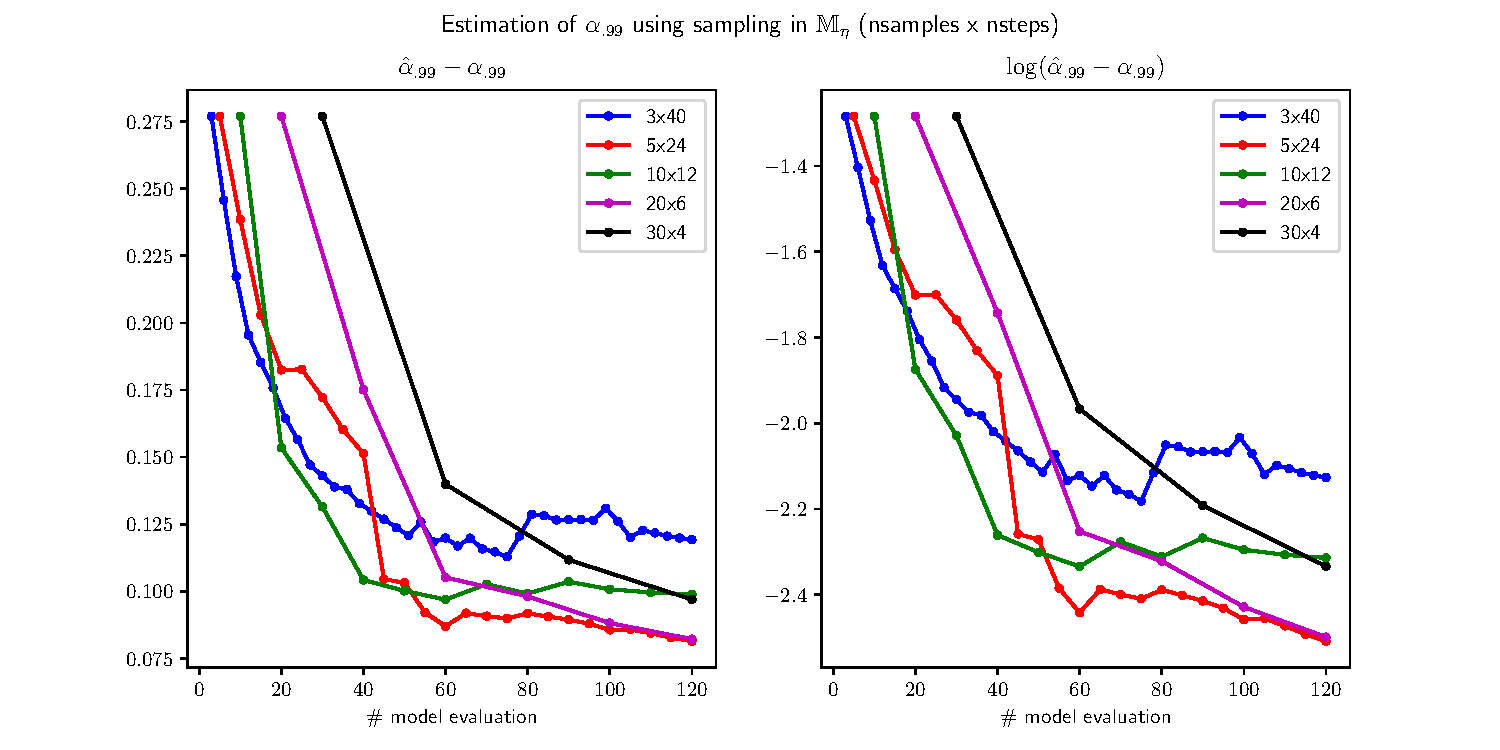
\includegraphics[width=\textwidth]{/home/victor/acadwriting/sampling_estimation_Meta.pdf}
  \caption{\label{fig:label} }
\end{figure}


\section{Application to CROCO}
\label{sec:croco_application}

\begin{figure}[!h]
  \centering
  \scalebox{0.8}{%% Creator: Matplotlib, PGF backend
%%
%% To include the figure in your LaTeX document, write
%%   \input{<filename>.pgf}
%%
%% Make sure the required packages are loaded in your preamble
%%   \usepackage{pgf}
%%
%% Figures using additional raster images can only be included by \input if
%% they are in the same directory as the main LaTeX file. For loading figures
%% from other directories you can use the `import` package
%%   \usepackage{import}
%% and then include the figures with
%%   \import{<path to file>}{<filename>.pgf}
%%
%% Matplotlib used the following preamble
%%   \usepackage{fontspec}
%%   \setmainfont{DejaVuSerif.ttf}[Path=/home/victor/miniconda3/lib/python3.7/site-packages/matplotlib/mpl-data/fonts/ttf/]
%%   \setsansfont{DejaVuSans.ttf}[Path=/home/victor/miniconda3/lib/python3.7/site-packages/matplotlib/mpl-data/fonts/ttf/]
%%   \setmonofont{DejaVuSansMono.ttf}[Path=/home/victor/miniconda3/lib/python3.7/site-packages/matplotlib/mpl-data/fonts/ttf/]
%%
\begingroup%
\makeatletter%
\begin{pgfpicture}%
\pgfpathrectangle{\pgfpointorigin}{\pgfqpoint{10.000000in}{5.000000in}}%
\pgfusepath{use as bounding box, clip}%
\begin{pgfscope}%
\pgfsetbuttcap%
\pgfsetmiterjoin%
\definecolor{currentfill}{rgb}{1.000000,1.000000,1.000000}%
\pgfsetfillcolor{currentfill}%
\pgfsetlinewidth{0.000000pt}%
\definecolor{currentstroke}{rgb}{1.000000,1.000000,1.000000}%
\pgfsetstrokecolor{currentstroke}%
\pgfsetdash{}{0pt}%
\pgfpathmoveto{\pgfqpoint{0.000000in}{0.000000in}}%
\pgfpathlineto{\pgfqpoint{10.000000in}{0.000000in}}%
\pgfpathlineto{\pgfqpoint{10.000000in}{5.000000in}}%
\pgfpathlineto{\pgfqpoint{0.000000in}{5.000000in}}%
\pgfpathclose%
\pgfusepath{fill}%
\end{pgfscope}%
\begin{pgfscope}%
\pgfsetbuttcap%
\pgfsetmiterjoin%
\definecolor{currentfill}{rgb}{1.000000,1.000000,1.000000}%
\pgfsetfillcolor{currentfill}%
\pgfsetlinewidth{0.000000pt}%
\definecolor{currentstroke}{rgb}{0.000000,0.000000,0.000000}%
\pgfsetstrokecolor{currentstroke}%
\pgfsetstrokeopacity{0.000000}%
\pgfsetdash{}{0pt}%
\pgfpathmoveto{\pgfqpoint{1.250000in}{0.550000in}}%
\pgfpathlineto{\pgfqpoint{1.250000in}{4.400000in}}%
\pgfpathlineto{\pgfqpoint{4.068182in}{4.400000in}}%
\pgfpathlineto{\pgfqpoint{4.068182in}{0.550000in}}%
\pgfpathlineto{\pgfqpoint{1.250000in}{0.550000in}}%
\pgfusepath{fill}%
\end{pgfscope}%
\begin{pgfscope}%
\pgfpathrectangle{\pgfqpoint{1.250000in}{0.550000in}}{\pgfqpoint{2.818182in}{3.850000in}}%
\pgfusepath{clip}%
\pgfsetbuttcap%
\pgfsetroundjoin%
\pgfsetlinewidth{1.003750pt}%
\definecolor{currentstroke}{rgb}{0.000000,0.000000,0.000000}%
\pgfsetstrokecolor{currentstroke}%
\pgfsetdash{}{0pt}%
\pgfpathmoveto{\pgfqpoint{4.074204in}{4.410000in}}%
\pgfpathlineto{\pgfqpoint{4.062155in}{4.386371in}}%
\pgfpathlineto{\pgfqpoint{4.056953in}{4.364329in}}%
\pgfpathlineto{\pgfqpoint{4.004030in}{4.368230in}}%
\pgfpathlineto{\pgfqpoint{3.979233in}{4.344919in}}%
\pgfpathlineto{\pgfqpoint{3.936382in}{4.329457in}}%
\pgfpathlineto{\pgfqpoint{3.903247in}{4.312985in}}%
\pgfpathlineto{\pgfqpoint{3.870827in}{4.292189in}}%
\pgfpathlineto{\pgfqpoint{3.844158in}{4.285962in}}%
\pgfpathlineto{\pgfqpoint{3.728899in}{4.310659in}}%
\pgfpathlineto{\pgfqpoint{3.659325in}{4.308638in}}%
\pgfpathlineto{\pgfqpoint{3.565065in}{4.287113in}}%
\pgfpathlineto{\pgfqpoint{3.540791in}{4.290661in}}%
\pgfpathlineto{\pgfqpoint{3.504380in}{4.311270in}}%
\pgfpathlineto{\pgfqpoint{3.467103in}{4.325204in}}%
\pgfpathlineto{\pgfqpoint{3.424211in}{4.331337in}}%
\pgfpathlineto{\pgfqpoint{3.387181in}{4.350371in}}%
\pgfpathlineto{\pgfqpoint{3.410285in}{4.313760in}}%
\pgfpathlineto{\pgfqpoint{3.358916in}{4.278466in}}%
\pgfpathlineto{\pgfqpoint{3.335221in}{4.271440in}}%
\pgfpathlineto{\pgfqpoint{3.310685in}{4.272544in}}%
\pgfpathlineto{\pgfqpoint{3.260487in}{4.262957in}}%
\pgfpathlineto{\pgfqpoint{3.213975in}{4.267844in}}%
\pgfpathlineto{\pgfqpoint{3.220966in}{4.242748in}}%
\pgfpathlineto{\pgfqpoint{3.233419in}{4.220871in}}%
\pgfpathlineto{\pgfqpoint{3.223319in}{4.211354in}}%
\pgfpathlineto{\pgfqpoint{3.212627in}{4.208980in}}%
\pgfpathlineto{\pgfqpoint{3.124050in}{4.225500in}}%
\pgfpathlineto{\pgfqpoint{3.111500in}{4.222375in}}%
\pgfpathlineto{\pgfqpoint{3.100574in}{4.207124in}}%
\pgfpathlineto{\pgfqpoint{3.068360in}{4.215349in}}%
\pgfpathlineto{\pgfqpoint{3.037055in}{4.241056in}}%
\pgfpathlineto{\pgfqpoint{3.003768in}{4.258304in}}%
\pgfpathlineto{\pgfqpoint{2.968843in}{4.266411in}}%
\pgfpathlineto{\pgfqpoint{2.941074in}{4.263615in}}%
\pgfpathlineto{\pgfqpoint{2.826888in}{4.223103in}}%
\pgfpathlineto{\pgfqpoint{2.804101in}{4.182451in}}%
\pgfpathlineto{\pgfqpoint{2.792707in}{4.124809in}}%
\pgfpathlineto{\pgfqpoint{2.776222in}{4.073629in}}%
\pgfpathlineto{\pgfqpoint{2.749333in}{4.034222in}}%
\pgfpathlineto{\pgfqpoint{2.717326in}{4.029076in}}%
\pgfpathlineto{\pgfqpoint{2.687218in}{4.056357in}}%
\pgfpathlineto{\pgfqpoint{2.629946in}{4.086483in}}%
\pgfpathlineto{\pgfqpoint{2.610461in}{4.106832in}}%
\pgfpathlineto{\pgfqpoint{2.604255in}{4.108031in}}%
\pgfpathlineto{\pgfqpoint{2.597856in}{4.100746in}}%
\pgfpathlineto{\pgfqpoint{2.575399in}{4.091558in}}%
\pgfpathlineto{\pgfqpoint{2.552143in}{4.091135in}}%
\pgfpathlineto{\pgfqpoint{2.516297in}{4.083028in}}%
\pgfpathlineto{\pgfqpoint{2.453933in}{4.058543in}}%
\pgfpathlineto{\pgfqpoint{2.428738in}{4.041929in}}%
\pgfpathlineto{\pgfqpoint{2.374589in}{3.996107in}}%
\pgfpathlineto{\pgfqpoint{2.363567in}{3.983418in}}%
\pgfpathlineto{\pgfqpoint{2.343876in}{3.937196in}}%
\pgfpathlineto{\pgfqpoint{2.313795in}{3.929042in}}%
\pgfpathlineto{\pgfqpoint{2.286287in}{3.958674in}}%
\pgfpathlineto{\pgfqpoint{2.254968in}{3.969013in}}%
\pgfpathlineto{\pgfqpoint{2.221929in}{3.958885in}}%
\pgfpathlineto{\pgfqpoint{2.201948in}{3.943141in}}%
\pgfpathlineto{\pgfqpoint{2.192632in}{3.955925in}}%
\pgfpathlineto{\pgfqpoint{2.192330in}{3.982220in}}%
\pgfpathlineto{\pgfqpoint{2.216452in}{4.013543in}}%
\pgfpathlineto{\pgfqpoint{2.280811in}{4.037206in}}%
\pgfpathlineto{\pgfqpoint{2.337312in}{4.098608in}}%
\pgfpathlineto{\pgfqpoint{2.365026in}{4.136041in}}%
\pgfpathlineto{\pgfqpoint{2.376021in}{4.157096in}}%
\pgfpathlineto{\pgfqpoint{2.389561in}{4.170513in}}%
\pgfpathlineto{\pgfqpoint{2.407271in}{4.175589in}}%
\pgfpathlineto{\pgfqpoint{2.416367in}{4.198853in}}%
\pgfpathlineto{\pgfqpoint{2.494816in}{4.292377in}}%
\pgfpathlineto{\pgfqpoint{2.501284in}{4.313831in}}%
\pgfpathlineto{\pgfqpoint{2.505192in}{4.352204in}}%
\pgfpathlineto{\pgfqpoint{2.511673in}{4.389144in}}%
\pgfpathlineto{\pgfqpoint{2.567353in}{4.410000in}}%
\pgfpathlineto{\pgfqpoint{2.567353in}{4.410000in}}%
\pgfusepath{stroke}%
\end{pgfscope}%
\begin{pgfscope}%
\pgfpathrectangle{\pgfqpoint{1.250000in}{0.550000in}}{\pgfqpoint{2.818182in}{3.850000in}}%
\pgfusepath{clip}%
\pgfsetbuttcap%
\pgfsetroundjoin%
\pgfsetlinewidth{1.003750pt}%
\definecolor{currentstroke}{rgb}{0.000000,0.000000,0.000000}%
\pgfsetstrokecolor{currentstroke}%
\pgfsetdash{}{0pt}%
\pgfpathmoveto{\pgfqpoint{3.040633in}{3.662827in}}%
\pgfpathlineto{\pgfqpoint{3.042642in}{3.654509in}}%
\pgfpathlineto{\pgfqpoint{3.068470in}{3.643817in}}%
\pgfpathlineto{\pgfqpoint{3.078350in}{3.675493in}}%
\pgfpathlineto{\pgfqpoint{3.075929in}{3.681156in}}%
\pgfpathlineto{\pgfqpoint{3.069929in}{3.681297in}}%
\pgfpathlineto{\pgfqpoint{3.040633in}{3.662827in}}%
\pgfusepath{stroke}%
\end{pgfscope}%
\begin{pgfscope}%
\pgfpathrectangle{\pgfqpoint{1.250000in}{0.550000in}}{\pgfqpoint{2.818182in}{3.850000in}}%
\pgfusepath{clip}%
\pgfsetbuttcap%
\pgfsetroundjoin%
\pgfsetlinewidth{1.003750pt}%
\definecolor{currentstroke}{rgb}{0.000000,0.000000,0.000000}%
\pgfsetstrokecolor{currentstroke}%
\pgfsetdash{}{0pt}%
\pgfpathmoveto{\pgfqpoint{3.160584in}{3.565685in}}%
\pgfpathlineto{\pgfqpoint{3.156263in}{3.522377in}}%
\pgfpathlineto{\pgfqpoint{3.176037in}{3.527687in}}%
\pgfpathlineto{\pgfqpoint{3.197077in}{3.527687in}}%
\pgfpathlineto{\pgfqpoint{3.207577in}{3.519228in}}%
\pgfpathlineto{\pgfqpoint{3.219934in}{3.524515in}}%
\pgfpathlineto{\pgfqpoint{3.217471in}{3.548789in}}%
\pgfpathlineto{\pgfqpoint{3.199554in}{3.560397in}}%
\pgfpathlineto{\pgfqpoint{3.160584in}{3.565685in}}%
\pgfusepath{stroke}%
\end{pgfscope}%
\begin{pgfscope}%
\pgfpathrectangle{\pgfqpoint{1.250000in}{0.550000in}}{\pgfqpoint{2.818182in}{3.850000in}}%
\pgfusepath{clip}%
\pgfsetbuttcap%
\pgfsetroundjoin%
\pgfsetlinewidth{1.003750pt}%
\definecolor{currentstroke}{rgb}{0.000000,0.000000,0.000000}%
\pgfsetstrokecolor{currentstroke}%
\pgfsetdash{}{0pt}%
\pgfpathmoveto{\pgfqpoint{3.395011in}{2.018000in}}%
\pgfpathlineto{\pgfqpoint{3.394956in}{2.009612in}}%
\pgfpathlineto{\pgfqpoint{3.400639in}{1.978194in}}%
\pgfpathlineto{\pgfqpoint{3.425559in}{1.944239in}}%
\pgfpathlineto{\pgfqpoint{3.444356in}{1.905490in}}%
\pgfpathlineto{\pgfqpoint{3.454292in}{1.947575in}}%
\pgfpathlineto{\pgfqpoint{3.424211in}{1.995042in}}%
\pgfpathlineto{\pgfqpoint{3.395011in}{2.018000in}}%
\pgfusepath{stroke}%
\end{pgfscope}%
\begin{pgfscope}%
\pgfpathrectangle{\pgfqpoint{1.250000in}{0.550000in}}{\pgfqpoint{2.818182in}{3.850000in}}%
\pgfusepath{clip}%
\pgfsetbuttcap%
\pgfsetroundjoin%
\pgfsetlinewidth{1.003750pt}%
\definecolor{currentstroke}{rgb}{0.000000,0.000000,0.000000}%
\pgfsetstrokecolor{currentstroke}%
\pgfsetdash{}{0pt}%
\pgfpathmoveto{\pgfqpoint{3.416395in}{4.290990in}}%
\pgfpathlineto{\pgfqpoint{3.395809in}{4.271768in}}%
\pgfpathlineto{\pgfqpoint{3.359219in}{4.257223in}}%
\pgfpathlineto{\pgfqpoint{3.345761in}{4.239317in}}%
\pgfpathlineto{\pgfqpoint{3.359316in}{4.241079in}}%
\pgfpathlineto{\pgfqpoint{3.418225in}{4.201978in}}%
\pgfpathlineto{\pgfqpoint{3.433678in}{4.202119in}}%
\pgfpathlineto{\pgfqpoint{3.449283in}{4.207124in}}%
\pgfpathlineto{\pgfqpoint{3.454993in}{4.214832in}}%
\pgfpathlineto{\pgfqpoint{3.462452in}{4.234312in}}%
\pgfpathlineto{\pgfqpoint{3.486065in}{4.250925in}}%
\pgfpathlineto{\pgfqpoint{3.463896in}{4.272332in}}%
\pgfpathlineto{\pgfqpoint{3.416395in}{4.290990in}}%
\pgfusepath{stroke}%
\end{pgfscope}%
\begin{pgfscope}%
\pgfpathrectangle{\pgfqpoint{1.250000in}{0.550000in}}{\pgfqpoint{2.818182in}{3.850000in}}%
\pgfusepath{clip}%
\pgfsetbuttcap%
\pgfsetroundjoin%
\pgfsetlinewidth{1.003750pt}%
\definecolor{currentstroke}{rgb}{0.000000,0.000000,0.000000}%
\pgfsetstrokecolor{currentstroke}%
\pgfsetdash{}{0pt}%
\pgfpathmoveto{\pgfqpoint{0.000000in}{0.000000in}}%
\pgfusepath{stroke}%
\end{pgfscope}%
\begin{pgfscope}%
\pgfpathrectangle{\pgfqpoint{1.250000in}{0.550000in}}{\pgfqpoint{2.818182in}{3.850000in}}%
\pgfusepath{clip}%
\pgfsetbuttcap%
\pgfsetroundjoin%
\pgfsetlinewidth{1.003750pt}%
\definecolor{currentstroke}{rgb}{0.000000,0.000000,0.000000}%
\pgfsetstrokecolor{currentstroke}%
\pgfsetdash{}{0pt}%
\pgfpathmoveto{\pgfqpoint{4.078182in}{3.890217in}}%
\pgfpathlineto{\pgfqpoint{4.046798in}{3.875536in}}%
\pgfpathlineto{\pgfqpoint{3.960023in}{3.852790in}}%
\pgfpathlineto{\pgfqpoint{3.838984in}{3.775832in}}%
\pgfpathlineto{\pgfqpoint{3.822031in}{3.727002in}}%
\pgfpathlineto{\pgfqpoint{3.817188in}{3.705806in}}%
\pgfpathlineto{\pgfqpoint{3.822829in}{3.682190in}}%
\pgfpathlineto{\pgfqpoint{3.864607in}{3.660454in}}%
\pgfpathlineto{\pgfqpoint{3.910154in}{3.665224in}}%
\pgfpathlineto{\pgfqpoint{3.903852in}{3.653287in}}%
\pgfpathlineto{\pgfqpoint{3.824728in}{3.630728in}}%
\pgfpathlineto{\pgfqpoint{3.783212in}{3.596421in}}%
\pgfpathlineto{\pgfqpoint{3.740293in}{3.580324in}}%
\pgfpathlineto{\pgfqpoint{3.639565in}{3.608123in}}%
\pgfpathlineto{\pgfqpoint{3.570624in}{3.610614in}}%
\pgfpathlineto{\pgfqpoint{3.516063in}{3.626710in}}%
\pgfpathlineto{\pgfqpoint{3.465506in}{3.624172in}}%
\pgfpathlineto{\pgfqpoint{3.449599in}{3.651572in}}%
\pgfpathlineto{\pgfqpoint{3.439086in}{3.675658in}}%
\pgfpathlineto{\pgfqpoint{3.429880in}{3.725404in}}%
\pgfpathlineto{\pgfqpoint{3.431655in}{3.764835in}}%
\pgfpathlineto{\pgfqpoint{3.401478in}{3.777876in}}%
\pgfpathlineto{\pgfqpoint{3.338771in}{3.758819in}}%
\pgfpathlineto{\pgfqpoint{3.305828in}{3.765211in}}%
\pgfpathlineto{\pgfqpoint{3.263184in}{3.766573in}}%
\pgfpathlineto{\pgfqpoint{3.257844in}{3.741360in}}%
\pgfpathlineto{\pgfqpoint{3.259344in}{3.723900in}}%
\pgfpathlineto{\pgfqpoint{3.275307in}{3.673378in}}%
\pgfpathlineto{\pgfqpoint{3.309997in}{3.588220in}}%
\pgfpathlineto{\pgfqpoint{3.340216in}{3.534901in}}%
\pgfpathlineto{\pgfqpoint{3.345183in}{3.343905in}}%
\pgfpathlineto{\pgfqpoint{3.369141in}{3.291974in}}%
\pgfpathlineto{\pgfqpoint{3.398451in}{3.270308in}}%
\pgfpathlineto{\pgfqpoint{3.381209in}{3.264927in}}%
\pgfpathlineto{\pgfqpoint{3.272128in}{3.259687in}}%
\pgfpathlineto{\pgfqpoint{3.264450in}{3.278133in}}%
\pgfpathlineto{\pgfqpoint{3.249299in}{3.291739in}}%
\pgfpathlineto{\pgfqpoint{3.230296in}{3.261895in}}%
\pgfpathlineto{\pgfqpoint{3.221681in}{3.236376in}}%
\pgfpathlineto{\pgfqpoint{3.200339in}{3.266666in}}%
\pgfpathlineto{\pgfqpoint{3.096982in}{3.268240in}}%
\pgfpathlineto{\pgfqpoint{3.027615in}{3.214593in}}%
\pgfpathlineto{\pgfqpoint{2.999282in}{3.245517in}}%
\pgfpathlineto{\pgfqpoint{2.940001in}{3.336762in}}%
\pgfpathlineto{\pgfqpoint{2.875684in}{3.360895in}}%
\pgfpathlineto{\pgfqpoint{2.808036in}{3.347477in}}%
\pgfpathlineto{\pgfqpoint{2.787037in}{3.324731in}}%
\pgfpathlineto{\pgfqpoint{2.739467in}{3.298177in}}%
\pgfpathlineto{\pgfqpoint{2.699767in}{3.290587in}}%
\pgfpathlineto{\pgfqpoint{2.642496in}{3.296744in}}%
\pgfpathlineto{\pgfqpoint{2.509389in}{3.254611in}}%
\pgfpathlineto{\pgfqpoint{2.455970in}{3.216073in}}%
\pgfpathlineto{\pgfqpoint{2.444205in}{3.172930in}}%
\pgfpathlineto{\pgfqpoint{2.448140in}{3.153567in}}%
\pgfpathlineto{\pgfqpoint{2.456355in}{3.131009in}}%
\pgfpathlineto{\pgfqpoint{2.494307in}{3.128306in}}%
\pgfpathlineto{\pgfqpoint{2.511191in}{3.135426in}}%
\pgfpathlineto{\pgfqpoint{2.548290in}{3.133170in}}%
\pgfpathlineto{\pgfqpoint{2.556395in}{3.127930in}}%
\pgfpathlineto{\pgfqpoint{2.574050in}{3.123278in}}%
\pgfpathlineto{\pgfqpoint{2.591058in}{3.102387in}}%
\pgfpathlineto{\pgfqpoint{2.545428in}{3.097288in}}%
\pgfpathlineto{\pgfqpoint{2.518774in}{3.100273in}}%
\pgfpathlineto{\pgfqpoint{2.509540in}{3.105301in}}%
\pgfpathlineto{\pgfqpoint{2.496440in}{3.095831in}}%
\pgfpathlineto{\pgfqpoint{2.505687in}{3.075106in}}%
\pgfpathlineto{\pgfqpoint{2.514742in}{3.066811in}}%
\pgfpathlineto{\pgfqpoint{2.536607in}{3.061147in}}%
\pgfpathlineto{\pgfqpoint{2.566248in}{3.038048in}}%
\pgfpathlineto{\pgfqpoint{2.552611in}{3.018239in}}%
\pgfpathlineto{\pgfqpoint{2.514687in}{3.002801in}}%
\pgfpathlineto{\pgfqpoint{2.481771in}{2.997537in}}%
\pgfpathlineto{\pgfqpoint{2.467790in}{2.975260in}}%
\pgfpathlineto{\pgfqpoint{2.538479in}{2.941305in}}%
\pgfpathlineto{\pgfqpoint{2.553382in}{2.897269in}}%
\pgfpathlineto{\pgfqpoint{2.571133in}{2.871021in}}%
\pgfpathlineto{\pgfqpoint{2.595283in}{2.864629in}}%
\pgfpathlineto{\pgfqpoint{2.639165in}{2.883029in}}%
\pgfpathlineto{\pgfqpoint{2.687011in}{2.878070in}}%
\pgfpathlineto{\pgfqpoint{2.797798in}{2.837441in}}%
\pgfpathlineto{\pgfqpoint{2.815797in}{2.817186in}}%
\pgfpathlineto{\pgfqpoint{2.829338in}{2.821697in}}%
\pgfpathlineto{\pgfqpoint{2.848300in}{2.818290in}}%
\pgfpathlineto{\pgfqpoint{2.866313in}{2.804708in}}%
\pgfpathlineto{\pgfqpoint{2.878463in}{2.809055in}}%
\pgfpathlineto{\pgfqpoint{2.896146in}{2.809314in}}%
\pgfpathlineto{\pgfqpoint{2.922814in}{2.774019in}}%
\pgfpathlineto{\pgfqpoint{2.951037in}{2.764267in}}%
\pgfpathlineto{\pgfqpoint{3.000878in}{2.776040in}}%
\pgfpathlineto{\pgfqpoint{3.016125in}{2.764619in}}%
\pgfpathlineto{\pgfqpoint{2.998181in}{2.733554in}}%
\pgfpathlineto{\pgfqpoint{3.005639in}{2.722299in}}%
\pgfpathlineto{\pgfqpoint{3.035059in}{2.728220in}}%
\pgfpathlineto{\pgfqpoint{3.066585in}{2.728643in}}%
\pgfpathlineto{\pgfqpoint{3.086689in}{2.721218in}}%
\pgfpathlineto{\pgfqpoint{3.102198in}{2.701620in}}%
\pgfpathlineto{\pgfqpoint{3.088492in}{2.673727in}}%
\pgfpathlineto{\pgfqpoint{3.073355in}{2.658641in}}%
\pgfpathlineto{\pgfqpoint{3.080938in}{2.625179in}}%
\pgfpathlineto{\pgfqpoint{3.100299in}{2.615028in}}%
\pgfpathlineto{\pgfqpoint{3.123238in}{2.609153in}}%
\pgfpathlineto{\pgfqpoint{3.229663in}{2.624521in}}%
\pgfpathlineto{\pgfqpoint{3.295287in}{2.578934in}}%
\pgfpathlineto{\pgfqpoint{3.273091in}{2.583446in}}%
\pgfpathlineto{\pgfqpoint{3.244786in}{2.600435in}}%
\pgfpathlineto{\pgfqpoint{3.214953in}{2.606662in}}%
\pgfpathlineto{\pgfqpoint{3.192206in}{2.601540in}}%
\pgfpathlineto{\pgfqpoint{3.180854in}{2.582764in}}%
\pgfpathlineto{\pgfqpoint{3.167189in}{2.553415in}}%
\pgfpathlineto{\pgfqpoint{3.182271in}{2.535791in}}%
\pgfpathlineto{\pgfqpoint{3.199637in}{2.528718in}}%
\pgfpathlineto{\pgfqpoint{3.217402in}{2.493117in}}%
\pgfpathlineto{\pgfqpoint{3.197284in}{2.436744in}}%
\pgfpathlineto{\pgfqpoint{3.196665in}{2.410050in}}%
\pgfpathlineto{\pgfqpoint{3.205994in}{2.383708in}}%
\pgfpathlineto{\pgfqpoint{3.244868in}{2.323317in}}%
\pgfpathlineto{\pgfqpoint{3.282889in}{2.241519in}}%
\pgfpathlineto{\pgfqpoint{3.393937in}{2.162234in}}%
\pgfpathlineto{\pgfqpoint{3.416395in}{2.151073in}}%
\pgfpathlineto{\pgfqpoint{3.437242in}{2.149921in}}%
\pgfpathlineto{\pgfqpoint{3.463319in}{2.143600in}}%
\pgfpathlineto{\pgfqpoint{3.467337in}{2.115355in}}%
\pgfpathlineto{\pgfqpoint{3.466112in}{2.092326in}}%
\pgfpathlineto{\pgfqpoint{3.475125in}{1.957821in}}%
\pgfpathlineto{\pgfqpoint{3.485941in}{1.900226in}}%
\pgfpathlineto{\pgfqpoint{3.492849in}{1.884341in}}%
\pgfpathlineto{\pgfqpoint{3.495601in}{1.869137in}}%
\pgfpathlineto{\pgfqpoint{3.472318in}{1.882343in}}%
\pgfpathlineto{\pgfqpoint{3.445375in}{1.883495in}}%
\pgfpathlineto{\pgfqpoint{3.449310in}{1.856331in}}%
\pgfpathlineto{\pgfqpoint{3.456645in}{1.842607in}}%
\pgfpathlineto{\pgfqpoint{3.538176in}{1.771501in}}%
\pgfpathlineto{\pgfqpoint{3.563510in}{1.737733in}}%
\pgfpathlineto{\pgfqpoint{3.579761in}{1.697598in}}%
\pgfpathlineto{\pgfqpoint{3.605686in}{1.555902in}}%
\pgfpathlineto{\pgfqpoint{3.622268in}{1.537220in}}%
\pgfpathlineto{\pgfqpoint{3.631790in}{1.512782in}}%
\pgfpathlineto{\pgfqpoint{3.607695in}{1.535176in}}%
\pgfpathlineto{\pgfqpoint{3.591595in}{1.557476in}}%
\pgfpathlineto{\pgfqpoint{3.570308in}{1.663784in}}%
\pgfpathlineto{\pgfqpoint{3.553492in}{1.695695in}}%
\pgfpathlineto{\pgfqpoint{3.520962in}{1.732470in}}%
\pgfpathlineto{\pgfqpoint{3.481717in}{1.768728in}}%
\pgfpathlineto{\pgfqpoint{3.462534in}{1.677389in}}%
\pgfpathlineto{\pgfqpoint{3.451264in}{1.590210in}}%
\pgfpathlineto{\pgfqpoint{3.435439in}{1.352099in}}%
\pgfpathlineto{\pgfqpoint{3.442457in}{1.361686in}}%
\pgfpathlineto{\pgfqpoint{3.448072in}{1.380861in}}%
\pgfpathlineto{\pgfqpoint{3.461461in}{1.398932in}}%
\pgfpathlineto{\pgfqpoint{3.482859in}{1.363237in}}%
\pgfpathlineto{\pgfqpoint{3.456411in}{1.349749in}}%
\pgfpathlineto{\pgfqpoint{3.435357in}{1.300684in}}%
\pgfpathlineto{\pgfqpoint{3.407037in}{1.040978in}}%
\pgfpathlineto{\pgfqpoint{3.367902in}{0.821314in}}%
\pgfpathlineto{\pgfqpoint{3.326593in}{0.760805in}}%
\pgfpathlineto{\pgfqpoint{3.271055in}{0.742899in}}%
\pgfpathlineto{\pgfqpoint{3.225177in}{0.716064in}}%
\pgfpathlineto{\pgfqpoint{3.167299in}{0.704926in}}%
\pgfpathlineto{\pgfqpoint{3.127724in}{0.707863in}}%
\pgfpathlineto{\pgfqpoint{3.051641in}{0.748633in}}%
\pgfpathlineto{\pgfqpoint{2.976123in}{0.768701in}}%
\pgfpathlineto{\pgfqpoint{2.955647in}{0.761604in}}%
\pgfpathlineto{\pgfqpoint{2.928057in}{0.728824in}}%
\pgfpathlineto{\pgfqpoint{2.823145in}{0.767385in}}%
\pgfpathlineto{\pgfqpoint{2.793340in}{0.795936in}}%
\pgfpathlineto{\pgfqpoint{2.770511in}{0.800001in}}%
\pgfpathlineto{\pgfqpoint{2.722775in}{0.779980in}}%
\pgfpathlineto{\pgfqpoint{2.690273in}{0.790343in}}%
\pgfpathlineto{\pgfqpoint{2.654770in}{0.772860in}}%
\pgfpathlineto{\pgfqpoint{2.570940in}{0.749597in}}%
\pgfpathlineto{\pgfqpoint{2.511687in}{0.750067in}}%
\pgfpathlineto{\pgfqpoint{2.347605in}{0.791518in}}%
\pgfpathlineto{\pgfqpoint{2.288296in}{0.816215in}}%
\pgfpathlineto{\pgfqpoint{2.189632in}{0.830314in}}%
\pgfpathlineto{\pgfqpoint{2.138663in}{0.860439in}}%
\pgfpathlineto{\pgfqpoint{2.072873in}{0.836306in}}%
\pgfpathlineto{\pgfqpoint{2.032293in}{0.840606in}}%
\pgfpathlineto{\pgfqpoint{1.961398in}{0.828599in}}%
\pgfpathlineto{\pgfqpoint{1.921492in}{0.835084in}}%
\pgfpathlineto{\pgfqpoint{1.841626in}{0.831841in}}%
\pgfpathlineto{\pgfqpoint{1.796449in}{0.816591in}}%
\pgfpathlineto{\pgfqpoint{1.739810in}{0.836165in}}%
\pgfpathlineto{\pgfqpoint{1.701102in}{0.884854in}}%
\pgfpathlineto{\pgfqpoint{1.671709in}{0.906097in}}%
\pgfpathlineto{\pgfqpoint{1.646073in}{0.900034in}}%
\pgfpathlineto{\pgfqpoint{1.616887in}{0.917940in}}%
\pgfpathlineto{\pgfqpoint{1.573320in}{0.890235in}}%
\pgfpathlineto{\pgfqpoint{1.530497in}{0.884173in}}%
\pgfpathlineto{\pgfqpoint{1.493165in}{0.852732in}}%
\pgfpathlineto{\pgfqpoint{1.459465in}{0.829069in}}%
\pgfpathlineto{\pgfqpoint{1.450410in}{0.809682in}}%
\pgfpathlineto{\pgfqpoint{1.460717in}{0.789145in}}%
\pgfpathlineto{\pgfqpoint{1.461666in}{0.761463in}}%
\pgfpathlineto{\pgfqpoint{1.431641in}{0.740973in}}%
\pgfpathlineto{\pgfqpoint{1.413009in}{0.735685in}}%
\pgfpathlineto{\pgfqpoint{1.380465in}{0.712210in}}%
\pgfpathlineto{\pgfqpoint{1.344233in}{0.702365in}}%
\pgfpathlineto{\pgfqpoint{1.285599in}{0.710941in}}%
\pgfpathlineto{\pgfqpoint{1.240000in}{0.663162in}}%
\pgfpathlineto{\pgfqpoint{1.240000in}{0.663162in}}%
\pgfusepath{stroke}%
\end{pgfscope}%
\begin{pgfscope}%
\pgfpathrectangle{\pgfqpoint{1.250000in}{0.550000in}}{\pgfqpoint{2.818182in}{3.850000in}}%
\pgfusepath{clip}%
\pgfsetbuttcap%
\pgfsetroundjoin%
\pgfsetlinewidth{1.505625pt}%
\definecolor{currentstroke}{rgb}{0.273809,0.031497,0.358853}%
\pgfsetstrokecolor{currentstroke}%
\pgfsetdash{}{0pt}%
\pgfpathmoveto{\pgfqpoint{1.250000in}{1.865990in}}%
\pgfpathlineto{\pgfqpoint{1.270130in}{1.865990in}}%
\pgfpathlineto{\pgfqpoint{1.290260in}{1.861783in}}%
\pgfpathlineto{\pgfqpoint{1.296432in}{1.852925in}}%
\pgfpathlineto{\pgfqpoint{1.299602in}{1.828898in}}%
\pgfpathlineto{\pgfqpoint{1.299464in}{1.804851in}}%
\pgfpathlineto{\pgfqpoint{1.301740in}{1.780781in}}%
\pgfpathlineto{\pgfqpoint{1.307312in}{1.756691in}}%
\pgfpathlineto{\pgfqpoint{1.310390in}{1.747175in}}%
\pgfpathlineto{\pgfqpoint{1.330103in}{1.732579in}}%
\pgfpathlineto{\pgfqpoint{1.330519in}{1.732370in}}%
\pgfpathlineto{\pgfqpoint{1.333453in}{1.732579in}}%
\pgfpathlineto{\pgfqpoint{1.350649in}{1.733761in}}%
\pgfpathlineto{\pgfqpoint{1.354718in}{1.732579in}}%
\pgfpathlineto{\pgfqpoint{1.370779in}{1.722882in}}%
\pgfpathlineto{\pgfqpoint{1.378185in}{1.708445in}}%
\pgfpathlineto{\pgfqpoint{1.384622in}{1.684291in}}%
\pgfpathlineto{\pgfqpoint{1.387093in}{1.660114in}}%
\pgfpathlineto{\pgfqpoint{1.386246in}{1.635916in}}%
\pgfpathlineto{\pgfqpoint{1.384699in}{1.611697in}}%
\pgfpathlineto{\pgfqpoint{1.388271in}{1.587457in}}%
\pgfpathlineto{\pgfqpoint{1.390909in}{1.582904in}}%
\pgfpathlineto{\pgfqpoint{1.411039in}{1.578620in}}%
\pgfpathlineto{\pgfqpoint{1.431169in}{1.578139in}}%
\pgfpathlineto{\pgfqpoint{1.440613in}{1.563195in}}%
\pgfpathlineto{\pgfqpoint{1.440423in}{1.538911in}}%
\pgfpathlineto{\pgfqpoint{1.438047in}{1.514606in}}%
\pgfpathlineto{\pgfqpoint{1.436922in}{1.490280in}}%
\pgfpathlineto{\pgfqpoint{1.437029in}{1.465932in}}%
\pgfpathlineto{\pgfqpoint{1.437616in}{1.441563in}}%
\pgfpathlineto{\pgfqpoint{1.437863in}{1.417172in}}%
\pgfpathlineto{\pgfqpoint{1.437027in}{1.392760in}}%
\pgfpathlineto{\pgfqpoint{1.434345in}{1.368326in}}%
\pgfpathlineto{\pgfqpoint{1.431169in}{1.349490in}}%
\pgfpathlineto{\pgfqpoint{1.430200in}{1.343871in}}%
\pgfpathlineto{\pgfqpoint{1.420282in}{1.319395in}}%
\pgfpathlineto{\pgfqpoint{1.411039in}{1.314242in}}%
\pgfpathlineto{\pgfqpoint{1.390909in}{1.312798in}}%
\pgfpathlineto{\pgfqpoint{1.370779in}{1.312615in}}%
\pgfpathlineto{\pgfqpoint{1.350649in}{1.310664in}}%
\pgfpathlineto{\pgfqpoint{1.330519in}{1.308227in}}%
\pgfpathlineto{\pgfqpoint{1.310390in}{1.306059in}}%
\pgfpathlineto{\pgfqpoint{1.290260in}{1.304059in}}%
\pgfpathlineto{\pgfqpoint{1.270130in}{1.302508in}}%
\pgfpathlineto{\pgfqpoint{1.250000in}{1.302508in}}%
\pgfusepath{stroke}%
\end{pgfscope}%
\begin{pgfscope}%
\pgfpathrectangle{\pgfqpoint{1.250000in}{0.550000in}}{\pgfqpoint{2.818182in}{3.850000in}}%
\pgfusepath{clip}%
\pgfsetbuttcap%
\pgfsetroundjoin%
\pgfsetlinewidth{1.505625pt}%
\definecolor{currentstroke}{rgb}{0.278791,0.062145,0.386592}%
\pgfsetstrokecolor{currentstroke}%
\pgfsetdash{}{0pt}%
\pgfpathmoveto{\pgfqpoint{1.250000in}{2.140788in}}%
\pgfpathlineto{\pgfqpoint{1.270130in}{2.140788in}}%
\pgfpathlineto{\pgfqpoint{1.310390in}{2.153802in}}%
\pgfpathlineto{\pgfqpoint{1.330519in}{2.155023in}}%
\pgfpathlineto{\pgfqpoint{1.350649in}{2.152945in}}%
\pgfpathlineto{\pgfqpoint{1.370779in}{2.153441in}}%
\pgfpathlineto{\pgfqpoint{1.390909in}{2.157792in}}%
\pgfpathlineto{\pgfqpoint{1.431169in}{2.170420in}}%
\pgfpathlineto{\pgfqpoint{1.451299in}{2.171594in}}%
\pgfpathlineto{\pgfqpoint{1.464719in}{2.163317in}}%
\pgfpathlineto{\pgfqpoint{1.471429in}{2.149719in}}%
\pgfpathlineto{\pgfqpoint{1.474154in}{2.139569in}}%
\pgfpathlineto{\pgfqpoint{1.476255in}{2.092009in}}%
\pgfpathlineto{\pgfqpoint{1.487532in}{2.068197in}}%
\pgfpathlineto{\pgfqpoint{1.491558in}{2.064913in}}%
\pgfpathlineto{\pgfqpoint{1.511688in}{2.056681in}}%
\pgfpathlineto{\pgfqpoint{1.548056in}{2.044364in}}%
\pgfpathlineto{\pgfqpoint{1.551948in}{2.042779in}}%
\pgfpathlineto{\pgfqpoint{1.572078in}{2.032352in}}%
\pgfpathlineto{\pgfqpoint{1.592208in}{2.019596in}}%
\pgfpathlineto{\pgfqpoint{1.608065in}{1.996632in}}%
\pgfpathlineto{\pgfqpoint{1.617850in}{1.972735in}}%
\pgfpathlineto{\pgfqpoint{1.632468in}{1.958539in}}%
\pgfpathlineto{\pgfqpoint{1.652597in}{1.957583in}}%
\pgfpathlineto{\pgfqpoint{1.672727in}{1.964648in}}%
\pgfpathlineto{\pgfqpoint{1.692857in}{1.973232in}}%
\pgfpathlineto{\pgfqpoint{1.712987in}{1.977934in}}%
\pgfpathlineto{\pgfqpoint{1.733117in}{1.978659in}}%
\pgfpathlineto{\pgfqpoint{1.753247in}{1.978040in}}%
\pgfpathlineto{\pgfqpoint{1.793506in}{1.980700in}}%
\pgfpathlineto{\pgfqpoint{1.813636in}{1.976311in}}%
\pgfpathlineto{\pgfqpoint{1.853896in}{1.958805in}}%
\pgfpathlineto{\pgfqpoint{1.894451in}{1.948816in}}%
\pgfpathlineto{\pgfqpoint{1.914286in}{1.940963in}}%
\pgfpathlineto{\pgfqpoint{1.937374in}{1.924875in}}%
\pgfpathlineto{\pgfqpoint{1.951303in}{1.900913in}}%
\pgfpathlineto{\pgfqpoint{1.954545in}{1.892785in}}%
\pgfpathlineto{\pgfqpoint{1.959066in}{1.876930in}}%
\pgfpathlineto{\pgfqpoint{1.968131in}{1.852925in}}%
\pgfpathlineto{\pgfqpoint{1.993971in}{1.804851in}}%
\pgfpathlineto{\pgfqpoint{1.994805in}{1.803099in}}%
\pgfpathlineto{\pgfqpoint{2.014935in}{1.738544in}}%
\pgfpathlineto{\pgfqpoint{2.016629in}{1.732579in}}%
\pgfpathlineto{\pgfqpoint{2.025745in}{1.708445in}}%
\pgfpathlineto{\pgfqpoint{2.038026in}{1.684291in}}%
\pgfpathlineto{\pgfqpoint{2.055195in}{1.657014in}}%
\pgfpathlineto{\pgfqpoint{2.087540in}{1.611697in}}%
\pgfpathlineto{\pgfqpoint{2.095455in}{1.600669in}}%
\pgfpathlineto{\pgfqpoint{2.115584in}{1.578229in}}%
\pgfpathlineto{\pgfqpoint{2.137630in}{1.563195in}}%
\pgfpathlineto{\pgfqpoint{2.155844in}{1.552665in}}%
\pgfpathlineto{\pgfqpoint{2.175974in}{1.538777in}}%
\pgfpathlineto{\pgfqpoint{2.190649in}{1.514606in}}%
\pgfpathlineto{\pgfqpoint{2.191569in}{1.490280in}}%
\pgfpathlineto{\pgfqpoint{2.183349in}{1.465932in}}%
\pgfpathlineto{\pgfqpoint{2.175974in}{1.451620in}}%
\pgfpathlineto{\pgfqpoint{2.155844in}{1.421358in}}%
\pgfpathlineto{\pgfqpoint{2.150978in}{1.417172in}}%
\pgfpathlineto{\pgfqpoint{2.135714in}{1.401429in}}%
\pgfpathlineto{\pgfqpoint{2.115584in}{1.397433in}}%
\pgfpathlineto{\pgfqpoint{2.075325in}{1.436739in}}%
\pgfpathlineto{\pgfqpoint{2.055195in}{1.439915in}}%
\pgfpathlineto{\pgfqpoint{2.035065in}{1.431049in}}%
\pgfpathlineto{\pgfqpoint{2.014935in}{1.412394in}}%
\pgfpathlineto{\pgfqpoint{2.000696in}{1.392760in}}%
\pgfpathlineto{\pgfqpoint{1.988268in}{1.368326in}}%
\pgfpathlineto{\pgfqpoint{1.983217in}{1.343871in}}%
\pgfpathlineto{\pgfqpoint{1.986015in}{1.319395in}}%
\pgfpathlineto{\pgfqpoint{1.996061in}{1.294897in}}%
\pgfpathlineto{\pgfqpoint{2.006936in}{1.270378in}}%
\pgfpathlineto{\pgfqpoint{2.008826in}{1.245837in}}%
\pgfpathlineto{\pgfqpoint{2.014935in}{1.221042in}}%
\pgfpathlineto{\pgfqpoint{2.035065in}{1.210569in}}%
\pgfpathlineto{\pgfqpoint{2.048814in}{1.196691in}}%
\pgfpathlineto{\pgfqpoint{2.037020in}{1.172086in}}%
\pgfpathlineto{\pgfqpoint{2.035065in}{1.171338in}}%
\pgfpathlineto{\pgfqpoint{2.029165in}{1.172086in}}%
\pgfpathlineto{\pgfqpoint{2.014935in}{1.184202in}}%
\pgfpathlineto{\pgfqpoint{1.994805in}{1.189935in}}%
\pgfpathlineto{\pgfqpoint{1.974675in}{1.188155in}}%
\pgfpathlineto{\pgfqpoint{1.954545in}{1.190376in}}%
\pgfpathlineto{\pgfqpoint{1.941844in}{1.196691in}}%
\pgfpathlineto{\pgfqpoint{1.914286in}{1.221410in}}%
\pgfpathlineto{\pgfqpoint{1.894156in}{1.236175in}}%
\pgfpathlineto{\pgfqpoint{1.874026in}{1.239786in}}%
\pgfpathlineto{\pgfqpoint{1.853896in}{1.238856in}}%
\pgfpathlineto{\pgfqpoint{1.813636in}{1.232709in}}%
\pgfpathlineto{\pgfqpoint{1.793506in}{1.231477in}}%
\pgfpathlineto{\pgfqpoint{1.692857in}{1.231787in}}%
\pgfpathlineto{\pgfqpoint{1.672727in}{1.228351in}}%
\pgfpathlineto{\pgfqpoint{1.642956in}{1.221275in}}%
\pgfpathlineto{\pgfqpoint{1.612338in}{1.220708in}}%
\pgfpathlineto{\pgfqpoint{1.592208in}{1.222186in}}%
\pgfpathlineto{\pgfqpoint{1.551948in}{1.231441in}}%
\pgfpathlineto{\pgfqpoint{1.511688in}{1.241623in}}%
\pgfpathlineto{\pgfqpoint{1.490723in}{1.245837in}}%
\pgfpathlineto{\pgfqpoint{1.471429in}{1.254312in}}%
\pgfpathlineto{\pgfqpoint{1.451299in}{1.258401in}}%
\pgfpathlineto{\pgfqpoint{1.333841in}{1.270378in}}%
\pgfpathlineto{\pgfqpoint{1.330519in}{1.271203in}}%
\pgfpathlineto{\pgfqpoint{1.310390in}{1.273901in}}%
\pgfpathlineto{\pgfqpoint{1.270130in}{1.273528in}}%
\pgfpathlineto{\pgfqpoint{1.250000in}{1.273528in}}%
\pgfpathlineto{\pgfqpoint{1.250000in}{1.273528in}}%
\pgfusepath{stroke}%
\end{pgfscope}%
\begin{pgfscope}%
\pgfpathrectangle{\pgfqpoint{1.250000in}{0.550000in}}{\pgfqpoint{2.818182in}{3.850000in}}%
\pgfusepath{clip}%
\pgfsetbuttcap%
\pgfsetroundjoin%
\pgfsetlinewidth{1.505625pt}%
\definecolor{currentstroke}{rgb}{0.278791,0.062145,0.386592}%
\pgfsetstrokecolor{currentstroke}%
\pgfsetdash{}{0pt}%
\pgfpathmoveto{\pgfqpoint{1.551948in}{1.478936in}}%
\pgfpathlineto{\pgfqpoint{1.572078in}{1.472954in}}%
\pgfpathlineto{\pgfqpoint{1.592208in}{1.473198in}}%
\pgfpathlineto{\pgfqpoint{1.612338in}{1.482366in}}%
\pgfpathlineto{\pgfqpoint{1.620984in}{1.490280in}}%
\pgfpathlineto{\pgfqpoint{1.632468in}{1.505889in}}%
\pgfpathlineto{\pgfqpoint{1.639924in}{1.514606in}}%
\pgfpathlineto{\pgfqpoint{1.648627in}{1.538911in}}%
\pgfpathlineto{\pgfqpoint{1.632468in}{1.554409in}}%
\pgfpathlineto{\pgfqpoint{1.614845in}{1.563195in}}%
\pgfpathlineto{\pgfqpoint{1.612338in}{1.563720in}}%
\pgfpathlineto{\pgfqpoint{1.592208in}{1.568740in}}%
\pgfpathlineto{\pgfqpoint{1.572078in}{1.570645in}}%
\pgfpathlineto{\pgfqpoint{1.551948in}{1.565301in}}%
\pgfpathlineto{\pgfqpoint{1.549172in}{1.563195in}}%
\pgfpathlineto{\pgfqpoint{1.531818in}{1.542659in}}%
\pgfpathlineto{\pgfqpoint{1.529683in}{1.538911in}}%
\pgfpathlineto{\pgfqpoint{1.526492in}{1.514606in}}%
\pgfpathlineto{\pgfqpoint{1.531818in}{1.499818in}}%
\pgfpathlineto{\pgfqpoint{1.538069in}{1.490280in}}%
\pgfpathlineto{\pgfqpoint{1.551948in}{1.478936in}}%
\pgfusepath{stroke}%
\end{pgfscope}%
\begin{pgfscope}%
\pgfpathrectangle{\pgfqpoint{1.250000in}{0.550000in}}{\pgfqpoint{2.818182in}{3.850000in}}%
\pgfusepath{clip}%
\pgfsetbuttcap%
\pgfsetroundjoin%
\pgfsetlinewidth{1.505625pt}%
\definecolor{currentstroke}{rgb}{0.278791,0.062145,0.386592}%
\pgfsetstrokecolor{currentstroke}%
\pgfsetdash{}{0pt}%
\pgfpathmoveto{\pgfqpoint{1.692857in}{1.561457in}}%
\pgfpathlineto{\pgfqpoint{1.701706in}{1.563195in}}%
\pgfpathlineto{\pgfqpoint{1.712987in}{1.568046in}}%
\pgfpathlineto{\pgfqpoint{1.733117in}{1.581214in}}%
\pgfpathlineto{\pgfqpoint{1.746987in}{1.587457in}}%
\pgfpathlineto{\pgfqpoint{1.733117in}{1.606835in}}%
\pgfpathlineto{\pgfqpoint{1.723097in}{1.611697in}}%
\pgfpathlineto{\pgfqpoint{1.712987in}{1.614748in}}%
\pgfpathlineto{\pgfqpoint{1.711571in}{1.611697in}}%
\pgfpathlineto{\pgfqpoint{1.695344in}{1.587457in}}%
\pgfpathlineto{\pgfqpoint{1.692857in}{1.577308in}}%
\pgfpathlineto{\pgfqpoint{1.689445in}{1.563195in}}%
\pgfpathlineto{\pgfqpoint{1.692857in}{1.561457in}}%
\pgfusepath{stroke}%
\end{pgfscope}%
\begin{pgfscope}%
\pgfpathrectangle{\pgfqpoint{1.250000in}{0.550000in}}{\pgfqpoint{2.818182in}{3.850000in}}%
\pgfusepath{clip}%
\pgfsetbuttcap%
\pgfsetroundjoin%
\pgfsetlinewidth{1.505625pt}%
\definecolor{currentstroke}{rgb}{0.281924,0.089666,0.412415}%
\pgfsetstrokecolor{currentstroke}%
\pgfsetdash{}{0pt}%
\pgfpathmoveto{\pgfqpoint{1.250000in}{2.260720in}}%
\pgfpathlineto{\pgfqpoint{1.350649in}{2.261159in}}%
\pgfpathlineto{\pgfqpoint{1.411039in}{2.265927in}}%
\pgfpathlineto{\pgfqpoint{1.471429in}{2.275021in}}%
\pgfpathlineto{\pgfqpoint{1.491558in}{2.270180in}}%
\pgfpathlineto{\pgfqpoint{1.513977in}{2.258094in}}%
\pgfpathlineto{\pgfqpoint{1.543393in}{2.234432in}}%
\pgfpathlineto{\pgfqpoint{1.551948in}{2.226280in}}%
\pgfpathlineto{\pgfqpoint{1.572078in}{2.213294in}}%
\pgfpathlineto{\pgfqpoint{1.592208in}{2.207532in}}%
\pgfpathlineto{\pgfqpoint{1.612338in}{2.207518in}}%
\pgfpathlineto{\pgfqpoint{1.652597in}{2.214396in}}%
\pgfpathlineto{\pgfqpoint{1.672727in}{2.215263in}}%
\pgfpathlineto{\pgfqpoint{1.692857in}{2.210747in}}%
\pgfpathlineto{\pgfqpoint{1.722165in}{2.187043in}}%
\pgfpathlineto{\pgfqpoint{1.733117in}{2.173154in}}%
\pgfpathlineto{\pgfqpoint{1.753247in}{2.171413in}}%
\pgfpathlineto{\pgfqpoint{1.793506in}{2.184157in}}%
\pgfpathlineto{\pgfqpoint{1.813636in}{2.186820in}}%
\pgfpathlineto{\pgfqpoint{1.833766in}{2.184011in}}%
\pgfpathlineto{\pgfqpoint{1.874026in}{2.173305in}}%
\pgfpathlineto{\pgfqpoint{1.935110in}{2.163317in}}%
\pgfpathlineto{\pgfqpoint{1.954545in}{2.153299in}}%
\pgfpathlineto{\pgfqpoint{1.974675in}{2.134220in}}%
\pgfpathlineto{\pgfqpoint{2.015485in}{2.092009in}}%
\pgfpathlineto{\pgfqpoint{2.039792in}{2.068197in}}%
\pgfpathlineto{\pgfqpoint{2.066211in}{2.044364in}}%
\pgfpathlineto{\pgfqpoint{2.087274in}{2.020509in}}%
\pgfpathlineto{\pgfqpoint{2.095455in}{2.011291in}}%
\pgfpathlineto{\pgfqpoint{2.115584in}{1.993653in}}%
\pgfpathlineto{\pgfqpoint{2.135714in}{1.981983in}}%
\pgfpathlineto{\pgfqpoint{2.155844in}{1.972258in}}%
\pgfpathlineto{\pgfqpoint{2.175974in}{1.958320in}}%
\pgfpathlineto{\pgfqpoint{2.196104in}{1.936527in}}%
\pgfpathlineto{\pgfqpoint{2.216234in}{1.912519in}}%
\pgfpathlineto{\pgfqpoint{2.229094in}{1.900913in}}%
\pgfpathlineto{\pgfqpoint{2.243668in}{1.876930in}}%
\pgfpathlineto{\pgfqpoint{2.236364in}{1.869141in}}%
\pgfpathlineto{\pgfqpoint{2.222725in}{1.852925in}}%
\pgfpathlineto{\pgfqpoint{2.216234in}{1.850180in}}%
\pgfpathlineto{\pgfqpoint{2.196104in}{1.838742in}}%
\pgfpathlineto{\pgfqpoint{2.155844in}{1.809096in}}%
\pgfpathlineto{\pgfqpoint{2.151224in}{1.804851in}}%
\pgfpathlineto{\pgfqpoint{2.135714in}{1.780203in}}%
\pgfpathlineto{\pgfqpoint{2.128730in}{1.756691in}}%
\pgfpathlineto{\pgfqpoint{2.127570in}{1.732579in}}%
\pgfpathlineto{\pgfqpoint{2.131220in}{1.708445in}}%
\pgfpathlineto{\pgfqpoint{2.139995in}{1.684291in}}%
\pgfpathlineto{\pgfqpoint{2.155844in}{1.659786in}}%
\pgfpathlineto{\pgfqpoint{2.178340in}{1.635916in}}%
\pgfpathlineto{\pgfqpoint{2.196104in}{1.620878in}}%
\pgfpathlineto{\pgfqpoint{2.236364in}{1.595387in}}%
\pgfpathlineto{\pgfqpoint{2.256494in}{1.587222in}}%
\pgfpathlineto{\pgfqpoint{2.276623in}{1.577636in}}%
\pgfpathlineto{\pgfqpoint{2.318538in}{1.563195in}}%
\pgfpathlineto{\pgfqpoint{2.337013in}{1.548303in}}%
\pgfpathlineto{\pgfqpoint{2.346050in}{1.538911in}}%
\pgfpathlineto{\pgfqpoint{2.352624in}{1.514606in}}%
\pgfpathlineto{\pgfqpoint{2.348830in}{1.490280in}}%
\pgfpathlineto{\pgfqpoint{2.337013in}{1.465284in}}%
\pgfpathlineto{\pgfqpoint{2.316883in}{1.439487in}}%
\pgfpathlineto{\pgfqpoint{2.276623in}{1.396135in}}%
\pgfpathlineto{\pgfqpoint{2.274010in}{1.392760in}}%
\pgfpathlineto{\pgfqpoint{2.259856in}{1.368326in}}%
\pgfpathlineto{\pgfqpoint{2.251649in}{1.343871in}}%
\pgfpathlineto{\pgfqpoint{2.247897in}{1.319395in}}%
\pgfpathlineto{\pgfqpoint{2.246889in}{1.294897in}}%
\pgfpathlineto{\pgfqpoint{2.244278in}{1.270378in}}%
\pgfpathlineto{\pgfqpoint{2.221867in}{1.221275in}}%
\pgfpathlineto{\pgfqpoint{2.216234in}{1.191602in}}%
\pgfpathlineto{\pgfqpoint{2.209617in}{1.172086in}}%
\pgfpathlineto{\pgfqpoint{2.196104in}{1.164502in}}%
\pgfpathlineto{\pgfqpoint{2.175974in}{1.163976in}}%
\pgfpathlineto{\pgfqpoint{2.143988in}{1.172086in}}%
\pgfpathlineto{\pgfqpoint{2.135714in}{1.179400in}}%
\pgfpathlineto{\pgfqpoint{2.115584in}{1.180522in}}%
\pgfpathlineto{\pgfqpoint{2.101466in}{1.172086in}}%
\pgfpathlineto{\pgfqpoint{2.095455in}{1.170866in}}%
\pgfpathlineto{\pgfqpoint{2.075325in}{1.161648in}}%
\pgfpathlineto{\pgfqpoint{2.055195in}{1.146142in}}%
\pgfpathlineto{\pgfqpoint{2.035065in}{1.138288in}}%
\pgfpathlineto{\pgfqpoint{2.014935in}{1.138836in}}%
\pgfpathlineto{\pgfqpoint{1.987201in}{1.147460in}}%
\pgfpathlineto{\pgfqpoint{1.974675in}{1.153942in}}%
\pgfpathlineto{\pgfqpoint{1.931143in}{1.172086in}}%
\pgfpathlineto{\pgfqpoint{1.914286in}{1.188444in}}%
\pgfpathlineto{\pgfqpoint{1.894156in}{1.203545in}}%
\pgfpathlineto{\pgfqpoint{1.874026in}{1.211626in}}%
\pgfpathlineto{\pgfqpoint{1.853896in}{1.212603in}}%
\pgfpathlineto{\pgfqpoint{1.813636in}{1.210036in}}%
\pgfpathlineto{\pgfqpoint{1.773377in}{1.215110in}}%
\pgfpathlineto{\pgfqpoint{1.733117in}{1.218624in}}%
\pgfpathlineto{\pgfqpoint{1.692857in}{1.218190in}}%
\pgfpathlineto{\pgfqpoint{1.652597in}{1.213575in}}%
\pgfpathlineto{\pgfqpoint{1.632468in}{1.211310in}}%
\pgfpathlineto{\pgfqpoint{1.612338in}{1.210949in}}%
\pgfpathlineto{\pgfqpoint{1.572078in}{1.213652in}}%
\pgfpathlineto{\pgfqpoint{1.531818in}{1.219237in}}%
\pgfpathlineto{\pgfqpoint{1.522392in}{1.221275in}}%
\pgfpathlineto{\pgfqpoint{1.491558in}{1.235146in}}%
\pgfpathlineto{\pgfqpoint{1.471429in}{1.240784in}}%
\pgfpathlineto{\pgfqpoint{1.451299in}{1.243756in}}%
\pgfpathlineto{\pgfqpoint{1.411039in}{1.246939in}}%
\pgfpathlineto{\pgfqpoint{1.370779in}{1.252254in}}%
\pgfpathlineto{\pgfqpoint{1.330519in}{1.259336in}}%
\pgfpathlineto{\pgfqpoint{1.310390in}{1.261660in}}%
\pgfpathlineto{\pgfqpoint{1.270130in}{1.262217in}}%
\pgfpathlineto{\pgfqpoint{1.250000in}{1.262217in}}%
\pgfpathlineto{\pgfqpoint{1.250000in}{1.262217in}}%
\pgfusepath{stroke}%
\end{pgfscope}%
\begin{pgfscope}%
\pgfpathrectangle{\pgfqpoint{1.250000in}{0.550000in}}{\pgfqpoint{2.818182in}{3.850000in}}%
\pgfusepath{clip}%
\pgfsetbuttcap%
\pgfsetroundjoin%
\pgfsetlinewidth{1.505625pt}%
\definecolor{currentstroke}{rgb}{0.283197,0.115680,0.436115}%
\pgfsetstrokecolor{currentstroke}%
\pgfsetdash{}{0pt}%
\pgfpathmoveto{\pgfqpoint{1.250000in}{2.278572in}}%
\pgfpathlineto{\pgfqpoint{1.290260in}{2.277493in}}%
\pgfpathlineto{\pgfqpoint{1.310390in}{2.277171in}}%
\pgfpathlineto{\pgfqpoint{1.330519in}{2.278791in}}%
\pgfpathlineto{\pgfqpoint{1.411039in}{2.293385in}}%
\pgfpathlineto{\pgfqpoint{1.451299in}{2.312225in}}%
\pgfpathlineto{\pgfqpoint{1.491558in}{2.336911in}}%
\pgfpathlineto{\pgfqpoint{1.511688in}{2.345196in}}%
\pgfpathlineto{\pgfqpoint{1.531818in}{2.346982in}}%
\pgfpathlineto{\pgfqpoint{1.551948in}{2.344044in}}%
\pgfpathlineto{\pgfqpoint{1.572078in}{2.337514in}}%
\pgfpathlineto{\pgfqpoint{1.612338in}{2.316135in}}%
\pgfpathlineto{\pgfqpoint{1.632468in}{2.312328in}}%
\pgfpathlineto{\pgfqpoint{1.672727in}{2.312439in}}%
\pgfpathlineto{\pgfqpoint{1.692857in}{2.309353in}}%
\pgfpathlineto{\pgfqpoint{1.712987in}{2.304131in}}%
\pgfpathlineto{\pgfqpoint{1.733117in}{2.296739in}}%
\pgfpathlineto{\pgfqpoint{1.753247in}{2.286636in}}%
\pgfpathlineto{\pgfqpoint{1.773377in}{2.278721in}}%
\pgfpathlineto{\pgfqpoint{1.793506in}{2.277804in}}%
\pgfpathlineto{\pgfqpoint{1.813636in}{2.280440in}}%
\pgfpathlineto{\pgfqpoint{1.833766in}{2.280810in}}%
\pgfpathlineto{\pgfqpoint{1.853896in}{2.276938in}}%
\pgfpathlineto{\pgfqpoint{1.874026in}{2.270188in}}%
\pgfpathlineto{\pgfqpoint{1.934416in}{2.246476in}}%
\pgfpathlineto{\pgfqpoint{1.970200in}{2.234432in}}%
\pgfpathlineto{\pgfqpoint{1.974675in}{2.232536in}}%
\pgfpathlineto{\pgfqpoint{2.009468in}{2.210748in}}%
\pgfpathlineto{\pgfqpoint{2.014935in}{2.206629in}}%
\pgfpathlineto{\pgfqpoint{2.036409in}{2.187043in}}%
\pgfpathlineto{\pgfqpoint{2.075325in}{2.133754in}}%
\pgfpathlineto{\pgfqpoint{2.115584in}{2.093922in}}%
\pgfpathlineto{\pgfqpoint{2.117227in}{2.092009in}}%
\pgfpathlineto{\pgfqpoint{2.135714in}{2.067218in}}%
\pgfpathlineto{\pgfqpoint{2.158165in}{2.044364in}}%
\pgfpathlineto{\pgfqpoint{2.175974in}{2.034053in}}%
\pgfpathlineto{\pgfqpoint{2.196104in}{2.028654in}}%
\pgfpathlineto{\pgfqpoint{2.216234in}{2.025574in}}%
\pgfpathlineto{\pgfqpoint{2.230352in}{2.020509in}}%
\pgfpathlineto{\pgfqpoint{2.236364in}{2.015315in}}%
\pgfpathlineto{\pgfqpoint{2.260666in}{1.972735in}}%
\pgfpathlineto{\pgfqpoint{2.281146in}{1.948816in}}%
\pgfpathlineto{\pgfqpoint{2.305184in}{1.924875in}}%
\pgfpathlineto{\pgfqpoint{2.321300in}{1.900913in}}%
\pgfpathlineto{\pgfqpoint{2.326409in}{1.876930in}}%
\pgfpathlineto{\pgfqpoint{2.321520in}{1.852925in}}%
\pgfpathlineto{\pgfqpoint{2.316883in}{1.846101in}}%
\pgfpathlineto{\pgfqpoint{2.296753in}{1.828456in}}%
\pgfpathlineto{\pgfqpoint{2.276623in}{1.822158in}}%
\pgfpathlineto{\pgfqpoint{2.256494in}{1.817219in}}%
\pgfpathlineto{\pgfqpoint{2.236364in}{1.811008in}}%
\pgfpathlineto{\pgfqpoint{2.216234in}{1.801428in}}%
\pgfpathlineto{\pgfqpoint{2.189853in}{1.780781in}}%
\pgfpathlineto{\pgfqpoint{2.174240in}{1.756691in}}%
\pgfpathlineto{\pgfqpoint{2.169201in}{1.732579in}}%
\pgfpathlineto{\pgfqpoint{2.172742in}{1.708445in}}%
\pgfpathlineto{\pgfqpoint{2.183665in}{1.684291in}}%
\pgfpathlineto{\pgfqpoint{2.201615in}{1.660114in}}%
\pgfpathlineto{\pgfqpoint{2.216234in}{1.645795in}}%
\pgfpathlineto{\pgfqpoint{2.236364in}{1.630293in}}%
\pgfpathlineto{\pgfqpoint{2.256494in}{1.619832in}}%
\pgfpathlineto{\pgfqpoint{2.276623in}{1.613954in}}%
\pgfpathlineto{\pgfqpoint{2.316883in}{1.608697in}}%
\pgfpathlineto{\pgfqpoint{2.337013in}{1.606536in}}%
\pgfpathlineto{\pgfqpoint{2.357143in}{1.602156in}}%
\pgfpathlineto{\pgfqpoint{2.396955in}{1.587457in}}%
\pgfpathlineto{\pgfqpoint{2.437662in}{1.561322in}}%
\pgfpathlineto{\pgfqpoint{2.449474in}{1.538911in}}%
\pgfpathlineto{\pgfqpoint{2.450296in}{1.514606in}}%
\pgfpathlineto{\pgfqpoint{2.441964in}{1.490280in}}%
\pgfpathlineto{\pgfqpoint{2.417532in}{1.452476in}}%
\pgfpathlineto{\pgfqpoint{2.409843in}{1.441563in}}%
\pgfpathlineto{\pgfqpoint{2.366790in}{1.392760in}}%
\pgfpathlineto{\pgfqpoint{2.349987in}{1.368326in}}%
\pgfpathlineto{\pgfqpoint{2.339743in}{1.343871in}}%
\pgfpathlineto{\pgfqpoint{2.335512in}{1.319395in}}%
\pgfpathlineto{\pgfqpoint{2.337013in}{1.266639in}}%
\pgfpathlineto{\pgfqpoint{2.334085in}{1.245837in}}%
\pgfpathlineto{\pgfqpoint{2.315679in}{1.221275in}}%
\pgfpathlineto{\pgfqpoint{2.276623in}{1.209897in}}%
\pgfpathlineto{\pgfqpoint{2.254946in}{1.196691in}}%
\pgfpathlineto{\pgfqpoint{2.236364in}{1.179267in}}%
\pgfpathlineto{\pgfqpoint{2.232311in}{1.172086in}}%
\pgfpathlineto{\pgfqpoint{2.216234in}{1.158477in}}%
\pgfpathlineto{\pgfqpoint{2.196104in}{1.147076in}}%
\pgfpathlineto{\pgfqpoint{2.175389in}{1.147460in}}%
\pgfpathlineto{\pgfqpoint{2.155844in}{1.154589in}}%
\pgfpathlineto{\pgfqpoint{2.135714in}{1.159930in}}%
\pgfpathlineto{\pgfqpoint{2.115584in}{1.160263in}}%
\pgfpathlineto{\pgfqpoint{2.095455in}{1.154578in}}%
\pgfpathlineto{\pgfqpoint{2.083969in}{1.147460in}}%
\pgfpathlineto{\pgfqpoint{2.075325in}{1.144467in}}%
\pgfpathlineto{\pgfqpoint{2.035065in}{1.122035in}}%
\pgfpathlineto{\pgfqpoint{2.013122in}{1.122812in}}%
\pgfpathlineto{\pgfqpoint{1.994805in}{1.132500in}}%
\pgfpathlineto{\pgfqpoint{1.974675in}{1.141117in}}%
\pgfpathlineto{\pgfqpoint{1.952485in}{1.147460in}}%
\pgfpathlineto{\pgfqpoint{1.911575in}{1.172086in}}%
\pgfpathlineto{\pgfqpoint{1.894156in}{1.187164in}}%
\pgfpathlineto{\pgfqpoint{1.874026in}{1.194770in}}%
\pgfpathlineto{\pgfqpoint{1.853896in}{1.196217in}}%
\pgfpathlineto{\pgfqpoint{1.813636in}{1.195733in}}%
\pgfpathlineto{\pgfqpoint{1.805534in}{1.196691in}}%
\pgfpathlineto{\pgfqpoint{1.793506in}{1.199461in}}%
\pgfpathlineto{\pgfqpoint{1.773377in}{1.205867in}}%
\pgfpathlineto{\pgfqpoint{1.753247in}{1.210427in}}%
\pgfpathlineto{\pgfqpoint{1.733117in}{1.212802in}}%
\pgfpathlineto{\pgfqpoint{1.712987in}{1.213406in}}%
\pgfpathlineto{\pgfqpoint{1.692857in}{1.212339in}}%
\pgfpathlineto{\pgfqpoint{1.672727in}{1.209525in}}%
\pgfpathlineto{\pgfqpoint{1.632468in}{1.201917in}}%
\pgfpathlineto{\pgfqpoint{1.612338in}{1.201189in}}%
\pgfpathlineto{\pgfqpoint{1.572078in}{1.204638in}}%
\pgfpathlineto{\pgfqpoint{1.551948in}{1.207627in}}%
\pgfpathlineto{\pgfqpoint{1.511688in}{1.217493in}}%
\pgfpathlineto{\pgfqpoint{1.497992in}{1.221275in}}%
\pgfpathlineto{\pgfqpoint{1.491558in}{1.224604in}}%
\pgfpathlineto{\pgfqpoint{1.471429in}{1.233294in}}%
\pgfpathlineto{\pgfqpoint{1.451299in}{1.237890in}}%
\pgfpathlineto{\pgfqpoint{1.411039in}{1.241186in}}%
\pgfpathlineto{\pgfqpoint{1.350649in}{1.244625in}}%
\pgfpathlineto{\pgfqpoint{1.330519in}{1.247957in}}%
\pgfpathlineto{\pgfqpoint{1.310390in}{1.251471in}}%
\pgfpathlineto{\pgfqpoint{1.290260in}{1.252822in}}%
\pgfpathlineto{\pgfqpoint{1.250000in}{1.252796in}}%
\pgfpathlineto{\pgfqpoint{1.250000in}{1.252796in}}%
\pgfusepath{stroke}%
\end{pgfscope}%
\begin{pgfscope}%
\pgfpathrectangle{\pgfqpoint{1.250000in}{0.550000in}}{\pgfqpoint{2.818182in}{3.850000in}}%
\pgfusepath{clip}%
\pgfsetbuttcap%
\pgfsetroundjoin%
\pgfsetlinewidth{1.505625pt}%
\definecolor{currentstroke}{rgb}{0.282623,0.140926,0.457517}%
\pgfsetstrokecolor{currentstroke}%
\pgfsetdash{}{0pt}%
\pgfpathmoveto{\pgfqpoint{1.250000in}{2.290532in}}%
\pgfpathlineto{\pgfqpoint{1.290260in}{2.289637in}}%
\pgfpathlineto{\pgfqpoint{1.310390in}{2.289415in}}%
\pgfpathlineto{\pgfqpoint{1.330519in}{2.290841in}}%
\pgfpathlineto{\pgfqpoint{1.350649in}{2.293692in}}%
\pgfpathlineto{\pgfqpoint{1.370779in}{2.297670in}}%
\pgfpathlineto{\pgfqpoint{1.395413in}{2.305354in}}%
\pgfpathlineto{\pgfqpoint{1.411039in}{2.310650in}}%
\pgfpathlineto{\pgfqpoint{1.431169in}{2.320567in}}%
\pgfpathlineto{\pgfqpoint{1.451299in}{2.334819in}}%
\pgfpathlineto{\pgfqpoint{1.471429in}{2.353440in}}%
\pgfpathlineto{\pgfqpoint{1.494006in}{2.376083in}}%
\pgfpathlineto{\pgfqpoint{1.511688in}{2.390549in}}%
\pgfpathlineto{\pgfqpoint{1.531818in}{2.403067in}}%
\pgfpathlineto{\pgfqpoint{1.551948in}{2.412349in}}%
\pgfpathlineto{\pgfqpoint{1.572078in}{2.417244in}}%
\pgfpathlineto{\pgfqpoint{1.592208in}{2.414990in}}%
\pgfpathlineto{\pgfqpoint{1.632468in}{2.402105in}}%
\pgfpathlineto{\pgfqpoint{1.652597in}{2.398209in}}%
\pgfpathlineto{\pgfqpoint{1.712987in}{2.393077in}}%
\pgfpathlineto{\pgfqpoint{1.733117in}{2.389620in}}%
\pgfpathlineto{\pgfqpoint{1.753247in}{2.381168in}}%
\pgfpathlineto{\pgfqpoint{1.787791in}{2.352528in}}%
\pgfpathlineto{\pgfqpoint{1.793506in}{2.349067in}}%
\pgfpathlineto{\pgfqpoint{1.813636in}{2.341526in}}%
\pgfpathlineto{\pgfqpoint{1.876558in}{2.328952in}}%
\pgfpathlineto{\pgfqpoint{1.894156in}{2.323273in}}%
\pgfpathlineto{\pgfqpoint{1.996712in}{2.281734in}}%
\pgfpathlineto{\pgfqpoint{2.014935in}{2.271896in}}%
\pgfpathlineto{\pgfqpoint{2.036837in}{2.258094in}}%
\pgfpathlineto{\pgfqpoint{2.055195in}{2.241696in}}%
\pgfpathlineto{\pgfqpoint{2.059816in}{2.234432in}}%
\pgfpathlineto{\pgfqpoint{2.077192in}{2.187043in}}%
\pgfpathlineto{\pgfqpoint{2.095455in}{2.158924in}}%
\pgfpathlineto{\pgfqpoint{2.135714in}{2.124575in}}%
\pgfpathlineto{\pgfqpoint{2.143176in}{2.115800in}}%
\pgfpathlineto{\pgfqpoint{2.158710in}{2.092009in}}%
\pgfpathlineto{\pgfqpoint{2.175974in}{2.071094in}}%
\pgfpathlineto{\pgfqpoint{2.180754in}{2.068197in}}%
\pgfpathlineto{\pgfqpoint{2.196104in}{2.060826in}}%
\pgfpathlineto{\pgfqpoint{2.216234in}{2.060466in}}%
\pgfpathlineto{\pgfqpoint{2.236364in}{2.065483in}}%
\pgfpathlineto{\pgfqpoint{2.256494in}{2.066883in}}%
\pgfpathlineto{\pgfqpoint{2.276766in}{2.044364in}}%
\pgfpathlineto{\pgfqpoint{2.285407in}{2.020509in}}%
\pgfpathlineto{\pgfqpoint{2.297848in}{1.996632in}}%
\pgfpathlineto{\pgfqpoint{2.337013in}{1.940351in}}%
\pgfpathlineto{\pgfqpoint{2.359416in}{1.900913in}}%
\pgfpathlineto{\pgfqpoint{2.366498in}{1.876930in}}%
\pgfpathlineto{\pgfqpoint{2.368134in}{1.852925in}}%
\pgfpathlineto{\pgfqpoint{2.365760in}{1.828898in}}%
\pgfpathlineto{\pgfqpoint{2.357143in}{1.811452in}}%
\pgfpathlineto{\pgfqpoint{2.350382in}{1.804851in}}%
\pgfpathlineto{\pgfqpoint{2.337013in}{1.799784in}}%
\pgfpathlineto{\pgfqpoint{2.316883in}{1.796047in}}%
\pgfpathlineto{\pgfqpoint{2.276623in}{1.791811in}}%
\pgfpathlineto{\pgfqpoint{2.256494in}{1.787852in}}%
\pgfpathlineto{\pgfqpoint{2.236364in}{1.779439in}}%
\pgfpathlineto{\pgfqpoint{2.212379in}{1.756691in}}%
\pgfpathlineto{\pgfqpoint{2.203599in}{1.732579in}}%
\pgfpathlineto{\pgfqpoint{2.205083in}{1.708445in}}%
\pgfpathlineto{\pgfqpoint{2.216234in}{1.682489in}}%
\pgfpathlineto{\pgfqpoint{2.236364in}{1.656969in}}%
\pgfpathlineto{\pgfqpoint{2.256494in}{1.643454in}}%
\pgfpathlineto{\pgfqpoint{2.276623in}{1.636759in}}%
\pgfpathlineto{\pgfqpoint{2.296753in}{1.634602in}}%
\pgfpathlineto{\pgfqpoint{2.357143in}{1.637713in}}%
\pgfpathlineto{\pgfqpoint{2.377273in}{1.635113in}}%
\pgfpathlineto{\pgfqpoint{2.397403in}{1.631496in}}%
\pgfpathlineto{\pgfqpoint{2.417532in}{1.629082in}}%
\pgfpathlineto{\pgfqpoint{2.437662in}{1.628448in}}%
\pgfpathlineto{\pgfqpoint{2.457792in}{1.626368in}}%
\pgfpathlineto{\pgfqpoint{2.477922in}{1.616864in}}%
\pgfpathlineto{\pgfqpoint{2.483425in}{1.611697in}}%
\pgfpathlineto{\pgfqpoint{2.498052in}{1.594957in}}%
\pgfpathlineto{\pgfqpoint{2.503084in}{1.587457in}}%
\pgfpathlineto{\pgfqpoint{2.515428in}{1.563195in}}%
\pgfpathlineto{\pgfqpoint{2.523531in}{1.538911in}}%
\pgfpathlineto{\pgfqpoint{2.527035in}{1.514606in}}%
\pgfpathlineto{\pgfqpoint{2.524314in}{1.490280in}}%
\pgfpathlineto{\pgfqpoint{2.513971in}{1.465932in}}%
\pgfpathlineto{\pgfqpoint{2.498052in}{1.440937in}}%
\pgfpathlineto{\pgfqpoint{2.484910in}{1.417172in}}%
\pgfpathlineto{\pgfqpoint{2.479496in}{1.392760in}}%
\pgfpathlineto{\pgfqpoint{2.477922in}{1.336637in}}%
\pgfpathlineto{\pgfqpoint{2.472847in}{1.319395in}}%
\pgfpathlineto{\pgfqpoint{2.456611in}{1.294897in}}%
\pgfpathlineto{\pgfqpoint{2.437662in}{1.286908in}}%
\pgfpathlineto{\pgfqpoint{2.417532in}{1.282340in}}%
\pgfpathlineto{\pgfqpoint{2.411516in}{1.270378in}}%
\pgfpathlineto{\pgfqpoint{2.407231in}{1.245837in}}%
\pgfpathlineto{\pgfqpoint{2.397403in}{1.240628in}}%
\pgfpathlineto{\pgfqpoint{2.377273in}{1.226116in}}%
\pgfpathlineto{\pgfqpoint{2.372867in}{1.221275in}}%
\pgfpathlineto{\pgfqpoint{2.357143in}{1.216911in}}%
\pgfpathlineto{\pgfqpoint{2.337013in}{1.206869in}}%
\pgfpathlineto{\pgfqpoint{2.321593in}{1.196691in}}%
\pgfpathlineto{\pgfqpoint{2.316883in}{1.195280in}}%
\pgfpathlineto{\pgfqpoint{2.276623in}{1.186475in}}%
\pgfpathlineto{\pgfqpoint{2.256494in}{1.176223in}}%
\pgfpathlineto{\pgfqpoint{2.252562in}{1.172086in}}%
\pgfpathlineto{\pgfqpoint{2.236364in}{1.161318in}}%
\pgfpathlineto{\pgfqpoint{2.221394in}{1.147460in}}%
\pgfpathlineto{\pgfqpoint{2.216234in}{1.145362in}}%
\pgfpathlineto{\pgfqpoint{2.196104in}{1.141598in}}%
\pgfpathlineto{\pgfqpoint{2.175974in}{1.142246in}}%
\pgfpathlineto{\pgfqpoint{2.135714in}{1.146895in}}%
\pgfpathlineto{\pgfqpoint{2.115584in}{1.146807in}}%
\pgfpathlineto{\pgfqpoint{2.095455in}{1.143425in}}%
\pgfpathlineto{\pgfqpoint{2.075325in}{1.135366in}}%
\pgfpathlineto{\pgfqpoint{2.055195in}{1.121782in}}%
\pgfpathlineto{\pgfqpoint{2.035065in}{1.114402in}}%
\pgfpathlineto{\pgfqpoint{2.014935in}{1.115137in}}%
\pgfpathlineto{\pgfqpoint{1.991109in}{1.122812in}}%
\pgfpathlineto{\pgfqpoint{1.974675in}{1.132301in}}%
\pgfpathlineto{\pgfqpoint{1.954545in}{1.140367in}}%
\pgfpathlineto{\pgfqpoint{1.933389in}{1.147460in}}%
\pgfpathlineto{\pgfqpoint{1.914286in}{1.161512in}}%
\pgfpathlineto{\pgfqpoint{1.874026in}{1.184758in}}%
\pgfpathlineto{\pgfqpoint{1.853896in}{1.187628in}}%
\pgfpathlineto{\pgfqpoint{1.833766in}{1.187826in}}%
\pgfpathlineto{\pgfqpoint{1.813636in}{1.189257in}}%
\pgfpathlineto{\pgfqpoint{1.773226in}{1.196691in}}%
\pgfpathlineto{\pgfqpoint{1.753247in}{1.203464in}}%
\pgfpathlineto{\pgfqpoint{1.733117in}{1.206980in}}%
\pgfpathlineto{\pgfqpoint{1.712987in}{1.207895in}}%
\pgfpathlineto{\pgfqpoint{1.692857in}{1.206488in}}%
\pgfpathlineto{\pgfqpoint{1.672727in}{1.202744in}}%
\pgfpathlineto{\pgfqpoint{1.649860in}{1.196691in}}%
\pgfpathlineto{\pgfqpoint{1.632468in}{1.194957in}}%
\pgfpathlineto{\pgfqpoint{1.592208in}{1.195216in}}%
\pgfpathlineto{\pgfqpoint{1.566593in}{1.196691in}}%
\pgfpathlineto{\pgfqpoint{1.551948in}{1.199319in}}%
\pgfpathlineto{\pgfqpoint{1.511688in}{1.211867in}}%
\pgfpathlineto{\pgfqpoint{1.480873in}{1.221275in}}%
\pgfpathlineto{\pgfqpoint{1.471429in}{1.225804in}}%
\pgfpathlineto{\pgfqpoint{1.451299in}{1.232023in}}%
\pgfpathlineto{\pgfqpoint{1.431169in}{1.234908in}}%
\pgfpathlineto{\pgfqpoint{1.270130in}{1.244521in}}%
\pgfpathlineto{\pgfqpoint{1.250000in}{1.244521in}}%
\pgfpathlineto{\pgfqpoint{1.250000in}{1.244521in}}%
\pgfusepath{stroke}%
\end{pgfscope}%
\begin{pgfscope}%
\pgfpathrectangle{\pgfqpoint{1.250000in}{0.550000in}}{\pgfqpoint{2.818182in}{3.850000in}}%
\pgfusepath{clip}%
\pgfsetbuttcap%
\pgfsetroundjoin%
\pgfsetlinewidth{1.505625pt}%
\definecolor{currentstroke}{rgb}{0.280255,0.165693,0.476498}%
\pgfsetstrokecolor{currentstroke}%
\pgfsetdash{}{0pt}%
\pgfpathmoveto{\pgfqpoint{1.250000in}{2.301223in}}%
\pgfpathlineto{\pgfqpoint{1.270130in}{2.301223in}}%
\pgfpathlineto{\pgfqpoint{1.310390in}{2.299815in}}%
\pgfpathlineto{\pgfqpoint{1.330519in}{2.301652in}}%
\pgfpathlineto{\pgfqpoint{1.370779in}{2.309622in}}%
\pgfpathlineto{\pgfqpoint{1.390909in}{2.315354in}}%
\pgfpathlineto{\pgfqpoint{1.411039in}{2.323981in}}%
\pgfpathlineto{\pgfqpoint{1.431169in}{2.336314in}}%
\pgfpathlineto{\pgfqpoint{1.451299in}{2.353619in}}%
\pgfpathlineto{\pgfqpoint{1.488988in}{2.399617in}}%
\pgfpathlineto{\pgfqpoint{1.491558in}{2.403011in}}%
\pgfpathlineto{\pgfqpoint{1.536538in}{2.446620in}}%
\pgfpathlineto{\pgfqpoint{1.551948in}{2.466438in}}%
\pgfpathlineto{\pgfqpoint{1.572078in}{2.474712in}}%
\pgfpathlineto{\pgfqpoint{1.612338in}{2.463723in}}%
\pgfpathlineto{\pgfqpoint{1.632468in}{2.461174in}}%
\pgfpathlineto{\pgfqpoint{1.672727in}{2.460480in}}%
\pgfpathlineto{\pgfqpoint{1.712987in}{2.455039in}}%
\pgfpathlineto{\pgfqpoint{1.753247in}{2.448409in}}%
\pgfpathlineto{\pgfqpoint{1.759560in}{2.446620in}}%
\pgfpathlineto{\pgfqpoint{1.773377in}{2.440742in}}%
\pgfpathlineto{\pgfqpoint{1.793506in}{2.421234in}}%
\pgfpathlineto{\pgfqpoint{1.807645in}{2.399617in}}%
\pgfpathlineto{\pgfqpoint{1.813636in}{2.393185in}}%
\pgfpathlineto{\pgfqpoint{1.833766in}{2.378989in}}%
\pgfpathlineto{\pgfqpoint{1.853896in}{2.371723in}}%
\pgfpathlineto{\pgfqpoint{1.934416in}{2.350215in}}%
\pgfpathlineto{\pgfqpoint{1.974675in}{2.334968in}}%
\pgfpathlineto{\pgfqpoint{1.995911in}{2.328952in}}%
\pgfpathlineto{\pgfqpoint{2.014935in}{2.322243in}}%
\pgfpathlineto{\pgfqpoint{2.040698in}{2.305354in}}%
\pgfpathlineto{\pgfqpoint{2.055195in}{2.294505in}}%
\pgfpathlineto{\pgfqpoint{2.075325in}{2.281102in}}%
\pgfpathlineto{\pgfqpoint{2.092786in}{2.258094in}}%
\pgfpathlineto{\pgfqpoint{2.096015in}{2.234432in}}%
\pgfpathlineto{\pgfqpoint{2.097307in}{2.210748in}}%
\pgfpathlineto{\pgfqpoint{2.105452in}{2.187043in}}%
\pgfpathlineto{\pgfqpoint{2.115584in}{2.174741in}}%
\pgfpathlineto{\pgfqpoint{2.135714in}{2.157691in}}%
\pgfpathlineto{\pgfqpoint{2.156482in}{2.139569in}}%
\pgfpathlineto{\pgfqpoint{2.175974in}{2.109027in}}%
\pgfpathlineto{\pgfqpoint{2.191168in}{2.092009in}}%
\pgfpathlineto{\pgfqpoint{2.196104in}{2.088429in}}%
\pgfpathlineto{\pgfqpoint{2.216234in}{2.087854in}}%
\pgfpathlineto{\pgfqpoint{2.236364in}{2.096368in}}%
\pgfpathlineto{\pgfqpoint{2.256494in}{2.100182in}}%
\pgfpathlineto{\pgfqpoint{2.279019in}{2.092009in}}%
\pgfpathlineto{\pgfqpoint{2.298375in}{2.068197in}}%
\pgfpathlineto{\pgfqpoint{2.318304in}{2.020509in}}%
\pgfpathlineto{\pgfqpoint{2.329590in}{1.996632in}}%
\pgfpathlineto{\pgfqpoint{2.337013in}{1.984480in}}%
\pgfpathlineto{\pgfqpoint{2.342244in}{1.972735in}}%
\pgfpathlineto{\pgfqpoint{2.377273in}{1.914173in}}%
\pgfpathlineto{\pgfqpoint{2.386213in}{1.900913in}}%
\pgfpathlineto{\pgfqpoint{2.398709in}{1.876930in}}%
\pgfpathlineto{\pgfqpoint{2.406549in}{1.852925in}}%
\pgfpathlineto{\pgfqpoint{2.417532in}{1.825139in}}%
\pgfpathlineto{\pgfqpoint{2.426630in}{1.804851in}}%
\pgfpathlineto{\pgfqpoint{2.440671in}{1.780781in}}%
\pgfpathlineto{\pgfqpoint{2.457792in}{1.753600in}}%
\pgfpathlineto{\pgfqpoint{2.518182in}{1.651465in}}%
\pgfpathlineto{\pgfqpoint{2.574131in}{1.563195in}}%
\pgfpathlineto{\pgfqpoint{2.586137in}{1.538911in}}%
\pgfpathlineto{\pgfqpoint{2.593968in}{1.514606in}}%
\pgfpathlineto{\pgfqpoint{2.594094in}{1.490280in}}%
\pgfpathlineto{\pgfqpoint{2.584728in}{1.465932in}}%
\pgfpathlineto{\pgfqpoint{2.566806in}{1.441563in}}%
\pgfpathlineto{\pgfqpoint{2.558442in}{1.433610in}}%
\pgfpathlineto{\pgfqpoint{2.538312in}{1.412177in}}%
\pgfpathlineto{\pgfqpoint{2.524998in}{1.392760in}}%
\pgfpathlineto{\pgfqpoint{2.515335in}{1.368326in}}%
\pgfpathlineto{\pgfqpoint{2.492097in}{1.270378in}}%
\pgfpathlineto{\pgfqpoint{2.492745in}{1.245837in}}%
\pgfpathlineto{\pgfqpoint{2.499217in}{1.221275in}}%
\pgfpathlineto{\pgfqpoint{2.498052in}{1.220013in}}%
\pgfpathlineto{\pgfqpoint{2.477922in}{1.211794in}}%
\pgfpathlineto{\pgfqpoint{2.457792in}{1.210542in}}%
\pgfpathlineto{\pgfqpoint{2.397403in}{1.213257in}}%
\pgfpathlineto{\pgfqpoint{2.377273in}{1.210325in}}%
\pgfpathlineto{\pgfqpoint{2.357143in}{1.202241in}}%
\pgfpathlineto{\pgfqpoint{2.348562in}{1.196691in}}%
\pgfpathlineto{\pgfqpoint{2.337013in}{1.193220in}}%
\pgfpathlineto{\pgfqpoint{2.256494in}{1.163967in}}%
\pgfpathlineto{\pgfqpoint{2.235952in}{1.147460in}}%
\pgfpathlineto{\pgfqpoint{2.216234in}{1.139444in}}%
\pgfpathlineto{\pgfqpoint{2.196104in}{1.136121in}}%
\pgfpathlineto{\pgfqpoint{2.175974in}{1.137106in}}%
\pgfpathlineto{\pgfqpoint{2.135714in}{1.141497in}}%
\pgfpathlineto{\pgfqpoint{2.115584in}{1.140740in}}%
\pgfpathlineto{\pgfqpoint{2.095455in}{1.136258in}}%
\pgfpathlineto{\pgfqpoint{2.035065in}{1.106769in}}%
\pgfpathlineto{\pgfqpoint{2.014935in}{1.107997in}}%
\pgfpathlineto{\pgfqpoint{1.974675in}{1.123485in}}%
\pgfpathlineto{\pgfqpoint{1.954545in}{1.133945in}}%
\pgfpathlineto{\pgfqpoint{1.921183in}{1.147460in}}%
\pgfpathlineto{\pgfqpoint{1.894156in}{1.166115in}}%
\pgfpathlineto{\pgfqpoint{1.874026in}{1.174746in}}%
\pgfpathlineto{\pgfqpoint{1.853896in}{1.179040in}}%
\pgfpathlineto{\pgfqpoint{1.833766in}{1.180173in}}%
\pgfpathlineto{\pgfqpoint{1.813636in}{1.182781in}}%
\pgfpathlineto{\pgfqpoint{1.733117in}{1.201158in}}%
\pgfpathlineto{\pgfqpoint{1.712987in}{1.202383in}}%
\pgfpathlineto{\pgfqpoint{1.692857in}{1.200637in}}%
\pgfpathlineto{\pgfqpoint{1.672727in}{1.196338in}}%
\pgfpathlineto{\pgfqpoint{1.632468in}{1.191048in}}%
\pgfpathlineto{\pgfqpoint{1.612338in}{1.190553in}}%
\pgfpathlineto{\pgfqpoint{1.572078in}{1.192375in}}%
\pgfpathlineto{\pgfqpoint{1.551948in}{1.194126in}}%
\pgfpathlineto{\pgfqpoint{1.531818in}{1.198046in}}%
\pgfpathlineto{\pgfqpoint{1.491558in}{1.213798in}}%
\pgfpathlineto{\pgfqpoint{1.451299in}{1.226157in}}%
\pgfpathlineto{\pgfqpoint{1.431169in}{1.229731in}}%
\pgfpathlineto{\pgfqpoint{1.390909in}{1.231690in}}%
\pgfpathlineto{\pgfqpoint{1.350649in}{1.233273in}}%
\pgfpathlineto{\pgfqpoint{1.290260in}{1.239237in}}%
\pgfpathlineto{\pgfqpoint{1.250000in}{1.239483in}}%
\pgfpathlineto{\pgfqpoint{1.250000in}{1.239483in}}%
\pgfusepath{stroke}%
\end{pgfscope}%
\begin{pgfscope}%
\pgfpathrectangle{\pgfqpoint{1.250000in}{0.550000in}}{\pgfqpoint{2.818182in}{3.850000in}}%
\pgfusepath{clip}%
\pgfsetbuttcap%
\pgfsetroundjoin%
\pgfsetlinewidth{1.505625pt}%
\definecolor{currentstroke}{rgb}{0.280255,0.165693,0.476498}%
\pgfsetstrokecolor{currentstroke}%
\pgfsetdash{}{0pt}%
\pgfpathmoveto{\pgfqpoint{1.250000in}{2.565166in}}%
\pgfpathlineto{\pgfqpoint{1.270130in}{2.565166in}}%
\pgfpathlineto{\pgfqpoint{1.273730in}{2.563754in}}%
\pgfpathlineto{\pgfqpoint{1.290260in}{2.552722in}}%
\pgfpathlineto{\pgfqpoint{1.309604in}{2.540370in}}%
\pgfpathlineto{\pgfqpoint{1.310390in}{2.538519in}}%
\pgfpathlineto{\pgfqpoint{1.317714in}{2.516965in}}%
\pgfpathlineto{\pgfqpoint{1.310390in}{2.503411in}}%
\pgfpathlineto{\pgfqpoint{1.303812in}{2.493538in}}%
\pgfpathlineto{\pgfqpoint{1.290260in}{2.483607in}}%
\pgfpathlineto{\pgfqpoint{1.270130in}{2.474180in}}%
\pgfpathlineto{\pgfqpoint{1.250000in}{2.474180in}}%
\pgfusepath{stroke}%
\end{pgfscope}%
\begin{pgfscope}%
\pgfpathrectangle{\pgfqpoint{1.250000in}{0.550000in}}{\pgfqpoint{2.818182in}{3.850000in}}%
\pgfusepath{clip}%
\pgfsetbuttcap%
\pgfsetroundjoin%
\pgfsetlinewidth{1.505625pt}%
\definecolor{currentstroke}{rgb}{0.280255,0.165693,0.476498}%
\pgfsetstrokecolor{currentstroke}%
\pgfsetdash{}{0pt}%
\pgfpathmoveto{\pgfqpoint{2.276623in}{1.656825in}}%
\pgfpathlineto{\pgfqpoint{2.296753in}{1.655862in}}%
\pgfpathlineto{\pgfqpoint{2.316883in}{1.659833in}}%
\pgfpathlineto{\pgfqpoint{2.317932in}{1.660114in}}%
\pgfpathlineto{\pgfqpoint{2.337013in}{1.668183in}}%
\pgfpathlineto{\pgfqpoint{2.357143in}{1.677854in}}%
\pgfpathlineto{\pgfqpoint{2.369828in}{1.684291in}}%
\pgfpathlineto{\pgfqpoint{2.374703in}{1.708445in}}%
\pgfpathlineto{\pgfqpoint{2.363321in}{1.732579in}}%
\pgfpathlineto{\pgfqpoint{2.357143in}{1.739085in}}%
\pgfpathlineto{\pgfqpoint{2.337013in}{1.756065in}}%
\pgfpathlineto{\pgfqpoint{2.335917in}{1.756691in}}%
\pgfpathlineto{\pgfqpoint{2.316883in}{1.763434in}}%
\pgfpathlineto{\pgfqpoint{2.296753in}{1.766587in}}%
\pgfpathlineto{\pgfqpoint{2.276623in}{1.766398in}}%
\pgfpathlineto{\pgfqpoint{2.256494in}{1.761214in}}%
\pgfpathlineto{\pgfqpoint{2.249218in}{1.756691in}}%
\pgfpathlineto{\pgfqpoint{2.236364in}{1.742135in}}%
\pgfpathlineto{\pgfqpoint{2.231219in}{1.732579in}}%
\pgfpathlineto{\pgfqpoint{2.229670in}{1.708445in}}%
\pgfpathlineto{\pgfqpoint{2.236364in}{1.689988in}}%
\pgfpathlineto{\pgfqpoint{2.238678in}{1.684291in}}%
\pgfpathlineto{\pgfqpoint{2.256494in}{1.665957in}}%
\pgfpathlineto{\pgfqpoint{2.268093in}{1.660114in}}%
\pgfpathlineto{\pgfqpoint{2.276623in}{1.656825in}}%
\pgfusepath{stroke}%
\end{pgfscope}%
\begin{pgfscope}%
\pgfpathrectangle{\pgfqpoint{1.250000in}{0.550000in}}{\pgfqpoint{2.818182in}{3.850000in}}%
\pgfusepath{clip}%
\pgfsetbuttcap%
\pgfsetroundjoin%
\pgfsetlinewidth{1.505625pt}%
\definecolor{currentstroke}{rgb}{0.276194,0.190074,0.493001}%
\pgfsetstrokecolor{currentstroke}%
\pgfsetdash{}{0pt}%
\pgfpathmoveto{\pgfqpoint{1.250000in}{2.311759in}}%
\pgfpathlineto{\pgfqpoint{1.270130in}{2.311759in}}%
\pgfpathlineto{\pgfqpoint{1.310390in}{2.310018in}}%
\pgfpathlineto{\pgfqpoint{1.330519in}{2.311831in}}%
\pgfpathlineto{\pgfqpoint{1.350649in}{2.315283in}}%
\pgfpathlineto{\pgfqpoint{1.370779in}{2.319911in}}%
\pgfpathlineto{\pgfqpoint{1.395851in}{2.328952in}}%
\pgfpathlineto{\pgfqpoint{1.411039in}{2.336762in}}%
\pgfpathlineto{\pgfqpoint{1.433302in}{2.352528in}}%
\pgfpathlineto{\pgfqpoint{1.454014in}{2.376083in}}%
\pgfpathlineto{\pgfqpoint{1.471429in}{2.404508in}}%
\pgfpathlineto{\pgfqpoint{1.491558in}{2.431603in}}%
\pgfpathlineto{\pgfqpoint{1.504836in}{2.446620in}}%
\pgfpathlineto{\pgfqpoint{1.519104in}{2.470090in}}%
\pgfpathlineto{\pgfqpoint{1.531818in}{2.503766in}}%
\pgfpathlineto{\pgfqpoint{1.540247in}{2.516965in}}%
\pgfpathlineto{\pgfqpoint{1.551948in}{2.530258in}}%
\pgfpathlineto{\pgfqpoint{1.572078in}{2.532215in}}%
\pgfpathlineto{\pgfqpoint{1.592946in}{2.516965in}}%
\pgfpathlineto{\pgfqpoint{1.612338in}{2.507017in}}%
\pgfpathlineto{\pgfqpoint{1.793506in}{2.474500in}}%
\pgfpathlineto{\pgfqpoint{1.802835in}{2.470090in}}%
\pgfpathlineto{\pgfqpoint{1.813636in}{2.460326in}}%
\pgfpathlineto{\pgfqpoint{1.824295in}{2.446620in}}%
\pgfpathlineto{\pgfqpoint{1.840895in}{2.423129in}}%
\pgfpathlineto{\pgfqpoint{1.853896in}{2.411780in}}%
\pgfpathlineto{\pgfqpoint{1.874026in}{2.399378in}}%
\pgfpathlineto{\pgfqpoint{1.894156in}{2.390558in}}%
\pgfpathlineto{\pgfqpoint{1.914286in}{2.384107in}}%
\pgfpathlineto{\pgfqpoint{1.994805in}{2.364966in}}%
\pgfpathlineto{\pgfqpoint{2.014935in}{2.363215in}}%
\pgfpathlineto{\pgfqpoint{2.035065in}{2.356404in}}%
\pgfpathlineto{\pgfqpoint{2.055195in}{2.335644in}}%
\pgfpathlineto{\pgfqpoint{2.060757in}{2.328952in}}%
\pgfpathlineto{\pgfqpoint{2.075325in}{2.316121in}}%
\pgfpathlineto{\pgfqpoint{2.095455in}{2.300904in}}%
\pgfpathlineto{\pgfqpoint{2.111383in}{2.281734in}}%
\pgfpathlineto{\pgfqpoint{2.115584in}{2.271267in}}%
\pgfpathlineto{\pgfqpoint{2.118991in}{2.258094in}}%
\pgfpathlineto{\pgfqpoint{2.120078in}{2.234432in}}%
\pgfpathlineto{\pgfqpoint{2.122289in}{2.210748in}}%
\pgfpathlineto{\pgfqpoint{2.135714in}{2.186868in}}%
\pgfpathlineto{\pgfqpoint{2.161405in}{2.163317in}}%
\pgfpathlineto{\pgfqpoint{2.196104in}{2.123829in}}%
\pgfpathlineto{\pgfqpoint{2.216234in}{2.117760in}}%
\pgfpathlineto{\pgfqpoint{2.236364in}{2.120806in}}%
\pgfpathlineto{\pgfqpoint{2.256494in}{2.120632in}}%
\pgfpathlineto{\pgfqpoint{2.276623in}{2.113756in}}%
\pgfpathlineto{\pgfqpoint{2.300989in}{2.092009in}}%
\pgfpathlineto{\pgfqpoint{2.317656in}{2.068197in}}%
\pgfpathlineto{\pgfqpoint{2.326926in}{2.044364in}}%
\pgfpathlineto{\pgfqpoint{2.337641in}{2.020509in}}%
\pgfpathlineto{\pgfqpoint{2.347229in}{1.996632in}}%
\pgfpathlineto{\pgfqpoint{2.377273in}{1.940848in}}%
\pgfpathlineto{\pgfqpoint{2.422016in}{1.876930in}}%
\pgfpathlineto{\pgfqpoint{2.445979in}{1.828898in}}%
\pgfpathlineto{\pgfqpoint{2.460222in}{1.804851in}}%
\pgfpathlineto{\pgfqpoint{2.477922in}{1.779231in}}%
\pgfpathlineto{\pgfqpoint{2.518182in}{1.725126in}}%
\pgfpathlineto{\pgfqpoint{2.538312in}{1.693862in}}%
\pgfpathlineto{\pgfqpoint{2.558442in}{1.659405in}}%
\pgfpathlineto{\pgfqpoint{2.578571in}{1.629072in}}%
\pgfpathlineto{\pgfqpoint{2.618831in}{1.578261in}}%
\pgfpathlineto{\pgfqpoint{2.631250in}{1.563195in}}%
\pgfpathlineto{\pgfqpoint{2.646244in}{1.538911in}}%
\pgfpathlineto{\pgfqpoint{2.651790in}{1.514606in}}%
\pgfpathlineto{\pgfqpoint{2.648525in}{1.490280in}}%
\pgfpathlineto{\pgfqpoint{2.638961in}{1.464805in}}%
\pgfpathlineto{\pgfqpoint{2.618831in}{1.432213in}}%
\pgfpathlineto{\pgfqpoint{2.605763in}{1.417172in}}%
\pgfpathlineto{\pgfqpoint{2.598701in}{1.411331in}}%
\pgfpathlineto{\pgfqpoint{2.558442in}{1.384321in}}%
\pgfpathlineto{\pgfqpoint{2.538312in}{1.359461in}}%
\pgfpathlineto{\pgfqpoint{2.531069in}{1.343871in}}%
\pgfpathlineto{\pgfqpoint{2.522306in}{1.319395in}}%
\pgfpathlineto{\pgfqpoint{2.515248in}{1.294897in}}%
\pgfpathlineto{\pgfqpoint{2.511797in}{1.270378in}}%
\pgfpathlineto{\pgfqpoint{2.518182in}{1.243801in}}%
\pgfpathlineto{\pgfqpoint{2.532388in}{1.221275in}}%
\pgfpathlineto{\pgfqpoint{2.527195in}{1.196691in}}%
\pgfpathlineto{\pgfqpoint{2.518182in}{1.194560in}}%
\pgfpathlineto{\pgfqpoint{2.498052in}{1.193143in}}%
\pgfpathlineto{\pgfqpoint{2.437662in}{1.196149in}}%
\pgfpathlineto{\pgfqpoint{2.431158in}{1.196691in}}%
\pgfpathlineto{\pgfqpoint{2.417532in}{1.199637in}}%
\pgfpathlineto{\pgfqpoint{2.397403in}{1.201540in}}%
\pgfpathlineto{\pgfqpoint{2.373543in}{1.196691in}}%
\pgfpathlineto{\pgfqpoint{2.357143in}{1.193388in}}%
\pgfpathlineto{\pgfqpoint{2.337013in}{1.186400in}}%
\pgfpathlineto{\pgfqpoint{2.307370in}{1.172086in}}%
\pgfpathlineto{\pgfqpoint{2.276623in}{1.163733in}}%
\pgfpathlineto{\pgfqpoint{2.256494in}{1.153896in}}%
\pgfpathlineto{\pgfqpoint{2.248508in}{1.147460in}}%
\pgfpathlineto{\pgfqpoint{2.236364in}{1.141583in}}%
\pgfpathlineto{\pgfqpoint{2.216234in}{1.133527in}}%
\pgfpathlineto{\pgfqpoint{2.196104in}{1.130643in}}%
\pgfpathlineto{\pgfqpoint{2.175974in}{1.131966in}}%
\pgfpathlineto{\pgfqpoint{2.155844in}{1.134635in}}%
\pgfpathlineto{\pgfqpoint{2.135714in}{1.136100in}}%
\pgfpathlineto{\pgfqpoint{2.115584in}{1.134673in}}%
\pgfpathlineto{\pgfqpoint{2.095455in}{1.129092in}}%
\pgfpathlineto{\pgfqpoint{2.055195in}{1.108790in}}%
\pgfpathlineto{\pgfqpoint{2.035065in}{1.099137in}}%
\pgfpathlineto{\pgfqpoint{2.014935in}{1.100857in}}%
\pgfpathlineto{\pgfqpoint{1.974675in}{1.118794in}}%
\pgfpathlineto{\pgfqpoint{1.963455in}{1.122812in}}%
\pgfpathlineto{\pgfqpoint{1.954545in}{1.127522in}}%
\pgfpathlineto{\pgfqpoint{1.910142in}{1.147460in}}%
\pgfpathlineto{\pgfqpoint{1.894156in}{1.159148in}}%
\pgfpathlineto{\pgfqpoint{1.874026in}{1.167948in}}%
\pgfpathlineto{\pgfqpoint{1.853896in}{1.171179in}}%
\pgfpathlineto{\pgfqpoint{1.833766in}{1.172519in}}%
\pgfpathlineto{\pgfqpoint{1.813636in}{1.176304in}}%
\pgfpathlineto{\pgfqpoint{1.753247in}{1.193192in}}%
\pgfpathlineto{\pgfqpoint{1.733117in}{1.195987in}}%
\pgfpathlineto{\pgfqpoint{1.711151in}{1.196691in}}%
\pgfpathlineto{\pgfqpoint{1.692857in}{1.195707in}}%
\pgfpathlineto{\pgfqpoint{1.632468in}{1.187139in}}%
\pgfpathlineto{\pgfqpoint{1.612338in}{1.186565in}}%
\pgfpathlineto{\pgfqpoint{1.572078in}{1.188516in}}%
\pgfpathlineto{\pgfqpoint{1.551948in}{1.190375in}}%
\pgfpathlineto{\pgfqpoint{1.521012in}{1.196691in}}%
\pgfpathlineto{\pgfqpoint{1.491558in}{1.209358in}}%
\pgfpathlineto{\pgfqpoint{1.471429in}{1.216228in}}%
\pgfpathlineto{\pgfqpoint{1.431169in}{1.224555in}}%
\pgfpathlineto{\pgfqpoint{1.411039in}{1.226112in}}%
\pgfpathlineto{\pgfqpoint{1.350649in}{1.227597in}}%
\pgfpathlineto{\pgfqpoint{1.290260in}{1.234038in}}%
\pgfpathlineto{\pgfqpoint{1.250000in}{1.234445in}}%
\pgfpathlineto{\pgfqpoint{1.250000in}{1.234445in}}%
\pgfusepath{stroke}%
\end{pgfscope}%
\begin{pgfscope}%
\pgfpathrectangle{\pgfqpoint{1.250000in}{0.550000in}}{\pgfqpoint{2.818182in}{3.850000in}}%
\pgfusepath{clip}%
\pgfsetbuttcap%
\pgfsetroundjoin%
\pgfsetlinewidth{1.505625pt}%
\definecolor{currentstroke}{rgb}{0.276194,0.190074,0.493001}%
\pgfsetstrokecolor{currentstroke}%
\pgfsetdash{}{0pt}%
\pgfpathmoveto{\pgfqpoint{1.250000in}{2.590956in}}%
\pgfpathlineto{\pgfqpoint{1.270130in}{2.590956in}}%
\pgfpathlineto{\pgfqpoint{1.280325in}{2.587117in}}%
\pgfpathlineto{\pgfqpoint{1.290260in}{2.581333in}}%
\pgfpathlineto{\pgfqpoint{1.310390in}{2.568683in}}%
\pgfpathlineto{\pgfqpoint{1.320852in}{2.563754in}}%
\pgfpathlineto{\pgfqpoint{1.330519in}{2.556290in}}%
\pgfpathlineto{\pgfqpoint{1.350649in}{2.542709in}}%
\pgfpathlineto{\pgfqpoint{1.353911in}{2.540370in}}%
\pgfpathlineto{\pgfqpoint{1.363334in}{2.516965in}}%
\pgfpathlineto{\pgfqpoint{1.357237in}{2.493538in}}%
\pgfpathlineto{\pgfqpoint{1.350649in}{2.485791in}}%
\pgfpathlineto{\pgfqpoint{1.335535in}{2.470090in}}%
\pgfpathlineto{\pgfqpoint{1.330519in}{2.466430in}}%
\pgfpathlineto{\pgfqpoint{1.310390in}{2.453367in}}%
\pgfpathlineto{\pgfqpoint{1.297312in}{2.446620in}}%
\pgfpathlineto{\pgfqpoint{1.290260in}{2.443969in}}%
\pgfpathlineto{\pgfqpoint{1.270130in}{2.439652in}}%
\pgfpathlineto{\pgfqpoint{1.250000in}{2.439652in}}%
\pgfusepath{stroke}%
\end{pgfscope}%
\begin{pgfscope}%
\pgfpathrectangle{\pgfqpoint{1.250000in}{0.550000in}}{\pgfqpoint{2.818182in}{3.850000in}}%
\pgfusepath{clip}%
\pgfsetbuttcap%
\pgfsetroundjoin%
\pgfsetlinewidth{1.505625pt}%
\definecolor{currentstroke}{rgb}{0.276194,0.190074,0.493001}%
\pgfsetstrokecolor{currentstroke}%
\pgfsetdash{}{0pt}%
\pgfpathmoveto{\pgfqpoint{2.276623in}{1.681154in}}%
\pgfpathlineto{\pgfqpoint{2.296753in}{1.681567in}}%
\pgfpathlineto{\pgfqpoint{2.303364in}{1.684291in}}%
\pgfpathlineto{\pgfqpoint{2.316883in}{1.701379in}}%
\pgfpathlineto{\pgfqpoint{2.320904in}{1.708445in}}%
\pgfpathlineto{\pgfqpoint{2.316883in}{1.716952in}}%
\pgfpathlineto{\pgfqpoint{2.305593in}{1.732579in}}%
\pgfpathlineto{\pgfqpoint{2.296753in}{1.736560in}}%
\pgfpathlineto{\pgfqpoint{2.276623in}{1.737857in}}%
\pgfpathlineto{\pgfqpoint{2.265791in}{1.732579in}}%
\pgfpathlineto{\pgfqpoint{2.256494in}{1.717113in}}%
\pgfpathlineto{\pgfqpoint{2.254397in}{1.708445in}}%
\pgfpathlineto{\pgfqpoint{2.256494in}{1.703267in}}%
\pgfpathlineto{\pgfqpoint{2.270723in}{1.684291in}}%
\pgfpathlineto{\pgfqpoint{2.276623in}{1.681154in}}%
\pgfusepath{stroke}%
\end{pgfscope}%
\begin{pgfscope}%
\pgfpathrectangle{\pgfqpoint{1.250000in}{0.550000in}}{\pgfqpoint{2.818182in}{3.850000in}}%
\pgfusepath{clip}%
\pgfsetbuttcap%
\pgfsetroundjoin%
\pgfsetlinewidth{1.505625pt}%
\definecolor{currentstroke}{rgb}{0.270595,0.214069,0.507052}%
\pgfsetstrokecolor{currentstroke}%
\pgfsetdash{}{0pt}%
\pgfpathmoveto{\pgfqpoint{1.250000in}{2.322198in}}%
\pgfpathlineto{\pgfqpoint{1.270130in}{2.322198in}}%
\pgfpathlineto{\pgfqpoint{1.310390in}{2.319996in}}%
\pgfpathlineto{\pgfqpoint{1.330519in}{2.321682in}}%
\pgfpathlineto{\pgfqpoint{1.365910in}{2.328952in}}%
\pgfpathlineto{\pgfqpoint{1.370779in}{2.330456in}}%
\pgfpathlineto{\pgfqpoint{1.390909in}{2.338443in}}%
\pgfpathlineto{\pgfqpoint{1.415733in}{2.352528in}}%
\pgfpathlineto{\pgfqpoint{1.438714in}{2.376083in}}%
\pgfpathlineto{\pgfqpoint{1.452207in}{2.399617in}}%
\pgfpathlineto{\pgfqpoint{1.471429in}{2.440549in}}%
\pgfpathlineto{\pgfqpoint{1.491558in}{2.470436in}}%
\pgfpathlineto{\pgfqpoint{1.501955in}{2.493538in}}%
\pgfpathlineto{\pgfqpoint{1.515089in}{2.516965in}}%
\pgfpathlineto{\pgfqpoint{1.531818in}{2.540666in}}%
\pgfpathlineto{\pgfqpoint{1.551948in}{2.561913in}}%
\pgfpathlineto{\pgfqpoint{1.572078in}{2.569962in}}%
\pgfpathlineto{\pgfqpoint{1.592356in}{2.563754in}}%
\pgfpathlineto{\pgfqpoint{1.612338in}{2.547944in}}%
\pgfpathlineto{\pgfqpoint{1.632468in}{2.536028in}}%
\pgfpathlineto{\pgfqpoint{1.652597in}{2.525548in}}%
\pgfpathlineto{\pgfqpoint{1.692857in}{2.510152in}}%
\pgfpathlineto{\pgfqpoint{1.712987in}{2.505885in}}%
\pgfpathlineto{\pgfqpoint{1.753247in}{2.502196in}}%
\pgfpathlineto{\pgfqpoint{1.793506in}{2.499340in}}%
\pgfpathlineto{\pgfqpoint{1.816712in}{2.493538in}}%
\pgfpathlineto{\pgfqpoint{1.833766in}{2.480826in}}%
\pgfpathlineto{\pgfqpoint{1.844138in}{2.470090in}}%
\pgfpathlineto{\pgfqpoint{1.861084in}{2.446620in}}%
\pgfpathlineto{\pgfqpoint{1.882596in}{2.423129in}}%
\pgfpathlineto{\pgfqpoint{1.894156in}{2.414765in}}%
\pgfpathlineto{\pgfqpoint{1.914286in}{2.404738in}}%
\pgfpathlineto{\pgfqpoint{1.954545in}{2.393089in}}%
\pgfpathlineto{\pgfqpoint{1.974675in}{2.389078in}}%
\pgfpathlineto{\pgfqpoint{1.994805in}{2.388023in}}%
\pgfpathlineto{\pgfqpoint{2.014935in}{2.389821in}}%
\pgfpathlineto{\pgfqpoint{2.035065in}{2.389825in}}%
\pgfpathlineto{\pgfqpoint{2.056213in}{2.376083in}}%
\pgfpathlineto{\pgfqpoint{2.075325in}{2.347648in}}%
\pgfpathlineto{\pgfqpoint{2.117088in}{2.305354in}}%
\pgfpathlineto{\pgfqpoint{2.129885in}{2.281734in}}%
\pgfpathlineto{\pgfqpoint{2.136766in}{2.258094in}}%
\pgfpathlineto{\pgfqpoint{2.139462in}{2.234432in}}%
\pgfpathlineto{\pgfqpoint{2.145378in}{2.210748in}}%
\pgfpathlineto{\pgfqpoint{2.162225in}{2.187043in}}%
\pgfpathlineto{\pgfqpoint{2.196104in}{2.153729in}}%
\pgfpathlineto{\pgfqpoint{2.216234in}{2.142927in}}%
\pgfpathlineto{\pgfqpoint{2.236538in}{2.139569in}}%
\pgfpathlineto{\pgfqpoint{2.256494in}{2.135126in}}%
\pgfpathlineto{\pgfqpoint{2.276623in}{2.126296in}}%
\pgfpathlineto{\pgfqpoint{2.296753in}{2.111214in}}%
\pgfpathlineto{\pgfqpoint{2.316883in}{2.089857in}}%
\pgfpathlineto{\pgfqpoint{2.330305in}{2.068197in}}%
\pgfpathlineto{\pgfqpoint{2.340596in}{2.044364in}}%
\pgfpathlineto{\pgfqpoint{2.349629in}{2.020509in}}%
\pgfpathlineto{\pgfqpoint{2.360253in}{1.996632in}}%
\pgfpathlineto{\pgfqpoint{2.371085in}{1.972735in}}%
\pgfpathlineto{\pgfqpoint{2.385112in}{1.948816in}}%
\pgfpathlineto{\pgfqpoint{2.403902in}{1.924875in}}%
\pgfpathlineto{\pgfqpoint{2.441812in}{1.876930in}}%
\pgfpathlineto{\pgfqpoint{2.457792in}{1.850397in}}%
\pgfpathlineto{\pgfqpoint{2.477922in}{1.814990in}}%
\pgfpathlineto{\pgfqpoint{2.483854in}{1.804851in}}%
\pgfpathlineto{\pgfqpoint{2.502410in}{1.780781in}}%
\pgfpathlineto{\pgfqpoint{2.525095in}{1.756691in}}%
\pgfpathlineto{\pgfqpoint{2.547110in}{1.732579in}}%
\pgfpathlineto{\pgfqpoint{2.563854in}{1.708445in}}%
\pgfpathlineto{\pgfqpoint{2.593782in}{1.660114in}}%
\pgfpathlineto{\pgfqpoint{2.612678in}{1.635916in}}%
\pgfpathlineto{\pgfqpoint{2.638961in}{1.605825in}}%
\pgfpathlineto{\pgfqpoint{2.659091in}{1.583688in}}%
\pgfpathlineto{\pgfqpoint{2.675555in}{1.563195in}}%
\pgfpathlineto{\pgfqpoint{2.679221in}{1.555731in}}%
\pgfpathlineto{\pgfqpoint{2.686209in}{1.538911in}}%
\pgfpathlineto{\pgfqpoint{2.687630in}{1.514606in}}%
\pgfpathlineto{\pgfqpoint{2.682884in}{1.490280in}}%
\pgfpathlineto{\pgfqpoint{2.673705in}{1.465932in}}%
\pgfpathlineto{\pgfqpoint{2.638545in}{1.392760in}}%
\pgfpathlineto{\pgfqpoint{2.618831in}{1.375143in}}%
\pgfpathlineto{\pgfqpoint{2.598701in}{1.371341in}}%
\pgfpathlineto{\pgfqpoint{2.578571in}{1.365684in}}%
\pgfpathlineto{\pgfqpoint{2.558442in}{1.352235in}}%
\pgfpathlineto{\pgfqpoint{2.552203in}{1.343871in}}%
\pgfpathlineto{\pgfqpoint{2.537766in}{1.319395in}}%
\pgfpathlineto{\pgfqpoint{2.529195in}{1.294897in}}%
\pgfpathlineto{\pgfqpoint{2.526820in}{1.270378in}}%
\pgfpathlineto{\pgfqpoint{2.535432in}{1.245837in}}%
\pgfpathlineto{\pgfqpoint{2.538312in}{1.241734in}}%
\pgfpathlineto{\pgfqpoint{2.558442in}{1.224284in}}%
\pgfpathlineto{\pgfqpoint{2.566046in}{1.221275in}}%
\pgfpathlineto{\pgfqpoint{2.564433in}{1.196691in}}%
\pgfpathlineto{\pgfqpoint{2.518182in}{1.184266in}}%
\pgfpathlineto{\pgfqpoint{2.498052in}{1.184724in}}%
\pgfpathlineto{\pgfqpoint{2.417532in}{1.192963in}}%
\pgfpathlineto{\pgfqpoint{2.397403in}{1.194034in}}%
\pgfpathlineto{\pgfqpoint{2.377273in}{1.192704in}}%
\pgfpathlineto{\pgfqpoint{2.357143in}{1.188074in}}%
\pgfpathlineto{\pgfqpoint{2.337013in}{1.179581in}}%
\pgfpathlineto{\pgfqpoint{2.323474in}{1.172086in}}%
\pgfpathlineto{\pgfqpoint{2.276623in}{1.156158in}}%
\pgfpathlineto{\pgfqpoint{2.256494in}{1.145466in}}%
\pgfpathlineto{\pgfqpoint{2.236364in}{1.135536in}}%
\pgfpathlineto{\pgfqpoint{2.216234in}{1.127609in}}%
\pgfpathlineto{\pgfqpoint{2.196104in}{1.125166in}}%
\pgfpathlineto{\pgfqpoint{2.135714in}{1.130702in}}%
\pgfpathlineto{\pgfqpoint{2.115584in}{1.128605in}}%
\pgfpathlineto{\pgfqpoint{2.075325in}{1.114483in}}%
\pgfpathlineto{\pgfqpoint{2.046669in}{1.098143in}}%
\pgfpathlineto{\pgfqpoint{2.035065in}{1.094580in}}%
\pgfpathlineto{\pgfqpoint{2.014935in}{1.095765in}}%
\pgfpathlineto{\pgfqpoint{2.007897in}{1.098143in}}%
\pgfpathlineto{\pgfqpoint{1.974675in}{1.114444in}}%
\pgfpathlineto{\pgfqpoint{1.951868in}{1.122812in}}%
\pgfpathlineto{\pgfqpoint{1.914286in}{1.141134in}}%
\pgfpathlineto{\pgfqpoint{1.900613in}{1.147460in}}%
\pgfpathlineto{\pgfqpoint{1.894156in}{1.152181in}}%
\pgfpathlineto{\pgfqpoint{1.874026in}{1.162312in}}%
\pgfpathlineto{\pgfqpoint{1.853896in}{1.166413in}}%
\pgfpathlineto{\pgfqpoint{1.813636in}{1.170838in}}%
\pgfpathlineto{\pgfqpoint{1.808331in}{1.172086in}}%
\pgfpathlineto{\pgfqpoint{1.753247in}{1.189785in}}%
\pgfpathlineto{\pgfqpoint{1.733117in}{1.192961in}}%
\pgfpathlineto{\pgfqpoint{1.712987in}{1.193871in}}%
\pgfpathlineto{\pgfqpoint{1.692857in}{1.192683in}}%
\pgfpathlineto{\pgfqpoint{1.632468in}{1.183230in}}%
\pgfpathlineto{\pgfqpoint{1.612338in}{1.182577in}}%
\pgfpathlineto{\pgfqpoint{1.572078in}{1.184657in}}%
\pgfpathlineto{\pgfqpoint{1.551948in}{1.186624in}}%
\pgfpathlineto{\pgfqpoint{1.531818in}{1.190339in}}%
\pgfpathlineto{\pgfqpoint{1.508862in}{1.196691in}}%
\pgfpathlineto{\pgfqpoint{1.491558in}{1.204918in}}%
\pgfpathlineto{\pgfqpoint{1.471429in}{1.212610in}}%
\pgfpathlineto{\pgfqpoint{1.451299in}{1.217618in}}%
\pgfpathlineto{\pgfqpoint{1.431169in}{1.220204in}}%
\pgfpathlineto{\pgfqpoint{1.390909in}{1.221399in}}%
\pgfpathlineto{\pgfqpoint{1.350649in}{1.221921in}}%
\pgfpathlineto{\pgfqpoint{1.310390in}{1.226807in}}%
\pgfpathlineto{\pgfqpoint{1.290260in}{1.228839in}}%
\pgfpathlineto{\pgfqpoint{1.250000in}{1.229407in}}%
\pgfpathlineto{\pgfqpoint{1.250000in}{1.229407in}}%
\pgfusepath{stroke}%
\end{pgfscope}%
\begin{pgfscope}%
\pgfpathrectangle{\pgfqpoint{1.250000in}{0.550000in}}{\pgfqpoint{2.818182in}{3.850000in}}%
\pgfusepath{clip}%
\pgfsetbuttcap%
\pgfsetroundjoin%
\pgfsetlinewidth{1.505625pt}%
\definecolor{currentstroke}{rgb}{0.270595,0.214069,0.507052}%
\pgfsetstrokecolor{currentstroke}%
\pgfsetdash{}{0pt}%
\pgfpathmoveto{\pgfqpoint{1.250000in}{2.605484in}}%
\pgfpathlineto{\pgfqpoint{1.270130in}{2.605484in}}%
\pgfpathlineto{\pgfqpoint{1.290260in}{2.596141in}}%
\pgfpathlineto{\pgfqpoint{1.306254in}{2.587117in}}%
\pgfpathlineto{\pgfqpoint{1.310390in}{2.584148in}}%
\pgfpathlineto{\pgfqpoint{1.330519in}{2.571612in}}%
\pgfpathlineto{\pgfqpoint{1.349334in}{2.563754in}}%
\pgfpathlineto{\pgfqpoint{1.350649in}{2.562765in}}%
\pgfpathlineto{\pgfqpoint{1.370779in}{2.547041in}}%
\pgfpathlineto{\pgfqpoint{1.378871in}{2.540370in}}%
\pgfpathlineto{\pgfqpoint{1.390909in}{2.519437in}}%
\pgfpathlineto{\pgfqpoint{1.392645in}{2.516965in}}%
\pgfpathlineto{\pgfqpoint{1.395542in}{2.493538in}}%
\pgfpathlineto{\pgfqpoint{1.390909in}{2.486133in}}%
\pgfpathlineto{\pgfqpoint{1.379193in}{2.470090in}}%
\pgfpathlineto{\pgfqpoint{1.370779in}{2.464364in}}%
\pgfpathlineto{\pgfqpoint{1.350649in}{2.449117in}}%
\pgfpathlineto{\pgfqpoint{1.347359in}{2.446620in}}%
\pgfpathlineto{\pgfqpoint{1.330519in}{2.436312in}}%
\pgfpathlineto{\pgfqpoint{1.310390in}{2.426011in}}%
\pgfpathlineto{\pgfqpoint{1.302703in}{2.423129in}}%
\pgfpathlineto{\pgfqpoint{1.290260in}{2.419257in}}%
\pgfpathlineto{\pgfqpoint{1.270130in}{2.415658in}}%
\pgfpathlineto{\pgfqpoint{1.250000in}{2.415658in}}%
\pgfusepath{stroke}%
\end{pgfscope}%
\begin{pgfscope}%
\pgfpathrectangle{\pgfqpoint{1.250000in}{0.550000in}}{\pgfqpoint{2.818182in}{3.850000in}}%
\pgfusepath{clip}%
\pgfsetbuttcap%
\pgfsetroundjoin%
\pgfsetlinewidth{1.505625pt}%
\definecolor{currentstroke}{rgb}{0.262138,0.242286,0.520837}%
\pgfsetstrokecolor{currentstroke}%
\pgfsetdash{}{0pt}%
\pgfpathmoveto{\pgfqpoint{1.250000in}{2.335859in}}%
\pgfpathlineto{\pgfqpoint{1.270130in}{2.335859in}}%
\pgfpathlineto{\pgfqpoint{1.290260in}{2.332539in}}%
\pgfpathlineto{\pgfqpoint{1.310390in}{2.330783in}}%
\pgfpathlineto{\pgfqpoint{1.330519in}{2.333083in}}%
\pgfpathlineto{\pgfqpoint{1.350649in}{2.337466in}}%
\pgfpathlineto{\pgfqpoint{1.370779in}{2.342858in}}%
\pgfpathlineto{\pgfqpoint{1.390909in}{2.350367in}}%
\pgfpathlineto{\pgfqpoint{1.394895in}{2.352528in}}%
\pgfpathlineto{\pgfqpoint{1.411039in}{2.365346in}}%
\pgfpathlineto{\pgfqpoint{1.422136in}{2.376083in}}%
\pgfpathlineto{\pgfqpoint{1.431169in}{2.392184in}}%
\pgfpathlineto{\pgfqpoint{1.435122in}{2.399617in}}%
\pgfpathlineto{\pgfqpoint{1.439392in}{2.423129in}}%
\pgfpathlineto{\pgfqpoint{1.435031in}{2.446620in}}%
\pgfpathlineto{\pgfqpoint{1.431169in}{2.452999in}}%
\pgfpathlineto{\pgfqpoint{1.411039in}{2.454075in}}%
\pgfpathlineto{\pgfqpoint{1.391366in}{2.446620in}}%
\pgfpathlineto{\pgfqpoint{1.390909in}{2.446506in}}%
\pgfpathlineto{\pgfqpoint{1.370779in}{2.436428in}}%
\pgfpathlineto{\pgfqpoint{1.350649in}{2.423904in}}%
\pgfpathlineto{\pgfqpoint{1.349409in}{2.423129in}}%
\pgfpathlineto{\pgfqpoint{1.330519in}{2.412510in}}%
\pgfpathlineto{\pgfqpoint{1.310390in}{2.404173in}}%
\pgfpathlineto{\pgfqpoint{1.295420in}{2.399617in}}%
\pgfpathlineto{\pgfqpoint{1.290260in}{2.397824in}}%
\pgfpathlineto{\pgfqpoint{1.270130in}{2.393479in}}%
\pgfpathlineto{\pgfqpoint{1.250000in}{2.393479in}}%
\pgfusepath{stroke}%
\end{pgfscope}%
\begin{pgfscope}%
\pgfpathrectangle{\pgfqpoint{1.250000in}{0.550000in}}{\pgfqpoint{2.818182in}{3.850000in}}%
\pgfusepath{clip}%
\pgfsetbuttcap%
\pgfsetroundjoin%
\pgfsetlinewidth{1.505625pt}%
\definecolor{currentstroke}{rgb}{0.262138,0.242286,0.520837}%
\pgfsetstrokecolor{currentstroke}%
\pgfsetdash{}{0pt}%
\pgfpathmoveto{\pgfqpoint{1.250000in}{2.615852in}}%
\pgfpathlineto{\pgfqpoint{1.270130in}{2.615852in}}%
\pgfpathlineto{\pgfqpoint{1.290260in}{2.608294in}}%
\pgfpathlineto{\pgfqpoint{1.310390in}{2.594572in}}%
\pgfpathlineto{\pgfqpoint{1.350649in}{2.572193in}}%
\pgfpathlineto{\pgfqpoint{1.370872in}{2.563754in}}%
\pgfpathlineto{\pgfqpoint{1.397501in}{2.540370in}}%
\pgfpathlineto{\pgfqpoint{1.411039in}{2.522508in}}%
\pgfpathlineto{\pgfqpoint{1.417883in}{2.516965in}}%
\pgfpathlineto{\pgfqpoint{1.431169in}{2.498964in}}%
\pgfpathlineto{\pgfqpoint{1.445192in}{2.493538in}}%
\pgfpathlineto{\pgfqpoint{1.451299in}{2.488014in}}%
\pgfpathlineto{\pgfqpoint{1.461588in}{2.493538in}}%
\pgfpathlineto{\pgfqpoint{1.471429in}{2.495130in}}%
\pgfpathlineto{\pgfqpoint{1.491558in}{2.511351in}}%
\pgfpathlineto{\pgfqpoint{1.495197in}{2.516965in}}%
\pgfpathlineto{\pgfqpoint{1.511688in}{2.533416in}}%
\pgfpathlineto{\pgfqpoint{1.531818in}{2.558871in}}%
\pgfpathlineto{\pgfqpoint{1.551948in}{2.581274in}}%
\pgfpathlineto{\pgfqpoint{1.572078in}{2.593596in}}%
\pgfpathlineto{\pgfqpoint{1.592208in}{2.596104in}}%
\pgfpathlineto{\pgfqpoint{1.612338in}{2.586098in}}%
\pgfpathlineto{\pgfqpoint{1.632518in}{2.563754in}}%
\pgfpathlineto{\pgfqpoint{1.658469in}{2.540370in}}%
\pgfpathlineto{\pgfqpoint{1.672727in}{2.531428in}}%
\pgfpathlineto{\pgfqpoint{1.692857in}{2.523592in}}%
\pgfpathlineto{\pgfqpoint{1.712987in}{2.519771in}}%
\pgfpathlineto{\pgfqpoint{1.733117in}{2.518023in}}%
\pgfpathlineto{\pgfqpoint{1.793506in}{2.516795in}}%
\pgfpathlineto{\pgfqpoint{1.813636in}{2.513290in}}%
\pgfpathlineto{\pgfqpoint{1.833766in}{2.505040in}}%
\pgfpathlineto{\pgfqpoint{1.853896in}{2.489455in}}%
\pgfpathlineto{\pgfqpoint{1.874026in}{2.464047in}}%
\pgfpathlineto{\pgfqpoint{1.885372in}{2.446620in}}%
\pgfpathlineto{\pgfqpoint{1.894156in}{2.437150in}}%
\pgfpathlineto{\pgfqpoint{1.914286in}{2.421506in}}%
\pgfpathlineto{\pgfqpoint{1.934416in}{2.412365in}}%
\pgfpathlineto{\pgfqpoint{1.954545in}{2.406867in}}%
\pgfpathlineto{\pgfqpoint{1.974675in}{2.403860in}}%
\pgfpathlineto{\pgfqpoint{1.994805in}{2.403671in}}%
\pgfpathlineto{\pgfqpoint{2.035065in}{2.408286in}}%
\pgfpathlineto{\pgfqpoint{2.055195in}{2.403273in}}%
\pgfpathlineto{\pgfqpoint{2.059507in}{2.399617in}}%
\pgfpathlineto{\pgfqpoint{2.095455in}{2.350175in}}%
\pgfpathlineto{\pgfqpoint{2.115711in}{2.328952in}}%
\pgfpathlineto{\pgfqpoint{2.135714in}{2.299084in}}%
\pgfpathlineto{\pgfqpoint{2.143371in}{2.281734in}}%
\pgfpathlineto{\pgfqpoint{2.150134in}{2.258094in}}%
\pgfpathlineto{\pgfqpoint{2.155844in}{2.234088in}}%
\pgfpathlineto{\pgfqpoint{2.164419in}{2.210748in}}%
\pgfpathlineto{\pgfqpoint{2.182764in}{2.187043in}}%
\pgfpathlineto{\pgfqpoint{2.196104in}{2.174016in}}%
\pgfpathlineto{\pgfqpoint{2.216234in}{2.160783in}}%
\pgfpathlineto{\pgfqpoint{2.236364in}{2.152660in}}%
\pgfpathlineto{\pgfqpoint{2.256494in}{2.146709in}}%
\pgfpathlineto{\pgfqpoint{2.276623in}{2.137998in}}%
\pgfpathlineto{\pgfqpoint{2.303653in}{2.115800in}}%
\pgfpathlineto{\pgfqpoint{2.325789in}{2.092009in}}%
\pgfpathlineto{\pgfqpoint{2.340958in}{2.068197in}}%
\pgfpathlineto{\pgfqpoint{2.369963in}{1.996632in}}%
\pgfpathlineto{\pgfqpoint{2.381733in}{1.972735in}}%
\pgfpathlineto{\pgfqpoint{2.397403in}{1.948354in}}%
\pgfpathlineto{\pgfqpoint{2.437662in}{1.903404in}}%
\pgfpathlineto{\pgfqpoint{2.440656in}{1.900913in}}%
\pgfpathlineto{\pgfqpoint{2.461594in}{1.876930in}}%
\pgfpathlineto{\pgfqpoint{2.477922in}{1.850727in}}%
\pgfpathlineto{\pgfqpoint{2.488050in}{1.828898in}}%
\pgfpathlineto{\pgfqpoint{2.503232in}{1.804851in}}%
\pgfpathlineto{\pgfqpoint{2.518182in}{1.787277in}}%
\pgfpathlineto{\pgfqpoint{2.558442in}{1.750599in}}%
\pgfpathlineto{\pgfqpoint{2.578571in}{1.724325in}}%
\pgfpathlineto{\pgfqpoint{2.598701in}{1.692727in}}%
\pgfpathlineto{\pgfqpoint{2.618831in}{1.666560in}}%
\pgfpathlineto{\pgfqpoint{2.699351in}{1.582159in}}%
\pgfpathlineto{\pgfqpoint{2.711726in}{1.563195in}}%
\pgfpathlineto{\pgfqpoint{2.717087in}{1.538911in}}%
\pgfpathlineto{\pgfqpoint{2.715994in}{1.514606in}}%
\pgfpathlineto{\pgfqpoint{2.710660in}{1.490280in}}%
\pgfpathlineto{\pgfqpoint{2.699351in}{1.460125in}}%
\pgfpathlineto{\pgfqpoint{2.679221in}{1.414499in}}%
\pgfpathlineto{\pgfqpoint{2.672147in}{1.392760in}}%
\pgfpathlineto{\pgfqpoint{2.669482in}{1.368326in}}%
\pgfpathlineto{\pgfqpoint{2.674344in}{1.343871in}}%
\pgfpathlineto{\pgfqpoint{2.687829in}{1.319395in}}%
\pgfpathlineto{\pgfqpoint{2.697751in}{1.294897in}}%
\pgfpathlineto{\pgfqpoint{2.694623in}{1.270378in}}%
\pgfpathlineto{\pgfqpoint{2.679221in}{1.241680in}}%
\pgfpathlineto{\pgfqpoint{2.665100in}{1.221275in}}%
\pgfpathlineto{\pgfqpoint{2.659091in}{1.215691in}}%
\pgfpathlineto{\pgfqpoint{2.638961in}{1.205152in}}%
\pgfpathlineto{\pgfqpoint{2.614135in}{1.196691in}}%
\pgfpathlineto{\pgfqpoint{2.598701in}{1.194451in}}%
\pgfpathlineto{\pgfqpoint{2.578571in}{1.190218in}}%
\pgfpathlineto{\pgfqpoint{2.538312in}{1.177201in}}%
\pgfpathlineto{\pgfqpoint{2.518182in}{1.173972in}}%
\pgfpathlineto{\pgfqpoint{2.498052in}{1.176305in}}%
\pgfpathlineto{\pgfqpoint{2.457792in}{1.183316in}}%
\pgfpathlineto{\pgfqpoint{2.417532in}{1.188187in}}%
\pgfpathlineto{\pgfqpoint{2.397403in}{1.189499in}}%
\pgfpathlineto{\pgfqpoint{2.377273in}{1.188059in}}%
\pgfpathlineto{\pgfqpoint{2.357143in}{1.182760in}}%
\pgfpathlineto{\pgfqpoint{2.335794in}{1.172086in}}%
\pgfpathlineto{\pgfqpoint{2.296753in}{1.157619in}}%
\pgfpathlineto{\pgfqpoint{2.216234in}{1.122177in}}%
\pgfpathlineto{\pgfqpoint{2.196104in}{1.121051in}}%
\pgfpathlineto{\pgfqpoint{2.167822in}{1.122812in}}%
\pgfpathlineto{\pgfqpoint{2.155844in}{1.124451in}}%
\pgfpathlineto{\pgfqpoint{2.135714in}{1.125305in}}%
\pgfpathlineto{\pgfqpoint{2.115584in}{1.122648in}}%
\pgfpathlineto{\pgfqpoint{2.095455in}{1.118072in}}%
\pgfpathlineto{\pgfqpoint{2.075325in}{1.109343in}}%
\pgfpathlineto{\pgfqpoint{2.055195in}{1.096726in}}%
\pgfpathlineto{\pgfqpoint{2.035065in}{1.090484in}}%
\pgfpathlineto{\pgfqpoint{2.014935in}{1.091929in}}%
\pgfpathlineto{\pgfqpoint{1.994805in}{1.099001in}}%
\pgfpathlineto{\pgfqpoint{1.974675in}{1.110094in}}%
\pgfpathlineto{\pgfqpoint{1.934416in}{1.126583in}}%
\pgfpathlineto{\pgfqpoint{1.874026in}{1.156676in}}%
\pgfpathlineto{\pgfqpoint{1.853896in}{1.161647in}}%
\pgfpathlineto{\pgfqpoint{1.813636in}{1.167257in}}%
\pgfpathlineto{\pgfqpoint{1.793248in}{1.172086in}}%
\pgfpathlineto{\pgfqpoint{1.773377in}{1.180208in}}%
\pgfpathlineto{\pgfqpoint{1.753247in}{1.186379in}}%
\pgfpathlineto{\pgfqpoint{1.733117in}{1.189935in}}%
\pgfpathlineto{\pgfqpoint{1.712987in}{1.190954in}}%
\pgfpathlineto{\pgfqpoint{1.692857in}{1.189660in}}%
\pgfpathlineto{\pgfqpoint{1.632468in}{1.179321in}}%
\pgfpathlineto{\pgfqpoint{1.612338in}{1.178589in}}%
\pgfpathlineto{\pgfqpoint{1.572078in}{1.180798in}}%
\pgfpathlineto{\pgfqpoint{1.551948in}{1.182873in}}%
\pgfpathlineto{\pgfqpoint{1.531818in}{1.186826in}}%
\pgfpathlineto{\pgfqpoint{1.499524in}{1.196691in}}%
\pgfpathlineto{\pgfqpoint{1.471429in}{1.208993in}}%
\pgfpathlineto{\pgfqpoint{1.451299in}{1.214486in}}%
\pgfpathlineto{\pgfqpoint{1.431169in}{1.217282in}}%
\pgfpathlineto{\pgfqpoint{1.390909in}{1.218334in}}%
\pgfpathlineto{\pgfqpoint{1.350649in}{1.218241in}}%
\pgfpathlineto{\pgfqpoint{1.310390in}{1.221286in}}%
\pgfpathlineto{\pgfqpoint{1.290260in}{1.223639in}}%
\pgfpathlineto{\pgfqpoint{1.250000in}{1.224369in}}%
\pgfpathlineto{\pgfqpoint{1.250000in}{1.224369in}}%
\pgfusepath{stroke}%
\end{pgfscope}%
\begin{pgfscope}%
\pgfpathrectangle{\pgfqpoint{1.250000in}{0.550000in}}{\pgfqpoint{2.818182in}{3.850000in}}%
\pgfusepath{clip}%
\pgfsetbuttcap%
\pgfsetroundjoin%
\pgfsetlinewidth{1.505625pt}%
\definecolor{currentstroke}{rgb}{0.262138,0.242286,0.520837}%
\pgfsetstrokecolor{currentstroke}%
\pgfsetdash{}{0pt}%
\pgfpathmoveto{\pgfqpoint{2.558442in}{1.244341in}}%
\pgfpathlineto{\pgfqpoint{2.578571in}{1.236912in}}%
\pgfpathlineto{\pgfqpoint{2.598701in}{1.240073in}}%
\pgfpathlineto{\pgfqpoint{2.606214in}{1.245837in}}%
\pgfpathlineto{\pgfqpoint{2.618831in}{1.263392in}}%
\pgfpathlineto{\pgfqpoint{2.622728in}{1.270378in}}%
\pgfpathlineto{\pgfqpoint{2.625690in}{1.294897in}}%
\pgfpathlineto{\pgfqpoint{2.620236in}{1.319395in}}%
\pgfpathlineto{\pgfqpoint{2.618831in}{1.321389in}}%
\pgfpathlineto{\pgfqpoint{2.598701in}{1.340197in}}%
\pgfpathlineto{\pgfqpoint{2.578571in}{1.339904in}}%
\pgfpathlineto{\pgfqpoint{2.558442in}{1.325093in}}%
\pgfpathlineto{\pgfqpoint{2.554759in}{1.319395in}}%
\pgfpathlineto{\pgfqpoint{2.543228in}{1.294897in}}%
\pgfpathlineto{\pgfqpoint{2.541078in}{1.270378in}}%
\pgfpathlineto{\pgfqpoint{2.556801in}{1.245837in}}%
\pgfpathlineto{\pgfqpoint{2.558442in}{1.244341in}}%
\pgfusepath{stroke}%
\end{pgfscope}%
\begin{pgfscope}%
\pgfpathrectangle{\pgfqpoint{1.250000in}{0.550000in}}{\pgfqpoint{2.818182in}{3.850000in}}%
\pgfusepath{clip}%
\pgfsetbuttcap%
\pgfsetroundjoin%
\pgfsetlinewidth{1.505625pt}%
\definecolor{currentstroke}{rgb}{0.253935,0.265254,0.529983}%
\pgfsetstrokecolor{currentstroke}%
\pgfsetdash{}{0pt}%
\pgfpathmoveto{\pgfqpoint{1.250000in}{2.624055in}}%
\pgfpathlineto{\pgfqpoint{1.270130in}{2.624055in}}%
\pgfpathlineto{\pgfqpoint{1.290260in}{2.616672in}}%
\pgfpathlineto{\pgfqpoint{1.310390in}{2.603798in}}%
\pgfpathlineto{\pgfqpoint{1.330519in}{2.591384in}}%
\pgfpathlineto{\pgfqpoint{1.340011in}{2.587117in}}%
\pgfpathlineto{\pgfqpoint{1.350649in}{2.581069in}}%
\pgfpathlineto{\pgfqpoint{1.386591in}{2.563754in}}%
\pgfpathlineto{\pgfqpoint{1.431169in}{2.524086in}}%
\pgfpathlineto{\pgfqpoint{1.451299in}{2.517314in}}%
\pgfpathlineto{\pgfqpoint{1.471429in}{2.518462in}}%
\pgfpathlineto{\pgfqpoint{1.491558in}{2.528393in}}%
\pgfpathlineto{\pgfqpoint{1.524510in}{2.563754in}}%
\pgfpathlineto{\pgfqpoint{1.531818in}{2.573698in}}%
\pgfpathlineto{\pgfqpoint{1.551948in}{2.596451in}}%
\pgfpathlineto{\pgfqpoint{1.572078in}{2.611741in}}%
\pgfpathlineto{\pgfqpoint{1.592208in}{2.618534in}}%
\pgfpathlineto{\pgfqpoint{1.612338in}{2.614262in}}%
\pgfpathlineto{\pgfqpoint{1.617727in}{2.610458in}}%
\pgfpathlineto{\pgfqpoint{1.632468in}{2.593584in}}%
\pgfpathlineto{\pgfqpoint{1.635754in}{2.587117in}}%
\pgfpathlineto{\pgfqpoint{1.652597in}{2.562885in}}%
\pgfpathlineto{\pgfqpoint{1.672727in}{2.544839in}}%
\pgfpathlineto{\pgfqpoint{1.692857in}{2.534681in}}%
\pgfpathlineto{\pgfqpoint{1.712987in}{2.529968in}}%
\pgfpathlineto{\pgfqpoint{1.733117in}{2.528335in}}%
\pgfpathlineto{\pgfqpoint{1.793506in}{2.528807in}}%
\pgfpathlineto{\pgfqpoint{1.813636in}{2.526835in}}%
\pgfpathlineto{\pgfqpoint{1.833766in}{2.521668in}}%
\pgfpathlineto{\pgfqpoint{1.842463in}{2.516965in}}%
\pgfpathlineto{\pgfqpoint{1.853896in}{2.508434in}}%
\pgfpathlineto{\pgfqpoint{1.874026in}{2.489145in}}%
\pgfpathlineto{\pgfqpoint{1.903433in}{2.446620in}}%
\pgfpathlineto{\pgfqpoint{1.914286in}{2.436639in}}%
\pgfpathlineto{\pgfqpoint{1.934416in}{2.425156in}}%
\pgfpathlineto{\pgfqpoint{1.954545in}{2.418160in}}%
\pgfpathlineto{\pgfqpoint{1.974675in}{2.414339in}}%
\pgfpathlineto{\pgfqpoint{1.994805in}{2.414325in}}%
\pgfpathlineto{\pgfqpoint{2.035065in}{2.422145in}}%
\pgfpathlineto{\pgfqpoint{2.055195in}{2.418953in}}%
\pgfpathlineto{\pgfqpoint{2.077007in}{2.399617in}}%
\pgfpathlineto{\pgfqpoint{2.095455in}{2.370907in}}%
\pgfpathlineto{\pgfqpoint{2.135714in}{2.318937in}}%
\pgfpathlineto{\pgfqpoint{2.143553in}{2.305354in}}%
\pgfpathlineto{\pgfqpoint{2.155844in}{2.279357in}}%
\pgfpathlineto{\pgfqpoint{2.168820in}{2.234432in}}%
\pgfpathlineto{\pgfqpoint{2.180198in}{2.210748in}}%
\pgfpathlineto{\pgfqpoint{2.200565in}{2.187043in}}%
\pgfpathlineto{\pgfqpoint{2.216234in}{2.174840in}}%
\pgfpathlineto{\pgfqpoint{2.241006in}{2.163317in}}%
\pgfpathlineto{\pgfqpoint{2.256494in}{2.157005in}}%
\pgfpathlineto{\pgfqpoint{2.276623in}{2.146910in}}%
\pgfpathlineto{\pgfqpoint{2.296753in}{2.131326in}}%
\pgfpathlineto{\pgfqpoint{2.316883in}{2.112317in}}%
\pgfpathlineto{\pgfqpoint{2.337013in}{2.090110in}}%
\pgfpathlineto{\pgfqpoint{2.349358in}{2.068197in}}%
\pgfpathlineto{\pgfqpoint{2.359477in}{2.044364in}}%
\pgfpathlineto{\pgfqpoint{2.368370in}{2.020509in}}%
\pgfpathlineto{\pgfqpoint{2.391052in}{1.972735in}}%
\pgfpathlineto{\pgfqpoint{2.397403in}{1.962871in}}%
\pgfpathlineto{\pgfqpoint{2.417532in}{1.937687in}}%
\pgfpathlineto{\pgfqpoint{2.483026in}{1.876930in}}%
\pgfpathlineto{\pgfqpoint{2.503987in}{1.828898in}}%
\pgfpathlineto{\pgfqpoint{2.520893in}{1.804851in}}%
\pgfpathlineto{\pgfqpoint{2.538312in}{1.788358in}}%
\pgfpathlineto{\pgfqpoint{2.558442in}{1.772510in}}%
\pgfpathlineto{\pgfqpoint{2.578571in}{1.751537in}}%
\pgfpathlineto{\pgfqpoint{2.608179in}{1.708445in}}%
\pgfpathlineto{\pgfqpoint{2.618831in}{1.694693in}}%
\pgfpathlineto{\pgfqpoint{2.681802in}{1.635916in}}%
\pgfpathlineto{\pgfqpoint{2.699351in}{1.621312in}}%
\pgfpathlineto{\pgfqpoint{2.719481in}{1.606011in}}%
\pgfpathlineto{\pgfqpoint{2.732298in}{1.587457in}}%
\pgfpathlineto{\pgfqpoint{2.738863in}{1.563195in}}%
\pgfpathlineto{\pgfqpoint{2.739610in}{1.532780in}}%
\pgfpathlineto{\pgfqpoint{2.738614in}{1.514606in}}%
\pgfpathlineto{\pgfqpoint{2.734820in}{1.490280in}}%
\pgfpathlineto{\pgfqpoint{2.727634in}{1.465932in}}%
\pgfpathlineto{\pgfqpoint{2.706801in}{1.417172in}}%
\pgfpathlineto{\pgfqpoint{2.700169in}{1.392760in}}%
\pgfpathlineto{\pgfqpoint{2.702015in}{1.368326in}}%
\pgfpathlineto{\pgfqpoint{2.719481in}{1.338393in}}%
\pgfpathlineto{\pgfqpoint{2.733872in}{1.319395in}}%
\pgfpathlineto{\pgfqpoint{2.743323in}{1.294897in}}%
\pgfpathlineto{\pgfqpoint{2.739134in}{1.270378in}}%
\pgfpathlineto{\pgfqpoint{2.719481in}{1.252364in}}%
\pgfpathlineto{\pgfqpoint{2.714551in}{1.245837in}}%
\pgfpathlineto{\pgfqpoint{2.699351in}{1.233689in}}%
\pgfpathlineto{\pgfqpoint{2.689488in}{1.221275in}}%
\pgfpathlineto{\pgfqpoint{2.664185in}{1.196691in}}%
\pgfpathlineto{\pgfqpoint{2.659091in}{1.193408in}}%
\pgfpathlineto{\pgfqpoint{2.638961in}{1.188671in}}%
\pgfpathlineto{\pgfqpoint{2.598701in}{1.184437in}}%
\pgfpathlineto{\pgfqpoint{2.578571in}{1.179893in}}%
\pgfpathlineto{\pgfqpoint{2.555279in}{1.172086in}}%
\pgfpathlineto{\pgfqpoint{2.538312in}{1.169203in}}%
\pgfpathlineto{\pgfqpoint{2.518182in}{1.168169in}}%
\pgfpathlineto{\pgfqpoint{2.483979in}{1.172086in}}%
\pgfpathlineto{\pgfqpoint{2.457792in}{1.177562in}}%
\pgfpathlineto{\pgfqpoint{2.417532in}{1.183412in}}%
\pgfpathlineto{\pgfqpoint{2.397403in}{1.184965in}}%
\pgfpathlineto{\pgfqpoint{2.377273in}{1.183415in}}%
\pgfpathlineto{\pgfqpoint{2.357143in}{1.177446in}}%
\pgfpathlineto{\pgfqpoint{2.346511in}{1.172086in}}%
\pgfpathlineto{\pgfqpoint{2.316883in}{1.160817in}}%
\pgfpathlineto{\pgfqpoint{2.256494in}{1.134418in}}%
\pgfpathlineto{\pgfqpoint{2.234745in}{1.122812in}}%
\pgfpathlineto{\pgfqpoint{2.216234in}{1.118826in}}%
\pgfpathlineto{\pgfqpoint{2.196104in}{1.117962in}}%
\pgfpathlineto{\pgfqpoint{2.135714in}{1.121065in}}%
\pgfpathlineto{\pgfqpoint{2.115584in}{1.119018in}}%
\pgfpathlineto{\pgfqpoint{2.095455in}{1.113853in}}%
\pgfpathlineto{\pgfqpoint{2.075325in}{1.104203in}}%
\pgfpathlineto{\pgfqpoint{2.065981in}{1.098143in}}%
\pgfpathlineto{\pgfqpoint{2.055195in}{1.092802in}}%
\pgfpathlineto{\pgfqpoint{2.035065in}{1.086388in}}%
\pgfpathlineto{\pgfqpoint{2.014935in}{1.088093in}}%
\pgfpathlineto{\pgfqpoint{1.988233in}{1.098143in}}%
\pgfpathlineto{\pgfqpoint{1.974675in}{1.105745in}}%
\pgfpathlineto{\pgfqpoint{1.954545in}{1.114738in}}%
\pgfpathlineto{\pgfqpoint{1.932232in}{1.122812in}}%
\pgfpathlineto{\pgfqpoint{1.894156in}{1.142197in}}%
\pgfpathlineto{\pgfqpoint{1.853896in}{1.156882in}}%
\pgfpathlineto{\pgfqpoint{1.813636in}{1.163676in}}%
\pgfpathlineto{\pgfqpoint{1.783184in}{1.172086in}}%
\pgfpathlineto{\pgfqpoint{1.773377in}{1.176094in}}%
\pgfpathlineto{\pgfqpoint{1.753247in}{1.182972in}}%
\pgfpathlineto{\pgfqpoint{1.733117in}{1.186909in}}%
\pgfpathlineto{\pgfqpoint{1.712987in}{1.188038in}}%
\pgfpathlineto{\pgfqpoint{1.692857in}{1.186637in}}%
\pgfpathlineto{\pgfqpoint{1.632468in}{1.175411in}}%
\pgfpathlineto{\pgfqpoint{1.612338in}{1.174601in}}%
\pgfpathlineto{\pgfqpoint{1.572078in}{1.176939in}}%
\pgfpathlineto{\pgfqpoint{1.551948in}{1.179122in}}%
\pgfpathlineto{\pgfqpoint{1.531818in}{1.183313in}}%
\pgfpathlineto{\pgfqpoint{1.490398in}{1.196691in}}%
\pgfpathlineto{\pgfqpoint{1.471429in}{1.205375in}}%
\pgfpathlineto{\pgfqpoint{1.451299in}{1.211355in}}%
\pgfpathlineto{\pgfqpoint{1.431169in}{1.214359in}}%
\pgfpathlineto{\pgfqpoint{1.390909in}{1.215320in}}%
\pgfpathlineto{\pgfqpoint{1.350649in}{1.214817in}}%
\pgfpathlineto{\pgfqpoint{1.330519in}{1.215575in}}%
\pgfpathlineto{\pgfqpoint{1.290260in}{1.219296in}}%
\pgfpathlineto{\pgfqpoint{1.250000in}{1.219920in}}%
\pgfpathlineto{\pgfqpoint{1.250000in}{1.219920in}}%
\pgfusepath{stroke}%
\end{pgfscope}%
\begin{pgfscope}%
\pgfpathrectangle{\pgfqpoint{1.250000in}{0.550000in}}{\pgfqpoint{2.818182in}{3.850000in}}%
\pgfusepath{clip}%
\pgfsetbuttcap%
\pgfsetroundjoin%
\pgfsetlinewidth{1.505625pt}%
\definecolor{currentstroke}{rgb}{0.253935,0.265254,0.529983}%
\pgfsetstrokecolor{currentstroke}%
\pgfsetdash{}{0pt}%
\pgfpathmoveto{\pgfqpoint{2.558442in}{1.269573in}}%
\pgfpathlineto{\pgfqpoint{2.578571in}{1.259769in}}%
\pgfpathlineto{\pgfqpoint{2.598129in}{1.270378in}}%
\pgfpathlineto{\pgfqpoint{2.598701in}{1.273740in}}%
\pgfpathlineto{\pgfqpoint{2.600594in}{1.294897in}}%
\pgfpathlineto{\pgfqpoint{2.598701in}{1.299150in}}%
\pgfpathlineto{\pgfqpoint{2.578571in}{1.312144in}}%
\pgfpathlineto{\pgfqpoint{2.559353in}{1.294897in}}%
\pgfpathlineto{\pgfqpoint{2.558442in}{1.284582in}}%
\pgfpathlineto{\pgfqpoint{2.557913in}{1.270378in}}%
\pgfpathlineto{\pgfqpoint{2.558442in}{1.269573in}}%
\pgfusepath{stroke}%
\end{pgfscope}%
\begin{pgfscope}%
\pgfpathrectangle{\pgfqpoint{1.250000in}{0.550000in}}{\pgfqpoint{2.818182in}{3.850000in}}%
\pgfusepath{clip}%
\pgfsetbuttcap%
\pgfsetroundjoin%
\pgfsetlinewidth{1.505625pt}%
\definecolor{currentstroke}{rgb}{0.253935,0.265254,0.529983}%
\pgfsetstrokecolor{currentstroke}%
\pgfsetdash{}{0pt}%
\pgfpathmoveto{\pgfqpoint{1.290260in}{2.351718in}}%
\pgfpathlineto{\pgfqpoint{1.310390in}{2.348657in}}%
\pgfpathlineto{\pgfqpoint{1.330519in}{2.348847in}}%
\pgfpathlineto{\pgfqpoint{1.350649in}{2.351203in}}%
\pgfpathlineto{\pgfqpoint{1.356780in}{2.352528in}}%
\pgfpathlineto{\pgfqpoint{1.370779in}{2.358864in}}%
\pgfpathlineto{\pgfqpoint{1.390909in}{2.369408in}}%
\pgfpathlineto{\pgfqpoint{1.400103in}{2.376083in}}%
\pgfpathlineto{\pgfqpoint{1.411039in}{2.395767in}}%
\pgfpathlineto{\pgfqpoint{1.412835in}{2.399617in}}%
\pgfpathlineto{\pgfqpoint{1.411039in}{2.405958in}}%
\pgfpathlineto{\pgfqpoint{1.390909in}{2.416989in}}%
\pgfpathlineto{\pgfqpoint{1.370779in}{2.409832in}}%
\pgfpathlineto{\pgfqpoint{1.350649in}{2.399658in}}%
\pgfpathlineto{\pgfqpoint{1.350569in}{2.399617in}}%
\pgfpathlineto{\pgfqpoint{1.330519in}{2.387139in}}%
\pgfpathlineto{\pgfqpoint{1.310390in}{2.379680in}}%
\pgfpathlineto{\pgfqpoint{1.299005in}{2.376083in}}%
\pgfpathlineto{\pgfqpoint{1.290260in}{2.359108in}}%
\pgfpathlineto{\pgfqpoint{1.285794in}{2.352528in}}%
\pgfpathlineto{\pgfqpoint{1.290260in}{2.351718in}}%
\pgfusepath{stroke}%
\end{pgfscope}%
\begin{pgfscope}%
\pgfpathrectangle{\pgfqpoint{1.250000in}{0.550000in}}{\pgfqpoint{2.818182in}{3.850000in}}%
\pgfusepath{clip}%
\pgfsetbuttcap%
\pgfsetroundjoin%
\pgfsetlinewidth{1.505625pt}%
\definecolor{currentstroke}{rgb}{0.244972,0.287675,0.537260}%
\pgfsetstrokecolor{currentstroke}%
\pgfsetdash{}{0pt}%
\pgfpathmoveto{\pgfqpoint{1.250000in}{2.632258in}}%
\pgfpathlineto{\pgfqpoint{1.270130in}{2.632258in}}%
\pgfpathlineto{\pgfqpoint{1.290260in}{2.624232in}}%
\pgfpathlineto{\pgfqpoint{1.313195in}{2.610458in}}%
\pgfpathlineto{\pgfqpoint{1.330519in}{2.598403in}}%
\pgfpathlineto{\pgfqpoint{1.390909in}{2.569195in}}%
\pgfpathlineto{\pgfqpoint{1.399442in}{2.563754in}}%
\pgfpathlineto{\pgfqpoint{1.411039in}{2.553005in}}%
\pgfpathlineto{\pgfqpoint{1.431169in}{2.538525in}}%
\pgfpathlineto{\pgfqpoint{1.451299in}{2.529144in}}%
\pgfpathlineto{\pgfqpoint{1.471429in}{2.530236in}}%
\pgfpathlineto{\pgfqpoint{1.491558in}{2.541689in}}%
\pgfpathlineto{\pgfqpoint{1.514523in}{2.563754in}}%
\pgfpathlineto{\pgfqpoint{1.531818in}{2.587255in}}%
\pgfpathlineto{\pgfqpoint{1.552546in}{2.610458in}}%
\pgfpathlineto{\pgfqpoint{1.572078in}{2.626252in}}%
\pgfpathlineto{\pgfqpoint{1.592208in}{2.635725in}}%
\pgfpathlineto{\pgfqpoint{1.612338in}{2.632499in}}%
\pgfpathlineto{\pgfqpoint{1.632468in}{2.617562in}}%
\pgfpathlineto{\pgfqpoint{1.638674in}{2.610458in}}%
\pgfpathlineto{\pgfqpoint{1.652597in}{2.584488in}}%
\pgfpathlineto{\pgfqpoint{1.665633in}{2.563754in}}%
\pgfpathlineto{\pgfqpoint{1.672727in}{2.557302in}}%
\pgfpathlineto{\pgfqpoint{1.692857in}{2.545266in}}%
\pgfpathlineto{\pgfqpoint{1.712987in}{2.540166in}}%
\pgfpathlineto{\pgfqpoint{1.733117in}{2.538647in}}%
\pgfpathlineto{\pgfqpoint{1.798583in}{2.540370in}}%
\pgfpathlineto{\pgfqpoint{1.813636in}{2.539163in}}%
\pgfpathlineto{\pgfqpoint{1.833766in}{2.534290in}}%
\pgfpathlineto{\pgfqpoint{1.853896in}{2.523000in}}%
\pgfpathlineto{\pgfqpoint{1.862069in}{2.516965in}}%
\pgfpathlineto{\pgfqpoint{1.886414in}{2.493538in}}%
\pgfpathlineto{\pgfqpoint{1.894156in}{2.482550in}}%
\pgfpathlineto{\pgfqpoint{1.901400in}{2.470090in}}%
\pgfpathlineto{\pgfqpoint{1.919450in}{2.446620in}}%
\pgfpathlineto{\pgfqpoint{1.934416in}{2.436085in}}%
\pgfpathlineto{\pgfqpoint{1.954545in}{2.428054in}}%
\pgfpathlineto{\pgfqpoint{1.974675in}{2.424368in}}%
\pgfpathlineto{\pgfqpoint{1.994805in}{2.424383in}}%
\pgfpathlineto{\pgfqpoint{2.035065in}{2.430537in}}%
\pgfpathlineto{\pgfqpoint{2.055195in}{2.429529in}}%
\pgfpathlineto{\pgfqpoint{2.068683in}{2.423129in}}%
\pgfpathlineto{\pgfqpoint{2.075325in}{2.417489in}}%
\pgfpathlineto{\pgfqpoint{2.095455in}{2.389265in}}%
\pgfpathlineto{\pgfqpoint{2.104603in}{2.376083in}}%
\pgfpathlineto{\pgfqpoint{2.122785in}{2.352528in}}%
\pgfpathlineto{\pgfqpoint{2.139487in}{2.328952in}}%
\pgfpathlineto{\pgfqpoint{2.155844in}{2.301231in}}%
\pgfpathlineto{\pgfqpoint{2.164896in}{2.281734in}}%
\pgfpathlineto{\pgfqpoint{2.181095in}{2.234432in}}%
\pgfpathlineto{\pgfqpoint{2.196104in}{2.207964in}}%
\pgfpathlineto{\pgfqpoint{2.217882in}{2.187043in}}%
\pgfpathlineto{\pgfqpoint{2.236364in}{2.176040in}}%
\pgfpathlineto{\pgfqpoint{2.262387in}{2.163317in}}%
\pgfpathlineto{\pgfqpoint{2.276623in}{2.155389in}}%
\pgfpathlineto{\pgfqpoint{2.297515in}{2.139569in}}%
\pgfpathlineto{\pgfqpoint{2.322140in}{2.115800in}}%
\pgfpathlineto{\pgfqpoint{2.343388in}{2.092009in}}%
\pgfpathlineto{\pgfqpoint{2.357583in}{2.068197in}}%
\pgfpathlineto{\pgfqpoint{2.366409in}{2.044364in}}%
\pgfpathlineto{\pgfqpoint{2.386927in}{1.996632in}}%
\pgfpathlineto{\pgfqpoint{2.400194in}{1.972735in}}%
\pgfpathlineto{\pgfqpoint{2.418831in}{1.948816in}}%
\pgfpathlineto{\pgfqpoint{2.437662in}{1.930657in}}%
\pgfpathlineto{\pgfqpoint{2.446119in}{1.924875in}}%
\pgfpathlineto{\pgfqpoint{2.457792in}{1.914947in}}%
\pgfpathlineto{\pgfqpoint{2.485652in}{1.900913in}}%
\pgfpathlineto{\pgfqpoint{2.498052in}{1.888070in}}%
\pgfpathlineto{\pgfqpoint{2.502999in}{1.876930in}}%
\pgfpathlineto{\pgfqpoint{2.508424in}{1.852925in}}%
\pgfpathlineto{\pgfqpoint{2.518409in}{1.828898in}}%
\pgfpathlineto{\pgfqpoint{2.539113in}{1.804851in}}%
\pgfpathlineto{\pgfqpoint{2.569719in}{1.780781in}}%
\pgfpathlineto{\pgfqpoint{2.578571in}{1.771920in}}%
\pgfpathlineto{\pgfqpoint{2.618831in}{1.715518in}}%
\pgfpathlineto{\pgfqpoint{2.638961in}{1.696000in}}%
\pgfpathlineto{\pgfqpoint{2.659091in}{1.682607in}}%
\pgfpathlineto{\pgfqpoint{2.699351in}{1.652659in}}%
\pgfpathlineto{\pgfqpoint{2.723850in}{1.635916in}}%
\pgfpathlineto{\pgfqpoint{2.739610in}{1.620616in}}%
\pgfpathlineto{\pgfqpoint{2.744058in}{1.611697in}}%
\pgfpathlineto{\pgfqpoint{2.751396in}{1.587457in}}%
\pgfpathlineto{\pgfqpoint{2.753953in}{1.563195in}}%
\pgfpathlineto{\pgfqpoint{2.755394in}{1.514606in}}%
\pgfpathlineto{\pgfqpoint{2.754707in}{1.490280in}}%
\pgfpathlineto{\pgfqpoint{2.750485in}{1.465932in}}%
\pgfpathlineto{\pgfqpoint{2.733792in}{1.417172in}}%
\pgfpathlineto{\pgfqpoint{2.730084in}{1.392760in}}%
\pgfpathlineto{\pgfqpoint{2.739610in}{1.365906in}}%
\pgfpathlineto{\pgfqpoint{2.759740in}{1.340778in}}%
\pgfpathlineto{\pgfqpoint{2.773817in}{1.319395in}}%
\pgfpathlineto{\pgfqpoint{2.781985in}{1.294897in}}%
\pgfpathlineto{\pgfqpoint{2.786161in}{1.270378in}}%
\pgfpathlineto{\pgfqpoint{2.784012in}{1.245837in}}%
\pgfpathlineto{\pgfqpoint{2.779870in}{1.240667in}}%
\pgfpathlineto{\pgfqpoint{2.759740in}{1.235932in}}%
\pgfpathlineto{\pgfqpoint{2.739610in}{1.234013in}}%
\pgfpathlineto{\pgfqpoint{2.719481in}{1.226028in}}%
\pgfpathlineto{\pgfqpoint{2.713991in}{1.221275in}}%
\pgfpathlineto{\pgfqpoint{2.699351in}{1.212183in}}%
\pgfpathlineto{\pgfqpoint{2.679221in}{1.192213in}}%
\pgfpathlineto{\pgfqpoint{2.659091in}{1.179325in}}%
\pgfpathlineto{\pgfqpoint{2.638961in}{1.176917in}}%
\pgfpathlineto{\pgfqpoint{2.618831in}{1.176760in}}%
\pgfpathlineto{\pgfqpoint{2.598701in}{1.174423in}}%
\pgfpathlineto{\pgfqpoint{2.578571in}{1.170720in}}%
\pgfpathlineto{\pgfqpoint{2.538312in}{1.163885in}}%
\pgfpathlineto{\pgfqpoint{2.518182in}{1.163373in}}%
\pgfpathlineto{\pgfqpoint{2.456383in}{1.172086in}}%
\pgfpathlineto{\pgfqpoint{2.417532in}{1.178637in}}%
\pgfpathlineto{\pgfqpoint{2.397403in}{1.180430in}}%
\pgfpathlineto{\pgfqpoint{2.377273in}{1.178771in}}%
\pgfpathlineto{\pgfqpoint{2.337013in}{1.165187in}}%
\pgfpathlineto{\pgfqpoint{2.256494in}{1.128894in}}%
\pgfpathlineto{\pgfqpoint{2.245396in}{1.122812in}}%
\pgfpathlineto{\pgfqpoint{2.236364in}{1.119519in}}%
\pgfpathlineto{\pgfqpoint{2.216234in}{1.115474in}}%
\pgfpathlineto{\pgfqpoint{2.196104in}{1.114874in}}%
\pgfpathlineto{\pgfqpoint{2.135714in}{1.117819in}}%
\pgfpathlineto{\pgfqpoint{2.115584in}{1.115388in}}%
\pgfpathlineto{\pgfqpoint{2.095455in}{1.109635in}}%
\pgfpathlineto{\pgfqpoint{2.055195in}{1.088878in}}%
\pgfpathlineto{\pgfqpoint{2.035065in}{1.082292in}}%
\pgfpathlineto{\pgfqpoint{2.014935in}{1.084256in}}%
\pgfpathlineto{\pgfqpoint{1.980475in}{1.098143in}}%
\pgfpathlineto{\pgfqpoint{1.974675in}{1.101395in}}%
\pgfpathlineto{\pgfqpoint{1.954545in}{1.111176in}}%
\pgfpathlineto{\pgfqpoint{1.923907in}{1.122812in}}%
\pgfpathlineto{\pgfqpoint{1.894156in}{1.138216in}}%
\pgfpathlineto{\pgfqpoint{1.868556in}{1.147460in}}%
\pgfpathlineto{\pgfqpoint{1.853896in}{1.152116in}}%
\pgfpathlineto{\pgfqpoint{1.813636in}{1.160096in}}%
\pgfpathlineto{\pgfqpoint{1.773144in}{1.172086in}}%
\pgfpathlineto{\pgfqpoint{1.753247in}{1.179566in}}%
\pgfpathlineto{\pgfqpoint{1.733117in}{1.183883in}}%
\pgfpathlineto{\pgfqpoint{1.712987in}{1.185122in}}%
\pgfpathlineto{\pgfqpoint{1.692857in}{1.183613in}}%
\pgfpathlineto{\pgfqpoint{1.632468in}{1.171690in}}%
\pgfpathlineto{\pgfqpoint{1.612338in}{1.171104in}}%
\pgfpathlineto{\pgfqpoint{1.572078in}{1.173080in}}%
\pgfpathlineto{\pgfqpoint{1.551948in}{1.175370in}}%
\pgfpathlineto{\pgfqpoint{1.531818in}{1.179800in}}%
\pgfpathlineto{\pgfqpoint{1.491558in}{1.193363in}}%
\pgfpathlineto{\pgfqpoint{1.451299in}{1.208223in}}%
\pgfpathlineto{\pgfqpoint{1.431169in}{1.211436in}}%
\pgfpathlineto{\pgfqpoint{1.411039in}{1.212433in}}%
\pgfpathlineto{\pgfqpoint{1.330519in}{1.211905in}}%
\pgfpathlineto{\pgfqpoint{1.290260in}{1.215666in}}%
\pgfpathlineto{\pgfqpoint{1.250000in}{1.216409in}}%
\pgfpathlineto{\pgfqpoint{1.250000in}{1.216409in}}%
\pgfusepath{stroke}%
\end{pgfscope}%
\begin{pgfscope}%
\pgfpathrectangle{\pgfqpoint{1.250000in}{0.550000in}}{\pgfqpoint{2.818182in}{3.850000in}}%
\pgfusepath{clip}%
\pgfsetbuttcap%
\pgfsetroundjoin%
\pgfsetlinewidth{1.505625pt}%
\definecolor{currentstroke}{rgb}{0.235526,0.309527,0.542944}%
\pgfsetstrokecolor{currentstroke}%
\pgfsetdash{}{0pt}%
\pgfpathmoveto{\pgfqpoint{1.250000in}{2.638565in}}%
\pgfpathlineto{\pgfqpoint{1.270130in}{2.638565in}}%
\pgfpathlineto{\pgfqpoint{1.290260in}{2.631791in}}%
\pgfpathlineto{\pgfqpoint{1.330519in}{2.605423in}}%
\pgfpathlineto{\pgfqpoint{1.350649in}{2.594729in}}%
\pgfpathlineto{\pgfqpoint{1.371398in}{2.587117in}}%
\pgfpathlineto{\pgfqpoint{1.390909in}{2.576697in}}%
\pgfpathlineto{\pgfqpoint{1.411196in}{2.563754in}}%
\pgfpathlineto{\pgfqpoint{1.431169in}{2.547968in}}%
\pgfpathlineto{\pgfqpoint{1.451299in}{2.540762in}}%
\pgfpathlineto{\pgfqpoint{1.471429in}{2.541449in}}%
\pgfpathlineto{\pgfqpoint{1.491558in}{2.550708in}}%
\pgfpathlineto{\pgfqpoint{1.511688in}{2.571019in}}%
\pgfpathlineto{\pgfqpoint{1.542487in}{2.610458in}}%
\pgfpathlineto{\pgfqpoint{1.551948in}{2.621397in}}%
\pgfpathlineto{\pgfqpoint{1.572078in}{2.640080in}}%
\pgfpathlineto{\pgfqpoint{1.592208in}{2.648368in}}%
\pgfpathlineto{\pgfqpoint{1.612338in}{2.643227in}}%
\pgfpathlineto{\pgfqpoint{1.632724in}{2.633778in}}%
\pgfpathlineto{\pgfqpoint{1.652973in}{2.610458in}}%
\pgfpathlineto{\pgfqpoint{1.662341in}{2.587117in}}%
\pgfpathlineto{\pgfqpoint{1.672727in}{2.571691in}}%
\pgfpathlineto{\pgfqpoint{1.680077in}{2.563754in}}%
\pgfpathlineto{\pgfqpoint{1.692857in}{2.555321in}}%
\pgfpathlineto{\pgfqpoint{1.712987in}{2.549486in}}%
\pgfpathlineto{\pgfqpoint{1.733117in}{2.548090in}}%
\pgfpathlineto{\pgfqpoint{1.793506in}{2.549694in}}%
\pgfpathlineto{\pgfqpoint{1.813636in}{2.548354in}}%
\pgfpathlineto{\pgfqpoint{1.833766in}{2.544885in}}%
\pgfpathlineto{\pgfqpoint{1.844341in}{2.540370in}}%
\pgfpathlineto{\pgfqpoint{1.853896in}{2.534830in}}%
\pgfpathlineto{\pgfqpoint{1.877675in}{2.516965in}}%
\pgfpathlineto{\pgfqpoint{1.900196in}{2.493538in}}%
\pgfpathlineto{\pgfqpoint{1.914286in}{2.469644in}}%
\pgfpathlineto{\pgfqpoint{1.935049in}{2.446620in}}%
\pgfpathlineto{\pgfqpoint{1.954545in}{2.436850in}}%
\pgfpathlineto{\pgfqpoint{1.974675in}{2.432057in}}%
\pgfpathlineto{\pgfqpoint{1.994805in}{2.431607in}}%
\pgfpathlineto{\pgfqpoint{2.035065in}{2.438511in}}%
\pgfpathlineto{\pgfqpoint{2.055195in}{2.438251in}}%
\pgfpathlineto{\pgfqpoint{2.075325in}{2.428848in}}%
\pgfpathlineto{\pgfqpoint{2.081677in}{2.423129in}}%
\pgfpathlineto{\pgfqpoint{2.116492in}{2.376083in}}%
\pgfpathlineto{\pgfqpoint{2.135714in}{2.349572in}}%
\pgfpathlineto{\pgfqpoint{2.162630in}{2.305354in}}%
\pgfpathlineto{\pgfqpoint{2.175974in}{2.277864in}}%
\pgfpathlineto{\pgfqpoint{2.192402in}{2.234432in}}%
\pgfpathlineto{\pgfqpoint{2.196104in}{2.227747in}}%
\pgfpathlineto{\pgfqpoint{2.206977in}{2.210748in}}%
\pgfpathlineto{\pgfqpoint{2.216234in}{2.201414in}}%
\pgfpathlineto{\pgfqpoint{2.236364in}{2.186789in}}%
\pgfpathlineto{\pgfqpoint{2.277192in}{2.163317in}}%
\pgfpathlineto{\pgfqpoint{2.304956in}{2.139569in}}%
\pgfpathlineto{\pgfqpoint{2.337013in}{2.108018in}}%
\pgfpathlineto{\pgfqpoint{2.350693in}{2.092009in}}%
\pgfpathlineto{\pgfqpoint{2.357143in}{2.081261in}}%
\pgfpathlineto{\pgfqpoint{2.363602in}{2.068197in}}%
\pgfpathlineto{\pgfqpoint{2.383268in}{2.020509in}}%
\pgfpathlineto{\pgfqpoint{2.397403in}{1.991582in}}%
\pgfpathlineto{\pgfqpoint{2.408960in}{1.972735in}}%
\pgfpathlineto{\pgfqpoint{2.417532in}{1.961548in}}%
\pgfpathlineto{\pgfqpoint{2.437662in}{1.941730in}}%
\pgfpathlineto{\pgfqpoint{2.457792in}{1.927859in}}%
\pgfpathlineto{\pgfqpoint{2.466034in}{1.924875in}}%
\pgfpathlineto{\pgfqpoint{2.477922in}{1.918887in}}%
\pgfpathlineto{\pgfqpoint{2.498052in}{1.913707in}}%
\pgfpathlineto{\pgfqpoint{2.517625in}{1.900913in}}%
\pgfpathlineto{\pgfqpoint{2.518182in}{1.897260in}}%
\pgfpathlineto{\pgfqpoint{2.522058in}{1.852925in}}%
\pgfpathlineto{\pgfqpoint{2.533093in}{1.828898in}}%
\pgfpathlineto{\pgfqpoint{2.538312in}{1.822768in}}%
\pgfpathlineto{\pgfqpoint{2.578571in}{1.789411in}}%
\pgfpathlineto{\pgfqpoint{2.598701in}{1.761935in}}%
\pgfpathlineto{\pgfqpoint{2.601670in}{1.756691in}}%
\pgfpathlineto{\pgfqpoint{2.618831in}{1.732521in}}%
\pgfpathlineto{\pgfqpoint{2.638961in}{1.712360in}}%
\pgfpathlineto{\pgfqpoint{2.645791in}{1.708445in}}%
\pgfpathlineto{\pgfqpoint{2.659091in}{1.698813in}}%
\pgfpathlineto{\pgfqpoint{2.687049in}{1.684291in}}%
\pgfpathlineto{\pgfqpoint{2.699351in}{1.675481in}}%
\pgfpathlineto{\pgfqpoint{2.723240in}{1.660114in}}%
\pgfpathlineto{\pgfqpoint{2.739610in}{1.645452in}}%
\pgfpathlineto{\pgfqpoint{2.745848in}{1.635916in}}%
\pgfpathlineto{\pgfqpoint{2.759740in}{1.610009in}}%
\pgfpathlineto{\pgfqpoint{2.763352in}{1.587457in}}%
\pgfpathlineto{\pgfqpoint{2.768646in}{1.514606in}}%
\pgfpathlineto{\pgfqpoint{2.771154in}{1.490280in}}%
\pgfpathlineto{\pgfqpoint{2.770680in}{1.465932in}}%
\pgfpathlineto{\pgfqpoint{2.760727in}{1.417172in}}%
\pgfpathlineto{\pgfqpoint{2.762597in}{1.392760in}}%
\pgfpathlineto{\pgfqpoint{2.780725in}{1.368326in}}%
\pgfpathlineto{\pgfqpoint{2.800000in}{1.351150in}}%
\pgfpathlineto{\pgfqpoint{2.805274in}{1.343871in}}%
\pgfpathlineto{\pgfqpoint{2.807549in}{1.319395in}}%
\pgfpathlineto{\pgfqpoint{2.808283in}{1.294897in}}%
\pgfpathlineto{\pgfqpoint{2.811781in}{1.245837in}}%
\pgfpathlineto{\pgfqpoint{2.807454in}{1.221275in}}%
\pgfpathlineto{\pgfqpoint{2.800000in}{1.208151in}}%
\pgfpathlineto{\pgfqpoint{2.779870in}{1.204088in}}%
\pgfpathlineto{\pgfqpoint{2.759740in}{1.210854in}}%
\pgfpathlineto{\pgfqpoint{2.739610in}{1.214131in}}%
\pgfpathlineto{\pgfqpoint{2.719481in}{1.209873in}}%
\pgfpathlineto{\pgfqpoint{2.699351in}{1.195892in}}%
\pgfpathlineto{\pgfqpoint{2.679221in}{1.177849in}}%
\pgfpathlineto{\pgfqpoint{2.670117in}{1.172086in}}%
\pgfpathlineto{\pgfqpoint{2.659091in}{1.166820in}}%
\pgfpathlineto{\pgfqpoint{2.598701in}{1.167596in}}%
\pgfpathlineto{\pgfqpoint{2.558442in}{1.161610in}}%
\pgfpathlineto{\pgfqpoint{2.538312in}{1.158567in}}%
\pgfpathlineto{\pgfqpoint{2.518182in}{1.158578in}}%
\pgfpathlineto{\pgfqpoint{2.437662in}{1.170987in}}%
\pgfpathlineto{\pgfqpoint{2.397403in}{1.175895in}}%
\pgfpathlineto{\pgfqpoint{2.377273in}{1.174127in}}%
\pgfpathlineto{\pgfqpoint{2.371092in}{1.172086in}}%
\pgfpathlineto{\pgfqpoint{2.357143in}{1.168918in}}%
\pgfpathlineto{\pgfqpoint{2.337013in}{1.161558in}}%
\pgfpathlineto{\pgfqpoint{2.296753in}{1.142918in}}%
\pgfpathlineto{\pgfqpoint{2.276623in}{1.134451in}}%
\pgfpathlineto{\pgfqpoint{2.255476in}{1.122812in}}%
\pgfpathlineto{\pgfqpoint{2.236364in}{1.115844in}}%
\pgfpathlineto{\pgfqpoint{2.216234in}{1.112123in}}%
\pgfpathlineto{\pgfqpoint{2.196104in}{1.111785in}}%
\pgfpathlineto{\pgfqpoint{2.155844in}{1.114700in}}%
\pgfpathlineto{\pgfqpoint{2.135714in}{1.114572in}}%
\pgfpathlineto{\pgfqpoint{2.115584in}{1.111757in}}%
\pgfpathlineto{\pgfqpoint{2.095455in}{1.105417in}}%
\pgfpathlineto{\pgfqpoint{2.055195in}{1.084954in}}%
\pgfpathlineto{\pgfqpoint{2.035065in}{1.078196in}}%
\pgfpathlineto{\pgfqpoint{2.014935in}{1.080420in}}%
\pgfpathlineto{\pgfqpoint{1.972930in}{1.098143in}}%
\pgfpathlineto{\pgfqpoint{1.954545in}{1.107614in}}%
\pgfpathlineto{\pgfqpoint{1.914286in}{1.123498in}}%
\pgfpathlineto{\pgfqpoint{1.894156in}{1.134236in}}%
\pgfpathlineto{\pgfqpoint{1.874026in}{1.142516in}}%
\pgfpathlineto{\pgfqpoint{1.793506in}{1.162596in}}%
\pgfpathlineto{\pgfqpoint{1.753247in}{1.176159in}}%
\pgfpathlineto{\pgfqpoint{1.733117in}{1.180857in}}%
\pgfpathlineto{\pgfqpoint{1.712987in}{1.182206in}}%
\pgfpathlineto{\pgfqpoint{1.692857in}{1.180590in}}%
\pgfpathlineto{\pgfqpoint{1.632468in}{1.169038in}}%
\pgfpathlineto{\pgfqpoint{1.612338in}{1.168445in}}%
\pgfpathlineto{\pgfqpoint{1.572078in}{1.170114in}}%
\pgfpathlineto{\pgfqpoint{1.550050in}{1.172086in}}%
\pgfpathlineto{\pgfqpoint{1.531818in}{1.176287in}}%
\pgfpathlineto{\pgfqpoint{1.491558in}{1.190461in}}%
\pgfpathlineto{\pgfqpoint{1.451299in}{1.205092in}}%
\pgfpathlineto{\pgfqpoint{1.431169in}{1.208514in}}%
\pgfpathlineto{\pgfqpoint{1.411039in}{1.209522in}}%
\pgfpathlineto{\pgfqpoint{1.330519in}{1.208236in}}%
\pgfpathlineto{\pgfqpoint{1.270130in}{1.212899in}}%
\pgfpathlineto{\pgfqpoint{1.250000in}{1.212899in}}%
\pgfpathlineto{\pgfqpoint{1.250000in}{1.212899in}}%
\pgfusepath{stroke}%
\end{pgfscope}%
\begin{pgfscope}%
\pgfpathrectangle{\pgfqpoint{1.250000in}{0.550000in}}{\pgfqpoint{2.818182in}{3.850000in}}%
\pgfusepath{clip}%
\pgfsetbuttcap%
\pgfsetroundjoin%
\pgfsetlinewidth{1.505625pt}%
\definecolor{currentstroke}{rgb}{0.225863,0.330805,0.547314}%
\pgfsetstrokecolor{currentstroke}%
\pgfsetdash{}{0pt}%
\pgfpathmoveto{\pgfqpoint{1.250000in}{2.644442in}}%
\pgfpathlineto{\pgfqpoint{1.270130in}{2.644442in}}%
\pgfpathlineto{\pgfqpoint{1.290260in}{2.637994in}}%
\pgfpathlineto{\pgfqpoint{1.310390in}{2.625470in}}%
\pgfpathlineto{\pgfqpoint{1.333353in}{2.610458in}}%
\pgfpathlineto{\pgfqpoint{1.350649in}{2.600501in}}%
\pgfpathlineto{\pgfqpoint{1.390909in}{2.584199in}}%
\pgfpathlineto{\pgfqpoint{1.431169in}{2.556680in}}%
\pgfpathlineto{\pgfqpoint{1.451299in}{2.548441in}}%
\pgfpathlineto{\pgfqpoint{1.471429in}{2.549192in}}%
\pgfpathlineto{\pgfqpoint{1.491558in}{2.559728in}}%
\pgfpathlineto{\pgfqpoint{1.495713in}{2.563754in}}%
\pgfpathlineto{\pgfqpoint{1.516233in}{2.587117in}}%
\pgfpathlineto{\pgfqpoint{1.532700in}{2.610458in}}%
\pgfpathlineto{\pgfqpoint{1.553151in}{2.633778in}}%
\pgfpathlineto{\pgfqpoint{1.572078in}{2.653170in}}%
\pgfpathlineto{\pgfqpoint{1.581932in}{2.657077in}}%
\pgfpathlineto{\pgfqpoint{1.592208in}{2.659870in}}%
\pgfpathlineto{\pgfqpoint{1.612338in}{2.653389in}}%
\pgfpathlineto{\pgfqpoint{1.645986in}{2.633778in}}%
\pgfpathlineto{\pgfqpoint{1.652597in}{2.626204in}}%
\pgfpathlineto{\pgfqpoint{1.663300in}{2.610458in}}%
\pgfpathlineto{\pgfqpoint{1.673487in}{2.587117in}}%
\pgfpathlineto{\pgfqpoint{1.692857in}{2.565897in}}%
\pgfpathlineto{\pgfqpoint{1.697526in}{2.563754in}}%
\pgfpathlineto{\pgfqpoint{1.712987in}{2.558787in}}%
\pgfpathlineto{\pgfqpoint{1.733117in}{2.557359in}}%
\pgfpathlineto{\pgfqpoint{1.793506in}{2.558719in}}%
\pgfpathlineto{\pgfqpoint{1.813636in}{2.557205in}}%
\pgfpathlineto{\pgfqpoint{1.833766in}{2.553596in}}%
\pgfpathlineto{\pgfqpoint{1.853896in}{2.544743in}}%
\pgfpathlineto{\pgfqpoint{1.860764in}{2.540370in}}%
\pgfpathlineto{\pgfqpoint{1.874026in}{2.529832in}}%
\pgfpathlineto{\pgfqpoint{1.894156in}{2.514886in}}%
\pgfpathlineto{\pgfqpoint{1.914286in}{2.490479in}}%
\pgfpathlineto{\pgfqpoint{1.925267in}{2.470090in}}%
\pgfpathlineto{\pgfqpoint{1.934416in}{2.459781in}}%
\pgfpathlineto{\pgfqpoint{1.954545in}{2.445645in}}%
\pgfpathlineto{\pgfqpoint{1.974675in}{2.439747in}}%
\pgfpathlineto{\pgfqpoint{1.994805in}{2.438830in}}%
\pgfpathlineto{\pgfqpoint{2.014935in}{2.441931in}}%
\pgfpathlineto{\pgfqpoint{2.035065in}{2.446485in}}%
\pgfpathlineto{\pgfqpoint{2.055988in}{2.446620in}}%
\pgfpathlineto{\pgfqpoint{2.075325in}{2.437801in}}%
\pgfpathlineto{\pgfqpoint{2.091621in}{2.423129in}}%
\pgfpathlineto{\pgfqpoint{2.108250in}{2.399617in}}%
\pgfpathlineto{\pgfqpoint{2.135714in}{2.362072in}}%
\pgfpathlineto{\pgfqpoint{2.156610in}{2.328952in}}%
\pgfpathlineto{\pgfqpoint{2.175974in}{2.295829in}}%
\pgfpathlineto{\pgfqpoint{2.183564in}{2.281734in}}%
\pgfpathlineto{\pgfqpoint{2.203635in}{2.234432in}}%
\pgfpathlineto{\pgfqpoint{2.220317in}{2.210748in}}%
\pgfpathlineto{\pgfqpoint{2.236364in}{2.197955in}}%
\pgfpathlineto{\pgfqpoint{2.285922in}{2.163317in}}%
\pgfpathlineto{\pgfqpoint{2.296753in}{2.154503in}}%
\pgfpathlineto{\pgfqpoint{2.337604in}{2.115800in}}%
\pgfpathlineto{\pgfqpoint{2.357791in}{2.092009in}}%
\pgfpathlineto{\pgfqpoint{2.377273in}{2.050416in}}%
\pgfpathlineto{\pgfqpoint{2.389849in}{2.020509in}}%
\pgfpathlineto{\pgfqpoint{2.402124in}{1.996632in}}%
\pgfpathlineto{\pgfqpoint{2.417747in}{1.972735in}}%
\pgfpathlineto{\pgfqpoint{2.437662in}{1.952390in}}%
\pgfpathlineto{\pgfqpoint{2.457792in}{1.938542in}}%
\pgfpathlineto{\pgfqpoint{2.477922in}{1.931488in}}%
\pgfpathlineto{\pgfqpoint{2.518182in}{1.927813in}}%
\pgfpathlineto{\pgfqpoint{2.522603in}{1.924875in}}%
\pgfpathlineto{\pgfqpoint{2.534049in}{1.900913in}}%
\pgfpathlineto{\pgfqpoint{2.533007in}{1.876930in}}%
\pgfpathlineto{\pgfqpoint{2.535131in}{1.852925in}}%
\pgfpathlineto{\pgfqpoint{2.538312in}{1.846341in}}%
\pgfpathlineto{\pgfqpoint{2.549579in}{1.828898in}}%
\pgfpathlineto{\pgfqpoint{2.558442in}{1.821167in}}%
\pgfpathlineto{\pgfqpoint{2.579042in}{1.804851in}}%
\pgfpathlineto{\pgfqpoint{2.598701in}{1.779124in}}%
\pgfpathlineto{\pgfqpoint{2.611403in}{1.756691in}}%
\pgfpathlineto{\pgfqpoint{2.618831in}{1.746233in}}%
\pgfpathlineto{\pgfqpoint{2.638961in}{1.724680in}}%
\pgfpathlineto{\pgfqpoint{2.659091in}{1.712253in}}%
\pgfpathlineto{\pgfqpoint{2.668363in}{1.708445in}}%
\pgfpathlineto{\pgfqpoint{2.699351in}{1.691295in}}%
\pgfpathlineto{\pgfqpoint{2.719481in}{1.679297in}}%
\pgfpathlineto{\pgfqpoint{2.741750in}{1.660114in}}%
\pgfpathlineto{\pgfqpoint{2.759740in}{1.633520in}}%
\pgfpathlineto{\pgfqpoint{2.766306in}{1.611697in}}%
\pgfpathlineto{\pgfqpoint{2.771172in}{1.587457in}}%
\pgfpathlineto{\pgfqpoint{2.776003in}{1.538911in}}%
\pgfpathlineto{\pgfqpoint{2.788917in}{1.465932in}}%
\pgfpathlineto{\pgfqpoint{2.789595in}{1.441563in}}%
\pgfpathlineto{\pgfqpoint{2.792430in}{1.417172in}}%
\pgfpathlineto{\pgfqpoint{2.800000in}{1.405620in}}%
\pgfpathlineto{\pgfqpoint{2.820130in}{1.396058in}}%
\pgfpathlineto{\pgfqpoint{2.832191in}{1.392760in}}%
\pgfpathlineto{\pgfqpoint{2.840260in}{1.388579in}}%
\pgfpathlineto{\pgfqpoint{2.847939in}{1.368326in}}%
\pgfpathlineto{\pgfqpoint{2.839784in}{1.343871in}}%
\pgfpathlineto{\pgfqpoint{2.828902in}{1.319395in}}%
\pgfpathlineto{\pgfqpoint{2.825160in}{1.294897in}}%
\pgfpathlineto{\pgfqpoint{2.824182in}{1.221275in}}%
\pgfpathlineto{\pgfqpoint{2.820130in}{1.203171in}}%
\pgfpathlineto{\pgfqpoint{2.816627in}{1.196691in}}%
\pgfpathlineto{\pgfqpoint{2.800000in}{1.179965in}}%
\pgfpathlineto{\pgfqpoint{2.779870in}{1.182481in}}%
\pgfpathlineto{\pgfqpoint{2.759740in}{1.192910in}}%
\pgfpathlineto{\pgfqpoint{2.739610in}{1.199015in}}%
\pgfpathlineto{\pgfqpoint{2.719481in}{1.195819in}}%
\pgfpathlineto{\pgfqpoint{2.699351in}{1.183809in}}%
\pgfpathlineto{\pgfqpoint{2.679221in}{1.164830in}}%
\pgfpathlineto{\pgfqpoint{2.659091in}{1.155983in}}%
\pgfpathlineto{\pgfqpoint{2.618831in}{1.161886in}}%
\pgfpathlineto{\pgfqpoint{2.598701in}{1.161739in}}%
\pgfpathlineto{\pgfqpoint{2.578571in}{1.159518in}}%
\pgfpathlineto{\pgfqpoint{2.538312in}{1.153249in}}%
\pgfpathlineto{\pgfqpoint{2.518182in}{1.153782in}}%
\pgfpathlineto{\pgfqpoint{2.457792in}{1.165542in}}%
\pgfpathlineto{\pgfqpoint{2.397403in}{1.171609in}}%
\pgfpathlineto{\pgfqpoint{2.377273in}{1.170393in}}%
\pgfpathlineto{\pgfqpoint{2.357143in}{1.165722in}}%
\pgfpathlineto{\pgfqpoint{2.337013in}{1.157928in}}%
\pgfpathlineto{\pgfqpoint{2.316839in}{1.147460in}}%
\pgfpathlineto{\pgfqpoint{2.276623in}{1.129889in}}%
\pgfpathlineto{\pgfqpoint{2.256494in}{1.119362in}}%
\pgfpathlineto{\pgfqpoint{2.236364in}{1.112169in}}%
\pgfpathlineto{\pgfqpoint{2.216234in}{1.108772in}}%
\pgfpathlineto{\pgfqpoint{2.196104in}{1.108697in}}%
\pgfpathlineto{\pgfqpoint{2.155844in}{1.111672in}}%
\pgfpathlineto{\pgfqpoint{2.135714in}{1.111326in}}%
\pgfpathlineto{\pgfqpoint{2.115584in}{1.108127in}}%
\pgfpathlineto{\pgfqpoint{2.089726in}{1.098143in}}%
\pgfpathlineto{\pgfqpoint{2.075325in}{1.091675in}}%
\pgfpathlineto{\pgfqpoint{2.055195in}{1.081030in}}%
\pgfpathlineto{\pgfqpoint{2.035065in}{1.074100in}}%
\pgfpathlineto{\pgfqpoint{2.014935in}{1.076584in}}%
\pgfpathlineto{\pgfqpoint{1.966016in}{1.098143in}}%
\pgfpathlineto{\pgfqpoint{1.954545in}{1.104052in}}%
\pgfpathlineto{\pgfqpoint{1.874026in}{1.138893in}}%
\pgfpathlineto{\pgfqpoint{1.853896in}{1.144105in}}%
\pgfpathlineto{\pgfqpoint{1.833766in}{1.147555in}}%
\pgfpathlineto{\pgfqpoint{1.793506in}{1.159459in}}%
\pgfpathlineto{\pgfqpoint{1.753247in}{1.172753in}}%
\pgfpathlineto{\pgfqpoint{1.733117in}{1.177830in}}%
\pgfpathlineto{\pgfqpoint{1.712987in}{1.179290in}}%
\pgfpathlineto{\pgfqpoint{1.692857in}{1.177567in}}%
\pgfpathlineto{\pgfqpoint{1.652597in}{1.169024in}}%
\pgfpathlineto{\pgfqpoint{1.632468in}{1.166386in}}%
\pgfpathlineto{\pgfqpoint{1.612338in}{1.165786in}}%
\pgfpathlineto{\pgfqpoint{1.572078in}{1.167456in}}%
\pgfpathlineto{\pgfqpoint{1.551948in}{1.169086in}}%
\pgfpathlineto{\pgfqpoint{1.531818in}{1.172774in}}%
\pgfpathlineto{\pgfqpoint{1.451299in}{1.201960in}}%
\pgfpathlineto{\pgfqpoint{1.431169in}{1.205591in}}%
\pgfpathlineto{\pgfqpoint{1.411039in}{1.206611in}}%
\pgfpathlineto{\pgfqpoint{1.330519in}{1.204567in}}%
\pgfpathlineto{\pgfqpoint{1.270130in}{1.209388in}}%
\pgfpathlineto{\pgfqpoint{1.250000in}{1.209388in}}%
\pgfpathlineto{\pgfqpoint{1.250000in}{1.209388in}}%
\pgfusepath{stroke}%
\end{pgfscope}%
\begin{pgfscope}%
\pgfpathrectangle{\pgfqpoint{1.250000in}{0.550000in}}{\pgfqpoint{2.818182in}{3.850000in}}%
\pgfusepath{clip}%
\pgfsetbuttcap%
\pgfsetroundjoin%
\pgfsetlinewidth{1.505625pt}%
\definecolor{currentstroke}{rgb}{0.216210,0.351535,0.550627}%
\pgfsetstrokecolor{currentstroke}%
\pgfsetdash{}{0pt}%
\pgfpathmoveto{\pgfqpoint{1.250000in}{2.650319in}}%
\pgfpathlineto{\pgfqpoint{1.270130in}{2.650319in}}%
\pgfpathlineto{\pgfqpoint{1.290260in}{2.643714in}}%
\pgfpathlineto{\pgfqpoint{1.310390in}{2.632060in}}%
\pgfpathlineto{\pgfqpoint{1.330519in}{2.617755in}}%
\pgfpathlineto{\pgfqpoint{1.350649in}{2.606274in}}%
\pgfpathlineto{\pgfqpoint{1.397619in}{2.587117in}}%
\pgfpathlineto{\pgfqpoint{1.434368in}{2.563754in}}%
\pgfpathlineto{\pgfqpoint{1.451299in}{2.556120in}}%
\pgfpathlineto{\pgfqpoint{1.471429in}{2.556936in}}%
\pgfpathlineto{\pgfqpoint{1.491558in}{2.568240in}}%
\pgfpathlineto{\pgfqpoint{1.511688in}{2.591169in}}%
\pgfpathlineto{\pgfqpoint{1.531818in}{2.619466in}}%
\pgfpathlineto{\pgfqpoint{1.572078in}{2.665174in}}%
\pgfpathlineto{\pgfqpoint{1.592208in}{2.668849in}}%
\pgfpathlineto{\pgfqpoint{1.620633in}{2.657077in}}%
\pgfpathlineto{\pgfqpoint{1.657168in}{2.633778in}}%
\pgfpathlineto{\pgfqpoint{1.673597in}{2.610458in}}%
\pgfpathlineto{\pgfqpoint{1.685620in}{2.587117in}}%
\pgfpathlineto{\pgfqpoint{1.692857in}{2.579188in}}%
\pgfpathlineto{\pgfqpoint{1.712987in}{2.569073in}}%
\pgfpathlineto{\pgfqpoint{1.733117in}{2.566842in}}%
\pgfpathlineto{\pgfqpoint{1.793506in}{2.566790in}}%
\pgfpathlineto{\pgfqpoint{1.825919in}{2.563754in}}%
\pgfpathlineto{\pgfqpoint{1.833766in}{2.562307in}}%
\pgfpathlineto{\pgfqpoint{1.853896in}{2.552967in}}%
\pgfpathlineto{\pgfqpoint{1.874026in}{2.540096in}}%
\pgfpathlineto{\pgfqpoint{1.905691in}{2.516965in}}%
\pgfpathlineto{\pgfqpoint{1.914286in}{2.506956in}}%
\pgfpathlineto{\pgfqpoint{1.923281in}{2.493538in}}%
\pgfpathlineto{\pgfqpoint{1.936640in}{2.470090in}}%
\pgfpathlineto{\pgfqpoint{1.954545in}{2.455292in}}%
\pgfpathlineto{\pgfqpoint{1.974675in}{2.447442in}}%
\pgfpathlineto{\pgfqpoint{1.998399in}{2.446620in}}%
\pgfpathlineto{\pgfqpoint{2.035065in}{2.452052in}}%
\pgfpathlineto{\pgfqpoint{2.055195in}{2.452392in}}%
\pgfpathlineto{\pgfqpoint{2.075462in}{2.446620in}}%
\pgfpathlineto{\pgfqpoint{2.099777in}{2.423129in}}%
\pgfpathlineto{\pgfqpoint{2.135714in}{2.374091in}}%
\pgfpathlineto{\pgfqpoint{2.163809in}{2.328952in}}%
\pgfpathlineto{\pgfqpoint{2.179244in}{2.305354in}}%
\pgfpathlineto{\pgfqpoint{2.196104in}{2.273276in}}%
\pgfpathlineto{\pgfqpoint{2.216234in}{2.232335in}}%
\pgfpathlineto{\pgfqpoint{2.236364in}{2.209130in}}%
\pgfpathlineto{\pgfqpoint{2.276623in}{2.179249in}}%
\pgfpathlineto{\pgfqpoint{2.296753in}{2.161607in}}%
\pgfpathlineto{\pgfqpoint{2.344191in}{2.115800in}}%
\pgfpathlineto{\pgfqpoint{2.363323in}{2.092009in}}%
\pgfpathlineto{\pgfqpoint{2.377273in}{2.064401in}}%
\pgfpathlineto{\pgfqpoint{2.385328in}{2.044364in}}%
\pgfpathlineto{\pgfqpoint{2.397403in}{2.018541in}}%
\pgfpathlineto{\pgfqpoint{2.409425in}{1.996632in}}%
\pgfpathlineto{\pgfqpoint{2.417532in}{1.984188in}}%
\pgfpathlineto{\pgfqpoint{2.437662in}{1.962312in}}%
\pgfpathlineto{\pgfqpoint{2.459072in}{1.948816in}}%
\pgfpathlineto{\pgfqpoint{2.477922in}{1.942565in}}%
\pgfpathlineto{\pgfqpoint{2.518182in}{1.941305in}}%
\pgfpathlineto{\pgfqpoint{2.538312in}{1.927735in}}%
\pgfpathlineto{\pgfqpoint{2.540125in}{1.924875in}}%
\pgfpathlineto{\pgfqpoint{2.545220in}{1.900913in}}%
\pgfpathlineto{\pgfqpoint{2.544968in}{1.876930in}}%
\pgfpathlineto{\pgfqpoint{2.548761in}{1.852925in}}%
\pgfpathlineto{\pgfqpoint{2.558442in}{1.838818in}}%
\pgfpathlineto{\pgfqpoint{2.567431in}{1.828898in}}%
\pgfpathlineto{\pgfqpoint{2.578571in}{1.819983in}}%
\pgfpathlineto{\pgfqpoint{2.598701in}{1.795777in}}%
\pgfpathlineto{\pgfqpoint{2.606135in}{1.780781in}}%
\pgfpathlineto{\pgfqpoint{2.620877in}{1.756691in}}%
\pgfpathlineto{\pgfqpoint{2.638961in}{1.736109in}}%
\pgfpathlineto{\pgfqpoint{2.659091in}{1.722239in}}%
\pgfpathlineto{\pgfqpoint{2.699351in}{1.703523in}}%
\pgfpathlineto{\pgfqpoint{2.728188in}{1.684291in}}%
\pgfpathlineto{\pgfqpoint{2.739610in}{1.674038in}}%
\pgfpathlineto{\pgfqpoint{2.759740in}{1.647409in}}%
\pgfpathlineto{\pgfqpoint{2.764704in}{1.635916in}}%
\pgfpathlineto{\pgfqpoint{2.773106in}{1.611697in}}%
\pgfpathlineto{\pgfqpoint{2.779870in}{1.580047in}}%
\pgfpathlineto{\pgfqpoint{2.783949in}{1.538911in}}%
\pgfpathlineto{\pgfqpoint{2.789440in}{1.514606in}}%
\pgfpathlineto{\pgfqpoint{2.815230in}{1.441563in}}%
\pgfpathlineto{\pgfqpoint{2.820130in}{1.434256in}}%
\pgfpathlineto{\pgfqpoint{2.860390in}{1.406131in}}%
\pgfpathlineto{\pgfqpoint{2.869690in}{1.392760in}}%
\pgfpathlineto{\pgfqpoint{2.867973in}{1.368326in}}%
\pgfpathlineto{\pgfqpoint{2.843203in}{1.319395in}}%
\pgfpathlineto{\pgfqpoint{2.837070in}{1.294897in}}%
\pgfpathlineto{\pgfqpoint{2.835254in}{1.270378in}}%
\pgfpathlineto{\pgfqpoint{2.835401in}{1.245837in}}%
\pgfpathlineto{\pgfqpoint{2.834053in}{1.221275in}}%
\pgfpathlineto{\pgfqpoint{2.828619in}{1.196691in}}%
\pgfpathlineto{\pgfqpoint{2.820130in}{1.176049in}}%
\pgfpathlineto{\pgfqpoint{2.816183in}{1.172086in}}%
\pgfpathlineto{\pgfqpoint{2.800000in}{1.160854in}}%
\pgfpathlineto{\pgfqpoint{2.779870in}{1.165063in}}%
\pgfpathlineto{\pgfqpoint{2.759740in}{1.178659in}}%
\pgfpathlineto{\pgfqpoint{2.739610in}{1.187094in}}%
\pgfpathlineto{\pgfqpoint{2.719481in}{1.185118in}}%
\pgfpathlineto{\pgfqpoint{2.699351in}{1.171763in}}%
\pgfpathlineto{\pgfqpoint{2.679221in}{1.152711in}}%
\pgfpathlineto{\pgfqpoint{2.659091in}{1.145142in}}%
\pgfpathlineto{\pgfqpoint{2.638961in}{1.150745in}}%
\pgfpathlineto{\pgfqpoint{2.618831in}{1.155292in}}%
\pgfpathlineto{\pgfqpoint{2.598701in}{1.155882in}}%
\pgfpathlineto{\pgfqpoint{2.578571in}{1.153917in}}%
\pgfpathlineto{\pgfqpoint{2.538312in}{1.147931in}}%
\pgfpathlineto{\pgfqpoint{2.518182in}{1.148987in}}%
\pgfpathlineto{\pgfqpoint{2.457792in}{1.162347in}}%
\pgfpathlineto{\pgfqpoint{2.417532in}{1.167186in}}%
\pgfpathlineto{\pgfqpoint{2.397403in}{1.168622in}}%
\pgfpathlineto{\pgfqpoint{2.377273in}{1.167372in}}%
\pgfpathlineto{\pgfqpoint{2.357143in}{1.162527in}}%
\pgfpathlineto{\pgfqpoint{2.337013in}{1.154299in}}%
\pgfpathlineto{\pgfqpoint{2.316883in}{1.144308in}}%
\pgfpathlineto{\pgfqpoint{2.296753in}{1.135541in}}%
\pgfpathlineto{\pgfqpoint{2.256494in}{1.115525in}}%
\pgfpathlineto{\pgfqpoint{2.236364in}{1.108494in}}%
\pgfpathlineto{\pgfqpoint{2.216234in}{1.105420in}}%
\pgfpathlineto{\pgfqpoint{2.196104in}{1.105608in}}%
\pgfpathlineto{\pgfqpoint{2.155844in}{1.108643in}}%
\pgfpathlineto{\pgfqpoint{2.135714in}{1.108080in}}%
\pgfpathlineto{\pgfqpoint{2.115584in}{1.104497in}}%
\pgfpathlineto{\pgfqpoint{2.095455in}{1.097254in}}%
\pgfpathlineto{\pgfqpoint{2.075325in}{1.088123in}}%
\pgfpathlineto{\pgfqpoint{2.055195in}{1.077106in}}%
\pgfpathlineto{\pgfqpoint{2.035065in}{1.070967in}}%
\pgfpathlineto{\pgfqpoint{2.013544in}{1.073452in}}%
\pgfpathlineto{\pgfqpoint{1.874026in}{1.135271in}}%
\pgfpathlineto{\pgfqpoint{1.853896in}{1.140825in}}%
\pgfpathlineto{\pgfqpoint{1.813636in}{1.149354in}}%
\pgfpathlineto{\pgfqpoint{1.753247in}{1.169935in}}%
\pgfpathlineto{\pgfqpoint{1.733117in}{1.174804in}}%
\pgfpathlineto{\pgfqpoint{1.712987in}{1.176374in}}%
\pgfpathlineto{\pgfqpoint{1.692857in}{1.174543in}}%
\pgfpathlineto{\pgfqpoint{1.652597in}{1.166395in}}%
\pgfpathlineto{\pgfqpoint{1.632468in}{1.163734in}}%
\pgfpathlineto{\pgfqpoint{1.612338in}{1.163127in}}%
\pgfpathlineto{\pgfqpoint{1.572078in}{1.164799in}}%
\pgfpathlineto{\pgfqpoint{1.551948in}{1.166417in}}%
\pgfpathlineto{\pgfqpoint{1.524575in}{1.172086in}}%
\pgfpathlineto{\pgfqpoint{1.491558in}{1.184657in}}%
\pgfpathlineto{\pgfqpoint{1.451299in}{1.198828in}}%
\pgfpathlineto{\pgfqpoint{1.431169in}{1.202668in}}%
\pgfpathlineto{\pgfqpoint{1.411039in}{1.203700in}}%
\pgfpathlineto{\pgfqpoint{1.370779in}{1.202250in}}%
\pgfpathlineto{\pgfqpoint{1.330519in}{1.200898in}}%
\pgfpathlineto{\pgfqpoint{1.270130in}{1.205877in}}%
\pgfpathlineto{\pgfqpoint{1.250000in}{1.205877in}}%
\pgfpathlineto{\pgfqpoint{1.250000in}{1.205877in}}%
\pgfusepath{stroke}%
\end{pgfscope}%
\begin{pgfscope}%
\pgfpathrectangle{\pgfqpoint{1.250000in}{0.550000in}}{\pgfqpoint{2.818182in}{3.850000in}}%
\pgfusepath{clip}%
\pgfsetbuttcap%
\pgfsetroundjoin%
\pgfsetlinewidth{1.505625pt}%
\definecolor{currentstroke}{rgb}{0.206756,0.371758,0.553117}%
\pgfsetstrokecolor{currentstroke}%
\pgfsetdash{}{0pt}%
\pgfpathmoveto{\pgfqpoint{1.250000in}{2.656195in}}%
\pgfpathlineto{\pgfqpoint{1.270130in}{2.656195in}}%
\pgfpathlineto{\pgfqpoint{1.290260in}{2.649433in}}%
\pgfpathlineto{\pgfqpoint{1.316212in}{2.633778in}}%
\pgfpathlineto{\pgfqpoint{1.330519in}{2.623444in}}%
\pgfpathlineto{\pgfqpoint{1.354043in}{2.610458in}}%
\pgfpathlineto{\pgfqpoint{1.370779in}{2.603263in}}%
\pgfpathlineto{\pgfqpoint{1.390909in}{2.595828in}}%
\pgfpathlineto{\pgfqpoint{1.411039in}{2.585513in}}%
\pgfpathlineto{\pgfqpoint{1.431169in}{2.571987in}}%
\pgfpathlineto{\pgfqpoint{1.451299in}{2.563794in}}%
\pgfpathlineto{\pgfqpoint{1.471429in}{2.564605in}}%
\pgfpathlineto{\pgfqpoint{1.491558in}{2.576342in}}%
\pgfpathlineto{\pgfqpoint{1.501318in}{2.587117in}}%
\pgfpathlineto{\pgfqpoint{1.552886in}{2.657077in}}%
\pgfpathlineto{\pgfqpoint{1.572078in}{2.676715in}}%
\pgfpathlineto{\pgfqpoint{1.592208in}{2.677827in}}%
\pgfpathlineto{\pgfqpoint{1.633336in}{2.657077in}}%
\pgfpathlineto{\pgfqpoint{1.666284in}{2.633778in}}%
\pgfpathlineto{\pgfqpoint{1.692857in}{2.594178in}}%
\pgfpathlineto{\pgfqpoint{1.701108in}{2.587117in}}%
\pgfpathlineto{\pgfqpoint{1.712987in}{2.580487in}}%
\pgfpathlineto{\pgfqpoint{1.733117in}{2.576801in}}%
\pgfpathlineto{\pgfqpoint{1.813636in}{2.571640in}}%
\pgfpathlineto{\pgfqpoint{1.833766in}{2.568543in}}%
\pgfpathlineto{\pgfqpoint{1.853896in}{2.561192in}}%
\pgfpathlineto{\pgfqpoint{1.918458in}{2.516965in}}%
\pgfpathlineto{\pgfqpoint{1.948442in}{2.470090in}}%
\pgfpathlineto{\pgfqpoint{1.954545in}{2.465046in}}%
\pgfpathlineto{\pgfqpoint{1.974675in}{2.455184in}}%
\pgfpathlineto{\pgfqpoint{1.994805in}{2.452499in}}%
\pgfpathlineto{\pgfqpoint{2.014935in}{2.454349in}}%
\pgfpathlineto{\pgfqpoint{2.035065in}{2.457577in}}%
\pgfpathlineto{\pgfqpoint{2.055195in}{2.457940in}}%
\pgfpathlineto{\pgfqpoint{2.075325in}{2.452127in}}%
\pgfpathlineto{\pgfqpoint{2.084707in}{2.446620in}}%
\pgfpathlineto{\pgfqpoint{2.095455in}{2.436787in}}%
\pgfpathlineto{\pgfqpoint{2.115584in}{2.411098in}}%
\pgfpathlineto{\pgfqpoint{2.140781in}{2.376083in}}%
\pgfpathlineto{\pgfqpoint{2.200966in}{2.281734in}}%
\pgfpathlineto{\pgfqpoint{2.226495in}{2.234432in}}%
\pgfpathlineto{\pgfqpoint{2.247574in}{2.210748in}}%
\pgfpathlineto{\pgfqpoint{2.256494in}{2.204131in}}%
\pgfpathlineto{\pgfqpoint{2.296753in}{2.168496in}}%
\pgfpathlineto{\pgfqpoint{2.316883in}{2.148198in}}%
\pgfpathlineto{\pgfqpoint{2.357143in}{2.108343in}}%
\pgfpathlineto{\pgfqpoint{2.368855in}{2.092009in}}%
\pgfpathlineto{\pgfqpoint{2.380874in}{2.068197in}}%
\pgfpathlineto{\pgfqpoint{2.397403in}{2.030673in}}%
\pgfpathlineto{\pgfqpoint{2.402664in}{2.020509in}}%
\pgfpathlineto{\pgfqpoint{2.417532in}{1.995394in}}%
\pgfpathlineto{\pgfqpoint{2.437662in}{1.972235in}}%
\pgfpathlineto{\pgfqpoint{2.457792in}{1.958449in}}%
\pgfpathlineto{\pgfqpoint{2.477922in}{1.952795in}}%
\pgfpathlineto{\pgfqpoint{2.518182in}{1.952556in}}%
\pgfpathlineto{\pgfqpoint{2.526220in}{1.948816in}}%
\pgfpathlineto{\pgfqpoint{2.538312in}{1.940382in}}%
\pgfpathlineto{\pgfqpoint{2.548143in}{1.924875in}}%
\pgfpathlineto{\pgfqpoint{2.554601in}{1.900913in}}%
\pgfpathlineto{\pgfqpoint{2.555979in}{1.876930in}}%
\pgfpathlineto{\pgfqpoint{2.562438in}{1.852925in}}%
\pgfpathlineto{\pgfqpoint{2.598701in}{1.811643in}}%
\pgfpathlineto{\pgfqpoint{2.618831in}{1.773428in}}%
\pgfpathlineto{\pgfqpoint{2.629518in}{1.756691in}}%
\pgfpathlineto{\pgfqpoint{2.638961in}{1.745944in}}%
\pgfpathlineto{\pgfqpoint{2.659091in}{1.732224in}}%
\pgfpathlineto{\pgfqpoint{2.707541in}{1.708445in}}%
\pgfpathlineto{\pgfqpoint{2.719481in}{1.700243in}}%
\pgfpathlineto{\pgfqpoint{2.740168in}{1.684291in}}%
\pgfpathlineto{\pgfqpoint{2.759793in}{1.660114in}}%
\pgfpathlineto{\pgfqpoint{2.779891in}{1.611697in}}%
\pgfpathlineto{\pgfqpoint{2.783990in}{1.587457in}}%
\pgfpathlineto{\pgfqpoint{2.786776in}{1.563195in}}%
\pgfpathlineto{\pgfqpoint{2.790708in}{1.538911in}}%
\pgfpathlineto{\pgfqpoint{2.800000in}{1.510192in}}%
\pgfpathlineto{\pgfqpoint{2.808742in}{1.490280in}}%
\pgfpathlineto{\pgfqpoint{2.821944in}{1.465932in}}%
\pgfpathlineto{\pgfqpoint{2.843271in}{1.441563in}}%
\pgfpathlineto{\pgfqpoint{2.875030in}{1.417172in}}%
\pgfpathlineto{\pgfqpoint{2.880519in}{1.409010in}}%
\pgfpathlineto{\pgfqpoint{2.887165in}{1.392760in}}%
\pgfpathlineto{\pgfqpoint{2.880519in}{1.366428in}}%
\pgfpathlineto{\pgfqpoint{2.852934in}{1.319395in}}%
\pgfpathlineto{\pgfqpoint{2.845590in}{1.294897in}}%
\pgfpathlineto{\pgfqpoint{2.843426in}{1.270378in}}%
\pgfpathlineto{\pgfqpoint{2.842405in}{1.221275in}}%
\pgfpathlineto{\pgfqpoint{2.838571in}{1.196691in}}%
\pgfpathlineto{\pgfqpoint{2.828251in}{1.172086in}}%
\pgfpathlineto{\pgfqpoint{2.820130in}{1.158659in}}%
\pgfpathlineto{\pgfqpoint{2.800000in}{1.144907in}}%
\pgfpathlineto{\pgfqpoint{2.779870in}{1.149952in}}%
\pgfpathlineto{\pgfqpoint{2.759740in}{1.165484in}}%
\pgfpathlineto{\pgfqpoint{2.739610in}{1.175752in}}%
\pgfpathlineto{\pgfqpoint{2.719481in}{1.174417in}}%
\pgfpathlineto{\pgfqpoint{2.699351in}{1.160928in}}%
\pgfpathlineto{\pgfqpoint{2.679221in}{1.140334in}}%
\pgfpathlineto{\pgfqpoint{2.659091in}{1.134288in}}%
\pgfpathlineto{\pgfqpoint{2.638961in}{1.142684in}}%
\pgfpathlineto{\pgfqpoint{2.618831in}{1.148699in}}%
\pgfpathlineto{\pgfqpoint{2.598701in}{1.150025in}}%
\pgfpathlineto{\pgfqpoint{2.538312in}{1.143834in}}%
\pgfpathlineto{\pgfqpoint{2.518182in}{1.145061in}}%
\pgfpathlineto{\pgfqpoint{2.498052in}{1.149601in}}%
\pgfpathlineto{\pgfqpoint{2.477922in}{1.155264in}}%
\pgfpathlineto{\pgfqpoint{2.457792in}{1.159151in}}%
\pgfpathlineto{\pgfqpoint{2.417532in}{1.164177in}}%
\pgfpathlineto{\pgfqpoint{2.397403in}{1.165635in}}%
\pgfpathlineto{\pgfqpoint{2.377273in}{1.164352in}}%
\pgfpathlineto{\pgfqpoint{2.357143in}{1.159331in}}%
\pgfpathlineto{\pgfqpoint{2.316883in}{1.141140in}}%
\pgfpathlineto{\pgfqpoint{2.279738in}{1.122812in}}%
\pgfpathlineto{\pgfqpoint{2.256494in}{1.111688in}}%
\pgfpathlineto{\pgfqpoint{2.236364in}{1.104819in}}%
\pgfpathlineto{\pgfqpoint{2.216234in}{1.102069in}}%
\pgfpathlineto{\pgfqpoint{2.196104in}{1.102520in}}%
\pgfpathlineto{\pgfqpoint{2.155844in}{1.105614in}}%
\pgfpathlineto{\pgfqpoint{2.135714in}{1.104834in}}%
\pgfpathlineto{\pgfqpoint{2.115584in}{1.100867in}}%
\pgfpathlineto{\pgfqpoint{2.095455in}{1.094031in}}%
\pgfpathlineto{\pgfqpoint{2.075325in}{1.084572in}}%
\pgfpathlineto{\pgfqpoint{2.055195in}{1.073244in}}%
\pgfpathlineto{\pgfqpoint{2.035065in}{1.068015in}}%
\pgfpathlineto{\pgfqpoint{2.014935in}{1.070042in}}%
\pgfpathlineto{\pgfqpoint{1.994805in}{1.078420in}}%
\pgfpathlineto{\pgfqpoint{1.952207in}{1.098143in}}%
\pgfpathlineto{\pgfqpoint{1.914286in}{1.114328in}}%
\pgfpathlineto{\pgfqpoint{1.853896in}{1.137546in}}%
\pgfpathlineto{\pgfqpoint{1.813636in}{1.146123in}}%
\pgfpathlineto{\pgfqpoint{1.793506in}{1.153186in}}%
\pgfpathlineto{\pgfqpoint{1.753247in}{1.167261in}}%
\pgfpathlineto{\pgfqpoint{1.729537in}{1.172086in}}%
\pgfpathlineto{\pgfqpoint{1.712987in}{1.173458in}}%
\pgfpathlineto{\pgfqpoint{1.692857in}{1.171606in}}%
\pgfpathlineto{\pgfqpoint{1.632468in}{1.161082in}}%
\pgfpathlineto{\pgfqpoint{1.612338in}{1.160468in}}%
\pgfpathlineto{\pgfqpoint{1.572078in}{1.162142in}}%
\pgfpathlineto{\pgfqpoint{1.551948in}{1.163749in}}%
\pgfpathlineto{\pgfqpoint{1.531818in}{1.167247in}}%
\pgfpathlineto{\pgfqpoint{1.511688in}{1.173457in}}%
\pgfpathlineto{\pgfqpoint{1.471429in}{1.189580in}}%
\pgfpathlineto{\pgfqpoint{1.446607in}{1.196691in}}%
\pgfpathlineto{\pgfqpoint{1.431169in}{1.199746in}}%
\pgfpathlineto{\pgfqpoint{1.411039in}{1.200788in}}%
\pgfpathlineto{\pgfqpoint{1.370779in}{1.199066in}}%
\pgfpathlineto{\pgfqpoint{1.330519in}{1.197229in}}%
\pgfpathlineto{\pgfqpoint{1.270130in}{1.202367in}}%
\pgfpathlineto{\pgfqpoint{1.250000in}{1.202367in}}%
\pgfpathlineto{\pgfqpoint{1.250000in}{1.202367in}}%
\pgfusepath{stroke}%
\end{pgfscope}%
\begin{pgfscope}%
\pgfpathrectangle{\pgfqpoint{1.250000in}{0.550000in}}{\pgfqpoint{2.818182in}{3.850000in}}%
\pgfusepath{clip}%
\pgfsetbuttcap%
\pgfsetroundjoin%
\pgfsetlinewidth{1.505625pt}%
\definecolor{currentstroke}{rgb}{0.197636,0.391528,0.554969}%
\pgfsetstrokecolor{currentstroke}%
\pgfsetdash{}{0pt}%
\pgfpathmoveto{\pgfqpoint{1.250000in}{2.662059in}}%
\pgfpathlineto{\pgfqpoint{1.270130in}{2.662059in}}%
\pgfpathlineto{\pgfqpoint{1.290260in}{2.655153in}}%
\pgfpathlineto{\pgfqpoint{1.310390in}{2.643488in}}%
\pgfpathlineto{\pgfqpoint{1.330519in}{2.629133in}}%
\pgfpathlineto{\pgfqpoint{1.350649in}{2.616978in}}%
\pgfpathlineto{\pgfqpoint{1.411039in}{2.591735in}}%
\pgfpathlineto{\pgfqpoint{1.431169in}{2.578917in}}%
\pgfpathlineto{\pgfqpoint{1.451299in}{2.570616in}}%
\pgfpathlineto{\pgfqpoint{1.471429in}{2.571723in}}%
\pgfpathlineto{\pgfqpoint{1.493979in}{2.587117in}}%
\pgfpathlineto{\pgfqpoint{1.527975in}{2.633778in}}%
\pgfpathlineto{\pgfqpoint{1.531818in}{2.639728in}}%
\pgfpathlineto{\pgfqpoint{1.551948in}{2.668783in}}%
\pgfpathlineto{\pgfqpoint{1.563414in}{2.680354in}}%
\pgfpathlineto{\pgfqpoint{1.572078in}{2.685951in}}%
\pgfpathlineto{\pgfqpoint{1.592208in}{2.684919in}}%
\pgfpathlineto{\pgfqpoint{1.642880in}{2.657077in}}%
\pgfpathlineto{\pgfqpoint{1.674968in}{2.633778in}}%
\pgfpathlineto{\pgfqpoint{1.693735in}{2.610458in}}%
\pgfpathlineto{\pgfqpoint{1.712987in}{2.592133in}}%
\pgfpathlineto{\pgfqpoint{1.733117in}{2.586760in}}%
\pgfpathlineto{\pgfqpoint{1.833766in}{2.574287in}}%
\pgfpathlineto{\pgfqpoint{1.853896in}{2.567464in}}%
\pgfpathlineto{\pgfqpoint{1.861322in}{2.563754in}}%
\pgfpathlineto{\pgfqpoint{1.874026in}{2.555014in}}%
\pgfpathlineto{\pgfqpoint{1.914286in}{2.529874in}}%
\pgfpathlineto{\pgfqpoint{1.929951in}{2.516965in}}%
\pgfpathlineto{\pgfqpoint{1.934416in}{2.510131in}}%
\pgfpathlineto{\pgfqpoint{1.943604in}{2.493538in}}%
\pgfpathlineto{\pgfqpoint{1.954545in}{2.477140in}}%
\pgfpathlineto{\pgfqpoint{1.961447in}{2.470090in}}%
\pgfpathlineto{\pgfqpoint{1.974675in}{2.462926in}}%
\pgfpathlineto{\pgfqpoint{1.994805in}{2.458878in}}%
\pgfpathlineto{\pgfqpoint{2.014935in}{2.460028in}}%
\pgfpathlineto{\pgfqpoint{2.035065in}{2.463102in}}%
\pgfpathlineto{\pgfqpoint{2.055195in}{2.463488in}}%
\pgfpathlineto{\pgfqpoint{2.075325in}{2.457552in}}%
\pgfpathlineto{\pgfqpoint{2.095455in}{2.445246in}}%
\pgfpathlineto{\pgfqpoint{2.115584in}{2.420744in}}%
\pgfpathlineto{\pgfqpoint{2.146855in}{2.376083in}}%
\pgfpathlineto{\pgfqpoint{2.178085in}{2.328952in}}%
\pgfpathlineto{\pgfqpoint{2.196104in}{2.302959in}}%
\pgfpathlineto{\pgfqpoint{2.238034in}{2.234432in}}%
\pgfpathlineto{\pgfqpoint{2.259528in}{2.210748in}}%
\pgfpathlineto{\pgfqpoint{2.276623in}{2.195453in}}%
\pgfpathlineto{\pgfqpoint{2.283978in}{2.187043in}}%
\pgfpathlineto{\pgfqpoint{2.296753in}{2.175318in}}%
\pgfpathlineto{\pgfqpoint{2.316883in}{2.154373in}}%
\pgfpathlineto{\pgfqpoint{2.357325in}{2.115800in}}%
\pgfpathlineto{\pgfqpoint{2.377273in}{2.086490in}}%
\pgfpathlineto{\pgfqpoint{2.408838in}{2.020509in}}%
\pgfpathlineto{\pgfqpoint{2.417532in}{2.005875in}}%
\pgfpathlineto{\pgfqpoint{2.437662in}{1.981548in}}%
\pgfpathlineto{\pgfqpoint{2.457792in}{1.967727in}}%
\pgfpathlineto{\pgfqpoint{2.477922in}{1.961926in}}%
\pgfpathlineto{\pgfqpoint{2.498052in}{1.962033in}}%
\pgfpathlineto{\pgfqpoint{2.518182in}{1.960994in}}%
\pgfpathlineto{\pgfqpoint{2.538312in}{1.951155in}}%
\pgfpathlineto{\pgfqpoint{2.540435in}{1.948816in}}%
\pgfpathlineto{\pgfqpoint{2.556161in}{1.924875in}}%
\pgfpathlineto{\pgfqpoint{2.562094in}{1.900913in}}%
\pgfpathlineto{\pgfqpoint{2.565295in}{1.876930in}}%
\pgfpathlineto{\pgfqpoint{2.575806in}{1.852925in}}%
\pgfpathlineto{\pgfqpoint{2.598701in}{1.826629in}}%
\pgfpathlineto{\pgfqpoint{2.621969in}{1.780781in}}%
\pgfpathlineto{\pgfqpoint{2.638961in}{1.755778in}}%
\pgfpathlineto{\pgfqpoint{2.659091in}{1.740113in}}%
\pgfpathlineto{\pgfqpoint{2.679221in}{1.730960in}}%
\pgfpathlineto{\pgfqpoint{2.719481in}{1.709216in}}%
\pgfpathlineto{\pgfqpoint{2.720457in}{1.708445in}}%
\pgfpathlineto{\pgfqpoint{2.746390in}{1.684291in}}%
\pgfpathlineto{\pgfqpoint{2.759740in}{1.667862in}}%
\pgfpathlineto{\pgfqpoint{2.764309in}{1.660114in}}%
\pgfpathlineto{\pgfqpoint{2.779870in}{1.625718in}}%
\pgfpathlineto{\pgfqpoint{2.783823in}{1.611697in}}%
\pgfpathlineto{\pgfqpoint{2.788631in}{1.587457in}}%
\pgfpathlineto{\pgfqpoint{2.792277in}{1.563195in}}%
\pgfpathlineto{\pgfqpoint{2.800000in}{1.531275in}}%
\pgfpathlineto{\pgfqpoint{2.806029in}{1.514606in}}%
\pgfpathlineto{\pgfqpoint{2.820130in}{1.488857in}}%
\pgfpathlineto{\pgfqpoint{2.840260in}{1.463662in}}%
\pgfpathlineto{\pgfqpoint{2.894800in}{1.417172in}}%
\pgfpathlineto{\pgfqpoint{2.901511in}{1.392760in}}%
\pgfpathlineto{\pgfqpoint{2.900649in}{1.390965in}}%
\pgfpathlineto{\pgfqpoint{2.892228in}{1.368326in}}%
\pgfpathlineto{\pgfqpoint{2.876434in}{1.343871in}}%
\pgfpathlineto{\pgfqpoint{2.860390in}{1.314871in}}%
\pgfpathlineto{\pgfqpoint{2.852871in}{1.294897in}}%
\pgfpathlineto{\pgfqpoint{2.849639in}{1.270378in}}%
\pgfpathlineto{\pgfqpoint{2.848186in}{1.221275in}}%
\pgfpathlineto{\pgfqpoint{2.845117in}{1.196691in}}%
\pgfpathlineto{\pgfqpoint{2.837963in}{1.172086in}}%
\pgfpathlineto{\pgfqpoint{2.820130in}{1.143691in}}%
\pgfpathlineto{\pgfqpoint{2.800000in}{1.132092in}}%
\pgfpathlineto{\pgfqpoint{2.779870in}{1.136721in}}%
\pgfpathlineto{\pgfqpoint{2.759740in}{1.153231in}}%
\pgfpathlineto{\pgfqpoint{2.739610in}{1.165121in}}%
\pgfpathlineto{\pgfqpoint{2.719481in}{1.164407in}}%
\pgfpathlineto{\pgfqpoint{2.696648in}{1.147460in}}%
\pgfpathlineto{\pgfqpoint{2.679221in}{1.127760in}}%
\pgfpathlineto{\pgfqpoint{2.659091in}{1.123435in}}%
\pgfpathlineto{\pgfqpoint{2.638961in}{1.134744in}}%
\pgfpathlineto{\pgfqpoint{2.618831in}{1.142548in}}%
\pgfpathlineto{\pgfqpoint{2.598701in}{1.144575in}}%
\pgfpathlineto{\pgfqpoint{2.578571in}{1.143476in}}%
\pgfpathlineto{\pgfqpoint{2.538312in}{1.139855in}}%
\pgfpathlineto{\pgfqpoint{2.518182in}{1.141542in}}%
\pgfpathlineto{\pgfqpoint{2.492398in}{1.147460in}}%
\pgfpathlineto{\pgfqpoint{2.477922in}{1.151748in}}%
\pgfpathlineto{\pgfqpoint{2.457792in}{1.155956in}}%
\pgfpathlineto{\pgfqpoint{2.417532in}{1.161167in}}%
\pgfpathlineto{\pgfqpoint{2.397403in}{1.162648in}}%
\pgfpathlineto{\pgfqpoint{2.377273in}{1.161331in}}%
\pgfpathlineto{\pgfqpoint{2.357143in}{1.156135in}}%
\pgfpathlineto{\pgfqpoint{2.296753in}{1.128163in}}%
\pgfpathlineto{\pgfqpoint{2.256494in}{1.107851in}}%
\pgfpathlineto{\pgfqpoint{2.236364in}{1.101144in}}%
\pgfpathlineto{\pgfqpoint{2.216234in}{1.098717in}}%
\pgfpathlineto{\pgfqpoint{2.196104in}{1.099431in}}%
\pgfpathlineto{\pgfqpoint{2.155844in}{1.102586in}}%
\pgfpathlineto{\pgfqpoint{2.135714in}{1.101588in}}%
\pgfpathlineto{\pgfqpoint{2.115584in}{1.097395in}}%
\pgfpathlineto{\pgfqpoint{2.095455in}{1.090807in}}%
\pgfpathlineto{\pgfqpoint{2.055195in}{1.070224in}}%
\pgfpathlineto{\pgfqpoint{2.035065in}{1.065062in}}%
\pgfpathlineto{\pgfqpoint{2.014935in}{1.067160in}}%
\pgfpathlineto{\pgfqpoint{1.994805in}{1.075047in}}%
\pgfpathlineto{\pgfqpoint{1.954545in}{1.094328in}}%
\pgfpathlineto{\pgfqpoint{1.874026in}{1.128025in}}%
\pgfpathlineto{\pgfqpoint{1.853896in}{1.134266in}}%
\pgfpathlineto{\pgfqpoint{1.813636in}{1.143285in}}%
\pgfpathlineto{\pgfqpoint{1.793506in}{1.150049in}}%
\pgfpathlineto{\pgfqpoint{1.753247in}{1.164587in}}%
\pgfpathlineto{\pgfqpoint{1.733117in}{1.169235in}}%
\pgfpathlineto{\pgfqpoint{1.712987in}{1.170733in}}%
\pgfpathlineto{\pgfqpoint{1.692857in}{1.169040in}}%
\pgfpathlineto{\pgfqpoint{1.632468in}{1.158430in}}%
\pgfpathlineto{\pgfqpoint{1.612338in}{1.157809in}}%
\pgfpathlineto{\pgfqpoint{1.572078in}{1.159485in}}%
\pgfpathlineto{\pgfqpoint{1.551948in}{1.161080in}}%
\pgfpathlineto{\pgfqpoint{1.531818in}{1.164565in}}%
\pgfpathlineto{\pgfqpoint{1.507738in}{1.172086in}}%
\pgfpathlineto{\pgfqpoint{1.471429in}{1.186845in}}%
\pgfpathlineto{\pgfqpoint{1.451299in}{1.193193in}}%
\pgfpathlineto{\pgfqpoint{1.431169in}{1.196823in}}%
\pgfpathlineto{\pgfqpoint{1.411039in}{1.197877in}}%
\pgfpathlineto{\pgfqpoint{1.370779in}{1.195987in}}%
\pgfpathlineto{\pgfqpoint{1.330519in}{1.194100in}}%
\pgfpathlineto{\pgfqpoint{1.290260in}{1.197516in}}%
\pgfpathlineto{\pgfqpoint{1.270130in}{1.198856in}}%
\pgfpathlineto{\pgfqpoint{1.250000in}{1.198856in}}%
\pgfpathlineto{\pgfqpoint{1.250000in}{1.198856in}}%
\pgfusepath{stroke}%
\end{pgfscope}%
\begin{pgfscope}%
\pgfpathrectangle{\pgfqpoint{1.250000in}{0.550000in}}{\pgfqpoint{2.818182in}{3.850000in}}%
\pgfusepath{clip}%
\pgfsetbuttcap%
\pgfsetroundjoin%
\pgfsetlinewidth{1.505625pt}%
\definecolor{currentstroke}{rgb}{0.187231,0.414746,0.556547}%
\pgfsetstrokecolor{currentstroke}%
\pgfsetdash{}{0pt}%
\pgfpathmoveto{\pgfqpoint{1.250000in}{2.667919in}}%
\pgfpathlineto{\pgfqpoint{1.270130in}{2.667919in}}%
\pgfpathlineto{\pgfqpoint{1.290260in}{2.660973in}}%
\pgfpathlineto{\pgfqpoint{1.310390in}{2.649071in}}%
\pgfpathlineto{\pgfqpoint{1.332015in}{2.633778in}}%
\pgfpathlineto{\pgfqpoint{1.350649in}{2.622092in}}%
\pgfpathlineto{\pgfqpoint{1.380378in}{2.610458in}}%
\pgfpathlineto{\pgfqpoint{1.390909in}{2.606642in}}%
\pgfpathlineto{\pgfqpoint{1.411039in}{2.597671in}}%
\pgfpathlineto{\pgfqpoint{1.431169in}{2.585848in}}%
\pgfpathlineto{\pgfqpoint{1.451299in}{2.577438in}}%
\pgfpathlineto{\pgfqpoint{1.471429in}{2.578841in}}%
\pgfpathlineto{\pgfqpoint{1.491558in}{2.593115in}}%
\pgfpathlineto{\pgfqpoint{1.521042in}{2.633778in}}%
\pgfpathlineto{\pgfqpoint{1.551948in}{2.681273in}}%
\pgfpathlineto{\pgfqpoint{1.572078in}{2.694126in}}%
\pgfpathlineto{\pgfqpoint{1.592208in}{2.691273in}}%
\pgfpathlineto{\pgfqpoint{1.612573in}{2.680354in}}%
\pgfpathlineto{\pgfqpoint{1.632468in}{2.667265in}}%
\pgfpathlineto{\pgfqpoint{1.652597in}{2.656956in}}%
\pgfpathlineto{\pgfqpoint{1.682612in}{2.633778in}}%
\pgfpathlineto{\pgfqpoint{1.692857in}{2.620810in}}%
\pgfpathlineto{\pgfqpoint{1.712987in}{2.604101in}}%
\pgfpathlineto{\pgfqpoint{1.733117in}{2.595374in}}%
\pgfpathlineto{\pgfqpoint{1.753247in}{2.591698in}}%
\pgfpathlineto{\pgfqpoint{1.813636in}{2.584157in}}%
\pgfpathlineto{\pgfqpoint{1.833766in}{2.580031in}}%
\pgfpathlineto{\pgfqpoint{1.853896in}{2.572852in}}%
\pgfpathlineto{\pgfqpoint{1.874026in}{2.562435in}}%
\pgfpathlineto{\pgfqpoint{1.894156in}{2.549630in}}%
\pgfpathlineto{\pgfqpoint{1.914286in}{2.539345in}}%
\pgfpathlineto{\pgfqpoint{1.934416in}{2.523038in}}%
\pgfpathlineto{\pgfqpoint{1.940112in}{2.516965in}}%
\pgfpathlineto{\pgfqpoint{1.954545in}{2.491742in}}%
\pgfpathlineto{\pgfqpoint{1.976481in}{2.470090in}}%
\pgfpathlineto{\pgfqpoint{1.994805in}{2.465257in}}%
\pgfpathlineto{\pgfqpoint{2.014935in}{2.465708in}}%
\pgfpathlineto{\pgfqpoint{2.035065in}{2.468627in}}%
\pgfpathlineto{\pgfqpoint{2.055195in}{2.469035in}}%
\pgfpathlineto{\pgfqpoint{2.075325in}{2.462978in}}%
\pgfpathlineto{\pgfqpoint{2.095455in}{2.451040in}}%
\pgfpathlineto{\pgfqpoint{2.100592in}{2.446620in}}%
\pgfpathlineto{\pgfqpoint{2.119630in}{2.423129in}}%
\pgfpathlineto{\pgfqpoint{2.137196in}{2.399617in}}%
\pgfpathlineto{\pgfqpoint{2.196104in}{2.313201in}}%
\pgfpathlineto{\pgfqpoint{2.201830in}{2.305354in}}%
\pgfpathlineto{\pgfqpoint{2.248545in}{2.234432in}}%
\pgfpathlineto{\pgfqpoint{2.316883in}{2.160548in}}%
\pgfpathlineto{\pgfqpoint{2.362756in}{2.115800in}}%
\pgfpathlineto{\pgfqpoint{2.379491in}{2.092009in}}%
\pgfpathlineto{\pgfqpoint{2.401936in}{2.044364in}}%
\pgfpathlineto{\pgfqpoint{2.417532in}{2.016267in}}%
\pgfpathlineto{\pgfqpoint{2.437662in}{1.990827in}}%
\pgfpathlineto{\pgfqpoint{2.457792in}{1.976472in}}%
\pgfpathlineto{\pgfqpoint{2.477922in}{1.971058in}}%
\pgfpathlineto{\pgfqpoint{2.498052in}{1.971092in}}%
\pgfpathlineto{\pgfqpoint{2.518182in}{1.969431in}}%
\pgfpathlineto{\pgfqpoint{2.538312in}{1.958179in}}%
\pgfpathlineto{\pgfqpoint{2.546809in}{1.948816in}}%
\pgfpathlineto{\pgfqpoint{2.561800in}{1.924875in}}%
\pgfpathlineto{\pgfqpoint{2.574123in}{1.876930in}}%
\pgfpathlineto{\pgfqpoint{2.578571in}{1.867603in}}%
\pgfpathlineto{\pgfqpoint{2.586949in}{1.852925in}}%
\pgfpathlineto{\pgfqpoint{2.598701in}{1.839294in}}%
\pgfpathlineto{\pgfqpoint{2.605623in}{1.828898in}}%
\pgfpathlineto{\pgfqpoint{2.618831in}{1.803826in}}%
\pgfpathlineto{\pgfqpoint{2.628839in}{1.780781in}}%
\pgfpathlineto{\pgfqpoint{2.638961in}{1.765872in}}%
\pgfpathlineto{\pgfqpoint{2.647960in}{1.756691in}}%
\pgfpathlineto{\pgfqpoint{2.659091in}{1.747925in}}%
\pgfpathlineto{\pgfqpoint{2.699351in}{1.728185in}}%
\pgfpathlineto{\pgfqpoint{2.728037in}{1.708445in}}%
\pgfpathlineto{\pgfqpoint{2.739610in}{1.698247in}}%
\pgfpathlineto{\pgfqpoint{2.759740in}{1.675520in}}%
\pgfpathlineto{\pgfqpoint{2.768825in}{1.660114in}}%
\pgfpathlineto{\pgfqpoint{2.780787in}{1.635916in}}%
\pgfpathlineto{\pgfqpoint{2.787754in}{1.611697in}}%
\pgfpathlineto{\pgfqpoint{2.803372in}{1.538911in}}%
\pgfpathlineto{\pgfqpoint{2.813398in}{1.514606in}}%
\pgfpathlineto{\pgfqpoint{2.820130in}{1.502559in}}%
\pgfpathlineto{\pgfqpoint{2.840260in}{1.477640in}}%
\pgfpathlineto{\pgfqpoint{2.887153in}{1.441563in}}%
\pgfpathlineto{\pgfqpoint{2.913039in}{1.417172in}}%
\pgfpathlineto{\pgfqpoint{2.915009in}{1.392760in}}%
\pgfpathlineto{\pgfqpoint{2.900649in}{1.366140in}}%
\pgfpathlineto{\pgfqpoint{2.868913in}{1.319395in}}%
\pgfpathlineto{\pgfqpoint{2.860152in}{1.294897in}}%
\pgfpathlineto{\pgfqpoint{2.855852in}{1.270378in}}%
\pgfpathlineto{\pgfqpoint{2.853966in}{1.221275in}}%
\pgfpathlineto{\pgfqpoint{2.850967in}{1.196691in}}%
\pgfpathlineto{\pgfqpoint{2.844832in}{1.172086in}}%
\pgfpathlineto{\pgfqpoint{2.840260in}{1.160146in}}%
\pgfpathlineto{\pgfqpoint{2.832534in}{1.147460in}}%
\pgfpathlineto{\pgfqpoint{2.820130in}{1.131237in}}%
\pgfpathlineto{\pgfqpoint{2.800000in}{1.119456in}}%
\pgfpathlineto{\pgfqpoint{2.779870in}{1.123862in}}%
\pgfpathlineto{\pgfqpoint{2.751188in}{1.147460in}}%
\pgfpathlineto{\pgfqpoint{2.739610in}{1.154829in}}%
\pgfpathlineto{\pgfqpoint{2.719481in}{1.154590in}}%
\pgfpathlineto{\pgfqpoint{2.709624in}{1.147460in}}%
\pgfpathlineto{\pgfqpoint{2.699351in}{1.138538in}}%
\pgfpathlineto{\pgfqpoint{2.685511in}{1.122812in}}%
\pgfpathlineto{\pgfqpoint{2.679221in}{1.113002in}}%
\pgfpathlineto{\pgfqpoint{2.659091in}{1.109231in}}%
\pgfpathlineto{\pgfqpoint{2.645963in}{1.122812in}}%
\pgfpathlineto{\pgfqpoint{2.638961in}{1.126804in}}%
\pgfpathlineto{\pgfqpoint{2.618831in}{1.136499in}}%
\pgfpathlineto{\pgfqpoint{2.598701in}{1.139442in}}%
\pgfpathlineto{\pgfqpoint{2.578571in}{1.138773in}}%
\pgfpathlineto{\pgfqpoint{2.538312in}{1.135876in}}%
\pgfpathlineto{\pgfqpoint{2.518182in}{1.138023in}}%
\pgfpathlineto{\pgfqpoint{2.457792in}{1.152761in}}%
\pgfpathlineto{\pgfqpoint{2.417532in}{1.158158in}}%
\pgfpathlineto{\pgfqpoint{2.397403in}{1.159661in}}%
\pgfpathlineto{\pgfqpoint{2.377273in}{1.158311in}}%
\pgfpathlineto{\pgfqpoint{2.357143in}{1.152940in}}%
\pgfpathlineto{\pgfqpoint{2.316883in}{1.134804in}}%
\pgfpathlineto{\pgfqpoint{2.256494in}{1.104014in}}%
\pgfpathlineto{\pgfqpoint{2.236364in}{1.097582in}}%
\pgfpathlineto{\pgfqpoint{2.216234in}{1.095804in}}%
\pgfpathlineto{\pgfqpoint{2.175974in}{1.098354in}}%
\pgfpathlineto{\pgfqpoint{2.155844in}{1.099557in}}%
\pgfpathlineto{\pgfqpoint{2.134774in}{1.098143in}}%
\pgfpathlineto{\pgfqpoint{2.115584in}{1.094402in}}%
\pgfpathlineto{\pgfqpoint{2.095455in}{1.087584in}}%
\pgfpathlineto{\pgfqpoint{2.055195in}{1.067205in}}%
\pgfpathlineto{\pgfqpoint{2.035065in}{1.062110in}}%
\pgfpathlineto{\pgfqpoint{2.014935in}{1.064279in}}%
\pgfpathlineto{\pgfqpoint{1.991729in}{1.073452in}}%
\pgfpathlineto{\pgfqpoint{1.954545in}{1.091484in}}%
\pgfpathlineto{\pgfqpoint{1.874026in}{1.124402in}}%
\pgfpathlineto{\pgfqpoint{1.853896in}{1.130987in}}%
\pgfpathlineto{\pgfqpoint{1.813636in}{1.140446in}}%
\pgfpathlineto{\pgfqpoint{1.792259in}{1.147460in}}%
\pgfpathlineto{\pgfqpoint{1.753247in}{1.161912in}}%
\pgfpathlineto{\pgfqpoint{1.733117in}{1.166648in}}%
\pgfpathlineto{\pgfqpoint{1.712987in}{1.168176in}}%
\pgfpathlineto{\pgfqpoint{1.692857in}{1.166474in}}%
\pgfpathlineto{\pgfqpoint{1.632468in}{1.155777in}}%
\pgfpathlineto{\pgfqpoint{1.612338in}{1.155150in}}%
\pgfpathlineto{\pgfqpoint{1.572078in}{1.156828in}}%
\pgfpathlineto{\pgfqpoint{1.551948in}{1.158412in}}%
\pgfpathlineto{\pgfqpoint{1.531818in}{1.161883in}}%
\pgfpathlineto{\pgfqpoint{1.500800in}{1.172086in}}%
\pgfpathlineto{\pgfqpoint{1.471429in}{1.184109in}}%
\pgfpathlineto{\pgfqpoint{1.451299in}{1.190537in}}%
\pgfpathlineto{\pgfqpoint{1.431169in}{1.194178in}}%
\pgfpathlineto{\pgfqpoint{1.411039in}{1.195120in}}%
\pgfpathlineto{\pgfqpoint{1.370779in}{1.193219in}}%
\pgfpathlineto{\pgfqpoint{1.330519in}{1.191063in}}%
\pgfpathlineto{\pgfqpoint{1.290260in}{1.194231in}}%
\pgfpathlineto{\pgfqpoint{1.270130in}{1.195493in}}%
\pgfpathlineto{\pgfqpoint{1.250000in}{1.195493in}}%
\pgfpathlineto{\pgfqpoint{1.250000in}{1.195493in}}%
\pgfusepath{stroke}%
\end{pgfscope}%
\begin{pgfscope}%
\pgfpathrectangle{\pgfqpoint{1.250000in}{0.550000in}}{\pgfqpoint{2.818182in}{3.850000in}}%
\pgfusepath{clip}%
\pgfsetbuttcap%
\pgfsetroundjoin%
\pgfsetlinewidth{1.505625pt}%
\definecolor{currentstroke}{rgb}{0.187231,0.414746,0.556547}%
\pgfsetstrokecolor{currentstroke}%
\pgfsetdash{}{0pt}%
\pgfpathmoveto{\pgfqpoint{1.250000in}{2.801737in}}%
\pgfpathlineto{\pgfqpoint{1.270130in}{2.801737in}}%
\pgfpathlineto{\pgfqpoint{1.287397in}{2.796419in}}%
\pgfpathlineto{\pgfqpoint{1.276229in}{2.773249in}}%
\pgfpathlineto{\pgfqpoint{1.270130in}{2.770721in}}%
\pgfpathlineto{\pgfqpoint{1.250000in}{2.770721in}}%
\pgfusepath{stroke}%
\end{pgfscope}%
\begin{pgfscope}%
\pgfpathrectangle{\pgfqpoint{1.250000in}{0.550000in}}{\pgfqpoint{2.818182in}{3.850000in}}%
\pgfusepath{clip}%
\pgfsetbuttcap%
\pgfsetroundjoin%
\pgfsetlinewidth{1.505625pt}%
\definecolor{currentstroke}{rgb}{0.179019,0.433756,0.557430}%
\pgfsetstrokecolor{currentstroke}%
\pgfsetdash{}{0pt}%
\pgfpathmoveto{\pgfqpoint{1.250000in}{2.673780in}}%
\pgfpathlineto{\pgfqpoint{1.270130in}{2.673780in}}%
\pgfpathlineto{\pgfqpoint{1.290260in}{2.666844in}}%
\pgfpathlineto{\pgfqpoint{1.310390in}{2.654654in}}%
\pgfpathlineto{\pgfqpoint{1.350649in}{2.627205in}}%
\pgfpathlineto{\pgfqpoint{1.370779in}{2.618589in}}%
\pgfpathlineto{\pgfqpoint{1.394998in}{2.610458in}}%
\pgfpathlineto{\pgfqpoint{1.411039in}{2.603608in}}%
\pgfpathlineto{\pgfqpoint{1.431169in}{2.592632in}}%
\pgfpathlineto{\pgfqpoint{1.451299in}{2.584261in}}%
\pgfpathlineto{\pgfqpoint{1.473214in}{2.587117in}}%
\pgfpathlineto{\pgfqpoint{1.491558in}{2.602065in}}%
\pgfpathlineto{\pgfqpoint{1.511688in}{2.630361in}}%
\pgfpathlineto{\pgfqpoint{1.514109in}{2.633778in}}%
\pgfpathlineto{\pgfqpoint{1.551948in}{2.691069in}}%
\pgfpathlineto{\pgfqpoint{1.572078in}{2.702301in}}%
\pgfpathlineto{\pgfqpoint{1.592208in}{2.697626in}}%
\pgfpathlineto{\pgfqpoint{1.659732in}{2.657077in}}%
\pgfpathlineto{\pgfqpoint{1.692857in}{2.630486in}}%
\pgfpathlineto{\pgfqpoint{1.712987in}{2.613732in}}%
\pgfpathlineto{\pgfqpoint{1.733117in}{2.603939in}}%
\pgfpathlineto{\pgfqpoint{1.753247in}{2.598387in}}%
\pgfpathlineto{\pgfqpoint{1.833766in}{2.585775in}}%
\pgfpathlineto{\pgfqpoint{1.853896in}{2.578241in}}%
\pgfpathlineto{\pgfqpoint{1.882759in}{2.563754in}}%
\pgfpathlineto{\pgfqpoint{1.894156in}{2.556443in}}%
\pgfpathlineto{\pgfqpoint{1.925252in}{2.540370in}}%
\pgfpathlineto{\pgfqpoint{1.934416in}{2.532970in}}%
\pgfpathlineto{\pgfqpoint{1.949427in}{2.516965in}}%
\pgfpathlineto{\pgfqpoint{1.962924in}{2.493538in}}%
\pgfpathlineto{\pgfqpoint{1.974675in}{2.481023in}}%
\pgfpathlineto{\pgfqpoint{1.994805in}{2.471816in}}%
\pgfpathlineto{\pgfqpoint{2.014935in}{2.471341in}}%
\pgfpathlineto{\pgfqpoint{2.035065in}{2.473516in}}%
\pgfpathlineto{\pgfqpoint{2.055195in}{2.473504in}}%
\pgfpathlineto{\pgfqpoint{2.075325in}{2.468404in}}%
\pgfpathlineto{\pgfqpoint{2.095455in}{2.456318in}}%
\pgfpathlineto{\pgfqpoint{2.106725in}{2.446620in}}%
\pgfpathlineto{\pgfqpoint{2.125003in}{2.423129in}}%
\pgfpathlineto{\pgfqpoint{2.142265in}{2.399617in}}%
\pgfpathlineto{\pgfqpoint{2.196104in}{2.322761in}}%
\pgfpathlineto{\pgfqpoint{2.224740in}{2.281734in}}%
\pgfpathlineto{\pgfqpoint{2.240911in}{2.258094in}}%
\pgfpathlineto{\pgfqpoint{2.258440in}{2.234432in}}%
\pgfpathlineto{\pgfqpoint{2.298393in}{2.187043in}}%
\pgfpathlineto{\pgfqpoint{2.320083in}{2.163317in}}%
\pgfpathlineto{\pgfqpoint{2.368186in}{2.115800in}}%
\pgfpathlineto{\pgfqpoint{2.384127in}{2.092009in}}%
\pgfpathlineto{\pgfqpoint{2.407255in}{2.044364in}}%
\pgfpathlineto{\pgfqpoint{2.421452in}{2.020509in}}%
\pgfpathlineto{\pgfqpoint{2.437662in}{1.999801in}}%
\pgfpathlineto{\pgfqpoint{2.457792in}{1.984593in}}%
\pgfpathlineto{\pgfqpoint{2.477922in}{1.978796in}}%
\pgfpathlineto{\pgfqpoint{2.498052in}{1.978337in}}%
\pgfpathlineto{\pgfqpoint{2.518182in}{1.976449in}}%
\pgfpathlineto{\pgfqpoint{2.538312in}{1.965203in}}%
\pgfpathlineto{\pgfqpoint{2.553183in}{1.948816in}}%
\pgfpathlineto{\pgfqpoint{2.558442in}{1.941042in}}%
\pgfpathlineto{\pgfqpoint{2.566493in}{1.924875in}}%
\pgfpathlineto{\pgfqpoint{2.582053in}{1.876930in}}%
\pgfpathlineto{\pgfqpoint{2.618831in}{1.819319in}}%
\pgfpathlineto{\pgfqpoint{2.624551in}{1.804851in}}%
\pgfpathlineto{\pgfqpoint{2.638961in}{1.775992in}}%
\pgfpathlineto{\pgfqpoint{2.659091in}{1.755737in}}%
\pgfpathlineto{\pgfqpoint{2.702997in}{1.732579in}}%
\pgfpathlineto{\pgfqpoint{2.719481in}{1.721177in}}%
\pgfpathlineto{\pgfqpoint{2.739610in}{1.704926in}}%
\pgfpathlineto{\pgfqpoint{2.759740in}{1.683177in}}%
\pgfpathlineto{\pgfqpoint{2.779870in}{1.647227in}}%
\pgfpathlineto{\pgfqpoint{2.784200in}{1.635916in}}%
\pgfpathlineto{\pgfqpoint{2.791685in}{1.611697in}}%
\pgfpathlineto{\pgfqpoint{2.800000in}{1.577022in}}%
\pgfpathlineto{\pgfqpoint{2.802507in}{1.563195in}}%
\pgfpathlineto{\pgfqpoint{2.808766in}{1.538911in}}%
\pgfpathlineto{\pgfqpoint{2.820754in}{1.514606in}}%
\pgfpathlineto{\pgfqpoint{2.840757in}{1.490280in}}%
\pgfpathlineto{\pgfqpoint{2.860390in}{1.472964in}}%
\pgfpathlineto{\pgfqpoint{2.880519in}{1.458057in}}%
\pgfpathlineto{\pgfqpoint{2.904090in}{1.441563in}}%
\pgfpathlineto{\pgfqpoint{2.930666in}{1.417172in}}%
\pgfpathlineto{\pgfqpoint{2.929199in}{1.392760in}}%
\pgfpathlineto{\pgfqpoint{2.920779in}{1.382796in}}%
\pgfpathlineto{\pgfqpoint{2.912519in}{1.368326in}}%
\pgfpathlineto{\pgfqpoint{2.900649in}{1.354909in}}%
\pgfpathlineto{\pgfqpoint{2.875820in}{1.319395in}}%
\pgfpathlineto{\pgfqpoint{2.865644in}{1.294897in}}%
\pgfpathlineto{\pgfqpoint{2.861663in}{1.270378in}}%
\pgfpathlineto{\pgfqpoint{2.859746in}{1.221275in}}%
\pgfpathlineto{\pgfqpoint{2.856817in}{1.196691in}}%
\pgfpathlineto{\pgfqpoint{2.850821in}{1.172086in}}%
\pgfpathlineto{\pgfqpoint{2.840260in}{1.144993in}}%
\pgfpathlineto{\pgfqpoint{2.820130in}{1.118880in}}%
\pgfpathlineto{\pgfqpoint{2.800000in}{1.107291in}}%
\pgfpathlineto{\pgfqpoint{2.779870in}{1.110673in}}%
\pgfpathlineto{\pgfqpoint{2.759740in}{1.128842in}}%
\pgfpathlineto{\pgfqpoint{2.739610in}{1.144247in}}%
\pgfpathlineto{\pgfqpoint{2.719481in}{1.144442in}}%
\pgfpathlineto{\pgfqpoint{2.695884in}{1.122812in}}%
\pgfpathlineto{\pgfqpoint{2.679221in}{1.096200in}}%
\pgfpathlineto{\pgfqpoint{2.659091in}{1.092327in}}%
\pgfpathlineto{\pgfqpoint{2.656844in}{1.098143in}}%
\pgfpathlineto{\pgfqpoint{2.633274in}{1.122812in}}%
\pgfpathlineto{\pgfqpoint{2.618831in}{1.130450in}}%
\pgfpathlineto{\pgfqpoint{2.598701in}{1.134309in}}%
\pgfpathlineto{\pgfqpoint{2.578571in}{1.134070in}}%
\pgfpathlineto{\pgfqpoint{2.558442in}{1.132394in}}%
\pgfpathlineto{\pgfqpoint{2.538312in}{1.131897in}}%
\pgfpathlineto{\pgfqpoint{2.518182in}{1.134504in}}%
\pgfpathlineto{\pgfqpoint{2.457792in}{1.149566in}}%
\pgfpathlineto{\pgfqpoint{2.417532in}{1.155148in}}%
\pgfpathlineto{\pgfqpoint{2.397403in}{1.156674in}}%
\pgfpathlineto{\pgfqpoint{2.377273in}{1.155290in}}%
\pgfpathlineto{\pgfqpoint{2.352059in}{1.147460in}}%
\pgfpathlineto{\pgfqpoint{2.316883in}{1.131636in}}%
\pgfpathlineto{\pgfqpoint{2.256494in}{1.100177in}}%
\pgfpathlineto{\pgfqpoint{2.236364in}{1.094524in}}%
\pgfpathlineto{\pgfqpoint{2.216234in}{1.092981in}}%
\pgfpathlineto{\pgfqpoint{2.135714in}{1.095475in}}%
\pgfpathlineto{\pgfqpoint{2.115584in}{1.091409in}}%
\pgfpathlineto{\pgfqpoint{2.095455in}{1.084360in}}%
\pgfpathlineto{\pgfqpoint{2.055195in}{1.064185in}}%
\pgfpathlineto{\pgfqpoint{2.035065in}{1.059158in}}%
\pgfpathlineto{\pgfqpoint{2.014935in}{1.061397in}}%
\pgfpathlineto{\pgfqpoint{1.985894in}{1.073452in}}%
\pgfpathlineto{\pgfqpoint{1.954545in}{1.088639in}}%
\pgfpathlineto{\pgfqpoint{1.874026in}{1.121116in}}%
\pgfpathlineto{\pgfqpoint{1.833766in}{1.132513in}}%
\pgfpathlineto{\pgfqpoint{1.813636in}{1.137608in}}%
\pgfpathlineto{\pgfqpoint{1.785110in}{1.147460in}}%
\pgfpathlineto{\pgfqpoint{1.753247in}{1.159238in}}%
\pgfpathlineto{\pgfqpoint{1.733117in}{1.164060in}}%
\pgfpathlineto{\pgfqpoint{1.712987in}{1.165620in}}%
\pgfpathlineto{\pgfqpoint{1.692857in}{1.163908in}}%
\pgfpathlineto{\pgfqpoint{1.632468in}{1.153125in}}%
\pgfpathlineto{\pgfqpoint{1.612338in}{1.152491in}}%
\pgfpathlineto{\pgfqpoint{1.572078in}{1.154171in}}%
\pgfpathlineto{\pgfqpoint{1.551948in}{1.155743in}}%
\pgfpathlineto{\pgfqpoint{1.531818in}{1.159201in}}%
\pgfpathlineto{\pgfqpoint{1.511688in}{1.165135in}}%
\pgfpathlineto{\pgfqpoint{1.451299in}{1.187882in}}%
\pgfpathlineto{\pgfqpoint{1.431169in}{1.191546in}}%
\pgfpathlineto{\pgfqpoint{1.411039in}{1.192467in}}%
\pgfpathlineto{\pgfqpoint{1.370779in}{1.190452in}}%
\pgfpathlineto{\pgfqpoint{1.330519in}{1.188027in}}%
\pgfpathlineto{\pgfqpoint{1.310390in}{1.188964in}}%
\pgfpathlineto{\pgfqpoint{1.270130in}{1.192366in}}%
\pgfpathlineto{\pgfqpoint{1.250000in}{1.192366in}}%
\pgfpathlineto{\pgfqpoint{1.250000in}{1.192366in}}%
\pgfusepath{stroke}%
\end{pgfscope}%
\begin{pgfscope}%
\pgfpathrectangle{\pgfqpoint{1.250000in}{0.550000in}}{\pgfqpoint{2.818182in}{3.850000in}}%
\pgfusepath{clip}%
\pgfsetbuttcap%
\pgfsetroundjoin%
\pgfsetlinewidth{1.505625pt}%
\definecolor{currentstroke}{rgb}{0.179019,0.433756,0.557430}%
\pgfsetstrokecolor{currentstroke}%
\pgfsetdash{}{0pt}%
\pgfpathmoveto{\pgfqpoint{1.250000in}{2.812909in}}%
\pgfpathlineto{\pgfqpoint{1.270130in}{2.812909in}}%
\pgfpathlineto{\pgfqpoint{1.290260in}{2.807959in}}%
\pgfpathlineto{\pgfqpoint{1.310390in}{2.796583in}}%
\pgfpathlineto{\pgfqpoint{1.310562in}{2.796419in}}%
\pgfpathlineto{\pgfqpoint{1.310390in}{2.796186in}}%
\pgfpathlineto{\pgfqpoint{1.296734in}{2.773249in}}%
\pgfpathlineto{\pgfqpoint{1.290260in}{2.768871in}}%
\pgfpathlineto{\pgfqpoint{1.270130in}{2.760217in}}%
\pgfpathlineto{\pgfqpoint{1.250000in}{2.760217in}}%
\pgfusepath{stroke}%
\end{pgfscope}%
\begin{pgfscope}%
\pgfpathrectangle{\pgfqpoint{1.250000in}{0.550000in}}{\pgfqpoint{2.818182in}{3.850000in}}%
\pgfusepath{clip}%
\pgfsetbuttcap%
\pgfsetroundjoin%
\pgfsetlinewidth{1.505625pt}%
\definecolor{currentstroke}{rgb}{0.171176,0.452530,0.557965}%
\pgfsetstrokecolor{currentstroke}%
\pgfsetdash{}{0pt}%
\pgfpathmoveto{\pgfqpoint{1.250000in}{2.679641in}}%
\pgfpathlineto{\pgfqpoint{1.270130in}{2.679641in}}%
\pgfpathlineto{\pgfqpoint{1.290260in}{2.672715in}}%
\pgfpathlineto{\pgfqpoint{1.314902in}{2.657077in}}%
\pgfpathlineto{\pgfqpoint{1.350649in}{2.632319in}}%
\pgfpathlineto{\pgfqpoint{1.370779in}{2.623536in}}%
\pgfpathlineto{\pgfqpoint{1.408900in}{2.610458in}}%
\pgfpathlineto{\pgfqpoint{1.411039in}{2.609545in}}%
\pgfpathlineto{\pgfqpoint{1.431169in}{2.599383in}}%
\pgfpathlineto{\pgfqpoint{1.451299in}{2.591536in}}%
\pgfpathlineto{\pgfqpoint{1.471429in}{2.594058in}}%
\pgfpathlineto{\pgfqpoint{1.491558in}{2.611094in}}%
\pgfpathlineto{\pgfqpoint{1.522090in}{2.657077in}}%
\pgfpathlineto{\pgfqpoint{1.534944in}{2.680354in}}%
\pgfpathlineto{\pgfqpoint{1.551948in}{2.700864in}}%
\pgfpathlineto{\pgfqpoint{1.556984in}{2.703610in}}%
\pgfpathlineto{\pgfqpoint{1.572078in}{2.708141in}}%
\pgfpathlineto{\pgfqpoint{1.592628in}{2.703610in}}%
\pgfpathlineto{\pgfqpoint{1.632468in}{2.677009in}}%
\pgfpathlineto{\pgfqpoint{1.672727in}{2.652576in}}%
\pgfpathlineto{\pgfqpoint{1.712987in}{2.620715in}}%
\pgfpathlineto{\pgfqpoint{1.737724in}{2.610458in}}%
\pgfpathlineto{\pgfqpoint{1.753247in}{2.605075in}}%
\pgfpathlineto{\pgfqpoint{1.793506in}{2.597502in}}%
\pgfpathlineto{\pgfqpoint{1.833766in}{2.590253in}}%
\pgfpathlineto{\pgfqpoint{1.853896in}{2.583629in}}%
\pgfpathlineto{\pgfqpoint{1.936790in}{2.540370in}}%
\pgfpathlineto{\pgfqpoint{1.958043in}{2.516965in}}%
\pgfpathlineto{\pgfqpoint{1.974675in}{2.491197in}}%
\pgfpathlineto{\pgfqpoint{1.994805in}{2.478943in}}%
\pgfpathlineto{\pgfqpoint{2.014935in}{2.476817in}}%
\pgfpathlineto{\pgfqpoint{2.035065in}{2.478177in}}%
\pgfpathlineto{\pgfqpoint{2.055195in}{2.477719in}}%
\pgfpathlineto{\pgfqpoint{2.075325in}{2.472801in}}%
\pgfpathlineto{\pgfqpoint{2.081360in}{2.470090in}}%
\pgfpathlineto{\pgfqpoint{2.095455in}{2.461595in}}%
\pgfpathlineto{\pgfqpoint{2.115584in}{2.443355in}}%
\pgfpathlineto{\pgfqpoint{2.155844in}{2.387265in}}%
\pgfpathlineto{\pgfqpoint{2.179800in}{2.352528in}}%
\pgfpathlineto{\pgfqpoint{2.216234in}{2.304663in}}%
\pgfpathlineto{\pgfqpoint{2.256494in}{2.248017in}}%
\pgfpathlineto{\pgfqpoint{2.284741in}{2.210748in}}%
\pgfpathlineto{\pgfqpoint{2.337013in}{2.152423in}}%
\pgfpathlineto{\pgfqpoint{2.357143in}{2.133613in}}%
\pgfpathlineto{\pgfqpoint{2.377273in}{2.110717in}}%
\pgfpathlineto{\pgfqpoint{2.388763in}{2.092009in}}%
\pgfpathlineto{\pgfqpoint{2.417532in}{2.035553in}}%
\pgfpathlineto{\pgfqpoint{2.437662in}{2.008262in}}%
\pgfpathlineto{\pgfqpoint{2.457792in}{1.992715in}}%
\pgfpathlineto{\pgfqpoint{2.477922in}{1.986220in}}%
\pgfpathlineto{\pgfqpoint{2.498052in}{1.985180in}}%
\pgfpathlineto{\pgfqpoint{2.518182in}{1.982552in}}%
\pgfpathlineto{\pgfqpoint{2.538312in}{1.972227in}}%
\pgfpathlineto{\pgfqpoint{2.559122in}{1.948816in}}%
\pgfpathlineto{\pgfqpoint{2.571186in}{1.924875in}}%
\pgfpathlineto{\pgfqpoint{2.589071in}{1.876930in}}%
\pgfpathlineto{\pgfqpoint{2.620985in}{1.828898in}}%
\pgfpathlineto{\pgfqpoint{2.630666in}{1.804851in}}%
\pgfpathlineto{\pgfqpoint{2.642832in}{1.780781in}}%
\pgfpathlineto{\pgfqpoint{2.659091in}{1.763534in}}%
\pgfpathlineto{\pgfqpoint{2.679221in}{1.751399in}}%
\pgfpathlineto{\pgfqpoint{2.699351in}{1.740598in}}%
\pgfpathlineto{\pgfqpoint{2.719481in}{1.727157in}}%
\pgfpathlineto{\pgfqpoint{2.741818in}{1.708445in}}%
\pgfpathlineto{\pgfqpoint{2.763048in}{1.684291in}}%
\pgfpathlineto{\pgfqpoint{2.779870in}{1.656141in}}%
\pgfpathlineto{\pgfqpoint{2.787612in}{1.635916in}}%
\pgfpathlineto{\pgfqpoint{2.800000in}{1.595467in}}%
\pgfpathlineto{\pgfqpoint{2.814159in}{1.538911in}}%
\pgfpathlineto{\pgfqpoint{2.820130in}{1.526645in}}%
\pgfpathlineto{\pgfqpoint{2.827970in}{1.514606in}}%
\pgfpathlineto{\pgfqpoint{2.840260in}{1.499525in}}%
\pgfpathlineto{\pgfqpoint{2.900649in}{1.452822in}}%
\pgfpathlineto{\pgfqpoint{2.920779in}{1.440557in}}%
\pgfpathlineto{\pgfqpoint{2.946937in}{1.417172in}}%
\pgfpathlineto{\pgfqpoint{2.944501in}{1.392760in}}%
\pgfpathlineto{\pgfqpoint{2.940909in}{1.389945in}}%
\pgfpathlineto{\pgfqpoint{2.882512in}{1.319395in}}%
\pgfpathlineto{\pgfqpoint{2.880519in}{1.315591in}}%
\pgfpathlineto{\pgfqpoint{2.871075in}{1.294897in}}%
\pgfpathlineto{\pgfqpoint{2.866385in}{1.270378in}}%
\pgfpathlineto{\pgfqpoint{2.862152in}{1.196691in}}%
\pgfpathlineto{\pgfqpoint{2.856809in}{1.172086in}}%
\pgfpathlineto{\pgfqpoint{2.847797in}{1.147460in}}%
\pgfpathlineto{\pgfqpoint{2.840260in}{1.131923in}}%
\pgfpathlineto{\pgfqpoint{2.820130in}{1.106728in}}%
\pgfpathlineto{\pgfqpoint{2.800000in}{1.094265in}}%
\pgfpathlineto{\pgfqpoint{2.779015in}{1.098143in}}%
\pgfpathlineto{\pgfqpoint{2.739610in}{1.132932in}}%
\pgfpathlineto{\pgfqpoint{2.719481in}{1.133417in}}%
\pgfpathlineto{\pgfqpoint{2.707584in}{1.122812in}}%
\pgfpathlineto{\pgfqpoint{2.699351in}{1.112445in}}%
\pgfpathlineto{\pgfqpoint{2.690106in}{1.098143in}}%
\pgfpathlineto{\pgfqpoint{2.679221in}{1.072368in}}%
\pgfpathlineto{\pgfqpoint{2.659091in}{1.064749in}}%
\pgfpathlineto{\pgfqpoint{2.656771in}{1.073452in}}%
\pgfpathlineto{\pgfqpoint{2.647094in}{1.098143in}}%
\pgfpathlineto{\pgfqpoint{2.638961in}{1.106968in}}%
\pgfpathlineto{\pgfqpoint{2.618831in}{1.124402in}}%
\pgfpathlineto{\pgfqpoint{2.598701in}{1.129176in}}%
\pgfpathlineto{\pgfqpoint{2.578571in}{1.129367in}}%
\pgfpathlineto{\pgfqpoint{2.558442in}{1.128009in}}%
\pgfpathlineto{\pgfqpoint{2.538312in}{1.127918in}}%
\pgfpathlineto{\pgfqpoint{2.518182in}{1.130985in}}%
\pgfpathlineto{\pgfqpoint{2.457792in}{1.146476in}}%
\pgfpathlineto{\pgfqpoint{2.417532in}{1.152139in}}%
\pgfpathlineto{\pgfqpoint{2.397403in}{1.153687in}}%
\pgfpathlineto{\pgfqpoint{2.377273in}{1.152270in}}%
\pgfpathlineto{\pgfqpoint{2.357143in}{1.146624in}}%
\pgfpathlineto{\pgfqpoint{2.337013in}{1.138247in}}%
\pgfpathlineto{\pgfqpoint{2.296753in}{1.117628in}}%
\pgfpathlineto{\pgfqpoint{2.256494in}{1.096554in}}%
\pgfpathlineto{\pgfqpoint{2.236364in}{1.091466in}}%
\pgfpathlineto{\pgfqpoint{2.216234in}{1.090158in}}%
\pgfpathlineto{\pgfqpoint{2.155844in}{1.093941in}}%
\pgfpathlineto{\pgfqpoint{2.135714in}{1.092633in}}%
\pgfpathlineto{\pgfqpoint{2.115584in}{1.088416in}}%
\pgfpathlineto{\pgfqpoint{2.095455in}{1.081137in}}%
\pgfpathlineto{\pgfqpoint{2.055195in}{1.061166in}}%
\pgfpathlineto{\pgfqpoint{2.035065in}{1.056206in}}%
\pgfpathlineto{\pgfqpoint{2.014935in}{1.058516in}}%
\pgfpathlineto{\pgfqpoint{1.994805in}{1.066237in}}%
\pgfpathlineto{\pgfqpoint{1.954545in}{1.085794in}}%
\pgfpathlineto{\pgfqpoint{1.894156in}{1.110483in}}%
\pgfpathlineto{\pgfqpoint{1.858726in}{1.122812in}}%
\pgfpathlineto{\pgfqpoint{1.853896in}{1.124428in}}%
\pgfpathlineto{\pgfqpoint{1.813636in}{1.134769in}}%
\pgfpathlineto{\pgfqpoint{1.777961in}{1.147460in}}%
\pgfpathlineto{\pgfqpoint{1.753247in}{1.156564in}}%
\pgfpathlineto{\pgfqpoint{1.733117in}{1.161472in}}%
\pgfpathlineto{\pgfqpoint{1.712987in}{1.163063in}}%
\pgfpathlineto{\pgfqpoint{1.692857in}{1.161342in}}%
\pgfpathlineto{\pgfqpoint{1.632468in}{1.150473in}}%
\pgfpathlineto{\pgfqpoint{1.612338in}{1.149832in}}%
\pgfpathlineto{\pgfqpoint{1.572078in}{1.151514in}}%
\pgfpathlineto{\pgfqpoint{1.551948in}{1.153075in}}%
\pgfpathlineto{\pgfqpoint{1.531818in}{1.156518in}}%
\pgfpathlineto{\pgfqpoint{1.511688in}{1.162429in}}%
\pgfpathlineto{\pgfqpoint{1.451299in}{1.185226in}}%
\pgfpathlineto{\pgfqpoint{1.431169in}{1.188914in}}%
\pgfpathlineto{\pgfqpoint{1.411039in}{1.189815in}}%
\pgfpathlineto{\pgfqpoint{1.370779in}{1.187684in}}%
\pgfpathlineto{\pgfqpoint{1.330519in}{1.184991in}}%
\pgfpathlineto{\pgfqpoint{1.310390in}{1.185790in}}%
\pgfpathlineto{\pgfqpoint{1.270130in}{1.189240in}}%
\pgfpathlineto{\pgfqpoint{1.250000in}{1.189240in}}%
\pgfpathlineto{\pgfqpoint{1.250000in}{1.189240in}}%
\pgfusepath{stroke}%
\end{pgfscope}%
\begin{pgfscope}%
\pgfpathrectangle{\pgfqpoint{1.250000in}{0.550000in}}{\pgfqpoint{2.818182in}{3.850000in}}%
\pgfusepath{clip}%
\pgfsetbuttcap%
\pgfsetroundjoin%
\pgfsetlinewidth{1.505625pt}%
\definecolor{currentstroke}{rgb}{0.171176,0.452530,0.557965}%
\pgfsetstrokecolor{currentstroke}%
\pgfsetdash{}{0pt}%
\pgfpathmoveto{\pgfqpoint{1.250000in}{2.822603in}}%
\pgfpathlineto{\pgfqpoint{1.270130in}{2.822603in}}%
\pgfpathlineto{\pgfqpoint{1.290260in}{2.820132in}}%
\pgfpathlineto{\pgfqpoint{1.293810in}{2.819568in}}%
\pgfpathlineto{\pgfqpoint{1.310390in}{2.813707in}}%
\pgfpathlineto{\pgfqpoint{1.328616in}{2.796419in}}%
\pgfpathlineto{\pgfqpoint{1.311094in}{2.773249in}}%
\pgfpathlineto{\pgfqpoint{1.310390in}{2.772725in}}%
\pgfpathlineto{\pgfqpoint{1.290260in}{2.759063in}}%
\pgfpathlineto{\pgfqpoint{1.270824in}{2.750057in}}%
\pgfpathlineto{\pgfqpoint{1.270130in}{2.749717in}}%
\pgfpathlineto{\pgfqpoint{1.250000in}{2.749717in}}%
\pgfusepath{stroke}%
\end{pgfscope}%
\begin{pgfscope}%
\pgfpathrectangle{\pgfqpoint{1.250000in}{0.550000in}}{\pgfqpoint{2.818182in}{3.850000in}}%
\pgfusepath{clip}%
\pgfsetbuttcap%
\pgfsetroundjoin%
\pgfsetlinewidth{1.505625pt}%
\definecolor{currentstroke}{rgb}{0.163625,0.471133,0.558148}%
\pgfsetstrokecolor{currentstroke}%
\pgfsetdash{}{0pt}%
\pgfpathmoveto{\pgfqpoint{1.250000in}{2.689084in}}%
\pgfpathlineto{\pgfqpoint{1.270130in}{2.689084in}}%
\pgfpathlineto{\pgfqpoint{1.310390in}{2.666711in}}%
\pgfpathlineto{\pgfqpoint{1.330519in}{2.651681in}}%
\pgfpathlineto{\pgfqpoint{1.358710in}{2.633778in}}%
\pgfpathlineto{\pgfqpoint{1.370779in}{2.628484in}}%
\pgfpathlineto{\pgfqpoint{1.411039in}{2.615602in}}%
\pgfpathlineto{\pgfqpoint{1.431169in}{2.606134in}}%
\pgfpathlineto{\pgfqpoint{1.451299in}{2.599137in}}%
\pgfpathlineto{\pgfqpoint{1.471429in}{2.602348in}}%
\pgfpathlineto{\pgfqpoint{1.481080in}{2.610458in}}%
\pgfpathlineto{\pgfqpoint{1.491558in}{2.621317in}}%
\pgfpathlineto{\pgfqpoint{1.515060in}{2.657077in}}%
\pgfpathlineto{\pgfqpoint{1.531818in}{2.687294in}}%
\pgfpathlineto{\pgfqpoint{1.545259in}{2.703610in}}%
\pgfpathlineto{\pgfqpoint{1.551948in}{2.707973in}}%
\pgfpathlineto{\pgfqpoint{1.572078in}{2.713535in}}%
\pgfpathlineto{\pgfqpoint{1.592208in}{2.708681in}}%
\pgfpathlineto{\pgfqpoint{1.652597in}{2.669257in}}%
\pgfpathlineto{\pgfqpoint{1.674029in}{2.657077in}}%
\pgfpathlineto{\pgfqpoint{1.692857in}{2.641974in}}%
\pgfpathlineto{\pgfqpoint{1.706061in}{2.633778in}}%
\pgfpathlineto{\pgfqpoint{1.712987in}{2.627699in}}%
\pgfpathlineto{\pgfqpoint{1.733117in}{2.617177in}}%
\pgfpathlineto{\pgfqpoint{1.773377in}{2.606597in}}%
\pgfpathlineto{\pgfqpoint{1.833766in}{2.594347in}}%
\pgfpathlineto{\pgfqpoint{1.857398in}{2.587117in}}%
\pgfpathlineto{\pgfqpoint{1.894156in}{2.568479in}}%
\pgfpathlineto{\pgfqpoint{1.914286in}{2.559178in}}%
\pgfpathlineto{\pgfqpoint{1.934416in}{2.548227in}}%
\pgfpathlineto{\pgfqpoint{1.946109in}{2.540370in}}%
\pgfpathlineto{\pgfqpoint{1.954545in}{2.531375in}}%
\pgfpathlineto{\pgfqpoint{1.965806in}{2.516965in}}%
\pgfpathlineto{\pgfqpoint{1.974675in}{2.502970in}}%
\pgfpathlineto{\pgfqpoint{1.983200in}{2.493538in}}%
\pgfpathlineto{\pgfqpoint{1.994805in}{2.486069in}}%
\pgfpathlineto{\pgfqpoint{2.014935in}{2.482293in}}%
\pgfpathlineto{\pgfqpoint{2.035065in}{2.482838in}}%
\pgfpathlineto{\pgfqpoint{2.055195in}{2.481934in}}%
\pgfpathlineto{\pgfqpoint{2.075325in}{2.476734in}}%
\pgfpathlineto{\pgfqpoint{2.095455in}{2.466873in}}%
\pgfpathlineto{\pgfqpoint{2.118163in}{2.446620in}}%
\pgfpathlineto{\pgfqpoint{2.155844in}{2.394621in}}%
\pgfpathlineto{\pgfqpoint{2.175974in}{2.364726in}}%
\pgfpathlineto{\pgfqpoint{2.216234in}{2.313303in}}%
\pgfpathlineto{\pgfqpoint{2.291505in}{2.210748in}}%
\pgfpathlineto{\pgfqpoint{2.296753in}{2.204731in}}%
\pgfpathlineto{\pgfqpoint{2.316883in}{2.179586in}}%
\pgfpathlineto{\pgfqpoint{2.337013in}{2.158101in}}%
\pgfpathlineto{\pgfqpoint{2.357143in}{2.139486in}}%
\pgfpathlineto{\pgfqpoint{2.378793in}{2.115800in}}%
\pgfpathlineto{\pgfqpoint{2.397403in}{2.083849in}}%
\pgfpathlineto{\pgfqpoint{2.417921in}{2.044364in}}%
\pgfpathlineto{\pgfqpoint{2.437662in}{2.016723in}}%
\pgfpathlineto{\pgfqpoint{2.457792in}{2.000331in}}%
\pgfpathlineto{\pgfqpoint{2.477922in}{1.993644in}}%
\pgfpathlineto{\pgfqpoint{2.498052in}{1.992023in}}%
\pgfpathlineto{\pgfqpoint{2.518182in}{1.988656in}}%
\pgfpathlineto{\pgfqpoint{2.538312in}{1.977658in}}%
\pgfpathlineto{\pgfqpoint{2.558442in}{1.955533in}}%
\pgfpathlineto{\pgfqpoint{2.563009in}{1.948816in}}%
\pgfpathlineto{\pgfqpoint{2.578571in}{1.917674in}}%
\pgfpathlineto{\pgfqpoint{2.584955in}{1.900913in}}%
\pgfpathlineto{\pgfqpoint{2.598701in}{1.872974in}}%
\pgfpathlineto{\pgfqpoint{2.618831in}{1.843624in}}%
\pgfpathlineto{\pgfqpoint{2.626640in}{1.828898in}}%
\pgfpathlineto{\pgfqpoint{2.638961in}{1.800297in}}%
\pgfpathlineto{\pgfqpoint{2.650180in}{1.780781in}}%
\pgfpathlineto{\pgfqpoint{2.659091in}{1.771329in}}%
\pgfpathlineto{\pgfqpoint{2.681252in}{1.756691in}}%
\pgfpathlineto{\pgfqpoint{2.699351in}{1.746238in}}%
\pgfpathlineto{\pgfqpoint{2.719986in}{1.732579in}}%
\pgfpathlineto{\pgfqpoint{2.746485in}{1.708445in}}%
\pgfpathlineto{\pgfqpoint{2.766919in}{1.684291in}}%
\pgfpathlineto{\pgfqpoint{2.781624in}{1.660114in}}%
\pgfpathlineto{\pgfqpoint{2.800000in}{1.610024in}}%
\pgfpathlineto{\pgfqpoint{2.810921in}{1.563195in}}%
\pgfpathlineto{\pgfqpoint{2.820130in}{1.537725in}}%
\pgfpathlineto{\pgfqpoint{2.840260in}{1.508380in}}%
\pgfpathlineto{\pgfqpoint{2.880519in}{1.476359in}}%
\pgfpathlineto{\pgfqpoint{2.932625in}{1.441563in}}%
\pgfpathlineto{\pgfqpoint{2.940909in}{1.433841in}}%
\pgfpathlineto{\pgfqpoint{2.961618in}{1.417172in}}%
\pgfpathlineto{\pgfqpoint{2.962306in}{1.392760in}}%
\pgfpathlineto{\pgfqpoint{2.961039in}{1.391951in}}%
\pgfpathlineto{\pgfqpoint{2.940909in}{1.376130in}}%
\pgfpathlineto{\pgfqpoint{2.934350in}{1.368326in}}%
\pgfpathlineto{\pgfqpoint{2.920779in}{1.357435in}}%
\pgfpathlineto{\pgfqpoint{2.888745in}{1.319395in}}%
\pgfpathlineto{\pgfqpoint{2.876506in}{1.294897in}}%
\pgfpathlineto{\pgfqpoint{2.871107in}{1.270378in}}%
\pgfpathlineto{\pgfqpoint{2.866681in}{1.196691in}}%
\pgfpathlineto{\pgfqpoint{2.860390in}{1.164953in}}%
\pgfpathlineto{\pgfqpoint{2.854138in}{1.147460in}}%
\pgfpathlineto{\pgfqpoint{2.840260in}{1.118628in}}%
\pgfpathlineto{\pgfqpoint{2.820130in}{1.093510in}}%
\pgfpathlineto{\pgfqpoint{2.800000in}{1.078631in}}%
\pgfpathlineto{\pgfqpoint{2.779870in}{1.078810in}}%
\pgfpathlineto{\pgfqpoint{2.759740in}{1.100688in}}%
\pgfpathlineto{\pgfqpoint{2.739610in}{1.121178in}}%
\pgfpathlineto{\pgfqpoint{2.719481in}{1.122228in}}%
\pgfpathlineto{\pgfqpoint{2.699351in}{1.096198in}}%
\pgfpathlineto{\pgfqpoint{2.679221in}{1.048592in}}%
\pgfpathlineto{\pgfqpoint{2.659091in}{1.036110in}}%
\pgfpathlineto{\pgfqpoint{2.652583in}{1.048740in}}%
\pgfpathlineto{\pgfqpoint{2.647566in}{1.073452in}}%
\pgfpathlineto{\pgfqpoint{2.637684in}{1.098143in}}%
\pgfpathlineto{\pgfqpoint{2.618831in}{1.117107in}}%
\pgfpathlineto{\pgfqpoint{2.598701in}{1.124043in}}%
\pgfpathlineto{\pgfqpoint{2.578571in}{1.124664in}}%
\pgfpathlineto{\pgfqpoint{2.558442in}{1.123623in}}%
\pgfpathlineto{\pgfqpoint{2.538312in}{1.123939in}}%
\pgfpathlineto{\pgfqpoint{2.518182in}{1.127466in}}%
\pgfpathlineto{\pgfqpoint{2.477922in}{1.139236in}}%
\pgfpathlineto{\pgfqpoint{2.457792in}{1.143588in}}%
\pgfpathlineto{\pgfqpoint{2.417532in}{1.149129in}}%
\pgfpathlineto{\pgfqpoint{2.397403in}{1.150700in}}%
\pgfpathlineto{\pgfqpoint{2.377273in}{1.149249in}}%
\pgfpathlineto{\pgfqpoint{2.357143in}{1.143693in}}%
\pgfpathlineto{\pgfqpoint{2.337013in}{1.135289in}}%
\pgfpathlineto{\pgfqpoint{2.296753in}{1.114283in}}%
\pgfpathlineto{\pgfqpoint{2.267205in}{1.098143in}}%
\pgfpathlineto{\pgfqpoint{2.256494in}{1.093172in}}%
\pgfpathlineto{\pgfqpoint{2.236364in}{1.088409in}}%
\pgfpathlineto{\pgfqpoint{2.216234in}{1.087335in}}%
\pgfpathlineto{\pgfqpoint{2.155844in}{1.091201in}}%
\pgfpathlineto{\pgfqpoint{2.135714in}{1.089792in}}%
\pgfpathlineto{\pgfqpoint{2.115584in}{1.085423in}}%
\pgfpathlineto{\pgfqpoint{2.095455in}{1.077913in}}%
\pgfpathlineto{\pgfqpoint{2.055195in}{1.058146in}}%
\pgfpathlineto{\pgfqpoint{2.035065in}{1.053254in}}%
\pgfpathlineto{\pgfqpoint{2.014935in}{1.055635in}}%
\pgfpathlineto{\pgfqpoint{1.994805in}{1.063382in}}%
\pgfpathlineto{\pgfqpoint{1.954545in}{1.082950in}}%
\pgfpathlineto{\pgfqpoint{1.894156in}{1.107497in}}%
\pgfpathlineto{\pgfqpoint{1.874026in}{1.115072in}}%
\pgfpathlineto{\pgfqpoint{1.833766in}{1.126506in}}%
\pgfpathlineto{\pgfqpoint{1.813636in}{1.131931in}}%
\pgfpathlineto{\pgfqpoint{1.773377in}{1.146441in}}%
\pgfpathlineto{\pgfqpoint{1.753247in}{1.153890in}}%
\pgfpathlineto{\pgfqpoint{1.733117in}{1.158885in}}%
\pgfpathlineto{\pgfqpoint{1.712987in}{1.160507in}}%
\pgfpathlineto{\pgfqpoint{1.692857in}{1.158776in}}%
\pgfpathlineto{\pgfqpoint{1.632468in}{1.147821in}}%
\pgfpathlineto{\pgfqpoint{1.604086in}{1.147460in}}%
\pgfpathlineto{\pgfqpoint{1.572078in}{1.148856in}}%
\pgfpathlineto{\pgfqpoint{1.551948in}{1.150406in}}%
\pgfpathlineto{\pgfqpoint{1.531818in}{1.153836in}}%
\pgfpathlineto{\pgfqpoint{1.511688in}{1.159724in}}%
\pgfpathlineto{\pgfqpoint{1.451299in}{1.182571in}}%
\pgfpathlineto{\pgfqpoint{1.431169in}{1.186283in}}%
\pgfpathlineto{\pgfqpoint{1.411039in}{1.187163in}}%
\pgfpathlineto{\pgfqpoint{1.370779in}{1.184916in}}%
\pgfpathlineto{\pgfqpoint{1.330519in}{1.181954in}}%
\pgfpathlineto{\pgfqpoint{1.310390in}{1.182616in}}%
\pgfpathlineto{\pgfqpoint{1.270130in}{1.186114in}}%
\pgfpathlineto{\pgfqpoint{1.250000in}{1.186114in}}%
\pgfpathlineto{\pgfqpoint{1.250000in}{1.186114in}}%
\pgfusepath{stroke}%
\end{pgfscope}%
\begin{pgfscope}%
\pgfpathrectangle{\pgfqpoint{1.250000in}{0.550000in}}{\pgfqpoint{2.818182in}{3.850000in}}%
\pgfusepath{clip}%
\pgfsetbuttcap%
\pgfsetroundjoin%
\pgfsetlinewidth{1.505625pt}%
\definecolor{currentstroke}{rgb}{0.163625,0.471133,0.558148}%
\pgfsetstrokecolor{currentstroke}%
\pgfsetdash{}{0pt}%
\pgfpathmoveto{\pgfqpoint{1.250000in}{2.830118in}}%
\pgfpathlineto{\pgfqpoint{1.270130in}{2.830118in}}%
\pgfpathlineto{\pgfqpoint{1.290260in}{2.827816in}}%
\pgfpathlineto{\pgfqpoint{1.310390in}{2.825012in}}%
\pgfpathlineto{\pgfqpoint{1.330519in}{2.821643in}}%
\pgfpathlineto{\pgfqpoint{1.335967in}{2.819568in}}%
\pgfpathlineto{\pgfqpoint{1.343314in}{2.796419in}}%
\pgfpathlineto{\pgfqpoint{1.330519in}{2.782642in}}%
\pgfpathlineto{\pgfqpoint{1.323160in}{2.773249in}}%
\pgfpathlineto{\pgfqpoint{1.310390in}{2.763752in}}%
\pgfpathlineto{\pgfqpoint{1.291283in}{2.750057in}}%
\pgfpathlineto{\pgfqpoint{1.290260in}{2.749239in}}%
\pgfpathlineto{\pgfqpoint{1.270130in}{2.739344in}}%
\pgfpathlineto{\pgfqpoint{1.250000in}{2.739344in}}%
\pgfusepath{stroke}%
\end{pgfscope}%
\begin{pgfscope}%
\pgfpathrectangle{\pgfqpoint{1.250000in}{0.550000in}}{\pgfqpoint{2.818182in}{3.850000in}}%
\pgfusepath{clip}%
\pgfsetbuttcap%
\pgfsetroundjoin%
\pgfsetlinewidth{1.505625pt}%
\definecolor{currentstroke}{rgb}{0.156270,0.489624,0.557936}%
\pgfsetstrokecolor{currentstroke}%
\pgfsetdash{}{0pt}%
\pgfpathmoveto{\pgfqpoint{1.250000in}{2.699024in}}%
\pgfpathlineto{\pgfqpoint{1.270130in}{2.699024in}}%
\pgfpathlineto{\pgfqpoint{1.290260in}{2.687519in}}%
\pgfpathlineto{\pgfqpoint{1.297601in}{2.680354in}}%
\pgfpathlineto{\pgfqpoint{1.310390in}{2.672862in}}%
\pgfpathlineto{\pgfqpoint{1.330875in}{2.657077in}}%
\pgfpathlineto{\pgfqpoint{1.350649in}{2.643836in}}%
\pgfpathlineto{\pgfqpoint{1.370779in}{2.633431in}}%
\pgfpathlineto{\pgfqpoint{1.411039in}{2.621682in}}%
\pgfpathlineto{\pgfqpoint{1.439693in}{2.610458in}}%
\pgfpathlineto{\pgfqpoint{1.451299in}{2.606738in}}%
\pgfpathlineto{\pgfqpoint{1.471429in}{2.610681in}}%
\pgfpathlineto{\pgfqpoint{1.493095in}{2.633778in}}%
\pgfpathlineto{\pgfqpoint{1.511688in}{2.664457in}}%
\pgfpathlineto{\pgfqpoint{1.519935in}{2.680354in}}%
\pgfpathlineto{\pgfqpoint{1.535965in}{2.703610in}}%
\pgfpathlineto{\pgfqpoint{1.551948in}{2.714035in}}%
\pgfpathlineto{\pgfqpoint{1.572078in}{2.718930in}}%
\pgfpathlineto{\pgfqpoint{1.592208in}{2.713473in}}%
\pgfpathlineto{\pgfqpoint{1.652597in}{2.673341in}}%
\pgfpathlineto{\pgfqpoint{1.680185in}{2.657077in}}%
\pgfpathlineto{\pgfqpoint{1.692857in}{2.646912in}}%
\pgfpathlineto{\pgfqpoint{1.733117in}{2.622601in}}%
\pgfpathlineto{\pgfqpoint{1.753247in}{2.616007in}}%
\pgfpathlineto{\pgfqpoint{1.833766in}{2.598440in}}%
\pgfpathlineto{\pgfqpoint{1.853896in}{2.592401in}}%
\pgfpathlineto{\pgfqpoint{1.874026in}{2.583610in}}%
\pgfpathlineto{\pgfqpoint{1.894156in}{2.573575in}}%
\pgfpathlineto{\pgfqpoint{1.917644in}{2.563754in}}%
\pgfpathlineto{\pgfqpoint{1.934416in}{2.554488in}}%
\pgfpathlineto{\pgfqpoint{1.955230in}{2.540370in}}%
\pgfpathlineto{\pgfqpoint{1.974675in}{2.515220in}}%
\pgfpathlineto{\pgfqpoint{1.994805in}{2.493195in}}%
\pgfpathlineto{\pgfqpoint{2.014935in}{2.487769in}}%
\pgfpathlineto{\pgfqpoint{2.055195in}{2.486149in}}%
\pgfpathlineto{\pgfqpoint{2.075325in}{2.480668in}}%
\pgfpathlineto{\pgfqpoint{2.097875in}{2.470090in}}%
\pgfpathlineto{\pgfqpoint{2.115584in}{2.454896in}}%
\pgfpathlineto{\pgfqpoint{2.122803in}{2.446620in}}%
\pgfpathlineto{\pgfqpoint{2.157215in}{2.399617in}}%
\pgfpathlineto{\pgfqpoint{2.175974in}{2.372149in}}%
\pgfpathlineto{\pgfqpoint{2.228143in}{2.305354in}}%
\pgfpathlineto{\pgfqpoint{2.256494in}{2.267325in}}%
\pgfpathlineto{\pgfqpoint{2.281139in}{2.234432in}}%
\pgfpathlineto{\pgfqpoint{2.316883in}{2.185961in}}%
\pgfpathlineto{\pgfqpoint{2.337492in}{2.163317in}}%
\pgfpathlineto{\pgfqpoint{2.362564in}{2.139569in}}%
\pgfpathlineto{\pgfqpoint{2.383446in}{2.115800in}}%
\pgfpathlineto{\pgfqpoint{2.398018in}{2.092009in}}%
\pgfpathlineto{\pgfqpoint{2.417532in}{2.054020in}}%
\pgfpathlineto{\pgfqpoint{2.423654in}{2.044364in}}%
\pgfpathlineto{\pgfqpoint{2.437662in}{2.024908in}}%
\pgfpathlineto{\pgfqpoint{2.457792in}{2.007478in}}%
\pgfpathlineto{\pgfqpoint{2.477922in}{2.000353in}}%
\pgfpathlineto{\pgfqpoint{2.508428in}{1.996632in}}%
\pgfpathlineto{\pgfqpoint{2.518182in}{1.994760in}}%
\pgfpathlineto{\pgfqpoint{2.538312in}{1.982965in}}%
\pgfpathlineto{\pgfqpoint{2.558442in}{1.961250in}}%
\pgfpathlineto{\pgfqpoint{2.566896in}{1.948816in}}%
\pgfpathlineto{\pgfqpoint{2.580154in}{1.924875in}}%
\pgfpathlineto{\pgfqpoint{2.589736in}{1.900913in}}%
\pgfpathlineto{\pgfqpoint{2.602186in}{1.876930in}}%
\pgfpathlineto{\pgfqpoint{2.619480in}{1.852925in}}%
\pgfpathlineto{\pgfqpoint{2.632296in}{1.828898in}}%
\pgfpathlineto{\pgfqpoint{2.642640in}{1.804851in}}%
\pgfpathlineto{\pgfqpoint{2.659091in}{1.779123in}}%
\pgfpathlineto{\pgfqpoint{2.691017in}{1.756691in}}%
\pgfpathlineto{\pgfqpoint{2.699351in}{1.751877in}}%
\pgfpathlineto{\pgfqpoint{2.725401in}{1.732579in}}%
\pgfpathlineto{\pgfqpoint{2.739610in}{1.720154in}}%
\pgfpathlineto{\pgfqpoint{2.759740in}{1.698977in}}%
\pgfpathlineto{\pgfqpoint{2.770790in}{1.684291in}}%
\pgfpathlineto{\pgfqpoint{2.784787in}{1.660114in}}%
\pgfpathlineto{\pgfqpoint{2.800000in}{1.620218in}}%
\pgfpathlineto{\pgfqpoint{2.802724in}{1.611697in}}%
\pgfpathlineto{\pgfqpoint{2.815129in}{1.563195in}}%
\pgfpathlineto{\pgfqpoint{2.824691in}{1.538911in}}%
\pgfpathlineto{\pgfqpoint{2.842502in}{1.514606in}}%
\pgfpathlineto{\pgfqpoint{2.860390in}{1.498736in}}%
\pgfpathlineto{\pgfqpoint{2.880519in}{1.484143in}}%
\pgfpathlineto{\pgfqpoint{2.920779in}{1.455003in}}%
\pgfpathlineto{\pgfqpoint{2.944183in}{1.441563in}}%
\pgfpathlineto{\pgfqpoint{2.961039in}{1.426168in}}%
\pgfpathlineto{\pgfqpoint{2.974022in}{1.417172in}}%
\pgfpathlineto{\pgfqpoint{2.982600in}{1.392760in}}%
\pgfpathlineto{\pgfqpoint{2.981169in}{1.391607in}}%
\pgfpathlineto{\pgfqpoint{2.961039in}{1.378850in}}%
\pgfpathlineto{\pgfqpoint{2.947982in}{1.368326in}}%
\pgfpathlineto{\pgfqpoint{2.940909in}{1.364530in}}%
\pgfpathlineto{\pgfqpoint{2.917072in}{1.343871in}}%
\pgfpathlineto{\pgfqpoint{2.900649in}{1.327004in}}%
\pgfpathlineto{\pgfqpoint{2.894978in}{1.319395in}}%
\pgfpathlineto{\pgfqpoint{2.881894in}{1.294897in}}%
\pgfpathlineto{\pgfqpoint{2.875828in}{1.270378in}}%
\pgfpathlineto{\pgfqpoint{2.873078in}{1.221275in}}%
\pgfpathlineto{\pgfqpoint{2.871209in}{1.196691in}}%
\pgfpathlineto{\pgfqpoint{2.867152in}{1.172086in}}%
\pgfpathlineto{\pgfqpoint{2.860390in}{1.147234in}}%
\pgfpathlineto{\pgfqpoint{2.849569in}{1.122812in}}%
\pgfpathlineto{\pgfqpoint{2.840260in}{1.104815in}}%
\pgfpathlineto{\pgfqpoint{2.834787in}{1.098143in}}%
\pgfpathlineto{\pgfqpoint{2.820130in}{1.077726in}}%
\pgfpathlineto{\pgfqpoint{2.814328in}{1.073452in}}%
\pgfpathlineto{\pgfqpoint{2.800000in}{1.053345in}}%
\pgfpathlineto{\pgfqpoint{2.788493in}{1.048740in}}%
\pgfpathlineto{\pgfqpoint{2.784248in}{1.024006in}}%
\pgfpathlineto{\pgfqpoint{2.779870in}{1.019364in}}%
\pgfpathlineto{\pgfqpoint{2.776737in}{1.024006in}}%
\pgfpathlineto{\pgfqpoint{2.776180in}{1.048740in}}%
\pgfpathlineto{\pgfqpoint{2.764040in}{1.073452in}}%
\pgfpathlineto{\pgfqpoint{2.759740in}{1.078113in}}%
\pgfpathlineto{\pgfqpoint{2.747076in}{1.098143in}}%
\pgfpathlineto{\pgfqpoint{2.739610in}{1.105692in}}%
\pgfpathlineto{\pgfqpoint{2.719481in}{1.106900in}}%
\pgfpathlineto{\pgfqpoint{2.712522in}{1.098143in}}%
\pgfpathlineto{\pgfqpoint{2.699351in}{1.072191in}}%
\pgfpathlineto{\pgfqpoint{2.690101in}{1.048740in}}%
\pgfpathlineto{\pgfqpoint{2.679221in}{1.032998in}}%
\pgfpathlineto{\pgfqpoint{2.659091in}{1.016345in}}%
\pgfpathlineto{\pgfqpoint{2.641558in}{1.024006in}}%
\pgfpathlineto{\pgfqpoint{2.638525in}{1.073452in}}%
\pgfpathlineto{\pgfqpoint{2.629990in}{1.098143in}}%
\pgfpathlineto{\pgfqpoint{2.618831in}{1.109367in}}%
\pgfpathlineto{\pgfqpoint{2.598701in}{1.118083in}}%
\pgfpathlineto{\pgfqpoint{2.578571in}{1.119566in}}%
\pgfpathlineto{\pgfqpoint{2.558442in}{1.119010in}}%
\pgfpathlineto{\pgfqpoint{2.538312in}{1.119919in}}%
\pgfpathlineto{\pgfqpoint{2.518182in}{1.123947in}}%
\pgfpathlineto{\pgfqpoint{2.477922in}{1.136278in}}%
\pgfpathlineto{\pgfqpoint{2.457792in}{1.140701in}}%
\pgfpathlineto{\pgfqpoint{2.417532in}{1.146149in}}%
\pgfpathlineto{\pgfqpoint{2.393940in}{1.147460in}}%
\pgfpathlineto{\pgfqpoint{2.377273in}{1.146249in}}%
\pgfpathlineto{\pgfqpoint{2.357143in}{1.140763in}}%
\pgfpathlineto{\pgfqpoint{2.337013in}{1.132332in}}%
\pgfpathlineto{\pgfqpoint{2.296753in}{1.110937in}}%
\pgfpathlineto{\pgfqpoint{2.274493in}{1.098143in}}%
\pgfpathlineto{\pgfqpoint{2.256494in}{1.089790in}}%
\pgfpathlineto{\pgfqpoint{2.236364in}{1.085351in}}%
\pgfpathlineto{\pgfqpoint{2.216234in}{1.084512in}}%
\pgfpathlineto{\pgfqpoint{2.155844in}{1.088460in}}%
\pgfpathlineto{\pgfqpoint{2.135714in}{1.086950in}}%
\pgfpathlineto{\pgfqpoint{2.115584in}{1.082430in}}%
\pgfpathlineto{\pgfqpoint{2.093078in}{1.073452in}}%
\pgfpathlineto{\pgfqpoint{2.055195in}{1.055127in}}%
\pgfpathlineto{\pgfqpoint{2.035065in}{1.050301in}}%
\pgfpathlineto{\pgfqpoint{2.014935in}{1.052753in}}%
\pgfpathlineto{\pgfqpoint{1.994805in}{1.060526in}}%
\pgfpathlineto{\pgfqpoint{1.954545in}{1.080105in}}%
\pgfpathlineto{\pgfqpoint{1.894156in}{1.104512in}}%
\pgfpathlineto{\pgfqpoint{1.874026in}{1.112049in}}%
\pgfpathlineto{\pgfqpoint{1.833766in}{1.123503in}}%
\pgfpathlineto{\pgfqpoint{1.793506in}{1.135830in}}%
\pgfpathlineto{\pgfqpoint{1.753247in}{1.151215in}}%
\pgfpathlineto{\pgfqpoint{1.733117in}{1.156297in}}%
\pgfpathlineto{\pgfqpoint{1.712987in}{1.157950in}}%
\pgfpathlineto{\pgfqpoint{1.692857in}{1.156211in}}%
\pgfpathlineto{\pgfqpoint{1.632468in}{1.145146in}}%
\pgfpathlineto{\pgfqpoint{1.612338in}{1.144515in}}%
\pgfpathlineto{\pgfqpoint{1.555570in}{1.147460in}}%
\pgfpathlineto{\pgfqpoint{1.551948in}{1.147738in}}%
\pgfpathlineto{\pgfqpoint{1.531818in}{1.151154in}}%
\pgfpathlineto{\pgfqpoint{1.511688in}{1.157018in}}%
\pgfpathlineto{\pgfqpoint{1.451299in}{1.179915in}}%
\pgfpathlineto{\pgfqpoint{1.431169in}{1.183651in}}%
\pgfpathlineto{\pgfqpoint{1.411039in}{1.184511in}}%
\pgfpathlineto{\pgfqpoint{1.370779in}{1.182148in}}%
\pgfpathlineto{\pgfqpoint{1.330519in}{1.178918in}}%
\pgfpathlineto{\pgfqpoint{1.310390in}{1.179443in}}%
\pgfpathlineto{\pgfqpoint{1.270130in}{1.182987in}}%
\pgfpathlineto{\pgfqpoint{1.250000in}{1.182987in}}%
\pgfpathlineto{\pgfqpoint{1.250000in}{1.182987in}}%
\pgfusepath{stroke}%
\end{pgfscope}%
\begin{pgfscope}%
\pgfpathrectangle{\pgfqpoint{1.250000in}{0.550000in}}{\pgfqpoint{2.818182in}{3.850000in}}%
\pgfusepath{clip}%
\pgfsetbuttcap%
\pgfsetroundjoin%
\pgfsetlinewidth{1.505625pt}%
\definecolor{currentstroke}{rgb}{0.156270,0.489624,0.557936}%
\pgfsetstrokecolor{currentstroke}%
\pgfsetdash{}{0pt}%
\pgfpathmoveto{\pgfqpoint{1.250000in}{2.837632in}}%
\pgfpathlineto{\pgfqpoint{1.270130in}{2.837632in}}%
\pgfpathlineto{\pgfqpoint{1.290260in}{2.835500in}}%
\pgfpathlineto{\pgfqpoint{1.310390in}{2.833288in}}%
\pgfpathlineto{\pgfqpoint{1.330519in}{2.831309in}}%
\pgfpathlineto{\pgfqpoint{1.350649in}{2.824924in}}%
\pgfpathlineto{\pgfqpoint{1.355920in}{2.819568in}}%
\pgfpathlineto{\pgfqpoint{1.355474in}{2.796419in}}%
\pgfpathlineto{\pgfqpoint{1.350649in}{2.790290in}}%
\pgfpathlineto{\pgfqpoint{1.335021in}{2.773249in}}%
\pgfpathlineto{\pgfqpoint{1.330519in}{2.769909in}}%
\pgfpathlineto{\pgfqpoint{1.310390in}{2.754779in}}%
\pgfpathlineto{\pgfqpoint{1.303802in}{2.750057in}}%
\pgfpathlineto{\pgfqpoint{1.290260in}{2.739234in}}%
\pgfpathlineto{\pgfqpoint{1.270130in}{2.728971in}}%
\pgfpathlineto{\pgfqpoint{1.250000in}{2.728971in}}%
\pgfusepath{stroke}%
\end{pgfscope}%
\begin{pgfscope}%
\pgfpathrectangle{\pgfqpoint{1.250000in}{0.550000in}}{\pgfqpoint{2.818182in}{3.850000in}}%
\pgfusepath{clip}%
\pgfsetbuttcap%
\pgfsetroundjoin%
\pgfsetlinewidth{1.505625pt}%
\definecolor{currentstroke}{rgb}{0.149039,0.508051,0.557250}%
\pgfsetstrokecolor{currentstroke}%
\pgfsetdash{}{0pt}%
\pgfpathmoveto{\pgfqpoint{1.250000in}{2.845890in}}%
\pgfpathlineto{\pgfqpoint{1.270130in}{2.845890in}}%
\pgfpathlineto{\pgfqpoint{1.310390in}{2.841564in}}%
\pgfpathlineto{\pgfqpoint{1.330519in}{2.840975in}}%
\pgfpathlineto{\pgfqpoint{1.350649in}{2.837628in}}%
\pgfpathlineto{\pgfqpoint{1.368423in}{2.819568in}}%
\pgfpathlineto{\pgfqpoint{1.365378in}{2.796419in}}%
\pgfpathlineto{\pgfqpoint{1.346560in}{2.773249in}}%
\pgfpathlineto{\pgfqpoint{1.310390in}{2.745360in}}%
\pgfpathlineto{\pgfqpoint{1.285617in}{2.726844in}}%
\pgfpathlineto{\pgfqpoint{1.279913in}{2.703610in}}%
\pgfpathlineto{\pgfqpoint{1.290260in}{2.697770in}}%
\pgfpathlineto{\pgfqpoint{1.310390in}{2.679014in}}%
\pgfpathlineto{\pgfqpoint{1.350649in}{2.649702in}}%
\pgfpathlineto{\pgfqpoint{1.370779in}{2.639584in}}%
\pgfpathlineto{\pgfqpoint{1.390909in}{2.632932in}}%
\pgfpathlineto{\pgfqpoint{1.411039in}{2.627761in}}%
\pgfpathlineto{\pgfqpoint{1.431169in}{2.620740in}}%
\pgfpathlineto{\pgfqpoint{1.451299in}{2.615207in}}%
\pgfpathlineto{\pgfqpoint{1.471429in}{2.620983in}}%
\pgfpathlineto{\pgfqpoint{1.491558in}{2.643165in}}%
\pgfpathlineto{\pgfqpoint{1.500259in}{2.657077in}}%
\pgfpathlineto{\pgfqpoint{1.512578in}{2.680354in}}%
\pgfpathlineto{\pgfqpoint{1.527097in}{2.703610in}}%
\pgfpathlineto{\pgfqpoint{1.531818in}{2.707423in}}%
\pgfpathlineto{\pgfqpoint{1.551948in}{2.720098in}}%
\pgfpathlineto{\pgfqpoint{1.572078in}{2.724324in}}%
\pgfpathlineto{\pgfqpoint{1.592208in}{2.718265in}}%
\pgfpathlineto{\pgfqpoint{1.613739in}{2.703610in}}%
\pgfpathlineto{\pgfqpoint{1.632468in}{2.689566in}}%
\pgfpathlineto{\pgfqpoint{1.686341in}{2.657077in}}%
\pgfpathlineto{\pgfqpoint{1.692857in}{2.651849in}}%
\pgfpathlineto{\pgfqpoint{1.712987in}{2.638672in}}%
\pgfpathlineto{\pgfqpoint{1.753247in}{2.620650in}}%
\pgfpathlineto{\pgfqpoint{1.833766in}{2.602533in}}%
\pgfpathlineto{\pgfqpoint{1.853896in}{2.596307in}}%
\pgfpathlineto{\pgfqpoint{1.877327in}{2.587117in}}%
\pgfpathlineto{\pgfqpoint{1.894156in}{2.578672in}}%
\pgfpathlineto{\pgfqpoint{1.934416in}{2.560749in}}%
\pgfpathlineto{\pgfqpoint{1.962469in}{2.540370in}}%
\pgfpathlineto{\pgfqpoint{1.981113in}{2.516965in}}%
\pgfpathlineto{\pgfqpoint{1.994805in}{2.501571in}}%
\pgfpathlineto{\pgfqpoint{2.014935in}{2.493245in}}%
\pgfpathlineto{\pgfqpoint{2.055195in}{2.490364in}}%
\pgfpathlineto{\pgfqpoint{2.075325in}{2.484601in}}%
\pgfpathlineto{\pgfqpoint{2.095455in}{2.475466in}}%
\pgfpathlineto{\pgfqpoint{2.104076in}{2.470090in}}%
\pgfpathlineto{\pgfqpoint{2.115584in}{2.460217in}}%
\pgfpathlineto{\pgfqpoint{2.135714in}{2.435571in}}%
\pgfpathlineto{\pgfqpoint{2.175974in}{2.378950in}}%
\pgfpathlineto{\pgfqpoint{2.217136in}{2.328952in}}%
\pgfpathlineto{\pgfqpoint{2.256494in}{2.275893in}}%
\pgfpathlineto{\pgfqpoint{2.287385in}{2.234432in}}%
\pgfpathlineto{\pgfqpoint{2.321539in}{2.187043in}}%
\pgfpathlineto{\pgfqpoint{2.343367in}{2.163317in}}%
\pgfpathlineto{\pgfqpoint{2.368062in}{2.139569in}}%
\pgfpathlineto{\pgfqpoint{2.377273in}{2.129619in}}%
\pgfpathlineto{\pgfqpoint{2.388100in}{2.115800in}}%
\pgfpathlineto{\pgfqpoint{2.402531in}{2.092009in}}%
\pgfpathlineto{\pgfqpoint{2.417532in}{2.063064in}}%
\pgfpathlineto{\pgfqpoint{2.437662in}{2.032870in}}%
\pgfpathlineto{\pgfqpoint{2.457792in}{2.014625in}}%
\pgfpathlineto{\pgfqpoint{2.477922in}{2.006578in}}%
\pgfpathlineto{\pgfqpoint{2.498052in}{2.003991in}}%
\pgfpathlineto{\pgfqpoint{2.518182in}{2.000144in}}%
\pgfpathlineto{\pgfqpoint{2.538312in}{1.988272in}}%
\pgfpathlineto{\pgfqpoint{2.558442in}{1.966967in}}%
\pgfpathlineto{\pgfqpoint{2.570783in}{1.948816in}}%
\pgfpathlineto{\pgfqpoint{2.583866in}{1.924875in}}%
\pgfpathlineto{\pgfqpoint{2.598701in}{1.892527in}}%
\pgfpathlineto{\pgfqpoint{2.607739in}{1.876930in}}%
\pgfpathlineto{\pgfqpoint{2.624555in}{1.852925in}}%
\pgfpathlineto{\pgfqpoint{2.638961in}{1.826542in}}%
\pgfpathlineto{\pgfqpoint{2.648355in}{1.804851in}}%
\pgfpathlineto{\pgfqpoint{2.659091in}{1.787890in}}%
\pgfpathlineto{\pgfqpoint{2.665487in}{1.780781in}}%
\pgfpathlineto{\pgfqpoint{2.679221in}{1.770336in}}%
\pgfpathlineto{\pgfqpoint{2.700272in}{1.756691in}}%
\pgfpathlineto{\pgfqpoint{2.730815in}{1.732579in}}%
\pgfpathlineto{\pgfqpoint{2.739610in}{1.724889in}}%
\pgfpathlineto{\pgfqpoint{2.759740in}{1.704122in}}%
\pgfpathlineto{\pgfqpoint{2.779870in}{1.675949in}}%
\pgfpathlineto{\pgfqpoint{2.787950in}{1.660114in}}%
\pgfpathlineto{\pgfqpoint{2.800000in}{1.629846in}}%
\pgfpathlineto{\pgfqpoint{2.805801in}{1.611697in}}%
\pgfpathlineto{\pgfqpoint{2.820130in}{1.560992in}}%
\pgfpathlineto{\pgfqpoint{2.829800in}{1.538911in}}%
\pgfpathlineto{\pgfqpoint{2.840260in}{1.524031in}}%
\pgfpathlineto{\pgfqpoint{2.860390in}{1.505437in}}%
\pgfpathlineto{\pgfqpoint{2.882119in}{1.490280in}}%
\pgfpathlineto{\pgfqpoint{2.900649in}{1.475471in}}%
\pgfpathlineto{\pgfqpoint{2.953594in}{1.441563in}}%
\pgfpathlineto{\pgfqpoint{2.961039in}{1.434763in}}%
\pgfpathlineto{\pgfqpoint{2.985546in}{1.417172in}}%
\pgfpathlineto{\pgfqpoint{3.000406in}{1.392760in}}%
\pgfpathlineto{\pgfqpoint{2.981169in}{1.377274in}}%
\pgfpathlineto{\pgfqpoint{2.961039in}{1.366600in}}%
\pgfpathlineto{\pgfqpoint{2.940909in}{1.355807in}}%
\pgfpathlineto{\pgfqpoint{2.920779in}{1.339738in}}%
\pgfpathlineto{\pgfqpoint{2.900649in}{1.318562in}}%
\pgfpathlineto{\pgfqpoint{2.887161in}{1.294897in}}%
\pgfpathlineto{\pgfqpoint{2.880519in}{1.270058in}}%
\pgfpathlineto{\pgfqpoint{2.878337in}{1.245837in}}%
\pgfpathlineto{\pgfqpoint{2.875738in}{1.196691in}}%
\pgfpathlineto{\pgfqpoint{2.871975in}{1.172086in}}%
\pgfpathlineto{\pgfqpoint{2.865802in}{1.147460in}}%
\pgfpathlineto{\pgfqpoint{2.856715in}{1.122812in}}%
\pgfpathlineto{\pgfqpoint{2.840260in}{1.088198in}}%
\pgfpathlineto{\pgfqpoint{2.829943in}{1.073452in}}%
\pgfpathlineto{\pgfqpoint{2.817843in}{1.048740in}}%
\pgfpathlineto{\pgfqpoint{2.811503in}{0.999251in}}%
\pgfpathlineto{\pgfqpoint{2.800000in}{0.994389in}}%
\pgfpathlineto{\pgfqpoint{2.779870in}{0.993289in}}%
\pgfpathlineto{\pgfqpoint{2.761532in}{0.999251in}}%
\pgfpathlineto{\pgfqpoint{2.759740in}{1.001785in}}%
\pgfpathlineto{\pgfqpoint{2.750799in}{1.024006in}}%
\pgfpathlineto{\pgfqpoint{2.750611in}{1.048740in}}%
\pgfpathlineto{\pgfqpoint{2.745502in}{1.073452in}}%
\pgfpathlineto{\pgfqpoint{2.739610in}{1.083196in}}%
\pgfpathlineto{\pgfqpoint{2.719481in}{1.086493in}}%
\pgfpathlineto{\pgfqpoint{2.699351in}{1.046045in}}%
\pgfpathlineto{\pgfqpoint{2.684605in}{1.024006in}}%
\pgfpathlineto{\pgfqpoint{2.656817in}{0.999251in}}%
\pgfpathlineto{\pgfqpoint{2.638961in}{0.988274in}}%
\pgfpathlineto{\pgfqpoint{2.618831in}{0.984929in}}%
\pgfpathlineto{\pgfqpoint{2.615351in}{0.999251in}}%
\pgfpathlineto{\pgfqpoint{2.618831in}{1.004944in}}%
\pgfpathlineto{\pgfqpoint{2.627941in}{1.024006in}}%
\pgfpathlineto{\pgfqpoint{2.632378in}{1.048740in}}%
\pgfpathlineto{\pgfqpoint{2.631832in}{1.073452in}}%
\pgfpathlineto{\pgfqpoint{2.622295in}{1.098143in}}%
\pgfpathlineto{\pgfqpoint{2.618831in}{1.101627in}}%
\pgfpathlineto{\pgfqpoint{2.598701in}{1.111863in}}%
\pgfpathlineto{\pgfqpoint{2.578571in}{1.114211in}}%
\pgfpathlineto{\pgfqpoint{2.558442in}{1.114346in}}%
\pgfpathlineto{\pgfqpoint{2.538312in}{1.115883in}}%
\pgfpathlineto{\pgfqpoint{2.511388in}{1.122812in}}%
\pgfpathlineto{\pgfqpoint{2.477922in}{1.133320in}}%
\pgfpathlineto{\pgfqpoint{2.457792in}{1.137814in}}%
\pgfpathlineto{\pgfqpoint{2.417532in}{1.143205in}}%
\pgfpathlineto{\pgfqpoint{2.397403in}{1.144729in}}%
\pgfpathlineto{\pgfqpoint{2.377273in}{1.143279in}}%
\pgfpathlineto{\pgfqpoint{2.357143in}{1.137832in}}%
\pgfpathlineto{\pgfqpoint{2.324002in}{1.122812in}}%
\pgfpathlineto{\pgfqpoint{2.280656in}{1.098143in}}%
\pgfpathlineto{\pgfqpoint{2.276623in}{1.095529in}}%
\pgfpathlineto{\pgfqpoint{2.256494in}{1.086409in}}%
\pgfpathlineto{\pgfqpoint{2.236364in}{1.082293in}}%
\pgfpathlineto{\pgfqpoint{2.216234in}{1.081689in}}%
\pgfpathlineto{\pgfqpoint{2.155844in}{1.085719in}}%
\pgfpathlineto{\pgfqpoint{2.135714in}{1.084108in}}%
\pgfpathlineto{\pgfqpoint{2.115584in}{1.079436in}}%
\pgfpathlineto{\pgfqpoint{2.095455in}{1.071508in}}%
\pgfpathlineto{\pgfqpoint{2.055195in}{1.052107in}}%
\pgfpathlineto{\pgfqpoint{2.035065in}{1.047356in}}%
\pgfpathlineto{\pgfqpoint{2.014935in}{1.049872in}}%
\pgfpathlineto{\pgfqpoint{1.994805in}{1.057671in}}%
\pgfpathlineto{\pgfqpoint{1.934416in}{1.085759in}}%
\pgfpathlineto{\pgfqpoint{1.874026in}{1.109027in}}%
\pgfpathlineto{\pgfqpoint{1.825949in}{1.122812in}}%
\pgfpathlineto{\pgfqpoint{1.813636in}{1.126254in}}%
\pgfpathlineto{\pgfqpoint{1.773377in}{1.140759in}}%
\pgfpathlineto{\pgfqpoint{1.753247in}{1.148541in}}%
\pgfpathlineto{\pgfqpoint{1.733117in}{1.153709in}}%
\pgfpathlineto{\pgfqpoint{1.712987in}{1.155394in}}%
\pgfpathlineto{\pgfqpoint{1.692857in}{1.153645in}}%
\pgfpathlineto{\pgfqpoint{1.632468in}{1.142467in}}%
\pgfpathlineto{\pgfqpoint{1.612338in}{1.141857in}}%
\pgfpathlineto{\pgfqpoint{1.572078in}{1.143468in}}%
\pgfpathlineto{\pgfqpoint{1.551948in}{1.144980in}}%
\pgfpathlineto{\pgfqpoint{1.531818in}{1.148472in}}%
\pgfpathlineto{\pgfqpoint{1.511688in}{1.154312in}}%
\pgfpathlineto{\pgfqpoint{1.451299in}{1.177260in}}%
\pgfpathlineto{\pgfqpoint{1.431169in}{1.181019in}}%
\pgfpathlineto{\pgfqpoint{1.411039in}{1.181859in}}%
\pgfpathlineto{\pgfqpoint{1.370779in}{1.179380in}}%
\pgfpathlineto{\pgfqpoint{1.330519in}{1.175882in}}%
\pgfpathlineto{\pgfqpoint{1.310390in}{1.176269in}}%
\pgfpathlineto{\pgfqpoint{1.270130in}{1.179861in}}%
\pgfpathlineto{\pgfqpoint{1.250000in}{1.179861in}}%
\pgfpathlineto{\pgfqpoint{1.250000in}{1.179861in}}%
\pgfusepath{stroke}%
\end{pgfscope}%
\begin{pgfscope}%
\pgfpathrectangle{\pgfqpoint{1.250000in}{0.550000in}}{\pgfqpoint{2.818182in}{3.850000in}}%
\pgfusepath{clip}%
\pgfsetbuttcap%
\pgfsetroundjoin%
\pgfsetlinewidth{1.505625pt}%
\definecolor{currentstroke}{rgb}{0.141935,0.526453,0.555991}%
\pgfsetstrokecolor{currentstroke}%
\pgfsetdash{}{0pt}%
\pgfpathmoveto{\pgfqpoint{1.250000in}{2.855683in}}%
\pgfpathlineto{\pgfqpoint{1.270130in}{2.855683in}}%
\pgfpathlineto{\pgfqpoint{1.310390in}{2.849594in}}%
\pgfpathlineto{\pgfqpoint{1.350649in}{2.847766in}}%
\pgfpathlineto{\pgfqpoint{1.363173in}{2.842696in}}%
\pgfpathlineto{\pgfqpoint{1.370779in}{2.835520in}}%
\pgfpathlineto{\pgfqpoint{1.377313in}{2.819568in}}%
\pgfpathlineto{\pgfqpoint{1.374070in}{2.796419in}}%
\pgfpathlineto{\pgfqpoint{1.370779in}{2.790627in}}%
\pgfpathlineto{\pgfqpoint{1.357117in}{2.773249in}}%
\pgfpathlineto{\pgfqpoint{1.350649in}{2.767448in}}%
\pgfpathlineto{\pgfqpoint{1.326945in}{2.750057in}}%
\pgfpathlineto{\pgfqpoint{1.299670in}{2.726844in}}%
\pgfpathlineto{\pgfqpoint{1.295347in}{2.703610in}}%
\pgfpathlineto{\pgfqpoint{1.330519in}{2.671392in}}%
\pgfpathlineto{\pgfqpoint{1.350649in}{2.655568in}}%
\pgfpathlineto{\pgfqpoint{1.370779in}{2.645827in}}%
\pgfpathlineto{\pgfqpoint{1.411321in}{2.633778in}}%
\pgfpathlineto{\pgfqpoint{1.431169in}{2.628303in}}%
\pgfpathlineto{\pgfqpoint{1.451299in}{2.624507in}}%
\pgfpathlineto{\pgfqpoint{1.471429in}{2.631286in}}%
\pgfpathlineto{\pgfqpoint{1.473836in}{2.633778in}}%
\pgfpathlineto{\pgfqpoint{1.492742in}{2.657077in}}%
\pgfpathlineto{\pgfqpoint{1.511688in}{2.692475in}}%
\pgfpathlineto{\pgfqpoint{1.518572in}{2.703610in}}%
\pgfpathlineto{\pgfqpoint{1.531818in}{2.714308in}}%
\pgfpathlineto{\pgfqpoint{1.551948in}{2.726160in}}%
\pgfpathlineto{\pgfqpoint{1.572078in}{2.729079in}}%
\pgfpathlineto{\pgfqpoint{1.592208in}{2.723057in}}%
\pgfpathlineto{\pgfqpoint{1.619049in}{2.703610in}}%
\pgfpathlineto{\pgfqpoint{1.632468in}{2.693548in}}%
\pgfpathlineto{\pgfqpoint{1.692857in}{2.656787in}}%
\pgfpathlineto{\pgfqpoint{1.712987in}{2.643004in}}%
\pgfpathlineto{\pgfqpoint{1.733117in}{2.633447in}}%
\pgfpathlineto{\pgfqpoint{1.753247in}{2.625293in}}%
\pgfpathlineto{\pgfqpoint{1.793506in}{2.616381in}}%
\pgfpathlineto{\pgfqpoint{1.833766in}{2.606626in}}%
\pgfpathlineto{\pgfqpoint{1.853896in}{2.600213in}}%
\pgfpathlineto{\pgfqpoint{1.894156in}{2.583768in}}%
\pgfpathlineto{\pgfqpoint{1.938970in}{2.563754in}}%
\pgfpathlineto{\pgfqpoint{1.954545in}{2.553018in}}%
\pgfpathlineto{\pgfqpoint{1.969709in}{2.540370in}}%
\pgfpathlineto{\pgfqpoint{1.994805in}{2.510011in}}%
\pgfpathlineto{\pgfqpoint{2.014935in}{2.499224in}}%
\pgfpathlineto{\pgfqpoint{2.058467in}{2.493538in}}%
\pgfpathlineto{\pgfqpoint{2.075325in}{2.488535in}}%
\pgfpathlineto{\pgfqpoint{2.095455in}{2.479332in}}%
\pgfpathlineto{\pgfqpoint{2.115584in}{2.465537in}}%
\pgfpathlineto{\pgfqpoint{2.135714in}{2.441770in}}%
\pgfpathlineto{\pgfqpoint{2.175974in}{2.385049in}}%
\pgfpathlineto{\pgfqpoint{2.222805in}{2.328952in}}%
\pgfpathlineto{\pgfqpoint{2.258345in}{2.281734in}}%
\pgfpathlineto{\pgfqpoint{2.276944in}{2.258094in}}%
\pgfpathlineto{\pgfqpoint{2.327145in}{2.187043in}}%
\pgfpathlineto{\pgfqpoint{2.349242in}{2.163317in}}%
\pgfpathlineto{\pgfqpoint{2.373561in}{2.139569in}}%
\pgfpathlineto{\pgfqpoint{2.377273in}{2.135559in}}%
\pgfpathlineto{\pgfqpoint{2.397403in}{2.108219in}}%
\pgfpathlineto{\pgfqpoint{2.407044in}{2.092009in}}%
\pgfpathlineto{\pgfqpoint{2.419803in}{2.068197in}}%
\pgfpathlineto{\pgfqpoint{2.437662in}{2.040831in}}%
\pgfpathlineto{\pgfqpoint{2.460308in}{2.020509in}}%
\pgfpathlineto{\pgfqpoint{2.477922in}{2.012804in}}%
\pgfpathlineto{\pgfqpoint{2.518182in}{2.005210in}}%
\pgfpathlineto{\pgfqpoint{2.538312in}{1.993579in}}%
\pgfpathlineto{\pgfqpoint{2.558442in}{1.972683in}}%
\pgfpathlineto{\pgfqpoint{2.578571in}{1.941810in}}%
\pgfpathlineto{\pgfqpoint{2.613291in}{1.876930in}}%
\pgfpathlineto{\pgfqpoint{2.629629in}{1.852925in}}%
\pgfpathlineto{\pgfqpoint{2.642779in}{1.828898in}}%
\pgfpathlineto{\pgfqpoint{2.654071in}{1.804851in}}%
\pgfpathlineto{\pgfqpoint{2.659091in}{1.796920in}}%
\pgfpathlineto{\pgfqpoint{2.673612in}{1.780781in}}%
\pgfpathlineto{\pgfqpoint{2.739610in}{1.729623in}}%
\pgfpathlineto{\pgfqpoint{2.760328in}{1.708445in}}%
\pgfpathlineto{\pgfqpoint{2.779870in}{1.682148in}}%
\pgfpathlineto{\pgfqpoint{2.791114in}{1.660114in}}%
\pgfpathlineto{\pgfqpoint{2.801089in}{1.635916in}}%
\pgfpathlineto{\pgfqpoint{2.815831in}{1.587457in}}%
\pgfpathlineto{\pgfqpoint{2.823308in}{1.563195in}}%
\pgfpathlineto{\pgfqpoint{2.834908in}{1.538911in}}%
\pgfpathlineto{\pgfqpoint{2.840260in}{1.531298in}}%
\pgfpathlineto{\pgfqpoint{2.860390in}{1.512138in}}%
\pgfpathlineto{\pgfqpoint{2.900649in}{1.481512in}}%
\pgfpathlineto{\pgfqpoint{2.940909in}{1.454363in}}%
\pgfpathlineto{\pgfqpoint{2.962644in}{1.441563in}}%
\pgfpathlineto{\pgfqpoint{2.981169in}{1.426228in}}%
\pgfpathlineto{\pgfqpoint{2.995872in}{1.417172in}}%
\pgfpathlineto{\pgfqpoint{3.001299in}{1.408476in}}%
\pgfpathlineto{\pgfqpoint{3.014622in}{1.392760in}}%
\pgfpathlineto{\pgfqpoint{3.001299in}{1.374478in}}%
\pgfpathlineto{\pgfqpoint{2.992046in}{1.368326in}}%
\pgfpathlineto{\pgfqpoint{2.961039in}{1.357824in}}%
\pgfpathlineto{\pgfqpoint{2.937034in}{1.343871in}}%
\pgfpathlineto{\pgfqpoint{2.920779in}{1.332150in}}%
\pgfpathlineto{\pgfqpoint{2.908569in}{1.319395in}}%
\pgfpathlineto{\pgfqpoint{2.900649in}{1.309323in}}%
\pgfpathlineto{\pgfqpoint{2.892427in}{1.294897in}}%
\pgfpathlineto{\pgfqpoint{2.885262in}{1.270378in}}%
\pgfpathlineto{\pgfqpoint{2.882760in}{1.245837in}}%
\pgfpathlineto{\pgfqpoint{2.880266in}{1.196691in}}%
\pgfpathlineto{\pgfqpoint{2.876799in}{1.172086in}}%
\pgfpathlineto{\pgfqpoint{2.871139in}{1.147460in}}%
\pgfpathlineto{\pgfqpoint{2.860390in}{1.113666in}}%
\pgfpathlineto{\pgfqpoint{2.842767in}{1.073452in}}%
\pgfpathlineto{\pgfqpoint{2.840260in}{1.064112in}}%
\pgfpathlineto{\pgfqpoint{2.834198in}{1.048740in}}%
\pgfpathlineto{\pgfqpoint{2.833771in}{1.024006in}}%
\pgfpathlineto{\pgfqpoint{2.836720in}{0.999251in}}%
\pgfpathlineto{\pgfqpoint{2.820130in}{0.988700in}}%
\pgfpathlineto{\pgfqpoint{2.800000in}{0.982934in}}%
\pgfpathlineto{\pgfqpoint{2.779870in}{0.983938in}}%
\pgfpathlineto{\pgfqpoint{2.759740in}{0.991282in}}%
\pgfpathlineto{\pgfqpoint{2.746985in}{0.999251in}}%
\pgfpathlineto{\pgfqpoint{2.739610in}{1.014882in}}%
\pgfpathlineto{\pgfqpoint{2.732736in}{1.024006in}}%
\pgfpathlineto{\pgfqpoint{2.719481in}{1.048511in}}%
\pgfpathlineto{\pgfqpoint{2.697324in}{1.024006in}}%
\pgfpathlineto{\pgfqpoint{2.638961in}{0.973395in}}%
\pgfpathlineto{\pgfqpoint{2.618831in}{0.968020in}}%
\pgfpathlineto{\pgfqpoint{2.598701in}{0.971857in}}%
\pgfpathlineto{\pgfqpoint{2.595656in}{0.974475in}}%
\pgfpathlineto{\pgfqpoint{2.600161in}{0.999251in}}%
\pgfpathlineto{\pgfqpoint{2.616530in}{1.024006in}}%
\pgfpathlineto{\pgfqpoint{2.618831in}{1.029551in}}%
\pgfpathlineto{\pgfqpoint{2.624877in}{1.048740in}}%
\pgfpathlineto{\pgfqpoint{2.625138in}{1.073452in}}%
\pgfpathlineto{\pgfqpoint{2.618831in}{1.089044in}}%
\pgfpathlineto{\pgfqpoint{2.612528in}{1.098143in}}%
\pgfpathlineto{\pgfqpoint{2.598701in}{1.105644in}}%
\pgfpathlineto{\pgfqpoint{2.578571in}{1.108856in}}%
\pgfpathlineto{\pgfqpoint{2.558442in}{1.109681in}}%
\pgfpathlineto{\pgfqpoint{2.538312in}{1.111846in}}%
\pgfpathlineto{\pgfqpoint{2.518182in}{1.116782in}}%
\pgfpathlineto{\pgfqpoint{2.477922in}{1.130362in}}%
\pgfpathlineto{\pgfqpoint{2.457792in}{1.134926in}}%
\pgfpathlineto{\pgfqpoint{2.417532in}{1.140262in}}%
\pgfpathlineto{\pgfqpoint{2.397403in}{1.141745in}}%
\pgfpathlineto{\pgfqpoint{2.377273in}{1.140308in}}%
\pgfpathlineto{\pgfqpoint{2.357143in}{1.134902in}}%
\pgfpathlineto{\pgfqpoint{2.329865in}{1.122812in}}%
\pgfpathlineto{\pgfqpoint{2.286356in}{1.098143in}}%
\pgfpathlineto{\pgfqpoint{2.276623in}{1.091836in}}%
\pgfpathlineto{\pgfqpoint{2.256494in}{1.083027in}}%
\pgfpathlineto{\pgfqpoint{2.236364in}{1.079235in}}%
\pgfpathlineto{\pgfqpoint{2.216234in}{1.078867in}}%
\pgfpathlineto{\pgfqpoint{2.155844in}{1.082979in}}%
\pgfpathlineto{\pgfqpoint{2.135714in}{1.081266in}}%
\pgfpathlineto{\pgfqpoint{2.115584in}{1.076443in}}%
\pgfpathlineto{\pgfqpoint{2.095455in}{1.068353in}}%
\pgfpathlineto{\pgfqpoint{2.053733in}{1.048740in}}%
\pgfpathlineto{\pgfqpoint{2.035065in}{1.044417in}}%
\pgfpathlineto{\pgfqpoint{2.014935in}{1.046929in}}%
\pgfpathlineto{\pgfqpoint{1.994805in}{1.054816in}}%
\pgfpathlineto{\pgfqpoint{1.934416in}{1.082948in}}%
\pgfpathlineto{\pgfqpoint{1.874026in}{1.106005in}}%
\pgfpathlineto{\pgfqpoint{1.833766in}{1.117498in}}%
\pgfpathlineto{\pgfqpoint{1.793506in}{1.130258in}}%
\pgfpathlineto{\pgfqpoint{1.747283in}{1.147460in}}%
\pgfpathlineto{\pgfqpoint{1.733117in}{1.151122in}}%
\pgfpathlineto{\pgfqpoint{1.712987in}{1.152838in}}%
\pgfpathlineto{\pgfqpoint{1.692857in}{1.151079in}}%
\pgfpathlineto{\pgfqpoint{1.632468in}{1.139788in}}%
\pgfpathlineto{\pgfqpoint{1.612338in}{1.139199in}}%
\pgfpathlineto{\pgfqpoint{1.551948in}{1.142212in}}%
\pgfpathlineto{\pgfqpoint{1.526002in}{1.147460in}}%
\pgfpathlineto{\pgfqpoint{1.511688in}{1.151607in}}%
\pgfpathlineto{\pgfqpoint{1.451299in}{1.174605in}}%
\pgfpathlineto{\pgfqpoint{1.431169in}{1.178387in}}%
\pgfpathlineto{\pgfqpoint{1.411039in}{1.179207in}}%
\pgfpathlineto{\pgfqpoint{1.370779in}{1.176613in}}%
\pgfpathlineto{\pgfqpoint{1.330519in}{1.172845in}}%
\pgfpathlineto{\pgfqpoint{1.310390in}{1.173095in}}%
\pgfpathlineto{\pgfqpoint{1.270130in}{1.176735in}}%
\pgfpathlineto{\pgfqpoint{1.250000in}{1.176735in}}%
\pgfpathlineto{\pgfqpoint{1.250000in}{1.176735in}}%
\pgfusepath{stroke}%
\end{pgfscope}%
\begin{pgfscope}%
\pgfpathrectangle{\pgfqpoint{1.250000in}{0.550000in}}{\pgfqpoint{2.818182in}{3.850000in}}%
\pgfusepath{clip}%
\pgfsetbuttcap%
\pgfsetroundjoin%
\pgfsetlinewidth{1.505625pt}%
\definecolor{currentstroke}{rgb}{0.135066,0.544853,0.554029}%
\pgfsetstrokecolor{currentstroke}%
\pgfsetdash{}{0pt}%
\pgfpathmoveto{\pgfqpoint{1.250000in}{2.865476in}}%
\pgfpathlineto{\pgfqpoint{1.270130in}{2.865476in}}%
\pgfpathlineto{\pgfqpoint{1.310390in}{2.857585in}}%
\pgfpathlineto{\pgfqpoint{1.350649in}{2.856200in}}%
\pgfpathlineto{\pgfqpoint{1.370779in}{2.849530in}}%
\pgfpathlineto{\pgfqpoint{1.377283in}{2.842696in}}%
\pgfpathlineto{\pgfqpoint{1.385365in}{2.819568in}}%
\pgfpathlineto{\pgfqpoint{1.381308in}{2.796419in}}%
\pgfpathlineto{\pgfqpoint{1.367134in}{2.773249in}}%
\pgfpathlineto{\pgfqpoint{1.350649in}{2.758462in}}%
\pgfpathlineto{\pgfqpoint{1.330519in}{2.742826in}}%
\pgfpathlineto{\pgfqpoint{1.312015in}{2.726844in}}%
\pgfpathlineto{\pgfqpoint{1.307170in}{2.703610in}}%
\pgfpathlineto{\pgfqpoint{1.310390in}{2.700528in}}%
\pgfpathlineto{\pgfqpoint{1.330519in}{2.678407in}}%
\pgfpathlineto{\pgfqpoint{1.360329in}{2.657077in}}%
\pgfpathlineto{\pgfqpoint{1.370779in}{2.652070in}}%
\pgfpathlineto{\pgfqpoint{1.390909in}{2.646289in}}%
\pgfpathlineto{\pgfqpoint{1.431169in}{2.636421in}}%
\pgfpathlineto{\pgfqpoint{1.451299in}{2.633814in}}%
\pgfpathlineto{\pgfqpoint{1.471429in}{2.643407in}}%
\pgfpathlineto{\pgfqpoint{1.482719in}{2.657077in}}%
\pgfpathlineto{\pgfqpoint{1.491558in}{2.670620in}}%
\pgfpathlineto{\pgfqpoint{1.496464in}{2.680354in}}%
\pgfpathlineto{\pgfqpoint{1.511688in}{2.705243in}}%
\pgfpathlineto{\pgfqpoint{1.531818in}{2.721192in}}%
\pgfpathlineto{\pgfqpoint{1.541493in}{2.726844in}}%
\pgfpathlineto{\pgfqpoint{1.551948in}{2.730791in}}%
\pgfpathlineto{\pgfqpoint{1.572078in}{2.733272in}}%
\pgfpathlineto{\pgfqpoint{1.593503in}{2.726844in}}%
\pgfpathlineto{\pgfqpoint{1.612338in}{2.713510in}}%
\pgfpathlineto{\pgfqpoint{1.632468in}{2.697530in}}%
\pgfpathlineto{\pgfqpoint{1.712987in}{2.647337in}}%
\pgfpathlineto{\pgfqpoint{1.733117in}{2.637508in}}%
\pgfpathlineto{\pgfqpoint{1.753247in}{2.629935in}}%
\pgfpathlineto{\pgfqpoint{1.793506in}{2.620450in}}%
\pgfpathlineto{\pgfqpoint{1.834527in}{2.610458in}}%
\pgfpathlineto{\pgfqpoint{1.874026in}{2.596367in}}%
\pgfpathlineto{\pgfqpoint{1.914286in}{2.580121in}}%
\pgfpathlineto{\pgfqpoint{1.947731in}{2.563754in}}%
\pgfpathlineto{\pgfqpoint{1.954545in}{2.559057in}}%
\pgfpathlineto{\pgfqpoint{1.976709in}{2.540370in}}%
\pgfpathlineto{\pgfqpoint{1.996470in}{2.516965in}}%
\pgfpathlineto{\pgfqpoint{2.014935in}{2.505232in}}%
\pgfpathlineto{\pgfqpoint{2.071720in}{2.493538in}}%
\pgfpathlineto{\pgfqpoint{2.075325in}{2.492468in}}%
\pgfpathlineto{\pgfqpoint{2.095455in}{2.483199in}}%
\pgfpathlineto{\pgfqpoint{2.116290in}{2.470090in}}%
\pgfpathlineto{\pgfqpoint{2.136585in}{2.446620in}}%
\pgfpathlineto{\pgfqpoint{2.175974in}{2.391148in}}%
\pgfpathlineto{\pgfqpoint{2.236364in}{2.318205in}}%
\pgfpathlineto{\pgfqpoint{2.264164in}{2.281734in}}%
\pgfpathlineto{\pgfqpoint{2.282740in}{2.258094in}}%
\pgfpathlineto{\pgfqpoint{2.299568in}{2.234432in}}%
\pgfpathlineto{\pgfqpoint{2.316883in}{2.208324in}}%
\pgfpathlineto{\pgfqpoint{2.337013in}{2.182349in}}%
\pgfpathlineto{\pgfqpoint{2.378846in}{2.139569in}}%
\pgfpathlineto{\pgfqpoint{2.397407in}{2.115800in}}%
\pgfpathlineto{\pgfqpoint{2.437662in}{2.048846in}}%
\pgfpathlineto{\pgfqpoint{2.441608in}{2.044364in}}%
\pgfpathlineto{\pgfqpoint{2.457792in}{2.028624in}}%
\pgfpathlineto{\pgfqpoint{2.477922in}{2.019030in}}%
\pgfpathlineto{\pgfqpoint{2.518182in}{2.010277in}}%
\pgfpathlineto{\pgfqpoint{2.540297in}{1.996632in}}%
\pgfpathlineto{\pgfqpoint{2.562032in}{1.972735in}}%
\pgfpathlineto{\pgfqpoint{2.578571in}{1.948789in}}%
\pgfpathlineto{\pgfqpoint{2.603469in}{1.900913in}}%
\pgfpathlineto{\pgfqpoint{2.638961in}{1.845348in}}%
\pgfpathlineto{\pgfqpoint{2.659779in}{1.804851in}}%
\pgfpathlineto{\pgfqpoint{2.681348in}{1.780781in}}%
\pgfpathlineto{\pgfqpoint{2.719481in}{1.751755in}}%
\pgfpathlineto{\pgfqpoint{2.741172in}{1.732579in}}%
\pgfpathlineto{\pgfqpoint{2.764013in}{1.708445in}}%
\pgfpathlineto{\pgfqpoint{2.781986in}{1.684291in}}%
\pgfpathlineto{\pgfqpoint{2.794277in}{1.660114in}}%
\pgfpathlineto{\pgfqpoint{2.804037in}{1.635916in}}%
\pgfpathlineto{\pgfqpoint{2.827225in}{1.563195in}}%
\pgfpathlineto{\pgfqpoint{2.840260in}{1.538565in}}%
\pgfpathlineto{\pgfqpoint{2.864806in}{1.514606in}}%
\pgfpathlineto{\pgfqpoint{2.900649in}{1.487552in}}%
\pgfpathlineto{\pgfqpoint{2.932054in}{1.465932in}}%
\pgfpathlineto{\pgfqpoint{2.961039in}{1.447126in}}%
\pgfpathlineto{\pgfqpoint{2.970328in}{1.441563in}}%
\pgfpathlineto{\pgfqpoint{2.981169in}{1.432589in}}%
\pgfpathlineto{\pgfqpoint{3.005500in}{1.417172in}}%
\pgfpathlineto{\pgfqpoint{3.021429in}{1.398192in}}%
\pgfpathlineto{\pgfqpoint{3.027975in}{1.392760in}}%
\pgfpathlineto{\pgfqpoint{3.021429in}{1.368294in}}%
\pgfpathlineto{\pgfqpoint{3.001299in}{1.361093in}}%
\pgfpathlineto{\pgfqpoint{2.961039in}{1.349047in}}%
\pgfpathlineto{\pgfqpoint{2.940909in}{1.339023in}}%
\pgfpathlineto{\pgfqpoint{2.920779in}{1.324561in}}%
\pgfpathlineto{\pgfqpoint{2.915833in}{1.319395in}}%
\pgfpathlineto{\pgfqpoint{2.897693in}{1.294897in}}%
\pgfpathlineto{\pgfqpoint{2.889973in}{1.270378in}}%
\pgfpathlineto{\pgfqpoint{2.887174in}{1.245837in}}%
\pgfpathlineto{\pgfqpoint{2.884783in}{1.196691in}}%
\pgfpathlineto{\pgfqpoint{2.880519in}{1.166378in}}%
\pgfpathlineto{\pgfqpoint{2.876476in}{1.147460in}}%
\pgfpathlineto{\pgfqpoint{2.860390in}{1.092831in}}%
\pgfpathlineto{\pgfqpoint{2.853509in}{1.073452in}}%
\pgfpathlineto{\pgfqpoint{2.848599in}{1.048740in}}%
\pgfpathlineto{\pgfqpoint{2.851383in}{1.024006in}}%
\pgfpathlineto{\pgfqpoint{2.860389in}{0.999251in}}%
\pgfpathlineto{\pgfqpoint{2.840260in}{0.980166in}}%
\pgfpathlineto{\pgfqpoint{2.824986in}{0.974475in}}%
\pgfpathlineto{\pgfqpoint{2.800000in}{0.973163in}}%
\pgfpathlineto{\pgfqpoint{2.779870in}{0.974587in}}%
\pgfpathlineto{\pgfqpoint{2.759740in}{0.982784in}}%
\pgfpathlineto{\pgfqpoint{2.733068in}{0.999251in}}%
\pgfpathlineto{\pgfqpoint{2.719481in}{1.016809in}}%
\pgfpathlineto{\pgfqpoint{2.699351in}{1.013412in}}%
\pgfpathlineto{\pgfqpoint{2.652311in}{0.974475in}}%
\pgfpathlineto{\pgfqpoint{2.638961in}{0.966922in}}%
\pgfpathlineto{\pgfqpoint{2.618831in}{0.960269in}}%
\pgfpathlineto{\pgfqpoint{2.598701in}{0.962043in}}%
\pgfpathlineto{\pgfqpoint{2.584235in}{0.974475in}}%
\pgfpathlineto{\pgfqpoint{2.590135in}{0.999251in}}%
\pgfpathlineto{\pgfqpoint{2.606648in}{1.024006in}}%
\pgfpathlineto{\pgfqpoint{2.617237in}{1.048740in}}%
\pgfpathlineto{\pgfqpoint{2.618333in}{1.073452in}}%
\pgfpathlineto{\pgfqpoint{2.601063in}{1.098143in}}%
\pgfpathlineto{\pgfqpoint{2.598701in}{1.099424in}}%
\pgfpathlineto{\pgfqpoint{2.578571in}{1.103502in}}%
\pgfpathlineto{\pgfqpoint{2.558442in}{1.105016in}}%
\pgfpathlineto{\pgfqpoint{2.538312in}{1.107809in}}%
\pgfpathlineto{\pgfqpoint{2.518182in}{1.113188in}}%
\pgfpathlineto{\pgfqpoint{2.477922in}{1.127404in}}%
\pgfpathlineto{\pgfqpoint{2.457792in}{1.132039in}}%
\pgfpathlineto{\pgfqpoint{2.417532in}{1.137318in}}%
\pgfpathlineto{\pgfqpoint{2.397403in}{1.138762in}}%
\pgfpathlineto{\pgfqpoint{2.377273in}{1.137338in}}%
\pgfpathlineto{\pgfqpoint{2.357143in}{1.131971in}}%
\pgfpathlineto{\pgfqpoint{2.335728in}{1.122812in}}%
\pgfpathlineto{\pgfqpoint{2.292055in}{1.098143in}}%
\pgfpathlineto{\pgfqpoint{2.276623in}{1.088143in}}%
\pgfpathlineto{\pgfqpoint{2.256494in}{1.079645in}}%
\pgfpathlineto{\pgfqpoint{2.236364in}{1.076178in}}%
\pgfpathlineto{\pgfqpoint{2.216234in}{1.076044in}}%
\pgfpathlineto{\pgfqpoint{2.155844in}{1.080238in}}%
\pgfpathlineto{\pgfqpoint{2.135714in}{1.078425in}}%
\pgfpathlineto{\pgfqpoint{2.115584in}{1.073450in}}%
\pgfpathlineto{\pgfqpoint{2.095455in}{1.065197in}}%
\pgfpathlineto{\pgfqpoint{2.055195in}{1.045999in}}%
\pgfpathlineto{\pgfqpoint{2.035065in}{1.041478in}}%
\pgfpathlineto{\pgfqpoint{2.014935in}{1.043947in}}%
\pgfpathlineto{\pgfqpoint{1.994805in}{1.051961in}}%
\pgfpathlineto{\pgfqpoint{1.934416in}{1.080137in}}%
\pgfpathlineto{\pgfqpoint{1.874026in}{1.102982in}}%
\pgfpathlineto{\pgfqpoint{1.833766in}{1.114495in}}%
\pgfpathlineto{\pgfqpoint{1.807195in}{1.122812in}}%
\pgfpathlineto{\pgfqpoint{1.773377in}{1.135077in}}%
\pgfpathlineto{\pgfqpoint{1.753247in}{1.142713in}}%
\pgfpathlineto{\pgfqpoint{1.733117in}{1.148534in}}%
\pgfpathlineto{\pgfqpoint{1.712987in}{1.150281in}}%
\pgfpathlineto{\pgfqpoint{1.687551in}{1.147460in}}%
\pgfpathlineto{\pgfqpoint{1.652597in}{1.139733in}}%
\pgfpathlineto{\pgfqpoint{1.632468in}{1.137109in}}%
\pgfpathlineto{\pgfqpoint{1.612338in}{1.136541in}}%
\pgfpathlineto{\pgfqpoint{1.551948in}{1.139444in}}%
\pgfpathlineto{\pgfqpoint{1.531818in}{1.142750in}}%
\pgfpathlineto{\pgfqpoint{1.491558in}{1.156328in}}%
\pgfpathlineto{\pgfqpoint{1.450579in}{1.172086in}}%
\pgfpathlineto{\pgfqpoint{1.431169in}{1.175755in}}%
\pgfpathlineto{\pgfqpoint{1.411039in}{1.176555in}}%
\pgfpathlineto{\pgfqpoint{1.370779in}{1.173845in}}%
\pgfpathlineto{\pgfqpoint{1.330519in}{1.169642in}}%
\pgfpathlineto{\pgfqpoint{1.310390in}{1.169796in}}%
\pgfpathlineto{\pgfqpoint{1.270130in}{1.173609in}}%
\pgfpathlineto{\pgfqpoint{1.250000in}{1.173609in}}%
\pgfpathlineto{\pgfqpoint{1.250000in}{1.173609in}}%
\pgfusepath{stroke}%
\end{pgfscope}%
\begin{pgfscope}%
\pgfpathrectangle{\pgfqpoint{1.250000in}{0.550000in}}{\pgfqpoint{2.818182in}{3.850000in}}%
\pgfusepath{clip}%
\pgfsetbuttcap%
\pgfsetroundjoin%
\pgfsetlinewidth{1.505625pt}%
\definecolor{currentstroke}{rgb}{0.127568,0.566949,0.550556}%
\pgfsetstrokecolor{currentstroke}%
\pgfsetdash{}{0pt}%
\pgfpathmoveto{\pgfqpoint{1.250000in}{2.913777in}}%
\pgfpathlineto{\pgfqpoint{1.270130in}{2.913777in}}%
\pgfpathlineto{\pgfqpoint{1.271500in}{2.911951in}}%
\pgfpathlineto{\pgfqpoint{1.273746in}{2.888887in}}%
\pgfpathlineto{\pgfqpoint{1.290260in}{2.873876in}}%
\pgfpathlineto{\pgfqpoint{1.310390in}{2.865576in}}%
\pgfpathlineto{\pgfqpoint{1.330519in}{2.864372in}}%
\pgfpathlineto{\pgfqpoint{1.350649in}{2.864634in}}%
\pgfpathlineto{\pgfqpoint{1.370779in}{2.860293in}}%
\pgfpathlineto{\pgfqpoint{1.387528in}{2.842696in}}%
\pgfpathlineto{\pgfqpoint{1.393112in}{2.819568in}}%
\pgfpathlineto{\pgfqpoint{1.388545in}{2.796419in}}%
\pgfpathlineto{\pgfqpoint{1.375881in}{2.773249in}}%
\pgfpathlineto{\pgfqpoint{1.370779in}{2.766304in}}%
\pgfpathlineto{\pgfqpoint{1.324294in}{2.726844in}}%
\pgfpathlineto{\pgfqpoint{1.319198in}{2.703610in}}%
\pgfpathlineto{\pgfqpoint{1.339129in}{2.680354in}}%
\pgfpathlineto{\pgfqpoint{1.350649in}{2.672048in}}%
\pgfpathlineto{\pgfqpoint{1.375870in}{2.657077in}}%
\pgfpathlineto{\pgfqpoint{1.390909in}{2.653094in}}%
\pgfpathlineto{\pgfqpoint{1.431169in}{2.645993in}}%
\pgfpathlineto{\pgfqpoint{1.451299in}{2.645471in}}%
\pgfpathlineto{\pgfqpoint{1.472228in}{2.657077in}}%
\pgfpathlineto{\pgfqpoint{1.491558in}{2.687448in}}%
\pgfpathlineto{\pgfqpoint{1.500209in}{2.703610in}}%
\pgfpathlineto{\pgfqpoint{1.511688in}{2.713730in}}%
\pgfpathlineto{\pgfqpoint{1.531818in}{2.727734in}}%
\pgfpathlineto{\pgfqpoint{1.551948in}{2.735240in}}%
\pgfpathlineto{\pgfqpoint{1.572078in}{2.737465in}}%
\pgfpathlineto{\pgfqpoint{1.592208in}{2.731967in}}%
\pgfpathlineto{\pgfqpoint{1.612338in}{2.717883in}}%
\pgfpathlineto{\pgfqpoint{1.632468in}{2.701512in}}%
\pgfpathlineto{\pgfqpoint{1.672727in}{2.676756in}}%
\pgfpathlineto{\pgfqpoint{1.712987in}{2.651669in}}%
\pgfpathlineto{\pgfqpoint{1.733117in}{2.641480in}}%
\pgfpathlineto{\pgfqpoint{1.755935in}{2.633778in}}%
\pgfpathlineto{\pgfqpoint{1.793506in}{2.624519in}}%
\pgfpathlineto{\pgfqpoint{1.846462in}{2.610458in}}%
\pgfpathlineto{\pgfqpoint{1.874026in}{2.600345in}}%
\pgfpathlineto{\pgfqpoint{1.914286in}{2.585087in}}%
\pgfpathlineto{\pgfqpoint{1.934416in}{2.575694in}}%
\pgfpathlineto{\pgfqpoint{1.956131in}{2.563754in}}%
\pgfpathlineto{\pgfqpoint{1.983188in}{2.540370in}}%
\pgfpathlineto{\pgfqpoint{1.994805in}{2.526235in}}%
\pgfpathlineto{\pgfqpoint{2.005924in}{2.516965in}}%
\pgfpathlineto{\pgfqpoint{2.014935in}{2.511239in}}%
\pgfpathlineto{\pgfqpoint{2.035065in}{2.506013in}}%
\pgfpathlineto{\pgfqpoint{2.055195in}{2.502304in}}%
\pgfpathlineto{\pgfqpoint{2.081426in}{2.493538in}}%
\pgfpathlineto{\pgfqpoint{2.095455in}{2.487066in}}%
\pgfpathlineto{\pgfqpoint{2.115584in}{2.474875in}}%
\pgfpathlineto{\pgfqpoint{2.121183in}{2.470090in}}%
\pgfpathlineto{\pgfqpoint{2.140586in}{2.446620in}}%
\pgfpathlineto{\pgfqpoint{2.175974in}{2.397247in}}%
\pgfpathlineto{\pgfqpoint{2.196104in}{2.373099in}}%
\pgfpathlineto{\pgfqpoint{2.216234in}{2.351653in}}%
\pgfpathlineto{\pgfqpoint{2.251406in}{2.305354in}}%
\pgfpathlineto{\pgfqpoint{2.305194in}{2.234432in}}%
\pgfpathlineto{\pgfqpoint{2.320670in}{2.210748in}}%
\pgfpathlineto{\pgfqpoint{2.338385in}{2.187043in}}%
\pgfpathlineto{\pgfqpoint{2.383685in}{2.139569in}}%
\pgfpathlineto{\pgfqpoint{2.401911in}{2.115800in}}%
\pgfpathlineto{\pgfqpoint{2.437662in}{2.056903in}}%
\pgfpathlineto{\pgfqpoint{2.457792in}{2.035520in}}%
\pgfpathlineto{\pgfqpoint{2.477922in}{2.025097in}}%
\pgfpathlineto{\pgfqpoint{2.518182in}{2.015343in}}%
\pgfpathlineto{\pgfqpoint{2.538312in}{2.003588in}}%
\pgfpathlineto{\pgfqpoint{2.558442in}{1.982500in}}%
\pgfpathlineto{\pgfqpoint{2.581945in}{1.948816in}}%
\pgfpathlineto{\pgfqpoint{2.607707in}{1.900913in}}%
\pgfpathlineto{\pgfqpoint{2.639624in}{1.852925in}}%
\pgfpathlineto{\pgfqpoint{2.665433in}{1.804851in}}%
\pgfpathlineto{\pgfqpoint{2.679221in}{1.789192in}}%
\pgfpathlineto{\pgfqpoint{2.688218in}{1.780781in}}%
\pgfpathlineto{\pgfqpoint{2.719481in}{1.756440in}}%
\pgfpathlineto{\pgfqpoint{2.745328in}{1.732579in}}%
\pgfpathlineto{\pgfqpoint{2.767697in}{1.708445in}}%
\pgfpathlineto{\pgfqpoint{2.785221in}{1.684291in}}%
\pgfpathlineto{\pgfqpoint{2.800000in}{1.653954in}}%
\pgfpathlineto{\pgfqpoint{2.806985in}{1.635916in}}%
\pgfpathlineto{\pgfqpoint{2.831142in}{1.563195in}}%
\pgfpathlineto{\pgfqpoint{2.840260in}{1.545963in}}%
\pgfpathlineto{\pgfqpoint{2.845390in}{1.538911in}}%
\pgfpathlineto{\pgfqpoint{2.860390in}{1.523586in}}%
\pgfpathlineto{\pgfqpoint{2.904180in}{1.490280in}}%
\pgfpathlineto{\pgfqpoint{2.920779in}{1.477741in}}%
\pgfpathlineto{\pgfqpoint{2.978011in}{1.441563in}}%
\pgfpathlineto{\pgfqpoint{2.981169in}{1.438949in}}%
\pgfpathlineto{\pgfqpoint{3.001299in}{1.424893in}}%
\pgfpathlineto{\pgfqpoint{3.014355in}{1.417172in}}%
\pgfpathlineto{\pgfqpoint{3.021429in}{1.408744in}}%
\pgfpathlineto{\pgfqpoint{3.040690in}{1.392760in}}%
\pgfpathlineto{\pgfqpoint{3.041558in}{1.389037in}}%
\pgfpathlineto{\pgfqpoint{3.049095in}{1.368326in}}%
\pgfpathlineto{\pgfqpoint{3.041558in}{1.359439in}}%
\pgfpathlineto{\pgfqpoint{3.021429in}{1.353990in}}%
\pgfpathlineto{\pgfqpoint{2.981169in}{1.346342in}}%
\pgfpathlineto{\pgfqpoint{2.961039in}{1.340515in}}%
\pgfpathlineto{\pgfqpoint{2.940909in}{1.331349in}}%
\pgfpathlineto{\pgfqpoint{2.920779in}{1.316672in}}%
\pgfpathlineto{\pgfqpoint{2.903601in}{1.294897in}}%
\pgfpathlineto{\pgfqpoint{2.900649in}{1.288586in}}%
\pgfpathlineto{\pgfqpoint{2.894685in}{1.270378in}}%
\pgfpathlineto{\pgfqpoint{2.891588in}{1.245837in}}%
\pgfpathlineto{\pgfqpoint{2.889298in}{1.196691in}}%
\pgfpathlineto{\pgfqpoint{2.886565in}{1.172086in}}%
\pgfpathlineto{\pgfqpoint{2.880519in}{1.141500in}}%
\pgfpathlineto{\pgfqpoint{2.863727in}{1.073452in}}%
\pgfpathlineto{\pgfqpoint{2.861857in}{1.048740in}}%
\pgfpathlineto{\pgfqpoint{2.866915in}{1.024006in}}%
\pgfpathlineto{\pgfqpoint{2.877250in}{0.999251in}}%
\pgfpathlineto{\pgfqpoint{2.866853in}{0.974475in}}%
\pgfpathlineto{\pgfqpoint{2.860390in}{0.972484in}}%
\pgfpathlineto{\pgfqpoint{2.840260in}{0.969605in}}%
\pgfpathlineto{\pgfqpoint{2.820130in}{0.968278in}}%
\pgfpathlineto{\pgfqpoint{2.800000in}{0.968147in}}%
\pgfpathlineto{\pgfqpoint{2.779870in}{0.969931in}}%
\pgfpathlineto{\pgfqpoint{2.759444in}{0.974475in}}%
\pgfpathlineto{\pgfqpoint{2.719481in}{0.998835in}}%
\pgfpathlineto{\pgfqpoint{2.699351in}{1.000809in}}%
\pgfpathlineto{\pgfqpoint{2.697497in}{0.999251in}}%
\pgfpathlineto{\pgfqpoint{2.679221in}{0.989134in}}%
\pgfpathlineto{\pgfqpoint{2.659091in}{0.972057in}}%
\pgfpathlineto{\pgfqpoint{2.638961in}{0.960448in}}%
\pgfpathlineto{\pgfqpoint{2.618831in}{0.952518in}}%
\pgfpathlineto{\pgfqpoint{2.598701in}{0.952228in}}%
\pgfpathlineto{\pgfqpoint{2.578571in}{0.967943in}}%
\pgfpathlineto{\pgfqpoint{2.574828in}{0.974475in}}%
\pgfpathlineto{\pgfqpoint{2.580659in}{0.999251in}}%
\pgfpathlineto{\pgfqpoint{2.598701in}{1.027341in}}%
\pgfpathlineto{\pgfqpoint{2.609023in}{1.048740in}}%
\pgfpathlineto{\pgfqpoint{2.609711in}{1.073452in}}%
\pgfpathlineto{\pgfqpoint{2.598701in}{1.088676in}}%
\pgfpathlineto{\pgfqpoint{2.578571in}{1.098147in}}%
\pgfpathlineto{\pgfqpoint{2.558442in}{1.100352in}}%
\pgfpathlineto{\pgfqpoint{2.538312in}{1.103773in}}%
\pgfpathlineto{\pgfqpoint{2.518182in}{1.109594in}}%
\pgfpathlineto{\pgfqpoint{2.477922in}{1.124446in}}%
\pgfpathlineto{\pgfqpoint{2.457792in}{1.129152in}}%
\pgfpathlineto{\pgfqpoint{2.417532in}{1.134374in}}%
\pgfpathlineto{\pgfqpoint{2.397403in}{1.135778in}}%
\pgfpathlineto{\pgfqpoint{2.377273in}{1.134368in}}%
\pgfpathlineto{\pgfqpoint{2.357143in}{1.129041in}}%
\pgfpathlineto{\pgfqpoint{2.337013in}{1.120206in}}%
\pgfpathlineto{\pgfqpoint{2.296753in}{1.097451in}}%
\pgfpathlineto{\pgfqpoint{2.276623in}{1.084451in}}%
\pgfpathlineto{\pgfqpoint{2.256494in}{1.076263in}}%
\pgfpathlineto{\pgfqpoint{2.236364in}{1.073089in}}%
\pgfpathlineto{\pgfqpoint{2.213599in}{1.073452in}}%
\pgfpathlineto{\pgfqpoint{2.155844in}{1.077498in}}%
\pgfpathlineto{\pgfqpoint{2.135714in}{1.075583in}}%
\pgfpathlineto{\pgfqpoint{2.115584in}{1.070217in}}%
\pgfpathlineto{\pgfqpoint{2.095455in}{1.062042in}}%
\pgfpathlineto{\pgfqpoint{2.055195in}{1.042902in}}%
\pgfpathlineto{\pgfqpoint{2.035065in}{1.038540in}}%
\pgfpathlineto{\pgfqpoint{2.014935in}{1.040965in}}%
\pgfpathlineto{\pgfqpoint{1.994805in}{1.049106in}}%
\pgfpathlineto{\pgfqpoint{1.934416in}{1.077326in}}%
\pgfpathlineto{\pgfqpoint{1.874026in}{1.099960in}}%
\pgfpathlineto{\pgfqpoint{1.833766in}{1.111492in}}%
\pgfpathlineto{\pgfqpoint{1.813636in}{1.117291in}}%
\pgfpathlineto{\pgfqpoint{1.753247in}{1.139739in}}%
\pgfpathlineto{\pgfqpoint{1.733117in}{1.145645in}}%
\pgfpathlineto{\pgfqpoint{1.709978in}{1.147460in}}%
\pgfpathlineto{\pgfqpoint{1.692857in}{1.145661in}}%
\pgfpathlineto{\pgfqpoint{1.652597in}{1.136969in}}%
\pgfpathlineto{\pgfqpoint{1.632468in}{1.134430in}}%
\pgfpathlineto{\pgfqpoint{1.612338in}{1.133883in}}%
\pgfpathlineto{\pgfqpoint{1.551948in}{1.136676in}}%
\pgfpathlineto{\pgfqpoint{1.531818in}{1.139847in}}%
\pgfpathlineto{\pgfqpoint{1.508149in}{1.147460in}}%
\pgfpathlineto{\pgfqpoint{1.451299in}{1.168800in}}%
\pgfpathlineto{\pgfqpoint{1.431169in}{1.173123in}}%
\pgfpathlineto{\pgfqpoint{1.411039in}{1.173902in}}%
\pgfpathlineto{\pgfqpoint{1.370779in}{1.170902in}}%
\pgfpathlineto{\pgfqpoint{1.330519in}{1.166382in}}%
\pgfpathlineto{\pgfqpoint{1.310390in}{1.166439in}}%
\pgfpathlineto{\pgfqpoint{1.270130in}{1.170314in}}%
\pgfpathlineto{\pgfqpoint{1.250000in}{1.170314in}}%
\pgfpathlineto{\pgfqpoint{1.250000in}{1.170314in}}%
\pgfusepath{stroke}%
\end{pgfscope}%
\begin{pgfscope}%
\pgfpathrectangle{\pgfqpoint{1.250000in}{0.550000in}}{\pgfqpoint{2.818182in}{3.850000in}}%
\pgfusepath{clip}%
\pgfsetbuttcap%
\pgfsetroundjoin%
\pgfsetlinewidth{1.505625pt}%
\definecolor{currentstroke}{rgb}{0.122606,0.585371,0.546557}%
\pgfsetstrokecolor{currentstroke}%
\pgfsetdash{}{0pt}%
\pgfpathmoveto{\pgfqpoint{1.250000in}{2.929042in}}%
\pgfpathlineto{\pgfqpoint{1.270130in}{2.929042in}}%
\pgfpathlineto{\pgfqpoint{1.282954in}{2.911951in}}%
\pgfpathlineto{\pgfqpoint{1.292078in}{2.888887in}}%
\pgfpathlineto{\pgfqpoint{1.310390in}{2.875895in}}%
\pgfpathlineto{\pgfqpoint{1.330519in}{2.872116in}}%
\pgfpathlineto{\pgfqpoint{1.350649in}{2.871874in}}%
\pgfpathlineto{\pgfqpoint{1.370779in}{2.869502in}}%
\pgfpathlineto{\pgfqpoint{1.377779in}{2.865802in}}%
\pgfpathlineto{\pgfqpoint{1.390909in}{2.852459in}}%
\pgfpathlineto{\pgfqpoint{1.396251in}{2.842696in}}%
\pgfpathlineto{\pgfqpoint{1.400186in}{2.819568in}}%
\pgfpathlineto{\pgfqpoint{1.395411in}{2.796419in}}%
\pgfpathlineto{\pgfqpoint{1.383900in}{2.773249in}}%
\pgfpathlineto{\pgfqpoint{1.370779in}{2.755387in}}%
\pgfpathlineto{\pgfqpoint{1.364451in}{2.750057in}}%
\pgfpathlineto{\pgfqpoint{1.350649in}{2.736728in}}%
\pgfpathlineto{\pgfqpoint{1.338258in}{2.726844in}}%
\pgfpathlineto{\pgfqpoint{1.331572in}{2.703610in}}%
\pgfpathlineto{\pgfqpoint{1.351270in}{2.680354in}}%
\pgfpathlineto{\pgfqpoint{1.370779in}{2.669527in}}%
\pgfpathlineto{\pgfqpoint{1.390909in}{2.661871in}}%
\pgfpathlineto{\pgfqpoint{1.414678in}{2.657077in}}%
\pgfpathlineto{\pgfqpoint{1.431169in}{2.655565in}}%
\pgfpathlineto{\pgfqpoint{1.451299in}{2.657147in}}%
\pgfpathlineto{\pgfqpoint{1.471429in}{2.672783in}}%
\pgfpathlineto{\pgfqpoint{1.491558in}{2.704789in}}%
\pgfpathlineto{\pgfqpoint{1.518053in}{2.726844in}}%
\pgfpathlineto{\pgfqpoint{1.531818in}{2.732702in}}%
\pgfpathlineto{\pgfqpoint{1.551948in}{2.739689in}}%
\pgfpathlineto{\pgfqpoint{1.572078in}{2.741658in}}%
\pgfpathlineto{\pgfqpoint{1.592208in}{2.736201in}}%
\pgfpathlineto{\pgfqpoint{1.612338in}{2.722256in}}%
\pgfpathlineto{\pgfqpoint{1.635088in}{2.703610in}}%
\pgfpathlineto{\pgfqpoint{1.652597in}{2.692200in}}%
\pgfpathlineto{\pgfqpoint{1.733117in}{2.645453in}}%
\pgfpathlineto{\pgfqpoint{1.753247in}{2.638284in}}%
\pgfpathlineto{\pgfqpoint{1.833766in}{2.617949in}}%
\pgfpathlineto{\pgfqpoint{1.857852in}{2.610458in}}%
\pgfpathlineto{\pgfqpoint{1.934416in}{2.580432in}}%
\pgfpathlineto{\pgfqpoint{1.963272in}{2.563754in}}%
\pgfpathlineto{\pgfqpoint{1.989666in}{2.540370in}}%
\pgfpathlineto{\pgfqpoint{1.994805in}{2.534118in}}%
\pgfpathlineto{\pgfqpoint{2.015599in}{2.516965in}}%
\pgfpathlineto{\pgfqpoint{2.035065in}{2.510626in}}%
\pgfpathlineto{\pgfqpoint{2.055195in}{2.506205in}}%
\pgfpathlineto{\pgfqpoint{2.075325in}{2.499842in}}%
\pgfpathlineto{\pgfqpoint{2.095455in}{2.490932in}}%
\pgfpathlineto{\pgfqpoint{2.115584in}{2.479056in}}%
\pgfpathlineto{\pgfqpoint{2.126076in}{2.470090in}}%
\pgfpathlineto{\pgfqpoint{2.135714in}{2.459050in}}%
\pgfpathlineto{\pgfqpoint{2.178775in}{2.399617in}}%
\pgfpathlineto{\pgfqpoint{2.199096in}{2.376083in}}%
\pgfpathlineto{\pgfqpoint{2.221198in}{2.352528in}}%
\pgfpathlineto{\pgfqpoint{2.294333in}{2.258094in}}%
\pgfpathlineto{\pgfqpoint{2.316883in}{2.225168in}}%
\pgfpathlineto{\pgfqpoint{2.326257in}{2.210748in}}%
\pgfpathlineto{\pgfqpoint{2.344104in}{2.187043in}}%
\pgfpathlineto{\pgfqpoint{2.388525in}{2.139569in}}%
\pgfpathlineto{\pgfqpoint{2.406415in}{2.115800in}}%
\pgfpathlineto{\pgfqpoint{2.437662in}{2.064960in}}%
\pgfpathlineto{\pgfqpoint{2.457792in}{2.042417in}}%
\pgfpathlineto{\pgfqpoint{2.477922in}{2.031115in}}%
\pgfpathlineto{\pgfqpoint{2.518182in}{2.020409in}}%
\pgfpathlineto{\pgfqpoint{2.538312in}{2.008471in}}%
\pgfpathlineto{\pgfqpoint{2.558442in}{1.987405in}}%
\pgfpathlineto{\pgfqpoint{2.578571in}{1.959282in}}%
\pgfpathlineto{\pgfqpoint{2.585331in}{1.948816in}}%
\pgfpathlineto{\pgfqpoint{2.618831in}{1.890169in}}%
\pgfpathlineto{\pgfqpoint{2.643739in}{1.852925in}}%
\pgfpathlineto{\pgfqpoint{2.659091in}{1.824240in}}%
\pgfpathlineto{\pgfqpoint{2.671087in}{1.804851in}}%
\pgfpathlineto{\pgfqpoint{2.679221in}{1.795613in}}%
\pgfpathlineto{\pgfqpoint{2.699351in}{1.777645in}}%
\pgfpathlineto{\pgfqpoint{2.723945in}{1.756691in}}%
\pgfpathlineto{\pgfqpoint{2.749484in}{1.732579in}}%
\pgfpathlineto{\pgfqpoint{2.771382in}{1.708445in}}%
\pgfpathlineto{\pgfqpoint{2.788455in}{1.684291in}}%
\pgfpathlineto{\pgfqpoint{2.800586in}{1.660114in}}%
\pgfpathlineto{\pgfqpoint{2.818109in}{1.611697in}}%
\pgfpathlineto{\pgfqpoint{2.826020in}{1.587457in}}%
\pgfpathlineto{\pgfqpoint{2.835060in}{1.563195in}}%
\pgfpathlineto{\pgfqpoint{2.840260in}{1.553366in}}%
\pgfpathlineto{\pgfqpoint{2.850776in}{1.538911in}}%
\pgfpathlineto{\pgfqpoint{2.860390in}{1.529089in}}%
\pgfpathlineto{\pgfqpoint{2.920779in}{1.482603in}}%
\pgfpathlineto{\pgfqpoint{3.023105in}{1.417172in}}%
\pgfpathlineto{\pgfqpoint{3.041558in}{1.399989in}}%
\pgfpathlineto{\pgfqpoint{3.051456in}{1.392760in}}%
\pgfpathlineto{\pgfqpoint{3.065143in}{1.368326in}}%
\pgfpathlineto{\pgfqpoint{3.061688in}{1.350973in}}%
\pgfpathlineto{\pgfqpoint{3.055473in}{1.343871in}}%
\pgfpathlineto{\pgfqpoint{3.041558in}{1.338565in}}%
\pgfpathlineto{\pgfqpoint{3.021429in}{1.340122in}}%
\pgfpathlineto{\pgfqpoint{3.001299in}{1.339920in}}%
\pgfpathlineto{\pgfqpoint{2.981169in}{1.337286in}}%
\pgfpathlineto{\pgfqpoint{2.961039in}{1.332334in}}%
\pgfpathlineto{\pgfqpoint{2.940909in}{1.323675in}}%
\pgfpathlineto{\pgfqpoint{2.920779in}{1.308142in}}%
\pgfpathlineto{\pgfqpoint{2.910330in}{1.294897in}}%
\pgfpathlineto{\pgfqpoint{2.899397in}{1.270378in}}%
\pgfpathlineto{\pgfqpoint{2.896002in}{1.245837in}}%
\pgfpathlineto{\pgfqpoint{2.893814in}{1.196691in}}%
\pgfpathlineto{\pgfqpoint{2.891485in}{1.172086in}}%
\pgfpathlineto{\pgfqpoint{2.887427in}{1.147460in}}%
\pgfpathlineto{\pgfqpoint{2.876759in}{1.098143in}}%
\pgfpathlineto{\pgfqpoint{2.873012in}{1.073452in}}%
\pgfpathlineto{\pgfqpoint{2.873207in}{1.048740in}}%
\pgfpathlineto{\pgfqpoint{2.880583in}{1.024006in}}%
\pgfpathlineto{\pgfqpoint{2.890031in}{0.999251in}}%
\pgfpathlineto{\pgfqpoint{2.886627in}{0.974475in}}%
\pgfpathlineto{\pgfqpoint{2.880519in}{0.971041in}}%
\pgfpathlineto{\pgfqpoint{2.860390in}{0.965220in}}%
\pgfpathlineto{\pgfqpoint{2.840260in}{0.963070in}}%
\pgfpathlineto{\pgfqpoint{2.800000in}{0.963132in}}%
\pgfpathlineto{\pgfqpoint{2.779870in}{0.965332in}}%
\pgfpathlineto{\pgfqpoint{2.759740in}{0.969836in}}%
\pgfpathlineto{\pgfqpoint{2.746152in}{0.974475in}}%
\pgfpathlineto{\pgfqpoint{2.719481in}{0.990357in}}%
\pgfpathlineto{\pgfqpoint{2.699351in}{0.991989in}}%
\pgfpathlineto{\pgfqpoint{2.679221in}{0.980834in}}%
\pgfpathlineto{\pgfqpoint{2.672126in}{0.974475in}}%
\pgfpathlineto{\pgfqpoint{2.638961in}{0.953975in}}%
\pgfpathlineto{\pgfqpoint{2.628659in}{0.949677in}}%
\pgfpathlineto{\pgfqpoint{2.618831in}{0.946912in}}%
\pgfpathlineto{\pgfqpoint{2.598701in}{0.946191in}}%
\pgfpathlineto{\pgfqpoint{2.585746in}{0.949677in}}%
\pgfpathlineto{\pgfqpoint{2.578571in}{0.954987in}}%
\pgfpathlineto{\pgfqpoint{2.567402in}{0.974475in}}%
\pgfpathlineto{\pgfqpoint{2.572899in}{0.999251in}}%
\pgfpathlineto{\pgfqpoint{2.578571in}{1.009808in}}%
\pgfpathlineto{\pgfqpoint{2.587976in}{1.024006in}}%
\pgfpathlineto{\pgfqpoint{2.600809in}{1.048740in}}%
\pgfpathlineto{\pgfqpoint{2.601089in}{1.073452in}}%
\pgfpathlineto{\pgfqpoint{2.598701in}{1.076754in}}%
\pgfpathlineto{\pgfqpoint{2.578571in}{1.089288in}}%
\pgfpathlineto{\pgfqpoint{2.518182in}{1.105999in}}%
\pgfpathlineto{\pgfqpoint{2.472439in}{1.122812in}}%
\pgfpathlineto{\pgfqpoint{2.457792in}{1.126264in}}%
\pgfpathlineto{\pgfqpoint{2.417532in}{1.131431in}}%
\pgfpathlineto{\pgfqpoint{2.397403in}{1.132795in}}%
\pgfpathlineto{\pgfqpoint{2.377273in}{1.131398in}}%
\pgfpathlineto{\pgfqpoint{2.357143in}{1.126110in}}%
\pgfpathlineto{\pgfqpoint{2.337013in}{1.116867in}}%
\pgfpathlineto{\pgfqpoint{2.303251in}{1.098143in}}%
\pgfpathlineto{\pgfqpoint{2.296753in}{1.093515in}}%
\pgfpathlineto{\pgfqpoint{2.276623in}{1.080758in}}%
\pgfpathlineto{\pgfqpoint{2.256494in}{1.072835in}}%
\pgfpathlineto{\pgfqpoint{2.236364in}{1.069752in}}%
\pgfpathlineto{\pgfqpoint{2.216234in}{1.069977in}}%
\pgfpathlineto{\pgfqpoint{2.175974in}{1.074149in}}%
\pgfpathlineto{\pgfqpoint{2.155844in}{1.074757in}}%
\pgfpathlineto{\pgfqpoint{2.135714in}{1.072626in}}%
\pgfpathlineto{\pgfqpoint{2.115584in}{1.066984in}}%
\pgfpathlineto{\pgfqpoint{2.095455in}{1.058886in}}%
\pgfpathlineto{\pgfqpoint{2.055195in}{1.039804in}}%
\pgfpathlineto{\pgfqpoint{2.035065in}{1.035601in}}%
\pgfpathlineto{\pgfqpoint{2.014935in}{1.037983in}}%
\pgfpathlineto{\pgfqpoint{1.989396in}{1.048740in}}%
\pgfpathlineto{\pgfqpoint{1.934416in}{1.074515in}}%
\pgfpathlineto{\pgfqpoint{1.870165in}{1.098143in}}%
\pgfpathlineto{\pgfqpoint{1.833766in}{1.108490in}}%
\pgfpathlineto{\pgfqpoint{1.813636in}{1.114203in}}%
\pgfpathlineto{\pgfqpoint{1.753247in}{1.136764in}}%
\pgfpathlineto{\pgfqpoint{1.733117in}{1.142542in}}%
\pgfpathlineto{\pgfqpoint{1.712987in}{1.144650in}}%
\pgfpathlineto{\pgfqpoint{1.692857in}{1.142609in}}%
\pgfpathlineto{\pgfqpoint{1.652597in}{1.134205in}}%
\pgfpathlineto{\pgfqpoint{1.632468in}{1.131751in}}%
\pgfpathlineto{\pgfqpoint{1.612338in}{1.131225in}}%
\pgfpathlineto{\pgfqpoint{1.551948in}{1.133908in}}%
\pgfpathlineto{\pgfqpoint{1.531818in}{1.136945in}}%
\pgfpathlineto{\pgfqpoint{1.511688in}{1.142849in}}%
\pgfpathlineto{\pgfqpoint{1.471429in}{1.158570in}}%
\pgfpathlineto{\pgfqpoint{1.451299in}{1.165675in}}%
\pgfpathlineto{\pgfqpoint{1.431169in}{1.170112in}}%
\pgfpathlineto{\pgfqpoint{1.411039in}{1.171046in}}%
\pgfpathlineto{\pgfqpoint{1.370779in}{1.167656in}}%
\pgfpathlineto{\pgfqpoint{1.330519in}{1.163122in}}%
\pgfpathlineto{\pgfqpoint{1.310390in}{1.163081in}}%
\pgfpathlineto{\pgfqpoint{1.270130in}{1.166858in}}%
\pgfpathlineto{\pgfqpoint{1.250000in}{1.166858in}}%
\pgfpathlineto{\pgfqpoint{1.250000in}{1.166858in}}%
\pgfusepath{stroke}%
\end{pgfscope}%
\begin{pgfscope}%
\pgfpathrectangle{\pgfqpoint{1.250000in}{0.550000in}}{\pgfqpoint{2.818182in}{3.850000in}}%
\pgfusepath{clip}%
\pgfsetbuttcap%
\pgfsetroundjoin%
\pgfsetlinewidth{1.505625pt}%
\definecolor{currentstroke}{rgb}{0.119738,0.603785,0.541400}%
\pgfsetstrokecolor{currentstroke}%
\pgfsetdash{}{0pt}%
\pgfpathmoveto{\pgfqpoint{1.250000in}{2.938574in}}%
\pgfpathlineto{\pgfqpoint{1.270130in}{2.938574in}}%
\pgfpathlineto{\pgfqpoint{1.275816in}{2.934994in}}%
\pgfpathlineto{\pgfqpoint{1.293220in}{2.911951in}}%
\pgfpathlineto{\pgfqpoint{1.306716in}{2.888887in}}%
\pgfpathlineto{\pgfqpoint{1.310390in}{2.886281in}}%
\pgfpathlineto{\pgfqpoint{1.330519in}{2.879875in}}%
\pgfpathlineto{\pgfqpoint{1.370779in}{2.877080in}}%
\pgfpathlineto{\pgfqpoint{1.391654in}{2.865802in}}%
\pgfpathlineto{\pgfqpoint{1.404226in}{2.842696in}}%
\pgfpathlineto{\pgfqpoint{1.407260in}{2.819568in}}%
\pgfpathlineto{\pgfqpoint{1.402096in}{2.796419in}}%
\pgfpathlineto{\pgfqpoint{1.390909in}{2.771135in}}%
\pgfpathlineto{\pgfqpoint{1.370779in}{2.741012in}}%
\pgfpathlineto{\pgfqpoint{1.354837in}{2.726844in}}%
\pgfpathlineto{\pgfqpoint{1.347853in}{2.703610in}}%
\pgfpathlineto{\pgfqpoint{1.350649in}{2.700295in}}%
\pgfpathlineto{\pgfqpoint{1.370779in}{2.679919in}}%
\pgfpathlineto{\pgfqpoint{1.390909in}{2.673429in}}%
\pgfpathlineto{\pgfqpoint{1.411039in}{2.669839in}}%
\pgfpathlineto{\pgfqpoint{1.431169in}{2.668565in}}%
\pgfpathlineto{\pgfqpoint{1.451299in}{2.672798in}}%
\pgfpathlineto{\pgfqpoint{1.460665in}{2.680354in}}%
\pgfpathlineto{\pgfqpoint{1.471429in}{2.692176in}}%
\pgfpathlineto{\pgfqpoint{1.478022in}{2.703610in}}%
\pgfpathlineto{\pgfqpoint{1.491558in}{2.716407in}}%
\pgfpathlineto{\pgfqpoint{1.504922in}{2.726844in}}%
\pgfpathlineto{\pgfqpoint{1.531818in}{2.737671in}}%
\pgfpathlineto{\pgfqpoint{1.551948in}{2.744137in}}%
\pgfpathlineto{\pgfqpoint{1.572078in}{2.745852in}}%
\pgfpathlineto{\pgfqpoint{1.592208in}{2.740436in}}%
\pgfpathlineto{\pgfqpoint{1.612338in}{2.726630in}}%
\pgfpathlineto{\pgfqpoint{1.640625in}{2.703610in}}%
\pgfpathlineto{\pgfqpoint{1.652597in}{2.695808in}}%
\pgfpathlineto{\pgfqpoint{1.733117in}{2.649425in}}%
\pgfpathlineto{\pgfqpoint{1.753247in}{2.642128in}}%
\pgfpathlineto{\pgfqpoint{1.833766in}{2.621578in}}%
\pgfpathlineto{\pgfqpoint{1.874026in}{2.608302in}}%
\pgfpathlineto{\pgfqpoint{1.930284in}{2.587117in}}%
\pgfpathlineto{\pgfqpoint{1.934416in}{2.585170in}}%
\pgfpathlineto{\pgfqpoint{1.954545in}{2.573931in}}%
\pgfpathlineto{\pgfqpoint{1.974675in}{2.560185in}}%
\pgfpathlineto{\pgfqpoint{2.014935in}{2.523540in}}%
\pgfpathlineto{\pgfqpoint{2.035065in}{2.515239in}}%
\pgfpathlineto{\pgfqpoint{2.055195in}{2.510107in}}%
\pgfpathlineto{\pgfqpoint{2.075325in}{2.503490in}}%
\pgfpathlineto{\pgfqpoint{2.097808in}{2.493538in}}%
\pgfpathlineto{\pgfqpoint{2.115584in}{2.483238in}}%
\pgfpathlineto{\pgfqpoint{2.135714in}{2.464654in}}%
\pgfpathlineto{\pgfqpoint{2.183357in}{2.399617in}}%
\pgfpathlineto{\pgfqpoint{2.196104in}{2.384423in}}%
\pgfpathlineto{\pgfqpoint{2.216234in}{2.363877in}}%
\pgfpathlineto{\pgfqpoint{2.226850in}{2.352528in}}%
\pgfpathlineto{\pgfqpoint{2.256494in}{2.313366in}}%
\pgfpathlineto{\pgfqpoint{2.276623in}{2.287555in}}%
\pgfpathlineto{\pgfqpoint{2.300059in}{2.258094in}}%
\pgfpathlineto{\pgfqpoint{2.349822in}{2.187043in}}%
\pgfpathlineto{\pgfqpoint{2.393365in}{2.139569in}}%
\pgfpathlineto{\pgfqpoint{2.410919in}{2.115800in}}%
\pgfpathlineto{\pgfqpoint{2.437662in}{2.073033in}}%
\pgfpathlineto{\pgfqpoint{2.441506in}{2.068197in}}%
\pgfpathlineto{\pgfqpoint{2.457792in}{2.049623in}}%
\pgfpathlineto{\pgfqpoint{2.465320in}{2.044364in}}%
\pgfpathlineto{\pgfqpoint{2.477922in}{2.037133in}}%
\pgfpathlineto{\pgfqpoint{2.518182in}{2.025420in}}%
\pgfpathlineto{\pgfqpoint{2.538312in}{2.013353in}}%
\pgfpathlineto{\pgfqpoint{2.558442in}{1.992310in}}%
\pgfpathlineto{\pgfqpoint{2.578571in}{1.964525in}}%
\pgfpathlineto{\pgfqpoint{2.588717in}{1.948816in}}%
\pgfpathlineto{\pgfqpoint{2.618831in}{1.896782in}}%
\pgfpathlineto{\pgfqpoint{2.647855in}{1.852925in}}%
\pgfpathlineto{\pgfqpoint{2.661262in}{1.828898in}}%
\pgfpathlineto{\pgfqpoint{2.679221in}{1.802035in}}%
\pgfpathlineto{\pgfqpoint{2.701371in}{1.780781in}}%
\pgfpathlineto{\pgfqpoint{2.728661in}{1.756691in}}%
\pgfpathlineto{\pgfqpoint{2.739610in}{1.746867in}}%
\pgfpathlineto{\pgfqpoint{2.759740in}{1.726284in}}%
\pgfpathlineto{\pgfqpoint{2.779870in}{1.702093in}}%
\pgfpathlineto{\pgfqpoint{2.791690in}{1.684291in}}%
\pgfpathlineto{\pgfqpoint{2.803660in}{1.660114in}}%
\pgfpathlineto{\pgfqpoint{2.821225in}{1.611697in}}%
\pgfpathlineto{\pgfqpoint{2.829358in}{1.587457in}}%
\pgfpathlineto{\pgfqpoint{2.840260in}{1.560770in}}%
\pgfpathlineto{\pgfqpoint{2.860390in}{1.534592in}}%
\pgfpathlineto{\pgfqpoint{2.900649in}{1.502402in}}%
\pgfpathlineto{\pgfqpoint{2.940909in}{1.473945in}}%
\pgfpathlineto{\pgfqpoint{3.031437in}{1.417172in}}%
\pgfpathlineto{\pgfqpoint{3.041558in}{1.407747in}}%
\pgfpathlineto{\pgfqpoint{3.061960in}{1.392760in}}%
\pgfpathlineto{\pgfqpoint{3.074597in}{1.368326in}}%
\pgfpathlineto{\pgfqpoint{3.071731in}{1.343871in}}%
\pgfpathlineto{\pgfqpoint{3.061688in}{1.328337in}}%
\pgfpathlineto{\pgfqpoint{3.041558in}{1.322714in}}%
\pgfpathlineto{\pgfqpoint{3.021429in}{1.327307in}}%
\pgfpathlineto{\pgfqpoint{3.001299in}{1.329528in}}%
\pgfpathlineto{\pgfqpoint{2.981169in}{1.328301in}}%
\pgfpathlineto{\pgfqpoint{2.961039in}{1.324153in}}%
\pgfpathlineto{\pgfqpoint{2.940909in}{1.315530in}}%
\pgfpathlineto{\pgfqpoint{2.920779in}{1.299613in}}%
\pgfpathlineto{\pgfqpoint{2.917059in}{1.294897in}}%
\pgfpathlineto{\pgfqpoint{2.905220in}{1.270378in}}%
\pgfpathlineto{\pgfqpoint{2.900416in}{1.245837in}}%
\pgfpathlineto{\pgfqpoint{2.896406in}{1.172086in}}%
\pgfpathlineto{\pgfqpoint{2.888564in}{1.122812in}}%
\pgfpathlineto{\pgfqpoint{2.884388in}{1.098143in}}%
\pgfpathlineto{\pgfqpoint{2.882257in}{1.073452in}}%
\pgfpathlineto{\pgfqpoint{2.884144in}{1.048740in}}%
\pgfpathlineto{\pgfqpoint{2.891500in}{1.024006in}}%
\pgfpathlineto{\pgfqpoint{2.901712in}{0.999251in}}%
\pgfpathlineto{\pgfqpoint{2.900649in}{0.974134in}}%
\pgfpathlineto{\pgfqpoint{2.880519in}{0.962873in}}%
\pgfpathlineto{\pgfqpoint{2.860390in}{0.957957in}}%
\pgfpathlineto{\pgfqpoint{2.840260in}{0.956534in}}%
\pgfpathlineto{\pgfqpoint{2.800000in}{0.958116in}}%
\pgfpathlineto{\pgfqpoint{2.779870in}{0.960732in}}%
\pgfpathlineto{\pgfqpoint{2.759740in}{0.965298in}}%
\pgfpathlineto{\pgfqpoint{2.732208in}{0.974475in}}%
\pgfpathlineto{\pgfqpoint{2.719481in}{0.981878in}}%
\pgfpathlineto{\pgfqpoint{2.699351in}{0.983702in}}%
\pgfpathlineto{\pgfqpoint{2.659091in}{0.960186in}}%
\pgfpathlineto{\pgfqpoint{2.638961in}{0.948222in}}%
\pgfpathlineto{\pgfqpoint{2.618831in}{0.942546in}}%
\pgfpathlineto{\pgfqpoint{2.598701in}{0.941480in}}%
\pgfpathlineto{\pgfqpoint{2.578571in}{0.946478in}}%
\pgfpathlineto{\pgfqpoint{2.573324in}{0.949677in}}%
\pgfpathlineto{\pgfqpoint{2.559976in}{0.974475in}}%
\pgfpathlineto{\pgfqpoint{2.565624in}{0.999251in}}%
\pgfpathlineto{\pgfqpoint{2.591412in}{1.048740in}}%
\pgfpathlineto{\pgfqpoint{2.589064in}{1.073452in}}%
\pgfpathlineto{\pgfqpoint{2.578571in}{1.080427in}}%
\pgfpathlineto{\pgfqpoint{2.457792in}{1.123377in}}%
\pgfpathlineto{\pgfqpoint{2.417532in}{1.128487in}}%
\pgfpathlineto{\pgfqpoint{2.397403in}{1.129811in}}%
\pgfpathlineto{\pgfqpoint{2.377273in}{1.128427in}}%
\pgfpathlineto{\pgfqpoint{2.356274in}{1.122812in}}%
\pgfpathlineto{\pgfqpoint{2.316883in}{1.102852in}}%
\pgfpathlineto{\pgfqpoint{2.308779in}{1.098143in}}%
\pgfpathlineto{\pgfqpoint{2.296753in}{1.089578in}}%
\pgfpathlineto{\pgfqpoint{2.276623in}{1.077065in}}%
\pgfpathlineto{\pgfqpoint{2.256494in}{1.069173in}}%
\pgfpathlineto{\pgfqpoint{2.236364in}{1.066414in}}%
\pgfpathlineto{\pgfqpoint{2.216234in}{1.066765in}}%
\pgfpathlineto{\pgfqpoint{2.155844in}{1.071712in}}%
\pgfpathlineto{\pgfqpoint{2.135714in}{1.069323in}}%
\pgfpathlineto{\pgfqpoint{2.115584in}{1.063750in}}%
\pgfpathlineto{\pgfqpoint{2.095455in}{1.055731in}}%
\pgfpathlineto{\pgfqpoint{2.055195in}{1.036707in}}%
\pgfpathlineto{\pgfqpoint{2.035065in}{1.032663in}}%
\pgfpathlineto{\pgfqpoint{2.014935in}{1.035001in}}%
\pgfpathlineto{\pgfqpoint{1.994805in}{1.042700in}}%
\pgfpathlineto{\pgfqpoint{1.974675in}{1.052754in}}%
\pgfpathlineto{\pgfqpoint{1.929540in}{1.073452in}}%
\pgfpathlineto{\pgfqpoint{1.860481in}{1.098143in}}%
\pgfpathlineto{\pgfqpoint{1.833766in}{1.105487in}}%
\pgfpathlineto{\pgfqpoint{1.813636in}{1.111114in}}%
\pgfpathlineto{\pgfqpoint{1.733117in}{1.139440in}}%
\pgfpathlineto{\pgfqpoint{1.712987in}{1.141515in}}%
\pgfpathlineto{\pgfqpoint{1.692857in}{1.139557in}}%
\pgfpathlineto{\pgfqpoint{1.652597in}{1.131442in}}%
\pgfpathlineto{\pgfqpoint{1.632468in}{1.129072in}}%
\pgfpathlineto{\pgfqpoint{1.592208in}{1.129148in}}%
\pgfpathlineto{\pgfqpoint{1.551948in}{1.131141in}}%
\pgfpathlineto{\pgfqpoint{1.531818in}{1.134042in}}%
\pgfpathlineto{\pgfqpoint{1.511688in}{1.139707in}}%
\pgfpathlineto{\pgfqpoint{1.471429in}{1.155634in}}%
\pgfpathlineto{\pgfqpoint{1.451299in}{1.162550in}}%
\pgfpathlineto{\pgfqpoint{1.431169in}{1.166854in}}%
\pgfpathlineto{\pgfqpoint{1.411039in}{1.167747in}}%
\pgfpathlineto{\pgfqpoint{1.370779in}{1.164409in}}%
\pgfpathlineto{\pgfqpoint{1.330519in}{1.159863in}}%
\pgfpathlineto{\pgfqpoint{1.310390in}{1.159724in}}%
\pgfpathlineto{\pgfqpoint{1.270130in}{1.163403in}}%
\pgfpathlineto{\pgfqpoint{1.250000in}{1.163403in}}%
\pgfpathlineto{\pgfqpoint{1.250000in}{1.163403in}}%
\pgfusepath{stroke}%
\end{pgfscope}%
\begin{pgfscope}%
\pgfpathrectangle{\pgfqpoint{1.250000in}{0.550000in}}{\pgfqpoint{2.818182in}{3.850000in}}%
\pgfusepath{clip}%
\pgfsetbuttcap%
\pgfsetroundjoin%
\pgfsetlinewidth{1.505625pt}%
\definecolor{currentstroke}{rgb}{0.120081,0.622161,0.534946}%
\pgfsetstrokecolor{currentstroke}%
\pgfsetdash{}{0pt}%
\pgfpathmoveto{\pgfqpoint{1.250000in}{2.944443in}}%
\pgfpathlineto{\pgfqpoint{1.270130in}{2.944443in}}%
\pgfpathlineto{\pgfqpoint{1.285135in}{2.934994in}}%
\pgfpathlineto{\pgfqpoint{1.290260in}{2.928367in}}%
\pgfpathlineto{\pgfqpoint{1.310390in}{2.898226in}}%
\pgfpathlineto{\pgfqpoint{1.330519in}{2.887634in}}%
\pgfpathlineto{\pgfqpoint{1.370779in}{2.884658in}}%
\pgfpathlineto{\pgfqpoint{1.390909in}{2.875893in}}%
\pgfpathlineto{\pgfqpoint{1.400483in}{2.865802in}}%
\pgfpathlineto{\pgfqpoint{1.412218in}{2.842696in}}%
\pgfpathlineto{\pgfqpoint{1.414567in}{2.819568in}}%
\pgfpathlineto{\pgfqpoint{1.408781in}{2.796419in}}%
\pgfpathlineto{\pgfqpoint{1.399627in}{2.773249in}}%
\pgfpathlineto{\pgfqpoint{1.387984in}{2.750057in}}%
\pgfpathlineto{\pgfqpoint{1.374755in}{2.726844in}}%
\pgfpathlineto{\pgfqpoint{1.371488in}{2.703610in}}%
\pgfpathlineto{\pgfqpoint{1.390909in}{2.690042in}}%
\pgfpathlineto{\pgfqpoint{1.411039in}{2.683420in}}%
\pgfpathlineto{\pgfqpoint{1.431169in}{2.683038in}}%
\pgfpathlineto{\pgfqpoint{1.451299in}{2.691176in}}%
\pgfpathlineto{\pgfqpoint{1.462608in}{2.703610in}}%
\pgfpathlineto{\pgfqpoint{1.491558in}{2.727626in}}%
\pgfpathlineto{\pgfqpoint{1.531818in}{2.742639in}}%
\pgfpathlineto{\pgfqpoint{1.551948in}{2.748586in}}%
\pgfpathlineto{\pgfqpoint{1.572078in}{2.750045in}}%
\pgfpathlineto{\pgfqpoint{1.592208in}{2.744671in}}%
\pgfpathlineto{\pgfqpoint{1.617054in}{2.726844in}}%
\pgfpathlineto{\pgfqpoint{1.646162in}{2.703610in}}%
\pgfpathlineto{\pgfqpoint{1.652597in}{2.699416in}}%
\pgfpathlineto{\pgfqpoint{1.733117in}{2.653397in}}%
\pgfpathlineto{\pgfqpoint{1.753247in}{2.645971in}}%
\pgfpathlineto{\pgfqpoint{1.833766in}{2.625208in}}%
\pgfpathlineto{\pgfqpoint{1.879336in}{2.610458in}}%
\pgfpathlineto{\pgfqpoint{1.934416in}{2.589655in}}%
\pgfpathlineto{\pgfqpoint{1.954545in}{2.578512in}}%
\pgfpathlineto{\pgfqpoint{1.977311in}{2.563754in}}%
\pgfpathlineto{\pgfqpoint{2.014935in}{2.529821in}}%
\pgfpathlineto{\pgfqpoint{2.035065in}{2.520080in}}%
\pgfpathlineto{\pgfqpoint{2.095455in}{2.498476in}}%
\pgfpathlineto{\pgfqpoint{2.115584in}{2.487420in}}%
\pgfpathlineto{\pgfqpoint{2.135846in}{2.470090in}}%
\pgfpathlineto{\pgfqpoint{2.175974in}{2.413781in}}%
\pgfpathlineto{\pgfqpoint{2.196104in}{2.389884in}}%
\pgfpathlineto{\pgfqpoint{2.216234in}{2.369919in}}%
\pgfpathlineto{\pgfqpoint{2.236364in}{2.347634in}}%
\pgfpathlineto{\pgfqpoint{2.286883in}{2.281734in}}%
\pgfpathlineto{\pgfqpoint{2.316883in}{2.241992in}}%
\pgfpathlineto{\pgfqpoint{2.337013in}{2.211418in}}%
\pgfpathlineto{\pgfqpoint{2.337440in}{2.210748in}}%
\pgfpathlineto{\pgfqpoint{2.357143in}{2.185353in}}%
\pgfpathlineto{\pgfqpoint{2.398183in}{2.139569in}}%
\pgfpathlineto{\pgfqpoint{2.417532in}{2.112257in}}%
\pgfpathlineto{\pgfqpoint{2.447931in}{2.068197in}}%
\pgfpathlineto{\pgfqpoint{2.457792in}{2.056951in}}%
\pgfpathlineto{\pgfqpoint{2.477922in}{2.043151in}}%
\pgfpathlineto{\pgfqpoint{2.518182in}{2.030430in}}%
\pgfpathlineto{\pgfqpoint{2.538312in}{2.018236in}}%
\pgfpathlineto{\pgfqpoint{2.558897in}{1.996632in}}%
\pgfpathlineto{\pgfqpoint{2.578571in}{1.969768in}}%
\pgfpathlineto{\pgfqpoint{2.598701in}{1.937013in}}%
\pgfpathlineto{\pgfqpoint{2.620377in}{1.900913in}}%
\pgfpathlineto{\pgfqpoint{2.651971in}{1.852925in}}%
\pgfpathlineto{\pgfqpoint{2.665692in}{1.828898in}}%
\pgfpathlineto{\pgfqpoint{2.682198in}{1.804851in}}%
\pgfpathlineto{\pgfqpoint{2.706697in}{1.780781in}}%
\pgfpathlineto{\pgfqpoint{2.719481in}{1.769966in}}%
\pgfpathlineto{\pgfqpoint{2.759740in}{1.730573in}}%
\pgfpathlineto{\pgfqpoint{2.779870in}{1.706965in}}%
\pgfpathlineto{\pgfqpoint{2.794924in}{1.684291in}}%
\pgfpathlineto{\pgfqpoint{2.806733in}{1.660114in}}%
\pgfpathlineto{\pgfqpoint{2.824415in}{1.611697in}}%
\pgfpathlineto{\pgfqpoint{2.840260in}{1.568748in}}%
\pgfpathlineto{\pgfqpoint{2.843160in}{1.563195in}}%
\pgfpathlineto{\pgfqpoint{2.861614in}{1.538911in}}%
\pgfpathlineto{\pgfqpoint{2.900649in}{1.507159in}}%
\pgfpathlineto{\pgfqpoint{2.940909in}{1.478213in}}%
\pgfpathlineto{\pgfqpoint{3.041558in}{1.415505in}}%
\pgfpathlineto{\pgfqpoint{3.069348in}{1.392760in}}%
\pgfpathlineto{\pgfqpoint{3.083231in}{1.368326in}}%
\pgfpathlineto{\pgfqpoint{3.081818in}{1.340844in}}%
\pgfpathlineto{\pgfqpoint{3.068343in}{1.319395in}}%
\pgfpathlineto{\pgfqpoint{3.061688in}{1.312556in}}%
\pgfpathlineto{\pgfqpoint{3.041558in}{1.309201in}}%
\pgfpathlineto{\pgfqpoint{3.001299in}{1.319112in}}%
\pgfpathlineto{\pgfqpoint{2.981169in}{1.319304in}}%
\pgfpathlineto{\pgfqpoint{2.961039in}{1.315475in}}%
\pgfpathlineto{\pgfqpoint{2.940909in}{1.306790in}}%
\pgfpathlineto{\pgfqpoint{2.925758in}{1.294897in}}%
\pgfpathlineto{\pgfqpoint{2.920779in}{1.289263in}}%
\pgfpathlineto{\pgfqpoint{2.911447in}{1.270378in}}%
\pgfpathlineto{\pgfqpoint{2.906102in}{1.245837in}}%
\pgfpathlineto{\pgfqpoint{2.898545in}{1.147460in}}%
\pgfpathlineto{\pgfqpoint{2.892120in}{1.098143in}}%
\pgfpathlineto{\pgfqpoint{2.891339in}{1.073452in}}%
\pgfpathlineto{\pgfqpoint{2.894331in}{1.048740in}}%
\pgfpathlineto{\pgfqpoint{2.902376in}{1.024006in}}%
\pgfpathlineto{\pgfqpoint{2.912316in}{0.999251in}}%
\pgfpathlineto{\pgfqpoint{2.913158in}{0.974475in}}%
\pgfpathlineto{\pgfqpoint{2.900649in}{0.964384in}}%
\pgfpathlineto{\pgfqpoint{2.880519in}{0.954706in}}%
\pgfpathlineto{\pgfqpoint{2.860390in}{0.950693in}}%
\pgfpathlineto{\pgfqpoint{2.840260in}{0.949999in}}%
\pgfpathlineto{\pgfqpoint{2.800000in}{0.953100in}}%
\pgfpathlineto{\pgfqpoint{2.779870in}{0.956133in}}%
\pgfpathlineto{\pgfqpoint{2.759740in}{0.960760in}}%
\pgfpathlineto{\pgfqpoint{2.719481in}{0.973798in}}%
\pgfpathlineto{\pgfqpoint{2.697654in}{0.974475in}}%
\pgfpathlineto{\pgfqpoint{2.679221in}{0.967192in}}%
\pgfpathlineto{\pgfqpoint{2.651728in}{0.949677in}}%
\pgfpathlineto{\pgfqpoint{2.638961in}{0.943894in}}%
\pgfpathlineto{\pgfqpoint{2.618831in}{0.938181in}}%
\pgfpathlineto{\pgfqpoint{2.598701in}{0.936770in}}%
\pgfpathlineto{\pgfqpoint{2.578571in}{0.941058in}}%
\pgfpathlineto{\pgfqpoint{2.564434in}{0.949677in}}%
\pgfpathlineto{\pgfqpoint{2.558442in}{0.961068in}}%
\pgfpathlineto{\pgfqpoint{2.553355in}{0.974475in}}%
\pgfpathlineto{\pgfqpoint{2.558442in}{0.999449in}}%
\pgfpathlineto{\pgfqpoint{2.571004in}{1.024006in}}%
\pgfpathlineto{\pgfqpoint{2.581606in}{1.048740in}}%
\pgfpathlineto{\pgfqpoint{2.578571in}{1.063382in}}%
\pgfpathlineto{\pgfqpoint{2.575272in}{1.073452in}}%
\pgfpathlineto{\pgfqpoint{2.498052in}{1.106828in}}%
\pgfpathlineto{\pgfqpoint{2.477922in}{1.114321in}}%
\pgfpathlineto{\pgfqpoint{2.457792in}{1.119919in}}%
\pgfpathlineto{\pgfqpoint{2.437662in}{1.123386in}}%
\pgfpathlineto{\pgfqpoint{2.397403in}{1.126828in}}%
\pgfpathlineto{\pgfqpoint{2.377273in}{1.125457in}}%
\pgfpathlineto{\pgfqpoint{2.357143in}{1.119653in}}%
\pgfpathlineto{\pgfqpoint{2.316883in}{1.099640in}}%
\pgfpathlineto{\pgfqpoint{2.314306in}{1.098143in}}%
\pgfpathlineto{\pgfqpoint{2.296753in}{1.085641in}}%
\pgfpathlineto{\pgfqpoint{2.276623in}{1.073359in}}%
\pgfpathlineto{\pgfqpoint{2.256494in}{1.065511in}}%
\pgfpathlineto{\pgfqpoint{2.236364in}{1.063077in}}%
\pgfpathlineto{\pgfqpoint{2.216234in}{1.063553in}}%
\pgfpathlineto{\pgfqpoint{2.175974in}{1.067748in}}%
\pgfpathlineto{\pgfqpoint{2.155844in}{1.068390in}}%
\pgfpathlineto{\pgfqpoint{2.135714in}{1.066021in}}%
\pgfpathlineto{\pgfqpoint{2.115584in}{1.060517in}}%
\pgfpathlineto{\pgfqpoint{2.087486in}{1.048740in}}%
\pgfpathlineto{\pgfqpoint{2.075325in}{1.042406in}}%
\pgfpathlineto{\pgfqpoint{2.055195in}{1.033609in}}%
\pgfpathlineto{\pgfqpoint{2.035065in}{1.029724in}}%
\pgfpathlineto{\pgfqpoint{2.014935in}{1.032019in}}%
\pgfpathlineto{\pgfqpoint{1.994805in}{1.039473in}}%
\pgfpathlineto{\pgfqpoint{1.974675in}{1.049830in}}%
\pgfpathlineto{\pgfqpoint{1.914286in}{1.076192in}}%
\pgfpathlineto{\pgfqpoint{1.850249in}{1.098143in}}%
\pgfpathlineto{\pgfqpoint{1.813636in}{1.108025in}}%
\pgfpathlineto{\pgfqpoint{1.793506in}{1.115104in}}%
\pgfpathlineto{\pgfqpoint{1.773377in}{1.123713in}}%
\pgfpathlineto{\pgfqpoint{1.753247in}{1.130815in}}%
\pgfpathlineto{\pgfqpoint{1.733117in}{1.136337in}}%
\pgfpathlineto{\pgfqpoint{1.712987in}{1.138380in}}%
\pgfpathlineto{\pgfqpoint{1.692857in}{1.136506in}}%
\pgfpathlineto{\pgfqpoint{1.652597in}{1.128678in}}%
\pgfpathlineto{\pgfqpoint{1.632468in}{1.126394in}}%
\pgfpathlineto{\pgfqpoint{1.592208in}{1.126473in}}%
\pgfpathlineto{\pgfqpoint{1.551948in}{1.128373in}}%
\pgfpathlineto{\pgfqpoint{1.531818in}{1.131140in}}%
\pgfpathlineto{\pgfqpoint{1.511688in}{1.136564in}}%
\pgfpathlineto{\pgfqpoint{1.471429in}{1.152699in}}%
\pgfpathlineto{\pgfqpoint{1.451299in}{1.159424in}}%
\pgfpathlineto{\pgfqpoint{1.431169in}{1.163595in}}%
\pgfpathlineto{\pgfqpoint{1.411039in}{1.164448in}}%
\pgfpathlineto{\pgfqpoint{1.370779in}{1.161163in}}%
\pgfpathlineto{\pgfqpoint{1.330519in}{1.156603in}}%
\pgfpathlineto{\pgfqpoint{1.310390in}{1.156366in}}%
\pgfpathlineto{\pgfqpoint{1.270130in}{1.159948in}}%
\pgfpathlineto{\pgfqpoint{1.250000in}{1.159948in}}%
\pgfpathlineto{\pgfqpoint{1.250000in}{1.159948in}}%
\pgfusepath{stroke}%
\end{pgfscope}%
\begin{pgfscope}%
\pgfpathrectangle{\pgfqpoint{1.250000in}{0.550000in}}{\pgfqpoint{2.818182in}{3.850000in}}%
\pgfusepath{clip}%
\pgfsetbuttcap%
\pgfsetroundjoin%
\pgfsetlinewidth{1.505625pt}%
\definecolor{currentstroke}{rgb}{0.124780,0.640461,0.527068}%
\pgfsetstrokecolor{currentstroke}%
\pgfsetdash{}{0pt}%
\pgfpathmoveto{\pgfqpoint{1.250000in}{2.950312in}}%
\pgfpathlineto{\pgfqpoint{1.270130in}{2.950312in}}%
\pgfpathlineto{\pgfqpoint{1.293203in}{2.934994in}}%
\pgfpathlineto{\pgfqpoint{1.310390in}{2.910694in}}%
\pgfpathlineto{\pgfqpoint{1.330519in}{2.895460in}}%
\pgfpathlineto{\pgfqpoint{1.350649in}{2.892494in}}%
\pgfpathlineto{\pgfqpoint{1.370779in}{2.891433in}}%
\pgfpathlineto{\pgfqpoint{1.381389in}{2.888887in}}%
\pgfpathlineto{\pgfqpoint{1.390909in}{2.885199in}}%
\pgfpathlineto{\pgfqpoint{1.411039in}{2.862432in}}%
\pgfpathlineto{\pgfqpoint{1.420313in}{2.842696in}}%
\pgfpathlineto{\pgfqpoint{1.422140in}{2.819568in}}%
\pgfpathlineto{\pgfqpoint{1.416180in}{2.796419in}}%
\pgfpathlineto{\pgfqpoint{1.399608in}{2.750057in}}%
\pgfpathlineto{\pgfqpoint{1.395332in}{2.726844in}}%
\pgfpathlineto{\pgfqpoint{1.411039in}{2.704565in}}%
\pgfpathlineto{\pgfqpoint{1.431169in}{2.702796in}}%
\pgfpathlineto{\pgfqpoint{1.451299in}{2.711482in}}%
\pgfpathlineto{\pgfqpoint{1.471429in}{2.726915in}}%
\pgfpathlineto{\pgfqpoint{1.491558in}{2.735320in}}%
\pgfpathlineto{\pgfqpoint{1.551948in}{2.752938in}}%
\pgfpathlineto{\pgfqpoint{1.572078in}{2.754225in}}%
\pgfpathlineto{\pgfqpoint{1.592208in}{2.748905in}}%
\pgfpathlineto{\pgfqpoint{1.612338in}{2.735847in}}%
\pgfpathlineto{\pgfqpoint{1.632468in}{2.718068in}}%
\pgfpathlineto{\pgfqpoint{1.652597in}{2.703024in}}%
\pgfpathlineto{\pgfqpoint{1.733872in}{2.657077in}}%
\pgfpathlineto{\pgfqpoint{1.753247in}{2.649815in}}%
\pgfpathlineto{\pgfqpoint{1.817208in}{2.633778in}}%
\pgfpathlineto{\pgfqpoint{1.874026in}{2.616066in}}%
\pgfpathlineto{\pgfqpoint{1.914286in}{2.602427in}}%
\pgfpathlineto{\pgfqpoint{1.934416in}{2.593962in}}%
\pgfpathlineto{\pgfqpoint{1.954545in}{2.583092in}}%
\pgfpathlineto{\pgfqpoint{1.983851in}{2.563754in}}%
\pgfpathlineto{\pgfqpoint{2.014935in}{2.536102in}}%
\pgfpathlineto{\pgfqpoint{2.035065in}{2.525057in}}%
\pgfpathlineto{\pgfqpoint{2.075325in}{2.510786in}}%
\pgfpathlineto{\pgfqpoint{2.095455in}{2.502200in}}%
\pgfpathlineto{\pgfqpoint{2.115584in}{2.491601in}}%
\pgfpathlineto{\pgfqpoint{2.135714in}{2.475339in}}%
\pgfpathlineto{\pgfqpoint{2.140211in}{2.470090in}}%
\pgfpathlineto{\pgfqpoint{2.175974in}{2.419204in}}%
\pgfpathlineto{\pgfqpoint{2.196104in}{2.395345in}}%
\pgfpathlineto{\pgfqpoint{2.216234in}{2.375961in}}%
\pgfpathlineto{\pgfqpoint{2.238147in}{2.352528in}}%
\pgfpathlineto{\pgfqpoint{2.292401in}{2.281734in}}%
\pgfpathlineto{\pgfqpoint{2.316883in}{2.250191in}}%
\pgfpathlineto{\pgfqpoint{2.337013in}{2.220346in}}%
\pgfpathlineto{\pgfqpoint{2.343123in}{2.210748in}}%
\pgfpathlineto{\pgfqpoint{2.361097in}{2.187043in}}%
\pgfpathlineto{\pgfqpoint{2.397403in}{2.146283in}}%
\pgfpathlineto{\pgfqpoint{2.402896in}{2.139569in}}%
\pgfpathlineto{\pgfqpoint{2.435924in}{2.092009in}}%
\pgfpathlineto{\pgfqpoint{2.437662in}{2.089200in}}%
\pgfpathlineto{\pgfqpoint{2.457792in}{2.064279in}}%
\pgfpathlineto{\pgfqpoint{2.477922in}{2.049603in}}%
\pgfpathlineto{\pgfqpoint{2.498052in}{2.042024in}}%
\pgfpathlineto{\pgfqpoint{2.518182in}{2.035440in}}%
\pgfpathlineto{\pgfqpoint{2.540999in}{2.020509in}}%
\pgfpathlineto{\pgfqpoint{2.562731in}{1.996632in}}%
\pgfpathlineto{\pgfqpoint{2.580132in}{1.972735in}}%
\pgfpathlineto{\pgfqpoint{2.609764in}{1.924875in}}%
\pgfpathlineto{\pgfqpoint{2.624495in}{1.900913in}}%
\pgfpathlineto{\pgfqpoint{2.640981in}{1.876930in}}%
\pgfpathlineto{\pgfqpoint{2.687500in}{1.804851in}}%
\pgfpathlineto{\pgfqpoint{2.719481in}{1.774471in}}%
\pgfpathlineto{\pgfqpoint{2.761876in}{1.732579in}}%
\pgfpathlineto{\pgfqpoint{2.782442in}{1.708445in}}%
\pgfpathlineto{\pgfqpoint{2.800000in}{1.680630in}}%
\pgfpathlineto{\pgfqpoint{2.809807in}{1.660114in}}%
\pgfpathlineto{\pgfqpoint{2.840260in}{1.577006in}}%
\pgfpathlineto{\pgfqpoint{2.847473in}{1.563195in}}%
\pgfpathlineto{\pgfqpoint{2.860390in}{1.545920in}}%
\pgfpathlineto{\pgfqpoint{2.867303in}{1.538911in}}%
\pgfpathlineto{\pgfqpoint{2.900649in}{1.511916in}}%
\pgfpathlineto{\pgfqpoint{2.940909in}{1.482480in}}%
\pgfpathlineto{\pgfqpoint{3.021429in}{1.432567in}}%
\pgfpathlineto{\pgfqpoint{3.047774in}{1.417172in}}%
\pgfpathlineto{\pgfqpoint{3.076736in}{1.392760in}}%
\pgfpathlineto{\pgfqpoint{3.081818in}{1.384024in}}%
\pgfpathlineto{\pgfqpoint{3.089216in}{1.368326in}}%
\pgfpathlineto{\pgfqpoint{3.089775in}{1.343871in}}%
\pgfpathlineto{\pgfqpoint{3.081382in}{1.319395in}}%
\pgfpathlineto{\pgfqpoint{3.061688in}{1.299158in}}%
\pgfpathlineto{\pgfqpoint{3.041558in}{1.296307in}}%
\pgfpathlineto{\pgfqpoint{3.001299in}{1.307800in}}%
\pgfpathlineto{\pgfqpoint{2.981169in}{1.309073in}}%
\pgfpathlineto{\pgfqpoint{2.961039in}{1.306106in}}%
\pgfpathlineto{\pgfqpoint{2.940909in}{1.298050in}}%
\pgfpathlineto{\pgfqpoint{2.936892in}{1.294897in}}%
\pgfpathlineto{\pgfqpoint{2.920779in}{1.276664in}}%
\pgfpathlineto{\pgfqpoint{2.917673in}{1.270378in}}%
\pgfpathlineto{\pgfqpoint{2.911860in}{1.245837in}}%
\pgfpathlineto{\pgfqpoint{2.909864in}{1.221275in}}%
\pgfpathlineto{\pgfqpoint{2.907631in}{1.172086in}}%
\pgfpathlineto{\pgfqpoint{2.899853in}{1.098143in}}%
\pgfpathlineto{\pgfqpoint{2.900649in}{1.071917in}}%
\pgfpathlineto{\pgfqpoint{2.904743in}{1.048740in}}%
\pgfpathlineto{\pgfqpoint{2.913037in}{1.024006in}}%
\pgfpathlineto{\pgfqpoint{2.923339in}{0.999251in}}%
\pgfpathlineto{\pgfqpoint{2.925861in}{0.974475in}}%
\pgfpathlineto{\pgfqpoint{2.920779in}{0.969967in}}%
\pgfpathlineto{\pgfqpoint{2.900649in}{0.954634in}}%
\pgfpathlineto{\pgfqpoint{2.889186in}{0.949677in}}%
\pgfpathlineto{\pgfqpoint{2.880519in}{0.947836in}}%
\pgfpathlineto{\pgfqpoint{2.860390in}{0.945767in}}%
\pgfpathlineto{\pgfqpoint{2.840260in}{0.945517in}}%
\pgfpathlineto{\pgfqpoint{2.800000in}{0.948393in}}%
\pgfpathlineto{\pgfqpoint{2.779870in}{0.951534in}}%
\pgfpathlineto{\pgfqpoint{2.759740in}{0.956222in}}%
\pgfpathlineto{\pgfqpoint{2.719481in}{0.968458in}}%
\pgfpathlineto{\pgfqpoint{2.699351in}{0.969324in}}%
\pgfpathlineto{\pgfqpoint{2.679221in}{0.961290in}}%
\pgfpathlineto{\pgfqpoint{2.659091in}{0.948628in}}%
\pgfpathlineto{\pgfqpoint{2.638961in}{0.939565in}}%
\pgfpathlineto{\pgfqpoint{2.618831in}{0.933815in}}%
\pgfpathlineto{\pgfqpoint{2.598701in}{0.932059in}}%
\pgfpathlineto{\pgfqpoint{2.578571in}{0.935638in}}%
\pgfpathlineto{\pgfqpoint{2.556280in}{0.949677in}}%
\pgfpathlineto{\pgfqpoint{2.546944in}{0.974475in}}%
\pgfpathlineto{\pgfqpoint{2.551529in}{0.999251in}}%
\pgfpathlineto{\pgfqpoint{2.563050in}{1.024006in}}%
\pgfpathlineto{\pgfqpoint{2.571735in}{1.048740in}}%
\pgfpathlineto{\pgfqpoint{2.558442in}{1.074036in}}%
\pgfpathlineto{\pgfqpoint{2.518182in}{1.094022in}}%
\pgfpathlineto{\pgfqpoint{2.511212in}{1.098143in}}%
\pgfpathlineto{\pgfqpoint{2.477922in}{1.110852in}}%
\pgfpathlineto{\pgfqpoint{2.457792in}{1.116322in}}%
\pgfpathlineto{\pgfqpoint{2.417532in}{1.122536in}}%
\pgfpathlineto{\pgfqpoint{2.397403in}{1.123844in}}%
\pgfpathlineto{\pgfqpoint{2.377273in}{1.122391in}}%
\pgfpathlineto{\pgfqpoint{2.357143in}{1.116042in}}%
\pgfpathlineto{\pgfqpoint{2.320302in}{1.098143in}}%
\pgfpathlineto{\pgfqpoint{2.276623in}{1.069087in}}%
\pgfpathlineto{\pgfqpoint{2.256494in}{1.061849in}}%
\pgfpathlineto{\pgfqpoint{2.236364in}{1.059739in}}%
\pgfpathlineto{\pgfqpoint{2.216234in}{1.060340in}}%
\pgfpathlineto{\pgfqpoint{2.175974in}{1.064471in}}%
\pgfpathlineto{\pgfqpoint{2.155844in}{1.065068in}}%
\pgfpathlineto{\pgfqpoint{2.135714in}{1.062718in}}%
\pgfpathlineto{\pgfqpoint{2.115584in}{1.057284in}}%
\pgfpathlineto{\pgfqpoint{2.094041in}{1.048740in}}%
\pgfpathlineto{\pgfqpoint{2.075325in}{1.038991in}}%
\pgfpathlineto{\pgfqpoint{2.055195in}{1.030512in}}%
\pgfpathlineto{\pgfqpoint{2.035065in}{1.026785in}}%
\pgfpathlineto{\pgfqpoint{2.014935in}{1.029037in}}%
\pgfpathlineto{\pgfqpoint{1.994805in}{1.036246in}}%
\pgfpathlineto{\pgfqpoint{1.954545in}{1.055891in}}%
\pgfpathlineto{\pgfqpoint{1.913779in}{1.073452in}}%
\pgfpathlineto{\pgfqpoint{1.833766in}{1.099482in}}%
\pgfpathlineto{\pgfqpoint{1.813636in}{1.104936in}}%
\pgfpathlineto{\pgfqpoint{1.793506in}{1.111791in}}%
\pgfpathlineto{\pgfqpoint{1.753247in}{1.127840in}}%
\pgfpathlineto{\pgfqpoint{1.733117in}{1.133235in}}%
\pgfpathlineto{\pgfqpoint{1.712987in}{1.135245in}}%
\pgfpathlineto{\pgfqpoint{1.692857in}{1.133454in}}%
\pgfpathlineto{\pgfqpoint{1.652597in}{1.125914in}}%
\pgfpathlineto{\pgfqpoint{1.632468in}{1.123715in}}%
\pgfpathlineto{\pgfqpoint{1.592208in}{1.123798in}}%
\pgfpathlineto{\pgfqpoint{1.551948in}{1.125605in}}%
\pgfpathlineto{\pgfqpoint{1.531818in}{1.128237in}}%
\pgfpathlineto{\pgfqpoint{1.511688in}{1.133421in}}%
\pgfpathlineto{\pgfqpoint{1.451299in}{1.156299in}}%
\pgfpathlineto{\pgfqpoint{1.431169in}{1.160337in}}%
\pgfpathlineto{\pgfqpoint{1.411039in}{1.161149in}}%
\pgfpathlineto{\pgfqpoint{1.370779in}{1.157916in}}%
\pgfpathlineto{\pgfqpoint{1.330519in}{1.153343in}}%
\pgfpathlineto{\pgfqpoint{1.310390in}{1.153009in}}%
\pgfpathlineto{\pgfqpoint{1.270130in}{1.156492in}}%
\pgfpathlineto{\pgfqpoint{1.250000in}{1.156492in}}%
\pgfpathlineto{\pgfqpoint{1.250000in}{1.156492in}}%
\pgfusepath{stroke}%
\end{pgfscope}%
\begin{pgfscope}%
\pgfpathrectangle{\pgfqpoint{1.250000in}{0.550000in}}{\pgfqpoint{2.818182in}{3.850000in}}%
\pgfusepath{clip}%
\pgfsetbuttcap%
\pgfsetroundjoin%
\pgfsetlinewidth{1.505625pt}%
\definecolor{currentstroke}{rgb}{0.134692,0.658636,0.517649}%
\pgfsetstrokecolor{currentstroke}%
\pgfsetdash{}{0pt}%
\pgfpathmoveto{\pgfqpoint{1.250000in}{2.956181in}}%
\pgfpathlineto{\pgfqpoint{1.270130in}{2.956181in}}%
\pgfpathlineto{\pgfqpoint{1.290260in}{2.943784in}}%
\pgfpathlineto{\pgfqpoint{1.299741in}{2.934994in}}%
\pgfpathlineto{\pgfqpoint{1.310390in}{2.920148in}}%
\pgfpathlineto{\pgfqpoint{1.330519in}{2.903298in}}%
\pgfpathlineto{\pgfqpoint{1.350649in}{2.898650in}}%
\pgfpathlineto{\pgfqpoint{1.370779in}{2.897195in}}%
\pgfpathlineto{\pgfqpoint{1.390909in}{2.892816in}}%
\pgfpathlineto{\pgfqpoint{1.397647in}{2.888887in}}%
\pgfpathlineto{\pgfqpoint{1.411039in}{2.875068in}}%
\pgfpathlineto{\pgfqpoint{1.417744in}{2.865802in}}%
\pgfpathlineto{\pgfqpoint{1.428409in}{2.842696in}}%
\pgfpathlineto{\pgfqpoint{1.429714in}{2.819568in}}%
\pgfpathlineto{\pgfqpoint{1.423941in}{2.796419in}}%
\pgfpathlineto{\pgfqpoint{1.416382in}{2.773249in}}%
\pgfpathlineto{\pgfqpoint{1.411484in}{2.750057in}}%
\pgfpathlineto{\pgfqpoint{1.427343in}{2.726844in}}%
\pgfpathlineto{\pgfqpoint{1.431169in}{2.725212in}}%
\pgfpathlineto{\pgfqpoint{1.436360in}{2.726844in}}%
\pgfpathlineto{\pgfqpoint{1.451299in}{2.729962in}}%
\pgfpathlineto{\pgfqpoint{1.471429in}{2.737493in}}%
\pgfpathlineto{\pgfqpoint{1.491558in}{2.743013in}}%
\pgfpathlineto{\pgfqpoint{1.531818in}{2.752526in}}%
\pgfpathlineto{\pgfqpoint{1.551948in}{2.757241in}}%
\pgfpathlineto{\pgfqpoint{1.572078in}{2.758404in}}%
\pgfpathlineto{\pgfqpoint{1.592208in}{2.753411in}}%
\pgfpathlineto{\pgfqpoint{1.612338in}{2.740461in}}%
\pgfpathlineto{\pgfqpoint{1.632468in}{2.722231in}}%
\pgfpathlineto{\pgfqpoint{1.657902in}{2.703610in}}%
\pgfpathlineto{\pgfqpoint{1.733117in}{2.661336in}}%
\pgfpathlineto{\pgfqpoint{1.753247in}{2.653658in}}%
\pgfpathlineto{\pgfqpoint{1.813636in}{2.638922in}}%
\pgfpathlineto{\pgfqpoint{1.914286in}{2.606690in}}%
\pgfpathlineto{\pgfqpoint{1.934416in}{2.598270in}}%
\pgfpathlineto{\pgfqpoint{1.955451in}{2.587117in}}%
\pgfpathlineto{\pgfqpoint{1.974675in}{2.575043in}}%
\pgfpathlineto{\pgfqpoint{1.994805in}{2.559688in}}%
\pgfpathlineto{\pgfqpoint{2.017625in}{2.540370in}}%
\pgfpathlineto{\pgfqpoint{2.035065in}{2.530034in}}%
\pgfpathlineto{\pgfqpoint{2.095455in}{2.505923in}}%
\pgfpathlineto{\pgfqpoint{2.119061in}{2.493538in}}%
\pgfpathlineto{\pgfqpoint{2.135714in}{2.480434in}}%
\pgfpathlineto{\pgfqpoint{2.144576in}{2.470090in}}%
\pgfpathlineto{\pgfqpoint{2.177236in}{2.423129in}}%
\pgfpathlineto{\pgfqpoint{2.197334in}{2.399617in}}%
\pgfpathlineto{\pgfqpoint{2.236364in}{2.360957in}}%
\pgfpathlineto{\pgfqpoint{2.243777in}{2.352528in}}%
\pgfpathlineto{\pgfqpoint{2.296753in}{2.283141in}}%
\pgfpathlineto{\pgfqpoint{2.297982in}{2.281734in}}%
\pgfpathlineto{\pgfqpoint{2.317106in}{2.258094in}}%
\pgfpathlineto{\pgfqpoint{2.337013in}{2.229273in}}%
\pgfpathlineto{\pgfqpoint{2.348807in}{2.210748in}}%
\pgfpathlineto{\pgfqpoint{2.366591in}{2.187043in}}%
\pgfpathlineto{\pgfqpoint{2.397403in}{2.152043in}}%
\pgfpathlineto{\pgfqpoint{2.417532in}{2.125810in}}%
\pgfpathlineto{\pgfqpoint{2.425110in}{2.115800in}}%
\pgfpathlineto{\pgfqpoint{2.441616in}{2.092009in}}%
\pgfpathlineto{\pgfqpoint{2.461866in}{2.068197in}}%
\pgfpathlineto{\pgfqpoint{2.477922in}{2.056165in}}%
\pgfpathlineto{\pgfqpoint{2.506479in}{2.044364in}}%
\pgfpathlineto{\pgfqpoint{2.518182in}{2.040450in}}%
\pgfpathlineto{\pgfqpoint{2.538312in}{2.028481in}}%
\pgfpathlineto{\pgfqpoint{2.558442in}{2.007658in}}%
\pgfpathlineto{\pgfqpoint{2.583727in}{1.972735in}}%
\pgfpathlineto{\pgfqpoint{2.679221in}{1.821887in}}%
\pgfpathlineto{\pgfqpoint{2.699351in}{1.798408in}}%
\pgfpathlineto{\pgfqpoint{2.765889in}{1.732579in}}%
\pgfpathlineto{\pgfqpoint{2.786137in}{1.708445in}}%
\pgfpathlineto{\pgfqpoint{2.801516in}{1.684291in}}%
\pgfpathlineto{\pgfqpoint{2.812880in}{1.660114in}}%
\pgfpathlineto{\pgfqpoint{2.840260in}{1.585264in}}%
\pgfpathlineto{\pgfqpoint{2.851785in}{1.563195in}}%
\pgfpathlineto{\pgfqpoint{2.860390in}{1.551687in}}%
\pgfpathlineto{\pgfqpoint{2.880519in}{1.532575in}}%
\pgfpathlineto{\pgfqpoint{2.935780in}{1.490280in}}%
\pgfpathlineto{\pgfqpoint{2.961039in}{1.473864in}}%
\pgfpathlineto{\pgfqpoint{3.001299in}{1.449063in}}%
\pgfpathlineto{\pgfqpoint{3.021429in}{1.437376in}}%
\pgfpathlineto{\pgfqpoint{3.055691in}{1.417172in}}%
\pgfpathlineto{\pgfqpoint{3.081818in}{1.394685in}}%
\pgfpathlineto{\pgfqpoint{3.083552in}{1.392760in}}%
\pgfpathlineto{\pgfqpoint{3.095201in}{1.368326in}}%
\pgfpathlineto{\pgfqpoint{3.096718in}{1.343871in}}%
\pgfpathlineto{\pgfqpoint{3.089311in}{1.319395in}}%
\pgfpathlineto{\pgfqpoint{3.081818in}{1.305124in}}%
\pgfpathlineto{\pgfqpoint{3.071676in}{1.294897in}}%
\pgfpathlineto{\pgfqpoint{3.061688in}{1.286819in}}%
\pgfpathlineto{\pgfqpoint{3.041558in}{1.284371in}}%
\pgfpathlineto{\pgfqpoint{3.001299in}{1.296487in}}%
\pgfpathlineto{\pgfqpoint{2.981169in}{1.298841in}}%
\pgfpathlineto{\pgfqpoint{2.961039in}{1.296737in}}%
\pgfpathlineto{\pgfqpoint{2.956308in}{1.294897in}}%
\pgfpathlineto{\pgfqpoint{2.940909in}{1.287104in}}%
\pgfpathlineto{\pgfqpoint{2.926165in}{1.270378in}}%
\pgfpathlineto{\pgfqpoint{2.920779in}{1.258670in}}%
\pgfpathlineto{\pgfqpoint{2.917617in}{1.245837in}}%
\pgfpathlineto{\pgfqpoint{2.915377in}{1.221275in}}%
\pgfpathlineto{\pgfqpoint{2.913767in}{1.172086in}}%
\pgfpathlineto{\pgfqpoint{2.909024in}{1.098143in}}%
\pgfpathlineto{\pgfqpoint{2.910727in}{1.073452in}}%
\pgfpathlineto{\pgfqpoint{2.915520in}{1.048740in}}%
\pgfpathlineto{\pgfqpoint{2.924355in}{1.024006in}}%
\pgfpathlineto{\pgfqpoint{2.936018in}{0.999251in}}%
\pgfpathlineto{\pgfqpoint{2.939615in}{0.974475in}}%
\pgfpathlineto{\pgfqpoint{2.920779in}{0.957764in}}%
\pgfpathlineto{\pgfqpoint{2.909222in}{0.949677in}}%
\pgfpathlineto{\pgfqpoint{2.900649in}{0.947115in}}%
\pgfpathlineto{\pgfqpoint{2.880519in}{0.943045in}}%
\pgfpathlineto{\pgfqpoint{2.860390in}{0.941220in}}%
\pgfpathlineto{\pgfqpoint{2.840260in}{0.941141in}}%
\pgfpathlineto{\pgfqpoint{2.800000in}{0.944350in}}%
\pgfpathlineto{\pgfqpoint{2.768313in}{0.949677in}}%
\pgfpathlineto{\pgfqpoint{2.759740in}{0.951684in}}%
\pgfpathlineto{\pgfqpoint{2.719481in}{0.963118in}}%
\pgfpathlineto{\pgfqpoint{2.699351in}{0.963513in}}%
\pgfpathlineto{\pgfqpoint{2.679221in}{0.955388in}}%
\pgfpathlineto{\pgfqpoint{2.670355in}{0.949677in}}%
\pgfpathlineto{\pgfqpoint{2.638961in}{0.935237in}}%
\pgfpathlineto{\pgfqpoint{2.618831in}{0.929449in}}%
\pgfpathlineto{\pgfqpoint{2.598701in}{0.927349in}}%
\pgfpathlineto{\pgfqpoint{2.578571in}{0.930218in}}%
\pgfpathlineto{\pgfqpoint{2.558442in}{0.941072in}}%
\pgfpathlineto{\pgfqpoint{2.549649in}{0.949677in}}%
\pgfpathlineto{\pgfqpoint{2.540532in}{0.974475in}}%
\pgfpathlineto{\pgfqpoint{2.544702in}{0.999251in}}%
\pgfpathlineto{\pgfqpoint{2.555273in}{1.024006in}}%
\pgfpathlineto{\pgfqpoint{2.561836in}{1.048740in}}%
\pgfpathlineto{\pgfqpoint{2.558442in}{1.055478in}}%
\pgfpathlineto{\pgfqpoint{2.547641in}{1.073452in}}%
\pgfpathlineto{\pgfqpoint{2.538312in}{1.077890in}}%
\pgfpathlineto{\pgfqpoint{2.498052in}{1.099982in}}%
\pgfpathlineto{\pgfqpoint{2.477922in}{1.107382in}}%
\pgfpathlineto{\pgfqpoint{2.457792in}{1.112724in}}%
\pgfpathlineto{\pgfqpoint{2.417532in}{1.118704in}}%
\pgfpathlineto{\pgfqpoint{2.397403in}{1.120257in}}%
\pgfpathlineto{\pgfqpoint{2.377273in}{1.118548in}}%
\pgfpathlineto{\pgfqpoint{2.357143in}{1.112431in}}%
\pgfpathlineto{\pgfqpoint{2.326707in}{1.098143in}}%
\pgfpathlineto{\pgfqpoint{2.276623in}{1.064815in}}%
\pgfpathlineto{\pgfqpoint{2.256494in}{1.058187in}}%
\pgfpathlineto{\pgfqpoint{2.236364in}{1.056402in}}%
\pgfpathlineto{\pgfqpoint{2.216234in}{1.057128in}}%
\pgfpathlineto{\pgfqpoint{2.175974in}{1.061194in}}%
\pgfpathlineto{\pgfqpoint{2.155844in}{1.061746in}}%
\pgfpathlineto{\pgfqpoint{2.135714in}{1.059416in}}%
\pgfpathlineto{\pgfqpoint{2.115584in}{1.054051in}}%
\pgfpathlineto{\pgfqpoint{2.095455in}{1.045749in}}%
\pgfpathlineto{\pgfqpoint{2.075325in}{1.035576in}}%
\pgfpathlineto{\pgfqpoint{2.055195in}{1.027414in}}%
\pgfpathlineto{\pgfqpoint{2.033592in}{1.024006in}}%
\pgfpathlineto{\pgfqpoint{2.014935in}{1.026054in}}%
\pgfpathlineto{\pgfqpoint{1.994805in}{1.033019in}}%
\pgfpathlineto{\pgfqpoint{1.934416in}{1.061260in}}%
\pgfpathlineto{\pgfqpoint{1.894156in}{1.076917in}}%
\pgfpathlineto{\pgfqpoint{1.827406in}{1.098143in}}%
\pgfpathlineto{\pgfqpoint{1.813636in}{1.101847in}}%
\pgfpathlineto{\pgfqpoint{1.793506in}{1.108479in}}%
\pgfpathlineto{\pgfqpoint{1.753247in}{1.124865in}}%
\pgfpathlineto{\pgfqpoint{1.733117in}{1.130132in}}%
\pgfpathlineto{\pgfqpoint{1.712987in}{1.132111in}}%
\pgfpathlineto{\pgfqpoint{1.692857in}{1.130402in}}%
\pgfpathlineto{\pgfqpoint{1.649457in}{1.122812in}}%
\pgfpathlineto{\pgfqpoint{1.632468in}{1.120474in}}%
\pgfpathlineto{\pgfqpoint{1.612338in}{1.119901in}}%
\pgfpathlineto{\pgfqpoint{1.551948in}{1.122837in}}%
\pgfpathlineto{\pgfqpoint{1.531818in}{1.125335in}}%
\pgfpathlineto{\pgfqpoint{1.511688in}{1.130279in}}%
\pgfpathlineto{\pgfqpoint{1.491558in}{1.137659in}}%
\pgfpathlineto{\pgfqpoint{1.469310in}{1.147460in}}%
\pgfpathlineto{\pgfqpoint{1.451299in}{1.153174in}}%
\pgfpathlineto{\pgfqpoint{1.431169in}{1.157079in}}%
\pgfpathlineto{\pgfqpoint{1.411039in}{1.157850in}}%
\pgfpathlineto{\pgfqpoint{1.370779in}{1.154669in}}%
\pgfpathlineto{\pgfqpoint{1.330519in}{1.150084in}}%
\pgfpathlineto{\pgfqpoint{1.310390in}{1.149651in}}%
\pgfpathlineto{\pgfqpoint{1.270130in}{1.153037in}}%
\pgfpathlineto{\pgfqpoint{1.250000in}{1.153037in}}%
\pgfpathlineto{\pgfqpoint{1.250000in}{1.153037in}}%
\pgfusepath{stroke}%
\end{pgfscope}%
\begin{pgfscope}%
\pgfpathrectangle{\pgfqpoint{1.250000in}{0.550000in}}{\pgfqpoint{2.818182in}{3.850000in}}%
\pgfusepath{clip}%
\pgfsetbuttcap%
\pgfsetroundjoin%
\pgfsetlinewidth{1.505625pt}%
\definecolor{currentstroke}{rgb}{0.150148,0.676631,0.506589}%
\pgfsetstrokecolor{currentstroke}%
\pgfsetdash{}{0pt}%
\pgfpathmoveto{\pgfqpoint{1.250000in}{2.961202in}}%
\pgfpathlineto{\pgfqpoint{1.270130in}{2.961202in}}%
\pgfpathlineto{\pgfqpoint{1.276931in}{2.958015in}}%
\pgfpathlineto{\pgfqpoint{1.290260in}{2.949846in}}%
\pgfpathlineto{\pgfqpoint{1.306280in}{2.934994in}}%
\pgfpathlineto{\pgfqpoint{1.310390in}{2.929263in}}%
\pgfpathlineto{\pgfqpoint{1.330519in}{2.911137in}}%
\pgfpathlineto{\pgfqpoint{1.350649in}{2.904806in}}%
\pgfpathlineto{\pgfqpoint{1.370779in}{2.902957in}}%
\pgfpathlineto{\pgfqpoint{1.390909in}{2.899326in}}%
\pgfpathlineto{\pgfqpoint{1.411039in}{2.886587in}}%
\pgfpathlineto{\pgfqpoint{1.426079in}{2.865802in}}%
\pgfpathlineto{\pgfqpoint{1.436837in}{2.842696in}}%
\pgfpathlineto{\pgfqpoint{1.437805in}{2.819568in}}%
\pgfpathlineto{\pgfqpoint{1.426538in}{2.773249in}}%
\pgfpathlineto{\pgfqpoint{1.431169in}{2.748840in}}%
\pgfpathlineto{\pgfqpoint{1.451299in}{2.744922in}}%
\pgfpathlineto{\pgfqpoint{1.491558in}{2.750679in}}%
\pgfpathlineto{\pgfqpoint{1.511688in}{2.753218in}}%
\pgfpathlineto{\pgfqpoint{1.551948in}{2.761545in}}%
\pgfpathlineto{\pgfqpoint{1.572078in}{2.762584in}}%
\pgfpathlineto{\pgfqpoint{1.592208in}{2.758017in}}%
\pgfpathlineto{\pgfqpoint{1.612338in}{2.745075in}}%
\pgfpathlineto{\pgfqpoint{1.632468in}{2.726394in}}%
\pgfpathlineto{\pgfqpoint{1.664233in}{2.703610in}}%
\pgfpathlineto{\pgfqpoint{1.712987in}{2.675182in}}%
\pgfpathlineto{\pgfqpoint{1.733117in}{2.665302in}}%
\pgfpathlineto{\pgfqpoint{1.755003in}{2.657077in}}%
\pgfpathlineto{\pgfqpoint{1.813636in}{2.642899in}}%
\pgfpathlineto{\pgfqpoint{1.915488in}{2.610458in}}%
\pgfpathlineto{\pgfqpoint{1.934416in}{2.602578in}}%
\pgfpathlineto{\pgfqpoint{1.962931in}{2.587117in}}%
\pgfpathlineto{\pgfqpoint{1.974675in}{2.579741in}}%
\pgfpathlineto{\pgfqpoint{1.996997in}{2.563754in}}%
\pgfpathlineto{\pgfqpoint{2.014935in}{2.548126in}}%
\pgfpathlineto{\pgfqpoint{2.035065in}{2.535011in}}%
\pgfpathlineto{\pgfqpoint{2.095455in}{2.509647in}}%
\pgfpathlineto{\pgfqpoint{2.115584in}{2.499925in}}%
\pgfpathlineto{\pgfqpoint{2.125536in}{2.493538in}}%
\pgfpathlineto{\pgfqpoint{2.135714in}{2.485529in}}%
\pgfpathlineto{\pgfqpoint{2.148941in}{2.470090in}}%
\pgfpathlineto{\pgfqpoint{2.181802in}{2.423129in}}%
\pgfpathlineto{\pgfqpoint{2.202987in}{2.399617in}}%
\pgfpathlineto{\pgfqpoint{2.236364in}{2.367359in}}%
\pgfpathlineto{\pgfqpoint{2.256494in}{2.343021in}}%
\pgfpathlineto{\pgfqpoint{2.284073in}{2.305354in}}%
\pgfpathlineto{\pgfqpoint{2.323292in}{2.258094in}}%
\pgfpathlineto{\pgfqpoint{2.339512in}{2.234432in}}%
\pgfpathlineto{\pgfqpoint{2.357143in}{2.207276in}}%
\pgfpathlineto{\pgfqpoint{2.377273in}{2.181374in}}%
\pgfpathlineto{\pgfqpoint{2.417532in}{2.132345in}}%
\pgfpathlineto{\pgfqpoint{2.457792in}{2.079327in}}%
\pgfpathlineto{\pgfqpoint{2.477922in}{2.062726in}}%
\pgfpathlineto{\pgfqpoint{2.520118in}{2.044364in}}%
\pgfpathlineto{\pgfqpoint{2.538312in}{2.033677in}}%
\pgfpathlineto{\pgfqpoint{2.558442in}{2.012862in}}%
\pgfpathlineto{\pgfqpoint{2.587322in}{1.972735in}}%
\pgfpathlineto{\pgfqpoint{2.679221in}{1.828537in}}%
\pgfpathlineto{\pgfqpoint{2.699351in}{1.803624in}}%
\pgfpathlineto{\pgfqpoint{2.759740in}{1.743833in}}%
\pgfpathlineto{\pgfqpoint{2.779870in}{1.721006in}}%
\pgfpathlineto{\pgfqpoint{2.789832in}{1.708445in}}%
\pgfpathlineto{\pgfqpoint{2.805034in}{1.684291in}}%
\pgfpathlineto{\pgfqpoint{2.820130in}{1.648773in}}%
\pgfpathlineto{\pgfqpoint{2.833983in}{1.611697in}}%
\pgfpathlineto{\pgfqpoint{2.843155in}{1.587457in}}%
\pgfpathlineto{\pgfqpoint{2.860390in}{1.557455in}}%
\pgfpathlineto{\pgfqpoint{2.880519in}{1.537363in}}%
\pgfpathlineto{\pgfqpoint{2.920779in}{1.505607in}}%
\pgfpathlineto{\pgfqpoint{2.942015in}{1.490280in}}%
\pgfpathlineto{\pgfqpoint{3.001299in}{1.453192in}}%
\pgfpathlineto{\pgfqpoint{3.041558in}{1.430290in}}%
\pgfpathlineto{\pgfqpoint{3.063378in}{1.417172in}}%
\pgfpathlineto{\pgfqpoint{3.081818in}{1.400852in}}%
\pgfpathlineto{\pgfqpoint{3.089109in}{1.392760in}}%
\pgfpathlineto{\pgfqpoint{3.101185in}{1.368326in}}%
\pgfpathlineto{\pgfqpoint{3.103331in}{1.343871in}}%
\pgfpathlineto{\pgfqpoint{3.101948in}{1.336982in}}%
\pgfpathlineto{\pgfqpoint{3.097063in}{1.319395in}}%
\pgfpathlineto{\pgfqpoint{3.081818in}{1.290735in}}%
\pgfpathlineto{\pgfqpoint{3.061688in}{1.274975in}}%
\pgfpathlineto{\pgfqpoint{3.041558in}{1.272552in}}%
\pgfpathlineto{\pgfqpoint{3.021429in}{1.277252in}}%
\pgfpathlineto{\pgfqpoint{3.001299in}{1.283610in}}%
\pgfpathlineto{\pgfqpoint{2.981169in}{1.286970in}}%
\pgfpathlineto{\pgfqpoint{2.961039in}{1.284916in}}%
\pgfpathlineto{\pgfqpoint{2.940909in}{1.274912in}}%
\pgfpathlineto{\pgfqpoint{2.936912in}{1.270378in}}%
\pgfpathlineto{\pgfqpoint{2.925157in}{1.245837in}}%
\pgfpathlineto{\pgfqpoint{2.920779in}{1.216637in}}%
\pgfpathlineto{\pgfqpoint{2.918361in}{1.098143in}}%
\pgfpathlineto{\pgfqpoint{2.921141in}{1.073452in}}%
\pgfpathlineto{\pgfqpoint{2.927607in}{1.048740in}}%
\pgfpathlineto{\pgfqpoint{2.940909in}{1.016487in}}%
\pgfpathlineto{\pgfqpoint{2.951707in}{0.999251in}}%
\pgfpathlineto{\pgfqpoint{2.958427in}{0.974475in}}%
\pgfpathlineto{\pgfqpoint{2.926977in}{0.949677in}}%
\pgfpathlineto{\pgfqpoint{2.900649in}{0.941902in}}%
\pgfpathlineto{\pgfqpoint{2.880519in}{0.938255in}}%
\pgfpathlineto{\pgfqpoint{2.860390in}{0.936674in}}%
\pgfpathlineto{\pgfqpoint{2.840260in}{0.936765in}}%
\pgfpathlineto{\pgfqpoint{2.800000in}{0.940307in}}%
\pgfpathlineto{\pgfqpoint{2.759740in}{0.947373in}}%
\pgfpathlineto{\pgfqpoint{2.719481in}{0.957778in}}%
\pgfpathlineto{\pgfqpoint{2.699351in}{0.957702in}}%
\pgfpathlineto{\pgfqpoint{2.679221in}{0.949516in}}%
\pgfpathlineto{\pgfqpoint{2.659091in}{0.939488in}}%
\pgfpathlineto{\pgfqpoint{2.638961in}{0.930908in}}%
\pgfpathlineto{\pgfqpoint{2.616837in}{0.924858in}}%
\pgfpathlineto{\pgfqpoint{2.598701in}{0.922875in}}%
\pgfpathlineto{\pgfqpoint{2.578424in}{0.924858in}}%
\pgfpathlineto{\pgfqpoint{2.558442in}{0.934583in}}%
\pgfpathlineto{\pgfqpoint{2.543018in}{0.949677in}}%
\pgfpathlineto{\pgfqpoint{2.533796in}{0.974475in}}%
\pgfpathlineto{\pgfqpoint{2.538312in}{1.000452in}}%
\pgfpathlineto{\pgfqpoint{2.547738in}{1.024006in}}%
\pgfpathlineto{\pgfqpoint{2.552655in}{1.048740in}}%
\pgfpathlineto{\pgfqpoint{2.536452in}{1.073452in}}%
\pgfpathlineto{\pgfqpoint{2.493671in}{1.098143in}}%
\pgfpathlineto{\pgfqpoint{2.477922in}{1.103913in}}%
\pgfpathlineto{\pgfqpoint{2.457792in}{1.109127in}}%
\pgfpathlineto{\pgfqpoint{2.417532in}{1.114872in}}%
\pgfpathlineto{\pgfqpoint{2.397403in}{1.116349in}}%
\pgfpathlineto{\pgfqpoint{2.377273in}{1.114704in}}%
\pgfpathlineto{\pgfqpoint{2.357143in}{1.108820in}}%
\pgfpathlineto{\pgfqpoint{2.333111in}{1.098143in}}%
\pgfpathlineto{\pgfqpoint{2.276623in}{1.060543in}}%
\pgfpathlineto{\pgfqpoint{2.256494in}{1.054526in}}%
\pgfpathlineto{\pgfqpoint{2.236364in}{1.053064in}}%
\pgfpathlineto{\pgfqpoint{2.216234in}{1.053916in}}%
\pgfpathlineto{\pgfqpoint{2.175974in}{1.057917in}}%
\pgfpathlineto{\pgfqpoint{2.155844in}{1.058424in}}%
\pgfpathlineto{\pgfqpoint{2.135714in}{1.056113in}}%
\pgfpathlineto{\pgfqpoint{2.110255in}{1.048740in}}%
\pgfpathlineto{\pgfqpoint{2.055195in}{1.024317in}}%
\pgfpathlineto{\pgfqpoint{2.035065in}{1.020060in}}%
\pgfpathlineto{\pgfqpoint{2.011942in}{1.024006in}}%
\pgfpathlineto{\pgfqpoint{1.994805in}{1.029792in}}%
\pgfpathlineto{\pgfqpoint{1.934416in}{1.057894in}}%
\pgfpathlineto{\pgfqpoint{1.894156in}{1.073825in}}%
\pgfpathlineto{\pgfqpoint{1.793506in}{1.105167in}}%
\pgfpathlineto{\pgfqpoint{1.749511in}{1.122812in}}%
\pgfpathlineto{\pgfqpoint{1.733117in}{1.127030in}}%
\pgfpathlineto{\pgfqpoint{1.712987in}{1.128976in}}%
\pgfpathlineto{\pgfqpoint{1.692857in}{1.127350in}}%
\pgfpathlineto{\pgfqpoint{1.632468in}{1.116948in}}%
\pgfpathlineto{\pgfqpoint{1.612338in}{1.116414in}}%
\pgfpathlineto{\pgfqpoint{1.551948in}{1.119168in}}%
\pgfpathlineto{\pgfqpoint{1.530070in}{1.122812in}}%
\pgfpathlineto{\pgfqpoint{1.511688in}{1.127136in}}%
\pgfpathlineto{\pgfqpoint{1.491558in}{1.134171in}}%
\pgfpathlineto{\pgfqpoint{1.451299in}{1.150049in}}%
\pgfpathlineto{\pgfqpoint{1.431169in}{1.153821in}}%
\pgfpathlineto{\pgfqpoint{1.411039in}{1.154551in}}%
\pgfpathlineto{\pgfqpoint{1.370779in}{1.151423in}}%
\pgfpathlineto{\pgfqpoint{1.330519in}{1.146631in}}%
\pgfpathlineto{\pgfqpoint{1.310390in}{1.145975in}}%
\pgfpathlineto{\pgfqpoint{1.270130in}{1.149582in}}%
\pgfpathlineto{\pgfqpoint{1.250000in}{1.149582in}}%
\pgfpathlineto{\pgfqpoint{1.250000in}{1.149582in}}%
\pgfusepath{stroke}%
\end{pgfscope}%
\begin{pgfscope}%
\pgfpathrectangle{\pgfqpoint{1.250000in}{0.550000in}}{\pgfqpoint{2.818182in}{3.850000in}}%
\pgfusepath{clip}%
\pgfsetbuttcap%
\pgfsetroundjoin%
\pgfsetlinewidth{1.505625pt}%
\definecolor{currentstroke}{rgb}{0.170948,0.694384,0.493803}%
\pgfsetstrokecolor{currentstroke}%
\pgfsetdash{}{0pt}%
\pgfpathmoveto{\pgfqpoint{1.250000in}{2.965837in}}%
\pgfpathlineto{\pgfqpoint{1.270130in}{2.965837in}}%
\pgfpathlineto{\pgfqpoint{1.290260in}{2.955908in}}%
\pgfpathlineto{\pgfqpoint{1.330519in}{2.918354in}}%
\pgfpathlineto{\pgfqpoint{1.350649in}{2.910962in}}%
\pgfpathlineto{\pgfqpoint{1.390909in}{2.905835in}}%
\pgfpathlineto{\pgfqpoint{1.411039in}{2.895737in}}%
\pgfpathlineto{\pgfqpoint{1.418158in}{2.888887in}}%
\pgfpathlineto{\pgfqpoint{1.434870in}{2.865802in}}%
\pgfpathlineto{\pgfqpoint{1.445437in}{2.842696in}}%
\pgfpathlineto{\pgfqpoint{1.446020in}{2.819568in}}%
\pgfpathlineto{\pgfqpoint{1.441566in}{2.796419in}}%
\pgfpathlineto{\pgfqpoint{1.440210in}{2.773249in}}%
\pgfpathlineto{\pgfqpoint{1.451299in}{2.761561in}}%
\pgfpathlineto{\pgfqpoint{1.471429in}{2.758404in}}%
\pgfpathlineto{\pgfqpoint{1.491558in}{2.758037in}}%
\pgfpathlineto{\pgfqpoint{1.511688in}{2.759046in}}%
\pgfpathlineto{\pgfqpoint{1.551948in}{2.765848in}}%
\pgfpathlineto{\pgfqpoint{1.572078in}{2.766764in}}%
\pgfpathlineto{\pgfqpoint{1.592208in}{2.762623in}}%
\pgfpathlineto{\pgfqpoint{1.612338in}{2.749690in}}%
\pgfpathlineto{\pgfqpoint{1.637470in}{2.726844in}}%
\pgfpathlineto{\pgfqpoint{1.652597in}{2.715521in}}%
\pgfpathlineto{\pgfqpoint{1.672727in}{2.702367in}}%
\pgfpathlineto{\pgfqpoint{1.733117in}{2.669269in}}%
\pgfpathlineto{\pgfqpoint{1.753247in}{2.661716in}}%
\pgfpathlineto{\pgfqpoint{1.773377in}{2.656467in}}%
\pgfpathlineto{\pgfqpoint{1.793506in}{2.652281in}}%
\pgfpathlineto{\pgfqpoint{1.833766in}{2.640466in}}%
\pgfpathlineto{\pgfqpoint{1.874026in}{2.627604in}}%
\pgfpathlineto{\pgfqpoint{1.914286in}{2.615409in}}%
\pgfpathlineto{\pgfqpoint{1.934416in}{2.606886in}}%
\pgfpathlineto{\pgfqpoint{1.954545in}{2.596538in}}%
\pgfpathlineto{\pgfqpoint{1.974675in}{2.584438in}}%
\pgfpathlineto{\pgfqpoint{2.003738in}{2.563754in}}%
\pgfpathlineto{\pgfqpoint{2.014935in}{2.553999in}}%
\pgfpathlineto{\pgfqpoint{2.035065in}{2.539988in}}%
\pgfpathlineto{\pgfqpoint{2.115584in}{2.504080in}}%
\pgfpathlineto{\pgfqpoint{2.135714in}{2.490624in}}%
\pgfpathlineto{\pgfqpoint{2.155844in}{2.466468in}}%
\pgfpathlineto{\pgfqpoint{2.175974in}{2.436417in}}%
\pgfpathlineto{\pgfqpoint{2.196104in}{2.411604in}}%
\pgfpathlineto{\pgfqpoint{2.236364in}{2.373761in}}%
\pgfpathlineto{\pgfqpoint{2.256494in}{2.350576in}}%
\pgfpathlineto{\pgfqpoint{2.289499in}{2.305354in}}%
\pgfpathlineto{\pgfqpoint{2.316883in}{2.272736in}}%
\pgfpathlineto{\pgfqpoint{2.329477in}{2.258094in}}%
\pgfpathlineto{\pgfqpoint{2.345433in}{2.234432in}}%
\pgfpathlineto{\pgfqpoint{2.360107in}{2.210748in}}%
\pgfpathlineto{\pgfqpoint{2.377572in}{2.187043in}}%
\pgfpathlineto{\pgfqpoint{2.417532in}{2.138880in}}%
\pgfpathlineto{\pgfqpoint{2.457792in}{2.086922in}}%
\pgfpathlineto{\pgfqpoint{2.479944in}{2.068197in}}%
\pgfpathlineto{\pgfqpoint{2.498052in}{2.059438in}}%
\pgfpathlineto{\pgfqpoint{2.518182in}{2.051162in}}%
\pgfpathlineto{\pgfqpoint{2.538312in}{2.038872in}}%
\pgfpathlineto{\pgfqpoint{2.558442in}{2.018066in}}%
\pgfpathlineto{\pgfqpoint{2.590917in}{1.972735in}}%
\pgfpathlineto{\pgfqpoint{2.638961in}{1.897848in}}%
\pgfpathlineto{\pgfqpoint{2.668431in}{1.852925in}}%
\pgfpathlineto{\pgfqpoint{2.683678in}{1.828898in}}%
\pgfpathlineto{\pgfqpoint{2.703271in}{1.804851in}}%
\pgfpathlineto{\pgfqpoint{2.759740in}{1.748277in}}%
\pgfpathlineto{\pgfqpoint{2.779870in}{1.725665in}}%
\pgfpathlineto{\pgfqpoint{2.793526in}{1.708445in}}%
\pgfpathlineto{\pgfqpoint{2.808553in}{1.684291in}}%
\pgfpathlineto{\pgfqpoint{2.828674in}{1.635916in}}%
\pgfpathlineto{\pgfqpoint{2.840260in}{1.603015in}}%
\pgfpathlineto{\pgfqpoint{2.847097in}{1.587457in}}%
\pgfpathlineto{\pgfqpoint{2.860415in}{1.563195in}}%
\pgfpathlineto{\pgfqpoint{2.884553in}{1.538911in}}%
\pgfpathlineto{\pgfqpoint{2.920779in}{1.510087in}}%
\pgfpathlineto{\pgfqpoint{2.961039in}{1.482153in}}%
\pgfpathlineto{\pgfqpoint{3.001299in}{1.457321in}}%
\pgfpathlineto{\pgfqpoint{3.041558in}{1.435001in}}%
\pgfpathlineto{\pgfqpoint{3.070347in}{1.417172in}}%
\pgfpathlineto{\pgfqpoint{3.081818in}{1.407020in}}%
\pgfpathlineto{\pgfqpoint{3.094666in}{1.392760in}}%
\pgfpathlineto{\pgfqpoint{3.106303in}{1.368326in}}%
\pgfpathlineto{\pgfqpoint{3.108932in}{1.343871in}}%
\pgfpathlineto{\pgfqpoint{3.104343in}{1.319395in}}%
\pgfpathlineto{\pgfqpoint{3.101948in}{1.312806in}}%
\pgfpathlineto{\pgfqpoint{3.093197in}{1.294897in}}%
\pgfpathlineto{\pgfqpoint{3.081818in}{1.277196in}}%
\pgfpathlineto{\pgfqpoint{3.061688in}{1.262612in}}%
\pgfpathlineto{\pgfqpoint{3.041558in}{1.259903in}}%
\pgfpathlineto{\pgfqpoint{3.021429in}{1.263779in}}%
\pgfpathlineto{\pgfqpoint{3.001299in}{1.270477in}}%
\pgfpathlineto{\pgfqpoint{2.981169in}{1.274072in}}%
\pgfpathlineto{\pgfqpoint{2.961039in}{1.272497in}}%
\pgfpathlineto{\pgfqpoint{2.956739in}{1.270378in}}%
\pgfpathlineto{\pgfqpoint{2.940909in}{1.258048in}}%
\pgfpathlineto{\pgfqpoint{2.934868in}{1.245837in}}%
\pgfpathlineto{\pgfqpoint{2.929791in}{1.221275in}}%
\pgfpathlineto{\pgfqpoint{2.928478in}{1.172086in}}%
\pgfpathlineto{\pgfqpoint{2.928064in}{1.122812in}}%
\pgfpathlineto{\pgfqpoint{2.929945in}{1.098143in}}%
\pgfpathlineto{\pgfqpoint{2.934228in}{1.073452in}}%
\pgfpathlineto{\pgfqpoint{2.940953in}{1.048740in}}%
\pgfpathlineto{\pgfqpoint{2.953619in}{1.024006in}}%
\pgfpathlineto{\pgfqpoint{2.961039in}{1.012206in}}%
\pgfpathlineto{\pgfqpoint{2.970798in}{0.999251in}}%
\pgfpathlineto{\pgfqpoint{2.982348in}{0.974475in}}%
\pgfpathlineto{\pgfqpoint{2.981169in}{0.973414in}}%
\pgfpathlineto{\pgfqpoint{2.946968in}{0.949677in}}%
\pgfpathlineto{\pgfqpoint{2.880519in}{0.933464in}}%
\pgfpathlineto{\pgfqpoint{2.860390in}{0.932128in}}%
\pgfpathlineto{\pgfqpoint{2.840260in}{0.932389in}}%
\pgfpathlineto{\pgfqpoint{2.800000in}{0.936264in}}%
\pgfpathlineto{\pgfqpoint{2.759740in}{0.943243in}}%
\pgfpathlineto{\pgfqpoint{2.719481in}{0.952438in}}%
\pgfpathlineto{\pgfqpoint{2.699351in}{0.951891in}}%
\pgfpathlineto{\pgfqpoint{2.633012in}{0.924858in}}%
\pgfpathlineto{\pgfqpoint{2.618831in}{0.920918in}}%
\pgfpathlineto{\pgfqpoint{2.598701in}{0.918668in}}%
\pgfpathlineto{\pgfqpoint{2.578571in}{0.920257in}}%
\pgfpathlineto{\pgfqpoint{2.558442in}{0.928093in}}%
\pgfpathlineto{\pgfqpoint{2.536444in}{0.949677in}}%
\pgfpathlineto{\pgfqpoint{2.526889in}{0.974475in}}%
\pgfpathlineto{\pgfqpoint{2.530123in}{0.999251in}}%
\pgfpathlineto{\pgfqpoint{2.540203in}{1.024006in}}%
\pgfpathlineto{\pgfqpoint{2.543850in}{1.048740in}}%
\pgfpathlineto{\pgfqpoint{2.527599in}{1.073452in}}%
\pgfpathlineto{\pgfqpoint{2.484203in}{1.098143in}}%
\pgfpathlineto{\pgfqpoint{2.477922in}{1.100444in}}%
\pgfpathlineto{\pgfqpoint{2.457792in}{1.105530in}}%
\pgfpathlineto{\pgfqpoint{2.417532in}{1.111041in}}%
\pgfpathlineto{\pgfqpoint{2.397403in}{1.112442in}}%
\pgfpathlineto{\pgfqpoint{2.377273in}{1.110861in}}%
\pgfpathlineto{\pgfqpoint{2.357143in}{1.105208in}}%
\pgfpathlineto{\pgfqpoint{2.337013in}{1.096331in}}%
\pgfpathlineto{\pgfqpoint{2.302383in}{1.073452in}}%
\pgfpathlineto{\pgfqpoint{2.296753in}{1.068734in}}%
\pgfpathlineto{\pgfqpoint{2.276623in}{1.056271in}}%
\pgfpathlineto{\pgfqpoint{2.256494in}{1.050864in}}%
\pgfpathlineto{\pgfqpoint{2.236364in}{1.049726in}}%
\pgfpathlineto{\pgfqpoint{2.196104in}{1.052688in}}%
\pgfpathlineto{\pgfqpoint{2.175974in}{1.054641in}}%
\pgfpathlineto{\pgfqpoint{2.155844in}{1.055102in}}%
\pgfpathlineto{\pgfqpoint{2.135714in}{1.052811in}}%
\pgfpathlineto{\pgfqpoint{2.115584in}{1.047237in}}%
\pgfpathlineto{\pgfqpoint{2.055195in}{1.020417in}}%
\pgfpathlineto{\pgfqpoint{2.035065in}{1.016316in}}%
\pgfpathlineto{\pgfqpoint{2.014935in}{1.018912in}}%
\pgfpathlineto{\pgfqpoint{1.974675in}{1.035576in}}%
\pgfpathlineto{\pgfqpoint{1.948753in}{1.048740in}}%
\pgfpathlineto{\pgfqpoint{1.884711in}{1.073452in}}%
\pgfpathlineto{\pgfqpoint{1.793506in}{1.101854in}}%
\pgfpathlineto{\pgfqpoint{1.733117in}{1.123927in}}%
\pgfpathlineto{\pgfqpoint{1.712987in}{1.125841in}}%
\pgfpathlineto{\pgfqpoint{1.684308in}{1.122812in}}%
\pgfpathlineto{\pgfqpoint{1.652597in}{1.115886in}}%
\pgfpathlineto{\pgfqpoint{1.632468in}{1.113422in}}%
\pgfpathlineto{\pgfqpoint{1.612338in}{1.112928in}}%
\pgfpathlineto{\pgfqpoint{1.551948in}{1.115491in}}%
\pgfpathlineto{\pgfqpoint{1.531818in}{1.118390in}}%
\pgfpathlineto{\pgfqpoint{1.491558in}{1.130683in}}%
\pgfpathlineto{\pgfqpoint{1.448228in}{1.147460in}}%
\pgfpathlineto{\pgfqpoint{1.431169in}{1.150563in}}%
\pgfpathlineto{\pgfqpoint{1.411039in}{1.151251in}}%
\pgfpathlineto{\pgfqpoint{1.364668in}{1.147460in}}%
\pgfpathlineto{\pgfqpoint{1.330519in}{1.142382in}}%
\pgfpathlineto{\pgfqpoint{1.310390in}{1.141701in}}%
\pgfpathlineto{\pgfqpoint{1.270130in}{1.145707in}}%
\pgfpathlineto{\pgfqpoint{1.250000in}{1.145707in}}%
\pgfpathlineto{\pgfqpoint{1.250000in}{1.145707in}}%
\pgfusepath{stroke}%
\end{pgfscope}%
\begin{pgfscope}%
\pgfpathrectangle{\pgfqpoint{1.250000in}{0.550000in}}{\pgfqpoint{2.818182in}{3.850000in}}%
\pgfusepath{clip}%
\pgfsetbuttcap%
\pgfsetroundjoin%
\pgfsetlinewidth{1.505625pt}%
\definecolor{currentstroke}{rgb}{0.196571,0.711827,0.479221}%
\pgfsetstrokecolor{currentstroke}%
\pgfsetdash{}{0pt}%
\pgfpathmoveto{\pgfqpoint{1.250000in}{2.970472in}}%
\pgfpathlineto{\pgfqpoint{1.270130in}{2.970472in}}%
\pgfpathlineto{\pgfqpoint{1.290260in}{2.961363in}}%
\pgfpathlineto{\pgfqpoint{1.294821in}{2.958015in}}%
\pgfpathlineto{\pgfqpoint{1.330519in}{2.925499in}}%
\pgfpathlineto{\pgfqpoint{1.350649in}{2.916899in}}%
\pgfpathlineto{\pgfqpoint{1.392182in}{2.911951in}}%
\pgfpathlineto{\pgfqpoint{1.411039in}{2.904295in}}%
\pgfpathlineto{\pgfqpoint{1.427053in}{2.888887in}}%
\pgfpathlineto{\pgfqpoint{1.444373in}{2.865802in}}%
\pgfpathlineto{\pgfqpoint{1.453973in}{2.842696in}}%
\pgfpathlineto{\pgfqpoint{1.454346in}{2.819568in}}%
\pgfpathlineto{\pgfqpoint{1.451299in}{2.796380in}}%
\pgfpathlineto{\pgfqpoint{1.459915in}{2.773249in}}%
\pgfpathlineto{\pgfqpoint{1.471429in}{2.768680in}}%
\pgfpathlineto{\pgfqpoint{1.491558in}{2.765396in}}%
\pgfpathlineto{\pgfqpoint{1.511688in}{2.764874in}}%
\pgfpathlineto{\pgfqpoint{1.572078in}{2.770944in}}%
\pgfpathlineto{\pgfqpoint{1.592208in}{2.767230in}}%
\pgfpathlineto{\pgfqpoint{1.612338in}{2.755273in}}%
\pgfpathlineto{\pgfqpoint{1.632468in}{2.736651in}}%
\pgfpathlineto{\pgfqpoint{1.643078in}{2.726844in}}%
\pgfpathlineto{\pgfqpoint{1.652597in}{2.719719in}}%
\pgfpathlineto{\pgfqpoint{1.677438in}{2.703610in}}%
\pgfpathlineto{\pgfqpoint{1.733117in}{2.673236in}}%
\pgfpathlineto{\pgfqpoint{1.753247in}{2.665894in}}%
\pgfpathlineto{\pgfqpoint{1.833766in}{2.644547in}}%
\pgfpathlineto{\pgfqpoint{1.874026in}{2.631449in}}%
\pgfpathlineto{\pgfqpoint{1.914286in}{2.619844in}}%
\pgfpathlineto{\pgfqpoint{1.935907in}{2.610458in}}%
\pgfpathlineto{\pgfqpoint{1.954545in}{2.600980in}}%
\pgfpathlineto{\pgfqpoint{1.977933in}{2.587117in}}%
\pgfpathlineto{\pgfqpoint{2.010480in}{2.563754in}}%
\pgfpathlineto{\pgfqpoint{2.014935in}{2.559873in}}%
\pgfpathlineto{\pgfqpoint{2.043895in}{2.540370in}}%
\pgfpathlineto{\pgfqpoint{2.115584in}{2.508236in}}%
\pgfpathlineto{\pgfqpoint{2.138221in}{2.493538in}}%
\pgfpathlineto{\pgfqpoint{2.157775in}{2.470090in}}%
\pgfpathlineto{\pgfqpoint{2.175974in}{2.442254in}}%
\pgfpathlineto{\pgfqpoint{2.196104in}{2.417009in}}%
\pgfpathlineto{\pgfqpoint{2.236364in}{2.379939in}}%
\pgfpathlineto{\pgfqpoint{2.240577in}{2.376083in}}%
\pgfpathlineto{\pgfqpoint{2.260938in}{2.352528in}}%
\pgfpathlineto{\pgfqpoint{2.294926in}{2.305354in}}%
\pgfpathlineto{\pgfqpoint{2.316883in}{2.279927in}}%
\pgfpathlineto{\pgfqpoint{2.337013in}{2.256137in}}%
\pgfpathlineto{\pgfqpoint{2.357143in}{2.225209in}}%
\pgfpathlineto{\pgfqpoint{2.365664in}{2.210748in}}%
\pgfpathlineto{\pgfqpoint{2.382944in}{2.187043in}}%
\pgfpathlineto{\pgfqpoint{2.422214in}{2.139569in}}%
\pgfpathlineto{\pgfqpoint{2.440426in}{2.115800in}}%
\pgfpathlineto{\pgfqpoint{2.460396in}{2.092009in}}%
\pgfpathlineto{\pgfqpoint{2.477922in}{2.076389in}}%
\pgfpathlineto{\pgfqpoint{2.498052in}{2.065321in}}%
\pgfpathlineto{\pgfqpoint{2.518182in}{2.056740in}}%
\pgfpathlineto{\pgfqpoint{2.538312in}{2.044067in}}%
\pgfpathlineto{\pgfqpoint{2.560832in}{2.020509in}}%
\pgfpathlineto{\pgfqpoint{2.594511in}{1.972735in}}%
\pgfpathlineto{\pgfqpoint{2.641122in}{1.900913in}}%
\pgfpathlineto{\pgfqpoint{2.672546in}{1.852925in}}%
\pgfpathlineto{\pgfqpoint{2.688391in}{1.828898in}}%
\pgfpathlineto{\pgfqpoint{2.708397in}{1.804851in}}%
\pgfpathlineto{\pgfqpoint{2.759740in}{1.752721in}}%
\pgfpathlineto{\pgfqpoint{2.779870in}{1.730324in}}%
\pgfpathlineto{\pgfqpoint{2.800000in}{1.704102in}}%
\pgfpathlineto{\pgfqpoint{2.812071in}{1.684291in}}%
\pgfpathlineto{\pgfqpoint{2.832036in}{1.635916in}}%
\pgfpathlineto{\pgfqpoint{2.840390in}{1.611697in}}%
\pgfpathlineto{\pgfqpoint{2.851039in}{1.587457in}}%
\pgfpathlineto{\pgfqpoint{2.860390in}{1.570414in}}%
\pgfpathlineto{\pgfqpoint{2.865660in}{1.563195in}}%
\pgfpathlineto{\pgfqpoint{2.890514in}{1.538911in}}%
\pgfpathlineto{\pgfqpoint{2.940909in}{1.500211in}}%
\pgfpathlineto{\pgfqpoint{2.961039in}{1.486297in}}%
\pgfpathlineto{\pgfqpoint{3.001299in}{1.461450in}}%
\pgfpathlineto{\pgfqpoint{3.041558in}{1.439711in}}%
\pgfpathlineto{\pgfqpoint{3.061688in}{1.428025in}}%
\pgfpathlineto{\pgfqpoint{3.081818in}{1.413188in}}%
\pgfpathlineto{\pgfqpoint{3.101948in}{1.389285in}}%
\pgfpathlineto{\pgfqpoint{3.111295in}{1.368326in}}%
\pgfpathlineto{\pgfqpoint{3.114533in}{1.343871in}}%
\pgfpathlineto{\pgfqpoint{3.110817in}{1.319395in}}%
\pgfpathlineto{\pgfqpoint{3.101901in}{1.294897in}}%
\pgfpathlineto{\pgfqpoint{3.081818in}{1.262973in}}%
\pgfpathlineto{\pgfqpoint{3.061688in}{1.249920in}}%
\pgfpathlineto{\pgfqpoint{3.041558in}{1.247068in}}%
\pgfpathlineto{\pgfqpoint{3.021429in}{1.249300in}}%
\pgfpathlineto{\pgfqpoint{2.981169in}{1.257979in}}%
\pgfpathlineto{\pgfqpoint{2.961039in}{1.255409in}}%
\pgfpathlineto{\pgfqpoint{2.949285in}{1.245837in}}%
\pgfpathlineto{\pgfqpoint{2.940909in}{1.231251in}}%
\pgfpathlineto{\pgfqpoint{2.938626in}{1.221275in}}%
\pgfpathlineto{\pgfqpoint{2.937171in}{1.196691in}}%
\pgfpathlineto{\pgfqpoint{2.938044in}{1.147460in}}%
\pgfpathlineto{\pgfqpoint{2.940909in}{1.109009in}}%
\pgfpathlineto{\pgfqpoint{2.942790in}{1.098143in}}%
\pgfpathlineto{\pgfqpoint{2.949157in}{1.073452in}}%
\pgfpathlineto{\pgfqpoint{2.961039in}{1.043115in}}%
\pgfpathlineto{\pgfqpoint{2.972410in}{1.024006in}}%
\pgfpathlineto{\pgfqpoint{2.990998in}{0.999251in}}%
\pgfpathlineto{\pgfqpoint{3.005333in}{0.974475in}}%
\pgfpathlineto{\pgfqpoint{3.001299in}{0.969028in}}%
\pgfpathlineto{\pgfqpoint{2.976525in}{0.949677in}}%
\pgfpathlineto{\pgfqpoint{2.940909in}{0.941692in}}%
\pgfpathlineto{\pgfqpoint{2.900649in}{0.931478in}}%
\pgfpathlineto{\pgfqpoint{2.880519in}{0.928674in}}%
\pgfpathlineto{\pgfqpoint{2.860390in}{0.927581in}}%
\pgfpathlineto{\pgfqpoint{2.840260in}{0.928013in}}%
\pgfpathlineto{\pgfqpoint{2.800000in}{0.932220in}}%
\pgfpathlineto{\pgfqpoint{2.759740in}{0.939112in}}%
\pgfpathlineto{\pgfqpoint{2.719481in}{0.947317in}}%
\pgfpathlineto{\pgfqpoint{2.699351in}{0.946489in}}%
\pgfpathlineto{\pgfqpoint{2.679221in}{0.939581in}}%
\pgfpathlineto{\pgfqpoint{2.638961in}{0.922217in}}%
\pgfpathlineto{\pgfqpoint{2.618831in}{0.916762in}}%
\pgfpathlineto{\pgfqpoint{2.598701in}{0.914460in}}%
\pgfpathlineto{\pgfqpoint{2.578571in}{0.915707in}}%
\pgfpathlineto{\pgfqpoint{2.558442in}{0.922236in}}%
\pgfpathlineto{\pgfqpoint{2.554300in}{0.924858in}}%
\pgfpathlineto{\pgfqpoint{2.538312in}{0.939750in}}%
\pgfpathlineto{\pgfqpoint{2.530012in}{0.949677in}}%
\pgfpathlineto{\pgfqpoint{2.519981in}{0.974475in}}%
\pgfpathlineto{\pgfqpoint{2.522425in}{0.999251in}}%
\pgfpathlineto{\pgfqpoint{2.532355in}{1.024006in}}%
\pgfpathlineto{\pgfqpoint{2.535316in}{1.048740in}}%
\pgfpathlineto{\pgfqpoint{2.518182in}{1.073774in}}%
\pgfpathlineto{\pgfqpoint{2.498052in}{1.085840in}}%
\pgfpathlineto{\pgfqpoint{2.473048in}{1.098143in}}%
\pgfpathlineto{\pgfqpoint{2.457792in}{1.101933in}}%
\pgfpathlineto{\pgfqpoint{2.417532in}{1.107209in}}%
\pgfpathlineto{\pgfqpoint{2.397403in}{1.108534in}}%
\pgfpathlineto{\pgfqpoint{2.377273in}{1.107018in}}%
\pgfpathlineto{\pgfqpoint{2.357143in}{1.101597in}}%
\pgfpathlineto{\pgfqpoint{2.348940in}{1.098143in}}%
\pgfpathlineto{\pgfqpoint{2.337013in}{1.091696in}}%
\pgfpathlineto{\pgfqpoint{2.308614in}{1.073452in}}%
\pgfpathlineto{\pgfqpoint{2.296753in}{1.063512in}}%
\pgfpathlineto{\pgfqpoint{2.276623in}{1.051999in}}%
\pgfpathlineto{\pgfqpoint{2.256494in}{1.046797in}}%
\pgfpathlineto{\pgfqpoint{2.236364in}{1.045653in}}%
\pgfpathlineto{\pgfqpoint{2.196104in}{1.049472in}}%
\pgfpathlineto{\pgfqpoint{2.175974in}{1.051364in}}%
\pgfpathlineto{\pgfqpoint{2.155844in}{1.051780in}}%
\pgfpathlineto{\pgfqpoint{2.132770in}{1.048740in}}%
\pgfpathlineto{\pgfqpoint{2.115584in}{1.043031in}}%
\pgfpathlineto{\pgfqpoint{2.055195in}{1.016428in}}%
\pgfpathlineto{\pgfqpoint{2.035065in}{1.012573in}}%
\pgfpathlineto{\pgfqpoint{2.014935in}{1.015033in}}%
\pgfpathlineto{\pgfqpoint{1.974675in}{1.031947in}}%
\pgfpathlineto{\pgfqpoint{1.934416in}{1.051162in}}%
\pgfpathlineto{\pgfqpoint{1.873957in}{1.073452in}}%
\pgfpathlineto{\pgfqpoint{1.813636in}{1.090700in}}%
\pgfpathlineto{\pgfqpoint{1.753247in}{1.113475in}}%
\pgfpathlineto{\pgfqpoint{1.733117in}{1.120016in}}%
\pgfpathlineto{\pgfqpoint{1.712987in}{1.122662in}}%
\pgfpathlineto{\pgfqpoint{1.692857in}{1.120619in}}%
\pgfpathlineto{\pgfqpoint{1.652597in}{1.112197in}}%
\pgfpathlineto{\pgfqpoint{1.632468in}{1.109896in}}%
\pgfpathlineto{\pgfqpoint{1.592208in}{1.110029in}}%
\pgfpathlineto{\pgfqpoint{1.551948in}{1.111813in}}%
\pgfpathlineto{\pgfqpoint{1.531818in}{1.114481in}}%
\pgfpathlineto{\pgfqpoint{1.505010in}{1.122812in}}%
\pgfpathlineto{\pgfqpoint{1.471429in}{1.134874in}}%
\pgfpathlineto{\pgfqpoint{1.451299in}{1.142371in}}%
\pgfpathlineto{\pgfqpoint{1.426295in}{1.147460in}}%
\pgfpathlineto{\pgfqpoint{1.402561in}{1.147460in}}%
\pgfpathlineto{\pgfqpoint{1.370779in}{1.143961in}}%
\pgfpathlineto{\pgfqpoint{1.330519in}{1.138134in}}%
\pgfpathlineto{\pgfqpoint{1.310390in}{1.137427in}}%
\pgfpathlineto{\pgfqpoint{1.270130in}{1.141164in}}%
\pgfpathlineto{\pgfqpoint{1.250000in}{1.141164in}}%
\pgfpathlineto{\pgfqpoint{1.250000in}{1.141164in}}%
\pgfusepath{stroke}%
\end{pgfscope}%
\begin{pgfscope}%
\pgfpathrectangle{\pgfqpoint{1.250000in}{0.550000in}}{\pgfqpoint{2.818182in}{3.850000in}}%
\pgfusepath{clip}%
\pgfsetbuttcap%
\pgfsetroundjoin%
\pgfsetlinewidth{1.505625pt}%
\definecolor{currentstroke}{rgb}{0.232815,0.732247,0.459277}%
\pgfsetstrokecolor{currentstroke}%
\pgfsetdash{}{0pt}%
\pgfpathmoveto{\pgfqpoint{1.250000in}{2.975107in}}%
\pgfpathlineto{\pgfqpoint{1.270130in}{2.975107in}}%
\pgfpathlineto{\pgfqpoint{1.290260in}{2.966494in}}%
\pgfpathlineto{\pgfqpoint{1.301811in}{2.958015in}}%
\pgfpathlineto{\pgfqpoint{1.330519in}{2.932643in}}%
\pgfpathlineto{\pgfqpoint{1.350649in}{2.922795in}}%
\pgfpathlineto{\pgfqpoint{1.370779in}{2.919649in}}%
\pgfpathlineto{\pgfqpoint{1.390909in}{2.917903in}}%
\pgfpathlineto{\pgfqpoint{1.412291in}{2.911951in}}%
\pgfpathlineto{\pgfqpoint{1.436418in}{2.888887in}}%
\pgfpathlineto{\pgfqpoint{1.453896in}{2.865802in}}%
\pgfpathlineto{\pgfqpoint{1.462368in}{2.842696in}}%
\pgfpathlineto{\pgfqpoint{1.462842in}{2.796419in}}%
\pgfpathlineto{\pgfqpoint{1.471429in}{2.783156in}}%
\pgfpathlineto{\pgfqpoint{1.491558in}{2.772754in}}%
\pgfpathlineto{\pgfqpoint{1.511688in}{2.770702in}}%
\pgfpathlineto{\pgfqpoint{1.541417in}{2.773249in}}%
\pgfpathlineto{\pgfqpoint{1.551948in}{2.774744in}}%
\pgfpathlineto{\pgfqpoint{1.572078in}{2.775606in}}%
\pgfpathlineto{\pgfqpoint{1.592208in}{2.771836in}}%
\pgfpathlineto{\pgfqpoint{1.612338in}{2.760941in}}%
\pgfpathlineto{\pgfqpoint{1.632468in}{2.741835in}}%
\pgfpathlineto{\pgfqpoint{1.652597in}{2.723916in}}%
\pgfpathlineto{\pgfqpoint{1.692857in}{2.699020in}}%
\pgfpathlineto{\pgfqpoint{1.733117in}{2.677203in}}%
\pgfpathlineto{\pgfqpoint{1.753247in}{2.670071in}}%
\pgfpathlineto{\pgfqpoint{1.813636in}{2.654829in}}%
\pgfpathlineto{\pgfqpoint{1.914286in}{2.624279in}}%
\pgfpathlineto{\pgfqpoint{1.934416in}{2.616070in}}%
\pgfpathlineto{\pgfqpoint{1.985513in}{2.587117in}}%
\pgfpathlineto{\pgfqpoint{1.994805in}{2.580823in}}%
\pgfpathlineto{\pgfqpoint{2.035065in}{2.551002in}}%
\pgfpathlineto{\pgfqpoint{2.055195in}{2.539587in}}%
\pgfpathlineto{\pgfqpoint{2.095455in}{2.521699in}}%
\pgfpathlineto{\pgfqpoint{2.135714in}{2.500992in}}%
\pgfpathlineto{\pgfqpoint{2.144078in}{2.493538in}}%
\pgfpathlineto{\pgfqpoint{2.155844in}{2.479794in}}%
\pgfpathlineto{\pgfqpoint{2.177232in}{2.446620in}}%
\pgfpathlineto{\pgfqpoint{2.196104in}{2.422414in}}%
\pgfpathlineto{\pgfqpoint{2.220778in}{2.399617in}}%
\pgfpathlineto{\pgfqpoint{2.247188in}{2.376083in}}%
\pgfpathlineto{\pgfqpoint{2.266932in}{2.352528in}}%
\pgfpathlineto{\pgfqpoint{2.300778in}{2.305354in}}%
\pgfpathlineto{\pgfqpoint{2.342188in}{2.258094in}}%
\pgfpathlineto{\pgfqpoint{2.388317in}{2.187043in}}%
\pgfpathlineto{\pgfqpoint{2.427448in}{2.139569in}}%
\pgfpathlineto{\pgfqpoint{2.446400in}{2.115800in}}%
\pgfpathlineto{\pgfqpoint{2.457792in}{2.101786in}}%
\pgfpathlineto{\pgfqpoint{2.477922in}{2.083413in}}%
\pgfpathlineto{\pgfqpoint{2.504626in}{2.068197in}}%
\pgfpathlineto{\pgfqpoint{2.518182in}{2.062318in}}%
\pgfpathlineto{\pgfqpoint{2.538312in}{2.049985in}}%
\pgfpathlineto{\pgfqpoint{2.558442in}{2.029923in}}%
\pgfpathlineto{\pgfqpoint{2.582261in}{1.996632in}}%
\pgfpathlineto{\pgfqpoint{2.699351in}{1.821107in}}%
\pgfpathlineto{\pgfqpoint{2.719481in}{1.798977in}}%
\pgfpathlineto{\pgfqpoint{2.782264in}{1.732579in}}%
\pgfpathlineto{\pgfqpoint{2.801098in}{1.708445in}}%
\pgfpathlineto{\pgfqpoint{2.815589in}{1.684291in}}%
\pgfpathlineto{\pgfqpoint{2.835399in}{1.635916in}}%
\pgfpathlineto{\pgfqpoint{2.844455in}{1.611697in}}%
\pgfpathlineto{\pgfqpoint{2.860390in}{1.577599in}}%
\pgfpathlineto{\pgfqpoint{2.870906in}{1.563195in}}%
\pgfpathlineto{\pgfqpoint{2.880519in}{1.553326in}}%
\pgfpathlineto{\pgfqpoint{2.900649in}{1.535596in}}%
\pgfpathlineto{\pgfqpoint{2.940909in}{1.504784in}}%
\pgfpathlineto{\pgfqpoint{2.961319in}{1.490280in}}%
\pgfpathlineto{\pgfqpoint{3.001299in}{1.465579in}}%
\pgfpathlineto{\pgfqpoint{3.046639in}{1.441563in}}%
\pgfpathlineto{\pgfqpoint{3.061688in}{1.432864in}}%
\pgfpathlineto{\pgfqpoint{3.084034in}{1.417172in}}%
\pgfpathlineto{\pgfqpoint{3.105471in}{1.392760in}}%
\pgfpathlineto{\pgfqpoint{3.116286in}{1.368326in}}%
\pgfpathlineto{\pgfqpoint{3.120134in}{1.343871in}}%
\pgfpathlineto{\pgfqpoint{3.117290in}{1.319395in}}%
\pgfpathlineto{\pgfqpoint{3.109315in}{1.294897in}}%
\pgfpathlineto{\pgfqpoint{3.101948in}{1.277603in}}%
\pgfpathlineto{\pgfqpoint{3.097573in}{1.270378in}}%
\pgfpathlineto{\pgfqpoint{3.081818in}{1.248057in}}%
\pgfpathlineto{\pgfqpoint{3.061688in}{1.235076in}}%
\pgfpathlineto{\pgfqpoint{3.041558in}{1.231369in}}%
\pgfpathlineto{\pgfqpoint{3.021429in}{1.231781in}}%
\pgfpathlineto{\pgfqpoint{2.981169in}{1.238081in}}%
\pgfpathlineto{\pgfqpoint{2.961039in}{1.231705in}}%
\pgfpathlineto{\pgfqpoint{2.954627in}{1.221275in}}%
\pgfpathlineto{\pgfqpoint{2.949985in}{1.196691in}}%
\pgfpathlineto{\pgfqpoint{2.950264in}{1.172086in}}%
\pgfpathlineto{\pgfqpoint{2.951891in}{1.147460in}}%
\pgfpathlineto{\pgfqpoint{2.954652in}{1.122812in}}%
\pgfpathlineto{\pgfqpoint{2.961039in}{1.091713in}}%
\pgfpathlineto{\pgfqpoint{2.967063in}{1.073452in}}%
\pgfpathlineto{\pgfqpoint{2.981169in}{1.042805in}}%
\pgfpathlineto{\pgfqpoint{2.992115in}{1.024006in}}%
\pgfpathlineto{\pgfqpoint{3.010384in}{0.999251in}}%
\pgfpathlineto{\pgfqpoint{3.027258in}{0.974475in}}%
\pgfpathlineto{\pgfqpoint{3.021429in}{0.961328in}}%
\pgfpathlineto{\pgfqpoint{3.013366in}{0.949677in}}%
\pgfpathlineto{\pgfqpoint{2.981169in}{0.943245in}}%
\pgfpathlineto{\pgfqpoint{2.940909in}{0.935263in}}%
\pgfpathlineto{\pgfqpoint{2.900649in}{0.926265in}}%
\pgfpathlineto{\pgfqpoint{2.880519in}{0.923890in}}%
\pgfpathlineto{\pgfqpoint{2.860390in}{0.922999in}}%
\pgfpathlineto{\pgfqpoint{2.827335in}{0.924858in}}%
\pgfpathlineto{\pgfqpoint{2.800000in}{0.928177in}}%
\pgfpathlineto{\pgfqpoint{2.759740in}{0.934982in}}%
\pgfpathlineto{\pgfqpoint{2.719481in}{0.942430in}}%
\pgfpathlineto{\pgfqpoint{2.699351in}{0.941339in}}%
\pgfpathlineto{\pgfqpoint{2.679221in}{0.934613in}}%
\pgfpathlineto{\pgfqpoint{2.638961in}{0.917831in}}%
\pgfpathlineto{\pgfqpoint{2.618831in}{0.912606in}}%
\pgfpathlineto{\pgfqpoint{2.598701in}{0.910253in}}%
\pgfpathlineto{\pgfqpoint{2.578571in}{0.911157in}}%
\pgfpathlineto{\pgfqpoint{2.558442in}{0.917007in}}%
\pgfpathlineto{\pgfqpoint{2.546040in}{0.924858in}}%
\pgfpathlineto{\pgfqpoint{2.538312in}{0.932056in}}%
\pgfpathlineto{\pgfqpoint{2.523580in}{0.949677in}}%
\pgfpathlineto{\pgfqpoint{2.518182in}{0.962859in}}%
\pgfpathlineto{\pgfqpoint{2.511463in}{0.974475in}}%
\pgfpathlineto{\pgfqpoint{2.513734in}{0.999251in}}%
\pgfpathlineto{\pgfqpoint{2.518182in}{1.008279in}}%
\pgfpathlineto{\pgfqpoint{2.524401in}{1.024006in}}%
\pgfpathlineto{\pgfqpoint{2.527239in}{1.048740in}}%
\pgfpathlineto{\pgfqpoint{2.510381in}{1.073452in}}%
\pgfpathlineto{\pgfqpoint{2.498052in}{1.080845in}}%
\pgfpathlineto{\pgfqpoint{2.477922in}{1.091195in}}%
\pgfpathlineto{\pgfqpoint{2.457792in}{1.098336in}}%
\pgfpathlineto{\pgfqpoint{2.417532in}{1.103377in}}%
\pgfpathlineto{\pgfqpoint{2.397403in}{1.104627in}}%
\pgfpathlineto{\pgfqpoint{2.377273in}{1.103174in}}%
\pgfpathlineto{\pgfqpoint{2.357143in}{1.097918in}}%
\pgfpathlineto{\pgfqpoint{2.337013in}{1.087061in}}%
\pgfpathlineto{\pgfqpoint{2.314845in}{1.073452in}}%
\pgfpathlineto{\pgfqpoint{2.296753in}{1.058291in}}%
\pgfpathlineto{\pgfqpoint{2.276623in}{1.047478in}}%
\pgfpathlineto{\pgfqpoint{2.256494in}{1.042170in}}%
\pgfpathlineto{\pgfqpoint{2.236364in}{1.041270in}}%
\pgfpathlineto{\pgfqpoint{2.216234in}{1.042678in}}%
\pgfpathlineto{\pgfqpoint{2.175974in}{1.047823in}}%
\pgfpathlineto{\pgfqpoint{2.155844in}{1.048346in}}%
\pgfpathlineto{\pgfqpoint{2.135714in}{1.045278in}}%
\pgfpathlineto{\pgfqpoint{2.115584in}{1.038825in}}%
\pgfpathlineto{\pgfqpoint{2.075325in}{1.021226in}}%
\pgfpathlineto{\pgfqpoint{2.055195in}{1.012438in}}%
\pgfpathlineto{\pgfqpoint{2.035065in}{1.008830in}}%
\pgfpathlineto{\pgfqpoint{2.014935in}{1.011154in}}%
\pgfpathlineto{\pgfqpoint{1.994805in}{1.018735in}}%
\pgfpathlineto{\pgfqpoint{1.974675in}{1.028318in}}%
\pgfpathlineto{\pgfqpoint{1.931480in}{1.048740in}}%
\pgfpathlineto{\pgfqpoint{1.853896in}{1.075518in}}%
\pgfpathlineto{\pgfqpoint{1.813636in}{1.086567in}}%
\pgfpathlineto{\pgfqpoint{1.733117in}{1.115651in}}%
\pgfpathlineto{\pgfqpoint{1.712987in}{1.118207in}}%
\pgfpathlineto{\pgfqpoint{1.692857in}{1.116342in}}%
\pgfpathlineto{\pgfqpoint{1.652597in}{1.108508in}}%
\pgfpathlineto{\pgfqpoint{1.632468in}{1.106369in}}%
\pgfpathlineto{\pgfqpoint{1.592208in}{1.106509in}}%
\pgfpathlineto{\pgfqpoint{1.551948in}{1.108136in}}%
\pgfpathlineto{\pgfqpoint{1.531818in}{1.110571in}}%
\pgfpathlineto{\pgfqpoint{1.511688in}{1.115767in}}%
\pgfpathlineto{\pgfqpoint{1.471429in}{1.130959in}}%
\pgfpathlineto{\pgfqpoint{1.451299in}{1.138028in}}%
\pgfpathlineto{\pgfqpoint{1.431169in}{1.142612in}}%
\pgfpathlineto{\pgfqpoint{1.411039in}{1.143470in}}%
\pgfpathlineto{\pgfqpoint{1.370779in}{1.139472in}}%
\pgfpathlineto{\pgfqpoint{1.330519in}{1.133885in}}%
\pgfpathlineto{\pgfqpoint{1.310390in}{1.133154in}}%
\pgfpathlineto{\pgfqpoint{1.270130in}{1.136622in}}%
\pgfpathlineto{\pgfqpoint{1.250000in}{1.136622in}}%
\pgfpathlineto{\pgfqpoint{1.250000in}{1.136622in}}%
\pgfusepath{stroke}%
\end{pgfscope}%
\begin{pgfscope}%
\pgfpathrectangle{\pgfqpoint{1.250000in}{0.550000in}}{\pgfqpoint{2.818182in}{3.850000in}}%
\pgfusepath{clip}%
\pgfsetbuttcap%
\pgfsetroundjoin%
\pgfsetlinewidth{1.505625pt}%
\definecolor{currentstroke}{rgb}{0.266941,0.748751,0.440573}%
\pgfsetstrokecolor{currentstroke}%
\pgfsetdash{}{0pt}%
\pgfpathmoveto{\pgfqpoint{1.250000in}{2.979742in}}%
\pgfpathlineto{\pgfqpoint{1.270130in}{2.979742in}}%
\pgfpathlineto{\pgfqpoint{1.290260in}{2.971626in}}%
\pgfpathlineto{\pgfqpoint{1.310390in}{2.956562in}}%
\pgfpathlineto{\pgfqpoint{1.330519in}{2.939416in}}%
\pgfpathlineto{\pgfqpoint{1.350649in}{2.928691in}}%
\pgfpathlineto{\pgfqpoint{1.370779in}{2.924999in}}%
\pgfpathlineto{\pgfqpoint{1.390909in}{2.923516in}}%
\pgfpathlineto{\pgfqpoint{1.411039in}{2.919610in}}%
\pgfpathlineto{\pgfqpoint{1.424168in}{2.911951in}}%
\pgfpathlineto{\pgfqpoint{1.431169in}{2.905558in}}%
\pgfpathlineto{\pgfqpoint{1.451299in}{2.882156in}}%
\pgfpathlineto{\pgfqpoint{1.463475in}{2.865802in}}%
\pgfpathlineto{\pgfqpoint{1.470764in}{2.842696in}}%
\pgfpathlineto{\pgfqpoint{1.471429in}{2.819210in}}%
\pgfpathlineto{\pgfqpoint{1.474891in}{2.796419in}}%
\pgfpathlineto{\pgfqpoint{1.491558in}{2.783220in}}%
\pgfpathlineto{\pgfqpoint{1.511688in}{2.777695in}}%
\pgfpathlineto{\pgfqpoint{1.531818in}{2.777891in}}%
\pgfpathlineto{\pgfqpoint{1.551948in}{2.780079in}}%
\pgfpathlineto{\pgfqpoint{1.572078in}{2.780861in}}%
\pgfpathlineto{\pgfqpoint{1.592208in}{2.777458in}}%
\pgfpathlineto{\pgfqpoint{1.612338in}{2.766608in}}%
\pgfpathlineto{\pgfqpoint{1.632468in}{2.747019in}}%
\pgfpathlineto{\pgfqpoint{1.654812in}{2.726844in}}%
\pgfpathlineto{\pgfqpoint{1.692857in}{2.702991in}}%
\pgfpathlineto{\pgfqpoint{1.735601in}{2.680354in}}%
\pgfpathlineto{\pgfqpoint{1.753247in}{2.674249in}}%
\pgfpathlineto{\pgfqpoint{1.813636in}{2.659245in}}%
\pgfpathlineto{\pgfqpoint{1.833766in}{2.652709in}}%
\pgfpathlineto{\pgfqpoint{1.934416in}{2.620864in}}%
\pgfpathlineto{\pgfqpoint{1.974675in}{2.598851in}}%
\pgfpathlineto{\pgfqpoint{1.994805in}{2.585956in}}%
\pgfpathlineto{\pgfqpoint{2.035065in}{2.556530in}}%
\pgfpathlineto{\pgfqpoint{2.063320in}{2.540370in}}%
\pgfpathlineto{\pgfqpoint{2.095455in}{2.526274in}}%
\pgfpathlineto{\pgfqpoint{2.135714in}{2.506212in}}%
\pgfpathlineto{\pgfqpoint{2.149935in}{2.493538in}}%
\pgfpathlineto{\pgfqpoint{2.155844in}{2.486635in}}%
\pgfpathlineto{\pgfqpoint{2.196104in}{2.428716in}}%
\pgfpathlineto{\pgfqpoint{2.216234in}{2.409185in}}%
\pgfpathlineto{\pgfqpoint{2.236364in}{2.392042in}}%
\pgfpathlineto{\pgfqpoint{2.256494in}{2.373036in}}%
\pgfpathlineto{\pgfqpoint{2.276623in}{2.347203in}}%
\pgfpathlineto{\pgfqpoint{2.296753in}{2.317934in}}%
\pgfpathlineto{\pgfqpoint{2.316883in}{2.293872in}}%
\pgfpathlineto{\pgfqpoint{2.337013in}{2.272232in}}%
\pgfpathlineto{\pgfqpoint{2.348809in}{2.258094in}}%
\pgfpathlineto{\pgfqpoint{2.363117in}{2.234432in}}%
\pgfpathlineto{\pgfqpoint{2.377273in}{2.210077in}}%
\pgfpathlineto{\pgfqpoint{2.397403in}{2.182651in}}%
\pgfpathlineto{\pgfqpoint{2.457792in}{2.109134in}}%
\pgfpathlineto{\pgfqpoint{2.477922in}{2.090438in}}%
\pgfpathlineto{\pgfqpoint{2.498052in}{2.078027in}}%
\pgfpathlineto{\pgfqpoint{2.518182in}{2.067896in}}%
\pgfpathlineto{\pgfqpoint{2.538312in}{2.055945in}}%
\pgfpathlineto{\pgfqpoint{2.558442in}{2.036073in}}%
\pgfpathlineto{\pgfqpoint{2.586508in}{1.996632in}}%
\pgfpathlineto{\pgfqpoint{2.699351in}{1.826986in}}%
\pgfpathlineto{\pgfqpoint{2.719481in}{1.804032in}}%
\pgfpathlineto{\pgfqpoint{2.779870in}{1.740696in}}%
\pgfpathlineto{\pgfqpoint{2.800000in}{1.715843in}}%
\pgfpathlineto{\pgfqpoint{2.805529in}{1.708445in}}%
\pgfpathlineto{\pgfqpoint{2.820130in}{1.681895in}}%
\pgfpathlineto{\pgfqpoint{2.830185in}{1.660114in}}%
\pgfpathlineto{\pgfqpoint{2.848519in}{1.611697in}}%
\pgfpathlineto{\pgfqpoint{2.860390in}{1.584785in}}%
\pgfpathlineto{\pgfqpoint{2.880519in}{1.558711in}}%
\pgfpathlineto{\pgfqpoint{2.902636in}{1.538911in}}%
\pgfpathlineto{\pgfqpoint{2.940909in}{1.509356in}}%
\pgfpathlineto{\pgfqpoint{2.981169in}{1.482514in}}%
\pgfpathlineto{\pgfqpoint{3.021429in}{1.459433in}}%
\pgfpathlineto{\pgfqpoint{3.055012in}{1.441563in}}%
\pgfpathlineto{\pgfqpoint{3.061688in}{1.437704in}}%
\pgfpathlineto{\pgfqpoint{3.081818in}{1.424447in}}%
\pgfpathlineto{\pgfqpoint{3.090293in}{1.417172in}}%
\pgfpathlineto{\pgfqpoint{3.101948in}{1.404373in}}%
\pgfpathlineto{\pgfqpoint{3.110579in}{1.392760in}}%
\pgfpathlineto{\pgfqpoint{3.121277in}{1.368326in}}%
\pgfpathlineto{\pgfqpoint{3.125583in}{1.343871in}}%
\pgfpathlineto{\pgfqpoint{3.122078in}{1.312906in}}%
\pgfpathlineto{\pgfqpoint{3.116722in}{1.294897in}}%
\pgfpathlineto{\pgfqpoint{3.101948in}{1.258309in}}%
\pgfpathlineto{\pgfqpoint{3.081818in}{1.229511in}}%
\pgfpathlineto{\pgfqpoint{3.061688in}{1.218366in}}%
\pgfpathlineto{\pgfqpoint{3.041558in}{1.212895in}}%
\pgfpathlineto{\pgfqpoint{3.021429in}{1.209849in}}%
\pgfpathlineto{\pgfqpoint{3.001299in}{1.208353in}}%
\pgfpathlineto{\pgfqpoint{2.981169in}{1.205092in}}%
\pgfpathlineto{\pgfqpoint{2.973816in}{1.196691in}}%
\pgfpathlineto{\pgfqpoint{2.969717in}{1.172086in}}%
\pgfpathlineto{\pgfqpoint{2.971249in}{1.147460in}}%
\pgfpathlineto{\pgfqpoint{2.974769in}{1.122812in}}%
\pgfpathlineto{\pgfqpoint{2.981169in}{1.094859in}}%
\pgfpathlineto{\pgfqpoint{2.988272in}{1.073452in}}%
\pgfpathlineto{\pgfqpoint{3.001299in}{1.043694in}}%
\pgfpathlineto{\pgfqpoint{3.012039in}{1.024006in}}%
\pgfpathlineto{\pgfqpoint{3.041558in}{0.985132in}}%
\pgfpathlineto{\pgfqpoint{3.050716in}{0.974475in}}%
\pgfpathlineto{\pgfqpoint{3.053884in}{0.949677in}}%
\pgfpathlineto{\pgfqpoint{3.041558in}{0.946050in}}%
\pgfpathlineto{\pgfqpoint{3.001299in}{0.938739in}}%
\pgfpathlineto{\pgfqpoint{2.961039in}{0.932808in}}%
\pgfpathlineto{\pgfqpoint{2.900649in}{0.921225in}}%
\pgfpathlineto{\pgfqpoint{2.880519in}{0.919133in}}%
\pgfpathlineto{\pgfqpoint{2.860390in}{0.918365in}}%
\pgfpathlineto{\pgfqpoint{2.840260in}{0.918974in}}%
\pgfpathlineto{\pgfqpoint{2.800000in}{0.924005in}}%
\pgfpathlineto{\pgfqpoint{2.739610in}{0.934740in}}%
\pgfpathlineto{\pgfqpoint{2.719481in}{0.937543in}}%
\pgfpathlineto{\pgfqpoint{2.699351in}{0.936188in}}%
\pgfpathlineto{\pgfqpoint{2.679221in}{0.929646in}}%
\pgfpathlineto{\pgfqpoint{2.659091in}{0.920974in}}%
\pgfpathlineto{\pgfqpoint{2.638961in}{0.913446in}}%
\pgfpathlineto{\pgfqpoint{2.618831in}{0.908451in}}%
\pgfpathlineto{\pgfqpoint{2.598701in}{0.906045in}}%
\pgfpathlineto{\pgfqpoint{2.578571in}{0.906607in}}%
\pgfpathlineto{\pgfqpoint{2.558442in}{0.911779in}}%
\pgfpathlineto{\pgfqpoint{2.537848in}{0.924858in}}%
\pgfpathlineto{\pgfqpoint{2.516883in}{0.949677in}}%
\pgfpathlineto{\pgfqpoint{2.502378in}{0.974475in}}%
\pgfpathlineto{\pgfqpoint{2.503824in}{0.999251in}}%
\pgfpathlineto{\pgfqpoint{2.516159in}{1.024006in}}%
\pgfpathlineto{\pgfqpoint{2.519163in}{1.048740in}}%
\pgfpathlineto{\pgfqpoint{2.502050in}{1.073452in}}%
\pgfpathlineto{\pgfqpoint{2.498052in}{1.075849in}}%
\pgfpathlineto{\pgfqpoint{2.477922in}{1.085998in}}%
\pgfpathlineto{\pgfqpoint{2.457792in}{1.093002in}}%
\pgfpathlineto{\pgfqpoint{2.431385in}{1.098143in}}%
\pgfpathlineto{\pgfqpoint{2.397403in}{1.100719in}}%
\pgfpathlineto{\pgfqpoint{2.372673in}{1.098143in}}%
\pgfpathlineto{\pgfqpoint{2.357143in}{1.092755in}}%
\pgfpathlineto{\pgfqpoint{2.337013in}{1.082425in}}%
\pgfpathlineto{\pgfqpoint{2.316883in}{1.069185in}}%
\pgfpathlineto{\pgfqpoint{2.296753in}{1.053069in}}%
\pgfpathlineto{\pgfqpoint{2.276623in}{1.042156in}}%
\pgfpathlineto{\pgfqpoint{2.256494in}{1.037543in}}%
\pgfpathlineto{\pgfqpoint{2.236364in}{1.036888in}}%
\pgfpathlineto{\pgfqpoint{2.196104in}{1.040818in}}%
\pgfpathlineto{\pgfqpoint{2.175974in}{1.043219in}}%
\pgfpathlineto{\pgfqpoint{2.155844in}{1.043698in}}%
\pgfpathlineto{\pgfqpoint{2.135714in}{1.040767in}}%
\pgfpathlineto{\pgfqpoint{2.115584in}{1.034620in}}%
\pgfpathlineto{\pgfqpoint{2.089340in}{1.024006in}}%
\pgfpathlineto{\pgfqpoint{2.075325in}{1.016680in}}%
\pgfpathlineto{\pgfqpoint{2.055195in}{1.008449in}}%
\pgfpathlineto{\pgfqpoint{2.035065in}{1.005086in}}%
\pgfpathlineto{\pgfqpoint{2.014935in}{1.007275in}}%
\pgfpathlineto{\pgfqpoint{1.994805in}{1.014368in}}%
\pgfpathlineto{\pgfqpoint{1.974675in}{1.024689in}}%
\pgfpathlineto{\pgfqpoint{1.914286in}{1.051112in}}%
\pgfpathlineto{\pgfqpoint{1.833766in}{1.076953in}}%
\pgfpathlineto{\pgfqpoint{1.813636in}{1.082433in}}%
\pgfpathlineto{\pgfqpoint{1.793506in}{1.089482in}}%
\pgfpathlineto{\pgfqpoint{1.773377in}{1.098418in}}%
\pgfpathlineto{\pgfqpoint{1.733117in}{1.111287in}}%
\pgfpathlineto{\pgfqpoint{1.712987in}{1.113752in}}%
\pgfpathlineto{\pgfqpoint{1.692857in}{1.112065in}}%
\pgfpathlineto{\pgfqpoint{1.652597in}{1.104819in}}%
\pgfpathlineto{\pgfqpoint{1.632468in}{1.102843in}}%
\pgfpathlineto{\pgfqpoint{1.592208in}{1.102989in}}%
\pgfpathlineto{\pgfqpoint{1.551948in}{1.104459in}}%
\pgfpathlineto{\pgfqpoint{1.531818in}{1.106661in}}%
\pgfpathlineto{\pgfqpoint{1.511688in}{1.111429in}}%
\pgfpathlineto{\pgfqpoint{1.451299in}{1.133684in}}%
\pgfpathlineto{\pgfqpoint{1.431169in}{1.137985in}}%
\pgfpathlineto{\pgfqpoint{1.411039in}{1.138780in}}%
\pgfpathlineto{\pgfqpoint{1.370779in}{1.134982in}}%
\pgfpathlineto{\pgfqpoint{1.330519in}{1.129636in}}%
\pgfpathlineto{\pgfqpoint{1.310390in}{1.128880in}}%
\pgfpathlineto{\pgfqpoint{1.270130in}{1.132079in}}%
\pgfpathlineto{\pgfqpoint{1.250000in}{1.132079in}}%
\pgfpathlineto{\pgfqpoint{1.250000in}{1.132079in}}%
\pgfusepath{stroke}%
\end{pgfscope}%
\begin{pgfscope}%
\pgfpathrectangle{\pgfqpoint{1.250000in}{0.550000in}}{\pgfqpoint{2.818182in}{3.850000in}}%
\pgfusepath{clip}%
\pgfsetbuttcap%
\pgfsetroundjoin%
\pgfsetlinewidth{1.505625pt}%
\definecolor{currentstroke}{rgb}{0.304148,0.764704,0.419943}%
\pgfsetstrokecolor{currentstroke}%
\pgfsetdash{}{0pt}%
\pgfpathmoveto{\pgfqpoint{1.250000in}{2.984967in}}%
\pgfpathlineto{\pgfqpoint{1.270130in}{2.984967in}}%
\pgfpathlineto{\pgfqpoint{1.290260in}{2.976757in}}%
\pgfpathlineto{\pgfqpoint{1.316385in}{2.958015in}}%
\pgfpathlineto{\pgfqpoint{1.330519in}{2.946006in}}%
\pgfpathlineto{\pgfqpoint{1.350649in}{2.934586in}}%
\pgfpathlineto{\pgfqpoint{1.370779in}{2.930349in}}%
\pgfpathlineto{\pgfqpoint{1.390909in}{2.929129in}}%
\pgfpathlineto{\pgfqpoint{1.411039in}{2.926538in}}%
\pgfpathlineto{\pgfqpoint{1.431169in}{2.915748in}}%
\pgfpathlineto{\pgfqpoint{1.435333in}{2.911951in}}%
\pgfpathlineto{\pgfqpoint{1.456268in}{2.888887in}}%
\pgfpathlineto{\pgfqpoint{1.472840in}{2.865802in}}%
\pgfpathlineto{\pgfqpoint{1.478881in}{2.842696in}}%
\pgfpathlineto{\pgfqpoint{1.480593in}{2.819568in}}%
\pgfpathlineto{\pgfqpoint{1.488389in}{2.796419in}}%
\pgfpathlineto{\pgfqpoint{1.491558in}{2.793909in}}%
\pgfpathlineto{\pgfqpoint{1.511688in}{2.785592in}}%
\pgfpathlineto{\pgfqpoint{1.531818in}{2.784126in}}%
\pgfpathlineto{\pgfqpoint{1.572078in}{2.786116in}}%
\pgfpathlineto{\pgfqpoint{1.592208in}{2.783530in}}%
\pgfpathlineto{\pgfqpoint{1.612338in}{2.772276in}}%
\pgfpathlineto{\pgfqpoint{1.652597in}{2.734354in}}%
\pgfpathlineto{\pgfqpoint{1.662134in}{2.726844in}}%
\pgfpathlineto{\pgfqpoint{1.699970in}{2.703610in}}%
\pgfpathlineto{\pgfqpoint{1.733117in}{2.686443in}}%
\pgfpathlineto{\pgfqpoint{1.753247in}{2.678426in}}%
\pgfpathlineto{\pgfqpoint{1.813636in}{2.664232in}}%
\pgfpathlineto{\pgfqpoint{1.833766in}{2.656789in}}%
\pgfpathlineto{\pgfqpoint{1.914286in}{2.633150in}}%
\pgfpathlineto{\pgfqpoint{1.934416in}{2.625658in}}%
\pgfpathlineto{\pgfqpoint{1.974675in}{2.603680in}}%
\pgfpathlineto{\pgfqpoint{2.001066in}{2.587117in}}%
\pgfpathlineto{\pgfqpoint{2.035065in}{2.562058in}}%
\pgfpathlineto{\pgfqpoint{2.075325in}{2.539482in}}%
\pgfpathlineto{\pgfqpoint{2.115584in}{2.521639in}}%
\pgfpathlineto{\pgfqpoint{2.135714in}{2.511432in}}%
\pgfpathlineto{\pgfqpoint{2.155844in}{2.493476in}}%
\pgfpathlineto{\pgfqpoint{2.196104in}{2.435156in}}%
\pgfpathlineto{\pgfqpoint{2.216234in}{2.414961in}}%
\pgfpathlineto{\pgfqpoint{2.256494in}{2.380452in}}%
\pgfpathlineto{\pgfqpoint{2.261068in}{2.376083in}}%
\pgfpathlineto{\pgfqpoint{2.279111in}{2.352528in}}%
\pgfpathlineto{\pgfqpoint{2.296753in}{2.325497in}}%
\pgfpathlineto{\pgfqpoint{2.316883in}{2.300813in}}%
\pgfpathlineto{\pgfqpoint{2.337013in}{2.280168in}}%
\pgfpathlineto{\pgfqpoint{2.357143in}{2.255410in}}%
\pgfpathlineto{\pgfqpoint{2.382509in}{2.210748in}}%
\pgfpathlineto{\pgfqpoint{2.399235in}{2.187043in}}%
\pgfpathlineto{\pgfqpoint{2.457792in}{2.116499in}}%
\pgfpathlineto{\pgfqpoint{2.477922in}{2.097642in}}%
\pgfpathlineto{\pgfqpoint{2.498052in}{2.084532in}}%
\pgfpathlineto{\pgfqpoint{2.527697in}{2.068197in}}%
\pgfpathlineto{\pgfqpoint{2.538312in}{2.061906in}}%
\pgfpathlineto{\pgfqpoint{2.558442in}{2.042224in}}%
\pgfpathlineto{\pgfqpoint{2.590755in}{1.996632in}}%
\pgfpathlineto{\pgfqpoint{2.699351in}{1.833653in}}%
\pgfpathlineto{\pgfqpoint{2.703059in}{1.828898in}}%
\pgfpathlineto{\pgfqpoint{2.724172in}{1.804851in}}%
\pgfpathlineto{\pgfqpoint{2.770099in}{1.756691in}}%
\pgfpathlineto{\pgfqpoint{2.791542in}{1.732579in}}%
\pgfpathlineto{\pgfqpoint{2.809960in}{1.708445in}}%
\pgfpathlineto{\pgfqpoint{2.823386in}{1.684291in}}%
\pgfpathlineto{\pgfqpoint{2.833992in}{1.660114in}}%
\pgfpathlineto{\pgfqpoint{2.842783in}{1.635916in}}%
\pgfpathlineto{\pgfqpoint{2.860390in}{1.593431in}}%
\pgfpathlineto{\pgfqpoint{2.863724in}{1.587457in}}%
\pgfpathlineto{\pgfqpoint{2.881624in}{1.563195in}}%
\pgfpathlineto{\pgfqpoint{2.920779in}{1.529980in}}%
\pgfpathlineto{\pgfqpoint{2.940909in}{1.513928in}}%
\pgfpathlineto{\pgfqpoint{2.981169in}{1.486889in}}%
\pgfpathlineto{\pgfqpoint{3.021429in}{1.463760in}}%
\pgfpathlineto{\pgfqpoint{3.041558in}{1.453971in}}%
\pgfpathlineto{\pgfqpoint{3.063397in}{1.441563in}}%
\pgfpathlineto{\pgfqpoint{3.081818in}{1.429820in}}%
\pgfpathlineto{\pgfqpoint{3.101948in}{1.411246in}}%
\pgfpathlineto{\pgfqpoint{3.115688in}{1.392760in}}%
\pgfpathlineto{\pgfqpoint{3.126379in}{1.368326in}}%
\pgfpathlineto{\pgfqpoint{3.130951in}{1.343871in}}%
\pgfpathlineto{\pgfqpoint{3.129801in}{1.319395in}}%
\pgfpathlineto{\pgfqpoint{3.122078in}{1.288148in}}%
\pgfpathlineto{\pgfqpoint{3.101948in}{1.234418in}}%
\pgfpathlineto{\pgfqpoint{3.081818in}{1.206173in}}%
\pgfpathlineto{\pgfqpoint{3.016995in}{1.172086in}}%
\pgfpathlineto{\pgfqpoint{3.004221in}{1.147460in}}%
\pgfpathlineto{\pgfqpoint{3.002900in}{1.122812in}}%
\pgfpathlineto{\pgfqpoint{3.006158in}{1.098143in}}%
\pgfpathlineto{\pgfqpoint{3.012122in}{1.073452in}}%
\pgfpathlineto{\pgfqpoint{3.021429in}{1.047148in}}%
\pgfpathlineto{\pgfqpoint{3.033853in}{1.024006in}}%
\pgfpathlineto{\pgfqpoint{3.071611in}{0.974475in}}%
\pgfpathlineto{\pgfqpoint{3.081644in}{0.949677in}}%
\pgfpathlineto{\pgfqpoint{3.061688in}{0.935468in}}%
\pgfpathlineto{\pgfqpoint{2.981169in}{0.928435in}}%
\pgfpathlineto{\pgfqpoint{2.940909in}{0.922716in}}%
\pgfpathlineto{\pgfqpoint{2.900649in}{0.916249in}}%
\pgfpathlineto{\pgfqpoint{2.880519in}{0.914375in}}%
\pgfpathlineto{\pgfqpoint{2.860390in}{0.913730in}}%
\pgfpathlineto{\pgfqpoint{2.840260in}{0.914374in}}%
\pgfpathlineto{\pgfqpoint{2.800000in}{0.919244in}}%
\pgfpathlineto{\pgfqpoint{2.739610in}{0.930288in}}%
\pgfpathlineto{\pgfqpoint{2.719481in}{0.932657in}}%
\pgfpathlineto{\pgfqpoint{2.699351in}{0.931038in}}%
\pgfpathlineto{\pgfqpoint{2.679221in}{0.924660in}}%
\pgfpathlineto{\pgfqpoint{2.659091in}{0.916110in}}%
\pgfpathlineto{\pgfqpoint{2.638961in}{0.909060in}}%
\pgfpathlineto{\pgfqpoint{2.618831in}{0.904295in}}%
\pgfpathlineto{\pgfqpoint{2.598701in}{0.901838in}}%
\pgfpathlineto{\pgfqpoint{2.578571in}{0.902057in}}%
\pgfpathlineto{\pgfqpoint{2.558442in}{0.906550in}}%
\pgfpathlineto{\pgfqpoint{2.538312in}{0.918061in}}%
\pgfpathlineto{\pgfqpoint{2.530639in}{0.924858in}}%
\pgfpathlineto{\pgfqpoint{2.508798in}{0.949677in}}%
\pgfpathlineto{\pgfqpoint{2.498052in}{0.967465in}}%
\pgfpathlineto{\pgfqpoint{2.491344in}{0.974475in}}%
\pgfpathlineto{\pgfqpoint{2.492773in}{0.999251in}}%
\pgfpathlineto{\pgfqpoint{2.498052in}{1.006793in}}%
\pgfpathlineto{\pgfqpoint{2.506888in}{1.024006in}}%
\pgfpathlineto{\pgfqpoint{2.510713in}{1.048740in}}%
\pgfpathlineto{\pgfqpoint{2.492638in}{1.073452in}}%
\pgfpathlineto{\pgfqpoint{2.477922in}{1.080800in}}%
\pgfpathlineto{\pgfqpoint{2.457792in}{1.087569in}}%
\pgfpathlineto{\pgfqpoint{2.437662in}{1.091622in}}%
\pgfpathlineto{\pgfqpoint{2.417532in}{1.094526in}}%
\pgfpathlineto{\pgfqpoint{2.397403in}{1.096184in}}%
\pgfpathlineto{\pgfqpoint{2.377273in}{1.094281in}}%
\pgfpathlineto{\pgfqpoint{2.357143in}{1.087592in}}%
\pgfpathlineto{\pgfqpoint{2.329791in}{1.073452in}}%
\pgfpathlineto{\pgfqpoint{2.296753in}{1.047571in}}%
\pgfpathlineto{\pgfqpoint{2.276623in}{1.036835in}}%
\pgfpathlineto{\pgfqpoint{2.256494in}{1.032916in}}%
\pgfpathlineto{\pgfqpoint{2.236364in}{1.032505in}}%
\pgfpathlineto{\pgfqpoint{2.196104in}{1.036348in}}%
\pgfpathlineto{\pgfqpoint{2.175974in}{1.038616in}}%
\pgfpathlineto{\pgfqpoint{2.155844in}{1.039051in}}%
\pgfpathlineto{\pgfqpoint{2.135714in}{1.036256in}}%
\pgfpathlineto{\pgfqpoint{2.115584in}{1.030414in}}%
\pgfpathlineto{\pgfqpoint{2.095455in}{1.022444in}}%
\pgfpathlineto{\pgfqpoint{2.075325in}{1.012134in}}%
\pgfpathlineto{\pgfqpoint{2.055195in}{1.004460in}}%
\pgfpathlineto{\pgfqpoint{2.035065in}{1.001343in}}%
\pgfpathlineto{\pgfqpoint{2.014935in}{1.003396in}}%
\pgfpathlineto{\pgfqpoint{1.994805in}{1.010001in}}%
\pgfpathlineto{\pgfqpoint{1.954545in}{1.029344in}}%
\pgfpathlineto{\pgfqpoint{1.909647in}{1.048740in}}%
\pgfpathlineto{\pgfqpoint{1.793506in}{1.084873in}}%
\pgfpathlineto{\pgfqpoint{1.753247in}{1.101348in}}%
\pgfpathlineto{\pgfqpoint{1.733117in}{1.106922in}}%
\pgfpathlineto{\pgfqpoint{1.712987in}{1.109297in}}%
\pgfpathlineto{\pgfqpoint{1.692857in}{1.107788in}}%
\pgfpathlineto{\pgfqpoint{1.652597in}{1.101130in}}%
\pgfpathlineto{\pgfqpoint{1.632468in}{1.099317in}}%
\pgfpathlineto{\pgfqpoint{1.592208in}{1.099469in}}%
\pgfpathlineto{\pgfqpoint{1.551948in}{1.100781in}}%
\pgfpathlineto{\pgfqpoint{1.531818in}{1.102751in}}%
\pgfpathlineto{\pgfqpoint{1.511688in}{1.107090in}}%
\pgfpathlineto{\pgfqpoint{1.491558in}{1.114192in}}%
\pgfpathlineto{\pgfqpoint{1.471429in}{1.123130in}}%
\pgfpathlineto{\pgfqpoint{1.451299in}{1.129340in}}%
\pgfpathlineto{\pgfqpoint{1.431169in}{1.133359in}}%
\pgfpathlineto{\pgfqpoint{1.411039in}{1.134090in}}%
\pgfpathlineto{\pgfqpoint{1.370779in}{1.130493in}}%
\pgfpathlineto{\pgfqpoint{1.330519in}{1.125387in}}%
\pgfpathlineto{\pgfqpoint{1.310390in}{1.124606in}}%
\pgfpathlineto{\pgfqpoint{1.250000in}{1.127536in}}%
\pgfpathlineto{\pgfqpoint{1.250000in}{1.127536in}}%
\pgfusepath{stroke}%
\end{pgfscope}%
\begin{pgfscope}%
\pgfpathrectangle{\pgfqpoint{1.250000in}{0.550000in}}{\pgfqpoint{2.818182in}{3.850000in}}%
\pgfusepath{clip}%
\pgfsetbuttcap%
\pgfsetroundjoin%
\pgfsetlinewidth{1.505625pt}%
\definecolor{currentstroke}{rgb}{0.344074,0.780029,0.397381}%
\pgfsetstrokecolor{currentstroke}%
\pgfsetdash{}{0pt}%
\pgfpathmoveto{\pgfqpoint{1.250000in}{2.990417in}}%
\pgfpathlineto{\pgfqpoint{1.270130in}{2.990417in}}%
\pgfpathlineto{\pgfqpoint{1.291825in}{2.981014in}}%
\pgfpathlineto{\pgfqpoint{1.310390in}{2.968762in}}%
\pgfpathlineto{\pgfqpoint{1.330519in}{2.952596in}}%
\pgfpathlineto{\pgfqpoint{1.350649in}{2.940985in}}%
\pgfpathlineto{\pgfqpoint{1.370779in}{2.935809in}}%
\pgfpathlineto{\pgfqpoint{1.411039in}{2.933466in}}%
\pgfpathlineto{\pgfqpoint{1.431169in}{2.924996in}}%
\pgfpathlineto{\pgfqpoint{1.451299in}{2.905498in}}%
\pgfpathlineto{\pgfqpoint{1.471429in}{2.882430in}}%
\pgfpathlineto{\pgfqpoint{1.481156in}{2.865802in}}%
\pgfpathlineto{\pgfqpoint{1.486974in}{2.842696in}}%
\pgfpathlineto{\pgfqpoint{1.489794in}{2.819568in}}%
\pgfpathlineto{\pgfqpoint{1.491558in}{2.814929in}}%
\pgfpathlineto{\pgfqpoint{1.505114in}{2.796419in}}%
\pgfpathlineto{\pgfqpoint{1.511688in}{2.793489in}}%
\pgfpathlineto{\pgfqpoint{1.531818in}{2.790361in}}%
\pgfpathlineto{\pgfqpoint{1.572078in}{2.791371in}}%
\pgfpathlineto{\pgfqpoint{1.592208in}{2.789601in}}%
\pgfpathlineto{\pgfqpoint{1.612338in}{2.779778in}}%
\pgfpathlineto{\pgfqpoint{1.641539in}{2.750057in}}%
\pgfpathlineto{\pgfqpoint{1.652597in}{2.740120in}}%
\pgfpathlineto{\pgfqpoint{1.672727in}{2.724810in}}%
\pgfpathlineto{\pgfqpoint{1.712987in}{2.701165in}}%
\pgfpathlineto{\pgfqpoint{1.733117in}{2.691494in}}%
\pgfpathlineto{\pgfqpoint{1.753247in}{2.683351in}}%
\pgfpathlineto{\pgfqpoint{1.773377in}{2.678387in}}%
\pgfpathlineto{\pgfqpoint{1.793506in}{2.674637in}}%
\pgfpathlineto{\pgfqpoint{1.813636in}{2.669220in}}%
\pgfpathlineto{\pgfqpoint{1.853896in}{2.655169in}}%
\pgfpathlineto{\pgfqpoint{1.914286in}{2.638575in}}%
\pgfpathlineto{\pgfqpoint{1.954545in}{2.620437in}}%
\pgfpathlineto{\pgfqpoint{2.014935in}{2.583000in}}%
\pgfpathlineto{\pgfqpoint{2.041362in}{2.563754in}}%
\pgfpathlineto{\pgfqpoint{2.075325in}{2.544873in}}%
\pgfpathlineto{\pgfqpoint{2.095455in}{2.535424in}}%
\pgfpathlineto{\pgfqpoint{2.115584in}{2.526835in}}%
\pgfpathlineto{\pgfqpoint{2.135714in}{2.516652in}}%
\pgfpathlineto{\pgfqpoint{2.155844in}{2.500922in}}%
\pgfpathlineto{\pgfqpoint{2.161673in}{2.493538in}}%
\pgfpathlineto{\pgfqpoint{2.192208in}{2.446620in}}%
\pgfpathlineto{\pgfqpoint{2.196104in}{2.441595in}}%
\pgfpathlineto{\pgfqpoint{2.216234in}{2.420736in}}%
\pgfpathlineto{\pgfqpoint{2.256494in}{2.387824in}}%
\pgfpathlineto{\pgfqpoint{2.268787in}{2.376083in}}%
\pgfpathlineto{\pgfqpoint{2.276623in}{2.366112in}}%
\pgfpathlineto{\pgfqpoint{2.300325in}{2.328952in}}%
\pgfpathlineto{\pgfqpoint{2.319530in}{2.305354in}}%
\pgfpathlineto{\pgfqpoint{2.343381in}{2.281734in}}%
\pgfpathlineto{\pgfqpoint{2.362045in}{2.258094in}}%
\pgfpathlineto{\pgfqpoint{2.388257in}{2.210748in}}%
\pgfpathlineto{\pgfqpoint{2.405166in}{2.187043in}}%
\pgfpathlineto{\pgfqpoint{2.444435in}{2.139569in}}%
\pgfpathlineto{\pgfqpoint{2.466270in}{2.115800in}}%
\pgfpathlineto{\pgfqpoint{2.477922in}{2.104898in}}%
\pgfpathlineto{\pgfqpoint{2.498052in}{2.091037in}}%
\pgfpathlineto{\pgfqpoint{2.518182in}{2.080596in}}%
\pgfpathlineto{\pgfqpoint{2.538312in}{2.067867in}}%
\pgfpathlineto{\pgfqpoint{2.562167in}{2.044364in}}%
\pgfpathlineto{\pgfqpoint{2.611203in}{1.972735in}}%
\pgfpathlineto{\pgfqpoint{2.642843in}{1.924875in}}%
\pgfpathlineto{\pgfqpoint{2.699351in}{1.840700in}}%
\pgfpathlineto{\pgfqpoint{2.719481in}{1.816403in}}%
\pgfpathlineto{\pgfqpoint{2.752572in}{1.780781in}}%
\pgfpathlineto{\pgfqpoint{2.779870in}{1.751404in}}%
\pgfpathlineto{\pgfqpoint{2.800000in}{1.727699in}}%
\pgfpathlineto{\pgfqpoint{2.814390in}{1.708445in}}%
\pgfpathlineto{\pgfqpoint{2.827976in}{1.684291in}}%
\pgfpathlineto{\pgfqpoint{2.860390in}{1.602942in}}%
\pgfpathlineto{\pgfqpoint{2.869033in}{1.587457in}}%
\pgfpathlineto{\pgfqpoint{2.880519in}{1.571698in}}%
\pgfpathlineto{\pgfqpoint{2.888222in}{1.563195in}}%
\pgfpathlineto{\pgfqpoint{2.920779in}{1.535120in}}%
\pgfpathlineto{\pgfqpoint{2.961039in}{1.505533in}}%
\pgfpathlineto{\pgfqpoint{2.983109in}{1.490280in}}%
\pgfpathlineto{\pgfqpoint{3.026415in}{1.465932in}}%
\pgfpathlineto{\pgfqpoint{3.061688in}{1.448102in}}%
\pgfpathlineto{\pgfqpoint{3.081818in}{1.435193in}}%
\pgfpathlineto{\pgfqpoint{3.102823in}{1.417172in}}%
\pgfpathlineto{\pgfqpoint{3.122078in}{1.389828in}}%
\pgfpathlineto{\pgfqpoint{3.131503in}{1.368326in}}%
\pgfpathlineto{\pgfqpoint{3.136320in}{1.343871in}}%
\pgfpathlineto{\pgfqpoint{3.135928in}{1.319395in}}%
\pgfpathlineto{\pgfqpoint{3.131142in}{1.294897in}}%
\pgfpathlineto{\pgfqpoint{3.116874in}{1.245837in}}%
\pgfpathlineto{\pgfqpoint{3.101948in}{1.199728in}}%
\pgfpathlineto{\pgfqpoint{3.099800in}{1.196691in}}%
\pgfpathlineto{\pgfqpoint{3.081818in}{1.174468in}}%
\pgfpathlineto{\pgfqpoint{3.078029in}{1.172086in}}%
\pgfpathlineto{\pgfqpoint{3.051238in}{1.147460in}}%
\pgfpathlineto{\pgfqpoint{3.039392in}{1.122812in}}%
\pgfpathlineto{\pgfqpoint{3.036462in}{1.098143in}}%
\pgfpathlineto{\pgfqpoint{3.038836in}{1.073452in}}%
\pgfpathlineto{\pgfqpoint{3.045897in}{1.048740in}}%
\pgfpathlineto{\pgfqpoint{3.061688in}{1.019888in}}%
\pgfpathlineto{\pgfqpoint{3.087992in}{0.974475in}}%
\pgfpathlineto{\pgfqpoint{3.096752in}{0.949677in}}%
\pgfpathlineto{\pgfqpoint{3.087455in}{0.924858in}}%
\pgfpathlineto{\pgfqpoint{3.081818in}{0.922725in}}%
\pgfpathlineto{\pgfqpoint{3.061688in}{0.921617in}}%
\pgfpathlineto{\pgfqpoint{3.021429in}{0.923428in}}%
\pgfpathlineto{\pgfqpoint{2.981169in}{0.921699in}}%
\pgfpathlineto{\pgfqpoint{2.940909in}{0.917102in}}%
\pgfpathlineto{\pgfqpoint{2.900649in}{0.911273in}}%
\pgfpathlineto{\pgfqpoint{2.880519in}{0.909618in}}%
\pgfpathlineto{\pgfqpoint{2.860390in}{0.909095in}}%
\pgfpathlineto{\pgfqpoint{2.840260in}{0.909774in}}%
\pgfpathlineto{\pgfqpoint{2.800000in}{0.914483in}}%
\pgfpathlineto{\pgfqpoint{2.719481in}{0.927770in}}%
\pgfpathlineto{\pgfqpoint{2.696093in}{0.924858in}}%
\pgfpathlineto{\pgfqpoint{2.638961in}{0.904675in}}%
\pgfpathlineto{\pgfqpoint{2.617833in}{0.900017in}}%
\pgfpathlineto{\pgfqpoint{2.598701in}{0.897036in}}%
\pgfpathlineto{\pgfqpoint{2.578571in}{0.897030in}}%
\pgfpathlineto{\pgfqpoint{2.558442in}{0.901321in}}%
\pgfpathlineto{\pgfqpoint{2.538312in}{0.911674in}}%
\pgfpathlineto{\pgfqpoint{2.523430in}{0.924858in}}%
\pgfpathlineto{\pgfqpoint{2.518182in}{0.931113in}}%
\pgfpathlineto{\pgfqpoint{2.478539in}{0.974475in}}%
\pgfpathlineto{\pgfqpoint{2.480129in}{0.999251in}}%
\pgfpathlineto{\pgfqpoint{2.498052in}{1.026175in}}%
\pgfpathlineto{\pgfqpoint{2.502213in}{1.048740in}}%
\pgfpathlineto{\pgfqpoint{2.498052in}{1.054759in}}%
\pgfpathlineto{\pgfqpoint{2.482230in}{1.073452in}}%
\pgfpathlineto{\pgfqpoint{2.477922in}{1.075603in}}%
\pgfpathlineto{\pgfqpoint{2.457792in}{1.082136in}}%
\pgfpathlineto{\pgfqpoint{2.417532in}{1.088820in}}%
\pgfpathlineto{\pgfqpoint{2.397403in}{1.090433in}}%
\pgfpathlineto{\pgfqpoint{2.377273in}{1.088691in}}%
\pgfpathlineto{\pgfqpoint{2.357143in}{1.082429in}}%
\pgfpathlineto{\pgfqpoint{2.337013in}{1.072982in}}%
\pgfpathlineto{\pgfqpoint{2.296753in}{1.040725in}}%
\pgfpathlineto{\pgfqpoint{2.276623in}{1.031513in}}%
\pgfpathlineto{\pgfqpoint{2.256494in}{1.028289in}}%
\pgfpathlineto{\pgfqpoint{2.236364in}{1.028123in}}%
\pgfpathlineto{\pgfqpoint{2.196104in}{1.031879in}}%
\pgfpathlineto{\pgfqpoint{2.175974in}{1.034013in}}%
\pgfpathlineto{\pgfqpoint{2.155844in}{1.034404in}}%
\pgfpathlineto{\pgfqpoint{2.135714in}{1.031745in}}%
\pgfpathlineto{\pgfqpoint{2.109795in}{1.024006in}}%
\pgfpathlineto{\pgfqpoint{2.075325in}{1.007588in}}%
\pgfpathlineto{\pgfqpoint{2.055195in}{1.000470in}}%
\pgfpathlineto{\pgfqpoint{2.035065in}{0.996889in}}%
\pgfpathlineto{\pgfqpoint{2.014935in}{0.999517in}}%
\pgfpathlineto{\pgfqpoint{1.994805in}{1.005635in}}%
\pgfpathlineto{\pgfqpoint{1.974675in}{1.014777in}}%
\pgfpathlineto{\pgfqpoint{1.954545in}{1.025212in}}%
\pgfpathlineto{\pgfqpoint{1.894156in}{1.049524in}}%
\pgfpathlineto{\pgfqpoint{1.833766in}{1.067573in}}%
\pgfpathlineto{\pgfqpoint{1.773377in}{1.088093in}}%
\pgfpathlineto{\pgfqpoint{1.749827in}{1.098143in}}%
\pgfpathlineto{\pgfqpoint{1.733117in}{1.102558in}}%
\pgfpathlineto{\pgfqpoint{1.712987in}{1.104842in}}%
\pgfpathlineto{\pgfqpoint{1.692857in}{1.103512in}}%
\pgfpathlineto{\pgfqpoint{1.632468in}{1.094699in}}%
\pgfpathlineto{\pgfqpoint{1.592208in}{1.094926in}}%
\pgfpathlineto{\pgfqpoint{1.551948in}{1.096622in}}%
\pgfpathlineto{\pgfqpoint{1.531818in}{1.098842in}}%
\pgfpathlineto{\pgfqpoint{1.511688in}{1.102752in}}%
\pgfpathlineto{\pgfqpoint{1.491558in}{1.109247in}}%
\pgfpathlineto{\pgfqpoint{1.451299in}{1.124997in}}%
\pgfpathlineto{\pgfqpoint{1.431169in}{1.128732in}}%
\pgfpathlineto{\pgfqpoint{1.411039in}{1.129399in}}%
\pgfpathlineto{\pgfqpoint{1.370779in}{1.126004in}}%
\pgfpathlineto{\pgfqpoint{1.310390in}{1.119177in}}%
\pgfpathlineto{\pgfqpoint{1.270130in}{1.122993in}}%
\pgfpathlineto{\pgfqpoint{1.250000in}{1.122993in}}%
\pgfpathlineto{\pgfqpoint{1.250000in}{1.122993in}}%
\pgfusepath{stroke}%
\end{pgfscope}%
\begin{pgfscope}%
\pgfpathrectangle{\pgfqpoint{1.250000in}{0.550000in}}{\pgfqpoint{2.818182in}{3.850000in}}%
\pgfusepath{clip}%
\pgfsetbuttcap%
\pgfsetroundjoin%
\pgfsetlinewidth{1.505625pt}%
\definecolor{currentstroke}{rgb}{0.386433,0.794644,0.372886}%
\pgfsetstrokecolor{currentstroke}%
\pgfsetdash{}{0pt}%
\pgfpathmoveto{\pgfqpoint{1.250000in}{2.995866in}}%
\pgfpathlineto{\pgfqpoint{1.270130in}{2.995866in}}%
\pgfpathlineto{\pgfqpoint{1.290260in}{2.988175in}}%
\pgfpathlineto{\pgfqpoint{1.310390in}{2.974825in}}%
\pgfpathlineto{\pgfqpoint{1.332483in}{2.958015in}}%
\pgfpathlineto{\pgfqpoint{1.350649in}{2.947422in}}%
\pgfpathlineto{\pgfqpoint{1.370779in}{2.942002in}}%
\pgfpathlineto{\pgfqpoint{1.411039in}{2.940349in}}%
\pgfpathlineto{\pgfqpoint{1.431169in}{2.934245in}}%
\pgfpathlineto{\pgfqpoint{1.455716in}{2.911951in}}%
\pgfpathlineto{\pgfqpoint{1.476360in}{2.888887in}}%
\pgfpathlineto{\pgfqpoint{1.489472in}{2.865802in}}%
\pgfpathlineto{\pgfqpoint{1.500369in}{2.819568in}}%
\pgfpathlineto{\pgfqpoint{1.511688in}{2.805151in}}%
\pgfpathlineto{\pgfqpoint{1.531818in}{2.796694in}}%
\pgfpathlineto{\pgfqpoint{1.551948in}{2.796083in}}%
\pgfpathlineto{\pgfqpoint{1.576957in}{2.796419in}}%
\pgfpathlineto{\pgfqpoint{1.592208in}{2.795672in}}%
\pgfpathlineto{\pgfqpoint{1.612338in}{2.787659in}}%
\pgfpathlineto{\pgfqpoint{1.652597in}{2.745886in}}%
\pgfpathlineto{\pgfqpoint{1.677914in}{2.726844in}}%
\pgfpathlineto{\pgfqpoint{1.733117in}{2.696544in}}%
\pgfpathlineto{\pgfqpoint{1.753247in}{2.688917in}}%
\pgfpathlineto{\pgfqpoint{1.833766in}{2.667539in}}%
\pgfpathlineto{\pgfqpoint{1.874026in}{2.654391in}}%
\pgfpathlineto{\pgfqpoint{1.914286in}{2.644163in}}%
\pgfpathlineto{\pgfqpoint{1.937837in}{2.633778in}}%
\pgfpathlineto{\pgfqpoint{1.954545in}{2.625785in}}%
\pgfpathlineto{\pgfqpoint{1.994805in}{2.602540in}}%
\pgfpathlineto{\pgfqpoint{2.035065in}{2.574649in}}%
\pgfpathlineto{\pgfqpoint{2.055195in}{2.560940in}}%
\pgfpathlineto{\pgfqpoint{2.095455in}{2.539999in}}%
\pgfpathlineto{\pgfqpoint{2.135714in}{2.522894in}}%
\pgfpathlineto{\pgfqpoint{2.155844in}{2.508373in}}%
\pgfpathlineto{\pgfqpoint{2.167556in}{2.493538in}}%
\pgfpathlineto{\pgfqpoint{2.197649in}{2.446620in}}%
\pgfpathlineto{\pgfqpoint{2.221189in}{2.423129in}}%
\pgfpathlineto{\pgfqpoint{2.256494in}{2.395195in}}%
\pgfpathlineto{\pgfqpoint{2.276623in}{2.375935in}}%
\pgfpathlineto{\pgfqpoint{2.316883in}{2.316441in}}%
\pgfpathlineto{\pgfqpoint{2.337013in}{2.295528in}}%
\pgfpathlineto{\pgfqpoint{2.357143in}{2.274722in}}%
\pgfpathlineto{\pgfqpoint{2.368658in}{2.258094in}}%
\pgfpathlineto{\pgfqpoint{2.394004in}{2.210748in}}%
\pgfpathlineto{\pgfqpoint{2.417532in}{2.179115in}}%
\pgfpathlineto{\pgfqpoint{2.457792in}{2.131539in}}%
\pgfpathlineto{\pgfqpoint{2.477922in}{2.112155in}}%
\pgfpathlineto{\pgfqpoint{2.508481in}{2.092009in}}%
\pgfpathlineto{\pgfqpoint{2.518182in}{2.086968in}}%
\pgfpathlineto{\pgfqpoint{2.538312in}{2.074804in}}%
\pgfpathlineto{\pgfqpoint{2.558442in}{2.056634in}}%
\pgfpathlineto{\pgfqpoint{2.578571in}{2.029144in}}%
\pgfpathlineto{\pgfqpoint{2.638961in}{1.937839in}}%
\pgfpathlineto{\pgfqpoint{2.664207in}{1.900913in}}%
\pgfpathlineto{\pgfqpoint{2.699351in}{1.847746in}}%
\pgfpathlineto{\pgfqpoint{2.719481in}{1.822688in}}%
\pgfpathlineto{\pgfqpoint{2.759740in}{1.778860in}}%
\pgfpathlineto{\pgfqpoint{2.801056in}{1.732579in}}%
\pgfpathlineto{\pgfqpoint{2.820130in}{1.706071in}}%
\pgfpathlineto{\pgfqpoint{2.832566in}{1.684291in}}%
\pgfpathlineto{\pgfqpoint{2.860847in}{1.611697in}}%
\pgfpathlineto{\pgfqpoint{2.874342in}{1.587457in}}%
\pgfpathlineto{\pgfqpoint{2.880519in}{1.578982in}}%
\pgfpathlineto{\pgfqpoint{2.900649in}{1.558066in}}%
\pgfpathlineto{\pgfqpoint{2.922867in}{1.538911in}}%
\pgfpathlineto{\pgfqpoint{2.961039in}{1.510551in}}%
\pgfpathlineto{\pgfqpoint{3.001299in}{1.484902in}}%
\pgfpathlineto{\pgfqpoint{3.080255in}{1.441563in}}%
\pgfpathlineto{\pgfqpoint{3.081818in}{1.440566in}}%
\pgfpathlineto{\pgfqpoint{3.101948in}{1.424698in}}%
\pgfpathlineto{\pgfqpoint{3.109172in}{1.417172in}}%
\pgfpathlineto{\pgfqpoint{3.126334in}{1.392760in}}%
\pgfpathlineto{\pgfqpoint{3.136626in}{1.368326in}}%
\pgfpathlineto{\pgfqpoint{3.141689in}{1.343871in}}%
\pgfpathlineto{\pgfqpoint{3.142055in}{1.319395in}}%
\pgfpathlineto{\pgfqpoint{3.138239in}{1.294897in}}%
\pgfpathlineto{\pgfqpoint{3.126986in}{1.245837in}}%
\pgfpathlineto{\pgfqpoint{3.117981in}{1.196691in}}%
\pgfpathlineto{\pgfqpoint{3.108898in}{1.172086in}}%
\pgfpathlineto{\pgfqpoint{3.101948in}{1.158536in}}%
\pgfpathlineto{\pgfqpoint{3.093058in}{1.147460in}}%
\pgfpathlineto{\pgfqpoint{3.077457in}{1.122812in}}%
\pgfpathlineto{\pgfqpoint{3.068678in}{1.098143in}}%
\pgfpathlineto{\pgfqpoint{3.067291in}{1.073452in}}%
\pgfpathlineto{\pgfqpoint{3.071895in}{1.048740in}}%
\pgfpathlineto{\pgfqpoint{3.091571in}{0.999251in}}%
\pgfpathlineto{\pgfqpoint{3.101948in}{0.974313in}}%
\pgfpathlineto{\pgfqpoint{3.110298in}{0.949677in}}%
\pgfpathlineto{\pgfqpoint{3.109453in}{0.924858in}}%
\pgfpathlineto{\pgfqpoint{3.101948in}{0.918683in}}%
\pgfpathlineto{\pgfqpoint{3.081818in}{0.912771in}}%
\pgfpathlineto{\pgfqpoint{3.061688in}{0.913369in}}%
\pgfpathlineto{\pgfqpoint{3.021429in}{0.916616in}}%
\pgfpathlineto{\pgfqpoint{2.981169in}{0.915587in}}%
\pgfpathlineto{\pgfqpoint{2.940909in}{0.911488in}}%
\pgfpathlineto{\pgfqpoint{2.900649in}{0.906297in}}%
\pgfpathlineto{\pgfqpoint{2.860390in}{0.904460in}}%
\pgfpathlineto{\pgfqpoint{2.840260in}{0.905174in}}%
\pgfpathlineto{\pgfqpoint{2.800000in}{0.909721in}}%
\pgfpathlineto{\pgfqpoint{2.719481in}{0.922442in}}%
\pgfpathlineto{\pgfqpoint{2.699351in}{0.920101in}}%
\pgfpathlineto{\pgfqpoint{2.618831in}{0.894780in}}%
\pgfpathlineto{\pgfqpoint{2.598701in}{0.891782in}}%
\pgfpathlineto{\pgfqpoint{2.578571in}{0.891613in}}%
\pgfpathlineto{\pgfqpoint{2.558442in}{0.895524in}}%
\pgfpathlineto{\pgfqpoint{2.538312in}{0.905288in}}%
\pgfpathlineto{\pgfqpoint{2.515884in}{0.924858in}}%
\pgfpathlineto{\pgfqpoint{2.498052in}{0.943692in}}%
\pgfpathlineto{\pgfqpoint{2.489869in}{0.949677in}}%
\pgfpathlineto{\pgfqpoint{2.477922in}{0.962252in}}%
\pgfpathlineto{\pgfqpoint{2.463344in}{0.974475in}}%
\pgfpathlineto{\pgfqpoint{2.466385in}{0.999251in}}%
\pgfpathlineto{\pgfqpoint{2.477922in}{1.012585in}}%
\pgfpathlineto{\pgfqpoint{2.486036in}{1.024006in}}%
\pgfpathlineto{\pgfqpoint{2.492558in}{1.048740in}}%
\pgfpathlineto{\pgfqpoint{2.477922in}{1.066009in}}%
\pgfpathlineto{\pgfqpoint{2.467961in}{1.073452in}}%
\pgfpathlineto{\pgfqpoint{2.457792in}{1.076703in}}%
\pgfpathlineto{\pgfqpoint{2.417532in}{1.083115in}}%
\pgfpathlineto{\pgfqpoint{2.397403in}{1.084682in}}%
\pgfpathlineto{\pgfqpoint{2.377273in}{1.083100in}}%
\pgfpathlineto{\pgfqpoint{2.357143in}{1.077267in}}%
\pgfpathlineto{\pgfqpoint{2.348894in}{1.073452in}}%
\pgfpathlineto{\pgfqpoint{2.337013in}{1.065645in}}%
\pgfpathlineto{\pgfqpoint{2.296753in}{1.033879in}}%
\pgfpathlineto{\pgfqpoint{2.276623in}{1.026192in}}%
\pgfpathlineto{\pgfqpoint{2.256494in}{1.023531in}}%
\pgfpathlineto{\pgfqpoint{2.232753in}{1.024006in}}%
\pgfpathlineto{\pgfqpoint{2.196104in}{1.027409in}}%
\pgfpathlineto{\pgfqpoint{2.175974in}{1.029410in}}%
\pgfpathlineto{\pgfqpoint{2.155844in}{1.029757in}}%
\pgfpathlineto{\pgfqpoint{2.135714in}{1.027234in}}%
\pgfpathlineto{\pgfqpoint{2.115584in}{1.021161in}}%
\pgfpathlineto{\pgfqpoint{2.075325in}{1.003042in}}%
\pgfpathlineto{\pgfqpoint{2.055195in}{0.995286in}}%
\pgfpathlineto{\pgfqpoint{2.035065in}{0.991534in}}%
\pgfpathlineto{\pgfqpoint{2.014935in}{0.994052in}}%
\pgfpathlineto{\pgfqpoint{1.974675in}{1.009683in}}%
\pgfpathlineto{\pgfqpoint{1.946145in}{1.024006in}}%
\pgfpathlineto{\pgfqpoint{1.881539in}{1.048740in}}%
\pgfpathlineto{\pgfqpoint{1.813636in}{1.068507in}}%
\pgfpathlineto{\pgfqpoint{1.793506in}{1.075656in}}%
\pgfpathlineto{\pgfqpoint{1.733117in}{1.098193in}}%
\pgfpathlineto{\pgfqpoint{1.712987in}{1.100387in}}%
\pgfpathlineto{\pgfqpoint{1.685494in}{1.098143in}}%
\pgfpathlineto{\pgfqpoint{1.652597in}{1.091716in}}%
\pgfpathlineto{\pgfqpoint{1.632468in}{1.089535in}}%
\pgfpathlineto{\pgfqpoint{1.592208in}{1.089766in}}%
\pgfpathlineto{\pgfqpoint{1.551948in}{1.091237in}}%
\pgfpathlineto{\pgfqpoint{1.531818in}{1.093454in}}%
\pgfpathlineto{\pgfqpoint{1.491558in}{1.104303in}}%
\pgfpathlineto{\pgfqpoint{1.451299in}{1.119683in}}%
\pgfpathlineto{\pgfqpoint{1.431169in}{1.124105in}}%
\pgfpathlineto{\pgfqpoint{1.411039in}{1.124709in}}%
\pgfpathlineto{\pgfqpoint{1.384431in}{1.122812in}}%
\pgfpathlineto{\pgfqpoint{1.350649in}{1.117525in}}%
\pgfpathlineto{\pgfqpoint{1.330519in}{1.114228in}}%
\pgfpathlineto{\pgfqpoint{1.310390in}{1.112913in}}%
\pgfpathlineto{\pgfqpoint{1.250000in}{1.115871in}}%
\pgfpathlineto{\pgfqpoint{1.250000in}{1.115871in}}%
\pgfusepath{stroke}%
\end{pgfscope}%
\begin{pgfscope}%
\pgfpathrectangle{\pgfqpoint{1.250000in}{0.550000in}}{\pgfqpoint{2.818182in}{3.850000in}}%
\pgfusepath{clip}%
\pgfsetbuttcap%
\pgfsetroundjoin%
\pgfsetlinewidth{1.505625pt}%
\definecolor{currentstroke}{rgb}{0.430983,0.808473,0.346476}%
\pgfsetstrokecolor{currentstroke}%
\pgfsetdash{}{0pt}%
\pgfpathmoveto{\pgfqpoint{1.250000in}{3.001315in}}%
\pgfpathlineto{\pgfqpoint{1.270130in}{3.001315in}}%
\pgfpathlineto{\pgfqpoint{1.290260in}{2.994292in}}%
\pgfpathlineto{\pgfqpoint{1.350649in}{2.953858in}}%
\pgfpathlineto{\pgfqpoint{1.370779in}{2.948194in}}%
\pgfpathlineto{\pgfqpoint{1.411039in}{2.947219in}}%
\pgfpathlineto{\pgfqpoint{1.431169in}{2.942838in}}%
\pgfpathlineto{\pgfqpoint{1.442721in}{2.934994in}}%
\pgfpathlineto{\pgfqpoint{1.451299in}{2.927537in}}%
\pgfpathlineto{\pgfqpoint{1.471429in}{2.906177in}}%
\pgfpathlineto{\pgfqpoint{1.485396in}{2.888887in}}%
\pgfpathlineto{\pgfqpoint{1.497651in}{2.865802in}}%
\pgfpathlineto{\pgfqpoint{1.511270in}{2.819568in}}%
\pgfpathlineto{\pgfqpoint{1.511688in}{2.819036in}}%
\pgfpathlineto{\pgfqpoint{1.531818in}{2.806355in}}%
\pgfpathlineto{\pgfqpoint{1.551948in}{2.803758in}}%
\pgfpathlineto{\pgfqpoint{1.592208in}{2.804086in}}%
\pgfpathlineto{\pgfqpoint{1.612338in}{2.795541in}}%
\pgfpathlineto{\pgfqpoint{1.633760in}{2.773249in}}%
\pgfpathlineto{\pgfqpoint{1.655008in}{2.750057in}}%
\pgfpathlineto{\pgfqpoint{1.687292in}{2.726844in}}%
\pgfpathlineto{\pgfqpoint{1.733117in}{2.701595in}}%
\pgfpathlineto{\pgfqpoint{1.753247in}{2.694483in}}%
\pgfpathlineto{\pgfqpoint{1.813636in}{2.679195in}}%
\pgfpathlineto{\pgfqpoint{1.894156in}{2.654720in}}%
\pgfpathlineto{\pgfqpoint{1.914286in}{2.649751in}}%
\pgfpathlineto{\pgfqpoint{1.934416in}{2.641983in}}%
\pgfpathlineto{\pgfqpoint{2.014935in}{2.595697in}}%
\pgfpathlineto{\pgfqpoint{2.055195in}{2.567173in}}%
\pgfpathlineto{\pgfqpoint{2.060557in}{2.563754in}}%
\pgfpathlineto{\pgfqpoint{2.107595in}{2.540370in}}%
\pgfpathlineto{\pgfqpoint{2.135714in}{2.529202in}}%
\pgfpathlineto{\pgfqpoint{2.155844in}{2.515824in}}%
\pgfpathlineto{\pgfqpoint{2.175974in}{2.489470in}}%
\pgfpathlineto{\pgfqpoint{2.196104in}{2.457348in}}%
\pgfpathlineto{\pgfqpoint{2.204685in}{2.446620in}}%
\pgfpathlineto{\pgfqpoint{2.216234in}{2.434672in}}%
\pgfpathlineto{\pgfqpoint{2.236364in}{2.417861in}}%
\pgfpathlineto{\pgfqpoint{2.260858in}{2.399617in}}%
\pgfpathlineto{\pgfqpoint{2.276623in}{2.385621in}}%
\pgfpathlineto{\pgfqpoint{2.284977in}{2.376083in}}%
\pgfpathlineto{\pgfqpoint{2.316883in}{2.324679in}}%
\pgfpathlineto{\pgfqpoint{2.337013in}{2.303179in}}%
\pgfpathlineto{\pgfqpoint{2.359363in}{2.281734in}}%
\pgfpathlineto{\pgfqpoint{2.377273in}{2.254284in}}%
\pgfpathlineto{\pgfqpoint{2.397403in}{2.215445in}}%
\pgfpathlineto{\pgfqpoint{2.400189in}{2.210748in}}%
\pgfpathlineto{\pgfqpoint{2.417532in}{2.186424in}}%
\pgfpathlineto{\pgfqpoint{2.457792in}{2.139059in}}%
\pgfpathlineto{\pgfqpoint{2.483123in}{2.115800in}}%
\pgfpathlineto{\pgfqpoint{2.498052in}{2.105435in}}%
\pgfpathlineto{\pgfqpoint{2.538312in}{2.081799in}}%
\pgfpathlineto{\pgfqpoint{2.558442in}{2.064061in}}%
\pgfpathlineto{\pgfqpoint{2.578571in}{2.037278in}}%
\pgfpathlineto{\pgfqpoint{2.638961in}{1.945265in}}%
\pgfpathlineto{\pgfqpoint{2.669616in}{1.900913in}}%
\pgfpathlineto{\pgfqpoint{2.701053in}{1.852925in}}%
\pgfpathlineto{\pgfqpoint{2.719563in}{1.828898in}}%
\pgfpathlineto{\pgfqpoint{2.807027in}{1.732579in}}%
\pgfpathlineto{\pgfqpoint{2.824312in}{1.708445in}}%
\pgfpathlineto{\pgfqpoint{2.840260in}{1.676236in}}%
\pgfpathlineto{\pgfqpoint{2.847458in}{1.660114in}}%
\pgfpathlineto{\pgfqpoint{2.860390in}{1.625105in}}%
\pgfpathlineto{\pgfqpoint{2.866609in}{1.611697in}}%
\pgfpathlineto{\pgfqpoint{2.880519in}{1.586265in}}%
\pgfpathlineto{\pgfqpoint{2.901621in}{1.563195in}}%
\pgfpathlineto{\pgfqpoint{2.961039in}{1.515947in}}%
\pgfpathlineto{\pgfqpoint{2.962821in}{1.514606in}}%
\pgfpathlineto{\pgfqpoint{3.001299in}{1.489749in}}%
\pgfpathlineto{\pgfqpoint{3.061688in}{1.458977in}}%
\pgfpathlineto{\pgfqpoint{3.088753in}{1.441563in}}%
\pgfpathlineto{\pgfqpoint{3.101948in}{1.431313in}}%
\pgfpathlineto{\pgfqpoint{3.115521in}{1.417172in}}%
\pgfpathlineto{\pgfqpoint{3.132015in}{1.392760in}}%
\pgfpathlineto{\pgfqpoint{3.142208in}{1.366125in}}%
\pgfpathlineto{\pgfqpoint{3.147626in}{1.343871in}}%
\pgfpathlineto{\pgfqpoint{3.148473in}{1.319395in}}%
\pgfpathlineto{\pgfqpoint{3.142208in}{1.277561in}}%
\pgfpathlineto{\pgfqpoint{3.136547in}{1.245837in}}%
\pgfpathlineto{\pgfqpoint{3.131782in}{1.196691in}}%
\pgfpathlineto{\pgfqpoint{3.127282in}{1.172086in}}%
\pgfpathlineto{\pgfqpoint{3.122078in}{1.155598in}}%
\pgfpathlineto{\pgfqpoint{3.105806in}{1.122812in}}%
\pgfpathlineto{\pgfqpoint{3.096214in}{1.098143in}}%
\pgfpathlineto{\pgfqpoint{3.092506in}{1.073452in}}%
\pgfpathlineto{\pgfqpoint{3.094526in}{1.048740in}}%
\pgfpathlineto{\pgfqpoint{3.107000in}{0.999251in}}%
\pgfpathlineto{\pgfqpoint{3.123145in}{0.949677in}}%
\pgfpathlineto{\pgfqpoint{3.126013in}{0.924858in}}%
\pgfpathlineto{\pgfqpoint{3.122078in}{0.919552in}}%
\pgfpathlineto{\pgfqpoint{3.101948in}{0.904932in}}%
\pgfpathlineto{\pgfqpoint{3.081818in}{0.902817in}}%
\pgfpathlineto{\pgfqpoint{3.021429in}{0.909805in}}%
\pgfpathlineto{\pgfqpoint{2.981169in}{0.909475in}}%
\pgfpathlineto{\pgfqpoint{2.940909in}{0.905874in}}%
\pgfpathlineto{\pgfqpoint{2.900649in}{0.901321in}}%
\pgfpathlineto{\pgfqpoint{2.860390in}{0.899759in}}%
\pgfpathlineto{\pgfqpoint{2.820130in}{0.902356in}}%
\pgfpathlineto{\pgfqpoint{2.779870in}{0.908056in}}%
\pgfpathlineto{\pgfqpoint{2.739610in}{0.914799in}}%
\pgfpathlineto{\pgfqpoint{2.719481in}{0.916462in}}%
\pgfpathlineto{\pgfqpoint{2.699351in}{0.914155in}}%
\pgfpathlineto{\pgfqpoint{2.654103in}{0.900017in}}%
\pgfpathlineto{\pgfqpoint{2.638961in}{0.894544in}}%
\pgfpathlineto{\pgfqpoint{2.618831in}{0.889384in}}%
\pgfpathlineto{\pgfqpoint{2.598701in}{0.886528in}}%
\pgfpathlineto{\pgfqpoint{2.578571in}{0.886196in}}%
\pgfpathlineto{\pgfqpoint{2.558442in}{0.889538in}}%
\pgfpathlineto{\pgfqpoint{2.536538in}{0.900017in}}%
\pgfpathlineto{\pgfqpoint{2.518182in}{0.914597in}}%
\pgfpathlineto{\pgfqpoint{2.498052in}{0.934768in}}%
\pgfpathlineto{\pgfqpoint{2.457792in}{0.965316in}}%
\pgfpathlineto{\pgfqpoint{2.447965in}{0.974475in}}%
\pgfpathlineto{\pgfqpoint{2.452363in}{0.999251in}}%
\pgfpathlineto{\pgfqpoint{2.473691in}{1.024006in}}%
\pgfpathlineto{\pgfqpoint{2.477922in}{1.035102in}}%
\pgfpathlineto{\pgfqpoint{2.481797in}{1.048740in}}%
\pgfpathlineto{\pgfqpoint{2.477922in}{1.053312in}}%
\pgfpathlineto{\pgfqpoint{2.457792in}{1.068487in}}%
\pgfpathlineto{\pgfqpoint{2.445365in}{1.073452in}}%
\pgfpathlineto{\pgfqpoint{2.417532in}{1.077409in}}%
\pgfpathlineto{\pgfqpoint{2.397403in}{1.078931in}}%
\pgfpathlineto{\pgfqpoint{2.377273in}{1.077510in}}%
\pgfpathlineto{\pgfqpoint{2.357143in}{1.071308in}}%
\pgfpathlineto{\pgfqpoint{2.337013in}{1.058309in}}%
\pgfpathlineto{\pgfqpoint{2.324389in}{1.048740in}}%
\pgfpathlineto{\pgfqpoint{2.316883in}{1.041385in}}%
\pgfpathlineto{\pgfqpoint{2.296753in}{1.027033in}}%
\pgfpathlineto{\pgfqpoint{2.276623in}{1.019869in}}%
\pgfpathlineto{\pgfqpoint{2.256494in}{1.017128in}}%
\pgfpathlineto{\pgfqpoint{2.236364in}{1.017376in}}%
\pgfpathlineto{\pgfqpoint{2.196104in}{1.022452in}}%
\pgfpathlineto{\pgfqpoint{2.175974in}{1.024807in}}%
\pgfpathlineto{\pgfqpoint{2.155844in}{1.025110in}}%
\pgfpathlineto{\pgfqpoint{2.135714in}{1.022150in}}%
\pgfpathlineto{\pgfqpoint{2.115584in}{1.015188in}}%
\pgfpathlineto{\pgfqpoint{2.055195in}{0.989577in}}%
\pgfpathlineto{\pgfqpoint{2.035065in}{0.986179in}}%
\pgfpathlineto{\pgfqpoint{2.014935in}{0.988470in}}%
\pgfpathlineto{\pgfqpoint{1.987975in}{0.999251in}}%
\pgfpathlineto{\pgfqpoint{1.974675in}{1.004589in}}%
\pgfpathlineto{\pgfqpoint{1.934245in}{1.024006in}}%
\pgfpathlineto{\pgfqpoint{1.853896in}{1.051506in}}%
\pgfpathlineto{\pgfqpoint{1.813636in}{1.062527in}}%
\pgfpathlineto{\pgfqpoint{1.733117in}{1.091842in}}%
\pgfpathlineto{\pgfqpoint{1.712987in}{1.094906in}}%
\pgfpathlineto{\pgfqpoint{1.692857in}{1.093479in}}%
\pgfpathlineto{\pgfqpoint{1.652597in}{1.086315in}}%
\pgfpathlineto{\pgfqpoint{1.632468in}{1.084372in}}%
\pgfpathlineto{\pgfqpoint{1.592208in}{1.084606in}}%
\pgfpathlineto{\pgfqpoint{1.551948in}{1.085852in}}%
\pgfpathlineto{\pgfqpoint{1.531818in}{1.087744in}}%
\pgfpathlineto{\pgfqpoint{1.511688in}{1.092220in}}%
\pgfpathlineto{\pgfqpoint{1.471429in}{1.106346in}}%
\pgfpathlineto{\pgfqpoint{1.451299in}{1.113386in}}%
\pgfpathlineto{\pgfqpoint{1.431169in}{1.117971in}}%
\pgfpathlineto{\pgfqpoint{1.411039in}{1.118758in}}%
\pgfpathlineto{\pgfqpoint{1.370779in}{1.114420in}}%
\pgfpathlineto{\pgfqpoint{1.330519in}{1.108070in}}%
\pgfpathlineto{\pgfqpoint{1.310390in}{1.106649in}}%
\pgfpathlineto{\pgfqpoint{1.250000in}{1.108641in}}%
\pgfpathlineto{\pgfqpoint{1.250000in}{1.108641in}}%
\pgfusepath{stroke}%
\end{pgfscope}%
\begin{pgfscope}%
\pgfpathrectangle{\pgfqpoint{1.250000in}{0.550000in}}{\pgfqpoint{2.818182in}{3.850000in}}%
\pgfusepath{clip}%
\pgfsetbuttcap%
\pgfsetroundjoin%
\pgfsetlinewidth{1.505625pt}%
\definecolor{currentstroke}{rgb}{0.477504,0.821444,0.318195}%
\pgfsetstrokecolor{currentstroke}%
\pgfsetdash{}{0pt}%
\pgfpathmoveto{\pgfqpoint{1.250000in}{1.011060in}}%
\pgfpathlineto{\pgfqpoint{1.270130in}{1.011060in}}%
\pgfpathlineto{\pgfqpoint{1.272697in}{0.999251in}}%
\pgfpathlineto{\pgfqpoint{1.270130in}{0.990775in}}%
\pgfpathlineto{\pgfqpoint{1.250000in}{0.990775in}}%
\pgfusepath{stroke}%
\end{pgfscope}%
\begin{pgfscope}%
\pgfpathrectangle{\pgfqpoint{1.250000in}{0.550000in}}{\pgfqpoint{2.818182in}{3.850000in}}%
\pgfusepath{clip}%
\pgfsetbuttcap%
\pgfsetroundjoin%
\pgfsetlinewidth{1.505625pt}%
\definecolor{currentstroke}{rgb}{0.477504,0.821444,0.318195}%
\pgfsetstrokecolor{currentstroke}%
\pgfsetdash{}{0pt}%
\pgfpathmoveto{\pgfqpoint{1.250000in}{3.008039in}}%
\pgfpathlineto{\pgfqpoint{1.270130in}{3.008039in}}%
\pgfpathlineto{\pgfqpoint{1.290260in}{3.000409in}}%
\pgfpathlineto{\pgfqpoint{1.310390in}{2.988282in}}%
\pgfpathlineto{\pgfqpoint{1.330519in}{2.973610in}}%
\pgfpathlineto{\pgfqpoint{1.350649in}{2.960841in}}%
\pgfpathlineto{\pgfqpoint{1.370779in}{2.954387in}}%
\pgfpathlineto{\pgfqpoint{1.390909in}{2.953372in}}%
\pgfpathlineto{\pgfqpoint{1.411039in}{2.954090in}}%
\pgfpathlineto{\pgfqpoint{1.431169in}{2.951374in}}%
\pgfpathlineto{\pgfqpoint{1.454774in}{2.934994in}}%
\pgfpathlineto{\pgfqpoint{1.476275in}{2.911951in}}%
\pgfpathlineto{\pgfqpoint{1.494326in}{2.888887in}}%
\pgfpathlineto{\pgfqpoint{1.505785in}{2.865802in}}%
\pgfpathlineto{\pgfqpoint{1.512747in}{2.842696in}}%
\pgfpathlineto{\pgfqpoint{1.526249in}{2.819568in}}%
\pgfpathlineto{\pgfqpoint{1.531818in}{2.816015in}}%
\pgfpathlineto{\pgfqpoint{1.551948in}{2.811590in}}%
\pgfpathlineto{\pgfqpoint{1.592208in}{2.812829in}}%
\pgfpathlineto{\pgfqpoint{1.612338in}{2.806448in}}%
\pgfpathlineto{\pgfqpoint{1.641431in}{2.773249in}}%
\pgfpathlineto{\pgfqpoint{1.663723in}{2.750057in}}%
\pgfpathlineto{\pgfqpoint{1.672727in}{2.743369in}}%
\pgfpathlineto{\pgfqpoint{1.697600in}{2.726844in}}%
\pgfpathlineto{\pgfqpoint{1.742868in}{2.703610in}}%
\pgfpathlineto{\pgfqpoint{1.753247in}{2.700049in}}%
\pgfpathlineto{\pgfqpoint{1.813636in}{2.685711in}}%
\pgfpathlineto{\pgfqpoint{1.833766in}{2.678383in}}%
\pgfpathlineto{\pgfqpoint{1.906923in}{2.657077in}}%
\pgfpathlineto{\pgfqpoint{1.914286in}{2.655339in}}%
\pgfpathlineto{\pgfqpoint{1.934416in}{2.648264in}}%
\pgfpathlineto{\pgfqpoint{1.994805in}{2.614670in}}%
\pgfpathlineto{\pgfqpoint{2.075325in}{2.561959in}}%
\pgfpathlineto{\pgfqpoint{2.122410in}{2.540370in}}%
\pgfpathlineto{\pgfqpoint{2.135714in}{2.535510in}}%
\pgfpathlineto{\pgfqpoint{2.155844in}{2.524190in}}%
\pgfpathlineto{\pgfqpoint{2.163121in}{2.516965in}}%
\pgfpathlineto{\pgfqpoint{2.179914in}{2.493538in}}%
\pgfpathlineto{\pgfqpoint{2.196104in}{2.466143in}}%
\pgfpathlineto{\pgfqpoint{2.216234in}{2.441951in}}%
\pgfpathlineto{\pgfqpoint{2.238740in}{2.423129in}}%
\pgfpathlineto{\pgfqpoint{2.271766in}{2.399617in}}%
\pgfpathlineto{\pgfqpoint{2.276623in}{2.395305in}}%
\pgfpathlineto{\pgfqpoint{2.293459in}{2.376083in}}%
\pgfpathlineto{\pgfqpoint{2.296753in}{2.370612in}}%
\pgfpathlineto{\pgfqpoint{2.316883in}{2.334930in}}%
\pgfpathlineto{\pgfqpoint{2.321041in}{2.328952in}}%
\pgfpathlineto{\pgfqpoint{2.344070in}{2.305354in}}%
\pgfpathlineto{\pgfqpoint{2.357143in}{2.293269in}}%
\pgfpathlineto{\pgfqpoint{2.367721in}{2.281734in}}%
\pgfpathlineto{\pgfqpoint{2.382214in}{2.258094in}}%
\pgfpathlineto{\pgfqpoint{2.397403in}{2.226937in}}%
\pgfpathlineto{\pgfqpoint{2.407005in}{2.210748in}}%
\pgfpathlineto{\pgfqpoint{2.424270in}{2.187043in}}%
\pgfpathlineto{\pgfqpoint{2.457792in}{2.147738in}}%
\pgfpathlineto{\pgfqpoint{2.477922in}{2.128052in}}%
\pgfpathlineto{\pgfqpoint{2.498052in}{2.112690in}}%
\pgfpathlineto{\pgfqpoint{2.538312in}{2.088793in}}%
\pgfpathlineto{\pgfqpoint{2.561880in}{2.068197in}}%
\pgfpathlineto{\pgfqpoint{2.579446in}{2.044364in}}%
\pgfpathlineto{\pgfqpoint{2.638961in}{1.953577in}}%
\pgfpathlineto{\pgfqpoint{2.675025in}{1.900913in}}%
\pgfpathlineto{\pgfqpoint{2.699351in}{1.864134in}}%
\pgfpathlineto{\pgfqpoint{2.719481in}{1.837337in}}%
\pgfpathlineto{\pgfqpoint{2.739610in}{1.814330in}}%
\pgfpathlineto{\pgfqpoint{2.820130in}{1.722635in}}%
\pgfpathlineto{\pgfqpoint{2.830248in}{1.708445in}}%
\pgfpathlineto{\pgfqpoint{2.842350in}{1.684291in}}%
\pgfpathlineto{\pgfqpoint{2.852775in}{1.660114in}}%
\pgfpathlineto{\pgfqpoint{2.861238in}{1.635916in}}%
\pgfpathlineto{\pgfqpoint{2.880519in}{1.596466in}}%
\pgfpathlineto{\pgfqpoint{2.886782in}{1.587457in}}%
\pgfpathlineto{\pgfqpoint{2.909953in}{1.563195in}}%
\pgfpathlineto{\pgfqpoint{2.940909in}{1.537333in}}%
\pgfpathlineto{\pgfqpoint{2.981169in}{1.508949in}}%
\pgfpathlineto{\pgfqpoint{3.011099in}{1.490280in}}%
\pgfpathlineto{\pgfqpoint{3.061688in}{1.464415in}}%
\pgfpathlineto{\pgfqpoint{3.081818in}{1.453375in}}%
\pgfpathlineto{\pgfqpoint{3.101948in}{1.437927in}}%
\pgfpathlineto{\pgfqpoint{3.122078in}{1.416884in}}%
\pgfpathlineto{\pgfqpoint{3.137696in}{1.392760in}}%
\pgfpathlineto{\pgfqpoint{3.147871in}{1.368326in}}%
\pgfpathlineto{\pgfqpoint{3.153625in}{1.343871in}}%
\pgfpathlineto{\pgfqpoint{3.154898in}{1.319395in}}%
\pgfpathlineto{\pgfqpoint{3.152629in}{1.294897in}}%
\pgfpathlineto{\pgfqpoint{3.145916in}{1.245837in}}%
\pgfpathlineto{\pgfqpoint{3.141557in}{1.172086in}}%
\pgfpathlineto{\pgfqpoint{3.134929in}{1.147460in}}%
\pgfpathlineto{\pgfqpoint{3.118224in}{1.098143in}}%
\pgfpathlineto{\pgfqpoint{3.113666in}{1.073452in}}%
\pgfpathlineto{\pgfqpoint{3.113767in}{1.048740in}}%
\pgfpathlineto{\pgfqpoint{3.116873in}{1.024006in}}%
\pgfpathlineto{\pgfqpoint{3.122078in}{0.997567in}}%
\pgfpathlineto{\pgfqpoint{3.128419in}{0.974475in}}%
\pgfpathlineto{\pgfqpoint{3.137060in}{0.949677in}}%
\pgfpathlineto{\pgfqpoint{3.142101in}{0.924858in}}%
\pgfpathlineto{\pgfqpoint{3.124617in}{0.900017in}}%
\pgfpathlineto{\pgfqpoint{3.122078in}{0.898957in}}%
\pgfpathlineto{\pgfqpoint{3.101948in}{0.894333in}}%
\pgfpathlineto{\pgfqpoint{3.081818in}{0.894349in}}%
\pgfpathlineto{\pgfqpoint{3.021429in}{0.902993in}}%
\pgfpathlineto{\pgfqpoint{2.981169in}{0.903363in}}%
\pgfpathlineto{\pgfqpoint{2.938773in}{0.900017in}}%
\pgfpathlineto{\pgfqpoint{2.900649in}{0.895201in}}%
\pgfpathlineto{\pgfqpoint{2.880519in}{0.893805in}}%
\pgfpathlineto{\pgfqpoint{2.860390in}{0.893532in}}%
\pgfpathlineto{\pgfqpoint{2.840260in}{0.894515in}}%
\pgfpathlineto{\pgfqpoint{2.800000in}{0.900199in}}%
\pgfpathlineto{\pgfqpoint{2.739610in}{0.909149in}}%
\pgfpathlineto{\pgfqpoint{2.719481in}{0.910482in}}%
\pgfpathlineto{\pgfqpoint{2.699351in}{0.908210in}}%
\pgfpathlineto{\pgfqpoint{2.670768in}{0.900017in}}%
\pgfpathlineto{\pgfqpoint{2.638961in}{0.888708in}}%
\pgfpathlineto{\pgfqpoint{2.618831in}{0.883988in}}%
\pgfpathlineto{\pgfqpoint{2.598701in}{0.881274in}}%
\pgfpathlineto{\pgfqpoint{2.578571in}{0.880780in}}%
\pgfpathlineto{\pgfqpoint{2.558442in}{0.883552in}}%
\pgfpathlineto{\pgfqpoint{2.538312in}{0.891537in}}%
\pgfpathlineto{\pgfqpoint{2.518182in}{0.906529in}}%
\pgfpathlineto{\pgfqpoint{2.498052in}{0.925844in}}%
\pgfpathlineto{\pgfqpoint{2.477922in}{0.940407in}}%
\pgfpathlineto{\pgfqpoint{2.457792in}{0.950948in}}%
\pgfpathlineto{\pgfqpoint{2.437662in}{0.968299in}}%
\pgfpathlineto{\pgfqpoint{2.432893in}{0.974475in}}%
\pgfpathlineto{\pgfqpoint{2.438269in}{0.999251in}}%
\pgfpathlineto{\pgfqpoint{2.459248in}{1.024006in}}%
\pgfpathlineto{\pgfqpoint{2.467513in}{1.048740in}}%
\pgfpathlineto{\pgfqpoint{2.457792in}{1.056127in}}%
\pgfpathlineto{\pgfqpoint{2.437662in}{1.064791in}}%
\pgfpathlineto{\pgfqpoint{2.417532in}{1.070187in}}%
\pgfpathlineto{\pgfqpoint{2.397403in}{1.072987in}}%
\pgfpathlineto{\pgfqpoint{2.377273in}{1.070971in}}%
\pgfpathlineto{\pgfqpoint{2.357143in}{1.063100in}}%
\pgfpathlineto{\pgfqpoint{2.334067in}{1.048740in}}%
\pgfpathlineto{\pgfqpoint{2.316883in}{1.031903in}}%
\pgfpathlineto{\pgfqpoint{2.296753in}{1.019197in}}%
\pgfpathlineto{\pgfqpoint{2.276623in}{1.012850in}}%
\pgfpathlineto{\pgfqpoint{2.256494in}{1.010726in}}%
\pgfpathlineto{\pgfqpoint{2.236364in}{1.011125in}}%
\pgfpathlineto{\pgfqpoint{2.196104in}{1.015940in}}%
\pgfpathlineto{\pgfqpoint{2.175974in}{1.018459in}}%
\pgfpathlineto{\pgfqpoint{2.155844in}{1.018845in}}%
\pgfpathlineto{\pgfqpoint{2.135714in}{1.015627in}}%
\pgfpathlineto{\pgfqpoint{2.115584in}{1.009215in}}%
\pgfpathlineto{\pgfqpoint{2.090228in}{0.999251in}}%
\pgfpathlineto{\pgfqpoint{2.075325in}{0.991616in}}%
\pgfpathlineto{\pgfqpoint{2.055195in}{0.983867in}}%
\pgfpathlineto{\pgfqpoint{2.035065in}{0.980824in}}%
\pgfpathlineto{\pgfqpoint{2.014935in}{0.982888in}}%
\pgfpathlineto{\pgfqpoint{1.994805in}{0.989528in}}%
\pgfpathlineto{\pgfqpoint{1.974675in}{0.999495in}}%
\pgfpathlineto{\pgfqpoint{1.934416in}{1.017104in}}%
\pgfpathlineto{\pgfqpoint{1.914286in}{1.025709in}}%
\pgfpathlineto{\pgfqpoint{1.833766in}{1.051280in}}%
\pgfpathlineto{\pgfqpoint{1.813636in}{1.056546in}}%
\pgfpathlineto{\pgfqpoint{1.793506in}{1.063243in}}%
\pgfpathlineto{\pgfqpoint{1.770079in}{1.073452in}}%
\pgfpathlineto{\pgfqpoint{1.733117in}{1.085467in}}%
\pgfpathlineto{\pgfqpoint{1.712987in}{1.088382in}}%
\pgfpathlineto{\pgfqpoint{1.692857in}{1.087216in}}%
\pgfpathlineto{\pgfqpoint{1.652597in}{1.080915in}}%
\pgfpathlineto{\pgfqpoint{1.632468in}{1.079208in}}%
\pgfpathlineto{\pgfqpoint{1.592208in}{1.079446in}}%
\pgfpathlineto{\pgfqpoint{1.531818in}{1.082035in}}%
\pgfpathlineto{\pgfqpoint{1.511688in}{1.085904in}}%
\pgfpathlineto{\pgfqpoint{1.451299in}{1.107090in}}%
\pgfpathlineto{\pgfqpoint{1.431169in}{1.111254in}}%
\pgfpathlineto{\pgfqpoint{1.411039in}{1.111951in}}%
\pgfpathlineto{\pgfqpoint{1.370779in}{1.107909in}}%
\pgfpathlineto{\pgfqpoint{1.330519in}{1.101912in}}%
\pgfpathlineto{\pgfqpoint{1.310390in}{1.100386in}}%
\pgfpathlineto{\pgfqpoint{1.250000in}{1.101412in}}%
\pgfpathlineto{\pgfqpoint{1.250000in}{1.101412in}}%
\pgfusepath{stroke}%
\end{pgfscope}%
\begin{pgfscope}%
\pgfpathrectangle{\pgfqpoint{1.250000in}{0.550000in}}{\pgfqpoint{2.818182in}{3.850000in}}%
\pgfusepath{clip}%
\pgfsetbuttcap%
\pgfsetroundjoin%
\pgfsetlinewidth{1.505625pt}%
\definecolor{currentstroke}{rgb}{0.525776,0.833491,0.288127}%
\pgfsetstrokecolor{currentstroke}%
\pgfsetdash{}{0pt}%
\pgfpathmoveto{\pgfqpoint{1.250000in}{1.043843in}}%
\pgfpathlineto{\pgfqpoint{1.270130in}{1.043843in}}%
\pgfpathlineto{\pgfqpoint{1.285595in}{1.024006in}}%
\pgfpathlineto{\pgfqpoint{1.288699in}{0.999251in}}%
\pgfpathlineto{\pgfqpoint{1.280869in}{0.974475in}}%
\pgfpathlineto{\pgfqpoint{1.270311in}{0.949677in}}%
\pgfpathlineto{\pgfqpoint{1.270130in}{0.949268in}}%
\pgfpathlineto{\pgfqpoint{1.250000in}{0.949268in}}%
\pgfusepath{stroke}%
\end{pgfscope}%
\begin{pgfscope}%
\pgfpathrectangle{\pgfqpoint{1.250000in}{0.550000in}}{\pgfqpoint{2.818182in}{3.850000in}}%
\pgfusepath{clip}%
\pgfsetbuttcap%
\pgfsetroundjoin%
\pgfsetlinewidth{1.505625pt}%
\definecolor{currentstroke}{rgb}{0.525776,0.833491,0.288127}%
\pgfsetstrokecolor{currentstroke}%
\pgfsetdash{}{0pt}%
\pgfpathmoveto{\pgfqpoint{1.250000in}{3.015995in}}%
\pgfpathlineto{\pgfqpoint{1.270130in}{3.015995in}}%
\pgfpathlineto{\pgfqpoint{1.290260in}{3.007591in}}%
\pgfpathlineto{\pgfqpoint{1.295707in}{3.003993in}}%
\pgfpathlineto{\pgfqpoint{1.310390in}{2.995704in}}%
\pgfpathlineto{\pgfqpoint{1.330519in}{2.980771in}}%
\pgfpathlineto{\pgfqpoint{1.350649in}{2.968820in}}%
\pgfpathlineto{\pgfqpoint{1.370779in}{2.961447in}}%
\pgfpathlineto{\pgfqpoint{1.390909in}{2.960103in}}%
\pgfpathlineto{\pgfqpoint{1.411039in}{2.961596in}}%
\pgfpathlineto{\pgfqpoint{1.431169in}{2.960099in}}%
\pgfpathlineto{\pgfqpoint{1.435675in}{2.958015in}}%
\pgfpathlineto{\pgfqpoint{1.451299in}{2.949526in}}%
\pgfpathlineto{\pgfqpoint{1.471429in}{2.928994in}}%
\pgfpathlineto{\pgfqpoint{1.491558in}{2.905376in}}%
\pgfpathlineto{\pgfqpoint{1.503030in}{2.888887in}}%
\pgfpathlineto{\pgfqpoint{1.514382in}{2.865802in}}%
\pgfpathlineto{\pgfqpoint{1.523526in}{2.842696in}}%
\pgfpathlineto{\pgfqpoint{1.531818in}{2.830001in}}%
\pgfpathlineto{\pgfqpoint{1.551948in}{2.819422in}}%
\pgfpathlineto{\pgfqpoint{1.572364in}{2.819568in}}%
\pgfpathlineto{\pgfqpoint{1.592208in}{2.822278in}}%
\pgfpathlineto{\pgfqpoint{1.612338in}{2.817734in}}%
\pgfpathlineto{\pgfqpoint{1.632468in}{2.795907in}}%
\pgfpathlineto{\pgfqpoint{1.652597in}{2.769382in}}%
\pgfpathlineto{\pgfqpoint{1.672727in}{2.749842in}}%
\pgfpathlineto{\pgfqpoint{1.712987in}{2.724879in}}%
\pgfpathlineto{\pgfqpoint{1.733117in}{2.715055in}}%
\pgfpathlineto{\pgfqpoint{1.753247in}{2.706494in}}%
\pgfpathlineto{\pgfqpoint{1.773377in}{2.701572in}}%
\pgfpathlineto{\pgfqpoint{1.793506in}{2.698050in}}%
\pgfpathlineto{\pgfqpoint{1.813636in}{2.692689in}}%
\pgfpathlineto{\pgfqpoint{1.853896in}{2.678226in}}%
\pgfpathlineto{\pgfqpoint{1.914286in}{2.662476in}}%
\pgfpathlineto{\pgfqpoint{1.954545in}{2.644806in}}%
\pgfpathlineto{\pgfqpoint{1.974675in}{2.632646in}}%
\pgfpathlineto{\pgfqpoint{1.994805in}{2.621983in}}%
\pgfpathlineto{\pgfqpoint{2.085010in}{2.563754in}}%
\pgfpathlineto{\pgfqpoint{2.115584in}{2.550543in}}%
\pgfpathlineto{\pgfqpoint{2.139819in}{2.540370in}}%
\pgfpathlineto{\pgfqpoint{2.155844in}{2.532722in}}%
\pgfpathlineto{\pgfqpoint{2.175974in}{2.511339in}}%
\pgfpathlineto{\pgfqpoint{2.200577in}{2.470090in}}%
\pgfpathlineto{\pgfqpoint{2.219963in}{2.446620in}}%
\pgfpathlineto{\pgfqpoint{2.250250in}{2.423129in}}%
\pgfpathlineto{\pgfqpoint{2.283320in}{2.399617in}}%
\pgfpathlineto{\pgfqpoint{2.296753in}{2.384430in}}%
\pgfpathlineto{\pgfqpoint{2.302229in}{2.376083in}}%
\pgfpathlineto{\pgfqpoint{2.316883in}{2.347349in}}%
\pgfpathlineto{\pgfqpoint{2.329678in}{2.328952in}}%
\pgfpathlineto{\pgfqpoint{2.337013in}{2.321139in}}%
\pgfpathlineto{\pgfqpoint{2.357143in}{2.302383in}}%
\pgfpathlineto{\pgfqpoint{2.377273in}{2.279900in}}%
\pgfpathlineto{\pgfqpoint{2.389302in}{2.258094in}}%
\pgfpathlineto{\pgfqpoint{2.400090in}{2.234432in}}%
\pgfpathlineto{\pgfqpoint{2.417532in}{2.205502in}}%
\pgfpathlineto{\pgfqpoint{2.437662in}{2.179697in}}%
\pgfpathlineto{\pgfqpoint{2.457792in}{2.156500in}}%
\pgfpathlineto{\pgfqpoint{2.477922in}{2.136234in}}%
\pgfpathlineto{\pgfqpoint{2.505765in}{2.115800in}}%
\pgfpathlineto{\pgfqpoint{2.538312in}{2.096690in}}%
\pgfpathlineto{\pgfqpoint{2.558442in}{2.080993in}}%
\pgfpathlineto{\pgfqpoint{2.569640in}{2.068197in}}%
\pgfpathlineto{\pgfqpoint{2.586233in}{2.044364in}}%
\pgfpathlineto{\pgfqpoint{2.600554in}{2.020509in}}%
\pgfpathlineto{\pgfqpoint{2.638961in}{1.962702in}}%
\pgfpathlineto{\pgfqpoint{2.665140in}{1.924875in}}%
\pgfpathlineto{\pgfqpoint{2.699351in}{1.872995in}}%
\pgfpathlineto{\pgfqpoint{2.719481in}{1.845677in}}%
\pgfpathlineto{\pgfqpoint{2.739610in}{1.821960in}}%
\pgfpathlineto{\pgfqpoint{2.820130in}{1.730959in}}%
\pgfpathlineto{\pgfqpoint{2.836183in}{1.708445in}}%
\pgfpathlineto{\pgfqpoint{2.848808in}{1.684291in}}%
\pgfpathlineto{\pgfqpoint{2.867788in}{1.635916in}}%
\pgfpathlineto{\pgfqpoint{2.880519in}{1.607236in}}%
\pgfpathlineto{\pgfqpoint{2.894269in}{1.587457in}}%
\pgfpathlineto{\pgfqpoint{2.900649in}{1.580493in}}%
\pgfpathlineto{\pgfqpoint{2.920779in}{1.561154in}}%
\pgfpathlineto{\pgfqpoint{2.961039in}{1.529910in}}%
\pgfpathlineto{\pgfqpoint{2.981436in}{1.514606in}}%
\pgfpathlineto{\pgfqpoint{3.022297in}{1.490280in}}%
\pgfpathlineto{\pgfqpoint{3.041558in}{1.481661in}}%
\pgfpathlineto{\pgfqpoint{3.081818in}{1.459884in}}%
\pgfpathlineto{\pgfqpoint{3.106070in}{1.441563in}}%
\pgfpathlineto{\pgfqpoint{3.122078in}{1.425857in}}%
\pgfpathlineto{\pgfqpoint{3.129217in}{1.417172in}}%
\pgfpathlineto{\pgfqpoint{3.143709in}{1.392760in}}%
\pgfpathlineto{\pgfqpoint{3.154091in}{1.368326in}}%
\pgfpathlineto{\pgfqpoint{3.159624in}{1.343871in}}%
\pgfpathlineto{\pgfqpoint{3.161323in}{1.319395in}}%
\pgfpathlineto{\pgfqpoint{3.159862in}{1.294897in}}%
\pgfpathlineto{\pgfqpoint{3.155003in}{1.245837in}}%
\pgfpathlineto{\pgfqpoint{3.152906in}{1.172086in}}%
\pgfpathlineto{\pgfqpoint{3.148766in}{1.147460in}}%
\pgfpathlineto{\pgfqpoint{3.131687in}{1.073452in}}%
\pgfpathlineto{\pgfqpoint{3.130753in}{1.048740in}}%
\pgfpathlineto{\pgfqpoint{3.132455in}{1.024006in}}%
\pgfpathlineto{\pgfqpoint{3.136289in}{0.999251in}}%
\pgfpathlineto{\pgfqpoint{3.142596in}{0.974475in}}%
\pgfpathlineto{\pgfqpoint{3.151510in}{0.949677in}}%
\pgfpathlineto{\pgfqpoint{3.158532in}{0.924858in}}%
\pgfpathlineto{\pgfqpoint{3.149215in}{0.900017in}}%
\pgfpathlineto{\pgfqpoint{3.142208in}{0.895958in}}%
\pgfpathlineto{\pgfqpoint{3.122078in}{0.888312in}}%
\pgfpathlineto{\pgfqpoint{3.101948in}{0.885487in}}%
\pgfpathlineto{\pgfqpoint{3.081818in}{0.886464in}}%
\pgfpathlineto{\pgfqpoint{3.021429in}{0.895662in}}%
\pgfpathlineto{\pgfqpoint{3.001299in}{0.896780in}}%
\pgfpathlineto{\pgfqpoint{2.961039in}{0.895329in}}%
\pgfpathlineto{\pgfqpoint{2.880519in}{0.887478in}}%
\pgfpathlineto{\pgfqpoint{2.860390in}{0.887305in}}%
\pgfpathlineto{\pgfqpoint{2.840260in}{0.888256in}}%
\pgfpathlineto{\pgfqpoint{2.800000in}{0.893494in}}%
\pgfpathlineto{\pgfqpoint{2.759740in}{0.900945in}}%
\pgfpathlineto{\pgfqpoint{2.739610in}{0.903499in}}%
\pgfpathlineto{\pgfqpoint{2.719481in}{0.904502in}}%
\pgfpathlineto{\pgfqpoint{2.699351in}{0.902264in}}%
\pgfpathlineto{\pgfqpoint{2.679221in}{0.896308in}}%
\pgfpathlineto{\pgfqpoint{2.659091in}{0.888945in}}%
\pgfpathlineto{\pgfqpoint{2.638961in}{0.882872in}}%
\pgfpathlineto{\pgfqpoint{2.618831in}{0.878592in}}%
\pgfpathlineto{\pgfqpoint{2.598701in}{0.876020in}}%
\pgfpathlineto{\pgfqpoint{2.578571in}{0.875363in}}%
\pgfpathlineto{\pgfqpoint{2.558442in}{0.877565in}}%
\pgfpathlineto{\pgfqpoint{2.538312in}{0.884317in}}%
\pgfpathlineto{\pgfqpoint{2.516087in}{0.900017in}}%
\pgfpathlineto{\pgfqpoint{2.486872in}{0.924858in}}%
\pgfpathlineto{\pgfqpoint{2.477922in}{0.931325in}}%
\pgfpathlineto{\pgfqpoint{2.437662in}{0.949677in}}%
\pgfpathlineto{\pgfqpoint{2.418514in}{0.974475in}}%
\pgfpathlineto{\pgfqpoint{2.424409in}{0.999251in}}%
\pgfpathlineto{\pgfqpoint{2.442207in}{1.024006in}}%
\pgfpathlineto{\pgfqpoint{2.447594in}{1.048740in}}%
\pgfpathlineto{\pgfqpoint{2.437662in}{1.053258in}}%
\pgfpathlineto{\pgfqpoint{2.417532in}{1.059533in}}%
\pgfpathlineto{\pgfqpoint{2.397403in}{1.063134in}}%
\pgfpathlineto{\pgfqpoint{2.377273in}{1.061917in}}%
\pgfpathlineto{\pgfqpoint{2.357143in}{1.054892in}}%
\pgfpathlineto{\pgfqpoint{2.346702in}{1.048740in}}%
\pgfpathlineto{\pgfqpoint{2.316883in}{1.021967in}}%
\pgfpathlineto{\pgfqpoint{2.296753in}{1.010578in}}%
\pgfpathlineto{\pgfqpoint{2.276623in}{1.005830in}}%
\pgfpathlineto{\pgfqpoint{2.256494in}{1.004324in}}%
\pgfpathlineto{\pgfqpoint{2.236364in}{1.004874in}}%
\pgfpathlineto{\pgfqpoint{2.155844in}{1.012075in}}%
\pgfpathlineto{\pgfqpoint{2.135714in}{1.009104in}}%
\pgfpathlineto{\pgfqpoint{2.104905in}{0.999251in}}%
\pgfpathlineto{\pgfqpoint{2.075325in}{0.985068in}}%
\pgfpathlineto{\pgfqpoint{2.055195in}{0.978158in}}%
\pgfpathlineto{\pgfqpoint{2.035065in}{0.975469in}}%
\pgfpathlineto{\pgfqpoint{2.014935in}{0.977306in}}%
\pgfpathlineto{\pgfqpoint{1.994805in}{0.983206in}}%
\pgfpathlineto{\pgfqpoint{1.901421in}{1.024006in}}%
\pgfpathlineto{\pgfqpoint{1.773377in}{1.064329in}}%
\pgfpathlineto{\pgfqpoint{1.753247in}{1.073456in}}%
\pgfpathlineto{\pgfqpoint{1.733117in}{1.079092in}}%
\pgfpathlineto{\pgfqpoint{1.712987in}{1.081858in}}%
\pgfpathlineto{\pgfqpoint{1.692857in}{1.080952in}}%
\pgfpathlineto{\pgfqpoint{1.652597in}{1.075515in}}%
\pgfpathlineto{\pgfqpoint{1.632468in}{1.074044in}}%
\pgfpathlineto{\pgfqpoint{1.592208in}{1.074285in}}%
\pgfpathlineto{\pgfqpoint{1.531818in}{1.076325in}}%
\pgfpathlineto{\pgfqpoint{1.511688in}{1.079587in}}%
\pgfpathlineto{\pgfqpoint{1.491558in}{1.085528in}}%
\pgfpathlineto{\pgfqpoint{1.451299in}{1.100794in}}%
\pgfpathlineto{\pgfqpoint{1.431169in}{1.104537in}}%
\pgfpathlineto{\pgfqpoint{1.411039in}{1.105143in}}%
\pgfpathlineto{\pgfqpoint{1.370779in}{1.101398in}}%
\pgfpathlineto{\pgfqpoint{1.347494in}{1.098143in}}%
\pgfpathlineto{\pgfqpoint{1.330519in}{1.094182in}}%
\pgfpathlineto{\pgfqpoint{1.310390in}{1.090664in}}%
\pgfpathlineto{\pgfqpoint{1.270130in}{1.087415in}}%
\pgfpathlineto{\pgfqpoint{1.250000in}{1.087415in}}%
\pgfpathlineto{\pgfqpoint{1.250000in}{1.087415in}}%
\pgfusepath{stroke}%
\end{pgfscope}%
\begin{pgfscope}%
\pgfpathrectangle{\pgfqpoint{1.250000in}{0.550000in}}{\pgfqpoint{2.818182in}{3.850000in}}%
\pgfusepath{clip}%
\pgfsetbuttcap%
\pgfsetroundjoin%
\pgfsetlinewidth{1.505625pt}%
\definecolor{currentstroke}{rgb}{0.585678,0.846661,0.249897}%
\pgfsetstrokecolor{currentstroke}%
\pgfsetdash{}{0pt}%
\pgfpathmoveto{\pgfqpoint{1.250000in}{3.023951in}}%
\pgfpathlineto{\pgfqpoint{1.270130in}{3.023951in}}%
\pgfpathlineto{\pgfqpoint{1.290260in}{3.016277in}}%
\pgfpathlineto{\pgfqpoint{1.350649in}{2.976799in}}%
\pgfpathlineto{\pgfqpoint{1.370779in}{2.969733in}}%
\pgfpathlineto{\pgfqpoint{1.390909in}{2.968344in}}%
\pgfpathlineto{\pgfqpoint{1.411039in}{2.969950in}}%
\pgfpathlineto{\pgfqpoint{1.431169in}{2.969488in}}%
\pgfpathlineto{\pgfqpoint{1.451299in}{2.960795in}}%
\pgfpathlineto{\pgfqpoint{1.454443in}{2.958015in}}%
\pgfpathlineto{\pgfqpoint{1.476942in}{2.934994in}}%
\pgfpathlineto{\pgfqpoint{1.496413in}{2.911951in}}%
\pgfpathlineto{\pgfqpoint{1.511743in}{2.888887in}}%
\pgfpathlineto{\pgfqpoint{1.524210in}{2.865802in}}%
\pgfpathlineto{\pgfqpoint{1.531818in}{2.848002in}}%
\pgfpathlineto{\pgfqpoint{1.536024in}{2.842696in}}%
\pgfpathlineto{\pgfqpoint{1.551948in}{2.831801in}}%
\pgfpathlineto{\pgfqpoint{1.572078in}{2.830772in}}%
\pgfpathlineto{\pgfqpoint{1.592208in}{2.834107in}}%
\pgfpathlineto{\pgfqpoint{1.612338in}{2.831480in}}%
\pgfpathlineto{\pgfqpoint{1.632468in}{2.811037in}}%
\pgfpathlineto{\pgfqpoint{1.641192in}{2.796419in}}%
\pgfpathlineto{\pgfqpoint{1.658122in}{2.773249in}}%
\pgfpathlineto{\pgfqpoint{1.672727in}{2.759375in}}%
\pgfpathlineto{\pgfqpoint{1.684471in}{2.750057in}}%
\pgfpathlineto{\pgfqpoint{1.723291in}{2.726844in}}%
\pgfpathlineto{\pgfqpoint{1.733117in}{2.722203in}}%
\pgfpathlineto{\pgfqpoint{1.753247in}{2.714501in}}%
\pgfpathlineto{\pgfqpoint{1.833766in}{2.693022in}}%
\pgfpathlineto{\pgfqpoint{1.874026in}{2.679482in}}%
\pgfpathlineto{\pgfqpoint{1.914286in}{2.670312in}}%
\pgfpathlineto{\pgfqpoint{1.934416in}{2.662386in}}%
\pgfpathlineto{\pgfqpoint{2.024908in}{2.610458in}}%
\pgfpathlineto{\pgfqpoint{2.035065in}{2.603920in}}%
\pgfpathlineto{\pgfqpoint{2.058223in}{2.587117in}}%
\pgfpathlineto{\pgfqpoint{2.100358in}{2.563754in}}%
\pgfpathlineto{\pgfqpoint{2.155844in}{2.541451in}}%
\pgfpathlineto{\pgfqpoint{2.157310in}{2.540370in}}%
\pgfpathlineto{\pgfqpoint{2.175974in}{2.523436in}}%
\pgfpathlineto{\pgfqpoint{2.180480in}{2.516965in}}%
\pgfpathlineto{\pgfqpoint{2.196104in}{2.489348in}}%
\pgfpathlineto{\pgfqpoint{2.216234in}{2.460555in}}%
\pgfpathlineto{\pgfqpoint{2.236364in}{2.441753in}}%
\pgfpathlineto{\pgfqpoint{2.295391in}{2.399617in}}%
\pgfpathlineto{\pgfqpoint{2.296753in}{2.398077in}}%
\pgfpathlineto{\pgfqpoint{2.311183in}{2.376083in}}%
\pgfpathlineto{\pgfqpoint{2.322430in}{2.352528in}}%
\pgfpathlineto{\pgfqpoint{2.338803in}{2.328952in}}%
\pgfpathlineto{\pgfqpoint{2.364979in}{2.305354in}}%
\pgfpathlineto{\pgfqpoint{2.377273in}{2.292310in}}%
\pgfpathlineto{\pgfqpoint{2.384969in}{2.281734in}}%
\pgfpathlineto{\pgfqpoint{2.407817in}{2.234432in}}%
\pgfpathlineto{\pgfqpoint{2.421615in}{2.210748in}}%
\pgfpathlineto{\pgfqpoint{2.439419in}{2.187043in}}%
\pgfpathlineto{\pgfqpoint{2.460129in}{2.163317in}}%
\pgfpathlineto{\pgfqpoint{2.485037in}{2.139569in}}%
\pgfpathlineto{\pgfqpoint{2.498052in}{2.129868in}}%
\pgfpathlineto{\pgfqpoint{2.519437in}{2.115800in}}%
\pgfpathlineto{\pgfqpoint{2.538312in}{2.105354in}}%
\pgfpathlineto{\pgfqpoint{2.558442in}{2.089859in}}%
\pgfpathlineto{\pgfqpoint{2.578571in}{2.066619in}}%
\pgfpathlineto{\pgfqpoint{2.607674in}{2.020509in}}%
\pgfpathlineto{\pgfqpoint{2.638366in}{1.972735in}}%
\pgfpathlineto{\pgfqpoint{2.655296in}{1.948816in}}%
\pgfpathlineto{\pgfqpoint{2.719481in}{1.854419in}}%
\pgfpathlineto{\pgfqpoint{2.739610in}{1.829860in}}%
\pgfpathlineto{\pgfqpoint{2.762227in}{1.804851in}}%
\pgfpathlineto{\pgfqpoint{2.806236in}{1.756691in}}%
\pgfpathlineto{\pgfqpoint{2.826710in}{1.732579in}}%
\pgfpathlineto{\pgfqpoint{2.842867in}{1.708445in}}%
\pgfpathlineto{\pgfqpoint{2.855266in}{1.684291in}}%
\pgfpathlineto{\pgfqpoint{2.864732in}{1.660114in}}%
\pgfpathlineto{\pgfqpoint{2.880519in}{1.620973in}}%
\pgfpathlineto{\pgfqpoint{2.885460in}{1.611697in}}%
\pgfpathlineto{\pgfqpoint{2.902186in}{1.587457in}}%
\pgfpathlineto{\pgfqpoint{2.928184in}{1.563195in}}%
\pgfpathlineto{\pgfqpoint{2.961039in}{1.536892in}}%
\pgfpathlineto{\pgfqpoint{3.001299in}{1.509924in}}%
\pgfpathlineto{\pgfqpoint{3.041558in}{1.487985in}}%
\pgfpathlineto{\pgfqpoint{3.061688in}{1.478785in}}%
\pgfpathlineto{\pgfqpoint{3.101948in}{1.453550in}}%
\pgfpathlineto{\pgfqpoint{3.122078in}{1.434837in}}%
\pgfpathlineto{\pgfqpoint{3.136599in}{1.417172in}}%
\pgfpathlineto{\pgfqpoint{3.151008in}{1.392760in}}%
\pgfpathlineto{\pgfqpoint{3.160310in}{1.368326in}}%
\pgfpathlineto{\pgfqpoint{3.166573in}{1.343871in}}%
\pgfpathlineto{\pgfqpoint{3.168864in}{1.319395in}}%
\pgfpathlineto{\pgfqpoint{3.167773in}{1.294897in}}%
\pgfpathlineto{\pgfqpoint{3.164167in}{1.245837in}}%
\pgfpathlineto{\pgfqpoint{3.164002in}{1.172086in}}%
\pgfpathlineto{\pgfqpoint{3.161011in}{1.147460in}}%
\pgfpathlineto{\pgfqpoint{3.147637in}{1.073452in}}%
\pgfpathlineto{\pgfqpoint{3.146263in}{1.048740in}}%
\pgfpathlineto{\pgfqpoint{3.147207in}{1.024006in}}%
\pgfpathlineto{\pgfqpoint{3.150553in}{0.999251in}}%
\pgfpathlineto{\pgfqpoint{3.156918in}{0.974475in}}%
\pgfpathlineto{\pgfqpoint{3.165797in}{0.949677in}}%
\pgfpathlineto{\pgfqpoint{3.172938in}{0.924858in}}%
\pgfpathlineto{\pgfqpoint{3.169784in}{0.900017in}}%
\pgfpathlineto{\pgfqpoint{3.162338in}{0.893086in}}%
\pgfpathlineto{\pgfqpoint{3.142208in}{0.882883in}}%
\pgfpathlineto{\pgfqpoint{3.122078in}{0.877666in}}%
\pgfpathlineto{\pgfqpoint{3.101948in}{0.876641in}}%
\pgfpathlineto{\pgfqpoint{3.081818in}{0.878579in}}%
\pgfpathlineto{\pgfqpoint{3.021429in}{0.887928in}}%
\pgfpathlineto{\pgfqpoint{3.001299in}{0.889083in}}%
\pgfpathlineto{\pgfqpoint{2.961039in}{0.887925in}}%
\pgfpathlineto{\pgfqpoint{2.880519in}{0.881152in}}%
\pgfpathlineto{\pgfqpoint{2.840260in}{0.881996in}}%
\pgfpathlineto{\pgfqpoint{2.800000in}{0.886712in}}%
\pgfpathlineto{\pgfqpoint{2.739610in}{0.896860in}}%
\pgfpathlineto{\pgfqpoint{2.719481in}{0.897894in}}%
\pgfpathlineto{\pgfqpoint{2.699351in}{0.894920in}}%
\pgfpathlineto{\pgfqpoint{2.638961in}{0.877037in}}%
\pgfpathlineto{\pgfqpoint{2.598701in}{0.868772in}}%
\pgfpathlineto{\pgfqpoint{2.578571in}{0.867790in}}%
\pgfpathlineto{\pgfqpoint{2.558442in}{0.870244in}}%
\pgfpathlineto{\pgfqpoint{2.538312in}{0.877097in}}%
\pgfpathlineto{\pgfqpoint{2.518182in}{0.888804in}}%
\pgfpathlineto{\pgfqpoint{2.498052in}{0.906445in}}%
\pgfpathlineto{\pgfqpoint{2.477922in}{0.921754in}}%
\pgfpathlineto{\pgfqpoint{2.457792in}{0.931128in}}%
\pgfpathlineto{\pgfqpoint{2.437662in}{0.938573in}}%
\pgfpathlineto{\pgfqpoint{2.417204in}{0.949677in}}%
\pgfpathlineto{\pgfqpoint{2.404623in}{0.974475in}}%
\pgfpathlineto{\pgfqpoint{2.410044in}{0.999251in}}%
\pgfpathlineto{\pgfqpoint{2.417532in}{1.014178in}}%
\pgfpathlineto{\pgfqpoint{2.423774in}{1.024006in}}%
\pgfpathlineto{\pgfqpoint{2.417532in}{1.048878in}}%
\pgfpathlineto{\pgfqpoint{2.397403in}{1.053281in}}%
\pgfpathlineto{\pgfqpoint{2.377273in}{1.052862in}}%
\pgfpathlineto{\pgfqpoint{2.364287in}{1.048740in}}%
\pgfpathlineto{\pgfqpoint{2.357143in}{1.044680in}}%
\pgfpathlineto{\pgfqpoint{2.316883in}{1.009771in}}%
\pgfpathlineto{\pgfqpoint{2.296753in}{1.001959in}}%
\pgfpathlineto{\pgfqpoint{2.276623in}{0.998641in}}%
\pgfpathlineto{\pgfqpoint{2.256494in}{0.997338in}}%
\pgfpathlineto{\pgfqpoint{2.229487in}{0.999251in}}%
\pgfpathlineto{\pgfqpoint{2.155844in}{1.005306in}}%
\pgfpathlineto{\pgfqpoint{2.135714in}{1.002581in}}%
\pgfpathlineto{\pgfqpoint{2.115584in}{0.996354in}}%
\pgfpathlineto{\pgfqpoint{2.075325in}{0.978520in}}%
\pgfpathlineto{\pgfqpoint{2.055195in}{0.971487in}}%
\pgfpathlineto{\pgfqpoint{2.035065in}{0.968022in}}%
\pgfpathlineto{\pgfqpoint{2.014935in}{0.970404in}}%
\pgfpathlineto{\pgfqpoint{1.974675in}{0.984802in}}%
\pgfpathlineto{\pgfqpoint{1.934416in}{1.003455in}}%
\pgfpathlineto{\pgfqpoint{1.874026in}{1.025655in}}%
\pgfpathlineto{\pgfqpoint{1.813636in}{1.042639in}}%
\pgfpathlineto{\pgfqpoint{1.733117in}{1.072366in}}%
\pgfpathlineto{\pgfqpoint{1.712987in}{1.075334in}}%
\pgfpathlineto{\pgfqpoint{1.682638in}{1.073452in}}%
\pgfpathlineto{\pgfqpoint{1.652597in}{1.068458in}}%
\pgfpathlineto{\pgfqpoint{1.632468in}{1.066598in}}%
\pgfpathlineto{\pgfqpoint{1.592208in}{1.066952in}}%
\pgfpathlineto{\pgfqpoint{1.531818in}{1.069235in}}%
\pgfpathlineto{\pgfqpoint{1.510869in}{1.073452in}}%
\pgfpathlineto{\pgfqpoint{1.491558in}{1.078336in}}%
\pgfpathlineto{\pgfqpoint{1.451299in}{1.092809in}}%
\pgfpathlineto{\pgfqpoint{1.431169in}{1.097667in}}%
\pgfpathlineto{\pgfqpoint{1.408231in}{1.098143in}}%
\pgfpathlineto{\pgfqpoint{1.390909in}{1.096401in}}%
\pgfpathlineto{\pgfqpoint{1.350649in}{1.089022in}}%
\pgfpathlineto{\pgfqpoint{1.289197in}{1.073452in}}%
\pgfpathlineto{\pgfqpoint{1.290260in}{1.068691in}}%
\pgfpathlineto{\pgfqpoint{1.291525in}{1.048740in}}%
\pgfpathlineto{\pgfqpoint{1.300098in}{1.024006in}}%
\pgfpathlineto{\pgfqpoint{1.300844in}{0.999251in}}%
\pgfpathlineto{\pgfqpoint{1.290260in}{0.958855in}}%
\pgfpathlineto{\pgfqpoint{1.276100in}{0.924858in}}%
\pgfpathlineto{\pgfqpoint{1.270130in}{0.916889in}}%
\pgfpathlineto{\pgfqpoint{1.250000in}{0.916889in}}%
\pgfpathlineto{\pgfqpoint{1.250000in}{0.916889in}}%
\pgfusepath{stroke}%
\end{pgfscope}%
\begin{pgfscope}%
\pgfpathrectangle{\pgfqpoint{1.250000in}{0.550000in}}{\pgfqpoint{2.818182in}{3.850000in}}%
\pgfusepath{clip}%
\pgfsetbuttcap%
\pgfsetroundjoin%
\pgfsetlinewidth{1.505625pt}%
\definecolor{currentstroke}{rgb}{0.636902,0.856542,0.216620}%
\pgfsetstrokecolor{currentstroke}%
\pgfsetdash{}{0pt}%
\pgfpathmoveto{\pgfqpoint{1.250000in}{3.034811in}}%
\pgfpathlineto{\pgfqpoint{1.270130in}{3.034811in}}%
\pgfpathlineto{\pgfqpoint{1.310390in}{3.013028in}}%
\pgfpathlineto{\pgfqpoint{1.330519in}{2.999036in}}%
\pgfpathlineto{\pgfqpoint{1.350649in}{2.986122in}}%
\pgfpathlineto{\pgfqpoint{1.370779in}{2.978018in}}%
\pgfpathlineto{\pgfqpoint{1.390909in}{2.976586in}}%
\pgfpathlineto{\pgfqpoint{1.411039in}{2.978303in}}%
\pgfpathlineto{\pgfqpoint{1.431169in}{2.978877in}}%
\pgfpathlineto{\pgfqpoint{1.451299in}{2.972868in}}%
\pgfpathlineto{\pgfqpoint{1.471429in}{2.954746in}}%
\pgfpathlineto{\pgfqpoint{1.491558in}{2.931466in}}%
\pgfpathlineto{\pgfqpoint{1.511688in}{2.904362in}}%
\pgfpathlineto{\pgfqpoint{1.522430in}{2.888887in}}%
\pgfpathlineto{\pgfqpoint{1.535262in}{2.865802in}}%
\pgfpathlineto{\pgfqpoint{1.551948in}{2.845083in}}%
\pgfpathlineto{\pgfqpoint{1.572078in}{2.842013in}}%
\pgfpathlineto{\pgfqpoint{1.592208in}{2.846674in}}%
\pgfpathlineto{\pgfqpoint{1.612338in}{2.845988in}}%
\pgfpathlineto{\pgfqpoint{1.616801in}{2.842696in}}%
\pgfpathlineto{\pgfqpoint{1.632468in}{2.828236in}}%
\pgfpathlineto{\pgfqpoint{1.652597in}{2.793269in}}%
\pgfpathlineto{\pgfqpoint{1.672727in}{2.769014in}}%
\pgfpathlineto{\pgfqpoint{1.697816in}{2.750057in}}%
\pgfpathlineto{\pgfqpoint{1.741029in}{2.726844in}}%
\pgfpathlineto{\pgfqpoint{1.753247in}{2.722507in}}%
\pgfpathlineto{\pgfqpoint{1.813636in}{2.707997in}}%
\pgfpathlineto{\pgfqpoint{1.833766in}{2.700763in}}%
\pgfpathlineto{\pgfqpoint{1.874026in}{2.688546in}}%
\pgfpathlineto{\pgfqpoint{1.914286in}{2.678148in}}%
\pgfpathlineto{\pgfqpoint{1.934416in}{2.671278in}}%
\pgfpathlineto{\pgfqpoint{1.994805in}{2.637798in}}%
\pgfpathlineto{\pgfqpoint{2.055195in}{2.599056in}}%
\pgfpathlineto{\pgfqpoint{2.075325in}{2.585424in}}%
\pgfpathlineto{\pgfqpoint{2.120766in}{2.563754in}}%
\pgfpathlineto{\pgfqpoint{2.155844in}{2.551890in}}%
\pgfpathlineto{\pgfqpoint{2.175974in}{2.536272in}}%
\pgfpathlineto{\pgfqpoint{2.189417in}{2.516965in}}%
\pgfpathlineto{\pgfqpoint{2.202331in}{2.493538in}}%
\pgfpathlineto{\pgfqpoint{2.217097in}{2.470090in}}%
\pgfpathlineto{\pgfqpoint{2.242731in}{2.446620in}}%
\pgfpathlineto{\pgfqpoint{2.296753in}{2.410670in}}%
\pgfpathlineto{\pgfqpoint{2.307237in}{2.399617in}}%
\pgfpathlineto{\pgfqpoint{2.320683in}{2.376083in}}%
\pgfpathlineto{\pgfqpoint{2.331947in}{2.352528in}}%
\pgfpathlineto{\pgfqpoint{2.337013in}{2.345071in}}%
\pgfpathlineto{\pgfqpoint{2.350675in}{2.328952in}}%
\pgfpathlineto{\pgfqpoint{2.377273in}{2.304647in}}%
\pgfpathlineto{\pgfqpoint{2.393946in}{2.281734in}}%
\pgfpathlineto{\pgfqpoint{2.417532in}{2.230874in}}%
\pgfpathlineto{\pgfqpoint{2.437662in}{2.201236in}}%
\pgfpathlineto{\pgfqpoint{2.457792in}{2.177065in}}%
\pgfpathlineto{\pgfqpoint{2.477922in}{2.156127in}}%
\pgfpathlineto{\pgfqpoint{2.498052in}{2.138820in}}%
\pgfpathlineto{\pgfqpoint{2.538312in}{2.114019in}}%
\pgfpathlineto{\pgfqpoint{2.558442in}{2.100292in}}%
\pgfpathlineto{\pgfqpoint{2.567002in}{2.092009in}}%
\pgfpathlineto{\pgfqpoint{2.578571in}{2.078993in}}%
\pgfpathlineto{\pgfqpoint{2.586232in}{2.068197in}}%
\pgfpathlineto{\pgfqpoint{2.618831in}{2.013955in}}%
\pgfpathlineto{\pgfqpoint{2.699351in}{1.894739in}}%
\pgfpathlineto{\pgfqpoint{2.729356in}{1.852925in}}%
\pgfpathlineto{\pgfqpoint{2.759740in}{1.817565in}}%
\pgfpathlineto{\pgfqpoint{2.834880in}{1.732579in}}%
\pgfpathlineto{\pgfqpoint{2.851192in}{1.708445in}}%
\pgfpathlineto{\pgfqpoint{2.872377in}{1.660114in}}%
\pgfpathlineto{\pgfqpoint{2.881058in}{1.635916in}}%
\pgfpathlineto{\pgfqpoint{2.893893in}{1.611697in}}%
\pgfpathlineto{\pgfqpoint{2.900649in}{1.601733in}}%
\pgfpathlineto{\pgfqpoint{2.912574in}{1.587457in}}%
\pgfpathlineto{\pgfqpoint{2.940909in}{1.561507in}}%
\pgfpathlineto{\pgfqpoint{2.981169in}{1.531521in}}%
\pgfpathlineto{\pgfqpoint{3.006082in}{1.514606in}}%
\pgfpathlineto{\pgfqpoint{3.081818in}{1.475699in}}%
\pgfpathlineto{\pgfqpoint{3.101948in}{1.461815in}}%
\pgfpathlineto{\pgfqpoint{3.124766in}{1.441563in}}%
\pgfpathlineto{\pgfqpoint{3.144503in}{1.417172in}}%
\pgfpathlineto{\pgfqpoint{3.158307in}{1.392760in}}%
\pgfpathlineto{\pgfqpoint{3.168050in}{1.368326in}}%
\pgfpathlineto{\pgfqpoint{3.174307in}{1.343871in}}%
\pgfpathlineto{\pgfqpoint{3.176614in}{1.319395in}}%
\pgfpathlineto{\pgfqpoint{3.174408in}{1.270378in}}%
\pgfpathlineto{\pgfqpoint{3.173648in}{1.245837in}}%
\pgfpathlineto{\pgfqpoint{3.174488in}{1.172086in}}%
\pgfpathlineto{\pgfqpoint{3.172409in}{1.147460in}}%
\pgfpathlineto{\pgfqpoint{3.162243in}{1.073452in}}%
\pgfpathlineto{\pgfqpoint{3.160599in}{1.048740in}}%
\pgfpathlineto{\pgfqpoint{3.162338in}{1.015388in}}%
\pgfpathlineto{\pgfqpoint{3.164353in}{0.999251in}}%
\pgfpathlineto{\pgfqpoint{3.170341in}{0.974475in}}%
\pgfpathlineto{\pgfqpoint{3.186150in}{0.924858in}}%
\pgfpathlineto{\pgfqpoint{3.186579in}{0.900017in}}%
\pgfpathlineto{\pgfqpoint{3.182468in}{0.892926in}}%
\pgfpathlineto{\pgfqpoint{3.158929in}{0.875155in}}%
\pgfpathlineto{\pgfqpoint{3.142208in}{0.870620in}}%
\pgfpathlineto{\pgfqpoint{3.122078in}{0.867435in}}%
\pgfpathlineto{\pgfqpoint{3.101948in}{0.867204in}}%
\pgfpathlineto{\pgfqpoint{3.081818in}{0.869770in}}%
\pgfpathlineto{\pgfqpoint{3.041558in}{0.877687in}}%
\pgfpathlineto{\pgfqpoint{3.021429in}{0.880193in}}%
\pgfpathlineto{\pgfqpoint{3.001299in}{0.881386in}}%
\pgfpathlineto{\pgfqpoint{2.961039in}{0.880521in}}%
\pgfpathlineto{\pgfqpoint{2.880519in}{0.874662in}}%
\pgfpathlineto{\pgfqpoint{2.840260in}{0.875737in}}%
\pgfpathlineto{\pgfqpoint{2.800000in}{0.879930in}}%
\pgfpathlineto{\pgfqpoint{2.739610in}{0.888633in}}%
\pgfpathlineto{\pgfqpoint{2.719481in}{0.889402in}}%
\pgfpathlineto{\pgfqpoint{2.699351in}{0.886727in}}%
\pgfpathlineto{\pgfqpoint{2.656365in}{0.875155in}}%
\pgfpathlineto{\pgfqpoint{2.638961in}{0.869247in}}%
\pgfpathlineto{\pgfqpoint{2.618831in}{0.864237in}}%
\pgfpathlineto{\pgfqpoint{2.598701in}{0.861131in}}%
\pgfpathlineto{\pgfqpoint{2.578571in}{0.860131in}}%
\pgfpathlineto{\pgfqpoint{2.558442in}{0.862023in}}%
\pgfpathlineto{\pgfqpoint{2.538312in}{0.868154in}}%
\pgfpathlineto{\pgfqpoint{2.518182in}{0.879403in}}%
\pgfpathlineto{\pgfqpoint{2.477922in}{0.910973in}}%
\pgfpathlineto{\pgfqpoint{2.457792in}{0.920812in}}%
\pgfpathlineto{\pgfqpoint{2.437662in}{0.927469in}}%
\pgfpathlineto{\pgfqpoint{2.417532in}{0.935945in}}%
\pgfpathlineto{\pgfqpoint{2.399782in}{0.949677in}}%
\pgfpathlineto{\pgfqpoint{2.389371in}{0.974475in}}%
\pgfpathlineto{\pgfqpoint{2.394010in}{0.999251in}}%
\pgfpathlineto{\pgfqpoint{2.402569in}{1.024006in}}%
\pgfpathlineto{\pgfqpoint{2.397403in}{1.031420in}}%
\pgfpathlineto{\pgfqpoint{2.377273in}{1.037258in}}%
\pgfpathlineto{\pgfqpoint{2.357143in}{1.028472in}}%
\pgfpathlineto{\pgfqpoint{2.351790in}{1.024006in}}%
\pgfpathlineto{\pgfqpoint{2.337013in}{1.008872in}}%
\pgfpathlineto{\pgfqpoint{2.316883in}{0.997322in}}%
\pgfpathlineto{\pgfqpoint{2.296753in}{0.991707in}}%
\pgfpathlineto{\pgfqpoint{2.276623in}{0.988922in}}%
\pgfpathlineto{\pgfqpoint{2.256494in}{0.988122in}}%
\pgfpathlineto{\pgfqpoint{2.236364in}{0.989200in}}%
\pgfpathlineto{\pgfqpoint{2.175974in}{0.997855in}}%
\pgfpathlineto{\pgfqpoint{2.155844in}{0.998190in}}%
\pgfpathlineto{\pgfqpoint{2.135714in}{0.994547in}}%
\pgfpathlineto{\pgfqpoint{2.115584in}{0.987625in}}%
\pgfpathlineto{\pgfqpoint{2.055195in}{0.963069in}}%
\pgfpathlineto{\pgfqpoint{2.035065in}{0.960100in}}%
\pgfpathlineto{\pgfqpoint{2.014935in}{0.962142in}}%
\pgfpathlineto{\pgfqpoint{1.994805in}{0.968698in}}%
\pgfpathlineto{\pgfqpoint{1.974675in}{0.977400in}}%
\pgfpathlineto{\pgfqpoint{1.934416in}{0.995397in}}%
\pgfpathlineto{\pgfqpoint{1.914286in}{1.003290in}}%
\pgfpathlineto{\pgfqpoint{1.852936in}{1.024006in}}%
\pgfpathlineto{\pgfqpoint{1.813636in}{1.033855in}}%
\pgfpathlineto{\pgfqpoint{1.793506in}{1.040479in}}%
\pgfpathlineto{\pgfqpoint{1.773377in}{1.049075in}}%
\pgfpathlineto{\pgfqpoint{1.733117in}{1.062942in}}%
\pgfpathlineto{\pgfqpoint{1.712987in}{1.066551in}}%
\pgfpathlineto{\pgfqpoint{1.692857in}{1.065959in}}%
\pgfpathlineto{\pgfqpoint{1.652597in}{1.060376in}}%
\pgfpathlineto{\pgfqpoint{1.632468in}{1.058855in}}%
\pgfpathlineto{\pgfqpoint{1.592208in}{1.059201in}}%
\pgfpathlineto{\pgfqpoint{1.531818in}{1.060746in}}%
\pgfpathlineto{\pgfqpoint{1.511688in}{1.063865in}}%
\pgfpathlineto{\pgfqpoint{1.431169in}{1.087785in}}%
\pgfpathlineto{\pgfqpoint{1.411039in}{1.088366in}}%
\pgfpathlineto{\pgfqpoint{1.390909in}{1.086453in}}%
\pgfpathlineto{\pgfqpoint{1.370779in}{1.083407in}}%
\pgfpathlineto{\pgfqpoint{1.350649in}{1.079192in}}%
\pgfpathlineto{\pgfqpoint{1.329415in}{1.073452in}}%
\pgfpathlineto{\pgfqpoint{1.310394in}{1.048740in}}%
\pgfpathlineto{\pgfqpoint{1.313425in}{1.024006in}}%
\pgfpathlineto{\pgfqpoint{1.312914in}{0.999251in}}%
\pgfpathlineto{\pgfqpoint{1.293059in}{0.924858in}}%
\pgfpathlineto{\pgfqpoint{1.290260in}{0.918288in}}%
\pgfpathlineto{\pgfqpoint{1.276849in}{0.900017in}}%
\pgfpathlineto{\pgfqpoint{1.270130in}{0.895189in}}%
\pgfpathlineto{\pgfqpoint{1.250000in}{0.895189in}}%
\pgfpathlineto{\pgfqpoint{1.250000in}{0.895189in}}%
\pgfusepath{stroke}%
\end{pgfscope}%
\begin{pgfscope}%
\pgfpathrectangle{\pgfqpoint{1.250000in}{0.550000in}}{\pgfqpoint{2.818182in}{3.850000in}}%
\pgfusepath{clip}%
\pgfsetbuttcap%
\pgfsetroundjoin%
\pgfsetlinewidth{1.505625pt}%
\definecolor{currentstroke}{rgb}{0.688944,0.865448,0.182725}%
\pgfsetstrokecolor{currentstroke}%
\pgfsetdash{}{0pt}%
\pgfpathmoveto{\pgfqpoint{1.250000in}{3.047429in}}%
\pgfpathlineto{\pgfqpoint{1.270130in}{3.047429in}}%
\pgfpathlineto{\pgfqpoint{1.290260in}{3.037248in}}%
\pgfpathlineto{\pgfqpoint{1.310390in}{3.023255in}}%
\pgfpathlineto{\pgfqpoint{1.350649in}{2.996949in}}%
\pgfpathlineto{\pgfqpoint{1.370779in}{2.988515in}}%
\pgfpathlineto{\pgfqpoint{1.390909in}{2.986450in}}%
\pgfpathlineto{\pgfqpoint{1.431169in}{2.990166in}}%
\pgfpathlineto{\pgfqpoint{1.451299in}{2.985644in}}%
\pgfpathlineto{\pgfqpoint{1.458003in}{2.981014in}}%
\pgfpathlineto{\pgfqpoint{1.471429in}{2.970367in}}%
\pgfpathlineto{\pgfqpoint{1.501019in}{2.934994in}}%
\pgfpathlineto{\pgfqpoint{1.518166in}{2.911951in}}%
\pgfpathlineto{\pgfqpoint{1.533797in}{2.888887in}}%
\pgfpathlineto{\pgfqpoint{1.551948in}{2.864019in}}%
\pgfpathlineto{\pgfqpoint{1.572078in}{2.857597in}}%
\pgfpathlineto{\pgfqpoint{1.592208in}{2.861203in}}%
\pgfpathlineto{\pgfqpoint{1.612338in}{2.861557in}}%
\pgfpathlineto{\pgfqpoint{1.632468in}{2.847885in}}%
\pgfpathlineto{\pgfqpoint{1.636088in}{2.842696in}}%
\pgfpathlineto{\pgfqpoint{1.661338in}{2.796419in}}%
\pgfpathlineto{\pgfqpoint{1.672727in}{2.781646in}}%
\pgfpathlineto{\pgfqpoint{1.681057in}{2.773249in}}%
\pgfpathlineto{\pgfqpoint{1.714096in}{2.750057in}}%
\pgfpathlineto{\pgfqpoint{1.753247in}{2.732163in}}%
\pgfpathlineto{\pgfqpoint{1.773377in}{2.726540in}}%
\pgfpathlineto{\pgfqpoint{1.793506in}{2.723241in}}%
\pgfpathlineto{\pgfqpoint{1.813636in}{2.718085in}}%
\pgfpathlineto{\pgfqpoint{1.853896in}{2.703030in}}%
\pgfpathlineto{\pgfqpoint{1.914286in}{2.688469in}}%
\pgfpathlineto{\pgfqpoint{1.954545in}{2.670940in}}%
\pgfpathlineto{\pgfqpoint{1.977478in}{2.657077in}}%
\pgfpathlineto{\pgfqpoint{1.994805in}{2.648189in}}%
\pgfpathlineto{\pgfqpoint{2.035065in}{2.623722in}}%
\pgfpathlineto{\pgfqpoint{2.055195in}{2.608888in}}%
\pgfpathlineto{\pgfqpoint{2.095455in}{2.584613in}}%
\pgfpathlineto{\pgfqpoint{2.115584in}{2.576221in}}%
\pgfpathlineto{\pgfqpoint{2.155844in}{2.562329in}}%
\pgfpathlineto{\pgfqpoint{2.175974in}{2.550252in}}%
\pgfpathlineto{\pgfqpoint{2.184579in}{2.540370in}}%
\pgfpathlineto{\pgfqpoint{2.198943in}{2.516965in}}%
\pgfpathlineto{\pgfqpoint{2.216234in}{2.486288in}}%
\pgfpathlineto{\pgfqpoint{2.229358in}{2.470090in}}%
\pgfpathlineto{\pgfqpoint{2.236364in}{2.463368in}}%
\pgfpathlineto{\pgfqpoint{2.258248in}{2.446620in}}%
\pgfpathlineto{\pgfqpoint{2.276623in}{2.436345in}}%
\pgfpathlineto{\pgfqpoint{2.296753in}{2.423128in}}%
\pgfpathlineto{\pgfqpoint{2.319208in}{2.399617in}}%
\pgfpathlineto{\pgfqpoint{2.343123in}{2.352528in}}%
\pgfpathlineto{\pgfqpoint{2.364334in}{2.328952in}}%
\pgfpathlineto{\pgfqpoint{2.377273in}{2.317981in}}%
\pgfpathlineto{\pgfqpoint{2.389485in}{2.305354in}}%
\pgfpathlineto{\pgfqpoint{2.404068in}{2.281734in}}%
\pgfpathlineto{\pgfqpoint{2.417532in}{2.249597in}}%
\pgfpathlineto{\pgfqpoint{2.425392in}{2.234432in}}%
\pgfpathlineto{\pgfqpoint{2.440217in}{2.210748in}}%
\pgfpathlineto{\pgfqpoint{2.459310in}{2.187043in}}%
\pgfpathlineto{\pgfqpoint{2.482543in}{2.163317in}}%
\pgfpathlineto{\pgfqpoint{2.513318in}{2.139569in}}%
\pgfpathlineto{\pgfqpoint{2.558442in}{2.111227in}}%
\pgfpathlineto{\pgfqpoint{2.578571in}{2.091708in}}%
\pgfpathlineto{\pgfqpoint{2.598701in}{2.062303in}}%
\pgfpathlineto{\pgfqpoint{2.638961in}{1.995305in}}%
\pgfpathlineto{\pgfqpoint{2.699351in}{1.907759in}}%
\pgfpathlineto{\pgfqpoint{2.739610in}{1.851075in}}%
\pgfpathlineto{\pgfqpoint{2.779870in}{1.804762in}}%
\pgfpathlineto{\pgfqpoint{2.840260in}{1.737295in}}%
\pgfpathlineto{\pgfqpoint{2.844195in}{1.732579in}}%
\pgfpathlineto{\pgfqpoint{2.860390in}{1.706513in}}%
\pgfpathlineto{\pgfqpoint{2.871492in}{1.684291in}}%
\pgfpathlineto{\pgfqpoint{2.880519in}{1.658707in}}%
\pgfpathlineto{\pgfqpoint{2.900649in}{1.615561in}}%
\pgfpathlineto{\pgfqpoint{2.903093in}{1.611697in}}%
\pgfpathlineto{\pgfqpoint{2.923706in}{1.587457in}}%
\pgfpathlineto{\pgfqpoint{2.961039in}{1.556181in}}%
\pgfpathlineto{\pgfqpoint{2.983063in}{1.538911in}}%
\pgfpathlineto{\pgfqpoint{3.021469in}{1.514606in}}%
\pgfpathlineto{\pgfqpoint{3.061688in}{1.495322in}}%
\pgfpathlineto{\pgfqpoint{3.101948in}{1.471743in}}%
\pgfpathlineto{\pgfqpoint{3.122078in}{1.455477in}}%
\pgfpathlineto{\pgfqpoint{3.142208in}{1.433357in}}%
\pgfpathlineto{\pgfqpoint{3.154057in}{1.417172in}}%
\pgfpathlineto{\pgfqpoint{3.166889in}{1.392760in}}%
\pgfpathlineto{\pgfqpoint{3.176526in}{1.368326in}}%
\pgfpathlineto{\pgfqpoint{3.182468in}{1.339369in}}%
\pgfpathlineto{\pgfqpoint{3.185045in}{1.319395in}}%
\pgfpathlineto{\pgfqpoint{3.183573in}{1.270378in}}%
\pgfpathlineto{\pgfqpoint{3.183284in}{1.245837in}}%
\pgfpathlineto{\pgfqpoint{3.185330in}{1.172086in}}%
\pgfpathlineto{\pgfqpoint{3.181375in}{1.122812in}}%
\pgfpathlineto{\pgfqpoint{3.175898in}{1.073452in}}%
\pgfpathlineto{\pgfqpoint{3.174205in}{1.048740in}}%
\pgfpathlineto{\pgfqpoint{3.174340in}{1.024006in}}%
\pgfpathlineto{\pgfqpoint{3.177210in}{0.999251in}}%
\pgfpathlineto{\pgfqpoint{3.183208in}{0.974475in}}%
\pgfpathlineto{\pgfqpoint{3.198058in}{0.924858in}}%
\pgfpathlineto{\pgfqpoint{3.200915in}{0.900017in}}%
\pgfpathlineto{\pgfqpoint{3.189260in}{0.875155in}}%
\pgfpathlineto{\pgfqpoint{3.182468in}{0.870777in}}%
\pgfpathlineto{\pgfqpoint{3.162338in}{0.863607in}}%
\pgfpathlineto{\pgfqpoint{3.142208in}{0.859530in}}%
\pgfpathlineto{\pgfqpoint{3.122078in}{0.857332in}}%
\pgfpathlineto{\pgfqpoint{3.101948in}{0.857649in}}%
\pgfpathlineto{\pgfqpoint{3.081818in}{0.860252in}}%
\pgfpathlineto{\pgfqpoint{3.021429in}{0.871359in}}%
\pgfpathlineto{\pgfqpoint{3.001299in}{0.873040in}}%
\pgfpathlineto{\pgfqpoint{2.981169in}{0.873209in}}%
\pgfpathlineto{\pgfqpoint{2.940909in}{0.870219in}}%
\pgfpathlineto{\pgfqpoint{2.900649in}{0.866130in}}%
\pgfpathlineto{\pgfqpoint{2.860390in}{0.865327in}}%
\pgfpathlineto{\pgfqpoint{2.820130in}{0.868867in}}%
\pgfpathlineto{\pgfqpoint{2.759740in}{0.878235in}}%
\pgfpathlineto{\pgfqpoint{2.739610in}{0.880407in}}%
\pgfpathlineto{\pgfqpoint{2.719481in}{0.880910in}}%
\pgfpathlineto{\pgfqpoint{2.699351in}{0.878534in}}%
\pgfpathlineto{\pgfqpoint{2.679221in}{0.873513in}}%
\pgfpathlineto{\pgfqpoint{2.659091in}{0.866431in}}%
\pgfpathlineto{\pgfqpoint{2.638961in}{0.860527in}}%
\pgfpathlineto{\pgfqpoint{2.618831in}{0.856228in}}%
\pgfpathlineto{\pgfqpoint{2.598701in}{0.853490in}}%
\pgfpathlineto{\pgfqpoint{2.578571in}{0.852471in}}%
\pgfpathlineto{\pgfqpoint{2.558442in}{0.853803in}}%
\pgfpathlineto{\pgfqpoint{2.538312in}{0.858576in}}%
\pgfpathlineto{\pgfqpoint{2.518182in}{0.868549in}}%
\pgfpathlineto{\pgfqpoint{2.498052in}{0.883494in}}%
\pgfpathlineto{\pgfqpoint{2.477922in}{0.900193in}}%
\pgfpathlineto{\pgfqpoint{2.457792in}{0.909378in}}%
\pgfpathlineto{\pgfqpoint{2.417532in}{0.922460in}}%
\pgfpathlineto{\pgfqpoint{2.412810in}{0.924858in}}%
\pgfpathlineto{\pgfqpoint{2.397403in}{0.934819in}}%
\pgfpathlineto{\pgfqpoint{2.382203in}{0.949677in}}%
\pgfpathlineto{\pgfqpoint{2.377273in}{0.962108in}}%
\pgfpathlineto{\pgfqpoint{2.368949in}{0.974475in}}%
\pgfpathlineto{\pgfqpoint{2.357143in}{0.994387in}}%
\pgfpathlineto{\pgfqpoint{2.337013in}{0.987948in}}%
\pgfpathlineto{\pgfqpoint{2.316883in}{0.983289in}}%
\pgfpathlineto{\pgfqpoint{2.276623in}{0.979203in}}%
\pgfpathlineto{\pgfqpoint{2.256494in}{0.978907in}}%
\pgfpathlineto{\pgfqpoint{2.236364in}{0.980066in}}%
\pgfpathlineto{\pgfqpoint{2.175974in}{0.987871in}}%
\pgfpathlineto{\pgfqpoint{2.155844in}{0.988148in}}%
\pgfpathlineto{\pgfqpoint{2.135714in}{0.984937in}}%
\pgfpathlineto{\pgfqpoint{2.103612in}{0.974475in}}%
\pgfpathlineto{\pgfqpoint{2.075325in}{0.961156in}}%
\pgfpathlineto{\pgfqpoint{2.055195in}{0.954651in}}%
\pgfpathlineto{\pgfqpoint{2.035065in}{0.952177in}}%
\pgfpathlineto{\pgfqpoint{2.014935in}{0.953880in}}%
\pgfpathlineto{\pgfqpoint{1.994805in}{0.959363in}}%
\pgfpathlineto{\pgfqpoint{1.894156in}{1.001289in}}%
\pgfpathlineto{\pgfqpoint{1.793506in}{1.030622in}}%
\pgfpathlineto{\pgfqpoint{1.773377in}{1.038017in}}%
\pgfpathlineto{\pgfqpoint{1.749117in}{1.048740in}}%
\pgfpathlineto{\pgfqpoint{1.733117in}{1.053518in}}%
\pgfpathlineto{\pgfqpoint{1.712987in}{1.056851in}}%
\pgfpathlineto{\pgfqpoint{1.692857in}{1.056623in}}%
\pgfpathlineto{\pgfqpoint{1.632468in}{1.051112in}}%
\pgfpathlineto{\pgfqpoint{1.551948in}{1.051717in}}%
\pgfpathlineto{\pgfqpoint{1.531818in}{1.052258in}}%
\pgfpathlineto{\pgfqpoint{1.511688in}{1.054546in}}%
\pgfpathlineto{\pgfqpoint{1.491558in}{1.059505in}}%
\pgfpathlineto{\pgfqpoint{1.451299in}{1.074386in}}%
\pgfpathlineto{\pgfqpoint{1.431169in}{1.077903in}}%
\pgfpathlineto{\pgfqpoint{1.411039in}{1.078303in}}%
\pgfpathlineto{\pgfqpoint{1.390909in}{1.076506in}}%
\pgfpathlineto{\pgfqpoint{1.370156in}{1.073452in}}%
\pgfpathlineto{\pgfqpoint{1.350649in}{1.065458in}}%
\pgfpathlineto{\pgfqpoint{1.329741in}{1.048740in}}%
\pgfpathlineto{\pgfqpoint{1.326471in}{0.999251in}}%
\pgfpathlineto{\pgfqpoint{1.320728in}{0.974475in}}%
\pgfpathlineto{\pgfqpoint{1.310390in}{0.942150in}}%
\pgfpathlineto{\pgfqpoint{1.306121in}{0.924858in}}%
\pgfpathlineto{\pgfqpoint{1.296392in}{0.900017in}}%
\pgfpathlineto{\pgfqpoint{1.290260in}{0.892022in}}%
\pgfpathlineto{\pgfqpoint{1.270130in}{0.879026in}}%
\pgfpathlineto{\pgfqpoint{1.250000in}{0.879026in}}%
\pgfpathlineto{\pgfqpoint{1.250000in}{0.879026in}}%
\pgfusepath{stroke}%
\end{pgfscope}%
\begin{pgfscope}%
\pgfpathrectangle{\pgfqpoint{1.250000in}{0.550000in}}{\pgfqpoint{2.818182in}{3.850000in}}%
\pgfusepath{clip}%
\pgfsetbuttcap%
\pgfsetroundjoin%
\pgfsetlinewidth{1.505625pt}%
\definecolor{currentstroke}{rgb}{0.741388,0.873449,0.149561}%
\pgfsetstrokecolor{currentstroke}%
\pgfsetdash{}{0pt}%
\pgfpathmoveto{\pgfqpoint{1.250000in}{3.064589in}}%
\pgfpathlineto{\pgfqpoint{1.270130in}{3.064589in}}%
\pgfpathlineto{\pgfqpoint{1.310390in}{3.036554in}}%
\pgfpathlineto{\pgfqpoint{1.330519in}{3.022377in}}%
\pgfpathlineto{\pgfqpoint{1.350649in}{3.009365in}}%
\pgfpathlineto{\pgfqpoint{1.370779in}{3.000263in}}%
\pgfpathlineto{\pgfqpoint{1.390909in}{2.998200in}}%
\pgfpathlineto{\pgfqpoint{1.431169in}{3.002014in}}%
\pgfpathlineto{\pgfqpoint{1.451299in}{2.999880in}}%
\pgfpathlineto{\pgfqpoint{1.471429in}{2.987873in}}%
\pgfpathlineto{\pgfqpoint{1.491558in}{2.964541in}}%
\pgfpathlineto{\pgfqpoint{1.514452in}{2.934994in}}%
\pgfpathlineto{\pgfqpoint{1.531818in}{2.910620in}}%
\pgfpathlineto{\pgfqpoint{1.551948in}{2.886298in}}%
\pgfpathlineto{\pgfqpoint{1.572078in}{2.875674in}}%
\pgfpathlineto{\pgfqpoint{1.592208in}{2.877686in}}%
\pgfpathlineto{\pgfqpoint{1.612338in}{2.878211in}}%
\pgfpathlineto{\pgfqpoint{1.634592in}{2.865802in}}%
\pgfpathlineto{\pgfqpoint{1.652597in}{2.837646in}}%
\pgfpathlineto{\pgfqpoint{1.660801in}{2.819568in}}%
\pgfpathlineto{\pgfqpoint{1.672961in}{2.796419in}}%
\pgfpathlineto{\pgfqpoint{1.697202in}{2.773249in}}%
\pgfpathlineto{\pgfqpoint{1.736207in}{2.750057in}}%
\pgfpathlineto{\pgfqpoint{1.753247in}{2.743768in}}%
\pgfpathlineto{\pgfqpoint{1.813636in}{2.728803in}}%
\pgfpathlineto{\pgfqpoint{1.818316in}{2.726844in}}%
\pgfpathlineto{\pgfqpoint{1.894156in}{2.703963in}}%
\pgfpathlineto{\pgfqpoint{1.895455in}{2.703610in}}%
\pgfpathlineto{\pgfqpoint{1.914286in}{2.699765in}}%
\pgfpathlineto{\pgfqpoint{1.934416in}{2.692930in}}%
\pgfpathlineto{\pgfqpoint{2.014935in}{2.648454in}}%
\pgfpathlineto{\pgfqpoint{2.075325in}{2.607828in}}%
\pgfpathlineto{\pgfqpoint{2.115584in}{2.586715in}}%
\pgfpathlineto{\pgfqpoint{2.155844in}{2.575545in}}%
\pgfpathlineto{\pgfqpoint{2.177351in}{2.563754in}}%
\pgfpathlineto{\pgfqpoint{2.197385in}{2.540370in}}%
\pgfpathlineto{\pgfqpoint{2.223509in}{2.493538in}}%
\pgfpathlineto{\pgfqpoint{2.236364in}{2.477541in}}%
\pgfpathlineto{\pgfqpoint{2.244364in}{2.470090in}}%
\pgfpathlineto{\pgfqpoint{2.256494in}{2.461298in}}%
\pgfpathlineto{\pgfqpoint{2.279422in}{2.446620in}}%
\pgfpathlineto{\pgfqpoint{2.296753in}{2.437088in}}%
\pgfpathlineto{\pgfqpoint{2.316883in}{2.420373in}}%
\pgfpathlineto{\pgfqpoint{2.331867in}{2.399617in}}%
\pgfpathlineto{\pgfqpoint{2.343070in}{2.376083in}}%
\pgfpathlineto{\pgfqpoint{2.357143in}{2.351402in}}%
\pgfpathlineto{\pgfqpoint{2.397403in}{2.312783in}}%
\pgfpathlineto{\pgfqpoint{2.403194in}{2.305354in}}%
\pgfpathlineto{\pgfqpoint{2.417532in}{2.274806in}}%
\pgfpathlineto{\pgfqpoint{2.435975in}{2.234432in}}%
\pgfpathlineto{\pgfqpoint{2.437662in}{2.231672in}}%
\pgfpathlineto{\pgfqpoint{2.457792in}{2.204062in}}%
\pgfpathlineto{\pgfqpoint{2.477922in}{2.181639in}}%
\pgfpathlineto{\pgfqpoint{2.498052in}{2.162883in}}%
\pgfpathlineto{\pgfqpoint{2.568470in}{2.115800in}}%
\pgfpathlineto{\pgfqpoint{2.578571in}{2.106875in}}%
\pgfpathlineto{\pgfqpoint{2.590954in}{2.092009in}}%
\pgfpathlineto{\pgfqpoint{2.606041in}{2.068197in}}%
\pgfpathlineto{\pgfqpoint{2.618831in}{2.043803in}}%
\pgfpathlineto{\pgfqpoint{2.648734in}{1.996632in}}%
\pgfpathlineto{\pgfqpoint{2.681491in}{1.948816in}}%
\pgfpathlineto{\pgfqpoint{2.739610in}{1.865383in}}%
\pgfpathlineto{\pgfqpoint{2.759740in}{1.840932in}}%
\pgfpathlineto{\pgfqpoint{2.800000in}{1.795669in}}%
\pgfpathlineto{\pgfqpoint{2.855715in}{1.732579in}}%
\pgfpathlineto{\pgfqpoint{2.870905in}{1.708445in}}%
\pgfpathlineto{\pgfqpoint{2.900649in}{1.634998in}}%
\pgfpathlineto{\pgfqpoint{2.920779in}{1.605246in}}%
\pgfpathlineto{\pgfqpoint{2.940909in}{1.584651in}}%
\pgfpathlineto{\pgfqpoint{2.966336in}{1.563195in}}%
\pgfpathlineto{\pgfqpoint{3.001299in}{1.537711in}}%
\pgfpathlineto{\pgfqpoint{3.041898in}{1.514606in}}%
\pgfpathlineto{\pgfqpoint{3.061688in}{1.506259in}}%
\pgfpathlineto{\pgfqpoint{3.089873in}{1.490280in}}%
\pgfpathlineto{\pgfqpoint{3.101948in}{1.483319in}}%
\pgfpathlineto{\pgfqpoint{3.123050in}{1.465932in}}%
\pgfpathlineto{\pgfqpoint{3.147247in}{1.441563in}}%
\pgfpathlineto{\pgfqpoint{3.164090in}{1.417172in}}%
\pgfpathlineto{\pgfqpoint{3.177053in}{1.392760in}}%
\pgfpathlineto{\pgfqpoint{3.186102in}{1.368326in}}%
\pgfpathlineto{\pgfqpoint{3.192756in}{1.343871in}}%
\pgfpathlineto{\pgfqpoint{3.195579in}{1.319395in}}%
\pgfpathlineto{\pgfqpoint{3.197158in}{1.196691in}}%
\pgfpathlineto{\pgfqpoint{3.196374in}{1.147460in}}%
\pgfpathlineto{\pgfqpoint{3.192328in}{1.098143in}}%
\pgfpathlineto{\pgfqpoint{3.188015in}{1.048740in}}%
\pgfpathlineto{\pgfqpoint{3.187744in}{1.024006in}}%
\pgfpathlineto{\pgfqpoint{3.190376in}{0.999251in}}%
\pgfpathlineto{\pgfqpoint{3.195949in}{0.974475in}}%
\pgfpathlineto{\pgfqpoint{3.210875in}{0.924858in}}%
\pgfpathlineto{\pgfqpoint{3.215884in}{0.900017in}}%
\pgfpathlineto{\pgfqpoint{3.212898in}{0.875155in}}%
\pgfpathlineto{\pgfqpoint{3.202597in}{0.865037in}}%
\pgfpathlineto{\pgfqpoint{3.182468in}{0.855209in}}%
\pgfpathlineto{\pgfqpoint{3.157074in}{0.850271in}}%
\pgfpathlineto{\pgfqpoint{3.142208in}{0.847960in}}%
\pgfpathlineto{\pgfqpoint{3.122078in}{0.846255in}}%
\pgfpathlineto{\pgfqpoint{3.101948in}{0.847243in}}%
\pgfpathlineto{\pgfqpoint{3.041558in}{0.857727in}}%
\pgfpathlineto{\pgfqpoint{3.021429in}{0.860469in}}%
\pgfpathlineto{\pgfqpoint{3.001299in}{0.861935in}}%
\pgfpathlineto{\pgfqpoint{2.961039in}{0.861274in}}%
\pgfpathlineto{\pgfqpoint{2.880519in}{0.855726in}}%
\pgfpathlineto{\pgfqpoint{2.840260in}{0.857084in}}%
\pgfpathlineto{\pgfqpoint{2.800000in}{0.861764in}}%
\pgfpathlineto{\pgfqpoint{2.739610in}{0.870667in}}%
\pgfpathlineto{\pgfqpoint{2.719481in}{0.871070in}}%
\pgfpathlineto{\pgfqpoint{2.699351in}{0.868016in}}%
\pgfpathlineto{\pgfqpoint{2.618831in}{0.847103in}}%
\pgfpathlineto{\pgfqpoint{2.598701in}{0.843501in}}%
\pgfpathlineto{\pgfqpoint{2.578571in}{0.842024in}}%
\pgfpathlineto{\pgfqpoint{2.558442in}{0.843328in}}%
\pgfpathlineto{\pgfqpoint{2.534193in}{0.850271in}}%
\pgfpathlineto{\pgfqpoint{2.518182in}{0.856500in}}%
\pgfpathlineto{\pgfqpoint{2.491625in}{0.875155in}}%
\pgfpathlineto{\pgfqpoint{2.477922in}{0.885403in}}%
\pgfpathlineto{\pgfqpoint{2.457792in}{0.897084in}}%
\pgfpathlineto{\pgfqpoint{2.437662in}{0.903309in}}%
\pgfpathlineto{\pgfqpoint{2.417532in}{0.908947in}}%
\pgfpathlineto{\pgfqpoint{2.397403in}{0.918168in}}%
\pgfpathlineto{\pgfqpoint{2.387307in}{0.924858in}}%
\pgfpathlineto{\pgfqpoint{2.360981in}{0.949677in}}%
\pgfpathlineto{\pgfqpoint{2.357143in}{0.955107in}}%
\pgfpathlineto{\pgfqpoint{2.337013in}{0.966113in}}%
\pgfpathlineto{\pgfqpoint{2.316883in}{0.968179in}}%
\pgfpathlineto{\pgfqpoint{2.256494in}{0.967468in}}%
\pgfpathlineto{\pgfqpoint{2.236364in}{0.969226in}}%
\pgfpathlineto{\pgfqpoint{2.175974in}{0.977887in}}%
\pgfpathlineto{\pgfqpoint{2.155844in}{0.978106in}}%
\pgfpathlineto{\pgfqpoint{2.132650in}{0.974475in}}%
\pgfpathlineto{\pgfqpoint{2.115584in}{0.968076in}}%
\pgfpathlineto{\pgfqpoint{2.075325in}{0.951520in}}%
\pgfpathlineto{\pgfqpoint{2.068913in}{0.949677in}}%
\pgfpathlineto{\pgfqpoint{2.055195in}{0.944478in}}%
\pgfpathlineto{\pgfqpoint{2.035065in}{0.941460in}}%
\pgfpathlineto{\pgfqpoint{2.014935in}{0.943539in}}%
\pgfpathlineto{\pgfqpoint{1.974675in}{0.956955in}}%
\pgfpathlineto{\pgfqpoint{1.914286in}{0.982341in}}%
\pgfpathlineto{\pgfqpoint{1.865837in}{0.999251in}}%
\pgfpathlineto{\pgfqpoint{1.813636in}{1.012547in}}%
\pgfpathlineto{\pgfqpoint{1.773377in}{1.026802in}}%
\pgfpathlineto{\pgfqpoint{1.733117in}{1.041822in}}%
\pgfpathlineto{\pgfqpoint{1.712987in}{1.046356in}}%
\pgfpathlineto{\pgfqpoint{1.692857in}{1.046544in}}%
\pgfpathlineto{\pgfqpoint{1.632468in}{1.040509in}}%
\pgfpathlineto{\pgfqpoint{1.531818in}{1.041233in}}%
\pgfpathlineto{\pgfqpoint{1.511688in}{1.043487in}}%
\pgfpathlineto{\pgfqpoint{1.431169in}{1.065097in}}%
\pgfpathlineto{\pgfqpoint{1.411039in}{1.065171in}}%
\pgfpathlineto{\pgfqpoint{1.390909in}{1.062040in}}%
\pgfpathlineto{\pgfqpoint{1.370779in}{1.056369in}}%
\pgfpathlineto{\pgfqpoint{1.355236in}{1.048740in}}%
\pgfpathlineto{\pgfqpoint{1.350649in}{1.040752in}}%
\pgfpathlineto{\pgfqpoint{1.345512in}{1.024006in}}%
\pgfpathlineto{\pgfqpoint{1.343490in}{0.999251in}}%
\pgfpathlineto{\pgfqpoint{1.337453in}{0.974475in}}%
\pgfpathlineto{\pgfqpoint{1.328007in}{0.949677in}}%
\pgfpathlineto{\pgfqpoint{1.320715in}{0.924858in}}%
\pgfpathlineto{\pgfqpoint{1.310390in}{0.897820in}}%
\pgfpathlineto{\pgfqpoint{1.290260in}{0.872509in}}%
\pgfpathlineto{\pgfqpoint{1.270130in}{0.863565in}}%
\pgfpathlineto{\pgfqpoint{1.250000in}{0.863565in}}%
\pgfpathlineto{\pgfqpoint{1.250000in}{0.863565in}}%
\pgfusepath{stroke}%
\end{pgfscope}%
\begin{pgfscope}%
\pgfpathrectangle{\pgfqpoint{1.250000in}{0.550000in}}{\pgfqpoint{2.818182in}{3.850000in}}%
\pgfusepath{clip}%
\pgfsetbuttcap%
\pgfsetroundjoin%
\pgfsetlinewidth{1.505625pt}%
\definecolor{currentstroke}{rgb}{0.793760,0.880678,0.120005}%
\pgfsetstrokecolor{currentstroke}%
\pgfsetdash{}{0pt}%
\pgfpathmoveto{\pgfqpoint{1.250000in}{3.084826in}}%
\pgfpathlineto{\pgfqpoint{1.270130in}{3.084826in}}%
\pgfpathlineto{\pgfqpoint{1.290260in}{3.071546in}}%
\pgfpathlineto{\pgfqpoint{1.313474in}{3.049886in}}%
\pgfpathlineto{\pgfqpoint{1.350649in}{3.024739in}}%
\pgfpathlineto{\pgfqpoint{1.370779in}{3.015816in}}%
\pgfpathlineto{\pgfqpoint{1.390909in}{3.012841in}}%
\pgfpathlineto{\pgfqpoint{1.431169in}{3.017523in}}%
\pgfpathlineto{\pgfqpoint{1.451299in}{3.016776in}}%
\pgfpathlineto{\pgfqpoint{1.471429in}{3.008239in}}%
\pgfpathlineto{\pgfqpoint{1.476054in}{3.003993in}}%
\pgfpathlineto{\pgfqpoint{1.496163in}{2.981014in}}%
\pgfpathlineto{\pgfqpoint{1.551948in}{2.909683in}}%
\pgfpathlineto{\pgfqpoint{1.572078in}{2.897481in}}%
\pgfpathlineto{\pgfqpoint{1.612338in}{2.896649in}}%
\pgfpathlineto{\pgfqpoint{1.632468in}{2.888685in}}%
\pgfpathlineto{\pgfqpoint{1.653960in}{2.865802in}}%
\pgfpathlineto{\pgfqpoint{1.665441in}{2.842696in}}%
\pgfpathlineto{\pgfqpoint{1.674448in}{2.819568in}}%
\pgfpathlineto{\pgfqpoint{1.692857in}{2.793718in}}%
\pgfpathlineto{\pgfqpoint{1.720356in}{2.773249in}}%
\pgfpathlineto{\pgfqpoint{1.733117in}{2.766647in}}%
\pgfpathlineto{\pgfqpoint{1.753247in}{2.757929in}}%
\pgfpathlineto{\pgfqpoint{1.783329in}{2.750057in}}%
\pgfpathlineto{\pgfqpoint{1.793506in}{2.748498in}}%
\pgfpathlineto{\pgfqpoint{1.813636in}{2.743678in}}%
\pgfpathlineto{\pgfqpoint{1.858161in}{2.726844in}}%
\pgfpathlineto{\pgfqpoint{1.894156in}{2.718997in}}%
\pgfpathlineto{\pgfqpoint{1.914286in}{2.714523in}}%
\pgfpathlineto{\pgfqpoint{1.940050in}{2.703610in}}%
\pgfpathlineto{\pgfqpoint{1.954545in}{2.697041in}}%
\pgfpathlineto{\pgfqpoint{2.035065in}{2.650826in}}%
\pgfpathlineto{\pgfqpoint{2.075325in}{2.623380in}}%
\pgfpathlineto{\pgfqpoint{2.095455in}{2.610265in}}%
\pgfpathlineto{\pgfqpoint{2.115584in}{2.601833in}}%
\pgfpathlineto{\pgfqpoint{2.135714in}{2.595260in}}%
\pgfpathlineto{\pgfqpoint{2.163043in}{2.587117in}}%
\pgfpathlineto{\pgfqpoint{2.175974in}{2.582355in}}%
\pgfpathlineto{\pgfqpoint{2.197134in}{2.563754in}}%
\pgfpathlineto{\pgfqpoint{2.211900in}{2.540370in}}%
\pgfpathlineto{\pgfqpoint{2.223719in}{2.516965in}}%
\pgfpathlineto{\pgfqpoint{2.238099in}{2.493538in}}%
\pgfpathlineto{\pgfqpoint{2.256494in}{2.476959in}}%
\pgfpathlineto{\pgfqpoint{2.265986in}{2.470090in}}%
\pgfpathlineto{\pgfqpoint{2.305388in}{2.446620in}}%
\pgfpathlineto{\pgfqpoint{2.316883in}{2.438779in}}%
\pgfpathlineto{\pgfqpoint{2.331874in}{2.423129in}}%
\pgfpathlineto{\pgfqpoint{2.346386in}{2.399617in}}%
\pgfpathlineto{\pgfqpoint{2.357143in}{2.375612in}}%
\pgfpathlineto{\pgfqpoint{2.377273in}{2.349706in}}%
\pgfpathlineto{\pgfqpoint{2.400901in}{2.328952in}}%
\pgfpathlineto{\pgfqpoint{2.418217in}{2.305354in}}%
\pgfpathlineto{\pgfqpoint{2.428470in}{2.281734in}}%
\pgfpathlineto{\pgfqpoint{2.437662in}{2.256536in}}%
\pgfpathlineto{\pgfqpoint{2.457792in}{2.223146in}}%
\pgfpathlineto{\pgfqpoint{2.477922in}{2.198937in}}%
\pgfpathlineto{\pgfqpoint{2.498052in}{2.179738in}}%
\pgfpathlineto{\pgfqpoint{2.519023in}{2.163317in}}%
\pgfpathlineto{\pgfqpoint{2.538312in}{2.152310in}}%
\pgfpathlineto{\pgfqpoint{2.578571in}{2.123756in}}%
\pgfpathlineto{\pgfqpoint{2.586365in}{2.115800in}}%
\pgfpathlineto{\pgfqpoint{2.604902in}{2.092009in}}%
\pgfpathlineto{\pgfqpoint{2.645115in}{2.020509in}}%
\pgfpathlineto{\pgfqpoint{2.660027in}{1.996632in}}%
\pgfpathlineto{\pgfqpoint{2.726793in}{1.900913in}}%
\pgfpathlineto{\pgfqpoint{2.743345in}{1.876930in}}%
\pgfpathlineto{\pgfqpoint{2.762183in}{1.852925in}}%
\pgfpathlineto{\pgfqpoint{2.804785in}{1.804851in}}%
\pgfpathlineto{\pgfqpoint{2.860390in}{1.744539in}}%
\pgfpathlineto{\pgfqpoint{2.870094in}{1.732579in}}%
\pgfpathlineto{\pgfqpoint{2.883609in}{1.708445in}}%
\pgfpathlineto{\pgfqpoint{2.894038in}{1.684291in}}%
\pgfpathlineto{\pgfqpoint{2.902584in}{1.660114in}}%
\pgfpathlineto{\pgfqpoint{2.914091in}{1.635916in}}%
\pgfpathlineto{\pgfqpoint{2.920779in}{1.624825in}}%
\pgfpathlineto{\pgfqpoint{2.930583in}{1.611697in}}%
\pgfpathlineto{\pgfqpoint{2.954912in}{1.587457in}}%
\pgfpathlineto{\pgfqpoint{2.984467in}{1.563195in}}%
\pgfpathlineto{\pgfqpoint{3.021429in}{1.538315in}}%
\pgfpathlineto{\pgfqpoint{3.081818in}{1.508882in}}%
\pgfpathlineto{\pgfqpoint{3.101948in}{1.496956in}}%
\pgfpathlineto{\pgfqpoint{3.122078in}{1.482149in}}%
\pgfpathlineto{\pgfqpoint{3.142208in}{1.463083in}}%
\pgfpathlineto{\pgfqpoint{3.162338in}{1.439380in}}%
\pgfpathlineto{\pgfqpoint{3.177238in}{1.417172in}}%
\pgfpathlineto{\pgfqpoint{3.189274in}{1.392760in}}%
\pgfpathlineto{\pgfqpoint{3.198260in}{1.368326in}}%
\pgfpathlineto{\pgfqpoint{3.204117in}{1.343871in}}%
\pgfpathlineto{\pgfqpoint{3.207665in}{1.319395in}}%
\pgfpathlineto{\pgfqpoint{3.210285in}{1.221275in}}%
\pgfpathlineto{\pgfqpoint{3.211705in}{1.172086in}}%
\pgfpathlineto{\pgfqpoint{3.209374in}{1.122812in}}%
\pgfpathlineto{\pgfqpoint{3.201648in}{1.024006in}}%
\pgfpathlineto{\pgfqpoint{3.204061in}{0.999251in}}%
\pgfpathlineto{\pgfqpoint{3.210082in}{0.974475in}}%
\pgfpathlineto{\pgfqpoint{3.225078in}{0.924858in}}%
\pgfpathlineto{\pgfqpoint{3.234517in}{0.900017in}}%
\pgfpathlineto{\pgfqpoint{3.238900in}{0.875155in}}%
\pgfpathlineto{\pgfqpoint{3.220171in}{0.850271in}}%
\pgfpathlineto{\pgfqpoint{3.202597in}{0.843505in}}%
\pgfpathlineto{\pgfqpoint{3.182468in}{0.838935in}}%
\pgfpathlineto{\pgfqpoint{3.142208in}{0.833967in}}%
\pgfpathlineto{\pgfqpoint{3.122078in}{0.832920in}}%
\pgfpathlineto{\pgfqpoint{3.101948in}{0.833955in}}%
\pgfpathlineto{\pgfqpoint{3.081818in}{0.837088in}}%
\pgfpathlineto{\pgfqpoint{3.021429in}{0.849227in}}%
\pgfpathlineto{\pgfqpoint{3.001299in}{0.850830in}}%
\pgfpathlineto{\pgfqpoint{2.959191in}{0.850271in}}%
\pgfpathlineto{\pgfqpoint{2.880519in}{0.844032in}}%
\pgfpathlineto{\pgfqpoint{2.840260in}{0.846072in}}%
\pgfpathlineto{\pgfqpoint{2.739610in}{0.858254in}}%
\pgfpathlineto{\pgfqpoint{2.719481in}{0.858393in}}%
\pgfpathlineto{\pgfqpoint{2.699351in}{0.855864in}}%
\pgfpathlineto{\pgfqpoint{2.674333in}{0.850271in}}%
\pgfpathlineto{\pgfqpoint{2.638961in}{0.839157in}}%
\pgfpathlineto{\pgfqpoint{2.618831in}{0.834737in}}%
\pgfpathlineto{\pgfqpoint{2.598701in}{0.831802in}}%
\pgfpathlineto{\pgfqpoint{2.578571in}{0.830453in}}%
\pgfpathlineto{\pgfqpoint{2.558442in}{0.831155in}}%
\pgfpathlineto{\pgfqpoint{2.538312in}{0.834714in}}%
\pgfpathlineto{\pgfqpoint{2.518182in}{0.842289in}}%
\pgfpathlineto{\pgfqpoint{2.498052in}{0.854237in}}%
\pgfpathlineto{\pgfqpoint{2.468546in}{0.875155in}}%
\pgfpathlineto{\pgfqpoint{2.457792in}{0.880910in}}%
\pgfpathlineto{\pgfqpoint{2.397403in}{0.902281in}}%
\pgfpathlineto{\pgfqpoint{2.377273in}{0.913436in}}%
\pgfpathlineto{\pgfqpoint{2.337013in}{0.943863in}}%
\pgfpathlineto{\pgfqpoint{2.316883in}{0.951249in}}%
\pgfpathlineto{\pgfqpoint{2.296753in}{0.953134in}}%
\pgfpathlineto{\pgfqpoint{2.256494in}{0.953966in}}%
\pgfpathlineto{\pgfqpoint{2.216234in}{0.958482in}}%
\pgfpathlineto{\pgfqpoint{2.175974in}{0.964540in}}%
\pgfpathlineto{\pgfqpoint{2.155844in}{0.964806in}}%
\pgfpathlineto{\pgfqpoint{2.135714in}{0.961358in}}%
\pgfpathlineto{\pgfqpoint{2.100612in}{0.949677in}}%
\pgfpathlineto{\pgfqpoint{2.075325in}{0.937969in}}%
\pgfpathlineto{\pgfqpoint{2.055195in}{0.931772in}}%
\pgfpathlineto{\pgfqpoint{2.035065in}{0.929454in}}%
\pgfpathlineto{\pgfqpoint{2.014935in}{0.931043in}}%
\pgfpathlineto{\pgfqpoint{1.994805in}{0.936170in}}%
\pgfpathlineto{\pgfqpoint{1.894156in}{0.976489in}}%
\pgfpathlineto{\pgfqpoint{1.793506in}{1.004608in}}%
\pgfpathlineto{\pgfqpoint{1.773377in}{1.011544in}}%
\pgfpathlineto{\pgfqpoint{1.744997in}{1.024006in}}%
\pgfpathlineto{\pgfqpoint{1.733117in}{1.027789in}}%
\pgfpathlineto{\pgfqpoint{1.712987in}{1.031788in}}%
\pgfpathlineto{\pgfqpoint{1.692857in}{1.032436in}}%
\pgfpathlineto{\pgfqpoint{1.632468in}{1.028643in}}%
\pgfpathlineto{\pgfqpoint{1.511688in}{1.029551in}}%
\pgfpathlineto{\pgfqpoint{1.491558in}{1.033258in}}%
\pgfpathlineto{\pgfqpoint{1.439557in}{1.048740in}}%
\pgfpathlineto{\pgfqpoint{1.431169in}{1.049895in}}%
\pgfpathlineto{\pgfqpoint{1.408507in}{1.048740in}}%
\pgfpathlineto{\pgfqpoint{1.390909in}{1.042049in}}%
\pgfpathlineto{\pgfqpoint{1.370443in}{1.024006in}}%
\pgfpathlineto{\pgfqpoint{1.360753in}{0.974475in}}%
\pgfpathlineto{\pgfqpoint{1.330519in}{0.907481in}}%
\pgfpathlineto{\pgfqpoint{1.327990in}{0.900017in}}%
\pgfpathlineto{\pgfqpoint{1.314425in}{0.875155in}}%
\pgfpathlineto{\pgfqpoint{1.310390in}{0.870427in}}%
\pgfpathlineto{\pgfqpoint{1.290260in}{0.854638in}}%
\pgfpathlineto{\pgfqpoint{1.270130in}{0.847829in}}%
\pgfpathlineto{\pgfqpoint{1.250000in}{0.847829in}}%
\pgfpathlineto{\pgfqpoint{1.250000in}{0.847829in}}%
\pgfusepath{stroke}%
\end{pgfscope}%
\begin{pgfscope}%
\pgfpathrectangle{\pgfqpoint{1.250000in}{0.550000in}}{\pgfqpoint{2.818182in}{3.850000in}}%
\pgfusepath{clip}%
\pgfsetbuttcap%
\pgfsetroundjoin%
\pgfsetlinewidth{1.505625pt}%
\definecolor{currentstroke}{rgb}{0.845561,0.887322,0.099702}%
\pgfsetstrokecolor{currentstroke}%
\pgfsetdash{}{0pt}%
\pgfpathmoveto{\pgfqpoint{1.250000in}{3.109013in}}%
\pgfpathlineto{\pgfqpoint{1.270130in}{3.109013in}}%
\pgfpathlineto{\pgfqpoint{1.290260in}{3.100275in}}%
\pgfpathlineto{\pgfqpoint{1.295537in}{3.095693in}}%
\pgfpathlineto{\pgfqpoint{1.316664in}{3.072800in}}%
\pgfpathlineto{\pgfqpoint{1.345266in}{3.049886in}}%
\pgfpathlineto{\pgfqpoint{1.350649in}{3.046731in}}%
\pgfpathlineto{\pgfqpoint{1.370779in}{3.037005in}}%
\pgfpathlineto{\pgfqpoint{1.390909in}{3.032530in}}%
\pgfpathlineto{\pgfqpoint{1.411039in}{3.034349in}}%
\pgfpathlineto{\pgfqpoint{1.431169in}{3.037484in}}%
\pgfpathlineto{\pgfqpoint{1.451299in}{3.038346in}}%
\pgfpathlineto{\pgfqpoint{1.471429in}{3.033638in}}%
\pgfpathlineto{\pgfqpoint{1.491558in}{3.018288in}}%
\pgfpathlineto{\pgfqpoint{1.555683in}{2.934994in}}%
\pgfpathlineto{\pgfqpoint{1.572078in}{2.924585in}}%
\pgfpathlineto{\pgfqpoint{1.592208in}{2.921036in}}%
\pgfpathlineto{\pgfqpoint{1.612338in}{2.919935in}}%
\pgfpathlineto{\pgfqpoint{1.633828in}{2.911951in}}%
\pgfpathlineto{\pgfqpoint{1.652597in}{2.898667in}}%
\pgfpathlineto{\pgfqpoint{1.661641in}{2.888887in}}%
\pgfpathlineto{\pgfqpoint{1.675357in}{2.865802in}}%
\pgfpathlineto{\pgfqpoint{1.694251in}{2.819568in}}%
\pgfpathlineto{\pgfqpoint{1.716308in}{2.796419in}}%
\pgfpathlineto{\pgfqpoint{1.733117in}{2.786658in}}%
\pgfpathlineto{\pgfqpoint{1.753247in}{2.776319in}}%
\pgfpathlineto{\pgfqpoint{1.762676in}{2.773249in}}%
\pgfpathlineto{\pgfqpoint{1.773377in}{2.770937in}}%
\pgfpathlineto{\pgfqpoint{1.793506in}{2.768261in}}%
\pgfpathlineto{\pgfqpoint{1.813636in}{2.763700in}}%
\pgfpathlineto{\pgfqpoint{1.853896in}{2.747076in}}%
\pgfpathlineto{\pgfqpoint{1.894156in}{2.737884in}}%
\pgfpathlineto{\pgfqpoint{1.914286in}{2.733484in}}%
\pgfpathlineto{\pgfqpoint{1.954545in}{2.716704in}}%
\pgfpathlineto{\pgfqpoint{1.974675in}{2.703427in}}%
\pgfpathlineto{\pgfqpoint{1.994805in}{2.693181in}}%
\pgfpathlineto{\pgfqpoint{2.016356in}{2.680354in}}%
\pgfpathlineto{\pgfqpoint{2.035065in}{2.670856in}}%
\pgfpathlineto{\pgfqpoint{2.088722in}{2.633778in}}%
\pgfpathlineto{\pgfqpoint{2.095455in}{2.630007in}}%
\pgfpathlineto{\pgfqpoint{2.115584in}{2.620597in}}%
\pgfpathlineto{\pgfqpoint{2.135714in}{2.613301in}}%
\pgfpathlineto{\pgfqpoint{2.175974in}{2.603421in}}%
\pgfpathlineto{\pgfqpoint{2.200024in}{2.587117in}}%
\pgfpathlineto{\pgfqpoint{2.218367in}{2.563754in}}%
\pgfpathlineto{\pgfqpoint{2.241598in}{2.516965in}}%
\pgfpathlineto{\pgfqpoint{2.256494in}{2.498315in}}%
\pgfpathlineto{\pgfqpoint{2.261801in}{2.493538in}}%
\pgfpathlineto{\pgfqpoint{2.298886in}{2.470090in}}%
\pgfpathlineto{\pgfqpoint{2.316883in}{2.460183in}}%
\pgfpathlineto{\pgfqpoint{2.337013in}{2.442612in}}%
\pgfpathlineto{\pgfqpoint{2.351737in}{2.423129in}}%
\pgfpathlineto{\pgfqpoint{2.377273in}{2.375162in}}%
\pgfpathlineto{\pgfqpoint{2.400116in}{2.352528in}}%
\pgfpathlineto{\pgfqpoint{2.417532in}{2.337302in}}%
\pgfpathlineto{\pgfqpoint{2.424737in}{2.328952in}}%
\pgfpathlineto{\pgfqpoint{2.437662in}{2.302101in}}%
\pgfpathlineto{\pgfqpoint{2.454149in}{2.258094in}}%
\pgfpathlineto{\pgfqpoint{2.457792in}{2.251023in}}%
\pgfpathlineto{\pgfqpoint{2.468280in}{2.234432in}}%
\pgfpathlineto{\pgfqpoint{2.477922in}{2.221768in}}%
\pgfpathlineto{\pgfqpoint{2.498052in}{2.200902in}}%
\pgfpathlineto{\pgfqpoint{2.518182in}{2.184206in}}%
\pgfpathlineto{\pgfqpoint{2.558442in}{2.158688in}}%
\pgfpathlineto{\pgfqpoint{2.583657in}{2.139569in}}%
\pgfpathlineto{\pgfqpoint{2.598701in}{2.125223in}}%
\pgfpathlineto{\pgfqpoint{2.606482in}{2.115800in}}%
\pgfpathlineto{\pgfqpoint{2.621572in}{2.092009in}}%
\pgfpathlineto{\pgfqpoint{2.659769in}{2.020509in}}%
\pgfpathlineto{\pgfqpoint{2.699351in}{1.963865in}}%
\pgfpathlineto{\pgfqpoint{2.719481in}{1.935196in}}%
\pgfpathlineto{\pgfqpoint{2.759740in}{1.876309in}}%
\pgfpathlineto{\pgfqpoint{2.800000in}{1.828568in}}%
\pgfpathlineto{\pgfqpoint{2.840260in}{1.786350in}}%
\pgfpathlineto{\pgfqpoint{2.870144in}{1.756691in}}%
\pgfpathlineto{\pgfqpoint{2.889366in}{1.732579in}}%
\pgfpathlineto{\pgfqpoint{2.910699in}{1.684291in}}%
\pgfpathlineto{\pgfqpoint{2.920779in}{1.655891in}}%
\pgfpathlineto{\pgfqpoint{2.931730in}{1.635916in}}%
\pgfpathlineto{\pgfqpoint{2.950742in}{1.611697in}}%
\pgfpathlineto{\pgfqpoint{2.981169in}{1.584219in}}%
\pgfpathlineto{\pgfqpoint{3.009171in}{1.563195in}}%
\pgfpathlineto{\pgfqpoint{3.052071in}{1.538911in}}%
\pgfpathlineto{\pgfqpoint{3.081818in}{1.525855in}}%
\pgfpathlineto{\pgfqpoint{3.122078in}{1.500566in}}%
\pgfpathlineto{\pgfqpoint{3.142208in}{1.483107in}}%
\pgfpathlineto{\pgfqpoint{3.162338in}{1.461907in}}%
\pgfpathlineto{\pgfqpoint{3.182468in}{1.435148in}}%
\pgfpathlineto{\pgfqpoint{3.193654in}{1.417172in}}%
\pgfpathlineto{\pgfqpoint{3.213976in}{1.368326in}}%
\pgfpathlineto{\pgfqpoint{3.219917in}{1.343871in}}%
\pgfpathlineto{\pgfqpoint{3.222918in}{1.319395in}}%
\pgfpathlineto{\pgfqpoint{3.227967in}{1.245837in}}%
\pgfpathlineto{\pgfqpoint{3.230517in}{1.221275in}}%
\pgfpathlineto{\pgfqpoint{3.231493in}{1.196691in}}%
\pgfpathlineto{\pgfqpoint{3.229730in}{1.147460in}}%
\pgfpathlineto{\pgfqpoint{3.225711in}{1.098143in}}%
\pgfpathlineto{\pgfqpoint{3.220084in}{1.048740in}}%
\pgfpathlineto{\pgfqpoint{3.219021in}{1.024006in}}%
\pgfpathlineto{\pgfqpoint{3.222727in}{0.990585in}}%
\pgfpathlineto{\pgfqpoint{3.227393in}{0.974475in}}%
\pgfpathlineto{\pgfqpoint{3.242857in}{0.932861in}}%
\pgfpathlineto{\pgfqpoint{3.263585in}{0.900017in}}%
\pgfpathlineto{\pgfqpoint{3.270261in}{0.875155in}}%
\pgfpathlineto{\pgfqpoint{3.262987in}{0.849668in}}%
\pgfpathlineto{\pgfqpoint{3.242857in}{0.833911in}}%
\pgfpathlineto{\pgfqpoint{3.222727in}{0.827022in}}%
\pgfpathlineto{\pgfqpoint{3.182468in}{0.821235in}}%
\pgfpathlineto{\pgfqpoint{3.142208in}{0.817418in}}%
\pgfpathlineto{\pgfqpoint{3.122078in}{0.816711in}}%
\pgfpathlineto{\pgfqpoint{3.101948in}{0.818239in}}%
\pgfpathlineto{\pgfqpoint{3.021429in}{0.832812in}}%
\pgfpathlineto{\pgfqpoint{3.001299in}{0.834328in}}%
\pgfpathlineto{\pgfqpoint{2.961039in}{0.833871in}}%
\pgfpathlineto{\pgfqpoint{2.880519in}{0.829315in}}%
\pgfpathlineto{\pgfqpoint{2.840260in}{0.831133in}}%
\pgfpathlineto{\pgfqpoint{2.800000in}{0.835757in}}%
\pgfpathlineto{\pgfqpoint{2.739610in}{0.843378in}}%
\pgfpathlineto{\pgfqpoint{2.719481in}{0.843252in}}%
\pgfpathlineto{\pgfqpoint{2.699351in}{0.840216in}}%
\pgfpathlineto{\pgfqpoint{2.618831in}{0.820593in}}%
\pgfpathlineto{\pgfqpoint{2.598701in}{0.817017in}}%
\pgfpathlineto{\pgfqpoint{2.578571in}{0.815195in}}%
\pgfpathlineto{\pgfqpoint{2.558442in}{0.815547in}}%
\pgfpathlineto{\pgfqpoint{2.538312in}{0.818805in}}%
\pgfpathlineto{\pgfqpoint{2.518182in}{0.825765in}}%
\pgfpathlineto{\pgfqpoint{2.498052in}{0.834608in}}%
\pgfpathlineto{\pgfqpoint{2.475145in}{0.850271in}}%
\pgfpathlineto{\pgfqpoint{2.457792in}{0.860329in}}%
\pgfpathlineto{\pgfqpoint{2.420419in}{0.875155in}}%
\pgfpathlineto{\pgfqpoint{2.417532in}{0.875927in}}%
\pgfpathlineto{\pgfqpoint{2.397403in}{0.882615in}}%
\pgfpathlineto{\pgfqpoint{2.377273in}{0.892373in}}%
\pgfpathlineto{\pgfqpoint{2.357143in}{0.905116in}}%
\pgfpathlineto{\pgfqpoint{2.326987in}{0.924858in}}%
\pgfpathlineto{\pgfqpoint{2.316883in}{0.929396in}}%
\pgfpathlineto{\pgfqpoint{2.296753in}{0.933381in}}%
\pgfpathlineto{\pgfqpoint{2.236364in}{0.938392in}}%
\pgfpathlineto{\pgfqpoint{2.175974in}{0.949324in}}%
\pgfpathlineto{\pgfqpoint{2.155844in}{0.949652in}}%
\pgfpathlineto{\pgfqpoint{2.135714in}{0.945554in}}%
\pgfpathlineto{\pgfqpoint{2.055195in}{0.915928in}}%
\pgfpathlineto{\pgfqpoint{2.035065in}{0.913389in}}%
\pgfpathlineto{\pgfqpoint{2.014935in}{0.915124in}}%
\pgfpathlineto{\pgfqpoint{1.994805in}{0.920690in}}%
\pgfpathlineto{\pgfqpoint{1.974675in}{0.927884in}}%
\pgfpathlineto{\pgfqpoint{1.954545in}{0.935377in}}%
\pgfpathlineto{\pgfqpoint{1.914286in}{0.952074in}}%
\pgfpathlineto{\pgfqpoint{1.833766in}{0.975678in}}%
\pgfpathlineto{\pgfqpoint{1.793506in}{0.985354in}}%
\pgfpathlineto{\pgfqpoint{1.773377in}{0.992747in}}%
\pgfpathlineto{\pgfqpoint{1.753247in}{1.001553in}}%
\pgfpathlineto{\pgfqpoint{1.733117in}{1.008657in}}%
\pgfpathlineto{\pgfqpoint{1.712987in}{1.013757in}}%
\pgfpathlineto{\pgfqpoint{1.692857in}{1.015350in}}%
\pgfpathlineto{\pgfqpoint{1.612338in}{1.012878in}}%
\pgfpathlineto{\pgfqpoint{1.572078in}{1.013190in}}%
\pgfpathlineto{\pgfqpoint{1.511688in}{1.011217in}}%
\pgfpathlineto{\pgfqpoint{1.491558in}{1.013815in}}%
\pgfpathlineto{\pgfqpoint{1.451299in}{1.024320in}}%
\pgfpathlineto{\pgfqpoint{1.428438in}{1.024006in}}%
\pgfpathlineto{\pgfqpoint{1.411039in}{1.014254in}}%
\pgfpathlineto{\pgfqpoint{1.400645in}{0.999251in}}%
\pgfpathlineto{\pgfqpoint{1.390909in}{0.971536in}}%
\pgfpathlineto{\pgfqpoint{1.382359in}{0.949677in}}%
\pgfpathlineto{\pgfqpoint{1.349945in}{0.900017in}}%
\pgfpathlineto{\pgfqpoint{1.336662in}{0.875155in}}%
\pgfpathlineto{\pgfqpoint{1.330519in}{0.866715in}}%
\pgfpathlineto{\pgfqpoint{1.316073in}{0.850271in}}%
\pgfpathlineto{\pgfqpoint{1.310390in}{0.845510in}}%
\pgfpathlineto{\pgfqpoint{1.290260in}{0.833987in}}%
\pgfpathlineto{\pgfqpoint{1.270130in}{0.828707in}}%
\pgfpathlineto{\pgfqpoint{1.250000in}{0.828707in}}%
\pgfpathlineto{\pgfqpoint{1.250000in}{0.828707in}}%
\pgfusepath{stroke}%
\end{pgfscope}%
\begin{pgfscope}%
\pgfpathrectangle{\pgfqpoint{1.250000in}{0.550000in}}{\pgfqpoint{2.818182in}{3.850000in}}%
\pgfusepath{clip}%
\pgfsetbuttcap%
\pgfsetroundjoin%
\pgfsetlinewidth{1.505625pt}%
\definecolor{currentstroke}{rgb}{0.896320,0.893616,0.096335}%
\pgfsetstrokecolor{currentstroke}%
\pgfsetdash{}{0pt}%
\pgfpathmoveto{\pgfqpoint{1.250000in}{3.147520in}}%
\pgfpathlineto{\pgfqpoint{1.270130in}{3.147520in}}%
\pgfpathlineto{\pgfqpoint{1.310390in}{3.136974in}}%
\pgfpathlineto{\pgfqpoint{1.330519in}{3.124224in}}%
\pgfpathlineto{\pgfqpoint{1.335981in}{3.118565in}}%
\pgfpathlineto{\pgfqpoint{1.350649in}{3.095674in}}%
\pgfpathlineto{\pgfqpoint{1.370779in}{3.083701in}}%
\pgfpathlineto{\pgfqpoint{1.390909in}{3.074172in}}%
\pgfpathlineto{\pgfqpoint{1.411039in}{3.072142in}}%
\pgfpathlineto{\pgfqpoint{1.416849in}{3.072800in}}%
\pgfpathlineto{\pgfqpoint{1.431169in}{3.076513in}}%
\pgfpathlineto{\pgfqpoint{1.451299in}{3.083450in}}%
\pgfpathlineto{\pgfqpoint{1.471429in}{3.085794in}}%
\pgfpathlineto{\pgfqpoint{1.491558in}{3.078020in}}%
\pgfpathlineto{\pgfqpoint{1.511688in}{3.059561in}}%
\pgfpathlineto{\pgfqpoint{1.518463in}{3.049886in}}%
\pgfpathlineto{\pgfqpoint{1.531818in}{3.024413in}}%
\pgfpathlineto{\pgfqpoint{1.551948in}{3.000013in}}%
\pgfpathlineto{\pgfqpoint{1.572078in}{2.982617in}}%
\pgfpathlineto{\pgfqpoint{1.576278in}{2.981014in}}%
\pgfpathlineto{\pgfqpoint{1.612338in}{2.974744in}}%
\pgfpathlineto{\pgfqpoint{1.632468in}{2.964759in}}%
\pgfpathlineto{\pgfqpoint{1.638491in}{2.958015in}}%
\pgfpathlineto{\pgfqpoint{1.652597in}{2.948825in}}%
\pgfpathlineto{\pgfqpoint{1.665610in}{2.934994in}}%
\pgfpathlineto{\pgfqpoint{1.672727in}{2.929464in}}%
\pgfpathlineto{\pgfqpoint{1.699612in}{2.911951in}}%
\pgfpathlineto{\pgfqpoint{1.712987in}{2.896504in}}%
\pgfpathlineto{\pgfqpoint{1.717689in}{2.888887in}}%
\pgfpathlineto{\pgfqpoint{1.720156in}{2.865802in}}%
\pgfpathlineto{\pgfqpoint{1.724948in}{2.842696in}}%
\pgfpathlineto{\pgfqpoint{1.733117in}{2.830603in}}%
\pgfpathlineto{\pgfqpoint{1.742764in}{2.819568in}}%
\pgfpathlineto{\pgfqpoint{1.753247in}{2.813989in}}%
\pgfpathlineto{\pgfqpoint{1.773377in}{2.806992in}}%
\pgfpathlineto{\pgfqpoint{1.793506in}{2.805541in}}%
\pgfpathlineto{\pgfqpoint{1.813636in}{2.805681in}}%
\pgfpathlineto{\pgfqpoint{1.833766in}{2.796064in}}%
\pgfpathlineto{\pgfqpoint{1.874026in}{2.772652in}}%
\pgfpathlineto{\pgfqpoint{1.934416in}{2.763683in}}%
\pgfpathlineto{\pgfqpoint{1.974675in}{2.735995in}}%
\pgfpathlineto{\pgfqpoint{1.985600in}{2.726844in}}%
\pgfpathlineto{\pgfqpoint{1.994805in}{2.721975in}}%
\pgfpathlineto{\pgfqpoint{2.035065in}{2.702612in}}%
\pgfpathlineto{\pgfqpoint{2.055195in}{2.692876in}}%
\pgfpathlineto{\pgfqpoint{2.075325in}{2.676435in}}%
\pgfpathlineto{\pgfqpoint{2.102242in}{2.657077in}}%
\pgfpathlineto{\pgfqpoint{2.115584in}{2.651106in}}%
\pgfpathlineto{\pgfqpoint{2.135714in}{2.644328in}}%
\pgfpathlineto{\pgfqpoint{2.155844in}{2.639293in}}%
\pgfpathlineto{\pgfqpoint{2.196104in}{2.624636in}}%
\pgfpathlineto{\pgfqpoint{2.216234in}{2.610353in}}%
\pgfpathlineto{\pgfqpoint{2.240133in}{2.587117in}}%
\pgfpathlineto{\pgfqpoint{2.249429in}{2.563754in}}%
\pgfpathlineto{\pgfqpoint{2.256494in}{2.539586in}}%
\pgfpathlineto{\pgfqpoint{2.276623in}{2.513832in}}%
\pgfpathlineto{\pgfqpoint{2.337013in}{2.476502in}}%
\pgfpathlineto{\pgfqpoint{2.357143in}{2.456438in}}%
\pgfpathlineto{\pgfqpoint{2.365148in}{2.446620in}}%
\pgfpathlineto{\pgfqpoint{2.392816in}{2.399617in}}%
\pgfpathlineto{\pgfqpoint{2.397403in}{2.393044in}}%
\pgfpathlineto{\pgfqpoint{2.417532in}{2.373309in}}%
\pgfpathlineto{\pgfqpoint{2.441509in}{2.352528in}}%
\pgfpathlineto{\pgfqpoint{2.456105in}{2.328952in}}%
\pgfpathlineto{\pgfqpoint{2.470188in}{2.281734in}}%
\pgfpathlineto{\pgfqpoint{2.479345in}{2.258094in}}%
\pgfpathlineto{\pgfqpoint{2.498052in}{2.232793in}}%
\pgfpathlineto{\pgfqpoint{2.522680in}{2.210748in}}%
\pgfpathlineto{\pgfqpoint{2.538312in}{2.200529in}}%
\pgfpathlineto{\pgfqpoint{2.558442in}{2.185958in}}%
\pgfpathlineto{\pgfqpoint{2.578571in}{2.173179in}}%
\pgfpathlineto{\pgfqpoint{2.598701in}{2.156444in}}%
\pgfpathlineto{\pgfqpoint{2.618831in}{2.134475in}}%
\pgfpathlineto{\pgfqpoint{2.632515in}{2.115800in}}%
\pgfpathlineto{\pgfqpoint{2.645385in}{2.092009in}}%
\pgfpathlineto{\pgfqpoint{2.659091in}{2.061564in}}%
\pgfpathlineto{\pgfqpoint{2.681585in}{2.020509in}}%
\pgfpathlineto{\pgfqpoint{2.699351in}{1.994319in}}%
\pgfpathlineto{\pgfqpoint{2.733341in}{1.948816in}}%
\pgfpathlineto{\pgfqpoint{2.765017in}{1.900913in}}%
\pgfpathlineto{\pgfqpoint{2.782575in}{1.876930in}}%
\pgfpathlineto{\pgfqpoint{2.802702in}{1.852925in}}%
\pgfpathlineto{\pgfqpoint{2.840260in}{1.813378in}}%
\pgfpathlineto{\pgfqpoint{2.860390in}{1.794703in}}%
\pgfpathlineto{\pgfqpoint{2.900649in}{1.761311in}}%
\pgfpathlineto{\pgfqpoint{2.908184in}{1.756691in}}%
\pgfpathlineto{\pgfqpoint{2.926902in}{1.732579in}}%
\pgfpathlineto{\pgfqpoint{2.933128in}{1.708445in}}%
\pgfpathlineto{\pgfqpoint{2.936951in}{1.684291in}}%
\pgfpathlineto{\pgfqpoint{2.944033in}{1.660114in}}%
\pgfpathlineto{\pgfqpoint{2.961039in}{1.632007in}}%
\pgfpathlineto{\pgfqpoint{2.981169in}{1.610294in}}%
\pgfpathlineto{\pgfqpoint{3.009395in}{1.587457in}}%
\pgfpathlineto{\pgfqpoint{3.049156in}{1.563195in}}%
\pgfpathlineto{\pgfqpoint{3.081818in}{1.549115in}}%
\pgfpathlineto{\pgfqpoint{3.122078in}{1.526150in}}%
\pgfpathlineto{\pgfqpoint{3.142208in}{1.509848in}}%
\pgfpathlineto{\pgfqpoint{3.162456in}{1.490280in}}%
\pgfpathlineto{\pgfqpoint{3.185215in}{1.465932in}}%
\pgfpathlineto{\pgfqpoint{3.202597in}{1.441134in}}%
\pgfpathlineto{\pgfqpoint{3.216413in}{1.417172in}}%
\pgfpathlineto{\pgfqpoint{3.236017in}{1.368326in}}%
\pgfpathlineto{\pgfqpoint{3.262987in}{1.258151in}}%
\pgfpathlineto{\pgfqpoint{3.268645in}{1.245837in}}%
\pgfpathlineto{\pgfqpoint{3.273238in}{1.221275in}}%
\pgfpathlineto{\pgfqpoint{3.271804in}{1.196691in}}%
\pgfpathlineto{\pgfqpoint{3.259607in}{1.122812in}}%
\pgfpathlineto{\pgfqpoint{3.251651in}{1.073452in}}%
\pgfpathlineto{\pgfqpoint{3.246697in}{1.048740in}}%
\pgfpathlineto{\pgfqpoint{3.244334in}{1.024006in}}%
\pgfpathlineto{\pgfqpoint{3.248636in}{0.999251in}}%
\pgfpathlineto{\pgfqpoint{3.262987in}{0.968435in}}%
\pgfpathlineto{\pgfqpoint{3.283117in}{0.940550in}}%
\pgfpathlineto{\pgfqpoint{3.289981in}{0.924858in}}%
\pgfpathlineto{\pgfqpoint{3.297175in}{0.900017in}}%
\pgfpathlineto{\pgfqpoint{3.298981in}{0.875155in}}%
\pgfpathlineto{\pgfqpoint{3.294284in}{0.850271in}}%
\pgfpathlineto{\pgfqpoint{3.279121in}{0.825367in}}%
\pgfpathlineto{\pgfqpoint{3.262987in}{0.811908in}}%
\pgfpathlineto{\pgfqpoint{3.242857in}{0.804024in}}%
\pgfpathlineto{\pgfqpoint{3.216297in}{0.800440in}}%
\pgfpathlineto{\pgfqpoint{3.162338in}{0.796220in}}%
\pgfpathlineto{\pgfqpoint{3.142208in}{0.794893in}}%
\pgfpathlineto{\pgfqpoint{3.122078in}{0.794734in}}%
\pgfpathlineto{\pgfqpoint{3.101948in}{0.796753in}}%
\pgfpathlineto{\pgfqpoint{3.061688in}{0.804511in}}%
\pgfpathlineto{\pgfqpoint{3.021429in}{0.811357in}}%
\pgfpathlineto{\pgfqpoint{3.001299in}{0.813106in}}%
\pgfpathlineto{\pgfqpoint{2.981169in}{0.813459in}}%
\pgfpathlineto{\pgfqpoint{2.940909in}{0.811125in}}%
\pgfpathlineto{\pgfqpoint{2.900649in}{0.808310in}}%
\pgfpathlineto{\pgfqpoint{2.860390in}{0.808877in}}%
\pgfpathlineto{\pgfqpoint{2.820130in}{0.812791in}}%
\pgfpathlineto{\pgfqpoint{2.739610in}{0.823286in}}%
\pgfpathlineto{\pgfqpoint{2.719481in}{0.822758in}}%
\pgfpathlineto{\pgfqpoint{2.699351in}{0.819396in}}%
\pgfpathlineto{\pgfqpoint{2.638961in}{0.804357in}}%
\pgfpathlineto{\pgfqpoint{2.578571in}{0.794958in}}%
\pgfpathlineto{\pgfqpoint{2.558442in}{0.794703in}}%
\pgfpathlineto{\pgfqpoint{2.538312in}{0.797055in}}%
\pgfpathlineto{\pgfqpoint{2.498052in}{0.809104in}}%
\pgfpathlineto{\pgfqpoint{2.437662in}{0.841804in}}%
\pgfpathlineto{\pgfqpoint{2.417207in}{0.850271in}}%
\pgfpathlineto{\pgfqpoint{2.397403in}{0.856718in}}%
\pgfpathlineto{\pgfqpoint{2.377273in}{0.865449in}}%
\pgfpathlineto{\pgfqpoint{2.316883in}{0.900349in}}%
\pgfpathlineto{\pgfqpoint{2.296753in}{0.906393in}}%
\pgfpathlineto{\pgfqpoint{2.216234in}{0.918584in}}%
\pgfpathlineto{\pgfqpoint{2.186738in}{0.924858in}}%
\pgfpathlineto{\pgfqpoint{2.175974in}{0.926182in}}%
\pgfpathlineto{\pgfqpoint{2.155844in}{0.926476in}}%
\pgfpathlineto{\pgfqpoint{2.135714in}{0.923023in}}%
\pgfpathlineto{\pgfqpoint{2.072862in}{0.900017in}}%
\pgfpathlineto{\pgfqpoint{2.055195in}{0.894249in}}%
\pgfpathlineto{\pgfqpoint{2.035065in}{0.891808in}}%
\pgfpathlineto{\pgfqpoint{2.014935in}{0.893470in}}%
\pgfpathlineto{\pgfqpoint{1.974675in}{0.904628in}}%
\pgfpathlineto{\pgfqpoint{1.954545in}{0.911759in}}%
\pgfpathlineto{\pgfqpoint{1.914286in}{0.927639in}}%
\pgfpathlineto{\pgfqpoint{1.874026in}{0.938773in}}%
\pgfpathlineto{\pgfqpoint{1.829703in}{0.949677in}}%
\pgfpathlineto{\pgfqpoint{1.793506in}{0.956849in}}%
\pgfpathlineto{\pgfqpoint{1.773377in}{0.963652in}}%
\pgfpathlineto{\pgfqpoint{1.752021in}{0.974475in}}%
\pgfpathlineto{\pgfqpoint{1.733117in}{0.981651in}}%
\pgfpathlineto{\pgfqpoint{1.712987in}{0.987878in}}%
\pgfpathlineto{\pgfqpoint{1.692857in}{0.990973in}}%
\pgfpathlineto{\pgfqpoint{1.652597in}{0.991326in}}%
\pgfpathlineto{\pgfqpoint{1.551948in}{0.989754in}}%
\pgfpathlineto{\pgfqpoint{1.471429in}{0.980892in}}%
\pgfpathlineto{\pgfqpoint{1.451299in}{0.973135in}}%
\pgfpathlineto{\pgfqpoint{1.430260in}{0.949677in}}%
\pgfpathlineto{\pgfqpoint{1.411039in}{0.923608in}}%
\pgfpathlineto{\pgfqpoint{1.350649in}{0.847944in}}%
\pgfpathlineto{\pgfqpoint{1.325551in}{0.825367in}}%
\pgfpathlineto{\pgfqpoint{1.310390in}{0.816034in}}%
\pgfpathlineto{\pgfqpoint{1.290260in}{0.807406in}}%
\pgfpathlineto{\pgfqpoint{1.270130in}{0.802897in}}%
\pgfpathlineto{\pgfqpoint{1.250000in}{0.802897in}}%
\pgfpathlineto{\pgfqpoint{1.250000in}{0.802897in}}%
\pgfusepath{stroke}%
\end{pgfscope}%
\begin{pgfscope}%
\pgfpathrectangle{\pgfqpoint{1.250000in}{0.550000in}}{\pgfqpoint{2.818182in}{3.850000in}}%
\pgfusepath{clip}%
\pgfsetbuttcap%
\pgfsetroundjoin%
\pgfsetlinewidth{1.505625pt}%
\definecolor{currentstroke}{rgb}{0.896320,0.893616,0.096335}%
\pgfsetstrokecolor{currentstroke}%
\pgfsetdash{}{0pt}%
\pgfpathmoveto{\pgfqpoint{1.451299in}{3.364047in}}%
\pgfpathlineto{\pgfqpoint{1.443722in}{3.368751in}}%
\pgfpathlineto{\pgfqpoint{1.445072in}{3.391368in}}%
\pgfpathlineto{\pgfqpoint{1.451299in}{3.398800in}}%
\pgfpathlineto{\pgfqpoint{1.471429in}{3.411698in}}%
\pgfpathlineto{\pgfqpoint{1.478392in}{3.413963in}}%
\pgfpathlineto{\pgfqpoint{1.491558in}{3.416916in}}%
\pgfpathlineto{\pgfqpoint{1.511688in}{3.420087in}}%
\pgfpathlineto{\pgfqpoint{1.531818in}{3.419103in}}%
\pgfpathlineto{\pgfqpoint{1.543082in}{3.413963in}}%
\pgfpathlineto{\pgfqpoint{1.551948in}{3.396939in}}%
\pgfpathlineto{\pgfqpoint{1.553791in}{3.391368in}}%
\pgfpathlineto{\pgfqpoint{1.551948in}{3.389404in}}%
\pgfpathlineto{\pgfqpoint{1.531818in}{3.372041in}}%
\pgfpathlineto{\pgfqpoint{1.525294in}{3.368751in}}%
\pgfpathlineto{\pgfqpoint{1.511688in}{3.365229in}}%
\pgfpathlineto{\pgfqpoint{1.491558in}{3.362243in}}%
\pgfpathlineto{\pgfqpoint{1.471429in}{3.360653in}}%
\pgfpathlineto{\pgfqpoint{1.451299in}{3.364047in}}%
\pgfusepath{stroke}%
\end{pgfscope}%
\begin{pgfscope}%
\pgfpathrectangle{\pgfqpoint{1.250000in}{0.550000in}}{\pgfqpoint{2.818182in}{3.850000in}}%
\pgfusepath{clip}%
\pgfsetbuttcap%
\pgfsetroundjoin%
\pgfsetlinewidth{1.505625pt}%
\definecolor{currentstroke}{rgb}{0.896320,0.893616,0.096335}%
\pgfsetstrokecolor{currentstroke}%
\pgfsetdash{}{0pt}%
\pgfpathmoveto{\pgfqpoint{1.330519in}{3.548819in}}%
\pgfpathlineto{\pgfqpoint{1.330359in}{3.549090in}}%
\pgfpathlineto{\pgfqpoint{1.330519in}{3.549496in}}%
\pgfpathlineto{\pgfqpoint{1.350649in}{3.549418in}}%
\pgfpathlineto{\pgfqpoint{1.350703in}{3.549090in}}%
\pgfpathlineto{\pgfqpoint{1.350649in}{3.549037in}}%
\pgfpathlineto{\pgfqpoint{1.330519in}{3.548819in}}%
\pgfusepath{stroke}%
\end{pgfscope}%
\begin{pgfscope}%
\pgfpathrectangle{\pgfqpoint{1.250000in}{0.550000in}}{\pgfqpoint{2.818182in}{3.850000in}}%
\pgfusepath{clip}%
\pgfsetbuttcap%
\pgfsetroundjoin%
\pgfsetlinewidth{1.505625pt}%
\definecolor{currentstroke}{rgb}{0.945636,0.899815,0.112838}%
\pgfsetstrokecolor{currentstroke}%
\pgfsetdash{}{0pt}%
\pgfpathmoveto{\pgfqpoint{1.753310in}{4.408859in}}%
\pgfpathlineto{\pgfqpoint{1.752410in}{4.365547in}}%
\pgfpathlineto{\pgfqpoint{1.749766in}{4.343860in}}%
\pgfpathlineto{\pgfqpoint{1.749000in}{4.322152in}}%
\pgfpathlineto{\pgfqpoint{1.753247in}{4.314943in}}%
\pgfpathlineto{\pgfqpoint{1.773377in}{4.307061in}}%
\pgfpathlineto{\pgfqpoint{1.793506in}{4.309627in}}%
\pgfpathlineto{\pgfqpoint{1.833766in}{4.319091in}}%
\pgfpathlineto{\pgfqpoint{1.853896in}{4.321772in}}%
\pgfpathlineto{\pgfqpoint{1.874026in}{4.320374in}}%
\pgfpathlineto{\pgfqpoint{1.894156in}{4.314977in}}%
\pgfpathlineto{\pgfqpoint{1.914286in}{4.305384in}}%
\pgfpathlineto{\pgfqpoint{1.921458in}{4.300423in}}%
\pgfpathlineto{\pgfqpoint{1.914286in}{4.296225in}}%
\pgfpathlineto{\pgfqpoint{1.899755in}{4.278672in}}%
\pgfpathlineto{\pgfqpoint{1.894156in}{4.267428in}}%
\pgfpathlineto{\pgfqpoint{1.891314in}{4.256901in}}%
\pgfpathlineto{\pgfqpoint{1.914286in}{4.231105in}}%
\pgfpathlineto{\pgfqpoint{1.934416in}{4.215850in}}%
\pgfpathlineto{\pgfqpoint{1.942390in}{4.213296in}}%
\pgfpathlineto{\pgfqpoint{1.940046in}{4.191461in}}%
\pgfpathlineto{\pgfqpoint{1.934416in}{4.189244in}}%
\pgfpathlineto{\pgfqpoint{1.924841in}{4.169606in}}%
\pgfpathlineto{\pgfqpoint{1.912511in}{4.147730in}}%
\pgfpathlineto{\pgfqpoint{1.902221in}{4.125832in}}%
\pgfpathlineto{\pgfqpoint{1.894156in}{4.112803in}}%
\pgfpathlineto{\pgfqpoint{1.886887in}{4.103914in}}%
\pgfpathlineto{\pgfqpoint{1.879972in}{4.081974in}}%
\pgfpathlineto{\pgfqpoint{1.902342in}{4.060013in}}%
\pgfpathlineto{\pgfqpoint{1.914588in}{4.038032in}}%
\pgfpathlineto{\pgfqpoint{1.912683in}{4.016029in}}%
\pgfpathlineto{\pgfqpoint{1.891503in}{3.994005in}}%
\pgfpathlineto{\pgfqpoint{1.874026in}{3.985863in}}%
\pgfpathlineto{\pgfqpoint{1.860309in}{3.971960in}}%
\pgfpathlineto{\pgfqpoint{1.853896in}{3.961919in}}%
\pgfpathlineto{\pgfqpoint{1.847567in}{3.949894in}}%
\pgfpathlineto{\pgfqpoint{1.844282in}{3.927807in}}%
\pgfpathlineto{\pgfqpoint{1.853896in}{3.901579in}}%
\pgfpathlineto{\pgfqpoint{1.874026in}{3.881274in}}%
\pgfpathlineto{\pgfqpoint{1.884356in}{3.861419in}}%
\pgfpathlineto{\pgfqpoint{1.895498in}{3.817054in}}%
\pgfpathlineto{\pgfqpoint{1.907359in}{3.794840in}}%
\pgfpathlineto{\pgfqpoint{1.914286in}{3.788740in}}%
\pgfpathlineto{\pgfqpoint{1.954545in}{3.763092in}}%
\pgfpathlineto{\pgfqpoint{1.974675in}{3.752720in}}%
\pgfpathlineto{\pgfqpoint{1.982452in}{3.750349in}}%
\pgfpathlineto{\pgfqpoint{1.994805in}{3.742072in}}%
\pgfpathlineto{\pgfqpoint{2.014935in}{3.740114in}}%
\pgfpathlineto{\pgfqpoint{2.055195in}{3.746545in}}%
\pgfpathlineto{\pgfqpoint{2.075325in}{3.742234in}}%
\pgfpathlineto{\pgfqpoint{2.095455in}{3.732265in}}%
\pgfpathlineto{\pgfqpoint{2.115584in}{3.732791in}}%
\pgfpathlineto{\pgfqpoint{2.135714in}{3.743233in}}%
\pgfpathlineto{\pgfqpoint{2.144031in}{3.750349in}}%
\pgfpathlineto{\pgfqpoint{2.155844in}{3.757732in}}%
\pgfpathlineto{\pgfqpoint{2.177388in}{3.772605in}}%
\pgfpathlineto{\pgfqpoint{2.196104in}{3.777497in}}%
\pgfpathlineto{\pgfqpoint{2.216234in}{3.776430in}}%
\pgfpathlineto{\pgfqpoint{2.225237in}{3.772605in}}%
\pgfpathlineto{\pgfqpoint{2.236364in}{3.763414in}}%
\pgfpathlineto{\pgfqpoint{2.276623in}{3.719006in}}%
\pgfpathlineto{\pgfqpoint{2.286542in}{3.705773in}}%
\pgfpathlineto{\pgfqpoint{2.296753in}{3.679253in}}%
\pgfpathlineto{\pgfqpoint{2.303012in}{3.661112in}}%
\pgfpathlineto{\pgfqpoint{2.320676in}{3.616367in}}%
\pgfpathlineto{\pgfqpoint{2.324359in}{3.593963in}}%
\pgfpathlineto{\pgfqpoint{2.320255in}{3.571537in}}%
\pgfpathlineto{\pgfqpoint{2.323383in}{3.549090in}}%
\pgfpathlineto{\pgfqpoint{2.357143in}{3.539360in}}%
\pgfpathlineto{\pgfqpoint{2.365837in}{3.526622in}}%
\pgfpathlineto{\pgfqpoint{2.377273in}{3.501598in}}%
\pgfpathlineto{\pgfqpoint{2.381062in}{3.481622in}}%
\pgfpathlineto{\pgfqpoint{2.382776in}{3.459091in}}%
\pgfpathlineto{\pgfqpoint{2.383300in}{3.391368in}}%
\pgfpathlineto{\pgfqpoint{2.397403in}{3.375742in}}%
\pgfpathlineto{\pgfqpoint{2.417532in}{3.375349in}}%
\pgfpathlineto{\pgfqpoint{2.437662in}{3.385975in}}%
\pgfpathlineto{\pgfqpoint{2.444712in}{3.391368in}}%
\pgfpathlineto{\pgfqpoint{2.457792in}{3.404647in}}%
\pgfpathlineto{\pgfqpoint{2.471151in}{3.413963in}}%
\pgfpathlineto{\pgfqpoint{2.498052in}{3.422548in}}%
\pgfpathlineto{\pgfqpoint{2.518182in}{3.448037in}}%
\pgfpathlineto{\pgfqpoint{2.523628in}{3.459091in}}%
\pgfpathlineto{\pgfqpoint{2.538312in}{3.485169in}}%
\pgfpathlineto{\pgfqpoint{2.558442in}{3.493161in}}%
\pgfpathlineto{\pgfqpoint{2.569366in}{3.481622in}}%
\pgfpathlineto{\pgfqpoint{2.568172in}{3.459091in}}%
\pgfpathlineto{\pgfqpoint{2.558442in}{3.444955in}}%
\pgfpathlineto{\pgfqpoint{2.549693in}{3.436538in}}%
\pgfpathlineto{\pgfqpoint{2.495494in}{3.391368in}}%
\pgfpathlineto{\pgfqpoint{2.477922in}{3.379281in}}%
\pgfpathlineto{\pgfqpoint{2.469927in}{3.368751in}}%
\pgfpathlineto{\pgfqpoint{2.457792in}{3.360779in}}%
\pgfpathlineto{\pgfqpoint{2.444551in}{3.346114in}}%
\pgfpathlineto{\pgfqpoint{2.437662in}{3.341213in}}%
\pgfpathlineto{\pgfqpoint{2.417532in}{3.320652in}}%
\pgfpathlineto{\pgfqpoint{2.371868in}{3.278072in}}%
\pgfpathlineto{\pgfqpoint{2.349618in}{3.255349in}}%
\pgfpathlineto{\pgfqpoint{2.337013in}{3.245574in}}%
\pgfpathlineto{\pgfqpoint{2.323740in}{3.232605in}}%
\pgfpathlineto{\pgfqpoint{2.316883in}{3.221533in}}%
\pgfpathlineto{\pgfqpoint{2.312363in}{3.209840in}}%
\pgfpathlineto{\pgfqpoint{2.306377in}{3.187053in}}%
\pgfpathlineto{\pgfqpoint{2.302296in}{3.164245in}}%
\pgfpathlineto{\pgfqpoint{2.300823in}{3.141416in}}%
\pgfpathlineto{\pgfqpoint{2.303079in}{3.118565in}}%
\pgfpathlineto{\pgfqpoint{2.314560in}{3.072800in}}%
\pgfpathlineto{\pgfqpoint{2.296753in}{3.051811in}}%
\pgfpathlineto{\pgfqpoint{2.276623in}{3.051393in}}%
\pgfpathlineto{\pgfqpoint{2.272976in}{3.049886in}}%
\pgfpathlineto{\pgfqpoint{2.256494in}{3.044672in}}%
\pgfpathlineto{\pgfqpoint{2.240895in}{3.026950in}}%
\pgfpathlineto{\pgfqpoint{2.235505in}{3.003993in}}%
\pgfpathlineto{\pgfqpoint{2.236364in}{3.001128in}}%
\pgfpathlineto{\pgfqpoint{2.245691in}{2.981014in}}%
\pgfpathlineto{\pgfqpoint{2.256494in}{2.972554in}}%
\pgfpathlineto{\pgfqpoint{2.276623in}{2.967887in}}%
\pgfpathlineto{\pgfqpoint{2.296753in}{2.969184in}}%
\pgfpathlineto{\pgfqpoint{2.316883in}{2.973832in}}%
\pgfpathlineto{\pgfqpoint{2.322476in}{2.958015in}}%
\pgfpathlineto{\pgfqpoint{2.323770in}{2.934994in}}%
\pgfpathlineto{\pgfqpoint{2.327463in}{2.911951in}}%
\pgfpathlineto{\pgfqpoint{2.337682in}{2.888887in}}%
\pgfpathlineto{\pgfqpoint{2.357143in}{2.864017in}}%
\pgfpathlineto{\pgfqpoint{2.382159in}{2.842696in}}%
\pgfpathlineto{\pgfqpoint{2.397403in}{2.831726in}}%
\pgfpathlineto{\pgfqpoint{2.437662in}{2.812211in}}%
\pgfpathlineto{\pgfqpoint{2.478154in}{2.796419in}}%
\pgfpathlineto{\pgfqpoint{2.498052in}{2.783556in}}%
\pgfpathlineto{\pgfqpoint{2.518182in}{2.772354in}}%
\pgfpathlineto{\pgfqpoint{2.538312in}{2.756240in}}%
\pgfpathlineto{\pgfqpoint{2.548401in}{2.750057in}}%
\pgfpathlineto{\pgfqpoint{2.558442in}{2.739050in}}%
\pgfpathlineto{\pgfqpoint{2.575803in}{2.726844in}}%
\pgfpathlineto{\pgfqpoint{2.578571in}{2.723002in}}%
\pgfpathlineto{\pgfqpoint{2.598701in}{2.707465in}}%
\pgfpathlineto{\pgfqpoint{2.606581in}{2.703610in}}%
\pgfpathlineto{\pgfqpoint{2.618831in}{2.693972in}}%
\pgfpathlineto{\pgfqpoint{2.641380in}{2.680354in}}%
\pgfpathlineto{\pgfqpoint{2.659091in}{2.672282in}}%
\pgfpathlineto{\pgfqpoint{2.679221in}{2.666304in}}%
\pgfpathlineto{\pgfqpoint{2.699351in}{2.655431in}}%
\pgfpathlineto{\pgfqpoint{2.719481in}{2.620616in}}%
\pgfpathlineto{\pgfqpoint{2.725936in}{2.610458in}}%
\pgfpathlineto{\pgfqpoint{2.787118in}{2.540370in}}%
\pgfpathlineto{\pgfqpoint{2.841872in}{2.470090in}}%
\pgfpathlineto{\pgfqpoint{2.860390in}{2.433053in}}%
\pgfpathlineto{\pgfqpoint{2.874270in}{2.399617in}}%
\pgfpathlineto{\pgfqpoint{2.904562in}{2.352528in}}%
\pgfpathlineto{\pgfqpoint{2.920779in}{2.327773in}}%
\pgfpathlineto{\pgfqpoint{2.942638in}{2.281734in}}%
\pgfpathlineto{\pgfqpoint{2.952840in}{2.258094in}}%
\pgfpathlineto{\pgfqpoint{2.961039in}{2.247825in}}%
\pgfpathlineto{\pgfqpoint{2.968520in}{2.234432in}}%
\pgfpathlineto{\pgfqpoint{2.983062in}{2.210748in}}%
\pgfpathlineto{\pgfqpoint{2.989708in}{2.187043in}}%
\pgfpathlineto{\pgfqpoint{2.990917in}{2.163317in}}%
\pgfpathlineto{\pgfqpoint{2.988047in}{2.115800in}}%
\pgfpathlineto{\pgfqpoint{2.984858in}{2.092009in}}%
\pgfpathlineto{\pgfqpoint{2.981169in}{2.077131in}}%
\pgfpathlineto{\pgfqpoint{2.977795in}{2.068197in}}%
\pgfpathlineto{\pgfqpoint{2.960060in}{2.044364in}}%
\pgfpathlineto{\pgfqpoint{2.945050in}{2.020509in}}%
\pgfpathlineto{\pgfqpoint{2.940909in}{2.016298in}}%
\pgfpathlineto{\pgfqpoint{2.931854in}{1.996632in}}%
\pgfpathlineto{\pgfqpoint{2.916862in}{1.972735in}}%
\pgfpathlineto{\pgfqpoint{2.900649in}{1.955607in}}%
\pgfpathlineto{\pgfqpoint{2.880519in}{1.952661in}}%
\pgfpathlineto{\pgfqpoint{2.860390in}{1.959130in}}%
\pgfpathlineto{\pgfqpoint{2.834515in}{1.972735in}}%
\pgfpathlineto{\pgfqpoint{2.820130in}{1.984380in}}%
\pgfpathlineto{\pgfqpoint{2.810284in}{1.996632in}}%
\pgfpathlineto{\pgfqpoint{2.806171in}{2.020509in}}%
\pgfpathlineto{\pgfqpoint{2.805214in}{2.044364in}}%
\pgfpathlineto{\pgfqpoint{2.800000in}{2.069573in}}%
\pgfpathlineto{\pgfqpoint{2.788928in}{2.092009in}}%
\pgfpathlineto{\pgfqpoint{2.779870in}{2.103120in}}%
\pgfpathlineto{\pgfqpoint{2.759740in}{2.117289in}}%
\pgfpathlineto{\pgfqpoint{2.739610in}{2.123439in}}%
\pgfpathlineto{\pgfqpoint{2.719481in}{2.121352in}}%
\pgfpathlineto{\pgfqpoint{2.706938in}{2.115800in}}%
\pgfpathlineto{\pgfqpoint{2.699351in}{2.110029in}}%
\pgfpathlineto{\pgfqpoint{2.691823in}{2.092009in}}%
\pgfpathlineto{\pgfqpoint{2.695037in}{2.068197in}}%
\pgfpathlineto{\pgfqpoint{2.705345in}{2.044364in}}%
\pgfpathlineto{\pgfqpoint{2.719481in}{2.020180in}}%
\pgfpathlineto{\pgfqpoint{2.739610in}{1.995199in}}%
\pgfpathlineto{\pgfqpoint{2.759906in}{1.972735in}}%
\pgfpathlineto{\pgfqpoint{2.779870in}{1.942334in}}%
\pgfpathlineto{\pgfqpoint{2.800000in}{1.908254in}}%
\pgfpathlineto{\pgfqpoint{2.805032in}{1.900913in}}%
\pgfpathlineto{\pgfqpoint{2.824272in}{1.876930in}}%
\pgfpathlineto{\pgfqpoint{2.848003in}{1.852925in}}%
\pgfpathlineto{\pgfqpoint{2.860390in}{1.842508in}}%
\pgfpathlineto{\pgfqpoint{2.880519in}{1.830038in}}%
\pgfpathlineto{\pgfqpoint{2.900649in}{1.831046in}}%
\pgfpathlineto{\pgfqpoint{2.920779in}{1.847743in}}%
\pgfpathlineto{\pgfqpoint{2.930324in}{1.852925in}}%
\pgfpathlineto{\pgfqpoint{2.940909in}{1.861230in}}%
\pgfpathlineto{\pgfqpoint{2.961039in}{1.863748in}}%
\pgfpathlineto{\pgfqpoint{2.981169in}{1.868861in}}%
\pgfpathlineto{\pgfqpoint{2.989483in}{1.876930in}}%
\pgfpathlineto{\pgfqpoint{3.002150in}{1.900913in}}%
\pgfpathlineto{\pgfqpoint{3.008408in}{1.924875in}}%
\pgfpathlineto{\pgfqpoint{3.011395in}{1.948816in}}%
\pgfpathlineto{\pgfqpoint{3.013255in}{1.996632in}}%
\pgfpathlineto{\pgfqpoint{3.021429in}{2.015556in}}%
\pgfpathlineto{\pgfqpoint{3.041558in}{2.011114in}}%
\pgfpathlineto{\pgfqpoint{3.061688in}{1.994532in}}%
\pgfpathlineto{\pgfqpoint{3.087547in}{1.948816in}}%
\pgfpathlineto{\pgfqpoint{3.104545in}{1.924875in}}%
\pgfpathlineto{\pgfqpoint{3.124147in}{1.900913in}}%
\pgfpathlineto{\pgfqpoint{3.142208in}{1.876748in}}%
\pgfpathlineto{\pgfqpoint{3.155586in}{1.852925in}}%
\pgfpathlineto{\pgfqpoint{3.164689in}{1.828898in}}%
\pgfpathlineto{\pgfqpoint{3.171884in}{1.804851in}}%
\pgfpathlineto{\pgfqpoint{3.190315in}{1.732579in}}%
\pgfpathlineto{\pgfqpoint{3.194290in}{1.708445in}}%
\pgfpathlineto{\pgfqpoint{3.191824in}{1.684291in}}%
\pgfpathlineto{\pgfqpoint{3.182468in}{1.676863in}}%
\pgfpathlineto{\pgfqpoint{3.162338in}{1.676550in}}%
\pgfpathlineto{\pgfqpoint{3.142136in}{1.684291in}}%
\pgfpathlineto{\pgfqpoint{3.122078in}{1.696955in}}%
\pgfpathlineto{\pgfqpoint{3.081818in}{1.717795in}}%
\pgfpathlineto{\pgfqpoint{3.061688in}{1.724430in}}%
\pgfpathlineto{\pgfqpoint{3.041558in}{1.726400in}}%
\pgfpathlineto{\pgfqpoint{3.021429in}{1.721084in}}%
\pgfpathlineto{\pgfqpoint{3.007349in}{1.708445in}}%
\pgfpathlineto{\pgfqpoint{3.001299in}{1.701233in}}%
\pgfpathlineto{\pgfqpoint{2.992885in}{1.684291in}}%
\pgfpathlineto{\pgfqpoint{2.991943in}{1.660114in}}%
\pgfpathlineto{\pgfqpoint{3.005879in}{1.635916in}}%
\pgfpathlineto{\pgfqpoint{3.035181in}{1.611697in}}%
\pgfpathlineto{\pgfqpoint{3.041558in}{1.607944in}}%
\pgfpathlineto{\pgfqpoint{3.083037in}{1.587457in}}%
\pgfpathlineto{\pgfqpoint{3.101948in}{1.580571in}}%
\pgfpathlineto{\pgfqpoint{3.122078in}{1.570068in}}%
\pgfpathlineto{\pgfqpoint{3.202597in}{1.511387in}}%
\pgfpathlineto{\pgfqpoint{3.222727in}{1.511772in}}%
\pgfpathlineto{\pgfqpoint{3.224154in}{1.514606in}}%
\pgfpathlineto{\pgfqpoint{3.222727in}{1.540620in}}%
\pgfpathlineto{\pgfqpoint{3.219565in}{1.563195in}}%
\pgfpathlineto{\pgfqpoint{3.217538in}{1.587457in}}%
\pgfpathlineto{\pgfqpoint{3.218786in}{1.611697in}}%
\pgfpathlineto{\pgfqpoint{3.222727in}{1.625387in}}%
\pgfpathlineto{\pgfqpoint{3.242857in}{1.623391in}}%
\pgfpathlineto{\pgfqpoint{3.262987in}{1.607163in}}%
\pgfpathlineto{\pgfqpoint{3.283117in}{1.582401in}}%
\pgfpathlineto{\pgfqpoint{3.305452in}{1.538911in}}%
\pgfpathlineto{\pgfqpoint{3.336928in}{1.465932in}}%
\pgfpathlineto{\pgfqpoint{3.344476in}{1.441563in}}%
\pgfpathlineto{\pgfqpoint{3.346610in}{1.417172in}}%
\pgfpathlineto{\pgfqpoint{3.343506in}{1.341472in}}%
\pgfpathlineto{\pgfqpoint{3.345844in}{1.319395in}}%
\pgfpathlineto{\pgfqpoint{3.353713in}{1.270378in}}%
\pgfpathlineto{\pgfqpoint{3.354478in}{1.245837in}}%
\pgfpathlineto{\pgfqpoint{3.347975in}{1.122812in}}%
\pgfpathlineto{\pgfqpoint{3.343506in}{1.090617in}}%
\pgfpathlineto{\pgfqpoint{3.328040in}{1.024006in}}%
\pgfpathlineto{\pgfqpoint{3.325955in}{0.999251in}}%
\pgfpathlineto{\pgfqpoint{3.326558in}{0.974475in}}%
\pgfpathlineto{\pgfqpoint{3.332491in}{0.924858in}}%
\pgfpathlineto{\pgfqpoint{3.335516in}{0.900017in}}%
\pgfpathlineto{\pgfqpoint{3.336090in}{0.875155in}}%
\pgfpathlineto{\pgfqpoint{3.332502in}{0.850271in}}%
\pgfpathlineto{\pgfqpoint{3.323105in}{0.825367in}}%
\pgfpathlineto{\pgfqpoint{3.308315in}{0.800440in}}%
\pgfpathlineto{\pgfqpoint{3.303247in}{0.794449in}}%
\pgfpathlineto{\pgfqpoint{3.283117in}{0.777756in}}%
\pgfpathlineto{\pgfqpoint{3.262987in}{0.767112in}}%
\pgfpathlineto{\pgfqpoint{3.242857in}{0.761501in}}%
\pgfpathlineto{\pgfqpoint{3.222727in}{0.759348in}}%
\pgfpathlineto{\pgfqpoint{3.122078in}{0.757110in}}%
\pgfpathlineto{\pgfqpoint{3.101948in}{0.759075in}}%
\pgfpathlineto{\pgfqpoint{3.081818in}{0.762734in}}%
\pgfpathlineto{\pgfqpoint{3.021429in}{0.776799in}}%
\pgfpathlineto{\pgfqpoint{3.001299in}{0.778473in}}%
\pgfpathlineto{\pgfqpoint{2.981169in}{0.778811in}}%
\pgfpathlineto{\pgfqpoint{2.940909in}{0.776579in}}%
\pgfpathlineto{\pgfqpoint{2.900649in}{0.773547in}}%
\pgfpathlineto{\pgfqpoint{2.880519in}{0.773689in}}%
\pgfpathlineto{\pgfqpoint{2.820130in}{0.779026in}}%
\pgfpathlineto{\pgfqpoint{2.759740in}{0.786277in}}%
\pgfpathlineto{\pgfqpoint{2.739610in}{0.787299in}}%
\pgfpathlineto{\pgfqpoint{2.719481in}{0.786428in}}%
\pgfpathlineto{\pgfqpoint{2.699351in}{0.783513in}}%
\pgfpathlineto{\pgfqpoint{2.659091in}{0.775186in}}%
\pgfpathlineto{\pgfqpoint{2.638961in}{0.769340in}}%
\pgfpathlineto{\pgfqpoint{2.618831in}{0.764765in}}%
\pgfpathlineto{\pgfqpoint{2.598701in}{0.761442in}}%
\pgfpathlineto{\pgfqpoint{2.578571in}{0.759320in}}%
\pgfpathlineto{\pgfqpoint{2.558442in}{0.758509in}}%
\pgfpathlineto{\pgfqpoint{2.538312in}{0.759339in}}%
\pgfpathlineto{\pgfqpoint{2.518182in}{0.762316in}}%
\pgfpathlineto{\pgfqpoint{2.498052in}{0.768144in}}%
\pgfpathlineto{\pgfqpoint{2.457792in}{0.786095in}}%
\pgfpathlineto{\pgfqpoint{2.430444in}{0.800440in}}%
\pgfpathlineto{\pgfqpoint{2.397403in}{0.812917in}}%
\pgfpathlineto{\pgfqpoint{2.337013in}{0.840758in}}%
\pgfpathlineto{\pgfqpoint{2.316883in}{0.851947in}}%
\pgfpathlineto{\pgfqpoint{2.296753in}{0.859993in}}%
\pgfpathlineto{\pgfqpoint{2.276623in}{0.865911in}}%
\pgfpathlineto{\pgfqpoint{2.216234in}{0.878696in}}%
\pgfpathlineto{\pgfqpoint{2.175974in}{0.885999in}}%
\pgfpathlineto{\pgfqpoint{2.155844in}{0.886660in}}%
\pgfpathlineto{\pgfqpoint{2.135714in}{0.883282in}}%
\pgfpathlineto{\pgfqpoint{2.109170in}{0.875155in}}%
\pgfpathlineto{\pgfqpoint{2.095455in}{0.868915in}}%
\pgfpathlineto{\pgfqpoint{2.075325in}{0.861323in}}%
\pgfpathlineto{\pgfqpoint{2.055195in}{0.856640in}}%
\pgfpathlineto{\pgfqpoint{2.035065in}{0.854995in}}%
\pgfpathlineto{\pgfqpoint{2.014935in}{0.856153in}}%
\pgfpathlineto{\pgfqpoint{1.994805in}{0.859743in}}%
\pgfpathlineto{\pgfqpoint{1.974675in}{0.865400in}}%
\pgfpathlineto{\pgfqpoint{1.934416in}{0.879289in}}%
\pgfpathlineto{\pgfqpoint{1.894156in}{0.890829in}}%
\pgfpathlineto{\pgfqpoint{1.874026in}{0.894334in}}%
\pgfpathlineto{\pgfqpoint{1.853896in}{0.894612in}}%
\pgfpathlineto{\pgfqpoint{1.813636in}{0.887554in}}%
\pgfpathlineto{\pgfqpoint{1.793506in}{0.887997in}}%
\pgfpathlineto{\pgfqpoint{1.770342in}{0.900017in}}%
\pgfpathlineto{\pgfqpoint{1.733117in}{0.930244in}}%
\pgfpathlineto{\pgfqpoint{1.712987in}{0.941553in}}%
\pgfpathlineto{\pgfqpoint{1.690545in}{0.949677in}}%
\pgfpathlineto{\pgfqpoint{1.672727in}{0.952114in}}%
\pgfpathlineto{\pgfqpoint{1.632468in}{0.954245in}}%
\pgfpathlineto{\pgfqpoint{1.592208in}{0.954988in}}%
\pgfpathlineto{\pgfqpoint{1.572078in}{0.954014in}}%
\pgfpathlineto{\pgfqpoint{1.542704in}{0.949677in}}%
\pgfpathlineto{\pgfqpoint{1.531818in}{0.946373in}}%
\pgfpathlineto{\pgfqpoint{1.511688in}{0.938063in}}%
\pgfpathlineto{\pgfqpoint{1.489102in}{0.924858in}}%
\pgfpathlineto{\pgfqpoint{1.462383in}{0.900017in}}%
\pgfpathlineto{\pgfqpoint{1.439986in}{0.875155in}}%
\pgfpathlineto{\pgfqpoint{1.420871in}{0.850271in}}%
\pgfpathlineto{\pgfqpoint{1.402472in}{0.825367in}}%
\pgfpathlineto{\pgfqpoint{1.390909in}{0.812424in}}%
\pgfpathlineto{\pgfqpoint{1.370779in}{0.797215in}}%
\pgfpathlineto{\pgfqpoint{1.350649in}{0.786989in}}%
\pgfpathlineto{\pgfqpoint{1.290260in}{0.763402in}}%
\pgfpathlineto{\pgfqpoint{1.270130in}{0.759045in}}%
\pgfpathlineto{\pgfqpoint{1.250000in}{0.759045in}}%
\pgfpathlineto{\pgfqpoint{1.250000in}{0.759045in}}%
\pgfusepath{stroke}%
\end{pgfscope}%
\begin{pgfscope}%
\pgfpathrectangle{\pgfqpoint{1.250000in}{0.550000in}}{\pgfqpoint{2.818182in}{3.850000in}}%
\pgfusepath{clip}%
\pgfsetbuttcap%
\pgfsetroundjoin%
\pgfsetlinewidth{1.505625pt}%
\definecolor{currentstroke}{rgb}{0.945636,0.899815,0.112838}%
\pgfsetstrokecolor{currentstroke}%
\pgfsetdash{}{0pt}%
\pgfpathmoveto{\pgfqpoint{2.056738in}{4.408859in}}%
\pgfpathlineto{\pgfqpoint{2.056738in}{4.387214in}}%
\pgfpathlineto{\pgfqpoint{2.063152in}{4.365547in}}%
\pgfpathlineto{\pgfqpoint{2.056699in}{4.343860in}}%
\pgfpathlineto{\pgfqpoint{2.055195in}{4.342480in}}%
\pgfpathlineto{\pgfqpoint{2.035065in}{4.327659in}}%
\pgfpathlineto{\pgfqpoint{2.023607in}{4.322152in}}%
\pgfpathlineto{\pgfqpoint{2.014935in}{4.318908in}}%
\pgfpathlineto{\pgfqpoint{1.994805in}{4.315094in}}%
\pgfpathlineto{\pgfqpoint{1.974675in}{4.314193in}}%
\pgfpathlineto{\pgfqpoint{1.954545in}{4.321078in}}%
\pgfpathlineto{\pgfqpoint{1.953200in}{4.322152in}}%
\pgfpathlineto{\pgfqpoint{1.954545in}{4.322661in}}%
\pgfpathlineto{\pgfqpoint{1.974325in}{4.343860in}}%
\pgfpathlineto{\pgfqpoint{1.974675in}{4.344124in}}%
\pgfpathlineto{\pgfqpoint{1.994805in}{4.361135in}}%
\pgfpathlineto{\pgfqpoint{1.999700in}{4.365547in}}%
\pgfpathlineto{\pgfqpoint{2.014935in}{4.377501in}}%
\pgfpathlineto{\pgfqpoint{2.033062in}{4.387214in}}%
\pgfpathlineto{\pgfqpoint{2.033062in}{4.408859in}}%
\pgfusepath{stroke}%
\end{pgfscope}%
\begin{pgfscope}%
\pgfpathrectangle{\pgfqpoint{1.250000in}{0.550000in}}{\pgfqpoint{2.818182in}{3.850000in}}%
\pgfusepath{clip}%
\pgfsetbuttcap%
\pgfsetroundjoin%
\pgfsetlinewidth{1.505625pt}%
\definecolor{currentstroke}{rgb}{0.945636,0.899815,0.112838}%
\pgfsetstrokecolor{currentstroke}%
\pgfsetdash{}{0pt}%
\pgfpathmoveto{\pgfqpoint{3.283117in}{1.408142in}}%
\pgfpathlineto{\pgfqpoint{3.287192in}{1.417172in}}%
\pgfpathlineto{\pgfqpoint{3.286119in}{1.441563in}}%
\pgfpathlineto{\pgfqpoint{3.283117in}{1.447745in}}%
\pgfpathlineto{\pgfqpoint{3.265929in}{1.465932in}}%
\pgfpathlineto{\pgfqpoint{3.262987in}{1.467912in}}%
\pgfpathlineto{\pgfqpoint{3.259117in}{1.465932in}}%
\pgfpathlineto{\pgfqpoint{3.256765in}{1.441563in}}%
\pgfpathlineto{\pgfqpoint{3.262987in}{1.420293in}}%
\pgfpathlineto{\pgfqpoint{3.268214in}{1.417172in}}%
\pgfpathlineto{\pgfqpoint{3.283117in}{1.408142in}}%
\pgfusepath{stroke}%
\end{pgfscope}%
\begin{pgfscope}%
\pgfpathrectangle{\pgfqpoint{1.250000in}{0.550000in}}{\pgfqpoint{2.818182in}{3.850000in}}%
\pgfusepath{clip}%
\pgfsetbuttcap%
\pgfsetroundjoin%
\pgfsetlinewidth{1.505625pt}%
\definecolor{currentstroke}{rgb}{0.945636,0.899815,0.112838}%
\pgfsetstrokecolor{currentstroke}%
\pgfsetdash{}{0pt}%
\pgfpathmoveto{\pgfqpoint{2.095455in}{3.158906in}}%
\pgfpathlineto{\pgfqpoint{2.096929in}{3.164245in}}%
\pgfpathlineto{\pgfqpoint{2.095455in}{3.164966in}}%
\pgfpathlineto{\pgfqpoint{2.094850in}{3.164245in}}%
\pgfpathlineto{\pgfqpoint{2.095455in}{3.158906in}}%
\pgfusepath{stroke}%
\end{pgfscope}%
\begin{pgfscope}%
\pgfpathrectangle{\pgfqpoint{1.250000in}{0.550000in}}{\pgfqpoint{2.818182in}{3.850000in}}%
\pgfusepath{clip}%
\pgfsetbuttcap%
\pgfsetroundjoin%
\pgfsetlinewidth{1.505625pt}%
\definecolor{currentstroke}{rgb}{0.945636,0.899815,0.112838}%
\pgfsetstrokecolor{currentstroke}%
\pgfsetdash{}{0pt}%
\pgfpathmoveto{\pgfqpoint{2.316883in}{3.343238in}}%
\pgfpathlineto{\pgfqpoint{2.337013in}{3.344913in}}%
\pgfpathlineto{\pgfqpoint{2.338112in}{3.346114in}}%
\pgfpathlineto{\pgfqpoint{2.337013in}{3.347625in}}%
\pgfpathlineto{\pgfqpoint{2.316883in}{3.346727in}}%
\pgfpathlineto{\pgfqpoint{2.316171in}{3.346114in}}%
\pgfpathlineto{\pgfqpoint{2.316883in}{3.343238in}}%
\pgfusepath{stroke}%
\end{pgfscope}%
\begin{pgfscope}%
\pgfpathrectangle{\pgfqpoint{1.250000in}{0.550000in}}{\pgfqpoint{2.818182in}{3.850000in}}%
\pgfusepath{clip}%
\pgfsetbuttcap%
\pgfsetroundjoin%
\pgfsetlinewidth{1.505625pt}%
\definecolor{currentstroke}{rgb}{0.945636,0.899815,0.112838}%
\pgfsetstrokecolor{currentstroke}%
\pgfsetdash{}{0pt}%
\pgfpathmoveto{\pgfqpoint{1.330519in}{3.436448in}}%
\pgfpathlineto{\pgfqpoint{1.350649in}{3.435577in}}%
\pgfpathlineto{\pgfqpoint{1.352789in}{3.436538in}}%
\pgfpathlineto{\pgfqpoint{1.370779in}{3.455000in}}%
\pgfpathlineto{\pgfqpoint{1.373113in}{3.459091in}}%
\pgfpathlineto{\pgfqpoint{1.370779in}{3.463387in}}%
\pgfpathlineto{\pgfqpoint{1.350649in}{3.469392in}}%
\pgfpathlineto{\pgfqpoint{1.332478in}{3.459091in}}%
\pgfpathlineto{\pgfqpoint{1.330519in}{3.438402in}}%
\pgfpathlineto{\pgfqpoint{1.330351in}{3.436538in}}%
\pgfpathlineto{\pgfqpoint{1.330519in}{3.436448in}}%
\pgfusepath{stroke}%
\end{pgfscope}%
\begin{pgfscope}%
\pgfpathrectangle{\pgfqpoint{1.250000in}{0.550000in}}{\pgfqpoint{2.818182in}{3.850000in}}%
\pgfusepath{clip}%
\pgfsetbuttcap%
\pgfsetroundjoin%
\pgfsetlinewidth{1.505625pt}%
\definecolor{currentstroke}{rgb}{0.945636,0.899815,0.112838}%
\pgfsetstrokecolor{currentstroke}%
\pgfsetdash{}{0pt}%
\pgfpathmoveto{\pgfqpoint{1.833766in}{3.532207in}}%
\pgfpathlineto{\pgfqpoint{1.853896in}{3.530345in}}%
\pgfpathlineto{\pgfqpoint{1.874026in}{3.541505in}}%
\pgfpathlineto{\pgfqpoint{1.891247in}{3.549090in}}%
\pgfpathlineto{\pgfqpoint{1.894156in}{3.550398in}}%
\pgfpathlineto{\pgfqpoint{1.914286in}{3.565760in}}%
\pgfpathlineto{\pgfqpoint{1.919497in}{3.571537in}}%
\pgfpathlineto{\pgfqpoint{1.925136in}{3.593963in}}%
\pgfpathlineto{\pgfqpoint{1.914286in}{3.614593in}}%
\pgfpathlineto{\pgfqpoint{1.910612in}{3.616367in}}%
\pgfpathlineto{\pgfqpoint{1.894156in}{3.621577in}}%
\pgfpathlineto{\pgfqpoint{1.885182in}{3.616367in}}%
\pgfpathlineto{\pgfqpoint{1.874026in}{3.609492in}}%
\pgfpathlineto{\pgfqpoint{1.861597in}{3.593963in}}%
\pgfpathlineto{\pgfqpoint{1.853896in}{3.582107in}}%
\pgfpathlineto{\pgfqpoint{1.842897in}{3.571537in}}%
\pgfpathlineto{\pgfqpoint{1.833766in}{3.558263in}}%
\pgfpathlineto{\pgfqpoint{1.829576in}{3.549090in}}%
\pgfpathlineto{\pgfqpoint{1.833766in}{3.532207in}}%
\pgfusepath{stroke}%
\end{pgfscope}%
\begin{pgfscope}%
\pgfpathrectangle{\pgfqpoint{1.250000in}{0.550000in}}{\pgfqpoint{2.818182in}{3.850000in}}%
\pgfusepath{clip}%
\pgfsetbuttcap%
\pgfsetroundjoin%
\pgfsetlinewidth{1.505625pt}%
\definecolor{currentstroke}{rgb}{0.945636,0.899815,0.112838}%
\pgfsetstrokecolor{currentstroke}%
\pgfsetdash{}{0pt}%
\pgfpathmoveto{\pgfqpoint{1.330519in}{3.833538in}}%
\pgfpathlineto{\pgfqpoint{1.350649in}{3.832538in}}%
\pgfpathlineto{\pgfqpoint{1.370779in}{3.830829in}}%
\pgfpathlineto{\pgfqpoint{1.390909in}{3.833568in}}%
\pgfpathlineto{\pgfqpoint{1.397749in}{3.839247in}}%
\pgfpathlineto{\pgfqpoint{1.407024in}{3.861419in}}%
\pgfpathlineto{\pgfqpoint{1.406277in}{3.883569in}}%
\pgfpathlineto{\pgfqpoint{1.411039in}{3.904380in}}%
\pgfpathlineto{\pgfqpoint{1.411488in}{3.905699in}}%
\pgfpathlineto{\pgfqpoint{1.431169in}{3.927708in}}%
\pgfpathlineto{\pgfqpoint{1.431237in}{3.927807in}}%
\pgfpathlineto{\pgfqpoint{1.432990in}{3.949894in}}%
\pgfpathlineto{\pgfqpoint{1.431169in}{3.952655in}}%
\pgfpathlineto{\pgfqpoint{1.411039in}{3.962482in}}%
\pgfpathlineto{\pgfqpoint{1.390909in}{3.953578in}}%
\pgfpathlineto{\pgfqpoint{1.386755in}{3.949894in}}%
\pgfpathlineto{\pgfqpoint{1.370779in}{3.929506in}}%
\pgfpathlineto{\pgfqpoint{1.366583in}{3.927807in}}%
\pgfpathlineto{\pgfqpoint{1.350649in}{3.924828in}}%
\pgfpathlineto{\pgfqpoint{1.330519in}{3.922887in}}%
\pgfpathlineto{\pgfqpoint{1.310390in}{3.918653in}}%
\pgfpathlineto{\pgfqpoint{1.290260in}{3.909533in}}%
\pgfpathlineto{\pgfqpoint{1.283470in}{3.905699in}}%
\pgfpathlineto{\pgfqpoint{1.275544in}{3.883569in}}%
\pgfpathlineto{\pgfqpoint{1.290260in}{3.866640in}}%
\pgfpathlineto{\pgfqpoint{1.293874in}{3.861419in}}%
\pgfpathlineto{\pgfqpoint{1.310390in}{3.843875in}}%
\pgfpathlineto{\pgfqpoint{1.319168in}{3.839247in}}%
\pgfpathlineto{\pgfqpoint{1.330519in}{3.833538in}}%
\pgfusepath{stroke}%
\end{pgfscope}%
\begin{pgfscope}%
\pgfpathrectangle{\pgfqpoint{1.250000in}{0.550000in}}{\pgfqpoint{2.818182in}{3.850000in}}%
\pgfusepath{clip}%
\pgfsetbuttcap%
\pgfsetroundjoin%
\pgfsetlinewidth{1.505625pt}%
\definecolor{currentstroke}{rgb}{0.945636,0.899815,0.112838}%
\pgfsetstrokecolor{currentstroke}%
\pgfsetdash{}{0pt}%
\pgfpathmoveto{\pgfqpoint{1.551948in}{3.879581in}}%
\pgfpathlineto{\pgfqpoint{1.553986in}{3.883569in}}%
\pgfpathlineto{\pgfqpoint{1.551948in}{3.890135in}}%
\pgfpathlineto{\pgfqpoint{1.545743in}{3.883569in}}%
\pgfpathlineto{\pgfqpoint{1.551948in}{3.879581in}}%
\pgfusepath{stroke}%
\end{pgfscope}%
\begin{pgfscope}%
\pgfpathrectangle{\pgfqpoint{1.250000in}{0.550000in}}{\pgfqpoint{2.818182in}{3.850000in}}%
\pgfusepath{clip}%
\pgfsetbuttcap%
\pgfsetroundjoin%
\pgfsetlinewidth{1.505625pt}%
\definecolor{currentstroke}{rgb}{0.945636,0.899815,0.112838}%
\pgfsetstrokecolor{currentstroke}%
\pgfsetdash{}{0pt}%
\pgfpathmoveto{\pgfqpoint{1.592208in}{4.004928in}}%
\pgfpathlineto{\pgfqpoint{1.612338in}{4.010116in}}%
\pgfpathlineto{\pgfqpoint{1.632468in}{4.015757in}}%
\pgfpathlineto{\pgfqpoint{1.634800in}{4.016029in}}%
\pgfpathlineto{\pgfqpoint{1.652597in}{4.019588in}}%
\pgfpathlineto{\pgfqpoint{1.672727in}{4.027029in}}%
\pgfpathlineto{\pgfqpoint{1.683553in}{4.038032in}}%
\pgfpathlineto{\pgfqpoint{1.692857in}{4.059549in}}%
\pgfpathlineto{\pgfqpoint{1.693017in}{4.060013in}}%
\pgfpathlineto{\pgfqpoint{1.695518in}{4.081974in}}%
\pgfpathlineto{\pgfqpoint{1.706195in}{4.103914in}}%
\pgfpathlineto{\pgfqpoint{1.712987in}{4.108941in}}%
\pgfpathlineto{\pgfqpoint{1.725744in}{4.125832in}}%
\pgfpathlineto{\pgfqpoint{1.733117in}{4.135541in}}%
\pgfpathlineto{\pgfqpoint{1.740522in}{4.147730in}}%
\pgfpathlineto{\pgfqpoint{1.745461in}{4.169606in}}%
\pgfpathlineto{\pgfqpoint{1.733819in}{4.191461in}}%
\pgfpathlineto{\pgfqpoint{1.733117in}{4.192122in}}%
\pgfpathlineto{\pgfqpoint{1.712987in}{4.197277in}}%
\pgfpathlineto{\pgfqpoint{1.700768in}{4.191461in}}%
\pgfpathlineto{\pgfqpoint{1.692857in}{4.187477in}}%
\pgfpathlineto{\pgfqpoint{1.674712in}{4.169606in}}%
\pgfpathlineto{\pgfqpoint{1.672727in}{4.167042in}}%
\pgfpathlineto{\pgfqpoint{1.653740in}{4.147730in}}%
\pgfpathlineto{\pgfqpoint{1.652597in}{4.146130in}}%
\pgfpathlineto{\pgfqpoint{1.637351in}{4.125832in}}%
\pgfpathlineto{\pgfqpoint{1.632468in}{4.111702in}}%
\pgfpathlineto{\pgfqpoint{1.630186in}{4.103914in}}%
\pgfpathlineto{\pgfqpoint{1.627334in}{4.081974in}}%
\pgfpathlineto{\pgfqpoint{1.617248in}{4.060013in}}%
\pgfpathlineto{\pgfqpoint{1.612338in}{4.053878in}}%
\pgfpathlineto{\pgfqpoint{1.592208in}{4.039589in}}%
\pgfpathlineto{\pgfqpoint{1.590696in}{4.038032in}}%
\pgfpathlineto{\pgfqpoint{1.581242in}{4.016029in}}%
\pgfpathlineto{\pgfqpoint{1.592208in}{4.004928in}}%
\pgfusepath{stroke}%
\end{pgfscope}%
\begin{pgfscope}%
\pgfpathrectangle{\pgfqpoint{1.250000in}{0.550000in}}{\pgfqpoint{2.818182in}{3.850000in}}%
\pgfusepath{clip}%
\pgfsetbuttcap%
\pgfsetroundjoin%
\pgfsetlinewidth{1.505625pt}%
\definecolor{currentstroke}{rgb}{0.945636,0.899815,0.112838}%
\pgfsetstrokecolor{currentstroke}%
\pgfsetdash{}{0pt}%
\pgfpathmoveto{\pgfqpoint{1.390909in}{4.188154in}}%
\pgfpathlineto{\pgfqpoint{1.405060in}{4.191461in}}%
\pgfpathlineto{\pgfqpoint{1.411039in}{4.192694in}}%
\pgfpathlineto{\pgfqpoint{1.431169in}{4.201989in}}%
\pgfpathlineto{\pgfqpoint{1.451299in}{4.212368in}}%
\pgfpathlineto{\pgfqpoint{1.453535in}{4.213296in}}%
\pgfpathlineto{\pgfqpoint{1.471429in}{4.224793in}}%
\pgfpathlineto{\pgfqpoint{1.484768in}{4.235109in}}%
\pgfpathlineto{\pgfqpoint{1.491558in}{4.254879in}}%
\pgfpathlineto{\pgfqpoint{1.511688in}{4.240185in}}%
\pgfpathlineto{\pgfqpoint{1.515496in}{4.235109in}}%
\pgfpathlineto{\pgfqpoint{1.511688in}{4.230575in}}%
\pgfpathlineto{\pgfqpoint{1.505677in}{4.213296in}}%
\pgfpathlineto{\pgfqpoint{1.494568in}{4.191461in}}%
\pgfpathlineto{\pgfqpoint{1.511688in}{4.178505in}}%
\pgfpathlineto{\pgfqpoint{1.523066in}{4.191461in}}%
\pgfpathlineto{\pgfqpoint{1.523804in}{4.213296in}}%
\pgfpathlineto{\pgfqpoint{1.531818in}{4.221374in}}%
\pgfpathlineto{\pgfqpoint{1.538421in}{4.235109in}}%
\pgfpathlineto{\pgfqpoint{1.551948in}{4.245926in}}%
\pgfpathlineto{\pgfqpoint{1.562182in}{4.256901in}}%
\pgfpathlineto{\pgfqpoint{1.562231in}{4.278672in}}%
\pgfpathlineto{\pgfqpoint{1.551948in}{4.285520in}}%
\pgfpathlineto{\pgfqpoint{1.531818in}{4.286068in}}%
\pgfpathlineto{\pgfqpoint{1.517331in}{4.278672in}}%
\pgfpathlineto{\pgfqpoint{1.511688in}{4.267623in}}%
\pgfpathlineto{\pgfqpoint{1.491558in}{4.258758in}}%
\pgfpathlineto{\pgfqpoint{1.483851in}{4.278672in}}%
\pgfpathlineto{\pgfqpoint{1.471429in}{4.288360in}}%
\pgfpathlineto{\pgfqpoint{1.451299in}{4.299299in}}%
\pgfpathlineto{\pgfqpoint{1.431169in}{4.296478in}}%
\pgfpathlineto{\pgfqpoint{1.412916in}{4.278672in}}%
\pgfpathlineto{\pgfqpoint{1.411039in}{4.277378in}}%
\pgfpathlineto{\pgfqpoint{1.390909in}{4.261075in}}%
\pgfpathlineto{\pgfqpoint{1.386659in}{4.256901in}}%
\pgfpathlineto{\pgfqpoint{1.371282in}{4.235109in}}%
\pgfpathlineto{\pgfqpoint{1.370779in}{4.231349in}}%
\pgfpathlineto{\pgfqpoint{1.368573in}{4.213296in}}%
\pgfpathlineto{\pgfqpoint{1.370779in}{4.206358in}}%
\pgfpathlineto{\pgfqpoint{1.383459in}{4.191461in}}%
\pgfpathlineto{\pgfqpoint{1.390909in}{4.188154in}}%
\pgfusepath{stroke}%
\end{pgfscope}%
\begin{pgfscope}%
\pgfpathrectangle{\pgfqpoint{1.250000in}{0.550000in}}{\pgfqpoint{2.818182in}{3.850000in}}%
\pgfusepath{clip}%
\pgfsetbuttcap%
\pgfsetroundjoin%
\pgfsetlinewidth{1.505625pt}%
\definecolor{currentstroke}{rgb}{0.945636,0.899815,0.112838}%
\pgfsetstrokecolor{currentstroke}%
\pgfsetdash{}{0pt}%
\pgfpathmoveto{\pgfqpoint{1.974675in}{4.186983in}}%
\pgfpathlineto{\pgfqpoint{1.967967in}{4.191461in}}%
\pgfpathlineto{\pgfqpoint{1.974675in}{4.210192in}}%
\pgfpathlineto{\pgfqpoint{1.994805in}{4.212776in}}%
\pgfpathlineto{\pgfqpoint{2.008070in}{4.191461in}}%
\pgfpathlineto{\pgfqpoint{1.994805in}{4.169774in}}%
\pgfpathlineto{\pgfqpoint{1.974675in}{4.186983in}}%
\pgfusepath{stroke}%
\end{pgfscope}%
\begin{pgfscope}%
\pgfsetbuttcap%
\pgfsetmiterjoin%
\pgfsetlinewidth{1.003750pt}%
\definecolor{currentstroke}{rgb}{0.000000,0.000000,0.000000}%
\pgfsetstrokecolor{currentstroke}%
\pgfsetdash{}{0pt}%
\pgfpathmoveto{\pgfqpoint{1.250000in}{0.550000in}}%
\pgfpathlineto{\pgfqpoint{1.250000in}{4.400000in}}%
\pgfpathlineto{\pgfqpoint{4.068182in}{4.400000in}}%
\pgfpathlineto{\pgfqpoint{4.068182in}{0.550000in}}%
\pgfpathlineto{\pgfqpoint{1.250000in}{0.550000in}}%
\pgfusepath{stroke}%
\end{pgfscope}%
\begin{pgfscope}%
\definecolor{textcolor}{rgb}{0.000000,0.000000,0.000000}%
\pgfsetstrokecolor{textcolor}%
\pgfsetfillcolor{textcolor}%
\pgftext[x=2.659091in,y=4.483333in,,base]{\color{textcolor}\rmfamily\fontsize{12.000000}{14.400000}\selectfont Ocean floor elevation}%
\end{pgfscope}%
\begin{pgfscope}%
\pgfpathrectangle{\pgfqpoint{1.250000in}{0.550000in}}{\pgfqpoint{2.818182in}{3.850000in}}%
\pgfusepath{clip}%
\pgfsetbuttcap%
\pgfsetroundjoin%
\definecolor{currentfill}{rgb}{0.937500,0.937500,0.859375}%
\pgfsetfillcolor{currentfill}%
\pgfsetlinewidth{1.003750pt}%
\definecolor{currentstroke}{rgb}{0.000000,0.000000,0.000000}%
\pgfsetstrokecolor{currentstroke}%
\pgfsetdash{}{0pt}%
\pgfpathmoveto{\pgfqpoint{2.910003in}{8.016824in}}%
\pgfpathlineto{\pgfqpoint{2.912411in}{7.977464in}}%
\pgfpathlineto{\pgfqpoint{2.909094in}{7.965527in}}%
\pgfpathlineto{\pgfqpoint{2.902366in}{7.950817in}}%
\pgfpathlineto{\pgfqpoint{2.881064in}{7.923347in}}%
\pgfpathlineto{\pgfqpoint{2.825086in}{7.884081in}}%
\pgfpathlineto{\pgfqpoint{2.722500in}{7.793823in}}%
\pgfpathlineto{\pgfqpoint{2.661898in}{7.749035in}}%
\pgfpathlineto{\pgfqpoint{2.653559in}{7.727487in}}%
\pgfpathlineto{\pgfqpoint{2.649059in}{7.697526in}}%
\pgfpathlineto{\pgfqpoint{2.685346in}{7.691581in}}%
\pgfpathlineto{\pgfqpoint{2.699355in}{7.681429in}}%
\pgfpathlineto{\pgfqpoint{2.690672in}{7.666202in}}%
\pgfpathlineto{\pgfqpoint{2.636991in}{7.613331in}}%
\pgfpathlineto{\pgfqpoint{2.621180in}{7.565535in}}%
\pgfpathlineto{\pgfqpoint{2.662338in}{7.567227in}}%
\pgfpathlineto{\pgfqpoint{2.696245in}{7.576414in}}%
\pgfpathlineto{\pgfqpoint{2.763865in}{7.606211in}}%
\pgfpathlineto{\pgfqpoint{2.827397in}{7.628346in}}%
\pgfpathlineto{\pgfqpoint{2.857905in}{7.629263in}}%
\pgfpathlineto{\pgfqpoint{2.917255in}{7.611615in}}%
\pgfpathlineto{\pgfqpoint{2.930754in}{7.611051in}}%
\pgfpathlineto{\pgfqpoint{2.955936in}{7.619205in}}%
\pgfpathlineto{\pgfqpoint{2.981407in}{7.620662in}}%
\pgfpathlineto{\pgfqpoint{3.153924in}{7.615164in}}%
\pgfpathlineto{\pgfqpoint{3.201852in}{7.625526in}}%
\pgfpathlineto{\pgfqpoint{3.233571in}{7.613143in}}%
\pgfpathlineto{\pgfqpoint{3.260101in}{7.582195in}}%
\pgfpathlineto{\pgfqpoint{3.285311in}{7.525117in}}%
\pgfpathlineto{\pgfqpoint{3.284540in}{7.515624in}}%
\pgfpathlineto{\pgfqpoint{3.269307in}{7.489611in}}%
\pgfpathlineto{\pgfqpoint{3.241194in}{7.456995in}}%
\pgfpathlineto{\pgfqpoint{3.217003in}{7.412089in}}%
\pgfpathlineto{\pgfqpoint{3.209902in}{7.387862in}}%
\pgfpathlineto{\pgfqpoint{3.205155in}{7.361356in}}%
\pgfpathlineto{\pgfqpoint{3.197490in}{7.336847in}}%
\pgfpathlineto{\pgfqpoint{3.149383in}{7.221728in}}%
\pgfpathlineto{\pgfqpoint{3.102487in}{7.157906in}}%
\pgfpathlineto{\pgfqpoint{3.081543in}{7.112600in}}%
\pgfpathlineto{\pgfqpoint{3.055700in}{7.076507in}}%
\pgfpathlineto{\pgfqpoint{3.030821in}{7.053807in}}%
\pgfpathlineto{\pgfqpoint{3.004263in}{7.038674in}}%
\pgfpathlineto{\pgfqpoint{2.927547in}{7.022507in}}%
\pgfpathlineto{\pgfqpoint{2.906081in}{7.010922in}}%
\pgfpathlineto{\pgfqpoint{2.880472in}{6.991019in}}%
\pgfpathlineto{\pgfqpoint{2.853556in}{6.981173in}}%
\pgfpathlineto{\pgfqpoint{2.885110in}{6.982419in}}%
\pgfpathlineto{\pgfqpoint{2.916388in}{6.993486in}}%
\pgfpathlineto{\pgfqpoint{2.973274in}{6.997552in}}%
\pgfpathlineto{\pgfqpoint{3.038775in}{6.959413in}}%
\pgfpathlineto{\pgfqpoint{3.032706in}{6.928207in}}%
\pgfpathlineto{\pgfqpoint{3.006410in}{6.903534in}}%
\pgfpathlineto{\pgfqpoint{2.946606in}{6.899657in}}%
\pgfpathlineto{\pgfqpoint{2.890683in}{6.844811in}}%
\pgfpathlineto{\pgfqpoint{2.865446in}{6.827939in}}%
\pgfpathlineto{\pgfqpoint{2.838819in}{6.819550in}}%
\pgfpathlineto{\pgfqpoint{2.805518in}{6.822041in}}%
\pgfpathlineto{\pgfqpoint{2.745012in}{6.836728in}}%
\pgfpathlineto{\pgfqpoint{2.718537in}{6.852072in}}%
\pgfpathlineto{\pgfqpoint{2.742467in}{6.827023in}}%
\pgfpathlineto{\pgfqpoint{2.769616in}{6.813958in}}%
\pgfpathlineto{\pgfqpoint{2.927176in}{6.783127in}}%
\pgfpathlineto{\pgfqpoint{2.936657in}{6.786323in}}%
\pgfpathlineto{\pgfqpoint{2.986883in}{6.818892in}}%
\pgfpathlineto{\pgfqpoint{3.053829in}{6.819386in}}%
\pgfpathlineto{\pgfqpoint{3.181280in}{6.759558in}}%
\pgfpathlineto{\pgfqpoint{3.217980in}{6.713830in}}%
\pgfpathlineto{\pgfqpoint{3.270559in}{6.648269in}}%
\pgfpathlineto{\pgfqpoint{3.299168in}{6.622679in}}%
\pgfpathlineto{\pgfqpoint{3.319850in}{6.599486in}}%
\pgfpathlineto{\pgfqpoint{3.332592in}{6.564709in}}%
\pgfpathlineto{\pgfqpoint{3.357279in}{6.449895in}}%
\pgfpathlineto{\pgfqpoint{3.385433in}{6.337713in}}%
\pgfpathlineto{\pgfqpoint{3.422326in}{6.216178in}}%
\pgfpathlineto{\pgfqpoint{3.439045in}{6.182411in}}%
\pgfpathlineto{\pgfqpoint{3.461034in}{6.158724in}}%
\pgfpathlineto{\pgfqpoint{3.572372in}{6.104302in}}%
\pgfpathlineto{\pgfqpoint{3.597155in}{6.086255in}}%
\pgfpathlineto{\pgfqpoint{3.640349in}{6.033900in}}%
\pgfpathlineto{\pgfqpoint{3.681989in}{5.978115in}}%
\pgfpathlineto{\pgfqpoint{3.720739in}{5.935253in}}%
\pgfpathlineto{\pgfqpoint{3.762585in}{5.900569in}}%
\pgfpathlineto{\pgfqpoint{3.742316in}{5.882546in}}%
\pgfpathlineto{\pgfqpoint{3.728431in}{5.854207in}}%
\pgfpathlineto{\pgfqpoint{3.738807in}{5.815669in}}%
\pgfpathlineto{\pgfqpoint{3.755856in}{5.778871in}}%
\pgfpathlineto{\pgfqpoint{3.789336in}{5.719983in}}%
\pgfpathlineto{\pgfqpoint{3.818866in}{5.655715in}}%
\pgfpathlineto{\pgfqpoint{3.807982in}{5.665420in}}%
\pgfpathlineto{\pgfqpoint{3.796533in}{5.670754in}}%
\pgfpathlineto{\pgfqpoint{3.780887in}{5.669156in}}%
\pgfpathlineto{\pgfqpoint{3.765585in}{5.672258in}}%
\pgfpathlineto{\pgfqpoint{3.737376in}{5.692372in}}%
\pgfpathlineto{\pgfqpoint{3.710267in}{5.717069in}}%
\pgfpathlineto{\pgfqpoint{3.656339in}{5.707153in}}%
\pgfpathlineto{\pgfqpoint{3.626382in}{5.711594in}}%
\pgfpathlineto{\pgfqpoint{3.600388in}{5.710936in}}%
\pgfpathlineto{\pgfqpoint{3.649665in}{5.696673in}}%
\pgfpathlineto{\pgfqpoint{3.703593in}{5.695686in}}%
\pgfpathlineto{\pgfqpoint{3.822527in}{5.587851in}}%
\pgfpathlineto{\pgfqpoint{3.862735in}{5.523958in}}%
\pgfpathlineto{\pgfqpoint{3.886624in}{5.439481in}}%
\pgfpathlineto{\pgfqpoint{3.870359in}{5.401531in}}%
\pgfpathlineto{\pgfqpoint{3.845039in}{5.376952in}}%
\pgfpathlineto{\pgfqpoint{3.821426in}{5.348824in}}%
\pgfpathlineto{\pgfqpoint{3.799299in}{5.317077in}}%
\pgfpathlineto{\pgfqpoint{3.865212in}{5.270433in}}%
\pgfpathlineto{\pgfqpoint{3.879413in}{5.271843in}}%
\pgfpathlineto{\pgfqpoint{3.893999in}{5.278375in}}%
\pgfpathlineto{\pgfqpoint{3.908008in}{5.294237in}}%
\pgfpathlineto{\pgfqpoint{3.931649in}{5.332845in}}%
\pgfpathlineto{\pgfqpoint{3.943841in}{5.346591in}}%
\pgfpathlineto{\pgfqpoint{3.984902in}{5.351550in}}%
\pgfpathlineto{\pgfqpoint{4.019359in}{5.348589in}}%
\pgfpathlineto{\pgfqpoint{4.053678in}{5.340059in}}%
\pgfpathlineto{\pgfqpoint{4.083841in}{5.342761in}}%
\pgfpathlineto{\pgfqpoint{4.144636in}{5.326195in}}%
\pgfpathlineto{\pgfqpoint{4.175873in}{5.311250in}}%
\pgfpathlineto{\pgfqpoint{4.253263in}{5.243973in}}%
\pgfpathlineto{\pgfqpoint{4.269996in}{5.207175in}}%
\pgfpathlineto{\pgfqpoint{4.277674in}{5.159661in}}%
\pgfpathlineto{\pgfqpoint{4.278582in}{5.106953in}}%
\pgfpathlineto{\pgfqpoint{4.265565in}{5.058781in}}%
\pgfpathlineto{\pgfqpoint{4.250621in}{5.015286in}}%
\pgfpathlineto{\pgfqpoint{4.241401in}{4.959124in}}%
\pgfpathlineto{\pgfqpoint{4.234851in}{4.938892in}}%
\pgfpathlineto{\pgfqpoint{4.225714in}{4.923054in}}%
\pgfpathlineto{\pgfqpoint{4.184707in}{4.878736in}}%
\pgfpathlineto{\pgfqpoint{4.157461in}{4.860524in}}%
\pgfpathlineto{\pgfqpoint{4.145957in}{4.868514in}}%
\pgfpathlineto{\pgfqpoint{4.133683in}{4.867409in}}%
\pgfpathlineto{\pgfqpoint{4.132389in}{4.856765in}}%
\pgfpathlineto{\pgfqpoint{4.145352in}{4.834135in}}%
\pgfpathlineto{\pgfqpoint{4.145517in}{4.806830in}}%
\pgfpathlineto{\pgfqpoint{4.121298in}{4.786621in}}%
\pgfpathlineto{\pgfqpoint{4.096694in}{4.777997in}}%
\pgfpathlineto{\pgfqpoint{4.055522in}{4.788760in}}%
\pgfpathlineto{\pgfqpoint{3.998360in}{4.751115in}}%
\pgfpathlineto{\pgfqpoint{4.039450in}{4.731776in}}%
\pgfpathlineto{\pgfqpoint{4.047733in}{4.711191in}}%
\pgfpathlineto{\pgfqpoint{4.037441in}{4.675003in}}%
\pgfpathlineto{\pgfqpoint{4.011598in}{4.658860in}}%
\pgfpathlineto{\pgfqpoint{3.982948in}{4.651716in}}%
\pgfpathlineto{\pgfqpoint{3.953611in}{4.650001in}}%
\pgfpathlineto{\pgfqpoint{3.929309in}{4.641142in}}%
\pgfpathlineto{\pgfqpoint{3.905999in}{4.624082in}}%
\pgfpathlineto{\pgfqpoint{3.935254in}{4.633152in}}%
\pgfpathlineto{\pgfqpoint{3.955537in}{4.625210in}}%
\pgfpathlineto{\pgfqpoint{3.968279in}{4.594756in}}%
\pgfpathlineto{\pgfqpoint{3.979838in}{4.586038in}}%
\pgfpathlineto{\pgfqpoint{4.037000in}{4.573020in}}%
\pgfpathlineto{\pgfqpoint{4.072393in}{4.573114in}}%
\pgfpathlineto{\pgfqpoint{4.140645in}{4.580516in}}%
\pgfpathlineto{\pgfqpoint{4.173423in}{4.580328in}}%
\pgfpathlineto{\pgfqpoint{4.185120in}{4.574829in}}%
\pgfpathlineto{\pgfqpoint{4.185313in}{4.549592in}}%
\pgfpathlineto{\pgfqpoint{4.180221in}{4.487603in}}%
\pgfpathlineto{\pgfqpoint{4.171194in}{4.474819in}}%
\pgfpathlineto{\pgfqpoint{4.080704in}{4.422747in}}%
\pgfpathlineto{\pgfqpoint{4.062155in}{4.386371in}}%
\pgfpathlineto{\pgfqpoint{4.056953in}{4.364329in}}%
\pgfpathlineto{\pgfqpoint{4.004030in}{4.368230in}}%
\pgfpathlineto{\pgfqpoint{3.979233in}{4.344919in}}%
\pgfpathlineto{\pgfqpoint{3.936382in}{4.329457in}}%
\pgfpathlineto{\pgfqpoint{3.903247in}{4.312985in}}%
\pgfpathlineto{\pgfqpoint{3.870827in}{4.292189in}}%
\pgfpathlineto{\pgfqpoint{3.844158in}{4.285962in}}%
\pgfpathlineto{\pgfqpoint{3.728899in}{4.310659in}}%
\pgfpathlineto{\pgfqpoint{3.659325in}{4.308638in}}%
\pgfpathlineto{\pgfqpoint{3.565065in}{4.287113in}}%
\pgfpathlineto{\pgfqpoint{3.540791in}{4.290661in}}%
\pgfpathlineto{\pgfqpoint{3.504380in}{4.311270in}}%
\pgfpathlineto{\pgfqpoint{3.467103in}{4.325204in}}%
\pgfpathlineto{\pgfqpoint{3.424211in}{4.331337in}}%
\pgfpathlineto{\pgfqpoint{3.387181in}{4.350371in}}%
\pgfpathlineto{\pgfqpoint{3.410285in}{4.313760in}}%
\pgfpathlineto{\pgfqpoint{3.358916in}{4.278466in}}%
\pgfpathlineto{\pgfqpoint{3.335221in}{4.271440in}}%
\pgfpathlineto{\pgfqpoint{3.310685in}{4.272544in}}%
\pgfpathlineto{\pgfqpoint{3.260487in}{4.262957in}}%
\pgfpathlineto{\pgfqpoint{3.213975in}{4.267844in}}%
\pgfpathlineto{\pgfqpoint{3.220966in}{4.242748in}}%
\pgfpathlineto{\pgfqpoint{3.233419in}{4.220871in}}%
\pgfpathlineto{\pgfqpoint{3.223319in}{4.211354in}}%
\pgfpathlineto{\pgfqpoint{3.212627in}{4.208980in}}%
\pgfpathlineto{\pgfqpoint{3.124050in}{4.225500in}}%
\pgfpathlineto{\pgfqpoint{3.111500in}{4.222375in}}%
\pgfpathlineto{\pgfqpoint{3.100574in}{4.207124in}}%
\pgfpathlineto{\pgfqpoint{3.068360in}{4.215349in}}%
\pgfpathlineto{\pgfqpoint{3.037055in}{4.241056in}}%
\pgfpathlineto{\pgfqpoint{3.003768in}{4.258304in}}%
\pgfpathlineto{\pgfqpoint{2.968843in}{4.266411in}}%
\pgfpathlineto{\pgfqpoint{2.941074in}{4.263615in}}%
\pgfpathlineto{\pgfqpoint{2.826888in}{4.223103in}}%
\pgfpathlineto{\pgfqpoint{2.804101in}{4.182451in}}%
\pgfpathlineto{\pgfqpoint{2.792707in}{4.124809in}}%
\pgfpathlineto{\pgfqpoint{2.776222in}{4.073629in}}%
\pgfpathlineto{\pgfqpoint{2.749333in}{4.034222in}}%
\pgfpathlineto{\pgfqpoint{2.717326in}{4.029076in}}%
\pgfpathlineto{\pgfqpoint{2.687218in}{4.056357in}}%
\pgfpathlineto{\pgfqpoint{2.629946in}{4.086483in}}%
\pgfpathlineto{\pgfqpoint{2.610461in}{4.106832in}}%
\pgfpathlineto{\pgfqpoint{2.604255in}{4.108031in}}%
\pgfpathlineto{\pgfqpoint{2.597856in}{4.100746in}}%
\pgfpathlineto{\pgfqpoint{2.575399in}{4.091558in}}%
\pgfpathlineto{\pgfqpoint{2.552143in}{4.091135in}}%
\pgfpathlineto{\pgfqpoint{2.516297in}{4.083028in}}%
\pgfpathlineto{\pgfqpoint{2.453933in}{4.058543in}}%
\pgfpathlineto{\pgfqpoint{2.428738in}{4.041929in}}%
\pgfpathlineto{\pgfqpoint{2.374589in}{3.996107in}}%
\pgfpathlineto{\pgfqpoint{2.363567in}{3.983418in}}%
\pgfpathlineto{\pgfqpoint{2.343876in}{3.937196in}}%
\pgfpathlineto{\pgfqpoint{2.313795in}{3.929042in}}%
\pgfpathlineto{\pgfqpoint{2.286287in}{3.958674in}}%
\pgfpathlineto{\pgfqpoint{2.254968in}{3.969013in}}%
\pgfpathlineto{\pgfqpoint{2.221929in}{3.958885in}}%
\pgfpathlineto{\pgfqpoint{2.201948in}{3.943141in}}%
\pgfpathlineto{\pgfqpoint{2.192632in}{3.955925in}}%
\pgfpathlineto{\pgfqpoint{2.192330in}{3.982220in}}%
\pgfpathlineto{\pgfqpoint{2.216452in}{4.013543in}}%
\pgfpathlineto{\pgfqpoint{2.280811in}{4.037206in}}%
\pgfpathlineto{\pgfqpoint{2.337312in}{4.098608in}}%
\pgfpathlineto{\pgfqpoint{2.365026in}{4.136041in}}%
\pgfpathlineto{\pgfqpoint{2.376021in}{4.157096in}}%
\pgfpathlineto{\pgfqpoint{2.389561in}{4.170513in}}%
\pgfpathlineto{\pgfqpoint{2.407271in}{4.175589in}}%
\pgfpathlineto{\pgfqpoint{2.416367in}{4.198853in}}%
\pgfpathlineto{\pgfqpoint{2.494816in}{4.292377in}}%
\pgfpathlineto{\pgfqpoint{2.501284in}{4.313831in}}%
\pgfpathlineto{\pgfqpoint{2.505192in}{4.352204in}}%
\pgfpathlineto{\pgfqpoint{2.511673in}{4.389144in}}%
\pgfpathlineto{\pgfqpoint{2.575536in}{4.413065in}}%
\pgfpathlineto{\pgfqpoint{2.606057in}{4.490728in}}%
\pgfpathlineto{\pgfqpoint{2.614451in}{4.496884in}}%
\pgfpathlineto{\pgfqpoint{2.703524in}{4.511125in}}%
\pgfpathlineto{\pgfqpoint{2.769589in}{4.509997in}}%
\pgfpathlineto{\pgfqpoint{2.835200in}{4.494793in}}%
\pgfpathlineto{\pgfqpoint{2.868831in}{4.493430in}}%
\pgfpathlineto{\pgfqpoint{2.902586in}{4.498670in}}%
\pgfpathlineto{\pgfqpoint{2.929061in}{4.519631in}}%
\pgfpathlineto{\pgfqpoint{2.974375in}{4.595226in}}%
\pgfpathlineto{\pgfqpoint{2.999860in}{4.628500in}}%
\pgfpathlineto{\pgfqpoint{3.029060in}{4.658554in}}%
\pgfpathlineto{\pgfqpoint{3.056375in}{4.692886in}}%
\pgfpathlineto{\pgfqpoint{3.100684in}{4.756473in}}%
\pgfpathlineto{\pgfqpoint{3.070727in}{4.734572in}}%
\pgfpathlineto{\pgfqpoint{3.034564in}{4.699818in}}%
\pgfpathlineto{\pgfqpoint{3.013579in}{4.679656in}}%
\pgfpathlineto{\pgfqpoint{2.946964in}{4.659330in}}%
\pgfpathlineto{\pgfqpoint{2.918259in}{4.638604in}}%
\pgfpathlineto{\pgfqpoint{2.867978in}{4.591772in}}%
\pgfpathlineto{\pgfqpoint{2.858304in}{4.587894in}}%
\pgfpathlineto{\pgfqpoint{2.782428in}{4.599150in}}%
\pgfpathlineto{\pgfqpoint{2.725968in}{4.659847in}}%
\pgfpathlineto{\pgfqpoint{2.689873in}{4.684732in}}%
\pgfpathlineto{\pgfqpoint{2.674971in}{4.687552in}}%
\pgfpathlineto{\pgfqpoint{2.659559in}{4.680150in}}%
\pgfpathlineto{\pgfqpoint{2.626602in}{4.672583in}}%
\pgfpathlineto{\pgfqpoint{2.592985in}{4.673875in}}%
\pgfpathlineto{\pgfqpoint{2.610144in}{4.701909in}}%
\pgfpathlineto{\pgfqpoint{2.633441in}{4.717583in}}%
\pgfpathlineto{\pgfqpoint{2.581261in}{4.728463in}}%
\pgfpathlineto{\pgfqpoint{2.566757in}{4.736992in}}%
\pgfpathlineto{\pgfqpoint{2.550230in}{4.756637in}}%
\pgfpathlineto{\pgfqpoint{2.509306in}{4.759998in}}%
\pgfpathlineto{\pgfqpoint{2.489780in}{4.754992in}}%
\pgfpathlineto{\pgfqpoint{2.456851in}{4.729026in}}%
\pgfpathlineto{\pgfqpoint{2.404808in}{4.701392in}}%
\pgfpathlineto{\pgfqpoint{2.342114in}{4.739695in}}%
\pgfpathlineto{\pgfqpoint{2.329826in}{4.756473in}}%
\pgfpathlineto{\pgfqpoint{2.330142in}{4.788877in}}%
\pgfpathlineto{\pgfqpoint{2.320744in}{4.814538in}}%
\pgfpathlineto{\pgfqpoint{2.303350in}{4.823585in}}%
\pgfpathlineto{\pgfqpoint{2.325601in}{4.857023in}}%
\pgfpathlineto{\pgfqpoint{2.352449in}{4.879276in}}%
\pgfpathlineto{\pgfqpoint{2.411509in}{4.901388in}}%
\pgfpathlineto{\pgfqpoint{2.500953in}{4.953860in}}%
\pgfpathlineto{\pgfqpoint{2.551111in}{4.976208in}}%
\pgfpathlineto{\pgfqpoint{2.597732in}{5.014769in}}%
\pgfpathlineto{\pgfqpoint{2.616997in}{5.038267in}}%
\pgfpathlineto{\pgfqpoint{2.630978in}{5.070437in}}%
\pgfpathlineto{\pgfqpoint{2.644849in}{5.109914in}}%
\pgfpathlineto{\pgfqpoint{2.664636in}{5.141966in}}%
\pgfpathlineto{\pgfqpoint{2.645440in}{5.149603in}}%
\pgfpathlineto{\pgfqpoint{2.636854in}{5.173783in}}%
\pgfpathlineto{\pgfqpoint{2.639165in}{5.198316in}}%
\pgfpathlineto{\pgfqpoint{2.648027in}{5.220075in}}%
\pgfpathlineto{\pgfqpoint{2.640087in}{5.247357in}}%
\pgfpathlineto{\pgfqpoint{2.625969in}{5.275884in}}%
\pgfpathlineto{\pgfqpoint{2.626753in}{5.298091in}}%
\pgfpathlineto{\pgfqpoint{2.630496in}{5.321824in}}%
\pgfpathlineto{\pgfqpoint{2.594512in}{5.320555in}}%
\pgfpathlineto{\pgfqpoint{2.558638in}{5.313130in}}%
\pgfpathlineto{\pgfqpoint{2.526122in}{5.296305in}}%
\pgfpathlineto{\pgfqpoint{2.494596in}{5.273441in}}%
\pgfpathlineto{\pgfqpoint{2.466593in}{5.269211in}}%
\pgfpathlineto{\pgfqpoint{2.467047in}{5.287493in}}%
\pgfpathlineto{\pgfqpoint{2.479198in}{5.310098in}}%
\pgfpathlineto{\pgfqpoint{2.510944in}{5.342385in}}%
\pgfpathlineto{\pgfqpoint{2.544933in}{5.369150in}}%
\pgfpathlineto{\pgfqpoint{2.557014in}{5.389476in}}%
\pgfpathlineto{\pgfqpoint{2.566537in}{5.413092in}}%
\pgfpathlineto{\pgfqpoint{2.583407in}{5.432056in}}%
\pgfpathlineto{\pgfqpoint{2.627799in}{5.467867in}}%
\pgfpathlineto{\pgfqpoint{2.712840in}{5.508167in}}%
\pgfpathlineto{\pgfqpoint{2.725541in}{5.510541in}}%
\pgfpathlineto{\pgfqpoint{2.758883in}{5.505865in}}%
\pgfpathlineto{\pgfqpoint{2.791661in}{5.511951in}}%
\pgfpathlineto{\pgfqpoint{2.820366in}{5.526449in}}%
\pgfpathlineto{\pgfqpoint{2.848988in}{5.529575in}}%
\pgfpathlineto{\pgfqpoint{2.913415in}{5.487771in}}%
\pgfpathlineto{\pgfqpoint{2.894247in}{5.552439in}}%
\pgfpathlineto{\pgfqpoint{2.922662in}{5.567924in}}%
\pgfpathlineto{\pgfqpoint{2.963862in}{5.509460in}}%
\pgfpathlineto{\pgfqpoint{2.979191in}{5.503303in}}%
\pgfpathlineto{\pgfqpoint{3.011501in}{5.511786in}}%
\pgfpathlineto{\pgfqpoint{2.999034in}{5.521656in}}%
\pgfpathlineto{\pgfqpoint{2.984475in}{5.522243in}}%
\pgfpathlineto{\pgfqpoint{2.965403in}{5.531055in}}%
\pgfpathlineto{\pgfqpoint{2.949372in}{5.549807in}}%
\pgfpathlineto{\pgfqpoint{2.922704in}{5.609305in}}%
\pgfpathlineto{\pgfqpoint{2.924149in}{5.644623in}}%
\pgfpathlineto{\pgfqpoint{2.942120in}{5.681352in}}%
\pgfpathlineto{\pgfqpoint{2.962018in}{5.715143in}}%
\pgfpathlineto{\pgfqpoint{2.945326in}{5.721863in}}%
\pgfpathlineto{\pgfqpoint{2.931951in}{5.734787in}}%
\pgfpathlineto{\pgfqpoint{2.928125in}{5.768602in}}%
\pgfpathlineto{\pgfqpoint{2.933368in}{5.798468in}}%
\pgfpathlineto{\pgfqpoint{2.969132in}{5.824834in}}%
\pgfpathlineto{\pgfqpoint{2.979687in}{5.864852in}}%
\pgfpathlineto{\pgfqpoint{2.984173in}{5.908864in}}%
\pgfpathlineto{\pgfqpoint{2.978228in}{5.929050in}}%
\pgfpathlineto{\pgfqpoint{2.942739in}{5.925807in}}%
\pgfpathlineto{\pgfqpoint{2.925483in}{5.917582in}}%
\pgfpathlineto{\pgfqpoint{2.910003in}{5.904541in}}%
\pgfpathlineto{\pgfqpoint{2.894137in}{5.905316in}}%
\pgfpathlineto{\pgfqpoint{2.850295in}{5.954005in}}%
\pgfpathlineto{\pgfqpoint{2.825292in}{5.990827in}}%
\pgfpathlineto{\pgfqpoint{2.780446in}{6.068772in}}%
\pgfpathlineto{\pgfqpoint{2.774061in}{6.115346in}}%
\pgfpathlineto{\pgfqpoint{2.809976in}{6.215802in}}%
\pgfpathlineto{\pgfqpoint{2.865404in}{6.280047in}}%
\pgfpathlineto{\pgfqpoint{2.930699in}{6.302418in}}%
\pgfpathlineto{\pgfqpoint{2.918066in}{6.306695in}}%
\pgfpathlineto{\pgfqpoint{2.818577in}{6.307564in}}%
\pgfpathlineto{\pgfqpoint{2.785785in}{6.299692in}}%
\pgfpathlineto{\pgfqpoint{2.755388in}{6.273444in}}%
\pgfpathlineto{\pgfqpoint{2.738215in}{6.265384in}}%
\pgfpathlineto{\pgfqpoint{2.720174in}{6.262400in}}%
\pgfpathlineto{\pgfqpoint{2.703730in}{6.249335in}}%
\pgfpathlineto{\pgfqpoint{2.687672in}{6.231194in}}%
\pgfpathlineto{\pgfqpoint{2.670953in}{6.219586in}}%
\pgfpathlineto{\pgfqpoint{2.637734in}{6.222593in}}%
\pgfpathlineto{\pgfqpoint{2.621621in}{6.218763in}}%
\pgfpathlineto{\pgfqpoint{2.610048in}{6.229267in}}%
\pgfpathlineto{\pgfqpoint{2.600360in}{6.246632in}}%
\pgfpathlineto{\pgfqpoint{2.587673in}{6.251262in}}%
\pgfpathlineto{\pgfqpoint{2.573513in}{6.245927in}}%
\pgfpathlineto{\pgfqpoint{2.543570in}{6.222523in}}%
\pgfpathlineto{\pgfqpoint{2.513256in}{6.208706in}}%
\pgfpathlineto{\pgfqpoint{2.476597in}{6.223463in}}%
\pgfpathlineto{\pgfqpoint{2.428545in}{6.250956in}}%
\pgfpathlineto{\pgfqpoint{2.419064in}{6.240922in}}%
\pgfpathlineto{\pgfqpoint{2.408413in}{6.215403in}}%
\pgfpathlineto{\pgfqpoint{2.402290in}{6.175549in}}%
\pgfpathlineto{\pgfqpoint{2.368163in}{6.210163in}}%
\pgfpathlineto{\pgfqpoint{2.339087in}{6.256431in}}%
\pgfpathlineto{\pgfqpoint{2.329331in}{6.285499in}}%
\pgfpathlineto{\pgfqpoint{2.328601in}{6.318209in}}%
\pgfpathlineto{\pgfqpoint{2.344385in}{6.330898in}}%
\pgfpathlineto{\pgfqpoint{2.361531in}{6.319290in}}%
\pgfpathlineto{\pgfqpoint{2.387084in}{6.396929in}}%
\pgfpathlineto{\pgfqpoint{2.437916in}{6.497973in}}%
\pgfpathlineto{\pgfqpoint{2.455860in}{6.527604in}}%
\pgfpathlineto{\pgfqpoint{2.468368in}{6.566259in}}%
\pgfpathlineto{\pgfqpoint{2.466222in}{6.591567in}}%
\pgfpathlineto{\pgfqpoint{2.455007in}{6.612928in}}%
\pgfpathlineto{\pgfqpoint{2.407753in}{6.661452in}}%
\pgfpathlineto{\pgfqpoint{2.408372in}{6.700953in}}%
\pgfpathlineto{\pgfqpoint{2.413436in}{6.745577in}}%
\pgfpathlineto{\pgfqpoint{2.426288in}{6.772342in}}%
\pgfpathlineto{\pgfqpoint{2.431710in}{6.777441in}}%
\pgfpathlineto{\pgfqpoint{2.494486in}{6.776736in}}%
\pgfpathlineto{\pgfqpoint{2.470006in}{6.790553in}}%
\pgfpathlineto{\pgfqpoint{2.421210in}{6.830876in}}%
\pgfpathlineto{\pgfqpoint{2.422077in}{6.845164in}}%
\pgfpathlineto{\pgfqpoint{2.433554in}{6.882456in}}%
\pgfpathlineto{\pgfqpoint{2.428242in}{6.878672in}}%
\pgfpathlineto{\pgfqpoint{2.417784in}{6.861448in}}%
\pgfpathlineto{\pgfqpoint{2.397817in}{6.819762in}}%
\pgfpathlineto{\pgfqpoint{2.385625in}{6.810033in}}%
\pgfpathlineto{\pgfqpoint{2.351114in}{6.800140in}}%
\pgfpathlineto{\pgfqpoint{2.344866in}{6.779603in}}%
\pgfpathlineto{\pgfqpoint{2.339321in}{6.774245in}}%
\pgfpathlineto{\pgfqpoint{2.322079in}{6.771919in}}%
\pgfpathlineto{\pgfqpoint{2.316795in}{6.752767in}}%
\pgfpathlineto{\pgfqpoint{2.312955in}{6.751545in}}%
\pgfpathlineto{\pgfqpoint{2.308057in}{6.772201in}}%
\pgfpathlineto{\pgfqpoint{2.307575in}{6.806438in}}%
\pgfpathlineto{\pgfqpoint{2.314442in}{6.837926in}}%
\pgfpathlineto{\pgfqpoint{2.327555in}{6.862552in}}%
\pgfpathlineto{\pgfqpoint{2.378126in}{6.918549in}}%
\pgfpathlineto{\pgfqpoint{2.353508in}{6.901278in}}%
\pgfpathlineto{\pgfqpoint{2.297709in}{6.849534in}}%
\pgfpathlineto{\pgfqpoint{2.269210in}{6.815508in}}%
\pgfpathlineto{\pgfqpoint{2.261601in}{6.804018in}}%
\pgfpathlineto{\pgfqpoint{2.259220in}{6.794336in}}%
\pgfpathlineto{\pgfqpoint{2.259385in}{6.783174in}}%
\pgfpathlineto{\pgfqpoint{2.272183in}{6.723324in}}%
\pgfpathlineto{\pgfqpoint{2.268536in}{6.695619in}}%
\pgfpathlineto{\pgfqpoint{2.220456in}{6.512495in}}%
\pgfpathlineto{\pgfqpoint{2.211347in}{6.494119in}}%
\pgfpathlineto{\pgfqpoint{2.202980in}{6.484508in}}%
\pgfpathlineto{\pgfqpoint{2.195068in}{6.482299in}}%
\pgfpathlineto{\pgfqpoint{2.171358in}{6.485800in}}%
\pgfpathlineto{\pgfqpoint{2.160776in}{6.499524in}}%
\pgfpathlineto{\pgfqpoint{2.160873in}{6.515080in}}%
\pgfpathlineto{\pgfqpoint{2.165317in}{6.538414in}}%
\pgfpathlineto{\pgfqpoint{2.185257in}{6.625288in}}%
\pgfpathlineto{\pgfqpoint{2.193912in}{6.649421in}}%
\pgfpathlineto{\pgfqpoint{2.206764in}{6.671862in}}%
\pgfpathlineto{\pgfqpoint{2.235098in}{6.711151in}}%
\pgfpathlineto{\pgfqpoint{2.234410in}{6.713713in}}%
\pgfpathlineto{\pgfqpoint{2.215544in}{6.706005in}}%
\pgfpathlineto{\pgfqpoint{2.207508in}{6.708543in}}%
\pgfpathlineto{\pgfqpoint{2.201742in}{6.716321in}}%
\pgfpathlineto{\pgfqpoint{2.205485in}{6.832850in}}%
\pgfpathlineto{\pgfqpoint{2.220787in}{6.871200in}}%
\pgfpathlineto{\pgfqpoint{2.226511in}{6.926962in}}%
\pgfpathlineto{\pgfqpoint{2.239776in}{6.974711in}}%
\pgfpathlineto{\pgfqpoint{2.255133in}{7.009489in}}%
\pgfpathlineto{\pgfqpoint{2.266816in}{7.053995in}}%
\pgfpathlineto{\pgfqpoint{2.284430in}{7.073781in}}%
\pgfpathlineto{\pgfqpoint{2.289150in}{7.104047in}}%
\pgfpathlineto{\pgfqpoint{2.308910in}{7.136804in}}%
\pgfpathlineto{\pgfqpoint{2.324184in}{7.171065in}}%
\pgfpathlineto{\pgfqpoint{2.315955in}{7.167681in}}%
\pgfpathlineto{\pgfqpoint{2.218268in}{7.078504in}}%
\pgfpathlineto{\pgfqpoint{2.193403in}{7.062267in}}%
\pgfpathlineto{\pgfqpoint{2.159483in}{7.066614in}}%
\pgfpathlineto{\pgfqpoint{2.133544in}{7.076648in}}%
\pgfpathlineto{\pgfqpoint{2.113275in}{7.097749in}}%
\pgfpathlineto{\pgfqpoint{2.104220in}{7.138261in}}%
\pgfpathlineto{\pgfqpoint{2.079189in}{7.139342in}}%
\pgfpathlineto{\pgfqpoint{2.057778in}{7.146344in}}%
\pgfpathlineto{\pgfqpoint{2.058039in}{7.151796in}}%
\pgfpathlineto{\pgfqpoint{2.085671in}{7.173885in}}%
\pgfpathlineto{\pgfqpoint{2.129939in}{7.181451in}}%
\pgfpathlineto{\pgfqpoint{2.171372in}{7.216793in}}%
\pgfpathlineto{\pgfqpoint{2.134507in}{7.240667in}}%
\pgfpathlineto{\pgfqpoint{2.137617in}{7.248234in}}%
\pgfpathlineto{\pgfqpoint{2.169776in}{7.268560in}}%
\pgfpathlineto{\pgfqpoint{2.210631in}{7.336753in}}%
\pgfpathlineto{\pgfqpoint{2.218915in}{7.399494in}}%
\pgfpathlineto{\pgfqpoint{2.199375in}{7.428961in}}%
\pgfpathlineto{\pgfqpoint{2.192302in}{7.448277in}}%
\pgfpathlineto{\pgfqpoint{2.153249in}{7.469802in}}%
\pgfpathlineto{\pgfqpoint{2.146727in}{7.497365in}}%
\pgfpathlineto{\pgfqpoint{2.151268in}{7.512733in}}%
\pgfpathlineto{\pgfqpoint{2.164010in}{7.527749in}}%
\pgfpathlineto{\pgfqpoint{2.183206in}{7.539451in}}%
\pgfpathlineto{\pgfqpoint{2.213315in}{7.550637in}}%
\pgfpathlineto{\pgfqpoint{2.185986in}{7.562621in}}%
\pgfpathlineto{\pgfqpoint{2.175789in}{7.576767in}}%
\pgfpathlineto{\pgfqpoint{2.168056in}{7.597258in}}%
\pgfpathlineto{\pgfqpoint{2.167340in}{7.609124in}}%
\pgfpathlineto{\pgfqpoint{2.181486in}{7.662020in}}%
\pgfpathlineto{\pgfqpoint{2.189729in}{7.683826in}}%
\pgfpathlineto{\pgfqpoint{2.205829in}{7.711649in}}%
\pgfpathlineto{\pgfqpoint{2.278912in}{7.710074in}}%
\pgfpathlineto{\pgfqpoint{2.287319in}{7.722364in}}%
\pgfpathlineto{\pgfqpoint{2.295603in}{7.722834in}}%
\pgfpathlineto{\pgfqpoint{2.332963in}{7.711649in}}%
\pgfpathlineto{\pgfqpoint{2.327418in}{7.723703in}}%
\pgfpathlineto{\pgfqpoint{2.266307in}{7.789734in}}%
\pgfpathlineto{\pgfqpoint{2.260830in}{7.802306in}}%
\pgfpathlineto{\pgfqpoint{2.278251in}{7.837906in}}%
\pgfpathlineto{\pgfqpoint{2.279517in}{7.853768in}}%
\pgfpathlineto{\pgfqpoint{2.276958in}{7.870734in}}%
\pgfpathlineto{\pgfqpoint{2.281939in}{7.883634in}}%
\pgfpathlineto{\pgfqpoint{2.301314in}{7.889744in}}%
\pgfpathlineto{\pgfqpoint{2.360375in}{7.889133in}}%
\pgfpathlineto{\pgfqpoint{2.374933in}{7.895149in}}%
\pgfpathlineto{\pgfqpoint{2.368301in}{7.912303in}}%
\pgfpathlineto{\pgfqpoint{2.354554in}{7.934861in}}%
\pgfpathlineto{\pgfqpoint{2.351871in}{7.953801in}}%
\pgfpathlineto{\pgfqpoint{2.355091in}{7.970532in}}%
\pgfpathlineto{\pgfqpoint{2.355847in}{8.004205in}}%
\pgfpathlineto{\pgfqpoint{2.358531in}{8.019103in}}%
\pgfpathlineto{\pgfqpoint{2.372553in}{8.041404in}}%
\pgfpathlineto{\pgfqpoint{2.384139in}{8.048030in}}%
\pgfpathlineto{\pgfqpoint{2.398505in}{8.051907in}}%
\pgfpathlineto{\pgfqpoint{2.430926in}{8.044458in}}%
\pgfpathlineto{\pgfqpoint{2.443283in}{8.035458in}}%
\pgfpathlineto{\pgfqpoint{2.457470in}{8.014192in}}%
\pgfpathlineto{\pgfqpoint{2.467955in}{8.015908in}}%
\pgfpathlineto{\pgfqpoint{2.508329in}{8.039007in}}%
\pgfpathlineto{\pgfqpoint{2.520466in}{8.042320in}}%
\pgfpathlineto{\pgfqpoint{2.536993in}{8.015555in}}%
\pgfpathlineto{\pgfqpoint{2.605934in}{8.036915in}}%
\pgfpathlineto{\pgfqpoint{2.698680in}{8.046479in}}%
\pgfpathlineto{\pgfqpoint{2.754397in}{8.060531in}}%
\pgfpathlineto{\pgfqpoint{2.813086in}{8.065630in}}%
\pgfpathlineto{\pgfqpoint{2.867881in}{8.081563in}}%
\pgfpathlineto{\pgfqpoint{2.925951in}{8.074254in}}%
\pgfpathlineto{\pgfqpoint{2.927892in}{8.064973in}}%
\pgfpathlineto{\pgfqpoint{2.924850in}{8.052095in}}%
\pgfpathclose%
\pgfusepath{stroke,fill}%
\end{pgfscope}%
\begin{pgfscope}%
\pgfpathrectangle{\pgfqpoint{1.250000in}{0.550000in}}{\pgfqpoint{2.818182in}{3.850000in}}%
\pgfusepath{clip}%
\pgfsetbuttcap%
\pgfsetroundjoin%
\definecolor{currentfill}{rgb}{0.937500,0.937500,0.859375}%
\pgfsetfillcolor{currentfill}%
\pgfsetlinewidth{1.003750pt}%
\definecolor{currentstroke}{rgb}{0.000000,0.000000,0.000000}%
\pgfsetstrokecolor{currentstroke}%
\pgfsetdash{}{0pt}%
\pgfpathmoveto{\pgfqpoint{3.078350in}{3.675493in}}%
\pgfpathlineto{\pgfqpoint{3.068470in}{3.643817in}}%
\pgfpathlineto{\pgfqpoint{3.042642in}{3.654509in}}%
\pgfpathlineto{\pgfqpoint{3.040633in}{3.662827in}}%
\pgfpathlineto{\pgfqpoint{3.069929in}{3.681297in}}%
\pgfpathlineto{\pgfqpoint{3.075929in}{3.681156in}}%
\pgfpathclose%
\pgfusepath{stroke,fill}%
\end{pgfscope}%
\begin{pgfscope}%
\pgfpathrectangle{\pgfqpoint{1.250000in}{0.550000in}}{\pgfqpoint{2.818182in}{3.850000in}}%
\pgfusepath{clip}%
\pgfsetbuttcap%
\pgfsetroundjoin%
\definecolor{currentfill}{rgb}{0.937500,0.937500,0.859375}%
\pgfsetfillcolor{currentfill}%
\pgfsetlinewidth{1.003750pt}%
\definecolor{currentstroke}{rgb}{0.000000,0.000000,0.000000}%
\pgfsetstrokecolor{currentstroke}%
\pgfsetdash{}{0pt}%
\pgfpathmoveto{\pgfqpoint{3.217471in}{3.548789in}}%
\pgfpathlineto{\pgfqpoint{3.219934in}{3.524515in}}%
\pgfpathlineto{\pgfqpoint{3.207577in}{3.519228in}}%
\pgfpathlineto{\pgfqpoint{3.197077in}{3.527687in}}%
\pgfpathlineto{\pgfqpoint{3.176037in}{3.527687in}}%
\pgfpathlineto{\pgfqpoint{3.156263in}{3.522377in}}%
\pgfpathlineto{\pgfqpoint{3.160584in}{3.565685in}}%
\pgfpathlineto{\pgfqpoint{3.199554in}{3.560397in}}%
\pgfpathclose%
\pgfusepath{stroke,fill}%
\end{pgfscope}%
\begin{pgfscope}%
\pgfpathrectangle{\pgfqpoint{1.250000in}{0.550000in}}{\pgfqpoint{2.818182in}{3.850000in}}%
\pgfusepath{clip}%
\pgfsetbuttcap%
\pgfsetroundjoin%
\definecolor{currentfill}{rgb}{0.937500,0.937500,0.859375}%
\pgfsetfillcolor{currentfill}%
\pgfsetlinewidth{1.003750pt}%
\definecolor{currentstroke}{rgb}{0.000000,0.000000,0.000000}%
\pgfsetstrokecolor{currentstroke}%
\pgfsetdash{}{0pt}%
\pgfpathmoveto{\pgfqpoint{3.454292in}{1.947575in}}%
\pgfpathlineto{\pgfqpoint{3.444356in}{1.905490in}}%
\pgfpathlineto{\pgfqpoint{3.425559in}{1.944239in}}%
\pgfpathlineto{\pgfqpoint{3.400639in}{1.978194in}}%
\pgfpathlineto{\pgfqpoint{3.394956in}{2.009612in}}%
\pgfpathlineto{\pgfqpoint{3.395011in}{2.018000in}}%
\pgfpathlineto{\pgfqpoint{3.424211in}{1.995042in}}%
\pgfpathclose%
\pgfusepath{stroke,fill}%
\end{pgfscope}%
\begin{pgfscope}%
\pgfpathrectangle{\pgfqpoint{1.250000in}{0.550000in}}{\pgfqpoint{2.818182in}{3.850000in}}%
\pgfusepath{clip}%
\pgfsetbuttcap%
\pgfsetroundjoin%
\definecolor{currentfill}{rgb}{0.937500,0.937500,0.859375}%
\pgfsetfillcolor{currentfill}%
\pgfsetlinewidth{1.003750pt}%
\definecolor{currentstroke}{rgb}{0.000000,0.000000,0.000000}%
\pgfsetstrokecolor{currentstroke}%
\pgfsetdash{}{0pt}%
\pgfpathmoveto{\pgfqpoint{3.486065in}{4.250925in}}%
\pgfpathlineto{\pgfqpoint{3.462452in}{4.234312in}}%
\pgfpathlineto{\pgfqpoint{3.454993in}{4.214832in}}%
\pgfpathlineto{\pgfqpoint{3.449283in}{4.207124in}}%
\pgfpathlineto{\pgfqpoint{3.433678in}{4.202119in}}%
\pgfpathlineto{\pgfqpoint{3.418225in}{4.201978in}}%
\pgfpathlineto{\pgfqpoint{3.359316in}{4.241079in}}%
\pgfpathlineto{\pgfqpoint{3.345761in}{4.239317in}}%
\pgfpathlineto{\pgfqpoint{3.359219in}{4.257223in}}%
\pgfpathlineto{\pgfqpoint{3.395809in}{4.271768in}}%
\pgfpathlineto{\pgfqpoint{3.416395in}{4.290990in}}%
\pgfpathlineto{\pgfqpoint{3.463896in}{4.272332in}}%
\pgfpathclose%
\pgfusepath{stroke,fill}%
\end{pgfscope}%
\begin{pgfscope}%
\pgfpathrectangle{\pgfqpoint{1.250000in}{0.550000in}}{\pgfqpoint{2.818182in}{3.850000in}}%
\pgfusepath{clip}%
\pgfsetbuttcap%
\pgfsetroundjoin%
\definecolor{currentfill}{rgb}{0.937500,0.937500,0.859375}%
\pgfsetfillcolor{currentfill}%
\pgfsetlinewidth{1.003750pt}%
\definecolor{currentstroke}{rgb}{0.000000,0.000000,0.000000}%
\pgfsetstrokecolor{currentstroke}%
\pgfsetdash{}{0pt}%
\pgfpathmoveto{\pgfqpoint{8.853394in}{8.408357in}}%
\pgfpathlineto{\pgfqpoint{8.896465in}{8.402177in}}%
\pgfpathlineto{\pgfqpoint{8.918427in}{8.409508in}}%
\pgfpathlineto{\pgfqpoint{8.935325in}{8.426685in}}%
\pgfpathlineto{\pgfqpoint{8.953792in}{8.430633in}}%
\pgfpathlineto{\pgfqpoint{8.970635in}{8.427390in}}%
\pgfpathlineto{\pgfqpoint{8.988496in}{8.440926in}}%
\pgfpathlineto{\pgfqpoint{9.002504in}{8.446330in}}%
\pgfpathlineto{\pgfqpoint{9.016981in}{8.439845in}}%
\pgfpathlineto{\pgfqpoint{9.033136in}{8.407393in}}%
\pgfpathlineto{\pgfqpoint{8.999615in}{8.390498in}}%
\pgfpathlineto{\pgfqpoint{8.975836in}{8.389722in}}%
\pgfpathlineto{\pgfqpoint{8.964222in}{8.336498in}}%
\pgfpathlineto{\pgfqpoint{8.949829in}{8.313634in}}%
\pgfpathlineto{\pgfqpoint{8.939508in}{8.302637in}}%
\pgfpathlineto{\pgfqpoint{8.886750in}{8.279984in}}%
\pgfpathlineto{\pgfqpoint{8.851935in}{8.251269in}}%
\pgfpathlineto{\pgfqpoint{8.810901in}{8.228146in}}%
\pgfpathlineto{\pgfqpoint{8.792985in}{8.233175in}}%
\pgfpathlineto{\pgfqpoint{8.765986in}{8.209677in}}%
\pgfpathlineto{\pgfqpoint{8.705990in}{8.181854in}}%
\pgfpathlineto{\pgfqpoint{8.675249in}{8.144374in}}%
\pgfpathlineto{\pgfqpoint{8.606253in}{8.110842in}}%
\pgfpathlineto{\pgfqpoint{8.571108in}{8.083560in}}%
\pgfpathlineto{\pgfqpoint{8.475637in}{8.082126in}}%
\pgfpathlineto{\pgfqpoint{8.384458in}{8.088119in}}%
\pgfpathlineto{\pgfqpoint{8.355836in}{8.075147in}}%
\pgfpathlineto{\pgfqpoint{8.385091in}{8.071129in}}%
\pgfpathlineto{\pgfqpoint{8.405595in}{8.058393in}}%
\pgfpathlineto{\pgfqpoint{8.430171in}{8.063704in}}%
\pgfpathlineto{\pgfqpoint{8.487939in}{8.057336in}}%
\pgfpathlineto{\pgfqpoint{8.517662in}{8.050403in}}%
\pgfpathlineto{\pgfqpoint{8.555806in}{8.005803in}}%
\pgfpathlineto{\pgfqpoint{8.527762in}{7.989942in}}%
\pgfpathlineto{\pgfqpoint{8.479187in}{7.977769in}}%
\pgfpathlineto{\pgfqpoint{8.497406in}{7.914511in}}%
\pgfpathlineto{\pgfqpoint{8.512433in}{7.871862in}}%
\pgfpathlineto{\pgfqpoint{8.492755in}{7.846131in}}%
\pgfpathlineto{\pgfqpoint{8.491296in}{7.729061in}}%
\pgfpathlineto{\pgfqpoint{8.463692in}{7.726829in}}%
\pgfpathlineto{\pgfqpoint{8.451968in}{7.678398in}}%
\pgfpathlineto{\pgfqpoint{8.460665in}{7.653701in}}%
\pgfpathlineto{\pgfqpoint{8.459977in}{7.596341in}}%
\pgfpathlineto{\pgfqpoint{8.465729in}{7.560999in}}%
\pgfpathlineto{\pgfqpoint{8.479269in}{7.528454in}}%
\pgfpathlineto{\pgfqpoint{8.473242in}{7.494522in}}%
\pgfpathlineto{\pgfqpoint{8.429593in}{7.415097in}}%
\pgfpathlineto{\pgfqpoint{8.430584in}{7.377828in}}%
\pgfpathlineto{\pgfqpoint{8.438428in}{7.355693in}}%
\pgfpathlineto{\pgfqpoint{8.444235in}{7.320304in}}%
\pgfpathlineto{\pgfqpoint{8.424392in}{7.252276in}}%
\pgfpathlineto{\pgfqpoint{8.410384in}{7.195433in}}%
\pgfpathlineto{\pgfqpoint{8.393733in}{7.147590in}}%
\pgfpathlineto{\pgfqpoint{8.356469in}{7.090183in}}%
\pgfpathlineto{\pgfqpoint{8.337920in}{7.047274in}}%
\pgfpathlineto{\pgfqpoint{8.294519in}{6.913380in}}%
\pgfpathlineto{\pgfqpoint{8.272997in}{6.886803in}}%
\pgfpathlineto{\pgfqpoint{8.246604in}{6.866383in}}%
\pgfpathlineto{\pgfqpoint{8.217184in}{6.885276in}}%
\pgfpathlineto{\pgfqpoint{8.190213in}{6.895568in}}%
\pgfpathlineto{\pgfqpoint{8.157270in}{6.894323in}}%
\pgfpathlineto{\pgfqpoint{8.105668in}{6.878837in}}%
\pgfpathlineto{\pgfqpoint{8.028058in}{6.889129in}}%
\pgfpathlineto{\pgfqpoint{7.952209in}{6.884171in}}%
\pgfpathlineto{\pgfqpoint{7.933026in}{6.870800in}}%
\pgfpathlineto{\pgfqpoint{7.944530in}{6.822206in}}%
\pgfpathlineto{\pgfqpoint{7.916569in}{6.815837in}}%
\pgfpathlineto{\pgfqpoint{7.889240in}{6.829655in}}%
\pgfpathlineto{\pgfqpoint{7.865186in}{6.813159in}}%
\pgfpathlineto{\pgfqpoint{7.845096in}{6.795065in}}%
\pgfpathlineto{\pgfqpoint{7.805630in}{6.752133in}}%
\pgfpathlineto{\pgfqpoint{7.792420in}{6.725697in}}%
\pgfpathlineto{\pgfqpoint{7.789007in}{6.675904in}}%
\pgfpathlineto{\pgfqpoint{7.809731in}{6.631256in}}%
\pgfpathlineto{\pgfqpoint{7.828115in}{6.578972in}}%
\pgfpathlineto{\pgfqpoint{7.780779in}{6.515879in}}%
\pgfpathlineto{\pgfqpoint{7.754358in}{6.513740in}}%
\pgfpathlineto{\pgfqpoint{7.677243in}{6.531247in}}%
\pgfpathlineto{\pgfqpoint{7.540573in}{6.491699in}}%
\pgfpathlineto{\pgfqpoint{7.417828in}{6.522975in}}%
\pgfpathlineto{\pgfqpoint{7.433267in}{6.556766in}}%
\pgfpathlineto{\pgfqpoint{7.432744in}{6.581604in}}%
\pgfpathlineto{\pgfqpoint{7.439680in}{6.619813in}}%
\pgfpathlineto{\pgfqpoint{7.443808in}{6.658891in}}%
\pgfpathlineto{\pgfqpoint{7.442652in}{6.685045in}}%
\pgfpathlineto{\pgfqpoint{7.433652in}{6.712914in}}%
\pgfpathlineto{\pgfqpoint{7.403379in}{6.749384in}}%
\pgfpathlineto{\pgfqpoint{7.335181in}{6.872469in}}%
\pgfpathlineto{\pgfqpoint{7.315008in}{6.924424in}}%
\pgfpathlineto{\pgfqpoint{7.300972in}{6.946066in}}%
\pgfpathlineto{\pgfqpoint{7.311072in}{6.947241in}}%
\pgfpathlineto{\pgfqpoint{7.367243in}{6.919348in}}%
\pgfpathlineto{\pgfqpoint{7.380344in}{6.922779in}}%
\pgfpathlineto{\pgfqpoint{7.394104in}{6.933260in}}%
\pgfpathlineto{\pgfqpoint{7.377344in}{6.973184in}}%
\pgfpathlineto{\pgfqpoint{7.362950in}{6.991254in}}%
\pgfpathlineto{\pgfqpoint{7.353180in}{7.018277in}}%
\pgfpathlineto{\pgfqpoint{7.386068in}{7.025585in}}%
\pgfpathlineto{\pgfqpoint{7.409819in}{7.023964in}}%
\pgfpathlineto{\pgfqpoint{7.427322in}{7.054371in}}%
\pgfpathlineto{\pgfqpoint{7.417222in}{7.103530in}}%
\pgfpathlineto{\pgfqpoint{7.391710in}{7.118663in}}%
\pgfpathlineto{\pgfqpoint{7.370408in}{7.125243in}}%
\pgfpathlineto{\pgfqpoint{7.329567in}{7.202459in}}%
\pgfpathlineto{\pgfqpoint{7.286964in}{7.242453in}}%
\pgfpathlineto{\pgfqpoint{7.210977in}{7.396721in}}%
\pgfpathlineto{\pgfqpoint{7.183181in}{7.502606in}}%
\pgfpathlineto{\pgfqpoint{7.157338in}{7.492548in}}%
\pgfpathlineto{\pgfqpoint{7.144789in}{7.538676in}}%
\pgfpathlineto{\pgfqpoint{7.135789in}{7.582360in}}%
\pgfpathlineto{\pgfqpoint{7.134000in}{7.614482in}}%
\pgfpathlineto{\pgfqpoint{7.093489in}{7.632881in}}%
\pgfpathlineto{\pgfqpoint{7.091838in}{7.655393in}}%
\pgfpathlineto{\pgfqpoint{7.084545in}{7.755849in}}%
\pgfpathlineto{\pgfqpoint{7.041088in}{7.769337in}}%
\pgfpathlineto{\pgfqpoint{7.012989in}{7.825710in}}%
\pgfpathlineto{\pgfqpoint{7.007980in}{7.932370in}}%
\pgfpathlineto{\pgfqpoint{6.979358in}{7.951780in}}%
\pgfpathlineto{\pgfqpoint{6.956323in}{7.946399in}}%
\pgfpathlineto{\pgfqpoint{6.957396in}{7.972835in}}%
\pgfpathlineto{\pgfqpoint{6.962900in}{7.997649in}}%
\pgfpathlineto{\pgfqpoint{6.949442in}{8.095967in}}%
\pgfpathlineto{\pgfqpoint{6.944956in}{8.185708in}}%
\pgfpathlineto{\pgfqpoint{6.934031in}{8.212802in}}%
\pgfpathlineto{\pgfqpoint{6.927838in}{8.244525in}}%
\pgfpathlineto{\pgfqpoint{6.933398in}{8.271924in}}%
\pgfpathlineto{\pgfqpoint{6.941544in}{8.287668in}}%
\pgfpathlineto{\pgfqpoint{6.969588in}{8.291804in}}%
\pgfpathlineto{\pgfqpoint{6.995788in}{8.267577in}}%
\pgfpathlineto{\pgfqpoint{6.995265in}{8.281629in}}%
\pgfpathlineto{\pgfqpoint{6.989486in}{8.300310in}}%
\pgfpathlineto{\pgfqpoint{6.923600in}{8.318921in}}%
\pgfpathlineto{\pgfqpoint{6.911958in}{8.318240in}}%
\pgfpathlineto{\pgfqpoint{6.886061in}{8.329143in}}%
\pgfpathlineto{\pgfqpoint{6.870869in}{8.332221in}}%
\pgfpathlineto{\pgfqpoint{6.839715in}{8.338519in}}%
\pgfpathlineto{\pgfqpoint{6.813817in}{8.392448in}}%
\pgfpathlineto{\pgfqpoint{6.786296in}{8.437307in}}%
\pgfpathlineto{\pgfqpoint{6.782388in}{8.456059in}}%
\pgfpathlineto{\pgfqpoint{6.783324in}{8.539948in}}%
\pgfpathlineto{\pgfqpoint{6.774902in}{8.577264in}}%
\pgfpathlineto{\pgfqpoint{6.772315in}{8.617940in}}%
\pgfpathlineto{\pgfqpoint{6.755004in}{8.584854in}}%
\pgfpathlineto{\pgfqpoint{6.765050in}{8.532546in}}%
\pgfpathlineto{\pgfqpoint{6.743693in}{8.510599in}}%
\pgfpathlineto{\pgfqpoint{6.716750in}{8.499930in}}%
\pgfpathlineto{\pgfqpoint{6.719282in}{8.469288in}}%
\pgfpathlineto{\pgfqpoint{6.730345in}{8.463484in}}%
\pgfpathlineto{\pgfqpoint{6.732657in}{8.431667in}}%
\pgfpathlineto{\pgfqpoint{6.726107in}{8.384576in}}%
\pgfpathlineto{\pgfqpoint{6.673074in}{8.279867in}}%
\pgfpathlineto{\pgfqpoint{6.662368in}{8.268611in}}%
\pgfpathlineto{\pgfqpoint{6.655102in}{8.254465in}}%
\pgfpathlineto{\pgfqpoint{6.627966in}{8.263864in}}%
\pgfpathlineto{\pgfqpoint{6.593152in}{8.234702in}}%
\pgfpathlineto{\pgfqpoint{6.560181in}{8.230026in}}%
\pgfpathlineto{\pgfqpoint{6.548237in}{8.263018in}}%
\pgfpathlineto{\pgfqpoint{6.501726in}{8.306678in}}%
\pgfpathlineto{\pgfqpoint{6.479764in}{8.304235in}}%
\pgfpathlineto{\pgfqpoint{6.499469in}{8.282686in}}%
\pgfpathlineto{\pgfqpoint{6.518899in}{8.254676in}}%
\pgfpathlineto{\pgfqpoint{6.507863in}{8.236136in}}%
\pgfpathlineto{\pgfqpoint{6.497020in}{8.224034in}}%
\pgfpathlineto{\pgfqpoint{6.478030in}{8.217760in}}%
\pgfpathlineto{\pgfqpoint{6.410080in}{8.181102in}}%
\pgfpathlineto{\pgfqpoint{6.434271in}{8.156476in}}%
\pgfpathlineto{\pgfqpoint{6.413740in}{8.128513in}}%
\pgfpathlineto{\pgfqpoint{6.389989in}{8.124400in}}%
\pgfpathlineto{\pgfqpoint{6.377330in}{8.111335in}}%
\pgfpathlineto{\pgfqpoint{6.372926in}{8.093594in}}%
\pgfpathlineto{\pgfqpoint{6.302554in}{8.043048in}}%
\pgfpathlineto{\pgfqpoint{6.187845in}{7.913407in}}%
\pgfpathlineto{\pgfqpoint{6.128895in}{7.876773in}}%
\pgfpathlineto{\pgfqpoint{6.087723in}{7.838682in}}%
\pgfpathlineto{\pgfqpoint{6.051450in}{7.839622in}}%
\pgfpathlineto{\pgfqpoint{6.005847in}{7.807241in}}%
\pgfpathlineto{\pgfqpoint{5.890395in}{7.778831in}}%
\pgfpathlineto{\pgfqpoint{5.813803in}{7.791685in}}%
\pgfpathlineto{\pgfqpoint{5.760467in}{7.780405in}}%
\pgfpathlineto{\pgfqpoint{5.731872in}{7.802682in}}%
\pgfpathlineto{\pgfqpoint{5.728157in}{7.817979in}}%
\pgfpathlineto{\pgfqpoint{5.729588in}{7.826862in}}%
\pgfpathlineto{\pgfqpoint{5.734377in}{7.837507in}}%
\pgfpathlineto{\pgfqpoint{5.724442in}{7.841290in}}%
\pgfpathlineto{\pgfqpoint{5.703525in}{7.843123in}}%
\pgfpathlineto{\pgfqpoint{5.694581in}{7.832384in}}%
\pgfpathlineto{\pgfqpoint{5.693370in}{7.807993in}}%
\pgfpathlineto{\pgfqpoint{5.683407in}{7.801624in}}%
\pgfpathlineto{\pgfqpoint{5.643694in}{7.815583in}}%
\pgfpathlineto{\pgfqpoint{5.633704in}{7.828154in}}%
\pgfpathlineto{\pgfqpoint{5.647987in}{7.853627in}}%
\pgfpathlineto{\pgfqpoint{5.672426in}{7.876561in}}%
\pgfpathlineto{\pgfqpoint{5.667995in}{7.881261in}}%
\pgfpathlineto{\pgfqpoint{5.663234in}{7.895196in}}%
\pgfpathlineto{\pgfqpoint{5.651317in}{7.896958in}}%
\pgfpathlineto{\pgfqpoint{5.615787in}{7.893598in}}%
\pgfpathlineto{\pgfqpoint{5.586918in}{7.897710in}}%
\pgfpathlineto{\pgfqpoint{5.492685in}{7.949289in}}%
\pgfpathlineto{\pgfqpoint{5.470668in}{7.976806in}}%
\pgfpathlineto{\pgfqpoint{5.394654in}{8.020748in}}%
\pgfpathlineto{\pgfqpoint{5.360582in}{8.067322in}}%
\pgfpathlineto{\pgfqpoint{5.341235in}{8.118385in}}%
\pgfpathlineto{\pgfqpoint{5.342694in}{8.164653in}}%
\pgfpathlineto{\pgfqpoint{5.352023in}{8.238063in}}%
\pgfpathlineto{\pgfqpoint{5.367986in}{8.256204in}}%
\pgfpathlineto{\pgfqpoint{5.436211in}{8.230496in}}%
\pgfpathlineto{\pgfqpoint{5.505179in}{8.187564in}}%
\pgfpathlineto{\pgfqpoint{5.515968in}{8.189679in}}%
\pgfpathlineto{\pgfqpoint{5.537627in}{8.223376in}}%
\pgfpathlineto{\pgfqpoint{5.579652in}{8.250446in}}%
\pgfpathlineto{\pgfqpoint{5.567763in}{8.257919in}}%
\pgfpathlineto{\pgfqpoint{5.505289in}{8.226877in}}%
\pgfpathlineto{\pgfqpoint{5.482061in}{8.244078in}}%
\pgfpathlineto{\pgfqpoint{5.446036in}{8.279115in}}%
\pgfpathlineto{\pgfqpoint{5.446036in}{8.297138in}}%
\pgfpathlineto{\pgfqpoint{5.462824in}{8.315185in}}%
\pgfpathlineto{\pgfqpoint{5.468411in}{8.339576in}}%
\pgfpathlineto{\pgfqpoint{5.459604in}{8.362605in}}%
\pgfpathlineto{\pgfqpoint{5.463705in}{8.393929in}}%
\pgfpathlineto{\pgfqpoint{5.491556in}{8.427179in}}%
\pgfpathlineto{\pgfqpoint{5.533334in}{8.460829in}}%
\pgfpathlineto{\pgfqpoint{5.563414in}{8.493304in}}%
\pgfpathlineto{\pgfqpoint{5.594321in}{8.513301in}}%
\pgfpathlineto{\pgfqpoint{5.591101in}{8.519975in}}%
\pgfpathlineto{\pgfqpoint{5.555763in}{8.507238in}}%
\pgfpathlineto{\pgfqpoint{5.521967in}{8.485643in}}%
\pgfpathlineto{\pgfqpoint{5.482172in}{8.449456in}}%
\pgfpathlineto{\pgfqpoint{5.433651in}{8.420106in}}%
\pgfpathlineto{\pgfqpoint{5.397791in}{8.408733in}}%
\pgfpathlineto{\pgfqpoint{5.380700in}{8.399310in}}%
\pgfpathlineto{\pgfqpoint{5.354418in}{8.390145in}}%
\pgfpathlineto{\pgfqpoint{5.327227in}{8.348083in}}%
\pgfpathlineto{\pgfqpoint{5.297559in}{8.330060in}}%
\pgfpathlineto{\pgfqpoint{5.244277in}{8.328227in}}%
\pgfpathlineto{\pgfqpoint{5.232553in}{8.358986in}}%
\pgfpathlineto{\pgfqpoint{5.247607in}{8.468325in}}%
\pgfpathlineto{\pgfqpoint{5.263707in}{8.521573in}}%
\pgfpathlineto{\pgfqpoint{5.281376in}{8.559241in}}%
\pgfpathlineto{\pgfqpoint{5.309173in}{8.565585in}}%
\pgfpathlineto{\pgfqpoint{5.328603in}{8.593173in}}%
\pgfpathlineto{\pgfqpoint{5.344730in}{8.593173in}}%
\pgfpathlineto{\pgfqpoint{5.358766in}{8.580436in}}%
\pgfpathlineto{\pgfqpoint{5.413066in}{8.568076in}}%
\pgfpathlineto{\pgfqpoint{5.439871in}{8.603230in}}%
\pgfpathlineto{\pgfqpoint{5.474741in}{8.608376in}}%
\pgfpathlineto{\pgfqpoint{5.538315in}{8.643835in}}%
\pgfpathlineto{\pgfqpoint{5.536994in}{8.650298in}}%
\pgfpathlineto{\pgfqpoint{5.493978in}{8.642496in}}%
\pgfpathlineto{\pgfqpoint{5.467888in}{8.641345in}}%
\pgfpathlineto{\pgfqpoint{5.430487in}{8.632439in}}%
\pgfpathlineto{\pgfqpoint{5.410616in}{8.638807in}}%
\pgfpathlineto{\pgfqpoint{5.401314in}{8.665360in}}%
\pgfpathlineto{\pgfqpoint{5.416286in}{8.689282in}}%
\pgfpathlineto{\pgfqpoint{5.476282in}{8.746407in}}%
\pgfpathlineto{\pgfqpoint{5.496978in}{8.771432in}}%
\pgfpathlineto{\pgfqpoint{5.508785in}{8.794814in}}%
\pgfpathlineto{\pgfqpoint{5.506913in}{8.810722in}}%
\pgfpathlineto{\pgfqpoint{5.516876in}{8.843620in}}%
\pgfpathlineto{\pgfqpoint{5.575551in}{8.901121in}}%
\pgfpathlineto{\pgfqpoint{5.623273in}{8.927392in}}%
\pgfpathlineto{\pgfqpoint{5.638933in}{8.904787in}}%
\pgfpathlineto{\pgfqpoint{5.625613in}{8.834056in}}%
\pgfpathlineto{\pgfqpoint{5.625750in}{8.804847in}}%
\pgfpathlineto{\pgfqpoint{5.663537in}{8.907982in}}%
\pgfpathlineto{\pgfqpoint{5.680160in}{8.932491in}}%
\pgfpathlineto{\pgfqpoint{5.699094in}{8.949786in}}%
\pgfpathlineto{\pgfqpoint{5.744917in}{8.961395in}}%
\pgfpathlineto{\pgfqpoint{5.757880in}{8.977632in}}%
\pgfpathlineto{\pgfqpoint{5.704516in}{8.972251in}}%
\pgfpathlineto{\pgfqpoint{5.575056in}{8.932938in}}%
\pgfpathlineto{\pgfqpoint{5.520481in}{8.897878in}}%
\pgfpathlineto{\pgfqpoint{5.505950in}{8.870878in}}%
\pgfpathlineto{\pgfqpoint{5.468081in}{8.830179in}}%
\pgfpathlineto{\pgfqpoint{5.450329in}{8.803743in}}%
\pgfpathlineto{\pgfqpoint{5.442486in}{8.764947in}}%
\pgfpathlineto{\pgfqpoint{5.421157in}{8.743869in}}%
\pgfpathlineto{\pgfqpoint{5.392397in}{8.736067in}}%
\pgfpathlineto{\pgfqpoint{5.352436in}{8.686861in}}%
\pgfpathlineto{\pgfqpoint{5.334822in}{8.647313in}}%
\pgfpathlineto{\pgfqpoint{5.295054in}{8.615802in}}%
\pgfpathlineto{\pgfqpoint{5.269817in}{8.591575in}}%
\pgfpathlineto{\pgfqpoint{5.261533in}{8.582927in}}%
\pgfpathlineto{\pgfqpoint{5.247883in}{8.559100in}}%
\pgfpathlineto{\pgfqpoint{5.236544in}{8.557431in}}%
\pgfpathlineto{\pgfqpoint{5.226664in}{8.571389in}}%
\pgfpathlineto{\pgfqpoint{5.225012in}{8.602126in}}%
\pgfpathlineto{\pgfqpoint{5.229058in}{8.651214in}}%
\pgfpathlineto{\pgfqpoint{5.248185in}{8.686532in}}%
\pgfpathlineto{\pgfqpoint{5.257322in}{8.721028in}}%
\pgfpathlineto{\pgfqpoint{5.244608in}{8.753245in}}%
\pgfpathlineto{\pgfqpoint{5.253414in}{8.773571in}}%
\pgfpathlineto{\pgfqpoint{5.270257in}{8.772866in}}%
\pgfpathlineto{\pgfqpoint{5.301549in}{8.763607in}}%
\pgfpathlineto{\pgfqpoint{5.334822in}{8.765088in}}%
\pgfpathlineto{\pgfqpoint{5.389507in}{8.790537in}}%
\pgfpathlineto{\pgfqpoint{5.380783in}{8.805411in}}%
\pgfpathlineto{\pgfqpoint{5.357170in}{8.807526in}}%
\pgfpathlineto{\pgfqpoint{5.313081in}{8.805411in}}%
\pgfpathlineto{\pgfqpoint{5.276009in}{8.830249in}}%
\pgfpathlineto{\pgfqpoint{5.247195in}{8.879667in}}%
\pgfpathlineto{\pgfqpoint{5.234094in}{8.945698in}}%
\pgfpathlineto{\pgfqpoint{5.242846in}{8.964567in}}%
\pgfpathlineto{\pgfqpoint{5.349464in}{9.031820in}}%
\pgfpathlineto{\pgfqpoint{5.378169in}{9.062344in}}%
\pgfpathlineto{\pgfqpoint{5.361546in}{9.065376in}}%
\pgfpathlineto{\pgfqpoint{5.321530in}{9.028342in}}%
\pgfpathlineto{\pgfqpoint{5.264230in}{9.005360in}}%
\pgfpathlineto{\pgfqpoint{5.228095in}{9.037318in}}%
\pgfpathlineto{\pgfqpoint{5.209298in}{9.071744in}}%
\pgfpathlineto{\pgfqpoint{5.198482in}{9.144425in}}%
\pgfpathlineto{\pgfqpoint{5.202390in}{9.181764in}}%
\pgfpathlineto{\pgfqpoint{5.197876in}{9.230876in}}%
\pgfpathlineto{\pgfqpoint{5.222343in}{9.246831in}}%
\pgfpathlineto{\pgfqpoint{5.249699in}{9.238348in}}%
\pgfpathlineto{\pgfqpoint{5.276670in}{9.235200in}}%
\pgfpathlineto{\pgfqpoint{5.337850in}{9.239500in}}%
\pgfpathlineto{\pgfqpoint{5.472759in}{9.268967in}}%
\pgfpathlineto{\pgfqpoint{5.559727in}{9.251461in}}%
\pgfpathlineto{\pgfqpoint{5.595064in}{9.253058in}}%
\pgfpathlineto{\pgfqpoint{5.649143in}{9.278437in}}%
\pgfpathlineto{\pgfqpoint{5.696480in}{9.281045in}}%
\pgfpathlineto{\pgfqpoint{5.731872in}{9.261659in}}%
\pgfpathlineto{\pgfqpoint{5.751220in}{9.239429in}}%
\pgfpathlineto{\pgfqpoint{5.753614in}{9.209680in}}%
\pgfpathlineto{\pgfqpoint{5.769989in}{9.189847in}}%
\pgfpathlineto{\pgfqpoint{5.781053in}{9.196286in}}%
\pgfpathlineto{\pgfqpoint{5.772246in}{9.219855in}}%
\pgfpathlineto{\pgfqpoint{5.770402in}{9.256372in}}%
\pgfpathlineto{\pgfqpoint{5.912687in}{9.297753in}}%
\pgfpathlineto{\pgfqpoint{5.929448in}{9.313826in}}%
\pgfpathlineto{\pgfqpoint{5.872919in}{9.319418in}}%
\pgfpathlineto{\pgfqpoint{5.856764in}{9.357157in}}%
\pgfpathlineto{\pgfqpoint{5.886625in}{9.414258in}}%
\pgfpathlineto{\pgfqpoint{5.883817in}{9.421660in}}%
\pgfpathlineto{\pgfqpoint{5.852416in}{9.391535in}}%
\pgfpathlineto{\pgfqpoint{5.836949in}{9.349144in}}%
\pgfpathlineto{\pgfqpoint{5.843086in}{9.315306in}}%
\pgfpathlineto{\pgfqpoint{5.836866in}{9.299586in}}%
\pgfpathlineto{\pgfqpoint{5.807996in}{9.292372in}}%
\pgfpathlineto{\pgfqpoint{5.742908in}{9.289763in}}%
\pgfpathlineto{\pgfqpoint{5.701131in}{9.304121in}}%
\pgfpathlineto{\pgfqpoint{5.662436in}{9.311922in}}%
\pgfpathlineto{\pgfqpoint{5.649253in}{9.322755in}}%
\pgfpathlineto{\pgfqpoint{5.653657in}{9.346912in}}%
\pgfpathlineto{\pgfqpoint{5.646336in}{9.351893in}}%
\pgfpathlineto{\pgfqpoint{5.630319in}{9.330181in}}%
\pgfpathlineto{\pgfqpoint{5.616090in}{9.286896in}}%
\pgfpathlineto{\pgfqpoint{5.585349in}{9.276933in}}%
\pgfpathlineto{\pgfqpoint{5.500528in}{9.293006in}}%
\pgfpathlineto{\pgfqpoint{5.377728in}{9.283536in}}%
\pgfpathlineto{\pgfqpoint{5.322631in}{9.261753in}}%
\pgfpathlineto{\pgfqpoint{5.286935in}{9.264596in}}%
\pgfpathlineto{\pgfqpoint{5.225535in}{9.302758in}}%
\pgfpathlineto{\pgfqpoint{5.201564in}{9.333094in}}%
\pgfpathlineto{\pgfqpoint{5.192620in}{9.394261in}}%
\pgfpathlineto{\pgfqpoint{5.196225in}{9.421167in}}%
\pgfpathlineto{\pgfqpoint{5.244057in}{9.432493in}}%
\pgfpathlineto{\pgfqpoint{5.268248in}{9.431694in}}%
\pgfpathlineto{\pgfqpoint{5.290898in}{9.446146in}}%
\pgfpathlineto{\pgfqpoint{5.270863in}{9.455545in}}%
\pgfpathlineto{\pgfqpoint{5.242681in}{9.473992in}}%
\pgfpathlineto{\pgfqpoint{5.223471in}{9.510955in}}%
\pgfpathlineto{\pgfqpoint{5.194519in}{9.523010in}}%
\pgfpathlineto{\pgfqpoint{5.175116in}{9.554521in}}%
\pgfpathlineto{\pgfqpoint{5.170190in}{9.602106in}}%
\pgfpathlineto{\pgfqpoint{5.175749in}{9.635192in}}%
\pgfpathlineto{\pgfqpoint{5.191244in}{9.645836in}}%
\pgfpathlineto{\pgfqpoint{5.228425in}{9.638599in}}%
\pgfpathlineto{\pgfqpoint{5.326594in}{9.644145in}}%
\pgfpathlineto{\pgfqpoint{5.419010in}{9.610542in}}%
\pgfpathlineto{\pgfqpoint{5.481731in}{9.591484in}}%
\pgfpathlineto{\pgfqpoint{5.608797in}{9.601072in}}%
\pgfpathlineto{\pgfqpoint{5.683215in}{9.631079in}}%
\pgfpathlineto{\pgfqpoint{5.669564in}{9.639374in}}%
\pgfpathlineto{\pgfqpoint{5.588844in}{9.622032in}}%
\pgfpathlineto{\pgfqpoint{5.514234in}{9.622737in}}%
\pgfpathlineto{\pgfqpoint{5.382710in}{9.656646in}}%
\pgfpathlineto{\pgfqpoint{5.328768in}{9.667573in}}%
\pgfpathlineto{\pgfqpoint{5.270670in}{9.662755in}}%
\pgfpathlineto{\pgfqpoint{5.240424in}{9.673048in}}%
\pgfpathlineto{\pgfqpoint{5.222646in}{9.706580in}}%
\pgfpathlineto{\pgfqpoint{5.235801in}{9.770708in}}%
\pgfpathlineto{\pgfqpoint{5.263350in}{9.784548in}}%
\pgfpathlineto{\pgfqpoint{5.278266in}{9.767817in}}%
\pgfpathlineto{\pgfqpoint{5.296265in}{9.766760in}}%
\pgfpathlineto{\pgfqpoint{5.314484in}{9.793548in}}%
\pgfpathlineto{\pgfqpoint{5.331933in}{9.808822in}}%
\pgfpathlineto{\pgfqpoint{5.345748in}{9.843365in}}%
\pgfpathlineto{\pgfqpoint{5.397846in}{9.876099in}}%
\pgfpathlineto{\pgfqpoint{5.419863in}{9.878871in}}%
\pgfpathlineto{\pgfqpoint{5.451430in}{9.893958in}}%
\pgfpathlineto{\pgfqpoint{5.471576in}{9.889681in}}%
\pgfpathlineto{\pgfqpoint{5.484483in}{9.874548in}}%
\pgfpathlineto{\pgfqpoint{5.500803in}{9.862000in}}%
\pgfpathlineto{\pgfqpoint{5.536168in}{9.863527in}}%
\pgfpathlineto{\pgfqpoint{5.640749in}{9.889751in}}%
\pgfpathlineto{\pgfqpoint{5.652006in}{9.897459in}}%
\pgfpathlineto{\pgfqpoint{5.672399in}{9.919007in}}%
\pgfpathlineto{\pgfqpoint{5.606100in}{9.909396in}}%
\pgfpathlineto{\pgfqpoint{5.551030in}{9.894099in}}%
\pgfpathlineto{\pgfqpoint{5.515637in}{9.889845in}}%
\pgfpathlineto{\pgfqpoint{5.510656in}{9.908950in}}%
\pgfpathlineto{\pgfqpoint{5.523701in}{9.925916in}}%
\pgfpathlineto{\pgfqpoint{5.544205in}{9.943962in}}%
\pgfpathlineto{\pgfqpoint{5.554167in}{9.974722in}}%
\pgfpathlineto{\pgfqpoint{5.576735in}{9.987858in}}%
\pgfpathlineto{\pgfqpoint{5.601119in}{9.987153in}}%
\pgfpathlineto{\pgfqpoint{5.651538in}{9.992745in}}%
\pgfpathlineto{\pgfqpoint{5.687123in}{10.000735in}}%
\pgfpathlineto{\pgfqpoint{5.748137in}{9.995377in}}%
\pgfpathlineto{\pgfqpoint{5.839068in}{9.983604in}}%
\pgfpathlineto{\pgfqpoint{5.897688in}{9.954983in}}%
\pgfpathlineto{\pgfqpoint{5.919760in}{9.957568in}}%
\pgfpathlineto{\pgfqpoint{5.943153in}{9.965182in}}%
\pgfpathlineto{\pgfqpoint{5.953749in}{9.975568in}}%
\pgfpathlineto{\pgfqpoint{5.907733in}{9.987458in}}%
\pgfpathlineto{\pgfqpoint{5.905119in}{10.004401in}}%
\pgfpathlineto{\pgfqpoint{5.910816in}{10.017184in}}%
\pgfpathlineto{\pgfqpoint{5.985866in}{10.040729in}}%
\pgfpathlineto{\pgfqpoint{6.067825in}{10.045946in}}%
\pgfpathlineto{\pgfqpoint{6.053734in}{10.064909in}}%
\pgfpathlineto{\pgfqpoint{5.874185in}{10.036288in}}%
\pgfpathlineto{\pgfqpoint{5.827316in}{10.055815in}}%
\pgfpathlineto{\pgfqpoint{5.790328in}{10.055651in}}%
\pgfpathlineto{\pgfqpoint{5.766109in}{10.044489in}}%
\pgfpathlineto{\pgfqpoint{5.697085in}{10.030977in}}%
\pgfpathlineto{\pgfqpoint{5.684398in}{10.040588in}}%
\pgfpathlineto{\pgfqpoint{5.697526in}{10.073768in}}%
\pgfpathlineto{\pgfqpoint{5.738863in}{10.128191in}}%
\pgfpathlineto{\pgfqpoint{5.742303in}{10.141538in}}%
\pgfpathlineto{\pgfqpoint{5.761485in}{10.154627in}}%
\pgfpathlineto{\pgfqpoint{5.868736in}{10.186209in}}%
\pgfpathlineto{\pgfqpoint{5.920256in}{10.222890in}}%
\pgfpathlineto{\pgfqpoint{5.943484in}{10.227543in}}%
\pgfpathlineto{\pgfqpoint{5.966519in}{10.224981in}}%
\pgfpathlineto{\pgfqpoint{6.001554in}{10.229282in}}%
\pgfpathlineto{\pgfqpoint{6.069256in}{10.218778in}}%
\pgfpathlineto{\pgfqpoint{6.100410in}{10.172838in}}%
\pgfpathlineto{\pgfqpoint{6.128427in}{10.158410in}}%
\pgfpathlineto{\pgfqpoint{6.216523in}{10.101003in}}%
\pgfpathlineto{\pgfqpoint{6.212587in}{10.117523in}}%
\pgfpathlineto{\pgfqpoint{6.136325in}{10.195303in}}%
\pgfpathlineto{\pgfqpoint{6.107180in}{10.214548in}}%
\pgfpathlineto{\pgfqpoint{6.085439in}{10.252733in}}%
\pgfpathlineto{\pgfqpoint{6.092897in}{10.288827in}}%
\pgfpathlineto{\pgfqpoint{6.117418in}{10.312913in}}%
\pgfpathlineto{\pgfqpoint{6.204413in}{10.325814in}}%
\pgfpathlineto{\pgfqpoint{6.220018in}{10.339748in}}%
\pgfpathlineto{\pgfqpoint{6.221559in}{10.363693in}}%
\pgfpathlineto{\pgfqpoint{6.208239in}{10.380072in}}%
\pgfpathlineto{\pgfqpoint{6.176231in}{10.379132in}}%
\pgfpathlineto{\pgfqpoint{6.149838in}{10.389283in}}%
\pgfpathlineto{\pgfqpoint{6.142573in}{10.415085in}}%
\pgfpathlineto{\pgfqpoint{6.153113in}{10.432520in}}%
\pgfpathlineto{\pgfqpoint{6.203285in}{10.464314in}}%
\pgfpathlineto{\pgfqpoint{6.230751in}{10.474630in}}%
\pgfpathlineto{\pgfqpoint{6.278308in}{10.485839in}}%
\pgfpathlineto{\pgfqpoint{6.361009in}{10.460695in}}%
\pgfpathlineto{\pgfqpoint{6.367284in}{10.447513in}}%
\pgfpathlineto{\pgfqpoint{6.344111in}{10.415813in}}%
\pgfpathlineto{\pgfqpoint{6.346451in}{10.398025in}}%
\pgfpathlineto{\pgfqpoint{6.366706in}{10.396051in}}%
\pgfpathlineto{\pgfqpoint{6.413933in}{10.449486in}}%
\pgfpathlineto{\pgfqpoint{6.469471in}{10.456865in}}%
\pgfpathlineto{\pgfqpoint{6.492451in}{10.468356in}}%
\pgfpathlineto{\pgfqpoint{6.519119in}{10.475570in}}%
\pgfpathlineto{\pgfqpoint{6.557264in}{10.427257in}}%
\pgfpathlineto{\pgfqpoint{6.573969in}{10.411795in}}%
\pgfpathlineto{\pgfqpoint{6.586519in}{10.405450in}}%
\pgfpathlineto{\pgfqpoint{6.598683in}{10.365221in}}%
\pgfpathlineto{\pgfqpoint{6.610463in}{10.363082in}}%
\pgfpathlineto{\pgfqpoint{6.627251in}{10.383244in}}%
\pgfpathlineto{\pgfqpoint{6.657689in}{10.393865in}}%
\pgfpathlineto{\pgfqpoint{6.700375in}{10.400868in}}%
\pgfpathlineto{\pgfqpoint{6.771077in}{10.390223in}}%
\pgfpathlineto{\pgfqpoint{6.803084in}{10.398095in}}%
\pgfpathlineto{\pgfqpoint{6.818771in}{10.396991in}}%
\pgfpathlineto{\pgfqpoint{6.803717in}{10.433108in}}%
\pgfpathlineto{\pgfqpoint{6.794387in}{10.443541in}}%
\pgfpathlineto{\pgfqpoint{6.808946in}{10.475781in}}%
\pgfpathlineto{\pgfqpoint{6.824138in}{10.488376in}}%
\pgfpathlineto{\pgfqpoint{6.872988in}{10.511006in}}%
\pgfpathlineto{\pgfqpoint{6.919582in}{10.521110in}}%
\pgfpathlineto{\pgfqpoint{6.949993in}{10.542588in}}%
\pgfpathlineto{\pgfqpoint{6.990835in}{10.562326in}}%
\pgfpathlineto{\pgfqpoint{6.984422in}{10.578141in}}%
\pgfpathlineto{\pgfqpoint{6.973056in}{10.596446in}}%
\pgfpathlineto{\pgfqpoint{6.946635in}{10.597598in}}%
\pgfpathlineto{\pgfqpoint{6.935847in}{10.607585in}}%
\pgfpathlineto{\pgfqpoint{6.969395in}{10.631318in}}%
\pgfpathlineto{\pgfqpoint{7.015328in}{10.657683in}}%
\pgfpathlineto{\pgfqpoint{7.007320in}{10.668046in}}%
\pgfpathlineto{\pgfqpoint{6.972781in}{10.679772in}}%
\pgfpathlineto{\pgfqpoint{6.946553in}{10.670937in}}%
\pgfpathlineto{\pgfqpoint{6.907555in}{10.650540in}}%
\pgfpathlineto{\pgfqpoint{6.862200in}{10.618276in}}%
\pgfpathlineto{\pgfqpoint{6.876979in}{10.608877in}}%
\pgfpathlineto{\pgfqpoint{6.899684in}{10.581760in}}%
\pgfpathlineto{\pgfqpoint{6.868007in}{10.545666in}}%
\pgfpathlineto{\pgfqpoint{6.700127in}{10.449815in}}%
\pgfpathlineto{\pgfqpoint{6.620067in}{10.421735in}}%
\pgfpathlineto{\pgfqpoint{6.583134in}{10.426105in}}%
\pgfpathlineto{\pgfqpoint{6.574327in}{10.452306in}}%
\pgfpathlineto{\pgfqpoint{6.557291in}{10.471693in}}%
\pgfpathlineto{\pgfqpoint{6.539017in}{10.511640in}}%
\pgfpathlineto{\pgfqpoint{6.507946in}{10.510583in}}%
\pgfpathlineto{\pgfqpoint{6.490305in}{10.501747in}}%
\pgfpathlineto{\pgfqpoint{6.482599in}{10.514836in}}%
\pgfpathlineto{\pgfqpoint{6.495974in}{10.557509in}}%
\pgfpathlineto{\pgfqpoint{6.522257in}{10.591230in}}%
\pgfpathlineto{\pgfqpoint{6.566346in}{10.616702in}}%
\pgfpathlineto{\pgfqpoint{6.587482in}{10.647462in}}%
\pgfpathlineto{\pgfqpoint{6.607353in}{10.696268in}}%
\pgfpathlineto{\pgfqpoint{6.671119in}{10.742701in}}%
\pgfpathlineto{\pgfqpoint{6.763949in}{10.857562in}}%
\pgfpathlineto{\pgfqpoint{6.839577in}{10.894220in}}%
\pgfpathlineto{\pgfqpoint{6.867291in}{10.934285in}}%
\pgfpathlineto{\pgfqpoint{6.911848in}{10.952003in}}%
\pgfpathlineto{\pgfqpoint{6.949883in}{10.983256in}}%
\pgfpathlineto{\pgfqpoint{6.979743in}{10.986357in}}%
\pgfpathlineto{\pgfqpoint{7.033988in}{11.014485in}}%
\pgfpathlineto{\pgfqpoint{7.064729in}{11.047947in}}%
\pgfpathlineto{\pgfqpoint{7.044666in}{11.050038in}}%
\pgfpathlineto{\pgfqpoint{6.996972in}{11.028255in}}%
\pgfpathlineto{\pgfqpoint{6.970001in}{11.019490in}}%
\pgfpathlineto{\pgfqpoint{6.971900in}{11.055396in}}%
\pgfpathlineto{\pgfqpoint{6.984972in}{11.092218in}}%
\pgfpathlineto{\pgfqpoint{7.024273in}{11.125868in}}%
\pgfpathlineto{\pgfqpoint{7.213179in}{11.223622in}}%
\pgfpathlineto{\pgfqpoint{7.232031in}{11.207455in}}%
\pgfpathlineto{\pgfqpoint{7.254571in}{11.178881in}}%
\pgfpathlineto{\pgfqpoint{7.311458in}{11.185343in}}%
\pgfpathlineto{\pgfqpoint{7.376270in}{11.240682in}}%
\pgfpathlineto{\pgfqpoint{7.426194in}{11.300768in}}%
\pgfpathlineto{\pgfqpoint{7.399223in}{11.290287in}}%
\pgfpathlineto{\pgfqpoint{7.369775in}{11.265685in}}%
\pgfpathlineto{\pgfqpoint{7.312393in}{11.231494in}}%
\pgfpathlineto{\pgfqpoint{7.285863in}{11.226089in}}%
\pgfpathlineto{\pgfqpoint{7.270726in}{11.230531in}}%
\pgfpathlineto{\pgfqpoint{7.262305in}{11.253348in}}%
\pgfpathlineto{\pgfqpoint{7.242407in}{11.260750in}}%
\pgfpathlineto{\pgfqpoint{7.224435in}{11.255627in}}%
\pgfpathlineto{\pgfqpoint{7.205914in}{11.271841in}}%
\pgfpathlineto{\pgfqpoint{7.202611in}{11.311883in}}%
\pgfpathlineto{\pgfqpoint{7.226307in}{11.371498in}}%
\pgfpathlineto{\pgfqpoint{7.245076in}{11.410929in}}%
\pgfpathlineto{\pgfqpoint{7.265360in}{11.440772in}}%
\pgfpathlineto{\pgfqpoint{7.345089in}{11.525461in}}%
\pgfpathlineto{\pgfqpoint{7.362317in}{11.571682in}}%
\pgfpathlineto{\pgfqpoint{7.398370in}{11.596074in}}%
\pgfpathlineto{\pgfqpoint{7.445211in}{11.590646in}}%
\pgfpathlineto{\pgfqpoint{7.459330in}{11.597695in}}%
\pgfpathlineto{\pgfqpoint{7.443257in}{11.627985in}}%
\pgfpathlineto{\pgfqpoint{7.392205in}{11.652000in}}%
\pgfpathlineto{\pgfqpoint{7.389068in}{11.667086in}}%
\pgfpathlineto{\pgfqpoint{7.559094in}{11.706705in}}%
\pgfpathlineto{\pgfqpoint{7.640062in}{11.705366in}}%
\pgfpathlineto{\pgfqpoint{7.664088in}{11.725128in}}%
\pgfpathlineto{\pgfqpoint{7.708095in}{11.737794in}}%
\pgfpathlineto{\pgfqpoint{7.741451in}{11.761950in}}%
\pgfpathlineto{\pgfqpoint{7.724250in}{11.772618in}}%
\pgfpathlineto{\pgfqpoint{7.642016in}{11.750412in}}%
\pgfpathlineto{\pgfqpoint{7.590606in}{11.739979in}}%
\pgfpathlineto{\pgfqpoint{7.567351in}{11.740308in}}%
\pgfpathlineto{\pgfqpoint{7.549214in}{11.732671in}}%
\pgfpathlineto{\pgfqpoint{7.483493in}{11.729757in}}%
\pgfpathlineto{\pgfqpoint{7.469210in}{11.826078in}}%
\pgfpathlineto{\pgfqpoint{7.479503in}{11.878338in}}%
\pgfpathlineto{\pgfqpoint{7.503997in}{11.877257in}}%
\pgfpathlineto{\pgfqpoint{7.509584in}{11.927145in}}%
\pgfpathlineto{\pgfqpoint{7.537876in}{11.956518in}}%
\pgfpathlineto{\pgfqpoint{7.576928in}{11.963098in}}%
\pgfpathlineto{\pgfqpoint{7.596606in}{11.975669in}}%
\pgfpathlineto{\pgfqpoint{7.625036in}{12.001259in}}%
\pgfpathlineto{\pgfqpoint{7.672069in}{11.995314in}}%
\pgfpathlineto{\pgfqpoint{7.720397in}{12.001024in}}%
\pgfpathlineto{\pgfqpoint{7.708425in}{12.013079in}}%
\pgfpathlineto{\pgfqpoint{7.648429in}{12.028611in}}%
\pgfpathlineto{\pgfqpoint{7.633622in}{12.055282in}}%
\pgfpathlineto{\pgfqpoint{7.654786in}{12.070180in}}%
\pgfpathlineto{\pgfqpoint{7.677821in}{12.081131in}}%
\pgfpathlineto{\pgfqpoint{7.698050in}{12.083105in}}%
\pgfpathlineto{\pgfqpoint{7.738121in}{12.135177in}}%
\pgfpathlineto{\pgfqpoint{7.762477in}{12.157383in}}%
\pgfpathlineto{\pgfqpoint{7.789751in}{12.153530in}}%
\pgfpathlineto{\pgfqpoint{7.827730in}{12.176488in}}%
\pgfpathlineto{\pgfqpoint{7.865021in}{12.168663in}}%
\pgfpathlineto{\pgfqpoint{7.901102in}{12.183678in}}%
\pgfpathlineto{\pgfqpoint{7.950392in}{12.193595in}}%
\pgfpathlineto{\pgfqpoint{8.130795in}{12.197425in}}%
\pgfpathlineto{\pgfqpoint{8.136161in}{12.218715in}}%
\pgfpathlineto{\pgfqpoint{8.098209in}{12.223649in}}%
\pgfpathlineto{\pgfqpoint{7.964153in}{12.229124in}}%
\pgfpathlineto{\pgfqpoint{7.895708in}{12.228701in}}%
\pgfpathlineto{\pgfqpoint{7.866893in}{12.223179in}}%
\pgfpathlineto{\pgfqpoint{7.856297in}{12.230605in}}%
\pgfpathlineto{\pgfqpoint{7.858169in}{12.243341in}}%
\pgfpathlineto{\pgfqpoint{7.883048in}{12.263503in}}%
\pgfpathlineto{\pgfqpoint{7.894854in}{12.285779in}}%
\pgfpathlineto{\pgfqpoint{7.944585in}{12.340155in}}%
\pgfpathlineto{\pgfqpoint{8.002903in}{12.376366in}}%
\pgfpathlineto{\pgfqpoint{8.047598in}{12.367108in}}%
\pgfpathlineto{\pgfqpoint{8.095127in}{12.332518in}}%
\pgfpathlineto{\pgfqpoint{8.129006in}{12.328194in}}%
\pgfpathlineto{\pgfqpoint{8.144775in}{12.317009in}}%
\pgfpathlineto{\pgfqpoint{8.169462in}{12.269283in}}%
\pgfpathlineto{\pgfqpoint{8.181159in}{12.267733in}}%
\pgfpathlineto{\pgfqpoint{8.175874in}{12.313602in}}%
\pgfpathlineto{\pgfqpoint{8.208515in}{12.350917in}}%
\pgfpathlineto{\pgfqpoint{8.200011in}{12.361233in}}%
\pgfpathlineto{\pgfqpoint{8.150968in}{12.347745in}}%
\pgfpathlineto{\pgfqpoint{8.113401in}{12.361774in}}%
\pgfpathlineto{\pgfqpoint{8.083733in}{12.389784in}}%
\pgfpathlineto{\pgfqpoint{8.075257in}{12.415397in}}%
\pgfpathlineto{\pgfqpoint{8.093696in}{12.440705in}}%
\pgfpathlineto{\pgfqpoint{8.111089in}{12.453441in}}%
\pgfpathlineto{\pgfqpoint{8.099283in}{12.468293in}}%
\pgfpathlineto{\pgfqpoint{8.025140in}{12.428486in}}%
\pgfpathlineto{\pgfqpoint{7.972685in}{12.419228in}}%
\pgfpathlineto{\pgfqpoint{7.952016in}{12.424797in}}%
\pgfpathlineto{\pgfqpoint{7.963217in}{12.460867in}}%
\pgfpathlineto{\pgfqpoint{7.956970in}{12.489488in}}%
\pgfpathlineto{\pgfqpoint{8.027287in}{12.559960in}}%
\pgfpathlineto{\pgfqpoint{8.051478in}{12.568114in}}%
\pgfpathlineto{\pgfqpoint{8.090971in}{12.562451in}}%
\pgfpathlineto{\pgfqpoint{8.126611in}{12.542571in}}%
\pgfpathlineto{\pgfqpoint{8.156417in}{12.545744in}}%
\pgfpathlineto{\pgfqpoint{8.188754in}{12.556365in}}%
\pgfpathlineto{\pgfqpoint{8.184351in}{12.575422in}}%
\pgfpathlineto{\pgfqpoint{8.114227in}{12.582989in}}%
\pgfpathlineto{\pgfqpoint{8.096173in}{12.598803in}}%
\pgfpathlineto{\pgfqpoint{8.102695in}{12.614336in}}%
\pgfpathlineto{\pgfqpoint{8.150830in}{12.630738in}}%
\pgfpathlineto{\pgfqpoint{8.198690in}{12.660346in}}%
\pgfpathlineto{\pgfqpoint{8.253540in}{12.668923in}}%
\pgfpathlineto{\pgfqpoint{8.297684in}{12.691317in}}%
\pgfpathlineto{\pgfqpoint{8.306188in}{12.686241in}}%
\pgfpathlineto{\pgfqpoint{8.313646in}{12.677453in}}%
\pgfpathlineto{\pgfqpoint{8.329498in}{12.594409in}}%
\pgfpathlineto{\pgfqpoint{8.368936in}{12.526663in}}%
\pgfpathlineto{\pgfqpoint{8.383468in}{12.524196in}}%
\pgfpathlineto{\pgfqpoint{8.368331in}{12.581837in}}%
\pgfpathlineto{\pgfqpoint{8.382449in}{12.598404in}}%
\pgfpathlineto{\pgfqpoint{8.400338in}{12.610999in}}%
\pgfpathlineto{\pgfqpoint{8.405925in}{12.625333in}}%
\pgfpathlineto{\pgfqpoint{8.385422in}{12.630221in}}%
\pgfpathlineto{\pgfqpoint{8.368661in}{12.650806in}}%
\pgfpathlineto{\pgfqpoint{8.344718in}{12.716602in}}%
\pgfpathlineto{\pgfqpoint{8.352892in}{12.733685in}}%
\pgfpathlineto{\pgfqpoint{8.404769in}{12.768721in}}%
\pgfpathlineto{\pgfqpoint{8.469857in}{12.776781in}}%
\pgfpathlineto{\pgfqpoint{8.539211in}{12.752225in}}%
\pgfpathlineto{\pgfqpoint{8.563567in}{12.751943in}}%
\pgfpathlineto{\pgfqpoint{8.603776in}{12.758546in}}%
\pgfpathlineto{\pgfqpoint{8.672001in}{12.778732in}}%
\pgfpathlineto{\pgfqpoint{8.712127in}{12.786416in}}%
\pgfpathlineto{\pgfqpoint{8.733071in}{12.786392in}}%
\pgfpathlineto{\pgfqpoint{8.738245in}{12.796591in}}%
\pgfpathlineto{\pgfqpoint{8.718842in}{12.803147in}}%
\pgfpathlineto{\pgfqpoint{8.712595in}{12.809515in}}%
\pgfpathlineto{\pgfqpoint{8.697376in}{12.813181in}}%
\pgfpathlineto{\pgfqpoint{8.634297in}{12.802277in}}%
\pgfpathlineto{\pgfqpoint{8.460280in}{12.805732in}}%
\pgfpathlineto{\pgfqpoint{8.443492in}{12.817387in}}%
\pgfpathlineto{\pgfqpoint{8.440409in}{12.837549in}}%
\pgfpathlineto{\pgfqpoint{8.458876in}{12.866475in}}%
\pgfpathlineto{\pgfqpoint{8.479159in}{12.882407in}}%
\pgfpathlineto{\pgfqpoint{8.544770in}{12.911099in}}%
\pgfpathlineto{\pgfqpoint{8.614234in}{12.914976in}}%
\pgfpathlineto{\pgfqpoint{8.687413in}{12.965945in}}%
\pgfpathlineto{\pgfqpoint{8.715375in}{13.004153in}}%
\pgfpathlineto{\pgfqpoint{8.731227in}{13.063040in}}%
\pgfpathlineto{\pgfqpoint{8.775839in}{13.110648in}}%
\pgfpathlineto{\pgfqpoint{8.887686in}{13.137719in}}%
\pgfpathlineto{\pgfqpoint{8.892199in}{13.149703in}}%
\pgfpathlineto{\pgfqpoint{8.880337in}{13.174447in}}%
\pgfpathlineto{\pgfqpoint{8.881273in}{13.219024in}}%
\pgfpathlineto{\pgfqpoint{8.911932in}{13.270932in}}%
\pgfpathlineto{\pgfqpoint{8.932298in}{13.288979in}}%
\pgfpathlineto{\pgfqpoint{8.941710in}{13.291141in}}%
\pgfpathlineto{\pgfqpoint{8.965819in}{13.274175in}}%
\pgfpathlineto{\pgfqpoint{8.995101in}{13.238081in}}%
\pgfpathlineto{\pgfqpoint{9.041007in}{13.217402in}}%
\pgfpathlineto{\pgfqpoint{9.101168in}{13.213831in}}%
\pgfpathlineto{\pgfqpoint{9.117213in}{13.224005in}}%
\pgfpathlineto{\pgfqpoint{9.070455in}{13.244614in}}%
\pgfpathlineto{\pgfqpoint{9.035062in}{13.271543in}}%
\pgfpathlineto{\pgfqpoint{9.032255in}{13.298590in}}%
\pgfpathlineto{\pgfqpoint{9.049043in}{13.312924in}}%
\pgfpathlineto{\pgfqpoint{9.075133in}{13.311326in}}%
\pgfpathlineto{\pgfqpoint{9.107884in}{13.314357in}}%
\pgfpathlineto{\pgfqpoint{9.138405in}{13.332545in}}%
\pgfpathlineto{\pgfqpoint{9.142836in}{13.345328in}}%
\pgfpathlineto{\pgfqpoint{9.144102in}{13.362670in}}%
\pgfpathlineto{\pgfqpoint{9.151725in}{13.380318in}}%
\pgfpathlineto{\pgfqpoint{9.196502in}{13.422404in}}%
\pgfpathlineto{\pgfqpoint{9.334521in}{13.449779in}}%
\pgfpathlineto{\pgfqpoint{9.344512in}{13.438665in}}%
\pgfpathlineto{\pgfqpoint{9.337053in}{13.357477in}}%
\pgfpathlineto{\pgfqpoint{9.321201in}{13.304958in}}%
\pgfpathlineto{\pgfqpoint{9.321697in}{13.266561in}}%
\pgfpathlineto{\pgfqpoint{9.348557in}{13.304958in}}%
\pgfpathlineto{\pgfqpoint{9.384583in}{13.410020in}}%
\pgfpathlineto{\pgfqpoint{9.411609in}{13.459343in}}%
\pgfpathlineto{\pgfqpoint{9.442157in}{13.487659in}}%
\pgfpathlineto{\pgfqpoint{9.463982in}{13.494051in}}%
\pgfpathlineto{\pgfqpoint{9.485586in}{13.508714in}}%
\pgfpathlineto{\pgfqpoint{9.514098in}{13.517432in}}%
\pgfpathlineto{\pgfqpoint{9.522822in}{13.506176in}}%
\pgfpathlineto{\pgfqpoint{9.531849in}{13.480045in}}%
\pgfpathlineto{\pgfqpoint{9.516492in}{13.388284in}}%
\pgfpathlineto{\pgfqpoint{9.518034in}{13.359263in}}%
\pgfpathlineto{\pgfqpoint{9.500833in}{13.320373in}}%
\pgfpathlineto{\pgfqpoint{9.435057in}{13.233663in}}%
\pgfpathlineto{\pgfqpoint{9.438084in}{13.222596in}}%
\pgfpathlineto{\pgfqpoint{9.452946in}{13.226708in}}%
\pgfpathlineto{\pgfqpoint{9.478430in}{13.241018in}}%
\pgfpathlineto{\pgfqpoint{9.559893in}{13.323381in}}%
\pgfpathlineto{\pgfqpoint{9.631119in}{13.312994in}}%
\pgfpathlineto{\pgfqpoint{9.631999in}{13.319738in}}%
\pgfpathlineto{\pgfqpoint{9.609157in}{13.343895in}}%
\pgfpathlineto{\pgfqpoint{9.581250in}{13.367041in}}%
\pgfpathlineto{\pgfqpoint{9.572856in}{13.395686in}}%
\pgfpathlineto{\pgfqpoint{9.576599in}{13.472079in}}%
\pgfpathlineto{\pgfqpoint{9.598038in}{13.502322in}}%
\pgfpathlineto{\pgfqpoint{9.659548in}{13.499150in}}%
\pgfpathlineto{\pgfqpoint{9.696399in}{13.503333in}}%
\pgfpathlineto{\pgfqpoint{9.713600in}{13.489586in}}%
\pgfpathlineto{\pgfqpoint{9.750506in}{13.490573in}}%
\pgfpathlineto{\pgfqpoint{9.776046in}{13.545301in}}%
\pgfpathlineto{\pgfqpoint{9.826547in}{13.550095in}}%
\pgfpathlineto{\pgfqpoint{9.870884in}{13.513930in}}%
\pgfpathlineto{\pgfqpoint{9.924248in}{13.489586in}}%
\pgfpathlineto{\pgfqpoint{9.967126in}{13.454573in}}%
\pgfpathlineto{\pgfqpoint{9.979236in}{13.464137in}}%
\pgfpathlineto{\pgfqpoint{9.956090in}{13.545794in}}%
\pgfpathlineto{\pgfqpoint{9.930771in}{13.575544in}}%
\pgfpathlineto{\pgfqpoint{9.875838in}{13.591006in}}%
\pgfpathlineto{\pgfqpoint{9.817383in}{13.627710in}}%
\pgfpathlineto{\pgfqpoint{9.802136in}{13.643971in}}%
\pgfpathlineto{\pgfqpoint{9.804806in}{13.656073in}}%
\pgfpathlineto{\pgfqpoint{9.856381in}{13.667752in}}%
\pgfpathlineto{\pgfqpoint{9.924441in}{13.654381in}}%
\pgfpathlineto{\pgfqpoint{9.985098in}{13.684929in}}%
\pgfpathlineto{\pgfqpoint{10.001693in}{13.676564in}}%
\pgfpathlineto{\pgfqpoint{10.048204in}{13.692543in}}%
\pgfpathlineto{\pgfqpoint{10.077101in}{13.671042in}}%
\pgfpathlineto{\pgfqpoint{10.094798in}{13.677410in}}%
\pgfpathlineto{\pgfqpoint{10.105063in}{13.706219in}}%
\pgfpathlineto{\pgfqpoint{10.179288in}{13.724101in}}%
\pgfpathlineto{\pgfqpoint{10.226377in}{13.707605in}}%
\pgfpathlineto{\pgfqpoint{10.251614in}{13.690522in}}%
\pgfpathlineto{\pgfqpoint{10.263338in}{13.657694in}}%
\pgfpathlineto{\pgfqpoint{10.281282in}{13.592768in}}%
\pgfpathlineto{\pgfqpoint{10.318050in}{13.557732in}}%
\pgfpathlineto{\pgfqpoint{10.340866in}{13.540531in}}%
\pgfpathlineto{\pgfqpoint{10.367919in}{13.535760in}}%
\pgfpathlineto{\pgfqpoint{10.380964in}{13.553267in}}%
\pgfpathlineto{\pgfqpoint{10.355617in}{13.574345in}}%
\pgfpathlineto{\pgfqpoint{10.348792in}{13.594201in}}%
\pgfpathlineto{\pgfqpoint{10.360929in}{13.643478in}}%
\pgfpathlineto{\pgfqpoint{10.375102in}{13.662841in}}%
\pgfpathlineto{\pgfqpoint{10.454529in}{13.736133in}}%
\pgfpathlineto{\pgfqpoint{10.521020in}{13.774153in}}%
\pgfpathlineto{\pgfqpoint{10.560843in}{13.777325in}}%
\pgfpathlineto{\pgfqpoint{10.630472in}{13.862531in}}%
\pgfpathlineto{\pgfqpoint{10.650205in}{13.878017in}}%
\pgfpathlineto{\pgfqpoint{10.668369in}{13.881588in}}%
\pgfpathlineto{\pgfqpoint{10.663718in}{13.902432in}}%
\pgfpathlineto{\pgfqpoint{10.625574in}{13.915614in}}%
\pgfpathlineto{\pgfqpoint{10.624252in}{13.941416in}}%
\pgfpathlineto{\pgfqpoint{10.674506in}{13.972810in}}%
\pgfpathlineto{\pgfqpoint{10.735439in}{14.025493in}}%
\pgfpathlineto{\pgfqpoint{10.765519in}{14.029065in}}%
\pgfpathlineto{\pgfqpoint{10.784371in}{14.014426in}}%
\pgfpathlineto{\pgfqpoint{10.843707in}{13.990645in}}%
\pgfpathlineto{\pgfqpoint{10.880063in}{13.963410in}}%
\pgfpathlineto{\pgfqpoint{10.906401in}{13.949687in}}%
\pgfpathlineto{\pgfqpoint{10.923519in}{13.952531in}}%
\pgfpathlineto{\pgfqpoint{10.937665in}{13.972998in}}%
\pgfpathlineto{\pgfqpoint{10.954673in}{13.982585in}}%
\pgfpathlineto{\pgfqpoint{10.992405in}{13.977204in}}%
\pgfpathlineto{\pgfqpoint{11.014917in}{13.964045in}}%
\pgfpathlineto{\pgfqpoint{11.032449in}{13.962306in}}%
\pgfpathlineto{\pgfqpoint{11.048301in}{13.954340in}}%
\pgfpathlineto{\pgfqpoint{11.052044in}{13.936833in}}%
\pgfpathlineto{\pgfqpoint{11.019403in}{13.917753in}}%
\pgfpathlineto{\pgfqpoint{10.963783in}{13.867137in}}%
\pgfpathlineto{\pgfqpoint{10.908905in}{13.809589in}}%
\pgfpathlineto{\pgfqpoint{10.890796in}{13.779276in}}%
\pgfpathlineto{\pgfqpoint{10.873073in}{13.699686in}}%
\pgfpathlineto{\pgfqpoint{10.830194in}{13.648765in}}%
\pgfpathlineto{\pgfqpoint{10.826947in}{13.613047in}}%
\pgfpathlineto{\pgfqpoint{10.844175in}{13.596222in}}%
\pgfpathlineto{\pgfqpoint{10.891512in}{13.609428in}}%
\pgfpathlineto{\pgfqpoint{10.949857in}{13.657083in}}%
\pgfpathlineto{\pgfqpoint{10.964416in}{13.707652in}}%
\pgfpathlineto{\pgfqpoint{11.110279in}{13.844719in}}%
\pgfpathlineto{\pgfqpoint{11.178697in}{13.920385in}}%
\pgfpathlineto{\pgfqpoint{11.256499in}{13.983032in}}%
\pgfpathlineto{\pgfqpoint{11.300011in}{13.996003in}}%
\pgfpathlineto{\pgfqpoint{11.320487in}{13.954528in}}%
\pgfpathlineto{\pgfqpoint{11.304001in}{13.900340in}}%
\pgfpathlineto{\pgfqpoint{11.270948in}{13.865774in}}%
\pgfpathlineto{\pgfqpoint{11.295305in}{13.849936in}}%
\pgfpathlineto{\pgfqpoint{11.290653in}{13.808860in}}%
\pgfpathlineto{\pgfqpoint{11.283058in}{13.786043in}}%
\pgfpathlineto{\pgfqpoint{11.278214in}{13.762145in}}%
\pgfpathlineto{\pgfqpoint{11.278517in}{13.741067in}}%
\pgfpathlineto{\pgfqpoint{11.301359in}{13.746683in}}%
\pgfpathlineto{\pgfqpoint{11.392455in}{13.789850in}}%
\pgfpathlineto{\pgfqpoint{11.415545in}{13.836565in}}%
\pgfpathlineto{\pgfqpoint{11.436957in}{13.871578in}}%
\pgfpathlineto{\pgfqpoint{11.447222in}{13.901821in}}%
\pgfpathlineto{\pgfqpoint{11.482642in}{13.930465in}}%
\pgfpathlineto{\pgfqpoint{11.549464in}{13.930677in}}%
\pgfpathlineto{\pgfqpoint{11.552051in}{13.941933in}}%
\pgfpathlineto{\pgfqpoint{11.471276in}{13.981692in}}%
\pgfpathlineto{\pgfqpoint{11.461753in}{13.999598in}}%
\pgfpathlineto{\pgfqpoint{11.488917in}{14.023426in}}%
\pgfpathlineto{\pgfqpoint{11.563720in}{14.068942in}}%
\pgfpathlineto{\pgfqpoint{11.602167in}{14.063914in}}%
\pgfpathlineto{\pgfqpoint{11.625147in}{14.053574in}}%
\pgfpathlineto{\pgfqpoint{11.717206in}{14.045702in}}%
\pgfpathlineto{\pgfqpoint{11.787826in}{14.013110in}}%
\pgfpathlineto{\pgfqpoint{11.785129in}{13.962165in}}%
\pgfpathlineto{\pgfqpoint{11.769387in}{13.940875in}}%
\pgfpathlineto{\pgfqpoint{11.753892in}{13.927763in}}%
\pgfpathlineto{\pgfqpoint{11.663457in}{13.889084in}}%
\pgfpathlineto{\pgfqpoint{11.648540in}{13.870004in}}%
\pgfpathlineto{\pgfqpoint{11.676942in}{13.863424in}}%
\pgfpathlineto{\pgfqpoint{11.738040in}{13.882716in}}%
\pgfpathlineto{\pgfqpoint{11.753865in}{13.865210in}}%
\pgfpathlineto{\pgfqpoint{11.734407in}{13.821385in}}%
\pgfpathlineto{\pgfqpoint{11.731104in}{13.755589in}}%
\pgfpathlineto{\pgfqpoint{11.724059in}{13.717193in}}%
\pgfpathlineto{\pgfqpoint{11.724059in}{13.682180in}}%
\pgfpathlineto{\pgfqpoint{11.731655in}{13.663381in}}%
\pgfpathlineto{\pgfqpoint{11.756204in}{13.737895in}}%
\pgfpathlineto{\pgfqpoint{11.764598in}{13.756976in}}%
\pgfpathlineto{\pgfqpoint{11.800513in}{13.785033in}}%
\pgfpathlineto{\pgfqpoint{11.813888in}{13.841547in}}%
\pgfpathlineto{\pgfqpoint{11.849006in}{13.909340in}}%
\pgfpathlineto{\pgfqpoint{11.888581in}{13.948724in}}%
\pgfpathlineto{\pgfqpoint{11.911617in}{13.959533in}}%
\pgfpathlineto{\pgfqpoint{11.987933in}{13.957982in}}%
\pgfpathlineto{\pgfqpoint{12.020684in}{13.943155in}}%
\pgfpathlineto{\pgfqpoint{12.049581in}{13.910210in}}%
\pgfpathlineto{\pgfqpoint{12.071158in}{13.897050in}}%
\pgfpathlineto{\pgfqpoint{12.139190in}{13.883045in}}%
\pgfpathlineto{\pgfqpoint{12.162556in}{13.865492in}}%
\pgfpathlineto{\pgfqpoint{12.166932in}{13.855035in}}%
\pgfpathlineto{\pgfqpoint{12.183555in}{13.852967in}}%
\pgfpathlineto{\pgfqpoint{12.229460in}{13.877923in}}%
\pgfpathlineto{\pgfqpoint{12.259266in}{13.882058in}}%
\pgfpathlineto{\pgfqpoint{12.307896in}{13.843168in}}%
\pgfpathlineto{\pgfqpoint{12.298126in}{13.814359in}}%
\pgfpathlineto{\pgfqpoint{12.300988in}{13.805218in}}%
\pgfpathlineto{\pgfqpoint{12.359856in}{13.807075in}}%
\pgfpathlineto{\pgfqpoint{12.408844in}{13.795772in}}%
\pgfpathlineto{\pgfqpoint{12.501976in}{13.736790in}}%
\pgfpathlineto{\pgfqpoint{12.511636in}{13.709227in}}%
\pgfpathlineto{\pgfqpoint{12.506985in}{13.675812in}}%
\pgfpathlineto{\pgfqpoint{12.373066in}{13.638966in}}%
\pgfpathlineto{\pgfqpoint{12.315024in}{13.603765in}}%
\pgfpathlineto{\pgfqpoint{12.220020in}{13.590183in}}%
\pgfpathlineto{\pgfqpoint{11.897416in}{13.613729in}}%
\pgfpathlineto{\pgfqpoint{11.903938in}{13.588280in}}%
\pgfpathlineto{\pgfqpoint{12.128567in}{13.532565in}}%
\pgfpathlineto{\pgfqpoint{12.141392in}{13.516656in}}%
\pgfpathlineto{\pgfqpoint{12.134209in}{13.483147in}}%
\pgfpathlineto{\pgfqpoint{12.134099in}{13.456265in}}%
\pgfpathlineto{\pgfqpoint{12.138310in}{13.437936in}}%
\pgfpathlineto{\pgfqpoint{12.154850in}{13.420829in}}%
\pgfpathlineto{\pgfqpoint{12.182316in}{13.412793in}}%
\pgfpathlineto{\pgfqpoint{12.238184in}{13.417022in}}%
\pgfpathlineto{\pgfqpoint{12.265788in}{13.407834in}}%
\pgfpathlineto{\pgfqpoint{12.284640in}{13.421487in}}%
\pgfpathlineto{\pgfqpoint{12.291658in}{13.467309in}}%
\pgfpathlineto{\pgfqpoint{12.307868in}{13.477437in}}%
\pgfpathlineto{\pgfqpoint{12.339215in}{13.464137in}}%
\pgfpathlineto{\pgfqpoint{12.352866in}{13.415166in}}%
\pgfpathlineto{\pgfqpoint{12.361618in}{13.410090in}}%
\pgfpathlineto{\pgfqpoint{12.377415in}{13.445033in}}%
\pgfpathlineto{\pgfqpoint{12.408459in}{13.442518in}}%
\pgfpathlineto{\pgfqpoint{12.442255in}{13.445432in}}%
\pgfpathlineto{\pgfqpoint{12.486014in}{13.439534in}}%
\pgfpathlineto{\pgfqpoint{12.536681in}{13.432696in}}%
\pgfpathlineto{\pgfqpoint{12.650316in}{13.394370in}}%
\pgfpathlineto{\pgfqpoint{12.676874in}{13.397895in}}%
\pgfpathlineto{\pgfqpoint{12.710478in}{13.409479in}}%
\pgfpathlineto{\pgfqpoint{12.744962in}{13.455090in}}%
\pgfpathlineto{\pgfqpoint{12.770557in}{13.462892in}}%
\pgfpathlineto{\pgfqpoint{12.803968in}{13.452270in}}%
\pgfpathlineto{\pgfqpoint{12.813160in}{13.464489in}}%
\pgfpathlineto{\pgfqpoint{12.795904in}{13.502322in}}%
\pgfpathlineto{\pgfqpoint{12.800197in}{13.521450in}}%
\pgfpathlineto{\pgfqpoint{12.914906in}{13.480562in}}%
\pgfpathlineto{\pgfqpoint{12.963894in}{13.450625in}}%
\pgfpathlineto{\pgfqpoint{13.069933in}{13.424330in}}%
\pgfpathlineto{\pgfqpoint{13.088565in}{13.410020in}}%
\pgfpathlineto{\pgfqpoint{13.089914in}{13.385182in}}%
\pgfpathlineto{\pgfqpoint{13.084850in}{13.363845in}}%
\pgfpathlineto{\pgfqpoint{13.062420in}{13.352072in}}%
\pgfpathlineto{\pgfqpoint{13.017120in}{13.353999in}}%
\pgfpathlineto{\pgfqpoint{12.854359in}{13.386874in}}%
\pgfpathlineto{\pgfqpoint{12.830333in}{13.366924in}}%
\pgfpathlineto{\pgfqpoint{12.850011in}{13.349629in}}%
\pgfpathlineto{\pgfqpoint{12.897705in}{13.329232in}}%
\pgfpathlineto{\pgfqpoint{12.910998in}{13.293068in}}%
\pgfpathlineto{\pgfqpoint{12.984012in}{13.298049in}}%
\pgfpathlineto{\pgfqpoint{13.053613in}{13.284279in}}%
\pgfpathlineto{\pgfqpoint{13.086309in}{13.288744in}}%
\pgfpathlineto{\pgfqpoint{13.092281in}{13.276948in}}%
\pgfpathlineto{\pgfqpoint{13.069906in}{13.246987in}}%
\pgfpathlineto{\pgfqpoint{13.080419in}{13.239279in}}%
\pgfpathlineto{\pgfqpoint{13.158469in}{13.268347in}}%
\pgfpathlineto{\pgfqpoint{13.194825in}{13.276313in}}%
\pgfpathlineto{\pgfqpoint{13.214393in}{13.268559in}}%
\pgfpathlineto{\pgfqpoint{13.217035in}{13.244496in}}%
\pgfpathlineto{\pgfqpoint{13.204155in}{13.214230in}}%
\pgfpathlineto{\pgfqpoint{13.202751in}{13.191201in}}%
\pgfpathlineto{\pgfqpoint{13.178725in}{13.135580in}}%
\pgfpathlineto{\pgfqpoint{13.141709in}{13.118732in}}%
\pgfpathlineto{\pgfqpoint{13.126159in}{13.095562in}}%
\pgfpathlineto{\pgfqpoint{13.180321in}{13.109756in}}%
\pgfpathlineto{\pgfqpoint{13.209136in}{13.125241in}}%
\pgfpathlineto{\pgfqpoint{13.263078in}{13.201658in}}%
\pgfpathlineto{\pgfqpoint{13.279233in}{13.211810in}}%
\pgfpathlineto{\pgfqpoint{13.432829in}{13.213196in}}%
\pgfpathlineto{\pgfqpoint{13.467589in}{13.208285in}}%
\pgfpathlineto{\pgfqpoint{13.611663in}{13.172262in}}%
\pgfpathlineto{\pgfqpoint{13.652697in}{13.168972in}}%
\pgfpathlineto{\pgfqpoint{13.699566in}{13.173578in}}%
\pgfpathlineto{\pgfqpoint{13.715721in}{13.190309in}}%
\pgfpathlineto{\pgfqpoint{13.731683in}{13.195055in}}%
\pgfpathlineto{\pgfqpoint{13.891775in}{13.154779in}}%
\pgfpathlineto{\pgfqpoint{14.106056in}{13.064168in}}%
\pgfpathlineto{\pgfqpoint{14.419523in}{12.914342in}}%
\pgfpathlineto{\pgfqpoint{14.596238in}{12.781035in}}%
\pgfpathlineto{\pgfqpoint{14.616686in}{12.752390in}}%
\pgfpathlineto{\pgfqpoint{14.680563in}{12.736152in}}%
\pgfpathlineto{\pgfqpoint{14.694296in}{12.747150in}}%
\pgfpathlineto{\pgfqpoint{14.729798in}{12.737609in}}%
\pgfpathlineto{\pgfqpoint{14.937612in}{12.615769in}}%
\pgfpathlineto{\pgfqpoint{15.009305in}{12.609448in}}%
\pgfpathlineto{\pgfqpoint{14.999838in}{12.635226in}}%
\pgfpathlineto{\pgfqpoint{14.987591in}{12.659312in}}%
\pgfpathlineto{\pgfqpoint{15.005342in}{12.653837in}}%
\pgfpathlineto{\pgfqpoint{15.029671in}{12.636354in}}%
\pgfpathlineto{\pgfqpoint{15.069164in}{12.588652in}}%
\pgfpathlineto{\pgfqpoint{15.117326in}{12.553287in}}%
\pgfpathlineto{\pgfqpoint{15.166369in}{12.500345in}}%
\pgfpathlineto{\pgfqpoint{15.207266in}{12.480042in}}%
\pgfpathlineto{\pgfqpoint{15.244117in}{12.472522in}}%
\pgfpathlineto{\pgfqpoint{15.275051in}{12.457577in}}%
\pgfpathlineto{\pgfqpoint{15.331442in}{12.443361in}}%
\pgfpathlineto{\pgfqpoint{15.358082in}{12.313766in}}%
\pgfpathlineto{\pgfqpoint{15.378641in}{12.285779in}}%
\pgfpathlineto{\pgfqpoint{15.378641in}{12.228466in}}%
\pgfpathlineto{\pgfqpoint{15.414666in}{12.205132in}}%
\pgfpathlineto{\pgfqpoint{15.442022in}{12.200903in}}%
\pgfpathlineto{\pgfqpoint{15.440756in}{12.158441in}}%
\pgfpathlineto{\pgfqpoint{15.418574in}{12.058760in}}%
\pgfpathlineto{\pgfqpoint{15.394163in}{12.016345in}}%
\pgfpathlineto{\pgfqpoint{15.206082in}{11.833691in}}%
\pgfpathlineto{\pgfqpoint{15.088208in}{11.763102in}}%
\pgfpathlineto{\pgfqpoint{14.858736in}{11.682290in}}%
\pgfpathlineto{\pgfqpoint{14.679737in}{11.651977in}}%
\pgfpathlineto{\pgfqpoint{14.607494in}{11.649768in}}%
\pgfpathlineto{\pgfqpoint{14.467465in}{11.664760in}}%
\pgfpathlineto{\pgfqpoint{14.390681in}{11.681115in}}%
\pgfpathlineto{\pgfqpoint{14.296723in}{11.727055in}}%
\pgfpathlineto{\pgfqpoint{14.209040in}{11.749919in}}%
\pgfpathlineto{\pgfqpoint{14.148796in}{11.760023in}}%
\pgfpathlineto{\pgfqpoint{14.037060in}{11.764229in}}%
\pgfpathlineto{\pgfqpoint{13.794707in}{11.809229in}}%
\pgfpathlineto{\pgfqpoint{13.752572in}{11.825044in}}%
\pgfpathlineto{\pgfqpoint{13.600572in}{11.912858in}}%
\pgfpathlineto{\pgfqpoint{13.540162in}{11.888067in}}%
\pgfpathlineto{\pgfqpoint{13.504192in}{11.883602in}}%
\pgfpathlineto{\pgfqpoint{13.479808in}{11.913845in}}%
\pgfpathlineto{\pgfqpoint{13.489606in}{11.921834in}}%
\pgfpathlineto{\pgfqpoint{13.495440in}{11.932150in}}%
\pgfpathlineto{\pgfqpoint{13.409354in}{11.957199in}}%
\pgfpathlineto{\pgfqpoint{13.338211in}{11.958868in}}%
\pgfpathlineto{\pgfqpoint{13.300424in}{11.980157in}}%
\pgfpathlineto{\pgfqpoint{13.254161in}{11.996348in}}%
\pgfpathlineto{\pgfqpoint{13.233740in}{11.986596in}}%
\pgfpathlineto{\pgfqpoint{13.222209in}{11.986690in}}%
\pgfpathlineto{\pgfqpoint{13.128691in}{12.024899in}}%
\pgfpathlineto{\pgfqpoint{13.086914in}{12.055870in}}%
\pgfpathlineto{\pgfqpoint{13.043403in}{12.110363in}}%
\pgfpathlineto{\pgfqpoint{13.054026in}{12.129420in}}%
\pgfpathlineto{\pgfqpoint{13.066768in}{12.141780in}}%
\pgfpathlineto{\pgfqpoint{12.917245in}{12.173480in}}%
\pgfpathlineto{\pgfqpoint{12.775043in}{12.177686in}}%
\pgfpathlineto{\pgfqpoint{12.799757in}{12.162483in}}%
\pgfpathlineto{\pgfqpoint{12.861349in}{12.154493in}}%
\pgfpathlineto{\pgfqpoint{12.900540in}{12.132663in}}%
\pgfpathlineto{\pgfqpoint{12.945730in}{12.101856in}}%
\pgfpathlineto{\pgfqpoint{12.935217in}{12.059724in}}%
\pgfpathlineto{\pgfqpoint{12.997993in}{12.017967in}}%
\pgfpathlineto{\pgfqpoint{13.046155in}{11.978207in}}%
\pgfpathlineto{\pgfqpoint{13.047586in}{11.965917in}}%
\pgfpathlineto{\pgfqpoint{13.066273in}{11.957599in}}%
\pgfpathlineto{\pgfqpoint{13.137251in}{11.945967in}}%
\pgfpathlineto{\pgfqpoint{13.149608in}{11.909356in}}%
\pgfpathlineto{\pgfqpoint{13.137911in}{11.894928in}}%
\pgfpathlineto{\pgfqpoint{13.147626in}{11.874602in}}%
\pgfpathlineto{\pgfqpoint{13.200577in}{11.851808in}}%
\pgfpathlineto{\pgfqpoint{13.232254in}{11.845605in}}%
\pgfpathlineto{\pgfqpoint{13.271224in}{11.831764in}}%
\pgfpathlineto{\pgfqpoint{13.253556in}{11.803824in}}%
\pgfpathlineto{\pgfqpoint{13.220778in}{11.785684in}}%
\pgfpathlineto{\pgfqpoint{13.187972in}{11.777342in}}%
\pgfpathlineto{\pgfqpoint{13.203549in}{11.770645in}}%
\pgfpathlineto{\pgfqpoint{13.246070in}{11.773229in}}%
\pgfpathlineto{\pgfqpoint{13.399941in}{11.727149in}}%
\pgfpathlineto{\pgfqpoint{13.480854in}{11.680551in}}%
\pgfpathlineto{\pgfqpoint{13.563143in}{11.595580in}}%
\pgfpathlineto{\pgfqpoint{13.589783in}{11.553565in}}%
\pgfpathlineto{\pgfqpoint{13.591710in}{11.530372in}}%
\pgfpathlineto{\pgfqpoint{13.587141in}{11.507226in}}%
\pgfpathlineto{\pgfqpoint{13.575252in}{11.482224in}}%
\pgfpathlineto{\pgfqpoint{13.569830in}{11.457080in}}%
\pgfpathlineto{\pgfqpoint{13.541704in}{11.382895in}}%
\pgfpathlineto{\pgfqpoint{13.521531in}{11.357282in}}%
\pgfpathlineto{\pgfqpoint{13.482725in}{11.327956in}}%
\pgfpathlineto{\pgfqpoint{13.519219in}{11.271254in}}%
\pgfpathlineto{\pgfqpoint{13.557308in}{11.218405in}}%
\pgfpathlineto{\pgfqpoint{13.594627in}{11.130756in}}%
\pgfpathlineto{\pgfqpoint{13.601287in}{11.095485in}}%
\pgfpathlineto{\pgfqpoint{13.602828in}{11.041344in}}%
\pgfpathlineto{\pgfqpoint{13.636542in}{11.020054in}}%
\pgfpathlineto{\pgfqpoint{13.623359in}{11.011736in}}%
\pgfpathlineto{\pgfqpoint{13.610067in}{10.996344in}}%
\pgfpathlineto{\pgfqpoint{13.613232in}{10.925755in}}%
\pgfpathlineto{\pgfqpoint{13.659963in}{10.868113in}}%
\pgfpathlineto{\pgfqpoint{13.730059in}{10.830727in}}%
\pgfpathlineto{\pgfqpoint{13.771754in}{10.823137in}}%
\pgfpathlineto{\pgfqpoint{13.832356in}{10.838317in}}%
\pgfpathlineto{\pgfqpoint{13.876032in}{10.817638in}}%
\pgfpathlineto{\pgfqpoint{13.973100in}{10.747213in}}%
\pgfpathlineto{\pgfqpoint{14.016914in}{10.672793in}}%
\pgfpathlineto{\pgfqpoint{14.034665in}{10.657613in}}%
\pgfpathlineto{\pgfqpoint{14.132971in}{10.629814in}}%
\pgfpathlineto{\pgfqpoint{14.206646in}{10.612707in}}%
\pgfpathlineto{\pgfqpoint{14.318685in}{10.568060in}}%
\pgfpathlineto{\pgfqpoint{14.338253in}{10.566439in}}%
\pgfpathlineto{\pgfqpoint{14.392690in}{10.604953in}}%
\pgfpathlineto{\pgfqpoint{14.486428in}{10.631765in}}%
\pgfpathlineto{\pgfqpoint{14.515407in}{10.668681in}}%
\pgfpathlineto{\pgfqpoint{14.512986in}{10.700051in}}%
\pgfpathlineto{\pgfqpoint{14.489015in}{10.755884in}}%
\pgfpathlineto{\pgfqpoint{14.482409in}{10.810306in}}%
\pgfpathlineto{\pgfqpoint{14.451365in}{10.832536in}}%
\pgfpathlineto{\pgfqpoint{14.422358in}{10.847293in}}%
\pgfpathlineto{\pgfqpoint{14.334703in}{10.836037in}}%
\pgfpathlineto{\pgfqpoint{14.295237in}{10.838129in}}%
\pgfpathlineto{\pgfqpoint{14.265404in}{10.852839in}}%
\pgfpathlineto{\pgfqpoint{14.225030in}{10.891658in}}%
\pgfpathlineto{\pgfqpoint{14.148631in}{10.986028in}}%
\pgfpathlineto{\pgfqpoint{14.107734in}{11.017446in}}%
\pgfpathlineto{\pgfqpoint{14.094909in}{11.036903in}}%
\pgfpathlineto{\pgfqpoint{14.080681in}{11.064044in}}%
\pgfpathlineto{\pgfqpoint{14.082470in}{11.107962in}}%
\pgfpathlineto{\pgfqpoint{14.115826in}{11.106435in}}%
\pgfpathlineto{\pgfqpoint{14.153310in}{11.131320in}}%
\pgfpathlineto{\pgfqpoint{14.180611in}{11.220450in}}%
\pgfpathlineto{\pgfqpoint{14.227782in}{11.231776in}}%
\pgfpathlineto{\pgfqpoint{14.253322in}{11.231001in}}%
\pgfpathlineto{\pgfqpoint{14.362472in}{11.189596in}}%
\pgfpathlineto{\pgfqpoint{14.498097in}{11.079153in}}%
\pgfpathlineto{\pgfqpoint{14.528067in}{11.067521in}}%
\pgfpathlineto{\pgfqpoint{14.559772in}{11.065900in}}%
\pgfpathlineto{\pgfqpoint{14.611594in}{11.068720in}}%
\pgfpathlineto{\pgfqpoint{14.620016in}{11.054315in}}%
\pgfpathlineto{\pgfqpoint{14.647895in}{11.037044in}}%
\pgfpathlineto{\pgfqpoint{14.668233in}{11.034835in}}%
\pgfpathlineto{\pgfqpoint{14.792354in}{10.999822in}}%
\pgfpathlineto{\pgfqpoint{14.937172in}{10.930830in}}%
\pgfpathlineto{\pgfqpoint{14.990893in}{10.933956in}}%
\pgfpathlineto{\pgfqpoint{15.012029in}{10.972141in}}%
\pgfpathlineto{\pgfqpoint{15.016433in}{10.988566in}}%
\pgfpathlineto{\pgfqpoint{15.075384in}{11.027174in}}%
\pgfpathlineto{\pgfqpoint{15.116500in}{11.033566in}}%
\pgfpathlineto{\pgfqpoint{15.174020in}{11.019537in}}%
\pgfpathlineto{\pgfqpoint{15.184478in}{11.031005in}}%
\pgfpathlineto{\pgfqpoint{15.164883in}{11.087589in}}%
\pgfpathlineto{\pgfqpoint{15.138352in}{11.136584in}}%
\pgfpathlineto{\pgfqpoint{15.099300in}{11.167954in}}%
\pgfpathlineto{\pgfqpoint{15.029918in}{11.260115in}}%
\pgfpathlineto{\pgfqpoint{15.002177in}{11.305867in}}%
\pgfpathlineto{\pgfqpoint{14.988389in}{11.353076in}}%
\pgfpathlineto{\pgfqpoint{14.997416in}{11.394832in}}%
\pgfpathlineto{\pgfqpoint{15.007378in}{11.425263in}}%
\pgfpathlineto{\pgfqpoint{15.151480in}{11.499260in}}%
\pgfpathlineto{\pgfqpoint{15.203605in}{11.543578in}}%
\pgfpathlineto{\pgfqpoint{15.253997in}{11.601150in}}%
\pgfpathlineto{\pgfqpoint{15.277335in}{11.612922in}}%
\pgfpathlineto{\pgfqpoint{15.362348in}{11.628901in}}%
\pgfpathlineto{\pgfqpoint{15.474993in}{11.678154in}}%
\pgfpathlineto{\pgfqpoint{15.560969in}{11.743551in}}%
\pgfpathlineto{\pgfqpoint{15.646286in}{11.842973in}}%
\pgfpathlineto{\pgfqpoint{15.682063in}{11.868845in}}%
\pgfpathlineto{\pgfqpoint{15.711126in}{11.866472in}}%
\pgfpathlineto{\pgfqpoint{15.749766in}{11.850916in}}%
\pgfpathlineto{\pgfqpoint{15.792424in}{11.822083in}}%
\pgfpathlineto{\pgfqpoint{15.850026in}{11.816702in}}%
\pgfpathlineto{\pgfqpoint{15.906224in}{11.821331in}}%
\pgfpathlineto{\pgfqpoint{15.970266in}{11.818723in}}%
\pgfpathlineto{\pgfqpoint{16.059793in}{11.773370in}}%
\pgfpathlineto{\pgfqpoint{16.074572in}{11.758895in}}%
\pgfpathlineto{\pgfqpoint{16.088608in}{11.739532in}}%
\pgfpathlineto{\pgfqpoint{16.059656in}{11.702193in}}%
\pgfpathlineto{\pgfqpoint{16.057261in}{11.678131in}}%
\pgfpathlineto{\pgfqpoint{16.080379in}{11.689363in}}%
\pgfpathlineto{\pgfqpoint{16.112249in}{11.694979in}}%
\pgfpathlineto{\pgfqpoint{16.142330in}{11.687272in}}%
\pgfpathlineto{\pgfqpoint{16.170621in}{11.666241in}}%
\pgfpathlineto{\pgfqpoint{16.191070in}{11.642695in}}%
\pgfpathlineto{\pgfqpoint{16.215784in}{11.622886in}}%
\pgfpathlineto{\pgfqpoint{16.223683in}{11.649815in}}%
\pgfpathlineto{\pgfqpoint{16.227315in}{11.673008in}}%
\pgfpathlineto{\pgfqpoint{16.213747in}{11.731872in}}%
\pgfpathlineto{\pgfqpoint{16.248562in}{11.814657in}}%
\pgfpathlineto{\pgfqpoint{16.275533in}{11.850563in}}%
\pgfpathlineto{\pgfqpoint{16.324080in}{11.942043in}}%
\pgfpathlineto{\pgfqpoint{16.309549in}{12.001165in}}%
\pgfpathlineto{\pgfqpoint{16.307347in}{12.070039in}}%
\pgfpathlineto{\pgfqpoint{16.300192in}{12.102021in}}%
\pgfpathlineto{\pgfqpoint{16.268597in}{12.147961in}}%
\pgfpathlineto{\pgfqpoint{16.207335in}{12.180529in}}%
\pgfpathlineto{\pgfqpoint{16.145605in}{12.190775in}}%
\pgfpathlineto{\pgfqpoint{16.125046in}{12.222474in}}%
\pgfpathlineto{\pgfqpoint{16.128789in}{12.258615in}}%
\pgfpathlineto{\pgfqpoint{16.145880in}{12.311416in}}%
\pgfpathlineto{\pgfqpoint{16.196629in}{12.422752in}}%
\pgfpathlineto{\pgfqpoint{16.249883in}{12.579135in}}%
\pgfpathlineto{\pgfqpoint{16.251617in}{12.615534in}}%
\pgfpathlineto{\pgfqpoint{16.246635in}{12.635438in}}%
\pgfpathlineto{\pgfqpoint{16.250186in}{12.655576in}}%
\pgfpathlineto{\pgfqpoint{16.244048in}{12.703372in}}%
\pgfpathlineto{\pgfqpoint{16.234031in}{12.738667in}}%
\pgfpathlineto{\pgfqpoint{16.018401in}{12.874112in}}%
\pgfpathlineto{\pgfqpoint{16.005439in}{12.887224in}}%
\pgfpathlineto{\pgfqpoint{15.998448in}{12.905318in}}%
\pgfpathlineto{\pgfqpoint{16.021016in}{12.909337in}}%
\pgfpathlineto{\pgfqpoint{16.037556in}{12.908420in}}%
\pgfpathlineto{\pgfqpoint{16.199904in}{12.845374in}}%
\pgfpathlineto{\pgfqpoint{16.235764in}{12.841966in}}%
\pgfpathlineto{\pgfqpoint{16.490199in}{12.859496in}}%
\pgfpathlineto{\pgfqpoint{16.614568in}{12.844269in}}%
\pgfpathlineto{\pgfqpoint{16.719561in}{12.812100in}}%
\pgfpathlineto{\pgfqpoint{16.794640in}{12.721466in}}%
\pgfpathlineto{\pgfqpoint{16.871094in}{12.638445in}}%
\pgfpathlineto{\pgfqpoint{16.942649in}{12.567033in}}%
\pgfpathlineto{\pgfqpoint{16.944576in}{12.508499in}}%
\pgfpathlineto{\pgfqpoint{16.870874in}{12.496397in}}%
\pgfpathlineto{\pgfqpoint{16.799098in}{12.493741in}}%
\pgfpathlineto{\pgfqpoint{16.617182in}{12.464580in}}%
\pgfpathlineto{\pgfqpoint{16.573616in}{12.431517in}}%
\pgfpathlineto{\pgfqpoint{16.451119in}{12.329769in}}%
\pgfpathlineto{\pgfqpoint{16.440605in}{12.298821in}}%
\pgfpathlineto{\pgfqpoint{16.451119in}{12.268813in}}%
\pgfpathlineto{\pgfqpoint{16.507317in}{12.237020in}}%
\pgfpathlineto{\pgfqpoint{16.626622in}{12.189318in}}%
\pgfpathlineto{\pgfqpoint{16.680261in}{12.094783in}}%
\pgfpathlineto{\pgfqpoint{16.717690in}{12.047575in}}%
\pgfpathlineto{\pgfqpoint{16.746064in}{12.029316in}}%
\pgfpathlineto{\pgfqpoint{16.773668in}{12.024687in}}%
\pgfpathlineto{\pgfqpoint{16.833912in}{12.024358in}}%
\pgfpathlineto{\pgfqpoint{16.876405in}{12.012891in}}%
\pgfpathlineto{\pgfqpoint{16.888762in}{12.003844in}}%
\pgfpathlineto{\pgfqpoint{16.905661in}{12.012891in}}%
\pgfpathlineto{\pgfqpoint{16.944686in}{12.016040in}}%
\pgfpathlineto{\pgfqpoint{17.171737in}{12.066233in}}%
\pgfpathlineto{\pgfqpoint{17.216651in}{12.088415in}}%
\pgfpathlineto{\pgfqpoint{17.231650in}{12.121666in}}%
\pgfpathlineto{\pgfqpoint{17.248273in}{12.232649in}}%
\pgfpathlineto{\pgfqpoint{17.268336in}{12.271187in}}%
\pgfpathlineto{\pgfqpoint{17.287766in}{12.318818in}}%
\pgfpathlineto{\pgfqpoint{17.280556in}{12.348004in}}%
\pgfpathlineto{\pgfqpoint{17.278327in}{12.381136in}}%
\pgfpathlineto{\pgfqpoint{17.392182in}{12.413000in}}%
\pgfpathlineto{\pgfqpoint{17.497892in}{12.434596in}}%
\pgfpathlineto{\pgfqpoint{17.548448in}{12.427969in}}%
\pgfpathlineto{\pgfqpoint{17.561053in}{12.451961in}}%
\pgfpathlineto{\pgfqpoint{17.528578in}{12.497995in}}%
\pgfpathlineto{\pgfqpoint{17.509698in}{12.520718in}}%
\pgfpathlineto{\pgfqpoint{17.526211in}{12.531175in}}%
\pgfpathlineto{\pgfqpoint{17.550540in}{12.518556in}}%
\pgfpathlineto{\pgfqpoint{17.582464in}{12.510895in}}%
\pgfpathlineto{\pgfqpoint{17.639213in}{12.518885in}}%
\pgfpathlineto{\pgfqpoint{17.857898in}{12.612597in}}%
\pgfpathlineto{\pgfqpoint{17.942994in}{12.665633in}}%
\pgfpathlineto{\pgfqpoint{17.993963in}{12.686335in}}%
\pgfpathlineto{\pgfqpoint{18.074380in}{12.734155in}}%
\pgfpathlineto{\pgfqpoint{18.113681in}{12.749664in}}%
\pgfpathlineto{\pgfqpoint{18.181218in}{12.756103in}}%
\pgfpathlineto{\pgfqpoint{18.253819in}{12.774925in}}%
\pgfpathlineto{\pgfqpoint{18.332888in}{12.810478in}}%
\pgfpathlineto{\pgfqpoint{18.439423in}{12.840533in}}%
\pgfpathlineto{\pgfqpoint{18.456596in}{12.841755in}}%
\pgfpathlineto{\pgfqpoint{18.477210in}{12.837290in}}%
\pgfpathlineto{\pgfqpoint{18.521326in}{12.802324in}}%
\pgfpathlineto{\pgfqpoint{18.505006in}{12.782703in}}%
\pgfpathlineto{\pgfqpoint{18.492622in}{12.761366in}}%
\pgfpathlineto{\pgfqpoint{18.513951in}{12.750134in}}%
\pgfpathlineto{\pgfqpoint{18.531729in}{12.744729in}}%
\pgfpathlineto{\pgfqpoint{18.552701in}{12.750510in}}%
\pgfpathlineto{\pgfqpoint{18.574773in}{12.765150in}}%
\pgfpathlineto{\pgfqpoint{18.629650in}{12.786627in}}%
\pgfpathlineto{\pgfqpoint{18.644567in}{12.814191in}}%
\pgfpathlineto{\pgfqpoint{18.623430in}{12.824836in}}%
\pgfpathlineto{\pgfqpoint{18.595937in}{12.866358in}}%
\pgfpathlineto{\pgfqpoint{18.563517in}{12.874911in}}%
\pgfpathlineto{\pgfqpoint{18.537867in}{12.873924in}}%
\pgfpathlineto{\pgfqpoint{18.633558in}{12.933141in}}%
\pgfpathlineto{\pgfqpoint{18.839087in}{13.020414in}}%
\pgfpathlineto{\pgfqpoint{18.948732in}{13.060526in}}%
\pgfpathlineto{\pgfqpoint{19.056919in}{13.064098in}}%
\pgfpathlineto{\pgfqpoint{19.142978in}{13.058811in}}%
\pgfpathlineto{\pgfqpoint{19.110585in}{13.045534in}}%
\pgfpathlineto{\pgfqpoint{18.969153in}{13.027182in}}%
\pgfpathlineto{\pgfqpoint{18.947521in}{13.017970in}}%
\pgfpathlineto{\pgfqpoint{18.947686in}{13.006996in}}%
\pgfpathlineto{\pgfqpoint{18.981868in}{13.000534in}}%
\pgfpathlineto{\pgfqpoint{18.996262in}{12.987563in}}%
\pgfpathlineto{\pgfqpoint{18.984620in}{12.971960in}}%
\pgfpathlineto{\pgfqpoint{18.973887in}{12.966978in}}%
\pgfpathlineto{\pgfqpoint{18.957732in}{12.922425in}}%
\pgfpathlineto{\pgfqpoint{18.936595in}{12.886355in}}%
\pgfpathlineto{\pgfqpoint{18.981345in}{12.839663in}}%
\pgfpathlineto{\pgfqpoint{18.985060in}{12.790857in}}%
\pgfpathlineto{\pgfqpoint{18.956493in}{12.765408in}}%
\pgfpathlineto{\pgfqpoint{18.917193in}{12.774972in}}%
\pgfpathlineto{\pgfqpoint{18.882433in}{12.757912in}}%
\pgfpathlineto{\pgfqpoint{18.819272in}{12.746421in}}%
\pgfpathlineto{\pgfqpoint{18.805401in}{12.731241in}}%
\pgfpathlineto{\pgfqpoint{18.796154in}{12.709975in}}%
\pgfpathlineto{\pgfqpoint{18.836335in}{12.704852in}}%
\pgfpathlineto{\pgfqpoint{18.867902in}{12.706215in}}%
\pgfpathlineto{\pgfqpoint{18.980217in}{12.692516in}}%
\pgfpathlineto{\pgfqpoint{18.995491in}{12.690659in}}%
\pgfpathlineto{\pgfqpoint{19.032507in}{12.705910in}}%
\pgfpathlineto{\pgfqpoint{19.070184in}{12.709411in}}%
\pgfpathlineto{\pgfqpoint{19.115566in}{12.713641in}}%
\pgfpathlineto{\pgfqpoint{19.138739in}{12.722805in}}%
\pgfpathlineto{\pgfqpoint{19.162710in}{12.712654in}}%
\pgfpathlineto{\pgfqpoint{19.206882in}{12.669886in}}%
\pgfpathlineto{\pgfqpoint{19.247283in}{12.678393in}}%
\pgfpathlineto{\pgfqpoint{19.264677in}{12.761155in}}%
\pgfpathlineto{\pgfqpoint{19.328884in}{12.812264in}}%
\pgfpathlineto{\pgfqpoint{19.404182in}{12.854514in}}%
\pgfpathlineto{\pgfqpoint{19.476673in}{12.858392in}}%
\pgfpathlineto{\pgfqpoint{19.546935in}{12.887953in}}%
\pgfpathlineto{\pgfqpoint{19.580484in}{12.893522in}}%
\pgfpathlineto{\pgfqpoint{19.645874in}{12.881585in}}%
\pgfpathlineto{\pgfqpoint{19.742970in}{12.879164in}}%
\pgfpathlineto{\pgfqpoint{19.824460in}{12.853974in}}%
\pgfpathlineto{\pgfqpoint{19.885750in}{12.847864in}}%
\pgfpathlineto{\pgfqpoint{19.975222in}{12.889974in}}%
\pgfpathlineto{\pgfqpoint{20.180586in}{13.009440in}}%
\pgfpathlineto{\pgfqpoint{20.198612in}{12.982581in}}%
\pgfpathlineto{\pgfqpoint{20.231555in}{13.022177in}}%
\pgfpathlineto{\pgfqpoint{20.390794in}{13.064333in}}%
\pgfpathlineto{\pgfqpoint{20.429791in}{13.065414in}}%
\pgfpathlineto{\pgfqpoint{20.430507in}{13.049294in}}%
\pgfpathlineto{\pgfqpoint{20.444680in}{13.012589in}}%
\pgfpathlineto{\pgfqpoint{20.475752in}{12.990125in}}%
\pgfpathlineto{\pgfqpoint{20.518052in}{12.936595in}}%
\pgfpathlineto{\pgfqpoint{20.497714in}{12.922190in}}%
\pgfpathlineto{\pgfqpoint{20.476357in}{12.913942in}}%
\pgfpathlineto{\pgfqpoint{20.445286in}{12.877849in}}%
\pgfpathlineto{\pgfqpoint{20.441543in}{12.795087in}}%
\pgfpathlineto{\pgfqpoint{20.501209in}{12.773891in}}%
\pgfpathlineto{\pgfqpoint{20.583938in}{12.750228in}}%
\pgfpathlineto{\pgfqpoint{20.618147in}{12.750463in}}%
\pgfpathlineto{\pgfqpoint{20.646852in}{12.764280in}}%
\pgfpathlineto{\pgfqpoint{20.655659in}{12.771847in}}%
\pgfpathlineto{\pgfqpoint{20.666530in}{12.784301in}}%
\pgfpathlineto{\pgfqpoint{20.673713in}{12.808081in}}%
\pgfpathlineto{\pgfqpoint{20.678942in}{12.826927in}}%
\pgfpathlineto{\pgfqpoint{20.657448in}{12.872373in}}%
\pgfpathlineto{\pgfqpoint{20.666144in}{12.921180in}}%
\pgfpathlineto{\pgfqpoint{20.740617in}{12.917890in}}%
\pgfpathlineto{\pgfqpoint{20.833309in}{12.932060in}}%
\pgfpathlineto{\pgfqpoint{20.875169in}{12.959999in}}%
\pgfpathlineto{\pgfqpoint{20.925175in}{13.012072in}}%
\pgfpathlineto{\pgfqpoint{20.958558in}{13.056132in}}%
\pgfpathlineto{\pgfqpoint{20.937422in}{13.132526in}}%
\pgfpathlineto{\pgfqpoint{20.882737in}{13.115560in}}%
\pgfpathlineto{\pgfqpoint{20.790513in}{13.282446in}}%
\pgfpathlineto{\pgfqpoint{20.743534in}{13.346879in}}%
\pgfpathlineto{\pgfqpoint{20.773367in}{13.376581in}}%
\pgfpathlineto{\pgfqpoint{20.852904in}{13.395686in}}%
\pgfpathlineto{\pgfqpoint{20.924569in}{13.457675in}}%
\pgfpathlineto{\pgfqpoint{20.951650in}{13.470176in}}%
\pgfpathlineto{\pgfqpoint{20.981759in}{13.472267in}}%
\pgfpathlineto{\pgfqpoint{21.194416in}{13.429712in}}%
\pgfpathlineto{\pgfqpoint{21.436989in}{13.420124in}}%
\pgfpathlineto{\pgfqpoint{21.642765in}{13.387485in}}%
\pgfpathlineto{\pgfqpoint{21.876394in}{13.319809in}}%
\pgfpathlineto{\pgfqpoint{21.989616in}{13.272154in}}%
\pgfpathlineto{\pgfqpoint{22.084400in}{13.219094in}}%
\pgfpathlineto{\pgfqpoint{22.075318in}{13.181755in}}%
\pgfpathlineto{\pgfqpoint{22.113435in}{13.192353in}}%
\pgfpathlineto{\pgfqpoint{22.196632in}{13.159408in}}%
\pgfpathlineto{\pgfqpoint{22.253326in}{13.145967in}}%
\pgfpathlineto{\pgfqpoint{22.311891in}{13.126181in}}%
\pgfpathlineto{\pgfqpoint{22.333578in}{13.099557in}}%
\pgfpathlineto{\pgfqpoint{22.410252in}{13.079983in}}%
\pgfpathlineto{\pgfqpoint{22.503632in}{13.037404in}}%
\pgfpathlineto{\pgfqpoint{22.599544in}{13.010521in}}%
\pgfpathlineto{\pgfqpoint{22.668870in}{13.001662in}}%
\pgfpathlineto{\pgfqpoint{22.710234in}{12.944091in}}%
\pgfpathlineto{\pgfqpoint{22.848446in}{12.860037in}}%
\pgfpathlineto{\pgfqpoint{22.874124in}{12.828455in}}%
\pgfpathlineto{\pgfqpoint{22.994227in}{12.775512in}}%
\pgfpathlineto{\pgfqpoint{23.054608in}{12.732487in}}%
\pgfpathlineto{\pgfqpoint{23.092093in}{12.748936in}}%
\pgfpathlineto{\pgfqpoint{23.183766in}{12.854326in}}%
\pgfpathlineto{\pgfqpoint{23.238671in}{12.974897in}}%
\pgfpathlineto{\pgfqpoint{23.271421in}{13.038743in}}%
\pgfpathlineto{\pgfqpoint{23.210517in}{13.041422in}}%
\pgfpathlineto{\pgfqpoint{23.164996in}{13.022740in}}%
\pgfpathlineto{\pgfqpoint{23.135879in}{13.027558in}}%
\pgfpathlineto{\pgfqpoint{23.102963in}{13.046662in}}%
\pgfpathlineto{\pgfqpoint{23.050067in}{13.095022in}}%
\pgfpathlineto{\pgfqpoint{22.983081in}{13.176186in}}%
\pgfpathlineto{\pgfqpoint{22.970586in}{13.265010in}}%
\pgfpathlineto{\pgfqpoint{22.951651in}{13.293514in}}%
\pgfpathlineto{\pgfqpoint{22.886398in}{13.317553in}}%
\pgfpathlineto{\pgfqpoint{22.844070in}{13.343754in}}%
\pgfpathlineto{\pgfqpoint{22.686346in}{13.396344in}}%
\pgfpathlineto{\pgfqpoint{22.658054in}{13.377991in}}%
\pgfpathlineto{\pgfqpoint{22.649632in}{13.349652in}}%
\pgfpathlineto{\pgfqpoint{22.639064in}{13.329020in}}%
\pgfpathlineto{\pgfqpoint{22.623157in}{13.355668in}}%
\pgfpathlineto{\pgfqpoint{22.612947in}{13.379754in}}%
\pgfpathlineto{\pgfqpoint{22.612644in}{13.418691in}}%
\pgfpathlineto{\pgfqpoint{22.620900in}{13.467803in}}%
\pgfpathlineto{\pgfqpoint{22.647431in}{13.550612in}}%
\pgfpathlineto{\pgfqpoint{22.687639in}{13.546452in}}%
\pgfpathlineto{\pgfqpoint{22.708886in}{13.558484in}}%
\pgfpathlineto{\pgfqpoint{22.735609in}{13.595752in}}%
\pgfpathlineto{\pgfqpoint{22.723830in}{13.626347in}}%
\pgfpathlineto{\pgfqpoint{22.709464in}{13.649587in}}%
\pgfpathlineto{\pgfqpoint{22.712381in}{13.685775in}}%
\pgfpathlineto{\pgfqpoint{22.737756in}{13.784422in}}%
\pgfpathlineto{\pgfqpoint{22.748434in}{13.899259in}}%
\pgfpathlineto{\pgfqpoint{22.727793in}{13.927998in}}%
\pgfpathlineto{\pgfqpoint{22.708583in}{13.946820in}}%
\pgfpathlineto{\pgfqpoint{22.618148in}{13.927481in}}%
\pgfpathlineto{\pgfqpoint{22.584269in}{13.937656in}}%
\pgfpathlineto{\pgfqpoint{22.576646in}{13.959886in}}%
\pgfpathlineto{\pgfqpoint{22.574086in}{13.977157in}}%
\pgfpathlineto{\pgfqpoint{22.600204in}{14.006883in}}%
\pgfpathlineto{\pgfqpoint{22.625083in}{14.055666in}}%
\pgfpathlineto{\pgfqpoint{22.581545in}{14.045068in}}%
\pgfpathlineto{\pgfqpoint{22.566628in}{14.064172in}}%
\pgfpathlineto{\pgfqpoint{22.602819in}{14.092323in}}%
\pgfpathlineto{\pgfqpoint{22.644954in}{14.160892in}}%
\pgfpathlineto{\pgfqpoint{22.745462in}{14.192404in}}%
\pgfpathlineto{\pgfqpoint{22.820870in}{14.223281in}}%
\pgfpathlineto{\pgfqpoint{22.938551in}{14.288912in}}%
\pgfpathlineto{\pgfqpoint{23.025876in}{14.353604in}}%
\pgfpathlineto{\pgfqpoint{23.082295in}{14.435331in}}%
\pgfpathlineto{\pgfqpoint{23.121183in}{14.512383in}}%
\pgfpathlineto{\pgfqpoint{23.183821in}{14.694685in}}%
\pgfpathlineto{\pgfqpoint{23.242827in}{14.828650in}}%
\pgfpathlineto{\pgfqpoint{23.342124in}{14.966093in}}%
\pgfpathlineto{\pgfqpoint{23.404239in}{14.978806in}}%
\pgfpathlineto{\pgfqpoint{23.427495in}{14.976691in}}%
\pgfpathlineto{\pgfqpoint{23.431623in}{14.966516in}}%
\pgfpathlineto{\pgfqpoint{23.417477in}{14.954696in}}%
\pgfpathlineto{\pgfqpoint{23.413624in}{14.938200in}}%
\pgfpathlineto{\pgfqpoint{23.439879in}{14.932137in}}%
\pgfpathlineto{\pgfqpoint{23.481932in}{14.930986in}}%
\pgfpathlineto{\pgfqpoint{23.562156in}{14.939939in}}%
\pgfpathlineto{\pgfqpoint{23.698332in}{14.934746in}}%
\pgfpathlineto{\pgfqpoint{23.936419in}{14.945955in}}%
\pgfpathlineto{\pgfqpoint{23.969334in}{14.940385in}}%
\pgfpathlineto{\pgfqpoint{24.057430in}{14.900720in}}%
\pgfpathlineto{\pgfqpoint{24.105730in}{14.905208in}}%
\pgfpathlineto{\pgfqpoint{24.203073in}{14.886597in}}%
\pgfpathlineto{\pgfqpoint{24.255886in}{14.864532in}}%
\pgfpathlineto{\pgfqpoint{24.306140in}{14.838989in}}%
\pgfpathlineto{\pgfqpoint{24.299177in}{14.738674in}}%
\pgfpathlineto{\pgfqpoint{24.289462in}{14.671398in}}%
\pgfpathlineto{\pgfqpoint{24.253244in}{14.544482in}}%
\pgfpathlineto{\pgfqpoint{24.239070in}{14.512289in}}%
\pgfpathlineto{\pgfqpoint{24.182955in}{14.420410in}}%
\pgfpathlineto{\pgfqpoint{24.156039in}{14.359713in}}%
\pgfpathlineto{\pgfqpoint{24.113821in}{14.318168in}}%
\pgfpathlineto{\pgfqpoint{24.052476in}{14.288701in}}%
\pgfpathlineto{\pgfqpoint{24.044688in}{14.271100in}}%
\pgfpathlineto{\pgfqpoint{24.039871in}{14.245111in}}%
\pgfpathlineto{\pgfqpoint{24.099620in}{14.172594in}}%
\pgfpathlineto{\pgfqpoint{24.241107in}{14.097728in}}%
\pgfpathlineto{\pgfqpoint{24.275811in}{14.007306in}}%
\pgfpathlineto{\pgfqpoint{24.283462in}{13.939747in}}%
\pgfpathlineto{\pgfqpoint{24.274545in}{13.763837in}}%
\pgfpathlineto{\pgfqpoint{24.261390in}{13.737895in}}%
\pgfpathlineto{\pgfqpoint{24.235630in}{13.710049in}}%
\pgfpathlineto{\pgfqpoint{24.209568in}{13.676070in}}%
\pgfpathlineto{\pgfqpoint{24.226548in}{13.626770in}}%
\pgfpathlineto{\pgfqpoint{24.246199in}{13.444234in}}%
\pgfpathlineto{\pgfqpoint{24.250767in}{13.295441in}}%
\pgfpathlineto{\pgfqpoint{24.234337in}{13.244614in}}%
\pgfpathlineto{\pgfqpoint{24.225805in}{13.136732in}}%
\pgfpathlineto{\pgfqpoint{24.225888in}{13.101249in}}%
\pgfpathlineto{\pgfqpoint{24.239814in}{13.047437in}}%
\pgfpathlineto{\pgfqpoint{24.268436in}{13.002273in}}%
\pgfpathlineto{\pgfqpoint{24.306085in}{12.973582in}}%
\pgfpathlineto{\pgfqpoint{24.412840in}{12.921391in}}%
\pgfpathlineto{\pgfqpoint{24.513540in}{12.857734in}}%
\pgfpathlineto{\pgfqpoint{24.520696in}{12.837572in}}%
\pgfpathlineto{\pgfqpoint{24.525843in}{12.813157in}}%
\pgfpathlineto{\pgfqpoint{24.490202in}{12.788554in}}%
\pgfpathlineto{\pgfqpoint{24.434169in}{12.722970in}}%
\pgfpathlineto{\pgfqpoint{24.398391in}{12.668524in}}%
\pgfpathlineto{\pgfqpoint{24.395557in}{12.625004in}}%
\pgfpathlineto{\pgfqpoint{24.407859in}{12.568279in}}%
\pgfpathlineto{\pgfqpoint{24.401969in}{12.516300in}}%
\pgfpathlineto{\pgfqpoint{24.377915in}{12.469091in}}%
\pgfpathlineto{\pgfqpoint{24.344642in}{12.435066in}}%
\pgfpathlineto{\pgfqpoint{24.244767in}{12.382476in}}%
\pgfpathlineto{\pgfqpoint{24.034284in}{12.103666in}}%
\pgfpathlineto{\pgfqpoint{23.983755in}{12.070979in}}%
\pgfpathlineto{\pgfqpoint{23.898384in}{12.081483in}}%
\pgfpathlineto{\pgfqpoint{23.921970in}{12.041747in}}%
\pgfpathlineto{\pgfqpoint{23.950785in}{11.984716in}}%
\pgfpathlineto{\pgfqpoint{23.947510in}{11.947495in}}%
\pgfpathlineto{\pgfqpoint{23.891834in}{11.949233in}}%
\pgfpathlineto{\pgfqpoint{23.813949in}{11.909662in}}%
\pgfpathlineto{\pgfqpoint{23.778391in}{11.882545in}}%
\pgfpathlineto{\pgfqpoint{23.717927in}{11.868727in}}%
\pgfpathlineto{\pgfqpoint{23.671856in}{11.882803in}}%
\pgfpathlineto{\pgfqpoint{23.621520in}{11.908698in}}%
\pgfpathlineto{\pgfqpoint{23.628868in}{11.930411in}}%
\pgfpathlineto{\pgfqpoint{23.638363in}{11.940351in}}%
\pgfpathlineto{\pgfqpoint{23.673700in}{11.956048in}}%
\pgfpathlineto{\pgfqpoint{23.708295in}{11.977432in}}%
\pgfpathlineto{\pgfqpoint{23.691396in}{11.981708in}}%
\pgfpathlineto{\pgfqpoint{23.676838in}{11.981497in}}%
\pgfpathlineto{\pgfqpoint{23.638748in}{11.954333in}}%
\pgfpathlineto{\pgfqpoint{23.593503in}{11.948787in}}%
\pgfpathlineto{\pgfqpoint{23.540057in}{11.981779in}}%
\pgfpathlineto{\pgfqpoint{23.499160in}{12.018178in}}%
\pgfpathlineto{\pgfqpoint{23.479015in}{12.025627in}}%
\pgfpathlineto{\pgfqpoint{23.440485in}{12.010776in}}%
\pgfpathlineto{\pgfqpoint{23.293191in}{12.017520in}}%
\pgfpathlineto{\pgfqpoint{23.254000in}{12.011411in}}%
\pgfpathlineto{\pgfqpoint{23.235616in}{11.998134in}}%
\pgfpathlineto{\pgfqpoint{23.246239in}{11.987560in}}%
\pgfpathlineto{\pgfqpoint{23.257496in}{11.966975in}}%
\pgfpathlineto{\pgfqpoint{23.272385in}{11.927098in}}%
\pgfpathlineto{\pgfqpoint{23.286586in}{11.897231in}}%
\pgfpathlineto{\pgfqpoint{23.347931in}{11.864545in}}%
\pgfpathlineto{\pgfqpoint{23.429366in}{11.851949in}}%
\pgfpathlineto{\pgfqpoint{23.508683in}{11.811931in}}%
\pgfpathlineto{\pgfqpoint{23.609300in}{11.783522in}}%
\pgfpathlineto{\pgfqpoint{23.836461in}{11.795201in}}%
\pgfpathlineto{\pgfqpoint{23.896348in}{11.791723in}}%
\pgfpathlineto{\pgfqpoint{23.954858in}{11.779362in}}%
\pgfpathlineto{\pgfqpoint{24.053880in}{11.737488in}}%
\pgfpathlineto{\pgfqpoint{24.096317in}{11.740660in}}%
\pgfpathlineto{\pgfqpoint{24.167900in}{11.778587in}}%
\pgfpathlineto{\pgfqpoint{24.185487in}{11.862524in}}%
\pgfpathlineto{\pgfqpoint{24.194899in}{11.888631in}}%
\pgfpathlineto{\pgfqpoint{24.455360in}{12.007040in}}%
\pgfpathlineto{\pgfqpoint{24.503825in}{12.033147in}}%
\pgfpathlineto{\pgfqpoint{24.582316in}{12.097744in}}%
\pgfpathlineto{\pgfqpoint{24.608021in}{12.140887in}}%
\pgfpathlineto{\pgfqpoint{24.637029in}{12.257699in}}%
\pgfpathlineto{\pgfqpoint{24.661908in}{12.299291in}}%
\pgfpathlineto{\pgfqpoint{24.831439in}{12.434290in}}%
\pgfpathlineto{\pgfqpoint{24.857777in}{12.468810in}}%
\pgfpathlineto{\pgfqpoint{24.862786in}{12.531927in}}%
\pgfpathlineto{\pgfqpoint{24.860226in}{12.574482in}}%
\pgfpathlineto{\pgfqpoint{24.850209in}{12.616639in}}%
\pgfpathlineto{\pgfqpoint{24.819137in}{12.686312in}}%
\pgfpathlineto{\pgfqpoint{24.784983in}{12.727105in}}%
\pgfpathlineto{\pgfqpoint{24.751214in}{12.783666in}}%
\pgfpathlineto{\pgfqpoint{24.776452in}{12.898339in}}%
\pgfpathlineto{\pgfqpoint{24.804248in}{12.942775in}}%
\pgfpathlineto{\pgfqpoint{24.957844in}{12.995952in}}%
\pgfpathlineto{\pgfqpoint{25.088873in}{13.014939in}}%
\pgfpathlineto{\pgfqpoint{25.234846in}{13.050821in}}%
\pgfpathlineto{\pgfqpoint{25.293604in}{13.058411in}}%
\pgfpathlineto{\pgfqpoint{25.333951in}{13.052043in}}%
\pgfpathlineto{\pgfqpoint{25.375260in}{13.013224in}}%
\pgfpathlineto{\pgfqpoint{25.411698in}{12.955135in}}%
\pgfpathlineto{\pgfqpoint{25.517848in}{12.868167in}}%
\pgfpathlineto{\pgfqpoint{25.553571in}{12.807235in}}%
\pgfpathlineto{\pgfqpoint{25.559928in}{12.733121in}}%
\pgfpathlineto{\pgfqpoint{25.556378in}{12.552864in}}%
\pgfpathlineto{\pgfqpoint{25.535517in}{12.474661in}}%
\pgfpathlineto{\pgfqpoint{25.577982in}{12.454029in}}%
\pgfpathlineto{\pgfqpoint{25.597852in}{12.436241in}}%
\pgfpathlineto{\pgfqpoint{25.649593in}{12.409899in}}%
\pgfpathlineto{\pgfqpoint{25.676618in}{12.383745in}}%
\pgfpathlineto{\pgfqpoint{25.703809in}{12.374439in}}%
\pgfpathlineto{\pgfqpoint{25.764109in}{12.369105in}}%
\pgfpathlineto{\pgfqpoint{25.934328in}{12.378387in}}%
\pgfpathlineto{\pgfqpoint{26.028148in}{12.383510in}}%
\pgfpathlineto{\pgfqpoint{26.018323in}{12.395071in}}%
\pgfpathlineto{\pgfqpoint{26.004645in}{12.403766in}}%
\pgfpathlineto{\pgfqpoint{25.925741in}{12.407572in}}%
\pgfpathlineto{\pgfqpoint{25.813619in}{12.426465in}}%
\pgfpathlineto{\pgfqpoint{25.652152in}{12.461854in}}%
\pgfpathlineto{\pgfqpoint{25.632942in}{12.537754in}}%
\pgfpathlineto{\pgfqpoint{25.637401in}{12.584939in}}%
\pgfpathlineto{\pgfqpoint{25.673729in}{12.672871in}}%
\pgfpathlineto{\pgfqpoint{25.699654in}{12.688262in}}%
\pgfpathlineto{\pgfqpoint{25.731056in}{12.694207in}}%
\pgfpathlineto{\pgfqpoint{25.766806in}{12.706121in}}%
\pgfpathlineto{\pgfqpoint{25.756540in}{12.762706in}}%
\pgfpathlineto{\pgfqpoint{25.741926in}{12.813345in}}%
\pgfpathlineto{\pgfqpoint{25.707662in}{12.884663in}}%
\pgfpathlineto{\pgfqpoint{25.669738in}{13.015832in}}%
\pgfpathlineto{\pgfqpoint{25.617778in}{13.016842in}}%
\pgfpathlineto{\pgfqpoint{25.578890in}{13.042597in}}%
\pgfpathlineto{\pgfqpoint{25.386296in}{13.118990in}}%
\pgfpathlineto{\pgfqpoint{25.204821in}{13.175622in}}%
\pgfpathlineto{\pgfqpoint{25.080865in}{13.183682in}}%
\pgfpathlineto{\pgfqpoint{25.041096in}{13.177337in}}%
\pgfpathlineto{\pgfqpoint{24.937809in}{13.118474in}}%
\pgfpathlineto{\pgfqpoint{24.870547in}{13.106090in}}%
\pgfpathlineto{\pgfqpoint{24.743096in}{13.132079in}}%
\pgfpathlineto{\pgfqpoint{24.634552in}{13.117675in}}%
\pgfpathlineto{\pgfqpoint{24.594701in}{13.131421in}}%
\pgfpathlineto{\pgfqpoint{24.577693in}{13.157904in}}%
\pgfpathlineto{\pgfqpoint{24.610168in}{13.263647in}}%
\pgfpathlineto{\pgfqpoint{24.593765in}{13.305005in}}%
\pgfpathlineto{\pgfqpoint{24.546016in}{13.359474in}}%
\pgfpathlineto{\pgfqpoint{24.516953in}{13.402853in}}%
\pgfpathlineto{\pgfqpoint{24.522017in}{13.448933in}}%
\pgfpathlineto{\pgfqpoint{24.593050in}{13.628298in}}%
\pgfpathlineto{\pgfqpoint{24.623268in}{13.675060in}}%
\pgfpathlineto{\pgfqpoint{24.699172in}{13.758127in}}%
\pgfpathlineto{\pgfqpoint{24.737674in}{13.822255in}}%
\pgfpathlineto{\pgfqpoint{24.728537in}{13.858301in}}%
\pgfpathlineto{\pgfqpoint{24.565253in}{14.058062in}}%
\pgfpathlineto{\pgfqpoint{24.521577in}{14.129193in}}%
\pgfpathlineto{\pgfqpoint{24.502037in}{14.151822in}}%
\pgfpathlineto{\pgfqpoint{24.462021in}{14.178892in}}%
\pgfpathlineto{\pgfqpoint{24.401501in}{14.210380in}}%
\pgfpathlineto{\pgfqpoint{24.383392in}{14.239119in}}%
\pgfpathlineto{\pgfqpoint{24.548410in}{14.431689in}}%
\pgfpathlineto{\pgfqpoint{24.623846in}{14.465222in}}%
\pgfpathlineto{\pgfqpoint{24.728619in}{14.485947in}}%
\pgfpathlineto{\pgfqpoint{24.778736in}{14.504817in}}%
\pgfpathlineto{\pgfqpoint{24.867520in}{14.543495in}}%
\pgfpathlineto{\pgfqpoint{24.920526in}{14.575947in}}%
\pgfpathlineto{\pgfqpoint{24.937726in}{14.602124in}}%
\pgfpathlineto{\pgfqpoint{24.948074in}{14.632884in}}%
\pgfpathlineto{\pgfqpoint{24.950083in}{14.708690in}}%
\pgfpathlineto{\pgfqpoint{24.939735in}{14.770350in}}%
\pgfpathlineto{\pgfqpoint{24.924984in}{14.804352in}}%
\pgfpathlineto{\pgfqpoint{24.893665in}{14.847989in}}%
\pgfpathlineto{\pgfqpoint{24.862648in}{14.896960in}}%
\pgfpathlineto{\pgfqpoint{24.884665in}{14.909743in}}%
\pgfpathlineto{\pgfqpoint{24.906435in}{14.917145in}}%
\pgfpathlineto{\pgfqpoint{24.965688in}{14.916628in}}%
\pgfpathlineto{\pgfqpoint{25.026813in}{14.889629in}}%
\pgfpathlineto{\pgfqpoint{25.056563in}{14.835911in}}%
\pgfpathlineto{\pgfqpoint{25.092809in}{14.785883in}}%
\pgfpathlineto{\pgfqpoint{25.092699in}{14.752726in}}%
\pgfpathlineto{\pgfqpoint{25.089396in}{14.726290in}}%
\pgfpathlineto{\pgfqpoint{25.104313in}{14.690220in}}%
\pgfpathlineto{\pgfqpoint{25.117496in}{14.674687in}}%
\pgfpathlineto{\pgfqpoint{25.131669in}{14.648816in}}%
\pgfpathlineto{\pgfqpoint{25.118431in}{14.628254in}}%
\pgfpathlineto{\pgfqpoint{25.104313in}{14.618056in}}%
\pgfpathlineto{\pgfqpoint{25.077782in}{14.588448in}}%
\pgfpathlineto{\pgfqpoint{25.033913in}{14.498167in}}%
\pgfpathlineto{\pgfqpoint{24.999897in}{14.486488in}}%
\pgfpathlineto{\pgfqpoint{24.992466in}{14.416439in}}%
\pgfpathlineto{\pgfqpoint{25.064545in}{14.340045in}}%
\pgfpathlineto{\pgfqpoint{25.054775in}{14.282168in}}%
\pgfpathlineto{\pgfqpoint{25.040298in}{14.263064in}}%
\pgfpathlineto{\pgfqpoint{25.001713in}{14.231975in}}%
\pgfpathlineto{\pgfqpoint{25.006722in}{14.207137in}}%
\pgfpathlineto{\pgfqpoint{25.016300in}{14.189466in}}%
\pgfpathlineto{\pgfqpoint{25.129467in}{14.152973in}}%
\pgfpathlineto{\pgfqpoint{25.235672in}{14.130179in}}%
\pgfpathlineto{\pgfqpoint{25.413652in}{14.122237in}}%
\pgfpathlineto{\pgfqpoint{25.466356in}{14.086543in}}%
\pgfpathlineto{\pgfqpoint{25.485015in}{14.112133in}}%
\pgfpathlineto{\pgfqpoint{25.652537in}{14.105811in}}%
\pgfpathlineto{\pgfqpoint{25.787419in}{14.018420in}}%
\pgfpathlineto{\pgfqpoint{25.858534in}{13.991515in}}%
\pgfpathlineto{\pgfqpoint{25.916357in}{13.982562in}}%
\pgfpathlineto{\pgfqpoint{26.033707in}{13.993136in}}%
\pgfpathlineto{\pgfqpoint{26.054348in}{14.001031in}}%
\pgfpathlineto{\pgfqpoint{26.073641in}{14.025963in}}%
\pgfpathlineto{\pgfqpoint{26.018626in}{14.023637in}}%
\pgfpathlineto{\pgfqpoint{25.994627in}{14.012264in}}%
\pgfpathlineto{\pgfqpoint{25.972197in}{14.013439in}}%
\pgfpathlineto{\pgfqpoint{25.933805in}{14.022063in}}%
\pgfpathlineto{\pgfqpoint{25.906669in}{14.037219in}}%
\pgfpathlineto{\pgfqpoint{25.877111in}{14.066921in}}%
\pgfpathlineto{\pgfqpoint{25.828096in}{14.153161in}}%
\pgfpathlineto{\pgfqpoint{25.742367in}{14.180960in}}%
\pgfpathlineto{\pgfqpoint{25.685508in}{14.169657in}}%
\pgfpathlineto{\pgfqpoint{25.621934in}{14.174944in}}%
\pgfpathlineto{\pgfqpoint{25.518398in}{14.222012in}}%
\pgfpathlineto{\pgfqpoint{25.450063in}{14.239918in}}%
\pgfpathlineto{\pgfqpoint{25.326685in}{14.290886in}}%
\pgfpathlineto{\pgfqpoint{25.292504in}{14.311565in}}%
\pgfpathlineto{\pgfqpoint{25.265340in}{14.353627in}}%
\pgfpathlineto{\pgfqpoint{25.233746in}{14.423958in}}%
\pgfpathlineto{\pgfqpoint{25.213683in}{14.463130in}}%
\pgfpathlineto{\pgfqpoint{25.239498in}{14.470932in}}%
\pgfpathlineto{\pgfqpoint{25.323382in}{14.509140in}}%
\pgfpathlineto{\pgfqpoint{25.450118in}{14.522135in}}%
\pgfpathlineto{\pgfqpoint{25.503647in}{14.508271in}}%
\pgfpathlineto{\pgfqpoint{25.641584in}{14.430256in}}%
\pgfpathlineto{\pgfqpoint{25.705488in}{14.427530in}}%
\pgfpathlineto{\pgfqpoint{25.820858in}{14.461532in}}%
\pgfpathlineto{\pgfqpoint{25.833683in}{14.483292in}}%
\pgfpathlineto{\pgfqpoint{25.807868in}{14.527751in}}%
\pgfpathlineto{\pgfqpoint{25.772805in}{14.550545in}}%
\pgfpathlineto{\pgfqpoint{25.706369in}{14.561260in}}%
\pgfpathlineto{\pgfqpoint{25.625264in}{14.540769in}}%
\pgfpathlineto{\pgfqpoint{25.602146in}{14.558111in}}%
\pgfpathlineto{\pgfqpoint{25.610292in}{14.581586in}}%
\pgfpathlineto{\pgfqpoint{25.619264in}{14.598717in}}%
\pgfpathlineto{\pgfqpoint{25.662583in}{14.603181in}}%
\pgfpathlineto{\pgfqpoint{25.692994in}{14.616552in}}%
\pgfpathlineto{\pgfqpoint{25.759210in}{14.664442in}}%
\pgfpathlineto{\pgfqpoint{25.831701in}{14.687894in}}%
\pgfpathlineto{\pgfqpoint{25.904192in}{14.696330in}}%
\pgfpathlineto{\pgfqpoint{26.168947in}{14.689492in}}%
\pgfpathlineto{\pgfqpoint{26.318828in}{14.613591in}}%
\pgfpathlineto{\pgfqpoint{26.465407in}{14.579941in}}%
\pgfpathlineto{\pgfqpoint{26.528871in}{14.553553in}}%
\pgfpathlineto{\pgfqpoint{26.546705in}{14.549158in}}%
\pgfpathlineto{\pgfqpoint{26.561428in}{14.532380in}}%
\pgfpathlineto{\pgfqpoint{26.573070in}{14.491916in}}%
\pgfpathlineto{\pgfqpoint{26.757710in}{14.384081in}}%
\pgfpathlineto{\pgfqpoint{26.800093in}{14.369559in}}%
\pgfpathlineto{\pgfqpoint{26.917967in}{14.365165in}}%
\pgfpathlineto{\pgfqpoint{27.049684in}{14.390073in}}%
\pgfpathlineto{\pgfqpoint{27.109020in}{14.392729in}}%
\pgfpathlineto{\pgfqpoint{27.173365in}{14.385303in}}%
\pgfpathlineto{\pgfqpoint{27.207326in}{14.371744in}}%
\pgfpathlineto{\pgfqpoint{27.243104in}{14.346554in}}%
\pgfpathlineto{\pgfqpoint{27.223921in}{14.314807in}}%
\pgfpathlineto{\pgfqpoint{27.207051in}{14.295680in}}%
\pgfpathlineto{\pgfqpoint{27.170805in}{14.242220in}}%
\pgfpathlineto{\pgfqpoint{27.154155in}{14.227087in}}%
\pgfpathlineto{\pgfqpoint{27.034437in}{14.165944in}}%
\pgfpathlineto{\pgfqpoint{26.986440in}{14.150130in}}%
\pgfpathlineto{\pgfqpoint{26.973505in}{14.069976in}}%
\pgfpathlineto{\pgfqpoint{26.967120in}{14.052047in}}%
\pgfpathlineto{\pgfqpoint{26.962854in}{14.023896in}}%
\pgfpathlineto{\pgfqpoint{26.984513in}{13.966982in}}%
\pgfpathlineto{\pgfqpoint{26.990128in}{13.932298in}}%
\pgfpathlineto{\pgfqpoint{26.971744in}{13.883868in}}%
\pgfpathlineto{\pgfqpoint{26.941443in}{13.831607in}}%
\pgfpathlineto{\pgfqpoint{26.946864in}{13.789897in}}%
\pgfpathlineto{\pgfqpoint{26.957790in}{13.734182in}}%
\pgfpathlineto{\pgfqpoint{26.961919in}{13.750819in}}%
\pgfpathlineto{\pgfqpoint{26.960680in}{13.776151in}}%
\pgfpathlineto{\pgfqpoint{26.968276in}{13.805359in}}%
\pgfpathlineto{\pgfqpoint{27.022741in}{13.875855in}}%
\pgfpathlineto{\pgfqpoint{27.062426in}{13.972034in}}%
\pgfpathlineto{\pgfqpoint{27.103378in}{13.997131in}}%
\pgfpathlineto{\pgfqpoint{27.140394in}{14.003264in}}%
\pgfpathlineto{\pgfqpoint{27.180135in}{13.974666in}}%
\pgfpathlineto{\pgfqpoint{27.191666in}{13.936082in}}%
\pgfpathlineto{\pgfqpoint{27.193730in}{13.878087in}}%
\pgfpathlineto{\pgfqpoint{27.185777in}{13.823124in}}%
\pgfpathlineto{\pgfqpoint{27.154678in}{13.739822in}}%
\pgfpathlineto{\pgfqpoint{27.104699in}{13.681616in}}%
\pgfpathlineto{\pgfqpoint{27.087746in}{13.648530in}}%
\pgfpathlineto{\pgfqpoint{27.111689in}{13.617888in}}%
\pgfpathlineto{\pgfqpoint{27.136844in}{13.594060in}}%
\pgfpathlineto{\pgfqpoint{27.166292in}{13.586235in}}%
\pgfpathlineto{\pgfqpoint{27.200033in}{13.588515in}}%
\pgfpathlineto{\pgfqpoint{27.208152in}{13.596481in}}%
\pgfpathlineto{\pgfqpoint{27.214482in}{13.619392in}}%
\pgfpathlineto{\pgfqpoint{27.203803in}{13.650151in}}%
\pgfpathlineto{\pgfqpoint{27.198079in}{13.676916in}}%
\pgfpathlineto{\pgfqpoint{27.259974in}{13.698394in}}%
\pgfpathlineto{\pgfqpoint{27.317356in}{13.709908in}}%
\pgfpathlineto{\pgfqpoint{27.363234in}{13.745085in}}%
\pgfpathlineto{\pgfqpoint{27.374683in}{13.768208in}}%
\pgfpathlineto{\pgfqpoint{27.384673in}{13.806746in}}%
\pgfpathlineto{\pgfqpoint{27.360812in}{13.867254in}}%
\pgfpathlineto{\pgfqpoint{27.340419in}{13.912348in}}%
\pgfpathlineto{\pgfqpoint{27.271368in}{14.019478in}}%
\pgfpathlineto{\pgfqpoint{27.219903in}{14.074864in}}%
\pgfpathlineto{\pgfqpoint{27.252241in}{14.157767in}}%
\pgfpathlineto{\pgfqpoint{27.306238in}{14.249998in}}%
\pgfpathlineto{\pgfqpoint{27.326934in}{14.272487in}}%
\pgfpathlineto{\pgfqpoint{27.332410in}{14.286633in}}%
\pgfpathlineto{\pgfqpoint{27.338272in}{14.311048in}}%
\pgfpathlineto{\pgfqpoint{27.333263in}{14.337719in}}%
\pgfpathlineto{\pgfqpoint{27.327869in}{14.354144in}}%
\pgfpathlineto{\pgfqpoint{27.273212in}{14.423253in}}%
\pgfpathlineto{\pgfqpoint{27.233719in}{14.445953in}}%
\pgfpathlineto{\pgfqpoint{27.108249in}{14.459488in}}%
\pgfpathlineto{\pgfqpoint{27.077343in}{14.470274in}}%
\pgfpathlineto{\pgfqpoint{26.985394in}{14.540816in}}%
\pgfpathlineto{\pgfqpoint{26.974551in}{14.556842in}}%
\pgfpathlineto{\pgfqpoint{26.954433in}{14.607881in}}%
\pgfpathlineto{\pgfqpoint{26.947195in}{14.620570in}}%
\pgfpathlineto{\pgfqpoint{26.921847in}{14.633988in}}%
\pgfpathlineto{\pgfqpoint{26.837082in}{14.663432in}}%
\pgfpathlineto{\pgfqpoint{26.778847in}{14.675510in}}%
\pgfpathlineto{\pgfqpoint{26.693311in}{14.678941in}}%
\pgfpathlineto{\pgfqpoint{26.641295in}{14.693815in}}%
\pgfpathlineto{\pgfqpoint{26.564896in}{14.741235in}}%
\pgfpathlineto{\pgfqpoint{26.556640in}{14.756486in}}%
\pgfpathlineto{\pgfqpoint{26.534623in}{14.818052in}}%
\pgfpathlineto{\pgfqpoint{26.516761in}{14.848906in}}%
\pgfpathlineto{\pgfqpoint{26.522156in}{14.871605in}}%
\pgfpathlineto{\pgfqpoint{26.549869in}{14.920506in}}%
\pgfpathlineto{\pgfqpoint{26.568997in}{14.963038in}}%
\pgfpathlineto{\pgfqpoint{26.545273in}{14.999649in}}%
\pgfpathlineto{\pgfqpoint{26.511808in}{15.011163in}}%
\pgfpathlineto{\pgfqpoint{26.475452in}{15.028928in}}%
\pgfpathlineto{\pgfqpoint{26.460178in}{15.062202in}}%
\pgfpathlineto{\pgfqpoint{26.451453in}{15.098742in}}%
\pgfpathlineto{\pgfqpoint{26.449885in}{15.126893in}}%
\pgfpathlineto{\pgfqpoint{26.443995in}{15.159227in}}%
\pgfpathlineto{\pgfqpoint{26.460976in}{15.186603in}}%
\pgfpathlineto{\pgfqpoint{26.499753in}{15.215624in}}%
\pgfpathlineto{\pgfqpoint{26.490176in}{15.235339in}}%
\pgfpathlineto{\pgfqpoint{26.496175in}{15.261070in}}%
\pgfpathlineto{\pgfqpoint{26.745766in}{15.295707in}}%
\pgfpathlineto{\pgfqpoint{26.843880in}{15.304566in}}%
\pgfpathlineto{\pgfqpoint{27.330787in}{15.308255in}}%
\pgfpathlineto{\pgfqpoint{27.365243in}{15.317866in}}%
\pgfpathlineto{\pgfqpoint{27.576717in}{15.334973in}}%
\pgfpathlineto{\pgfqpoint{27.667042in}{15.354618in}}%
\pgfpathlineto{\pgfqpoint{27.762733in}{15.333774in}}%
\pgfpathlineto{\pgfqpoint{27.797438in}{15.334738in}}%
\pgfpathlineto{\pgfqpoint{27.867259in}{15.341035in}}%
\pgfpathlineto{\pgfqpoint{27.913220in}{15.382886in}}%
\pgfpathlineto{\pgfqpoint{28.016893in}{15.399899in}}%
\pgfpathlineto{\pgfqpoint{28.189396in}{15.417876in}}%
\pgfpathlineto{\pgfqpoint{28.274382in}{15.414421in}}%
\pgfpathlineto{\pgfqpoint{28.293647in}{15.401732in}}%
\pgfpathlineto{\pgfqpoint{28.312857in}{15.384132in}}%
\pgfpathlineto{\pgfqpoint{28.219339in}{15.332482in}}%
\pgfpathlineto{\pgfqpoint{28.125850in}{15.285767in}}%
\pgfpathlineto{\pgfqpoint{28.049258in}{15.265817in}}%
\pgfpathlineto{\pgfqpoint{27.973987in}{15.224647in}}%
\pgfpathlineto{\pgfqpoint{27.966501in}{15.208363in}}%
\pgfpathlineto{\pgfqpoint{27.964272in}{15.198446in}}%
\pgfpathlineto{\pgfqpoint{27.967052in}{15.166371in}}%
\pgfpathlineto{\pgfqpoint{27.971483in}{15.144846in}}%
\pgfpathlineto{\pgfqpoint{28.050386in}{15.118692in}}%
\pgfpathlineto{\pgfqpoint{28.109502in}{15.081706in}}%
\pgfpathlineto{\pgfqpoint{28.167682in}{15.055105in}}%
\pgfpathlineto{\pgfqpoint{28.213532in}{15.038891in}}%
\pgfpathlineto{\pgfqpoint{28.224238in}{15.048056in}}%
\pgfpathlineto{\pgfqpoint{28.057019in}{15.135118in}}%
\pgfpathlineto{\pgfqpoint{28.014498in}{15.154528in}}%
\pgfpathlineto{\pgfqpoint{27.997380in}{15.175394in}}%
\pgfpathlineto{\pgfqpoint{28.005526in}{15.207188in}}%
\pgfpathlineto{\pgfqpoint{28.022425in}{15.221310in}}%
\pgfpathlineto{\pgfqpoint{28.048762in}{15.237336in}}%
\pgfpathlineto{\pgfqpoint{28.066431in}{15.244809in}}%
\pgfpathlineto{\pgfqpoint{28.128767in}{15.261258in}}%
\pgfpathlineto{\pgfqpoint{28.338397in}{15.283488in}}%
\pgfpathlineto{\pgfqpoint{28.387522in}{15.326631in}}%
\pgfpathlineto{\pgfqpoint{28.408686in}{15.351281in}}%
\pgfpathlineto{\pgfqpoint{28.465518in}{15.377670in}}%
\pgfpathlineto{\pgfqpoint{28.446363in}{15.388127in}}%
\pgfpathlineto{\pgfqpoint{28.399659in}{15.394659in}}%
\pgfpathlineto{\pgfqpoint{28.363634in}{15.410356in}}%
\pgfpathlineto{\pgfqpoint{28.219174in}{15.562744in}}%
\pgfpathlineto{\pgfqpoint{28.183672in}{15.586055in}}%
\pgfpathlineto{\pgfqpoint{28.072844in}{15.603209in}}%
\pgfpathlineto{\pgfqpoint{28.023113in}{15.620833in}}%
\pgfpathlineto{\pgfqpoint{28.074275in}{15.672341in}}%
\pgfpathlineto{\pgfqpoint{28.134271in}{15.685359in}}%
\pgfpathlineto{\pgfqpoint{28.174480in}{15.682540in}}%
\pgfpathlineto{\pgfqpoint{28.210065in}{15.668112in}}%
\pgfpathlineto{\pgfqpoint{28.275786in}{15.625321in}}%
\pgfpathlineto{\pgfqpoint{28.369276in}{15.643861in}}%
\pgfpathlineto{\pgfqpoint{28.334461in}{15.662965in}}%
\pgfpathlineto{\pgfqpoint{28.274740in}{15.685172in}}%
\pgfpathlineto{\pgfqpoint{28.220028in}{15.720184in}}%
\pgfpathlineto{\pgfqpoint{28.142693in}{15.750521in}}%
\pgfpathlineto{\pgfqpoint{28.055450in}{15.771247in}}%
\pgfpathlineto{\pgfqpoint{27.963832in}{15.779213in}}%
\pgfpathlineto{\pgfqpoint{27.989124in}{15.824988in}}%
\pgfpathlineto{\pgfqpoint{28.039323in}{15.819207in}}%
\pgfpathlineto{\pgfqpoint{28.056413in}{15.833259in}}%
\pgfpathlineto{\pgfqpoint{28.079449in}{15.861552in}}%
\pgfpathlineto{\pgfqpoint{28.206322in}{15.797166in}}%
\pgfpathlineto{\pgfqpoint{28.265906in}{15.814225in}}%
\pgfpathlineto{\pgfqpoint{28.316325in}{15.843575in}}%
\pgfpathlineto{\pgfqpoint{28.422722in}{15.921567in}}%
\pgfpathlineto{\pgfqpoint{28.436317in}{15.956368in}}%
\pgfpathlineto{\pgfqpoint{28.385541in}{15.975284in}}%
\pgfpathlineto{\pgfqpoint{28.344204in}{15.984778in}}%
\pgfpathlineto{\pgfqpoint{28.287372in}{15.982780in}}%
\pgfpathlineto{\pgfqpoint{28.282473in}{16.004282in}}%
\pgfpathlineto{\pgfqpoint{28.306224in}{16.031728in}}%
\pgfpathlineto{\pgfqpoint{28.352680in}{16.042279in}}%
\pgfpathlineto{\pgfqpoint{28.493754in}{16.012365in}}%
\pgfpathlineto{\pgfqpoint{28.728319in}{16.089793in}}%
\pgfpathlineto{\pgfqpoint{28.792966in}{16.127672in}}%
\pgfpathlineto{\pgfqpoint{28.955617in}{16.176244in}}%
\pgfpathlineto{\pgfqpoint{29.035897in}{16.170534in}}%
\pgfpathlineto{\pgfqpoint{29.202125in}{16.234450in}}%
\pgfpathlineto{\pgfqpoint{29.433139in}{16.262601in}}%
\pgfpathlineto{\pgfqpoint{29.566948in}{16.262648in}}%
\pgfpathlineto{\pgfqpoint{29.670070in}{16.298272in}}%
\pgfpathlineto{\pgfqpoint{29.828483in}{16.310773in}}%
\pgfpathlineto{\pgfqpoint{29.883443in}{16.324943in}}%
\pgfpathlineto{\pgfqpoint{30.150400in}{16.361036in}}%
\pgfpathlineto{\pgfqpoint{30.298464in}{16.389329in}}%
\pgfpathlineto{\pgfqpoint{30.321334in}{16.411629in}}%
\pgfpathlineto{\pgfqpoint{30.189067in}{16.393511in}}%
\pgfpathlineto{\pgfqpoint{30.157225in}{16.410219in}}%
\pgfpathlineto{\pgfqpoint{30.129456in}{16.398940in}}%
\pgfpathlineto{\pgfqpoint{30.109888in}{16.383736in}}%
\pgfpathlineto{\pgfqpoint{30.045653in}{16.411511in}}%
\pgfpathlineto{\pgfqpoint{30.028232in}{16.404603in}}%
\pgfpathlineto{\pgfqpoint{30.014802in}{16.389305in}}%
\pgfpathlineto{\pgfqpoint{29.991684in}{16.384417in}}%
\pgfpathlineto{\pgfqpoint{29.964576in}{16.387919in}}%
\pgfpathlineto{\pgfqpoint{29.955604in}{16.421381in}}%
\pgfpathlineto{\pgfqpoint{29.987446in}{16.467391in}}%
\pgfpathlineto{\pgfqpoint{30.025012in}{16.443681in}}%
\pgfpathlineto{\pgfqpoint{30.068524in}{16.478788in}}%
\pgfpathlineto{\pgfqpoint{30.096788in}{16.479727in}}%
\pgfpathlineto{\pgfqpoint{30.178196in}{16.457310in}}%
\pgfpathlineto{\pgfqpoint{30.232991in}{16.480009in}}%
\pgfpathlineto{\pgfqpoint{30.306115in}{16.490725in}}%
\pgfpathlineto{\pgfqpoint{30.386697in}{16.480714in}}%
\pgfpathlineto{\pgfqpoint{30.420081in}{16.483205in}}%
\pgfpathlineto{\pgfqpoint{30.439483in}{16.504283in}}%
\pgfpathlineto{\pgfqpoint{30.569934in}{16.485884in}}%
\pgfpathlineto{\pgfqpoint{30.660342in}{16.498432in}}%
\pgfpathlineto{\pgfqpoint{30.722182in}{16.497328in}}%
\pgfpathlineto{\pgfqpoint{30.818342in}{16.485696in}}%
\pgfpathlineto{\pgfqpoint{30.862183in}{16.470704in}}%
\pgfpathlineto{\pgfqpoint{30.836974in}{16.435903in}}%
\pgfpathlineto{\pgfqpoint{30.743208in}{16.379365in}}%
\pgfpathlineto{\pgfqpoint{30.768721in}{16.369801in}}%
\pgfpathlineto{\pgfqpoint{30.822525in}{16.395650in}}%
\pgfpathlineto{\pgfqpoint{30.984240in}{16.433929in}}%
\pgfpathlineto{\pgfqpoint{31.010165in}{16.426386in}}%
\pgfpathlineto{\pgfqpoint{30.992441in}{16.393535in}}%
\pgfpathlineto{\pgfqpoint{30.980993in}{16.378895in}}%
\pgfpathlineto{\pgfqpoint{31.088683in}{16.398070in}}%
\pgfpathlineto{\pgfqpoint{31.180632in}{16.440250in}}%
\pgfpathlineto{\pgfqpoint{31.221556in}{16.447323in}}%
\pgfpathlineto{\pgfqpoint{31.263416in}{16.421733in}}%
\pgfpathlineto{\pgfqpoint{31.302441in}{16.445232in}}%
\pgfpathlineto{\pgfqpoint{31.311496in}{16.468801in}}%
\pgfpathlineto{\pgfqpoint{31.381538in}{16.473923in}}%
\pgfpathlineto{\pgfqpoint{31.410187in}{16.495589in}}%
\pgfpathlineto{\pgfqpoint{31.459395in}{16.511333in}}%
\pgfpathlineto{\pgfqpoint{31.500925in}{16.518148in}}%
\pgfpathlineto{\pgfqpoint{31.591112in}{16.548038in}}%
\pgfpathlineto{\pgfqpoint{31.621909in}{16.539061in}}%
\pgfpathlineto{\pgfqpoint{31.682043in}{16.531142in}}%
\pgfpathlineto{\pgfqpoint{31.739150in}{16.516738in}}%
\pgfpathlineto{\pgfqpoint{31.844941in}{16.483863in}}%
\pgfpathlineto{\pgfqpoint{31.859858in}{16.470869in}}%
\pgfpathlineto{\pgfqpoint{31.873261in}{16.468801in}}%
\pgfpathlineto{\pgfqpoint{31.903479in}{16.445091in}}%
\pgfpathlineto{\pgfqpoint{31.880609in}{16.410242in}}%
\pgfpathlineto{\pgfqpoint{31.856115in}{16.360049in}}%
\pgfpathlineto{\pgfqpoint{31.810980in}{16.336527in}}%
\pgfpathlineto{\pgfqpoint{31.838749in}{16.334319in}}%
\pgfpathlineto{\pgfqpoint{31.858097in}{16.340428in}}%
\pgfpathlineto{\pgfqpoint{31.894205in}{16.373820in}}%
\pgfpathlineto{\pgfqpoint{31.926294in}{16.397694in}}%
\pgfpathlineto{\pgfqpoint{31.918974in}{16.496670in}}%
\pgfpathlineto{\pgfqpoint{31.860188in}{16.546839in}}%
\pgfpathlineto{\pgfqpoint{31.816182in}{16.563641in}}%
\pgfpathlineto{\pgfqpoint{31.712812in}{16.616207in}}%
\pgfpathlineto{\pgfqpoint{31.677777in}{16.638578in}}%
\pgfpathlineto{\pgfqpoint{31.631596in}{16.662570in}}%
\pgfpathlineto{\pgfqpoint{31.649568in}{16.676481in}}%
\pgfpathlineto{\pgfqpoint{31.848767in}{16.658128in}}%
\pgfpathlineto{\pgfqpoint{31.950073in}{16.667011in}}%
\pgfpathlineto{\pgfqpoint{32.059030in}{16.661841in}}%
\pgfpathlineto{\pgfqpoint{32.205966in}{16.684000in}}%
\pgfpathlineto{\pgfqpoint{32.267118in}{16.660925in}}%
\pgfpathlineto{\pgfqpoint{32.337573in}{16.661724in}}%
\pgfpathlineto{\pgfqpoint{32.418458in}{16.642619in}}%
\pgfpathlineto{\pgfqpoint{32.442704in}{16.664896in}}%
\pgfpathlineto{\pgfqpoint{32.310024in}{16.689052in}}%
\pgfpathlineto{\pgfqpoint{32.250743in}{16.686562in}}%
\pgfpathlineto{\pgfqpoint{32.229717in}{16.699180in}}%
\pgfpathlineto{\pgfqpoint{32.251761in}{16.727261in}}%
\pgfpathlineto{\pgfqpoint{32.277989in}{16.770052in}}%
\pgfpathlineto{\pgfqpoint{32.252312in}{16.807274in}}%
\pgfpathlineto{\pgfqpoint{32.227570in}{16.827083in}}%
\pgfpathlineto{\pgfqpoint{32.223469in}{16.864704in}}%
\pgfpathlineto{\pgfqpoint{32.247165in}{16.907918in}}%
\pgfpathlineto{\pgfqpoint{32.302346in}{16.926247in}}%
\pgfpathlineto{\pgfqpoint{32.332536in}{16.961377in}}%
\pgfpathlineto{\pgfqpoint{32.395890in}{17.007834in}}%
\pgfpathlineto{\pgfqpoint{32.703771in}{17.157237in}}%
\pgfpathlineto{\pgfqpoint{32.850680in}{17.213986in}}%
\pgfpathlineto{\pgfqpoint{32.906989in}{17.221012in}}%
\pgfpathlineto{\pgfqpoint{32.971664in}{17.216618in}}%
\pgfpathlineto{\pgfqpoint{33.099555in}{17.264015in}}%
\pgfpathlineto{\pgfqpoint{33.147552in}{17.264038in}}%
\pgfpathlineto{\pgfqpoint{33.324927in}{17.226323in}}%
\pgfpathlineto{\pgfqpoint{33.367475in}{17.198712in}}%
\pgfpathlineto{\pgfqpoint{33.464350in}{17.176812in}}%
\pgfpathlineto{\pgfqpoint{33.577435in}{17.165274in}}%
\pgfpathlineto{\pgfqpoint{33.629368in}{17.147767in}}%
\pgfpathlineto{\pgfqpoint{33.654412in}{17.127911in}}%
\pgfpathlineto{\pgfqpoint{33.675879in}{17.100441in}}%
\pgfpathlineto{\pgfqpoint{33.584178in}{17.081901in}}%
\pgfpathlineto{\pgfqpoint{33.485652in}{17.026961in}}%
\pgfpathlineto{\pgfqpoint{33.352449in}{16.996578in}}%
\pgfpathlineto{\pgfqpoint{33.186660in}{16.976346in}}%
\pgfpathlineto{\pgfqpoint{33.152506in}{16.961494in}}%
\pgfpathlineto{\pgfqpoint{33.467515in}{16.956936in}}%
\pgfpathlineto{\pgfqpoint{33.559299in}{16.960954in}}%
\pgfpathlineto{\pgfqpoint{33.577931in}{16.913205in}}%
\pgfpathlineto{\pgfqpoint{33.608975in}{16.911302in}}%
\pgfpathlineto{\pgfqpoint{33.700070in}{16.934307in}}%
\pgfpathlineto{\pgfqpoint{33.754535in}{16.935529in}}%
\pgfpathlineto{\pgfqpoint{33.857795in}{16.919127in}}%
\pgfpathlineto{\pgfqpoint{33.879949in}{16.927798in}}%
\pgfpathlineto{\pgfqpoint{33.924451in}{16.929043in}}%
\pgfpathlineto{\pgfqpoint{34.019510in}{16.908153in}}%
\pgfpathlineto{\pgfqpoint{34.062030in}{16.877158in}}%
\pgfpathlineto{\pgfqpoint{33.994521in}{16.826848in}}%
\pgfpathlineto{\pgfqpoint{33.924259in}{16.782788in}}%
\pgfpathlineto{\pgfqpoint{33.839108in}{16.707193in}}%
\pgfpathlineto{\pgfqpoint{33.812825in}{16.713397in}}%
\pgfpathlineto{\pgfqpoint{33.767497in}{16.714924in}}%
\pgfpathlineto{\pgfqpoint{33.775644in}{16.677773in}}%
\pgfpathlineto{\pgfqpoint{33.851630in}{16.678948in}}%
\pgfpathlineto{\pgfqpoint{33.891701in}{16.662288in}}%
\pgfpathlineto{\pgfqpoint{33.985356in}{16.683460in}}%
\pgfpathlineto{\pgfqpoint{34.116825in}{16.676739in}}%
\pgfpathlineto{\pgfqpoint{34.144429in}{16.682614in}}%
\pgfpathlineto{\pgfqpoint{34.195178in}{16.705407in}}%
\pgfpathlineto{\pgfqpoint{34.208609in}{16.749185in}}%
\pgfpathlineto{\pgfqpoint{34.230598in}{16.777007in}}%
\pgfpathlineto{\pgfqpoint{34.273917in}{16.786336in}}%
\pgfpathlineto{\pgfqpoint{34.321942in}{16.777524in}}%
\pgfpathlineto{\pgfqpoint{34.402634in}{16.777806in}}%
\pgfpathlineto{\pgfqpoint{34.608631in}{16.791812in}}%
\pgfpathlineto{\pgfqpoint{34.781052in}{16.773835in}}%
\pgfpathlineto{\pgfqpoint{34.919237in}{16.796229in}}%
\pgfpathlineto{\pgfqpoint{35.100547in}{16.779216in}}%
\pgfpathlineto{\pgfqpoint{35.178790in}{16.761710in}}%
\pgfpathlineto{\pgfqpoint{35.237438in}{16.730739in}}%
\pgfpathlineto{\pgfqpoint{35.289728in}{16.721715in}}%
\pgfpathlineto{\pgfqpoint{35.332717in}{16.697582in}}%
\pgfpathlineto{\pgfqpoint{35.376475in}{16.662405in}}%
\pgfpathlineto{\pgfqpoint{35.354734in}{16.633643in}}%
\pgfpathlineto{\pgfqpoint{35.333845in}{16.614351in}}%
\pgfpathlineto{\pgfqpoint{35.390236in}{16.635288in}}%
\pgfpathlineto{\pgfqpoint{35.433720in}{16.640434in}}%
\pgfpathlineto{\pgfqpoint{35.466470in}{16.627745in}}%
\pgfpathlineto{\pgfqpoint{35.524595in}{16.615831in}}%
\pgfpathlineto{\pgfqpoint{35.542814in}{16.536570in}}%
\pgfpathlineto{\pgfqpoint{35.559272in}{16.521202in}}%
\pgfpathlineto{\pgfqpoint{35.575014in}{16.493639in}}%
\pgfpathlineto{\pgfqpoint{35.553438in}{16.468401in}}%
\pgfpathlineto{\pgfqpoint{35.534943in}{16.457028in}}%
\pgfpathlineto{\pgfqpoint{35.580794in}{16.459448in}}%
\pgfpathlineto{\pgfqpoint{35.644973in}{16.486166in}}%
\pgfpathlineto{\pgfqpoint{35.658321in}{16.495213in}}%
\pgfpathlineto{\pgfqpoint{35.674201in}{16.515234in}}%
\pgfpathlineto{\pgfqpoint{35.650423in}{16.534832in}}%
\pgfpathlineto{\pgfqpoint{35.628433in}{16.546628in}}%
\pgfpathlineto{\pgfqpoint{35.656064in}{16.555463in}}%
\pgfpathlineto{\pgfqpoint{35.708658in}{16.552361in}}%
\pgfpathlineto{\pgfqpoint{35.734830in}{16.517325in}}%
\pgfpathlineto{\pgfqpoint{35.752362in}{16.485203in}}%
\pgfpathlineto{\pgfqpoint{35.790726in}{16.379107in}}%
\pgfpathlineto{\pgfqpoint{35.873400in}{16.393370in}}%
\pgfpathlineto{\pgfqpoint{35.877281in}{16.361953in}}%
\pgfpathlineto{\pgfqpoint{35.842824in}{16.289178in}}%
\pgfpathlineto{\pgfqpoint{35.806523in}{16.235225in}}%
\pgfpathlineto{\pgfqpoint{35.791772in}{16.223546in}}%
\pgfpathlineto{\pgfqpoint{35.768764in}{16.221408in}}%
\pgfpathlineto{\pgfqpoint{35.777571in}{16.249277in}}%
\pgfpathlineto{\pgfqpoint{35.764003in}{16.266032in}}%
\pgfpathlineto{\pgfqpoint{35.742179in}{16.276230in}}%
\pgfpathlineto{\pgfqpoint{35.667431in}{16.286241in}}%
\pgfpathlineto{\pgfqpoint{35.527320in}{16.352036in}}%
\pgfpathlineto{\pgfqpoint{35.489973in}{16.359016in}}%
\pgfpathlineto{\pgfqpoint{35.481359in}{16.356008in}}%
\pgfpathlineto{\pgfqpoint{35.477671in}{16.349522in}}%
\pgfpathlineto{\pgfqpoint{35.555612in}{16.304992in}}%
\pgfpathlineto{\pgfqpoint{35.619324in}{16.225238in}}%
\pgfpathlineto{\pgfqpoint{35.677338in}{16.248619in}}%
\pgfpathlineto{\pgfqpoint{35.700291in}{16.244249in}}%
\pgfpathlineto{\pgfqpoint{35.732216in}{16.207121in}}%
\pgfpathlineto{\pgfqpoint{35.789323in}{16.191612in}}%
\pgfpathlineto{\pgfqpoint{35.836467in}{16.166868in}}%
\pgfpathlineto{\pgfqpoint{35.804735in}{16.090991in}}%
\pgfpathlineto{\pgfqpoint{35.610654in}{15.957238in}}%
\pgfpathlineto{\pgfqpoint{35.404107in}{15.879340in}}%
\pgfpathlineto{\pgfqpoint{35.312874in}{15.824894in}}%
\pgfpathlineto{\pgfqpoint{35.152452in}{15.785628in}}%
\pgfpathlineto{\pgfqpoint{35.037963in}{15.732521in}}%
\pgfpathlineto{\pgfqpoint{34.891633in}{15.693044in}}%
\pgfpathlineto{\pgfqpoint{34.850020in}{15.650981in}}%
\pgfpathlineto{\pgfqpoint{34.741366in}{15.623699in}}%
\pgfpathlineto{\pgfqpoint{34.748714in}{15.609788in}}%
\pgfpathlineto{\pgfqpoint{34.761374in}{15.594514in}}%
\pgfpathlineto{\pgfqpoint{34.747999in}{15.569277in}}%
\pgfpathlineto{\pgfqpoint{34.732890in}{15.550172in}}%
\pgfpathlineto{\pgfqpoint{34.648509in}{15.511494in}}%
\pgfpathlineto{\pgfqpoint{34.525682in}{15.484306in}}%
\pgfpathlineto{\pgfqpoint{34.278953in}{15.321532in}}%
\pgfpathlineto{\pgfqpoint{34.156621in}{15.288281in}}%
\pgfpathlineto{\pgfqpoint{34.017308in}{15.286378in}}%
\pgfpathlineto{\pgfqpoint{33.987971in}{15.271151in}}%
\pgfpathlineto{\pgfqpoint{33.882922in}{15.168768in}}%
\pgfpathlineto{\pgfqpoint{33.850557in}{15.146632in}}%
\pgfpathlineto{\pgfqpoint{33.712262in}{15.135729in}}%
\pgfpathlineto{\pgfqpoint{33.568105in}{14.967902in}}%
\pgfpathlineto{\pgfqpoint{33.487963in}{14.910989in}}%
\pgfpathlineto{\pgfqpoint{33.417839in}{14.880206in}}%
\pgfpathlineto{\pgfqpoint{33.490771in}{14.886409in}}%
\pgfpathlineto{\pgfqpoint{33.576857in}{14.908897in}}%
\pgfpathlineto{\pgfqpoint{33.677888in}{14.963367in}}%
\pgfpathlineto{\pgfqpoint{33.704061in}{14.988463in}}%
\pgfpathlineto{\pgfqpoint{33.717931in}{15.016638in}}%
\pgfpathlineto{\pgfqpoint{33.747875in}{15.038703in}}%
\pgfpathlineto{\pgfqpoint{33.793780in}{15.054588in}}%
\pgfpathlineto{\pgfqpoint{33.971568in}{15.072823in}}%
\pgfpathlineto{\pgfqpoint{34.044830in}{15.066009in}}%
\pgfpathlineto{\pgfqpoint{34.152383in}{15.070826in}}%
\pgfpathlineto{\pgfqpoint{34.223085in}{15.100880in}}%
\pgfpathlineto{\pgfqpoint{34.265275in}{15.111619in}}%
\pgfpathlineto{\pgfqpoint{34.303145in}{15.115450in}}%
\pgfpathlineto{\pgfqpoint{34.321776in}{15.136786in}}%
\pgfpathlineto{\pgfqpoint{34.384883in}{15.141039in}}%
\pgfpathlineto{\pgfqpoint{34.529893in}{15.169614in}}%
\pgfpathlineto{\pgfqpoint{34.551222in}{15.179812in}}%
\pgfpathlineto{\pgfqpoint{34.597843in}{15.222086in}}%
\pgfpathlineto{\pgfqpoint{34.684094in}{15.205989in}}%
\pgfpathlineto{\pgfqpoint{34.745577in}{15.214872in}}%
\pgfpathlineto{\pgfqpoint{34.907182in}{15.290161in}}%
\pgfpathlineto{\pgfqpoint{35.004305in}{15.319158in}}%
\pgfpathlineto{\pgfqpoint{35.031028in}{15.339156in}}%
\pgfpathlineto{\pgfqpoint{35.011598in}{15.353137in}}%
\pgfpathlineto{\pgfqpoint{34.989939in}{15.362842in}}%
\pgfpathlineto{\pgfqpoint{34.895788in}{15.336900in}}%
\pgfpathlineto{\pgfqpoint{34.812069in}{15.328487in}}%
\pgfpathlineto{\pgfqpoint{34.716680in}{15.335231in}}%
\pgfpathlineto{\pgfqpoint{34.703717in}{15.345430in}}%
\pgfpathlineto{\pgfqpoint{34.692131in}{15.372617in}}%
\pgfpathlineto{\pgfqpoint{34.722707in}{15.411602in}}%
\pgfpathlineto{\pgfqpoint{34.749485in}{15.435359in}}%
\pgfpathlineto{\pgfqpoint{34.810004in}{15.466048in}}%
\pgfpathlineto{\pgfqpoint{34.860038in}{15.477139in}}%
\pgfpathlineto{\pgfqpoint{35.045669in}{15.443677in}}%
\pgfpathlineto{\pgfqpoint{35.084034in}{15.439565in}}%
\pgfpathlineto{\pgfqpoint{35.105060in}{15.494175in}}%
\pgfpathlineto{\pgfqpoint{35.164396in}{15.491544in}}%
\pgfpathlineto{\pgfqpoint{35.223347in}{15.482473in}}%
\pgfpathlineto{\pgfqpoint{35.197807in}{15.471076in}}%
\pgfpathlineto{\pgfqpoint{35.132472in}{15.453617in}}%
\pgfpathlineto{\pgfqpoint{35.152590in}{15.413340in}}%
\pgfpathlineto{\pgfqpoint{35.181019in}{15.385847in}}%
\pgfpathlineto{\pgfqpoint{35.294682in}{15.346158in}}%
\pgfpathlineto{\pgfqpoint{35.391502in}{15.328675in}}%
\pgfpathlineto{\pgfqpoint{35.462727in}{15.329733in}}%
\pgfpathlineto{\pgfqpoint{35.574161in}{15.346558in}}%
\pgfpathlineto{\pgfqpoint{35.591224in}{15.358612in}}%
\pgfpathlineto{\pgfqpoint{35.614810in}{15.389654in}}%
\pgfpathlineto{\pgfqpoint{35.585582in}{15.450492in}}%
\pgfpathlineto{\pgfqpoint{35.613489in}{15.442620in}}%
\pgfpathlineto{\pgfqpoint{35.641065in}{15.427299in}}%
\pgfpathlineto{\pgfqpoint{35.682980in}{15.390500in}}%
\pgfpathlineto{\pgfqpoint{35.723932in}{15.327947in}}%
\pgfpathlineto{\pgfqpoint{35.749114in}{15.299161in}}%
\pgfpathlineto{\pgfqpoint{35.734528in}{15.267955in}}%
\pgfpathlineto{\pgfqpoint{35.676045in}{15.208668in}}%
\pgfpathlineto{\pgfqpoint{35.709869in}{15.175911in}}%
\pgfpathlineto{\pgfqpoint{35.770168in}{15.154058in}}%
\pgfpathlineto{\pgfqpoint{35.769232in}{15.057338in}}%
\pgfpathlineto{\pgfqpoint{35.765572in}{15.010529in}}%
\pgfpathlineto{\pgfqpoint{35.735904in}{14.959537in}}%
\pgfpathlineto{\pgfqpoint{35.701530in}{14.938036in}}%
\pgfpathlineto{\pgfqpoint{35.667844in}{14.906007in}}%
\pgfpathlineto{\pgfqpoint{35.676403in}{14.876563in}}%
\pgfpathlineto{\pgfqpoint{35.684274in}{14.857647in}}%
\pgfpathlineto{\pgfqpoint{35.719804in}{14.822611in}}%
\pgfpathlineto{\pgfqpoint{35.819101in}{14.811613in}}%
\pgfpathlineto{\pgfqpoint{35.832449in}{14.821060in}}%
\pgfpathlineto{\pgfqpoint{35.809386in}{14.832104in}}%
\pgfpathlineto{\pgfqpoint{35.742124in}{14.848436in}}%
\pgfpathlineto{\pgfqpoint{35.715841in}{14.861830in}}%
\pgfpathlineto{\pgfqpoint{35.692558in}{14.894070in}}%
\pgfpathlineto{\pgfqpoint{35.719611in}{14.928942in}}%
\pgfpathlineto{\pgfqpoint{35.749472in}{14.954861in}}%
\pgfpathlineto{\pgfqpoint{35.784782in}{15.013654in}}%
\pgfpathlineto{\pgfqpoint{35.795680in}{15.055951in}}%
\pgfpathlineto{\pgfqpoint{35.789323in}{15.099447in}}%
\pgfpathlineto{\pgfqpoint{35.811945in}{15.119162in}}%
\pgfpathlineto{\pgfqpoint{35.847475in}{15.140522in}}%
\pgfpathlineto{\pgfqpoint{35.865529in}{15.144658in}}%
\pgfpathlineto{\pgfqpoint{35.881574in}{15.153917in}}%
\pgfpathlineto{\pgfqpoint{35.855897in}{15.164326in}}%
\pgfpathlineto{\pgfqpoint{35.832283in}{15.169684in}}%
\pgfpathlineto{\pgfqpoint{35.783846in}{15.196190in}}%
\pgfpathlineto{\pgfqpoint{35.775645in}{15.230522in}}%
\pgfpathlineto{\pgfqpoint{35.873318in}{15.244198in}}%
\pgfpathlineto{\pgfqpoint{35.930700in}{15.268871in}}%
\pgfpathlineto{\pgfqpoint{36.143604in}{15.279704in}}%
\pgfpathlineto{\pgfqpoint{36.290623in}{15.325620in}}%
\pgfpathlineto{\pgfqpoint{36.616916in}{15.312861in}}%
\pgfpathlineto{\pgfqpoint{36.846058in}{15.275851in}}%
\pgfpathlineto{\pgfqpoint{37.167782in}{15.271339in}}%
\pgfpathlineto{\pgfqpoint{37.286344in}{15.246360in}}%
\pgfpathlineto{\pgfqpoint{37.297710in}{15.236960in}}%
\pgfpathlineto{\pgfqpoint{37.304811in}{15.219078in}}%
\pgfpathlineto{\pgfqpoint{37.253539in}{15.211042in}}%
\pgfpathlineto{\pgfqpoint{37.169709in}{15.210995in}}%
\pgfpathlineto{\pgfqpoint{37.147031in}{15.164232in}}%
\pgfpathlineto{\pgfqpoint{37.162168in}{15.106144in}}%
\pgfpathlineto{\pgfqpoint{37.311554in}{15.043943in}}%
\pgfpathlineto{\pgfqpoint{37.442583in}{15.018283in}}%
\pgfpathlineto{\pgfqpoint{37.534201in}{14.977443in}}%
\pgfpathlineto{\pgfqpoint{37.582473in}{14.973706in}}%
\pgfpathlineto{\pgfqpoint{37.773058in}{14.978406in}}%
\pgfpathlineto{\pgfqpoint{37.885566in}{14.957046in}}%
\pgfpathlineto{\pgfqpoint{37.986211in}{14.973471in}}%
\pgfpathlineto{\pgfqpoint{38.097122in}{14.972907in}}%
\pgfpathlineto{\pgfqpoint{38.136064in}{14.968678in}}%
\pgfpathlineto{\pgfqpoint{38.176576in}{14.938036in}}%
\pgfpathlineto{\pgfqpoint{38.241499in}{14.930023in}}%
\pgfpathlineto{\pgfqpoint{38.319659in}{14.928683in}}%
\pgfpathlineto{\pgfqpoint{38.363225in}{14.934957in}}%
\pgfpathlineto{\pgfqpoint{38.380096in}{14.942500in}}%
\pgfpathlineto{\pgfqpoint{38.374151in}{14.954438in}}%
\pgfpathlineto{\pgfqpoint{38.309641in}{14.973377in}}%
\pgfpathlineto{\pgfqpoint{38.316632in}{14.995536in}}%
\pgfpathlineto{\pgfqpoint{38.341566in}{15.000941in}}%
\pgfpathlineto{\pgfqpoint{38.449807in}{14.970487in}}%
\pgfpathlineto{\pgfqpoint{38.495190in}{14.965787in}}%
\pgfpathlineto{\pgfqpoint{38.534876in}{14.988369in}}%
\pgfpathlineto{\pgfqpoint{38.564021in}{15.028716in}}%
\pgfpathlineto{\pgfqpoint{38.580093in}{15.056891in}}%
\pgfpathlineto{\pgfqpoint{38.597074in}{15.070708in}}%
\pgfpathlineto{\pgfqpoint{38.611330in}{15.072847in}}%
\pgfpathlineto{\pgfqpoint{38.625366in}{15.080507in}}%
\pgfpathlineto{\pgfqpoint{38.591184in}{15.113405in}}%
\pgfpathlineto{\pgfqpoint{38.558186in}{15.154645in}}%
\pgfpathlineto{\pgfqpoint{38.550123in}{15.181198in}}%
\pgfpathlineto{\pgfqpoint{38.540930in}{15.194828in}}%
\pgfpathlineto{\pgfqpoint{38.535977in}{15.243963in}}%
\pgfpathlineto{\pgfqpoint{38.567296in}{15.293991in}}%
\pgfpathlineto{\pgfqpoint{38.588405in}{15.308185in}}%
\pgfpathlineto{\pgfqpoint{38.674574in}{15.289127in}}%
\pgfpathlineto{\pgfqpoint{38.713186in}{15.319229in}}%
\pgfpathlineto{\pgfqpoint{38.737185in}{15.330297in}}%
\pgfpathlineto{\pgfqpoint{38.841188in}{15.350764in}}%
\pgfpathlineto{\pgfqpoint{38.884341in}{15.349048in}}%
\pgfpathlineto{\pgfqpoint{38.956227in}{15.330038in}}%
\pgfpathlineto{\pgfqpoint{39.187544in}{15.238041in}}%
\pgfpathlineto{\pgfqpoint{39.182314in}{15.202817in}}%
\pgfpathlineto{\pgfqpoint{39.237522in}{15.212945in}}%
\pgfpathlineto{\pgfqpoint{39.263860in}{15.227209in}}%
\pgfpathlineto{\pgfqpoint{39.325728in}{15.236537in}}%
\pgfpathlineto{\pgfqpoint{39.367175in}{15.251318in}}%
\pgfpathlineto{\pgfqpoint{39.378872in}{15.245772in}}%
\pgfpathlineto{\pgfqpoint{39.392660in}{15.231156in}}%
\pgfpathlineto{\pgfqpoint{39.382504in}{15.210642in}}%
\pgfpathlineto{\pgfqpoint{39.368001in}{15.189517in}}%
\pgfpathlineto{\pgfqpoint{39.377881in}{15.177204in}}%
\pgfpathlineto{\pgfqpoint{39.389990in}{15.174595in}}%
\pgfpathlineto{\pgfqpoint{39.451170in}{15.148676in}}%
\pgfpathlineto{\pgfqpoint{39.531752in}{15.196449in}}%
\pgfpathlineto{\pgfqpoint{39.564640in}{15.241707in}}%
\pgfpathlineto{\pgfqpoint{39.586107in}{15.250966in}}%
\pgfpathlineto{\pgfqpoint{39.785912in}{15.219243in}}%
\pgfpathlineto{\pgfqpoint{39.846431in}{15.201924in}}%
\pgfpathlineto{\pgfqpoint{39.858210in}{15.192337in}}%
\pgfpathlineto{\pgfqpoint{39.866329in}{15.175559in}}%
\pgfpathlineto{\pgfqpoint{39.899024in}{15.157089in}}%
\pgfpathlineto{\pgfqpoint{39.938407in}{15.146585in}}%
\pgfpathlineto{\pgfqpoint{39.933536in}{15.132227in}}%
\pgfpathlineto{\pgfqpoint{39.931747in}{15.116225in}}%
\pgfpathlineto{\pgfqpoint{40.024521in}{15.113781in}}%
\pgfpathlineto{\pgfqpoint{40.064950in}{15.099823in}}%
\pgfpathlineto{\pgfqpoint{40.109535in}{15.079050in}}%
\pgfpathlineto{\pgfqpoint{40.104746in}{15.054565in}}%
\pgfpathlineto{\pgfqpoint{40.116498in}{15.040724in}}%
\pgfpathlineto{\pgfqpoint{40.157587in}{15.039244in}}%
\pgfpathlineto{\pgfqpoint{40.169256in}{15.041570in}}%
\pgfpathlineto{\pgfqpoint{40.156046in}{15.009354in}}%
\pgfpathlineto{\pgfqpoint{40.099627in}{14.974317in}}%
\pgfpathlineto{\pgfqpoint{40.066299in}{14.960195in}}%
\pgfpathlineto{\pgfqpoint{40.027907in}{14.937049in}}%
\pgfpathlineto{\pgfqpoint{40.049043in}{14.932584in}}%
\pgfpathlineto{\pgfqpoint{40.145780in}{14.926122in}}%
\pgfpathlineto{\pgfqpoint{40.205474in}{14.879571in}}%
\pgfpathlineto{\pgfqpoint{40.211474in}{14.845616in}}%
\pgfpathlineto{\pgfqpoint{40.174045in}{14.832034in}}%
\pgfpathlineto{\pgfqpoint{40.088866in}{14.788209in}}%
\pgfpathlineto{\pgfqpoint{40.037594in}{14.771008in}}%
\pgfpathlineto{\pgfqpoint{40.002394in}{14.769645in}}%
\pgfpathlineto{\pgfqpoint{39.976965in}{14.763794in}}%
\pgfpathlineto{\pgfqpoint{40.013926in}{14.744878in}}%
\pgfpathlineto{\pgfqpoint{40.173770in}{14.740013in}}%
\pgfpathlineto{\pgfqpoint{40.220198in}{14.716891in}}%
\pgfpathlineto{\pgfqpoint{40.256939in}{14.658074in}}%
\pgfpathlineto{\pgfqpoint{40.256636in}{14.586286in}}%
\pgfpathlineto{\pgfqpoint{40.220803in}{14.550545in}}%
\pgfpathlineto{\pgfqpoint{40.122580in}{14.544506in}}%
\pgfpathlineto{\pgfqpoint{39.993010in}{14.624424in}}%
\pgfpathlineto{\pgfqpoint{39.914601in}{14.655254in}}%
\pgfpathlineto{\pgfqpoint{39.803691in}{14.715128in}}%
\pgfpathlineto{\pgfqpoint{39.781894in}{14.705095in}}%
\pgfpathlineto{\pgfqpoint{39.814396in}{14.654596in}}%
\pgfpathlineto{\pgfqpoint{39.866577in}{14.626563in}}%
\pgfpathlineto{\pgfqpoint{39.960204in}{14.548759in}}%
\pgfpathlineto{\pgfqpoint{40.115947in}{14.388499in}}%
\pgfpathlineto{\pgfqpoint{40.152220in}{14.401541in}}%
\pgfpathlineto{\pgfqpoint{40.173770in}{14.421843in}}%
\pgfpathlineto{\pgfqpoint{40.184365in}{14.447856in}}%
\pgfpathlineto{\pgfqpoint{40.175173in}{14.483738in}}%
\pgfpathlineto{\pgfqpoint{40.200162in}{14.466279in}}%
\pgfpathlineto{\pgfqpoint{40.223143in}{14.434156in}}%
\pgfpathlineto{\pgfqpoint{40.270782in}{14.380791in}}%
\pgfpathlineto{\pgfqpoint{40.206905in}{14.383447in}}%
\pgfpathlineto{\pgfqpoint{40.126543in}{14.365517in}}%
\pgfpathlineto{\pgfqpoint{40.096737in}{14.344298in}}%
\pgfpathlineto{\pgfqpoint{40.119112in}{14.314596in}}%
\pgfpathlineto{\pgfqpoint{40.178751in}{14.310319in}}%
\pgfpathlineto{\pgfqpoint{40.204181in}{14.269878in}}%
\pgfpathlineto{\pgfqpoint{40.250774in}{14.219850in}}%
\pgfpathlineto{\pgfqpoint{40.355630in}{14.082524in}}%
\pgfpathlineto{\pgfqpoint{40.430048in}{14.056465in}}%
\pgfpathlineto{\pgfqpoint{40.501989in}{13.999645in}}%
\pgfpathlineto{\pgfqpoint{40.574094in}{13.973280in}}%
\pgfpathlineto{\pgfqpoint{40.611111in}{13.971259in}}%
\pgfpathlineto{\pgfqpoint{40.636100in}{14.006883in}}%
\pgfpathlineto{\pgfqpoint{40.657181in}{13.994146in}}%
\pgfpathlineto{\pgfqpoint{40.675813in}{13.930465in}}%
\pgfpathlineto{\pgfqpoint{40.710628in}{13.902808in}}%
\pgfpathlineto{\pgfqpoint{40.748910in}{13.900928in}}%
\pgfpathlineto{\pgfqpoint{40.780146in}{13.912160in}}%
\pgfpathlineto{\pgfqpoint{40.826382in}{13.942356in}}%
\pgfpathlineto{\pgfqpoint{40.862931in}{13.977368in}}%
\pgfpathlineto{\pgfqpoint{40.921276in}{14.073806in}}%
\pgfpathlineto{\pgfqpoint{40.959998in}{14.122519in}}%
\pgfpathlineto{\pgfqpoint{40.996326in}{14.142446in}}%
\pgfpathlineto{\pgfqpoint{40.983777in}{14.166109in}}%
\pgfpathlineto{\pgfqpoint{40.987409in}{14.193531in}}%
\pgfpathlineto{\pgfqpoint{41.014215in}{14.257917in}}%
\pgfpathlineto{\pgfqpoint{41.050516in}{14.334335in}}%
\pgfpathlineto{\pgfqpoint{41.078175in}{14.374494in}}%
\pgfpathlineto{\pgfqpoint{41.144831in}{14.455869in}}%
\pgfpathlineto{\pgfqpoint{41.170646in}{14.470626in}}%
\pgfpathlineto{\pgfqpoint{41.188095in}{14.444402in}}%
\pgfpathlineto{\pgfqpoint{41.202956in}{14.409389in}}%
\pgfpathlineto{\pgfqpoint{41.212836in}{14.394397in}}%
\pgfpathlineto{\pgfqpoint{41.222882in}{14.388428in}}%
\pgfpathlineto{\pgfqpoint{41.305060in}{14.316969in}}%
\pgfpathlineto{\pgfqpoint{41.388285in}{14.261278in}}%
\pgfpathlineto{\pgfqpoint{41.462317in}{14.233972in}}%
\pgfpathlineto{\pgfqpoint{41.578980in}{14.207372in}}%
\pgfpathlineto{\pgfqpoint{41.748043in}{14.211155in}}%
\pgfpathlineto{\pgfqpoint{41.779363in}{14.246662in}}%
\pgfpathlineto{\pgfqpoint{41.838121in}{14.272863in}}%
\pgfpathlineto{\pgfqpoint{41.933097in}{14.286562in}}%
\pgfpathlineto{\pgfqpoint{41.989405in}{14.318732in}}%
\pgfpathlineto{\pgfqpoint{42.081161in}{14.328460in}}%
\pgfpathlineto{\pgfqpoint{42.139094in}{14.323173in}}%
\pgfpathlineto{\pgfqpoint{42.228097in}{14.299674in}}%
\pgfpathlineto{\pgfqpoint{42.428095in}{14.225043in}}%
\pgfpathlineto{\pgfqpoint{42.484348in}{14.197973in}}%
\pgfpathlineto{\pgfqpoint{42.513108in}{14.168905in}}%
\pgfpathlineto{\pgfqpoint{42.578801in}{14.125174in}}%
\pgfpathlineto{\pgfqpoint{42.620304in}{14.103885in}}%
\pgfpathlineto{\pgfqpoint{42.660265in}{14.089198in}}%
\pgfpathlineto{\pgfqpoint{42.674933in}{14.093686in}}%
\pgfpathlineto{\pgfqpoint{42.669869in}{14.106164in}}%
\pgfpathlineto{\pgfqpoint{42.649641in}{14.118383in}}%
\pgfpathlineto{\pgfqpoint{42.633321in}{14.134151in}}%
\pgfpathlineto{\pgfqpoint{42.680850in}{14.150529in}}%
\pgfpathlineto{\pgfqpoint{42.686437in}{14.162560in}}%
\pgfpathlineto{\pgfqpoint{42.702813in}{14.172947in}}%
\pgfpathlineto{\pgfqpoint{42.765781in}{14.181665in}}%
\pgfpathlineto{\pgfqpoint{42.704656in}{14.197573in}}%
\pgfpathlineto{\pgfqpoint{42.683520in}{14.199900in}}%
\pgfpathlineto{\pgfqpoint{42.654265in}{14.209839in}}%
\pgfpathlineto{\pgfqpoint{42.656797in}{14.231834in}}%
\pgfpathlineto{\pgfqpoint{42.676062in}{14.248072in}}%
\pgfpathlineto{\pgfqpoint{42.690896in}{14.278126in}}%
\pgfpathlineto{\pgfqpoint{42.710656in}{14.297466in}}%
\pgfpathlineto{\pgfqpoint{42.743269in}{14.311988in}}%
\pgfpathlineto{\pgfqpoint{42.766910in}{14.315113in}}%
\pgfpathlineto{\pgfqpoint{42.825282in}{14.295821in}}%
\pgfpathlineto{\pgfqpoint{42.866096in}{14.330504in}}%
\pgfpathlineto{\pgfqpoint{42.897140in}{14.327708in}}%
\pgfpathlineto{\pgfqpoint{42.960467in}{14.292601in}}%
\pgfpathlineto{\pgfqpoint{43.018097in}{14.239048in}}%
\pgfpathlineto{\pgfqpoint{43.049333in}{14.239025in}}%
\pgfpathlineto{\pgfqpoint{43.137236in}{14.260455in}}%
\pgfpathlineto{\pgfqpoint{43.236451in}{14.261536in}}%
\pgfpathlineto{\pgfqpoint{43.223653in}{14.293377in}}%
\pgfpathlineto{\pgfqpoint{43.154988in}{14.362086in}}%
\pgfpathlineto{\pgfqpoint{43.162831in}{14.450887in}}%
\pgfpathlineto{\pgfqpoint{43.114751in}{14.470979in}}%
\pgfpathlineto{\pgfqpoint{43.060342in}{14.482845in}}%
\pgfpathlineto{\pgfqpoint{43.139521in}{14.505451in}}%
\pgfpathlineto{\pgfqpoint{43.197811in}{14.577756in}}%
\pgfpathlineto{\pgfqpoint{43.244872in}{14.584265in}}%
\pgfpathlineto{\pgfqpoint{43.293805in}{14.598317in}}%
\pgfpathlineto{\pgfqpoint{43.278778in}{14.607129in}}%
\pgfpathlineto{\pgfqpoint{43.132971in}{14.614860in}}%
\pgfpathlineto{\pgfqpoint{43.101486in}{14.606189in}}%
\pgfpathlineto{\pgfqpoint{43.080405in}{14.584923in}}%
\pgfpathlineto{\pgfqpoint{43.008794in}{14.584923in}}%
\pgfpathlineto{\pgfqpoint{42.999960in}{14.633495in}}%
\pgfpathlineto{\pgfqpoint{42.998777in}{14.664936in}}%
\pgfpathlineto{\pgfqpoint{43.092569in}{14.730755in}}%
\pgfpathlineto{\pgfqpoint{43.128512in}{14.744995in}}%
\pgfpathlineto{\pgfqpoint{43.367892in}{14.743562in}}%
\pgfpathlineto{\pgfqpoint{43.439613in}{14.755992in}}%
\pgfpathlineto{\pgfqpoint{43.545075in}{14.788702in}}%
\pgfpathlineto{\pgfqpoint{43.517994in}{14.809452in}}%
\pgfpathlineto{\pgfqpoint{43.515076in}{14.851302in}}%
\pgfpathlineto{\pgfqpoint{43.424751in}{14.911858in}}%
\pgfpathlineto{\pgfqpoint{43.431412in}{14.925722in}}%
\pgfpathlineto{\pgfqpoint{43.440466in}{14.934581in}}%
\pgfpathlineto{\pgfqpoint{43.468675in}{14.935028in}}%
\pgfpathlineto{\pgfqpoint{43.610025in}{14.919025in}}%
\pgfpathlineto{\pgfqpoint{43.668810in}{14.885798in}}%
\pgfpathlineto{\pgfqpoint{43.821856in}{14.853135in}}%
\pgfpathlineto{\pgfqpoint{44.231731in}{14.842279in}}%
\pgfpathlineto{\pgfqpoint{44.278270in}{14.830224in}}%
\pgfpathlineto{\pgfqpoint{44.453828in}{14.815702in}}%
\pgfpathlineto{\pgfqpoint{44.528438in}{14.799770in}}%
\pgfpathlineto{\pgfqpoint{44.706171in}{14.780666in}}%
\pgfpathlineto{\pgfqpoint{44.786891in}{14.767131in}}%
\pgfpathlineto{\pgfqpoint{44.851263in}{14.745606in}}%
\pgfpathlineto{\pgfqpoint{44.955294in}{14.733105in}}%
\pgfpathlineto{\pgfqpoint{45.003098in}{14.719076in}}%
\pgfpathlineto{\pgfqpoint{44.997979in}{14.674547in}}%
\pgfpathlineto{\pgfqpoint{44.781634in}{14.680492in}}%
\pgfpathlineto{\pgfqpoint{44.709996in}{14.695225in}}%
\pgfpathlineto{\pgfqpoint{44.621103in}{14.696941in}}%
\pgfpathlineto{\pgfqpoint{44.586976in}{14.690220in}}%
\pgfpathlineto{\pgfqpoint{44.533778in}{14.653280in}}%
\pgfpathlineto{\pgfqpoint{44.469901in}{14.633941in}}%
\pgfpathlineto{\pgfqpoint{44.415876in}{14.630792in}}%
\pgfpathlineto{\pgfqpoint{44.451296in}{14.598952in}}%
\pgfpathlineto{\pgfqpoint{44.500835in}{14.590351in}}%
\pgfpathlineto{\pgfqpoint{44.661036in}{14.631309in}}%
\pgfpathlineto{\pgfqpoint{45.099258in}{14.651800in}}%
\pgfpathlineto{\pgfqpoint{45.166245in}{14.648416in}}%
\pgfpathlineto{\pgfqpoint{45.159254in}{14.620100in}}%
\pgfpathlineto{\pgfqpoint{45.100689in}{14.565701in}}%
\pgfpathlineto{\pgfqpoint{45.045013in}{14.523333in}}%
\pgfpathlineto{\pgfqpoint{44.963743in}{14.479767in}}%
\pgfpathlineto{\pgfqpoint{44.933469in}{14.480002in}}%
\pgfpathlineto{\pgfqpoint{44.996713in}{14.572422in}}%
\pgfpathlineto{\pgfqpoint{44.970513in}{14.576746in}}%
\pgfpathlineto{\pgfqpoint{44.946322in}{14.574725in}}%
\pgfpathlineto{\pgfqpoint{44.875289in}{14.613027in}}%
\pgfpathlineto{\pgfqpoint{44.863786in}{14.614954in}}%
\pgfpathlineto{\pgfqpoint{44.849997in}{14.605555in}}%
\pgfpathlineto{\pgfqpoint{44.850135in}{14.591714in}}%
\pgfpathlineto{\pgfqpoint{44.837145in}{14.538490in}}%
\pgfpathlineto{\pgfqpoint{44.863263in}{14.516190in}}%
\pgfpathlineto{\pgfqpoint{44.863263in}{14.478005in}}%
\pgfpathlineto{\pgfqpoint{44.764764in}{14.453378in}}%
\pgfpathlineto{\pgfqpoint{44.726427in}{14.455540in}}%
\pgfpathlineto{\pgfqpoint{44.685447in}{14.471190in}}%
\pgfpathlineto{\pgfqpoint{44.668026in}{14.470673in}}%
\pgfpathlineto{\pgfqpoint{44.663210in}{14.458618in}}%
\pgfpathlineto{\pgfqpoint{44.671907in}{14.436295in}}%
\pgfpathlineto{\pgfqpoint{44.670779in}{14.424851in}}%
\pgfpathlineto{\pgfqpoint{44.655036in}{14.406969in}}%
\pgfpathlineto{\pgfqpoint{44.647083in}{14.387559in}}%
\pgfpathlineto{\pgfqpoint{44.671301in}{14.365423in}}%
\pgfpathlineto{\pgfqpoint{44.703144in}{14.359854in}}%
\pgfpathlineto{\pgfqpoint{44.876803in}{14.384246in}}%
\pgfpathlineto{\pgfqpoint{44.952459in}{14.414018in}}%
\pgfpathlineto{\pgfqpoint{45.035518in}{14.468746in}}%
\pgfpathlineto{\pgfqpoint{45.183968in}{14.601302in}}%
\pgfpathlineto{\pgfqpoint{45.249442in}{14.646795in}}%
\pgfpathlineto{\pgfqpoint{45.287421in}{14.664043in}}%
\pgfpathlineto{\pgfqpoint{45.335941in}{14.670317in}}%
\pgfpathlineto{\pgfqpoint{45.608760in}{14.656382in}}%
\pgfpathlineto{\pgfqpoint{45.767365in}{14.627690in}}%
\pgfpathlineto{\pgfqpoint{45.918622in}{14.585323in}}%
\pgfpathlineto{\pgfqpoint{45.993205in}{14.550169in}}%
\pgfpathlineto{\pgfqpoint{46.048688in}{14.502490in}}%
\pgfpathlineto{\pgfqpoint{46.058568in}{14.482422in}}%
\pgfpathlineto{\pgfqpoint{46.063852in}{14.456034in}}%
\pgfpathlineto{\pgfqpoint{46.025570in}{14.430702in}}%
\pgfpathlineto{\pgfqpoint{45.856094in}{14.422290in}}%
\pgfpathlineto{\pgfqpoint{45.791006in}{14.407956in}}%
\pgfpathlineto{\pgfqpoint{45.767503in}{14.392094in}}%
\pgfpathlineto{\pgfqpoint{45.764558in}{14.383118in}}%
\pgfpathlineto{\pgfqpoint{45.755669in}{14.368925in}}%
\pgfpathlineto{\pgfqpoint{45.768301in}{14.357293in}}%
\pgfpathlineto{\pgfqpoint{45.844315in}{14.356071in}}%
\pgfpathlineto{\pgfqpoint{45.917631in}{14.344557in}}%
\pgfpathlineto{\pgfqpoint{46.018827in}{14.314455in}}%
\pgfpathlineto{\pgfqpoint{46.034487in}{14.304468in}}%
\pgfpathlineto{\pgfqpoint{46.066549in}{14.275894in}}%
\pgfpathlineto{\pgfqpoint{46.076237in}{14.270842in}}%
\pgfpathlineto{\pgfqpoint{46.228127in}{14.275306in}}%
\pgfpathlineto{\pgfqpoint{46.238007in}{14.265085in}}%
\pgfpathlineto{\pgfqpoint{46.247282in}{14.244077in}}%
\pgfpathlineto{\pgfqpoint{46.207073in}{14.210685in}}%
\pgfpathlineto{\pgfqpoint{46.167525in}{14.188056in}}%
\pgfpathlineto{\pgfqpoint{46.086612in}{14.134033in}}%
\pgfpathlineto{\pgfqpoint{46.127564in}{14.153584in}}%
\pgfpathlineto{\pgfqpoint{46.290655in}{14.199641in}}%
\pgfpathlineto{\pgfqpoint{46.331827in}{14.208101in}}%
\pgfpathlineto{\pgfqpoint{46.381861in}{14.204858in}}%
\pgfpathlineto{\pgfqpoint{46.505046in}{14.163101in}}%
\pgfpathlineto{\pgfqpoint{46.555025in}{14.129827in}}%
\pgfpathlineto{\pgfqpoint{46.648873in}{14.036209in}}%
\pgfpathlineto{\pgfqpoint{46.622672in}{14.026198in}}%
\pgfpathlineto{\pgfqpoint{46.555658in}{14.016564in}}%
\pgfpathlineto{\pgfqpoint{46.766113in}{13.945340in}}%
\pgfpathlineto{\pgfqpoint{46.847714in}{13.945904in}}%
\pgfpathlineto{\pgfqpoint{47.034363in}{13.966583in}}%
\pgfpathlineto{\pgfqpoint{47.128349in}{13.967241in}}%
\pgfpathlineto{\pgfqpoint{47.303026in}{14.012710in}}%
\pgfpathlineto{\pgfqpoint{47.476493in}{14.041472in}}%
\pgfpathlineto{\pgfqpoint{47.636117in}{14.043587in}}%
\pgfpathlineto{\pgfqpoint{47.720470in}{14.070963in}}%
\pgfpathlineto{\pgfqpoint{47.942924in}{14.070117in}}%
\pgfpathlineto{\pgfqpoint{48.157893in}{14.060859in}}%
\pgfpathlineto{\pgfqpoint{48.324067in}{14.043893in}}%
\pgfpathlineto{\pgfqpoint{48.511515in}{13.993723in}}%
\pgfpathlineto{\pgfqpoint{48.694284in}{13.924285in}}%
\pgfpathlineto{\pgfqpoint{48.800598in}{13.856398in}}%
\pgfpathlineto{\pgfqpoint{48.822230in}{13.834873in}}%
\pgfpathlineto{\pgfqpoint{48.852421in}{13.787312in}}%
\pgfpathlineto{\pgfqpoint{48.865604in}{13.747623in}}%
\pgfpathlineto{\pgfqpoint{48.879089in}{13.692778in}}%
\pgfpathlineto{\pgfqpoint{48.872594in}{13.650292in}}%
\pgfpathlineto{\pgfqpoint{48.846174in}{13.620167in}}%
\pgfpathlineto{\pgfqpoint{48.829771in}{13.582946in}}%
\pgfpathlineto{\pgfqpoint{48.831945in}{13.538933in}}%
\pgfpathlineto{\pgfqpoint{48.801011in}{13.481291in}}%
\pgfpathlineto{\pgfqpoint{48.830074in}{13.440262in}}%
\pgfpathlineto{\pgfqpoint{48.910849in}{13.413709in}}%
\pgfpathlineto{\pgfqpoint{49.085664in}{13.377803in}}%
\pgfpathlineto{\pgfqpoint{49.133936in}{13.354305in}}%
\pgfpathlineto{\pgfqpoint{49.139055in}{13.283175in}}%
\pgfpathlineto{\pgfqpoint{49.154027in}{13.223465in}}%
\pgfpathlineto{\pgfqpoint{49.169109in}{13.109756in}}%
\pgfpathlineto{\pgfqpoint{49.198777in}{13.081205in}}%
\pgfpathlineto{\pgfqpoint{49.246416in}{13.053970in}}%
\pgfpathlineto{\pgfqpoint{49.255085in}{13.016866in}}%
\pgfpathlineto{\pgfqpoint{49.195447in}{12.895919in}}%
\pgfpathlineto{\pgfqpoint{49.158155in}{12.873619in}}%
\pgfpathlineto{\pgfqpoint{49.118525in}{12.840321in}}%
\pgfpathlineto{\pgfqpoint{49.188539in}{12.851953in}}%
\pgfpathlineto{\pgfqpoint{49.223959in}{12.895942in}}%
\pgfpathlineto{\pgfqpoint{49.261993in}{12.977318in}}%
\pgfpathlineto{\pgfqpoint{49.298679in}{12.990242in}}%
\pgfpathlineto{\pgfqpoint{49.318494in}{13.016866in}}%
\pgfpathlineto{\pgfqpoint{49.318494in}{13.093283in}}%
\pgfpathlineto{\pgfqpoint{49.294386in}{13.159572in}}%
\pgfpathlineto{\pgfqpoint{49.294386in}{13.206922in}}%
\pgfpathlineto{\pgfqpoint{49.310403in}{13.245154in}}%
\pgfpathlineto{\pgfqpoint{49.425442in}{13.324838in}}%
\pgfpathlineto{\pgfqpoint{49.487695in}{13.356819in}}%
\pgfpathlineto{\pgfqpoint{49.546784in}{13.374866in}}%
\pgfpathlineto{\pgfqpoint{49.707123in}{13.391080in}}%
\pgfpathlineto{\pgfqpoint{49.779476in}{13.406472in}}%
\pgfpathlineto{\pgfqpoint{49.863086in}{13.396132in}}%
\pgfpathlineto{\pgfqpoint{49.921486in}{13.400244in}}%
\pgfpathlineto{\pgfqpoint{49.989326in}{13.416294in}}%
\pgfpathlineto{\pgfqpoint{50.049515in}{13.408657in}}%
\pgfpathlineto{\pgfqpoint{50.149197in}{13.355644in}}%
\pgfpathlineto{\pgfqpoint{50.500755in}{13.343754in}}%
\pgfpathlineto{\pgfqpoint{50.562678in}{13.325261in}}%
\pgfpathlineto{\pgfqpoint{50.799361in}{13.302914in}}%
\pgfpathlineto{\pgfqpoint{50.817415in}{13.303078in}}%
\pgfpathlineto{\pgfqpoint{50.870613in}{13.329326in}}%
\pgfpathlineto{\pgfqpoint{51.027017in}{13.418785in}}%
\pgfpathlineto{\pgfqpoint{51.091472in}{13.412957in}}%
\pgfpathlineto{\pgfqpoint{51.117755in}{13.398976in}}%
\pgfpathlineto{\pgfqpoint{51.145249in}{13.363587in}}%
\pgfpathlineto{\pgfqpoint{51.174091in}{13.340370in}}%
\pgfpathlineto{\pgfqpoint{51.196631in}{13.277629in}}%
\pgfpathlineto{\pgfqpoint{51.217217in}{13.193152in}}%
\pgfpathlineto{\pgfqpoint{51.251040in}{13.177760in}}%
\pgfpathlineto{\pgfqpoint{51.297414in}{13.172403in}}%
\pgfpathlineto{\pgfqpoint{51.398472in}{13.141103in}}%
\pgfpathlineto{\pgfqpoint{51.501182in}{13.100779in}}%
\pgfpathlineto{\pgfqpoint{51.530492in}{13.023821in}}%
\pgfpathlineto{\pgfqpoint{51.585507in}{12.959529in}}%
\pgfpathlineto{\pgfqpoint{51.713949in}{12.965616in}}%
\pgfpathlineto{\pgfqpoint{51.846959in}{12.978469in}}%
\pgfpathlineto{\pgfqpoint{51.975979in}{13.084307in}}%
\pgfpathlineto{\pgfqpoint{51.976337in}{13.127332in}}%
\pgfpathlineto{\pgfqpoint{51.944522in}{13.189369in}}%
\pgfpathlineto{\pgfqpoint{51.896718in}{13.249337in}}%
\pgfpathlineto{\pgfqpoint{51.859537in}{13.343237in}}%
\pgfpathlineto{\pgfqpoint{51.740810in}{13.364033in}}%
\pgfpathlineto{\pgfqpoint{51.752148in}{13.391292in}}%
\pgfpathlineto{\pgfqpoint{51.796788in}{13.423907in}}%
\pgfpathlineto{\pgfqpoint{51.837244in}{13.474711in}}%
\pgfpathlineto{\pgfqpoint{51.843519in}{13.513860in}}%
\pgfpathlineto{\pgfqpoint{51.832648in}{13.595517in}}%
\pgfpathlineto{\pgfqpoint{51.940064in}{13.589972in}}%
\pgfpathlineto{\pgfqpoint{52.046792in}{13.580384in}}%
\pgfpathlineto{\pgfqpoint{52.250779in}{13.543914in}}%
\pgfpathlineto{\pgfqpoint{52.416788in}{13.528523in}}%
\pgfpathlineto{\pgfqpoint{52.504058in}{13.505142in}}%
\pgfpathlineto{\pgfqpoint{52.556789in}{13.478753in}}%
\pgfpathlineto{\pgfqpoint{52.619097in}{13.458967in}}%
\pgfpathlineto{\pgfqpoint{52.640481in}{13.507186in}}%
\pgfpathlineto{\pgfqpoint{52.664535in}{13.518160in}}%
\pgfpathlineto{\pgfqpoint{52.747594in}{13.491348in}}%
\pgfpathlineto{\pgfqpoint{52.808086in}{13.483171in}}%
\pgfpathlineto{\pgfqpoint{52.912749in}{13.486790in}}%
\pgfpathlineto{\pgfqpoint{53.044109in}{13.474288in}}%
\pgfpathlineto{\pgfqpoint{53.187852in}{13.476403in}}%
\pgfpathlineto{\pgfqpoint{53.316239in}{13.497622in}}%
\pgfpathlineto{\pgfqpoint{53.364237in}{13.493369in}}%
\pgfpathlineto{\pgfqpoint{53.416665in}{13.476521in}}%
\pgfpathlineto{\pgfqpoint{53.502036in}{13.432343in}}%
\pgfpathlineto{\pgfqpoint{53.646880in}{13.373386in}}%
\pgfpathlineto{\pgfqpoint{53.779368in}{13.356843in}}%
\pgfpathlineto{\pgfqpoint{53.931313in}{13.301010in}}%
\pgfpathlineto{\pgfqpoint{54.074782in}{13.280496in}}%
\pgfpathlineto{\pgfqpoint{54.189078in}{13.248843in}}%
\pgfpathlineto{\pgfqpoint{54.205590in}{13.236765in}}%
\pgfpathlineto{\pgfqpoint{54.210682in}{13.219376in}}%
\pgfpathlineto{\pgfqpoint{54.217920in}{13.204854in}}%
\pgfpathlineto{\pgfqpoint{54.308658in}{13.187465in}}%
\pgfpathlineto{\pgfqpoint{54.476510in}{13.068610in}}%
\pgfpathlineto{\pgfqpoint{54.513636in}{13.054534in}}%
\pgfpathlineto{\pgfqpoint{54.513636in}{11.286645in}}%
\pgfpathlineto{\pgfqpoint{54.513636in}{11.169857in}}%
\pgfpathlineto{\pgfqpoint{54.464979in}{11.153949in}}%
\pgfpathlineto{\pgfqpoint{54.415385in}{11.099456in}}%
\pgfpathlineto{\pgfqpoint{54.358141in}{11.051848in}}%
\pgfpathlineto{\pgfqpoint{54.274091in}{11.032391in}}%
\pgfpathlineto{\pgfqpoint{54.146832in}{10.959969in}}%
\pgfpathlineto{\pgfqpoint{54.096413in}{10.946433in}}%
\pgfpathlineto{\pgfqpoint{54.030417in}{10.979778in}}%
\pgfpathlineto{\pgfqpoint{53.879160in}{11.001326in}}%
\pgfpathlineto{\pgfqpoint{53.832099in}{11.030605in}}%
\pgfpathlineto{\pgfqpoint{53.763158in}{11.104461in}}%
\pgfpathlineto{\pgfqpoint{53.739159in}{11.115176in}}%
\pgfpathlineto{\pgfqpoint{53.718683in}{11.144291in}}%
\pgfpathlineto{\pgfqpoint{53.634606in}{11.176931in}}%
\pgfpathlineto{\pgfqpoint{53.562445in}{11.155594in}}%
\pgfpathlineto{\pgfqpoint{53.502779in}{11.171784in}}%
\pgfpathlineto{\pgfqpoint{53.482468in}{11.160270in}}%
\pgfpathlineto{\pgfqpoint{53.513787in}{11.149649in}}%
\pgfpathlineto{\pgfqpoint{53.568279in}{11.140954in}}%
\pgfpathlineto{\pgfqpoint{53.651284in}{11.145208in}}%
\pgfpathlineto{\pgfqpoint{53.678695in}{11.137336in}}%
\pgfpathlineto{\pgfqpoint{53.702969in}{11.112004in}}%
\pgfpathlineto{\pgfqpoint{53.730985in}{11.070929in}}%
\pgfpathlineto{\pgfqpoint{53.709959in}{11.043576in}}%
\pgfpathlineto{\pgfqpoint{53.687557in}{11.034835in}}%
\pgfpathlineto{\pgfqpoint{53.620570in}{11.064937in}}%
\pgfpathlineto{\pgfqpoint{53.543235in}{11.060495in}}%
\pgfpathlineto{\pgfqpoint{53.507402in}{11.067803in}}%
\pgfpathlineto{\pgfqpoint{53.403592in}{11.118678in}}%
\pgfpathlineto{\pgfqpoint{53.324688in}{11.062446in}}%
\pgfpathlineto{\pgfqpoint{53.216282in}{11.033401in}}%
\pgfpathlineto{\pgfqpoint{53.132094in}{11.030112in}}%
\pgfpathlineto{\pgfqpoint{52.977397in}{10.985370in}}%
\pgfpathlineto{\pgfqpoint{53.019615in}{10.984196in}}%
\pgfpathlineto{\pgfqpoint{53.131902in}{11.015566in}}%
\pgfpathlineto{\pgfqpoint{53.197733in}{11.015566in}}%
\pgfpathlineto{\pgfqpoint{53.295598in}{11.032814in}}%
\pgfpathlineto{\pgfqpoint{53.346513in}{11.053422in}}%
\pgfpathlineto{\pgfqpoint{53.371117in}{11.072621in}}%
\pgfpathlineto{\pgfqpoint{53.402298in}{11.091654in}}%
\pgfpathlineto{\pgfqpoint{53.434058in}{11.082043in}}%
\pgfpathlineto{\pgfqpoint{53.455965in}{11.061952in}}%
\pgfpathlineto{\pgfqpoint{53.471157in}{11.033472in}}%
\pgfpathlineto{\pgfqpoint{53.485275in}{10.995592in}}%
\pgfpathlineto{\pgfqpoint{53.466175in}{10.975713in}}%
\pgfpathlineto{\pgfqpoint{53.448204in}{10.965185in}}%
\pgfpathlineto{\pgfqpoint{53.426077in}{10.938185in}}%
\pgfpathlineto{\pgfqpoint{53.529419in}{10.984666in}}%
\pgfpathlineto{\pgfqpoint{53.592361in}{10.956961in}}%
\pgfpathlineto{\pgfqpoint{53.623900in}{10.961261in}}%
\pgfpathlineto{\pgfqpoint{53.682218in}{11.002383in}}%
\pgfpathlineto{\pgfqpoint{53.777386in}{11.028749in}}%
\pgfpathlineto{\pgfqpoint{53.788643in}{11.023626in}}%
\pgfpathlineto{\pgfqpoint{53.799844in}{11.010843in}}%
\pgfpathlineto{\pgfqpoint{53.783689in}{10.931911in}}%
\pgfpathlineto{\pgfqpoint{53.790184in}{10.870157in}}%
\pgfpathlineto{\pgfqpoint{53.861932in}{10.802904in}}%
\pgfpathlineto{\pgfqpoint{53.936845in}{10.763215in}}%
\pgfpathlineto{\pgfqpoint{53.962605in}{10.761923in}}%
\pgfpathlineto{\pgfqpoint{53.986796in}{10.769466in}}%
\pgfpathlineto{\pgfqpoint{53.996208in}{10.804996in}}%
\pgfpathlineto{\pgfqpoint{54.014675in}{10.831620in}}%
\pgfpathlineto{\pgfqpoint{54.038206in}{10.807557in}}%
\pgfpathlineto{\pgfqpoint{54.057498in}{10.781803in}}%
\pgfpathlineto{\pgfqpoint{54.084469in}{10.717793in}}%
\pgfpathlineto{\pgfqpoint{54.083809in}{10.699088in}}%
\pgfpathlineto{\pgfqpoint{54.077203in}{10.661725in}}%
\pgfpathlineto{\pgfqpoint{54.101064in}{10.644524in}}%
\pgfpathlineto{\pgfqpoint{54.133264in}{10.639543in}}%
\pgfpathlineto{\pgfqpoint{54.145154in}{10.580373in}}%
\pgfpathlineto{\pgfqpoint{54.156135in}{10.496037in}}%
\pgfpathlineto{\pgfqpoint{54.142016in}{10.488165in}}%
\pgfpathlineto{\pgfqpoint{54.126412in}{10.488165in}}%
\pgfpathlineto{\pgfqpoint{54.074121in}{10.466429in}}%
\pgfpathlineto{\pgfqpoint{54.081359in}{10.451272in}}%
\pgfpathlineto{\pgfqpoint{54.134228in}{10.442883in}}%
\pgfpathlineto{\pgfqpoint{54.149089in}{10.425988in}}%
\pgfpathlineto{\pgfqpoint{54.138493in}{10.386722in}}%
\pgfpathlineto{\pgfqpoint{54.141273in}{10.368604in}}%
\pgfpathlineto{\pgfqpoint{54.159685in}{10.364986in}}%
\pgfpathlineto{\pgfqpoint{54.171712in}{10.387920in}}%
\pgfpathlineto{\pgfqpoint{54.168519in}{10.420560in}}%
\pgfpathlineto{\pgfqpoint{54.173473in}{10.435035in}}%
\pgfpathlineto{\pgfqpoint{54.208865in}{10.367617in}}%
\pgfpathlineto{\pgfqpoint{54.209691in}{10.341041in}}%
\pgfpathlineto{\pgfqpoint{54.239744in}{10.310916in}}%
\pgfpathlineto{\pgfqpoint{54.325473in}{10.266527in}}%
\pgfpathlineto{\pgfqpoint{54.341325in}{10.245848in}}%
\pgfpathlineto{\pgfqpoint{54.345977in}{10.212410in}}%
\pgfpathlineto{\pgfqpoint{54.324537in}{10.202869in}}%
\pgfpathlineto{\pgfqpoint{54.304970in}{10.178995in}}%
\pgfpathlineto{\pgfqpoint{54.316969in}{10.146050in}}%
\pgfpathlineto{\pgfqpoint{54.339206in}{10.119026in}}%
\pgfpathlineto{\pgfqpoint{54.375810in}{10.108969in}}%
\pgfpathlineto{\pgfqpoint{54.392598in}{10.065990in}}%
\pgfpathlineto{\pgfqpoint{54.392598in}{10.024609in}}%
\pgfpathlineto{\pgfqpoint{54.366315in}{9.988798in}}%
\pgfpathlineto{\pgfqpoint{54.313171in}{9.939357in}}%
\pgfpathlineto{\pgfqpoint{54.281687in}{9.919547in}}%
\pgfpathlineto{\pgfqpoint{54.269550in}{9.884535in}}%
\pgfpathlineto{\pgfqpoint{54.265835in}{9.847924in}}%
\pgfpathlineto{\pgfqpoint{54.244395in}{9.849522in}}%
\pgfpathlineto{\pgfqpoint{54.221635in}{9.864725in}}%
\pgfpathlineto{\pgfqpoint{53.955422in}{9.956981in}}%
\pgfpathlineto{\pgfqpoint{53.855051in}{9.974229in}}%
\pgfpathlineto{\pgfqpoint{53.767176in}{9.976461in}}%
\pgfpathlineto{\pgfqpoint{53.750636in}{9.982030in}}%
\pgfpathlineto{\pgfqpoint{53.751571in}{10.003907in}}%
\pgfpathlineto{\pgfqpoint{53.757186in}{10.023528in}}%
\pgfpathlineto{\pgfqpoint{53.769543in}{10.048413in}}%
\pgfpathlineto{\pgfqpoint{53.763708in}{10.069774in}}%
\pgfpathlineto{\pgfqpoint{53.752259in}{10.071160in}}%
\pgfpathlineto{\pgfqpoint{53.741086in}{10.054899in}}%
\pgfpathlineto{\pgfqpoint{53.716839in}{10.054852in}}%
\pgfpathlineto{\pgfqpoint{53.693887in}{10.073721in}}%
\pgfpathlineto{\pgfqpoint{53.674814in}{10.067800in}}%
\pgfpathlineto{\pgfqpoint{53.665375in}{10.041317in}}%
\pgfpathlineto{\pgfqpoint{53.657889in}{10.027382in}}%
\pgfpathlineto{\pgfqpoint{53.658247in}{10.010722in}}%
\pgfpathlineto{\pgfqpoint{53.670439in}{9.995283in}}%
\pgfpathlineto{\pgfqpoint{53.721628in}{9.978458in}}%
\pgfpathlineto{\pgfqpoint{53.713124in}{9.963725in}}%
\pgfpathlineto{\pgfqpoint{53.642092in}{9.951740in}}%
\pgfpathlineto{\pgfqpoint{53.584352in}{9.937148in}}%
\pgfpathlineto{\pgfqpoint{53.509384in}{9.891467in}}%
\pgfpathlineto{\pgfqpoint{53.478918in}{9.860284in}}%
\pgfpathlineto{\pgfqpoint{53.277544in}{9.782480in}}%
\pgfpathlineto{\pgfqpoint{53.229107in}{9.755316in}}%
\pgfpathlineto{\pgfqpoint{53.207640in}{9.752144in}}%
\pgfpathlineto{\pgfqpoint{53.180036in}{9.743026in}}%
\pgfpathlineto{\pgfqpoint{53.158762in}{9.710316in}}%
\pgfpathlineto{\pgfqpoint{53.047494in}{9.664330in}}%
\pgfpathlineto{\pgfqpoint{53.024238in}{9.668677in}}%
\pgfpathlineto{\pgfqpoint{52.994790in}{9.630045in}}%
\pgfpathlineto{\pgfqpoint{52.967682in}{9.608873in}}%
\pgfpathlineto{\pgfqpoint{52.903034in}{9.605936in}}%
\pgfpathlineto{\pgfqpoint{52.861863in}{9.595174in}}%
\pgfpathlineto{\pgfqpoint{52.772666in}{9.539459in}}%
\pgfpathlineto{\pgfqpoint{52.716605in}{9.557106in}}%
\pgfpathlineto{\pgfqpoint{52.651022in}{9.480430in}}%
\pgfpathlineto{\pgfqpoint{52.578063in}{9.408196in}}%
\pgfpathlineto{\pgfqpoint{52.556294in}{9.407984in}}%
\pgfpathlineto{\pgfqpoint{52.500480in}{9.438297in}}%
\pgfpathlineto{\pgfqpoint{52.486472in}{9.422389in}}%
\pgfpathlineto{\pgfqpoint{52.495224in}{9.393251in}}%
\pgfpathlineto{\pgfqpoint{52.514984in}{9.362468in}}%
\pgfpathlineto{\pgfqpoint{52.503645in}{9.353538in}}%
\pgfpathlineto{\pgfqpoint{52.481463in}{9.362021in}}%
\pgfpathlineto{\pgfqpoint{52.465005in}{9.363807in}}%
\pgfpathlineto{\pgfqpoint{52.453556in}{9.354549in}}%
\pgfpathlineto{\pgfqpoint{52.455510in}{9.332484in}}%
\pgfpathlineto{\pgfqpoint{52.423888in}{9.304144in}}%
\pgfpathlineto{\pgfqpoint{52.399174in}{9.301959in}}%
\pgfpathlineto{\pgfqpoint{52.370717in}{9.293053in}}%
\pgfpathlineto{\pgfqpoint{52.361222in}{9.268615in}}%
\pgfpathlineto{\pgfqpoint{52.369782in}{9.242226in}}%
\pgfpathlineto{\pgfqpoint{52.319197in}{9.211466in}}%
\pgfpathlineto{\pgfqpoint{52.278053in}{9.171918in}}%
\pgfpathlineto{\pgfqpoint{52.258430in}{9.164704in}}%
\pgfpathlineto{\pgfqpoint{52.235973in}{9.147104in}}%
\pgfpathlineto{\pgfqpoint{52.211341in}{9.134226in}}%
\pgfpathlineto{\pgfqpoint{52.182857in}{9.136999in}}%
\pgfpathlineto{\pgfqpoint{52.115292in}{9.080509in}}%
\pgfpathlineto{\pgfqpoint{51.962989in}{8.982919in}}%
\pgfpathlineto{\pgfqpoint{51.920716in}{8.970183in}}%
\pgfpathlineto{\pgfqpoint{51.866857in}{8.940551in}}%
\pgfpathlineto{\pgfqpoint{51.861656in}{8.920719in}}%
\pgfpathlineto{\pgfqpoint{51.861325in}{8.896257in}}%
\pgfpathlineto{\pgfqpoint{51.839831in}{8.856145in}}%
\pgfpathlineto{\pgfqpoint{51.814787in}{8.754255in}}%
\pgfpathlineto{\pgfqpoint{51.807191in}{8.735950in}}%
\pgfpathlineto{\pgfqpoint{51.794366in}{8.714660in}}%
\pgfpathlineto{\pgfqpoint{51.738883in}{8.724553in}}%
\pgfpathlineto{\pgfqpoint{51.690556in}{8.763537in}}%
\pgfpathlineto{\pgfqpoint{51.674951in}{8.781419in}}%
\pgfpathlineto{\pgfqpoint{51.666585in}{8.802404in}}%
\pgfpathlineto{\pgfqpoint{51.663612in}{8.836124in}}%
\pgfpathlineto{\pgfqpoint{51.654393in}{8.851680in}}%
\pgfpathlineto{\pgfqpoint{51.643247in}{8.858965in}}%
\pgfpathlineto{\pgfqpoint{51.587901in}{8.942055in}}%
\pgfpathlineto{\pgfqpoint{51.491329in}{8.999133in}}%
\pgfpathlineto{\pgfqpoint{51.477541in}{9.018050in}}%
\pgfpathlineto{\pgfqpoint{51.353970in}{9.002588in}}%
\pgfpathlineto{\pgfqpoint{51.320724in}{9.002141in}}%
\pgfpathlineto{\pgfqpoint{51.262242in}{9.016264in}}%
\pgfpathlineto{\pgfqpoint{51.170568in}{9.007452in}}%
\pgfpathlineto{\pgfqpoint{51.060235in}{8.976363in}}%
\pgfpathlineto{\pgfqpoint{51.026439in}{8.956930in}}%
\pgfpathlineto{\pgfqpoint{50.913904in}{8.926781in}}%
\pgfpathlineto{\pgfqpoint{50.839872in}{8.879009in}}%
\pgfpathlineto{\pgfqpoint{50.695716in}{8.705754in}}%
\pgfpathlineto{\pgfqpoint{50.661699in}{8.669848in}}%
\pgfpathlineto{\pgfqpoint{50.645131in}{8.662070in}}%
\pgfpathlineto{\pgfqpoint{50.620748in}{8.658804in}}%
\pgfpathlineto{\pgfqpoint{50.610152in}{8.693746in}}%
\pgfpathlineto{\pgfqpoint{50.606519in}{8.721310in}}%
\pgfpathlineto{\pgfqpoint{50.615629in}{8.773994in}}%
\pgfpathlineto{\pgfqpoint{50.632939in}{8.817067in}}%
\pgfpathlineto{\pgfqpoint{50.650608in}{8.897808in}}%
\pgfpathlineto{\pgfqpoint{50.655012in}{8.930612in}}%
\pgfpathlineto{\pgfqpoint{50.667424in}{8.964567in}}%
\pgfpathlineto{\pgfqpoint{50.618959in}{8.962429in}}%
\pgfpathlineto{\pgfqpoint{50.551834in}{8.903001in}}%
\pgfpathlineto{\pgfqpoint{50.450666in}{8.845053in}}%
\pgfpathlineto{\pgfqpoint{50.403549in}{8.829991in}}%
\pgfpathlineto{\pgfqpoint{50.366753in}{8.796176in}}%
\pgfpathlineto{\pgfqpoint{50.340636in}{8.791289in}}%
\pgfpathlineto{\pgfqpoint{50.310197in}{8.778694in}}%
\pgfpathlineto{\pgfqpoint{50.307115in}{8.705073in}}%
\pgfpathlineto{\pgfqpoint{50.291703in}{8.664232in}}%
\pgfpathlineto{\pgfqpoint{50.273319in}{8.655984in}}%
\pgfpathlineto{\pgfqpoint{50.245302in}{8.654715in}}%
\pgfpathlineto{\pgfqpoint{50.224193in}{8.670718in}}%
\pgfpathlineto{\pgfqpoint{50.193287in}{8.730028in}}%
\pgfpathlineto{\pgfqpoint{50.152583in}{8.760741in}}%
\pgfpathlineto{\pgfqpoint{50.128556in}{8.766239in}}%
\pgfpathlineto{\pgfqpoint{50.110750in}{8.759190in}}%
\pgfpathlineto{\pgfqpoint{50.075440in}{8.718631in}}%
\pgfpathlineto{\pgfqpoint{50.036470in}{8.681950in}}%
\pgfpathlineto{\pgfqpoint{50.042607in}{8.723730in}}%
\pgfpathlineto{\pgfqpoint{50.009499in}{8.739592in}}%
\pgfpathlineto{\pgfqpoint{49.979996in}{8.749085in}}%
\pgfpathlineto{\pgfqpoint{49.942567in}{8.751036in}}%
\pgfpathlineto{\pgfqpoint{49.932357in}{8.744738in}}%
\pgfpathlineto{\pgfqpoint{49.917193in}{8.720864in}}%
\pgfpathlineto{\pgfqpoint{49.884580in}{8.689893in}}%
\pgfpathlineto{\pgfqpoint{49.861875in}{8.676757in}}%
\pgfpathlineto{\pgfqpoint{49.838262in}{8.651825in}}%
\pgfpathlineto{\pgfqpoint{49.825547in}{8.626071in}}%
\pgfpathlineto{\pgfqpoint{49.813245in}{8.589483in}}%
\pgfpathlineto{\pgfqpoint{49.798548in}{8.500259in}}%
\pgfpathlineto{\pgfqpoint{49.799622in}{8.395620in}}%
\pgfpathlineto{\pgfqpoint{49.746643in}{8.313235in}}%
\pgfpathlineto{\pgfqpoint{49.725589in}{8.321365in}}%
\pgfpathlineto{\pgfqpoint{49.715654in}{8.315960in}}%
\pgfpathlineto{\pgfqpoint{49.705829in}{8.305010in}}%
\pgfpathlineto{\pgfqpoint{49.723938in}{8.259705in}}%
\pgfpathlineto{\pgfqpoint{49.714223in}{8.243491in}}%
\pgfpathlineto{\pgfqpoint{49.704288in}{8.232658in}}%
\pgfpathlineto{\pgfqpoint{49.679684in}{8.220768in}}%
\pgfpathlineto{\pgfqpoint{49.622219in}{8.153703in}}%
\pgfpathlineto{\pgfqpoint{49.568580in}{8.109761in}}%
\pgfpathlineto{\pgfqpoint{49.480815in}{7.984067in}}%
\pgfpathlineto{\pgfqpoint{49.454780in}{7.900060in}}%
\pgfpathlineto{\pgfqpoint{49.429653in}{7.805760in}}%
\pgfpathlineto{\pgfqpoint{49.441460in}{7.759586in}}%
\pgfpathlineto{\pgfqpoint{49.452083in}{7.729413in}}%
\pgfpathlineto{\pgfqpoint{49.468513in}{7.708429in}}%
\pgfpathlineto{\pgfqpoint{49.496557in}{7.686529in}}%
\pgfpathlineto{\pgfqpoint{49.556856in}{7.662090in}}%
\pgfpathlineto{\pgfqpoint{49.551435in}{7.646041in}}%
\pgfpathlineto{\pgfqpoint{49.551214in}{7.632670in}}%
\pgfpathlineto{\pgfqpoint{49.572516in}{7.656239in}}%
\pgfpathlineto{\pgfqpoint{49.588010in}{7.722599in}}%
\pgfpathlineto{\pgfqpoint{49.625302in}{7.743842in}}%
\pgfpathlineto{\pgfqpoint{49.643356in}{7.742808in}}%
\pgfpathlineto{\pgfqpoint{49.763596in}{7.690453in}}%
\pgfpathlineto{\pgfqpoint{49.786357in}{7.667871in}}%
\pgfpathlineto{\pgfqpoint{49.782999in}{7.618030in}}%
\pgfpathlineto{\pgfqpoint{49.775678in}{7.594250in}}%
\pgfpathlineto{\pgfqpoint{49.753386in}{7.559331in}}%
\pgfpathlineto{\pgfqpoint{49.710618in}{7.517292in}}%
\pgfpathlineto{\pgfqpoint{49.660529in}{7.459603in}}%
\pgfpathlineto{\pgfqpoint{49.655740in}{7.424214in}}%
\pgfpathlineto{\pgfqpoint{49.655520in}{7.404899in}}%
\pgfpathlineto{\pgfqpoint{49.668648in}{7.336964in}}%
\pgfpathlineto{\pgfqpoint{49.670547in}{7.298756in}}%
\pgfpathlineto{\pgfqpoint{49.663859in}{7.227532in}}%
\pgfpathlineto{\pgfqpoint{49.667107in}{7.196772in}}%
\pgfpathlineto{\pgfqpoint{49.680427in}{7.170477in}}%
\pgfpathlineto{\pgfqpoint{49.700765in}{7.154028in}}%
\pgfpathlineto{\pgfqpoint{49.735800in}{7.163005in}}%
\pgfpathlineto{\pgfqpoint{49.769348in}{7.155391in}}%
\pgfpathlineto{\pgfqpoint{49.795026in}{7.137368in}}%
\pgfpathlineto{\pgfqpoint{49.791283in}{7.077940in}}%
\pgfpathlineto{\pgfqpoint{49.805594in}{7.021708in}}%
\pgfpathlineto{\pgfqpoint{49.817290in}{6.918150in}}%
\pgfpathlineto{\pgfqpoint{49.796374in}{6.889858in}}%
\pgfpathlineto{\pgfqpoint{49.776064in}{6.872187in}}%
\pgfpathlineto{\pgfqpoint{49.736075in}{6.827751in}}%
\pgfpathlineto{\pgfqpoint{49.714746in}{6.822511in}}%
\pgfpathlineto{\pgfqpoint{49.677730in}{6.837832in}}%
\pgfpathlineto{\pgfqpoint{49.617926in}{6.918033in}}%
\pgfpathlineto{\pgfqpoint{49.641897in}{6.965476in}}%
\pgfpathlineto{\pgfqpoint{49.692646in}{6.998492in}}%
\pgfpathlineto{\pgfqpoint{49.715737in}{7.022343in}}%
\pgfpathlineto{\pgfqpoint{49.733543in}{7.057402in}}%
\pgfpathlineto{\pgfqpoint{49.706985in}{7.050752in}}%
\pgfpathlineto{\pgfqpoint{49.688243in}{7.035502in}}%
\pgfpathlineto{\pgfqpoint{49.630146in}{7.042105in}}%
\pgfpathlineto{\pgfqpoint{49.606918in}{7.025186in}}%
\pgfpathlineto{\pgfqpoint{49.578626in}{6.998327in}}%
\pgfpathlineto{\pgfqpoint{49.589772in}{6.931709in}}%
\pgfpathlineto{\pgfqpoint{49.570865in}{6.919583in}}%
\pgfpathlineto{\pgfqpoint{49.535059in}{6.896602in}}%
\pgfpathlineto{\pgfqpoint{49.482081in}{6.867981in}}%
\pgfpathlineto{\pgfqpoint{49.464853in}{6.849393in}}%
\pgfpathlineto{\pgfqpoint{49.419498in}{6.729433in}}%
\pgfpathlineto{\pgfqpoint{49.377665in}{6.640139in}}%
\pgfpathlineto{\pgfqpoint{49.363106in}{6.563769in}}%
\pgfpathlineto{\pgfqpoint{49.364648in}{6.497291in}}%
\pgfpathlineto{\pgfqpoint{49.380307in}{6.423811in}}%
\pgfpathlineto{\pgfqpoint{49.391371in}{6.391853in}}%
\pgfpathlineto{\pgfqpoint{49.439808in}{6.324037in}}%
\pgfpathlineto{\pgfqpoint{49.463532in}{6.270201in}}%
\pgfpathlineto{\pgfqpoint{49.470660in}{6.205721in}}%
\pgfpathlineto{\pgfqpoint{49.431579in}{6.175173in}}%
\pgfpathlineto{\pgfqpoint{49.363602in}{6.100237in}}%
\pgfpathlineto{\pgfqpoint{49.335172in}{6.092200in}}%
\pgfpathlineto{\pgfqpoint{49.241958in}{6.094268in}}%
\pgfpathlineto{\pgfqpoint{49.195694in}{6.131654in}}%
\pgfpathlineto{\pgfqpoint{49.140927in}{6.122090in}}%
\pgfpathlineto{\pgfqpoint{49.095021in}{6.104278in}}%
\pgfpathlineto{\pgfqpoint{49.023026in}{6.051101in}}%
\pgfpathlineto{\pgfqpoint{48.958681in}{5.982462in}}%
\pgfpathlineto{\pgfqpoint{48.898244in}{5.934783in}}%
\pgfpathlineto{\pgfqpoint{48.880135in}{5.906726in}}%
\pgfpathlineto{\pgfqpoint{48.855228in}{5.847792in}}%
\pgfpathlineto{\pgfqpoint{48.833239in}{5.739628in}}%
\pgfpathlineto{\pgfqpoint{48.840890in}{5.686216in}}%
\pgfpathlineto{\pgfqpoint{48.853109in}{5.661284in}}%
\pgfpathlineto{\pgfqpoint{48.864833in}{5.628245in}}%
\pgfpathlineto{\pgfqpoint{48.848843in}{5.577958in}}%
\pgfpathlineto{\pgfqpoint{48.848430in}{5.545742in}}%
\pgfpathlineto{\pgfqpoint{48.877878in}{5.494797in}}%
\pgfpathlineto{\pgfqpoint{48.884346in}{5.424865in}}%
\pgfpathlineto{\pgfqpoint{48.862466in}{5.422703in}}%
\pgfpathlineto{\pgfqpoint{48.812900in}{5.473037in}}%
\pgfpathlineto{\pgfqpoint{48.760582in}{5.476891in}}%
\pgfpathlineto{\pgfqpoint{48.633819in}{5.418873in}}%
\pgfpathlineto{\pgfqpoint{48.581942in}{5.385388in}}%
\pgfpathlineto{\pgfqpoint{48.523706in}{5.318675in}}%
\pgfpathlineto{\pgfqpoint{48.506313in}{5.331411in}}%
\pgfpathlineto{\pgfqpoint{48.493873in}{5.369620in}}%
\pgfpathlineto{\pgfqpoint{48.472765in}{5.386563in}}%
\pgfpathlineto{\pgfqpoint{48.446674in}{5.378080in}}%
\pgfpathlineto{\pgfqpoint{48.435473in}{5.342009in}}%
\pgfpathlineto{\pgfqpoint{48.471499in}{5.325043in}}%
\pgfpathlineto{\pgfqpoint{48.485204in}{5.301686in}}%
\pgfpathlineto{\pgfqpoint{48.464040in}{5.212556in}}%
\pgfpathlineto{\pgfqpoint{48.449124in}{5.182830in}}%
\pgfpathlineto{\pgfqpoint{48.454656in}{5.102771in}}%
\pgfpathlineto{\pgfqpoint{48.452619in}{5.065643in}}%
\pgfpathlineto{\pgfqpoint{48.444252in}{5.028022in}}%
\pgfpathlineto{\pgfqpoint{48.407099in}{4.924981in}}%
\pgfpathlineto{\pgfqpoint{48.342809in}{4.789629in}}%
\pgfpathlineto{\pgfqpoint{48.263823in}{4.691311in}}%
\pgfpathlineto{\pgfqpoint{48.209055in}{4.657262in}}%
\pgfpathlineto{\pgfqpoint{48.181452in}{4.630944in}}%
\pgfpathlineto{\pgfqpoint{48.169865in}{4.596800in}}%
\pgfpathlineto{\pgfqpoint{48.088815in}{4.502383in}}%
\pgfpathlineto{\pgfqpoint{47.988830in}{4.403172in}}%
\pgfpathlineto{\pgfqpoint{47.960731in}{4.385219in}}%
\pgfpathlineto{\pgfqpoint{47.954126in}{4.422653in}}%
\pgfpathlineto{\pgfqpoint{47.951071in}{4.459733in}}%
\pgfpathlineto{\pgfqpoint{47.939044in}{4.509174in}}%
\pgfpathlineto{\pgfqpoint{47.903156in}{4.549968in}}%
\pgfpathlineto{\pgfqpoint{47.896881in}{4.583007in}}%
\pgfpathlineto{\pgfqpoint{47.891019in}{4.628641in}}%
\pgfpathlineto{\pgfqpoint{47.888047in}{4.839399in}}%
\pgfpathlineto{\pgfqpoint{47.856342in}{5.057654in}}%
\pgfpathlineto{\pgfqpoint{47.852792in}{5.126387in}}%
\pgfpathlineto{\pgfqpoint{47.814427in}{5.182642in}}%
\pgfpathlineto{\pgfqpoint{47.793511in}{5.240872in}}%
\pgfpathlineto{\pgfqpoint{47.781099in}{5.298091in}}%
\pgfpathlineto{\pgfqpoint{47.777852in}{5.365625in}}%
\pgfpathlineto{\pgfqpoint{47.735964in}{5.720688in}}%
\pgfpathlineto{\pgfqpoint{47.723194in}{5.809160in}}%
\pgfpathlineto{\pgfqpoint{47.667271in}{6.094714in}}%
\pgfpathlineto{\pgfqpoint{47.642997in}{6.259815in}}%
\pgfpathlineto{\pgfqpoint{47.627090in}{6.420827in}}%
\pgfpathlineto{\pgfqpoint{47.624558in}{6.492709in}}%
\pgfpathlineto{\pgfqpoint{47.649520in}{6.706898in}}%
\pgfpathlineto{\pgfqpoint{47.670133in}{6.841004in}}%
\pgfpathlineto{\pgfqpoint{47.745074in}{7.140822in}}%
\pgfpathlineto{\pgfqpoint{47.757156in}{7.168151in}}%
\pgfpathlineto{\pgfqpoint{47.769017in}{7.182391in}}%
\pgfpathlineto{\pgfqpoint{47.899165in}{7.297698in}}%
\pgfpathlineto{\pgfqpoint{47.955281in}{7.360768in}}%
\pgfpathlineto{\pgfqpoint{47.989215in}{7.427152in}}%
\pgfpathlineto{\pgfqpoint{48.025268in}{7.511911in}}%
\pgfpathlineto{\pgfqpoint{48.021553in}{7.557451in}}%
\pgfpathlineto{\pgfqpoint{48.017232in}{7.583840in}}%
\pgfpathlineto{\pgfqpoint{48.003609in}{7.613260in}}%
\pgfpathlineto{\pgfqpoint{47.973088in}{7.647451in}}%
\pgfpathlineto{\pgfqpoint{47.983876in}{7.662701in}}%
\pgfpathlineto{\pgfqpoint{47.995738in}{7.674262in}}%
\pgfpathlineto{\pgfqpoint{48.027800in}{7.687022in}}%
\pgfpathlineto{\pgfqpoint{48.092915in}{7.661338in}}%
\pgfpathlineto{\pgfqpoint{48.158746in}{7.672148in}}%
\pgfpathlineto{\pgfqpoint{48.219624in}{7.778267in}}%
\pgfpathlineto{\pgfqpoint{48.306481in}{7.761982in}}%
\pgfpathlineto{\pgfqpoint{48.372945in}{7.780922in}}%
\pgfpathlineto{\pgfqpoint{48.391191in}{7.773074in}}%
\pgfpathlineto{\pgfqpoint{48.404126in}{7.808909in}}%
\pgfpathlineto{\pgfqpoint{48.440289in}{7.847118in}}%
\pgfpathlineto{\pgfqpoint{48.507249in}{7.904149in}}%
\pgfpathlineto{\pgfqpoint{48.605858in}{7.972764in}}%
\pgfpathlineto{\pgfqpoint{48.654818in}{8.018727in}}%
\pgfpathlineto{\pgfqpoint{48.682367in}{8.062576in}}%
\pgfpathlineto{\pgfqpoint{48.723016in}{8.103675in}}%
\pgfpathlineto{\pgfqpoint{48.762151in}{8.155512in}}%
\pgfpathlineto{\pgfqpoint{48.834257in}{8.311190in}}%
\pgfpathlineto{\pgfqpoint{48.976019in}{8.439633in}}%
\pgfpathlineto{\pgfqpoint{49.031557in}{8.513419in}}%
\pgfpathlineto{\pgfqpoint{49.077765in}{8.539549in}}%
\pgfpathlineto{\pgfqpoint{49.118304in}{8.551674in}}%
\pgfpathlineto{\pgfqpoint{49.220794in}{8.656948in}}%
\pgfpathlineto{\pgfqpoint{49.285716in}{8.744409in}}%
\pgfpathlineto{\pgfqpoint{49.371445in}{8.804542in}}%
\pgfpathlineto{\pgfqpoint{49.397508in}{8.843009in}}%
\pgfpathlineto{\pgfqpoint{49.441927in}{8.933455in}}%
\pgfpathlineto{\pgfqpoint{49.460119in}{8.955708in}}%
\pgfpathlineto{\pgfqpoint{49.515960in}{8.989546in}}%
\pgfpathlineto{\pgfqpoint{49.641897in}{9.048621in}}%
\pgfpathlineto{\pgfqpoint{49.715159in}{9.108026in}}%
\pgfpathlineto{\pgfqpoint{49.822024in}{9.116461in}}%
\pgfpathlineto{\pgfqpoint{49.854169in}{9.140195in}}%
\pgfpathlineto{\pgfqpoint{49.887635in}{9.153378in}}%
\pgfpathlineto{\pgfqpoint{49.922807in}{9.172458in}}%
\pgfpathlineto{\pgfqpoint{49.878718in}{9.224837in}}%
\pgfpathlineto{\pgfqpoint{49.888791in}{9.253105in}}%
\pgfpathlineto{\pgfqpoint{49.897350in}{9.266077in}}%
\pgfpathlineto{\pgfqpoint{49.974492in}{9.328230in}}%
\pgfpathlineto{\pgfqpoint{50.006087in}{9.377953in}}%
\pgfpathlineto{\pgfqpoint{50.002316in}{9.399337in}}%
\pgfpathlineto{\pgfqpoint{49.996867in}{9.414564in}}%
\pgfpathlineto{\pgfqpoint{49.949420in}{9.434538in}}%
\pgfpathlineto{\pgfqpoint{49.958640in}{9.481159in}}%
\pgfpathlineto{\pgfqpoint{49.971492in}{9.520566in}}%
\pgfpathlineto{\pgfqpoint{50.010050in}{9.554521in}}%
\pgfpathlineto{\pgfqpoint{50.023700in}{9.633053in}}%
\pgfpathlineto{\pgfqpoint{50.025462in}{9.715416in}}%
\pgfpathlineto{\pgfqpoint{50.062946in}{9.834389in}}%
\pgfpathlineto{\pgfqpoint{50.085568in}{9.860566in}}%
\pgfpathlineto{\pgfqpoint{50.173169in}{9.920205in}}%
\pgfpathlineto{\pgfqpoint{50.193562in}{9.921756in}}%
\pgfpathlineto{\pgfqpoint{50.254714in}{9.901595in}}%
\pgfpathlineto{\pgfqpoint{50.321343in}{9.891796in}}%
\pgfpathlineto{\pgfqpoint{50.345012in}{9.873725in}}%
\pgfpathlineto{\pgfqpoint{50.349965in}{9.889023in}}%
\pgfpathlineto{\pgfqpoint{50.346635in}{9.909443in}}%
\pgfpathlineto{\pgfqpoint{50.365377in}{9.916563in}}%
\pgfpathlineto{\pgfqpoint{50.403990in}{9.908903in}}%
\pgfpathlineto{\pgfqpoint{50.398128in}{9.931438in}}%
\pgfpathlineto{\pgfqpoint{50.298776in}{9.942552in}}%
\pgfpathlineto{\pgfqpoint{50.227853in}{9.968589in}}%
\pgfpathlineto{\pgfqpoint{50.164334in}{10.018829in}}%
\pgfpathlineto{\pgfqpoint{50.122447in}{10.032857in}}%
\pgfpathlineto{\pgfqpoint{50.076596in}{10.028980in}}%
\pgfpathlineto{\pgfqpoint{49.816217in}{9.958884in}}%
\pgfpathlineto{\pgfqpoint{49.803640in}{9.939874in}}%
\pgfpathlineto{\pgfqpoint{49.791558in}{9.912897in}}%
\pgfpathlineto{\pgfqpoint{49.807878in}{9.873255in}}%
\pgfpathlineto{\pgfqpoint{49.795439in}{9.855890in}}%
\pgfpathlineto{\pgfqpoint{49.782834in}{9.844587in}}%
\pgfpathlineto{\pgfqpoint{49.768798in}{9.818668in}}%
\pgfpathlineto{\pgfqpoint{49.756111in}{9.767347in}}%
\pgfpathlineto{\pgfqpoint{49.759661in}{9.717766in}}%
\pgfpathlineto{\pgfqpoint{49.727709in}{9.641325in}}%
\pgfpathlineto{\pgfqpoint{49.725342in}{9.593411in}}%
\pgfpathlineto{\pgfqpoint{49.781238in}{9.566975in}}%
\pgfpathlineto{\pgfqpoint{49.795384in}{9.549117in}}%
\pgfpathlineto{\pgfqpoint{49.778485in}{9.522798in}}%
\pgfpathlineto{\pgfqpoint{49.761863in}{9.506749in}}%
\pgfpathlineto{\pgfqpoint{49.746753in}{9.487080in}}%
\pgfpathlineto{\pgfqpoint{49.736048in}{9.479138in}}%
\pgfpathlineto{\pgfqpoint{49.721021in}{9.474391in}}%
\pgfpathlineto{\pgfqpoint{49.700655in}{9.500146in}}%
\pgfpathlineto{\pgfqpoint{49.682133in}{9.551795in}}%
\pgfpathlineto{\pgfqpoint{49.652933in}{9.554803in}}%
\pgfpathlineto{\pgfqpoint{49.643218in}{9.547025in}}%
\pgfpathlineto{\pgfqpoint{49.637907in}{9.526558in}}%
\pgfpathlineto{\pgfqpoint{49.612147in}{9.525336in}}%
\pgfpathlineto{\pgfqpoint{49.583635in}{9.534994in}}%
\pgfpathlineto{\pgfqpoint{49.551545in}{9.531140in}}%
\pgfpathlineto{\pgfqpoint{49.493998in}{9.472699in}}%
\pgfpathlineto{\pgfqpoint{49.169549in}{9.194641in}}%
\pgfpathlineto{\pgfqpoint{49.135147in}{9.160850in}}%
\pgfpathlineto{\pgfqpoint{49.093315in}{9.093785in}}%
\pgfpathlineto{\pgfqpoint{49.013118in}{9.087300in}}%
\pgfpathlineto{\pgfqpoint{48.981028in}{9.072237in}}%
\pgfpathlineto{\pgfqpoint{48.958240in}{9.052263in}}%
\pgfpathlineto{\pgfqpoint{48.926206in}{9.038493in}}%
\pgfpathlineto{\pgfqpoint{48.927251in}{9.063660in}}%
\pgfpathlineto{\pgfqpoint{48.933939in}{9.082389in}}%
\pgfpathlineto{\pgfqpoint{48.940902in}{9.131430in}}%
\pgfpathlineto{\pgfqpoint{48.984055in}{9.224766in}}%
\pgfpathlineto{\pgfqpoint{48.956534in}{9.234048in}}%
\pgfpathlineto{\pgfqpoint{48.929205in}{9.235435in}}%
\pgfpathlineto{\pgfqpoint{48.878401in}{9.216072in}}%
\pgfpathlineto{\pgfqpoint{48.844330in}{9.185265in}}%
\pgfpathlineto{\pgfqpoint{48.818212in}{9.191633in}}%
\pgfpathlineto{\pgfqpoint{48.830652in}{9.219221in}}%
\pgfpathlineto{\pgfqpoint{48.862962in}{9.274395in}}%
\pgfpathlineto{\pgfqpoint{48.853026in}{9.325340in}}%
\pgfpathlineto{\pgfqpoint{48.844330in}{9.352927in}}%
\pgfpathlineto{\pgfqpoint{48.857788in}{9.368389in}}%
\pgfpathlineto{\pgfqpoint{48.923123in}{9.471172in}}%
\pgfpathlineto{\pgfqpoint{48.946847in}{9.524161in}}%
\pgfpathlineto{\pgfqpoint{48.966717in}{9.594304in}}%
\pgfpathlineto{\pgfqpoint{48.967873in}{9.616064in}}%
\pgfpathlineto{\pgfqpoint{48.964460in}{9.642923in}}%
\pgfpathlineto{\pgfqpoint{48.944287in}{9.647481in}}%
\pgfpathlineto{\pgfqpoint{48.928710in}{9.646988in}}%
\pgfpathlineto{\pgfqpoint{48.798975in}{9.577479in}}%
\pgfpathlineto{\pgfqpoint{48.751115in}{9.558751in}}%
\pgfpathlineto{\pgfqpoint{48.735318in}{9.588571in}}%
\pgfpathlineto{\pgfqpoint{48.714677in}{9.601377in}}%
\pgfpathlineto{\pgfqpoint{48.678596in}{9.652440in}}%
\pgfpathlineto{\pgfqpoint{48.648791in}{9.659771in}}%
\pgfpathlineto{\pgfqpoint{48.617059in}{9.656340in}}%
\pgfpathlineto{\pgfqpoint{48.545944in}{9.621680in}}%
\pgfpathlineto{\pgfqpoint{48.467838in}{9.602740in}}%
\pgfpathlineto{\pgfqpoint{48.407677in}{9.609860in}}%
\pgfpathlineto{\pgfqpoint{48.356349in}{9.580581in}}%
\pgfpathlineto{\pgfqpoint{48.333397in}{9.575176in}}%
\pgfpathlineto{\pgfqpoint{48.257080in}{9.595221in}}%
\pgfpathlineto{\pgfqpoint{48.164086in}{9.596983in}}%
\pgfpathlineto{\pgfqpoint{48.136289in}{9.572028in}}%
\pgfpathlineto{\pgfqpoint{48.055542in}{9.537673in}}%
\pgfpathlineto{\pgfqpoint{48.001325in}{9.484496in}}%
\pgfpathlineto{\pgfqpoint{47.972813in}{9.467389in}}%
\pgfpathlineto{\pgfqpoint{47.941713in}{9.443796in}}%
\pgfpathlineto{\pgfqpoint{47.927457in}{9.343622in}}%
\pgfpathlineto{\pgfqpoint{47.886010in}{9.311640in}}%
\pgfpathlineto{\pgfqpoint{47.846985in}{9.287131in}}%
\pgfpathlineto{\pgfqpoint{47.765770in}{9.210385in}}%
\pgfpathlineto{\pgfqpoint{47.708663in}{9.105253in}}%
\pgfpathlineto{\pgfqpoint{47.669996in}{9.059642in}}%
\pgfpathlineto{\pgfqpoint{47.588753in}{8.995867in}}%
\pgfpathlineto{\pgfqpoint{47.459953in}{8.912518in}}%
\pgfpathlineto{\pgfqpoint{47.349317in}{8.776978in}}%
\pgfpathlineto{\pgfqpoint{47.310567in}{8.675323in}}%
\pgfpathlineto{\pgfqpoint{47.296229in}{8.671940in}}%
\pgfpathlineto{\pgfqpoint{47.268955in}{8.651049in}}%
\pgfpathlineto{\pgfqpoint{47.261497in}{8.601491in}}%
\pgfpathlineto{\pgfqpoint{47.262130in}{8.566854in}}%
\pgfpathlineto{\pgfqpoint{47.245314in}{8.538914in}}%
\pgfpathlineto{\pgfqpoint{47.228581in}{8.504348in}}%
\pgfpathlineto{\pgfqpoint{47.246360in}{8.482635in}}%
\pgfpathlineto{\pgfqpoint{47.263066in}{8.478664in}}%
\pgfpathlineto{\pgfqpoint{47.287147in}{8.481696in}}%
\pgfpathlineto{\pgfqpoint{47.350528in}{8.509917in}}%
\pgfpathlineto{\pgfqpoint{47.460091in}{8.466375in}}%
\pgfpathlineto{\pgfqpoint{47.515161in}{8.423325in}}%
\pgfpathlineto{\pgfqpoint{47.511308in}{8.380041in}}%
\pgfpathlineto{\pgfqpoint{47.513399in}{8.341503in}}%
\pgfpathlineto{\pgfqpoint{47.472888in}{8.344135in}}%
\pgfpathlineto{\pgfqpoint{47.418506in}{8.340258in}}%
\pgfpathlineto{\pgfqpoint{47.384627in}{8.318005in}}%
\pgfpathlineto{\pgfqpoint{47.315439in}{8.354216in}}%
\pgfpathlineto{\pgfqpoint{47.292321in}{8.340399in}}%
\pgfpathlineto{\pgfqpoint{47.255882in}{8.302261in}}%
\pgfpathlineto{\pgfqpoint{47.189446in}{8.286352in}}%
\pgfpathlineto{\pgfqpoint{47.155843in}{8.304940in}}%
\pgfpathlineto{\pgfqpoint{47.100470in}{8.358164in}}%
\pgfpathlineto{\pgfqpoint{47.006319in}{8.353370in}}%
\pgfpathlineto{\pgfqpoint{46.981468in}{8.293942in}}%
\pgfpathlineto{\pgfqpoint{46.959808in}{8.295446in}}%
\pgfpathlineto{\pgfqpoint{46.926452in}{8.289407in}}%
\pgfpathlineto{\pgfqpoint{46.871355in}{8.220674in}}%
\pgfpathlineto{\pgfqpoint{46.853218in}{8.214517in}}%
\pgfpathlineto{\pgfqpoint{46.784938in}{8.227911in}}%
\pgfpathlineto{\pgfqpoint{46.735647in}{8.262713in}}%
\pgfpathlineto{\pgfqpoint{46.712805in}{8.264804in}}%
\pgfpathlineto{\pgfqpoint{46.669293in}{8.248567in}}%
\pgfpathlineto{\pgfqpoint{46.647496in}{8.206904in}}%
\pgfpathlineto{\pgfqpoint{46.539475in}{8.185849in}}%
\pgfpathlineto{\pgfqpoint{46.432995in}{8.189891in}}%
\pgfpathlineto{\pgfqpoint{46.375036in}{8.289713in}}%
\pgfpathlineto{\pgfqpoint{46.483222in}{8.328932in}}%
\pgfpathlineto{\pgfqpoint{46.547622in}{8.320590in}}%
\pgfpathlineto{\pgfqpoint{46.619920in}{8.327028in}}%
\pgfpathlineto{\pgfqpoint{46.696182in}{8.357600in}}%
\pgfpathlineto{\pgfqpoint{46.670504in}{8.383754in}}%
\pgfpathlineto{\pgfqpoint{46.652175in}{8.389840in}}%
\pgfpathlineto{\pgfqpoint{46.606490in}{8.386714in}}%
\pgfpathlineto{\pgfqpoint{46.565813in}{8.405560in}}%
\pgfpathlineto{\pgfqpoint{46.477800in}{8.502233in}}%
\pgfpathlineto{\pgfqpoint{46.439050in}{8.520045in}}%
\pgfpathlineto{\pgfqpoint{46.388906in}{8.530690in}}%
\pgfpathlineto{\pgfqpoint{46.350376in}{8.531841in}}%
\pgfpathlineto{\pgfqpoint{46.335983in}{8.524956in}}%
\pgfpathlineto{\pgfqpoint{46.316085in}{8.501716in}}%
\pgfpathlineto{\pgfqpoint{46.302379in}{8.478805in}}%
\pgfpathlineto{\pgfqpoint{46.291151in}{8.471732in}}%
\pgfpathlineto{\pgfqpoint{46.264675in}{8.475774in}}%
\pgfpathlineto{\pgfqpoint{46.232475in}{8.493774in}}%
\pgfpathlineto{\pgfqpoint{46.195376in}{8.487923in}}%
\pgfpathlineto{\pgfqpoint{46.211229in}{8.502633in}}%
\pgfpathlineto{\pgfqpoint{46.247144in}{8.517742in}}%
\pgfpathlineto{\pgfqpoint{46.187946in}{8.534285in}}%
\pgfpathlineto{\pgfqpoint{46.150847in}{8.557455in}}%
\pgfpathlineto{\pgfqpoint{46.116170in}{8.563423in}}%
\pgfpathlineto{\pgfqpoint{45.958363in}{8.620760in}}%
\pgfpathlineto{\pgfqpoint{45.896908in}{8.616225in}}%
\pgfpathlineto{\pgfqpoint{45.859121in}{8.600575in}}%
\pgfpathlineto{\pgfqpoint{45.795657in}{8.553437in}}%
\pgfpathlineto{\pgfqpoint{45.813271in}{8.518917in}}%
\pgfpathlineto{\pgfqpoint{45.826701in}{8.503502in}}%
\pgfpathlineto{\pgfqpoint{45.835040in}{8.484938in}}%
\pgfpathlineto{\pgfqpoint{45.814757in}{8.481249in}}%
\pgfpathlineto{\pgfqpoint{45.756136in}{8.478594in}}%
\pgfpathlineto{\pgfqpoint{45.720083in}{8.506181in}}%
\pgfpathlineto{\pgfqpoint{45.695232in}{8.465858in}}%
\pgfpathlineto{\pgfqpoint{45.705167in}{8.429764in}}%
\pgfpathlineto{\pgfqpoint{45.746174in}{8.442500in}}%
\pgfpathlineto{\pgfqpoint{45.767310in}{8.427649in}}%
\pgfpathlineto{\pgfqpoint{45.753054in}{8.386057in}}%
\pgfpathlineto{\pgfqpoint{45.700241in}{8.374119in}}%
\pgfpathlineto{\pgfqpoint{45.633887in}{8.376234in}}%
\pgfpathlineto{\pgfqpoint{45.568001in}{8.449338in}}%
\pgfpathlineto{\pgfqpoint{45.460117in}{8.436743in}}%
\pgfpathlineto{\pgfqpoint{45.407496in}{8.389887in}}%
\pgfpathlineto{\pgfqpoint{45.358619in}{8.379242in}}%
\pgfpathlineto{\pgfqpoint{45.224920in}{8.426004in}}%
\pgfpathlineto{\pgfqpoint{45.158319in}{8.429482in}}%
\pgfpathlineto{\pgfqpoint{45.083213in}{8.469923in}}%
\pgfpathlineto{\pgfqpoint{45.057040in}{8.457163in}}%
\pgfpathlineto{\pgfqpoint{45.008878in}{8.356589in}}%
\pgfpathlineto{\pgfqpoint{44.945771in}{8.332080in}}%
\pgfpathlineto{\pgfqpoint{44.912553in}{8.345475in}}%
\pgfpathlineto{\pgfqpoint{44.883656in}{8.408968in}}%
\pgfpathlineto{\pgfqpoint{44.863180in}{8.429858in}}%
\pgfpathlineto{\pgfqpoint{44.806294in}{8.449009in}}%
\pgfpathlineto{\pgfqpoint{44.504412in}{8.431080in}}%
\pgfpathlineto{\pgfqpoint{44.402969in}{8.446495in}}%
\pgfpathlineto{\pgfqpoint{44.331193in}{8.447975in}}%
\pgfpathlineto{\pgfqpoint{44.233988in}{8.415383in}}%
\pgfpathlineto{\pgfqpoint{44.140526in}{8.428119in}}%
\pgfpathlineto{\pgfqpoint{43.968077in}{8.365566in}}%
\pgfpathlineto{\pgfqpoint{43.897650in}{8.323456in}}%
\pgfpathlineto{\pgfqpoint{43.811701in}{8.249836in}}%
\pgfpathlineto{\pgfqpoint{43.735412in}{8.127408in}}%
\pgfpathlineto{\pgfqpoint{43.692644in}{8.081093in}}%
\pgfpathlineto{\pgfqpoint{43.620538in}{8.022887in}}%
\pgfpathlineto{\pgfqpoint{43.519260in}{7.969357in}}%
\pgfpathlineto{\pgfqpoint{43.463612in}{7.914793in}}%
\pgfpathlineto{\pgfqpoint{43.433944in}{7.870851in}}%
\pgfpathlineto{\pgfqpoint{43.380442in}{7.703988in}}%
\pgfpathlineto{\pgfqpoint{43.366847in}{7.679080in}}%
\pgfpathlineto{\pgfqpoint{43.241570in}{7.618359in}}%
\pgfpathlineto{\pgfqpoint{43.201884in}{7.551859in}}%
\pgfpathlineto{\pgfqpoint{43.185481in}{7.534940in}}%
\pgfpathlineto{\pgfqpoint{43.133604in}{7.506812in}}%
\pgfpathlineto{\pgfqpoint{43.101871in}{7.459932in}}%
\pgfpathlineto{\pgfqpoint{43.084175in}{7.446162in}}%
\pgfpathlineto{\pgfqpoint{43.010281in}{7.413358in}}%
\pgfpathlineto{\pgfqpoint{42.949431in}{7.329915in}}%
\pgfpathlineto{\pgfqpoint{42.863867in}{7.270910in}}%
\pgfpathlineto{\pgfqpoint{42.738645in}{7.108958in}}%
\pgfpathlineto{\pgfqpoint{42.728022in}{7.089478in}}%
\pgfpathlineto{\pgfqpoint{42.716903in}{7.046241in}}%
\pgfpathlineto{\pgfqpoint{42.698079in}{7.014682in}}%
\pgfpathlineto{\pgfqpoint{42.590333in}{6.873315in}}%
\pgfpathlineto{\pgfqpoint{42.556922in}{6.860203in}}%
\pgfpathlineto{\pgfqpoint{42.503696in}{6.794101in}}%
\pgfpathlineto{\pgfqpoint{42.448956in}{6.754412in}}%
\pgfpathlineto{\pgfqpoint{42.398867in}{6.707721in}}%
\pgfpathlineto{\pgfqpoint{42.337275in}{6.659079in}}%
\pgfpathlineto{\pgfqpoint{42.243344in}{6.602541in}}%
\pgfpathlineto{\pgfqpoint{42.212603in}{6.570442in}}%
\pgfpathlineto{\pgfqpoint{42.163010in}{6.494518in}}%
\pgfpathlineto{\pgfqpoint{42.043402in}{6.402310in}}%
\pgfpathlineto{\pgfqpoint{41.984176in}{6.379752in}}%
\pgfpathlineto{\pgfqpoint{41.905795in}{6.297718in}}%
\pgfpathlineto{\pgfqpoint{41.897979in}{6.278426in}}%
\pgfpathlineto{\pgfqpoint{41.891429in}{6.248395in}}%
\pgfpathlineto{\pgfqpoint{41.904447in}{6.195782in}}%
\pgfpathlineto{\pgfqpoint{41.923519in}{6.184197in}}%
\pgfpathlineto{\pgfqpoint{41.955196in}{6.177006in}}%
\pgfpathlineto{\pgfqpoint{42.071804in}{6.124769in}}%
\pgfpathlineto{\pgfqpoint{42.180706in}{6.139268in}}%
\pgfpathlineto{\pgfqpoint{42.277168in}{6.139056in}}%
\pgfpathlineto{\pgfqpoint{42.315010in}{6.144202in}}%
\pgfpathlineto{\pgfqpoint{42.338320in}{6.142604in}}%
\pgfpathlineto{\pgfqpoint{42.345779in}{6.113960in}}%
\pgfpathlineto{\pgfqpoint{42.344843in}{6.061440in}}%
\pgfpathlineto{\pgfqpoint{42.330752in}{6.013785in}}%
\pgfpathlineto{\pgfqpoint{42.319193in}{5.872935in}}%
\pgfpathlineto{\pgfqpoint{42.306120in}{5.810688in}}%
\pgfpathlineto{\pgfqpoint{42.316221in}{5.749474in}}%
\pgfpathlineto{\pgfqpoint{42.339834in}{5.738829in}}%
\pgfpathlineto{\pgfqpoint{42.363447in}{5.766440in}}%
\pgfpathlineto{\pgfqpoint{42.400739in}{5.770670in}}%
\pgfpathlineto{\pgfqpoint{42.439241in}{5.757933in}}%
\pgfpathlineto{\pgfqpoint{42.468166in}{5.855899in}}%
\pgfpathlineto{\pgfqpoint{42.444057in}{5.871126in}}%
\pgfpathlineto{\pgfqpoint{42.422563in}{5.905622in}}%
\pgfpathlineto{\pgfqpoint{42.435360in}{5.931447in}}%
\pgfpathlineto{\pgfqpoint{42.501907in}{5.979619in}}%
\pgfpathlineto{\pgfqpoint{42.543437in}{5.983895in}}%
\pgfpathlineto{\pgfqpoint{42.583150in}{5.980089in}}%
\pgfpathlineto{\pgfqpoint{42.540079in}{5.919016in}}%
\pgfpathlineto{\pgfqpoint{42.522631in}{5.906538in}}%
\pgfpathlineto{\pgfqpoint{42.509145in}{5.903201in}}%
\pgfpathlineto{\pgfqpoint{42.491064in}{5.892133in}}%
\pgfpathlineto{\pgfqpoint{42.529731in}{5.857027in}}%
\pgfpathlineto{\pgfqpoint{42.570958in}{5.829533in}}%
\pgfpathlineto{\pgfqpoint{42.630707in}{5.818113in}}%
\pgfpathlineto{\pgfqpoint{42.617001in}{5.797223in}}%
\pgfpathlineto{\pgfqpoint{42.577178in}{5.779176in}}%
\pgfpathlineto{\pgfqpoint{42.541152in}{5.702782in}}%
\pgfpathlineto{\pgfqpoint{42.483853in}{5.666454in}}%
\pgfpathlineto{\pgfqpoint{42.457873in}{5.641240in}}%
\pgfpathlineto{\pgfqpoint{42.466955in}{5.625331in}}%
\pgfpathlineto{\pgfqpoint{42.487981in}{5.621877in}}%
\pgfpathlineto{\pgfqpoint{42.603488in}{5.632146in}}%
\pgfpathlineto{\pgfqpoint{42.663319in}{5.652965in}}%
\pgfpathlineto{\pgfqpoint{42.748553in}{5.712088in}}%
\pgfpathlineto{\pgfqpoint{42.784055in}{5.800090in}}%
\pgfpathlineto{\pgfqpoint{42.816365in}{5.824340in}}%
\pgfpathlineto{\pgfqpoint{42.826053in}{5.824434in}}%
\pgfpathlineto{\pgfqpoint{42.837392in}{5.818325in}}%
\pgfpathlineto{\pgfqpoint{42.837667in}{5.756547in}}%
\pgfpathlineto{\pgfqpoint{42.791982in}{5.686944in}}%
\pgfpathlineto{\pgfqpoint{42.759616in}{5.647608in}}%
\pgfpathlineto{\pgfqpoint{42.747645in}{5.614686in}}%
\pgfpathlineto{\pgfqpoint{42.767543in}{5.614146in}}%
\pgfpathlineto{\pgfqpoint{42.804284in}{5.620937in}}%
\pgfpathlineto{\pgfqpoint{42.821264in}{5.636822in}}%
\pgfpathlineto{\pgfqpoint{42.863482in}{5.720923in}}%
\pgfpathlineto{\pgfqpoint{42.874380in}{5.781056in}}%
\pgfpathlineto{\pgfqpoint{42.880655in}{5.864805in}}%
\pgfpathlineto{\pgfqpoint{42.875866in}{5.914810in}}%
\pgfpathlineto{\pgfqpoint{42.879031in}{5.950903in}}%
\pgfpathlineto{\pgfqpoint{42.862491in}{5.987326in}}%
\pgfpathlineto{\pgfqpoint{42.873335in}{5.997759in}}%
\pgfpathlineto{\pgfqpoint{42.988704in}{5.948577in}}%
\pgfpathlineto{\pgfqpoint{43.049196in}{5.936616in}}%
\pgfpathlineto{\pgfqpoint{43.158455in}{5.977128in}}%
\pgfpathlineto{\pgfqpoint{43.183279in}{5.967164in}}%
\pgfpathlineto{\pgfqpoint{43.201003in}{5.942561in}}%
\pgfpathlineto{\pgfqpoint{43.291273in}{5.868564in}}%
\pgfpathlineto{\pgfqpoint{43.309024in}{5.844243in}}%
\pgfpathlineto{\pgfqpoint{43.338720in}{5.753563in}}%
\pgfpathlineto{\pgfqpoint{43.434687in}{5.649535in}}%
\pgfpathlineto{\pgfqpoint{43.524324in}{5.600517in}}%
\pgfpathlineto{\pgfqpoint{43.526966in}{5.581107in}}%
\pgfpathlineto{\pgfqpoint{43.584072in}{5.523465in}}%
\pgfpathlineto{\pgfqpoint{43.628051in}{5.503397in}}%
\pgfpathlineto{\pgfqpoint{43.636032in}{5.451042in}}%
\pgfpathlineto{\pgfqpoint{43.615144in}{5.409309in}}%
\pgfpathlineto{\pgfqpoint{43.573807in}{5.369855in}}%
\pgfpathlineto{\pgfqpoint{43.490968in}{5.406536in}}%
\pgfpathlineto{\pgfqpoint{43.477537in}{5.404797in}}%
\pgfpathlineto{\pgfqpoint{43.487362in}{5.381675in}}%
\pgfpathlineto{\pgfqpoint{43.547194in}{5.313200in}}%
\pgfpathlineto{\pgfqpoint{43.594833in}{5.285566in}}%
\pgfpathlineto{\pgfqpoint{43.597668in}{5.195308in}}%
\pgfpathlineto{\pgfqpoint{43.591778in}{5.146008in}}%
\pgfpathlineto{\pgfqpoint{43.560046in}{5.090927in}}%
\pgfpathlineto{\pgfqpoint{43.570587in}{5.058546in}}%
\pgfpathlineto{\pgfqpoint{43.615639in}{5.011737in}}%
\pgfpathlineto{\pgfqpoint{43.638014in}{4.994019in}}%
\pgfpathlineto{\pgfqpoint{43.659481in}{4.967161in}}%
\pgfpathlineto{\pgfqpoint{43.631381in}{4.908790in}}%
\pgfpathlineto{\pgfqpoint{43.626125in}{4.843065in}}%
\pgfpathlineto{\pgfqpoint{43.595549in}{4.814209in}}%
\pgfpathlineto{\pgfqpoint{43.559193in}{4.750246in}}%
\pgfpathlineto{\pgfqpoint{43.503738in}{4.698337in}}%
\pgfpathlineto{\pgfqpoint{43.477235in}{4.599315in}}%
\pgfpathlineto{\pgfqpoint{43.434714in}{4.511783in}}%
\pgfpathlineto{\pgfqpoint{43.429925in}{4.424697in}}%
\pgfpathlineto{\pgfqpoint{43.422852in}{4.393632in}}%
\pgfpathlineto{\pgfqpoint{43.387708in}{4.303844in}}%
\pgfpathlineto{\pgfqpoint{43.375158in}{4.181511in}}%
\pgfpathlineto{\pgfqpoint{43.391808in}{3.981679in}}%
\pgfpathlineto{\pgfqpoint{43.399872in}{3.970094in}}%
\pgfpathlineto{\pgfqpoint{43.416908in}{3.958416in}}%
\pgfpathlineto{\pgfqpoint{43.413743in}{3.944598in}}%
\pgfpathlineto{\pgfqpoint{43.405652in}{3.934799in}}%
\pgfpathlineto{\pgfqpoint{43.371305in}{3.876147in}}%
\pgfpathlineto{\pgfqpoint{43.371828in}{3.834813in}}%
\pgfpathlineto{\pgfqpoint{43.385011in}{3.804054in}}%
\pgfpathlineto{\pgfqpoint{43.386662in}{3.724394in}}%
\pgfpathlineto{\pgfqpoint{43.362388in}{3.597032in}}%
\pgfpathlineto{\pgfqpoint{43.353389in}{3.576964in}}%
\pgfpathlineto{\pgfqpoint{43.343591in}{3.543784in}}%
\pgfpathlineto{\pgfqpoint{43.339160in}{3.514105in}}%
\pgfpathlineto{\pgfqpoint{43.332665in}{3.495259in}}%
\pgfpathlineto{\pgfqpoint{43.327987in}{3.463442in}}%
\pgfpathlineto{\pgfqpoint{43.334949in}{3.435009in}}%
\pgfpathlineto{\pgfqpoint{43.347527in}{3.420229in}}%
\pgfpathlineto{\pgfqpoint{43.304098in}{3.328185in}}%
\pgfpathlineto{\pgfqpoint{43.288989in}{3.208272in}}%
\pgfpathlineto{\pgfqpoint{43.272834in}{3.159653in}}%
\pgfpathlineto{\pgfqpoint{43.240469in}{3.112069in}}%
\pgfpathlineto{\pgfqpoint{43.173482in}{3.043148in}}%
\pgfpathlineto{\pgfqpoint{43.149676in}{2.999511in}}%
\pgfpathlineto{\pgfqpoint{43.105779in}{2.944360in}}%
\pgfpathlineto{\pgfqpoint{43.064112in}{2.902039in}}%
\pgfpathlineto{\pgfqpoint{43.006152in}{2.780528in}}%
\pgfpathlineto{\pgfqpoint{42.959476in}{2.659464in}}%
\pgfpathlineto{\pgfqpoint{42.842648in}{2.502540in}}%
\pgfpathlineto{\pgfqpoint{42.826548in}{2.463556in}}%
\pgfpathlineto{\pgfqpoint{42.818319in}{2.421987in}}%
\pgfpathlineto{\pgfqpoint{42.787688in}{2.352314in}}%
\pgfpathlineto{\pgfqpoint{42.772221in}{2.255265in}}%
\pgfpathlineto{\pgfqpoint{42.736499in}{2.216540in}}%
\pgfpathlineto{\pgfqpoint{42.707243in}{2.114415in}}%
\pgfpathlineto{\pgfqpoint{42.612212in}{1.959348in}}%
\pgfpathlineto{\pgfqpoint{42.588627in}{1.906335in}}%
\pgfpathlineto{\pgfqpoint{42.515282in}{1.820495in}}%
\pgfpathlineto{\pgfqpoint{42.436874in}{1.701875in}}%
\pgfpathlineto{\pgfqpoint{42.340082in}{1.594862in}}%
\pgfpathlineto{\pgfqpoint{42.321395in}{1.551014in}}%
\pgfpathlineto{\pgfqpoint{42.283883in}{1.501996in}}%
\pgfpathlineto{\pgfqpoint{42.243399in}{1.426895in}}%
\pgfpathlineto{\pgfqpoint{42.184421in}{1.352146in}}%
\pgfpathlineto{\pgfqpoint{42.172449in}{1.301718in}}%
\pgfpathlineto{\pgfqpoint{42.153735in}{1.266635in}}%
\pgfpathlineto{\pgfqpoint{42.109976in}{1.242925in}}%
\pgfpathlineto{\pgfqpoint{42.078299in}{1.211014in}}%
\pgfpathlineto{\pgfqpoint{41.982085in}{1.017527in}}%
\pgfpathlineto{\pgfqpoint{41.969645in}{0.982561in}}%
\pgfpathlineto{\pgfqpoint{41.968049in}{0.951848in}}%
\pgfpathlineto{\pgfqpoint{41.905135in}{0.879473in}}%
\pgfpathlineto{\pgfqpoint{41.868752in}{0.803009in}}%
\pgfpathlineto{\pgfqpoint{41.808425in}{0.755283in}}%
\pgfpathlineto{\pgfqpoint{41.744961in}{0.689840in}}%
\pgfpathlineto{\pgfqpoint{41.594089in}{0.570279in}}%
\pgfpathlineto{\pgfqpoint{41.552945in}{0.524716in}}%
\pgfpathlineto{\pgfqpoint{41.468097in}{0.468155in}}%
\pgfpathlineto{\pgfqpoint{41.433530in}{0.467332in}}%
\pgfpathlineto{\pgfqpoint{41.361039in}{0.436361in}}%
\pgfpathlineto{\pgfqpoint{41.313262in}{0.404168in}}%
\pgfpathlineto{\pgfqpoint{41.284915in}{0.416599in}}%
\pgfpathlineto{\pgfqpoint{41.267219in}{0.457604in}}%
\pgfpathlineto{\pgfqpoint{41.246743in}{0.456288in}}%
\pgfpathlineto{\pgfqpoint{41.229735in}{0.450742in}}%
\pgfpathlineto{\pgfqpoint{41.186168in}{0.490243in}}%
\pgfpathlineto{\pgfqpoint{41.148822in}{0.488199in}}%
\pgfpathlineto{\pgfqpoint{41.122016in}{0.506575in}}%
\pgfpathlineto{\pgfqpoint{41.071982in}{0.493839in}}%
\pgfpathlineto{\pgfqpoint{41.080597in}{0.664861in}}%
\pgfpathlineto{\pgfqpoint{41.073606in}{0.700884in}}%
\pgfpathlineto{\pgfqpoint{41.052085in}{0.667939in}}%
\pgfpathlineto{\pgfqpoint{40.994455in}{0.607242in}}%
\pgfpathlineto{\pgfqpoint{40.971502in}{0.595916in}}%
\pgfpathlineto{\pgfqpoint{40.948770in}{0.595799in}}%
\pgfpathlineto{\pgfqpoint{40.957714in}{0.632174in}}%
\pgfpathlineto{\pgfqpoint{40.990051in}{0.684764in}}%
\pgfpathlineto{\pgfqpoint{40.979676in}{0.692472in}}%
\pgfpathlineto{\pgfqpoint{40.969163in}{0.695315in}}%
\pgfpathlineto{\pgfqpoint{40.928514in}{0.672850in}}%
\pgfpathlineto{\pgfqpoint{40.908038in}{0.647519in}}%
\pgfpathlineto{\pgfqpoint{40.850078in}{0.548285in}}%
\pgfpathlineto{\pgfqpoint{40.815374in}{0.464489in}}%
\pgfpathlineto{\pgfqpoint{40.786972in}{0.440332in}}%
\pgfpathlineto{\pgfqpoint{40.773679in}{0.404380in}}%
\pgfpathlineto{\pgfqpoint{40.749157in}{0.370025in}}%
\pgfpathlineto{\pgfqpoint{40.711536in}{0.379236in}}%
\pgfpathlineto{\pgfqpoint{40.689244in}{0.373831in}}%
\pgfpathlineto{\pgfqpoint{40.635825in}{0.392771in}}%
\pgfpathlineto{\pgfqpoint{40.622642in}{0.384641in}}%
\pgfpathlineto{\pgfqpoint{40.657814in}{0.320419in}}%
\pgfpathlineto{\pgfqpoint{40.628422in}{0.225532in}}%
\pgfpathlineto{\pgfqpoint{40.616422in}{0.214347in}}%
\pgfpathlineto{\pgfqpoint{40.602111in}{0.201023in}}%
\pgfpathlineto{\pgfqpoint{40.583149in}{0.209130in}}%
\pgfpathlineto{\pgfqpoint{40.551665in}{0.213947in}}%
\pgfpathlineto{\pgfqpoint{40.511428in}{0.171791in}}%
\pgfpathlineto{\pgfqpoint{40.489164in}{0.156917in}}%
\pgfpathlineto{\pgfqpoint{40.473422in}{0.115418in}}%
\pgfpathlineto{\pgfqpoint{40.441965in}{0.090768in}}%
\pgfpathlineto{\pgfqpoint{40.424791in}{0.064497in}}%
\pgfpathlineto{\pgfqpoint{40.402499in}{0.019051in}}%
\pgfpathlineto{\pgfqpoint{40.387885in}{-0.024845in}}%
\pgfpathlineto{\pgfqpoint{40.354062in}{-0.069727in}}%
\pgfpathlineto{\pgfqpoint{40.334329in}{-0.126170in}}%
\pgfpathlineto{\pgfqpoint{40.333228in}{-0.174601in}}%
\pgfpathlineto{\pgfqpoint{40.354805in}{-0.224089in}}%
\pgfpathlineto{\pgfqpoint{40.356731in}{-0.266269in}}%
\pgfpathlineto{\pgfqpoint{40.341594in}{-0.352978in}}%
\pgfpathlineto{\pgfqpoint{40.350016in}{-0.445092in}}%
\pgfpathlineto{\pgfqpoint{40.340631in}{-0.481163in}}%
\pgfpathlineto{\pgfqpoint{40.237041in}{-0.544209in}}%
\pgfpathlineto{\pgfqpoint{40.209988in}{-0.575627in}}%
\pgfpathlineto{\pgfqpoint{40.171843in}{-0.657425in}}%
\pgfpathlineto{\pgfqpoint{40.125470in}{-0.687832in}}%
\pgfpathlineto{\pgfqpoint{40.096655in}{-0.721224in}}%
\pgfpathlineto{\pgfqpoint{40.056749in}{-0.740939in}}%
\pgfpathlineto{\pgfqpoint{40.031209in}{-0.798510in}}%
\pgfpathlineto{\pgfqpoint{40.003165in}{-0.831079in}}%
\pgfpathlineto{\pgfqpoint{39.969837in}{-0.850936in}}%
\pgfpathlineto{\pgfqpoint{39.944902in}{-0.876455in}}%
\pgfpathlineto{\pgfqpoint{39.889062in}{-0.878076in}}%
\pgfpathlineto{\pgfqpoint{39.849679in}{-0.895865in}}%
\pgfpathlineto{\pgfqpoint{39.821634in}{-0.943825in}}%
\pgfpathlineto{\pgfqpoint{39.737392in}{-0.998671in}}%
\pgfpathlineto{\pgfqpoint{39.725915in}{-1.040193in}}%
\pgfpathlineto{\pgfqpoint{39.731502in}{-1.104156in}}%
\pgfpathlineto{\pgfqpoint{39.731970in}{-1.153103in}}%
\pgfpathlineto{\pgfqpoint{39.724622in}{-1.193380in}}%
\pgfpathlineto{\pgfqpoint{39.706183in}{-1.182030in}}%
\pgfpathlineto{\pgfqpoint{39.696275in}{-1.195213in}}%
\pgfpathlineto{\pgfqpoint{39.685349in}{-1.232481in}}%
\pgfpathlineto{\pgfqpoint{39.688459in}{-1.274943in}}%
\pgfpathlineto{\pgfqpoint{39.717329in}{-1.288619in}}%
\pgfpathlineto{\pgfqpoint{39.740997in}{-1.306055in}}%
\pgfpathlineto{\pgfqpoint{39.774243in}{-1.314820in}}%
\pgfpathlineto{\pgfqpoint{39.798819in}{-1.334512in}}%
\pgfpathlineto{\pgfqpoint{39.851110in}{-1.424088in}}%
\pgfpathlineto{\pgfqpoint{39.893768in}{-1.463354in}}%
\pgfpathlineto{\pgfqpoint{39.904886in}{-1.477924in}}%
\pgfpathlineto{\pgfqpoint{39.929380in}{-1.497615in}}%
\pgfpathlineto{\pgfqpoint{39.951948in}{-1.528563in}}%
\pgfpathlineto{\pgfqpoint{39.964663in}{-1.556221in}}%
\pgfpathlineto{\pgfqpoint{40.033493in}{-1.771514in}}%
\pgfpathlineto{\pgfqpoint{40.099324in}{-1.910602in}}%
\pgfpathlineto{\pgfqpoint{40.155440in}{-2.011387in}}%
\pgfpathlineto{\pgfqpoint{40.235362in}{-2.205368in}}%
\pgfpathlineto{\pgfqpoint{40.258783in}{-2.309090in}}%
\pgfpathlineto{\pgfqpoint{40.261012in}{-2.373335in}}%
\pgfpathlineto{\pgfqpoint{40.274332in}{-2.461713in}}%
\pgfpathlineto{\pgfqpoint{40.262939in}{-2.512376in}}%
\pgfpathlineto{\pgfqpoint{40.266324in}{-2.592224in}}%
\pgfpathlineto{\pgfqpoint{40.261287in}{-2.633229in}}%
\pgfpathlineto{\pgfqpoint{40.251545in}{-2.663448in}}%
\pgfpathlineto{\pgfqpoint{40.251187in}{-2.721466in}}%
\pgfpathlineto{\pgfqpoint{40.254324in}{-2.752508in}}%
\pgfpathlineto{\pgfqpoint{40.254627in}{-2.793654in}}%
\pgfpathlineto{\pgfqpoint{40.260902in}{-2.809703in}}%
\pgfpathlineto{\pgfqpoint{40.270067in}{-2.815648in}}%
\pgfpathlineto{\pgfqpoint{40.284570in}{-2.800656in}}%
\pgfpathlineto{\pgfqpoint{40.302349in}{-2.794429in}}%
\pgfpathlineto{\pgfqpoint{40.299212in}{-2.843940in}}%
\pgfpathlineto{\pgfqpoint{40.277718in}{-2.969188in}}%
\pgfpathlineto{\pgfqpoint{40.259031in}{-3.060409in}}%
\pgfpathlineto{\pgfqpoint{40.233628in}{-3.139857in}}%
\pgfpathlineto{\pgfqpoint{40.201263in}{-3.212491in}}%
\pgfpathlineto{\pgfqpoint{40.162541in}{-3.240948in}}%
\pgfpathlineto{\pgfqpoint{40.135295in}{-3.251147in}}%
\pgfpathlineto{\pgfqpoint{40.083335in}{-3.254812in}}%
\pgfpathlineto{\pgfqpoint{40.040181in}{-3.242452in}}%
\pgfpathlineto{\pgfqpoint{40.003082in}{-3.251405in}}%
\pgfpathlineto{\pgfqpoint{39.988193in}{-3.266585in}}%
\pgfpathlineto{\pgfqpoint{39.977130in}{-3.292457in}}%
\pgfpathlineto{\pgfqpoint{39.985249in}{-3.332686in}}%
\pgfpathlineto{\pgfqpoint{39.984203in}{-3.362389in}}%
\pgfpathlineto{\pgfqpoint{39.968350in}{-3.360109in}}%
\pgfpathlineto{\pgfqpoint{39.936866in}{-3.342838in}}%
\pgfpathlineto{\pgfqpoint{39.902024in}{-3.340488in}}%
\pgfpathlineto{\pgfqpoint{39.885732in}{-3.331958in}}%
\pgfpathlineto{\pgfqpoint{39.869301in}{-3.289426in}}%
\pgfpathlineto{\pgfqpoint{39.852541in}{-3.291000in}}%
\pgfpathlineto{\pgfqpoint{39.823368in}{-3.316214in}}%
\pgfpathlineto{\pgfqpoint{39.778729in}{-3.321807in}}%
\pgfpathlineto{\pgfqpoint{39.763014in}{-3.335436in}}%
\pgfpathlineto{\pgfqpoint{39.757455in}{-3.353083in}}%
\pgfpathlineto{\pgfqpoint{39.763977in}{-3.375360in}}%
\pgfpathlineto{\pgfqpoint{39.786435in}{-3.404639in}}%
\pgfpathlineto{\pgfqpoint{39.778894in}{-3.434247in}}%
\pgfpathlineto{\pgfqpoint{39.755501in}{-3.449075in}}%
\pgfpathlineto{\pgfqpoint{39.736621in}{-3.412652in}}%
\pgfpathlineto{\pgfqpoint{39.724842in}{-3.376958in}}%
\pgfpathlineto{\pgfqpoint{39.711687in}{-3.374937in}}%
\pgfpathlineto{\pgfqpoint{39.691211in}{-3.385135in}}%
\pgfpathlineto{\pgfqpoint{39.687083in}{-3.423673in}}%
\pgfpathlineto{\pgfqpoint{39.696605in}{-3.449921in}}%
\pgfpathlineto{\pgfqpoint{39.712292in}{-3.480351in}}%
\pgfpathlineto{\pgfqpoint{39.690330in}{-3.515341in}}%
\pgfpathlineto{\pgfqpoint{39.684523in}{-3.540320in}}%
\pgfpathlineto{\pgfqpoint{39.668754in}{-3.558296in}}%
\pgfpathlineto{\pgfqpoint{39.626151in}{-3.518419in}}%
\pgfpathlineto{\pgfqpoint{39.632205in}{-3.490080in}}%
\pgfpathlineto{\pgfqpoint{39.650700in}{-3.462821in}}%
\pgfpathlineto{\pgfqpoint{39.652984in}{-3.434576in}}%
\pgfpathlineto{\pgfqpoint{39.646902in}{-3.417845in}}%
\pgfpathlineto{\pgfqpoint{39.585942in}{-3.489187in}}%
\pgfpathlineto{\pgfqpoint{39.548375in}{-3.570045in}}%
\pgfpathlineto{\pgfqpoint{39.528312in}{-3.564171in}}%
\pgfpathlineto{\pgfqpoint{39.519918in}{-3.543374in}}%
\pgfpathlineto{\pgfqpoint{39.508167in}{-3.534915in}}%
\pgfpathlineto{\pgfqpoint{39.467600in}{-3.587058in}}%
\pgfpathlineto{\pgfqpoint{39.460142in}{-3.628439in}}%
\pgfpathlineto{\pgfqpoint{39.445225in}{-3.630013in}}%
\pgfpathlineto{\pgfqpoint{39.438703in}{-3.612507in}}%
\pgfpathlineto{\pgfqpoint{39.438180in}{-3.575097in}}%
\pgfpathlineto{\pgfqpoint{39.431217in}{-3.543539in}}%
\pgfpathlineto{\pgfqpoint{39.389192in}{-3.497482in}}%
\pgfpathlineto{\pgfqpoint{39.369982in}{-3.457252in}}%
\pgfpathlineto{\pgfqpoint{39.380303in}{-3.434764in}}%
\pgfpathlineto{\pgfqpoint{39.415392in}{-3.446983in}}%
\pgfpathlineto{\pgfqpoint{39.443271in}{-3.445385in}}%
\pgfpathlineto{\pgfqpoint{39.437767in}{-3.426305in}}%
\pgfpathlineto{\pgfqpoint{39.428713in}{-3.417258in}}%
\pgfpathlineto{\pgfqpoint{39.447235in}{-3.406519in}}%
\pgfpathlineto{\pgfqpoint{39.462674in}{-3.384524in}}%
\pgfpathlineto{\pgfqpoint{39.449877in}{-3.378556in}}%
\pgfpathlineto{\pgfqpoint{39.430309in}{-3.391268in}}%
\pgfpathlineto{\pgfqpoint{39.414016in}{-3.384994in}}%
\pgfpathlineto{\pgfqpoint{39.407576in}{-3.332334in}}%
\pgfpathlineto{\pgfqpoint{39.387733in}{-3.278287in}}%
\pgfpathlineto{\pgfqpoint{39.377496in}{-3.225815in}}%
\pgfpathlineto{\pgfqpoint{39.397063in}{-3.195620in}}%
\pgfpathlineto{\pgfqpoint{39.407026in}{-3.148693in}}%
\pgfpathlineto{\pgfqpoint{39.425218in}{-3.080735in}}%
\pgfpathlineto{\pgfqpoint{39.434327in}{-3.058764in}}%
\pgfpathlineto{\pgfqpoint{39.459537in}{-3.042785in}}%
\pgfpathlineto{\pgfqpoint{39.468509in}{-3.025208in}}%
\pgfpathlineto{\pgfqpoint{39.454665in}{-3.016185in}}%
\pgfpathlineto{\pgfqpoint{39.432566in}{-3.008195in}}%
\pgfpathlineto{\pgfqpoint{39.433116in}{-2.988597in}}%
\pgfpathlineto{\pgfqpoint{39.448170in}{-2.977882in}}%
\pgfpathlineto{\pgfqpoint{39.464986in}{-2.956287in}}%
\pgfpathlineto{\pgfqpoint{39.497626in}{-2.929992in}}%
\pgfpathlineto{\pgfqpoint{39.507671in}{-2.880363in}}%
\pgfpathlineto{\pgfqpoint{39.498259in}{-2.867885in}}%
\pgfpathlineto{\pgfqpoint{39.477921in}{-2.856089in}}%
\pgfpathlineto{\pgfqpoint{39.482489in}{-2.831016in}}%
\pgfpathlineto{\pgfqpoint{39.490883in}{-2.811935in}}%
\pgfpathlineto{\pgfqpoint{39.487746in}{-2.800492in}}%
\pgfpathlineto{\pgfqpoint{39.463720in}{-2.768205in}}%
\pgfpathlineto{\pgfqpoint{39.447757in}{-2.738784in}}%
\pgfpathlineto{\pgfqpoint{39.452491in}{-2.705252in}}%
\pgfpathlineto{\pgfqpoint{39.448831in}{-2.654542in}}%
\pgfpathlineto{\pgfqpoint{39.451005in}{-2.611963in}}%
\pgfpathlineto{\pgfqpoint{39.449959in}{-2.588887in}}%
\pgfpathlineto{\pgfqpoint{39.438235in}{-2.536909in}}%
\pgfpathlineto{\pgfqpoint{39.432896in}{-2.484859in}}%
\pgfpathlineto{\pgfqpoint{39.417484in}{-2.492449in}}%
\pgfpathlineto{\pgfqpoint{39.405017in}{-2.505374in}}%
\pgfpathlineto{\pgfqpoint{39.360460in}{-2.487045in}}%
\pgfpathlineto{\pgfqpoint{39.346424in}{-2.485917in}}%
\pgfpathlineto{\pgfqpoint{39.340700in}{-2.447262in}}%
\pgfpathlineto{\pgfqpoint{39.356662in}{-2.399607in}}%
\pgfpathlineto{\pgfqpoint{39.394531in}{-2.357615in}}%
\pgfpathlineto{\pgfqpoint{39.416273in}{-2.352398in}}%
\pgfpathlineto{\pgfqpoint{39.432703in}{-2.333905in}}%
\pgfpathlineto{\pgfqpoint{39.458271in}{-2.328077in}}%
\pgfpathlineto{\pgfqpoint{39.488984in}{-2.356581in}}%
\pgfpathlineto{\pgfqpoint{39.516533in}{-2.362314in}}%
\pgfpathlineto{\pgfqpoint{39.531835in}{-2.411567in}}%
\pgfpathlineto{\pgfqpoint{39.541220in}{-2.421977in}}%
\pgfpathlineto{\pgfqpoint{39.543201in}{-2.403883in}}%
\pgfpathlineto{\pgfqpoint{39.565439in}{-2.382664in}}%
\pgfpathlineto{\pgfqpoint{39.570750in}{-2.366662in}}%
\pgfpathlineto{\pgfqpoint{39.565934in}{-2.357897in}}%
\pgfpathlineto{\pgfqpoint{39.540339in}{-2.349179in}}%
\pgfpathlineto{\pgfqpoint{39.517359in}{-2.288059in}}%
\pgfpathlineto{\pgfqpoint{39.514166in}{-2.261365in}}%
\pgfpathlineto{\pgfqpoint{39.505800in}{-2.244352in}}%
\pgfpathlineto{\pgfqpoint{39.518240in}{-2.195569in}}%
\pgfpathlineto{\pgfqpoint{39.491654in}{-2.139854in}}%
\pgfpathlineto{\pgfqpoint{39.478719in}{-2.122324in}}%
\pgfpathlineto{\pgfqpoint{39.480563in}{-2.072249in}}%
\pgfpathlineto{\pgfqpoint{39.466692in}{-2.040361in}}%
\pgfpathlineto{\pgfqpoint{39.458959in}{-2.022878in}}%
\pgfpathlineto{\pgfqpoint{39.454225in}{-1.992682in}}%
\pgfpathlineto{\pgfqpoint{39.458271in}{-1.979100in}}%
\pgfpathlineto{\pgfqpoint{39.470380in}{-1.973931in}}%
\pgfpathlineto{\pgfqpoint{39.474095in}{-1.961241in}}%
\pgfpathlineto{\pgfqpoint{39.471096in}{-1.957223in}}%
\pgfpathlineto{\pgfqpoint{39.456867in}{-1.954027in}}%
\pgfpathlineto{\pgfqpoint{39.399705in}{-1.914785in}}%
\pgfpathlineto{\pgfqpoint{39.352699in}{-1.938777in}}%
\pgfpathlineto{\pgfqpoint{39.340837in}{-1.969959in}}%
\pgfpathlineto{\pgfqpoint{39.328343in}{-1.979970in}}%
\pgfpathlineto{\pgfqpoint{39.309628in}{-1.918897in}}%
\pgfpathlineto{\pgfqpoint{39.279024in}{-1.917041in}}%
\pgfpathlineto{\pgfqpoint{39.230394in}{-1.863300in}}%
\pgfpathlineto{\pgfqpoint{39.209506in}{-1.874203in}}%
\pgfpathlineto{\pgfqpoint{39.204194in}{-1.895845in}}%
\pgfpathlineto{\pgfqpoint{39.177526in}{-1.945262in}}%
\pgfpathlineto{\pgfqpoint{39.140262in}{-1.986079in}}%
\pgfpathlineto{\pgfqpoint{39.128235in}{-1.991461in}}%
\pgfpathlineto{\pgfqpoint{39.114474in}{-1.988688in}}%
\pgfpathlineto{\pgfqpoint{39.116456in}{-1.977408in}}%
\pgfpathlineto{\pgfqpoint{39.101209in}{-1.931563in}}%
\pgfpathlineto{\pgfqpoint{39.042369in}{-1.912999in}}%
\pgfpathlineto{\pgfqpoint{39.021177in}{-1.893495in}}%
\pgfpathlineto{\pgfqpoint{39.010471in}{-1.889242in}}%
\pgfpathlineto{\pgfqpoint{39.068074in}{-1.838062in}}%
\pgfpathlineto{\pgfqpoint{39.083155in}{-1.828898in}}%
\pgfpathlineto{\pgfqpoint{39.071899in}{-1.817007in}}%
\pgfpathlineto{\pgfqpoint{39.059459in}{-1.811180in}}%
\pgfpathlineto{\pgfqpoint{39.012233in}{-1.818793in}}%
\pgfpathlineto{\pgfqpoint{38.987436in}{-1.802039in}}%
\pgfpathlineto{\pgfqpoint{38.951493in}{-1.807397in}}%
\pgfpathlineto{\pgfqpoint{38.926531in}{-1.794073in}}%
\pgfpathlineto{\pgfqpoint{38.978271in}{-1.743927in}}%
\pgfpathlineto{\pgfqpoint{38.980583in}{-1.714295in}}%
\pgfpathlineto{\pgfqpoint{38.979978in}{-1.691831in}}%
\pgfpathlineto{\pgfqpoint{39.006233in}{-1.625189in}}%
\pgfpathlineto{\pgfqpoint{39.032626in}{-1.588320in}}%
\pgfpathlineto{\pgfqpoint{39.100906in}{-1.536035in}}%
\pgfpathlineto{\pgfqpoint{39.130684in}{-1.528798in}}%
\pgfpathlineto{\pgfqpoint{39.152234in}{-1.530866in}}%
\pgfpathlineto{\pgfqpoint{39.169902in}{-1.526002in}}%
\pgfpathlineto{\pgfqpoint{39.151353in}{-1.506004in}}%
\pgfpathlineto{\pgfqpoint{39.133189in}{-1.496816in}}%
\pgfpathlineto{\pgfqpoint{39.097879in}{-1.498696in}}%
\pgfpathlineto{\pgfqpoint{39.061221in}{-1.468595in}}%
\pgfpathlineto{\pgfqpoint{39.057973in}{-1.436825in}}%
\pgfpathlineto{\pgfqpoint{39.129088in}{-1.236218in}}%
\pgfpathlineto{\pgfqpoint{39.130079in}{-1.217983in}}%
\pgfpathlineto{\pgfqpoint{39.118933in}{-1.169200in}}%
\pgfpathlineto{\pgfqpoint{39.115328in}{-1.121568in}}%
\pgfpathlineto{\pgfqpoint{39.064386in}{-1.094193in}}%
\pgfpathlineto{\pgfqpoint{39.041846in}{-1.090903in}}%
\pgfpathlineto{\pgfqpoint{38.976400in}{-1.037256in}}%
\pgfpathlineto{\pgfqpoint{38.950310in}{-1.010185in}}%
\pgfpathlineto{\pgfqpoint{38.940044in}{-1.018151in}}%
\pgfpathlineto{\pgfqpoint{38.938173in}{-1.061130in}}%
\pgfpathlineto{\pgfqpoint{38.928871in}{-1.070670in}}%
\pgfpathlineto{\pgfqpoint{38.911697in}{-1.078989in}}%
\pgfpathlineto{\pgfqpoint{38.903056in}{-1.029971in}}%
\pgfpathlineto{\pgfqpoint{38.888910in}{-0.994535in}}%
\pgfpathlineto{\pgfqpoint{38.845619in}{-0.958465in}}%
\pgfpathlineto{\pgfqpoint{38.830069in}{-0.938562in}}%
\pgfpathlineto{\pgfqpoint{38.837528in}{-0.895606in}}%
\pgfpathlineto{\pgfqpoint{38.833867in}{-0.891800in}}%
\pgfpathlineto{\pgfqpoint{38.830455in}{-0.888181in}}%
\pgfpathlineto{\pgfqpoint{38.807199in}{-0.930243in}}%
\pgfpathlineto{\pgfqpoint{38.761624in}{-0.970261in}}%
\pgfpathlineto{\pgfqpoint{38.664226in}{-0.979214in}}%
\pgfpathlineto{\pgfqpoint{38.633430in}{-0.950734in}}%
\pgfpathlineto{\pgfqpoint{38.622256in}{-0.970355in}}%
\pgfpathlineto{\pgfqpoint{38.613642in}{-0.996674in}}%
\pgfpathlineto{\pgfqpoint{38.588102in}{-1.005462in}}%
\pgfpathlineto{\pgfqpoint{38.548113in}{-1.007835in}}%
\pgfpathlineto{\pgfqpoint{38.525794in}{-1.025177in}}%
\pgfpathlineto{\pgfqpoint{38.513849in}{-1.044564in}}%
\pgfpathlineto{\pgfqpoint{38.459082in}{-1.050861in}}%
\pgfpathlineto{\pgfqpoint{38.438991in}{-1.076663in}}%
\pgfpathlineto{\pgfqpoint{38.404920in}{-1.085851in}}%
\pgfpathlineto{\pgfqpoint{38.262552in}{-1.198808in}}%
\pgfpathlineto{\pgfqpoint{38.231591in}{-1.246346in}}%
\pgfpathlineto{\pgfqpoint{38.202253in}{-1.301896in}}%
\pgfpathlineto{\pgfqpoint{38.181612in}{-1.329859in}}%
\pgfpathlineto{\pgfqpoint{38.163200in}{-1.349410in}}%
\pgfpathlineto{\pgfqpoint{38.146385in}{-1.357423in}}%
\pgfpathlineto{\pgfqpoint{38.129955in}{-1.376692in}}%
\pgfpathlineto{\pgfqpoint{38.113277in}{-1.379136in}}%
\pgfpathlineto{\pgfqpoint{38.096269in}{-1.370347in}}%
\pgfpathlineto{\pgfqpoint{38.077224in}{-1.373355in}}%
\pgfpathlineto{\pgfqpoint{38.064702in}{-1.396736in}}%
\pgfpathlineto{\pgfqpoint{38.075297in}{-1.427073in}}%
\pgfpathlineto{\pgfqpoint{38.069518in}{-1.439926in}}%
\pgfpathlineto{\pgfqpoint{38.032116in}{-1.456446in}}%
\pgfpathlineto{\pgfqpoint{37.976578in}{-1.467302in}}%
\pgfpathlineto{\pgfqpoint{37.952965in}{-1.487159in}}%
\pgfpathlineto{\pgfqpoint{37.944819in}{-1.498438in}}%
\pgfpathlineto{\pgfqpoint{37.932462in}{-1.504148in}}%
\pgfpathlineto{\pgfqpoint{37.920655in}{-1.464858in}}%
\pgfpathlineto{\pgfqpoint{37.916444in}{-1.413115in}}%
\pgfpathlineto{\pgfqpoint{37.939425in}{-1.400660in}}%
\pgfpathlineto{\pgfqpoint{37.960561in}{-1.394128in}}%
\pgfpathlineto{\pgfqpoint{38.077967in}{-1.322692in}}%
\pgfpathlineto{\pgfqpoint{38.063243in}{-1.269045in}}%
\pgfpathlineto{\pgfqpoint{38.073646in}{-1.245664in}}%
\pgfpathlineto{\pgfqpoint{38.099929in}{-1.207737in}}%
\pgfpathlineto{\pgfqpoint{38.117020in}{-1.188986in}}%
\pgfpathlineto{\pgfqpoint{38.107718in}{-1.182101in}}%
\pgfpathlineto{\pgfqpoint{38.030795in}{-1.194602in}}%
\pgfpathlineto{\pgfqpoint{37.986596in}{-1.193662in}}%
\pgfpathlineto{\pgfqpoint{37.964001in}{-1.189832in}}%
\pgfpathlineto{\pgfqpoint{37.970854in}{-1.157380in}}%
\pgfpathlineto{\pgfqpoint{37.967056in}{-1.125023in}}%
\pgfpathlineto{\pgfqpoint{37.961744in}{-1.112874in}}%
\pgfpathlineto{\pgfqpoint{38.000907in}{-1.076028in}}%
\pgfpathlineto{\pgfqpoint{38.018686in}{-1.066934in}}%
\pgfpathlineto{\pgfqpoint{38.032227in}{-1.067498in}}%
\pgfpathlineto{\pgfqpoint{38.031291in}{-1.045222in}}%
\pgfpathlineto{\pgfqpoint{38.020007in}{-1.011713in}}%
\pgfpathlineto{\pgfqpoint{38.032172in}{-0.968428in}}%
\pgfpathlineto{\pgfqpoint{38.112093in}{-0.917554in}}%
\pgfpathlineto{\pgfqpoint{38.131248in}{-0.871426in}}%
\pgfpathlineto{\pgfqpoint{38.163338in}{-0.828377in}}%
\pgfpathlineto{\pgfqpoint{38.221986in}{-0.721341in}}%
\pgfpathlineto{\pgfqpoint{38.225481in}{-0.703153in}}%
\pgfpathlineto{\pgfqpoint{38.242544in}{-0.653031in}}%
\pgfpathlineto{\pgfqpoint{38.245682in}{-0.632987in}}%
\pgfpathlineto{\pgfqpoint{38.218546in}{-0.603684in}}%
\pgfpathlineto{\pgfqpoint{38.207757in}{-0.562562in}}%
\pgfpathlineto{\pgfqpoint{38.128386in}{-0.488494in}}%
\pgfpathlineto{\pgfqpoint{38.121643in}{-0.424884in}}%
\pgfpathlineto{\pgfqpoint{38.114240in}{-0.427657in}}%
\pgfpathlineto{\pgfqpoint{38.102131in}{-0.472233in}}%
\pgfpathlineto{\pgfqpoint{38.091893in}{-0.486544in}}%
\pgfpathlineto{\pgfqpoint{38.055152in}{-0.487860in}}%
\pgfpathlineto{\pgfqpoint{38.037731in}{-0.471011in}}%
\pgfpathlineto{\pgfqpoint{37.935544in}{-0.460014in}}%
\pgfpathlineto{\pgfqpoint{37.910582in}{-0.488729in}}%
\pgfpathlineto{\pgfqpoint{37.887189in}{-0.533235in}}%
\pgfpathlineto{\pgfqpoint{37.864457in}{-0.565005in}}%
\pgfpathlineto{\pgfqpoint{37.841642in}{-0.581313in}}%
\pgfpathlineto{\pgfqpoint{37.821744in}{-0.610264in}}%
\pgfpathlineto{\pgfqpoint{37.739565in}{-0.782602in}}%
\pgfpathlineto{\pgfqpoint{37.708521in}{-0.795644in}}%
\pgfpathlineto{\pgfqpoint{37.562383in}{-0.899789in}}%
\pgfpathlineto{\pgfqpoint{37.489314in}{-0.940606in}}%
\pgfpathlineto{\pgfqpoint{37.432950in}{-1.012864in}}%
\pgfpathlineto{\pgfqpoint{37.413575in}{-1.056595in}}%
\pgfpathlineto{\pgfqpoint{37.396374in}{-1.105072in}}%
\pgfpathlineto{\pgfqpoint{37.386026in}{-1.178623in}}%
\pgfpathlineto{\pgfqpoint{37.334039in}{-1.267988in}}%
\pgfpathlineto{\pgfqpoint{37.316232in}{-1.287139in}}%
\pgfpathlineto{\pgfqpoint{37.298013in}{-1.294917in}}%
\pgfpathlineto{\pgfqpoint{37.273822in}{-1.292168in}}%
\pgfpathlineto{\pgfqpoint{37.252961in}{-1.297760in}}%
\pgfpathlineto{\pgfqpoint{37.217431in}{-1.289888in}}%
\pgfpathlineto{\pgfqpoint{37.173920in}{-1.318204in}}%
\pgfpathlineto{\pgfqpoint{37.124849in}{-1.342713in}}%
\pgfpathlineto{\pgfqpoint{37.082576in}{-1.281123in}}%
\pgfpathlineto{\pgfqpoint{37.052441in}{-1.265873in}}%
\pgfpathlineto{\pgfqpoint{37.003067in}{-1.282956in}}%
\pgfpathlineto{\pgfqpoint{36.980225in}{-1.310285in}}%
\pgfpathlineto{\pgfqpoint{36.932888in}{-1.445801in}}%
\pgfpathlineto{\pgfqpoint{36.915164in}{-1.523487in}}%
\pgfpathlineto{\pgfqpoint{36.916293in}{-1.555398in}}%
\pgfpathlineto{\pgfqpoint{36.943979in}{-1.652095in}}%
\pgfpathlineto{\pgfqpoint{36.975161in}{-1.706259in}}%
\pgfpathlineto{\pgfqpoint{37.045120in}{-1.767990in}}%
\pgfpathlineto{\pgfqpoint{37.194010in}{-1.810569in}}%
\pgfpathlineto{\pgfqpoint{37.228907in}{-1.795436in}}%
\pgfpathlineto{\pgfqpoint{37.266364in}{-1.795295in}}%
\pgfpathlineto{\pgfqpoint{37.305829in}{-1.835665in}}%
\pgfpathlineto{\pgfqpoint{37.330488in}{-1.902448in}}%
\pgfpathlineto{\pgfqpoint{37.332773in}{-1.948082in}}%
\pgfpathlineto{\pgfqpoint{37.333571in}{-1.963803in}}%
\pgfpathlineto{\pgfqpoint{37.342543in}{-1.977244in}}%
\pgfpathlineto{\pgfqpoint{37.347854in}{-2.000273in}}%
\pgfpathlineto{\pgfqpoint{37.332167in}{-2.019377in}}%
\pgfpathlineto{\pgfqpoint{37.320140in}{-2.028847in}}%
\pgfpathlineto{\pgfqpoint{37.310012in}{-2.099718in}}%
\pgfpathlineto{\pgfqpoint{37.309379in}{-2.178133in}}%
\pgfpathlineto{\pgfqpoint{37.322204in}{-2.204146in}}%
\pgfpathlineto{\pgfqpoint{37.354239in}{-2.240686in}}%
\pgfpathlineto{\pgfqpoint{37.403722in}{-2.270952in}}%
\pgfpathlineto{\pgfqpoint{37.449518in}{-2.277461in}}%
\pgfpathlineto{\pgfqpoint{37.537063in}{-2.262869in}}%
\pgfpathlineto{\pgfqpoint{37.572841in}{-2.215566in}}%
\pgfpathlineto{\pgfqpoint{37.570722in}{-2.195146in}}%
\pgfpathlineto{\pgfqpoint{37.571547in}{-2.168663in}}%
\pgfpathlineto{\pgfqpoint{37.648469in}{-2.099272in}}%
\pgfpathlineto{\pgfqpoint{37.692338in}{-2.037823in}}%
\pgfpathlineto{\pgfqpoint{37.685458in}{-2.021562in}}%
\pgfpathlineto{\pgfqpoint{37.677037in}{-2.010729in}}%
\pgfpathlineto{\pgfqpoint{37.684770in}{-2.004432in}}%
\pgfpathlineto{\pgfqpoint{37.708851in}{-2.000132in}}%
\pgfpathlineto{\pgfqpoint{37.815909in}{-1.936169in}}%
\pgfpathlineto{\pgfqpoint{37.900179in}{-1.988500in}}%
\pgfpathlineto{\pgfqpoint{37.948232in}{-2.048680in}}%
\pgfpathlineto{\pgfqpoint{37.995733in}{-2.058878in}}%
\pgfpathlineto{\pgfqpoint{38.028759in}{-2.089637in}}%
\pgfpathlineto{\pgfqpoint{38.066793in}{-2.115956in}}%
\pgfpathlineto{\pgfqpoint{38.116442in}{-2.117742in}}%
\pgfpathlineto{\pgfqpoint{38.158274in}{-2.123193in}}%
\pgfpathlineto{\pgfqpoint{38.171044in}{-2.098919in}}%
\pgfpathlineto{\pgfqpoint{38.184144in}{-2.082964in}}%
\pgfpathlineto{\pgfqpoint{38.199061in}{-2.086136in}}%
\pgfpathlineto{\pgfqpoint{38.215849in}{-2.117977in}}%
\pgfpathlineto{\pgfqpoint{38.263350in}{-2.142462in}}%
\pgfpathlineto{\pgfqpoint{38.307192in}{-2.141170in}}%
\pgfpathlineto{\pgfqpoint{38.337933in}{-2.132287in}}%
\pgfpathlineto{\pgfqpoint{38.356152in}{-2.143637in}}%
\pgfpathlineto{\pgfqpoint{38.329759in}{-2.184501in}}%
\pgfpathlineto{\pgfqpoint{38.333695in}{-2.250344in}}%
\pgfpathlineto{\pgfqpoint{38.313467in}{-2.271164in}}%
\pgfpathlineto{\pgfqpoint{38.294064in}{-2.304720in}}%
\pgfpathlineto{\pgfqpoint{38.305541in}{-2.326785in}}%
\pgfpathlineto{\pgfqpoint{38.315696in}{-2.336231in}}%
\pgfpathlineto{\pgfqpoint{38.314650in}{-2.363090in}}%
\pgfpathlineto{\pgfqpoint{38.296982in}{-2.378340in}}%
\pgfpathlineto{\pgfqpoint{38.264259in}{-2.418241in}}%
\pgfpathlineto{\pgfqpoint{38.245462in}{-2.417466in}}%
\pgfpathlineto{\pgfqpoint{38.236462in}{-2.409758in}}%
\pgfpathlineto{\pgfqpoint{38.230105in}{-2.395471in}}%
\pgfpathlineto{\pgfqpoint{38.225454in}{-2.372536in}}%
\pgfpathlineto{\pgfqpoint{38.213950in}{-2.357403in}}%
\pgfpathlineto{\pgfqpoint{38.182135in}{-2.351576in}}%
\pgfpathlineto{\pgfqpoint{38.149220in}{-2.357004in}}%
\pgfpathlineto{\pgfqpoint{38.075077in}{-2.416244in}}%
\pgfpathlineto{\pgfqpoint{38.002779in}{-2.463405in}}%
\pgfpathlineto{\pgfqpoint{37.926958in}{-2.500909in}}%
\pgfpathlineto{\pgfqpoint{37.901528in}{-2.524525in}}%
\pgfpathlineto{\pgfqpoint{37.883529in}{-2.530987in}}%
\pgfpathlineto{\pgfqpoint{37.852127in}{-2.513081in}}%
\pgfpathlineto{\pgfqpoint{37.833055in}{-2.514209in}}%
\pgfpathlineto{\pgfqpoint{37.829064in}{-2.526522in}}%
\pgfpathlineto{\pgfqpoint{37.853283in}{-2.559397in}}%
\pgfpathlineto{\pgfqpoint{37.859585in}{-2.585198in}}%
\pgfpathlineto{\pgfqpoint{37.856998in}{-2.605007in}}%
\pgfpathlineto{\pgfqpoint{37.843265in}{-2.613702in}}%
\pgfpathlineto{\pgfqpoint{37.823285in}{-2.599156in}}%
\pgfpathlineto{\pgfqpoint{37.805066in}{-2.619858in}}%
\pgfpathlineto{\pgfqpoint{37.796809in}{-2.654777in}}%
\pgfpathlineto{\pgfqpoint{37.796452in}{-2.737727in}}%
\pgfpathlineto{\pgfqpoint{37.784315in}{-2.756220in}}%
\pgfpathlineto{\pgfqpoint{37.750904in}{-2.766442in}}%
\pgfpathlineto{\pgfqpoint{37.715319in}{-2.792831in}}%
\pgfpathlineto{\pgfqpoint{37.702686in}{-2.780635in}}%
\pgfpathlineto{\pgfqpoint{37.697623in}{-2.765761in}}%
\pgfpathlineto{\pgfqpoint{37.701338in}{-2.727576in}}%
\pgfpathlineto{\pgfqpoint{37.696907in}{-2.708941in}}%
\pgfpathlineto{\pgfqpoint{37.680669in}{-2.709905in}}%
\pgfpathlineto{\pgfqpoint{37.656203in}{-2.721325in}}%
\pgfpathlineto{\pgfqpoint{37.637516in}{-2.746422in}}%
\pgfpathlineto{\pgfqpoint{37.631076in}{-2.761531in}}%
\pgfpathlineto{\pgfqpoint{37.655680in}{-2.810338in}}%
\pgfpathlineto{\pgfqpoint{37.679156in}{-2.815272in}}%
\pgfpathlineto{\pgfqpoint{37.684798in}{-2.826246in}}%
\pgfpathlineto{\pgfqpoint{37.666276in}{-2.850074in}}%
\pgfpathlineto{\pgfqpoint{37.619957in}{-2.885580in}}%
\pgfpathlineto{\pgfqpoint{37.612279in}{-2.915305in}}%
\pgfpathlineto{\pgfqpoint{37.598546in}{-2.943762in}}%
\pgfpathlineto{\pgfqpoint{37.579666in}{-2.966391in}}%
\pgfpathlineto{\pgfqpoint{37.566841in}{-2.990242in}}%
\pgfpathlineto{\pgfqpoint{37.551154in}{-3.002720in}}%
\pgfpathlineto{\pgfqpoint{37.525559in}{-3.016678in}}%
\pgfpathlineto{\pgfqpoint{37.494185in}{-3.073874in}}%
\pgfpathlineto{\pgfqpoint{37.471095in}{-3.127427in}}%
\pgfpathlineto{\pgfqpoint{37.443821in}{-3.154944in}}%
\pgfpathlineto{\pgfqpoint{37.422162in}{-3.245225in}}%
\pgfpathlineto{\pgfqpoint{37.383549in}{-3.294337in}}%
\pgfpathlineto{\pgfqpoint{37.369321in}{-3.372751in}}%
\pgfpathlineto{\pgfqpoint{37.379366in}{-3.421064in}}%
\pgfpathlineto{\pgfqpoint{37.421749in}{-3.420594in}}%
\pgfpathlineto{\pgfqpoint{37.442995in}{-3.437560in}}%
\pgfpathlineto{\pgfqpoint{37.487002in}{-3.501053in}}%
\pgfpathlineto{\pgfqpoint{37.539650in}{-3.542458in}}%
\pgfpathlineto{\pgfqpoint{37.594308in}{-3.565745in}}%
\pgfpathlineto{\pgfqpoint{37.661322in}{-3.624515in}}%
\pgfpathlineto{\pgfqpoint{37.679706in}{-3.649376in}}%
\pgfpathlineto{\pgfqpoint{37.695476in}{-3.699922in}}%
\pgfpathlineto{\pgfqpoint{37.724511in}{-3.845589in}}%
\pgfpathlineto{\pgfqpoint{37.745400in}{-3.917706in}}%
\pgfpathlineto{\pgfqpoint{37.746803in}{-3.955374in}}%
\pgfpathlineto{\pgfqpoint{37.778040in}{-4.026434in}}%
\pgfpathlineto{\pgfqpoint{37.811533in}{-4.148626in}}%
\pgfpathlineto{\pgfqpoint{37.850036in}{-4.254557in}}%
\pgfpathlineto{\pgfqpoint{37.857439in}{-4.337954in}}%
\pgfpathlineto{\pgfqpoint{37.844944in}{-4.376021in}}%
\pgfpathlineto{\pgfqpoint{37.844999in}{-4.425462in}}%
\pgfpathlineto{\pgfqpoint{37.883529in}{-4.470862in}}%
\pgfpathlineto{\pgfqpoint{37.969038in}{-4.523663in}}%
\pgfpathlineto{\pgfqpoint{37.982661in}{-4.539195in}}%
\pgfpathlineto{\pgfqpoint{37.999366in}{-4.564762in}}%
\pgfpathlineto{\pgfqpoint{38.000192in}{-4.644492in}}%
\pgfpathlineto{\pgfqpoint{38.013402in}{-4.669965in}}%
\pgfpathlineto{\pgfqpoint{38.024603in}{-4.685474in}}%
\pgfpathlineto{\pgfqpoint{38.076371in}{-4.719194in}}%
\pgfpathlineto{\pgfqpoint{38.098030in}{-4.747181in}}%
\pgfpathlineto{\pgfqpoint{38.120955in}{-4.791992in}}%
\pgfpathlineto{\pgfqpoint{38.127698in}{-4.832081in}}%
\pgfpathlineto{\pgfqpoint{38.130505in}{-4.886410in}}%
\pgfpathlineto{\pgfqpoint{38.101553in}{-4.888360in}}%
\pgfpathlineto{\pgfqpoint{38.078242in}{-4.882274in}}%
\pgfpathlineto{\pgfqpoint{37.985550in}{-4.811708in}}%
\pgfpathlineto{\pgfqpoint{37.961442in}{-4.809828in}}%
\pgfpathlineto{\pgfqpoint{37.927453in}{-4.819627in}}%
\pgfpathlineto{\pgfqpoint{37.878905in}{-4.806609in}}%
\pgfpathlineto{\pgfqpoint{37.827661in}{-4.728476in}}%
\pgfpathlineto{\pgfqpoint{37.790700in}{-4.704742in}}%
\pgfpathlineto{\pgfqpoint{37.751124in}{-4.692805in}}%
\pgfpathlineto{\pgfqpoint{37.656423in}{-4.760034in}}%
\pgfpathlineto{\pgfqpoint{37.632369in}{-4.755311in}}%
\pgfpathlineto{\pgfqpoint{37.625379in}{-4.762878in}}%
\pgfpathlineto{\pgfqpoint{37.614673in}{-4.774416in}}%
\pgfpathlineto{\pgfqpoint{37.658542in}{-4.788820in}}%
\pgfpathlineto{\pgfqpoint{37.702466in}{-4.766802in}}%
\pgfpathlineto{\pgfqpoint{37.744656in}{-4.734210in}}%
\pgfpathlineto{\pgfqpoint{37.806194in}{-4.751575in}}%
\pgfpathlineto{\pgfqpoint{37.816542in}{-4.780878in}}%
\pgfpathlineto{\pgfqpoint{37.826560in}{-4.830483in}}%
\pgfpathlineto{\pgfqpoint{37.868750in}{-4.863969in}}%
\pgfpathlineto{\pgfqpoint{37.901968in}{-4.878773in}}%
\pgfpathlineto{\pgfqpoint{37.944103in}{-4.922738in}}%
\pgfpathlineto{\pgfqpoint{37.985275in}{-4.991425in}}%
\pgfpathlineto{\pgfqpoint{38.072545in}{-5.071132in}}%
\pgfpathlineto{\pgfqpoint{38.107855in}{-5.146609in}}%
\pgfpathlineto{\pgfqpoint{38.121533in}{-5.195345in}}%
\pgfpathlineto{\pgfqpoint{38.133780in}{-5.264948in}}%
\pgfpathlineto{\pgfqpoint{38.103204in}{-5.287389in}}%
\pgfpathlineto{\pgfqpoint{38.076646in}{-5.290561in}}%
\pgfpathlineto{\pgfqpoint{38.035034in}{-5.301535in}}%
\pgfpathlineto{\pgfqpoint{38.004430in}{-5.326161in}}%
\pgfpathlineto{\pgfqpoint{37.973716in}{-5.369516in}}%
\pgfpathlineto{\pgfqpoint{37.885703in}{-5.437591in}}%
\pgfpathlineto{\pgfqpoint{37.868970in}{-5.480194in}}%
\pgfpathlineto{\pgfqpoint{37.857466in}{-5.517298in}}%
\pgfpathlineto{\pgfqpoint{37.836055in}{-5.535580in}}%
\pgfpathlineto{\pgfqpoint{37.782085in}{-5.518144in}}%
\pgfpathlineto{\pgfqpoint{37.731309in}{-5.519601in}}%
\pgfpathlineto{\pgfqpoint{37.673734in}{-5.569794in}}%
\pgfpathlineto{\pgfqpoint{37.659395in}{-5.590120in}}%
\pgfpathlineto{\pgfqpoint{37.668945in}{-5.586149in}}%
\pgfpathlineto{\pgfqpoint{37.677972in}{-5.579663in}}%
\pgfpathlineto{\pgfqpoint{37.703897in}{-5.587183in}}%
\pgfpathlineto{\pgfqpoint{37.743913in}{-5.560395in}}%
\pgfpathlineto{\pgfqpoint{37.783049in}{-5.642169in}}%
\pgfpathlineto{\pgfqpoint{37.859448in}{-5.628940in}}%
\pgfpathlineto{\pgfqpoint{37.931278in}{-5.561029in}}%
\pgfpathlineto{\pgfqpoint{37.959075in}{-5.559901in}}%
\pgfpathlineto{\pgfqpoint{37.982358in}{-5.570358in}}%
\pgfpathlineto{\pgfqpoint{38.008311in}{-5.597170in}}%
\pgfpathlineto{\pgfqpoint{38.077417in}{-5.716307in}}%
\pgfpathlineto{\pgfqpoint{38.115286in}{-5.729279in}}%
\pgfpathlineto{\pgfqpoint{38.152495in}{-5.757218in}}%
\pgfpathlineto{\pgfqpoint{38.173053in}{-5.760297in}}%
\pgfpathlineto{\pgfqpoint{38.191547in}{-5.768639in}}%
\pgfpathlineto{\pgfqpoint{38.141624in}{-5.812275in}}%
\pgfpathlineto{\pgfqpoint{38.077031in}{-5.906552in}}%
\pgfpathlineto{\pgfqpoint{38.048299in}{-5.929063in}}%
\pgfpathlineto{\pgfqpoint{38.029034in}{-5.954301in}}%
\pgfpathlineto{\pgfqpoint{38.080939in}{-5.941588in}}%
\pgfpathlineto{\pgfqpoint{38.117983in}{-5.896518in}}%
\pgfpathlineto{\pgfqpoint{38.136615in}{-5.885379in}}%
\pgfpathlineto{\pgfqpoint{38.151614in}{-5.895907in}}%
\pgfpathlineto{\pgfqpoint{38.159265in}{-5.951387in}}%
\pgfpathlineto{\pgfqpoint{38.145009in}{-6.122527in}}%
\pgfpathlineto{\pgfqpoint{38.126900in}{-6.125464in}}%
\pgfpathlineto{\pgfqpoint{38.109231in}{-6.078890in}}%
\pgfpathlineto{\pgfqpoint{38.088563in}{-6.064133in}}%
\pgfpathlineto{\pgfqpoint{38.071224in}{-6.073861in}}%
\pgfpathlineto{\pgfqpoint{38.036768in}{-6.073579in}}%
\pgfpathlineto{\pgfqpoint{38.023640in}{-6.094540in}}%
\pgfpathlineto{\pgfqpoint{38.012521in}{-6.124289in}}%
\pgfpathlineto{\pgfqpoint{38.033162in}{-6.130493in}}%
\pgfpathlineto{\pgfqpoint{38.073756in}{-6.182401in}}%
\pgfpathlineto{\pgfqpoint{38.077912in}{-6.210059in}}%
\pgfpathlineto{\pgfqpoint{38.067013in}{-6.227964in}}%
\pgfpathlineto{\pgfqpoint{38.038556in}{-6.220280in}}%
\pgfpathlineto{\pgfqpoint{38.073068in}{-6.259006in}}%
\pgfpathlineto{\pgfqpoint{38.063931in}{-6.299189in}}%
\pgfpathlineto{\pgfqpoint{38.052730in}{-6.315121in}}%
\pgfpathlineto{\pgfqpoint{38.032667in}{-6.325295in}}%
\pgfpathlineto{\pgfqpoint{38.020282in}{-6.360073in}}%
\pgfpathlineto{\pgfqpoint{38.038006in}{-6.417974in}}%
\pgfpathlineto{\pgfqpoint{38.056032in}{-6.492323in}}%
\pgfpathlineto{\pgfqpoint{38.058262in}{-6.528158in}}%
\pgfpathlineto{\pgfqpoint{38.030080in}{-6.512696in}}%
\pgfpathlineto{\pgfqpoint{37.986294in}{-6.558119in}}%
\pgfpathlineto{\pgfqpoint{37.963093in}{-6.561855in}}%
\pgfpathlineto{\pgfqpoint{37.947461in}{-6.502145in}}%
\pgfpathlineto{\pgfqpoint{37.927425in}{-6.511545in}}%
\pgfpathlineto{\pgfqpoint{37.914105in}{-6.528934in}}%
\pgfpathlineto{\pgfqpoint{37.896354in}{-6.593061in}}%
\pgfpathlineto{\pgfqpoint{37.874695in}{-6.650938in}}%
\pgfpathlineto{\pgfqpoint{37.856063in}{-6.666870in}}%
\pgfpathlineto{\pgfqpoint{37.833660in}{-6.662311in}}%
\pgfpathlineto{\pgfqpoint{37.815249in}{-6.663956in}}%
\pgfpathlineto{\pgfqpoint{37.819707in}{-6.679606in}}%
\pgfpathlineto{\pgfqpoint{37.839302in}{-6.698687in}}%
\pgfpathlineto{\pgfqpoint{37.839302in}{-6.720987in}}%
\pgfpathlineto{\pgfqpoint{37.797635in}{-6.791671in}}%
\pgfpathlineto{\pgfqpoint{37.790920in}{-6.818953in}}%
\pgfpathlineto{\pgfqpoint{37.791911in}{-6.842263in}}%
\pgfpathlineto{\pgfqpoint{37.770114in}{-6.870508in}}%
\pgfpathlineto{\pgfqpoint{37.781838in}{-6.917975in}}%
\pgfpathlineto{\pgfqpoint{37.775756in}{-6.951531in}}%
\pgfpathlineto{\pgfqpoint{37.756683in}{-6.996790in}}%
\pgfpathlineto{\pgfqpoint{37.736620in}{-7.026680in}}%
\pgfpathlineto{\pgfqpoint{37.712924in}{-7.075157in}}%
\pgfpathlineto{\pgfqpoint{37.683091in}{-7.103285in}}%
\pgfpathlineto{\pgfqpoint{37.643598in}{-7.204799in}}%
\pgfpathlineto{\pgfqpoint{37.632012in}{-7.255555in}}%
\pgfpathlineto{\pgfqpoint{37.628984in}{-7.308051in}}%
\pgfpathlineto{\pgfqpoint{37.616655in}{-7.326216in}}%
\pgfpathlineto{\pgfqpoint{37.595463in}{-7.349056in}}%
\pgfpathlineto{\pgfqpoint{37.571355in}{-7.337471in}}%
\pgfpathlineto{\pgfqpoint{37.570584in}{-7.302552in}}%
\pgfpathlineto{\pgfqpoint{37.560126in}{-7.299521in}}%
\pgfpathlineto{\pgfqpoint{37.554181in}{-7.276610in}}%
\pgfpathlineto{\pgfqpoint{37.552448in}{-7.247401in}}%
\pgfpathlineto{\pgfqpoint{37.555007in}{-7.223926in}}%
\pgfpathlineto{\pgfqpoint{37.544989in}{-7.231093in}}%
\pgfpathlineto{\pgfqpoint{37.538797in}{-7.258422in}}%
\pgfpathlineto{\pgfqpoint{37.522945in}{-7.280581in}}%
\pgfpathlineto{\pgfqpoint{37.506349in}{-7.271628in}}%
\pgfpathlineto{\pgfqpoint{37.488488in}{-7.253488in}}%
\pgfpathlineto{\pgfqpoint{37.488983in}{-7.279712in}}%
\pgfpathlineto{\pgfqpoint{37.498478in}{-7.305983in}}%
\pgfpathlineto{\pgfqpoint{37.502579in}{-7.332302in}}%
\pgfpathlineto{\pgfqpoint{37.527321in}{-7.337965in}}%
\pgfpathlineto{\pgfqpoint{37.543888in}{-7.368184in}}%
\pgfpathlineto{\pgfqpoint{37.556961in}{-7.414594in}}%
\pgfpathlineto{\pgfqpoint{37.559548in}{-7.431935in}}%
\pgfpathlineto{\pgfqpoint{37.569731in}{-7.452732in}}%
\pgfpathlineto{\pgfqpoint{37.571025in}{-7.470426in}}%
\pgfpathlineto{\pgfqpoint{37.547411in}{-7.486805in}}%
\pgfpathlineto{\pgfqpoint{37.517936in}{-7.517470in}}%
\pgfpathlineto{\pgfqpoint{37.482544in}{-7.569966in}}%
\pgfpathlineto{\pgfqpoint{37.453233in}{-7.604932in}}%
\pgfpathlineto{\pgfqpoint{37.426923in}{-7.605237in}}%
\pgfpathlineto{\pgfqpoint{37.410961in}{-7.601148in}}%
\pgfpathlineto{\pgfqpoint{37.388145in}{-7.581010in}}%
\pgfpathlineto{\pgfqpoint{37.362028in}{-7.572645in}}%
\pgfpathlineto{\pgfqpoint{37.397062in}{-7.643375in}}%
\pgfpathlineto{\pgfqpoint{37.416300in}{-7.655923in}}%
\pgfpathlineto{\pgfqpoint{37.440463in}{-7.653221in}}%
\pgfpathlineto{\pgfqpoint{37.463884in}{-7.626832in}}%
\pgfpathlineto{\pgfqpoint{37.497102in}{-7.629535in}}%
\pgfpathlineto{\pgfqpoint{37.505414in}{-7.670375in}}%
\pgfpathlineto{\pgfqpoint{37.496579in}{-7.716479in}}%
\pgfpathlineto{\pgfqpoint{37.478525in}{-7.776259in}}%
\pgfpathlineto{\pgfqpoint{37.474755in}{-7.827956in}}%
\pgfpathlineto{\pgfqpoint{37.497212in}{-7.901977in}}%
\pgfpathlineto{\pgfqpoint{37.498148in}{-7.924253in}}%
\pgfpathlineto{\pgfqpoint{37.489782in}{-7.935392in}}%
\pgfpathlineto{\pgfqpoint{37.463416in}{-7.915841in}}%
\pgfpathlineto{\pgfqpoint{37.441592in}{-7.891308in}}%
\pgfpathlineto{\pgfqpoint{37.419602in}{-7.897723in}}%
\pgfpathlineto{\pgfqpoint{37.396870in}{-7.887267in}}%
\pgfpathlineto{\pgfqpoint{37.373477in}{-7.896031in}}%
\pgfpathlineto{\pgfqpoint{37.363954in}{-7.913115in}}%
\pgfpathlineto{\pgfqpoint{37.370449in}{-7.941313in}}%
\pgfpathlineto{\pgfqpoint{37.391365in}{-7.964741in}}%
\pgfpathlineto{\pgfqpoint{37.403200in}{-8.000741in}}%
\pgfpathlineto{\pgfqpoint{37.389109in}{-8.013383in}}%
\pgfpathlineto{\pgfqpoint{37.329663in}{-8.004971in}}%
\pgfpathlineto{\pgfqpoint{37.316397in}{-8.011785in}}%
\pgfpathlineto{\pgfqpoint{37.298619in}{-8.051474in}}%
\pgfpathlineto{\pgfqpoint{37.310233in}{-8.110197in}}%
\pgfpathlineto{\pgfqpoint{37.297105in}{-8.146714in}}%
\pgfpathlineto{\pgfqpoint{37.272583in}{-8.155267in}}%
\pgfpathlineto{\pgfqpoint{37.240301in}{-8.184781in}}%
\pgfpathlineto{\pgfqpoint{37.220403in}{-8.191643in}}%
\pgfpathlineto{\pgfqpoint{37.221339in}{-8.204379in}}%
\pgfpathlineto{\pgfqpoint{37.235870in}{-8.217256in}}%
\pgfpathlineto{\pgfqpoint{37.243576in}{-8.234669in}}%
\pgfpathlineto{\pgfqpoint{37.226072in}{-8.294684in}}%
\pgfpathlineto{\pgfqpoint{37.198826in}{-8.314446in}}%
\pgfpathlineto{\pgfqpoint{37.157021in}{-8.304648in}}%
\pgfpathlineto{\pgfqpoint{37.124134in}{-8.318112in}}%
\pgfpathlineto{\pgfqpoint{37.095732in}{-8.292569in}}%
\pgfpathlineto{\pgfqpoint{37.065458in}{-8.292005in}}%
\pgfpathlineto{\pgfqpoint{37.044817in}{-8.324292in}}%
\pgfpathlineto{\pgfqpoint{37.042588in}{-8.361796in}}%
\pgfpathlineto{\pgfqpoint{37.022607in}{-8.365532in}}%
\pgfpathlineto{\pgfqpoint{37.011847in}{-8.362830in}}%
\pgfpathlineto{\pgfqpoint{36.996572in}{-8.365485in}}%
\pgfpathlineto{\pgfqpoint{36.998141in}{-8.385623in}}%
\pgfpathlineto{\pgfqpoint{37.006810in}{-8.403224in}}%
\pgfpathlineto{\pgfqpoint{37.047734in}{-8.411049in}}%
\pgfpathlineto{\pgfqpoint{37.055165in}{-8.436310in}}%
\pgfpathlineto{\pgfqpoint{37.056706in}{-8.475317in}}%
\pgfpathlineto{\pgfqpoint{37.013883in}{-8.542523in}}%
\pgfpathlineto{\pgfqpoint{36.995664in}{-8.587828in}}%
\pgfpathlineto{\pgfqpoint{36.968115in}{-8.586630in}}%
\pgfpathlineto{\pgfqpoint{36.947309in}{-8.622982in}}%
\pgfpathlineto{\pgfqpoint{36.936135in}{-8.672329in}}%
\pgfpathlineto{\pgfqpoint{36.922320in}{-8.662577in}}%
\pgfpathlineto{\pgfqpoint{36.890533in}{-8.670473in}}%
\pgfpathlineto{\pgfqpoint{36.881148in}{-8.693995in}}%
\pgfpathlineto{\pgfqpoint{36.888606in}{-8.703723in}}%
\pgfpathlineto{\pgfqpoint{36.889349in}{-8.720689in}}%
\pgfpathlineto{\pgfqpoint{36.876607in}{-8.776146in}}%
\pgfpathlineto{\pgfqpoint{36.862709in}{-8.791725in}}%
\pgfpathlineto{\pgfqpoint{36.856792in}{-8.769049in}}%
\pgfpathlineto{\pgfqpoint{36.852306in}{-8.733895in}}%
\pgfpathlineto{\pgfqpoint{36.841049in}{-8.731216in}}%
\pgfpathlineto{\pgfqpoint{36.822500in}{-8.763621in}}%
\pgfpathlineto{\pgfqpoint{36.800841in}{-8.786837in}}%
\pgfpathlineto{\pgfqpoint{36.782346in}{-8.796472in}}%
\pgfpathlineto{\pgfqpoint{36.768338in}{-8.774971in}}%
\pgfpathlineto{\pgfqpoint{36.733909in}{-8.763785in}}%
\pgfpathlineto{\pgfqpoint{36.719901in}{-8.856957in}}%
\pgfpathlineto{\pgfqpoint{36.691333in}{-8.890912in}}%
\pgfpathlineto{\pgfqpoint{36.677958in}{-8.901510in}}%
\pgfpathlineto{\pgfqpoint{36.654648in}{-8.904706in}}%
\pgfpathlineto{\pgfqpoint{36.669564in}{-8.917442in}}%
\pgfpathlineto{\pgfqpoint{36.674215in}{-8.941317in}}%
\pgfpathlineto{\pgfqpoint{36.665849in}{-8.965191in}}%
\pgfpathlineto{\pgfqpoint{36.642538in}{-8.969962in}}%
\pgfpathlineto{\pgfqpoint{36.628970in}{-8.988525in}}%
\pgfpathlineto{\pgfqpoint{36.623769in}{-9.071828in}}%
\pgfpathlineto{\pgfqpoint{36.609925in}{-9.101036in}}%
\pgfpathlineto{\pgfqpoint{36.574643in}{-9.103363in}}%
\pgfpathlineto{\pgfqpoint{36.548250in}{-9.083976in}}%
\pgfpathlineto{\pgfqpoint{36.539856in}{-9.099274in}}%
\pgfpathlineto{\pgfqpoint{36.535425in}{-9.114149in}}%
\pgfpathlineto{\pgfqpoint{36.521637in}{-9.129164in}}%
\pgfpathlineto{\pgfqpoint{36.494914in}{-9.133182in}}%
\pgfpathlineto{\pgfqpoint{36.435605in}{-9.170498in}}%
\pgfpathlineto{\pgfqpoint{36.408469in}{-9.159736in}}%
\pgfpathlineto{\pgfqpoint{36.375939in}{-9.145543in}}%
\pgfpathlineto{\pgfqpoint{36.353592in}{-9.159360in}}%
\pgfpathlineto{\pgfqpoint{36.346134in}{-9.188004in}}%
\pgfpathlineto{\pgfqpoint{36.335896in}{-9.210305in}}%
\pgfpathlineto{\pgfqpoint{36.303256in}{-9.210305in}}%
\pgfpathlineto{\pgfqpoint{36.277165in}{-9.182811in}}%
\pgfpathlineto{\pgfqpoint{36.250635in}{-9.162932in}}%
\pgfpathlineto{\pgfqpoint{36.221242in}{-9.180062in}}%
\pgfpathlineto{\pgfqpoint{36.198867in}{-9.215075in}}%
\pgfpathlineto{\pgfqpoint{36.171346in}{-9.226777in}}%
\pgfpathlineto{\pgfqpoint{36.166254in}{-9.248490in}}%
\pgfpathlineto{\pgfqpoint{36.154255in}{-9.259417in}}%
\pgfpathlineto{\pgfqpoint{36.125110in}{-9.254834in}}%
\pgfpathlineto{\pgfqpoint{36.114047in}{-9.200741in}}%
\pgfpathlineto{\pgfqpoint{36.097286in}{-9.192775in}}%
\pgfpathlineto{\pgfqpoint{36.080691in}{-9.220127in}}%
\pgfpathlineto{\pgfqpoint{36.074829in}{-9.241487in}}%
\pgfpathlineto{\pgfqpoint{36.067068in}{-9.257584in}}%
\pgfpathlineto{\pgfqpoint{36.069820in}{-9.301714in}}%
\pgfpathlineto{\pgfqpoint{36.053472in}{-9.302607in}}%
\pgfpathlineto{\pgfqpoint{36.032033in}{-9.275560in}}%
\pgfpathlineto{\pgfqpoint{36.009631in}{-9.270766in}}%
\pgfpathlineto{\pgfqpoint{35.988604in}{-9.295910in}}%
\pgfpathlineto{\pgfqpoint{35.995677in}{-9.315883in}}%
\pgfpathlineto{\pgfqpoint{35.993833in}{-9.336022in}}%
\pgfpathlineto{\pgfqpoint{36.005282in}{-9.345750in}}%
\pgfpathlineto{\pgfqpoint{36.008117in}{-9.365559in}}%
\pgfpathlineto{\pgfqpoint{35.995512in}{-9.376369in}}%
\pgfpathlineto{\pgfqpoint{35.994769in}{-9.399703in}}%
\pgfpathlineto{\pgfqpoint{35.989155in}{-9.414013in}}%
\pgfpathlineto{\pgfqpoint{35.952827in}{-9.388564in}}%
\pgfpathlineto{\pgfqpoint{35.922884in}{-9.375358in}}%
\pgfpathlineto{\pgfqpoint{35.895968in}{-9.380598in}}%
\pgfpathlineto{\pgfqpoint{35.886170in}{-9.365630in}}%
\pgfpathlineto{\pgfqpoint{35.884464in}{-9.350191in}}%
\pgfpathlineto{\pgfqpoint{35.915535in}{-9.323309in}}%
\pgfpathlineto{\pgfqpoint{35.917985in}{-9.309891in}}%
\pgfpathlineto{\pgfqpoint{35.894234in}{-9.300680in}}%
\pgfpathlineto{\pgfqpoint{35.865254in}{-9.264022in}}%
\pgfpathlineto{\pgfqpoint{35.844448in}{-9.203185in}}%
\pgfpathlineto{\pgfqpoint{35.818137in}{-9.170451in}}%
\pgfpathlineto{\pgfqpoint{35.806441in}{-9.141689in}}%
\pgfpathlineto{\pgfqpoint{35.801872in}{-9.089969in}}%
\pgfpathlineto{\pgfqpoint{35.797056in}{-9.065366in}}%
\pgfpathlineto{\pgfqpoint{35.798707in}{-9.037966in}}%
\pgfpathlineto{\pgfqpoint{35.806689in}{-9.013645in}}%
\pgfpathlineto{\pgfqpoint{35.778287in}{-9.025865in}}%
\pgfpathlineto{\pgfqpoint{35.757315in}{-9.048494in}}%
\pgfpathlineto{\pgfqpoint{35.761554in}{-9.077068in}}%
\pgfpathlineto{\pgfqpoint{35.756352in}{-9.103598in}}%
\pgfpathlineto{\pgfqpoint{35.725115in}{-9.117344in}}%
\pgfpathlineto{\pgfqpoint{35.727014in}{-9.128506in}}%
\pgfpathlineto{\pgfqpoint{35.728996in}{-9.140161in}}%
\pgfpathlineto{\pgfqpoint{35.753572in}{-9.176349in}}%
\pgfpathlineto{\pgfqpoint{35.758581in}{-9.206803in}}%
\pgfpathlineto{\pgfqpoint{35.768434in}{-9.223041in}}%
\pgfpathlineto{\pgfqpoint{35.787671in}{-9.270367in}}%
\pgfpathlineto{\pgfqpoint{35.787231in}{-9.361753in}}%
\pgfpathlineto{\pgfqpoint{35.797772in}{-9.387578in}}%
\pgfpathlineto{\pgfqpoint{35.794276in}{-9.413191in}}%
\pgfpathlineto{\pgfqpoint{35.786295in}{-9.449120in}}%
\pgfpathlineto{\pgfqpoint{35.772397in}{-9.459201in}}%
\pgfpathlineto{\pgfqpoint{35.748976in}{-9.470410in}}%
\pgfpathlineto{\pgfqpoint{35.735353in}{-9.476919in}}%
\pgfpathlineto{\pgfqpoint{35.724180in}{-9.486271in}}%
\pgfpathlineto{\pgfqpoint{35.706896in}{-9.513530in}}%
\pgfpathlineto{\pgfqpoint{35.673816in}{-9.520156in}}%
\pgfpathlineto{\pgfqpoint{35.656835in}{-9.456170in}}%
\pgfpathlineto{\pgfqpoint{35.634130in}{-9.498820in}}%
\pgfpathlineto{\pgfqpoint{35.627250in}{-9.585976in}}%
\pgfpathlineto{\pgfqpoint{35.618828in}{-9.600850in}}%
\pgfpathlineto{\pgfqpoint{35.604710in}{-9.613304in}}%
\pgfpathlineto{\pgfqpoint{35.577876in}{-9.582897in}}%
\pgfpathlineto{\pgfqpoint{35.554428in}{-9.603247in}}%
\pgfpathlineto{\pgfqpoint{35.536209in}{-9.623879in}}%
\pgfpathlineto{\pgfqpoint{35.528696in}{-9.642936in}}%
\pgfpathlineto{\pgfqpoint{35.515238in}{-9.663638in}}%
\pgfpathlineto{\pgfqpoint{35.489423in}{-9.643688in}}%
\pgfpathlineto{\pgfqpoint{35.468727in}{-9.613704in}}%
\pgfpathlineto{\pgfqpoint{35.473846in}{-9.591216in}}%
\pgfpathlineto{\pgfqpoint{35.470984in}{-9.576412in}}%
\pgfpathlineto{\pgfqpoint{35.461626in}{-9.565226in}}%
\pgfpathlineto{\pgfqpoint{35.451361in}{-9.566824in}}%
\pgfpathlineto{\pgfqpoint{35.456370in}{-9.595963in}}%
\pgfpathlineto{\pgfqpoint{35.459838in}{-9.651913in}}%
\pgfpathlineto{\pgfqpoint{35.450453in}{-9.668103in}}%
\pgfpathlineto{\pgfqpoint{35.435949in}{-9.680557in}}%
\pgfpathlineto{\pgfqpoint{35.404492in}{-9.670241in}}%
\pgfpathlineto{\pgfqpoint{35.383026in}{-9.649375in}}%
\pgfpathlineto{\pgfqpoint{35.357100in}{-9.631798in}}%
\pgfpathlineto{\pgfqpoint{35.334203in}{-9.628602in}}%
\pgfpathlineto{\pgfqpoint{35.329276in}{-9.663920in}}%
\pgfpathlineto{\pgfqpoint{35.314332in}{-9.692377in}}%
\pgfpathlineto{\pgfqpoint{35.300572in}{-9.695925in}}%
\pgfpathlineto{\pgfqpoint{35.286866in}{-9.691367in}}%
\pgfpathlineto{\pgfqpoint{35.268812in}{-9.722173in}}%
\pgfpathlineto{\pgfqpoint{35.260281in}{-9.744661in}}%
\pgfpathlineto{\pgfqpoint{35.238043in}{-9.768442in}}%
\pgfpathlineto{\pgfqpoint{35.178762in}{-9.779980in}}%
\pgfpathlineto{\pgfqpoint{35.158121in}{-9.803549in}}%
\pgfpathlineto{\pgfqpoint{35.130352in}{-9.799812in}}%
\pgfpathlineto{\pgfqpoint{35.108831in}{-9.805428in}}%
\pgfpathlineto{\pgfqpoint{35.096529in}{-9.804230in}}%
\pgfpathlineto{\pgfqpoint{35.085410in}{-9.791588in}}%
\pgfpathlineto{\pgfqpoint{35.072943in}{-9.791235in}}%
\pgfpathlineto{\pgfqpoint{35.067274in}{-9.830431in}}%
\pgfpathlineto{\pgfqpoint{35.033808in}{-9.846950in}}%
\pgfpathlineto{\pgfqpoint{35.003672in}{-9.851486in}}%
\pgfpathlineto{\pgfqpoint{34.970151in}{-9.903182in}}%
\pgfpathlineto{\pgfqpoint{34.946207in}{-9.934482in}}%
\pgfpathlineto{\pgfqpoint{34.928484in}{-9.937678in}}%
\pgfpathlineto{\pgfqpoint{34.915439in}{-9.926540in}}%
\pgfpathlineto{\pgfqpoint{34.908833in}{-9.880177in}}%
\pgfpathlineto{\pgfqpoint{34.902173in}{-9.874773in}}%
\pgfpathlineto{\pgfqpoint{34.898375in}{-9.918292in}}%
\pgfpathlineto{\pgfqpoint{34.891935in}{-9.954550in}}%
\pgfpathlineto{\pgfqpoint{34.879688in}{-9.974289in}}%
\pgfpathlineto{\pgfqpoint{34.840911in}{-10.019383in}}%
\pgfpathlineto{\pgfqpoint{34.829765in}{-10.064147in}}%
\pgfpathlineto{\pgfqpoint{34.837195in}{-10.105552in}}%
\pgfpathlineto{\pgfqpoint{34.889348in}{-10.115656in}}%
\pgfpathlineto{\pgfqpoint{34.895843in}{-10.138309in}}%
\pgfpathlineto{\pgfqpoint{34.890779in}{-10.156826in}}%
\pgfpathlineto{\pgfqpoint{34.878285in}{-10.172288in}}%
\pgfpathlineto{\pgfqpoint{34.874597in}{-10.195504in}}%
\pgfpathlineto{\pgfqpoint{34.930520in}{-10.269337in}}%
\pgfpathlineto{\pgfqpoint{34.932227in}{-10.297370in}}%
\pgfpathlineto{\pgfqpoint{34.923585in}{-10.313326in}}%
\pgfpathlineto{\pgfqpoint{34.913044in}{-10.347704in}}%
\pgfpathlineto{\pgfqpoint{34.883514in}{-10.376866in}}%
\pgfpathlineto{\pgfqpoint{34.821068in}{-10.391834in}}%
\pgfpathlineto{\pgfqpoint{34.769025in}{-10.376725in}}%
\pgfpathlineto{\pgfqpoint{34.753256in}{-10.343545in}}%
\pgfpathlineto{\pgfqpoint{34.754191in}{-10.319929in}}%
\pgfpathlineto{\pgfqpoint{34.767099in}{-10.326790in}}%
\pgfpathlineto{\pgfqpoint{34.781823in}{-10.324676in}}%
\pgfpathlineto{\pgfqpoint{34.777447in}{-10.303080in}}%
\pgfpathlineto{\pgfqpoint{34.771254in}{-10.290462in}}%
\pgfpathlineto{\pgfqpoint{34.747201in}{-10.271240in}}%
\pgfpathlineto{\pgfqpoint{34.727743in}{-10.219473in}}%
\pgfpathlineto{\pgfqpoint{34.731486in}{-10.176353in}}%
\pgfpathlineto{\pgfqpoint{34.720808in}{-10.143032in}}%
\pgfpathlineto{\pgfqpoint{34.709221in}{-10.115092in}}%
\pgfpathlineto{\pgfqpoint{34.697525in}{-10.098314in}}%
\pgfpathlineto{\pgfqpoint{34.691278in}{-10.077495in}}%
\pgfpathlineto{\pgfqpoint{34.703084in}{-10.012122in}}%
\pgfpathlineto{\pgfqpoint{34.696534in}{-9.974148in}}%
\pgfpathlineto{\pgfqpoint{34.718771in}{-9.927597in}}%
\pgfpathlineto{\pgfqpoint{34.724248in}{-9.875102in}}%
\pgfpathlineto{\pgfqpoint{34.764126in}{-9.856326in}}%
\pgfpathlineto{\pgfqpoint{34.766851in}{-9.806227in}}%
\pgfpathlineto{\pgfqpoint{34.738339in}{-9.804771in}}%
\pgfpathlineto{\pgfqpoint{34.718551in}{-9.767972in}}%
\pgfpathlineto{\pgfqpoint{34.714038in}{-9.783410in}}%
\pgfpathlineto{\pgfqpoint{34.698130in}{-9.785032in}}%
\pgfpathlineto{\pgfqpoint{34.672040in}{-9.714113in}}%
\pgfpathlineto{\pgfqpoint{34.664169in}{-9.705160in}}%
\pgfpathlineto{\pgfqpoint{34.651509in}{-9.703797in}}%
\pgfpathlineto{\pgfqpoint{34.657867in}{-9.778617in}}%
\pgfpathlineto{\pgfqpoint{34.627290in}{-9.806744in}}%
\pgfpathlineto{\pgfqpoint{34.602246in}{-9.819034in}}%
\pgfpathlineto{\pgfqpoint{34.566661in}{-9.824110in}}%
\pgfpathlineto{\pgfqpoint{34.546433in}{-9.832710in}}%
\pgfpathlineto{\pgfqpoint{34.527526in}{-9.825614in}}%
\pgfpathlineto{\pgfqpoint{34.532204in}{-9.802961in}}%
\pgfpathlineto{\pgfqpoint{34.542167in}{-9.775891in}}%
\pgfpathlineto{\pgfqpoint{34.533223in}{-9.753332in}}%
\pgfpathlineto{\pgfqpoint{34.513160in}{-9.735990in}}%
\pgfpathlineto{\pgfqpoint{34.482501in}{-9.737001in}}%
\pgfpathlineto{\pgfqpoint{34.461254in}{-9.732160in}}%
\pgfpathlineto{\pgfqpoint{34.440201in}{-9.734087in}}%
\pgfpathlineto{\pgfqpoint{34.432385in}{-9.724077in}}%
\pgfpathlineto{\pgfqpoint{34.412817in}{-9.688758in}}%
\pgfpathlineto{\pgfqpoint{34.396277in}{-9.666717in}}%
\pgfpathlineto{\pgfqpoint{34.388818in}{-9.644816in}}%
\pgfpathlineto{\pgfqpoint{34.396277in}{-9.619344in}}%
\pgfpathlineto{\pgfqpoint{34.390057in}{-9.603882in}}%
\pgfpathlineto{\pgfqpoint{34.357967in}{-9.602143in}}%
\pgfpathlineto{\pgfqpoint{34.358242in}{-9.638636in}}%
\pgfpathlineto{\pgfqpoint{34.361545in}{-9.681662in}}%
\pgfpathlineto{\pgfqpoint{34.370874in}{-9.714395in}}%
\pgfpathlineto{\pgfqpoint{34.364242in}{-9.732654in}}%
\pgfpathlineto{\pgfqpoint{34.347949in}{-9.745225in}}%
\pgfpathlineto{\pgfqpoint{34.330611in}{-9.710635in}}%
\pgfpathlineto{\pgfqpoint{34.322657in}{-9.702105in}}%
\pgfpathlineto{\pgfqpoint{34.314263in}{-9.703750in}}%
\pgfpathlineto{\pgfqpoint{34.307878in}{-9.738199in}}%
\pgfpathlineto{\pgfqpoint{34.292136in}{-9.768771in}}%
\pgfpathlineto{\pgfqpoint{34.263762in}{-9.765504in}}%
\pgfpathlineto{\pgfqpoint{34.241717in}{-9.784374in}}%
\pgfpathlineto{\pgfqpoint{34.215021in}{-9.793045in}}%
\pgfpathlineto{\pgfqpoint{34.201811in}{-9.797392in}}%
\pgfpathlineto{\pgfqpoint{34.168923in}{-9.798261in}}%
\pgfpathlineto{\pgfqpoint{34.140218in}{-9.842180in}}%
\pgfpathlineto{\pgfqpoint{34.120348in}{-9.860368in}}%
\pgfpathlineto{\pgfqpoint{34.089414in}{-9.875689in}}%
\pgfpathlineto{\pgfqpoint{34.056444in}{-9.900433in}}%
\pgfpathlineto{\pgfqpoint{34.046921in}{-9.944070in}}%
\pgfpathlineto{\pgfqpoint{34.046123in}{-9.975675in}}%
\pgfpathlineto{\pgfqpoint{34.040756in}{-10.010947in}}%
\pgfpathlineto{\pgfqpoint{33.987338in}{-10.062173in}}%
\pgfpathlineto{\pgfqpoint{33.972393in}{-10.056957in}}%
\pgfpathlineto{\pgfqpoint{33.962100in}{-10.037852in}}%
\pgfpathlineto{\pgfqpoint{33.946331in}{-10.041730in}}%
\pgfpathlineto{\pgfqpoint{33.935680in}{-10.051270in}}%
\pgfpathlineto{\pgfqpoint{33.922993in}{-10.049978in}}%
\pgfpathlineto{\pgfqpoint{33.908847in}{-10.061562in}}%
\pgfpathlineto{\pgfqpoint{33.890352in}{-10.057944in}}%
\pgfpathlineto{\pgfqpoint{33.873344in}{-10.041777in}}%
\pgfpathlineto{\pgfqpoint{33.863464in}{-10.037547in}}%
\pgfpathlineto{\pgfqpoint{33.851685in}{-10.037359in}}%
\pgfpathlineto{\pgfqpoint{33.849456in}{-10.056510in}}%
\pgfpathlineto{\pgfqpoint{33.866877in}{-10.130789in}}%
\pgfpathlineto{\pgfqpoint{33.871418in}{-10.165003in}}%
\pgfpathlineto{\pgfqpoint{33.814311in}{-10.265342in}}%
\pgfpathlineto{\pgfqpoint{33.820531in}{-10.330010in}}%
\pgfpathlineto{\pgfqpoint{33.805064in}{-10.379733in}}%
\pgfpathlineto{\pgfqpoint{33.770552in}{-10.419657in}}%
\pgfpathlineto{\pgfqpoint{33.705795in}{-10.522580in}}%
\pgfpathlineto{\pgfqpoint{33.676622in}{-10.524836in}}%
\pgfpathlineto{\pgfqpoint{33.654605in}{-10.548076in}}%
\pgfpathlineto{\pgfqpoint{33.606663in}{-10.717289in}}%
\pgfpathlineto{\pgfqpoint{33.606140in}{-10.775260in}}%
\pgfpathlineto{\pgfqpoint{33.598599in}{-10.817675in}}%
\pgfpathlineto{\pgfqpoint{33.600223in}{-10.858421in}}%
\pgfpathlineto{\pgfqpoint{33.579169in}{-10.938504in}}%
\pgfpathlineto{\pgfqpoint{33.557372in}{-10.972483in}}%
\pgfpathlineto{\pgfqpoint{33.552501in}{-11.016214in}}%
\pgfpathlineto{\pgfqpoint{33.583572in}{-11.106213in}}%
\pgfpathlineto{\pgfqpoint{33.587013in}{-11.122098in}}%
\pgfpathlineto{\pgfqpoint{33.605039in}{-11.170435in}}%
\pgfpathlineto{\pgfqpoint{33.613791in}{-11.204931in}}%
\pgfpathlineto{\pgfqpoint{33.627607in}{-11.239427in}}%
\pgfpathlineto{\pgfqpoint{33.677585in}{-11.329003in}}%
\pgfpathlineto{\pgfqpoint{33.699822in}{-11.356402in}}%
\pgfpathlineto{\pgfqpoint{33.726601in}{-11.375037in}}%
\pgfpathlineto{\pgfqpoint{33.775176in}{-11.455660in}}%
\pgfpathlineto{\pgfqpoint{33.799725in}{-11.507028in}}%
\pgfpathlineto{\pgfqpoint{33.788551in}{-11.542041in}}%
\pgfpathlineto{\pgfqpoint{33.794055in}{-11.616202in}}%
\pgfpathlineto{\pgfqpoint{33.759379in}{-11.594325in}}%
\pgfpathlineto{\pgfqpoint{33.763507in}{-11.603066in}}%
\pgfpathlineto{\pgfqpoint{33.804734in}{-11.643531in}}%
\pgfpathlineto{\pgfqpoint{33.866436in}{-11.785791in}}%
\pgfpathlineto{\pgfqpoint{33.920103in}{-11.855958in}}%
\pgfpathlineto{\pgfqpoint{33.974705in}{-11.935782in}}%
\pgfpathlineto{\pgfqpoint{33.991741in}{-12.011612in}}%
\pgfpathlineto{\pgfqpoint{34.040977in}{-12.061758in}}%
\pgfpathlineto{\pgfqpoint{34.095716in}{-12.134509in}}%
\pgfpathlineto{\pgfqpoint{34.093322in}{-12.150841in}}%
\pgfpathlineto{\pgfqpoint{34.108156in}{-12.170368in}}%
\pgfpathlineto{\pgfqpoint{34.144980in}{-12.208976in}}%
\pgfpathlineto{\pgfqpoint{34.167244in}{-12.249770in}}%
\pgfpathlineto{\pgfqpoint{34.175886in}{-12.288566in}}%
\pgfpathlineto{\pgfqpoint{34.189482in}{-12.294746in}}%
\pgfpathlineto{\pgfqpoint{34.204783in}{-12.285229in}}%
\pgfpathlineto{\pgfqpoint{34.220113in}{-12.281516in}}%
\pgfpathlineto{\pgfqpoint{34.231011in}{-12.284406in}}%
\pgfpathlineto{\pgfqpoint{34.247524in}{-12.326939in}}%
\pgfpathlineto{\pgfqpoint{34.270559in}{-12.364983in}}%
\pgfpathlineto{\pgfqpoint{34.281623in}{-12.399925in}}%
\pgfpathlineto{\pgfqpoint{34.290595in}{-12.395249in}}%
\pgfpathlineto{\pgfqpoint{34.298081in}{-12.400536in}}%
\pgfpathlineto{\pgfqpoint{34.299952in}{-12.429768in}}%
\pgfpathlineto{\pgfqpoint{34.303337in}{-12.449014in}}%
\pgfpathlineto{\pgfqpoint{34.334134in}{-12.505128in}}%
\pgfpathlineto{\pgfqpoint{34.348830in}{-12.557953in}}%
\pgfpathlineto{\pgfqpoint{34.385571in}{-12.643605in}}%
\pgfpathlineto{\pgfqpoint{34.412734in}{-12.692271in}}%
\pgfpathlineto{\pgfqpoint{34.432054in}{-12.719693in}}%
\pgfpathlineto{\pgfqpoint{34.454181in}{-12.743121in}}%
\pgfpathlineto{\pgfqpoint{34.475868in}{-12.838126in}}%
\pgfpathlineto{\pgfqpoint{34.487620in}{-12.924295in}}%
\pgfpathlineto{\pgfqpoint{34.510875in}{-13.019887in}}%
\pgfpathlineto{\pgfqpoint{34.528461in}{-13.061597in}}%
\pgfpathlineto{\pgfqpoint{34.529067in}{-13.140317in}}%
\pgfpathlineto{\pgfqpoint{34.543240in}{-13.221387in}}%
\pgfpathlineto{\pgfqpoint{34.558487in}{-13.276092in}}%
\pgfpathlineto{\pgfqpoint{34.562973in}{-13.331995in}}%
\pgfpathlineto{\pgfqpoint{34.567652in}{-13.359723in}}%
\pgfpathlineto{\pgfqpoint{34.573486in}{-13.380543in}}%
\pgfpathlineto{\pgfqpoint{34.590027in}{-13.475336in}}%
\pgfpathlineto{\pgfqpoint{34.585733in}{-13.519325in}}%
\pgfpathlineto{\pgfqpoint{34.574174in}{-13.476158in}}%
\pgfpathlineto{\pgfqpoint{34.575578in}{-13.603309in}}%
\pgfpathlineto{\pgfqpoint{34.585733in}{-13.670562in}}%
\pgfpathlineto{\pgfqpoint{34.581165in}{-13.753065in}}%
\pgfpathlineto{\pgfqpoint{34.591788in}{-13.782015in}}%
\pgfpathlineto{\pgfqpoint{34.610723in}{-13.875234in}}%
\pgfpathlineto{\pgfqpoint{34.624015in}{-13.908696in}}%
\pgfpathlineto{\pgfqpoint{34.622915in}{-14.022711in}}%
\pgfpathlineto{\pgfqpoint{34.629933in}{-14.080188in}}%
\pgfpathlineto{\pgfqpoint{34.612044in}{-14.045951in}}%
\pgfpathlineto{\pgfqpoint{34.599109in}{-14.006896in}}%
\pgfpathlineto{\pgfqpoint{34.581770in}{-14.027528in}}%
\pgfpathlineto{\pgfqpoint{34.566248in}{-14.057958in}}%
\pgfpathlineto{\pgfqpoint{34.590412in}{-14.180503in}}%
\pgfpathlineto{\pgfqpoint{34.562836in}{-14.168848in}}%
\pgfpathlineto{\pgfqpoint{34.565340in}{-14.333667in}}%
\pgfpathlineto{\pgfqpoint{34.576761in}{-14.372181in}}%
\pgfpathlineto{\pgfqpoint{34.577587in}{-14.390627in}}%
\pgfpathlineto{\pgfqpoint{34.574229in}{-14.412692in}}%
\pgfpathlineto{\pgfqpoint{34.566606in}{-14.388559in}}%
\pgfpathlineto{\pgfqpoint{34.565010in}{-14.363721in}}%
\pgfpathlineto{\pgfqpoint{34.560661in}{-14.369220in}}%
\pgfpathlineto{\pgfqpoint{34.560882in}{-14.382003in}}%
\pgfpathlineto{\pgfqpoint{34.551689in}{-14.411094in}}%
\pgfpathlineto{\pgfqpoint{34.548937in}{-14.447141in}}%
\pgfpathlineto{\pgfqpoint{34.558845in}{-14.477783in}}%
\pgfpathlineto{\pgfqpoint{34.560524in}{-14.501164in}}%
\pgfpathlineto{\pgfqpoint{34.553368in}{-14.530091in}}%
\pgfpathlineto{\pgfqpoint{34.541892in}{-14.560733in}}%
\pgfpathlineto{\pgfqpoint{34.515719in}{-14.564775in}}%
\pgfpathlineto{\pgfqpoint{34.509747in}{-14.624602in}}%
\pgfpathlineto{\pgfqpoint{34.500803in}{-14.688119in}}%
\pgfpathlineto{\pgfqpoint{34.454044in}{-14.698199in}}%
\pgfpathlineto{\pgfqpoint{34.420083in}{-14.754102in}}%
\pgfpathlineto{\pgfqpoint{34.378085in}{-14.774946in}}%
\pgfpathlineto{\pgfqpoint{34.340684in}{-14.830402in}}%
\pgfpathlineto{\pgfqpoint{34.299292in}{-14.881629in}}%
\pgfpathlineto{\pgfqpoint{34.272376in}{-14.888420in}}%
\pgfpathlineto{\pgfqpoint{34.249478in}{-14.899441in}}%
\pgfpathlineto{\pgfqpoint{34.223113in}{-14.984576in}}%
\pgfpathlineto{\pgfqpoint{34.179078in}{-14.994328in}}%
\pgfpathlineto{\pgfqpoint{34.099982in}{-15.063931in}}%
\pgfpathlineto{\pgfqpoint{34.073452in}{-15.097440in}}%
\pgfpathlineto{\pgfqpoint{34.049260in}{-15.110528in}}%
\pgfpathlineto{\pgfqpoint{34.014611in}{-15.139525in}}%
\pgfpathlineto{\pgfqpoint{34.007153in}{-15.129186in}}%
\pgfpathlineto{\pgfqpoint{33.995621in}{-15.104301in}}%
\pgfpathlineto{\pgfqpoint{33.965651in}{-15.091424in}}%
\pgfpathlineto{\pgfqpoint{33.950982in}{-15.063531in}}%
\pgfpathlineto{\pgfqpoint{33.946744in}{-15.027602in}}%
\pgfpathlineto{\pgfqpoint{33.942781in}{-15.013362in}}%
\pgfpathlineto{\pgfqpoint{33.936313in}{-15.033688in}}%
\pgfpathlineto{\pgfqpoint{33.931359in}{-15.119152in}}%
\pgfpathlineto{\pgfqpoint{33.926103in}{-15.138586in}}%
\pgfpathlineto{\pgfqpoint{33.913305in}{-15.147021in}}%
\pgfpathlineto{\pgfqpoint{33.888123in}{-15.122724in}}%
\pgfpathlineto{\pgfqpoint{33.864070in}{-15.073471in}}%
\pgfpathlineto{\pgfqpoint{33.829833in}{-15.107497in}}%
\pgfpathlineto{\pgfqpoint{33.840319in}{-15.111680in}}%
\pgfpathlineto{\pgfqpoint{33.855923in}{-15.108883in}}%
\pgfpathlineto{\pgfqpoint{33.867978in}{-15.117390in}}%
\pgfpathlineto{\pgfqpoint{33.878216in}{-15.150241in}}%
\pgfpathlineto{\pgfqpoint{33.877858in}{-15.168123in}}%
\pgfpathlineto{\pgfqpoint{33.872546in}{-15.188896in}}%
\pgfpathlineto{\pgfqpoint{33.840456in}{-15.192209in}}%
\pgfpathlineto{\pgfqpoint{33.797661in}{-15.184901in}}%
\pgfpathlineto{\pgfqpoint{33.789872in}{-15.187697in}}%
\pgfpathlineto{\pgfqpoint{33.828870in}{-15.219726in}}%
\pgfpathlineto{\pgfqpoint{33.864537in}{-15.238219in}}%
\pgfpathlineto{\pgfqpoint{33.880390in}{-15.258499in}}%
\pgfpathlineto{\pgfqpoint{33.880390in}{-15.275206in}}%
\pgfpathlineto{\pgfqpoint{33.860354in}{-15.302276in}}%
\pgfpathlineto{\pgfqpoint{33.844860in}{-15.335386in}}%
\pgfpathlineto{\pgfqpoint{33.844557in}{-15.355923in}}%
\pgfpathlineto{\pgfqpoint{33.844199in}{-15.378858in}}%
\pgfpathlineto{\pgfqpoint{33.826943in}{-15.398691in}}%
\pgfpathlineto{\pgfqpoint{33.816155in}{-15.394743in}}%
\pgfpathlineto{\pgfqpoint{33.785661in}{-15.360294in}}%
\pgfpathlineto{\pgfqpoint{33.697538in}{-15.224567in}}%
\pgfpathlineto{\pgfqpoint{33.710831in}{-15.262869in}}%
\pgfpathlineto{\pgfqpoint{33.802092in}{-15.417278in}}%
\pgfpathlineto{\pgfqpoint{33.818137in}{-15.468105in}}%
\pgfpathlineto{\pgfqpoint{33.820421in}{-15.503964in}}%
\pgfpathlineto{\pgfqpoint{33.811036in}{-15.522035in}}%
\pgfpathlineto{\pgfqpoint{33.795514in}{-15.543277in}}%
\pgfpathlineto{\pgfqpoint{33.765626in}{-15.544875in}}%
\pgfpathlineto{\pgfqpoint{33.716583in}{-15.487445in}}%
\pgfpathlineto{\pgfqpoint{33.638147in}{-15.349673in}}%
\pgfpathlineto{\pgfqpoint{33.611452in}{-15.330898in}}%
\pgfpathlineto{\pgfqpoint{33.690795in}{-15.488338in}}%
\pgfpathlineto{\pgfqpoint{33.703786in}{-15.526570in}}%
\pgfpathlineto{\pgfqpoint{33.717188in}{-15.570747in}}%
\pgfpathlineto{\pgfqpoint{33.713363in}{-15.596995in}}%
\pgfpathlineto{\pgfqpoint{33.706538in}{-15.621574in}}%
\pgfpathlineto{\pgfqpoint{33.518457in}{-15.767641in}}%
\pgfpathlineto{\pgfqpoint{33.490385in}{-15.830594in}}%
\pgfpathlineto{\pgfqpoint{33.468093in}{-15.908210in}}%
\pgfpathlineto{\pgfqpoint{33.431159in}{-15.951423in}}%
\pgfpathlineto{\pgfqpoint{33.409500in}{-15.990948in}}%
\pgfpathlineto{\pgfqpoint{33.346807in}{-16.013060in}}%
\pgfpathlineto{\pgfqpoint{33.312570in}{-16.006128in}}%
\pgfpathlineto{\pgfqpoint{33.348045in}{-15.934434in}}%
\pgfpathlineto{\pgfqpoint{33.326138in}{-15.907857in}}%
\pgfpathlineto{\pgfqpoint{33.325037in}{-15.723229in}}%
\pgfpathlineto{\pgfqpoint{33.333651in}{-15.520789in}}%
\pgfpathlineto{\pgfqpoint{33.349999in}{-15.419675in}}%
\pgfpathlineto{\pgfqpoint{33.373640in}{-15.394461in}}%
\pgfpathlineto{\pgfqpoint{33.403363in}{-15.378905in}}%
\pgfpathlineto{\pgfqpoint{33.404023in}{-15.357592in}}%
\pgfpathlineto{\pgfqpoint{33.401079in}{-15.333318in}}%
\pgfpathlineto{\pgfqpoint{33.385116in}{-15.298799in}}%
\pgfpathlineto{\pgfqpoint{33.367640in}{-15.282843in}}%
\pgfpathlineto{\pgfqpoint{33.341550in}{-15.276005in}}%
\pgfpathlineto{\pgfqpoint{33.321460in}{-15.233684in}}%
\pgfpathlineto{\pgfqpoint{33.306158in}{-15.235423in}}%
\pgfpathlineto{\pgfqpoint{33.282434in}{-15.249475in}}%
\pgfpathlineto{\pgfqpoint{33.268123in}{-15.231311in}}%
\pgfpathlineto{\pgfqpoint{33.262867in}{-15.202807in}}%
\pgfpathlineto{\pgfqpoint{33.240905in}{-15.167630in}}%
\pgfpathlineto{\pgfqpoint{33.215613in}{-15.133345in}}%
\pgfpathlineto{\pgfqpoint{33.169404in}{-15.070769in}}%
\pgfpathlineto{\pgfqpoint{33.077731in}{-15.048939in}}%
\pgfpathlineto{\pgfqpoint{33.067768in}{-15.021351in}}%
\pgfpathlineto{\pgfqpoint{33.058961in}{-15.015970in}}%
\pgfpathlineto{\pgfqpoint{33.050512in}{-15.051852in}}%
\pgfpathlineto{\pgfqpoint{33.000176in}{-15.086325in}}%
\pgfpathlineto{\pgfqpoint{32.979094in}{-15.065505in}}%
\pgfpathlineto{\pgfqpoint{32.963627in}{-15.040268in}}%
\pgfpathlineto{\pgfqpoint{32.965939in}{-15.009438in}}%
\pgfpathlineto{\pgfqpoint{32.980498in}{-14.984247in}}%
\pgfpathlineto{\pgfqpoint{33.005515in}{-14.966177in}}%
\pgfpathlineto{\pgfqpoint{33.017074in}{-14.902872in}}%
\pgfpathlineto{\pgfqpoint{32.998029in}{-14.821755in}}%
\pgfpathlineto{\pgfqpoint{32.981324in}{-14.798139in}}%
\pgfpathlineto{\pgfqpoint{32.963683in}{-14.779410in}}%
\pgfpathlineto{\pgfqpoint{32.945161in}{-14.809583in}}%
\pgfpathlineto{\pgfqpoint{32.929556in}{-14.861185in}}%
\pgfpathlineto{\pgfqpoint{32.913291in}{-14.887739in}}%
\pgfpathlineto{\pgfqpoint{32.890338in}{-14.893660in}}%
\pgfpathlineto{\pgfqpoint{32.856707in}{-14.891522in}}%
\pgfpathlineto{\pgfqpoint{32.843635in}{-14.814494in}}%
\pgfpathlineto{\pgfqpoint{32.839314in}{-14.748416in}}%
\pgfpathlineto{\pgfqpoint{32.843910in}{-14.673009in}}%
\pgfpathlineto{\pgfqpoint{32.849001in}{-14.628315in}}%
\pgfpathlineto{\pgfqpoint{32.816609in}{-14.566702in}}%
\pgfpathlineto{\pgfqpoint{32.814820in}{-14.508026in}}%
\pgfpathlineto{\pgfqpoint{32.799160in}{-14.477760in}}%
\pgfpathlineto{\pgfqpoint{32.794564in}{-14.493057in}}%
\pgfpathlineto{\pgfqpoint{32.795004in}{-14.509906in}}%
\pgfpathlineto{\pgfqpoint{32.788922in}{-14.511269in}}%
\pgfpathlineto{\pgfqpoint{32.780858in}{-14.478112in}}%
\pgfpathlineto{\pgfqpoint{32.754906in}{-14.422350in}}%
\pgfpathlineto{\pgfqpoint{32.746842in}{-14.362758in}}%
\pgfpathlineto{\pgfqpoint{32.716376in}{-14.297126in}}%
\pgfpathlineto{\pgfqpoint{32.699258in}{-14.271043in}}%
\pgfpathlineto{\pgfqpoint{32.693809in}{-14.292803in}}%
\pgfpathlineto{\pgfqpoint{32.684066in}{-14.316184in}}%
\pgfpathlineto{\pgfqpoint{32.654150in}{-14.282487in}}%
\pgfpathlineto{\pgfqpoint{32.628528in}{-14.247192in}}%
\pgfpathlineto{\pgfqpoint{32.604832in}{-14.178976in}}%
\pgfpathlineto{\pgfqpoint{32.601832in}{-14.194814in}}%
\pgfpathlineto{\pgfqpoint{32.596521in}{-14.209148in}}%
\pgfpathlineto{\pgfqpoint{32.569632in}{-14.155548in}}%
\pgfpathlineto{\pgfqpoint{32.541506in}{-14.112780in}}%
\pgfpathlineto{\pgfqpoint{32.516186in}{-14.097483in}}%
\pgfpathlineto{\pgfqpoint{32.500554in}{-14.083243in}}%
\pgfpathlineto{\pgfqpoint{32.485527in}{-14.060567in}}%
\pgfpathlineto{\pgfqpoint{32.453933in}{-14.036998in}}%
\pgfpathlineto{\pgfqpoint{32.375387in}{-14.070883in}}%
\pgfpathlineto{\pgfqpoint{32.275430in}{-14.044564in}}%
\pgfpathlineto{\pgfqpoint{32.236955in}{-14.069778in}}%
\pgfpathlineto{\pgfqpoint{32.221185in}{-14.054105in}}%
\pgfpathlineto{\pgfqpoint{32.211470in}{-14.024896in}}%
\pgfpathlineto{\pgfqpoint{32.220800in}{-13.975009in}}%
\pgfpathlineto{\pgfqpoint{32.222919in}{-13.870699in}}%
\pgfpathlineto{\pgfqpoint{32.234808in}{-13.797383in}}%
\pgfpathlineto{\pgfqpoint{32.229221in}{-13.741668in}}%
\pgfpathlineto{\pgfqpoint{32.235056in}{-13.715420in}}%
\pgfpathlineto{\pgfqpoint{32.239487in}{-13.679608in}}%
\pgfpathlineto{\pgfqpoint{32.223662in}{-13.664969in}}%
\pgfpathlineto{\pgfqpoint{32.153070in}{-13.636630in}}%
\pgfpathlineto{\pgfqpoint{32.138098in}{-13.614071in}}%
\pgfpathlineto{\pgfqpoint{32.119356in}{-13.639919in}}%
\pgfpathlineto{\pgfqpoint{32.034591in}{-13.654348in}}%
\pgfpathlineto{\pgfqpoint{32.002666in}{-13.675966in}}%
\pgfpathlineto{\pgfqpoint{31.973108in}{-13.717535in}}%
\pgfpathlineto{\pgfqpoint{31.965512in}{-13.770336in}}%
\pgfpathlineto{\pgfqpoint{31.982575in}{-13.805091in}}%
\pgfpathlineto{\pgfqpoint{31.993529in}{-13.865529in}}%
\pgfpathlineto{\pgfqpoint{31.963118in}{-13.997473in}}%
\pgfpathlineto{\pgfqpoint{31.958026in}{-14.036669in}}%
\pgfpathlineto{\pgfqpoint{31.969778in}{-14.198033in}}%
\pgfpathlineto{\pgfqpoint{31.965099in}{-14.286552in}}%
\pgfpathlineto{\pgfqpoint{31.948532in}{-14.345909in}}%
\pgfpathlineto{\pgfqpoint{31.922276in}{-14.399251in}}%
\pgfpathlineto{\pgfqpoint{31.911460in}{-14.489650in}}%
\pgfpathlineto{\pgfqpoint{31.890819in}{-14.531524in}}%
\pgfpathlineto{\pgfqpoint{31.863161in}{-14.627234in}}%
\pgfpathlineto{\pgfqpoint{31.844556in}{-14.746442in}}%
\pgfpathlineto{\pgfqpoint{31.831318in}{-14.801593in}}%
\pgfpathlineto{\pgfqpoint{31.823585in}{-14.903154in}}%
\pgfpathlineto{\pgfqpoint{31.766616in}{-15.057351in}}%
\pgfpathlineto{\pgfqpoint{31.753240in}{-15.144460in}}%
\pgfpathlineto{\pgfqpoint{31.732875in}{-15.177335in}}%
\pgfpathlineto{\pgfqpoint{31.740003in}{-15.203300in}}%
\pgfpathlineto{\pgfqpoint{31.741214in}{-15.246820in}}%
\pgfpathlineto{\pgfqpoint{31.734086in}{-15.362926in}}%
\pgfpathlineto{\pgfqpoint{31.731664in}{-15.459247in}}%
\pgfpathlineto{\pgfqpoint{31.740278in}{-15.510685in}}%
\pgfpathlineto{\pgfqpoint{31.767607in}{-15.612974in}}%
\pgfpathlineto{\pgfqpoint{31.761056in}{-15.642629in}}%
\pgfpathlineto{\pgfqpoint{31.757919in}{-15.684856in}}%
\pgfpathlineto{\pgfqpoint{31.780899in}{-15.704007in}}%
\pgfpathlineto{\pgfqpoint{31.797357in}{-15.709647in}}%
\pgfpathlineto{\pgfqpoint{31.890352in}{-15.661287in}}%
\pgfpathlineto{\pgfqpoint{31.921836in}{-15.673718in}}%
\pgfpathlineto{\pgfqpoint{31.933670in}{-15.718835in}}%
\pgfpathlineto{\pgfqpoint{31.941321in}{-15.758171in}}%
\pgfpathlineto{\pgfqpoint{31.957091in}{-15.970716in}}%
\pgfpathlineto{\pgfqpoint{31.965237in}{-16.010193in}}%
\pgfpathlineto{\pgfqpoint{31.984034in}{-16.047767in}}%
\pgfpathlineto{\pgfqpoint{32.004620in}{-16.087738in}}%
\pgfpathlineto{\pgfqpoint{32.011610in}{-16.080571in}}%
\pgfpathlineto{\pgfqpoint{32.012959in}{-16.065744in}}%
\pgfpathlineto{\pgfqpoint{32.014252in}{-16.049083in}}%
\pgfpathlineto{\pgfqpoint{32.032637in}{-16.089360in}}%
\pgfpathlineto{\pgfqpoint{32.046920in}{-16.164532in}}%
\pgfpathlineto{\pgfqpoint{32.095991in}{-16.562150in}}%
\pgfpathlineto{\pgfqpoint{32.110137in}{-16.612672in}}%
\pgfpathlineto{\pgfqpoint{32.121833in}{-16.665802in}}%
\pgfpathlineto{\pgfqpoint{32.092000in}{-16.639883in}}%
\pgfpathlineto{\pgfqpoint{32.083936in}{-16.551552in}}%
\pgfpathlineto{\pgfqpoint{32.075377in}{-16.514401in}}%
\pgfpathlineto{\pgfqpoint{32.064837in}{-16.508926in}}%
\pgfpathlineto{\pgfqpoint{32.048159in}{-16.509584in}}%
\pgfpathlineto{\pgfqpoint{32.047085in}{-16.493793in}}%
\pgfpathlineto{\pgfqpoint{32.059580in}{-16.464984in}}%
\pgfpathlineto{\pgfqpoint{32.057626in}{-16.430441in}}%
\pgfpathlineto{\pgfqpoint{32.040508in}{-16.402078in}}%
\pgfpathlineto{\pgfqpoint{32.012766in}{-16.424590in}}%
\pgfpathlineto{\pgfqpoint{32.013482in}{-16.486602in}}%
\pgfpathlineto{\pgfqpoint{32.025922in}{-16.534117in}}%
\pgfpathlineto{\pgfqpoint{32.072845in}{-16.640189in}}%
\pgfpathlineto{\pgfqpoint{32.087542in}{-16.684601in}}%
\pgfpathlineto{\pgfqpoint{32.106201in}{-16.697337in}}%
\pgfpathlineto{\pgfqpoint{32.133392in}{-16.690311in}}%
\pgfpathlineto{\pgfqpoint{32.165922in}{-16.735546in}}%
\pgfpathlineto{\pgfqpoint{32.191545in}{-16.777561in}}%
\pgfpathlineto{\pgfqpoint{32.255036in}{-16.841924in}}%
\pgfpathlineto{\pgfqpoint{32.293511in}{-16.835086in}}%
\pgfpathlineto{\pgfqpoint{32.335096in}{-16.819130in}}%
\pgfpathlineto{\pgfqpoint{32.362975in}{-16.823336in}}%
\pgfpathlineto{\pgfqpoint{32.390331in}{-16.839832in}}%
\pgfpathlineto{\pgfqpoint{32.423109in}{-16.893409in}}%
\pgfpathlineto{\pgfqpoint{32.475234in}{-17.027844in}}%
\pgfpathlineto{\pgfqpoint{32.560303in}{-17.139674in}}%
\pgfpathlineto{\pgfqpoint{32.609043in}{-17.158355in}}%
\pgfpathlineto{\pgfqpoint{32.627675in}{-17.173465in}}%
\pgfpathlineto{\pgfqpoint{32.682415in}{-17.322398in}}%
\pgfpathlineto{\pgfqpoint{32.754521in}{-17.427131in}}%
\pgfpathlineto{\pgfqpoint{32.785042in}{-17.466186in}}%
\pgfpathlineto{\pgfqpoint{32.808683in}{-17.484867in}}%
\pgfpathlineto{\pgfqpoint{32.840993in}{-17.540935in}}%
\pgfpathlineto{\pgfqpoint{32.869147in}{-17.611336in}}%
\pgfpathlineto{\pgfqpoint{32.930822in}{-17.809547in}}%
\pgfpathlineto{\pgfqpoint{32.941555in}{-17.896562in}}%
\pgfpathlineto{\pgfqpoint{32.945739in}{-18.029493in}}%
\pgfpathlineto{\pgfqpoint{32.932143in}{-18.229888in}}%
\pgfpathlineto{\pgfqpoint{32.915658in}{-18.329851in}}%
\pgfpathlineto{\pgfqpoint{32.918850in}{-18.377036in}}%
\pgfpathlineto{\pgfqpoint{32.941445in}{-18.449459in}}%
\pgfpathlineto{\pgfqpoint{32.934675in}{-18.517816in}}%
\pgfpathlineto{\pgfqpoint{32.939051in}{-18.574588in}}%
\pgfpathlineto{\pgfqpoint{32.937482in}{-18.732193in}}%
\pgfpathlineto{\pgfqpoint{32.950362in}{-18.778650in}}%
\pgfpathlineto{\pgfqpoint{32.965059in}{-18.808399in}}%
\pgfpathlineto{\pgfqpoint{33.042531in}{-18.901899in}}%
\pgfpathlineto{\pgfqpoint{33.048200in}{-18.936536in}}%
\pgfpathlineto{\pgfqpoint{33.086373in}{-19.055533in}}%
\pgfpathlineto{\pgfqpoint{33.157047in}{-19.314628in}}%
\pgfpathlineto{\pgfqpoint{33.176752in}{-19.431180in}}%
\pgfpathlineto{\pgfqpoint{33.174468in}{-19.462504in}}%
\pgfpathlineto{\pgfqpoint{33.165937in}{-19.475499in}}%
\pgfpathlineto{\pgfqpoint{33.145158in}{-19.486895in}}%
\pgfpathlineto{\pgfqpoint{33.127847in}{-19.464102in}}%
\pgfpathlineto{\pgfqpoint{33.122013in}{-19.447770in}}%
\pgfpathlineto{\pgfqpoint{33.123801in}{-19.427491in}}%
\pgfpathlineto{\pgfqpoint{33.116921in}{-19.407541in}}%
\pgfpathlineto{\pgfqpoint{33.099968in}{-19.383713in}}%
\pgfpathlineto{\pgfqpoint{33.090225in}{-19.362377in}}%
\pgfpathlineto{\pgfqpoint{33.092978in}{-19.397789in}}%
\pgfpathlineto{\pgfqpoint{33.093060in}{-19.443635in}}%
\pgfpathlineto{\pgfqpoint{33.071539in}{-19.447535in}}%
\pgfpathlineto{\pgfqpoint{33.043825in}{-19.433154in}}%
\pgfpathlineto{\pgfqpoint{33.009368in}{-19.446102in}}%
\pgfpathlineto{\pgfqpoint{32.968581in}{-19.502334in}}%
\pgfpathlineto{\pgfqpoint{32.948986in}{-19.503932in}}%
\pgfpathlineto{\pgfqpoint{32.934070in}{-19.455642in}}%
\pgfpathlineto{\pgfqpoint{32.926364in}{-19.422909in}}%
\pgfpathlineto{\pgfqpoint{32.914199in}{-19.399669in}}%
\pgfpathlineto{\pgfqpoint{32.784574in}{-19.281189in}}%
\pgfpathlineto{\pgfqpoint{32.736742in}{-19.250759in}}%
\pgfpathlineto{\pgfqpoint{32.686323in}{-19.160853in}}%
\pgfpathlineto{\pgfqpoint{32.572852in}{-19.061666in}}%
\pgfpathlineto{\pgfqpoint{32.500802in}{-18.964969in}}%
\pgfpathlineto{\pgfqpoint{32.470170in}{-18.905213in}}%
\pgfpathlineto{\pgfqpoint{32.396468in}{-18.852247in}}%
\pgfpathlineto{\pgfqpoint{32.364654in}{-18.789764in}}%
\pgfpathlineto{\pgfqpoint{32.349022in}{-18.777498in}}%
\pgfpathlineto{\pgfqpoint{32.333279in}{-18.755245in}}%
\pgfpathlineto{\pgfqpoint{32.349847in}{-18.694642in}}%
\pgfpathlineto{\pgfqpoint{32.343050in}{-18.631431in}}%
\pgfpathlineto{\pgfqpoint{32.334518in}{-18.578113in}}%
\pgfpathlineto{\pgfqpoint{32.282530in}{-18.472840in}}%
\pgfpathlineto{\pgfqpoint{32.256990in}{-18.399360in}}%
\pgfpathlineto{\pgfqpoint{32.208085in}{-18.326209in}}%
\pgfpathlineto{\pgfqpoint{32.188517in}{-18.283982in}}%
\pgfpathlineto{\pgfqpoint{32.169803in}{-18.235011in}}%
\pgfpathlineto{\pgfqpoint{32.181527in}{-18.217881in}}%
\pgfpathlineto{\pgfqpoint{32.192370in}{-18.207494in}}%
\pgfpathlineto{\pgfqpoint{32.182435in}{-18.171964in}}%
\pgfpathlineto{\pgfqpoint{32.154474in}{-18.110116in}}%
\pgfpathlineto{\pgfqpoint{32.141373in}{-18.039033in}}%
\pgfpathlineto{\pgfqpoint{32.141373in}{-17.904857in}}%
\pgfpathlineto{\pgfqpoint{32.101605in}{-17.716187in}}%
\pgfpathlineto{\pgfqpoint{32.067561in}{-17.454672in}}%
\pgfpathlineto{\pgfqpoint{32.073588in}{-17.363098in}}%
\pgfpathlineto{\pgfqpoint{32.064919in}{-17.263864in}}%
\pgfpathlineto{\pgfqpoint{32.042379in}{-17.168412in}}%
\pgfpathlineto{\pgfqpoint{32.012821in}{-17.100220in}}%
\pgfpathlineto{\pgfqpoint{32.001758in}{-17.043541in}}%
\pgfpathlineto{\pgfqpoint{31.931166in}{-16.895359in}}%
\pgfpathlineto{\pgfqpoint{31.882508in}{-16.834357in}}%
\pgfpathlineto{\pgfqpoint{31.889361in}{-16.723891in}}%
\pgfpathlineto{\pgfqpoint{31.874554in}{-16.702390in}}%
\pgfpathlineto{\pgfqpoint{31.856143in}{-16.700251in}}%
\pgfpathlineto{\pgfqpoint{31.842217in}{-16.669703in}}%
\pgfpathlineto{\pgfqpoint{31.854601in}{-16.603860in}}%
\pgfpathlineto{\pgfqpoint{31.835474in}{-16.616432in}}%
\pgfpathlineto{\pgfqpoint{31.808999in}{-16.614082in}}%
\pgfpathlineto{\pgfqpoint{31.787422in}{-16.595871in}}%
\pgfpathlineto{\pgfqpoint{31.771019in}{-16.504861in}}%
\pgfpathlineto{\pgfqpoint{31.760671in}{-16.477086in}}%
\pgfpathlineto{\pgfqpoint{31.738049in}{-16.429431in}}%
\pgfpathlineto{\pgfqpoint{31.708243in}{-16.429431in}}%
\pgfpathlineto{\pgfqpoint{31.698390in}{-16.406543in}}%
\pgfpathlineto{\pgfqpoint{31.700757in}{-16.347726in}}%
\pgfpathlineto{\pgfqpoint{31.679015in}{-16.311656in}}%
\pgfpathlineto{\pgfqpoint{31.650421in}{-16.282236in}}%
\pgfpathlineto{\pgfqpoint{31.626808in}{-16.264964in}}%
\pgfpathlineto{\pgfqpoint{31.602809in}{-16.170195in}}%
\pgfpathlineto{\pgfqpoint{31.583874in}{-16.146955in}}%
\pgfpathlineto{\pgfqpoint{31.567774in}{-16.128062in}}%
\pgfpathlineto{\pgfqpoint{31.545400in}{-16.140798in}}%
\pgfpathlineto{\pgfqpoint{31.538134in}{-16.174918in}}%
\pgfpathlineto{\pgfqpoint{31.523190in}{-16.207980in}}%
\pgfpathlineto{\pgfqpoint{31.506209in}{-16.203774in}}%
\pgfpathlineto{\pgfqpoint{31.490632in}{-16.184881in}}%
\pgfpathlineto{\pgfqpoint{31.471670in}{-16.090135in}}%
\pgfpathlineto{\pgfqpoint{31.468505in}{-16.032117in}}%
\pgfpathlineto{\pgfqpoint{31.472688in}{-15.924212in}}%
\pgfpathlineto{\pgfqpoint{31.496412in}{-15.827445in}}%
\pgfpathlineto{\pgfqpoint{31.509209in}{-15.672684in}}%
\pgfpathlineto{\pgfqpoint{31.529437in}{-15.575329in}}%
\pgfpathlineto{\pgfqpoint{31.543473in}{-15.542314in}}%
\pgfpathlineto{\pgfqpoint{31.562903in}{-15.409453in}}%
\pgfpathlineto{\pgfqpoint{31.602534in}{-15.239629in}}%
\pgfpathlineto{\pgfqpoint{31.589984in}{-15.245081in}}%
\pgfpathlineto{\pgfqpoint{31.563096in}{-15.314425in}}%
\pgfpathlineto{\pgfqpoint{31.551454in}{-15.279647in}}%
\pgfpathlineto{\pgfqpoint{31.544574in}{-15.243412in}}%
\pgfpathlineto{\pgfqpoint{31.551950in}{-15.161309in}}%
\pgfpathlineto{\pgfqpoint{31.535574in}{-15.006007in}}%
\pgfpathlineto{\pgfqpoint{31.545730in}{-14.985258in}}%
\pgfpathlineto{\pgfqpoint{31.555500in}{-14.974801in}}%
\pgfpathlineto{\pgfqpoint{31.573306in}{-14.915255in}}%
\pgfpathlineto{\pgfqpoint{31.594938in}{-14.856298in}}%
\pgfpathlineto{\pgfqpoint{31.596919in}{-14.785943in}}%
\pgfpathlineto{\pgfqpoint{31.614423in}{-14.734317in}}%
\pgfpathlineto{\pgfqpoint{31.610295in}{-14.691197in}}%
\pgfpathlineto{\pgfqpoint{31.611203in}{-14.640534in}}%
\pgfpathlineto{\pgfqpoint{31.614891in}{-14.599130in}}%
\pgfpathlineto{\pgfqpoint{31.613487in}{-14.565245in}}%
\pgfpathlineto{\pgfqpoint{31.627385in}{-14.529926in}}%
\pgfpathlineto{\pgfqpoint{31.651412in}{-14.503632in}}%
\pgfpathlineto{\pgfqpoint{31.641339in}{-14.494232in}}%
\pgfpathlineto{\pgfqpoint{31.631349in}{-14.474987in}}%
\pgfpathlineto{\pgfqpoint{31.600029in}{-14.504290in}}%
\pgfpathlineto{\pgfqpoint{31.583874in}{-14.494655in}}%
\pgfpathlineto{\pgfqpoint{31.580654in}{-14.464295in}}%
\pgfpathlineto{\pgfqpoint{31.584645in}{-14.431726in}}%
\pgfpathlineto{\pgfqpoint{31.586296in}{-14.411917in}}%
\pgfpathlineto{\pgfqpoint{31.598846in}{-14.389570in}}%
\pgfpathlineto{\pgfqpoint{31.597965in}{-14.346074in}}%
\pgfpathlineto{\pgfqpoint{31.591635in}{-14.307771in}}%
\pgfpathlineto{\pgfqpoint{31.600772in}{-14.260351in}}%
\pgfpathlineto{\pgfqpoint{31.582251in}{-14.260234in}}%
\pgfpathlineto{\pgfqpoint{31.573719in}{-14.250693in}}%
\pgfpathlineto{\pgfqpoint{31.579031in}{-14.224375in}}%
\pgfpathlineto{\pgfqpoint{31.595819in}{-14.201041in}}%
\pgfpathlineto{\pgfqpoint{31.580517in}{-14.156652in}}%
\pgfpathlineto{\pgfqpoint{31.591855in}{-14.108903in}}%
\pgfpathlineto{\pgfqpoint{31.591443in}{-14.049969in}}%
\pgfpathlineto{\pgfqpoint{31.583682in}{-13.997943in}}%
\pgfpathlineto{\pgfqpoint{31.584094in}{-13.960533in}}%
\pgfpathlineto{\pgfqpoint{31.572260in}{-13.894221in}}%
\pgfpathlineto{\pgfqpoint{31.566866in}{-13.809579in}}%
\pgfpathlineto{\pgfqpoint{31.541822in}{-13.746462in}}%
\pgfpathlineto{\pgfqpoint{31.523272in}{-13.654677in}}%
\pgfpathlineto{\pgfqpoint{31.473706in}{-13.534505in}}%
\pgfpathlineto{\pgfqpoint{31.474560in}{-13.483067in}}%
\pgfpathlineto{\pgfqpoint{31.471890in}{-13.437785in}}%
\pgfpathlineto{\pgfqpoint{31.461019in}{-13.415790in}}%
\pgfpathlineto{\pgfqpoint{31.446681in}{-13.575839in}}%
\pgfpathlineto{\pgfqpoint{31.435727in}{-13.544421in}}%
\pgfpathlineto{\pgfqpoint{31.432232in}{-13.455174in}}%
\pgfpathlineto{\pgfqpoint{31.425021in}{-13.412759in}}%
\pgfpathlineto{\pgfqpoint{31.432782in}{-13.328517in}}%
\pgfpathlineto{\pgfqpoint{31.404105in}{-13.244886in}}%
\pgfpathlineto{\pgfqpoint{31.397940in}{-13.184165in}}%
\pgfpathlineto{\pgfqpoint{31.379116in}{-13.092145in}}%
\pgfpathlineto{\pgfqpoint{31.384620in}{-13.071513in}}%
\pgfpathlineto{\pgfqpoint{31.409830in}{-13.092192in}}%
\pgfpathlineto{\pgfqpoint{31.386657in}{-13.038615in}}%
\pgfpathlineto{\pgfqpoint{31.367667in}{-13.050741in}}%
\pgfpathlineto{\pgfqpoint{31.351650in}{-12.992887in}}%
\pgfpathlineto{\pgfqpoint{31.348127in}{-12.836011in}}%
\pgfpathlineto{\pgfqpoint{31.332330in}{-12.777359in}}%
\pgfpathlineto{\pgfqpoint{31.340916in}{-12.717602in}}%
\pgfpathlineto{\pgfqpoint{31.322917in}{-12.503648in}}%
\pgfpathlineto{\pgfqpoint{31.287387in}{-12.434327in}}%
\pgfpathlineto{\pgfqpoint{31.294433in}{-12.374523in}}%
\pgfpathlineto{\pgfqpoint{31.303267in}{-12.321581in}}%
\pgfpathlineto{\pgfqpoint{31.301313in}{-12.223498in}}%
\pgfpathlineto{\pgfqpoint{31.310037in}{-12.193279in}}%
\pgfpathlineto{\pgfqpoint{31.327321in}{-12.170133in}}%
\pgfpathlineto{\pgfqpoint{31.311111in}{-12.178287in}}%
\pgfpathlineto{\pgfqpoint{31.297350in}{-12.185219in}}%
\pgfpathlineto{\pgfqpoint{31.265067in}{-12.190953in}}%
\pgfpathlineto{\pgfqpoint{31.228657in}{-12.192081in}}%
\pgfpathlineto{\pgfqpoint{31.216025in}{-12.120457in}}%
\pgfpathlineto{\pgfqpoint{31.198108in}{-12.086126in}}%
\pgfpathlineto{\pgfqpoint{31.182393in}{-12.014197in}}%
\pgfpathlineto{\pgfqpoint{31.172981in}{-11.932657in}}%
\pgfpathlineto{\pgfqpoint{31.179146in}{-11.916584in}}%
\pgfpathlineto{\pgfqpoint{31.150964in}{-11.883310in}}%
\pgfpathlineto{\pgfqpoint{31.143726in}{-11.862913in}}%
\pgfpathlineto{\pgfqpoint{31.114306in}{-11.809783in}}%
\pgfpathlineto{\pgfqpoint{31.080867in}{-11.769507in}}%
\pgfpathlineto{\pgfqpoint{31.088271in}{-11.797822in}}%
\pgfpathlineto{\pgfqpoint{31.097298in}{-11.815799in}}%
\pgfpathlineto{\pgfqpoint{31.080702in}{-11.864840in}}%
\pgfpathlineto{\pgfqpoint{31.096967in}{-11.947602in}}%
\pgfpathlineto{\pgfqpoint{31.082711in}{-12.000427in}}%
\pgfpathlineto{\pgfqpoint{31.069363in}{-12.069160in}}%
\pgfpathlineto{\pgfqpoint{31.056621in}{-12.101893in}}%
\pgfpathlineto{\pgfqpoint{31.016330in}{-12.172365in}}%
\pgfpathlineto{\pgfqpoint{30.983690in}{-12.196216in}}%
\pgfpathlineto{\pgfqpoint{30.962416in}{-12.200752in}}%
\pgfpathlineto{\pgfqpoint{30.943591in}{-12.193256in}}%
\pgfpathlineto{\pgfqpoint{30.920446in}{-12.156927in}}%
\pgfpathlineto{\pgfqpoint{30.914776in}{-12.126543in}}%
\pgfpathlineto{\pgfqpoint{30.911061in}{-12.075434in}}%
\pgfpathlineto{\pgfqpoint{30.902997in}{-12.068102in}}%
\pgfpathlineto{\pgfqpoint{30.894190in}{-12.074001in}}%
\pgfpathlineto{\pgfqpoint{30.907896in}{-12.139961in}}%
\pgfpathlineto{\pgfqpoint{30.907621in}{-12.170674in}}%
\pgfpathlineto{\pgfqpoint{30.932307in}{-12.229866in}}%
\pgfpathlineto{\pgfqpoint{30.923501in}{-12.246409in}}%
\pgfpathlineto{\pgfqpoint{30.878971in}{-12.278908in}}%
\pgfpathlineto{\pgfqpoint{30.863724in}{-12.273691in}}%
\pgfpathlineto{\pgfqpoint{30.852991in}{-12.280153in}}%
\pgfpathlineto{\pgfqpoint{30.849964in}{-12.306777in}}%
\pgfpathlineto{\pgfqpoint{30.844377in}{-12.321652in}}%
\pgfpathlineto{\pgfqpoint{30.774197in}{-12.362398in}}%
\pgfpathlineto{\pgfqpoint{30.759584in}{-12.408432in}}%
\pgfpathlineto{\pgfqpoint{30.750584in}{-12.454935in}}%
\pgfpathlineto{\pgfqpoint{30.715687in}{-12.521789in}}%
\pgfpathlineto{\pgfqpoint{30.668873in}{-12.577175in}}%
\pgfpathlineto{\pgfqpoint{30.657287in}{-12.574026in}}%
\pgfpathlineto{\pgfqpoint{30.644049in}{-12.561102in}}%
\pgfpathlineto{\pgfqpoint{30.645838in}{-12.501298in}}%
\pgfpathlineto{\pgfqpoint{30.661883in}{-12.450753in}}%
\pgfpathlineto{\pgfqpoint{30.656819in}{-12.396776in}}%
\pgfpathlineto{\pgfqpoint{30.652939in}{-12.427747in}}%
\pgfpathlineto{\pgfqpoint{30.622748in}{-12.503037in}}%
\pgfpathlineto{\pgfqpoint{30.608960in}{-12.527640in}}%
\pgfpathlineto{\pgfqpoint{30.581163in}{-12.521154in}}%
\pgfpathlineto{\pgfqpoint{30.542908in}{-12.531212in}}%
\pgfpathlineto{\pgfqpoint{30.528432in}{-12.453807in}}%
\pgfpathlineto{\pgfqpoint{30.528707in}{-12.425374in}}%
\pgfpathlineto{\pgfqpoint{30.525900in}{-12.401429in}}%
\pgfpathlineto{\pgfqpoint{30.530304in}{-12.375980in}}%
\pgfpathlineto{\pgfqpoint{30.528983in}{-12.355771in}}%
\pgfpathlineto{\pgfqpoint{30.519680in}{-12.394450in}}%
\pgfpathlineto{\pgfqpoint{30.516185in}{-12.427935in}}%
\pgfpathlineto{\pgfqpoint{30.502204in}{-12.457661in}}%
\pgfpathlineto{\pgfqpoint{30.463702in}{-12.489760in}}%
\pgfpathlineto{\pgfqpoint{30.462216in}{-12.449155in}}%
\pgfpathlineto{\pgfqpoint{30.460840in}{-12.412544in}}%
\pgfpathlineto{\pgfqpoint{30.469124in}{-12.379599in}}%
\pgfpathlineto{\pgfqpoint{30.467940in}{-12.327268in}}%
\pgfpathlineto{\pgfqpoint{30.480160in}{-12.251861in}}%
\pgfpathlineto{\pgfqpoint{30.479224in}{-12.225989in}}%
\pgfpathlineto{\pgfqpoint{30.475481in}{-12.197391in}}%
\pgfpathlineto{\pgfqpoint{30.468628in}{-12.238937in}}%
\pgfpathlineto{\pgfqpoint{30.464748in}{-12.281986in}}%
\pgfpathlineto{\pgfqpoint{30.456987in}{-12.295004in}}%
\pgfpathlineto{\pgfqpoint{30.442841in}{-12.304756in}}%
\pgfpathlineto{\pgfqpoint{30.416971in}{-12.354174in}}%
\pgfpathlineto{\pgfqpoint{30.401724in}{-12.398327in}}%
\pgfpathlineto{\pgfqpoint{30.361543in}{-12.440084in}}%
\pgfpathlineto{\pgfqpoint{30.340352in}{-12.435831in}}%
\pgfpathlineto{\pgfqpoint{30.337654in}{-12.382818in}}%
\pgfpathlineto{\pgfqpoint{30.353727in}{-12.194807in}}%
\pgfpathlineto{\pgfqpoint{30.369524in}{-12.168394in}}%
\pgfpathlineto{\pgfqpoint{30.376872in}{-12.135778in}}%
\pgfpathlineto{\pgfqpoint{30.390000in}{-12.025946in}}%
\pgfpathlineto{\pgfqpoint{30.404779in}{-11.984401in}}%
\pgfpathlineto{\pgfqpoint{30.410613in}{-11.897315in}}%
\pgfpathlineto{\pgfqpoint{30.416586in}{-11.882346in}}%
\pgfpathlineto{\pgfqpoint{30.436346in}{-11.814013in}}%
\pgfpathlineto{\pgfqpoint{30.443254in}{-11.688507in}}%
\pgfpathlineto{\pgfqpoint{30.435107in}{-11.626118in}}%
\pgfpathlineto{\pgfqpoint{30.416586in}{-11.565657in}}%
\pgfpathlineto{\pgfqpoint{30.398669in}{-11.384201in}}%
\pgfpathlineto{\pgfqpoint{30.352186in}{-11.237147in}}%
\pgfpathlineto{\pgfqpoint{30.348333in}{-11.188082in}}%
\pgfpathlineto{\pgfqpoint{30.325380in}{-11.128772in}}%
\pgfpathlineto{\pgfqpoint{30.346516in}{-11.124566in}}%
\pgfpathlineto{\pgfqpoint{30.303005in}{-11.072563in}}%
\pgfpathlineto{\pgfqpoint{30.297006in}{-11.051297in}}%
\pgfpathlineto{\pgfqpoint{30.288254in}{-10.929645in}}%
\pgfpathlineto{\pgfqpoint{30.289933in}{-10.861688in}}%
\pgfpathlineto{\pgfqpoint{30.283603in}{-10.870641in}}%
\pgfpathlineto{\pgfqpoint{30.277713in}{-10.912515in}}%
\pgfpathlineto{\pgfqpoint{30.260650in}{-10.929692in}}%
\pgfpathlineto{\pgfqpoint{30.268273in}{-11.002373in}}%
\pgfpathlineto{\pgfqpoint{30.266374in}{-11.020021in}}%
\pgfpathlineto{\pgfqpoint{30.257320in}{-11.048289in}}%
\pgfpathlineto{\pgfqpoint{30.220937in}{-11.018963in}}%
\pgfpathlineto{\pgfqpoint{30.194268in}{-10.987052in}}%
\pgfpathlineto{\pgfqpoint{30.164023in}{-10.909296in}}%
\pgfpathlineto{\pgfqpoint{30.134410in}{-10.822187in}}%
\pgfpathlineto{\pgfqpoint{30.144978in}{-10.808675in}}%
\pgfpathlineto{\pgfqpoint{30.158518in}{-10.806936in}}%
\pgfpathlineto{\pgfqpoint{30.200626in}{-10.871745in}}%
\pgfpathlineto{\pgfqpoint{30.227927in}{-10.885233in}}%
\pgfpathlineto{\pgfqpoint{30.245183in}{-10.869137in}}%
\pgfpathlineto{\pgfqpoint{30.266567in}{-10.841502in}}%
\pgfpathlineto{\pgfqpoint{30.276750in}{-10.787832in}}%
\pgfpathlineto{\pgfqpoint{30.266209in}{-10.768187in}}%
\pgfpathlineto{\pgfqpoint{30.245678in}{-10.757495in}}%
\pgfpathlineto{\pgfqpoint{30.232055in}{-10.742950in}}%
\pgfpathlineto{\pgfqpoint{30.212433in}{-10.706644in}}%
\pgfpathlineto{\pgfqpoint{30.209928in}{-10.688127in}}%
\pgfpathlineto{\pgfqpoint{30.203873in}{-10.664441in}}%
\pgfpathlineto{\pgfqpoint{30.183920in}{-10.647733in}}%
\pgfpathlineto{\pgfqpoint{30.167848in}{-10.626514in}}%
\pgfpathlineto{\pgfqpoint{30.181416in}{-10.588940in}}%
\pgfpathlineto{\pgfqpoint{30.194709in}{-10.561024in}}%
\pgfpathlineto{\pgfqpoint{30.159426in}{-10.562269in}}%
\pgfpathlineto{\pgfqpoint{30.119190in}{-10.514215in}}%
\pgfpathlineto{\pgfqpoint{30.110879in}{-10.500304in}}%
\pgfpathlineto{\pgfqpoint{30.097559in}{-10.490693in}}%
\pgfpathlineto{\pgfqpoint{30.065909in}{-10.485006in}}%
\pgfpathlineto{\pgfqpoint{30.039599in}{-10.499129in}}%
\pgfpathlineto{\pgfqpoint{30.051543in}{-10.567674in}}%
\pgfpathlineto{\pgfqpoint{30.049176in}{-10.590350in}}%
\pgfpathlineto{\pgfqpoint{30.031948in}{-10.587084in}}%
\pgfpathlineto{\pgfqpoint{29.996005in}{-10.482727in}}%
\pgfpathlineto{\pgfqpoint{30.006821in}{-10.456291in}}%
\pgfpathlineto{\pgfqpoint{30.022370in}{-10.431476in}}%
\pgfpathlineto{\pgfqpoint{30.014719in}{-10.427952in}}%
\pgfpathlineto{\pgfqpoint{29.999720in}{-10.429597in}}%
\pgfpathlineto{\pgfqpoint{30.014279in}{-10.337012in}}%
\pgfpathlineto{\pgfqpoint{30.005417in}{-10.323289in}}%
\pgfpathlineto{\pgfqpoint{30.000739in}{-10.352216in}}%
\pgfpathlineto{\pgfqpoint{29.992840in}{-10.380156in}}%
\pgfpathlineto{\pgfqpoint{29.962236in}{-10.445529in}}%
\pgfpathlineto{\pgfqpoint{29.947072in}{-10.433286in}}%
\pgfpathlineto{\pgfqpoint{29.936614in}{-10.417001in}}%
\pgfpathlineto{\pgfqpoint{29.951365in}{-10.382740in}}%
\pgfpathlineto{\pgfqpoint{29.959292in}{-10.373529in}}%
\pgfpathlineto{\pgfqpoint{29.964768in}{-10.354965in}}%
\pgfpathlineto{\pgfqpoint{29.953374in}{-10.319106in}}%
\pgfpathlineto{\pgfqpoint{29.935403in}{-10.293023in}}%
\pgfpathlineto{\pgfqpoint{29.920954in}{-10.247953in}}%
\pgfpathlineto{\pgfqpoint{29.913441in}{-10.247342in}}%
\pgfpathlineto{\pgfqpoint{29.920101in}{-10.300566in}}%
\pgfpathlineto{\pgfqpoint{29.917349in}{-10.376490in}}%
\pgfpathlineto{\pgfqpoint{29.884984in}{-10.292624in}}%
\pgfpathlineto{\pgfqpoint{29.820254in}{-10.173416in}}%
\pgfpathlineto{\pgfqpoint{29.804980in}{-10.137674in}}%
\pgfpathlineto{\pgfqpoint{29.800384in}{-10.138356in}}%
\pgfpathlineto{\pgfqpoint{29.783568in}{-10.093521in}}%
\pgfpathlineto{\pgfqpoint{29.768486in}{-10.045067in}}%
\pgfpathlineto{\pgfqpoint{29.729434in}{-9.953375in}}%
\pgfpathlineto{\pgfqpoint{29.716719in}{-9.789050in}}%
\pgfpathlineto{\pgfqpoint{29.715893in}{-9.707957in}}%
\pgfpathlineto{\pgfqpoint{29.689170in}{-9.612529in}}%
\pgfpathlineto{\pgfqpoint{29.671364in}{-9.480514in}}%
\pgfpathlineto{\pgfqpoint{29.664263in}{-9.446206in}}%
\pgfpathlineto{\pgfqpoint{29.673565in}{-9.403533in}}%
\pgfpathlineto{\pgfqpoint{29.675134in}{-9.387578in}}%
\pgfpathlineto{\pgfqpoint{29.670070in}{-9.391126in}}%
\pgfpathlineto{\pgfqpoint{29.656447in}{-9.413097in}}%
\pgfpathlineto{\pgfqpoint{29.638696in}{-9.360531in}}%
\pgfpathlineto{\pgfqpoint{29.627109in}{-9.313322in}}%
\pgfpathlineto{\pgfqpoint{29.581094in}{-9.215686in}}%
\pgfpathlineto{\pgfqpoint{29.567691in}{-9.172495in}}%
\pgfpathlineto{\pgfqpoint{29.567113in}{-9.130433in}}%
\pgfpathlineto{\pgfqpoint{29.547243in}{-9.172683in}}%
\pgfpathlineto{\pgfqpoint{29.520244in}{-9.202456in}}%
\pgfpathlineto{\pgfqpoint{29.492750in}{-9.247174in}}%
\pgfpathlineto{\pgfqpoint{29.474476in}{-9.260732in}}%
\pgfpathlineto{\pgfqpoint{29.416489in}{-9.268933in}}%
\pgfpathlineto{\pgfqpoint{29.382995in}{-9.209083in}}%
\pgfpathlineto{\pgfqpoint{29.334943in}{-9.062734in}}%
\pgfpathlineto{\pgfqpoint{29.328558in}{-9.029648in}}%
\pgfpathlineto{\pgfqpoint{29.334888in}{-8.943596in}}%
\pgfpathlineto{\pgfqpoint{29.323494in}{-8.862127in}}%
\pgfpathlineto{\pgfqpoint{29.323632in}{-8.819148in}}%
\pgfpathlineto{\pgfqpoint{29.320219in}{-8.790409in}}%
\pgfpathlineto{\pgfqpoint{29.311605in}{-8.796777in}}%
\pgfpathlineto{\pgfqpoint{29.308275in}{-8.816516in}}%
\pgfpathlineto{\pgfqpoint{29.310091in}{-8.846759in}}%
\pgfpathlineto{\pgfqpoint{29.306596in}{-8.872137in}}%
\pgfpathlineto{\pgfqpoint{29.264984in}{-8.867155in}}%
\pgfpathlineto{\pgfqpoint{29.225849in}{-8.855618in}}%
\pgfpathlineto{\pgfqpoint{29.260333in}{-8.898409in}}%
\pgfpathlineto{\pgfqpoint{29.297322in}{-8.908419in}}%
\pgfpathlineto{\pgfqpoint{29.316531in}{-8.946792in}}%
\pgfpathlineto{\pgfqpoint{29.318871in}{-8.976753in}}%
\pgfpathlineto{\pgfqpoint{29.317715in}{-9.010544in}}%
\pgfpathlineto{\pgfqpoint{29.298725in}{-9.034113in}}%
\pgfpathlineto{\pgfqpoint{29.281332in}{-9.049058in}}%
\pgfpathlineto{\pgfqpoint{29.284579in}{-9.081368in}}%
\pgfpathlineto{\pgfqpoint{29.305633in}{-9.120775in}}%
\pgfpathlineto{\pgfqpoint{29.280093in}{-9.131890in}}%
\pgfpathlineto{\pgfqpoint{29.273130in}{-9.157691in}}%
\pgfpathlineto{\pgfqpoint{29.272607in}{-9.194396in}}%
\pgfpathlineto{\pgfqpoint{29.285460in}{-9.226754in}}%
\pgfpathlineto{\pgfqpoint{29.290469in}{-9.250746in}}%
\pgfpathlineto{\pgfqpoint{29.287359in}{-9.272928in}}%
\pgfpathlineto{\pgfqpoint{29.299854in}{-9.296709in}}%
\pgfpathlineto{\pgfqpoint{29.317825in}{-9.346502in}}%
\pgfpathlineto{\pgfqpoint{29.323632in}{-9.381961in}}%
\pgfpathlineto{\pgfqpoint{29.316119in}{-9.431872in}}%
\pgfpathlineto{\pgfqpoint{29.305798in}{-9.451259in}}%
\pgfpathlineto{\pgfqpoint{29.289258in}{-9.470151in}}%
\pgfpathlineto{\pgfqpoint{29.250260in}{-9.533033in}}%
\pgfpathlineto{\pgfqpoint{29.231215in}{-9.604657in}}%
\pgfpathlineto{\pgfqpoint{29.214978in}{-9.638166in}}%
\pgfpathlineto{\pgfqpoint{29.194750in}{-9.644393in}}%
\pgfpathlineto{\pgfqpoint{29.186851in}{-9.629683in}}%
\pgfpathlineto{\pgfqpoint{29.170063in}{-9.610508in}}%
\pgfpathlineto{\pgfqpoint{29.169733in}{-9.575542in}}%
\pgfpathlineto{\pgfqpoint{29.174769in}{-9.547838in}}%
\pgfpathlineto{\pgfqpoint{29.209061in}{-9.480890in}}%
\pgfpathlineto{\pgfqpoint{29.190429in}{-9.489890in}}%
\pgfpathlineto{\pgfqpoint{29.169320in}{-9.508994in}}%
\pgfpathlineto{\pgfqpoint{29.137093in}{-9.545253in}}%
\pgfpathlineto{\pgfqpoint{29.126910in}{-9.500347in}}%
\pgfpathlineto{\pgfqpoint{29.120139in}{-9.458755in}}%
\pgfpathlineto{\pgfqpoint{29.120084in}{-9.407833in}}%
\pgfpathlineto{\pgfqpoint{29.145817in}{-9.331792in}}%
\pgfpathlineto{\pgfqpoint{29.116699in}{-9.369719in}}%
\pgfpathlineto{\pgfqpoint{29.108635in}{-9.417186in}}%
\pgfpathlineto{\pgfqpoint{29.112186in}{-9.472971in}}%
\pgfpathlineto{\pgfqpoint{29.108443in}{-9.512496in}}%
\pgfpathlineto{\pgfqpoint{29.096994in}{-9.564193in}}%
\pgfpathlineto{\pgfqpoint{29.081472in}{-9.595211in}}%
\pgfpathlineto{\pgfqpoint{29.056373in}{-9.615114in}}%
\pgfpathlineto{\pgfqpoint{29.045199in}{-9.645685in}}%
\pgfpathlineto{\pgfqpoint{29.028411in}{-9.668174in}}%
\pgfpathlineto{\pgfqpoint{29.027860in}{-9.623338in}}%
\pgfpathlineto{\pgfqpoint{29.022466in}{-9.564099in}}%
\pgfpathlineto{\pgfqpoint{29.004357in}{-9.423648in}}%
\pgfpathlineto{\pgfqpoint{29.000449in}{-9.453773in}}%
\pgfpathlineto{\pgfqpoint{29.009806in}{-9.540905in}}%
\pgfpathlineto{\pgfqpoint{29.009256in}{-9.597466in}}%
\pgfpathlineto{\pgfqpoint{28.995550in}{-9.642349in}}%
\pgfpathlineto{\pgfqpoint{28.967864in}{-9.690474in}}%
\pgfpathlineto{\pgfqpoint{28.946700in}{-9.697265in}}%
\pgfpathlineto{\pgfqpoint{28.934205in}{-9.689863in}}%
\pgfpathlineto{\pgfqpoint{28.915271in}{-9.660067in}}%
\pgfpathlineto{\pgfqpoint{28.894657in}{-9.617487in}}%
\pgfpathlineto{\pgfqpoint{28.891190in}{-9.549059in}}%
\pgfpathlineto{\pgfqpoint{28.882686in}{-9.511415in}}%
\pgfpathlineto{\pgfqpoint{28.876053in}{-9.586469in}}%
\pgfpathlineto{\pgfqpoint{28.853898in}{-9.586117in}}%
\pgfpathlineto{\pgfqpoint{28.873714in}{-9.636310in}}%
\pgfpathlineto{\pgfqpoint{28.880016in}{-9.672380in}}%
\pgfpathlineto{\pgfqpoint{28.882741in}{-9.722714in}}%
\pgfpathlineto{\pgfqpoint{28.858907in}{-9.728847in}}%
\pgfpathlineto{\pgfqpoint{28.842092in}{-9.723207in}}%
\pgfpathlineto{\pgfqpoint{28.828028in}{-9.679124in}}%
\pgfpathlineto{\pgfqpoint{28.821506in}{-9.719212in}}%
\pgfpathlineto{\pgfqpoint{28.796324in}{-9.756270in}}%
\pgfpathlineto{\pgfqpoint{28.787297in}{-9.738176in}}%
\pgfpathlineto{\pgfqpoint{28.782150in}{-9.718719in}}%
\pgfpathlineto{\pgfqpoint{28.781159in}{-9.684505in}}%
\pgfpathlineto{\pgfqpoint{28.794975in}{-9.553642in}}%
\pgfpathlineto{\pgfqpoint{28.792168in}{-9.538885in}}%
\pgfpathlineto{\pgfqpoint{28.785976in}{-9.529227in}}%
\pgfpathlineto{\pgfqpoint{28.772243in}{-9.524034in}}%
\pgfpathlineto{\pgfqpoint{28.767179in}{-9.497551in}}%
\pgfpathlineto{\pgfqpoint{28.746097in}{-9.637038in}}%
\pgfpathlineto{\pgfqpoint{28.755400in}{-9.693998in}}%
\pgfpathlineto{\pgfqpoint{28.751134in}{-9.720011in}}%
\pgfpathlineto{\pgfqpoint{28.712053in}{-9.741888in}}%
\pgfpathlineto{\pgfqpoint{28.672450in}{-9.689393in}}%
\pgfpathlineto{\pgfqpoint{28.667386in}{-9.672615in}}%
\pgfpathlineto{\pgfqpoint{28.665047in}{-9.702129in}}%
\pgfpathlineto{\pgfqpoint{28.657864in}{-9.738011in}}%
\pgfpathlineto{\pgfqpoint{28.620765in}{-9.731526in}}%
\pgfpathlineto{\pgfqpoint{28.602381in}{-9.703445in}}%
\pgfpathlineto{\pgfqpoint{28.614380in}{-9.655602in}}%
\pgfpathlineto{\pgfqpoint{28.637388in}{-9.540412in}}%
\pgfpathlineto{\pgfqpoint{28.641681in}{-9.489091in}}%
\pgfpathlineto{\pgfqpoint{28.610913in}{-9.451470in}}%
\pgfpathlineto{\pgfqpoint{28.584795in}{-9.428394in}}%
\pgfpathlineto{\pgfqpoint{28.569851in}{-9.376110in}}%
\pgfpathlineto{\pgfqpoint{28.575548in}{-9.433517in}}%
\pgfpathlineto{\pgfqpoint{28.589391in}{-9.453914in}}%
\pgfpathlineto{\pgfqpoint{28.609757in}{-9.468318in}}%
\pgfpathlineto{\pgfqpoint{28.631251in}{-9.497668in}}%
\pgfpathlineto{\pgfqpoint{28.615701in}{-9.533456in}}%
\pgfpathlineto{\pgfqpoint{28.600675in}{-9.555733in}}%
\pgfpathlineto{\pgfqpoint{28.571832in}{-9.640257in}}%
\pgfpathlineto{\pgfqpoint{28.536688in}{-9.687466in}}%
\pgfpathlineto{\pgfqpoint{28.495681in}{-9.722996in}}%
\pgfpathlineto{\pgfqpoint{28.361102in}{-9.775280in}}%
\pgfpathlineto{\pgfqpoint{28.332920in}{-9.796499in}}%
\pgfpathlineto{\pgfqpoint{28.291610in}{-9.861684in}}%
\pgfpathlineto{\pgfqpoint{28.264970in}{-9.923579in}}%
\pgfpathlineto{\pgfqpoint{28.260099in}{-9.986320in}}%
\pgfpathlineto{\pgfqpoint{28.275180in}{-10.054066in}}%
\pgfpathlineto{\pgfqpoint{28.287455in}{-10.160186in}}%
\pgfpathlineto{\pgfqpoint{28.297638in}{-10.181805in}}%
\pgfpathlineto{\pgfqpoint{28.283271in}{-10.220483in}}%
\pgfpathlineto{\pgfqpoint{28.258310in}{-10.261606in}}%
\pgfpathlineto{\pgfqpoint{28.237614in}{-10.317039in}}%
\pgfpathlineto{\pgfqpoint{28.239513in}{-10.347469in}}%
\pgfpathlineto{\pgfqpoint{28.234201in}{-10.368007in}}%
\pgfpathlineto{\pgfqpoint{28.163279in}{-10.436153in}}%
\pgfpathlineto{\pgfqpoint{28.148362in}{-10.475959in}}%
\pgfpathlineto{\pgfqpoint{28.128849in}{-10.515507in}}%
\pgfpathlineto{\pgfqpoint{28.105484in}{-10.492878in}}%
\pgfpathlineto{\pgfqpoint{28.091833in}{-10.493231in}}%
\pgfpathlineto{\pgfqpoint{28.110630in}{-10.524625in}}%
\pgfpathlineto{\pgfqpoint{28.108098in}{-10.545374in}}%
\pgfpathlineto{\pgfqpoint{28.101493in}{-10.557523in}}%
\pgfpathlineto{\pgfqpoint{28.083659in}{-10.568896in}}%
\pgfpathlineto{\pgfqpoint{27.981280in}{-10.618971in}}%
\pgfpathlineto{\pgfqpoint{27.902955in}{-10.666532in}}%
\pgfpathlineto{\pgfqpoint{27.880937in}{-10.664605in}}%
\pgfpathlineto{\pgfqpoint{27.884956in}{-10.650177in}}%
\pgfpathlineto{\pgfqpoint{27.898661in}{-10.637394in}}%
\pgfpathlineto{\pgfqpoint{27.897340in}{-10.582807in}}%
\pgfpathlineto{\pgfqpoint{27.882974in}{-10.572797in}}%
\pgfpathlineto{\pgfqpoint{27.870534in}{-10.568849in}}%
\pgfpathlineto{\pgfqpoint{27.810978in}{-10.635373in}}%
\pgfpathlineto{\pgfqpoint{27.786787in}{-10.701193in}}%
\pgfpathlineto{\pgfqpoint{27.791851in}{-10.713717in}}%
\pgfpathlineto{\pgfqpoint{27.805309in}{-10.710616in}}%
\pgfpathlineto{\pgfqpoint{27.845435in}{-10.673276in}}%
\pgfpathlineto{\pgfqpoint{27.864039in}{-10.683874in}}%
\pgfpathlineto{\pgfqpoint{27.865360in}{-10.698467in}}%
\pgfpathlineto{\pgfqpoint{27.804483in}{-10.755357in}}%
\pgfpathlineto{\pgfqpoint{27.676372in}{-10.939656in}}%
\pgfpathlineto{\pgfqpoint{27.670400in}{-10.975891in}}%
\pgfpathlineto{\pgfqpoint{27.653777in}{-11.016989in}}%
\pgfpathlineto{\pgfqpoint{27.630824in}{-11.055668in}}%
\pgfpathlineto{\pgfqpoint{27.589514in}{-11.149310in}}%
\pgfpathlineto{\pgfqpoint{27.510308in}{-11.288468in}}%
\pgfpathlineto{\pgfqpoint{27.488429in}{-11.340400in}}%
\pgfpathlineto{\pgfqpoint{27.361665in}{-11.447624in}}%
\pgfpathlineto{\pgfqpoint{27.338548in}{-11.479511in}}%
\pgfpathlineto{\pgfqpoint{27.286615in}{-11.583915in}}%
\pgfpathlineto{\pgfqpoint{27.233169in}{-11.669426in}}%
\pgfpathlineto{\pgfqpoint{27.170750in}{-11.740251in}}%
\pgfpathlineto{\pgfqpoint{27.062619in}{-11.830673in}}%
\pgfpathlineto{\pgfqpoint{26.996788in}{-11.916208in}}%
\pgfpathlineto{\pgfqpoint{26.976202in}{-11.973051in}}%
\pgfpathlineto{\pgfqpoint{26.974909in}{-11.993260in}}%
\pgfpathlineto{\pgfqpoint{26.982037in}{-12.020941in}}%
\pgfpathlineto{\pgfqpoint{26.994091in}{-12.046625in}}%
\pgfpathlineto{\pgfqpoint{26.996843in}{-12.067021in}}%
\pgfpathlineto{\pgfqpoint{26.990898in}{-12.103726in}}%
\pgfpathlineto{\pgfqpoint{26.987651in}{-12.124029in}}%
\pgfpathlineto{\pgfqpoint{26.968386in}{-12.174316in}}%
\pgfpathlineto{\pgfqpoint{26.935333in}{-12.210175in}}%
\pgfpathlineto{\pgfqpoint{26.828358in}{-12.285182in}}%
\pgfpathlineto{\pgfqpoint{26.814212in}{-12.282785in}}%
\pgfpathlineto{\pgfqpoint{26.726887in}{-12.267981in}}%
\pgfpathlineto{\pgfqpoint{26.694274in}{-12.281540in}}%
\pgfpathlineto{\pgfqpoint{26.680871in}{-12.316717in}}%
\pgfpathlineto{\pgfqpoint{26.650873in}{-12.462149in}}%
\pgfpathlineto{\pgfqpoint{26.622113in}{-12.500804in}}%
\pgfpathlineto{\pgfqpoint{26.611792in}{-12.535794in}}%
\pgfpathlineto{\pgfqpoint{26.607637in}{-12.560044in}}%
\pgfpathlineto{\pgfqpoint{26.590463in}{-12.559410in}}%
\pgfpathlineto{\pgfqpoint{26.575519in}{-12.548553in}}%
\pgfpathlineto{\pgfqpoint{26.564593in}{-12.556402in}}%
\pgfpathlineto{\pgfqpoint{26.552154in}{-12.507596in}}%
\pgfpathlineto{\pgfqpoint{26.531293in}{-12.497609in}}%
\pgfpathlineto{\pgfqpoint{26.514037in}{-12.494272in}}%
\pgfpathlineto{\pgfqpoint{26.440280in}{-12.543478in}}%
\pgfpathlineto{\pgfqpoint{26.414520in}{-12.582955in}}%
\pgfpathlineto{\pgfqpoint{26.360303in}{-12.769252in}}%
\pgfpathlineto{\pgfqpoint{26.346872in}{-12.889376in}}%
\pgfpathlineto{\pgfqpoint{26.359615in}{-13.022096in}}%
\pgfpathlineto{\pgfqpoint{26.378439in}{-13.128168in}}%
\pgfpathlineto{\pgfqpoint{26.382182in}{-13.176058in}}%
\pgfpathlineto{\pgfqpoint{26.379760in}{-13.238094in}}%
\pgfpathlineto{\pgfqpoint{26.370210in}{-13.268337in}}%
\pgfpathlineto{\pgfqpoint{26.363303in}{-13.304125in}}%
\pgfpathlineto{\pgfqpoint{26.372302in}{-13.377887in}}%
\pgfpathlineto{\pgfqpoint{26.395062in}{-13.474490in}}%
\pgfpathlineto{\pgfqpoint{26.400621in}{-13.515260in}}%
\pgfpathlineto{\pgfqpoint{26.401089in}{-13.557440in}}%
\pgfpathlineto{\pgfqpoint{26.418208in}{-13.654066in}}%
\pgfpathlineto{\pgfqpoint{26.406676in}{-13.636630in}}%
\pgfpathlineto{\pgfqpoint{26.397594in}{-13.595977in}}%
\pgfpathlineto{\pgfqpoint{26.375852in}{-13.543998in}}%
\pgfpathlineto{\pgfqpoint{26.349322in}{-13.595742in}}%
\pgfpathlineto{\pgfqpoint{26.364018in}{-13.633058in}}%
\pgfpathlineto{\pgfqpoint{26.413639in}{-13.677329in}}%
\pgfpathlineto{\pgfqpoint{26.428308in}{-13.713611in}}%
\pgfpathlineto{\pgfqpoint{26.396383in}{-14.036528in}}%
\pgfpathlineto{\pgfqpoint{26.372137in}{-14.151224in}}%
\pgfpathlineto{\pgfqpoint{26.342386in}{-14.226396in}}%
\pgfpathlineto{\pgfqpoint{26.326672in}{-14.255440in}}%
\pgfpathlineto{\pgfqpoint{26.291940in}{-14.374155in}}%
\pgfpathlineto{\pgfqpoint{26.267391in}{-14.517825in}}%
\pgfpathlineto{\pgfqpoint{26.262520in}{-14.573140in}}%
\pgfpathlineto{\pgfqpoint{26.273583in}{-14.635035in}}%
\pgfpathlineto{\pgfqpoint{26.261061in}{-14.671646in}}%
\pgfpathlineto{\pgfqpoint{26.245346in}{-14.699586in}}%
\pgfpathlineto{\pgfqpoint{26.275179in}{-14.687014in}}%
\pgfpathlineto{\pgfqpoint{26.285390in}{-14.720617in}}%
\pgfpathlineto{\pgfqpoint{26.289160in}{-14.755254in}}%
\pgfpathlineto{\pgfqpoint{26.289600in}{-14.961242in}}%
\pgfpathlineto{\pgfqpoint{26.286215in}{-15.176019in}}%
\pgfpathlineto{\pgfqpoint{26.263318in}{-15.184784in}}%
\pgfpathlineto{\pgfqpoint{26.238081in}{-15.187016in}}%
\pgfpathlineto{\pgfqpoint{26.215871in}{-15.180930in}}%
\pgfpathlineto{\pgfqpoint{26.199826in}{-15.172611in}}%
\pgfpathlineto{\pgfqpoint{26.160058in}{-15.184008in}}%
\pgfpathlineto{\pgfqpoint{26.138646in}{-15.207718in}}%
\pgfpathlineto{\pgfqpoint{26.121473in}{-15.247125in}}%
\pgfpathlineto{\pgfqpoint{26.122656in}{-15.314308in}}%
\pgfpathlineto{\pgfqpoint{26.048954in}{-15.483755in}}%
\pgfpathlineto{\pgfqpoint{26.033074in}{-15.540222in}}%
\pgfpathlineto{\pgfqpoint{26.027212in}{-15.594551in}}%
\pgfpathlineto{\pgfqpoint{26.036790in}{-15.622984in}}%
\pgfpathlineto{\pgfqpoint{26.055614in}{-15.652076in}}%
\pgfpathlineto{\pgfqpoint{26.080163in}{-15.663825in}}%
\pgfpathlineto{\pgfqpoint{26.127638in}{-15.675527in}}%
\pgfpathlineto{\pgfqpoint{26.150425in}{-15.691154in}}%
\pgfpathlineto{\pgfqpoint{26.165947in}{-15.719916in}}%
\pgfpathlineto{\pgfqpoint{26.109996in}{-15.689297in}}%
\pgfpathlineto{\pgfqpoint{26.044248in}{-15.683258in}}%
\pgfpathlineto{\pgfqpoint{25.886964in}{-15.761955in}}%
\pgfpathlineto{\pgfqpoint{25.845544in}{-15.817223in}}%
\pgfpathlineto{\pgfqpoint{25.822426in}{-15.865019in}}%
\pgfpathlineto{\pgfqpoint{25.806519in}{-15.974499in}}%
\pgfpathlineto{\pgfqpoint{25.803794in}{-16.047673in}}%
\pgfpathlineto{\pgfqpoint{25.785135in}{-16.108676in}}%
\pgfpathlineto{\pgfqpoint{25.703452in}{-16.202388in}}%
\pgfpathlineto{\pgfqpoint{25.651849in}{-16.231244in}}%
\pgfpathlineto{\pgfqpoint{25.632227in}{-16.256058in}}%
\pgfpathlineto{\pgfqpoint{25.571322in}{-16.223818in}}%
\pgfpathlineto{\pgfqpoint{25.504941in}{-16.141714in}}%
\pgfpathlineto{\pgfqpoint{25.477034in}{-16.097749in}}%
\pgfpathlineto{\pgfqpoint{25.378508in}{-15.886097in}}%
\pgfpathlineto{\pgfqpoint{25.360509in}{-15.859286in}}%
\pgfpathlineto{\pgfqpoint{25.340638in}{-15.768816in}}%
\pgfpathlineto{\pgfqpoint{25.337501in}{-15.735096in}}%
\pgfpathlineto{\pgfqpoint{25.332024in}{-15.721655in}}%
\pgfpathlineto{\pgfqpoint{25.322639in}{-15.712490in}}%
\pgfpathlineto{\pgfqpoint{25.318153in}{-15.698532in}}%
\pgfpathlineto{\pgfqpoint{25.296026in}{-15.594927in}}%
\pgfpathlineto{\pgfqpoint{25.286944in}{-15.486951in}}%
\pgfpathlineto{\pgfqpoint{25.272853in}{-15.366333in}}%
\pgfpathlineto{\pgfqpoint{25.284770in}{-15.374628in}}%
\pgfpathlineto{\pgfqpoint{25.301228in}{-15.414341in}}%
\pgfpathlineto{\pgfqpoint{25.309457in}{-15.472077in}}%
\pgfpathlineto{\pgfqpoint{25.310392in}{-15.552677in}}%
\pgfpathlineto{\pgfqpoint{25.322777in}{-15.562029in}}%
\pgfpathlineto{\pgfqpoint{25.333841in}{-15.554439in}}%
\pgfpathlineto{\pgfqpoint{25.302191in}{-15.368730in}}%
\pgfpathlineto{\pgfqpoint{25.274642in}{-15.322603in}}%
\pgfpathlineto{\pgfqpoint{25.267322in}{-15.319571in}}%
\pgfpathlineto{\pgfqpoint{25.259671in}{-15.289799in}}%
\pgfpathlineto{\pgfqpoint{25.258845in}{-15.252436in}}%
\pgfpathlineto{\pgfqpoint{25.261322in}{-15.234695in}}%
\pgfpathlineto{\pgfqpoint{25.239305in}{-15.173880in}}%
\pgfpathlineto{\pgfqpoint{25.231626in}{-15.137669in}}%
\pgfpathlineto{\pgfqpoint{25.182721in}{-14.953911in}}%
\pgfpathlineto{\pgfqpoint{25.160759in}{-14.822295in}}%
\pgfpathlineto{\pgfqpoint{25.126715in}{-14.675899in}}%
\pgfpathlineto{\pgfqpoint{25.104808in}{-14.624579in}}%
\pgfpathlineto{\pgfqpoint{25.070544in}{-14.511621in}}%
\pgfpathlineto{\pgfqpoint{25.041839in}{-14.459125in}}%
\pgfpathlineto{\pgfqpoint{25.011401in}{-14.388747in}}%
\pgfpathlineto{\pgfqpoint{24.987485in}{-14.357518in}}%
\pgfpathlineto{\pgfqpoint{24.978155in}{-14.341069in}}%
\pgfpathlineto{\pgfqpoint{24.907370in}{-14.097060in}}%
\pgfpathlineto{\pgfqpoint{24.885601in}{-13.962296in}}%
\pgfpathlineto{\pgfqpoint{24.867189in}{-13.898638in}}%
\pgfpathlineto{\pgfqpoint{24.858052in}{-13.850278in}}%
\pgfpathlineto{\pgfqpoint{24.833200in}{-13.643538in}}%
\pgfpathlineto{\pgfqpoint{24.833008in}{-13.606575in}}%
\pgfpathlineto{\pgfqpoint{24.829980in}{-13.566205in}}%
\pgfpathlineto{\pgfqpoint{24.812394in}{-13.478602in}}%
\pgfpathlineto{\pgfqpoint{24.781405in}{-13.383950in}}%
\pgfpathlineto{\pgfqpoint{24.772433in}{-13.324992in}}%
\pgfpathlineto{\pgfqpoint{24.772516in}{-13.302057in}}%
\pgfpathlineto{\pgfqpoint{24.752838in}{-13.210178in}}%
\pgfpathlineto{\pgfqpoint{24.748627in}{-13.168163in}}%
\pgfpathlineto{\pgfqpoint{24.735335in}{-13.129320in}}%
\pgfpathlineto{\pgfqpoint{24.719923in}{-13.093672in}}%
\pgfpathlineto{\pgfqpoint{24.703768in}{-13.065098in}}%
\pgfpathlineto{\pgfqpoint{24.665926in}{-12.972068in}}%
\pgfpathlineto{\pgfqpoint{24.652358in}{-12.949368in}}%
\pgfpathlineto{\pgfqpoint{24.626598in}{-12.889024in}}%
\pgfpathlineto{\pgfqpoint{24.608296in}{-12.777523in}}%
\pgfpathlineto{\pgfqpoint{24.584766in}{-12.733957in}}%
\pgfpathlineto{\pgfqpoint{24.621727in}{-12.733957in}}%
\pgfpathlineto{\pgfqpoint{24.599187in}{-12.692811in}}%
\pgfpathlineto{\pgfqpoint{24.588453in}{-12.665811in}}%
\pgfpathlineto{\pgfqpoint{24.576592in}{-12.649221in}}%
\pgfpathlineto{\pgfqpoint{24.593793in}{-12.607676in}}%
\pgfpathlineto{\pgfqpoint{24.565611in}{-12.608851in}}%
\pgfpathlineto{\pgfqpoint{24.550694in}{-12.583848in}}%
\pgfpathlineto{\pgfqpoint{24.530356in}{-12.505786in}}%
\pgfpathlineto{\pgfqpoint{24.493257in}{-12.417643in}}%
\pgfpathlineto{\pgfqpoint{24.486955in}{-12.370552in}}%
\pgfpathlineto{\pgfqpoint{24.454232in}{-12.222441in}}%
\pgfpathlineto{\pgfqpoint{24.426491in}{-11.866955in}}%
\pgfpathlineto{\pgfqpoint{24.401088in}{-11.708669in}}%
\pgfpathlineto{\pgfqpoint{24.403070in}{-11.663199in}}%
\pgfpathlineto{\pgfqpoint{24.372384in}{-11.526132in}}%
\pgfpathlineto{\pgfqpoint{24.357385in}{-11.434229in}}%
\pgfpathlineto{\pgfqpoint{24.351220in}{-11.356473in}}%
\pgfpathlineto{\pgfqpoint{24.343074in}{-11.305293in}}%
\pgfpathlineto{\pgfqpoint{24.335753in}{-11.203991in}}%
\pgfpathlineto{\pgfqpoint{24.324001in}{-11.171892in}}%
\pgfpathlineto{\pgfqpoint{24.322708in}{-11.152529in}}%
\pgfpathlineto{\pgfqpoint{24.330551in}{-11.106378in}}%
\pgfpathlineto{\pgfqpoint{24.352568in}{-11.035036in}}%
\pgfpathlineto{\pgfqpoint{24.360660in}{-10.989849in}}%
\pgfpathlineto{\pgfqpoint{24.351220in}{-10.926215in}}%
\pgfpathlineto{\pgfqpoint{24.331102in}{-10.993021in}}%
\pgfpathlineto{\pgfqpoint{24.312497in}{-11.011749in}}%
\pgfpathlineto{\pgfqpoint{24.303580in}{-10.961838in}}%
\pgfpathlineto{\pgfqpoint{24.303498in}{-10.894727in}}%
\pgfpathlineto{\pgfqpoint{24.301186in}{-10.878677in}}%
\pgfpathlineto{\pgfqpoint{24.306002in}{-10.856142in}}%
\pgfpathlineto{\pgfqpoint{24.355486in}{-10.866481in}}%
\pgfpathlineto{\pgfqpoint{24.299315in}{-10.825312in}}%
\pgfpathlineto{\pgfqpoint{24.292572in}{-10.801155in}}%
\pgfpathlineto{\pgfqpoint{24.290453in}{-10.783179in}}%
\pgfpathlineto{\pgfqpoint{24.302562in}{-10.749835in}}%
\pgfpathlineto{\pgfqpoint{24.282031in}{-10.721707in}}%
\pgfpathlineto{\pgfqpoint{24.273830in}{-10.635632in}}%
\pgfpathlineto{\pgfqpoint{24.267775in}{-10.615987in}}%
\pgfpathlineto{\pgfqpoint{24.265463in}{-10.600102in}}%
\pgfpathlineto{\pgfqpoint{24.277077in}{-10.481199in}}%
\pgfpathlineto{\pgfqpoint{24.325597in}{-10.247718in}}%
\pgfpathlineto{\pgfqpoint{24.329148in}{-10.194987in}}%
\pgfpathlineto{\pgfqpoint{24.324964in}{-10.120027in}}%
\pgfpathlineto{\pgfqpoint{24.314149in}{-10.060364in}}%
\pgfpathlineto{\pgfqpoint{24.309580in}{-9.997271in}}%
\pgfpathlineto{\pgfqpoint{24.306635in}{-9.981104in}}%
\pgfpathlineto{\pgfqpoint{24.289077in}{-9.975346in}}%
\pgfpathlineto{\pgfqpoint{24.272399in}{-9.952012in}}%
\pgfpathlineto{\pgfqpoint{24.253079in}{-9.858488in}}%
\pgfpathlineto{\pgfqpoint{24.270748in}{-9.827799in}}%
\pgfpathlineto{\pgfqpoint{24.284343in}{-9.810927in}}%
\pgfpathlineto{\pgfqpoint{24.265629in}{-9.818094in}}%
\pgfpathlineto{\pgfqpoint{24.250107in}{-9.815251in}}%
\pgfpathlineto{\pgfqpoint{24.279499in}{-9.772202in}}%
\pgfpathlineto{\pgfqpoint{24.305700in}{-9.739163in}}%
\pgfpathlineto{\pgfqpoint{24.365421in}{-9.700813in}}%
\pgfpathlineto{\pgfqpoint{24.390795in}{-9.676351in}}%
\pgfpathlineto{\pgfqpoint{24.353201in}{-9.698369in}}%
\pgfpathlineto{\pgfqpoint{24.313928in}{-9.706758in}}%
\pgfpathlineto{\pgfqpoint{24.230319in}{-9.702270in}}%
\pgfpathlineto{\pgfqpoint{24.244244in}{-9.615161in}}%
\pgfpathlineto{\pgfqpoint{24.258776in}{-9.586093in}}%
\pgfpathlineto{\pgfqpoint{24.274600in}{-9.569762in}}%
\pgfpathlineto{\pgfqpoint{24.251290in}{-9.574673in}}%
\pgfpathlineto{\pgfqpoint{24.224457in}{-9.567694in}}%
\pgfpathlineto{\pgfqpoint{24.233126in}{-9.479269in}}%
\pgfpathlineto{\pgfqpoint{24.254235in}{-9.460188in}}%
\pgfpathlineto{\pgfqpoint{24.277022in}{-9.456546in}}%
\pgfpathlineto{\pgfqpoint{24.305314in}{-9.443974in}}%
\pgfpathlineto{\pgfqpoint{24.275096in}{-9.429381in}}%
\pgfpathlineto{\pgfqpoint{24.243584in}{-9.422402in}}%
\pgfpathlineto{\pgfqpoint{24.205770in}{-9.436854in}}%
\pgfpathlineto{\pgfqpoint{24.171010in}{-9.426209in}}%
\pgfpathlineto{\pgfqpoint{24.128793in}{-9.426444in}}%
\pgfpathlineto{\pgfqpoint{24.145636in}{-9.438264in}}%
\pgfpathlineto{\pgfqpoint{24.163635in}{-9.465193in}}%
\pgfpathlineto{\pgfqpoint{24.154608in}{-9.513060in}}%
\pgfpathlineto{\pgfqpoint{24.146131in}{-9.542950in}}%
\pgfpathlineto{\pgfqpoint{24.122848in}{-9.563558in}}%
\pgfpathlineto{\pgfqpoint{24.103886in}{-9.594764in}}%
\pgfpathlineto{\pgfqpoint{24.098574in}{-9.622187in}}%
\pgfpathlineto{\pgfqpoint{24.087758in}{-9.641409in}}%
\pgfpathlineto{\pgfqpoint{24.106280in}{-9.655108in}}%
\pgfpathlineto{\pgfqpoint{24.125435in}{-9.664860in}}%
\pgfpathlineto{\pgfqpoint{24.136554in}{-9.687043in}}%
\pgfpathlineto{\pgfqpoint{24.149599in}{-9.719283in}}%
\pgfpathlineto{\pgfqpoint{24.148856in}{-9.781953in}}%
\pgfpathlineto{\pgfqpoint{24.098849in}{-9.929665in}}%
\pgfpathlineto{\pgfqpoint{24.081566in}{-9.962563in}}%
\pgfpathlineto{\pgfqpoint{23.956399in}{-10.051670in}}%
\pgfpathlineto{\pgfqpoint{23.907191in}{-10.100171in}}%
\pgfpathlineto{\pgfqpoint{23.802390in}{-10.163170in}}%
\pgfpathlineto{\pgfqpoint{23.761548in}{-10.174896in}}%
\pgfpathlineto{\pgfqpoint{23.716358in}{-10.162418in}}%
\pgfpathlineto{\pgfqpoint{23.650335in}{-10.114411in}}%
\pgfpathlineto{\pgfqpoint{23.549524in}{-9.991936in}}%
\pgfpathlineto{\pgfqpoint{23.523324in}{-9.951448in}}%
\pgfpathlineto{\pgfqpoint{23.442741in}{-9.794126in}}%
\pgfpathlineto{\pgfqpoint{23.384561in}{-9.710941in}}%
\pgfpathlineto{\pgfqpoint{23.340445in}{-9.633466in}}%
\pgfpathlineto{\pgfqpoint{23.285843in}{-9.560339in}}%
\pgfpathlineto{\pgfqpoint{23.234295in}{-9.461551in}}%
\pgfpathlineto{\pgfqpoint{23.223342in}{-9.416551in}}%
\pgfpathlineto{\pgfqpoint{23.227167in}{-9.370776in}}%
\pgfpathlineto{\pgfqpoint{23.246377in}{-9.345797in}}%
\pgfpathlineto{\pgfqpoint{23.268834in}{-9.355925in}}%
\pgfpathlineto{\pgfqpoint{23.286558in}{-9.394510in}}%
\pgfpathlineto{\pgfqpoint{23.299135in}{-9.411781in}}%
\pgfpathlineto{\pgfqpoint{23.309759in}{-9.418854in}}%
\pgfpathlineto{\pgfqpoint{23.386598in}{-9.359708in}}%
\pgfpathlineto{\pgfqpoint{23.416459in}{-9.362058in}}%
\pgfpathlineto{\pgfqpoint{23.436852in}{-9.332379in}}%
\pgfpathlineto{\pgfqpoint{23.462639in}{-9.338842in}}%
\pgfpathlineto{\pgfqpoint{23.515288in}{-9.292667in}}%
\pgfpathlineto{\pgfqpoint{23.537360in}{-9.289871in}}%
\pgfpathlineto{\pgfqpoint{23.563588in}{-9.280612in}}%
\pgfpathlineto{\pgfqpoint{23.605998in}{-9.163660in}}%
\pgfpathlineto{\pgfqpoint{23.637757in}{-9.089287in}}%
\pgfpathlineto{\pgfqpoint{23.658343in}{-9.073802in}}%
\pgfpathlineto{\pgfqpoint{23.657188in}{-9.055684in}}%
\pgfpathlineto{\pgfqpoint{23.651518in}{-9.031927in}}%
\pgfpathlineto{\pgfqpoint{23.636106in}{-9.037896in}}%
\pgfpathlineto{\pgfqpoint{23.625318in}{-9.060501in}}%
\pgfpathlineto{\pgfqpoint{23.617337in}{-9.087760in}}%
\pgfpathlineto{\pgfqpoint{23.609300in}{-9.103997in}}%
\pgfpathlineto{\pgfqpoint{23.584421in}{-9.089005in}}%
\pgfpathlineto{\pgfqpoint{23.567661in}{-9.091519in}}%
\pgfpathlineto{\pgfqpoint{23.546965in}{-9.100496in}}%
\pgfpathlineto{\pgfqpoint{23.471309in}{-9.144086in}}%
\pgfpathlineto{\pgfqpoint{23.440265in}{-9.183187in}}%
\pgfpathlineto{\pgfqpoint{23.419128in}{-9.190942in}}%
\pgfpathlineto{\pgfqpoint{23.298310in}{-9.147892in}}%
\pgfpathlineto{\pgfqpoint{23.180271in}{-9.049152in}}%
\pgfpathlineto{\pgfqpoint{23.130567in}{-8.983591in}}%
\pgfpathlineto{\pgfqpoint{23.099138in}{-8.899795in}}%
\pgfpathlineto{\pgfqpoint{23.067654in}{-8.799973in}}%
\pgfpathlineto{\pgfqpoint{23.077892in}{-8.772057in}}%
\pgfpathlineto{\pgfqpoint{23.126742in}{-8.712065in}}%
\pgfpathlineto{\pgfqpoint{23.168904in}{-8.664927in}}%
\pgfpathlineto{\pgfqpoint{23.131035in}{-8.685911in}}%
\pgfpathlineto{\pgfqpoint{23.090028in}{-8.715026in}}%
\pgfpathlineto{\pgfqpoint{23.069745in}{-8.735446in}}%
\pgfpathlineto{\pgfqpoint{23.046765in}{-8.778143in}}%
\pgfpathlineto{\pgfqpoint{23.016216in}{-8.787707in}}%
\pgfpathlineto{\pgfqpoint{23.004107in}{-8.724214in}}%
\pgfpathlineto{\pgfqpoint{22.996511in}{-8.662413in}}%
\pgfpathlineto{\pgfqpoint{22.991942in}{-8.691339in}}%
\pgfpathlineto{\pgfqpoint{22.982558in}{-8.712441in}}%
\pgfpathlineto{\pgfqpoint{22.969100in}{-8.681165in}}%
\pgfpathlineto{\pgfqpoint{22.960431in}{-8.666783in}}%
\pgfpathlineto{\pgfqpoint{22.950413in}{-8.677452in}}%
\pgfpathlineto{\pgfqpoint{22.936184in}{-8.676230in}}%
\pgfpathlineto{\pgfqpoint{22.910534in}{-8.640583in}}%
\pgfpathlineto{\pgfqpoint{22.899003in}{-8.676488in}}%
\pgfpathlineto{\pgfqpoint{22.856565in}{-8.684713in}}%
\pgfpathlineto{\pgfqpoint{22.851226in}{-8.657619in}}%
\pgfpathlineto{\pgfqpoint{22.850180in}{-8.632311in}}%
\pgfpathlineto{\pgfqpoint{22.826870in}{-8.650616in}}%
\pgfpathlineto{\pgfqpoint{22.810109in}{-8.622606in}}%
\pgfpathlineto{\pgfqpoint{22.802568in}{-8.584962in}}%
\pgfpathlineto{\pgfqpoint{22.796101in}{-8.574552in}}%
\pgfpathlineto{\pgfqpoint{22.788698in}{-8.562544in}}%
\pgfpathlineto{\pgfqpoint{22.771112in}{-8.549667in}}%
\pgfpathlineto{\pgfqpoint{22.755369in}{-8.509625in}}%
\pgfpathlineto{\pgfqpoint{22.753938in}{-8.467234in}}%
\pgfpathlineto{\pgfqpoint{22.749535in}{-8.416759in}}%
\pgfpathlineto{\pgfqpoint{22.716509in}{-8.229875in}}%
\pgfpathlineto{\pgfqpoint{22.696529in}{-8.212627in}}%
\pgfpathlineto{\pgfqpoint{22.584490in}{-8.179424in}}%
\pgfpathlineto{\pgfqpoint{22.578627in}{-8.146737in}}%
\pgfpathlineto{\pgfqpoint{22.586416in}{-8.058923in}}%
\pgfpathlineto{\pgfqpoint{22.583251in}{-8.003584in}}%
\pgfpathlineto{\pgfqpoint{22.546978in}{-7.930339in}}%
\pgfpathlineto{\pgfqpoint{22.536823in}{-7.879395in}}%
\pgfpathlineto{\pgfqpoint{22.507155in}{-7.835617in}}%
\pgfpathlineto{\pgfqpoint{22.477734in}{-7.822881in}}%
\pgfpathlineto{\pgfqpoint{22.448094in}{-7.828614in}}%
\pgfpathlineto{\pgfqpoint{22.432104in}{-7.845933in}}%
\pgfpathlineto{\pgfqpoint{22.423325in}{-7.875118in}}%
\pgfpathlineto{\pgfqpoint{22.486816in}{-7.868327in}}%
\pgfpathlineto{\pgfqpoint{22.501100in}{-7.879066in}}%
\pgfpathlineto{\pgfqpoint{22.518163in}{-7.898193in}}%
\pgfpathlineto{\pgfqpoint{22.499917in}{-7.897465in}}%
\pgfpathlineto{\pgfqpoint{22.478890in}{-7.888347in}}%
\pgfpathlineto{\pgfqpoint{22.452497in}{-7.889029in}}%
\pgfpathlineto{\pgfqpoint{22.353558in}{-7.910554in}}%
\pgfpathlineto{\pgfqpoint{22.296094in}{-7.941525in}}%
\pgfpathlineto{\pgfqpoint{22.219034in}{-7.932360in}}%
\pgfpathlineto{\pgfqpoint{22.121829in}{-7.962791in}}%
\pgfpathlineto{\pgfqpoint{22.041604in}{-7.964600in}}%
\pgfpathlineto{\pgfqpoint{22.008441in}{-8.023911in}}%
\pgfpathlineto{\pgfqpoint{21.990139in}{-8.013219in}}%
\pgfpathlineto{\pgfqpoint{21.975966in}{-7.998603in}}%
\pgfpathlineto{\pgfqpoint{21.865578in}{-7.952029in}}%
\pgfpathlineto{\pgfqpoint{21.857927in}{-7.932548in}}%
\pgfpathlineto{\pgfqpoint{21.839460in}{-7.918590in}}%
\pgfpathlineto{\pgfqpoint{21.819150in}{-7.943499in}}%
\pgfpathlineto{\pgfqpoint{21.804563in}{-7.947658in}}%
\pgfpathlineto{\pgfqpoint{21.744071in}{-7.926791in}}%
\pgfpathlineto{\pgfqpoint{21.697781in}{-7.942535in}}%
\pgfpathlineto{\pgfqpoint{21.680607in}{-7.969323in}}%
\pgfpathlineto{\pgfqpoint{21.679396in}{-8.011033in}}%
\pgfpathlineto{\pgfqpoint{21.621436in}{-8.002973in}}%
\pgfpathlineto{\pgfqpoint{21.588824in}{-7.989838in}}%
\pgfpathlineto{\pgfqpoint{21.545147in}{-8.004383in}}%
\pgfpathlineto{\pgfqpoint{21.446428in}{-7.985067in}}%
\pgfpathlineto{\pgfqpoint{21.420421in}{-7.989908in}}%
\pgfpathlineto{\pgfqpoint{21.384423in}{-8.017566in}}%
\pgfpathlineto{\pgfqpoint{21.369341in}{-8.039091in}}%
\pgfpathlineto{\pgfqpoint{21.347957in}{-8.047574in}}%
\pgfpathlineto{\pgfqpoint{21.329188in}{-8.017519in}}%
\pgfpathlineto{\pgfqpoint{21.315069in}{-8.004289in}}%
\pgfpathlineto{\pgfqpoint{21.301969in}{-8.013054in}}%
\pgfpathlineto{\pgfqpoint{21.284300in}{-8.037751in}}%
\pgfpathlineto{\pgfqpoint{21.233138in}{-8.049312in}}%
\pgfpathlineto{\pgfqpoint{21.186847in}{-8.045999in}}%
\pgfpathlineto{\pgfqpoint{21.127512in}{-8.018412in}}%
\pgfpathlineto{\pgfqpoint{21.115457in}{-8.038550in}}%
\pgfpathlineto{\pgfqpoint{21.093440in}{-8.063365in}}%
\pgfpathlineto{\pgfqpoint{21.045746in}{-8.044166in}}%
\pgfpathlineto{\pgfqpoint{21.007876in}{-8.024005in}}%
\pgfpathlineto{\pgfqpoint{20.882544in}{-7.976678in}}%
\pgfpathlineto{\pgfqpoint{20.868811in}{-7.953767in}}%
\pgfpathlineto{\pgfqpoint{20.861023in}{-7.913491in}}%
\pgfpathlineto{\pgfqpoint{20.839336in}{-7.902165in}}%
\pgfpathlineto{\pgfqpoint{20.808237in}{-7.962556in}}%
\pgfpathlineto{\pgfqpoint{20.702417in}{-7.927637in}}%
\pgfpathlineto{\pgfqpoint{20.666447in}{-7.938376in}}%
\pgfpathlineto{\pgfqpoint{20.644265in}{-7.919577in}}%
\pgfpathlineto{\pgfqpoint{20.587241in}{-7.918426in}}%
\pgfpathlineto{\pgfqpoint{20.542161in}{-7.880781in}}%
\pgfpathlineto{\pgfqpoint{20.477678in}{-7.906653in}}%
\pgfpathlineto{\pgfqpoint{20.426626in}{-7.911682in}}%
\pgfpathlineto{\pgfqpoint{20.356667in}{-7.845604in}}%
\pgfpathlineto{\pgfqpoint{20.281424in}{-7.827392in}}%
\pgfpathlineto{\pgfqpoint{20.220382in}{-7.832961in}}%
\pgfpathlineto{\pgfqpoint{20.189007in}{-7.827792in}}%
\pgfpathlineto{\pgfqpoint{20.138121in}{-7.804105in}}%
\pgfpathlineto{\pgfqpoint{20.113957in}{-7.779643in}}%
\pgfpathlineto{\pgfqpoint{20.074354in}{-7.798231in}}%
\pgfpathlineto{\pgfqpoint{20.056437in}{-7.763641in}}%
\pgfpathlineto{\pgfqpoint{19.944288in}{-7.731565in}}%
\pgfpathlineto{\pgfqpoint{19.923537in}{-7.670305in}}%
\pgfpathlineto{\pgfqpoint{19.907932in}{-7.613344in}}%
\pgfpathlineto{\pgfqpoint{19.906749in}{-7.554809in}}%
\pgfpathlineto{\pgfqpoint{19.879393in}{-7.452497in}}%
\pgfpathlineto{\pgfqpoint{19.870283in}{-7.303962in}}%
\pgfpathlineto{\pgfqpoint{19.860155in}{-7.245921in}}%
\pgfpathlineto{\pgfqpoint{19.844991in}{-7.195493in}}%
\pgfpathlineto{\pgfqpoint{19.824763in}{-7.152608in}}%
\pgfpathlineto{\pgfqpoint{19.797269in}{-7.106692in}}%
\pgfpathlineto{\pgfqpoint{19.773381in}{-7.088551in}}%
\pgfpathlineto{\pgfqpoint{19.668552in}{-7.053633in}}%
\pgfpathlineto{\pgfqpoint{19.648324in}{-7.058262in}}%
\pgfpathlineto{\pgfqpoint{19.601455in}{-7.081126in}}%
\pgfpathlineto{\pgfqpoint{19.551586in}{-7.131906in}}%
\pgfpathlineto{\pgfqpoint{19.469628in}{-7.160809in}}%
\pgfpathlineto{\pgfqpoint{19.453088in}{-7.182663in}}%
\pgfpathlineto{\pgfqpoint{19.432502in}{-7.231845in}}%
\pgfpathlineto{\pgfqpoint{19.405861in}{-7.260420in}}%
\pgfpathlineto{\pgfqpoint{19.369258in}{-7.253018in}}%
\pgfpathlineto{\pgfqpoint{19.329930in}{-7.282156in}}%
\pgfpathlineto{\pgfqpoint{19.256998in}{-7.363343in}}%
\pgfpathlineto{\pgfqpoint{19.218524in}{-7.388181in}}%
\pgfpathlineto{\pgfqpoint{19.186296in}{-7.386325in}}%
\pgfpathlineto{\pgfqpoint{19.151674in}{-7.347717in}}%
\pgfpathlineto{\pgfqpoint{19.074174in}{-7.295996in}}%
\pgfpathlineto{\pgfqpoint{19.024086in}{-7.278795in}}%
\pgfpathlineto{\pgfqpoint{18.954539in}{-7.290662in}}%
\pgfpathlineto{\pgfqpoint{18.921624in}{-7.282062in}}%
\pgfpathlineto{\pgfqpoint{18.865645in}{-7.221342in}}%
\pgfpathlineto{\pgfqpoint{18.850949in}{-7.177305in}}%
\pgfpathlineto{\pgfqpoint{18.819024in}{-7.147838in}}%
\pgfpathlineto{\pgfqpoint{18.717801in}{-7.081690in}}%
\pgfpathlineto{\pgfqpoint{18.635815in}{-6.994369in}}%
\pgfpathlineto{\pgfqpoint{18.620761in}{-6.961354in}}%
\pgfpathlineto{\pgfqpoint{18.610743in}{-6.912571in}}%
\pgfpathlineto{\pgfqpoint{18.575020in}{-6.853307in}}%
\pgfpathlineto{\pgfqpoint{18.494988in}{-6.804807in}}%
\pgfpathlineto{\pgfqpoint{18.449578in}{-6.753251in}}%
\pgfpathlineto{\pgfqpoint{18.396380in}{-6.741783in}}%
\pgfpathlineto{\pgfqpoint{18.346869in}{-6.743358in}}%
\pgfpathlineto{\pgfqpoint{18.325099in}{-6.734099in}}%
\pgfpathlineto{\pgfqpoint{18.305229in}{-6.712058in}}%
\pgfpathlineto{\pgfqpoint{18.237692in}{-6.605539in}}%
\pgfpathlineto{\pgfqpoint{18.236894in}{-6.563430in}}%
\pgfpathlineto{\pgfqpoint{18.195281in}{-6.459331in}}%
\pgfpathlineto{\pgfqpoint{18.185539in}{-6.422297in}}%
\pgfpathlineto{\pgfqpoint{18.176567in}{-6.319303in}}%
\pgfpathlineto{\pgfqpoint{18.165063in}{-6.292374in}}%
\pgfpathlineto{\pgfqpoint{18.121607in}{-6.249983in}}%
\pgfpathlineto{\pgfqpoint{18.114837in}{-6.222231in}}%
\pgfpathlineto{\pgfqpoint{18.124084in}{-6.185385in}}%
\pgfpathlineto{\pgfqpoint{18.124084in}{-6.157328in}}%
\pgfpathlineto{\pgfqpoint{18.101461in}{-6.130986in}}%
\pgfpathlineto{\pgfqpoint{18.067555in}{-6.116957in}}%
\pgfpathlineto{\pgfqpoint{18.059354in}{-6.085375in}}%
\pgfpathlineto{\pgfqpoint{18.065518in}{-6.023950in}}%
\pgfpathlineto{\pgfqpoint{18.060344in}{-5.985342in}}%
\pgfpathlineto{\pgfqpoint{18.030456in}{-5.923776in}}%
\pgfpathlineto{\pgfqpoint{17.986312in}{-5.860706in}}%
\pgfpathlineto{\pgfqpoint{17.942140in}{-5.767417in}}%
\pgfpathlineto{\pgfqpoint{17.924885in}{-5.744153in}}%
\pgfpathlineto{\pgfqpoint{17.913601in}{-5.683104in}}%
\pgfpathlineto{\pgfqpoint{17.897446in}{-5.610705in}}%
\pgfpathlineto{\pgfqpoint{17.872512in}{-5.605488in}}%
\pgfpathlineto{\pgfqpoint{17.751831in}{-5.692315in}}%
\pgfpathlineto{\pgfqpoint{17.716631in}{-5.643462in}}%
\pgfpathlineto{\pgfqpoint{17.610756in}{-5.558538in}}%
\pgfpathlineto{\pgfqpoint{17.603381in}{-5.545779in}}%
\pgfpathlineto{\pgfqpoint{17.596005in}{-5.526298in}}%
\pgfpathlineto{\pgfqpoint{17.609270in}{-5.515066in}}%
\pgfpathlineto{\pgfqpoint{17.622563in}{-5.510484in}}%
\pgfpathlineto{\pgfqpoint{17.649094in}{-5.525593in}}%
\pgfpathlineto{\pgfqpoint{17.665138in}{-5.507734in}}%
\pgfpathlineto{\pgfqpoint{17.658726in}{-5.478949in}}%
\pgfpathlineto{\pgfqpoint{17.632195in}{-5.461090in}}%
\pgfpathlineto{\pgfqpoint{17.596005in}{-5.462476in}}%
\pgfpathlineto{\pgfqpoint{17.605913in}{-5.489453in}}%
\pgfpathlineto{\pgfqpoint{17.572006in}{-5.515066in}}%
\pgfpathlineto{\pgfqpoint{17.564796in}{-5.548575in}}%
\pgfpathlineto{\pgfqpoint{17.569722in}{-5.590050in}}%
\pgfpathlineto{\pgfqpoint{17.572667in}{-5.648068in}}%
\pgfpathlineto{\pgfqpoint{17.558851in}{-5.676219in}}%
\pgfpathlineto{\pgfqpoint{17.548228in}{-5.689167in}}%
\pgfpathlineto{\pgfqpoint{17.502708in}{-5.692621in}}%
\pgfpathlineto{\pgfqpoint{17.481461in}{-5.718258in}}%
\pgfpathlineto{\pgfqpoint{17.467646in}{-5.724367in}}%
\pgfpathlineto{\pgfqpoint{17.441638in}{-5.735858in}}%
\pgfpathlineto{\pgfqpoint{17.413566in}{-5.727070in}}%
\pgfpathlineto{\pgfqpoint{17.353570in}{-5.686558in}}%
\pgfpathlineto{\pgfqpoint{17.334140in}{-5.685454in}}%
\pgfpathlineto{\pgfqpoint{17.308710in}{-5.700798in}}%
\pgfpathlineto{\pgfqpoint{17.307637in}{-5.714521in}}%
\pgfpathlineto{\pgfqpoint{17.306206in}{-5.732286in}}%
\pgfpathlineto{\pgfqpoint{17.315233in}{-5.785276in}}%
\pgfpathlineto{\pgfqpoint{17.335433in}{-5.843129in}}%
\pgfpathlineto{\pgfqpoint{17.352001in}{-5.890032in}}%
\pgfpathlineto{\pgfqpoint{17.354065in}{-5.912003in}}%
\pgfpathlineto{\pgfqpoint{17.338846in}{-5.908807in}}%
\pgfpathlineto{\pgfqpoint{17.327259in}{-5.899948in}}%
\pgfpathlineto{\pgfqpoint{17.305077in}{-5.890714in}}%
\pgfpathlineto{\pgfqpoint{17.262199in}{-5.952938in}}%
\pgfpathlineto{\pgfqpoint{17.236219in}{-5.986846in}}%
\pgfpathlineto{\pgfqpoint{17.235476in}{-5.998360in}}%
\pgfpathlineto{\pgfqpoint{17.270043in}{-6.011496in}}%
\pgfpathlineto{\pgfqpoint{17.295417in}{-6.011073in}}%
\pgfpathlineto{\pgfqpoint{17.313113in}{-6.001956in}}%
\pgfpathlineto{\pgfqpoint{17.328140in}{-6.016478in}}%
\pgfpathlineto{\pgfqpoint{17.337965in}{-6.054921in}}%
\pgfpathlineto{\pgfqpoint{17.341928in}{-6.086080in}}%
\pgfpathlineto{\pgfqpoint{17.365431in}{-6.197416in}}%
\pgfpathlineto{\pgfqpoint{17.384917in}{-6.235014in}}%
\pgfpathlineto{\pgfqpoint{17.409245in}{-6.301421in}}%
\pgfpathlineto{\pgfqpoint{17.418272in}{-6.335799in}}%
\pgfpathlineto{\pgfqpoint{17.423446in}{-6.364796in}}%
\pgfpathlineto{\pgfqpoint{17.438335in}{-6.407470in}}%
\pgfpathlineto{\pgfqpoint{17.454133in}{-6.452728in}}%
\pgfpathlineto{\pgfqpoint{17.461040in}{-6.497892in}}%
\pgfpathlineto{\pgfqpoint{17.490158in}{-6.604951in}}%
\pgfpathlineto{\pgfqpoint{17.531688in}{-6.688442in}}%
\pgfpathlineto{\pgfqpoint{17.541623in}{-6.718849in}}%
\pgfpathlineto{\pgfqpoint{17.548338in}{-6.764671in}}%
\pgfpathlineto{\pgfqpoint{17.541127in}{-6.781707in}}%
\pgfpathlineto{\pgfqpoint{17.538293in}{-6.801423in}}%
\pgfpathlineto{\pgfqpoint{17.569089in}{-6.847268in}}%
\pgfpathlineto{\pgfqpoint{17.619949in}{-6.885994in}}%
\pgfpathlineto{\pgfqpoint{17.639846in}{-6.895793in}}%
\pgfpathlineto{\pgfqpoint{17.662386in}{-6.912876in}}%
\pgfpathlineto{\pgfqpoint{17.644800in}{-6.939383in}}%
\pgfpathlineto{\pgfqpoint{17.674798in}{-7.000573in}}%
\pgfpathlineto{\pgfqpoint{17.709668in}{-7.062914in}}%
\pgfpathlineto{\pgfqpoint{17.746987in}{-7.076967in}}%
\pgfpathlineto{\pgfqpoint{17.797378in}{-7.171243in}}%
\pgfpathlineto{\pgfqpoint{17.873365in}{-7.232339in}}%
\pgfpathlineto{\pgfqpoint{17.919490in}{-7.312351in}}%
\pgfpathlineto{\pgfqpoint{17.915225in}{-7.313855in}}%
\pgfpathlineto{\pgfqpoint{17.901684in}{-7.305725in}}%
\pgfpathlineto{\pgfqpoint{17.884703in}{-7.294751in}}%
\pgfpathlineto{\pgfqpoint{17.879557in}{-7.304714in}}%
\pgfpathlineto{\pgfqpoint{17.880465in}{-7.338270in}}%
\pgfpathlineto{\pgfqpoint{17.884979in}{-7.377701in}}%
\pgfpathlineto{\pgfqpoint{17.908482in}{-7.411821in}}%
\pgfpathlineto{\pgfqpoint{17.929398in}{-7.436377in}}%
\pgfpathlineto{\pgfqpoint{17.937544in}{-7.482786in}}%
\pgfpathlineto{\pgfqpoint{17.921087in}{-7.582867in}}%
\pgfpathlineto{\pgfqpoint{17.915390in}{-7.582796in}}%
\pgfpathlineto{\pgfqpoint{17.904326in}{-7.574125in}}%
\pgfpathlineto{\pgfqpoint{17.892464in}{-7.572128in}}%
\pgfpathlineto{\pgfqpoint{17.886190in}{-7.577838in}}%
\pgfpathlineto{\pgfqpoint{17.900115in}{-7.649837in}}%
\pgfpathlineto{\pgfqpoint{17.913986in}{-7.705059in}}%
\pgfpathlineto{\pgfqpoint{17.930719in}{-7.748766in}}%
\pgfpathlineto{\pgfqpoint{17.944617in}{-7.812753in}}%
\pgfpathlineto{\pgfqpoint{17.956534in}{-7.840058in}}%
\pgfpathlineto{\pgfqpoint{18.005550in}{-7.908063in}}%
\pgfpathlineto{\pgfqpoint{18.020576in}{-7.964906in}}%
\pgfpathlineto{\pgfqpoint{18.034502in}{-8.070790in}}%
\pgfpathlineto{\pgfqpoint{18.065216in}{-8.129912in}}%
\pgfpathlineto{\pgfqpoint{18.081756in}{-8.175359in}}%
\pgfpathlineto{\pgfqpoint{18.103966in}{-8.213920in}}%
\pgfpathlineto{\pgfqpoint{18.112855in}{-8.184500in}}%
\pgfpathlineto{\pgfqpoint{18.115910in}{-8.166124in}}%
\pgfpathlineto{\pgfqpoint{18.096342in}{-8.027106in}}%
\pgfpathlineto{\pgfqpoint{18.089930in}{-7.920352in}}%
\pgfpathlineto{\pgfqpoint{18.092269in}{-7.898475in}}%
\pgfpathlineto{\pgfqpoint{18.103470in}{-7.873285in}}%
\pgfpathlineto{\pgfqpoint{18.122075in}{-7.817640in}}%
\pgfpathlineto{\pgfqpoint{18.131982in}{-7.764040in}}%
\pgfpathlineto{\pgfqpoint{18.159972in}{-7.640179in}}%
\pgfpathlineto{\pgfqpoint{18.189557in}{-7.592477in}}%
\pgfpathlineto{\pgfqpoint{18.233013in}{-7.557488in}}%
\pgfpathlineto{\pgfqpoint{18.268736in}{-7.625892in}}%
\pgfpathlineto{\pgfqpoint{18.312137in}{-7.678224in}}%
\pgfpathlineto{\pgfqpoint{18.320366in}{-7.736641in}}%
\pgfpathlineto{\pgfqpoint{18.307596in}{-7.784225in}}%
\pgfpathlineto{\pgfqpoint{18.295872in}{-7.859985in}}%
\pgfpathlineto{\pgfqpoint{18.302890in}{-7.894810in}}%
\pgfpathlineto{\pgfqpoint{18.305504in}{-7.924935in}}%
\pgfpathlineto{\pgfqpoint{18.317311in}{-7.975598in}}%
\pgfpathlineto{\pgfqpoint{18.328732in}{-8.041299in}}%
\pgfpathlineto{\pgfqpoint{18.330686in}{-8.087051in}}%
\pgfpathlineto{\pgfqpoint{18.324494in}{-8.129419in}}%
\pgfpathlineto{\pgfqpoint{18.309412in}{-8.165019in}}%
\pgfpathlineto{\pgfqpoint{18.279689in}{-8.272149in}}%
\pgfpathlineto{\pgfqpoint{18.270827in}{-8.283287in}}%
\pgfpathlineto{\pgfqpoint{18.234609in}{-8.301522in}}%
\pgfpathlineto{\pgfqpoint{18.254480in}{-8.322154in}}%
\pgfpathlineto{\pgfqpoint{18.274983in}{-8.319052in}}%
\pgfpathlineto{\pgfqpoint{18.276992in}{-8.338227in}}%
\pgfpathlineto{\pgfqpoint{18.263342in}{-8.364240in}}%
\pgfpathlineto{\pgfqpoint{18.246416in}{-8.429942in}}%
\pgfpathlineto{\pgfqpoint{18.270470in}{-8.440305in}}%
\pgfpathlineto{\pgfqpoint{18.293450in}{-8.445427in}}%
\pgfpathlineto{\pgfqpoint{18.309798in}{-8.455955in}}%
\pgfpathlineto{\pgfqpoint{18.319265in}{-8.456025in}}%
\pgfpathlineto{\pgfqpoint{18.329723in}{-8.430882in}}%
\pgfpathlineto{\pgfqpoint{18.334704in}{-8.448858in}}%
\pgfpathlineto{\pgfqpoint{18.346373in}{-8.473226in}}%
\pgfpathlineto{\pgfqpoint{18.366161in}{-8.467281in}}%
\pgfpathlineto{\pgfqpoint{18.375408in}{-8.471323in}}%
\pgfpathlineto{\pgfqpoint{18.382206in}{-8.557774in}}%
\pgfpathlineto{\pgfqpoint{18.396710in}{-8.588510in}}%
\pgfpathlineto{\pgfqpoint{18.414434in}{-8.600800in}}%
\pgfpathlineto{\pgfqpoint{18.474320in}{-8.607661in}}%
\pgfpathlineto{\pgfqpoint{18.511611in}{-8.596053in}}%
\pgfpathlineto{\pgfqpoint{18.585038in}{-8.539609in}}%
\pgfpathlineto{\pgfqpoint{18.623596in}{-8.519330in}}%
\pgfpathlineto{\pgfqpoint{18.730158in}{-8.522855in}}%
\pgfpathlineto{\pgfqpoint{18.815612in}{-8.546377in}}%
\pgfpathlineto{\pgfqpoint{18.948677in}{-8.560312in}}%
\pgfpathlineto{\pgfqpoint{18.974492in}{-8.556669in}}%
\pgfpathlineto{\pgfqpoint{19.046240in}{-8.511364in}}%
\pgfpathlineto{\pgfqpoint{19.090302in}{-8.471370in}}%
\pgfpathlineto{\pgfqpoint{19.116447in}{-8.459879in}}%
\pgfpathlineto{\pgfqpoint{19.133730in}{-8.421341in}}%
\pgfpathlineto{\pgfqpoint{19.145124in}{-8.371078in}}%
\pgfpathlineto{\pgfqpoint{19.155225in}{-8.338227in}}%
\pgfpathlineto{\pgfqpoint{19.168132in}{-8.322553in}}%
\pgfpathlineto{\pgfqpoint{19.180434in}{-8.294755in}}%
\pgfpathlineto{\pgfqpoint{19.190259in}{-8.249402in}}%
\pgfpathlineto{\pgfqpoint{19.215001in}{-8.203721in}}%
\pgfpathlineto{\pgfqpoint{19.314023in}{-8.092479in}}%
\pgfpathlineto{\pgfqpoint{19.371900in}{-7.998532in}}%
\pgfpathlineto{\pgfqpoint{19.377019in}{-7.968219in}}%
\pgfpathlineto{\pgfqpoint{19.408503in}{-7.922655in}}%
\pgfpathlineto{\pgfqpoint{19.433713in}{-7.872768in}}%
\pgfpathlineto{\pgfqpoint{19.551614in}{-7.730390in}}%
\pgfpathlineto{\pgfqpoint{19.575282in}{-7.671667in}}%
\pgfpathlineto{\pgfqpoint{19.589208in}{-7.605848in}}%
\pgfpathlineto{\pgfqpoint{19.590859in}{-7.601101in}}%
\pgfpathlineto{\pgfqpoint{19.614528in}{-7.531616in}}%
\pgfpathlineto{\pgfqpoint{19.623775in}{-7.520948in}}%
\pgfpathlineto{\pgfqpoint{19.632554in}{-7.525483in}}%
\pgfpathlineto{\pgfqpoint{19.654296in}{-7.518058in}}%
\pgfpathlineto{\pgfqpoint{19.665827in}{-7.480319in}}%
\pgfpathlineto{\pgfqpoint{19.674909in}{-7.459758in}}%
\pgfpathlineto{\pgfqpoint{19.684597in}{-7.462249in}}%
\pgfpathlineto{\pgfqpoint{19.689303in}{-7.473786in}}%
\pgfpathlineto{\pgfqpoint{19.685918in}{-7.531076in}}%
\pgfpathlineto{\pgfqpoint{19.685533in}{-7.578919in}}%
\pgfpathlineto{\pgfqpoint{19.673478in}{-7.725291in}}%
\pgfpathlineto{\pgfqpoint{19.660984in}{-7.750623in}}%
\pgfpathlineto{\pgfqpoint{19.654764in}{-7.771137in}}%
\pgfpathlineto{\pgfqpoint{19.652122in}{-7.799359in}}%
\pgfpathlineto{\pgfqpoint{19.670616in}{-7.838484in}}%
\pgfpathlineto{\pgfqpoint{19.673258in}{-8.103688in}}%
\pgfpathlineto{\pgfqpoint{19.677524in}{-8.122510in}}%
\pgfpathlineto{\pgfqpoint{19.706229in}{-8.249003in}}%
\pgfpathlineto{\pgfqpoint{19.748722in}{-8.367412in}}%
\pgfpathlineto{\pgfqpoint{19.786343in}{-8.432738in}}%
\pgfpathlineto{\pgfqpoint{19.825341in}{-8.521469in}}%
\pgfpathlineto{\pgfqpoint{19.884677in}{-8.603032in}}%
\pgfpathlineto{\pgfqpoint{19.911950in}{-8.630925in}}%
\pgfpathlineto{\pgfqpoint{20.022283in}{-8.688238in}}%
\pgfpathlineto{\pgfqpoint{20.082528in}{-8.709668in}}%
\pgfpathlineto{\pgfqpoint{20.165752in}{-8.730159in}}%
\pgfpathlineto{\pgfqpoint{20.223271in}{-8.774783in}}%
\pgfpathlineto{\pgfqpoint{20.242619in}{-8.777509in}}%
\pgfpathlineto{\pgfqpoint{20.272727in}{-8.764279in}}%
\pgfpathlineto{\pgfqpoint{20.294717in}{-8.765336in}}%
\pgfpathlineto{\pgfqpoint{20.349677in}{-8.826104in}}%
\pgfpathlineto{\pgfqpoint{20.365832in}{-8.883722in}}%
\pgfpathlineto{\pgfqpoint{20.388702in}{-8.914176in}}%
\pgfpathlineto{\pgfqpoint{20.408958in}{-8.962043in}}%
\pgfpathlineto{\pgfqpoint{20.422058in}{-9.012165in}}%
\pgfpathlineto{\pgfqpoint{20.468514in}{-9.088535in}}%
\pgfpathlineto{\pgfqpoint{20.501264in}{-9.174446in}}%
\pgfpathlineto{\pgfqpoint{20.534648in}{-9.238221in}}%
\pgfpathlineto{\pgfqpoint{20.564453in}{-9.277839in}}%
\pgfpathlineto{\pgfqpoint{20.609671in}{-9.293419in}}%
\pgfpathlineto{\pgfqpoint{20.645641in}{-9.311301in}}%
\pgfpathlineto{\pgfqpoint{20.649659in}{-9.353857in}}%
\pgfpathlineto{\pgfqpoint{20.645971in}{-9.409384in}}%
\pgfpathlineto{\pgfqpoint{20.639091in}{-9.450413in}}%
\pgfpathlineto{\pgfqpoint{20.605515in}{-9.530355in}}%
\pgfpathlineto{\pgfqpoint{20.597534in}{-9.579655in}}%
\pgfpathlineto{\pgfqpoint{20.559499in}{-9.661006in}}%
\pgfpathlineto{\pgfqpoint{20.518327in}{-9.797439in}}%
\pgfpathlineto{\pgfqpoint{20.499448in}{-9.827987in}}%
\pgfpathlineto{\pgfqpoint{20.433011in}{-9.898389in}}%
\pgfpathlineto{\pgfqpoint{20.384244in}{-9.983218in}}%
\pgfpathlineto{\pgfqpoint{20.326394in}{-10.130319in}}%
\pgfpathlineto{\pgfqpoint{20.282360in}{-10.276245in}}%
\pgfpathlineto{\pgfqpoint{20.265462in}{-10.322937in}}%
\pgfpathlineto{\pgfqpoint{20.230097in}{-10.332548in}}%
\pgfpathlineto{\pgfqpoint{20.206786in}{-10.328435in}}%
\pgfpathlineto{\pgfqpoint{20.190714in}{-10.314712in}}%
\pgfpathlineto{\pgfqpoint{20.197099in}{-10.274835in}}%
\pgfpathlineto{\pgfqpoint{20.200869in}{-10.230376in}}%
\pgfpathlineto{\pgfqpoint{20.179568in}{-10.235052in}}%
\pgfpathlineto{\pgfqpoint{20.160826in}{-10.244264in}}%
\pgfpathlineto{\pgfqpoint{20.116929in}{-10.353391in}}%
\pgfpathlineto{\pgfqpoint{20.092876in}{-10.401257in}}%
\pgfpathlineto{\pgfqpoint{20.087757in}{-10.462095in}}%
\pgfpathlineto{\pgfqpoint{20.076060in}{-10.540604in}}%
\pgfpathlineto{\pgfqpoint{20.058887in}{-10.612838in}}%
\pgfpathlineto{\pgfqpoint{20.051263in}{-10.673511in}}%
\pgfpathlineto{\pgfqpoint{20.051539in}{-10.707913in}}%
\pgfpathlineto{\pgfqpoint{20.064419in}{-10.791991in}}%
\pgfpathlineto{\pgfqpoint{20.065299in}{-10.878090in}}%
\pgfpathlineto{\pgfqpoint{20.072730in}{-10.929763in}}%
\pgfpathlineto{\pgfqpoint{20.078730in}{-10.991776in}}%
\pgfpathlineto{\pgfqpoint{20.058116in}{-11.010903in}}%
\pgfpathlineto{\pgfqpoint{20.040447in}{-11.020279in}}%
\pgfpathlineto{\pgfqpoint{19.970598in}{-11.027047in}}%
\pgfpathlineto{\pgfqpoint{19.899759in}{-11.046880in}}%
\pgfpathlineto{\pgfqpoint{19.837946in}{-11.082856in}}%
\pgfpathlineto{\pgfqpoint{19.800957in}{-11.118621in}}%
\pgfpathlineto{\pgfqpoint{19.752795in}{-11.198586in}}%
\pgfpathlineto{\pgfqpoint{19.723402in}{-11.401378in}}%
\pgfpathlineto{\pgfqpoint{19.676258in}{-11.487031in}}%
\pgfpathlineto{\pgfqpoint{19.644361in}{-11.504937in}}%
\pgfpathlineto{\pgfqpoint{19.567521in}{-11.512433in}}%
\pgfpathlineto{\pgfqpoint{19.459363in}{-11.536072in}}%
\pgfpathlineto{\pgfqpoint{19.421383in}{-11.556680in}}%
\pgfpathlineto{\pgfqpoint{19.358332in}{-11.680659in}}%
\pgfpathlineto{\pgfqpoint{19.353488in}{-11.719596in}}%
\pgfpathlineto{\pgfqpoint{19.365680in}{-11.747747in}}%
\pgfpathlineto{\pgfqpoint{19.369671in}{-11.778859in}}%
\pgfpathlineto{\pgfqpoint{19.363919in}{-11.808068in}}%
\pgfpathlineto{\pgfqpoint{19.335324in}{-11.886647in}}%
\pgfpathlineto{\pgfqpoint{19.304445in}{-11.943772in}}%
\pgfpathlineto{\pgfqpoint{19.222074in}{-11.979513in}}%
\pgfpathlineto{\pgfqpoint{19.191855in}{-11.958223in}}%
\pgfpathlineto{\pgfqpoint{19.164197in}{-11.947461in}}%
\pgfpathlineto{\pgfqpoint{19.110778in}{-11.946310in}}%
\pgfpathlineto{\pgfqpoint{19.023755in}{-11.959845in}}%
\pgfpathlineto{\pgfqpoint{18.991693in}{-12.002048in}}%
\pgfpathlineto{\pgfqpoint{18.941246in}{-12.031938in}}%
\pgfpathlineto{\pgfqpoint{18.894598in}{-12.078019in}}%
\pgfpathlineto{\pgfqpoint{18.806640in}{-12.095643in}}%
\pgfpathlineto{\pgfqpoint{18.746863in}{-12.131713in}}%
\pgfpathlineto{\pgfqpoint{18.604771in}{-12.217389in}}%
\pgfpathlineto{\pgfqpoint{18.567287in}{-12.255456in}}%
\pgfpathlineto{\pgfqpoint{18.533271in}{-12.302477in}}%
\pgfpathlineto{\pgfqpoint{18.507786in}{-12.361270in}}%
\pgfpathlineto{\pgfqpoint{18.489952in}{-12.464523in}}%
\pgfpathlineto{\pgfqpoint{18.503493in}{-12.558963in}}%
\pgfpathlineto{\pgfqpoint{18.502199in}{-12.609532in}}%
\pgfpathlineto{\pgfqpoint{18.465513in}{-12.643018in}}%
\pgfpathlineto{\pgfqpoint{18.431277in}{-12.667198in}}%
\pgfpathlineto{\pgfqpoint{18.393215in}{-12.703973in}}%
\pgfpathlineto{\pgfqpoint{18.370069in}{-12.713184in}}%
\pgfpathlineto{\pgfqpoint{18.351162in}{-12.742557in}}%
\pgfpathlineto{\pgfqpoint{18.329228in}{-12.762907in}}%
\pgfpathlineto{\pgfqpoint{18.249966in}{-12.816108in}}%
\pgfpathlineto{\pgfqpoint{18.163357in}{-12.857254in}}%
\pgfpathlineto{\pgfqpoint{18.025805in}{-12.906624in}}%
\pgfpathlineto{\pgfqpoint{17.972689in}{-12.960036in}}%
\pgfpathlineto{\pgfqpoint{17.924307in}{-12.996694in}}%
\pgfpathlineto{\pgfqpoint{17.850880in}{-13.007715in}}%
\pgfpathlineto{\pgfqpoint{17.750069in}{-13.058589in}}%
\pgfpathlineto{\pgfqpoint{17.694063in}{-13.099312in}}%
\pgfpathlineto{\pgfqpoint{17.624462in}{-13.165602in}}%
\pgfpathlineto{\pgfqpoint{17.608995in}{-13.186586in}}%
\pgfpathlineto{\pgfqpoint{17.596776in}{-13.235392in}}%
\pgfpathlineto{\pgfqpoint{17.575364in}{-13.277525in}}%
\pgfpathlineto{\pgfqpoint{17.533449in}{-13.346634in}}%
\pgfpathlineto{\pgfqpoint{17.501992in}{-13.382117in}}%
\pgfpathlineto{\pgfqpoint{17.480966in}{-13.383997in}}%
\pgfpathlineto{\pgfqpoint{17.440179in}{-13.403407in}}%
\pgfpathlineto{\pgfqpoint{17.391934in}{-13.407378in}}%
\pgfpathlineto{\pgfqpoint{17.310802in}{-13.383104in}}%
\pgfpathlineto{\pgfqpoint{17.289968in}{-13.400070in}}%
\pgfpathlineto{\pgfqpoint{17.272795in}{-13.426976in}}%
\pgfpathlineto{\pgfqpoint{17.210321in}{-13.474372in}}%
\pgfpathlineto{\pgfqpoint{17.146720in}{-13.569095in}}%
\pgfpathlineto{\pgfqpoint{17.100181in}{-13.594238in}}%
\pgfpathlineto{\pgfqpoint{17.024965in}{-13.624034in}}%
\pgfpathlineto{\pgfqpoint{16.972317in}{-13.663441in}}%
\pgfpathlineto{\pgfqpoint{16.936980in}{-13.679256in}}%
\pgfpathlineto{\pgfqpoint{16.891460in}{-13.687504in}}%
\pgfpathlineto{\pgfqpoint{16.807244in}{-13.683533in}}%
\pgfpathlineto{\pgfqpoint{16.727377in}{-13.697749in}}%
\pgfpathlineto{\pgfqpoint{16.653428in}{-13.724491in}}%
\pgfpathlineto{\pgfqpoint{16.618668in}{-13.775130in}}%
\pgfpathlineto{\pgfqpoint{16.579093in}{-13.855237in}}%
\pgfpathlineto{\pgfqpoint{16.514363in}{-13.888322in}}%
\pgfpathlineto{\pgfqpoint{16.499116in}{-13.917061in}}%
\pgfpathlineto{\pgfqpoint{16.479080in}{-13.976113in}}%
\pgfpathlineto{\pgfqpoint{16.437138in}{-13.991364in}}%
\pgfpathlineto{\pgfqpoint{16.399213in}{-14.001186in}}%
\pgfpathlineto{\pgfqpoint{16.360463in}{-13.975455in}}%
\pgfpathlineto{\pgfqpoint{16.287394in}{-14.046726in}}%
\pgfpathlineto{\pgfqpoint{16.259735in}{-14.058522in}}%
\pgfpathlineto{\pgfqpoint{16.217793in}{-14.061389in}}%
\pgfpathlineto{\pgfqpoint{16.188015in}{-14.076311in}}%
\pgfpathlineto{\pgfqpoint{16.166576in}{-14.072057in}}%
\pgfpathlineto{\pgfqpoint{16.139963in}{-14.044188in}}%
\pgfpathlineto{\pgfqpoint{16.083324in}{-14.010468in}}%
\pgfpathlineto{\pgfqpoint{16.041959in}{-14.032439in}}%
\pgfpathlineto{\pgfqpoint{16.038492in}{-13.964975in}}%
\pgfpathlineto{\pgfqpoint{15.969909in}{-13.758963in}}%
\pgfpathlineto{\pgfqpoint{15.984192in}{-13.579575in}}%
\pgfpathlineto{\pgfqpoint{15.984137in}{-13.554220in}}%
\pgfpathlineto{\pgfqpoint{15.970514in}{-13.474137in}}%
\pgfpathlineto{\pgfqpoint{15.929645in}{-13.400963in}}%
\pgfpathlineto{\pgfqpoint{15.930856in}{-13.308238in}}%
\pgfpathlineto{\pgfqpoint{15.917178in}{-13.241878in}}%
\pgfpathlineto{\pgfqpoint{15.906307in}{-13.173755in}}%
\pgfpathlineto{\pgfqpoint{15.909830in}{-13.155615in}}%
\pgfpathlineto{\pgfqpoint{15.910490in}{-13.139213in}}%
\pgfpathlineto{\pgfqpoint{15.889601in}{-13.034174in}}%
\pgfpathlineto{\pgfqpoint{15.882611in}{-13.012885in}}%
\pgfpathlineto{\pgfqpoint{15.880024in}{-12.990890in}}%
\pgfpathlineto{\pgfqpoint{15.886877in}{-12.974065in}}%
\pgfpathlineto{\pgfqpoint{15.886629in}{-12.954561in}}%
\pgfpathlineto{\pgfqpoint{15.875538in}{-12.922321in}}%
\pgfpathlineto{\pgfqpoint{15.863869in}{-12.861013in}}%
\pgfpathlineto{\pgfqpoint{15.808111in}{-12.812959in}}%
\pgfpathlineto{\pgfqpoint{15.819395in}{-12.767959in}}%
\pgfpathlineto{\pgfqpoint{15.830265in}{-12.783727in}}%
\pgfpathlineto{\pgfqpoint{15.844934in}{-12.797121in}}%
\pgfpathlineto{\pgfqpoint{15.847907in}{-12.767983in}}%
\pgfpathlineto{\pgfqpoint{15.848154in}{-12.746153in}}%
\pgfpathlineto{\pgfqpoint{15.824844in}{-12.609955in}}%
\pgfpathlineto{\pgfqpoint{15.859355in}{-12.428335in}}%
\pgfpathlineto{\pgfqpoint{15.847989in}{-12.264832in}}%
\pgfpathlineto{\pgfqpoint{15.845320in}{-12.226436in}}%
\pgfpathlineto{\pgfqpoint{15.828642in}{-12.169522in}}%
\pgfpathlineto{\pgfqpoint{15.827431in}{-12.129340in}}%
\pgfpathlineto{\pgfqpoint{15.819670in}{-12.089087in}}%
\pgfpathlineto{\pgfqpoint{15.805194in}{-12.058092in}}%
\pgfpathlineto{\pgfqpoint{15.778553in}{-12.025805in}}%
\pgfpathlineto{\pgfqpoint{15.776076in}{-11.981910in}}%
\pgfpathlineto{\pgfqpoint{15.756591in}{-11.938508in}}%
\pgfpathlineto{\pgfqpoint{15.730748in}{-11.903566in}}%
\pgfpathlineto{\pgfqpoint{15.716410in}{-11.838992in}}%
\pgfpathlineto{\pgfqpoint{15.705566in}{-11.753175in}}%
\pgfpathlineto{\pgfqpoint{15.637451in}{-11.640382in}}%
\pgfpathlineto{\pgfqpoint{15.552273in}{-11.536237in}}%
\pgfpathlineto{\pgfqpoint{15.526348in}{-11.477561in}}%
\pgfpathlineto{\pgfqpoint{15.483965in}{-11.358000in}}%
\pgfpathlineto{\pgfqpoint{15.462581in}{-11.263513in}}%
\pgfpathlineto{\pgfqpoint{15.405584in}{-11.154761in}}%
\pgfpathlineto{\pgfqpoint{15.403135in}{-11.112981in}}%
\pgfpathlineto{\pgfqpoint{15.394686in}{-11.061989in}}%
\pgfpathlineto{\pgfqpoint{15.381531in}{-11.005264in}}%
\pgfpathlineto{\pgfqpoint{15.373604in}{-10.960452in}}%
\pgfpathlineto{\pgfqpoint{15.316470in}{-10.764122in}}%
\pgfpathlineto{\pgfqpoint{15.298031in}{-10.732775in}}%
\pgfpathlineto{\pgfqpoint{15.282179in}{-10.688926in}}%
\pgfpathlineto{\pgfqpoint{15.278078in}{-10.654995in}}%
\pgfpathlineto{\pgfqpoint{15.273042in}{-10.636431in}}%
\pgfpathlineto{\pgfqpoint{15.232668in}{-10.604238in}}%
\pgfpathlineto{\pgfqpoint{15.194991in}{-10.521899in}}%
\pgfpathlineto{\pgfqpoint{15.081824in}{-10.390777in}}%
\pgfpathlineto{\pgfqpoint{15.026423in}{-10.377759in}}%
\pgfpathlineto{\pgfqpoint{14.982527in}{-10.330903in}}%
\pgfpathlineto{\pgfqpoint{14.950217in}{-10.269619in}}%
\pgfpathlineto{\pgfqpoint{14.915705in}{-10.164063in}}%
\pgfpathlineto{\pgfqpoint{14.855075in}{-10.050025in}}%
\pgfpathlineto{\pgfqpoint{14.803638in}{-9.888143in}}%
\pgfpathlineto{\pgfqpoint{14.819738in}{-9.829232in}}%
\pgfpathlineto{\pgfqpoint{14.818720in}{-9.787734in}}%
\pgfpathlineto{\pgfqpoint{14.802923in}{-9.717967in}}%
\pgfpathlineto{\pgfqpoint{14.785667in}{-9.664061in}}%
\pgfpathlineto{\pgfqpoint{14.773860in}{-9.613163in}}%
\pgfpathlineto{\pgfqpoint{14.783245in}{-9.540154in}}%
\pgfpathlineto{\pgfqpoint{14.786850in}{-9.458379in}}%
\pgfpathlineto{\pgfqpoint{14.796978in}{-9.414930in}}%
\pgfpathlineto{\pgfqpoint{14.804299in}{-9.367228in}}%
\pgfpathlineto{\pgfqpoint{14.794749in}{-9.271260in}}%
\pgfpathlineto{\pgfqpoint{14.777658in}{-9.219868in}}%
\pgfpathlineto{\pgfqpoint{14.779364in}{-9.185655in}}%
\pgfpathlineto{\pgfqpoint{14.760017in}{-9.168947in}}%
\pgfpathlineto{\pgfqpoint{14.744275in}{-9.131772in}}%
\pgfpathlineto{\pgfqpoint{14.760677in}{-9.131866in}}%
\pgfpathlineto{\pgfqpoint{14.730927in}{-9.080264in}}%
\pgfpathlineto{\pgfqpoint{14.720028in}{-9.051619in}}%
\pgfpathlineto{\pgfqpoint{14.708800in}{-8.981499in}}%
\pgfpathlineto{\pgfqpoint{14.694434in}{-8.927970in}}%
\pgfpathlineto{\pgfqpoint{14.648280in}{-8.806506in}}%
\pgfpathlineto{\pgfqpoint{14.626263in}{-8.732415in}}%
\pgfpathlineto{\pgfqpoint{14.576863in}{-8.636588in}}%
\pgfpathlineto{\pgfqpoint{14.523251in}{-8.565834in}}%
\pgfpathlineto{\pgfqpoint{14.489207in}{-8.533805in}}%
\pgfpathlineto{\pgfqpoint{14.472832in}{-8.504526in}}%
\pgfpathlineto{\pgfqpoint{14.445008in}{-8.503516in}}%
\pgfpathlineto{\pgfqpoint{14.414680in}{-8.461688in}}%
\pgfpathlineto{\pgfqpoint{14.393488in}{-8.460090in}}%
\pgfpathlineto{\pgfqpoint{14.366682in}{-8.453393in}}%
\pgfpathlineto{\pgfqpoint{14.335088in}{-8.372840in}}%
\pgfpathlineto{\pgfqpoint{14.309025in}{-8.297386in}}%
\pgfpathlineto{\pgfqpoint{14.264606in}{-8.199116in}}%
\pgfpathlineto{\pgfqpoint{14.275752in}{-8.173455in}}%
\pgfpathlineto{\pgfqpoint{14.288687in}{-8.131722in}}%
\pgfpathlineto{\pgfqpoint{14.282247in}{-8.077158in}}%
\pgfpathlineto{\pgfqpoint{14.275174in}{-8.039984in}}%
\pgfpathlineto{\pgfqpoint{14.255579in}{-7.972402in}}%
\pgfpathlineto{\pgfqpoint{14.191289in}{-7.803941in}}%
\pgfpathlineto{\pgfqpoint{14.174226in}{-7.779244in}}%
\pgfpathlineto{\pgfqpoint{14.146760in}{-7.750928in}}%
\pgfpathlineto{\pgfqpoint{14.129806in}{-7.677989in}}%
\pgfpathlineto{\pgfqpoint{14.122100in}{-7.612545in}}%
\pgfpathlineto{\pgfqpoint{14.078011in}{-7.580775in}}%
\pgfpathlineto{\pgfqpoint{14.002163in}{-7.345014in}}%
\pgfpathlineto{\pgfqpoint{13.958239in}{-7.262699in}}%
\pgfpathlineto{\pgfqpoint{13.940845in}{-7.207266in}}%
\pgfpathlineto{\pgfqpoint{13.890013in}{-7.116092in}}%
\pgfpathlineto{\pgfqpoint{13.865024in}{-7.025458in}}%
\pgfpathlineto{\pgfqpoint{13.813834in}{-6.941873in}}%
\pgfpathlineto{\pgfqpoint{13.769442in}{-6.796864in}}%
\pgfpathlineto{\pgfqpoint{13.700859in}{-6.651972in}}%
\pgfpathlineto{\pgfqpoint{13.672072in}{-6.626876in}}%
\pgfpathlineto{\pgfqpoint{13.601397in}{-6.616489in}}%
\pgfpathlineto{\pgfqpoint{13.571674in}{-6.605868in}}%
\pgfpathlineto{\pgfqpoint{13.544318in}{-6.637708in}}%
\pgfpathlineto{\pgfqpoint{13.541841in}{-6.597361in}}%
\pgfpathlineto{\pgfqpoint{13.560748in}{-6.541646in}}%
\pgfpathlineto{\pgfqpoint{13.587967in}{-6.424600in}}%
\pgfpathlineto{\pgfqpoint{13.593389in}{-6.322006in}}%
\pgfpathlineto{\pgfqpoint{13.636129in}{-6.017371in}}%
\pgfpathlineto{\pgfqpoint{13.644991in}{-5.954348in}}%
\pgfpathlineto{\pgfqpoint{13.642514in}{-5.920392in}}%
\pgfpathlineto{\pgfqpoint{13.623029in}{-5.957778in}}%
\pgfpathlineto{\pgfqpoint{13.607314in}{-5.979538in}}%
\pgfpathlineto{\pgfqpoint{13.575720in}{-6.057271in}}%
\pgfpathlineto{\pgfqpoint{13.542116in}{-6.304006in}}%
\pgfpathlineto{\pgfqpoint{13.494009in}{-6.496788in}}%
\pgfpathlineto{\pgfqpoint{13.488560in}{-6.617500in}}%
\pgfpathlineto{\pgfqpoint{13.480827in}{-6.661042in}}%
\pgfpathlineto{\pgfqpoint{13.457956in}{-6.722186in}}%
\pgfpathlineto{\pgfqpoint{13.430215in}{-6.782177in}}%
\pgfpathlineto{\pgfqpoint{13.380897in}{-6.751112in}}%
\pgfpathlineto{\pgfqpoint{13.300617in}{-6.645815in}}%
\pgfpathlineto{\pgfqpoint{13.253803in}{-6.545759in}}%
\pgfpathlineto{\pgfqpoint{13.203632in}{-6.481138in}}%
\pgfpathlineto{\pgfqpoint{13.156185in}{-6.395533in}}%
\pgfpathlineto{\pgfqpoint{13.143278in}{-6.333943in}}%
\pgfpathlineto{\pgfqpoint{13.143773in}{-6.294442in}}%
\pgfpathlineto{\pgfqpoint{13.123050in}{-6.197957in}}%
\pgfpathlineto{\pgfqpoint{13.107720in}{-6.152346in}}%
\pgfpathlineto{\pgfqpoint{13.049898in}{-6.049752in}}%
\pgfpathlineto{\pgfqpoint{13.033303in}{-5.995000in}}%
\pgfpathlineto{\pgfqpoint{13.020615in}{-5.970938in}}%
\pgfpathlineto{\pgfqpoint{13.007873in}{-5.936395in}}%
\pgfpathlineto{\pgfqpoint{12.986929in}{-5.803252in}}%
\pgfpathlineto{\pgfqpoint{12.963976in}{-5.718775in}}%
\pgfpathlineto{\pgfqpoint{12.937859in}{-5.742132in}}%
\pgfpathlineto{\pgfqpoint{12.942482in}{-5.777709in}}%
\pgfpathlineto{\pgfqpoint{12.919695in}{-5.826891in}}%
\pgfpathlineto{\pgfqpoint{12.905934in}{-5.883993in}}%
\pgfpathlineto{\pgfqpoint{12.916502in}{-5.930614in}}%
\pgfpathlineto{\pgfqpoint{12.963784in}{-6.001580in}}%
\pgfpathlineto{\pgfqpoint{12.973361in}{-6.032574in}}%
\pgfpathlineto{\pgfqpoint{12.984370in}{-6.099827in}}%
\pgfpathlineto{\pgfqpoint{12.982608in}{-6.191236in}}%
\pgfpathlineto{\pgfqpoint{12.990232in}{-6.222278in}}%
\pgfpathlineto{\pgfqpoint{13.025624in}{-6.290189in}}%
\pgfpathlineto{\pgfqpoint{13.038311in}{-6.330489in}}%
\pgfpathlineto{\pgfqpoint{13.045935in}{-6.365266in}}%
\pgfpathlineto{\pgfqpoint{13.057686in}{-6.396731in}}%
\pgfpathlineto{\pgfqpoint{13.092804in}{-6.455900in}}%
\pgfpathlineto{\pgfqpoint{13.143333in}{-6.568505in}}%
\pgfpathlineto{\pgfqpoint{13.191275in}{-6.644406in}}%
\pgfpathlineto{\pgfqpoint{13.225842in}{-6.681040in}}%
\pgfpathlineto{\pgfqpoint{13.240538in}{-6.717768in}}%
\pgfpathlineto{\pgfqpoint{13.243841in}{-6.812538in}}%
\pgfpathlineto{\pgfqpoint{13.241309in}{-6.857702in}}%
\pgfpathlineto{\pgfqpoint{13.271637in}{-6.942790in}}%
\pgfpathlineto{\pgfqpoint{13.282866in}{-6.985839in}}%
\pgfpathlineto{\pgfqpoint{13.312286in}{-7.020946in}}%
\pgfpathlineto{\pgfqpoint{13.325716in}{-7.061011in}}%
\pgfpathlineto{\pgfqpoint{13.338046in}{-7.126196in}}%
\pgfpathlineto{\pgfqpoint{13.356650in}{-7.318907in}}%
\pgfpathlineto{\pgfqpoint{13.382135in}{-7.366210in}}%
\pgfpathlineto{\pgfqpoint{13.460984in}{-7.619524in}}%
\pgfpathlineto{\pgfqpoint{13.527448in}{-7.779878in}}%
\pgfpathlineto{\pgfqpoint{13.559620in}{-7.899533in}}%
\pgfpathlineto{\pgfqpoint{13.608635in}{-8.045224in}}%
\pgfpathlineto{\pgfqpoint{13.704712in}{-8.365086in}}%
\pgfpathlineto{\pgfqpoint{13.761902in}{-8.463827in}}%
\pgfpathlineto{\pgfqpoint{13.784662in}{-8.519260in}}%
\pgfpathlineto{\pgfqpoint{13.826054in}{-8.561980in}}%
\pgfpathlineto{\pgfqpoint{13.870914in}{-8.623687in}}%
\pgfpathlineto{\pgfqpoint{13.828118in}{-8.617648in}}%
\pgfpathlineto{\pgfqpoint{13.817357in}{-8.621384in}}%
\pgfpathlineto{\pgfqpoint{13.802413in}{-8.631935in}}%
\pgfpathlineto{\pgfqpoint{13.795202in}{-8.669368in}}%
\pgfpathlineto{\pgfqpoint{13.792148in}{-8.699963in}}%
\pgfpathlineto{\pgfqpoint{13.797322in}{-8.862033in}}%
\pgfpathlineto{\pgfqpoint{13.809046in}{-8.944536in}}%
\pgfpathlineto{\pgfqpoint{13.846667in}{-9.100895in}}%
\pgfpathlineto{\pgfqpoint{13.874711in}{-9.147798in}}%
\pgfpathlineto{\pgfqpoint{13.888362in}{-9.178135in}}%
\pgfpathlineto{\pgfqpoint{13.907407in}{-9.200294in}}%
\pgfpathlineto{\pgfqpoint{13.996548in}{-9.253636in}}%
\pgfpathlineto{\pgfqpoint{14.048646in}{-9.366546in}}%
\pgfpathlineto{\pgfqpoint{14.165639in}{-9.509253in}}%
\pgfpathlineto{\pgfqpoint{14.177116in}{-9.548660in}}%
\pgfpathlineto{\pgfqpoint{14.177391in}{-9.557824in}}%
\pgfpathlineto{\pgfqpoint{14.180556in}{-9.667516in}}%
\pgfpathlineto{\pgfqpoint{14.193050in}{-9.755236in}}%
\pgfpathlineto{\pgfqpoint{14.236507in}{-9.880600in}}%
\pgfpathlineto{\pgfqpoint{14.273303in}{-9.948065in}}%
\pgfpathlineto{\pgfqpoint{14.286513in}{-9.985263in}}%
\pgfpathlineto{\pgfqpoint{14.287806in}{-10.002534in}}%
\pgfpathlineto{\pgfqpoint{14.286127in}{-10.018537in}}%
\pgfpathlineto{\pgfqpoint{14.274926in}{-10.000137in}}%
\pgfpathlineto{\pgfqpoint{14.256074in}{-9.987566in}}%
\pgfpathlineto{\pgfqpoint{14.253405in}{-10.046265in}}%
\pgfpathlineto{\pgfqpoint{14.257836in}{-10.088069in}}%
\pgfpathlineto{\pgfqpoint{14.262294in}{-10.166483in}}%
\pgfpathlineto{\pgfqpoint{14.277761in}{-10.250820in}}%
\pgfpathlineto{\pgfqpoint{14.266587in}{-10.328694in}}%
\pgfpathlineto{\pgfqpoint{14.268074in}{-10.460662in}}%
\pgfpathlineto{\pgfqpoint{14.287641in}{-10.618901in}}%
\pgfpathlineto{\pgfqpoint{14.283651in}{-10.719968in}}%
\pgfpathlineto{\pgfqpoint{14.315520in}{-10.955729in}}%
\pgfpathlineto{\pgfqpoint{14.346454in}{-11.086569in}}%
\pgfpathlineto{\pgfqpoint{14.363462in}{-11.118809in}}%
\pgfpathlineto{\pgfqpoint{14.382562in}{-11.135986in}}%
\pgfpathlineto{\pgfqpoint{14.419303in}{-11.147101in}}%
\pgfpathlineto{\pgfqpoint{14.473438in}{-11.213719in}}%
\pgfpathlineto{\pgfqpoint{14.516316in}{-11.284050in}}%
\pgfpathlineto{\pgfqpoint{14.531563in}{-11.320849in}}%
\pgfpathlineto{\pgfqpoint{14.552314in}{-11.361219in}}%
\pgfpathlineto{\pgfqpoint{14.566515in}{-11.354005in}}%
\pgfpathlineto{\pgfqpoint{14.575239in}{-11.343267in}}%
\pgfpathlineto{\pgfqpoint{14.589275in}{-11.375836in}}%
\pgfpathlineto{\pgfqpoint{14.657225in}{-11.446143in}}%
\pgfpathlineto{\pgfqpoint{14.667215in}{-11.478806in}}%
\pgfpathlineto{\pgfqpoint{14.752393in}{-11.756935in}}%
\pgfpathlineto{\pgfqpoint{14.786988in}{-11.921331in}}%
\pgfpathlineto{\pgfqpoint{14.817454in}{-12.092846in}}%
\pgfpathlineto{\pgfqpoint{14.839994in}{-12.350531in}}%
\pgfpathlineto{\pgfqpoint{14.861515in}{-12.481724in}}%
\pgfpathlineto{\pgfqpoint{14.896275in}{-12.546415in}}%
\pgfpathlineto{\pgfqpoint{14.920026in}{-12.668913in}}%
\pgfpathlineto{\pgfqpoint{14.940392in}{-12.673542in}}%
\pgfpathlineto{\pgfqpoint{14.955170in}{-12.707216in}}%
\pgfpathlineto{\pgfqpoint{14.980407in}{-12.822170in}}%
\pgfpathlineto{\pgfqpoint{14.998654in}{-12.864914in}}%
\pgfpathlineto{\pgfqpoint{15.008204in}{-12.828139in}}%
\pgfpathlineto{\pgfqpoint{15.007131in}{-12.806943in}}%
\pgfpathlineto{\pgfqpoint{15.000003in}{-12.771555in}}%
\pgfpathlineto{\pgfqpoint{15.006525in}{-12.725967in}}%
\pgfpathlineto{\pgfqpoint{15.020699in}{-12.698662in}}%
\pgfpathlineto{\pgfqpoint{15.052981in}{-12.735813in}}%
\pgfpathlineto{\pgfqpoint{15.070650in}{-12.764012in}}%
\pgfpathlineto{\pgfqpoint{15.075384in}{-12.820526in}}%
\pgfpathlineto{\pgfqpoint{15.082787in}{-12.851873in}}%
\pgfpathlineto{\pgfqpoint{15.116610in}{-12.918209in}}%
\pgfpathlineto{\pgfqpoint{15.145123in}{-12.937501in}}%
\pgfpathlineto{\pgfqpoint{15.182111in}{-12.942342in}}%
\pgfpathlineto{\pgfqpoint{15.213045in}{-12.956958in}}%
\pgfpathlineto{\pgfqpoint{15.237869in}{-12.981302in}}%
\pgfpathlineto{\pgfqpoint{15.284353in}{-13.048673in}}%
\pgfpathlineto{\pgfqpoint{15.390640in}{-13.107725in}}%
\pgfpathlineto{\pgfqpoint{15.476094in}{-13.288875in}}%
\pgfpathlineto{\pgfqpoint{15.526403in}{-13.414404in}}%
\pgfpathlineto{\pgfqpoint{15.691806in}{-13.604695in}}%
\pgfpathlineto{\pgfqpoint{15.720373in}{-13.695916in}}%
\pgfpathlineto{\pgfqpoint{15.735262in}{-13.785187in}}%
\pgfpathlineto{\pgfqpoint{15.770076in}{-13.780911in}}%
\pgfpathlineto{\pgfqpoint{15.829715in}{-13.878547in}}%
\pgfpathlineto{\pgfqpoint{15.847108in}{-13.952826in}}%
\pgfpathlineto{\pgfqpoint{15.895959in}{-13.979732in}}%
\pgfpathlineto{\pgfqpoint{15.904270in}{-13.935860in}}%
\pgfpathlineto{\pgfqpoint{15.927911in}{-13.971907in}}%
\pgfpathlineto{\pgfqpoint{15.937433in}{-14.027739in}}%
\pgfpathlineto{\pgfqpoint{15.941424in}{-14.050909in}}%
\pgfpathlineto{\pgfqpoint{15.988706in}{-14.145514in}}%
\pgfpathlineto{\pgfqpoint{16.004173in}{-14.192112in}}%
\pgfpathlineto{\pgfqpoint{16.020025in}{-14.277341in}}%
\pgfpathlineto{\pgfqpoint{16.011713in}{-14.324831in}}%
\pgfpathlineto{\pgfqpoint{15.999439in}{-14.355755in}}%
\pgfpathlineto{\pgfqpoint{15.981220in}{-14.383413in}}%
\pgfpathlineto{\pgfqpoint{15.918086in}{-14.451018in}}%
\pgfpathlineto{\pgfqpoint{15.847907in}{-14.494162in}}%
\pgfpathlineto{\pgfqpoint{15.803102in}{-14.580448in}}%
\pgfpathlineto{\pgfqpoint{15.769774in}{-14.574644in}}%
\pgfpathlineto{\pgfqpoint{15.774838in}{-14.607307in}}%
\pgfpathlineto{\pgfqpoint{15.787250in}{-14.610926in}}%
\pgfpathlineto{\pgfqpoint{15.806680in}{-14.604769in}}%
\pgfpathlineto{\pgfqpoint{15.845292in}{-14.579673in}}%
\pgfpathlineto{\pgfqpoint{15.879611in}{-14.567689in}}%
\pgfpathlineto{\pgfqpoint{15.916600in}{-14.566796in}}%
\pgfpathlineto{\pgfqpoint{15.950121in}{-14.577605in}}%
\pgfpathlineto{\pgfqpoint{15.973872in}{-14.609469in}}%
\pgfpathlineto{\pgfqpoint{16.028887in}{-14.683278in}}%
\pgfpathlineto{\pgfqpoint{16.082416in}{-14.832940in}}%
\pgfpathlineto{\pgfqpoint{16.144862in}{-14.953817in}}%
\pgfpathlineto{\pgfqpoint{16.230948in}{-15.066187in}}%
\pgfpathlineto{\pgfqpoint{16.265075in}{-15.104160in}}%
\pgfpathlineto{\pgfqpoint{16.295293in}{-15.124204in}}%
\pgfpathlineto{\pgfqpoint{16.452109in}{-15.121079in}}%
\pgfpathlineto{\pgfqpoint{16.563350in}{-15.018555in}}%
\pgfpathlineto{\pgfqpoint{16.664299in}{-14.944370in}}%
\pgfpathlineto{\pgfqpoint{16.698343in}{-14.928979in}}%
\pgfpathlineto{\pgfqpoint{16.756908in}{-14.949281in}}%
\pgfpathlineto{\pgfqpoint{16.821555in}{-14.955344in}}%
\pgfpathlineto{\pgfqpoint{16.879708in}{-14.977926in}}%
\pgfpathlineto{\pgfqpoint{16.909238in}{-14.972239in}}%
\pgfpathlineto{\pgfqpoint{17.024332in}{-14.885906in}}%
\pgfpathlineto{\pgfqpoint{17.096658in}{-14.801922in}}%
\pgfpathlineto{\pgfqpoint{17.145949in}{-14.766251in}}%
\pgfpathlineto{\pgfqpoint{17.165352in}{-14.765875in}}%
\pgfpathlineto{\pgfqpoint{17.232614in}{-14.796094in}}%
\pgfpathlineto{\pgfqpoint{17.319058in}{-14.782935in}}%
\pgfpathlineto{\pgfqpoint{17.437317in}{-14.710372in}}%
\pgfpathlineto{\pgfqpoint{17.474994in}{-14.695756in}}%
\pgfpathlineto{\pgfqpoint{17.503699in}{-14.694722in}}%
\pgfpathlineto{\pgfqpoint{17.568153in}{-14.727338in}}%
\pgfpathlineto{\pgfqpoint{17.578144in}{-14.725622in}}%
\pgfpathlineto{\pgfqpoint{17.612958in}{-14.719654in}}%
\pgfpathlineto{\pgfqpoint{17.704879in}{-14.685064in}}%
\pgfpathlineto{\pgfqpoint{17.776407in}{-14.632991in}}%
\pgfpathlineto{\pgfqpoint{17.908289in}{-14.595276in}}%
\pgfpathlineto{\pgfqpoint{18.008659in}{-14.499872in}}%
\pgfpathlineto{\pgfqpoint{18.026163in}{-14.453838in}}%
\pgfpathlineto{\pgfqpoint{18.056491in}{-14.395797in}}%
\pgfpathlineto{\pgfqpoint{18.100553in}{-14.376599in}}%
\pgfpathlineto{\pgfqpoint{18.213005in}{-14.444791in}}%
\pgfpathlineto{\pgfqpoint{18.230922in}{-14.450219in}}%
\pgfpathlineto{\pgfqpoint{18.224426in}{-14.491459in}}%
\pgfpathlineto{\pgfqpoint{18.220574in}{-14.533498in}}%
\pgfpathlineto{\pgfqpoint{18.197511in}{-14.606908in}}%
\pgfpathlineto{\pgfqpoint{18.182842in}{-14.688471in}}%
\pgfpathlineto{\pgfqpoint{18.193548in}{-14.813060in}}%
\pgfpathlineto{\pgfqpoint{18.198722in}{-15.015124in}}%
\pgfpathlineto{\pgfqpoint{18.196080in}{-15.044474in}}%
\pgfpathlineto{\pgfqpoint{18.188649in}{-15.073377in}}%
\pgfpathlineto{\pgfqpoint{18.185539in}{-15.096147in}}%
\pgfpathlineto{\pgfqpoint{18.173402in}{-15.104113in}}%
\pgfpathlineto{\pgfqpoint{18.168063in}{-15.117202in}}%
\pgfpathlineto{\pgfqpoint{18.176897in}{-15.122419in}}%
\pgfpathlineto{\pgfqpoint{18.212152in}{-15.100377in}}%
\pgfpathlineto{\pgfqpoint{18.211381in}{-15.076267in}}%
\pgfpathlineto{\pgfqpoint{18.213473in}{-15.064330in}}%
\pgfpathlineto{\pgfqpoint{18.242425in}{-15.091259in}}%
\pgfpathlineto{\pgfqpoint{18.263121in}{-15.102539in}}%
\pgfpathlineto{\pgfqpoint{18.269066in}{-15.127870in}}%
\pgfpathlineto{\pgfqpoint{18.267470in}{-15.145236in}}%
\pgfpathlineto{\pgfqpoint{18.234664in}{-15.137246in}}%
\pgfpathlineto{\pgfqpoint{18.217931in}{-15.123805in}}%
\pgfpathlineto{\pgfqpoint{18.169219in}{-15.145894in}}%
\pgfpathlineto{\pgfqpoint{18.139386in}{-15.169768in}}%
\pgfpathlineto{\pgfqpoint{18.130469in}{-15.209434in}}%
\pgfpathlineto{\pgfqpoint{18.123506in}{-15.367743in}}%
\pgfpathlineto{\pgfqpoint{18.111974in}{-15.470573in}}%
\pgfpathlineto{\pgfqpoint{18.109773in}{-15.606441in}}%
\pgfpathlineto{\pgfqpoint{18.070362in}{-15.696441in}}%
\pgfpathlineto{\pgfqpoint{18.057069in}{-15.759910in}}%
\pgfpathlineto{\pgfqpoint{17.998394in}{-15.886967in}}%
\pgfpathlineto{\pgfqpoint{17.967790in}{-15.995577in}}%
\pgfpathlineto{\pgfqpoint{17.957800in}{-16.048590in}}%
\pgfpathlineto{\pgfqpoint{17.906253in}{-16.197594in}}%
\pgfpathlineto{\pgfqpoint{17.835578in}{-16.311773in}}%
\pgfpathlineto{\pgfqpoint{17.809983in}{-16.457605in}}%
\pgfpathlineto{\pgfqpoint{17.784608in}{-16.549038in}}%
\pgfpathlineto{\pgfqpoint{17.756096in}{-16.632082in}}%
\pgfpathlineto{\pgfqpoint{17.693678in}{-16.779559in}}%
\pgfpathlineto{\pgfqpoint{17.661671in}{-16.882153in}}%
\pgfpathlineto{\pgfqpoint{17.621572in}{-17.059967in}}%
\pgfpathlineto{\pgfqpoint{17.609353in}{-17.172689in}}%
\pgfpathlineto{\pgfqpoint{17.496543in}{-17.499577in}}%
\pgfpathlineto{\pgfqpoint{17.379577in}{-17.760270in}}%
\pgfpathlineto{\pgfqpoint{17.306673in}{-17.979558in}}%
\pgfpathlineto{\pgfqpoint{17.175947in}{-18.234024in}}%
\pgfpathlineto{\pgfqpoint{16.997664in}{-18.562534in}}%
\pgfpathlineto{\pgfqpoint{16.764421in}{-18.952586in}}%
\pgfpathlineto{\pgfqpoint{16.701040in}{-19.032128in}}%
\pgfpathlineto{\pgfqpoint{16.445697in}{-19.272612in}}%
\pgfpathlineto{\pgfqpoint{16.280129in}{-19.474347in}}%
\pgfpathlineto{\pgfqpoint{16.195583in}{-19.611532in}}%
\pgfpathlineto{\pgfqpoint{16.106772in}{-19.730904in}}%
\pgfpathlineto{\pgfqpoint{16.036345in}{-19.844590in}}%
\pgfpathlineto{\pgfqpoint{15.823413in}{-20.228298in}}%
\pgfpathlineto{\pgfqpoint{15.801451in}{-20.264438in}}%
\pgfpathlineto{\pgfqpoint{15.780755in}{-20.298464in}}%
\pgfpathlineto{\pgfqpoint{15.753949in}{-20.363461in}}%
\pgfpathlineto{\pgfqpoint{15.735289in}{-20.389216in}}%
\pgfpathlineto{\pgfqpoint{15.684430in}{-20.498907in}}%
\pgfpathlineto{\pgfqpoint{15.652670in}{-20.555773in}}%
\pgfpathlineto{\pgfqpoint{15.617058in}{-20.612029in}}%
\pgfpathlineto{\pgfqpoint{15.601949in}{-20.651741in}}%
\pgfpathlineto{\pgfqpoint{15.591243in}{-20.697469in}}%
\pgfpathlineto{\pgfqpoint{15.579381in}{-20.722895in}}%
\pgfpathlineto{\pgfqpoint{15.547264in}{-20.831975in}}%
\pgfpathlineto{\pgfqpoint{15.519027in}{-20.903411in}}%
\pgfpathlineto{\pgfqpoint{15.491038in}{-20.959619in}}%
\pgfpathlineto{\pgfqpoint{15.449949in}{-21.042240in}}%
\pgfpathlineto{\pgfqpoint{15.416290in}{-21.079791in}}%
\pgfpathlineto{\pgfqpoint{15.371017in}{-21.097744in}}%
\pgfpathlineto{\pgfqpoint{15.357449in}{-21.094313in}}%
\pgfpathlineto{\pgfqpoint{15.339643in}{-21.082469in}}%
\pgfpathlineto{\pgfqpoint{15.332653in}{-21.102302in}}%
\pgfpathlineto{\pgfqpoint{15.327424in}{-21.133179in}}%
\pgfpathlineto{\pgfqpoint{15.317406in}{-21.126694in}}%
\pgfpathlineto{\pgfqpoint{15.309838in}{-21.117576in}}%
\pgfpathlineto{\pgfqpoint{15.314379in}{-21.172422in}}%
\pgfpathlineto{\pgfqpoint{15.319030in}{-21.199492in}}%
\pgfpathlineto{\pgfqpoint{15.312232in}{-21.236150in}}%
\pgfpathlineto{\pgfqpoint{15.290215in}{-21.268108in}}%
\pgfpathlineto{\pgfqpoint{15.288261in}{-21.295084in}}%
\pgfpathlineto{\pgfqpoint{15.240621in}{-21.365862in}}%
\pgfpathlineto{\pgfqpoint{15.173084in}{-21.373663in}}%
\pgfpathlineto{\pgfqpoint{15.137582in}{-21.408770in}}%
\pgfpathlineto{\pgfqpoint{15.121784in}{-21.437532in}}%
\pgfpathlineto{\pgfqpoint{15.109758in}{-21.500414in}}%
\pgfpathlineto{\pgfqpoint{15.113968in}{-21.596758in}}%
\pgfpathlineto{\pgfqpoint{15.095199in}{-21.670920in}}%
\pgfpathlineto{\pgfqpoint{15.091621in}{-21.708094in}}%
\pgfpathlineto{\pgfqpoint{15.056752in}{-21.756266in}}%
\pgfpathlineto{\pgfqpoint{15.041285in}{-21.800444in}}%
\pgfpathlineto{\pgfqpoint{15.029863in}{-21.845373in}}%
\pgfpathlineto{\pgfqpoint{15.019901in}{-21.865065in}}%
\pgfpathlineto{\pgfqpoint{15.008121in}{-21.965779in}}%
\pgfpathlineto{\pgfqpoint{14.991856in}{-22.026923in}}%
\pgfpathlineto{\pgfqpoint{14.987453in}{-22.047178in}}%
\pgfpathlineto{\pgfqpoint{14.983462in}{-22.065507in}}%
\pgfpathlineto{\pgfqpoint{14.970858in}{-22.101413in}}%
\pgfpathlineto{\pgfqpoint{14.962711in}{-22.126086in}}%
\pgfpathlineto{\pgfqpoint{14.956822in}{-22.142300in}}%
\pgfpathlineto{\pgfqpoint{14.915622in}{-22.298989in}}%
\pgfpathlineto{\pgfqpoint{14.883505in}{-22.369766in}}%
\pgfpathlineto{\pgfqpoint{14.858295in}{-22.361636in}}%
\pgfpathlineto{\pgfqpoint{14.841563in}{-22.389035in}}%
\pgfpathlineto{\pgfqpoint{14.839774in}{-22.401959in}}%
\pgfpathlineto{\pgfqpoint{14.834159in}{-22.442424in}}%
\pgfpathlineto{\pgfqpoint{14.812005in}{-22.540601in}}%
\pgfpathlineto{\pgfqpoint{14.810739in}{-22.581488in}}%
\pgfpathlineto{\pgfqpoint{14.802069in}{-22.629613in}}%
\pgfpathlineto{\pgfqpoint{14.793703in}{-22.661430in}}%
\pgfpathlineto{\pgfqpoint{14.771135in}{-22.799554in}}%
\pgfpathlineto{\pgfqpoint{14.752201in}{-22.851251in}}%
\pgfpathlineto{\pgfqpoint{14.726331in}{-22.972363in}}%
\pgfpathlineto{\pgfqpoint{14.722230in}{-23.064994in}}%
\pgfpathlineto{\pgfqpoint{14.736486in}{-23.129850in}}%
\pgfpathlineto{\pgfqpoint{14.741770in}{-23.190664in}}%
\pgfpathlineto{\pgfqpoint{14.772044in}{-23.250256in}}%
\pgfpathlineto{\pgfqpoint{14.796262in}{-23.271546in}}%
\pgfpathlineto{\pgfqpoint{14.812638in}{-23.298804in}}%
\pgfpathlineto{\pgfqpoint{14.841645in}{-23.361028in}}%
\pgfpathlineto{\pgfqpoint{14.858240in}{-23.423441in}}%
\pgfpathlineto{\pgfqpoint{14.910393in}{-23.454083in}}%
\pgfpathlineto{\pgfqpoint{14.931172in}{-23.524061in}}%
\pgfpathlineto{\pgfqpoint{14.923604in}{-23.572233in}}%
\pgfpathlineto{\pgfqpoint{14.899412in}{-23.612134in}}%
\pgfpathlineto{\pgfqpoint{14.876790in}{-23.676802in}}%
\pgfpathlineto{\pgfqpoint{14.858571in}{-23.761725in}}%
\pgfpathlineto{\pgfqpoint{14.858158in}{-23.891578in}}%
\pgfpathlineto{\pgfqpoint{14.870405in}{-23.871840in}}%
\pgfpathlineto{\pgfqpoint{14.898009in}{-23.903657in}}%
\pgfpathlineto{\pgfqpoint{14.901559in}{-23.999296in}}%
\pgfpathlineto{\pgfqpoint{14.873102in}{-24.110632in}}%
\pgfpathlineto{\pgfqpoint{14.864350in}{-24.162657in}}%
\pgfpathlineto{\pgfqpoint{14.862947in}{-24.207352in}}%
\pgfpathlineto{\pgfqpoint{14.883615in}{-24.340635in}}%
\pgfpathlineto{\pgfqpoint{14.914907in}{-24.408499in}}%
\pgfpathlineto{\pgfqpoint{14.912567in}{-24.429742in}}%
\pgfpathlineto{\pgfqpoint{14.904449in}{-24.447554in}}%
\pgfpathlineto{\pgfqpoint{14.958005in}{-24.567631in}}%
\pgfpathlineto{\pgfqpoint{14.953547in}{-24.672059in}}%
\pgfpathlineto{\pgfqpoint{14.973610in}{-24.753364in}}%
\pgfpathlineto{\pgfqpoint{14.982417in}{-24.823812in}}%
\pgfpathlineto{\pgfqpoint{14.995627in}{-24.877859in}}%
\pgfpathlineto{\pgfqpoint{14.998159in}{-24.915128in}}%
\pgfpathlineto{\pgfqpoint{14.981646in}{-24.956485in}}%
\pgfpathlineto{\pgfqpoint{15.020699in}{-24.966824in}}%
\pgfpathlineto{\pgfqpoint{15.043651in}{-25.000662in}}%
\pgfpathlineto{\pgfqpoint{15.054467in}{-25.033043in}}%
\pgfpathlineto{\pgfqpoint{15.082677in}{-25.031633in}}%
\pgfpathlineto{\pgfqpoint{15.097951in}{-25.053769in}}%
\pgfpathlineto{\pgfqpoint{15.119968in}{-25.072051in}}%
\pgfpathlineto{\pgfqpoint{15.168653in}{-25.126379in}}%
\pgfpathlineto{\pgfqpoint{15.181836in}{-25.153685in}}%
\pgfpathlineto{\pgfqpoint{15.186625in}{-25.169429in}}%
\pgfpathlineto{\pgfqpoint{15.189735in}{-25.179721in}}%
\pgfpathlineto{\pgfqpoint{15.204706in}{-25.229303in}}%
\pgfpathlineto{\pgfqpoint{15.231484in}{-25.274608in}}%
\pgfpathlineto{\pgfqpoint{15.215522in}{-25.300927in}}%
\pgfpathlineto{\pgfqpoint{15.196230in}{-25.324472in}}%
\pgfpathlineto{\pgfqpoint{15.227384in}{-25.356007in}}%
\pgfpathlineto{\pgfqpoint{15.204541in}{-25.403615in}}%
\pgfpathlineto{\pgfqpoint{15.201761in}{-25.436748in}}%
\pgfpathlineto{\pgfqpoint{15.207568in}{-25.449719in}}%
\pgfpathlineto{\pgfqpoint{15.212550in}{-25.469082in}}%
\pgfpathlineto{\pgfqpoint{15.197578in}{-25.523599in}}%
\pgfpathlineto{\pgfqpoint{15.177735in}{-25.565332in}}%
\pgfpathlineto{\pgfqpoint{15.172616in}{-25.597290in}}%
\pgfpathlineto{\pgfqpoint{15.190175in}{-25.653781in}}%
\pgfpathlineto{\pgfqpoint{15.181148in}{-25.753837in}}%
\pgfpathlineto{\pgfqpoint{15.198184in}{-25.843884in}}%
\pgfpathlineto{\pgfqpoint{15.202945in}{-25.890082in}}%
\pgfpathlineto{\pgfqpoint{15.208889in}{-25.920959in}}%
\pgfpathlineto{\pgfqpoint{15.200413in}{-25.976227in}}%
\pgfpathlineto{\pgfqpoint{15.202587in}{-26.069329in}}%
\pgfpathlineto{\pgfqpoint{15.206523in}{-26.107772in}}%
\pgfpathlineto{\pgfqpoint{15.196367in}{-26.155615in}}%
\pgfpathlineto{\pgfqpoint{15.213623in}{-26.172158in}}%
\pgfpathlineto{\pgfqpoint{15.222788in}{-26.224607in}}%
\pgfpathlineto{\pgfqpoint{15.220311in}{-26.283729in}}%
\pgfpathlineto{\pgfqpoint{15.215027in}{-26.315593in}}%
\pgfpathlineto{\pgfqpoint{15.185249in}{-26.354178in}}%
\pgfpathlineto{\pgfqpoint{15.181726in}{-26.369170in}}%
\pgfpathlineto{\pgfqpoint{15.182194in}{-26.391870in}}%
\pgfpathlineto{\pgfqpoint{15.219375in}{-26.392621in}}%
\pgfpathlineto{\pgfqpoint{15.220641in}{-26.427775in}}%
\pgfpathlineto{\pgfqpoint{15.218164in}{-26.455457in}}%
\pgfpathlineto{\pgfqpoint{15.219595in}{-26.507529in}}%
\pgfpathlineto{\pgfqpoint{15.214641in}{-26.541367in}}%
\pgfpathlineto{\pgfqpoint{15.223366in}{-26.579999in}}%
\pgfpathlineto{\pgfqpoint{15.212715in}{-26.622766in}}%
\pgfpathlineto{\pgfqpoint{15.216403in}{-26.655758in}}%
\pgfpathlineto{\pgfqpoint{15.216871in}{-26.698525in}}%
\pgfpathlineto{\pgfqpoint{15.225512in}{-26.806666in}}%
\pgfpathlineto{\pgfqpoint{15.226971in}{-26.940372in}}%
\pgfpathlineto{\pgfqpoint{15.228897in}{-26.961803in}}%
\pgfpathlineto{\pgfqpoint{15.242135in}{-26.976936in}}%
\pgfpathlineto{\pgfqpoint{15.260767in}{-26.984456in}}%
\pgfpathlineto{\pgfqpoint{15.260051in}{-27.021113in}}%
\pgfpathlineto{\pgfqpoint{15.239438in}{-27.068956in}}%
\pgfpathlineto{\pgfqpoint{15.238200in}{-27.098705in}}%
\pgfpathlineto{\pgfqpoint{15.241172in}{-27.140486in}}%
\pgfpathlineto{\pgfqpoint{15.263877in}{-27.083713in}}%
\pgfpathlineto{\pgfqpoint{15.277500in}{-27.083995in}}%
\pgfpathlineto{\pgfqpoint{15.289664in}{-27.106272in}}%
\pgfpathlineto{\pgfqpoint{15.287958in}{-27.138982in}}%
\pgfpathlineto{\pgfqpoint{15.292141in}{-27.155102in}}%
\pgfpathlineto{\pgfqpoint{15.290352in}{-27.186825in}}%
\pgfpathlineto{\pgfqpoint{15.297095in}{-27.227101in}}%
\pgfpathlineto{\pgfqpoint{15.294453in}{-27.262161in}}%
\pgfpathlineto{\pgfqpoint{15.277775in}{-27.286694in}}%
\pgfpathlineto{\pgfqpoint{15.256556in}{-27.328709in}}%
\pgfpathlineto{\pgfqpoint{15.252813in}{-27.368093in}}%
\pgfpathlineto{\pgfqpoint{15.254767in}{-27.393894in}}%
\pgfpathlineto{\pgfqpoint{15.240071in}{-27.402166in}}%
\pgfpathlineto{\pgfqpoint{15.233191in}{-27.418098in}}%
\pgfpathlineto{\pgfqpoint{15.243153in}{-27.455225in}}%
\pgfpathlineto{\pgfqpoint{15.242548in}{-27.488076in}}%
\pgfpathlineto{\pgfqpoint{15.216623in}{-27.590342in}}%
\pgfpathlineto{\pgfqpoint{15.147544in}{-27.730158in}}%
\pgfpathlineto{\pgfqpoint{15.117711in}{-27.779787in}}%
\pgfpathlineto{\pgfqpoint{15.089750in}{-27.833787in}}%
\pgfpathlineto{\pgfqpoint{15.089777in}{-27.855922in}}%
\pgfpathlineto{\pgfqpoint{15.087053in}{-27.875191in}}%
\pgfpathlineto{\pgfqpoint{15.054467in}{-27.952266in}}%
\pgfpathlineto{\pgfqpoint{15.019570in}{-27.964908in}}%
\pgfpathlineto{\pgfqpoint{15.000168in}{-27.985493in}}%
\pgfpathlineto{\pgfqpoint{15.015305in}{-28.053404in}}%
\pgfpathlineto{\pgfqpoint{14.992737in}{-28.069054in}}%
\pgfpathlineto{\pgfqpoint{14.953519in}{-28.122584in}}%
\pgfpathlineto{\pgfqpoint{14.845553in}{-28.225178in}}%
\pgfpathlineto{\pgfqpoint{14.828490in}{-28.248959in}}%
\pgfpathlineto{\pgfqpoint{14.801051in}{-28.311935in}}%
\pgfpathlineto{\pgfqpoint{14.764888in}{-28.327209in}}%
\pgfpathlineto{\pgfqpoint{14.744798in}{-28.345021in}}%
\pgfpathlineto{\pgfqpoint{14.708965in}{-28.351553in}}%
\pgfpathlineto{\pgfqpoint{14.696470in}{-28.346995in}}%
\pgfpathlineto{\pgfqpoint{14.684251in}{-28.349203in}}%
\pgfpathlineto{\pgfqpoint{14.673930in}{-28.362692in}}%
\pgfpathlineto{\pgfqpoint{14.602760in}{-28.406869in}}%
\pgfpathlineto{\pgfqpoint{14.536296in}{-28.441835in}}%
\pgfpathlineto{\pgfqpoint{14.519949in}{-28.457814in}}%
\pgfpathlineto{\pgfqpoint{14.509050in}{-28.479667in}}%
\pgfpathlineto{\pgfqpoint{14.450210in}{-28.514210in}}%
\pgfpathlineto{\pgfqpoint{14.358013in}{-28.599651in}}%
\pgfpathlineto{\pgfqpoint{14.282550in}{-28.681097in}}%
\pgfpathlineto{\pgfqpoint{14.227892in}{-28.762590in}}%
\pgfpathlineto{\pgfqpoint{14.213499in}{-28.774950in}}%
\pgfpathlineto{\pgfqpoint{14.196546in}{-28.803101in}}%
\pgfpathlineto{\pgfqpoint{14.190876in}{-28.844788in}}%
\pgfpathlineto{\pgfqpoint{14.185344in}{-28.868333in}}%
\pgfpathlineto{\pgfqpoint{14.144916in}{-28.954150in}}%
\pgfpathlineto{\pgfqpoint{14.084039in}{-29.055616in}}%
\pgfpathlineto{\pgfqpoint{14.072177in}{-29.083345in}}%
\pgfpathlineto{\pgfqpoint{14.047986in}{-29.139741in}}%
\pgfpathlineto{\pgfqpoint{14.045591in}{-29.176681in}}%
\pgfpathlineto{\pgfqpoint{14.024042in}{-29.187960in}}%
\pgfpathlineto{\pgfqpoint{14.005906in}{-29.152571in}}%
\pgfpathlineto{\pgfqpoint{13.998227in}{-29.220764in}}%
\pgfpathlineto{\pgfqpoint{13.983448in}{-29.225605in}}%
\pgfpathlineto{\pgfqpoint{13.967045in}{-29.211647in}}%
\pgfpathlineto{\pgfqpoint{13.926204in}{-29.245391in}}%
\pgfpathlineto{\pgfqpoint{13.890591in}{-29.284304in}}%
\pgfpathlineto{\pgfqpoint{13.833540in}{-29.366361in}}%
\pgfpathlineto{\pgfqpoint{13.752957in}{-29.525211in}}%
\pgfpathlineto{\pgfqpoint{13.635304in}{-29.678610in}}%
\pgfpathlineto{\pgfqpoint{13.619231in}{-29.682980in}}%
\pgfpathlineto{\pgfqpoint{13.608388in}{-29.682369in}}%
\pgfpathlineto{\pgfqpoint{13.571372in}{-29.628981in}}%
\pgfpathlineto{\pgfqpoint{13.551199in}{-29.625033in}}%
\pgfpathlineto{\pgfqpoint{13.569252in}{-29.656709in}}%
\pgfpathlineto{\pgfqpoint{13.581169in}{-29.683074in}}%
\pgfpathlineto{\pgfqpoint{13.578142in}{-29.734818in}}%
\pgfpathlineto{\pgfqpoint{13.579545in}{-29.812457in}}%
\pgfpathlineto{\pgfqpoint{13.564932in}{-29.963365in}}%
\pgfpathlineto{\pgfqpoint{13.566886in}{-29.996404in}}%
\pgfpathlineto{\pgfqpoint{13.583701in}{-30.039171in}}%
\pgfpathlineto{\pgfqpoint{13.615351in}{-30.091573in}}%
\pgfpathlineto{\pgfqpoint{13.645019in}{-30.156758in}}%
\pgfpathlineto{\pgfqpoint{13.683136in}{-30.343947in}}%
\pgfpathlineto{\pgfqpoint{13.686080in}{-30.440244in}}%
\pgfpathlineto{\pgfqpoint{13.725436in}{-30.563282in}}%
\pgfpathlineto{\pgfqpoint{13.726922in}{-30.616577in}}%
\pgfpathlineto{\pgfqpoint{13.742802in}{-30.749250in}}%
\pgfpathlineto{\pgfqpoint{13.741756in}{-30.856544in}}%
\pgfpathlineto{\pgfqpoint{13.738976in}{-30.922246in}}%
\pgfpathlineto{\pgfqpoint{13.757939in}{-30.950021in}}%
\pgfpathlineto{\pgfqpoint{13.764929in}{-30.924972in}}%
\pgfpathlineto{\pgfqpoint{13.762975in}{-30.883427in}}%
\pgfpathlineto{\pgfqpoint{13.768039in}{-30.816738in}}%
\pgfpathlineto{\pgfqpoint{13.778607in}{-30.787036in}}%
\pgfpathlineto{\pgfqpoint{13.789148in}{-30.791265in}}%
\pgfpathlineto{\pgfqpoint{13.792285in}{-30.822753in}}%
\pgfpathlineto{\pgfqpoint{13.799386in}{-30.850670in}}%
\pgfpathlineto{\pgfqpoint{13.802248in}{-30.876894in}}%
\pgfpathlineto{\pgfqpoint{13.802743in}{-30.912471in}}%
\pgfpathlineto{\pgfqpoint{13.788157in}{-31.047775in}}%
\pgfpathlineto{\pgfqpoint{13.792533in}{-31.102809in}}%
\pgfpathlineto{\pgfqpoint{13.812156in}{-31.194735in}}%
\pgfpathlineto{\pgfqpoint{13.789340in}{-31.301606in}}%
\pgfpathlineto{\pgfqpoint{13.756232in}{-31.553135in}}%
\pgfpathlineto{\pgfqpoint{13.754388in}{-31.596654in}}%
\pgfpathlineto{\pgfqpoint{13.762397in}{-31.615641in}}%
\pgfpathlineto{\pgfqpoint{13.780231in}{-31.622079in}}%
\pgfpathlineto{\pgfqpoint{13.786781in}{-31.590027in}}%
\pgfpathlineto{\pgfqpoint{13.797239in}{-31.590262in}}%
\pgfpathlineto{\pgfqpoint{13.802743in}{-31.609249in}}%
\pgfpathlineto{\pgfqpoint{13.787992in}{-31.725285in}}%
\pgfpathlineto{\pgfqpoint{13.773461in}{-31.776136in}}%
\pgfpathlineto{\pgfqpoint{13.721831in}{-31.900819in}}%
\pgfpathlineto{\pgfqpoint{13.693952in}{-31.954302in}}%
\pgfpathlineto{\pgfqpoint{13.647771in}{-32.006844in}}%
\pgfpathlineto{\pgfqpoint{13.539337in}{-32.088995in}}%
\pgfpathlineto{\pgfqpoint{13.321974in}{-32.207710in}}%
\pgfpathlineto{\pgfqpoint{13.235749in}{-32.265892in}}%
\pgfpathlineto{\pgfqpoint{13.184284in}{-32.300576in}}%
\pgfpathlineto{\pgfqpoint{13.075410in}{-32.411019in}}%
\pgfpathlineto{\pgfqpoint{13.027798in}{-32.485087in}}%
\pgfpathlineto{\pgfqpoint{13.008176in}{-32.570057in}}%
\pgfpathlineto{\pgfqpoint{12.989379in}{-32.608971in}}%
\pgfpathlineto{\pgfqpoint{12.970939in}{-32.658224in}}%
\pgfpathlineto{\pgfqpoint{12.987012in}{-32.700521in}}%
\pgfpathlineto{\pgfqpoint{13.002809in}{-32.732526in}}%
\pgfpathlineto{\pgfqpoint{13.021441in}{-32.753957in}}%
\pgfpathlineto{\pgfqpoint{13.031101in}{-32.772427in}}%
\pgfpathlineto{\pgfqpoint{13.043761in}{-32.785257in}}%
\pgfpathlineto{\pgfqpoint{13.056503in}{-32.718756in}}%
\pgfpathlineto{\pgfqpoint{13.062805in}{-32.698077in}}%
\pgfpathlineto{\pgfqpoint{13.073649in}{-32.696479in}}%
\pgfpathlineto{\pgfqpoint{13.067649in}{-32.777690in}}%
\pgfpathlineto{\pgfqpoint{13.055127in}{-33.055913in}}%
\pgfpathlineto{\pgfqpoint{13.054274in}{-33.064984in}}%
\pgfpathlineto{\pgfqpoint{13.043843in}{-33.176085in}}%
\pgfpathlineto{\pgfqpoint{13.003469in}{-33.350021in}}%
\pgfpathlineto{\pgfqpoint{12.989709in}{-33.429775in}}%
\pgfpathlineto{\pgfqpoint{12.955252in}{-33.714859in}}%
\pgfpathlineto{\pgfqpoint{12.910282in}{-33.858529in}}%
\pgfpathlineto{\pgfqpoint{12.885073in}{-33.917839in}}%
\pgfpathlineto{\pgfqpoint{12.812224in}{-34.022784in}}%
\pgfpathlineto{\pgfqpoint{12.791968in}{-34.044073in}}%
\pgfpathlineto{\pgfqpoint{12.773969in}{-34.057703in}}%
\pgfpathlineto{\pgfqpoint{12.742045in}{-34.069734in}}%
\pgfpathlineto{\pgfqpoint{12.617180in}{-34.281973in}}%
\pgfpathlineto{\pgfqpoint{12.570614in}{-34.384332in}}%
\pgfpathlineto{\pgfqpoint{12.529305in}{-34.533548in}}%
\pgfpathlineto{\pgfqpoint{12.488243in}{-34.615464in}}%
\pgfpathlineto{\pgfqpoint{12.427916in}{-34.790199in}}%
\pgfpathlineto{\pgfqpoint{12.374002in}{-34.925128in}}%
\pgfpathlineto{\pgfqpoint{12.322262in}{-35.048119in}}%
\pgfpathlineto{\pgfqpoint{12.232790in}{-35.217496in}}%
\pgfpathlineto{\pgfqpoint{12.193077in}{-35.266467in}}%
\pgfpathlineto{\pgfqpoint{12.166271in}{-35.288885in}}%
\pgfpathlineto{\pgfqpoint{12.095184in}{-35.387203in}}%
\pgfpathlineto{\pgfqpoint{11.995116in}{-35.545254in}}%
\pgfpathlineto{\pgfqpoint{11.918497in}{-35.685352in}}%
\pgfpathlineto{\pgfqpoint{11.803926in}{-35.844343in}}%
\pgfpathlineto{\pgfqpoint{11.737599in}{-35.913946in}}%
\pgfpathlineto{\pgfqpoint{11.638000in}{-36.050942in}}%
\pgfpathlineto{\pgfqpoint{11.610231in}{-36.071198in}}%
\pgfpathlineto{\pgfqpoint{11.497971in}{-36.198513in}}%
\pgfpathlineto{\pgfqpoint{11.417279in}{-36.275823in}}%
\pgfpathlineto{\pgfqpoint{11.286580in}{-36.365447in}}%
\pgfpathlineto{\pgfqpoint{11.234675in}{-36.390543in}}%
\pgfpathlineto{\pgfqpoint{11.110692in}{-36.367327in}}%
\pgfpathlineto{\pgfqpoint{11.058924in}{-36.379734in}}%
\pgfpathlineto{\pgfqpoint{11.015688in}{-36.433875in}}%
\pgfpathlineto{\pgfqpoint{11.011670in}{-36.511608in}}%
\pgfpathlineto{\pgfqpoint{10.993643in}{-36.523263in}}%
\pgfpathlineto{\pgfqpoint{10.966315in}{-36.519785in}}%
\pgfpathlineto{\pgfqpoint{10.879650in}{-36.487357in}}%
\pgfpathlineto{\pgfqpoint{10.832644in}{-36.493561in}}%
\pgfpathlineto{\pgfqpoint{10.805205in}{-36.535012in}}%
\pgfpathlineto{\pgfqpoint{10.783105in}{-36.587555in}}%
\pgfpathlineto{\pgfqpoint{10.717825in}{-36.590234in}}%
\pgfpathlineto{\pgfqpoint{10.601575in}{-36.535858in}}%
\pgfpathlineto{\pgfqpoint{10.464849in}{-36.502772in}}%
\pgfpathlineto{\pgfqpoint{10.433200in}{-36.499106in}}%
\pgfpathlineto{\pgfqpoint{10.366928in}{-36.539430in}}%
\pgfpathlineto{\pgfqpoint{10.343755in}{-36.545305in}}%
\pgfpathlineto{\pgfqpoint{10.247211in}{-36.536657in}}%
\pgfpathlineto{\pgfqpoint{10.193654in}{-36.511185in}}%
\pgfpathlineto{\pgfqpoint{10.142437in}{-36.511091in}}%
\pgfpathlineto{\pgfqpoint{10.103164in}{-36.532145in}}%
\pgfpathlineto{\pgfqpoint{10.055552in}{-36.539524in}}%
\pgfpathlineto{\pgfqpoint{9.926890in}{-36.685591in}}%
\pgfpathlineto{\pgfqpoint{9.860454in}{-36.685779in}}%
\pgfpathlineto{\pgfqpoint{9.803127in}{-36.702698in}}%
\pgfpathlineto{\pgfqpoint{9.774697in}{-36.702134in}}%
\pgfpathlineto{\pgfqpoint{9.721499in}{-36.681737in}}%
\pgfpathlineto{\pgfqpoint{9.701683in}{-36.683100in}}%
\pgfpathlineto{\pgfqpoint{9.671410in}{-36.692264in}}%
\pgfpathlineto{\pgfqpoint{9.641081in}{-36.717972in}}%
\pgfpathlineto{\pgfqpoint{9.572058in}{-36.729110in}}%
\pgfpathlineto{\pgfqpoint{9.545225in}{-36.751011in}}%
\pgfpathlineto{\pgfqpoint{9.428534in}{-36.884388in}}%
\pgfpathlineto{\pgfqpoint{9.401949in}{-36.879078in}}%
\pgfpathlineto{\pgfqpoint{9.380455in}{-36.870383in}}%
\pgfpathlineto{\pgfqpoint{9.319853in}{-36.868785in}}%
\pgfpathlineto{\pgfqpoint{9.251242in}{-36.797726in}}%
\pgfpathlineto{\pgfqpoint{9.224959in}{-36.802238in}}%
\pgfpathlineto{\pgfqpoint{9.232005in}{-36.780948in}}%
\pgfpathlineto{\pgfqpoint{9.234124in}{-36.743209in}}%
\pgfpathlineto{\pgfqpoint{9.219648in}{-36.716562in}}%
\pgfpathlineto{\pgfqpoint{9.209850in}{-36.704672in}}%
\pgfpathlineto{\pgfqpoint{9.182934in}{-36.706880in}}%
\pgfpathlineto{\pgfqpoint{9.168623in}{-36.674734in}}%
\pgfpathlineto{\pgfqpoint{9.127424in}{-36.671680in}}%
\pgfpathlineto{\pgfqpoint{9.113168in}{-36.679810in}}%
\pgfpathlineto{\pgfqpoint{9.093380in}{-36.681455in}}%
\pgfpathlineto{\pgfqpoint{9.091618in}{-36.648933in}}%
\pgfpathlineto{\pgfqpoint{9.093187in}{-36.628442in}}%
\pgfpathlineto{\pgfqpoint{9.091976in}{-36.596954in}}%
\pgfpathlineto{\pgfqpoint{9.087022in}{-36.558323in}}%
\pgfpathlineto{\pgfqpoint{9.071060in}{-36.546010in}}%
\pgfpathlineto{\pgfqpoint{9.058813in}{-36.540840in}}%
\pgfpathlineto{\pgfqpoint{9.029640in}{-36.543472in}}%
\pgfpathlineto{\pgfqpoint{9.009550in}{-36.547607in}}%
\pgfpathlineto{\pgfqpoint{9.000110in}{-36.558840in}}%
\pgfpathlineto{\pgfqpoint{8.989322in}{-36.587132in}}%
\pgfpathlineto{\pgfqpoint{8.989184in}{-36.673184in}}%
\pgfpathlineto{\pgfqpoint{8.974735in}{-36.648510in}}%
\pgfpathlineto{\pgfqpoint{8.958305in}{-36.596954in}}%
\pgfpathlineto{\pgfqpoint{8.953049in}{-36.541968in}}%
\pgfpathlineto{\pgfqpoint{8.958966in}{-36.476924in}}%
\pgfpathlineto{\pgfqpoint{8.990147in}{-36.452250in}}%
\pgfpathlineto{\pgfqpoint{8.987725in}{-36.408308in}}%
\pgfpathlineto{\pgfqpoint{8.981120in}{-36.370193in}}%
\pgfpathlineto{\pgfqpoint{8.946306in}{-36.272581in}}%
\pgfpathlineto{\pgfqpoint{8.932710in}{-36.227933in}}%
\pgfpathlineto{\pgfqpoint{8.903153in}{-36.197667in}}%
\pgfpathlineto{\pgfqpoint{8.880172in}{-36.124775in}}%
\pgfpathlineto{\pgfqpoint{8.856999in}{-36.098315in}}%
\pgfpathlineto{\pgfqpoint{8.847367in}{-36.047324in}}%
\pgfpathlineto{\pgfqpoint{8.824772in}{-36.006483in}}%
\pgfpathlineto{\pgfqpoint{8.817121in}{-35.941956in}}%
\pgfpathlineto{\pgfqpoint{8.829588in}{-35.904922in}}%
\pgfpathlineto{\pgfqpoint{8.849293in}{-35.884761in}}%
\pgfpathlineto{\pgfqpoint{8.869384in}{-35.916766in}}%
\pgfpathlineto{\pgfqpoint{8.894318in}{-35.904265in}}%
\pgfpathlineto{\pgfqpoint{8.929793in}{-35.857596in}}%
\pgfpathlineto{\pgfqpoint{8.950764in}{-35.786772in}}%
\pgfpathlineto{\pgfqpoint{8.952058in}{-35.673462in}}%
\pgfpathlineto{\pgfqpoint{8.946664in}{-35.602684in}}%
\pgfpathlineto{\pgfqpoint{8.918509in}{-35.419819in}}%
\pgfpathlineto{\pgfqpoint{8.905217in}{-35.377803in}}%
\pgfpathlineto{\pgfqpoint{8.841780in}{-35.246917in}}%
\pgfpathlineto{\pgfqpoint{8.768188in}{-35.071664in}}%
\pgfpathlineto{\pgfqpoint{8.675083in}{-34.795322in}}%
\pgfpathlineto{\pgfqpoint{8.630554in}{-34.629281in}}%
\pgfpathlineto{\pgfqpoint{8.563182in}{-34.294145in}}%
\pgfpathlineto{\pgfqpoint{8.503846in}{-34.104512in}}%
\pgfpathlineto{\pgfqpoint{8.430942in}{-33.927474in}}%
\pgfpathlineto{\pgfqpoint{8.421585in}{-33.915959in}}%
\pgfpathlineto{\pgfqpoint{8.389880in}{-33.876952in}}%
\pgfpathlineto{\pgfqpoint{8.297464in}{-33.730274in}}%
\pgfpathlineto{\pgfqpoint{8.264713in}{-33.692159in}}%
\pgfpathlineto{\pgfqpoint{8.216276in}{-33.602301in}}%
\pgfpathlineto{\pgfqpoint{8.109878in}{-33.323514in}}%
\pgfpathlineto{\pgfqpoint{8.094687in}{-33.269844in}}%
\pgfpathlineto{\pgfqpoint{8.074431in}{-33.135150in}}%
\pgfpathlineto{\pgfqpoint{8.051065in}{-33.035281in}}%
\pgfpathlineto{\pgfqpoint{8.048506in}{-32.977663in}}%
\pgfpathlineto{\pgfqpoint{8.059652in}{-32.945094in}}%
\pgfpathlineto{\pgfqpoint{8.052827in}{-32.900729in}}%
\pgfpathlineto{\pgfqpoint{8.040855in}{-32.861157in}}%
\pgfpathlineto{\pgfqpoint{8.004554in}{-32.809319in}}%
\pgfpathlineto{\pgfqpoint{7.994261in}{-32.636135in}}%
\pgfpathlineto{\pgfqpoint{7.970015in}{-32.524235in}}%
\pgfpathlineto{\pgfqpoint{7.975217in}{-32.431792in}}%
\pgfpathlineto{\pgfqpoint{7.963630in}{-32.347573in}}%
\pgfpathlineto{\pgfqpoint{7.962502in}{-32.293574in}}%
\pgfpathlineto{\pgfqpoint{7.967731in}{-32.190979in}}%
\pgfpathlineto{\pgfqpoint{7.948246in}{-32.072969in}}%
\pgfpathlineto{\pgfqpoint{7.908780in}{-31.957498in}}%
\pgfpathlineto{\pgfqpoint{7.873168in}{-31.790940in}}%
\pgfpathlineto{\pgfqpoint{7.868049in}{-31.718000in}}%
\pgfpathlineto{\pgfqpoint{7.871847in}{-31.521882in}}%
\pgfpathlineto{\pgfqpoint{7.864966in}{-31.441893in}}%
\pgfpathlineto{\pgfqpoint{7.865352in}{-31.347805in}}%
\pgfpathlineto{\pgfqpoint{7.851261in}{-31.250333in}}%
\pgfpathlineto{\pgfqpoint{7.845481in}{-31.197132in}}%
\pgfpathlineto{\pgfqpoint{7.855389in}{-31.155023in}}%
\pgfpathlineto{\pgfqpoint{7.861251in}{-31.168323in}}%
\pgfpathlineto{\pgfqpoint{7.871516in}{-31.174667in}}%
\pgfpathlineto{\pgfqpoint{7.878342in}{-31.118741in}}%
\pgfpathlineto{\pgfqpoint{7.880048in}{-31.069347in}}%
\pgfpathlineto{\pgfqpoint{7.862242in}{-30.947390in}}%
\pgfpathlineto{\pgfqpoint{7.822528in}{-30.822659in}}%
\pgfpathlineto{\pgfqpoint{7.724277in}{-30.619397in}}%
\pgfpathlineto{\pgfqpoint{7.700279in}{-30.541946in}}%
\pgfpathlineto{\pgfqpoint{7.686546in}{-30.477748in}}%
\pgfpathlineto{\pgfqpoint{7.576983in}{-30.209911in}}%
\pgfpathlineto{\pgfqpoint{7.530142in}{-30.020889in}}%
\pgfpathlineto{\pgfqpoint{7.497447in}{-29.857621in}}%
\pgfpathlineto{\pgfqpoint{7.461862in}{-29.782332in}}%
\pgfpathlineto{\pgfqpoint{7.297312in}{-29.252252in}}%
\pgfpathlineto{\pgfqpoint{7.260819in}{-29.167704in}}%
\pgfpathlineto{\pgfqpoint{7.195153in}{-29.066567in}}%
\pgfpathlineto{\pgfqpoint{7.179796in}{-29.032776in}}%
\pgfpathlineto{\pgfqpoint{7.154476in}{-28.936432in}}%
\pgfpathlineto{\pgfqpoint{7.105020in}{-28.807096in}}%
\pgfpathlineto{\pgfqpoint{7.093076in}{-28.686407in}}%
\pgfpathlineto{\pgfqpoint{7.089746in}{-28.549646in}}%
\pgfpathlineto{\pgfqpoint{7.095773in}{-28.444937in}}%
\pgfpathlineto{\pgfqpoint{7.106204in}{-28.263058in}}%
\pgfpathlineto{\pgfqpoint{7.117157in}{-28.182599in}}%
\pgfpathlineto{\pgfqpoint{7.117433in}{-28.086443in}}%
\pgfpathlineto{\pgfqpoint{7.110965in}{-27.837217in}}%
\pgfpathlineto{\pgfqpoint{7.103204in}{-27.803004in}}%
\pgfpathlineto{\pgfqpoint{7.097975in}{-27.762868in}}%
\pgfpathlineto{\pgfqpoint{7.125827in}{-27.732273in}}%
\pgfpathlineto{\pgfqpoint{7.139972in}{-27.708915in}}%
\pgfpathlineto{\pgfqpoint{7.159127in}{-27.667605in}}%
\pgfpathlineto{\pgfqpoint{7.172723in}{-27.609705in}}%
\pgfpathlineto{\pgfqpoint{7.188823in}{-27.481967in}}%
\pgfpathlineto{\pgfqpoint{7.247223in}{-27.188047in}}%
\pgfpathlineto{\pgfqpoint{7.274964in}{-26.900049in}}%
\pgfpathlineto{\pgfqpoint{7.310137in}{-26.763569in}}%
\pgfpathlineto{\pgfqpoint{7.323319in}{-26.610688in}}%
\pgfpathlineto{\pgfqpoint{7.421158in}{-26.413347in}}%
\pgfpathlineto{\pgfqpoint{7.445266in}{-26.292048in}}%
\pgfpathlineto{\pgfqpoint{7.495850in}{-26.232596in}}%
\pgfpathlineto{\pgfqpoint{7.567516in}{-26.169197in}}%
\pgfpathlineto{\pgfqpoint{7.618513in}{-26.056451in}}%
\pgfpathlineto{\pgfqpoint{7.643200in}{-25.978342in}}%
\pgfpathlineto{\pgfqpoint{7.671326in}{-25.828657in}}%
\pgfpathlineto{\pgfqpoint{7.671024in}{-25.672344in}}%
\pgfpathlineto{\pgfqpoint{7.688830in}{-25.463677in}}%
\pgfpathlineto{\pgfqpoint{7.684922in}{-25.403662in}}%
\pgfpathlineto{\pgfqpoint{7.658254in}{-25.320618in}}%
\pgfpathlineto{\pgfqpoint{7.653300in}{-25.261167in}}%
\pgfpathlineto{\pgfqpoint{7.628531in}{-25.202797in}}%
\pgfpathlineto{\pgfqpoint{7.602028in}{-25.158713in}}%
\pgfpathlineto{\pgfqpoint{7.589616in}{-25.079993in}}%
\pgfpathlineto{\pgfqpoint{7.543627in}{-24.955733in}}%
\pgfpathlineto{\pgfqpoint{7.531023in}{-24.872877in}}%
\pgfpathlineto{\pgfqpoint{7.509006in}{-24.813426in}}%
\pgfpathlineto{\pgfqpoint{7.505483in}{-24.740016in}}%
\pgfpathlineto{\pgfqpoint{7.493869in}{-24.662518in}}%
\pgfpathlineto{\pgfqpoint{7.471412in}{-24.585866in}}%
\pgfpathlineto{\pgfqpoint{7.449587in}{-24.498123in}}%
\pgfpathlineto{\pgfqpoint{7.449587in}{-24.470676in}}%
\pgfpathlineto{\pgfqpoint{7.463183in}{-24.437590in}}%
\pgfpathlineto{\pgfqpoint{7.476145in}{-24.426734in}}%
\pgfpathlineto{\pgfqpoint{7.471769in}{-24.443371in}}%
\pgfpathlineto{\pgfqpoint{7.463128in}{-24.463063in}}%
\pgfpathlineto{\pgfqpoint{7.465164in}{-24.478290in}}%
\pgfpathlineto{\pgfqpoint{7.551168in}{-24.324468in}}%
\pgfpathlineto{\pgfqpoint{7.556618in}{-24.294390in}}%
\pgfpathlineto{\pgfqpoint{7.553728in}{-24.260740in}}%
\pgfpathlineto{\pgfqpoint{7.553260in}{-24.219571in}}%
\pgfpathlineto{\pgfqpoint{7.556673in}{-24.171681in}}%
\pgfpathlineto{\pgfqpoint{7.475595in}{-23.887960in}}%
\pgfpathlineto{\pgfqpoint{7.411195in}{-23.624071in}}%
\pgfpathlineto{\pgfqpoint{7.400241in}{-23.490740in}}%
\pgfpathlineto{\pgfqpoint{7.315091in}{-23.315347in}}%
\pgfpathlineto{\pgfqpoint{7.281515in}{-23.201332in}}%
\pgfpathlineto{\pgfqpoint{7.262387in}{-23.121390in}}%
\pgfpathlineto{\pgfqpoint{7.248021in}{-23.091077in}}%
\pgfpathlineto{\pgfqpoint{7.253443in}{-23.075803in}}%
\pgfpathlineto{\pgfqpoint{7.275377in}{-23.071808in}}%
\pgfpathlineto{\pgfqpoint{7.324173in}{-23.053339in}}%
\pgfpathlineto{\pgfqpoint{7.390994in}{-23.033130in}}%
\pgfpathlineto{\pgfqpoint{7.452752in}{-22.986791in}}%
\pgfpathlineto{\pgfqpoint{7.469210in}{-22.966206in}}%
\pgfpathlineto{\pgfqpoint{7.450936in}{-22.952389in}}%
\pgfpathlineto{\pgfqpoint{7.410782in}{-22.961036in}}%
\pgfpathlineto{\pgfqpoint{7.391270in}{-22.972410in}}%
\pgfpathlineto{\pgfqpoint{7.360005in}{-23.012404in}}%
\pgfpathlineto{\pgfqpoint{7.313192in}{-23.033271in}}%
\pgfpathlineto{\pgfqpoint{7.295826in}{-23.031485in}}%
\pgfpathlineto{\pgfqpoint{7.284212in}{-23.024670in}}%
\pgfpathlineto{\pgfqpoint{7.256966in}{-22.980869in}}%
\pgfpathlineto{\pgfqpoint{7.235939in}{-22.938525in}}%
\pgfpathlineto{\pgfqpoint{7.228398in}{-22.915120in}}%
\pgfpathlineto{\pgfqpoint{7.224270in}{-22.902243in}}%
\pgfpathlineto{\pgfqpoint{7.211996in}{-22.854494in}}%
\pgfpathlineto{\pgfqpoint{7.218931in}{-22.809236in}}%
\pgfpathlineto{\pgfqpoint{7.226389in}{-22.775351in}}%
\pgfpathlineto{\pgfqpoint{7.218105in}{-22.706312in}}%
\pgfpathlineto{\pgfqpoint{7.199336in}{-22.644887in}}%
\pgfpathlineto{\pgfqpoint{7.179438in}{-22.566919in}}%
\pgfpathlineto{\pgfqpoint{7.173356in}{-22.552068in}}%
\pgfpathlineto{\pgfqpoint{7.168952in}{-22.541353in}}%
\pgfpathlineto{\pgfqpoint{7.158825in}{-22.528052in}}%
\pgfpathlineto{\pgfqpoint{7.138101in}{-22.485379in}}%
\pgfpathlineto{\pgfqpoint{7.117653in}{-22.432319in}}%
\pgfpathlineto{\pgfqpoint{7.112176in}{-22.408116in}}%
\pgfpathlineto{\pgfqpoint{7.106424in}{-22.394346in}}%
\pgfpathlineto{\pgfqpoint{7.105488in}{-22.341051in}}%
\pgfpathlineto{\pgfqpoint{7.074637in}{-22.277746in}}%
\pgfpathlineto{\pgfqpoint{6.997357in}{-22.165141in}}%
\pgfpathlineto{\pgfqpoint{6.989073in}{-22.131585in}}%
\pgfpathlineto{\pgfqpoint{6.923050in}{-22.028474in}}%
\pgfpathlineto{\pgfqpoint{6.895391in}{-21.985236in}}%
\pgfpathlineto{\pgfqpoint{6.871502in}{-21.906140in}}%
\pgfpathlineto{\pgfqpoint{6.843678in}{-21.857639in}}%
\pgfpathlineto{\pgfqpoint{6.785113in}{-21.779060in}}%
\pgfpathlineto{\pgfqpoint{6.769536in}{-21.721301in}}%
\pgfpathlineto{\pgfqpoint{6.702521in}{-21.593798in}}%
\pgfpathlineto{\pgfqpoint{6.606279in}{-21.466389in}}%
\pgfpathlineto{\pgfqpoint{6.536760in}{-21.355804in}}%
\pgfpathlineto{\pgfqpoint{6.526220in}{-21.331272in}}%
\pgfpathlineto{\pgfqpoint{6.537944in}{-21.334280in}}%
\pgfpathlineto{\pgfqpoint{6.605096in}{-21.389407in}}%
\pgfpathlineto{\pgfqpoint{6.614260in}{-21.383251in}}%
\pgfpathlineto{\pgfqpoint{6.622021in}{-21.370891in}}%
\pgfpathlineto{\pgfqpoint{6.593014in}{-21.341987in}}%
\pgfpathlineto{\pgfqpoint{6.565328in}{-21.319241in}}%
\pgfpathlineto{\pgfqpoint{6.539347in}{-21.305048in}}%
\pgfpathlineto{\pgfqpoint{6.513340in}{-21.306270in}}%
\pgfpathlineto{\pgfqpoint{6.498754in}{-21.282912in}}%
\pgfpathlineto{\pgfqpoint{6.489286in}{-21.247335in}}%
\pgfpathlineto{\pgfqpoint{6.484498in}{-21.216928in}}%
\pgfpathlineto{\pgfqpoint{6.472994in}{-21.185111in}}%
\pgfpathlineto{\pgfqpoint{6.436088in}{-21.119550in}}%
\pgfpathlineto{\pgfqpoint{6.427143in}{-21.094219in}}%
\pgfpathlineto{\pgfqpoint{6.406970in}{-21.059582in}}%
\pgfpathlineto{\pgfqpoint{6.419244in}{-21.055070in}}%
\pgfpathlineto{\pgfqpoint{6.458793in}{-21.088109in}}%
\pgfpathlineto{\pgfqpoint{6.462315in}{-21.074950in}}%
\pgfpathlineto{\pgfqpoint{6.458903in}{-21.055540in}}%
\pgfpathlineto{\pgfqpoint{6.419162in}{-21.024146in}}%
\pgfpathlineto{\pgfqpoint{6.397585in}{-21.022078in}}%
\pgfpathlineto{\pgfqpoint{6.392604in}{-21.000037in}}%
\pgfpathlineto{\pgfqpoint{6.395549in}{-20.974517in}}%
\pgfpathlineto{\pgfqpoint{6.367119in}{-20.878972in}}%
\pgfpathlineto{\pgfqpoint{6.337616in}{-20.807443in}}%
\pgfpathlineto{\pgfqpoint{6.332965in}{-20.773652in}}%
\pgfpathlineto{\pgfqpoint{6.412584in}{-20.929165in}}%
\pgfpathlineto{\pgfqpoint{6.423235in}{-20.931844in}}%
\pgfpathlineto{\pgfqpoint{6.437243in}{-20.930387in}}%
\pgfpathlineto{\pgfqpoint{6.470214in}{-20.912951in}}%
\pgfpathlineto{\pgfqpoint{6.463939in}{-20.892178in}}%
\pgfpathlineto{\pgfqpoint{6.449078in}{-20.869902in}}%
\pgfpathlineto{\pgfqpoint{6.434656in}{-20.880147in}}%
\pgfpathlineto{\pgfqpoint{6.415914in}{-20.882262in}}%
\pgfpathlineto{\pgfqpoint{6.406089in}{-20.872957in}}%
\pgfpathlineto{\pgfqpoint{6.401686in}{-20.856931in}}%
\pgfpathlineto{\pgfqpoint{6.420428in}{-20.781406in}}%
\pgfpathlineto{\pgfqpoint{6.412309in}{-20.785213in}}%
\pgfpathlineto{\pgfqpoint{6.406337in}{-20.798701in}}%
\pgfpathlineto{\pgfqpoint{6.396044in}{-20.805093in}}%
\pgfpathlineto{\pgfqpoint{6.380164in}{-20.809041in}}%
\pgfpathlineto{\pgfqpoint{6.340946in}{-20.768576in}}%
\pgfpathlineto{\pgfqpoint{6.306352in}{-20.659402in}}%
\pgfpathlineto{\pgfqpoint{6.297188in}{-20.637031in}}%
\pgfpathlineto{\pgfqpoint{6.287940in}{-20.599058in}}%
\pgfpathlineto{\pgfqpoint{6.278831in}{-20.583408in}}%
\pgfpathlineto{\pgfqpoint{6.239063in}{-20.428176in}}%
\pgfpathlineto{\pgfqpoint{6.254309in}{-20.439691in}}%
\pgfpathlineto{\pgfqpoint{6.272391in}{-20.484667in}}%
\pgfpathlineto{\pgfqpoint{6.307618in}{-20.475220in}}%
\pgfpathlineto{\pgfqpoint{6.321379in}{-20.449184in}}%
\pgfpathlineto{\pgfqpoint{6.333406in}{-20.450171in}}%
\pgfpathlineto{\pgfqpoint{6.345708in}{-20.444202in}}%
\pgfpathlineto{\pgfqpoint{6.361202in}{-20.419670in}}%
\pgfpathlineto{\pgfqpoint{6.406337in}{-20.312798in}}%
\pgfpathlineto{\pgfqpoint{6.418281in}{-20.171784in}}%
\pgfpathlineto{\pgfqpoint{6.414401in}{-20.088011in}}%
\pgfpathlineto{\pgfqpoint{6.407796in}{-20.004897in}}%
\pgfpathlineto{\pgfqpoint{6.422740in}{-19.978391in}}%
\pgfpathlineto{\pgfqpoint{6.428629in}{-19.995897in}}%
\pgfpathlineto{\pgfqpoint{6.431547in}{-20.025411in}}%
\pgfpathlineto{\pgfqpoint{6.438592in}{-20.047289in}}%
\pgfpathlineto{\pgfqpoint{6.454664in}{-20.066863in}}%
\pgfpathlineto{\pgfqpoint{6.484580in}{-20.072079in}}%
\pgfpathlineto{\pgfqpoint{6.530816in}{-20.102863in}}%
\pgfpathlineto{\pgfqpoint{6.547274in}{-20.122460in}}%
\pgfpathlineto{\pgfqpoint{6.551760in}{-20.083312in}}%
\pgfpathlineto{\pgfqpoint{6.604958in}{-20.049920in}}%
\pgfpathlineto{\pgfqpoint{6.588886in}{-20.037936in}}%
\pgfpathlineto{\pgfqpoint{6.541604in}{-20.051119in}}%
\pgfpathlineto{\pgfqpoint{6.476737in}{-20.001325in}}%
\pgfpathlineto{\pgfqpoint{6.455215in}{-19.969579in}}%
\pgfpathlineto{\pgfqpoint{6.435124in}{-19.909517in}}%
\pgfpathlineto{\pgfqpoint{6.414263in}{-19.878052in}}%
\pgfpathlineto{\pgfqpoint{6.415722in}{-19.849783in}}%
\pgfpathlineto{\pgfqpoint{6.462315in}{-19.823794in}}%
\pgfpathlineto{\pgfqpoint{6.474617in}{-19.826755in}}%
\pgfpathlineto{\pgfqpoint{6.479599in}{-19.857796in}}%
\pgfpathlineto{\pgfqpoint{6.492121in}{-19.870533in}}%
\pgfpathlineto{\pgfqpoint{6.496882in}{-19.866303in}}%
\pgfpathlineto{\pgfqpoint{6.498946in}{-19.839773in}}%
\pgfpathlineto{\pgfqpoint{6.499111in}{-19.768643in}}%
\pgfpathlineto{\pgfqpoint{6.484883in}{-19.666683in}}%
\pgfpathlineto{\pgfqpoint{6.489231in}{-19.647108in}}%
\pgfpathlineto{\pgfqpoint{6.491653in}{-19.636299in}}%
\pgfpathlineto{\pgfqpoint{6.466416in}{-19.607255in}}%
\pgfpathlineto{\pgfqpoint{6.448224in}{-19.604435in}}%
\pgfpathlineto{\pgfqpoint{6.431491in}{-19.595482in}}%
\pgfpathlineto{\pgfqpoint{6.445059in}{-19.519864in}}%
\pgfpathlineto{\pgfqpoint{6.462013in}{-19.453011in}}%
\pgfpathlineto{\pgfqpoint{6.487387in}{-19.402512in}}%
\pgfpathlineto{\pgfqpoint{6.500873in}{-19.390340in}}%
\pgfpathlineto{\pgfqpoint{6.505249in}{-19.365291in}}%
\pgfpathlineto{\pgfqpoint{6.525312in}{-19.282952in}}%
\pgfpathlineto{\pgfqpoint{6.550163in}{-19.216145in}}%
\pgfpathlineto{\pgfqpoint{6.542457in}{-19.148423in}}%
\pgfpathlineto{\pgfqpoint{6.548402in}{-19.034737in}}%
\pgfpathlineto{\pgfqpoint{6.554319in}{-18.921732in}}%
\pgfpathlineto{\pgfqpoint{6.567227in}{-18.827550in}}%
\pgfpathlineto{\pgfqpoint{6.572263in}{-18.740159in}}%
\pgfpathlineto{\pgfqpoint{6.590014in}{-18.661956in}}%
\pgfpathlineto{\pgfqpoint{6.580602in}{-18.584669in}}%
\pgfpathlineto{\pgfqpoint{6.569648in}{-18.550925in}}%
\pgfpathlineto{\pgfqpoint{6.512129in}{-18.441281in}}%
\pgfpathlineto{\pgfqpoint{6.538522in}{-18.399783in}}%
\pgfpathlineto{\pgfqpoint{6.503762in}{-18.405587in}}%
\pgfpathlineto{\pgfqpoint{6.496304in}{-18.364817in}}%
\pgfpathlineto{\pgfqpoint{6.479461in}{-18.315940in}}%
\pgfpathlineto{\pgfqpoint{6.489782in}{-18.308115in}}%
\pgfpathlineto{\pgfqpoint{6.499744in}{-18.281303in}}%
\pgfpathlineto{\pgfqpoint{6.531174in}{-18.289528in}}%
\pgfpathlineto{\pgfqpoint{6.530183in}{-18.276439in}}%
\pgfpathlineto{\pgfqpoint{6.503074in}{-18.235434in}}%
\pgfpathlineto{\pgfqpoint{6.505689in}{-18.214732in}}%
\pgfpathlineto{\pgfqpoint{6.516863in}{-18.191609in}}%
\pgfpathlineto{\pgfqpoint{6.511413in}{-18.181857in}}%
\pgfpathlineto{\pgfqpoint{6.491928in}{-18.205802in}}%
\pgfpathlineto{\pgfqpoint{6.477892in}{-18.205074in}}%
\pgfpathlineto{\pgfqpoint{6.466966in}{-18.189565in}}%
\pgfpathlineto{\pgfqpoint{6.459040in}{-18.186933in}}%
\pgfpathlineto{\pgfqpoint{6.463857in}{-18.218398in}}%
\pgfpathlineto{\pgfqpoint{6.452931in}{-18.246408in}}%
\pgfpathlineto{\pgfqpoint{6.442583in}{-18.256136in}}%
\pgfpathlineto{\pgfqpoint{6.424831in}{-18.254491in}}%
\pgfpathlineto{\pgfqpoint{6.410355in}{-18.247442in}}%
\pgfpathlineto{\pgfqpoint{6.406530in}{-18.231768in}}%
\pgfpathlineto{\pgfqpoint{6.392934in}{-18.219784in}}%
\pgfpathlineto{\pgfqpoint{6.354817in}{-18.198988in}}%
\pgfpathlineto{\pgfqpoint{6.322755in}{-18.174667in}}%
\pgfpathlineto{\pgfqpoint{6.316260in}{-18.107860in}}%
\pgfpathlineto{\pgfqpoint{6.303572in}{-18.079075in}}%
\pgfpathlineto{\pgfqpoint{6.298371in}{-18.046553in}}%
\pgfpathlineto{\pgfqpoint{6.295344in}{-18.009331in}}%
\pgfpathlineto{\pgfqpoint{6.299692in}{-17.952253in}}%
\pgfpathlineto{\pgfqpoint{6.291573in}{-17.943112in}}%
\pgfpathlineto{\pgfqpoint{6.282271in}{-17.939987in}}%
\pgfpathlineto{\pgfqpoint{6.268373in}{-17.942783in}}%
\pgfpathlineto{\pgfqpoint{6.255630in}{-17.939611in}}%
\pgfpathlineto{\pgfqpoint{6.240411in}{-17.908005in}}%
\pgfpathlineto{\pgfqpoint{6.227008in}{-17.895833in}}%
\pgfpathlineto{\pgfqpoint{6.235265in}{-17.953945in}}%
\pgfpathlineto{\pgfqpoint{6.225852in}{-17.970253in}}%
\pgfpathlineto{\pgfqpoint{6.202789in}{-17.965506in}}%
\pgfpathlineto{\pgfqpoint{6.192964in}{-17.943535in}}%
\pgfpathlineto{\pgfqpoint{6.191065in}{-17.927180in}}%
\pgfpathlineto{\pgfqpoint{6.201689in}{-17.856802in}}%
\pgfpathlineto{\pgfqpoint{6.197560in}{-17.855298in}}%
\pgfpathlineto{\pgfqpoint{6.194148in}{-17.854053in}}%
\pgfpathlineto{\pgfqpoint{6.186001in}{-17.869985in}}%
\pgfpathlineto{\pgfqpoint{6.162471in}{-17.859622in}}%
\pgfpathlineto{\pgfqpoint{6.151847in}{-17.827123in}}%
\pgfpathlineto{\pgfqpoint{6.137316in}{-17.821836in}}%
\pgfpathlineto{\pgfqpoint{6.112134in}{-17.774087in}}%
\pgfpathlineto{\pgfqpoint{6.106795in}{-17.782030in}}%
\pgfpathlineto{\pgfqpoint{6.133353in}{-17.903000in}}%
\pgfpathlineto{\pgfqpoint{6.123501in}{-17.950397in}}%
\pgfpathlineto{\pgfqpoint{6.048945in}{-17.951478in}}%
\pgfpathlineto{\pgfqpoint{5.984766in}{-17.967410in}}%
\pgfpathlineto{\pgfqpoint{5.940649in}{-17.965929in}}%
\pgfpathlineto{\pgfqpoint{5.918494in}{-17.948799in}}%
\pgfpathlineto{\pgfqpoint{5.908669in}{-17.903447in}}%
\pgfpathlineto{\pgfqpoint{5.904899in}{-17.908123in}}%
\pgfpathlineto{\pgfqpoint{5.902670in}{-17.932444in}}%
\pgfpathlineto{\pgfqpoint{5.888689in}{-17.951548in}}%
\pgfpathlineto{\pgfqpoint{5.839233in}{-17.955190in}}%
\pgfpathlineto{\pgfqpoint{5.817354in}{-17.924196in}}%
\pgfpathlineto{\pgfqpoint{5.799630in}{-17.889536in}}%
\pgfpathlineto{\pgfqpoint{5.780668in}{-17.874097in}}%
\pgfpathlineto{\pgfqpoint{5.783585in}{-17.888690in}}%
\pgfpathlineto{\pgfqpoint{5.805354in}{-17.922504in}}%
\pgfpathlineto{\pgfqpoint{5.802685in}{-17.971193in}}%
\pgfpathlineto{\pgfqpoint{5.762861in}{-18.027542in}}%
\pgfpathlineto{\pgfqpoint{5.737459in}{-18.030738in}}%
\pgfpathlineto{\pgfqpoint{5.721855in}{-18.006464in}}%
\pgfpathlineto{\pgfqpoint{5.713763in}{-17.966822in}}%
\pgfpathlineto{\pgfqpoint{5.709690in}{-17.908217in}}%
\pgfpathlineto{\pgfqpoint{5.699232in}{-17.869985in}}%
\pgfpathlineto{\pgfqpoint{5.693618in}{-17.869985in}}%
\pgfpathlineto{\pgfqpoint{5.698792in}{-17.904974in}}%
\pgfpathlineto{\pgfqpoint{5.700526in}{-17.933548in}}%
\pgfpathlineto{\pgfqpoint{5.700773in}{-17.992976in}}%
\pgfpathlineto{\pgfqpoint{5.719735in}{-18.039080in}}%
\pgfpathlineto{\pgfqpoint{5.690618in}{-18.053414in}}%
\pgfpathlineto{\pgfqpoint{5.678811in}{-18.053955in}}%
\pgfpathlineto{\pgfqpoint{5.655666in}{-18.055012in}}%
\pgfpathlineto{\pgfqpoint{5.651235in}{-18.037905in}}%
\pgfpathlineto{\pgfqpoint{5.646804in}{-17.999697in}}%
\pgfpathlineto{\pgfqpoint{5.640722in}{-17.989686in}}%
\pgfpathlineto{\pgfqpoint{5.633566in}{-18.054448in}}%
\pgfpathlineto{\pgfqpoint{5.618182in}{-18.059007in}}%
\pgfpathlineto{\pgfqpoint{5.607504in}{-18.058419in}}%
\pgfpathlineto{\pgfqpoint{5.561763in}{-18.072519in}}%
\pgfpathlineto{\pgfqpoint{5.551580in}{-18.069840in}}%
\pgfpathlineto{\pgfqpoint{5.549406in}{-18.057785in}}%
\pgfpathlineto{\pgfqpoint{5.554855in}{-18.039879in}}%
\pgfpathlineto{\pgfqpoint{5.553644in}{-18.010788in}}%
\pgfpathlineto{\pgfqpoint{5.537765in}{-18.033229in}}%
\pgfpathlineto{\pgfqpoint{5.535205in}{-18.078088in}}%
\pgfpathlineto{\pgfqpoint{5.526123in}{-18.085255in}}%
\pgfpathlineto{\pgfqpoint{5.498849in}{-18.078887in}}%
\pgfpathlineto{\pgfqpoint{5.469016in}{-18.055811in}}%
\pgfpathlineto{\pgfqpoint{5.450907in}{-18.032148in}}%
\pgfpathlineto{\pgfqpoint{5.420524in}{-17.999321in}}%
\pgfpathlineto{\pgfqpoint{5.361105in}{-17.907277in}}%
\pgfpathlineto{\pgfqpoint{5.351473in}{-17.865896in}}%
\pgfpathlineto{\pgfqpoint{5.334465in}{-17.815092in}}%
\pgfpathlineto{\pgfqpoint{5.321750in}{-17.763560in}}%
\pgfpathlineto{\pgfqpoint{5.303476in}{-17.675417in}}%
\pgfpathlineto{\pgfqpoint{5.309090in}{-17.669025in}}%
\pgfpathlineto{\pgfqpoint{5.322878in}{-17.676592in}}%
\pgfpathlineto{\pgfqpoint{5.329593in}{-17.663456in}}%
\pgfpathlineto{\pgfqpoint{5.304879in}{-17.653869in}}%
\pgfpathlineto{\pgfqpoint{5.299733in}{-17.643647in}}%
\pgfpathlineto{\pgfqpoint{5.298081in}{-17.612723in}}%
\pgfpathlineto{\pgfqpoint{5.299155in}{-17.574961in}}%
\pgfpathlineto{\pgfqpoint{5.319245in}{-17.561684in}}%
\pgfpathlineto{\pgfqpoint{5.336611in}{-17.555292in}}%
\pgfpathlineto{\pgfqpoint{5.345336in}{-17.532311in}}%
\pgfpathlineto{\pgfqpoint{5.350372in}{-17.509282in}}%
\pgfpathlineto{\pgfqpoint{5.304191in}{-17.544154in}}%
\pgfpathlineto{\pgfqpoint{5.260955in}{-17.504677in}}%
\pgfpathlineto{\pgfqpoint{5.251598in}{-17.480732in}}%
\pgfpathlineto{\pgfqpoint{5.256277in}{-17.462379in}}%
\pgfpathlineto{\pgfqpoint{5.276918in}{-17.459583in}}%
\pgfpathlineto{\pgfqpoint{5.306448in}{-17.461016in}}%
\pgfpathlineto{\pgfqpoint{5.324144in}{-17.443110in}}%
\pgfpathlineto{\pgfqpoint{5.313273in}{-17.436860in}}%
\pgfpathlineto{\pgfqpoint{5.294173in}{-17.437541in}}%
\pgfpathlineto{\pgfqpoint{5.287128in}{-17.425674in}}%
\pgfpathlineto{\pgfqpoint{5.287706in}{-17.397006in}}%
\pgfpathlineto{\pgfqpoint{5.281514in}{-17.403351in}}%
\pgfpathlineto{\pgfqpoint{5.273312in}{-17.428753in}}%
\pgfpathlineto{\pgfqpoint{5.244167in}{-17.447434in}}%
\pgfpathlineto{\pgfqpoint{5.227132in}{-17.428753in}}%
\pgfpathlineto{\pgfqpoint{5.225398in}{-17.387090in}}%
\pgfpathlineto{\pgfqpoint{5.221682in}{-17.368338in}}%
\pgfpathlineto{\pgfqpoint{5.207316in}{-17.353698in}}%
\pgfpathlineto{\pgfqpoint{5.156292in}{-17.243584in}}%
\pgfpathlineto{\pgfqpoint{5.092195in}{-17.151729in}}%
\pgfpathlineto{\pgfqpoint{5.035198in}{-17.088494in}}%
\pgfpathlineto{\pgfqpoint{4.949111in}{-17.058275in}}%
\pgfpathlineto{\pgfqpoint{4.768957in}{-17.059450in}}%
\pgfpathlineto{\pgfqpoint{4.758857in}{-17.050732in}}%
\pgfpathlineto{\pgfqpoint{4.769893in}{-17.036186in}}%
\pgfpathlineto{\pgfqpoint{4.785717in}{-17.026481in}}%
\pgfpathlineto{\pgfqpoint{4.843650in}{-16.975278in}}%
\pgfpathlineto{\pgfqpoint{4.833880in}{-16.968487in}}%
\pgfpathlineto{\pgfqpoint{4.773663in}{-17.000539in}}%
\pgfpathlineto{\pgfqpoint{4.753050in}{-17.003594in}}%
\pgfpathlineto{\pgfqpoint{4.726381in}{-17.065230in}}%
\pgfpathlineto{\pgfqpoint{4.567694in}{-17.075429in}}%
\pgfpathlineto{\pgfqpoint{4.549089in}{-17.078554in}}%
\pgfpathlineto{\pgfqpoint{4.430858in}{-17.098363in}}%
\pgfpathlineto{\pgfqpoint{4.298755in}{-17.130815in}}%
\pgfpathlineto{\pgfqpoint{4.243658in}{-17.151917in}}%
\pgfpathlineto{\pgfqpoint{4.155727in}{-17.185566in}}%
\pgfpathlineto{\pgfqpoint{4.120940in}{-17.213224in}}%
\pgfpathlineto{\pgfqpoint{4.097932in}{-17.231530in}}%
\pgfpathlineto{\pgfqpoint{4.082355in}{-17.259140in}}%
\pgfpathlineto{\pgfqpoint{4.070439in}{-17.301297in}}%
\pgfpathlineto{\pgfqpoint{4.054008in}{-17.347565in}}%
\pgfpathlineto{\pgfqpoint{3.997397in}{-17.371698in}}%
\pgfpathlineto{\pgfqpoint{3.975710in}{-17.371886in}}%
\pgfpathlineto{\pgfqpoint{3.859543in}{-17.373038in}}%
\pgfpathlineto{\pgfqpoint{3.750710in}{-17.464071in}}%
\pgfpathlineto{\pgfqpoint{3.688085in}{-17.496499in}}%
\pgfpathlineto{\pgfqpoint{3.649555in}{-17.547773in}}%
\pgfpathlineto{\pgfqpoint{3.597705in}{-17.584196in}}%
\pgfpathlineto{\pgfqpoint{3.561556in}{-17.628396in}}%
\pgfpathlineto{\pgfqpoint{3.486423in}{-17.649592in}}%
\pgfpathlineto{\pgfqpoint{3.363169in}{-17.719218in}}%
\pgfpathlineto{\pgfqpoint{3.324611in}{-17.746711in}}%
\pgfpathlineto{\pgfqpoint{3.285613in}{-17.795071in}}%
\pgfpathlineto{\pgfqpoint{3.222204in}{-17.851820in}}%
\pgfpathlineto{\pgfqpoint{3.197311in}{-17.851045in}}%
\pgfpathlineto{\pgfqpoint{3.147649in}{-17.798103in}}%
\pgfpathlineto{\pgfqpoint{3.110303in}{-17.771502in}}%
\pgfpathlineto{\pgfqpoint{3.018960in}{-17.730897in}}%
\pgfpathlineto{\pgfqpoint{2.950775in}{-17.715223in}}%
\pgfpathlineto{\pgfqpoint{2.917832in}{-17.697811in}}%
\pgfpathlineto{\pgfqpoint{2.908778in}{-17.694827in}}%
\pgfpathlineto{\pgfqpoint{2.871473in}{-17.682607in}}%
\pgfpathlineto{\pgfqpoint{2.880348in}{-17.666652in}}%
\pgfpathlineto{\pgfqpoint{2.916470in}{-17.675746in}}%
\pgfpathlineto{\pgfqpoint{2.935515in}{-17.674547in}}%
\pgfpathlineto{\pgfqpoint{2.933616in}{-17.665054in}}%
\pgfpathlineto{\pgfqpoint{2.922883in}{-17.661600in}}%
\pgfpathlineto{\pgfqpoint{2.893366in}{-17.639793in}}%
\pgfpathlineto{\pgfqpoint{2.898237in}{-17.569885in}}%
\pgfpathlineto{\pgfqpoint{2.884559in}{-17.566901in}}%
\pgfpathlineto{\pgfqpoint{2.873950in}{-17.576089in}}%
\pgfpathlineto{\pgfqpoint{2.852979in}{-17.660119in}}%
\pgfpathlineto{\pgfqpoint{2.842961in}{-17.674618in}}%
\pgfpathlineto{\pgfqpoint{2.695557in}{-17.631287in}}%
\pgfpathlineto{\pgfqpoint{2.663549in}{-17.596415in}}%
\pgfpathlineto{\pgfqpoint{2.625226in}{-17.588449in}}%
\pgfpathlineto{\pgfqpoint{2.558404in}{-17.592444in}}%
\pgfpathlineto{\pgfqpoint{2.503293in}{-17.602806in}}%
\pgfpathlineto{\pgfqpoint{2.487496in}{-17.623979in}}%
\pgfpathlineto{\pgfqpoint{2.626630in}{-17.611595in}}%
\pgfpathlineto{\pgfqpoint{2.641601in}{-17.613992in}}%
\pgfpathlineto{\pgfqpoint{2.648605in}{-17.626751in}}%
\pgfpathlineto{\pgfqpoint{2.472662in}{-17.654456in}}%
\pgfpathlineto{\pgfqpoint{2.405537in}{-17.670929in}}%
\pgfpathlineto{\pgfqpoint{2.385694in}{-17.666393in}}%
\pgfpathlineto{\pgfqpoint{2.370599in}{-17.639511in}}%
\pgfpathlineto{\pgfqpoint{2.297695in}{-17.636315in}}%
\pgfpathlineto{\pgfqpoint{2.282737in}{-17.645104in}}%
\pgfpathlineto{\pgfqpoint{2.273696in}{-17.664937in}}%
\pgfpathlineto{\pgfqpoint{2.302373in}{-17.660636in}}%
\pgfpathlineto{\pgfqpoint{2.347715in}{-17.659461in}}%
\pgfpathlineto{\pgfqpoint{2.359852in}{-17.674618in}}%
\pgfpathlineto{\pgfqpoint{2.218117in}{-17.694451in}}%
\pgfpathlineto{\pgfqpoint{2.119756in}{-17.732236in}}%
\pgfpathlineto{\pgfqpoint{2.078061in}{-17.760200in}}%
\pgfpathlineto{\pgfqpoint{1.940895in}{-17.852149in}}%
\pgfpathlineto{\pgfqpoint{1.857271in}{-17.895598in}}%
\pgfpathlineto{\pgfqpoint{1.835364in}{-17.911554in}}%
\pgfpathlineto{\pgfqpoint{1.797302in}{-17.956600in}}%
\pgfpathlineto{\pgfqpoint{1.748425in}{-17.984869in}}%
\pgfpathlineto{\pgfqpoint{1.693561in}{-18.037788in}}%
\pgfpathlineto{\pgfqpoint{1.660054in}{-18.049678in}}%
\pgfpathlineto{\pgfqpoint{1.627634in}{-18.042229in}}%
\pgfpathlineto{\pgfqpoint{1.532314in}{-17.973942in}}%
\pgfpathlineto{\pgfqpoint{1.458818in}{-17.934817in}}%
\pgfpathlineto{\pgfqpoint{1.212750in}{-17.711205in}}%
\pgfpathlineto{\pgfqpoint{1.144387in}{-17.621488in}}%
\pgfpathlineto{\pgfqpoint{1.065580in}{-17.487875in}}%
\pgfpathlineto{\pgfqpoint{0.890297in}{-17.218887in}}%
\pgfpathlineto{\pgfqpoint{0.850336in}{-17.175721in}}%
\pgfpathlineto{\pgfqpoint{0.799917in}{-17.154736in}}%
\pgfpathlineto{\pgfqpoint{0.768762in}{-17.131849in}}%
\pgfpathlineto{\pgfqpoint{0.746787in}{-17.106987in}}%
\pgfpathlineto{\pgfqpoint{0.728912in}{-17.032426in}}%
\pgfpathlineto{\pgfqpoint{0.685084in}{-16.988014in}}%
\pgfpathlineto{\pgfqpoint{0.604185in}{-16.925038in}}%
\pgfpathlineto{\pgfqpoint{0.543335in}{-16.819976in}}%
\pgfpathlineto{\pgfqpoint{0.532065in}{-16.800519in}}%
\pgfpathlineto{\pgfqpoint{0.479665in}{-16.732374in}}%
\pgfpathlineto{\pgfqpoint{0.424498in}{-16.686669in}}%
\pgfpathlineto{\pgfqpoint{0.306859in}{-16.610510in}}%
\pgfpathlineto{\pgfqpoint{0.267682in}{-16.589103in}}%
\pgfpathlineto{\pgfqpoint{0.269086in}{-16.562056in}}%
\pgfpathlineto{\pgfqpoint{0.282599in}{-16.512709in}}%
\pgfpathlineto{\pgfqpoint{0.260692in}{-16.454621in}}%
\pgfpathlineto{\pgfqpoint{0.269196in}{-16.412488in}}%
\pgfpathlineto{\pgfqpoint{0.260692in}{-16.412441in}}%
\pgfpathlineto{\pgfqpoint{0.243849in}{-16.437843in}}%
\pgfpathlineto{\pgfqpoint{0.207947in}{-16.430488in}}%
\pgfpathlineto{\pgfqpoint{0.184182in}{-16.394277in}}%
\pgfpathlineto{\pgfqpoint{0.164752in}{-16.381000in}}%
\pgfpathlineto{\pgfqpoint{0.156276in}{-16.362742in}}%
\pgfpathlineto{\pgfqpoint{0.143822in}{-16.267197in}}%
\pgfpathlineto{\pgfqpoint{0.134864in}{-16.223818in}}%
\pgfpathlineto{\pgfqpoint{0.116865in}{-16.197054in}}%
\pgfpathlineto{\pgfqpoint{0.080744in}{-16.190474in}}%
\pgfpathlineto{\pgfqpoint{0.065868in}{-16.132127in}}%
\pgfpathlineto{\pgfqpoint{0.045860in}{-16.086939in}}%
\pgfpathlineto{\pgfqpoint{0.049108in}{-16.059094in}}%
\pgfpathlineto{\pgfqpoint{0.065428in}{-16.060692in}}%
\pgfpathlineto{\pgfqpoint{0.078212in}{-16.080900in}}%
\pgfpathlineto{\pgfqpoint{0.098770in}{-16.089336in}}%
\pgfpathlineto{\pgfqpoint{0.124351in}{-16.040389in}}%
\pgfpathlineto{\pgfqpoint{0.147263in}{-16.013882in}}%
\pgfpathlineto{\pgfqpoint{0.152574in}{-15.990666in}}%
\pgfpathlineto{\pgfqpoint{0.149781in}{-15.977930in}}%
\pgfpathlineto{\pgfqpoint{0.135869in}{-15.997715in}}%
\pgfpathlineto{\pgfqpoint{0.097862in}{-15.992616in}}%
\pgfpathlineto{\pgfqpoint{0.088449in}{-16.010405in}}%
\pgfpathlineto{\pgfqpoint{0.071483in}{-16.016115in}}%
\pgfpathlineto{\pgfqpoint{0.058355in}{-15.958849in}}%
\pgfpathlineto{\pgfqpoint{0.058988in}{-15.925128in}}%
\pgfpathlineto{\pgfqpoint{0.064410in}{-15.888001in}}%
\pgfpathlineto{\pgfqpoint{0.102706in}{-15.881633in}}%
\pgfpathlineto{\pgfqpoint{0.105967in}{-15.869695in}}%
\pgfpathlineto{\pgfqpoint{0.079409in}{-15.861729in}}%
\pgfpathlineto{\pgfqpoint{0.046177in}{-15.818563in}}%
\pgfpathlineto{\pgfqpoint{0.040246in}{-15.788813in}}%
\pgfpathlineto{\pgfqpoint{0.037439in}{-15.774785in}}%
\pgfpathlineto{\pgfqpoint{0.046782in}{-15.730420in}}%
\pgfpathlineto{\pgfqpoint{0.039338in}{-15.707344in}}%
\pgfpathlineto{\pgfqpoint{0.011101in}{-15.661240in}}%
\pgfpathlineto{\pgfqpoint{0.008431in}{-15.638940in}}%
\pgfpathlineto{\pgfqpoint{-0.000224in}{-15.610225in}}%
\pgfpathlineto{\pgfqpoint{-0.037419in}{-15.550985in}}%
\pgfpathlineto{\pgfqpoint{-0.072110in}{-15.554651in}}%
\pgfpathlineto{\pgfqpoint{-0.062464in}{-15.504928in}}%
\pgfpathlineto{\pgfqpoint{-0.062904in}{-15.438873in}}%
\pgfpathlineto{\pgfqpoint{-0.074683in}{-15.402827in}}%
\pgfpathlineto{\pgfqpoint{-0.071669in}{-15.366004in}}%
\pgfpathlineto{\pgfqpoint{-0.078109in}{-15.368331in}}%
\pgfpathlineto{\pgfqpoint{-0.089682in}{-15.393686in}}%
\pgfpathlineto{\pgfqpoint{-0.108397in}{-15.385532in}}%
\pgfpathlineto{\pgfqpoint{-0.146307in}{-15.346313in}}%
\pgfpathlineto{\pgfqpoint{-0.165256in}{-15.308221in}}%
\pgfpathlineto{\pgfqpoint{-0.167526in}{-15.275840in}}%
\pgfpathlineto{\pgfqpoint{-0.171778in}{-15.263269in}}%
\pgfpathlineto{\pgfqpoint{-0.183406in}{-15.270013in}}%
\pgfpathlineto{\pgfqpoint{-0.207116in}{-15.269355in}}%
\pgfpathlineto{\pgfqpoint{-0.279400in}{-15.211736in}}%
\pgfpathlineto{\pgfqpoint{-0.330879in}{-15.066633in}}%
\pgfpathlineto{\pgfqpoint{-0.332021in}{-15.033923in}}%
\pgfpathlineto{\pgfqpoint{-0.324632in}{-14.977574in}}%
\pgfpathlineto{\pgfqpoint{-0.326352in}{-14.962276in}}%
\pgfpathlineto{\pgfqpoint{-0.349979in}{-14.999686in}}%
\pgfpathlineto{\pgfqpoint{-0.354492in}{-14.974636in}}%
\pgfpathlineto{\pgfqpoint{-0.372532in}{-14.916383in}}%
\pgfpathlineto{\pgfqpoint{-0.377761in}{-14.882898in}}%
\pgfpathlineto{\pgfqpoint{-0.395100in}{-14.868023in}}%
\pgfpathlineto{\pgfqpoint{-0.408984in}{-14.865368in}}%
\pgfpathlineto{\pgfqpoint{-0.419718in}{-14.876506in}}%
\pgfpathlineto{\pgfqpoint{-0.433864in}{-14.944605in}}%
\pgfpathlineto{\pgfqpoint{-0.444404in}{-14.944159in}}%
\pgfpathlineto{\pgfqpoint{-0.455344in}{-14.929613in}}%
\pgfpathlineto{\pgfqpoint{-0.453032in}{-14.878809in}}%
\pgfpathlineto{\pgfqpoint{-0.467330in}{-14.844689in}}%
\pgfpathlineto{\pgfqpoint{-0.456294in}{-14.781690in}}%
\pgfpathlineto{\pgfqpoint{-0.468183in}{-14.782606in}}%
\pgfpathlineto{\pgfqpoint{-0.491934in}{-14.833528in}}%
\pgfpathlineto{\pgfqpoint{-0.503506in}{-14.835125in}}%
\pgfpathlineto{\pgfqpoint{-0.501979in}{-14.774805in}}%
\pgfpathlineto{\pgfqpoint{-0.515134in}{-14.772572in}}%
\pgfpathlineto{\pgfqpoint{-0.530381in}{-14.776849in}}%
\pgfpathlineto{\pgfqpoint{-0.551696in}{-14.745455in}}%
\pgfpathlineto{\pgfqpoint{-0.553801in}{-14.721886in}}%
\pgfpathlineto{\pgfqpoint{-0.552095in}{-14.689035in}}%
\pgfpathlineto{\pgfqpoint{-0.539105in}{-14.668051in}}%
\pgfpathlineto{\pgfqpoint{-0.540866in}{-14.659262in}}%
\pgfpathlineto{\pgfqpoint{-0.553402in}{-14.656795in}}%
\pgfpathlineto{\pgfqpoint{-0.567438in}{-14.662435in}}%
\pgfpathlineto{\pgfqpoint{-0.576039in}{-14.652542in}}%
\pgfpathlineto{\pgfqpoint{-0.561838in}{-14.609915in}}%
\pgfpathlineto{\pgfqpoint{-0.512093in}{-14.574104in}}%
\pgfpathlineto{\pgfqpoint{-0.487062in}{-14.570414in}}%
\pgfpathlineto{\pgfqpoint{-0.461385in}{-14.562307in}}%
\pgfpathlineto{\pgfqpoint{-0.475407in}{-14.531618in}}%
\pgfpathlineto{\pgfqpoint{-0.505832in}{-14.519493in}}%
\pgfpathlineto{\pgfqpoint{-0.530161in}{-14.527953in}}%
\pgfpathlineto{\pgfqpoint{-0.542270in}{-14.550229in}}%
\pgfpathlineto{\pgfqpoint{-0.557297in}{-14.553918in}}%
\pgfpathlineto{\pgfqpoint{-0.582355in}{-14.501681in}}%
\pgfpathlineto{\pgfqpoint{-0.581887in}{-14.475410in}}%
\pgfpathlineto{\pgfqpoint{-0.572571in}{-14.444392in}}%
\pgfpathlineto{\pgfqpoint{-0.558067in}{-14.430457in}}%
\pgfpathlineto{\pgfqpoint{-0.500328in}{-14.430857in}}%
\pgfpathlineto{\pgfqpoint{-0.478421in}{-14.413350in}}%
\pgfpathlineto{\pgfqpoint{-0.469573in}{-14.410154in}}%
\pgfpathlineto{\pgfqpoint{-0.461192in}{-14.394246in}}%
\pgfpathlineto{\pgfqpoint{-0.462967in}{-14.383672in}}%
\pgfpathlineto{\pgfqpoint{-0.472338in}{-14.383061in}}%
\pgfpathlineto{\pgfqpoint{-0.493915in}{-14.403739in}}%
\pgfpathlineto{\pgfqpoint{-0.563434in}{-14.395914in}}%
\pgfpathlineto{\pgfqpoint{-0.585616in}{-14.408416in}}%
\pgfpathlineto{\pgfqpoint{-0.624284in}{-14.456165in}}%
\pgfpathlineto{\pgfqpoint{-0.671827in}{-14.482577in}}%
\pgfpathlineto{\pgfqpoint{-0.706311in}{-14.471439in}}%
\pgfpathlineto{\pgfqpoint{-0.695316in}{-14.407405in}}%
\pgfpathlineto{\pgfqpoint{-0.700242in}{-14.398687in}}%
\pgfpathlineto{\pgfqpoint{-0.711113in}{-14.388183in}}%
\pgfpathlineto{\pgfqpoint{-0.761739in}{-14.408557in}}%
\pgfpathlineto{\pgfqpoint{-0.800035in}{-14.379277in}}%
\pgfpathlineto{\pgfqpoint{-0.815185in}{-14.343912in}}%
\pgfpathlineto{\pgfqpoint{-0.812584in}{-14.299570in}}%
\pgfpathlineto{\pgfqpoint{-0.794517in}{-14.269586in}}%
\pgfpathlineto{\pgfqpoint{-0.791654in}{-14.254641in}}%
\pgfpathlineto{\pgfqpoint{-0.810740in}{-14.251798in}}%
\pgfpathlineto{\pgfqpoint{-0.845830in}{-14.270503in}}%
\pgfpathlineto{\pgfqpoint{-0.923330in}{-14.197986in}}%
\pgfpathlineto{\pgfqpoint{-0.932921in}{-14.176391in}}%
\pgfpathlineto{\pgfqpoint{-0.943916in}{-14.141355in}}%
\pgfpathlineto{\pgfqpoint{-0.936994in}{-14.115718in}}%
\pgfpathlineto{\pgfqpoint{-0.913698in}{-14.099222in}}%
\pgfpathlineto{\pgfqpoint{-0.878635in}{-14.077650in}}%
\pgfpathlineto{\pgfqpoint{-0.860279in}{-14.088741in}}%
\pgfpathlineto{\pgfqpoint{-0.849532in}{-14.089282in}}%
\pgfpathlineto{\pgfqpoint{-0.847536in}{-14.075441in}}%
\pgfpathlineto{\pgfqpoint{-0.850963in}{-14.068063in}}%
\pgfpathlineto{\pgfqpoint{-0.877397in}{-14.049287in}}%
\pgfpathlineto{\pgfqpoint{-0.891158in}{-14.024520in}}%
\pgfpathlineto{\pgfqpoint{-0.902483in}{-14.039019in}}%
\pgfpathlineto{\pgfqpoint{-0.912267in}{-14.069402in}}%
\pgfpathlineto{\pgfqpoint{-0.920399in}{-14.078473in}}%
\pgfpathlineto{\pgfqpoint{-0.932371in}{-14.087003in}}%
\pgfpathlineto{\pgfqpoint{-0.939155in}{-14.066324in}}%
\pgfpathlineto{\pgfqpoint{-0.942100in}{-14.046233in}}%
\pgfpathlineto{\pgfqpoint{-0.936623in}{-14.030747in}}%
\pgfpathlineto{\pgfqpoint{-0.939430in}{-13.943661in}}%
\pgfpathlineto{\pgfqpoint{-0.936169in}{-13.897228in}}%
\pgfpathlineto{\pgfqpoint{-0.937848in}{-13.856623in}}%
\pgfpathlineto{\pgfqpoint{-0.939540in}{-13.816041in}}%
\pgfpathlineto{\pgfqpoint{-0.955172in}{-13.723363in}}%
\pgfpathlineto{\pgfqpoint{-0.934201in}{-13.682781in}}%
\pgfpathlineto{\pgfqpoint{-0.911358in}{-13.658906in}}%
\pgfpathlineto{\pgfqpoint{-0.895988in}{-13.678011in}}%
\pgfpathlineto{\pgfqpoint{-0.891350in}{-13.715773in}}%
\pgfpathlineto{\pgfqpoint{-0.879544in}{-13.741574in}}%
\pgfpathlineto{\pgfqpoint{-0.839225in}{-13.757694in}}%
\pgfpathlineto{\pgfqpoint{-0.799292in}{-13.746109in}}%
\pgfpathlineto{\pgfqpoint{-0.774880in}{-13.751443in}}%
\pgfpathlineto{\pgfqpoint{-0.775678in}{-13.730530in}}%
\pgfpathlineto{\pgfqpoint{-0.767367in}{-13.702684in}}%
\pgfpathlineto{\pgfqpoint{-0.718902in}{-13.690747in}}%
\pgfpathlineto{\pgfqpoint{-0.667630in}{-13.682781in}}%
\pgfpathlineto{\pgfqpoint{-0.614981in}{-13.666073in}}%
\pgfpathlineto{\pgfqpoint{-0.573727in}{-13.666778in}}%
\pgfpathlineto{\pgfqpoint{-0.561384in}{-13.662102in}}%
\pgfpathlineto{\pgfqpoint{-0.564383in}{-13.654958in}}%
\pgfpathlineto{\pgfqpoint{-0.601413in}{-13.646945in}}%
\pgfpathlineto{\pgfqpoint{-0.680427in}{-13.666144in}}%
\pgfpathlineto{\pgfqpoint{-0.760899in}{-13.671783in}}%
\pgfpathlineto{\pgfqpoint{-0.821873in}{-13.722258in}}%
\pgfpathlineto{\pgfqpoint{-0.846876in}{-13.717535in}}%
\pgfpathlineto{\pgfqpoint{-0.872113in}{-13.667107in}}%
\pgfpathlineto{\pgfqpoint{-0.881195in}{-13.604860in}}%
\pgfpathlineto{\pgfqpoint{-0.888378in}{-13.555654in}}%
\pgfpathlineto{\pgfqpoint{-0.905304in}{-13.516458in}}%
\pgfpathlineto{\pgfqpoint{-0.932797in}{-13.483043in}}%
\pgfpathlineto{\pgfqpoint{-0.938866in}{-13.452002in}}%
\pgfpathlineto{\pgfqpoint{-0.929550in}{-13.424931in}}%
\pgfpathlineto{\pgfqpoint{-0.902978in}{-13.402655in}}%
\pgfpathlineto{\pgfqpoint{-0.896923in}{-13.386746in}}%
\pgfpathlineto{\pgfqpoint{-0.910835in}{-13.389120in}}%
\pgfpathlineto{\pgfqpoint{-0.931875in}{-13.403454in}}%
\pgfpathlineto{\pgfqpoint{-0.945856in}{-13.404253in}}%
\pgfpathlineto{\pgfqpoint{-0.947549in}{-13.361368in}}%
\pgfpathlineto{\pgfqpoint{-0.970873in}{-13.305982in}}%
\pgfpathlineto{\pgfqpoint{-0.997170in}{-13.212199in}}%
\pgfpathlineto{\pgfqpoint{-1.026920in}{-13.173779in}}%
\pgfpathlineto{\pgfqpoint{-1.051910in}{-13.097949in}}%
\pgfpathlineto{\pgfqpoint{-1.078000in}{-13.068858in}}%
\pgfpathlineto{\pgfqpoint{-1.101998in}{-13.055276in}}%
\pgfpathlineto{\pgfqpoint{-1.122474in}{-13.058072in}}%
\pgfpathlineto{\pgfqpoint{-1.129960in}{-13.092662in}}%
\pgfpathlineto{\pgfqpoint{-1.155500in}{-13.042845in}}%
\pgfpathlineto{\pgfqpoint{-1.120603in}{-13.025010in}}%
\pgfpathlineto{\pgfqpoint{-1.046020in}{-12.962527in}}%
\pgfpathlineto{\pgfqpoint{-0.960415in}{-12.783515in}}%
\pgfpathlineto{\pgfqpoint{-0.883576in}{-12.571559in}}%
\pgfpathlineto{\pgfqpoint{-0.873572in}{-12.521530in}}%
\pgfpathlineto{\pgfqpoint{-0.873709in}{-12.305720in}}%
\pgfpathlineto{\pgfqpoint{-0.858366in}{-12.225143in}}%
\pgfpathlineto{\pgfqpoint{-0.853385in}{-12.154272in}}%
\pgfpathlineto{\pgfqpoint{-0.820428in}{-11.997912in}}%
\pgfpathlineto{\pgfqpoint{-0.781196in}{-11.869822in}}%
\pgfpathlineto{\pgfqpoint{-0.744964in}{-11.699810in}}%
\pgfpathlineto{\pgfqpoint{-0.731273in}{-11.535179in}}%
\pgfpathlineto{\pgfqpoint{-0.735896in}{-11.373862in}}%
\pgfpathlineto{\pgfqpoint{-0.746671in}{-11.230427in}}%
\pgfpathlineto{\pgfqpoint{-0.765028in}{-11.135634in}}%
\pgfpathlineto{\pgfqpoint{-0.782779in}{-10.998402in}}%
\pgfpathlineto{\pgfqpoint{-0.808938in}{-10.925980in}}%
\pgfpathlineto{\pgfqpoint{-0.856921in}{-10.862816in}}%
\pgfpathlineto{\pgfqpoint{-0.867710in}{-10.825805in}}%
\pgfpathlineto{\pgfqpoint{-0.856536in}{-10.812012in}}%
\pgfpathlineto{\pgfqpoint{-0.827363in}{-10.802565in}}%
\pgfpathlineto{\pgfqpoint{-0.808759in}{-10.753289in}}%
\pgfpathlineto{\pgfqpoint{-0.848101in}{-10.772299in}}%
\pgfpathlineto{\pgfqpoint{-0.802594in}{-10.621180in}}%
\pgfpathlineto{\pgfqpoint{-0.788448in}{-10.518280in}}%
\pgfpathlineto{\pgfqpoint{-0.790691in}{-10.450769in}}%
\pgfpathlineto{\pgfqpoint{-0.782036in}{-10.409059in}}%
\pgfpathlineto{\pgfqpoint{-0.816781in}{-10.318613in}}%
\pgfpathlineto{\pgfqpoint{-0.843849in}{-10.204810in}}%
\pgfpathlineto{\pgfqpoint{-0.857774in}{-10.186786in}}%
\pgfpathlineto{\pgfqpoint{-0.872209in}{-10.177293in}}%
\pgfpathlineto{\pgfqpoint{-0.873475in}{-10.204011in}}%
\pgfpathlineto{\pgfqpoint{-0.881305in}{-10.228003in}}%
\pgfpathlineto{\pgfqpoint{-0.898162in}{-10.213551in}}%
\pgfpathlineto{\pgfqpoint{-0.927995in}{-10.130789in}}%
\pgfpathlineto{\pgfqpoint{-0.969621in}{-9.996049in}}%
\pgfpathlineto{\pgfqpoint{-0.984235in}{-9.982255in}}%
\pgfpathlineto{\pgfqpoint{-0.996413in}{-10.000701in}}%
\pgfpathlineto{\pgfqpoint{-1.004050in}{-10.018396in}}%
\pgfpathlineto{\pgfqpoint{-1.018086in}{-10.130789in}}%
\pgfpathlineto{\pgfqpoint{-1.032383in}{-10.106374in}}%
\pgfpathlineto{\pgfqpoint{-1.007256in}{-9.856021in}}%
\pgfpathlineto{\pgfqpoint{-0.985060in}{-9.604375in}}%
\pgfpathlineto{\pgfqpoint{-0.946283in}{-9.479386in}}%
\pgfpathlineto{\pgfqpoint{-0.915487in}{-9.424212in}}%
\pgfpathlineto{\pgfqpoint{-0.867696in}{-9.395755in}}%
\pgfpathlineto{\pgfqpoint{-0.823827in}{-9.270132in}}%
\pgfpathlineto{\pgfqpoint{-0.808484in}{-9.154496in}}%
\pgfpathlineto{\pgfqpoint{-0.779614in}{-9.101295in}}%
\pgfpathlineto{\pgfqpoint{-0.770559in}{-9.059632in}}%
\pgfpathlineto{\pgfqpoint{-0.781981in}{-9.027885in}}%
\pgfpathlineto{\pgfqpoint{-0.754762in}{-8.965497in}}%
\pgfpathlineto{\pgfqpoint{-0.721805in}{-8.870234in}}%
\pgfpathlineto{\pgfqpoint{-0.706559in}{-8.809044in}}%
\pgfpathlineto{\pgfqpoint{-0.668042in}{-8.714297in}}%
\pgfpathlineto{\pgfqpoint{-0.663336in}{-8.693431in}}%
\pgfpathlineto{\pgfqpoint{-0.666831in}{-8.669674in}}%
\pgfpathlineto{\pgfqpoint{-0.681913in}{-8.689836in}}%
\pgfpathlineto{\pgfqpoint{-0.698082in}{-8.724848in}}%
\pgfpathlineto{\pgfqpoint{-0.717292in}{-8.752412in}}%
\pgfpathlineto{\pgfqpoint{-0.709434in}{-8.718480in}}%
\pgfpathlineto{\pgfqpoint{-0.694353in}{-8.668616in}}%
\pgfpathlineto{\pgfqpoint{-0.660103in}{-8.616403in}}%
\pgfpathlineto{\pgfqpoint{-0.606147in}{-8.558737in}}%
\pgfpathlineto{\pgfqpoint{-0.494066in}{-8.363323in}}%
\pgfpathlineto{\pgfqpoint{-0.451863in}{-8.329626in}}%
\pgfpathlineto{\pgfqpoint{-0.413938in}{-8.247358in}}%
\pgfpathlineto{\pgfqpoint{-0.400343in}{-8.174301in}}%
\pgfpathlineto{\pgfqpoint{-0.396641in}{-8.006569in}}%
\pgfpathlineto{\pgfqpoint{-0.383114in}{-7.918003in}}%
\pgfpathlineto{\pgfqpoint{-0.358345in}{-7.848917in}}%
\pgfpathlineto{\pgfqpoint{-0.328829in}{-7.723388in}}%
\pgfpathlineto{\pgfqpoint{-0.306412in}{-7.667226in}}%
\pgfpathlineto{\pgfqpoint{-0.291702in}{-7.552788in}}%
\pgfpathlineto{\pgfqpoint{-0.275726in}{-7.509152in}}%
\pgfpathlineto{\pgfqpoint{-0.247145in}{-7.488449in}}%
\pgfpathlineto{\pgfqpoint{-0.206538in}{-7.431324in}}%
\pgfpathlineto{\pgfqpoint{-0.145592in}{-7.396030in}}%
\pgfpathlineto{\pgfqpoint{-0.073390in}{-7.321845in}}%
\pgfpathlineto{\pgfqpoint{-0.039538in}{-7.277480in}}%
\pgfpathlineto{\pgfqpoint{-0.016985in}{-7.211284in}}%
\pgfpathlineto{\pgfqpoint{0.007234in}{-7.079434in}}%
\pgfpathlineto{\pgfqpoint{0.050539in}{-6.940840in}}%
\pgfpathlineto{\pgfqpoint{0.073134in}{-6.834438in}}%
\pgfpathlineto{\pgfqpoint{0.111251in}{-6.779522in}}%
\pgfpathlineto{\pgfqpoint{0.137121in}{-6.710060in}}%
\pgfpathlineto{\pgfqpoint{0.180880in}{-6.679136in}}%
\pgfpathlineto{\pgfqpoint{0.272402in}{-6.664215in}}%
\pgfpathlineto{\pgfqpoint{0.408467in}{-6.606526in}}%
\pgfpathlineto{\pgfqpoint{0.530607in}{-6.519511in}}%
\pgfpathlineto{\pgfqpoint{0.565132in}{-6.484897in}}%
\pgfpathlineto{\pgfqpoint{0.602080in}{-6.415577in}}%
\pgfpathlineto{\pgfqpoint{0.663548in}{-6.325248in}}%
\pgfpathlineto{\pgfqpoint{0.778285in}{-6.216756in}}%
\pgfpathlineto{\pgfqpoint{0.831084in}{-6.156247in}}%
\pgfpathlineto{\pgfqpoint{0.911653in}{-6.004446in}}%
\pgfpathlineto{\pgfqpoint{0.965223in}{-5.878823in}}%
\pgfpathlineto{\pgfqpoint{1.009711in}{-5.798059in}}%
\pgfpathlineto{\pgfqpoint{1.040480in}{-5.726365in}}%
\pgfpathlineto{\pgfqpoint{1.062002in}{-5.653660in}}%
\pgfpathlineto{\pgfqpoint{1.074194in}{-5.536544in}}%
\pgfpathlineto{\pgfqpoint{1.065993in}{-5.490862in}}%
\pgfpathlineto{\pgfqpoint{1.032114in}{-5.415996in}}%
\pgfpathlineto{\pgfqpoint{1.009354in}{-5.396046in}}%
\pgfpathlineto{\pgfqpoint{1.003271in}{-5.360751in}}%
\pgfpathlineto{\pgfqpoint{1.015408in}{-5.298503in}}%
\pgfpathlineto{\pgfqpoint{1.015147in}{-5.191491in}}%
\pgfpathlineto{\pgfqpoint{1.022096in}{-5.020657in}}%
\pgfpathlineto{\pgfqpoint{1.059786in}{-4.882838in}}%
\pgfpathlineto{\pgfqpoint{1.152079in}{-4.702181in}}%
\pgfpathlineto{\pgfqpoint{1.169239in}{-4.627973in}}%
\pgfpathlineto{\pgfqpoint{1.179793in}{-4.509940in}}%
\pgfpathlineto{\pgfqpoint{1.180715in}{-4.468253in}}%
\pgfpathlineto{\pgfqpoint{1.296153in}{-4.300779in}}%
\pgfpathlineto{\pgfqpoint{1.363773in}{-4.172430in}}%
\pgfpathlineto{\pgfqpoint{1.387290in}{-4.141013in}}%
\pgfpathlineto{\pgfqpoint{1.446942in}{-4.082337in}}%
\pgfpathlineto{\pgfqpoint{1.655155in}{-3.954364in}}%
\pgfpathlineto{\pgfqpoint{1.772864in}{-3.862907in}}%
\pgfpathlineto{\pgfqpoint{1.841543in}{-3.796148in}}%
\pgfpathlineto{\pgfqpoint{1.882467in}{-3.717287in}}%
\pgfpathlineto{\pgfqpoint{1.995938in}{-3.407764in}}%
\pgfpathlineto{\pgfqpoint{2.107413in}{-2.972195in}}%
\pgfpathlineto{\pgfqpoint{2.116646in}{-2.921838in}}%
\pgfpathlineto{\pgfqpoint{2.166487in}{-2.907316in}}%
\pgfpathlineto{\pgfqpoint{2.201742in}{-2.901089in}}%
\pgfpathlineto{\pgfqpoint{2.230089in}{-2.885157in}}%
\pgfpathlineto{\pgfqpoint{2.265289in}{-2.852494in}}%
\pgfpathlineto{\pgfqpoint{2.298975in}{-2.865559in}}%
\pgfpathlineto{\pgfqpoint{2.282118in}{-2.887789in}}%
\pgfpathlineto{\pgfqpoint{2.282118in}{-2.941365in}}%
\pgfpathlineto{\pgfqpoint{2.306061in}{-3.004153in}}%
\pgfpathlineto{\pgfqpoint{2.347577in}{-3.074884in}}%
\pgfpathlineto{\pgfqpoint{2.423151in}{-3.164625in}}%
\pgfpathlineto{\pgfqpoint{2.482019in}{-3.200672in}}%
\pgfpathlineto{\pgfqpoint{2.566096in}{-3.222290in}}%
\pgfpathlineto{\pgfqpoint{2.664045in}{-3.182860in}}%
\pgfpathlineto{\pgfqpoint{2.718840in}{-3.182131in}}%
\pgfpathlineto{\pgfqpoint{2.745535in}{-3.165259in}}%
\pgfpathlineto{\pgfqpoint{2.774460in}{-3.190121in}}%
\pgfpathlineto{\pgfqpoint{2.829668in}{-3.198063in}}%
\pgfpathlineto{\pgfqpoint{2.882853in}{-3.184928in}}%
\pgfpathlineto{\pgfqpoint{2.923130in}{-3.147330in}}%
\pgfpathlineto{\pgfqpoint{2.948739in}{-3.103999in}}%
\pgfpathlineto{\pgfqpoint{2.952757in}{-3.125265in}}%
\pgfpathlineto{\pgfqpoint{2.953982in}{-3.148340in}}%
\pgfpathlineto{\pgfqpoint{2.961770in}{-3.161829in}}%
\pgfpathlineto{\pgfqpoint{2.977678in}{-3.216909in}}%
\pgfpathlineto{\pgfqpoint{2.986017in}{-3.238481in}}%
\pgfpathlineto{\pgfqpoint{3.016606in}{-3.234933in}}%
\pgfpathlineto{\pgfqpoint{3.043261in}{-3.245765in}}%
\pgfpathlineto{\pgfqpoint{3.103312in}{-3.240572in}}%
\pgfpathlineto{\pgfqpoint{3.160832in}{-3.249854in}}%
\pgfpathlineto{\pgfqpoint{3.217718in}{-3.259066in}}%
\pgfpathlineto{\pgfqpoint{3.247166in}{-3.254648in}}%
\pgfpathlineto{\pgfqpoint{3.314703in}{-3.211880in}}%
\pgfpathlineto{\pgfqpoint{3.368219in}{-3.154145in}}%
\pgfpathlineto{\pgfqpoint{3.409900in}{-3.124701in}}%
\pgfpathlineto{\pgfqpoint{3.446668in}{-3.061419in}}%
\pgfpathlineto{\pgfqpoint{3.479831in}{-3.021425in}}%
\pgfpathlineto{\pgfqpoint{3.527801in}{-2.978329in}}%
\pgfpathlineto{\pgfqpoint{3.666274in}{-2.885392in}}%
\pgfpathlineto{\pgfqpoint{3.687507in}{-2.884593in}}%
\pgfpathlineto{\pgfqpoint{3.733055in}{-2.905812in}}%
\pgfpathlineto{\pgfqpoint{3.772768in}{-2.899209in}}%
\pgfpathlineto{\pgfqpoint{3.799877in}{-2.866617in}}%
\pgfpathlineto{\pgfqpoint{3.829104in}{-2.788366in}}%
\pgfpathlineto{\pgfqpoint{3.874349in}{-2.740617in}}%
\pgfpathlineto{\pgfqpoint{3.931483in}{-2.692751in}}%
\pgfpathlineto{\pgfqpoint{4.009231in}{-2.647164in}}%
\pgfpathlineto{\pgfqpoint{4.060201in}{-2.605101in}}%
\pgfpathlineto{\pgfqpoint{4.140673in}{-2.568702in}}%
\pgfpathlineto{\pgfqpoint{4.342817in}{-2.545603in}}%
\pgfpathlineto{\pgfqpoint{4.446627in}{-2.525042in}}%
\pgfpathlineto{\pgfqpoint{4.517219in}{-2.529671in}}%
\pgfpathlineto{\pgfqpoint{4.588555in}{-2.463170in}}%
\pgfpathlineto{\pgfqpoint{4.624167in}{-2.441223in}}%
\pgfpathlineto{\pgfqpoint{4.778507in}{-2.436100in}}%
\pgfpathlineto{\pgfqpoint{4.851356in}{-2.387458in}}%
\pgfpathlineto{\pgfqpoint{5.127284in}{-2.387387in}}%
\pgfpathlineto{\pgfqpoint{5.161025in}{-2.403719in}}%
\pgfpathlineto{\pgfqpoint{5.194161in}{-2.429873in}}%
\pgfpathlineto{\pgfqpoint{5.250580in}{-2.493037in}}%
\pgfpathlineto{\pgfqpoint{5.278706in}{-2.506783in}}%
\pgfpathlineto{\pgfqpoint{5.315117in}{-2.493695in}}%
\pgfpathlineto{\pgfqpoint{5.399910in}{-2.433938in}}%
\pgfpathlineto{\pgfqpoint{5.495519in}{-2.402826in}}%
\pgfpathlineto{\pgfqpoint{5.547480in}{-2.367179in}}%
\pgfpathlineto{\pgfqpoint{5.569662in}{-2.315341in}}%
\pgfpathlineto{\pgfqpoint{5.614384in}{-2.296237in}}%
\pgfpathlineto{\pgfqpoint{5.639566in}{-2.336043in}}%
\pgfpathlineto{\pgfqpoint{5.738670in}{-2.376273in}}%
\pgfpathlineto{\pgfqpoint{5.799520in}{-2.364758in}}%
\pgfpathlineto{\pgfqpoint{5.826298in}{-2.352657in}}%
\pgfpathlineto{\pgfqpoint{5.816665in}{-2.293041in}}%
\pgfpathlineto{\pgfqpoint{5.880955in}{-2.308973in}}%
\pgfpathlineto{\pgfqpoint{5.930356in}{-2.337617in}}%
\pgfpathlineto{\pgfqpoint{5.982179in}{-2.395118in}}%
\pgfpathlineto{\pgfqpoint{6.015672in}{-2.406633in}}%
\pgfpathlineto{\pgfqpoint{6.076742in}{-2.380643in}}%
\pgfpathlineto{\pgfqpoint{6.203395in}{-2.367719in}}%
\pgfpathlineto{\pgfqpoint{6.272996in}{-2.338651in}}%
\pgfpathlineto{\pgfqpoint{6.339323in}{-2.262493in}}%
\pgfpathlineto{\pgfqpoint{6.362743in}{-2.243835in}}%
\pgfpathlineto{\pgfqpoint{6.516615in}{-2.173692in}}%
\pgfpathlineto{\pgfqpoint{6.536595in}{-2.178556in}}%
\pgfpathlineto{\pgfqpoint{6.559025in}{-2.188801in}}%
\pgfpathlineto{\pgfqpoint{6.552558in}{-2.214955in}}%
\pgfpathlineto{\pgfqpoint{6.543668in}{-2.235751in}}%
\pgfpathlineto{\pgfqpoint{6.556713in}{-2.272362in}}%
\pgfpathlineto{\pgfqpoint{6.575345in}{-2.250085in}}%
\pgfpathlineto{\pgfqpoint{6.570557in}{-2.235070in}}%
\pgfpathlineto{\pgfqpoint{6.569483in}{-2.215190in}}%
\pgfpathlineto{\pgfqpoint{6.601188in}{-2.213451in}}%
\pgfpathlineto{\pgfqpoint{6.629177in}{-2.216577in}}%
\pgfpathlineto{\pgfqpoint{6.659891in}{-2.238430in}}%
\pgfpathlineto{\pgfqpoint{6.657744in}{-2.321192in}}%
\pgfpathlineto{\pgfqpoint{6.698696in}{-2.402285in}}%
\pgfpathlineto{\pgfqpoint{6.687192in}{-2.442656in}}%
\pgfpathlineto{\pgfqpoint{6.720740in}{-2.466554in}}%
\pgfpathlineto{\pgfqpoint{6.750574in}{-2.437909in}}%
\pgfpathlineto{\pgfqpoint{6.765545in}{-2.395518in}}%
\pgfpathlineto{\pgfqpoint{6.820478in}{-2.371056in}}%
\pgfpathlineto{\pgfqpoint{6.872658in}{-2.308973in}}%
\pgfpathlineto{\pgfqpoint{6.901555in}{-2.302605in}}%
\pgfpathlineto{\pgfqpoint{6.908078in}{-2.353526in}}%
\pgfpathlineto{\pgfqpoint{6.922059in}{-2.398103in}}%
\pgfpathlineto{\pgfqpoint{6.902298in}{-2.413800in}}%
\pgfpathlineto{\pgfqpoint{6.877116in}{-2.461173in}}%
\pgfpathlineto{\pgfqpoint{6.829477in}{-2.581438in}}%
\pgfpathlineto{\pgfqpoint{6.785581in}{-2.616804in}}%
\pgfpathlineto{\pgfqpoint{6.752693in}{-2.663143in}}%
\pgfpathlineto{\pgfqpoint{6.742069in}{-2.696088in}}%
\pgfpathlineto{\pgfqpoint{6.738849in}{-2.734461in}}%
\pgfpathlineto{\pgfqpoint{6.747078in}{-2.803147in}}%
\pgfpathlineto{\pgfqpoint{6.771049in}{-2.873008in}}%
\pgfpathlineto{\pgfqpoint{6.798708in}{-2.915235in}}%
\pgfpathlineto{\pgfqpoint{6.825404in}{-2.928441in}}%
\pgfpathlineto{\pgfqpoint{6.887575in}{-2.994966in}}%
\pgfpathlineto{\pgfqpoint{6.886556in}{-3.034537in}}%
\pgfpathlineto{\pgfqpoint{6.895253in}{-3.081581in}}%
\pgfpathlineto{\pgfqpoint{6.898556in}{-3.138730in}}%
\pgfpathlineto{\pgfqpoint{6.920215in}{-3.184364in}}%
\pgfpathlineto{\pgfqpoint{6.873924in}{-3.283810in}}%
\pgfpathlineto{\pgfqpoint{6.848659in}{-3.355668in}}%
\pgfpathlineto{\pgfqpoint{6.799259in}{-3.454738in}}%
\pgfpathlineto{\pgfqpoint{6.755280in}{-3.519100in}}%
\pgfpathlineto{\pgfqpoint{6.661019in}{-3.614716in}}%
\pgfpathlineto{\pgfqpoint{6.637901in}{-3.646462in}}%
\pgfpathlineto{\pgfqpoint{6.622820in}{-3.679407in}}%
\pgfpathlineto{\pgfqpoint{6.615829in}{-3.713715in}}%
\pgfpathlineto{\pgfqpoint{6.618361in}{-3.754156in}}%
\pgfpathlineto{\pgfqpoint{6.649350in}{-3.853414in}}%
\pgfpathlineto{\pgfqpoint{6.690577in}{-3.912019in}}%
\pgfpathlineto{\pgfqpoint{6.732575in}{-3.943672in}}%
\pgfpathlineto{\pgfqpoint{6.805534in}{-3.930912in}}%
\pgfpathlineto{\pgfqpoint{6.803029in}{-3.969097in}}%
\pgfpathlineto{\pgfqpoint{6.808231in}{-4.014943in}}%
\pgfpathlineto{\pgfqpoint{6.837926in}{-4.012781in}}%
\pgfpathlineto{\pgfqpoint{6.857741in}{-4.005661in}}%
\pgfpathlineto{\pgfqpoint{6.874529in}{-3.961084in}}%
\pgfpathlineto{\pgfqpoint{6.910197in}{-3.991609in}}%
\pgfpathlineto{\pgfqpoint{6.928719in}{-4.084804in}}%
\pgfpathlineto{\pgfqpoint{6.958910in}{-4.113872in}}%
\pgfpathlineto{\pgfqpoint{6.962433in}{-4.124705in}}%
\pgfpathlineto{\pgfqpoint{6.951782in}{-4.131801in}}%
\pgfpathlineto{\pgfqpoint{6.943470in}{-4.142563in}}%
\pgfpathlineto{\pgfqpoint{6.952387in}{-4.150083in}}%
\pgfpathlineto{\pgfqpoint{6.981642in}{-4.161691in}}%
\pgfpathlineto{\pgfqpoint{6.999256in}{-4.154266in}}%
\pgfpathlineto{\pgfqpoint{7.028566in}{-4.174944in}}%
\pgfpathlineto{\pgfqpoint{7.071555in}{-4.205281in}}%
\pgfpathlineto{\pgfqpoint{7.115616in}{-4.217406in}}%
\pgfpathlineto{\pgfqpoint{7.247058in}{-4.330575in}}%
\pgfpathlineto{\pgfqpoint{7.288532in}{-4.344745in}}%
\pgfpathlineto{\pgfqpoint{7.380536in}{-4.358233in}}%
\pgfpathlineto{\pgfqpoint{7.488915in}{-4.311894in}}%
\pgfpathlineto{\pgfqpoint{7.529894in}{-4.303575in}}%
\pgfpathlineto{\pgfqpoint{7.601147in}{-4.347071in}}%
\pgfpathlineto{\pgfqpoint{7.632549in}{-4.359314in}}%
\pgfpathlineto{\pgfqpoint{7.685417in}{-4.362698in}}%
\pgfpathlineto{\pgfqpoint{7.775687in}{-4.402175in}}%
\pgfpathlineto{\pgfqpoint{7.798640in}{-4.415898in}}%
\pgfpathlineto{\pgfqpoint{7.851261in}{-4.478922in}}%
\pgfpathlineto{\pgfqpoint{7.876498in}{-4.497791in}}%
\pgfpathlineto{\pgfqpoint{8.063395in}{-4.555503in}}%
\pgfpathlineto{\pgfqpoint{8.088852in}{-4.593759in}}%
\pgfpathlineto{\pgfqpoint{8.114832in}{-4.666910in}}%
\pgfpathlineto{\pgfqpoint{8.115961in}{-4.757614in}}%
\pgfpathlineto{\pgfqpoint{8.130327in}{-4.823528in}}%
\pgfpathlineto{\pgfqpoint{8.153527in}{-4.908921in}}%
\pgfpathlineto{\pgfqpoint{8.181544in}{-4.969406in}}%
\pgfpathlineto{\pgfqpoint{8.212588in}{-5.019787in}}%
\pgfpathlineto{\pgfqpoint{8.248173in}{-5.051275in}}%
\pgfpathlineto{\pgfqpoint{8.330131in}{-5.097732in}}%
\pgfpathlineto{\pgfqpoint{8.422548in}{-5.115614in}}%
\pgfpathlineto{\pgfqpoint{8.515708in}{-5.121653in}}%
\pgfpathlineto{\pgfqpoint{8.675689in}{-5.185781in}}%
\pgfpathlineto{\pgfqpoint{8.811314in}{-5.259848in}}%
\pgfpathlineto{\pgfqpoint{8.844807in}{-5.296271in}}%
\pgfpathlineto{\pgfqpoint{8.912757in}{-5.332177in}}%
\pgfpathlineto{\pgfqpoint{9.047860in}{-5.506207in}}%
\pgfpathlineto{\pgfqpoint{9.122993in}{-5.566481in}}%
\pgfpathlineto{\pgfqpoint{9.175779in}{-5.578183in}}%
\pgfpathlineto{\pgfqpoint{9.223115in}{-5.567609in}}%
\pgfpathlineto{\pgfqpoint{9.307138in}{-5.507123in}}%
\pgfpathlineto{\pgfqpoint{9.341925in}{-5.471218in}}%
\pgfpathlineto{\pgfqpoint{9.426443in}{-5.320921in}}%
\pgfpathlineto{\pgfqpoint{9.454157in}{-5.242459in}}%
\pgfpathlineto{\pgfqpoint{9.465275in}{-5.187167in}}%
\pgfpathlineto{\pgfqpoint{9.462496in}{-5.130912in}}%
\pgfpathlineto{\pgfqpoint{9.451982in}{-5.080367in}}%
\pgfpathlineto{\pgfqpoint{9.428369in}{-5.027377in}}%
\pgfpathlineto{\pgfqpoint{9.411801in}{-4.957422in}}%
\pgfpathlineto{\pgfqpoint{9.401976in}{-4.831564in}}%
\pgfpathlineto{\pgfqpoint{9.415241in}{-4.744196in}}%
\pgfpathlineto{\pgfqpoint{9.431452in}{-4.691842in}}%
\pgfpathlineto{\pgfqpoint{9.456964in}{-4.638477in}}%
\pgfpathlineto{\pgfqpoint{9.527171in}{-4.536446in}}%
\pgfpathlineto{\pgfqpoint{9.597763in}{-4.464540in}}%
\pgfpathlineto{\pgfqpoint{9.722104in}{-4.370523in}}%
\pgfpathlineto{\pgfqpoint{9.794375in}{-4.369489in}}%
\pgfpathlineto{\pgfqpoint{9.824236in}{-4.359149in}}%
\pgfpathlineto{\pgfqpoint{9.883764in}{-4.292672in}}%
\pgfpathlineto{\pgfqpoint{9.907845in}{-4.290181in}}%
\pgfpathlineto{\pgfqpoint{9.941119in}{-4.306466in}}%
\pgfpathlineto{\pgfqpoint{10.039177in}{-4.301837in}}%
\pgfpathlineto{\pgfqpoint{10.082358in}{-4.320306in}}%
\pgfpathlineto{\pgfqpoint{10.133878in}{-4.361664in}}%
\pgfpathlineto{\pgfqpoint{10.198883in}{-4.387371in}}%
\pgfpathlineto{\pgfqpoint{10.244761in}{-4.413055in}}%
\pgfpathlineto{\pgfqpoint{10.293722in}{-4.445977in}}%
\pgfpathlineto{\pgfqpoint{10.304730in}{-4.528080in}}%
\pgfpathlineto{\pgfqpoint{10.299308in}{-4.552495in}}%
\pgfpathlineto{\pgfqpoint{10.298125in}{-4.584242in}}%
\pgfpathlineto{\pgfqpoint{10.348874in}{-4.640850in}}%
\pgfpathlineto{\pgfqpoint{10.492976in}{-4.667380in}}%
\pgfpathlineto{\pgfqpoint{10.521378in}{-4.682536in}}%
\pgfpathlineto{\pgfqpoint{10.560981in}{-4.725938in}}%
\pgfpathlineto{\pgfqpoint{10.586548in}{-4.739309in}}%
\pgfpathlineto{\pgfqpoint{10.685212in}{-4.745418in}}%
\pgfpathlineto{\pgfqpoint{10.742732in}{-4.736066in}}%
\pgfpathlineto{\pgfqpoint{10.797582in}{-4.751317in}}%
\pgfpathlineto{\pgfqpoint{10.817920in}{-4.766027in}}%
\pgfpathlineto{\pgfqpoint{10.838864in}{-4.799888in}}%
\pgfpathlineto{\pgfqpoint{10.864238in}{-4.882203in}}%
\pgfpathlineto{\pgfqpoint{10.874229in}{-4.909791in}}%
\pgfpathlineto{\pgfqpoint{10.895365in}{-4.968114in}}%
\pgfpathlineto{\pgfqpoint{10.939537in}{-4.978218in}}%
\pgfpathlineto{\pgfqpoint{11.083556in}{-4.926193in}}%
\pgfpathlineto{\pgfqpoint{11.242519in}{-4.978547in}}%
\pgfpathlineto{\pgfqpoint{11.330257in}{-4.998639in}}%
\pgfpathlineto{\pgfqpoint{11.465359in}{-5.043145in}}%
\pgfpathlineto{\pgfqpoint{11.547647in}{-5.122640in}}%
\pgfpathlineto{\pgfqpoint{11.570215in}{-5.132721in}}%
\pgfpathlineto{\pgfqpoint{11.629358in}{-5.131147in}}%
\pgfpathlineto{\pgfqpoint{11.668136in}{-5.178120in}}%
\pgfpathlineto{\pgfqpoint{11.822365in}{-5.200726in}}%
\pgfpathlineto{\pgfqpoint{11.904681in}{-5.252587in}}%
\pgfpathlineto{\pgfqpoint{11.951412in}{-5.293945in}}%
\pgfpathlineto{\pgfqpoint{11.979402in}{-5.306681in}}%
\pgfpathlineto{\pgfqpoint{12.004171in}{-5.304613in}}%
\pgfpathlineto{\pgfqpoint{12.037692in}{-5.289034in}}%
\pgfpathlineto{\pgfqpoint{12.079854in}{-5.259919in}}%
\pgfpathlineto{\pgfqpoint{12.125815in}{-5.219454in}}%
\pgfpathlineto{\pgfqpoint{12.221121in}{-5.115520in}}%
\pgfpathlineto{\pgfqpoint{12.254835in}{-5.097262in}}%
\pgfpathlineto{\pgfqpoint{12.276852in}{-5.101962in}}%
\pgfpathlineto{\pgfqpoint{12.303658in}{-5.100646in}}%
\pgfpathlineto{\pgfqpoint{12.314831in}{-5.072518in}}%
\pgfpathlineto{\pgfqpoint{12.328922in}{-5.053179in}}%
\pgfpathlineto{\pgfqpoint{12.337784in}{-5.031184in}}%
\pgfpathlineto{\pgfqpoint{12.352260in}{-5.004772in}}%
\pgfpathlineto{\pgfqpoint{12.401826in}{-4.997370in}}%
\pgfpathlineto{\pgfqpoint{12.501178in}{-4.952206in}}%
\pgfpathlineto{\pgfqpoint{12.490087in}{-4.973613in}}%
\pgfpathlineto{\pgfqpoint{12.399569in}{-5.024323in}}%
\pgfpathlineto{\pgfqpoint{12.438319in}{-5.030644in}}%
\pgfpathlineto{\pgfqpoint{12.478033in}{-5.013302in}}%
\pgfpathlineto{\pgfqpoint{12.523223in}{-5.002281in}}%
\pgfpathlineto{\pgfqpoint{12.531424in}{-4.980733in}}%
\pgfpathlineto{\pgfqpoint{12.537369in}{-4.940315in}}%
\pgfpathlineto{\pgfqpoint{12.546093in}{-4.934652in}}%
\pgfpathlineto{\pgfqpoint{12.577385in}{-4.942219in}}%
\pgfpathlineto{\pgfqpoint{12.670517in}{-5.004466in}}%
\pgfpathlineto{\pgfqpoint{12.693662in}{-5.005665in}}%
\pgfpathlineto{\pgfqpoint{12.759245in}{-4.971709in}}%
\pgfpathlineto{\pgfqpoint{12.773254in}{-4.964448in}}%
\pgfpathlineto{\pgfqpoint{12.794473in}{-4.983365in}}%
\pgfpathlineto{\pgfqpoint{12.842883in}{-5.060863in}}%
\pgfpathlineto{\pgfqpoint{12.825985in}{-5.059218in}}%
\pgfpathlineto{\pgfqpoint{12.774162in}{-4.992811in}}%
\pgfpathlineto{\pgfqpoint{12.769566in}{-5.025897in}}%
\pgfpathlineto{\pgfqpoint{12.740036in}{-5.084197in}}%
\pgfpathlineto{\pgfqpoint{12.776942in}{-5.109411in}}%
\pgfpathlineto{\pgfqpoint{12.806940in}{-5.118881in}}%
\pgfpathlineto{\pgfqpoint{12.823040in}{-5.151379in}}%
\pgfpathlineto{\pgfqpoint{12.833223in}{-5.180329in}}%
\pgfpathlineto{\pgfqpoint{12.862753in}{-5.167711in}}%
\pgfpathlineto{\pgfqpoint{12.883972in}{-5.128327in}}%
\pgfpathlineto{\pgfqpoint{12.872963in}{-5.106356in}}%
\pgfpathlineto{\pgfqpoint{12.865478in}{-5.083633in}}%
\pgfpathlineto{\pgfqpoint{12.875165in}{-5.083069in}}%
\pgfpathlineto{\pgfqpoint{12.895724in}{-5.101774in}}%
\pgfpathlineto{\pgfqpoint{12.954702in}{-5.176523in}}%
\pgfpathlineto{\pgfqpoint{12.974572in}{-5.191914in}}%
\pgfpathlineto{\pgfqpoint{12.997470in}{-5.189376in}}%
\pgfpathlineto{\pgfqpoint{13.045357in}{-5.168345in}}%
\pgfpathlineto{\pgfqpoint{13.058622in}{-5.171611in}}%
\pgfpathlineto{\pgfqpoint{13.122967in}{-5.144071in}}%
\pgfpathlineto{\pgfqpoint{13.130535in}{-5.164256in}}%
\pgfpathlineto{\pgfqpoint{13.141131in}{-5.184324in}}%
\pgfpathlineto{\pgfqpoint{13.192871in}{-5.161977in}}%
\pgfpathlineto{\pgfqpoint{13.274197in}{-5.162235in}}%
\pgfpathlineto{\pgfqpoint{13.340716in}{-5.137914in}}%
\pgfpathlineto{\pgfqpoint{13.417858in}{-5.078745in}}%
\pgfpathlineto{\pgfqpoint{13.424023in}{-5.069745in}}%
\pgfpathlineto{\pgfqpoint{13.477331in}{-4.992177in}}%
\pgfpathlineto{\pgfqpoint{13.502706in}{-4.943535in}}%
\pgfpathlineto{\pgfqpoint{13.504577in}{-4.939963in}}%
\pgfpathlineto{\pgfqpoint{13.559372in}{-4.793943in}}%
\pgfpathlineto{\pgfqpoint{13.594710in}{-4.649262in}}%
\pgfpathlineto{\pgfqpoint{13.627983in}{-4.448232in}}%
\pgfpathlineto{\pgfqpoint{13.651651in}{-4.345943in}}%
\pgfpathlineto{\pgfqpoint{13.671714in}{-4.278291in}}%
\pgfpathlineto{\pgfqpoint{13.680604in}{-4.222224in}}%
\pgfpathlineto{\pgfqpoint{13.693704in}{-4.185495in}}%
\pgfpathlineto{\pgfqpoint{13.707354in}{-4.137864in}}%
\pgfpathlineto{\pgfqpoint{13.720840in}{-4.073548in}}%
\pgfpathlineto{\pgfqpoint{13.744618in}{-4.020207in}}%
\pgfpathlineto{\pgfqpoint{13.793964in}{-3.839127in}}%
\pgfpathlineto{\pgfqpoint{13.822421in}{-3.765764in}}%
\pgfpathlineto{\pgfqpoint{13.832576in}{-3.661783in}}%
\pgfpathlineto{\pgfqpoint{13.876665in}{-3.570750in}}%
\pgfpathlineto{\pgfqpoint{13.909664in}{-3.543844in}}%
\pgfpathlineto{\pgfqpoint{13.925598in}{-3.517808in}}%
\pgfpathlineto{\pgfqpoint{13.925131in}{-3.478448in}}%
\pgfpathlineto{\pgfqpoint{13.903444in}{-3.371177in}}%
\pgfpathlineto{\pgfqpoint{13.900224in}{-3.324720in}}%
\pgfpathlineto{\pgfqpoint{13.900802in}{-3.270979in}}%
\pgfpathlineto{\pgfqpoint{13.915773in}{-3.192283in}}%
\pgfpathlineto{\pgfqpoint{13.908728in}{-3.155860in}}%
\pgfpathlineto{\pgfqpoint{13.908150in}{-3.131304in}}%
\pgfpathlineto{\pgfqpoint{13.904324in}{-3.097537in}}%
\pgfpathlineto{\pgfqpoint{13.865437in}{-3.024926in}}%
\pgfpathlineto{\pgfqpoint{13.886628in}{-2.891313in}}%
\pgfpathlineto{\pgfqpoint{13.901572in}{-2.858909in}}%
\pgfpathlineto{\pgfqpoint{13.919681in}{-2.819643in}}%
\pgfpathlineto{\pgfqpoint{13.900004in}{-2.742192in}}%
\pgfpathlineto{\pgfqpoint{13.878537in}{-2.669628in}}%
\pgfpathlineto{\pgfqpoint{13.898793in}{-2.623195in}}%
\pgfpathlineto{\pgfqpoint{13.940763in}{-2.567198in}}%
\pgfpathlineto{\pgfqpoint{13.984934in}{-2.501614in}}%
\pgfpathlineto{\pgfqpoint{13.984852in}{-2.461149in}}%
\pgfpathlineto{\pgfqpoint{13.982567in}{-2.430272in}}%
\pgfpathlineto{\pgfqpoint{13.969908in}{-2.408912in}}%
\pgfpathlineto{\pgfqpoint{13.945606in}{-2.380526in}}%
\pgfpathlineto{\pgfqpoint{13.904930in}{-2.410839in}}%
\pgfpathlineto{\pgfqpoint{13.875895in}{-2.444301in}}%
\pgfpathlineto{\pgfqpoint{13.856933in}{-2.451092in}}%
\pgfpathlineto{\pgfqpoint{13.836319in}{-2.470173in}}%
\pgfpathlineto{\pgfqpoint{13.826301in}{-2.504598in}}%
\pgfpathlineto{\pgfqpoint{13.801450in}{-2.531433in}}%
\pgfpathlineto{\pgfqpoint{13.760801in}{-2.541937in}}%
\pgfpathlineto{\pgfqpoint{13.699648in}{-2.513222in}}%
\pgfpathlineto{\pgfqpoint{13.633983in}{-2.469515in}}%
\pgfpathlineto{\pgfqpoint{13.596801in}{-2.434102in}}%
\pgfpathlineto{\pgfqpoint{13.566473in}{-2.425667in}}%
\pgfpathlineto{\pgfqpoint{13.537658in}{-2.441223in}}%
\pgfpathlineto{\pgfqpoint{13.452617in}{-2.527979in}}%
\pgfpathlineto{\pgfqpoint{13.374787in}{-2.654754in}}%
\pgfpathlineto{\pgfqpoint{13.355467in}{-2.676678in}}%
\pgfpathlineto{\pgfqpoint{13.282150in}{-2.731171in}}%
\pgfpathlineto{\pgfqpoint{13.233685in}{-2.749453in}}%
\pgfpathlineto{\pgfqpoint{13.210870in}{-2.745200in}}%
\pgfpathlineto{\pgfqpoint{13.114408in}{-2.769192in}}%
\pgfpathlineto{\pgfqpoint{13.066493in}{-2.772693in}}%
\pgfpathlineto{\pgfqpoint{13.028541in}{-2.801479in}}%
\pgfpathlineto{\pgfqpoint{12.954977in}{-2.770273in}}%
\pgfpathlineto{\pgfqpoint{12.910998in}{-2.730372in}}%
\pgfpathlineto{\pgfqpoint{12.884522in}{-2.689837in}}%
\pgfpathlineto{\pgfqpoint{12.841341in}{-2.602610in}}%
\pgfpathlineto{\pgfqpoint{12.810738in}{-2.561136in}}%
\pgfpathlineto{\pgfqpoint{12.741962in}{-2.523843in}}%
\pgfpathlineto{\pgfqpoint{12.622079in}{-2.433233in}}%
\pgfpathlineto{\pgfqpoint{12.590540in}{-2.423293in}}%
\pgfpathlineto{\pgfqpoint{12.508719in}{-2.410322in}}%
\pgfpathlineto{\pgfqpoint{12.422412in}{-2.402144in}}%
\pgfpathlineto{\pgfqpoint{12.404936in}{-2.435113in}}%
\pgfpathlineto{\pgfqpoint{12.398303in}{-2.565694in}}%
\pgfpathlineto{\pgfqpoint{12.383525in}{-2.601647in}}%
\pgfpathlineto{\pgfqpoint{12.377195in}{-2.669370in}}%
\pgfpathlineto{\pgfqpoint{12.366626in}{-2.688874in}}%
\pgfpathlineto{\pgfqpoint{12.350059in}{-2.701680in}}%
\pgfpathlineto{\pgfqpoint{12.324161in}{-2.680297in}}%
\pgfpathlineto{\pgfqpoint{12.306190in}{-2.670850in}}%
\pgfpathlineto{\pgfqpoint{12.264357in}{-2.698743in}}%
\pgfpathlineto{\pgfqpoint{12.181518in}{-2.737868in}}%
\pgfpathlineto{\pgfqpoint{12.153281in}{-2.743343in}}%
\pgfpathlineto{\pgfqpoint{12.057259in}{-2.694184in}}%
\pgfpathlineto{\pgfqpoint{12.022115in}{-2.662602in}}%
\pgfpathlineto{\pgfqpoint{11.999465in}{-2.627589in}}%
\pgfpathlineto{\pgfqpoint{11.991814in}{-2.568444in}}%
\pgfpathlineto{\pgfqpoint{11.977558in}{-2.534770in}}%
\pgfpathlineto{\pgfqpoint{11.975466in}{-2.511648in}}%
\pgfpathlineto{\pgfqpoint{11.969879in}{-2.485024in}}%
\pgfpathlineto{\pgfqpoint{11.950532in}{-2.474496in}}%
\pgfpathlineto{\pgfqpoint{11.929753in}{-2.494588in}}%
\pgfpathlineto{\pgfqpoint{11.907488in}{-2.493765in}}%
\pgfpathlineto{\pgfqpoint{11.879527in}{-2.481452in}}%
\pgfpathlineto{\pgfqpoint{11.813558in}{-2.431917in}}%
\pgfpathlineto{\pgfqpoint{11.762864in}{-2.427993in}}%
\pgfpathlineto{\pgfqpoint{11.732398in}{-2.488455in}}%
\pgfpathlineto{\pgfqpoint{11.708702in}{-2.507676in}}%
\pgfpathlineto{\pgfqpoint{11.682749in}{-2.513410in}}%
\pgfpathlineto{\pgfqpoint{11.681263in}{-2.496209in}}%
\pgfpathlineto{\pgfqpoint{11.700941in}{-2.457108in}}%
\pgfpathlineto{\pgfqpoint{11.621982in}{-2.464322in}}%
\pgfpathlineto{\pgfqpoint{11.580288in}{-2.494094in}}%
\pgfpathlineto{\pgfqpoint{11.547757in}{-2.489465in}}%
\pgfpathlineto{\pgfqpoint{11.523374in}{-2.476024in}}%
\pgfpathlineto{\pgfqpoint{11.527034in}{-2.459575in}}%
\pgfpathlineto{\pgfqpoint{11.551776in}{-2.453536in}}%
\pgfpathlineto{\pgfqpoint{11.573242in}{-2.440165in}}%
\pgfpathlineto{\pgfqpoint{11.658806in}{-2.429285in}}%
\pgfpathlineto{\pgfqpoint{11.678786in}{-2.418358in}}%
\pgfpathlineto{\pgfqpoint{11.700666in}{-2.375873in}}%
\pgfpathlineto{\pgfqpoint{11.740517in}{-2.339239in}}%
\pgfpathlineto{\pgfqpoint{11.745581in}{-2.323518in}}%
\pgfpathlineto{\pgfqpoint{11.714949in}{-2.323307in}}%
\pgfpathlineto{\pgfqpoint{11.583810in}{-2.333928in}}%
\pgfpathlineto{\pgfqpoint{11.493788in}{-2.328077in}}%
\pgfpathlineto{\pgfqpoint{11.483110in}{-2.346218in}}%
\pgfpathlineto{\pgfqpoint{11.469569in}{-2.348779in}}%
\pgfpathlineto{\pgfqpoint{11.465827in}{-2.299409in}}%
\pgfpathlineto{\pgfqpoint{11.480055in}{-2.276451in}}%
\pgfpathlineto{\pgfqpoint{11.499210in}{-2.278589in}}%
\pgfpathlineto{\pgfqpoint{11.546244in}{-2.258639in}}%
\pgfpathlineto{\pgfqpoint{11.542033in}{-2.217610in}}%
\pgfpathlineto{\pgfqpoint{11.508347in}{-2.189882in}}%
\pgfpathlineto{\pgfqpoint{11.501494in}{-2.173527in}}%
\pgfpathlineto{\pgfqpoint{11.477055in}{-2.169697in}}%
\pgfpathlineto{\pgfqpoint{11.457240in}{-2.150217in}}%
\pgfpathlineto{\pgfqpoint{11.452919in}{-2.101011in}}%
\pgfpathlineto{\pgfqpoint{11.437149in}{-2.047011in}}%
\pgfpathlineto{\pgfqpoint{11.414609in}{-2.020881in}}%
\pgfpathlineto{\pgfqpoint{11.417389in}{-2.006547in}}%
\pgfpathlineto{\pgfqpoint{11.458699in}{-1.988382in}}%
\pgfpathlineto{\pgfqpoint{11.467258in}{-1.912881in}}%
\pgfpathlineto{\pgfqpoint{11.460955in}{-1.866519in}}%
\pgfpathlineto{\pgfqpoint{11.440177in}{-1.862571in}}%
\pgfpathlineto{\pgfqpoint{11.379630in}{-1.825984in}}%
\pgfpathlineto{\pgfqpoint{11.361246in}{-1.829885in}}%
\pgfpathlineto{\pgfqpoint{11.341183in}{-1.789679in}}%
\pgfpathlineto{\pgfqpoint{11.306065in}{-1.760799in}}%
\pgfpathlineto{\pgfqpoint{11.288672in}{-1.771373in}}%
\pgfpathlineto{\pgfqpoint{11.277773in}{-1.784415in}}%
\pgfpathlineto{\pgfqpoint{11.261508in}{-1.778164in}}%
\pgfpathlineto{\pgfqpoint{11.234235in}{-1.753091in}}%
\pgfpathlineto{\pgfqpoint{11.207456in}{-1.739556in}}%
\pgfpathlineto{\pgfqpoint{11.195567in}{-1.722849in}}%
\pgfpathlineto{\pgfqpoint{11.210484in}{-1.678155in}}%
\pgfpathlineto{\pgfqpoint{11.230987in}{-1.679212in}}%
\pgfpathlineto{\pgfqpoint{11.234730in}{-1.644199in}}%
\pgfpathlineto{\pgfqpoint{11.218548in}{-1.585829in}}%
\pgfpathlineto{\pgfqpoint{11.220116in}{-1.555868in}}%
\pgfpathlineto{\pgfqpoint{11.238005in}{-1.547667in}}%
\pgfpathlineto{\pgfqpoint{11.258371in}{-1.553307in}}%
\pgfpathlineto{\pgfqpoint{11.278929in}{-1.588179in}}%
\pgfpathlineto{\pgfqpoint{11.285645in}{-1.621923in}}%
\pgfpathlineto{\pgfqpoint{11.281324in}{-1.654797in}}%
\pgfpathlineto{\pgfqpoint{11.294369in}{-1.686638in}}%
\pgfpathlineto{\pgfqpoint{11.303643in}{-1.694674in}}%
\pgfpathlineto{\pgfqpoint{11.309891in}{-1.661165in}}%
\pgfpathlineto{\pgfqpoint{11.318615in}{-1.654797in}}%
\pgfpathlineto{\pgfqpoint{11.330614in}{-1.669437in}}%
\pgfpathlineto{\pgfqpoint{11.356402in}{-1.676768in}}%
\pgfpathlineto{\pgfqpoint{11.423251in}{-1.656183in}}%
\pgfpathlineto{\pgfqpoint{11.436104in}{-1.638748in}}%
\pgfpathlineto{\pgfqpoint{11.387116in}{-1.640721in}}%
\pgfpathlineto{\pgfqpoint{11.369199in}{-1.624413in}}%
\pgfpathlineto{\pgfqpoint{11.349742in}{-1.587920in}}%
\pgfpathlineto{\pgfqpoint{11.337770in}{-1.554787in}}%
\pgfpathlineto{\pgfqpoint{11.335623in}{-1.538526in}}%
\pgfpathlineto{\pgfqpoint{11.328853in}{-1.514746in}}%
\pgfpathlineto{\pgfqpoint{11.336311in}{-1.502010in}}%
\pgfpathlineto{\pgfqpoint{11.369860in}{-1.482905in}}%
\pgfpathlineto{\pgfqpoint{11.399308in}{-1.429446in}}%
\pgfpathlineto{\pgfqpoint{11.387033in}{-1.413961in}}%
\pgfpathlineto{\pgfqpoint{11.372997in}{-1.406653in}}%
\pgfpathlineto{\pgfqpoint{11.357750in}{-1.412081in}}%
\pgfpathlineto{\pgfqpoint{11.343302in}{-1.393775in}}%
\pgfpathlineto{\pgfqpoint{11.341430in}{-1.368303in}}%
\pgfpathlineto{\pgfqpoint{11.352989in}{-1.347695in}}%
\pgfpathlineto{\pgfqpoint{11.354200in}{-1.319355in}}%
\pgfpathlineto{\pgfqpoint{11.316358in}{-1.249565in}}%
\pgfpathlineto{\pgfqpoint{11.305790in}{-1.234361in}}%
\pgfpathlineto{\pgfqpoint{11.313936in}{-1.211544in}}%
\pgfpathlineto{\pgfqpoint{11.342834in}{-1.173336in}}%
\pgfpathlineto{\pgfqpoint{11.370355in}{-1.126033in}}%
\pgfpathlineto{\pgfqpoint{11.367053in}{-1.110477in}}%
\pgfpathlineto{\pgfqpoint{11.346714in}{-1.104109in}}%
\pgfpathlineto{\pgfqpoint{11.250059in}{-1.124412in}}%
\pgfpathlineto{\pgfqpoint{11.212493in}{-1.142036in}}%
\pgfpathlineto{\pgfqpoint{11.145506in}{-1.150072in}}%
\pgfpathlineto{\pgfqpoint{11.140690in}{-1.124365in}}%
\pgfpathlineto{\pgfqpoint{11.142203in}{-1.101195in}}%
\pgfpathlineto{\pgfqpoint{11.157230in}{-1.058992in}}%
\pgfpathlineto{\pgfqpoint{11.155854in}{-0.954940in}}%
\pgfpathlineto{\pgfqpoint{11.164743in}{-0.898520in}}%
\pgfpathlineto{\pgfqpoint{11.201952in}{-0.881719in}}%
\pgfpathlineto{\pgfqpoint{11.247610in}{-0.798816in}}%
\pgfpathlineto{\pgfqpoint{11.321642in}{-0.701133in}}%
\pgfpathlineto{\pgfqpoint{11.398867in}{-0.703012in}}%
\pgfpathlineto{\pgfqpoint{11.429746in}{-0.676060in}}%
\pgfpathlineto{\pgfqpoint{11.475652in}{-0.674485in}}%
\pgfpathlineto{\pgfqpoint{11.483991in}{-0.694083in}}%
\pgfpathlineto{\pgfqpoint{11.489192in}{-0.712835in}}%
\pgfpathlineto{\pgfqpoint{11.529483in}{-0.739788in}}%
\pgfpathlineto{\pgfqpoint{11.600626in}{-0.735511in}}%
\pgfpathlineto{\pgfqpoint{11.617909in}{-0.724890in}}%
\pgfpathlineto{\pgfqpoint{11.634587in}{-0.710038in}}%
\pgfpathlineto{\pgfqpoint{11.601699in}{-0.662031in}}%
\pgfpathlineto{\pgfqpoint{11.612212in}{-0.648496in}}%
\pgfpathlineto{\pgfqpoint{11.642018in}{-0.646898in}}%
\pgfpathlineto{\pgfqpoint{11.674328in}{-0.658201in}}%
\pgfpathlineto{\pgfqpoint{11.675814in}{-0.669198in}}%
\pgfpathlineto{\pgfqpoint{11.667227in}{-0.684261in}}%
\pgfpathlineto{\pgfqpoint{11.657237in}{-0.710673in}}%
\pgfpathlineto{\pgfqpoint{11.666732in}{-0.715749in}}%
\pgfpathlineto{\pgfqpoint{11.758736in}{-0.699793in}}%
\pgfpathlineto{\pgfqpoint{11.854895in}{-0.712576in}}%
\pgfpathlineto{\pgfqpoint{11.885499in}{-0.705644in}}%
\pgfpathlineto{\pgfqpoint{11.961100in}{-0.706185in}}%
\pgfpathlineto{\pgfqpoint{11.974640in}{-0.689618in}}%
\pgfpathlineto{\pgfqpoint{11.951770in}{-0.668822in}}%
\pgfpathlineto{\pgfqpoint{11.929395in}{-0.661584in}}%
\pgfpathlineto{\pgfqpoint{11.914341in}{-0.651457in}}%
\pgfpathlineto{\pgfqpoint{11.899315in}{-0.636747in}}%
\pgfpathlineto{\pgfqpoint{11.947257in}{-0.590290in}}%
\pgfpathlineto{\pgfqpoint{11.974338in}{-0.581360in}}%
\pgfpathlineto{\pgfqpoint{12.102147in}{-0.552833in}}%
\pgfpathlineto{\pgfqpoint{12.197205in}{-0.538546in}}%
\pgfpathlineto{\pgfqpoint{12.198416in}{-0.527948in}}%
\pgfpathlineto{\pgfqpoint{12.184711in}{-0.527925in}}%
\pgfpathlineto{\pgfqpoint{12.061883in}{-0.504285in}}%
\pgfpathlineto{\pgfqpoint{12.032298in}{-0.485980in}}%
\pgfpathlineto{\pgfqpoint{11.991181in}{-0.442414in}}%
\pgfpathlineto{\pgfqpoint{11.982264in}{-0.430100in}}%
\pgfpathlineto{\pgfqpoint{11.971916in}{-0.408858in}}%
\pgfpathlineto{\pgfqpoint{11.978081in}{-0.363576in}}%
\pgfpathlineto{\pgfqpoint{11.985676in}{-0.327200in}}%
\pgfpathlineto{\pgfqpoint{12.000841in}{-0.306122in}}%
\pgfpathlineto{\pgfqpoint{12.049911in}{-0.302903in}}%
\pgfpathlineto{\pgfqpoint{12.218176in}{-0.339913in}}%
\pgfpathlineto{\pgfqpoint{12.338114in}{-0.317730in}}%
\pgfpathlineto{\pgfqpoint{12.469198in}{-0.371660in}}%
\pgfpathlineto{\pgfqpoint{12.594558in}{-0.360709in}}%
\pgfpathlineto{\pgfqpoint{12.620428in}{-0.336506in}}%
\pgfpathlineto{\pgfqpoint{12.651802in}{-0.258491in}}%
\pgfpathlineto{\pgfqpoint{12.828902in}{-0.128943in}}%
\pgfpathlineto{\pgfqpoint{12.890907in}{-0.061385in}}%
\pgfpathlineto{\pgfqpoint{12.957344in}{-0.024422in}}%
\pgfpathlineto{\pgfqpoint{13.071337in}{0.016654in}}%
\pgfpathlineto{\pgfqpoint{13.166616in}{0.070959in}}%
\pgfpathlineto{\pgfqpoint{13.193834in}{0.077209in}}%
\pgfpathlineto{\pgfqpoint{13.422564in}{0.051267in}}%
\pgfpathlineto{\pgfqpoint{13.579683in}{0.047977in}}%
\pgfpathlineto{\pgfqpoint{13.651816in}{0.099204in}}%
\pgfpathlineto{\pgfqpoint{13.693649in}{0.082003in}}%
\pgfpathlineto{\pgfqpoint{13.689741in}{0.063698in}}%
\pgfpathlineto{\pgfqpoint{13.682145in}{0.048048in}}%
\pgfpathlineto{\pgfqpoint{13.684402in}{0.016348in}}%
\pgfpathlineto{\pgfqpoint{13.708951in}{-0.030202in}}%
\pgfpathlineto{\pgfqpoint{13.733912in}{-0.061902in}}%
\pgfpathlineto{\pgfqpoint{13.807257in}{-0.107372in}}%
\pgfpathlineto{\pgfqpoint{13.909223in}{-0.069022in}}%
\pgfpathlineto{\pgfqpoint{13.925653in}{-0.073299in}}%
\pgfpathlineto{\pgfqpoint{13.946404in}{-0.084014in}}%
\pgfpathlineto{\pgfqpoint{13.982320in}{-0.207217in}}%
\pgfpathlineto{\pgfqpoint{14.010281in}{-0.250736in}}%
\pgfpathlineto{\pgfqpoint{14.046059in}{-0.280344in}}%
\pgfpathlineto{\pgfqpoint{14.075452in}{-0.286172in}}%
\pgfpathlineto{\pgfqpoint{14.097276in}{-0.255295in}}%
\pgfpathlineto{\pgfqpoint{14.114174in}{-0.242841in}}%
\pgfpathlineto{\pgfqpoint{14.150998in}{-0.237577in}}%
\pgfpathlineto{\pgfqpoint{14.211380in}{-0.279968in}}%
\pgfpathlineto{\pgfqpoint{14.232296in}{-0.323746in}}%
\pgfpathlineto{\pgfqpoint{14.335088in}{-0.357584in}}%
\pgfpathlineto{\pgfqpoint{14.429403in}{-0.374526in}}%
\pgfpathlineto{\pgfqpoint{14.470107in}{-0.411584in}}%
\pgfpathlineto{\pgfqpoint{14.602843in}{-0.448829in}}%
\pgfpathlineto{\pgfqpoint{14.652409in}{-0.443048in}}%
\pgfpathlineto{\pgfqpoint{14.735605in}{-0.403994in}}%
\pgfpathlineto{\pgfqpoint{14.897431in}{-0.361273in}}%
\pgfpathlineto{\pgfqpoint{15.004956in}{-0.420912in}}%
\pgfpathlineto{\pgfqpoint{15.034047in}{-0.428643in}}%
\pgfpathlineto{\pgfqpoint{15.059146in}{-0.423497in}}%
\pgfpathlineto{\pgfqpoint{15.095281in}{-0.439923in}}%
\pgfpathlineto{\pgfqpoint{15.133839in}{-0.431111in}}%
\pgfpathlineto{\pgfqpoint{15.252841in}{-0.360803in}}%
\pgfpathlineto{\pgfqpoint{15.290050in}{-0.320950in}}%
\pgfpathlineto{\pgfqpoint{15.329488in}{-0.310657in}}%
\pgfpathlineto{\pgfqpoint{15.364467in}{-0.286806in}}%
\pgfpathlineto{\pgfqpoint{15.457682in}{-0.208627in}}%
\pgfpathlineto{\pgfqpoint{15.484653in}{-0.163463in}}%
\pgfpathlineto{\pgfqpoint{15.538677in}{-0.073017in}}%
\pgfpathlineto{\pgfqpoint{15.554750in}{-0.019252in}}%
\pgfpathlineto{\pgfqpoint{15.555300in}{0.013340in}}%
\pgfpathlineto{\pgfqpoint{15.555933in}{0.054322in}}%
\pgfpathlineto{\pgfqpoint{15.527834in}{0.139434in}}%
\pgfpathlineto{\pgfqpoint{15.503725in}{0.260216in}}%
\pgfpathlineto{\pgfqpoint{15.478653in}{0.386051in}}%
\pgfpathlineto{\pgfqpoint{15.459113in}{0.423742in}}%
\pgfpathlineto{\pgfqpoint{15.377182in}{0.467285in}}%
\pgfpathlineto{\pgfqpoint{15.358275in}{0.516726in}}%
\pgfpathlineto{\pgfqpoint{15.294866in}{0.580548in}}%
\pgfpathlineto{\pgfqpoint{15.206770in}{0.608253in}}%
\pgfpathlineto{\pgfqpoint{15.189322in}{0.620120in}}%
\pgfpathlineto{\pgfqpoint{15.112813in}{0.700344in}}%
\pgfpathlineto{\pgfqpoint{15.052981in}{0.752040in}}%
\pgfpathlineto{\pgfqpoint{15.023478in}{0.777536in}}%
\pgfpathlineto{\pgfqpoint{14.922888in}{0.900293in}}%
\pgfpathlineto{\pgfqpoint{14.870102in}{0.981809in}}%
\pgfpathlineto{\pgfqpoint{14.697599in}{1.169891in}}%
\pgfpathlineto{\pgfqpoint{14.674646in}{1.184296in}}%
\pgfpathlineto{\pgfqpoint{14.583330in}{1.211460in}}%
\pgfpathlineto{\pgfqpoint{14.546534in}{1.233220in}}%
\pgfpathlineto{\pgfqpoint{14.453595in}{1.367561in}}%
\pgfpathlineto{\pgfqpoint{14.412285in}{1.349538in}}%
\pgfpathlineto{\pgfqpoint{14.374966in}{1.354096in}}%
\pgfpathlineto{\pgfqpoint{14.353169in}{1.365846in}}%
\pgfpathlineto{\pgfqpoint{14.329556in}{1.385138in}}%
\pgfpathlineto{\pgfqpoint{14.312933in}{1.410657in}}%
\pgfpathlineto{\pgfqpoint{14.293696in}{1.466795in}}%
\pgfpathlineto{\pgfqpoint{14.271349in}{1.499012in}}%
\pgfpathlineto{\pgfqpoint{14.197977in}{1.545985in}}%
\pgfpathlineto{\pgfqpoint{14.115220in}{1.573361in}}%
\pgfpathlineto{\pgfqpoint{14.108698in}{1.585322in}}%
\pgfpathlineto{\pgfqpoint{14.106303in}{1.601771in}}%
\pgfpathlineto{\pgfqpoint{14.177859in}{1.633658in}}%
\pgfpathlineto{\pgfqpoint{14.197069in}{1.651917in}}%
\pgfpathlineto{\pgfqpoint{14.160383in}{1.676144in}}%
\pgfpathlineto{\pgfqpoint{14.146457in}{1.680139in}}%
\pgfpathlineto{\pgfqpoint{14.134843in}{1.691465in}}%
\pgfpathlineto{\pgfqpoint{14.155511in}{1.709676in}}%
\pgfpathlineto{\pgfqpoint{14.175850in}{1.718018in}}%
\pgfpathlineto{\pgfqpoint{14.207389in}{1.697104in}}%
\pgfpathlineto{\pgfqpoint{14.242809in}{1.658261in}}%
\pgfpathlineto{\pgfqpoint{14.273825in}{1.643551in}}%
\pgfpathlineto{\pgfqpoint{14.288109in}{1.662139in}}%
\pgfpathlineto{\pgfqpoint{14.396020in}{1.694026in}}%
\pgfpathlineto{\pgfqpoint{14.403286in}{1.719311in}}%
\pgfpathlineto{\pgfqpoint{14.402983in}{1.747532in}}%
\pgfpathlineto{\pgfqpoint{14.392415in}{1.746545in}}%
\pgfpathlineto{\pgfqpoint{14.385534in}{1.752890in}}%
\pgfpathlineto{\pgfqpoint{14.386222in}{1.784261in}}%
\pgfpathlineto{\pgfqpoint{14.402240in}{1.827263in}}%
\pgfpathlineto{\pgfqpoint{14.450622in}{1.897289in}}%
\pgfpathlineto{\pgfqpoint{14.476602in}{1.994572in}}%
\pgfpathlineto{\pgfqpoint{14.499473in}{2.016732in}}%
\pgfpathlineto{\pgfqpoint{14.516261in}{2.001974in}}%
\pgfpathlineto{\pgfqpoint{14.515105in}{1.979251in}}%
\pgfpathlineto{\pgfqpoint{14.517884in}{1.962379in}}%
\pgfpathlineto{\pgfqpoint{14.532884in}{1.995113in}}%
\pgfpathlineto{\pgfqpoint{14.547195in}{2.039384in}}%
\pgfpathlineto{\pgfqpoint{14.583330in}{2.039643in}}%
\pgfpathlineto{\pgfqpoint{14.608292in}{2.032264in}}%
\pgfpathlineto{\pgfqpoint{14.634189in}{2.037316in}}%
\pgfpathlineto{\pgfqpoint{14.584293in}{2.110185in}}%
\pgfpathlineto{\pgfqpoint{14.517362in}{2.183524in}}%
\pgfpathlineto{\pgfqpoint{14.489125in}{2.178002in}}%
\pgfpathlineto{\pgfqpoint{14.471181in}{2.189375in}}%
\pgfpathlineto{\pgfqpoint{14.441788in}{2.249814in}}%
\pgfpathlineto{\pgfqpoint{14.429651in}{2.299889in}}%
\pgfpathlineto{\pgfqpoint{14.458081in}{2.298761in}}%
\pgfpathlineto{\pgfqpoint{14.486428in}{2.291171in}}%
\pgfpathlineto{\pgfqpoint{14.540397in}{2.326137in}}%
\pgfpathlineto{\pgfqpoint{14.560267in}{2.331236in}}%
\pgfpathlineto{\pgfqpoint{14.592247in}{2.320192in}}%
\pgfpathlineto{\pgfqpoint{14.636639in}{2.313142in}}%
\pgfpathlineto{\pgfqpoint{14.632979in}{2.346111in}}%
\pgfpathlineto{\pgfqpoint{14.619080in}{2.385048in}}%
\pgfpathlineto{\pgfqpoint{14.673215in}{2.413904in}}%
\pgfpathlineto{\pgfqpoint{14.721212in}{2.429836in}}%
\pgfpathlineto{\pgfqpoint{14.812995in}{2.486279in}}%
\pgfpathlineto{\pgfqpoint{14.853562in}{2.496243in}}%
\pgfpathlineto{\pgfqpoint{14.858736in}{2.509120in}}%
\pgfpathlineto{\pgfqpoint{14.859974in}{2.525898in}}%
\pgfpathlineto{\pgfqpoint{14.846186in}{2.571015in}}%
\pgfpathlineto{\pgfqpoint{14.832425in}{2.604383in}}%
\pgfpathlineto{\pgfqpoint{14.783960in}{2.606004in}}%
\pgfpathlineto{\pgfqpoint{14.757072in}{2.559548in}}%
\pgfpathlineto{\pgfqpoint{14.683755in}{2.544274in}}%
\pgfpathlineto{\pgfqpoint{14.651143in}{2.547352in}}%
\pgfpathlineto{\pgfqpoint{14.677040in}{2.577125in}}%
\pgfpathlineto{\pgfqpoint{14.702883in}{2.588498in}}%
\pgfpathlineto{\pgfqpoint{14.710176in}{2.600905in}}%
\pgfpathlineto{\pgfqpoint{14.658133in}{2.590072in}}%
\pgfpathlineto{\pgfqpoint{14.632070in}{2.559477in}}%
\pgfpathlineto{\pgfqpoint{14.555864in}{2.519013in}}%
\pgfpathlineto{\pgfqpoint{14.545708in}{2.513608in}}%
\pgfpathlineto{\pgfqpoint{14.447182in}{2.521128in}}%
\pgfpathlineto{\pgfqpoint{14.366765in}{2.510882in}}%
\pgfpathlineto{\pgfqpoint{14.309411in}{2.435005in}}%
\pgfpathlineto{\pgfqpoint{14.275229in}{2.435217in}}%
\pgfpathlineto{\pgfqpoint{14.227039in}{2.415431in}}%
\pgfpathlineto{\pgfqpoint{14.194482in}{2.390852in}}%
\pgfpathlineto{\pgfqpoint{14.155814in}{2.337557in}}%
\pgfpathlineto{\pgfqpoint{14.125898in}{2.361479in}}%
\pgfpathlineto{\pgfqpoint{14.089295in}{2.360797in}}%
\pgfpathlineto{\pgfqpoint{14.053572in}{2.346299in}}%
\pgfpathlineto{\pgfqpoint{14.010584in}{2.310698in}}%
\pgfpathlineto{\pgfqpoint{13.986668in}{2.304401in}}%
\pgfpathlineto{\pgfqpoint{13.938836in}{2.314646in}}%
\pgfpathlineto{\pgfqpoint{13.883105in}{2.294202in}}%
\pgfpathlineto{\pgfqpoint{13.762782in}{2.177297in}}%
\pgfpathlineto{\pgfqpoint{13.722326in}{2.091880in}}%
\pgfpathlineto{\pgfqpoint{13.707602in}{2.075172in}}%
\pgfpathlineto{\pgfqpoint{13.687291in}{2.054329in}}%
\pgfpathlineto{\pgfqpoint{13.665577in}{2.043802in}}%
\pgfpathlineto{\pgfqpoint{13.654101in}{2.044765in}}%
\pgfpathlineto{\pgfqpoint{13.711373in}{2.105486in}}%
\pgfpathlineto{\pgfqpoint{13.728959in}{2.128256in}}%
\pgfpathlineto{\pgfqpoint{13.731986in}{2.145057in}}%
\pgfpathlineto{\pgfqpoint{13.732289in}{2.172151in}}%
\pgfpathlineto{\pgfqpoint{13.714923in}{2.205801in}}%
\pgfpathlineto{\pgfqpoint{13.668054in}{2.122357in}}%
\pgfpathlineto{\pgfqpoint{13.641413in}{2.110256in}}%
\pgfpathlineto{\pgfqpoint{13.607617in}{2.085136in}}%
\pgfpathlineto{\pgfqpoint{13.605966in}{2.029162in}}%
\pgfpathlineto{\pgfqpoint{13.609791in}{1.987664in}}%
\pgfpathlineto{\pgfqpoint{13.623690in}{1.935427in}}%
\pgfpathlineto{\pgfqpoint{13.656440in}{1.849845in}}%
\pgfpathlineto{\pgfqpoint{13.723317in}{1.727582in}}%
\pgfpathlineto{\pgfqpoint{13.755379in}{1.682676in}}%
\pgfpathlineto{\pgfqpoint{13.778937in}{1.664724in}}%
\pgfpathlineto{\pgfqpoint{13.807257in}{1.662115in}}%
\pgfpathlineto{\pgfqpoint{13.861639in}{1.699877in}}%
\pgfpathlineto{\pgfqpoint{13.884894in}{1.705775in}}%
\pgfpathlineto{\pgfqpoint{13.935451in}{1.691371in}}%
\pgfpathlineto{\pgfqpoint{13.953560in}{1.716608in}}%
\pgfpathlineto{\pgfqpoint{13.979870in}{1.730543in}}%
\pgfpathlineto{\pgfqpoint{14.013639in}{1.732305in}}%
\pgfpathlineto{\pgfqpoint{14.052169in}{1.721003in}}%
\pgfpathlineto{\pgfqpoint{14.093864in}{1.701898in}}%
\pgfpathlineto{\pgfqpoint{14.076745in}{1.658684in}}%
\pgfpathlineto{\pgfqpoint{14.058857in}{1.624306in}}%
\pgfpathlineto{\pgfqpoint{14.052554in}{1.586262in}}%
\pgfpathlineto{\pgfqpoint{14.042674in}{1.543965in}}%
\pgfpathlineto{\pgfqpoint{13.996603in}{1.525001in}}%
\pgfpathlineto{\pgfqpoint{13.947258in}{1.527328in}}%
\pgfpathlineto{\pgfqpoint{13.895215in}{1.515061in}}%
\pgfpathlineto{\pgfqpoint{13.876473in}{1.531557in}}%
\pgfpathlineto{\pgfqpoint{13.864033in}{1.546596in}}%
\pgfpathlineto{\pgfqpoint{13.840943in}{1.561588in}}%
\pgfpathlineto{\pgfqpoint{13.810504in}{1.569930in}}%
\pgfpathlineto{\pgfqpoint{13.783176in}{1.559897in}}%
\pgfpathlineto{\pgfqpoint{13.750838in}{1.502114in}}%
\pgfpathlineto{\pgfqpoint{13.693621in}{1.462613in}}%
\pgfpathlineto{\pgfqpoint{13.674714in}{1.417519in}}%
\pgfpathlineto{\pgfqpoint{13.618378in}{1.427600in}}%
\pgfpathlineto{\pgfqpoint{13.570216in}{1.419681in}}%
\pgfpathlineto{\pgfqpoint{13.500614in}{1.378558in}}%
\pgfpathlineto{\pgfqpoint{13.447581in}{1.290368in}}%
\pgfpathlineto{\pgfqpoint{13.389153in}{1.235217in}}%
\pgfpathlineto{\pgfqpoint{13.342807in}{1.217781in}}%
\pgfpathlineto{\pgfqpoint{13.299324in}{1.223233in}}%
\pgfpathlineto{\pgfqpoint{13.271197in}{1.239729in}}%
\pgfpathlineto{\pgfqpoint{13.213374in}{1.297700in}}%
\pgfpathlineto{\pgfqpoint{13.216760in}{1.318473in}}%
\pgfpathlineto{\pgfqpoint{13.224823in}{1.328953in}}%
\pgfpathlineto{\pgfqpoint{13.235749in}{1.358749in}}%
\pgfpathlineto{\pgfqpoint{13.258895in}{1.468135in}}%
\pgfpathlineto{\pgfqpoint{13.255785in}{1.503594in}}%
\pgfpathlineto{\pgfqpoint{13.242822in}{1.559497in}}%
\pgfpathlineto{\pgfqpoint{13.196972in}{1.602899in}}%
\pgfpathlineto{\pgfqpoint{13.160066in}{1.594674in}}%
\pgfpathlineto{\pgfqpoint{13.139039in}{1.606236in}}%
\pgfpathlineto{\pgfqpoint{13.063438in}{1.680045in}}%
\pgfpathlineto{\pgfqpoint{13.022294in}{1.685261in}}%
\pgfpathlineto{\pgfqpoint{12.976829in}{1.670387in}}%
\pgfpathlineto{\pgfqpoint{12.960068in}{1.681125in}}%
\pgfpathlineto{\pgfqpoint{12.947711in}{1.706833in}}%
\pgfpathlineto{\pgfqpoint{13.037899in}{1.797890in}}%
\pgfpathlineto{\pgfqpoint{13.126462in}{1.873062in}}%
\pgfpathlineto{\pgfqpoint{13.165295in}{1.880769in}}%
\pgfpathlineto{\pgfqpoint{13.217750in}{1.915758in}}%
\pgfpathlineto{\pgfqpoint{13.273729in}{1.968278in}}%
\pgfpathlineto{\pgfqpoint{13.265803in}{2.009565in}}%
\pgfpathlineto{\pgfqpoint{13.253803in}{2.040066in}}%
\pgfpathlineto{\pgfqpoint{13.226942in}{2.031700in}}%
\pgfpathlineto{\pgfqpoint{13.207512in}{2.021478in}}%
\pgfpathlineto{\pgfqpoint{13.160616in}{2.054235in}}%
\pgfpathlineto{\pgfqpoint{13.143360in}{2.078321in}}%
\pgfpathlineto{\pgfqpoint{13.069961in}{2.053319in}}%
\pgfpathlineto{\pgfqpoint{13.029119in}{2.057032in}}%
\pgfpathlineto{\pgfqpoint{12.938904in}{2.034026in}}%
\pgfpathlineto{\pgfqpoint{12.897512in}{2.056491in}}%
\pgfpathlineto{\pgfqpoint{12.814618in}{2.119350in}}%
\pgfpathlineto{\pgfqpoint{12.783464in}{2.131992in}}%
\pgfpathlineto{\pgfqpoint{12.756989in}{2.129313in}}%
\pgfpathlineto{\pgfqpoint{12.742540in}{2.149992in}}%
\pgfpathlineto{\pgfqpoint{12.760264in}{2.160331in}}%
\pgfpathlineto{\pgfqpoint{12.780850in}{2.161553in}}%
\pgfpathlineto{\pgfqpoint{12.802206in}{2.169120in}}%
\pgfpathlineto{\pgfqpoint{12.808233in}{2.180070in}}%
\pgfpathlineto{\pgfqpoint{12.806940in}{2.200678in}}%
\pgfpathlineto{\pgfqpoint{12.763896in}{2.216305in}}%
\pgfpathlineto{\pgfqpoint{12.723853in}{2.220793in}}%
\pgfpathlineto{\pgfqpoint{12.698478in}{2.239310in}}%
\pgfpathlineto{\pgfqpoint{12.679103in}{2.260505in}}%
\pgfpathlineto{\pgfqpoint{12.724513in}{2.260834in}}%
\pgfpathlineto{\pgfqpoint{12.770144in}{2.244808in}}%
\pgfpathlineto{\pgfqpoint{12.841589in}{2.238887in}}%
\pgfpathlineto{\pgfqpoint{12.906374in}{2.222320in}}%
\pgfpathlineto{\pgfqpoint{12.922612in}{2.242928in}}%
\pgfpathlineto{\pgfqpoint{12.960261in}{2.278646in}}%
\pgfpathlineto{\pgfqpoint{12.967444in}{2.290020in}}%
\pgfpathlineto{\pgfqpoint{12.904338in}{2.265581in}}%
\pgfpathlineto{\pgfqpoint{12.840406in}{2.281161in}}%
\pgfpathlineto{\pgfqpoint{12.817040in}{2.302944in}}%
\pgfpathlineto{\pgfqpoint{12.797307in}{2.334855in}}%
\pgfpathlineto{\pgfqpoint{12.789023in}{2.371230in}}%
\pgfpathlineto{\pgfqpoint{12.794418in}{2.405139in}}%
\pgfpathlineto{\pgfqpoint{12.787510in}{2.466329in}}%
\pgfpathlineto{\pgfqpoint{12.766428in}{2.520775in}}%
\pgfpathlineto{\pgfqpoint{12.758943in}{2.550665in}}%
\pgfpathlineto{\pgfqpoint{12.736678in}{2.577430in}}%
\pgfpathlineto{\pgfqpoint{12.758585in}{2.516874in}}%
\pgfpathlineto{\pgfqpoint{12.766759in}{2.476574in}}%
\pgfpathlineto{\pgfqpoint{12.779941in}{2.439447in}}%
\pgfpathlineto{\pgfqpoint{12.776831in}{2.341035in}}%
\pgfpathlineto{\pgfqpoint{12.768713in}{2.306445in}}%
\pgfpathlineto{\pgfqpoint{12.742430in}{2.297727in}}%
\pgfpathlineto{\pgfqpoint{12.707891in}{2.302920in}}%
\pgfpathlineto{\pgfqpoint{12.672691in}{2.313659in}}%
\pgfpathlineto{\pgfqpoint{12.681498in}{2.367823in}}%
\pgfpathlineto{\pgfqpoint{12.662756in}{2.349095in}}%
\pgfpathlineto{\pgfqpoint{12.636280in}{2.296364in}}%
\pgfpathlineto{\pgfqpoint{12.612997in}{2.288516in}}%
\pgfpathlineto{\pgfqpoint{12.561285in}{2.294273in}}%
\pgfpathlineto{\pgfqpoint{12.465318in}{2.259401in}}%
\pgfpathlineto{\pgfqpoint{12.458713in}{2.221404in}}%
\pgfpathlineto{\pgfqpoint{12.444292in}{2.169989in}}%
\pgfpathlineto{\pgfqpoint{12.430366in}{2.140052in}}%
\pgfpathlineto{\pgfqpoint{12.425990in}{2.122005in}}%
\pgfpathlineto{\pgfqpoint{12.385066in}{2.044460in}}%
\pgfpathlineto{\pgfqpoint{12.379837in}{2.037128in}}%
\pgfpathlineto{\pgfqpoint{12.302639in}{1.929622in}}%
\pgfpathlineto{\pgfqpoint{12.292814in}{1.921539in}}%
\pgfpathlineto{\pgfqpoint{12.242781in}{1.896513in}}%
\pgfpathlineto{\pgfqpoint{12.213195in}{1.874589in}}%
\pgfpathlineto{\pgfqpoint{12.190518in}{1.864814in}}%
\pgfpathlineto{\pgfqpoint{12.152153in}{1.875693in}}%
\pgfpathlineto{\pgfqpoint{12.136191in}{1.860184in}}%
\pgfpathlineto{\pgfqpoint{12.128650in}{1.840963in}}%
\pgfpathlineto{\pgfqpoint{12.128512in}{1.801250in}}%
\pgfpathlineto{\pgfqpoint{12.147997in}{1.772699in}}%
\pgfpathlineto{\pgfqpoint{12.163960in}{1.677718in}}%
\pgfpathlineto{\pgfqpoint{12.158015in}{1.637583in}}%
\pgfpathlineto{\pgfqpoint{12.153281in}{1.605484in}}%
\pgfpathlineto{\pgfqpoint{12.150336in}{1.585486in}}%
\pgfpathlineto{\pgfqpoint{12.138145in}{1.502701in}}%
\pgfpathlineto{\pgfqpoint{12.129723in}{1.471824in}}%
\pgfpathlineto{\pgfqpoint{12.116210in}{1.437140in}}%
\pgfpathlineto{\pgfqpoint{11.972686in}{1.395830in}}%
\pgfpathlineto{\pgfqpoint{11.981934in}{1.415686in}}%
\pgfpathlineto{\pgfqpoint{11.978576in}{1.450487in}}%
\pgfpathlineto{\pgfqpoint{11.972549in}{1.476735in}}%
\pgfpathlineto{\pgfqpoint{11.985952in}{1.500492in}}%
\pgfpathlineto{\pgfqpoint{11.953642in}{1.509093in}}%
\pgfpathlineto{\pgfqpoint{11.939523in}{1.496051in}}%
\pgfpathlineto{\pgfqpoint{11.928515in}{1.473351in}}%
\pgfpathlineto{\pgfqpoint{11.938285in}{1.421067in}}%
\pgfpathlineto{\pgfqpoint{11.922570in}{1.392164in}}%
\pgfpathlineto{\pgfqpoint{11.916543in}{1.375974in}}%
\pgfpathlineto{\pgfqpoint{11.915827in}{1.337741in}}%
\pgfpathlineto{\pgfqpoint{11.906553in}{1.321198in}}%
\pgfpathlineto{\pgfqpoint{11.904709in}{1.303175in}}%
\pgfpathlineto{\pgfqpoint{11.927579in}{1.307851in}}%
\pgfpathlineto{\pgfqpoint{11.917314in}{1.274812in}}%
\pgfpathlineto{\pgfqpoint{11.874325in}{1.211343in}}%
\pgfpathlineto{\pgfqpoint{11.859161in}{1.173534in}}%
\pgfpathlineto{\pgfqpoint{11.862876in}{1.023472in}}%
\pgfpathlineto{\pgfqpoint{11.843749in}{0.933755in}}%
\pgfpathlineto{\pgfqpoint{11.842235in}{0.907201in}}%
\pgfpathlineto{\pgfqpoint{11.835603in}{0.791259in}}%
\pgfpathlineto{\pgfqpoint{11.808439in}{0.737354in}}%
\pgfpathlineto{\pgfqpoint{11.767350in}{0.755424in}}%
\pgfpathlineto{\pgfqpoint{11.714949in}{0.740385in}}%
\pgfpathlineto{\pgfqpoint{11.687180in}{0.679101in}}%
\pgfpathlineto{\pgfqpoint{11.671438in}{0.660937in}}%
\pgfpathlineto{\pgfqpoint{11.657237in}{0.639576in}}%
\pgfpathlineto{\pgfqpoint{11.648100in}{0.559963in}}%
\pgfpathlineto{\pgfqpoint{11.645953in}{0.429547in}}%
\pgfpathlineto{\pgfqpoint{11.626083in}{0.413638in}}%
\pgfpathlineto{\pgfqpoint{11.607864in}{0.408774in}}%
\pgfpathlineto{\pgfqpoint{11.532070in}{0.294007in}}%
\pgfpathlineto{\pgfqpoint{11.575692in}{0.261720in}}%
\pgfpathlineto{\pgfqpoint{11.595039in}{0.237164in}}%
\pgfpathlineto{\pgfqpoint{11.626936in}{0.168854in}}%
\pgfpathlineto{\pgfqpoint{11.672401in}{0.091567in}}%
\pgfpathlineto{\pgfqpoint{11.681346in}{0.053852in}}%
\pgfpathlineto{\pgfqpoint{11.673695in}{-0.001088in}}%
\pgfpathlineto{\pgfqpoint{11.691446in}{-0.061596in}}%
\pgfpathlineto{\pgfqpoint{11.733031in}{-0.145651in}}%
\pgfpathlineto{\pgfqpoint{11.774891in}{-0.188065in}}%
\pgfpathlineto{\pgfqpoint{11.944092in}{-0.292963in}}%
\pgfpathlineto{\pgfqpoint{11.975218in}{-0.301939in}}%
\pgfpathlineto{\pgfqpoint{11.968145in}{-0.344895in}}%
\pgfpathlineto{\pgfqpoint{11.957963in}{-0.383080in}}%
\pgfpathlineto{\pgfqpoint{11.946761in}{-0.408552in}}%
\pgfpathlineto{\pgfqpoint{11.897195in}{-0.424931in}}%
\pgfpathlineto{\pgfqpoint{11.760387in}{-0.378098in}}%
\pgfpathlineto{\pgfqpoint{11.725793in}{-0.373657in}}%
\pgfpathlineto{\pgfqpoint{11.701381in}{-0.382986in}}%
\pgfpathlineto{\pgfqpoint{11.656191in}{-0.417035in}}%
\pgfpathlineto{\pgfqpoint{11.606075in}{-0.406108in}}%
\pgfpathlineto{\pgfqpoint{11.536199in}{-0.425424in}}%
\pgfpathlineto{\pgfqpoint{11.516686in}{-0.489528in}}%
\pgfpathlineto{\pgfqpoint{11.468166in}{-0.562961in}}%
\pgfpathlineto{\pgfqpoint{11.388299in}{-0.622318in}}%
\pgfpathlineto{\pgfqpoint{11.331220in}{-0.654065in}}%
\pgfpathlineto{\pgfqpoint{11.245518in}{-0.767915in}}%
\pgfpathlineto{\pgfqpoint{11.206631in}{-0.834369in}}%
\pgfpathlineto{\pgfqpoint{11.190228in}{-0.847270in}}%
\pgfpathlineto{\pgfqpoint{11.170771in}{-0.857468in}}%
\pgfpathlineto{\pgfqpoint{11.177321in}{-0.825557in}}%
\pgfpathlineto{\pgfqpoint{11.186953in}{-0.796349in}}%
\pgfpathlineto{\pgfqpoint{11.184751in}{-0.774330in}}%
\pgfpathlineto{\pgfqpoint{11.185164in}{-0.742302in}}%
\pgfpathlineto{\pgfqpoint{11.213759in}{-0.705950in}}%
\pgfpathlineto{\pgfqpoint{11.239739in}{-0.679584in}}%
\pgfpathlineto{\pgfqpoint{11.316634in}{-0.631835in}}%
\pgfpathlineto{\pgfqpoint{11.336862in}{-0.592193in}}%
\pgfpathlineto{\pgfqpoint{11.276563in}{-0.593133in}}%
\pgfpathlineto{\pgfqpoint{11.215355in}{-0.601945in}}%
\pgfpathlineto{\pgfqpoint{11.176825in}{-0.596306in}}%
\pgfpathlineto{\pgfqpoint{11.143359in}{-0.599548in}}%
\pgfpathlineto{\pgfqpoint{11.132736in}{-0.564865in}}%
\pgfpathlineto{\pgfqpoint{11.124617in}{-0.543998in}}%
\pgfpathlineto{\pgfqpoint{11.116664in}{-0.523601in}}%
\pgfpathlineto{\pgfqpoint{11.072960in}{-0.487531in}}%
\pgfpathlineto{\pgfqpoint{10.971819in}{-0.466500in}}%
\pgfpathlineto{\pgfqpoint{10.923492in}{-0.439876in}}%
\pgfpathlineto{\pgfqpoint{10.902300in}{-0.444834in}}%
\pgfpathlineto{\pgfqpoint{10.861266in}{-0.415038in}}%
\pgfpathlineto{\pgfqpoint{10.833139in}{-0.428127in}}%
\pgfpathlineto{\pgfqpoint{10.773473in}{-0.481069in}}%
\pgfpathlineto{\pgfqpoint{10.741273in}{-0.475312in}}%
\pgfpathlineto{\pgfqpoint{10.706844in}{-0.443495in}}%
\pgfpathlineto{\pgfqpoint{10.684442in}{-0.437643in}}%
\pgfpathlineto{\pgfqpoint{10.658159in}{-0.454492in}}%
\pgfpathlineto{\pgfqpoint{10.616051in}{-0.515424in}}%
\pgfpathlineto{\pgfqpoint{10.573200in}{-0.545290in}}%
\pgfpathlineto{\pgfqpoint{10.534808in}{-0.533611in}}%
\pgfpathlineto{\pgfqpoint{10.483151in}{-0.533870in}}%
\pgfpathlineto{\pgfqpoint{10.477646in}{-0.567943in}}%
\pgfpathlineto{\pgfqpoint{10.487637in}{-0.591535in}}%
\pgfpathlineto{\pgfqpoint{10.515874in}{-0.631765in}}%
\pgfpathlineto{\pgfqpoint{10.502636in}{-0.662007in}}%
\pgfpathlineto{\pgfqpoint{10.512461in}{-0.692321in}}%
\pgfpathlineto{\pgfqpoint{10.530845in}{-0.698477in}}%
\pgfpathlineto{\pgfqpoint{10.558614in}{-0.696762in}}%
\pgfpathlineto{\pgfqpoint{10.609969in}{-0.736004in}}%
\pgfpathlineto{\pgfqpoint{10.632426in}{-0.777385in}}%
\pgfpathlineto{\pgfqpoint{10.646765in}{-0.822667in}}%
\pgfpathlineto{\pgfqpoint{10.615501in}{-0.790192in}}%
\pgfpathlineto{\pgfqpoint{10.594750in}{-0.758986in}}%
\pgfpathlineto{\pgfqpoint{10.565797in}{-0.747660in}}%
\pgfpathlineto{\pgfqpoint{10.525534in}{-0.721083in}}%
\pgfpathlineto{\pgfqpoint{10.500241in}{-0.716642in}}%
\pgfpathlineto{\pgfqpoint{10.473326in}{-0.735064in}}%
\pgfpathlineto{\pgfqpoint{10.471234in}{-0.755978in}}%
\pgfpathlineto{\pgfqpoint{10.500241in}{-0.795033in}}%
\pgfpathlineto{\pgfqpoint{10.526772in}{-0.819048in}}%
\pgfpathlineto{\pgfqpoint{10.540835in}{-0.838622in}}%
\pgfpathlineto{\pgfqpoint{10.550220in}{-0.881907in}}%
\pgfpathlineto{\pgfqpoint{10.544881in}{-0.896617in}}%
\pgfpathlineto{\pgfqpoint{10.535083in}{-0.910316in}}%
\pgfpathlineto{\pgfqpoint{10.503599in}{-0.883035in}}%
\pgfpathlineto{\pgfqpoint{10.455464in}{-0.786033in}}%
\pgfpathlineto{\pgfqpoint{10.388312in}{-0.766717in}}%
\pgfpathlineto{\pgfqpoint{10.377084in}{-0.786926in}}%
\pgfpathlineto{\pgfqpoint{10.390266in}{-0.838199in}}%
\pgfpathlineto{\pgfqpoint{10.399816in}{-0.858173in}}%
\pgfpathlineto{\pgfqpoint{10.458161in}{-0.913536in}}%
\pgfpathlineto{\pgfqpoint{10.453483in}{-0.925285in}}%
\pgfpathlineto{\pgfqpoint{10.444979in}{-0.930290in}}%
\pgfpathlineto{\pgfqpoint{10.379671in}{-0.898638in}}%
\pgfpathlineto{\pgfqpoint{10.360681in}{-0.850466in}}%
\pgfpathlineto{\pgfqpoint{10.356112in}{-0.789581in}}%
\pgfpathlineto{\pgfqpoint{10.295841in}{-0.747307in}}%
\pgfpathlineto{\pgfqpoint{10.239009in}{-0.701297in}}%
\pgfpathlineto{\pgfqpoint{10.226294in}{-0.657637in}}%
\pgfpathlineto{\pgfqpoint{10.237991in}{-0.641446in}}%
\pgfpathlineto{\pgfqpoint{10.246275in}{-0.609394in}}%
\pgfpathlineto{\pgfqpoint{10.215038in}{-0.615292in}}%
\pgfpathlineto{\pgfqpoint{10.195443in}{-0.635572in}}%
\pgfpathlineto{\pgfqpoint{10.163766in}{-0.655263in}}%
\pgfpathlineto{\pgfqpoint{10.162472in}{-0.687480in}}%
\pgfpathlineto{\pgfqpoint{10.167481in}{-0.717323in}}%
\pgfpathlineto{\pgfqpoint{10.156996in}{-0.760725in}}%
\pgfpathlineto{\pgfqpoint{10.146813in}{-0.836320in}}%
\pgfpathlineto{\pgfqpoint{10.153253in}{-0.875985in}}%
\pgfpathlineto{\pgfqpoint{10.221891in}{-0.989718in}}%
\pgfpathlineto{\pgfqpoint{10.245367in}{-1.072339in}}%
\pgfpathlineto{\pgfqpoint{10.262210in}{-1.103662in}}%
\pgfpathlineto{\pgfqpoint{10.297327in}{-1.138205in}}%
\pgfpathlineto{\pgfqpoint{10.333958in}{-1.202497in}}%
\pgfpathlineto{\pgfqpoint{10.349480in}{-1.236006in}}%
\pgfpathlineto{\pgfqpoint{10.360543in}{-1.290828in}}%
\pgfpathlineto{\pgfqpoint{10.329719in}{-1.324760in}}%
\pgfpathlineto{\pgfqpoint{10.311776in}{-1.326170in}}%
\pgfpathlineto{\pgfqpoint{10.301840in}{-1.311107in}}%
\pgfpathlineto{\pgfqpoint{10.315739in}{-1.273721in}}%
\pgfpathlineto{\pgfqpoint{10.313757in}{-1.250951in}}%
\pgfpathlineto{\pgfqpoint{10.266173in}{-1.215680in}}%
\pgfpathlineto{\pgfqpoint{10.246027in}{-1.227570in}}%
\pgfpathlineto{\pgfqpoint{10.222799in}{-1.250552in}}%
\pgfpathlineto{\pgfqpoint{10.236064in}{-1.293202in}}%
\pgfpathlineto{\pgfqpoint{10.250981in}{-1.321329in}}%
\pgfpathlineto{\pgfqpoint{10.258467in}{-1.360125in}}%
\pgfpathlineto{\pgfqpoint{10.286979in}{-1.356742in}}%
\pgfpathlineto{\pgfqpoint{10.248587in}{-1.400167in}}%
\pgfpathlineto{\pgfqpoint{10.212561in}{-1.422350in}}%
\pgfpathlineto{\pgfqpoint{10.177114in}{-1.423642in}}%
\pgfpathlineto{\pgfqpoint{10.154546in}{-1.427660in}}%
\pgfpathlineto{\pgfqpoint{10.146758in}{-1.438775in}}%
\pgfpathlineto{\pgfqpoint{10.165115in}{-1.446859in}}%
\pgfpathlineto{\pgfqpoint{10.180114in}{-1.447587in}}%
\pgfpathlineto{\pgfqpoint{10.204498in}{-1.471062in}}%
\pgfpathlineto{\pgfqpoint{10.273906in}{-1.499213in}}%
\pgfpathlineto{\pgfqpoint{10.306987in}{-1.534790in}}%
\pgfpathlineto{\pgfqpoint{10.339462in}{-1.538033in}}%
\pgfpathlineto{\pgfqpoint{10.372157in}{-1.603335in}}%
\pgfpathlineto{\pgfqpoint{10.428714in}{-1.620724in}}%
\pgfpathlineto{\pgfqpoint{10.460941in}{-1.686638in}}%
\pgfpathlineto{\pgfqpoint{10.503792in}{-1.699609in}}%
\pgfpathlineto{\pgfqpoint{10.540698in}{-1.723906in}}%
\pgfpathlineto{\pgfqpoint{10.551514in}{-1.747099in}}%
\pgfpathlineto{\pgfqpoint{10.556908in}{-1.788974in}}%
\pgfpathlineto{\pgfqpoint{10.559302in}{-1.877751in}}%
\pgfpathlineto{\pgfqpoint{10.567283in}{-1.943876in}}%
\pgfpathlineto{\pgfqpoint{10.567559in}{-1.964766in}}%
\pgfpathlineto{\pgfqpoint{10.565605in}{-1.995996in}}%
\pgfpathlineto{\pgfqpoint{10.555559in}{-2.011340in}}%
\pgfpathlineto{\pgfqpoint{10.541991in}{-2.011810in}}%
\pgfpathlineto{\pgfqpoint{10.515433in}{-1.963192in}}%
\pgfpathlineto{\pgfqpoint{10.474702in}{-1.912036in}}%
\pgfpathlineto{\pgfqpoint{10.431768in}{-1.851174in}}%
\pgfpathlineto{\pgfqpoint{10.419577in}{-1.840482in}}%
\pgfpathlineto{\pgfqpoint{10.409586in}{-1.839472in}}%
\pgfpathlineto{\pgfqpoint{10.386606in}{-1.860057in}}%
\pgfpathlineto{\pgfqpoint{10.322757in}{-1.875965in}}%
\pgfpathlineto{\pgfqpoint{10.292813in}{-1.898195in}}%
\pgfpathlineto{\pgfqpoint{10.281557in}{-1.903106in}}%
\pgfpathlineto{\pgfqpoint{10.278420in}{-1.914785in}}%
\pgfpathlineto{\pgfqpoint{10.292456in}{-1.926934in}}%
\pgfpathlineto{\pgfqpoint{10.309656in}{-1.954756in}}%
\pgfpathlineto{\pgfqpoint{10.309656in}{-1.992800in}}%
\pgfpathlineto{\pgfqpoint{10.323857in}{-2.039022in}}%
\pgfpathlineto{\pgfqpoint{10.342214in}{-2.050959in}}%
\pgfpathlineto{\pgfqpoint{10.366130in}{-2.049925in}}%
\pgfpathlineto{\pgfqpoint{10.379836in}{-2.058478in}}%
\pgfpathlineto{\pgfqpoint{10.383386in}{-2.076878in}}%
\pgfpathlineto{\pgfqpoint{10.397284in}{-2.098355in}}%
\pgfpathlineto{\pgfqpoint{10.406449in}{-2.114264in}}%
\pgfpathlineto{\pgfqpoint{10.406064in}{-2.125661in}}%
\pgfpathlineto{\pgfqpoint{10.339352in}{-2.155927in}}%
\pgfpathlineto{\pgfqpoint{10.325399in}{-2.169767in}}%
\pgfpathlineto{\pgfqpoint{10.313702in}{-2.176841in}}%
\pgfpathlineto{\pgfqpoint{10.296364in}{-2.162436in}}%
\pgfpathlineto{\pgfqpoint{10.295373in}{-2.125473in}}%
\pgfpathlineto{\pgfqpoint{10.272448in}{-2.105640in}}%
\pgfpathlineto{\pgfqpoint{10.251421in}{-2.088651in}}%
\pgfpathlineto{\pgfqpoint{10.226212in}{-2.081366in}}%
\pgfpathlineto{\pgfqpoint{10.204773in}{-2.055917in}}%
\pgfpathlineto{\pgfqpoint{10.190792in}{-2.076596in}}%
\pgfpathlineto{\pgfqpoint{10.201966in}{-2.148219in}}%
\pgfpathlineto{\pgfqpoint{10.226212in}{-2.197543in}}%
\pgfpathlineto{\pgfqpoint{10.266778in}{-2.329863in}}%
\pgfpathlineto{\pgfqpoint{10.285190in}{-2.407996in}}%
\pgfpathlineto{\pgfqpoint{10.288905in}{-2.445805in}}%
\pgfpathlineto{\pgfqpoint{10.279741in}{-2.508569in}}%
\pgfpathlineto{\pgfqpoint{10.299666in}{-2.555214in}}%
\pgfpathlineto{\pgfqpoint{10.313317in}{-2.603104in}}%
\pgfpathlineto{\pgfqpoint{10.298290in}{-2.601295in}}%
\pgfpathlineto{\pgfqpoint{10.285245in}{-2.584399in}}%
\pgfpathlineto{\pgfqpoint{10.263366in}{-2.564472in}}%
\pgfpathlineto{\pgfqpoint{10.220928in}{-2.488079in}}%
\pgfpathlineto{\pgfqpoint{10.206149in}{-2.440400in}}%
\pgfpathlineto{\pgfqpoint{10.188480in}{-2.436664in}}%
\pgfpathlineto{\pgfqpoint{10.157821in}{-2.443502in}}%
\pgfpathlineto{\pgfqpoint{10.124190in}{-2.545321in}}%
\pgfpathlineto{\pgfqpoint{10.124300in}{-2.603668in}}%
\pgfpathlineto{\pgfqpoint{10.106907in}{-2.589780in}}%
\pgfpathlineto{\pgfqpoint{10.091990in}{-2.571592in}}%
\pgfpathlineto{\pgfqpoint{10.093807in}{-2.507770in}}%
\pgfpathlineto{\pgfqpoint{10.092321in}{-2.480959in}}%
\pgfpathlineto{\pgfqpoint{10.051507in}{-2.394014in}}%
\pgfpathlineto{\pgfqpoint{10.032792in}{-2.384262in}}%
\pgfpathlineto{\pgfqpoint{10.024068in}{-2.354865in}}%
\pgfpathlineto{\pgfqpoint{10.009041in}{-2.323565in}}%
\pgfpathlineto{\pgfqpoint{9.989666in}{-2.329557in}}%
\pgfpathlineto{\pgfqpoint{9.973841in}{-2.342270in}}%
\pgfpathlineto{\pgfqpoint{9.969466in}{-2.389573in}}%
\pgfpathlineto{\pgfqpoint{9.967842in}{-2.431988in}}%
\pgfpathlineto{\pgfqpoint{9.956035in}{-2.463922in}}%
\pgfpathlineto{\pgfqpoint{9.912551in}{-2.403319in}}%
\pgfpathlineto{\pgfqpoint{9.868820in}{-2.298539in}}%
\pgfpathlineto{\pgfqpoint{9.867664in}{-2.241062in}}%
\pgfpathlineto{\pgfqpoint{9.899699in}{-2.188660in}}%
\pgfpathlineto{\pgfqpoint{9.895874in}{-2.151157in}}%
\pgfpathlineto{\pgfqpoint{9.865545in}{-2.077136in}}%
\pgfpathlineto{\pgfqpoint{9.821841in}{-2.029528in}}%
\pgfpathlineto{\pgfqpoint{9.797347in}{-2.015382in}}%
\pgfpathlineto{\pgfqpoint{9.785843in}{-1.964766in}}%
\pgfpathlineto{\pgfqpoint{9.762395in}{-1.938612in}}%
\pgfpathlineto{\pgfqpoint{9.743433in}{-1.926440in}}%
\pgfpathlineto{\pgfqpoint{9.739690in}{-1.908417in}}%
\pgfpathlineto{\pgfqpoint{9.745415in}{-1.895093in}}%
\pgfpathlineto{\pgfqpoint{9.791375in}{-1.843044in}}%
\pgfpathlineto{\pgfqpoint{9.818319in}{-1.761598in}}%
\pgfpathlineto{\pgfqpoint{9.831694in}{-1.757721in}}%
\pgfpathlineto{\pgfqpoint{9.859188in}{-1.777036in}}%
\pgfpathlineto{\pgfqpoint{9.890094in}{-1.771984in}}%
\pgfpathlineto{\pgfqpoint{9.915469in}{-1.724282in}}%
\pgfpathlineto{\pgfqpoint{9.936963in}{-1.698340in}}%
\pgfpathlineto{\pgfqpoint{9.973208in}{-1.701677in}}%
\pgfpathlineto{\pgfqpoint{10.055057in}{-1.765428in}}%
\pgfpathlineto{\pgfqpoint{10.143015in}{-1.801757in}}%
\pgfpathlineto{\pgfqpoint{10.186884in}{-1.833668in}}%
\pgfpathlineto{\pgfqpoint{10.211708in}{-1.865297in}}%
\pgfpathlineto{\pgfqpoint{10.224891in}{-1.871853in}}%
\pgfpathlineto{\pgfqpoint{10.245724in}{-1.876318in}}%
\pgfpathlineto{\pgfqpoint{10.244789in}{-1.852655in}}%
\pgfpathlineto{\pgfqpoint{10.238074in}{-1.831741in}}%
\pgfpathlineto{\pgfqpoint{10.255439in}{-1.820344in}}%
\pgfpathlineto{\pgfqpoint{10.302583in}{-1.820955in}}%
\pgfpathlineto{\pgfqpoint{10.311170in}{-1.809864in}}%
\pgfpathlineto{\pgfqpoint{10.319894in}{-1.791911in}}%
\pgfpathlineto{\pgfqpoint{10.310152in}{-1.771514in}}%
\pgfpathlineto{\pgfqpoint{10.294547in}{-1.761715in}}%
\pgfpathlineto{\pgfqpoint{10.277869in}{-1.758990in}}%
\pgfpathlineto{\pgfqpoint{10.266888in}{-1.752527in}}%
\pgfpathlineto{\pgfqpoint{10.249165in}{-1.759060in}}%
\pgfpathlineto{\pgfqpoint{10.221506in}{-1.743293in}}%
\pgfpathlineto{\pgfqpoint{10.207222in}{-1.730298in}}%
\pgfpathlineto{\pgfqpoint{10.198828in}{-1.716927in}}%
\pgfpathlineto{\pgfqpoint{10.150776in}{-1.690256in}}%
\pgfpathlineto{\pgfqpoint{10.105201in}{-1.645210in}}%
\pgfpathlineto{\pgfqpoint{10.094935in}{-1.670706in}}%
\pgfpathlineto{\pgfqpoint{10.076523in}{-1.684523in}}%
\pgfpathlineto{\pgfqpoint{10.050296in}{-1.686450in}}%
\pgfpathlineto{\pgfqpoint{9.976594in}{-1.657758in}}%
\pgfpathlineto{\pgfqpoint{9.931321in}{-1.679659in}}%
\pgfpathlineto{\pgfqpoint{9.906634in}{-1.685392in}}%
\pgfpathlineto{\pgfqpoint{9.887755in}{-1.685886in}}%
\pgfpathlineto{\pgfqpoint{9.864527in}{-1.695708in}}%
\pgfpathlineto{\pgfqpoint{9.837721in}{-1.701583in}}%
\pgfpathlineto{\pgfqpoint{9.814493in}{-1.659990in}}%
\pgfpathlineto{\pgfqpoint{9.804723in}{-1.627750in}}%
\pgfpathlineto{\pgfqpoint{9.797843in}{-1.621735in}}%
\pgfpathlineto{\pgfqpoint{9.797485in}{-1.652024in}}%
\pgfpathlineto{\pgfqpoint{9.790027in}{-1.676298in}}%
\pgfpathlineto{\pgfqpoint{9.756010in}{-1.689951in}}%
\pgfpathlineto{\pgfqpoint{9.736443in}{-1.671129in}}%
\pgfpathlineto{\pgfqpoint{9.721388in}{-1.614051in}}%
\pgfpathlineto{\pgfqpoint{9.702344in}{-1.541511in}}%
\pgfpathlineto{\pgfqpoint{9.668823in}{-1.482929in}}%
\pgfpathlineto{\pgfqpoint{9.641659in}{-1.467631in}}%
\pgfpathlineto{\pgfqpoint{9.639320in}{-1.435438in}}%
\pgfpathlineto{\pgfqpoint{9.641797in}{-1.409707in}}%
\pgfpathlineto{\pgfqpoint{9.674437in}{-1.403339in}}%
\pgfpathlineto{\pgfqpoint{9.725462in}{-1.430269in}}%
\pgfpathlineto{\pgfqpoint{9.736002in}{-1.424911in}}%
\pgfpathlineto{\pgfqpoint{9.747479in}{-1.412504in}}%
\pgfpathlineto{\pgfqpoint{9.745277in}{-1.385010in}}%
\pgfpathlineto{\pgfqpoint{9.737901in}{-1.360572in}}%
\pgfpathlineto{\pgfqpoint{9.723865in}{-1.359467in}}%
\pgfpathlineto{\pgfqpoint{9.714150in}{-1.362358in}}%
\pgfpathlineto{\pgfqpoint{9.682776in}{-1.357306in}}%
\pgfpathlineto{\pgfqpoint{9.642457in}{-1.370888in}}%
\pgfpathlineto{\pgfqpoint{9.623770in}{-1.358081in}}%
\pgfpathlineto{\pgfqpoint{9.617551in}{-1.342525in}}%
\pgfpathlineto{\pgfqpoint{9.583837in}{-1.303917in}}%
\pgfpathlineto{\pgfqpoint{9.554692in}{-1.252150in}}%
\pgfpathlineto{\pgfqpoint{9.507493in}{-1.217583in}}%
\pgfpathlineto{\pgfqpoint{9.476669in}{-1.112333in}}%
\pgfpathlineto{\pgfqpoint{9.450744in}{-1.066394in}}%
\pgfpathlineto{\pgfqpoint{9.423085in}{-1.033590in}}%
\pgfpathlineto{\pgfqpoint{9.421489in}{-0.989507in}}%
\pgfpathlineto{\pgfqpoint{9.412820in}{-0.955222in}}%
\pgfpathlineto{\pgfqpoint{9.380977in}{-0.872789in}}%
\pgfpathlineto{\pgfqpoint{9.277470in}{-0.792706in}}%
\pgfpathlineto{\pgfqpoint{9.253113in}{-0.756660in}}%
\pgfpathlineto{\pgfqpoint{9.242408in}{-0.726417in}}%
\pgfpathlineto{\pgfqpoint{9.231729in}{-0.697843in}}%
\pgfpathlineto{\pgfqpoint{9.241967in}{-0.697044in}}%
\pgfpathlineto{\pgfqpoint{9.252095in}{-0.704281in}}%
\pgfpathlineto{\pgfqpoint{9.265058in}{-0.712952in}}%
\pgfpathlineto{\pgfqpoint{9.270314in}{-0.698665in}}%
\pgfpathlineto{\pgfqpoint{9.264700in}{-0.667436in}}%
\pgfpathlineto{\pgfqpoint{9.238032in}{-0.594379in}}%
\pgfpathlineto{\pgfqpoint{9.236023in}{-0.574287in}}%
\pgfpathlineto{\pgfqpoint{9.249095in}{-0.513215in}}%
\pgfpathlineto{\pgfqpoint{9.270892in}{-0.444599in}}%
\pgfpathlineto{\pgfqpoint{9.269434in}{-0.361461in}}%
\pgfpathlineto{\pgfqpoint{9.276204in}{-0.298744in}}%
\pgfpathlineto{\pgfqpoint{9.268691in}{-0.258021in}}%
\pgfpathlineto{\pgfqpoint{9.265085in}{-0.208086in}}%
\pgfpathlineto{\pgfqpoint{9.281075in}{-0.141703in}}%
\pgfpathlineto{\pgfqpoint{9.294726in}{-0.125277in}}%
\pgfpathlineto{\pgfqpoint{9.303147in}{-0.104293in}}%
\pgfpathlineto{\pgfqpoint{9.303670in}{-0.033516in}}%
\pgfpathlineto{\pgfqpoint{9.272874in}{-0.000477in}}%
\pgfpathlineto{\pgfqpoint{9.237399in}{0.005750in}}%
\pgfpathlineto{\pgfqpoint{9.193447in}{0.044030in}}%
\pgfpathlineto{\pgfqpoint{9.175366in}{0.097865in}}%
\pgfpathlineto{\pgfqpoint{9.111104in}{0.188804in}}%
\pgfpathlineto{\pgfqpoint{9.037456in}{0.250699in}}%
\pgfpathlineto{\pgfqpoint{9.033548in}{0.260475in}}%
\pgfpathlineto{\pgfqpoint{9.037594in}{0.272388in}}%
\pgfpathlineto{\pgfqpoint{9.041117in}{0.281811in}}%
\pgfpathlineto{\pgfqpoint{9.025815in}{0.282516in}}%
\pgfpathlineto{\pgfqpoint{9.015082in}{0.274973in}}%
\pgfpathlineto{\pgfqpoint{9.004926in}{0.277088in}}%
\pgfpathlineto{\pgfqpoint{8.952939in}{0.322793in}}%
\pgfpathlineto{\pgfqpoint{8.904363in}{0.373878in}}%
\pgfpathlineto{\pgfqpoint{8.809442in}{0.452505in}}%
\pgfpathlineto{\pgfqpoint{8.742125in}{0.471632in}}%
\pgfpathlineto{\pgfqpoint{8.650039in}{0.534820in}}%
\pgfpathlineto{\pgfqpoint{8.590070in}{0.557167in}}%
\pgfpathlineto{\pgfqpoint{8.612913in}{0.562313in}}%
\pgfpathlineto{\pgfqpoint{8.639223in}{0.562454in}}%
\pgfpathlineto{\pgfqpoint{8.781206in}{0.478141in}}%
\pgfpathlineto{\pgfqpoint{8.765408in}{0.500489in}}%
\pgfpathlineto{\pgfqpoint{8.742180in}{0.520345in}}%
\pgfpathlineto{\pgfqpoint{8.728695in}{0.531836in}}%
\pgfpathlineto{\pgfqpoint{8.670240in}{0.605292in}}%
\pgfpathlineto{\pgfqpoint{8.613738in}{0.651608in}}%
\pgfpathlineto{\pgfqpoint{8.549972in}{0.738858in}}%
\pgfpathlineto{\pgfqpoint{8.464628in}{0.773330in}}%
\pgfpathlineto{\pgfqpoint{8.406475in}{0.811492in}}%
\pgfpathlineto{\pgfqpoint{8.371248in}{0.805664in}}%
\pgfpathlineto{\pgfqpoint{8.332388in}{0.793656in}}%
\pgfpathlineto{\pgfqpoint{8.308417in}{0.793280in}}%
\pgfpathlineto{\pgfqpoint{8.291381in}{0.800142in}}%
\pgfpathlineto{\pgfqpoint{8.279272in}{0.823805in}}%
\pgfpathlineto{\pgfqpoint{8.281116in}{0.842110in}}%
\pgfpathlineto{\pgfqpoint{8.278969in}{0.866008in}}%
\pgfpathlineto{\pgfqpoint{8.244898in}{0.904170in}}%
\pgfpathlineto{\pgfqpoint{8.198414in}{0.940428in}}%
\pgfpathlineto{\pgfqpoint{8.154380in}{0.987355in}}%
\pgfpathlineto{\pgfqpoint{8.066009in}{1.114082in}}%
\pgfpathlineto{\pgfqpoint{8.048286in}{1.154829in}}%
\pgfpathlineto{\pgfqpoint{8.065679in}{1.162583in}}%
\pgfpathlineto{\pgfqpoint{8.078834in}{1.161878in}}%
\pgfpathlineto{\pgfqpoint{8.093751in}{1.170244in}}%
\pgfpathlineto{\pgfqpoint{8.117832in}{1.170455in}}%
\pgfpathlineto{\pgfqpoint{8.146372in}{1.162137in}}%
\pgfpathlineto{\pgfqpoint{8.121107in}{1.189231in}}%
\pgfpathlineto{\pgfqpoint{8.089678in}{1.215807in}}%
\pgfpathlineto{\pgfqpoint{8.008380in}{1.321410in}}%
\pgfpathlineto{\pgfqpoint{7.984106in}{1.371297in}}%
\pgfpathlineto{\pgfqpoint{7.981299in}{1.425038in}}%
\pgfpathlineto{\pgfqpoint{7.987298in}{1.498730in}}%
\pgfpathlineto{\pgfqpoint{7.972657in}{1.551484in}}%
\pgfpathlineto{\pgfqpoint{7.909936in}{1.619771in}}%
\pgfpathlineto{\pgfqpoint{7.886956in}{1.655771in}}%
\pgfpathlineto{\pgfqpoint{7.840637in}{1.677154in}}%
\pgfpathlineto{\pgfqpoint{7.819941in}{1.675063in}}%
\pgfpathlineto{\pgfqpoint{7.807502in}{1.648463in}}%
\pgfpathlineto{\pgfqpoint{7.798420in}{1.589340in}}%
\pgfpathlineto{\pgfqpoint{7.757358in}{1.511349in}}%
\pgfpathlineto{\pgfqpoint{7.743652in}{1.477464in}}%
\pgfpathlineto{\pgfqpoint{7.722186in}{1.433404in}}%
\pgfpathlineto{\pgfqpoint{7.703581in}{1.430373in}}%
\pgfpathlineto{\pgfqpoint{7.692573in}{1.434250in}}%
\pgfpathlineto{\pgfqpoint{7.659244in}{1.508411in}}%
\pgfpathlineto{\pgfqpoint{7.627347in}{1.564573in}}%
\pgfpathlineto{\pgfqpoint{7.622889in}{1.591150in}}%
\pgfpathlineto{\pgfqpoint{7.620027in}{1.623860in}}%
\pgfpathlineto{\pgfqpoint{7.595753in}{1.744360in}}%
\pgfpathlineto{\pgfqpoint{7.612871in}{1.761255in}}%
\pgfpathlineto{\pgfqpoint{7.629604in}{1.770420in}}%
\pgfpathlineto{\pgfqpoint{7.652860in}{1.795281in}}%
\pgfpathlineto{\pgfqpoint{7.670748in}{1.814362in}}%
\pgfpathlineto{\pgfqpoint{7.627072in}{1.883518in}}%
\pgfpathlineto{\pgfqpoint{7.607312in}{1.883401in}}%
\pgfpathlineto{\pgfqpoint{7.581084in}{1.854169in}}%
\pgfpathlineto{\pgfqpoint{7.508153in}{1.883730in}}%
\pgfpathlineto{\pgfqpoint{7.494172in}{1.871793in}}%
\pgfpathlineto{\pgfqpoint{7.483851in}{1.848365in}}%
\pgfpathlineto{\pgfqpoint{7.458532in}{1.819297in}}%
\pgfpathlineto{\pgfqpoint{7.422671in}{1.806443in}}%
\pgfpathlineto{\pgfqpoint{7.382710in}{1.774438in}}%
\pgfpathlineto{\pgfqpoint{7.340575in}{1.751786in}}%
\pgfpathlineto{\pgfqpoint{7.308403in}{1.734679in}}%
\pgfpathlineto{\pgfqpoint{7.289964in}{1.737686in}}%
\pgfpathlineto{\pgfqpoint{7.319274in}{1.774744in}}%
\pgfpathlineto{\pgfqpoint{7.306779in}{1.775402in}}%
\pgfpathlineto{\pgfqpoint{7.267892in}{1.749271in}}%
\pgfpathlineto{\pgfqpoint{7.245489in}{1.727159in}}%
\pgfpathlineto{\pgfqpoint{7.238306in}{1.690008in}}%
\pgfpathlineto{\pgfqpoint{7.231784in}{1.628724in}}%
\pgfpathlineto{\pgfqpoint{7.248874in}{1.612463in}}%
\pgfpathlineto{\pgfqpoint{7.278790in}{1.531651in}}%
\pgfpathlineto{\pgfqpoint{7.315696in}{1.497085in}}%
\pgfpathlineto{\pgfqpoint{7.308513in}{1.464093in}}%
\pgfpathlineto{\pgfqpoint{7.298825in}{1.438010in}}%
\pgfpathlineto{\pgfqpoint{7.276533in}{1.415451in}}%
\pgfpathlineto{\pgfqpoint{7.258094in}{1.432182in}}%
\pgfpathlineto{\pgfqpoint{7.246783in}{1.431759in}}%
\pgfpathlineto{\pgfqpoint{7.238169in}{1.378958in}}%
\pgfpathlineto{\pgfqpoint{7.254131in}{1.237920in}}%
\pgfpathlineto{\pgfqpoint{7.279863in}{1.138991in}}%
\pgfpathlineto{\pgfqpoint{7.305376in}{1.095847in}}%
\pgfpathlineto{\pgfqpoint{7.362950in}{1.028712in}}%
\pgfpathlineto{\pgfqpoint{7.423800in}{0.993323in}}%
\pgfpathlineto{\pgfqpoint{7.533224in}{0.880178in}}%
\pgfpathlineto{\pgfqpoint{7.593221in}{0.844366in}}%
\pgfpathlineto{\pgfqpoint{7.608991in}{0.824933in}}%
\pgfpathlineto{\pgfqpoint{7.645374in}{0.737636in}}%
\pgfpathlineto{\pgfqpoint{7.676776in}{0.636804in}}%
\pgfpathlineto{\pgfqpoint{7.710654in}{0.478564in}}%
\pgfpathlineto{\pgfqpoint{7.734763in}{0.400596in}}%
\pgfpathlineto{\pgfqpoint{7.783311in}{0.312477in}}%
\pgfpathlineto{\pgfqpoint{7.884204in}{0.186313in}}%
\pgfpathlineto{\pgfqpoint{7.975905in}{0.094034in}}%
\pgfpathlineto{\pgfqpoint{8.061193in}{0.037003in}}%
\pgfpathlineto{\pgfqpoint{8.127767in}{0.026993in}}%
\pgfpathlineto{\pgfqpoint{8.285327in}{0.039612in}}%
\pgfpathlineto{\pgfqpoint{8.312793in}{0.034160in}}%
\pgfpathlineto{\pgfqpoint{8.341855in}{0.018792in}}%
\pgfpathlineto{\pgfqpoint{8.348763in}{-0.020756in}}%
\pgfpathlineto{\pgfqpoint{8.338085in}{-0.047474in}}%
\pgfpathlineto{\pgfqpoint{8.304949in}{-0.075249in}}%
\pgfpathlineto{\pgfqpoint{8.271153in}{-0.113716in}}%
\pgfpathlineto{\pgfqpoint{8.267410in}{-0.166071in}}%
\pgfpathlineto{\pgfqpoint{8.299005in}{-0.202964in}}%
\pgfpathlineto{\pgfqpoint{8.450977in}{-0.300835in}}%
\pgfpathlineto{\pgfqpoint{8.606418in}{-0.382586in}}%
\pgfpathlineto{\pgfqpoint{8.654828in}{-0.424320in}}%
\pgfpathlineto{\pgfqpoint{8.710916in}{-0.489223in}}%
\pgfpathlineto{\pgfqpoint{8.846404in}{-0.578447in}}%
\pgfpathlineto{\pgfqpoint{8.869274in}{-0.621872in}}%
\pgfpathlineto{\pgfqpoint{8.951590in}{-0.715279in}}%
\pgfpathlineto{\pgfqpoint{8.988909in}{-0.787372in}}%
\pgfpathlineto{\pgfqpoint{8.996009in}{-0.843299in}}%
\pgfpathlineto{\pgfqpoint{8.978176in}{-0.900071in}}%
\pgfpathlineto{\pgfqpoint{8.969974in}{-0.940136in}}%
\pgfpathlineto{\pgfqpoint{8.955966in}{-0.979708in}}%
\pgfpathlineto{\pgfqpoint{8.920904in}{-0.964716in}}%
\pgfpathlineto{\pgfqpoint{8.881053in}{-0.924087in}}%
\pgfpathlineto{\pgfqpoint{8.821056in}{-0.758915in}}%
\pgfpathlineto{\pgfqpoint{8.711467in}{-0.742184in}}%
\pgfpathlineto{\pgfqpoint{8.688817in}{-0.730012in}}%
\pgfpathlineto{\pgfqpoint{8.649901in}{-0.701696in}}%
\pgfpathlineto{\pgfqpoint{8.647562in}{-0.683015in}}%
\pgfpathlineto{\pgfqpoint{8.637957in}{-0.659658in}}%
\pgfpathlineto{\pgfqpoint{8.627994in}{-0.651786in}}%
\pgfpathlineto{\pgfqpoint{8.586080in}{-0.646639in}}%
\pgfpathlineto{\pgfqpoint{8.557045in}{-0.673310in}}%
\pgfpathlineto{\pgfqpoint{8.522891in}{-0.736639in}}%
\pgfpathlineto{\pgfqpoint{8.484168in}{-0.827719in}}%
\pgfpathlineto{\pgfqpoint{8.444813in}{-0.961285in}}%
\pgfpathlineto{\pgfqpoint{8.442528in}{-1.015237in}}%
\pgfpathlineto{\pgfqpoint{8.463912in}{-1.067522in}}%
\pgfpathlineto{\pgfqpoint{8.527762in}{-1.096683in}}%
\pgfpathlineto{\pgfqpoint{8.577053in}{-1.143234in}}%
\pgfpathlineto{\pgfqpoint{8.609555in}{-1.191829in}}%
\pgfpathlineto{\pgfqpoint{8.611922in}{-1.309275in}}%
\pgfpathlineto{\pgfqpoint{8.626481in}{-1.375916in}}%
\pgfpathlineto{\pgfqpoint{8.605042in}{-1.413820in}}%
\pgfpathlineto{\pgfqpoint{8.563595in}{-1.403974in}}%
\pgfpathlineto{\pgfqpoint{8.508359in}{-1.428083in}}%
\pgfpathlineto{\pgfqpoint{8.469252in}{-1.471180in}}%
\pgfpathlineto{\pgfqpoint{8.452987in}{-1.512255in}}%
\pgfpathlineto{\pgfqpoint{8.457280in}{-1.618727in}}%
\pgfpathlineto{\pgfqpoint{8.449216in}{-1.659379in}}%
\pgfpathlineto{\pgfqpoint{8.375046in}{-1.736149in}}%
\pgfpathlineto{\pgfqpoint{8.336076in}{-1.814681in}}%
\pgfpathlineto{\pgfqpoint{8.326388in}{-1.847274in}}%
\pgfpathlineto{\pgfqpoint{8.311472in}{-1.884237in}}%
\pgfpathlineto{\pgfqpoint{8.217817in}{-1.885553in}}%
\pgfpathlineto{\pgfqpoint{8.195635in}{-1.839778in}}%
\pgfpathlineto{\pgfqpoint{8.194864in}{-1.771843in}}%
\pgfpathlineto{\pgfqpoint{8.210964in}{-1.730016in}}%
\pgfpathlineto{\pgfqpoint{8.245393in}{-1.710442in}}%
\pgfpathlineto{\pgfqpoint{8.268621in}{-1.623568in}}%
\pgfpathlineto{\pgfqpoint{8.261328in}{-1.560803in}}%
\pgfpathlineto{\pgfqpoint{8.274869in}{-1.532981in}}%
\pgfpathlineto{\pgfqpoint{8.287666in}{-1.513312in}}%
\pgfpathlineto{\pgfqpoint{8.313921in}{-1.501845in}}%
\pgfpathlineto{\pgfqpoint{8.350910in}{-1.490871in}}%
\pgfpathlineto{\pgfqpoint{8.354625in}{-1.403339in}}%
\pgfpathlineto{\pgfqpoint{8.325728in}{-1.363533in}}%
\pgfpathlineto{\pgfqpoint{8.315600in}{-1.307888in}}%
\pgfpathlineto{\pgfqpoint{8.302115in}{-1.204824in}}%
\pgfpathlineto{\pgfqpoint{8.254420in}{-1.073490in}}%
\pgfpathlineto{\pgfqpoint{8.228853in}{-0.956280in}}%
\pgfpathlineto{\pgfqpoint{8.208873in}{-0.898473in}}%
\pgfpathlineto{\pgfqpoint{8.178544in}{-0.868325in}}%
\pgfpathlineto{\pgfqpoint{8.123804in}{-0.868654in}}%
\pgfpathlineto{\pgfqpoint{8.096641in}{-0.860053in}}%
\pgfpathlineto{\pgfqpoint{7.999793in}{-0.778725in}}%
\pgfpathlineto{\pgfqpoint{7.993050in}{-0.766341in}}%
\pgfpathlineto{\pgfqpoint{7.993656in}{-0.744769in}}%
\pgfpathlineto{\pgfqpoint{8.009728in}{-0.712083in}}%
\pgfpathlineto{\pgfqpoint{7.998885in}{-0.667882in}}%
\pgfpathlineto{\pgfqpoint{7.987409in}{-0.626149in}}%
\pgfpathlineto{\pgfqpoint{7.968419in}{-0.590572in}}%
\pgfpathlineto{\pgfqpoint{7.947613in}{-0.572079in}}%
\pgfpathlineto{\pgfqpoint{7.904074in}{-0.583452in}}%
\pgfpathlineto{\pgfqpoint{7.888772in}{-0.592287in}}%
\pgfpathlineto{\pgfqpoint{7.861278in}{-0.589256in}}%
\pgfpathlineto{\pgfqpoint{7.839674in}{-0.605070in}}%
\pgfpathlineto{\pgfqpoint{7.827620in}{-0.605564in}}%
\pgfpathlineto{\pgfqpoint{7.861609in}{-0.543058in}}%
\pgfpathlineto{\pgfqpoint{7.852472in}{-0.528324in}}%
\pgfpathlineto{\pgfqpoint{7.818868in}{-0.502664in}}%
\pgfpathlineto{\pgfqpoint{7.773293in}{-0.498787in}}%
\pgfpathlineto{\pgfqpoint{7.760661in}{-0.495685in}}%
\pgfpathlineto{\pgfqpoint{7.753202in}{-0.511664in}}%
\pgfpathlineto{\pgfqpoint{7.744313in}{-0.502852in}}%
\pgfpathlineto{\pgfqpoint{7.745249in}{-0.474912in}}%
\pgfpathlineto{\pgfqpoint{7.692298in}{-0.349947in}}%
\pgfpathlineto{\pgfqpoint{7.656685in}{-0.299096in}}%
\pgfpathlineto{\pgfqpoint{7.638741in}{-0.290026in}}%
\pgfpathlineto{\pgfqpoint{7.606349in}{-0.300764in}}%
\pgfpathlineto{\pgfqpoint{7.551994in}{-0.278464in}}%
\pgfpathlineto{\pgfqpoint{7.519574in}{-0.273483in}}%
\pgfpathlineto{\pgfqpoint{7.501685in}{-0.278864in}}%
\pgfpathlineto{\pgfqpoint{7.474989in}{-0.295148in}}%
\pgfpathlineto{\pgfqpoint{7.461559in}{-0.284386in}}%
\pgfpathlineto{\pgfqpoint{7.456825in}{-0.267679in}}%
\pgfpathlineto{\pgfqpoint{7.407507in}{-0.215794in}}%
\pgfpathlineto{\pgfqpoint{7.345969in}{-0.186468in}}%
\pgfpathlineto{\pgfqpoint{7.226142in}{-0.021414in}}%
\pgfpathlineto{\pgfqpoint{7.189401in}{0.040293in}}%
\pgfpathlineto{\pgfqpoint{7.113800in}{0.108228in}}%
\pgfpathlineto{\pgfqpoint{7.065968in}{0.207133in}}%
\pgfpathlineto{\pgfqpoint{7.026832in}{0.243415in}}%
\pgfpathlineto{\pgfqpoint{6.969863in}{0.272459in}}%
\pgfpathlineto{\pgfqpoint{6.956736in}{0.268817in}}%
\pgfpathlineto{\pgfqpoint{6.939590in}{0.257937in}}%
\pgfpathlineto{\pgfqpoint{6.926159in}{0.256386in}}%
\pgfpathlineto{\pgfqpoint{6.915454in}{0.269240in}}%
\pgfpathlineto{\pgfqpoint{6.926325in}{0.282469in}}%
\pgfpathlineto{\pgfqpoint{6.938434in}{0.288485in}}%
\pgfpathlineto{\pgfqpoint{6.933645in}{0.326294in}}%
\pgfpathlineto{\pgfqpoint{6.868833in}{0.424259in}}%
\pgfpathlineto{\pgfqpoint{6.830881in}{0.455818in}}%
\pgfpathlineto{\pgfqpoint{6.820175in}{0.475251in}}%
\pgfpathlineto{\pgfqpoint{6.812276in}{0.501852in}}%
\pgfpathlineto{\pgfqpoint{6.804185in}{0.519358in}}%
\pgfpathlineto{\pgfqpoint{6.786214in}{0.529392in}}%
\pgfpathlineto{\pgfqpoint{6.770884in}{0.527676in}}%
\pgfpathlineto{\pgfqpoint{6.749638in}{0.534373in}}%
\pgfpathlineto{\pgfqpoint{6.750326in}{0.581347in}}%
\pgfpathlineto{\pgfqpoint{6.754564in}{0.617441in}}%
\pgfpathlineto{\pgfqpoint{6.751317in}{0.648083in}}%
\pgfpathlineto{\pgfqpoint{6.730676in}{0.728636in}}%
\pgfpathlineto{\pgfqpoint{6.694870in}{0.796923in}}%
\pgfpathlineto{\pgfqpoint{6.673817in}{0.960073in}}%
\pgfpathlineto{\pgfqpoint{6.657551in}{1.005989in}}%
\pgfpathlineto{\pgfqpoint{6.617976in}{1.040861in}}%
\pgfpathlineto{\pgfqpoint{6.528697in}{1.079939in}}%
\pgfpathlineto{\pgfqpoint{6.404273in}{1.184883in}}%
\pgfpathlineto{\pgfqpoint{6.377963in}{1.186693in}}%
\pgfpathlineto{\pgfqpoint{6.303105in}{1.227486in}}%
\pgfpathlineto{\pgfqpoint{6.256731in}{1.234489in}}%
\pgfpathlineto{\pgfqpoint{6.196460in}{1.197831in}}%
\pgfpathlineto{\pgfqpoint{6.123308in}{1.096952in}}%
\pgfpathlineto{\pgfqpoint{6.063917in}{0.992242in}}%
\pgfpathlineto{\pgfqpoint{6.042313in}{0.971940in}}%
\pgfpathlineto{\pgfqpoint{5.965748in}{0.936245in}}%
\pgfpathlineto{\pgfqpoint{5.898074in}{0.919185in}}%
\pgfpathlineto{\pgfqpoint{5.832793in}{0.884995in}}%
\pgfpathlineto{\pgfqpoint{5.810225in}{0.867207in}}%
\pgfpathlineto{\pgfqpoint{5.720974in}{0.760946in}}%
\pgfpathlineto{\pgfqpoint{5.679224in}{0.729787in}}%
\pgfpathlineto{\pgfqpoint{5.670995in}{0.711012in}}%
\pgfpathlineto{\pgfqpoint{5.662491in}{0.675929in}}%
\pgfpathlineto{\pgfqpoint{5.637970in}{0.645804in}}%
\pgfpathlineto{\pgfqpoint{5.616503in}{0.631469in}}%
\pgfpathlineto{\pgfqpoint{5.563332in}{0.616759in}}%
\pgfpathlineto{\pgfqpoint{5.509941in}{0.584825in}}%
\pgfpathlineto{\pgfqpoint{5.485887in}{0.598595in}}%
\pgfpathlineto{\pgfqpoint{5.423579in}{0.597115in}}%
\pgfpathlineto{\pgfqpoint{5.384719in}{0.635582in}}%
\pgfpathlineto{\pgfqpoint{5.310026in}{0.659973in}}%
\pgfpathlineto{\pgfqpoint{5.285697in}{0.715994in}}%
\pgfpathlineto{\pgfqpoint{5.251681in}{0.719636in}}%
\pgfpathlineto{\pgfqpoint{5.229388in}{0.717944in}}%
\pgfpathlineto{\pgfqpoint{5.216068in}{0.726427in}}%
\pgfpathlineto{\pgfqpoint{5.212600in}{0.745531in}}%
\pgfpathlineto{\pgfqpoint{5.212298in}{0.763931in}}%
\pgfpathlineto{\pgfqpoint{5.188684in}{0.755471in}}%
\pgfpathlineto{\pgfqpoint{5.170630in}{0.755471in}}%
\pgfpathlineto{\pgfqpoint{5.159869in}{0.748093in}}%
\pgfpathlineto{\pgfqpoint{5.151365in}{0.739586in}}%
\pgfpathlineto{\pgfqpoint{5.141320in}{0.745014in}}%
\pgfpathlineto{\pgfqpoint{5.135486in}{0.743181in}}%
\pgfpathlineto{\pgfqpoint{5.136009in}{0.732349in}}%
\pgfpathlineto{\pgfqpoint{5.114322in}{0.729646in}}%
\pgfpathlineto{\pgfqpoint{5.090819in}{0.736296in}}%
\pgfpathlineto{\pgfqpoint{5.029116in}{0.765223in}}%
\pgfpathlineto{\pgfqpoint{5.019648in}{0.769641in}}%
\pgfpathlineto{\pgfqpoint{4.976825in}{0.780826in}}%
\pgfpathlineto{\pgfqpoint{4.959514in}{0.792387in}}%
\pgfpathlineto{\pgfqpoint{4.945506in}{0.820962in}}%
\pgfpathlineto{\pgfqpoint{4.934800in}{0.830009in}}%
\pgfpathlineto{\pgfqpoint{4.928470in}{0.835413in}}%
\pgfpathlineto{\pgfqpoint{4.888509in}{0.820985in}}%
\pgfpathlineto{\pgfqpoint{4.874639in}{0.798497in}}%
\pgfpathlineto{\pgfqpoint{4.852979in}{0.772155in}}%
\pgfpathlineto{\pgfqpoint{4.704777in}{0.642984in}}%
\pgfpathlineto{\pgfqpoint{4.677724in}{0.588867in}}%
\pgfpathlineto{\pgfqpoint{4.646404in}{0.509160in}}%
\pgfpathlineto{\pgfqpoint{4.643955in}{0.471985in}}%
\pgfpathlineto{\pgfqpoint{4.657441in}{0.353106in}}%
\pgfpathlineto{\pgfqpoint{4.687576in}{0.290694in}}%
\pgfpathlineto{\pgfqpoint{4.691402in}{0.276242in}}%
\pgfpathlineto{\pgfqpoint{4.699411in}{0.245788in}}%
\pgfpathlineto{\pgfqpoint{4.712951in}{0.234156in}}%
\pgfpathlineto{\pgfqpoint{4.718263in}{0.207814in}}%
\pgfpathlineto{\pgfqpoint{4.693438in}{0.194044in}}%
\pgfpathlineto{\pgfqpoint{4.678714in}{0.192188in}}%
\pgfpathlineto{\pgfqpoint{4.674201in}{0.146930in}}%
\pgfpathlineto{\pgfqpoint{4.681191in}{0.134193in}}%
\pgfpathlineto{\pgfqpoint{4.695117in}{0.122233in}}%
\pgfpathlineto{\pgfqpoint{4.698915in}{0.108322in}}%
\pgfpathlineto{\pgfqpoint{4.701722in}{0.041915in}}%
\pgfpathlineto{\pgfqpoint{4.673210in}{0.001873in}}%
\pgfpathlineto{\pgfqpoint{4.633194in}{-0.043174in}}%
\pgfpathlineto{\pgfqpoint{4.437628in}{-0.187995in}}%
\pgfpathlineto{\pgfqpoint{4.391034in}{-0.258138in}}%
\pgfpathlineto{\pgfqpoint{4.373283in}{-0.274188in}}%
\pgfpathlineto{\pgfqpoint{4.227860in}{-0.318365in}}%
\pgfpathlineto{\pgfqpoint{4.126197in}{-0.365550in}}%
\pgfpathlineto{\pgfqpoint{4.077456in}{-0.382633in}}%
\pgfpathlineto{\pgfqpoint{4.016579in}{-0.464667in}}%
\pgfpathlineto{\pgfqpoint{3.987765in}{-0.497753in}}%
\pgfpathlineto{\pgfqpoint{4.010717in}{-0.506917in}}%
\pgfpathlineto{\pgfqpoint{4.037496in}{-0.546113in}}%
\pgfpathlineto{\pgfqpoint{4.028496in}{-0.563502in}}%
\pgfpathlineto{\pgfqpoint{3.989443in}{-0.590337in}}%
\pgfpathlineto{\pgfqpoint{3.972380in}{-0.598585in}}%
\pgfpathlineto{\pgfqpoint{3.963105in}{-0.594308in}}%
\pgfpathlineto{\pgfqpoint{3.954354in}{-0.598021in}}%
\pgfpathlineto{\pgfqpoint{3.888853in}{-0.740211in}}%
\pgfpathlineto{\pgfqpoint{3.831003in}{-0.842453in}}%
\pgfpathlineto{\pgfqpoint{3.798501in}{-0.887029in}}%
\pgfpathlineto{\pgfqpoint{3.765186in}{-0.953460in}}%
\pgfpathlineto{\pgfqpoint{3.694209in}{-1.124811in}}%
\pgfpathlineto{\pgfqpoint{3.693658in}{-1.174276in}}%
\pgfpathlineto{\pgfqpoint{3.728610in}{-1.344875in}}%
\pgfpathlineto{\pgfqpoint{3.748659in}{-1.389687in}}%
\pgfpathlineto{\pgfqpoint{3.776745in}{-1.427355in}}%
\pgfpathlineto{\pgfqpoint{3.830012in}{-1.459383in}}%
\pgfpathlineto{\pgfqpoint{3.843168in}{-1.490895in}}%
\pgfpathlineto{\pgfqpoint{3.824783in}{-1.520926in}}%
\pgfpathlineto{\pgfqpoint{3.771502in}{-1.574385in}}%
\pgfpathlineto{\pgfqpoint{3.678920in}{-1.646596in}}%
\pgfpathlineto{\pgfqpoint{3.639593in}{-1.703557in}}%
\pgfpathlineto{\pgfqpoint{3.631171in}{-1.758496in}}%
\pgfpathlineto{\pgfqpoint{3.604090in}{-1.783170in}}%
\pgfpathlineto{\pgfqpoint{3.593825in}{-1.860080in}}%
\pgfpathlineto{\pgfqpoint{3.577381in}{-1.911049in}}%
\pgfpathlineto{\pgfqpoint{3.574229in}{-1.928320in}}%
\pgfpathlineto{\pgfqpoint{3.556781in}{-1.966975in}}%
\pgfpathlineto{\pgfqpoint{3.554400in}{-1.995032in}}%
\pgfpathlineto{\pgfqpoint{3.583009in}{-2.033805in}}%
\pgfpathlineto{\pgfqpoint{3.568835in}{-2.050559in}}%
\pgfpathlineto{\pgfqpoint{3.554662in}{-2.058008in}}%
\pgfpathlineto{\pgfqpoint{3.521994in}{-2.062544in}}%
\pgfpathlineto{\pgfqpoint{3.412239in}{-2.067455in}}%
\pgfpathlineto{\pgfqpoint{3.323909in}{-2.151274in}}%
\pgfpathlineto{\pgfqpoint{3.279765in}{-2.225435in}}%
\pgfpathlineto{\pgfqpoint{3.239832in}{-2.363560in}}%
\pgfpathlineto{\pgfqpoint{3.191298in}{-2.444982in}}%
\pgfpathlineto{\pgfqpoint{3.169831in}{-2.459998in}}%
\pgfpathlineto{\pgfqpoint{3.136613in}{-2.424210in}}%
\pgfpathlineto{\pgfqpoint{3.095111in}{-2.418758in}}%
\pgfpathlineto{\pgfqpoint{3.054847in}{-2.430625in}}%
\pgfpathlineto{\pgfqpoint{3.033738in}{-2.458987in}}%
\pgfpathlineto{\pgfqpoint{3.000782in}{-2.474778in}}%
\pgfpathlineto{\pgfqpoint{2.968568in}{-2.461102in}}%
\pgfpathlineto{\pgfqpoint{2.898870in}{-2.453724in}}%
\pgfpathlineto{\pgfqpoint{2.867881in}{-2.455040in}}%
\pgfpathlineto{\pgfqpoint{2.819375in}{-2.478068in}}%
\pgfpathlineto{\pgfqpoint{2.777790in}{-2.462700in}}%
\pgfpathlineto{\pgfqpoint{2.707625in}{-2.454899in}}%
\pgfpathlineto{\pgfqpoint{2.555707in}{-2.473157in}}%
\pgfpathlineto{\pgfqpoint{2.536539in}{-2.481758in}}%
\pgfpathlineto{\pgfqpoint{2.517549in}{-2.515971in}}%
\pgfpathlineto{\pgfqpoint{2.469111in}{-2.575023in}}%
\pgfpathlineto{\pgfqpoint{2.395506in}{-2.577138in}}%
\pgfpathlineto{\pgfqpoint{2.328945in}{-2.614806in}}%
\pgfpathlineto{\pgfqpoint{2.312309in}{-2.638939in}}%
\pgfpathlineto{\pgfqpoint{2.284361in}{-2.705299in}}%
\pgfpathlineto{\pgfqpoint{2.275554in}{-2.753824in}}%
\pgfpathlineto{\pgfqpoint{2.269733in}{-2.754223in}}%
\pgfpathlineto{\pgfqpoint{2.262509in}{-2.742286in}}%
\pgfpathlineto{\pgfqpoint{2.252257in}{-2.746281in}}%
\pgfpathlineto{\pgfqpoint{2.246932in}{-2.783244in}}%
\pgfpathlineto{\pgfqpoint{2.221915in}{-2.800069in}}%
\pgfpathlineto{\pgfqpoint{2.200999in}{-2.806272in}}%
\pgfpathlineto{\pgfqpoint{2.149451in}{-2.776241in}}%
\pgfpathlineto{\pgfqpoint{2.106532in}{-2.731288in}}%
\pgfpathlineto{\pgfqpoint{2.083992in}{-2.728069in}}%
\pgfpathlineto{\pgfqpoint{2.047416in}{-2.658114in}}%
\pgfpathlineto{\pgfqpoint{2.031688in}{-2.613514in}}%
\pgfpathlineto{\pgfqpoint{2.020514in}{-2.565365in}}%
\pgfpathlineto{\pgfqpoint{2.022826in}{-2.546919in}}%
\pgfpathlineto{\pgfqpoint{2.019661in}{-2.531574in}}%
\pgfpathlineto{\pgfqpoint{1.987199in}{-2.512188in}}%
\pgfpathlineto{\pgfqpoint{1.979273in}{-2.467987in}}%
\pgfpathlineto{\pgfqpoint{2.002928in}{-2.410580in}}%
\pgfpathlineto{\pgfqpoint{2.022344in}{-2.386118in}}%
\pgfpathlineto{\pgfqpoint{2.034357in}{-2.379092in}}%
\pgfpathlineto{\pgfqpoint{2.005006in}{-2.381536in}}%
\pgfpathlineto{\pgfqpoint{1.983801in}{-2.418523in}}%
\pgfpathlineto{\pgfqpoint{1.956678in}{-2.359330in}}%
\pgfpathlineto{\pgfqpoint{1.846153in}{-2.244023in}}%
\pgfpathlineto{\pgfqpoint{1.853267in}{-2.217587in}}%
\pgfpathlineto{\pgfqpoint{1.852029in}{-2.203276in}}%
\pgfpathlineto{\pgfqpoint{1.833507in}{-2.234059in}}%
\pgfpathlineto{\pgfqpoint{1.820778in}{-2.242002in}}%
\pgfpathlineto{\pgfqpoint{1.764332in}{-2.237020in}}%
\pgfpathlineto{\pgfqpoint{1.699175in}{-2.251143in}}%
\pgfpathlineto{\pgfqpoint{1.674530in}{-2.256501in}}%
\pgfpathlineto{\pgfqpoint{1.578563in}{-2.334751in}}%
\pgfpathlineto{\pgfqpoint{1.548813in}{-2.334892in}}%
\pgfpathlineto{\pgfqpoint{1.493275in}{-2.300419in}}%
\pgfpathlineto{\pgfqpoint{1.395326in}{-2.289352in}}%
\pgfpathlineto{\pgfqpoint{1.363388in}{-2.279106in}}%
\pgfpathlineto{\pgfqpoint{1.323523in}{-2.301594in}}%
\pgfpathlineto{\pgfqpoint{1.292713in}{-2.301077in}}%
\pgfpathlineto{\pgfqpoint{1.268219in}{-2.329792in}}%
\pgfpathlineto{\pgfqpoint{1.250619in}{-2.321967in}}%
\pgfpathlineto{\pgfqpoint{1.270779in}{-2.257581in}}%
\pgfpathlineto{\pgfqpoint{1.302373in}{-2.130172in}}%
\pgfpathlineto{\pgfqpoint{1.301135in}{-2.052392in}}%
\pgfpathlineto{\pgfqpoint{1.308662in}{-1.984834in}}%
\pgfpathlineto{\pgfqpoint{1.299979in}{-1.917910in}}%
\pgfpathlineto{\pgfqpoint{1.284113in}{-1.876130in}}%
\pgfpathlineto{\pgfqpoint{1.305731in}{-1.767778in}}%
\pgfpathlineto{\pgfqpoint{1.303281in}{-1.711992in}}%
\pgfpathlineto{\pgfqpoint{1.283507in}{-1.641285in}}%
\pgfpathlineto{\pgfqpoint{1.343476in}{-1.652048in}}%
\pgfpathlineto{\pgfqpoint{1.324968in}{-1.624084in}}%
\pgfpathlineto{\pgfqpoint{1.306680in}{-1.606884in}}%
\pgfpathlineto{\pgfqpoint{1.288998in}{-1.610831in}}%
\pgfpathlineto{\pgfqpoint{1.274012in}{-1.609797in}}%
\pgfpathlineto{\pgfqpoint{1.222947in}{-1.637173in}}%
\pgfpathlineto{\pgfqpoint{1.197379in}{-1.645374in}}%
\pgfpathlineto{\pgfqpoint{1.189893in}{-1.640604in}}%
\pgfpathlineto{\pgfqpoint{1.192687in}{-1.596873in}}%
\pgfpathlineto{\pgfqpoint{1.179435in}{-1.540195in}}%
\pgfpathlineto{\pgfqpoint{1.199884in}{-1.525250in}}%
\pgfpathlineto{\pgfqpoint{1.223703in}{-1.520973in}}%
\pgfpathlineto{\pgfqpoint{1.243945in}{-1.496816in}}%
\pgfpathlineto{\pgfqpoint{1.256468in}{-1.469840in}}%
\pgfpathlineto{\pgfqpoint{1.249862in}{-1.421668in}}%
\pgfpathlineto{\pgfqpoint{1.267449in}{-1.375916in}}%
\pgfpathlineto{\pgfqpoint{1.308730in}{-1.337379in}}%
\pgfpathlineto{\pgfqpoint{1.287346in}{-1.343253in}}%
\pgfpathlineto{\pgfqpoint{1.262880in}{-1.367269in}}%
\pgfpathlineto{\pgfqpoint{1.224350in}{-1.454566in}}%
\pgfpathlineto{\pgfqpoint{1.211732in}{-1.498790in}}%
\pgfpathlineto{\pgfqpoint{1.178899in}{-1.513218in}}%
\pgfpathlineto{\pgfqpoint{1.149465in}{-1.520385in}}%
\pgfpathlineto{\pgfqpoint{1.134397in}{-1.515756in}}%
\pgfpathlineto{\pgfqpoint{1.116384in}{-1.504524in}}%
\pgfpathlineto{\pgfqpoint{1.114802in}{-1.471837in}}%
\pgfpathlineto{\pgfqpoint{1.116205in}{-1.445778in}}%
\pgfpathlineto{\pgfqpoint{1.128411in}{-1.394034in}}%
\pgfpathlineto{\pgfqpoint{1.133227in}{-1.321047in}}%
\pgfpathlineto{\pgfqpoint{1.150566in}{-1.255580in}}%
\pgfpathlineto{\pgfqpoint{1.149327in}{-1.238192in}}%
\pgfpathlineto{\pgfqpoint{1.144387in}{-1.212202in}}%
\pgfpathlineto{\pgfqpoint{1.159923in}{-1.186777in}}%
\pgfpathlineto{\pgfqpoint{1.179146in}{-1.169975in}}%
\pgfpathlineto{\pgfqpoint{1.208209in}{-1.113884in}}%
\pgfpathlineto{\pgfqpoint{1.248858in}{-0.980107in}}%
\pgfpathlineto{\pgfqpoint{1.295699in}{-0.838082in}}%
\pgfpathlineto{\pgfqpoint{1.291901in}{-0.820693in}}%
\pgfpathlineto{\pgfqpoint{1.281952in}{-0.807393in}}%
\pgfpathlineto{\pgfqpoint{1.285888in}{-0.769067in}}%
\pgfpathlineto{\pgfqpoint{1.314138in}{-0.602274in}}%
\pgfpathlineto{\pgfqpoint{1.325642in}{-0.580491in}}%
\pgfpathlineto{\pgfqpoint{1.338880in}{-0.531591in}}%
\pgfpathlineto{\pgfqpoint{1.341880in}{-0.452682in}}%
\pgfpathlineto{\pgfqpoint{1.347068in}{-0.398307in}}%
\pgfpathlineto{\pgfqpoint{1.345870in}{-0.370978in}}%
\pgfpathlineto{\pgfqpoint{1.341701in}{-0.338151in}}%
\pgfpathlineto{\pgfqpoint{1.323730in}{-0.275504in}}%
\pgfpathlineto{\pgfqpoint{1.304767in}{-0.142995in}}%
\pgfpathlineto{\pgfqpoint{1.303309in}{-0.098748in}}%
\pgfpathlineto{\pgfqpoint{1.318927in}{-0.076400in}}%
\pgfpathlineto{\pgfqpoint{1.293291in}{-0.073134in}}%
\pgfpathlineto{\pgfqpoint{1.281677in}{-0.044536in}}%
\pgfpathlineto{\pgfqpoint{1.284319in}{-0.012061in}}%
\pgfpathlineto{\pgfqpoint{1.312804in}{0.040387in}}%
\pgfpathlineto{\pgfqpoint{1.291612in}{0.033573in}}%
\pgfpathlineto{\pgfqpoint{1.284292in}{0.043184in}}%
\pgfpathlineto{\pgfqpoint{1.281787in}{0.119413in}}%
\pgfpathlineto{\pgfqpoint{1.314125in}{0.170099in}}%
\pgfpathlineto{\pgfqpoint{1.337105in}{0.200694in}}%
\pgfpathlineto{\pgfqpoint{1.326317in}{0.206874in}}%
\pgfpathlineto{\pgfqpoint{1.301905in}{0.206028in}}%
\pgfpathlineto{\pgfqpoint{1.303556in}{0.229715in}}%
\pgfpathlineto{\pgfqpoint{1.314992in}{0.241112in}}%
\pgfpathlineto{\pgfqpoint{1.326083in}{0.266890in}}%
\pgfpathlineto{\pgfqpoint{1.313079in}{0.278004in}}%
\pgfpathlineto{\pgfqpoint{1.302951in}{0.294970in}}%
\pgfpathlineto{\pgfqpoint{1.303570in}{0.339383in}}%
\pgfpathlineto{\pgfqpoint{1.306391in}{0.357453in}}%
\pgfpathlineto{\pgfqpoint{1.303116in}{0.376910in}}%
\pgfpathlineto{\pgfqpoint{1.253440in}{0.350591in}}%
\pgfpathlineto{\pgfqpoint{1.240670in}{0.354539in}}%
\pgfpathlineto{\pgfqpoint{1.240120in}{0.387508in}}%
\pgfpathlineto{\pgfqpoint{1.267696in}{0.437724in}}%
\pgfpathlineto{\pgfqpoint{1.270517in}{0.453069in}}%
\pgfpathlineto{\pgfqpoint{1.238276in}{0.460494in}}%
\pgfpathlineto{\pgfqpoint{1.214153in}{0.485144in}}%
\pgfpathlineto{\pgfqpoint{1.199430in}{0.507162in}}%
\pgfpathlineto{\pgfqpoint{1.183715in}{0.538885in}}%
\pgfpathlineto{\pgfqpoint{1.183591in}{0.567224in}}%
\pgfpathlineto{\pgfqpoint{1.199815in}{0.633749in}}%
\pgfpathlineto{\pgfqpoint{1.223070in}{0.653088in}}%
\pgfpathlineto{\pgfqpoint{1.243092in}{0.665002in}}%
\pgfpathlineto{\pgfqpoint{1.285599in}{0.710941in}}%
\pgfpathlineto{\pgfqpoint{1.344233in}{0.702365in}}%
\pgfpathlineto{\pgfqpoint{1.380465in}{0.712210in}}%
\pgfpathlineto{\pgfqpoint{1.413009in}{0.735685in}}%
\pgfpathlineto{\pgfqpoint{1.431641in}{0.740973in}}%
\pgfpathlineto{\pgfqpoint{1.461666in}{0.761463in}}%
\pgfpathlineto{\pgfqpoint{1.460717in}{0.789145in}}%
\pgfpathlineto{\pgfqpoint{1.450410in}{0.809682in}}%
\pgfpathlineto{\pgfqpoint{1.459465in}{0.829069in}}%
\pgfpathlineto{\pgfqpoint{1.493165in}{0.852732in}}%
\pgfpathlineto{\pgfqpoint{1.530497in}{0.884173in}}%
\pgfpathlineto{\pgfqpoint{1.573320in}{0.890235in}}%
\pgfpathlineto{\pgfqpoint{1.616887in}{0.917940in}}%
\pgfpathlineto{\pgfqpoint{1.646073in}{0.900034in}}%
\pgfpathlineto{\pgfqpoint{1.671709in}{0.906097in}}%
\pgfpathlineto{\pgfqpoint{1.701102in}{0.884854in}}%
\pgfpathlineto{\pgfqpoint{1.739810in}{0.836165in}}%
\pgfpathlineto{\pgfqpoint{1.796449in}{0.816591in}}%
\pgfpathlineto{\pgfqpoint{1.841626in}{0.831841in}}%
\pgfpathlineto{\pgfqpoint{1.921492in}{0.835084in}}%
\pgfpathlineto{\pgfqpoint{1.961398in}{0.828599in}}%
\pgfpathlineto{\pgfqpoint{2.032293in}{0.840606in}}%
\pgfpathlineto{\pgfqpoint{2.072873in}{0.836306in}}%
\pgfpathlineto{\pgfqpoint{2.138663in}{0.860439in}}%
\pgfpathlineto{\pgfqpoint{2.189632in}{0.830314in}}%
\pgfpathlineto{\pgfqpoint{2.288296in}{0.816215in}}%
\pgfpathlineto{\pgfqpoint{2.347605in}{0.791518in}}%
\pgfpathlineto{\pgfqpoint{2.511687in}{0.750067in}}%
\pgfpathlineto{\pgfqpoint{2.570940in}{0.749597in}}%
\pgfpathlineto{\pgfqpoint{2.654770in}{0.772860in}}%
\pgfpathlineto{\pgfqpoint{2.690273in}{0.790343in}}%
\pgfpathlineto{\pgfqpoint{2.722775in}{0.779980in}}%
\pgfpathlineto{\pgfqpoint{2.770511in}{0.800001in}}%
\pgfpathlineto{\pgfqpoint{2.793340in}{0.795936in}}%
\pgfpathlineto{\pgfqpoint{2.823145in}{0.767385in}}%
\pgfpathlineto{\pgfqpoint{2.928057in}{0.728824in}}%
\pgfpathlineto{\pgfqpoint{2.955647in}{0.761604in}}%
\pgfpathlineto{\pgfqpoint{2.976123in}{0.768701in}}%
\pgfpathlineto{\pgfqpoint{3.051641in}{0.748633in}}%
\pgfpathlineto{\pgfqpoint{3.127724in}{0.707863in}}%
\pgfpathlineto{\pgfqpoint{3.167299in}{0.704926in}}%
\pgfpathlineto{\pgfqpoint{3.225177in}{0.716064in}}%
\pgfpathlineto{\pgfqpoint{3.271055in}{0.742899in}}%
\pgfpathlineto{\pgfqpoint{3.280770in}{0.746025in}}%
\pgfpathlineto{\pgfqpoint{3.326593in}{0.760805in}}%
\pgfpathlineto{\pgfqpoint{3.367902in}{0.821314in}}%
\pgfpathlineto{\pgfqpoint{3.407037in}{1.040978in}}%
\pgfpathlineto{\pgfqpoint{3.435357in}{1.300684in}}%
\pgfpathlineto{\pgfqpoint{3.456411in}{1.349749in}}%
\pgfpathlineto{\pgfqpoint{3.482859in}{1.363237in}}%
\pgfpathlineto{\pgfqpoint{3.461461in}{1.398932in}}%
\pgfpathlineto{\pgfqpoint{3.448072in}{1.380861in}}%
\pgfpathlineto{\pgfqpoint{3.442457in}{1.361686in}}%
\pgfpathlineto{\pgfqpoint{3.435439in}{1.352099in}}%
\pgfpathlineto{\pgfqpoint{3.451264in}{1.590210in}}%
\pgfpathlineto{\pgfqpoint{3.462534in}{1.677389in}}%
\pgfpathlineto{\pgfqpoint{3.481717in}{1.768728in}}%
\pgfpathlineto{\pgfqpoint{3.520962in}{1.732470in}}%
\pgfpathlineto{\pgfqpoint{3.553492in}{1.695695in}}%
\pgfpathlineto{\pgfqpoint{3.570308in}{1.663784in}}%
\pgfpathlineto{\pgfqpoint{3.591595in}{1.557476in}}%
\pgfpathlineto{\pgfqpoint{3.607695in}{1.535176in}}%
\pgfpathlineto{\pgfqpoint{3.631790in}{1.512782in}}%
\pgfpathlineto{\pgfqpoint{3.622268in}{1.537220in}}%
\pgfpathlineto{\pgfqpoint{3.605686in}{1.555902in}}%
\pgfpathlineto{\pgfqpoint{3.579761in}{1.697598in}}%
\pgfpathlineto{\pgfqpoint{3.563510in}{1.737733in}}%
\pgfpathlineto{\pgfqpoint{3.538176in}{1.771501in}}%
\pgfpathlineto{\pgfqpoint{3.456645in}{1.842607in}}%
\pgfpathlineto{\pgfqpoint{3.449310in}{1.856331in}}%
\pgfpathlineto{\pgfqpoint{3.445375in}{1.883495in}}%
\pgfpathlineto{\pgfqpoint{3.472318in}{1.882343in}}%
\pgfpathlineto{\pgfqpoint{3.495601in}{1.869137in}}%
\pgfpathlineto{\pgfqpoint{3.492849in}{1.884341in}}%
\pgfpathlineto{\pgfqpoint{3.485941in}{1.900226in}}%
\pgfpathlineto{\pgfqpoint{3.475125in}{1.957821in}}%
\pgfpathlineto{\pgfqpoint{3.466112in}{2.092326in}}%
\pgfpathlineto{\pgfqpoint{3.467337in}{2.115355in}}%
\pgfpathlineto{\pgfqpoint{3.463319in}{2.143600in}}%
\pgfpathlineto{\pgfqpoint{3.437242in}{2.149921in}}%
\pgfpathlineto{\pgfqpoint{3.416395in}{2.151073in}}%
\pgfpathlineto{\pgfqpoint{3.393937in}{2.162234in}}%
\pgfpathlineto{\pgfqpoint{3.282889in}{2.241519in}}%
\pgfpathlineto{\pgfqpoint{3.244868in}{2.323317in}}%
\pgfpathlineto{\pgfqpoint{3.205994in}{2.383708in}}%
\pgfpathlineto{\pgfqpoint{3.196665in}{2.410050in}}%
\pgfpathlineto{\pgfqpoint{3.197284in}{2.436744in}}%
\pgfpathlineto{\pgfqpoint{3.217402in}{2.493117in}}%
\pgfpathlineto{\pgfqpoint{3.199637in}{2.528718in}}%
\pgfpathlineto{\pgfqpoint{3.182271in}{2.535791in}}%
\pgfpathlineto{\pgfqpoint{3.167189in}{2.553415in}}%
\pgfpathlineto{\pgfqpoint{3.180854in}{2.582764in}}%
\pgfpathlineto{\pgfqpoint{3.192206in}{2.601540in}}%
\pgfpathlineto{\pgfqpoint{3.214953in}{2.606662in}}%
\pgfpathlineto{\pgfqpoint{3.244786in}{2.600435in}}%
\pgfpathlineto{\pgfqpoint{3.273091in}{2.583446in}}%
\pgfpathlineto{\pgfqpoint{3.295287in}{2.578934in}}%
\pgfpathlineto{\pgfqpoint{3.229663in}{2.624521in}}%
\pgfpathlineto{\pgfqpoint{3.123238in}{2.609153in}}%
\pgfpathlineto{\pgfqpoint{3.100299in}{2.615028in}}%
\pgfpathlineto{\pgfqpoint{3.080938in}{2.625179in}}%
\pgfpathlineto{\pgfqpoint{3.073355in}{2.658641in}}%
\pgfpathlineto{\pgfqpoint{3.088492in}{2.673727in}}%
\pgfpathlineto{\pgfqpoint{3.102198in}{2.701620in}}%
\pgfpathlineto{\pgfqpoint{3.086689in}{2.721218in}}%
\pgfpathlineto{\pgfqpoint{3.066585in}{2.728643in}}%
\pgfpathlineto{\pgfqpoint{3.035059in}{2.728220in}}%
\pgfpathlineto{\pgfqpoint{3.005639in}{2.722299in}}%
\pgfpathlineto{\pgfqpoint{2.998181in}{2.733554in}}%
\pgfpathlineto{\pgfqpoint{3.016125in}{2.764619in}}%
\pgfpathlineto{\pgfqpoint{3.000878in}{2.776040in}}%
\pgfpathlineto{\pgfqpoint{2.980540in}{2.770706in}}%
\pgfpathlineto{\pgfqpoint{2.951037in}{2.764267in}}%
\pgfpathlineto{\pgfqpoint{2.922814in}{2.774019in}}%
\pgfpathlineto{\pgfqpoint{2.896146in}{2.809314in}}%
\pgfpathlineto{\pgfqpoint{2.878463in}{2.809055in}}%
\pgfpathlineto{\pgfqpoint{2.866313in}{2.804708in}}%
\pgfpathlineto{\pgfqpoint{2.848300in}{2.818290in}}%
\pgfpathlineto{\pgfqpoint{2.829338in}{2.821697in}}%
\pgfpathlineto{\pgfqpoint{2.815797in}{2.817186in}}%
\pgfpathlineto{\pgfqpoint{2.797798in}{2.837441in}}%
\pgfpathlineto{\pgfqpoint{2.687011in}{2.878070in}}%
\pgfpathlineto{\pgfqpoint{2.639165in}{2.883029in}}%
\pgfpathlineto{\pgfqpoint{2.595283in}{2.864629in}}%
\pgfpathlineto{\pgfqpoint{2.571133in}{2.871021in}}%
\pgfpathlineto{\pgfqpoint{2.553382in}{2.897269in}}%
\pgfpathlineto{\pgfqpoint{2.538479in}{2.941305in}}%
\pgfpathlineto{\pgfqpoint{2.467790in}{2.975260in}}%
\pgfpathlineto{\pgfqpoint{2.481771in}{2.997537in}}%
\pgfpathlineto{\pgfqpoint{2.514687in}{3.002801in}}%
\pgfpathlineto{\pgfqpoint{2.552611in}{3.018239in}}%
\pgfpathlineto{\pgfqpoint{2.566248in}{3.038048in}}%
\pgfpathlineto{\pgfqpoint{2.536607in}{3.061147in}}%
\pgfpathlineto{\pgfqpoint{2.514742in}{3.066811in}}%
\pgfpathlineto{\pgfqpoint{2.505687in}{3.075106in}}%
\pgfpathlineto{\pgfqpoint{2.496440in}{3.095831in}}%
\pgfpathlineto{\pgfqpoint{2.509540in}{3.105301in}}%
\pgfpathlineto{\pgfqpoint{2.518774in}{3.100273in}}%
\pgfpathlineto{\pgfqpoint{2.545428in}{3.097288in}}%
\pgfpathlineto{\pgfqpoint{2.591058in}{3.102387in}}%
\pgfpathlineto{\pgfqpoint{2.574050in}{3.123278in}}%
\pgfpathlineto{\pgfqpoint{2.556395in}{3.127930in}}%
\pgfpathlineto{\pgfqpoint{2.548290in}{3.133170in}}%
\pgfpathlineto{\pgfqpoint{2.511191in}{3.135426in}}%
\pgfpathlineto{\pgfqpoint{2.494307in}{3.128306in}}%
\pgfpathlineto{\pgfqpoint{2.456355in}{3.131009in}}%
\pgfpathlineto{\pgfqpoint{2.448140in}{3.153567in}}%
\pgfpathlineto{\pgfqpoint{2.444205in}{3.172930in}}%
\pgfpathlineto{\pgfqpoint{2.455970in}{3.216073in}}%
\pgfpathlineto{\pgfqpoint{2.509389in}{3.254611in}}%
\pgfpathlineto{\pgfqpoint{2.642496in}{3.296744in}}%
\pgfpathlineto{\pgfqpoint{2.699767in}{3.290587in}}%
\pgfpathlineto{\pgfqpoint{2.739467in}{3.298177in}}%
\pgfpathlineto{\pgfqpoint{2.787037in}{3.324731in}}%
\pgfpathlineto{\pgfqpoint{2.808036in}{3.347477in}}%
\pgfpathlineto{\pgfqpoint{2.875684in}{3.360895in}}%
\pgfpathlineto{\pgfqpoint{2.940001in}{3.336762in}}%
\pgfpathlineto{\pgfqpoint{2.999282in}{3.245517in}}%
\pgfpathlineto{\pgfqpoint{3.027615in}{3.214593in}}%
\pgfpathlineto{\pgfqpoint{3.096982in}{3.268240in}}%
\pgfpathlineto{\pgfqpoint{3.200339in}{3.266666in}}%
\pgfpathlineto{\pgfqpoint{3.221681in}{3.236376in}}%
\pgfpathlineto{\pgfqpoint{3.230296in}{3.261895in}}%
\pgfpathlineto{\pgfqpoint{3.249299in}{3.291739in}}%
\pgfpathlineto{\pgfqpoint{3.264450in}{3.278133in}}%
\pgfpathlineto{\pgfqpoint{3.272128in}{3.259687in}}%
\pgfpathlineto{\pgfqpoint{3.381209in}{3.264927in}}%
\pgfpathlineto{\pgfqpoint{3.398451in}{3.270308in}}%
\pgfpathlineto{\pgfqpoint{3.369141in}{3.291974in}}%
\pgfpathlineto{\pgfqpoint{3.345183in}{3.343905in}}%
\pgfpathlineto{\pgfqpoint{3.340216in}{3.534901in}}%
\pgfpathlineto{\pgfqpoint{3.309997in}{3.588220in}}%
\pgfpathlineto{\pgfqpoint{3.275307in}{3.673378in}}%
\pgfpathlineto{\pgfqpoint{3.259344in}{3.723900in}}%
\pgfpathlineto{\pgfqpoint{3.257844in}{3.741360in}}%
\pgfpathlineto{\pgfqpoint{3.263184in}{3.766573in}}%
\pgfpathlineto{\pgfqpoint{3.305828in}{3.765211in}}%
\pgfpathlineto{\pgfqpoint{3.338771in}{3.758819in}}%
\pgfpathlineto{\pgfqpoint{3.401478in}{3.777876in}}%
\pgfpathlineto{\pgfqpoint{3.431655in}{3.764835in}}%
\pgfpathlineto{\pgfqpoint{3.429880in}{3.725404in}}%
\pgfpathlineto{\pgfqpoint{3.439086in}{3.675658in}}%
\pgfpathlineto{\pgfqpoint{3.449599in}{3.651572in}}%
\pgfpathlineto{\pgfqpoint{3.465506in}{3.624172in}}%
\pgfpathlineto{\pgfqpoint{3.516063in}{3.626710in}}%
\pgfpathlineto{\pgfqpoint{3.570624in}{3.610614in}}%
\pgfpathlineto{\pgfqpoint{3.639565in}{3.608123in}}%
\pgfpathlineto{\pgfqpoint{3.740293in}{3.580324in}}%
\pgfpathlineto{\pgfqpoint{3.783212in}{3.596421in}}%
\pgfpathlineto{\pgfqpoint{3.824728in}{3.630728in}}%
\pgfpathlineto{\pgfqpoint{3.903852in}{3.653287in}}%
\pgfpathlineto{\pgfqpoint{3.910154in}{3.665224in}}%
\pgfpathlineto{\pgfqpoint{3.864607in}{3.660454in}}%
\pgfpathlineto{\pgfqpoint{3.822829in}{3.682190in}}%
\pgfpathlineto{\pgfqpoint{3.817188in}{3.705806in}}%
\pgfpathlineto{\pgfqpoint{3.822031in}{3.727002in}}%
\pgfpathlineto{\pgfqpoint{3.838984in}{3.775832in}}%
\pgfpathlineto{\pgfqpoint{3.960023in}{3.852790in}}%
\pgfpathlineto{\pgfqpoint{4.046798in}{3.875536in}}%
\pgfpathlineto{\pgfqpoint{4.137370in}{3.917904in}}%
\pgfpathlineto{\pgfqpoint{4.182946in}{3.961353in}}%
\pgfpathlineto{\pgfqpoint{4.213054in}{4.017444in}}%
\pgfpathlineto{\pgfqpoint{4.222741in}{4.029781in}}%
\pgfpathlineto{\pgfqpoint{4.235236in}{4.040120in}}%
\pgfpathlineto{\pgfqpoint{4.223622in}{4.060211in}}%
\pgfpathlineto{\pgfqpoint{4.231493in}{4.274518in}}%
\pgfpathlineto{\pgfqpoint{4.239970in}{4.313126in}}%
\pgfpathlineto{\pgfqpoint{4.257638in}{4.344661in}}%
\pgfpathlineto{\pgfqpoint{4.284527in}{4.369052in}}%
\pgfpathlineto{\pgfqpoint{4.325341in}{4.395488in}}%
\pgfpathlineto{\pgfqpoint{4.475607in}{4.432005in}}%
\pgfpathlineto{\pgfqpoint{4.497927in}{4.446739in}}%
\pgfpathlineto{\pgfqpoint{4.620589in}{4.527738in}}%
\pgfpathlineto{\pgfqpoint{4.695282in}{4.569213in}}%
\pgfpathlineto{\pgfqpoint{4.730482in}{4.581761in}}%
\pgfpathlineto{\pgfqpoint{4.751811in}{4.589375in}}%
\pgfpathlineto{\pgfqpoint{4.797937in}{4.592218in}}%
\pgfpathlineto{\pgfqpoint{4.833742in}{4.577649in}}%
\pgfpathlineto{\pgfqpoint{4.880776in}{4.570599in}}%
\pgfpathlineto{\pgfqpoint{4.916746in}{4.590550in}}%
\pgfpathlineto{\pgfqpoint{4.945066in}{4.573560in}}%
\pgfpathlineto{\pgfqpoint{4.977376in}{4.585991in}}%
\pgfpathlineto{\pgfqpoint{4.952772in}{4.593228in}}%
\pgfpathlineto{\pgfqpoint{4.915480in}{4.613296in}}%
\pgfpathlineto{\pgfqpoint{4.863438in}{4.597012in}}%
\pgfpathlineto{\pgfqpoint{4.827275in}{4.616516in}}%
\pgfpathlineto{\pgfqpoint{4.797221in}{4.618442in}}%
\pgfpathlineto{\pgfqpoint{4.778507in}{4.633975in}}%
\pgfpathlineto{\pgfqpoint{4.758334in}{4.660246in}}%
\pgfpathlineto{\pgfqpoint{4.772617in}{4.677518in}}%
\pgfpathlineto{\pgfqpoint{4.786433in}{4.683510in}}%
\pgfpathlineto{\pgfqpoint{4.841475in}{4.686847in}}%
\pgfpathlineto{\pgfqpoint{4.881519in}{4.676343in}}%
\pgfpathlineto{\pgfqpoint{4.953460in}{4.619335in}}%
\pgfpathlineto{\pgfqpoint{4.971624in}{4.619782in}}%
\pgfpathlineto{\pgfqpoint{4.990889in}{4.626972in}}%
\pgfpathlineto{\pgfqpoint{4.981091in}{4.642505in}}%
\pgfpathlineto{\pgfqpoint{4.963092in}{4.649907in}}%
\pgfpathlineto{\pgfqpoint{4.936314in}{4.665228in}}%
\pgfpathlineto{\pgfqpoint{4.914985in}{4.686753in}}%
\pgfpathlineto{\pgfqpoint{4.965101in}{4.693708in}}%
\pgfpathlineto{\pgfqpoint{4.958166in}{4.704846in}}%
\pgfpathlineto{\pgfqpoint{4.951561in}{4.723833in}}%
\pgfpathlineto{\pgfqpoint{4.898665in}{4.790076in}}%
\pgfpathlineto{\pgfqpoint{4.907692in}{4.808005in}}%
\pgfpathlineto{\pgfqpoint{4.920985in}{4.846472in}}%
\pgfpathlineto{\pgfqpoint{4.937552in}{4.878407in}}%
\pgfpathlineto{\pgfqpoint{4.950763in}{4.886984in}}%
\pgfpathlineto{\pgfqpoint{4.972477in}{4.909636in}}%
\pgfpathlineto{\pgfqpoint{5.019676in}{4.975973in}}%
\pgfpathlineto{\pgfqpoint{5.049702in}{5.030043in}}%
\pgfpathlineto{\pgfqpoint{5.072049in}{5.094241in}}%
\pgfpathlineto{\pgfqpoint{5.104799in}{5.270950in}}%
\pgfpathlineto{\pgfqpoint{5.114487in}{5.300957in}}%
\pgfpathlineto{\pgfqpoint{5.130284in}{5.334255in}}%
\pgfpathlineto{\pgfqpoint{5.150099in}{5.327981in}}%
\pgfpathlineto{\pgfqpoint{5.163888in}{5.318393in}}%
\pgfpathlineto{\pgfqpoint{5.212710in}{5.343560in}}%
\pgfpathlineto{\pgfqpoint{5.296458in}{5.408933in}}%
\pgfpathlineto{\pgfqpoint{5.321144in}{5.465518in}}%
\pgfpathlineto{\pgfqpoint{5.345391in}{5.491812in}}%
\pgfpathlineto{\pgfqpoint{5.441633in}{5.543063in}}%
\pgfpathlineto{\pgfqpoint{5.494804in}{5.558407in}}%
\pgfpathlineto{\pgfqpoint{5.576817in}{5.562355in}}%
\pgfpathlineto{\pgfqpoint{5.636098in}{5.571496in}}%
\pgfpathlineto{\pgfqpoint{5.707296in}{5.574809in}}%
\pgfpathlineto{\pgfqpoint{5.734404in}{5.543157in}}%
\pgfpathlineto{\pgfqpoint{5.750119in}{5.520011in}}%
\pgfpathlineto{\pgfqpoint{5.775439in}{5.507157in}}%
\pgfpathlineto{\pgfqpoint{5.814684in}{5.498345in}}%
\pgfpathlineto{\pgfqpoint{5.801942in}{5.519846in}}%
\pgfpathlineto{\pgfqpoint{5.774118in}{5.543368in}}%
\pgfpathlineto{\pgfqpoint{5.780035in}{5.592363in}}%
\pgfpathlineto{\pgfqpoint{5.789282in}{5.630548in}}%
\pgfpathlineto{\pgfqpoint{5.817271in}{5.677498in}}%
\pgfpathlineto{\pgfqpoint{5.839481in}{5.690399in}}%
\pgfpathlineto{\pgfqpoint{5.936411in}{5.698059in}}%
\pgfpathlineto{\pgfqpoint{6.043524in}{5.694910in}}%
\pgfpathlineto{\pgfqpoint{6.087998in}{5.624015in}}%
\pgfpathlineto{\pgfqpoint{6.071485in}{5.587569in}}%
\pgfpathlineto{\pgfqpoint{6.097493in}{5.570603in}}%
\pgfpathlineto{\pgfqpoint{6.110015in}{5.576807in}}%
\pgfpathlineto{\pgfqpoint{6.119537in}{5.608506in}}%
\pgfpathlineto{\pgfqpoint{6.125895in}{5.643613in}}%
\pgfpathlineto{\pgfqpoint{6.135004in}{5.654234in}}%
\pgfpathlineto{\pgfqpoint{6.168113in}{5.628010in}}%
\pgfpathlineto{\pgfqpoint{6.179754in}{5.610034in}}%
\pgfpathlineto{\pgfqpoint{6.180470in}{5.552227in}}%
\pgfpathlineto{\pgfqpoint{6.192662in}{5.630501in}}%
\pgfpathlineto{\pgfqpoint{6.183580in}{5.685299in}}%
\pgfpathlineto{\pgfqpoint{6.189827in}{5.738406in}}%
\pgfpathlineto{\pgfqpoint{6.203120in}{5.766017in}}%
\pgfpathlineto{\pgfqpoint{6.215339in}{5.783594in}}%
\pgfpathlineto{\pgfqpoint{6.293912in}{5.764677in}}%
\pgfpathlineto{\pgfqpoint{6.380660in}{5.774429in}}%
\pgfpathlineto{\pgfqpoint{6.413465in}{5.753986in}}%
\pgfpathlineto{\pgfqpoint{6.487690in}{5.651485in}}%
\pgfpathlineto{\pgfqpoint{6.512432in}{5.634707in}}%
\pgfpathlineto{\pgfqpoint{6.543668in}{5.629420in}}%
\pgfpathlineto{\pgfqpoint{6.500625in}{5.651344in}}%
\pgfpathlineto{\pgfqpoint{6.410658in}{5.775957in}}%
\pgfpathlineto{\pgfqpoint{6.383714in}{5.791395in}}%
\pgfpathlineto{\pgfqpoint{6.342350in}{5.796071in}}%
\pgfpathlineto{\pgfqpoint{6.316563in}{5.808244in}}%
\pgfpathlineto{\pgfqpoint{6.300297in}{5.827066in}}%
\pgfpathlineto{\pgfqpoint{6.295536in}{5.843891in}}%
\pgfpathlineto{\pgfqpoint{6.296417in}{5.969256in}}%
\pgfpathlineto{\pgfqpoint{6.280895in}{5.987914in}}%
\pgfpathlineto{\pgfqpoint{6.260832in}{5.994399in}}%
\pgfpathlineto{\pgfqpoint{6.248337in}{5.985822in}}%
\pgfpathlineto{\pgfqpoint{6.222660in}{5.985705in}}%
\pgfpathlineto{\pgfqpoint{6.217266in}{6.014091in}}%
\pgfpathlineto{\pgfqpoint{6.223540in}{6.035122in}}%
\pgfpathlineto{\pgfqpoint{6.275143in}{6.049503in}}%
\pgfpathlineto{\pgfqpoint{6.309159in}{6.068772in}}%
\pgfpathlineto{\pgfqpoint{6.310673in}{6.102821in}}%
\pgfpathlineto{\pgfqpoint{6.289179in}{6.129586in}}%
\pgfpathlineto{\pgfqpoint{6.263446in}{6.178675in}}%
\pgfpathlineto{\pgfqpoint{6.233200in}{6.224826in}}%
\pgfpathlineto{\pgfqpoint{6.227311in}{6.318232in}}%
\pgfpathlineto{\pgfqpoint{6.220788in}{6.346924in}}%
\pgfpathlineto{\pgfqpoint{6.202377in}{6.389621in}}%
\pgfpathlineto{\pgfqpoint{6.229678in}{6.399913in}}%
\pgfpathlineto{\pgfqpoint{6.224394in}{6.483122in}}%
\pgfpathlineto{\pgfqpoint{6.214486in}{6.526265in}}%
\pgfpathlineto{\pgfqpoint{6.138224in}{6.570583in}}%
\pgfpathlineto{\pgfqpoint{6.078145in}{6.613656in}}%
\pgfpathlineto{\pgfqpoint{6.092016in}{6.758689in}}%
\pgfpathlineto{\pgfqpoint{6.097933in}{6.797767in}}%
\pgfpathlineto{\pgfqpoint{6.075146in}{6.873573in}}%
\pgfpathlineto{\pgfqpoint{6.077512in}{6.960823in}}%
\pgfpathlineto{\pgfqpoint{6.087117in}{7.098313in}}%
\pgfpathlineto{\pgfqpoint{6.106217in}{7.103694in}}%
\pgfpathlineto{\pgfqpoint{6.120225in}{7.103036in}}%
\pgfpathlineto{\pgfqpoint{6.174250in}{7.078363in}}%
\pgfpathlineto{\pgfqpoint{6.196735in}{7.075896in}}%
\pgfpathlineto{\pgfqpoint{6.212147in}{7.053854in}}%
\pgfpathlineto{\pgfqpoint{6.230201in}{7.044784in}}%
\pgfpathlineto{\pgfqpoint{6.243273in}{7.068188in}}%
\pgfpathlineto{\pgfqpoint{6.248365in}{7.108206in}}%
\pgfpathlineto{\pgfqpoint{6.291188in}{7.159997in}}%
\pgfpathlineto{\pgfqpoint{6.321186in}{7.179125in}}%
\pgfpathlineto{\pgfqpoint{6.341634in}{7.188289in}}%
\pgfpathlineto{\pgfqpoint{6.362275in}{7.167399in}}%
\pgfpathlineto{\pgfqpoint{6.378073in}{7.143924in}}%
\pgfpathlineto{\pgfqpoint{6.381816in}{7.195292in}}%
\pgfpathlineto{\pgfqpoint{6.394558in}{7.293140in}}%
\pgfpathlineto{\pgfqpoint{6.353854in}{7.308508in}}%
\pgfpathlineto{\pgfqpoint{6.320691in}{7.295255in}}%
\pgfpathlineto{\pgfqpoint{6.287803in}{7.233242in}}%
\pgfpathlineto{\pgfqpoint{6.258465in}{7.155297in}}%
\pgfpathlineto{\pgfqpoint{6.210881in}{7.148130in}}%
\pgfpathlineto{\pgfqpoint{6.172901in}{7.126065in}}%
\pgfpathlineto{\pgfqpoint{6.138610in}{7.148953in}}%
\pgfpathlineto{\pgfqpoint{6.116510in}{7.169114in}}%
\pgfpathlineto{\pgfqpoint{6.115960in}{7.198629in}}%
\pgfpathlineto{\pgfqpoint{6.120969in}{7.216440in}}%
\pgfpathlineto{\pgfqpoint{6.161260in}{7.280004in}}%
\pgfpathlineto{\pgfqpoint{6.215229in}{7.341053in}}%
\pgfpathlineto{\pgfqpoint{6.269611in}{7.340466in}}%
\pgfpathlineto{\pgfqpoint{6.309269in}{7.359969in}}%
\pgfpathlineto{\pgfqpoint{6.332965in}{7.362296in}}%
\pgfpathlineto{\pgfqpoint{6.406942in}{7.358019in}}%
\pgfpathlineto{\pgfqpoint{6.444922in}{7.371390in}}%
\pgfpathlineto{\pgfqpoint{6.478938in}{7.399377in}}%
\pgfpathlineto{\pgfqpoint{6.552448in}{7.517739in}}%
\pgfpathlineto{\pgfqpoint{6.593922in}{7.567086in}}%
\pgfpathlineto{\pgfqpoint{6.677559in}{7.584451in}}%
\pgfpathlineto{\pgfqpoint{6.754839in}{7.641411in}}%
\pgfpathlineto{\pgfqpoint{6.776444in}{7.642140in}}%
\pgfpathlineto{\pgfqpoint{6.740088in}{7.599678in}}%
\pgfpathlineto{\pgfqpoint{6.734253in}{7.583253in}}%
\pgfpathlineto{\pgfqpoint{6.729850in}{7.558062in}}%
\pgfpathlineto{\pgfqpoint{6.755913in}{7.503358in}}%
\pgfpathlineto{\pgfqpoint{6.750408in}{7.470060in}}%
\pgfpathlineto{\pgfqpoint{6.752252in}{7.404546in}}%
\pgfpathlineto{\pgfqpoint{6.727676in}{7.370403in}}%
\pgfpathlineto{\pgfqpoint{6.699934in}{7.297769in}}%
\pgfpathlineto{\pgfqpoint{6.687990in}{7.287077in}}%
\pgfpathlineto{\pgfqpoint{6.685431in}{7.202294in}}%
\pgfpathlineto{\pgfqpoint{6.688155in}{7.182062in}}%
\pgfpathlineto{\pgfqpoint{6.684220in}{7.104869in}}%
\pgfpathlineto{\pgfqpoint{6.712649in}{7.073264in}}%
\pgfpathlineto{\pgfqpoint{6.742702in}{7.056744in}}%
\pgfpathlineto{\pgfqpoint{6.842935in}{7.057332in}}%
\pgfpathlineto{\pgfqpoint{6.853338in}{7.043444in}}%
\pgfpathlineto{\pgfqpoint{6.865558in}{7.019570in}}%
\pgfpathlineto{\pgfqpoint{6.856613in}{6.979035in}}%
\pgfpathlineto{\pgfqpoint{6.845907in}{6.948463in}}%
\pgfpathlineto{\pgfqpoint{6.816872in}{6.922709in}}%
\pgfpathlineto{\pgfqpoint{6.779608in}{6.903510in}}%
\pgfpathlineto{\pgfqpoint{6.756436in}{6.902664in}}%
\pgfpathlineto{\pgfqpoint{6.724869in}{6.939158in}}%
\pgfpathlineto{\pgfqpoint{6.709869in}{6.927314in}}%
\pgfpathlineto{\pgfqpoint{6.694375in}{6.908704in}}%
\pgfpathlineto{\pgfqpoint{6.668422in}{6.808835in}}%
\pgfpathlineto{\pgfqpoint{6.656120in}{6.741371in}}%
\pgfpathlineto{\pgfqpoint{6.649460in}{6.735895in}}%
\pgfpathlineto{\pgfqpoint{6.634791in}{6.745835in}}%
\pgfpathlineto{\pgfqpoint{6.609444in}{6.746611in}}%
\pgfpathlineto{\pgfqpoint{6.577409in}{6.730608in}}%
\pgfpathlineto{\pgfqpoint{6.593840in}{6.716298in}}%
\pgfpathlineto{\pgfqpoint{6.611206in}{6.691436in}}%
\pgfpathlineto{\pgfqpoint{6.604270in}{6.678982in}}%
\pgfpathlineto{\pgfqpoint{6.576088in}{6.665517in}}%
\pgfpathlineto{\pgfqpoint{6.551099in}{6.638282in}}%
\pgfpathlineto{\pgfqpoint{6.540641in}{6.617674in}}%
\pgfpathlineto{\pgfqpoint{6.509129in}{6.593283in}}%
\pgfpathlineto{\pgfqpoint{6.489314in}{6.562359in}}%
\pgfpathlineto{\pgfqpoint{6.499029in}{6.524033in}}%
\pgfpathlineto{\pgfqpoint{6.503157in}{6.490383in}}%
\pgfpathlineto{\pgfqpoint{6.511826in}{6.453208in}}%
\pgfpathlineto{\pgfqpoint{6.504010in}{6.423529in}}%
\pgfpathlineto{\pgfqpoint{6.464985in}{6.380950in}}%
\pgfpathlineto{\pgfqpoint{6.450591in}{6.344034in}}%
\pgfpathlineto{\pgfqpoint{6.484030in}{6.344504in}}%
\pgfpathlineto{\pgfqpoint{6.504616in}{6.335974in}}%
\pgfpathlineto{\pgfqpoint{6.516670in}{6.325070in}}%
\pgfpathlineto{\pgfqpoint{6.529110in}{6.309608in}}%
\pgfpathlineto{\pgfqpoint{6.521486in}{6.290504in}}%
\pgfpathlineto{\pgfqpoint{6.532935in}{6.232204in}}%
\pgfpathlineto{\pgfqpoint{6.574189in}{6.219421in}}%
\pgfpathlineto{\pgfqpoint{6.591528in}{6.199048in}}%
\pgfpathlineto{\pgfqpoint{6.610793in}{6.168077in}}%
\pgfpathlineto{\pgfqpoint{6.612664in}{6.123500in}}%
\pgfpathlineto{\pgfqpoint{6.588005in}{6.091425in}}%
\pgfpathlineto{\pgfqpoint{6.567529in}{6.071122in}}%
\pgfpathlineto{\pgfqpoint{6.644974in}{6.078806in}}%
\pgfpathlineto{\pgfqpoint{6.652680in}{6.060406in}}%
\pgfpathlineto{\pgfqpoint{6.664404in}{6.040550in}}%
\pgfpathlineto{\pgfqpoint{6.706127in}{6.054696in}}%
\pgfpathlineto{\pgfqpoint{6.810708in}{5.995950in}}%
\pgfpathlineto{\pgfqpoint{6.873952in}{6.024548in}}%
\pgfpathlineto{\pgfqpoint{6.890134in}{6.026216in}}%
\pgfpathlineto{\pgfqpoint{6.904500in}{5.978749in}}%
\pgfpathlineto{\pgfqpoint{6.888786in}{5.930930in}}%
\pgfpathlineto{\pgfqpoint{6.833027in}{5.879914in}}%
\pgfpathlineto{\pgfqpoint{6.845384in}{5.848473in}}%
\pgfpathlineto{\pgfqpoint{6.863191in}{5.841494in}}%
\pgfpathlineto{\pgfqpoint{6.915756in}{5.848168in}}%
\pgfpathlineto{\pgfqpoint{6.998981in}{5.817103in}}%
\pgfpathlineto{\pgfqpoint{7.016319in}{5.826784in}}%
\pgfpathlineto{\pgfqpoint{7.083801in}{5.898384in}}%
\pgfpathlineto{\pgfqpoint{7.110772in}{5.913752in}}%
\pgfpathlineto{\pgfqpoint{7.199556in}{5.924749in}}%
\pgfpathlineto{\pgfqpoint{7.215711in}{5.952454in}}%
\pgfpathlineto{\pgfqpoint{7.251681in}{5.980323in}}%
\pgfpathlineto{\pgfqpoint{7.274854in}{6.010754in}}%
\pgfpathlineto{\pgfqpoint{7.330337in}{6.068678in}}%
\pgfpathlineto{\pgfqpoint{7.387747in}{6.058245in}}%
\pgfpathlineto{\pgfqpoint{7.421268in}{6.047153in}}%
\pgfpathlineto{\pgfqpoint{7.458064in}{6.041561in}}%
\pgfpathlineto{\pgfqpoint{7.491557in}{5.979807in}}%
\pgfpathlineto{\pgfqpoint{7.576268in}{5.911543in}}%
\pgfpathlineto{\pgfqpoint{7.654098in}{5.917488in}}%
\pgfpathlineto{\pgfqpoint{7.681729in}{5.852914in}}%
\pgfpathlineto{\pgfqpoint{7.693921in}{5.773184in}}%
\pgfpathlineto{\pgfqpoint{7.717837in}{5.748158in}}%
\pgfpathlineto{\pgfqpoint{7.738864in}{5.731826in}}%
\pgfpathlineto{\pgfqpoint{7.802273in}{5.714720in}}%
\pgfpathlineto{\pgfqpoint{7.869232in}{5.685840in}}%
\pgfpathlineto{\pgfqpoint{7.896258in}{5.670190in}}%
\pgfpathlineto{\pgfqpoint{7.892900in}{5.687767in}}%
\pgfpathlineto{\pgfqpoint{7.887424in}{5.702900in}}%
\pgfpathlineto{\pgfqpoint{7.891029in}{5.725129in}}%
\pgfpathlineto{\pgfqpoint{7.889185in}{5.758662in}}%
\pgfpathlineto{\pgfqpoint{7.830702in}{5.775769in}}%
\pgfpathlineto{\pgfqpoint{7.780338in}{5.783288in}}%
\pgfpathlineto{\pgfqpoint{7.745441in}{5.777860in}}%
\pgfpathlineto{\pgfqpoint{7.710902in}{5.785544in}}%
\pgfpathlineto{\pgfqpoint{7.704242in}{5.814377in}}%
\pgfpathlineto{\pgfqpoint{7.709746in}{5.842129in}}%
\pgfpathlineto{\pgfqpoint{7.695875in}{5.861209in}}%
\pgfpathlineto{\pgfqpoint{7.683105in}{5.872418in}}%
\pgfpathlineto{\pgfqpoint{7.681206in}{5.888421in}}%
\pgfpathlineto{\pgfqpoint{7.683271in}{5.904987in}}%
\pgfpathlineto{\pgfqpoint{7.742772in}{5.860387in}}%
\pgfpathlineto{\pgfqpoint{7.791402in}{5.819852in}}%
\pgfpathlineto{\pgfqpoint{7.802080in}{5.810993in}}%
\pgfpathlineto{\pgfqpoint{7.840087in}{5.807515in}}%
\pgfpathlineto{\pgfqpoint{7.933522in}{5.852562in}}%
\pgfpathlineto{\pgfqpoint{8.094907in}{5.911073in}}%
\pgfpathlineto{\pgfqpoint{8.267273in}{5.965966in}}%
\pgfpathlineto{\pgfqpoint{8.307509in}{5.971935in}}%
\pgfpathlineto{\pgfqpoint{8.347965in}{5.983496in}}%
\pgfpathlineto{\pgfqpoint{8.362909in}{6.004034in}}%
\pgfpathlineto{\pgfqpoint{8.377826in}{6.017780in}}%
\pgfpathlineto{\pgfqpoint{8.401301in}{6.053991in}}%
\pgfpathlineto{\pgfqpoint{8.453207in}{6.110270in}}%
\pgfpathlineto{\pgfqpoint{8.544990in}{6.130761in}}%
\pgfpathlineto{\pgfqpoint{8.579254in}{6.157455in}}%
\pgfpathlineto{\pgfqpoint{8.651085in}{6.194842in}}%
\pgfpathlineto{\pgfqpoint{8.814837in}{6.236786in}}%
\pgfpathlineto{\pgfqpoint{8.883227in}{6.245998in}}%
\pgfpathlineto{\pgfqpoint{8.950241in}{6.247126in}}%
\pgfpathlineto{\pgfqpoint{9.009908in}{6.214040in}}%
\pgfpathlineto{\pgfqpoint{9.073069in}{6.173199in}}%
\pgfpathlineto{\pgfqpoint{9.084435in}{6.148549in}}%
\pgfpathlineto{\pgfqpoint{9.050254in}{6.163918in}}%
\pgfpathlineto{\pgfqpoint{9.000440in}{6.200599in}}%
\pgfpathlineto{\pgfqpoint{8.982029in}{6.202150in}}%
\pgfpathlineto{\pgfqpoint{9.024549in}{6.090579in}}%
\pgfpathlineto{\pgfqpoint{9.047805in}{6.051125in}}%
\pgfpathlineto{\pgfqpoint{9.094811in}{6.021610in}}%
\pgfpathlineto{\pgfqpoint{9.134221in}{6.011671in}}%
\pgfpathlineto{\pgfqpoint{9.255645in}{6.029553in}}%
\pgfpathlineto{\pgfqpoint{9.298771in}{6.052910in}}%
\pgfpathlineto{\pgfqpoint{9.311238in}{6.064730in}}%
\pgfpathlineto{\pgfqpoint{9.354667in}{6.105947in}}%
\pgfpathlineto{\pgfqpoint{9.382959in}{6.148784in}}%
\pgfpathlineto{\pgfqpoint{9.406985in}{6.204688in}}%
\pgfpathlineto{\pgfqpoint{9.409545in}{6.243413in}}%
\pgfpathlineto{\pgfqpoint{9.415544in}{6.287073in}}%
\pgfpathlineto{\pgfqpoint{9.453056in}{6.304063in}}%
\pgfpathlineto{\pgfqpoint{9.534519in}{6.301548in}}%
\pgfpathlineto{\pgfqpoint{9.569361in}{6.322533in}}%
\pgfpathlineto{\pgfqpoint{9.614055in}{6.374394in}}%
\pgfpathlineto{\pgfqpoint{9.661062in}{6.436665in}}%
\pgfpathlineto{\pgfqpoint{9.676309in}{6.462960in}}%
\pgfpathlineto{\pgfqpoint{9.708509in}{6.518440in}}%
\pgfpathlineto{\pgfqpoint{9.720783in}{6.554463in}}%
\pgfpathlineto{\pgfqpoint{9.729315in}{6.605620in}}%
\pgfpathlineto{\pgfqpoint{9.736911in}{6.621693in}}%
\pgfpathlineto{\pgfqpoint{9.737158in}{6.598429in}}%
\pgfpathlineto{\pgfqpoint{9.733828in}{6.559727in}}%
\pgfpathlineto{\pgfqpoint{9.713490in}{6.493672in}}%
\pgfpathlineto{\pgfqpoint{9.664915in}{6.413378in}}%
\pgfpathlineto{\pgfqpoint{9.590360in}{6.316517in}}%
\pgfpathlineto{\pgfqpoint{9.613725in}{6.303663in}}%
\pgfpathlineto{\pgfqpoint{9.640861in}{6.299504in}}%
\pgfpathlineto{\pgfqpoint{9.672841in}{6.281434in}}%
\pgfpathlineto{\pgfqpoint{9.703390in}{6.278167in}}%
\pgfpathlineto{\pgfqpoint{9.757772in}{6.293817in}}%
\pgfpathlineto{\pgfqpoint{9.767349in}{6.376861in}}%
\pgfpathlineto{\pgfqpoint{9.771147in}{6.455511in}}%
\pgfpathlineto{\pgfqpoint{9.761212in}{6.490453in}}%
\pgfpathlineto{\pgfqpoint{9.771587in}{6.543983in}}%
\pgfpathlineto{\pgfqpoint{9.752763in}{6.622280in}}%
\pgfpathlineto{\pgfqpoint{9.721994in}{6.716462in}}%
\pgfpathlineto{\pgfqpoint{9.719710in}{6.817294in}}%
\pgfpathlineto{\pgfqpoint{9.717536in}{6.839970in}}%
\pgfpathlineto{\pgfqpoint{9.708756in}{6.930863in}}%
\pgfpathlineto{\pgfqpoint{9.713407in}{7.112600in}}%
\pgfpathlineto{\pgfqpoint{9.724636in}{7.202670in}}%
\pgfpathlineto{\pgfqpoint{9.777092in}{7.255143in}}%
\pgfpathlineto{\pgfqpoint{9.803402in}{7.296006in}}%
\pgfpathlineto{\pgfqpoint{9.818704in}{7.350547in}}%
\pgfpathlineto{\pgfqpoint{9.823327in}{7.400998in}}%
\pgfpathlineto{\pgfqpoint{9.833951in}{7.442684in}}%
\pgfpathlineto{\pgfqpoint{9.909909in}{7.562292in}}%
\pgfpathlineto{\pgfqpoint{9.970126in}{7.575216in}}%
\pgfpathlineto{\pgfqpoint{10.051589in}{7.608396in}}%
\pgfpathlineto{\pgfqpoint{10.142657in}{7.636054in}}%
\pgfpathlineto{\pgfqpoint{10.160243in}{7.600876in}}%
\pgfpathlineto{\pgfqpoint{10.169160in}{7.574018in}}%
\pgfpathlineto{\pgfqpoint{10.278833in}{7.476193in}}%
\pgfpathlineto{\pgfqpoint{10.306739in}{7.443342in}}%
\pgfpathlineto{\pgfqpoint{10.349150in}{7.330690in}}%
\pgfpathlineto{\pgfqpoint{10.450731in}{7.273565in}}%
\pgfpathlineto{\pgfqpoint{10.530597in}{7.291589in}}%
\pgfpathlineto{\pgfqpoint{10.565302in}{7.319317in}}%
\pgfpathlineto{\pgfqpoint{10.629261in}{7.370426in}}%
\pgfpathlineto{\pgfqpoint{10.657828in}{7.407836in}}%
\pgfpathlineto{\pgfqpoint{10.663635in}{7.443906in}}%
\pgfpathlineto{\pgfqpoint{10.652297in}{7.598057in}}%
\pgfpathlineto{\pgfqpoint{10.634986in}{7.664863in}}%
\pgfpathlineto{\pgfqpoint{10.640903in}{7.706479in}}%
\pgfpathlineto{\pgfqpoint{10.643572in}{7.725325in}}%
\pgfpathlineto{\pgfqpoint{10.680726in}{7.819742in}}%
\pgfpathlineto{\pgfqpoint{10.687386in}{7.894655in}}%
\pgfpathlineto{\pgfqpoint{10.700982in}{7.904948in}}%
\pgfpathlineto{\pgfqpoint{10.704917in}{7.915334in}}%
\pgfpathlineto{\pgfqpoint{10.699110in}{7.939232in}}%
\pgfpathlineto{\pgfqpoint{10.660526in}{7.954553in}}%
\pgfpathlineto{\pgfqpoint{10.644949in}{7.952297in}}%
\pgfpathlineto{\pgfqpoint{10.630940in}{7.926613in}}%
\pgfpathlineto{\pgfqpoint{10.616409in}{7.908096in}}%
\pgfpathlineto{\pgfqpoint{10.582365in}{7.896817in}}%
\pgfpathlineto{\pgfqpoint{10.553082in}{7.916321in}}%
\pgfpathlineto{\pgfqpoint{10.484499in}{7.942404in}}%
\pgfpathlineto{\pgfqpoint{10.467161in}{7.977135in}}%
\pgfpathlineto{\pgfqpoint{10.463060in}{8.012077in}}%
\pgfpathlineto{\pgfqpoint{10.426787in}{8.045868in}}%
\pgfpathlineto{\pgfqpoint{10.411705in}{8.085675in}}%
\pgfpathlineto{\pgfqpoint{10.417733in}{8.113450in}}%
\pgfpathlineto{\pgfqpoint{10.450648in}{8.131685in}}%
\pgfpathlineto{\pgfqpoint{10.460033in}{8.147570in}}%
\pgfpathlineto{\pgfqpoint{10.418558in}{8.145056in}}%
\pgfpathlineto{\pgfqpoint{10.410109in}{8.148862in}}%
\pgfpathlineto{\pgfqpoint{10.408293in}{8.163149in}}%
\pgfpathlineto{\pgfqpoint{10.389936in}{8.211815in}}%
\pgfpathlineto{\pgfqpoint{10.406174in}{8.230990in}}%
\pgfpathlineto{\pgfqpoint{10.413329in}{8.249624in}}%
\pgfpathlineto{\pgfqpoint{10.400009in}{8.265486in}}%
\pgfpathlineto{\pgfqpoint{10.403504in}{8.283532in}}%
\pgfpathlineto{\pgfqpoint{10.413880in}{8.301767in}}%
\pgfpathlineto{\pgfqpoint{10.407522in}{8.344159in}}%
\pgfpathlineto{\pgfqpoint{10.448694in}{8.366623in}}%
\pgfpathlineto{\pgfqpoint{10.488710in}{8.382414in}}%
\pgfpathlineto{\pgfqpoint{10.573503in}{8.390474in}}%
\pgfpathlineto{\pgfqpoint{10.565109in}{8.429176in}}%
\pgfpathlineto{\pgfqpoint{10.599428in}{8.430915in}}%
\pgfpathlineto{\pgfqpoint{10.657195in}{8.477466in}}%
\pgfpathlineto{\pgfqpoint{10.714467in}{8.469288in}}%
\pgfpathlineto{\pgfqpoint{10.797306in}{8.501246in}}%
\pgfpathlineto{\pgfqpoint{10.956875in}{8.500800in}}%
\pgfpathlineto{\pgfqpoint{10.978617in}{8.519246in}}%
\pgfpathlineto{\pgfqpoint{10.974819in}{8.537787in}}%
\pgfpathlineto{\pgfqpoint{10.975342in}{8.557525in}}%
\pgfpathlineto{\pgfqpoint{11.005340in}{8.552003in}}%
\pgfpathlineto{\pgfqpoint{11.055511in}{8.555434in}}%
\pgfpathlineto{\pgfqpoint{11.243509in}{8.516567in}}%
\pgfpathlineto{\pgfqpoint{11.289773in}{8.516567in}}%
\pgfpathlineto{\pgfqpoint{11.353760in}{8.477043in}}%
\pgfpathlineto{\pgfqpoint{11.388327in}{8.466868in}}%
\pgfpathlineto{\pgfqpoint{11.490100in}{8.466797in}}%
\pgfpathlineto{\pgfqpoint{11.646999in}{8.449338in}}%
\pgfpathlineto{\pgfqpoint{11.677796in}{8.476103in}}%
\pgfpathlineto{\pgfqpoint{11.680795in}{8.483058in}}%
\pgfpathlineto{\pgfqpoint{11.695299in}{8.516614in}}%
\pgfpathlineto{\pgfqpoint{11.690318in}{8.561450in}}%
\pgfpathlineto{\pgfqpoint{11.681208in}{8.598789in}}%
\pgfpathlineto{\pgfqpoint{11.693620in}{8.626118in}}%
\pgfpathlineto{\pgfqpoint{11.714234in}{8.628514in}}%
\pgfpathlineto{\pgfqpoint{11.737159in}{8.598742in}}%
\pgfpathlineto{\pgfqpoint{11.771561in}{8.583280in}}%
\pgfpathlineto{\pgfqpoint{11.796688in}{8.603277in}}%
\pgfpathlineto{\pgfqpoint{11.805192in}{8.641862in}}%
\pgfpathlineto{\pgfqpoint{11.823301in}{8.658851in}}%
\pgfpathlineto{\pgfqpoint{11.847464in}{8.643694in}}%
\pgfpathlineto{\pgfqpoint{11.887976in}{8.638219in}}%
\pgfpathlineto{\pgfqpoint{11.921579in}{8.640734in}}%
\pgfpathlineto{\pgfqpoint{11.944229in}{8.648841in}}%
\pgfpathlineto{\pgfqpoint{11.953889in}{8.661365in}}%
\pgfpathlineto{\pgfqpoint{11.962861in}{8.683877in}}%
\pgfpathlineto{\pgfqpoint{11.981383in}{8.712475in}}%
\pgfpathlineto{\pgfqpoint{12.000593in}{8.731133in}}%
\pgfpathlineto{\pgfqpoint{12.147832in}{8.709913in}}%
\pgfpathlineto{\pgfqpoint{12.275448in}{8.670412in}}%
\pgfpathlineto{\pgfqpoint{12.285108in}{8.685193in}}%
\pgfpathlineto{\pgfqpoint{12.289567in}{8.710618in}}%
\pgfpathlineto{\pgfqpoint{12.257807in}{8.732495in}}%
\pgfpathlineto{\pgfqpoint{12.234359in}{8.743939in}}%
\pgfpathlineto{\pgfqpoint{12.204911in}{8.789409in}}%
\pgfpathlineto{\pgfqpoint{12.162336in}{8.825244in}}%
\pgfpathlineto{\pgfqpoint{12.119540in}{8.828393in}}%
\pgfpathlineto{\pgfqpoint{12.063479in}{8.815915in}}%
\pgfpathlineto{\pgfqpoint{11.978576in}{8.823388in}}%
\pgfpathlineto{\pgfqpoint{11.906305in}{8.890805in}}%
\pgfpathlineto{\pgfqpoint{11.858528in}{8.911860in}}%
\pgfpathlineto{\pgfqpoint{11.824457in}{8.963674in}}%
\pgfpathlineto{\pgfqpoint{11.815815in}{8.991191in}}%
\pgfpathlineto{\pgfqpoint{11.852694in}{8.967833in}}%
\pgfpathlineto{\pgfqpoint{11.857730in}{8.992507in}}%
\pgfpathlineto{\pgfqpoint{11.860620in}{9.025287in}}%
\pgfpathlineto{\pgfqpoint{11.840116in}{9.045284in}}%
\pgfpathlineto{\pgfqpoint{11.821787in}{9.057198in}}%
\pgfpathlineto{\pgfqpoint{11.727802in}{9.006042in}}%
\pgfpathlineto{\pgfqpoint{11.620249in}{8.989264in}}%
\pgfpathlineto{\pgfqpoint{11.610093in}{8.987690in}}%
\pgfpathlineto{\pgfqpoint{11.584086in}{8.971382in}}%
\pgfpathlineto{\pgfqpoint{11.543437in}{8.967434in}}%
\pgfpathlineto{\pgfqpoint{11.525768in}{8.954956in}}%
\pgfpathlineto{\pgfqpoint{11.463625in}{8.990486in}}%
\pgfpathlineto{\pgfqpoint{11.453304in}{8.992789in}}%
\pgfpathlineto{\pgfqpoint{11.416756in}{8.983977in}}%
\pgfpathlineto{\pgfqpoint{11.381694in}{8.958152in}}%
\pgfpathlineto{\pgfqpoint{11.316964in}{8.950256in}}%
\pgfpathlineto{\pgfqpoint{11.284819in}{8.941891in}}%
\pgfpathlineto{\pgfqpoint{11.264316in}{8.929954in}}%
\pgfpathlineto{\pgfqpoint{11.260105in}{8.958199in}}%
\pgfpathlineto{\pgfqpoint{11.268967in}{8.994011in}}%
\pgfpathlineto{\pgfqpoint{11.283223in}{9.017885in}}%
\pgfpathlineto{\pgfqpoint{11.284544in}{9.033441in}}%
\pgfpathlineto{\pgfqpoint{11.274086in}{9.031820in}}%
\pgfpathlineto{\pgfqpoint{11.253362in}{8.996807in}}%
\pgfpathlineto{\pgfqpoint{11.242271in}{8.955896in}}%
\pgfpathlineto{\pgfqpoint{11.220089in}{8.935335in}}%
\pgfpathlineto{\pgfqpoint{11.171321in}{8.926922in}}%
\pgfpathlineto{\pgfqpoint{11.123792in}{8.959797in}}%
\pgfpathlineto{\pgfqpoint{11.101224in}{8.959468in}}%
\pgfpathlineto{\pgfqpoint{11.115398in}{8.935922in}}%
\pgfpathlineto{\pgfqpoint{11.124975in}{8.910074in}}%
\pgfpathlineto{\pgfqpoint{11.123737in}{8.895599in}}%
\pgfpathlineto{\pgfqpoint{11.098390in}{8.898137in}}%
\pgfpathlineto{\pgfqpoint{11.070180in}{8.882651in}}%
\pgfpathlineto{\pgfqpoint{11.045439in}{8.859998in}}%
\pgfpathlineto{\pgfqpoint{11.033439in}{8.859951in}}%
\pgfpathlineto{\pgfqpoint{11.016816in}{8.891604in}}%
\pgfpathlineto{\pgfqpoint{10.986323in}{8.876823in}}%
\pgfpathlineto{\pgfqpoint{10.960260in}{8.856967in}}%
\pgfpathlineto{\pgfqpoint{10.907309in}{8.850764in}}%
\pgfpathlineto{\pgfqpoint{10.875742in}{8.824657in}}%
\pgfpathlineto{\pgfqpoint{10.819874in}{8.807033in}}%
\pgfpathlineto{\pgfqpoint{10.789188in}{8.807456in}}%
\pgfpathlineto{\pgfqpoint{10.719229in}{8.786237in}}%
\pgfpathlineto{\pgfqpoint{10.695973in}{8.753527in}}%
\pgfpathlineto{\pgfqpoint{10.675580in}{8.741495in}}%
\pgfpathlineto{\pgfqpoint{10.646545in}{8.751623in}}%
\pgfpathlineto{\pgfqpoint{10.557100in}{8.735668in}}%
\pgfpathlineto{\pgfqpoint{10.471592in}{8.714731in}}%
\pgfpathlineto{\pgfqpoint{10.435209in}{8.715929in}}%
\pgfpathlineto{\pgfqpoint{10.398825in}{8.724623in}}%
\pgfpathlineto{\pgfqpoint{10.360268in}{8.695532in}}%
\pgfpathlineto{\pgfqpoint{10.319316in}{8.656619in}}%
\pgfpathlineto{\pgfqpoint{10.274181in}{8.642708in}}%
\pgfpathlineto{\pgfqpoint{10.257999in}{8.647689in}}%
\pgfpathlineto{\pgfqpoint{10.270934in}{8.668109in}}%
\pgfpathlineto{\pgfqpoint{10.300795in}{8.689235in}}%
\pgfpathlineto{\pgfqpoint{10.321298in}{8.717879in}}%
\pgfpathlineto{\pgfqpoint{10.324105in}{8.741754in}}%
\pgfpathlineto{\pgfqpoint{10.310014in}{8.751130in}}%
\pgfpathlineto{\pgfqpoint{10.290777in}{8.753997in}}%
\pgfpathlineto{\pgfqpoint{10.266531in}{8.778670in}}%
\pgfpathlineto{\pgfqpoint{10.243303in}{8.832176in}}%
\pgfpathlineto{\pgfqpoint{10.230725in}{8.835114in}}%
\pgfpathlineto{\pgfqpoint{10.224340in}{8.821061in}}%
\pgfpathlineto{\pgfqpoint{10.217212in}{8.780033in}}%
\pgfpathlineto{\pgfqpoint{10.209974in}{8.768213in}}%
\pgfpathlineto{\pgfqpoint{10.197672in}{8.758814in}}%
\pgfpathlineto{\pgfqpoint{10.182893in}{8.749344in}}%
\pgfpathlineto{\pgfqpoint{10.168472in}{8.744738in}}%
\pgfpathlineto{\pgfqpoint{10.116760in}{8.745302in}}%
\pgfpathlineto{\pgfqpoint{10.109962in}{8.766028in}}%
\pgfpathlineto{\pgfqpoint{10.109962in}{8.774699in}}%
\pgfpathlineto{\pgfqpoint{10.119126in}{8.801981in}}%
\pgfpathlineto{\pgfqpoint{10.111118in}{8.806751in}}%
\pgfpathlineto{\pgfqpoint{10.118741in}{8.828134in}}%
\pgfpathlineto{\pgfqpoint{10.130933in}{8.826983in}}%
\pgfpathlineto{\pgfqpoint{10.145382in}{8.830155in}}%
\pgfpathlineto{\pgfqpoint{10.152620in}{8.841153in}}%
\pgfpathlineto{\pgfqpoint{10.152069in}{8.854288in}}%
\pgfpathlineto{\pgfqpoint{10.131979in}{8.857696in}}%
\pgfpathlineto{\pgfqpoint{10.130740in}{8.866649in}}%
\pgfpathlineto{\pgfqpoint{10.148657in}{8.904058in}}%
\pgfpathlineto{\pgfqpoint{10.151216in}{8.914398in}}%
\pgfpathlineto{\pgfqpoint{10.144281in}{8.916536in}}%
\pgfpathlineto{\pgfqpoint{10.133052in}{8.912471in}}%
\pgfpathlineto{\pgfqpoint{10.059047in}{8.924196in}}%
\pgfpathlineto{\pgfqpoint{9.967759in}{8.972016in}}%
\pgfpathlineto{\pgfqpoint{9.945302in}{8.974483in}}%
\pgfpathlineto{\pgfqpoint{9.931486in}{9.017180in}}%
\pgfpathlineto{\pgfqpoint{9.909469in}{9.011776in}}%
\pgfpathlineto{\pgfqpoint{9.877379in}{8.986773in}}%
\pgfpathlineto{\pgfqpoint{9.853298in}{9.005760in}}%
\pgfpathlineto{\pgfqpoint{9.827428in}{9.018261in}}%
\pgfpathlineto{\pgfqpoint{9.820273in}{9.037788in}}%
\pgfpathlineto{\pgfqpoint{9.820630in}{9.066598in}}%
\pgfpathlineto{\pgfqpoint{9.818401in}{9.100576in}}%
\pgfpathlineto{\pgfqpoint{9.811328in}{9.140336in}}%
\pgfpathlineto{\pgfqpoint{9.806154in}{9.196850in}}%
\pgfpathlineto{\pgfqpoint{9.810998in}{9.241004in}}%
\pgfpathlineto{\pgfqpoint{9.831639in}{9.273690in}}%
\pgfpathlineto{\pgfqpoint{9.839565in}{9.294557in}}%
\pgfpathlineto{\pgfqpoint{9.849252in}{9.347828in}}%
\pgfpathlineto{\pgfqpoint{9.851427in}{9.410217in}}%
\pgfpathlineto{\pgfqpoint{9.845950in}{9.431459in}}%
\pgfpathlineto{\pgfqpoint{9.847326in}{9.445582in}}%
\pgfpathlineto{\pgfqpoint{9.863784in}{9.445582in}}%
\pgfpathlineto{\pgfqpoint{9.860206in}{9.457707in}}%
\pgfpathlineto{\pgfqpoint{9.852968in}{9.464334in}}%
\pgfpathlineto{\pgfqpoint{9.844959in}{9.478127in}}%
\pgfpathlineto{\pgfqpoint{9.851784in}{9.485435in}}%
\pgfpathlineto{\pgfqpoint{9.871490in}{9.485952in}}%
\pgfpathlineto{\pgfqpoint{9.873086in}{9.490605in}}%
\pgfpathlineto{\pgfqpoint{9.875315in}{9.497185in}}%
\pgfpathlineto{\pgfqpoint{9.860068in}{9.533419in}}%
\pgfpathlineto{\pgfqpoint{9.858307in}{9.550691in}}%
\pgfpathlineto{\pgfqpoint{9.837143in}{9.603116in}}%
\pgfpathlineto{\pgfqpoint{9.813007in}{9.652816in}}%
\pgfpathlineto{\pgfqpoint{9.776679in}{9.688768in}}%
\pgfpathlineto{\pgfqpoint{9.789559in}{9.747961in}}%
\pgfpathlineto{\pgfqpoint{9.804228in}{9.801467in}}%
\pgfpathlineto{\pgfqpoint{9.801310in}{9.827245in}}%
\pgfpathlineto{\pgfqpoint{9.795696in}{9.858616in}}%
\pgfpathlineto{\pgfqpoint{9.751222in}{9.893018in}}%
\pgfpathlineto{\pgfqpoint{9.744616in}{9.941495in}}%
\pgfpathlineto{\pgfqpoint{9.733746in}{9.993544in}}%
\pgfpathlineto{\pgfqpoint{9.737846in}{10.025455in}}%
\pgfpathlineto{\pgfqpoint{9.745084in}{10.049870in}}%
\pgfpathlineto{\pgfqpoint{9.759698in}{10.074191in}}%
\pgfpathlineto{\pgfqpoint{9.833483in}{10.150937in}}%
\pgfpathlineto{\pgfqpoint{9.837996in}{10.191003in}}%
\pgfpathlineto{\pgfqpoint{9.888002in}{10.193916in}}%
\pgfpathlineto{\pgfqpoint{9.864802in}{10.229728in}}%
\pgfpathlineto{\pgfqpoint{9.859325in}{10.249843in}}%
\pgfpathlineto{\pgfqpoint{9.858169in}{10.273318in}}%
\pgfpathlineto{\pgfqpoint{9.930110in}{10.289391in}}%
\pgfpathlineto{\pgfqpoint{9.956971in}{10.276185in}}%
\pgfpathlineto{\pgfqpoint{10.020270in}{10.292493in}}%
\pgfpathlineto{\pgfqpoint{10.076468in}{10.324404in}}%
\pgfpathlineto{\pgfqpoint{10.075478in}{10.341346in}}%
\pgfpathlineto{\pgfqpoint{10.066836in}{10.356526in}}%
\pgfpathlineto{\pgfqpoint{10.054919in}{10.385758in}}%
\pgfpathlineto{\pgfqpoint{10.063368in}{10.393865in}}%
\pgfpathlineto{\pgfqpoint{10.083872in}{10.387897in}}%
\pgfpathlineto{\pgfqpoint{10.074459in}{10.402419in}}%
\pgfpathlineto{\pgfqpoint{10.076166in}{10.417740in}}%
\pgfpathlineto{\pgfqpoint{10.098540in}{10.411372in}}%
\pgfpathlineto{\pgfqpoint{10.135061in}{10.454116in}}%
\pgfpathlineto{\pgfqpoint{10.136382in}{10.486779in}}%
\pgfpathlineto{\pgfqpoint{10.199489in}{10.503862in}}%
\pgfpathlineto{\pgfqpoint{10.272255in}{10.570504in}}%
\pgfpathlineto{\pgfqpoint{10.305831in}{10.591253in}}%
\pgfpathlineto{\pgfqpoint{10.338279in}{10.606269in}}%
\pgfpathlineto{\pgfqpoint{10.407385in}{10.672840in}}%
\pgfpathlineto{\pgfqpoint{10.436970in}{10.675942in}}%
\pgfpathlineto{\pgfqpoint{10.452189in}{10.720824in}}%
\pgfpathlineto{\pgfqpoint{10.510947in}{10.780534in}}%
\pgfpathlineto{\pgfqpoint{10.528809in}{10.788171in}}%
\pgfpathlineto{\pgfqpoint{10.556275in}{10.842006in}}%
\pgfpathlineto{\pgfqpoint{10.628436in}{10.904230in}}%
\pgfpathlineto{\pgfqpoint{10.674176in}{10.983561in}}%
\pgfpathlineto{\pgfqpoint{10.699413in}{11.011736in}}%
\pgfpathlineto{\pgfqpoint{10.707229in}{11.041743in}}%
\pgfpathlineto{\pgfqpoint{10.735328in}{11.044281in}}%
\pgfpathlineto{\pgfqpoint{10.760676in}{11.066323in}}%
\pgfpathlineto{\pgfqpoint{10.815526in}{11.081691in}}%
\pgfpathlineto{\pgfqpoint{10.869660in}{11.077438in}}%
\pgfpathlineto{\pgfqpoint{10.892200in}{11.066981in}}%
\pgfpathlineto{\pgfqpoint{10.913034in}{11.070294in}}%
\pgfpathlineto{\pgfqpoint{10.910942in}{11.097271in}}%
\pgfpathlineto{\pgfqpoint{10.896080in}{11.113931in}}%
\pgfpathlineto{\pgfqpoint{10.908217in}{11.129933in}}%
\pgfpathlineto{\pgfqpoint{10.936839in}{11.142059in}}%
\pgfpathlineto{\pgfqpoint{10.933922in}{11.168847in}}%
\pgfpathlineto{\pgfqpoint{10.927702in}{11.184967in}}%
\pgfpathlineto{\pgfqpoint{10.903924in}{11.206445in}}%
\pgfpathlineto{\pgfqpoint{10.915758in}{11.254546in}}%
\pgfpathlineto{\pgfqpoint{10.918593in}{11.307253in}}%
\pgfpathlineto{\pgfqpoint{10.929849in}{11.368138in}}%
\pgfpathlineto{\pgfqpoint{10.899961in}{11.400402in}}%
\pgfpathlineto{\pgfqpoint{10.786546in}{11.455294in}}%
\pgfpathlineto{\pgfqpoint{10.765382in}{11.453391in}}%
\pgfpathlineto{\pgfqpoint{10.740200in}{11.460276in}}%
\pgfpathlineto{\pgfqpoint{10.713889in}{11.501868in}}%
\pgfpathlineto{\pgfqpoint{10.725641in}{11.537751in}}%
\pgfpathlineto{\pgfqpoint{10.726990in}{11.550980in}}%
\pgfpathlineto{\pgfqpoint{10.716724in}{11.550581in}}%
\pgfpathlineto{\pgfqpoint{10.700101in}{11.533098in}}%
\pgfpathlineto{\pgfqpoint{10.663938in}{11.513101in}}%
\pgfpathlineto{\pgfqpoint{10.616932in}{11.528445in}}%
\pgfpathlineto{\pgfqpoint{10.593814in}{11.525038in}}%
\pgfpathlineto{\pgfqpoint{10.519149in}{11.513947in}}%
\pgfpathlineto{\pgfqpoint{10.463033in}{11.536223in}}%
\pgfpathlineto{\pgfqpoint{10.435044in}{11.525061in}}%
\pgfpathlineto{\pgfqpoint{10.386083in}{11.524591in}}%
\pgfpathlineto{\pgfqpoint{10.330490in}{11.515826in}}%
\pgfpathlineto{\pgfqpoint{10.311748in}{11.498391in}}%
\pgfpathlineto{\pgfqpoint{10.297024in}{11.491388in}}%
\pgfpathlineto{\pgfqpoint{10.245449in}{11.515991in}}%
\pgfpathlineto{\pgfqpoint{10.196764in}{11.556643in}}%
\pgfpathlineto{\pgfqpoint{10.161179in}{11.525649in}}%
\pgfpathlineto{\pgfqpoint{10.138144in}{11.519774in}}%
\pgfpathlineto{\pgfqpoint{10.117448in}{11.547831in}}%
\pgfpathlineto{\pgfqpoint{10.099366in}{11.552390in}}%
\pgfpathlineto{\pgfqpoint{10.089596in}{11.543038in}}%
\pgfpathlineto{\pgfqpoint{10.081037in}{11.518247in}}%
\pgfpathlineto{\pgfqpoint{10.067414in}{11.498743in}}%
\pgfpathlineto{\pgfqpoint{10.063864in}{11.486406in}}%
\pgfpathlineto{\pgfqpoint{10.061497in}{11.436613in}}%
\pgfpathlineto{\pgfqpoint{10.057947in}{11.425075in}}%
\pgfpathlineto{\pgfqpoint{10.010665in}{11.431514in}}%
\pgfpathlineto{\pgfqpoint{10.013500in}{11.418448in}}%
\pgfpathlineto{\pgfqpoint{10.023793in}{11.411869in}}%
\pgfpathlineto{\pgfqpoint{10.027948in}{11.403574in}}%
\pgfpathlineto{\pgfqpoint{10.010803in}{11.392671in}}%
\pgfpathlineto{\pgfqpoint{9.963851in}{11.393705in}}%
\pgfpathlineto{\pgfqpoint{9.959063in}{11.382143in}}%
\pgfpathlineto{\pgfqpoint{9.972273in}{11.363861in}}%
\pgfpathlineto{\pgfqpoint{9.961980in}{11.347859in}}%
\pgfpathlineto{\pgfqpoint{9.952430in}{11.341561in}}%
\pgfpathlineto{\pgfqpoint{9.896369in}{11.331621in}}%
\pgfpathlineto{\pgfqpoint{9.863921in}{11.333901in}}%
\pgfpathlineto{\pgfqpoint{9.854647in}{11.323538in}}%
\pgfpathlineto{\pgfqpoint{9.852060in}{11.310073in}}%
\pgfpathlineto{\pgfqpoint{9.858197in}{11.296867in}}%
\pgfpathlineto{\pgfqpoint{9.872508in}{11.289841in}}%
\pgfpathlineto{\pgfqpoint{9.877214in}{11.281452in}}%
\pgfpathlineto{\pgfqpoint{9.876223in}{11.263288in}}%
\pgfpathlineto{\pgfqpoint{9.864307in}{11.259998in}}%
\pgfpathlineto{\pgfqpoint{9.830483in}{11.291909in}}%
\pgfpathlineto{\pgfqpoint{9.820190in}{11.290264in}}%
\pgfpathlineto{\pgfqpoint{9.827923in}{11.273674in}}%
\pgfpathlineto{\pgfqpoint{9.847243in}{11.255580in}}%
\pgfpathlineto{\pgfqpoint{9.858417in}{11.237110in}}%
\pgfpathlineto{\pgfqpoint{9.868187in}{11.214881in}}%
\pgfpathlineto{\pgfqpoint{9.866288in}{11.198032in}}%
\pgfpathlineto{\pgfqpoint{9.824291in}{11.143610in}}%
\pgfpathlineto{\pgfqpoint{9.787330in}{11.109231in}}%
\pgfpathlineto{\pgfqpoint{9.759753in}{11.078260in}}%
\pgfpathlineto{\pgfqpoint{9.743488in}{11.045433in}}%
\pgfpathlineto{\pgfqpoint{9.762313in}{11.028890in}}%
\pgfpathlineto{\pgfqpoint{9.783256in}{11.005015in}}%
\pgfpathlineto{\pgfqpoint{9.797980in}{10.959123in}}%
\pgfpathlineto{\pgfqpoint{9.815539in}{10.918212in}}%
\pgfpathlineto{\pgfqpoint{9.850986in}{10.879110in}}%
\pgfpathlineto{\pgfqpoint{9.843858in}{10.856505in}}%
\pgfpathlineto{\pgfqpoint{9.835602in}{10.838928in}}%
\pgfpathlineto{\pgfqpoint{9.776624in}{10.800226in}}%
\pgfpathlineto{\pgfqpoint{9.709747in}{10.741902in}}%
\pgfpathlineto{\pgfqpoint{9.637669in}{10.592639in}}%
\pgfpathlineto{\pgfqpoint{9.613698in}{10.572642in}}%
\pgfpathlineto{\pgfqpoint{9.550591in}{10.547358in}}%
\pgfpathlineto{\pgfqpoint{9.527391in}{10.522896in}}%
\pgfpathlineto{\pgfqpoint{9.480412in}{10.493805in}}%
\pgfpathlineto{\pgfqpoint{9.398398in}{10.468826in}}%
\pgfpathlineto{\pgfqpoint{9.361190in}{10.434001in}}%
\pgfpathlineto{\pgfqpoint{9.344402in}{10.397978in}}%
\pgfpathlineto{\pgfqpoint{9.325715in}{10.395416in}}%
\pgfpathlineto{\pgfqpoint{9.307193in}{10.409492in}}%
\pgfpathlineto{\pgfqpoint{9.282479in}{10.419972in}}%
\pgfpathlineto{\pgfqpoint{9.279259in}{10.396474in}}%
\pgfpathlineto{\pgfqpoint{9.280305in}{10.379226in}}%
\pgfpathlineto{\pgfqpoint{9.240756in}{10.404792in}}%
\pgfpathlineto{\pgfqpoint{9.222097in}{10.381341in}}%
\pgfpathlineto{\pgfqpoint{9.207511in}{10.342169in}}%
\pgfpathlineto{\pgfqpoint{9.150597in}{10.289414in}}%
\pgfpathlineto{\pgfqpoint{9.089252in}{10.298908in}}%
\pgfpathlineto{\pgfqpoint{9.082371in}{10.289602in}}%
\pgfpathlineto{\pgfqpoint{9.098691in}{10.282858in}}%
\pgfpathlineto{\pgfqpoint{9.101168in}{10.274422in}}%
\pgfpathlineto{\pgfqpoint{9.090022in}{10.269934in}}%
\pgfpathlineto{\pgfqpoint{9.073152in}{10.270404in}}%
\pgfpathlineto{\pgfqpoint{9.047116in}{10.259971in}}%
\pgfpathlineto{\pgfqpoint{9.029998in}{10.260793in}}%
\pgfpathlineto{\pgfqpoint{9.021879in}{10.235838in}}%
\pgfpathlineto{\pgfqpoint{9.008642in}{10.205572in}}%
\pgfpathlineto{\pgfqpoint{8.973992in}{10.193047in}}%
\pgfpathlineto{\pgfqpoint{8.956104in}{10.190462in}}%
\pgfpathlineto{\pgfqpoint{8.947269in}{10.173261in}}%
\pgfpathlineto{\pgfqpoint{9.000578in}{10.169642in}}%
\pgfpathlineto{\pgfqpoint{8.996312in}{10.155073in}}%
\pgfpathlineto{\pgfqpoint{8.995101in}{10.140504in}}%
\pgfpathlineto{\pgfqpoint{8.989597in}{10.124878in}}%
\pgfpathlineto{\pgfqpoint{8.928995in}{10.102366in}}%
\pgfpathlineto{\pgfqpoint{8.919665in}{10.084625in}}%
\pgfpathlineto{\pgfqpoint{8.907006in}{10.073627in}}%
\pgfpathlineto{\pgfqpoint{8.880062in}{10.074262in}}%
\pgfpathlineto{\pgfqpoint{8.881053in}{10.084507in}}%
\pgfpathlineto{\pgfqpoint{8.885456in}{10.096092in}}%
\pgfpathlineto{\pgfqpoint{8.845303in}{10.095058in}}%
\pgfpathlineto{\pgfqpoint{8.832781in}{10.120507in}}%
\pgfpathlineto{\pgfqpoint{8.825157in}{10.113974in}}%
\pgfpathlineto{\pgfqpoint{8.829671in}{10.093437in}}%
\pgfpathlineto{\pgfqpoint{8.840184in}{10.072076in}}%
\pgfpathlineto{\pgfqpoint{8.851880in}{10.040753in}}%
\pgfpathlineto{\pgfqpoint{8.842385in}{10.020944in}}%
\pgfpathlineto{\pgfqpoint{8.831762in}{10.011121in}}%
\pgfpathlineto{\pgfqpoint{8.839496in}{10.002051in}}%
\pgfpathlineto{\pgfqpoint{8.860935in}{9.995142in}}%
\pgfpathlineto{\pgfqpoint{8.869604in}{9.982758in}}%
\pgfpathlineto{\pgfqpoint{8.844174in}{9.972137in}}%
\pgfpathlineto{\pgfqpoint{8.812442in}{9.935691in}}%
\pgfpathlineto{\pgfqpoint{8.779554in}{9.934798in}}%
\pgfpathlineto{\pgfqpoint{8.759436in}{9.910735in}}%
\pgfpathlineto{\pgfqpoint{8.738080in}{9.910806in}}%
\pgfpathlineto{\pgfqpoint{8.720714in}{9.925963in}}%
\pgfpathlineto{\pgfqpoint{8.692890in}{9.938417in}}%
\pgfpathlineto{\pgfqpoint{8.683918in}{9.916469in}}%
\pgfpathlineto{\pgfqpoint{8.682487in}{9.899010in}}%
\pgfpathlineto{\pgfqpoint{8.698174in}{9.854832in}}%
\pgfpathlineto{\pgfqpoint{8.728117in}{9.820642in}}%
\pgfpathlineto{\pgfqpoint{8.755858in}{9.805885in}}%
\pgfpathlineto{\pgfqpoint{8.735906in}{9.795922in}}%
\pgfpathlineto{\pgfqpoint{8.721044in}{9.773786in}}%
\pgfpathlineto{\pgfqpoint{8.703128in}{9.704653in}}%
\pgfpathlineto{\pgfqpoint{8.693385in}{9.677442in}}%
\pgfpathlineto{\pgfqpoint{8.682817in}{9.629411in}}%
\pgfpathlineto{\pgfqpoint{8.689505in}{9.588876in}}%
\pgfpathlineto{\pgfqpoint{8.694871in}{9.568949in}}%
\pgfpathlineto{\pgfqpoint{8.708439in}{9.541902in}}%
\pgfpathlineto{\pgfqpoint{8.671561in}{9.545380in}}%
\pgfpathlineto{\pgfqpoint{8.632618in}{9.561195in}}%
\pgfpathlineto{\pgfqpoint{8.638040in}{9.528367in}}%
\pgfpathlineto{\pgfqpoint{8.614124in}{9.489571in}}%
\pgfpathlineto{\pgfqpoint{8.618582in}{9.455357in}}%
\pgfpathlineto{\pgfqpoint{8.623564in}{9.433057in}}%
\pgfpathlineto{\pgfqpoint{8.616160in}{9.396188in}}%
\pgfpathlineto{\pgfqpoint{8.627417in}{9.384603in}}%
\pgfpathlineto{\pgfqpoint{8.633526in}{9.362632in}}%
\pgfpathlineto{\pgfqpoint{8.623453in}{9.346418in}}%
\pgfpathlineto{\pgfqpoint{8.627939in}{9.332460in}}%
\pgfpathlineto{\pgfqpoint{8.629618in}{9.283019in}}%
\pgfpathlineto{\pgfqpoint{8.637269in}{9.205685in}}%
\pgfpathlineto{\pgfqpoint{8.634462in}{9.189330in}}%
\pgfpathlineto{\pgfqpoint{8.655874in}{9.122101in}}%
\pgfpathlineto{\pgfqpoint{8.650892in}{9.098532in}}%
\pgfpathlineto{\pgfqpoint{8.648002in}{9.068501in}}%
\pgfpathlineto{\pgfqpoint{8.678689in}{9.039645in}}%
\pgfpathlineto{\pgfqpoint{8.706072in}{9.040115in}}%
\pgfpathlineto{\pgfqpoint{8.733814in}{9.040561in}}%
\pgfpathlineto{\pgfqpoint{8.744410in}{9.033324in}}%
\pgfpathlineto{\pgfqpoint{8.755033in}{9.012903in}}%
\pgfpathlineto{\pgfqpoint{8.763592in}{8.988794in}}%
\pgfpathlineto{\pgfqpoint{8.786435in}{8.990791in}}%
\pgfpathlineto{\pgfqpoint{8.822900in}{9.010413in}}%
\pgfpathlineto{\pgfqpoint{8.846624in}{9.015089in}}%
\pgfpathlineto{\pgfqpoint{8.862283in}{8.977374in}}%
\pgfpathlineto{\pgfqpoint{8.904886in}{8.927557in}}%
\pgfpathlineto{\pgfqpoint{8.929683in}{8.905233in}}%
\pgfpathlineto{\pgfqpoint{8.971818in}{8.893484in}}%
\pgfpathlineto{\pgfqpoint{9.016210in}{8.853278in}}%
\pgfpathlineto{\pgfqpoint{9.009990in}{8.804824in}}%
\pgfpathlineto{\pgfqpoint{9.028512in}{8.788633in}}%
\pgfpathlineto{\pgfqpoint{9.080885in}{8.769506in}}%
\pgfpathlineto{\pgfqpoint{9.099407in}{8.743704in}}%
\pgfpathlineto{\pgfqpoint{9.108296in}{8.721710in}}%
\pgfpathlineto{\pgfqpoint{9.122085in}{8.703475in}}%
\pgfpathlineto{\pgfqpoint{9.138212in}{8.648371in}}%
\pgfpathlineto{\pgfqpoint{9.132598in}{8.614415in}}%
\pgfpathlineto{\pgfqpoint{9.111489in}{8.602737in}}%
\pgfpathlineto{\pgfqpoint{9.061648in}{8.566361in}}%
\pgfpathlineto{\pgfqpoint{9.039438in}{8.539196in}}%
\pgfpathlineto{\pgfqpoint{9.022017in}{8.522278in}}%
\pgfpathlineto{\pgfqpoint{8.972506in}{8.485996in}}%
\pgfpathlineto{\pgfqpoint{8.954370in}{8.479487in}}%
\pgfpathlineto{\pgfqpoint{8.937004in}{8.460617in}}%
\pgfpathlineto{\pgfqpoint{8.920216in}{8.452369in}}%
\pgfpathlineto{\pgfqpoint{8.905189in}{8.457116in}}%
\pgfpathlineto{\pgfqpoint{8.849018in}{8.422949in}}%
\pgfpathclose%
\pgfpathmoveto{\pgfqpoint{18.068876in}{2.445509in}}%
\pgfpathlineto{\pgfqpoint{18.041547in}{2.418345in}}%
\pgfpathlineto{\pgfqpoint{18.026191in}{2.414021in}}%
\pgfpathlineto{\pgfqpoint{18.010366in}{2.418651in}}%
\pgfpathlineto{\pgfqpoint{17.995449in}{2.417006in}}%
\pgfpathlineto{\pgfqpoint{17.963580in}{2.376306in}}%
\pgfpathlineto{\pgfqpoint{17.905895in}{2.328910in}}%
\pgfpathlineto{\pgfqpoint{17.877218in}{2.298996in}}%
\pgfpathlineto{\pgfqpoint{17.845238in}{2.280409in}}%
\pgfpathlineto{\pgfqpoint{17.809790in}{2.268777in}}%
\pgfpathlineto{\pgfqpoint{17.773435in}{2.266897in}}%
\pgfpathlineto{\pgfqpoint{17.760142in}{2.256135in}}%
\pgfpathlineto{\pgfqpoint{17.718667in}{2.252304in}}%
\pgfpathlineto{\pgfqpoint{17.693375in}{2.243586in}}%
\pgfpathlineto{\pgfqpoint{17.692467in}{2.227419in}}%
\pgfpathlineto{\pgfqpoint{17.697504in}{2.191161in}}%
\pgfpathlineto{\pgfqpoint{17.676009in}{2.203968in}}%
\pgfpathlineto{\pgfqpoint{17.653414in}{2.179365in}}%
\pgfpathlineto{\pgfqpoint{17.660900in}{2.156007in}}%
\pgfpathlineto{\pgfqpoint{17.664753in}{2.134083in}}%
\pgfpathlineto{\pgfqpoint{17.630819in}{2.129337in}}%
\pgfpathlineto{\pgfqpoint{17.626636in}{2.103700in}}%
\pgfpathlineto{\pgfqpoint{17.617884in}{2.084807in}}%
\pgfpathlineto{\pgfqpoint{17.541898in}{2.042110in}}%
\pgfpathlineto{\pgfqpoint{17.522908in}{2.042227in}}%
\pgfpathlineto{\pgfqpoint{17.506313in}{2.035225in}}%
\pgfpathlineto{\pgfqpoint{17.507331in}{2.007591in}}%
\pgfpathlineto{\pgfqpoint{17.511872in}{1.982306in}}%
\pgfpathlineto{\pgfqpoint{17.524890in}{1.955518in}}%
\pgfpathlineto{\pgfqpoint{17.519248in}{1.944098in}}%
\pgfpathlineto{\pgfqpoint{17.507992in}{1.940267in}}%
\pgfpathlineto{\pgfqpoint{17.493268in}{1.948398in}}%
\pgfpathlineto{\pgfqpoint{17.479645in}{1.962403in}}%
\pgfpathlineto{\pgfqpoint{17.465059in}{1.965904in}}%
\pgfpathlineto{\pgfqpoint{17.450885in}{1.962403in}}%
\pgfpathlineto{\pgfqpoint{17.386238in}{1.886808in}}%
\pgfpathlineto{\pgfqpoint{17.358496in}{1.867187in}}%
\pgfpathlineto{\pgfqpoint{17.328525in}{1.859479in}}%
\pgfpathlineto{\pgfqpoint{17.265777in}{1.831587in}}%
\pgfpathlineto{\pgfqpoint{17.247117in}{1.832997in}}%
\pgfpathlineto{\pgfqpoint{17.229394in}{1.842725in}}%
\pgfpathlineto{\pgfqpoint{17.214945in}{1.828555in}}%
\pgfpathlineto{\pgfqpoint{17.210294in}{1.793566in}}%
\pgfpathlineto{\pgfqpoint{17.193588in}{1.817746in}}%
\pgfpathlineto{\pgfqpoint{17.175094in}{1.836944in}}%
\pgfpathlineto{\pgfqpoint{17.166920in}{1.843406in}}%
\pgfpathlineto{\pgfqpoint{17.162379in}{1.839600in}}%
\pgfpathlineto{\pgfqpoint{17.179553in}{1.802072in}}%
\pgfpathlineto{\pgfqpoint{17.181039in}{1.767671in}}%
\pgfpathlineto{\pgfqpoint{17.176828in}{1.748754in}}%
\pgfpathlineto{\pgfqpoint{17.169535in}{1.731506in}}%
\pgfpathlineto{\pgfqpoint{17.159902in}{1.720909in}}%
\pgfpathlineto{\pgfqpoint{17.148233in}{1.715128in}}%
\pgfpathlineto{\pgfqpoint{17.142041in}{1.654361in}}%
\pgfpathlineto{\pgfqpoint{17.130812in}{1.617280in}}%
\pgfpathlineto{\pgfqpoint{17.115290in}{1.584429in}}%
\pgfpathlineto{\pgfqpoint{17.094237in}{1.524179in}}%
\pgfpathlineto{\pgfqpoint{17.077338in}{1.497884in}}%
\pgfpathlineto{\pgfqpoint{17.064156in}{1.467242in}}%
\pgfpathlineto{\pgfqpoint{17.055431in}{1.424427in}}%
\pgfpathlineto{\pgfqpoint{17.042882in}{1.434485in}}%
\pgfpathlineto{\pgfqpoint{17.032644in}{1.452861in}}%
\pgfpathlineto{\pgfqpoint{17.027222in}{1.428563in}}%
\pgfpathlineto{\pgfqpoint{17.019819in}{1.407861in}}%
\pgfpathlineto{\pgfqpoint{16.987069in}{1.376913in}}%
\pgfpathlineto{\pgfqpoint{16.962850in}{1.347211in}}%
\pgfpathlineto{\pgfqpoint{16.951814in}{1.301084in}}%
\pgfpathlineto{\pgfqpoint{16.949309in}{1.273473in}}%
\pgfpathlineto{\pgfqpoint{16.953162in}{1.248611in}}%
\pgfpathlineto{\pgfqpoint{16.962217in}{1.233690in}}%
\pgfpathlineto{\pgfqpoint{17.008067in}{1.217570in}}%
\pgfpathlineto{\pgfqpoint{17.038478in}{1.196445in}}%
\pgfpathlineto{\pgfqpoint{17.066385in}{1.157179in}}%
\pgfpathlineto{\pgfqpoint{17.096603in}{1.123834in}}%
\pgfpathlineto{\pgfqpoint{17.118345in}{1.080879in}}%
\pgfpathlineto{\pgfqpoint{17.133702in}{1.028054in}}%
\pgfpathlineto{\pgfqpoint{17.152774in}{0.925319in}}%
\pgfpathlineto{\pgfqpoint{17.162242in}{0.817108in}}%
\pgfpathlineto{\pgfqpoint{17.190368in}{0.951684in}}%
\pgfpathlineto{\pgfqpoint{17.214009in}{0.975723in}}%
\pgfpathlineto{\pgfqpoint{17.208753in}{0.937867in}}%
\pgfpathlineto{\pgfqpoint{17.191882in}{0.879637in}}%
\pgfpathlineto{\pgfqpoint{17.175259in}{0.795301in}}%
\pgfpathlineto{\pgfqpoint{17.169865in}{0.733688in}}%
\pgfpathlineto{\pgfqpoint{17.176002in}{0.680299in}}%
\pgfpathlineto{\pgfqpoint{17.176360in}{0.655273in}}%
\pgfpathlineto{\pgfqpoint{17.162352in}{0.566872in}}%
\pgfpathlineto{\pgfqpoint{17.169590in}{0.549883in}}%
\pgfpathlineto{\pgfqpoint{17.180901in}{0.534185in}}%
\pgfpathlineto{\pgfqpoint{17.210734in}{0.503543in}}%
\pgfpathlineto{\pgfqpoint{17.231650in}{0.459014in}}%
\pgfpathlineto{\pgfqpoint{17.236907in}{0.396343in}}%
\pgfpathlineto{\pgfqpoint{17.248741in}{0.379048in}}%
\pgfpathlineto{\pgfqpoint{17.263575in}{0.363986in}}%
\pgfpathlineto{\pgfqpoint{17.336231in}{0.238973in}}%
\pgfpathlineto{\pgfqpoint{17.378064in}{0.155836in}}%
\pgfpathlineto{\pgfqpoint{17.399035in}{0.107358in}}%
\pgfpathlineto{\pgfqpoint{17.421795in}{0.046332in}}%
\pgfpathlineto{\pgfqpoint{17.433794in}{0.032163in}}%
\pgfpathlineto{\pgfqpoint{17.447995in}{0.023092in}}%
\pgfpathlineto{\pgfqpoint{17.475076in}{-0.006093in}}%
\pgfpathlineto{\pgfqpoint{17.500946in}{-0.033939in}}%
\pgfpathlineto{\pgfqpoint{17.545834in}{-0.109510in}}%
\pgfpathlineto{\pgfqpoint{17.609793in}{-0.232525in}}%
\pgfpathlineto{\pgfqpoint{17.625508in}{-0.267303in}}%
\pgfpathlineto{\pgfqpoint{17.635828in}{-0.307697in}}%
\pgfpathlineto{\pgfqpoint{17.644690in}{-0.356620in}}%
\pgfpathlineto{\pgfqpoint{17.659276in}{-0.399881in}}%
\pgfpathlineto{\pgfqpoint{17.724172in}{-0.508820in}}%
\pgfpathlineto{\pgfqpoint{17.752188in}{-0.549026in}}%
\pgfpathlineto{\pgfqpoint{17.797901in}{-0.601099in}}%
\pgfpathlineto{\pgfqpoint{17.814139in}{-0.612708in}}%
\pgfpathlineto{\pgfqpoint{17.835495in}{-0.615974in}}%
\pgfpathlineto{\pgfqpoint{17.874631in}{-0.616162in}}%
\pgfpathlineto{\pgfqpoint{17.910849in}{-0.636512in}}%
\pgfpathlineto{\pgfqpoint{17.928710in}{-0.650822in}}%
\pgfpathlineto{\pgfqpoint{17.947177in}{-0.671524in}}%
\pgfpathlineto{\pgfqpoint{17.963745in}{-0.695375in}}%
\pgfpathlineto{\pgfqpoint{17.980395in}{-0.759244in}}%
\pgfpathlineto{\pgfqpoint{17.917619in}{-0.738190in}}%
\pgfpathlineto{\pgfqpoint{17.854403in}{-0.741479in}}%
\pgfpathlineto{\pgfqpoint{17.818652in}{-0.755203in}}%
\pgfpathlineto{\pgfqpoint{17.784003in}{-0.773907in}}%
\pgfpathlineto{\pgfqpoint{17.750785in}{-0.800320in}}%
\pgfpathlineto{\pgfqpoint{17.729979in}{-0.851758in}}%
\pgfpathlineto{\pgfqpoint{17.712448in}{-0.970825in}}%
\pgfpathlineto{\pgfqpoint{17.686880in}{-1.082232in}}%
\pgfpathlineto{\pgfqpoint{17.687761in}{-1.133788in}}%
\pgfpathlineto{\pgfqpoint{17.698990in}{-1.183275in}}%
\pgfpathlineto{\pgfqpoint{17.697696in}{-1.206774in}}%
\pgfpathlineto{\pgfqpoint{17.685972in}{-1.216714in}}%
\pgfpathlineto{\pgfqpoint{17.671358in}{-1.237769in}}%
\pgfpathlineto{\pgfqpoint{17.651763in}{-1.340034in}}%
\pgfpathlineto{\pgfqpoint{17.642048in}{-1.360431in}}%
\pgfpathlineto{\pgfqpoint{17.629553in}{-1.373120in}}%
\pgfpathlineto{\pgfqpoint{17.626086in}{-1.361018in}}%
\pgfpathlineto{\pgfqpoint{17.626829in}{-1.334230in}}%
\pgfpathlineto{\pgfqpoint{17.599252in}{-1.310520in}}%
\pgfpathlineto{\pgfqpoint{17.584666in}{-1.337097in}}%
\pgfpathlineto{\pgfqpoint{17.574648in}{-1.393399in}}%
\pgfpathlineto{\pgfqpoint{17.554448in}{-1.452569in}}%
\pgfpathlineto{\pgfqpoint{17.553430in}{-1.463871in}}%
\pgfpathlineto{\pgfqpoint{17.558466in}{-1.646667in}}%
\pgfpathlineto{\pgfqpoint{17.559016in}{-1.667345in}}%
\pgfpathlineto{\pgfqpoint{17.567658in}{-1.787117in}}%
\pgfpathlineto{\pgfqpoint{17.574346in}{-1.848965in}}%
\pgfpathlineto{\pgfqpoint{17.584171in}{-1.909122in}}%
\pgfpathlineto{\pgfqpoint{17.599775in}{-1.964014in}}%
\pgfpathlineto{\pgfqpoint{17.618270in}{-2.016228in}}%
\pgfpathlineto{\pgfqpoint{17.643699in}{-2.048468in}}%
\pgfpathlineto{\pgfqpoint{17.700421in}{-2.087264in}}%
\pgfpathlineto{\pgfqpoint{17.727942in}{-2.098473in}}%
\pgfpathlineto{\pgfqpoint{17.800323in}{-2.106251in}}%
\pgfpathlineto{\pgfqpoint{17.871824in}{-2.123405in}}%
\pgfpathlineto{\pgfqpoint{17.914041in}{-2.141569in}}%
\pgfpathlineto{\pgfqpoint{17.926949in}{-2.154376in}}%
\pgfpathlineto{\pgfqpoint{17.937599in}{-2.174068in}}%
\pgfpathlineto{\pgfqpoint{17.972496in}{-2.265712in}}%
\pgfpathlineto{\pgfqpoint{18.027539in}{-2.330920in}}%
\pgfpathlineto{\pgfqpoint{18.138643in}{-2.428839in}}%
\pgfpathlineto{\pgfqpoint{18.192502in}{-2.461384in}}%
\pgfpathlineto{\pgfqpoint{18.373840in}{-2.523021in}}%
\pgfpathlineto{\pgfqpoint{18.494493in}{-2.519543in}}%
\pgfpathlineto{\pgfqpoint{18.828161in}{-2.400664in}}%
\pgfpathlineto{\pgfqpoint{18.939072in}{-2.371032in}}%
\pgfpathlineto{\pgfqpoint{18.980712in}{-2.371032in}}%
\pgfpathlineto{\pgfqpoint{18.955915in}{-2.394672in}}%
\pgfpathlineto{\pgfqpoint{18.914221in}{-2.408184in}}%
\pgfpathlineto{\pgfqpoint{18.939375in}{-2.424868in}}%
\pgfpathlineto{\pgfqpoint{18.978125in}{-2.427640in}}%
\pgfpathlineto{\pgfqpoint{18.996124in}{-2.424938in}}%
\pgfpathlineto{\pgfqpoint{19.009114in}{-2.409852in}}%
\pgfpathlineto{\pgfqpoint{19.011261in}{-2.384991in}}%
\pgfpathlineto{\pgfqpoint{19.009389in}{-2.360364in}}%
\pgfpathlineto{\pgfqpoint{18.991005in}{-2.250038in}}%
\pgfpathlineto{\pgfqpoint{18.980354in}{-2.172164in}}%
\pgfpathlineto{\pgfqpoint{18.975758in}{-2.138467in}}%
\pgfpathlineto{\pgfqpoint{18.961667in}{-2.015265in}}%
\pgfpathlineto{\pgfqpoint{18.954814in}{-1.890934in}}%
\pgfpathlineto{\pgfqpoint{18.955282in}{-1.833668in}}%
\pgfpathlineto{\pgfqpoint{18.963429in}{-1.718784in}}%
\pgfpathlineto{\pgfqpoint{18.962796in}{-1.660907in}}%
\pgfpathlineto{\pgfqpoint{18.959466in}{-1.608434in}}%
\pgfpathlineto{\pgfqpoint{18.962713in}{-1.557020in}}%
\pgfpathlineto{\pgfqpoint{18.968960in}{-1.499190in}}%
\pgfpathlineto{\pgfqpoint{18.972235in}{-1.440420in}}%
\pgfpathlineto{\pgfqpoint{18.967529in}{-1.399415in}}%
\pgfpathlineto{\pgfqpoint{18.952393in}{-1.366329in}}%
\pgfpathlineto{\pgfqpoint{18.926798in}{-1.325395in}}%
\pgfpathlineto{\pgfqpoint{18.922752in}{-1.301168in}}%
\pgfpathlineto{\pgfqpoint{18.921294in}{-1.274144in}}%
\pgfpathlineto{\pgfqpoint{18.896772in}{-1.271066in}}%
\pgfpathlineto{\pgfqpoint{18.874755in}{-1.243103in}}%
\pgfpathlineto{\pgfqpoint{18.856591in}{-1.227876in}}%
\pgfpathlineto{\pgfqpoint{18.817511in}{-1.210980in}}%
\pgfpathlineto{\pgfqpoint{18.797915in}{-1.210111in}}%
\pgfpathlineto{\pgfqpoint{18.780027in}{-1.222542in}}%
\pgfpathlineto{\pgfqpoint{18.766871in}{-1.247473in}}%
\pgfpathlineto{\pgfqpoint{18.757679in}{-1.208160in}}%
\pgfpathlineto{\pgfqpoint{18.757900in}{-1.167061in}}%
\pgfpathlineto{\pgfqpoint{18.789136in}{-1.082138in}}%
\pgfpathlineto{\pgfqpoint{18.808676in}{-1.106905in}}%
\pgfpathlineto{\pgfqpoint{18.832537in}{-1.116845in}}%
\pgfpathlineto{\pgfqpoint{18.862893in}{-1.118349in}}%
\pgfpathlineto{\pgfqpoint{18.892699in}{-1.111769in}}%
\pgfpathlineto{\pgfqpoint{18.886864in}{-1.082678in}}%
\pgfpathlineto{\pgfqpoint{18.873021in}{-1.066159in}}%
\pgfpathlineto{\pgfqpoint{18.855820in}{-1.053141in}}%
\pgfpathlineto{\pgfqpoint{18.849683in}{-1.014767in}}%
\pgfpathlineto{\pgfqpoint{18.851885in}{-0.974984in}}%
\pgfpathlineto{\pgfqpoint{18.860059in}{-0.937363in}}%
\pgfpathlineto{\pgfqpoint{18.850756in}{-0.922207in}}%
\pgfpathlineto{\pgfqpoint{18.836638in}{-0.912831in}}%
\pgfpathlineto{\pgfqpoint{18.804053in}{-0.913959in}}%
\pgfpathlineto{\pgfqpoint{18.761780in}{-0.904019in}}%
\pgfpathlineto{\pgfqpoint{18.719205in}{-0.899719in}}%
\pgfpathlineto{\pgfqpoint{18.709242in}{-0.944060in}}%
\pgfpathlineto{\pgfqpoint{18.732745in}{-1.002313in}}%
\pgfpathlineto{\pgfqpoint{18.712820in}{-0.973692in}}%
\pgfpathlineto{\pgfqpoint{18.694050in}{-0.935859in}}%
\pgfpathlineto{\pgfqpoint{18.667685in}{-0.867761in}}%
\pgfpathlineto{\pgfqpoint{18.650704in}{-0.787983in}}%
\pgfpathlineto{\pgfqpoint{18.647677in}{-0.701861in}}%
\pgfpathlineto{\pgfqpoint{18.662070in}{-0.630637in}}%
\pgfpathlineto{\pgfqpoint{18.680427in}{-0.563784in}}%
\pgfpathlineto{\pgfqpoint{18.691518in}{-0.478202in}}%
\pgfpathlineto{\pgfqpoint{18.706792in}{-0.394171in}}%
\pgfpathlineto{\pgfqpoint{18.722067in}{-0.431816in}}%
\pgfpathlineto{\pgfqpoint{18.739515in}{-0.465560in}}%
\pgfpathlineto{\pgfqpoint{18.763651in}{-0.496742in}}%
\pgfpathlineto{\pgfqpoint{18.776834in}{-0.504191in}}%
\pgfpathlineto{\pgfqpoint{18.816547in}{-0.517068in}}%
\pgfpathlineto{\pgfqpoint{18.842115in}{-0.512228in}}%
\pgfpathlineto{\pgfqpoint{18.869361in}{-0.493805in}}%
\pgfpathlineto{\pgfqpoint{18.896112in}{-0.499844in}}%
\pgfpathlineto{\pgfqpoint{18.918239in}{-0.534528in}}%
\pgfpathlineto{\pgfqpoint{18.937971in}{-0.573394in}}%
\pgfpathlineto{\pgfqpoint{18.967915in}{-0.581572in}}%
\pgfpathlineto{\pgfqpoint{19.029590in}{-0.553468in}}%
\pgfpathlineto{\pgfqpoint{19.058928in}{-0.547053in}}%
\pgfpathlineto{\pgfqpoint{19.084385in}{-0.559906in}}%
\pgfpathlineto{\pgfqpoint{19.097512in}{-0.562280in}}%
\pgfpathlineto{\pgfqpoint{19.110888in}{-0.560118in}}%
\pgfpathlineto{\pgfqpoint{19.099301in}{-0.525622in}}%
\pgfpathlineto{\pgfqpoint{19.094568in}{-0.492113in}}%
\pgfpathlineto{\pgfqpoint{19.110062in}{-0.474395in}}%
\pgfpathlineto{\pgfqpoint{19.158720in}{-0.493217in}}%
\pgfpathlineto{\pgfqpoint{19.189709in}{-0.480669in}}%
\pgfpathlineto{\pgfqpoint{19.197607in}{-0.473596in}}%
\pgfpathlineto{\pgfqpoint{19.204653in}{-0.464902in}}%
\pgfpathlineto{\pgfqpoint{19.208368in}{-0.435952in}}%
\pgfpathlineto{\pgfqpoint{19.206882in}{-0.406249in}}%
\pgfpathlineto{\pgfqpoint{19.202864in}{-0.378263in}}%
\pgfpathlineto{\pgfqpoint{19.193782in}{-0.353707in}}%
\pgfpathlineto{\pgfqpoint{19.171435in}{-0.319352in}}%
\pgfpathlineto{\pgfqpoint{19.084743in}{-0.237459in}}%
\pgfpathlineto{\pgfqpoint{19.055570in}{-0.204796in}}%
\pgfpathlineto{\pgfqpoint{19.031269in}{-0.162546in}}%
\pgfpathlineto{\pgfqpoint{19.015774in}{-0.102883in}}%
\pgfpathlineto{\pgfqpoint{19.003197in}{-0.040706in}}%
\pgfpathlineto{\pgfqpoint{18.991528in}{0.005445in}}%
\pgfpathlineto{\pgfqpoint{18.961282in}{0.112622in}}%
\pgfpathlineto{\pgfqpoint{18.949503in}{0.125358in}}%
\pgfpathlineto{\pgfqpoint{18.934751in}{0.131021in}}%
\pgfpathlineto{\pgfqpoint{18.898836in}{0.134381in}}%
\pgfpathlineto{\pgfqpoint{18.862480in}{0.126580in}}%
\pgfpathlineto{\pgfqpoint{18.803034in}{0.108134in}}%
\pgfpathlineto{\pgfqpoint{18.768991in}{0.113891in}}%
\pgfpathlineto{\pgfqpoint{18.753248in}{0.102470in}}%
\pgfpathlineto{\pgfqpoint{18.714278in}{0.057306in}}%
\pgfpathlineto{\pgfqpoint{18.696032in}{0.018581in}}%
\pgfpathlineto{\pgfqpoint{18.670547in}{-0.069938in}}%
\pgfpathlineto{\pgfqpoint{18.689894in}{-0.098466in}}%
\pgfpathlineto{\pgfqpoint{18.689537in}{-0.117170in}}%
\pgfpathlineto{\pgfqpoint{18.674868in}{-0.247963in}}%
\pgfpathlineto{\pgfqpoint{18.683785in}{-0.311409in}}%
\pgfpathlineto{\pgfqpoint{18.680565in}{-0.316109in}}%
\pgfpathlineto{\pgfqpoint{18.673574in}{-0.301399in}}%
\pgfpathlineto{\pgfqpoint{18.651502in}{-0.236637in}}%
\pgfpathlineto{\pgfqpoint{18.612642in}{-0.157705in}}%
\pgfpathlineto{\pgfqpoint{18.580084in}{-0.036946in}}%
\pgfpathlineto{\pgfqpoint{18.572681in}{0.013834in}}%
\pgfpathlineto{\pgfqpoint{18.570149in}{0.092014in}}%
\pgfpathlineto{\pgfqpoint{18.571140in}{0.117180in}}%
\pgfpathlineto{\pgfqpoint{18.586662in}{0.182882in}}%
\pgfpathlineto{\pgfqpoint{18.602459in}{0.227976in}}%
\pgfpathlineto{\pgfqpoint{18.615174in}{0.274832in}}%
\pgfpathlineto{\pgfqpoint{18.620843in}{0.336163in}}%
\pgfpathlineto{\pgfqpoint{18.609037in}{0.434575in}}%
\pgfpathlineto{\pgfqpoint{18.595909in}{0.456382in}}%
\pgfpathlineto{\pgfqpoint{18.580112in}{0.463502in}}%
\pgfpathlineto{\pgfqpoint{18.563296in}{0.465523in}}%
\pgfpathlineto{\pgfqpoint{18.532335in}{0.461528in}}%
\pgfpathlineto{\pgfqpoint{18.517859in}{0.453656in}}%
\pgfpathlineto{\pgfqpoint{18.492677in}{0.486836in}}%
\pgfpathlineto{\pgfqpoint{18.462211in}{0.492147in}}%
\pgfpathlineto{\pgfqpoint{18.446138in}{0.482888in}}%
\pgfpathlineto{\pgfqpoint{18.429846in}{0.478094in}}%
\pgfpathlineto{\pgfqpoint{18.412232in}{0.487259in}}%
\pgfpathlineto{\pgfqpoint{18.396985in}{0.506904in}}%
\pgfpathlineto{\pgfqpoint{18.387655in}{0.528076in}}%
\pgfpathlineto{\pgfqpoint{18.380362in}{0.552091in}}%
\pgfpathlineto{\pgfqpoint{18.356474in}{0.600075in}}%
\pgfpathlineto{\pgfqpoint{18.332695in}{0.626253in}}%
\pgfpathlineto{\pgfqpoint{18.303963in}{0.632057in}}%
\pgfpathlineto{\pgfqpoint{18.257122in}{0.630553in}}%
\pgfpathlineto{\pgfqpoint{18.242343in}{0.633796in}}%
\pgfpathlineto{\pgfqpoint{18.241490in}{0.661031in}}%
\pgfpathlineto{\pgfqpoint{18.247407in}{0.721163in}}%
\pgfpathlineto{\pgfqpoint{18.247544in}{0.752534in}}%
\pgfpathlineto{\pgfqpoint{18.244132in}{0.782142in}}%
\pgfpathlineto{\pgfqpoint{18.236343in}{0.806463in}}%
\pgfpathlineto{\pgfqpoint{18.226436in}{0.827541in}}%
\pgfpathlineto{\pgfqpoint{18.198446in}{0.862225in}}%
\pgfpathlineto{\pgfqpoint{18.177365in}{0.911008in}}%
\pgfpathlineto{\pgfqpoint{18.142138in}{1.011300in}}%
\pgfpathlineto{\pgfqpoint{18.111396in}{1.124022in}}%
\pgfpathlineto{\pgfqpoint{18.097828in}{1.140988in}}%
\pgfpathlineto{\pgfqpoint{18.070307in}{1.158824in}}%
\pgfpathlineto{\pgfqpoint{18.010228in}{1.173111in}}%
\pgfpathlineto{\pgfqpoint{17.970597in}{1.187891in}}%
\pgfpathlineto{\pgfqpoint{17.954938in}{1.202155in}}%
\pgfpathlineto{\pgfqpoint{17.948443in}{1.226875in}}%
\pgfpathlineto{\pgfqpoint{17.948553in}{1.253358in}}%
\pgfpathlineto{\pgfqpoint{17.951828in}{1.284658in}}%
\pgfpathlineto{\pgfqpoint{17.961103in}{1.311118in}}%
\pgfpathlineto{\pgfqpoint{17.992670in}{1.331561in}}%
\pgfpathlineto{\pgfqpoint{18.061143in}{1.336049in}}%
\pgfpathlineto{\pgfqpoint{18.119735in}{1.333841in}}%
\pgfpathlineto{\pgfqpoint{18.172852in}{1.286538in}}%
\pgfpathlineto{\pgfqpoint{18.190300in}{1.275635in}}%
\pgfpathlineto{\pgfqpoint{18.209015in}{1.272533in}}%
\pgfpathlineto{\pgfqpoint{18.246664in}{1.287478in}}%
\pgfpathlineto{\pgfqpoint{18.265241in}{1.291708in}}%
\pgfpathlineto{\pgfqpoint{18.312275in}{1.286797in}}%
\pgfpathlineto{\pgfqpoint{18.298239in}{1.309191in}}%
\pgfpathlineto{\pgfqpoint{18.280570in}{1.320940in}}%
\pgfpathlineto{\pgfqpoint{18.262323in}{1.319930in}}%
\pgfpathlineto{\pgfqpoint{18.246526in}{1.329023in}}%
\pgfpathlineto{\pgfqpoint{18.220574in}{1.372449in}}%
\pgfpathlineto{\pgfqpoint{18.175411in}{1.421819in}}%
\pgfpathlineto{\pgfqpoint{18.164925in}{1.442239in}}%
\pgfpathlineto{\pgfqpoint{18.161733in}{1.474879in}}%
\pgfpathlineto{\pgfqpoint{18.170457in}{1.503030in}}%
\pgfpathlineto{\pgfqpoint{18.202409in}{1.531863in}}%
\pgfpathlineto{\pgfqpoint{18.229518in}{1.571058in}}%
\pgfpathlineto{\pgfqpoint{18.241958in}{1.623084in}}%
\pgfpathlineto{\pgfqpoint{18.253049in}{1.647053in}}%
\pgfpathlineto{\pgfqpoint{18.276249in}{1.684721in}}%
\pgfpathlineto{\pgfqpoint{18.311174in}{1.677507in}}%
\pgfpathlineto{\pgfqpoint{18.365556in}{1.704742in}}%
\pgfpathlineto{\pgfqpoint{18.454642in}{1.699407in}}%
\pgfpathlineto{\pgfqpoint{18.561177in}{1.707232in}}%
\pgfpathlineto{\pgfqpoint{18.590570in}{1.704342in}}%
\pgfpathlineto{\pgfqpoint{18.658465in}{1.677812in}}%
\pgfpathlineto{\pgfqpoint{18.697573in}{1.666368in}}%
\pgfpathlineto{\pgfqpoint{18.744964in}{1.660494in}}%
\pgfpathlineto{\pgfqpoint{18.779201in}{1.672267in}}%
\pgfpathlineto{\pgfqpoint{18.746891in}{1.708548in}}%
\pgfpathlineto{\pgfqpoint{18.676932in}{1.751551in}}%
\pgfpathlineto{\pgfqpoint{18.658988in}{1.788138in}}%
\pgfpathlineto{\pgfqpoint{18.691023in}{1.887654in}}%
\pgfpathlineto{\pgfqpoint{18.734451in}{1.978288in}}%
\pgfpathlineto{\pgfqpoint{18.760844in}{2.085982in}}%
\pgfpathlineto{\pgfqpoint{18.753441in}{2.193018in}}%
\pgfpathlineto{\pgfqpoint{18.740754in}{2.222485in}}%
\pgfpathlineto{\pgfqpoint{18.744854in}{2.257216in}}%
\pgfpathlineto{\pgfqpoint{18.760046in}{2.286518in}}%
\pgfpathlineto{\pgfqpoint{18.770697in}{2.315727in}}%
\pgfpathlineto{\pgfqpoint{18.761477in}{2.350857in}}%
\pgfpathlineto{\pgfqpoint{18.742295in}{2.405726in}}%
\pgfpathlineto{\pgfqpoint{18.732470in}{2.423468in}}%
\pgfpathlineto{\pgfqpoint{18.699059in}{2.453052in}}%
\pgfpathlineto{\pgfqpoint{18.631879in}{2.454368in}}%
\pgfpathlineto{\pgfqpoint{18.577085in}{2.470512in}}%
\pgfpathlineto{\pgfqpoint{18.559361in}{2.457517in}}%
\pgfpathlineto{\pgfqpoint{18.549371in}{2.437520in}}%
\pgfpathlineto{\pgfqpoint{18.536821in}{2.424361in}}%
\pgfpathlineto{\pgfqpoint{18.494108in}{2.397760in}}%
\pgfpathlineto{\pgfqpoint{18.479879in}{2.392520in}}%
\pgfpathlineto{\pgfqpoint{18.465018in}{2.397807in}}%
\pgfpathlineto{\pgfqpoint{18.444047in}{2.427791in}}%
\pgfpathlineto{\pgfqpoint{18.425442in}{2.424408in}}%
\pgfpathlineto{\pgfqpoint{18.368913in}{2.443112in}}%
\pgfpathlineto{\pgfqpoint{18.342300in}{2.483694in}}%
\pgfpathlineto{\pgfqpoint{18.332475in}{2.489405in}}%
\pgfpathlineto{\pgfqpoint{18.241049in}{2.521833in}}%
\pgfpathlineto{\pgfqpoint{18.209262in}{2.528013in}}%
\pgfpathlineto{\pgfqpoint{18.136551in}{2.494574in}}%
\pgfpathlineto{\pgfqpoint{18.083765in}{2.451736in}}%
\pgfpathclose%
\pgfusepath{stroke,fill}%
\end{pgfscope}%
\begin{pgfscope}%
\pgfpathrectangle{\pgfqpoint{1.250000in}{0.550000in}}{\pgfqpoint{2.818182in}{3.850000in}}%
\pgfusepath{clip}%
\pgfsetbuttcap%
\pgfsetroundjoin%
\pgfsetlinewidth{1.003750pt}%
\definecolor{currentstroke}{rgb}{0.000000,0.000000,0.000000}%
\pgfsetstrokecolor{currentstroke}%
\pgfsetdash{}{0pt}%
\pgfpathmoveto{\pgfqpoint{4.074204in}{4.410000in}}%
\pgfpathlineto{\pgfqpoint{4.062155in}{4.386371in}}%
\pgfpathlineto{\pgfqpoint{4.056953in}{4.364329in}}%
\pgfpathlineto{\pgfqpoint{4.004030in}{4.368230in}}%
\pgfpathlineto{\pgfqpoint{3.979233in}{4.344919in}}%
\pgfpathlineto{\pgfqpoint{3.936382in}{4.329457in}}%
\pgfpathlineto{\pgfqpoint{3.903247in}{4.312985in}}%
\pgfpathlineto{\pgfqpoint{3.870827in}{4.292189in}}%
\pgfpathlineto{\pgfqpoint{3.844158in}{4.285962in}}%
\pgfpathlineto{\pgfqpoint{3.728899in}{4.310659in}}%
\pgfpathlineto{\pgfqpoint{3.659325in}{4.308638in}}%
\pgfpathlineto{\pgfqpoint{3.565065in}{4.287113in}}%
\pgfpathlineto{\pgfqpoint{3.540791in}{4.290661in}}%
\pgfpathlineto{\pgfqpoint{3.504380in}{4.311270in}}%
\pgfpathlineto{\pgfqpoint{3.467103in}{4.325204in}}%
\pgfpathlineto{\pgfqpoint{3.424211in}{4.331337in}}%
\pgfpathlineto{\pgfqpoint{3.387181in}{4.350371in}}%
\pgfpathlineto{\pgfqpoint{3.410285in}{4.313760in}}%
\pgfpathlineto{\pgfqpoint{3.358916in}{4.278466in}}%
\pgfpathlineto{\pgfqpoint{3.335221in}{4.271440in}}%
\pgfpathlineto{\pgfqpoint{3.310685in}{4.272544in}}%
\pgfpathlineto{\pgfqpoint{3.260487in}{4.262957in}}%
\pgfpathlineto{\pgfqpoint{3.213975in}{4.267844in}}%
\pgfpathlineto{\pgfqpoint{3.220966in}{4.242748in}}%
\pgfpathlineto{\pgfqpoint{3.233419in}{4.220871in}}%
\pgfpathlineto{\pgfqpoint{3.223319in}{4.211354in}}%
\pgfpathlineto{\pgfqpoint{3.212627in}{4.208980in}}%
\pgfpathlineto{\pgfqpoint{3.124050in}{4.225500in}}%
\pgfpathlineto{\pgfqpoint{3.111500in}{4.222375in}}%
\pgfpathlineto{\pgfqpoint{3.100574in}{4.207124in}}%
\pgfpathlineto{\pgfqpoint{3.068360in}{4.215349in}}%
\pgfpathlineto{\pgfqpoint{3.037055in}{4.241056in}}%
\pgfpathlineto{\pgfqpoint{3.003768in}{4.258304in}}%
\pgfpathlineto{\pgfqpoint{2.968843in}{4.266411in}}%
\pgfpathlineto{\pgfqpoint{2.941074in}{4.263615in}}%
\pgfpathlineto{\pgfqpoint{2.826888in}{4.223103in}}%
\pgfpathlineto{\pgfqpoint{2.804101in}{4.182451in}}%
\pgfpathlineto{\pgfqpoint{2.792707in}{4.124809in}}%
\pgfpathlineto{\pgfqpoint{2.776222in}{4.073629in}}%
\pgfpathlineto{\pgfqpoint{2.749333in}{4.034222in}}%
\pgfpathlineto{\pgfqpoint{2.717326in}{4.029076in}}%
\pgfpathlineto{\pgfqpoint{2.687218in}{4.056357in}}%
\pgfpathlineto{\pgfqpoint{2.629946in}{4.086483in}}%
\pgfpathlineto{\pgfqpoint{2.610461in}{4.106832in}}%
\pgfpathlineto{\pgfqpoint{2.604255in}{4.108031in}}%
\pgfpathlineto{\pgfqpoint{2.597856in}{4.100746in}}%
\pgfpathlineto{\pgfqpoint{2.575399in}{4.091558in}}%
\pgfpathlineto{\pgfqpoint{2.552143in}{4.091135in}}%
\pgfpathlineto{\pgfqpoint{2.516297in}{4.083028in}}%
\pgfpathlineto{\pgfqpoint{2.453933in}{4.058543in}}%
\pgfpathlineto{\pgfqpoint{2.428738in}{4.041929in}}%
\pgfpathlineto{\pgfqpoint{2.374589in}{3.996107in}}%
\pgfpathlineto{\pgfqpoint{2.363567in}{3.983418in}}%
\pgfpathlineto{\pgfqpoint{2.343876in}{3.937196in}}%
\pgfpathlineto{\pgfqpoint{2.313795in}{3.929042in}}%
\pgfpathlineto{\pgfqpoint{2.286287in}{3.958674in}}%
\pgfpathlineto{\pgfqpoint{2.254968in}{3.969013in}}%
\pgfpathlineto{\pgfqpoint{2.221929in}{3.958885in}}%
\pgfpathlineto{\pgfqpoint{2.201948in}{3.943141in}}%
\pgfpathlineto{\pgfqpoint{2.192632in}{3.955925in}}%
\pgfpathlineto{\pgfqpoint{2.192330in}{3.982220in}}%
\pgfpathlineto{\pgfqpoint{2.216452in}{4.013543in}}%
\pgfpathlineto{\pgfqpoint{2.280811in}{4.037206in}}%
\pgfpathlineto{\pgfqpoint{2.337312in}{4.098608in}}%
\pgfpathlineto{\pgfqpoint{2.365026in}{4.136041in}}%
\pgfpathlineto{\pgfqpoint{2.376021in}{4.157096in}}%
\pgfpathlineto{\pgfqpoint{2.389561in}{4.170513in}}%
\pgfpathlineto{\pgfqpoint{2.407271in}{4.175589in}}%
\pgfpathlineto{\pgfqpoint{2.416367in}{4.198853in}}%
\pgfpathlineto{\pgfqpoint{2.494816in}{4.292377in}}%
\pgfpathlineto{\pgfqpoint{2.501284in}{4.313831in}}%
\pgfpathlineto{\pgfqpoint{2.505192in}{4.352204in}}%
\pgfpathlineto{\pgfqpoint{2.511673in}{4.389144in}}%
\pgfpathlineto{\pgfqpoint{2.567353in}{4.410000in}}%
\pgfpathlineto{\pgfqpoint{2.567353in}{4.410000in}}%
\pgfusepath{stroke}%
\end{pgfscope}%
\begin{pgfscope}%
\pgfpathrectangle{\pgfqpoint{1.250000in}{0.550000in}}{\pgfqpoint{2.818182in}{3.850000in}}%
\pgfusepath{clip}%
\pgfsetbuttcap%
\pgfsetroundjoin%
\pgfsetlinewidth{1.003750pt}%
\definecolor{currentstroke}{rgb}{0.000000,0.000000,0.000000}%
\pgfsetstrokecolor{currentstroke}%
\pgfsetdash{}{0pt}%
\pgfpathmoveto{\pgfqpoint{3.040633in}{3.662827in}}%
\pgfpathlineto{\pgfqpoint{3.042642in}{3.654509in}}%
\pgfpathlineto{\pgfqpoint{3.068470in}{3.643817in}}%
\pgfpathlineto{\pgfqpoint{3.078350in}{3.675493in}}%
\pgfpathlineto{\pgfqpoint{3.075929in}{3.681156in}}%
\pgfpathlineto{\pgfqpoint{3.069929in}{3.681297in}}%
\pgfpathlineto{\pgfqpoint{3.040633in}{3.662827in}}%
\pgfusepath{stroke}%
\end{pgfscope}%
\begin{pgfscope}%
\pgfpathrectangle{\pgfqpoint{1.250000in}{0.550000in}}{\pgfqpoint{2.818182in}{3.850000in}}%
\pgfusepath{clip}%
\pgfsetbuttcap%
\pgfsetroundjoin%
\pgfsetlinewidth{1.003750pt}%
\definecolor{currentstroke}{rgb}{0.000000,0.000000,0.000000}%
\pgfsetstrokecolor{currentstroke}%
\pgfsetdash{}{0pt}%
\pgfpathmoveto{\pgfqpoint{3.160584in}{3.565685in}}%
\pgfpathlineto{\pgfqpoint{3.156263in}{3.522377in}}%
\pgfpathlineto{\pgfqpoint{3.176037in}{3.527687in}}%
\pgfpathlineto{\pgfqpoint{3.197077in}{3.527687in}}%
\pgfpathlineto{\pgfqpoint{3.207577in}{3.519228in}}%
\pgfpathlineto{\pgfqpoint{3.219934in}{3.524515in}}%
\pgfpathlineto{\pgfqpoint{3.217471in}{3.548789in}}%
\pgfpathlineto{\pgfqpoint{3.199554in}{3.560397in}}%
\pgfpathlineto{\pgfqpoint{3.160584in}{3.565685in}}%
\pgfusepath{stroke}%
\end{pgfscope}%
\begin{pgfscope}%
\pgfpathrectangle{\pgfqpoint{1.250000in}{0.550000in}}{\pgfqpoint{2.818182in}{3.850000in}}%
\pgfusepath{clip}%
\pgfsetbuttcap%
\pgfsetroundjoin%
\pgfsetlinewidth{1.003750pt}%
\definecolor{currentstroke}{rgb}{0.000000,0.000000,0.000000}%
\pgfsetstrokecolor{currentstroke}%
\pgfsetdash{}{0pt}%
\pgfpathmoveto{\pgfqpoint{3.395011in}{2.018000in}}%
\pgfpathlineto{\pgfqpoint{3.394956in}{2.009612in}}%
\pgfpathlineto{\pgfqpoint{3.400639in}{1.978194in}}%
\pgfpathlineto{\pgfqpoint{3.425559in}{1.944239in}}%
\pgfpathlineto{\pgfqpoint{3.444356in}{1.905490in}}%
\pgfpathlineto{\pgfqpoint{3.454292in}{1.947575in}}%
\pgfpathlineto{\pgfqpoint{3.424211in}{1.995042in}}%
\pgfpathlineto{\pgfqpoint{3.395011in}{2.018000in}}%
\pgfusepath{stroke}%
\end{pgfscope}%
\begin{pgfscope}%
\pgfpathrectangle{\pgfqpoint{1.250000in}{0.550000in}}{\pgfqpoint{2.818182in}{3.850000in}}%
\pgfusepath{clip}%
\pgfsetbuttcap%
\pgfsetroundjoin%
\pgfsetlinewidth{1.003750pt}%
\definecolor{currentstroke}{rgb}{0.000000,0.000000,0.000000}%
\pgfsetstrokecolor{currentstroke}%
\pgfsetdash{}{0pt}%
\pgfpathmoveto{\pgfqpoint{3.416395in}{4.290990in}}%
\pgfpathlineto{\pgfqpoint{3.395809in}{4.271768in}}%
\pgfpathlineto{\pgfqpoint{3.359219in}{4.257223in}}%
\pgfpathlineto{\pgfqpoint{3.345761in}{4.239317in}}%
\pgfpathlineto{\pgfqpoint{3.359316in}{4.241079in}}%
\pgfpathlineto{\pgfqpoint{3.418225in}{4.201978in}}%
\pgfpathlineto{\pgfqpoint{3.433678in}{4.202119in}}%
\pgfpathlineto{\pgfqpoint{3.449283in}{4.207124in}}%
\pgfpathlineto{\pgfqpoint{3.454993in}{4.214832in}}%
\pgfpathlineto{\pgfqpoint{3.462452in}{4.234312in}}%
\pgfpathlineto{\pgfqpoint{3.486065in}{4.250925in}}%
\pgfpathlineto{\pgfqpoint{3.463896in}{4.272332in}}%
\pgfpathlineto{\pgfqpoint{3.416395in}{4.290990in}}%
\pgfusepath{stroke}%
\end{pgfscope}%
\begin{pgfscope}%
\pgfpathrectangle{\pgfqpoint{1.250000in}{0.550000in}}{\pgfqpoint{2.818182in}{3.850000in}}%
\pgfusepath{clip}%
\pgfsetbuttcap%
\pgfsetroundjoin%
\pgfsetlinewidth{1.003750pt}%
\definecolor{currentstroke}{rgb}{0.000000,0.000000,0.000000}%
\pgfsetstrokecolor{currentstroke}%
\pgfsetdash{}{0pt}%
\pgfpathmoveto{\pgfqpoint{0.000000in}{0.000000in}}%
\pgfusepath{stroke}%
\end{pgfscope}%
\begin{pgfscope}%
\pgfpathrectangle{\pgfqpoint{1.250000in}{0.550000in}}{\pgfqpoint{2.818182in}{3.850000in}}%
\pgfusepath{clip}%
\pgfsetbuttcap%
\pgfsetroundjoin%
\pgfsetlinewidth{1.003750pt}%
\definecolor{currentstroke}{rgb}{0.000000,0.000000,0.000000}%
\pgfsetstrokecolor{currentstroke}%
\pgfsetdash{}{0pt}%
\pgfpathmoveto{\pgfqpoint{4.078182in}{3.890217in}}%
\pgfpathlineto{\pgfqpoint{4.046798in}{3.875536in}}%
\pgfpathlineto{\pgfqpoint{3.960023in}{3.852790in}}%
\pgfpathlineto{\pgfqpoint{3.838984in}{3.775832in}}%
\pgfpathlineto{\pgfqpoint{3.822031in}{3.727002in}}%
\pgfpathlineto{\pgfqpoint{3.817188in}{3.705806in}}%
\pgfpathlineto{\pgfqpoint{3.822829in}{3.682190in}}%
\pgfpathlineto{\pgfqpoint{3.864607in}{3.660454in}}%
\pgfpathlineto{\pgfqpoint{3.910154in}{3.665224in}}%
\pgfpathlineto{\pgfqpoint{3.903852in}{3.653287in}}%
\pgfpathlineto{\pgfqpoint{3.824728in}{3.630728in}}%
\pgfpathlineto{\pgfqpoint{3.783212in}{3.596421in}}%
\pgfpathlineto{\pgfqpoint{3.740293in}{3.580324in}}%
\pgfpathlineto{\pgfqpoint{3.639565in}{3.608123in}}%
\pgfpathlineto{\pgfqpoint{3.570624in}{3.610614in}}%
\pgfpathlineto{\pgfqpoint{3.516063in}{3.626710in}}%
\pgfpathlineto{\pgfqpoint{3.465506in}{3.624172in}}%
\pgfpathlineto{\pgfqpoint{3.449599in}{3.651572in}}%
\pgfpathlineto{\pgfqpoint{3.439086in}{3.675658in}}%
\pgfpathlineto{\pgfqpoint{3.429880in}{3.725404in}}%
\pgfpathlineto{\pgfqpoint{3.431655in}{3.764835in}}%
\pgfpathlineto{\pgfqpoint{3.401478in}{3.777876in}}%
\pgfpathlineto{\pgfqpoint{3.338771in}{3.758819in}}%
\pgfpathlineto{\pgfqpoint{3.305828in}{3.765211in}}%
\pgfpathlineto{\pgfqpoint{3.263184in}{3.766573in}}%
\pgfpathlineto{\pgfqpoint{3.257844in}{3.741360in}}%
\pgfpathlineto{\pgfqpoint{3.259344in}{3.723900in}}%
\pgfpathlineto{\pgfqpoint{3.275307in}{3.673378in}}%
\pgfpathlineto{\pgfqpoint{3.309997in}{3.588220in}}%
\pgfpathlineto{\pgfqpoint{3.340216in}{3.534901in}}%
\pgfpathlineto{\pgfqpoint{3.345183in}{3.343905in}}%
\pgfpathlineto{\pgfqpoint{3.369141in}{3.291974in}}%
\pgfpathlineto{\pgfqpoint{3.398451in}{3.270308in}}%
\pgfpathlineto{\pgfqpoint{3.381209in}{3.264927in}}%
\pgfpathlineto{\pgfqpoint{3.272128in}{3.259687in}}%
\pgfpathlineto{\pgfqpoint{3.264450in}{3.278133in}}%
\pgfpathlineto{\pgfqpoint{3.249299in}{3.291739in}}%
\pgfpathlineto{\pgfqpoint{3.230296in}{3.261895in}}%
\pgfpathlineto{\pgfqpoint{3.221681in}{3.236376in}}%
\pgfpathlineto{\pgfqpoint{3.200339in}{3.266666in}}%
\pgfpathlineto{\pgfqpoint{3.096982in}{3.268240in}}%
\pgfpathlineto{\pgfqpoint{3.027615in}{3.214593in}}%
\pgfpathlineto{\pgfqpoint{2.999282in}{3.245517in}}%
\pgfpathlineto{\pgfqpoint{2.940001in}{3.336762in}}%
\pgfpathlineto{\pgfqpoint{2.875684in}{3.360895in}}%
\pgfpathlineto{\pgfqpoint{2.808036in}{3.347477in}}%
\pgfpathlineto{\pgfqpoint{2.787037in}{3.324731in}}%
\pgfpathlineto{\pgfqpoint{2.739467in}{3.298177in}}%
\pgfpathlineto{\pgfqpoint{2.699767in}{3.290587in}}%
\pgfpathlineto{\pgfqpoint{2.642496in}{3.296744in}}%
\pgfpathlineto{\pgfqpoint{2.509389in}{3.254611in}}%
\pgfpathlineto{\pgfqpoint{2.455970in}{3.216073in}}%
\pgfpathlineto{\pgfqpoint{2.444205in}{3.172930in}}%
\pgfpathlineto{\pgfqpoint{2.448140in}{3.153567in}}%
\pgfpathlineto{\pgfqpoint{2.456355in}{3.131009in}}%
\pgfpathlineto{\pgfqpoint{2.494307in}{3.128306in}}%
\pgfpathlineto{\pgfqpoint{2.511191in}{3.135426in}}%
\pgfpathlineto{\pgfqpoint{2.548290in}{3.133170in}}%
\pgfpathlineto{\pgfqpoint{2.556395in}{3.127930in}}%
\pgfpathlineto{\pgfqpoint{2.574050in}{3.123278in}}%
\pgfpathlineto{\pgfqpoint{2.591058in}{3.102387in}}%
\pgfpathlineto{\pgfqpoint{2.545428in}{3.097288in}}%
\pgfpathlineto{\pgfqpoint{2.518774in}{3.100273in}}%
\pgfpathlineto{\pgfqpoint{2.509540in}{3.105301in}}%
\pgfpathlineto{\pgfqpoint{2.496440in}{3.095831in}}%
\pgfpathlineto{\pgfqpoint{2.505687in}{3.075106in}}%
\pgfpathlineto{\pgfqpoint{2.514742in}{3.066811in}}%
\pgfpathlineto{\pgfqpoint{2.536607in}{3.061147in}}%
\pgfpathlineto{\pgfqpoint{2.566248in}{3.038048in}}%
\pgfpathlineto{\pgfqpoint{2.552611in}{3.018239in}}%
\pgfpathlineto{\pgfqpoint{2.514687in}{3.002801in}}%
\pgfpathlineto{\pgfqpoint{2.481771in}{2.997537in}}%
\pgfpathlineto{\pgfqpoint{2.467790in}{2.975260in}}%
\pgfpathlineto{\pgfqpoint{2.538479in}{2.941305in}}%
\pgfpathlineto{\pgfqpoint{2.553382in}{2.897269in}}%
\pgfpathlineto{\pgfqpoint{2.571133in}{2.871021in}}%
\pgfpathlineto{\pgfqpoint{2.595283in}{2.864629in}}%
\pgfpathlineto{\pgfqpoint{2.639165in}{2.883029in}}%
\pgfpathlineto{\pgfqpoint{2.687011in}{2.878070in}}%
\pgfpathlineto{\pgfqpoint{2.797798in}{2.837441in}}%
\pgfpathlineto{\pgfqpoint{2.815797in}{2.817186in}}%
\pgfpathlineto{\pgfqpoint{2.829338in}{2.821697in}}%
\pgfpathlineto{\pgfqpoint{2.848300in}{2.818290in}}%
\pgfpathlineto{\pgfqpoint{2.866313in}{2.804708in}}%
\pgfpathlineto{\pgfqpoint{2.878463in}{2.809055in}}%
\pgfpathlineto{\pgfqpoint{2.896146in}{2.809314in}}%
\pgfpathlineto{\pgfqpoint{2.922814in}{2.774019in}}%
\pgfpathlineto{\pgfqpoint{2.951037in}{2.764267in}}%
\pgfpathlineto{\pgfqpoint{3.000878in}{2.776040in}}%
\pgfpathlineto{\pgfqpoint{3.016125in}{2.764619in}}%
\pgfpathlineto{\pgfqpoint{2.998181in}{2.733554in}}%
\pgfpathlineto{\pgfqpoint{3.005639in}{2.722299in}}%
\pgfpathlineto{\pgfqpoint{3.035059in}{2.728220in}}%
\pgfpathlineto{\pgfqpoint{3.066585in}{2.728643in}}%
\pgfpathlineto{\pgfqpoint{3.086689in}{2.721218in}}%
\pgfpathlineto{\pgfqpoint{3.102198in}{2.701620in}}%
\pgfpathlineto{\pgfqpoint{3.088492in}{2.673727in}}%
\pgfpathlineto{\pgfqpoint{3.073355in}{2.658641in}}%
\pgfpathlineto{\pgfqpoint{3.080938in}{2.625179in}}%
\pgfpathlineto{\pgfqpoint{3.100299in}{2.615028in}}%
\pgfpathlineto{\pgfqpoint{3.123238in}{2.609153in}}%
\pgfpathlineto{\pgfqpoint{3.229663in}{2.624521in}}%
\pgfpathlineto{\pgfqpoint{3.295287in}{2.578934in}}%
\pgfpathlineto{\pgfqpoint{3.273091in}{2.583446in}}%
\pgfpathlineto{\pgfqpoint{3.244786in}{2.600435in}}%
\pgfpathlineto{\pgfqpoint{3.214953in}{2.606662in}}%
\pgfpathlineto{\pgfqpoint{3.192206in}{2.601540in}}%
\pgfpathlineto{\pgfqpoint{3.180854in}{2.582764in}}%
\pgfpathlineto{\pgfqpoint{3.167189in}{2.553415in}}%
\pgfpathlineto{\pgfqpoint{3.182271in}{2.535791in}}%
\pgfpathlineto{\pgfqpoint{3.199637in}{2.528718in}}%
\pgfpathlineto{\pgfqpoint{3.217402in}{2.493117in}}%
\pgfpathlineto{\pgfqpoint{3.197284in}{2.436744in}}%
\pgfpathlineto{\pgfqpoint{3.196665in}{2.410050in}}%
\pgfpathlineto{\pgfqpoint{3.205994in}{2.383708in}}%
\pgfpathlineto{\pgfqpoint{3.244868in}{2.323317in}}%
\pgfpathlineto{\pgfqpoint{3.282889in}{2.241519in}}%
\pgfpathlineto{\pgfqpoint{3.393937in}{2.162234in}}%
\pgfpathlineto{\pgfqpoint{3.416395in}{2.151073in}}%
\pgfpathlineto{\pgfqpoint{3.437242in}{2.149921in}}%
\pgfpathlineto{\pgfqpoint{3.463319in}{2.143600in}}%
\pgfpathlineto{\pgfqpoint{3.467337in}{2.115355in}}%
\pgfpathlineto{\pgfqpoint{3.466112in}{2.092326in}}%
\pgfpathlineto{\pgfqpoint{3.475125in}{1.957821in}}%
\pgfpathlineto{\pgfqpoint{3.485941in}{1.900226in}}%
\pgfpathlineto{\pgfqpoint{3.492849in}{1.884341in}}%
\pgfpathlineto{\pgfqpoint{3.495601in}{1.869137in}}%
\pgfpathlineto{\pgfqpoint{3.472318in}{1.882343in}}%
\pgfpathlineto{\pgfqpoint{3.445375in}{1.883495in}}%
\pgfpathlineto{\pgfqpoint{3.449310in}{1.856331in}}%
\pgfpathlineto{\pgfqpoint{3.456645in}{1.842607in}}%
\pgfpathlineto{\pgfqpoint{3.538176in}{1.771501in}}%
\pgfpathlineto{\pgfqpoint{3.563510in}{1.737733in}}%
\pgfpathlineto{\pgfqpoint{3.579761in}{1.697598in}}%
\pgfpathlineto{\pgfqpoint{3.605686in}{1.555902in}}%
\pgfpathlineto{\pgfqpoint{3.622268in}{1.537220in}}%
\pgfpathlineto{\pgfqpoint{3.631790in}{1.512782in}}%
\pgfpathlineto{\pgfqpoint{3.607695in}{1.535176in}}%
\pgfpathlineto{\pgfqpoint{3.591595in}{1.557476in}}%
\pgfpathlineto{\pgfqpoint{3.570308in}{1.663784in}}%
\pgfpathlineto{\pgfqpoint{3.553492in}{1.695695in}}%
\pgfpathlineto{\pgfqpoint{3.520962in}{1.732470in}}%
\pgfpathlineto{\pgfqpoint{3.481717in}{1.768728in}}%
\pgfpathlineto{\pgfqpoint{3.462534in}{1.677389in}}%
\pgfpathlineto{\pgfqpoint{3.451264in}{1.590210in}}%
\pgfpathlineto{\pgfqpoint{3.435439in}{1.352099in}}%
\pgfpathlineto{\pgfqpoint{3.442457in}{1.361686in}}%
\pgfpathlineto{\pgfqpoint{3.448072in}{1.380861in}}%
\pgfpathlineto{\pgfqpoint{3.461461in}{1.398932in}}%
\pgfpathlineto{\pgfqpoint{3.482859in}{1.363237in}}%
\pgfpathlineto{\pgfqpoint{3.456411in}{1.349749in}}%
\pgfpathlineto{\pgfqpoint{3.435357in}{1.300684in}}%
\pgfpathlineto{\pgfqpoint{3.407037in}{1.040978in}}%
\pgfpathlineto{\pgfqpoint{3.367902in}{0.821314in}}%
\pgfpathlineto{\pgfqpoint{3.326593in}{0.760805in}}%
\pgfpathlineto{\pgfqpoint{3.271055in}{0.742899in}}%
\pgfpathlineto{\pgfqpoint{3.225177in}{0.716064in}}%
\pgfpathlineto{\pgfqpoint{3.167299in}{0.704926in}}%
\pgfpathlineto{\pgfqpoint{3.127724in}{0.707863in}}%
\pgfpathlineto{\pgfqpoint{3.051641in}{0.748633in}}%
\pgfpathlineto{\pgfqpoint{2.976123in}{0.768701in}}%
\pgfpathlineto{\pgfqpoint{2.955647in}{0.761604in}}%
\pgfpathlineto{\pgfqpoint{2.928057in}{0.728824in}}%
\pgfpathlineto{\pgfqpoint{2.823145in}{0.767385in}}%
\pgfpathlineto{\pgfqpoint{2.793340in}{0.795936in}}%
\pgfpathlineto{\pgfqpoint{2.770511in}{0.800001in}}%
\pgfpathlineto{\pgfqpoint{2.722775in}{0.779980in}}%
\pgfpathlineto{\pgfqpoint{2.690273in}{0.790343in}}%
\pgfpathlineto{\pgfqpoint{2.654770in}{0.772860in}}%
\pgfpathlineto{\pgfqpoint{2.570940in}{0.749597in}}%
\pgfpathlineto{\pgfqpoint{2.511687in}{0.750067in}}%
\pgfpathlineto{\pgfqpoint{2.347605in}{0.791518in}}%
\pgfpathlineto{\pgfqpoint{2.288296in}{0.816215in}}%
\pgfpathlineto{\pgfqpoint{2.189632in}{0.830314in}}%
\pgfpathlineto{\pgfqpoint{2.138663in}{0.860439in}}%
\pgfpathlineto{\pgfqpoint{2.072873in}{0.836306in}}%
\pgfpathlineto{\pgfqpoint{2.032293in}{0.840606in}}%
\pgfpathlineto{\pgfqpoint{1.961398in}{0.828599in}}%
\pgfpathlineto{\pgfqpoint{1.921492in}{0.835084in}}%
\pgfpathlineto{\pgfqpoint{1.841626in}{0.831841in}}%
\pgfpathlineto{\pgfqpoint{1.796449in}{0.816591in}}%
\pgfpathlineto{\pgfqpoint{1.739810in}{0.836165in}}%
\pgfpathlineto{\pgfqpoint{1.701102in}{0.884854in}}%
\pgfpathlineto{\pgfqpoint{1.671709in}{0.906097in}}%
\pgfpathlineto{\pgfqpoint{1.646073in}{0.900034in}}%
\pgfpathlineto{\pgfqpoint{1.616887in}{0.917940in}}%
\pgfpathlineto{\pgfqpoint{1.573320in}{0.890235in}}%
\pgfpathlineto{\pgfqpoint{1.530497in}{0.884173in}}%
\pgfpathlineto{\pgfqpoint{1.493165in}{0.852732in}}%
\pgfpathlineto{\pgfqpoint{1.459465in}{0.829069in}}%
\pgfpathlineto{\pgfqpoint{1.450410in}{0.809682in}}%
\pgfpathlineto{\pgfqpoint{1.460717in}{0.789145in}}%
\pgfpathlineto{\pgfqpoint{1.461666in}{0.761463in}}%
\pgfpathlineto{\pgfqpoint{1.431641in}{0.740973in}}%
\pgfpathlineto{\pgfqpoint{1.413009in}{0.735685in}}%
\pgfpathlineto{\pgfqpoint{1.380465in}{0.712210in}}%
\pgfpathlineto{\pgfqpoint{1.344233in}{0.702365in}}%
\pgfpathlineto{\pgfqpoint{1.285599in}{0.710941in}}%
\pgfpathlineto{\pgfqpoint{1.240000in}{0.663162in}}%
\pgfpathlineto{\pgfqpoint{1.240000in}{0.663162in}}%
\pgfusepath{stroke}%
\end{pgfscope}%
\begin{pgfscope}%
\pgfpathrectangle{\pgfqpoint{1.250000in}{0.550000in}}{\pgfqpoint{2.818182in}{3.850000in}}%
\pgfusepath{clip}%
\pgfsetbuttcap%
\pgfsetroundjoin%
\pgfsetlinewidth{1.003750pt}%
\definecolor{currentstroke}{rgb}{0.593750,0.714844,0.882812}%
\pgfsetstrokecolor{currentstroke}%
\pgfsetdash{}{0pt}%
\pgfpathmoveto{\pgfqpoint{2.605867in}{0.555377in}}%
\pgfpathlineto{\pgfqpoint{2.630275in}{0.550714in}}%
\pgfpathlineto{\pgfqpoint{2.636360in}{0.540000in}}%
\pgfusepath{stroke}%
\end{pgfscope}%
\begin{pgfscope}%
\pgfpathrectangle{\pgfqpoint{1.250000in}{0.550000in}}{\pgfqpoint{2.818182in}{3.850000in}}%
\pgfusepath{clip}%
\pgfsetbuttcap%
\pgfsetroundjoin%
\pgfsetlinewidth{1.003750pt}%
\definecolor{currentstroke}{rgb}{0.593750,0.714844,0.882812}%
\pgfsetstrokecolor{currentstroke}%
\pgfsetdash{}{0pt}%
\pgfpathmoveto{\pgfqpoint{4.078182in}{3.612965in}}%
\pgfpathlineto{\pgfqpoint{4.074669in}{3.620964in}}%
\pgfpathlineto{\pgfqpoint{4.060338in}{3.619472in}}%
\pgfpathlineto{\pgfqpoint{4.048396in}{3.625030in}}%
\pgfpathlineto{\pgfqpoint{4.039251in}{3.641655in}}%
\pgfpathlineto{\pgfqpoint{4.026872in}{3.637104in}}%
\pgfpathlineto{\pgfqpoint{4.019736in}{3.642675in}}%
\pgfpathlineto{\pgfqpoint{4.007561in}{3.663938in}}%
\pgfpathlineto{\pgfqpoint{3.988920in}{3.668713in}}%
\pgfpathlineto{\pgfqpoint{3.970046in}{3.659089in}}%
\pgfpathlineto{\pgfqpoint{3.951259in}{3.655657in}}%
\pgfpathlineto{\pgfqpoint{3.925336in}{3.675055in}}%
\pgfpathlineto{\pgfqpoint{3.910154in}{3.665231in}}%
\pgfusepath{stroke}%
\end{pgfscope}%
\begin{pgfscope}%
\pgfpathrectangle{\pgfqpoint{1.250000in}{0.550000in}}{\pgfqpoint{2.818182in}{3.850000in}}%
\pgfusepath{clip}%
\pgfsetbuttcap%
\pgfsetroundjoin%
\pgfsetlinewidth{1.003750pt}%
\definecolor{currentstroke}{rgb}{0.593750,0.714844,0.882812}%
\pgfsetstrokecolor{currentstroke}%
\pgfsetdash{}{0pt}%
\pgfpathmoveto{\pgfqpoint{4.078182in}{1.055818in}}%
\pgfpathlineto{\pgfqpoint{4.028911in}{1.091808in}}%
\pgfpathlineto{\pgfqpoint{3.929807in}{1.134831in}}%
\pgfpathlineto{\pgfqpoint{3.877525in}{1.173379in}}%
\pgfpathlineto{\pgfqpoint{3.872078in}{1.207425in}}%
\pgfpathlineto{\pgfqpoint{3.858250in}{1.234396in}}%
\pgfpathlineto{\pgfqpoint{3.824944in}{1.264202in}}%
\pgfpathlineto{\pgfqpoint{3.787275in}{1.301170in}}%
\pgfpathlineto{\pgfqpoint{3.757595in}{1.313679in}}%
\pgfpathlineto{\pgfqpoint{3.723342in}{1.314040in}}%
\pgfpathlineto{\pgfqpoint{3.689614in}{1.337131in}}%
\pgfpathlineto{\pgfqpoint{3.635882in}{1.414089in}}%
\pgfpathlineto{\pgfqpoint{3.628040in}{1.430652in}}%
\pgfpathlineto{\pgfqpoint{3.626510in}{1.445076in}}%
\pgfpathlineto{\pgfqpoint{3.633705in}{1.463429in}}%
\pgfpathlineto{\pgfqpoint{3.635168in}{1.489467in}}%
\pgfpathlineto{\pgfqpoint{3.631790in}{1.512782in}}%
\pgfusepath{stroke}%
\end{pgfscope}%
\begin{pgfscope}%
\pgfpathrectangle{\pgfqpoint{1.250000in}{0.550000in}}{\pgfqpoint{2.818182in}{3.850000in}}%
\pgfusepath{clip}%
\pgfsetbuttcap%
\pgfsetroundjoin%
\pgfsetlinewidth{1.003750pt}%
\definecolor{currentstroke}{rgb}{0.593750,0.714844,0.882812}%
\pgfsetstrokecolor{currentstroke}%
\pgfsetdash{}{0pt}%
\pgfpathmoveto{\pgfqpoint{4.078182in}{2.685905in}}%
\pgfpathlineto{\pgfqpoint{4.065290in}{2.679537in}}%
\pgfpathlineto{\pgfqpoint{4.016168in}{2.665486in}}%
\pgfpathlineto{\pgfqpoint{3.965400in}{2.660885in}}%
\pgfpathlineto{\pgfqpoint{3.906913in}{2.638926in}}%
\pgfpathlineto{\pgfqpoint{3.844815in}{2.592445in}}%
\pgfpathlineto{\pgfqpoint{3.807613in}{2.579998in}}%
\pgfpathlineto{\pgfqpoint{3.775566in}{2.594845in}}%
\pgfpathlineto{\pgfqpoint{3.725388in}{2.650291in}}%
\pgfpathlineto{\pgfqpoint{3.668555in}{2.668669in}}%
\pgfpathlineto{\pgfqpoint{3.580286in}{2.653524in}}%
\pgfpathlineto{\pgfqpoint{3.488654in}{2.655277in}}%
\pgfpathlineto{\pgfqpoint{3.434456in}{2.636899in}}%
\pgfpathlineto{\pgfqpoint{3.387147in}{2.598961in}}%
\pgfpathlineto{\pgfqpoint{3.346996in}{2.579103in}}%
\pgfpathlineto{\pgfqpoint{3.326287in}{2.572027in}}%
\pgfpathlineto{\pgfqpoint{3.295289in}{2.578929in}}%
\pgfusepath{stroke}%
\end{pgfscope}%
\begin{pgfscope}%
\pgfpathrectangle{\pgfqpoint{1.250000in}{0.550000in}}{\pgfqpoint{2.818182in}{3.850000in}}%
\pgfusepath{clip}%
\pgfsetbuttcap%
\pgfsetroundjoin%
\pgfsetlinewidth{1.003750pt}%
\definecolor{currentstroke}{rgb}{0.593750,0.714844,0.882812}%
\pgfsetstrokecolor{currentstroke}%
\pgfsetdash{}{0pt}%
\pgfusepath{stroke}%
\end{pgfscope}%
\begin{pgfscope}%
\pgfpathrectangle{\pgfqpoint{1.250000in}{0.550000in}}{\pgfqpoint{2.818182in}{3.850000in}}%
\pgfusepath{clip}%
\pgfsetbuttcap%
\pgfsetroundjoin%
\pgfsetlinewidth{1.003750pt}%
\definecolor{currentstroke}{rgb}{0.000000,0.000000,0.000000}%
\pgfsetstrokecolor{currentstroke}%
\pgfsetdash{{1.000000pt}{1.650000pt}}{0.000000pt}%
\pgfpathmoveto{\pgfqpoint{3.494934in}{0.540000in}}%
\pgfpathlineto{\pgfqpoint{3.455100in}{0.560165in}}%
\pgfpathlineto{\pgfqpoint{3.424094in}{0.578692in}}%
\pgfpathlineto{\pgfqpoint{3.419565in}{0.589684in}}%
\pgfpathlineto{\pgfqpoint{3.419988in}{0.598588in}}%
\pgfpathlineto{\pgfqpoint{3.414694in}{0.596660in}}%
\pgfpathlineto{\pgfqpoint{3.405140in}{0.580918in}}%
\pgfpathlineto{\pgfqpoint{3.400123in}{0.568085in}}%
\pgfpathlineto{\pgfqpoint{3.393497in}{0.565698in}}%
\pgfpathlineto{\pgfqpoint{3.383710in}{0.567687in}}%
\pgfpathlineto{\pgfqpoint{3.374666in}{0.574912in}}%
\pgfpathlineto{\pgfqpoint{3.369132in}{0.584238in}}%
\pgfpathlineto{\pgfqpoint{3.375074in}{0.600515in}}%
\pgfpathlineto{\pgfqpoint{3.385443in}{0.621753in}}%
\pgfpathlineto{\pgfqpoint{3.389747in}{0.644857in}}%
\pgfpathlineto{\pgfqpoint{3.388800in}{0.665548in}}%
\pgfpathlineto{\pgfqpoint{3.371608in}{0.678816in}}%
\pgfpathlineto{\pgfqpoint{3.346311in}{0.684374in}}%
\pgfpathlineto{\pgfqpoint{3.327809in}{0.685941in}}%
\pgfpathlineto{\pgfqpoint{3.303655in}{0.697766in}}%
\pgfpathlineto{\pgfqpoint{3.292260in}{0.706259in}}%
\pgfpathlineto{\pgfqpoint{3.281140in}{0.729288in}}%
\pgfpathlineto{\pgfqpoint{3.280776in}{0.746025in}}%
\pgfusepath{stroke}%
\end{pgfscope}%
\begin{pgfscope}%
\pgfsetbuttcap%
\pgfsetmiterjoin%
\definecolor{currentfill}{rgb}{1.000000,1.000000,1.000000}%
\pgfsetfillcolor{currentfill}%
\pgfsetlinewidth{0.000000pt}%
\definecolor{currentstroke}{rgb}{0.000000,0.000000,0.000000}%
\pgfsetstrokecolor{currentstroke}%
\pgfsetstrokeopacity{0.000000}%
\pgfsetdash{}{0pt}%
\pgfpathmoveto{\pgfqpoint{5.477273in}{0.550000in}}%
\pgfpathlineto{\pgfqpoint{5.477273in}{4.400000in}}%
\pgfpathlineto{\pgfqpoint{8.295455in}{4.400000in}}%
\pgfpathlineto{\pgfqpoint{8.295455in}{0.550000in}}%
\pgfpathlineto{\pgfqpoint{5.477273in}{0.550000in}}%
\pgfusepath{fill}%
\end{pgfscope}%
\begin{pgfscope}%
\pgfpathrectangle{\pgfqpoint{5.477273in}{0.550000in}}{\pgfqpoint{2.818182in}{3.850000in}}%
\pgfusepath{clip}%
\pgfsetbuttcap%
\pgfsetroundjoin%
\definecolor{currentfill}{rgb}{0.271305,0.019942,0.347269}%
\pgfsetfillcolor{currentfill}%
\pgfsetlinewidth{0.000000pt}%
\definecolor{currentstroke}{rgb}{0.000000,0.000000,0.000000}%
\pgfsetstrokecolor{currentstroke}%
\pgfsetdash{}{0pt}%
\pgfpathmoveto{\pgfqpoint{6.222078in}{1.118660in}}%
\pgfpathlineto{\pgfqpoint{6.242208in}{1.111596in}}%
\pgfpathlineto{\pgfqpoint{6.262338in}{1.110586in}}%
\pgfpathlineto{\pgfqpoint{6.282468in}{1.118501in}}%
\pgfpathlineto{\pgfqpoint{6.291385in}{1.122812in}}%
\pgfpathlineto{\pgfqpoint{6.302597in}{1.130710in}}%
\pgfpathlineto{\pgfqpoint{6.322727in}{1.139839in}}%
\pgfpathlineto{\pgfqpoint{6.342857in}{1.143746in}}%
\pgfpathlineto{\pgfqpoint{6.362987in}{1.144191in}}%
\pgfpathlineto{\pgfqpoint{6.383117in}{1.142354in}}%
\pgfpathlineto{\pgfqpoint{6.403247in}{1.139817in}}%
\pgfpathlineto{\pgfqpoint{6.423377in}{1.138986in}}%
\pgfpathlineto{\pgfqpoint{6.443506in}{1.142424in}}%
\pgfpathlineto{\pgfqpoint{6.456301in}{1.147460in}}%
\pgfpathlineto{\pgfqpoint{6.463636in}{1.154284in}}%
\pgfpathlineto{\pgfqpoint{6.483766in}{1.168789in}}%
\pgfpathlineto{\pgfqpoint{6.493326in}{1.172086in}}%
\pgfpathlineto{\pgfqpoint{6.503896in}{1.178064in}}%
\pgfpathlineto{\pgfqpoint{6.524026in}{1.184297in}}%
\pgfpathlineto{\pgfqpoint{6.544156in}{1.190439in}}%
\pgfpathlineto{\pgfqpoint{6.564286in}{1.196440in}}%
\pgfpathlineto{\pgfqpoint{6.565149in}{1.196691in}}%
\pgfpathlineto{\pgfqpoint{6.584416in}{1.209261in}}%
\pgfpathlineto{\pgfqpoint{6.604545in}{1.216045in}}%
\pgfpathlineto{\pgfqpoint{6.624675in}{1.218825in}}%
\pgfpathlineto{\pgfqpoint{6.644805in}{1.219440in}}%
\pgfpathlineto{\pgfqpoint{6.664935in}{1.219349in}}%
\pgfpathlineto{\pgfqpoint{6.685065in}{1.220210in}}%
\pgfpathlineto{\pgfqpoint{6.691455in}{1.221275in}}%
\pgfpathlineto{\pgfqpoint{6.699071in}{1.245837in}}%
\pgfpathlineto{\pgfqpoint{6.705195in}{1.269099in}}%
\pgfpathlineto{\pgfqpoint{6.705322in}{1.270378in}}%
\pgfpathlineto{\pgfqpoint{6.712048in}{1.294897in}}%
\pgfpathlineto{\pgfqpoint{6.719856in}{1.319395in}}%
\pgfpathlineto{\pgfqpoint{6.725302in}{1.343871in}}%
\pgfpathlineto{\pgfqpoint{6.725325in}{1.344059in}}%
\pgfpathlineto{\pgfqpoint{6.727803in}{1.368326in}}%
\pgfpathlineto{\pgfqpoint{6.732479in}{1.392760in}}%
\pgfpathlineto{\pgfqpoint{6.743667in}{1.417172in}}%
\pgfpathlineto{\pgfqpoint{6.745455in}{1.419992in}}%
\pgfpathlineto{\pgfqpoint{6.761759in}{1.441563in}}%
\pgfpathlineto{\pgfqpoint{6.765584in}{1.447256in}}%
\pgfpathlineto{\pgfqpoint{6.778828in}{1.465932in}}%
\pgfpathlineto{\pgfqpoint{6.785714in}{1.483806in}}%
\pgfpathlineto{\pgfqpoint{6.788185in}{1.490280in}}%
\pgfpathlineto{\pgfqpoint{6.789114in}{1.514606in}}%
\pgfpathlineto{\pgfqpoint{6.785714in}{1.529332in}}%
\pgfpathlineto{\pgfqpoint{6.783678in}{1.538911in}}%
\pgfpathlineto{\pgfqpoint{6.774125in}{1.563195in}}%
\pgfpathlineto{\pgfqpoint{6.765584in}{1.579572in}}%
\pgfpathlineto{\pgfqpoint{6.761558in}{1.587457in}}%
\pgfpathlineto{\pgfqpoint{6.746632in}{1.611697in}}%
\pgfpathlineto{\pgfqpoint{6.745455in}{1.613477in}}%
\pgfpathlineto{\pgfqpoint{6.728382in}{1.635916in}}%
\pgfpathlineto{\pgfqpoint{6.725325in}{1.640112in}}%
\pgfpathlineto{\pgfqpoint{6.705195in}{1.659787in}}%
\pgfpathlineto{\pgfqpoint{6.704428in}{1.660114in}}%
\pgfpathlineto{\pgfqpoint{6.685065in}{1.674162in}}%
\pgfpathlineto{\pgfqpoint{6.664935in}{1.674484in}}%
\pgfpathlineto{\pgfqpoint{6.644805in}{1.662837in}}%
\pgfpathlineto{\pgfqpoint{6.638284in}{1.660114in}}%
\pgfpathlineto{\pgfqpoint{6.624675in}{1.658290in}}%
\pgfpathlineto{\pgfqpoint{6.604545in}{1.657430in}}%
\pgfpathlineto{\pgfqpoint{6.584416in}{1.656011in}}%
\pgfpathlineto{\pgfqpoint{6.564286in}{1.652656in}}%
\pgfpathlineto{\pgfqpoint{6.544156in}{1.648414in}}%
\pgfpathlineto{\pgfqpoint{6.524026in}{1.645845in}}%
\pgfpathlineto{\pgfqpoint{6.503896in}{1.647299in}}%
\pgfpathlineto{\pgfqpoint{6.483766in}{1.654750in}}%
\pgfpathlineto{\pgfqpoint{6.476125in}{1.660114in}}%
\pgfpathlineto{\pgfqpoint{6.463636in}{1.672581in}}%
\pgfpathlineto{\pgfqpoint{6.454725in}{1.684291in}}%
\pgfpathlineto{\pgfqpoint{6.446218in}{1.708445in}}%
\pgfpathlineto{\pgfqpoint{6.446206in}{1.732579in}}%
\pgfpathlineto{\pgfqpoint{6.457826in}{1.756691in}}%
\pgfpathlineto{\pgfqpoint{6.463636in}{1.762256in}}%
\pgfpathlineto{\pgfqpoint{6.483766in}{1.773774in}}%
\pgfpathlineto{\pgfqpoint{6.503896in}{1.778091in}}%
\pgfpathlineto{\pgfqpoint{6.524026in}{1.778980in}}%
\pgfpathlineto{\pgfqpoint{6.544156in}{1.778144in}}%
\pgfpathlineto{\pgfqpoint{6.564286in}{1.775718in}}%
\pgfpathlineto{\pgfqpoint{6.584416in}{1.770469in}}%
\pgfpathlineto{\pgfqpoint{6.604545in}{1.759294in}}%
\pgfpathlineto{\pgfqpoint{6.609253in}{1.756691in}}%
\pgfpathlineto{\pgfqpoint{6.624675in}{1.744111in}}%
\pgfpathlineto{\pgfqpoint{6.644805in}{1.734875in}}%
\pgfpathlineto{\pgfqpoint{6.647287in}{1.756691in}}%
\pgfpathlineto{\pgfqpoint{6.644805in}{1.763433in}}%
\pgfpathlineto{\pgfqpoint{6.638118in}{1.780781in}}%
\pgfpathlineto{\pgfqpoint{6.629585in}{1.804851in}}%
\pgfpathlineto{\pgfqpoint{6.624675in}{1.821902in}}%
\pgfpathlineto{\pgfqpoint{6.622850in}{1.828898in}}%
\pgfpathlineto{\pgfqpoint{6.617327in}{1.852925in}}%
\pgfpathlineto{\pgfqpoint{6.611670in}{1.876930in}}%
\pgfpathlineto{\pgfqpoint{6.604545in}{1.894403in}}%
\pgfpathlineto{\pgfqpoint{6.602048in}{1.900913in}}%
\pgfpathlineto{\pgfqpoint{6.587770in}{1.924875in}}%
\pgfpathlineto{\pgfqpoint{6.584416in}{1.930472in}}%
\pgfpathlineto{\pgfqpoint{6.572528in}{1.948816in}}%
\pgfpathlineto{\pgfqpoint{6.564286in}{1.964696in}}%
\pgfpathlineto{\pgfqpoint{6.558759in}{1.972735in}}%
\pgfpathlineto{\pgfqpoint{6.545198in}{1.996632in}}%
\pgfpathlineto{\pgfqpoint{6.544156in}{1.998919in}}%
\pgfpathlineto{\pgfqpoint{6.531696in}{2.020509in}}%
\pgfpathlineto{\pgfqpoint{6.524026in}{2.042149in}}%
\pgfpathlineto{\pgfqpoint{6.523112in}{2.044364in}}%
\pgfpathlineto{\pgfqpoint{6.511344in}{2.068197in}}%
\pgfpathlineto{\pgfqpoint{6.503896in}{2.077198in}}%
\pgfpathlineto{\pgfqpoint{6.483766in}{2.087370in}}%
\pgfpathlineto{\pgfqpoint{6.463636in}{2.082429in}}%
\pgfpathlineto{\pgfqpoint{6.443506in}{2.075132in}}%
\pgfpathlineto{\pgfqpoint{6.423377in}{2.075384in}}%
\pgfpathlineto{\pgfqpoint{6.403247in}{2.089501in}}%
\pgfpathlineto{\pgfqpoint{6.401176in}{2.092009in}}%
\pgfpathlineto{\pgfqpoint{6.386921in}{2.115800in}}%
\pgfpathlineto{\pgfqpoint{6.383117in}{2.121684in}}%
\pgfpathlineto{\pgfqpoint{6.367910in}{2.139569in}}%
\pgfpathlineto{\pgfqpoint{6.362987in}{2.143818in}}%
\pgfpathlineto{\pgfqpoint{6.342857in}{2.158779in}}%
\pgfpathlineto{\pgfqpoint{6.337765in}{2.163317in}}%
\pgfpathlineto{\pgfqpoint{6.322727in}{2.181725in}}%
\pgfpathlineto{\pgfqpoint{6.319332in}{2.187043in}}%
\pgfpathlineto{\pgfqpoint{6.311800in}{2.210748in}}%
\pgfpathlineto{\pgfqpoint{6.308404in}{2.234432in}}%
\pgfpathlineto{\pgfqpoint{6.302597in}{2.253587in}}%
\pgfpathlineto{\pgfqpoint{6.300041in}{2.258094in}}%
\pgfpathlineto{\pgfqpoint{6.282468in}{2.273236in}}%
\pgfpathlineto{\pgfqpoint{6.270668in}{2.281734in}}%
\pgfpathlineto{\pgfqpoint{6.262338in}{2.287395in}}%
\pgfpathlineto{\pgfqpoint{6.242208in}{2.299957in}}%
\pgfpathlineto{\pgfqpoint{6.230362in}{2.305354in}}%
\pgfpathlineto{\pgfqpoint{6.222078in}{2.308587in}}%
\pgfpathlineto{\pgfqpoint{6.201948in}{2.315088in}}%
\pgfpathlineto{\pgfqpoint{6.181818in}{2.322541in}}%
\pgfpathlineto{\pgfqpoint{6.167570in}{2.328952in}}%
\pgfpathlineto{\pgfqpoint{6.161688in}{2.331236in}}%
\pgfpathlineto{\pgfqpoint{6.141558in}{2.338917in}}%
\pgfpathlineto{\pgfqpoint{6.121429in}{2.345228in}}%
\pgfpathlineto{\pgfqpoint{6.101299in}{2.350216in}}%
\pgfpathlineto{\pgfqpoint{6.091044in}{2.352528in}}%
\pgfpathlineto{\pgfqpoint{6.081169in}{2.354583in}}%
\pgfpathlineto{\pgfqpoint{6.061039in}{2.359573in}}%
\pgfpathlineto{\pgfqpoint{6.040909in}{2.367641in}}%
\pgfpathlineto{\pgfqpoint{6.028795in}{2.376083in}}%
\pgfpathlineto{\pgfqpoint{6.020779in}{2.384462in}}%
\pgfpathlineto{\pgfqpoint{6.007972in}{2.399617in}}%
\pgfpathlineto{\pgfqpoint{6.000649in}{2.408831in}}%
\pgfpathlineto{\pgfqpoint{5.980519in}{2.422583in}}%
\pgfpathlineto{\pgfqpoint{5.978634in}{2.423129in}}%
\pgfpathlineto{\pgfqpoint{5.960390in}{2.427220in}}%
\pgfpathlineto{\pgfqpoint{5.940260in}{2.429864in}}%
\pgfpathlineto{\pgfqpoint{5.920130in}{2.431981in}}%
\pgfpathlineto{\pgfqpoint{5.900000in}{2.433476in}}%
\pgfpathlineto{\pgfqpoint{5.879870in}{2.434372in}}%
\pgfpathlineto{\pgfqpoint{5.859740in}{2.436162in}}%
\pgfpathlineto{\pgfqpoint{5.839610in}{2.440383in}}%
\pgfpathlineto{\pgfqpoint{5.819481in}{2.445988in}}%
\pgfpathlineto{\pgfqpoint{5.812888in}{2.446620in}}%
\pgfpathlineto{\pgfqpoint{5.799351in}{2.447912in}}%
\pgfpathlineto{\pgfqpoint{5.796492in}{2.446620in}}%
\pgfpathlineto{\pgfqpoint{5.779221in}{2.439556in}}%
\pgfpathlineto{\pgfqpoint{5.759091in}{2.423850in}}%
\pgfpathlineto{\pgfqpoint{5.758382in}{2.423129in}}%
\pgfpathlineto{\pgfqpoint{5.738961in}{2.407988in}}%
\pgfpathlineto{\pgfqpoint{5.730057in}{2.399617in}}%
\pgfpathlineto{\pgfqpoint{5.718831in}{2.389611in}}%
\pgfpathlineto{\pgfqpoint{5.707970in}{2.376083in}}%
\pgfpathlineto{\pgfqpoint{5.698701in}{2.366272in}}%
\pgfpathlineto{\pgfqpoint{5.687123in}{2.352528in}}%
\pgfpathlineto{\pgfqpoint{5.678571in}{2.344683in}}%
\pgfpathlineto{\pgfqpoint{5.658442in}{2.329521in}}%
\pgfpathlineto{\pgfqpoint{5.657534in}{2.328952in}}%
\pgfpathlineto{\pgfqpoint{5.638312in}{2.317590in}}%
\pgfpathlineto{\pgfqpoint{5.618182in}{2.309950in}}%
\pgfpathlineto{\pgfqpoint{5.600450in}{2.305354in}}%
\pgfpathlineto{\pgfqpoint{5.598052in}{2.304607in}}%
\pgfpathlineto{\pgfqpoint{5.577922in}{2.299786in}}%
\pgfpathlineto{\pgfqpoint{5.557792in}{2.296428in}}%
\pgfpathlineto{\pgfqpoint{5.537662in}{2.294771in}}%
\pgfpathlineto{\pgfqpoint{5.517532in}{2.295022in}}%
\pgfpathlineto{\pgfqpoint{5.497403in}{2.296052in}}%
\pgfpathlineto{\pgfqpoint{5.477273in}{2.296052in}}%
\pgfpathlineto{\pgfqpoint{5.477273in}{2.281734in}}%
\pgfpathlineto{\pgfqpoint{5.477273in}{2.258094in}}%
\pgfpathlineto{\pgfqpoint{5.477273in}{2.234432in}}%
\pgfpathlineto{\pgfqpoint{5.477273in}{2.210748in}}%
\pgfpathlineto{\pgfqpoint{5.477273in}{2.187043in}}%
\pgfpathlineto{\pgfqpoint{5.477273in}{2.163317in}}%
\pgfpathlineto{\pgfqpoint{5.477273in}{2.139569in}}%
\pgfpathlineto{\pgfqpoint{5.477273in}{2.115800in}}%
\pgfpathlineto{\pgfqpoint{5.477273in}{2.092009in}}%
\pgfpathlineto{\pgfqpoint{5.477273in}{2.068197in}}%
\pgfpathlineto{\pgfqpoint{5.477273in}{2.044364in}}%
\pgfpathlineto{\pgfqpoint{5.477273in}{2.020509in}}%
\pgfpathlineto{\pgfqpoint{5.477273in}{1.996632in}}%
\pgfpathlineto{\pgfqpoint{5.477273in}{1.972735in}}%
\pgfpathlineto{\pgfqpoint{5.477273in}{1.948816in}}%
\pgfpathlineto{\pgfqpoint{5.477273in}{1.924875in}}%
\pgfpathlineto{\pgfqpoint{5.477273in}{1.900913in}}%
\pgfpathlineto{\pgfqpoint{5.477273in}{1.876930in}}%
\pgfpathlineto{\pgfqpoint{5.477273in}{1.852925in}}%
\pgfpathlineto{\pgfqpoint{5.477273in}{1.828898in}}%
\pgfpathlineto{\pgfqpoint{5.477273in}{1.804851in}}%
\pgfpathlineto{\pgfqpoint{5.477273in}{1.780781in}}%
\pgfpathlineto{\pgfqpoint{5.477273in}{1.756691in}}%
\pgfpathlineto{\pgfqpoint{5.477273in}{1.732579in}}%
\pgfpathlineto{\pgfqpoint{5.477273in}{1.708445in}}%
\pgfpathlineto{\pgfqpoint{5.477273in}{1.684291in}}%
\pgfpathlineto{\pgfqpoint{5.477273in}{1.660114in}}%
\pgfpathlineto{\pgfqpoint{5.477273in}{1.635916in}}%
\pgfpathlineto{\pgfqpoint{5.477273in}{1.611697in}}%
\pgfpathlineto{\pgfqpoint{5.477273in}{1.587457in}}%
\pgfpathlineto{\pgfqpoint{5.477273in}{1.563195in}}%
\pgfpathlineto{\pgfqpoint{5.477273in}{1.538911in}}%
\pgfpathlineto{\pgfqpoint{5.477273in}{1.514606in}}%
\pgfpathlineto{\pgfqpoint{5.477273in}{1.490280in}}%
\pgfpathlineto{\pgfqpoint{5.477273in}{1.465932in}}%
\pgfpathlineto{\pgfqpoint{5.477273in}{1.441563in}}%
\pgfpathlineto{\pgfqpoint{5.477273in}{1.417172in}}%
\pgfpathlineto{\pgfqpoint{5.477273in}{1.392760in}}%
\pgfpathlineto{\pgfqpoint{5.477273in}{1.368326in}}%
\pgfpathlineto{\pgfqpoint{5.477273in}{1.343871in}}%
\pgfpathlineto{\pgfqpoint{5.477273in}{1.319395in}}%
\pgfpathlineto{\pgfqpoint{5.477273in}{1.294897in}}%
\pgfpathlineto{\pgfqpoint{5.477273in}{1.270378in}}%
\pgfpathlineto{\pgfqpoint{5.477273in}{1.245837in}}%
\pgfpathlineto{\pgfqpoint{5.477273in}{1.242039in}}%
\pgfpathlineto{\pgfqpoint{5.497403in}{1.242039in}}%
\pgfpathlineto{\pgfqpoint{5.517532in}{1.241870in}}%
\pgfpathlineto{\pgfqpoint{5.537662in}{1.240660in}}%
\pgfpathlineto{\pgfqpoint{5.557792in}{1.238349in}}%
\pgfpathlineto{\pgfqpoint{5.577922in}{1.236233in}}%
\pgfpathlineto{\pgfqpoint{5.598052in}{1.235052in}}%
\pgfpathlineto{\pgfqpoint{5.618182in}{1.234441in}}%
\pgfpathlineto{\pgfqpoint{5.638312in}{1.233839in}}%
\pgfpathlineto{\pgfqpoint{5.658442in}{1.232491in}}%
\pgfpathlineto{\pgfqpoint{5.678571in}{1.229165in}}%
\pgfpathlineto{\pgfqpoint{5.698701in}{1.221860in}}%
\pgfpathlineto{\pgfqpoint{5.699895in}{1.221275in}}%
\pgfpathlineto{\pgfqpoint{5.718831in}{1.216152in}}%
\pgfpathlineto{\pgfqpoint{5.738961in}{1.209191in}}%
\pgfpathlineto{\pgfqpoint{5.759091in}{1.201518in}}%
\pgfpathlineto{\pgfqpoint{5.774358in}{1.196691in}}%
\pgfpathlineto{\pgfqpoint{5.779221in}{1.195950in}}%
\pgfpathlineto{\pgfqpoint{5.799351in}{1.194356in}}%
\pgfpathlineto{\pgfqpoint{5.819481in}{1.193352in}}%
\pgfpathlineto{\pgfqpoint{5.839610in}{1.192679in}}%
\pgfpathlineto{\pgfqpoint{5.859740in}{1.193119in}}%
\pgfpathlineto{\pgfqpoint{5.879870in}{1.195141in}}%
\pgfpathlineto{\pgfqpoint{5.891065in}{1.196691in}}%
\pgfpathlineto{\pgfqpoint{5.900000in}{1.199244in}}%
\pgfpathlineto{\pgfqpoint{5.920130in}{1.203620in}}%
\pgfpathlineto{\pgfqpoint{5.940260in}{1.205251in}}%
\pgfpathlineto{\pgfqpoint{5.960390in}{1.204138in}}%
\pgfpathlineto{\pgfqpoint{5.980519in}{1.199884in}}%
\pgfpathlineto{\pgfqpoint{5.989681in}{1.196691in}}%
\pgfpathlineto{\pgfqpoint{6.000649in}{1.194622in}}%
\pgfpathlineto{\pgfqpoint{6.020779in}{1.190179in}}%
\pgfpathlineto{\pgfqpoint{6.040909in}{1.186088in}}%
\pgfpathlineto{\pgfqpoint{6.061039in}{1.183996in}}%
\pgfpathlineto{\pgfqpoint{6.081169in}{1.183278in}}%
\pgfpathlineto{\pgfqpoint{6.101299in}{1.179600in}}%
\pgfpathlineto{\pgfqpoint{6.114557in}{1.172086in}}%
\pgfpathlineto{\pgfqpoint{6.121429in}{1.169490in}}%
\pgfpathlineto{\pgfqpoint{6.141558in}{1.156937in}}%
\pgfpathlineto{\pgfqpoint{6.154288in}{1.147460in}}%
\pgfpathlineto{\pgfqpoint{6.161688in}{1.144475in}}%
\pgfpathlineto{\pgfqpoint{6.181818in}{1.137228in}}%
\pgfpathlineto{\pgfqpoint{6.201948in}{1.127755in}}%
\pgfpathlineto{\pgfqpoint{6.210372in}{1.122812in}}%
\pgfpathclose%
\pgfusepath{fill}%
\end{pgfscope}%
\begin{pgfscope}%
\pgfpathrectangle{\pgfqpoint{5.477273in}{0.550000in}}{\pgfqpoint{2.818182in}{3.850000in}}%
\pgfusepath{clip}%
\pgfsetbuttcap%
\pgfsetroundjoin%
\definecolor{currentfill}{rgb}{0.277941,0.056324,0.381191}%
\pgfsetfillcolor{currentfill}%
\pgfsetlinewidth{0.000000pt}%
\definecolor{currentstroke}{rgb}{0.000000,0.000000,0.000000}%
\pgfsetstrokecolor{currentstroke}%
\pgfsetdash{}{0pt}%
\pgfpathmoveto{\pgfqpoint{6.222078in}{1.090015in}}%
\pgfpathlineto{\pgfqpoint{6.242208in}{1.081931in}}%
\pgfpathlineto{\pgfqpoint{6.262338in}{1.079676in}}%
\pgfpathlineto{\pgfqpoint{6.282468in}{1.086546in}}%
\pgfpathlineto{\pgfqpoint{6.302597in}{1.096374in}}%
\pgfpathlineto{\pgfqpoint{6.306792in}{1.098143in}}%
\pgfpathlineto{\pgfqpoint{6.322727in}{1.107003in}}%
\pgfpathlineto{\pgfqpoint{6.342857in}{1.113292in}}%
\pgfpathlineto{\pgfqpoint{6.362987in}{1.115989in}}%
\pgfpathlineto{\pgfqpoint{6.383117in}{1.116092in}}%
\pgfpathlineto{\pgfqpoint{6.403247in}{1.114675in}}%
\pgfpathlineto{\pgfqpoint{6.423377in}{1.113267in}}%
\pgfpathlineto{\pgfqpoint{6.443506in}{1.113621in}}%
\pgfpathlineto{\pgfqpoint{6.463636in}{1.117262in}}%
\pgfpathlineto{\pgfqpoint{6.479884in}{1.122812in}}%
\pgfpathlineto{\pgfqpoint{6.483766in}{1.125005in}}%
\pgfpathlineto{\pgfqpoint{6.503896in}{1.136146in}}%
\pgfpathlineto{\pgfqpoint{6.524026in}{1.144207in}}%
\pgfpathlineto{\pgfqpoint{6.532478in}{1.147460in}}%
\pgfpathlineto{\pgfqpoint{6.544156in}{1.153468in}}%
\pgfpathlineto{\pgfqpoint{6.564286in}{1.163082in}}%
\pgfpathlineto{\pgfqpoint{6.584416in}{1.170016in}}%
\pgfpathlineto{\pgfqpoint{6.594383in}{1.172086in}}%
\pgfpathlineto{\pgfqpoint{6.604545in}{1.175605in}}%
\pgfpathlineto{\pgfqpoint{6.624675in}{1.177430in}}%
\pgfpathlineto{\pgfqpoint{6.644805in}{1.175360in}}%
\pgfpathlineto{\pgfqpoint{6.662678in}{1.172086in}}%
\pgfpathlineto{\pgfqpoint{6.664935in}{1.171861in}}%
\pgfpathlineto{\pgfqpoint{6.685065in}{1.169850in}}%
\pgfpathlineto{\pgfqpoint{6.705195in}{1.167170in}}%
\pgfpathlineto{\pgfqpoint{6.725325in}{1.163452in}}%
\pgfpathlineto{\pgfqpoint{6.745455in}{1.160316in}}%
\pgfpathlineto{\pgfqpoint{6.765584in}{1.160409in}}%
\pgfpathlineto{\pgfqpoint{6.785714in}{1.163468in}}%
\pgfpathlineto{\pgfqpoint{6.805844in}{1.166912in}}%
\pgfpathlineto{\pgfqpoint{6.825974in}{1.169355in}}%
\pgfpathlineto{\pgfqpoint{6.846104in}{1.170383in}}%
\pgfpathlineto{\pgfqpoint{6.866234in}{1.169600in}}%
\pgfpathlineto{\pgfqpoint{6.886364in}{1.169875in}}%
\pgfpathlineto{\pgfqpoint{6.891079in}{1.172086in}}%
\pgfpathlineto{\pgfqpoint{6.906494in}{1.181949in}}%
\pgfpathlineto{\pgfqpoint{6.923182in}{1.196691in}}%
\pgfpathlineto{\pgfqpoint{6.926623in}{1.200235in}}%
\pgfpathlineto{\pgfqpoint{6.946753in}{1.213954in}}%
\pgfpathlineto{\pgfqpoint{6.966883in}{1.218362in}}%
\pgfpathlineto{\pgfqpoint{6.987013in}{1.216247in}}%
\pgfpathlineto{\pgfqpoint{7.007143in}{1.211770in}}%
\pgfpathlineto{\pgfqpoint{7.027273in}{1.218630in}}%
\pgfpathlineto{\pgfqpoint{7.028769in}{1.221275in}}%
\pgfpathlineto{\pgfqpoint{7.033682in}{1.245837in}}%
\pgfpathlineto{\pgfqpoint{7.032571in}{1.270378in}}%
\pgfpathlineto{\pgfqpoint{7.029861in}{1.294897in}}%
\pgfpathlineto{\pgfqpoint{7.027286in}{1.319395in}}%
\pgfpathlineto{\pgfqpoint{7.027273in}{1.319465in}}%
\pgfpathlineto{\pgfqpoint{7.018443in}{1.343871in}}%
\pgfpathlineto{\pgfqpoint{7.007143in}{1.354819in}}%
\pgfpathlineto{\pgfqpoint{6.994614in}{1.368326in}}%
\pgfpathlineto{\pgfqpoint{6.987013in}{1.379148in}}%
\pgfpathlineto{\pgfqpoint{6.980397in}{1.392760in}}%
\pgfpathlineto{\pgfqpoint{6.980475in}{1.417172in}}%
\pgfpathlineto{\pgfqpoint{6.986905in}{1.441563in}}%
\pgfpathlineto{\pgfqpoint{6.987013in}{1.441937in}}%
\pgfpathlineto{\pgfqpoint{6.992587in}{1.465932in}}%
\pgfpathlineto{\pgfqpoint{6.994064in}{1.490280in}}%
\pgfpathlineto{\pgfqpoint{6.992493in}{1.514606in}}%
\pgfpathlineto{\pgfqpoint{6.990746in}{1.538911in}}%
\pgfpathlineto{\pgfqpoint{6.989780in}{1.563195in}}%
\pgfpathlineto{\pgfqpoint{6.988419in}{1.587457in}}%
\pgfpathlineto{\pgfqpoint{6.987013in}{1.596485in}}%
\pgfpathlineto{\pgfqpoint{6.982239in}{1.611697in}}%
\pgfpathlineto{\pgfqpoint{6.969601in}{1.635916in}}%
\pgfpathlineto{\pgfqpoint{6.966883in}{1.640090in}}%
\pgfpathlineto{\pgfqpoint{6.946753in}{1.657554in}}%
\pgfpathlineto{\pgfqpoint{6.943168in}{1.660114in}}%
\pgfpathlineto{\pgfqpoint{6.926623in}{1.669695in}}%
\pgfpathlineto{\pgfqpoint{6.906494in}{1.684187in}}%
\pgfpathlineto{\pgfqpoint{6.906360in}{1.684291in}}%
\pgfpathlineto{\pgfqpoint{6.886364in}{1.694392in}}%
\pgfpathlineto{\pgfqpoint{6.867115in}{1.708445in}}%
\pgfpathlineto{\pgfqpoint{6.866234in}{1.708943in}}%
\pgfpathlineto{\pgfqpoint{6.846104in}{1.727753in}}%
\pgfpathlineto{\pgfqpoint{6.842407in}{1.732579in}}%
\pgfpathlineto{\pgfqpoint{6.826247in}{1.756691in}}%
\pgfpathlineto{\pgfqpoint{6.825974in}{1.757177in}}%
\pgfpathlineto{\pgfqpoint{6.809012in}{1.780781in}}%
\pgfpathlineto{\pgfqpoint{6.805844in}{1.784913in}}%
\pgfpathlineto{\pgfqpoint{6.785714in}{1.801527in}}%
\pgfpathlineto{\pgfqpoint{6.781388in}{1.804851in}}%
\pgfpathlineto{\pgfqpoint{6.765584in}{1.817893in}}%
\pgfpathlineto{\pgfqpoint{6.756220in}{1.828898in}}%
\pgfpathlineto{\pgfqpoint{6.745714in}{1.852925in}}%
\pgfpathlineto{\pgfqpoint{6.745455in}{1.855463in}}%
\pgfpathlineto{\pgfqpoint{6.742513in}{1.876930in}}%
\pgfpathlineto{\pgfqpoint{6.736708in}{1.900913in}}%
\pgfpathlineto{\pgfqpoint{6.725325in}{1.908299in}}%
\pgfpathlineto{\pgfqpoint{6.705195in}{1.914659in}}%
\pgfpathlineto{\pgfqpoint{6.685155in}{1.924875in}}%
\pgfpathlineto{\pgfqpoint{6.685065in}{1.924907in}}%
\pgfpathlineto{\pgfqpoint{6.664935in}{1.938506in}}%
\pgfpathlineto{\pgfqpoint{6.654300in}{1.948816in}}%
\pgfpathlineto{\pgfqpoint{6.644805in}{1.958231in}}%
\pgfpathlineto{\pgfqpoint{6.633661in}{1.972735in}}%
\pgfpathlineto{\pgfqpoint{6.624675in}{1.987511in}}%
\pgfpathlineto{\pgfqpoint{6.619677in}{1.996632in}}%
\pgfpathlineto{\pgfqpoint{6.608589in}{2.020509in}}%
\pgfpathlineto{\pgfqpoint{6.604545in}{2.030639in}}%
\pgfpathlineto{\pgfqpoint{6.598542in}{2.044364in}}%
\pgfpathlineto{\pgfqpoint{6.589051in}{2.068197in}}%
\pgfpathlineto{\pgfqpoint{6.584416in}{2.077751in}}%
\pgfpathlineto{\pgfqpoint{6.575771in}{2.092009in}}%
\pgfpathlineto{\pgfqpoint{6.564286in}{2.105445in}}%
\pgfpathlineto{\pgfqpoint{6.554879in}{2.115800in}}%
\pgfpathlineto{\pgfqpoint{6.544156in}{2.125694in}}%
\pgfpathlineto{\pgfqpoint{6.530022in}{2.139569in}}%
\pgfpathlineto{\pgfqpoint{6.524026in}{2.145243in}}%
\pgfpathlineto{\pgfqpoint{6.503896in}{2.161466in}}%
\pgfpathlineto{\pgfqpoint{6.500635in}{2.163317in}}%
\pgfpathlineto{\pgfqpoint{6.483766in}{2.173140in}}%
\pgfpathlineto{\pgfqpoint{6.463636in}{2.183740in}}%
\pgfpathlineto{\pgfqpoint{6.458164in}{2.187043in}}%
\pgfpathlineto{\pgfqpoint{6.443506in}{2.197638in}}%
\pgfpathlineto{\pgfqpoint{6.430548in}{2.210748in}}%
\pgfpathlineto{\pgfqpoint{6.423377in}{2.222017in}}%
\pgfpathlineto{\pgfqpoint{6.416447in}{2.234432in}}%
\pgfpathlineto{\pgfqpoint{6.407844in}{2.258094in}}%
\pgfpathlineto{\pgfqpoint{6.403247in}{2.270450in}}%
\pgfpathlineto{\pgfqpoint{6.399080in}{2.281734in}}%
\pgfpathlineto{\pgfqpoint{6.387457in}{2.305354in}}%
\pgfpathlineto{\pgfqpoint{6.383117in}{2.312559in}}%
\pgfpathlineto{\pgfqpoint{6.372858in}{2.328952in}}%
\pgfpathlineto{\pgfqpoint{6.362987in}{2.345503in}}%
\pgfpathlineto{\pgfqpoint{6.357723in}{2.352528in}}%
\pgfpathlineto{\pgfqpoint{6.342857in}{2.373424in}}%
\pgfpathlineto{\pgfqpoint{6.340688in}{2.376083in}}%
\pgfpathlineto{\pgfqpoint{6.323929in}{2.399617in}}%
\pgfpathlineto{\pgfqpoint{6.322727in}{2.401362in}}%
\pgfpathlineto{\pgfqpoint{6.306123in}{2.423129in}}%
\pgfpathlineto{\pgfqpoint{6.302597in}{2.426278in}}%
\pgfpathlineto{\pgfqpoint{6.282468in}{2.435636in}}%
\pgfpathlineto{\pgfqpoint{6.262338in}{2.436086in}}%
\pgfpathlineto{\pgfqpoint{6.242208in}{2.432331in}}%
\pgfpathlineto{\pgfqpoint{6.222078in}{2.429411in}}%
\pgfpathlineto{\pgfqpoint{6.201948in}{2.429739in}}%
\pgfpathlineto{\pgfqpoint{6.181818in}{2.434215in}}%
\pgfpathlineto{\pgfqpoint{6.161688in}{2.443930in}}%
\pgfpathlineto{\pgfqpoint{6.157908in}{2.446620in}}%
\pgfpathlineto{\pgfqpoint{6.141558in}{2.464800in}}%
\pgfpathlineto{\pgfqpoint{6.137700in}{2.470090in}}%
\pgfpathlineto{\pgfqpoint{6.124024in}{2.493538in}}%
\pgfpathlineto{\pgfqpoint{6.121429in}{2.496560in}}%
\pgfpathlineto{\pgfqpoint{6.101299in}{2.516618in}}%
\pgfpathlineto{\pgfqpoint{6.100930in}{2.516965in}}%
\pgfpathlineto{\pgfqpoint{6.081169in}{2.531420in}}%
\pgfpathlineto{\pgfqpoint{6.065930in}{2.540370in}}%
\pgfpathlineto{\pgfqpoint{6.061039in}{2.542411in}}%
\pgfpathlineto{\pgfqpoint{6.040909in}{2.545762in}}%
\pgfpathlineto{\pgfqpoint{6.020779in}{2.547036in}}%
\pgfpathlineto{\pgfqpoint{6.000649in}{2.547124in}}%
\pgfpathlineto{\pgfqpoint{5.980519in}{2.546061in}}%
\pgfpathlineto{\pgfqpoint{5.960390in}{2.545396in}}%
\pgfpathlineto{\pgfqpoint{5.940260in}{2.546760in}}%
\pgfpathlineto{\pgfqpoint{5.920130in}{2.552366in}}%
\pgfpathlineto{\pgfqpoint{5.903094in}{2.563754in}}%
\pgfpathlineto{\pgfqpoint{5.900000in}{2.567091in}}%
\pgfpathlineto{\pgfqpoint{5.886447in}{2.587117in}}%
\pgfpathlineto{\pgfqpoint{5.879870in}{2.603764in}}%
\pgfpathlineto{\pgfqpoint{5.876352in}{2.610458in}}%
\pgfpathlineto{\pgfqpoint{5.859740in}{2.629466in}}%
\pgfpathlineto{\pgfqpoint{5.854012in}{2.633778in}}%
\pgfpathlineto{\pgfqpoint{5.839610in}{2.640277in}}%
\pgfpathlineto{\pgfqpoint{5.819481in}{2.644735in}}%
\pgfpathlineto{\pgfqpoint{5.799351in}{2.636408in}}%
\pgfpathlineto{\pgfqpoint{5.796777in}{2.633778in}}%
\pgfpathlineto{\pgfqpoint{5.779221in}{2.618130in}}%
\pgfpathlineto{\pgfqpoint{5.772585in}{2.610458in}}%
\pgfpathlineto{\pgfqpoint{5.759091in}{2.595143in}}%
\pgfpathlineto{\pgfqpoint{5.753529in}{2.587117in}}%
\pgfpathlineto{\pgfqpoint{5.738961in}{2.568107in}}%
\pgfpathlineto{\pgfqpoint{5.734959in}{2.563754in}}%
\pgfpathlineto{\pgfqpoint{5.718831in}{2.548039in}}%
\pgfpathlineto{\pgfqpoint{5.701471in}{2.540370in}}%
\pgfpathlineto{\pgfqpoint{5.698701in}{2.538718in}}%
\pgfpathlineto{\pgfqpoint{5.678571in}{2.537646in}}%
\pgfpathlineto{\pgfqpoint{5.673008in}{2.540370in}}%
\pgfpathlineto{\pgfqpoint{5.658442in}{2.545419in}}%
\pgfpathlineto{\pgfqpoint{5.638312in}{2.560828in}}%
\pgfpathlineto{\pgfqpoint{5.635172in}{2.563754in}}%
\pgfpathlineto{\pgfqpoint{5.618182in}{2.574388in}}%
\pgfpathlineto{\pgfqpoint{5.598052in}{2.585220in}}%
\pgfpathlineto{\pgfqpoint{5.594334in}{2.587117in}}%
\pgfpathlineto{\pgfqpoint{5.577922in}{2.592896in}}%
\pgfpathlineto{\pgfqpoint{5.557792in}{2.603272in}}%
\pgfpathlineto{\pgfqpoint{5.547638in}{2.610458in}}%
\pgfpathlineto{\pgfqpoint{5.537662in}{2.616840in}}%
\pgfpathlineto{\pgfqpoint{5.517532in}{2.629569in}}%
\pgfpathlineto{\pgfqpoint{5.507390in}{2.633778in}}%
\pgfpathlineto{\pgfqpoint{5.497403in}{2.636798in}}%
\pgfpathlineto{\pgfqpoint{5.477273in}{2.636798in}}%
\pgfpathlineto{\pgfqpoint{5.477273in}{2.633778in}}%
\pgfpathlineto{\pgfqpoint{5.477273in}{2.610458in}}%
\pgfpathlineto{\pgfqpoint{5.477273in}{2.587117in}}%
\pgfpathlineto{\pgfqpoint{5.477273in}{2.563754in}}%
\pgfpathlineto{\pgfqpoint{5.477273in}{2.540370in}}%
\pgfpathlineto{\pgfqpoint{5.477273in}{2.516965in}}%
\pgfpathlineto{\pgfqpoint{5.477273in}{2.493538in}}%
\pgfpathlineto{\pgfqpoint{5.477273in}{2.470090in}}%
\pgfpathlineto{\pgfqpoint{5.477273in}{2.446620in}}%
\pgfpathlineto{\pgfqpoint{5.477273in}{2.423129in}}%
\pgfpathlineto{\pgfqpoint{5.477273in}{2.399617in}}%
\pgfpathlineto{\pgfqpoint{5.477273in}{2.376083in}}%
\pgfpathlineto{\pgfqpoint{5.477273in}{2.352528in}}%
\pgfpathlineto{\pgfqpoint{5.477273in}{2.328952in}}%
\pgfpathlineto{\pgfqpoint{5.477273in}{2.305354in}}%
\pgfpathlineto{\pgfqpoint{5.477273in}{2.296052in}}%
\pgfpathlineto{\pgfqpoint{5.497403in}{2.296052in}}%
\pgfpathlineto{\pgfqpoint{5.517532in}{2.295022in}}%
\pgfpathlineto{\pgfqpoint{5.537662in}{2.294771in}}%
\pgfpathlineto{\pgfqpoint{5.557792in}{2.296428in}}%
\pgfpathlineto{\pgfqpoint{5.577922in}{2.299786in}}%
\pgfpathlineto{\pgfqpoint{5.598052in}{2.304607in}}%
\pgfpathlineto{\pgfqpoint{5.600450in}{2.305354in}}%
\pgfpathlineto{\pgfqpoint{5.618182in}{2.309950in}}%
\pgfpathlineto{\pgfqpoint{5.638312in}{2.317590in}}%
\pgfpathlineto{\pgfqpoint{5.657534in}{2.328952in}}%
\pgfpathlineto{\pgfqpoint{5.658442in}{2.329521in}}%
\pgfpathlineto{\pgfqpoint{5.678571in}{2.344683in}}%
\pgfpathlineto{\pgfqpoint{5.687123in}{2.352528in}}%
\pgfpathlineto{\pgfqpoint{5.698701in}{2.366272in}}%
\pgfpathlineto{\pgfqpoint{5.707970in}{2.376083in}}%
\pgfpathlineto{\pgfqpoint{5.718831in}{2.389611in}}%
\pgfpathlineto{\pgfqpoint{5.730057in}{2.399617in}}%
\pgfpathlineto{\pgfqpoint{5.738961in}{2.407988in}}%
\pgfpathlineto{\pgfqpoint{5.758382in}{2.423129in}}%
\pgfpathlineto{\pgfqpoint{5.759091in}{2.423850in}}%
\pgfpathlineto{\pgfqpoint{5.779221in}{2.439556in}}%
\pgfpathlineto{\pgfqpoint{5.796492in}{2.446620in}}%
\pgfpathlineto{\pgfqpoint{5.799351in}{2.447912in}}%
\pgfpathlineto{\pgfqpoint{5.812888in}{2.446620in}}%
\pgfpathlineto{\pgfqpoint{5.819481in}{2.445988in}}%
\pgfpathlineto{\pgfqpoint{5.839610in}{2.440383in}}%
\pgfpathlineto{\pgfqpoint{5.859740in}{2.436162in}}%
\pgfpathlineto{\pgfqpoint{5.879870in}{2.434372in}}%
\pgfpathlineto{\pgfqpoint{5.900000in}{2.433476in}}%
\pgfpathlineto{\pgfqpoint{5.920130in}{2.431981in}}%
\pgfpathlineto{\pgfqpoint{5.940260in}{2.429864in}}%
\pgfpathlineto{\pgfqpoint{5.960390in}{2.427220in}}%
\pgfpathlineto{\pgfqpoint{5.978634in}{2.423129in}}%
\pgfpathlineto{\pgfqpoint{5.980519in}{2.422583in}}%
\pgfpathlineto{\pgfqpoint{6.000649in}{2.408831in}}%
\pgfpathlineto{\pgfqpoint{6.007972in}{2.399617in}}%
\pgfpathlineto{\pgfqpoint{6.020779in}{2.384462in}}%
\pgfpathlineto{\pgfqpoint{6.028795in}{2.376083in}}%
\pgfpathlineto{\pgfqpoint{6.040909in}{2.367641in}}%
\pgfpathlineto{\pgfqpoint{6.061039in}{2.359573in}}%
\pgfpathlineto{\pgfqpoint{6.081169in}{2.354583in}}%
\pgfpathlineto{\pgfqpoint{6.091044in}{2.352528in}}%
\pgfpathlineto{\pgfqpoint{6.101299in}{2.350216in}}%
\pgfpathlineto{\pgfqpoint{6.121429in}{2.345228in}}%
\pgfpathlineto{\pgfqpoint{6.141558in}{2.338917in}}%
\pgfpathlineto{\pgfqpoint{6.161688in}{2.331236in}}%
\pgfpathlineto{\pgfqpoint{6.167570in}{2.328952in}}%
\pgfpathlineto{\pgfqpoint{6.181818in}{2.322541in}}%
\pgfpathlineto{\pgfqpoint{6.201948in}{2.315088in}}%
\pgfpathlineto{\pgfqpoint{6.222078in}{2.308587in}}%
\pgfpathlineto{\pgfqpoint{6.230362in}{2.305354in}}%
\pgfpathlineto{\pgfqpoint{6.242208in}{2.299957in}}%
\pgfpathlineto{\pgfqpoint{6.262338in}{2.287395in}}%
\pgfpathlineto{\pgfqpoint{6.270668in}{2.281734in}}%
\pgfpathlineto{\pgfqpoint{6.282468in}{2.273236in}}%
\pgfpathlineto{\pgfqpoint{6.300041in}{2.258094in}}%
\pgfpathlineto{\pgfqpoint{6.302597in}{2.253587in}}%
\pgfpathlineto{\pgfqpoint{6.308404in}{2.234432in}}%
\pgfpathlineto{\pgfqpoint{6.311800in}{2.210748in}}%
\pgfpathlineto{\pgfqpoint{6.319332in}{2.187043in}}%
\pgfpathlineto{\pgfqpoint{6.322727in}{2.181725in}}%
\pgfpathlineto{\pgfqpoint{6.337765in}{2.163317in}}%
\pgfpathlineto{\pgfqpoint{6.342857in}{2.158779in}}%
\pgfpathlineto{\pgfqpoint{6.362987in}{2.143818in}}%
\pgfpathlineto{\pgfqpoint{6.367910in}{2.139569in}}%
\pgfpathlineto{\pgfqpoint{6.383117in}{2.121684in}}%
\pgfpathlineto{\pgfqpoint{6.386921in}{2.115800in}}%
\pgfpathlineto{\pgfqpoint{6.401176in}{2.092009in}}%
\pgfpathlineto{\pgfqpoint{6.403247in}{2.089501in}}%
\pgfpathlineto{\pgfqpoint{6.423377in}{2.075384in}}%
\pgfpathlineto{\pgfqpoint{6.443506in}{2.075132in}}%
\pgfpathlineto{\pgfqpoint{6.463636in}{2.082429in}}%
\pgfpathlineto{\pgfqpoint{6.483766in}{2.087370in}}%
\pgfpathlineto{\pgfqpoint{6.503896in}{2.077198in}}%
\pgfpathlineto{\pgfqpoint{6.511344in}{2.068197in}}%
\pgfpathlineto{\pgfqpoint{6.523112in}{2.044364in}}%
\pgfpathlineto{\pgfqpoint{6.524026in}{2.042149in}}%
\pgfpathlineto{\pgfqpoint{6.531696in}{2.020509in}}%
\pgfpathlineto{\pgfqpoint{6.544156in}{1.998919in}}%
\pgfpathlineto{\pgfqpoint{6.545198in}{1.996632in}}%
\pgfpathlineto{\pgfqpoint{6.558759in}{1.972735in}}%
\pgfpathlineto{\pgfqpoint{6.564286in}{1.964696in}}%
\pgfpathlineto{\pgfqpoint{6.572528in}{1.948816in}}%
\pgfpathlineto{\pgfqpoint{6.584416in}{1.930472in}}%
\pgfpathlineto{\pgfqpoint{6.587770in}{1.924875in}}%
\pgfpathlineto{\pgfqpoint{6.602048in}{1.900913in}}%
\pgfpathlineto{\pgfqpoint{6.604545in}{1.894403in}}%
\pgfpathlineto{\pgfqpoint{6.611670in}{1.876930in}}%
\pgfpathlineto{\pgfqpoint{6.617327in}{1.852925in}}%
\pgfpathlineto{\pgfqpoint{6.622850in}{1.828898in}}%
\pgfpathlineto{\pgfqpoint{6.624675in}{1.821902in}}%
\pgfpathlineto{\pgfqpoint{6.629585in}{1.804851in}}%
\pgfpathlineto{\pgfqpoint{6.638118in}{1.780781in}}%
\pgfpathlineto{\pgfqpoint{6.644805in}{1.763433in}}%
\pgfpathlineto{\pgfqpoint{6.647287in}{1.756691in}}%
\pgfpathlineto{\pgfqpoint{6.644805in}{1.734875in}}%
\pgfpathlineto{\pgfqpoint{6.624675in}{1.744111in}}%
\pgfpathlineto{\pgfqpoint{6.609253in}{1.756691in}}%
\pgfpathlineto{\pgfqpoint{6.604545in}{1.759294in}}%
\pgfpathlineto{\pgfqpoint{6.584416in}{1.770469in}}%
\pgfpathlineto{\pgfqpoint{6.564286in}{1.775718in}}%
\pgfpathlineto{\pgfqpoint{6.544156in}{1.778144in}}%
\pgfpathlineto{\pgfqpoint{6.524026in}{1.778980in}}%
\pgfpathlineto{\pgfqpoint{6.503896in}{1.778091in}}%
\pgfpathlineto{\pgfqpoint{6.483766in}{1.773774in}}%
\pgfpathlineto{\pgfqpoint{6.463636in}{1.762256in}}%
\pgfpathlineto{\pgfqpoint{6.457826in}{1.756691in}}%
\pgfpathlineto{\pgfqpoint{6.446206in}{1.732579in}}%
\pgfpathlineto{\pgfqpoint{6.446218in}{1.708445in}}%
\pgfpathlineto{\pgfqpoint{6.454725in}{1.684291in}}%
\pgfpathlineto{\pgfqpoint{6.463636in}{1.672581in}}%
\pgfpathlineto{\pgfqpoint{6.476125in}{1.660114in}}%
\pgfpathlineto{\pgfqpoint{6.483766in}{1.654750in}}%
\pgfpathlineto{\pgfqpoint{6.503896in}{1.647299in}}%
\pgfpathlineto{\pgfqpoint{6.524026in}{1.645845in}}%
\pgfpathlineto{\pgfqpoint{6.544156in}{1.648414in}}%
\pgfpathlineto{\pgfqpoint{6.564286in}{1.652656in}}%
\pgfpathlineto{\pgfqpoint{6.584416in}{1.656011in}}%
\pgfpathlineto{\pgfqpoint{6.604545in}{1.657430in}}%
\pgfpathlineto{\pgfqpoint{6.624675in}{1.658290in}}%
\pgfpathlineto{\pgfqpoint{6.638284in}{1.660114in}}%
\pgfpathlineto{\pgfqpoint{6.644805in}{1.662837in}}%
\pgfpathlineto{\pgfqpoint{6.664935in}{1.674484in}}%
\pgfpathlineto{\pgfqpoint{6.685065in}{1.674162in}}%
\pgfpathlineto{\pgfqpoint{6.704428in}{1.660114in}}%
\pgfpathlineto{\pgfqpoint{6.705195in}{1.659787in}}%
\pgfpathlineto{\pgfqpoint{6.725325in}{1.640112in}}%
\pgfpathlineto{\pgfqpoint{6.728382in}{1.635916in}}%
\pgfpathlineto{\pgfqpoint{6.745455in}{1.613477in}}%
\pgfpathlineto{\pgfqpoint{6.746632in}{1.611697in}}%
\pgfpathlineto{\pgfqpoint{6.761558in}{1.587457in}}%
\pgfpathlineto{\pgfqpoint{6.765584in}{1.579572in}}%
\pgfpathlineto{\pgfqpoint{6.774125in}{1.563195in}}%
\pgfpathlineto{\pgfqpoint{6.783678in}{1.538911in}}%
\pgfpathlineto{\pgfqpoint{6.785714in}{1.529332in}}%
\pgfpathlineto{\pgfqpoint{6.789114in}{1.514606in}}%
\pgfpathlineto{\pgfqpoint{6.788185in}{1.490280in}}%
\pgfpathlineto{\pgfqpoint{6.785714in}{1.483806in}}%
\pgfpathlineto{\pgfqpoint{6.778828in}{1.465932in}}%
\pgfpathlineto{\pgfqpoint{6.765584in}{1.447256in}}%
\pgfpathlineto{\pgfqpoint{6.761759in}{1.441563in}}%
\pgfpathlineto{\pgfqpoint{6.745455in}{1.419992in}}%
\pgfpathlineto{\pgfqpoint{6.743667in}{1.417172in}}%
\pgfpathlineto{\pgfqpoint{6.732479in}{1.392760in}}%
\pgfpathlineto{\pgfqpoint{6.727803in}{1.368326in}}%
\pgfpathlineto{\pgfqpoint{6.725325in}{1.344059in}}%
\pgfpathlineto{\pgfqpoint{6.725302in}{1.343871in}}%
\pgfpathlineto{\pgfqpoint{6.719856in}{1.319395in}}%
\pgfpathlineto{\pgfqpoint{6.712048in}{1.294897in}}%
\pgfpathlineto{\pgfqpoint{6.705322in}{1.270378in}}%
\pgfpathlineto{\pgfqpoint{6.705195in}{1.269099in}}%
\pgfpathlineto{\pgfqpoint{6.699071in}{1.245837in}}%
\pgfpathlineto{\pgfqpoint{6.691455in}{1.221275in}}%
\pgfpathlineto{\pgfqpoint{6.685065in}{1.220210in}}%
\pgfpathlineto{\pgfqpoint{6.664935in}{1.219349in}}%
\pgfpathlineto{\pgfqpoint{6.644805in}{1.219440in}}%
\pgfpathlineto{\pgfqpoint{6.624675in}{1.218825in}}%
\pgfpathlineto{\pgfqpoint{6.604545in}{1.216045in}}%
\pgfpathlineto{\pgfqpoint{6.584416in}{1.209261in}}%
\pgfpathlineto{\pgfqpoint{6.565149in}{1.196691in}}%
\pgfpathlineto{\pgfqpoint{6.564286in}{1.196440in}}%
\pgfpathlineto{\pgfqpoint{6.544156in}{1.190439in}}%
\pgfpathlineto{\pgfqpoint{6.524026in}{1.184297in}}%
\pgfpathlineto{\pgfqpoint{6.503896in}{1.178064in}}%
\pgfpathlineto{\pgfqpoint{6.493326in}{1.172086in}}%
\pgfpathlineto{\pgfqpoint{6.483766in}{1.168789in}}%
\pgfpathlineto{\pgfqpoint{6.463636in}{1.154284in}}%
\pgfpathlineto{\pgfqpoint{6.456301in}{1.147460in}}%
\pgfpathlineto{\pgfqpoint{6.443506in}{1.142424in}}%
\pgfpathlineto{\pgfqpoint{6.423377in}{1.138986in}}%
\pgfpathlineto{\pgfqpoint{6.403247in}{1.139817in}}%
\pgfpathlineto{\pgfqpoint{6.383117in}{1.142354in}}%
\pgfpathlineto{\pgfqpoint{6.362987in}{1.144191in}}%
\pgfpathlineto{\pgfqpoint{6.342857in}{1.143746in}}%
\pgfpathlineto{\pgfqpoint{6.322727in}{1.139839in}}%
\pgfpathlineto{\pgfqpoint{6.302597in}{1.130710in}}%
\pgfpathlineto{\pgfqpoint{6.291385in}{1.122812in}}%
\pgfpathlineto{\pgfqpoint{6.282468in}{1.118501in}}%
\pgfpathlineto{\pgfqpoint{6.262338in}{1.110586in}}%
\pgfpathlineto{\pgfqpoint{6.242208in}{1.111596in}}%
\pgfpathlineto{\pgfqpoint{6.222078in}{1.118660in}}%
\pgfpathlineto{\pgfqpoint{6.210372in}{1.122812in}}%
\pgfpathlineto{\pgfqpoint{6.201948in}{1.127755in}}%
\pgfpathlineto{\pgfqpoint{6.181818in}{1.137228in}}%
\pgfpathlineto{\pgfqpoint{6.161688in}{1.144475in}}%
\pgfpathlineto{\pgfqpoint{6.154288in}{1.147460in}}%
\pgfpathlineto{\pgfqpoint{6.141558in}{1.156937in}}%
\pgfpathlineto{\pgfqpoint{6.121429in}{1.169490in}}%
\pgfpathlineto{\pgfqpoint{6.114557in}{1.172086in}}%
\pgfpathlineto{\pgfqpoint{6.101299in}{1.179600in}}%
\pgfpathlineto{\pgfqpoint{6.081169in}{1.183278in}}%
\pgfpathlineto{\pgfqpoint{6.061039in}{1.183996in}}%
\pgfpathlineto{\pgfqpoint{6.040909in}{1.186088in}}%
\pgfpathlineto{\pgfqpoint{6.020779in}{1.190179in}}%
\pgfpathlineto{\pgfqpoint{6.000649in}{1.194622in}}%
\pgfpathlineto{\pgfqpoint{5.989681in}{1.196691in}}%
\pgfpathlineto{\pgfqpoint{5.980519in}{1.199884in}}%
\pgfpathlineto{\pgfqpoint{5.960390in}{1.204138in}}%
\pgfpathlineto{\pgfqpoint{5.940260in}{1.205251in}}%
\pgfpathlineto{\pgfqpoint{5.920130in}{1.203620in}}%
\pgfpathlineto{\pgfqpoint{5.900000in}{1.199244in}}%
\pgfpathlineto{\pgfqpoint{5.891065in}{1.196691in}}%
\pgfpathlineto{\pgfqpoint{5.879870in}{1.195141in}}%
\pgfpathlineto{\pgfqpoint{5.859740in}{1.193119in}}%
\pgfpathlineto{\pgfqpoint{5.839610in}{1.192679in}}%
\pgfpathlineto{\pgfqpoint{5.819481in}{1.193352in}}%
\pgfpathlineto{\pgfqpoint{5.799351in}{1.194356in}}%
\pgfpathlineto{\pgfqpoint{5.779221in}{1.195950in}}%
\pgfpathlineto{\pgfqpoint{5.774358in}{1.196691in}}%
\pgfpathlineto{\pgfqpoint{5.759091in}{1.201518in}}%
\pgfpathlineto{\pgfqpoint{5.738961in}{1.209191in}}%
\pgfpathlineto{\pgfqpoint{5.718831in}{1.216152in}}%
\pgfpathlineto{\pgfqpoint{5.699895in}{1.221275in}}%
\pgfpathlineto{\pgfqpoint{5.698701in}{1.221860in}}%
\pgfpathlineto{\pgfqpoint{5.678571in}{1.229165in}}%
\pgfpathlineto{\pgfqpoint{5.658442in}{1.232491in}}%
\pgfpathlineto{\pgfqpoint{5.638312in}{1.233839in}}%
\pgfpathlineto{\pgfqpoint{5.618182in}{1.234441in}}%
\pgfpathlineto{\pgfqpoint{5.598052in}{1.235052in}}%
\pgfpathlineto{\pgfqpoint{5.577922in}{1.236233in}}%
\pgfpathlineto{\pgfqpoint{5.557792in}{1.238349in}}%
\pgfpathlineto{\pgfqpoint{5.537662in}{1.240660in}}%
\pgfpathlineto{\pgfqpoint{5.517532in}{1.241870in}}%
\pgfpathlineto{\pgfqpoint{5.497403in}{1.242039in}}%
\pgfpathlineto{\pgfqpoint{5.477273in}{1.242039in}}%
\pgfpathlineto{\pgfqpoint{5.477273in}{1.221275in}}%
\pgfpathlineto{\pgfqpoint{5.477273in}{1.214349in}}%
\pgfpathlineto{\pgfqpoint{5.497403in}{1.214349in}}%
\pgfpathlineto{\pgfqpoint{5.517532in}{1.213529in}}%
\pgfpathlineto{\pgfqpoint{5.537662in}{1.211595in}}%
\pgfpathlineto{\pgfqpoint{5.557792in}{1.209789in}}%
\pgfpathlineto{\pgfqpoint{5.577922in}{1.209493in}}%
\pgfpathlineto{\pgfqpoint{5.598052in}{1.210119in}}%
\pgfpathlineto{\pgfqpoint{5.618182in}{1.210778in}}%
\pgfpathlineto{\pgfqpoint{5.638312in}{1.211000in}}%
\pgfpathlineto{\pgfqpoint{5.658442in}{1.209998in}}%
\pgfpathlineto{\pgfqpoint{5.678571in}{1.206545in}}%
\pgfpathlineto{\pgfqpoint{5.698701in}{1.199331in}}%
\pgfpathlineto{\pgfqpoint{5.704179in}{1.196691in}}%
\pgfpathlineto{\pgfqpoint{5.718831in}{1.191742in}}%
\pgfpathlineto{\pgfqpoint{5.738961in}{1.184501in}}%
\pgfpathlineto{\pgfqpoint{5.759091in}{1.177626in}}%
\pgfpathlineto{\pgfqpoint{5.779221in}{1.172702in}}%
\pgfpathlineto{\pgfqpoint{5.784195in}{1.172086in}}%
\pgfpathlineto{\pgfqpoint{5.799351in}{1.170996in}}%
\pgfpathlineto{\pgfqpoint{5.819481in}{1.170107in}}%
\pgfpathlineto{\pgfqpoint{5.839610in}{1.169501in}}%
\pgfpathlineto{\pgfqpoint{5.859740in}{1.170035in}}%
\pgfpathlineto{\pgfqpoint{5.877571in}{1.172086in}}%
\pgfpathlineto{\pgfqpoint{5.879870in}{1.172525in}}%
\pgfpathlineto{\pgfqpoint{5.900000in}{1.177897in}}%
\pgfpathlineto{\pgfqpoint{5.920130in}{1.182037in}}%
\pgfpathlineto{\pgfqpoint{5.940260in}{1.183680in}}%
\pgfpathlineto{\pgfqpoint{5.960390in}{1.182311in}}%
\pgfpathlineto{\pgfqpoint{5.980519in}{1.177471in}}%
\pgfpathlineto{\pgfqpoint{5.993989in}{1.172086in}}%
\pgfpathlineto{\pgfqpoint{6.000649in}{1.170185in}}%
\pgfpathlineto{\pgfqpoint{6.020779in}{1.164044in}}%
\pgfpathlineto{\pgfqpoint{6.040909in}{1.158036in}}%
\pgfpathlineto{\pgfqpoint{6.061039in}{1.153145in}}%
\pgfpathlineto{\pgfqpoint{6.081169in}{1.148742in}}%
\pgfpathlineto{\pgfqpoint{6.085022in}{1.147460in}}%
\pgfpathlineto{\pgfqpoint{6.101299in}{1.143818in}}%
\pgfpathlineto{\pgfqpoint{6.121429in}{1.135835in}}%
\pgfpathlineto{\pgfqpoint{6.141558in}{1.124842in}}%
\pgfpathlineto{\pgfqpoint{6.145247in}{1.122812in}}%
\pgfpathlineto{\pgfqpoint{6.161688in}{1.117064in}}%
\pgfpathlineto{\pgfqpoint{6.181818in}{1.109142in}}%
\pgfpathlineto{\pgfqpoint{6.201948in}{1.098254in}}%
\pgfpathlineto{\pgfqpoint{6.202139in}{1.098143in}}%
\pgfpathclose%
\pgfusepath{fill}%
\end{pgfscope}%
\begin{pgfscope}%
\pgfpathrectangle{\pgfqpoint{5.477273in}{0.550000in}}{\pgfqpoint{2.818182in}{3.850000in}}%
\pgfusepath{clip}%
\pgfsetbuttcap%
\pgfsetroundjoin%
\definecolor{currentfill}{rgb}{0.281924,0.089666,0.412415}%
\pgfsetfillcolor{currentfill}%
\pgfsetlinewidth{0.000000pt}%
\definecolor{currentstroke}{rgb}{0.000000,0.000000,0.000000}%
\pgfsetstrokecolor{currentstroke}%
\pgfsetdash{}{0pt}%
\pgfpathmoveto{\pgfqpoint{6.222078in}{1.072002in}}%
\pgfpathlineto{\pgfqpoint{6.242208in}{1.064886in}}%
\pgfpathlineto{\pgfqpoint{6.262338in}{1.062733in}}%
\pgfpathlineto{\pgfqpoint{6.282468in}{1.067641in}}%
\pgfpathlineto{\pgfqpoint{6.295614in}{1.073452in}}%
\pgfpathlineto{\pgfqpoint{6.302597in}{1.077605in}}%
\pgfpathlineto{\pgfqpoint{6.322727in}{1.088116in}}%
\pgfpathlineto{\pgfqpoint{6.342857in}{1.094662in}}%
\pgfpathlineto{\pgfqpoint{6.362894in}{1.098143in}}%
\pgfpathlineto{\pgfqpoint{6.362987in}{1.098164in}}%
\pgfpathlineto{\pgfqpoint{6.383117in}{1.099531in}}%
\pgfpathlineto{\pgfqpoint{6.403247in}{1.098196in}}%
\pgfpathlineto{\pgfqpoint{6.403740in}{1.098143in}}%
\pgfpathlineto{\pgfqpoint{6.423377in}{1.096649in}}%
\pgfpathlineto{\pgfqpoint{6.443506in}{1.095957in}}%
\pgfpathlineto{\pgfqpoint{6.463636in}{1.097504in}}%
\pgfpathlineto{\pgfqpoint{6.466377in}{1.098143in}}%
\pgfpathlineto{\pgfqpoint{6.483766in}{1.104220in}}%
\pgfpathlineto{\pgfqpoint{6.503896in}{1.114244in}}%
\pgfpathlineto{\pgfqpoint{6.521179in}{1.122812in}}%
\pgfpathlineto{\pgfqpoint{6.524026in}{1.124405in}}%
\pgfpathlineto{\pgfqpoint{6.544156in}{1.135356in}}%
\pgfpathlineto{\pgfqpoint{6.564286in}{1.144387in}}%
\pgfpathlineto{\pgfqpoint{6.572403in}{1.147460in}}%
\pgfpathlineto{\pgfqpoint{6.584416in}{1.153240in}}%
\pgfpathlineto{\pgfqpoint{6.604545in}{1.158890in}}%
\pgfpathlineto{\pgfqpoint{6.624675in}{1.160267in}}%
\pgfpathlineto{\pgfqpoint{6.644805in}{1.158737in}}%
\pgfpathlineto{\pgfqpoint{6.664935in}{1.156163in}}%
\pgfpathlineto{\pgfqpoint{6.685065in}{1.153049in}}%
\pgfpathlineto{\pgfqpoint{6.705195in}{1.148096in}}%
\pgfpathlineto{\pgfqpoint{6.707192in}{1.147460in}}%
\pgfpathlineto{\pgfqpoint{6.725325in}{1.143097in}}%
\pgfpathlineto{\pgfqpoint{6.745455in}{1.138458in}}%
\pgfpathlineto{\pgfqpoint{6.765584in}{1.136236in}}%
\pgfpathlineto{\pgfqpoint{6.785714in}{1.137058in}}%
\pgfpathlineto{\pgfqpoint{6.805844in}{1.138970in}}%
\pgfpathlineto{\pgfqpoint{6.825974in}{1.139563in}}%
\pgfpathlineto{\pgfqpoint{6.846104in}{1.136544in}}%
\pgfpathlineto{\pgfqpoint{6.866234in}{1.126506in}}%
\pgfpathlineto{\pgfqpoint{6.872559in}{1.122812in}}%
\pgfpathlineto{\pgfqpoint{6.886364in}{1.108589in}}%
\pgfpathlineto{\pgfqpoint{6.906494in}{1.112247in}}%
\pgfpathlineto{\pgfqpoint{6.913224in}{1.122812in}}%
\pgfpathlineto{\pgfqpoint{6.926623in}{1.138072in}}%
\pgfpathlineto{\pgfqpoint{6.937535in}{1.147460in}}%
\pgfpathlineto{\pgfqpoint{6.946753in}{1.154229in}}%
\pgfpathlineto{\pgfqpoint{6.966883in}{1.154438in}}%
\pgfpathlineto{\pgfqpoint{6.977661in}{1.147460in}}%
\pgfpathlineto{\pgfqpoint{6.987013in}{1.140501in}}%
\pgfpathlineto{\pgfqpoint{7.007143in}{1.123160in}}%
\pgfpathlineto{\pgfqpoint{7.008632in}{1.122812in}}%
\pgfpathlineto{\pgfqpoint{7.027273in}{1.118887in}}%
\pgfpathlineto{\pgfqpoint{7.034207in}{1.122812in}}%
\pgfpathlineto{\pgfqpoint{7.047403in}{1.130707in}}%
\pgfpathlineto{\pgfqpoint{7.060186in}{1.147460in}}%
\pgfpathlineto{\pgfqpoint{7.067532in}{1.159427in}}%
\pgfpathlineto{\pgfqpoint{7.072245in}{1.172086in}}%
\pgfpathlineto{\pgfqpoint{7.078303in}{1.196691in}}%
\pgfpathlineto{\pgfqpoint{7.081335in}{1.221275in}}%
\pgfpathlineto{\pgfqpoint{7.082241in}{1.245837in}}%
\pgfpathlineto{\pgfqpoint{7.083307in}{1.270378in}}%
\pgfpathlineto{\pgfqpoint{7.087662in}{1.294108in}}%
\pgfpathlineto{\pgfqpoint{7.087778in}{1.294897in}}%
\pgfpathlineto{\pgfqpoint{7.096347in}{1.319395in}}%
\pgfpathlineto{\pgfqpoint{7.107792in}{1.337174in}}%
\pgfpathlineto{\pgfqpoint{7.112626in}{1.343871in}}%
\pgfpathlineto{\pgfqpoint{7.127922in}{1.365602in}}%
\pgfpathlineto{\pgfqpoint{7.130338in}{1.368326in}}%
\pgfpathlineto{\pgfqpoint{7.142944in}{1.392760in}}%
\pgfpathlineto{\pgfqpoint{7.141236in}{1.417172in}}%
\pgfpathlineto{\pgfqpoint{7.127922in}{1.429366in}}%
\pgfpathlineto{\pgfqpoint{7.115300in}{1.441563in}}%
\pgfpathlineto{\pgfqpoint{7.107792in}{1.446665in}}%
\pgfpathlineto{\pgfqpoint{7.087662in}{1.462319in}}%
\pgfpathlineto{\pgfqpoint{7.083528in}{1.465932in}}%
\pgfpathlineto{\pgfqpoint{7.067532in}{1.478202in}}%
\pgfpathlineto{\pgfqpoint{7.057781in}{1.490280in}}%
\pgfpathlineto{\pgfqpoint{7.047403in}{1.503119in}}%
\pgfpathlineto{\pgfqpoint{7.040900in}{1.514606in}}%
\pgfpathlineto{\pgfqpoint{7.030771in}{1.538911in}}%
\pgfpathlineto{\pgfqpoint{7.027273in}{1.554883in}}%
\pgfpathlineto{\pgfqpoint{7.025260in}{1.563195in}}%
\pgfpathlineto{\pgfqpoint{7.020514in}{1.587457in}}%
\pgfpathlineto{\pgfqpoint{7.014866in}{1.611697in}}%
\pgfpathlineto{\pgfqpoint{7.008152in}{1.635916in}}%
\pgfpathlineto{\pgfqpoint{7.007143in}{1.638700in}}%
\pgfpathlineto{\pgfqpoint{6.996008in}{1.660114in}}%
\pgfpathlineto{\pgfqpoint{6.987013in}{1.675682in}}%
\pgfpathlineto{\pgfqpoint{6.980010in}{1.684291in}}%
\pgfpathlineto{\pgfqpoint{6.966883in}{1.698298in}}%
\pgfpathlineto{\pgfqpoint{6.955528in}{1.708445in}}%
\pgfpathlineto{\pgfqpoint{6.946753in}{1.715218in}}%
\pgfpathlineto{\pgfqpoint{6.926623in}{1.728447in}}%
\pgfpathlineto{\pgfqpoint{6.918976in}{1.732579in}}%
\pgfpathlineto{\pgfqpoint{6.906494in}{1.738160in}}%
\pgfpathlineto{\pgfqpoint{6.886364in}{1.748103in}}%
\pgfpathlineto{\pgfqpoint{6.875627in}{1.756691in}}%
\pgfpathlineto{\pgfqpoint{6.866234in}{1.766222in}}%
\pgfpathlineto{\pgfqpoint{6.856269in}{1.780781in}}%
\pgfpathlineto{\pgfqpoint{6.846104in}{1.804698in}}%
\pgfpathlineto{\pgfqpoint{6.846026in}{1.804851in}}%
\pgfpathlineto{\pgfqpoint{6.833171in}{1.828898in}}%
\pgfpathlineto{\pgfqpoint{6.825974in}{1.839794in}}%
\pgfpathlineto{\pgfqpoint{6.814662in}{1.852925in}}%
\pgfpathlineto{\pgfqpoint{6.805844in}{1.868521in}}%
\pgfpathlineto{\pgfqpoint{6.801775in}{1.876930in}}%
\pgfpathlineto{\pgfqpoint{6.795643in}{1.900913in}}%
\pgfpathlineto{\pgfqpoint{6.789136in}{1.924875in}}%
\pgfpathlineto{\pgfqpoint{6.785714in}{1.931944in}}%
\pgfpathlineto{\pgfqpoint{6.774196in}{1.948816in}}%
\pgfpathlineto{\pgfqpoint{6.765584in}{1.958268in}}%
\pgfpathlineto{\pgfqpoint{6.745455in}{1.969791in}}%
\pgfpathlineto{\pgfqpoint{6.725325in}{1.971550in}}%
\pgfpathlineto{\pgfqpoint{6.705195in}{1.971519in}}%
\pgfpathlineto{\pgfqpoint{6.701152in}{1.972735in}}%
\pgfpathlineto{\pgfqpoint{6.685065in}{1.976766in}}%
\pgfpathlineto{\pgfqpoint{6.664935in}{1.991181in}}%
\pgfpathlineto{\pgfqpoint{6.660237in}{1.996632in}}%
\pgfpathlineto{\pgfqpoint{6.644805in}{2.016734in}}%
\pgfpathlineto{\pgfqpoint{6.642531in}{2.020509in}}%
\pgfpathlineto{\pgfqpoint{6.629290in}{2.044364in}}%
\pgfpathlineto{\pgfqpoint{6.624675in}{2.054022in}}%
\pgfpathlineto{\pgfqpoint{6.618040in}{2.068197in}}%
\pgfpathlineto{\pgfqpoint{6.606875in}{2.092009in}}%
\pgfpathlineto{\pgfqpoint{6.604545in}{2.095877in}}%
\pgfpathlineto{\pgfqpoint{6.590092in}{2.115800in}}%
\pgfpathlineto{\pgfqpoint{6.584416in}{2.121904in}}%
\pgfpathlineto{\pgfqpoint{6.566156in}{2.139569in}}%
\pgfpathlineto{\pgfqpoint{6.564286in}{2.141273in}}%
\pgfpathlineto{\pgfqpoint{6.544156in}{2.160764in}}%
\pgfpathlineto{\pgfqpoint{6.541585in}{2.163317in}}%
\pgfpathlineto{\pgfqpoint{6.524026in}{2.182325in}}%
\pgfpathlineto{\pgfqpoint{6.518942in}{2.187043in}}%
\pgfpathlineto{\pgfqpoint{6.503896in}{2.204226in}}%
\pgfpathlineto{\pgfqpoint{6.496677in}{2.210748in}}%
\pgfpathlineto{\pgfqpoint{6.483766in}{2.226268in}}%
\pgfpathlineto{\pgfqpoint{6.476264in}{2.234432in}}%
\pgfpathlineto{\pgfqpoint{6.463636in}{2.252309in}}%
\pgfpathlineto{\pgfqpoint{6.459924in}{2.258094in}}%
\pgfpathlineto{\pgfqpoint{6.444982in}{2.281734in}}%
\pgfpathlineto{\pgfqpoint{6.443506in}{2.283881in}}%
\pgfpathlineto{\pgfqpoint{6.429301in}{2.305354in}}%
\pgfpathlineto{\pgfqpoint{6.423377in}{2.313527in}}%
\pgfpathlineto{\pgfqpoint{6.412315in}{2.328952in}}%
\pgfpathlineto{\pgfqpoint{6.403247in}{2.340784in}}%
\pgfpathlineto{\pgfqpoint{6.395206in}{2.352528in}}%
\pgfpathlineto{\pgfqpoint{6.383117in}{2.371931in}}%
\pgfpathlineto{\pgfqpoint{6.380427in}{2.376083in}}%
\pgfpathlineto{\pgfqpoint{6.364651in}{2.399617in}}%
\pgfpathlineto{\pgfqpoint{6.362987in}{2.401993in}}%
\pgfpathlineto{\pgfqpoint{6.347004in}{2.423129in}}%
\pgfpathlineto{\pgfqpoint{6.342857in}{2.428850in}}%
\pgfpathlineto{\pgfqpoint{6.328004in}{2.446620in}}%
\pgfpathlineto{\pgfqpoint{6.322727in}{2.451075in}}%
\pgfpathlineto{\pgfqpoint{6.302597in}{2.462964in}}%
\pgfpathlineto{\pgfqpoint{6.282468in}{2.469297in}}%
\pgfpathlineto{\pgfqpoint{6.262338in}{2.468863in}}%
\pgfpathlineto{\pgfqpoint{6.242208in}{2.465814in}}%
\pgfpathlineto{\pgfqpoint{6.222078in}{2.465409in}}%
\pgfpathlineto{\pgfqpoint{6.205058in}{2.470090in}}%
\pgfpathlineto{\pgfqpoint{6.201948in}{2.471368in}}%
\pgfpathlineto{\pgfqpoint{6.181818in}{2.492527in}}%
\pgfpathlineto{\pgfqpoint{6.181139in}{2.493538in}}%
\pgfpathlineto{\pgfqpoint{6.167759in}{2.516965in}}%
\pgfpathlineto{\pgfqpoint{6.161688in}{2.523417in}}%
\pgfpathlineto{\pgfqpoint{6.141558in}{2.539851in}}%
\pgfpathlineto{\pgfqpoint{6.140817in}{2.540370in}}%
\pgfpathlineto{\pgfqpoint{6.121429in}{2.549711in}}%
\pgfpathlineto{\pgfqpoint{6.101299in}{2.562805in}}%
\pgfpathlineto{\pgfqpoint{6.099944in}{2.563754in}}%
\pgfpathlineto{\pgfqpoint{6.081169in}{2.572779in}}%
\pgfpathlineto{\pgfqpoint{6.061039in}{2.580054in}}%
\pgfpathlineto{\pgfqpoint{6.040909in}{2.584373in}}%
\pgfpathlineto{\pgfqpoint{6.024475in}{2.587117in}}%
\pgfpathlineto{\pgfqpoint{6.020779in}{2.587565in}}%
\pgfpathlineto{\pgfqpoint{6.000649in}{2.589660in}}%
\pgfpathlineto{\pgfqpoint{5.980519in}{2.591859in}}%
\pgfpathlineto{\pgfqpoint{5.960390in}{2.595621in}}%
\pgfpathlineto{\pgfqpoint{5.940260in}{2.604636in}}%
\pgfpathlineto{\pgfqpoint{5.934174in}{2.610458in}}%
\pgfpathlineto{\pgfqpoint{5.920130in}{2.621132in}}%
\pgfpathlineto{\pgfqpoint{5.910107in}{2.633778in}}%
\pgfpathlineto{\pgfqpoint{5.900000in}{2.641154in}}%
\pgfpathlineto{\pgfqpoint{5.880129in}{2.657077in}}%
\pgfpathlineto{\pgfqpoint{5.879870in}{2.657215in}}%
\pgfpathlineto{\pgfqpoint{5.859740in}{2.667115in}}%
\pgfpathlineto{\pgfqpoint{5.840229in}{2.680354in}}%
\pgfpathlineto{\pgfqpoint{5.839610in}{2.680748in}}%
\pgfpathlineto{\pgfqpoint{5.819481in}{2.691301in}}%
\pgfpathlineto{\pgfqpoint{5.799351in}{2.694341in}}%
\pgfpathlineto{\pgfqpoint{5.779221in}{2.681765in}}%
\pgfpathlineto{\pgfqpoint{5.778053in}{2.680354in}}%
\pgfpathlineto{\pgfqpoint{5.763681in}{2.657077in}}%
\pgfpathlineto{\pgfqpoint{5.759091in}{2.650909in}}%
\pgfpathlineto{\pgfqpoint{5.748150in}{2.633778in}}%
\pgfpathlineto{\pgfqpoint{5.738961in}{2.620905in}}%
\pgfpathlineto{\pgfqpoint{5.731796in}{2.610458in}}%
\pgfpathlineto{\pgfqpoint{5.718831in}{2.593423in}}%
\pgfpathlineto{\pgfqpoint{5.710997in}{2.587117in}}%
\pgfpathlineto{\pgfqpoint{5.698701in}{2.578976in}}%
\pgfpathlineto{\pgfqpoint{5.678571in}{2.577526in}}%
\pgfpathlineto{\pgfqpoint{5.658442in}{2.586188in}}%
\pgfpathlineto{\pgfqpoint{5.657094in}{2.587117in}}%
\pgfpathlineto{\pgfqpoint{5.638312in}{2.597652in}}%
\pgfpathlineto{\pgfqpoint{5.618182in}{2.606748in}}%
\pgfpathlineto{\pgfqpoint{5.608374in}{2.610458in}}%
\pgfpathlineto{\pgfqpoint{5.598052in}{2.613701in}}%
\pgfpathlineto{\pgfqpoint{5.577922in}{2.621971in}}%
\pgfpathlineto{\pgfqpoint{5.559672in}{2.633778in}}%
\pgfpathlineto{\pgfqpoint{5.557792in}{2.635039in}}%
\pgfpathlineto{\pgfqpoint{5.537662in}{2.649056in}}%
\pgfpathlineto{\pgfqpoint{5.524287in}{2.657077in}}%
\pgfpathlineto{\pgfqpoint{5.517532in}{2.661087in}}%
\pgfpathlineto{\pgfqpoint{5.497403in}{2.667893in}}%
\pgfpathlineto{\pgfqpoint{5.477273in}{2.667893in}}%
\pgfpathlineto{\pgfqpoint{5.477273in}{2.657077in}}%
\pgfpathlineto{\pgfqpoint{5.477273in}{2.636798in}}%
\pgfpathlineto{\pgfqpoint{5.497403in}{2.636798in}}%
\pgfpathlineto{\pgfqpoint{5.507390in}{2.633778in}}%
\pgfpathlineto{\pgfqpoint{5.517532in}{2.629569in}}%
\pgfpathlineto{\pgfqpoint{5.537662in}{2.616840in}}%
\pgfpathlineto{\pgfqpoint{5.547638in}{2.610458in}}%
\pgfpathlineto{\pgfqpoint{5.557792in}{2.603272in}}%
\pgfpathlineto{\pgfqpoint{5.577922in}{2.592896in}}%
\pgfpathlineto{\pgfqpoint{5.594334in}{2.587117in}}%
\pgfpathlineto{\pgfqpoint{5.598052in}{2.585220in}}%
\pgfpathlineto{\pgfqpoint{5.618182in}{2.574388in}}%
\pgfpathlineto{\pgfqpoint{5.635172in}{2.563754in}}%
\pgfpathlineto{\pgfqpoint{5.638312in}{2.560828in}}%
\pgfpathlineto{\pgfqpoint{5.658442in}{2.545419in}}%
\pgfpathlineto{\pgfqpoint{5.673008in}{2.540370in}}%
\pgfpathlineto{\pgfqpoint{5.678571in}{2.537646in}}%
\pgfpathlineto{\pgfqpoint{5.698701in}{2.538718in}}%
\pgfpathlineto{\pgfqpoint{5.701471in}{2.540370in}}%
\pgfpathlineto{\pgfqpoint{5.718831in}{2.548039in}}%
\pgfpathlineto{\pgfqpoint{5.734959in}{2.563754in}}%
\pgfpathlineto{\pgfqpoint{5.738961in}{2.568107in}}%
\pgfpathlineto{\pgfqpoint{5.753529in}{2.587117in}}%
\pgfpathlineto{\pgfqpoint{5.759091in}{2.595143in}}%
\pgfpathlineto{\pgfqpoint{5.772585in}{2.610458in}}%
\pgfpathlineto{\pgfqpoint{5.779221in}{2.618130in}}%
\pgfpathlineto{\pgfqpoint{5.796777in}{2.633778in}}%
\pgfpathlineto{\pgfqpoint{5.799351in}{2.636408in}}%
\pgfpathlineto{\pgfqpoint{5.819481in}{2.644735in}}%
\pgfpathlineto{\pgfqpoint{5.839610in}{2.640277in}}%
\pgfpathlineto{\pgfqpoint{5.854012in}{2.633778in}}%
\pgfpathlineto{\pgfqpoint{5.859740in}{2.629466in}}%
\pgfpathlineto{\pgfqpoint{5.876352in}{2.610458in}}%
\pgfpathlineto{\pgfqpoint{5.879870in}{2.603764in}}%
\pgfpathlineto{\pgfqpoint{5.886447in}{2.587117in}}%
\pgfpathlineto{\pgfqpoint{5.900000in}{2.567091in}}%
\pgfpathlineto{\pgfqpoint{5.903094in}{2.563754in}}%
\pgfpathlineto{\pgfqpoint{5.920130in}{2.552366in}}%
\pgfpathlineto{\pgfqpoint{5.940260in}{2.546760in}}%
\pgfpathlineto{\pgfqpoint{5.960390in}{2.545396in}}%
\pgfpathlineto{\pgfqpoint{5.980519in}{2.546061in}}%
\pgfpathlineto{\pgfqpoint{6.000649in}{2.547124in}}%
\pgfpathlineto{\pgfqpoint{6.020779in}{2.547036in}}%
\pgfpathlineto{\pgfqpoint{6.040909in}{2.545762in}}%
\pgfpathlineto{\pgfqpoint{6.061039in}{2.542411in}}%
\pgfpathlineto{\pgfqpoint{6.065930in}{2.540370in}}%
\pgfpathlineto{\pgfqpoint{6.081169in}{2.531420in}}%
\pgfpathlineto{\pgfqpoint{6.100930in}{2.516965in}}%
\pgfpathlineto{\pgfqpoint{6.101299in}{2.516618in}}%
\pgfpathlineto{\pgfqpoint{6.121429in}{2.496560in}}%
\pgfpathlineto{\pgfqpoint{6.124024in}{2.493538in}}%
\pgfpathlineto{\pgfqpoint{6.137700in}{2.470090in}}%
\pgfpathlineto{\pgfqpoint{6.141558in}{2.464800in}}%
\pgfpathlineto{\pgfqpoint{6.157908in}{2.446620in}}%
\pgfpathlineto{\pgfqpoint{6.161688in}{2.443930in}}%
\pgfpathlineto{\pgfqpoint{6.181818in}{2.434215in}}%
\pgfpathlineto{\pgfqpoint{6.201948in}{2.429739in}}%
\pgfpathlineto{\pgfqpoint{6.222078in}{2.429411in}}%
\pgfpathlineto{\pgfqpoint{6.242208in}{2.432331in}}%
\pgfpathlineto{\pgfqpoint{6.262338in}{2.436086in}}%
\pgfpathlineto{\pgfqpoint{6.282468in}{2.435636in}}%
\pgfpathlineto{\pgfqpoint{6.302597in}{2.426278in}}%
\pgfpathlineto{\pgfqpoint{6.306123in}{2.423129in}}%
\pgfpathlineto{\pgfqpoint{6.322727in}{2.401362in}}%
\pgfpathlineto{\pgfqpoint{6.323929in}{2.399617in}}%
\pgfpathlineto{\pgfqpoint{6.340688in}{2.376083in}}%
\pgfpathlineto{\pgfqpoint{6.342857in}{2.373424in}}%
\pgfpathlineto{\pgfqpoint{6.357723in}{2.352528in}}%
\pgfpathlineto{\pgfqpoint{6.362987in}{2.345503in}}%
\pgfpathlineto{\pgfqpoint{6.372858in}{2.328952in}}%
\pgfpathlineto{\pgfqpoint{6.383117in}{2.312559in}}%
\pgfpathlineto{\pgfqpoint{6.387457in}{2.305354in}}%
\pgfpathlineto{\pgfqpoint{6.399080in}{2.281734in}}%
\pgfpathlineto{\pgfqpoint{6.403247in}{2.270450in}}%
\pgfpathlineto{\pgfqpoint{6.407844in}{2.258094in}}%
\pgfpathlineto{\pgfqpoint{6.416447in}{2.234432in}}%
\pgfpathlineto{\pgfqpoint{6.423377in}{2.222017in}}%
\pgfpathlineto{\pgfqpoint{6.430548in}{2.210748in}}%
\pgfpathlineto{\pgfqpoint{6.443506in}{2.197638in}}%
\pgfpathlineto{\pgfqpoint{6.458164in}{2.187043in}}%
\pgfpathlineto{\pgfqpoint{6.463636in}{2.183740in}}%
\pgfpathlineto{\pgfqpoint{6.483766in}{2.173140in}}%
\pgfpathlineto{\pgfqpoint{6.500635in}{2.163317in}}%
\pgfpathlineto{\pgfqpoint{6.503896in}{2.161466in}}%
\pgfpathlineto{\pgfqpoint{6.524026in}{2.145243in}}%
\pgfpathlineto{\pgfqpoint{6.530022in}{2.139569in}}%
\pgfpathlineto{\pgfqpoint{6.544156in}{2.125694in}}%
\pgfpathlineto{\pgfqpoint{6.554879in}{2.115800in}}%
\pgfpathlineto{\pgfqpoint{6.564286in}{2.105445in}}%
\pgfpathlineto{\pgfqpoint{6.575771in}{2.092009in}}%
\pgfpathlineto{\pgfqpoint{6.584416in}{2.077751in}}%
\pgfpathlineto{\pgfqpoint{6.589051in}{2.068197in}}%
\pgfpathlineto{\pgfqpoint{6.598542in}{2.044364in}}%
\pgfpathlineto{\pgfqpoint{6.604545in}{2.030639in}}%
\pgfpathlineto{\pgfqpoint{6.608589in}{2.020509in}}%
\pgfpathlineto{\pgfqpoint{6.619677in}{1.996632in}}%
\pgfpathlineto{\pgfqpoint{6.624675in}{1.987511in}}%
\pgfpathlineto{\pgfqpoint{6.633661in}{1.972735in}}%
\pgfpathlineto{\pgfqpoint{6.644805in}{1.958231in}}%
\pgfpathlineto{\pgfqpoint{6.654300in}{1.948816in}}%
\pgfpathlineto{\pgfqpoint{6.664935in}{1.938506in}}%
\pgfpathlineto{\pgfqpoint{6.685065in}{1.924907in}}%
\pgfpathlineto{\pgfqpoint{6.685155in}{1.924875in}}%
\pgfpathlineto{\pgfqpoint{6.705195in}{1.914659in}}%
\pgfpathlineto{\pgfqpoint{6.725325in}{1.908299in}}%
\pgfpathlineto{\pgfqpoint{6.736708in}{1.900913in}}%
\pgfpathlineto{\pgfqpoint{6.742513in}{1.876930in}}%
\pgfpathlineto{\pgfqpoint{6.745455in}{1.855463in}}%
\pgfpathlineto{\pgfqpoint{6.745714in}{1.852925in}}%
\pgfpathlineto{\pgfqpoint{6.756220in}{1.828898in}}%
\pgfpathlineto{\pgfqpoint{6.765584in}{1.817893in}}%
\pgfpathlineto{\pgfqpoint{6.781388in}{1.804851in}}%
\pgfpathlineto{\pgfqpoint{6.785714in}{1.801527in}}%
\pgfpathlineto{\pgfqpoint{6.805844in}{1.784913in}}%
\pgfpathlineto{\pgfqpoint{6.809012in}{1.780781in}}%
\pgfpathlineto{\pgfqpoint{6.825974in}{1.757177in}}%
\pgfpathlineto{\pgfqpoint{6.826247in}{1.756691in}}%
\pgfpathlineto{\pgfqpoint{6.842407in}{1.732579in}}%
\pgfpathlineto{\pgfqpoint{6.846104in}{1.727753in}}%
\pgfpathlineto{\pgfqpoint{6.866234in}{1.708943in}}%
\pgfpathlineto{\pgfqpoint{6.867115in}{1.708445in}}%
\pgfpathlineto{\pgfqpoint{6.886364in}{1.694392in}}%
\pgfpathlineto{\pgfqpoint{6.906360in}{1.684291in}}%
\pgfpathlineto{\pgfqpoint{6.906494in}{1.684187in}}%
\pgfpathlineto{\pgfqpoint{6.926623in}{1.669695in}}%
\pgfpathlineto{\pgfqpoint{6.943168in}{1.660114in}}%
\pgfpathlineto{\pgfqpoint{6.946753in}{1.657554in}}%
\pgfpathlineto{\pgfqpoint{6.966883in}{1.640090in}}%
\pgfpathlineto{\pgfqpoint{6.969601in}{1.635916in}}%
\pgfpathlineto{\pgfqpoint{6.982239in}{1.611697in}}%
\pgfpathlineto{\pgfqpoint{6.987013in}{1.596485in}}%
\pgfpathlineto{\pgfqpoint{6.988419in}{1.587457in}}%
\pgfpathlineto{\pgfqpoint{6.989780in}{1.563195in}}%
\pgfpathlineto{\pgfqpoint{6.990746in}{1.538911in}}%
\pgfpathlineto{\pgfqpoint{6.992493in}{1.514606in}}%
\pgfpathlineto{\pgfqpoint{6.994064in}{1.490280in}}%
\pgfpathlineto{\pgfqpoint{6.992587in}{1.465932in}}%
\pgfpathlineto{\pgfqpoint{6.987013in}{1.441937in}}%
\pgfpathlineto{\pgfqpoint{6.986905in}{1.441563in}}%
\pgfpathlineto{\pgfqpoint{6.980475in}{1.417172in}}%
\pgfpathlineto{\pgfqpoint{6.980397in}{1.392760in}}%
\pgfpathlineto{\pgfqpoint{6.987013in}{1.379148in}}%
\pgfpathlineto{\pgfqpoint{6.994614in}{1.368326in}}%
\pgfpathlineto{\pgfqpoint{7.007143in}{1.354819in}}%
\pgfpathlineto{\pgfqpoint{7.018443in}{1.343871in}}%
\pgfpathlineto{\pgfqpoint{7.027273in}{1.319465in}}%
\pgfpathlineto{\pgfqpoint{7.027286in}{1.319395in}}%
\pgfpathlineto{\pgfqpoint{7.029861in}{1.294897in}}%
\pgfpathlineto{\pgfqpoint{7.032571in}{1.270378in}}%
\pgfpathlineto{\pgfqpoint{7.033682in}{1.245837in}}%
\pgfpathlineto{\pgfqpoint{7.028769in}{1.221275in}}%
\pgfpathlineto{\pgfqpoint{7.027273in}{1.218630in}}%
\pgfpathlineto{\pgfqpoint{7.007143in}{1.211770in}}%
\pgfpathlineto{\pgfqpoint{6.987013in}{1.216247in}}%
\pgfpathlineto{\pgfqpoint{6.966883in}{1.218362in}}%
\pgfpathlineto{\pgfqpoint{6.946753in}{1.213954in}}%
\pgfpathlineto{\pgfqpoint{6.926623in}{1.200235in}}%
\pgfpathlineto{\pgfqpoint{6.923182in}{1.196691in}}%
\pgfpathlineto{\pgfqpoint{6.906494in}{1.181949in}}%
\pgfpathlineto{\pgfqpoint{6.891079in}{1.172086in}}%
\pgfpathlineto{\pgfqpoint{6.886364in}{1.169875in}}%
\pgfpathlineto{\pgfqpoint{6.866234in}{1.169600in}}%
\pgfpathlineto{\pgfqpoint{6.846104in}{1.170383in}}%
\pgfpathlineto{\pgfqpoint{6.825974in}{1.169355in}}%
\pgfpathlineto{\pgfqpoint{6.805844in}{1.166912in}}%
\pgfpathlineto{\pgfqpoint{6.785714in}{1.163468in}}%
\pgfpathlineto{\pgfqpoint{6.765584in}{1.160409in}}%
\pgfpathlineto{\pgfqpoint{6.745455in}{1.160316in}}%
\pgfpathlineto{\pgfqpoint{6.725325in}{1.163452in}}%
\pgfpathlineto{\pgfqpoint{6.705195in}{1.167170in}}%
\pgfpathlineto{\pgfqpoint{6.685065in}{1.169850in}}%
\pgfpathlineto{\pgfqpoint{6.664935in}{1.171861in}}%
\pgfpathlineto{\pgfqpoint{6.662678in}{1.172086in}}%
\pgfpathlineto{\pgfqpoint{6.644805in}{1.175360in}}%
\pgfpathlineto{\pgfqpoint{6.624675in}{1.177430in}}%
\pgfpathlineto{\pgfqpoint{6.604545in}{1.175605in}}%
\pgfpathlineto{\pgfqpoint{6.594383in}{1.172086in}}%
\pgfpathlineto{\pgfqpoint{6.584416in}{1.170016in}}%
\pgfpathlineto{\pgfqpoint{6.564286in}{1.163082in}}%
\pgfpathlineto{\pgfqpoint{6.544156in}{1.153468in}}%
\pgfpathlineto{\pgfqpoint{6.532478in}{1.147460in}}%
\pgfpathlineto{\pgfqpoint{6.524026in}{1.144207in}}%
\pgfpathlineto{\pgfqpoint{6.503896in}{1.136146in}}%
\pgfpathlineto{\pgfqpoint{6.483766in}{1.125005in}}%
\pgfpathlineto{\pgfqpoint{6.479884in}{1.122812in}}%
\pgfpathlineto{\pgfqpoint{6.463636in}{1.117262in}}%
\pgfpathlineto{\pgfqpoint{6.443506in}{1.113621in}}%
\pgfpathlineto{\pgfqpoint{6.423377in}{1.113267in}}%
\pgfpathlineto{\pgfqpoint{6.403247in}{1.114675in}}%
\pgfpathlineto{\pgfqpoint{6.383117in}{1.116092in}}%
\pgfpathlineto{\pgfqpoint{6.362987in}{1.115989in}}%
\pgfpathlineto{\pgfqpoint{6.342857in}{1.113292in}}%
\pgfpathlineto{\pgfqpoint{6.322727in}{1.107003in}}%
\pgfpathlineto{\pgfqpoint{6.306792in}{1.098143in}}%
\pgfpathlineto{\pgfqpoint{6.302597in}{1.096374in}}%
\pgfpathlineto{\pgfqpoint{6.282468in}{1.086546in}}%
\pgfpathlineto{\pgfqpoint{6.262338in}{1.079676in}}%
\pgfpathlineto{\pgfqpoint{6.242208in}{1.081931in}}%
\pgfpathlineto{\pgfqpoint{6.222078in}{1.090015in}}%
\pgfpathlineto{\pgfqpoint{6.202139in}{1.098143in}}%
\pgfpathlineto{\pgfqpoint{6.201948in}{1.098254in}}%
\pgfpathlineto{\pgfqpoint{6.181818in}{1.109142in}}%
\pgfpathlineto{\pgfqpoint{6.161688in}{1.117064in}}%
\pgfpathlineto{\pgfqpoint{6.145247in}{1.122812in}}%
\pgfpathlineto{\pgfqpoint{6.141558in}{1.124842in}}%
\pgfpathlineto{\pgfqpoint{6.121429in}{1.135835in}}%
\pgfpathlineto{\pgfqpoint{6.101299in}{1.143818in}}%
\pgfpathlineto{\pgfqpoint{6.085022in}{1.147460in}}%
\pgfpathlineto{\pgfqpoint{6.081169in}{1.148742in}}%
\pgfpathlineto{\pgfqpoint{6.061039in}{1.153145in}}%
\pgfpathlineto{\pgfqpoint{6.040909in}{1.158036in}}%
\pgfpathlineto{\pgfqpoint{6.020779in}{1.164044in}}%
\pgfpathlineto{\pgfqpoint{6.000649in}{1.170185in}}%
\pgfpathlineto{\pgfqpoint{5.993989in}{1.172086in}}%
\pgfpathlineto{\pgfqpoint{5.980519in}{1.177471in}}%
\pgfpathlineto{\pgfqpoint{5.960390in}{1.182311in}}%
\pgfpathlineto{\pgfqpoint{5.940260in}{1.183680in}}%
\pgfpathlineto{\pgfqpoint{5.920130in}{1.182037in}}%
\pgfpathlineto{\pgfqpoint{5.900000in}{1.177897in}}%
\pgfpathlineto{\pgfqpoint{5.879870in}{1.172525in}}%
\pgfpathlineto{\pgfqpoint{5.877571in}{1.172086in}}%
\pgfpathlineto{\pgfqpoint{5.859740in}{1.170035in}}%
\pgfpathlineto{\pgfqpoint{5.839610in}{1.169501in}}%
\pgfpathlineto{\pgfqpoint{5.819481in}{1.170107in}}%
\pgfpathlineto{\pgfqpoint{5.799351in}{1.170996in}}%
\pgfpathlineto{\pgfqpoint{5.784195in}{1.172086in}}%
\pgfpathlineto{\pgfqpoint{5.779221in}{1.172702in}}%
\pgfpathlineto{\pgfqpoint{5.759091in}{1.177626in}}%
\pgfpathlineto{\pgfqpoint{5.738961in}{1.184501in}}%
\pgfpathlineto{\pgfqpoint{5.718831in}{1.191742in}}%
\pgfpathlineto{\pgfqpoint{5.704179in}{1.196691in}}%
\pgfpathlineto{\pgfqpoint{5.698701in}{1.199331in}}%
\pgfpathlineto{\pgfqpoint{5.678571in}{1.206545in}}%
\pgfpathlineto{\pgfqpoint{5.658442in}{1.209998in}}%
\pgfpathlineto{\pgfqpoint{5.638312in}{1.211000in}}%
\pgfpathlineto{\pgfqpoint{5.618182in}{1.210778in}}%
\pgfpathlineto{\pgfqpoint{5.598052in}{1.210119in}}%
\pgfpathlineto{\pgfqpoint{5.577922in}{1.209493in}}%
\pgfpathlineto{\pgfqpoint{5.557792in}{1.209789in}}%
\pgfpathlineto{\pgfqpoint{5.537662in}{1.211595in}}%
\pgfpathlineto{\pgfqpoint{5.517532in}{1.213529in}}%
\pgfpathlineto{\pgfqpoint{5.497403in}{1.214349in}}%
\pgfpathlineto{\pgfqpoint{5.477273in}{1.214349in}}%
\pgfpathlineto{\pgfqpoint{5.477273in}{1.196691in}}%
\pgfpathlineto{\pgfqpoint{5.477273in}{1.195481in}}%
\pgfpathlineto{\pgfqpoint{5.497403in}{1.195481in}}%
\pgfpathlineto{\pgfqpoint{5.517532in}{1.194341in}}%
\pgfpathlineto{\pgfqpoint{5.537662in}{1.192424in}}%
\pgfpathlineto{\pgfqpoint{5.557792in}{1.191454in}}%
\pgfpathlineto{\pgfqpoint{5.577922in}{1.192166in}}%
\pgfpathlineto{\pgfqpoint{5.598052in}{1.193499in}}%
\pgfpathlineto{\pgfqpoint{5.618182in}{1.194640in}}%
\pgfpathlineto{\pgfqpoint{5.638312in}{1.195209in}}%
\pgfpathlineto{\pgfqpoint{5.658442in}{1.194384in}}%
\pgfpathlineto{\pgfqpoint{5.678571in}{1.191068in}}%
\pgfpathlineto{\pgfqpoint{5.698701in}{1.184798in}}%
\pgfpathlineto{\pgfqpoint{5.718831in}{1.176185in}}%
\pgfpathlineto{\pgfqpoint{5.727907in}{1.172086in}}%
\pgfpathlineto{\pgfqpoint{5.738961in}{1.168207in}}%
\pgfpathlineto{\pgfqpoint{5.759091in}{1.162580in}}%
\pgfpathlineto{\pgfqpoint{5.779221in}{1.159111in}}%
\pgfpathlineto{\pgfqpoint{5.799351in}{1.157485in}}%
\pgfpathlineto{\pgfqpoint{5.819481in}{1.156455in}}%
\pgfpathlineto{\pgfqpoint{5.839610in}{1.155727in}}%
\pgfpathlineto{\pgfqpoint{5.859740in}{1.156391in}}%
\pgfpathlineto{\pgfqpoint{5.879870in}{1.159227in}}%
\pgfpathlineto{\pgfqpoint{5.900000in}{1.163364in}}%
\pgfpathlineto{\pgfqpoint{5.920130in}{1.166994in}}%
\pgfpathlineto{\pgfqpoint{5.940260in}{1.168549in}}%
\pgfpathlineto{\pgfqpoint{5.960390in}{1.167148in}}%
\pgfpathlineto{\pgfqpoint{5.980519in}{1.162612in}}%
\pgfpathlineto{\pgfqpoint{6.000649in}{1.155476in}}%
\pgfpathlineto{\pgfqpoint{6.019202in}{1.147460in}}%
\pgfpathlineto{\pgfqpoint{6.020779in}{1.146907in}}%
\pgfpathlineto{\pgfqpoint{6.040909in}{1.140974in}}%
\pgfpathlineto{\pgfqpoint{6.061039in}{1.136120in}}%
\pgfpathlineto{\pgfqpoint{6.081169in}{1.131415in}}%
\pgfpathlineto{\pgfqpoint{6.101299in}{1.124333in}}%
\pgfpathlineto{\pgfqpoint{6.104404in}{1.122812in}}%
\pgfpathlineto{\pgfqpoint{6.121429in}{1.116904in}}%
\pgfpathlineto{\pgfqpoint{6.141558in}{1.108942in}}%
\pgfpathlineto{\pgfqpoint{6.161688in}{1.100019in}}%
\pgfpathlineto{\pgfqpoint{6.165521in}{1.098143in}}%
\pgfpathlineto{\pgfqpoint{6.181818in}{1.091992in}}%
\pgfpathlineto{\pgfqpoint{6.201948in}{1.082803in}}%
\pgfpathlineto{\pgfqpoint{6.218829in}{1.073452in}}%
\pgfpathclose%
\pgfusepath{fill}%
\end{pgfscope}%
\begin{pgfscope}%
\pgfpathrectangle{\pgfqpoint{5.477273in}{0.550000in}}{\pgfqpoint{2.818182in}{3.850000in}}%
\pgfusepath{clip}%
\pgfsetbuttcap%
\pgfsetroundjoin%
\definecolor{currentfill}{rgb}{0.281924,0.089666,0.412415}%
\pgfsetfillcolor{currentfill}%
\pgfsetlinewidth{0.000000pt}%
\definecolor{currentstroke}{rgb}{0.000000,0.000000,0.000000}%
\pgfsetstrokecolor{currentstroke}%
\pgfsetdash{}{0pt}%
\pgfpathmoveto{\pgfqpoint{5.497403in}{2.770231in}}%
\pgfpathlineto{\pgfqpoint{5.504847in}{2.773249in}}%
\pgfpathlineto{\pgfqpoint{5.516669in}{2.796419in}}%
\pgfpathlineto{\pgfqpoint{5.497403in}{2.802215in}}%
\pgfpathlineto{\pgfqpoint{5.477273in}{2.802215in}}%
\pgfpathlineto{\pgfqpoint{5.477273in}{2.796419in}}%
\pgfpathlineto{\pgfqpoint{5.477273in}{2.773249in}}%
\pgfpathlineto{\pgfqpoint{5.477273in}{2.770231in}}%
\pgfpathclose%
\pgfusepath{fill}%
\end{pgfscope}%
\begin{pgfscope}%
\pgfpathrectangle{\pgfqpoint{5.477273in}{0.550000in}}{\pgfqpoint{2.818182in}{3.850000in}}%
\pgfusepath{clip}%
\pgfsetbuttcap%
\pgfsetroundjoin%
\definecolor{currentfill}{rgb}{0.283229,0.120777,0.440584}%
\pgfsetfillcolor{currentfill}%
\pgfsetlinewidth{0.000000pt}%
\definecolor{currentstroke}{rgb}{0.000000,0.000000,0.000000}%
\pgfsetstrokecolor{currentstroke}%
\pgfsetdash{}{0pt}%
\pgfpathmoveto{\pgfqpoint{6.866234in}{0.994273in}}%
\pgfpathlineto{\pgfqpoint{6.874442in}{0.999251in}}%
\pgfpathlineto{\pgfqpoint{6.886364in}{1.006327in}}%
\pgfpathlineto{\pgfqpoint{6.906494in}{1.023276in}}%
\pgfpathlineto{\pgfqpoint{6.907330in}{1.024006in}}%
\pgfpathlineto{\pgfqpoint{6.924250in}{1.048740in}}%
\pgfpathlineto{\pgfqpoint{6.926623in}{1.054658in}}%
\pgfpathlineto{\pgfqpoint{6.935596in}{1.073452in}}%
\pgfpathlineto{\pgfqpoint{6.946753in}{1.096191in}}%
\pgfpathlineto{\pgfqpoint{6.966883in}{1.093627in}}%
\pgfpathlineto{\pgfqpoint{6.979144in}{1.073452in}}%
\pgfpathlineto{\pgfqpoint{6.984572in}{1.048740in}}%
\pgfpathlineto{\pgfqpoint{6.983952in}{1.024006in}}%
\pgfpathlineto{\pgfqpoint{6.987013in}{1.016314in}}%
\pgfpathlineto{\pgfqpoint{6.999097in}{0.999251in}}%
\pgfpathlineto{\pgfqpoint{7.007143in}{0.996727in}}%
\pgfpathlineto{\pgfqpoint{7.027273in}{0.998493in}}%
\pgfpathlineto{\pgfqpoint{7.029114in}{0.999251in}}%
\pgfpathlineto{\pgfqpoint{7.034432in}{1.024006in}}%
\pgfpathlineto{\pgfqpoint{7.037535in}{1.048740in}}%
\pgfpathlineto{\pgfqpoint{7.047403in}{1.062525in}}%
\pgfpathlineto{\pgfqpoint{7.052329in}{1.073452in}}%
\pgfpathlineto{\pgfqpoint{7.067532in}{1.095103in}}%
\pgfpathlineto{\pgfqpoint{7.068865in}{1.098143in}}%
\pgfpathlineto{\pgfqpoint{7.081233in}{1.122812in}}%
\pgfpathlineto{\pgfqpoint{7.087662in}{1.137006in}}%
\pgfpathlineto{\pgfqpoint{7.090980in}{1.147460in}}%
\pgfpathlineto{\pgfqpoint{7.097161in}{1.172086in}}%
\pgfpathlineto{\pgfqpoint{7.101060in}{1.196691in}}%
\pgfpathlineto{\pgfqpoint{7.102897in}{1.221275in}}%
\pgfpathlineto{\pgfqpoint{7.103792in}{1.245837in}}%
\pgfpathlineto{\pgfqpoint{7.106032in}{1.270378in}}%
\pgfpathlineto{\pgfqpoint{7.107792in}{1.277312in}}%
\pgfpathlineto{\pgfqpoint{7.112311in}{1.294897in}}%
\pgfpathlineto{\pgfqpoint{7.126181in}{1.319395in}}%
\pgfpathlineto{\pgfqpoint{7.127922in}{1.321719in}}%
\pgfpathlineto{\pgfqpoint{7.148052in}{1.342516in}}%
\pgfpathlineto{\pgfqpoint{7.149979in}{1.343871in}}%
\pgfpathlineto{\pgfqpoint{7.168182in}{1.359198in}}%
\pgfpathlineto{\pgfqpoint{7.185677in}{1.368326in}}%
\pgfpathlineto{\pgfqpoint{7.188312in}{1.370473in}}%
\pgfpathlineto{\pgfqpoint{7.208442in}{1.382553in}}%
\pgfpathlineto{\pgfqpoint{7.221252in}{1.392760in}}%
\pgfpathlineto{\pgfqpoint{7.209121in}{1.417172in}}%
\pgfpathlineto{\pgfqpoint{7.208442in}{1.417576in}}%
\pgfpathlineto{\pgfqpoint{7.188312in}{1.431412in}}%
\pgfpathlineto{\pgfqpoint{7.177330in}{1.441563in}}%
\pgfpathlineto{\pgfqpoint{7.168182in}{1.446635in}}%
\pgfpathlineto{\pgfqpoint{7.148052in}{1.459193in}}%
\pgfpathlineto{\pgfqpoint{7.139187in}{1.465932in}}%
\pgfpathlineto{\pgfqpoint{7.127922in}{1.472953in}}%
\pgfpathlineto{\pgfqpoint{7.107792in}{1.489100in}}%
\pgfpathlineto{\pgfqpoint{7.106330in}{1.490280in}}%
\pgfpathlineto{\pgfqpoint{7.087662in}{1.502665in}}%
\pgfpathlineto{\pgfqpoint{7.074424in}{1.514606in}}%
\pgfpathlineto{\pgfqpoint{7.067532in}{1.521153in}}%
\pgfpathlineto{\pgfqpoint{7.054920in}{1.538911in}}%
\pgfpathlineto{\pgfqpoint{7.047403in}{1.556671in}}%
\pgfpathlineto{\pgfqpoint{7.044944in}{1.563195in}}%
\pgfpathlineto{\pgfqpoint{7.037880in}{1.587457in}}%
\pgfpathlineto{\pgfqpoint{7.031553in}{1.611697in}}%
\pgfpathlineto{\pgfqpoint{7.027273in}{1.626166in}}%
\pgfpathlineto{\pgfqpoint{7.023622in}{1.635916in}}%
\pgfpathlineto{\pgfqpoint{7.013580in}{1.660114in}}%
\pgfpathlineto{\pgfqpoint{7.007143in}{1.673335in}}%
\pgfpathlineto{\pgfqpoint{7.000154in}{1.684291in}}%
\pgfpathlineto{\pgfqpoint{6.987013in}{1.701917in}}%
\pgfpathlineto{\pgfqpoint{6.981127in}{1.708445in}}%
\pgfpathlineto{\pgfqpoint{6.966883in}{1.722692in}}%
\pgfpathlineto{\pgfqpoint{6.955833in}{1.732579in}}%
\pgfpathlineto{\pgfqpoint{6.946753in}{1.740224in}}%
\pgfpathlineto{\pgfqpoint{6.926623in}{1.755428in}}%
\pgfpathlineto{\pgfqpoint{6.924514in}{1.756691in}}%
\pgfpathlineto{\pgfqpoint{6.906494in}{1.767724in}}%
\pgfpathlineto{\pgfqpoint{6.889742in}{1.780781in}}%
\pgfpathlineto{\pgfqpoint{6.886364in}{1.784523in}}%
\pgfpathlineto{\pgfqpoint{6.873303in}{1.804851in}}%
\pgfpathlineto{\pgfqpoint{6.866234in}{1.821688in}}%
\pgfpathlineto{\pgfqpoint{6.863053in}{1.828898in}}%
\pgfpathlineto{\pgfqpoint{6.849798in}{1.852925in}}%
\pgfpathlineto{\pgfqpoint{6.846104in}{1.858606in}}%
\pgfpathlineto{\pgfqpoint{6.832741in}{1.876930in}}%
\pgfpathlineto{\pgfqpoint{6.825974in}{1.888854in}}%
\pgfpathlineto{\pgfqpoint{6.819783in}{1.900913in}}%
\pgfpathlineto{\pgfqpoint{6.809507in}{1.924875in}}%
\pgfpathlineto{\pgfqpoint{6.805844in}{1.932034in}}%
\pgfpathlineto{\pgfqpoint{6.796217in}{1.948816in}}%
\pgfpathlineto{\pgfqpoint{6.785714in}{1.964548in}}%
\pgfpathlineto{\pgfqpoint{6.778421in}{1.972735in}}%
\pgfpathlineto{\pgfqpoint{6.765584in}{1.985920in}}%
\pgfpathlineto{\pgfqpoint{6.748346in}{1.996632in}}%
\pgfpathlineto{\pgfqpoint{6.745455in}{1.998207in}}%
\pgfpathlineto{\pgfqpoint{6.725325in}{2.001696in}}%
\pgfpathlineto{\pgfqpoint{6.705195in}{2.004007in}}%
\pgfpathlineto{\pgfqpoint{6.685065in}{2.011763in}}%
\pgfpathlineto{\pgfqpoint{6.674865in}{2.020509in}}%
\pgfpathlineto{\pgfqpoint{6.664935in}{2.029734in}}%
\pgfpathlineto{\pgfqpoint{6.654308in}{2.044364in}}%
\pgfpathlineto{\pgfqpoint{6.644805in}{2.059596in}}%
\pgfpathlineto{\pgfqpoint{6.640153in}{2.068197in}}%
\pgfpathlineto{\pgfqpoint{6.627965in}{2.092009in}}%
\pgfpathlineto{\pgfqpoint{6.624675in}{2.097684in}}%
\pgfpathlineto{\pgfqpoint{6.613335in}{2.115800in}}%
\pgfpathlineto{\pgfqpoint{6.604545in}{2.127087in}}%
\pgfpathlineto{\pgfqpoint{6.593057in}{2.139569in}}%
\pgfpathlineto{\pgfqpoint{6.584416in}{2.148079in}}%
\pgfpathlineto{\pgfqpoint{6.568344in}{2.163317in}}%
\pgfpathlineto{\pgfqpoint{6.564286in}{2.167549in}}%
\pgfpathlineto{\pgfqpoint{6.546668in}{2.187043in}}%
\pgfpathlineto{\pgfqpoint{6.544156in}{2.190441in}}%
\pgfpathlineto{\pgfqpoint{6.528719in}{2.210748in}}%
\pgfpathlineto{\pgfqpoint{6.524026in}{2.218049in}}%
\pgfpathlineto{\pgfqpoint{6.512155in}{2.234432in}}%
\pgfpathlineto{\pgfqpoint{6.503896in}{2.246280in}}%
\pgfpathlineto{\pgfqpoint{6.494972in}{2.258094in}}%
\pgfpathlineto{\pgfqpoint{6.483766in}{2.272576in}}%
\pgfpathlineto{\pgfqpoint{6.476799in}{2.281734in}}%
\pgfpathlineto{\pgfqpoint{6.463636in}{2.299223in}}%
\pgfpathlineto{\pgfqpoint{6.459190in}{2.305354in}}%
\pgfpathlineto{\pgfqpoint{6.443506in}{2.327205in}}%
\pgfpathlineto{\pgfqpoint{6.442203in}{2.328952in}}%
\pgfpathlineto{\pgfqpoint{6.423377in}{2.351751in}}%
\pgfpathlineto{\pgfqpoint{6.422767in}{2.352528in}}%
\pgfpathlineto{\pgfqpoint{6.403790in}{2.376083in}}%
\pgfpathlineto{\pgfqpoint{6.403247in}{2.376733in}}%
\pgfpathlineto{\pgfqpoint{6.386965in}{2.399617in}}%
\pgfpathlineto{\pgfqpoint{6.383117in}{2.404996in}}%
\pgfpathlineto{\pgfqpoint{6.369712in}{2.423129in}}%
\pgfpathlineto{\pgfqpoint{6.362987in}{2.432978in}}%
\pgfpathlineto{\pgfqpoint{6.352680in}{2.446620in}}%
\pgfpathlineto{\pgfqpoint{6.342857in}{2.457867in}}%
\pgfpathlineto{\pgfqpoint{6.328891in}{2.470090in}}%
\pgfpathlineto{\pgfqpoint{6.322727in}{2.473726in}}%
\pgfpathlineto{\pgfqpoint{6.302597in}{2.482596in}}%
\pgfpathlineto{\pgfqpoint{6.282468in}{2.488504in}}%
\pgfpathlineto{\pgfqpoint{6.262338in}{2.490273in}}%
\pgfpathlineto{\pgfqpoint{6.242208in}{2.491147in}}%
\pgfpathlineto{\pgfqpoint{6.233928in}{2.493538in}}%
\pgfpathlineto{\pgfqpoint{6.222078in}{2.498374in}}%
\pgfpathlineto{\pgfqpoint{6.205569in}{2.516965in}}%
\pgfpathlineto{\pgfqpoint{6.201948in}{2.521415in}}%
\pgfpathlineto{\pgfqpoint{6.186973in}{2.540370in}}%
\pgfpathlineto{\pgfqpoint{6.181818in}{2.544581in}}%
\pgfpathlineto{\pgfqpoint{6.161688in}{2.558257in}}%
\pgfpathlineto{\pgfqpoint{6.152060in}{2.563754in}}%
\pgfpathlineto{\pgfqpoint{6.141558in}{2.568109in}}%
\pgfpathlineto{\pgfqpoint{6.121429in}{2.576395in}}%
\pgfpathlineto{\pgfqpoint{6.101299in}{2.586945in}}%
\pgfpathlineto{\pgfqpoint{6.100983in}{2.587117in}}%
\pgfpathlineto{\pgfqpoint{6.081169in}{2.594362in}}%
\pgfpathlineto{\pgfqpoint{6.061039in}{2.600515in}}%
\pgfpathlineto{\pgfqpoint{6.040909in}{2.605750in}}%
\pgfpathlineto{\pgfqpoint{6.022634in}{2.610458in}}%
\pgfpathlineto{\pgfqpoint{6.020779in}{2.610823in}}%
\pgfpathlineto{\pgfqpoint{6.000649in}{2.614269in}}%
\pgfpathlineto{\pgfqpoint{5.980519in}{2.618514in}}%
\pgfpathlineto{\pgfqpoint{5.960390in}{2.625707in}}%
\pgfpathlineto{\pgfqpoint{5.947192in}{2.633778in}}%
\pgfpathlineto{\pgfqpoint{5.940260in}{2.636851in}}%
\pgfpathlineto{\pgfqpoint{5.920130in}{2.649690in}}%
\pgfpathlineto{\pgfqpoint{5.911139in}{2.657077in}}%
\pgfpathlineto{\pgfqpoint{5.900000in}{2.663543in}}%
\pgfpathlineto{\pgfqpoint{5.879870in}{2.675622in}}%
\pgfpathlineto{\pgfqpoint{5.872501in}{2.680354in}}%
\pgfpathlineto{\pgfqpoint{5.859740in}{2.687609in}}%
\pgfpathlineto{\pgfqpoint{5.839610in}{2.703125in}}%
\pgfpathlineto{\pgfqpoint{5.838917in}{2.703610in}}%
\pgfpathlineto{\pgfqpoint{5.819481in}{2.716071in}}%
\pgfpathlineto{\pgfqpoint{5.799351in}{2.722136in}}%
\pgfpathlineto{\pgfqpoint{5.779221in}{2.717571in}}%
\pgfpathlineto{\pgfqpoint{5.759091in}{2.704896in}}%
\pgfpathlineto{\pgfqpoint{5.757467in}{2.703610in}}%
\pgfpathlineto{\pgfqpoint{5.742606in}{2.680354in}}%
\pgfpathlineto{\pgfqpoint{5.738961in}{2.673456in}}%
\pgfpathlineto{\pgfqpoint{5.730440in}{2.657077in}}%
\pgfpathlineto{\pgfqpoint{5.718831in}{2.638752in}}%
\pgfpathlineto{\pgfqpoint{5.714720in}{2.633778in}}%
\pgfpathlineto{\pgfqpoint{5.698701in}{2.617124in}}%
\pgfpathlineto{\pgfqpoint{5.678571in}{2.611838in}}%
\pgfpathlineto{\pgfqpoint{5.658442in}{2.617769in}}%
\pgfpathlineto{\pgfqpoint{5.638312in}{2.625241in}}%
\pgfpathlineto{\pgfqpoint{5.618182in}{2.630886in}}%
\pgfpathlineto{\pgfqpoint{5.608544in}{2.633778in}}%
\pgfpathlineto{\pgfqpoint{5.598052in}{2.637160in}}%
\pgfpathlineto{\pgfqpoint{5.577922in}{2.647223in}}%
\pgfpathlineto{\pgfqpoint{5.563620in}{2.657077in}}%
\pgfpathlineto{\pgfqpoint{5.557792in}{2.661655in}}%
\pgfpathlineto{\pgfqpoint{5.537662in}{2.676629in}}%
\pgfpathlineto{\pgfqpoint{5.531497in}{2.680354in}}%
\pgfpathlineto{\pgfqpoint{5.517532in}{2.693899in}}%
\pgfpathlineto{\pgfqpoint{5.500670in}{2.703610in}}%
\pgfpathlineto{\pgfqpoint{5.505869in}{2.726844in}}%
\pgfpathlineto{\pgfqpoint{5.517532in}{2.732968in}}%
\pgfpathlineto{\pgfqpoint{5.537662in}{2.748933in}}%
\pgfpathlineto{\pgfqpoint{5.538949in}{2.750057in}}%
\pgfpathlineto{\pgfqpoint{5.557792in}{2.764654in}}%
\pgfpathlineto{\pgfqpoint{5.569578in}{2.773249in}}%
\pgfpathlineto{\pgfqpoint{5.577922in}{2.782362in}}%
\pgfpathlineto{\pgfqpoint{5.588949in}{2.796419in}}%
\pgfpathlineto{\pgfqpoint{5.591121in}{2.819568in}}%
\pgfpathlineto{\pgfqpoint{5.577922in}{2.832929in}}%
\pgfpathlineto{\pgfqpoint{5.557792in}{2.837369in}}%
\pgfpathlineto{\pgfqpoint{5.537662in}{2.838456in}}%
\pgfpathlineto{\pgfqpoint{5.517532in}{2.840344in}}%
\pgfpathlineto{\pgfqpoint{5.497403in}{2.842462in}}%
\pgfpathlineto{\pgfqpoint{5.477273in}{2.842462in}}%
\pgfpathlineto{\pgfqpoint{5.477273in}{2.819568in}}%
\pgfpathlineto{\pgfqpoint{5.477273in}{2.802215in}}%
\pgfpathlineto{\pgfqpoint{5.497403in}{2.802215in}}%
\pgfpathlineto{\pgfqpoint{5.516669in}{2.796419in}}%
\pgfpathlineto{\pgfqpoint{5.504847in}{2.773249in}}%
\pgfpathlineto{\pgfqpoint{5.497403in}{2.770231in}}%
\pgfpathlineto{\pgfqpoint{5.477273in}{2.770231in}}%
\pgfpathlineto{\pgfqpoint{5.477273in}{2.750057in}}%
\pgfpathlineto{\pgfqpoint{5.477273in}{2.726844in}}%
\pgfpathlineto{\pgfqpoint{5.477273in}{2.703610in}}%
\pgfpathlineto{\pgfqpoint{5.477273in}{2.680354in}}%
\pgfpathlineto{\pgfqpoint{5.477273in}{2.667893in}}%
\pgfpathlineto{\pgfqpoint{5.497403in}{2.667893in}}%
\pgfpathlineto{\pgfqpoint{5.517532in}{2.661087in}}%
\pgfpathlineto{\pgfqpoint{5.524287in}{2.657077in}}%
\pgfpathlineto{\pgfqpoint{5.537662in}{2.649056in}}%
\pgfpathlineto{\pgfqpoint{5.557792in}{2.635039in}}%
\pgfpathlineto{\pgfqpoint{5.559672in}{2.633778in}}%
\pgfpathlineto{\pgfqpoint{5.577922in}{2.621971in}}%
\pgfpathlineto{\pgfqpoint{5.598052in}{2.613701in}}%
\pgfpathlineto{\pgfqpoint{5.608374in}{2.610458in}}%
\pgfpathlineto{\pgfqpoint{5.618182in}{2.606748in}}%
\pgfpathlineto{\pgfqpoint{5.638312in}{2.597652in}}%
\pgfpathlineto{\pgfqpoint{5.657094in}{2.587117in}}%
\pgfpathlineto{\pgfqpoint{5.658442in}{2.586188in}}%
\pgfpathlineto{\pgfqpoint{5.678571in}{2.577526in}}%
\pgfpathlineto{\pgfqpoint{5.698701in}{2.578976in}}%
\pgfpathlineto{\pgfqpoint{5.710997in}{2.587117in}}%
\pgfpathlineto{\pgfqpoint{5.718831in}{2.593423in}}%
\pgfpathlineto{\pgfqpoint{5.731796in}{2.610458in}}%
\pgfpathlineto{\pgfqpoint{5.738961in}{2.620905in}}%
\pgfpathlineto{\pgfqpoint{5.748150in}{2.633778in}}%
\pgfpathlineto{\pgfqpoint{5.759091in}{2.650909in}}%
\pgfpathlineto{\pgfqpoint{5.763681in}{2.657077in}}%
\pgfpathlineto{\pgfqpoint{5.778053in}{2.680354in}}%
\pgfpathlineto{\pgfqpoint{5.779221in}{2.681765in}}%
\pgfpathlineto{\pgfqpoint{5.799351in}{2.694341in}}%
\pgfpathlineto{\pgfqpoint{5.819481in}{2.691301in}}%
\pgfpathlineto{\pgfqpoint{5.839610in}{2.680748in}}%
\pgfpathlineto{\pgfqpoint{5.840229in}{2.680354in}}%
\pgfpathlineto{\pgfqpoint{5.859740in}{2.667115in}}%
\pgfpathlineto{\pgfqpoint{5.879870in}{2.657215in}}%
\pgfpathlineto{\pgfqpoint{5.880129in}{2.657077in}}%
\pgfpathlineto{\pgfqpoint{5.900000in}{2.641154in}}%
\pgfpathlineto{\pgfqpoint{5.910107in}{2.633778in}}%
\pgfpathlineto{\pgfqpoint{5.920130in}{2.621132in}}%
\pgfpathlineto{\pgfqpoint{5.934174in}{2.610458in}}%
\pgfpathlineto{\pgfqpoint{5.940260in}{2.604636in}}%
\pgfpathlineto{\pgfqpoint{5.960390in}{2.595621in}}%
\pgfpathlineto{\pgfqpoint{5.980519in}{2.591859in}}%
\pgfpathlineto{\pgfqpoint{6.000649in}{2.589660in}}%
\pgfpathlineto{\pgfqpoint{6.020779in}{2.587565in}}%
\pgfpathlineto{\pgfqpoint{6.024475in}{2.587117in}}%
\pgfpathlineto{\pgfqpoint{6.040909in}{2.584373in}}%
\pgfpathlineto{\pgfqpoint{6.061039in}{2.580054in}}%
\pgfpathlineto{\pgfqpoint{6.081169in}{2.572779in}}%
\pgfpathlineto{\pgfqpoint{6.099944in}{2.563754in}}%
\pgfpathlineto{\pgfqpoint{6.101299in}{2.562805in}}%
\pgfpathlineto{\pgfqpoint{6.121429in}{2.549711in}}%
\pgfpathlineto{\pgfqpoint{6.140817in}{2.540370in}}%
\pgfpathlineto{\pgfqpoint{6.141558in}{2.539851in}}%
\pgfpathlineto{\pgfqpoint{6.161688in}{2.523417in}}%
\pgfpathlineto{\pgfqpoint{6.167759in}{2.516965in}}%
\pgfpathlineto{\pgfqpoint{6.181139in}{2.493538in}}%
\pgfpathlineto{\pgfqpoint{6.181818in}{2.492527in}}%
\pgfpathlineto{\pgfqpoint{6.201948in}{2.471368in}}%
\pgfpathlineto{\pgfqpoint{6.205058in}{2.470090in}}%
\pgfpathlineto{\pgfqpoint{6.222078in}{2.465409in}}%
\pgfpathlineto{\pgfqpoint{6.242208in}{2.465814in}}%
\pgfpathlineto{\pgfqpoint{6.262338in}{2.468863in}}%
\pgfpathlineto{\pgfqpoint{6.282468in}{2.469297in}}%
\pgfpathlineto{\pgfqpoint{6.302597in}{2.462964in}}%
\pgfpathlineto{\pgfqpoint{6.322727in}{2.451075in}}%
\pgfpathlineto{\pgfqpoint{6.328004in}{2.446620in}}%
\pgfpathlineto{\pgfqpoint{6.342857in}{2.428850in}}%
\pgfpathlineto{\pgfqpoint{6.347004in}{2.423129in}}%
\pgfpathlineto{\pgfqpoint{6.362987in}{2.401993in}}%
\pgfpathlineto{\pgfqpoint{6.364651in}{2.399617in}}%
\pgfpathlineto{\pgfqpoint{6.380427in}{2.376083in}}%
\pgfpathlineto{\pgfqpoint{6.383117in}{2.371931in}}%
\pgfpathlineto{\pgfqpoint{6.395206in}{2.352528in}}%
\pgfpathlineto{\pgfqpoint{6.403247in}{2.340784in}}%
\pgfpathlineto{\pgfqpoint{6.412315in}{2.328952in}}%
\pgfpathlineto{\pgfqpoint{6.423377in}{2.313527in}}%
\pgfpathlineto{\pgfqpoint{6.429301in}{2.305354in}}%
\pgfpathlineto{\pgfqpoint{6.443506in}{2.283881in}}%
\pgfpathlineto{\pgfqpoint{6.444982in}{2.281734in}}%
\pgfpathlineto{\pgfqpoint{6.459924in}{2.258094in}}%
\pgfpathlineto{\pgfqpoint{6.463636in}{2.252309in}}%
\pgfpathlineto{\pgfqpoint{6.476264in}{2.234432in}}%
\pgfpathlineto{\pgfqpoint{6.483766in}{2.226268in}}%
\pgfpathlineto{\pgfqpoint{6.496677in}{2.210748in}}%
\pgfpathlineto{\pgfqpoint{6.503896in}{2.204226in}}%
\pgfpathlineto{\pgfqpoint{6.518942in}{2.187043in}}%
\pgfpathlineto{\pgfqpoint{6.524026in}{2.182325in}}%
\pgfpathlineto{\pgfqpoint{6.541585in}{2.163317in}}%
\pgfpathlineto{\pgfqpoint{6.544156in}{2.160764in}}%
\pgfpathlineto{\pgfqpoint{6.564286in}{2.141273in}}%
\pgfpathlineto{\pgfqpoint{6.566156in}{2.139569in}}%
\pgfpathlineto{\pgfqpoint{6.584416in}{2.121904in}}%
\pgfpathlineto{\pgfqpoint{6.590092in}{2.115800in}}%
\pgfpathlineto{\pgfqpoint{6.604545in}{2.095877in}}%
\pgfpathlineto{\pgfqpoint{6.606875in}{2.092009in}}%
\pgfpathlineto{\pgfqpoint{6.618040in}{2.068197in}}%
\pgfpathlineto{\pgfqpoint{6.624675in}{2.054022in}}%
\pgfpathlineto{\pgfqpoint{6.629290in}{2.044364in}}%
\pgfpathlineto{\pgfqpoint{6.642531in}{2.020509in}}%
\pgfpathlineto{\pgfqpoint{6.644805in}{2.016734in}}%
\pgfpathlineto{\pgfqpoint{6.660237in}{1.996632in}}%
\pgfpathlineto{\pgfqpoint{6.664935in}{1.991181in}}%
\pgfpathlineto{\pgfqpoint{6.685065in}{1.976766in}}%
\pgfpathlineto{\pgfqpoint{6.701152in}{1.972735in}}%
\pgfpathlineto{\pgfqpoint{6.705195in}{1.971519in}}%
\pgfpathlineto{\pgfqpoint{6.725325in}{1.971550in}}%
\pgfpathlineto{\pgfqpoint{6.745455in}{1.969791in}}%
\pgfpathlineto{\pgfqpoint{6.765584in}{1.958268in}}%
\pgfpathlineto{\pgfqpoint{6.774196in}{1.948816in}}%
\pgfpathlineto{\pgfqpoint{6.785714in}{1.931944in}}%
\pgfpathlineto{\pgfqpoint{6.789136in}{1.924875in}}%
\pgfpathlineto{\pgfqpoint{6.795643in}{1.900913in}}%
\pgfpathlineto{\pgfqpoint{6.801775in}{1.876930in}}%
\pgfpathlineto{\pgfqpoint{6.805844in}{1.868521in}}%
\pgfpathlineto{\pgfqpoint{6.814662in}{1.852925in}}%
\pgfpathlineto{\pgfqpoint{6.825974in}{1.839794in}}%
\pgfpathlineto{\pgfqpoint{6.833171in}{1.828898in}}%
\pgfpathlineto{\pgfqpoint{6.846026in}{1.804851in}}%
\pgfpathlineto{\pgfqpoint{6.846104in}{1.804698in}}%
\pgfpathlineto{\pgfqpoint{6.856269in}{1.780781in}}%
\pgfpathlineto{\pgfqpoint{6.866234in}{1.766222in}}%
\pgfpathlineto{\pgfqpoint{6.875627in}{1.756691in}}%
\pgfpathlineto{\pgfqpoint{6.886364in}{1.748103in}}%
\pgfpathlineto{\pgfqpoint{6.906494in}{1.738160in}}%
\pgfpathlineto{\pgfqpoint{6.918976in}{1.732579in}}%
\pgfpathlineto{\pgfqpoint{6.926623in}{1.728447in}}%
\pgfpathlineto{\pgfqpoint{6.946753in}{1.715218in}}%
\pgfpathlineto{\pgfqpoint{6.955528in}{1.708445in}}%
\pgfpathlineto{\pgfqpoint{6.966883in}{1.698298in}}%
\pgfpathlineto{\pgfqpoint{6.980010in}{1.684291in}}%
\pgfpathlineto{\pgfqpoint{6.987013in}{1.675682in}}%
\pgfpathlineto{\pgfqpoint{6.996008in}{1.660114in}}%
\pgfpathlineto{\pgfqpoint{7.007143in}{1.638700in}}%
\pgfpathlineto{\pgfqpoint{7.008152in}{1.635916in}}%
\pgfpathlineto{\pgfqpoint{7.014866in}{1.611697in}}%
\pgfpathlineto{\pgfqpoint{7.020514in}{1.587457in}}%
\pgfpathlineto{\pgfqpoint{7.025260in}{1.563195in}}%
\pgfpathlineto{\pgfqpoint{7.027273in}{1.554883in}}%
\pgfpathlineto{\pgfqpoint{7.030771in}{1.538911in}}%
\pgfpathlineto{\pgfqpoint{7.040900in}{1.514606in}}%
\pgfpathlineto{\pgfqpoint{7.047403in}{1.503119in}}%
\pgfpathlineto{\pgfqpoint{7.057781in}{1.490280in}}%
\pgfpathlineto{\pgfqpoint{7.067532in}{1.478202in}}%
\pgfpathlineto{\pgfqpoint{7.083528in}{1.465932in}}%
\pgfpathlineto{\pgfqpoint{7.087662in}{1.462319in}}%
\pgfpathlineto{\pgfqpoint{7.107792in}{1.446665in}}%
\pgfpathlineto{\pgfqpoint{7.115300in}{1.441563in}}%
\pgfpathlineto{\pgfqpoint{7.127922in}{1.429366in}}%
\pgfpathlineto{\pgfqpoint{7.141236in}{1.417172in}}%
\pgfpathlineto{\pgfqpoint{7.142944in}{1.392760in}}%
\pgfpathlineto{\pgfqpoint{7.130338in}{1.368326in}}%
\pgfpathlineto{\pgfqpoint{7.127922in}{1.365602in}}%
\pgfpathlineto{\pgfqpoint{7.112626in}{1.343871in}}%
\pgfpathlineto{\pgfqpoint{7.107792in}{1.337174in}}%
\pgfpathlineto{\pgfqpoint{7.096347in}{1.319395in}}%
\pgfpathlineto{\pgfqpoint{7.087778in}{1.294897in}}%
\pgfpathlineto{\pgfqpoint{7.087662in}{1.294108in}}%
\pgfpathlineto{\pgfqpoint{7.083307in}{1.270378in}}%
\pgfpathlineto{\pgfqpoint{7.082241in}{1.245837in}}%
\pgfpathlineto{\pgfqpoint{7.081335in}{1.221275in}}%
\pgfpathlineto{\pgfqpoint{7.078303in}{1.196691in}}%
\pgfpathlineto{\pgfqpoint{7.072245in}{1.172086in}}%
\pgfpathlineto{\pgfqpoint{7.067532in}{1.159427in}}%
\pgfpathlineto{\pgfqpoint{7.060186in}{1.147460in}}%
\pgfpathlineto{\pgfqpoint{7.047403in}{1.130707in}}%
\pgfpathlineto{\pgfqpoint{7.034207in}{1.122812in}}%
\pgfpathlineto{\pgfqpoint{7.027273in}{1.118887in}}%
\pgfpathlineto{\pgfqpoint{7.008632in}{1.122812in}}%
\pgfpathlineto{\pgfqpoint{7.007143in}{1.123160in}}%
\pgfpathlineto{\pgfqpoint{6.987013in}{1.140501in}}%
\pgfpathlineto{\pgfqpoint{6.977661in}{1.147460in}}%
\pgfpathlineto{\pgfqpoint{6.966883in}{1.154438in}}%
\pgfpathlineto{\pgfqpoint{6.946753in}{1.154229in}}%
\pgfpathlineto{\pgfqpoint{6.937535in}{1.147460in}}%
\pgfpathlineto{\pgfqpoint{6.926623in}{1.138072in}}%
\pgfpathlineto{\pgfqpoint{6.913224in}{1.122812in}}%
\pgfpathlineto{\pgfqpoint{6.906494in}{1.112247in}}%
\pgfpathlineto{\pgfqpoint{6.886364in}{1.108589in}}%
\pgfpathlineto{\pgfqpoint{6.872559in}{1.122812in}}%
\pgfpathlineto{\pgfqpoint{6.866234in}{1.126506in}}%
\pgfpathlineto{\pgfqpoint{6.846104in}{1.136544in}}%
\pgfpathlineto{\pgfqpoint{6.825974in}{1.139563in}}%
\pgfpathlineto{\pgfqpoint{6.805844in}{1.138970in}}%
\pgfpathlineto{\pgfqpoint{6.785714in}{1.137058in}}%
\pgfpathlineto{\pgfqpoint{6.765584in}{1.136236in}}%
\pgfpathlineto{\pgfqpoint{6.745455in}{1.138458in}}%
\pgfpathlineto{\pgfqpoint{6.725325in}{1.143097in}}%
\pgfpathlineto{\pgfqpoint{6.707192in}{1.147460in}}%
\pgfpathlineto{\pgfqpoint{6.705195in}{1.148096in}}%
\pgfpathlineto{\pgfqpoint{6.685065in}{1.153049in}}%
\pgfpathlineto{\pgfqpoint{6.664935in}{1.156163in}}%
\pgfpathlineto{\pgfqpoint{6.644805in}{1.158737in}}%
\pgfpathlineto{\pgfqpoint{6.624675in}{1.160267in}}%
\pgfpathlineto{\pgfqpoint{6.604545in}{1.158890in}}%
\pgfpathlineto{\pgfqpoint{6.584416in}{1.153240in}}%
\pgfpathlineto{\pgfqpoint{6.572403in}{1.147460in}}%
\pgfpathlineto{\pgfqpoint{6.564286in}{1.144387in}}%
\pgfpathlineto{\pgfqpoint{6.544156in}{1.135356in}}%
\pgfpathlineto{\pgfqpoint{6.524026in}{1.124405in}}%
\pgfpathlineto{\pgfqpoint{6.521179in}{1.122812in}}%
\pgfpathlineto{\pgfqpoint{6.503896in}{1.114244in}}%
\pgfpathlineto{\pgfqpoint{6.483766in}{1.104220in}}%
\pgfpathlineto{\pgfqpoint{6.466377in}{1.098143in}}%
\pgfpathlineto{\pgfqpoint{6.463636in}{1.097504in}}%
\pgfpathlineto{\pgfqpoint{6.443506in}{1.095957in}}%
\pgfpathlineto{\pgfqpoint{6.423377in}{1.096649in}}%
\pgfpathlineto{\pgfqpoint{6.403740in}{1.098143in}}%
\pgfpathlineto{\pgfqpoint{6.403247in}{1.098196in}}%
\pgfpathlineto{\pgfqpoint{6.383117in}{1.099531in}}%
\pgfpathlineto{\pgfqpoint{6.362987in}{1.098164in}}%
\pgfpathlineto{\pgfqpoint{6.362894in}{1.098143in}}%
\pgfpathlineto{\pgfqpoint{6.342857in}{1.094662in}}%
\pgfpathlineto{\pgfqpoint{6.322727in}{1.088116in}}%
\pgfpathlineto{\pgfqpoint{6.302597in}{1.077605in}}%
\pgfpathlineto{\pgfqpoint{6.295614in}{1.073452in}}%
\pgfpathlineto{\pgfqpoint{6.282468in}{1.067641in}}%
\pgfpathlineto{\pgfqpoint{6.262338in}{1.062733in}}%
\pgfpathlineto{\pgfqpoint{6.242208in}{1.064886in}}%
\pgfpathlineto{\pgfqpoint{6.222078in}{1.072002in}}%
\pgfpathlineto{\pgfqpoint{6.218829in}{1.073452in}}%
\pgfpathlineto{\pgfqpoint{6.201948in}{1.082803in}}%
\pgfpathlineto{\pgfqpoint{6.181818in}{1.091992in}}%
\pgfpathlineto{\pgfqpoint{6.165521in}{1.098143in}}%
\pgfpathlineto{\pgfqpoint{6.161688in}{1.100019in}}%
\pgfpathlineto{\pgfqpoint{6.141558in}{1.108942in}}%
\pgfpathlineto{\pgfqpoint{6.121429in}{1.116904in}}%
\pgfpathlineto{\pgfqpoint{6.104404in}{1.122812in}}%
\pgfpathlineto{\pgfqpoint{6.101299in}{1.124333in}}%
\pgfpathlineto{\pgfqpoint{6.081169in}{1.131415in}}%
\pgfpathlineto{\pgfqpoint{6.061039in}{1.136120in}}%
\pgfpathlineto{\pgfqpoint{6.040909in}{1.140974in}}%
\pgfpathlineto{\pgfqpoint{6.020779in}{1.146907in}}%
\pgfpathlineto{\pgfqpoint{6.019202in}{1.147460in}}%
\pgfpathlineto{\pgfqpoint{6.000649in}{1.155476in}}%
\pgfpathlineto{\pgfqpoint{5.980519in}{1.162612in}}%
\pgfpathlineto{\pgfqpoint{5.960390in}{1.167148in}}%
\pgfpathlineto{\pgfqpoint{5.940260in}{1.168549in}}%
\pgfpathlineto{\pgfqpoint{5.920130in}{1.166994in}}%
\pgfpathlineto{\pgfqpoint{5.900000in}{1.163364in}}%
\pgfpathlineto{\pgfqpoint{5.879870in}{1.159227in}}%
\pgfpathlineto{\pgfqpoint{5.859740in}{1.156391in}}%
\pgfpathlineto{\pgfqpoint{5.839610in}{1.155727in}}%
\pgfpathlineto{\pgfqpoint{5.819481in}{1.156455in}}%
\pgfpathlineto{\pgfqpoint{5.799351in}{1.157485in}}%
\pgfpathlineto{\pgfqpoint{5.779221in}{1.159111in}}%
\pgfpathlineto{\pgfqpoint{5.759091in}{1.162580in}}%
\pgfpathlineto{\pgfqpoint{5.738961in}{1.168207in}}%
\pgfpathlineto{\pgfqpoint{5.727907in}{1.172086in}}%
\pgfpathlineto{\pgfqpoint{5.718831in}{1.176185in}}%
\pgfpathlineto{\pgfqpoint{5.698701in}{1.184798in}}%
\pgfpathlineto{\pgfqpoint{5.678571in}{1.191068in}}%
\pgfpathlineto{\pgfqpoint{5.658442in}{1.194384in}}%
\pgfpathlineto{\pgfqpoint{5.638312in}{1.195209in}}%
\pgfpathlineto{\pgfqpoint{5.618182in}{1.194640in}}%
\pgfpathlineto{\pgfqpoint{5.598052in}{1.193499in}}%
\pgfpathlineto{\pgfqpoint{5.577922in}{1.192166in}}%
\pgfpathlineto{\pgfqpoint{5.557792in}{1.191454in}}%
\pgfpathlineto{\pgfqpoint{5.537662in}{1.192424in}}%
\pgfpathlineto{\pgfqpoint{5.517532in}{1.194341in}}%
\pgfpathlineto{\pgfqpoint{5.497403in}{1.195481in}}%
\pgfpathlineto{\pgfqpoint{5.477273in}{1.195481in}}%
\pgfpathlineto{\pgfqpoint{5.477273in}{1.181754in}}%
\pgfpathlineto{\pgfqpoint{5.497403in}{1.181754in}}%
\pgfpathlineto{\pgfqpoint{5.517532in}{1.180141in}}%
\pgfpathlineto{\pgfqpoint{5.537662in}{1.177955in}}%
\pgfpathlineto{\pgfqpoint{5.557792in}{1.177507in}}%
\pgfpathlineto{\pgfqpoint{5.577922in}{1.179133in}}%
\pgfpathlineto{\pgfqpoint{5.598052in}{1.181215in}}%
\pgfpathlineto{\pgfqpoint{5.618182in}{1.182883in}}%
\pgfpathlineto{\pgfqpoint{5.638312in}{1.183789in}}%
\pgfpathlineto{\pgfqpoint{5.658442in}{1.182923in}}%
\pgfpathlineto{\pgfqpoint{5.678571in}{1.178939in}}%
\pgfpathlineto{\pgfqpoint{5.696818in}{1.172086in}}%
\pgfpathlineto{\pgfqpoint{5.698701in}{1.171466in}}%
\pgfpathlineto{\pgfqpoint{5.718831in}{1.163794in}}%
\pgfpathlineto{\pgfqpoint{5.738961in}{1.156118in}}%
\pgfpathlineto{\pgfqpoint{5.759091in}{1.149707in}}%
\pgfpathlineto{\pgfqpoint{5.770790in}{1.147460in}}%
\pgfpathlineto{\pgfqpoint{5.779221in}{1.146197in}}%
\pgfpathlineto{\pgfqpoint{5.799351in}{1.144879in}}%
\pgfpathlineto{\pgfqpoint{5.819481in}{1.144044in}}%
\pgfpathlineto{\pgfqpoint{5.839610in}{1.143446in}}%
\pgfpathlineto{\pgfqpoint{5.859740in}{1.143992in}}%
\pgfpathlineto{\pgfqpoint{5.879870in}{1.146436in}}%
\pgfpathlineto{\pgfqpoint{5.885127in}{1.147460in}}%
\pgfpathlineto{\pgfqpoint{5.900000in}{1.151040in}}%
\pgfpathlineto{\pgfqpoint{5.920130in}{1.155396in}}%
\pgfpathlineto{\pgfqpoint{5.940260in}{1.157255in}}%
\pgfpathlineto{\pgfqpoint{5.960390in}{1.155467in}}%
\pgfpathlineto{\pgfqpoint{5.980519in}{1.149783in}}%
\pgfpathlineto{\pgfqpoint{5.986251in}{1.147460in}}%
\pgfpathlineto{\pgfqpoint{6.000649in}{1.142461in}}%
\pgfpathlineto{\pgfqpoint{6.020779in}{1.134988in}}%
\pgfpathlineto{\pgfqpoint{6.040909in}{1.127807in}}%
\pgfpathlineto{\pgfqpoint{6.056951in}{1.122812in}}%
\pgfpathlineto{\pgfqpoint{6.061039in}{1.121748in}}%
\pgfpathlineto{\pgfqpoint{6.081169in}{1.117038in}}%
\pgfpathlineto{\pgfqpoint{6.101299in}{1.110991in}}%
\pgfpathlineto{\pgfqpoint{6.121429in}{1.103105in}}%
\pgfpathlineto{\pgfqpoint{6.132741in}{1.098143in}}%
\pgfpathlineto{\pgfqpoint{6.141558in}{1.095087in}}%
\pgfpathlineto{\pgfqpoint{6.161688in}{1.087718in}}%
\pgfpathlineto{\pgfqpoint{6.181818in}{1.078851in}}%
\pgfpathlineto{\pgfqpoint{6.192107in}{1.073452in}}%
\pgfpathlineto{\pgfqpoint{6.201948in}{1.069035in}}%
\pgfpathlineto{\pgfqpoint{6.222078in}{1.059589in}}%
\pgfpathlineto{\pgfqpoint{6.242208in}{1.051184in}}%
\pgfpathlineto{\pgfqpoint{6.259687in}{1.048740in}}%
\pgfpathlineto{\pgfqpoint{6.262338in}{1.048453in}}%
\pgfpathlineto{\pgfqpoint{6.263763in}{1.048740in}}%
\pgfpathlineto{\pgfqpoint{6.282468in}{1.053693in}}%
\pgfpathlineto{\pgfqpoint{6.302597in}{1.063486in}}%
\pgfpathlineto{\pgfqpoint{6.322727in}{1.072746in}}%
\pgfpathlineto{\pgfqpoint{6.324646in}{1.073452in}}%
\pgfpathlineto{\pgfqpoint{6.342857in}{1.081221in}}%
\pgfpathlineto{\pgfqpoint{6.362987in}{1.086063in}}%
\pgfpathlineto{\pgfqpoint{6.383117in}{1.087678in}}%
\pgfpathlineto{\pgfqpoint{6.403247in}{1.086858in}}%
\pgfpathlineto{\pgfqpoint{6.423377in}{1.084970in}}%
\pgfpathlineto{\pgfqpoint{6.443506in}{1.083578in}}%
\pgfpathlineto{\pgfqpoint{6.463636in}{1.084221in}}%
\pgfpathlineto{\pgfqpoint{6.483766in}{1.088396in}}%
\pgfpathlineto{\pgfqpoint{6.503896in}{1.096994in}}%
\pgfpathlineto{\pgfqpoint{6.505787in}{1.098143in}}%
\pgfpathlineto{\pgfqpoint{6.524026in}{1.109566in}}%
\pgfpathlineto{\pgfqpoint{6.544156in}{1.120400in}}%
\pgfpathlineto{\pgfqpoint{6.548958in}{1.122812in}}%
\pgfpathlineto{\pgfqpoint{6.564286in}{1.131189in}}%
\pgfpathlineto{\pgfqpoint{6.584416in}{1.139721in}}%
\pgfpathlineto{\pgfqpoint{6.604545in}{1.144752in}}%
\pgfpathlineto{\pgfqpoint{6.624675in}{1.146028in}}%
\pgfpathlineto{\pgfqpoint{6.644805in}{1.144682in}}%
\pgfpathlineto{\pgfqpoint{6.664935in}{1.142463in}}%
\pgfpathlineto{\pgfqpoint{6.685065in}{1.139701in}}%
\pgfpathlineto{\pgfqpoint{6.705195in}{1.135275in}}%
\pgfpathlineto{\pgfqpoint{6.725325in}{1.128697in}}%
\pgfpathlineto{\pgfqpoint{6.742324in}{1.122812in}}%
\pgfpathlineto{\pgfqpoint{6.745455in}{1.121794in}}%
\pgfpathlineto{\pgfqpoint{6.765584in}{1.117789in}}%
\pgfpathlineto{\pgfqpoint{6.785714in}{1.116472in}}%
\pgfpathlineto{\pgfqpoint{6.805844in}{1.116518in}}%
\pgfpathlineto{\pgfqpoint{6.825974in}{1.114474in}}%
\pgfpathlineto{\pgfqpoint{6.846104in}{1.104640in}}%
\pgfpathlineto{\pgfqpoint{6.852502in}{1.098143in}}%
\pgfpathlineto{\pgfqpoint{6.861680in}{1.073452in}}%
\pgfpathlineto{\pgfqpoint{6.862470in}{1.048740in}}%
\pgfpathlineto{\pgfqpoint{6.859573in}{1.024006in}}%
\pgfpathlineto{\pgfqpoint{6.852014in}{0.999251in}}%
\pgfpathclose%
\pgfusepath{fill}%
\end{pgfscope}%
\begin{pgfscope}%
\pgfpathrectangle{\pgfqpoint{5.477273in}{0.550000in}}{\pgfqpoint{2.818182in}{3.850000in}}%
\pgfusepath{clip}%
\pgfsetbuttcap%
\pgfsetroundjoin%
\definecolor{currentfill}{rgb}{0.281887,0.150881,0.465405}%
\pgfsetfillcolor{currentfill}%
\pgfsetlinewidth{0.000000pt}%
\definecolor{currentstroke}{rgb}{0.000000,0.000000,0.000000}%
\pgfsetstrokecolor{currentstroke}%
\pgfsetdash{}{0pt}%
\pgfpathmoveto{\pgfqpoint{6.825974in}{0.948268in}}%
\pgfpathlineto{\pgfqpoint{6.846104in}{0.948800in}}%
\pgfpathlineto{\pgfqpoint{6.849554in}{0.949677in}}%
\pgfpathlineto{\pgfqpoint{6.866234in}{0.956991in}}%
\pgfpathlineto{\pgfqpoint{6.886364in}{0.968924in}}%
\pgfpathlineto{\pgfqpoint{6.895415in}{0.974475in}}%
\pgfpathlineto{\pgfqpoint{6.906494in}{0.984564in}}%
\pgfpathlineto{\pgfqpoint{6.926623in}{0.995558in}}%
\pgfpathlineto{\pgfqpoint{6.946753in}{0.994057in}}%
\pgfpathlineto{\pgfqpoint{6.966883in}{0.982333in}}%
\pgfpathlineto{\pgfqpoint{6.978973in}{0.974475in}}%
\pgfpathlineto{\pgfqpoint{6.987013in}{0.971965in}}%
\pgfpathlineto{\pgfqpoint{7.007143in}{0.967777in}}%
\pgfpathlineto{\pgfqpoint{7.027273in}{0.965763in}}%
\pgfpathlineto{\pgfqpoint{7.047403in}{0.965399in}}%
\pgfpathlineto{\pgfqpoint{7.067532in}{0.966167in}}%
\pgfpathlineto{\pgfqpoint{7.087662in}{0.968502in}}%
\pgfpathlineto{\pgfqpoint{7.107792in}{0.974365in}}%
\pgfpathlineto{\pgfqpoint{7.107995in}{0.974475in}}%
\pgfpathlineto{\pgfqpoint{7.112386in}{0.999251in}}%
\pgfpathlineto{\pgfqpoint{7.107792in}{1.011525in}}%
\pgfpathlineto{\pgfqpoint{7.102196in}{1.024006in}}%
\pgfpathlineto{\pgfqpoint{7.095694in}{1.048740in}}%
\pgfpathlineto{\pgfqpoint{7.096294in}{1.073452in}}%
\pgfpathlineto{\pgfqpoint{7.100731in}{1.098143in}}%
\pgfpathlineto{\pgfqpoint{7.106696in}{1.122812in}}%
\pgfpathlineto{\pgfqpoint{7.107792in}{1.126973in}}%
\pgfpathlineto{\pgfqpoint{7.112173in}{1.147460in}}%
\pgfpathlineto{\pgfqpoint{7.116342in}{1.172086in}}%
\pgfpathlineto{\pgfqpoint{7.118804in}{1.196691in}}%
\pgfpathlineto{\pgfqpoint{7.119943in}{1.221275in}}%
\pgfpathlineto{\pgfqpoint{7.121077in}{1.245837in}}%
\pgfpathlineto{\pgfqpoint{7.124527in}{1.270378in}}%
\pgfpathlineto{\pgfqpoint{7.127922in}{1.280246in}}%
\pgfpathlineto{\pgfqpoint{7.134590in}{1.294897in}}%
\pgfpathlineto{\pgfqpoint{7.148052in}{1.311921in}}%
\pgfpathlineto{\pgfqpoint{7.157652in}{1.319395in}}%
\pgfpathlineto{\pgfqpoint{7.168182in}{1.327125in}}%
\pgfpathlineto{\pgfqpoint{7.188312in}{1.335993in}}%
\pgfpathlineto{\pgfqpoint{7.208442in}{1.341080in}}%
\pgfpathlineto{\pgfqpoint{7.227086in}{1.343871in}}%
\pgfpathlineto{\pgfqpoint{7.228571in}{1.344159in}}%
\pgfpathlineto{\pgfqpoint{7.248701in}{1.345547in}}%
\pgfpathlineto{\pgfqpoint{7.268831in}{1.345571in}}%
\pgfpathlineto{\pgfqpoint{7.288139in}{1.368326in}}%
\pgfpathlineto{\pgfqpoint{7.274258in}{1.392760in}}%
\pgfpathlineto{\pgfqpoint{7.268831in}{1.396616in}}%
\pgfpathlineto{\pgfqpoint{7.248701in}{1.414919in}}%
\pgfpathlineto{\pgfqpoint{7.246812in}{1.417172in}}%
\pgfpathlineto{\pgfqpoint{7.228571in}{1.427426in}}%
\pgfpathlineto{\pgfqpoint{7.209699in}{1.441563in}}%
\pgfpathlineto{\pgfqpoint{7.208442in}{1.442240in}}%
\pgfpathlineto{\pgfqpoint{7.188312in}{1.453804in}}%
\pgfpathlineto{\pgfqpoint{7.171221in}{1.465932in}}%
\pgfpathlineto{\pgfqpoint{7.168182in}{1.467722in}}%
\pgfpathlineto{\pgfqpoint{7.148052in}{1.480034in}}%
\pgfpathlineto{\pgfqpoint{7.134975in}{1.490280in}}%
\pgfpathlineto{\pgfqpoint{7.127922in}{1.495262in}}%
\pgfpathlineto{\pgfqpoint{7.107792in}{1.510768in}}%
\pgfpathlineto{\pgfqpoint{7.103016in}{1.514606in}}%
\pgfpathlineto{\pgfqpoint{7.087662in}{1.526304in}}%
\pgfpathlineto{\pgfqpoint{7.075486in}{1.538911in}}%
\pgfpathlineto{\pgfqpoint{7.067532in}{1.549953in}}%
\pgfpathlineto{\pgfqpoint{7.060273in}{1.563195in}}%
\pgfpathlineto{\pgfqpoint{7.051492in}{1.587457in}}%
\pgfpathlineto{\pgfqpoint{7.047403in}{1.600762in}}%
\pgfpathlineto{\pgfqpoint{7.043775in}{1.611697in}}%
\pgfpathlineto{\pgfqpoint{7.035310in}{1.635916in}}%
\pgfpathlineto{\pgfqpoint{7.027273in}{1.658378in}}%
\pgfpathlineto{\pgfqpoint{7.026509in}{1.660114in}}%
\pgfpathlineto{\pgfqpoint{7.013814in}{1.684291in}}%
\pgfpathlineto{\pgfqpoint{7.007143in}{1.694632in}}%
\pgfpathlineto{\pgfqpoint{6.996594in}{1.708445in}}%
\pgfpathlineto{\pgfqpoint{6.987013in}{1.719557in}}%
\pgfpathlineto{\pgfqpoint{6.974584in}{1.732579in}}%
\pgfpathlineto{\pgfqpoint{6.966883in}{1.740270in}}%
\pgfpathlineto{\pgfqpoint{6.949103in}{1.756691in}}%
\pgfpathlineto{\pgfqpoint{6.946753in}{1.758878in}}%
\pgfpathlineto{\pgfqpoint{6.926623in}{1.775203in}}%
\pgfpathlineto{\pgfqpoint{6.919297in}{1.780781in}}%
\pgfpathlineto{\pgfqpoint{6.906494in}{1.792544in}}%
\pgfpathlineto{\pgfqpoint{6.895697in}{1.804851in}}%
\pgfpathlineto{\pgfqpoint{6.886364in}{1.820237in}}%
\pgfpathlineto{\pgfqpoint{6.881814in}{1.828898in}}%
\pgfpathlineto{\pgfqpoint{6.869071in}{1.852925in}}%
\pgfpathlineto{\pgfqpoint{6.866234in}{1.857571in}}%
\pgfpathlineto{\pgfqpoint{6.852806in}{1.876930in}}%
\pgfpathlineto{\pgfqpoint{6.846104in}{1.887044in}}%
\pgfpathlineto{\pgfqpoint{6.837019in}{1.900913in}}%
\pgfpathlineto{\pgfqpoint{6.825974in}{1.921618in}}%
\pgfpathlineto{\pgfqpoint{6.824332in}{1.924875in}}%
\pgfpathlineto{\pgfqpoint{6.810738in}{1.948816in}}%
\pgfpathlineto{\pgfqpoint{6.805844in}{1.956640in}}%
\pgfpathlineto{\pgfqpoint{6.794506in}{1.972735in}}%
\pgfpathlineto{\pgfqpoint{6.785714in}{1.984820in}}%
\pgfpathlineto{\pgfqpoint{6.774578in}{1.996632in}}%
\pgfpathlineto{\pgfqpoint{6.765584in}{2.005904in}}%
\pgfpathlineto{\pgfqpoint{6.745455in}{2.018167in}}%
\pgfpathlineto{\pgfqpoint{6.737128in}{2.020509in}}%
\pgfpathlineto{\pgfqpoint{6.725325in}{2.023540in}}%
\pgfpathlineto{\pgfqpoint{6.705195in}{2.028231in}}%
\pgfpathlineto{\pgfqpoint{6.685065in}{2.039351in}}%
\pgfpathlineto{\pgfqpoint{6.679971in}{2.044364in}}%
\pgfpathlineto{\pgfqpoint{6.664935in}{2.061405in}}%
\pgfpathlineto{\pgfqpoint{6.660435in}{2.068197in}}%
\pgfpathlineto{\pgfqpoint{6.646049in}{2.092009in}}%
\pgfpathlineto{\pgfqpoint{6.644805in}{2.093928in}}%
\pgfpathlineto{\pgfqpoint{6.631432in}{2.115800in}}%
\pgfpathlineto{\pgfqpoint{6.624675in}{2.125228in}}%
\pgfpathlineto{\pgfqpoint{6.613405in}{2.139569in}}%
\pgfpathlineto{\pgfqpoint{6.604545in}{2.149604in}}%
\pgfpathlineto{\pgfqpoint{6.590968in}{2.163317in}}%
\pgfpathlineto{\pgfqpoint{6.584416in}{2.170429in}}%
\pgfpathlineto{\pgfqpoint{6.568789in}{2.187043in}}%
\pgfpathlineto{\pgfqpoint{6.564286in}{2.192988in}}%
\pgfpathlineto{\pgfqpoint{6.550919in}{2.210748in}}%
\pgfpathlineto{\pgfqpoint{6.544156in}{2.221345in}}%
\pgfpathlineto{\pgfqpoint{6.535451in}{2.234432in}}%
\pgfpathlineto{\pgfqpoint{6.524026in}{2.251130in}}%
\pgfpathlineto{\pgfqpoint{6.518996in}{2.258094in}}%
\pgfpathlineto{\pgfqpoint{6.503896in}{2.277472in}}%
\pgfpathlineto{\pgfqpoint{6.500526in}{2.281734in}}%
\pgfpathlineto{\pgfqpoint{6.483766in}{2.302968in}}%
\pgfpathlineto{\pgfqpoint{6.481919in}{2.305354in}}%
\pgfpathlineto{\pgfqpoint{6.464642in}{2.328952in}}%
\pgfpathlineto{\pgfqpoint{6.463636in}{2.330306in}}%
\pgfpathlineto{\pgfqpoint{6.446003in}{2.352528in}}%
\pgfpathlineto{\pgfqpoint{6.443506in}{2.355177in}}%
\pgfpathlineto{\pgfqpoint{6.424015in}{2.376083in}}%
\pgfpathlineto{\pgfqpoint{6.423377in}{2.376687in}}%
\pgfpathlineto{\pgfqpoint{6.404105in}{2.399617in}}%
\pgfpathlineto{\pgfqpoint{6.403247in}{2.400634in}}%
\pgfpathlineto{\pgfqpoint{6.386480in}{2.423129in}}%
\pgfpathlineto{\pgfqpoint{6.383117in}{2.428018in}}%
\pgfpathlineto{\pgfqpoint{6.369752in}{2.446620in}}%
\pgfpathlineto{\pgfqpoint{6.362987in}{2.456277in}}%
\pgfpathlineto{\pgfqpoint{6.350946in}{2.470090in}}%
\pgfpathlineto{\pgfqpoint{6.342857in}{2.476772in}}%
\pgfpathlineto{\pgfqpoint{6.322727in}{2.488946in}}%
\pgfpathlineto{\pgfqpoint{6.313432in}{2.493538in}}%
\pgfpathlineto{\pgfqpoint{6.302597in}{2.497841in}}%
\pgfpathlineto{\pgfqpoint{6.282468in}{2.503899in}}%
\pgfpathlineto{\pgfqpoint{6.262338in}{2.508203in}}%
\pgfpathlineto{\pgfqpoint{6.242208in}{2.514654in}}%
\pgfpathlineto{\pgfqpoint{6.238690in}{2.516965in}}%
\pgfpathlineto{\pgfqpoint{6.222078in}{2.530576in}}%
\pgfpathlineto{\pgfqpoint{6.214006in}{2.540370in}}%
\pgfpathlineto{\pgfqpoint{6.201948in}{2.551309in}}%
\pgfpathlineto{\pgfqpoint{6.187404in}{2.563754in}}%
\pgfpathlineto{\pgfqpoint{6.181818in}{2.567155in}}%
\pgfpathlineto{\pgfqpoint{6.161688in}{2.577963in}}%
\pgfpathlineto{\pgfqpoint{6.143349in}{2.587117in}}%
\pgfpathlineto{\pgfqpoint{6.141558in}{2.587817in}}%
\pgfpathlineto{\pgfqpoint{6.121429in}{2.594543in}}%
\pgfpathlineto{\pgfqpoint{6.101299in}{2.602093in}}%
\pgfpathlineto{\pgfqpoint{6.081169in}{2.610332in}}%
\pgfpathlineto{\pgfqpoint{6.080812in}{2.610458in}}%
\pgfpathlineto{\pgfqpoint{6.061039in}{2.615873in}}%
\pgfpathlineto{\pgfqpoint{6.040909in}{2.621141in}}%
\pgfpathlineto{\pgfqpoint{6.020779in}{2.626375in}}%
\pgfpathlineto{\pgfqpoint{6.000649in}{2.631313in}}%
\pgfpathlineto{\pgfqpoint{5.992348in}{2.633778in}}%
\pgfpathlineto{\pgfqpoint{5.980519in}{2.636392in}}%
\pgfpathlineto{\pgfqpoint{5.960390in}{2.643147in}}%
\pgfpathlineto{\pgfqpoint{5.940260in}{2.653975in}}%
\pgfpathlineto{\pgfqpoint{5.935919in}{2.657077in}}%
\pgfpathlineto{\pgfqpoint{5.920130in}{2.665806in}}%
\pgfpathlineto{\pgfqpoint{5.900000in}{2.678844in}}%
\pgfpathlineto{\pgfqpoint{5.897639in}{2.680354in}}%
\pgfpathlineto{\pgfqpoint{5.879870in}{2.689970in}}%
\pgfpathlineto{\pgfqpoint{5.860085in}{2.703610in}}%
\pgfpathlineto{\pgfqpoint{5.859740in}{2.703856in}}%
\pgfpathlineto{\pgfqpoint{5.839610in}{2.719985in}}%
\pgfpathlineto{\pgfqpoint{5.830291in}{2.726844in}}%
\pgfpathlineto{\pgfqpoint{5.819481in}{2.733898in}}%
\pgfpathlineto{\pgfqpoint{5.799351in}{2.739310in}}%
\pgfpathlineto{\pgfqpoint{5.779221in}{2.737261in}}%
\pgfpathlineto{\pgfqpoint{5.759091in}{2.730371in}}%
\pgfpathlineto{\pgfqpoint{5.750242in}{2.726844in}}%
\pgfpathlineto{\pgfqpoint{5.738961in}{2.718477in}}%
\pgfpathlineto{\pgfqpoint{5.721869in}{2.703610in}}%
\pgfpathlineto{\pgfqpoint{5.718831in}{2.698022in}}%
\pgfpathlineto{\pgfqpoint{5.708204in}{2.680354in}}%
\pgfpathlineto{\pgfqpoint{5.698701in}{2.665726in}}%
\pgfpathlineto{\pgfqpoint{5.687457in}{2.657077in}}%
\pgfpathlineto{\pgfqpoint{5.678571in}{2.652244in}}%
\pgfpathlineto{\pgfqpoint{5.658442in}{2.651473in}}%
\pgfpathlineto{\pgfqpoint{5.638312in}{2.654017in}}%
\pgfpathlineto{\pgfqpoint{5.618643in}{2.657077in}}%
\pgfpathlineto{\pgfqpoint{5.618182in}{2.657174in}}%
\pgfpathlineto{\pgfqpoint{5.598052in}{2.665063in}}%
\pgfpathlineto{\pgfqpoint{5.577922in}{2.676999in}}%
\pgfpathlineto{\pgfqpoint{5.573360in}{2.680354in}}%
\pgfpathlineto{\pgfqpoint{5.557792in}{2.698692in}}%
\pgfpathlineto{\pgfqpoint{5.553549in}{2.703610in}}%
\pgfpathlineto{\pgfqpoint{5.557792in}{2.722160in}}%
\pgfpathlineto{\pgfqpoint{5.559124in}{2.726844in}}%
\pgfpathlineto{\pgfqpoint{5.577922in}{2.742014in}}%
\pgfpathlineto{\pgfqpoint{5.586303in}{2.750057in}}%
\pgfpathlineto{\pgfqpoint{5.598052in}{2.760065in}}%
\pgfpathlineto{\pgfqpoint{5.607658in}{2.773249in}}%
\pgfpathlineto{\pgfqpoint{5.618182in}{2.792521in}}%
\pgfpathlineto{\pgfqpoint{5.619867in}{2.796419in}}%
\pgfpathlineto{\pgfqpoint{5.624330in}{2.819568in}}%
\pgfpathlineto{\pgfqpoint{5.620187in}{2.842696in}}%
\pgfpathlineto{\pgfqpoint{5.618182in}{2.846437in}}%
\pgfpathlineto{\pgfqpoint{5.599197in}{2.865802in}}%
\pgfpathlineto{\pgfqpoint{5.598052in}{2.866386in}}%
\pgfpathlineto{\pgfqpoint{5.577922in}{2.868824in}}%
\pgfpathlineto{\pgfqpoint{5.557792in}{2.868797in}}%
\pgfpathlineto{\pgfqpoint{5.537662in}{2.871477in}}%
\pgfpathlineto{\pgfqpoint{5.517532in}{2.883952in}}%
\pgfpathlineto{\pgfqpoint{5.512133in}{2.888887in}}%
\pgfpathlineto{\pgfqpoint{5.505401in}{2.911951in}}%
\pgfpathlineto{\pgfqpoint{5.497403in}{2.922667in}}%
\pgfpathlineto{\pgfqpoint{5.477273in}{2.922667in}}%
\pgfpathlineto{\pgfqpoint{5.477273in}{2.911951in}}%
\pgfpathlineto{\pgfqpoint{5.477273in}{2.888887in}}%
\pgfpathlineto{\pgfqpoint{5.477273in}{2.865802in}}%
\pgfpathlineto{\pgfqpoint{5.477273in}{2.842696in}}%
\pgfpathlineto{\pgfqpoint{5.477273in}{2.842462in}}%
\pgfpathlineto{\pgfqpoint{5.497403in}{2.842462in}}%
\pgfpathlineto{\pgfqpoint{5.517532in}{2.840344in}}%
\pgfpathlineto{\pgfqpoint{5.537662in}{2.838456in}}%
\pgfpathlineto{\pgfqpoint{5.557792in}{2.837369in}}%
\pgfpathlineto{\pgfqpoint{5.577922in}{2.832929in}}%
\pgfpathlineto{\pgfqpoint{5.591121in}{2.819568in}}%
\pgfpathlineto{\pgfqpoint{5.588949in}{2.796419in}}%
\pgfpathlineto{\pgfqpoint{5.577922in}{2.782362in}}%
\pgfpathlineto{\pgfqpoint{5.569578in}{2.773249in}}%
\pgfpathlineto{\pgfqpoint{5.557792in}{2.764654in}}%
\pgfpathlineto{\pgfqpoint{5.538949in}{2.750057in}}%
\pgfpathlineto{\pgfqpoint{5.537662in}{2.748933in}}%
\pgfpathlineto{\pgfqpoint{5.517532in}{2.732968in}}%
\pgfpathlineto{\pgfqpoint{5.505869in}{2.726844in}}%
\pgfpathlineto{\pgfqpoint{5.500670in}{2.703610in}}%
\pgfpathlineto{\pgfqpoint{5.517532in}{2.693899in}}%
\pgfpathlineto{\pgfqpoint{5.531497in}{2.680354in}}%
\pgfpathlineto{\pgfqpoint{5.537662in}{2.676629in}}%
\pgfpathlineto{\pgfqpoint{5.557792in}{2.661655in}}%
\pgfpathlineto{\pgfqpoint{5.563620in}{2.657077in}}%
\pgfpathlineto{\pgfqpoint{5.577922in}{2.647223in}}%
\pgfpathlineto{\pgfqpoint{5.598052in}{2.637160in}}%
\pgfpathlineto{\pgfqpoint{5.608544in}{2.633778in}}%
\pgfpathlineto{\pgfqpoint{5.618182in}{2.630886in}}%
\pgfpathlineto{\pgfqpoint{5.638312in}{2.625241in}}%
\pgfpathlineto{\pgfqpoint{5.658442in}{2.617769in}}%
\pgfpathlineto{\pgfqpoint{5.678571in}{2.611838in}}%
\pgfpathlineto{\pgfqpoint{5.698701in}{2.617124in}}%
\pgfpathlineto{\pgfqpoint{5.714720in}{2.633778in}}%
\pgfpathlineto{\pgfqpoint{5.718831in}{2.638752in}}%
\pgfpathlineto{\pgfqpoint{5.730440in}{2.657077in}}%
\pgfpathlineto{\pgfqpoint{5.738961in}{2.673456in}}%
\pgfpathlineto{\pgfqpoint{5.742606in}{2.680354in}}%
\pgfpathlineto{\pgfqpoint{5.757467in}{2.703610in}}%
\pgfpathlineto{\pgfqpoint{5.759091in}{2.704896in}}%
\pgfpathlineto{\pgfqpoint{5.779221in}{2.717571in}}%
\pgfpathlineto{\pgfqpoint{5.799351in}{2.722136in}}%
\pgfpathlineto{\pgfqpoint{5.819481in}{2.716071in}}%
\pgfpathlineto{\pgfqpoint{5.838917in}{2.703610in}}%
\pgfpathlineto{\pgfqpoint{5.839610in}{2.703125in}}%
\pgfpathlineto{\pgfqpoint{5.859740in}{2.687609in}}%
\pgfpathlineto{\pgfqpoint{5.872501in}{2.680354in}}%
\pgfpathlineto{\pgfqpoint{5.879870in}{2.675622in}}%
\pgfpathlineto{\pgfqpoint{5.900000in}{2.663543in}}%
\pgfpathlineto{\pgfqpoint{5.911139in}{2.657077in}}%
\pgfpathlineto{\pgfqpoint{5.920130in}{2.649690in}}%
\pgfpathlineto{\pgfqpoint{5.940260in}{2.636851in}}%
\pgfpathlineto{\pgfqpoint{5.947192in}{2.633778in}}%
\pgfpathlineto{\pgfqpoint{5.960390in}{2.625707in}}%
\pgfpathlineto{\pgfqpoint{5.980519in}{2.618514in}}%
\pgfpathlineto{\pgfqpoint{6.000649in}{2.614269in}}%
\pgfpathlineto{\pgfqpoint{6.020779in}{2.610823in}}%
\pgfpathlineto{\pgfqpoint{6.022634in}{2.610458in}}%
\pgfpathlineto{\pgfqpoint{6.040909in}{2.605750in}}%
\pgfpathlineto{\pgfqpoint{6.061039in}{2.600515in}}%
\pgfpathlineto{\pgfqpoint{6.081169in}{2.594362in}}%
\pgfpathlineto{\pgfqpoint{6.100983in}{2.587117in}}%
\pgfpathlineto{\pgfqpoint{6.101299in}{2.586945in}}%
\pgfpathlineto{\pgfqpoint{6.121429in}{2.576395in}}%
\pgfpathlineto{\pgfqpoint{6.141558in}{2.568109in}}%
\pgfpathlineto{\pgfqpoint{6.152060in}{2.563754in}}%
\pgfpathlineto{\pgfqpoint{6.161688in}{2.558257in}}%
\pgfpathlineto{\pgfqpoint{6.181818in}{2.544581in}}%
\pgfpathlineto{\pgfqpoint{6.186973in}{2.540370in}}%
\pgfpathlineto{\pgfqpoint{6.201948in}{2.521415in}}%
\pgfpathlineto{\pgfqpoint{6.205569in}{2.516965in}}%
\pgfpathlineto{\pgfqpoint{6.222078in}{2.498374in}}%
\pgfpathlineto{\pgfqpoint{6.233928in}{2.493538in}}%
\pgfpathlineto{\pgfqpoint{6.242208in}{2.491147in}}%
\pgfpathlineto{\pgfqpoint{6.262338in}{2.490273in}}%
\pgfpathlineto{\pgfqpoint{6.282468in}{2.488504in}}%
\pgfpathlineto{\pgfqpoint{6.302597in}{2.482596in}}%
\pgfpathlineto{\pgfqpoint{6.322727in}{2.473726in}}%
\pgfpathlineto{\pgfqpoint{6.328891in}{2.470090in}}%
\pgfpathlineto{\pgfqpoint{6.342857in}{2.457867in}}%
\pgfpathlineto{\pgfqpoint{6.352680in}{2.446620in}}%
\pgfpathlineto{\pgfqpoint{6.362987in}{2.432978in}}%
\pgfpathlineto{\pgfqpoint{6.369712in}{2.423129in}}%
\pgfpathlineto{\pgfqpoint{6.383117in}{2.404996in}}%
\pgfpathlineto{\pgfqpoint{6.386965in}{2.399617in}}%
\pgfpathlineto{\pgfqpoint{6.403247in}{2.376733in}}%
\pgfpathlineto{\pgfqpoint{6.403790in}{2.376083in}}%
\pgfpathlineto{\pgfqpoint{6.422767in}{2.352528in}}%
\pgfpathlineto{\pgfqpoint{6.423377in}{2.351751in}}%
\pgfpathlineto{\pgfqpoint{6.442203in}{2.328952in}}%
\pgfpathlineto{\pgfqpoint{6.443506in}{2.327205in}}%
\pgfpathlineto{\pgfqpoint{6.459190in}{2.305354in}}%
\pgfpathlineto{\pgfqpoint{6.463636in}{2.299223in}}%
\pgfpathlineto{\pgfqpoint{6.476799in}{2.281734in}}%
\pgfpathlineto{\pgfqpoint{6.483766in}{2.272576in}}%
\pgfpathlineto{\pgfqpoint{6.494972in}{2.258094in}}%
\pgfpathlineto{\pgfqpoint{6.503896in}{2.246280in}}%
\pgfpathlineto{\pgfqpoint{6.512155in}{2.234432in}}%
\pgfpathlineto{\pgfqpoint{6.524026in}{2.218049in}}%
\pgfpathlineto{\pgfqpoint{6.528719in}{2.210748in}}%
\pgfpathlineto{\pgfqpoint{6.544156in}{2.190441in}}%
\pgfpathlineto{\pgfqpoint{6.546668in}{2.187043in}}%
\pgfpathlineto{\pgfqpoint{6.564286in}{2.167549in}}%
\pgfpathlineto{\pgfqpoint{6.568344in}{2.163317in}}%
\pgfpathlineto{\pgfqpoint{6.584416in}{2.148079in}}%
\pgfpathlineto{\pgfqpoint{6.593057in}{2.139569in}}%
\pgfpathlineto{\pgfqpoint{6.604545in}{2.127087in}}%
\pgfpathlineto{\pgfqpoint{6.613335in}{2.115800in}}%
\pgfpathlineto{\pgfqpoint{6.624675in}{2.097684in}}%
\pgfpathlineto{\pgfqpoint{6.627965in}{2.092009in}}%
\pgfpathlineto{\pgfqpoint{6.640153in}{2.068197in}}%
\pgfpathlineto{\pgfqpoint{6.644805in}{2.059596in}}%
\pgfpathlineto{\pgfqpoint{6.654308in}{2.044364in}}%
\pgfpathlineto{\pgfqpoint{6.664935in}{2.029734in}}%
\pgfpathlineto{\pgfqpoint{6.674865in}{2.020509in}}%
\pgfpathlineto{\pgfqpoint{6.685065in}{2.011763in}}%
\pgfpathlineto{\pgfqpoint{6.705195in}{2.004007in}}%
\pgfpathlineto{\pgfqpoint{6.725325in}{2.001696in}}%
\pgfpathlineto{\pgfqpoint{6.745455in}{1.998207in}}%
\pgfpathlineto{\pgfqpoint{6.748346in}{1.996632in}}%
\pgfpathlineto{\pgfqpoint{6.765584in}{1.985920in}}%
\pgfpathlineto{\pgfqpoint{6.778421in}{1.972735in}}%
\pgfpathlineto{\pgfqpoint{6.785714in}{1.964548in}}%
\pgfpathlineto{\pgfqpoint{6.796217in}{1.948816in}}%
\pgfpathlineto{\pgfqpoint{6.805844in}{1.932034in}}%
\pgfpathlineto{\pgfqpoint{6.809507in}{1.924875in}}%
\pgfpathlineto{\pgfqpoint{6.819783in}{1.900913in}}%
\pgfpathlineto{\pgfqpoint{6.825974in}{1.888854in}}%
\pgfpathlineto{\pgfqpoint{6.832741in}{1.876930in}}%
\pgfpathlineto{\pgfqpoint{6.846104in}{1.858606in}}%
\pgfpathlineto{\pgfqpoint{6.849798in}{1.852925in}}%
\pgfpathlineto{\pgfqpoint{6.863053in}{1.828898in}}%
\pgfpathlineto{\pgfqpoint{6.866234in}{1.821688in}}%
\pgfpathlineto{\pgfqpoint{6.873303in}{1.804851in}}%
\pgfpathlineto{\pgfqpoint{6.886364in}{1.784523in}}%
\pgfpathlineto{\pgfqpoint{6.889742in}{1.780781in}}%
\pgfpathlineto{\pgfqpoint{6.906494in}{1.767724in}}%
\pgfpathlineto{\pgfqpoint{6.924514in}{1.756691in}}%
\pgfpathlineto{\pgfqpoint{6.926623in}{1.755428in}}%
\pgfpathlineto{\pgfqpoint{6.946753in}{1.740224in}}%
\pgfpathlineto{\pgfqpoint{6.955833in}{1.732579in}}%
\pgfpathlineto{\pgfqpoint{6.966883in}{1.722692in}}%
\pgfpathlineto{\pgfqpoint{6.981127in}{1.708445in}}%
\pgfpathlineto{\pgfqpoint{6.987013in}{1.701917in}}%
\pgfpathlineto{\pgfqpoint{7.000154in}{1.684291in}}%
\pgfpathlineto{\pgfqpoint{7.007143in}{1.673335in}}%
\pgfpathlineto{\pgfqpoint{7.013580in}{1.660114in}}%
\pgfpathlineto{\pgfqpoint{7.023622in}{1.635916in}}%
\pgfpathlineto{\pgfqpoint{7.027273in}{1.626166in}}%
\pgfpathlineto{\pgfqpoint{7.031553in}{1.611697in}}%
\pgfpathlineto{\pgfqpoint{7.037880in}{1.587457in}}%
\pgfpathlineto{\pgfqpoint{7.044944in}{1.563195in}}%
\pgfpathlineto{\pgfqpoint{7.047403in}{1.556671in}}%
\pgfpathlineto{\pgfqpoint{7.054920in}{1.538911in}}%
\pgfpathlineto{\pgfqpoint{7.067532in}{1.521153in}}%
\pgfpathlineto{\pgfqpoint{7.074424in}{1.514606in}}%
\pgfpathlineto{\pgfqpoint{7.087662in}{1.502665in}}%
\pgfpathlineto{\pgfqpoint{7.106330in}{1.490280in}}%
\pgfpathlineto{\pgfqpoint{7.107792in}{1.489100in}}%
\pgfpathlineto{\pgfqpoint{7.127922in}{1.472953in}}%
\pgfpathlineto{\pgfqpoint{7.139187in}{1.465932in}}%
\pgfpathlineto{\pgfqpoint{7.148052in}{1.459193in}}%
\pgfpathlineto{\pgfqpoint{7.168182in}{1.446635in}}%
\pgfpathlineto{\pgfqpoint{7.177330in}{1.441563in}}%
\pgfpathlineto{\pgfqpoint{7.188312in}{1.431412in}}%
\pgfpathlineto{\pgfqpoint{7.208442in}{1.417576in}}%
\pgfpathlineto{\pgfqpoint{7.209121in}{1.417172in}}%
\pgfpathlineto{\pgfqpoint{7.221252in}{1.392760in}}%
\pgfpathlineto{\pgfqpoint{7.208442in}{1.382553in}}%
\pgfpathlineto{\pgfqpoint{7.188312in}{1.370473in}}%
\pgfpathlineto{\pgfqpoint{7.185677in}{1.368326in}}%
\pgfpathlineto{\pgfqpoint{7.168182in}{1.359198in}}%
\pgfpathlineto{\pgfqpoint{7.149979in}{1.343871in}}%
\pgfpathlineto{\pgfqpoint{7.148052in}{1.342516in}}%
\pgfpathlineto{\pgfqpoint{7.127922in}{1.321719in}}%
\pgfpathlineto{\pgfqpoint{7.126181in}{1.319395in}}%
\pgfpathlineto{\pgfqpoint{7.112311in}{1.294897in}}%
\pgfpathlineto{\pgfqpoint{7.107792in}{1.277312in}}%
\pgfpathlineto{\pgfqpoint{7.106032in}{1.270378in}}%
\pgfpathlineto{\pgfqpoint{7.103792in}{1.245837in}}%
\pgfpathlineto{\pgfqpoint{7.102897in}{1.221275in}}%
\pgfpathlineto{\pgfqpoint{7.101060in}{1.196691in}}%
\pgfpathlineto{\pgfqpoint{7.097161in}{1.172086in}}%
\pgfpathlineto{\pgfqpoint{7.090980in}{1.147460in}}%
\pgfpathlineto{\pgfqpoint{7.087662in}{1.137006in}}%
\pgfpathlineto{\pgfqpoint{7.081233in}{1.122812in}}%
\pgfpathlineto{\pgfqpoint{7.068865in}{1.098143in}}%
\pgfpathlineto{\pgfqpoint{7.067532in}{1.095103in}}%
\pgfpathlineto{\pgfqpoint{7.052329in}{1.073452in}}%
\pgfpathlineto{\pgfqpoint{7.047403in}{1.062525in}}%
\pgfpathlineto{\pgfqpoint{7.037535in}{1.048740in}}%
\pgfpathlineto{\pgfqpoint{7.034432in}{1.024006in}}%
\pgfpathlineto{\pgfqpoint{7.029114in}{0.999251in}}%
\pgfpathlineto{\pgfqpoint{7.027273in}{0.998493in}}%
\pgfpathlineto{\pgfqpoint{7.007143in}{0.996727in}}%
\pgfpathlineto{\pgfqpoint{6.999097in}{0.999251in}}%
\pgfpathlineto{\pgfqpoint{6.987013in}{1.016314in}}%
\pgfpathlineto{\pgfqpoint{6.983952in}{1.024006in}}%
\pgfpathlineto{\pgfqpoint{6.984572in}{1.048740in}}%
\pgfpathlineto{\pgfqpoint{6.979144in}{1.073452in}}%
\pgfpathlineto{\pgfqpoint{6.966883in}{1.093627in}}%
\pgfpathlineto{\pgfqpoint{6.946753in}{1.096191in}}%
\pgfpathlineto{\pgfqpoint{6.935596in}{1.073452in}}%
\pgfpathlineto{\pgfqpoint{6.926623in}{1.054658in}}%
\pgfpathlineto{\pgfqpoint{6.924250in}{1.048740in}}%
\pgfpathlineto{\pgfqpoint{6.907330in}{1.024006in}}%
\pgfpathlineto{\pgfqpoint{6.906494in}{1.023276in}}%
\pgfpathlineto{\pgfqpoint{6.886364in}{1.006327in}}%
\pgfpathlineto{\pgfqpoint{6.874442in}{0.999251in}}%
\pgfpathlineto{\pgfqpoint{6.866234in}{0.994273in}}%
\pgfpathlineto{\pgfqpoint{6.852014in}{0.999251in}}%
\pgfpathlineto{\pgfqpoint{6.859573in}{1.024006in}}%
\pgfpathlineto{\pgfqpoint{6.862470in}{1.048740in}}%
\pgfpathlineto{\pgfqpoint{6.861680in}{1.073452in}}%
\pgfpathlineto{\pgfqpoint{6.852502in}{1.098143in}}%
\pgfpathlineto{\pgfqpoint{6.846104in}{1.104640in}}%
\pgfpathlineto{\pgfqpoint{6.825974in}{1.114474in}}%
\pgfpathlineto{\pgfqpoint{6.805844in}{1.116518in}}%
\pgfpathlineto{\pgfqpoint{6.785714in}{1.116472in}}%
\pgfpathlineto{\pgfqpoint{6.765584in}{1.117789in}}%
\pgfpathlineto{\pgfqpoint{6.745455in}{1.121794in}}%
\pgfpathlineto{\pgfqpoint{6.742324in}{1.122812in}}%
\pgfpathlineto{\pgfqpoint{6.725325in}{1.128697in}}%
\pgfpathlineto{\pgfqpoint{6.705195in}{1.135275in}}%
\pgfpathlineto{\pgfqpoint{6.685065in}{1.139701in}}%
\pgfpathlineto{\pgfqpoint{6.664935in}{1.142463in}}%
\pgfpathlineto{\pgfqpoint{6.644805in}{1.144682in}}%
\pgfpathlineto{\pgfqpoint{6.624675in}{1.146028in}}%
\pgfpathlineto{\pgfqpoint{6.604545in}{1.144752in}}%
\pgfpathlineto{\pgfqpoint{6.584416in}{1.139721in}}%
\pgfpathlineto{\pgfqpoint{6.564286in}{1.131189in}}%
\pgfpathlineto{\pgfqpoint{6.548958in}{1.122812in}}%
\pgfpathlineto{\pgfqpoint{6.544156in}{1.120400in}}%
\pgfpathlineto{\pgfqpoint{6.524026in}{1.109566in}}%
\pgfpathlineto{\pgfqpoint{6.505787in}{1.098143in}}%
\pgfpathlineto{\pgfqpoint{6.503896in}{1.096994in}}%
\pgfpathlineto{\pgfqpoint{6.483766in}{1.088396in}}%
\pgfpathlineto{\pgfqpoint{6.463636in}{1.084221in}}%
\pgfpathlineto{\pgfqpoint{6.443506in}{1.083578in}}%
\pgfpathlineto{\pgfqpoint{6.423377in}{1.084970in}}%
\pgfpathlineto{\pgfqpoint{6.403247in}{1.086858in}}%
\pgfpathlineto{\pgfqpoint{6.383117in}{1.087678in}}%
\pgfpathlineto{\pgfqpoint{6.362987in}{1.086063in}}%
\pgfpathlineto{\pgfqpoint{6.342857in}{1.081221in}}%
\pgfpathlineto{\pgfqpoint{6.324646in}{1.073452in}}%
\pgfpathlineto{\pgfqpoint{6.322727in}{1.072746in}}%
\pgfpathlineto{\pgfqpoint{6.302597in}{1.063486in}}%
\pgfpathlineto{\pgfqpoint{6.282468in}{1.053693in}}%
\pgfpathlineto{\pgfqpoint{6.263763in}{1.048740in}}%
\pgfpathlineto{\pgfqpoint{6.262338in}{1.048453in}}%
\pgfpathlineto{\pgfqpoint{6.259687in}{1.048740in}}%
\pgfpathlineto{\pgfqpoint{6.242208in}{1.051184in}}%
\pgfpathlineto{\pgfqpoint{6.222078in}{1.059589in}}%
\pgfpathlineto{\pgfqpoint{6.201948in}{1.069035in}}%
\pgfpathlineto{\pgfqpoint{6.192107in}{1.073452in}}%
\pgfpathlineto{\pgfqpoint{6.181818in}{1.078851in}}%
\pgfpathlineto{\pgfqpoint{6.161688in}{1.087718in}}%
\pgfpathlineto{\pgfqpoint{6.141558in}{1.095087in}}%
\pgfpathlineto{\pgfqpoint{6.132741in}{1.098143in}}%
\pgfpathlineto{\pgfqpoint{6.121429in}{1.103105in}}%
\pgfpathlineto{\pgfqpoint{6.101299in}{1.110991in}}%
\pgfpathlineto{\pgfqpoint{6.081169in}{1.117038in}}%
\pgfpathlineto{\pgfqpoint{6.061039in}{1.121748in}}%
\pgfpathlineto{\pgfqpoint{6.056951in}{1.122812in}}%
\pgfpathlineto{\pgfqpoint{6.040909in}{1.127807in}}%
\pgfpathlineto{\pgfqpoint{6.020779in}{1.134988in}}%
\pgfpathlineto{\pgfqpoint{6.000649in}{1.142461in}}%
\pgfpathlineto{\pgfqpoint{5.986251in}{1.147460in}}%
\pgfpathlineto{\pgfqpoint{5.980519in}{1.149783in}}%
\pgfpathlineto{\pgfqpoint{5.960390in}{1.155467in}}%
\pgfpathlineto{\pgfqpoint{5.940260in}{1.157255in}}%
\pgfpathlineto{\pgfqpoint{5.920130in}{1.155396in}}%
\pgfpathlineto{\pgfqpoint{5.900000in}{1.151040in}}%
\pgfpathlineto{\pgfqpoint{5.885127in}{1.147460in}}%
\pgfpathlineto{\pgfqpoint{5.879870in}{1.146436in}}%
\pgfpathlineto{\pgfqpoint{5.859740in}{1.143992in}}%
\pgfpathlineto{\pgfqpoint{5.839610in}{1.143446in}}%
\pgfpathlineto{\pgfqpoint{5.819481in}{1.144044in}}%
\pgfpathlineto{\pgfqpoint{5.799351in}{1.144879in}}%
\pgfpathlineto{\pgfqpoint{5.779221in}{1.146197in}}%
\pgfpathlineto{\pgfqpoint{5.770790in}{1.147460in}}%
\pgfpathlineto{\pgfqpoint{5.759091in}{1.149707in}}%
\pgfpathlineto{\pgfqpoint{5.738961in}{1.156118in}}%
\pgfpathlineto{\pgfqpoint{5.718831in}{1.163794in}}%
\pgfpathlineto{\pgfqpoint{5.698701in}{1.171466in}}%
\pgfpathlineto{\pgfqpoint{5.696818in}{1.172086in}}%
\pgfpathlineto{\pgfqpoint{5.678571in}{1.178939in}}%
\pgfpathlineto{\pgfqpoint{5.658442in}{1.182923in}}%
\pgfpathlineto{\pgfqpoint{5.638312in}{1.183789in}}%
\pgfpathlineto{\pgfqpoint{5.618182in}{1.182883in}}%
\pgfpathlineto{\pgfqpoint{5.598052in}{1.181215in}}%
\pgfpathlineto{\pgfqpoint{5.577922in}{1.179133in}}%
\pgfpathlineto{\pgfqpoint{5.557792in}{1.177507in}}%
\pgfpathlineto{\pgfqpoint{5.537662in}{1.177955in}}%
\pgfpathlineto{\pgfqpoint{5.517532in}{1.180141in}}%
\pgfpathlineto{\pgfqpoint{5.497403in}{1.181754in}}%
\pgfpathlineto{\pgfqpoint{5.477273in}{1.181754in}}%
\pgfpathlineto{\pgfqpoint{5.477273in}{1.172086in}}%
\pgfpathlineto{\pgfqpoint{5.477273in}{1.168752in}}%
\pgfpathlineto{\pgfqpoint{5.497403in}{1.168752in}}%
\pgfpathlineto{\pgfqpoint{5.517532in}{1.167119in}}%
\pgfpathlineto{\pgfqpoint{5.537662in}{1.165255in}}%
\pgfpathlineto{\pgfqpoint{5.557792in}{1.165282in}}%
\pgfpathlineto{\pgfqpoint{5.577922in}{1.167177in}}%
\pgfpathlineto{\pgfqpoint{5.598052in}{1.169416in}}%
\pgfpathlineto{\pgfqpoint{5.618182in}{1.171253in}}%
\pgfpathlineto{\pgfqpoint{5.633617in}{1.172086in}}%
\pgfpathlineto{\pgfqpoint{5.638312in}{1.172370in}}%
\pgfpathlineto{\pgfqpoint{5.644622in}{1.172086in}}%
\pgfpathlineto{\pgfqpoint{5.658442in}{1.171539in}}%
\pgfpathlineto{\pgfqpoint{5.678571in}{1.167625in}}%
\pgfpathlineto{\pgfqpoint{5.698701in}{1.160825in}}%
\pgfpathlineto{\pgfqpoint{5.718831in}{1.152536in}}%
\pgfpathlineto{\pgfqpoint{5.731185in}{1.147460in}}%
\pgfpathlineto{\pgfqpoint{5.738961in}{1.144610in}}%
\pgfpathlineto{\pgfqpoint{5.759091in}{1.139152in}}%
\pgfpathlineto{\pgfqpoint{5.779221in}{1.136162in}}%
\pgfpathlineto{\pgfqpoint{5.799351in}{1.134872in}}%
\pgfpathlineto{\pgfqpoint{5.819481in}{1.134029in}}%
\pgfpathlineto{\pgfqpoint{5.839610in}{1.133403in}}%
\pgfpathlineto{\pgfqpoint{5.859740in}{1.133954in}}%
\pgfpathlineto{\pgfqpoint{5.879870in}{1.136461in}}%
\pgfpathlineto{\pgfqpoint{5.900000in}{1.140462in}}%
\pgfpathlineto{\pgfqpoint{5.920130in}{1.144382in}}%
\pgfpathlineto{\pgfqpoint{5.940260in}{1.146168in}}%
\pgfpathlineto{\pgfqpoint{5.960390in}{1.144333in}}%
\pgfpathlineto{\pgfqpoint{5.980519in}{1.138981in}}%
\pgfpathlineto{\pgfqpoint{6.000649in}{1.131476in}}%
\pgfpathlineto{\pgfqpoint{6.020779in}{1.123069in}}%
\pgfpathlineto{\pgfqpoint{6.021455in}{1.122812in}}%
\pgfpathlineto{\pgfqpoint{6.040909in}{1.116325in}}%
\pgfpathlineto{\pgfqpoint{6.061039in}{1.110744in}}%
\pgfpathlineto{\pgfqpoint{6.081169in}{1.105196in}}%
\pgfpathlineto{\pgfqpoint{6.101299in}{1.098168in}}%
\pgfpathlineto{\pgfqpoint{6.101361in}{1.098143in}}%
\pgfpathlineto{\pgfqpoint{6.121429in}{1.091421in}}%
\pgfpathlineto{\pgfqpoint{6.141558in}{1.084186in}}%
\pgfpathlineto{\pgfqpoint{6.161688in}{1.076003in}}%
\pgfpathlineto{\pgfqpoint{6.167121in}{1.073452in}}%
\pgfpathlineto{\pgfqpoint{6.181818in}{1.067300in}}%
\pgfpathlineto{\pgfqpoint{6.201948in}{1.057796in}}%
\pgfpathlineto{\pgfqpoint{6.219356in}{1.048740in}}%
\pgfpathlineto{\pgfqpoint{6.222078in}{1.047471in}}%
\pgfpathlineto{\pgfqpoint{6.242208in}{1.040208in}}%
\pgfpathlineto{\pgfqpoint{6.262338in}{1.037867in}}%
\pgfpathlineto{\pgfqpoint{6.282468in}{1.041951in}}%
\pgfpathlineto{\pgfqpoint{6.298753in}{1.048740in}}%
\pgfpathlineto{\pgfqpoint{6.302597in}{1.050688in}}%
\pgfpathlineto{\pgfqpoint{6.322727in}{1.061153in}}%
\pgfpathlineto{\pgfqpoint{6.342857in}{1.068959in}}%
\pgfpathlineto{\pgfqpoint{6.361136in}{1.073452in}}%
\pgfpathlineto{\pgfqpoint{6.362987in}{1.073969in}}%
\pgfpathlineto{\pgfqpoint{6.383117in}{1.076256in}}%
\pgfpathlineto{\pgfqpoint{6.403247in}{1.075538in}}%
\pgfpathlineto{\pgfqpoint{6.421972in}{1.073452in}}%
\pgfpathlineto{\pgfqpoint{6.423377in}{1.073316in}}%
\pgfpathlineto{\pgfqpoint{6.443506in}{1.071609in}}%
\pgfpathlineto{\pgfqpoint{6.463636in}{1.071445in}}%
\pgfpathlineto{\pgfqpoint{6.478609in}{1.073452in}}%
\pgfpathlineto{\pgfqpoint{6.483766in}{1.074366in}}%
\pgfpathlineto{\pgfqpoint{6.503896in}{1.083025in}}%
\pgfpathlineto{\pgfqpoint{6.524026in}{1.095467in}}%
\pgfpathlineto{\pgfqpoint{6.528026in}{1.098143in}}%
\pgfpathlineto{\pgfqpoint{6.544156in}{1.108269in}}%
\pgfpathlineto{\pgfqpoint{6.564286in}{1.118810in}}%
\pgfpathlineto{\pgfqpoint{6.573509in}{1.122812in}}%
\pgfpathlineto{\pgfqpoint{6.584416in}{1.127913in}}%
\pgfpathlineto{\pgfqpoint{6.604545in}{1.133600in}}%
\pgfpathlineto{\pgfqpoint{6.624675in}{1.135040in}}%
\pgfpathlineto{\pgfqpoint{6.644805in}{1.133632in}}%
\pgfpathlineto{\pgfqpoint{6.664935in}{1.131248in}}%
\pgfpathlineto{\pgfqpoint{6.685065in}{1.128074in}}%
\pgfpathlineto{\pgfqpoint{6.704703in}{1.122812in}}%
\pgfpathlineto{\pgfqpoint{6.705195in}{1.122690in}}%
\pgfpathlineto{\pgfqpoint{6.725325in}{1.115866in}}%
\pgfpathlineto{\pgfqpoint{6.745455in}{1.108267in}}%
\pgfpathlineto{\pgfqpoint{6.765584in}{1.101717in}}%
\pgfpathlineto{\pgfqpoint{6.783128in}{1.098143in}}%
\pgfpathlineto{\pgfqpoint{6.785714in}{1.097380in}}%
\pgfpathlineto{\pgfqpoint{6.805844in}{1.093125in}}%
\pgfpathlineto{\pgfqpoint{6.825974in}{1.081825in}}%
\pgfpathlineto{\pgfqpoint{6.832061in}{1.073452in}}%
\pgfpathlineto{\pgfqpoint{6.831615in}{1.048740in}}%
\pgfpathlineto{\pgfqpoint{6.825974in}{1.037273in}}%
\pgfpathlineto{\pgfqpoint{6.819103in}{1.024006in}}%
\pgfpathlineto{\pgfqpoint{6.805844in}{1.004159in}}%
\pgfpathlineto{\pgfqpoint{6.803261in}{0.999251in}}%
\pgfpathlineto{\pgfqpoint{6.797960in}{0.974475in}}%
\pgfpathlineto{\pgfqpoint{6.805844in}{0.960485in}}%
\pgfpathlineto{\pgfqpoint{6.820224in}{0.949677in}}%
\pgfpathclose%
\pgfusepath{fill}%
\end{pgfscope}%
\begin{pgfscope}%
\pgfpathrectangle{\pgfqpoint{5.477273in}{0.550000in}}{\pgfqpoint{2.818182in}{3.850000in}}%
\pgfusepath{clip}%
\pgfsetbuttcap%
\pgfsetroundjoin%
\definecolor{currentfill}{rgb}{0.278012,0.180367,0.486697}%
\pgfsetfillcolor{currentfill}%
\pgfsetlinewidth{0.000000pt}%
\definecolor{currentstroke}{rgb}{0.000000,0.000000,0.000000}%
\pgfsetstrokecolor{currentstroke}%
\pgfsetdash{}{0pt}%
\pgfpathmoveto{\pgfqpoint{6.785714in}{0.947781in}}%
\pgfpathlineto{\pgfqpoint{6.805844in}{0.936336in}}%
\pgfpathlineto{\pgfqpoint{6.825974in}{0.932723in}}%
\pgfpathlineto{\pgfqpoint{6.846104in}{0.934612in}}%
\pgfpathlineto{\pgfqpoint{6.866234in}{0.940420in}}%
\pgfpathlineto{\pgfqpoint{6.886364in}{0.948790in}}%
\pgfpathlineto{\pgfqpoint{6.888309in}{0.949677in}}%
\pgfpathlineto{\pgfqpoint{6.906494in}{0.961946in}}%
\pgfpathlineto{\pgfqpoint{6.926623in}{0.969783in}}%
\pgfpathlineto{\pgfqpoint{6.946753in}{0.969005in}}%
\pgfpathlineto{\pgfqpoint{6.966883in}{0.963199in}}%
\pgfpathlineto{\pgfqpoint{6.987013in}{0.956869in}}%
\pgfpathlineto{\pgfqpoint{7.007143in}{0.951781in}}%
\pgfpathlineto{\pgfqpoint{7.018679in}{0.949677in}}%
\pgfpathlineto{\pgfqpoint{7.027273in}{0.948603in}}%
\pgfpathlineto{\pgfqpoint{7.047403in}{0.946937in}}%
\pgfpathlineto{\pgfqpoint{7.067532in}{0.946026in}}%
\pgfpathlineto{\pgfqpoint{7.087662in}{0.946236in}}%
\pgfpathlineto{\pgfqpoint{7.107792in}{0.948082in}}%
\pgfpathlineto{\pgfqpoint{7.116209in}{0.949677in}}%
\pgfpathlineto{\pgfqpoint{7.127922in}{0.954936in}}%
\pgfpathlineto{\pgfqpoint{7.148052in}{0.970223in}}%
\pgfpathlineto{\pgfqpoint{7.152913in}{0.974475in}}%
\pgfpathlineto{\pgfqpoint{7.150446in}{0.999251in}}%
\pgfpathlineto{\pgfqpoint{7.148052in}{1.004372in}}%
\pgfpathlineto{\pgfqpoint{7.140027in}{1.024006in}}%
\pgfpathlineto{\pgfqpoint{7.131801in}{1.048740in}}%
\pgfpathlineto{\pgfqpoint{7.127922in}{1.071506in}}%
\pgfpathlineto{\pgfqpoint{7.127620in}{1.073452in}}%
\pgfpathlineto{\pgfqpoint{7.127026in}{1.098143in}}%
\pgfpathlineto{\pgfqpoint{7.127922in}{1.109395in}}%
\pgfpathlineto{\pgfqpoint{7.128923in}{1.122812in}}%
\pgfpathlineto{\pgfqpoint{7.131975in}{1.147460in}}%
\pgfpathlineto{\pgfqpoint{7.134505in}{1.172086in}}%
\pgfpathlineto{\pgfqpoint{7.135842in}{1.196691in}}%
\pgfpathlineto{\pgfqpoint{7.136666in}{1.221275in}}%
\pgfpathlineto{\pgfqpoint{7.138682in}{1.245837in}}%
\pgfpathlineto{\pgfqpoint{7.144704in}{1.270378in}}%
\pgfpathlineto{\pgfqpoint{7.148052in}{1.276962in}}%
\pgfpathlineto{\pgfqpoint{7.163954in}{1.294897in}}%
\pgfpathlineto{\pgfqpoint{7.168182in}{1.298290in}}%
\pgfpathlineto{\pgfqpoint{7.188312in}{1.306545in}}%
\pgfpathlineto{\pgfqpoint{7.208442in}{1.309480in}}%
\pgfpathlineto{\pgfqpoint{7.228571in}{1.308188in}}%
\pgfpathlineto{\pgfqpoint{7.248701in}{1.302660in}}%
\pgfpathlineto{\pgfqpoint{7.268831in}{1.296453in}}%
\pgfpathlineto{\pgfqpoint{7.288961in}{1.299398in}}%
\pgfpathlineto{\pgfqpoint{7.308552in}{1.319395in}}%
\pgfpathlineto{\pgfqpoint{7.309091in}{1.320246in}}%
\pgfpathlineto{\pgfqpoint{7.316669in}{1.343871in}}%
\pgfpathlineto{\pgfqpoint{7.316073in}{1.368326in}}%
\pgfpathlineto{\pgfqpoint{7.309091in}{1.383685in}}%
\pgfpathlineto{\pgfqpoint{7.303716in}{1.392760in}}%
\pgfpathlineto{\pgfqpoint{7.288961in}{1.405275in}}%
\pgfpathlineto{\pgfqpoint{7.274735in}{1.417172in}}%
\pgfpathlineto{\pgfqpoint{7.268831in}{1.420443in}}%
\pgfpathlineto{\pgfqpoint{7.248701in}{1.431855in}}%
\pgfpathlineto{\pgfqpoint{7.234367in}{1.441563in}}%
\pgfpathlineto{\pgfqpoint{7.228571in}{1.444486in}}%
\pgfpathlineto{\pgfqpoint{7.208442in}{1.455830in}}%
\pgfpathlineto{\pgfqpoint{7.193847in}{1.465932in}}%
\pgfpathlineto{\pgfqpoint{7.188312in}{1.469231in}}%
\pgfpathlineto{\pgfqpoint{7.168182in}{1.481740in}}%
\pgfpathlineto{\pgfqpoint{7.156433in}{1.490280in}}%
\pgfpathlineto{\pgfqpoint{7.148052in}{1.495997in}}%
\pgfpathlineto{\pgfqpoint{7.127922in}{1.511599in}}%
\pgfpathlineto{\pgfqpoint{7.124228in}{1.514606in}}%
\pgfpathlineto{\pgfqpoint{7.107792in}{1.527027in}}%
\pgfpathlineto{\pgfqpoint{7.094154in}{1.538911in}}%
\pgfpathlineto{\pgfqpoint{7.087662in}{1.545376in}}%
\pgfpathlineto{\pgfqpoint{7.074198in}{1.563195in}}%
\pgfpathlineto{\pgfqpoint{7.067532in}{1.576537in}}%
\pgfpathlineto{\pgfqpoint{7.062817in}{1.587457in}}%
\pgfpathlineto{\pgfqpoint{7.054139in}{1.611697in}}%
\pgfpathlineto{\pgfqpoint{7.047403in}{1.631670in}}%
\pgfpathlineto{\pgfqpoint{7.045830in}{1.635916in}}%
\pgfpathlineto{\pgfqpoint{7.036271in}{1.660114in}}%
\pgfpathlineto{\pgfqpoint{7.027273in}{1.680314in}}%
\pgfpathlineto{\pgfqpoint{7.025169in}{1.684291in}}%
\pgfpathlineto{\pgfqpoint{7.009391in}{1.708445in}}%
\pgfpathlineto{\pgfqpoint{7.007143in}{1.711303in}}%
\pgfpathlineto{\pgfqpoint{6.988889in}{1.732579in}}%
\pgfpathlineto{\pgfqpoint{6.987013in}{1.734632in}}%
\pgfpathlineto{\pgfqpoint{6.966883in}{1.755133in}}%
\pgfpathlineto{\pgfqpoint{6.965197in}{1.756691in}}%
\pgfpathlineto{\pgfqpoint{6.946753in}{1.773858in}}%
\pgfpathlineto{\pgfqpoint{6.938840in}{1.780781in}}%
\pgfpathlineto{\pgfqpoint{6.926623in}{1.792497in}}%
\pgfpathlineto{\pgfqpoint{6.914295in}{1.804851in}}%
\pgfpathlineto{\pgfqpoint{6.906494in}{1.814683in}}%
\pgfpathlineto{\pgfqpoint{6.896827in}{1.828898in}}%
\pgfpathlineto{\pgfqpoint{6.886364in}{1.847109in}}%
\pgfpathlineto{\pgfqpoint{6.883040in}{1.852925in}}%
\pgfpathlineto{\pgfqpoint{6.868009in}{1.876930in}}%
\pgfpathlineto{\pgfqpoint{6.866234in}{1.879610in}}%
\pgfpathlineto{\pgfqpoint{6.851260in}{1.900913in}}%
\pgfpathlineto{\pgfqpoint{6.846104in}{1.908954in}}%
\pgfpathlineto{\pgfqpoint{6.836366in}{1.924875in}}%
\pgfpathlineto{\pgfqpoint{6.825974in}{1.942625in}}%
\pgfpathlineto{\pgfqpoint{6.822367in}{1.948816in}}%
\pgfpathlineto{\pgfqpoint{6.807184in}{1.972735in}}%
\pgfpathlineto{\pgfqpoint{6.805844in}{1.974746in}}%
\pgfpathlineto{\pgfqpoint{6.789547in}{1.996632in}}%
\pgfpathlineto{\pgfqpoint{6.785714in}{2.001931in}}%
\pgfpathlineto{\pgfqpoint{6.768014in}{2.020509in}}%
\pgfpathlineto{\pgfqpoint{6.765584in}{2.022979in}}%
\pgfpathlineto{\pgfqpoint{6.745455in}{2.034778in}}%
\pgfpathlineto{\pgfqpoint{6.725325in}{2.041768in}}%
\pgfpathlineto{\pgfqpoint{6.717958in}{2.044364in}}%
\pgfpathlineto{\pgfqpoint{6.705195in}{2.049203in}}%
\pgfpathlineto{\pgfqpoint{6.685065in}{2.063979in}}%
\pgfpathlineto{\pgfqpoint{6.681377in}{2.068197in}}%
\pgfpathlineto{\pgfqpoint{6.664935in}{2.088974in}}%
\pgfpathlineto{\pgfqpoint{6.663013in}{2.092009in}}%
\pgfpathlineto{\pgfqpoint{6.647179in}{2.115800in}}%
\pgfpathlineto{\pgfqpoint{6.644805in}{2.118973in}}%
\pgfpathlineto{\pgfqpoint{6.629727in}{2.139569in}}%
\pgfpathlineto{\pgfqpoint{6.624675in}{2.145767in}}%
\pgfpathlineto{\pgfqpoint{6.609265in}{2.163317in}}%
\pgfpathlineto{\pgfqpoint{6.604545in}{2.168899in}}%
\pgfpathlineto{\pgfqpoint{6.588053in}{2.187043in}}%
\pgfpathlineto{\pgfqpoint{6.584416in}{2.192032in}}%
\pgfpathlineto{\pgfqpoint{6.569997in}{2.210748in}}%
\pgfpathlineto{\pgfqpoint{6.564286in}{2.219926in}}%
\pgfpathlineto{\pgfqpoint{6.554759in}{2.234432in}}%
\pgfpathlineto{\pgfqpoint{6.544156in}{2.249778in}}%
\pgfpathlineto{\pgfqpoint{6.538314in}{2.258094in}}%
\pgfpathlineto{\pgfqpoint{6.524026in}{2.275821in}}%
\pgfpathlineto{\pgfqpoint{6.519345in}{2.281734in}}%
\pgfpathlineto{\pgfqpoint{6.503896in}{2.300774in}}%
\pgfpathlineto{\pgfqpoint{6.500226in}{2.305354in}}%
\pgfpathlineto{\pgfqpoint{6.483766in}{2.327825in}}%
\pgfpathlineto{\pgfqpoint{6.482927in}{2.328952in}}%
\pgfpathlineto{\pgfqpoint{6.465244in}{2.352528in}}%
\pgfpathlineto{\pgfqpoint{6.463636in}{2.354351in}}%
\pgfpathlineto{\pgfqpoint{6.443506in}{2.375908in}}%
\pgfpathlineto{\pgfqpoint{6.443343in}{2.376083in}}%
\pgfpathlineto{\pgfqpoint{6.423377in}{2.394956in}}%
\pgfpathlineto{\pgfqpoint{6.419459in}{2.399617in}}%
\pgfpathlineto{\pgfqpoint{6.403247in}{2.418836in}}%
\pgfpathlineto{\pgfqpoint{6.400047in}{2.423129in}}%
\pgfpathlineto{\pgfqpoint{6.383764in}{2.446620in}}%
\pgfpathlineto{\pgfqpoint{6.383117in}{2.447642in}}%
\pgfpathlineto{\pgfqpoint{6.367065in}{2.470090in}}%
\pgfpathlineto{\pgfqpoint{6.362987in}{2.474851in}}%
\pgfpathlineto{\pgfqpoint{6.342857in}{2.491342in}}%
\pgfpathlineto{\pgfqpoint{6.339283in}{2.493538in}}%
\pgfpathlineto{\pgfqpoint{6.322727in}{2.501345in}}%
\pgfpathlineto{\pgfqpoint{6.302597in}{2.510079in}}%
\pgfpathlineto{\pgfqpoint{6.284817in}{2.516965in}}%
\pgfpathlineto{\pgfqpoint{6.282468in}{2.517850in}}%
\pgfpathlineto{\pgfqpoint{6.262338in}{2.524425in}}%
\pgfpathlineto{\pgfqpoint{6.242208in}{2.535754in}}%
\pgfpathlineto{\pgfqpoint{6.237175in}{2.540370in}}%
\pgfpathlineto{\pgfqpoint{6.222078in}{2.553096in}}%
\pgfpathlineto{\pgfqpoint{6.210715in}{2.563754in}}%
\pgfpathlineto{\pgfqpoint{6.201948in}{2.569745in}}%
\pgfpathlineto{\pgfqpoint{6.181818in}{2.582665in}}%
\pgfpathlineto{\pgfqpoint{6.174326in}{2.587117in}}%
\pgfpathlineto{\pgfqpoint{6.161688in}{2.593299in}}%
\pgfpathlineto{\pgfqpoint{6.141558in}{2.601719in}}%
\pgfpathlineto{\pgfqpoint{6.121429in}{2.609129in}}%
\pgfpathlineto{\pgfqpoint{6.118011in}{2.610458in}}%
\pgfpathlineto{\pgfqpoint{6.101299in}{2.615410in}}%
\pgfpathlineto{\pgfqpoint{6.081169in}{2.621810in}}%
\pgfpathlineto{\pgfqpoint{6.061039in}{2.628231in}}%
\pgfpathlineto{\pgfqpoint{6.044287in}{2.633778in}}%
\pgfpathlineto{\pgfqpoint{6.040909in}{2.634761in}}%
\pgfpathlineto{\pgfqpoint{6.020779in}{2.639812in}}%
\pgfpathlineto{\pgfqpoint{6.000649in}{2.644030in}}%
\pgfpathlineto{\pgfqpoint{5.980519in}{2.649078in}}%
\pgfpathlineto{\pgfqpoint{5.961047in}{2.657077in}}%
\pgfpathlineto{\pgfqpoint{5.960390in}{2.657304in}}%
\pgfpathlineto{\pgfqpoint{5.940260in}{2.666693in}}%
\pgfpathlineto{\pgfqpoint{5.920130in}{2.679054in}}%
\pgfpathlineto{\pgfqpoint{5.918154in}{2.680354in}}%
\pgfpathlineto{\pgfqpoint{5.900000in}{2.690535in}}%
\pgfpathlineto{\pgfqpoint{5.879870in}{2.702914in}}%
\pgfpathlineto{\pgfqpoint{5.878861in}{2.703610in}}%
\pgfpathlineto{\pgfqpoint{5.859740in}{2.717321in}}%
\pgfpathlineto{\pgfqpoint{5.848767in}{2.726844in}}%
\pgfpathlineto{\pgfqpoint{5.839610in}{2.735150in}}%
\pgfpathlineto{\pgfqpoint{5.819481in}{2.748737in}}%
\pgfpathlineto{\pgfqpoint{5.814960in}{2.750057in}}%
\pgfpathlineto{\pgfqpoint{5.799351in}{2.753734in}}%
\pgfpathlineto{\pgfqpoint{5.779221in}{2.752577in}}%
\pgfpathlineto{\pgfqpoint{5.767877in}{2.750057in}}%
\pgfpathlineto{\pgfqpoint{5.759091in}{2.747336in}}%
\pgfpathlineto{\pgfqpoint{5.738961in}{2.740868in}}%
\pgfpathlineto{\pgfqpoint{5.718831in}{2.734881in}}%
\pgfpathlineto{\pgfqpoint{5.698701in}{2.726846in}}%
\pgfpathlineto{\pgfqpoint{5.698696in}{2.726844in}}%
\pgfpathlineto{\pgfqpoint{5.678571in}{2.711210in}}%
\pgfpathlineto{\pgfqpoint{5.660607in}{2.703610in}}%
\pgfpathlineto{\pgfqpoint{5.658442in}{2.702644in}}%
\pgfpathlineto{\pgfqpoint{5.644896in}{2.703610in}}%
\pgfpathlineto{\pgfqpoint{5.638312in}{2.704344in}}%
\pgfpathlineto{\pgfqpoint{5.622386in}{2.726844in}}%
\pgfpathlineto{\pgfqpoint{5.626603in}{2.750057in}}%
\pgfpathlineto{\pgfqpoint{5.634407in}{2.773249in}}%
\pgfpathlineto{\pgfqpoint{5.638312in}{2.783198in}}%
\pgfpathlineto{\pgfqpoint{5.643165in}{2.796419in}}%
\pgfpathlineto{\pgfqpoint{5.649049in}{2.819568in}}%
\pgfpathlineto{\pgfqpoint{5.647237in}{2.842696in}}%
\pgfpathlineto{\pgfqpoint{5.638312in}{2.862227in}}%
\pgfpathlineto{\pgfqpoint{5.636440in}{2.865802in}}%
\pgfpathlineto{\pgfqpoint{5.618182in}{2.884955in}}%
\pgfpathlineto{\pgfqpoint{5.608407in}{2.888887in}}%
\pgfpathlineto{\pgfqpoint{5.598052in}{2.891177in}}%
\pgfpathlineto{\pgfqpoint{5.577922in}{2.892179in}}%
\pgfpathlineto{\pgfqpoint{5.557792in}{2.895078in}}%
\pgfpathlineto{\pgfqpoint{5.537662in}{2.910559in}}%
\pgfpathlineto{\pgfqpoint{5.536737in}{2.911951in}}%
\pgfpathlineto{\pgfqpoint{5.520248in}{2.934994in}}%
\pgfpathlineto{\pgfqpoint{5.517532in}{2.937463in}}%
\pgfpathlineto{\pgfqpoint{5.497403in}{2.949799in}}%
\pgfpathlineto{\pgfqpoint{5.477273in}{2.949799in}}%
\pgfpathlineto{\pgfqpoint{5.477273in}{2.934994in}}%
\pgfpathlineto{\pgfqpoint{5.477273in}{2.922667in}}%
\pgfpathlineto{\pgfqpoint{5.497403in}{2.922667in}}%
\pgfpathlineto{\pgfqpoint{5.505401in}{2.911951in}}%
\pgfpathlineto{\pgfqpoint{5.512133in}{2.888887in}}%
\pgfpathlineto{\pgfqpoint{5.517532in}{2.883952in}}%
\pgfpathlineto{\pgfqpoint{5.537662in}{2.871477in}}%
\pgfpathlineto{\pgfqpoint{5.557792in}{2.868797in}}%
\pgfpathlineto{\pgfqpoint{5.577922in}{2.868824in}}%
\pgfpathlineto{\pgfqpoint{5.598052in}{2.866386in}}%
\pgfpathlineto{\pgfqpoint{5.599197in}{2.865802in}}%
\pgfpathlineto{\pgfqpoint{5.618182in}{2.846437in}}%
\pgfpathlineto{\pgfqpoint{5.620187in}{2.842696in}}%
\pgfpathlineto{\pgfqpoint{5.624330in}{2.819568in}}%
\pgfpathlineto{\pgfqpoint{5.619867in}{2.796419in}}%
\pgfpathlineto{\pgfqpoint{5.618182in}{2.792521in}}%
\pgfpathlineto{\pgfqpoint{5.607658in}{2.773249in}}%
\pgfpathlineto{\pgfqpoint{5.598052in}{2.760065in}}%
\pgfpathlineto{\pgfqpoint{5.586303in}{2.750057in}}%
\pgfpathlineto{\pgfqpoint{5.577922in}{2.742014in}}%
\pgfpathlineto{\pgfqpoint{5.559124in}{2.726844in}}%
\pgfpathlineto{\pgfqpoint{5.557792in}{2.722160in}}%
\pgfpathlineto{\pgfqpoint{5.553549in}{2.703610in}}%
\pgfpathlineto{\pgfqpoint{5.557792in}{2.698692in}}%
\pgfpathlineto{\pgfqpoint{5.573360in}{2.680354in}}%
\pgfpathlineto{\pgfqpoint{5.577922in}{2.676999in}}%
\pgfpathlineto{\pgfqpoint{5.598052in}{2.665063in}}%
\pgfpathlineto{\pgfqpoint{5.618182in}{2.657174in}}%
\pgfpathlineto{\pgfqpoint{5.618643in}{2.657077in}}%
\pgfpathlineto{\pgfqpoint{5.638312in}{2.654017in}}%
\pgfpathlineto{\pgfqpoint{5.658442in}{2.651473in}}%
\pgfpathlineto{\pgfqpoint{5.678571in}{2.652244in}}%
\pgfpathlineto{\pgfqpoint{5.687457in}{2.657077in}}%
\pgfpathlineto{\pgfqpoint{5.698701in}{2.665726in}}%
\pgfpathlineto{\pgfqpoint{5.708204in}{2.680354in}}%
\pgfpathlineto{\pgfqpoint{5.718831in}{2.698022in}}%
\pgfpathlineto{\pgfqpoint{5.721869in}{2.703610in}}%
\pgfpathlineto{\pgfqpoint{5.738961in}{2.718477in}}%
\pgfpathlineto{\pgfqpoint{5.750242in}{2.726844in}}%
\pgfpathlineto{\pgfqpoint{5.759091in}{2.730371in}}%
\pgfpathlineto{\pgfqpoint{5.779221in}{2.737261in}}%
\pgfpathlineto{\pgfqpoint{5.799351in}{2.739310in}}%
\pgfpathlineto{\pgfqpoint{5.819481in}{2.733898in}}%
\pgfpathlineto{\pgfqpoint{5.830291in}{2.726844in}}%
\pgfpathlineto{\pgfqpoint{5.839610in}{2.719985in}}%
\pgfpathlineto{\pgfqpoint{5.859740in}{2.703856in}}%
\pgfpathlineto{\pgfqpoint{5.860085in}{2.703610in}}%
\pgfpathlineto{\pgfqpoint{5.879870in}{2.689970in}}%
\pgfpathlineto{\pgfqpoint{5.897639in}{2.680354in}}%
\pgfpathlineto{\pgfqpoint{5.900000in}{2.678844in}}%
\pgfpathlineto{\pgfqpoint{5.920130in}{2.665806in}}%
\pgfpathlineto{\pgfqpoint{5.935919in}{2.657077in}}%
\pgfpathlineto{\pgfqpoint{5.940260in}{2.653975in}}%
\pgfpathlineto{\pgfqpoint{5.960390in}{2.643147in}}%
\pgfpathlineto{\pgfqpoint{5.980519in}{2.636392in}}%
\pgfpathlineto{\pgfqpoint{5.992348in}{2.633778in}}%
\pgfpathlineto{\pgfqpoint{6.000649in}{2.631313in}}%
\pgfpathlineto{\pgfqpoint{6.020779in}{2.626375in}}%
\pgfpathlineto{\pgfqpoint{6.040909in}{2.621141in}}%
\pgfpathlineto{\pgfqpoint{6.061039in}{2.615873in}}%
\pgfpathlineto{\pgfqpoint{6.080812in}{2.610458in}}%
\pgfpathlineto{\pgfqpoint{6.081169in}{2.610332in}}%
\pgfpathlineto{\pgfqpoint{6.101299in}{2.602093in}}%
\pgfpathlineto{\pgfqpoint{6.121429in}{2.594543in}}%
\pgfpathlineto{\pgfqpoint{6.141558in}{2.587817in}}%
\pgfpathlineto{\pgfqpoint{6.143349in}{2.587117in}}%
\pgfpathlineto{\pgfqpoint{6.161688in}{2.577963in}}%
\pgfpathlineto{\pgfqpoint{6.181818in}{2.567155in}}%
\pgfpathlineto{\pgfqpoint{6.187404in}{2.563754in}}%
\pgfpathlineto{\pgfqpoint{6.201948in}{2.551309in}}%
\pgfpathlineto{\pgfqpoint{6.214006in}{2.540370in}}%
\pgfpathlineto{\pgfqpoint{6.222078in}{2.530576in}}%
\pgfpathlineto{\pgfqpoint{6.238690in}{2.516965in}}%
\pgfpathlineto{\pgfqpoint{6.242208in}{2.514654in}}%
\pgfpathlineto{\pgfqpoint{6.262338in}{2.508203in}}%
\pgfpathlineto{\pgfqpoint{6.282468in}{2.503899in}}%
\pgfpathlineto{\pgfqpoint{6.302597in}{2.497841in}}%
\pgfpathlineto{\pgfqpoint{6.313432in}{2.493538in}}%
\pgfpathlineto{\pgfqpoint{6.322727in}{2.488946in}}%
\pgfpathlineto{\pgfqpoint{6.342857in}{2.476772in}}%
\pgfpathlineto{\pgfqpoint{6.350946in}{2.470090in}}%
\pgfpathlineto{\pgfqpoint{6.362987in}{2.456277in}}%
\pgfpathlineto{\pgfqpoint{6.369752in}{2.446620in}}%
\pgfpathlineto{\pgfqpoint{6.383117in}{2.428018in}}%
\pgfpathlineto{\pgfqpoint{6.386480in}{2.423129in}}%
\pgfpathlineto{\pgfqpoint{6.403247in}{2.400634in}}%
\pgfpathlineto{\pgfqpoint{6.404105in}{2.399617in}}%
\pgfpathlineto{\pgfqpoint{6.423377in}{2.376687in}}%
\pgfpathlineto{\pgfqpoint{6.424015in}{2.376083in}}%
\pgfpathlineto{\pgfqpoint{6.443506in}{2.355177in}}%
\pgfpathlineto{\pgfqpoint{6.446003in}{2.352528in}}%
\pgfpathlineto{\pgfqpoint{6.463636in}{2.330306in}}%
\pgfpathlineto{\pgfqpoint{6.464642in}{2.328952in}}%
\pgfpathlineto{\pgfqpoint{6.481919in}{2.305354in}}%
\pgfpathlineto{\pgfqpoint{6.483766in}{2.302968in}}%
\pgfpathlineto{\pgfqpoint{6.500526in}{2.281734in}}%
\pgfpathlineto{\pgfqpoint{6.503896in}{2.277472in}}%
\pgfpathlineto{\pgfqpoint{6.518996in}{2.258094in}}%
\pgfpathlineto{\pgfqpoint{6.524026in}{2.251130in}}%
\pgfpathlineto{\pgfqpoint{6.535451in}{2.234432in}}%
\pgfpathlineto{\pgfqpoint{6.544156in}{2.221345in}}%
\pgfpathlineto{\pgfqpoint{6.550919in}{2.210748in}}%
\pgfpathlineto{\pgfqpoint{6.564286in}{2.192988in}}%
\pgfpathlineto{\pgfqpoint{6.568789in}{2.187043in}}%
\pgfpathlineto{\pgfqpoint{6.584416in}{2.170429in}}%
\pgfpathlineto{\pgfqpoint{6.590968in}{2.163317in}}%
\pgfpathlineto{\pgfqpoint{6.604545in}{2.149604in}}%
\pgfpathlineto{\pgfqpoint{6.613405in}{2.139569in}}%
\pgfpathlineto{\pgfqpoint{6.624675in}{2.125228in}}%
\pgfpathlineto{\pgfqpoint{6.631432in}{2.115800in}}%
\pgfpathlineto{\pgfqpoint{6.644805in}{2.093928in}}%
\pgfpathlineto{\pgfqpoint{6.646049in}{2.092009in}}%
\pgfpathlineto{\pgfqpoint{6.660435in}{2.068197in}}%
\pgfpathlineto{\pgfqpoint{6.664935in}{2.061405in}}%
\pgfpathlineto{\pgfqpoint{6.679971in}{2.044364in}}%
\pgfpathlineto{\pgfqpoint{6.685065in}{2.039351in}}%
\pgfpathlineto{\pgfqpoint{6.705195in}{2.028231in}}%
\pgfpathlineto{\pgfqpoint{6.725325in}{2.023540in}}%
\pgfpathlineto{\pgfqpoint{6.737128in}{2.020509in}}%
\pgfpathlineto{\pgfqpoint{6.745455in}{2.018167in}}%
\pgfpathlineto{\pgfqpoint{6.765584in}{2.005904in}}%
\pgfpathlineto{\pgfqpoint{6.774578in}{1.996632in}}%
\pgfpathlineto{\pgfqpoint{6.785714in}{1.984820in}}%
\pgfpathlineto{\pgfqpoint{6.794506in}{1.972735in}}%
\pgfpathlineto{\pgfqpoint{6.805844in}{1.956640in}}%
\pgfpathlineto{\pgfqpoint{6.810738in}{1.948816in}}%
\pgfpathlineto{\pgfqpoint{6.824332in}{1.924875in}}%
\pgfpathlineto{\pgfqpoint{6.825974in}{1.921618in}}%
\pgfpathlineto{\pgfqpoint{6.837019in}{1.900913in}}%
\pgfpathlineto{\pgfqpoint{6.846104in}{1.887044in}}%
\pgfpathlineto{\pgfqpoint{6.852806in}{1.876930in}}%
\pgfpathlineto{\pgfqpoint{6.866234in}{1.857571in}}%
\pgfpathlineto{\pgfqpoint{6.869071in}{1.852925in}}%
\pgfpathlineto{\pgfqpoint{6.881814in}{1.828898in}}%
\pgfpathlineto{\pgfqpoint{6.886364in}{1.820237in}}%
\pgfpathlineto{\pgfqpoint{6.895697in}{1.804851in}}%
\pgfpathlineto{\pgfqpoint{6.906494in}{1.792544in}}%
\pgfpathlineto{\pgfqpoint{6.919297in}{1.780781in}}%
\pgfpathlineto{\pgfqpoint{6.926623in}{1.775203in}}%
\pgfpathlineto{\pgfqpoint{6.946753in}{1.758878in}}%
\pgfpathlineto{\pgfqpoint{6.949103in}{1.756691in}}%
\pgfpathlineto{\pgfqpoint{6.966883in}{1.740270in}}%
\pgfpathlineto{\pgfqpoint{6.974584in}{1.732579in}}%
\pgfpathlineto{\pgfqpoint{6.987013in}{1.719557in}}%
\pgfpathlineto{\pgfqpoint{6.996594in}{1.708445in}}%
\pgfpathlineto{\pgfqpoint{7.007143in}{1.694632in}}%
\pgfpathlineto{\pgfqpoint{7.013814in}{1.684291in}}%
\pgfpathlineto{\pgfqpoint{7.026509in}{1.660114in}}%
\pgfpathlineto{\pgfqpoint{7.027273in}{1.658378in}}%
\pgfpathlineto{\pgfqpoint{7.035310in}{1.635916in}}%
\pgfpathlineto{\pgfqpoint{7.043775in}{1.611697in}}%
\pgfpathlineto{\pgfqpoint{7.047403in}{1.600762in}}%
\pgfpathlineto{\pgfqpoint{7.051492in}{1.587457in}}%
\pgfpathlineto{\pgfqpoint{7.060273in}{1.563195in}}%
\pgfpathlineto{\pgfqpoint{7.067532in}{1.549953in}}%
\pgfpathlineto{\pgfqpoint{7.075486in}{1.538911in}}%
\pgfpathlineto{\pgfqpoint{7.087662in}{1.526304in}}%
\pgfpathlineto{\pgfqpoint{7.103016in}{1.514606in}}%
\pgfpathlineto{\pgfqpoint{7.107792in}{1.510768in}}%
\pgfpathlineto{\pgfqpoint{7.127922in}{1.495262in}}%
\pgfpathlineto{\pgfqpoint{7.134975in}{1.490280in}}%
\pgfpathlineto{\pgfqpoint{7.148052in}{1.480034in}}%
\pgfpathlineto{\pgfqpoint{7.168182in}{1.467722in}}%
\pgfpathlineto{\pgfqpoint{7.171221in}{1.465932in}}%
\pgfpathlineto{\pgfqpoint{7.188312in}{1.453804in}}%
\pgfpathlineto{\pgfqpoint{7.208442in}{1.442240in}}%
\pgfpathlineto{\pgfqpoint{7.209699in}{1.441563in}}%
\pgfpathlineto{\pgfqpoint{7.228571in}{1.427426in}}%
\pgfpathlineto{\pgfqpoint{7.246812in}{1.417172in}}%
\pgfpathlineto{\pgfqpoint{7.248701in}{1.414919in}}%
\pgfpathlineto{\pgfqpoint{7.268831in}{1.396616in}}%
\pgfpathlineto{\pgfqpoint{7.274258in}{1.392760in}}%
\pgfpathlineto{\pgfqpoint{7.288139in}{1.368326in}}%
\pgfpathlineto{\pgfqpoint{7.268831in}{1.345571in}}%
\pgfpathlineto{\pgfqpoint{7.248701in}{1.345547in}}%
\pgfpathlineto{\pgfqpoint{7.228571in}{1.344159in}}%
\pgfpathlineto{\pgfqpoint{7.227086in}{1.343871in}}%
\pgfpathlineto{\pgfqpoint{7.208442in}{1.341080in}}%
\pgfpathlineto{\pgfqpoint{7.188312in}{1.335993in}}%
\pgfpathlineto{\pgfqpoint{7.168182in}{1.327125in}}%
\pgfpathlineto{\pgfqpoint{7.157652in}{1.319395in}}%
\pgfpathlineto{\pgfqpoint{7.148052in}{1.311921in}}%
\pgfpathlineto{\pgfqpoint{7.134590in}{1.294897in}}%
\pgfpathlineto{\pgfqpoint{7.127922in}{1.280246in}}%
\pgfpathlineto{\pgfqpoint{7.124527in}{1.270378in}}%
\pgfpathlineto{\pgfqpoint{7.121077in}{1.245837in}}%
\pgfpathlineto{\pgfqpoint{7.119943in}{1.221275in}}%
\pgfpathlineto{\pgfqpoint{7.118804in}{1.196691in}}%
\pgfpathlineto{\pgfqpoint{7.116342in}{1.172086in}}%
\pgfpathlineto{\pgfqpoint{7.112173in}{1.147460in}}%
\pgfpathlineto{\pgfqpoint{7.107792in}{1.126973in}}%
\pgfpathlineto{\pgfqpoint{7.106696in}{1.122812in}}%
\pgfpathlineto{\pgfqpoint{7.100731in}{1.098143in}}%
\pgfpathlineto{\pgfqpoint{7.096294in}{1.073452in}}%
\pgfpathlineto{\pgfqpoint{7.095694in}{1.048740in}}%
\pgfpathlineto{\pgfqpoint{7.102196in}{1.024006in}}%
\pgfpathlineto{\pgfqpoint{7.107792in}{1.011525in}}%
\pgfpathlineto{\pgfqpoint{7.112386in}{0.999251in}}%
\pgfpathlineto{\pgfqpoint{7.107995in}{0.974475in}}%
\pgfpathlineto{\pgfqpoint{7.107792in}{0.974365in}}%
\pgfpathlineto{\pgfqpoint{7.087662in}{0.968502in}}%
\pgfpathlineto{\pgfqpoint{7.067532in}{0.966167in}}%
\pgfpathlineto{\pgfqpoint{7.047403in}{0.965399in}}%
\pgfpathlineto{\pgfqpoint{7.027273in}{0.965763in}}%
\pgfpathlineto{\pgfqpoint{7.007143in}{0.967777in}}%
\pgfpathlineto{\pgfqpoint{6.987013in}{0.971965in}}%
\pgfpathlineto{\pgfqpoint{6.978973in}{0.974475in}}%
\pgfpathlineto{\pgfqpoint{6.966883in}{0.982333in}}%
\pgfpathlineto{\pgfqpoint{6.946753in}{0.994057in}}%
\pgfpathlineto{\pgfqpoint{6.926623in}{0.995558in}}%
\pgfpathlineto{\pgfqpoint{6.906494in}{0.984564in}}%
\pgfpathlineto{\pgfqpoint{6.895415in}{0.974475in}}%
\pgfpathlineto{\pgfqpoint{6.886364in}{0.968924in}}%
\pgfpathlineto{\pgfqpoint{6.866234in}{0.956991in}}%
\pgfpathlineto{\pgfqpoint{6.849554in}{0.949677in}}%
\pgfpathlineto{\pgfqpoint{6.846104in}{0.948800in}}%
\pgfpathlineto{\pgfqpoint{6.825974in}{0.948268in}}%
\pgfpathlineto{\pgfqpoint{6.820224in}{0.949677in}}%
\pgfpathlineto{\pgfqpoint{6.805844in}{0.960485in}}%
\pgfpathlineto{\pgfqpoint{6.797960in}{0.974475in}}%
\pgfpathlineto{\pgfqpoint{6.803261in}{0.999251in}}%
\pgfpathlineto{\pgfqpoint{6.805844in}{1.004159in}}%
\pgfpathlineto{\pgfqpoint{6.819103in}{1.024006in}}%
\pgfpathlineto{\pgfqpoint{6.825974in}{1.037273in}}%
\pgfpathlineto{\pgfqpoint{6.831615in}{1.048740in}}%
\pgfpathlineto{\pgfqpoint{6.832061in}{1.073452in}}%
\pgfpathlineto{\pgfqpoint{6.825974in}{1.081825in}}%
\pgfpathlineto{\pgfqpoint{6.805844in}{1.093125in}}%
\pgfpathlineto{\pgfqpoint{6.785714in}{1.097380in}}%
\pgfpathlineto{\pgfqpoint{6.783128in}{1.098143in}}%
\pgfpathlineto{\pgfqpoint{6.765584in}{1.101717in}}%
\pgfpathlineto{\pgfqpoint{6.745455in}{1.108267in}}%
\pgfpathlineto{\pgfqpoint{6.725325in}{1.115866in}}%
\pgfpathlineto{\pgfqpoint{6.705195in}{1.122690in}}%
\pgfpathlineto{\pgfqpoint{6.704703in}{1.122812in}}%
\pgfpathlineto{\pgfqpoint{6.685065in}{1.128074in}}%
\pgfpathlineto{\pgfqpoint{6.664935in}{1.131248in}}%
\pgfpathlineto{\pgfqpoint{6.644805in}{1.133632in}}%
\pgfpathlineto{\pgfqpoint{6.624675in}{1.135040in}}%
\pgfpathlineto{\pgfqpoint{6.604545in}{1.133600in}}%
\pgfpathlineto{\pgfqpoint{6.584416in}{1.127913in}}%
\pgfpathlineto{\pgfqpoint{6.573509in}{1.122812in}}%
\pgfpathlineto{\pgfqpoint{6.564286in}{1.118810in}}%
\pgfpathlineto{\pgfqpoint{6.544156in}{1.108269in}}%
\pgfpathlineto{\pgfqpoint{6.528026in}{1.098143in}}%
\pgfpathlineto{\pgfqpoint{6.524026in}{1.095467in}}%
\pgfpathlineto{\pgfqpoint{6.503896in}{1.083025in}}%
\pgfpathlineto{\pgfqpoint{6.483766in}{1.074366in}}%
\pgfpathlineto{\pgfqpoint{6.478609in}{1.073452in}}%
\pgfpathlineto{\pgfqpoint{6.463636in}{1.071445in}}%
\pgfpathlineto{\pgfqpoint{6.443506in}{1.071609in}}%
\pgfpathlineto{\pgfqpoint{6.423377in}{1.073316in}}%
\pgfpathlineto{\pgfqpoint{6.421972in}{1.073452in}}%
\pgfpathlineto{\pgfqpoint{6.403247in}{1.075538in}}%
\pgfpathlineto{\pgfqpoint{6.383117in}{1.076256in}}%
\pgfpathlineto{\pgfqpoint{6.362987in}{1.073969in}}%
\pgfpathlineto{\pgfqpoint{6.361136in}{1.073452in}}%
\pgfpathlineto{\pgfqpoint{6.342857in}{1.068959in}}%
\pgfpathlineto{\pgfqpoint{6.322727in}{1.061153in}}%
\pgfpathlineto{\pgfqpoint{6.302597in}{1.050688in}}%
\pgfpathlineto{\pgfqpoint{6.298753in}{1.048740in}}%
\pgfpathlineto{\pgfqpoint{6.282468in}{1.041951in}}%
\pgfpathlineto{\pgfqpoint{6.262338in}{1.037867in}}%
\pgfpathlineto{\pgfqpoint{6.242208in}{1.040208in}}%
\pgfpathlineto{\pgfqpoint{6.222078in}{1.047471in}}%
\pgfpathlineto{\pgfqpoint{6.219356in}{1.048740in}}%
\pgfpathlineto{\pgfqpoint{6.201948in}{1.057796in}}%
\pgfpathlineto{\pgfqpoint{6.181818in}{1.067300in}}%
\pgfpathlineto{\pgfqpoint{6.167121in}{1.073452in}}%
\pgfpathlineto{\pgfqpoint{6.161688in}{1.076003in}}%
\pgfpathlineto{\pgfqpoint{6.141558in}{1.084186in}}%
\pgfpathlineto{\pgfqpoint{6.121429in}{1.091421in}}%
\pgfpathlineto{\pgfqpoint{6.101361in}{1.098143in}}%
\pgfpathlineto{\pgfqpoint{6.101299in}{1.098168in}}%
\pgfpathlineto{\pgfqpoint{6.081169in}{1.105196in}}%
\pgfpathlineto{\pgfqpoint{6.061039in}{1.110744in}}%
\pgfpathlineto{\pgfqpoint{6.040909in}{1.116325in}}%
\pgfpathlineto{\pgfqpoint{6.021455in}{1.122812in}}%
\pgfpathlineto{\pgfqpoint{6.020779in}{1.123069in}}%
\pgfpathlineto{\pgfqpoint{6.000649in}{1.131476in}}%
\pgfpathlineto{\pgfqpoint{5.980519in}{1.138981in}}%
\pgfpathlineto{\pgfqpoint{5.960390in}{1.144333in}}%
\pgfpathlineto{\pgfqpoint{5.940260in}{1.146168in}}%
\pgfpathlineto{\pgfqpoint{5.920130in}{1.144382in}}%
\pgfpathlineto{\pgfqpoint{5.900000in}{1.140462in}}%
\pgfpathlineto{\pgfqpoint{5.879870in}{1.136461in}}%
\pgfpathlineto{\pgfqpoint{5.859740in}{1.133954in}}%
\pgfpathlineto{\pgfqpoint{5.839610in}{1.133403in}}%
\pgfpathlineto{\pgfqpoint{5.819481in}{1.134029in}}%
\pgfpathlineto{\pgfqpoint{5.799351in}{1.134872in}}%
\pgfpathlineto{\pgfqpoint{5.779221in}{1.136162in}}%
\pgfpathlineto{\pgfqpoint{5.759091in}{1.139152in}}%
\pgfpathlineto{\pgfqpoint{5.738961in}{1.144610in}}%
\pgfpathlineto{\pgfqpoint{5.731185in}{1.147460in}}%
\pgfpathlineto{\pgfqpoint{5.718831in}{1.152536in}}%
\pgfpathlineto{\pgfqpoint{5.698701in}{1.160825in}}%
\pgfpathlineto{\pgfqpoint{5.678571in}{1.167625in}}%
\pgfpathlineto{\pgfqpoint{5.658442in}{1.171539in}}%
\pgfpathlineto{\pgfqpoint{5.644622in}{1.172086in}}%
\pgfpathlineto{\pgfqpoint{5.638312in}{1.172370in}}%
\pgfpathlineto{\pgfqpoint{5.633617in}{1.172086in}}%
\pgfpathlineto{\pgfqpoint{5.618182in}{1.171253in}}%
\pgfpathlineto{\pgfqpoint{5.598052in}{1.169416in}}%
\pgfpathlineto{\pgfqpoint{5.577922in}{1.167177in}}%
\pgfpathlineto{\pgfqpoint{5.557792in}{1.165282in}}%
\pgfpathlineto{\pgfqpoint{5.537662in}{1.165255in}}%
\pgfpathlineto{\pgfqpoint{5.517532in}{1.167119in}}%
\pgfpathlineto{\pgfqpoint{5.497403in}{1.168752in}}%
\pgfpathlineto{\pgfqpoint{5.477273in}{1.168752in}}%
\pgfpathlineto{\pgfqpoint{5.477273in}{1.157476in}}%
\pgfpathlineto{\pgfqpoint{5.497403in}{1.157476in}}%
\pgfpathlineto{\pgfqpoint{5.517532in}{1.155641in}}%
\pgfpathlineto{\pgfqpoint{5.537662in}{1.153763in}}%
\pgfpathlineto{\pgfqpoint{5.557792in}{1.154151in}}%
\pgfpathlineto{\pgfqpoint{5.577922in}{1.156490in}}%
\pgfpathlineto{\pgfqpoint{5.598052in}{1.159020in}}%
\pgfpathlineto{\pgfqpoint{5.618182in}{1.161045in}}%
\pgfpathlineto{\pgfqpoint{5.638312in}{1.162263in}}%
\pgfpathlineto{\pgfqpoint{5.658442in}{1.161473in}}%
\pgfpathlineto{\pgfqpoint{5.678571in}{1.157371in}}%
\pgfpathlineto{\pgfqpoint{5.698701in}{1.150184in}}%
\pgfpathlineto{\pgfqpoint{5.705102in}{1.147460in}}%
\pgfpathlineto{\pgfqpoint{5.718831in}{1.141984in}}%
\pgfpathlineto{\pgfqpoint{5.738961in}{1.134567in}}%
\pgfpathlineto{\pgfqpoint{5.759091in}{1.129087in}}%
\pgfpathlineto{\pgfqpoint{5.779221in}{1.126127in}}%
\pgfpathlineto{\pgfqpoint{5.799351in}{1.124866in}}%
\pgfpathlineto{\pgfqpoint{5.819481in}{1.124014in}}%
\pgfpathlineto{\pgfqpoint{5.839610in}{1.123361in}}%
\pgfpathlineto{\pgfqpoint{5.859740in}{1.123915in}}%
\pgfpathlineto{\pgfqpoint{5.879870in}{1.126486in}}%
\pgfpathlineto{\pgfqpoint{5.900000in}{1.130600in}}%
\pgfpathlineto{\pgfqpoint{5.920130in}{1.134634in}}%
\pgfpathlineto{\pgfqpoint{5.940260in}{1.136426in}}%
\pgfpathlineto{\pgfqpoint{5.960390in}{1.134389in}}%
\pgfpathlineto{\pgfqpoint{5.980519in}{1.128626in}}%
\pgfpathlineto{\pgfqpoint{5.995145in}{1.122812in}}%
\pgfpathlineto{\pgfqpoint{6.000649in}{1.120718in}}%
\pgfpathlineto{\pgfqpoint{6.020779in}{1.112906in}}%
\pgfpathlineto{\pgfqpoint{6.040909in}{1.105873in}}%
\pgfpathlineto{\pgfqpoint{6.061039in}{1.099740in}}%
\pgfpathlineto{\pgfqpoint{6.066358in}{1.098143in}}%
\pgfpathlineto{\pgfqpoint{6.081169in}{1.094091in}}%
\pgfpathlineto{\pgfqpoint{6.101299in}{1.087904in}}%
\pgfpathlineto{\pgfqpoint{6.121429in}{1.080924in}}%
\pgfpathlineto{\pgfqpoint{6.141134in}{1.073452in}}%
\pgfpathlineto{\pgfqpoint{6.141558in}{1.073304in}}%
\pgfpathlineto{\pgfqpoint{6.161688in}{1.065661in}}%
\pgfpathlineto{\pgfqpoint{6.181818in}{1.056857in}}%
\pgfpathlineto{\pgfqpoint{6.197925in}{1.048740in}}%
\pgfpathlineto{\pgfqpoint{6.201948in}{1.046837in}}%
\pgfpathlineto{\pgfqpoint{6.222078in}{1.037400in}}%
\pgfpathlineto{\pgfqpoint{6.242208in}{1.029824in}}%
\pgfpathlineto{\pgfqpoint{6.262338in}{1.027280in}}%
\pgfpathlineto{\pgfqpoint{6.282468in}{1.031423in}}%
\pgfpathlineto{\pgfqpoint{6.302597in}{1.040049in}}%
\pgfpathlineto{\pgfqpoint{6.321175in}{1.048740in}}%
\pgfpathlineto{\pgfqpoint{6.322727in}{1.049561in}}%
\pgfpathlineto{\pgfqpoint{6.342857in}{1.058310in}}%
\pgfpathlineto{\pgfqpoint{6.362987in}{1.063835in}}%
\pgfpathlineto{\pgfqpoint{6.383117in}{1.066094in}}%
\pgfpathlineto{\pgfqpoint{6.403247in}{1.065541in}}%
\pgfpathlineto{\pgfqpoint{6.423377in}{1.063488in}}%
\pgfpathlineto{\pgfqpoint{6.443506in}{1.061491in}}%
\pgfpathlineto{\pgfqpoint{6.463636in}{1.060835in}}%
\pgfpathlineto{\pgfqpoint{6.483766in}{1.062869in}}%
\pgfpathlineto{\pgfqpoint{6.503896in}{1.069624in}}%
\pgfpathlineto{\pgfqpoint{6.510119in}{1.073452in}}%
\pgfpathlineto{\pgfqpoint{6.524026in}{1.082541in}}%
\pgfpathlineto{\pgfqpoint{6.544156in}{1.096216in}}%
\pgfpathlineto{\pgfqpoint{6.547319in}{1.098143in}}%
\pgfpathlineto{\pgfqpoint{6.564286in}{1.107855in}}%
\pgfpathlineto{\pgfqpoint{6.584416in}{1.116887in}}%
\pgfpathlineto{\pgfqpoint{6.604545in}{1.122479in}}%
\pgfpathlineto{\pgfqpoint{6.609060in}{1.122812in}}%
\pgfpathlineto{\pgfqpoint{6.624675in}{1.124052in}}%
\pgfpathlineto{\pgfqpoint{6.641672in}{1.122812in}}%
\pgfpathlineto{\pgfqpoint{6.644805in}{1.122601in}}%
\pgfpathlineto{\pgfqpoint{6.664935in}{1.120286in}}%
\pgfpathlineto{\pgfqpoint{6.685065in}{1.117149in}}%
\pgfpathlineto{\pgfqpoint{6.705195in}{1.111924in}}%
\pgfpathlineto{\pgfqpoint{6.725325in}{1.104120in}}%
\pgfpathlineto{\pgfqpoint{6.738796in}{1.098143in}}%
\pgfpathlineto{\pgfqpoint{6.745455in}{1.094462in}}%
\pgfpathlineto{\pgfqpoint{6.765584in}{1.084165in}}%
\pgfpathlineto{\pgfqpoint{6.785714in}{1.074131in}}%
\pgfpathlineto{\pgfqpoint{6.787179in}{1.073452in}}%
\pgfpathlineto{\pgfqpoint{6.799290in}{1.048740in}}%
\pgfpathlineto{\pgfqpoint{6.790588in}{1.024006in}}%
\pgfpathlineto{\pgfqpoint{6.785714in}{1.014679in}}%
\pgfpathlineto{\pgfqpoint{6.779166in}{0.999251in}}%
\pgfpathlineto{\pgfqpoint{6.774626in}{0.974475in}}%
\pgfpathlineto{\pgfqpoint{6.783735in}{0.949677in}}%
\pgfpathclose%
\pgfusepath{fill}%
\end{pgfscope}%
\begin{pgfscope}%
\pgfpathrectangle{\pgfqpoint{5.477273in}{0.550000in}}{\pgfqpoint{2.818182in}{3.850000in}}%
\pgfusepath{clip}%
\pgfsetbuttcap%
\pgfsetroundjoin%
\definecolor{currentfill}{rgb}{0.271828,0.209303,0.504434}%
\pgfsetfillcolor{currentfill}%
\pgfsetlinewidth{0.000000pt}%
\definecolor{currentstroke}{rgb}{0.000000,0.000000,0.000000}%
\pgfsetstrokecolor{currentstroke}%
\pgfsetdash{}{0pt}%
\pgfpathmoveto{\pgfqpoint{6.805844in}{0.921175in}}%
\pgfpathlineto{\pgfqpoint{6.825974in}{0.919762in}}%
\pgfpathlineto{\pgfqpoint{6.846104in}{0.921785in}}%
\pgfpathlineto{\pgfqpoint{6.858911in}{0.924858in}}%
\pgfpathlineto{\pgfqpoint{6.866234in}{0.927217in}}%
\pgfpathlineto{\pgfqpoint{6.886364in}{0.936190in}}%
\pgfpathlineto{\pgfqpoint{6.906494in}{0.945495in}}%
\pgfpathlineto{\pgfqpoint{6.919879in}{0.949677in}}%
\pgfpathlineto{\pgfqpoint{6.926623in}{0.952632in}}%
\pgfpathlineto{\pgfqpoint{6.946753in}{0.953214in}}%
\pgfpathlineto{\pgfqpoint{6.960648in}{0.949677in}}%
\pgfpathlineto{\pgfqpoint{6.966883in}{0.948643in}}%
\pgfpathlineto{\pgfqpoint{6.987013in}{0.944366in}}%
\pgfpathlineto{\pgfqpoint{7.007143in}{0.940661in}}%
\pgfpathlineto{\pgfqpoint{7.027273in}{0.937641in}}%
\pgfpathlineto{\pgfqpoint{7.047403in}{0.935193in}}%
\pgfpathlineto{\pgfqpoint{7.067532in}{0.933572in}}%
\pgfpathlineto{\pgfqpoint{7.087662in}{0.933279in}}%
\pgfpathlineto{\pgfqpoint{7.107792in}{0.934663in}}%
\pgfpathlineto{\pgfqpoint{7.127922in}{0.937928in}}%
\pgfpathlineto{\pgfqpoint{7.148052in}{0.942992in}}%
\pgfpathlineto{\pgfqpoint{7.168182in}{0.948749in}}%
\pgfpathlineto{\pgfqpoint{7.172155in}{0.949677in}}%
\pgfpathlineto{\pgfqpoint{7.188312in}{0.961082in}}%
\pgfpathlineto{\pgfqpoint{7.207687in}{0.974475in}}%
\pgfpathlineto{\pgfqpoint{7.196268in}{0.999251in}}%
\pgfpathlineto{\pgfqpoint{7.188312in}{1.009834in}}%
\pgfpathlineto{\pgfqpoint{7.179337in}{1.024006in}}%
\pgfpathlineto{\pgfqpoint{7.168182in}{1.046051in}}%
\pgfpathlineto{\pgfqpoint{7.167102in}{1.048740in}}%
\pgfpathlineto{\pgfqpoint{7.160247in}{1.073452in}}%
\pgfpathlineto{\pgfqpoint{7.156004in}{1.098143in}}%
\pgfpathlineto{\pgfqpoint{7.154217in}{1.122812in}}%
\pgfpathlineto{\pgfqpoint{7.154313in}{1.147460in}}%
\pgfpathlineto{\pgfqpoint{7.154744in}{1.172086in}}%
\pgfpathlineto{\pgfqpoint{7.154887in}{1.196691in}}%
\pgfpathlineto{\pgfqpoint{7.156045in}{1.221275in}}%
\pgfpathlineto{\pgfqpoint{7.161103in}{1.245837in}}%
\pgfpathlineto{\pgfqpoint{7.168182in}{1.259836in}}%
\pgfpathlineto{\pgfqpoint{7.181890in}{1.270378in}}%
\pgfpathlineto{\pgfqpoint{7.188312in}{1.273642in}}%
\pgfpathlineto{\pgfqpoint{7.208442in}{1.275308in}}%
\pgfpathlineto{\pgfqpoint{7.228571in}{1.271589in}}%
\pgfpathlineto{\pgfqpoint{7.232434in}{1.270378in}}%
\pgfpathlineto{\pgfqpoint{7.248701in}{1.265144in}}%
\pgfpathlineto{\pgfqpoint{7.268831in}{1.261244in}}%
\pgfpathlineto{\pgfqpoint{7.288961in}{1.263896in}}%
\pgfpathlineto{\pgfqpoint{7.298397in}{1.270378in}}%
\pgfpathlineto{\pgfqpoint{7.309091in}{1.278551in}}%
\pgfpathlineto{\pgfqpoint{7.319449in}{1.294897in}}%
\pgfpathlineto{\pgfqpoint{7.329221in}{1.314395in}}%
\pgfpathlineto{\pgfqpoint{7.330945in}{1.319395in}}%
\pgfpathlineto{\pgfqpoint{7.335309in}{1.343871in}}%
\pgfpathlineto{\pgfqpoint{7.332811in}{1.368326in}}%
\pgfpathlineto{\pgfqpoint{7.329221in}{1.376849in}}%
\pgfpathlineto{\pgfqpoint{7.321018in}{1.392760in}}%
\pgfpathlineto{\pgfqpoint{7.309091in}{1.405869in}}%
\pgfpathlineto{\pgfqpoint{7.296670in}{1.417172in}}%
\pgfpathlineto{\pgfqpoint{7.288961in}{1.422175in}}%
\pgfpathlineto{\pgfqpoint{7.268831in}{1.433923in}}%
\pgfpathlineto{\pgfqpoint{7.256729in}{1.441563in}}%
\pgfpathlineto{\pgfqpoint{7.248701in}{1.445504in}}%
\pgfpathlineto{\pgfqpoint{7.228571in}{1.456074in}}%
\pgfpathlineto{\pgfqpoint{7.213108in}{1.465932in}}%
\pgfpathlineto{\pgfqpoint{7.208442in}{1.468601in}}%
\pgfpathlineto{\pgfqpoint{7.188312in}{1.480934in}}%
\pgfpathlineto{\pgfqpoint{7.174796in}{1.490280in}}%
\pgfpathlineto{\pgfqpoint{7.168182in}{1.494667in}}%
\pgfpathlineto{\pgfqpoint{7.148052in}{1.509156in}}%
\pgfpathlineto{\pgfqpoint{7.141274in}{1.514606in}}%
\pgfpathlineto{\pgfqpoint{7.127922in}{1.524886in}}%
\pgfpathlineto{\pgfqpoint{7.111067in}{1.538911in}}%
\pgfpathlineto{\pgfqpoint{7.107792in}{1.541763in}}%
\pgfpathlineto{\pgfqpoint{7.087662in}{1.562710in}}%
\pgfpathlineto{\pgfqpoint{7.087296in}{1.563195in}}%
\pgfpathlineto{\pgfqpoint{7.073417in}{1.587457in}}%
\pgfpathlineto{\pgfqpoint{7.067532in}{1.601865in}}%
\pgfpathlineto{\pgfqpoint{7.063718in}{1.611697in}}%
\pgfpathlineto{\pgfqpoint{7.054857in}{1.635916in}}%
\pgfpathlineto{\pgfqpoint{7.047403in}{1.656202in}}%
\pgfpathlineto{\pgfqpoint{7.045834in}{1.660114in}}%
\pgfpathlineto{\pgfqpoint{7.034761in}{1.684291in}}%
\pgfpathlineto{\pgfqpoint{7.027273in}{1.697177in}}%
\pgfpathlineto{\pgfqpoint{7.019833in}{1.708445in}}%
\pgfpathlineto{\pgfqpoint{7.007143in}{1.724573in}}%
\pgfpathlineto{\pgfqpoint{7.000274in}{1.732579in}}%
\pgfpathlineto{\pgfqpoint{6.987013in}{1.747091in}}%
\pgfpathlineto{\pgfqpoint{6.977701in}{1.756691in}}%
\pgfpathlineto{\pgfqpoint{6.966883in}{1.767793in}}%
\pgfpathlineto{\pgfqpoint{6.953583in}{1.780781in}}%
\pgfpathlineto{\pgfqpoint{6.946753in}{1.787758in}}%
\pgfpathlineto{\pgfqpoint{6.929809in}{1.804851in}}%
\pgfpathlineto{\pgfqpoint{6.926623in}{1.808485in}}%
\pgfpathlineto{\pgfqpoint{6.910177in}{1.828898in}}%
\pgfpathlineto{\pgfqpoint{6.906494in}{1.834281in}}%
\pgfpathlineto{\pgfqpoint{6.894694in}{1.852925in}}%
\pgfpathlineto{\pgfqpoint{6.886364in}{1.866453in}}%
\pgfpathlineto{\pgfqpoint{6.879551in}{1.876930in}}%
\pgfpathlineto{\pgfqpoint{6.866234in}{1.897039in}}%
\pgfpathlineto{\pgfqpoint{6.863511in}{1.900913in}}%
\pgfpathlineto{\pgfqpoint{6.847787in}{1.924875in}}%
\pgfpathlineto{\pgfqpoint{6.846104in}{1.927465in}}%
\pgfpathlineto{\pgfqpoint{6.832702in}{1.948816in}}%
\pgfpathlineto{\pgfqpoint{6.825974in}{1.959298in}}%
\pgfpathlineto{\pgfqpoint{6.817156in}{1.972735in}}%
\pgfpathlineto{\pgfqpoint{6.805844in}{1.989711in}}%
\pgfpathlineto{\pgfqpoint{6.800690in}{1.996632in}}%
\pgfpathlineto{\pgfqpoint{6.785714in}{2.017337in}}%
\pgfpathlineto{\pgfqpoint{6.782692in}{2.020509in}}%
\pgfpathlineto{\pgfqpoint{6.765584in}{2.037900in}}%
\pgfpathlineto{\pgfqpoint{6.755207in}{2.044364in}}%
\pgfpathlineto{\pgfqpoint{6.745455in}{2.050151in}}%
\pgfpathlineto{\pgfqpoint{6.725325in}{2.058335in}}%
\pgfpathlineto{\pgfqpoint{6.706193in}{2.068197in}}%
\pgfpathlineto{\pgfqpoint{6.705195in}{2.068743in}}%
\pgfpathlineto{\pgfqpoint{6.685065in}{2.085941in}}%
\pgfpathlineto{\pgfqpoint{6.680201in}{2.092009in}}%
\pgfpathlineto{\pgfqpoint{6.664935in}{2.110869in}}%
\pgfpathlineto{\pgfqpoint{6.661593in}{2.115800in}}%
\pgfpathlineto{\pgfqpoint{6.644805in}{2.138241in}}%
\pgfpathlineto{\pgfqpoint{6.643833in}{2.139569in}}%
\pgfpathlineto{\pgfqpoint{6.624675in}{2.163076in}}%
\pgfpathlineto{\pgfqpoint{6.624464in}{2.163317in}}%
\pgfpathlineto{\pgfqpoint{6.604545in}{2.186879in}}%
\pgfpathlineto{\pgfqpoint{6.604396in}{2.187043in}}%
\pgfpathlineto{\pgfqpoint{6.586706in}{2.210748in}}%
\pgfpathlineto{\pgfqpoint{6.584416in}{2.214772in}}%
\pgfpathlineto{\pgfqpoint{6.571774in}{2.234432in}}%
\pgfpathlineto{\pgfqpoint{6.564286in}{2.246023in}}%
\pgfpathlineto{\pgfqpoint{6.555820in}{2.258094in}}%
\pgfpathlineto{\pgfqpoint{6.544156in}{2.271642in}}%
\pgfpathlineto{\pgfqpoint{6.535960in}{2.281734in}}%
\pgfpathlineto{\pgfqpoint{6.524026in}{2.295366in}}%
\pgfpathlineto{\pgfqpoint{6.515851in}{2.305354in}}%
\pgfpathlineto{\pgfqpoint{6.503896in}{2.321520in}}%
\pgfpathlineto{\pgfqpoint{6.498317in}{2.328952in}}%
\pgfpathlineto{\pgfqpoint{6.483766in}{2.349776in}}%
\pgfpathlineto{\pgfqpoint{6.481692in}{2.352528in}}%
\pgfpathlineto{\pgfqpoint{6.463636in}{2.372998in}}%
\pgfpathlineto{\pgfqpoint{6.460758in}{2.376083in}}%
\pgfpathlineto{\pgfqpoint{6.443506in}{2.391252in}}%
\pgfpathlineto{\pgfqpoint{6.434985in}{2.399617in}}%
\pgfpathlineto{\pgfqpoint{6.423377in}{2.410460in}}%
\pgfpathlineto{\pgfqpoint{6.412658in}{2.423129in}}%
\pgfpathlineto{\pgfqpoint{6.403247in}{2.435300in}}%
\pgfpathlineto{\pgfqpoint{6.395152in}{2.446620in}}%
\pgfpathlineto{\pgfqpoint{6.383117in}{2.465620in}}%
\pgfpathlineto{\pgfqpoint{6.379921in}{2.470090in}}%
\pgfpathlineto{\pgfqpoint{6.362987in}{2.489861in}}%
\pgfpathlineto{\pgfqpoint{6.358480in}{2.493538in}}%
\pgfpathlineto{\pgfqpoint{6.342857in}{2.502838in}}%
\pgfpathlineto{\pgfqpoint{6.322727in}{2.512525in}}%
\pgfpathlineto{\pgfqpoint{6.313147in}{2.516965in}}%
\pgfpathlineto{\pgfqpoint{6.302597in}{2.521528in}}%
\pgfpathlineto{\pgfqpoint{6.282468in}{2.529759in}}%
\pgfpathlineto{\pgfqpoint{6.262338in}{2.539493in}}%
\pgfpathlineto{\pgfqpoint{6.260937in}{2.540370in}}%
\pgfpathlineto{\pgfqpoint{6.242208in}{2.552895in}}%
\pgfpathlineto{\pgfqpoint{6.230062in}{2.563754in}}%
\pgfpathlineto{\pgfqpoint{6.222078in}{2.569546in}}%
\pgfpathlineto{\pgfqpoint{6.201948in}{2.583706in}}%
\pgfpathlineto{\pgfqpoint{6.196811in}{2.587117in}}%
\pgfpathlineto{\pgfqpoint{6.181818in}{2.595363in}}%
\pgfpathlineto{\pgfqpoint{6.161688in}{2.606065in}}%
\pgfpathlineto{\pgfqpoint{6.152006in}{2.610458in}}%
\pgfpathlineto{\pgfqpoint{6.141558in}{2.614497in}}%
\pgfpathlineto{\pgfqpoint{6.121429in}{2.620492in}}%
\pgfpathlineto{\pgfqpoint{6.101299in}{2.626525in}}%
\pgfpathlineto{\pgfqpoint{6.081169in}{2.633253in}}%
\pgfpathlineto{\pgfqpoint{6.079621in}{2.633778in}}%
\pgfpathlineto{\pgfqpoint{6.061039in}{2.639386in}}%
\pgfpathlineto{\pgfqpoint{6.040909in}{2.645622in}}%
\pgfpathlineto{\pgfqpoint{6.020779in}{2.651326in}}%
\pgfpathlineto{\pgfqpoint{6.000649in}{2.656016in}}%
\pgfpathlineto{\pgfqpoint{5.996760in}{2.657077in}}%
\pgfpathlineto{\pgfqpoint{5.980519in}{2.660819in}}%
\pgfpathlineto{\pgfqpoint{5.960390in}{2.668003in}}%
\pgfpathlineto{\pgfqpoint{5.940260in}{2.678436in}}%
\pgfpathlineto{\pgfqpoint{5.937173in}{2.680354in}}%
\pgfpathlineto{\pgfqpoint{5.920130in}{2.689816in}}%
\pgfpathlineto{\pgfqpoint{5.900000in}{2.701832in}}%
\pgfpathlineto{\pgfqpoint{5.897129in}{2.703610in}}%
\pgfpathlineto{\pgfqpoint{5.879870in}{2.714291in}}%
\pgfpathlineto{\pgfqpoint{5.863934in}{2.726844in}}%
\pgfpathlineto{\pgfqpoint{5.859740in}{2.730611in}}%
\pgfpathlineto{\pgfqpoint{5.839610in}{2.749223in}}%
\pgfpathlineto{\pgfqpoint{5.838380in}{2.750057in}}%
\pgfpathlineto{\pgfqpoint{5.819481in}{2.761447in}}%
\pgfpathlineto{\pgfqpoint{5.799351in}{2.765702in}}%
\pgfpathlineto{\pgfqpoint{5.779221in}{2.764743in}}%
\pgfpathlineto{\pgfqpoint{5.759091in}{2.761109in}}%
\pgfpathlineto{\pgfqpoint{5.738961in}{2.757977in}}%
\pgfpathlineto{\pgfqpoint{5.718831in}{2.757001in}}%
\pgfpathlineto{\pgfqpoint{5.698701in}{2.757258in}}%
\pgfpathlineto{\pgfqpoint{5.678571in}{2.759943in}}%
\pgfpathlineto{\pgfqpoint{5.665986in}{2.773249in}}%
\pgfpathlineto{\pgfqpoint{5.667769in}{2.796419in}}%
\pgfpathlineto{\pgfqpoint{5.672351in}{2.819568in}}%
\pgfpathlineto{\pgfqpoint{5.671734in}{2.842696in}}%
\pgfpathlineto{\pgfqpoint{5.661229in}{2.865802in}}%
\pgfpathlineto{\pgfqpoint{5.658442in}{2.869488in}}%
\pgfpathlineto{\pgfqpoint{5.644440in}{2.888887in}}%
\pgfpathlineto{\pgfqpoint{5.638312in}{2.894708in}}%
\pgfpathlineto{\pgfqpoint{5.618182in}{2.904854in}}%
\pgfpathlineto{\pgfqpoint{5.598052in}{2.907920in}}%
\pgfpathlineto{\pgfqpoint{5.577922in}{2.910327in}}%
\pgfpathlineto{\pgfqpoint{5.573226in}{2.911951in}}%
\pgfpathlineto{\pgfqpoint{5.557792in}{2.917385in}}%
\pgfpathlineto{\pgfqpoint{5.539684in}{2.934994in}}%
\pgfpathlineto{\pgfqpoint{5.537662in}{2.936679in}}%
\pgfpathlineto{\pgfqpoint{5.517532in}{2.955185in}}%
\pgfpathlineto{\pgfqpoint{5.513113in}{2.958015in}}%
\pgfpathlineto{\pgfqpoint{5.497403in}{2.964759in}}%
\pgfpathlineto{\pgfqpoint{5.477273in}{2.964759in}}%
\pgfpathlineto{\pgfqpoint{5.477273in}{2.958015in}}%
\pgfpathlineto{\pgfqpoint{5.477273in}{2.949799in}}%
\pgfpathlineto{\pgfqpoint{5.497403in}{2.949799in}}%
\pgfpathlineto{\pgfqpoint{5.517532in}{2.937463in}}%
\pgfpathlineto{\pgfqpoint{5.520248in}{2.934994in}}%
\pgfpathlineto{\pgfqpoint{5.536737in}{2.911951in}}%
\pgfpathlineto{\pgfqpoint{5.537662in}{2.910559in}}%
\pgfpathlineto{\pgfqpoint{5.557792in}{2.895078in}}%
\pgfpathlineto{\pgfqpoint{5.577922in}{2.892179in}}%
\pgfpathlineto{\pgfqpoint{5.598052in}{2.891177in}}%
\pgfpathlineto{\pgfqpoint{5.608407in}{2.888887in}}%
\pgfpathlineto{\pgfqpoint{5.618182in}{2.884955in}}%
\pgfpathlineto{\pgfqpoint{5.636440in}{2.865802in}}%
\pgfpathlineto{\pgfqpoint{5.638312in}{2.862227in}}%
\pgfpathlineto{\pgfqpoint{5.647237in}{2.842696in}}%
\pgfpathlineto{\pgfqpoint{5.649049in}{2.819568in}}%
\pgfpathlineto{\pgfqpoint{5.643165in}{2.796419in}}%
\pgfpathlineto{\pgfqpoint{5.638312in}{2.783198in}}%
\pgfpathlineto{\pgfqpoint{5.634407in}{2.773249in}}%
\pgfpathlineto{\pgfqpoint{5.626603in}{2.750057in}}%
\pgfpathlineto{\pgfqpoint{5.622386in}{2.726844in}}%
\pgfpathlineto{\pgfqpoint{5.638312in}{2.704344in}}%
\pgfpathlineto{\pgfqpoint{5.644896in}{2.703610in}}%
\pgfpathlineto{\pgfqpoint{5.658442in}{2.702644in}}%
\pgfpathlineto{\pgfqpoint{5.660607in}{2.703610in}}%
\pgfpathlineto{\pgfqpoint{5.678571in}{2.711210in}}%
\pgfpathlineto{\pgfqpoint{5.698696in}{2.726844in}}%
\pgfpathlineto{\pgfqpoint{5.698701in}{2.726846in}}%
\pgfpathlineto{\pgfqpoint{5.718831in}{2.734881in}}%
\pgfpathlineto{\pgfqpoint{5.738961in}{2.740868in}}%
\pgfpathlineto{\pgfqpoint{5.759091in}{2.747336in}}%
\pgfpathlineto{\pgfqpoint{5.767877in}{2.750057in}}%
\pgfpathlineto{\pgfqpoint{5.779221in}{2.752577in}}%
\pgfpathlineto{\pgfqpoint{5.799351in}{2.753734in}}%
\pgfpathlineto{\pgfqpoint{5.814960in}{2.750057in}}%
\pgfpathlineto{\pgfqpoint{5.819481in}{2.748737in}}%
\pgfpathlineto{\pgfqpoint{5.839610in}{2.735150in}}%
\pgfpathlineto{\pgfqpoint{5.848767in}{2.726844in}}%
\pgfpathlineto{\pgfqpoint{5.859740in}{2.717321in}}%
\pgfpathlineto{\pgfqpoint{5.878861in}{2.703610in}}%
\pgfpathlineto{\pgfqpoint{5.879870in}{2.702914in}}%
\pgfpathlineto{\pgfqpoint{5.900000in}{2.690535in}}%
\pgfpathlineto{\pgfqpoint{5.918154in}{2.680354in}}%
\pgfpathlineto{\pgfqpoint{5.920130in}{2.679054in}}%
\pgfpathlineto{\pgfqpoint{5.940260in}{2.666693in}}%
\pgfpathlineto{\pgfqpoint{5.960390in}{2.657304in}}%
\pgfpathlineto{\pgfqpoint{5.961047in}{2.657077in}}%
\pgfpathlineto{\pgfqpoint{5.980519in}{2.649078in}}%
\pgfpathlineto{\pgfqpoint{6.000649in}{2.644030in}}%
\pgfpathlineto{\pgfqpoint{6.020779in}{2.639812in}}%
\pgfpathlineto{\pgfqpoint{6.040909in}{2.634761in}}%
\pgfpathlineto{\pgfqpoint{6.044287in}{2.633778in}}%
\pgfpathlineto{\pgfqpoint{6.061039in}{2.628231in}}%
\pgfpathlineto{\pgfqpoint{6.081169in}{2.621810in}}%
\pgfpathlineto{\pgfqpoint{6.101299in}{2.615410in}}%
\pgfpathlineto{\pgfqpoint{6.118011in}{2.610458in}}%
\pgfpathlineto{\pgfqpoint{6.121429in}{2.609129in}}%
\pgfpathlineto{\pgfqpoint{6.141558in}{2.601719in}}%
\pgfpathlineto{\pgfqpoint{6.161688in}{2.593299in}}%
\pgfpathlineto{\pgfqpoint{6.174326in}{2.587117in}}%
\pgfpathlineto{\pgfqpoint{6.181818in}{2.582665in}}%
\pgfpathlineto{\pgfqpoint{6.201948in}{2.569745in}}%
\pgfpathlineto{\pgfqpoint{6.210715in}{2.563754in}}%
\pgfpathlineto{\pgfqpoint{6.222078in}{2.553096in}}%
\pgfpathlineto{\pgfqpoint{6.237175in}{2.540370in}}%
\pgfpathlineto{\pgfqpoint{6.242208in}{2.535754in}}%
\pgfpathlineto{\pgfqpoint{6.262338in}{2.524425in}}%
\pgfpathlineto{\pgfqpoint{6.282468in}{2.517850in}}%
\pgfpathlineto{\pgfqpoint{6.284817in}{2.516965in}}%
\pgfpathlineto{\pgfqpoint{6.302597in}{2.510079in}}%
\pgfpathlineto{\pgfqpoint{6.322727in}{2.501345in}}%
\pgfpathlineto{\pgfqpoint{6.339283in}{2.493538in}}%
\pgfpathlineto{\pgfqpoint{6.342857in}{2.491342in}}%
\pgfpathlineto{\pgfqpoint{6.362987in}{2.474851in}}%
\pgfpathlineto{\pgfqpoint{6.367065in}{2.470090in}}%
\pgfpathlineto{\pgfqpoint{6.383117in}{2.447642in}}%
\pgfpathlineto{\pgfqpoint{6.383764in}{2.446620in}}%
\pgfpathlineto{\pgfqpoint{6.400047in}{2.423129in}}%
\pgfpathlineto{\pgfqpoint{6.403247in}{2.418836in}}%
\pgfpathlineto{\pgfqpoint{6.419459in}{2.399617in}}%
\pgfpathlineto{\pgfqpoint{6.423377in}{2.394956in}}%
\pgfpathlineto{\pgfqpoint{6.443343in}{2.376083in}}%
\pgfpathlineto{\pgfqpoint{6.443506in}{2.375908in}}%
\pgfpathlineto{\pgfqpoint{6.463636in}{2.354351in}}%
\pgfpathlineto{\pgfqpoint{6.465244in}{2.352528in}}%
\pgfpathlineto{\pgfqpoint{6.482927in}{2.328952in}}%
\pgfpathlineto{\pgfqpoint{6.483766in}{2.327825in}}%
\pgfpathlineto{\pgfqpoint{6.500226in}{2.305354in}}%
\pgfpathlineto{\pgfqpoint{6.503896in}{2.300774in}}%
\pgfpathlineto{\pgfqpoint{6.519345in}{2.281734in}}%
\pgfpathlineto{\pgfqpoint{6.524026in}{2.275821in}}%
\pgfpathlineto{\pgfqpoint{6.538314in}{2.258094in}}%
\pgfpathlineto{\pgfqpoint{6.544156in}{2.249778in}}%
\pgfpathlineto{\pgfqpoint{6.554759in}{2.234432in}}%
\pgfpathlineto{\pgfqpoint{6.564286in}{2.219926in}}%
\pgfpathlineto{\pgfqpoint{6.569997in}{2.210748in}}%
\pgfpathlineto{\pgfqpoint{6.584416in}{2.192032in}}%
\pgfpathlineto{\pgfqpoint{6.588053in}{2.187043in}}%
\pgfpathlineto{\pgfqpoint{6.604545in}{2.168899in}}%
\pgfpathlineto{\pgfqpoint{6.609265in}{2.163317in}}%
\pgfpathlineto{\pgfqpoint{6.624675in}{2.145767in}}%
\pgfpathlineto{\pgfqpoint{6.629727in}{2.139569in}}%
\pgfpathlineto{\pgfqpoint{6.644805in}{2.118973in}}%
\pgfpathlineto{\pgfqpoint{6.647179in}{2.115800in}}%
\pgfpathlineto{\pgfqpoint{6.663013in}{2.092009in}}%
\pgfpathlineto{\pgfqpoint{6.664935in}{2.088974in}}%
\pgfpathlineto{\pgfqpoint{6.681377in}{2.068197in}}%
\pgfpathlineto{\pgfqpoint{6.685065in}{2.063979in}}%
\pgfpathlineto{\pgfqpoint{6.705195in}{2.049203in}}%
\pgfpathlineto{\pgfqpoint{6.717958in}{2.044364in}}%
\pgfpathlineto{\pgfqpoint{6.725325in}{2.041768in}}%
\pgfpathlineto{\pgfqpoint{6.745455in}{2.034778in}}%
\pgfpathlineto{\pgfqpoint{6.765584in}{2.022979in}}%
\pgfpathlineto{\pgfqpoint{6.768014in}{2.020509in}}%
\pgfpathlineto{\pgfqpoint{6.785714in}{2.001931in}}%
\pgfpathlineto{\pgfqpoint{6.789547in}{1.996632in}}%
\pgfpathlineto{\pgfqpoint{6.805844in}{1.974746in}}%
\pgfpathlineto{\pgfqpoint{6.807184in}{1.972735in}}%
\pgfpathlineto{\pgfqpoint{6.822367in}{1.948816in}}%
\pgfpathlineto{\pgfqpoint{6.825974in}{1.942625in}}%
\pgfpathlineto{\pgfqpoint{6.836366in}{1.924875in}}%
\pgfpathlineto{\pgfqpoint{6.846104in}{1.908954in}}%
\pgfpathlineto{\pgfqpoint{6.851260in}{1.900913in}}%
\pgfpathlineto{\pgfqpoint{6.866234in}{1.879610in}}%
\pgfpathlineto{\pgfqpoint{6.868009in}{1.876930in}}%
\pgfpathlineto{\pgfqpoint{6.883040in}{1.852925in}}%
\pgfpathlineto{\pgfqpoint{6.886364in}{1.847109in}}%
\pgfpathlineto{\pgfqpoint{6.896827in}{1.828898in}}%
\pgfpathlineto{\pgfqpoint{6.906494in}{1.814683in}}%
\pgfpathlineto{\pgfqpoint{6.914295in}{1.804851in}}%
\pgfpathlineto{\pgfqpoint{6.926623in}{1.792497in}}%
\pgfpathlineto{\pgfqpoint{6.938840in}{1.780781in}}%
\pgfpathlineto{\pgfqpoint{6.946753in}{1.773858in}}%
\pgfpathlineto{\pgfqpoint{6.965197in}{1.756691in}}%
\pgfpathlineto{\pgfqpoint{6.966883in}{1.755133in}}%
\pgfpathlineto{\pgfqpoint{6.987013in}{1.734632in}}%
\pgfpathlineto{\pgfqpoint{6.988889in}{1.732579in}}%
\pgfpathlineto{\pgfqpoint{7.007143in}{1.711303in}}%
\pgfpathlineto{\pgfqpoint{7.009391in}{1.708445in}}%
\pgfpathlineto{\pgfqpoint{7.025169in}{1.684291in}}%
\pgfpathlineto{\pgfqpoint{7.027273in}{1.680314in}}%
\pgfpathlineto{\pgfqpoint{7.036271in}{1.660114in}}%
\pgfpathlineto{\pgfqpoint{7.045830in}{1.635916in}}%
\pgfpathlineto{\pgfqpoint{7.047403in}{1.631670in}}%
\pgfpathlineto{\pgfqpoint{7.054139in}{1.611697in}}%
\pgfpathlineto{\pgfqpoint{7.062817in}{1.587457in}}%
\pgfpathlineto{\pgfqpoint{7.067532in}{1.576537in}}%
\pgfpathlineto{\pgfqpoint{7.074198in}{1.563195in}}%
\pgfpathlineto{\pgfqpoint{7.087662in}{1.545376in}}%
\pgfpathlineto{\pgfqpoint{7.094154in}{1.538911in}}%
\pgfpathlineto{\pgfqpoint{7.107792in}{1.527027in}}%
\pgfpathlineto{\pgfqpoint{7.124228in}{1.514606in}}%
\pgfpathlineto{\pgfqpoint{7.127922in}{1.511599in}}%
\pgfpathlineto{\pgfqpoint{7.148052in}{1.495997in}}%
\pgfpathlineto{\pgfqpoint{7.156433in}{1.490280in}}%
\pgfpathlineto{\pgfqpoint{7.168182in}{1.481740in}}%
\pgfpathlineto{\pgfqpoint{7.188312in}{1.469231in}}%
\pgfpathlineto{\pgfqpoint{7.193847in}{1.465932in}}%
\pgfpathlineto{\pgfqpoint{7.208442in}{1.455830in}}%
\pgfpathlineto{\pgfqpoint{7.228571in}{1.444486in}}%
\pgfpathlineto{\pgfqpoint{7.234367in}{1.441563in}}%
\pgfpathlineto{\pgfqpoint{7.248701in}{1.431855in}}%
\pgfpathlineto{\pgfqpoint{7.268831in}{1.420443in}}%
\pgfpathlineto{\pgfqpoint{7.274735in}{1.417172in}}%
\pgfpathlineto{\pgfqpoint{7.288961in}{1.405275in}}%
\pgfpathlineto{\pgfqpoint{7.303716in}{1.392760in}}%
\pgfpathlineto{\pgfqpoint{7.309091in}{1.383685in}}%
\pgfpathlineto{\pgfqpoint{7.316073in}{1.368326in}}%
\pgfpathlineto{\pgfqpoint{7.316669in}{1.343871in}}%
\pgfpathlineto{\pgfqpoint{7.309091in}{1.320246in}}%
\pgfpathlineto{\pgfqpoint{7.308552in}{1.319395in}}%
\pgfpathlineto{\pgfqpoint{7.288961in}{1.299398in}}%
\pgfpathlineto{\pgfqpoint{7.268831in}{1.296453in}}%
\pgfpathlineto{\pgfqpoint{7.248701in}{1.302660in}}%
\pgfpathlineto{\pgfqpoint{7.228571in}{1.308188in}}%
\pgfpathlineto{\pgfqpoint{7.208442in}{1.309480in}}%
\pgfpathlineto{\pgfqpoint{7.188312in}{1.306545in}}%
\pgfpathlineto{\pgfqpoint{7.168182in}{1.298290in}}%
\pgfpathlineto{\pgfqpoint{7.163954in}{1.294897in}}%
\pgfpathlineto{\pgfqpoint{7.148052in}{1.276962in}}%
\pgfpathlineto{\pgfqpoint{7.144704in}{1.270378in}}%
\pgfpathlineto{\pgfqpoint{7.138682in}{1.245837in}}%
\pgfpathlineto{\pgfqpoint{7.136666in}{1.221275in}}%
\pgfpathlineto{\pgfqpoint{7.135842in}{1.196691in}}%
\pgfpathlineto{\pgfqpoint{7.134505in}{1.172086in}}%
\pgfpathlineto{\pgfqpoint{7.131975in}{1.147460in}}%
\pgfpathlineto{\pgfqpoint{7.128923in}{1.122812in}}%
\pgfpathlineto{\pgfqpoint{7.127922in}{1.109395in}}%
\pgfpathlineto{\pgfqpoint{7.127026in}{1.098143in}}%
\pgfpathlineto{\pgfqpoint{7.127620in}{1.073452in}}%
\pgfpathlineto{\pgfqpoint{7.127922in}{1.071506in}}%
\pgfpathlineto{\pgfqpoint{7.131801in}{1.048740in}}%
\pgfpathlineto{\pgfqpoint{7.140027in}{1.024006in}}%
\pgfpathlineto{\pgfqpoint{7.148052in}{1.004372in}}%
\pgfpathlineto{\pgfqpoint{7.150446in}{0.999251in}}%
\pgfpathlineto{\pgfqpoint{7.152913in}{0.974475in}}%
\pgfpathlineto{\pgfqpoint{7.148052in}{0.970223in}}%
\pgfpathlineto{\pgfqpoint{7.127922in}{0.954936in}}%
\pgfpathlineto{\pgfqpoint{7.116209in}{0.949677in}}%
\pgfpathlineto{\pgfqpoint{7.107792in}{0.948082in}}%
\pgfpathlineto{\pgfqpoint{7.087662in}{0.946236in}}%
\pgfpathlineto{\pgfqpoint{7.067532in}{0.946026in}}%
\pgfpathlineto{\pgfqpoint{7.047403in}{0.946937in}}%
\pgfpathlineto{\pgfqpoint{7.027273in}{0.948603in}}%
\pgfpathlineto{\pgfqpoint{7.018679in}{0.949677in}}%
\pgfpathlineto{\pgfqpoint{7.007143in}{0.951781in}}%
\pgfpathlineto{\pgfqpoint{6.987013in}{0.956869in}}%
\pgfpathlineto{\pgfqpoint{6.966883in}{0.963199in}}%
\pgfpathlineto{\pgfqpoint{6.946753in}{0.969005in}}%
\pgfpathlineto{\pgfqpoint{6.926623in}{0.969783in}}%
\pgfpathlineto{\pgfqpoint{6.906494in}{0.961946in}}%
\pgfpathlineto{\pgfqpoint{6.888309in}{0.949677in}}%
\pgfpathlineto{\pgfqpoint{6.886364in}{0.948790in}}%
\pgfpathlineto{\pgfqpoint{6.866234in}{0.940420in}}%
\pgfpathlineto{\pgfqpoint{6.846104in}{0.934612in}}%
\pgfpathlineto{\pgfqpoint{6.825974in}{0.932723in}}%
\pgfpathlineto{\pgfqpoint{6.805844in}{0.936336in}}%
\pgfpathlineto{\pgfqpoint{6.785714in}{0.947781in}}%
\pgfpathlineto{\pgfqpoint{6.783735in}{0.949677in}}%
\pgfpathlineto{\pgfqpoint{6.774626in}{0.974475in}}%
\pgfpathlineto{\pgfqpoint{6.779166in}{0.999251in}}%
\pgfpathlineto{\pgfqpoint{6.785714in}{1.014679in}}%
\pgfpathlineto{\pgfqpoint{6.790588in}{1.024006in}}%
\pgfpathlineto{\pgfqpoint{6.799290in}{1.048740in}}%
\pgfpathlineto{\pgfqpoint{6.787179in}{1.073452in}}%
\pgfpathlineto{\pgfqpoint{6.785714in}{1.074131in}}%
\pgfpathlineto{\pgfqpoint{6.765584in}{1.084165in}}%
\pgfpathlineto{\pgfqpoint{6.745455in}{1.094462in}}%
\pgfpathlineto{\pgfqpoint{6.738796in}{1.098143in}}%
\pgfpathlineto{\pgfqpoint{6.725325in}{1.104120in}}%
\pgfpathlineto{\pgfqpoint{6.705195in}{1.111924in}}%
\pgfpathlineto{\pgfqpoint{6.685065in}{1.117149in}}%
\pgfpathlineto{\pgfqpoint{6.664935in}{1.120286in}}%
\pgfpathlineto{\pgfqpoint{6.644805in}{1.122601in}}%
\pgfpathlineto{\pgfqpoint{6.641672in}{1.122812in}}%
\pgfpathlineto{\pgfqpoint{6.624675in}{1.124052in}}%
\pgfpathlineto{\pgfqpoint{6.609060in}{1.122812in}}%
\pgfpathlineto{\pgfqpoint{6.604545in}{1.122479in}}%
\pgfpathlineto{\pgfqpoint{6.584416in}{1.116887in}}%
\pgfpathlineto{\pgfqpoint{6.564286in}{1.107855in}}%
\pgfpathlineto{\pgfqpoint{6.547319in}{1.098143in}}%
\pgfpathlineto{\pgfqpoint{6.544156in}{1.096216in}}%
\pgfpathlineto{\pgfqpoint{6.524026in}{1.082541in}}%
\pgfpathlineto{\pgfqpoint{6.510119in}{1.073452in}}%
\pgfpathlineto{\pgfqpoint{6.503896in}{1.069624in}}%
\pgfpathlineto{\pgfqpoint{6.483766in}{1.062869in}}%
\pgfpathlineto{\pgfqpoint{6.463636in}{1.060835in}}%
\pgfpathlineto{\pgfqpoint{6.443506in}{1.061491in}}%
\pgfpathlineto{\pgfqpoint{6.423377in}{1.063488in}}%
\pgfpathlineto{\pgfqpoint{6.403247in}{1.065541in}}%
\pgfpathlineto{\pgfqpoint{6.383117in}{1.066094in}}%
\pgfpathlineto{\pgfqpoint{6.362987in}{1.063835in}}%
\pgfpathlineto{\pgfqpoint{6.342857in}{1.058310in}}%
\pgfpathlineto{\pgfqpoint{6.322727in}{1.049561in}}%
\pgfpathlineto{\pgfqpoint{6.321175in}{1.048740in}}%
\pgfpathlineto{\pgfqpoint{6.302597in}{1.040049in}}%
\pgfpathlineto{\pgfqpoint{6.282468in}{1.031423in}}%
\pgfpathlineto{\pgfqpoint{6.262338in}{1.027280in}}%
\pgfpathlineto{\pgfqpoint{6.242208in}{1.029824in}}%
\pgfpathlineto{\pgfqpoint{6.222078in}{1.037400in}}%
\pgfpathlineto{\pgfqpoint{6.201948in}{1.046837in}}%
\pgfpathlineto{\pgfqpoint{6.197925in}{1.048740in}}%
\pgfpathlineto{\pgfqpoint{6.181818in}{1.056857in}}%
\pgfpathlineto{\pgfqpoint{6.161688in}{1.065661in}}%
\pgfpathlineto{\pgfqpoint{6.141558in}{1.073304in}}%
\pgfpathlineto{\pgfqpoint{6.141134in}{1.073452in}}%
\pgfpathlineto{\pgfqpoint{6.121429in}{1.080924in}}%
\pgfpathlineto{\pgfqpoint{6.101299in}{1.087904in}}%
\pgfpathlineto{\pgfqpoint{6.081169in}{1.094091in}}%
\pgfpathlineto{\pgfqpoint{6.066358in}{1.098143in}}%
\pgfpathlineto{\pgfqpoint{6.061039in}{1.099740in}}%
\pgfpathlineto{\pgfqpoint{6.040909in}{1.105873in}}%
\pgfpathlineto{\pgfqpoint{6.020779in}{1.112906in}}%
\pgfpathlineto{\pgfqpoint{6.000649in}{1.120718in}}%
\pgfpathlineto{\pgfqpoint{5.995145in}{1.122812in}}%
\pgfpathlineto{\pgfqpoint{5.980519in}{1.128626in}}%
\pgfpathlineto{\pgfqpoint{5.960390in}{1.134389in}}%
\pgfpathlineto{\pgfqpoint{5.940260in}{1.136426in}}%
\pgfpathlineto{\pgfqpoint{5.920130in}{1.134634in}}%
\pgfpathlineto{\pgfqpoint{5.900000in}{1.130600in}}%
\pgfpathlineto{\pgfqpoint{5.879870in}{1.126486in}}%
\pgfpathlineto{\pgfqpoint{5.859740in}{1.123915in}}%
\pgfpathlineto{\pgfqpoint{5.839610in}{1.123361in}}%
\pgfpathlineto{\pgfqpoint{5.819481in}{1.124014in}}%
\pgfpathlineto{\pgfqpoint{5.799351in}{1.124866in}}%
\pgfpathlineto{\pgfqpoint{5.779221in}{1.126127in}}%
\pgfpathlineto{\pgfqpoint{5.759091in}{1.129087in}}%
\pgfpathlineto{\pgfqpoint{5.738961in}{1.134567in}}%
\pgfpathlineto{\pgfqpoint{5.718831in}{1.141984in}}%
\pgfpathlineto{\pgfqpoint{5.705102in}{1.147460in}}%
\pgfpathlineto{\pgfqpoint{5.698701in}{1.150184in}}%
\pgfpathlineto{\pgfqpoint{5.678571in}{1.157371in}}%
\pgfpathlineto{\pgfqpoint{5.658442in}{1.161473in}}%
\pgfpathlineto{\pgfqpoint{5.638312in}{1.162263in}}%
\pgfpathlineto{\pgfqpoint{5.618182in}{1.161045in}}%
\pgfpathlineto{\pgfqpoint{5.598052in}{1.159020in}}%
\pgfpathlineto{\pgfqpoint{5.577922in}{1.156490in}}%
\pgfpathlineto{\pgfqpoint{5.557792in}{1.154151in}}%
\pgfpathlineto{\pgfqpoint{5.537662in}{1.153763in}}%
\pgfpathlineto{\pgfqpoint{5.517532in}{1.155641in}}%
\pgfpathlineto{\pgfqpoint{5.497403in}{1.157476in}}%
\pgfpathlineto{\pgfqpoint{5.477273in}{1.157476in}}%
\pgfpathlineto{\pgfqpoint{5.477273in}{1.147460in}}%
\pgfpathlineto{\pgfqpoint{5.477273in}{1.146279in}}%
\pgfpathlineto{\pgfqpoint{5.497403in}{1.146279in}}%
\pgfpathlineto{\pgfqpoint{5.517532in}{1.144431in}}%
\pgfpathlineto{\pgfqpoint{5.537662in}{1.142743in}}%
\pgfpathlineto{\pgfqpoint{5.557792in}{1.143362in}}%
\pgfpathlineto{\pgfqpoint{5.577922in}{1.145892in}}%
\pgfpathlineto{\pgfqpoint{5.589614in}{1.147460in}}%
\pgfpathlineto{\pgfqpoint{5.598052in}{1.148623in}}%
\pgfpathlineto{\pgfqpoint{5.618182in}{1.150837in}}%
\pgfpathlineto{\pgfqpoint{5.638312in}{1.152190in}}%
\pgfpathlineto{\pgfqpoint{5.658442in}{1.151407in}}%
\pgfpathlineto{\pgfqpoint{5.676988in}{1.147460in}}%
\pgfpathlineto{\pgfqpoint{5.678571in}{1.147129in}}%
\pgfpathlineto{\pgfqpoint{5.698701in}{1.140089in}}%
\pgfpathlineto{\pgfqpoint{5.718831in}{1.132013in}}%
\pgfpathlineto{\pgfqpoint{5.738961in}{1.124524in}}%
\pgfpathlineto{\pgfqpoint{5.745236in}{1.122812in}}%
\pgfpathlineto{\pgfqpoint{5.759091in}{1.119331in}}%
\pgfpathlineto{\pgfqpoint{5.779221in}{1.116751in}}%
\pgfpathlineto{\pgfqpoint{5.799351in}{1.115700in}}%
\pgfpathlineto{\pgfqpoint{5.819481in}{1.114967in}}%
\pgfpathlineto{\pgfqpoint{5.839610in}{1.114381in}}%
\pgfpathlineto{\pgfqpoint{5.859740in}{1.114844in}}%
\pgfpathlineto{\pgfqpoint{5.879870in}{1.117112in}}%
\pgfpathlineto{\pgfqpoint{5.900000in}{1.120891in}}%
\pgfpathlineto{\pgfqpoint{5.910010in}{1.122812in}}%
\pgfpathlineto{\pgfqpoint{5.920130in}{1.124885in}}%
\pgfpathlineto{\pgfqpoint{5.940260in}{1.126685in}}%
\pgfpathlineto{\pgfqpoint{5.960390in}{1.124445in}}%
\pgfpathlineto{\pgfqpoint{5.965873in}{1.122812in}}%
\pgfpathlineto{\pgfqpoint{5.980519in}{1.118540in}}%
\pgfpathlineto{\pgfqpoint{6.000649in}{1.110812in}}%
\pgfpathlineto{\pgfqpoint{6.020779in}{1.102782in}}%
\pgfpathlineto{\pgfqpoint{6.033614in}{1.098143in}}%
\pgfpathlineto{\pgfqpoint{6.040909in}{1.095620in}}%
\pgfpathlineto{\pgfqpoint{6.061039in}{1.089770in}}%
\pgfpathlineto{\pgfqpoint{6.081169in}{1.084072in}}%
\pgfpathlineto{\pgfqpoint{6.101299in}{1.077644in}}%
\pgfpathlineto{\pgfqpoint{6.113103in}{1.073452in}}%
\pgfpathlineto{\pgfqpoint{6.121429in}{1.070699in}}%
\pgfpathlineto{\pgfqpoint{6.141558in}{1.063622in}}%
\pgfpathlineto{\pgfqpoint{6.161688in}{1.055702in}}%
\pgfpathlineto{\pgfqpoint{6.176955in}{1.048740in}}%
\pgfpathlineto{\pgfqpoint{6.181818in}{1.046599in}}%
\pgfpathlineto{\pgfqpoint{6.201948in}{1.037036in}}%
\pgfpathlineto{\pgfqpoint{6.222078in}{1.027330in}}%
\pgfpathlineto{\pgfqpoint{6.230708in}{1.024006in}}%
\pgfpathlineto{\pgfqpoint{6.242208in}{1.019936in}}%
\pgfpathlineto{\pgfqpoint{6.262338in}{1.017596in}}%
\pgfpathlineto{\pgfqpoint{6.282468in}{1.021250in}}%
\pgfpathlineto{\pgfqpoint{6.289381in}{1.024006in}}%
\pgfpathlineto{\pgfqpoint{6.302597in}{1.029797in}}%
\pgfpathlineto{\pgfqpoint{6.322727in}{1.039527in}}%
\pgfpathlineto{\pgfqpoint{6.342857in}{1.047766in}}%
\pgfpathlineto{\pgfqpoint{6.346235in}{1.048740in}}%
\pgfpathlineto{\pgfqpoint{6.362987in}{1.053789in}}%
\pgfpathlineto{\pgfqpoint{6.383117in}{1.056343in}}%
\pgfpathlineto{\pgfqpoint{6.403247in}{1.055843in}}%
\pgfpathlineto{\pgfqpoint{6.423377in}{1.053660in}}%
\pgfpathlineto{\pgfqpoint{6.443506in}{1.051372in}}%
\pgfpathlineto{\pgfqpoint{6.463636in}{1.050226in}}%
\pgfpathlineto{\pgfqpoint{6.483766in}{1.051548in}}%
\pgfpathlineto{\pgfqpoint{6.503896in}{1.057460in}}%
\pgfpathlineto{\pgfqpoint{6.524026in}{1.069634in}}%
\pgfpathlineto{\pgfqpoint{6.528808in}{1.073452in}}%
\pgfpathlineto{\pgfqpoint{6.544156in}{1.084558in}}%
\pgfpathlineto{\pgfqpoint{6.564286in}{1.096914in}}%
\pgfpathlineto{\pgfqpoint{6.566795in}{1.098143in}}%
\pgfpathlineto{\pgfqpoint{6.584416in}{1.106455in}}%
\pgfpathlineto{\pgfqpoint{6.604545in}{1.112271in}}%
\pgfpathlineto{\pgfqpoint{6.624675in}{1.113813in}}%
\pgfpathlineto{\pgfqpoint{6.644805in}{1.112452in}}%
\pgfpathlineto{\pgfqpoint{6.664935in}{1.110090in}}%
\pgfpathlineto{\pgfqpoint{6.685065in}{1.106805in}}%
\pgfpathlineto{\pgfqpoint{6.705195in}{1.101158in}}%
\pgfpathlineto{\pgfqpoint{6.712505in}{1.098143in}}%
\pgfpathlineto{\pgfqpoint{6.725325in}{1.091934in}}%
\pgfpathlineto{\pgfqpoint{6.745455in}{1.079829in}}%
\pgfpathlineto{\pgfqpoint{6.755901in}{1.073452in}}%
\pgfpathlineto{\pgfqpoint{6.765584in}{1.058570in}}%
\pgfpathlineto{\pgfqpoint{6.772102in}{1.048740in}}%
\pgfpathlineto{\pgfqpoint{6.768241in}{1.024006in}}%
\pgfpathlineto{\pgfqpoint{6.765584in}{1.017597in}}%
\pgfpathlineto{\pgfqpoint{6.758358in}{0.999251in}}%
\pgfpathlineto{\pgfqpoint{6.755119in}{0.974475in}}%
\pgfpathlineto{\pgfqpoint{6.764346in}{0.949677in}}%
\pgfpathlineto{\pgfqpoint{6.765584in}{0.948201in}}%
\pgfpathlineto{\pgfqpoint{6.785714in}{0.928945in}}%
\pgfpathlineto{\pgfqpoint{6.793633in}{0.924858in}}%
\pgfpathclose%
\pgfusepath{fill}%
\end{pgfscope}%
\begin{pgfscope}%
\pgfpathrectangle{\pgfqpoint{5.477273in}{0.550000in}}{\pgfqpoint{2.818182in}{3.850000in}}%
\pgfusepath{clip}%
\pgfsetbuttcap%
\pgfsetroundjoin%
\definecolor{currentfill}{rgb}{0.263663,0.237631,0.518762}%
\pgfsetfillcolor{currentfill}%
\pgfsetlinewidth{0.000000pt}%
\definecolor{currentstroke}{rgb}{0.000000,0.000000,0.000000}%
\pgfsetstrokecolor{currentstroke}%
\pgfsetdash{}{0pt}%
\pgfpathmoveto{\pgfqpoint{6.785714in}{0.915645in}}%
\pgfpathlineto{\pgfqpoint{6.805844in}{0.910168in}}%
\pgfpathlineto{\pgfqpoint{6.825974in}{0.909449in}}%
\pgfpathlineto{\pgfqpoint{6.846104in}{0.911955in}}%
\pgfpathlineto{\pgfqpoint{6.866234in}{0.916977in}}%
\pgfpathlineto{\pgfqpoint{6.886364in}{0.923898in}}%
\pgfpathlineto{\pgfqpoint{6.888931in}{0.924858in}}%
\pgfpathlineto{\pgfqpoint{6.906494in}{0.933269in}}%
\pgfpathlineto{\pgfqpoint{6.926623in}{0.940034in}}%
\pgfpathlineto{\pgfqpoint{6.946753in}{0.941260in}}%
\pgfpathlineto{\pgfqpoint{6.966883in}{0.938359in}}%
\pgfpathlineto{\pgfqpoint{6.987013in}{0.934224in}}%
\pgfpathlineto{\pgfqpoint{7.007143in}{0.930281in}}%
\pgfpathlineto{\pgfqpoint{7.027273in}{0.926679in}}%
\pgfpathlineto{\pgfqpoint{7.038961in}{0.924858in}}%
\pgfpathlineto{\pgfqpoint{7.047403in}{0.923772in}}%
\pgfpathlineto{\pgfqpoint{7.067532in}{0.922082in}}%
\pgfpathlineto{\pgfqpoint{7.087662in}{0.921561in}}%
\pgfpathlineto{\pgfqpoint{7.107792in}{0.922278in}}%
\pgfpathlineto{\pgfqpoint{7.127922in}{0.924159in}}%
\pgfpathlineto{\pgfqpoint{7.132941in}{0.924858in}}%
\pgfpathlineto{\pgfqpoint{7.148052in}{0.928072in}}%
\pgfpathlineto{\pgfqpoint{7.168182in}{0.933092in}}%
\pgfpathlineto{\pgfqpoint{7.188312in}{0.937410in}}%
\pgfpathlineto{\pgfqpoint{7.208442in}{0.940644in}}%
\pgfpathlineto{\pgfqpoint{7.228571in}{0.943816in}}%
\pgfpathlineto{\pgfqpoint{7.248701in}{0.947756in}}%
\pgfpathlineto{\pgfqpoint{7.257624in}{0.949677in}}%
\pgfpathlineto{\pgfqpoint{7.264605in}{0.974475in}}%
\pgfpathlineto{\pgfqpoint{7.248701in}{0.995008in}}%
\pgfpathlineto{\pgfqpoint{7.245968in}{0.999251in}}%
\pgfpathlineto{\pgfqpoint{7.228571in}{1.023171in}}%
\pgfpathlineto{\pgfqpoint{7.227947in}{1.024006in}}%
\pgfpathlineto{\pgfqpoint{7.213805in}{1.048740in}}%
\pgfpathlineto{\pgfqpoint{7.208442in}{1.061217in}}%
\pgfpathlineto{\pgfqpoint{7.203166in}{1.073452in}}%
\pgfpathlineto{\pgfqpoint{7.195301in}{1.098143in}}%
\pgfpathlineto{\pgfqpoint{7.189208in}{1.122812in}}%
\pgfpathlineto{\pgfqpoint{7.188312in}{1.127882in}}%
\pgfpathlineto{\pgfqpoint{7.185832in}{1.147460in}}%
\pgfpathlineto{\pgfqpoint{7.184055in}{1.172086in}}%
\pgfpathlineto{\pgfqpoint{7.184182in}{1.196691in}}%
\pgfpathlineto{\pgfqpoint{7.188312in}{1.214717in}}%
\pgfpathlineto{\pgfqpoint{7.194284in}{1.221275in}}%
\pgfpathlineto{\pgfqpoint{7.208442in}{1.226931in}}%
\pgfpathlineto{\pgfqpoint{7.228571in}{1.225391in}}%
\pgfpathlineto{\pgfqpoint{7.248701in}{1.223780in}}%
\pgfpathlineto{\pgfqpoint{7.268831in}{1.224492in}}%
\pgfpathlineto{\pgfqpoint{7.288961in}{1.228370in}}%
\pgfpathlineto{\pgfqpoint{7.309091in}{1.240468in}}%
\pgfpathlineto{\pgfqpoint{7.312940in}{1.245837in}}%
\pgfpathlineto{\pgfqpoint{7.329221in}{1.269931in}}%
\pgfpathlineto{\pgfqpoint{7.329402in}{1.270378in}}%
\pgfpathlineto{\pgfqpoint{7.339394in}{1.294897in}}%
\pgfpathlineto{\pgfqpoint{7.347227in}{1.319395in}}%
\pgfpathlineto{\pgfqpoint{7.349351in}{1.338257in}}%
\pgfpathlineto{\pgfqpoint{7.349779in}{1.343871in}}%
\pgfpathlineto{\pgfqpoint{7.349351in}{1.346540in}}%
\pgfpathlineto{\pgfqpoint{7.345371in}{1.368326in}}%
\pgfpathlineto{\pgfqpoint{7.334449in}{1.392760in}}%
\pgfpathlineto{\pgfqpoint{7.329221in}{1.399896in}}%
\pgfpathlineto{\pgfqpoint{7.313654in}{1.417172in}}%
\pgfpathlineto{\pgfqpoint{7.309091in}{1.420896in}}%
\pgfpathlineto{\pgfqpoint{7.288961in}{1.434222in}}%
\pgfpathlineto{\pgfqpoint{7.277196in}{1.441563in}}%
\pgfpathlineto{\pgfqpoint{7.268831in}{1.445859in}}%
\pgfpathlineto{\pgfqpoint{7.248701in}{1.455988in}}%
\pgfpathlineto{\pgfqpoint{7.231309in}{1.465932in}}%
\pgfpathlineto{\pgfqpoint{7.228571in}{1.467369in}}%
\pgfpathlineto{\pgfqpoint{7.208442in}{1.479000in}}%
\pgfpathlineto{\pgfqpoint{7.191463in}{1.490280in}}%
\pgfpathlineto{\pgfqpoint{7.188312in}{1.492322in}}%
\pgfpathlineto{\pgfqpoint{7.168182in}{1.505893in}}%
\pgfpathlineto{\pgfqpoint{7.156710in}{1.514606in}}%
\pgfpathlineto{\pgfqpoint{7.148052in}{1.521154in}}%
\pgfpathlineto{\pgfqpoint{7.127922in}{1.537484in}}%
\pgfpathlineto{\pgfqpoint{7.126207in}{1.538911in}}%
\pgfpathlineto{\pgfqpoint{7.107792in}{1.554944in}}%
\pgfpathlineto{\pgfqpoint{7.099908in}{1.563195in}}%
\pgfpathlineto{\pgfqpoint{7.087662in}{1.580227in}}%
\pgfpathlineto{\pgfqpoint{7.083502in}{1.587457in}}%
\pgfpathlineto{\pgfqpoint{7.072821in}{1.611697in}}%
\pgfpathlineto{\pgfqpoint{7.067532in}{1.625606in}}%
\pgfpathlineto{\pgfqpoint{7.063622in}{1.635916in}}%
\pgfpathlineto{\pgfqpoint{7.054488in}{1.660114in}}%
\pgfpathlineto{\pgfqpoint{7.047403in}{1.676796in}}%
\pgfpathlineto{\pgfqpoint{7.043951in}{1.684291in}}%
\pgfpathlineto{\pgfqpoint{7.029920in}{1.708445in}}%
\pgfpathlineto{\pgfqpoint{7.027273in}{1.712055in}}%
\pgfpathlineto{\pgfqpoint{7.011072in}{1.732579in}}%
\pgfpathlineto{\pgfqpoint{7.007143in}{1.737085in}}%
\pgfpathlineto{\pgfqpoint{6.989375in}{1.756691in}}%
\pgfpathlineto{\pgfqpoint{6.987013in}{1.759246in}}%
\pgfpathlineto{\pgfqpoint{6.966883in}{1.780195in}}%
\pgfpathlineto{\pgfqpoint{6.966282in}{1.780781in}}%
\pgfpathlineto{\pgfqpoint{6.946753in}{1.800731in}}%
\pgfpathlineto{\pgfqpoint{6.942669in}{1.804851in}}%
\pgfpathlineto{\pgfqpoint{6.926623in}{1.823157in}}%
\pgfpathlineto{\pgfqpoint{6.921998in}{1.828898in}}%
\pgfpathlineto{\pgfqpoint{6.906494in}{1.851554in}}%
\pgfpathlineto{\pgfqpoint{6.905626in}{1.852925in}}%
\pgfpathlineto{\pgfqpoint{6.890267in}{1.876930in}}%
\pgfpathlineto{\pgfqpoint{6.886364in}{1.882934in}}%
\pgfpathlineto{\pgfqpoint{6.874043in}{1.900913in}}%
\pgfpathlineto{\pgfqpoint{6.866234in}{1.912524in}}%
\pgfpathlineto{\pgfqpoint{6.857882in}{1.924875in}}%
\pgfpathlineto{\pgfqpoint{6.846104in}{1.943002in}}%
\pgfpathlineto{\pgfqpoint{6.842454in}{1.948816in}}%
\pgfpathlineto{\pgfqpoint{6.827002in}{1.972735in}}%
\pgfpathlineto{\pgfqpoint{6.825974in}{1.974291in}}%
\pgfpathlineto{\pgfqpoint{6.810764in}{1.996632in}}%
\pgfpathlineto{\pgfqpoint{6.805844in}{2.004159in}}%
\pgfpathlineto{\pgfqpoint{6.793863in}{2.020509in}}%
\pgfpathlineto{\pgfqpoint{6.785714in}{2.031873in}}%
\pgfpathlineto{\pgfqpoint{6.773510in}{2.044364in}}%
\pgfpathlineto{\pgfqpoint{6.765584in}{2.051892in}}%
\pgfpathlineto{\pgfqpoint{6.745455in}{2.064369in}}%
\pgfpathlineto{\pgfqpoint{6.737291in}{2.068197in}}%
\pgfpathlineto{\pgfqpoint{6.725325in}{2.073821in}}%
\pgfpathlineto{\pgfqpoint{6.705195in}{2.086036in}}%
\pgfpathlineto{\pgfqpoint{6.698654in}{2.092009in}}%
\pgfpathlineto{\pgfqpoint{6.685065in}{2.104392in}}%
\pgfpathlineto{\pgfqpoint{6.675755in}{2.115800in}}%
\pgfpathlineto{\pgfqpoint{6.664935in}{2.128389in}}%
\pgfpathlineto{\pgfqpoint{6.656423in}{2.139569in}}%
\pgfpathlineto{\pgfqpoint{6.644805in}{2.153744in}}%
\pgfpathlineto{\pgfqpoint{6.636967in}{2.163317in}}%
\pgfpathlineto{\pgfqpoint{6.624675in}{2.178452in}}%
\pgfpathlineto{\pgfqpoint{6.617409in}{2.187043in}}%
\pgfpathlineto{\pgfqpoint{6.604545in}{2.205455in}}%
\pgfpathlineto{\pgfqpoint{6.600590in}{2.210748in}}%
\pgfpathlineto{\pgfqpoint{6.586840in}{2.234432in}}%
\pgfpathlineto{\pgfqpoint{6.584416in}{2.238922in}}%
\pgfpathlineto{\pgfqpoint{6.571885in}{2.258094in}}%
\pgfpathlineto{\pgfqpoint{6.564286in}{2.267222in}}%
\pgfpathlineto{\pgfqpoint{6.551802in}{2.281734in}}%
\pgfpathlineto{\pgfqpoint{6.544156in}{2.289377in}}%
\pgfpathlineto{\pgfqpoint{6.530226in}{2.305354in}}%
\pgfpathlineto{\pgfqpoint{6.524026in}{2.313137in}}%
\pgfpathlineto{\pgfqpoint{6.512077in}{2.328952in}}%
\pgfpathlineto{\pgfqpoint{6.503896in}{2.341847in}}%
\pgfpathlineto{\pgfqpoint{6.496339in}{2.352528in}}%
\pgfpathlineto{\pgfqpoint{6.483766in}{2.368330in}}%
\pgfpathlineto{\pgfqpoint{6.476934in}{2.376083in}}%
\pgfpathlineto{\pgfqpoint{6.463636in}{2.387909in}}%
\pgfpathlineto{\pgfqpoint{6.450637in}{2.399617in}}%
\pgfpathlineto{\pgfqpoint{6.443506in}{2.405320in}}%
\pgfpathlineto{\pgfqpoint{6.425067in}{2.423129in}}%
\pgfpathlineto{\pgfqpoint{6.423377in}{2.424879in}}%
\pgfpathlineto{\pgfqpoint{6.406309in}{2.446620in}}%
\pgfpathlineto{\pgfqpoint{6.403247in}{2.451267in}}%
\pgfpathlineto{\pgfqpoint{6.390983in}{2.470090in}}%
\pgfpathlineto{\pgfqpoint{6.383117in}{2.482150in}}%
\pgfpathlineto{\pgfqpoint{6.373365in}{2.493538in}}%
\pgfpathlineto{\pgfqpoint{6.362987in}{2.502448in}}%
\pgfpathlineto{\pgfqpoint{6.342857in}{2.513789in}}%
\pgfpathlineto{\pgfqpoint{6.336319in}{2.516965in}}%
\pgfpathlineto{\pgfqpoint{6.322727in}{2.522891in}}%
\pgfpathlineto{\pgfqpoint{6.302597in}{2.531964in}}%
\pgfpathlineto{\pgfqpoint{6.284867in}{2.540370in}}%
\pgfpathlineto{\pgfqpoint{6.282468in}{2.541562in}}%
\pgfpathlineto{\pgfqpoint{6.262338in}{2.552641in}}%
\pgfpathlineto{\pgfqpoint{6.247761in}{2.563754in}}%
\pgfpathlineto{\pgfqpoint{6.242208in}{2.567747in}}%
\pgfpathlineto{\pgfqpoint{6.222078in}{2.582596in}}%
\pgfpathlineto{\pgfqpoint{6.215751in}{2.587117in}}%
\pgfpathlineto{\pgfqpoint{6.201948in}{2.595264in}}%
\pgfpathlineto{\pgfqpoint{6.181818in}{2.606930in}}%
\pgfpathlineto{\pgfqpoint{6.175428in}{2.610458in}}%
\pgfpathlineto{\pgfqpoint{6.161688in}{2.617345in}}%
\pgfpathlineto{\pgfqpoint{6.141558in}{2.625372in}}%
\pgfpathlineto{\pgfqpoint{6.121429in}{2.631532in}}%
\pgfpathlineto{\pgfqpoint{6.113994in}{2.633778in}}%
\pgfpathlineto{\pgfqpoint{6.101299in}{2.637142in}}%
\pgfpathlineto{\pgfqpoint{6.081169in}{2.643102in}}%
\pgfpathlineto{\pgfqpoint{6.061039in}{2.649560in}}%
\pgfpathlineto{\pgfqpoint{6.040909in}{2.656482in}}%
\pgfpathlineto{\pgfqpoint{6.038925in}{2.657077in}}%
\pgfpathlineto{\pgfqpoint{6.020779in}{2.662010in}}%
\pgfpathlineto{\pgfqpoint{6.000649in}{2.666129in}}%
\pgfpathlineto{\pgfqpoint{5.980519in}{2.670948in}}%
\pgfpathlineto{\pgfqpoint{5.960390in}{2.678702in}}%
\pgfpathlineto{\pgfqpoint{5.957254in}{2.680354in}}%
\pgfpathlineto{\pgfqpoint{5.940260in}{2.688735in}}%
\pgfpathlineto{\pgfqpoint{5.920130in}{2.700308in}}%
\pgfpathlineto{\pgfqpoint{5.914656in}{2.703610in}}%
\pgfpathlineto{\pgfqpoint{5.900000in}{2.712215in}}%
\pgfpathlineto{\pgfqpoint{5.879870in}{2.725579in}}%
\pgfpathlineto{\pgfqpoint{5.878264in}{2.726844in}}%
\pgfpathlineto{\pgfqpoint{5.859740in}{2.743481in}}%
\pgfpathlineto{\pgfqpoint{5.852655in}{2.750057in}}%
\pgfpathlineto{\pgfqpoint{5.839610in}{2.762682in}}%
\pgfpathlineto{\pgfqpoint{5.820818in}{2.773249in}}%
\pgfpathlineto{\pgfqpoint{5.819481in}{2.773948in}}%
\pgfpathlineto{\pgfqpoint{5.799351in}{2.777363in}}%
\pgfpathlineto{\pgfqpoint{5.779221in}{2.776619in}}%
\pgfpathlineto{\pgfqpoint{5.759091in}{2.774252in}}%
\pgfpathlineto{\pgfqpoint{5.738961in}{2.773256in}}%
\pgfpathlineto{\pgfqpoint{5.718831in}{2.776980in}}%
\pgfpathlineto{\pgfqpoint{5.698701in}{2.790798in}}%
\pgfpathlineto{\pgfqpoint{5.695012in}{2.796419in}}%
\pgfpathlineto{\pgfqpoint{5.693602in}{2.819568in}}%
\pgfpathlineto{\pgfqpoint{5.693018in}{2.842696in}}%
\pgfpathlineto{\pgfqpoint{5.685058in}{2.865802in}}%
\pgfpathlineto{\pgfqpoint{5.678571in}{2.874607in}}%
\pgfpathlineto{\pgfqpoint{5.667637in}{2.888887in}}%
\pgfpathlineto{\pgfqpoint{5.658442in}{2.899072in}}%
\pgfpathlineto{\pgfqpoint{5.644526in}{2.911951in}}%
\pgfpathlineto{\pgfqpoint{5.638312in}{2.915371in}}%
\pgfpathlineto{\pgfqpoint{5.618182in}{2.919647in}}%
\pgfpathlineto{\pgfqpoint{5.598052in}{2.921201in}}%
\pgfpathlineto{\pgfqpoint{5.577922in}{2.924677in}}%
\pgfpathlineto{\pgfqpoint{5.558987in}{2.934994in}}%
\pgfpathlineto{\pgfqpoint{5.557792in}{2.935631in}}%
\pgfpathlineto{\pgfqpoint{5.537662in}{2.952519in}}%
\pgfpathlineto{\pgfqpoint{5.531780in}{2.958015in}}%
\pgfpathlineto{\pgfqpoint{5.517532in}{2.967912in}}%
\pgfpathlineto{\pgfqpoint{5.497403in}{2.976639in}}%
\pgfpathlineto{\pgfqpoint{5.477273in}{2.976639in}}%
\pgfpathlineto{\pgfqpoint{5.477273in}{2.964759in}}%
\pgfpathlineto{\pgfqpoint{5.497403in}{2.964759in}}%
\pgfpathlineto{\pgfqpoint{5.513113in}{2.958015in}}%
\pgfpathlineto{\pgfqpoint{5.517532in}{2.955185in}}%
\pgfpathlineto{\pgfqpoint{5.537662in}{2.936679in}}%
\pgfpathlineto{\pgfqpoint{5.539684in}{2.934994in}}%
\pgfpathlineto{\pgfqpoint{5.557792in}{2.917385in}}%
\pgfpathlineto{\pgfqpoint{5.573226in}{2.911951in}}%
\pgfpathlineto{\pgfqpoint{5.577922in}{2.910327in}}%
\pgfpathlineto{\pgfqpoint{5.598052in}{2.907920in}}%
\pgfpathlineto{\pgfqpoint{5.618182in}{2.904854in}}%
\pgfpathlineto{\pgfqpoint{5.638312in}{2.894708in}}%
\pgfpathlineto{\pgfqpoint{5.644440in}{2.888887in}}%
\pgfpathlineto{\pgfqpoint{5.658442in}{2.869488in}}%
\pgfpathlineto{\pgfqpoint{5.661229in}{2.865802in}}%
\pgfpathlineto{\pgfqpoint{5.671734in}{2.842696in}}%
\pgfpathlineto{\pgfqpoint{5.672351in}{2.819568in}}%
\pgfpathlineto{\pgfqpoint{5.667769in}{2.796419in}}%
\pgfpathlineto{\pgfqpoint{5.665986in}{2.773249in}}%
\pgfpathlineto{\pgfqpoint{5.678571in}{2.759943in}}%
\pgfpathlineto{\pgfqpoint{5.698701in}{2.757258in}}%
\pgfpathlineto{\pgfqpoint{5.718831in}{2.757001in}}%
\pgfpathlineto{\pgfqpoint{5.738961in}{2.757977in}}%
\pgfpathlineto{\pgfqpoint{5.759091in}{2.761109in}}%
\pgfpathlineto{\pgfqpoint{5.779221in}{2.764743in}}%
\pgfpathlineto{\pgfqpoint{5.799351in}{2.765702in}}%
\pgfpathlineto{\pgfqpoint{5.819481in}{2.761447in}}%
\pgfpathlineto{\pgfqpoint{5.838380in}{2.750057in}}%
\pgfpathlineto{\pgfqpoint{5.839610in}{2.749223in}}%
\pgfpathlineto{\pgfqpoint{5.859740in}{2.730611in}}%
\pgfpathlineto{\pgfqpoint{5.863934in}{2.726844in}}%
\pgfpathlineto{\pgfqpoint{5.879870in}{2.714291in}}%
\pgfpathlineto{\pgfqpoint{5.897129in}{2.703610in}}%
\pgfpathlineto{\pgfqpoint{5.900000in}{2.701832in}}%
\pgfpathlineto{\pgfqpoint{5.920130in}{2.689816in}}%
\pgfpathlineto{\pgfqpoint{5.937173in}{2.680354in}}%
\pgfpathlineto{\pgfqpoint{5.940260in}{2.678436in}}%
\pgfpathlineto{\pgfqpoint{5.960390in}{2.668003in}}%
\pgfpathlineto{\pgfqpoint{5.980519in}{2.660819in}}%
\pgfpathlineto{\pgfqpoint{5.996760in}{2.657077in}}%
\pgfpathlineto{\pgfqpoint{6.000649in}{2.656016in}}%
\pgfpathlineto{\pgfqpoint{6.020779in}{2.651326in}}%
\pgfpathlineto{\pgfqpoint{6.040909in}{2.645622in}}%
\pgfpathlineto{\pgfqpoint{6.061039in}{2.639386in}}%
\pgfpathlineto{\pgfqpoint{6.079621in}{2.633778in}}%
\pgfpathlineto{\pgfqpoint{6.081169in}{2.633253in}}%
\pgfpathlineto{\pgfqpoint{6.101299in}{2.626525in}}%
\pgfpathlineto{\pgfqpoint{6.121429in}{2.620492in}}%
\pgfpathlineto{\pgfqpoint{6.141558in}{2.614497in}}%
\pgfpathlineto{\pgfqpoint{6.152006in}{2.610458in}}%
\pgfpathlineto{\pgfqpoint{6.161688in}{2.606065in}}%
\pgfpathlineto{\pgfqpoint{6.181818in}{2.595363in}}%
\pgfpathlineto{\pgfqpoint{6.196811in}{2.587117in}}%
\pgfpathlineto{\pgfqpoint{6.201948in}{2.583706in}}%
\pgfpathlineto{\pgfqpoint{6.222078in}{2.569546in}}%
\pgfpathlineto{\pgfqpoint{6.230062in}{2.563754in}}%
\pgfpathlineto{\pgfqpoint{6.242208in}{2.552895in}}%
\pgfpathlineto{\pgfqpoint{6.260937in}{2.540370in}}%
\pgfpathlineto{\pgfqpoint{6.262338in}{2.539493in}}%
\pgfpathlineto{\pgfqpoint{6.282468in}{2.529759in}}%
\pgfpathlineto{\pgfqpoint{6.302597in}{2.521528in}}%
\pgfpathlineto{\pgfqpoint{6.313147in}{2.516965in}}%
\pgfpathlineto{\pgfqpoint{6.322727in}{2.512525in}}%
\pgfpathlineto{\pgfqpoint{6.342857in}{2.502838in}}%
\pgfpathlineto{\pgfqpoint{6.358480in}{2.493538in}}%
\pgfpathlineto{\pgfqpoint{6.362987in}{2.489861in}}%
\pgfpathlineto{\pgfqpoint{6.379921in}{2.470090in}}%
\pgfpathlineto{\pgfqpoint{6.383117in}{2.465620in}}%
\pgfpathlineto{\pgfqpoint{6.395152in}{2.446620in}}%
\pgfpathlineto{\pgfqpoint{6.403247in}{2.435300in}}%
\pgfpathlineto{\pgfqpoint{6.412658in}{2.423129in}}%
\pgfpathlineto{\pgfqpoint{6.423377in}{2.410460in}}%
\pgfpathlineto{\pgfqpoint{6.434985in}{2.399617in}}%
\pgfpathlineto{\pgfqpoint{6.443506in}{2.391252in}}%
\pgfpathlineto{\pgfqpoint{6.460758in}{2.376083in}}%
\pgfpathlineto{\pgfqpoint{6.463636in}{2.372998in}}%
\pgfpathlineto{\pgfqpoint{6.481692in}{2.352528in}}%
\pgfpathlineto{\pgfqpoint{6.483766in}{2.349776in}}%
\pgfpathlineto{\pgfqpoint{6.498317in}{2.328952in}}%
\pgfpathlineto{\pgfqpoint{6.503896in}{2.321520in}}%
\pgfpathlineto{\pgfqpoint{6.515851in}{2.305354in}}%
\pgfpathlineto{\pgfqpoint{6.524026in}{2.295366in}}%
\pgfpathlineto{\pgfqpoint{6.535960in}{2.281734in}}%
\pgfpathlineto{\pgfqpoint{6.544156in}{2.271642in}}%
\pgfpathlineto{\pgfqpoint{6.555820in}{2.258094in}}%
\pgfpathlineto{\pgfqpoint{6.564286in}{2.246023in}}%
\pgfpathlineto{\pgfqpoint{6.571774in}{2.234432in}}%
\pgfpathlineto{\pgfqpoint{6.584416in}{2.214772in}}%
\pgfpathlineto{\pgfqpoint{6.586706in}{2.210748in}}%
\pgfpathlineto{\pgfqpoint{6.604396in}{2.187043in}}%
\pgfpathlineto{\pgfqpoint{6.604545in}{2.186879in}}%
\pgfpathlineto{\pgfqpoint{6.624464in}{2.163317in}}%
\pgfpathlineto{\pgfqpoint{6.624675in}{2.163076in}}%
\pgfpathlineto{\pgfqpoint{6.643833in}{2.139569in}}%
\pgfpathlineto{\pgfqpoint{6.644805in}{2.138241in}}%
\pgfpathlineto{\pgfqpoint{6.661593in}{2.115800in}}%
\pgfpathlineto{\pgfqpoint{6.664935in}{2.110869in}}%
\pgfpathlineto{\pgfqpoint{6.680201in}{2.092009in}}%
\pgfpathlineto{\pgfqpoint{6.685065in}{2.085941in}}%
\pgfpathlineto{\pgfqpoint{6.705195in}{2.068743in}}%
\pgfpathlineto{\pgfqpoint{6.706193in}{2.068197in}}%
\pgfpathlineto{\pgfqpoint{6.725325in}{2.058335in}}%
\pgfpathlineto{\pgfqpoint{6.745455in}{2.050151in}}%
\pgfpathlineto{\pgfqpoint{6.755207in}{2.044364in}}%
\pgfpathlineto{\pgfqpoint{6.765584in}{2.037900in}}%
\pgfpathlineto{\pgfqpoint{6.782692in}{2.020509in}}%
\pgfpathlineto{\pgfqpoint{6.785714in}{2.017337in}}%
\pgfpathlineto{\pgfqpoint{6.800690in}{1.996632in}}%
\pgfpathlineto{\pgfqpoint{6.805844in}{1.989711in}}%
\pgfpathlineto{\pgfqpoint{6.817156in}{1.972735in}}%
\pgfpathlineto{\pgfqpoint{6.825974in}{1.959298in}}%
\pgfpathlineto{\pgfqpoint{6.832702in}{1.948816in}}%
\pgfpathlineto{\pgfqpoint{6.846104in}{1.927465in}}%
\pgfpathlineto{\pgfqpoint{6.847787in}{1.924875in}}%
\pgfpathlineto{\pgfqpoint{6.863511in}{1.900913in}}%
\pgfpathlineto{\pgfqpoint{6.866234in}{1.897039in}}%
\pgfpathlineto{\pgfqpoint{6.879551in}{1.876930in}}%
\pgfpathlineto{\pgfqpoint{6.886364in}{1.866453in}}%
\pgfpathlineto{\pgfqpoint{6.894694in}{1.852925in}}%
\pgfpathlineto{\pgfqpoint{6.906494in}{1.834281in}}%
\pgfpathlineto{\pgfqpoint{6.910177in}{1.828898in}}%
\pgfpathlineto{\pgfqpoint{6.926623in}{1.808485in}}%
\pgfpathlineto{\pgfqpoint{6.929809in}{1.804851in}}%
\pgfpathlineto{\pgfqpoint{6.946753in}{1.787758in}}%
\pgfpathlineto{\pgfqpoint{6.953583in}{1.780781in}}%
\pgfpathlineto{\pgfqpoint{6.966883in}{1.767793in}}%
\pgfpathlineto{\pgfqpoint{6.977701in}{1.756691in}}%
\pgfpathlineto{\pgfqpoint{6.987013in}{1.747091in}}%
\pgfpathlineto{\pgfqpoint{7.000274in}{1.732579in}}%
\pgfpathlineto{\pgfqpoint{7.007143in}{1.724573in}}%
\pgfpathlineto{\pgfqpoint{7.019833in}{1.708445in}}%
\pgfpathlineto{\pgfqpoint{7.027273in}{1.697177in}}%
\pgfpathlineto{\pgfqpoint{7.034761in}{1.684291in}}%
\pgfpathlineto{\pgfqpoint{7.045834in}{1.660114in}}%
\pgfpathlineto{\pgfqpoint{7.047403in}{1.656202in}}%
\pgfpathlineto{\pgfqpoint{7.054857in}{1.635916in}}%
\pgfpathlineto{\pgfqpoint{7.063718in}{1.611697in}}%
\pgfpathlineto{\pgfqpoint{7.067532in}{1.601865in}}%
\pgfpathlineto{\pgfqpoint{7.073417in}{1.587457in}}%
\pgfpathlineto{\pgfqpoint{7.087296in}{1.563195in}}%
\pgfpathlineto{\pgfqpoint{7.087662in}{1.562710in}}%
\pgfpathlineto{\pgfqpoint{7.107792in}{1.541763in}}%
\pgfpathlineto{\pgfqpoint{7.111067in}{1.538911in}}%
\pgfpathlineto{\pgfqpoint{7.127922in}{1.524886in}}%
\pgfpathlineto{\pgfqpoint{7.141274in}{1.514606in}}%
\pgfpathlineto{\pgfqpoint{7.148052in}{1.509156in}}%
\pgfpathlineto{\pgfqpoint{7.168182in}{1.494667in}}%
\pgfpathlineto{\pgfqpoint{7.174796in}{1.490280in}}%
\pgfpathlineto{\pgfqpoint{7.188312in}{1.480934in}}%
\pgfpathlineto{\pgfqpoint{7.208442in}{1.468601in}}%
\pgfpathlineto{\pgfqpoint{7.213108in}{1.465932in}}%
\pgfpathlineto{\pgfqpoint{7.228571in}{1.456074in}}%
\pgfpathlineto{\pgfqpoint{7.248701in}{1.445504in}}%
\pgfpathlineto{\pgfqpoint{7.256729in}{1.441563in}}%
\pgfpathlineto{\pgfqpoint{7.268831in}{1.433923in}}%
\pgfpathlineto{\pgfqpoint{7.288961in}{1.422175in}}%
\pgfpathlineto{\pgfqpoint{7.296670in}{1.417172in}}%
\pgfpathlineto{\pgfqpoint{7.309091in}{1.405869in}}%
\pgfpathlineto{\pgfqpoint{7.321018in}{1.392760in}}%
\pgfpathlineto{\pgfqpoint{7.329221in}{1.376849in}}%
\pgfpathlineto{\pgfqpoint{7.332811in}{1.368326in}}%
\pgfpathlineto{\pgfqpoint{7.335309in}{1.343871in}}%
\pgfpathlineto{\pgfqpoint{7.330945in}{1.319395in}}%
\pgfpathlineto{\pgfqpoint{7.329221in}{1.314395in}}%
\pgfpathlineto{\pgfqpoint{7.319449in}{1.294897in}}%
\pgfpathlineto{\pgfqpoint{7.309091in}{1.278551in}}%
\pgfpathlineto{\pgfqpoint{7.298397in}{1.270378in}}%
\pgfpathlineto{\pgfqpoint{7.288961in}{1.263896in}}%
\pgfpathlineto{\pgfqpoint{7.268831in}{1.261244in}}%
\pgfpathlineto{\pgfqpoint{7.248701in}{1.265144in}}%
\pgfpathlineto{\pgfqpoint{7.232434in}{1.270378in}}%
\pgfpathlineto{\pgfqpoint{7.228571in}{1.271589in}}%
\pgfpathlineto{\pgfqpoint{7.208442in}{1.275308in}}%
\pgfpathlineto{\pgfqpoint{7.188312in}{1.273642in}}%
\pgfpathlineto{\pgfqpoint{7.181890in}{1.270378in}}%
\pgfpathlineto{\pgfqpoint{7.168182in}{1.259836in}}%
\pgfpathlineto{\pgfqpoint{7.161103in}{1.245837in}}%
\pgfpathlineto{\pgfqpoint{7.156045in}{1.221275in}}%
\pgfpathlineto{\pgfqpoint{7.154887in}{1.196691in}}%
\pgfpathlineto{\pgfqpoint{7.154744in}{1.172086in}}%
\pgfpathlineto{\pgfqpoint{7.154313in}{1.147460in}}%
\pgfpathlineto{\pgfqpoint{7.154217in}{1.122812in}}%
\pgfpathlineto{\pgfqpoint{7.156004in}{1.098143in}}%
\pgfpathlineto{\pgfqpoint{7.160247in}{1.073452in}}%
\pgfpathlineto{\pgfqpoint{7.167102in}{1.048740in}}%
\pgfpathlineto{\pgfqpoint{7.168182in}{1.046051in}}%
\pgfpathlineto{\pgfqpoint{7.179337in}{1.024006in}}%
\pgfpathlineto{\pgfqpoint{7.188312in}{1.009834in}}%
\pgfpathlineto{\pgfqpoint{7.196268in}{0.999251in}}%
\pgfpathlineto{\pgfqpoint{7.207687in}{0.974475in}}%
\pgfpathlineto{\pgfqpoint{7.188312in}{0.961082in}}%
\pgfpathlineto{\pgfqpoint{7.172155in}{0.949677in}}%
\pgfpathlineto{\pgfqpoint{7.168182in}{0.948749in}}%
\pgfpathlineto{\pgfqpoint{7.148052in}{0.942992in}}%
\pgfpathlineto{\pgfqpoint{7.127922in}{0.937928in}}%
\pgfpathlineto{\pgfqpoint{7.107792in}{0.934663in}}%
\pgfpathlineto{\pgfqpoint{7.087662in}{0.933279in}}%
\pgfpathlineto{\pgfqpoint{7.067532in}{0.933572in}}%
\pgfpathlineto{\pgfqpoint{7.047403in}{0.935193in}}%
\pgfpathlineto{\pgfqpoint{7.027273in}{0.937641in}}%
\pgfpathlineto{\pgfqpoint{7.007143in}{0.940661in}}%
\pgfpathlineto{\pgfqpoint{6.987013in}{0.944366in}}%
\pgfpathlineto{\pgfqpoint{6.966883in}{0.948643in}}%
\pgfpathlineto{\pgfqpoint{6.960648in}{0.949677in}}%
\pgfpathlineto{\pgfqpoint{6.946753in}{0.953214in}}%
\pgfpathlineto{\pgfqpoint{6.926623in}{0.952632in}}%
\pgfpathlineto{\pgfqpoint{6.919879in}{0.949677in}}%
\pgfpathlineto{\pgfqpoint{6.906494in}{0.945495in}}%
\pgfpathlineto{\pgfqpoint{6.886364in}{0.936190in}}%
\pgfpathlineto{\pgfqpoint{6.866234in}{0.927217in}}%
\pgfpathlineto{\pgfqpoint{6.858911in}{0.924858in}}%
\pgfpathlineto{\pgfqpoint{6.846104in}{0.921785in}}%
\pgfpathlineto{\pgfqpoint{6.825974in}{0.919762in}}%
\pgfpathlineto{\pgfqpoint{6.805844in}{0.921175in}}%
\pgfpathlineto{\pgfqpoint{6.793633in}{0.924858in}}%
\pgfpathlineto{\pgfqpoint{6.785714in}{0.928945in}}%
\pgfpathlineto{\pgfqpoint{6.765584in}{0.948201in}}%
\pgfpathlineto{\pgfqpoint{6.764346in}{0.949677in}}%
\pgfpathlineto{\pgfqpoint{6.755119in}{0.974475in}}%
\pgfpathlineto{\pgfqpoint{6.758358in}{0.999251in}}%
\pgfpathlineto{\pgfqpoint{6.765584in}{1.017597in}}%
\pgfpathlineto{\pgfqpoint{6.768241in}{1.024006in}}%
\pgfpathlineto{\pgfqpoint{6.772102in}{1.048740in}}%
\pgfpathlineto{\pgfqpoint{6.765584in}{1.058570in}}%
\pgfpathlineto{\pgfqpoint{6.755901in}{1.073452in}}%
\pgfpathlineto{\pgfqpoint{6.745455in}{1.079829in}}%
\pgfpathlineto{\pgfqpoint{6.725325in}{1.091934in}}%
\pgfpathlineto{\pgfqpoint{6.712505in}{1.098143in}}%
\pgfpathlineto{\pgfqpoint{6.705195in}{1.101158in}}%
\pgfpathlineto{\pgfqpoint{6.685065in}{1.106805in}}%
\pgfpathlineto{\pgfqpoint{6.664935in}{1.110090in}}%
\pgfpathlineto{\pgfqpoint{6.644805in}{1.112452in}}%
\pgfpathlineto{\pgfqpoint{6.624675in}{1.113813in}}%
\pgfpathlineto{\pgfqpoint{6.604545in}{1.112271in}}%
\pgfpathlineto{\pgfqpoint{6.584416in}{1.106455in}}%
\pgfpathlineto{\pgfqpoint{6.566795in}{1.098143in}}%
\pgfpathlineto{\pgfqpoint{6.564286in}{1.096914in}}%
\pgfpathlineto{\pgfqpoint{6.544156in}{1.084558in}}%
\pgfpathlineto{\pgfqpoint{6.528808in}{1.073452in}}%
\pgfpathlineto{\pgfqpoint{6.524026in}{1.069634in}}%
\pgfpathlineto{\pgfqpoint{6.503896in}{1.057460in}}%
\pgfpathlineto{\pgfqpoint{6.483766in}{1.051548in}}%
\pgfpathlineto{\pgfqpoint{6.463636in}{1.050226in}}%
\pgfpathlineto{\pgfqpoint{6.443506in}{1.051372in}}%
\pgfpathlineto{\pgfqpoint{6.423377in}{1.053660in}}%
\pgfpathlineto{\pgfqpoint{6.403247in}{1.055843in}}%
\pgfpathlineto{\pgfqpoint{6.383117in}{1.056343in}}%
\pgfpathlineto{\pgfqpoint{6.362987in}{1.053789in}}%
\pgfpathlineto{\pgfqpoint{6.346235in}{1.048740in}}%
\pgfpathlineto{\pgfqpoint{6.342857in}{1.047766in}}%
\pgfpathlineto{\pgfqpoint{6.322727in}{1.039527in}}%
\pgfpathlineto{\pgfqpoint{6.302597in}{1.029797in}}%
\pgfpathlineto{\pgfqpoint{6.289381in}{1.024006in}}%
\pgfpathlineto{\pgfqpoint{6.282468in}{1.021250in}}%
\pgfpathlineto{\pgfqpoint{6.262338in}{1.017596in}}%
\pgfpathlineto{\pgfqpoint{6.242208in}{1.019936in}}%
\pgfpathlineto{\pgfqpoint{6.230708in}{1.024006in}}%
\pgfpathlineto{\pgfqpoint{6.222078in}{1.027330in}}%
\pgfpathlineto{\pgfqpoint{6.201948in}{1.037036in}}%
\pgfpathlineto{\pgfqpoint{6.181818in}{1.046599in}}%
\pgfpathlineto{\pgfqpoint{6.176955in}{1.048740in}}%
\pgfpathlineto{\pgfqpoint{6.161688in}{1.055702in}}%
\pgfpathlineto{\pgfqpoint{6.141558in}{1.063622in}}%
\pgfpathlineto{\pgfqpoint{6.121429in}{1.070699in}}%
\pgfpathlineto{\pgfqpoint{6.113103in}{1.073452in}}%
\pgfpathlineto{\pgfqpoint{6.101299in}{1.077644in}}%
\pgfpathlineto{\pgfqpoint{6.081169in}{1.084072in}}%
\pgfpathlineto{\pgfqpoint{6.061039in}{1.089770in}}%
\pgfpathlineto{\pgfqpoint{6.040909in}{1.095620in}}%
\pgfpathlineto{\pgfqpoint{6.033614in}{1.098143in}}%
\pgfpathlineto{\pgfqpoint{6.020779in}{1.102782in}}%
\pgfpathlineto{\pgfqpoint{6.000649in}{1.110812in}}%
\pgfpathlineto{\pgfqpoint{5.980519in}{1.118540in}}%
\pgfpathlineto{\pgfqpoint{5.965873in}{1.122812in}}%
\pgfpathlineto{\pgfqpoint{5.960390in}{1.124445in}}%
\pgfpathlineto{\pgfqpoint{5.940260in}{1.126685in}}%
\pgfpathlineto{\pgfqpoint{5.920130in}{1.124885in}}%
\pgfpathlineto{\pgfqpoint{5.910010in}{1.122812in}}%
\pgfpathlineto{\pgfqpoint{5.900000in}{1.120891in}}%
\pgfpathlineto{\pgfqpoint{5.879870in}{1.117112in}}%
\pgfpathlineto{\pgfqpoint{5.859740in}{1.114844in}}%
\pgfpathlineto{\pgfqpoint{5.839610in}{1.114381in}}%
\pgfpathlineto{\pgfqpoint{5.819481in}{1.114967in}}%
\pgfpathlineto{\pgfqpoint{5.799351in}{1.115700in}}%
\pgfpathlineto{\pgfqpoint{5.779221in}{1.116751in}}%
\pgfpathlineto{\pgfqpoint{5.759091in}{1.119331in}}%
\pgfpathlineto{\pgfqpoint{5.745236in}{1.122812in}}%
\pgfpathlineto{\pgfqpoint{5.738961in}{1.124524in}}%
\pgfpathlineto{\pgfqpoint{5.718831in}{1.132013in}}%
\pgfpathlineto{\pgfqpoint{5.698701in}{1.140089in}}%
\pgfpathlineto{\pgfqpoint{5.678571in}{1.147129in}}%
\pgfpathlineto{\pgfqpoint{5.676988in}{1.147460in}}%
\pgfpathlineto{\pgfqpoint{5.658442in}{1.151407in}}%
\pgfpathlineto{\pgfqpoint{5.638312in}{1.152190in}}%
\pgfpathlineto{\pgfqpoint{5.618182in}{1.150837in}}%
\pgfpathlineto{\pgfqpoint{5.598052in}{1.148623in}}%
\pgfpathlineto{\pgfqpoint{5.589614in}{1.147460in}}%
\pgfpathlineto{\pgfqpoint{5.577922in}{1.145892in}}%
\pgfpathlineto{\pgfqpoint{5.557792in}{1.143362in}}%
\pgfpathlineto{\pgfqpoint{5.537662in}{1.142743in}}%
\pgfpathlineto{\pgfqpoint{5.517532in}{1.144431in}}%
\pgfpathlineto{\pgfqpoint{5.497403in}{1.146279in}}%
\pgfpathlineto{\pgfqpoint{5.477273in}{1.146279in}}%
\pgfpathlineto{\pgfqpoint{5.477273in}{1.135707in}}%
\pgfpathlineto{\pgfqpoint{5.497403in}{1.135707in}}%
\pgfpathlineto{\pgfqpoint{5.517532in}{1.133887in}}%
\pgfpathlineto{\pgfqpoint{5.537662in}{1.132298in}}%
\pgfpathlineto{\pgfqpoint{5.557792in}{1.133088in}}%
\pgfpathlineto{\pgfqpoint{5.577922in}{1.135782in}}%
\pgfpathlineto{\pgfqpoint{5.598052in}{1.138570in}}%
\pgfpathlineto{\pgfqpoint{5.618182in}{1.140805in}}%
\pgfpathlineto{\pgfqpoint{5.638312in}{1.142213in}}%
\pgfpathlineto{\pgfqpoint{5.658442in}{1.141461in}}%
\pgfpathlineto{\pgfqpoint{5.678571in}{1.137253in}}%
\pgfpathlineto{\pgfqpoint{5.698701in}{1.130182in}}%
\pgfpathlineto{\pgfqpoint{5.716938in}{1.122812in}}%
\pgfpathlineto{\pgfqpoint{5.718831in}{1.122062in}}%
\pgfpathlineto{\pgfqpoint{5.738961in}{1.114933in}}%
\pgfpathlineto{\pgfqpoint{5.759091in}{1.110084in}}%
\pgfpathlineto{\pgfqpoint{5.779221in}{1.107700in}}%
\pgfpathlineto{\pgfqpoint{5.799351in}{1.106751in}}%
\pgfpathlineto{\pgfqpoint{5.819481in}{1.106051in}}%
\pgfpathlineto{\pgfqpoint{5.839610in}{1.105462in}}%
\pgfpathlineto{\pgfqpoint{5.859740in}{1.105892in}}%
\pgfpathlineto{\pgfqpoint{5.879870in}{1.108089in}}%
\pgfpathlineto{\pgfqpoint{5.900000in}{1.111760in}}%
\pgfpathlineto{\pgfqpoint{5.920130in}{1.115520in}}%
\pgfpathlineto{\pgfqpoint{5.940260in}{1.117142in}}%
\pgfpathlineto{\pgfqpoint{5.960390in}{1.114805in}}%
\pgfpathlineto{\pgfqpoint{5.980519in}{1.108799in}}%
\pgfpathlineto{\pgfqpoint{6.000649in}{1.100905in}}%
\pgfpathlineto{\pgfqpoint{6.007489in}{1.098143in}}%
\pgfpathlineto{\pgfqpoint{6.020779in}{1.092888in}}%
\pgfpathlineto{\pgfqpoint{6.040909in}{1.085933in}}%
\pgfpathlineto{\pgfqpoint{6.061039in}{1.079975in}}%
\pgfpathlineto{\pgfqpoint{6.081169in}{1.074052in}}%
\pgfpathlineto{\pgfqpoint{6.083021in}{1.073452in}}%
\pgfpathlineto{\pgfqpoint{6.101299in}{1.067824in}}%
\pgfpathlineto{\pgfqpoint{6.121429in}{1.061146in}}%
\pgfpathlineto{\pgfqpoint{6.141558in}{1.053941in}}%
\pgfpathlineto{\pgfqpoint{6.154461in}{1.048740in}}%
\pgfpathlineto{\pgfqpoint{6.161688in}{1.045885in}}%
\pgfpathlineto{\pgfqpoint{6.181818in}{1.036988in}}%
\pgfpathlineto{\pgfqpoint{6.201948in}{1.027234in}}%
\pgfpathlineto{\pgfqpoint{6.208582in}{1.024006in}}%
\pgfpathlineto{\pgfqpoint{6.222078in}{1.017782in}}%
\pgfpathlineto{\pgfqpoint{6.242208in}{1.010679in}}%
\pgfpathlineto{\pgfqpoint{6.262338in}{1.008316in}}%
\pgfpathlineto{\pgfqpoint{6.282468in}{1.011919in}}%
\pgfpathlineto{\pgfqpoint{6.302597in}{1.019938in}}%
\pgfpathlineto{\pgfqpoint{6.311354in}{1.024006in}}%
\pgfpathlineto{\pgfqpoint{6.322727in}{1.029611in}}%
\pgfpathlineto{\pgfqpoint{6.342857in}{1.038159in}}%
\pgfpathlineto{\pgfqpoint{6.362987in}{1.044080in}}%
\pgfpathlineto{\pgfqpoint{6.383117in}{1.046706in}}%
\pgfpathlineto{\pgfqpoint{6.403247in}{1.046277in}}%
\pgfpathlineto{\pgfqpoint{6.423377in}{1.044113in}}%
\pgfpathlineto{\pgfqpoint{6.443506in}{1.041778in}}%
\pgfpathlineto{\pgfqpoint{6.463636in}{1.040429in}}%
\pgfpathlineto{\pgfqpoint{6.483766in}{1.041129in}}%
\pgfpathlineto{\pgfqpoint{6.503896in}{1.045625in}}%
\pgfpathlineto{\pgfqpoint{6.510177in}{1.048740in}}%
\pgfpathlineto{\pgfqpoint{6.524026in}{1.056771in}}%
\pgfpathlineto{\pgfqpoint{6.544156in}{1.072838in}}%
\pgfpathlineto{\pgfqpoint{6.544941in}{1.073452in}}%
\pgfpathlineto{\pgfqpoint{6.564286in}{1.086084in}}%
\pgfpathlineto{\pgfqpoint{6.584416in}{1.096017in}}%
\pgfpathlineto{\pgfqpoint{6.591380in}{1.098143in}}%
\pgfpathlineto{\pgfqpoint{6.604545in}{1.102063in}}%
\pgfpathlineto{\pgfqpoint{6.624675in}{1.103670in}}%
\pgfpathlineto{\pgfqpoint{6.644805in}{1.102303in}}%
\pgfpathlineto{\pgfqpoint{6.664935in}{1.099895in}}%
\pgfpathlineto{\pgfqpoint{6.675278in}{1.098143in}}%
\pgfpathlineto{\pgfqpoint{6.685065in}{1.096347in}}%
\pgfpathlineto{\pgfqpoint{6.705195in}{1.089816in}}%
\pgfpathlineto{\pgfqpoint{6.725325in}{1.079292in}}%
\pgfpathlineto{\pgfqpoint{6.734387in}{1.073452in}}%
\pgfpathlineto{\pgfqpoint{6.745455in}{1.057307in}}%
\pgfpathlineto{\pgfqpoint{6.751291in}{1.048740in}}%
\pgfpathlineto{\pgfqpoint{6.748378in}{1.024006in}}%
\pgfpathlineto{\pgfqpoint{6.745455in}{1.016894in}}%
\pgfpathlineto{\pgfqpoint{6.736990in}{0.999251in}}%
\pgfpathlineto{\pgfqpoint{6.735113in}{0.974475in}}%
\pgfpathlineto{\pgfqpoint{6.745455in}{0.956216in}}%
\pgfpathlineto{\pgfqpoint{6.748257in}{0.949677in}}%
\pgfpathlineto{\pgfqpoint{6.765584in}{0.929015in}}%
\pgfpathlineto{\pgfqpoint{6.769947in}{0.924858in}}%
\pgfpathclose%
\pgfusepath{fill}%
\end{pgfscope}%
\begin{pgfscope}%
\pgfpathrectangle{\pgfqpoint{5.477273in}{0.550000in}}{\pgfqpoint{2.818182in}{3.850000in}}%
\pgfusepath{clip}%
\pgfsetbuttcap%
\pgfsetroundjoin%
\definecolor{currentfill}{rgb}{0.253935,0.265254,0.529983}%
\pgfsetfillcolor{currentfill}%
\pgfsetlinewidth{0.000000pt}%
\definecolor{currentstroke}{rgb}{0.000000,0.000000,0.000000}%
\pgfsetstrokecolor{currentstroke}%
\pgfsetdash{}{0pt}%
\pgfpathmoveto{\pgfqpoint{6.805844in}{0.899315in}}%
\pgfpathlineto{\pgfqpoint{6.825974in}{0.899273in}}%
\pgfpathlineto{\pgfqpoint{6.831715in}{0.900017in}}%
\pgfpathlineto{\pgfqpoint{6.846104in}{0.902125in}}%
\pgfpathlineto{\pgfqpoint{6.866234in}{0.907381in}}%
\pgfpathlineto{\pgfqpoint{6.886364in}{0.914356in}}%
\pgfpathlineto{\pgfqpoint{6.906494in}{0.921879in}}%
\pgfpathlineto{\pgfqpoint{6.916714in}{0.924858in}}%
\pgfpathlineto{\pgfqpoint{6.926623in}{0.928383in}}%
\pgfpathlineto{\pgfqpoint{6.946753in}{0.930412in}}%
\pgfpathlineto{\pgfqpoint{6.966883in}{0.928075in}}%
\pgfpathlineto{\pgfqpoint{6.983059in}{0.924858in}}%
\pgfpathlineto{\pgfqpoint{6.987013in}{0.924193in}}%
\pgfpathlineto{\pgfqpoint{7.007143in}{0.920700in}}%
\pgfpathlineto{\pgfqpoint{7.027273in}{0.917480in}}%
\pgfpathlineto{\pgfqpoint{7.047403in}{0.914724in}}%
\pgfpathlineto{\pgfqpoint{7.067532in}{0.912836in}}%
\pgfpathlineto{\pgfqpoint{7.087662in}{0.912144in}}%
\pgfpathlineto{\pgfqpoint{7.107792in}{0.912699in}}%
\pgfpathlineto{\pgfqpoint{7.127922in}{0.914399in}}%
\pgfpathlineto{\pgfqpoint{7.148052in}{0.917045in}}%
\pgfpathlineto{\pgfqpoint{7.168182in}{0.920054in}}%
\pgfpathlineto{\pgfqpoint{7.188312in}{0.922565in}}%
\pgfpathlineto{\pgfqpoint{7.208442in}{0.924225in}}%
\pgfpathlineto{\pgfqpoint{7.220221in}{0.924858in}}%
\pgfpathlineto{\pgfqpoint{7.228571in}{0.925640in}}%
\pgfpathlineto{\pgfqpoint{7.248701in}{0.926794in}}%
\pgfpathlineto{\pgfqpoint{7.268831in}{0.926448in}}%
\pgfpathlineto{\pgfqpoint{7.288961in}{0.924882in}}%
\pgfpathlineto{\pgfqpoint{7.309091in}{0.930724in}}%
\pgfpathlineto{\pgfqpoint{7.317845in}{0.949677in}}%
\pgfpathlineto{\pgfqpoint{7.309749in}{0.974475in}}%
\pgfpathlineto{\pgfqpoint{7.309091in}{0.975924in}}%
\pgfpathlineto{\pgfqpoint{7.293523in}{0.999251in}}%
\pgfpathlineto{\pgfqpoint{7.288961in}{1.006856in}}%
\pgfpathlineto{\pgfqpoint{7.275630in}{1.024006in}}%
\pgfpathlineto{\pgfqpoint{7.268831in}{1.037253in}}%
\pgfpathlineto{\pgfqpoint{7.262864in}{1.048740in}}%
\pgfpathlineto{\pgfqpoint{7.255068in}{1.073452in}}%
\pgfpathlineto{\pgfqpoint{7.251111in}{1.098143in}}%
\pgfpathlineto{\pgfqpoint{7.251453in}{1.122812in}}%
\pgfpathlineto{\pgfqpoint{7.258980in}{1.147460in}}%
\pgfpathlineto{\pgfqpoint{7.268831in}{1.159707in}}%
\pgfpathlineto{\pgfqpoint{7.282507in}{1.172086in}}%
\pgfpathlineto{\pgfqpoint{7.288961in}{1.175441in}}%
\pgfpathlineto{\pgfqpoint{7.309091in}{1.188271in}}%
\pgfpathlineto{\pgfqpoint{7.315902in}{1.196691in}}%
\pgfpathlineto{\pgfqpoint{7.329221in}{1.215446in}}%
\pgfpathlineto{\pgfqpoint{7.331158in}{1.221275in}}%
\pgfpathlineto{\pgfqpoint{7.339579in}{1.245837in}}%
\pgfpathlineto{\pgfqpoint{7.348189in}{1.270378in}}%
\pgfpathlineto{\pgfqpoint{7.349351in}{1.273489in}}%
\pgfpathlineto{\pgfqpoint{7.355152in}{1.294897in}}%
\pgfpathlineto{\pgfqpoint{7.360181in}{1.319395in}}%
\pgfpathlineto{\pgfqpoint{7.360805in}{1.343871in}}%
\pgfpathlineto{\pgfqpoint{7.356057in}{1.368326in}}%
\pgfpathlineto{\pgfqpoint{7.349351in}{1.384816in}}%
\pgfpathlineto{\pgfqpoint{7.345661in}{1.392760in}}%
\pgfpathlineto{\pgfqpoint{7.329221in}{1.415200in}}%
\pgfpathlineto{\pgfqpoint{7.327444in}{1.417172in}}%
\pgfpathlineto{\pgfqpoint{7.309091in}{1.432148in}}%
\pgfpathlineto{\pgfqpoint{7.295368in}{1.441563in}}%
\pgfpathlineto{\pgfqpoint{7.288961in}{1.445329in}}%
\pgfpathlineto{\pgfqpoint{7.268831in}{1.455777in}}%
\pgfpathlineto{\pgfqpoint{7.249665in}{1.465932in}}%
\pgfpathlineto{\pgfqpoint{7.248701in}{1.466404in}}%
\pgfpathlineto{\pgfqpoint{7.228571in}{1.476997in}}%
\pgfpathlineto{\pgfqpoint{7.208442in}{1.489398in}}%
\pgfpathlineto{\pgfqpoint{7.207115in}{1.490280in}}%
\pgfpathlineto{\pgfqpoint{7.188312in}{1.502463in}}%
\pgfpathlineto{\pgfqpoint{7.171353in}{1.514606in}}%
\pgfpathlineto{\pgfqpoint{7.168182in}{1.516919in}}%
\pgfpathlineto{\pgfqpoint{7.148052in}{1.532332in}}%
\pgfpathlineto{\pgfqpoint{7.140021in}{1.538911in}}%
\pgfpathlineto{\pgfqpoint{7.127922in}{1.549024in}}%
\pgfpathlineto{\pgfqpoint{7.112450in}{1.563195in}}%
\pgfpathlineto{\pgfqpoint{7.107792in}{1.568274in}}%
\pgfpathlineto{\pgfqpoint{7.093574in}{1.587457in}}%
\pgfpathlineto{\pgfqpoint{7.087662in}{1.598614in}}%
\pgfpathlineto{\pgfqpoint{7.081609in}{1.611697in}}%
\pgfpathlineto{\pgfqpoint{7.072147in}{1.635916in}}%
\pgfpathlineto{\pgfqpoint{7.067532in}{1.648179in}}%
\pgfpathlineto{\pgfqpoint{7.062963in}{1.660114in}}%
\pgfpathlineto{\pgfqpoint{7.052728in}{1.684291in}}%
\pgfpathlineto{\pgfqpoint{7.047403in}{1.694191in}}%
\pgfpathlineto{\pgfqpoint{7.039126in}{1.708445in}}%
\pgfpathlineto{\pgfqpoint{7.027273in}{1.724605in}}%
\pgfpathlineto{\pgfqpoint{7.020979in}{1.732579in}}%
\pgfpathlineto{\pgfqpoint{7.007143in}{1.748445in}}%
\pgfpathlineto{\pgfqpoint{6.999670in}{1.756691in}}%
\pgfpathlineto{\pgfqpoint{6.987013in}{1.770384in}}%
\pgfpathlineto{\pgfqpoint{6.977050in}{1.780781in}}%
\pgfpathlineto{\pgfqpoint{6.966883in}{1.791596in}}%
\pgfpathlineto{\pgfqpoint{6.954178in}{1.804851in}}%
\pgfpathlineto{\pgfqpoint{6.946753in}{1.813105in}}%
\pgfpathlineto{\pgfqpoint{6.933024in}{1.828898in}}%
\pgfpathlineto{\pgfqpoint{6.926623in}{1.837194in}}%
\pgfpathlineto{\pgfqpoint{6.915426in}{1.852925in}}%
\pgfpathlineto{\pgfqpoint{6.906494in}{1.866533in}}%
\pgfpathlineto{\pgfqpoint{6.899793in}{1.876930in}}%
\pgfpathlineto{\pgfqpoint{6.886364in}{1.897586in}}%
\pgfpathlineto{\pgfqpoint{6.884084in}{1.900913in}}%
\pgfpathlineto{\pgfqpoint{6.867812in}{1.924875in}}%
\pgfpathlineto{\pgfqpoint{6.866234in}{1.927195in}}%
\pgfpathlineto{\pgfqpoint{6.851740in}{1.948816in}}%
\pgfpathlineto{\pgfqpoint{6.846104in}{1.957240in}}%
\pgfpathlineto{\pgfqpoint{6.835882in}{1.972735in}}%
\pgfpathlineto{\pgfqpoint{6.825974in}{1.987737in}}%
\pgfpathlineto{\pgfqpoint{6.819918in}{1.996632in}}%
\pgfpathlineto{\pgfqpoint{6.805844in}{2.018161in}}%
\pgfpathlineto{\pgfqpoint{6.804124in}{2.020509in}}%
\pgfpathlineto{\pgfqpoint{6.787000in}{2.044364in}}%
\pgfpathlineto{\pgfqpoint{6.785714in}{2.046059in}}%
\pgfpathlineto{\pgfqpoint{6.765584in}{2.065174in}}%
\pgfpathlineto{\pgfqpoint{6.760803in}{2.068197in}}%
\pgfpathlineto{\pgfqpoint{6.745455in}{2.077268in}}%
\pgfpathlineto{\pgfqpoint{6.725325in}{2.088072in}}%
\pgfpathlineto{\pgfqpoint{6.719350in}{2.092009in}}%
\pgfpathlineto{\pgfqpoint{6.705195in}{2.101321in}}%
\pgfpathlineto{\pgfqpoint{6.690094in}{2.115800in}}%
\pgfpathlineto{\pgfqpoint{6.685065in}{2.120559in}}%
\pgfpathlineto{\pgfqpoint{6.668762in}{2.139569in}}%
\pgfpathlineto{\pgfqpoint{6.664935in}{2.143917in}}%
\pgfpathlineto{\pgfqpoint{6.648981in}{2.163317in}}%
\pgfpathlineto{\pgfqpoint{6.644805in}{2.168392in}}%
\pgfpathlineto{\pgfqpoint{6.629587in}{2.187043in}}%
\pgfpathlineto{\pgfqpoint{6.624675in}{2.193955in}}%
\pgfpathlineto{\pgfqpoint{6.612611in}{2.210748in}}%
\pgfpathlineto{\pgfqpoint{6.604545in}{2.225680in}}%
\pgfpathlineto{\pgfqpoint{6.599316in}{2.234432in}}%
\pgfpathlineto{\pgfqpoint{6.586472in}{2.258094in}}%
\pgfpathlineto{\pgfqpoint{6.584416in}{2.261138in}}%
\pgfpathlineto{\pgfqpoint{6.567262in}{2.281734in}}%
\pgfpathlineto{\pgfqpoint{6.564286in}{2.284536in}}%
\pgfpathlineto{\pgfqpoint{6.544156in}{2.304977in}}%
\pgfpathlineto{\pgfqpoint{6.543827in}{2.305354in}}%
\pgfpathlineto{\pgfqpoint{6.524895in}{2.328952in}}%
\pgfpathlineto{\pgfqpoint{6.524026in}{2.330380in}}%
\pgfpathlineto{\pgfqpoint{6.509803in}{2.352528in}}%
\pgfpathlineto{\pgfqpoint{6.503896in}{2.361725in}}%
\pgfpathlineto{\pgfqpoint{6.492528in}{2.376083in}}%
\pgfpathlineto{\pgfqpoint{6.483766in}{2.384251in}}%
\pgfpathlineto{\pgfqpoint{6.466439in}{2.399617in}}%
\pgfpathlineto{\pgfqpoint{6.463636in}{2.401675in}}%
\pgfpathlineto{\pgfqpoint{6.443506in}{2.417905in}}%
\pgfpathlineto{\pgfqpoint{6.438097in}{2.423129in}}%
\pgfpathlineto{\pgfqpoint{6.423377in}{2.438367in}}%
\pgfpathlineto{\pgfqpoint{6.416897in}{2.446620in}}%
\pgfpathlineto{\pgfqpoint{6.403247in}{2.467334in}}%
\pgfpathlineto{\pgfqpoint{6.401451in}{2.470090in}}%
\pgfpathlineto{\pgfqpoint{6.386245in}{2.493538in}}%
\pgfpathlineto{\pgfqpoint{6.383117in}{2.497549in}}%
\pgfpathlineto{\pgfqpoint{6.362987in}{2.514250in}}%
\pgfpathlineto{\pgfqpoint{6.358061in}{2.516965in}}%
\pgfpathlineto{\pgfqpoint{6.342857in}{2.523889in}}%
\pgfpathlineto{\pgfqpoint{6.322727in}{2.532722in}}%
\pgfpathlineto{\pgfqpoint{6.306622in}{2.540370in}}%
\pgfpathlineto{\pgfqpoint{6.302597in}{2.542300in}}%
\pgfpathlineto{\pgfqpoint{6.282468in}{2.552497in}}%
\pgfpathlineto{\pgfqpoint{6.264854in}{2.563754in}}%
\pgfpathlineto{\pgfqpoint{6.262338in}{2.565427in}}%
\pgfpathlineto{\pgfqpoint{6.242208in}{2.580038in}}%
\pgfpathlineto{\pgfqpoint{6.232778in}{2.587117in}}%
\pgfpathlineto{\pgfqpoint{6.222078in}{2.593962in}}%
\pgfpathlineto{\pgfqpoint{6.201948in}{2.606044in}}%
\pgfpathlineto{\pgfqpoint{6.194486in}{2.610458in}}%
\pgfpathlineto{\pgfqpoint{6.181818in}{2.617460in}}%
\pgfpathlineto{\pgfqpoint{6.161688in}{2.627846in}}%
\pgfpathlineto{\pgfqpoint{6.147330in}{2.633778in}}%
\pgfpathlineto{\pgfqpoint{6.141558in}{2.635995in}}%
\pgfpathlineto{\pgfqpoint{6.121429in}{2.641528in}}%
\pgfpathlineto{\pgfqpoint{6.101299in}{2.646825in}}%
\pgfpathlineto{\pgfqpoint{6.081169in}{2.652876in}}%
\pgfpathlineto{\pgfqpoint{6.068649in}{2.657077in}}%
\pgfpathlineto{\pgfqpoint{6.061039in}{2.659552in}}%
\pgfpathlineto{\pgfqpoint{6.040909in}{2.666243in}}%
\pgfpathlineto{\pgfqpoint{6.020779in}{2.671865in}}%
\pgfpathlineto{\pgfqpoint{6.000649in}{2.676059in}}%
\pgfpathlineto{\pgfqpoint{5.983373in}{2.680354in}}%
\pgfpathlineto{\pgfqpoint{5.980519in}{2.681029in}}%
\pgfpathlineto{\pgfqpoint{5.960390in}{2.688531in}}%
\pgfpathlineto{\pgfqpoint{5.940260in}{2.698752in}}%
\pgfpathlineto{\pgfqpoint{5.931919in}{2.703610in}}%
\pgfpathlineto{\pgfqpoint{5.920130in}{2.710334in}}%
\pgfpathlineto{\pgfqpoint{5.900000in}{2.722428in}}%
\pgfpathlineto{\pgfqpoint{5.893407in}{2.726844in}}%
\pgfpathlineto{\pgfqpoint{5.879870in}{2.736971in}}%
\pgfpathlineto{\pgfqpoint{5.865756in}{2.750057in}}%
\pgfpathlineto{\pgfqpoint{5.859740in}{2.756727in}}%
\pgfpathlineto{\pgfqpoint{5.842615in}{2.773249in}}%
\pgfpathlineto{\pgfqpoint{5.839610in}{2.776341in}}%
\pgfpathlineto{\pgfqpoint{5.819481in}{2.786422in}}%
\pgfpathlineto{\pgfqpoint{5.799351in}{2.788501in}}%
\pgfpathlineto{\pgfqpoint{5.779221in}{2.787818in}}%
\pgfpathlineto{\pgfqpoint{5.759091in}{2.787162in}}%
\pgfpathlineto{\pgfqpoint{5.738961in}{2.789893in}}%
\pgfpathlineto{\pgfqpoint{5.725213in}{2.796419in}}%
\pgfpathlineto{\pgfqpoint{5.718831in}{2.805194in}}%
\pgfpathlineto{\pgfqpoint{5.713120in}{2.819568in}}%
\pgfpathlineto{\pgfqpoint{5.710615in}{2.842696in}}%
\pgfpathlineto{\pgfqpoint{5.704749in}{2.865802in}}%
\pgfpathlineto{\pgfqpoint{5.698701in}{2.876475in}}%
\pgfpathlineto{\pgfqpoint{5.689498in}{2.888887in}}%
\pgfpathlineto{\pgfqpoint{5.678571in}{2.900623in}}%
\pgfpathlineto{\pgfqpoint{5.668378in}{2.911951in}}%
\pgfpathlineto{\pgfqpoint{5.658442in}{2.920828in}}%
\pgfpathlineto{\pgfqpoint{5.638312in}{2.930313in}}%
\pgfpathlineto{\pgfqpoint{5.618182in}{2.932203in}}%
\pgfpathlineto{\pgfqpoint{5.598052in}{2.933385in}}%
\pgfpathlineto{\pgfqpoint{5.591306in}{2.934994in}}%
\pgfpathlineto{\pgfqpoint{5.577922in}{2.938041in}}%
\pgfpathlineto{\pgfqpoint{5.557792in}{2.949323in}}%
\pgfpathlineto{\pgfqpoint{5.547871in}{2.958015in}}%
\pgfpathlineto{\pgfqpoint{5.537662in}{2.965606in}}%
\pgfpathlineto{\pgfqpoint{5.517532in}{2.979691in}}%
\pgfpathlineto{\pgfqpoint{5.514492in}{2.981014in}}%
\pgfpathlineto{\pgfqpoint{5.497403in}{2.987467in}}%
\pgfpathlineto{\pgfqpoint{5.477273in}{2.987467in}}%
\pgfpathlineto{\pgfqpoint{5.477273in}{2.981014in}}%
\pgfpathlineto{\pgfqpoint{5.477273in}{2.976639in}}%
\pgfpathlineto{\pgfqpoint{5.497403in}{2.976639in}}%
\pgfpathlineto{\pgfqpoint{5.517532in}{2.967912in}}%
\pgfpathlineto{\pgfqpoint{5.531780in}{2.958015in}}%
\pgfpathlineto{\pgfqpoint{5.537662in}{2.952519in}}%
\pgfpathlineto{\pgfqpoint{5.557792in}{2.935631in}}%
\pgfpathlineto{\pgfqpoint{5.558987in}{2.934994in}}%
\pgfpathlineto{\pgfqpoint{5.577922in}{2.924677in}}%
\pgfpathlineto{\pgfqpoint{5.598052in}{2.921201in}}%
\pgfpathlineto{\pgfqpoint{5.618182in}{2.919647in}}%
\pgfpathlineto{\pgfqpoint{5.638312in}{2.915371in}}%
\pgfpathlineto{\pgfqpoint{5.644526in}{2.911951in}}%
\pgfpathlineto{\pgfqpoint{5.658442in}{2.899072in}}%
\pgfpathlineto{\pgfqpoint{5.667637in}{2.888887in}}%
\pgfpathlineto{\pgfqpoint{5.678571in}{2.874607in}}%
\pgfpathlineto{\pgfqpoint{5.685058in}{2.865802in}}%
\pgfpathlineto{\pgfqpoint{5.693018in}{2.842696in}}%
\pgfpathlineto{\pgfqpoint{5.693602in}{2.819568in}}%
\pgfpathlineto{\pgfqpoint{5.695012in}{2.796419in}}%
\pgfpathlineto{\pgfqpoint{5.698701in}{2.790798in}}%
\pgfpathlineto{\pgfqpoint{5.718831in}{2.776980in}}%
\pgfpathlineto{\pgfqpoint{5.738961in}{2.773256in}}%
\pgfpathlineto{\pgfqpoint{5.759091in}{2.774252in}}%
\pgfpathlineto{\pgfqpoint{5.779221in}{2.776619in}}%
\pgfpathlineto{\pgfqpoint{5.799351in}{2.777363in}}%
\pgfpathlineto{\pgfqpoint{5.819481in}{2.773948in}}%
\pgfpathlineto{\pgfqpoint{5.820818in}{2.773249in}}%
\pgfpathlineto{\pgfqpoint{5.839610in}{2.762682in}}%
\pgfpathlineto{\pgfqpoint{5.852655in}{2.750057in}}%
\pgfpathlineto{\pgfqpoint{5.859740in}{2.743481in}}%
\pgfpathlineto{\pgfqpoint{5.878264in}{2.726844in}}%
\pgfpathlineto{\pgfqpoint{5.879870in}{2.725579in}}%
\pgfpathlineto{\pgfqpoint{5.900000in}{2.712215in}}%
\pgfpathlineto{\pgfqpoint{5.914656in}{2.703610in}}%
\pgfpathlineto{\pgfqpoint{5.920130in}{2.700308in}}%
\pgfpathlineto{\pgfqpoint{5.940260in}{2.688735in}}%
\pgfpathlineto{\pgfqpoint{5.957254in}{2.680354in}}%
\pgfpathlineto{\pgfqpoint{5.960390in}{2.678702in}}%
\pgfpathlineto{\pgfqpoint{5.980519in}{2.670948in}}%
\pgfpathlineto{\pgfqpoint{6.000649in}{2.666129in}}%
\pgfpathlineto{\pgfqpoint{6.020779in}{2.662010in}}%
\pgfpathlineto{\pgfqpoint{6.038925in}{2.657077in}}%
\pgfpathlineto{\pgfqpoint{6.040909in}{2.656482in}}%
\pgfpathlineto{\pgfqpoint{6.061039in}{2.649560in}}%
\pgfpathlineto{\pgfqpoint{6.081169in}{2.643102in}}%
\pgfpathlineto{\pgfqpoint{6.101299in}{2.637142in}}%
\pgfpathlineto{\pgfqpoint{6.113994in}{2.633778in}}%
\pgfpathlineto{\pgfqpoint{6.121429in}{2.631532in}}%
\pgfpathlineto{\pgfqpoint{6.141558in}{2.625372in}}%
\pgfpathlineto{\pgfqpoint{6.161688in}{2.617345in}}%
\pgfpathlineto{\pgfqpoint{6.175428in}{2.610458in}}%
\pgfpathlineto{\pgfqpoint{6.181818in}{2.606930in}}%
\pgfpathlineto{\pgfqpoint{6.201948in}{2.595264in}}%
\pgfpathlineto{\pgfqpoint{6.215751in}{2.587117in}}%
\pgfpathlineto{\pgfqpoint{6.222078in}{2.582596in}}%
\pgfpathlineto{\pgfqpoint{6.242208in}{2.567747in}}%
\pgfpathlineto{\pgfqpoint{6.247761in}{2.563754in}}%
\pgfpathlineto{\pgfqpoint{6.262338in}{2.552641in}}%
\pgfpathlineto{\pgfqpoint{6.282468in}{2.541562in}}%
\pgfpathlineto{\pgfqpoint{6.284867in}{2.540370in}}%
\pgfpathlineto{\pgfqpoint{6.302597in}{2.531964in}}%
\pgfpathlineto{\pgfqpoint{6.322727in}{2.522891in}}%
\pgfpathlineto{\pgfqpoint{6.336319in}{2.516965in}}%
\pgfpathlineto{\pgfqpoint{6.342857in}{2.513789in}}%
\pgfpathlineto{\pgfqpoint{6.362987in}{2.502448in}}%
\pgfpathlineto{\pgfqpoint{6.373365in}{2.493538in}}%
\pgfpathlineto{\pgfqpoint{6.383117in}{2.482150in}}%
\pgfpathlineto{\pgfqpoint{6.390983in}{2.470090in}}%
\pgfpathlineto{\pgfqpoint{6.403247in}{2.451267in}}%
\pgfpathlineto{\pgfqpoint{6.406309in}{2.446620in}}%
\pgfpathlineto{\pgfqpoint{6.423377in}{2.424879in}}%
\pgfpathlineto{\pgfqpoint{6.425067in}{2.423129in}}%
\pgfpathlineto{\pgfqpoint{6.443506in}{2.405320in}}%
\pgfpathlineto{\pgfqpoint{6.450637in}{2.399617in}}%
\pgfpathlineto{\pgfqpoint{6.463636in}{2.387909in}}%
\pgfpathlineto{\pgfqpoint{6.476934in}{2.376083in}}%
\pgfpathlineto{\pgfqpoint{6.483766in}{2.368330in}}%
\pgfpathlineto{\pgfqpoint{6.496339in}{2.352528in}}%
\pgfpathlineto{\pgfqpoint{6.503896in}{2.341847in}}%
\pgfpathlineto{\pgfqpoint{6.512077in}{2.328952in}}%
\pgfpathlineto{\pgfqpoint{6.524026in}{2.313137in}}%
\pgfpathlineto{\pgfqpoint{6.530226in}{2.305354in}}%
\pgfpathlineto{\pgfqpoint{6.544156in}{2.289377in}}%
\pgfpathlineto{\pgfqpoint{6.551802in}{2.281734in}}%
\pgfpathlineto{\pgfqpoint{6.564286in}{2.267222in}}%
\pgfpathlineto{\pgfqpoint{6.571885in}{2.258094in}}%
\pgfpathlineto{\pgfqpoint{6.584416in}{2.238922in}}%
\pgfpathlineto{\pgfqpoint{6.586840in}{2.234432in}}%
\pgfpathlineto{\pgfqpoint{6.600590in}{2.210748in}}%
\pgfpathlineto{\pgfqpoint{6.604545in}{2.205455in}}%
\pgfpathlineto{\pgfqpoint{6.617409in}{2.187043in}}%
\pgfpathlineto{\pgfqpoint{6.624675in}{2.178452in}}%
\pgfpathlineto{\pgfqpoint{6.636967in}{2.163317in}}%
\pgfpathlineto{\pgfqpoint{6.644805in}{2.153744in}}%
\pgfpathlineto{\pgfqpoint{6.656423in}{2.139569in}}%
\pgfpathlineto{\pgfqpoint{6.664935in}{2.128389in}}%
\pgfpathlineto{\pgfqpoint{6.675755in}{2.115800in}}%
\pgfpathlineto{\pgfqpoint{6.685065in}{2.104392in}}%
\pgfpathlineto{\pgfqpoint{6.698654in}{2.092009in}}%
\pgfpathlineto{\pgfqpoint{6.705195in}{2.086036in}}%
\pgfpathlineto{\pgfqpoint{6.725325in}{2.073821in}}%
\pgfpathlineto{\pgfqpoint{6.737291in}{2.068197in}}%
\pgfpathlineto{\pgfqpoint{6.745455in}{2.064369in}}%
\pgfpathlineto{\pgfqpoint{6.765584in}{2.051892in}}%
\pgfpathlineto{\pgfqpoint{6.773510in}{2.044364in}}%
\pgfpathlineto{\pgfqpoint{6.785714in}{2.031873in}}%
\pgfpathlineto{\pgfqpoint{6.793863in}{2.020509in}}%
\pgfpathlineto{\pgfqpoint{6.805844in}{2.004159in}}%
\pgfpathlineto{\pgfqpoint{6.810764in}{1.996632in}}%
\pgfpathlineto{\pgfqpoint{6.825974in}{1.974291in}}%
\pgfpathlineto{\pgfqpoint{6.827002in}{1.972735in}}%
\pgfpathlineto{\pgfqpoint{6.842454in}{1.948816in}}%
\pgfpathlineto{\pgfqpoint{6.846104in}{1.943002in}}%
\pgfpathlineto{\pgfqpoint{6.857882in}{1.924875in}}%
\pgfpathlineto{\pgfqpoint{6.866234in}{1.912524in}}%
\pgfpathlineto{\pgfqpoint{6.874043in}{1.900913in}}%
\pgfpathlineto{\pgfqpoint{6.886364in}{1.882934in}}%
\pgfpathlineto{\pgfqpoint{6.890267in}{1.876930in}}%
\pgfpathlineto{\pgfqpoint{6.905626in}{1.852925in}}%
\pgfpathlineto{\pgfqpoint{6.906494in}{1.851554in}}%
\pgfpathlineto{\pgfqpoint{6.921998in}{1.828898in}}%
\pgfpathlineto{\pgfqpoint{6.926623in}{1.823157in}}%
\pgfpathlineto{\pgfqpoint{6.942669in}{1.804851in}}%
\pgfpathlineto{\pgfqpoint{6.946753in}{1.800731in}}%
\pgfpathlineto{\pgfqpoint{6.966282in}{1.780781in}}%
\pgfpathlineto{\pgfqpoint{6.966883in}{1.780195in}}%
\pgfpathlineto{\pgfqpoint{6.987013in}{1.759246in}}%
\pgfpathlineto{\pgfqpoint{6.989375in}{1.756691in}}%
\pgfpathlineto{\pgfqpoint{7.007143in}{1.737085in}}%
\pgfpathlineto{\pgfqpoint{7.011072in}{1.732579in}}%
\pgfpathlineto{\pgfqpoint{7.027273in}{1.712055in}}%
\pgfpathlineto{\pgfqpoint{7.029920in}{1.708445in}}%
\pgfpathlineto{\pgfqpoint{7.043951in}{1.684291in}}%
\pgfpathlineto{\pgfqpoint{7.047403in}{1.676796in}}%
\pgfpathlineto{\pgfqpoint{7.054488in}{1.660114in}}%
\pgfpathlineto{\pgfqpoint{7.063622in}{1.635916in}}%
\pgfpathlineto{\pgfqpoint{7.067532in}{1.625606in}}%
\pgfpathlineto{\pgfqpoint{7.072821in}{1.611697in}}%
\pgfpathlineto{\pgfqpoint{7.083502in}{1.587457in}}%
\pgfpathlineto{\pgfqpoint{7.087662in}{1.580227in}}%
\pgfpathlineto{\pgfqpoint{7.099908in}{1.563195in}}%
\pgfpathlineto{\pgfqpoint{7.107792in}{1.554944in}}%
\pgfpathlineto{\pgfqpoint{7.126207in}{1.538911in}}%
\pgfpathlineto{\pgfqpoint{7.127922in}{1.537484in}}%
\pgfpathlineto{\pgfqpoint{7.148052in}{1.521154in}}%
\pgfpathlineto{\pgfqpoint{7.156710in}{1.514606in}}%
\pgfpathlineto{\pgfqpoint{7.168182in}{1.505893in}}%
\pgfpathlineto{\pgfqpoint{7.188312in}{1.492322in}}%
\pgfpathlineto{\pgfqpoint{7.191463in}{1.490280in}}%
\pgfpathlineto{\pgfqpoint{7.208442in}{1.479000in}}%
\pgfpathlineto{\pgfqpoint{7.228571in}{1.467369in}}%
\pgfpathlineto{\pgfqpoint{7.231309in}{1.465932in}}%
\pgfpathlineto{\pgfqpoint{7.248701in}{1.455988in}}%
\pgfpathlineto{\pgfqpoint{7.268831in}{1.445859in}}%
\pgfpathlineto{\pgfqpoint{7.277196in}{1.441563in}}%
\pgfpathlineto{\pgfqpoint{7.288961in}{1.434222in}}%
\pgfpathlineto{\pgfqpoint{7.309091in}{1.420896in}}%
\pgfpathlineto{\pgfqpoint{7.313654in}{1.417172in}}%
\pgfpathlineto{\pgfqpoint{7.329221in}{1.399896in}}%
\pgfpathlineto{\pgfqpoint{7.334449in}{1.392760in}}%
\pgfpathlineto{\pgfqpoint{7.345371in}{1.368326in}}%
\pgfpathlineto{\pgfqpoint{7.349351in}{1.346540in}}%
\pgfpathlineto{\pgfqpoint{7.349779in}{1.343871in}}%
\pgfpathlineto{\pgfqpoint{7.349351in}{1.338257in}}%
\pgfpathlineto{\pgfqpoint{7.347227in}{1.319395in}}%
\pgfpathlineto{\pgfqpoint{7.339394in}{1.294897in}}%
\pgfpathlineto{\pgfqpoint{7.329402in}{1.270378in}}%
\pgfpathlineto{\pgfqpoint{7.329221in}{1.269931in}}%
\pgfpathlineto{\pgfqpoint{7.312940in}{1.245837in}}%
\pgfpathlineto{\pgfqpoint{7.309091in}{1.240468in}}%
\pgfpathlineto{\pgfqpoint{7.288961in}{1.228370in}}%
\pgfpathlineto{\pgfqpoint{7.268831in}{1.224492in}}%
\pgfpathlineto{\pgfqpoint{7.248701in}{1.223780in}}%
\pgfpathlineto{\pgfqpoint{7.228571in}{1.225391in}}%
\pgfpathlineto{\pgfqpoint{7.208442in}{1.226931in}}%
\pgfpathlineto{\pgfqpoint{7.194284in}{1.221275in}}%
\pgfpathlineto{\pgfqpoint{7.188312in}{1.214717in}}%
\pgfpathlineto{\pgfqpoint{7.184182in}{1.196691in}}%
\pgfpathlineto{\pgfqpoint{7.184055in}{1.172086in}}%
\pgfpathlineto{\pgfqpoint{7.185832in}{1.147460in}}%
\pgfpathlineto{\pgfqpoint{7.188312in}{1.127882in}}%
\pgfpathlineto{\pgfqpoint{7.189208in}{1.122812in}}%
\pgfpathlineto{\pgfqpoint{7.195301in}{1.098143in}}%
\pgfpathlineto{\pgfqpoint{7.203166in}{1.073452in}}%
\pgfpathlineto{\pgfqpoint{7.208442in}{1.061217in}}%
\pgfpathlineto{\pgfqpoint{7.213805in}{1.048740in}}%
\pgfpathlineto{\pgfqpoint{7.227947in}{1.024006in}}%
\pgfpathlineto{\pgfqpoint{7.228571in}{1.023171in}}%
\pgfpathlineto{\pgfqpoint{7.245968in}{0.999251in}}%
\pgfpathlineto{\pgfqpoint{7.248701in}{0.995008in}}%
\pgfpathlineto{\pgfqpoint{7.264605in}{0.974475in}}%
\pgfpathlineto{\pgfqpoint{7.257624in}{0.949677in}}%
\pgfpathlineto{\pgfqpoint{7.248701in}{0.947756in}}%
\pgfpathlineto{\pgfqpoint{7.228571in}{0.943816in}}%
\pgfpathlineto{\pgfqpoint{7.208442in}{0.940644in}}%
\pgfpathlineto{\pgfqpoint{7.188312in}{0.937410in}}%
\pgfpathlineto{\pgfqpoint{7.168182in}{0.933092in}}%
\pgfpathlineto{\pgfqpoint{7.148052in}{0.928072in}}%
\pgfpathlineto{\pgfqpoint{7.132941in}{0.924858in}}%
\pgfpathlineto{\pgfqpoint{7.127922in}{0.924159in}}%
\pgfpathlineto{\pgfqpoint{7.107792in}{0.922278in}}%
\pgfpathlineto{\pgfqpoint{7.087662in}{0.921561in}}%
\pgfpathlineto{\pgfqpoint{7.067532in}{0.922082in}}%
\pgfpathlineto{\pgfqpoint{7.047403in}{0.923772in}}%
\pgfpathlineto{\pgfqpoint{7.038961in}{0.924858in}}%
\pgfpathlineto{\pgfqpoint{7.027273in}{0.926679in}}%
\pgfpathlineto{\pgfqpoint{7.007143in}{0.930281in}}%
\pgfpathlineto{\pgfqpoint{6.987013in}{0.934224in}}%
\pgfpathlineto{\pgfqpoint{6.966883in}{0.938359in}}%
\pgfpathlineto{\pgfqpoint{6.946753in}{0.941260in}}%
\pgfpathlineto{\pgfqpoint{6.926623in}{0.940034in}}%
\pgfpathlineto{\pgfqpoint{6.906494in}{0.933269in}}%
\pgfpathlineto{\pgfqpoint{6.888931in}{0.924858in}}%
\pgfpathlineto{\pgfqpoint{6.886364in}{0.923898in}}%
\pgfpathlineto{\pgfqpoint{6.866234in}{0.916977in}}%
\pgfpathlineto{\pgfqpoint{6.846104in}{0.911955in}}%
\pgfpathlineto{\pgfqpoint{6.825974in}{0.909449in}}%
\pgfpathlineto{\pgfqpoint{6.805844in}{0.910168in}}%
\pgfpathlineto{\pgfqpoint{6.785714in}{0.915645in}}%
\pgfpathlineto{\pgfqpoint{6.769947in}{0.924858in}}%
\pgfpathlineto{\pgfqpoint{6.765584in}{0.929015in}}%
\pgfpathlineto{\pgfqpoint{6.748257in}{0.949677in}}%
\pgfpathlineto{\pgfqpoint{6.745455in}{0.956216in}}%
\pgfpathlineto{\pgfqpoint{6.735113in}{0.974475in}}%
\pgfpathlineto{\pgfqpoint{6.736990in}{0.999251in}}%
\pgfpathlineto{\pgfqpoint{6.745455in}{1.016894in}}%
\pgfpathlineto{\pgfqpoint{6.748378in}{1.024006in}}%
\pgfpathlineto{\pgfqpoint{6.751291in}{1.048740in}}%
\pgfpathlineto{\pgfqpoint{6.745455in}{1.057307in}}%
\pgfpathlineto{\pgfqpoint{6.734387in}{1.073452in}}%
\pgfpathlineto{\pgfqpoint{6.725325in}{1.079292in}}%
\pgfpathlineto{\pgfqpoint{6.705195in}{1.089816in}}%
\pgfpathlineto{\pgfqpoint{6.685065in}{1.096347in}}%
\pgfpathlineto{\pgfqpoint{6.675278in}{1.098143in}}%
\pgfpathlineto{\pgfqpoint{6.664935in}{1.099895in}}%
\pgfpathlineto{\pgfqpoint{6.644805in}{1.102303in}}%
\pgfpathlineto{\pgfqpoint{6.624675in}{1.103670in}}%
\pgfpathlineto{\pgfqpoint{6.604545in}{1.102063in}}%
\pgfpathlineto{\pgfqpoint{6.591380in}{1.098143in}}%
\pgfpathlineto{\pgfqpoint{6.584416in}{1.096017in}}%
\pgfpathlineto{\pgfqpoint{6.564286in}{1.086084in}}%
\pgfpathlineto{\pgfqpoint{6.544941in}{1.073452in}}%
\pgfpathlineto{\pgfqpoint{6.544156in}{1.072838in}}%
\pgfpathlineto{\pgfqpoint{6.524026in}{1.056771in}}%
\pgfpathlineto{\pgfqpoint{6.510177in}{1.048740in}}%
\pgfpathlineto{\pgfqpoint{6.503896in}{1.045625in}}%
\pgfpathlineto{\pgfqpoint{6.483766in}{1.041129in}}%
\pgfpathlineto{\pgfqpoint{6.463636in}{1.040429in}}%
\pgfpathlineto{\pgfqpoint{6.443506in}{1.041778in}}%
\pgfpathlineto{\pgfqpoint{6.423377in}{1.044113in}}%
\pgfpathlineto{\pgfqpoint{6.403247in}{1.046277in}}%
\pgfpathlineto{\pgfqpoint{6.383117in}{1.046706in}}%
\pgfpathlineto{\pgfqpoint{6.362987in}{1.044080in}}%
\pgfpathlineto{\pgfqpoint{6.342857in}{1.038159in}}%
\pgfpathlineto{\pgfqpoint{6.322727in}{1.029611in}}%
\pgfpathlineto{\pgfqpoint{6.311354in}{1.024006in}}%
\pgfpathlineto{\pgfqpoint{6.302597in}{1.019938in}}%
\pgfpathlineto{\pgfqpoint{6.282468in}{1.011919in}}%
\pgfpathlineto{\pgfqpoint{6.262338in}{1.008316in}}%
\pgfpathlineto{\pgfqpoint{6.242208in}{1.010679in}}%
\pgfpathlineto{\pgfqpoint{6.222078in}{1.017782in}}%
\pgfpathlineto{\pgfqpoint{6.208582in}{1.024006in}}%
\pgfpathlineto{\pgfqpoint{6.201948in}{1.027234in}}%
\pgfpathlineto{\pgfqpoint{6.181818in}{1.036988in}}%
\pgfpathlineto{\pgfqpoint{6.161688in}{1.045885in}}%
\pgfpathlineto{\pgfqpoint{6.154461in}{1.048740in}}%
\pgfpathlineto{\pgfqpoint{6.141558in}{1.053941in}}%
\pgfpathlineto{\pgfqpoint{6.121429in}{1.061146in}}%
\pgfpathlineto{\pgfqpoint{6.101299in}{1.067824in}}%
\pgfpathlineto{\pgfqpoint{6.083021in}{1.073452in}}%
\pgfpathlineto{\pgfqpoint{6.081169in}{1.074052in}}%
\pgfpathlineto{\pgfqpoint{6.061039in}{1.079975in}}%
\pgfpathlineto{\pgfqpoint{6.040909in}{1.085933in}}%
\pgfpathlineto{\pgfqpoint{6.020779in}{1.092888in}}%
\pgfpathlineto{\pgfqpoint{6.007489in}{1.098143in}}%
\pgfpathlineto{\pgfqpoint{6.000649in}{1.100905in}}%
\pgfpathlineto{\pgfqpoint{5.980519in}{1.108799in}}%
\pgfpathlineto{\pgfqpoint{5.960390in}{1.114805in}}%
\pgfpathlineto{\pgfqpoint{5.940260in}{1.117142in}}%
\pgfpathlineto{\pgfqpoint{5.920130in}{1.115520in}}%
\pgfpathlineto{\pgfqpoint{5.900000in}{1.111760in}}%
\pgfpathlineto{\pgfqpoint{5.879870in}{1.108089in}}%
\pgfpathlineto{\pgfqpoint{5.859740in}{1.105892in}}%
\pgfpathlineto{\pgfqpoint{5.839610in}{1.105462in}}%
\pgfpathlineto{\pgfqpoint{5.819481in}{1.106051in}}%
\pgfpathlineto{\pgfqpoint{5.799351in}{1.106751in}}%
\pgfpathlineto{\pgfqpoint{5.779221in}{1.107700in}}%
\pgfpathlineto{\pgfqpoint{5.759091in}{1.110084in}}%
\pgfpathlineto{\pgfqpoint{5.738961in}{1.114933in}}%
\pgfpathlineto{\pgfqpoint{5.718831in}{1.122062in}}%
\pgfpathlineto{\pgfqpoint{5.716938in}{1.122812in}}%
\pgfpathlineto{\pgfqpoint{5.698701in}{1.130182in}}%
\pgfpathlineto{\pgfqpoint{5.678571in}{1.137253in}}%
\pgfpathlineto{\pgfqpoint{5.658442in}{1.141461in}}%
\pgfpathlineto{\pgfqpoint{5.638312in}{1.142213in}}%
\pgfpathlineto{\pgfqpoint{5.618182in}{1.140805in}}%
\pgfpathlineto{\pgfqpoint{5.598052in}{1.138570in}}%
\pgfpathlineto{\pgfqpoint{5.577922in}{1.135782in}}%
\pgfpathlineto{\pgfqpoint{5.557792in}{1.133088in}}%
\pgfpathlineto{\pgfqpoint{5.537662in}{1.132298in}}%
\pgfpathlineto{\pgfqpoint{5.517532in}{1.133887in}}%
\pgfpathlineto{\pgfqpoint{5.497403in}{1.135707in}}%
\pgfpathlineto{\pgfqpoint{5.477273in}{1.135707in}}%
\pgfpathlineto{\pgfqpoint{5.477273in}{1.125135in}}%
\pgfpathlineto{\pgfqpoint{5.497403in}{1.125135in}}%
\pgfpathlineto{\pgfqpoint{5.517532in}{1.123343in}}%
\pgfpathlineto{\pgfqpoint{5.524655in}{1.122812in}}%
\pgfpathlineto{\pgfqpoint{5.537662in}{1.121819in}}%
\pgfpathlineto{\pgfqpoint{5.557746in}{1.122812in}}%
\pgfpathlineto{\pgfqpoint{5.557792in}{1.122814in}}%
\pgfpathlineto{\pgfqpoint{5.577922in}{1.125671in}}%
\pgfpathlineto{\pgfqpoint{5.598052in}{1.128560in}}%
\pgfpathlineto{\pgfqpoint{5.618182in}{1.130861in}}%
\pgfpathlineto{\pgfqpoint{5.638312in}{1.132322in}}%
\pgfpathlineto{\pgfqpoint{5.658442in}{1.131593in}}%
\pgfpathlineto{\pgfqpoint{5.678571in}{1.127377in}}%
\pgfpathlineto{\pgfqpoint{5.691526in}{1.122812in}}%
\pgfpathlineto{\pgfqpoint{5.698701in}{1.120300in}}%
\pgfpathlineto{\pgfqpoint{5.718831in}{1.112353in}}%
\pgfpathlineto{\pgfqpoint{5.738961in}{1.105434in}}%
\pgfpathlineto{\pgfqpoint{5.759091in}{1.100838in}}%
\pgfpathlineto{\pgfqpoint{5.779221in}{1.098649in}}%
\pgfpathlineto{\pgfqpoint{5.791191in}{1.098143in}}%
\pgfpathlineto{\pgfqpoint{5.799351in}{1.097814in}}%
\pgfpathlineto{\pgfqpoint{5.819481in}{1.097175in}}%
\pgfpathlineto{\pgfqpoint{5.839610in}{1.096607in}}%
\pgfpathlineto{\pgfqpoint{5.859740in}{1.096987in}}%
\pgfpathlineto{\pgfqpoint{5.871164in}{1.098143in}}%
\pgfpathlineto{\pgfqpoint{5.879870in}{1.099066in}}%
\pgfpathlineto{\pgfqpoint{5.900000in}{1.102628in}}%
\pgfpathlineto{\pgfqpoint{5.920130in}{1.106258in}}%
\pgfpathlineto{\pgfqpoint{5.940260in}{1.107731in}}%
\pgfpathlineto{\pgfqpoint{5.960390in}{1.105225in}}%
\pgfpathlineto{\pgfqpoint{5.980519in}{1.099057in}}%
\pgfpathlineto{\pgfqpoint{5.982838in}{1.098143in}}%
\pgfpathlineto{\pgfqpoint{6.000649in}{1.091132in}}%
\pgfpathlineto{\pgfqpoint{6.020779in}{1.083189in}}%
\pgfpathlineto{\pgfqpoint{6.040909in}{1.076247in}}%
\pgfpathlineto{\pgfqpoint{6.050239in}{1.073452in}}%
\pgfpathlineto{\pgfqpoint{6.061039in}{1.070280in}}%
\pgfpathlineto{\pgfqpoint{6.081169in}{1.064516in}}%
\pgfpathlineto{\pgfqpoint{6.101299in}{1.058308in}}%
\pgfpathlineto{\pgfqpoint{6.121429in}{1.051594in}}%
\pgfpathlineto{\pgfqpoint{6.129325in}{1.048740in}}%
\pgfpathlineto{\pgfqpoint{6.141558in}{1.044386in}}%
\pgfpathlineto{\pgfqpoint{6.161688in}{1.036397in}}%
\pgfpathlineto{\pgfqpoint{6.181818in}{1.027376in}}%
\pgfpathlineto{\pgfqpoint{6.188729in}{1.024006in}}%
\pgfpathlineto{\pgfqpoint{6.201948in}{1.017744in}}%
\pgfpathlineto{\pgfqpoint{6.222078in}{1.008491in}}%
\pgfpathlineto{\pgfqpoint{6.242208in}{1.001421in}}%
\pgfpathlineto{\pgfqpoint{6.260519in}{0.999251in}}%
\pgfpathlineto{\pgfqpoint{6.262338in}{0.999046in}}%
\pgfpathlineto{\pgfqpoint{6.263567in}{0.999251in}}%
\pgfpathlineto{\pgfqpoint{6.282468in}{1.002589in}}%
\pgfpathlineto{\pgfqpoint{6.302597in}{1.010590in}}%
\pgfpathlineto{\pgfqpoint{6.322727in}{1.019962in}}%
\pgfpathlineto{\pgfqpoint{6.332365in}{1.024006in}}%
\pgfpathlineto{\pgfqpoint{6.342857in}{1.028553in}}%
\pgfpathlineto{\pgfqpoint{6.362987in}{1.034711in}}%
\pgfpathlineto{\pgfqpoint{6.383117in}{1.037472in}}%
\pgfpathlineto{\pgfqpoint{6.403247in}{1.037071in}}%
\pgfpathlineto{\pgfqpoint{6.423377in}{1.034846in}}%
\pgfpathlineto{\pgfqpoint{6.443506in}{1.032369in}}%
\pgfpathlineto{\pgfqpoint{6.463636in}{1.030764in}}%
\pgfpathlineto{\pgfqpoint{6.483766in}{1.031007in}}%
\pgfpathlineto{\pgfqpoint{6.503896in}{1.034623in}}%
\pgfpathlineto{\pgfqpoint{6.524026in}{1.044004in}}%
\pgfpathlineto{\pgfqpoint{6.530153in}{1.048740in}}%
\pgfpathlineto{\pgfqpoint{6.544156in}{1.059873in}}%
\pgfpathlineto{\pgfqpoint{6.561526in}{1.073452in}}%
\pgfpathlineto{\pgfqpoint{6.564286in}{1.075254in}}%
\pgfpathlineto{\pgfqpoint{6.584416in}{1.085553in}}%
\pgfpathlineto{\pgfqpoint{6.604545in}{1.091763in}}%
\pgfpathlineto{\pgfqpoint{6.624675in}{1.093406in}}%
\pgfpathlineto{\pgfqpoint{6.644805in}{1.091909in}}%
\pgfpathlineto{\pgfqpoint{6.664935in}{1.089228in}}%
\pgfpathlineto{\pgfqpoint{6.685065in}{1.085307in}}%
\pgfpathlineto{\pgfqpoint{6.705195in}{1.078250in}}%
\pgfpathlineto{\pgfqpoint{6.713959in}{1.073452in}}%
\pgfpathlineto{\pgfqpoint{6.725325in}{1.060063in}}%
\pgfpathlineto{\pgfqpoint{6.733251in}{1.048740in}}%
\pgfpathlineto{\pgfqpoint{6.728760in}{1.024006in}}%
\pgfpathlineto{\pgfqpoint{6.725325in}{1.017496in}}%
\pgfpathlineto{\pgfqpoint{6.712660in}{0.999251in}}%
\pgfpathlineto{\pgfqpoint{6.711098in}{0.974475in}}%
\pgfpathlineto{\pgfqpoint{6.725325in}{0.959766in}}%
\pgfpathlineto{\pgfqpoint{6.731556in}{0.949677in}}%
\pgfpathlineto{\pgfqpoint{6.745455in}{0.935133in}}%
\pgfpathlineto{\pgfqpoint{6.754047in}{0.924858in}}%
\pgfpathlineto{\pgfqpoint{6.765584in}{0.915085in}}%
\pgfpathlineto{\pgfqpoint{6.785714in}{0.903880in}}%
\pgfpathlineto{\pgfqpoint{6.801988in}{0.900017in}}%
\pgfpathclose%
\pgfusepath{fill}%
\end{pgfscope}%
\begin{pgfscope}%
\pgfpathrectangle{\pgfqpoint{5.477273in}{0.550000in}}{\pgfqpoint{2.818182in}{3.850000in}}%
\pgfusepath{clip}%
\pgfsetbuttcap%
\pgfsetroundjoin%
\definecolor{currentfill}{rgb}{0.243113,0.292092,0.538516}%
\pgfsetfillcolor{currentfill}%
\pgfsetlinewidth{0.000000pt}%
\definecolor{currentstroke}{rgb}{0.000000,0.000000,0.000000}%
\pgfsetstrokecolor{currentstroke}%
\pgfsetdash{}{0pt}%
\pgfpathmoveto{\pgfqpoint{6.785714in}{0.893662in}}%
\pgfpathlineto{\pgfqpoint{6.805844in}{0.890298in}}%
\pgfpathlineto{\pgfqpoint{6.825974in}{0.890578in}}%
\pgfpathlineto{\pgfqpoint{6.846104in}{0.893341in}}%
\pgfpathlineto{\pgfqpoint{6.866234in}{0.898052in}}%
\pgfpathlineto{\pgfqpoint{6.872601in}{0.900017in}}%
\pgfpathlineto{\pgfqpoint{6.886364in}{0.904815in}}%
\pgfpathlineto{\pgfqpoint{6.906494in}{0.912334in}}%
\pgfpathlineto{\pgfqpoint{6.926623in}{0.918281in}}%
\pgfpathlineto{\pgfqpoint{6.946753in}{0.920399in}}%
\pgfpathlineto{\pgfqpoint{6.966883in}{0.918785in}}%
\pgfpathlineto{\pgfqpoint{6.987013in}{0.915505in}}%
\pgfpathlineto{\pgfqpoint{7.007143in}{0.911996in}}%
\pgfpathlineto{\pgfqpoint{7.027273in}{0.908633in}}%
\pgfpathlineto{\pgfqpoint{7.047403in}{0.905676in}}%
\pgfpathlineto{\pgfqpoint{7.067532in}{0.903591in}}%
\pgfpathlineto{\pgfqpoint{7.087662in}{0.902728in}}%
\pgfpathlineto{\pgfqpoint{7.107792in}{0.903119in}}%
\pgfpathlineto{\pgfqpoint{7.127922in}{0.904639in}}%
\pgfpathlineto{\pgfqpoint{7.148052in}{0.907086in}}%
\pgfpathlineto{\pgfqpoint{7.168182in}{0.909920in}}%
\pgfpathlineto{\pgfqpoint{7.188312in}{0.912304in}}%
\pgfpathlineto{\pgfqpoint{7.208442in}{0.913807in}}%
\pgfpathlineto{\pgfqpoint{7.228571in}{0.914536in}}%
\pgfpathlineto{\pgfqpoint{7.248701in}{0.914390in}}%
\pgfpathlineto{\pgfqpoint{7.268831in}{0.912874in}}%
\pgfpathlineto{\pgfqpoint{7.288961in}{0.910241in}}%
\pgfpathlineto{\pgfqpoint{7.309091in}{0.908661in}}%
\pgfpathlineto{\pgfqpoint{7.329221in}{0.912687in}}%
\pgfpathlineto{\pgfqpoint{7.344416in}{0.924858in}}%
\pgfpathlineto{\pgfqpoint{7.343306in}{0.949677in}}%
\pgfpathlineto{\pgfqpoint{7.335007in}{0.974475in}}%
\pgfpathlineto{\pgfqpoint{7.329221in}{0.992147in}}%
\pgfpathlineto{\pgfqpoint{7.326188in}{0.999251in}}%
\pgfpathlineto{\pgfqpoint{7.317403in}{1.024006in}}%
\pgfpathlineto{\pgfqpoint{7.310540in}{1.048740in}}%
\pgfpathlineto{\pgfqpoint{7.309091in}{1.061278in}}%
\pgfpathlineto{\pgfqpoint{7.307191in}{1.073452in}}%
\pgfpathlineto{\pgfqpoint{7.309091in}{1.089677in}}%
\pgfpathlineto{\pgfqpoint{7.309978in}{1.098143in}}%
\pgfpathlineto{\pgfqpoint{7.318954in}{1.122812in}}%
\pgfpathlineto{\pgfqpoint{7.329221in}{1.138752in}}%
\pgfpathlineto{\pgfqpoint{7.333473in}{1.147460in}}%
\pgfpathlineto{\pgfqpoint{7.345831in}{1.172086in}}%
\pgfpathlineto{\pgfqpoint{7.349351in}{1.182290in}}%
\pgfpathlineto{\pgfqpoint{7.352163in}{1.196691in}}%
\pgfpathlineto{\pgfqpoint{7.354983in}{1.221275in}}%
\pgfpathlineto{\pgfqpoint{7.358307in}{1.245837in}}%
\pgfpathlineto{\pgfqpoint{7.363209in}{1.270378in}}%
\pgfpathlineto{\pgfqpoint{7.368786in}{1.294897in}}%
\pgfpathlineto{\pgfqpoint{7.369481in}{1.298998in}}%
\pgfpathlineto{\pgfqpoint{7.372002in}{1.319395in}}%
\pgfpathlineto{\pgfqpoint{7.371425in}{1.343871in}}%
\pgfpathlineto{\pgfqpoint{7.369481in}{1.352854in}}%
\pgfpathlineto{\pgfqpoint{7.365875in}{1.368326in}}%
\pgfpathlineto{\pgfqpoint{7.355572in}{1.392760in}}%
\pgfpathlineto{\pgfqpoint{7.349351in}{1.402740in}}%
\pgfpathlineto{\pgfqpoint{7.338744in}{1.417172in}}%
\pgfpathlineto{\pgfqpoint{7.329221in}{1.426846in}}%
\pgfpathlineto{\pgfqpoint{7.311299in}{1.441563in}}%
\pgfpathlineto{\pgfqpoint{7.309091in}{1.443129in}}%
\pgfpathlineto{\pgfqpoint{7.288961in}{1.454970in}}%
\pgfpathlineto{\pgfqpoint{7.268831in}{1.465694in}}%
\pgfpathlineto{\pgfqpoint{7.268382in}{1.465932in}}%
\pgfpathlineto{\pgfqpoint{7.248701in}{1.475568in}}%
\pgfpathlineto{\pgfqpoint{7.228571in}{1.486625in}}%
\pgfpathlineto{\pgfqpoint{7.222669in}{1.490280in}}%
\pgfpathlineto{\pgfqpoint{7.208442in}{1.499014in}}%
\pgfpathlineto{\pgfqpoint{7.188312in}{1.512603in}}%
\pgfpathlineto{\pgfqpoint{7.185515in}{1.514606in}}%
\pgfpathlineto{\pgfqpoint{7.168182in}{1.527249in}}%
\pgfpathlineto{\pgfqpoint{7.153428in}{1.538911in}}%
\pgfpathlineto{\pgfqpoint{7.148052in}{1.543278in}}%
\pgfpathlineto{\pgfqpoint{7.127922in}{1.560428in}}%
\pgfpathlineto{\pgfqpoint{7.124902in}{1.563195in}}%
\pgfpathlineto{\pgfqpoint{7.107792in}{1.581852in}}%
\pgfpathlineto{\pgfqpoint{7.103638in}{1.587457in}}%
\pgfpathlineto{\pgfqpoint{7.090415in}{1.611697in}}%
\pgfpathlineto{\pgfqpoint{7.087662in}{1.618119in}}%
\pgfpathlineto{\pgfqpoint{7.080478in}{1.635916in}}%
\pgfpathlineto{\pgfqpoint{7.071336in}{1.660114in}}%
\pgfpathlineto{\pgfqpoint{7.067532in}{1.669424in}}%
\pgfpathlineto{\pgfqpoint{7.061256in}{1.684291in}}%
\pgfpathlineto{\pgfqpoint{7.048294in}{1.708445in}}%
\pgfpathlineto{\pgfqpoint{7.047403in}{1.709730in}}%
\pgfpathlineto{\pgfqpoint{7.030670in}{1.732579in}}%
\pgfpathlineto{\pgfqpoint{7.027273in}{1.736573in}}%
\pgfpathlineto{\pgfqpoint{7.009757in}{1.756691in}}%
\pgfpathlineto{\pgfqpoint{7.007143in}{1.759585in}}%
\pgfpathlineto{\pgfqpoint{6.987658in}{1.780781in}}%
\pgfpathlineto{\pgfqpoint{6.987013in}{1.781486in}}%
\pgfpathlineto{\pgfqpoint{6.966883in}{1.802947in}}%
\pgfpathlineto{\pgfqpoint{6.965059in}{1.804851in}}%
\pgfpathlineto{\pgfqpoint{6.946753in}{1.825201in}}%
\pgfpathlineto{\pgfqpoint{6.943539in}{1.828898in}}%
\pgfpathlineto{\pgfqpoint{6.926623in}{1.850824in}}%
\pgfpathlineto{\pgfqpoint{6.925128in}{1.852925in}}%
\pgfpathlineto{\pgfqpoint{6.909107in}{1.876930in}}%
\pgfpathlineto{\pgfqpoint{6.906494in}{1.880919in}}%
\pgfpathlineto{\pgfqpoint{6.893250in}{1.900913in}}%
\pgfpathlineto{\pgfqpoint{6.886364in}{1.911186in}}%
\pgfpathlineto{\pgfqpoint{6.876952in}{1.924875in}}%
\pgfpathlineto{\pgfqpoint{6.866234in}{1.940631in}}%
\pgfpathlineto{\pgfqpoint{6.860747in}{1.948816in}}%
\pgfpathlineto{\pgfqpoint{6.846104in}{1.970702in}}%
\pgfpathlineto{\pgfqpoint{6.844763in}{1.972735in}}%
\pgfpathlineto{\pgfqpoint{6.828847in}{1.996632in}}%
\pgfpathlineto{\pgfqpoint{6.825974in}{2.001124in}}%
\pgfpathlineto{\pgfqpoint{6.813151in}{2.020509in}}%
\pgfpathlineto{\pgfqpoint{6.805844in}{2.032221in}}%
\pgfpathlineto{\pgfqpoint{6.797115in}{2.044364in}}%
\pgfpathlineto{\pgfqpoint{6.785714in}{2.059402in}}%
\pgfpathlineto{\pgfqpoint{6.776445in}{2.068197in}}%
\pgfpathlineto{\pgfqpoint{6.765584in}{2.077237in}}%
\pgfpathlineto{\pgfqpoint{6.745455in}{2.089681in}}%
\pgfpathlineto{\pgfqpoint{6.741312in}{2.092009in}}%
\pgfpathlineto{\pgfqpoint{6.725325in}{2.100775in}}%
\pgfpathlineto{\pgfqpoint{6.705195in}{2.115545in}}%
\pgfpathlineto{\pgfqpoint{6.704929in}{2.115800in}}%
\pgfpathlineto{\pgfqpoint{6.685065in}{2.134598in}}%
\pgfpathlineto{\pgfqpoint{6.680801in}{2.139569in}}%
\pgfpathlineto{\pgfqpoint{6.664935in}{2.157596in}}%
\pgfpathlineto{\pgfqpoint{6.660231in}{2.163317in}}%
\pgfpathlineto{\pgfqpoint{6.644805in}{2.182062in}}%
\pgfpathlineto{\pgfqpoint{6.640741in}{2.187043in}}%
\pgfpathlineto{\pgfqpoint{6.624675in}{2.209654in}}%
\pgfpathlineto{\pgfqpoint{6.623890in}{2.210748in}}%
\pgfpathlineto{\pgfqpoint{6.610455in}{2.234432in}}%
\pgfpathlineto{\pgfqpoint{6.604545in}{2.247159in}}%
\pgfpathlineto{\pgfqpoint{6.598529in}{2.258094in}}%
\pgfpathlineto{\pgfqpoint{6.584416in}{2.278989in}}%
\pgfpathlineto{\pgfqpoint{6.582129in}{2.281734in}}%
\pgfpathlineto{\pgfqpoint{6.564286in}{2.298532in}}%
\pgfpathlineto{\pgfqpoint{6.557581in}{2.305354in}}%
\pgfpathlineto{\pgfqpoint{6.544156in}{2.319651in}}%
\pgfpathlineto{\pgfqpoint{6.536676in}{2.328952in}}%
\pgfpathlineto{\pgfqpoint{6.524026in}{2.349756in}}%
\pgfpathlineto{\pgfqpoint{6.522246in}{2.352528in}}%
\pgfpathlineto{\pgfqpoint{6.507437in}{2.376083in}}%
\pgfpathlineto{\pgfqpoint{6.503896in}{2.380114in}}%
\pgfpathlineto{\pgfqpoint{6.483766in}{2.398549in}}%
\pgfpathlineto{\pgfqpoint{6.482562in}{2.399617in}}%
\pgfpathlineto{\pgfqpoint{6.463636in}{2.413515in}}%
\pgfpathlineto{\pgfqpoint{6.451935in}{2.423129in}}%
\pgfpathlineto{\pgfqpoint{6.443506in}{2.430085in}}%
\pgfpathlineto{\pgfqpoint{6.427769in}{2.446620in}}%
\pgfpathlineto{\pgfqpoint{6.423377in}{2.452166in}}%
\pgfpathlineto{\pgfqpoint{6.411254in}{2.470090in}}%
\pgfpathlineto{\pgfqpoint{6.403247in}{2.483887in}}%
\pgfpathlineto{\pgfqpoint{6.397009in}{2.493538in}}%
\pgfpathlineto{\pgfqpoint{6.383117in}{2.511355in}}%
\pgfpathlineto{\pgfqpoint{6.376163in}{2.516965in}}%
\pgfpathlineto{\pgfqpoint{6.362987in}{2.524964in}}%
\pgfpathlineto{\pgfqpoint{6.342857in}{2.533642in}}%
\pgfpathlineto{\pgfqpoint{6.327628in}{2.540370in}}%
\pgfpathlineto{\pgfqpoint{6.322727in}{2.542495in}}%
\pgfpathlineto{\pgfqpoint{6.302597in}{2.552224in}}%
\pgfpathlineto{\pgfqpoint{6.282468in}{2.563431in}}%
\pgfpathlineto{\pgfqpoint{6.281961in}{2.563754in}}%
\pgfpathlineto{\pgfqpoint{6.262338in}{2.576803in}}%
\pgfpathlineto{\pgfqpoint{6.248622in}{2.587117in}}%
\pgfpathlineto{\pgfqpoint{6.242208in}{2.591548in}}%
\pgfpathlineto{\pgfqpoint{6.222078in}{2.604436in}}%
\pgfpathlineto{\pgfqpoint{6.212148in}{2.610458in}}%
\pgfpathlineto{\pgfqpoint{6.201948in}{2.616248in}}%
\pgfpathlineto{\pgfqpoint{6.181818in}{2.627535in}}%
\pgfpathlineto{\pgfqpoint{6.169992in}{2.633778in}}%
\pgfpathlineto{\pgfqpoint{6.161688in}{2.638018in}}%
\pgfpathlineto{\pgfqpoint{6.141558in}{2.645760in}}%
\pgfpathlineto{\pgfqpoint{6.121429in}{2.651257in}}%
\pgfpathlineto{\pgfqpoint{6.101299in}{2.656508in}}%
\pgfpathlineto{\pgfqpoint{6.099419in}{2.657077in}}%
\pgfpathlineto{\pgfqpoint{6.081169in}{2.662403in}}%
\pgfpathlineto{\pgfqpoint{6.061039in}{2.669028in}}%
\pgfpathlineto{\pgfqpoint{6.040909in}{2.675940in}}%
\pgfpathlineto{\pgfqpoint{6.025479in}{2.680354in}}%
\pgfpathlineto{\pgfqpoint{6.020779in}{2.681660in}}%
\pgfpathlineto{\pgfqpoint{6.000649in}{2.685685in}}%
\pgfpathlineto{\pgfqpoint{5.980519in}{2.690481in}}%
\pgfpathlineto{\pgfqpoint{5.960390in}{2.698202in}}%
\pgfpathlineto{\pgfqpoint{5.949912in}{2.703610in}}%
\pgfpathlineto{\pgfqpoint{5.940260in}{2.708583in}}%
\pgfpathlineto{\pgfqpoint{5.920130in}{2.720146in}}%
\pgfpathlineto{\pgfqpoint{5.909139in}{2.726844in}}%
\pgfpathlineto{\pgfqpoint{5.900000in}{2.732718in}}%
\pgfpathlineto{\pgfqpoint{5.879870in}{2.748376in}}%
\pgfpathlineto{\pgfqpoint{5.878057in}{2.750057in}}%
\pgfpathlineto{\pgfqpoint{5.859740in}{2.770364in}}%
\pgfpathlineto{\pgfqpoint{5.856750in}{2.773249in}}%
\pgfpathlineto{\pgfqpoint{5.839610in}{2.790882in}}%
\pgfpathlineto{\pgfqpoint{5.826378in}{2.796419in}}%
\pgfpathlineto{\pgfqpoint{5.819481in}{2.799152in}}%
\pgfpathlineto{\pgfqpoint{5.799351in}{2.799864in}}%
\pgfpathlineto{\pgfqpoint{5.779221in}{2.799252in}}%
\pgfpathlineto{\pgfqpoint{5.759091in}{2.800842in}}%
\pgfpathlineto{\pgfqpoint{5.738961in}{2.811323in}}%
\pgfpathlineto{\pgfqpoint{5.732441in}{2.819568in}}%
\pgfpathlineto{\pgfqpoint{5.726143in}{2.842696in}}%
\pgfpathlineto{\pgfqpoint{5.720444in}{2.865802in}}%
\pgfpathlineto{\pgfqpoint{5.718831in}{2.869170in}}%
\pgfpathlineto{\pgfqpoint{5.707408in}{2.888887in}}%
\pgfpathlineto{\pgfqpoint{5.698701in}{2.899748in}}%
\pgfpathlineto{\pgfqpoint{5.687451in}{2.911951in}}%
\pgfpathlineto{\pgfqpoint{5.678571in}{2.921242in}}%
\pgfpathlineto{\pgfqpoint{5.663088in}{2.934994in}}%
\pgfpathlineto{\pgfqpoint{5.658442in}{2.937982in}}%
\pgfpathlineto{\pgfqpoint{5.638312in}{2.942792in}}%
\pgfpathlineto{\pgfqpoint{5.618182in}{2.942975in}}%
\pgfpathlineto{\pgfqpoint{5.598052in}{2.944000in}}%
\pgfpathlineto{\pgfqpoint{5.577922in}{2.949679in}}%
\pgfpathlineto{\pgfqpoint{5.564591in}{2.958015in}}%
\pgfpathlineto{\pgfqpoint{5.557792in}{2.962130in}}%
\pgfpathlineto{\pgfqpoint{5.537662in}{2.977229in}}%
\pgfpathlineto{\pgfqpoint{5.532260in}{2.981014in}}%
\pgfpathlineto{\pgfqpoint{5.517532in}{2.990127in}}%
\pgfpathlineto{\pgfqpoint{5.497403in}{2.997683in}}%
\pgfpathlineto{\pgfqpoint{5.477273in}{2.997683in}}%
\pgfpathlineto{\pgfqpoint{5.477273in}{2.987467in}}%
\pgfpathlineto{\pgfqpoint{5.497403in}{2.987467in}}%
\pgfpathlineto{\pgfqpoint{5.514492in}{2.981014in}}%
\pgfpathlineto{\pgfqpoint{5.517532in}{2.979691in}}%
\pgfpathlineto{\pgfqpoint{5.537662in}{2.965606in}}%
\pgfpathlineto{\pgfqpoint{5.547871in}{2.958015in}}%
\pgfpathlineto{\pgfqpoint{5.557792in}{2.949323in}}%
\pgfpathlineto{\pgfqpoint{5.577922in}{2.938041in}}%
\pgfpathlineto{\pgfqpoint{5.591306in}{2.934994in}}%
\pgfpathlineto{\pgfqpoint{5.598052in}{2.933385in}}%
\pgfpathlineto{\pgfqpoint{5.618182in}{2.932203in}}%
\pgfpathlineto{\pgfqpoint{5.638312in}{2.930313in}}%
\pgfpathlineto{\pgfqpoint{5.658442in}{2.920828in}}%
\pgfpathlineto{\pgfqpoint{5.668378in}{2.911951in}}%
\pgfpathlineto{\pgfqpoint{5.678571in}{2.900623in}}%
\pgfpathlineto{\pgfqpoint{5.689498in}{2.888887in}}%
\pgfpathlineto{\pgfqpoint{5.698701in}{2.876475in}}%
\pgfpathlineto{\pgfqpoint{5.704749in}{2.865802in}}%
\pgfpathlineto{\pgfqpoint{5.710615in}{2.842696in}}%
\pgfpathlineto{\pgfqpoint{5.713120in}{2.819568in}}%
\pgfpathlineto{\pgfqpoint{5.718831in}{2.805194in}}%
\pgfpathlineto{\pgfqpoint{5.725213in}{2.796419in}}%
\pgfpathlineto{\pgfqpoint{5.738961in}{2.789893in}}%
\pgfpathlineto{\pgfqpoint{5.759091in}{2.787162in}}%
\pgfpathlineto{\pgfqpoint{5.779221in}{2.787818in}}%
\pgfpathlineto{\pgfqpoint{5.799351in}{2.788501in}}%
\pgfpathlineto{\pgfqpoint{5.819481in}{2.786422in}}%
\pgfpathlineto{\pgfqpoint{5.839610in}{2.776341in}}%
\pgfpathlineto{\pgfqpoint{5.842615in}{2.773249in}}%
\pgfpathlineto{\pgfqpoint{5.859740in}{2.756727in}}%
\pgfpathlineto{\pgfqpoint{5.865756in}{2.750057in}}%
\pgfpathlineto{\pgfqpoint{5.879870in}{2.736971in}}%
\pgfpathlineto{\pgfqpoint{5.893407in}{2.726844in}}%
\pgfpathlineto{\pgfqpoint{5.900000in}{2.722428in}}%
\pgfpathlineto{\pgfqpoint{5.920130in}{2.710334in}}%
\pgfpathlineto{\pgfqpoint{5.931919in}{2.703610in}}%
\pgfpathlineto{\pgfqpoint{5.940260in}{2.698752in}}%
\pgfpathlineto{\pgfqpoint{5.960390in}{2.688531in}}%
\pgfpathlineto{\pgfqpoint{5.980519in}{2.681029in}}%
\pgfpathlineto{\pgfqpoint{5.983373in}{2.680354in}}%
\pgfpathlineto{\pgfqpoint{6.000649in}{2.676059in}}%
\pgfpathlineto{\pgfqpoint{6.020779in}{2.671865in}}%
\pgfpathlineto{\pgfqpoint{6.040909in}{2.666243in}}%
\pgfpathlineto{\pgfqpoint{6.061039in}{2.659552in}}%
\pgfpathlineto{\pgfqpoint{6.068649in}{2.657077in}}%
\pgfpathlineto{\pgfqpoint{6.081169in}{2.652876in}}%
\pgfpathlineto{\pgfqpoint{6.101299in}{2.646825in}}%
\pgfpathlineto{\pgfqpoint{6.121429in}{2.641528in}}%
\pgfpathlineto{\pgfqpoint{6.141558in}{2.635995in}}%
\pgfpathlineto{\pgfqpoint{6.147330in}{2.633778in}}%
\pgfpathlineto{\pgfqpoint{6.161688in}{2.627846in}}%
\pgfpathlineto{\pgfqpoint{6.181818in}{2.617460in}}%
\pgfpathlineto{\pgfqpoint{6.194486in}{2.610458in}}%
\pgfpathlineto{\pgfqpoint{6.201948in}{2.606044in}}%
\pgfpathlineto{\pgfqpoint{6.222078in}{2.593962in}}%
\pgfpathlineto{\pgfqpoint{6.232778in}{2.587117in}}%
\pgfpathlineto{\pgfqpoint{6.242208in}{2.580038in}}%
\pgfpathlineto{\pgfqpoint{6.262338in}{2.565427in}}%
\pgfpathlineto{\pgfqpoint{6.264854in}{2.563754in}}%
\pgfpathlineto{\pgfqpoint{6.282468in}{2.552497in}}%
\pgfpathlineto{\pgfqpoint{6.302597in}{2.542300in}}%
\pgfpathlineto{\pgfqpoint{6.306622in}{2.540370in}}%
\pgfpathlineto{\pgfqpoint{6.322727in}{2.532722in}}%
\pgfpathlineto{\pgfqpoint{6.342857in}{2.523889in}}%
\pgfpathlineto{\pgfqpoint{6.358061in}{2.516965in}}%
\pgfpathlineto{\pgfqpoint{6.362987in}{2.514250in}}%
\pgfpathlineto{\pgfqpoint{6.383117in}{2.497549in}}%
\pgfpathlineto{\pgfqpoint{6.386245in}{2.493538in}}%
\pgfpathlineto{\pgfqpoint{6.401451in}{2.470090in}}%
\pgfpathlineto{\pgfqpoint{6.403247in}{2.467334in}}%
\pgfpathlineto{\pgfqpoint{6.416897in}{2.446620in}}%
\pgfpathlineto{\pgfqpoint{6.423377in}{2.438367in}}%
\pgfpathlineto{\pgfqpoint{6.438097in}{2.423129in}}%
\pgfpathlineto{\pgfqpoint{6.443506in}{2.417905in}}%
\pgfpathlineto{\pgfqpoint{6.463636in}{2.401675in}}%
\pgfpathlineto{\pgfqpoint{6.466439in}{2.399617in}}%
\pgfpathlineto{\pgfqpoint{6.483766in}{2.384251in}}%
\pgfpathlineto{\pgfqpoint{6.492528in}{2.376083in}}%
\pgfpathlineto{\pgfqpoint{6.503896in}{2.361725in}}%
\pgfpathlineto{\pgfqpoint{6.509803in}{2.352528in}}%
\pgfpathlineto{\pgfqpoint{6.524026in}{2.330380in}}%
\pgfpathlineto{\pgfqpoint{6.524895in}{2.328952in}}%
\pgfpathlineto{\pgfqpoint{6.543827in}{2.305354in}}%
\pgfpathlineto{\pgfqpoint{6.544156in}{2.304977in}}%
\pgfpathlineto{\pgfqpoint{6.564286in}{2.284536in}}%
\pgfpathlineto{\pgfqpoint{6.567262in}{2.281734in}}%
\pgfpathlineto{\pgfqpoint{6.584416in}{2.261138in}}%
\pgfpathlineto{\pgfqpoint{6.586472in}{2.258094in}}%
\pgfpathlineto{\pgfqpoint{6.599316in}{2.234432in}}%
\pgfpathlineto{\pgfqpoint{6.604545in}{2.225680in}}%
\pgfpathlineto{\pgfqpoint{6.612611in}{2.210748in}}%
\pgfpathlineto{\pgfqpoint{6.624675in}{2.193955in}}%
\pgfpathlineto{\pgfqpoint{6.629587in}{2.187043in}}%
\pgfpathlineto{\pgfqpoint{6.644805in}{2.168392in}}%
\pgfpathlineto{\pgfqpoint{6.648981in}{2.163317in}}%
\pgfpathlineto{\pgfqpoint{6.664935in}{2.143917in}}%
\pgfpathlineto{\pgfqpoint{6.668762in}{2.139569in}}%
\pgfpathlineto{\pgfqpoint{6.685065in}{2.120559in}}%
\pgfpathlineto{\pgfqpoint{6.690094in}{2.115800in}}%
\pgfpathlineto{\pgfqpoint{6.705195in}{2.101321in}}%
\pgfpathlineto{\pgfqpoint{6.719350in}{2.092009in}}%
\pgfpathlineto{\pgfqpoint{6.725325in}{2.088072in}}%
\pgfpathlineto{\pgfqpoint{6.745455in}{2.077268in}}%
\pgfpathlineto{\pgfqpoint{6.760803in}{2.068197in}}%
\pgfpathlineto{\pgfqpoint{6.765584in}{2.065174in}}%
\pgfpathlineto{\pgfqpoint{6.785714in}{2.046059in}}%
\pgfpathlineto{\pgfqpoint{6.787000in}{2.044364in}}%
\pgfpathlineto{\pgfqpoint{6.804124in}{2.020509in}}%
\pgfpathlineto{\pgfqpoint{6.805844in}{2.018161in}}%
\pgfpathlineto{\pgfqpoint{6.819918in}{1.996632in}}%
\pgfpathlineto{\pgfqpoint{6.825974in}{1.987737in}}%
\pgfpathlineto{\pgfqpoint{6.835882in}{1.972735in}}%
\pgfpathlineto{\pgfqpoint{6.846104in}{1.957240in}}%
\pgfpathlineto{\pgfqpoint{6.851740in}{1.948816in}}%
\pgfpathlineto{\pgfqpoint{6.866234in}{1.927195in}}%
\pgfpathlineto{\pgfqpoint{6.867812in}{1.924875in}}%
\pgfpathlineto{\pgfqpoint{6.884084in}{1.900913in}}%
\pgfpathlineto{\pgfqpoint{6.886364in}{1.897586in}}%
\pgfpathlineto{\pgfqpoint{6.899793in}{1.876930in}}%
\pgfpathlineto{\pgfqpoint{6.906494in}{1.866533in}}%
\pgfpathlineto{\pgfqpoint{6.915426in}{1.852925in}}%
\pgfpathlineto{\pgfqpoint{6.926623in}{1.837194in}}%
\pgfpathlineto{\pgfqpoint{6.933024in}{1.828898in}}%
\pgfpathlineto{\pgfqpoint{6.946753in}{1.813105in}}%
\pgfpathlineto{\pgfqpoint{6.954178in}{1.804851in}}%
\pgfpathlineto{\pgfqpoint{6.966883in}{1.791596in}}%
\pgfpathlineto{\pgfqpoint{6.977050in}{1.780781in}}%
\pgfpathlineto{\pgfqpoint{6.987013in}{1.770384in}}%
\pgfpathlineto{\pgfqpoint{6.999670in}{1.756691in}}%
\pgfpathlineto{\pgfqpoint{7.007143in}{1.748445in}}%
\pgfpathlineto{\pgfqpoint{7.020979in}{1.732579in}}%
\pgfpathlineto{\pgfqpoint{7.027273in}{1.724605in}}%
\pgfpathlineto{\pgfqpoint{7.039126in}{1.708445in}}%
\pgfpathlineto{\pgfqpoint{7.047403in}{1.694191in}}%
\pgfpathlineto{\pgfqpoint{7.052728in}{1.684291in}}%
\pgfpathlineto{\pgfqpoint{7.062963in}{1.660114in}}%
\pgfpathlineto{\pgfqpoint{7.067532in}{1.648179in}}%
\pgfpathlineto{\pgfqpoint{7.072147in}{1.635916in}}%
\pgfpathlineto{\pgfqpoint{7.081609in}{1.611697in}}%
\pgfpathlineto{\pgfqpoint{7.087662in}{1.598614in}}%
\pgfpathlineto{\pgfqpoint{7.093574in}{1.587457in}}%
\pgfpathlineto{\pgfqpoint{7.107792in}{1.568274in}}%
\pgfpathlineto{\pgfqpoint{7.112450in}{1.563195in}}%
\pgfpathlineto{\pgfqpoint{7.127922in}{1.549024in}}%
\pgfpathlineto{\pgfqpoint{7.140021in}{1.538911in}}%
\pgfpathlineto{\pgfqpoint{7.148052in}{1.532332in}}%
\pgfpathlineto{\pgfqpoint{7.168182in}{1.516919in}}%
\pgfpathlineto{\pgfqpoint{7.171353in}{1.514606in}}%
\pgfpathlineto{\pgfqpoint{7.188312in}{1.502463in}}%
\pgfpathlineto{\pgfqpoint{7.207115in}{1.490280in}}%
\pgfpathlineto{\pgfqpoint{7.208442in}{1.489398in}}%
\pgfpathlineto{\pgfqpoint{7.228571in}{1.476997in}}%
\pgfpathlineto{\pgfqpoint{7.248701in}{1.466404in}}%
\pgfpathlineto{\pgfqpoint{7.249665in}{1.465932in}}%
\pgfpathlineto{\pgfqpoint{7.268831in}{1.455777in}}%
\pgfpathlineto{\pgfqpoint{7.288961in}{1.445329in}}%
\pgfpathlineto{\pgfqpoint{7.295368in}{1.441563in}}%
\pgfpathlineto{\pgfqpoint{7.309091in}{1.432148in}}%
\pgfpathlineto{\pgfqpoint{7.327444in}{1.417172in}}%
\pgfpathlineto{\pgfqpoint{7.329221in}{1.415200in}}%
\pgfpathlineto{\pgfqpoint{7.345661in}{1.392760in}}%
\pgfpathlineto{\pgfqpoint{7.349351in}{1.384816in}}%
\pgfpathlineto{\pgfqpoint{7.356057in}{1.368326in}}%
\pgfpathlineto{\pgfqpoint{7.360805in}{1.343871in}}%
\pgfpathlineto{\pgfqpoint{7.360181in}{1.319395in}}%
\pgfpathlineto{\pgfqpoint{7.355152in}{1.294897in}}%
\pgfpathlineto{\pgfqpoint{7.349351in}{1.273489in}}%
\pgfpathlineto{\pgfqpoint{7.348189in}{1.270378in}}%
\pgfpathlineto{\pgfqpoint{7.339579in}{1.245837in}}%
\pgfpathlineto{\pgfqpoint{7.331158in}{1.221275in}}%
\pgfpathlineto{\pgfqpoint{7.329221in}{1.215446in}}%
\pgfpathlineto{\pgfqpoint{7.315902in}{1.196691in}}%
\pgfpathlineto{\pgfqpoint{7.309091in}{1.188271in}}%
\pgfpathlineto{\pgfqpoint{7.288961in}{1.175441in}}%
\pgfpathlineto{\pgfqpoint{7.282507in}{1.172086in}}%
\pgfpathlineto{\pgfqpoint{7.268831in}{1.159707in}}%
\pgfpathlineto{\pgfqpoint{7.258980in}{1.147460in}}%
\pgfpathlineto{\pgfqpoint{7.251453in}{1.122812in}}%
\pgfpathlineto{\pgfqpoint{7.251111in}{1.098143in}}%
\pgfpathlineto{\pgfqpoint{7.255068in}{1.073452in}}%
\pgfpathlineto{\pgfqpoint{7.262864in}{1.048740in}}%
\pgfpathlineto{\pgfqpoint{7.268831in}{1.037253in}}%
\pgfpathlineto{\pgfqpoint{7.275630in}{1.024006in}}%
\pgfpathlineto{\pgfqpoint{7.288961in}{1.006856in}}%
\pgfpathlineto{\pgfqpoint{7.293523in}{0.999251in}}%
\pgfpathlineto{\pgfqpoint{7.309091in}{0.975924in}}%
\pgfpathlineto{\pgfqpoint{7.309749in}{0.974475in}}%
\pgfpathlineto{\pgfqpoint{7.317845in}{0.949677in}}%
\pgfpathlineto{\pgfqpoint{7.309091in}{0.930724in}}%
\pgfpathlineto{\pgfqpoint{7.288961in}{0.924882in}}%
\pgfpathlineto{\pgfqpoint{7.268831in}{0.926448in}}%
\pgfpathlineto{\pgfqpoint{7.248701in}{0.926794in}}%
\pgfpathlineto{\pgfqpoint{7.228571in}{0.925640in}}%
\pgfpathlineto{\pgfqpoint{7.220221in}{0.924858in}}%
\pgfpathlineto{\pgfqpoint{7.208442in}{0.924225in}}%
\pgfpathlineto{\pgfqpoint{7.188312in}{0.922565in}}%
\pgfpathlineto{\pgfqpoint{7.168182in}{0.920054in}}%
\pgfpathlineto{\pgfqpoint{7.148052in}{0.917045in}}%
\pgfpathlineto{\pgfqpoint{7.127922in}{0.914399in}}%
\pgfpathlineto{\pgfqpoint{7.107792in}{0.912699in}}%
\pgfpathlineto{\pgfqpoint{7.087662in}{0.912144in}}%
\pgfpathlineto{\pgfqpoint{7.067532in}{0.912836in}}%
\pgfpathlineto{\pgfqpoint{7.047403in}{0.914724in}}%
\pgfpathlineto{\pgfqpoint{7.027273in}{0.917480in}}%
\pgfpathlineto{\pgfqpoint{7.007143in}{0.920700in}}%
\pgfpathlineto{\pgfqpoint{6.987013in}{0.924193in}}%
\pgfpathlineto{\pgfqpoint{6.983059in}{0.924858in}}%
\pgfpathlineto{\pgfqpoint{6.966883in}{0.928075in}}%
\pgfpathlineto{\pgfqpoint{6.946753in}{0.930412in}}%
\pgfpathlineto{\pgfqpoint{6.926623in}{0.928383in}}%
\pgfpathlineto{\pgfqpoint{6.916714in}{0.924858in}}%
\pgfpathlineto{\pgfqpoint{6.906494in}{0.921879in}}%
\pgfpathlineto{\pgfqpoint{6.886364in}{0.914356in}}%
\pgfpathlineto{\pgfqpoint{6.866234in}{0.907381in}}%
\pgfpathlineto{\pgfqpoint{6.846104in}{0.902125in}}%
\pgfpathlineto{\pgfqpoint{6.831715in}{0.900017in}}%
\pgfpathlineto{\pgfqpoint{6.825974in}{0.899273in}}%
\pgfpathlineto{\pgfqpoint{6.805844in}{0.899315in}}%
\pgfpathlineto{\pgfqpoint{6.801988in}{0.900017in}}%
\pgfpathlineto{\pgfqpoint{6.785714in}{0.903880in}}%
\pgfpathlineto{\pgfqpoint{6.765584in}{0.915085in}}%
\pgfpathlineto{\pgfqpoint{6.754047in}{0.924858in}}%
\pgfpathlineto{\pgfqpoint{6.745455in}{0.935133in}}%
\pgfpathlineto{\pgfqpoint{6.731556in}{0.949677in}}%
\pgfpathlineto{\pgfqpoint{6.725325in}{0.959766in}}%
\pgfpathlineto{\pgfqpoint{6.711098in}{0.974475in}}%
\pgfpathlineto{\pgfqpoint{6.712660in}{0.999251in}}%
\pgfpathlineto{\pgfqpoint{6.725325in}{1.017496in}}%
\pgfpathlineto{\pgfqpoint{6.728760in}{1.024006in}}%
\pgfpathlineto{\pgfqpoint{6.733251in}{1.048740in}}%
\pgfpathlineto{\pgfqpoint{6.725325in}{1.060063in}}%
\pgfpathlineto{\pgfqpoint{6.713959in}{1.073452in}}%
\pgfpathlineto{\pgfqpoint{6.705195in}{1.078250in}}%
\pgfpathlineto{\pgfqpoint{6.685065in}{1.085307in}}%
\pgfpathlineto{\pgfqpoint{6.664935in}{1.089228in}}%
\pgfpathlineto{\pgfqpoint{6.644805in}{1.091909in}}%
\pgfpathlineto{\pgfqpoint{6.624675in}{1.093406in}}%
\pgfpathlineto{\pgfqpoint{6.604545in}{1.091763in}}%
\pgfpathlineto{\pgfqpoint{6.584416in}{1.085553in}}%
\pgfpathlineto{\pgfqpoint{6.564286in}{1.075254in}}%
\pgfpathlineto{\pgfqpoint{6.561526in}{1.073452in}}%
\pgfpathlineto{\pgfqpoint{6.544156in}{1.059873in}}%
\pgfpathlineto{\pgfqpoint{6.530153in}{1.048740in}}%
\pgfpathlineto{\pgfqpoint{6.524026in}{1.044004in}}%
\pgfpathlineto{\pgfqpoint{6.503896in}{1.034623in}}%
\pgfpathlineto{\pgfqpoint{6.483766in}{1.031007in}}%
\pgfpathlineto{\pgfqpoint{6.463636in}{1.030764in}}%
\pgfpathlineto{\pgfqpoint{6.443506in}{1.032369in}}%
\pgfpathlineto{\pgfqpoint{6.423377in}{1.034846in}}%
\pgfpathlineto{\pgfqpoint{6.403247in}{1.037071in}}%
\pgfpathlineto{\pgfqpoint{6.383117in}{1.037472in}}%
\pgfpathlineto{\pgfqpoint{6.362987in}{1.034711in}}%
\pgfpathlineto{\pgfqpoint{6.342857in}{1.028553in}}%
\pgfpathlineto{\pgfqpoint{6.332365in}{1.024006in}}%
\pgfpathlineto{\pgfqpoint{6.322727in}{1.019962in}}%
\pgfpathlineto{\pgfqpoint{6.302597in}{1.010590in}}%
\pgfpathlineto{\pgfqpoint{6.282468in}{1.002589in}}%
\pgfpathlineto{\pgfqpoint{6.263567in}{0.999251in}}%
\pgfpathlineto{\pgfqpoint{6.262338in}{0.999046in}}%
\pgfpathlineto{\pgfqpoint{6.260519in}{0.999251in}}%
\pgfpathlineto{\pgfqpoint{6.242208in}{1.001421in}}%
\pgfpathlineto{\pgfqpoint{6.222078in}{1.008491in}}%
\pgfpathlineto{\pgfqpoint{6.201948in}{1.017744in}}%
\pgfpathlineto{\pgfqpoint{6.188729in}{1.024006in}}%
\pgfpathlineto{\pgfqpoint{6.181818in}{1.027376in}}%
\pgfpathlineto{\pgfqpoint{6.161688in}{1.036397in}}%
\pgfpathlineto{\pgfqpoint{6.141558in}{1.044386in}}%
\pgfpathlineto{\pgfqpoint{6.129325in}{1.048740in}}%
\pgfpathlineto{\pgfqpoint{6.121429in}{1.051594in}}%
\pgfpathlineto{\pgfqpoint{6.101299in}{1.058308in}}%
\pgfpathlineto{\pgfqpoint{6.081169in}{1.064516in}}%
\pgfpathlineto{\pgfqpoint{6.061039in}{1.070280in}}%
\pgfpathlineto{\pgfqpoint{6.050239in}{1.073452in}}%
\pgfpathlineto{\pgfqpoint{6.040909in}{1.076247in}}%
\pgfpathlineto{\pgfqpoint{6.020779in}{1.083189in}}%
\pgfpathlineto{\pgfqpoint{6.000649in}{1.091132in}}%
\pgfpathlineto{\pgfqpoint{5.982838in}{1.098143in}}%
\pgfpathlineto{\pgfqpoint{5.980519in}{1.099057in}}%
\pgfpathlineto{\pgfqpoint{5.960390in}{1.105225in}}%
\pgfpathlineto{\pgfqpoint{5.940260in}{1.107731in}}%
\pgfpathlineto{\pgfqpoint{5.920130in}{1.106258in}}%
\pgfpathlineto{\pgfqpoint{5.900000in}{1.102628in}}%
\pgfpathlineto{\pgfqpoint{5.879870in}{1.099066in}}%
\pgfpathlineto{\pgfqpoint{5.871164in}{1.098143in}}%
\pgfpathlineto{\pgfqpoint{5.859740in}{1.096987in}}%
\pgfpathlineto{\pgfqpoint{5.839610in}{1.096607in}}%
\pgfpathlineto{\pgfqpoint{5.819481in}{1.097175in}}%
\pgfpathlineto{\pgfqpoint{5.799351in}{1.097814in}}%
\pgfpathlineto{\pgfqpoint{5.791191in}{1.098143in}}%
\pgfpathlineto{\pgfqpoint{5.779221in}{1.098649in}}%
\pgfpathlineto{\pgfqpoint{5.759091in}{1.100838in}}%
\pgfpathlineto{\pgfqpoint{5.738961in}{1.105434in}}%
\pgfpathlineto{\pgfqpoint{5.718831in}{1.112353in}}%
\pgfpathlineto{\pgfqpoint{5.698701in}{1.120300in}}%
\pgfpathlineto{\pgfqpoint{5.691526in}{1.122812in}}%
\pgfpathlineto{\pgfqpoint{5.678571in}{1.127377in}}%
\pgfpathlineto{\pgfqpoint{5.658442in}{1.131593in}}%
\pgfpathlineto{\pgfqpoint{5.638312in}{1.132322in}}%
\pgfpathlineto{\pgfqpoint{5.618182in}{1.130861in}}%
\pgfpathlineto{\pgfqpoint{5.598052in}{1.128560in}}%
\pgfpathlineto{\pgfqpoint{5.577922in}{1.125671in}}%
\pgfpathlineto{\pgfqpoint{5.557792in}{1.122814in}}%
\pgfpathlineto{\pgfqpoint{5.557746in}{1.122812in}}%
\pgfpathlineto{\pgfqpoint{5.537662in}{1.121819in}}%
\pgfpathlineto{\pgfqpoint{5.524655in}{1.122812in}}%
\pgfpathlineto{\pgfqpoint{5.517532in}{1.123343in}}%
\pgfpathlineto{\pgfqpoint{5.497403in}{1.125135in}}%
\pgfpathlineto{\pgfqpoint{5.477273in}{1.125135in}}%
\pgfpathlineto{\pgfqpoint{5.477273in}{1.122812in}}%
\pgfpathlineto{\pgfqpoint{5.477273in}{1.113363in}}%
\pgfpathlineto{\pgfqpoint{5.497403in}{1.113363in}}%
\pgfpathlineto{\pgfqpoint{5.517532in}{1.111930in}}%
\pgfpathlineto{\pgfqpoint{5.537662in}{1.111015in}}%
\pgfpathlineto{\pgfqpoint{5.557792in}{1.112401in}}%
\pgfpathlineto{\pgfqpoint{5.577922in}{1.115506in}}%
\pgfpathlineto{\pgfqpoint{5.598052in}{1.118538in}}%
\pgfpathlineto{\pgfqpoint{5.618182in}{1.120918in}}%
\pgfpathlineto{\pgfqpoint{5.638312in}{1.122431in}}%
\pgfpathlineto{\pgfqpoint{5.658442in}{1.121728in}}%
\pgfpathlineto{\pgfqpoint{5.678571in}{1.117522in}}%
\pgfpathlineto{\pgfqpoint{5.698701in}{1.110487in}}%
\pgfpathlineto{\pgfqpoint{5.718831in}{1.102644in}}%
\pgfpathlineto{\pgfqpoint{5.732239in}{1.098143in}}%
\pgfpathlineto{\pgfqpoint{5.738961in}{1.095973in}}%
\pgfpathlineto{\pgfqpoint{5.759091in}{1.091765in}}%
\pgfpathlineto{\pgfqpoint{5.779221in}{1.089885in}}%
\pgfpathlineto{\pgfqpoint{5.799351in}{1.089204in}}%
\pgfpathlineto{\pgfqpoint{5.819481in}{1.088615in}}%
\pgfpathlineto{\pgfqpoint{5.839610in}{1.088049in}}%
\pgfpathlineto{\pgfqpoint{5.859740in}{1.088386in}}%
\pgfpathlineto{\pgfqpoint{5.879870in}{1.090332in}}%
\pgfpathlineto{\pgfqpoint{5.900000in}{1.093635in}}%
\pgfpathlineto{\pgfqpoint{5.920130in}{1.097022in}}%
\pgfpathlineto{\pgfqpoint{5.937605in}{1.098143in}}%
\pgfpathlineto{\pgfqpoint{5.940260in}{1.098320in}}%
\pgfpathlineto{\pgfqpoint{5.941613in}{1.098143in}}%
\pgfpathlineto{\pgfqpoint{5.960390in}{1.095668in}}%
\pgfpathlineto{\pgfqpoint{5.980519in}{1.089394in}}%
\pgfpathlineto{\pgfqpoint{6.000649in}{1.081412in}}%
\pgfpathlineto{\pgfqpoint{6.020779in}{1.073490in}}%
\pgfpathlineto{\pgfqpoint{6.020891in}{1.073452in}}%
\pgfpathlineto{\pgfqpoint{6.040909in}{1.066670in}}%
\pgfpathlineto{\pgfqpoint{6.061039in}{1.060781in}}%
\pgfpathlineto{\pgfqpoint{6.081169in}{1.055010in}}%
\pgfpathlineto{\pgfqpoint{6.101299in}{1.048791in}}%
\pgfpathlineto{\pgfqpoint{6.101453in}{1.048740in}}%
\pgfpathlineto{\pgfqpoint{6.121429in}{1.042174in}}%
\pgfpathlineto{\pgfqpoint{6.141558in}{1.034980in}}%
\pgfpathlineto{\pgfqpoint{6.161688in}{1.026910in}}%
\pgfpathlineto{\pgfqpoint{6.168136in}{1.024006in}}%
\pgfpathlineto{\pgfqpoint{6.181818in}{1.017943in}}%
\pgfpathlineto{\pgfqpoint{6.201948in}{1.008406in}}%
\pgfpathlineto{\pgfqpoint{6.221965in}{0.999251in}}%
\pgfpathlineto{\pgfqpoint{6.222078in}{0.999202in}}%
\pgfpathlineto{\pgfqpoint{6.242208in}{0.992484in}}%
\pgfpathlineto{\pgfqpoint{6.262338in}{0.990238in}}%
\pgfpathlineto{\pgfqpoint{6.282468in}{0.993545in}}%
\pgfpathlineto{\pgfqpoint{6.297583in}{0.999251in}}%
\pgfpathlineto{\pgfqpoint{6.302597in}{1.001243in}}%
\pgfpathlineto{\pgfqpoint{6.322727in}{1.010661in}}%
\pgfpathlineto{\pgfqpoint{6.342857in}{1.019162in}}%
\pgfpathlineto{\pgfqpoint{6.358697in}{1.024006in}}%
\pgfpathlineto{\pgfqpoint{6.362987in}{1.025343in}}%
\pgfpathlineto{\pgfqpoint{6.383117in}{1.028239in}}%
\pgfpathlineto{\pgfqpoint{6.403247in}{1.027865in}}%
\pgfpathlineto{\pgfqpoint{6.423377in}{1.025579in}}%
\pgfpathlineto{\pgfqpoint{6.435541in}{1.024006in}}%
\pgfpathlineto{\pgfqpoint{6.443506in}{1.022991in}}%
\pgfpathlineto{\pgfqpoint{6.463636in}{1.021200in}}%
\pgfpathlineto{\pgfqpoint{6.483766in}{1.021040in}}%
\pgfpathlineto{\pgfqpoint{6.503896in}{1.023648in}}%
\pgfpathlineto{\pgfqpoint{6.505031in}{1.024006in}}%
\pgfpathlineto{\pgfqpoint{6.524026in}{1.031398in}}%
\pgfpathlineto{\pgfqpoint{6.544156in}{1.046645in}}%
\pgfpathlineto{\pgfqpoint{6.546352in}{1.048740in}}%
\pgfpathlineto{\pgfqpoint{6.564286in}{1.063090in}}%
\pgfpathlineto{\pgfqpoint{6.581234in}{1.073452in}}%
\pgfpathlineto{\pgfqpoint{6.584416in}{1.075089in}}%
\pgfpathlineto{\pgfqpoint{6.604545in}{1.081407in}}%
\pgfpathlineto{\pgfqpoint{6.624675in}{1.082996in}}%
\pgfpathlineto{\pgfqpoint{6.644805in}{1.081345in}}%
\pgfpathlineto{\pgfqpoint{6.664935in}{1.078463in}}%
\pgfpathlineto{\pgfqpoint{6.685065in}{1.074267in}}%
\pgfpathlineto{\pgfqpoint{6.687320in}{1.073452in}}%
\pgfpathlineto{\pgfqpoint{6.705195in}{1.060540in}}%
\pgfpathlineto{\pgfqpoint{6.715165in}{1.048740in}}%
\pgfpathlineto{\pgfqpoint{6.708074in}{1.024006in}}%
\pgfpathlineto{\pgfqpoint{6.705195in}{1.019989in}}%
\pgfpathlineto{\pgfqpoint{6.687180in}{0.999251in}}%
\pgfpathlineto{\pgfqpoint{6.685065in}{0.985105in}}%
\pgfpathlineto{\pgfqpoint{6.683475in}{0.974475in}}%
\pgfpathlineto{\pgfqpoint{6.685065in}{0.973022in}}%
\pgfpathlineto{\pgfqpoint{6.705195in}{0.956596in}}%
\pgfpathlineto{\pgfqpoint{6.711695in}{0.949677in}}%
\pgfpathlineto{\pgfqpoint{6.725325in}{0.940217in}}%
\pgfpathlineto{\pgfqpoint{6.739627in}{0.924858in}}%
\pgfpathlineto{\pgfqpoint{6.745455in}{0.919485in}}%
\pgfpathlineto{\pgfqpoint{6.765584in}{0.902610in}}%
\pgfpathlineto{\pgfqpoint{6.770342in}{0.900017in}}%
\pgfpathclose%
\pgfusepath{fill}%
\end{pgfscope}%
\begin{pgfscope}%
\pgfpathrectangle{\pgfqpoint{5.477273in}{0.550000in}}{\pgfqpoint{2.818182in}{3.850000in}}%
\pgfusepath{clip}%
\pgfsetbuttcap%
\pgfsetroundjoin%
\definecolor{currentfill}{rgb}{0.229739,0.322361,0.545706}%
\pgfsetfillcolor{currentfill}%
\pgfsetlinewidth{0.000000pt}%
\definecolor{currentstroke}{rgb}{0.000000,0.000000,0.000000}%
\pgfsetstrokecolor{currentstroke}%
\pgfsetdash{}{0pt}%
\pgfpathmoveto{\pgfqpoint{6.765584in}{0.891999in}}%
\pgfpathlineto{\pgfqpoint{6.785714in}{0.884199in}}%
\pgfpathlineto{\pgfqpoint{6.805844in}{0.881280in}}%
\pgfpathlineto{\pgfqpoint{6.825974in}{0.881883in}}%
\pgfpathlineto{\pgfqpoint{6.846104in}{0.884843in}}%
\pgfpathlineto{\pgfqpoint{6.866234in}{0.889604in}}%
\pgfpathlineto{\pgfqpoint{6.886364in}{0.895791in}}%
\pgfpathlineto{\pgfqpoint{6.899071in}{0.900017in}}%
\pgfpathlineto{\pgfqpoint{6.906494in}{0.902789in}}%
\pgfpathlineto{\pgfqpoint{6.926623in}{0.908850in}}%
\pgfpathlineto{\pgfqpoint{6.946753in}{0.911263in}}%
\pgfpathlineto{\pgfqpoint{6.966883in}{0.909947in}}%
\pgfpathlineto{\pgfqpoint{6.987013in}{0.906817in}}%
\pgfpathlineto{\pgfqpoint{7.007143in}{0.903291in}}%
\pgfpathlineto{\pgfqpoint{7.025963in}{0.900017in}}%
\pgfpathlineto{\pgfqpoint{7.027273in}{0.899804in}}%
\pgfpathlineto{\pgfqpoint{7.047403in}{0.896965in}}%
\pgfpathlineto{\pgfqpoint{7.067532in}{0.894982in}}%
\pgfpathlineto{\pgfqpoint{7.087662in}{0.894099in}}%
\pgfpathlineto{\pgfqpoint{7.107792in}{0.894324in}}%
\pgfpathlineto{\pgfqpoint{7.127922in}{0.895537in}}%
\pgfpathlineto{\pgfqpoint{7.148052in}{0.897527in}}%
\pgfpathlineto{\pgfqpoint{7.168182in}{0.899820in}}%
\pgfpathlineto{\pgfqpoint{7.170268in}{0.900017in}}%
\pgfpathlineto{\pgfqpoint{7.188312in}{0.902043in}}%
\pgfpathlineto{\pgfqpoint{7.208442in}{0.903389in}}%
\pgfpathlineto{\pgfqpoint{7.228571in}{0.903751in}}%
\pgfpathlineto{\pgfqpoint{7.248701in}{0.902856in}}%
\pgfpathlineto{\pgfqpoint{7.268831in}{0.900118in}}%
\pgfpathlineto{\pgfqpoint{7.269345in}{0.900017in}}%
\pgfpathlineto{\pgfqpoint{7.288961in}{0.897044in}}%
\pgfpathlineto{\pgfqpoint{7.309091in}{0.894510in}}%
\pgfpathlineto{\pgfqpoint{7.329221in}{0.894339in}}%
\pgfpathlineto{\pgfqpoint{7.349351in}{0.898347in}}%
\pgfpathlineto{\pgfqpoint{7.353721in}{0.900017in}}%
\pgfpathlineto{\pgfqpoint{7.369481in}{0.922369in}}%
\pgfpathlineto{\pgfqpoint{7.370572in}{0.924858in}}%
\pgfpathlineto{\pgfqpoint{7.369481in}{0.929611in}}%
\pgfpathlineto{\pgfqpoint{7.365175in}{0.949677in}}%
\pgfpathlineto{\pgfqpoint{7.356449in}{0.974475in}}%
\pgfpathlineto{\pgfqpoint{7.349961in}{0.999251in}}%
\pgfpathlineto{\pgfqpoint{7.349351in}{1.003088in}}%
\pgfpathlineto{\pgfqpoint{7.345221in}{1.024006in}}%
\pgfpathlineto{\pgfqpoint{7.342193in}{1.048740in}}%
\pgfpathlineto{\pgfqpoint{7.342232in}{1.073452in}}%
\pgfpathlineto{\pgfqpoint{7.347025in}{1.098143in}}%
\pgfpathlineto{\pgfqpoint{7.349351in}{1.104164in}}%
\pgfpathlineto{\pgfqpoint{7.354702in}{1.122812in}}%
\pgfpathlineto{\pgfqpoint{7.363141in}{1.147460in}}%
\pgfpathlineto{\pgfqpoint{7.369481in}{1.170263in}}%
\pgfpathlineto{\pgfqpoint{7.369803in}{1.172086in}}%
\pgfpathlineto{\pgfqpoint{7.371932in}{1.196691in}}%
\pgfpathlineto{\pgfqpoint{7.372454in}{1.221275in}}%
\pgfpathlineto{\pgfqpoint{7.373497in}{1.245837in}}%
\pgfpathlineto{\pgfqpoint{7.376197in}{1.270378in}}%
\pgfpathlineto{\pgfqpoint{7.379762in}{1.294897in}}%
\pgfpathlineto{\pgfqpoint{7.381958in}{1.319395in}}%
\pgfpathlineto{\pgfqpoint{7.380543in}{1.343871in}}%
\pgfpathlineto{\pgfqpoint{7.374910in}{1.368326in}}%
\pgfpathlineto{\pgfqpoint{7.369481in}{1.381974in}}%
\pgfpathlineto{\pgfqpoint{7.364844in}{1.392760in}}%
\pgfpathlineto{\pgfqpoint{7.349632in}{1.417172in}}%
\pgfpathlineto{\pgfqpoint{7.349351in}{1.417514in}}%
\pgfpathlineto{\pgfqpoint{7.329221in}{1.437951in}}%
\pgfpathlineto{\pgfqpoint{7.324823in}{1.441563in}}%
\pgfpathlineto{\pgfqpoint{7.309091in}{1.452722in}}%
\pgfpathlineto{\pgfqpoint{7.288961in}{1.464611in}}%
\pgfpathlineto{\pgfqpoint{7.286483in}{1.465932in}}%
\pgfpathlineto{\pgfqpoint{7.268831in}{1.474664in}}%
\pgfpathlineto{\pgfqpoint{7.248701in}{1.484732in}}%
\pgfpathlineto{\pgfqpoint{7.238760in}{1.490280in}}%
\pgfpathlineto{\pgfqpoint{7.228571in}{1.495960in}}%
\pgfpathlineto{\pgfqpoint{7.208442in}{1.508557in}}%
\pgfpathlineto{\pgfqpoint{7.199558in}{1.514606in}}%
\pgfpathlineto{\pgfqpoint{7.188312in}{1.522459in}}%
\pgfpathlineto{\pgfqpoint{7.168182in}{1.537579in}}%
\pgfpathlineto{\pgfqpoint{7.166496in}{1.538911in}}%
\pgfpathlineto{\pgfqpoint{7.148052in}{1.553893in}}%
\pgfpathlineto{\pgfqpoint{7.137255in}{1.563195in}}%
\pgfpathlineto{\pgfqpoint{7.127922in}{1.572067in}}%
\pgfpathlineto{\pgfqpoint{7.114010in}{1.587457in}}%
\pgfpathlineto{\pgfqpoint{7.107792in}{1.596629in}}%
\pgfpathlineto{\pgfqpoint{7.099259in}{1.611697in}}%
\pgfpathlineto{\pgfqpoint{7.088811in}{1.635916in}}%
\pgfpathlineto{\pgfqpoint{7.087662in}{1.638898in}}%
\pgfpathlineto{\pgfqpoint{7.079587in}{1.660114in}}%
\pgfpathlineto{\pgfqpoint{7.069751in}{1.684291in}}%
\pgfpathlineto{\pgfqpoint{7.067532in}{1.688708in}}%
\pgfpathlineto{\pgfqpoint{7.057120in}{1.708445in}}%
\pgfpathlineto{\pgfqpoint{7.047403in}{1.722449in}}%
\pgfpathlineto{\pgfqpoint{7.039984in}{1.732579in}}%
\pgfpathlineto{\pgfqpoint{7.027273in}{1.747526in}}%
\pgfpathlineto{\pgfqpoint{7.019293in}{1.756691in}}%
\pgfpathlineto{\pgfqpoint{7.007143in}{1.770143in}}%
\pgfpathlineto{\pgfqpoint{6.997363in}{1.780781in}}%
\pgfpathlineto{\pgfqpoint{6.987013in}{1.792087in}}%
\pgfpathlineto{\pgfqpoint{6.975111in}{1.804851in}}%
\pgfpathlineto{\pgfqpoint{6.966883in}{1.813977in}}%
\pgfpathlineto{\pgfqpoint{6.953554in}{1.828898in}}%
\pgfpathlineto{\pgfqpoint{6.946753in}{1.837149in}}%
\pgfpathlineto{\pgfqpoint{6.934457in}{1.852925in}}%
\pgfpathlineto{\pgfqpoint{6.926623in}{1.863997in}}%
\pgfpathlineto{\pgfqpoint{6.917918in}{1.876930in}}%
\pgfpathlineto{\pgfqpoint{6.906494in}{1.894369in}}%
\pgfpathlineto{\pgfqpoint{6.902159in}{1.900913in}}%
\pgfpathlineto{\pgfqpoint{6.886364in}{1.924478in}}%
\pgfpathlineto{\pgfqpoint{6.886091in}{1.924875in}}%
\pgfpathlineto{\pgfqpoint{6.869605in}{1.948816in}}%
\pgfpathlineto{\pgfqpoint{6.866234in}{1.953709in}}%
\pgfpathlineto{\pgfqpoint{6.853320in}{1.972735in}}%
\pgfpathlineto{\pgfqpoint{6.846104in}{1.983514in}}%
\pgfpathlineto{\pgfqpoint{6.837335in}{1.996632in}}%
\pgfpathlineto{\pgfqpoint{6.825974in}{2.014394in}}%
\pgfpathlineto{\pgfqpoint{6.821929in}{2.020509in}}%
\pgfpathlineto{\pgfqpoint{6.807038in}{2.044364in}}%
\pgfpathlineto{\pgfqpoint{6.805844in}{2.046285in}}%
\pgfpathlineto{\pgfqpoint{6.789318in}{2.068197in}}%
\pgfpathlineto{\pgfqpoint{6.785714in}{2.072291in}}%
\pgfpathlineto{\pgfqpoint{6.765584in}{2.088941in}}%
\pgfpathlineto{\pgfqpoint{6.760674in}{2.092009in}}%
\pgfpathlineto{\pgfqpoint{6.745455in}{2.100868in}}%
\pgfpathlineto{\pgfqpoint{6.725325in}{2.112888in}}%
\pgfpathlineto{\pgfqpoint{6.721367in}{2.115800in}}%
\pgfpathlineto{\pgfqpoint{6.705195in}{2.127821in}}%
\pgfpathlineto{\pgfqpoint{6.693163in}{2.139569in}}%
\pgfpathlineto{\pgfqpoint{6.685065in}{2.147645in}}%
\pgfpathlineto{\pgfqpoint{6.671317in}{2.163317in}}%
\pgfpathlineto{\pgfqpoint{6.664935in}{2.170702in}}%
\pgfpathlineto{\pgfqpoint{6.651459in}{2.187043in}}%
\pgfpathlineto{\pgfqpoint{6.644805in}{2.195894in}}%
\pgfpathlineto{\pgfqpoint{6.634053in}{2.210748in}}%
\pgfpathlineto{\pgfqpoint{6.624675in}{2.227337in}}%
\pgfpathlineto{\pgfqpoint{6.620628in}{2.234432in}}%
\pgfpathlineto{\pgfqpoint{6.609448in}{2.258094in}}%
\pgfpathlineto{\pgfqpoint{6.604545in}{2.267506in}}%
\pgfpathlineto{\pgfqpoint{6.595039in}{2.281734in}}%
\pgfpathlineto{\pgfqpoint{6.584416in}{2.293202in}}%
\pgfpathlineto{\pgfqpoint{6.571608in}{2.305354in}}%
\pgfpathlineto{\pgfqpoint{6.564286in}{2.311986in}}%
\pgfpathlineto{\pgfqpoint{6.548540in}{2.328952in}}%
\pgfpathlineto{\pgfqpoint{6.544156in}{2.335414in}}%
\pgfpathlineto{\pgfqpoint{6.533483in}{2.352528in}}%
\pgfpathlineto{\pgfqpoint{6.524026in}{2.371405in}}%
\pgfpathlineto{\pgfqpoint{6.521120in}{2.376083in}}%
\pgfpathlineto{\pgfqpoint{6.503896in}{2.395692in}}%
\pgfpathlineto{\pgfqpoint{6.499588in}{2.399617in}}%
\pgfpathlineto{\pgfqpoint{6.483766in}{2.410547in}}%
\pgfpathlineto{\pgfqpoint{6.466656in}{2.423129in}}%
\pgfpathlineto{\pgfqpoint{6.463636in}{2.425210in}}%
\pgfpathlineto{\pgfqpoint{6.443506in}{2.441978in}}%
\pgfpathlineto{\pgfqpoint{6.439089in}{2.446620in}}%
\pgfpathlineto{\pgfqpoint{6.423377in}{2.466456in}}%
\pgfpathlineto{\pgfqpoint{6.420919in}{2.470090in}}%
\pgfpathlineto{\pgfqpoint{6.407195in}{2.493538in}}%
\pgfpathlineto{\pgfqpoint{6.403247in}{2.500337in}}%
\pgfpathlineto{\pgfqpoint{6.390483in}{2.516965in}}%
\pgfpathlineto{\pgfqpoint{6.383117in}{2.524113in}}%
\pgfpathlineto{\pgfqpoint{6.362987in}{2.535354in}}%
\pgfpathlineto{\pgfqpoint{6.350730in}{2.540370in}}%
\pgfpathlineto{\pgfqpoint{6.342857in}{2.543318in}}%
\pgfpathlineto{\pgfqpoint{6.322727in}{2.552065in}}%
\pgfpathlineto{\pgfqpoint{6.302597in}{2.562148in}}%
\pgfpathlineto{\pgfqpoint{6.299720in}{2.563754in}}%
\pgfpathlineto{\pgfqpoint{6.282468in}{2.573920in}}%
\pgfpathlineto{\pgfqpoint{6.263726in}{2.587117in}}%
\pgfpathlineto{\pgfqpoint{6.262338in}{2.588092in}}%
\pgfpathlineto{\pgfqpoint{6.242208in}{2.601998in}}%
\pgfpathlineto{\pgfqpoint{6.229008in}{2.610458in}}%
\pgfpathlineto{\pgfqpoint{6.222078in}{2.614601in}}%
\pgfpathlineto{\pgfqpoint{6.201948in}{2.626052in}}%
\pgfpathlineto{\pgfqpoint{6.188371in}{2.633778in}}%
\pgfpathlineto{\pgfqpoint{6.181818in}{2.637464in}}%
\pgfpathlineto{\pgfqpoint{6.161688in}{2.647761in}}%
\pgfpathlineto{\pgfqpoint{6.141558in}{2.655525in}}%
\pgfpathlineto{\pgfqpoint{6.135854in}{2.657077in}}%
\pgfpathlineto{\pgfqpoint{6.121429in}{2.660869in}}%
\pgfpathlineto{\pgfqpoint{6.101299in}{2.665878in}}%
\pgfpathlineto{\pgfqpoint{6.081169in}{2.671746in}}%
\pgfpathlineto{\pgfqpoint{6.061039in}{2.678504in}}%
\pgfpathlineto{\pgfqpoint{6.055730in}{2.680354in}}%
\pgfpathlineto{\pgfqpoint{6.040909in}{2.685485in}}%
\pgfpathlineto{\pgfqpoint{6.020779in}{2.691085in}}%
\pgfpathlineto{\pgfqpoint{6.000649in}{2.695078in}}%
\pgfpathlineto{\pgfqpoint{5.980519in}{2.699932in}}%
\pgfpathlineto{\pgfqpoint{5.971082in}{2.703610in}}%
\pgfpathlineto{\pgfqpoint{5.960390in}{2.707805in}}%
\pgfpathlineto{\pgfqpoint{5.940260in}{2.718237in}}%
\pgfpathlineto{\pgfqpoint{5.925415in}{2.726844in}}%
\pgfpathlineto{\pgfqpoint{5.920130in}{2.729973in}}%
\pgfpathlineto{\pgfqpoint{5.900000in}{2.743067in}}%
\pgfpathlineto{\pgfqpoint{5.891103in}{2.750057in}}%
\pgfpathlineto{\pgfqpoint{5.879870in}{2.760748in}}%
\pgfpathlineto{\pgfqpoint{5.868630in}{2.773249in}}%
\pgfpathlineto{\pgfqpoint{5.859740in}{2.785629in}}%
\pgfpathlineto{\pgfqpoint{5.849152in}{2.796419in}}%
\pgfpathlineto{\pgfqpoint{5.839610in}{2.806721in}}%
\pgfpathlineto{\pgfqpoint{5.819481in}{2.812918in}}%
\pgfpathlineto{\pgfqpoint{5.799351in}{2.811783in}}%
\pgfpathlineto{\pgfqpoint{5.779221in}{2.811457in}}%
\pgfpathlineto{\pgfqpoint{5.759091in}{2.816471in}}%
\pgfpathlineto{\pgfqpoint{5.754463in}{2.819568in}}%
\pgfpathlineto{\pgfqpoint{5.740687in}{2.842696in}}%
\pgfpathlineto{\pgfqpoint{5.738961in}{2.847453in}}%
\pgfpathlineto{\pgfqpoint{5.733208in}{2.865802in}}%
\pgfpathlineto{\pgfqpoint{5.721929in}{2.888887in}}%
\pgfpathlineto{\pgfqpoint{5.718831in}{2.893465in}}%
\pgfpathlineto{\pgfqpoint{5.703905in}{2.911951in}}%
\pgfpathlineto{\pgfqpoint{5.698701in}{2.917918in}}%
\pgfpathlineto{\pgfqpoint{5.682571in}{2.934994in}}%
\pgfpathlineto{\pgfqpoint{5.678571in}{2.938968in}}%
\pgfpathlineto{\pgfqpoint{5.658442in}{2.951442in}}%
\pgfpathlineto{\pgfqpoint{5.638312in}{2.954149in}}%
\pgfpathlineto{\pgfqpoint{5.618182in}{2.953237in}}%
\pgfpathlineto{\pgfqpoint{5.598052in}{2.954376in}}%
\pgfpathlineto{\pgfqpoint{5.586924in}{2.958015in}}%
\pgfpathlineto{\pgfqpoint{5.577922in}{2.961015in}}%
\pgfpathlineto{\pgfqpoint{5.557792in}{2.973398in}}%
\pgfpathlineto{\pgfqpoint{5.547716in}{2.981014in}}%
\pgfpathlineto{\pgfqpoint{5.537662in}{2.988032in}}%
\pgfpathlineto{\pgfqpoint{5.517532in}{3.000393in}}%
\pgfpathlineto{\pgfqpoint{5.507903in}{3.003993in}}%
\pgfpathlineto{\pgfqpoint{5.497403in}{3.008095in}}%
\pgfpathlineto{\pgfqpoint{5.477273in}{3.008095in}}%
\pgfpathlineto{\pgfqpoint{5.477273in}{3.003993in}}%
\pgfpathlineto{\pgfqpoint{5.477273in}{2.997683in}}%
\pgfpathlineto{\pgfqpoint{5.497403in}{2.997683in}}%
\pgfpathlineto{\pgfqpoint{5.517532in}{2.990127in}}%
\pgfpathlineto{\pgfqpoint{5.532260in}{2.981014in}}%
\pgfpathlineto{\pgfqpoint{5.537662in}{2.977229in}}%
\pgfpathlineto{\pgfqpoint{5.557792in}{2.962130in}}%
\pgfpathlineto{\pgfqpoint{5.564591in}{2.958015in}}%
\pgfpathlineto{\pgfqpoint{5.577922in}{2.949679in}}%
\pgfpathlineto{\pgfqpoint{5.598052in}{2.944000in}}%
\pgfpathlineto{\pgfqpoint{5.618182in}{2.942975in}}%
\pgfpathlineto{\pgfqpoint{5.638312in}{2.942792in}}%
\pgfpathlineto{\pgfqpoint{5.658442in}{2.937982in}}%
\pgfpathlineto{\pgfqpoint{5.663088in}{2.934994in}}%
\pgfpathlineto{\pgfqpoint{5.678571in}{2.921242in}}%
\pgfpathlineto{\pgfqpoint{5.687451in}{2.911951in}}%
\pgfpathlineto{\pgfqpoint{5.698701in}{2.899748in}}%
\pgfpathlineto{\pgfqpoint{5.707408in}{2.888887in}}%
\pgfpathlineto{\pgfqpoint{5.718831in}{2.869170in}}%
\pgfpathlineto{\pgfqpoint{5.720444in}{2.865802in}}%
\pgfpathlineto{\pgfqpoint{5.726143in}{2.842696in}}%
\pgfpathlineto{\pgfqpoint{5.732441in}{2.819568in}}%
\pgfpathlineto{\pgfqpoint{5.738961in}{2.811323in}}%
\pgfpathlineto{\pgfqpoint{5.759091in}{2.800842in}}%
\pgfpathlineto{\pgfqpoint{5.779221in}{2.799252in}}%
\pgfpathlineto{\pgfqpoint{5.799351in}{2.799864in}}%
\pgfpathlineto{\pgfqpoint{5.819481in}{2.799152in}}%
\pgfpathlineto{\pgfqpoint{5.826378in}{2.796419in}}%
\pgfpathlineto{\pgfqpoint{5.839610in}{2.790882in}}%
\pgfpathlineto{\pgfqpoint{5.856750in}{2.773249in}}%
\pgfpathlineto{\pgfqpoint{5.859740in}{2.770364in}}%
\pgfpathlineto{\pgfqpoint{5.878057in}{2.750057in}}%
\pgfpathlineto{\pgfqpoint{5.879870in}{2.748376in}}%
\pgfpathlineto{\pgfqpoint{5.900000in}{2.732718in}}%
\pgfpathlineto{\pgfqpoint{5.909139in}{2.726844in}}%
\pgfpathlineto{\pgfqpoint{5.920130in}{2.720146in}}%
\pgfpathlineto{\pgfqpoint{5.940260in}{2.708583in}}%
\pgfpathlineto{\pgfqpoint{5.949912in}{2.703610in}}%
\pgfpathlineto{\pgfqpoint{5.960390in}{2.698202in}}%
\pgfpathlineto{\pgfqpoint{5.980519in}{2.690481in}}%
\pgfpathlineto{\pgfqpoint{6.000649in}{2.685685in}}%
\pgfpathlineto{\pgfqpoint{6.020779in}{2.681660in}}%
\pgfpathlineto{\pgfqpoint{6.025479in}{2.680354in}}%
\pgfpathlineto{\pgfqpoint{6.040909in}{2.675940in}}%
\pgfpathlineto{\pgfqpoint{6.061039in}{2.669028in}}%
\pgfpathlineto{\pgfqpoint{6.081169in}{2.662403in}}%
\pgfpathlineto{\pgfqpoint{6.099419in}{2.657077in}}%
\pgfpathlineto{\pgfqpoint{6.101299in}{2.656508in}}%
\pgfpathlineto{\pgfqpoint{6.121429in}{2.651257in}}%
\pgfpathlineto{\pgfqpoint{6.141558in}{2.645760in}}%
\pgfpathlineto{\pgfqpoint{6.161688in}{2.638018in}}%
\pgfpathlineto{\pgfqpoint{6.169992in}{2.633778in}}%
\pgfpathlineto{\pgfqpoint{6.181818in}{2.627535in}}%
\pgfpathlineto{\pgfqpoint{6.201948in}{2.616248in}}%
\pgfpathlineto{\pgfqpoint{6.212148in}{2.610458in}}%
\pgfpathlineto{\pgfqpoint{6.222078in}{2.604436in}}%
\pgfpathlineto{\pgfqpoint{6.242208in}{2.591548in}}%
\pgfpathlineto{\pgfqpoint{6.248622in}{2.587117in}}%
\pgfpathlineto{\pgfqpoint{6.262338in}{2.576803in}}%
\pgfpathlineto{\pgfqpoint{6.281961in}{2.563754in}}%
\pgfpathlineto{\pgfqpoint{6.282468in}{2.563431in}}%
\pgfpathlineto{\pgfqpoint{6.302597in}{2.552224in}}%
\pgfpathlineto{\pgfqpoint{6.322727in}{2.542495in}}%
\pgfpathlineto{\pgfqpoint{6.327628in}{2.540370in}}%
\pgfpathlineto{\pgfqpoint{6.342857in}{2.533642in}}%
\pgfpathlineto{\pgfqpoint{6.362987in}{2.524964in}}%
\pgfpathlineto{\pgfqpoint{6.376163in}{2.516965in}}%
\pgfpathlineto{\pgfqpoint{6.383117in}{2.511355in}}%
\pgfpathlineto{\pgfqpoint{6.397009in}{2.493538in}}%
\pgfpathlineto{\pgfqpoint{6.403247in}{2.483887in}}%
\pgfpathlineto{\pgfqpoint{6.411254in}{2.470090in}}%
\pgfpathlineto{\pgfqpoint{6.423377in}{2.452166in}}%
\pgfpathlineto{\pgfqpoint{6.427769in}{2.446620in}}%
\pgfpathlineto{\pgfqpoint{6.443506in}{2.430085in}}%
\pgfpathlineto{\pgfqpoint{6.451935in}{2.423129in}}%
\pgfpathlineto{\pgfqpoint{6.463636in}{2.413515in}}%
\pgfpathlineto{\pgfqpoint{6.482562in}{2.399617in}}%
\pgfpathlineto{\pgfqpoint{6.483766in}{2.398549in}}%
\pgfpathlineto{\pgfqpoint{6.503896in}{2.380114in}}%
\pgfpathlineto{\pgfqpoint{6.507437in}{2.376083in}}%
\pgfpathlineto{\pgfqpoint{6.522246in}{2.352528in}}%
\pgfpathlineto{\pgfqpoint{6.524026in}{2.349756in}}%
\pgfpathlineto{\pgfqpoint{6.536676in}{2.328952in}}%
\pgfpathlineto{\pgfqpoint{6.544156in}{2.319651in}}%
\pgfpathlineto{\pgfqpoint{6.557581in}{2.305354in}}%
\pgfpathlineto{\pgfqpoint{6.564286in}{2.298532in}}%
\pgfpathlineto{\pgfqpoint{6.582129in}{2.281734in}}%
\pgfpathlineto{\pgfqpoint{6.584416in}{2.278989in}}%
\pgfpathlineto{\pgfqpoint{6.598529in}{2.258094in}}%
\pgfpathlineto{\pgfqpoint{6.604545in}{2.247159in}}%
\pgfpathlineto{\pgfqpoint{6.610455in}{2.234432in}}%
\pgfpathlineto{\pgfqpoint{6.623890in}{2.210748in}}%
\pgfpathlineto{\pgfqpoint{6.624675in}{2.209654in}}%
\pgfpathlineto{\pgfqpoint{6.640741in}{2.187043in}}%
\pgfpathlineto{\pgfqpoint{6.644805in}{2.182062in}}%
\pgfpathlineto{\pgfqpoint{6.660231in}{2.163317in}}%
\pgfpathlineto{\pgfqpoint{6.664935in}{2.157596in}}%
\pgfpathlineto{\pgfqpoint{6.680801in}{2.139569in}}%
\pgfpathlineto{\pgfqpoint{6.685065in}{2.134598in}}%
\pgfpathlineto{\pgfqpoint{6.704929in}{2.115800in}}%
\pgfpathlineto{\pgfqpoint{6.705195in}{2.115545in}}%
\pgfpathlineto{\pgfqpoint{6.725325in}{2.100775in}}%
\pgfpathlineto{\pgfqpoint{6.741312in}{2.092009in}}%
\pgfpathlineto{\pgfqpoint{6.745455in}{2.089681in}}%
\pgfpathlineto{\pgfqpoint{6.765584in}{2.077237in}}%
\pgfpathlineto{\pgfqpoint{6.776445in}{2.068197in}}%
\pgfpathlineto{\pgfqpoint{6.785714in}{2.059402in}}%
\pgfpathlineto{\pgfqpoint{6.797115in}{2.044364in}}%
\pgfpathlineto{\pgfqpoint{6.805844in}{2.032221in}}%
\pgfpathlineto{\pgfqpoint{6.813151in}{2.020509in}}%
\pgfpathlineto{\pgfqpoint{6.825974in}{2.001124in}}%
\pgfpathlineto{\pgfqpoint{6.828847in}{1.996632in}}%
\pgfpathlineto{\pgfqpoint{6.844763in}{1.972735in}}%
\pgfpathlineto{\pgfqpoint{6.846104in}{1.970702in}}%
\pgfpathlineto{\pgfqpoint{6.860747in}{1.948816in}}%
\pgfpathlineto{\pgfqpoint{6.866234in}{1.940631in}}%
\pgfpathlineto{\pgfqpoint{6.876952in}{1.924875in}}%
\pgfpathlineto{\pgfqpoint{6.886364in}{1.911186in}}%
\pgfpathlineto{\pgfqpoint{6.893250in}{1.900913in}}%
\pgfpathlineto{\pgfqpoint{6.906494in}{1.880919in}}%
\pgfpathlineto{\pgfqpoint{6.909107in}{1.876930in}}%
\pgfpathlineto{\pgfqpoint{6.925128in}{1.852925in}}%
\pgfpathlineto{\pgfqpoint{6.926623in}{1.850824in}}%
\pgfpathlineto{\pgfqpoint{6.943539in}{1.828898in}}%
\pgfpathlineto{\pgfqpoint{6.946753in}{1.825201in}}%
\pgfpathlineto{\pgfqpoint{6.965059in}{1.804851in}}%
\pgfpathlineto{\pgfqpoint{6.966883in}{1.802947in}}%
\pgfpathlineto{\pgfqpoint{6.987013in}{1.781486in}}%
\pgfpathlineto{\pgfqpoint{6.987658in}{1.780781in}}%
\pgfpathlineto{\pgfqpoint{7.007143in}{1.759585in}}%
\pgfpathlineto{\pgfqpoint{7.009757in}{1.756691in}}%
\pgfpathlineto{\pgfqpoint{7.027273in}{1.736573in}}%
\pgfpathlineto{\pgfqpoint{7.030670in}{1.732579in}}%
\pgfpathlineto{\pgfqpoint{7.047403in}{1.709730in}}%
\pgfpathlineto{\pgfqpoint{7.048294in}{1.708445in}}%
\pgfpathlineto{\pgfqpoint{7.061256in}{1.684291in}}%
\pgfpathlineto{\pgfqpoint{7.067532in}{1.669424in}}%
\pgfpathlineto{\pgfqpoint{7.071336in}{1.660114in}}%
\pgfpathlineto{\pgfqpoint{7.080478in}{1.635916in}}%
\pgfpathlineto{\pgfqpoint{7.087662in}{1.618119in}}%
\pgfpathlineto{\pgfqpoint{7.090415in}{1.611697in}}%
\pgfpathlineto{\pgfqpoint{7.103638in}{1.587457in}}%
\pgfpathlineto{\pgfqpoint{7.107792in}{1.581852in}}%
\pgfpathlineto{\pgfqpoint{7.124902in}{1.563195in}}%
\pgfpathlineto{\pgfqpoint{7.127922in}{1.560428in}}%
\pgfpathlineto{\pgfqpoint{7.148052in}{1.543278in}}%
\pgfpathlineto{\pgfqpoint{7.153428in}{1.538911in}}%
\pgfpathlineto{\pgfqpoint{7.168182in}{1.527249in}}%
\pgfpathlineto{\pgfqpoint{7.185515in}{1.514606in}}%
\pgfpathlineto{\pgfqpoint{7.188312in}{1.512603in}}%
\pgfpathlineto{\pgfqpoint{7.208442in}{1.499014in}}%
\pgfpathlineto{\pgfqpoint{7.222669in}{1.490280in}}%
\pgfpathlineto{\pgfqpoint{7.228571in}{1.486625in}}%
\pgfpathlineto{\pgfqpoint{7.248701in}{1.475568in}}%
\pgfpathlineto{\pgfqpoint{7.268382in}{1.465932in}}%
\pgfpathlineto{\pgfqpoint{7.268831in}{1.465694in}}%
\pgfpathlineto{\pgfqpoint{7.288961in}{1.454970in}}%
\pgfpathlineto{\pgfqpoint{7.309091in}{1.443129in}}%
\pgfpathlineto{\pgfqpoint{7.311299in}{1.441563in}}%
\pgfpathlineto{\pgfqpoint{7.329221in}{1.426846in}}%
\pgfpathlineto{\pgfqpoint{7.338744in}{1.417172in}}%
\pgfpathlineto{\pgfqpoint{7.349351in}{1.402740in}}%
\pgfpathlineto{\pgfqpoint{7.355572in}{1.392760in}}%
\pgfpathlineto{\pgfqpoint{7.365875in}{1.368326in}}%
\pgfpathlineto{\pgfqpoint{7.369481in}{1.352854in}}%
\pgfpathlineto{\pgfqpoint{7.371425in}{1.343871in}}%
\pgfpathlineto{\pgfqpoint{7.372002in}{1.319395in}}%
\pgfpathlineto{\pgfqpoint{7.369481in}{1.298998in}}%
\pgfpathlineto{\pgfqpoint{7.368786in}{1.294897in}}%
\pgfpathlineto{\pgfqpoint{7.363209in}{1.270378in}}%
\pgfpathlineto{\pgfqpoint{7.358307in}{1.245837in}}%
\pgfpathlineto{\pgfqpoint{7.354983in}{1.221275in}}%
\pgfpathlineto{\pgfqpoint{7.352163in}{1.196691in}}%
\pgfpathlineto{\pgfqpoint{7.349351in}{1.182290in}}%
\pgfpathlineto{\pgfqpoint{7.345831in}{1.172086in}}%
\pgfpathlineto{\pgfqpoint{7.333473in}{1.147460in}}%
\pgfpathlineto{\pgfqpoint{7.329221in}{1.138752in}}%
\pgfpathlineto{\pgfqpoint{7.318954in}{1.122812in}}%
\pgfpathlineto{\pgfqpoint{7.309978in}{1.098143in}}%
\pgfpathlineto{\pgfqpoint{7.309091in}{1.089677in}}%
\pgfpathlineto{\pgfqpoint{7.307191in}{1.073452in}}%
\pgfpathlineto{\pgfqpoint{7.309091in}{1.061278in}}%
\pgfpathlineto{\pgfqpoint{7.310540in}{1.048740in}}%
\pgfpathlineto{\pgfqpoint{7.317403in}{1.024006in}}%
\pgfpathlineto{\pgfqpoint{7.326188in}{0.999251in}}%
\pgfpathlineto{\pgfqpoint{7.329221in}{0.992147in}}%
\pgfpathlineto{\pgfqpoint{7.335007in}{0.974475in}}%
\pgfpathlineto{\pgfqpoint{7.343306in}{0.949677in}}%
\pgfpathlineto{\pgfqpoint{7.344416in}{0.924858in}}%
\pgfpathlineto{\pgfqpoint{7.329221in}{0.912687in}}%
\pgfpathlineto{\pgfqpoint{7.309091in}{0.908661in}}%
\pgfpathlineto{\pgfqpoint{7.288961in}{0.910241in}}%
\pgfpathlineto{\pgfqpoint{7.268831in}{0.912874in}}%
\pgfpathlineto{\pgfqpoint{7.248701in}{0.914390in}}%
\pgfpathlineto{\pgfqpoint{7.228571in}{0.914536in}}%
\pgfpathlineto{\pgfqpoint{7.208442in}{0.913807in}}%
\pgfpathlineto{\pgfqpoint{7.188312in}{0.912304in}}%
\pgfpathlineto{\pgfqpoint{7.168182in}{0.909920in}}%
\pgfpathlineto{\pgfqpoint{7.148052in}{0.907086in}}%
\pgfpathlineto{\pgfqpoint{7.127922in}{0.904639in}}%
\pgfpathlineto{\pgfqpoint{7.107792in}{0.903119in}}%
\pgfpathlineto{\pgfqpoint{7.087662in}{0.902728in}}%
\pgfpathlineto{\pgfqpoint{7.067532in}{0.903591in}}%
\pgfpathlineto{\pgfqpoint{7.047403in}{0.905676in}}%
\pgfpathlineto{\pgfqpoint{7.027273in}{0.908633in}}%
\pgfpathlineto{\pgfqpoint{7.007143in}{0.911996in}}%
\pgfpathlineto{\pgfqpoint{6.987013in}{0.915505in}}%
\pgfpathlineto{\pgfqpoint{6.966883in}{0.918785in}}%
\pgfpathlineto{\pgfqpoint{6.946753in}{0.920399in}}%
\pgfpathlineto{\pgfqpoint{6.926623in}{0.918281in}}%
\pgfpathlineto{\pgfqpoint{6.906494in}{0.912334in}}%
\pgfpathlineto{\pgfqpoint{6.886364in}{0.904815in}}%
\pgfpathlineto{\pgfqpoint{6.872601in}{0.900017in}}%
\pgfpathlineto{\pgfqpoint{6.866234in}{0.898052in}}%
\pgfpathlineto{\pgfqpoint{6.846104in}{0.893341in}}%
\pgfpathlineto{\pgfqpoint{6.825974in}{0.890578in}}%
\pgfpathlineto{\pgfqpoint{6.805844in}{0.890298in}}%
\pgfpathlineto{\pgfqpoint{6.785714in}{0.893662in}}%
\pgfpathlineto{\pgfqpoint{6.770342in}{0.900017in}}%
\pgfpathlineto{\pgfqpoint{6.765584in}{0.902610in}}%
\pgfpathlineto{\pgfqpoint{6.745455in}{0.919485in}}%
\pgfpathlineto{\pgfqpoint{6.739627in}{0.924858in}}%
\pgfpathlineto{\pgfqpoint{6.725325in}{0.940217in}}%
\pgfpathlineto{\pgfqpoint{6.711695in}{0.949677in}}%
\pgfpathlineto{\pgfqpoint{6.705195in}{0.956596in}}%
\pgfpathlineto{\pgfqpoint{6.685065in}{0.973022in}}%
\pgfpathlineto{\pgfqpoint{6.683475in}{0.974475in}}%
\pgfpathlineto{\pgfqpoint{6.685065in}{0.985105in}}%
\pgfpathlineto{\pgfqpoint{6.687180in}{0.999251in}}%
\pgfpathlineto{\pgfqpoint{6.705195in}{1.019989in}}%
\pgfpathlineto{\pgfqpoint{6.708074in}{1.024006in}}%
\pgfpathlineto{\pgfqpoint{6.715165in}{1.048740in}}%
\pgfpathlineto{\pgfqpoint{6.705195in}{1.060540in}}%
\pgfpathlineto{\pgfqpoint{6.687320in}{1.073452in}}%
\pgfpathlineto{\pgfqpoint{6.685065in}{1.074267in}}%
\pgfpathlineto{\pgfqpoint{6.664935in}{1.078463in}}%
\pgfpathlineto{\pgfqpoint{6.644805in}{1.081345in}}%
\pgfpathlineto{\pgfqpoint{6.624675in}{1.082996in}}%
\pgfpathlineto{\pgfqpoint{6.604545in}{1.081407in}}%
\pgfpathlineto{\pgfqpoint{6.584416in}{1.075089in}}%
\pgfpathlineto{\pgfqpoint{6.581234in}{1.073452in}}%
\pgfpathlineto{\pgfqpoint{6.564286in}{1.063090in}}%
\pgfpathlineto{\pgfqpoint{6.546352in}{1.048740in}}%
\pgfpathlineto{\pgfqpoint{6.544156in}{1.046645in}}%
\pgfpathlineto{\pgfqpoint{6.524026in}{1.031398in}}%
\pgfpathlineto{\pgfqpoint{6.505031in}{1.024006in}}%
\pgfpathlineto{\pgfqpoint{6.503896in}{1.023648in}}%
\pgfpathlineto{\pgfqpoint{6.483766in}{1.021040in}}%
\pgfpathlineto{\pgfqpoint{6.463636in}{1.021200in}}%
\pgfpathlineto{\pgfqpoint{6.443506in}{1.022991in}}%
\pgfpathlineto{\pgfqpoint{6.435541in}{1.024006in}}%
\pgfpathlineto{\pgfqpoint{6.423377in}{1.025579in}}%
\pgfpathlineto{\pgfqpoint{6.403247in}{1.027865in}}%
\pgfpathlineto{\pgfqpoint{6.383117in}{1.028239in}}%
\pgfpathlineto{\pgfqpoint{6.362987in}{1.025343in}}%
\pgfpathlineto{\pgfqpoint{6.358697in}{1.024006in}}%
\pgfpathlineto{\pgfqpoint{6.342857in}{1.019162in}}%
\pgfpathlineto{\pgfqpoint{6.322727in}{1.010661in}}%
\pgfpathlineto{\pgfqpoint{6.302597in}{1.001243in}}%
\pgfpathlineto{\pgfqpoint{6.297583in}{0.999251in}}%
\pgfpathlineto{\pgfqpoint{6.282468in}{0.993545in}}%
\pgfpathlineto{\pgfqpoint{6.262338in}{0.990238in}}%
\pgfpathlineto{\pgfqpoint{6.242208in}{0.992484in}}%
\pgfpathlineto{\pgfqpoint{6.222078in}{0.999202in}}%
\pgfpathlineto{\pgfqpoint{6.221965in}{0.999251in}}%
\pgfpathlineto{\pgfqpoint{6.201948in}{1.008406in}}%
\pgfpathlineto{\pgfqpoint{6.181818in}{1.017943in}}%
\pgfpathlineto{\pgfqpoint{6.168136in}{1.024006in}}%
\pgfpathlineto{\pgfqpoint{6.161688in}{1.026910in}}%
\pgfpathlineto{\pgfqpoint{6.141558in}{1.034980in}}%
\pgfpathlineto{\pgfqpoint{6.121429in}{1.042174in}}%
\pgfpathlineto{\pgfqpoint{6.101453in}{1.048740in}}%
\pgfpathlineto{\pgfqpoint{6.101299in}{1.048791in}}%
\pgfpathlineto{\pgfqpoint{6.081169in}{1.055010in}}%
\pgfpathlineto{\pgfqpoint{6.061039in}{1.060781in}}%
\pgfpathlineto{\pgfqpoint{6.040909in}{1.066670in}}%
\pgfpathlineto{\pgfqpoint{6.020891in}{1.073452in}}%
\pgfpathlineto{\pgfqpoint{6.020779in}{1.073490in}}%
\pgfpathlineto{\pgfqpoint{6.000649in}{1.081412in}}%
\pgfpathlineto{\pgfqpoint{5.980519in}{1.089394in}}%
\pgfpathlineto{\pgfqpoint{5.960390in}{1.095668in}}%
\pgfpathlineto{\pgfqpoint{5.941613in}{1.098143in}}%
\pgfpathlineto{\pgfqpoint{5.940260in}{1.098320in}}%
\pgfpathlineto{\pgfqpoint{5.937605in}{1.098143in}}%
\pgfpathlineto{\pgfqpoint{5.920130in}{1.097022in}}%
\pgfpathlineto{\pgfqpoint{5.900000in}{1.093635in}}%
\pgfpathlineto{\pgfqpoint{5.879870in}{1.090332in}}%
\pgfpathlineto{\pgfqpoint{5.859740in}{1.088386in}}%
\pgfpathlineto{\pgfqpoint{5.839610in}{1.088049in}}%
\pgfpathlineto{\pgfqpoint{5.819481in}{1.088615in}}%
\pgfpathlineto{\pgfqpoint{5.799351in}{1.089204in}}%
\pgfpathlineto{\pgfqpoint{5.779221in}{1.089885in}}%
\pgfpathlineto{\pgfqpoint{5.759091in}{1.091765in}}%
\pgfpathlineto{\pgfqpoint{5.738961in}{1.095973in}}%
\pgfpathlineto{\pgfqpoint{5.732239in}{1.098143in}}%
\pgfpathlineto{\pgfqpoint{5.718831in}{1.102644in}}%
\pgfpathlineto{\pgfqpoint{5.698701in}{1.110487in}}%
\pgfpathlineto{\pgfqpoint{5.678571in}{1.117522in}}%
\pgfpathlineto{\pgfqpoint{5.658442in}{1.121728in}}%
\pgfpathlineto{\pgfqpoint{5.638312in}{1.122431in}}%
\pgfpathlineto{\pgfqpoint{5.618182in}{1.120918in}}%
\pgfpathlineto{\pgfqpoint{5.598052in}{1.118538in}}%
\pgfpathlineto{\pgfqpoint{5.577922in}{1.115506in}}%
\pgfpathlineto{\pgfqpoint{5.557792in}{1.112401in}}%
\pgfpathlineto{\pgfqpoint{5.537662in}{1.111015in}}%
\pgfpathlineto{\pgfqpoint{5.517532in}{1.111930in}}%
\pgfpathlineto{\pgfqpoint{5.497403in}{1.113363in}}%
\pgfpathlineto{\pgfqpoint{5.477273in}{1.113363in}}%
\pgfpathlineto{\pgfqpoint{5.477273in}{1.101252in}}%
\pgfpathlineto{\pgfqpoint{5.497403in}{1.101252in}}%
\pgfpathlineto{\pgfqpoint{5.517532in}{1.100472in}}%
\pgfpathlineto{\pgfqpoint{5.537662in}{1.100210in}}%
\pgfpathlineto{\pgfqpoint{5.557792in}{1.101989in}}%
\pgfpathlineto{\pgfqpoint{5.577922in}{1.105318in}}%
\pgfpathlineto{\pgfqpoint{5.598052in}{1.108500in}}%
\pgfpathlineto{\pgfqpoint{5.618182in}{1.110979in}}%
\pgfpathlineto{\pgfqpoint{5.638312in}{1.112556in}}%
\pgfpathlineto{\pgfqpoint{5.658442in}{1.111884in}}%
\pgfpathlineto{\pgfqpoint{5.678571in}{1.107685in}}%
\pgfpathlineto{\pgfqpoint{5.698701in}{1.100675in}}%
\pgfpathlineto{\pgfqpoint{5.705240in}{1.098143in}}%
\pgfpathlineto{\pgfqpoint{5.718831in}{1.092977in}}%
\pgfpathlineto{\pgfqpoint{5.738961in}{1.086636in}}%
\pgfpathlineto{\pgfqpoint{5.759091in}{1.082763in}}%
\pgfpathlineto{\pgfqpoint{5.779221in}{1.081139in}}%
\pgfpathlineto{\pgfqpoint{5.799351in}{1.080593in}}%
\pgfpathlineto{\pgfqpoint{5.819481in}{1.080055in}}%
\pgfpathlineto{\pgfqpoint{5.839610in}{1.079490in}}%
\pgfpathlineto{\pgfqpoint{5.859740in}{1.079785in}}%
\pgfpathlineto{\pgfqpoint{5.879870in}{1.081631in}}%
\pgfpathlineto{\pgfqpoint{5.900000in}{1.084776in}}%
\pgfpathlineto{\pgfqpoint{5.920130in}{1.087965in}}%
\pgfpathlineto{\pgfqpoint{5.940260in}{1.089042in}}%
\pgfpathlineto{\pgfqpoint{5.960390in}{1.086176in}}%
\pgfpathlineto{\pgfqpoint{5.980519in}{1.079740in}}%
\pgfpathlineto{\pgfqpoint{5.996269in}{1.073452in}}%
\pgfpathlineto{\pgfqpoint{6.000649in}{1.071696in}}%
\pgfpathlineto{\pgfqpoint{6.020779in}{1.063868in}}%
\pgfpathlineto{\pgfqpoint{6.040909in}{1.057137in}}%
\pgfpathlineto{\pgfqpoint{6.061039in}{1.051282in}}%
\pgfpathlineto{\pgfqpoint{6.069900in}{1.048740in}}%
\pgfpathlineto{\pgfqpoint{6.081169in}{1.045550in}}%
\pgfpathlineto{\pgfqpoint{6.101299in}{1.039434in}}%
\pgfpathlineto{\pgfqpoint{6.121429in}{1.032812in}}%
\pgfpathlineto{\pgfqpoint{6.141558in}{1.025573in}}%
\pgfpathlineto{\pgfqpoint{6.145455in}{1.024006in}}%
\pgfpathlineto{\pgfqpoint{6.161688in}{1.017558in}}%
\pgfpathlineto{\pgfqpoint{6.181818in}{1.008606in}}%
\pgfpathlineto{\pgfqpoint{6.201561in}{0.999251in}}%
\pgfpathlineto{\pgfqpoint{6.201948in}{0.999073in}}%
\pgfpathlineto{\pgfqpoint{6.222078in}{0.990247in}}%
\pgfpathlineto{\pgfqpoint{6.242208in}{0.983645in}}%
\pgfpathlineto{\pgfqpoint{6.262338in}{0.981430in}}%
\pgfpathlineto{\pgfqpoint{6.282468in}{0.984661in}}%
\pgfpathlineto{\pgfqpoint{6.302597in}{0.992183in}}%
\pgfpathlineto{\pgfqpoint{6.318227in}{0.999251in}}%
\pgfpathlineto{\pgfqpoint{6.322727in}{1.001359in}}%
\pgfpathlineto{\pgfqpoint{6.342857in}{1.009965in}}%
\pgfpathlineto{\pgfqpoint{6.362987in}{1.016240in}}%
\pgfpathlineto{\pgfqpoint{6.383117in}{1.019163in}}%
\pgfpathlineto{\pgfqpoint{6.403247in}{1.018825in}}%
\pgfpathlineto{\pgfqpoint{6.423377in}{1.016540in}}%
\pgfpathlineto{\pgfqpoint{6.443506in}{1.013857in}}%
\pgfpathlineto{\pgfqpoint{6.463636in}{1.011871in}}%
\pgfpathlineto{\pgfqpoint{6.483766in}{1.011421in}}%
\pgfpathlineto{\pgfqpoint{6.503896in}{1.013413in}}%
\pgfpathlineto{\pgfqpoint{6.524026in}{1.019169in}}%
\pgfpathlineto{\pgfqpoint{6.532868in}{1.024006in}}%
\pgfpathlineto{\pgfqpoint{6.544156in}{1.031829in}}%
\pgfpathlineto{\pgfqpoint{6.561887in}{1.048740in}}%
\pgfpathlineto{\pgfqpoint{6.564286in}{1.050659in}}%
\pgfpathlineto{\pgfqpoint{6.584416in}{1.063401in}}%
\pgfpathlineto{\pgfqpoint{6.604545in}{1.070668in}}%
\pgfpathlineto{\pgfqpoint{6.624675in}{1.072379in}}%
\pgfpathlineto{\pgfqpoint{6.644805in}{1.069775in}}%
\pgfpathlineto{\pgfqpoint{6.664935in}{1.064539in}}%
\pgfpathlineto{\pgfqpoint{6.685065in}{1.055645in}}%
\pgfpathlineto{\pgfqpoint{6.693835in}{1.048740in}}%
\pgfpathlineto{\pgfqpoint{6.685428in}{1.024006in}}%
\pgfpathlineto{\pgfqpoint{6.685065in}{1.023586in}}%
\pgfpathlineto{\pgfqpoint{6.664935in}{0.999903in}}%
\pgfpathlineto{\pgfqpoint{6.664496in}{0.999251in}}%
\pgfpathlineto{\pgfqpoint{6.659352in}{0.974475in}}%
\pgfpathlineto{\pgfqpoint{6.664935in}{0.967218in}}%
\pgfpathlineto{\pgfqpoint{6.685065in}{0.949852in}}%
\pgfpathlineto{\pgfqpoint{6.685280in}{0.949677in}}%
\pgfpathlineto{\pgfqpoint{6.705195in}{0.940537in}}%
\pgfpathlineto{\pgfqpoint{6.725325in}{0.925195in}}%
\pgfpathlineto{\pgfqpoint{6.725638in}{0.924858in}}%
\pgfpathlineto{\pgfqpoint{6.745455in}{0.906587in}}%
\pgfpathlineto{\pgfqpoint{6.753333in}{0.900017in}}%
\pgfpathclose%
\pgfusepath{fill}%
\end{pgfscope}%
\begin{pgfscope}%
\pgfpathrectangle{\pgfqpoint{5.477273in}{0.550000in}}{\pgfqpoint{2.818182in}{3.850000in}}%
\pgfusepath{clip}%
\pgfsetbuttcap%
\pgfsetroundjoin%
\definecolor{currentfill}{rgb}{0.229739,0.322361,0.545706}%
\pgfsetfillcolor{currentfill}%
\pgfsetlinewidth{0.000000pt}%
\definecolor{currentstroke}{rgb}{0.000000,0.000000,0.000000}%
\pgfsetstrokecolor{currentstroke}%
\pgfsetdash{}{0pt}%
\pgfpathmoveto{\pgfqpoint{5.497403in}{0.986840in}}%
\pgfpathlineto{\pgfqpoint{5.501007in}{0.999251in}}%
\pgfpathlineto{\pgfqpoint{5.497403in}{1.016661in}}%
\pgfpathlineto{\pgfqpoint{5.477273in}{1.016661in}}%
\pgfpathlineto{\pgfqpoint{5.477273in}{0.999251in}}%
\pgfpathlineto{\pgfqpoint{5.477273in}{0.986840in}}%
\pgfpathclose%
\pgfusepath{fill}%
\end{pgfscope}%
\begin{pgfscope}%
\pgfpathrectangle{\pgfqpoint{5.477273in}{0.550000in}}{\pgfqpoint{2.818182in}{3.850000in}}%
\pgfusepath{clip}%
\pgfsetbuttcap%
\pgfsetroundjoin%
\definecolor{currentfill}{rgb}{0.218130,0.347432,0.550038}%
\pgfsetfillcolor{currentfill}%
\pgfsetlinewidth{0.000000pt}%
\definecolor{currentstroke}{rgb}{0.000000,0.000000,0.000000}%
\pgfsetstrokecolor{currentstroke}%
\pgfsetdash{}{0pt}%
\pgfpathmoveto{\pgfqpoint{6.785714in}{0.874775in}}%
\pgfpathlineto{\pgfqpoint{6.805844in}{0.872496in}}%
\pgfpathlineto{\pgfqpoint{6.825974in}{0.873319in}}%
\pgfpathlineto{\pgfqpoint{6.838409in}{0.875155in}}%
\pgfpathlineto{\pgfqpoint{6.846104in}{0.876345in}}%
\pgfpathlineto{\pgfqpoint{6.866234in}{0.881155in}}%
\pgfpathlineto{\pgfqpoint{6.886364in}{0.887292in}}%
\pgfpathlineto{\pgfqpoint{6.906494in}{0.893933in}}%
\pgfpathlineto{\pgfqpoint{6.926623in}{0.899472in}}%
\pgfpathlineto{\pgfqpoint{6.930959in}{0.900017in}}%
\pgfpathlineto{\pgfqpoint{6.946753in}{0.902126in}}%
\pgfpathlineto{\pgfqpoint{6.966883in}{0.901109in}}%
\pgfpathlineto{\pgfqpoint{6.974178in}{0.900017in}}%
\pgfpathlineto{\pgfqpoint{6.987013in}{0.898234in}}%
\pgfpathlineto{\pgfqpoint{7.007143in}{0.894938in}}%
\pgfpathlineto{\pgfqpoint{7.027273in}{0.891677in}}%
\pgfpathlineto{\pgfqpoint{7.047403in}{0.888817in}}%
\pgfpathlineto{\pgfqpoint{7.067532in}{0.886773in}}%
\pgfpathlineto{\pgfqpoint{7.087662in}{0.885790in}}%
\pgfpathlineto{\pgfqpoint{7.107792in}{0.885904in}}%
\pgfpathlineto{\pgfqpoint{7.127922in}{0.887027in}}%
\pgfpathlineto{\pgfqpoint{7.148052in}{0.888945in}}%
\pgfpathlineto{\pgfqpoint{7.168182in}{0.891173in}}%
\pgfpathlineto{\pgfqpoint{7.188312in}{0.893034in}}%
\pgfpathlineto{\pgfqpoint{7.208442in}{0.894092in}}%
\pgfpathlineto{\pgfqpoint{7.228571in}{0.894210in}}%
\pgfpathlineto{\pgfqpoint{7.248701in}{0.893155in}}%
\pgfpathlineto{\pgfqpoint{7.268831in}{0.890675in}}%
\pgfpathlineto{\pgfqpoint{7.288961in}{0.887169in}}%
\pgfpathlineto{\pgfqpoint{7.309091in}{0.883805in}}%
\pgfpathlineto{\pgfqpoint{7.329221in}{0.882177in}}%
\pgfpathlineto{\pgfqpoint{7.349351in}{0.884166in}}%
\pgfpathlineto{\pgfqpoint{7.369481in}{0.890625in}}%
\pgfpathlineto{\pgfqpoint{7.386737in}{0.900017in}}%
\pgfpathlineto{\pgfqpoint{7.389610in}{0.908788in}}%
\pgfpathlineto{\pgfqpoint{7.392522in}{0.924858in}}%
\pgfpathlineto{\pgfqpoint{7.389610in}{0.935943in}}%
\pgfpathlineto{\pgfqpoint{7.385310in}{0.949677in}}%
\pgfpathlineto{\pgfqpoint{7.376070in}{0.974475in}}%
\pgfpathlineto{\pgfqpoint{7.370205in}{0.999251in}}%
\pgfpathlineto{\pgfqpoint{7.369481in}{1.005042in}}%
\pgfpathlineto{\pgfqpoint{7.366525in}{1.024006in}}%
\pgfpathlineto{\pgfqpoint{7.365125in}{1.048740in}}%
\pgfpathlineto{\pgfqpoint{7.366485in}{1.073452in}}%
\pgfpathlineto{\pgfqpoint{7.369481in}{1.089400in}}%
\pgfpathlineto{\pgfqpoint{7.370718in}{1.098143in}}%
\pgfpathlineto{\pgfqpoint{7.375897in}{1.122812in}}%
\pgfpathlineto{\pgfqpoint{7.381204in}{1.147460in}}%
\pgfpathlineto{\pgfqpoint{7.384981in}{1.172086in}}%
\pgfpathlineto{\pgfqpoint{7.386349in}{1.196691in}}%
\pgfpathlineto{\pgfqpoint{7.386046in}{1.221275in}}%
\pgfpathlineto{\pgfqpoint{7.386114in}{1.245837in}}%
\pgfpathlineto{\pgfqpoint{7.387869in}{1.270378in}}%
\pgfpathlineto{\pgfqpoint{7.389610in}{1.285620in}}%
\pgfpathlineto{\pgfqpoint{7.390440in}{1.294897in}}%
\pgfpathlineto{\pgfqpoint{7.391619in}{1.319395in}}%
\pgfpathlineto{\pgfqpoint{7.389656in}{1.343871in}}%
\pgfpathlineto{\pgfqpoint{7.389610in}{1.344058in}}%
\pgfpathlineto{\pgfqpoint{7.383490in}{1.368326in}}%
\pgfpathlineto{\pgfqpoint{7.373720in}{1.392760in}}%
\pgfpathlineto{\pgfqpoint{7.369481in}{1.400383in}}%
\pgfpathlineto{\pgfqpoint{7.359078in}{1.417172in}}%
\pgfpathlineto{\pgfqpoint{7.349351in}{1.429014in}}%
\pgfpathlineto{\pgfqpoint{7.336912in}{1.441563in}}%
\pgfpathlineto{\pgfqpoint{7.329221in}{1.448159in}}%
\pgfpathlineto{\pgfqpoint{7.309091in}{1.462315in}}%
\pgfpathlineto{\pgfqpoint{7.302971in}{1.465932in}}%
\pgfpathlineto{\pgfqpoint{7.288961in}{1.473648in}}%
\pgfpathlineto{\pgfqpoint{7.268831in}{1.483611in}}%
\pgfpathlineto{\pgfqpoint{7.255669in}{1.490280in}}%
\pgfpathlineto{\pgfqpoint{7.248701in}{1.493776in}}%
\pgfpathlineto{\pgfqpoint{7.228571in}{1.505117in}}%
\pgfpathlineto{\pgfqpoint{7.213697in}{1.514606in}}%
\pgfpathlineto{\pgfqpoint{7.208442in}{1.518039in}}%
\pgfpathlineto{\pgfqpoint{7.188312in}{1.532243in}}%
\pgfpathlineto{\pgfqpoint{7.179476in}{1.538911in}}%
\pgfpathlineto{\pgfqpoint{7.168182in}{1.547745in}}%
\pgfpathlineto{\pgfqpoint{7.149565in}{1.563195in}}%
\pgfpathlineto{\pgfqpoint{7.148052in}{1.564531in}}%
\pgfpathlineto{\pgfqpoint{7.127922in}{1.583781in}}%
\pgfpathlineto{\pgfqpoint{7.124599in}{1.587457in}}%
\pgfpathlineto{\pgfqpoint{7.108118in}{1.611697in}}%
\pgfpathlineto{\pgfqpoint{7.107792in}{1.612349in}}%
\pgfpathlineto{\pgfqpoint{7.097163in}{1.635916in}}%
\pgfpathlineto{\pgfqpoint{7.087838in}{1.660114in}}%
\pgfpathlineto{\pgfqpoint{7.087662in}{1.660563in}}%
\pgfpathlineto{\pgfqpoint{7.078151in}{1.684291in}}%
\pgfpathlineto{\pgfqpoint{7.067532in}{1.705436in}}%
\pgfpathlineto{\pgfqpoint{7.065945in}{1.708445in}}%
\pgfpathlineto{\pgfqpoint{7.049276in}{1.732579in}}%
\pgfpathlineto{\pgfqpoint{7.047403in}{1.734803in}}%
\pgfpathlineto{\pgfqpoint{7.028789in}{1.756691in}}%
\pgfpathlineto{\pgfqpoint{7.027273in}{1.758365in}}%
\pgfpathlineto{\pgfqpoint{7.007143in}{1.780701in}}%
\pgfpathlineto{\pgfqpoint{7.007069in}{1.780781in}}%
\pgfpathlineto{\pgfqpoint{6.987013in}{1.802688in}}%
\pgfpathlineto{\pgfqpoint{6.984996in}{1.804851in}}%
\pgfpathlineto{\pgfqpoint{6.966883in}{1.824942in}}%
\pgfpathlineto{\pgfqpoint{6.963349in}{1.828898in}}%
\pgfpathlineto{\pgfqpoint{6.946753in}{1.849031in}}%
\pgfpathlineto{\pgfqpoint{6.943718in}{1.852925in}}%
\pgfpathlineto{\pgfqpoint{6.926727in}{1.876930in}}%
\pgfpathlineto{\pgfqpoint{6.926623in}{1.877083in}}%
\pgfpathlineto{\pgfqpoint{6.910847in}{1.900913in}}%
\pgfpathlineto{\pgfqpoint{6.906494in}{1.907450in}}%
\pgfpathlineto{\pgfqpoint{6.894713in}{1.924875in}}%
\pgfpathlineto{\pgfqpoint{6.886364in}{1.937016in}}%
\pgfpathlineto{\pgfqpoint{6.878230in}{1.948816in}}%
\pgfpathlineto{\pgfqpoint{6.866234in}{1.966231in}}%
\pgfpathlineto{\pgfqpoint{6.861819in}{1.972735in}}%
\pgfpathlineto{\pgfqpoint{6.846104in}{1.996211in}}%
\pgfpathlineto{\pgfqpoint{6.845822in}{1.996632in}}%
\pgfpathlineto{\pgfqpoint{6.830444in}{2.020509in}}%
\pgfpathlineto{\pgfqpoint{6.825974in}{2.028023in}}%
\pgfpathlineto{\pgfqpoint{6.815754in}{2.044364in}}%
\pgfpathlineto{\pgfqpoint{6.805844in}{2.060305in}}%
\pgfpathlineto{\pgfqpoint{6.799892in}{2.068197in}}%
\pgfpathlineto{\pgfqpoint{6.785714in}{2.084306in}}%
\pgfpathlineto{\pgfqpoint{6.776356in}{2.092009in}}%
\pgfpathlineto{\pgfqpoint{6.765584in}{2.099768in}}%
\pgfpathlineto{\pgfqpoint{6.745455in}{2.111771in}}%
\pgfpathlineto{\pgfqpoint{6.738868in}{2.115800in}}%
\pgfpathlineto{\pgfqpoint{6.725325in}{2.124136in}}%
\pgfpathlineto{\pgfqpoint{6.705756in}{2.139569in}}%
\pgfpathlineto{\pgfqpoint{6.705195in}{2.140033in}}%
\pgfpathlineto{\pgfqpoint{6.685065in}{2.160149in}}%
\pgfpathlineto{\pgfqpoint{6.682286in}{2.163317in}}%
\pgfpathlineto{\pgfqpoint{6.664935in}{2.183396in}}%
\pgfpathlineto{\pgfqpoint{6.661928in}{2.187043in}}%
\pgfpathlineto{\pgfqpoint{6.644805in}{2.209820in}}%
\pgfpathlineto{\pgfqpoint{6.644133in}{2.210748in}}%
\pgfpathlineto{\pgfqpoint{6.630240in}{2.234432in}}%
\pgfpathlineto{\pgfqpoint{6.624675in}{2.246734in}}%
\pgfpathlineto{\pgfqpoint{6.619234in}{2.258094in}}%
\pgfpathlineto{\pgfqpoint{6.607056in}{2.281734in}}%
\pgfpathlineto{\pgfqpoint{6.604545in}{2.285265in}}%
\pgfpathlineto{\pgfqpoint{6.585817in}{2.305354in}}%
\pgfpathlineto{\pgfqpoint{6.584416in}{2.306592in}}%
\pgfpathlineto{\pgfqpoint{6.564286in}{2.324923in}}%
\pgfpathlineto{\pgfqpoint{6.560547in}{2.328952in}}%
\pgfpathlineto{\pgfqpoint{6.544508in}{2.352528in}}%
\pgfpathlineto{\pgfqpoint{6.544156in}{2.353288in}}%
\pgfpathlineto{\pgfqpoint{6.532951in}{2.376083in}}%
\pgfpathlineto{\pgfqpoint{6.524026in}{2.390144in}}%
\pgfpathlineto{\pgfqpoint{6.515673in}{2.399617in}}%
\pgfpathlineto{\pgfqpoint{6.503896in}{2.408692in}}%
\pgfpathlineto{\pgfqpoint{6.483766in}{2.422360in}}%
\pgfpathlineto{\pgfqpoint{6.482719in}{2.423129in}}%
\pgfpathlineto{\pgfqpoint{6.463636in}{2.436277in}}%
\pgfpathlineto{\pgfqpoint{6.451454in}{2.446620in}}%
\pgfpathlineto{\pgfqpoint{6.443506in}{2.454276in}}%
\pgfpathlineto{\pgfqpoint{6.430863in}{2.470090in}}%
\pgfpathlineto{\pgfqpoint{6.423377in}{2.481992in}}%
\pgfpathlineto{\pgfqpoint{6.416585in}{2.493538in}}%
\pgfpathlineto{\pgfqpoint{6.403247in}{2.516504in}}%
\pgfpathlineto{\pgfqpoint{6.402893in}{2.516965in}}%
\pgfpathlineto{\pgfqpoint{6.383117in}{2.536154in}}%
\pgfpathlineto{\pgfqpoint{6.374991in}{2.540370in}}%
\pgfpathlineto{\pgfqpoint{6.362987in}{2.545450in}}%
\pgfpathlineto{\pgfqpoint{6.342857in}{2.552826in}}%
\pgfpathlineto{\pgfqpoint{6.322727in}{2.561635in}}%
\pgfpathlineto{\pgfqpoint{6.318520in}{2.563754in}}%
\pgfpathlineto{\pgfqpoint{6.302597in}{2.572027in}}%
\pgfpathlineto{\pgfqpoint{6.282468in}{2.584396in}}%
\pgfpathlineto{\pgfqpoint{6.278603in}{2.587117in}}%
\pgfpathlineto{\pgfqpoint{6.262338in}{2.598540in}}%
\pgfpathlineto{\pgfqpoint{6.245087in}{2.610458in}}%
\pgfpathlineto{\pgfqpoint{6.242208in}{2.612338in}}%
\pgfpathlineto{\pgfqpoint{6.222078in}{2.624348in}}%
\pgfpathlineto{\pgfqpoint{6.205566in}{2.633778in}}%
\pgfpathlineto{\pgfqpoint{6.201948in}{2.635824in}}%
\pgfpathlineto{\pgfqpoint{6.181818in}{2.647156in}}%
\pgfpathlineto{\pgfqpoint{6.162518in}{2.657077in}}%
\pgfpathlineto{\pgfqpoint{6.161688in}{2.657499in}}%
\pgfpathlineto{\pgfqpoint{6.141558in}{2.665098in}}%
\pgfpathlineto{\pgfqpoint{6.121429in}{2.670305in}}%
\pgfpathlineto{\pgfqpoint{6.101299in}{2.675229in}}%
\pgfpathlineto{\pgfqpoint{6.083698in}{2.680354in}}%
\pgfpathlineto{\pgfqpoint{6.081169in}{2.681084in}}%
\pgfpathlineto{\pgfqpoint{6.061039in}{2.687869in}}%
\pgfpathlineto{\pgfqpoint{6.040909in}{2.694904in}}%
\pgfpathlineto{\pgfqpoint{6.020779in}{2.700510in}}%
\pgfpathlineto{\pgfqpoint{6.005037in}{2.703610in}}%
\pgfpathlineto{\pgfqpoint{6.000649in}{2.704467in}}%
\pgfpathlineto{\pgfqpoint{5.980519in}{2.709347in}}%
\pgfpathlineto{\pgfqpoint{5.960390in}{2.717324in}}%
\pgfpathlineto{\pgfqpoint{5.942230in}{2.726844in}}%
\pgfpathlineto{\pgfqpoint{5.940260in}{2.727892in}}%
\pgfpathlineto{\pgfqpoint{5.920130in}{2.739830in}}%
\pgfpathlineto{\pgfqpoint{5.904797in}{2.750057in}}%
\pgfpathlineto{\pgfqpoint{5.900000in}{2.753672in}}%
\pgfpathlineto{\pgfqpoint{5.879905in}{2.773249in}}%
\pgfpathlineto{\pgfqpoint{5.879870in}{2.773294in}}%
\pgfpathlineto{\pgfqpoint{5.863100in}{2.796419in}}%
\pgfpathlineto{\pgfqpoint{5.859740in}{2.802316in}}%
\pgfpathlineto{\pgfqpoint{5.843622in}{2.819568in}}%
\pgfpathlineto{\pgfqpoint{5.839610in}{2.823455in}}%
\pgfpathlineto{\pgfqpoint{5.819481in}{2.827100in}}%
\pgfpathlineto{\pgfqpoint{5.799351in}{2.824202in}}%
\pgfpathlineto{\pgfqpoint{5.779221in}{2.824597in}}%
\pgfpathlineto{\pgfqpoint{5.759091in}{2.837261in}}%
\pgfpathlineto{\pgfqpoint{5.755454in}{2.842696in}}%
\pgfpathlineto{\pgfqpoint{5.745607in}{2.865802in}}%
\pgfpathlineto{\pgfqpoint{5.738961in}{2.878730in}}%
\pgfpathlineto{\pgfqpoint{5.733826in}{2.888887in}}%
\pgfpathlineto{\pgfqpoint{5.718831in}{2.911040in}}%
\pgfpathlineto{\pgfqpoint{5.718095in}{2.911951in}}%
\pgfpathlineto{\pgfqpoint{5.698701in}{2.934192in}}%
\pgfpathlineto{\pgfqpoint{5.697944in}{2.934994in}}%
\pgfpathlineto{\pgfqpoint{5.678571in}{2.954246in}}%
\pgfpathlineto{\pgfqpoint{5.672024in}{2.958015in}}%
\pgfpathlineto{\pgfqpoint{5.658442in}{2.963733in}}%
\pgfpathlineto{\pgfqpoint{5.638312in}{2.964604in}}%
\pgfpathlineto{\pgfqpoint{5.618182in}{2.963151in}}%
\pgfpathlineto{\pgfqpoint{5.598052in}{2.964426in}}%
\pgfpathlineto{\pgfqpoint{5.577922in}{2.971589in}}%
\pgfpathlineto{\pgfqpoint{5.563160in}{2.981014in}}%
\pgfpathlineto{\pgfqpoint{5.557792in}{2.984421in}}%
\pgfpathlineto{\pgfqpoint{5.537662in}{2.998438in}}%
\pgfpathlineto{\pgfqpoint{5.528580in}{3.003993in}}%
\pgfpathlineto{\pgfqpoint{5.517532in}{3.010778in}}%
\pgfpathlineto{\pgfqpoint{5.497403in}{3.018822in}}%
\pgfpathlineto{\pgfqpoint{5.477273in}{3.018822in}}%
\pgfpathlineto{\pgfqpoint{5.477273in}{3.008095in}}%
\pgfpathlineto{\pgfqpoint{5.497403in}{3.008095in}}%
\pgfpathlineto{\pgfqpoint{5.507903in}{3.003993in}}%
\pgfpathlineto{\pgfqpoint{5.517532in}{3.000393in}}%
\pgfpathlineto{\pgfqpoint{5.537662in}{2.988032in}}%
\pgfpathlineto{\pgfqpoint{5.547716in}{2.981014in}}%
\pgfpathlineto{\pgfqpoint{5.557792in}{2.973398in}}%
\pgfpathlineto{\pgfqpoint{5.577922in}{2.961015in}}%
\pgfpathlineto{\pgfqpoint{5.586924in}{2.958015in}}%
\pgfpathlineto{\pgfqpoint{5.598052in}{2.954376in}}%
\pgfpathlineto{\pgfqpoint{5.618182in}{2.953237in}}%
\pgfpathlineto{\pgfqpoint{5.638312in}{2.954149in}}%
\pgfpathlineto{\pgfqpoint{5.658442in}{2.951442in}}%
\pgfpathlineto{\pgfqpoint{5.678571in}{2.938968in}}%
\pgfpathlineto{\pgfqpoint{5.682571in}{2.934994in}}%
\pgfpathlineto{\pgfqpoint{5.698701in}{2.917918in}}%
\pgfpathlineto{\pgfqpoint{5.703905in}{2.911951in}}%
\pgfpathlineto{\pgfqpoint{5.718831in}{2.893465in}}%
\pgfpathlineto{\pgfqpoint{5.721929in}{2.888887in}}%
\pgfpathlineto{\pgfqpoint{5.733208in}{2.865802in}}%
\pgfpathlineto{\pgfqpoint{5.738961in}{2.847453in}}%
\pgfpathlineto{\pgfqpoint{5.740687in}{2.842696in}}%
\pgfpathlineto{\pgfqpoint{5.754463in}{2.819568in}}%
\pgfpathlineto{\pgfqpoint{5.759091in}{2.816471in}}%
\pgfpathlineto{\pgfqpoint{5.779221in}{2.811457in}}%
\pgfpathlineto{\pgfqpoint{5.799351in}{2.811783in}}%
\pgfpathlineto{\pgfqpoint{5.819481in}{2.812918in}}%
\pgfpathlineto{\pgfqpoint{5.839610in}{2.806721in}}%
\pgfpathlineto{\pgfqpoint{5.849152in}{2.796419in}}%
\pgfpathlineto{\pgfqpoint{5.859740in}{2.785629in}}%
\pgfpathlineto{\pgfqpoint{5.868630in}{2.773249in}}%
\pgfpathlineto{\pgfqpoint{5.879870in}{2.760748in}}%
\pgfpathlineto{\pgfqpoint{5.891103in}{2.750057in}}%
\pgfpathlineto{\pgfqpoint{5.900000in}{2.743067in}}%
\pgfpathlineto{\pgfqpoint{5.920130in}{2.729973in}}%
\pgfpathlineto{\pgfqpoint{5.925415in}{2.726844in}}%
\pgfpathlineto{\pgfqpoint{5.940260in}{2.718237in}}%
\pgfpathlineto{\pgfqpoint{5.960390in}{2.707805in}}%
\pgfpathlineto{\pgfqpoint{5.971082in}{2.703610in}}%
\pgfpathlineto{\pgfqpoint{5.980519in}{2.699932in}}%
\pgfpathlineto{\pgfqpoint{6.000649in}{2.695078in}}%
\pgfpathlineto{\pgfqpoint{6.020779in}{2.691085in}}%
\pgfpathlineto{\pgfqpoint{6.040909in}{2.685485in}}%
\pgfpathlineto{\pgfqpoint{6.055730in}{2.680354in}}%
\pgfpathlineto{\pgfqpoint{6.061039in}{2.678504in}}%
\pgfpathlineto{\pgfqpoint{6.081169in}{2.671746in}}%
\pgfpathlineto{\pgfqpoint{6.101299in}{2.665878in}}%
\pgfpathlineto{\pgfqpoint{6.121429in}{2.660869in}}%
\pgfpathlineto{\pgfqpoint{6.135854in}{2.657077in}}%
\pgfpathlineto{\pgfqpoint{6.141558in}{2.655525in}}%
\pgfpathlineto{\pgfqpoint{6.161688in}{2.647761in}}%
\pgfpathlineto{\pgfqpoint{6.181818in}{2.637464in}}%
\pgfpathlineto{\pgfqpoint{6.188371in}{2.633778in}}%
\pgfpathlineto{\pgfqpoint{6.201948in}{2.626052in}}%
\pgfpathlineto{\pgfqpoint{6.222078in}{2.614601in}}%
\pgfpathlineto{\pgfqpoint{6.229008in}{2.610458in}}%
\pgfpathlineto{\pgfqpoint{6.242208in}{2.601998in}}%
\pgfpathlineto{\pgfqpoint{6.262338in}{2.588092in}}%
\pgfpathlineto{\pgfqpoint{6.263726in}{2.587117in}}%
\pgfpathlineto{\pgfqpoint{6.282468in}{2.573920in}}%
\pgfpathlineto{\pgfqpoint{6.299720in}{2.563754in}}%
\pgfpathlineto{\pgfqpoint{6.302597in}{2.562148in}}%
\pgfpathlineto{\pgfqpoint{6.322727in}{2.552065in}}%
\pgfpathlineto{\pgfqpoint{6.342857in}{2.543318in}}%
\pgfpathlineto{\pgfqpoint{6.350730in}{2.540370in}}%
\pgfpathlineto{\pgfqpoint{6.362987in}{2.535354in}}%
\pgfpathlineto{\pgfqpoint{6.383117in}{2.524113in}}%
\pgfpathlineto{\pgfqpoint{6.390483in}{2.516965in}}%
\pgfpathlineto{\pgfqpoint{6.403247in}{2.500337in}}%
\pgfpathlineto{\pgfqpoint{6.407195in}{2.493538in}}%
\pgfpathlineto{\pgfqpoint{6.420919in}{2.470090in}}%
\pgfpathlineto{\pgfqpoint{6.423377in}{2.466456in}}%
\pgfpathlineto{\pgfqpoint{6.439089in}{2.446620in}}%
\pgfpathlineto{\pgfqpoint{6.443506in}{2.441978in}}%
\pgfpathlineto{\pgfqpoint{6.463636in}{2.425210in}}%
\pgfpathlineto{\pgfqpoint{6.466656in}{2.423129in}}%
\pgfpathlineto{\pgfqpoint{6.483766in}{2.410547in}}%
\pgfpathlineto{\pgfqpoint{6.499588in}{2.399617in}}%
\pgfpathlineto{\pgfqpoint{6.503896in}{2.395692in}}%
\pgfpathlineto{\pgfqpoint{6.521120in}{2.376083in}}%
\pgfpathlineto{\pgfqpoint{6.524026in}{2.371405in}}%
\pgfpathlineto{\pgfqpoint{6.533483in}{2.352528in}}%
\pgfpathlineto{\pgfqpoint{6.544156in}{2.335414in}}%
\pgfpathlineto{\pgfqpoint{6.548540in}{2.328952in}}%
\pgfpathlineto{\pgfqpoint{6.564286in}{2.311986in}}%
\pgfpathlineto{\pgfqpoint{6.571608in}{2.305354in}}%
\pgfpathlineto{\pgfqpoint{6.584416in}{2.293202in}}%
\pgfpathlineto{\pgfqpoint{6.595039in}{2.281734in}}%
\pgfpathlineto{\pgfqpoint{6.604545in}{2.267506in}}%
\pgfpathlineto{\pgfqpoint{6.609448in}{2.258094in}}%
\pgfpathlineto{\pgfqpoint{6.620628in}{2.234432in}}%
\pgfpathlineto{\pgfqpoint{6.624675in}{2.227337in}}%
\pgfpathlineto{\pgfqpoint{6.634053in}{2.210748in}}%
\pgfpathlineto{\pgfqpoint{6.644805in}{2.195894in}}%
\pgfpathlineto{\pgfqpoint{6.651459in}{2.187043in}}%
\pgfpathlineto{\pgfqpoint{6.664935in}{2.170702in}}%
\pgfpathlineto{\pgfqpoint{6.671317in}{2.163317in}}%
\pgfpathlineto{\pgfqpoint{6.685065in}{2.147645in}}%
\pgfpathlineto{\pgfqpoint{6.693163in}{2.139569in}}%
\pgfpathlineto{\pgfqpoint{6.705195in}{2.127821in}}%
\pgfpathlineto{\pgfqpoint{6.721367in}{2.115800in}}%
\pgfpathlineto{\pgfqpoint{6.725325in}{2.112888in}}%
\pgfpathlineto{\pgfqpoint{6.745455in}{2.100868in}}%
\pgfpathlineto{\pgfqpoint{6.760674in}{2.092009in}}%
\pgfpathlineto{\pgfqpoint{6.765584in}{2.088941in}}%
\pgfpathlineto{\pgfqpoint{6.785714in}{2.072291in}}%
\pgfpathlineto{\pgfqpoint{6.789318in}{2.068197in}}%
\pgfpathlineto{\pgfqpoint{6.805844in}{2.046285in}}%
\pgfpathlineto{\pgfqpoint{6.807038in}{2.044364in}}%
\pgfpathlineto{\pgfqpoint{6.821929in}{2.020509in}}%
\pgfpathlineto{\pgfqpoint{6.825974in}{2.014394in}}%
\pgfpathlineto{\pgfqpoint{6.837335in}{1.996632in}}%
\pgfpathlineto{\pgfqpoint{6.846104in}{1.983514in}}%
\pgfpathlineto{\pgfqpoint{6.853320in}{1.972735in}}%
\pgfpathlineto{\pgfqpoint{6.866234in}{1.953709in}}%
\pgfpathlineto{\pgfqpoint{6.869605in}{1.948816in}}%
\pgfpathlineto{\pgfqpoint{6.886091in}{1.924875in}}%
\pgfpathlineto{\pgfqpoint{6.886364in}{1.924478in}}%
\pgfpathlineto{\pgfqpoint{6.902159in}{1.900913in}}%
\pgfpathlineto{\pgfqpoint{6.906494in}{1.894369in}}%
\pgfpathlineto{\pgfqpoint{6.917918in}{1.876930in}}%
\pgfpathlineto{\pgfqpoint{6.926623in}{1.863997in}}%
\pgfpathlineto{\pgfqpoint{6.934457in}{1.852925in}}%
\pgfpathlineto{\pgfqpoint{6.946753in}{1.837149in}}%
\pgfpathlineto{\pgfqpoint{6.953554in}{1.828898in}}%
\pgfpathlineto{\pgfqpoint{6.966883in}{1.813977in}}%
\pgfpathlineto{\pgfqpoint{6.975111in}{1.804851in}}%
\pgfpathlineto{\pgfqpoint{6.987013in}{1.792087in}}%
\pgfpathlineto{\pgfqpoint{6.997363in}{1.780781in}}%
\pgfpathlineto{\pgfqpoint{7.007143in}{1.770143in}}%
\pgfpathlineto{\pgfqpoint{7.019293in}{1.756691in}}%
\pgfpathlineto{\pgfqpoint{7.027273in}{1.747526in}}%
\pgfpathlineto{\pgfqpoint{7.039984in}{1.732579in}}%
\pgfpathlineto{\pgfqpoint{7.047403in}{1.722449in}}%
\pgfpathlineto{\pgfqpoint{7.057120in}{1.708445in}}%
\pgfpathlineto{\pgfqpoint{7.067532in}{1.688708in}}%
\pgfpathlineto{\pgfqpoint{7.069751in}{1.684291in}}%
\pgfpathlineto{\pgfqpoint{7.079587in}{1.660114in}}%
\pgfpathlineto{\pgfqpoint{7.087662in}{1.638898in}}%
\pgfpathlineto{\pgfqpoint{7.088811in}{1.635916in}}%
\pgfpathlineto{\pgfqpoint{7.099259in}{1.611697in}}%
\pgfpathlineto{\pgfqpoint{7.107792in}{1.596629in}}%
\pgfpathlineto{\pgfqpoint{7.114010in}{1.587457in}}%
\pgfpathlineto{\pgfqpoint{7.127922in}{1.572067in}}%
\pgfpathlineto{\pgfqpoint{7.137255in}{1.563195in}}%
\pgfpathlineto{\pgfqpoint{7.148052in}{1.553893in}}%
\pgfpathlineto{\pgfqpoint{7.166496in}{1.538911in}}%
\pgfpathlineto{\pgfqpoint{7.168182in}{1.537579in}}%
\pgfpathlineto{\pgfqpoint{7.188312in}{1.522459in}}%
\pgfpathlineto{\pgfqpoint{7.199558in}{1.514606in}}%
\pgfpathlineto{\pgfqpoint{7.208442in}{1.508557in}}%
\pgfpathlineto{\pgfqpoint{7.228571in}{1.495960in}}%
\pgfpathlineto{\pgfqpoint{7.238760in}{1.490280in}}%
\pgfpathlineto{\pgfqpoint{7.248701in}{1.484732in}}%
\pgfpathlineto{\pgfqpoint{7.268831in}{1.474664in}}%
\pgfpathlineto{\pgfqpoint{7.286483in}{1.465932in}}%
\pgfpathlineto{\pgfqpoint{7.288961in}{1.464611in}}%
\pgfpathlineto{\pgfqpoint{7.309091in}{1.452722in}}%
\pgfpathlineto{\pgfqpoint{7.324823in}{1.441563in}}%
\pgfpathlineto{\pgfqpoint{7.329221in}{1.437951in}}%
\pgfpathlineto{\pgfqpoint{7.349351in}{1.417514in}}%
\pgfpathlineto{\pgfqpoint{7.349632in}{1.417172in}}%
\pgfpathlineto{\pgfqpoint{7.364844in}{1.392760in}}%
\pgfpathlineto{\pgfqpoint{7.369481in}{1.381974in}}%
\pgfpathlineto{\pgfqpoint{7.374910in}{1.368326in}}%
\pgfpathlineto{\pgfqpoint{7.380543in}{1.343871in}}%
\pgfpathlineto{\pgfqpoint{7.381958in}{1.319395in}}%
\pgfpathlineto{\pgfqpoint{7.379762in}{1.294897in}}%
\pgfpathlineto{\pgfqpoint{7.376197in}{1.270378in}}%
\pgfpathlineto{\pgfqpoint{7.373497in}{1.245837in}}%
\pgfpathlineto{\pgfqpoint{7.372454in}{1.221275in}}%
\pgfpathlineto{\pgfqpoint{7.371932in}{1.196691in}}%
\pgfpathlineto{\pgfqpoint{7.369803in}{1.172086in}}%
\pgfpathlineto{\pgfqpoint{7.369481in}{1.170263in}}%
\pgfpathlineto{\pgfqpoint{7.363141in}{1.147460in}}%
\pgfpathlineto{\pgfqpoint{7.354702in}{1.122812in}}%
\pgfpathlineto{\pgfqpoint{7.349351in}{1.104164in}}%
\pgfpathlineto{\pgfqpoint{7.347025in}{1.098143in}}%
\pgfpathlineto{\pgfqpoint{7.342232in}{1.073452in}}%
\pgfpathlineto{\pgfqpoint{7.342193in}{1.048740in}}%
\pgfpathlineto{\pgfqpoint{7.345221in}{1.024006in}}%
\pgfpathlineto{\pgfqpoint{7.349351in}{1.003088in}}%
\pgfpathlineto{\pgfqpoint{7.349961in}{0.999251in}}%
\pgfpathlineto{\pgfqpoint{7.356449in}{0.974475in}}%
\pgfpathlineto{\pgfqpoint{7.365175in}{0.949677in}}%
\pgfpathlineto{\pgfqpoint{7.369481in}{0.929611in}}%
\pgfpathlineto{\pgfqpoint{7.370572in}{0.924858in}}%
\pgfpathlineto{\pgfqpoint{7.369481in}{0.922369in}}%
\pgfpathlineto{\pgfqpoint{7.353721in}{0.900017in}}%
\pgfpathlineto{\pgfqpoint{7.349351in}{0.898347in}}%
\pgfpathlineto{\pgfqpoint{7.329221in}{0.894339in}}%
\pgfpathlineto{\pgfqpoint{7.309091in}{0.894510in}}%
\pgfpathlineto{\pgfqpoint{7.288961in}{0.897044in}}%
\pgfpathlineto{\pgfqpoint{7.269345in}{0.900017in}}%
\pgfpathlineto{\pgfqpoint{7.268831in}{0.900118in}}%
\pgfpathlineto{\pgfqpoint{7.248701in}{0.902856in}}%
\pgfpathlineto{\pgfqpoint{7.228571in}{0.903751in}}%
\pgfpathlineto{\pgfqpoint{7.208442in}{0.903389in}}%
\pgfpathlineto{\pgfqpoint{7.188312in}{0.902043in}}%
\pgfpathlineto{\pgfqpoint{7.170268in}{0.900017in}}%
\pgfpathlineto{\pgfqpoint{7.168182in}{0.899820in}}%
\pgfpathlineto{\pgfqpoint{7.148052in}{0.897527in}}%
\pgfpathlineto{\pgfqpoint{7.127922in}{0.895537in}}%
\pgfpathlineto{\pgfqpoint{7.107792in}{0.894324in}}%
\pgfpathlineto{\pgfqpoint{7.087662in}{0.894099in}}%
\pgfpathlineto{\pgfqpoint{7.067532in}{0.894982in}}%
\pgfpathlineto{\pgfqpoint{7.047403in}{0.896965in}}%
\pgfpathlineto{\pgfqpoint{7.027273in}{0.899804in}}%
\pgfpathlineto{\pgfqpoint{7.025963in}{0.900017in}}%
\pgfpathlineto{\pgfqpoint{7.007143in}{0.903291in}}%
\pgfpathlineto{\pgfqpoint{6.987013in}{0.906817in}}%
\pgfpathlineto{\pgfqpoint{6.966883in}{0.909947in}}%
\pgfpathlineto{\pgfqpoint{6.946753in}{0.911263in}}%
\pgfpathlineto{\pgfqpoint{6.926623in}{0.908850in}}%
\pgfpathlineto{\pgfqpoint{6.906494in}{0.902789in}}%
\pgfpathlineto{\pgfqpoint{6.899071in}{0.900017in}}%
\pgfpathlineto{\pgfqpoint{6.886364in}{0.895791in}}%
\pgfpathlineto{\pgfqpoint{6.866234in}{0.889604in}}%
\pgfpathlineto{\pgfqpoint{6.846104in}{0.884843in}}%
\pgfpathlineto{\pgfqpoint{6.825974in}{0.881883in}}%
\pgfpathlineto{\pgfqpoint{6.805844in}{0.881280in}}%
\pgfpathlineto{\pgfqpoint{6.785714in}{0.884199in}}%
\pgfpathlineto{\pgfqpoint{6.765584in}{0.891999in}}%
\pgfpathlineto{\pgfqpoint{6.753333in}{0.900017in}}%
\pgfpathlineto{\pgfqpoint{6.745455in}{0.906587in}}%
\pgfpathlineto{\pgfqpoint{6.725638in}{0.924858in}}%
\pgfpathlineto{\pgfqpoint{6.725325in}{0.925195in}}%
\pgfpathlineto{\pgfqpoint{6.705195in}{0.940537in}}%
\pgfpathlineto{\pgfqpoint{6.685280in}{0.949677in}}%
\pgfpathlineto{\pgfqpoint{6.685065in}{0.949852in}}%
\pgfpathlineto{\pgfqpoint{6.664935in}{0.967218in}}%
\pgfpathlineto{\pgfqpoint{6.659352in}{0.974475in}}%
\pgfpathlineto{\pgfqpoint{6.664496in}{0.999251in}}%
\pgfpathlineto{\pgfqpoint{6.664935in}{0.999903in}}%
\pgfpathlineto{\pgfqpoint{6.685065in}{1.023586in}}%
\pgfpathlineto{\pgfqpoint{6.685428in}{1.024006in}}%
\pgfpathlineto{\pgfqpoint{6.693835in}{1.048740in}}%
\pgfpathlineto{\pgfqpoint{6.685065in}{1.055645in}}%
\pgfpathlineto{\pgfqpoint{6.664935in}{1.064539in}}%
\pgfpathlineto{\pgfqpoint{6.644805in}{1.069775in}}%
\pgfpathlineto{\pgfqpoint{6.624675in}{1.072379in}}%
\pgfpathlineto{\pgfqpoint{6.604545in}{1.070668in}}%
\pgfpathlineto{\pgfqpoint{6.584416in}{1.063401in}}%
\pgfpathlineto{\pgfqpoint{6.564286in}{1.050659in}}%
\pgfpathlineto{\pgfqpoint{6.561887in}{1.048740in}}%
\pgfpathlineto{\pgfqpoint{6.544156in}{1.031829in}}%
\pgfpathlineto{\pgfqpoint{6.532868in}{1.024006in}}%
\pgfpathlineto{\pgfqpoint{6.524026in}{1.019169in}}%
\pgfpathlineto{\pgfqpoint{6.503896in}{1.013413in}}%
\pgfpathlineto{\pgfqpoint{6.483766in}{1.011421in}}%
\pgfpathlineto{\pgfqpoint{6.463636in}{1.011871in}}%
\pgfpathlineto{\pgfqpoint{6.443506in}{1.013857in}}%
\pgfpathlineto{\pgfqpoint{6.423377in}{1.016540in}}%
\pgfpathlineto{\pgfqpoint{6.403247in}{1.018825in}}%
\pgfpathlineto{\pgfqpoint{6.383117in}{1.019163in}}%
\pgfpathlineto{\pgfqpoint{6.362987in}{1.016240in}}%
\pgfpathlineto{\pgfqpoint{6.342857in}{1.009965in}}%
\pgfpathlineto{\pgfqpoint{6.322727in}{1.001359in}}%
\pgfpathlineto{\pgfqpoint{6.318227in}{0.999251in}}%
\pgfpathlineto{\pgfqpoint{6.302597in}{0.992183in}}%
\pgfpathlineto{\pgfqpoint{6.282468in}{0.984661in}}%
\pgfpathlineto{\pgfqpoint{6.262338in}{0.981430in}}%
\pgfpathlineto{\pgfqpoint{6.242208in}{0.983645in}}%
\pgfpathlineto{\pgfqpoint{6.222078in}{0.990247in}}%
\pgfpathlineto{\pgfqpoint{6.201948in}{0.999073in}}%
\pgfpathlineto{\pgfqpoint{6.201561in}{0.999251in}}%
\pgfpathlineto{\pgfqpoint{6.181818in}{1.008606in}}%
\pgfpathlineto{\pgfqpoint{6.161688in}{1.017558in}}%
\pgfpathlineto{\pgfqpoint{6.145455in}{1.024006in}}%
\pgfpathlineto{\pgfqpoint{6.141558in}{1.025573in}}%
\pgfpathlineto{\pgfqpoint{6.121429in}{1.032812in}}%
\pgfpathlineto{\pgfqpoint{6.101299in}{1.039434in}}%
\pgfpathlineto{\pgfqpoint{6.081169in}{1.045550in}}%
\pgfpathlineto{\pgfqpoint{6.069900in}{1.048740in}}%
\pgfpathlineto{\pgfqpoint{6.061039in}{1.051282in}}%
\pgfpathlineto{\pgfqpoint{6.040909in}{1.057137in}}%
\pgfpathlineto{\pgfqpoint{6.020779in}{1.063868in}}%
\pgfpathlineto{\pgfqpoint{6.000649in}{1.071696in}}%
\pgfpathlineto{\pgfqpoint{5.996269in}{1.073452in}}%
\pgfpathlineto{\pgfqpoint{5.980519in}{1.079740in}}%
\pgfpathlineto{\pgfqpoint{5.960390in}{1.086176in}}%
\pgfpathlineto{\pgfqpoint{5.940260in}{1.089042in}}%
\pgfpathlineto{\pgfqpoint{5.920130in}{1.087965in}}%
\pgfpathlineto{\pgfqpoint{5.900000in}{1.084776in}}%
\pgfpathlineto{\pgfqpoint{5.879870in}{1.081631in}}%
\pgfpathlineto{\pgfqpoint{5.859740in}{1.079785in}}%
\pgfpathlineto{\pgfqpoint{5.839610in}{1.079490in}}%
\pgfpathlineto{\pgfqpoint{5.819481in}{1.080055in}}%
\pgfpathlineto{\pgfqpoint{5.799351in}{1.080593in}}%
\pgfpathlineto{\pgfqpoint{5.779221in}{1.081139in}}%
\pgfpathlineto{\pgfqpoint{5.759091in}{1.082763in}}%
\pgfpathlineto{\pgfqpoint{5.738961in}{1.086636in}}%
\pgfpathlineto{\pgfqpoint{5.718831in}{1.092977in}}%
\pgfpathlineto{\pgfqpoint{5.705240in}{1.098143in}}%
\pgfpathlineto{\pgfqpoint{5.698701in}{1.100675in}}%
\pgfpathlineto{\pgfqpoint{5.678571in}{1.107685in}}%
\pgfpathlineto{\pgfqpoint{5.658442in}{1.111884in}}%
\pgfpathlineto{\pgfqpoint{5.638312in}{1.112556in}}%
\pgfpathlineto{\pgfqpoint{5.618182in}{1.110979in}}%
\pgfpathlineto{\pgfqpoint{5.598052in}{1.108500in}}%
\pgfpathlineto{\pgfqpoint{5.577922in}{1.105318in}}%
\pgfpathlineto{\pgfqpoint{5.557792in}{1.101989in}}%
\pgfpathlineto{\pgfqpoint{5.537662in}{1.100210in}}%
\pgfpathlineto{\pgfqpoint{5.517532in}{1.100472in}}%
\pgfpathlineto{\pgfqpoint{5.497403in}{1.101252in}}%
\pgfpathlineto{\pgfqpoint{5.477273in}{1.101252in}}%
\pgfpathlineto{\pgfqpoint{5.477273in}{1.098143in}}%
\pgfpathlineto{\pgfqpoint{5.477273in}{1.078706in}}%
\pgfpathlineto{\pgfqpoint{5.497403in}{1.078706in}}%
\pgfpathlineto{\pgfqpoint{5.517532in}{1.082354in}}%
\pgfpathlineto{\pgfqpoint{5.537662in}{1.086078in}}%
\pgfpathlineto{\pgfqpoint{5.557792in}{1.090301in}}%
\pgfpathlineto{\pgfqpoint{5.577922in}{1.094828in}}%
\pgfpathlineto{\pgfqpoint{5.596099in}{1.098143in}}%
\pgfpathlineto{\pgfqpoint{5.598052in}{1.098462in}}%
\pgfpathlineto{\pgfqpoint{5.618182in}{1.101041in}}%
\pgfpathlineto{\pgfqpoint{5.638312in}{1.102681in}}%
\pgfpathlineto{\pgfqpoint{5.658442in}{1.102040in}}%
\pgfpathlineto{\pgfqpoint{5.677158in}{1.098143in}}%
\pgfpathlineto{\pgfqpoint{5.678571in}{1.097847in}}%
\pgfpathlineto{\pgfqpoint{5.698701in}{1.090871in}}%
\pgfpathlineto{\pgfqpoint{5.718831in}{1.083346in}}%
\pgfpathlineto{\pgfqpoint{5.738961in}{1.077298in}}%
\pgfpathlineto{\pgfqpoint{5.759091in}{1.073761in}}%
\pgfpathlineto{\pgfqpoint{5.763532in}{1.073452in}}%
\pgfpathlineto{\pgfqpoint{5.779221in}{1.072419in}}%
\pgfpathlineto{\pgfqpoint{5.799351in}{1.072026in}}%
\pgfpathlineto{\pgfqpoint{5.819481in}{1.071558in}}%
\pgfpathlineto{\pgfqpoint{5.839610in}{1.071015in}}%
\pgfpathlineto{\pgfqpoint{5.859740in}{1.071255in}}%
\pgfpathlineto{\pgfqpoint{5.879870in}{1.072944in}}%
\pgfpathlineto{\pgfqpoint{5.883446in}{1.073452in}}%
\pgfpathlineto{\pgfqpoint{5.900000in}{1.075917in}}%
\pgfpathlineto{\pgfqpoint{5.920130in}{1.078909in}}%
\pgfpathlineto{\pgfqpoint{5.940260in}{1.079766in}}%
\pgfpathlineto{\pgfqpoint{5.960390in}{1.076684in}}%
\pgfpathlineto{\pgfqpoint{5.970335in}{1.073452in}}%
\pgfpathlineto{\pgfqpoint{5.980519in}{1.070084in}}%
\pgfpathlineto{\pgfqpoint{6.000649in}{1.062002in}}%
\pgfpathlineto{\pgfqpoint{6.020779in}{1.054246in}}%
\pgfpathlineto{\pgfqpoint{6.037441in}{1.048740in}}%
\pgfpathlineto{\pgfqpoint{6.040909in}{1.047611in}}%
\pgfpathlineto{\pgfqpoint{6.061039in}{1.041853in}}%
\pgfpathlineto{\pgfqpoint{6.081169in}{1.036178in}}%
\pgfpathlineto{\pgfqpoint{6.101299in}{1.030077in}}%
\pgfpathlineto{\pgfqpoint{6.119738in}{1.024006in}}%
\pgfpathlineto{\pgfqpoint{6.121429in}{1.023457in}}%
\pgfpathlineto{\pgfqpoint{6.141558in}{1.016297in}}%
\pgfpathlineto{\pgfqpoint{6.161688in}{1.008265in}}%
\pgfpathlineto{\pgfqpoint{6.181818in}{0.999270in}}%
\pgfpathlineto{\pgfqpoint{6.181858in}{0.999251in}}%
\pgfpathlineto{\pgfqpoint{6.201948in}{0.990008in}}%
\pgfpathlineto{\pgfqpoint{6.222078in}{0.981292in}}%
\pgfpathlineto{\pgfqpoint{6.242208in}{0.974806in}}%
\pgfpathlineto{\pgfqpoint{6.245252in}{0.974475in}}%
\pgfpathlineto{\pgfqpoint{6.262338in}{0.972691in}}%
\pgfpathlineto{\pgfqpoint{6.274203in}{0.974475in}}%
\pgfpathlineto{\pgfqpoint{6.282468in}{0.975777in}}%
\pgfpathlineto{\pgfqpoint{6.302597in}{0.983202in}}%
\pgfpathlineto{\pgfqpoint{6.322727in}{0.992294in}}%
\pgfpathlineto{\pgfqpoint{6.339320in}{0.999251in}}%
\pgfpathlineto{\pgfqpoint{6.342857in}{1.000768in}}%
\pgfpathlineto{\pgfqpoint{6.362987in}{1.007182in}}%
\pgfpathlineto{\pgfqpoint{6.383117in}{1.010219in}}%
\pgfpathlineto{\pgfqpoint{6.403247in}{1.009904in}}%
\pgfpathlineto{\pgfqpoint{6.423377in}{1.007547in}}%
\pgfpathlineto{\pgfqpoint{6.443506in}{1.004724in}}%
\pgfpathlineto{\pgfqpoint{6.463636in}{1.002542in}}%
\pgfpathlineto{\pgfqpoint{6.483766in}{1.001801in}}%
\pgfpathlineto{\pgfqpoint{6.503896in}{1.003179in}}%
\pgfpathlineto{\pgfqpoint{6.524026in}{1.007473in}}%
\pgfpathlineto{\pgfqpoint{6.544156in}{1.017003in}}%
\pgfpathlineto{\pgfqpoint{6.552713in}{1.024006in}}%
\pgfpathlineto{\pgfqpoint{6.564286in}{1.034646in}}%
\pgfpathlineto{\pgfqpoint{6.580105in}{1.048740in}}%
\pgfpathlineto{\pgfqpoint{6.584416in}{1.051485in}}%
\pgfpathlineto{\pgfqpoint{6.604545in}{1.058663in}}%
\pgfpathlineto{\pgfqpoint{6.624675in}{1.059472in}}%
\pgfpathlineto{\pgfqpoint{6.644805in}{1.055235in}}%
\pgfpathlineto{\pgfqpoint{6.662816in}{1.048740in}}%
\pgfpathlineto{\pgfqpoint{6.661415in}{1.024006in}}%
\pgfpathlineto{\pgfqpoint{6.645360in}{0.999251in}}%
\pgfpathlineto{\pgfqpoint{6.644805in}{0.997060in}}%
\pgfpathlineto{\pgfqpoint{6.639727in}{0.974475in}}%
\pgfpathlineto{\pgfqpoint{6.644805in}{0.964175in}}%
\pgfpathlineto{\pgfqpoint{6.655798in}{0.949677in}}%
\pgfpathlineto{\pgfqpoint{6.664935in}{0.945122in}}%
\pgfpathlineto{\pgfqpoint{6.685065in}{0.937298in}}%
\pgfpathlineto{\pgfqpoint{6.705195in}{0.927473in}}%
\pgfpathlineto{\pgfqpoint{6.708616in}{0.924858in}}%
\pgfpathlineto{\pgfqpoint{6.725325in}{0.912638in}}%
\pgfpathlineto{\pgfqpoint{6.738872in}{0.900017in}}%
\pgfpathlineto{\pgfqpoint{6.745455in}{0.894624in}}%
\pgfpathlineto{\pgfqpoint{6.765584in}{0.881876in}}%
\pgfpathlineto{\pgfqpoint{6.784459in}{0.875155in}}%
\pgfpathclose%
\pgfusepath{fill}%
\end{pgfscope}%
\begin{pgfscope}%
\pgfpathrectangle{\pgfqpoint{5.477273in}{0.550000in}}{\pgfqpoint{2.818182in}{3.850000in}}%
\pgfusepath{clip}%
\pgfsetbuttcap%
\pgfsetroundjoin%
\definecolor{currentfill}{rgb}{0.218130,0.347432,0.550038}%
\pgfsetfillcolor{currentfill}%
\pgfsetlinewidth{0.000000pt}%
\definecolor{currentstroke}{rgb}{0.000000,0.000000,0.000000}%
\pgfsetstrokecolor{currentstroke}%
\pgfsetdash{}{0pt}%
\pgfpathmoveto{\pgfqpoint{5.497403in}{0.932708in}}%
\pgfpathlineto{\pgfqpoint{5.504674in}{0.949677in}}%
\pgfpathlineto{\pgfqpoint{5.515127in}{0.974475in}}%
\pgfpathlineto{\pgfqpoint{5.517532in}{0.981723in}}%
\pgfpathlineto{\pgfqpoint{5.521433in}{0.999251in}}%
\pgfpathlineto{\pgfqpoint{5.520073in}{1.024006in}}%
\pgfpathlineto{\pgfqpoint{5.517532in}{1.031414in}}%
\pgfpathlineto{\pgfqpoint{5.504269in}{1.048740in}}%
\pgfpathlineto{\pgfqpoint{5.497403in}{1.060970in}}%
\pgfpathlineto{\pgfqpoint{5.477273in}{1.060970in}}%
\pgfpathlineto{\pgfqpoint{5.477273in}{1.048740in}}%
\pgfpathlineto{\pgfqpoint{5.477273in}{1.024006in}}%
\pgfpathlineto{\pgfqpoint{5.477273in}{1.016661in}}%
\pgfpathlineto{\pgfqpoint{5.497403in}{1.016661in}}%
\pgfpathlineto{\pgfqpoint{5.501007in}{0.999251in}}%
\pgfpathlineto{\pgfqpoint{5.497403in}{0.986840in}}%
\pgfpathlineto{\pgfqpoint{5.477273in}{0.986840in}}%
\pgfpathlineto{\pgfqpoint{5.477273in}{0.974475in}}%
\pgfpathlineto{\pgfqpoint{5.477273in}{0.949677in}}%
\pgfpathlineto{\pgfqpoint{5.477273in}{0.932708in}}%
\pgfpathclose%
\pgfusepath{fill}%
\end{pgfscope}%
\begin{pgfscope}%
\pgfpathrectangle{\pgfqpoint{5.477273in}{0.550000in}}{\pgfqpoint{2.818182in}{3.850000in}}%
\pgfusepath{clip}%
\pgfsetbuttcap%
\pgfsetroundjoin%
\definecolor{currentfill}{rgb}{0.206756,0.371758,0.553117}%
\pgfsetfillcolor{currentfill}%
\pgfsetlinewidth{0.000000pt}%
\definecolor{currentstroke}{rgb}{0.000000,0.000000,0.000000}%
\pgfsetstrokecolor{currentstroke}%
\pgfsetdash{}{0pt}%
\pgfpathmoveto{\pgfqpoint{6.765584in}{0.872093in}}%
\pgfpathlineto{\pgfqpoint{6.785714in}{0.866174in}}%
\pgfpathlineto{\pgfqpoint{6.805844in}{0.864206in}}%
\pgfpathlineto{\pgfqpoint{6.825974in}{0.865201in}}%
\pgfpathlineto{\pgfqpoint{6.846104in}{0.868243in}}%
\pgfpathlineto{\pgfqpoint{6.866234in}{0.872828in}}%
\pgfpathlineto{\pgfqpoint{6.874360in}{0.875155in}}%
\pgfpathlineto{\pgfqpoint{6.886364in}{0.878792in}}%
\pgfpathlineto{\pgfqpoint{6.906494in}{0.885359in}}%
\pgfpathlineto{\pgfqpoint{6.926623in}{0.890875in}}%
\pgfpathlineto{\pgfqpoint{6.946753in}{0.893472in}}%
\pgfpathlineto{\pgfqpoint{6.966883in}{0.892705in}}%
\pgfpathlineto{\pgfqpoint{6.987013in}{0.890029in}}%
\pgfpathlineto{\pgfqpoint{7.007143in}{0.886797in}}%
\pgfpathlineto{\pgfqpoint{7.027273in}{0.883549in}}%
\pgfpathlineto{\pgfqpoint{7.047403in}{0.880670in}}%
\pgfpathlineto{\pgfqpoint{7.067532in}{0.878564in}}%
\pgfpathlineto{\pgfqpoint{7.087662in}{0.877480in}}%
\pgfpathlineto{\pgfqpoint{7.107792in}{0.877485in}}%
\pgfpathlineto{\pgfqpoint{7.127922in}{0.878517in}}%
\pgfpathlineto{\pgfqpoint{7.148052in}{0.880363in}}%
\pgfpathlineto{\pgfqpoint{7.168182in}{0.882525in}}%
\pgfpathlineto{\pgfqpoint{7.188312in}{0.884333in}}%
\pgfpathlineto{\pgfqpoint{7.208442in}{0.885331in}}%
\pgfpathlineto{\pgfqpoint{7.228571in}{0.885329in}}%
\pgfpathlineto{\pgfqpoint{7.248701in}{0.884052in}}%
\pgfpathlineto{\pgfqpoint{7.268831in}{0.881259in}}%
\pgfpathlineto{\pgfqpoint{7.288961in}{0.877294in}}%
\pgfpathlineto{\pgfqpoint{7.299632in}{0.875155in}}%
\pgfpathlineto{\pgfqpoint{7.309091in}{0.873464in}}%
\pgfpathlineto{\pgfqpoint{7.329221in}{0.871252in}}%
\pgfpathlineto{\pgfqpoint{7.349351in}{0.871589in}}%
\pgfpathlineto{\pgfqpoint{7.369481in}{0.874613in}}%
\pgfpathlineto{\pgfqpoint{7.371781in}{0.875155in}}%
\pgfpathlineto{\pgfqpoint{7.389610in}{0.882859in}}%
\pgfpathlineto{\pgfqpoint{7.408518in}{0.900017in}}%
\pgfpathlineto{\pgfqpoint{7.409111in}{0.924858in}}%
\pgfpathlineto{\pgfqpoint{7.400982in}{0.949677in}}%
\pgfpathlineto{\pgfqpoint{7.392781in}{0.974475in}}%
\pgfpathlineto{\pgfqpoint{7.389610in}{0.988710in}}%
\pgfpathlineto{\pgfqpoint{7.386671in}{0.999251in}}%
\pgfpathlineto{\pgfqpoint{7.383131in}{1.024006in}}%
\pgfpathlineto{\pgfqpoint{7.382415in}{1.048740in}}%
\pgfpathlineto{\pgfqpoint{7.384032in}{1.073452in}}%
\pgfpathlineto{\pgfqpoint{7.387672in}{1.098143in}}%
\pgfpathlineto{\pgfqpoint{7.389610in}{1.107891in}}%
\pgfpathlineto{\pgfqpoint{7.391774in}{1.122812in}}%
\pgfpathlineto{\pgfqpoint{7.395192in}{1.147460in}}%
\pgfpathlineto{\pgfqpoint{7.397434in}{1.172086in}}%
\pgfpathlineto{\pgfqpoint{7.398002in}{1.196691in}}%
\pgfpathlineto{\pgfqpoint{7.397349in}{1.221275in}}%
\pgfpathlineto{\pgfqpoint{7.396888in}{1.245837in}}%
\pgfpathlineto{\pgfqpoint{7.397777in}{1.270378in}}%
\pgfpathlineto{\pgfqpoint{7.399579in}{1.294897in}}%
\pgfpathlineto{\pgfqpoint{7.400301in}{1.319395in}}%
\pgfpathlineto{\pgfqpoint{7.397971in}{1.343871in}}%
\pgfpathlineto{\pgfqpoint{7.391948in}{1.368326in}}%
\pgfpathlineto{\pgfqpoint{7.389610in}{1.374362in}}%
\pgfpathlineto{\pgfqpoint{7.382200in}{1.392760in}}%
\pgfpathlineto{\pgfqpoint{7.369481in}{1.415629in}}%
\pgfpathlineto{\pgfqpoint{7.368525in}{1.417172in}}%
\pgfpathlineto{\pgfqpoint{7.349351in}{1.440513in}}%
\pgfpathlineto{\pgfqpoint{7.348311in}{1.441563in}}%
\pgfpathlineto{\pgfqpoint{7.329221in}{1.457934in}}%
\pgfpathlineto{\pgfqpoint{7.317793in}{1.465932in}}%
\pgfpathlineto{\pgfqpoint{7.309091in}{1.471596in}}%
\pgfpathlineto{\pgfqpoint{7.288961in}{1.482588in}}%
\pgfpathlineto{\pgfqpoint{7.273428in}{1.490280in}}%
\pgfpathlineto{\pgfqpoint{7.268831in}{1.492486in}}%
\pgfpathlineto{\pgfqpoint{7.248701in}{1.502634in}}%
\pgfpathlineto{\pgfqpoint{7.228571in}{1.514274in}}%
\pgfpathlineto{\pgfqpoint{7.228051in}{1.514606in}}%
\pgfpathlineto{\pgfqpoint{7.208442in}{1.527416in}}%
\pgfpathlineto{\pgfqpoint{7.192464in}{1.538911in}}%
\pgfpathlineto{\pgfqpoint{7.188312in}{1.542014in}}%
\pgfpathlineto{\pgfqpoint{7.168182in}{1.557887in}}%
\pgfpathlineto{\pgfqpoint{7.161786in}{1.563195in}}%
\pgfpathlineto{\pgfqpoint{7.148052in}{1.575323in}}%
\pgfpathlineto{\pgfqpoint{7.135551in}{1.587457in}}%
\pgfpathlineto{\pgfqpoint{7.127922in}{1.596582in}}%
\pgfpathlineto{\pgfqpoint{7.117388in}{1.611697in}}%
\pgfpathlineto{\pgfqpoint{7.107792in}{1.630866in}}%
\pgfpathlineto{\pgfqpoint{7.105515in}{1.635916in}}%
\pgfpathlineto{\pgfqpoint{7.096061in}{1.660114in}}%
\pgfpathlineto{\pgfqpoint{7.087662in}{1.681519in}}%
\pgfpathlineto{\pgfqpoint{7.086551in}{1.684291in}}%
\pgfpathlineto{\pgfqpoint{7.074737in}{1.708445in}}%
\pgfpathlineto{\pgfqpoint{7.067532in}{1.719412in}}%
\pgfpathlineto{\pgfqpoint{7.058474in}{1.732579in}}%
\pgfpathlineto{\pgfqpoint{7.047403in}{1.745728in}}%
\pgfpathlineto{\pgfqpoint{7.038080in}{1.756691in}}%
\pgfpathlineto{\pgfqpoint{7.027273in}{1.768624in}}%
\pgfpathlineto{\pgfqpoint{7.016317in}{1.780781in}}%
\pgfpathlineto{\pgfqpoint{7.007143in}{1.790917in}}%
\pgfpathlineto{\pgfqpoint{6.994431in}{1.804851in}}%
\pgfpathlineto{\pgfqpoint{6.987013in}{1.813131in}}%
\pgfpathlineto{\pgfqpoint{6.972854in}{1.828898in}}%
\pgfpathlineto{\pgfqpoint{6.966883in}{1.835912in}}%
\pgfpathlineto{\pgfqpoint{6.952842in}{1.852925in}}%
\pgfpathlineto{\pgfqpoint{6.946753in}{1.861014in}}%
\pgfpathlineto{\pgfqpoint{6.935349in}{1.876930in}}%
\pgfpathlineto{\pgfqpoint{6.926623in}{1.889890in}}%
\pgfpathlineto{\pgfqpoint{6.919326in}{1.900913in}}%
\pgfpathlineto{\pgfqpoint{6.906494in}{1.920179in}}%
\pgfpathlineto{\pgfqpoint{6.903319in}{1.924875in}}%
\pgfpathlineto{\pgfqpoint{6.886844in}{1.948816in}}%
\pgfpathlineto{\pgfqpoint{6.886364in}{1.949500in}}%
\pgfpathlineto{\pgfqpoint{6.870233in}{1.972735in}}%
\pgfpathlineto{\pgfqpoint{6.866234in}{1.978595in}}%
\pgfpathlineto{\pgfqpoint{6.854061in}{1.996632in}}%
\pgfpathlineto{\pgfqpoint{6.846104in}{2.009071in}}%
\pgfpathlineto{\pgfqpoint{6.838734in}{2.020509in}}%
\pgfpathlineto{\pgfqpoint{6.825974in}{2.041958in}}%
\pgfpathlineto{\pgfqpoint{6.824469in}{2.044364in}}%
\pgfpathlineto{\pgfqpoint{6.809790in}{2.068197in}}%
\pgfpathlineto{\pgfqpoint{6.805844in}{2.073924in}}%
\pgfpathlineto{\pgfqpoint{6.789868in}{2.092009in}}%
\pgfpathlineto{\pgfqpoint{6.785714in}{2.095900in}}%
\pgfpathlineto{\pgfqpoint{6.765584in}{2.110282in}}%
\pgfpathlineto{\pgfqpoint{6.756441in}{2.115800in}}%
\pgfpathlineto{\pgfqpoint{6.745455in}{2.122268in}}%
\pgfpathlineto{\pgfqpoint{6.725325in}{2.135111in}}%
\pgfpathlineto{\pgfqpoint{6.719671in}{2.139569in}}%
\pgfpathlineto{\pgfqpoint{6.705195in}{2.151563in}}%
\pgfpathlineto{\pgfqpoint{6.693575in}{2.163317in}}%
\pgfpathlineto{\pgfqpoint{6.685065in}{2.172282in}}%
\pgfpathlineto{\pgfqpoint{6.672322in}{2.187043in}}%
\pgfpathlineto{\pgfqpoint{6.664935in}{2.196233in}}%
\pgfpathlineto{\pgfqpoint{6.653930in}{2.210748in}}%
\pgfpathlineto{\pgfqpoint{6.644805in}{2.225395in}}%
\pgfpathlineto{\pgfqpoint{6.639483in}{2.234432in}}%
\pgfpathlineto{\pgfqpoint{6.628601in}{2.258094in}}%
\pgfpathlineto{\pgfqpoint{6.624675in}{2.267242in}}%
\pgfpathlineto{\pgfqpoint{6.617400in}{2.281734in}}%
\pgfpathlineto{\pgfqpoint{6.604545in}{2.299812in}}%
\pgfpathlineto{\pgfqpoint{6.599379in}{2.305354in}}%
\pgfpathlineto{\pgfqpoint{6.584416in}{2.318573in}}%
\pgfpathlineto{\pgfqpoint{6.573200in}{2.328952in}}%
\pgfpathlineto{\pgfqpoint{6.564286in}{2.339479in}}%
\pgfpathlineto{\pgfqpoint{6.555178in}{2.352528in}}%
\pgfpathlineto{\pgfqpoint{6.544267in}{2.376083in}}%
\pgfpathlineto{\pgfqpoint{6.544156in}{2.376310in}}%
\pgfpathlineto{\pgfqpoint{6.529851in}{2.399617in}}%
\pgfpathlineto{\pgfqpoint{6.524026in}{2.405670in}}%
\pgfpathlineto{\pgfqpoint{6.503896in}{2.420823in}}%
\pgfpathlineto{\pgfqpoint{6.500495in}{2.423129in}}%
\pgfpathlineto{\pgfqpoint{6.483766in}{2.433134in}}%
\pgfpathlineto{\pgfqpoint{6.464629in}{2.446620in}}%
\pgfpathlineto{\pgfqpoint{6.463636in}{2.447356in}}%
\pgfpathlineto{\pgfqpoint{6.443506in}{2.466832in}}%
\pgfpathlineto{\pgfqpoint{6.440902in}{2.470090in}}%
\pgfpathlineto{\pgfqpoint{6.425925in}{2.493538in}}%
\pgfpathlineto{\pgfqpoint{6.423377in}{2.498317in}}%
\pgfpathlineto{\pgfqpoint{6.412781in}{2.516965in}}%
\pgfpathlineto{\pgfqpoint{6.403247in}{2.531098in}}%
\pgfpathlineto{\pgfqpoint{6.393280in}{2.540370in}}%
\pgfpathlineto{\pgfqpoint{6.383117in}{2.547415in}}%
\pgfpathlineto{\pgfqpoint{6.362987in}{2.555272in}}%
\pgfpathlineto{\pgfqpoint{6.342857in}{2.562333in}}%
\pgfpathlineto{\pgfqpoint{6.339615in}{2.563754in}}%
\pgfpathlineto{\pgfqpoint{6.322727in}{2.571206in}}%
\pgfpathlineto{\pgfqpoint{6.302597in}{2.581896in}}%
\pgfpathlineto{\pgfqpoint{6.294208in}{2.587117in}}%
\pgfpathlineto{\pgfqpoint{6.282468in}{2.594716in}}%
\pgfpathlineto{\pgfqpoint{6.262338in}{2.608988in}}%
\pgfpathlineto{\pgfqpoint{6.260210in}{2.610458in}}%
\pgfpathlineto{\pgfqpoint{6.242208in}{2.622217in}}%
\pgfpathlineto{\pgfqpoint{6.222623in}{2.633778in}}%
\pgfpathlineto{\pgfqpoint{6.222078in}{2.634093in}}%
\pgfpathlineto{\pgfqpoint{6.201948in}{2.645476in}}%
\pgfpathlineto{\pgfqpoint{6.181818in}{2.656848in}}%
\pgfpathlineto{\pgfqpoint{6.181373in}{2.657077in}}%
\pgfpathlineto{\pgfqpoint{6.161688in}{2.667115in}}%
\pgfpathlineto{\pgfqpoint{6.141558in}{2.674634in}}%
\pgfpathlineto{\pgfqpoint{6.121429in}{2.679741in}}%
\pgfpathlineto{\pgfqpoint{6.118900in}{2.680354in}}%
\pgfpathlineto{\pgfqpoint{6.101299in}{2.684558in}}%
\pgfpathlineto{\pgfqpoint{6.081169in}{2.690357in}}%
\pgfpathlineto{\pgfqpoint{6.061039in}{2.697206in}}%
\pgfpathlineto{\pgfqpoint{6.042912in}{2.703610in}}%
\pgfpathlineto{\pgfqpoint{6.040909in}{2.704322in}}%
\pgfpathlineto{\pgfqpoint{6.020779in}{2.709912in}}%
\pgfpathlineto{\pgfqpoint{6.000649in}{2.713817in}}%
\pgfpathlineto{\pgfqpoint{5.980519in}{2.718739in}}%
\pgfpathlineto{\pgfqpoint{5.960390in}{2.726843in}}%
\pgfpathlineto{\pgfqpoint{5.960387in}{2.726844in}}%
\pgfpathlineto{\pgfqpoint{5.940260in}{2.737547in}}%
\pgfpathlineto{\pgfqpoint{5.920130in}{2.749687in}}%
\pgfpathlineto{\pgfqpoint{5.919575in}{2.750057in}}%
\pgfpathlineto{\pgfqpoint{5.900000in}{2.764806in}}%
\pgfpathlineto{\pgfqpoint{5.891334in}{2.773249in}}%
\pgfpathlineto{\pgfqpoint{5.879870in}{2.788101in}}%
\pgfpathlineto{\pgfqpoint{5.873838in}{2.796419in}}%
\pgfpathlineto{\pgfqpoint{5.860654in}{2.819568in}}%
\pgfpathlineto{\pgfqpoint{5.859740in}{2.821261in}}%
\pgfpathlineto{\pgfqpoint{5.839610in}{2.840517in}}%
\pgfpathlineto{\pgfqpoint{5.819481in}{2.841671in}}%
\pgfpathlineto{\pgfqpoint{5.799351in}{2.837563in}}%
\pgfpathlineto{\pgfqpoint{5.779221in}{2.839590in}}%
\pgfpathlineto{\pgfqpoint{5.774881in}{2.842696in}}%
\pgfpathlineto{\pgfqpoint{5.759091in}{2.862756in}}%
\pgfpathlineto{\pgfqpoint{5.757706in}{2.865802in}}%
\pgfpathlineto{\pgfqpoint{5.745358in}{2.888887in}}%
\pgfpathlineto{\pgfqpoint{5.738961in}{2.898378in}}%
\pgfpathlineto{\pgfqpoint{5.729669in}{2.911951in}}%
\pgfpathlineto{\pgfqpoint{5.718831in}{2.926202in}}%
\pgfpathlineto{\pgfqpoint{5.711164in}{2.934994in}}%
\pgfpathlineto{\pgfqpoint{5.698701in}{2.949450in}}%
\pgfpathlineto{\pgfqpoint{5.690090in}{2.958015in}}%
\pgfpathlineto{\pgfqpoint{5.678571in}{2.967886in}}%
\pgfpathlineto{\pgfqpoint{5.658442in}{2.974907in}}%
\pgfpathlineto{\pgfqpoint{5.638312in}{2.974594in}}%
\pgfpathlineto{\pgfqpoint{5.618182in}{2.972762in}}%
\pgfpathlineto{\pgfqpoint{5.598052in}{2.974302in}}%
\pgfpathlineto{\pgfqpoint{5.580696in}{2.981014in}}%
\pgfpathlineto{\pgfqpoint{5.577922in}{2.982135in}}%
\pgfpathlineto{\pgfqpoint{5.557792in}{2.994931in}}%
\pgfpathlineto{\pgfqpoint{5.544727in}{3.003993in}}%
\pgfpathlineto{\pgfqpoint{5.537662in}{3.008784in}}%
\pgfpathlineto{\pgfqpoint{5.517532in}{3.021228in}}%
\pgfpathlineto{\pgfqpoint{5.503578in}{3.026950in}}%
\pgfpathlineto{\pgfqpoint{5.497403in}{3.030010in}}%
\pgfpathlineto{\pgfqpoint{5.477273in}{3.030010in}}%
\pgfpathlineto{\pgfqpoint{5.477273in}{3.026950in}}%
\pgfpathlineto{\pgfqpoint{5.477273in}{3.018822in}}%
\pgfpathlineto{\pgfqpoint{5.497403in}{3.018822in}}%
\pgfpathlineto{\pgfqpoint{5.517532in}{3.010778in}}%
\pgfpathlineto{\pgfqpoint{5.528580in}{3.003993in}}%
\pgfpathlineto{\pgfqpoint{5.537662in}{2.998438in}}%
\pgfpathlineto{\pgfqpoint{5.557792in}{2.984421in}}%
\pgfpathlineto{\pgfqpoint{5.563160in}{2.981014in}}%
\pgfpathlineto{\pgfqpoint{5.577922in}{2.971589in}}%
\pgfpathlineto{\pgfqpoint{5.598052in}{2.964426in}}%
\pgfpathlineto{\pgfqpoint{5.618182in}{2.963151in}}%
\pgfpathlineto{\pgfqpoint{5.638312in}{2.964604in}}%
\pgfpathlineto{\pgfqpoint{5.658442in}{2.963733in}}%
\pgfpathlineto{\pgfqpoint{5.672024in}{2.958015in}}%
\pgfpathlineto{\pgfqpoint{5.678571in}{2.954246in}}%
\pgfpathlineto{\pgfqpoint{5.697944in}{2.934994in}}%
\pgfpathlineto{\pgfqpoint{5.698701in}{2.934192in}}%
\pgfpathlineto{\pgfqpoint{5.718095in}{2.911951in}}%
\pgfpathlineto{\pgfqpoint{5.718831in}{2.911040in}}%
\pgfpathlineto{\pgfqpoint{5.733826in}{2.888887in}}%
\pgfpathlineto{\pgfqpoint{5.738961in}{2.878730in}}%
\pgfpathlineto{\pgfqpoint{5.745607in}{2.865802in}}%
\pgfpathlineto{\pgfqpoint{5.755454in}{2.842696in}}%
\pgfpathlineto{\pgfqpoint{5.759091in}{2.837261in}}%
\pgfpathlineto{\pgfqpoint{5.779221in}{2.824597in}}%
\pgfpathlineto{\pgfqpoint{5.799351in}{2.824202in}}%
\pgfpathlineto{\pgfqpoint{5.819481in}{2.827100in}}%
\pgfpathlineto{\pgfqpoint{5.839610in}{2.823455in}}%
\pgfpathlineto{\pgfqpoint{5.843622in}{2.819568in}}%
\pgfpathlineto{\pgfqpoint{5.859740in}{2.802316in}}%
\pgfpathlineto{\pgfqpoint{5.863100in}{2.796419in}}%
\pgfpathlineto{\pgfqpoint{5.879870in}{2.773294in}}%
\pgfpathlineto{\pgfqpoint{5.879905in}{2.773249in}}%
\pgfpathlineto{\pgfqpoint{5.900000in}{2.753672in}}%
\pgfpathlineto{\pgfqpoint{5.904797in}{2.750057in}}%
\pgfpathlineto{\pgfqpoint{5.920130in}{2.739830in}}%
\pgfpathlineto{\pgfqpoint{5.940260in}{2.727892in}}%
\pgfpathlineto{\pgfqpoint{5.942230in}{2.726844in}}%
\pgfpathlineto{\pgfqpoint{5.960390in}{2.717324in}}%
\pgfpathlineto{\pgfqpoint{5.980519in}{2.709347in}}%
\pgfpathlineto{\pgfqpoint{6.000649in}{2.704467in}}%
\pgfpathlineto{\pgfqpoint{6.005037in}{2.703610in}}%
\pgfpathlineto{\pgfqpoint{6.020779in}{2.700510in}}%
\pgfpathlineto{\pgfqpoint{6.040909in}{2.694904in}}%
\pgfpathlineto{\pgfqpoint{6.061039in}{2.687869in}}%
\pgfpathlineto{\pgfqpoint{6.081169in}{2.681084in}}%
\pgfpathlineto{\pgfqpoint{6.083698in}{2.680354in}}%
\pgfpathlineto{\pgfqpoint{6.101299in}{2.675229in}}%
\pgfpathlineto{\pgfqpoint{6.121429in}{2.670305in}}%
\pgfpathlineto{\pgfqpoint{6.141558in}{2.665098in}}%
\pgfpathlineto{\pgfqpoint{6.161688in}{2.657499in}}%
\pgfpathlineto{\pgfqpoint{6.162518in}{2.657077in}}%
\pgfpathlineto{\pgfqpoint{6.181818in}{2.647156in}}%
\pgfpathlineto{\pgfqpoint{6.201948in}{2.635824in}}%
\pgfpathlineto{\pgfqpoint{6.205566in}{2.633778in}}%
\pgfpathlineto{\pgfqpoint{6.222078in}{2.624348in}}%
\pgfpathlineto{\pgfqpoint{6.242208in}{2.612338in}}%
\pgfpathlineto{\pgfqpoint{6.245087in}{2.610458in}}%
\pgfpathlineto{\pgfqpoint{6.262338in}{2.598540in}}%
\pgfpathlineto{\pgfqpoint{6.278603in}{2.587117in}}%
\pgfpathlineto{\pgfqpoint{6.282468in}{2.584396in}}%
\pgfpathlineto{\pgfqpoint{6.302597in}{2.572027in}}%
\pgfpathlineto{\pgfqpoint{6.318520in}{2.563754in}}%
\pgfpathlineto{\pgfqpoint{6.322727in}{2.561635in}}%
\pgfpathlineto{\pgfqpoint{6.342857in}{2.552826in}}%
\pgfpathlineto{\pgfqpoint{6.362987in}{2.545450in}}%
\pgfpathlineto{\pgfqpoint{6.374991in}{2.540370in}}%
\pgfpathlineto{\pgfqpoint{6.383117in}{2.536154in}}%
\pgfpathlineto{\pgfqpoint{6.402893in}{2.516965in}}%
\pgfpathlineto{\pgfqpoint{6.403247in}{2.516504in}}%
\pgfpathlineto{\pgfqpoint{6.416585in}{2.493538in}}%
\pgfpathlineto{\pgfqpoint{6.423377in}{2.481992in}}%
\pgfpathlineto{\pgfqpoint{6.430863in}{2.470090in}}%
\pgfpathlineto{\pgfqpoint{6.443506in}{2.454276in}}%
\pgfpathlineto{\pgfqpoint{6.451454in}{2.446620in}}%
\pgfpathlineto{\pgfqpoint{6.463636in}{2.436277in}}%
\pgfpathlineto{\pgfqpoint{6.482719in}{2.423129in}}%
\pgfpathlineto{\pgfqpoint{6.483766in}{2.422360in}}%
\pgfpathlineto{\pgfqpoint{6.503896in}{2.408692in}}%
\pgfpathlineto{\pgfqpoint{6.515673in}{2.399617in}}%
\pgfpathlineto{\pgfqpoint{6.524026in}{2.390144in}}%
\pgfpathlineto{\pgfqpoint{6.532951in}{2.376083in}}%
\pgfpathlineto{\pgfqpoint{6.544156in}{2.353288in}}%
\pgfpathlineto{\pgfqpoint{6.544508in}{2.352528in}}%
\pgfpathlineto{\pgfqpoint{6.560547in}{2.328952in}}%
\pgfpathlineto{\pgfqpoint{6.564286in}{2.324923in}}%
\pgfpathlineto{\pgfqpoint{6.584416in}{2.306592in}}%
\pgfpathlineto{\pgfqpoint{6.585817in}{2.305354in}}%
\pgfpathlineto{\pgfqpoint{6.604545in}{2.285265in}}%
\pgfpathlineto{\pgfqpoint{6.607056in}{2.281734in}}%
\pgfpathlineto{\pgfqpoint{6.619234in}{2.258094in}}%
\pgfpathlineto{\pgfqpoint{6.624675in}{2.246734in}}%
\pgfpathlineto{\pgfqpoint{6.630240in}{2.234432in}}%
\pgfpathlineto{\pgfqpoint{6.644133in}{2.210748in}}%
\pgfpathlineto{\pgfqpoint{6.644805in}{2.209820in}}%
\pgfpathlineto{\pgfqpoint{6.661928in}{2.187043in}}%
\pgfpathlineto{\pgfqpoint{6.664935in}{2.183396in}}%
\pgfpathlineto{\pgfqpoint{6.682286in}{2.163317in}}%
\pgfpathlineto{\pgfqpoint{6.685065in}{2.160149in}}%
\pgfpathlineto{\pgfqpoint{6.705195in}{2.140033in}}%
\pgfpathlineto{\pgfqpoint{6.705756in}{2.139569in}}%
\pgfpathlineto{\pgfqpoint{6.725325in}{2.124136in}}%
\pgfpathlineto{\pgfqpoint{6.738868in}{2.115800in}}%
\pgfpathlineto{\pgfqpoint{6.745455in}{2.111771in}}%
\pgfpathlineto{\pgfqpoint{6.765584in}{2.099768in}}%
\pgfpathlineto{\pgfqpoint{6.776356in}{2.092009in}}%
\pgfpathlineto{\pgfqpoint{6.785714in}{2.084306in}}%
\pgfpathlineto{\pgfqpoint{6.799892in}{2.068197in}}%
\pgfpathlineto{\pgfqpoint{6.805844in}{2.060305in}}%
\pgfpathlineto{\pgfqpoint{6.815754in}{2.044364in}}%
\pgfpathlineto{\pgfqpoint{6.825974in}{2.028023in}}%
\pgfpathlineto{\pgfqpoint{6.830444in}{2.020509in}}%
\pgfpathlineto{\pgfqpoint{6.845822in}{1.996632in}}%
\pgfpathlineto{\pgfqpoint{6.846104in}{1.996211in}}%
\pgfpathlineto{\pgfqpoint{6.861819in}{1.972735in}}%
\pgfpathlineto{\pgfqpoint{6.866234in}{1.966231in}}%
\pgfpathlineto{\pgfqpoint{6.878230in}{1.948816in}}%
\pgfpathlineto{\pgfqpoint{6.886364in}{1.937016in}}%
\pgfpathlineto{\pgfqpoint{6.894713in}{1.924875in}}%
\pgfpathlineto{\pgfqpoint{6.906494in}{1.907450in}}%
\pgfpathlineto{\pgfqpoint{6.910847in}{1.900913in}}%
\pgfpathlineto{\pgfqpoint{6.926623in}{1.877083in}}%
\pgfpathlineto{\pgfqpoint{6.926727in}{1.876930in}}%
\pgfpathlineto{\pgfqpoint{6.943718in}{1.852925in}}%
\pgfpathlineto{\pgfqpoint{6.946753in}{1.849031in}}%
\pgfpathlineto{\pgfqpoint{6.963349in}{1.828898in}}%
\pgfpathlineto{\pgfqpoint{6.966883in}{1.824942in}}%
\pgfpathlineto{\pgfqpoint{6.984996in}{1.804851in}}%
\pgfpathlineto{\pgfqpoint{6.987013in}{1.802688in}}%
\pgfpathlineto{\pgfqpoint{7.007069in}{1.780781in}}%
\pgfpathlineto{\pgfqpoint{7.007143in}{1.780701in}}%
\pgfpathlineto{\pgfqpoint{7.027273in}{1.758365in}}%
\pgfpathlineto{\pgfqpoint{7.028789in}{1.756691in}}%
\pgfpathlineto{\pgfqpoint{7.047403in}{1.734803in}}%
\pgfpathlineto{\pgfqpoint{7.049276in}{1.732579in}}%
\pgfpathlineto{\pgfqpoint{7.065945in}{1.708445in}}%
\pgfpathlineto{\pgfqpoint{7.067532in}{1.705436in}}%
\pgfpathlineto{\pgfqpoint{7.078151in}{1.684291in}}%
\pgfpathlineto{\pgfqpoint{7.087662in}{1.660563in}}%
\pgfpathlineto{\pgfqpoint{7.087838in}{1.660114in}}%
\pgfpathlineto{\pgfqpoint{7.097163in}{1.635916in}}%
\pgfpathlineto{\pgfqpoint{7.107792in}{1.612349in}}%
\pgfpathlineto{\pgfqpoint{7.108118in}{1.611697in}}%
\pgfpathlineto{\pgfqpoint{7.124599in}{1.587457in}}%
\pgfpathlineto{\pgfqpoint{7.127922in}{1.583781in}}%
\pgfpathlineto{\pgfqpoint{7.148052in}{1.564531in}}%
\pgfpathlineto{\pgfqpoint{7.149565in}{1.563195in}}%
\pgfpathlineto{\pgfqpoint{7.168182in}{1.547745in}}%
\pgfpathlineto{\pgfqpoint{7.179476in}{1.538911in}}%
\pgfpathlineto{\pgfqpoint{7.188312in}{1.532243in}}%
\pgfpathlineto{\pgfqpoint{7.208442in}{1.518039in}}%
\pgfpathlineto{\pgfqpoint{7.213697in}{1.514606in}}%
\pgfpathlineto{\pgfqpoint{7.228571in}{1.505117in}}%
\pgfpathlineto{\pgfqpoint{7.248701in}{1.493776in}}%
\pgfpathlineto{\pgfqpoint{7.255669in}{1.490280in}}%
\pgfpathlineto{\pgfqpoint{7.268831in}{1.483611in}}%
\pgfpathlineto{\pgfqpoint{7.288961in}{1.473648in}}%
\pgfpathlineto{\pgfqpoint{7.302971in}{1.465932in}}%
\pgfpathlineto{\pgfqpoint{7.309091in}{1.462315in}}%
\pgfpathlineto{\pgfqpoint{7.329221in}{1.448159in}}%
\pgfpathlineto{\pgfqpoint{7.336912in}{1.441563in}}%
\pgfpathlineto{\pgfqpoint{7.349351in}{1.429014in}}%
\pgfpathlineto{\pgfqpoint{7.359078in}{1.417172in}}%
\pgfpathlineto{\pgfqpoint{7.369481in}{1.400383in}}%
\pgfpathlineto{\pgfqpoint{7.373720in}{1.392760in}}%
\pgfpathlineto{\pgfqpoint{7.383490in}{1.368326in}}%
\pgfpathlineto{\pgfqpoint{7.389610in}{1.344058in}}%
\pgfpathlineto{\pgfqpoint{7.389656in}{1.343871in}}%
\pgfpathlineto{\pgfqpoint{7.391619in}{1.319395in}}%
\pgfpathlineto{\pgfqpoint{7.390440in}{1.294897in}}%
\pgfpathlineto{\pgfqpoint{7.389610in}{1.285620in}}%
\pgfpathlineto{\pgfqpoint{7.387869in}{1.270378in}}%
\pgfpathlineto{\pgfqpoint{7.386114in}{1.245837in}}%
\pgfpathlineto{\pgfqpoint{7.386046in}{1.221275in}}%
\pgfpathlineto{\pgfqpoint{7.386349in}{1.196691in}}%
\pgfpathlineto{\pgfqpoint{7.384981in}{1.172086in}}%
\pgfpathlineto{\pgfqpoint{7.381204in}{1.147460in}}%
\pgfpathlineto{\pgfqpoint{7.375897in}{1.122812in}}%
\pgfpathlineto{\pgfqpoint{7.370718in}{1.098143in}}%
\pgfpathlineto{\pgfqpoint{7.369481in}{1.089400in}}%
\pgfpathlineto{\pgfqpoint{7.366485in}{1.073452in}}%
\pgfpathlineto{\pgfqpoint{7.365125in}{1.048740in}}%
\pgfpathlineto{\pgfqpoint{7.366525in}{1.024006in}}%
\pgfpathlineto{\pgfqpoint{7.369481in}{1.005042in}}%
\pgfpathlineto{\pgfqpoint{7.370205in}{0.999251in}}%
\pgfpathlineto{\pgfqpoint{7.376070in}{0.974475in}}%
\pgfpathlineto{\pgfqpoint{7.385310in}{0.949677in}}%
\pgfpathlineto{\pgfqpoint{7.389610in}{0.935943in}}%
\pgfpathlineto{\pgfqpoint{7.392522in}{0.924858in}}%
\pgfpathlineto{\pgfqpoint{7.389610in}{0.908788in}}%
\pgfpathlineto{\pgfqpoint{7.386737in}{0.900017in}}%
\pgfpathlineto{\pgfqpoint{7.369481in}{0.890625in}}%
\pgfpathlineto{\pgfqpoint{7.349351in}{0.884166in}}%
\pgfpathlineto{\pgfqpoint{7.329221in}{0.882177in}}%
\pgfpathlineto{\pgfqpoint{7.309091in}{0.883805in}}%
\pgfpathlineto{\pgfqpoint{7.288961in}{0.887169in}}%
\pgfpathlineto{\pgfqpoint{7.268831in}{0.890675in}}%
\pgfpathlineto{\pgfqpoint{7.248701in}{0.893155in}}%
\pgfpathlineto{\pgfqpoint{7.228571in}{0.894210in}}%
\pgfpathlineto{\pgfqpoint{7.208442in}{0.894092in}}%
\pgfpathlineto{\pgfqpoint{7.188312in}{0.893034in}}%
\pgfpathlineto{\pgfqpoint{7.168182in}{0.891173in}}%
\pgfpathlineto{\pgfqpoint{7.148052in}{0.888945in}}%
\pgfpathlineto{\pgfqpoint{7.127922in}{0.887027in}}%
\pgfpathlineto{\pgfqpoint{7.107792in}{0.885904in}}%
\pgfpathlineto{\pgfqpoint{7.087662in}{0.885790in}}%
\pgfpathlineto{\pgfqpoint{7.067532in}{0.886773in}}%
\pgfpathlineto{\pgfqpoint{7.047403in}{0.888817in}}%
\pgfpathlineto{\pgfqpoint{7.027273in}{0.891677in}}%
\pgfpathlineto{\pgfqpoint{7.007143in}{0.894938in}}%
\pgfpathlineto{\pgfqpoint{6.987013in}{0.898234in}}%
\pgfpathlineto{\pgfqpoint{6.974178in}{0.900017in}}%
\pgfpathlineto{\pgfqpoint{6.966883in}{0.901109in}}%
\pgfpathlineto{\pgfqpoint{6.946753in}{0.902126in}}%
\pgfpathlineto{\pgfqpoint{6.930959in}{0.900017in}}%
\pgfpathlineto{\pgfqpoint{6.926623in}{0.899472in}}%
\pgfpathlineto{\pgfqpoint{6.906494in}{0.893933in}}%
\pgfpathlineto{\pgfqpoint{6.886364in}{0.887292in}}%
\pgfpathlineto{\pgfqpoint{6.866234in}{0.881155in}}%
\pgfpathlineto{\pgfqpoint{6.846104in}{0.876345in}}%
\pgfpathlineto{\pgfqpoint{6.838409in}{0.875155in}}%
\pgfpathlineto{\pgfqpoint{6.825974in}{0.873319in}}%
\pgfpathlineto{\pgfqpoint{6.805844in}{0.872496in}}%
\pgfpathlineto{\pgfqpoint{6.785714in}{0.874775in}}%
\pgfpathlineto{\pgfqpoint{6.784459in}{0.875155in}}%
\pgfpathlineto{\pgfqpoint{6.765584in}{0.881876in}}%
\pgfpathlineto{\pgfqpoint{6.745455in}{0.894624in}}%
\pgfpathlineto{\pgfqpoint{6.738872in}{0.900017in}}%
\pgfpathlineto{\pgfqpoint{6.725325in}{0.912638in}}%
\pgfpathlineto{\pgfqpoint{6.708616in}{0.924858in}}%
\pgfpathlineto{\pgfqpoint{6.705195in}{0.927473in}}%
\pgfpathlineto{\pgfqpoint{6.685065in}{0.937298in}}%
\pgfpathlineto{\pgfqpoint{6.664935in}{0.945122in}}%
\pgfpathlineto{\pgfqpoint{6.655798in}{0.949677in}}%
\pgfpathlineto{\pgfqpoint{6.644805in}{0.964175in}}%
\pgfpathlineto{\pgfqpoint{6.639727in}{0.974475in}}%
\pgfpathlineto{\pgfqpoint{6.644805in}{0.997060in}}%
\pgfpathlineto{\pgfqpoint{6.645360in}{0.999251in}}%
\pgfpathlineto{\pgfqpoint{6.661415in}{1.024006in}}%
\pgfpathlineto{\pgfqpoint{6.662816in}{1.048740in}}%
\pgfpathlineto{\pgfqpoint{6.644805in}{1.055235in}}%
\pgfpathlineto{\pgfqpoint{6.624675in}{1.059472in}}%
\pgfpathlineto{\pgfqpoint{6.604545in}{1.058663in}}%
\pgfpathlineto{\pgfqpoint{6.584416in}{1.051485in}}%
\pgfpathlineto{\pgfqpoint{6.580105in}{1.048740in}}%
\pgfpathlineto{\pgfqpoint{6.564286in}{1.034646in}}%
\pgfpathlineto{\pgfqpoint{6.552713in}{1.024006in}}%
\pgfpathlineto{\pgfqpoint{6.544156in}{1.017003in}}%
\pgfpathlineto{\pgfqpoint{6.524026in}{1.007473in}}%
\pgfpathlineto{\pgfqpoint{6.503896in}{1.003179in}}%
\pgfpathlineto{\pgfqpoint{6.483766in}{1.001801in}}%
\pgfpathlineto{\pgfqpoint{6.463636in}{1.002542in}}%
\pgfpathlineto{\pgfqpoint{6.443506in}{1.004724in}}%
\pgfpathlineto{\pgfqpoint{6.423377in}{1.007547in}}%
\pgfpathlineto{\pgfqpoint{6.403247in}{1.009904in}}%
\pgfpathlineto{\pgfqpoint{6.383117in}{1.010219in}}%
\pgfpathlineto{\pgfqpoint{6.362987in}{1.007182in}}%
\pgfpathlineto{\pgfqpoint{6.342857in}{1.000768in}}%
\pgfpathlineto{\pgfqpoint{6.339320in}{0.999251in}}%
\pgfpathlineto{\pgfqpoint{6.322727in}{0.992294in}}%
\pgfpathlineto{\pgfqpoint{6.302597in}{0.983202in}}%
\pgfpathlineto{\pgfqpoint{6.282468in}{0.975777in}}%
\pgfpathlineto{\pgfqpoint{6.274203in}{0.974475in}}%
\pgfpathlineto{\pgfqpoint{6.262338in}{0.972691in}}%
\pgfpathlineto{\pgfqpoint{6.245252in}{0.974475in}}%
\pgfpathlineto{\pgfqpoint{6.242208in}{0.974806in}}%
\pgfpathlineto{\pgfqpoint{6.222078in}{0.981292in}}%
\pgfpathlineto{\pgfqpoint{6.201948in}{0.990008in}}%
\pgfpathlineto{\pgfqpoint{6.181858in}{0.999251in}}%
\pgfpathlineto{\pgfqpoint{6.181818in}{0.999270in}}%
\pgfpathlineto{\pgfqpoint{6.161688in}{1.008265in}}%
\pgfpathlineto{\pgfqpoint{6.141558in}{1.016297in}}%
\pgfpathlineto{\pgfqpoint{6.121429in}{1.023457in}}%
\pgfpathlineto{\pgfqpoint{6.119738in}{1.024006in}}%
\pgfpathlineto{\pgfqpoint{6.101299in}{1.030077in}}%
\pgfpathlineto{\pgfqpoint{6.081169in}{1.036178in}}%
\pgfpathlineto{\pgfqpoint{6.061039in}{1.041853in}}%
\pgfpathlineto{\pgfqpoint{6.040909in}{1.047611in}}%
\pgfpathlineto{\pgfqpoint{6.037441in}{1.048740in}}%
\pgfpathlineto{\pgfqpoint{6.020779in}{1.054246in}}%
\pgfpathlineto{\pgfqpoint{6.000649in}{1.062002in}}%
\pgfpathlineto{\pgfqpoint{5.980519in}{1.070084in}}%
\pgfpathlineto{\pgfqpoint{5.970335in}{1.073452in}}%
\pgfpathlineto{\pgfqpoint{5.960390in}{1.076684in}}%
\pgfpathlineto{\pgfqpoint{5.940260in}{1.079766in}}%
\pgfpathlineto{\pgfqpoint{5.920130in}{1.078909in}}%
\pgfpathlineto{\pgfqpoint{5.900000in}{1.075917in}}%
\pgfpathlineto{\pgfqpoint{5.883446in}{1.073452in}}%
\pgfpathlineto{\pgfqpoint{5.879870in}{1.072944in}}%
\pgfpathlineto{\pgfqpoint{5.859740in}{1.071255in}}%
\pgfpathlineto{\pgfqpoint{5.839610in}{1.071015in}}%
\pgfpathlineto{\pgfqpoint{5.819481in}{1.071558in}}%
\pgfpathlineto{\pgfqpoint{5.799351in}{1.072026in}}%
\pgfpathlineto{\pgfqpoint{5.779221in}{1.072419in}}%
\pgfpathlineto{\pgfqpoint{5.763532in}{1.073452in}}%
\pgfpathlineto{\pgfqpoint{5.759091in}{1.073761in}}%
\pgfpathlineto{\pgfqpoint{5.738961in}{1.077298in}}%
\pgfpathlineto{\pgfqpoint{5.718831in}{1.083346in}}%
\pgfpathlineto{\pgfqpoint{5.698701in}{1.090871in}}%
\pgfpathlineto{\pgfqpoint{5.678571in}{1.097847in}}%
\pgfpathlineto{\pgfqpoint{5.677158in}{1.098143in}}%
\pgfpathlineto{\pgfqpoint{5.658442in}{1.102040in}}%
\pgfpathlineto{\pgfqpoint{5.638312in}{1.102681in}}%
\pgfpathlineto{\pgfqpoint{5.618182in}{1.101041in}}%
\pgfpathlineto{\pgfqpoint{5.598052in}{1.098462in}}%
\pgfpathlineto{\pgfqpoint{5.596099in}{1.098143in}}%
\pgfpathlineto{\pgfqpoint{5.577922in}{1.094828in}}%
\pgfpathlineto{\pgfqpoint{5.557792in}{1.090301in}}%
\pgfpathlineto{\pgfqpoint{5.537662in}{1.086078in}}%
\pgfpathlineto{\pgfqpoint{5.517532in}{1.082354in}}%
\pgfpathlineto{\pgfqpoint{5.497403in}{1.078706in}}%
\pgfpathlineto{\pgfqpoint{5.477273in}{1.078706in}}%
\pgfpathlineto{\pgfqpoint{5.477273in}{1.073452in}}%
\pgfpathlineto{\pgfqpoint{5.477273in}{1.060970in}}%
\pgfpathlineto{\pgfqpoint{5.497403in}{1.060970in}}%
\pgfpathlineto{\pgfqpoint{5.504269in}{1.048740in}}%
\pgfpathlineto{\pgfqpoint{5.517532in}{1.031414in}}%
\pgfpathlineto{\pgfqpoint{5.520073in}{1.024006in}}%
\pgfpathlineto{\pgfqpoint{5.521433in}{0.999251in}}%
\pgfpathlineto{\pgfqpoint{5.517532in}{0.981723in}}%
\pgfpathlineto{\pgfqpoint{5.515127in}{0.974475in}}%
\pgfpathlineto{\pgfqpoint{5.504674in}{0.949677in}}%
\pgfpathlineto{\pgfqpoint{5.497403in}{0.932708in}}%
\pgfpathlineto{\pgfqpoint{5.477273in}{0.932708in}}%
\pgfpathlineto{\pgfqpoint{5.477273in}{0.924858in}}%
\pgfpathlineto{\pgfqpoint{5.477273in}{0.901356in}}%
\pgfpathlineto{\pgfqpoint{5.497403in}{0.901356in}}%
\pgfpathlineto{\pgfqpoint{5.514909in}{0.924858in}}%
\pgfpathlineto{\pgfqpoint{5.517532in}{0.931157in}}%
\pgfpathlineto{\pgfqpoint{5.522261in}{0.949677in}}%
\pgfpathlineto{\pgfqpoint{5.529423in}{0.974475in}}%
\pgfpathlineto{\pgfqpoint{5.535531in}{0.999251in}}%
\pgfpathlineto{\pgfqpoint{5.535701in}{1.024006in}}%
\pgfpathlineto{\pgfqpoint{5.530725in}{1.048740in}}%
\pgfpathlineto{\pgfqpoint{5.537662in}{1.065530in}}%
\pgfpathlineto{\pgfqpoint{5.543745in}{1.073452in}}%
\pgfpathlineto{\pgfqpoint{5.557792in}{1.077867in}}%
\pgfpathlineto{\pgfqpoint{5.577922in}{1.083618in}}%
\pgfpathlineto{\pgfqpoint{5.598052in}{1.087912in}}%
\pgfpathlineto{\pgfqpoint{5.618182in}{1.090892in}}%
\pgfpathlineto{\pgfqpoint{5.638312in}{1.092703in}}%
\pgfpathlineto{\pgfqpoint{5.658442in}{1.092124in}}%
\pgfpathlineto{\pgfqpoint{5.678571in}{1.087960in}}%
\pgfpathlineto{\pgfqpoint{5.698701in}{1.081071in}}%
\pgfpathlineto{\pgfqpoint{5.718831in}{1.073716in}}%
\pgfpathlineto{\pgfqpoint{5.719727in}{1.073452in}}%
\pgfpathlineto{\pgfqpoint{5.738961in}{1.068015in}}%
\pgfpathlineto{\pgfqpoint{5.759091in}{1.064919in}}%
\pgfpathlineto{\pgfqpoint{5.779221in}{1.063893in}}%
\pgfpathlineto{\pgfqpoint{5.799351in}{1.063670in}}%
\pgfpathlineto{\pgfqpoint{5.819481in}{1.063272in}}%
\pgfpathlineto{\pgfqpoint{5.839610in}{1.062738in}}%
\pgfpathlineto{\pgfqpoint{5.859740in}{1.062926in}}%
\pgfpathlineto{\pgfqpoint{5.879870in}{1.064484in}}%
\pgfpathlineto{\pgfqpoint{5.900000in}{1.067193in}}%
\pgfpathlineto{\pgfqpoint{5.920130in}{1.069896in}}%
\pgfpathlineto{\pgfqpoint{5.940260in}{1.070501in}}%
\pgfpathlineto{\pgfqpoint{5.960390in}{1.067189in}}%
\pgfpathlineto{\pgfqpoint{5.980519in}{1.060426in}}%
\pgfpathlineto{\pgfqpoint{6.000649in}{1.052308in}}%
\pgfpathlineto{\pgfqpoint{6.009960in}{1.048740in}}%
\pgfpathlineto{\pgfqpoint{6.020779in}{1.044627in}}%
\pgfpathlineto{\pgfqpoint{6.040909in}{1.038130in}}%
\pgfpathlineto{\pgfqpoint{6.061039in}{1.032451in}}%
\pgfpathlineto{\pgfqpoint{6.081169in}{1.026806in}}%
\pgfpathlineto{\pgfqpoint{6.090421in}{1.024006in}}%
\pgfpathlineto{\pgfqpoint{6.101299in}{1.020750in}}%
\pgfpathlineto{\pgfqpoint{6.121429in}{1.014217in}}%
\pgfpathlineto{\pgfqpoint{6.141558in}{1.007047in}}%
\pgfpathlineto{\pgfqpoint{6.160998in}{0.999251in}}%
\pgfpathlineto{\pgfqpoint{6.161688in}{0.998978in}}%
\pgfpathlineto{\pgfqpoint{6.181818in}{0.990150in}}%
\pgfpathlineto{\pgfqpoint{6.201948in}{0.980944in}}%
\pgfpathlineto{\pgfqpoint{6.217033in}{0.974475in}}%
\pgfpathlineto{\pgfqpoint{6.222078in}{0.972404in}}%
\pgfpathlineto{\pgfqpoint{6.242208in}{0.966264in}}%
\pgfpathlineto{\pgfqpoint{6.262338in}{0.964211in}}%
\pgfpathlineto{\pgfqpoint{6.282468in}{0.967173in}}%
\pgfpathlineto{\pgfqpoint{6.302597in}{0.974230in}}%
\pgfpathlineto{\pgfqpoint{6.303161in}{0.974475in}}%
\pgfpathlineto{\pgfqpoint{6.322727in}{0.983299in}}%
\pgfpathlineto{\pgfqpoint{6.342857in}{0.991800in}}%
\pgfpathlineto{\pgfqpoint{6.362987in}{0.998155in}}%
\pgfpathlineto{\pgfqpoint{6.370131in}{0.999251in}}%
\pgfpathlineto{\pgfqpoint{6.383117in}{1.001275in}}%
\pgfpathlineto{\pgfqpoint{6.403247in}{1.000984in}}%
\pgfpathlineto{\pgfqpoint{6.417636in}{0.999251in}}%
\pgfpathlineto{\pgfqpoint{6.423377in}{0.998571in}}%
\pgfpathlineto{\pgfqpoint{6.443506in}{0.995675in}}%
\pgfpathlineto{\pgfqpoint{6.463636in}{0.993352in}}%
\pgfpathlineto{\pgfqpoint{6.483766in}{0.992369in}}%
\pgfpathlineto{\pgfqpoint{6.503896in}{0.993225in}}%
\pgfpathlineto{\pgfqpoint{6.524026in}{0.996069in}}%
\pgfpathlineto{\pgfqpoint{6.536140in}{0.999251in}}%
\pgfpathlineto{\pgfqpoint{6.544156in}{1.002166in}}%
\pgfpathlineto{\pgfqpoint{6.564286in}{1.016322in}}%
\pgfpathlineto{\pgfqpoint{6.571905in}{1.024006in}}%
\pgfpathlineto{\pgfqpoint{6.584416in}{1.034779in}}%
\pgfpathlineto{\pgfqpoint{6.604545in}{1.044933in}}%
\pgfpathlineto{\pgfqpoint{6.624675in}{1.042936in}}%
\pgfpathlineto{\pgfqpoint{6.637981in}{1.024006in}}%
\pgfpathlineto{\pgfqpoint{6.627894in}{0.999251in}}%
\pgfpathlineto{\pgfqpoint{6.624675in}{0.983979in}}%
\pgfpathlineto{\pgfqpoint{6.622690in}{0.974475in}}%
\pgfpathlineto{\pgfqpoint{6.624675in}{0.969493in}}%
\pgfpathlineto{\pgfqpoint{6.633554in}{0.949677in}}%
\pgfpathlineto{\pgfqpoint{6.644805in}{0.941404in}}%
\pgfpathlineto{\pgfqpoint{6.664935in}{0.932081in}}%
\pgfpathlineto{\pgfqpoint{6.684972in}{0.924858in}}%
\pgfpathlineto{\pgfqpoint{6.685065in}{0.924830in}}%
\pgfpathlineto{\pgfqpoint{6.705195in}{0.915710in}}%
\pgfpathlineto{\pgfqpoint{6.725325in}{0.900137in}}%
\pgfpathlineto{\pgfqpoint{6.725454in}{0.900017in}}%
\pgfpathlineto{\pgfqpoint{6.745455in}{0.883630in}}%
\pgfpathlineto{\pgfqpoint{6.759474in}{0.875155in}}%
\pgfpathclose%
\pgfusepath{fill}%
\end{pgfscope}%
\begin{pgfscope}%
\pgfpathrectangle{\pgfqpoint{5.477273in}{0.550000in}}{\pgfqpoint{2.818182in}{3.850000in}}%
\pgfusepath{clip}%
\pgfsetbuttcap%
\pgfsetroundjoin%
\definecolor{currentfill}{rgb}{0.195860,0.395433,0.555276}%
\pgfsetfillcolor{currentfill}%
\pgfsetlinewidth{0.000000pt}%
\definecolor{currentstroke}{rgb}{0.000000,0.000000,0.000000}%
\pgfsetstrokecolor{currentstroke}%
\pgfsetdash{}{0pt}%
\pgfpathmoveto{\pgfqpoint{6.745455in}{0.872898in}}%
\pgfpathlineto{\pgfqpoint{6.765584in}{0.862979in}}%
\pgfpathlineto{\pgfqpoint{6.785714in}{0.857574in}}%
\pgfpathlineto{\pgfqpoint{6.805844in}{0.855915in}}%
\pgfpathlineto{\pgfqpoint{6.825974in}{0.857083in}}%
\pgfpathlineto{\pgfqpoint{6.846104in}{0.860206in}}%
\pgfpathlineto{\pgfqpoint{6.866234in}{0.864796in}}%
\pgfpathlineto{\pgfqpoint{6.886364in}{0.870531in}}%
\pgfpathlineto{\pgfqpoint{6.901472in}{0.875155in}}%
\pgfpathlineto{\pgfqpoint{6.906494in}{0.876785in}}%
\pgfpathlineto{\pgfqpoint{6.926623in}{0.882279in}}%
\pgfpathlineto{\pgfqpoint{6.946753in}{0.884964in}}%
\pgfpathlineto{\pgfqpoint{6.966883in}{0.884363in}}%
\pgfpathlineto{\pgfqpoint{6.987013in}{0.881824in}}%
\pgfpathlineto{\pgfqpoint{7.007143in}{0.878656in}}%
\pgfpathlineto{\pgfqpoint{7.027273in}{0.875422in}}%
\pgfpathlineto{\pgfqpoint{7.029130in}{0.875155in}}%
\pgfpathlineto{\pgfqpoint{7.047403in}{0.872650in}}%
\pgfpathlineto{\pgfqpoint{7.067532in}{0.870592in}}%
\pgfpathlineto{\pgfqpoint{7.087662in}{0.869469in}}%
\pgfpathlineto{\pgfqpoint{7.107792in}{0.869365in}}%
\pgfpathlineto{\pgfqpoint{7.127922in}{0.870256in}}%
\pgfpathlineto{\pgfqpoint{7.148052in}{0.871945in}}%
\pgfpathlineto{\pgfqpoint{7.168182in}{0.873943in}}%
\pgfpathlineto{\pgfqpoint{7.182859in}{0.875155in}}%
\pgfpathlineto{\pgfqpoint{7.188312in}{0.875632in}}%
\pgfpathlineto{\pgfqpoint{7.208442in}{0.876571in}}%
\pgfpathlineto{\pgfqpoint{7.228571in}{0.876447in}}%
\pgfpathlineto{\pgfqpoint{7.245990in}{0.875155in}}%
\pgfpathlineto{\pgfqpoint{7.248701in}{0.874965in}}%
\pgfpathlineto{\pgfqpoint{7.268831in}{0.872186in}}%
\pgfpathlineto{\pgfqpoint{7.288961in}{0.868452in}}%
\pgfpathlineto{\pgfqpoint{7.309091in}{0.864660in}}%
\pgfpathlineto{\pgfqpoint{7.329221in}{0.862018in}}%
\pgfpathlineto{\pgfqpoint{7.349351in}{0.861807in}}%
\pgfpathlineto{\pgfqpoint{7.369481in}{0.864267in}}%
\pgfpathlineto{\pgfqpoint{7.389610in}{0.868561in}}%
\pgfpathlineto{\pgfqpoint{7.408222in}{0.875155in}}%
\pgfpathlineto{\pgfqpoint{7.409740in}{0.876372in}}%
\pgfpathlineto{\pgfqpoint{7.423022in}{0.900017in}}%
\pgfpathlineto{\pgfqpoint{7.420785in}{0.924858in}}%
\pgfpathlineto{\pgfqpoint{7.413920in}{0.949677in}}%
\pgfpathlineto{\pgfqpoint{7.409740in}{0.964022in}}%
\pgfpathlineto{\pgfqpoint{7.405933in}{0.974475in}}%
\pgfpathlineto{\pgfqpoint{7.399658in}{0.999251in}}%
\pgfpathlineto{\pgfqpoint{7.396744in}{1.024006in}}%
\pgfpathlineto{\pgfqpoint{7.396501in}{1.048740in}}%
\pgfpathlineto{\pgfqpoint{7.398123in}{1.073452in}}%
\pgfpathlineto{\pgfqpoint{7.400905in}{1.098143in}}%
\pgfpathlineto{\pgfqpoint{7.404138in}{1.122812in}}%
\pgfpathlineto{\pgfqpoint{7.406988in}{1.147460in}}%
\pgfpathlineto{\pgfqpoint{7.408690in}{1.172086in}}%
\pgfpathlineto{\pgfqpoint{7.408847in}{1.196691in}}%
\pgfpathlineto{\pgfqpoint{7.407839in}{1.221275in}}%
\pgfpathlineto{\pgfqpoint{7.406955in}{1.245837in}}%
\pgfpathlineto{\pgfqpoint{7.407377in}{1.270378in}}%
\pgfpathlineto{\pgfqpoint{7.408717in}{1.294897in}}%
\pgfpathlineto{\pgfqpoint{7.408982in}{1.319395in}}%
\pgfpathlineto{\pgfqpoint{7.406286in}{1.343871in}}%
\pgfpathlineto{\pgfqpoint{7.400102in}{1.368326in}}%
\pgfpathlineto{\pgfqpoint{7.390647in}{1.392760in}}%
\pgfpathlineto{\pgfqpoint{7.389610in}{1.394784in}}%
\pgfpathlineto{\pgfqpoint{7.377372in}{1.417172in}}%
\pgfpathlineto{\pgfqpoint{7.369481in}{1.428184in}}%
\pgfpathlineto{\pgfqpoint{7.358494in}{1.441563in}}%
\pgfpathlineto{\pgfqpoint{7.349351in}{1.450795in}}%
\pgfpathlineto{\pgfqpoint{7.331410in}{1.465932in}}%
\pgfpathlineto{\pgfqpoint{7.329221in}{1.467631in}}%
\pgfpathlineto{\pgfqpoint{7.309091in}{1.480689in}}%
\pgfpathlineto{\pgfqpoint{7.291315in}{1.490280in}}%
\pgfpathlineto{\pgfqpoint{7.288961in}{1.491488in}}%
\pgfpathlineto{\pgfqpoint{7.268831in}{1.501154in}}%
\pgfpathlineto{\pgfqpoint{7.248701in}{1.511492in}}%
\pgfpathlineto{\pgfqpoint{7.243320in}{1.514606in}}%
\pgfpathlineto{\pgfqpoint{7.228571in}{1.523298in}}%
\pgfpathlineto{\pgfqpoint{7.208442in}{1.536794in}}%
\pgfpathlineto{\pgfqpoint{7.205499in}{1.538911in}}%
\pgfpathlineto{\pgfqpoint{7.188312in}{1.551755in}}%
\pgfpathlineto{\pgfqpoint{7.173994in}{1.563195in}}%
\pgfpathlineto{\pgfqpoint{7.168182in}{1.568081in}}%
\pgfpathlineto{\pgfqpoint{7.148052in}{1.586115in}}%
\pgfpathlineto{\pgfqpoint{7.146670in}{1.587457in}}%
\pgfpathlineto{\pgfqpoint{7.127922in}{1.609882in}}%
\pgfpathlineto{\pgfqpoint{7.126657in}{1.611697in}}%
\pgfpathlineto{\pgfqpoint{7.113996in}{1.635916in}}%
\pgfpathlineto{\pgfqpoint{7.107792in}{1.651167in}}%
\pgfpathlineto{\pgfqpoint{7.104284in}{1.660114in}}%
\pgfpathlineto{\pgfqpoint{7.094905in}{1.684291in}}%
\pgfpathlineto{\pgfqpoint{7.087662in}{1.699943in}}%
\pgfpathlineto{\pgfqpoint{7.083521in}{1.708445in}}%
\pgfpathlineto{\pgfqpoint{7.067676in}{1.732579in}}%
\pgfpathlineto{\pgfqpoint{7.067532in}{1.732751in}}%
\pgfpathlineto{\pgfqpoint{7.047403in}{1.756654in}}%
\pgfpathlineto{\pgfqpoint{7.047371in}{1.756691in}}%
\pgfpathlineto{\pgfqpoint{7.027273in}{1.778883in}}%
\pgfpathlineto{\pgfqpoint{7.025562in}{1.780781in}}%
\pgfpathlineto{\pgfqpoint{7.007143in}{1.801131in}}%
\pgfpathlineto{\pgfqpoint{7.003749in}{1.804851in}}%
\pgfpathlineto{\pgfqpoint{6.987013in}{1.823534in}}%
\pgfpathlineto{\pgfqpoint{6.982196in}{1.828898in}}%
\pgfpathlineto{\pgfqpoint{6.966883in}{1.846885in}}%
\pgfpathlineto{\pgfqpoint{6.961898in}{1.852925in}}%
\pgfpathlineto{\pgfqpoint{6.946753in}{1.873048in}}%
\pgfpathlineto{\pgfqpoint{6.943972in}{1.876930in}}%
\pgfpathlineto{\pgfqpoint{6.927785in}{1.900913in}}%
\pgfpathlineto{\pgfqpoint{6.926623in}{1.902657in}}%
\pgfpathlineto{\pgfqpoint{6.911775in}{1.924875in}}%
\pgfpathlineto{\pgfqpoint{6.906494in}{1.932554in}}%
\pgfpathlineto{\pgfqpoint{6.895253in}{1.948816in}}%
\pgfpathlineto{\pgfqpoint{6.886364in}{1.961486in}}%
\pgfpathlineto{\pgfqpoint{6.878555in}{1.972735in}}%
\pgfpathlineto{\pgfqpoint{6.866234in}{1.990789in}}%
\pgfpathlineto{\pgfqpoint{6.862290in}{1.996632in}}%
\pgfpathlineto{\pgfqpoint{6.847000in}{2.020509in}}%
\pgfpathlineto{\pgfqpoint{6.846104in}{2.022042in}}%
\pgfpathlineto{\pgfqpoint{6.832792in}{2.044364in}}%
\pgfpathlineto{\pgfqpoint{6.825974in}{2.056537in}}%
\pgfpathlineto{\pgfqpoint{6.818819in}{2.068197in}}%
\pgfpathlineto{\pgfqpoint{6.805844in}{2.087027in}}%
\pgfpathlineto{\pgfqpoint{6.801443in}{2.092009in}}%
\pgfpathlineto{\pgfqpoint{6.785714in}{2.106742in}}%
\pgfpathlineto{\pgfqpoint{6.772883in}{2.115800in}}%
\pgfpathlineto{\pgfqpoint{6.765584in}{2.120574in}}%
\pgfpathlineto{\pgfqpoint{6.745455in}{2.132528in}}%
\pgfpathlineto{\pgfqpoint{6.734662in}{2.139569in}}%
\pgfpathlineto{\pgfqpoint{6.725325in}{2.145947in}}%
\pgfpathlineto{\pgfqpoint{6.705195in}{2.163092in}}%
\pgfpathlineto{\pgfqpoint{6.704973in}{2.163317in}}%
\pgfpathlineto{\pgfqpoint{6.685065in}{2.184289in}}%
\pgfpathlineto{\pgfqpoint{6.682687in}{2.187043in}}%
\pgfpathlineto{\pgfqpoint{6.664935in}{2.209128in}}%
\pgfpathlineto{\pgfqpoint{6.663707in}{2.210748in}}%
\pgfpathlineto{\pgfqpoint{6.648670in}{2.234432in}}%
\pgfpathlineto{\pgfqpoint{6.644805in}{2.242416in}}%
\pgfpathlineto{\pgfqpoint{6.637441in}{2.258094in}}%
\pgfpathlineto{\pgfqpoint{6.627394in}{2.281734in}}%
\pgfpathlineto{\pgfqpoint{6.624675in}{2.286862in}}%
\pgfpathlineto{\pgfqpoint{6.611924in}{2.305354in}}%
\pgfpathlineto{\pgfqpoint{6.604545in}{2.312840in}}%
\pgfpathlineto{\pgfqpoint{6.586252in}{2.328952in}}%
\pgfpathlineto{\pgfqpoint{6.584416in}{2.330702in}}%
\pgfpathlineto{\pgfqpoint{6.565912in}{2.352528in}}%
\pgfpathlineto{\pgfqpoint{6.564286in}{2.355515in}}%
\pgfpathlineto{\pgfqpoint{6.554233in}{2.376083in}}%
\pgfpathlineto{\pgfqpoint{6.544156in}{2.396528in}}%
\pgfpathlineto{\pgfqpoint{6.542260in}{2.399617in}}%
\pgfpathlineto{\pgfqpoint{6.524026in}{2.418566in}}%
\pgfpathlineto{\pgfqpoint{6.517905in}{2.423129in}}%
\pgfpathlineto{\pgfqpoint{6.503896in}{2.431647in}}%
\pgfpathlineto{\pgfqpoint{6.483766in}{2.443837in}}%
\pgfpathlineto{\pgfqpoint{6.479816in}{2.446620in}}%
\pgfpathlineto{\pgfqpoint{6.463636in}{2.458605in}}%
\pgfpathlineto{\pgfqpoint{6.451970in}{2.470090in}}%
\pgfpathlineto{\pgfqpoint{6.443506in}{2.480619in}}%
\pgfpathlineto{\pgfqpoint{6.435137in}{2.493538in}}%
\pgfpathlineto{\pgfqpoint{6.423377in}{2.515588in}}%
\pgfpathlineto{\pgfqpoint{6.422594in}{2.516965in}}%
\pgfpathlineto{\pgfqpoint{6.407269in}{2.540370in}}%
\pgfpathlineto{\pgfqpoint{6.403247in}{2.544981in}}%
\pgfpathlineto{\pgfqpoint{6.383117in}{2.558256in}}%
\pgfpathlineto{\pgfqpoint{6.367251in}{2.563754in}}%
\pgfpathlineto{\pgfqpoint{6.362987in}{2.565059in}}%
\pgfpathlineto{\pgfqpoint{6.342857in}{2.571796in}}%
\pgfpathlineto{\pgfqpoint{6.322727in}{2.580777in}}%
\pgfpathlineto{\pgfqpoint{6.310963in}{2.587117in}}%
\pgfpathlineto{\pgfqpoint{6.302597in}{2.591795in}}%
\pgfpathlineto{\pgfqpoint{6.282468in}{2.604980in}}%
\pgfpathlineto{\pgfqpoint{6.274756in}{2.610458in}}%
\pgfpathlineto{\pgfqpoint{6.262338in}{2.619145in}}%
\pgfpathlineto{\pgfqpoint{6.242208in}{2.632095in}}%
\pgfpathlineto{\pgfqpoint{6.239356in}{2.633778in}}%
\pgfpathlineto{\pgfqpoint{6.222078in}{2.643753in}}%
\pgfpathlineto{\pgfqpoint{6.201948in}{2.655129in}}%
\pgfpathlineto{\pgfqpoint{6.198500in}{2.657077in}}%
\pgfpathlineto{\pgfqpoint{6.181818in}{2.666495in}}%
\pgfpathlineto{\pgfqpoint{6.161688in}{2.676731in}}%
\pgfpathlineto{\pgfqpoint{6.151927in}{2.680354in}}%
\pgfpathlineto{\pgfqpoint{6.141558in}{2.684169in}}%
\pgfpathlineto{\pgfqpoint{6.121429in}{2.689147in}}%
\pgfpathlineto{\pgfqpoint{6.101299in}{2.693860in}}%
\pgfpathlineto{\pgfqpoint{6.081169in}{2.699629in}}%
\pgfpathlineto{\pgfqpoint{6.069546in}{2.703610in}}%
\pgfpathlineto{\pgfqpoint{6.061039in}{2.706541in}}%
\pgfpathlineto{\pgfqpoint{6.040909in}{2.713722in}}%
\pgfpathlineto{\pgfqpoint{6.020779in}{2.719304in}}%
\pgfpathlineto{\pgfqpoint{6.000649in}{2.723168in}}%
\pgfpathlineto{\pgfqpoint{5.985719in}{2.726844in}}%
\pgfpathlineto{\pgfqpoint{5.980519in}{2.728130in}}%
\pgfpathlineto{\pgfqpoint{5.960390in}{2.736359in}}%
\pgfpathlineto{\pgfqpoint{5.940260in}{2.747203in}}%
\pgfpathlineto{\pgfqpoint{5.935529in}{2.750057in}}%
\pgfpathlineto{\pgfqpoint{5.920130in}{2.759921in}}%
\pgfpathlineto{\pgfqpoint{5.903155in}{2.773249in}}%
\pgfpathlineto{\pgfqpoint{5.900000in}{2.776373in}}%
\pgfpathlineto{\pgfqpoint{5.884305in}{2.796419in}}%
\pgfpathlineto{\pgfqpoint{5.879870in}{2.804730in}}%
\pgfpathlineto{\pgfqpoint{5.871434in}{2.819568in}}%
\pgfpathlineto{\pgfqpoint{5.859740in}{2.841230in}}%
\pgfpathlineto{\pgfqpoint{5.858177in}{2.842696in}}%
\pgfpathlineto{\pgfqpoint{5.839610in}{2.855816in}}%
\pgfpathlineto{\pgfqpoint{5.819481in}{2.855756in}}%
\pgfpathlineto{\pgfqpoint{5.799351in}{2.851755in}}%
\pgfpathlineto{\pgfqpoint{5.779221in}{2.857327in}}%
\pgfpathlineto{\pgfqpoint{5.772346in}{2.865802in}}%
\pgfpathlineto{\pgfqpoint{5.759091in}{2.884291in}}%
\pgfpathlineto{\pgfqpoint{5.756613in}{2.888887in}}%
\pgfpathlineto{\pgfqpoint{5.740998in}{2.911951in}}%
\pgfpathlineto{\pgfqpoint{5.738961in}{2.914769in}}%
\pgfpathlineto{\pgfqpoint{5.723584in}{2.934994in}}%
\pgfpathlineto{\pgfqpoint{5.718831in}{2.941024in}}%
\pgfpathlineto{\pgfqpoint{5.704176in}{2.958015in}}%
\pgfpathlineto{\pgfqpoint{5.698701in}{2.964469in}}%
\pgfpathlineto{\pgfqpoint{5.678571in}{2.980989in}}%
\pgfpathlineto{\pgfqpoint{5.678487in}{2.981014in}}%
\pgfpathlineto{\pgfqpoint{5.658442in}{2.985647in}}%
\pgfpathlineto{\pgfqpoint{5.638312in}{2.984449in}}%
\pgfpathlineto{\pgfqpoint{5.618182in}{2.982367in}}%
\pgfpathlineto{\pgfqpoint{5.598052in}{2.984177in}}%
\pgfpathlineto{\pgfqpoint{5.577922in}{2.992450in}}%
\pgfpathlineto{\pgfqpoint{5.560000in}{3.003993in}}%
\pgfpathlineto{\pgfqpoint{5.557792in}{3.005425in}}%
\pgfpathlineto{\pgfqpoint{5.537662in}{3.019060in}}%
\pgfpathlineto{\pgfqpoint{5.524997in}{3.026950in}}%
\pgfpathlineto{\pgfqpoint{5.517532in}{3.032269in}}%
\pgfpathlineto{\pgfqpoint{5.497403in}{3.042639in}}%
\pgfpathlineto{\pgfqpoint{5.477273in}{3.042639in}}%
\pgfpathlineto{\pgfqpoint{5.477273in}{3.030010in}}%
\pgfpathlineto{\pgfqpoint{5.497403in}{3.030010in}}%
\pgfpathlineto{\pgfqpoint{5.503578in}{3.026950in}}%
\pgfpathlineto{\pgfqpoint{5.517532in}{3.021228in}}%
\pgfpathlineto{\pgfqpoint{5.537662in}{3.008784in}}%
\pgfpathlineto{\pgfqpoint{5.544727in}{3.003993in}}%
\pgfpathlineto{\pgfqpoint{5.557792in}{2.994931in}}%
\pgfpathlineto{\pgfqpoint{5.577922in}{2.982135in}}%
\pgfpathlineto{\pgfqpoint{5.580696in}{2.981014in}}%
\pgfpathlineto{\pgfqpoint{5.598052in}{2.974302in}}%
\pgfpathlineto{\pgfqpoint{5.618182in}{2.972762in}}%
\pgfpathlineto{\pgfqpoint{5.638312in}{2.974594in}}%
\pgfpathlineto{\pgfqpoint{5.658442in}{2.974907in}}%
\pgfpathlineto{\pgfqpoint{5.678571in}{2.967886in}}%
\pgfpathlineto{\pgfqpoint{5.690090in}{2.958015in}}%
\pgfpathlineto{\pgfqpoint{5.698701in}{2.949450in}}%
\pgfpathlineto{\pgfqpoint{5.711164in}{2.934994in}}%
\pgfpathlineto{\pgfqpoint{5.718831in}{2.926202in}}%
\pgfpathlineto{\pgfqpoint{5.729669in}{2.911951in}}%
\pgfpathlineto{\pgfqpoint{5.738961in}{2.898378in}}%
\pgfpathlineto{\pgfqpoint{5.745358in}{2.888887in}}%
\pgfpathlineto{\pgfqpoint{5.757706in}{2.865802in}}%
\pgfpathlineto{\pgfqpoint{5.759091in}{2.862756in}}%
\pgfpathlineto{\pgfqpoint{5.774881in}{2.842696in}}%
\pgfpathlineto{\pgfqpoint{5.779221in}{2.839590in}}%
\pgfpathlineto{\pgfqpoint{5.799351in}{2.837563in}}%
\pgfpathlineto{\pgfqpoint{5.819481in}{2.841671in}}%
\pgfpathlineto{\pgfqpoint{5.839610in}{2.840517in}}%
\pgfpathlineto{\pgfqpoint{5.859740in}{2.821261in}}%
\pgfpathlineto{\pgfqpoint{5.860654in}{2.819568in}}%
\pgfpathlineto{\pgfqpoint{5.873838in}{2.796419in}}%
\pgfpathlineto{\pgfqpoint{5.879870in}{2.788101in}}%
\pgfpathlineto{\pgfqpoint{5.891334in}{2.773249in}}%
\pgfpathlineto{\pgfqpoint{5.900000in}{2.764806in}}%
\pgfpathlineto{\pgfqpoint{5.919575in}{2.750057in}}%
\pgfpathlineto{\pgfqpoint{5.920130in}{2.749687in}}%
\pgfpathlineto{\pgfqpoint{5.940260in}{2.737547in}}%
\pgfpathlineto{\pgfqpoint{5.960387in}{2.726844in}}%
\pgfpathlineto{\pgfqpoint{5.960390in}{2.726843in}}%
\pgfpathlineto{\pgfqpoint{5.980519in}{2.718739in}}%
\pgfpathlineto{\pgfqpoint{6.000649in}{2.713817in}}%
\pgfpathlineto{\pgfqpoint{6.020779in}{2.709912in}}%
\pgfpathlineto{\pgfqpoint{6.040909in}{2.704322in}}%
\pgfpathlineto{\pgfqpoint{6.042912in}{2.703610in}}%
\pgfpathlineto{\pgfqpoint{6.061039in}{2.697206in}}%
\pgfpathlineto{\pgfqpoint{6.081169in}{2.690357in}}%
\pgfpathlineto{\pgfqpoint{6.101299in}{2.684558in}}%
\pgfpathlineto{\pgfqpoint{6.118900in}{2.680354in}}%
\pgfpathlineto{\pgfqpoint{6.121429in}{2.679741in}}%
\pgfpathlineto{\pgfqpoint{6.141558in}{2.674634in}}%
\pgfpathlineto{\pgfqpoint{6.161688in}{2.667115in}}%
\pgfpathlineto{\pgfqpoint{6.181373in}{2.657077in}}%
\pgfpathlineto{\pgfqpoint{6.181818in}{2.656848in}}%
\pgfpathlineto{\pgfqpoint{6.201948in}{2.645476in}}%
\pgfpathlineto{\pgfqpoint{6.222078in}{2.634093in}}%
\pgfpathlineto{\pgfqpoint{6.222623in}{2.633778in}}%
\pgfpathlineto{\pgfqpoint{6.242208in}{2.622217in}}%
\pgfpathlineto{\pgfqpoint{6.260210in}{2.610458in}}%
\pgfpathlineto{\pgfqpoint{6.262338in}{2.608988in}}%
\pgfpathlineto{\pgfqpoint{6.282468in}{2.594716in}}%
\pgfpathlineto{\pgfqpoint{6.294208in}{2.587117in}}%
\pgfpathlineto{\pgfqpoint{6.302597in}{2.581896in}}%
\pgfpathlineto{\pgfqpoint{6.322727in}{2.571206in}}%
\pgfpathlineto{\pgfqpoint{6.339615in}{2.563754in}}%
\pgfpathlineto{\pgfqpoint{6.342857in}{2.562333in}}%
\pgfpathlineto{\pgfqpoint{6.362987in}{2.555272in}}%
\pgfpathlineto{\pgfqpoint{6.383117in}{2.547415in}}%
\pgfpathlineto{\pgfqpoint{6.393280in}{2.540370in}}%
\pgfpathlineto{\pgfqpoint{6.403247in}{2.531098in}}%
\pgfpathlineto{\pgfqpoint{6.412781in}{2.516965in}}%
\pgfpathlineto{\pgfqpoint{6.423377in}{2.498317in}}%
\pgfpathlineto{\pgfqpoint{6.425925in}{2.493538in}}%
\pgfpathlineto{\pgfqpoint{6.440902in}{2.470090in}}%
\pgfpathlineto{\pgfqpoint{6.443506in}{2.466832in}}%
\pgfpathlineto{\pgfqpoint{6.463636in}{2.447356in}}%
\pgfpathlineto{\pgfqpoint{6.464629in}{2.446620in}}%
\pgfpathlineto{\pgfqpoint{6.483766in}{2.433134in}}%
\pgfpathlineto{\pgfqpoint{6.500495in}{2.423129in}}%
\pgfpathlineto{\pgfqpoint{6.503896in}{2.420823in}}%
\pgfpathlineto{\pgfqpoint{6.524026in}{2.405670in}}%
\pgfpathlineto{\pgfqpoint{6.529851in}{2.399617in}}%
\pgfpathlineto{\pgfqpoint{6.544156in}{2.376310in}}%
\pgfpathlineto{\pgfqpoint{6.544267in}{2.376083in}}%
\pgfpathlineto{\pgfqpoint{6.555178in}{2.352528in}}%
\pgfpathlineto{\pgfqpoint{6.564286in}{2.339479in}}%
\pgfpathlineto{\pgfqpoint{6.573200in}{2.328952in}}%
\pgfpathlineto{\pgfqpoint{6.584416in}{2.318573in}}%
\pgfpathlineto{\pgfqpoint{6.599379in}{2.305354in}}%
\pgfpathlineto{\pgfqpoint{6.604545in}{2.299812in}}%
\pgfpathlineto{\pgfqpoint{6.617400in}{2.281734in}}%
\pgfpathlineto{\pgfqpoint{6.624675in}{2.267242in}}%
\pgfpathlineto{\pgfqpoint{6.628601in}{2.258094in}}%
\pgfpathlineto{\pgfqpoint{6.639483in}{2.234432in}}%
\pgfpathlineto{\pgfqpoint{6.644805in}{2.225395in}}%
\pgfpathlineto{\pgfqpoint{6.653930in}{2.210748in}}%
\pgfpathlineto{\pgfqpoint{6.664935in}{2.196233in}}%
\pgfpathlineto{\pgfqpoint{6.672322in}{2.187043in}}%
\pgfpathlineto{\pgfqpoint{6.685065in}{2.172282in}}%
\pgfpathlineto{\pgfqpoint{6.693575in}{2.163317in}}%
\pgfpathlineto{\pgfqpoint{6.705195in}{2.151563in}}%
\pgfpathlineto{\pgfqpoint{6.719671in}{2.139569in}}%
\pgfpathlineto{\pgfqpoint{6.725325in}{2.135111in}}%
\pgfpathlineto{\pgfqpoint{6.745455in}{2.122268in}}%
\pgfpathlineto{\pgfqpoint{6.756441in}{2.115800in}}%
\pgfpathlineto{\pgfqpoint{6.765584in}{2.110282in}}%
\pgfpathlineto{\pgfqpoint{6.785714in}{2.095900in}}%
\pgfpathlineto{\pgfqpoint{6.789868in}{2.092009in}}%
\pgfpathlineto{\pgfqpoint{6.805844in}{2.073924in}}%
\pgfpathlineto{\pgfqpoint{6.809790in}{2.068197in}}%
\pgfpathlineto{\pgfqpoint{6.824469in}{2.044364in}}%
\pgfpathlineto{\pgfqpoint{6.825974in}{2.041958in}}%
\pgfpathlineto{\pgfqpoint{6.838734in}{2.020509in}}%
\pgfpathlineto{\pgfqpoint{6.846104in}{2.009071in}}%
\pgfpathlineto{\pgfqpoint{6.854061in}{1.996632in}}%
\pgfpathlineto{\pgfqpoint{6.866234in}{1.978595in}}%
\pgfpathlineto{\pgfqpoint{6.870233in}{1.972735in}}%
\pgfpathlineto{\pgfqpoint{6.886364in}{1.949500in}}%
\pgfpathlineto{\pgfqpoint{6.886844in}{1.948816in}}%
\pgfpathlineto{\pgfqpoint{6.903319in}{1.924875in}}%
\pgfpathlineto{\pgfqpoint{6.906494in}{1.920179in}}%
\pgfpathlineto{\pgfqpoint{6.919326in}{1.900913in}}%
\pgfpathlineto{\pgfqpoint{6.926623in}{1.889890in}}%
\pgfpathlineto{\pgfqpoint{6.935349in}{1.876930in}}%
\pgfpathlineto{\pgfqpoint{6.946753in}{1.861014in}}%
\pgfpathlineto{\pgfqpoint{6.952842in}{1.852925in}}%
\pgfpathlineto{\pgfqpoint{6.966883in}{1.835912in}}%
\pgfpathlineto{\pgfqpoint{6.972854in}{1.828898in}}%
\pgfpathlineto{\pgfqpoint{6.987013in}{1.813131in}}%
\pgfpathlineto{\pgfqpoint{6.994431in}{1.804851in}}%
\pgfpathlineto{\pgfqpoint{7.007143in}{1.790917in}}%
\pgfpathlineto{\pgfqpoint{7.016317in}{1.780781in}}%
\pgfpathlineto{\pgfqpoint{7.027273in}{1.768624in}}%
\pgfpathlineto{\pgfqpoint{7.038080in}{1.756691in}}%
\pgfpathlineto{\pgfqpoint{7.047403in}{1.745728in}}%
\pgfpathlineto{\pgfqpoint{7.058474in}{1.732579in}}%
\pgfpathlineto{\pgfqpoint{7.067532in}{1.719412in}}%
\pgfpathlineto{\pgfqpoint{7.074737in}{1.708445in}}%
\pgfpathlineto{\pgfqpoint{7.086551in}{1.684291in}}%
\pgfpathlineto{\pgfqpoint{7.087662in}{1.681519in}}%
\pgfpathlineto{\pgfqpoint{7.096061in}{1.660114in}}%
\pgfpathlineto{\pgfqpoint{7.105515in}{1.635916in}}%
\pgfpathlineto{\pgfqpoint{7.107792in}{1.630866in}}%
\pgfpathlineto{\pgfqpoint{7.117388in}{1.611697in}}%
\pgfpathlineto{\pgfqpoint{7.127922in}{1.596582in}}%
\pgfpathlineto{\pgfqpoint{7.135551in}{1.587457in}}%
\pgfpathlineto{\pgfqpoint{7.148052in}{1.575323in}}%
\pgfpathlineto{\pgfqpoint{7.161786in}{1.563195in}}%
\pgfpathlineto{\pgfqpoint{7.168182in}{1.557887in}}%
\pgfpathlineto{\pgfqpoint{7.188312in}{1.542014in}}%
\pgfpathlineto{\pgfqpoint{7.192464in}{1.538911in}}%
\pgfpathlineto{\pgfqpoint{7.208442in}{1.527416in}}%
\pgfpathlineto{\pgfqpoint{7.228051in}{1.514606in}}%
\pgfpathlineto{\pgfqpoint{7.228571in}{1.514274in}}%
\pgfpathlineto{\pgfqpoint{7.248701in}{1.502634in}}%
\pgfpathlineto{\pgfqpoint{7.268831in}{1.492486in}}%
\pgfpathlineto{\pgfqpoint{7.273428in}{1.490280in}}%
\pgfpathlineto{\pgfqpoint{7.288961in}{1.482588in}}%
\pgfpathlineto{\pgfqpoint{7.309091in}{1.471596in}}%
\pgfpathlineto{\pgfqpoint{7.317793in}{1.465932in}}%
\pgfpathlineto{\pgfqpoint{7.329221in}{1.457934in}}%
\pgfpathlineto{\pgfqpoint{7.348311in}{1.441563in}}%
\pgfpathlineto{\pgfqpoint{7.349351in}{1.440513in}}%
\pgfpathlineto{\pgfqpoint{7.368525in}{1.417172in}}%
\pgfpathlineto{\pgfqpoint{7.369481in}{1.415629in}}%
\pgfpathlineto{\pgfqpoint{7.382200in}{1.392760in}}%
\pgfpathlineto{\pgfqpoint{7.389610in}{1.374362in}}%
\pgfpathlineto{\pgfqpoint{7.391948in}{1.368326in}}%
\pgfpathlineto{\pgfqpoint{7.397971in}{1.343871in}}%
\pgfpathlineto{\pgfqpoint{7.400301in}{1.319395in}}%
\pgfpathlineto{\pgfqpoint{7.399579in}{1.294897in}}%
\pgfpathlineto{\pgfqpoint{7.397777in}{1.270378in}}%
\pgfpathlineto{\pgfqpoint{7.396888in}{1.245837in}}%
\pgfpathlineto{\pgfqpoint{7.397349in}{1.221275in}}%
\pgfpathlineto{\pgfqpoint{7.398002in}{1.196691in}}%
\pgfpathlineto{\pgfqpoint{7.397434in}{1.172086in}}%
\pgfpathlineto{\pgfqpoint{7.395192in}{1.147460in}}%
\pgfpathlineto{\pgfqpoint{7.391774in}{1.122812in}}%
\pgfpathlineto{\pgfqpoint{7.389610in}{1.107891in}}%
\pgfpathlineto{\pgfqpoint{7.387672in}{1.098143in}}%
\pgfpathlineto{\pgfqpoint{7.384032in}{1.073452in}}%
\pgfpathlineto{\pgfqpoint{7.382415in}{1.048740in}}%
\pgfpathlineto{\pgfqpoint{7.383131in}{1.024006in}}%
\pgfpathlineto{\pgfqpoint{7.386671in}{0.999251in}}%
\pgfpathlineto{\pgfqpoint{7.389610in}{0.988710in}}%
\pgfpathlineto{\pgfqpoint{7.392781in}{0.974475in}}%
\pgfpathlineto{\pgfqpoint{7.400982in}{0.949677in}}%
\pgfpathlineto{\pgfqpoint{7.409111in}{0.924858in}}%
\pgfpathlineto{\pgfqpoint{7.408518in}{0.900017in}}%
\pgfpathlineto{\pgfqpoint{7.389610in}{0.882859in}}%
\pgfpathlineto{\pgfqpoint{7.371781in}{0.875155in}}%
\pgfpathlineto{\pgfqpoint{7.369481in}{0.874613in}}%
\pgfpathlineto{\pgfqpoint{7.349351in}{0.871589in}}%
\pgfpathlineto{\pgfqpoint{7.329221in}{0.871252in}}%
\pgfpathlineto{\pgfqpoint{7.309091in}{0.873464in}}%
\pgfpathlineto{\pgfqpoint{7.299632in}{0.875155in}}%
\pgfpathlineto{\pgfqpoint{7.288961in}{0.877294in}}%
\pgfpathlineto{\pgfqpoint{7.268831in}{0.881259in}}%
\pgfpathlineto{\pgfqpoint{7.248701in}{0.884052in}}%
\pgfpathlineto{\pgfqpoint{7.228571in}{0.885329in}}%
\pgfpathlineto{\pgfqpoint{7.208442in}{0.885331in}}%
\pgfpathlineto{\pgfqpoint{7.188312in}{0.884333in}}%
\pgfpathlineto{\pgfqpoint{7.168182in}{0.882525in}}%
\pgfpathlineto{\pgfqpoint{7.148052in}{0.880363in}}%
\pgfpathlineto{\pgfqpoint{7.127922in}{0.878517in}}%
\pgfpathlineto{\pgfqpoint{7.107792in}{0.877485in}}%
\pgfpathlineto{\pgfqpoint{7.087662in}{0.877480in}}%
\pgfpathlineto{\pgfqpoint{7.067532in}{0.878564in}}%
\pgfpathlineto{\pgfqpoint{7.047403in}{0.880670in}}%
\pgfpathlineto{\pgfqpoint{7.027273in}{0.883549in}}%
\pgfpathlineto{\pgfqpoint{7.007143in}{0.886797in}}%
\pgfpathlineto{\pgfqpoint{6.987013in}{0.890029in}}%
\pgfpathlineto{\pgfqpoint{6.966883in}{0.892705in}}%
\pgfpathlineto{\pgfqpoint{6.946753in}{0.893472in}}%
\pgfpathlineto{\pgfqpoint{6.926623in}{0.890875in}}%
\pgfpathlineto{\pgfqpoint{6.906494in}{0.885359in}}%
\pgfpathlineto{\pgfqpoint{6.886364in}{0.878792in}}%
\pgfpathlineto{\pgfqpoint{6.874360in}{0.875155in}}%
\pgfpathlineto{\pgfqpoint{6.866234in}{0.872828in}}%
\pgfpathlineto{\pgfqpoint{6.846104in}{0.868243in}}%
\pgfpathlineto{\pgfqpoint{6.825974in}{0.865201in}}%
\pgfpathlineto{\pgfqpoint{6.805844in}{0.864206in}}%
\pgfpathlineto{\pgfqpoint{6.785714in}{0.866174in}}%
\pgfpathlineto{\pgfqpoint{6.765584in}{0.872093in}}%
\pgfpathlineto{\pgfqpoint{6.759474in}{0.875155in}}%
\pgfpathlineto{\pgfqpoint{6.745455in}{0.883630in}}%
\pgfpathlineto{\pgfqpoint{6.725454in}{0.900017in}}%
\pgfpathlineto{\pgfqpoint{6.725325in}{0.900137in}}%
\pgfpathlineto{\pgfqpoint{6.705195in}{0.915710in}}%
\pgfpathlineto{\pgfqpoint{6.685065in}{0.924830in}}%
\pgfpathlineto{\pgfqpoint{6.684972in}{0.924858in}}%
\pgfpathlineto{\pgfqpoint{6.664935in}{0.932081in}}%
\pgfpathlineto{\pgfqpoint{6.644805in}{0.941404in}}%
\pgfpathlineto{\pgfqpoint{6.633554in}{0.949677in}}%
\pgfpathlineto{\pgfqpoint{6.624675in}{0.969493in}}%
\pgfpathlineto{\pgfqpoint{6.622690in}{0.974475in}}%
\pgfpathlineto{\pgfqpoint{6.624675in}{0.983979in}}%
\pgfpathlineto{\pgfqpoint{6.627894in}{0.999251in}}%
\pgfpathlineto{\pgfqpoint{6.637981in}{1.024006in}}%
\pgfpathlineto{\pgfqpoint{6.624675in}{1.042936in}}%
\pgfpathlineto{\pgfqpoint{6.604545in}{1.044933in}}%
\pgfpathlineto{\pgfqpoint{6.584416in}{1.034779in}}%
\pgfpathlineto{\pgfqpoint{6.571905in}{1.024006in}}%
\pgfpathlineto{\pgfqpoint{6.564286in}{1.016322in}}%
\pgfpathlineto{\pgfqpoint{6.544156in}{1.002166in}}%
\pgfpathlineto{\pgfqpoint{6.536140in}{0.999251in}}%
\pgfpathlineto{\pgfqpoint{6.524026in}{0.996069in}}%
\pgfpathlineto{\pgfqpoint{6.503896in}{0.993225in}}%
\pgfpathlineto{\pgfqpoint{6.483766in}{0.992369in}}%
\pgfpathlineto{\pgfqpoint{6.463636in}{0.993352in}}%
\pgfpathlineto{\pgfqpoint{6.443506in}{0.995675in}}%
\pgfpathlineto{\pgfqpoint{6.423377in}{0.998571in}}%
\pgfpathlineto{\pgfqpoint{6.417636in}{0.999251in}}%
\pgfpathlineto{\pgfqpoint{6.403247in}{1.000984in}}%
\pgfpathlineto{\pgfqpoint{6.383117in}{1.001275in}}%
\pgfpathlineto{\pgfqpoint{6.370131in}{0.999251in}}%
\pgfpathlineto{\pgfqpoint{6.362987in}{0.998155in}}%
\pgfpathlineto{\pgfqpoint{6.342857in}{0.991800in}}%
\pgfpathlineto{\pgfqpoint{6.322727in}{0.983299in}}%
\pgfpathlineto{\pgfqpoint{6.303161in}{0.974475in}}%
\pgfpathlineto{\pgfqpoint{6.302597in}{0.974230in}}%
\pgfpathlineto{\pgfqpoint{6.282468in}{0.967173in}}%
\pgfpathlineto{\pgfqpoint{6.262338in}{0.964211in}}%
\pgfpathlineto{\pgfqpoint{6.242208in}{0.966264in}}%
\pgfpathlineto{\pgfqpoint{6.222078in}{0.972404in}}%
\pgfpathlineto{\pgfqpoint{6.217033in}{0.974475in}}%
\pgfpathlineto{\pgfqpoint{6.201948in}{0.980944in}}%
\pgfpathlineto{\pgfqpoint{6.181818in}{0.990150in}}%
\pgfpathlineto{\pgfqpoint{6.161688in}{0.998978in}}%
\pgfpathlineto{\pgfqpoint{6.160998in}{0.999251in}}%
\pgfpathlineto{\pgfqpoint{6.141558in}{1.007047in}}%
\pgfpathlineto{\pgfqpoint{6.121429in}{1.014217in}}%
\pgfpathlineto{\pgfqpoint{6.101299in}{1.020750in}}%
\pgfpathlineto{\pgfqpoint{6.090421in}{1.024006in}}%
\pgfpathlineto{\pgfqpoint{6.081169in}{1.026806in}}%
\pgfpathlineto{\pgfqpoint{6.061039in}{1.032451in}}%
\pgfpathlineto{\pgfqpoint{6.040909in}{1.038130in}}%
\pgfpathlineto{\pgfqpoint{6.020779in}{1.044627in}}%
\pgfpathlineto{\pgfqpoint{6.009960in}{1.048740in}}%
\pgfpathlineto{\pgfqpoint{6.000649in}{1.052308in}}%
\pgfpathlineto{\pgfqpoint{5.980519in}{1.060426in}}%
\pgfpathlineto{\pgfqpoint{5.960390in}{1.067189in}}%
\pgfpathlineto{\pgfqpoint{5.940260in}{1.070501in}}%
\pgfpathlineto{\pgfqpoint{5.920130in}{1.069896in}}%
\pgfpathlineto{\pgfqpoint{5.900000in}{1.067193in}}%
\pgfpathlineto{\pgfqpoint{5.879870in}{1.064484in}}%
\pgfpathlineto{\pgfqpoint{5.859740in}{1.062926in}}%
\pgfpathlineto{\pgfqpoint{5.839610in}{1.062738in}}%
\pgfpathlineto{\pgfqpoint{5.819481in}{1.063272in}}%
\pgfpathlineto{\pgfqpoint{5.799351in}{1.063670in}}%
\pgfpathlineto{\pgfqpoint{5.779221in}{1.063893in}}%
\pgfpathlineto{\pgfqpoint{5.759091in}{1.064919in}}%
\pgfpathlineto{\pgfqpoint{5.738961in}{1.068015in}}%
\pgfpathlineto{\pgfqpoint{5.719727in}{1.073452in}}%
\pgfpathlineto{\pgfqpoint{5.718831in}{1.073716in}}%
\pgfpathlineto{\pgfqpoint{5.698701in}{1.081071in}}%
\pgfpathlineto{\pgfqpoint{5.678571in}{1.087960in}}%
\pgfpathlineto{\pgfqpoint{5.658442in}{1.092124in}}%
\pgfpathlineto{\pgfqpoint{5.638312in}{1.092703in}}%
\pgfpathlineto{\pgfqpoint{5.618182in}{1.090892in}}%
\pgfpathlineto{\pgfqpoint{5.598052in}{1.087912in}}%
\pgfpathlineto{\pgfqpoint{5.577922in}{1.083618in}}%
\pgfpathlineto{\pgfqpoint{5.557792in}{1.077867in}}%
\pgfpathlineto{\pgfqpoint{5.543745in}{1.073452in}}%
\pgfpathlineto{\pgfqpoint{5.537662in}{1.065530in}}%
\pgfpathlineto{\pgfqpoint{5.530725in}{1.048740in}}%
\pgfpathlineto{\pgfqpoint{5.535701in}{1.024006in}}%
\pgfpathlineto{\pgfqpoint{5.535531in}{0.999251in}}%
\pgfpathlineto{\pgfqpoint{5.529423in}{0.974475in}}%
\pgfpathlineto{\pgfqpoint{5.522261in}{0.949677in}}%
\pgfpathlineto{\pgfqpoint{5.517532in}{0.931157in}}%
\pgfpathlineto{\pgfqpoint{5.514909in}{0.924858in}}%
\pgfpathlineto{\pgfqpoint{5.497403in}{0.901356in}}%
\pgfpathlineto{\pgfqpoint{5.477273in}{0.901356in}}%
\pgfpathlineto{\pgfqpoint{5.477273in}{0.900017in}}%
\pgfpathlineto{\pgfqpoint{5.477273in}{0.885009in}}%
\pgfpathlineto{\pgfqpoint{5.497403in}{0.885009in}}%
\pgfpathlineto{\pgfqpoint{5.517532in}{0.898643in}}%
\pgfpathlineto{\pgfqpoint{5.518580in}{0.900017in}}%
\pgfpathlineto{\pgfqpoint{5.528526in}{0.924858in}}%
\pgfpathlineto{\pgfqpoint{5.535121in}{0.949677in}}%
\pgfpathlineto{\pgfqpoint{5.537662in}{0.958068in}}%
\pgfpathlineto{\pgfqpoint{5.542759in}{0.974475in}}%
\pgfpathlineto{\pgfqpoint{5.548736in}{0.999251in}}%
\pgfpathlineto{\pgfqpoint{5.549725in}{1.024006in}}%
\pgfpathlineto{\pgfqpoint{5.550311in}{1.048740in}}%
\pgfpathlineto{\pgfqpoint{5.557792in}{1.058180in}}%
\pgfpathlineto{\pgfqpoint{5.577922in}{1.071909in}}%
\pgfpathlineto{\pgfqpoint{5.581981in}{1.073452in}}%
\pgfpathlineto{\pgfqpoint{5.598052in}{1.077346in}}%
\pgfpathlineto{\pgfqpoint{5.618182in}{1.080657in}}%
\pgfpathlineto{\pgfqpoint{5.638312in}{1.082635in}}%
\pgfpathlineto{\pgfqpoint{5.658442in}{1.082160in}}%
\pgfpathlineto{\pgfqpoint{5.678571in}{1.078074in}}%
\pgfpathlineto{\pgfqpoint{5.692207in}{1.073452in}}%
\pgfpathlineto{\pgfqpoint{5.698701in}{1.071245in}}%
\pgfpathlineto{\pgfqpoint{5.718831in}{1.064092in}}%
\pgfpathlineto{\pgfqpoint{5.738961in}{1.058769in}}%
\pgfpathlineto{\pgfqpoint{5.759091in}{1.056082in}}%
\pgfpathlineto{\pgfqpoint{5.779221in}{1.055368in}}%
\pgfpathlineto{\pgfqpoint{5.799351in}{1.055314in}}%
\pgfpathlineto{\pgfqpoint{5.819481in}{1.054986in}}%
\pgfpathlineto{\pgfqpoint{5.839610in}{1.054461in}}%
\pgfpathlineto{\pgfqpoint{5.859740in}{1.054597in}}%
\pgfpathlineto{\pgfqpoint{5.879870in}{1.056025in}}%
\pgfpathlineto{\pgfqpoint{5.900000in}{1.058522in}}%
\pgfpathlineto{\pgfqpoint{5.920130in}{1.060950in}}%
\pgfpathlineto{\pgfqpoint{5.940260in}{1.061259in}}%
\pgfpathlineto{\pgfqpoint{5.960390in}{1.057691in}}%
\pgfpathlineto{\pgfqpoint{5.980519in}{1.050767in}}%
\pgfpathlineto{\pgfqpoint{5.985540in}{1.048740in}}%
\pgfpathlineto{\pgfqpoint{6.000649in}{1.042592in}}%
\pgfpathlineto{\pgfqpoint{6.020779in}{1.035012in}}%
\pgfpathlineto{\pgfqpoint{6.040909in}{1.028650in}}%
\pgfpathlineto{\pgfqpoint{6.057574in}{1.024006in}}%
\pgfpathlineto{\pgfqpoint{6.061039in}{1.023048in}}%
\pgfpathlineto{\pgfqpoint{6.081169in}{1.017463in}}%
\pgfpathlineto{\pgfqpoint{6.101299in}{1.011480in}}%
\pgfpathlineto{\pgfqpoint{6.121429in}{1.004978in}}%
\pgfpathlineto{\pgfqpoint{6.137487in}{0.999251in}}%
\pgfpathlineto{\pgfqpoint{6.141558in}{0.997816in}}%
\pgfpathlineto{\pgfqpoint{6.161688in}{0.989847in}}%
\pgfpathlineto{\pgfqpoint{6.181818in}{0.981031in}}%
\pgfpathlineto{\pgfqpoint{6.196214in}{0.974475in}}%
\pgfpathlineto{\pgfqpoint{6.201948in}{0.971947in}}%
\pgfpathlineto{\pgfqpoint{6.222078in}{0.963729in}}%
\pgfpathlineto{\pgfqpoint{6.242208in}{0.957734in}}%
\pgfpathlineto{\pgfqpoint{6.262338in}{0.955731in}}%
\pgfpathlineto{\pgfqpoint{6.282468in}{0.958617in}}%
\pgfpathlineto{\pgfqpoint{6.302597in}{0.965552in}}%
\pgfpathlineto{\pgfqpoint{6.322727in}{0.974308in}}%
\pgfpathlineto{\pgfqpoint{6.323126in}{0.974475in}}%
\pgfpathlineto{\pgfqpoint{6.342857in}{0.982878in}}%
\pgfpathlineto{\pgfqpoint{6.362987in}{0.989347in}}%
\pgfpathlineto{\pgfqpoint{6.383117in}{0.992509in}}%
\pgfpathlineto{\pgfqpoint{6.403247in}{0.992239in}}%
\pgfpathlineto{\pgfqpoint{6.423377in}{0.989789in}}%
\pgfpathlineto{\pgfqpoint{6.443506in}{0.986751in}}%
\pgfpathlineto{\pgfqpoint{6.463636in}{0.984238in}}%
\pgfpathlineto{\pgfqpoint{6.483766in}{0.983005in}}%
\pgfpathlineto{\pgfqpoint{6.503896in}{0.983447in}}%
\pgfpathlineto{\pgfqpoint{6.524026in}{0.985352in}}%
\pgfpathlineto{\pgfqpoint{6.544156in}{0.988743in}}%
\pgfpathlineto{\pgfqpoint{6.564286in}{0.995422in}}%
\pgfpathlineto{\pgfqpoint{6.573200in}{0.999251in}}%
\pgfpathlineto{\pgfqpoint{6.584416in}{1.008622in}}%
\pgfpathlineto{\pgfqpoint{6.604545in}{1.014194in}}%
\pgfpathlineto{\pgfqpoint{6.606155in}{0.999251in}}%
\pgfpathlineto{\pgfqpoint{6.605429in}{0.974475in}}%
\pgfpathlineto{\pgfqpoint{6.615687in}{0.949677in}}%
\pgfpathlineto{\pgfqpoint{6.624675in}{0.941115in}}%
\pgfpathlineto{\pgfqpoint{6.644805in}{0.927134in}}%
\pgfpathlineto{\pgfqpoint{6.650108in}{0.924858in}}%
\pgfpathlineto{\pgfqpoint{6.664935in}{0.920212in}}%
\pgfpathlineto{\pgfqpoint{6.685065in}{0.914189in}}%
\pgfpathlineto{\pgfqpoint{6.705195in}{0.904272in}}%
\pgfpathlineto{\pgfqpoint{6.710691in}{0.900017in}}%
\pgfpathlineto{\pgfqpoint{6.725325in}{0.888520in}}%
\pgfpathlineto{\pgfqpoint{6.742114in}{0.875155in}}%
\pgfpathclose%
\pgfusepath{fill}%
\end{pgfscope}%
\begin{pgfscope}%
\pgfpathrectangle{\pgfqpoint{5.477273in}{0.550000in}}{\pgfqpoint{2.818182in}{3.850000in}}%
\pgfusepath{clip}%
\pgfsetbuttcap%
\pgfsetroundjoin%
\definecolor{currentfill}{rgb}{0.185556,0.418570,0.556753}%
\pgfsetfillcolor{currentfill}%
\pgfsetlinewidth{0.000000pt}%
\definecolor{currentstroke}{rgb}{0.000000,0.000000,0.000000}%
\pgfsetstrokecolor{currentstroke}%
\pgfsetdash{}{0pt}%
\pgfpathmoveto{\pgfqpoint{6.785714in}{0.849039in}}%
\pgfpathlineto{\pgfqpoint{6.805844in}{0.847749in}}%
\pgfpathlineto{\pgfqpoint{6.825974in}{0.849021in}}%
\pgfpathlineto{\pgfqpoint{6.834133in}{0.850271in}}%
\pgfpathlineto{\pgfqpoint{6.846104in}{0.852169in}}%
\pgfpathlineto{\pgfqpoint{6.866234in}{0.856764in}}%
\pgfpathlineto{\pgfqpoint{6.886364in}{0.862448in}}%
\pgfpathlineto{\pgfqpoint{6.906494in}{0.868555in}}%
\pgfpathlineto{\pgfqpoint{6.926623in}{0.873754in}}%
\pgfpathlineto{\pgfqpoint{6.937261in}{0.875155in}}%
\pgfpathlineto{\pgfqpoint{6.946753in}{0.876456in}}%
\pgfpathlineto{\pgfqpoint{6.966883in}{0.876022in}}%
\pgfpathlineto{\pgfqpoint{6.974070in}{0.875155in}}%
\pgfpathlineto{\pgfqpoint{6.987013in}{0.873687in}}%
\pgfpathlineto{\pgfqpoint{7.007143in}{0.870727in}}%
\pgfpathlineto{\pgfqpoint{7.027273in}{0.867666in}}%
\pgfpathlineto{\pgfqpoint{7.047403in}{0.864897in}}%
\pgfpathlineto{\pgfqpoint{7.067532in}{0.862789in}}%
\pgfpathlineto{\pgfqpoint{7.087662in}{0.861574in}}%
\pgfpathlineto{\pgfqpoint{7.107792in}{0.861360in}}%
\pgfpathlineto{\pgfqpoint{7.127922in}{0.862158in}}%
\pgfpathlineto{\pgfqpoint{7.148052in}{0.863781in}}%
\pgfpathlineto{\pgfqpoint{7.168182in}{0.865732in}}%
\pgfpathlineto{\pgfqpoint{7.188312in}{0.867367in}}%
\pgfpathlineto{\pgfqpoint{7.208442in}{0.868226in}}%
\pgfpathlineto{\pgfqpoint{7.228571in}{0.868057in}}%
\pgfpathlineto{\pgfqpoint{7.248701in}{0.866599in}}%
\pgfpathlineto{\pgfqpoint{7.268831in}{0.863748in}}%
\pgfpathlineto{\pgfqpoint{7.288961in}{0.859896in}}%
\pgfpathlineto{\pgfqpoint{7.309091in}{0.855856in}}%
\pgfpathlineto{\pgfqpoint{7.329221in}{0.852784in}}%
\pgfpathlineto{\pgfqpoint{7.349351in}{0.852026in}}%
\pgfpathlineto{\pgfqpoint{7.369481in}{0.853920in}}%
\pgfpathlineto{\pgfqpoint{7.389610in}{0.857461in}}%
\pgfpathlineto{\pgfqpoint{7.409740in}{0.863060in}}%
\pgfpathlineto{\pgfqpoint{7.429870in}{0.875112in}}%
\pgfpathlineto{\pgfqpoint{7.429915in}{0.875155in}}%
\pgfpathlineto{\pgfqpoint{7.435895in}{0.900017in}}%
\pgfpathlineto{\pgfqpoint{7.431891in}{0.924858in}}%
\pgfpathlineto{\pgfqpoint{7.429870in}{0.932003in}}%
\pgfpathlineto{\pgfqpoint{7.424441in}{0.949677in}}%
\pgfpathlineto{\pgfqpoint{7.416839in}{0.974475in}}%
\pgfpathlineto{\pgfqpoint{7.411432in}{0.999251in}}%
\pgfpathlineto{\pgfqpoint{7.409740in}{1.016154in}}%
\pgfpathlineto{\pgfqpoint{7.408760in}{1.024006in}}%
\pgfpathlineto{\pgfqpoint{7.408865in}{1.048740in}}%
\pgfpathlineto{\pgfqpoint{7.409740in}{1.059701in}}%
\pgfpathlineto{\pgfqpoint{7.410657in}{1.073452in}}%
\pgfpathlineto{\pgfqpoint{7.412942in}{1.098143in}}%
\pgfpathlineto{\pgfqpoint{7.415332in}{1.122812in}}%
\pgfpathlineto{\pgfqpoint{7.417331in}{1.147460in}}%
\pgfpathlineto{\pgfqpoint{7.418458in}{1.172086in}}%
\pgfpathlineto{\pgfqpoint{7.418396in}{1.196691in}}%
\pgfpathlineto{\pgfqpoint{7.417340in}{1.221275in}}%
\pgfpathlineto{\pgfqpoint{7.416289in}{1.245837in}}%
\pgfpathlineto{\pgfqpoint{7.416344in}{1.270378in}}%
\pgfpathlineto{\pgfqpoint{7.417279in}{1.294897in}}%
\pgfpathlineto{\pgfqpoint{7.417284in}{1.319395in}}%
\pgfpathlineto{\pgfqpoint{7.414480in}{1.343871in}}%
\pgfpathlineto{\pgfqpoint{7.409740in}{1.362518in}}%
\pgfpathlineto{\pgfqpoint{7.408255in}{1.368326in}}%
\pgfpathlineto{\pgfqpoint{7.398876in}{1.392760in}}%
\pgfpathlineto{\pgfqpoint{7.389610in}{1.410846in}}%
\pgfpathlineto{\pgfqpoint{7.386152in}{1.417172in}}%
\pgfpathlineto{\pgfqpoint{7.369481in}{1.440437in}}%
\pgfpathlineto{\pgfqpoint{7.368556in}{1.441563in}}%
\pgfpathlineto{\pgfqpoint{7.349351in}{1.460955in}}%
\pgfpathlineto{\pgfqpoint{7.343452in}{1.465932in}}%
\pgfpathlineto{\pgfqpoint{7.329221in}{1.476977in}}%
\pgfpathlineto{\pgfqpoint{7.309091in}{1.489781in}}%
\pgfpathlineto{\pgfqpoint{7.308166in}{1.490280in}}%
\pgfpathlineto{\pgfqpoint{7.288961in}{1.500135in}}%
\pgfpathlineto{\pgfqpoint{7.268831in}{1.509823in}}%
\pgfpathlineto{\pgfqpoint{7.259576in}{1.514606in}}%
\pgfpathlineto{\pgfqpoint{7.248701in}{1.520255in}}%
\pgfpathlineto{\pgfqpoint{7.228571in}{1.532316in}}%
\pgfpathlineto{\pgfqpoint{7.218794in}{1.538911in}}%
\pgfpathlineto{\pgfqpoint{7.208442in}{1.546162in}}%
\pgfpathlineto{\pgfqpoint{7.188312in}{1.561497in}}%
\pgfpathlineto{\pgfqpoint{7.186186in}{1.563195in}}%
\pgfpathlineto{\pgfqpoint{7.168182in}{1.578332in}}%
\pgfpathlineto{\pgfqpoint{7.158035in}{1.587457in}}%
\pgfpathlineto{\pgfqpoint{7.148052in}{1.597774in}}%
\pgfpathlineto{\pgfqpoint{7.136421in}{1.611697in}}%
\pgfpathlineto{\pgfqpoint{7.127922in}{1.625676in}}%
\pgfpathlineto{\pgfqpoint{7.122526in}{1.635916in}}%
\pgfpathlineto{\pgfqpoint{7.112530in}{1.660114in}}%
\pgfpathlineto{\pgfqpoint{7.107792in}{1.672519in}}%
\pgfpathlineto{\pgfqpoint{7.103251in}{1.684291in}}%
\pgfpathlineto{\pgfqpoint{7.092310in}{1.708445in}}%
\pgfpathlineto{\pgfqpoint{7.087662in}{1.716121in}}%
\pgfpathlineto{\pgfqpoint{7.077044in}{1.732579in}}%
\pgfpathlineto{\pgfqpoint{7.067532in}{1.743978in}}%
\pgfpathlineto{\pgfqpoint{7.056826in}{1.756691in}}%
\pgfpathlineto{\pgfqpoint{7.047403in}{1.766797in}}%
\pgfpathlineto{\pgfqpoint{7.034750in}{1.780781in}}%
\pgfpathlineto{\pgfqpoint{7.027273in}{1.788928in}}%
\pgfpathlineto{\pgfqpoint{7.012886in}{1.804851in}}%
\pgfpathlineto{\pgfqpoint{7.007143in}{1.811266in}}%
\pgfpathlineto{\pgfqpoint{6.991381in}{1.828898in}}%
\pgfpathlineto{\pgfqpoint{6.987013in}{1.833956in}}%
\pgfpathlineto{\pgfqpoint{6.970877in}{1.852925in}}%
\pgfpathlineto{\pgfqpoint{6.966883in}{1.858001in}}%
\pgfpathlineto{\pgfqpoint{6.952546in}{1.876930in}}%
\pgfpathlineto{\pgfqpoint{6.946753in}{1.885255in}}%
\pgfpathlineto{\pgfqpoint{6.936127in}{1.900913in}}%
\pgfpathlineto{\pgfqpoint{6.926623in}{1.915178in}}%
\pgfpathlineto{\pgfqpoint{6.920143in}{1.924875in}}%
\pgfpathlineto{\pgfqpoint{6.906494in}{1.944720in}}%
\pgfpathlineto{\pgfqpoint{6.903663in}{1.948816in}}%
\pgfpathlineto{\pgfqpoint{6.886871in}{1.972735in}}%
\pgfpathlineto{\pgfqpoint{6.886364in}{1.973463in}}%
\pgfpathlineto{\pgfqpoint{6.870460in}{1.996632in}}%
\pgfpathlineto{\pgfqpoint{6.866234in}{2.003168in}}%
\pgfpathlineto{\pgfqpoint{6.855075in}{2.020509in}}%
\pgfpathlineto{\pgfqpoint{6.846104in}{2.035859in}}%
\pgfpathlineto{\pgfqpoint{6.841032in}{2.044364in}}%
\pgfpathlineto{\pgfqpoint{6.827719in}{2.068197in}}%
\pgfpathlineto{\pgfqpoint{6.825974in}{2.071200in}}%
\pgfpathlineto{\pgfqpoint{6.811907in}{2.092009in}}%
\pgfpathlineto{\pgfqpoint{6.805844in}{2.099308in}}%
\pgfpathlineto{\pgfqpoint{6.787832in}{2.115800in}}%
\pgfpathlineto{\pgfqpoint{6.785714in}{2.117488in}}%
\pgfpathlineto{\pgfqpoint{6.765584in}{2.130622in}}%
\pgfpathlineto{\pgfqpoint{6.750698in}{2.139569in}}%
\pgfpathlineto{\pgfqpoint{6.745455in}{2.142776in}}%
\pgfpathlineto{\pgfqpoint{6.725325in}{2.156689in}}%
\pgfpathlineto{\pgfqpoint{6.717550in}{2.163317in}}%
\pgfpathlineto{\pgfqpoint{6.705195in}{2.174473in}}%
\pgfpathlineto{\pgfqpoint{6.693336in}{2.187043in}}%
\pgfpathlineto{\pgfqpoint{6.685065in}{2.196411in}}%
\pgfpathlineto{\pgfqpoint{6.673505in}{2.210748in}}%
\pgfpathlineto{\pgfqpoint{6.664935in}{2.223225in}}%
\pgfpathlineto{\pgfqpoint{6.657780in}{2.234432in}}%
\pgfpathlineto{\pgfqpoint{6.646253in}{2.258094in}}%
\pgfpathlineto{\pgfqpoint{6.644805in}{2.261795in}}%
\pgfpathlineto{\pgfqpoint{6.636557in}{2.281734in}}%
\pgfpathlineto{\pgfqpoint{6.624675in}{2.304145in}}%
\pgfpathlineto{\pgfqpoint{6.623842in}{2.305354in}}%
\pgfpathlineto{\pgfqpoint{6.604545in}{2.324933in}}%
\pgfpathlineto{\pgfqpoint{6.599983in}{2.328952in}}%
\pgfpathlineto{\pgfqpoint{6.584416in}{2.343793in}}%
\pgfpathlineto{\pgfqpoint{6.577010in}{2.352528in}}%
\pgfpathlineto{\pgfqpoint{6.564286in}{2.375905in}}%
\pgfpathlineto{\pgfqpoint{6.564198in}{2.376083in}}%
\pgfpathlineto{\pgfqpoint{6.552761in}{2.399617in}}%
\pgfpathlineto{\pgfqpoint{6.544156in}{2.411842in}}%
\pgfpathlineto{\pgfqpoint{6.533132in}{2.423129in}}%
\pgfpathlineto{\pgfqpoint{6.524026in}{2.430046in}}%
\pgfpathlineto{\pgfqpoint{6.503896in}{2.442163in}}%
\pgfpathlineto{\pgfqpoint{6.496564in}{2.446620in}}%
\pgfpathlineto{\pgfqpoint{6.483766in}{2.454381in}}%
\pgfpathlineto{\pgfqpoint{6.463636in}{2.469855in}}%
\pgfpathlineto{\pgfqpoint{6.463397in}{2.470090in}}%
\pgfpathlineto{\pgfqpoint{6.444419in}{2.493538in}}%
\pgfpathlineto{\pgfqpoint{6.443506in}{2.495053in}}%
\pgfpathlineto{\pgfqpoint{6.431638in}{2.516965in}}%
\pgfpathlineto{\pgfqpoint{6.423377in}{2.532654in}}%
\pgfpathlineto{\pgfqpoint{6.418357in}{2.540370in}}%
\pgfpathlineto{\pgfqpoint{6.403247in}{2.557692in}}%
\pgfpathlineto{\pgfqpoint{6.393347in}{2.563754in}}%
\pgfpathlineto{\pgfqpoint{6.383117in}{2.568759in}}%
\pgfpathlineto{\pgfqpoint{6.362987in}{2.574630in}}%
\pgfpathlineto{\pgfqpoint{6.342857in}{2.581250in}}%
\pgfpathlineto{\pgfqpoint{6.329820in}{2.587117in}}%
\pgfpathlineto{\pgfqpoint{6.322727in}{2.590375in}}%
\pgfpathlineto{\pgfqpoint{6.302597in}{2.601725in}}%
\pgfpathlineto{\pgfqpoint{6.289443in}{2.610458in}}%
\pgfpathlineto{\pgfqpoint{6.282468in}{2.615229in}}%
\pgfpathlineto{\pgfqpoint{6.262338in}{2.629253in}}%
\pgfpathlineto{\pgfqpoint{6.255283in}{2.633778in}}%
\pgfpathlineto{\pgfqpoint{6.242208in}{2.641891in}}%
\pgfpathlineto{\pgfqpoint{6.222078in}{2.653413in}}%
\pgfpathlineto{\pgfqpoint{6.215595in}{2.657077in}}%
\pgfpathlineto{\pgfqpoint{6.201948in}{2.664769in}}%
\pgfpathlineto{\pgfqpoint{6.181818in}{2.676140in}}%
\pgfpathlineto{\pgfqpoint{6.173523in}{2.680354in}}%
\pgfpathlineto{\pgfqpoint{6.161688in}{2.686380in}}%
\pgfpathlineto{\pgfqpoint{6.141558in}{2.693702in}}%
\pgfpathlineto{\pgfqpoint{6.121429in}{2.698550in}}%
\pgfpathlineto{\pgfqpoint{6.101299in}{2.703163in}}%
\pgfpathlineto{\pgfqpoint{6.099736in}{2.703610in}}%
\pgfpathlineto{\pgfqpoint{6.081169in}{2.708905in}}%
\pgfpathlineto{\pgfqpoint{6.061039in}{2.715872in}}%
\pgfpathlineto{\pgfqpoint{6.040909in}{2.723122in}}%
\pgfpathlineto{\pgfqpoint{6.027471in}{2.726844in}}%
\pgfpathlineto{\pgfqpoint{6.020779in}{2.728712in}}%
\pgfpathlineto{\pgfqpoint{6.000649in}{2.732530in}}%
\pgfpathlineto{\pgfqpoint{5.980519in}{2.737524in}}%
\pgfpathlineto{\pgfqpoint{5.960390in}{2.745875in}}%
\pgfpathlineto{\pgfqpoint{5.952655in}{2.750057in}}%
\pgfpathlineto{\pgfqpoint{5.940260in}{2.756998in}}%
\pgfpathlineto{\pgfqpoint{5.920130in}{2.770170in}}%
\pgfpathlineto{\pgfqpoint{5.916208in}{2.773249in}}%
\pgfpathlineto{\pgfqpoint{5.900000in}{2.789297in}}%
\pgfpathlineto{\pgfqpoint{5.894423in}{2.796419in}}%
\pgfpathlineto{\pgfqpoint{5.881928in}{2.819568in}}%
\pgfpathlineto{\pgfqpoint{5.879870in}{2.824479in}}%
\pgfpathlineto{\pgfqpoint{5.870501in}{2.842696in}}%
\pgfpathlineto{\pgfqpoint{5.859740in}{2.858549in}}%
\pgfpathlineto{\pgfqpoint{5.848512in}{2.865802in}}%
\pgfpathlineto{\pgfqpoint{5.839610in}{2.870121in}}%
\pgfpathlineto{\pgfqpoint{5.819481in}{2.869510in}}%
\pgfpathlineto{\pgfqpoint{5.799351in}{2.866481in}}%
\pgfpathlineto{\pgfqpoint{5.779221in}{2.875675in}}%
\pgfpathlineto{\pgfqpoint{5.769532in}{2.888887in}}%
\pgfpathlineto{\pgfqpoint{5.759091in}{2.901366in}}%
\pgfpathlineto{\pgfqpoint{5.751887in}{2.911951in}}%
\pgfpathlineto{\pgfqpoint{5.738961in}{2.929832in}}%
\pgfpathlineto{\pgfqpoint{5.735037in}{2.934994in}}%
\pgfpathlineto{\pgfqpoint{5.718831in}{2.955555in}}%
\pgfpathlineto{\pgfqpoint{5.716710in}{2.958015in}}%
\pgfpathlineto{\pgfqpoint{5.698701in}{2.979246in}}%
\pgfpathlineto{\pgfqpoint{5.696546in}{2.981014in}}%
\pgfpathlineto{\pgfqpoint{5.678571in}{2.992691in}}%
\pgfpathlineto{\pgfqpoint{5.658442in}{2.995863in}}%
\pgfpathlineto{\pgfqpoint{5.638312in}{2.994058in}}%
\pgfpathlineto{\pgfqpoint{5.618182in}{2.991930in}}%
\pgfpathlineto{\pgfqpoint{5.598052in}{2.994052in}}%
\pgfpathlineto{\pgfqpoint{5.577922in}{3.002765in}}%
\pgfpathlineto{\pgfqpoint{5.576016in}{3.003993in}}%
\pgfpathlineto{\pgfqpoint{5.557792in}{3.015815in}}%
\pgfpathlineto{\pgfqpoint{5.541247in}{3.026950in}}%
\pgfpathlineto{\pgfqpoint{5.537662in}{3.029483in}}%
\pgfpathlineto{\pgfqpoint{5.517532in}{3.044025in}}%
\pgfpathlineto{\pgfqpoint{5.506681in}{3.049886in}}%
\pgfpathlineto{\pgfqpoint{5.497403in}{3.055901in}}%
\pgfpathlineto{\pgfqpoint{5.477273in}{3.055901in}}%
\pgfpathlineto{\pgfqpoint{5.477273in}{3.049886in}}%
\pgfpathlineto{\pgfqpoint{5.477273in}{3.042639in}}%
\pgfpathlineto{\pgfqpoint{5.497403in}{3.042639in}}%
\pgfpathlineto{\pgfqpoint{5.517532in}{3.032269in}}%
\pgfpathlineto{\pgfqpoint{5.524997in}{3.026950in}}%
\pgfpathlineto{\pgfqpoint{5.537662in}{3.019060in}}%
\pgfpathlineto{\pgfqpoint{5.557792in}{3.005425in}}%
\pgfpathlineto{\pgfqpoint{5.560000in}{3.003993in}}%
\pgfpathlineto{\pgfqpoint{5.577922in}{2.992450in}}%
\pgfpathlineto{\pgfqpoint{5.598052in}{2.984177in}}%
\pgfpathlineto{\pgfqpoint{5.618182in}{2.982367in}}%
\pgfpathlineto{\pgfqpoint{5.638312in}{2.984449in}}%
\pgfpathlineto{\pgfqpoint{5.658442in}{2.985647in}}%
\pgfpathlineto{\pgfqpoint{5.678487in}{2.981014in}}%
\pgfpathlineto{\pgfqpoint{5.678571in}{2.980989in}}%
\pgfpathlineto{\pgfqpoint{5.698701in}{2.964469in}}%
\pgfpathlineto{\pgfqpoint{5.704176in}{2.958015in}}%
\pgfpathlineto{\pgfqpoint{5.718831in}{2.941024in}}%
\pgfpathlineto{\pgfqpoint{5.723584in}{2.934994in}}%
\pgfpathlineto{\pgfqpoint{5.738961in}{2.914769in}}%
\pgfpathlineto{\pgfqpoint{5.740998in}{2.911951in}}%
\pgfpathlineto{\pgfqpoint{5.756613in}{2.888887in}}%
\pgfpathlineto{\pgfqpoint{5.759091in}{2.884291in}}%
\pgfpathlineto{\pgfqpoint{5.772346in}{2.865802in}}%
\pgfpathlineto{\pgfqpoint{5.779221in}{2.857327in}}%
\pgfpathlineto{\pgfqpoint{5.799351in}{2.851755in}}%
\pgfpathlineto{\pgfqpoint{5.819481in}{2.855756in}}%
\pgfpathlineto{\pgfqpoint{5.839610in}{2.855816in}}%
\pgfpathlineto{\pgfqpoint{5.858177in}{2.842696in}}%
\pgfpathlineto{\pgfqpoint{5.859740in}{2.841230in}}%
\pgfpathlineto{\pgfqpoint{5.871434in}{2.819568in}}%
\pgfpathlineto{\pgfqpoint{5.879870in}{2.804730in}}%
\pgfpathlineto{\pgfqpoint{5.884305in}{2.796419in}}%
\pgfpathlineto{\pgfqpoint{5.900000in}{2.776373in}}%
\pgfpathlineto{\pgfqpoint{5.903155in}{2.773249in}}%
\pgfpathlineto{\pgfqpoint{5.920130in}{2.759921in}}%
\pgfpathlineto{\pgfqpoint{5.935529in}{2.750057in}}%
\pgfpathlineto{\pgfqpoint{5.940260in}{2.747203in}}%
\pgfpathlineto{\pgfqpoint{5.960390in}{2.736359in}}%
\pgfpathlineto{\pgfqpoint{5.980519in}{2.728130in}}%
\pgfpathlineto{\pgfqpoint{5.985719in}{2.726844in}}%
\pgfpathlineto{\pgfqpoint{6.000649in}{2.723168in}}%
\pgfpathlineto{\pgfqpoint{6.020779in}{2.719304in}}%
\pgfpathlineto{\pgfqpoint{6.040909in}{2.713722in}}%
\pgfpathlineto{\pgfqpoint{6.061039in}{2.706541in}}%
\pgfpathlineto{\pgfqpoint{6.069546in}{2.703610in}}%
\pgfpathlineto{\pgfqpoint{6.081169in}{2.699629in}}%
\pgfpathlineto{\pgfqpoint{6.101299in}{2.693860in}}%
\pgfpathlineto{\pgfqpoint{6.121429in}{2.689147in}}%
\pgfpathlineto{\pgfqpoint{6.141558in}{2.684169in}}%
\pgfpathlineto{\pgfqpoint{6.151927in}{2.680354in}}%
\pgfpathlineto{\pgfqpoint{6.161688in}{2.676731in}}%
\pgfpathlineto{\pgfqpoint{6.181818in}{2.666495in}}%
\pgfpathlineto{\pgfqpoint{6.198500in}{2.657077in}}%
\pgfpathlineto{\pgfqpoint{6.201948in}{2.655129in}}%
\pgfpathlineto{\pgfqpoint{6.222078in}{2.643753in}}%
\pgfpathlineto{\pgfqpoint{6.239356in}{2.633778in}}%
\pgfpathlineto{\pgfqpoint{6.242208in}{2.632095in}}%
\pgfpathlineto{\pgfqpoint{6.262338in}{2.619145in}}%
\pgfpathlineto{\pgfqpoint{6.274756in}{2.610458in}}%
\pgfpathlineto{\pgfqpoint{6.282468in}{2.604980in}}%
\pgfpathlineto{\pgfqpoint{6.302597in}{2.591795in}}%
\pgfpathlineto{\pgfqpoint{6.310963in}{2.587117in}}%
\pgfpathlineto{\pgfqpoint{6.322727in}{2.580777in}}%
\pgfpathlineto{\pgfqpoint{6.342857in}{2.571796in}}%
\pgfpathlineto{\pgfqpoint{6.362987in}{2.565059in}}%
\pgfpathlineto{\pgfqpoint{6.367251in}{2.563754in}}%
\pgfpathlineto{\pgfqpoint{6.383117in}{2.558256in}}%
\pgfpathlineto{\pgfqpoint{6.403247in}{2.544981in}}%
\pgfpathlineto{\pgfqpoint{6.407269in}{2.540370in}}%
\pgfpathlineto{\pgfqpoint{6.422594in}{2.516965in}}%
\pgfpathlineto{\pgfqpoint{6.423377in}{2.515588in}}%
\pgfpathlineto{\pgfqpoint{6.435137in}{2.493538in}}%
\pgfpathlineto{\pgfqpoint{6.443506in}{2.480619in}}%
\pgfpathlineto{\pgfqpoint{6.451970in}{2.470090in}}%
\pgfpathlineto{\pgfqpoint{6.463636in}{2.458605in}}%
\pgfpathlineto{\pgfqpoint{6.479816in}{2.446620in}}%
\pgfpathlineto{\pgfqpoint{6.483766in}{2.443837in}}%
\pgfpathlineto{\pgfqpoint{6.503896in}{2.431647in}}%
\pgfpathlineto{\pgfqpoint{6.517905in}{2.423129in}}%
\pgfpathlineto{\pgfqpoint{6.524026in}{2.418566in}}%
\pgfpathlineto{\pgfqpoint{6.542260in}{2.399617in}}%
\pgfpathlineto{\pgfqpoint{6.544156in}{2.396528in}}%
\pgfpathlineto{\pgfqpoint{6.554233in}{2.376083in}}%
\pgfpathlineto{\pgfqpoint{6.564286in}{2.355515in}}%
\pgfpathlineto{\pgfqpoint{6.565912in}{2.352528in}}%
\pgfpathlineto{\pgfqpoint{6.584416in}{2.330702in}}%
\pgfpathlineto{\pgfqpoint{6.586252in}{2.328952in}}%
\pgfpathlineto{\pgfqpoint{6.604545in}{2.312840in}}%
\pgfpathlineto{\pgfqpoint{6.611924in}{2.305354in}}%
\pgfpathlineto{\pgfqpoint{6.624675in}{2.286862in}}%
\pgfpathlineto{\pgfqpoint{6.627394in}{2.281734in}}%
\pgfpathlineto{\pgfqpoint{6.637441in}{2.258094in}}%
\pgfpathlineto{\pgfqpoint{6.644805in}{2.242416in}}%
\pgfpathlineto{\pgfqpoint{6.648670in}{2.234432in}}%
\pgfpathlineto{\pgfqpoint{6.663707in}{2.210748in}}%
\pgfpathlineto{\pgfqpoint{6.664935in}{2.209128in}}%
\pgfpathlineto{\pgfqpoint{6.682687in}{2.187043in}}%
\pgfpathlineto{\pgfqpoint{6.685065in}{2.184289in}}%
\pgfpathlineto{\pgfqpoint{6.704973in}{2.163317in}}%
\pgfpathlineto{\pgfqpoint{6.705195in}{2.163092in}}%
\pgfpathlineto{\pgfqpoint{6.725325in}{2.145947in}}%
\pgfpathlineto{\pgfqpoint{6.734662in}{2.139569in}}%
\pgfpathlineto{\pgfqpoint{6.745455in}{2.132528in}}%
\pgfpathlineto{\pgfqpoint{6.765584in}{2.120574in}}%
\pgfpathlineto{\pgfqpoint{6.772883in}{2.115800in}}%
\pgfpathlineto{\pgfqpoint{6.785714in}{2.106742in}}%
\pgfpathlineto{\pgfqpoint{6.801443in}{2.092009in}}%
\pgfpathlineto{\pgfqpoint{6.805844in}{2.087027in}}%
\pgfpathlineto{\pgfqpoint{6.818819in}{2.068197in}}%
\pgfpathlineto{\pgfqpoint{6.825974in}{2.056537in}}%
\pgfpathlineto{\pgfqpoint{6.832792in}{2.044364in}}%
\pgfpathlineto{\pgfqpoint{6.846104in}{2.022042in}}%
\pgfpathlineto{\pgfqpoint{6.847000in}{2.020509in}}%
\pgfpathlineto{\pgfqpoint{6.862290in}{1.996632in}}%
\pgfpathlineto{\pgfqpoint{6.866234in}{1.990789in}}%
\pgfpathlineto{\pgfqpoint{6.878555in}{1.972735in}}%
\pgfpathlineto{\pgfqpoint{6.886364in}{1.961486in}}%
\pgfpathlineto{\pgfqpoint{6.895253in}{1.948816in}}%
\pgfpathlineto{\pgfqpoint{6.906494in}{1.932554in}}%
\pgfpathlineto{\pgfqpoint{6.911775in}{1.924875in}}%
\pgfpathlineto{\pgfqpoint{6.926623in}{1.902657in}}%
\pgfpathlineto{\pgfqpoint{6.927785in}{1.900913in}}%
\pgfpathlineto{\pgfqpoint{6.943972in}{1.876930in}}%
\pgfpathlineto{\pgfqpoint{6.946753in}{1.873048in}}%
\pgfpathlineto{\pgfqpoint{6.961898in}{1.852925in}}%
\pgfpathlineto{\pgfqpoint{6.966883in}{1.846885in}}%
\pgfpathlineto{\pgfqpoint{6.982196in}{1.828898in}}%
\pgfpathlineto{\pgfqpoint{6.987013in}{1.823534in}}%
\pgfpathlineto{\pgfqpoint{7.003749in}{1.804851in}}%
\pgfpathlineto{\pgfqpoint{7.007143in}{1.801131in}}%
\pgfpathlineto{\pgfqpoint{7.025562in}{1.780781in}}%
\pgfpathlineto{\pgfqpoint{7.027273in}{1.778883in}}%
\pgfpathlineto{\pgfqpoint{7.047371in}{1.756691in}}%
\pgfpathlineto{\pgfqpoint{7.047403in}{1.756654in}}%
\pgfpathlineto{\pgfqpoint{7.067532in}{1.732751in}}%
\pgfpathlineto{\pgfqpoint{7.067676in}{1.732579in}}%
\pgfpathlineto{\pgfqpoint{7.083521in}{1.708445in}}%
\pgfpathlineto{\pgfqpoint{7.087662in}{1.699943in}}%
\pgfpathlineto{\pgfqpoint{7.094905in}{1.684291in}}%
\pgfpathlineto{\pgfqpoint{7.104284in}{1.660114in}}%
\pgfpathlineto{\pgfqpoint{7.107792in}{1.651167in}}%
\pgfpathlineto{\pgfqpoint{7.113996in}{1.635916in}}%
\pgfpathlineto{\pgfqpoint{7.126657in}{1.611697in}}%
\pgfpathlineto{\pgfqpoint{7.127922in}{1.609882in}}%
\pgfpathlineto{\pgfqpoint{7.146670in}{1.587457in}}%
\pgfpathlineto{\pgfqpoint{7.148052in}{1.586115in}}%
\pgfpathlineto{\pgfqpoint{7.168182in}{1.568081in}}%
\pgfpathlineto{\pgfqpoint{7.173994in}{1.563195in}}%
\pgfpathlineto{\pgfqpoint{7.188312in}{1.551755in}}%
\pgfpathlineto{\pgfqpoint{7.205499in}{1.538911in}}%
\pgfpathlineto{\pgfqpoint{7.208442in}{1.536794in}}%
\pgfpathlineto{\pgfqpoint{7.228571in}{1.523298in}}%
\pgfpathlineto{\pgfqpoint{7.243320in}{1.514606in}}%
\pgfpathlineto{\pgfqpoint{7.248701in}{1.511492in}}%
\pgfpathlineto{\pgfqpoint{7.268831in}{1.501154in}}%
\pgfpathlineto{\pgfqpoint{7.288961in}{1.491488in}}%
\pgfpathlineto{\pgfqpoint{7.291315in}{1.490280in}}%
\pgfpathlineto{\pgfqpoint{7.309091in}{1.480689in}}%
\pgfpathlineto{\pgfqpoint{7.329221in}{1.467631in}}%
\pgfpathlineto{\pgfqpoint{7.331410in}{1.465932in}}%
\pgfpathlineto{\pgfqpoint{7.349351in}{1.450795in}}%
\pgfpathlineto{\pgfqpoint{7.358494in}{1.441563in}}%
\pgfpathlineto{\pgfqpoint{7.369481in}{1.428184in}}%
\pgfpathlineto{\pgfqpoint{7.377372in}{1.417172in}}%
\pgfpathlineto{\pgfqpoint{7.389610in}{1.394784in}}%
\pgfpathlineto{\pgfqpoint{7.390647in}{1.392760in}}%
\pgfpathlineto{\pgfqpoint{7.400102in}{1.368326in}}%
\pgfpathlineto{\pgfqpoint{7.406286in}{1.343871in}}%
\pgfpathlineto{\pgfqpoint{7.408982in}{1.319395in}}%
\pgfpathlineto{\pgfqpoint{7.408717in}{1.294897in}}%
\pgfpathlineto{\pgfqpoint{7.407377in}{1.270378in}}%
\pgfpathlineto{\pgfqpoint{7.406955in}{1.245837in}}%
\pgfpathlineto{\pgfqpoint{7.407839in}{1.221275in}}%
\pgfpathlineto{\pgfqpoint{7.408847in}{1.196691in}}%
\pgfpathlineto{\pgfqpoint{7.408690in}{1.172086in}}%
\pgfpathlineto{\pgfqpoint{7.406988in}{1.147460in}}%
\pgfpathlineto{\pgfqpoint{7.404138in}{1.122812in}}%
\pgfpathlineto{\pgfqpoint{7.400905in}{1.098143in}}%
\pgfpathlineto{\pgfqpoint{7.398123in}{1.073452in}}%
\pgfpathlineto{\pgfqpoint{7.396501in}{1.048740in}}%
\pgfpathlineto{\pgfqpoint{7.396744in}{1.024006in}}%
\pgfpathlineto{\pgfqpoint{7.399658in}{0.999251in}}%
\pgfpathlineto{\pgfqpoint{7.405933in}{0.974475in}}%
\pgfpathlineto{\pgfqpoint{7.409740in}{0.964022in}}%
\pgfpathlineto{\pgfqpoint{7.413920in}{0.949677in}}%
\pgfpathlineto{\pgfqpoint{7.420785in}{0.924858in}}%
\pgfpathlineto{\pgfqpoint{7.423022in}{0.900017in}}%
\pgfpathlineto{\pgfqpoint{7.409740in}{0.876372in}}%
\pgfpathlineto{\pgfqpoint{7.408222in}{0.875155in}}%
\pgfpathlineto{\pgfqpoint{7.389610in}{0.868561in}}%
\pgfpathlineto{\pgfqpoint{7.369481in}{0.864267in}}%
\pgfpathlineto{\pgfqpoint{7.349351in}{0.861807in}}%
\pgfpathlineto{\pgfqpoint{7.329221in}{0.862018in}}%
\pgfpathlineto{\pgfqpoint{7.309091in}{0.864660in}}%
\pgfpathlineto{\pgfqpoint{7.288961in}{0.868452in}}%
\pgfpathlineto{\pgfqpoint{7.268831in}{0.872186in}}%
\pgfpathlineto{\pgfqpoint{7.248701in}{0.874965in}}%
\pgfpathlineto{\pgfqpoint{7.245990in}{0.875155in}}%
\pgfpathlineto{\pgfqpoint{7.228571in}{0.876447in}}%
\pgfpathlineto{\pgfqpoint{7.208442in}{0.876571in}}%
\pgfpathlineto{\pgfqpoint{7.188312in}{0.875632in}}%
\pgfpathlineto{\pgfqpoint{7.182859in}{0.875155in}}%
\pgfpathlineto{\pgfqpoint{7.168182in}{0.873943in}}%
\pgfpathlineto{\pgfqpoint{7.148052in}{0.871945in}}%
\pgfpathlineto{\pgfqpoint{7.127922in}{0.870256in}}%
\pgfpathlineto{\pgfqpoint{7.107792in}{0.869365in}}%
\pgfpathlineto{\pgfqpoint{7.087662in}{0.869469in}}%
\pgfpathlineto{\pgfqpoint{7.067532in}{0.870592in}}%
\pgfpathlineto{\pgfqpoint{7.047403in}{0.872650in}}%
\pgfpathlineto{\pgfqpoint{7.029130in}{0.875155in}}%
\pgfpathlineto{\pgfqpoint{7.027273in}{0.875422in}}%
\pgfpathlineto{\pgfqpoint{7.007143in}{0.878656in}}%
\pgfpathlineto{\pgfqpoint{6.987013in}{0.881824in}}%
\pgfpathlineto{\pgfqpoint{6.966883in}{0.884363in}}%
\pgfpathlineto{\pgfqpoint{6.946753in}{0.884964in}}%
\pgfpathlineto{\pgfqpoint{6.926623in}{0.882279in}}%
\pgfpathlineto{\pgfqpoint{6.906494in}{0.876785in}}%
\pgfpathlineto{\pgfqpoint{6.901472in}{0.875155in}}%
\pgfpathlineto{\pgfqpoint{6.886364in}{0.870531in}}%
\pgfpathlineto{\pgfqpoint{6.866234in}{0.864796in}}%
\pgfpathlineto{\pgfqpoint{6.846104in}{0.860206in}}%
\pgfpathlineto{\pgfqpoint{6.825974in}{0.857083in}}%
\pgfpathlineto{\pgfqpoint{6.805844in}{0.855915in}}%
\pgfpathlineto{\pgfqpoint{6.785714in}{0.857574in}}%
\pgfpathlineto{\pgfqpoint{6.765584in}{0.862979in}}%
\pgfpathlineto{\pgfqpoint{6.745455in}{0.872898in}}%
\pgfpathlineto{\pgfqpoint{6.742114in}{0.875155in}}%
\pgfpathlineto{\pgfqpoint{6.725325in}{0.888520in}}%
\pgfpathlineto{\pgfqpoint{6.710691in}{0.900017in}}%
\pgfpathlineto{\pgfqpoint{6.705195in}{0.904272in}}%
\pgfpathlineto{\pgfqpoint{6.685065in}{0.914189in}}%
\pgfpathlineto{\pgfqpoint{6.664935in}{0.920212in}}%
\pgfpathlineto{\pgfqpoint{6.650108in}{0.924858in}}%
\pgfpathlineto{\pgfqpoint{6.644805in}{0.927134in}}%
\pgfpathlineto{\pgfqpoint{6.624675in}{0.941115in}}%
\pgfpathlineto{\pgfqpoint{6.615687in}{0.949677in}}%
\pgfpathlineto{\pgfqpoint{6.605429in}{0.974475in}}%
\pgfpathlineto{\pgfqpoint{6.606155in}{0.999251in}}%
\pgfpathlineto{\pgfqpoint{6.604545in}{1.014194in}}%
\pgfpathlineto{\pgfqpoint{6.584416in}{1.008622in}}%
\pgfpathlineto{\pgfqpoint{6.573200in}{0.999251in}}%
\pgfpathlineto{\pgfqpoint{6.564286in}{0.995422in}}%
\pgfpathlineto{\pgfqpoint{6.544156in}{0.988743in}}%
\pgfpathlineto{\pgfqpoint{6.524026in}{0.985352in}}%
\pgfpathlineto{\pgfqpoint{6.503896in}{0.983447in}}%
\pgfpathlineto{\pgfqpoint{6.483766in}{0.983005in}}%
\pgfpathlineto{\pgfqpoint{6.463636in}{0.984238in}}%
\pgfpathlineto{\pgfqpoint{6.443506in}{0.986751in}}%
\pgfpathlineto{\pgfqpoint{6.423377in}{0.989789in}}%
\pgfpathlineto{\pgfqpoint{6.403247in}{0.992239in}}%
\pgfpathlineto{\pgfqpoint{6.383117in}{0.992509in}}%
\pgfpathlineto{\pgfqpoint{6.362987in}{0.989347in}}%
\pgfpathlineto{\pgfqpoint{6.342857in}{0.982878in}}%
\pgfpathlineto{\pgfqpoint{6.323126in}{0.974475in}}%
\pgfpathlineto{\pgfqpoint{6.322727in}{0.974308in}}%
\pgfpathlineto{\pgfqpoint{6.302597in}{0.965552in}}%
\pgfpathlineto{\pgfqpoint{6.282468in}{0.958617in}}%
\pgfpathlineto{\pgfqpoint{6.262338in}{0.955731in}}%
\pgfpathlineto{\pgfqpoint{6.242208in}{0.957734in}}%
\pgfpathlineto{\pgfqpoint{6.222078in}{0.963729in}}%
\pgfpathlineto{\pgfqpoint{6.201948in}{0.971947in}}%
\pgfpathlineto{\pgfqpoint{6.196214in}{0.974475in}}%
\pgfpathlineto{\pgfqpoint{6.181818in}{0.981031in}}%
\pgfpathlineto{\pgfqpoint{6.161688in}{0.989847in}}%
\pgfpathlineto{\pgfqpoint{6.141558in}{0.997816in}}%
\pgfpathlineto{\pgfqpoint{6.137487in}{0.999251in}}%
\pgfpathlineto{\pgfqpoint{6.121429in}{1.004978in}}%
\pgfpathlineto{\pgfqpoint{6.101299in}{1.011480in}}%
\pgfpathlineto{\pgfqpoint{6.081169in}{1.017463in}}%
\pgfpathlineto{\pgfqpoint{6.061039in}{1.023048in}}%
\pgfpathlineto{\pgfqpoint{6.057574in}{1.024006in}}%
\pgfpathlineto{\pgfqpoint{6.040909in}{1.028650in}}%
\pgfpathlineto{\pgfqpoint{6.020779in}{1.035012in}}%
\pgfpathlineto{\pgfqpoint{6.000649in}{1.042592in}}%
\pgfpathlineto{\pgfqpoint{5.985540in}{1.048740in}}%
\pgfpathlineto{\pgfqpoint{5.980519in}{1.050767in}}%
\pgfpathlineto{\pgfqpoint{5.960390in}{1.057691in}}%
\pgfpathlineto{\pgfqpoint{5.940260in}{1.061259in}}%
\pgfpathlineto{\pgfqpoint{5.920130in}{1.060950in}}%
\pgfpathlineto{\pgfqpoint{5.900000in}{1.058522in}}%
\pgfpathlineto{\pgfqpoint{5.879870in}{1.056025in}}%
\pgfpathlineto{\pgfqpoint{5.859740in}{1.054597in}}%
\pgfpathlineto{\pgfqpoint{5.839610in}{1.054461in}}%
\pgfpathlineto{\pgfqpoint{5.819481in}{1.054986in}}%
\pgfpathlineto{\pgfqpoint{5.799351in}{1.055314in}}%
\pgfpathlineto{\pgfqpoint{5.779221in}{1.055368in}}%
\pgfpathlineto{\pgfqpoint{5.759091in}{1.056082in}}%
\pgfpathlineto{\pgfqpoint{5.738961in}{1.058769in}}%
\pgfpathlineto{\pgfqpoint{5.718831in}{1.064092in}}%
\pgfpathlineto{\pgfqpoint{5.698701in}{1.071245in}}%
\pgfpathlineto{\pgfqpoint{5.692207in}{1.073452in}}%
\pgfpathlineto{\pgfqpoint{5.678571in}{1.078074in}}%
\pgfpathlineto{\pgfqpoint{5.658442in}{1.082160in}}%
\pgfpathlineto{\pgfqpoint{5.638312in}{1.082635in}}%
\pgfpathlineto{\pgfqpoint{5.618182in}{1.080657in}}%
\pgfpathlineto{\pgfqpoint{5.598052in}{1.077346in}}%
\pgfpathlineto{\pgfqpoint{5.581981in}{1.073452in}}%
\pgfpathlineto{\pgfqpoint{5.577922in}{1.071909in}}%
\pgfpathlineto{\pgfqpoint{5.557792in}{1.058180in}}%
\pgfpathlineto{\pgfqpoint{5.550311in}{1.048740in}}%
\pgfpathlineto{\pgfqpoint{5.549725in}{1.024006in}}%
\pgfpathlineto{\pgfqpoint{5.548736in}{0.999251in}}%
\pgfpathlineto{\pgfqpoint{5.542759in}{0.974475in}}%
\pgfpathlineto{\pgfqpoint{5.537662in}{0.958068in}}%
\pgfpathlineto{\pgfqpoint{5.535121in}{0.949677in}}%
\pgfpathlineto{\pgfqpoint{5.528526in}{0.924858in}}%
\pgfpathlineto{\pgfqpoint{5.518580in}{0.900017in}}%
\pgfpathlineto{\pgfqpoint{5.517532in}{0.898643in}}%
\pgfpathlineto{\pgfqpoint{5.497403in}{0.885009in}}%
\pgfpathlineto{\pgfqpoint{5.477273in}{0.885009in}}%
\pgfpathlineto{\pgfqpoint{5.477273in}{0.875155in}}%
\pgfpathlineto{\pgfqpoint{5.477273in}{0.870960in}}%
\pgfpathlineto{\pgfqpoint{5.497403in}{0.870960in}}%
\pgfpathlineto{\pgfqpoint{5.507465in}{0.875155in}}%
\pgfpathlineto{\pgfqpoint{5.517532in}{0.881558in}}%
\pgfpathlineto{\pgfqpoint{5.531598in}{0.900017in}}%
\pgfpathlineto{\pgfqpoint{5.537662in}{0.915683in}}%
\pgfpathlineto{\pgfqpoint{5.540794in}{0.924858in}}%
\pgfpathlineto{\pgfqpoint{5.547805in}{0.949677in}}%
\pgfpathlineto{\pgfqpoint{5.555949in}{0.974475in}}%
\pgfpathlineto{\pgfqpoint{5.557792in}{0.982244in}}%
\pgfpathlineto{\pgfqpoint{5.562151in}{0.999251in}}%
\pgfpathlineto{\pgfqpoint{5.563946in}{1.024006in}}%
\pgfpathlineto{\pgfqpoint{5.569904in}{1.048740in}}%
\pgfpathlineto{\pgfqpoint{5.577922in}{1.055337in}}%
\pgfpathlineto{\pgfqpoint{5.598052in}{1.064859in}}%
\pgfpathlineto{\pgfqpoint{5.618182in}{1.069866in}}%
\pgfpathlineto{\pgfqpoint{5.638312in}{1.072462in}}%
\pgfpathlineto{\pgfqpoint{5.658442in}{1.072105in}}%
\pgfpathlineto{\pgfqpoint{5.678571in}{1.068002in}}%
\pgfpathlineto{\pgfqpoint{5.698701in}{1.061331in}}%
\pgfpathlineto{\pgfqpoint{5.718831in}{1.054468in}}%
\pgfpathlineto{\pgfqpoint{5.738961in}{1.049524in}}%
\pgfpathlineto{\pgfqpoint{5.745686in}{1.048740in}}%
\pgfpathlineto{\pgfqpoint{5.759091in}{1.047260in}}%
\pgfpathlineto{\pgfqpoint{5.779221in}{1.046872in}}%
\pgfpathlineto{\pgfqpoint{5.799351in}{1.046995in}}%
\pgfpathlineto{\pgfqpoint{5.819481in}{1.046747in}}%
\pgfpathlineto{\pgfqpoint{5.839610in}{1.046246in}}%
\pgfpathlineto{\pgfqpoint{5.859740in}{1.046324in}}%
\pgfpathlineto{\pgfqpoint{5.879870in}{1.047588in}}%
\pgfpathlineto{\pgfqpoint{5.890341in}{1.048740in}}%
\pgfpathlineto{\pgfqpoint{5.900000in}{1.049850in}}%
\pgfpathlineto{\pgfqpoint{5.920130in}{1.052005in}}%
\pgfpathlineto{\pgfqpoint{5.940260in}{1.052017in}}%
\pgfpathlineto{\pgfqpoint{5.957578in}{1.048740in}}%
\pgfpathlineto{\pgfqpoint{5.960390in}{1.048188in}}%
\pgfpathlineto{\pgfqpoint{5.980519in}{1.041053in}}%
\pgfpathlineto{\pgfqpoint{6.000649in}{1.032862in}}%
\pgfpathlineto{\pgfqpoint{6.020779in}{1.025396in}}%
\pgfpathlineto{\pgfqpoint{6.025225in}{1.024006in}}%
\pgfpathlineto{\pgfqpoint{6.040909in}{1.019149in}}%
\pgfpathlineto{\pgfqpoint{6.061039in}{1.013641in}}%
\pgfpathlineto{\pgfqpoint{6.081169in}{1.008132in}}%
\pgfpathlineto{\pgfqpoint{6.101299in}{1.002209in}}%
\pgfpathlineto{\pgfqpoint{6.110484in}{0.999251in}}%
\pgfpathlineto{\pgfqpoint{6.121429in}{0.995766in}}%
\pgfpathlineto{\pgfqpoint{6.141558in}{0.988682in}}%
\pgfpathlineto{\pgfqpoint{6.161688in}{0.980716in}}%
\pgfpathlineto{\pgfqpoint{6.175954in}{0.974475in}}%
\pgfpathlineto{\pgfqpoint{6.181818in}{0.971965in}}%
\pgfpathlineto{\pgfqpoint{6.201948in}{0.963121in}}%
\pgfpathlineto{\pgfqpoint{6.222078in}{0.955053in}}%
\pgfpathlineto{\pgfqpoint{6.240553in}{0.949677in}}%
\pgfpathlineto{\pgfqpoint{6.242208in}{0.949217in}}%
\pgfpathlineto{\pgfqpoint{6.262338in}{0.947321in}}%
\pgfpathlineto{\pgfqpoint{6.279737in}{0.949677in}}%
\pgfpathlineto{\pgfqpoint{6.282468in}{0.950061in}}%
\pgfpathlineto{\pgfqpoint{6.302597in}{0.956873in}}%
\pgfpathlineto{\pgfqpoint{6.322727in}{0.965576in}}%
\pgfpathlineto{\pgfqpoint{6.342857in}{0.973969in}}%
\pgfpathlineto{\pgfqpoint{6.344425in}{0.974475in}}%
\pgfpathlineto{\pgfqpoint{6.362987in}{0.980539in}}%
\pgfpathlineto{\pgfqpoint{6.383117in}{0.983796in}}%
\pgfpathlineto{\pgfqpoint{6.403247in}{0.983537in}}%
\pgfpathlineto{\pgfqpoint{6.423377in}{0.981007in}}%
\pgfpathlineto{\pgfqpoint{6.443506in}{0.977827in}}%
\pgfpathlineto{\pgfqpoint{6.463636in}{0.975124in}}%
\pgfpathlineto{\pgfqpoint{6.472580in}{0.974475in}}%
\pgfpathlineto{\pgfqpoint{6.483766in}{0.973656in}}%
\pgfpathlineto{\pgfqpoint{6.503896in}{0.973688in}}%
\pgfpathlineto{\pgfqpoint{6.520924in}{0.974475in}}%
\pgfpathlineto{\pgfqpoint{6.524026in}{0.974636in}}%
\pgfpathlineto{\pgfqpoint{6.544156in}{0.975665in}}%
\pgfpathlineto{\pgfqpoint{6.564286in}{0.975944in}}%
\pgfpathlineto{\pgfqpoint{6.569963in}{0.974475in}}%
\pgfpathlineto{\pgfqpoint{6.584416in}{0.969671in}}%
\pgfpathlineto{\pgfqpoint{6.598695in}{0.949677in}}%
\pgfpathlineto{\pgfqpoint{6.604545in}{0.944183in}}%
\pgfpathlineto{\pgfqpoint{6.624675in}{0.925334in}}%
\pgfpathlineto{\pgfqpoint{6.625373in}{0.924858in}}%
\pgfpathlineto{\pgfqpoint{6.644805in}{0.915991in}}%
\pgfpathlineto{\pgfqpoint{6.664935in}{0.909796in}}%
\pgfpathlineto{\pgfqpoint{6.685065in}{0.903547in}}%
\pgfpathlineto{\pgfqpoint{6.692023in}{0.900017in}}%
\pgfpathlineto{\pgfqpoint{6.705195in}{0.892878in}}%
\pgfpathlineto{\pgfqpoint{6.725325in}{0.876911in}}%
\pgfpathlineto{\pgfqpoint{6.727531in}{0.875155in}}%
\pgfpathlineto{\pgfqpoint{6.745455in}{0.863047in}}%
\pgfpathlineto{\pgfqpoint{6.765584in}{0.853865in}}%
\pgfpathlineto{\pgfqpoint{6.780141in}{0.850271in}}%
\pgfpathclose%
\pgfusepath{fill}%
\end{pgfscope}%
\begin{pgfscope}%
\pgfpathrectangle{\pgfqpoint{5.477273in}{0.550000in}}{\pgfqpoint{2.818182in}{3.850000in}}%
\pgfusepath{clip}%
\pgfsetbuttcap%
\pgfsetroundjoin%
\definecolor{currentfill}{rgb}{0.175841,0.441290,0.557685}%
\pgfsetfillcolor{currentfill}%
\pgfsetlinewidth{0.000000pt}%
\definecolor{currentstroke}{rgb}{0.000000,0.000000,0.000000}%
\pgfsetstrokecolor{currentstroke}%
\pgfsetdash{}{0pt}%
\pgfpathmoveto{\pgfqpoint{6.765584in}{0.845081in}}%
\pgfpathlineto{\pgfqpoint{6.785714in}{0.840878in}}%
\pgfpathlineto{\pgfqpoint{6.805844in}{0.839849in}}%
\pgfpathlineto{\pgfqpoint{6.825974in}{0.841248in}}%
\pgfpathlineto{\pgfqpoint{6.846104in}{0.844365in}}%
\pgfpathlineto{\pgfqpoint{6.866234in}{0.848787in}}%
\pgfpathlineto{\pgfqpoint{6.871762in}{0.850271in}}%
\pgfpathlineto{\pgfqpoint{6.886364in}{0.854365in}}%
\pgfpathlineto{\pgfqpoint{6.906494in}{0.860405in}}%
\pgfpathlineto{\pgfqpoint{6.926623in}{0.865577in}}%
\pgfpathlineto{\pgfqpoint{6.946753in}{0.868284in}}%
\pgfpathlineto{\pgfqpoint{6.966883in}{0.868011in}}%
\pgfpathlineto{\pgfqpoint{6.987013in}{0.865845in}}%
\pgfpathlineto{\pgfqpoint{7.007143in}{0.862957in}}%
\pgfpathlineto{\pgfqpoint{7.027273in}{0.859923in}}%
\pgfpathlineto{\pgfqpoint{7.047403in}{0.857145in}}%
\pgfpathlineto{\pgfqpoint{7.067532in}{0.854986in}}%
\pgfpathlineto{\pgfqpoint{7.087662in}{0.853679in}}%
\pgfpathlineto{\pgfqpoint{7.107792in}{0.853356in}}%
\pgfpathlineto{\pgfqpoint{7.127922in}{0.854060in}}%
\pgfpathlineto{\pgfqpoint{7.148052in}{0.855617in}}%
\pgfpathlineto{\pgfqpoint{7.168182in}{0.857522in}}%
\pgfpathlineto{\pgfqpoint{7.188312in}{0.859127in}}%
\pgfpathlineto{\pgfqpoint{7.208442in}{0.859962in}}%
\pgfpathlineto{\pgfqpoint{7.228571in}{0.859751in}}%
\pgfpathlineto{\pgfqpoint{7.248701in}{0.858233in}}%
\pgfpathlineto{\pgfqpoint{7.268831in}{0.855310in}}%
\pgfpathlineto{\pgfqpoint{7.288961in}{0.851340in}}%
\pgfpathlineto{\pgfqpoint{7.294085in}{0.850271in}}%
\pgfpathlineto{\pgfqpoint{7.309091in}{0.847243in}}%
\pgfpathlineto{\pgfqpoint{7.329221in}{0.844147in}}%
\pgfpathlineto{\pgfqpoint{7.349351in}{0.843213in}}%
\pgfpathlineto{\pgfqpoint{7.369481in}{0.844547in}}%
\pgfpathlineto{\pgfqpoint{7.389610in}{0.847049in}}%
\pgfpathlineto{\pgfqpoint{7.409397in}{0.850271in}}%
\pgfpathlineto{\pgfqpoint{7.409740in}{0.850349in}}%
\pgfpathlineto{\pgfqpoint{7.429870in}{0.858586in}}%
\pgfpathlineto{\pgfqpoint{7.447158in}{0.875155in}}%
\pgfpathlineto{\pgfqpoint{7.447603in}{0.900017in}}%
\pgfpathlineto{\pgfqpoint{7.441577in}{0.924858in}}%
\pgfpathlineto{\pgfqpoint{7.434281in}{0.949677in}}%
\pgfpathlineto{\pgfqpoint{7.429870in}{0.964905in}}%
\pgfpathlineto{\pgfqpoint{7.426831in}{0.974475in}}%
\pgfpathlineto{\pgfqpoint{7.421064in}{0.999251in}}%
\pgfpathlineto{\pgfqpoint{7.418585in}{1.024006in}}%
\pgfpathlineto{\pgfqpoint{7.418998in}{1.048740in}}%
\pgfpathlineto{\pgfqpoint{7.420983in}{1.073452in}}%
\pgfpathlineto{\pgfqpoint{7.423365in}{1.098143in}}%
\pgfpathlineto{\pgfqpoint{7.425556in}{1.122812in}}%
\pgfpathlineto{\pgfqpoint{7.427231in}{1.147460in}}%
\pgfpathlineto{\pgfqpoint{7.428074in}{1.172086in}}%
\pgfpathlineto{\pgfqpoint{7.427828in}{1.196691in}}%
\pgfpathlineto{\pgfqpoint{7.426623in}{1.221275in}}%
\pgfpathlineto{\pgfqpoint{7.425342in}{1.245837in}}%
\pgfpathlineto{\pgfqpoint{7.425103in}{1.270378in}}%
\pgfpathlineto{\pgfqpoint{7.425768in}{1.294897in}}%
\pgfpathlineto{\pgfqpoint{7.425549in}{1.319395in}}%
\pgfpathlineto{\pgfqpoint{7.422586in}{1.343871in}}%
\pgfpathlineto{\pgfqpoint{7.416332in}{1.368326in}}%
\pgfpathlineto{\pgfqpoint{7.409740in}{1.385883in}}%
\pgfpathlineto{\pgfqpoint{7.407104in}{1.392760in}}%
\pgfpathlineto{\pgfqpoint{7.394777in}{1.417172in}}%
\pgfpathlineto{\pgfqpoint{7.389610in}{1.425158in}}%
\pgfpathlineto{\pgfqpoint{7.377970in}{1.441563in}}%
\pgfpathlineto{\pgfqpoint{7.369481in}{1.451292in}}%
\pgfpathlineto{\pgfqpoint{7.354823in}{1.465932in}}%
\pgfpathlineto{\pgfqpoint{7.349351in}{1.470866in}}%
\pgfpathlineto{\pgfqpoint{7.329221in}{1.486323in}}%
\pgfpathlineto{\pgfqpoint{7.322993in}{1.490280in}}%
\pgfpathlineto{\pgfqpoint{7.309091in}{1.498603in}}%
\pgfpathlineto{\pgfqpoint{7.288961in}{1.508783in}}%
\pgfpathlineto{\pgfqpoint{7.276875in}{1.514606in}}%
\pgfpathlineto{\pgfqpoint{7.268831in}{1.518421in}}%
\pgfpathlineto{\pgfqpoint{7.248701in}{1.528968in}}%
\pgfpathlineto{\pgfqpoint{7.232408in}{1.538911in}}%
\pgfpathlineto{\pgfqpoint{7.228571in}{1.541333in}}%
\pgfpathlineto{\pgfqpoint{7.208442in}{1.555527in}}%
\pgfpathlineto{\pgfqpoint{7.198420in}{1.563195in}}%
\pgfpathlineto{\pgfqpoint{7.188312in}{1.571321in}}%
\pgfpathlineto{\pgfqpoint{7.169447in}{1.587457in}}%
\pgfpathlineto{\pgfqpoint{7.168182in}{1.588650in}}%
\pgfpathlineto{\pgfqpoint{7.148052in}{1.609556in}}%
\pgfpathlineto{\pgfqpoint{7.146263in}{1.611697in}}%
\pgfpathlineto{\pgfqpoint{7.131187in}{1.635916in}}%
\pgfpathlineto{\pgfqpoint{7.127922in}{1.643143in}}%
\pgfpathlineto{\pgfqpoint{7.120793in}{1.660114in}}%
\pgfpathlineto{\pgfqpoint{7.111617in}{1.684291in}}%
\pgfpathlineto{\pgfqpoint{7.107792in}{1.693342in}}%
\pgfpathlineto{\pgfqpoint{7.101103in}{1.708445in}}%
\pgfpathlineto{\pgfqpoint{7.087662in}{1.730641in}}%
\pgfpathlineto{\pgfqpoint{7.086412in}{1.732579in}}%
\pgfpathlineto{\pgfqpoint{7.067532in}{1.755206in}}%
\pgfpathlineto{\pgfqpoint{7.066282in}{1.756691in}}%
\pgfpathlineto{\pgfqpoint{7.047403in}{1.776938in}}%
\pgfpathlineto{\pgfqpoint{7.043925in}{1.780781in}}%
\pgfpathlineto{\pgfqpoint{7.027273in}{1.798925in}}%
\pgfpathlineto{\pgfqpoint{7.021919in}{1.804851in}}%
\pgfpathlineto{\pgfqpoint{7.007143in}{1.821355in}}%
\pgfpathlineto{\pgfqpoint{7.000400in}{1.828898in}}%
\pgfpathlineto{\pgfqpoint{6.987013in}{1.844398in}}%
\pgfpathlineto{\pgfqpoint{6.979760in}{1.852925in}}%
\pgfpathlineto{\pgfqpoint{6.966883in}{1.869290in}}%
\pgfpathlineto{\pgfqpoint{6.961097in}{1.876930in}}%
\pgfpathlineto{\pgfqpoint{6.946753in}{1.897546in}}%
\pgfpathlineto{\pgfqpoint{6.944468in}{1.900913in}}%
\pgfpathlineto{\pgfqpoint{6.928495in}{1.924875in}}%
\pgfpathlineto{\pgfqpoint{6.926623in}{1.927602in}}%
\pgfpathlineto{\pgfqpoint{6.912017in}{1.948816in}}%
\pgfpathlineto{\pgfqpoint{6.906494in}{1.956581in}}%
\pgfpathlineto{\pgfqpoint{6.895116in}{1.972735in}}%
\pgfpathlineto{\pgfqpoint{6.886364in}{1.985286in}}%
\pgfpathlineto{\pgfqpoint{6.878576in}{1.996632in}}%
\pgfpathlineto{\pgfqpoint{6.866234in}{2.015716in}}%
\pgfpathlineto{\pgfqpoint{6.863150in}{2.020509in}}%
\pgfpathlineto{\pgfqpoint{6.849196in}{2.044364in}}%
\pgfpathlineto{\pgfqpoint{6.846104in}{2.050199in}}%
\pgfpathlineto{\pgfqpoint{6.836129in}{2.068197in}}%
\pgfpathlineto{\pgfqpoint{6.825974in}{2.085671in}}%
\pgfpathlineto{\pgfqpoint{6.821690in}{2.092009in}}%
\pgfpathlineto{\pgfqpoint{6.805844in}{2.111084in}}%
\pgfpathlineto{\pgfqpoint{6.800693in}{2.115800in}}%
\pgfpathlineto{\pgfqpoint{6.785714in}{2.127741in}}%
\pgfpathlineto{\pgfqpoint{6.767331in}{2.139569in}}%
\pgfpathlineto{\pgfqpoint{6.765584in}{2.140667in}}%
\pgfpathlineto{\pgfqpoint{6.745455in}{2.153000in}}%
\pgfpathlineto{\pgfqpoint{6.730863in}{2.163317in}}%
\pgfpathlineto{\pgfqpoint{6.725325in}{2.167454in}}%
\pgfpathlineto{\pgfqpoint{6.705195in}{2.185850in}}%
\pgfpathlineto{\pgfqpoint{6.704069in}{2.187043in}}%
\pgfpathlineto{\pgfqpoint{6.685065in}{2.208567in}}%
\pgfpathlineto{\pgfqpoint{6.683306in}{2.210748in}}%
\pgfpathlineto{\pgfqpoint{6.666913in}{2.234432in}}%
\pgfpathlineto{\pgfqpoint{6.664935in}{2.238136in}}%
\pgfpathlineto{\pgfqpoint{6.654916in}{2.258094in}}%
\pgfpathlineto{\pgfqpoint{6.645674in}{2.281734in}}%
\pgfpathlineto{\pgfqpoint{6.644805in}{2.283888in}}%
\pgfpathlineto{\pgfqpoint{6.634400in}{2.305354in}}%
\pgfpathlineto{\pgfqpoint{6.624675in}{2.317998in}}%
\pgfpathlineto{\pgfqpoint{6.613668in}{2.328952in}}%
\pgfpathlineto{\pgfqpoint{6.604545in}{2.336832in}}%
\pgfpathlineto{\pgfqpoint{6.588443in}{2.352528in}}%
\pgfpathlineto{\pgfqpoint{6.584416in}{2.358042in}}%
\pgfpathlineto{\pgfqpoint{6.573880in}{2.376083in}}%
\pgfpathlineto{\pgfqpoint{6.564286in}{2.396802in}}%
\pgfpathlineto{\pgfqpoint{6.562918in}{2.399617in}}%
\pgfpathlineto{\pgfqpoint{6.546626in}{2.423129in}}%
\pgfpathlineto{\pgfqpoint{6.544156in}{2.425664in}}%
\pgfpathlineto{\pgfqpoint{6.524026in}{2.440752in}}%
\pgfpathlineto{\pgfqpoint{6.514212in}{2.446620in}}%
\pgfpathlineto{\pgfqpoint{6.503896in}{2.452445in}}%
\pgfpathlineto{\pgfqpoint{6.483766in}{2.464871in}}%
\pgfpathlineto{\pgfqpoint{6.476984in}{2.470090in}}%
\pgfpathlineto{\pgfqpoint{6.463636in}{2.482145in}}%
\pgfpathlineto{\pgfqpoint{6.454400in}{2.493538in}}%
\pgfpathlineto{\pgfqpoint{6.443506in}{2.511626in}}%
\pgfpathlineto{\pgfqpoint{6.440615in}{2.516965in}}%
\pgfpathlineto{\pgfqpoint{6.428571in}{2.540370in}}%
\pgfpathlineto{\pgfqpoint{6.423377in}{2.548780in}}%
\pgfpathlineto{\pgfqpoint{6.410277in}{2.563754in}}%
\pgfpathlineto{\pgfqpoint{6.403247in}{2.569707in}}%
\pgfpathlineto{\pgfqpoint{6.383117in}{2.578916in}}%
\pgfpathlineto{\pgfqpoint{6.362987in}{2.584200in}}%
\pgfpathlineto{\pgfqpoint{6.354021in}{2.587117in}}%
\pgfpathlineto{\pgfqpoint{6.342857in}{2.590734in}}%
\pgfpathlineto{\pgfqpoint{6.322727in}{2.600026in}}%
\pgfpathlineto{\pgfqpoint{6.304617in}{2.610458in}}%
\pgfpathlineto{\pgfqpoint{6.302597in}{2.611678in}}%
\pgfpathlineto{\pgfqpoint{6.282468in}{2.625459in}}%
\pgfpathlineto{\pgfqpoint{6.270480in}{2.633778in}}%
\pgfpathlineto{\pgfqpoint{6.262338in}{2.639343in}}%
\pgfpathlineto{\pgfqpoint{6.242208in}{2.651670in}}%
\pgfpathlineto{\pgfqpoint{6.232726in}{2.657077in}}%
\pgfpathlineto{\pgfqpoint{6.222078in}{2.663079in}}%
\pgfpathlineto{\pgfqpoint{6.201948in}{2.674406in}}%
\pgfpathlineto{\pgfqpoint{6.191423in}{2.680354in}}%
\pgfpathlineto{\pgfqpoint{6.181818in}{2.685847in}}%
\pgfpathlineto{\pgfqpoint{6.161688in}{2.696048in}}%
\pgfpathlineto{\pgfqpoint{6.141558in}{2.703235in}}%
\pgfpathlineto{\pgfqpoint{6.139980in}{2.703610in}}%
\pgfpathlineto{\pgfqpoint{6.121429in}{2.707989in}}%
\pgfpathlineto{\pgfqpoint{6.101299in}{2.712494in}}%
\pgfpathlineto{\pgfqpoint{6.081169in}{2.718184in}}%
\pgfpathlineto{\pgfqpoint{6.061039in}{2.725203in}}%
\pgfpathlineto{\pgfqpoint{6.056500in}{2.726844in}}%
\pgfpathlineto{\pgfqpoint{6.040909in}{2.732645in}}%
\pgfpathlineto{\pgfqpoint{6.020779in}{2.738187in}}%
\pgfpathlineto{\pgfqpoint{6.000649in}{2.741899in}}%
\pgfpathlineto{\pgfqpoint{5.980519in}{2.746918in}}%
\pgfpathlineto{\pgfqpoint{5.973001in}{2.750057in}}%
\pgfpathlineto{\pgfqpoint{5.960390in}{2.755499in}}%
\pgfpathlineto{\pgfqpoint{5.940260in}{2.766853in}}%
\pgfpathlineto{\pgfqpoint{5.930573in}{2.773249in}}%
\pgfpathlineto{\pgfqpoint{5.920130in}{2.781245in}}%
\pgfpathlineto{\pgfqpoint{5.905086in}{2.796419in}}%
\pgfpathlineto{\pgfqpoint{5.900000in}{2.804069in}}%
\pgfpathlineto{\pgfqpoint{5.891393in}{2.819568in}}%
\pgfpathlineto{\pgfqpoint{5.881740in}{2.842696in}}%
\pgfpathlineto{\pgfqpoint{5.879870in}{2.846611in}}%
\pgfpathlineto{\pgfqpoint{5.867352in}{2.865802in}}%
\pgfpathlineto{\pgfqpoint{5.859740in}{2.873865in}}%
\pgfpathlineto{\pgfqpoint{5.839610in}{2.882969in}}%
\pgfpathlineto{\pgfqpoint{5.819481in}{2.882526in}}%
\pgfpathlineto{\pgfqpoint{5.799351in}{2.881501in}}%
\pgfpathlineto{\pgfqpoint{5.786464in}{2.888887in}}%
\pgfpathlineto{\pgfqpoint{5.779221in}{2.893148in}}%
\pgfpathlineto{\pgfqpoint{5.763463in}{2.911951in}}%
\pgfpathlineto{\pgfqpoint{5.759091in}{2.917013in}}%
\pgfpathlineto{\pgfqpoint{5.746076in}{2.934994in}}%
\pgfpathlineto{\pgfqpoint{5.738961in}{2.944727in}}%
\pgfpathlineto{\pgfqpoint{5.728508in}{2.958015in}}%
\pgfpathlineto{\pgfqpoint{5.718831in}{2.970492in}}%
\pgfpathlineto{\pgfqpoint{5.709911in}{2.981014in}}%
\pgfpathlineto{\pgfqpoint{5.698701in}{2.993321in}}%
\pgfpathlineto{\pgfqpoint{5.679428in}{3.003993in}}%
\pgfpathlineto{\pgfqpoint{5.678571in}{3.004362in}}%
\pgfpathlineto{\pgfqpoint{5.658442in}{3.006026in}}%
\pgfpathlineto{\pgfqpoint{5.641180in}{3.003993in}}%
\pgfpathlineto{\pgfqpoint{5.638312in}{3.003667in}}%
\pgfpathlineto{\pgfqpoint{5.618182in}{3.001494in}}%
\pgfpathlineto{\pgfqpoint{5.598052in}{3.003928in}}%
\pgfpathlineto{\pgfqpoint{5.597902in}{3.003993in}}%
\pgfpathlineto{\pgfqpoint{5.577922in}{3.013262in}}%
\pgfpathlineto{\pgfqpoint{5.557792in}{3.026205in}}%
\pgfpathlineto{\pgfqpoint{5.556685in}{3.026950in}}%
\pgfpathlineto{\pgfqpoint{5.537662in}{3.040389in}}%
\pgfpathlineto{\pgfqpoint{5.524889in}{3.049886in}}%
\pgfpathlineto{\pgfqpoint{5.517532in}{3.056805in}}%
\pgfpathlineto{\pgfqpoint{5.497403in}{3.070012in}}%
\pgfpathlineto{\pgfqpoint{5.477273in}{3.070012in}}%
\pgfpathlineto{\pgfqpoint{5.477273in}{3.055901in}}%
\pgfpathlineto{\pgfqpoint{5.497403in}{3.055901in}}%
\pgfpathlineto{\pgfqpoint{5.506681in}{3.049886in}}%
\pgfpathlineto{\pgfqpoint{5.517532in}{3.044025in}}%
\pgfpathlineto{\pgfqpoint{5.537662in}{3.029483in}}%
\pgfpathlineto{\pgfqpoint{5.541247in}{3.026950in}}%
\pgfpathlineto{\pgfqpoint{5.557792in}{3.015815in}}%
\pgfpathlineto{\pgfqpoint{5.576016in}{3.003993in}}%
\pgfpathlineto{\pgfqpoint{5.577922in}{3.002765in}}%
\pgfpathlineto{\pgfqpoint{5.598052in}{2.994052in}}%
\pgfpathlineto{\pgfqpoint{5.618182in}{2.991930in}}%
\pgfpathlineto{\pgfqpoint{5.638312in}{2.994058in}}%
\pgfpathlineto{\pgfqpoint{5.658442in}{2.995863in}}%
\pgfpathlineto{\pgfqpoint{5.678571in}{2.992691in}}%
\pgfpathlineto{\pgfqpoint{5.696546in}{2.981014in}}%
\pgfpathlineto{\pgfqpoint{5.698701in}{2.979246in}}%
\pgfpathlineto{\pgfqpoint{5.716710in}{2.958015in}}%
\pgfpathlineto{\pgfqpoint{5.718831in}{2.955555in}}%
\pgfpathlineto{\pgfqpoint{5.735037in}{2.934994in}}%
\pgfpathlineto{\pgfqpoint{5.738961in}{2.929832in}}%
\pgfpathlineto{\pgfqpoint{5.751887in}{2.911951in}}%
\pgfpathlineto{\pgfqpoint{5.759091in}{2.901366in}}%
\pgfpathlineto{\pgfqpoint{5.769532in}{2.888887in}}%
\pgfpathlineto{\pgfqpoint{5.779221in}{2.875675in}}%
\pgfpathlineto{\pgfqpoint{5.799351in}{2.866481in}}%
\pgfpathlineto{\pgfqpoint{5.819481in}{2.869510in}}%
\pgfpathlineto{\pgfqpoint{5.839610in}{2.870121in}}%
\pgfpathlineto{\pgfqpoint{5.848512in}{2.865802in}}%
\pgfpathlineto{\pgfqpoint{5.859740in}{2.858549in}}%
\pgfpathlineto{\pgfqpoint{5.870501in}{2.842696in}}%
\pgfpathlineto{\pgfqpoint{5.879870in}{2.824479in}}%
\pgfpathlineto{\pgfqpoint{5.881928in}{2.819568in}}%
\pgfpathlineto{\pgfqpoint{5.894423in}{2.796419in}}%
\pgfpathlineto{\pgfqpoint{5.900000in}{2.789297in}}%
\pgfpathlineto{\pgfqpoint{5.916208in}{2.773249in}}%
\pgfpathlineto{\pgfqpoint{5.920130in}{2.770170in}}%
\pgfpathlineto{\pgfqpoint{5.940260in}{2.756998in}}%
\pgfpathlineto{\pgfqpoint{5.952655in}{2.750057in}}%
\pgfpathlineto{\pgfqpoint{5.960390in}{2.745875in}}%
\pgfpathlineto{\pgfqpoint{5.980519in}{2.737524in}}%
\pgfpathlineto{\pgfqpoint{6.000649in}{2.732530in}}%
\pgfpathlineto{\pgfqpoint{6.020779in}{2.728712in}}%
\pgfpathlineto{\pgfqpoint{6.027471in}{2.726844in}}%
\pgfpathlineto{\pgfqpoint{6.040909in}{2.723122in}}%
\pgfpathlineto{\pgfqpoint{6.061039in}{2.715872in}}%
\pgfpathlineto{\pgfqpoint{6.081169in}{2.708905in}}%
\pgfpathlineto{\pgfqpoint{6.099736in}{2.703610in}}%
\pgfpathlineto{\pgfqpoint{6.101299in}{2.703163in}}%
\pgfpathlineto{\pgfqpoint{6.121429in}{2.698550in}}%
\pgfpathlineto{\pgfqpoint{6.141558in}{2.693702in}}%
\pgfpathlineto{\pgfqpoint{6.161688in}{2.686380in}}%
\pgfpathlineto{\pgfqpoint{6.173523in}{2.680354in}}%
\pgfpathlineto{\pgfqpoint{6.181818in}{2.676140in}}%
\pgfpathlineto{\pgfqpoint{6.201948in}{2.664769in}}%
\pgfpathlineto{\pgfqpoint{6.215595in}{2.657077in}}%
\pgfpathlineto{\pgfqpoint{6.222078in}{2.653413in}}%
\pgfpathlineto{\pgfqpoint{6.242208in}{2.641891in}}%
\pgfpathlineto{\pgfqpoint{6.255283in}{2.633778in}}%
\pgfpathlineto{\pgfqpoint{6.262338in}{2.629253in}}%
\pgfpathlineto{\pgfqpoint{6.282468in}{2.615229in}}%
\pgfpathlineto{\pgfqpoint{6.289443in}{2.610458in}}%
\pgfpathlineto{\pgfqpoint{6.302597in}{2.601725in}}%
\pgfpathlineto{\pgfqpoint{6.322727in}{2.590375in}}%
\pgfpathlineto{\pgfqpoint{6.329820in}{2.587117in}}%
\pgfpathlineto{\pgfqpoint{6.342857in}{2.581250in}}%
\pgfpathlineto{\pgfqpoint{6.362987in}{2.574630in}}%
\pgfpathlineto{\pgfqpoint{6.383117in}{2.568759in}}%
\pgfpathlineto{\pgfqpoint{6.393347in}{2.563754in}}%
\pgfpathlineto{\pgfqpoint{6.403247in}{2.557692in}}%
\pgfpathlineto{\pgfqpoint{6.418357in}{2.540370in}}%
\pgfpathlineto{\pgfqpoint{6.423377in}{2.532654in}}%
\pgfpathlineto{\pgfqpoint{6.431638in}{2.516965in}}%
\pgfpathlineto{\pgfqpoint{6.443506in}{2.495053in}}%
\pgfpathlineto{\pgfqpoint{6.444419in}{2.493538in}}%
\pgfpathlineto{\pgfqpoint{6.463397in}{2.470090in}}%
\pgfpathlineto{\pgfqpoint{6.463636in}{2.469855in}}%
\pgfpathlineto{\pgfqpoint{6.483766in}{2.454381in}}%
\pgfpathlineto{\pgfqpoint{6.496564in}{2.446620in}}%
\pgfpathlineto{\pgfqpoint{6.503896in}{2.442163in}}%
\pgfpathlineto{\pgfqpoint{6.524026in}{2.430046in}}%
\pgfpathlineto{\pgfqpoint{6.533132in}{2.423129in}}%
\pgfpathlineto{\pgfqpoint{6.544156in}{2.411842in}}%
\pgfpathlineto{\pgfqpoint{6.552761in}{2.399617in}}%
\pgfpathlineto{\pgfqpoint{6.564198in}{2.376083in}}%
\pgfpathlineto{\pgfqpoint{6.564286in}{2.375905in}}%
\pgfpathlineto{\pgfqpoint{6.577010in}{2.352528in}}%
\pgfpathlineto{\pgfqpoint{6.584416in}{2.343793in}}%
\pgfpathlineto{\pgfqpoint{6.599983in}{2.328952in}}%
\pgfpathlineto{\pgfqpoint{6.604545in}{2.324933in}}%
\pgfpathlineto{\pgfqpoint{6.623842in}{2.305354in}}%
\pgfpathlineto{\pgfqpoint{6.624675in}{2.304145in}}%
\pgfpathlineto{\pgfqpoint{6.636557in}{2.281734in}}%
\pgfpathlineto{\pgfqpoint{6.644805in}{2.261795in}}%
\pgfpathlineto{\pgfqpoint{6.646253in}{2.258094in}}%
\pgfpathlineto{\pgfqpoint{6.657780in}{2.234432in}}%
\pgfpathlineto{\pgfqpoint{6.664935in}{2.223225in}}%
\pgfpathlineto{\pgfqpoint{6.673505in}{2.210748in}}%
\pgfpathlineto{\pgfqpoint{6.685065in}{2.196411in}}%
\pgfpathlineto{\pgfqpoint{6.693336in}{2.187043in}}%
\pgfpathlineto{\pgfqpoint{6.705195in}{2.174473in}}%
\pgfpathlineto{\pgfqpoint{6.717550in}{2.163317in}}%
\pgfpathlineto{\pgfqpoint{6.725325in}{2.156689in}}%
\pgfpathlineto{\pgfqpoint{6.745455in}{2.142776in}}%
\pgfpathlineto{\pgfqpoint{6.750698in}{2.139569in}}%
\pgfpathlineto{\pgfqpoint{6.765584in}{2.130622in}}%
\pgfpathlineto{\pgfqpoint{6.785714in}{2.117488in}}%
\pgfpathlineto{\pgfqpoint{6.787832in}{2.115800in}}%
\pgfpathlineto{\pgfqpoint{6.805844in}{2.099308in}}%
\pgfpathlineto{\pgfqpoint{6.811907in}{2.092009in}}%
\pgfpathlineto{\pgfqpoint{6.825974in}{2.071200in}}%
\pgfpathlineto{\pgfqpoint{6.827719in}{2.068197in}}%
\pgfpathlineto{\pgfqpoint{6.841032in}{2.044364in}}%
\pgfpathlineto{\pgfqpoint{6.846104in}{2.035859in}}%
\pgfpathlineto{\pgfqpoint{6.855075in}{2.020509in}}%
\pgfpathlineto{\pgfqpoint{6.866234in}{2.003168in}}%
\pgfpathlineto{\pgfqpoint{6.870460in}{1.996632in}}%
\pgfpathlineto{\pgfqpoint{6.886364in}{1.973463in}}%
\pgfpathlineto{\pgfqpoint{6.886871in}{1.972735in}}%
\pgfpathlineto{\pgfqpoint{6.903663in}{1.948816in}}%
\pgfpathlineto{\pgfqpoint{6.906494in}{1.944720in}}%
\pgfpathlineto{\pgfqpoint{6.920143in}{1.924875in}}%
\pgfpathlineto{\pgfqpoint{6.926623in}{1.915178in}}%
\pgfpathlineto{\pgfqpoint{6.936127in}{1.900913in}}%
\pgfpathlineto{\pgfqpoint{6.946753in}{1.885255in}}%
\pgfpathlineto{\pgfqpoint{6.952546in}{1.876930in}}%
\pgfpathlineto{\pgfqpoint{6.966883in}{1.858001in}}%
\pgfpathlineto{\pgfqpoint{6.970877in}{1.852925in}}%
\pgfpathlineto{\pgfqpoint{6.987013in}{1.833956in}}%
\pgfpathlineto{\pgfqpoint{6.991381in}{1.828898in}}%
\pgfpathlineto{\pgfqpoint{7.007143in}{1.811266in}}%
\pgfpathlineto{\pgfqpoint{7.012886in}{1.804851in}}%
\pgfpathlineto{\pgfqpoint{7.027273in}{1.788928in}}%
\pgfpathlineto{\pgfqpoint{7.034750in}{1.780781in}}%
\pgfpathlineto{\pgfqpoint{7.047403in}{1.766797in}}%
\pgfpathlineto{\pgfqpoint{7.056826in}{1.756691in}}%
\pgfpathlineto{\pgfqpoint{7.067532in}{1.743978in}}%
\pgfpathlineto{\pgfqpoint{7.077044in}{1.732579in}}%
\pgfpathlineto{\pgfqpoint{7.087662in}{1.716121in}}%
\pgfpathlineto{\pgfqpoint{7.092310in}{1.708445in}}%
\pgfpathlineto{\pgfqpoint{7.103251in}{1.684291in}}%
\pgfpathlineto{\pgfqpoint{7.107792in}{1.672519in}}%
\pgfpathlineto{\pgfqpoint{7.112530in}{1.660114in}}%
\pgfpathlineto{\pgfqpoint{7.122526in}{1.635916in}}%
\pgfpathlineto{\pgfqpoint{7.127922in}{1.625676in}}%
\pgfpathlineto{\pgfqpoint{7.136421in}{1.611697in}}%
\pgfpathlineto{\pgfqpoint{7.148052in}{1.597774in}}%
\pgfpathlineto{\pgfqpoint{7.158035in}{1.587457in}}%
\pgfpathlineto{\pgfqpoint{7.168182in}{1.578332in}}%
\pgfpathlineto{\pgfqpoint{7.186186in}{1.563195in}}%
\pgfpathlineto{\pgfqpoint{7.188312in}{1.561497in}}%
\pgfpathlineto{\pgfqpoint{7.208442in}{1.546162in}}%
\pgfpathlineto{\pgfqpoint{7.218794in}{1.538911in}}%
\pgfpathlineto{\pgfqpoint{7.228571in}{1.532316in}}%
\pgfpathlineto{\pgfqpoint{7.248701in}{1.520255in}}%
\pgfpathlineto{\pgfqpoint{7.259576in}{1.514606in}}%
\pgfpathlineto{\pgfqpoint{7.268831in}{1.509823in}}%
\pgfpathlineto{\pgfqpoint{7.288961in}{1.500135in}}%
\pgfpathlineto{\pgfqpoint{7.308166in}{1.490280in}}%
\pgfpathlineto{\pgfqpoint{7.309091in}{1.489781in}}%
\pgfpathlineto{\pgfqpoint{7.329221in}{1.476977in}}%
\pgfpathlineto{\pgfqpoint{7.343452in}{1.465932in}}%
\pgfpathlineto{\pgfqpoint{7.349351in}{1.460955in}}%
\pgfpathlineto{\pgfqpoint{7.368556in}{1.441563in}}%
\pgfpathlineto{\pgfqpoint{7.369481in}{1.440437in}}%
\pgfpathlineto{\pgfqpoint{7.386152in}{1.417172in}}%
\pgfpathlineto{\pgfqpoint{7.389610in}{1.410846in}}%
\pgfpathlineto{\pgfqpoint{7.398876in}{1.392760in}}%
\pgfpathlineto{\pgfqpoint{7.408255in}{1.368326in}}%
\pgfpathlineto{\pgfqpoint{7.409740in}{1.362518in}}%
\pgfpathlineto{\pgfqpoint{7.414480in}{1.343871in}}%
\pgfpathlineto{\pgfqpoint{7.417284in}{1.319395in}}%
\pgfpathlineto{\pgfqpoint{7.417279in}{1.294897in}}%
\pgfpathlineto{\pgfqpoint{7.416344in}{1.270378in}}%
\pgfpathlineto{\pgfqpoint{7.416289in}{1.245837in}}%
\pgfpathlineto{\pgfqpoint{7.417340in}{1.221275in}}%
\pgfpathlineto{\pgfqpoint{7.418396in}{1.196691in}}%
\pgfpathlineto{\pgfqpoint{7.418458in}{1.172086in}}%
\pgfpathlineto{\pgfqpoint{7.417331in}{1.147460in}}%
\pgfpathlineto{\pgfqpoint{7.415332in}{1.122812in}}%
\pgfpathlineto{\pgfqpoint{7.412942in}{1.098143in}}%
\pgfpathlineto{\pgfqpoint{7.410657in}{1.073452in}}%
\pgfpathlineto{\pgfqpoint{7.409740in}{1.059701in}}%
\pgfpathlineto{\pgfqpoint{7.408865in}{1.048740in}}%
\pgfpathlineto{\pgfqpoint{7.408760in}{1.024006in}}%
\pgfpathlineto{\pgfqpoint{7.409740in}{1.016154in}}%
\pgfpathlineto{\pgfqpoint{7.411432in}{0.999251in}}%
\pgfpathlineto{\pgfqpoint{7.416839in}{0.974475in}}%
\pgfpathlineto{\pgfqpoint{7.424441in}{0.949677in}}%
\pgfpathlineto{\pgfqpoint{7.429870in}{0.932003in}}%
\pgfpathlineto{\pgfqpoint{7.431891in}{0.924858in}}%
\pgfpathlineto{\pgfqpoint{7.435895in}{0.900017in}}%
\pgfpathlineto{\pgfqpoint{7.429915in}{0.875155in}}%
\pgfpathlineto{\pgfqpoint{7.429870in}{0.875112in}}%
\pgfpathlineto{\pgfqpoint{7.409740in}{0.863060in}}%
\pgfpathlineto{\pgfqpoint{7.389610in}{0.857461in}}%
\pgfpathlineto{\pgfqpoint{7.369481in}{0.853920in}}%
\pgfpathlineto{\pgfqpoint{7.349351in}{0.852026in}}%
\pgfpathlineto{\pgfqpoint{7.329221in}{0.852784in}}%
\pgfpathlineto{\pgfqpoint{7.309091in}{0.855856in}}%
\pgfpathlineto{\pgfqpoint{7.288961in}{0.859896in}}%
\pgfpathlineto{\pgfqpoint{7.268831in}{0.863748in}}%
\pgfpathlineto{\pgfqpoint{7.248701in}{0.866599in}}%
\pgfpathlineto{\pgfqpoint{7.228571in}{0.868057in}}%
\pgfpathlineto{\pgfqpoint{7.208442in}{0.868226in}}%
\pgfpathlineto{\pgfqpoint{7.188312in}{0.867367in}}%
\pgfpathlineto{\pgfqpoint{7.168182in}{0.865732in}}%
\pgfpathlineto{\pgfqpoint{7.148052in}{0.863781in}}%
\pgfpathlineto{\pgfqpoint{7.127922in}{0.862158in}}%
\pgfpathlineto{\pgfqpoint{7.107792in}{0.861360in}}%
\pgfpathlineto{\pgfqpoint{7.087662in}{0.861574in}}%
\pgfpathlineto{\pgfqpoint{7.067532in}{0.862789in}}%
\pgfpathlineto{\pgfqpoint{7.047403in}{0.864897in}}%
\pgfpathlineto{\pgfqpoint{7.027273in}{0.867666in}}%
\pgfpathlineto{\pgfqpoint{7.007143in}{0.870727in}}%
\pgfpathlineto{\pgfqpoint{6.987013in}{0.873687in}}%
\pgfpathlineto{\pgfqpoint{6.974070in}{0.875155in}}%
\pgfpathlineto{\pgfqpoint{6.966883in}{0.876022in}}%
\pgfpathlineto{\pgfqpoint{6.946753in}{0.876456in}}%
\pgfpathlineto{\pgfqpoint{6.937261in}{0.875155in}}%
\pgfpathlineto{\pgfqpoint{6.926623in}{0.873754in}}%
\pgfpathlineto{\pgfqpoint{6.906494in}{0.868555in}}%
\pgfpathlineto{\pgfqpoint{6.886364in}{0.862448in}}%
\pgfpathlineto{\pgfqpoint{6.866234in}{0.856764in}}%
\pgfpathlineto{\pgfqpoint{6.846104in}{0.852169in}}%
\pgfpathlineto{\pgfqpoint{6.834133in}{0.850271in}}%
\pgfpathlineto{\pgfqpoint{6.825974in}{0.849021in}}%
\pgfpathlineto{\pgfqpoint{6.805844in}{0.847749in}}%
\pgfpathlineto{\pgfqpoint{6.785714in}{0.849039in}}%
\pgfpathlineto{\pgfqpoint{6.780141in}{0.850271in}}%
\pgfpathlineto{\pgfqpoint{6.765584in}{0.853865in}}%
\pgfpathlineto{\pgfqpoint{6.745455in}{0.863047in}}%
\pgfpathlineto{\pgfqpoint{6.727531in}{0.875155in}}%
\pgfpathlineto{\pgfqpoint{6.725325in}{0.876911in}}%
\pgfpathlineto{\pgfqpoint{6.705195in}{0.892878in}}%
\pgfpathlineto{\pgfqpoint{6.692023in}{0.900017in}}%
\pgfpathlineto{\pgfqpoint{6.685065in}{0.903547in}}%
\pgfpathlineto{\pgfqpoint{6.664935in}{0.909796in}}%
\pgfpathlineto{\pgfqpoint{6.644805in}{0.915991in}}%
\pgfpathlineto{\pgfqpoint{6.625373in}{0.924858in}}%
\pgfpathlineto{\pgfqpoint{6.624675in}{0.925334in}}%
\pgfpathlineto{\pgfqpoint{6.604545in}{0.944183in}}%
\pgfpathlineto{\pgfqpoint{6.598695in}{0.949677in}}%
\pgfpathlineto{\pgfqpoint{6.584416in}{0.969671in}}%
\pgfpathlineto{\pgfqpoint{6.569963in}{0.974475in}}%
\pgfpathlineto{\pgfqpoint{6.564286in}{0.975944in}}%
\pgfpathlineto{\pgfqpoint{6.544156in}{0.975665in}}%
\pgfpathlineto{\pgfqpoint{6.524026in}{0.974636in}}%
\pgfpathlineto{\pgfqpoint{6.520924in}{0.974475in}}%
\pgfpathlineto{\pgfqpoint{6.503896in}{0.973688in}}%
\pgfpathlineto{\pgfqpoint{6.483766in}{0.973656in}}%
\pgfpathlineto{\pgfqpoint{6.472580in}{0.974475in}}%
\pgfpathlineto{\pgfqpoint{6.463636in}{0.975124in}}%
\pgfpathlineto{\pgfqpoint{6.443506in}{0.977827in}}%
\pgfpathlineto{\pgfqpoint{6.423377in}{0.981007in}}%
\pgfpathlineto{\pgfqpoint{6.403247in}{0.983537in}}%
\pgfpathlineto{\pgfqpoint{6.383117in}{0.983796in}}%
\pgfpathlineto{\pgfqpoint{6.362987in}{0.980539in}}%
\pgfpathlineto{\pgfqpoint{6.344425in}{0.974475in}}%
\pgfpathlineto{\pgfqpoint{6.342857in}{0.973969in}}%
\pgfpathlineto{\pgfqpoint{6.322727in}{0.965576in}}%
\pgfpathlineto{\pgfqpoint{6.302597in}{0.956873in}}%
\pgfpathlineto{\pgfqpoint{6.282468in}{0.950061in}}%
\pgfpathlineto{\pgfqpoint{6.279737in}{0.949677in}}%
\pgfpathlineto{\pgfqpoint{6.262338in}{0.947321in}}%
\pgfpathlineto{\pgfqpoint{6.242208in}{0.949217in}}%
\pgfpathlineto{\pgfqpoint{6.240553in}{0.949677in}}%
\pgfpathlineto{\pgfqpoint{6.222078in}{0.955053in}}%
\pgfpathlineto{\pgfqpoint{6.201948in}{0.963121in}}%
\pgfpathlineto{\pgfqpoint{6.181818in}{0.971965in}}%
\pgfpathlineto{\pgfqpoint{6.175954in}{0.974475in}}%
\pgfpathlineto{\pgfqpoint{6.161688in}{0.980716in}}%
\pgfpathlineto{\pgfqpoint{6.141558in}{0.988682in}}%
\pgfpathlineto{\pgfqpoint{6.121429in}{0.995766in}}%
\pgfpathlineto{\pgfqpoint{6.110484in}{0.999251in}}%
\pgfpathlineto{\pgfqpoint{6.101299in}{1.002209in}}%
\pgfpathlineto{\pgfqpoint{6.081169in}{1.008132in}}%
\pgfpathlineto{\pgfqpoint{6.061039in}{1.013641in}}%
\pgfpathlineto{\pgfqpoint{6.040909in}{1.019149in}}%
\pgfpathlineto{\pgfqpoint{6.025225in}{1.024006in}}%
\pgfpathlineto{\pgfqpoint{6.020779in}{1.025396in}}%
\pgfpathlineto{\pgfqpoint{6.000649in}{1.032862in}}%
\pgfpathlineto{\pgfqpoint{5.980519in}{1.041053in}}%
\pgfpathlineto{\pgfqpoint{5.960390in}{1.048188in}}%
\pgfpathlineto{\pgfqpoint{5.957578in}{1.048740in}}%
\pgfpathlineto{\pgfqpoint{5.940260in}{1.052017in}}%
\pgfpathlineto{\pgfqpoint{5.920130in}{1.052005in}}%
\pgfpathlineto{\pgfqpoint{5.900000in}{1.049850in}}%
\pgfpathlineto{\pgfqpoint{5.890341in}{1.048740in}}%
\pgfpathlineto{\pgfqpoint{5.879870in}{1.047588in}}%
\pgfpathlineto{\pgfqpoint{5.859740in}{1.046324in}}%
\pgfpathlineto{\pgfqpoint{5.839610in}{1.046246in}}%
\pgfpathlineto{\pgfqpoint{5.819481in}{1.046747in}}%
\pgfpathlineto{\pgfqpoint{5.799351in}{1.046995in}}%
\pgfpathlineto{\pgfqpoint{5.779221in}{1.046872in}}%
\pgfpathlineto{\pgfqpoint{5.759091in}{1.047260in}}%
\pgfpathlineto{\pgfqpoint{5.745686in}{1.048740in}}%
\pgfpathlineto{\pgfqpoint{5.738961in}{1.049524in}}%
\pgfpathlineto{\pgfqpoint{5.718831in}{1.054468in}}%
\pgfpathlineto{\pgfqpoint{5.698701in}{1.061331in}}%
\pgfpathlineto{\pgfqpoint{5.678571in}{1.068002in}}%
\pgfpathlineto{\pgfqpoint{5.658442in}{1.072105in}}%
\pgfpathlineto{\pgfqpoint{5.638312in}{1.072462in}}%
\pgfpathlineto{\pgfqpoint{5.618182in}{1.069866in}}%
\pgfpathlineto{\pgfqpoint{5.598052in}{1.064859in}}%
\pgfpathlineto{\pgfqpoint{5.577922in}{1.055337in}}%
\pgfpathlineto{\pgfqpoint{5.569904in}{1.048740in}}%
\pgfpathlineto{\pgfqpoint{5.563946in}{1.024006in}}%
\pgfpathlineto{\pgfqpoint{5.562151in}{0.999251in}}%
\pgfpathlineto{\pgfqpoint{5.557792in}{0.982244in}}%
\pgfpathlineto{\pgfqpoint{5.555949in}{0.974475in}}%
\pgfpathlineto{\pgfqpoint{5.547805in}{0.949677in}}%
\pgfpathlineto{\pgfqpoint{5.540794in}{0.924858in}}%
\pgfpathlineto{\pgfqpoint{5.537662in}{0.915683in}}%
\pgfpathlineto{\pgfqpoint{5.531598in}{0.900017in}}%
\pgfpathlineto{\pgfqpoint{5.517532in}{0.881558in}}%
\pgfpathlineto{\pgfqpoint{5.507465in}{0.875155in}}%
\pgfpathlineto{\pgfqpoint{5.497403in}{0.870960in}}%
\pgfpathlineto{\pgfqpoint{5.477273in}{0.870960in}}%
\pgfpathlineto{\pgfqpoint{5.477273in}{0.859761in}}%
\pgfpathlineto{\pgfqpoint{5.497403in}{0.859761in}}%
\pgfpathlineto{\pgfqpoint{5.517532in}{0.867754in}}%
\pgfpathlineto{\pgfqpoint{5.526740in}{0.875155in}}%
\pgfpathlineto{\pgfqpoint{5.537662in}{0.889608in}}%
\pgfpathlineto{\pgfqpoint{5.543460in}{0.900017in}}%
\pgfpathlineto{\pgfqpoint{5.552270in}{0.924858in}}%
\pgfpathlineto{\pgfqpoint{5.557792in}{0.942138in}}%
\pgfpathlineto{\pgfqpoint{5.560942in}{0.949677in}}%
\pgfpathlineto{\pgfqpoint{5.570789in}{0.974475in}}%
\pgfpathlineto{\pgfqpoint{5.576404in}{0.999251in}}%
\pgfpathlineto{\pgfqpoint{5.577922in}{1.015382in}}%
\pgfpathlineto{\pgfqpoint{5.578932in}{1.024006in}}%
\pgfpathlineto{\pgfqpoint{5.593332in}{1.048740in}}%
\pgfpathlineto{\pgfqpoint{5.598052in}{1.051249in}}%
\pgfpathlineto{\pgfqpoint{5.618182in}{1.057751in}}%
\pgfpathlineto{\pgfqpoint{5.638312in}{1.061183in}}%
\pgfpathlineto{\pgfqpoint{5.658442in}{1.061410in}}%
\pgfpathlineto{\pgfqpoint{5.678571in}{1.057766in}}%
\pgfpathlineto{\pgfqpoint{5.698701in}{1.051417in}}%
\pgfpathlineto{\pgfqpoint{5.706757in}{1.048740in}}%
\pgfpathlineto{\pgfqpoint{5.718831in}{1.044763in}}%
\pgfpathlineto{\pgfqpoint{5.738961in}{1.040263in}}%
\pgfpathlineto{\pgfqpoint{5.759091in}{1.038504in}}%
\pgfpathlineto{\pgfqpoint{5.779221in}{1.038482in}}%
\pgfpathlineto{\pgfqpoint{5.799351in}{1.038807in}}%
\pgfpathlineto{\pgfqpoint{5.819481in}{1.038651in}}%
\pgfpathlineto{\pgfqpoint{5.839610in}{1.038167in}}%
\pgfpathlineto{\pgfqpoint{5.859740in}{1.038186in}}%
\pgfpathlineto{\pgfqpoint{5.879870in}{1.039290in}}%
\pgfpathlineto{\pgfqpoint{5.900000in}{1.041270in}}%
\pgfpathlineto{\pgfqpoint{5.920130in}{1.043070in}}%
\pgfpathlineto{\pgfqpoint{5.940260in}{1.042734in}}%
\pgfpathlineto{\pgfqpoint{5.960390in}{1.038599in}}%
\pgfpathlineto{\pgfqpoint{5.980519in}{1.031323in}}%
\pgfpathlineto{\pgfqpoint{5.998502in}{1.024006in}}%
\pgfpathlineto{\pgfqpoint{6.000649in}{1.023121in}}%
\pgfpathlineto{\pgfqpoint{6.020779in}{1.015715in}}%
\pgfpathlineto{\pgfqpoint{6.040909in}{1.009626in}}%
\pgfpathlineto{\pgfqpoint{6.061039in}{1.004234in}}%
\pgfpathlineto{\pgfqpoint{6.079491in}{0.999251in}}%
\pgfpathlineto{\pgfqpoint{6.081169in}{0.998799in}}%
\pgfpathlineto{\pgfqpoint{6.101299in}{0.992948in}}%
\pgfpathlineto{\pgfqpoint{6.121429in}{0.986599in}}%
\pgfpathlineto{\pgfqpoint{6.141558in}{0.979548in}}%
\pgfpathlineto{\pgfqpoint{6.154382in}{0.974475in}}%
\pgfpathlineto{\pgfqpoint{6.161688in}{0.971627in}}%
\pgfpathlineto{\pgfqpoint{6.181818in}{0.963031in}}%
\pgfpathlineto{\pgfqpoint{6.201948in}{0.954295in}}%
\pgfpathlineto{\pgfqpoint{6.213604in}{0.949677in}}%
\pgfpathlineto{\pgfqpoint{6.222078in}{0.946463in}}%
\pgfpathlineto{\pgfqpoint{6.242208in}{0.940925in}}%
\pgfpathlineto{\pgfqpoint{6.262338in}{0.939086in}}%
\pgfpathlineto{\pgfqpoint{6.282468in}{0.941740in}}%
\pgfpathlineto{\pgfqpoint{6.302597in}{0.948235in}}%
\pgfpathlineto{\pgfqpoint{6.306064in}{0.949677in}}%
\pgfpathlineto{\pgfqpoint{6.322727in}{0.956844in}}%
\pgfpathlineto{\pgfqpoint{6.342857in}{0.965276in}}%
\pgfpathlineto{\pgfqpoint{6.362987in}{0.971793in}}%
\pgfpathlineto{\pgfqpoint{6.379435in}{0.974475in}}%
\pgfpathlineto{\pgfqpoint{6.383117in}{0.975083in}}%
\pgfpathlineto{\pgfqpoint{6.403247in}{0.974834in}}%
\pgfpathlineto{\pgfqpoint{6.406043in}{0.974475in}}%
\pgfpathlineto{\pgfqpoint{6.423377in}{0.972262in}}%
\pgfpathlineto{\pgfqpoint{6.443506in}{0.968999in}}%
\pgfpathlineto{\pgfqpoint{6.463636in}{0.966163in}}%
\pgfpathlineto{\pgfqpoint{6.483766in}{0.964464in}}%
\pgfpathlineto{\pgfqpoint{6.503896in}{0.964148in}}%
\pgfpathlineto{\pgfqpoint{6.524026in}{0.964467in}}%
\pgfpathlineto{\pgfqpoint{6.544156in}{0.963855in}}%
\pgfpathlineto{\pgfqpoint{6.564286in}{0.960021in}}%
\pgfpathlineto{\pgfqpoint{6.579732in}{0.949677in}}%
\pgfpathlineto{\pgfqpoint{6.584416in}{0.946519in}}%
\pgfpathlineto{\pgfqpoint{6.604545in}{0.927409in}}%
\pgfpathlineto{\pgfqpoint{6.607275in}{0.924858in}}%
\pgfpathlineto{\pgfqpoint{6.624675in}{0.914238in}}%
\pgfpathlineto{\pgfqpoint{6.644805in}{0.905442in}}%
\pgfpathlineto{\pgfqpoint{6.662796in}{0.900017in}}%
\pgfpathlineto{\pgfqpoint{6.664935in}{0.899406in}}%
\pgfpathlineto{\pgfqpoint{6.685065in}{0.892936in}}%
\pgfpathlineto{\pgfqpoint{6.705195in}{0.881509in}}%
\pgfpathlineto{\pgfqpoint{6.713188in}{0.875155in}}%
\pgfpathlineto{\pgfqpoint{6.725325in}{0.866120in}}%
\pgfpathlineto{\pgfqpoint{6.745455in}{0.853195in}}%
\pgfpathlineto{\pgfqpoint{6.752074in}{0.850271in}}%
\pgfpathclose%
\pgfusepath{fill}%
\end{pgfscope}%
\begin{pgfscope}%
\pgfpathrectangle{\pgfqpoint{5.477273in}{0.550000in}}{\pgfqpoint{2.818182in}{3.850000in}}%
\pgfusepath{clip}%
\pgfsetbuttcap%
\pgfsetroundjoin%
\definecolor{currentfill}{rgb}{0.166617,0.463708,0.558119}%
\pgfsetfillcolor{currentfill}%
\pgfsetlinewidth{0.000000pt}%
\definecolor{currentstroke}{rgb}{0.000000,0.000000,0.000000}%
\pgfsetstrokecolor{currentstroke}%
\pgfsetdash{}{0pt}%
\pgfpathmoveto{\pgfqpoint{5.497403in}{0.848767in}}%
\pgfpathlineto{\pgfqpoint{5.502283in}{0.850271in}}%
\pgfpathlineto{\pgfqpoint{5.517532in}{0.855918in}}%
\pgfpathlineto{\pgfqpoint{5.537662in}{0.871692in}}%
\pgfpathlineto{\pgfqpoint{5.540641in}{0.875155in}}%
\pgfpathlineto{\pgfqpoint{5.554315in}{0.900017in}}%
\pgfpathlineto{\pgfqpoint{5.557792in}{0.909499in}}%
\pgfpathlineto{\pgfqpoint{5.564692in}{0.924858in}}%
\pgfpathlineto{\pgfqpoint{5.575951in}{0.949677in}}%
\pgfpathlineto{\pgfqpoint{5.577922in}{0.954617in}}%
\pgfpathlineto{\pgfqpoint{5.586627in}{0.974475in}}%
\pgfpathlineto{\pgfqpoint{5.592166in}{0.999251in}}%
\pgfpathlineto{\pgfqpoint{5.596676in}{1.024006in}}%
\pgfpathlineto{\pgfqpoint{5.598052in}{1.026153in}}%
\pgfpathlineto{\pgfqpoint{5.618182in}{1.043625in}}%
\pgfpathlineto{\pgfqpoint{5.632532in}{1.048740in}}%
\pgfpathlineto{\pgfqpoint{5.638312in}{1.049904in}}%
\pgfpathlineto{\pgfqpoint{5.658442in}{1.050716in}}%
\pgfpathlineto{\pgfqpoint{5.670723in}{1.048740in}}%
\pgfpathlineto{\pgfqpoint{5.678571in}{1.047365in}}%
\pgfpathlineto{\pgfqpoint{5.698701in}{1.041066in}}%
\pgfpathlineto{\pgfqpoint{5.718831in}{1.034940in}}%
\pgfpathlineto{\pgfqpoint{5.738961in}{1.031002in}}%
\pgfpathlineto{\pgfqpoint{5.759091in}{1.029748in}}%
\pgfpathlineto{\pgfqpoint{5.779221in}{1.030092in}}%
\pgfpathlineto{\pgfqpoint{5.799351in}{1.030620in}}%
\pgfpathlineto{\pgfqpoint{5.819481in}{1.030555in}}%
\pgfpathlineto{\pgfqpoint{5.839610in}{1.030088in}}%
\pgfpathlineto{\pgfqpoint{5.859740in}{1.030047in}}%
\pgfpathlineto{\pgfqpoint{5.879870in}{1.030991in}}%
\pgfpathlineto{\pgfqpoint{5.900000in}{1.032703in}}%
\pgfpathlineto{\pgfqpoint{5.920130in}{1.034143in}}%
\pgfpathlineto{\pgfqpoint{5.940260in}{1.033429in}}%
\pgfpathlineto{\pgfqpoint{5.960390in}{1.029011in}}%
\pgfpathlineto{\pgfqpoint{5.974036in}{1.024006in}}%
\pgfpathlineto{\pgfqpoint{5.980519in}{1.021550in}}%
\pgfpathlineto{\pgfqpoint{6.000649in}{1.013265in}}%
\pgfpathlineto{\pgfqpoint{6.020779in}{1.006021in}}%
\pgfpathlineto{\pgfqpoint{6.040909in}{1.000104in}}%
\pgfpathlineto{\pgfqpoint{6.044130in}{0.999251in}}%
\pgfpathlineto{\pgfqpoint{6.061039in}{0.994765in}}%
\pgfpathlineto{\pgfqpoint{6.081169in}{0.989412in}}%
\pgfpathlineto{\pgfqpoint{6.101299in}{0.983693in}}%
\pgfpathlineto{\pgfqpoint{6.121429in}{0.977431in}}%
\pgfpathlineto{\pgfqpoint{6.129891in}{0.974475in}}%
\pgfpathlineto{\pgfqpoint{6.141558in}{0.970450in}}%
\pgfpathlineto{\pgfqpoint{6.161688in}{0.962626in}}%
\pgfpathlineto{\pgfqpoint{6.181818in}{0.954098in}}%
\pgfpathlineto{\pgfqpoint{6.192071in}{0.949677in}}%
\pgfpathlineto{\pgfqpoint{6.201948in}{0.945563in}}%
\pgfpathlineto{\pgfqpoint{6.222078in}{0.938013in}}%
\pgfpathlineto{\pgfqpoint{6.242208in}{0.932633in}}%
\pgfpathlineto{\pgfqpoint{6.262338in}{0.930850in}}%
\pgfpathlineto{\pgfqpoint{6.282468in}{0.933431in}}%
\pgfpathlineto{\pgfqpoint{6.302597in}{0.939791in}}%
\pgfpathlineto{\pgfqpoint{6.322727in}{0.948148in}}%
\pgfpathlineto{\pgfqpoint{6.326434in}{0.949677in}}%
\pgfpathlineto{\pgfqpoint{6.342857in}{0.956582in}}%
\pgfpathlineto{\pgfqpoint{6.362987in}{0.963183in}}%
\pgfpathlineto{\pgfqpoint{6.383117in}{0.966528in}}%
\pgfpathlineto{\pgfqpoint{6.403247in}{0.966276in}}%
\pgfpathlineto{\pgfqpoint{6.423377in}{0.963625in}}%
\pgfpathlineto{\pgfqpoint{6.443506in}{0.960227in}}%
\pgfpathlineto{\pgfqpoint{6.463636in}{0.957213in}}%
\pgfpathlineto{\pgfqpoint{6.483766in}{0.955272in}}%
\pgfpathlineto{\pgfqpoint{6.503896in}{0.954608in}}%
\pgfpathlineto{\pgfqpoint{6.524026in}{0.954306in}}%
\pgfpathlineto{\pgfqpoint{6.544156in}{0.952172in}}%
\pgfpathlineto{\pgfqpoint{6.551946in}{0.949677in}}%
\pgfpathlineto{\pgfqpoint{6.564286in}{0.945211in}}%
\pgfpathlineto{\pgfqpoint{6.584416in}{0.930782in}}%
\pgfpathlineto{\pgfqpoint{6.590605in}{0.924858in}}%
\pgfpathlineto{\pgfqpoint{6.604545in}{0.915076in}}%
\pgfpathlineto{\pgfqpoint{6.624675in}{0.903288in}}%
\pgfpathlineto{\pgfqpoint{6.632341in}{0.900017in}}%
\pgfpathlineto{\pgfqpoint{6.644805in}{0.895293in}}%
\pgfpathlineto{\pgfqpoint{6.664935in}{0.889419in}}%
\pgfpathlineto{\pgfqpoint{6.685065in}{0.882339in}}%
\pgfpathlineto{\pgfqpoint{6.697260in}{0.875155in}}%
\pgfpathlineto{\pgfqpoint{6.705195in}{0.870303in}}%
\pgfpathlineto{\pgfqpoint{6.725325in}{0.855474in}}%
\pgfpathlineto{\pgfqpoint{6.733578in}{0.850271in}}%
\pgfpathlineto{\pgfqpoint{6.745455in}{0.843860in}}%
\pgfpathlineto{\pgfqpoint{6.765584in}{0.836512in}}%
\pgfpathlineto{\pgfqpoint{6.785714in}{0.832718in}}%
\pgfpathlineto{\pgfqpoint{6.805844in}{0.831948in}}%
\pgfpathlineto{\pgfqpoint{6.825974in}{0.833475in}}%
\pgfpathlineto{\pgfqpoint{6.846104in}{0.836633in}}%
\pgfpathlineto{\pgfqpoint{6.866234in}{0.841043in}}%
\pgfpathlineto{\pgfqpoint{6.886364in}{0.846426in}}%
\pgfpathlineto{\pgfqpoint{6.899844in}{0.850271in}}%
\pgfpathlineto{\pgfqpoint{6.906494in}{0.852256in}}%
\pgfpathlineto{\pgfqpoint{6.926623in}{0.857400in}}%
\pgfpathlineto{\pgfqpoint{6.946753in}{0.860172in}}%
\pgfpathlineto{\pgfqpoint{6.966883in}{0.860040in}}%
\pgfpathlineto{\pgfqpoint{6.987013in}{0.858002in}}%
\pgfpathlineto{\pgfqpoint{7.007143in}{0.855187in}}%
\pgfpathlineto{\pgfqpoint{7.027273in}{0.852180in}}%
\pgfpathlineto{\pgfqpoint{7.041059in}{0.850271in}}%
\pgfpathlineto{\pgfqpoint{7.047403in}{0.849418in}}%
\pgfpathlineto{\pgfqpoint{7.067532in}{0.847274in}}%
\pgfpathlineto{\pgfqpoint{7.087662in}{0.845923in}}%
\pgfpathlineto{\pgfqpoint{7.107792in}{0.845509in}}%
\pgfpathlineto{\pgfqpoint{7.127922in}{0.846102in}}%
\pgfpathlineto{\pgfqpoint{7.148052in}{0.847548in}}%
\pgfpathlineto{\pgfqpoint{7.168182in}{0.849347in}}%
\pgfpathlineto{\pgfqpoint{7.180462in}{0.850271in}}%
\pgfpathlineto{\pgfqpoint{7.188312in}{0.850887in}}%
\pgfpathlineto{\pgfqpoint{7.208442in}{0.851697in}}%
\pgfpathlineto{\pgfqpoint{7.228571in}{0.851445in}}%
\pgfpathlineto{\pgfqpoint{7.243569in}{0.850271in}}%
\pgfpathlineto{\pgfqpoint{7.248701in}{0.849885in}}%
\pgfpathlineto{\pgfqpoint{7.268831in}{0.847017in}}%
\pgfpathlineto{\pgfqpoint{7.288961in}{0.843116in}}%
\pgfpathlineto{\pgfqpoint{7.309091in}{0.838959in}}%
\pgfpathlineto{\pgfqpoint{7.329221in}{0.835732in}}%
\pgfpathlineto{\pgfqpoint{7.349351in}{0.834611in}}%
\pgfpathlineto{\pgfqpoint{7.369481in}{0.835704in}}%
\pgfpathlineto{\pgfqpoint{7.389610in}{0.837903in}}%
\pgfpathlineto{\pgfqpoint{7.409740in}{0.840657in}}%
\pgfpathlineto{\pgfqpoint{7.429870in}{0.844927in}}%
\pgfpathlineto{\pgfqpoint{7.445540in}{0.850271in}}%
\pgfpathlineto{\pgfqpoint{7.450000in}{0.853875in}}%
\pgfpathlineto{\pgfqpoint{7.464880in}{0.875155in}}%
\pgfpathlineto{\pgfqpoint{7.460475in}{0.900017in}}%
\pgfpathlineto{\pgfqpoint{7.451454in}{0.924858in}}%
\pgfpathlineto{\pgfqpoint{7.450000in}{0.928641in}}%
\pgfpathlineto{\pgfqpoint{7.443395in}{0.949677in}}%
\pgfpathlineto{\pgfqpoint{7.436077in}{0.974475in}}%
\pgfpathlineto{\pgfqpoint{7.430622in}{0.999251in}}%
\pgfpathlineto{\pgfqpoint{7.429870in}{1.007496in}}%
\pgfpathlineto{\pgfqpoint{7.428216in}{1.024006in}}%
\pgfpathlineto{\pgfqpoint{7.428960in}{1.048740in}}%
\pgfpathlineto{\pgfqpoint{7.429870in}{1.058526in}}%
\pgfpathlineto{\pgfqpoint{7.431182in}{1.073452in}}%
\pgfpathlineto{\pgfqpoint{7.433484in}{1.098143in}}%
\pgfpathlineto{\pgfqpoint{7.435419in}{1.122812in}}%
\pgfpathlineto{\pgfqpoint{7.436863in}{1.147460in}}%
\pgfpathlineto{\pgfqpoint{7.437658in}{1.172086in}}%
\pgfpathlineto{\pgfqpoint{7.437508in}{1.196691in}}%
\pgfpathlineto{\pgfqpoint{7.436289in}{1.221275in}}%
\pgfpathlineto{\pgfqpoint{7.434705in}{1.245837in}}%
\pgfpathlineto{\pgfqpoint{7.434037in}{1.270378in}}%
\pgfpathlineto{\pgfqpoint{7.434318in}{1.294897in}}%
\pgfpathlineto{\pgfqpoint{7.433818in}{1.319395in}}%
\pgfpathlineto{\pgfqpoint{7.430693in}{1.343871in}}%
\pgfpathlineto{\pgfqpoint{7.429870in}{1.347050in}}%
\pgfpathlineto{\pgfqpoint{7.424392in}{1.368326in}}%
\pgfpathlineto{\pgfqpoint{7.415285in}{1.392760in}}%
\pgfpathlineto{\pgfqpoint{7.409740in}{1.404323in}}%
\pgfpathlineto{\pgfqpoint{7.403302in}{1.417172in}}%
\pgfpathlineto{\pgfqpoint{7.389610in}{1.438333in}}%
\pgfpathlineto{\pgfqpoint{7.387318in}{1.441563in}}%
\pgfpathlineto{\pgfqpoint{7.369481in}{1.462005in}}%
\pgfpathlineto{\pgfqpoint{7.365549in}{1.465932in}}%
\pgfpathlineto{\pgfqpoint{7.349351in}{1.480538in}}%
\pgfpathlineto{\pgfqpoint{7.336549in}{1.490280in}}%
\pgfpathlineto{\pgfqpoint{7.329221in}{1.495528in}}%
\pgfpathlineto{\pgfqpoint{7.309091in}{1.507409in}}%
\pgfpathlineto{\pgfqpoint{7.294709in}{1.514606in}}%
\pgfpathlineto{\pgfqpoint{7.288961in}{1.517375in}}%
\pgfpathlineto{\pgfqpoint{7.268831in}{1.526933in}}%
\pgfpathlineto{\pgfqpoint{7.248701in}{1.537680in}}%
\pgfpathlineto{\pgfqpoint{7.246684in}{1.538911in}}%
\pgfpathlineto{\pgfqpoint{7.228571in}{1.550345in}}%
\pgfpathlineto{\pgfqpoint{7.210713in}{1.563195in}}%
\pgfpathlineto{\pgfqpoint{7.208442in}{1.564913in}}%
\pgfpathlineto{\pgfqpoint{7.188312in}{1.581163in}}%
\pgfpathlineto{\pgfqpoint{7.180953in}{1.587457in}}%
\pgfpathlineto{\pgfqpoint{7.168182in}{1.599508in}}%
\pgfpathlineto{\pgfqpoint{7.156538in}{1.611697in}}%
\pgfpathlineto{\pgfqpoint{7.148052in}{1.623245in}}%
\pgfpathlineto{\pgfqpoint{7.140073in}{1.635916in}}%
\pgfpathlineto{\pgfqpoint{7.129090in}{1.660114in}}%
\pgfpathlineto{\pgfqpoint{7.127922in}{1.663182in}}%
\pgfpathlineto{\pgfqpoint{7.120004in}{1.684291in}}%
\pgfpathlineto{\pgfqpoint{7.109962in}{1.708445in}}%
\pgfpathlineto{\pgfqpoint{7.107792in}{1.712412in}}%
\pgfpathlineto{\pgfqpoint{7.096038in}{1.732579in}}%
\pgfpathlineto{\pgfqpoint{7.087662in}{1.742951in}}%
\pgfpathlineto{\pgfqpoint{7.076199in}{1.756691in}}%
\pgfpathlineto{\pgfqpoint{7.067532in}{1.765569in}}%
\pgfpathlineto{\pgfqpoint{7.053333in}{1.780781in}}%
\pgfpathlineto{\pgfqpoint{7.047403in}{1.786931in}}%
\pgfpathlineto{\pgfqpoint{7.030971in}{1.804851in}}%
\pgfpathlineto{\pgfqpoint{7.027273in}{1.808894in}}%
\pgfpathlineto{\pgfqpoint{7.009384in}{1.828898in}}%
\pgfpathlineto{\pgfqpoint{7.007143in}{1.831458in}}%
\pgfpathlineto{\pgfqpoint{6.988619in}{1.852925in}}%
\pgfpathlineto{\pgfqpoint{6.987013in}{1.854903in}}%
\pgfpathlineto{\pgfqpoint{6.969634in}{1.876930in}}%
\pgfpathlineto{\pgfqpoint{6.966883in}{1.880762in}}%
\pgfpathlineto{\pgfqpoint{6.952778in}{1.900913in}}%
\pgfpathlineto{\pgfqpoint{6.946753in}{1.909943in}}%
\pgfpathlineto{\pgfqpoint{6.936792in}{1.924875in}}%
\pgfpathlineto{\pgfqpoint{6.926623in}{1.939695in}}%
\pgfpathlineto{\pgfqpoint{6.920343in}{1.948816in}}%
\pgfpathlineto{\pgfqpoint{6.906494in}{1.968288in}}%
\pgfpathlineto{\pgfqpoint{6.903362in}{1.972735in}}%
\pgfpathlineto{\pgfqpoint{6.886690in}{1.996632in}}%
\pgfpathlineto{\pgfqpoint{6.886364in}{1.997128in}}%
\pgfpathlineto{\pgfqpoint{6.871168in}{2.020509in}}%
\pgfpathlineto{\pgfqpoint{6.866234in}{2.028997in}}%
\pgfpathlineto{\pgfqpoint{6.857237in}{2.044364in}}%
\pgfpathlineto{\pgfqpoint{6.846104in}{2.065374in}}%
\pgfpathlineto{\pgfqpoint{6.844539in}{2.068197in}}%
\pgfpathlineto{\pgfqpoint{6.830974in}{2.092009in}}%
\pgfpathlineto{\pgfqpoint{6.825974in}{2.099390in}}%
\pgfpathlineto{\pgfqpoint{6.812371in}{2.115800in}}%
\pgfpathlineto{\pgfqpoint{6.805844in}{2.122303in}}%
\pgfpathlineto{\pgfqpoint{6.785714in}{2.137995in}}%
\pgfpathlineto{\pgfqpoint{6.783268in}{2.139569in}}%
\pgfpathlineto{\pgfqpoint{6.765584in}{2.150686in}}%
\pgfpathlineto{\pgfqpoint{6.745455in}{2.163224in}}%
\pgfpathlineto{\pgfqpoint{6.745323in}{2.163317in}}%
\pgfpathlineto{\pgfqpoint{6.725325in}{2.178258in}}%
\pgfpathlineto{\pgfqpoint{6.715742in}{2.187043in}}%
\pgfpathlineto{\pgfqpoint{6.705195in}{2.197371in}}%
\pgfpathlineto{\pgfqpoint{6.693407in}{2.210748in}}%
\pgfpathlineto{\pgfqpoint{6.685065in}{2.221599in}}%
\pgfpathlineto{\pgfqpoint{6.676125in}{2.234432in}}%
\pgfpathlineto{\pgfqpoint{6.664935in}{2.255395in}}%
\pgfpathlineto{\pgfqpoint{6.663580in}{2.258094in}}%
\pgfpathlineto{\pgfqpoint{6.654377in}{2.281734in}}%
\pgfpathlineto{\pgfqpoint{6.644852in}{2.305354in}}%
\pgfpathlineto{\pgfqpoint{6.644805in}{2.305436in}}%
\pgfpathlineto{\pgfqpoint{6.627128in}{2.328952in}}%
\pgfpathlineto{\pgfqpoint{6.624675in}{2.331241in}}%
\pgfpathlineto{\pgfqpoint{6.604545in}{2.348633in}}%
\pgfpathlineto{\pgfqpoint{6.600550in}{2.352528in}}%
\pgfpathlineto{\pgfqpoint{6.584416in}{2.374616in}}%
\pgfpathlineto{\pgfqpoint{6.583559in}{2.376083in}}%
\pgfpathlineto{\pgfqpoint{6.572326in}{2.399617in}}%
\pgfpathlineto{\pgfqpoint{6.564286in}{2.413925in}}%
\pgfpathlineto{\pgfqpoint{6.557971in}{2.423129in}}%
\pgfpathlineto{\pgfqpoint{6.544156in}{2.437302in}}%
\pgfpathlineto{\pgfqpoint{6.531288in}{2.446620in}}%
\pgfpathlineto{\pgfqpoint{6.524026in}{2.451199in}}%
\pgfpathlineto{\pgfqpoint{6.503896in}{2.462556in}}%
\pgfpathlineto{\pgfqpoint{6.491873in}{2.470090in}}%
\pgfpathlineto{\pgfqpoint{6.483766in}{2.475592in}}%
\pgfpathlineto{\pgfqpoint{6.464513in}{2.493538in}}%
\pgfpathlineto{\pgfqpoint{6.463636in}{2.494636in}}%
\pgfpathlineto{\pgfqpoint{6.449720in}{2.516965in}}%
\pgfpathlineto{\pgfqpoint{6.443506in}{2.529638in}}%
\pgfpathlineto{\pgfqpoint{6.438060in}{2.540370in}}%
\pgfpathlineto{\pgfqpoint{6.423656in}{2.563754in}}%
\pgfpathlineto{\pgfqpoint{6.423377in}{2.564094in}}%
\pgfpathlineto{\pgfqpoint{6.403247in}{2.581088in}}%
\pgfpathlineto{\pgfqpoint{6.388482in}{2.587117in}}%
\pgfpathlineto{\pgfqpoint{6.383117in}{2.589029in}}%
\pgfpathlineto{\pgfqpoint{6.362987in}{2.593786in}}%
\pgfpathlineto{\pgfqpoint{6.342857in}{2.600265in}}%
\pgfpathlineto{\pgfqpoint{6.322727in}{2.609676in}}%
\pgfpathlineto{\pgfqpoint{6.321370in}{2.610458in}}%
\pgfpathlineto{\pgfqpoint{6.302597in}{2.621801in}}%
\pgfpathlineto{\pgfqpoint{6.285212in}{2.633778in}}%
\pgfpathlineto{\pgfqpoint{6.282468in}{2.635738in}}%
\pgfpathlineto{\pgfqpoint{6.262338in}{2.649419in}}%
\pgfpathlineto{\pgfqpoint{6.249664in}{2.657077in}}%
\pgfpathlineto{\pgfqpoint{6.242208in}{2.661501in}}%
\pgfpathlineto{\pgfqpoint{6.222078in}{2.672748in}}%
\pgfpathlineto{\pgfqpoint{6.208538in}{2.680354in}}%
\pgfpathlineto{\pgfqpoint{6.201948in}{2.684095in}}%
\pgfpathlineto{\pgfqpoint{6.181818in}{2.695601in}}%
\pgfpathlineto{\pgfqpoint{6.165911in}{2.703610in}}%
\pgfpathlineto{\pgfqpoint{6.161688in}{2.705811in}}%
\pgfpathlineto{\pgfqpoint{6.141558in}{2.712945in}}%
\pgfpathlineto{\pgfqpoint{6.121429in}{2.717469in}}%
\pgfpathlineto{\pgfqpoint{6.101299in}{2.721827in}}%
\pgfpathlineto{\pgfqpoint{6.083388in}{2.726844in}}%
\pgfpathlineto{\pgfqpoint{6.081169in}{2.727487in}}%
\pgfpathlineto{\pgfqpoint{6.061039in}{2.734793in}}%
\pgfpathlineto{\pgfqpoint{6.040909in}{2.742249in}}%
\pgfpathlineto{\pgfqpoint{6.020779in}{2.747662in}}%
\pgfpathlineto{\pgfqpoint{6.007460in}{2.750057in}}%
\pgfpathlineto{\pgfqpoint{6.000649in}{2.751315in}}%
\pgfpathlineto{\pgfqpoint{5.980519in}{2.756482in}}%
\pgfpathlineto{\pgfqpoint{5.960390in}{2.765207in}}%
\pgfpathlineto{\pgfqpoint{5.946251in}{2.773249in}}%
\pgfpathlineto{\pgfqpoint{5.940260in}{2.777035in}}%
\pgfpathlineto{\pgfqpoint{5.920130in}{2.792675in}}%
\pgfpathlineto{\pgfqpoint{5.916418in}{2.796419in}}%
\pgfpathlineto{\pgfqpoint{5.900925in}{2.819568in}}%
\pgfpathlineto{\pgfqpoint{5.900000in}{2.821711in}}%
\pgfpathlineto{\pgfqpoint{5.891420in}{2.842696in}}%
\pgfpathlineto{\pgfqpoint{5.880448in}{2.865802in}}%
\pgfpathlineto{\pgfqpoint{5.879870in}{2.866665in}}%
\pgfpathlineto{\pgfqpoint{5.859740in}{2.887862in}}%
\pgfpathlineto{\pgfqpoint{5.857333in}{2.888887in}}%
\pgfpathlineto{\pgfqpoint{5.839610in}{2.895248in}}%
\pgfpathlineto{\pgfqpoint{5.819481in}{2.895208in}}%
\pgfpathlineto{\pgfqpoint{5.799351in}{2.896032in}}%
\pgfpathlineto{\pgfqpoint{5.779221in}{2.908562in}}%
\pgfpathlineto{\pgfqpoint{5.776381in}{2.911951in}}%
\pgfpathlineto{\pgfqpoint{5.759091in}{2.931966in}}%
\pgfpathlineto{\pgfqpoint{5.756900in}{2.934994in}}%
\pgfpathlineto{\pgfqpoint{5.740132in}{2.958015in}}%
\pgfpathlineto{\pgfqpoint{5.738961in}{2.959564in}}%
\pgfpathlineto{\pgfqpoint{5.722333in}{2.981014in}}%
\pgfpathlineto{\pgfqpoint{5.718831in}{2.985770in}}%
\pgfpathlineto{\pgfqpoint{5.702144in}{3.003993in}}%
\pgfpathlineto{\pgfqpoint{5.698701in}{3.007066in}}%
\pgfpathlineto{\pgfqpoint{5.678571in}{3.015253in}}%
\pgfpathlineto{\pgfqpoint{5.658442in}{3.015980in}}%
\pgfpathlineto{\pgfqpoint{5.638312in}{3.013419in}}%
\pgfpathlineto{\pgfqpoint{5.618182in}{3.011363in}}%
\pgfpathlineto{\pgfqpoint{5.598052in}{3.014274in}}%
\pgfpathlineto{\pgfqpoint{5.577922in}{3.023783in}}%
\pgfpathlineto{\pgfqpoint{5.572994in}{3.026950in}}%
\pgfpathlineto{\pgfqpoint{5.557792in}{3.036994in}}%
\pgfpathlineto{\pgfqpoint{5.539633in}{3.049886in}}%
\pgfpathlineto{\pgfqpoint{5.537662in}{3.051604in}}%
\pgfpathlineto{\pgfqpoint{5.517532in}{3.070602in}}%
\pgfpathlineto{\pgfqpoint{5.514197in}{3.072800in}}%
\pgfpathlineto{\pgfqpoint{5.497403in}{3.083331in}}%
\pgfpathlineto{\pgfqpoint{5.477273in}{3.083331in}}%
\pgfpathlineto{\pgfqpoint{5.477273in}{3.072800in}}%
\pgfpathlineto{\pgfqpoint{5.477273in}{3.070012in}}%
\pgfpathlineto{\pgfqpoint{5.497403in}{3.070012in}}%
\pgfpathlineto{\pgfqpoint{5.517532in}{3.056805in}}%
\pgfpathlineto{\pgfqpoint{5.524889in}{3.049886in}}%
\pgfpathlineto{\pgfqpoint{5.537662in}{3.040389in}}%
\pgfpathlineto{\pgfqpoint{5.556685in}{3.026950in}}%
\pgfpathlineto{\pgfqpoint{5.557792in}{3.026205in}}%
\pgfpathlineto{\pgfqpoint{5.577922in}{3.013262in}}%
\pgfpathlineto{\pgfqpoint{5.597902in}{3.003993in}}%
\pgfpathlineto{\pgfqpoint{5.598052in}{3.003928in}}%
\pgfpathlineto{\pgfqpoint{5.618182in}{3.001494in}}%
\pgfpathlineto{\pgfqpoint{5.638312in}{3.003667in}}%
\pgfpathlineto{\pgfqpoint{5.641180in}{3.003993in}}%
\pgfpathlineto{\pgfqpoint{5.658442in}{3.006026in}}%
\pgfpathlineto{\pgfqpoint{5.678571in}{3.004362in}}%
\pgfpathlineto{\pgfqpoint{5.679428in}{3.003993in}}%
\pgfpathlineto{\pgfqpoint{5.698701in}{2.993321in}}%
\pgfpathlineto{\pgfqpoint{5.709911in}{2.981014in}}%
\pgfpathlineto{\pgfqpoint{5.718831in}{2.970492in}}%
\pgfpathlineto{\pgfqpoint{5.728508in}{2.958015in}}%
\pgfpathlineto{\pgfqpoint{5.738961in}{2.944727in}}%
\pgfpathlineto{\pgfqpoint{5.746076in}{2.934994in}}%
\pgfpathlineto{\pgfqpoint{5.759091in}{2.917013in}}%
\pgfpathlineto{\pgfqpoint{5.763463in}{2.911951in}}%
\pgfpathlineto{\pgfqpoint{5.779221in}{2.893148in}}%
\pgfpathlineto{\pgfqpoint{5.786464in}{2.888887in}}%
\pgfpathlineto{\pgfqpoint{5.799351in}{2.881501in}}%
\pgfpathlineto{\pgfqpoint{5.819481in}{2.882526in}}%
\pgfpathlineto{\pgfqpoint{5.839610in}{2.882969in}}%
\pgfpathlineto{\pgfqpoint{5.859740in}{2.873865in}}%
\pgfpathlineto{\pgfqpoint{5.867352in}{2.865802in}}%
\pgfpathlineto{\pgfqpoint{5.879870in}{2.846611in}}%
\pgfpathlineto{\pgfqpoint{5.881740in}{2.842696in}}%
\pgfpathlineto{\pgfqpoint{5.891393in}{2.819568in}}%
\pgfpathlineto{\pgfqpoint{5.900000in}{2.804069in}}%
\pgfpathlineto{\pgfqpoint{5.905086in}{2.796419in}}%
\pgfpathlineto{\pgfqpoint{5.920130in}{2.781245in}}%
\pgfpathlineto{\pgfqpoint{5.930573in}{2.773249in}}%
\pgfpathlineto{\pgfqpoint{5.940260in}{2.766853in}}%
\pgfpathlineto{\pgfqpoint{5.960390in}{2.755499in}}%
\pgfpathlineto{\pgfqpoint{5.973001in}{2.750057in}}%
\pgfpathlineto{\pgfqpoint{5.980519in}{2.746918in}}%
\pgfpathlineto{\pgfqpoint{6.000649in}{2.741899in}}%
\pgfpathlineto{\pgfqpoint{6.020779in}{2.738187in}}%
\pgfpathlineto{\pgfqpoint{6.040909in}{2.732645in}}%
\pgfpathlineto{\pgfqpoint{6.056500in}{2.726844in}}%
\pgfpathlineto{\pgfqpoint{6.061039in}{2.725203in}}%
\pgfpathlineto{\pgfqpoint{6.081169in}{2.718184in}}%
\pgfpathlineto{\pgfqpoint{6.101299in}{2.712494in}}%
\pgfpathlineto{\pgfqpoint{6.121429in}{2.707989in}}%
\pgfpathlineto{\pgfqpoint{6.139980in}{2.703610in}}%
\pgfpathlineto{\pgfqpoint{6.141558in}{2.703235in}}%
\pgfpathlineto{\pgfqpoint{6.161688in}{2.696048in}}%
\pgfpathlineto{\pgfqpoint{6.181818in}{2.685847in}}%
\pgfpathlineto{\pgfqpoint{6.191423in}{2.680354in}}%
\pgfpathlineto{\pgfqpoint{6.201948in}{2.674406in}}%
\pgfpathlineto{\pgfqpoint{6.222078in}{2.663079in}}%
\pgfpathlineto{\pgfqpoint{6.232726in}{2.657077in}}%
\pgfpathlineto{\pgfqpoint{6.242208in}{2.651670in}}%
\pgfpathlineto{\pgfqpoint{6.262338in}{2.639343in}}%
\pgfpathlineto{\pgfqpoint{6.270480in}{2.633778in}}%
\pgfpathlineto{\pgfqpoint{6.282468in}{2.625459in}}%
\pgfpathlineto{\pgfqpoint{6.302597in}{2.611678in}}%
\pgfpathlineto{\pgfqpoint{6.304617in}{2.610458in}}%
\pgfpathlineto{\pgfqpoint{6.322727in}{2.600026in}}%
\pgfpathlineto{\pgfqpoint{6.342857in}{2.590734in}}%
\pgfpathlineto{\pgfqpoint{6.354021in}{2.587117in}}%
\pgfpathlineto{\pgfqpoint{6.362987in}{2.584200in}}%
\pgfpathlineto{\pgfqpoint{6.383117in}{2.578916in}}%
\pgfpathlineto{\pgfqpoint{6.403247in}{2.569707in}}%
\pgfpathlineto{\pgfqpoint{6.410277in}{2.563754in}}%
\pgfpathlineto{\pgfqpoint{6.423377in}{2.548780in}}%
\pgfpathlineto{\pgfqpoint{6.428571in}{2.540370in}}%
\pgfpathlineto{\pgfqpoint{6.440615in}{2.516965in}}%
\pgfpathlineto{\pgfqpoint{6.443506in}{2.511626in}}%
\pgfpathlineto{\pgfqpoint{6.454400in}{2.493538in}}%
\pgfpathlineto{\pgfqpoint{6.463636in}{2.482145in}}%
\pgfpathlineto{\pgfqpoint{6.476984in}{2.470090in}}%
\pgfpathlineto{\pgfqpoint{6.483766in}{2.464871in}}%
\pgfpathlineto{\pgfqpoint{6.503896in}{2.452445in}}%
\pgfpathlineto{\pgfqpoint{6.514212in}{2.446620in}}%
\pgfpathlineto{\pgfqpoint{6.524026in}{2.440752in}}%
\pgfpathlineto{\pgfqpoint{6.544156in}{2.425664in}}%
\pgfpathlineto{\pgfqpoint{6.546626in}{2.423129in}}%
\pgfpathlineto{\pgfqpoint{6.562918in}{2.399617in}}%
\pgfpathlineto{\pgfqpoint{6.564286in}{2.396802in}}%
\pgfpathlineto{\pgfqpoint{6.573880in}{2.376083in}}%
\pgfpathlineto{\pgfqpoint{6.584416in}{2.358042in}}%
\pgfpathlineto{\pgfqpoint{6.588443in}{2.352528in}}%
\pgfpathlineto{\pgfqpoint{6.604545in}{2.336832in}}%
\pgfpathlineto{\pgfqpoint{6.613668in}{2.328952in}}%
\pgfpathlineto{\pgfqpoint{6.624675in}{2.317998in}}%
\pgfpathlineto{\pgfqpoint{6.634400in}{2.305354in}}%
\pgfpathlineto{\pgfqpoint{6.644805in}{2.283888in}}%
\pgfpathlineto{\pgfqpoint{6.645674in}{2.281734in}}%
\pgfpathlineto{\pgfqpoint{6.654916in}{2.258094in}}%
\pgfpathlineto{\pgfqpoint{6.664935in}{2.238136in}}%
\pgfpathlineto{\pgfqpoint{6.666913in}{2.234432in}}%
\pgfpathlineto{\pgfqpoint{6.683306in}{2.210748in}}%
\pgfpathlineto{\pgfqpoint{6.685065in}{2.208567in}}%
\pgfpathlineto{\pgfqpoint{6.704069in}{2.187043in}}%
\pgfpathlineto{\pgfqpoint{6.705195in}{2.185850in}}%
\pgfpathlineto{\pgfqpoint{6.725325in}{2.167454in}}%
\pgfpathlineto{\pgfqpoint{6.730863in}{2.163317in}}%
\pgfpathlineto{\pgfqpoint{6.745455in}{2.153000in}}%
\pgfpathlineto{\pgfqpoint{6.765584in}{2.140667in}}%
\pgfpathlineto{\pgfqpoint{6.767331in}{2.139569in}}%
\pgfpathlineto{\pgfqpoint{6.785714in}{2.127741in}}%
\pgfpathlineto{\pgfqpoint{6.800693in}{2.115800in}}%
\pgfpathlineto{\pgfqpoint{6.805844in}{2.111084in}}%
\pgfpathlineto{\pgfqpoint{6.821690in}{2.092009in}}%
\pgfpathlineto{\pgfqpoint{6.825974in}{2.085671in}}%
\pgfpathlineto{\pgfqpoint{6.836129in}{2.068197in}}%
\pgfpathlineto{\pgfqpoint{6.846104in}{2.050199in}}%
\pgfpathlineto{\pgfqpoint{6.849196in}{2.044364in}}%
\pgfpathlineto{\pgfqpoint{6.863150in}{2.020509in}}%
\pgfpathlineto{\pgfqpoint{6.866234in}{2.015716in}}%
\pgfpathlineto{\pgfqpoint{6.878576in}{1.996632in}}%
\pgfpathlineto{\pgfqpoint{6.886364in}{1.985286in}}%
\pgfpathlineto{\pgfqpoint{6.895116in}{1.972735in}}%
\pgfpathlineto{\pgfqpoint{6.906494in}{1.956581in}}%
\pgfpathlineto{\pgfqpoint{6.912017in}{1.948816in}}%
\pgfpathlineto{\pgfqpoint{6.926623in}{1.927602in}}%
\pgfpathlineto{\pgfqpoint{6.928495in}{1.924875in}}%
\pgfpathlineto{\pgfqpoint{6.944468in}{1.900913in}}%
\pgfpathlineto{\pgfqpoint{6.946753in}{1.897546in}}%
\pgfpathlineto{\pgfqpoint{6.961097in}{1.876930in}}%
\pgfpathlineto{\pgfqpoint{6.966883in}{1.869290in}}%
\pgfpathlineto{\pgfqpoint{6.979760in}{1.852925in}}%
\pgfpathlineto{\pgfqpoint{6.987013in}{1.844398in}}%
\pgfpathlineto{\pgfqpoint{7.000400in}{1.828898in}}%
\pgfpathlineto{\pgfqpoint{7.007143in}{1.821355in}}%
\pgfpathlineto{\pgfqpoint{7.021919in}{1.804851in}}%
\pgfpathlineto{\pgfqpoint{7.027273in}{1.798925in}}%
\pgfpathlineto{\pgfqpoint{7.043925in}{1.780781in}}%
\pgfpathlineto{\pgfqpoint{7.047403in}{1.776938in}}%
\pgfpathlineto{\pgfqpoint{7.066282in}{1.756691in}}%
\pgfpathlineto{\pgfqpoint{7.067532in}{1.755206in}}%
\pgfpathlineto{\pgfqpoint{7.086412in}{1.732579in}}%
\pgfpathlineto{\pgfqpoint{7.087662in}{1.730641in}}%
\pgfpathlineto{\pgfqpoint{7.101103in}{1.708445in}}%
\pgfpathlineto{\pgfqpoint{7.107792in}{1.693342in}}%
\pgfpathlineto{\pgfqpoint{7.111617in}{1.684291in}}%
\pgfpathlineto{\pgfqpoint{7.120793in}{1.660114in}}%
\pgfpathlineto{\pgfqpoint{7.127922in}{1.643143in}}%
\pgfpathlineto{\pgfqpoint{7.131187in}{1.635916in}}%
\pgfpathlineto{\pgfqpoint{7.146263in}{1.611697in}}%
\pgfpathlineto{\pgfqpoint{7.148052in}{1.609556in}}%
\pgfpathlineto{\pgfqpoint{7.168182in}{1.588650in}}%
\pgfpathlineto{\pgfqpoint{7.169447in}{1.587457in}}%
\pgfpathlineto{\pgfqpoint{7.188312in}{1.571321in}}%
\pgfpathlineto{\pgfqpoint{7.198420in}{1.563195in}}%
\pgfpathlineto{\pgfqpoint{7.208442in}{1.555527in}}%
\pgfpathlineto{\pgfqpoint{7.228571in}{1.541333in}}%
\pgfpathlineto{\pgfqpoint{7.232408in}{1.538911in}}%
\pgfpathlineto{\pgfqpoint{7.248701in}{1.528968in}}%
\pgfpathlineto{\pgfqpoint{7.268831in}{1.518421in}}%
\pgfpathlineto{\pgfqpoint{7.276875in}{1.514606in}}%
\pgfpathlineto{\pgfqpoint{7.288961in}{1.508783in}}%
\pgfpathlineto{\pgfqpoint{7.309091in}{1.498603in}}%
\pgfpathlineto{\pgfqpoint{7.322993in}{1.490280in}}%
\pgfpathlineto{\pgfqpoint{7.329221in}{1.486323in}}%
\pgfpathlineto{\pgfqpoint{7.349351in}{1.470866in}}%
\pgfpathlineto{\pgfqpoint{7.354823in}{1.465932in}}%
\pgfpathlineto{\pgfqpoint{7.369481in}{1.451292in}}%
\pgfpathlineto{\pgfqpoint{7.377970in}{1.441563in}}%
\pgfpathlineto{\pgfqpoint{7.389610in}{1.425158in}}%
\pgfpathlineto{\pgfqpoint{7.394777in}{1.417172in}}%
\pgfpathlineto{\pgfqpoint{7.407104in}{1.392760in}}%
\pgfpathlineto{\pgfqpoint{7.409740in}{1.385883in}}%
\pgfpathlineto{\pgfqpoint{7.416332in}{1.368326in}}%
\pgfpathlineto{\pgfqpoint{7.422586in}{1.343871in}}%
\pgfpathlineto{\pgfqpoint{7.425549in}{1.319395in}}%
\pgfpathlineto{\pgfqpoint{7.425768in}{1.294897in}}%
\pgfpathlineto{\pgfqpoint{7.425103in}{1.270378in}}%
\pgfpathlineto{\pgfqpoint{7.425342in}{1.245837in}}%
\pgfpathlineto{\pgfqpoint{7.426623in}{1.221275in}}%
\pgfpathlineto{\pgfqpoint{7.427828in}{1.196691in}}%
\pgfpathlineto{\pgfqpoint{7.428074in}{1.172086in}}%
\pgfpathlineto{\pgfqpoint{7.427231in}{1.147460in}}%
\pgfpathlineto{\pgfqpoint{7.425556in}{1.122812in}}%
\pgfpathlineto{\pgfqpoint{7.423365in}{1.098143in}}%
\pgfpathlineto{\pgfqpoint{7.420983in}{1.073452in}}%
\pgfpathlineto{\pgfqpoint{7.418998in}{1.048740in}}%
\pgfpathlineto{\pgfqpoint{7.418585in}{1.024006in}}%
\pgfpathlineto{\pgfqpoint{7.421064in}{0.999251in}}%
\pgfpathlineto{\pgfqpoint{7.426831in}{0.974475in}}%
\pgfpathlineto{\pgfqpoint{7.429870in}{0.964905in}}%
\pgfpathlineto{\pgfqpoint{7.434281in}{0.949677in}}%
\pgfpathlineto{\pgfqpoint{7.441577in}{0.924858in}}%
\pgfpathlineto{\pgfqpoint{7.447603in}{0.900017in}}%
\pgfpathlineto{\pgfqpoint{7.447158in}{0.875155in}}%
\pgfpathlineto{\pgfqpoint{7.429870in}{0.858586in}}%
\pgfpathlineto{\pgfqpoint{7.409740in}{0.850349in}}%
\pgfpathlineto{\pgfqpoint{7.409397in}{0.850271in}}%
\pgfpathlineto{\pgfqpoint{7.389610in}{0.847049in}}%
\pgfpathlineto{\pgfqpoint{7.369481in}{0.844547in}}%
\pgfpathlineto{\pgfqpoint{7.349351in}{0.843213in}}%
\pgfpathlineto{\pgfqpoint{7.329221in}{0.844147in}}%
\pgfpathlineto{\pgfqpoint{7.309091in}{0.847243in}}%
\pgfpathlineto{\pgfqpoint{7.294085in}{0.850271in}}%
\pgfpathlineto{\pgfqpoint{7.288961in}{0.851340in}}%
\pgfpathlineto{\pgfqpoint{7.268831in}{0.855310in}}%
\pgfpathlineto{\pgfqpoint{7.248701in}{0.858233in}}%
\pgfpathlineto{\pgfqpoint{7.228571in}{0.859751in}}%
\pgfpathlineto{\pgfqpoint{7.208442in}{0.859962in}}%
\pgfpathlineto{\pgfqpoint{7.188312in}{0.859127in}}%
\pgfpathlineto{\pgfqpoint{7.168182in}{0.857522in}}%
\pgfpathlineto{\pgfqpoint{7.148052in}{0.855617in}}%
\pgfpathlineto{\pgfqpoint{7.127922in}{0.854060in}}%
\pgfpathlineto{\pgfqpoint{7.107792in}{0.853356in}}%
\pgfpathlineto{\pgfqpoint{7.087662in}{0.853679in}}%
\pgfpathlineto{\pgfqpoint{7.067532in}{0.854986in}}%
\pgfpathlineto{\pgfqpoint{7.047403in}{0.857145in}}%
\pgfpathlineto{\pgfqpoint{7.027273in}{0.859923in}}%
\pgfpathlineto{\pgfqpoint{7.007143in}{0.862957in}}%
\pgfpathlineto{\pgfqpoint{6.987013in}{0.865845in}}%
\pgfpathlineto{\pgfqpoint{6.966883in}{0.868011in}}%
\pgfpathlineto{\pgfqpoint{6.946753in}{0.868284in}}%
\pgfpathlineto{\pgfqpoint{6.926623in}{0.865577in}}%
\pgfpathlineto{\pgfqpoint{6.906494in}{0.860405in}}%
\pgfpathlineto{\pgfqpoint{6.886364in}{0.854365in}}%
\pgfpathlineto{\pgfqpoint{6.871762in}{0.850271in}}%
\pgfpathlineto{\pgfqpoint{6.866234in}{0.848787in}}%
\pgfpathlineto{\pgfqpoint{6.846104in}{0.844365in}}%
\pgfpathlineto{\pgfqpoint{6.825974in}{0.841248in}}%
\pgfpathlineto{\pgfqpoint{6.805844in}{0.839849in}}%
\pgfpathlineto{\pgfqpoint{6.785714in}{0.840878in}}%
\pgfpathlineto{\pgfqpoint{6.765584in}{0.845081in}}%
\pgfpathlineto{\pgfqpoint{6.752074in}{0.850271in}}%
\pgfpathlineto{\pgfqpoint{6.745455in}{0.853195in}}%
\pgfpathlineto{\pgfqpoint{6.725325in}{0.866120in}}%
\pgfpathlineto{\pgfqpoint{6.713188in}{0.875155in}}%
\pgfpathlineto{\pgfqpoint{6.705195in}{0.881509in}}%
\pgfpathlineto{\pgfqpoint{6.685065in}{0.892936in}}%
\pgfpathlineto{\pgfqpoint{6.664935in}{0.899406in}}%
\pgfpathlineto{\pgfqpoint{6.662796in}{0.900017in}}%
\pgfpathlineto{\pgfqpoint{6.644805in}{0.905442in}}%
\pgfpathlineto{\pgfqpoint{6.624675in}{0.914238in}}%
\pgfpathlineto{\pgfqpoint{6.607275in}{0.924858in}}%
\pgfpathlineto{\pgfqpoint{6.604545in}{0.927409in}}%
\pgfpathlineto{\pgfqpoint{6.584416in}{0.946519in}}%
\pgfpathlineto{\pgfqpoint{6.579732in}{0.949677in}}%
\pgfpathlineto{\pgfqpoint{6.564286in}{0.960021in}}%
\pgfpathlineto{\pgfqpoint{6.544156in}{0.963855in}}%
\pgfpathlineto{\pgfqpoint{6.524026in}{0.964467in}}%
\pgfpathlineto{\pgfqpoint{6.503896in}{0.964148in}}%
\pgfpathlineto{\pgfqpoint{6.483766in}{0.964464in}}%
\pgfpathlineto{\pgfqpoint{6.463636in}{0.966163in}}%
\pgfpathlineto{\pgfqpoint{6.443506in}{0.968999in}}%
\pgfpathlineto{\pgfqpoint{6.423377in}{0.972262in}}%
\pgfpathlineto{\pgfqpoint{6.406043in}{0.974475in}}%
\pgfpathlineto{\pgfqpoint{6.403247in}{0.974834in}}%
\pgfpathlineto{\pgfqpoint{6.383117in}{0.975083in}}%
\pgfpathlineto{\pgfqpoint{6.379435in}{0.974475in}}%
\pgfpathlineto{\pgfqpoint{6.362987in}{0.971793in}}%
\pgfpathlineto{\pgfqpoint{6.342857in}{0.965276in}}%
\pgfpathlineto{\pgfqpoint{6.322727in}{0.956844in}}%
\pgfpathlineto{\pgfqpoint{6.306064in}{0.949677in}}%
\pgfpathlineto{\pgfqpoint{6.302597in}{0.948235in}}%
\pgfpathlineto{\pgfqpoint{6.282468in}{0.941740in}}%
\pgfpathlineto{\pgfqpoint{6.262338in}{0.939086in}}%
\pgfpathlineto{\pgfqpoint{6.242208in}{0.940925in}}%
\pgfpathlineto{\pgfqpoint{6.222078in}{0.946463in}}%
\pgfpathlineto{\pgfqpoint{6.213604in}{0.949677in}}%
\pgfpathlineto{\pgfqpoint{6.201948in}{0.954295in}}%
\pgfpathlineto{\pgfqpoint{6.181818in}{0.963031in}}%
\pgfpathlineto{\pgfqpoint{6.161688in}{0.971627in}}%
\pgfpathlineto{\pgfqpoint{6.154382in}{0.974475in}}%
\pgfpathlineto{\pgfqpoint{6.141558in}{0.979548in}}%
\pgfpathlineto{\pgfqpoint{6.121429in}{0.986599in}}%
\pgfpathlineto{\pgfqpoint{6.101299in}{0.992948in}}%
\pgfpathlineto{\pgfqpoint{6.081169in}{0.998799in}}%
\pgfpathlineto{\pgfqpoint{6.079491in}{0.999251in}}%
\pgfpathlineto{\pgfqpoint{6.061039in}{1.004234in}}%
\pgfpathlineto{\pgfqpoint{6.040909in}{1.009626in}}%
\pgfpathlineto{\pgfqpoint{6.020779in}{1.015715in}}%
\pgfpathlineto{\pgfqpoint{6.000649in}{1.023121in}}%
\pgfpathlineto{\pgfqpoint{5.998502in}{1.024006in}}%
\pgfpathlineto{\pgfqpoint{5.980519in}{1.031323in}}%
\pgfpathlineto{\pgfqpoint{5.960390in}{1.038599in}}%
\pgfpathlineto{\pgfqpoint{5.940260in}{1.042734in}}%
\pgfpathlineto{\pgfqpoint{5.920130in}{1.043070in}}%
\pgfpathlineto{\pgfqpoint{5.900000in}{1.041270in}}%
\pgfpathlineto{\pgfqpoint{5.879870in}{1.039290in}}%
\pgfpathlineto{\pgfqpoint{5.859740in}{1.038186in}}%
\pgfpathlineto{\pgfqpoint{5.839610in}{1.038167in}}%
\pgfpathlineto{\pgfqpoint{5.819481in}{1.038651in}}%
\pgfpathlineto{\pgfqpoint{5.799351in}{1.038807in}}%
\pgfpathlineto{\pgfqpoint{5.779221in}{1.038482in}}%
\pgfpathlineto{\pgfqpoint{5.759091in}{1.038504in}}%
\pgfpathlineto{\pgfqpoint{5.738961in}{1.040263in}}%
\pgfpathlineto{\pgfqpoint{5.718831in}{1.044763in}}%
\pgfpathlineto{\pgfqpoint{5.706757in}{1.048740in}}%
\pgfpathlineto{\pgfqpoint{5.698701in}{1.051417in}}%
\pgfpathlineto{\pgfqpoint{5.678571in}{1.057766in}}%
\pgfpathlineto{\pgfqpoint{5.658442in}{1.061410in}}%
\pgfpathlineto{\pgfqpoint{5.638312in}{1.061183in}}%
\pgfpathlineto{\pgfqpoint{5.618182in}{1.057751in}}%
\pgfpathlineto{\pgfqpoint{5.598052in}{1.051249in}}%
\pgfpathlineto{\pgfqpoint{5.593332in}{1.048740in}}%
\pgfpathlineto{\pgfqpoint{5.578932in}{1.024006in}}%
\pgfpathlineto{\pgfqpoint{5.577922in}{1.015382in}}%
\pgfpathlineto{\pgfqpoint{5.576404in}{0.999251in}}%
\pgfpathlineto{\pgfqpoint{5.570789in}{0.974475in}}%
\pgfpathlineto{\pgfqpoint{5.560942in}{0.949677in}}%
\pgfpathlineto{\pgfqpoint{5.557792in}{0.942138in}}%
\pgfpathlineto{\pgfqpoint{5.552270in}{0.924858in}}%
\pgfpathlineto{\pgfqpoint{5.543460in}{0.900017in}}%
\pgfpathlineto{\pgfqpoint{5.537662in}{0.889608in}}%
\pgfpathlineto{\pgfqpoint{5.526740in}{0.875155in}}%
\pgfpathlineto{\pgfqpoint{5.517532in}{0.867754in}}%
\pgfpathlineto{\pgfqpoint{5.497403in}{0.859761in}}%
\pgfpathlineto{\pgfqpoint{5.477273in}{0.859761in}}%
\pgfpathlineto{\pgfqpoint{5.477273in}{0.850271in}}%
\pgfpathlineto{\pgfqpoint{5.477273in}{0.848767in}}%
\pgfpathclose%
\pgfusepath{fill}%
\end{pgfscope}%
\begin{pgfscope}%
\pgfpathrectangle{\pgfqpoint{5.477273in}{0.550000in}}{\pgfqpoint{2.818182in}{3.850000in}}%
\pgfusepath{clip}%
\pgfsetbuttcap%
\pgfsetroundjoin%
\definecolor{currentfill}{rgb}{0.157729,0.485932,0.558013}%
\pgfsetfillcolor{currentfill}%
\pgfsetlinewidth{0.000000pt}%
\definecolor{currentstroke}{rgb}{0.000000,0.000000,0.000000}%
\pgfsetstrokecolor{currentstroke}%
\pgfsetdash{}{0pt}%
\pgfpathmoveto{\pgfqpoint{6.785714in}{0.824584in}}%
\pgfpathlineto{\pgfqpoint{6.805844in}{0.824086in}}%
\pgfpathlineto{\pgfqpoint{6.821840in}{0.825367in}}%
\pgfpathlineto{\pgfqpoint{6.825974in}{0.825702in}}%
\pgfpathlineto{\pgfqpoint{6.846104in}{0.828900in}}%
\pgfpathlineto{\pgfqpoint{6.866234in}{0.833300in}}%
\pgfpathlineto{\pgfqpoint{6.886364in}{0.838636in}}%
\pgfpathlineto{\pgfqpoint{6.906494in}{0.844334in}}%
\pgfpathlineto{\pgfqpoint{6.926623in}{0.849262in}}%
\pgfpathlineto{\pgfqpoint{6.934024in}{0.850271in}}%
\pgfpathlineto{\pgfqpoint{6.946753in}{0.852060in}}%
\pgfpathlineto{\pgfqpoint{6.966883in}{0.852068in}}%
\pgfpathlineto{\pgfqpoint{6.985812in}{0.850271in}}%
\pgfpathlineto{\pgfqpoint{6.987013in}{0.850163in}}%
\pgfpathlineto{\pgfqpoint{7.007143in}{0.847506in}}%
\pgfpathlineto{\pgfqpoint{7.027273in}{0.844611in}}%
\pgfpathlineto{\pgfqpoint{7.047403in}{0.841892in}}%
\pgfpathlineto{\pgfqpoint{7.067532in}{0.839701in}}%
\pgfpathlineto{\pgfqpoint{7.087662in}{0.838272in}}%
\pgfpathlineto{\pgfqpoint{7.107792in}{0.837760in}}%
\pgfpathlineto{\pgfqpoint{7.127922in}{0.838266in}}%
\pgfpathlineto{\pgfqpoint{7.148052in}{0.839659in}}%
\pgfpathlineto{\pgfqpoint{7.168182in}{0.841439in}}%
\pgfpathlineto{\pgfqpoint{7.188312in}{0.842957in}}%
\pgfpathlineto{\pgfqpoint{7.208442in}{0.843730in}}%
\pgfpathlineto{\pgfqpoint{7.228571in}{0.843460in}}%
\pgfpathlineto{\pgfqpoint{7.248701in}{0.841893in}}%
\pgfpathlineto{\pgfqpoint{7.268831in}{0.838940in}}%
\pgfpathlineto{\pgfqpoint{7.288961in}{0.834940in}}%
\pgfpathlineto{\pgfqpoint{7.309091in}{0.830676in}}%
\pgfpathlineto{\pgfqpoint{7.329221in}{0.827318in}}%
\pgfpathlineto{\pgfqpoint{7.349351in}{0.826010in}}%
\pgfpathlineto{\pgfqpoint{7.369481in}{0.826861in}}%
\pgfpathlineto{\pgfqpoint{7.389610in}{0.828757in}}%
\pgfpathlineto{\pgfqpoint{7.409740in}{0.830984in}}%
\pgfpathlineto{\pgfqpoint{7.429870in}{0.834171in}}%
\pgfpathlineto{\pgfqpoint{7.450000in}{0.839501in}}%
\pgfpathlineto{\pgfqpoint{7.470130in}{0.848715in}}%
\pgfpathlineto{\pgfqpoint{7.472201in}{0.850271in}}%
\pgfpathlineto{\pgfqpoint{7.482460in}{0.875155in}}%
\pgfpathlineto{\pgfqpoint{7.474593in}{0.900017in}}%
\pgfpathlineto{\pgfqpoint{7.470130in}{0.907062in}}%
\pgfpathlineto{\pgfqpoint{7.462608in}{0.924858in}}%
\pgfpathlineto{\pgfqpoint{7.452873in}{0.949677in}}%
\pgfpathlineto{\pgfqpoint{7.450000in}{0.957842in}}%
\pgfpathlineto{\pgfqpoint{7.444998in}{0.974475in}}%
\pgfpathlineto{\pgfqpoint{7.439396in}{0.999251in}}%
\pgfpathlineto{\pgfqpoint{7.437159in}{1.024006in}}%
\pgfpathlineto{\pgfqpoint{7.438106in}{1.048740in}}%
\pgfpathlineto{\pgfqpoint{7.440597in}{1.073452in}}%
\pgfpathlineto{\pgfqpoint{7.443096in}{1.098143in}}%
\pgfpathlineto{\pgfqpoint{7.445019in}{1.122812in}}%
\pgfpathlineto{\pgfqpoint{7.446398in}{1.147460in}}%
\pgfpathlineto{\pgfqpoint{7.447235in}{1.172086in}}%
\pgfpathlineto{\pgfqpoint{7.447256in}{1.196691in}}%
\pgfpathlineto{\pgfqpoint{7.446163in}{1.221275in}}%
\pgfpathlineto{\pgfqpoint{7.444378in}{1.245837in}}%
\pgfpathlineto{\pgfqpoint{7.443178in}{1.270378in}}%
\pgfpathlineto{\pgfqpoint{7.442926in}{1.294897in}}%
\pgfpathlineto{\pgfqpoint{7.442090in}{1.319395in}}%
\pgfpathlineto{\pgfqpoint{7.438798in}{1.343871in}}%
\pgfpathlineto{\pgfqpoint{7.432453in}{1.368326in}}%
\pgfpathlineto{\pgfqpoint{7.429870in}{1.375388in}}%
\pgfpathlineto{\pgfqpoint{7.423443in}{1.392760in}}%
\pgfpathlineto{\pgfqpoint{7.411805in}{1.417172in}}%
\pgfpathlineto{\pgfqpoint{7.409740in}{1.420653in}}%
\pgfpathlineto{\pgfqpoint{7.396439in}{1.441563in}}%
\pgfpathlineto{\pgfqpoint{7.389610in}{1.450190in}}%
\pgfpathlineto{\pgfqpoint{7.375822in}{1.465932in}}%
\pgfpathlineto{\pgfqpoint{7.369481in}{1.472320in}}%
\pgfpathlineto{\pgfqpoint{7.349351in}{1.490210in}}%
\pgfpathlineto{\pgfqpoint{7.349258in}{1.490280in}}%
\pgfpathlineto{\pgfqpoint{7.329221in}{1.504630in}}%
\pgfpathlineto{\pgfqpoint{7.311967in}{1.514606in}}%
\pgfpathlineto{\pgfqpoint{7.309091in}{1.516184in}}%
\pgfpathlineto{\pgfqpoint{7.288961in}{1.525853in}}%
\pgfpathlineto{\pgfqpoint{7.268831in}{1.535446in}}%
\pgfpathlineto{\pgfqpoint{7.262357in}{1.538911in}}%
\pgfpathlineto{\pgfqpoint{7.248701in}{1.546386in}}%
\pgfpathlineto{\pgfqpoint{7.228571in}{1.559357in}}%
\pgfpathlineto{\pgfqpoint{7.223238in}{1.563195in}}%
\pgfpathlineto{\pgfqpoint{7.208442in}{1.574390in}}%
\pgfpathlineto{\pgfqpoint{7.192484in}{1.587457in}}%
\pgfpathlineto{\pgfqpoint{7.188312in}{1.591156in}}%
\pgfpathlineto{\pgfqpoint{7.168182in}{1.610365in}}%
\pgfpathlineto{\pgfqpoint{7.166909in}{1.611697in}}%
\pgfpathlineto{\pgfqpoint{7.149014in}{1.635916in}}%
\pgfpathlineto{\pgfqpoint{7.148052in}{1.637776in}}%
\pgfpathlineto{\pgfqpoint{7.137606in}{1.660114in}}%
\pgfpathlineto{\pgfqpoint{7.128422in}{1.684291in}}%
\pgfpathlineto{\pgfqpoint{7.127922in}{1.685598in}}%
\pgfpathlineto{\pgfqpoint{7.119035in}{1.708445in}}%
\pgfpathlineto{\pgfqpoint{7.107792in}{1.728996in}}%
\pgfpathlineto{\pgfqpoint{7.105704in}{1.732579in}}%
\pgfpathlineto{\pgfqpoint{7.087662in}{1.754921in}}%
\pgfpathlineto{\pgfqpoint{7.086186in}{1.756691in}}%
\pgfpathlineto{\pgfqpoint{7.067532in}{1.775801in}}%
\pgfpathlineto{\pgfqpoint{7.062884in}{1.780781in}}%
\pgfpathlineto{\pgfqpoint{7.047403in}{1.796833in}}%
\pgfpathlineto{\pgfqpoint{7.040051in}{1.804851in}}%
\pgfpathlineto{\pgfqpoint{7.027273in}{1.818823in}}%
\pgfpathlineto{\pgfqpoint{7.018263in}{1.828898in}}%
\pgfpathlineto{\pgfqpoint{7.007143in}{1.841601in}}%
\pgfpathlineto{\pgfqpoint{6.997371in}{1.852925in}}%
\pgfpathlineto{\pgfqpoint{6.987013in}{1.865686in}}%
\pgfpathlineto{\pgfqpoint{6.978141in}{1.876930in}}%
\pgfpathlineto{\pgfqpoint{6.966883in}{1.892616in}}%
\pgfpathlineto{\pgfqpoint{6.961075in}{1.900913in}}%
\pgfpathlineto{\pgfqpoint{6.946753in}{1.922381in}}%
\pgfpathlineto{\pgfqpoint{6.945089in}{1.924875in}}%
\pgfpathlineto{\pgfqpoint{6.928682in}{1.948816in}}%
\pgfpathlineto{\pgfqpoint{6.926623in}{1.951668in}}%
\pgfpathlineto{\pgfqpoint{6.911620in}{1.972735in}}%
\pgfpathlineto{\pgfqpoint{6.906494in}{1.979904in}}%
\pgfpathlineto{\pgfqpoint{6.894784in}{1.996632in}}%
\pgfpathlineto{\pgfqpoint{6.886364in}{2.009411in}}%
\pgfpathlineto{\pgfqpoint{6.879151in}{2.020509in}}%
\pgfpathlineto{\pgfqpoint{6.866234in}{2.042730in}}%
\pgfpathlineto{\pgfqpoint{6.865277in}{2.044364in}}%
\pgfpathlineto{\pgfqpoint{6.852763in}{2.068197in}}%
\pgfpathlineto{\pgfqpoint{6.846104in}{2.080992in}}%
\pgfpathlineto{\pgfqpoint{6.839869in}{2.092009in}}%
\pgfpathlineto{\pgfqpoint{6.825974in}{2.112523in}}%
\pgfpathlineto{\pgfqpoint{6.823258in}{2.115800in}}%
\pgfpathlineto{\pgfqpoint{6.805844in}{2.133150in}}%
\pgfpathlineto{\pgfqpoint{6.797562in}{2.139569in}}%
\pgfpathlineto{\pgfqpoint{6.785714in}{2.148128in}}%
\pgfpathlineto{\pgfqpoint{6.765584in}{2.160705in}}%
\pgfpathlineto{\pgfqpoint{6.761392in}{2.163317in}}%
\pgfpathlineto{\pgfqpoint{6.745455in}{2.173612in}}%
\pgfpathlineto{\pgfqpoint{6.727866in}{2.187043in}}%
\pgfpathlineto{\pgfqpoint{6.725325in}{2.189122in}}%
\pgfpathlineto{\pgfqpoint{6.705195in}{2.208908in}}%
\pgfpathlineto{\pgfqpoint{6.703573in}{2.210748in}}%
\pgfpathlineto{\pgfqpoint{6.685351in}{2.234432in}}%
\pgfpathlineto{\pgfqpoint{6.685065in}{2.234904in}}%
\pgfpathlineto{\pgfqpoint{6.672328in}{2.258094in}}%
\pgfpathlineto{\pgfqpoint{6.664935in}{2.276965in}}%
\pgfpathlineto{\pgfqpoint{6.663079in}{2.281734in}}%
\pgfpathlineto{\pgfqpoint{6.654393in}{2.305354in}}%
\pgfpathlineto{\pgfqpoint{6.644805in}{2.322225in}}%
\pgfpathlineto{\pgfqpoint{6.639749in}{2.328952in}}%
\pgfpathlineto{\pgfqpoint{6.624675in}{2.343024in}}%
\pgfpathlineto{\pgfqpoint{6.613679in}{2.352528in}}%
\pgfpathlineto{\pgfqpoint{6.604545in}{2.361697in}}%
\pgfpathlineto{\pgfqpoint{6.593764in}{2.376083in}}%
\pgfpathlineto{\pgfqpoint{6.584416in}{2.393772in}}%
\pgfpathlineto{\pgfqpoint{6.581617in}{2.399617in}}%
\pgfpathlineto{\pgfqpoint{6.568693in}{2.423129in}}%
\pgfpathlineto{\pgfqpoint{6.564286in}{2.429076in}}%
\pgfpathlineto{\pgfqpoint{6.546818in}{2.446620in}}%
\pgfpathlineto{\pgfqpoint{6.544156in}{2.448762in}}%
\pgfpathlineto{\pgfqpoint{6.524026in}{2.461330in}}%
\pgfpathlineto{\pgfqpoint{6.508479in}{2.470090in}}%
\pgfpathlineto{\pgfqpoint{6.503896in}{2.472724in}}%
\pgfpathlineto{\pgfqpoint{6.483766in}{2.486541in}}%
\pgfpathlineto{\pgfqpoint{6.476260in}{2.493538in}}%
\pgfpathlineto{\pgfqpoint{6.463636in}{2.509343in}}%
\pgfpathlineto{\pgfqpoint{6.458886in}{2.516965in}}%
\pgfpathlineto{\pgfqpoint{6.447474in}{2.540370in}}%
\pgfpathlineto{\pgfqpoint{6.443506in}{2.548486in}}%
\pgfpathlineto{\pgfqpoint{6.434676in}{2.563754in}}%
\pgfpathlineto{\pgfqpoint{6.423377in}{2.577501in}}%
\pgfpathlineto{\pgfqpoint{6.411218in}{2.587117in}}%
\pgfpathlineto{\pgfqpoint{6.403247in}{2.592150in}}%
\pgfpathlineto{\pgfqpoint{6.383117in}{2.598964in}}%
\pgfpathlineto{\pgfqpoint{6.362987in}{2.603378in}}%
\pgfpathlineto{\pgfqpoint{6.342857in}{2.609796in}}%
\pgfpathlineto{\pgfqpoint{6.341443in}{2.610458in}}%
\pgfpathlineto{\pgfqpoint{6.322727in}{2.619655in}}%
\pgfpathlineto{\pgfqpoint{6.302597in}{2.631925in}}%
\pgfpathlineto{\pgfqpoint{6.299907in}{2.633778in}}%
\pgfpathlineto{\pgfqpoint{6.282468in}{2.646232in}}%
\pgfpathlineto{\pgfqpoint{6.266131in}{2.657077in}}%
\pgfpathlineto{\pgfqpoint{6.262338in}{2.659612in}}%
\pgfpathlineto{\pgfqpoint{6.242208in}{2.671396in}}%
\pgfpathlineto{\pgfqpoint{6.225918in}{2.680354in}}%
\pgfpathlineto{\pgfqpoint{6.222078in}{2.682475in}}%
\pgfpathlineto{\pgfqpoint{6.201948in}{2.693866in}}%
\pgfpathlineto{\pgfqpoint{6.184881in}{2.703610in}}%
\pgfpathlineto{\pgfqpoint{6.181818in}{2.705493in}}%
\pgfpathlineto{\pgfqpoint{6.161688in}{2.715912in}}%
\pgfpathlineto{\pgfqpoint{6.141558in}{2.722663in}}%
\pgfpathlineto{\pgfqpoint{6.121933in}{2.726844in}}%
\pgfpathlineto{\pgfqpoint{6.121429in}{2.726957in}}%
\pgfpathlineto{\pgfqpoint{6.101299in}{2.731389in}}%
\pgfpathlineto{\pgfqpoint{6.081169in}{2.737148in}}%
\pgfpathlineto{\pgfqpoint{6.061039in}{2.744438in}}%
\pgfpathlineto{\pgfqpoint{6.045801in}{2.750057in}}%
\pgfpathlineto{\pgfqpoint{6.040909in}{2.752108in}}%
\pgfpathlineto{\pgfqpoint{6.020779in}{2.757646in}}%
\pgfpathlineto{\pgfqpoint{6.000649in}{2.761044in}}%
\pgfpathlineto{\pgfqpoint{5.980519in}{2.766131in}}%
\pgfpathlineto{\pgfqpoint{5.964189in}{2.773249in}}%
\pgfpathlineto{\pgfqpoint{5.960390in}{2.775120in}}%
\pgfpathlineto{\pgfqpoint{5.940260in}{2.787820in}}%
\pgfpathlineto{\pgfqpoint{5.929340in}{2.796419in}}%
\pgfpathlineto{\pgfqpoint{5.920130in}{2.806450in}}%
\pgfpathlineto{\pgfqpoint{5.911144in}{2.819568in}}%
\pgfpathlineto{\pgfqpoint{5.901173in}{2.842696in}}%
\pgfpathlineto{\pgfqpoint{5.900000in}{2.845617in}}%
\pgfpathlineto{\pgfqpoint{5.891406in}{2.865802in}}%
\pgfpathlineto{\pgfqpoint{5.879870in}{2.883041in}}%
\pgfpathlineto{\pgfqpoint{5.874271in}{2.888887in}}%
\pgfpathlineto{\pgfqpoint{5.859740in}{2.900516in}}%
\pgfpathlineto{\pgfqpoint{5.839610in}{2.907041in}}%
\pgfpathlineto{\pgfqpoint{5.819481in}{2.907570in}}%
\pgfpathlineto{\pgfqpoint{5.799351in}{2.910091in}}%
\pgfpathlineto{\pgfqpoint{5.796432in}{2.911951in}}%
\pgfpathlineto{\pgfqpoint{5.779221in}{2.923268in}}%
\pgfpathlineto{\pgfqpoint{5.769089in}{2.934994in}}%
\pgfpathlineto{\pgfqpoint{5.759091in}{2.947561in}}%
\pgfpathlineto{\pgfqpoint{5.751529in}{2.958015in}}%
\pgfpathlineto{\pgfqpoint{5.738961in}{2.974649in}}%
\pgfpathlineto{\pgfqpoint{5.734026in}{2.981014in}}%
\pgfpathlineto{\pgfqpoint{5.718831in}{3.001650in}}%
\pgfpathlineto{\pgfqpoint{5.716686in}{3.003993in}}%
\pgfpathlineto{\pgfqpoint{5.698701in}{3.020052in}}%
\pgfpathlineto{\pgfqpoint{5.678571in}{3.026145in}}%
\pgfpathlineto{\pgfqpoint{5.658442in}{3.025934in}}%
\pgfpathlineto{\pgfqpoint{5.638312in}{3.023176in}}%
\pgfpathlineto{\pgfqpoint{5.618182in}{3.021342in}}%
\pgfpathlineto{\pgfqpoint{5.598052in}{3.024624in}}%
\pgfpathlineto{\pgfqpoint{5.593155in}{3.026950in}}%
\pgfpathlineto{\pgfqpoint{5.577922in}{3.035029in}}%
\pgfpathlineto{\pgfqpoint{5.557792in}{3.047815in}}%
\pgfpathlineto{\pgfqpoint{5.554875in}{3.049886in}}%
\pgfpathlineto{\pgfqpoint{5.537662in}{3.064901in}}%
\pgfpathlineto{\pgfqpoint{5.529327in}{3.072800in}}%
\pgfpathlineto{\pgfqpoint{5.517532in}{3.085349in}}%
\pgfpathlineto{\pgfqpoint{5.498958in}{3.095693in}}%
\pgfpathlineto{\pgfqpoint{5.497403in}{3.096397in}}%
\pgfpathlineto{\pgfqpoint{5.477273in}{3.096397in}}%
\pgfpathlineto{\pgfqpoint{5.477273in}{3.095693in}}%
\pgfpathlineto{\pgfqpoint{5.477273in}{3.083331in}}%
\pgfpathlineto{\pgfqpoint{5.497403in}{3.083331in}}%
\pgfpathlineto{\pgfqpoint{5.514197in}{3.072800in}}%
\pgfpathlineto{\pgfqpoint{5.517532in}{3.070602in}}%
\pgfpathlineto{\pgfqpoint{5.537662in}{3.051604in}}%
\pgfpathlineto{\pgfqpoint{5.539633in}{3.049886in}}%
\pgfpathlineto{\pgfqpoint{5.557792in}{3.036994in}}%
\pgfpathlineto{\pgfqpoint{5.572994in}{3.026950in}}%
\pgfpathlineto{\pgfqpoint{5.577922in}{3.023783in}}%
\pgfpathlineto{\pgfqpoint{5.598052in}{3.014274in}}%
\pgfpathlineto{\pgfqpoint{5.618182in}{3.011363in}}%
\pgfpathlineto{\pgfqpoint{5.638312in}{3.013419in}}%
\pgfpathlineto{\pgfqpoint{5.658442in}{3.015980in}}%
\pgfpathlineto{\pgfqpoint{5.678571in}{3.015253in}}%
\pgfpathlineto{\pgfqpoint{5.698701in}{3.007066in}}%
\pgfpathlineto{\pgfqpoint{5.702144in}{3.003993in}}%
\pgfpathlineto{\pgfqpoint{5.718831in}{2.985770in}}%
\pgfpathlineto{\pgfqpoint{5.722333in}{2.981014in}}%
\pgfpathlineto{\pgfqpoint{5.738961in}{2.959564in}}%
\pgfpathlineto{\pgfqpoint{5.740132in}{2.958015in}}%
\pgfpathlineto{\pgfqpoint{5.756900in}{2.934994in}}%
\pgfpathlineto{\pgfqpoint{5.759091in}{2.931966in}}%
\pgfpathlineto{\pgfqpoint{5.776381in}{2.911951in}}%
\pgfpathlineto{\pgfqpoint{5.779221in}{2.908562in}}%
\pgfpathlineto{\pgfqpoint{5.799351in}{2.896032in}}%
\pgfpathlineto{\pgfqpoint{5.819481in}{2.895208in}}%
\pgfpathlineto{\pgfqpoint{5.839610in}{2.895248in}}%
\pgfpathlineto{\pgfqpoint{5.857333in}{2.888887in}}%
\pgfpathlineto{\pgfqpoint{5.859740in}{2.887862in}}%
\pgfpathlineto{\pgfqpoint{5.879870in}{2.866665in}}%
\pgfpathlineto{\pgfqpoint{5.880448in}{2.865802in}}%
\pgfpathlineto{\pgfqpoint{5.891420in}{2.842696in}}%
\pgfpathlineto{\pgfqpoint{5.900000in}{2.821711in}}%
\pgfpathlineto{\pgfqpoint{5.900925in}{2.819568in}}%
\pgfpathlineto{\pgfqpoint{5.916418in}{2.796419in}}%
\pgfpathlineto{\pgfqpoint{5.920130in}{2.792675in}}%
\pgfpathlineto{\pgfqpoint{5.940260in}{2.777035in}}%
\pgfpathlineto{\pgfqpoint{5.946251in}{2.773249in}}%
\pgfpathlineto{\pgfqpoint{5.960390in}{2.765207in}}%
\pgfpathlineto{\pgfqpoint{5.980519in}{2.756482in}}%
\pgfpathlineto{\pgfqpoint{6.000649in}{2.751315in}}%
\pgfpathlineto{\pgfqpoint{6.007460in}{2.750057in}}%
\pgfpathlineto{\pgfqpoint{6.020779in}{2.747662in}}%
\pgfpathlineto{\pgfqpoint{6.040909in}{2.742249in}}%
\pgfpathlineto{\pgfqpoint{6.061039in}{2.734793in}}%
\pgfpathlineto{\pgfqpoint{6.081169in}{2.727487in}}%
\pgfpathlineto{\pgfqpoint{6.083388in}{2.726844in}}%
\pgfpathlineto{\pgfqpoint{6.101299in}{2.721827in}}%
\pgfpathlineto{\pgfqpoint{6.121429in}{2.717469in}}%
\pgfpathlineto{\pgfqpoint{6.141558in}{2.712945in}}%
\pgfpathlineto{\pgfqpoint{6.161688in}{2.705811in}}%
\pgfpathlineto{\pgfqpoint{6.165911in}{2.703610in}}%
\pgfpathlineto{\pgfqpoint{6.181818in}{2.695601in}}%
\pgfpathlineto{\pgfqpoint{6.201948in}{2.684095in}}%
\pgfpathlineto{\pgfqpoint{6.208538in}{2.680354in}}%
\pgfpathlineto{\pgfqpoint{6.222078in}{2.672748in}}%
\pgfpathlineto{\pgfqpoint{6.242208in}{2.661501in}}%
\pgfpathlineto{\pgfqpoint{6.249664in}{2.657077in}}%
\pgfpathlineto{\pgfqpoint{6.262338in}{2.649419in}}%
\pgfpathlineto{\pgfqpoint{6.282468in}{2.635738in}}%
\pgfpathlineto{\pgfqpoint{6.285212in}{2.633778in}}%
\pgfpathlineto{\pgfqpoint{6.302597in}{2.621801in}}%
\pgfpathlineto{\pgfqpoint{6.321370in}{2.610458in}}%
\pgfpathlineto{\pgfqpoint{6.322727in}{2.609676in}}%
\pgfpathlineto{\pgfqpoint{6.342857in}{2.600265in}}%
\pgfpathlineto{\pgfqpoint{6.362987in}{2.593786in}}%
\pgfpathlineto{\pgfqpoint{6.383117in}{2.589029in}}%
\pgfpathlineto{\pgfqpoint{6.388482in}{2.587117in}}%
\pgfpathlineto{\pgfqpoint{6.403247in}{2.581088in}}%
\pgfpathlineto{\pgfqpoint{6.423377in}{2.564094in}}%
\pgfpathlineto{\pgfqpoint{6.423656in}{2.563754in}}%
\pgfpathlineto{\pgfqpoint{6.438060in}{2.540370in}}%
\pgfpathlineto{\pgfqpoint{6.443506in}{2.529638in}}%
\pgfpathlineto{\pgfqpoint{6.449720in}{2.516965in}}%
\pgfpathlineto{\pgfqpoint{6.463636in}{2.494636in}}%
\pgfpathlineto{\pgfqpoint{6.464513in}{2.493538in}}%
\pgfpathlineto{\pgfqpoint{6.483766in}{2.475592in}}%
\pgfpathlineto{\pgfqpoint{6.491873in}{2.470090in}}%
\pgfpathlineto{\pgfqpoint{6.503896in}{2.462556in}}%
\pgfpathlineto{\pgfqpoint{6.524026in}{2.451199in}}%
\pgfpathlineto{\pgfqpoint{6.531288in}{2.446620in}}%
\pgfpathlineto{\pgfqpoint{6.544156in}{2.437302in}}%
\pgfpathlineto{\pgfqpoint{6.557971in}{2.423129in}}%
\pgfpathlineto{\pgfqpoint{6.564286in}{2.413925in}}%
\pgfpathlineto{\pgfqpoint{6.572326in}{2.399617in}}%
\pgfpathlineto{\pgfqpoint{6.583559in}{2.376083in}}%
\pgfpathlineto{\pgfqpoint{6.584416in}{2.374616in}}%
\pgfpathlineto{\pgfqpoint{6.600550in}{2.352528in}}%
\pgfpathlineto{\pgfqpoint{6.604545in}{2.348633in}}%
\pgfpathlineto{\pgfqpoint{6.624675in}{2.331241in}}%
\pgfpathlineto{\pgfqpoint{6.627128in}{2.328952in}}%
\pgfpathlineto{\pgfqpoint{6.644805in}{2.305436in}}%
\pgfpathlineto{\pgfqpoint{6.644852in}{2.305354in}}%
\pgfpathlineto{\pgfqpoint{6.654377in}{2.281734in}}%
\pgfpathlineto{\pgfqpoint{6.663580in}{2.258094in}}%
\pgfpathlineto{\pgfqpoint{6.664935in}{2.255395in}}%
\pgfpathlineto{\pgfqpoint{6.676125in}{2.234432in}}%
\pgfpathlineto{\pgfqpoint{6.685065in}{2.221599in}}%
\pgfpathlineto{\pgfqpoint{6.693407in}{2.210748in}}%
\pgfpathlineto{\pgfqpoint{6.705195in}{2.197371in}}%
\pgfpathlineto{\pgfqpoint{6.715742in}{2.187043in}}%
\pgfpathlineto{\pgfqpoint{6.725325in}{2.178258in}}%
\pgfpathlineto{\pgfqpoint{6.745323in}{2.163317in}}%
\pgfpathlineto{\pgfqpoint{6.745455in}{2.163224in}}%
\pgfpathlineto{\pgfqpoint{6.765584in}{2.150686in}}%
\pgfpathlineto{\pgfqpoint{6.783268in}{2.139569in}}%
\pgfpathlineto{\pgfqpoint{6.785714in}{2.137995in}}%
\pgfpathlineto{\pgfqpoint{6.805844in}{2.122303in}}%
\pgfpathlineto{\pgfqpoint{6.812371in}{2.115800in}}%
\pgfpathlineto{\pgfqpoint{6.825974in}{2.099390in}}%
\pgfpathlineto{\pgfqpoint{6.830974in}{2.092009in}}%
\pgfpathlineto{\pgfqpoint{6.844539in}{2.068197in}}%
\pgfpathlineto{\pgfqpoint{6.846104in}{2.065374in}}%
\pgfpathlineto{\pgfqpoint{6.857237in}{2.044364in}}%
\pgfpathlineto{\pgfqpoint{6.866234in}{2.028997in}}%
\pgfpathlineto{\pgfqpoint{6.871168in}{2.020509in}}%
\pgfpathlineto{\pgfqpoint{6.886364in}{1.997128in}}%
\pgfpathlineto{\pgfqpoint{6.886690in}{1.996632in}}%
\pgfpathlineto{\pgfqpoint{6.903362in}{1.972735in}}%
\pgfpathlineto{\pgfqpoint{6.906494in}{1.968288in}}%
\pgfpathlineto{\pgfqpoint{6.920343in}{1.948816in}}%
\pgfpathlineto{\pgfqpoint{6.926623in}{1.939695in}}%
\pgfpathlineto{\pgfqpoint{6.936792in}{1.924875in}}%
\pgfpathlineto{\pgfqpoint{6.946753in}{1.909943in}}%
\pgfpathlineto{\pgfqpoint{6.952778in}{1.900913in}}%
\pgfpathlineto{\pgfqpoint{6.966883in}{1.880762in}}%
\pgfpathlineto{\pgfqpoint{6.969634in}{1.876930in}}%
\pgfpathlineto{\pgfqpoint{6.987013in}{1.854903in}}%
\pgfpathlineto{\pgfqpoint{6.988619in}{1.852925in}}%
\pgfpathlineto{\pgfqpoint{7.007143in}{1.831458in}}%
\pgfpathlineto{\pgfqpoint{7.009384in}{1.828898in}}%
\pgfpathlineto{\pgfqpoint{7.027273in}{1.808894in}}%
\pgfpathlineto{\pgfqpoint{7.030971in}{1.804851in}}%
\pgfpathlineto{\pgfqpoint{7.047403in}{1.786931in}}%
\pgfpathlineto{\pgfqpoint{7.053333in}{1.780781in}}%
\pgfpathlineto{\pgfqpoint{7.067532in}{1.765569in}}%
\pgfpathlineto{\pgfqpoint{7.076199in}{1.756691in}}%
\pgfpathlineto{\pgfqpoint{7.087662in}{1.742951in}}%
\pgfpathlineto{\pgfqpoint{7.096038in}{1.732579in}}%
\pgfpathlineto{\pgfqpoint{7.107792in}{1.712412in}}%
\pgfpathlineto{\pgfqpoint{7.109962in}{1.708445in}}%
\pgfpathlineto{\pgfqpoint{7.120004in}{1.684291in}}%
\pgfpathlineto{\pgfqpoint{7.127922in}{1.663182in}}%
\pgfpathlineto{\pgfqpoint{7.129090in}{1.660114in}}%
\pgfpathlineto{\pgfqpoint{7.140073in}{1.635916in}}%
\pgfpathlineto{\pgfqpoint{7.148052in}{1.623245in}}%
\pgfpathlineto{\pgfqpoint{7.156538in}{1.611697in}}%
\pgfpathlineto{\pgfqpoint{7.168182in}{1.599508in}}%
\pgfpathlineto{\pgfqpoint{7.180953in}{1.587457in}}%
\pgfpathlineto{\pgfqpoint{7.188312in}{1.581163in}}%
\pgfpathlineto{\pgfqpoint{7.208442in}{1.564913in}}%
\pgfpathlineto{\pgfqpoint{7.210713in}{1.563195in}}%
\pgfpathlineto{\pgfqpoint{7.228571in}{1.550345in}}%
\pgfpathlineto{\pgfqpoint{7.246684in}{1.538911in}}%
\pgfpathlineto{\pgfqpoint{7.248701in}{1.537680in}}%
\pgfpathlineto{\pgfqpoint{7.268831in}{1.526933in}}%
\pgfpathlineto{\pgfqpoint{7.288961in}{1.517375in}}%
\pgfpathlineto{\pgfqpoint{7.294709in}{1.514606in}}%
\pgfpathlineto{\pgfqpoint{7.309091in}{1.507409in}}%
\pgfpathlineto{\pgfqpoint{7.329221in}{1.495528in}}%
\pgfpathlineto{\pgfqpoint{7.336549in}{1.490280in}}%
\pgfpathlineto{\pgfqpoint{7.349351in}{1.480538in}}%
\pgfpathlineto{\pgfqpoint{7.365549in}{1.465932in}}%
\pgfpathlineto{\pgfqpoint{7.369481in}{1.462005in}}%
\pgfpathlineto{\pgfqpoint{7.387318in}{1.441563in}}%
\pgfpathlineto{\pgfqpoint{7.389610in}{1.438333in}}%
\pgfpathlineto{\pgfqpoint{7.403302in}{1.417172in}}%
\pgfpathlineto{\pgfqpoint{7.409740in}{1.404323in}}%
\pgfpathlineto{\pgfqpoint{7.415285in}{1.392760in}}%
\pgfpathlineto{\pgfqpoint{7.424392in}{1.368326in}}%
\pgfpathlineto{\pgfqpoint{7.429870in}{1.347050in}}%
\pgfpathlineto{\pgfqpoint{7.430693in}{1.343871in}}%
\pgfpathlineto{\pgfqpoint{7.433818in}{1.319395in}}%
\pgfpathlineto{\pgfqpoint{7.434318in}{1.294897in}}%
\pgfpathlineto{\pgfqpoint{7.434037in}{1.270378in}}%
\pgfpathlineto{\pgfqpoint{7.434705in}{1.245837in}}%
\pgfpathlineto{\pgfqpoint{7.436289in}{1.221275in}}%
\pgfpathlineto{\pgfqpoint{7.437508in}{1.196691in}}%
\pgfpathlineto{\pgfqpoint{7.437658in}{1.172086in}}%
\pgfpathlineto{\pgfqpoint{7.436863in}{1.147460in}}%
\pgfpathlineto{\pgfqpoint{7.435419in}{1.122812in}}%
\pgfpathlineto{\pgfqpoint{7.433484in}{1.098143in}}%
\pgfpathlineto{\pgfqpoint{7.431182in}{1.073452in}}%
\pgfpathlineto{\pgfqpoint{7.429870in}{1.058526in}}%
\pgfpathlineto{\pgfqpoint{7.428960in}{1.048740in}}%
\pgfpathlineto{\pgfqpoint{7.428216in}{1.024006in}}%
\pgfpathlineto{\pgfqpoint{7.429870in}{1.007496in}}%
\pgfpathlineto{\pgfqpoint{7.430622in}{0.999251in}}%
\pgfpathlineto{\pgfqpoint{7.436077in}{0.974475in}}%
\pgfpathlineto{\pgfqpoint{7.443395in}{0.949677in}}%
\pgfpathlineto{\pgfqpoint{7.450000in}{0.928641in}}%
\pgfpathlineto{\pgfqpoint{7.451454in}{0.924858in}}%
\pgfpathlineto{\pgfqpoint{7.460475in}{0.900017in}}%
\pgfpathlineto{\pgfqpoint{7.464880in}{0.875155in}}%
\pgfpathlineto{\pgfqpoint{7.450000in}{0.853875in}}%
\pgfpathlineto{\pgfqpoint{7.445540in}{0.850271in}}%
\pgfpathlineto{\pgfqpoint{7.429870in}{0.844927in}}%
\pgfpathlineto{\pgfqpoint{7.409740in}{0.840657in}}%
\pgfpathlineto{\pgfqpoint{7.389610in}{0.837903in}}%
\pgfpathlineto{\pgfqpoint{7.369481in}{0.835704in}}%
\pgfpathlineto{\pgfqpoint{7.349351in}{0.834611in}}%
\pgfpathlineto{\pgfqpoint{7.329221in}{0.835732in}}%
\pgfpathlineto{\pgfqpoint{7.309091in}{0.838959in}}%
\pgfpathlineto{\pgfqpoint{7.288961in}{0.843116in}}%
\pgfpathlineto{\pgfqpoint{7.268831in}{0.847017in}}%
\pgfpathlineto{\pgfqpoint{7.248701in}{0.849885in}}%
\pgfpathlineto{\pgfqpoint{7.243569in}{0.850271in}}%
\pgfpathlineto{\pgfqpoint{7.228571in}{0.851445in}}%
\pgfpathlineto{\pgfqpoint{7.208442in}{0.851697in}}%
\pgfpathlineto{\pgfqpoint{7.188312in}{0.850887in}}%
\pgfpathlineto{\pgfqpoint{7.180462in}{0.850271in}}%
\pgfpathlineto{\pgfqpoint{7.168182in}{0.849347in}}%
\pgfpathlineto{\pgfqpoint{7.148052in}{0.847548in}}%
\pgfpathlineto{\pgfqpoint{7.127922in}{0.846102in}}%
\pgfpathlineto{\pgfqpoint{7.107792in}{0.845509in}}%
\pgfpathlineto{\pgfqpoint{7.087662in}{0.845923in}}%
\pgfpathlineto{\pgfqpoint{7.067532in}{0.847274in}}%
\pgfpathlineto{\pgfqpoint{7.047403in}{0.849418in}}%
\pgfpathlineto{\pgfqpoint{7.041059in}{0.850271in}}%
\pgfpathlineto{\pgfqpoint{7.027273in}{0.852180in}}%
\pgfpathlineto{\pgfqpoint{7.007143in}{0.855187in}}%
\pgfpathlineto{\pgfqpoint{6.987013in}{0.858002in}}%
\pgfpathlineto{\pgfqpoint{6.966883in}{0.860040in}}%
\pgfpathlineto{\pgfqpoint{6.946753in}{0.860172in}}%
\pgfpathlineto{\pgfqpoint{6.926623in}{0.857400in}}%
\pgfpathlineto{\pgfqpoint{6.906494in}{0.852256in}}%
\pgfpathlineto{\pgfqpoint{6.899844in}{0.850271in}}%
\pgfpathlineto{\pgfqpoint{6.886364in}{0.846426in}}%
\pgfpathlineto{\pgfqpoint{6.866234in}{0.841043in}}%
\pgfpathlineto{\pgfqpoint{6.846104in}{0.836633in}}%
\pgfpathlineto{\pgfqpoint{6.825974in}{0.833475in}}%
\pgfpathlineto{\pgfqpoint{6.805844in}{0.831948in}}%
\pgfpathlineto{\pgfqpoint{6.785714in}{0.832718in}}%
\pgfpathlineto{\pgfqpoint{6.765584in}{0.836512in}}%
\pgfpathlineto{\pgfqpoint{6.745455in}{0.843860in}}%
\pgfpathlineto{\pgfqpoint{6.733578in}{0.850271in}}%
\pgfpathlineto{\pgfqpoint{6.725325in}{0.855474in}}%
\pgfpathlineto{\pgfqpoint{6.705195in}{0.870303in}}%
\pgfpathlineto{\pgfqpoint{6.697260in}{0.875155in}}%
\pgfpathlineto{\pgfqpoint{6.685065in}{0.882339in}}%
\pgfpathlineto{\pgfqpoint{6.664935in}{0.889419in}}%
\pgfpathlineto{\pgfqpoint{6.644805in}{0.895293in}}%
\pgfpathlineto{\pgfqpoint{6.632341in}{0.900017in}}%
\pgfpathlineto{\pgfqpoint{6.624675in}{0.903288in}}%
\pgfpathlineto{\pgfqpoint{6.604545in}{0.915076in}}%
\pgfpathlineto{\pgfqpoint{6.590605in}{0.924858in}}%
\pgfpathlineto{\pgfqpoint{6.584416in}{0.930782in}}%
\pgfpathlineto{\pgfqpoint{6.564286in}{0.945211in}}%
\pgfpathlineto{\pgfqpoint{6.551946in}{0.949677in}}%
\pgfpathlineto{\pgfqpoint{6.544156in}{0.952172in}}%
\pgfpathlineto{\pgfqpoint{6.524026in}{0.954306in}}%
\pgfpathlineto{\pgfqpoint{6.503896in}{0.954608in}}%
\pgfpathlineto{\pgfqpoint{6.483766in}{0.955272in}}%
\pgfpathlineto{\pgfqpoint{6.463636in}{0.957213in}}%
\pgfpathlineto{\pgfqpoint{6.443506in}{0.960227in}}%
\pgfpathlineto{\pgfqpoint{6.423377in}{0.963625in}}%
\pgfpathlineto{\pgfqpoint{6.403247in}{0.966276in}}%
\pgfpathlineto{\pgfqpoint{6.383117in}{0.966528in}}%
\pgfpathlineto{\pgfqpoint{6.362987in}{0.963183in}}%
\pgfpathlineto{\pgfqpoint{6.342857in}{0.956582in}}%
\pgfpathlineto{\pgfqpoint{6.326434in}{0.949677in}}%
\pgfpathlineto{\pgfqpoint{6.322727in}{0.948148in}}%
\pgfpathlineto{\pgfqpoint{6.302597in}{0.939791in}}%
\pgfpathlineto{\pgfqpoint{6.282468in}{0.933431in}}%
\pgfpathlineto{\pgfqpoint{6.262338in}{0.930850in}}%
\pgfpathlineto{\pgfqpoint{6.242208in}{0.932633in}}%
\pgfpathlineto{\pgfqpoint{6.222078in}{0.938013in}}%
\pgfpathlineto{\pgfqpoint{6.201948in}{0.945563in}}%
\pgfpathlineto{\pgfqpoint{6.192071in}{0.949677in}}%
\pgfpathlineto{\pgfqpoint{6.181818in}{0.954098in}}%
\pgfpathlineto{\pgfqpoint{6.161688in}{0.962626in}}%
\pgfpathlineto{\pgfqpoint{6.141558in}{0.970450in}}%
\pgfpathlineto{\pgfqpoint{6.129891in}{0.974475in}}%
\pgfpathlineto{\pgfqpoint{6.121429in}{0.977431in}}%
\pgfpathlineto{\pgfqpoint{6.101299in}{0.983693in}}%
\pgfpathlineto{\pgfqpoint{6.081169in}{0.989412in}}%
\pgfpathlineto{\pgfqpoint{6.061039in}{0.994765in}}%
\pgfpathlineto{\pgfqpoint{6.044130in}{0.999251in}}%
\pgfpathlineto{\pgfqpoint{6.040909in}{1.000104in}}%
\pgfpathlineto{\pgfqpoint{6.020779in}{1.006021in}}%
\pgfpathlineto{\pgfqpoint{6.000649in}{1.013265in}}%
\pgfpathlineto{\pgfqpoint{5.980519in}{1.021550in}}%
\pgfpathlineto{\pgfqpoint{5.974036in}{1.024006in}}%
\pgfpathlineto{\pgfqpoint{5.960390in}{1.029011in}}%
\pgfpathlineto{\pgfqpoint{5.940260in}{1.033429in}}%
\pgfpathlineto{\pgfqpoint{5.920130in}{1.034143in}}%
\pgfpathlineto{\pgfqpoint{5.900000in}{1.032703in}}%
\pgfpathlineto{\pgfqpoint{5.879870in}{1.030991in}}%
\pgfpathlineto{\pgfqpoint{5.859740in}{1.030047in}}%
\pgfpathlineto{\pgfqpoint{5.839610in}{1.030088in}}%
\pgfpathlineto{\pgfqpoint{5.819481in}{1.030555in}}%
\pgfpathlineto{\pgfqpoint{5.799351in}{1.030620in}}%
\pgfpathlineto{\pgfqpoint{5.779221in}{1.030092in}}%
\pgfpathlineto{\pgfqpoint{5.759091in}{1.029748in}}%
\pgfpathlineto{\pgfqpoint{5.738961in}{1.031002in}}%
\pgfpathlineto{\pgfqpoint{5.718831in}{1.034940in}}%
\pgfpathlineto{\pgfqpoint{5.698701in}{1.041066in}}%
\pgfpathlineto{\pgfqpoint{5.678571in}{1.047365in}}%
\pgfpathlineto{\pgfqpoint{5.670723in}{1.048740in}}%
\pgfpathlineto{\pgfqpoint{5.658442in}{1.050716in}}%
\pgfpathlineto{\pgfqpoint{5.638312in}{1.049904in}}%
\pgfpathlineto{\pgfqpoint{5.632532in}{1.048740in}}%
\pgfpathlineto{\pgfqpoint{5.618182in}{1.043625in}}%
\pgfpathlineto{\pgfqpoint{5.598052in}{1.026153in}}%
\pgfpathlineto{\pgfqpoint{5.596676in}{1.024006in}}%
\pgfpathlineto{\pgfqpoint{5.592166in}{0.999251in}}%
\pgfpathlineto{\pgfqpoint{5.586627in}{0.974475in}}%
\pgfpathlineto{\pgfqpoint{5.577922in}{0.954617in}}%
\pgfpathlineto{\pgfqpoint{5.575951in}{0.949677in}}%
\pgfpathlineto{\pgfqpoint{5.564692in}{0.924858in}}%
\pgfpathlineto{\pgfqpoint{5.557792in}{0.909499in}}%
\pgfpathlineto{\pgfqpoint{5.554315in}{0.900017in}}%
\pgfpathlineto{\pgfqpoint{5.540641in}{0.875155in}}%
\pgfpathlineto{\pgfqpoint{5.537662in}{0.871692in}}%
\pgfpathlineto{\pgfqpoint{5.517532in}{0.855918in}}%
\pgfpathlineto{\pgfqpoint{5.502283in}{0.850271in}}%
\pgfpathlineto{\pgfqpoint{5.497403in}{0.848767in}}%
\pgfpathlineto{\pgfqpoint{5.477273in}{0.848767in}}%
\pgfpathlineto{\pgfqpoint{5.477273in}{0.838913in}}%
\pgfpathlineto{\pgfqpoint{5.497403in}{0.838913in}}%
\pgfpathlineto{\pgfqpoint{5.517532in}{0.844959in}}%
\pgfpathlineto{\pgfqpoint{5.526922in}{0.850271in}}%
\pgfpathlineto{\pgfqpoint{5.537662in}{0.858290in}}%
\pgfpathlineto{\pgfqpoint{5.552170in}{0.875155in}}%
\pgfpathlineto{\pgfqpoint{5.557792in}{0.885541in}}%
\pgfpathlineto{\pgfqpoint{5.565733in}{0.900017in}}%
\pgfpathlineto{\pgfqpoint{5.577922in}{0.924737in}}%
\pgfpathlineto{\pgfqpoint{5.578004in}{0.924858in}}%
\pgfpathlineto{\pgfqpoint{5.592739in}{0.949677in}}%
\pgfpathlineto{\pgfqpoint{5.598052in}{0.962161in}}%
\pgfpathlineto{\pgfqpoint{5.603150in}{0.974475in}}%
\pgfpathlineto{\pgfqpoint{5.609106in}{0.999251in}}%
\pgfpathlineto{\pgfqpoint{5.618182in}{1.023202in}}%
\pgfpathlineto{\pgfqpoint{5.618703in}{1.024006in}}%
\pgfpathlineto{\pgfqpoint{5.638312in}{1.034440in}}%
\pgfpathlineto{\pgfqpoint{5.658442in}{1.037792in}}%
\pgfpathlineto{\pgfqpoint{5.678571in}{1.035723in}}%
\pgfpathlineto{\pgfqpoint{5.698701in}{1.030554in}}%
\pgfpathlineto{\pgfqpoint{5.718831in}{1.025116in}}%
\pgfpathlineto{\pgfqpoint{5.725188in}{1.024006in}}%
\pgfpathlineto{\pgfqpoint{5.738961in}{1.021682in}}%
\pgfpathlineto{\pgfqpoint{5.759091in}{1.020985in}}%
\pgfpathlineto{\pgfqpoint{5.779221in}{1.021715in}}%
\pgfpathlineto{\pgfqpoint{5.799351in}{1.022449in}}%
\pgfpathlineto{\pgfqpoint{5.819481in}{1.022478in}}%
\pgfpathlineto{\pgfqpoint{5.839610in}{1.022037in}}%
\pgfpathlineto{\pgfqpoint{5.859740in}{1.021935in}}%
\pgfpathlineto{\pgfqpoint{5.879870in}{1.022706in}}%
\pgfpathlineto{\pgfqpoint{5.898235in}{1.024006in}}%
\pgfpathlineto{\pgfqpoint{5.900000in}{1.024136in}}%
\pgfpathlineto{\pgfqpoint{5.920130in}{1.025216in}}%
\pgfpathlineto{\pgfqpoint{5.940260in}{1.024123in}}%
\pgfpathlineto{\pgfqpoint{5.940777in}{1.024006in}}%
\pgfpathlineto{\pgfqpoint{5.960390in}{1.019329in}}%
\pgfpathlineto{\pgfqpoint{5.980519in}{1.011643in}}%
\pgfpathlineto{\pgfqpoint{6.000649in}{1.003408in}}%
\pgfpathlineto{\pgfqpoint{6.012387in}{0.999251in}}%
\pgfpathlineto{\pgfqpoint{6.020779in}{0.996238in}}%
\pgfpathlineto{\pgfqpoint{6.040909in}{0.990397in}}%
\pgfpathlineto{\pgfqpoint{6.061039in}{0.985227in}}%
\pgfpathlineto{\pgfqpoint{6.081169in}{0.980025in}}%
\pgfpathlineto{\pgfqpoint{6.101161in}{0.974475in}}%
\pgfpathlineto{\pgfqpoint{6.101299in}{0.974437in}}%
\pgfpathlineto{\pgfqpoint{6.121429in}{0.968280in}}%
\pgfpathlineto{\pgfqpoint{6.141558in}{0.961396in}}%
\pgfpathlineto{\pgfqpoint{6.161688in}{0.953625in}}%
\pgfpathlineto{\pgfqpoint{6.171044in}{0.949677in}}%
\pgfpathlineto{\pgfqpoint{6.181818in}{0.945241in}}%
\pgfpathlineto{\pgfqpoint{6.201948in}{0.936934in}}%
\pgfpathlineto{\pgfqpoint{6.222078in}{0.929564in}}%
\pgfpathlineto{\pgfqpoint{6.240182in}{0.924858in}}%
\pgfpathlineto{\pgfqpoint{6.242208in}{0.924351in}}%
\pgfpathlineto{\pgfqpoint{6.262338in}{0.922658in}}%
\pgfpathlineto{\pgfqpoint{6.280369in}{0.924858in}}%
\pgfpathlineto{\pgfqpoint{6.282468in}{0.925121in}}%
\pgfpathlineto{\pgfqpoint{6.302597in}{0.931347in}}%
\pgfpathlineto{\pgfqpoint{6.322727in}{0.939619in}}%
\pgfpathlineto{\pgfqpoint{6.342857in}{0.947923in}}%
\pgfpathlineto{\pgfqpoint{6.348205in}{0.949677in}}%
\pgfpathlineto{\pgfqpoint{6.362987in}{0.954574in}}%
\pgfpathlineto{\pgfqpoint{6.383117in}{0.957984in}}%
\pgfpathlineto{\pgfqpoint{6.403247in}{0.957724in}}%
\pgfpathlineto{\pgfqpoint{6.423377in}{0.954988in}}%
\pgfpathlineto{\pgfqpoint{6.443506in}{0.951456in}}%
\pgfpathlineto{\pgfqpoint{6.454822in}{0.949677in}}%
\pgfpathlineto{\pgfqpoint{6.463636in}{0.948280in}}%
\pgfpathlineto{\pgfqpoint{6.483766in}{0.946125in}}%
\pgfpathlineto{\pgfqpoint{6.503896in}{0.945119in}}%
\pgfpathlineto{\pgfqpoint{6.524026in}{0.944223in}}%
\pgfpathlineto{\pgfqpoint{6.544156in}{0.940917in}}%
\pgfpathlineto{\pgfqpoint{6.564286in}{0.932008in}}%
\pgfpathlineto{\pgfqpoint{6.573642in}{0.924858in}}%
\pgfpathlineto{\pgfqpoint{6.584416in}{0.917418in}}%
\pgfpathlineto{\pgfqpoint{6.604545in}{0.903540in}}%
\pgfpathlineto{\pgfqpoint{6.610652in}{0.900017in}}%
\pgfpathlineto{\pgfqpoint{6.624675in}{0.893173in}}%
\pgfpathlineto{\pgfqpoint{6.644805in}{0.885568in}}%
\pgfpathlineto{\pgfqpoint{6.664935in}{0.879431in}}%
\pgfpathlineto{\pgfqpoint{6.676424in}{0.875155in}}%
\pgfpathlineto{\pgfqpoint{6.685065in}{0.871740in}}%
\pgfpathlineto{\pgfqpoint{6.705195in}{0.859304in}}%
\pgfpathlineto{\pgfqpoint{6.717601in}{0.850271in}}%
\pgfpathlineto{\pgfqpoint{6.725325in}{0.845276in}}%
\pgfpathlineto{\pgfqpoint{6.745455in}{0.834744in}}%
\pgfpathlineto{\pgfqpoint{6.765584in}{0.827943in}}%
\pgfpathlineto{\pgfqpoint{6.780718in}{0.825367in}}%
\pgfpathclose%
\pgfusepath{fill}%
\end{pgfscope}%
\begin{pgfscope}%
\pgfpathrectangle{\pgfqpoint{5.477273in}{0.550000in}}{\pgfqpoint{2.818182in}{3.850000in}}%
\pgfusepath{clip}%
\pgfsetbuttcap%
\pgfsetroundjoin%
\definecolor{currentfill}{rgb}{0.149039,0.508051,0.557250}%
\pgfsetfillcolor{currentfill}%
\pgfsetlinewidth{0.000000pt}%
\definecolor{currentstroke}{rgb}{0.000000,0.000000,0.000000}%
\pgfsetstrokecolor{currentstroke}%
\pgfsetdash{}{0pt}%
\pgfpathmoveto{\pgfqpoint{6.765584in}{0.819615in}}%
\pgfpathlineto{\pgfqpoint{6.785714in}{0.816702in}}%
\pgfpathlineto{\pgfqpoint{6.805844in}{0.816413in}}%
\pgfpathlineto{\pgfqpoint{6.825974in}{0.818113in}}%
\pgfpathlineto{\pgfqpoint{6.846104in}{0.821262in}}%
\pgfpathlineto{\pgfqpoint{6.865362in}{0.825367in}}%
\pgfpathlineto{\pgfqpoint{6.866234in}{0.825557in}}%
\pgfpathlineto{\pgfqpoint{6.886364in}{0.830846in}}%
\pgfpathlineto{\pgfqpoint{6.906494in}{0.836485in}}%
\pgfpathlineto{\pgfqpoint{6.926623in}{0.841385in}}%
\pgfpathlineto{\pgfqpoint{6.946753in}{0.844171in}}%
\pgfpathlineto{\pgfqpoint{6.966883in}{0.844302in}}%
\pgfpathlineto{\pgfqpoint{6.987013in}{0.842570in}}%
\pgfpathlineto{\pgfqpoint{7.007143in}{0.839976in}}%
\pgfpathlineto{\pgfqpoint{7.027273in}{0.837099in}}%
\pgfpathlineto{\pgfqpoint{7.047403in}{0.834365in}}%
\pgfpathlineto{\pgfqpoint{7.067532in}{0.832129in}}%
\pgfpathlineto{\pgfqpoint{7.087662in}{0.830621in}}%
\pgfpathlineto{\pgfqpoint{7.107792in}{0.830011in}}%
\pgfpathlineto{\pgfqpoint{7.127922in}{0.830431in}}%
\pgfpathlineto{\pgfqpoint{7.148052in}{0.831771in}}%
\pgfpathlineto{\pgfqpoint{7.168182in}{0.833532in}}%
\pgfpathlineto{\pgfqpoint{7.188312in}{0.835051in}}%
\pgfpathlineto{\pgfqpoint{7.208442in}{0.835824in}}%
\pgfpathlineto{\pgfqpoint{7.228571in}{0.835528in}}%
\pgfpathlineto{\pgfqpoint{7.248701in}{0.833900in}}%
\pgfpathlineto{\pgfqpoint{7.268831in}{0.830863in}}%
\pgfpathlineto{\pgfqpoint{7.288961in}{0.826764in}}%
\pgfpathlineto{\pgfqpoint{7.295455in}{0.825367in}}%
\pgfpathlineto{\pgfqpoint{7.309091in}{0.822480in}}%
\pgfpathlineto{\pgfqpoint{7.329221in}{0.819125in}}%
\pgfpathlineto{\pgfqpoint{7.349351in}{0.817713in}}%
\pgfpathlineto{\pgfqpoint{7.369481in}{0.818332in}}%
\pgfpathlineto{\pgfqpoint{7.389610in}{0.819934in}}%
\pgfpathlineto{\pgfqpoint{7.409740in}{0.821679in}}%
\pgfpathlineto{\pgfqpoint{7.429870in}{0.823716in}}%
\pgfpathlineto{\pgfqpoint{7.441721in}{0.825367in}}%
\pgfpathlineto{\pgfqpoint{7.450000in}{0.826957in}}%
\pgfpathlineto{\pgfqpoint{7.470130in}{0.834293in}}%
\pgfpathlineto{\pgfqpoint{7.490260in}{0.849336in}}%
\pgfpathlineto{\pgfqpoint{7.491000in}{0.850271in}}%
\pgfpathlineto{\pgfqpoint{7.497318in}{0.875155in}}%
\pgfpathlineto{\pgfqpoint{7.491162in}{0.900017in}}%
\pgfpathlineto{\pgfqpoint{7.490260in}{0.901624in}}%
\pgfpathlineto{\pgfqpoint{7.475437in}{0.924858in}}%
\pgfpathlineto{\pgfqpoint{7.470130in}{0.933109in}}%
\pgfpathlineto{\pgfqpoint{7.463307in}{0.949677in}}%
\pgfpathlineto{\pgfqpoint{7.454409in}{0.974475in}}%
\pgfpathlineto{\pgfqpoint{7.450000in}{0.991273in}}%
\pgfpathlineto{\pgfqpoint{7.448170in}{0.999251in}}%
\pgfpathlineto{\pgfqpoint{7.445959in}{1.024006in}}%
\pgfpathlineto{\pgfqpoint{7.447170in}{1.048740in}}%
\pgfpathlineto{\pgfqpoint{7.450000in}{1.073353in}}%
\pgfpathlineto{\pgfqpoint{7.450013in}{1.073452in}}%
\pgfpathlineto{\pgfqpoint{7.452894in}{1.098143in}}%
\pgfpathlineto{\pgfqpoint{7.455035in}{1.122812in}}%
\pgfpathlineto{\pgfqpoint{7.456647in}{1.147460in}}%
\pgfpathlineto{\pgfqpoint{7.457893in}{1.172086in}}%
\pgfpathlineto{\pgfqpoint{7.458434in}{1.196691in}}%
\pgfpathlineto{\pgfqpoint{7.457527in}{1.221275in}}%
\pgfpathlineto{\pgfqpoint{7.455083in}{1.245837in}}%
\pgfpathlineto{\pgfqpoint{7.452779in}{1.270378in}}%
\pgfpathlineto{\pgfqpoint{7.451707in}{1.294897in}}%
\pgfpathlineto{\pgfqpoint{7.450381in}{1.319395in}}%
\pgfpathlineto{\pgfqpoint{7.450000in}{1.321911in}}%
\pgfpathlineto{\pgfqpoint{7.446902in}{1.343871in}}%
\pgfpathlineto{\pgfqpoint{7.440516in}{1.368326in}}%
\pgfpathlineto{\pgfqpoint{7.431602in}{1.392760in}}%
\pgfpathlineto{\pgfqpoint{7.429870in}{1.396587in}}%
\pgfpathlineto{\pgfqpoint{7.420243in}{1.417172in}}%
\pgfpathlineto{\pgfqpoint{7.409740in}{1.434874in}}%
\pgfpathlineto{\pgfqpoint{7.405486in}{1.441563in}}%
\pgfpathlineto{\pgfqpoint{7.389610in}{1.461619in}}%
\pgfpathlineto{\pgfqpoint{7.385833in}{1.465932in}}%
\pgfpathlineto{\pgfqpoint{7.369481in}{1.482403in}}%
\pgfpathlineto{\pgfqpoint{7.360616in}{1.490280in}}%
\pgfpathlineto{\pgfqpoint{7.349351in}{1.499692in}}%
\pgfpathlineto{\pgfqpoint{7.329221in}{1.513732in}}%
\pgfpathlineto{\pgfqpoint{7.327708in}{1.514606in}}%
\pgfpathlineto{\pgfqpoint{7.309091in}{1.524820in}}%
\pgfpathlineto{\pgfqpoint{7.288961in}{1.534331in}}%
\pgfpathlineto{\pgfqpoint{7.279364in}{1.538911in}}%
\pgfpathlineto{\pgfqpoint{7.268831in}{1.543947in}}%
\pgfpathlineto{\pgfqpoint{7.248701in}{1.555090in}}%
\pgfpathlineto{\pgfqpoint{7.236250in}{1.563195in}}%
\pgfpathlineto{\pgfqpoint{7.228571in}{1.568440in}}%
\pgfpathlineto{\pgfqpoint{7.208442in}{1.583867in}}%
\pgfpathlineto{\pgfqpoint{7.204058in}{1.587457in}}%
\pgfpathlineto{\pgfqpoint{7.188312in}{1.601418in}}%
\pgfpathlineto{\pgfqpoint{7.177580in}{1.611697in}}%
\pgfpathlineto{\pgfqpoint{7.168182in}{1.622812in}}%
\pgfpathlineto{\pgfqpoint{7.158436in}{1.635916in}}%
\pgfpathlineto{\pgfqpoint{7.148052in}{1.655988in}}%
\pgfpathlineto{\pgfqpoint{7.146122in}{1.660114in}}%
\pgfpathlineto{\pgfqpoint{7.137350in}{1.684291in}}%
\pgfpathlineto{\pgfqpoint{7.128140in}{1.708445in}}%
\pgfpathlineto{\pgfqpoint{7.127922in}{1.708892in}}%
\pgfpathlineto{\pgfqpoint{7.116224in}{1.732579in}}%
\pgfpathlineto{\pgfqpoint{7.107792in}{1.743272in}}%
\pgfpathlineto{\pgfqpoint{7.097005in}{1.756691in}}%
\pgfpathlineto{\pgfqpoint{7.087662in}{1.765758in}}%
\pgfpathlineto{\pgfqpoint{7.072899in}{1.780781in}}%
\pgfpathlineto{\pgfqpoint{7.067532in}{1.785873in}}%
\pgfpathlineto{\pgfqpoint{7.049224in}{1.804851in}}%
\pgfpathlineto{\pgfqpoint{7.047403in}{1.806729in}}%
\pgfpathlineto{\pgfqpoint{7.027273in}{1.828752in}}%
\pgfpathlineto{\pgfqpoint{7.027141in}{1.828898in}}%
\pgfpathlineto{\pgfqpoint{7.007143in}{1.851743in}}%
\pgfpathlineto{\pgfqpoint{7.006123in}{1.852925in}}%
\pgfpathlineto{\pgfqpoint{6.987013in}{1.876468in}}%
\pgfpathlineto{\pgfqpoint{6.986649in}{1.876930in}}%
\pgfpathlineto{\pgfqpoint{6.969373in}{1.900913in}}%
\pgfpathlineto{\pgfqpoint{6.966883in}{1.904657in}}%
\pgfpathlineto{\pgfqpoint{6.953404in}{1.924875in}}%
\pgfpathlineto{\pgfqpoint{6.946753in}{1.934658in}}%
\pgfpathlineto{\pgfqpoint{6.937060in}{1.948816in}}%
\pgfpathlineto{\pgfqpoint{6.926623in}{1.963275in}}%
\pgfpathlineto{\pgfqpoint{6.919886in}{1.972735in}}%
\pgfpathlineto{\pgfqpoint{6.906494in}{1.991466in}}%
\pgfpathlineto{\pgfqpoint{6.902877in}{1.996632in}}%
\pgfpathlineto{\pgfqpoint{6.887133in}{2.020509in}}%
\pgfpathlineto{\pgfqpoint{6.886364in}{2.021825in}}%
\pgfpathlineto{\pgfqpoint{6.873238in}{2.044364in}}%
\pgfpathlineto{\pgfqpoint{6.866234in}{2.058108in}}%
\pgfpathlineto{\pgfqpoint{6.860943in}{2.068197in}}%
\pgfpathlineto{\pgfqpoint{6.848681in}{2.092009in}}%
\pgfpathlineto{\pgfqpoint{6.846104in}{2.096411in}}%
\pgfpathlineto{\pgfqpoint{6.833279in}{2.115800in}}%
\pgfpathlineto{\pgfqpoint{6.825974in}{2.124685in}}%
\pgfpathlineto{\pgfqpoint{6.810779in}{2.139569in}}%
\pgfpathlineto{\pgfqpoint{6.805844in}{2.143858in}}%
\pgfpathlineto{\pgfqpoint{6.785714in}{2.158240in}}%
\pgfpathlineto{\pgfqpoint{6.777573in}{2.163317in}}%
\pgfpathlineto{\pgfqpoint{6.765584in}{2.170873in}}%
\pgfpathlineto{\pgfqpoint{6.745455in}{2.184002in}}%
\pgfpathlineto{\pgfqpoint{6.741472in}{2.187043in}}%
\pgfpathlineto{\pgfqpoint{6.725325in}{2.200250in}}%
\pgfpathlineto{\pgfqpoint{6.714680in}{2.210748in}}%
\pgfpathlineto{\pgfqpoint{6.705195in}{2.221254in}}%
\pgfpathlineto{\pgfqpoint{6.695011in}{2.234432in}}%
\pgfpathlineto{\pgfqpoint{6.685065in}{2.250859in}}%
\pgfpathlineto{\pgfqpoint{6.681091in}{2.258094in}}%
\pgfpathlineto{\pgfqpoint{6.671804in}{2.281734in}}%
\pgfpathlineto{\pgfqpoint{6.664935in}{2.302575in}}%
\pgfpathlineto{\pgfqpoint{6.663934in}{2.305354in}}%
\pgfpathlineto{\pgfqpoint{6.651710in}{2.328952in}}%
\pgfpathlineto{\pgfqpoint{6.644805in}{2.336943in}}%
\pgfpathlineto{\pgfqpoint{6.627533in}{2.352528in}}%
\pgfpathlineto{\pgfqpoint{6.624675in}{2.354943in}}%
\pgfpathlineto{\pgfqpoint{6.604545in}{2.375383in}}%
\pgfpathlineto{\pgfqpoint{6.604021in}{2.376083in}}%
\pgfpathlineto{\pgfqpoint{6.591081in}{2.399617in}}%
\pgfpathlineto{\pgfqpoint{6.584416in}{2.412448in}}%
\pgfpathlineto{\pgfqpoint{6.578633in}{2.423129in}}%
\pgfpathlineto{\pgfqpoint{6.564286in}{2.442488in}}%
\pgfpathlineto{\pgfqpoint{6.560172in}{2.446620in}}%
\pgfpathlineto{\pgfqpoint{6.544156in}{2.459504in}}%
\pgfpathlineto{\pgfqpoint{6.526458in}{2.470090in}}%
\pgfpathlineto{\pgfqpoint{6.524026in}{2.471511in}}%
\pgfpathlineto{\pgfqpoint{6.503896in}{2.483061in}}%
\pgfpathlineto{\pgfqpoint{6.489053in}{2.493538in}}%
\pgfpathlineto{\pgfqpoint{6.483766in}{2.498140in}}%
\pgfpathlineto{\pgfqpoint{6.468588in}{2.516965in}}%
\pgfpathlineto{\pgfqpoint{6.463636in}{2.526230in}}%
\pgfpathlineto{\pgfqpoint{6.456789in}{2.540370in}}%
\pgfpathlineto{\pgfqpoint{6.445668in}{2.563754in}}%
\pgfpathlineto{\pgfqpoint{6.443506in}{2.567169in}}%
\pgfpathlineto{\pgfqpoint{6.427321in}{2.587117in}}%
\pgfpathlineto{\pgfqpoint{6.423377in}{2.590553in}}%
\pgfpathlineto{\pgfqpoint{6.403247in}{2.602854in}}%
\pgfpathlineto{\pgfqpoint{6.383117in}{2.608899in}}%
\pgfpathlineto{\pgfqpoint{6.375576in}{2.610458in}}%
\pgfpathlineto{\pgfqpoint{6.362987in}{2.613176in}}%
\pgfpathlineto{\pgfqpoint{6.342857in}{2.619882in}}%
\pgfpathlineto{\pgfqpoint{6.322727in}{2.629663in}}%
\pgfpathlineto{\pgfqpoint{6.315987in}{2.633778in}}%
\pgfpathlineto{\pgfqpoint{6.302597in}{2.642693in}}%
\pgfpathlineto{\pgfqpoint{6.282468in}{2.656727in}}%
\pgfpathlineto{\pgfqpoint{6.281940in}{2.657077in}}%
\pgfpathlineto{\pgfqpoint{6.262338in}{2.670178in}}%
\pgfpathlineto{\pgfqpoint{6.244008in}{2.680354in}}%
\pgfpathlineto{\pgfqpoint{6.242208in}{2.681370in}}%
\pgfpathlineto{\pgfqpoint{6.222078in}{2.692415in}}%
\pgfpathlineto{\pgfqpoint{6.201997in}{2.703610in}}%
\pgfpathlineto{\pgfqpoint{6.201948in}{2.703639in}}%
\pgfpathlineto{\pgfqpoint{6.181818in}{2.716014in}}%
\pgfpathlineto{\pgfqpoint{6.161688in}{2.726013in}}%
\pgfpathlineto{\pgfqpoint{6.159148in}{2.726844in}}%
\pgfpathlineto{\pgfqpoint{6.141558in}{2.733034in}}%
\pgfpathlineto{\pgfqpoint{6.121429in}{2.737164in}}%
\pgfpathlineto{\pgfqpoint{6.101299in}{2.741217in}}%
\pgfpathlineto{\pgfqpoint{6.081169in}{2.746808in}}%
\pgfpathlineto{\pgfqpoint{6.072185in}{2.750057in}}%
\pgfpathlineto{\pgfqpoint{6.061039in}{2.754956in}}%
\pgfpathlineto{\pgfqpoint{6.040909in}{2.763073in}}%
\pgfpathlineto{\pgfqpoint{6.020779in}{2.767803in}}%
\pgfpathlineto{\pgfqpoint{6.000649in}{2.770773in}}%
\pgfpathlineto{\pgfqpoint{5.990737in}{2.773249in}}%
\pgfpathlineto{\pgfqpoint{5.980519in}{2.776227in}}%
\pgfpathlineto{\pgfqpoint{5.960390in}{2.786021in}}%
\pgfpathlineto{\pgfqpoint{5.943788in}{2.796419in}}%
\pgfpathlineto{\pgfqpoint{5.940260in}{2.799328in}}%
\pgfpathlineto{\pgfqpoint{5.921715in}{2.819568in}}%
\pgfpathlineto{\pgfqpoint{5.920130in}{2.822487in}}%
\pgfpathlineto{\pgfqpoint{5.911503in}{2.842696in}}%
\pgfpathlineto{\pgfqpoint{5.902681in}{2.865802in}}%
\pgfpathlineto{\pgfqpoint{5.900000in}{2.870613in}}%
\pgfpathlineto{\pgfqpoint{5.888719in}{2.888887in}}%
\pgfpathlineto{\pgfqpoint{5.879870in}{2.898389in}}%
\pgfpathlineto{\pgfqpoint{5.861513in}{2.911951in}}%
\pgfpathlineto{\pgfqpoint{5.859740in}{2.913191in}}%
\pgfpathlineto{\pgfqpoint{5.839610in}{2.919597in}}%
\pgfpathlineto{\pgfqpoint{5.819481in}{2.920689in}}%
\pgfpathlineto{\pgfqpoint{5.799351in}{2.924242in}}%
\pgfpathlineto{\pgfqpoint{5.783279in}{2.934994in}}%
\pgfpathlineto{\pgfqpoint{5.779221in}{2.938244in}}%
\pgfpathlineto{\pgfqpoint{5.763600in}{2.958015in}}%
\pgfpathlineto{\pgfqpoint{5.759091in}{2.963796in}}%
\pgfpathlineto{\pgfqpoint{5.746323in}{2.981014in}}%
\pgfpathlineto{\pgfqpoint{5.738961in}{2.990906in}}%
\pgfpathlineto{\pgfqpoint{5.729443in}{3.003993in}}%
\pgfpathlineto{\pgfqpoint{5.718831in}{3.018138in}}%
\pgfpathlineto{\pgfqpoint{5.708140in}{3.026950in}}%
\pgfpathlineto{\pgfqpoint{5.698701in}{3.033416in}}%
\pgfpathlineto{\pgfqpoint{5.678571in}{3.037804in}}%
\pgfpathlineto{\pgfqpoint{5.658442in}{3.036888in}}%
\pgfpathlineto{\pgfqpoint{5.638312in}{3.033904in}}%
\pgfpathlineto{\pgfqpoint{5.618182in}{3.032267in}}%
\pgfpathlineto{\pgfqpoint{5.598052in}{3.036543in}}%
\pgfpathlineto{\pgfqpoint{5.577922in}{3.046587in}}%
\pgfpathlineto{\pgfqpoint{5.572671in}{3.049886in}}%
\pgfpathlineto{\pgfqpoint{5.557792in}{3.060722in}}%
\pgfpathlineto{\pgfqpoint{5.543913in}{3.072800in}}%
\pgfpathlineto{\pgfqpoint{5.537662in}{3.080266in}}%
\pgfpathlineto{\pgfqpoint{5.522927in}{3.095693in}}%
\pgfpathlineto{\pgfqpoint{5.517532in}{3.100244in}}%
\pgfpathlineto{\pgfqpoint{5.497403in}{3.108522in}}%
\pgfpathlineto{\pgfqpoint{5.477273in}{3.108522in}}%
\pgfpathlineto{\pgfqpoint{5.477273in}{3.096397in}}%
\pgfpathlineto{\pgfqpoint{5.497403in}{3.096397in}}%
\pgfpathlineto{\pgfqpoint{5.498958in}{3.095693in}}%
\pgfpathlineto{\pgfqpoint{5.517532in}{3.085349in}}%
\pgfpathlineto{\pgfqpoint{5.529327in}{3.072800in}}%
\pgfpathlineto{\pgfqpoint{5.537662in}{3.064901in}}%
\pgfpathlineto{\pgfqpoint{5.554875in}{3.049886in}}%
\pgfpathlineto{\pgfqpoint{5.557792in}{3.047815in}}%
\pgfpathlineto{\pgfqpoint{5.577922in}{3.035029in}}%
\pgfpathlineto{\pgfqpoint{5.593155in}{3.026950in}}%
\pgfpathlineto{\pgfqpoint{5.598052in}{3.024624in}}%
\pgfpathlineto{\pgfqpoint{5.618182in}{3.021342in}}%
\pgfpathlineto{\pgfqpoint{5.638312in}{3.023176in}}%
\pgfpathlineto{\pgfqpoint{5.658442in}{3.025934in}}%
\pgfpathlineto{\pgfqpoint{5.678571in}{3.026145in}}%
\pgfpathlineto{\pgfqpoint{5.698701in}{3.020052in}}%
\pgfpathlineto{\pgfqpoint{5.716686in}{3.003993in}}%
\pgfpathlineto{\pgfqpoint{5.718831in}{3.001650in}}%
\pgfpathlineto{\pgfqpoint{5.734026in}{2.981014in}}%
\pgfpathlineto{\pgfqpoint{5.738961in}{2.974649in}}%
\pgfpathlineto{\pgfqpoint{5.751529in}{2.958015in}}%
\pgfpathlineto{\pgfqpoint{5.759091in}{2.947561in}}%
\pgfpathlineto{\pgfqpoint{5.769089in}{2.934994in}}%
\pgfpathlineto{\pgfqpoint{5.779221in}{2.923268in}}%
\pgfpathlineto{\pgfqpoint{5.796432in}{2.911951in}}%
\pgfpathlineto{\pgfqpoint{5.799351in}{2.910091in}}%
\pgfpathlineto{\pgfqpoint{5.819481in}{2.907570in}}%
\pgfpathlineto{\pgfqpoint{5.839610in}{2.907041in}}%
\pgfpathlineto{\pgfqpoint{5.859740in}{2.900516in}}%
\pgfpathlineto{\pgfqpoint{5.874271in}{2.888887in}}%
\pgfpathlineto{\pgfqpoint{5.879870in}{2.883041in}}%
\pgfpathlineto{\pgfqpoint{5.891406in}{2.865802in}}%
\pgfpathlineto{\pgfqpoint{5.900000in}{2.845617in}}%
\pgfpathlineto{\pgfqpoint{5.901173in}{2.842696in}}%
\pgfpathlineto{\pgfqpoint{5.911144in}{2.819568in}}%
\pgfpathlineto{\pgfqpoint{5.920130in}{2.806450in}}%
\pgfpathlineto{\pgfqpoint{5.929340in}{2.796419in}}%
\pgfpathlineto{\pgfqpoint{5.940260in}{2.787820in}}%
\pgfpathlineto{\pgfqpoint{5.960390in}{2.775120in}}%
\pgfpathlineto{\pgfqpoint{5.964189in}{2.773249in}}%
\pgfpathlineto{\pgfqpoint{5.980519in}{2.766131in}}%
\pgfpathlineto{\pgfqpoint{6.000649in}{2.761044in}}%
\pgfpathlineto{\pgfqpoint{6.020779in}{2.757646in}}%
\pgfpathlineto{\pgfqpoint{6.040909in}{2.752108in}}%
\pgfpathlineto{\pgfqpoint{6.045801in}{2.750057in}}%
\pgfpathlineto{\pgfqpoint{6.061039in}{2.744438in}}%
\pgfpathlineto{\pgfqpoint{6.081169in}{2.737148in}}%
\pgfpathlineto{\pgfqpoint{6.101299in}{2.731389in}}%
\pgfpathlineto{\pgfqpoint{6.121429in}{2.726957in}}%
\pgfpathlineto{\pgfqpoint{6.121933in}{2.726844in}}%
\pgfpathlineto{\pgfqpoint{6.141558in}{2.722663in}}%
\pgfpathlineto{\pgfqpoint{6.161688in}{2.715912in}}%
\pgfpathlineto{\pgfqpoint{6.181818in}{2.705493in}}%
\pgfpathlineto{\pgfqpoint{6.184881in}{2.703610in}}%
\pgfpathlineto{\pgfqpoint{6.201948in}{2.693866in}}%
\pgfpathlineto{\pgfqpoint{6.222078in}{2.682475in}}%
\pgfpathlineto{\pgfqpoint{6.225918in}{2.680354in}}%
\pgfpathlineto{\pgfqpoint{6.242208in}{2.671396in}}%
\pgfpathlineto{\pgfqpoint{6.262338in}{2.659612in}}%
\pgfpathlineto{\pgfqpoint{6.266131in}{2.657077in}}%
\pgfpathlineto{\pgfqpoint{6.282468in}{2.646232in}}%
\pgfpathlineto{\pgfqpoint{6.299907in}{2.633778in}}%
\pgfpathlineto{\pgfqpoint{6.302597in}{2.631925in}}%
\pgfpathlineto{\pgfqpoint{6.322727in}{2.619655in}}%
\pgfpathlineto{\pgfqpoint{6.341443in}{2.610458in}}%
\pgfpathlineto{\pgfqpoint{6.342857in}{2.609796in}}%
\pgfpathlineto{\pgfqpoint{6.362987in}{2.603378in}}%
\pgfpathlineto{\pgfqpoint{6.383117in}{2.598964in}}%
\pgfpathlineto{\pgfqpoint{6.403247in}{2.592150in}}%
\pgfpathlineto{\pgfqpoint{6.411218in}{2.587117in}}%
\pgfpathlineto{\pgfqpoint{6.423377in}{2.577501in}}%
\pgfpathlineto{\pgfqpoint{6.434676in}{2.563754in}}%
\pgfpathlineto{\pgfqpoint{6.443506in}{2.548486in}}%
\pgfpathlineto{\pgfqpoint{6.447474in}{2.540370in}}%
\pgfpathlineto{\pgfqpoint{6.458886in}{2.516965in}}%
\pgfpathlineto{\pgfqpoint{6.463636in}{2.509343in}}%
\pgfpathlineto{\pgfqpoint{6.476260in}{2.493538in}}%
\pgfpathlineto{\pgfqpoint{6.483766in}{2.486541in}}%
\pgfpathlineto{\pgfqpoint{6.503896in}{2.472724in}}%
\pgfpathlineto{\pgfqpoint{6.508479in}{2.470090in}}%
\pgfpathlineto{\pgfqpoint{6.524026in}{2.461330in}}%
\pgfpathlineto{\pgfqpoint{6.544156in}{2.448762in}}%
\pgfpathlineto{\pgfqpoint{6.546818in}{2.446620in}}%
\pgfpathlineto{\pgfqpoint{6.564286in}{2.429076in}}%
\pgfpathlineto{\pgfqpoint{6.568693in}{2.423129in}}%
\pgfpathlineto{\pgfqpoint{6.581617in}{2.399617in}}%
\pgfpathlineto{\pgfqpoint{6.584416in}{2.393772in}}%
\pgfpathlineto{\pgfqpoint{6.593764in}{2.376083in}}%
\pgfpathlineto{\pgfqpoint{6.604545in}{2.361697in}}%
\pgfpathlineto{\pgfqpoint{6.613679in}{2.352528in}}%
\pgfpathlineto{\pgfqpoint{6.624675in}{2.343024in}}%
\pgfpathlineto{\pgfqpoint{6.639749in}{2.328952in}}%
\pgfpathlineto{\pgfqpoint{6.644805in}{2.322225in}}%
\pgfpathlineto{\pgfqpoint{6.654393in}{2.305354in}}%
\pgfpathlineto{\pgfqpoint{6.663079in}{2.281734in}}%
\pgfpathlineto{\pgfqpoint{6.664935in}{2.276965in}}%
\pgfpathlineto{\pgfqpoint{6.672328in}{2.258094in}}%
\pgfpathlineto{\pgfqpoint{6.685065in}{2.234904in}}%
\pgfpathlineto{\pgfqpoint{6.685351in}{2.234432in}}%
\pgfpathlineto{\pgfqpoint{6.703573in}{2.210748in}}%
\pgfpathlineto{\pgfqpoint{6.705195in}{2.208908in}}%
\pgfpathlineto{\pgfqpoint{6.725325in}{2.189122in}}%
\pgfpathlineto{\pgfqpoint{6.727866in}{2.187043in}}%
\pgfpathlineto{\pgfqpoint{6.745455in}{2.173612in}}%
\pgfpathlineto{\pgfqpoint{6.761392in}{2.163317in}}%
\pgfpathlineto{\pgfqpoint{6.765584in}{2.160705in}}%
\pgfpathlineto{\pgfqpoint{6.785714in}{2.148128in}}%
\pgfpathlineto{\pgfqpoint{6.797562in}{2.139569in}}%
\pgfpathlineto{\pgfqpoint{6.805844in}{2.133150in}}%
\pgfpathlineto{\pgfqpoint{6.823258in}{2.115800in}}%
\pgfpathlineto{\pgfqpoint{6.825974in}{2.112523in}}%
\pgfpathlineto{\pgfqpoint{6.839869in}{2.092009in}}%
\pgfpathlineto{\pgfqpoint{6.846104in}{2.080992in}}%
\pgfpathlineto{\pgfqpoint{6.852763in}{2.068197in}}%
\pgfpathlineto{\pgfqpoint{6.865277in}{2.044364in}}%
\pgfpathlineto{\pgfqpoint{6.866234in}{2.042730in}}%
\pgfpathlineto{\pgfqpoint{6.879151in}{2.020509in}}%
\pgfpathlineto{\pgfqpoint{6.886364in}{2.009411in}}%
\pgfpathlineto{\pgfqpoint{6.894784in}{1.996632in}}%
\pgfpathlineto{\pgfqpoint{6.906494in}{1.979904in}}%
\pgfpathlineto{\pgfqpoint{6.911620in}{1.972735in}}%
\pgfpathlineto{\pgfqpoint{6.926623in}{1.951668in}}%
\pgfpathlineto{\pgfqpoint{6.928682in}{1.948816in}}%
\pgfpathlineto{\pgfqpoint{6.945089in}{1.924875in}}%
\pgfpathlineto{\pgfqpoint{6.946753in}{1.922381in}}%
\pgfpathlineto{\pgfqpoint{6.961075in}{1.900913in}}%
\pgfpathlineto{\pgfqpoint{6.966883in}{1.892616in}}%
\pgfpathlineto{\pgfqpoint{6.978141in}{1.876930in}}%
\pgfpathlineto{\pgfqpoint{6.987013in}{1.865686in}}%
\pgfpathlineto{\pgfqpoint{6.997371in}{1.852925in}}%
\pgfpathlineto{\pgfqpoint{7.007143in}{1.841601in}}%
\pgfpathlineto{\pgfqpoint{7.018263in}{1.828898in}}%
\pgfpathlineto{\pgfqpoint{7.027273in}{1.818823in}}%
\pgfpathlineto{\pgfqpoint{7.040051in}{1.804851in}}%
\pgfpathlineto{\pgfqpoint{7.047403in}{1.796833in}}%
\pgfpathlineto{\pgfqpoint{7.062884in}{1.780781in}}%
\pgfpathlineto{\pgfqpoint{7.067532in}{1.775801in}}%
\pgfpathlineto{\pgfqpoint{7.086186in}{1.756691in}}%
\pgfpathlineto{\pgfqpoint{7.087662in}{1.754921in}}%
\pgfpathlineto{\pgfqpoint{7.105704in}{1.732579in}}%
\pgfpathlineto{\pgfqpoint{7.107792in}{1.728996in}}%
\pgfpathlineto{\pgfqpoint{7.119035in}{1.708445in}}%
\pgfpathlineto{\pgfqpoint{7.127922in}{1.685598in}}%
\pgfpathlineto{\pgfqpoint{7.128422in}{1.684291in}}%
\pgfpathlineto{\pgfqpoint{7.137606in}{1.660114in}}%
\pgfpathlineto{\pgfqpoint{7.148052in}{1.637776in}}%
\pgfpathlineto{\pgfqpoint{7.149014in}{1.635916in}}%
\pgfpathlineto{\pgfqpoint{7.166909in}{1.611697in}}%
\pgfpathlineto{\pgfqpoint{7.168182in}{1.610365in}}%
\pgfpathlineto{\pgfqpoint{7.188312in}{1.591156in}}%
\pgfpathlineto{\pgfqpoint{7.192484in}{1.587457in}}%
\pgfpathlineto{\pgfqpoint{7.208442in}{1.574390in}}%
\pgfpathlineto{\pgfqpoint{7.223238in}{1.563195in}}%
\pgfpathlineto{\pgfqpoint{7.228571in}{1.559357in}}%
\pgfpathlineto{\pgfqpoint{7.248701in}{1.546386in}}%
\pgfpathlineto{\pgfqpoint{7.262357in}{1.538911in}}%
\pgfpathlineto{\pgfqpoint{7.268831in}{1.535446in}}%
\pgfpathlineto{\pgfqpoint{7.288961in}{1.525853in}}%
\pgfpathlineto{\pgfqpoint{7.309091in}{1.516184in}}%
\pgfpathlineto{\pgfqpoint{7.311967in}{1.514606in}}%
\pgfpathlineto{\pgfqpoint{7.329221in}{1.504630in}}%
\pgfpathlineto{\pgfqpoint{7.349258in}{1.490280in}}%
\pgfpathlineto{\pgfqpoint{7.349351in}{1.490210in}}%
\pgfpathlineto{\pgfqpoint{7.369481in}{1.472320in}}%
\pgfpathlineto{\pgfqpoint{7.375822in}{1.465932in}}%
\pgfpathlineto{\pgfqpoint{7.389610in}{1.450190in}}%
\pgfpathlineto{\pgfqpoint{7.396439in}{1.441563in}}%
\pgfpathlineto{\pgfqpoint{7.409740in}{1.420653in}}%
\pgfpathlineto{\pgfqpoint{7.411805in}{1.417172in}}%
\pgfpathlineto{\pgfqpoint{7.423443in}{1.392760in}}%
\pgfpathlineto{\pgfqpoint{7.429870in}{1.375388in}}%
\pgfpathlineto{\pgfqpoint{7.432453in}{1.368326in}}%
\pgfpathlineto{\pgfqpoint{7.438798in}{1.343871in}}%
\pgfpathlineto{\pgfqpoint{7.442090in}{1.319395in}}%
\pgfpathlineto{\pgfqpoint{7.442926in}{1.294897in}}%
\pgfpathlineto{\pgfqpoint{7.443178in}{1.270378in}}%
\pgfpathlineto{\pgfqpoint{7.444378in}{1.245837in}}%
\pgfpathlineto{\pgfqpoint{7.446163in}{1.221275in}}%
\pgfpathlineto{\pgfqpoint{7.447256in}{1.196691in}}%
\pgfpathlineto{\pgfqpoint{7.447235in}{1.172086in}}%
\pgfpathlineto{\pgfqpoint{7.446398in}{1.147460in}}%
\pgfpathlineto{\pgfqpoint{7.445019in}{1.122812in}}%
\pgfpathlineto{\pgfqpoint{7.443096in}{1.098143in}}%
\pgfpathlineto{\pgfqpoint{7.440597in}{1.073452in}}%
\pgfpathlineto{\pgfqpoint{7.438106in}{1.048740in}}%
\pgfpathlineto{\pgfqpoint{7.437159in}{1.024006in}}%
\pgfpathlineto{\pgfqpoint{7.439396in}{0.999251in}}%
\pgfpathlineto{\pgfqpoint{7.444998in}{0.974475in}}%
\pgfpathlineto{\pgfqpoint{7.450000in}{0.957842in}}%
\pgfpathlineto{\pgfqpoint{7.452873in}{0.949677in}}%
\pgfpathlineto{\pgfqpoint{7.462608in}{0.924858in}}%
\pgfpathlineto{\pgfqpoint{7.470130in}{0.907062in}}%
\pgfpathlineto{\pgfqpoint{7.474593in}{0.900017in}}%
\pgfpathlineto{\pgfqpoint{7.482460in}{0.875155in}}%
\pgfpathlineto{\pgfqpoint{7.472201in}{0.850271in}}%
\pgfpathlineto{\pgfqpoint{7.470130in}{0.848715in}}%
\pgfpathlineto{\pgfqpoint{7.450000in}{0.839501in}}%
\pgfpathlineto{\pgfqpoint{7.429870in}{0.834171in}}%
\pgfpathlineto{\pgfqpoint{7.409740in}{0.830984in}}%
\pgfpathlineto{\pgfqpoint{7.389610in}{0.828757in}}%
\pgfpathlineto{\pgfqpoint{7.369481in}{0.826861in}}%
\pgfpathlineto{\pgfqpoint{7.349351in}{0.826010in}}%
\pgfpathlineto{\pgfqpoint{7.329221in}{0.827318in}}%
\pgfpathlineto{\pgfqpoint{7.309091in}{0.830676in}}%
\pgfpathlineto{\pgfqpoint{7.288961in}{0.834940in}}%
\pgfpathlineto{\pgfqpoint{7.268831in}{0.838940in}}%
\pgfpathlineto{\pgfqpoint{7.248701in}{0.841893in}}%
\pgfpathlineto{\pgfqpoint{7.228571in}{0.843460in}}%
\pgfpathlineto{\pgfqpoint{7.208442in}{0.843730in}}%
\pgfpathlineto{\pgfqpoint{7.188312in}{0.842957in}}%
\pgfpathlineto{\pgfqpoint{7.168182in}{0.841439in}}%
\pgfpathlineto{\pgfqpoint{7.148052in}{0.839659in}}%
\pgfpathlineto{\pgfqpoint{7.127922in}{0.838266in}}%
\pgfpathlineto{\pgfqpoint{7.107792in}{0.837760in}}%
\pgfpathlineto{\pgfqpoint{7.087662in}{0.838272in}}%
\pgfpathlineto{\pgfqpoint{7.067532in}{0.839701in}}%
\pgfpathlineto{\pgfqpoint{7.047403in}{0.841892in}}%
\pgfpathlineto{\pgfqpoint{7.027273in}{0.844611in}}%
\pgfpathlineto{\pgfqpoint{7.007143in}{0.847506in}}%
\pgfpathlineto{\pgfqpoint{6.987013in}{0.850163in}}%
\pgfpathlineto{\pgfqpoint{6.985812in}{0.850271in}}%
\pgfpathlineto{\pgfqpoint{6.966883in}{0.852068in}}%
\pgfpathlineto{\pgfqpoint{6.946753in}{0.852060in}}%
\pgfpathlineto{\pgfqpoint{6.934024in}{0.850271in}}%
\pgfpathlineto{\pgfqpoint{6.926623in}{0.849262in}}%
\pgfpathlineto{\pgfqpoint{6.906494in}{0.844334in}}%
\pgfpathlineto{\pgfqpoint{6.886364in}{0.838636in}}%
\pgfpathlineto{\pgfqpoint{6.866234in}{0.833300in}}%
\pgfpathlineto{\pgfqpoint{6.846104in}{0.828900in}}%
\pgfpathlineto{\pgfqpoint{6.825974in}{0.825702in}}%
\pgfpathlineto{\pgfqpoint{6.821840in}{0.825367in}}%
\pgfpathlineto{\pgfqpoint{6.805844in}{0.824086in}}%
\pgfpathlineto{\pgfqpoint{6.785714in}{0.824584in}}%
\pgfpathlineto{\pgfqpoint{6.780718in}{0.825367in}}%
\pgfpathlineto{\pgfqpoint{6.765584in}{0.827943in}}%
\pgfpathlineto{\pgfqpoint{6.745455in}{0.834744in}}%
\pgfpathlineto{\pgfqpoint{6.725325in}{0.845276in}}%
\pgfpathlineto{\pgfqpoint{6.717601in}{0.850271in}}%
\pgfpathlineto{\pgfqpoint{6.705195in}{0.859304in}}%
\pgfpathlineto{\pgfqpoint{6.685065in}{0.871740in}}%
\pgfpathlineto{\pgfqpoint{6.676424in}{0.875155in}}%
\pgfpathlineto{\pgfqpoint{6.664935in}{0.879431in}}%
\pgfpathlineto{\pgfqpoint{6.644805in}{0.885568in}}%
\pgfpathlineto{\pgfqpoint{6.624675in}{0.893173in}}%
\pgfpathlineto{\pgfqpoint{6.610652in}{0.900017in}}%
\pgfpathlineto{\pgfqpoint{6.604545in}{0.903540in}}%
\pgfpathlineto{\pgfqpoint{6.584416in}{0.917418in}}%
\pgfpathlineto{\pgfqpoint{6.573642in}{0.924858in}}%
\pgfpathlineto{\pgfqpoint{6.564286in}{0.932008in}}%
\pgfpathlineto{\pgfqpoint{6.544156in}{0.940917in}}%
\pgfpathlineto{\pgfqpoint{6.524026in}{0.944223in}}%
\pgfpathlineto{\pgfqpoint{6.503896in}{0.945119in}}%
\pgfpathlineto{\pgfqpoint{6.483766in}{0.946125in}}%
\pgfpathlineto{\pgfqpoint{6.463636in}{0.948280in}}%
\pgfpathlineto{\pgfqpoint{6.454822in}{0.949677in}}%
\pgfpathlineto{\pgfqpoint{6.443506in}{0.951456in}}%
\pgfpathlineto{\pgfqpoint{6.423377in}{0.954988in}}%
\pgfpathlineto{\pgfqpoint{6.403247in}{0.957724in}}%
\pgfpathlineto{\pgfqpoint{6.383117in}{0.957984in}}%
\pgfpathlineto{\pgfqpoint{6.362987in}{0.954574in}}%
\pgfpathlineto{\pgfqpoint{6.348205in}{0.949677in}}%
\pgfpathlineto{\pgfqpoint{6.342857in}{0.947923in}}%
\pgfpathlineto{\pgfqpoint{6.322727in}{0.939619in}}%
\pgfpathlineto{\pgfqpoint{6.302597in}{0.931347in}}%
\pgfpathlineto{\pgfqpoint{6.282468in}{0.925121in}}%
\pgfpathlineto{\pgfqpoint{6.280369in}{0.924858in}}%
\pgfpathlineto{\pgfqpoint{6.262338in}{0.922658in}}%
\pgfpathlineto{\pgfqpoint{6.242208in}{0.924351in}}%
\pgfpathlineto{\pgfqpoint{6.240182in}{0.924858in}}%
\pgfpathlineto{\pgfqpoint{6.222078in}{0.929564in}}%
\pgfpathlineto{\pgfqpoint{6.201948in}{0.936934in}}%
\pgfpathlineto{\pgfqpoint{6.181818in}{0.945241in}}%
\pgfpathlineto{\pgfqpoint{6.171044in}{0.949677in}}%
\pgfpathlineto{\pgfqpoint{6.161688in}{0.953625in}}%
\pgfpathlineto{\pgfqpoint{6.141558in}{0.961396in}}%
\pgfpathlineto{\pgfqpoint{6.121429in}{0.968280in}}%
\pgfpathlineto{\pgfqpoint{6.101299in}{0.974437in}}%
\pgfpathlineto{\pgfqpoint{6.101161in}{0.974475in}}%
\pgfpathlineto{\pgfqpoint{6.081169in}{0.980025in}}%
\pgfpathlineto{\pgfqpoint{6.061039in}{0.985227in}}%
\pgfpathlineto{\pgfqpoint{6.040909in}{0.990397in}}%
\pgfpathlineto{\pgfqpoint{6.020779in}{0.996238in}}%
\pgfpathlineto{\pgfqpoint{6.012387in}{0.999251in}}%
\pgfpathlineto{\pgfqpoint{6.000649in}{1.003408in}}%
\pgfpathlineto{\pgfqpoint{5.980519in}{1.011643in}}%
\pgfpathlineto{\pgfqpoint{5.960390in}{1.019329in}}%
\pgfpathlineto{\pgfqpoint{5.940777in}{1.024006in}}%
\pgfpathlineto{\pgfqpoint{5.940260in}{1.024123in}}%
\pgfpathlineto{\pgfqpoint{5.920130in}{1.025216in}}%
\pgfpathlineto{\pgfqpoint{5.900000in}{1.024136in}}%
\pgfpathlineto{\pgfqpoint{5.898235in}{1.024006in}}%
\pgfpathlineto{\pgfqpoint{5.879870in}{1.022706in}}%
\pgfpathlineto{\pgfqpoint{5.859740in}{1.021935in}}%
\pgfpathlineto{\pgfqpoint{5.839610in}{1.022037in}}%
\pgfpathlineto{\pgfqpoint{5.819481in}{1.022478in}}%
\pgfpathlineto{\pgfqpoint{5.799351in}{1.022449in}}%
\pgfpathlineto{\pgfqpoint{5.779221in}{1.021715in}}%
\pgfpathlineto{\pgfqpoint{5.759091in}{1.020985in}}%
\pgfpathlineto{\pgfqpoint{5.738961in}{1.021682in}}%
\pgfpathlineto{\pgfqpoint{5.725188in}{1.024006in}}%
\pgfpathlineto{\pgfqpoint{5.718831in}{1.025116in}}%
\pgfpathlineto{\pgfqpoint{5.698701in}{1.030554in}}%
\pgfpathlineto{\pgfqpoint{5.678571in}{1.035723in}}%
\pgfpathlineto{\pgfqpoint{5.658442in}{1.037792in}}%
\pgfpathlineto{\pgfqpoint{5.638312in}{1.034440in}}%
\pgfpathlineto{\pgfqpoint{5.618703in}{1.024006in}}%
\pgfpathlineto{\pgfqpoint{5.618182in}{1.023202in}}%
\pgfpathlineto{\pgfqpoint{5.609106in}{0.999251in}}%
\pgfpathlineto{\pgfqpoint{5.603150in}{0.974475in}}%
\pgfpathlineto{\pgfqpoint{5.598052in}{0.962161in}}%
\pgfpathlineto{\pgfqpoint{5.592739in}{0.949677in}}%
\pgfpathlineto{\pgfqpoint{5.578004in}{0.924858in}}%
\pgfpathlineto{\pgfqpoint{5.577922in}{0.924737in}}%
\pgfpathlineto{\pgfqpoint{5.565733in}{0.900017in}}%
\pgfpathlineto{\pgfqpoint{5.557792in}{0.885541in}}%
\pgfpathlineto{\pgfqpoint{5.552170in}{0.875155in}}%
\pgfpathlineto{\pgfqpoint{5.537662in}{0.858290in}}%
\pgfpathlineto{\pgfqpoint{5.526922in}{0.850271in}}%
\pgfpathlineto{\pgfqpoint{5.517532in}{0.844959in}}%
\pgfpathlineto{\pgfqpoint{5.497403in}{0.838913in}}%
\pgfpathlineto{\pgfqpoint{5.477273in}{0.838913in}}%
\pgfpathlineto{\pgfqpoint{5.477273in}{0.829059in}}%
\pgfpathlineto{\pgfqpoint{5.497403in}{0.829059in}}%
\pgfpathlineto{\pgfqpoint{5.517532in}{0.834802in}}%
\pgfpathlineto{\pgfqpoint{5.537662in}{0.845839in}}%
\pgfpathlineto{\pgfqpoint{5.543271in}{0.850271in}}%
\pgfpathlineto{\pgfqpoint{5.557792in}{0.866944in}}%
\pgfpathlineto{\pgfqpoint{5.563684in}{0.875155in}}%
\pgfpathlineto{\pgfqpoint{5.577417in}{0.900017in}}%
\pgfpathlineto{\pgfqpoint{5.577922in}{0.901042in}}%
\pgfpathlineto{\pgfqpoint{5.594138in}{0.924858in}}%
\pgfpathlineto{\pgfqpoint{5.598052in}{0.931324in}}%
\pgfpathlineto{\pgfqpoint{5.609609in}{0.949677in}}%
\pgfpathlineto{\pgfqpoint{5.618182in}{0.970617in}}%
\pgfpathlineto{\pgfqpoint{5.619836in}{0.974475in}}%
\pgfpathlineto{\pgfqpoint{5.628066in}{0.999251in}}%
\pgfpathlineto{\pgfqpoint{5.638312in}{1.013887in}}%
\pgfpathlineto{\pgfqpoint{5.657008in}{1.024006in}}%
\pgfpathlineto{\pgfqpoint{5.658442in}{1.024362in}}%
\pgfpathlineto{\pgfqpoint{5.678571in}{1.024081in}}%
\pgfpathlineto{\pgfqpoint{5.678908in}{1.024006in}}%
\pgfpathlineto{\pgfqpoint{5.698701in}{1.019272in}}%
\pgfpathlineto{\pgfqpoint{5.718831in}{1.014566in}}%
\pgfpathlineto{\pgfqpoint{5.738961in}{1.012183in}}%
\pgfpathlineto{\pgfqpoint{5.759091in}{1.012209in}}%
\pgfpathlineto{\pgfqpoint{5.779221in}{1.013374in}}%
\pgfpathlineto{\pgfqpoint{5.799351in}{1.014343in}}%
\pgfpathlineto{\pgfqpoint{5.819481in}{1.014485in}}%
\pgfpathlineto{\pgfqpoint{5.839610in}{1.014071in}}%
\pgfpathlineto{\pgfqpoint{5.859740in}{1.013902in}}%
\pgfpathlineto{\pgfqpoint{5.879870in}{1.014486in}}%
\pgfpathlineto{\pgfqpoint{5.900000in}{1.015593in}}%
\pgfpathlineto{\pgfqpoint{5.920130in}{1.016232in}}%
\pgfpathlineto{\pgfqpoint{5.940260in}{1.014664in}}%
\pgfpathlineto{\pgfqpoint{5.960390in}{1.009544in}}%
\pgfpathlineto{\pgfqpoint{5.980519in}{1.001736in}}%
\pgfpathlineto{\pgfqpoint{5.986610in}{0.999251in}}%
\pgfpathlineto{\pgfqpoint{6.000649in}{0.993304in}}%
\pgfpathlineto{\pgfqpoint{6.020779in}{0.986247in}}%
\pgfpathlineto{\pgfqpoint{6.040909in}{0.980671in}}%
\pgfpathlineto{\pgfqpoint{6.061039in}{0.975688in}}%
\pgfpathlineto{\pgfqpoint{6.065818in}{0.974475in}}%
\pgfpathlineto{\pgfqpoint{6.081169in}{0.970545in}}%
\pgfpathlineto{\pgfqpoint{6.101299in}{0.965113in}}%
\pgfpathlineto{\pgfqpoint{6.121429in}{0.959136in}}%
\pgfpathlineto{\pgfqpoint{6.141558in}{0.952342in}}%
\pgfpathlineto{\pgfqpoint{6.148483in}{0.949677in}}%
\pgfpathlineto{\pgfqpoint{6.161688in}{0.944679in}}%
\pgfpathlineto{\pgfqpoint{6.181818in}{0.936458in}}%
\pgfpathlineto{\pgfqpoint{6.201948in}{0.928305in}}%
\pgfpathlineto{\pgfqpoint{6.211493in}{0.924858in}}%
\pgfpathlineto{\pgfqpoint{6.222078in}{0.921186in}}%
\pgfpathlineto{\pgfqpoint{6.242208in}{0.916221in}}%
\pgfpathlineto{\pgfqpoint{6.262338in}{0.914581in}}%
\pgfpathlineto{\pgfqpoint{6.282468in}{0.916967in}}%
\pgfpathlineto{\pgfqpoint{6.302597in}{0.922939in}}%
\pgfpathlineto{\pgfqpoint{6.307439in}{0.924858in}}%
\pgfpathlineto{\pgfqpoint{6.322727in}{0.931091in}}%
\pgfpathlineto{\pgfqpoint{6.342857in}{0.939399in}}%
\pgfpathlineto{\pgfqpoint{6.362987in}{0.946024in}}%
\pgfpathlineto{\pgfqpoint{6.383117in}{0.949444in}}%
\pgfpathlineto{\pgfqpoint{6.403247in}{0.949177in}}%
\pgfpathlineto{\pgfqpoint{6.423377in}{0.946380in}}%
\pgfpathlineto{\pgfqpoint{6.443506in}{0.942755in}}%
\pgfpathlineto{\pgfqpoint{6.463636in}{0.939440in}}%
\pgfpathlineto{\pgfqpoint{6.483766in}{0.937050in}}%
\pgfpathlineto{\pgfqpoint{6.503896in}{0.935683in}}%
\pgfpathlineto{\pgfqpoint{6.524026in}{0.934204in}}%
\pgfpathlineto{\pgfqpoint{6.544156in}{0.929779in}}%
\pgfpathlineto{\pgfqpoint{6.554035in}{0.924858in}}%
\pgfpathlineto{\pgfqpoint{6.564286in}{0.919487in}}%
\pgfpathlineto{\pgfqpoint{6.584416in}{0.905487in}}%
\pgfpathlineto{\pgfqpoint{6.592419in}{0.900017in}}%
\pgfpathlineto{\pgfqpoint{6.604545in}{0.893056in}}%
\pgfpathlineto{\pgfqpoint{6.624675in}{0.883414in}}%
\pgfpathlineto{\pgfqpoint{6.644805in}{0.875844in}}%
\pgfpathlineto{\pgfqpoint{6.647023in}{0.875155in}}%
\pgfpathlineto{\pgfqpoint{6.664935in}{0.869458in}}%
\pgfpathlineto{\pgfqpoint{6.685065in}{0.861135in}}%
\pgfpathlineto{\pgfqpoint{6.702203in}{0.850271in}}%
\pgfpathlineto{\pgfqpoint{6.705195in}{0.848424in}}%
\pgfpathlineto{\pgfqpoint{6.725325in}{0.835504in}}%
\pgfpathlineto{\pgfqpoint{6.745455in}{0.825627in}}%
\pgfpathlineto{\pgfqpoint{6.746245in}{0.825367in}}%
\pgfpathclose%
\pgfusepath{fill}%
\end{pgfscope}%
\begin{pgfscope}%
\pgfpathrectangle{\pgfqpoint{5.477273in}{0.550000in}}{\pgfqpoint{2.818182in}{3.850000in}}%
\pgfusepath{clip}%
\pgfsetbuttcap%
\pgfsetroundjoin%
\definecolor{currentfill}{rgb}{0.140536,0.530132,0.555659}%
\pgfsetfillcolor{currentfill}%
\pgfsetlinewidth{0.000000pt}%
\definecolor{currentstroke}{rgb}{0.000000,0.000000,0.000000}%
\pgfsetstrokecolor{currentstroke}%
\pgfsetdash{}{0pt}%
\pgfpathmoveto{\pgfqpoint{5.497403in}{0.819397in}}%
\pgfpathlineto{\pgfqpoint{5.517532in}{0.824678in}}%
\pgfpathlineto{\pgfqpoint{5.519077in}{0.825367in}}%
\pgfpathlineto{\pgfqpoint{5.537662in}{0.834807in}}%
\pgfpathlineto{\pgfqpoint{5.557230in}{0.850271in}}%
\pgfpathlineto{\pgfqpoint{5.557792in}{0.850917in}}%
\pgfpathlineto{\pgfqpoint{5.575184in}{0.875155in}}%
\pgfpathlineto{\pgfqpoint{5.577922in}{0.880110in}}%
\pgfpathlineto{\pgfqpoint{5.591895in}{0.900017in}}%
\pgfpathlineto{\pgfqpoint{5.598052in}{0.908899in}}%
\pgfpathlineto{\pgfqpoint{5.610840in}{0.924858in}}%
\pgfpathlineto{\pgfqpoint{5.618182in}{0.936536in}}%
\pgfpathlineto{\pgfqpoint{5.626446in}{0.949677in}}%
\pgfpathlineto{\pgfqpoint{5.637417in}{0.974475in}}%
\pgfpathlineto{\pgfqpoint{5.638312in}{0.976762in}}%
\pgfpathlineto{\pgfqpoint{5.652501in}{0.999251in}}%
\pgfpathlineto{\pgfqpoint{5.658442in}{1.003633in}}%
\pgfpathlineto{\pgfqpoint{5.678571in}{1.008306in}}%
\pgfpathlineto{\pgfqpoint{5.698701in}{1.006721in}}%
\pgfpathlineto{\pgfqpoint{5.718831in}{1.003924in}}%
\pgfpathlineto{\pgfqpoint{5.738961in}{1.002684in}}%
\pgfpathlineto{\pgfqpoint{5.759091in}{1.003432in}}%
\pgfpathlineto{\pgfqpoint{5.779221in}{1.005033in}}%
\pgfpathlineto{\pgfqpoint{5.799351in}{1.006238in}}%
\pgfpathlineto{\pgfqpoint{5.819481in}{1.006492in}}%
\pgfpathlineto{\pgfqpoint{5.839610in}{1.006104in}}%
\pgfpathlineto{\pgfqpoint{5.859740in}{1.005868in}}%
\pgfpathlineto{\pgfqpoint{5.879870in}{1.006267in}}%
\pgfpathlineto{\pgfqpoint{5.900000in}{1.007050in}}%
\pgfpathlineto{\pgfqpoint{5.920130in}{1.007240in}}%
\pgfpathlineto{\pgfqpoint{5.940260in}{1.005204in}}%
\pgfpathlineto{\pgfqpoint{5.960390in}{0.999760in}}%
\pgfpathlineto{\pgfqpoint{5.961695in}{0.999251in}}%
\pgfpathlineto{\pgfqpoint{5.980519in}{0.991447in}}%
\pgfpathlineto{\pgfqpoint{6.000649in}{0.983019in}}%
\pgfpathlineto{\pgfqpoint{6.020779in}{0.976256in}}%
\pgfpathlineto{\pgfqpoint{6.027412in}{0.974475in}}%
\pgfpathlineto{\pgfqpoint{6.040909in}{0.970647in}}%
\pgfpathlineto{\pgfqpoint{6.061039in}{0.965729in}}%
\pgfpathlineto{\pgfqpoint{6.081169in}{0.960929in}}%
\pgfpathlineto{\pgfqpoint{6.101299in}{0.955788in}}%
\pgfpathlineto{\pgfqpoint{6.121429in}{0.949992in}}%
\pgfpathlineto{\pgfqpoint{6.122366in}{0.949677in}}%
\pgfpathlineto{\pgfqpoint{6.141558in}{0.943321in}}%
\pgfpathlineto{\pgfqpoint{6.161688in}{0.935776in}}%
\pgfpathlineto{\pgfqpoint{6.181818in}{0.927676in}}%
\pgfpathlineto{\pgfqpoint{6.188828in}{0.924858in}}%
\pgfpathlineto{\pgfqpoint{6.201948in}{0.919763in}}%
\pgfpathlineto{\pgfqpoint{6.222078in}{0.912898in}}%
\pgfpathlineto{\pgfqpoint{6.242208in}{0.908091in}}%
\pgfpathlineto{\pgfqpoint{6.262338in}{0.906504in}}%
\pgfpathlineto{\pgfqpoint{6.282468in}{0.908818in}}%
\pgfpathlineto{\pgfqpoint{6.302597in}{0.914651in}}%
\pgfpathlineto{\pgfqpoint{6.322727in}{0.922598in}}%
\pgfpathlineto{\pgfqpoint{6.328285in}{0.924858in}}%
\pgfpathlineto{\pgfqpoint{6.342857in}{0.930875in}}%
\pgfpathlineto{\pgfqpoint{6.362987in}{0.937554in}}%
\pgfpathlineto{\pgfqpoint{6.383117in}{0.941009in}}%
\pgfpathlineto{\pgfqpoint{6.403247in}{0.940707in}}%
\pgfpathlineto{\pgfqpoint{6.423377in}{0.937819in}}%
\pgfpathlineto{\pgfqpoint{6.443506in}{0.934073in}}%
\pgfpathlineto{\pgfqpoint{6.463636in}{0.930599in}}%
\pgfpathlineto{\pgfqpoint{6.483766in}{0.927975in}}%
\pgfpathlineto{\pgfqpoint{6.503896in}{0.926247in}}%
\pgfpathlineto{\pgfqpoint{6.517724in}{0.924858in}}%
\pgfpathlineto{\pgfqpoint{6.524026in}{0.924183in}}%
\pgfpathlineto{\pgfqpoint{6.544156in}{0.918756in}}%
\pgfpathlineto{\pgfqpoint{6.564286in}{0.907773in}}%
\pgfpathlineto{\pgfqpoint{6.575359in}{0.900017in}}%
\pgfpathlineto{\pgfqpoint{6.584416in}{0.894383in}}%
\pgfpathlineto{\pgfqpoint{6.604545in}{0.883035in}}%
\pgfpathlineto{\pgfqpoint{6.621384in}{0.875155in}}%
\pgfpathlineto{\pgfqpoint{6.624675in}{0.873691in}}%
\pgfpathlineto{\pgfqpoint{6.644805in}{0.866245in}}%
\pgfpathlineto{\pgfqpoint{6.664935in}{0.859495in}}%
\pgfpathlineto{\pgfqpoint{6.685065in}{0.850530in}}%
\pgfpathlineto{\pgfqpoint{6.685473in}{0.850271in}}%
\pgfpathlineto{\pgfqpoint{6.705195in}{0.838097in}}%
\pgfpathlineto{\pgfqpoint{6.725325in}{0.825732in}}%
\pgfpathlineto{\pgfqpoint{6.726070in}{0.825367in}}%
\pgfpathlineto{\pgfqpoint{6.745455in}{0.816946in}}%
\pgfpathlineto{\pgfqpoint{6.765584in}{0.811392in}}%
\pgfpathlineto{\pgfqpoint{6.785714in}{0.808819in}}%
\pgfpathlineto{\pgfqpoint{6.805844in}{0.808740in}}%
\pgfpathlineto{\pgfqpoint{6.825974in}{0.810533in}}%
\pgfpathlineto{\pgfqpoint{6.846104in}{0.813704in}}%
\pgfpathlineto{\pgfqpoint{6.866234in}{0.817977in}}%
\pgfpathlineto{\pgfqpoint{6.886364in}{0.823107in}}%
\pgfpathlineto{\pgfqpoint{6.894735in}{0.825367in}}%
\pgfpathlineto{\pgfqpoint{6.906494in}{0.828636in}}%
\pgfpathlineto{\pgfqpoint{6.926623in}{0.833508in}}%
\pgfpathlineto{\pgfqpoint{6.946753in}{0.836345in}}%
\pgfpathlineto{\pgfqpoint{6.966883in}{0.836595in}}%
\pgfpathlineto{\pgfqpoint{6.987013in}{0.834977in}}%
\pgfpathlineto{\pgfqpoint{7.007143in}{0.832445in}}%
\pgfpathlineto{\pgfqpoint{7.027273in}{0.829588in}}%
\pgfpathlineto{\pgfqpoint{7.047403in}{0.826839in}}%
\pgfpathlineto{\pgfqpoint{7.060415in}{0.825367in}}%
\pgfpathlineto{\pgfqpoint{7.067532in}{0.824565in}}%
\pgfpathlineto{\pgfqpoint{7.087662in}{0.822999in}}%
\pgfpathlineto{\pgfqpoint{7.107792in}{0.822305in}}%
\pgfpathlineto{\pgfqpoint{7.127922in}{0.822636in}}%
\pgfpathlineto{\pgfqpoint{7.148052in}{0.823907in}}%
\pgfpathlineto{\pgfqpoint{7.165213in}{0.825367in}}%
\pgfpathlineto{\pgfqpoint{7.168182in}{0.825624in}}%
\pgfpathlineto{\pgfqpoint{7.188312in}{0.827145in}}%
\pgfpathlineto{\pgfqpoint{7.208442in}{0.827919in}}%
\pgfpathlineto{\pgfqpoint{7.228571in}{0.827596in}}%
\pgfpathlineto{\pgfqpoint{7.248701in}{0.825908in}}%
\pgfpathlineto{\pgfqpoint{7.252223in}{0.825367in}}%
\pgfpathlineto{\pgfqpoint{7.268831in}{0.822852in}}%
\pgfpathlineto{\pgfqpoint{7.288961in}{0.818762in}}%
\pgfpathlineto{\pgfqpoint{7.309091in}{0.814437in}}%
\pgfpathlineto{\pgfqpoint{7.329221in}{0.810998in}}%
\pgfpathlineto{\pgfqpoint{7.349351in}{0.809442in}}%
\pgfpathlineto{\pgfqpoint{7.369481in}{0.809866in}}%
\pgfpathlineto{\pgfqpoint{7.389610in}{0.811301in}}%
\pgfpathlineto{\pgfqpoint{7.409740in}{0.812884in}}%
\pgfpathlineto{\pgfqpoint{7.429870in}{0.814622in}}%
\pgfpathlineto{\pgfqpoint{7.450000in}{0.817019in}}%
\pgfpathlineto{\pgfqpoint{7.470130in}{0.821531in}}%
\pgfpathlineto{\pgfqpoint{7.478626in}{0.825367in}}%
\pgfpathlineto{\pgfqpoint{7.490260in}{0.833585in}}%
\pgfpathlineto{\pgfqpoint{7.503464in}{0.850271in}}%
\pgfpathlineto{\pgfqpoint{7.510062in}{0.875155in}}%
\pgfpathlineto{\pgfqpoint{7.505507in}{0.900017in}}%
\pgfpathlineto{\pgfqpoint{7.491764in}{0.924858in}}%
\pgfpathlineto{\pgfqpoint{7.490260in}{0.927039in}}%
\pgfpathlineto{\pgfqpoint{7.475546in}{0.949677in}}%
\pgfpathlineto{\pgfqpoint{7.470130in}{0.959087in}}%
\pgfpathlineto{\pgfqpoint{7.464448in}{0.974475in}}%
\pgfpathlineto{\pgfqpoint{7.457660in}{0.999251in}}%
\pgfpathlineto{\pgfqpoint{7.455146in}{1.024006in}}%
\pgfpathlineto{\pgfqpoint{7.456641in}{1.048740in}}%
\pgfpathlineto{\pgfqpoint{7.459992in}{1.073452in}}%
\pgfpathlineto{\pgfqpoint{7.463168in}{1.098143in}}%
\pgfpathlineto{\pgfqpoint{7.465500in}{1.122812in}}%
\pgfpathlineto{\pgfqpoint{7.467329in}{1.147460in}}%
\pgfpathlineto{\pgfqpoint{7.468989in}{1.172086in}}%
\pgfpathlineto{\pgfqpoint{7.470130in}{1.195880in}}%
\pgfpathlineto{\pgfqpoint{7.470185in}{1.196691in}}%
\pgfpathlineto{\pgfqpoint{7.470130in}{1.199857in}}%
\pgfpathlineto{\pgfqpoint{7.469838in}{1.221275in}}%
\pgfpathlineto{\pgfqpoint{7.467221in}{1.245837in}}%
\pgfpathlineto{\pgfqpoint{7.463736in}{1.270378in}}%
\pgfpathlineto{\pgfqpoint{7.461288in}{1.294897in}}%
\pgfpathlineto{\pgfqpoint{7.459091in}{1.319395in}}%
\pgfpathlineto{\pgfqpoint{7.455154in}{1.343871in}}%
\pgfpathlineto{\pgfqpoint{7.450000in}{1.362901in}}%
\pgfpathlineto{\pgfqpoint{7.448580in}{1.368326in}}%
\pgfpathlineto{\pgfqpoint{7.439762in}{1.392760in}}%
\pgfpathlineto{\pgfqpoint{7.429870in}{1.414627in}}%
\pgfpathlineto{\pgfqpoint{7.428680in}{1.417172in}}%
\pgfpathlineto{\pgfqpoint{7.414503in}{1.441563in}}%
\pgfpathlineto{\pgfqpoint{7.409740in}{1.448123in}}%
\pgfpathlineto{\pgfqpoint{7.395693in}{1.465932in}}%
\pgfpathlineto{\pgfqpoint{7.389610in}{1.472549in}}%
\pgfpathlineto{\pgfqpoint{7.371815in}{1.490280in}}%
\pgfpathlineto{\pgfqpoint{7.369481in}{1.492450in}}%
\pgfpathlineto{\pgfqpoint{7.349351in}{1.509173in}}%
\pgfpathlineto{\pgfqpoint{7.341540in}{1.514606in}}%
\pgfpathlineto{\pgfqpoint{7.329221in}{1.522706in}}%
\pgfpathlineto{\pgfqpoint{7.309091in}{1.533456in}}%
\pgfpathlineto{\pgfqpoint{7.297440in}{1.538911in}}%
\pgfpathlineto{\pgfqpoint{7.288961in}{1.542791in}}%
\pgfpathlineto{\pgfqpoint{7.268831in}{1.552440in}}%
\pgfpathlineto{\pgfqpoint{7.249741in}{1.563195in}}%
\pgfpathlineto{\pgfqpoint{7.248701in}{1.563804in}}%
\pgfpathlineto{\pgfqpoint{7.228571in}{1.577577in}}%
\pgfpathlineto{\pgfqpoint{7.215787in}{1.587457in}}%
\pgfpathlineto{\pgfqpoint{7.208442in}{1.593554in}}%
\pgfpathlineto{\pgfqpoint{7.188312in}{1.611680in}}%
\pgfpathlineto{\pgfqpoint{7.188294in}{1.611697in}}%
\pgfpathlineto{\pgfqpoint{7.168182in}{1.635481in}}%
\pgfpathlineto{\pgfqpoint{7.167858in}{1.635916in}}%
\pgfpathlineto{\pgfqpoint{7.155193in}{1.660114in}}%
\pgfpathlineto{\pgfqpoint{7.148052in}{1.679348in}}%
\pgfpathlineto{\pgfqpoint{7.146278in}{1.684291in}}%
\pgfpathlineto{\pgfqpoint{7.138767in}{1.708445in}}%
\pgfpathlineto{\pgfqpoint{7.127922in}{1.730670in}}%
\pgfpathlineto{\pgfqpoint{7.126979in}{1.732579in}}%
\pgfpathlineto{\pgfqpoint{7.108020in}{1.756691in}}%
\pgfpathlineto{\pgfqpoint{7.107792in}{1.756882in}}%
\pgfpathlineto{\pgfqpoint{7.087662in}{1.776397in}}%
\pgfpathlineto{\pgfqpoint{7.083354in}{1.780781in}}%
\pgfpathlineto{\pgfqpoint{7.067532in}{1.795792in}}%
\pgfpathlineto{\pgfqpoint{7.058793in}{1.804851in}}%
\pgfpathlineto{\pgfqpoint{7.047403in}{1.816597in}}%
\pgfpathlineto{\pgfqpoint{7.036159in}{1.828898in}}%
\pgfpathlineto{\pgfqpoint{7.027273in}{1.838750in}}%
\pgfpathlineto{\pgfqpoint{7.014872in}{1.852925in}}%
\pgfpathlineto{\pgfqpoint{7.007143in}{1.862180in}}%
\pgfpathlineto{\pgfqpoint{6.995159in}{1.876930in}}%
\pgfpathlineto{\pgfqpoint{6.987013in}{1.887950in}}%
\pgfpathlineto{\pgfqpoint{6.977670in}{1.900913in}}%
\pgfpathlineto{\pgfqpoint{6.966883in}{1.917136in}}%
\pgfpathlineto{\pgfqpoint{6.961724in}{1.924875in}}%
\pgfpathlineto{\pgfqpoint{6.946753in}{1.946894in}}%
\pgfpathlineto{\pgfqpoint{6.945438in}{1.948816in}}%
\pgfpathlineto{\pgfqpoint{6.928186in}{1.972735in}}%
\pgfpathlineto{\pgfqpoint{6.926623in}{1.974843in}}%
\pgfpathlineto{\pgfqpoint{6.911010in}{1.996632in}}%
\pgfpathlineto{\pgfqpoint{6.906494in}{2.003297in}}%
\pgfpathlineto{\pgfqpoint{6.895105in}{2.020509in}}%
\pgfpathlineto{\pgfqpoint{6.886364in}{2.035476in}}%
\pgfpathlineto{\pgfqpoint{6.881188in}{2.044364in}}%
\pgfpathlineto{\pgfqpoint{6.869109in}{2.068197in}}%
\pgfpathlineto{\pgfqpoint{6.866234in}{2.074246in}}%
\pgfpathlineto{\pgfqpoint{6.857296in}{2.092009in}}%
\pgfpathlineto{\pgfqpoint{6.846104in}{2.111128in}}%
\pgfpathlineto{\pgfqpoint{6.843014in}{2.115800in}}%
\pgfpathlineto{\pgfqpoint{6.825974in}{2.136525in}}%
\pgfpathlineto{\pgfqpoint{6.822867in}{2.139569in}}%
\pgfpathlineto{\pgfqpoint{6.805844in}{2.154364in}}%
\pgfpathlineto{\pgfqpoint{6.793138in}{2.163317in}}%
\pgfpathlineto{\pgfqpoint{6.785714in}{2.168452in}}%
\pgfpathlineto{\pgfqpoint{6.765584in}{2.181093in}}%
\pgfpathlineto{\pgfqpoint{6.756496in}{2.187043in}}%
\pgfpathlineto{\pgfqpoint{6.745455in}{2.194913in}}%
\pgfpathlineto{\pgfqpoint{6.726096in}{2.210748in}}%
\pgfpathlineto{\pgfqpoint{6.725325in}{2.211461in}}%
\pgfpathlineto{\pgfqpoint{6.705195in}{2.233754in}}%
\pgfpathlineto{\pgfqpoint{6.704671in}{2.234432in}}%
\pgfpathlineto{\pgfqpoint{6.690244in}{2.258094in}}%
\pgfpathlineto{\pgfqpoint{6.685065in}{2.270220in}}%
\pgfpathlineto{\pgfqpoint{6.680534in}{2.281734in}}%
\pgfpathlineto{\pgfqpoint{6.673467in}{2.305354in}}%
\pgfpathlineto{\pgfqpoint{6.664935in}{2.325604in}}%
\pgfpathlineto{\pgfqpoint{6.663230in}{2.328952in}}%
\pgfpathlineto{\pgfqpoint{6.644805in}{2.350278in}}%
\pgfpathlineto{\pgfqpoint{6.642311in}{2.352528in}}%
\pgfpathlineto{\pgfqpoint{6.624675in}{2.367433in}}%
\pgfpathlineto{\pgfqpoint{6.616181in}{2.376083in}}%
\pgfpathlineto{\pgfqpoint{6.604545in}{2.392497in}}%
\pgfpathlineto{\pgfqpoint{6.600619in}{2.399617in}}%
\pgfpathlineto{\pgfqpoint{6.588625in}{2.423129in}}%
\pgfpathlineto{\pgfqpoint{6.584416in}{2.429789in}}%
\pgfpathlineto{\pgfqpoint{6.572249in}{2.446620in}}%
\pgfpathlineto{\pgfqpoint{6.564286in}{2.455005in}}%
\pgfpathlineto{\pgfqpoint{6.544388in}{2.470090in}}%
\pgfpathlineto{\pgfqpoint{6.544156in}{2.470256in}}%
\pgfpathlineto{\pgfqpoint{6.524026in}{2.482005in}}%
\pgfpathlineto{\pgfqpoint{6.503896in}{2.493398in}}%
\pgfpathlineto{\pgfqpoint{6.503698in}{2.493538in}}%
\pgfpathlineto{\pgfqpoint{6.483766in}{2.510889in}}%
\pgfpathlineto{\pgfqpoint{6.478868in}{2.516965in}}%
\pgfpathlineto{\pgfqpoint{6.466317in}{2.540370in}}%
\pgfpathlineto{\pgfqpoint{6.463636in}{2.547133in}}%
\pgfpathlineto{\pgfqpoint{6.456552in}{2.563754in}}%
\pgfpathlineto{\pgfqpoint{6.443506in}{2.584362in}}%
\pgfpathlineto{\pgfqpoint{6.441271in}{2.587117in}}%
\pgfpathlineto{\pgfqpoint{6.423377in}{2.602701in}}%
\pgfpathlineto{\pgfqpoint{6.409528in}{2.610458in}}%
\pgfpathlineto{\pgfqpoint{6.403247in}{2.613738in}}%
\pgfpathlineto{\pgfqpoint{6.383117in}{2.619451in}}%
\pgfpathlineto{\pgfqpoint{6.362987in}{2.623555in}}%
\pgfpathlineto{\pgfqpoint{6.342857in}{2.630009in}}%
\pgfpathlineto{\pgfqpoint{6.335060in}{2.633778in}}%
\pgfpathlineto{\pgfqpoint{6.322727in}{2.640574in}}%
\pgfpathlineto{\pgfqpoint{6.302597in}{2.653606in}}%
\pgfpathlineto{\pgfqpoint{6.297615in}{2.657077in}}%
\pgfpathlineto{\pgfqpoint{6.282468in}{2.668580in}}%
\pgfpathlineto{\pgfqpoint{6.263062in}{2.680354in}}%
\pgfpathlineto{\pgfqpoint{6.262338in}{2.680830in}}%
\pgfpathlineto{\pgfqpoint{6.242208in}{2.692116in}}%
\pgfpathlineto{\pgfqpoint{6.222078in}{2.702355in}}%
\pgfpathlineto{\pgfqpoint{6.219828in}{2.703610in}}%
\pgfpathlineto{\pgfqpoint{6.201948in}{2.714434in}}%
\pgfpathlineto{\pgfqpoint{6.181818in}{2.726535in}}%
\pgfpathlineto{\pgfqpoint{6.181193in}{2.726844in}}%
\pgfpathlineto{\pgfqpoint{6.161688in}{2.737947in}}%
\pgfpathlineto{\pgfqpoint{6.141558in}{2.743897in}}%
\pgfpathlineto{\pgfqpoint{6.121429in}{2.747370in}}%
\pgfpathlineto{\pgfqpoint{6.106865in}{2.750057in}}%
\pgfpathlineto{\pgfqpoint{6.101299in}{2.751330in}}%
\pgfpathlineto{\pgfqpoint{6.081169in}{2.758111in}}%
\pgfpathlineto{\pgfqpoint{6.061039in}{2.766693in}}%
\pgfpathlineto{\pgfqpoint{6.043205in}{2.773249in}}%
\pgfpathlineto{\pgfqpoint{6.040909in}{2.774398in}}%
\pgfpathlineto{\pgfqpoint{6.020779in}{2.779313in}}%
\pgfpathlineto{\pgfqpoint{6.000649in}{2.782095in}}%
\pgfpathlineto{\pgfqpoint{5.980519in}{2.787580in}}%
\pgfpathlineto{\pgfqpoint{5.961514in}{2.796419in}}%
\pgfpathlineto{\pgfqpoint{5.960390in}{2.797156in}}%
\pgfpathlineto{\pgfqpoint{5.940260in}{2.813677in}}%
\pgfpathlineto{\pgfqpoint{5.934862in}{2.819568in}}%
\pgfpathlineto{\pgfqpoint{5.922491in}{2.842696in}}%
\pgfpathlineto{\pgfqpoint{5.920130in}{2.849393in}}%
\pgfpathlineto{\pgfqpoint{5.915108in}{2.865802in}}%
\pgfpathlineto{\pgfqpoint{5.903304in}{2.888887in}}%
\pgfpathlineto{\pgfqpoint{5.900000in}{2.892539in}}%
\pgfpathlineto{\pgfqpoint{5.881461in}{2.911951in}}%
\pgfpathlineto{\pgfqpoint{5.879870in}{2.913371in}}%
\pgfpathlineto{\pgfqpoint{5.859740in}{2.927180in}}%
\pgfpathlineto{\pgfqpoint{5.839610in}{2.932697in}}%
\pgfpathlineto{\pgfqpoint{5.819481in}{2.934225in}}%
\pgfpathlineto{\pgfqpoint{5.815640in}{2.934994in}}%
\pgfpathlineto{\pgfqpoint{5.799351in}{2.939489in}}%
\pgfpathlineto{\pgfqpoint{5.779221in}{2.955203in}}%
\pgfpathlineto{\pgfqpoint{5.776999in}{2.958015in}}%
\pgfpathlineto{\pgfqpoint{5.759091in}{2.980974in}}%
\pgfpathlineto{\pgfqpoint{5.759061in}{2.981014in}}%
\pgfpathlineto{\pgfqpoint{5.742536in}{3.003993in}}%
\pgfpathlineto{\pgfqpoint{5.738961in}{3.009274in}}%
\pgfpathlineto{\pgfqpoint{5.726343in}{3.026950in}}%
\pgfpathlineto{\pgfqpoint{5.718831in}{3.035789in}}%
\pgfpathlineto{\pgfqpoint{5.698701in}{3.047207in}}%
\pgfpathlineto{\pgfqpoint{5.678571in}{3.049524in}}%
\pgfpathlineto{\pgfqpoint{5.658442in}{3.047956in}}%
\pgfpathlineto{\pgfqpoint{5.638312in}{3.045244in}}%
\pgfpathlineto{\pgfqpoint{5.618182in}{3.044408in}}%
\pgfpathlineto{\pgfqpoint{5.598052in}{3.048917in}}%
\pgfpathlineto{\pgfqpoint{5.596065in}{3.049886in}}%
\pgfpathlineto{\pgfqpoint{5.577922in}{3.060683in}}%
\pgfpathlineto{\pgfqpoint{5.559997in}{3.072800in}}%
\pgfpathlineto{\pgfqpoint{5.557792in}{3.074999in}}%
\pgfpathlineto{\pgfqpoint{5.540641in}{3.095693in}}%
\pgfpathlineto{\pgfqpoint{5.537662in}{3.099291in}}%
\pgfpathlineto{\pgfqpoint{5.517532in}{3.115062in}}%
\pgfpathlineto{\pgfqpoint{5.505873in}{3.118565in}}%
\pgfpathlineto{\pgfqpoint{5.497403in}{3.120991in}}%
\pgfpathlineto{\pgfqpoint{5.477273in}{3.120991in}}%
\pgfpathlineto{\pgfqpoint{5.477273in}{3.118565in}}%
\pgfpathlineto{\pgfqpoint{5.477273in}{3.108522in}}%
\pgfpathlineto{\pgfqpoint{5.497403in}{3.108522in}}%
\pgfpathlineto{\pgfqpoint{5.517532in}{3.100244in}}%
\pgfpathlineto{\pgfqpoint{5.522927in}{3.095693in}}%
\pgfpathlineto{\pgfqpoint{5.537662in}{3.080266in}}%
\pgfpathlineto{\pgfqpoint{5.543913in}{3.072800in}}%
\pgfpathlineto{\pgfqpoint{5.557792in}{3.060722in}}%
\pgfpathlineto{\pgfqpoint{5.572671in}{3.049886in}}%
\pgfpathlineto{\pgfqpoint{5.577922in}{3.046587in}}%
\pgfpathlineto{\pgfqpoint{5.598052in}{3.036543in}}%
\pgfpathlineto{\pgfqpoint{5.618182in}{3.032267in}}%
\pgfpathlineto{\pgfqpoint{5.638312in}{3.033904in}}%
\pgfpathlineto{\pgfqpoint{5.658442in}{3.036888in}}%
\pgfpathlineto{\pgfqpoint{5.678571in}{3.037804in}}%
\pgfpathlineto{\pgfqpoint{5.698701in}{3.033416in}}%
\pgfpathlineto{\pgfqpoint{5.708140in}{3.026950in}}%
\pgfpathlineto{\pgfqpoint{5.718831in}{3.018138in}}%
\pgfpathlineto{\pgfqpoint{5.729443in}{3.003993in}}%
\pgfpathlineto{\pgfqpoint{5.738961in}{2.990906in}}%
\pgfpathlineto{\pgfqpoint{5.746323in}{2.981014in}}%
\pgfpathlineto{\pgfqpoint{5.759091in}{2.963796in}}%
\pgfpathlineto{\pgfqpoint{5.763600in}{2.958015in}}%
\pgfpathlineto{\pgfqpoint{5.779221in}{2.938244in}}%
\pgfpathlineto{\pgfqpoint{5.783279in}{2.934994in}}%
\pgfpathlineto{\pgfqpoint{5.799351in}{2.924242in}}%
\pgfpathlineto{\pgfqpoint{5.819481in}{2.920689in}}%
\pgfpathlineto{\pgfqpoint{5.839610in}{2.919597in}}%
\pgfpathlineto{\pgfqpoint{5.859740in}{2.913191in}}%
\pgfpathlineto{\pgfqpoint{5.861513in}{2.911951in}}%
\pgfpathlineto{\pgfqpoint{5.879870in}{2.898389in}}%
\pgfpathlineto{\pgfqpoint{5.888719in}{2.888887in}}%
\pgfpathlineto{\pgfqpoint{5.900000in}{2.870613in}}%
\pgfpathlineto{\pgfqpoint{5.902681in}{2.865802in}}%
\pgfpathlineto{\pgfqpoint{5.911503in}{2.842696in}}%
\pgfpathlineto{\pgfqpoint{5.920130in}{2.822487in}}%
\pgfpathlineto{\pgfqpoint{5.921715in}{2.819568in}}%
\pgfpathlineto{\pgfqpoint{5.940260in}{2.799328in}}%
\pgfpathlineto{\pgfqpoint{5.943788in}{2.796419in}}%
\pgfpathlineto{\pgfqpoint{5.960390in}{2.786021in}}%
\pgfpathlineto{\pgfqpoint{5.980519in}{2.776227in}}%
\pgfpathlineto{\pgfqpoint{5.990737in}{2.773249in}}%
\pgfpathlineto{\pgfqpoint{6.000649in}{2.770773in}}%
\pgfpathlineto{\pgfqpoint{6.020779in}{2.767803in}}%
\pgfpathlineto{\pgfqpoint{6.040909in}{2.763073in}}%
\pgfpathlineto{\pgfqpoint{6.061039in}{2.754956in}}%
\pgfpathlineto{\pgfqpoint{6.072185in}{2.750057in}}%
\pgfpathlineto{\pgfqpoint{6.081169in}{2.746808in}}%
\pgfpathlineto{\pgfqpoint{6.101299in}{2.741217in}}%
\pgfpathlineto{\pgfqpoint{6.121429in}{2.737164in}}%
\pgfpathlineto{\pgfqpoint{6.141558in}{2.733034in}}%
\pgfpathlineto{\pgfqpoint{6.159148in}{2.726844in}}%
\pgfpathlineto{\pgfqpoint{6.161688in}{2.726013in}}%
\pgfpathlineto{\pgfqpoint{6.181818in}{2.716014in}}%
\pgfpathlineto{\pgfqpoint{6.201948in}{2.703639in}}%
\pgfpathlineto{\pgfqpoint{6.201997in}{2.703610in}}%
\pgfpathlineto{\pgfqpoint{6.222078in}{2.692415in}}%
\pgfpathlineto{\pgfqpoint{6.242208in}{2.681370in}}%
\pgfpathlineto{\pgfqpoint{6.244008in}{2.680354in}}%
\pgfpathlineto{\pgfqpoint{6.262338in}{2.670178in}}%
\pgfpathlineto{\pgfqpoint{6.281940in}{2.657077in}}%
\pgfpathlineto{\pgfqpoint{6.282468in}{2.656727in}}%
\pgfpathlineto{\pgfqpoint{6.302597in}{2.642693in}}%
\pgfpathlineto{\pgfqpoint{6.315987in}{2.633778in}}%
\pgfpathlineto{\pgfqpoint{6.322727in}{2.629663in}}%
\pgfpathlineto{\pgfqpoint{6.342857in}{2.619882in}}%
\pgfpathlineto{\pgfqpoint{6.362987in}{2.613176in}}%
\pgfpathlineto{\pgfqpoint{6.375576in}{2.610458in}}%
\pgfpathlineto{\pgfqpoint{6.383117in}{2.608899in}}%
\pgfpathlineto{\pgfqpoint{6.403247in}{2.602854in}}%
\pgfpathlineto{\pgfqpoint{6.423377in}{2.590553in}}%
\pgfpathlineto{\pgfqpoint{6.427321in}{2.587117in}}%
\pgfpathlineto{\pgfqpoint{6.443506in}{2.567169in}}%
\pgfpathlineto{\pgfqpoint{6.445668in}{2.563754in}}%
\pgfpathlineto{\pgfqpoint{6.456789in}{2.540370in}}%
\pgfpathlineto{\pgfqpoint{6.463636in}{2.526230in}}%
\pgfpathlineto{\pgfqpoint{6.468588in}{2.516965in}}%
\pgfpathlineto{\pgfqpoint{6.483766in}{2.498140in}}%
\pgfpathlineto{\pgfqpoint{6.489053in}{2.493538in}}%
\pgfpathlineto{\pgfqpoint{6.503896in}{2.483061in}}%
\pgfpathlineto{\pgfqpoint{6.524026in}{2.471511in}}%
\pgfpathlineto{\pgfqpoint{6.526458in}{2.470090in}}%
\pgfpathlineto{\pgfqpoint{6.544156in}{2.459504in}}%
\pgfpathlineto{\pgfqpoint{6.560172in}{2.446620in}}%
\pgfpathlineto{\pgfqpoint{6.564286in}{2.442488in}}%
\pgfpathlineto{\pgfqpoint{6.578633in}{2.423129in}}%
\pgfpathlineto{\pgfqpoint{6.584416in}{2.412448in}}%
\pgfpathlineto{\pgfqpoint{6.591081in}{2.399617in}}%
\pgfpathlineto{\pgfqpoint{6.604021in}{2.376083in}}%
\pgfpathlineto{\pgfqpoint{6.604545in}{2.375383in}}%
\pgfpathlineto{\pgfqpoint{6.624675in}{2.354943in}}%
\pgfpathlineto{\pgfqpoint{6.627533in}{2.352528in}}%
\pgfpathlineto{\pgfqpoint{6.644805in}{2.336943in}}%
\pgfpathlineto{\pgfqpoint{6.651710in}{2.328952in}}%
\pgfpathlineto{\pgfqpoint{6.663934in}{2.305354in}}%
\pgfpathlineto{\pgfqpoint{6.664935in}{2.302575in}}%
\pgfpathlineto{\pgfqpoint{6.671804in}{2.281734in}}%
\pgfpathlineto{\pgfqpoint{6.681091in}{2.258094in}}%
\pgfpathlineto{\pgfqpoint{6.685065in}{2.250859in}}%
\pgfpathlineto{\pgfqpoint{6.695011in}{2.234432in}}%
\pgfpathlineto{\pgfqpoint{6.705195in}{2.221254in}}%
\pgfpathlineto{\pgfqpoint{6.714680in}{2.210748in}}%
\pgfpathlineto{\pgfqpoint{6.725325in}{2.200250in}}%
\pgfpathlineto{\pgfqpoint{6.741472in}{2.187043in}}%
\pgfpathlineto{\pgfqpoint{6.745455in}{2.184002in}}%
\pgfpathlineto{\pgfqpoint{6.765584in}{2.170873in}}%
\pgfpathlineto{\pgfqpoint{6.777573in}{2.163317in}}%
\pgfpathlineto{\pgfqpoint{6.785714in}{2.158240in}}%
\pgfpathlineto{\pgfqpoint{6.805844in}{2.143858in}}%
\pgfpathlineto{\pgfqpoint{6.810779in}{2.139569in}}%
\pgfpathlineto{\pgfqpoint{6.825974in}{2.124685in}}%
\pgfpathlineto{\pgfqpoint{6.833279in}{2.115800in}}%
\pgfpathlineto{\pgfqpoint{6.846104in}{2.096411in}}%
\pgfpathlineto{\pgfqpoint{6.848681in}{2.092009in}}%
\pgfpathlineto{\pgfqpoint{6.860943in}{2.068197in}}%
\pgfpathlineto{\pgfqpoint{6.866234in}{2.058108in}}%
\pgfpathlineto{\pgfqpoint{6.873238in}{2.044364in}}%
\pgfpathlineto{\pgfqpoint{6.886364in}{2.021825in}}%
\pgfpathlineto{\pgfqpoint{6.887133in}{2.020509in}}%
\pgfpathlineto{\pgfqpoint{6.902877in}{1.996632in}}%
\pgfpathlineto{\pgfqpoint{6.906494in}{1.991466in}}%
\pgfpathlineto{\pgfqpoint{6.919886in}{1.972735in}}%
\pgfpathlineto{\pgfqpoint{6.926623in}{1.963275in}}%
\pgfpathlineto{\pgfqpoint{6.937060in}{1.948816in}}%
\pgfpathlineto{\pgfqpoint{6.946753in}{1.934658in}}%
\pgfpathlineto{\pgfqpoint{6.953404in}{1.924875in}}%
\pgfpathlineto{\pgfqpoint{6.966883in}{1.904657in}}%
\pgfpathlineto{\pgfqpoint{6.969373in}{1.900913in}}%
\pgfpathlineto{\pgfqpoint{6.986649in}{1.876930in}}%
\pgfpathlineto{\pgfqpoint{6.987013in}{1.876468in}}%
\pgfpathlineto{\pgfqpoint{7.006123in}{1.852925in}}%
\pgfpathlineto{\pgfqpoint{7.007143in}{1.851743in}}%
\pgfpathlineto{\pgfqpoint{7.027141in}{1.828898in}}%
\pgfpathlineto{\pgfqpoint{7.027273in}{1.828752in}}%
\pgfpathlineto{\pgfqpoint{7.047403in}{1.806729in}}%
\pgfpathlineto{\pgfqpoint{7.049224in}{1.804851in}}%
\pgfpathlineto{\pgfqpoint{7.067532in}{1.785873in}}%
\pgfpathlineto{\pgfqpoint{7.072899in}{1.780781in}}%
\pgfpathlineto{\pgfqpoint{7.087662in}{1.765758in}}%
\pgfpathlineto{\pgfqpoint{7.097005in}{1.756691in}}%
\pgfpathlineto{\pgfqpoint{7.107792in}{1.743272in}}%
\pgfpathlineto{\pgfqpoint{7.116224in}{1.732579in}}%
\pgfpathlineto{\pgfqpoint{7.127922in}{1.708892in}}%
\pgfpathlineto{\pgfqpoint{7.128140in}{1.708445in}}%
\pgfpathlineto{\pgfqpoint{7.137350in}{1.684291in}}%
\pgfpathlineto{\pgfqpoint{7.146122in}{1.660114in}}%
\pgfpathlineto{\pgfqpoint{7.148052in}{1.655988in}}%
\pgfpathlineto{\pgfqpoint{7.158436in}{1.635916in}}%
\pgfpathlineto{\pgfqpoint{7.168182in}{1.622812in}}%
\pgfpathlineto{\pgfqpoint{7.177580in}{1.611697in}}%
\pgfpathlineto{\pgfqpoint{7.188312in}{1.601418in}}%
\pgfpathlineto{\pgfqpoint{7.204058in}{1.587457in}}%
\pgfpathlineto{\pgfqpoint{7.208442in}{1.583867in}}%
\pgfpathlineto{\pgfqpoint{7.228571in}{1.568440in}}%
\pgfpathlineto{\pgfqpoint{7.236250in}{1.563195in}}%
\pgfpathlineto{\pgfqpoint{7.248701in}{1.555090in}}%
\pgfpathlineto{\pgfqpoint{7.268831in}{1.543947in}}%
\pgfpathlineto{\pgfqpoint{7.279364in}{1.538911in}}%
\pgfpathlineto{\pgfqpoint{7.288961in}{1.534331in}}%
\pgfpathlineto{\pgfqpoint{7.309091in}{1.524820in}}%
\pgfpathlineto{\pgfqpoint{7.327708in}{1.514606in}}%
\pgfpathlineto{\pgfqpoint{7.329221in}{1.513732in}}%
\pgfpathlineto{\pgfqpoint{7.349351in}{1.499692in}}%
\pgfpathlineto{\pgfqpoint{7.360616in}{1.490280in}}%
\pgfpathlineto{\pgfqpoint{7.369481in}{1.482403in}}%
\pgfpathlineto{\pgfqpoint{7.385833in}{1.465932in}}%
\pgfpathlineto{\pgfqpoint{7.389610in}{1.461619in}}%
\pgfpathlineto{\pgfqpoint{7.405486in}{1.441563in}}%
\pgfpathlineto{\pgfqpoint{7.409740in}{1.434874in}}%
\pgfpathlineto{\pgfqpoint{7.420243in}{1.417172in}}%
\pgfpathlineto{\pgfqpoint{7.429870in}{1.396587in}}%
\pgfpathlineto{\pgfqpoint{7.431602in}{1.392760in}}%
\pgfpathlineto{\pgfqpoint{7.440516in}{1.368326in}}%
\pgfpathlineto{\pgfqpoint{7.446902in}{1.343871in}}%
\pgfpathlineto{\pgfqpoint{7.450000in}{1.321911in}}%
\pgfpathlineto{\pgfqpoint{7.450381in}{1.319395in}}%
\pgfpathlineto{\pgfqpoint{7.451707in}{1.294897in}}%
\pgfpathlineto{\pgfqpoint{7.452779in}{1.270378in}}%
\pgfpathlineto{\pgfqpoint{7.455083in}{1.245837in}}%
\pgfpathlineto{\pgfqpoint{7.457527in}{1.221275in}}%
\pgfpathlineto{\pgfqpoint{7.458434in}{1.196691in}}%
\pgfpathlineto{\pgfqpoint{7.457893in}{1.172086in}}%
\pgfpathlineto{\pgfqpoint{7.456647in}{1.147460in}}%
\pgfpathlineto{\pgfqpoint{7.455035in}{1.122812in}}%
\pgfpathlineto{\pgfqpoint{7.452894in}{1.098143in}}%
\pgfpathlineto{\pgfqpoint{7.450013in}{1.073452in}}%
\pgfpathlineto{\pgfqpoint{7.450000in}{1.073353in}}%
\pgfpathlineto{\pgfqpoint{7.447170in}{1.048740in}}%
\pgfpathlineto{\pgfqpoint{7.445959in}{1.024006in}}%
\pgfpathlineto{\pgfqpoint{7.448170in}{0.999251in}}%
\pgfpathlineto{\pgfqpoint{7.450000in}{0.991273in}}%
\pgfpathlineto{\pgfqpoint{7.454409in}{0.974475in}}%
\pgfpathlineto{\pgfqpoint{7.463307in}{0.949677in}}%
\pgfpathlineto{\pgfqpoint{7.470130in}{0.933109in}}%
\pgfpathlineto{\pgfqpoint{7.475437in}{0.924858in}}%
\pgfpathlineto{\pgfqpoint{7.490260in}{0.901624in}}%
\pgfpathlineto{\pgfqpoint{7.491162in}{0.900017in}}%
\pgfpathlineto{\pgfqpoint{7.497318in}{0.875155in}}%
\pgfpathlineto{\pgfqpoint{7.491000in}{0.850271in}}%
\pgfpathlineto{\pgfqpoint{7.490260in}{0.849336in}}%
\pgfpathlineto{\pgfqpoint{7.470130in}{0.834293in}}%
\pgfpathlineto{\pgfqpoint{7.450000in}{0.826957in}}%
\pgfpathlineto{\pgfqpoint{7.441721in}{0.825367in}}%
\pgfpathlineto{\pgfqpoint{7.429870in}{0.823716in}}%
\pgfpathlineto{\pgfqpoint{7.409740in}{0.821679in}}%
\pgfpathlineto{\pgfqpoint{7.389610in}{0.819934in}}%
\pgfpathlineto{\pgfqpoint{7.369481in}{0.818332in}}%
\pgfpathlineto{\pgfqpoint{7.349351in}{0.817713in}}%
\pgfpathlineto{\pgfqpoint{7.329221in}{0.819125in}}%
\pgfpathlineto{\pgfqpoint{7.309091in}{0.822480in}}%
\pgfpathlineto{\pgfqpoint{7.295455in}{0.825367in}}%
\pgfpathlineto{\pgfqpoint{7.288961in}{0.826764in}}%
\pgfpathlineto{\pgfqpoint{7.268831in}{0.830863in}}%
\pgfpathlineto{\pgfqpoint{7.248701in}{0.833900in}}%
\pgfpathlineto{\pgfqpoint{7.228571in}{0.835528in}}%
\pgfpathlineto{\pgfqpoint{7.208442in}{0.835824in}}%
\pgfpathlineto{\pgfqpoint{7.188312in}{0.835051in}}%
\pgfpathlineto{\pgfqpoint{7.168182in}{0.833532in}}%
\pgfpathlineto{\pgfqpoint{7.148052in}{0.831771in}}%
\pgfpathlineto{\pgfqpoint{7.127922in}{0.830431in}}%
\pgfpathlineto{\pgfqpoint{7.107792in}{0.830011in}}%
\pgfpathlineto{\pgfqpoint{7.087662in}{0.830621in}}%
\pgfpathlineto{\pgfqpoint{7.067532in}{0.832129in}}%
\pgfpathlineto{\pgfqpoint{7.047403in}{0.834365in}}%
\pgfpathlineto{\pgfqpoint{7.027273in}{0.837099in}}%
\pgfpathlineto{\pgfqpoint{7.007143in}{0.839976in}}%
\pgfpathlineto{\pgfqpoint{6.987013in}{0.842570in}}%
\pgfpathlineto{\pgfqpoint{6.966883in}{0.844302in}}%
\pgfpathlineto{\pgfqpoint{6.946753in}{0.844171in}}%
\pgfpathlineto{\pgfqpoint{6.926623in}{0.841385in}}%
\pgfpathlineto{\pgfqpoint{6.906494in}{0.836485in}}%
\pgfpathlineto{\pgfqpoint{6.886364in}{0.830846in}}%
\pgfpathlineto{\pgfqpoint{6.866234in}{0.825557in}}%
\pgfpathlineto{\pgfqpoint{6.865362in}{0.825367in}}%
\pgfpathlineto{\pgfqpoint{6.846104in}{0.821262in}}%
\pgfpathlineto{\pgfqpoint{6.825974in}{0.818113in}}%
\pgfpathlineto{\pgfqpoint{6.805844in}{0.816413in}}%
\pgfpathlineto{\pgfqpoint{6.785714in}{0.816702in}}%
\pgfpathlineto{\pgfqpoint{6.765584in}{0.819615in}}%
\pgfpathlineto{\pgfqpoint{6.746245in}{0.825367in}}%
\pgfpathlineto{\pgfqpoint{6.745455in}{0.825627in}}%
\pgfpathlineto{\pgfqpoint{6.725325in}{0.835504in}}%
\pgfpathlineto{\pgfqpoint{6.705195in}{0.848424in}}%
\pgfpathlineto{\pgfqpoint{6.702203in}{0.850271in}}%
\pgfpathlineto{\pgfqpoint{6.685065in}{0.861135in}}%
\pgfpathlineto{\pgfqpoint{6.664935in}{0.869458in}}%
\pgfpathlineto{\pgfqpoint{6.647023in}{0.875155in}}%
\pgfpathlineto{\pgfqpoint{6.644805in}{0.875844in}}%
\pgfpathlineto{\pgfqpoint{6.624675in}{0.883414in}}%
\pgfpathlineto{\pgfqpoint{6.604545in}{0.893056in}}%
\pgfpathlineto{\pgfqpoint{6.592419in}{0.900017in}}%
\pgfpathlineto{\pgfqpoint{6.584416in}{0.905487in}}%
\pgfpathlineto{\pgfqpoint{6.564286in}{0.919487in}}%
\pgfpathlineto{\pgfqpoint{6.554035in}{0.924858in}}%
\pgfpathlineto{\pgfqpoint{6.544156in}{0.929779in}}%
\pgfpathlineto{\pgfqpoint{6.524026in}{0.934204in}}%
\pgfpathlineto{\pgfqpoint{6.503896in}{0.935683in}}%
\pgfpathlineto{\pgfqpoint{6.483766in}{0.937050in}}%
\pgfpathlineto{\pgfqpoint{6.463636in}{0.939440in}}%
\pgfpathlineto{\pgfqpoint{6.443506in}{0.942755in}}%
\pgfpathlineto{\pgfqpoint{6.423377in}{0.946380in}}%
\pgfpathlineto{\pgfqpoint{6.403247in}{0.949177in}}%
\pgfpathlineto{\pgfqpoint{6.383117in}{0.949444in}}%
\pgfpathlineto{\pgfqpoint{6.362987in}{0.946024in}}%
\pgfpathlineto{\pgfqpoint{6.342857in}{0.939399in}}%
\pgfpathlineto{\pgfqpoint{6.322727in}{0.931091in}}%
\pgfpathlineto{\pgfqpoint{6.307439in}{0.924858in}}%
\pgfpathlineto{\pgfqpoint{6.302597in}{0.922939in}}%
\pgfpathlineto{\pgfqpoint{6.282468in}{0.916967in}}%
\pgfpathlineto{\pgfqpoint{6.262338in}{0.914581in}}%
\pgfpathlineto{\pgfqpoint{6.242208in}{0.916221in}}%
\pgfpathlineto{\pgfqpoint{6.222078in}{0.921186in}}%
\pgfpathlineto{\pgfqpoint{6.211493in}{0.924858in}}%
\pgfpathlineto{\pgfqpoint{6.201948in}{0.928305in}}%
\pgfpathlineto{\pgfqpoint{6.181818in}{0.936458in}}%
\pgfpathlineto{\pgfqpoint{6.161688in}{0.944679in}}%
\pgfpathlineto{\pgfqpoint{6.148483in}{0.949677in}}%
\pgfpathlineto{\pgfqpoint{6.141558in}{0.952342in}}%
\pgfpathlineto{\pgfqpoint{6.121429in}{0.959136in}}%
\pgfpathlineto{\pgfqpoint{6.101299in}{0.965113in}}%
\pgfpathlineto{\pgfqpoint{6.081169in}{0.970545in}}%
\pgfpathlineto{\pgfqpoint{6.065818in}{0.974475in}}%
\pgfpathlineto{\pgfqpoint{6.061039in}{0.975688in}}%
\pgfpathlineto{\pgfqpoint{6.040909in}{0.980671in}}%
\pgfpathlineto{\pgfqpoint{6.020779in}{0.986247in}}%
\pgfpathlineto{\pgfqpoint{6.000649in}{0.993304in}}%
\pgfpathlineto{\pgfqpoint{5.986610in}{0.999251in}}%
\pgfpathlineto{\pgfqpoint{5.980519in}{1.001736in}}%
\pgfpathlineto{\pgfqpoint{5.960390in}{1.009544in}}%
\pgfpathlineto{\pgfqpoint{5.940260in}{1.014664in}}%
\pgfpathlineto{\pgfqpoint{5.920130in}{1.016232in}}%
\pgfpathlineto{\pgfqpoint{5.900000in}{1.015593in}}%
\pgfpathlineto{\pgfqpoint{5.879870in}{1.014486in}}%
\pgfpathlineto{\pgfqpoint{5.859740in}{1.013902in}}%
\pgfpathlineto{\pgfqpoint{5.839610in}{1.014071in}}%
\pgfpathlineto{\pgfqpoint{5.819481in}{1.014485in}}%
\pgfpathlineto{\pgfqpoint{5.799351in}{1.014343in}}%
\pgfpathlineto{\pgfqpoint{5.779221in}{1.013374in}}%
\pgfpathlineto{\pgfqpoint{5.759091in}{1.012209in}}%
\pgfpathlineto{\pgfqpoint{5.738961in}{1.012183in}}%
\pgfpathlineto{\pgfqpoint{5.718831in}{1.014566in}}%
\pgfpathlineto{\pgfqpoint{5.698701in}{1.019272in}}%
\pgfpathlineto{\pgfqpoint{5.678908in}{1.024006in}}%
\pgfpathlineto{\pgfqpoint{5.678571in}{1.024081in}}%
\pgfpathlineto{\pgfqpoint{5.658442in}{1.024362in}}%
\pgfpathlineto{\pgfqpoint{5.657008in}{1.024006in}}%
\pgfpathlineto{\pgfqpoint{5.638312in}{1.013887in}}%
\pgfpathlineto{\pgfqpoint{5.628066in}{0.999251in}}%
\pgfpathlineto{\pgfqpoint{5.619836in}{0.974475in}}%
\pgfpathlineto{\pgfqpoint{5.618182in}{0.970617in}}%
\pgfpathlineto{\pgfqpoint{5.609609in}{0.949677in}}%
\pgfpathlineto{\pgfqpoint{5.598052in}{0.931324in}}%
\pgfpathlineto{\pgfqpoint{5.594138in}{0.924858in}}%
\pgfpathlineto{\pgfqpoint{5.577922in}{0.901042in}}%
\pgfpathlineto{\pgfqpoint{5.577417in}{0.900017in}}%
\pgfpathlineto{\pgfqpoint{5.563684in}{0.875155in}}%
\pgfpathlineto{\pgfqpoint{5.557792in}{0.866944in}}%
\pgfpathlineto{\pgfqpoint{5.543271in}{0.850271in}}%
\pgfpathlineto{\pgfqpoint{5.537662in}{0.845839in}}%
\pgfpathlineto{\pgfqpoint{5.517532in}{0.834802in}}%
\pgfpathlineto{\pgfqpoint{5.497403in}{0.829059in}}%
\pgfpathlineto{\pgfqpoint{5.477273in}{0.829059in}}%
\pgfpathlineto{\pgfqpoint{5.477273in}{0.825367in}}%
\pgfpathlineto{\pgfqpoint{5.477273in}{0.819397in}}%
\pgfpathclose%
\pgfusepath{fill}%
\end{pgfscope}%
\begin{pgfscope}%
\pgfpathrectangle{\pgfqpoint{5.477273in}{0.550000in}}{\pgfqpoint{2.818182in}{3.850000in}}%
\pgfusepath{clip}%
\pgfsetbuttcap%
\pgfsetroundjoin%
\definecolor{currentfill}{rgb}{0.132444,0.552216,0.553018}%
\pgfsetfillcolor{currentfill}%
\pgfsetlinewidth{0.000000pt}%
\definecolor{currentstroke}{rgb}{0.000000,0.000000,0.000000}%
\pgfsetstrokecolor{currentstroke}%
\pgfsetdash{}{0pt}%
\pgfpathmoveto{\pgfqpoint{5.497403in}{0.809851in}}%
\pgfpathlineto{\pgfqpoint{5.517532in}{0.814992in}}%
\pgfpathlineto{\pgfqpoint{5.537662in}{0.823913in}}%
\pgfpathlineto{\pgfqpoint{5.540266in}{0.825367in}}%
\pgfpathlineto{\pgfqpoint{5.557792in}{0.837892in}}%
\pgfpathlineto{\pgfqpoint{5.570624in}{0.850271in}}%
\pgfpathlineto{\pgfqpoint{5.577922in}{0.860658in}}%
\pgfpathlineto{\pgfqpoint{5.588709in}{0.875155in}}%
\pgfpathlineto{\pgfqpoint{5.598052in}{0.888404in}}%
\pgfpathlineto{\pgfqpoint{5.607835in}{0.900017in}}%
\pgfpathlineto{\pgfqpoint{5.618182in}{0.912930in}}%
\pgfpathlineto{\pgfqpoint{5.627753in}{0.924858in}}%
\pgfpathlineto{\pgfqpoint{5.638312in}{0.941661in}}%
\pgfpathlineto{\pgfqpoint{5.644151in}{0.949677in}}%
\pgfpathlineto{\pgfqpoint{5.658442in}{0.973552in}}%
\pgfpathlineto{\pgfqpoint{5.659304in}{0.974475in}}%
\pgfpathlineto{\pgfqpoint{5.678571in}{0.989231in}}%
\pgfpathlineto{\pgfqpoint{5.698701in}{0.992595in}}%
\pgfpathlineto{\pgfqpoint{5.718831in}{0.992442in}}%
\pgfpathlineto{\pgfqpoint{5.738961in}{0.992899in}}%
\pgfpathlineto{\pgfqpoint{5.759091in}{0.994594in}}%
\pgfpathlineto{\pgfqpoint{5.779221in}{0.996680in}}%
\pgfpathlineto{\pgfqpoint{5.799351in}{0.998131in}}%
\pgfpathlineto{\pgfqpoint{5.819481in}{0.998500in}}%
\pgfpathlineto{\pgfqpoint{5.839610in}{0.998140in}}%
\pgfpathlineto{\pgfqpoint{5.859740in}{0.997837in}}%
\pgfpathlineto{\pgfqpoint{5.879870in}{0.998047in}}%
\pgfpathlineto{\pgfqpoint{5.900000in}{0.998502in}}%
\pgfpathlineto{\pgfqpoint{5.920130in}{0.998231in}}%
\pgfpathlineto{\pgfqpoint{5.940260in}{0.995638in}}%
\pgfpathlineto{\pgfqpoint{5.960390in}{0.989555in}}%
\pgfpathlineto{\pgfqpoint{5.980519in}{0.981031in}}%
\pgfpathlineto{\pgfqpoint{5.996384in}{0.974475in}}%
\pgfpathlineto{\pgfqpoint{6.000649in}{0.972504in}}%
\pgfpathlineto{\pgfqpoint{6.020779in}{0.965303in}}%
\pgfpathlineto{\pgfqpoint{6.040909in}{0.960097in}}%
\pgfpathlineto{\pgfqpoint{6.061039in}{0.955707in}}%
\pgfpathlineto{\pgfqpoint{6.081169in}{0.951314in}}%
\pgfpathlineto{\pgfqpoint{6.087825in}{0.949677in}}%
\pgfpathlineto{\pgfqpoint{6.101299in}{0.946396in}}%
\pgfpathlineto{\pgfqpoint{6.121429in}{0.940823in}}%
\pgfpathlineto{\pgfqpoint{6.141558in}{0.934313in}}%
\pgfpathlineto{\pgfqpoint{6.161688in}{0.926873in}}%
\pgfpathlineto{\pgfqpoint{6.166721in}{0.924858in}}%
\pgfpathlineto{\pgfqpoint{6.181818in}{0.918968in}}%
\pgfpathlineto{\pgfqpoint{6.201948in}{0.911280in}}%
\pgfpathlineto{\pgfqpoint{6.222078in}{0.904611in}}%
\pgfpathlineto{\pgfqpoint{6.241959in}{0.900017in}}%
\pgfpathlineto{\pgfqpoint{6.242208in}{0.899961in}}%
\pgfpathlineto{\pgfqpoint{6.262338in}{0.898442in}}%
\pgfpathlineto{\pgfqpoint{6.276653in}{0.900017in}}%
\pgfpathlineto{\pgfqpoint{6.282468in}{0.900668in}}%
\pgfpathlineto{\pgfqpoint{6.302597in}{0.906363in}}%
\pgfpathlineto{\pgfqpoint{6.322727in}{0.914202in}}%
\pgfpathlineto{\pgfqpoint{6.342857in}{0.922380in}}%
\pgfpathlineto{\pgfqpoint{6.350322in}{0.924858in}}%
\pgfpathlineto{\pgfqpoint{6.362987in}{0.929084in}}%
\pgfpathlineto{\pgfqpoint{6.383117in}{0.932574in}}%
\pgfpathlineto{\pgfqpoint{6.403247in}{0.932238in}}%
\pgfpathlineto{\pgfqpoint{6.423377in}{0.929258in}}%
\pgfpathlineto{\pgfqpoint{6.443506in}{0.925391in}}%
\pgfpathlineto{\pgfqpoint{6.446506in}{0.924858in}}%
\pgfpathlineto{\pgfqpoint{6.463636in}{0.921777in}}%
\pgfpathlineto{\pgfqpoint{6.483766in}{0.918942in}}%
\pgfpathlineto{\pgfqpoint{6.503896in}{0.916841in}}%
\pgfpathlineto{\pgfqpoint{6.524026in}{0.914135in}}%
\pgfpathlineto{\pgfqpoint{6.544156in}{0.907823in}}%
\pgfpathlineto{\pgfqpoint{6.557819in}{0.900017in}}%
\pgfpathlineto{\pgfqpoint{6.564286in}{0.896397in}}%
\pgfpathlineto{\pgfqpoint{6.584416in}{0.883979in}}%
\pgfpathlineto{\pgfqpoint{6.600495in}{0.875155in}}%
\pgfpathlineto{\pgfqpoint{6.604545in}{0.873094in}}%
\pgfpathlineto{\pgfqpoint{6.624675in}{0.864167in}}%
\pgfpathlineto{\pgfqpoint{6.644805in}{0.856656in}}%
\pgfpathlineto{\pgfqpoint{6.662915in}{0.850271in}}%
\pgfpathlineto{\pgfqpoint{6.664935in}{0.849535in}}%
\pgfpathlineto{\pgfqpoint{6.685065in}{0.840157in}}%
\pgfpathlineto{\pgfqpoint{6.705195in}{0.827769in}}%
\pgfpathlineto{\pgfqpoint{6.709112in}{0.825367in}}%
\pgfpathlineto{\pgfqpoint{6.725325in}{0.816523in}}%
\pgfpathlineto{\pgfqpoint{6.745455in}{0.808277in}}%
\pgfpathlineto{\pgfqpoint{6.765584in}{0.803168in}}%
\pgfpathlineto{\pgfqpoint{6.785714in}{0.800936in}}%
\pgfpathlineto{\pgfqpoint{6.805844in}{0.801067in}}%
\pgfpathlineto{\pgfqpoint{6.825974in}{0.802953in}}%
\pgfpathlineto{\pgfqpoint{6.846104in}{0.806145in}}%
\pgfpathlineto{\pgfqpoint{6.866234in}{0.810402in}}%
\pgfpathlineto{\pgfqpoint{6.886364in}{0.815487in}}%
\pgfpathlineto{\pgfqpoint{6.906494in}{0.820889in}}%
\pgfpathlineto{\pgfqpoint{6.925529in}{0.825367in}}%
\pgfpathlineto{\pgfqpoint{6.926623in}{0.825631in}}%
\pgfpathlineto{\pgfqpoint{6.946753in}{0.828519in}}%
\pgfpathlineto{\pgfqpoint{6.966883in}{0.828889in}}%
\pgfpathlineto{\pgfqpoint{6.987013in}{0.827384in}}%
\pgfpathlineto{\pgfqpoint{7.003439in}{0.825367in}}%
\pgfpathlineto{\pgfqpoint{7.007143in}{0.824922in}}%
\pgfpathlineto{\pgfqpoint{7.027273in}{0.822120in}}%
\pgfpathlineto{\pgfqpoint{7.047403in}{0.819385in}}%
\pgfpathlineto{\pgfqpoint{7.067532in}{0.817079in}}%
\pgfpathlineto{\pgfqpoint{7.087662in}{0.815443in}}%
\pgfpathlineto{\pgfqpoint{7.107792in}{0.814662in}}%
\pgfpathlineto{\pgfqpoint{7.127922in}{0.814916in}}%
\pgfpathlineto{\pgfqpoint{7.148052in}{0.816150in}}%
\pgfpathlineto{\pgfqpoint{7.168182in}{0.817870in}}%
\pgfpathlineto{\pgfqpoint{7.188312in}{0.819388in}}%
\pgfpathlineto{\pgfqpoint{7.208442in}{0.820159in}}%
\pgfpathlineto{\pgfqpoint{7.228571in}{0.819824in}}%
\pgfpathlineto{\pgfqpoint{7.248701in}{0.818118in}}%
\pgfpathlineto{\pgfqpoint{7.268831in}{0.814982in}}%
\pgfpathlineto{\pgfqpoint{7.288961in}{0.810796in}}%
\pgfpathlineto{\pgfqpoint{7.309091in}{0.806395in}}%
\pgfpathlineto{\pgfqpoint{7.329221in}{0.802871in}}%
\pgfpathlineto{\pgfqpoint{7.349351in}{0.801170in}}%
\pgfpathlineto{\pgfqpoint{7.369481in}{0.801401in}}%
\pgfpathlineto{\pgfqpoint{7.389610in}{0.802667in}}%
\pgfpathlineto{\pgfqpoint{7.409740in}{0.804089in}}%
\pgfpathlineto{\pgfqpoint{7.429870in}{0.805527in}}%
\pgfpathlineto{\pgfqpoint{7.450000in}{0.807459in}}%
\pgfpathlineto{\pgfqpoint{7.470130in}{0.811468in}}%
\pgfpathlineto{\pgfqpoint{7.490260in}{0.820249in}}%
\pgfpathlineto{\pgfqpoint{7.496780in}{0.825367in}}%
\pgfpathlineto{\pgfqpoint{7.510390in}{0.842599in}}%
\pgfpathlineto{\pgfqpoint{7.514486in}{0.850271in}}%
\pgfpathlineto{\pgfqpoint{7.519401in}{0.875155in}}%
\pgfpathlineto{\pgfqpoint{7.516996in}{0.900017in}}%
\pgfpathlineto{\pgfqpoint{7.510390in}{0.921000in}}%
\pgfpathlineto{\pgfqpoint{7.508375in}{0.924858in}}%
\pgfpathlineto{\pgfqpoint{7.491372in}{0.949677in}}%
\pgfpathlineto{\pgfqpoint{7.490260in}{0.951172in}}%
\pgfpathlineto{\pgfqpoint{7.476517in}{0.974475in}}%
\pgfpathlineto{\pgfqpoint{7.470130in}{0.989363in}}%
\pgfpathlineto{\pgfqpoint{7.467339in}{0.999251in}}%
\pgfpathlineto{\pgfqpoint{7.464661in}{1.024006in}}%
\pgfpathlineto{\pgfqpoint{7.466297in}{1.048740in}}%
\pgfpathlineto{\pgfqpoint{7.469972in}{1.073452in}}%
\pgfpathlineto{\pgfqpoint{7.470130in}{1.074609in}}%
\pgfpathlineto{\pgfqpoint{7.474236in}{1.098143in}}%
\pgfpathlineto{\pgfqpoint{7.477538in}{1.122812in}}%
\pgfpathlineto{\pgfqpoint{7.480393in}{1.147460in}}%
\pgfpathlineto{\pgfqpoint{7.483287in}{1.172086in}}%
\pgfpathlineto{\pgfqpoint{7.485840in}{1.196691in}}%
\pgfpathlineto{\pgfqpoint{7.486370in}{1.221275in}}%
\pgfpathlineto{\pgfqpoint{7.482839in}{1.245837in}}%
\pgfpathlineto{\pgfqpoint{7.476409in}{1.270378in}}%
\pgfpathlineto{\pgfqpoint{7.471100in}{1.294897in}}%
\pgfpathlineto{\pgfqpoint{7.470130in}{1.300378in}}%
\pgfpathlineto{\pgfqpoint{7.467801in}{1.319395in}}%
\pgfpathlineto{\pgfqpoint{7.463498in}{1.343871in}}%
\pgfpathlineto{\pgfqpoint{7.456823in}{1.368326in}}%
\pgfpathlineto{\pgfqpoint{7.450000in}{1.386992in}}%
\pgfpathlineto{\pgfqpoint{7.447922in}{1.392760in}}%
\pgfpathlineto{\pgfqpoint{7.437142in}{1.417172in}}%
\pgfpathlineto{\pgfqpoint{7.429870in}{1.430534in}}%
\pgfpathlineto{\pgfqpoint{7.423496in}{1.441563in}}%
\pgfpathlineto{\pgfqpoint{7.409740in}{1.460507in}}%
\pgfpathlineto{\pgfqpoint{7.405461in}{1.465932in}}%
\pgfpathlineto{\pgfqpoint{7.389610in}{1.483177in}}%
\pgfpathlineto{\pgfqpoint{7.382482in}{1.490280in}}%
\pgfpathlineto{\pgfqpoint{7.369481in}{1.502368in}}%
\pgfpathlineto{\pgfqpoint{7.354525in}{1.514606in}}%
\pgfpathlineto{\pgfqpoint{7.349351in}{1.518618in}}%
\pgfpathlineto{\pgfqpoint{7.329221in}{1.531666in}}%
\pgfpathlineto{\pgfqpoint{7.315391in}{1.538911in}}%
\pgfpathlineto{\pgfqpoint{7.309091in}{1.542074in}}%
\pgfpathlineto{\pgfqpoint{7.288961in}{1.551230in}}%
\pgfpathlineto{\pgfqpoint{7.268831in}{1.560933in}}%
\pgfpathlineto{\pgfqpoint{7.264816in}{1.563195in}}%
\pgfpathlineto{\pgfqpoint{7.248701in}{1.572640in}}%
\pgfpathlineto{\pgfqpoint{7.228571in}{1.586714in}}%
\pgfpathlineto{\pgfqpoint{7.227611in}{1.587457in}}%
\pgfpathlineto{\pgfqpoint{7.208442in}{1.603367in}}%
\pgfpathlineto{\pgfqpoint{7.199191in}{1.611697in}}%
\pgfpathlineto{\pgfqpoint{7.188312in}{1.623471in}}%
\pgfpathlineto{\pgfqpoint{7.177800in}{1.635916in}}%
\pgfpathlineto{\pgfqpoint{7.168182in}{1.652941in}}%
\pgfpathlineto{\pgfqpoint{7.164425in}{1.660114in}}%
\pgfpathlineto{\pgfqpoint{7.156553in}{1.684291in}}%
\pgfpathlineto{\pgfqpoint{7.149914in}{1.708445in}}%
\pgfpathlineto{\pgfqpoint{7.148052in}{1.713884in}}%
\pgfpathlineto{\pgfqpoint{7.141561in}{1.732579in}}%
\pgfpathlineto{\pgfqpoint{7.127922in}{1.749285in}}%
\pgfpathlineto{\pgfqpoint{7.122191in}{1.756691in}}%
\pgfpathlineto{\pgfqpoint{7.107792in}{1.768737in}}%
\pgfpathlineto{\pgfqpoint{7.095041in}{1.780781in}}%
\pgfpathlineto{\pgfqpoint{7.087662in}{1.786757in}}%
\pgfpathlineto{\pgfqpoint{7.068468in}{1.804851in}}%
\pgfpathlineto{\pgfqpoint{7.067532in}{1.805709in}}%
\pgfpathlineto{\pgfqpoint{7.047403in}{1.826465in}}%
\pgfpathlineto{\pgfqpoint{7.045179in}{1.828898in}}%
\pgfpathlineto{\pgfqpoint{7.027273in}{1.848749in}}%
\pgfpathlineto{\pgfqpoint{7.023619in}{1.852925in}}%
\pgfpathlineto{\pgfqpoint{7.007143in}{1.872654in}}%
\pgfpathlineto{\pgfqpoint{7.003670in}{1.876930in}}%
\pgfpathlineto{\pgfqpoint{6.987013in}{1.899462in}}%
\pgfpathlineto{\pgfqpoint{6.985967in}{1.900913in}}%
\pgfpathlineto{\pgfqpoint{6.970068in}{1.924875in}}%
\pgfpathlineto{\pgfqpoint{6.966883in}{1.929715in}}%
\pgfpathlineto{\pgfqpoint{6.953999in}{1.948816in}}%
\pgfpathlineto{\pgfqpoint{6.946753in}{1.958693in}}%
\pgfpathlineto{\pgfqpoint{6.936632in}{1.972735in}}%
\pgfpathlineto{\pgfqpoint{6.926623in}{1.986237in}}%
\pgfpathlineto{\pgfqpoint{6.919174in}{1.996632in}}%
\pgfpathlineto{\pgfqpoint{6.906494in}{2.015345in}}%
\pgfpathlineto{\pgfqpoint{6.903077in}{2.020509in}}%
\pgfpathlineto{\pgfqpoint{6.889134in}{2.044364in}}%
\pgfpathlineto{\pgfqpoint{6.886364in}{2.050024in}}%
\pgfpathlineto{\pgfqpoint{6.877246in}{2.068197in}}%
\pgfpathlineto{\pgfqpoint{6.866234in}{2.091368in}}%
\pgfpathlineto{\pgfqpoint{6.865911in}{2.092009in}}%
\pgfpathlineto{\pgfqpoint{6.852609in}{2.115800in}}%
\pgfpathlineto{\pgfqpoint{6.846104in}{2.124887in}}%
\pgfpathlineto{\pgfqpoint{6.834077in}{2.139569in}}%
\pgfpathlineto{\pgfqpoint{6.825974in}{2.147974in}}%
\pgfpathlineto{\pgfqpoint{6.807823in}{2.163317in}}%
\pgfpathlineto{\pgfqpoint{6.805844in}{2.164917in}}%
\pgfpathlineto{\pgfqpoint{6.785714in}{2.178767in}}%
\pgfpathlineto{\pgfqpoint{6.772478in}{2.187043in}}%
\pgfpathlineto{\pgfqpoint{6.765584in}{2.191839in}}%
\pgfpathlineto{\pgfqpoint{6.745455in}{2.206039in}}%
\pgfpathlineto{\pgfqpoint{6.739698in}{2.210748in}}%
\pgfpathlineto{\pgfqpoint{6.725325in}{2.224035in}}%
\pgfpathlineto{\pgfqpoint{6.715935in}{2.234432in}}%
\pgfpathlineto{\pgfqpoint{6.705195in}{2.249119in}}%
\pgfpathlineto{\pgfqpoint{6.699719in}{2.258094in}}%
\pgfpathlineto{\pgfqpoint{6.689908in}{2.281734in}}%
\pgfpathlineto{\pgfqpoint{6.685065in}{2.298015in}}%
\pgfpathlineto{\pgfqpoint{6.682998in}{2.305354in}}%
\pgfpathlineto{\pgfqpoint{6.675089in}{2.328952in}}%
\pgfpathlineto{\pgfqpoint{6.664935in}{2.344031in}}%
\pgfpathlineto{\pgfqpoint{6.657565in}{2.352528in}}%
\pgfpathlineto{\pgfqpoint{6.644805in}{2.363786in}}%
\pgfpathlineto{\pgfqpoint{6.629766in}{2.376083in}}%
\pgfpathlineto{\pgfqpoint{6.624675in}{2.381213in}}%
\pgfpathlineto{\pgfqpoint{6.611550in}{2.399617in}}%
\pgfpathlineto{\pgfqpoint{6.604545in}{2.411440in}}%
\pgfpathlineto{\pgfqpoint{6.598691in}{2.423129in}}%
\pgfpathlineto{\pgfqpoint{6.584416in}{2.445712in}}%
\pgfpathlineto{\pgfqpoint{6.583759in}{2.446620in}}%
\pgfpathlineto{\pgfqpoint{6.564286in}{2.467123in}}%
\pgfpathlineto{\pgfqpoint{6.560372in}{2.470090in}}%
\pgfpathlineto{\pgfqpoint{6.544156in}{2.481732in}}%
\pgfpathlineto{\pgfqpoint{6.524026in}{2.492499in}}%
\pgfpathlineto{\pgfqpoint{6.522189in}{2.493538in}}%
\pgfpathlineto{\pgfqpoint{6.503896in}{2.505312in}}%
\pgfpathlineto{\pgfqpoint{6.490792in}{2.516965in}}%
\pgfpathlineto{\pgfqpoint{6.483766in}{2.526788in}}%
\pgfpathlineto{\pgfqpoint{6.476440in}{2.540370in}}%
\pgfpathlineto{\pgfqpoint{6.467880in}{2.563754in}}%
\pgfpathlineto{\pgfqpoint{6.463636in}{2.573436in}}%
\pgfpathlineto{\pgfqpoint{6.456186in}{2.587117in}}%
\pgfpathlineto{\pgfqpoint{6.443506in}{2.599967in}}%
\pgfpathlineto{\pgfqpoint{6.430327in}{2.610458in}}%
\pgfpathlineto{\pgfqpoint{6.423377in}{2.615123in}}%
\pgfpathlineto{\pgfqpoint{6.403247in}{2.625063in}}%
\pgfpathlineto{\pgfqpoint{6.383117in}{2.630117in}}%
\pgfpathlineto{\pgfqpoint{6.363833in}{2.633778in}}%
\pgfpathlineto{\pgfqpoint{6.362987in}{2.633992in}}%
\pgfpathlineto{\pgfqpoint{6.342857in}{2.641805in}}%
\pgfpathlineto{\pgfqpoint{6.322727in}{2.652117in}}%
\pgfpathlineto{\pgfqpoint{6.314947in}{2.657077in}}%
\pgfpathlineto{\pgfqpoint{6.302597in}{2.666569in}}%
\pgfpathlineto{\pgfqpoint{6.282683in}{2.680354in}}%
\pgfpathlineto{\pgfqpoint{6.282468in}{2.680539in}}%
\pgfpathlineto{\pgfqpoint{6.262338in}{2.693728in}}%
\pgfpathlineto{\pgfqpoint{6.242208in}{2.702861in}}%
\pgfpathlineto{\pgfqpoint{6.240722in}{2.703610in}}%
\pgfpathlineto{\pgfqpoint{6.222078in}{2.713602in}}%
\pgfpathlineto{\pgfqpoint{6.201948in}{2.725229in}}%
\pgfpathlineto{\pgfqpoint{6.199260in}{2.726844in}}%
\pgfpathlineto{\pgfqpoint{6.181818in}{2.740454in}}%
\pgfpathlineto{\pgfqpoint{6.161688in}{2.750046in}}%
\pgfpathlineto{\pgfqpoint{6.161644in}{2.750057in}}%
\pgfpathlineto{\pgfqpoint{6.141558in}{2.756822in}}%
\pgfpathlineto{\pgfqpoint{6.121429in}{2.760185in}}%
\pgfpathlineto{\pgfqpoint{6.101299in}{2.763986in}}%
\pgfpathlineto{\pgfqpoint{6.081169in}{2.770248in}}%
\pgfpathlineto{\pgfqpoint{6.073941in}{2.773249in}}%
\pgfpathlineto{\pgfqpoint{6.061039in}{2.782234in}}%
\pgfpathlineto{\pgfqpoint{6.040909in}{2.790377in}}%
\pgfpathlineto{\pgfqpoint{6.020779in}{2.792385in}}%
\pgfpathlineto{\pgfqpoint{6.000649in}{2.793961in}}%
\pgfpathlineto{\pgfqpoint{5.990919in}{2.796419in}}%
\pgfpathlineto{\pgfqpoint{5.980519in}{2.800647in}}%
\pgfpathlineto{\pgfqpoint{5.960390in}{2.813138in}}%
\pgfpathlineto{\pgfqpoint{5.952223in}{2.819568in}}%
\pgfpathlineto{\pgfqpoint{5.940260in}{2.835983in}}%
\pgfpathlineto{\pgfqpoint{5.936808in}{2.842696in}}%
\pgfpathlineto{\pgfqpoint{5.931283in}{2.865802in}}%
\pgfpathlineto{\pgfqpoint{5.922607in}{2.888887in}}%
\pgfpathlineto{\pgfqpoint{5.920130in}{2.891735in}}%
\pgfpathlineto{\pgfqpoint{5.901342in}{2.911951in}}%
\pgfpathlineto{\pgfqpoint{5.900000in}{2.912937in}}%
\pgfpathlineto{\pgfqpoint{5.879870in}{2.930623in}}%
\pgfpathlineto{\pgfqpoint{5.872531in}{2.934994in}}%
\pgfpathlineto{\pgfqpoint{5.859740in}{2.945196in}}%
\pgfpathlineto{\pgfqpoint{5.839610in}{2.951787in}}%
\pgfpathlineto{\pgfqpoint{5.819481in}{2.953736in}}%
\pgfpathlineto{\pgfqpoint{5.799998in}{2.958015in}}%
\pgfpathlineto{\pgfqpoint{5.799351in}{2.958262in}}%
\pgfpathlineto{\pgfqpoint{5.779221in}{2.977557in}}%
\pgfpathlineto{\pgfqpoint{5.776626in}{2.981014in}}%
\pgfpathlineto{\pgfqpoint{5.759091in}{3.002095in}}%
\pgfpathlineto{\pgfqpoint{5.757726in}{3.003993in}}%
\pgfpathlineto{\pgfqpoint{5.743381in}{3.026950in}}%
\pgfpathlineto{\pgfqpoint{5.738961in}{3.033849in}}%
\pgfpathlineto{\pgfqpoint{5.725638in}{3.049886in}}%
\pgfpathlineto{\pgfqpoint{5.718831in}{3.056793in}}%
\pgfpathlineto{\pgfqpoint{5.698701in}{3.065812in}}%
\pgfpathlineto{\pgfqpoint{5.678571in}{3.066330in}}%
\pgfpathlineto{\pgfqpoint{5.658442in}{3.063376in}}%
\pgfpathlineto{\pgfqpoint{5.638312in}{3.060218in}}%
\pgfpathlineto{\pgfqpoint{5.618182in}{3.060445in}}%
\pgfpathlineto{\pgfqpoint{5.598052in}{3.066618in}}%
\pgfpathlineto{\pgfqpoint{5.585324in}{3.072800in}}%
\pgfpathlineto{\pgfqpoint{5.577922in}{3.077972in}}%
\pgfpathlineto{\pgfqpoint{5.559714in}{3.095693in}}%
\pgfpathlineto{\pgfqpoint{5.557792in}{3.098414in}}%
\pgfpathlineto{\pgfqpoint{5.541772in}{3.118565in}}%
\pgfpathlineto{\pgfqpoint{5.537662in}{3.121595in}}%
\pgfpathlineto{\pgfqpoint{5.517532in}{3.130962in}}%
\pgfpathlineto{\pgfqpoint{5.497403in}{3.135113in}}%
\pgfpathlineto{\pgfqpoint{5.477273in}{3.135113in}}%
\pgfpathlineto{\pgfqpoint{5.477273in}{3.120991in}}%
\pgfpathlineto{\pgfqpoint{5.497403in}{3.120991in}}%
\pgfpathlineto{\pgfqpoint{5.505873in}{3.118565in}}%
\pgfpathlineto{\pgfqpoint{5.517532in}{3.115062in}}%
\pgfpathlineto{\pgfqpoint{5.537662in}{3.099291in}}%
\pgfpathlineto{\pgfqpoint{5.540641in}{3.095693in}}%
\pgfpathlineto{\pgfqpoint{5.557792in}{3.074999in}}%
\pgfpathlineto{\pgfqpoint{5.559997in}{3.072800in}}%
\pgfpathlineto{\pgfqpoint{5.577922in}{3.060683in}}%
\pgfpathlineto{\pgfqpoint{5.596065in}{3.049886in}}%
\pgfpathlineto{\pgfqpoint{5.598052in}{3.048917in}}%
\pgfpathlineto{\pgfqpoint{5.618182in}{3.044408in}}%
\pgfpathlineto{\pgfqpoint{5.638312in}{3.045244in}}%
\pgfpathlineto{\pgfqpoint{5.658442in}{3.047956in}}%
\pgfpathlineto{\pgfqpoint{5.678571in}{3.049524in}}%
\pgfpathlineto{\pgfqpoint{5.698701in}{3.047207in}}%
\pgfpathlineto{\pgfqpoint{5.718831in}{3.035789in}}%
\pgfpathlineto{\pgfqpoint{5.726343in}{3.026950in}}%
\pgfpathlineto{\pgfqpoint{5.738961in}{3.009274in}}%
\pgfpathlineto{\pgfqpoint{5.742536in}{3.003993in}}%
\pgfpathlineto{\pgfqpoint{5.759061in}{2.981014in}}%
\pgfpathlineto{\pgfqpoint{5.759091in}{2.980974in}}%
\pgfpathlineto{\pgfqpoint{5.776999in}{2.958015in}}%
\pgfpathlineto{\pgfqpoint{5.779221in}{2.955203in}}%
\pgfpathlineto{\pgfqpoint{5.799351in}{2.939489in}}%
\pgfpathlineto{\pgfqpoint{5.815640in}{2.934994in}}%
\pgfpathlineto{\pgfqpoint{5.819481in}{2.934225in}}%
\pgfpathlineto{\pgfqpoint{5.839610in}{2.932697in}}%
\pgfpathlineto{\pgfqpoint{5.859740in}{2.927180in}}%
\pgfpathlineto{\pgfqpoint{5.879870in}{2.913371in}}%
\pgfpathlineto{\pgfqpoint{5.881461in}{2.911951in}}%
\pgfpathlineto{\pgfqpoint{5.900000in}{2.892539in}}%
\pgfpathlineto{\pgfqpoint{5.903304in}{2.888887in}}%
\pgfpathlineto{\pgfqpoint{5.915108in}{2.865802in}}%
\pgfpathlineto{\pgfqpoint{5.920130in}{2.849393in}}%
\pgfpathlineto{\pgfqpoint{5.922491in}{2.842696in}}%
\pgfpathlineto{\pgfqpoint{5.934862in}{2.819568in}}%
\pgfpathlineto{\pgfqpoint{5.940260in}{2.813677in}}%
\pgfpathlineto{\pgfqpoint{5.960390in}{2.797156in}}%
\pgfpathlineto{\pgfqpoint{5.961514in}{2.796419in}}%
\pgfpathlineto{\pgfqpoint{5.980519in}{2.787580in}}%
\pgfpathlineto{\pgfqpoint{6.000649in}{2.782095in}}%
\pgfpathlineto{\pgfqpoint{6.020779in}{2.779313in}}%
\pgfpathlineto{\pgfqpoint{6.040909in}{2.774398in}}%
\pgfpathlineto{\pgfqpoint{6.043205in}{2.773249in}}%
\pgfpathlineto{\pgfqpoint{6.061039in}{2.766693in}}%
\pgfpathlineto{\pgfqpoint{6.081169in}{2.758111in}}%
\pgfpathlineto{\pgfqpoint{6.101299in}{2.751330in}}%
\pgfpathlineto{\pgfqpoint{6.106865in}{2.750057in}}%
\pgfpathlineto{\pgfqpoint{6.121429in}{2.747370in}}%
\pgfpathlineto{\pgfqpoint{6.141558in}{2.743897in}}%
\pgfpathlineto{\pgfqpoint{6.161688in}{2.737947in}}%
\pgfpathlineto{\pgfqpoint{6.181193in}{2.726844in}}%
\pgfpathlineto{\pgfqpoint{6.181818in}{2.726535in}}%
\pgfpathlineto{\pgfqpoint{6.201948in}{2.714434in}}%
\pgfpathlineto{\pgfqpoint{6.219828in}{2.703610in}}%
\pgfpathlineto{\pgfqpoint{6.222078in}{2.702355in}}%
\pgfpathlineto{\pgfqpoint{6.242208in}{2.692116in}}%
\pgfpathlineto{\pgfqpoint{6.262338in}{2.680830in}}%
\pgfpathlineto{\pgfqpoint{6.263062in}{2.680354in}}%
\pgfpathlineto{\pgfqpoint{6.282468in}{2.668580in}}%
\pgfpathlineto{\pgfqpoint{6.297615in}{2.657077in}}%
\pgfpathlineto{\pgfqpoint{6.302597in}{2.653606in}}%
\pgfpathlineto{\pgfqpoint{6.322727in}{2.640574in}}%
\pgfpathlineto{\pgfqpoint{6.335060in}{2.633778in}}%
\pgfpathlineto{\pgfqpoint{6.342857in}{2.630009in}}%
\pgfpathlineto{\pgfqpoint{6.362987in}{2.623555in}}%
\pgfpathlineto{\pgfqpoint{6.383117in}{2.619451in}}%
\pgfpathlineto{\pgfqpoint{6.403247in}{2.613738in}}%
\pgfpathlineto{\pgfqpoint{6.409528in}{2.610458in}}%
\pgfpathlineto{\pgfqpoint{6.423377in}{2.602701in}}%
\pgfpathlineto{\pgfqpoint{6.441271in}{2.587117in}}%
\pgfpathlineto{\pgfqpoint{6.443506in}{2.584362in}}%
\pgfpathlineto{\pgfqpoint{6.456552in}{2.563754in}}%
\pgfpathlineto{\pgfqpoint{6.463636in}{2.547133in}}%
\pgfpathlineto{\pgfqpoint{6.466317in}{2.540370in}}%
\pgfpathlineto{\pgfqpoint{6.478868in}{2.516965in}}%
\pgfpathlineto{\pgfqpoint{6.483766in}{2.510889in}}%
\pgfpathlineto{\pgfqpoint{6.503698in}{2.493538in}}%
\pgfpathlineto{\pgfqpoint{6.503896in}{2.493398in}}%
\pgfpathlineto{\pgfqpoint{6.524026in}{2.482005in}}%
\pgfpathlineto{\pgfqpoint{6.544156in}{2.470256in}}%
\pgfpathlineto{\pgfqpoint{6.544388in}{2.470090in}}%
\pgfpathlineto{\pgfqpoint{6.564286in}{2.455005in}}%
\pgfpathlineto{\pgfqpoint{6.572249in}{2.446620in}}%
\pgfpathlineto{\pgfqpoint{6.584416in}{2.429789in}}%
\pgfpathlineto{\pgfqpoint{6.588625in}{2.423129in}}%
\pgfpathlineto{\pgfqpoint{6.600619in}{2.399617in}}%
\pgfpathlineto{\pgfqpoint{6.604545in}{2.392497in}}%
\pgfpathlineto{\pgfqpoint{6.616181in}{2.376083in}}%
\pgfpathlineto{\pgfqpoint{6.624675in}{2.367433in}}%
\pgfpathlineto{\pgfqpoint{6.642311in}{2.352528in}}%
\pgfpathlineto{\pgfqpoint{6.644805in}{2.350278in}}%
\pgfpathlineto{\pgfqpoint{6.663230in}{2.328952in}}%
\pgfpathlineto{\pgfqpoint{6.664935in}{2.325604in}}%
\pgfpathlineto{\pgfqpoint{6.673467in}{2.305354in}}%
\pgfpathlineto{\pgfqpoint{6.680534in}{2.281734in}}%
\pgfpathlineto{\pgfqpoint{6.685065in}{2.270220in}}%
\pgfpathlineto{\pgfqpoint{6.690244in}{2.258094in}}%
\pgfpathlineto{\pgfqpoint{6.704671in}{2.234432in}}%
\pgfpathlineto{\pgfqpoint{6.705195in}{2.233754in}}%
\pgfpathlineto{\pgfqpoint{6.725325in}{2.211461in}}%
\pgfpathlineto{\pgfqpoint{6.726096in}{2.210748in}}%
\pgfpathlineto{\pgfqpoint{6.745455in}{2.194913in}}%
\pgfpathlineto{\pgfqpoint{6.756496in}{2.187043in}}%
\pgfpathlineto{\pgfqpoint{6.765584in}{2.181093in}}%
\pgfpathlineto{\pgfqpoint{6.785714in}{2.168452in}}%
\pgfpathlineto{\pgfqpoint{6.793138in}{2.163317in}}%
\pgfpathlineto{\pgfqpoint{6.805844in}{2.154364in}}%
\pgfpathlineto{\pgfqpoint{6.822867in}{2.139569in}}%
\pgfpathlineto{\pgfqpoint{6.825974in}{2.136525in}}%
\pgfpathlineto{\pgfqpoint{6.843014in}{2.115800in}}%
\pgfpathlineto{\pgfqpoint{6.846104in}{2.111128in}}%
\pgfpathlineto{\pgfqpoint{6.857296in}{2.092009in}}%
\pgfpathlineto{\pgfqpoint{6.866234in}{2.074246in}}%
\pgfpathlineto{\pgfqpoint{6.869109in}{2.068197in}}%
\pgfpathlineto{\pgfqpoint{6.881188in}{2.044364in}}%
\pgfpathlineto{\pgfqpoint{6.886364in}{2.035476in}}%
\pgfpathlineto{\pgfqpoint{6.895105in}{2.020509in}}%
\pgfpathlineto{\pgfqpoint{6.906494in}{2.003297in}}%
\pgfpathlineto{\pgfqpoint{6.911010in}{1.996632in}}%
\pgfpathlineto{\pgfqpoint{6.926623in}{1.974843in}}%
\pgfpathlineto{\pgfqpoint{6.928186in}{1.972735in}}%
\pgfpathlineto{\pgfqpoint{6.945438in}{1.948816in}}%
\pgfpathlineto{\pgfqpoint{6.946753in}{1.946894in}}%
\pgfpathlineto{\pgfqpoint{6.961724in}{1.924875in}}%
\pgfpathlineto{\pgfqpoint{6.966883in}{1.917136in}}%
\pgfpathlineto{\pgfqpoint{6.977670in}{1.900913in}}%
\pgfpathlineto{\pgfqpoint{6.987013in}{1.887950in}}%
\pgfpathlineto{\pgfqpoint{6.995159in}{1.876930in}}%
\pgfpathlineto{\pgfqpoint{7.007143in}{1.862180in}}%
\pgfpathlineto{\pgfqpoint{7.014872in}{1.852925in}}%
\pgfpathlineto{\pgfqpoint{7.027273in}{1.838750in}}%
\pgfpathlineto{\pgfqpoint{7.036159in}{1.828898in}}%
\pgfpathlineto{\pgfqpoint{7.047403in}{1.816597in}}%
\pgfpathlineto{\pgfqpoint{7.058793in}{1.804851in}}%
\pgfpathlineto{\pgfqpoint{7.067532in}{1.795792in}}%
\pgfpathlineto{\pgfqpoint{7.083354in}{1.780781in}}%
\pgfpathlineto{\pgfqpoint{7.087662in}{1.776397in}}%
\pgfpathlineto{\pgfqpoint{7.107792in}{1.756882in}}%
\pgfpathlineto{\pgfqpoint{7.108020in}{1.756691in}}%
\pgfpathlineto{\pgfqpoint{7.126979in}{1.732579in}}%
\pgfpathlineto{\pgfqpoint{7.127922in}{1.730670in}}%
\pgfpathlineto{\pgfqpoint{7.138767in}{1.708445in}}%
\pgfpathlineto{\pgfqpoint{7.146278in}{1.684291in}}%
\pgfpathlineto{\pgfqpoint{7.148052in}{1.679348in}}%
\pgfpathlineto{\pgfqpoint{7.155193in}{1.660114in}}%
\pgfpathlineto{\pgfqpoint{7.167858in}{1.635916in}}%
\pgfpathlineto{\pgfqpoint{7.168182in}{1.635481in}}%
\pgfpathlineto{\pgfqpoint{7.188294in}{1.611697in}}%
\pgfpathlineto{\pgfqpoint{7.188312in}{1.611680in}}%
\pgfpathlineto{\pgfqpoint{7.208442in}{1.593554in}}%
\pgfpathlineto{\pgfqpoint{7.215787in}{1.587457in}}%
\pgfpathlineto{\pgfqpoint{7.228571in}{1.577577in}}%
\pgfpathlineto{\pgfqpoint{7.248701in}{1.563804in}}%
\pgfpathlineto{\pgfqpoint{7.249741in}{1.563195in}}%
\pgfpathlineto{\pgfqpoint{7.268831in}{1.552440in}}%
\pgfpathlineto{\pgfqpoint{7.288961in}{1.542791in}}%
\pgfpathlineto{\pgfqpoint{7.297440in}{1.538911in}}%
\pgfpathlineto{\pgfqpoint{7.309091in}{1.533456in}}%
\pgfpathlineto{\pgfqpoint{7.329221in}{1.522706in}}%
\pgfpathlineto{\pgfqpoint{7.341540in}{1.514606in}}%
\pgfpathlineto{\pgfqpoint{7.349351in}{1.509173in}}%
\pgfpathlineto{\pgfqpoint{7.369481in}{1.492450in}}%
\pgfpathlineto{\pgfqpoint{7.371815in}{1.490280in}}%
\pgfpathlineto{\pgfqpoint{7.389610in}{1.472549in}}%
\pgfpathlineto{\pgfqpoint{7.395693in}{1.465932in}}%
\pgfpathlineto{\pgfqpoint{7.409740in}{1.448123in}}%
\pgfpathlineto{\pgfqpoint{7.414503in}{1.441563in}}%
\pgfpathlineto{\pgfqpoint{7.428680in}{1.417172in}}%
\pgfpathlineto{\pgfqpoint{7.429870in}{1.414627in}}%
\pgfpathlineto{\pgfqpoint{7.439762in}{1.392760in}}%
\pgfpathlineto{\pgfqpoint{7.448580in}{1.368326in}}%
\pgfpathlineto{\pgfqpoint{7.450000in}{1.362901in}}%
\pgfpathlineto{\pgfqpoint{7.455154in}{1.343871in}}%
\pgfpathlineto{\pgfqpoint{7.459091in}{1.319395in}}%
\pgfpathlineto{\pgfqpoint{7.461288in}{1.294897in}}%
\pgfpathlineto{\pgfqpoint{7.463736in}{1.270378in}}%
\pgfpathlineto{\pgfqpoint{7.467221in}{1.245837in}}%
\pgfpathlineto{\pgfqpoint{7.469838in}{1.221275in}}%
\pgfpathlineto{\pgfqpoint{7.470130in}{1.199857in}}%
\pgfpathlineto{\pgfqpoint{7.470185in}{1.196691in}}%
\pgfpathlineto{\pgfqpoint{7.470130in}{1.195880in}}%
\pgfpathlineto{\pgfqpoint{7.468989in}{1.172086in}}%
\pgfpathlineto{\pgfqpoint{7.467329in}{1.147460in}}%
\pgfpathlineto{\pgfqpoint{7.465500in}{1.122812in}}%
\pgfpathlineto{\pgfqpoint{7.463168in}{1.098143in}}%
\pgfpathlineto{\pgfqpoint{7.459992in}{1.073452in}}%
\pgfpathlineto{\pgfqpoint{7.456641in}{1.048740in}}%
\pgfpathlineto{\pgfqpoint{7.455146in}{1.024006in}}%
\pgfpathlineto{\pgfqpoint{7.457660in}{0.999251in}}%
\pgfpathlineto{\pgfqpoint{7.464448in}{0.974475in}}%
\pgfpathlineto{\pgfqpoint{7.470130in}{0.959087in}}%
\pgfpathlineto{\pgfqpoint{7.475546in}{0.949677in}}%
\pgfpathlineto{\pgfqpoint{7.490260in}{0.927039in}}%
\pgfpathlineto{\pgfqpoint{7.491764in}{0.924858in}}%
\pgfpathlineto{\pgfqpoint{7.505507in}{0.900017in}}%
\pgfpathlineto{\pgfqpoint{7.510062in}{0.875155in}}%
\pgfpathlineto{\pgfqpoint{7.503464in}{0.850271in}}%
\pgfpathlineto{\pgfqpoint{7.490260in}{0.833585in}}%
\pgfpathlineto{\pgfqpoint{7.478626in}{0.825367in}}%
\pgfpathlineto{\pgfqpoint{7.470130in}{0.821531in}}%
\pgfpathlineto{\pgfqpoint{7.450000in}{0.817019in}}%
\pgfpathlineto{\pgfqpoint{7.429870in}{0.814622in}}%
\pgfpathlineto{\pgfqpoint{7.409740in}{0.812884in}}%
\pgfpathlineto{\pgfqpoint{7.389610in}{0.811301in}}%
\pgfpathlineto{\pgfqpoint{7.369481in}{0.809866in}}%
\pgfpathlineto{\pgfqpoint{7.349351in}{0.809442in}}%
\pgfpathlineto{\pgfqpoint{7.329221in}{0.810998in}}%
\pgfpathlineto{\pgfqpoint{7.309091in}{0.814437in}}%
\pgfpathlineto{\pgfqpoint{7.288961in}{0.818762in}}%
\pgfpathlineto{\pgfqpoint{7.268831in}{0.822852in}}%
\pgfpathlineto{\pgfqpoint{7.252223in}{0.825367in}}%
\pgfpathlineto{\pgfqpoint{7.248701in}{0.825908in}}%
\pgfpathlineto{\pgfqpoint{7.228571in}{0.827596in}}%
\pgfpathlineto{\pgfqpoint{7.208442in}{0.827919in}}%
\pgfpathlineto{\pgfqpoint{7.188312in}{0.827145in}}%
\pgfpathlineto{\pgfqpoint{7.168182in}{0.825624in}}%
\pgfpathlineto{\pgfqpoint{7.165213in}{0.825367in}}%
\pgfpathlineto{\pgfqpoint{7.148052in}{0.823907in}}%
\pgfpathlineto{\pgfqpoint{7.127922in}{0.822636in}}%
\pgfpathlineto{\pgfqpoint{7.107792in}{0.822305in}}%
\pgfpathlineto{\pgfqpoint{7.087662in}{0.822999in}}%
\pgfpathlineto{\pgfqpoint{7.067532in}{0.824565in}}%
\pgfpathlineto{\pgfqpoint{7.060415in}{0.825367in}}%
\pgfpathlineto{\pgfqpoint{7.047403in}{0.826839in}}%
\pgfpathlineto{\pgfqpoint{7.027273in}{0.829588in}}%
\pgfpathlineto{\pgfqpoint{7.007143in}{0.832445in}}%
\pgfpathlineto{\pgfqpoint{6.987013in}{0.834977in}}%
\pgfpathlineto{\pgfqpoint{6.966883in}{0.836595in}}%
\pgfpathlineto{\pgfqpoint{6.946753in}{0.836345in}}%
\pgfpathlineto{\pgfqpoint{6.926623in}{0.833508in}}%
\pgfpathlineto{\pgfqpoint{6.906494in}{0.828636in}}%
\pgfpathlineto{\pgfqpoint{6.894735in}{0.825367in}}%
\pgfpathlineto{\pgfqpoint{6.886364in}{0.823107in}}%
\pgfpathlineto{\pgfqpoint{6.866234in}{0.817977in}}%
\pgfpathlineto{\pgfqpoint{6.846104in}{0.813704in}}%
\pgfpathlineto{\pgfqpoint{6.825974in}{0.810533in}}%
\pgfpathlineto{\pgfqpoint{6.805844in}{0.808740in}}%
\pgfpathlineto{\pgfqpoint{6.785714in}{0.808819in}}%
\pgfpathlineto{\pgfqpoint{6.765584in}{0.811392in}}%
\pgfpathlineto{\pgfqpoint{6.745455in}{0.816946in}}%
\pgfpathlineto{\pgfqpoint{6.726070in}{0.825367in}}%
\pgfpathlineto{\pgfqpoint{6.725325in}{0.825732in}}%
\pgfpathlineto{\pgfqpoint{6.705195in}{0.838097in}}%
\pgfpathlineto{\pgfqpoint{6.685473in}{0.850271in}}%
\pgfpathlineto{\pgfqpoint{6.685065in}{0.850530in}}%
\pgfpathlineto{\pgfqpoint{6.664935in}{0.859495in}}%
\pgfpathlineto{\pgfqpoint{6.644805in}{0.866245in}}%
\pgfpathlineto{\pgfqpoint{6.624675in}{0.873691in}}%
\pgfpathlineto{\pgfqpoint{6.621384in}{0.875155in}}%
\pgfpathlineto{\pgfqpoint{6.604545in}{0.883035in}}%
\pgfpathlineto{\pgfqpoint{6.584416in}{0.894383in}}%
\pgfpathlineto{\pgfqpoint{6.575359in}{0.900017in}}%
\pgfpathlineto{\pgfqpoint{6.564286in}{0.907773in}}%
\pgfpathlineto{\pgfqpoint{6.544156in}{0.918756in}}%
\pgfpathlineto{\pgfqpoint{6.524026in}{0.924183in}}%
\pgfpathlineto{\pgfqpoint{6.517724in}{0.924858in}}%
\pgfpathlineto{\pgfqpoint{6.503896in}{0.926247in}}%
\pgfpathlineto{\pgfqpoint{6.483766in}{0.927975in}}%
\pgfpathlineto{\pgfqpoint{6.463636in}{0.930599in}}%
\pgfpathlineto{\pgfqpoint{6.443506in}{0.934073in}}%
\pgfpathlineto{\pgfqpoint{6.423377in}{0.937819in}}%
\pgfpathlineto{\pgfqpoint{6.403247in}{0.940707in}}%
\pgfpathlineto{\pgfqpoint{6.383117in}{0.941009in}}%
\pgfpathlineto{\pgfqpoint{6.362987in}{0.937554in}}%
\pgfpathlineto{\pgfqpoint{6.342857in}{0.930875in}}%
\pgfpathlineto{\pgfqpoint{6.328285in}{0.924858in}}%
\pgfpathlineto{\pgfqpoint{6.322727in}{0.922598in}}%
\pgfpathlineto{\pgfqpoint{6.302597in}{0.914651in}}%
\pgfpathlineto{\pgfqpoint{6.282468in}{0.908818in}}%
\pgfpathlineto{\pgfqpoint{6.262338in}{0.906504in}}%
\pgfpathlineto{\pgfqpoint{6.242208in}{0.908091in}}%
\pgfpathlineto{\pgfqpoint{6.222078in}{0.912898in}}%
\pgfpathlineto{\pgfqpoint{6.201948in}{0.919763in}}%
\pgfpathlineto{\pgfqpoint{6.188828in}{0.924858in}}%
\pgfpathlineto{\pgfqpoint{6.181818in}{0.927676in}}%
\pgfpathlineto{\pgfqpoint{6.161688in}{0.935776in}}%
\pgfpathlineto{\pgfqpoint{6.141558in}{0.943321in}}%
\pgfpathlineto{\pgfqpoint{6.122366in}{0.949677in}}%
\pgfpathlineto{\pgfqpoint{6.121429in}{0.949992in}}%
\pgfpathlineto{\pgfqpoint{6.101299in}{0.955788in}}%
\pgfpathlineto{\pgfqpoint{6.081169in}{0.960929in}}%
\pgfpathlineto{\pgfqpoint{6.061039in}{0.965729in}}%
\pgfpathlineto{\pgfqpoint{6.040909in}{0.970647in}}%
\pgfpathlineto{\pgfqpoint{6.027412in}{0.974475in}}%
\pgfpathlineto{\pgfqpoint{6.020779in}{0.976256in}}%
\pgfpathlineto{\pgfqpoint{6.000649in}{0.983019in}}%
\pgfpathlineto{\pgfqpoint{5.980519in}{0.991447in}}%
\pgfpathlineto{\pgfqpoint{5.961695in}{0.999251in}}%
\pgfpathlineto{\pgfqpoint{5.960390in}{0.999760in}}%
\pgfpathlineto{\pgfqpoint{5.940260in}{1.005204in}}%
\pgfpathlineto{\pgfqpoint{5.920130in}{1.007240in}}%
\pgfpathlineto{\pgfqpoint{5.900000in}{1.007050in}}%
\pgfpathlineto{\pgfqpoint{5.879870in}{1.006267in}}%
\pgfpathlineto{\pgfqpoint{5.859740in}{1.005868in}}%
\pgfpathlineto{\pgfqpoint{5.839610in}{1.006104in}}%
\pgfpathlineto{\pgfqpoint{5.819481in}{1.006492in}}%
\pgfpathlineto{\pgfqpoint{5.799351in}{1.006238in}}%
\pgfpathlineto{\pgfqpoint{5.779221in}{1.005033in}}%
\pgfpathlineto{\pgfqpoint{5.759091in}{1.003432in}}%
\pgfpathlineto{\pgfqpoint{5.738961in}{1.002684in}}%
\pgfpathlineto{\pgfqpoint{5.718831in}{1.003924in}}%
\pgfpathlineto{\pgfqpoint{5.698701in}{1.006721in}}%
\pgfpathlineto{\pgfqpoint{5.678571in}{1.008306in}}%
\pgfpathlineto{\pgfqpoint{5.658442in}{1.003633in}}%
\pgfpathlineto{\pgfqpoint{5.652501in}{0.999251in}}%
\pgfpathlineto{\pgfqpoint{5.638312in}{0.976762in}}%
\pgfpathlineto{\pgfqpoint{5.637417in}{0.974475in}}%
\pgfpathlineto{\pgfqpoint{5.626446in}{0.949677in}}%
\pgfpathlineto{\pgfqpoint{5.618182in}{0.936536in}}%
\pgfpathlineto{\pgfqpoint{5.610840in}{0.924858in}}%
\pgfpathlineto{\pgfqpoint{5.598052in}{0.908899in}}%
\pgfpathlineto{\pgfqpoint{5.591895in}{0.900017in}}%
\pgfpathlineto{\pgfqpoint{5.577922in}{0.880110in}}%
\pgfpathlineto{\pgfqpoint{5.575184in}{0.875155in}}%
\pgfpathlineto{\pgfqpoint{5.557792in}{0.850917in}}%
\pgfpathlineto{\pgfqpoint{5.557230in}{0.850271in}}%
\pgfpathlineto{\pgfqpoint{5.537662in}{0.834807in}}%
\pgfpathlineto{\pgfqpoint{5.519077in}{0.825367in}}%
\pgfpathlineto{\pgfqpoint{5.517532in}{0.824678in}}%
\pgfpathlineto{\pgfqpoint{5.497403in}{0.819397in}}%
\pgfpathlineto{\pgfqpoint{5.477273in}{0.819397in}}%
\pgfpathlineto{\pgfqpoint{5.477273in}{0.809851in}}%
\pgfpathclose%
\pgfusepath{fill}%
\end{pgfscope}%
\begin{pgfscope}%
\pgfpathrectangle{\pgfqpoint{5.477273in}{0.550000in}}{\pgfqpoint{2.818182in}{3.850000in}}%
\pgfusepath{clip}%
\pgfsetbuttcap%
\pgfsetroundjoin%
\definecolor{currentfill}{rgb}{0.132444,0.552216,0.553018}%
\pgfsetfillcolor{currentfill}%
\pgfsetlinewidth{0.000000pt}%
\definecolor{currentstroke}{rgb}{0.000000,0.000000,0.000000}%
\pgfsetstrokecolor{currentstroke}%
\pgfsetdash{}{0pt}%
\pgfpathmoveto{\pgfqpoint{5.718831in}{3.386775in}}%
\pgfpathlineto{\pgfqpoint{5.738961in}{3.389775in}}%
\pgfpathlineto{\pgfqpoint{5.742342in}{3.391368in}}%
\pgfpathlineto{\pgfqpoint{5.738961in}{3.393230in}}%
\pgfpathlineto{\pgfqpoint{5.718831in}{3.394521in}}%
\pgfpathlineto{\pgfqpoint{5.705464in}{3.391368in}}%
\pgfpathclose%
\pgfusepath{fill}%
\end{pgfscope}%
\begin{pgfscope}%
\pgfpathrectangle{\pgfqpoint{5.477273in}{0.550000in}}{\pgfqpoint{2.818182in}{3.850000in}}%
\pgfusepath{clip}%
\pgfsetbuttcap%
\pgfsetroundjoin%
\definecolor{currentfill}{rgb}{0.124395,0.578002,0.548287}%
\pgfsetfillcolor{currentfill}%
\pgfsetlinewidth{0.000000pt}%
\definecolor{currentstroke}{rgb}{0.000000,0.000000,0.000000}%
\pgfsetstrokecolor{currentstroke}%
\pgfsetdash{}{0pt}%
\pgfpathmoveto{\pgfqpoint{5.497403in}{0.800306in}}%
\pgfpathlineto{\pgfqpoint{5.497960in}{0.800440in}}%
\pgfpathlineto{\pgfqpoint{5.517532in}{0.805307in}}%
\pgfpathlineto{\pgfqpoint{5.537662in}{0.813832in}}%
\pgfpathlineto{\pgfqpoint{5.557792in}{0.825048in}}%
\pgfpathlineto{\pgfqpoint{5.558302in}{0.825367in}}%
\pgfpathlineto{\pgfqpoint{5.577922in}{0.843068in}}%
\pgfpathlineto{\pgfqpoint{5.584967in}{0.850271in}}%
\pgfpathlineto{\pgfqpoint{5.598052in}{0.868005in}}%
\pgfpathlineto{\pgfqpoint{5.603843in}{0.875155in}}%
\pgfpathlineto{\pgfqpoint{5.618182in}{0.892171in}}%
\pgfpathlineto{\pgfqpoint{5.624758in}{0.900017in}}%
\pgfpathlineto{\pgfqpoint{5.638312in}{0.916908in}}%
\pgfpathlineto{\pgfqpoint{5.645108in}{0.924858in}}%
\pgfpathlineto{\pgfqpoint{5.658442in}{0.942994in}}%
\pgfpathlineto{\pgfqpoint{5.664691in}{0.949677in}}%
\pgfpathlineto{\pgfqpoint{5.678571in}{0.965041in}}%
\pgfpathlineto{\pgfqpoint{5.694364in}{0.974475in}}%
\pgfpathlineto{\pgfqpoint{5.698701in}{0.976152in}}%
\pgfpathlineto{\pgfqpoint{5.718831in}{0.980301in}}%
\pgfpathlineto{\pgfqpoint{5.738961in}{0.982951in}}%
\pgfpathlineto{\pgfqpoint{5.759091in}{0.985700in}}%
\pgfpathlineto{\pgfqpoint{5.779221in}{0.988300in}}%
\pgfpathlineto{\pgfqpoint{5.799351in}{0.990018in}}%
\pgfpathlineto{\pgfqpoint{5.819481in}{0.990520in}}%
\pgfpathlineto{\pgfqpoint{5.839610in}{0.990195in}}%
\pgfpathlineto{\pgfqpoint{5.859740in}{0.989821in}}%
\pgfpathlineto{\pgfqpoint{5.879870in}{0.989824in}}%
\pgfpathlineto{\pgfqpoint{5.900000in}{0.989906in}}%
\pgfpathlineto{\pgfqpoint{5.920130in}{0.989097in}}%
\pgfpathlineto{\pgfqpoint{5.940260in}{0.985894in}}%
\pgfpathlineto{\pgfqpoint{5.960390in}{0.979327in}}%
\pgfpathlineto{\pgfqpoint{5.971690in}{0.974475in}}%
\pgfpathlineto{\pgfqpoint{5.980519in}{0.970162in}}%
\pgfpathlineto{\pgfqpoint{6.000649in}{0.960857in}}%
\pgfpathlineto{\pgfqpoint{6.020779in}{0.954140in}}%
\pgfpathlineto{\pgfqpoint{6.040310in}{0.949677in}}%
\pgfpathlineto{\pgfqpoint{6.040909in}{0.949517in}}%
\pgfpathlineto{\pgfqpoint{6.061039in}{0.945140in}}%
\pgfpathlineto{\pgfqpoint{6.081169in}{0.941203in}}%
\pgfpathlineto{\pgfqpoint{6.101299in}{0.936876in}}%
\pgfpathlineto{\pgfqpoint{6.121429in}{0.931654in}}%
\pgfpathlineto{\pgfqpoint{6.141558in}{0.925306in}}%
\pgfpathlineto{\pgfqpoint{6.142774in}{0.924858in}}%
\pgfpathlineto{\pgfqpoint{6.161688in}{0.918021in}}%
\pgfpathlineto{\pgfqpoint{6.181818in}{0.910296in}}%
\pgfpathlineto{\pgfqpoint{6.201948in}{0.902796in}}%
\pgfpathlineto{\pgfqpoint{6.210476in}{0.900017in}}%
\pgfpathlineto{\pgfqpoint{6.222078in}{0.896362in}}%
\pgfpathlineto{\pgfqpoint{6.242208in}{0.891910in}}%
\pgfpathlineto{\pgfqpoint{6.262338in}{0.890436in}}%
\pgfpathlineto{\pgfqpoint{6.282468in}{0.892585in}}%
\pgfpathlineto{\pgfqpoint{6.302597in}{0.898091in}}%
\pgfpathlineto{\pgfqpoint{6.307704in}{0.900017in}}%
\pgfpathlineto{\pgfqpoint{6.322727in}{0.905805in}}%
\pgfpathlineto{\pgfqpoint{6.342857in}{0.913957in}}%
\pgfpathlineto{\pgfqpoint{6.362987in}{0.920651in}}%
\pgfpathlineto{\pgfqpoint{6.383117in}{0.924143in}}%
\pgfpathlineto{\pgfqpoint{6.403247in}{0.923771in}}%
\pgfpathlineto{\pgfqpoint{6.423377in}{0.920700in}}%
\pgfpathlineto{\pgfqpoint{6.443506in}{0.916731in}}%
\pgfpathlineto{\pgfqpoint{6.463636in}{0.912987in}}%
\pgfpathlineto{\pgfqpoint{6.483766in}{0.909932in}}%
\pgfpathlineto{\pgfqpoint{6.503896in}{0.907440in}}%
\pgfpathlineto{\pgfqpoint{6.524026in}{0.904086in}}%
\pgfpathlineto{\pgfqpoint{6.535822in}{0.900017in}}%
\pgfpathlineto{\pgfqpoint{6.544156in}{0.896980in}}%
\pgfpathlineto{\pgfqpoint{6.564286in}{0.885681in}}%
\pgfpathlineto{\pgfqpoint{6.581722in}{0.875155in}}%
\pgfpathlineto{\pgfqpoint{6.584416in}{0.873658in}}%
\pgfpathlineto{\pgfqpoint{6.604545in}{0.863450in}}%
\pgfpathlineto{\pgfqpoint{6.624675in}{0.854642in}}%
\pgfpathlineto{\pgfqpoint{6.636323in}{0.850271in}}%
\pgfpathlineto{\pgfqpoint{6.644805in}{0.847088in}}%
\pgfpathlineto{\pgfqpoint{6.664935in}{0.839615in}}%
\pgfpathlineto{\pgfqpoint{6.685065in}{0.829789in}}%
\pgfpathlineto{\pgfqpoint{6.692257in}{0.825367in}}%
\pgfpathlineto{\pgfqpoint{6.705195in}{0.817923in}}%
\pgfpathlineto{\pgfqpoint{6.725325in}{0.807336in}}%
\pgfpathlineto{\pgfqpoint{6.743173in}{0.800440in}}%
\pgfpathlineto{\pgfqpoint{6.745455in}{0.799635in}}%
\pgfpathlineto{\pgfqpoint{6.765584in}{0.795081in}}%
\pgfpathlineto{\pgfqpoint{6.785714in}{0.793182in}}%
\pgfpathlineto{\pgfqpoint{6.805844in}{0.793472in}}%
\pgfpathlineto{\pgfqpoint{6.825974in}{0.795412in}}%
\pgfpathlineto{\pgfqpoint{6.846104in}{0.798599in}}%
\pgfpathlineto{\pgfqpoint{6.854915in}{0.800440in}}%
\pgfpathlineto{\pgfqpoint{6.866234in}{0.802827in}}%
\pgfpathlineto{\pgfqpoint{6.886364in}{0.807867in}}%
\pgfpathlineto{\pgfqpoint{6.906494in}{0.813214in}}%
\pgfpathlineto{\pgfqpoint{6.926623in}{0.817924in}}%
\pgfpathlineto{\pgfqpoint{6.946753in}{0.820794in}}%
\pgfpathlineto{\pgfqpoint{6.966883in}{0.821266in}}%
\pgfpathlineto{\pgfqpoint{6.987013in}{0.819888in}}%
\pgfpathlineto{\pgfqpoint{7.007143in}{0.817508in}}%
\pgfpathlineto{\pgfqpoint{7.027273in}{0.814709in}}%
\pgfpathlineto{\pgfqpoint{7.047403in}{0.811948in}}%
\pgfpathlineto{\pgfqpoint{7.067532in}{0.809593in}}%
\pgfpathlineto{\pgfqpoint{7.087662in}{0.807886in}}%
\pgfpathlineto{\pgfqpoint{7.107792in}{0.807019in}}%
\pgfpathlineto{\pgfqpoint{7.127922in}{0.807196in}}%
\pgfpathlineto{\pgfqpoint{7.148052in}{0.808392in}}%
\pgfpathlineto{\pgfqpoint{7.168182in}{0.810122in}}%
\pgfpathlineto{\pgfqpoint{7.188312in}{0.811674in}}%
\pgfpathlineto{\pgfqpoint{7.208442in}{0.812468in}}%
\pgfpathlineto{\pgfqpoint{7.228571in}{0.812115in}}%
\pgfpathlineto{\pgfqpoint{7.248701in}{0.810343in}}%
\pgfpathlineto{\pgfqpoint{7.268831in}{0.807112in}}%
\pgfpathlineto{\pgfqpoint{7.288961in}{0.802831in}}%
\pgfpathlineto{\pgfqpoint{7.299753in}{0.800440in}}%
\pgfpathlineto{\pgfqpoint{7.309091in}{0.798378in}}%
\pgfpathlineto{\pgfqpoint{7.329221in}{0.794836in}}%
\pgfpathlineto{\pgfqpoint{7.349351in}{0.793057in}}%
\pgfpathlineto{\pgfqpoint{7.369481in}{0.793137in}}%
\pgfpathlineto{\pgfqpoint{7.389610in}{0.794237in}}%
\pgfpathlineto{\pgfqpoint{7.409740in}{0.795487in}}%
\pgfpathlineto{\pgfqpoint{7.429870in}{0.796645in}}%
\pgfpathlineto{\pgfqpoint{7.450000in}{0.798102in}}%
\pgfpathlineto{\pgfqpoint{7.464794in}{0.800440in}}%
\pgfpathlineto{\pgfqpoint{7.470130in}{0.801405in}}%
\pgfpathlineto{\pgfqpoint{7.490260in}{0.809547in}}%
\pgfpathlineto{\pgfqpoint{7.510390in}{0.825344in}}%
\pgfpathlineto{\pgfqpoint{7.510409in}{0.825367in}}%
\pgfpathlineto{\pgfqpoint{7.523706in}{0.850271in}}%
\pgfpathlineto{\pgfqpoint{7.528650in}{0.875155in}}%
\pgfpathlineto{\pgfqpoint{7.527010in}{0.900017in}}%
\pgfpathlineto{\pgfqpoint{7.520298in}{0.924858in}}%
\pgfpathlineto{\pgfqpoint{7.510390in}{0.949007in}}%
\pgfpathlineto{\pgfqpoint{7.509937in}{0.949677in}}%
\pgfpathlineto{\pgfqpoint{7.491605in}{0.974475in}}%
\pgfpathlineto{\pgfqpoint{7.490260in}{0.976465in}}%
\pgfpathlineto{\pgfqpoint{7.479885in}{0.999251in}}%
\pgfpathlineto{\pgfqpoint{7.475597in}{1.024006in}}%
\pgfpathlineto{\pgfqpoint{7.477601in}{1.048740in}}%
\pgfpathlineto{\pgfqpoint{7.482316in}{1.073452in}}%
\pgfpathlineto{\pgfqpoint{7.486974in}{1.098143in}}%
\pgfpathlineto{\pgfqpoint{7.490260in}{1.119329in}}%
\pgfpathlineto{\pgfqpoint{7.491067in}{1.122812in}}%
\pgfpathlineto{\pgfqpoint{7.496043in}{1.147460in}}%
\pgfpathlineto{\pgfqpoint{7.501083in}{1.172086in}}%
\pgfpathlineto{\pgfqpoint{7.505627in}{1.196691in}}%
\pgfpathlineto{\pgfqpoint{7.507360in}{1.221275in}}%
\pgfpathlineto{\pgfqpoint{7.503087in}{1.245837in}}%
\pgfpathlineto{\pgfqpoint{7.492130in}{1.270378in}}%
\pgfpathlineto{\pgfqpoint{7.490260in}{1.273686in}}%
\pgfpathlineto{\pgfqpoint{7.483689in}{1.294897in}}%
\pgfpathlineto{\pgfqpoint{7.478010in}{1.319395in}}%
\pgfpathlineto{\pgfqpoint{7.472174in}{1.343871in}}%
\pgfpathlineto{\pgfqpoint{7.470130in}{1.350050in}}%
\pgfpathlineto{\pgfqpoint{7.465105in}{1.368326in}}%
\pgfpathlineto{\pgfqpoint{7.456296in}{1.392760in}}%
\pgfpathlineto{\pgfqpoint{7.450000in}{1.407155in}}%
\pgfpathlineto{\pgfqpoint{7.445609in}{1.417172in}}%
\pgfpathlineto{\pgfqpoint{7.432582in}{1.441563in}}%
\pgfpathlineto{\pgfqpoint{7.429870in}{1.445672in}}%
\pgfpathlineto{\pgfqpoint{7.415405in}{1.465932in}}%
\pgfpathlineto{\pgfqpoint{7.409740in}{1.472418in}}%
\pgfpathlineto{\pgfqpoint{7.393164in}{1.490280in}}%
\pgfpathlineto{\pgfqpoint{7.389610in}{1.493764in}}%
\pgfpathlineto{\pgfqpoint{7.369481in}{1.512286in}}%
\pgfpathlineto{\pgfqpoint{7.366645in}{1.514606in}}%
\pgfpathlineto{\pgfqpoint{7.349351in}{1.528017in}}%
\pgfpathlineto{\pgfqpoint{7.332075in}{1.538911in}}%
\pgfpathlineto{\pgfqpoint{7.329221in}{1.540623in}}%
\pgfpathlineto{\pgfqpoint{7.309091in}{1.550664in}}%
\pgfpathlineto{\pgfqpoint{7.288961in}{1.559670in}}%
\pgfpathlineto{\pgfqpoint{7.281659in}{1.563195in}}%
\pgfpathlineto{\pgfqpoint{7.268831in}{1.569517in}}%
\pgfpathlineto{\pgfqpoint{7.248701in}{1.581476in}}%
\pgfpathlineto{\pgfqpoint{7.240163in}{1.587457in}}%
\pgfpathlineto{\pgfqpoint{7.228571in}{1.596127in}}%
\pgfpathlineto{\pgfqpoint{7.210132in}{1.611697in}}%
\pgfpathlineto{\pgfqpoint{7.208442in}{1.613385in}}%
\pgfpathlineto{\pgfqpoint{7.188312in}{1.635265in}}%
\pgfpathlineto{\pgfqpoint{7.187761in}{1.635916in}}%
\pgfpathlineto{\pgfqpoint{7.174218in}{1.660114in}}%
\pgfpathlineto{\pgfqpoint{7.168182in}{1.680923in}}%
\pgfpathlineto{\pgfqpoint{7.167163in}{1.684291in}}%
\pgfpathlineto{\pgfqpoint{7.164653in}{1.708445in}}%
\pgfpathlineto{\pgfqpoint{7.161660in}{1.732579in}}%
\pgfpathlineto{\pgfqpoint{7.148052in}{1.751332in}}%
\pgfpathlineto{\pgfqpoint{7.143754in}{1.756691in}}%
\pgfpathlineto{\pgfqpoint{7.127922in}{1.765842in}}%
\pgfpathlineto{\pgfqpoint{7.107792in}{1.780593in}}%
\pgfpathlineto{\pgfqpoint{7.107593in}{1.780781in}}%
\pgfpathlineto{\pgfqpoint{7.087662in}{1.796921in}}%
\pgfpathlineto{\pgfqpoint{7.079250in}{1.804851in}}%
\pgfpathlineto{\pgfqpoint{7.067532in}{1.815601in}}%
\pgfpathlineto{\pgfqpoint{7.054633in}{1.828898in}}%
\pgfpathlineto{\pgfqpoint{7.047403in}{1.836412in}}%
\pgfpathlineto{\pgfqpoint{7.032510in}{1.852925in}}%
\pgfpathlineto{\pgfqpoint{7.027273in}{1.858947in}}%
\pgfpathlineto{\pgfqpoint{7.012254in}{1.876930in}}%
\pgfpathlineto{\pgfqpoint{7.007143in}{1.883610in}}%
\pgfpathlineto{\pgfqpoint{6.994322in}{1.900913in}}%
\pgfpathlineto{\pgfqpoint{6.987013in}{1.911962in}}%
\pgfpathlineto{\pgfqpoint{6.978450in}{1.924875in}}%
\pgfpathlineto{\pgfqpoint{6.966883in}{1.942456in}}%
\pgfpathlineto{\pgfqpoint{6.962593in}{1.948816in}}%
\pgfpathlineto{\pgfqpoint{6.946753in}{1.970411in}}%
\pgfpathlineto{\pgfqpoint{6.945078in}{1.972735in}}%
\pgfpathlineto{\pgfqpoint{6.927362in}{1.996632in}}%
\pgfpathlineto{\pgfqpoint{6.926623in}{1.997672in}}%
\pgfpathlineto{\pgfqpoint{6.911098in}{2.020509in}}%
\pgfpathlineto{\pgfqpoint{6.906494in}{2.028263in}}%
\pgfpathlineto{\pgfqpoint{6.897074in}{2.044364in}}%
\pgfpathlineto{\pgfqpoint{6.886364in}{2.066244in}}%
\pgfpathlineto{\pgfqpoint{6.885384in}{2.068197in}}%
\pgfpathlineto{\pgfqpoint{6.874825in}{2.092009in}}%
\pgfpathlineto{\pgfqpoint{6.866234in}{2.108458in}}%
\pgfpathlineto{\pgfqpoint{6.862140in}{2.115800in}}%
\pgfpathlineto{\pgfqpoint{6.846104in}{2.138201in}}%
\pgfpathlineto{\pgfqpoint{6.844983in}{2.139569in}}%
\pgfpathlineto{\pgfqpoint{6.825974in}{2.159287in}}%
\pgfpathlineto{\pgfqpoint{6.821207in}{2.163317in}}%
\pgfpathlineto{\pgfqpoint{6.805844in}{2.175739in}}%
\pgfpathlineto{\pgfqpoint{6.788918in}{2.187043in}}%
\pgfpathlineto{\pgfqpoint{6.785714in}{2.189422in}}%
\pgfpathlineto{\pgfqpoint{6.765584in}{2.203316in}}%
\pgfpathlineto{\pgfqpoint{6.754939in}{2.210748in}}%
\pgfpathlineto{\pgfqpoint{6.745455in}{2.218931in}}%
\pgfpathlineto{\pgfqpoint{6.728079in}{2.234432in}}%
\pgfpathlineto{\pgfqpoint{6.725325in}{2.237518in}}%
\pgfpathlineto{\pgfqpoint{6.710584in}{2.258094in}}%
\pgfpathlineto{\pgfqpoint{6.705195in}{2.268703in}}%
\pgfpathlineto{\pgfqpoint{6.699975in}{2.281734in}}%
\pgfpathlineto{\pgfqpoint{6.694492in}{2.305354in}}%
\pgfpathlineto{\pgfqpoint{6.687807in}{2.328952in}}%
\pgfpathlineto{\pgfqpoint{6.685065in}{2.334075in}}%
\pgfpathlineto{\pgfqpoint{6.674393in}{2.352528in}}%
\pgfpathlineto{\pgfqpoint{6.664935in}{2.362088in}}%
\pgfpathlineto{\pgfqpoint{6.646978in}{2.376083in}}%
\pgfpathlineto{\pgfqpoint{6.644805in}{2.377907in}}%
\pgfpathlineto{\pgfqpoint{6.624675in}{2.397905in}}%
\pgfpathlineto{\pgfqpoint{6.623454in}{2.399617in}}%
\pgfpathlineto{\pgfqpoint{6.610250in}{2.423129in}}%
\pgfpathlineto{\pgfqpoint{6.604545in}{2.431582in}}%
\pgfpathlineto{\pgfqpoint{6.595666in}{2.446620in}}%
\pgfpathlineto{\pgfqpoint{6.584416in}{2.460510in}}%
\pgfpathlineto{\pgfqpoint{6.575102in}{2.470090in}}%
\pgfpathlineto{\pgfqpoint{6.564286in}{2.480252in}}%
\pgfpathlineto{\pgfqpoint{6.544156in}{2.493207in}}%
\pgfpathlineto{\pgfqpoint{6.543531in}{2.493538in}}%
\pgfpathlineto{\pgfqpoint{6.524026in}{2.505292in}}%
\pgfpathlineto{\pgfqpoint{6.504415in}{2.516965in}}%
\pgfpathlineto{\pgfqpoint{6.503896in}{2.517430in}}%
\pgfpathlineto{\pgfqpoint{6.487620in}{2.540370in}}%
\pgfpathlineto{\pgfqpoint{6.483766in}{2.551446in}}%
\pgfpathlineto{\pgfqpoint{6.480034in}{2.563754in}}%
\pgfpathlineto{\pgfqpoint{6.473345in}{2.587117in}}%
\pgfpathlineto{\pgfqpoint{6.463636in}{2.599932in}}%
\pgfpathlineto{\pgfqpoint{6.452170in}{2.610458in}}%
\pgfpathlineto{\pgfqpoint{6.443506in}{2.615631in}}%
\pgfpathlineto{\pgfqpoint{6.423377in}{2.628026in}}%
\pgfpathlineto{\pgfqpoint{6.410107in}{2.633778in}}%
\pgfpathlineto{\pgfqpoint{6.403247in}{2.637552in}}%
\pgfpathlineto{\pgfqpoint{6.383117in}{2.643682in}}%
\pgfpathlineto{\pgfqpoint{6.362987in}{2.648203in}}%
\pgfpathlineto{\pgfqpoint{6.342857in}{2.654591in}}%
\pgfpathlineto{\pgfqpoint{6.337740in}{2.657077in}}%
\pgfpathlineto{\pgfqpoint{6.322727in}{2.666754in}}%
\pgfpathlineto{\pgfqpoint{6.302834in}{2.680354in}}%
\pgfpathlineto{\pgfqpoint{6.302597in}{2.680591in}}%
\pgfpathlineto{\pgfqpoint{6.282468in}{2.697878in}}%
\pgfpathlineto{\pgfqpoint{6.270677in}{2.703610in}}%
\pgfpathlineto{\pgfqpoint{6.262338in}{2.708321in}}%
\pgfpathlineto{\pgfqpoint{6.242208in}{2.716481in}}%
\pgfpathlineto{\pgfqpoint{6.222078in}{2.725038in}}%
\pgfpathlineto{\pgfqpoint{6.218924in}{2.726844in}}%
\pgfpathlineto{\pgfqpoint{6.201948in}{2.740633in}}%
\pgfpathlineto{\pgfqpoint{6.188895in}{2.750057in}}%
\pgfpathlineto{\pgfqpoint{6.181818in}{2.758851in}}%
\pgfpathlineto{\pgfqpoint{6.161688in}{2.769416in}}%
\pgfpathlineto{\pgfqpoint{6.141558in}{2.772447in}}%
\pgfpathlineto{\pgfqpoint{6.131329in}{2.773249in}}%
\pgfpathlineto{\pgfqpoint{6.121429in}{2.774703in}}%
\pgfpathlineto{\pgfqpoint{6.101299in}{2.780245in}}%
\pgfpathlineto{\pgfqpoint{6.081169in}{2.791168in}}%
\pgfpathlineto{\pgfqpoint{6.072690in}{2.796419in}}%
\pgfpathlineto{\pgfqpoint{6.061039in}{2.810844in}}%
\pgfpathlineto{\pgfqpoint{6.040909in}{2.814970in}}%
\pgfpathlineto{\pgfqpoint{6.020779in}{2.812747in}}%
\pgfpathlineto{\pgfqpoint{6.000649in}{2.813449in}}%
\pgfpathlineto{\pgfqpoint{5.981145in}{2.819568in}}%
\pgfpathlineto{\pgfqpoint{5.980519in}{2.820124in}}%
\pgfpathlineto{\pgfqpoint{5.960733in}{2.842696in}}%
\pgfpathlineto{\pgfqpoint{5.960390in}{2.845240in}}%
\pgfpathlineto{\pgfqpoint{5.958559in}{2.865802in}}%
\pgfpathlineto{\pgfqpoint{5.959889in}{2.888887in}}%
\pgfpathlineto{\pgfqpoint{5.949866in}{2.911951in}}%
\pgfpathlineto{\pgfqpoint{5.940260in}{2.917970in}}%
\pgfpathlineto{\pgfqpoint{5.920130in}{2.926335in}}%
\pgfpathlineto{\pgfqpoint{5.904721in}{2.934994in}}%
\pgfpathlineto{\pgfqpoint{5.900000in}{2.938666in}}%
\pgfpathlineto{\pgfqpoint{5.880995in}{2.958015in}}%
\pgfpathlineto{\pgfqpoint{5.879870in}{2.960111in}}%
\pgfpathlineto{\pgfqpoint{5.860944in}{2.981014in}}%
\pgfpathlineto{\pgfqpoint{5.859740in}{2.982503in}}%
\pgfpathlineto{\pgfqpoint{5.839610in}{3.000077in}}%
\pgfpathlineto{\pgfqpoint{5.831843in}{3.003993in}}%
\pgfpathlineto{\pgfqpoint{5.819481in}{3.015016in}}%
\pgfpathlineto{\pgfqpoint{5.799351in}{3.009490in}}%
\pgfpathlineto{\pgfqpoint{5.779221in}{3.017285in}}%
\pgfpathlineto{\pgfqpoint{5.771601in}{3.026950in}}%
\pgfpathlineto{\pgfqpoint{5.759091in}{3.045564in}}%
\pgfpathlineto{\pgfqpoint{5.757056in}{3.049886in}}%
\pgfpathlineto{\pgfqpoint{5.743420in}{3.072800in}}%
\pgfpathlineto{\pgfqpoint{5.738961in}{3.078967in}}%
\pgfpathlineto{\pgfqpoint{5.718831in}{3.095443in}}%
\pgfpathlineto{\pgfqpoint{5.717482in}{3.095693in}}%
\pgfpathlineto{\pgfqpoint{5.698701in}{3.099855in}}%
\pgfpathlineto{\pgfqpoint{5.685809in}{3.095693in}}%
\pgfpathlineto{\pgfqpoint{5.678571in}{3.094437in}}%
\pgfpathlineto{\pgfqpoint{5.658442in}{3.087720in}}%
\pgfpathlineto{\pgfqpoint{5.638312in}{3.083319in}}%
\pgfpathlineto{\pgfqpoint{5.618182in}{3.085966in}}%
\pgfpathlineto{\pgfqpoint{5.598052in}{3.093500in}}%
\pgfpathlineto{\pgfqpoint{5.594457in}{3.095693in}}%
\pgfpathlineto{\pgfqpoint{5.577922in}{3.113520in}}%
\pgfpathlineto{\pgfqpoint{5.574656in}{3.118565in}}%
\pgfpathlineto{\pgfqpoint{5.557792in}{3.135963in}}%
\pgfpathlineto{\pgfqpoint{5.546269in}{3.141416in}}%
\pgfpathlineto{\pgfqpoint{5.537662in}{3.144529in}}%
\pgfpathlineto{\pgfqpoint{5.517532in}{3.150566in}}%
\pgfpathlineto{\pgfqpoint{5.497403in}{3.155298in}}%
\pgfpathlineto{\pgfqpoint{5.477273in}{3.155298in}}%
\pgfpathlineto{\pgfqpoint{5.477273in}{3.141416in}}%
\pgfpathlineto{\pgfqpoint{5.477273in}{3.135113in}}%
\pgfpathlineto{\pgfqpoint{5.497403in}{3.135113in}}%
\pgfpathlineto{\pgfqpoint{5.517532in}{3.130962in}}%
\pgfpathlineto{\pgfqpoint{5.537662in}{3.121595in}}%
\pgfpathlineto{\pgfqpoint{5.541772in}{3.118565in}}%
\pgfpathlineto{\pgfqpoint{5.557792in}{3.098414in}}%
\pgfpathlineto{\pgfqpoint{5.559714in}{3.095693in}}%
\pgfpathlineto{\pgfqpoint{5.577922in}{3.077972in}}%
\pgfpathlineto{\pgfqpoint{5.585324in}{3.072800in}}%
\pgfpathlineto{\pgfqpoint{5.598052in}{3.066618in}}%
\pgfpathlineto{\pgfqpoint{5.618182in}{3.060445in}}%
\pgfpathlineto{\pgfqpoint{5.638312in}{3.060218in}}%
\pgfpathlineto{\pgfqpoint{5.658442in}{3.063376in}}%
\pgfpathlineto{\pgfqpoint{5.678571in}{3.066330in}}%
\pgfpathlineto{\pgfqpoint{5.698701in}{3.065812in}}%
\pgfpathlineto{\pgfqpoint{5.718831in}{3.056793in}}%
\pgfpathlineto{\pgfqpoint{5.725638in}{3.049886in}}%
\pgfpathlineto{\pgfqpoint{5.738961in}{3.033849in}}%
\pgfpathlineto{\pgfqpoint{5.743381in}{3.026950in}}%
\pgfpathlineto{\pgfqpoint{5.757726in}{3.003993in}}%
\pgfpathlineto{\pgfqpoint{5.759091in}{3.002095in}}%
\pgfpathlineto{\pgfqpoint{5.776626in}{2.981014in}}%
\pgfpathlineto{\pgfqpoint{5.779221in}{2.977557in}}%
\pgfpathlineto{\pgfqpoint{5.799351in}{2.958262in}}%
\pgfpathlineto{\pgfqpoint{5.799998in}{2.958015in}}%
\pgfpathlineto{\pgfqpoint{5.819481in}{2.953736in}}%
\pgfpathlineto{\pgfqpoint{5.839610in}{2.951787in}}%
\pgfpathlineto{\pgfqpoint{5.859740in}{2.945196in}}%
\pgfpathlineto{\pgfqpoint{5.872531in}{2.934994in}}%
\pgfpathlineto{\pgfqpoint{5.879870in}{2.930623in}}%
\pgfpathlineto{\pgfqpoint{5.900000in}{2.912937in}}%
\pgfpathlineto{\pgfqpoint{5.901342in}{2.911951in}}%
\pgfpathlineto{\pgfqpoint{5.920130in}{2.891735in}}%
\pgfpathlineto{\pgfqpoint{5.922607in}{2.888887in}}%
\pgfpathlineto{\pgfqpoint{5.931283in}{2.865802in}}%
\pgfpathlineto{\pgfqpoint{5.936808in}{2.842696in}}%
\pgfpathlineto{\pgfqpoint{5.940260in}{2.835983in}}%
\pgfpathlineto{\pgfqpoint{5.952223in}{2.819568in}}%
\pgfpathlineto{\pgfqpoint{5.960390in}{2.813138in}}%
\pgfpathlineto{\pgfqpoint{5.980519in}{2.800647in}}%
\pgfpathlineto{\pgfqpoint{5.990919in}{2.796419in}}%
\pgfpathlineto{\pgfqpoint{6.000649in}{2.793961in}}%
\pgfpathlineto{\pgfqpoint{6.020779in}{2.792385in}}%
\pgfpathlineto{\pgfqpoint{6.040909in}{2.790377in}}%
\pgfpathlineto{\pgfqpoint{6.061039in}{2.782234in}}%
\pgfpathlineto{\pgfqpoint{6.073941in}{2.773249in}}%
\pgfpathlineto{\pgfqpoint{6.081169in}{2.770248in}}%
\pgfpathlineto{\pgfqpoint{6.101299in}{2.763986in}}%
\pgfpathlineto{\pgfqpoint{6.121429in}{2.760185in}}%
\pgfpathlineto{\pgfqpoint{6.141558in}{2.756822in}}%
\pgfpathlineto{\pgfqpoint{6.161644in}{2.750057in}}%
\pgfpathlineto{\pgfqpoint{6.161688in}{2.750046in}}%
\pgfpathlineto{\pgfqpoint{6.181818in}{2.740454in}}%
\pgfpathlineto{\pgfqpoint{6.199260in}{2.726844in}}%
\pgfpathlineto{\pgfqpoint{6.201948in}{2.725229in}}%
\pgfpathlineto{\pgfqpoint{6.222078in}{2.713602in}}%
\pgfpathlineto{\pgfqpoint{6.240722in}{2.703610in}}%
\pgfpathlineto{\pgfqpoint{6.242208in}{2.702861in}}%
\pgfpathlineto{\pgfqpoint{6.262338in}{2.693728in}}%
\pgfpathlineto{\pgfqpoint{6.282468in}{2.680539in}}%
\pgfpathlineto{\pgfqpoint{6.282683in}{2.680354in}}%
\pgfpathlineto{\pgfqpoint{6.302597in}{2.666569in}}%
\pgfpathlineto{\pgfqpoint{6.314947in}{2.657077in}}%
\pgfpathlineto{\pgfqpoint{6.322727in}{2.652117in}}%
\pgfpathlineto{\pgfqpoint{6.342857in}{2.641805in}}%
\pgfpathlineto{\pgfqpoint{6.362987in}{2.633992in}}%
\pgfpathlineto{\pgfqpoint{6.363833in}{2.633778in}}%
\pgfpathlineto{\pgfqpoint{6.383117in}{2.630117in}}%
\pgfpathlineto{\pgfqpoint{6.403247in}{2.625063in}}%
\pgfpathlineto{\pgfqpoint{6.423377in}{2.615123in}}%
\pgfpathlineto{\pgfqpoint{6.430327in}{2.610458in}}%
\pgfpathlineto{\pgfqpoint{6.443506in}{2.599967in}}%
\pgfpathlineto{\pgfqpoint{6.456186in}{2.587117in}}%
\pgfpathlineto{\pgfqpoint{6.463636in}{2.573436in}}%
\pgfpathlineto{\pgfqpoint{6.467880in}{2.563754in}}%
\pgfpathlineto{\pgfqpoint{6.476440in}{2.540370in}}%
\pgfpathlineto{\pgfqpoint{6.483766in}{2.526788in}}%
\pgfpathlineto{\pgfqpoint{6.490792in}{2.516965in}}%
\pgfpathlineto{\pgfqpoint{6.503896in}{2.505312in}}%
\pgfpathlineto{\pgfqpoint{6.522189in}{2.493538in}}%
\pgfpathlineto{\pgfqpoint{6.524026in}{2.492499in}}%
\pgfpathlineto{\pgfqpoint{6.544156in}{2.481732in}}%
\pgfpathlineto{\pgfqpoint{6.560372in}{2.470090in}}%
\pgfpathlineto{\pgfqpoint{6.564286in}{2.467123in}}%
\pgfpathlineto{\pgfqpoint{6.583759in}{2.446620in}}%
\pgfpathlineto{\pgfqpoint{6.584416in}{2.445712in}}%
\pgfpathlineto{\pgfqpoint{6.598691in}{2.423129in}}%
\pgfpathlineto{\pgfqpoint{6.604545in}{2.411440in}}%
\pgfpathlineto{\pgfqpoint{6.611550in}{2.399617in}}%
\pgfpathlineto{\pgfqpoint{6.624675in}{2.381213in}}%
\pgfpathlineto{\pgfqpoint{6.629766in}{2.376083in}}%
\pgfpathlineto{\pgfqpoint{6.644805in}{2.363786in}}%
\pgfpathlineto{\pgfqpoint{6.657565in}{2.352528in}}%
\pgfpathlineto{\pgfqpoint{6.664935in}{2.344031in}}%
\pgfpathlineto{\pgfqpoint{6.675089in}{2.328952in}}%
\pgfpathlineto{\pgfqpoint{6.682998in}{2.305354in}}%
\pgfpathlineto{\pgfqpoint{6.685065in}{2.298015in}}%
\pgfpathlineto{\pgfqpoint{6.689908in}{2.281734in}}%
\pgfpathlineto{\pgfqpoint{6.699719in}{2.258094in}}%
\pgfpathlineto{\pgfqpoint{6.705195in}{2.249119in}}%
\pgfpathlineto{\pgfqpoint{6.715935in}{2.234432in}}%
\pgfpathlineto{\pgfqpoint{6.725325in}{2.224035in}}%
\pgfpathlineto{\pgfqpoint{6.739698in}{2.210748in}}%
\pgfpathlineto{\pgfqpoint{6.745455in}{2.206039in}}%
\pgfpathlineto{\pgfqpoint{6.765584in}{2.191839in}}%
\pgfpathlineto{\pgfqpoint{6.772478in}{2.187043in}}%
\pgfpathlineto{\pgfqpoint{6.785714in}{2.178767in}}%
\pgfpathlineto{\pgfqpoint{6.805844in}{2.164917in}}%
\pgfpathlineto{\pgfqpoint{6.807823in}{2.163317in}}%
\pgfpathlineto{\pgfqpoint{6.825974in}{2.147974in}}%
\pgfpathlineto{\pgfqpoint{6.834077in}{2.139569in}}%
\pgfpathlineto{\pgfqpoint{6.846104in}{2.124887in}}%
\pgfpathlineto{\pgfqpoint{6.852609in}{2.115800in}}%
\pgfpathlineto{\pgfqpoint{6.865911in}{2.092009in}}%
\pgfpathlineto{\pgfqpoint{6.866234in}{2.091368in}}%
\pgfpathlineto{\pgfqpoint{6.877246in}{2.068197in}}%
\pgfpathlineto{\pgfqpoint{6.886364in}{2.050024in}}%
\pgfpathlineto{\pgfqpoint{6.889134in}{2.044364in}}%
\pgfpathlineto{\pgfqpoint{6.903077in}{2.020509in}}%
\pgfpathlineto{\pgfqpoint{6.906494in}{2.015345in}}%
\pgfpathlineto{\pgfqpoint{6.919174in}{1.996632in}}%
\pgfpathlineto{\pgfqpoint{6.926623in}{1.986237in}}%
\pgfpathlineto{\pgfqpoint{6.936632in}{1.972735in}}%
\pgfpathlineto{\pgfqpoint{6.946753in}{1.958693in}}%
\pgfpathlineto{\pgfqpoint{6.953999in}{1.948816in}}%
\pgfpathlineto{\pgfqpoint{6.966883in}{1.929715in}}%
\pgfpathlineto{\pgfqpoint{6.970068in}{1.924875in}}%
\pgfpathlineto{\pgfqpoint{6.985967in}{1.900913in}}%
\pgfpathlineto{\pgfqpoint{6.987013in}{1.899462in}}%
\pgfpathlineto{\pgfqpoint{7.003670in}{1.876930in}}%
\pgfpathlineto{\pgfqpoint{7.007143in}{1.872654in}}%
\pgfpathlineto{\pgfqpoint{7.023619in}{1.852925in}}%
\pgfpathlineto{\pgfqpoint{7.027273in}{1.848749in}}%
\pgfpathlineto{\pgfqpoint{7.045179in}{1.828898in}}%
\pgfpathlineto{\pgfqpoint{7.047403in}{1.826465in}}%
\pgfpathlineto{\pgfqpoint{7.067532in}{1.805709in}}%
\pgfpathlineto{\pgfqpoint{7.068468in}{1.804851in}}%
\pgfpathlineto{\pgfqpoint{7.087662in}{1.786757in}}%
\pgfpathlineto{\pgfqpoint{7.095041in}{1.780781in}}%
\pgfpathlineto{\pgfqpoint{7.107792in}{1.768737in}}%
\pgfpathlineto{\pgfqpoint{7.122191in}{1.756691in}}%
\pgfpathlineto{\pgfqpoint{7.127922in}{1.749285in}}%
\pgfpathlineto{\pgfqpoint{7.141561in}{1.732579in}}%
\pgfpathlineto{\pgfqpoint{7.148052in}{1.713884in}}%
\pgfpathlineto{\pgfqpoint{7.149914in}{1.708445in}}%
\pgfpathlineto{\pgfqpoint{7.156553in}{1.684291in}}%
\pgfpathlineto{\pgfqpoint{7.164425in}{1.660114in}}%
\pgfpathlineto{\pgfqpoint{7.168182in}{1.652941in}}%
\pgfpathlineto{\pgfqpoint{7.177800in}{1.635916in}}%
\pgfpathlineto{\pgfqpoint{7.188312in}{1.623471in}}%
\pgfpathlineto{\pgfqpoint{7.199191in}{1.611697in}}%
\pgfpathlineto{\pgfqpoint{7.208442in}{1.603367in}}%
\pgfpathlineto{\pgfqpoint{7.227611in}{1.587457in}}%
\pgfpathlineto{\pgfqpoint{7.228571in}{1.586714in}}%
\pgfpathlineto{\pgfqpoint{7.248701in}{1.572640in}}%
\pgfpathlineto{\pgfqpoint{7.264816in}{1.563195in}}%
\pgfpathlineto{\pgfqpoint{7.268831in}{1.560933in}}%
\pgfpathlineto{\pgfqpoint{7.288961in}{1.551230in}}%
\pgfpathlineto{\pgfqpoint{7.309091in}{1.542074in}}%
\pgfpathlineto{\pgfqpoint{7.315391in}{1.538911in}}%
\pgfpathlineto{\pgfqpoint{7.329221in}{1.531666in}}%
\pgfpathlineto{\pgfqpoint{7.349351in}{1.518618in}}%
\pgfpathlineto{\pgfqpoint{7.354525in}{1.514606in}}%
\pgfpathlineto{\pgfqpoint{7.369481in}{1.502368in}}%
\pgfpathlineto{\pgfqpoint{7.382482in}{1.490280in}}%
\pgfpathlineto{\pgfqpoint{7.389610in}{1.483177in}}%
\pgfpathlineto{\pgfqpoint{7.405461in}{1.465932in}}%
\pgfpathlineto{\pgfqpoint{7.409740in}{1.460507in}}%
\pgfpathlineto{\pgfqpoint{7.423496in}{1.441563in}}%
\pgfpathlineto{\pgfqpoint{7.429870in}{1.430534in}}%
\pgfpathlineto{\pgfqpoint{7.437142in}{1.417172in}}%
\pgfpathlineto{\pgfqpoint{7.447922in}{1.392760in}}%
\pgfpathlineto{\pgfqpoint{7.450000in}{1.386992in}}%
\pgfpathlineto{\pgfqpoint{7.456823in}{1.368326in}}%
\pgfpathlineto{\pgfqpoint{7.463498in}{1.343871in}}%
\pgfpathlineto{\pgfqpoint{7.467801in}{1.319395in}}%
\pgfpathlineto{\pgfqpoint{7.470130in}{1.300378in}}%
\pgfpathlineto{\pgfqpoint{7.471100in}{1.294897in}}%
\pgfpathlineto{\pgfqpoint{7.476409in}{1.270378in}}%
\pgfpathlineto{\pgfqpoint{7.482839in}{1.245837in}}%
\pgfpathlineto{\pgfqpoint{7.486370in}{1.221275in}}%
\pgfpathlineto{\pgfqpoint{7.485840in}{1.196691in}}%
\pgfpathlineto{\pgfqpoint{7.483287in}{1.172086in}}%
\pgfpathlineto{\pgfqpoint{7.480393in}{1.147460in}}%
\pgfpathlineto{\pgfqpoint{7.477538in}{1.122812in}}%
\pgfpathlineto{\pgfqpoint{7.474236in}{1.098143in}}%
\pgfpathlineto{\pgfqpoint{7.470130in}{1.074609in}}%
\pgfpathlineto{\pgfqpoint{7.469972in}{1.073452in}}%
\pgfpathlineto{\pgfqpoint{7.466297in}{1.048740in}}%
\pgfpathlineto{\pgfqpoint{7.464661in}{1.024006in}}%
\pgfpathlineto{\pgfqpoint{7.467339in}{0.999251in}}%
\pgfpathlineto{\pgfqpoint{7.470130in}{0.989363in}}%
\pgfpathlineto{\pgfqpoint{7.476517in}{0.974475in}}%
\pgfpathlineto{\pgfqpoint{7.490260in}{0.951172in}}%
\pgfpathlineto{\pgfqpoint{7.491372in}{0.949677in}}%
\pgfpathlineto{\pgfqpoint{7.508375in}{0.924858in}}%
\pgfpathlineto{\pgfqpoint{7.510390in}{0.921000in}}%
\pgfpathlineto{\pgfqpoint{7.516996in}{0.900017in}}%
\pgfpathlineto{\pgfqpoint{7.519401in}{0.875155in}}%
\pgfpathlineto{\pgfqpoint{7.514486in}{0.850271in}}%
\pgfpathlineto{\pgfqpoint{7.510390in}{0.842599in}}%
\pgfpathlineto{\pgfqpoint{7.496780in}{0.825367in}}%
\pgfpathlineto{\pgfqpoint{7.490260in}{0.820249in}}%
\pgfpathlineto{\pgfqpoint{7.470130in}{0.811468in}}%
\pgfpathlineto{\pgfqpoint{7.450000in}{0.807459in}}%
\pgfpathlineto{\pgfqpoint{7.429870in}{0.805527in}}%
\pgfpathlineto{\pgfqpoint{7.409740in}{0.804089in}}%
\pgfpathlineto{\pgfqpoint{7.389610in}{0.802667in}}%
\pgfpathlineto{\pgfqpoint{7.369481in}{0.801401in}}%
\pgfpathlineto{\pgfqpoint{7.349351in}{0.801170in}}%
\pgfpathlineto{\pgfqpoint{7.329221in}{0.802871in}}%
\pgfpathlineto{\pgfqpoint{7.309091in}{0.806395in}}%
\pgfpathlineto{\pgfqpoint{7.288961in}{0.810796in}}%
\pgfpathlineto{\pgfqpoint{7.268831in}{0.814982in}}%
\pgfpathlineto{\pgfqpoint{7.248701in}{0.818118in}}%
\pgfpathlineto{\pgfqpoint{7.228571in}{0.819824in}}%
\pgfpathlineto{\pgfqpoint{7.208442in}{0.820159in}}%
\pgfpathlineto{\pgfqpoint{7.188312in}{0.819388in}}%
\pgfpathlineto{\pgfqpoint{7.168182in}{0.817870in}}%
\pgfpathlineto{\pgfqpoint{7.148052in}{0.816150in}}%
\pgfpathlineto{\pgfqpoint{7.127922in}{0.814916in}}%
\pgfpathlineto{\pgfqpoint{7.107792in}{0.814662in}}%
\pgfpathlineto{\pgfqpoint{7.087662in}{0.815443in}}%
\pgfpathlineto{\pgfqpoint{7.067532in}{0.817079in}}%
\pgfpathlineto{\pgfqpoint{7.047403in}{0.819385in}}%
\pgfpathlineto{\pgfqpoint{7.027273in}{0.822120in}}%
\pgfpathlineto{\pgfqpoint{7.007143in}{0.824922in}}%
\pgfpathlineto{\pgfqpoint{7.003439in}{0.825367in}}%
\pgfpathlineto{\pgfqpoint{6.987013in}{0.827384in}}%
\pgfpathlineto{\pgfqpoint{6.966883in}{0.828889in}}%
\pgfpathlineto{\pgfqpoint{6.946753in}{0.828519in}}%
\pgfpathlineto{\pgfqpoint{6.926623in}{0.825631in}}%
\pgfpathlineto{\pgfqpoint{6.925529in}{0.825367in}}%
\pgfpathlineto{\pgfqpoint{6.906494in}{0.820889in}}%
\pgfpathlineto{\pgfqpoint{6.886364in}{0.815487in}}%
\pgfpathlineto{\pgfqpoint{6.866234in}{0.810402in}}%
\pgfpathlineto{\pgfqpoint{6.846104in}{0.806145in}}%
\pgfpathlineto{\pgfqpoint{6.825974in}{0.802953in}}%
\pgfpathlineto{\pgfqpoint{6.805844in}{0.801067in}}%
\pgfpathlineto{\pgfqpoint{6.785714in}{0.800936in}}%
\pgfpathlineto{\pgfqpoint{6.765584in}{0.803168in}}%
\pgfpathlineto{\pgfqpoint{6.745455in}{0.808277in}}%
\pgfpathlineto{\pgfqpoint{6.725325in}{0.816523in}}%
\pgfpathlineto{\pgfqpoint{6.709112in}{0.825367in}}%
\pgfpathlineto{\pgfqpoint{6.705195in}{0.827769in}}%
\pgfpathlineto{\pgfqpoint{6.685065in}{0.840157in}}%
\pgfpathlineto{\pgfqpoint{6.664935in}{0.849535in}}%
\pgfpathlineto{\pgfqpoint{6.662915in}{0.850271in}}%
\pgfpathlineto{\pgfqpoint{6.644805in}{0.856656in}}%
\pgfpathlineto{\pgfqpoint{6.624675in}{0.864167in}}%
\pgfpathlineto{\pgfqpoint{6.604545in}{0.873094in}}%
\pgfpathlineto{\pgfqpoint{6.600495in}{0.875155in}}%
\pgfpathlineto{\pgfqpoint{6.584416in}{0.883979in}}%
\pgfpathlineto{\pgfqpoint{6.564286in}{0.896397in}}%
\pgfpathlineto{\pgfqpoint{6.557819in}{0.900017in}}%
\pgfpathlineto{\pgfqpoint{6.544156in}{0.907823in}}%
\pgfpathlineto{\pgfqpoint{6.524026in}{0.914135in}}%
\pgfpathlineto{\pgfqpoint{6.503896in}{0.916841in}}%
\pgfpathlineto{\pgfqpoint{6.483766in}{0.918942in}}%
\pgfpathlineto{\pgfqpoint{6.463636in}{0.921777in}}%
\pgfpathlineto{\pgfqpoint{6.446506in}{0.924858in}}%
\pgfpathlineto{\pgfqpoint{6.443506in}{0.925391in}}%
\pgfpathlineto{\pgfqpoint{6.423377in}{0.929258in}}%
\pgfpathlineto{\pgfqpoint{6.403247in}{0.932238in}}%
\pgfpathlineto{\pgfqpoint{6.383117in}{0.932574in}}%
\pgfpathlineto{\pgfqpoint{6.362987in}{0.929084in}}%
\pgfpathlineto{\pgfqpoint{6.350322in}{0.924858in}}%
\pgfpathlineto{\pgfqpoint{6.342857in}{0.922380in}}%
\pgfpathlineto{\pgfqpoint{6.322727in}{0.914202in}}%
\pgfpathlineto{\pgfqpoint{6.302597in}{0.906363in}}%
\pgfpathlineto{\pgfqpoint{6.282468in}{0.900668in}}%
\pgfpathlineto{\pgfqpoint{6.276653in}{0.900017in}}%
\pgfpathlineto{\pgfqpoint{6.262338in}{0.898442in}}%
\pgfpathlineto{\pgfqpoint{6.242208in}{0.899961in}}%
\pgfpathlineto{\pgfqpoint{6.241959in}{0.900017in}}%
\pgfpathlineto{\pgfqpoint{6.222078in}{0.904611in}}%
\pgfpathlineto{\pgfqpoint{6.201948in}{0.911280in}}%
\pgfpathlineto{\pgfqpoint{6.181818in}{0.918968in}}%
\pgfpathlineto{\pgfqpoint{6.166721in}{0.924858in}}%
\pgfpathlineto{\pgfqpoint{6.161688in}{0.926873in}}%
\pgfpathlineto{\pgfqpoint{6.141558in}{0.934313in}}%
\pgfpathlineto{\pgfqpoint{6.121429in}{0.940823in}}%
\pgfpathlineto{\pgfqpoint{6.101299in}{0.946396in}}%
\pgfpathlineto{\pgfqpoint{6.087825in}{0.949677in}}%
\pgfpathlineto{\pgfqpoint{6.081169in}{0.951314in}}%
\pgfpathlineto{\pgfqpoint{6.061039in}{0.955707in}}%
\pgfpathlineto{\pgfqpoint{6.040909in}{0.960097in}}%
\pgfpathlineto{\pgfqpoint{6.020779in}{0.965303in}}%
\pgfpathlineto{\pgfqpoint{6.000649in}{0.972504in}}%
\pgfpathlineto{\pgfqpoint{5.996384in}{0.974475in}}%
\pgfpathlineto{\pgfqpoint{5.980519in}{0.981031in}}%
\pgfpathlineto{\pgfqpoint{5.960390in}{0.989555in}}%
\pgfpathlineto{\pgfqpoint{5.940260in}{0.995638in}}%
\pgfpathlineto{\pgfqpoint{5.920130in}{0.998231in}}%
\pgfpathlineto{\pgfqpoint{5.900000in}{0.998502in}}%
\pgfpathlineto{\pgfqpoint{5.879870in}{0.998047in}}%
\pgfpathlineto{\pgfqpoint{5.859740in}{0.997837in}}%
\pgfpathlineto{\pgfqpoint{5.839610in}{0.998140in}}%
\pgfpathlineto{\pgfqpoint{5.819481in}{0.998500in}}%
\pgfpathlineto{\pgfqpoint{5.799351in}{0.998131in}}%
\pgfpathlineto{\pgfqpoint{5.779221in}{0.996680in}}%
\pgfpathlineto{\pgfqpoint{5.759091in}{0.994594in}}%
\pgfpathlineto{\pgfqpoint{5.738961in}{0.992899in}}%
\pgfpathlineto{\pgfqpoint{5.718831in}{0.992442in}}%
\pgfpathlineto{\pgfqpoint{5.698701in}{0.992595in}}%
\pgfpathlineto{\pgfqpoint{5.678571in}{0.989231in}}%
\pgfpathlineto{\pgfqpoint{5.659304in}{0.974475in}}%
\pgfpathlineto{\pgfqpoint{5.658442in}{0.973552in}}%
\pgfpathlineto{\pgfqpoint{5.644151in}{0.949677in}}%
\pgfpathlineto{\pgfqpoint{5.638312in}{0.941661in}}%
\pgfpathlineto{\pgfqpoint{5.627753in}{0.924858in}}%
\pgfpathlineto{\pgfqpoint{5.618182in}{0.912930in}}%
\pgfpathlineto{\pgfqpoint{5.607835in}{0.900017in}}%
\pgfpathlineto{\pgfqpoint{5.598052in}{0.888404in}}%
\pgfpathlineto{\pgfqpoint{5.588709in}{0.875155in}}%
\pgfpathlineto{\pgfqpoint{5.577922in}{0.860658in}}%
\pgfpathlineto{\pgfqpoint{5.570624in}{0.850271in}}%
\pgfpathlineto{\pgfqpoint{5.557792in}{0.837892in}}%
\pgfpathlineto{\pgfqpoint{5.540266in}{0.825367in}}%
\pgfpathlineto{\pgfqpoint{5.537662in}{0.823913in}}%
\pgfpathlineto{\pgfqpoint{5.517532in}{0.814992in}}%
\pgfpathlineto{\pgfqpoint{5.497403in}{0.809851in}}%
\pgfpathlineto{\pgfqpoint{5.477273in}{0.809851in}}%
\pgfpathlineto{\pgfqpoint{5.477273in}{0.800440in}}%
\pgfpathlineto{\pgfqpoint{5.477273in}{0.800306in}}%
\pgfpathclose%
\pgfusepath{fill}%
\end{pgfscope}%
\begin{pgfscope}%
\pgfpathrectangle{\pgfqpoint{5.477273in}{0.550000in}}{\pgfqpoint{2.818182in}{3.850000in}}%
\pgfusepath{clip}%
\pgfsetbuttcap%
\pgfsetroundjoin%
\definecolor{currentfill}{rgb}{0.124395,0.578002,0.548287}%
\pgfsetfillcolor{currentfill}%
\pgfsetlinewidth{0.000000pt}%
\definecolor{currentstroke}{rgb}{0.000000,0.000000,0.000000}%
\pgfsetstrokecolor{currentstroke}%
\pgfsetdash{}{0pt}%
\pgfpathmoveto{\pgfqpoint{5.497403in}{3.280035in}}%
\pgfpathlineto{\pgfqpoint{5.507155in}{3.300774in}}%
\pgfpathlineto{\pgfqpoint{5.503801in}{3.323454in}}%
\pgfpathlineto{\pgfqpoint{5.497403in}{3.328772in}}%
\pgfpathlineto{\pgfqpoint{5.477273in}{3.328772in}}%
\pgfpathlineto{\pgfqpoint{5.477273in}{3.323454in}}%
\pgfpathlineto{\pgfqpoint{5.477273in}{3.300774in}}%
\pgfpathlineto{\pgfqpoint{5.477273in}{3.280035in}}%
\pgfpathclose%
\pgfusepath{fill}%
\end{pgfscope}%
\begin{pgfscope}%
\pgfpathrectangle{\pgfqpoint{5.477273in}{0.550000in}}{\pgfqpoint{2.818182in}{3.850000in}}%
\pgfusepath{clip}%
\pgfsetbuttcap%
\pgfsetroundjoin%
\definecolor{currentfill}{rgb}{0.124395,0.578002,0.548287}%
\pgfsetfillcolor{currentfill}%
\pgfsetlinewidth{0.000000pt}%
\definecolor{currentstroke}{rgb}{0.000000,0.000000,0.000000}%
\pgfsetstrokecolor{currentstroke}%
\pgfsetdash{}{0pt}%
\pgfpathmoveto{\pgfqpoint{5.598052in}{3.320430in}}%
\pgfpathlineto{\pgfqpoint{5.618182in}{3.314433in}}%
\pgfpathlineto{\pgfqpoint{5.628490in}{3.323454in}}%
\pgfpathlineto{\pgfqpoint{5.638312in}{3.339851in}}%
\pgfpathlineto{\pgfqpoint{5.644607in}{3.346114in}}%
\pgfpathlineto{\pgfqpoint{5.638312in}{3.352578in}}%
\pgfpathlineto{\pgfqpoint{5.618182in}{3.357695in}}%
\pgfpathlineto{\pgfqpoint{5.598052in}{3.349591in}}%
\pgfpathlineto{\pgfqpoint{5.594883in}{3.346114in}}%
\pgfpathlineto{\pgfqpoint{5.595581in}{3.323454in}}%
\pgfpathclose%
\pgfusepath{fill}%
\end{pgfscope}%
\begin{pgfscope}%
\pgfpathrectangle{\pgfqpoint{5.477273in}{0.550000in}}{\pgfqpoint{2.818182in}{3.850000in}}%
\pgfusepath{clip}%
\pgfsetbuttcap%
\pgfsetroundjoin%
\definecolor{currentfill}{rgb}{0.124395,0.578002,0.548287}%
\pgfsetfillcolor{currentfill}%
\pgfsetlinewidth{0.000000pt}%
\definecolor{currentstroke}{rgb}{0.000000,0.000000,0.000000}%
\pgfsetstrokecolor{currentstroke}%
\pgfsetdash{}{0pt}%
\pgfpathmoveto{\pgfqpoint{5.658442in}{3.361960in}}%
\pgfpathlineto{\pgfqpoint{5.678571in}{3.354402in}}%
\pgfpathlineto{\pgfqpoint{5.698701in}{3.354320in}}%
\pgfpathlineto{\pgfqpoint{5.718831in}{3.356806in}}%
\pgfpathlineto{\pgfqpoint{5.738961in}{3.359604in}}%
\pgfpathlineto{\pgfqpoint{5.759091in}{3.363924in}}%
\pgfpathlineto{\pgfqpoint{5.770208in}{3.368751in}}%
\pgfpathlineto{\pgfqpoint{5.779221in}{3.376453in}}%
\pgfpathlineto{\pgfqpoint{5.793247in}{3.391368in}}%
\pgfpathlineto{\pgfqpoint{5.787574in}{3.413963in}}%
\pgfpathlineto{\pgfqpoint{5.779221in}{3.419736in}}%
\pgfpathlineto{\pgfqpoint{5.759091in}{3.427644in}}%
\pgfpathlineto{\pgfqpoint{5.738961in}{3.427053in}}%
\pgfpathlineto{\pgfqpoint{5.718831in}{3.423081in}}%
\pgfpathlineto{\pgfqpoint{5.698701in}{3.419032in}}%
\pgfpathlineto{\pgfqpoint{5.685045in}{3.413963in}}%
\pgfpathlineto{\pgfqpoint{5.678571in}{3.409850in}}%
\pgfpathlineto{\pgfqpoint{5.663137in}{3.391368in}}%
\pgfpathlineto{\pgfqpoint{5.658442in}{3.375672in}}%
\pgfpathlineto{\pgfqpoint{5.652936in}{3.368751in}}%
\pgfpathclose%
\pgfpathmoveto{\pgfqpoint{5.705464in}{3.391368in}}%
\pgfpathlineto{\pgfqpoint{5.718831in}{3.394521in}}%
\pgfpathlineto{\pgfqpoint{5.738961in}{3.393230in}}%
\pgfpathlineto{\pgfqpoint{5.742342in}{3.391368in}}%
\pgfpathlineto{\pgfqpoint{5.738961in}{3.389775in}}%
\pgfpathlineto{\pgfqpoint{5.718831in}{3.386775in}}%
\pgfpathclose%
\pgfusepath{fill}%
\end{pgfscope}%
\begin{pgfscope}%
\pgfpathrectangle{\pgfqpoint{5.477273in}{0.550000in}}{\pgfqpoint{2.818182in}{3.850000in}}%
\pgfusepath{clip}%
\pgfsetbuttcap%
\pgfsetroundjoin%
\definecolor{currentfill}{rgb}{0.124395,0.578002,0.548287}%
\pgfsetfillcolor{currentfill}%
\pgfsetlinewidth{0.000000pt}%
\definecolor{currentstroke}{rgb}{0.000000,0.000000,0.000000}%
\pgfsetstrokecolor{currentstroke}%
\pgfsetdash{}{0pt}%
\pgfpathmoveto{\pgfqpoint{5.557792in}{3.532718in}}%
\pgfpathlineto{\pgfqpoint{5.577922in}{3.538896in}}%
\pgfpathlineto{\pgfqpoint{5.588281in}{3.549090in}}%
\pgfpathlineto{\pgfqpoint{5.586437in}{3.571537in}}%
\pgfpathlineto{\pgfqpoint{5.577922in}{3.578326in}}%
\pgfpathlineto{\pgfqpoint{5.557792in}{3.572484in}}%
\pgfpathlineto{\pgfqpoint{5.557107in}{3.571537in}}%
\pgfpathlineto{\pgfqpoint{5.548268in}{3.549090in}}%
\pgfpathclose%
\pgfusepath{fill}%
\end{pgfscope}%
\begin{pgfscope}%
\pgfpathrectangle{\pgfqpoint{5.477273in}{0.550000in}}{\pgfqpoint{2.818182in}{3.850000in}}%
\pgfusepath{clip}%
\pgfsetbuttcap%
\pgfsetroundjoin%
\definecolor{currentfill}{rgb}{0.120092,0.600104,0.542530}%
\pgfsetfillcolor{currentfill}%
\pgfsetlinewidth{0.000000pt}%
\definecolor{currentstroke}{rgb}{0.000000,0.000000,0.000000}%
\pgfsetstrokecolor{currentstroke}%
\pgfsetdash{}{0pt}%
\pgfpathmoveto{\pgfqpoint{5.497403in}{0.790941in}}%
\pgfpathlineto{\pgfqpoint{5.517532in}{0.795730in}}%
\pgfpathlineto{\pgfqpoint{5.529659in}{0.800440in}}%
\pgfpathlineto{\pgfqpoint{5.537662in}{0.803750in}}%
\pgfpathlineto{\pgfqpoint{5.557792in}{0.814058in}}%
\pgfpathlineto{\pgfqpoint{5.575883in}{0.825367in}}%
\pgfpathlineto{\pgfqpoint{5.577922in}{0.827206in}}%
\pgfpathlineto{\pgfqpoint{5.598052in}{0.847414in}}%
\pgfpathlineto{\pgfqpoint{5.600675in}{0.850271in}}%
\pgfpathlineto{\pgfqpoint{5.618182in}{0.871887in}}%
\pgfpathlineto{\pgfqpoint{5.620689in}{0.875155in}}%
\pgfpathlineto{\pgfqpoint{5.638312in}{0.896225in}}%
\pgfpathlineto{\pgfqpoint{5.641498in}{0.900017in}}%
\pgfpathlineto{\pgfqpoint{5.658442in}{0.919957in}}%
\pgfpathlineto{\pgfqpoint{5.663100in}{0.924858in}}%
\pgfpathlineto{\pgfqpoint{5.678571in}{0.941908in}}%
\pgfpathlineto{\pgfqpoint{5.687533in}{0.949677in}}%
\pgfpathlineto{\pgfqpoint{5.698701in}{0.958461in}}%
\pgfpathlineto{\pgfqpoint{5.718831in}{0.967812in}}%
\pgfpathlineto{\pgfqpoint{5.738961in}{0.972960in}}%
\pgfpathlineto{\pgfqpoint{5.746222in}{0.974475in}}%
\pgfpathlineto{\pgfqpoint{5.759091in}{0.976806in}}%
\pgfpathlineto{\pgfqpoint{5.779221in}{0.979921in}}%
\pgfpathlineto{\pgfqpoint{5.799351in}{0.981905in}}%
\pgfpathlineto{\pgfqpoint{5.819481in}{0.982541in}}%
\pgfpathlineto{\pgfqpoint{5.839610in}{0.982250in}}%
\pgfpathlineto{\pgfqpoint{5.859740in}{0.981805in}}%
\pgfpathlineto{\pgfqpoint{5.879870in}{0.981601in}}%
\pgfpathlineto{\pgfqpoint{5.900000in}{0.981309in}}%
\pgfpathlineto{\pgfqpoint{5.920130in}{0.979962in}}%
\pgfpathlineto{\pgfqpoint{5.940260in}{0.976151in}}%
\pgfpathlineto{\pgfqpoint{5.945223in}{0.974475in}}%
\pgfpathlineto{\pgfqpoint{5.960390in}{0.968680in}}%
\pgfpathlineto{\pgfqpoint{5.980519in}{0.958527in}}%
\pgfpathlineto{\pgfqpoint{5.999643in}{0.949677in}}%
\pgfpathlineto{\pgfqpoint{6.000649in}{0.949090in}}%
\pgfpathlineto{\pgfqpoint{6.020779in}{0.940992in}}%
\pgfpathlineto{\pgfqpoint{6.040909in}{0.936487in}}%
\pgfpathlineto{\pgfqpoint{6.061039in}{0.933747in}}%
\pgfpathlineto{\pgfqpoint{6.081169in}{0.930990in}}%
\pgfpathlineto{\pgfqpoint{6.101299in}{0.927356in}}%
\pgfpathlineto{\pgfqpoint{6.111432in}{0.924858in}}%
\pgfpathlineto{\pgfqpoint{6.121429in}{0.922467in}}%
\pgfpathlineto{\pgfqpoint{6.141558in}{0.916311in}}%
\pgfpathlineto{\pgfqpoint{6.161688in}{0.909183in}}%
\pgfpathlineto{\pgfqpoint{6.181818in}{0.901623in}}%
\pgfpathlineto{\pgfqpoint{6.186166in}{0.900017in}}%
\pgfpathlineto{\pgfqpoint{6.201948in}{0.894369in}}%
\pgfpathlineto{\pgfqpoint{6.222078in}{0.888162in}}%
\pgfpathlineto{\pgfqpoint{6.242208in}{0.883858in}}%
\pgfpathlineto{\pgfqpoint{6.262338in}{0.882430in}}%
\pgfpathlineto{\pgfqpoint{6.282468in}{0.884507in}}%
\pgfpathlineto{\pgfqpoint{6.302597in}{0.889873in}}%
\pgfpathlineto{\pgfqpoint{6.322727in}{0.897426in}}%
\pgfpathlineto{\pgfqpoint{6.329202in}{0.900017in}}%
\pgfpathlineto{\pgfqpoint{6.342857in}{0.905534in}}%
\pgfpathlineto{\pgfqpoint{6.362987in}{0.912254in}}%
\pgfpathlineto{\pgfqpoint{6.383117in}{0.915752in}}%
\pgfpathlineto{\pgfqpoint{6.403247in}{0.915318in}}%
\pgfpathlineto{\pgfqpoint{6.423377in}{0.912146in}}%
\pgfpathlineto{\pgfqpoint{6.443506in}{0.908072in}}%
\pgfpathlineto{\pgfqpoint{6.463636in}{0.904197in}}%
\pgfpathlineto{\pgfqpoint{6.483766in}{0.900921in}}%
\pgfpathlineto{\pgfqpoint{6.490267in}{0.900017in}}%
\pgfpathlineto{\pgfqpoint{6.503896in}{0.898040in}}%
\pgfpathlineto{\pgfqpoint{6.524026in}{0.894047in}}%
\pgfpathlineto{\pgfqpoint{6.544156in}{0.886364in}}%
\pgfpathlineto{\pgfqpoint{6.563955in}{0.875155in}}%
\pgfpathlineto{\pgfqpoint{6.564286in}{0.874977in}}%
\pgfpathlineto{\pgfqpoint{6.584416in}{0.863794in}}%
\pgfpathlineto{\pgfqpoint{6.604545in}{0.853806in}}%
\pgfpathlineto{\pgfqpoint{6.612674in}{0.850271in}}%
\pgfpathlineto{\pgfqpoint{6.624675in}{0.845175in}}%
\pgfpathlineto{\pgfqpoint{6.644805in}{0.837562in}}%
\pgfpathlineto{\pgfqpoint{6.664935in}{0.829696in}}%
\pgfpathlineto{\pgfqpoint{6.673635in}{0.825367in}}%
\pgfpathlineto{\pgfqpoint{6.685065in}{0.819658in}}%
\pgfpathlineto{\pgfqpoint{6.705195in}{0.808224in}}%
\pgfpathlineto{\pgfqpoint{6.720553in}{0.800440in}}%
\pgfpathlineto{\pgfqpoint{6.725325in}{0.798235in}}%
\pgfpathlineto{\pgfqpoint{6.745455in}{0.791237in}}%
\pgfpathlineto{\pgfqpoint{6.765584in}{0.787062in}}%
\pgfpathlineto{\pgfqpoint{6.785714in}{0.785436in}}%
\pgfpathlineto{\pgfqpoint{6.805844in}{0.785885in}}%
\pgfpathlineto{\pgfqpoint{6.825974in}{0.787891in}}%
\pgfpathlineto{\pgfqpoint{6.846104in}{0.791090in}}%
\pgfpathlineto{\pgfqpoint{6.866234in}{0.795282in}}%
\pgfpathlineto{\pgfqpoint{6.886364in}{0.800248in}}%
\pgfpathlineto{\pgfqpoint{6.887105in}{0.800440in}}%
\pgfpathlineto{\pgfqpoint{6.906494in}{0.805539in}}%
\pgfpathlineto{\pgfqpoint{6.926623in}{0.810223in}}%
\pgfpathlineto{\pgfqpoint{6.946753in}{0.813138in}}%
\pgfpathlineto{\pgfqpoint{6.966883in}{0.813713in}}%
\pgfpathlineto{\pgfqpoint{6.987013in}{0.812429in}}%
\pgfpathlineto{\pgfqpoint{7.007143in}{0.810093in}}%
\pgfpathlineto{\pgfqpoint{7.027273in}{0.807299in}}%
\pgfpathlineto{\pgfqpoint{7.047403in}{0.804511in}}%
\pgfpathlineto{\pgfqpoint{7.067532in}{0.802107in}}%
\pgfpathlineto{\pgfqpoint{7.086413in}{0.800440in}}%
\pgfpathlineto{\pgfqpoint{7.087662in}{0.800328in}}%
\pgfpathlineto{\pgfqpoint{7.107792in}{0.799372in}}%
\pgfpathlineto{\pgfqpoint{7.127922in}{0.799474in}}%
\pgfpathlineto{\pgfqpoint{7.144683in}{0.800440in}}%
\pgfpathlineto{\pgfqpoint{7.148052in}{0.800635in}}%
\pgfpathlineto{\pgfqpoint{7.168182in}{0.802374in}}%
\pgfpathlineto{\pgfqpoint{7.188312in}{0.803960in}}%
\pgfpathlineto{\pgfqpoint{7.208442in}{0.804778in}}%
\pgfpathlineto{\pgfqpoint{7.228571in}{0.804406in}}%
\pgfpathlineto{\pgfqpoint{7.248701in}{0.802568in}}%
\pgfpathlineto{\pgfqpoint{7.261636in}{0.800440in}}%
\pgfpathlineto{\pgfqpoint{7.268831in}{0.799253in}}%
\pgfpathlineto{\pgfqpoint{7.288961in}{0.794920in}}%
\pgfpathlineto{\pgfqpoint{7.309091in}{0.790435in}}%
\pgfpathlineto{\pgfqpoint{7.329221in}{0.786839in}}%
\pgfpathlineto{\pgfqpoint{7.349351in}{0.784960in}}%
\pgfpathlineto{\pgfqpoint{7.369481in}{0.784899in}}%
\pgfpathlineto{\pgfqpoint{7.389610in}{0.785878in}}%
\pgfpathlineto{\pgfqpoint{7.409740in}{0.787021in}}%
\pgfpathlineto{\pgfqpoint{7.429870in}{0.788032in}}%
\pgfpathlineto{\pgfqpoint{7.450000in}{0.789302in}}%
\pgfpathlineto{\pgfqpoint{7.470130in}{0.792273in}}%
\pgfpathlineto{\pgfqpoint{7.490260in}{0.799035in}}%
\pgfpathlineto{\pgfqpoint{7.492654in}{0.800440in}}%
\pgfpathlineto{\pgfqpoint{7.510390in}{0.813508in}}%
\pgfpathlineto{\pgfqpoint{7.520465in}{0.825367in}}%
\pgfpathlineto{\pgfqpoint{7.530519in}{0.845116in}}%
\pgfpathlineto{\pgfqpoint{7.532621in}{0.850271in}}%
\pgfpathlineto{\pgfqpoint{7.536837in}{0.875155in}}%
\pgfpathlineto{\pgfqpoint{7.535792in}{0.900017in}}%
\pgfpathlineto{\pgfqpoint{7.531323in}{0.924858in}}%
\pgfpathlineto{\pgfqpoint{7.530519in}{0.928384in}}%
\pgfpathlineto{\pgfqpoint{7.523137in}{0.949677in}}%
\pgfpathlineto{\pgfqpoint{7.511638in}{0.974475in}}%
\pgfpathlineto{\pgfqpoint{7.510390in}{0.977003in}}%
\pgfpathlineto{\pgfqpoint{7.495561in}{0.999251in}}%
\pgfpathlineto{\pgfqpoint{7.490260in}{1.014943in}}%
\pgfpathlineto{\pgfqpoint{7.488454in}{1.024006in}}%
\pgfpathlineto{\pgfqpoint{7.489991in}{1.048740in}}%
\pgfpathlineto{\pgfqpoint{7.490260in}{1.050151in}}%
\pgfpathlineto{\pgfqpoint{7.496853in}{1.073452in}}%
\pgfpathlineto{\pgfqpoint{7.503842in}{1.098143in}}%
\pgfpathlineto{\pgfqpoint{7.510101in}{1.122812in}}%
\pgfpathlineto{\pgfqpoint{7.510390in}{1.124083in}}%
\pgfpathlineto{\pgfqpoint{7.517682in}{1.147460in}}%
\pgfpathlineto{\pgfqpoint{7.524312in}{1.172086in}}%
\pgfpathlineto{\pgfqpoint{7.529797in}{1.196691in}}%
\pgfpathlineto{\pgfqpoint{7.530519in}{1.203810in}}%
\pgfpathlineto{\pgfqpoint{7.531961in}{1.221275in}}%
\pgfpathlineto{\pgfqpoint{7.530519in}{1.234824in}}%
\pgfpathlineto{\pgfqpoint{7.528951in}{1.245837in}}%
\pgfpathlineto{\pgfqpoint{7.516774in}{1.270378in}}%
\pgfpathlineto{\pgfqpoint{7.510390in}{1.277892in}}%
\pgfpathlineto{\pgfqpoint{7.500474in}{1.294897in}}%
\pgfpathlineto{\pgfqpoint{7.490260in}{1.313885in}}%
\pgfpathlineto{\pgfqpoint{7.488767in}{1.319395in}}%
\pgfpathlineto{\pgfqpoint{7.482140in}{1.343871in}}%
\pgfpathlineto{\pgfqpoint{7.474062in}{1.368326in}}%
\pgfpathlineto{\pgfqpoint{7.470130in}{1.377646in}}%
\pgfpathlineto{\pgfqpoint{7.464743in}{1.392760in}}%
\pgfpathlineto{\pgfqpoint{7.454350in}{1.417172in}}%
\pgfpathlineto{\pgfqpoint{7.450000in}{1.425861in}}%
\pgfpathlineto{\pgfqpoint{7.441898in}{1.441563in}}%
\pgfpathlineto{\pgfqpoint{7.429870in}{1.459790in}}%
\pgfpathlineto{\pgfqpoint{7.425484in}{1.465932in}}%
\pgfpathlineto{\pgfqpoint{7.409740in}{1.483960in}}%
\pgfpathlineto{\pgfqpoint{7.403875in}{1.490280in}}%
\pgfpathlineto{\pgfqpoint{7.389610in}{1.504266in}}%
\pgfpathlineto{\pgfqpoint{7.378290in}{1.514606in}}%
\pgfpathlineto{\pgfqpoint{7.369481in}{1.522229in}}%
\pgfpathlineto{\pgfqpoint{7.349351in}{1.537415in}}%
\pgfpathlineto{\pgfqpoint{7.346978in}{1.538911in}}%
\pgfpathlineto{\pgfqpoint{7.329221in}{1.549563in}}%
\pgfpathlineto{\pgfqpoint{7.309091in}{1.559253in}}%
\pgfpathlineto{\pgfqpoint{7.300219in}{1.563195in}}%
\pgfpathlineto{\pgfqpoint{7.288961in}{1.568170in}}%
\pgfpathlineto{\pgfqpoint{7.268831in}{1.578134in}}%
\pgfpathlineto{\pgfqpoint{7.253332in}{1.587457in}}%
\pgfpathlineto{\pgfqpoint{7.248701in}{1.590406in}}%
\pgfpathlineto{\pgfqpoint{7.228571in}{1.605564in}}%
\pgfpathlineto{\pgfqpoint{7.221308in}{1.611697in}}%
\pgfpathlineto{\pgfqpoint{7.208442in}{1.624551in}}%
\pgfpathlineto{\pgfqpoint{7.198001in}{1.635916in}}%
\pgfpathlineto{\pgfqpoint{7.188312in}{1.653110in}}%
\pgfpathlineto{\pgfqpoint{7.184395in}{1.660114in}}%
\pgfpathlineto{\pgfqpoint{7.179587in}{1.684291in}}%
\pgfpathlineto{\pgfqpoint{7.181855in}{1.708445in}}%
\pgfpathlineto{\pgfqpoint{7.186418in}{1.732579in}}%
\pgfpathlineto{\pgfqpoint{7.181944in}{1.756691in}}%
\pgfpathlineto{\pgfqpoint{7.168182in}{1.771039in}}%
\pgfpathlineto{\pgfqpoint{7.148052in}{1.776216in}}%
\pgfpathlineto{\pgfqpoint{7.130408in}{1.780781in}}%
\pgfpathlineto{\pgfqpoint{7.127922in}{1.781178in}}%
\pgfpathlineto{\pgfqpoint{7.107792in}{1.791832in}}%
\pgfpathlineto{\pgfqpoint{7.090871in}{1.804851in}}%
\pgfpathlineto{\pgfqpoint{7.087662in}{1.807090in}}%
\pgfpathlineto{\pgfqpoint{7.067532in}{1.825492in}}%
\pgfpathlineto{\pgfqpoint{7.064228in}{1.828898in}}%
\pgfpathlineto{\pgfqpoint{7.047403in}{1.846384in}}%
\pgfpathlineto{\pgfqpoint{7.041504in}{1.852925in}}%
\pgfpathlineto{\pgfqpoint{7.027273in}{1.869287in}}%
\pgfpathlineto{\pgfqpoint{7.020890in}{1.876930in}}%
\pgfpathlineto{\pgfqpoint{7.007143in}{1.894898in}}%
\pgfpathlineto{\pgfqpoint{7.002686in}{1.900913in}}%
\pgfpathlineto{\pgfqpoint{6.987013in}{1.924604in}}%
\pgfpathlineto{\pgfqpoint{6.986833in}{1.924875in}}%
\pgfpathlineto{\pgfqpoint{6.971418in}{1.948816in}}%
\pgfpathlineto{\pgfqpoint{6.966883in}{1.955020in}}%
\pgfpathlineto{\pgfqpoint{6.953984in}{1.972735in}}%
\pgfpathlineto{\pgfqpoint{6.946753in}{1.981846in}}%
\pgfpathlineto{\pgfqpoint{6.935790in}{1.996632in}}%
\pgfpathlineto{\pgfqpoint{6.926623in}{2.009525in}}%
\pgfpathlineto{\pgfqpoint{6.919157in}{2.020509in}}%
\pgfpathlineto{\pgfqpoint{6.906494in}{2.041833in}}%
\pgfpathlineto{\pgfqpoint{6.905013in}{2.044364in}}%
\pgfpathlineto{\pgfqpoint{6.893637in}{2.068197in}}%
\pgfpathlineto{\pgfqpoint{6.886364in}{2.086061in}}%
\pgfpathlineto{\pgfqpoint{6.883750in}{2.092009in}}%
\pgfpathlineto{\pgfqpoint{6.872635in}{2.115800in}}%
\pgfpathlineto{\pgfqpoint{6.866234in}{2.125249in}}%
\pgfpathlineto{\pgfqpoint{6.856357in}{2.139569in}}%
\pgfpathlineto{\pgfqpoint{6.846104in}{2.151364in}}%
\pgfpathlineto{\pgfqpoint{6.834319in}{2.163317in}}%
\pgfpathlineto{\pgfqpoint{6.825974in}{2.171280in}}%
\pgfpathlineto{\pgfqpoint{6.805844in}{2.186561in}}%
\pgfpathlineto{\pgfqpoint{6.805122in}{2.187043in}}%
\pgfpathlineto{\pgfqpoint{6.785714in}{2.201452in}}%
\pgfpathlineto{\pgfqpoint{6.771890in}{2.210748in}}%
\pgfpathlineto{\pgfqpoint{6.765584in}{2.216851in}}%
\pgfpathlineto{\pgfqpoint{6.745455in}{2.233117in}}%
\pgfpathlineto{\pgfqpoint{6.743980in}{2.234432in}}%
\pgfpathlineto{\pgfqpoint{6.725325in}{2.255338in}}%
\pgfpathlineto{\pgfqpoint{6.723351in}{2.258094in}}%
\pgfpathlineto{\pgfqpoint{6.713225in}{2.281734in}}%
\pgfpathlineto{\pgfqpoint{6.707851in}{2.305354in}}%
\pgfpathlineto{\pgfqpoint{6.705195in}{2.323565in}}%
\pgfpathlineto{\pgfqpoint{6.704643in}{2.328952in}}%
\pgfpathlineto{\pgfqpoint{6.697496in}{2.352528in}}%
\pgfpathlineto{\pgfqpoint{6.685065in}{2.366285in}}%
\pgfpathlineto{\pgfqpoint{6.673954in}{2.376083in}}%
\pgfpathlineto{\pgfqpoint{6.664935in}{2.383266in}}%
\pgfpathlineto{\pgfqpoint{6.644805in}{2.397720in}}%
\pgfpathlineto{\pgfqpoint{6.642865in}{2.399617in}}%
\pgfpathlineto{\pgfqpoint{6.624675in}{2.421706in}}%
\pgfpathlineto{\pgfqpoint{6.623887in}{2.423129in}}%
\pgfpathlineto{\pgfqpoint{6.609396in}{2.446620in}}%
\pgfpathlineto{\pgfqpoint{6.604545in}{2.451960in}}%
\pgfpathlineto{\pgfqpoint{6.590194in}{2.470090in}}%
\pgfpathlineto{\pgfqpoint{6.584416in}{2.476284in}}%
\pgfpathlineto{\pgfqpoint{6.564546in}{2.493538in}}%
\pgfpathlineto{\pgfqpoint{6.564286in}{2.493832in}}%
\pgfpathlineto{\pgfqpoint{6.544156in}{2.509579in}}%
\pgfpathlineto{\pgfqpoint{6.527862in}{2.516965in}}%
\pgfpathlineto{\pgfqpoint{6.524026in}{2.519710in}}%
\pgfpathlineto{\pgfqpoint{6.503896in}{2.537089in}}%
\pgfpathlineto{\pgfqpoint{6.501568in}{2.540370in}}%
\pgfpathlineto{\pgfqpoint{6.496266in}{2.563754in}}%
\pgfpathlineto{\pgfqpoint{6.497903in}{2.587117in}}%
\pgfpathlineto{\pgfqpoint{6.503896in}{2.603537in}}%
\pgfpathlineto{\pgfqpoint{6.513107in}{2.610458in}}%
\pgfpathlineto{\pgfqpoint{6.524026in}{2.618808in}}%
\pgfpathlineto{\pgfqpoint{6.532557in}{2.633778in}}%
\pgfpathlineto{\pgfqpoint{6.536825in}{2.657077in}}%
\pgfpathlineto{\pgfqpoint{6.524026in}{2.678750in}}%
\pgfpathlineto{\pgfqpoint{6.503896in}{2.663811in}}%
\pgfpathlineto{\pgfqpoint{6.499818in}{2.657077in}}%
\pgfpathlineto{\pgfqpoint{6.487621in}{2.633778in}}%
\pgfpathlineto{\pgfqpoint{6.483766in}{2.629722in}}%
\pgfpathlineto{\pgfqpoint{6.463636in}{2.625865in}}%
\pgfpathlineto{\pgfqpoint{6.443506in}{2.632083in}}%
\pgfpathlineto{\pgfqpoint{6.440351in}{2.633778in}}%
\pgfpathlineto{\pgfqpoint{6.423377in}{2.644757in}}%
\pgfpathlineto{\pgfqpoint{6.403247in}{2.653926in}}%
\pgfpathlineto{\pgfqpoint{6.390513in}{2.657077in}}%
\pgfpathlineto{\pgfqpoint{6.383117in}{2.661215in}}%
\pgfpathlineto{\pgfqpoint{6.362987in}{2.668474in}}%
\pgfpathlineto{\pgfqpoint{6.342857in}{2.675116in}}%
\pgfpathlineto{\pgfqpoint{6.331970in}{2.680354in}}%
\pgfpathlineto{\pgfqpoint{6.322727in}{2.687544in}}%
\pgfpathlineto{\pgfqpoint{6.305489in}{2.703610in}}%
\pgfpathlineto{\pgfqpoint{6.302597in}{2.708529in}}%
\pgfpathlineto{\pgfqpoint{6.282468in}{2.726750in}}%
\pgfpathlineto{\pgfqpoint{6.281810in}{2.726844in}}%
\pgfpathlineto{\pgfqpoint{6.262338in}{2.730001in}}%
\pgfpathlineto{\pgfqpoint{6.242208in}{2.733302in}}%
\pgfpathlineto{\pgfqpoint{6.222078in}{2.743007in}}%
\pgfpathlineto{\pgfqpoint{6.212672in}{2.750057in}}%
\pgfpathlineto{\pgfqpoint{6.201948in}{2.771153in}}%
\pgfpathlineto{\pgfqpoint{6.200355in}{2.773249in}}%
\pgfpathlineto{\pgfqpoint{6.197945in}{2.796419in}}%
\pgfpathlineto{\pgfqpoint{6.186871in}{2.819568in}}%
\pgfpathlineto{\pgfqpoint{6.181818in}{2.823980in}}%
\pgfpathlineto{\pgfqpoint{6.161688in}{2.832788in}}%
\pgfpathlineto{\pgfqpoint{6.156037in}{2.842696in}}%
\pgfpathlineto{\pgfqpoint{6.156428in}{2.865802in}}%
\pgfpathlineto{\pgfqpoint{6.158736in}{2.888887in}}%
\pgfpathlineto{\pgfqpoint{6.161688in}{2.898953in}}%
\pgfpathlineto{\pgfqpoint{6.167877in}{2.911951in}}%
\pgfpathlineto{\pgfqpoint{6.181818in}{2.924242in}}%
\pgfpathlineto{\pgfqpoint{6.192701in}{2.934994in}}%
\pgfpathlineto{\pgfqpoint{6.201948in}{2.945894in}}%
\pgfpathlineto{\pgfqpoint{6.216997in}{2.958015in}}%
\pgfpathlineto{\pgfqpoint{6.222078in}{2.966513in}}%
\pgfpathlineto{\pgfqpoint{6.227323in}{2.958015in}}%
\pgfpathlineto{\pgfqpoint{6.242208in}{2.948311in}}%
\pgfpathlineto{\pgfqpoint{6.262338in}{2.947093in}}%
\pgfpathlineto{\pgfqpoint{6.274754in}{2.958015in}}%
\pgfpathlineto{\pgfqpoint{6.280959in}{2.981014in}}%
\pgfpathlineto{\pgfqpoint{6.262338in}{3.001181in}}%
\pgfpathlineto{\pgfqpoint{6.251369in}{3.003993in}}%
\pgfpathlineto{\pgfqpoint{6.242208in}{3.008583in}}%
\pgfpathlineto{\pgfqpoint{6.234745in}{3.026950in}}%
\pgfpathlineto{\pgfqpoint{6.235186in}{3.049886in}}%
\pgfpathlineto{\pgfqpoint{6.225520in}{3.072800in}}%
\pgfpathlineto{\pgfqpoint{6.222078in}{3.075289in}}%
\pgfpathlineto{\pgfqpoint{6.212570in}{3.072800in}}%
\pgfpathlineto{\pgfqpoint{6.201948in}{3.067390in}}%
\pgfpathlineto{\pgfqpoint{6.188666in}{3.049886in}}%
\pgfpathlineto{\pgfqpoint{6.181818in}{3.039843in}}%
\pgfpathlineto{\pgfqpoint{6.172575in}{3.026950in}}%
\pgfpathlineto{\pgfqpoint{6.161688in}{3.012926in}}%
\pgfpathlineto{\pgfqpoint{6.156748in}{3.003993in}}%
\pgfpathlineto{\pgfqpoint{6.144544in}{2.981014in}}%
\pgfpathlineto{\pgfqpoint{6.141558in}{2.975274in}}%
\pgfpathlineto{\pgfqpoint{6.125724in}{2.958015in}}%
\pgfpathlineto{\pgfqpoint{6.121429in}{2.953616in}}%
\pgfpathlineto{\pgfqpoint{6.101299in}{2.949061in}}%
\pgfpathlineto{\pgfqpoint{6.086126in}{2.958015in}}%
\pgfpathlineto{\pgfqpoint{6.081169in}{2.963920in}}%
\pgfpathlineto{\pgfqpoint{6.061039in}{2.965262in}}%
\pgfpathlineto{\pgfqpoint{6.052364in}{2.958015in}}%
\pgfpathlineto{\pgfqpoint{6.046190in}{2.934994in}}%
\pgfpathlineto{\pgfqpoint{6.040909in}{2.922935in}}%
\pgfpathlineto{\pgfqpoint{6.021424in}{2.934994in}}%
\pgfpathlineto{\pgfqpoint{6.029151in}{2.958015in}}%
\pgfpathlineto{\pgfqpoint{6.030286in}{2.981014in}}%
\pgfpathlineto{\pgfqpoint{6.024234in}{3.003993in}}%
\pgfpathlineto{\pgfqpoint{6.020779in}{3.011997in}}%
\pgfpathlineto{\pgfqpoint{6.010928in}{3.026950in}}%
\pgfpathlineto{\pgfqpoint{6.001854in}{3.049886in}}%
\pgfpathlineto{\pgfqpoint{6.000649in}{3.052260in}}%
\pgfpathlineto{\pgfqpoint{5.985597in}{3.072800in}}%
\pgfpathlineto{\pgfqpoint{5.980519in}{3.076613in}}%
\pgfpathlineto{\pgfqpoint{5.969384in}{3.072800in}}%
\pgfpathlineto{\pgfqpoint{5.960390in}{3.068063in}}%
\pgfpathlineto{\pgfqpoint{5.943616in}{3.049886in}}%
\pgfpathlineto{\pgfqpoint{5.940260in}{3.045835in}}%
\pgfpathlineto{\pgfqpoint{5.931330in}{3.049886in}}%
\pgfpathlineto{\pgfqpoint{5.928988in}{3.072800in}}%
\pgfpathlineto{\pgfqpoint{5.920130in}{3.085250in}}%
\pgfpathlineto{\pgfqpoint{5.910887in}{3.095693in}}%
\pgfpathlineto{\pgfqpoint{5.900000in}{3.101463in}}%
\pgfpathlineto{\pgfqpoint{5.888742in}{3.118565in}}%
\pgfpathlineto{\pgfqpoint{5.881088in}{3.141416in}}%
\pgfpathlineto{\pgfqpoint{5.879870in}{3.145507in}}%
\pgfpathlineto{\pgfqpoint{5.866209in}{3.164245in}}%
\pgfpathlineto{\pgfqpoint{5.859740in}{3.166263in}}%
\pgfpathlineto{\pgfqpoint{5.849354in}{3.164245in}}%
\pgfpathlineto{\pgfqpoint{5.839610in}{3.161983in}}%
\pgfpathlineto{\pgfqpoint{5.819481in}{3.151167in}}%
\pgfpathlineto{\pgfqpoint{5.799351in}{3.148437in}}%
\pgfpathlineto{\pgfqpoint{5.783411in}{3.164245in}}%
\pgfpathlineto{\pgfqpoint{5.779221in}{3.166580in}}%
\pgfpathlineto{\pgfqpoint{5.759091in}{3.182291in}}%
\pgfpathlineto{\pgfqpoint{5.749978in}{3.187053in}}%
\pgfpathlineto{\pgfqpoint{5.740615in}{3.209840in}}%
\pgfpathlineto{\pgfqpoint{5.739048in}{3.232605in}}%
\pgfpathlineto{\pgfqpoint{5.738961in}{3.232984in}}%
\pgfpathlineto{\pgfqpoint{5.726446in}{3.255349in}}%
\pgfpathlineto{\pgfqpoint{5.718831in}{3.259814in}}%
\pgfpathlineto{\pgfqpoint{5.705343in}{3.255349in}}%
\pgfpathlineto{\pgfqpoint{5.698701in}{3.252413in}}%
\pgfpathlineto{\pgfqpoint{5.681187in}{3.232605in}}%
\pgfpathlineto{\pgfqpoint{5.678571in}{3.216264in}}%
\pgfpathlineto{\pgfqpoint{5.676758in}{3.209840in}}%
\pgfpathlineto{\pgfqpoint{5.678571in}{3.206545in}}%
\pgfpathlineto{\pgfqpoint{5.698701in}{3.194664in}}%
\pgfpathlineto{\pgfqpoint{5.715236in}{3.187053in}}%
\pgfpathlineto{\pgfqpoint{5.712650in}{3.164245in}}%
\pgfpathlineto{\pgfqpoint{5.698701in}{3.157463in}}%
\pgfpathlineto{\pgfqpoint{5.678571in}{3.160767in}}%
\pgfpathlineto{\pgfqpoint{5.674037in}{3.164245in}}%
\pgfpathlineto{\pgfqpoint{5.658442in}{3.184780in}}%
\pgfpathlineto{\pgfqpoint{5.638312in}{3.181634in}}%
\pgfpathlineto{\pgfqpoint{5.618182in}{3.167353in}}%
\pgfpathlineto{\pgfqpoint{5.609953in}{3.164245in}}%
\pgfpathlineto{\pgfqpoint{5.598052in}{3.159850in}}%
\pgfpathlineto{\pgfqpoint{5.584872in}{3.164245in}}%
\pgfpathlineto{\pgfqpoint{5.577922in}{3.166617in}}%
\pgfpathlineto{\pgfqpoint{5.557792in}{3.176339in}}%
\pgfpathlineto{\pgfqpoint{5.537662in}{3.185165in}}%
\pgfpathlineto{\pgfqpoint{5.535030in}{3.187053in}}%
\pgfpathlineto{\pgfqpoint{5.529414in}{3.209840in}}%
\pgfpathlineto{\pgfqpoint{5.529756in}{3.232605in}}%
\pgfpathlineto{\pgfqpoint{5.537662in}{3.249608in}}%
\pgfpathlineto{\pgfqpoint{5.539536in}{3.255349in}}%
\pgfpathlineto{\pgfqpoint{5.552720in}{3.278072in}}%
\pgfpathlineto{\pgfqpoint{5.557792in}{3.286417in}}%
\pgfpathlineto{\pgfqpoint{5.577922in}{3.285036in}}%
\pgfpathlineto{\pgfqpoint{5.587009in}{3.278072in}}%
\pgfpathlineto{\pgfqpoint{5.598052in}{3.262509in}}%
\pgfpathlineto{\pgfqpoint{5.618182in}{3.265302in}}%
\pgfpathlineto{\pgfqpoint{5.623561in}{3.278072in}}%
\pgfpathlineto{\pgfqpoint{5.638312in}{3.295318in}}%
\pgfpathlineto{\pgfqpoint{5.641603in}{3.300774in}}%
\pgfpathlineto{\pgfqpoint{5.658442in}{3.319351in}}%
\pgfpathlineto{\pgfqpoint{5.665399in}{3.323454in}}%
\pgfpathlineto{\pgfqpoint{5.678571in}{3.329934in}}%
\pgfpathlineto{\pgfqpoint{5.698701in}{3.333852in}}%
\pgfpathlineto{\pgfqpoint{5.718831in}{3.337525in}}%
\pgfpathlineto{\pgfqpoint{5.738961in}{3.339969in}}%
\pgfpathlineto{\pgfqpoint{5.759091in}{3.342076in}}%
\pgfpathlineto{\pgfqpoint{5.772087in}{3.346114in}}%
\pgfpathlineto{\pgfqpoint{5.779221in}{3.347989in}}%
\pgfpathlineto{\pgfqpoint{5.799351in}{3.355971in}}%
\pgfpathlineto{\pgfqpoint{5.819481in}{3.364415in}}%
\pgfpathlineto{\pgfqpoint{5.839610in}{3.366884in}}%
\pgfpathlineto{\pgfqpoint{5.856215in}{3.368751in}}%
\pgfpathlineto{\pgfqpoint{5.859740in}{3.369148in}}%
\pgfpathlineto{\pgfqpoint{5.879870in}{3.388879in}}%
\pgfpathlineto{\pgfqpoint{5.881050in}{3.391368in}}%
\pgfpathlineto{\pgfqpoint{5.879870in}{3.395466in}}%
\pgfpathlineto{\pgfqpoint{5.874082in}{3.413963in}}%
\pgfpathlineto{\pgfqpoint{5.859740in}{3.425119in}}%
\pgfpathlineto{\pgfqpoint{5.839610in}{3.431494in}}%
\pgfpathlineto{\pgfqpoint{5.819481in}{3.434460in}}%
\pgfpathlineto{\pgfqpoint{5.814704in}{3.436538in}}%
\pgfpathlineto{\pgfqpoint{5.799351in}{3.442086in}}%
\pgfpathlineto{\pgfqpoint{5.779221in}{3.452211in}}%
\pgfpathlineto{\pgfqpoint{5.759091in}{3.456281in}}%
\pgfpathlineto{\pgfqpoint{5.738961in}{3.451934in}}%
\pgfpathlineto{\pgfqpoint{5.718831in}{3.445001in}}%
\pgfpathlineto{\pgfqpoint{5.698701in}{3.441134in}}%
\pgfpathlineto{\pgfqpoint{5.678571in}{3.438026in}}%
\pgfpathlineto{\pgfqpoint{5.676485in}{3.436538in}}%
\pgfpathlineto{\pgfqpoint{5.658442in}{3.425346in}}%
\pgfpathlineto{\pgfqpoint{5.649379in}{3.413963in}}%
\pgfpathlineto{\pgfqpoint{5.638312in}{3.400705in}}%
\pgfpathlineto{\pgfqpoint{5.620007in}{3.391368in}}%
\pgfpathlineto{\pgfqpoint{5.618182in}{3.390646in}}%
\pgfpathlineto{\pgfqpoint{5.598052in}{3.385387in}}%
\pgfpathlineto{\pgfqpoint{5.577922in}{3.377675in}}%
\pgfpathlineto{\pgfqpoint{5.557792in}{3.371546in}}%
\pgfpathlineto{\pgfqpoint{5.537662in}{3.368893in}}%
\pgfpathlineto{\pgfqpoint{5.536798in}{3.368751in}}%
\pgfpathlineto{\pgfqpoint{5.517532in}{3.364471in}}%
\pgfpathlineto{\pgfqpoint{5.497403in}{3.361855in}}%
\pgfpathlineto{\pgfqpoint{5.477273in}{3.361855in}}%
\pgfpathlineto{\pgfqpoint{5.477273in}{3.346114in}}%
\pgfpathlineto{\pgfqpoint{5.477273in}{3.328772in}}%
\pgfpathlineto{\pgfqpoint{5.497403in}{3.328772in}}%
\pgfpathlineto{\pgfqpoint{5.503801in}{3.323454in}}%
\pgfpathlineto{\pgfqpoint{5.507155in}{3.300774in}}%
\pgfpathlineto{\pgfqpoint{5.497403in}{3.280035in}}%
\pgfpathlineto{\pgfqpoint{5.477273in}{3.280035in}}%
\pgfpathlineto{\pgfqpoint{5.477273in}{3.278072in}}%
\pgfpathlineto{\pgfqpoint{5.477273in}{3.255349in}}%
\pgfpathlineto{\pgfqpoint{5.477273in}{3.232605in}}%
\pgfpathlineto{\pgfqpoint{5.477273in}{3.209840in}}%
\pgfpathlineto{\pgfqpoint{5.477273in}{3.187053in}}%
\pgfpathlineto{\pgfqpoint{5.477273in}{3.164245in}}%
\pgfpathlineto{\pgfqpoint{5.477273in}{3.155298in}}%
\pgfpathlineto{\pgfqpoint{5.497403in}{3.155298in}}%
\pgfpathlineto{\pgfqpoint{5.517532in}{3.150566in}}%
\pgfpathlineto{\pgfqpoint{5.537662in}{3.144529in}}%
\pgfpathlineto{\pgfqpoint{5.546269in}{3.141416in}}%
\pgfpathlineto{\pgfqpoint{5.557792in}{3.135963in}}%
\pgfpathlineto{\pgfqpoint{5.574656in}{3.118565in}}%
\pgfpathlineto{\pgfqpoint{5.577922in}{3.113520in}}%
\pgfpathlineto{\pgfqpoint{5.594457in}{3.095693in}}%
\pgfpathlineto{\pgfqpoint{5.598052in}{3.093500in}}%
\pgfpathlineto{\pgfqpoint{5.618182in}{3.085966in}}%
\pgfpathlineto{\pgfqpoint{5.638312in}{3.083319in}}%
\pgfpathlineto{\pgfqpoint{5.658442in}{3.087720in}}%
\pgfpathlineto{\pgfqpoint{5.678571in}{3.094437in}}%
\pgfpathlineto{\pgfqpoint{5.685809in}{3.095693in}}%
\pgfpathlineto{\pgfqpoint{5.698701in}{3.099855in}}%
\pgfpathlineto{\pgfqpoint{5.717482in}{3.095693in}}%
\pgfpathlineto{\pgfqpoint{5.718831in}{3.095443in}}%
\pgfpathlineto{\pgfqpoint{5.738961in}{3.078967in}}%
\pgfpathlineto{\pgfqpoint{5.743420in}{3.072800in}}%
\pgfpathlineto{\pgfqpoint{5.757056in}{3.049886in}}%
\pgfpathlineto{\pgfqpoint{5.759091in}{3.045564in}}%
\pgfpathlineto{\pgfqpoint{5.771601in}{3.026950in}}%
\pgfpathlineto{\pgfqpoint{5.779221in}{3.017285in}}%
\pgfpathlineto{\pgfqpoint{5.799351in}{3.009490in}}%
\pgfpathlineto{\pgfqpoint{5.819481in}{3.015016in}}%
\pgfpathlineto{\pgfqpoint{5.831843in}{3.003993in}}%
\pgfpathlineto{\pgfqpoint{5.839610in}{3.000077in}}%
\pgfpathlineto{\pgfqpoint{5.859740in}{2.982503in}}%
\pgfpathlineto{\pgfqpoint{5.860944in}{2.981014in}}%
\pgfpathlineto{\pgfqpoint{5.879870in}{2.960111in}}%
\pgfpathlineto{\pgfqpoint{5.880995in}{2.958015in}}%
\pgfpathlineto{\pgfqpoint{5.900000in}{2.938666in}}%
\pgfpathlineto{\pgfqpoint{5.904721in}{2.934994in}}%
\pgfpathlineto{\pgfqpoint{5.920130in}{2.926335in}}%
\pgfpathlineto{\pgfqpoint{5.940260in}{2.917970in}}%
\pgfpathlineto{\pgfqpoint{5.949866in}{2.911951in}}%
\pgfpathlineto{\pgfqpoint{5.959889in}{2.888887in}}%
\pgfpathlineto{\pgfqpoint{5.958559in}{2.865802in}}%
\pgfpathlineto{\pgfqpoint{5.960390in}{2.845240in}}%
\pgfpathlineto{\pgfqpoint{5.960733in}{2.842696in}}%
\pgfpathlineto{\pgfqpoint{5.980519in}{2.820124in}}%
\pgfpathlineto{\pgfqpoint{5.981145in}{2.819568in}}%
\pgfpathlineto{\pgfqpoint{6.000649in}{2.813449in}}%
\pgfpathlineto{\pgfqpoint{6.020779in}{2.812747in}}%
\pgfpathlineto{\pgfqpoint{6.040909in}{2.814970in}}%
\pgfpathlineto{\pgfqpoint{6.061039in}{2.810844in}}%
\pgfpathlineto{\pgfqpoint{6.072690in}{2.796419in}}%
\pgfpathlineto{\pgfqpoint{6.081169in}{2.791168in}}%
\pgfpathlineto{\pgfqpoint{6.101299in}{2.780245in}}%
\pgfpathlineto{\pgfqpoint{6.121429in}{2.774703in}}%
\pgfpathlineto{\pgfqpoint{6.131329in}{2.773249in}}%
\pgfpathlineto{\pgfqpoint{6.141558in}{2.772447in}}%
\pgfpathlineto{\pgfqpoint{6.161688in}{2.769416in}}%
\pgfpathlineto{\pgfqpoint{6.181818in}{2.758851in}}%
\pgfpathlineto{\pgfqpoint{6.188895in}{2.750057in}}%
\pgfpathlineto{\pgfqpoint{6.201948in}{2.740633in}}%
\pgfpathlineto{\pgfqpoint{6.218924in}{2.726844in}}%
\pgfpathlineto{\pgfqpoint{6.222078in}{2.725038in}}%
\pgfpathlineto{\pgfqpoint{6.242208in}{2.716481in}}%
\pgfpathlineto{\pgfqpoint{6.262338in}{2.708321in}}%
\pgfpathlineto{\pgfqpoint{6.270677in}{2.703610in}}%
\pgfpathlineto{\pgfqpoint{6.282468in}{2.697878in}}%
\pgfpathlineto{\pgfqpoint{6.302597in}{2.680591in}}%
\pgfpathlineto{\pgfqpoint{6.302834in}{2.680354in}}%
\pgfpathlineto{\pgfqpoint{6.322727in}{2.666754in}}%
\pgfpathlineto{\pgfqpoint{6.337740in}{2.657077in}}%
\pgfpathlineto{\pgfqpoint{6.342857in}{2.654591in}}%
\pgfpathlineto{\pgfqpoint{6.362987in}{2.648203in}}%
\pgfpathlineto{\pgfqpoint{6.383117in}{2.643682in}}%
\pgfpathlineto{\pgfqpoint{6.403247in}{2.637552in}}%
\pgfpathlineto{\pgfqpoint{6.410107in}{2.633778in}}%
\pgfpathlineto{\pgfqpoint{6.423377in}{2.628026in}}%
\pgfpathlineto{\pgfqpoint{6.443506in}{2.615631in}}%
\pgfpathlineto{\pgfqpoint{6.452170in}{2.610458in}}%
\pgfpathlineto{\pgfqpoint{6.463636in}{2.599932in}}%
\pgfpathlineto{\pgfqpoint{6.473345in}{2.587117in}}%
\pgfpathlineto{\pgfqpoint{6.480034in}{2.563754in}}%
\pgfpathlineto{\pgfqpoint{6.483766in}{2.551446in}}%
\pgfpathlineto{\pgfqpoint{6.487620in}{2.540370in}}%
\pgfpathlineto{\pgfqpoint{6.503896in}{2.517430in}}%
\pgfpathlineto{\pgfqpoint{6.504415in}{2.516965in}}%
\pgfpathlineto{\pgfqpoint{6.524026in}{2.505292in}}%
\pgfpathlineto{\pgfqpoint{6.543531in}{2.493538in}}%
\pgfpathlineto{\pgfqpoint{6.544156in}{2.493207in}}%
\pgfpathlineto{\pgfqpoint{6.564286in}{2.480252in}}%
\pgfpathlineto{\pgfqpoint{6.575102in}{2.470090in}}%
\pgfpathlineto{\pgfqpoint{6.584416in}{2.460510in}}%
\pgfpathlineto{\pgfqpoint{6.595666in}{2.446620in}}%
\pgfpathlineto{\pgfqpoint{6.604545in}{2.431582in}}%
\pgfpathlineto{\pgfqpoint{6.610250in}{2.423129in}}%
\pgfpathlineto{\pgfqpoint{6.623454in}{2.399617in}}%
\pgfpathlineto{\pgfqpoint{6.624675in}{2.397905in}}%
\pgfpathlineto{\pgfqpoint{6.644805in}{2.377907in}}%
\pgfpathlineto{\pgfqpoint{6.646978in}{2.376083in}}%
\pgfpathlineto{\pgfqpoint{6.664935in}{2.362088in}}%
\pgfpathlineto{\pgfqpoint{6.674393in}{2.352528in}}%
\pgfpathlineto{\pgfqpoint{6.685065in}{2.334075in}}%
\pgfpathlineto{\pgfqpoint{6.687807in}{2.328952in}}%
\pgfpathlineto{\pgfqpoint{6.694492in}{2.305354in}}%
\pgfpathlineto{\pgfqpoint{6.699975in}{2.281734in}}%
\pgfpathlineto{\pgfqpoint{6.705195in}{2.268703in}}%
\pgfpathlineto{\pgfqpoint{6.710584in}{2.258094in}}%
\pgfpathlineto{\pgfqpoint{6.725325in}{2.237518in}}%
\pgfpathlineto{\pgfqpoint{6.728079in}{2.234432in}}%
\pgfpathlineto{\pgfqpoint{6.745455in}{2.218931in}}%
\pgfpathlineto{\pgfqpoint{6.754939in}{2.210748in}}%
\pgfpathlineto{\pgfqpoint{6.765584in}{2.203316in}}%
\pgfpathlineto{\pgfqpoint{6.785714in}{2.189422in}}%
\pgfpathlineto{\pgfqpoint{6.788918in}{2.187043in}}%
\pgfpathlineto{\pgfqpoint{6.805844in}{2.175739in}}%
\pgfpathlineto{\pgfqpoint{6.821207in}{2.163317in}}%
\pgfpathlineto{\pgfqpoint{6.825974in}{2.159287in}}%
\pgfpathlineto{\pgfqpoint{6.844983in}{2.139569in}}%
\pgfpathlineto{\pgfqpoint{6.846104in}{2.138201in}}%
\pgfpathlineto{\pgfqpoint{6.862140in}{2.115800in}}%
\pgfpathlineto{\pgfqpoint{6.866234in}{2.108458in}}%
\pgfpathlineto{\pgfqpoint{6.874825in}{2.092009in}}%
\pgfpathlineto{\pgfqpoint{6.885384in}{2.068197in}}%
\pgfpathlineto{\pgfqpoint{6.886364in}{2.066244in}}%
\pgfpathlineto{\pgfqpoint{6.897074in}{2.044364in}}%
\pgfpathlineto{\pgfqpoint{6.906494in}{2.028263in}}%
\pgfpathlineto{\pgfqpoint{6.911098in}{2.020509in}}%
\pgfpathlineto{\pgfqpoint{6.926623in}{1.997672in}}%
\pgfpathlineto{\pgfqpoint{6.927362in}{1.996632in}}%
\pgfpathlineto{\pgfqpoint{6.945078in}{1.972735in}}%
\pgfpathlineto{\pgfqpoint{6.946753in}{1.970411in}}%
\pgfpathlineto{\pgfqpoint{6.962593in}{1.948816in}}%
\pgfpathlineto{\pgfqpoint{6.966883in}{1.942456in}}%
\pgfpathlineto{\pgfqpoint{6.978450in}{1.924875in}}%
\pgfpathlineto{\pgfqpoint{6.987013in}{1.911962in}}%
\pgfpathlineto{\pgfqpoint{6.994322in}{1.900913in}}%
\pgfpathlineto{\pgfqpoint{7.007143in}{1.883610in}}%
\pgfpathlineto{\pgfqpoint{7.012254in}{1.876930in}}%
\pgfpathlineto{\pgfqpoint{7.027273in}{1.858947in}}%
\pgfpathlineto{\pgfqpoint{7.032510in}{1.852925in}}%
\pgfpathlineto{\pgfqpoint{7.047403in}{1.836412in}}%
\pgfpathlineto{\pgfqpoint{7.054633in}{1.828898in}}%
\pgfpathlineto{\pgfqpoint{7.067532in}{1.815601in}}%
\pgfpathlineto{\pgfqpoint{7.079250in}{1.804851in}}%
\pgfpathlineto{\pgfqpoint{7.087662in}{1.796921in}}%
\pgfpathlineto{\pgfqpoint{7.107593in}{1.780781in}}%
\pgfpathlineto{\pgfqpoint{7.107792in}{1.780593in}}%
\pgfpathlineto{\pgfqpoint{7.127922in}{1.765842in}}%
\pgfpathlineto{\pgfqpoint{7.143754in}{1.756691in}}%
\pgfpathlineto{\pgfqpoint{7.148052in}{1.751332in}}%
\pgfpathlineto{\pgfqpoint{7.161660in}{1.732579in}}%
\pgfpathlineto{\pgfqpoint{7.164653in}{1.708445in}}%
\pgfpathlineto{\pgfqpoint{7.167163in}{1.684291in}}%
\pgfpathlineto{\pgfqpoint{7.168182in}{1.680923in}}%
\pgfpathlineto{\pgfqpoint{7.174218in}{1.660114in}}%
\pgfpathlineto{\pgfqpoint{7.187761in}{1.635916in}}%
\pgfpathlineto{\pgfqpoint{7.188312in}{1.635265in}}%
\pgfpathlineto{\pgfqpoint{7.208442in}{1.613385in}}%
\pgfpathlineto{\pgfqpoint{7.210132in}{1.611697in}}%
\pgfpathlineto{\pgfqpoint{7.228571in}{1.596127in}}%
\pgfpathlineto{\pgfqpoint{7.240163in}{1.587457in}}%
\pgfpathlineto{\pgfqpoint{7.248701in}{1.581476in}}%
\pgfpathlineto{\pgfqpoint{7.268831in}{1.569517in}}%
\pgfpathlineto{\pgfqpoint{7.281659in}{1.563195in}}%
\pgfpathlineto{\pgfqpoint{7.288961in}{1.559670in}}%
\pgfpathlineto{\pgfqpoint{7.309091in}{1.550664in}}%
\pgfpathlineto{\pgfqpoint{7.329221in}{1.540623in}}%
\pgfpathlineto{\pgfqpoint{7.332075in}{1.538911in}}%
\pgfpathlineto{\pgfqpoint{7.349351in}{1.528017in}}%
\pgfpathlineto{\pgfqpoint{7.366645in}{1.514606in}}%
\pgfpathlineto{\pgfqpoint{7.369481in}{1.512286in}}%
\pgfpathlineto{\pgfqpoint{7.389610in}{1.493764in}}%
\pgfpathlineto{\pgfqpoint{7.393164in}{1.490280in}}%
\pgfpathlineto{\pgfqpoint{7.409740in}{1.472418in}}%
\pgfpathlineto{\pgfqpoint{7.415405in}{1.465932in}}%
\pgfpathlineto{\pgfqpoint{7.429870in}{1.445672in}}%
\pgfpathlineto{\pgfqpoint{7.432582in}{1.441563in}}%
\pgfpathlineto{\pgfqpoint{7.445609in}{1.417172in}}%
\pgfpathlineto{\pgfqpoint{7.450000in}{1.407155in}}%
\pgfpathlineto{\pgfqpoint{7.456296in}{1.392760in}}%
\pgfpathlineto{\pgfqpoint{7.465105in}{1.368326in}}%
\pgfpathlineto{\pgfqpoint{7.470130in}{1.350050in}}%
\pgfpathlineto{\pgfqpoint{7.472174in}{1.343871in}}%
\pgfpathlineto{\pgfqpoint{7.478010in}{1.319395in}}%
\pgfpathlineto{\pgfqpoint{7.483689in}{1.294897in}}%
\pgfpathlineto{\pgfqpoint{7.490260in}{1.273686in}}%
\pgfpathlineto{\pgfqpoint{7.492130in}{1.270378in}}%
\pgfpathlineto{\pgfqpoint{7.503087in}{1.245837in}}%
\pgfpathlineto{\pgfqpoint{7.507360in}{1.221275in}}%
\pgfpathlineto{\pgfqpoint{7.505627in}{1.196691in}}%
\pgfpathlineto{\pgfqpoint{7.501083in}{1.172086in}}%
\pgfpathlineto{\pgfqpoint{7.496043in}{1.147460in}}%
\pgfpathlineto{\pgfqpoint{7.491067in}{1.122812in}}%
\pgfpathlineto{\pgfqpoint{7.490260in}{1.119329in}}%
\pgfpathlineto{\pgfqpoint{7.486974in}{1.098143in}}%
\pgfpathlineto{\pgfqpoint{7.482316in}{1.073452in}}%
\pgfpathlineto{\pgfqpoint{7.477601in}{1.048740in}}%
\pgfpathlineto{\pgfqpoint{7.475597in}{1.024006in}}%
\pgfpathlineto{\pgfqpoint{7.479885in}{0.999251in}}%
\pgfpathlineto{\pgfqpoint{7.490260in}{0.976465in}}%
\pgfpathlineto{\pgfqpoint{7.491605in}{0.974475in}}%
\pgfpathlineto{\pgfqpoint{7.509937in}{0.949677in}}%
\pgfpathlineto{\pgfqpoint{7.510390in}{0.949007in}}%
\pgfpathlineto{\pgfqpoint{7.520298in}{0.924858in}}%
\pgfpathlineto{\pgfqpoint{7.527010in}{0.900017in}}%
\pgfpathlineto{\pgfqpoint{7.528650in}{0.875155in}}%
\pgfpathlineto{\pgfqpoint{7.523706in}{0.850271in}}%
\pgfpathlineto{\pgfqpoint{7.510409in}{0.825367in}}%
\pgfpathlineto{\pgfqpoint{7.510390in}{0.825344in}}%
\pgfpathlineto{\pgfqpoint{7.490260in}{0.809547in}}%
\pgfpathlineto{\pgfqpoint{7.470130in}{0.801405in}}%
\pgfpathlineto{\pgfqpoint{7.464794in}{0.800440in}}%
\pgfpathlineto{\pgfqpoint{7.450000in}{0.798102in}}%
\pgfpathlineto{\pgfqpoint{7.429870in}{0.796645in}}%
\pgfpathlineto{\pgfqpoint{7.409740in}{0.795487in}}%
\pgfpathlineto{\pgfqpoint{7.389610in}{0.794237in}}%
\pgfpathlineto{\pgfqpoint{7.369481in}{0.793137in}}%
\pgfpathlineto{\pgfqpoint{7.349351in}{0.793057in}}%
\pgfpathlineto{\pgfqpoint{7.329221in}{0.794836in}}%
\pgfpathlineto{\pgfqpoint{7.309091in}{0.798378in}}%
\pgfpathlineto{\pgfqpoint{7.299753in}{0.800440in}}%
\pgfpathlineto{\pgfqpoint{7.288961in}{0.802831in}}%
\pgfpathlineto{\pgfqpoint{7.268831in}{0.807112in}}%
\pgfpathlineto{\pgfqpoint{7.248701in}{0.810343in}}%
\pgfpathlineto{\pgfqpoint{7.228571in}{0.812115in}}%
\pgfpathlineto{\pgfqpoint{7.208442in}{0.812468in}}%
\pgfpathlineto{\pgfqpoint{7.188312in}{0.811674in}}%
\pgfpathlineto{\pgfqpoint{7.168182in}{0.810122in}}%
\pgfpathlineto{\pgfqpoint{7.148052in}{0.808392in}}%
\pgfpathlineto{\pgfqpoint{7.127922in}{0.807196in}}%
\pgfpathlineto{\pgfqpoint{7.107792in}{0.807019in}}%
\pgfpathlineto{\pgfqpoint{7.087662in}{0.807886in}}%
\pgfpathlineto{\pgfqpoint{7.067532in}{0.809593in}}%
\pgfpathlineto{\pgfqpoint{7.047403in}{0.811948in}}%
\pgfpathlineto{\pgfqpoint{7.027273in}{0.814709in}}%
\pgfpathlineto{\pgfqpoint{7.007143in}{0.817508in}}%
\pgfpathlineto{\pgfqpoint{6.987013in}{0.819888in}}%
\pgfpathlineto{\pgfqpoint{6.966883in}{0.821266in}}%
\pgfpathlineto{\pgfqpoint{6.946753in}{0.820794in}}%
\pgfpathlineto{\pgfqpoint{6.926623in}{0.817924in}}%
\pgfpathlineto{\pgfqpoint{6.906494in}{0.813214in}}%
\pgfpathlineto{\pgfqpoint{6.886364in}{0.807867in}}%
\pgfpathlineto{\pgfqpoint{6.866234in}{0.802827in}}%
\pgfpathlineto{\pgfqpoint{6.854915in}{0.800440in}}%
\pgfpathlineto{\pgfqpoint{6.846104in}{0.798599in}}%
\pgfpathlineto{\pgfqpoint{6.825974in}{0.795412in}}%
\pgfpathlineto{\pgfqpoint{6.805844in}{0.793472in}}%
\pgfpathlineto{\pgfqpoint{6.785714in}{0.793182in}}%
\pgfpathlineto{\pgfqpoint{6.765584in}{0.795081in}}%
\pgfpathlineto{\pgfqpoint{6.745455in}{0.799635in}}%
\pgfpathlineto{\pgfqpoint{6.743173in}{0.800440in}}%
\pgfpathlineto{\pgfqpoint{6.725325in}{0.807336in}}%
\pgfpathlineto{\pgfqpoint{6.705195in}{0.817923in}}%
\pgfpathlineto{\pgfqpoint{6.692257in}{0.825367in}}%
\pgfpathlineto{\pgfqpoint{6.685065in}{0.829789in}}%
\pgfpathlineto{\pgfqpoint{6.664935in}{0.839615in}}%
\pgfpathlineto{\pgfqpoint{6.644805in}{0.847088in}}%
\pgfpathlineto{\pgfqpoint{6.636323in}{0.850271in}}%
\pgfpathlineto{\pgfqpoint{6.624675in}{0.854642in}}%
\pgfpathlineto{\pgfqpoint{6.604545in}{0.863450in}}%
\pgfpathlineto{\pgfqpoint{6.584416in}{0.873658in}}%
\pgfpathlineto{\pgfqpoint{6.581722in}{0.875155in}}%
\pgfpathlineto{\pgfqpoint{6.564286in}{0.885681in}}%
\pgfpathlineto{\pgfqpoint{6.544156in}{0.896980in}}%
\pgfpathlineto{\pgfqpoint{6.535822in}{0.900017in}}%
\pgfpathlineto{\pgfqpoint{6.524026in}{0.904086in}}%
\pgfpathlineto{\pgfqpoint{6.503896in}{0.907440in}}%
\pgfpathlineto{\pgfqpoint{6.483766in}{0.909932in}}%
\pgfpathlineto{\pgfqpoint{6.463636in}{0.912987in}}%
\pgfpathlineto{\pgfqpoint{6.443506in}{0.916731in}}%
\pgfpathlineto{\pgfqpoint{6.423377in}{0.920700in}}%
\pgfpathlineto{\pgfqpoint{6.403247in}{0.923771in}}%
\pgfpathlineto{\pgfqpoint{6.383117in}{0.924143in}}%
\pgfpathlineto{\pgfqpoint{6.362987in}{0.920651in}}%
\pgfpathlineto{\pgfqpoint{6.342857in}{0.913957in}}%
\pgfpathlineto{\pgfqpoint{6.322727in}{0.905805in}}%
\pgfpathlineto{\pgfqpoint{6.307704in}{0.900017in}}%
\pgfpathlineto{\pgfqpoint{6.302597in}{0.898091in}}%
\pgfpathlineto{\pgfqpoint{6.282468in}{0.892585in}}%
\pgfpathlineto{\pgfqpoint{6.262338in}{0.890436in}}%
\pgfpathlineto{\pgfqpoint{6.242208in}{0.891910in}}%
\pgfpathlineto{\pgfqpoint{6.222078in}{0.896362in}}%
\pgfpathlineto{\pgfqpoint{6.210476in}{0.900017in}}%
\pgfpathlineto{\pgfqpoint{6.201948in}{0.902796in}}%
\pgfpathlineto{\pgfqpoint{6.181818in}{0.910296in}}%
\pgfpathlineto{\pgfqpoint{6.161688in}{0.918021in}}%
\pgfpathlineto{\pgfqpoint{6.142774in}{0.924858in}}%
\pgfpathlineto{\pgfqpoint{6.141558in}{0.925306in}}%
\pgfpathlineto{\pgfqpoint{6.121429in}{0.931654in}}%
\pgfpathlineto{\pgfqpoint{6.101299in}{0.936876in}}%
\pgfpathlineto{\pgfqpoint{6.081169in}{0.941203in}}%
\pgfpathlineto{\pgfqpoint{6.061039in}{0.945140in}}%
\pgfpathlineto{\pgfqpoint{6.040909in}{0.949517in}}%
\pgfpathlineto{\pgfqpoint{6.040310in}{0.949677in}}%
\pgfpathlineto{\pgfqpoint{6.020779in}{0.954140in}}%
\pgfpathlineto{\pgfqpoint{6.000649in}{0.960857in}}%
\pgfpathlineto{\pgfqpoint{5.980519in}{0.970162in}}%
\pgfpathlineto{\pgfqpoint{5.971690in}{0.974475in}}%
\pgfpathlineto{\pgfqpoint{5.960390in}{0.979327in}}%
\pgfpathlineto{\pgfqpoint{5.940260in}{0.985894in}}%
\pgfpathlineto{\pgfqpoint{5.920130in}{0.989097in}}%
\pgfpathlineto{\pgfqpoint{5.900000in}{0.989906in}}%
\pgfpathlineto{\pgfqpoint{5.879870in}{0.989824in}}%
\pgfpathlineto{\pgfqpoint{5.859740in}{0.989821in}}%
\pgfpathlineto{\pgfqpoint{5.839610in}{0.990195in}}%
\pgfpathlineto{\pgfqpoint{5.819481in}{0.990520in}}%
\pgfpathlineto{\pgfqpoint{5.799351in}{0.990018in}}%
\pgfpathlineto{\pgfqpoint{5.779221in}{0.988300in}}%
\pgfpathlineto{\pgfqpoint{5.759091in}{0.985700in}}%
\pgfpathlineto{\pgfqpoint{5.738961in}{0.982951in}}%
\pgfpathlineto{\pgfqpoint{5.718831in}{0.980301in}}%
\pgfpathlineto{\pgfqpoint{5.698701in}{0.976152in}}%
\pgfpathlineto{\pgfqpoint{5.694364in}{0.974475in}}%
\pgfpathlineto{\pgfqpoint{5.678571in}{0.965041in}}%
\pgfpathlineto{\pgfqpoint{5.664691in}{0.949677in}}%
\pgfpathlineto{\pgfqpoint{5.658442in}{0.942994in}}%
\pgfpathlineto{\pgfqpoint{5.645108in}{0.924858in}}%
\pgfpathlineto{\pgfqpoint{5.638312in}{0.916908in}}%
\pgfpathlineto{\pgfqpoint{5.624758in}{0.900017in}}%
\pgfpathlineto{\pgfqpoint{5.618182in}{0.892171in}}%
\pgfpathlineto{\pgfqpoint{5.603843in}{0.875155in}}%
\pgfpathlineto{\pgfqpoint{5.598052in}{0.868005in}}%
\pgfpathlineto{\pgfqpoint{5.584967in}{0.850271in}}%
\pgfpathlineto{\pgfqpoint{5.577922in}{0.843068in}}%
\pgfpathlineto{\pgfqpoint{5.558302in}{0.825367in}}%
\pgfpathlineto{\pgfqpoint{5.557792in}{0.825048in}}%
\pgfpathlineto{\pgfqpoint{5.537662in}{0.813832in}}%
\pgfpathlineto{\pgfqpoint{5.517532in}{0.805307in}}%
\pgfpathlineto{\pgfqpoint{5.497960in}{0.800440in}}%
\pgfpathlineto{\pgfqpoint{5.497403in}{0.800306in}}%
\pgfpathlineto{\pgfqpoint{5.477273in}{0.800306in}}%
\pgfpathlineto{\pgfqpoint{5.477273in}{0.790941in}}%
\pgfpathclose%
\pgfpathmoveto{\pgfqpoint{5.595581in}{3.323454in}}%
\pgfpathlineto{\pgfqpoint{5.594883in}{3.346114in}}%
\pgfpathlineto{\pgfqpoint{5.598052in}{3.349591in}}%
\pgfpathlineto{\pgfqpoint{5.618182in}{3.357695in}}%
\pgfpathlineto{\pgfqpoint{5.638312in}{3.352578in}}%
\pgfpathlineto{\pgfqpoint{5.644607in}{3.346114in}}%
\pgfpathlineto{\pgfqpoint{5.638312in}{3.339851in}}%
\pgfpathlineto{\pgfqpoint{5.628490in}{3.323454in}}%
\pgfpathlineto{\pgfqpoint{5.618182in}{3.314433in}}%
\pgfpathlineto{\pgfqpoint{5.598052in}{3.320430in}}%
\pgfpathclose%
\pgfpathmoveto{\pgfqpoint{5.652936in}{3.368751in}}%
\pgfpathlineto{\pgfqpoint{5.658442in}{3.375672in}}%
\pgfpathlineto{\pgfqpoint{5.663137in}{3.391368in}}%
\pgfpathlineto{\pgfqpoint{5.678571in}{3.409850in}}%
\pgfpathlineto{\pgfqpoint{5.685045in}{3.413963in}}%
\pgfpathlineto{\pgfqpoint{5.698701in}{3.419032in}}%
\pgfpathlineto{\pgfqpoint{5.718831in}{3.423081in}}%
\pgfpathlineto{\pgfqpoint{5.738961in}{3.427053in}}%
\pgfpathlineto{\pgfqpoint{5.759091in}{3.427644in}}%
\pgfpathlineto{\pgfqpoint{5.779221in}{3.419736in}}%
\pgfpathlineto{\pgfqpoint{5.787574in}{3.413963in}}%
\pgfpathlineto{\pgfqpoint{5.793247in}{3.391368in}}%
\pgfpathlineto{\pgfqpoint{5.779221in}{3.376453in}}%
\pgfpathlineto{\pgfqpoint{5.770208in}{3.368751in}}%
\pgfpathlineto{\pgfqpoint{5.759091in}{3.363924in}}%
\pgfpathlineto{\pgfqpoint{5.738961in}{3.359604in}}%
\pgfpathlineto{\pgfqpoint{5.718831in}{3.356806in}}%
\pgfpathlineto{\pgfqpoint{5.698701in}{3.354320in}}%
\pgfpathlineto{\pgfqpoint{5.678571in}{3.354402in}}%
\pgfpathlineto{\pgfqpoint{5.658442in}{3.361960in}}%
\pgfpathclose%
\pgfusepath{fill}%
\end{pgfscope}%
\begin{pgfscope}%
\pgfpathrectangle{\pgfqpoint{5.477273in}{0.550000in}}{\pgfqpoint{2.818182in}{3.850000in}}%
\pgfusepath{clip}%
\pgfsetbuttcap%
\pgfsetroundjoin%
\definecolor{currentfill}{rgb}{0.120092,0.600104,0.542530}%
\pgfsetfillcolor{currentfill}%
\pgfsetlinewidth{0.000000pt}%
\definecolor{currentstroke}{rgb}{0.000000,0.000000,0.000000}%
\pgfsetstrokecolor{currentstroke}%
\pgfsetdash{}{0pt}%
\pgfpathmoveto{\pgfqpoint{5.879870in}{3.277961in}}%
\pgfpathlineto{\pgfqpoint{5.881576in}{3.278072in}}%
\pgfpathlineto{\pgfqpoint{5.880799in}{3.300774in}}%
\pgfpathlineto{\pgfqpoint{5.879870in}{3.301154in}}%
\pgfpathlineto{\pgfqpoint{5.879205in}{3.300774in}}%
\pgfpathlineto{\pgfqpoint{5.879718in}{3.278072in}}%
\pgfpathclose%
\pgfusepath{fill}%
\end{pgfscope}%
\begin{pgfscope}%
\pgfpathrectangle{\pgfqpoint{5.477273in}{0.550000in}}{\pgfqpoint{2.818182in}{3.850000in}}%
\pgfusepath{clip}%
\pgfsetbuttcap%
\pgfsetroundjoin%
\definecolor{currentfill}{rgb}{0.120092,0.600104,0.542530}%
\pgfsetfillcolor{currentfill}%
\pgfsetlinewidth{0.000000pt}%
\definecolor{currentstroke}{rgb}{0.000000,0.000000,0.000000}%
\pgfsetstrokecolor{currentstroke}%
\pgfsetdash{}{0pt}%
\pgfpathmoveto{\pgfqpoint{5.497403in}{3.482208in}}%
\pgfpathlineto{\pgfqpoint{5.517532in}{3.494654in}}%
\pgfpathlineto{\pgfqpoint{5.537662in}{3.503013in}}%
\pgfpathlineto{\pgfqpoint{5.540382in}{3.504133in}}%
\pgfpathlineto{\pgfqpoint{5.557792in}{3.510420in}}%
\pgfpathlineto{\pgfqpoint{5.577922in}{3.517426in}}%
\pgfpathlineto{\pgfqpoint{5.597575in}{3.526622in}}%
\pgfpathlineto{\pgfqpoint{5.598052in}{3.527091in}}%
\pgfpathlineto{\pgfqpoint{5.616837in}{3.549090in}}%
\pgfpathlineto{\pgfqpoint{5.618182in}{3.563392in}}%
\pgfpathlineto{\pgfqpoint{5.619397in}{3.571537in}}%
\pgfpathlineto{\pgfqpoint{5.618182in}{3.573196in}}%
\pgfpathlineto{\pgfqpoint{5.603646in}{3.593963in}}%
\pgfpathlineto{\pgfqpoint{5.598052in}{3.598146in}}%
\pgfpathlineto{\pgfqpoint{5.577922in}{3.607702in}}%
\pgfpathlineto{\pgfqpoint{5.557792in}{3.603335in}}%
\pgfpathlineto{\pgfqpoint{5.549955in}{3.593963in}}%
\pgfpathlineto{\pgfqpoint{5.537662in}{3.576264in}}%
\pgfpathlineto{\pgfqpoint{5.535179in}{3.571537in}}%
\pgfpathlineto{\pgfqpoint{5.523492in}{3.549090in}}%
\pgfpathlineto{\pgfqpoint{5.517532in}{3.537223in}}%
\pgfpathlineto{\pgfqpoint{5.500708in}{3.526622in}}%
\pgfpathlineto{\pgfqpoint{5.497403in}{3.523385in}}%
\pgfpathlineto{\pgfqpoint{5.477273in}{3.523385in}}%
\pgfpathlineto{\pgfqpoint{5.477273in}{3.504133in}}%
\pgfpathlineto{\pgfqpoint{5.477273in}{3.482208in}}%
\pgfpathclose%
\pgfpathmoveto{\pgfqpoint{5.548268in}{3.549090in}}%
\pgfpathlineto{\pgfqpoint{5.557107in}{3.571537in}}%
\pgfpathlineto{\pgfqpoint{5.557792in}{3.572484in}}%
\pgfpathlineto{\pgfqpoint{5.577922in}{3.578326in}}%
\pgfpathlineto{\pgfqpoint{5.586437in}{3.571537in}}%
\pgfpathlineto{\pgfqpoint{5.588281in}{3.549090in}}%
\pgfpathlineto{\pgfqpoint{5.577922in}{3.538896in}}%
\pgfpathlineto{\pgfqpoint{5.557792in}{3.532718in}}%
\pgfpathclose%
\pgfusepath{fill}%
\end{pgfscope}%
\begin{pgfscope}%
\pgfpathrectangle{\pgfqpoint{5.477273in}{0.550000in}}{\pgfqpoint{2.818182in}{3.850000in}}%
\pgfusepath{clip}%
\pgfsetbuttcap%
\pgfsetroundjoin%
\definecolor{currentfill}{rgb}{0.120081,0.622161,0.534946}%
\pgfsetfillcolor{currentfill}%
\pgfsetlinewidth{0.000000pt}%
\definecolor{currentstroke}{rgb}{0.000000,0.000000,0.000000}%
\pgfsetstrokecolor{currentstroke}%
\pgfsetdash{}{0pt}%
\pgfpathmoveto{\pgfqpoint{5.497403in}{0.781576in}}%
\pgfpathlineto{\pgfqpoint{5.517532in}{0.786263in}}%
\pgfpathlineto{\pgfqpoint{5.537662in}{0.793944in}}%
\pgfpathlineto{\pgfqpoint{5.552506in}{0.800440in}}%
\pgfpathlineto{\pgfqpoint{5.557792in}{0.803069in}}%
\pgfpathlineto{\pgfqpoint{5.577922in}{0.814395in}}%
\pgfpathlineto{\pgfqpoint{5.594217in}{0.825367in}}%
\pgfpathlineto{\pgfqpoint{5.598052in}{0.829163in}}%
\pgfpathlineto{\pgfqpoint{5.617428in}{0.850271in}}%
\pgfpathlineto{\pgfqpoint{5.618182in}{0.851203in}}%
\pgfpathlineto{\pgfqpoint{5.636559in}{0.875155in}}%
\pgfpathlineto{\pgfqpoint{5.638312in}{0.877251in}}%
\pgfpathlineto{\pgfqpoint{5.657444in}{0.900017in}}%
\pgfpathlineto{\pgfqpoint{5.658442in}{0.901191in}}%
\pgfpathlineto{\pgfqpoint{5.678571in}{0.922812in}}%
\pgfpathlineto{\pgfqpoint{5.680674in}{0.924858in}}%
\pgfpathlineto{\pgfqpoint{5.698701in}{0.942016in}}%
\pgfpathlineto{\pgfqpoint{5.709768in}{0.949677in}}%
\pgfpathlineto{\pgfqpoint{5.718831in}{0.955001in}}%
\pgfpathlineto{\pgfqpoint{5.738961in}{0.962718in}}%
\pgfpathlineto{\pgfqpoint{5.759091in}{0.967788in}}%
\pgfpathlineto{\pgfqpoint{5.779221in}{0.971497in}}%
\pgfpathlineto{\pgfqpoint{5.799351in}{0.973783in}}%
\pgfpathlineto{\pgfqpoint{5.817190in}{0.974475in}}%
\pgfpathlineto{\pgfqpoint{5.819481in}{0.974561in}}%
\pgfpathlineto{\pgfqpoint{5.826240in}{0.974475in}}%
\pgfpathlineto{\pgfqpoint{5.839610in}{0.974303in}}%
\pgfpathlineto{\pgfqpoint{5.859740in}{0.973783in}}%
\pgfpathlineto{\pgfqpoint{5.879870in}{0.973366in}}%
\pgfpathlineto{\pgfqpoint{5.900000in}{0.972687in}}%
\pgfpathlineto{\pgfqpoint{5.920130in}{0.970746in}}%
\pgfpathlineto{\pgfqpoint{5.940260in}{0.966073in}}%
\pgfpathlineto{\pgfqpoint{5.960390in}{0.957656in}}%
\pgfpathlineto{\pgfqpoint{5.975517in}{0.949677in}}%
\pgfpathlineto{\pgfqpoint{5.980519in}{0.946447in}}%
\pgfpathlineto{\pgfqpoint{6.000649in}{0.934434in}}%
\pgfpathlineto{\pgfqpoint{6.020779in}{0.926520in}}%
\pgfpathlineto{\pgfqpoint{6.031181in}{0.924858in}}%
\pgfpathlineto{\pgfqpoint{6.040909in}{0.923155in}}%
\pgfpathlineto{\pgfqpoint{6.061039in}{0.921986in}}%
\pgfpathlineto{\pgfqpoint{6.081169in}{0.920477in}}%
\pgfpathlineto{\pgfqpoint{6.101299in}{0.917641in}}%
\pgfpathlineto{\pgfqpoint{6.121429in}{0.913233in}}%
\pgfpathlineto{\pgfqpoint{6.141558in}{0.907317in}}%
\pgfpathlineto{\pgfqpoint{6.161688in}{0.900345in}}%
\pgfpathlineto{\pgfqpoint{6.162565in}{0.900017in}}%
\pgfpathlineto{\pgfqpoint{6.181818in}{0.893002in}}%
\pgfpathlineto{\pgfqpoint{6.201948in}{0.885969in}}%
\pgfpathlineto{\pgfqpoint{6.222078in}{0.879963in}}%
\pgfpathlineto{\pgfqpoint{6.242208in}{0.875807in}}%
\pgfpathlineto{\pgfqpoint{6.251670in}{0.875155in}}%
\pgfpathlineto{\pgfqpoint{6.262338in}{0.874422in}}%
\pgfpathlineto{\pgfqpoint{6.269718in}{0.875155in}}%
\pgfpathlineto{\pgfqpoint{6.282468in}{0.876429in}}%
\pgfpathlineto{\pgfqpoint{6.302597in}{0.881654in}}%
\pgfpathlineto{\pgfqpoint{6.322727in}{0.889082in}}%
\pgfpathlineto{\pgfqpoint{6.342857in}{0.897119in}}%
\pgfpathlineto{\pgfqpoint{6.351515in}{0.900017in}}%
\pgfpathlineto{\pgfqpoint{6.362987in}{0.903856in}}%
\pgfpathlineto{\pgfqpoint{6.383117in}{0.907360in}}%
\pgfpathlineto{\pgfqpoint{6.403247in}{0.906864in}}%
\pgfpathlineto{\pgfqpoint{6.423377in}{0.903592in}}%
\pgfpathlineto{\pgfqpoint{6.440629in}{0.900017in}}%
\pgfpathlineto{\pgfqpoint{6.443506in}{0.899411in}}%
\pgfpathlineto{\pgfqpoint{6.463636in}{0.895403in}}%
\pgfpathlineto{\pgfqpoint{6.483766in}{0.891920in}}%
\pgfpathlineto{\pgfqpoint{6.503896in}{0.888639in}}%
\pgfpathlineto{\pgfqpoint{6.524026in}{0.884015in}}%
\pgfpathlineto{\pgfqpoint{6.544156in}{0.875748in}}%
\pgfpathlineto{\pgfqpoint{6.545204in}{0.875155in}}%
\pgfpathlineto{\pgfqpoint{6.564286in}{0.864856in}}%
\pgfpathlineto{\pgfqpoint{6.584416in}{0.853930in}}%
\pgfpathlineto{\pgfqpoint{6.591849in}{0.850271in}}%
\pgfpathlineto{\pgfqpoint{6.604545in}{0.844252in}}%
\pgfpathlineto{\pgfqpoint{6.624675in}{0.835757in}}%
\pgfpathlineto{\pgfqpoint{6.644805in}{0.828037in}}%
\pgfpathlineto{\pgfqpoint{6.651492in}{0.825367in}}%
\pgfpathlineto{\pgfqpoint{6.664935in}{0.819850in}}%
\pgfpathlineto{\pgfqpoint{6.685065in}{0.809703in}}%
\pgfpathlineto{\pgfqpoint{6.701669in}{0.800440in}}%
\pgfpathlineto{\pgfqpoint{6.705195in}{0.798604in}}%
\pgfpathlineto{\pgfqpoint{6.725325in}{0.789392in}}%
\pgfpathlineto{\pgfqpoint{6.745455in}{0.782840in}}%
\pgfpathlineto{\pgfqpoint{6.765584in}{0.779042in}}%
\pgfpathlineto{\pgfqpoint{6.785714in}{0.777691in}}%
\pgfpathlineto{\pgfqpoint{6.805844in}{0.778298in}}%
\pgfpathlineto{\pgfqpoint{6.825974in}{0.780370in}}%
\pgfpathlineto{\pgfqpoint{6.846104in}{0.783581in}}%
\pgfpathlineto{\pgfqpoint{6.866234in}{0.787752in}}%
\pgfpathlineto{\pgfqpoint{6.886364in}{0.792671in}}%
\pgfpathlineto{\pgfqpoint{6.906494in}{0.797879in}}%
\pgfpathlineto{\pgfqpoint{6.917644in}{0.800440in}}%
\pgfpathlineto{\pgfqpoint{6.926623in}{0.802522in}}%
\pgfpathlineto{\pgfqpoint{6.946753in}{0.805482in}}%
\pgfpathlineto{\pgfqpoint{6.966883in}{0.806160in}}%
\pgfpathlineto{\pgfqpoint{6.987013in}{0.804969in}}%
\pgfpathlineto{\pgfqpoint{7.007143in}{0.802678in}}%
\pgfpathlineto{\pgfqpoint{7.023285in}{0.800440in}}%
\pgfpathlineto{\pgfqpoint{7.027273in}{0.799886in}}%
\pgfpathlineto{\pgfqpoint{7.047403in}{0.797058in}}%
\pgfpathlineto{\pgfqpoint{7.067532in}{0.794590in}}%
\pgfpathlineto{\pgfqpoint{7.087662in}{0.792734in}}%
\pgfpathlineto{\pgfqpoint{7.107792in}{0.791701in}}%
\pgfpathlineto{\pgfqpoint{7.127922in}{0.791736in}}%
\pgfpathlineto{\pgfqpoint{7.148052in}{0.792873in}}%
\pgfpathlineto{\pgfqpoint{7.168182in}{0.794640in}}%
\pgfpathlineto{\pgfqpoint{7.188312in}{0.796272in}}%
\pgfpathlineto{\pgfqpoint{7.208442in}{0.797119in}}%
\pgfpathlineto{\pgfqpoint{7.228571in}{0.796737in}}%
\pgfpathlineto{\pgfqpoint{7.248701in}{0.794848in}}%
\pgfpathlineto{\pgfqpoint{7.268831in}{0.791453in}}%
\pgfpathlineto{\pgfqpoint{7.288961in}{0.787033in}}%
\pgfpathlineto{\pgfqpoint{7.309091in}{0.782492in}}%
\pgfpathlineto{\pgfqpoint{7.329221in}{0.778843in}}%
\pgfpathlineto{\pgfqpoint{7.349351in}{0.776862in}}%
\pgfpathlineto{\pgfqpoint{7.369481in}{0.776661in}}%
\pgfpathlineto{\pgfqpoint{7.389610in}{0.777518in}}%
\pgfpathlineto{\pgfqpoint{7.409740in}{0.778556in}}%
\pgfpathlineto{\pgfqpoint{7.429870in}{0.779419in}}%
\pgfpathlineto{\pgfqpoint{7.450000in}{0.780501in}}%
\pgfpathlineto{\pgfqpoint{7.470130in}{0.783240in}}%
\pgfpathlineto{\pgfqpoint{7.490260in}{0.789607in}}%
\pgfpathlineto{\pgfqpoint{7.508717in}{0.800440in}}%
\pgfpathlineto{\pgfqpoint{7.510390in}{0.801673in}}%
\pgfpathlineto{\pgfqpoint{7.530519in}{0.825364in}}%
\pgfpathlineto{\pgfqpoint{7.530521in}{0.825367in}}%
\pgfpathlineto{\pgfqpoint{7.540674in}{0.850271in}}%
\pgfpathlineto{\pgfqpoint{7.544754in}{0.875155in}}%
\pgfpathlineto{\pgfqpoint{7.543910in}{0.900017in}}%
\pgfpathlineto{\pgfqpoint{7.539906in}{0.924858in}}%
\pgfpathlineto{\pgfqpoint{7.534628in}{0.949677in}}%
\pgfpathlineto{\pgfqpoint{7.530519in}{0.967536in}}%
\pgfpathlineto{\pgfqpoint{7.527790in}{0.974475in}}%
\pgfpathlineto{\pgfqpoint{7.517211in}{0.999251in}}%
\pgfpathlineto{\pgfqpoint{7.510390in}{1.019087in}}%
\pgfpathlineto{\pgfqpoint{7.508689in}{1.024006in}}%
\pgfpathlineto{\pgfqpoint{7.509509in}{1.048740in}}%
\pgfpathlineto{\pgfqpoint{7.510390in}{1.052321in}}%
\pgfpathlineto{\pgfqpoint{7.518118in}{1.073452in}}%
\pgfpathlineto{\pgfqpoint{7.528208in}{1.098143in}}%
\pgfpathlineto{\pgfqpoint{7.530519in}{1.104606in}}%
\pgfpathlineto{\pgfqpoint{7.536262in}{1.122812in}}%
\pgfpathlineto{\pgfqpoint{7.541926in}{1.147460in}}%
\pgfpathlineto{\pgfqpoint{7.546159in}{1.172086in}}%
\pgfpathlineto{\pgfqpoint{7.549794in}{1.196691in}}%
\pgfpathlineto{\pgfqpoint{7.550649in}{1.205373in}}%
\pgfpathlineto{\pgfqpoint{7.551720in}{1.221275in}}%
\pgfpathlineto{\pgfqpoint{7.551250in}{1.245837in}}%
\pgfpathlineto{\pgfqpoint{7.550649in}{1.249829in}}%
\pgfpathlineto{\pgfqpoint{7.545175in}{1.270378in}}%
\pgfpathlineto{\pgfqpoint{7.530859in}{1.294897in}}%
\pgfpathlineto{\pgfqpoint{7.530519in}{1.295339in}}%
\pgfpathlineto{\pgfqpoint{7.510390in}{1.313233in}}%
\pgfpathlineto{\pgfqpoint{7.506909in}{1.319395in}}%
\pgfpathlineto{\pgfqpoint{7.493766in}{1.343871in}}%
\pgfpathlineto{\pgfqpoint{7.490260in}{1.349498in}}%
\pgfpathlineto{\pgfqpoint{7.484061in}{1.368326in}}%
\pgfpathlineto{\pgfqpoint{7.474053in}{1.392760in}}%
\pgfpathlineto{\pgfqpoint{7.470130in}{1.400737in}}%
\pgfpathlineto{\pgfqpoint{7.463387in}{1.417172in}}%
\pgfpathlineto{\pgfqpoint{7.451446in}{1.441563in}}%
\pgfpathlineto{\pgfqpoint{7.450000in}{1.444121in}}%
\pgfpathlineto{\pgfqpoint{7.436658in}{1.465932in}}%
\pgfpathlineto{\pgfqpoint{7.429870in}{1.473996in}}%
\pgfpathlineto{\pgfqpoint{7.415458in}{1.490280in}}%
\pgfpathlineto{\pgfqpoint{7.409740in}{1.495683in}}%
\pgfpathlineto{\pgfqpoint{7.389805in}{1.514606in}}%
\pgfpathlineto{\pgfqpoint{7.389610in}{1.514777in}}%
\pgfpathlineto{\pgfqpoint{7.369481in}{1.532179in}}%
\pgfpathlineto{\pgfqpoint{7.360506in}{1.538911in}}%
\pgfpathlineto{\pgfqpoint{7.349351in}{1.546888in}}%
\pgfpathlineto{\pgfqpoint{7.329221in}{1.558503in}}%
\pgfpathlineto{\pgfqpoint{7.319310in}{1.563195in}}%
\pgfpathlineto{\pgfqpoint{7.309091in}{1.567903in}}%
\pgfpathlineto{\pgfqpoint{7.288961in}{1.576713in}}%
\pgfpathlineto{\pgfqpoint{7.268831in}{1.586751in}}%
\pgfpathlineto{\pgfqpoint{7.267658in}{1.587457in}}%
\pgfpathlineto{\pgfqpoint{7.248701in}{1.599531in}}%
\pgfpathlineto{\pgfqpoint{7.232758in}{1.611697in}}%
\pgfpathlineto{\pgfqpoint{7.228571in}{1.615409in}}%
\pgfpathlineto{\pgfqpoint{7.208442in}{1.635716in}}%
\pgfpathlineto{\pgfqpoint{7.208257in}{1.635916in}}%
\pgfpathlineto{\pgfqpoint{7.194708in}{1.660114in}}%
\pgfpathlineto{\pgfqpoint{7.192097in}{1.684291in}}%
\pgfpathlineto{\pgfqpoint{7.198457in}{1.708445in}}%
\pgfpathlineto{\pgfqpoint{7.206926in}{1.732579in}}%
\pgfpathlineto{\pgfqpoint{7.208442in}{1.755461in}}%
\pgfpathlineto{\pgfqpoint{7.208571in}{1.756691in}}%
\pgfpathlineto{\pgfqpoint{7.208442in}{1.756995in}}%
\pgfpathlineto{\pgfqpoint{7.197945in}{1.780781in}}%
\pgfpathlineto{\pgfqpoint{7.188312in}{1.790083in}}%
\pgfpathlineto{\pgfqpoint{7.168182in}{1.799061in}}%
\pgfpathlineto{\pgfqpoint{7.148052in}{1.796695in}}%
\pgfpathlineto{\pgfqpoint{7.127922in}{1.795517in}}%
\pgfpathlineto{\pgfqpoint{7.107792in}{1.803061in}}%
\pgfpathlineto{\pgfqpoint{7.105466in}{1.804851in}}%
\pgfpathlineto{\pgfqpoint{7.087662in}{1.817277in}}%
\pgfpathlineto{\pgfqpoint{7.074879in}{1.828898in}}%
\pgfpathlineto{\pgfqpoint{7.067532in}{1.835530in}}%
\pgfpathlineto{\pgfqpoint{7.050759in}{1.852925in}}%
\pgfpathlineto{\pgfqpoint{7.047403in}{1.856524in}}%
\pgfpathlineto{\pgfqpoint{7.029647in}{1.876930in}}%
\pgfpathlineto{\pgfqpoint{7.027273in}{1.879895in}}%
\pgfpathlineto{\pgfqpoint{7.011202in}{1.900913in}}%
\pgfpathlineto{\pgfqpoint{7.007143in}{1.907027in}}%
\pgfpathlineto{\pgfqpoint{6.995424in}{1.924875in}}%
\pgfpathlineto{\pgfqpoint{6.987013in}{1.938645in}}%
\pgfpathlineto{\pgfqpoint{6.980470in}{1.948816in}}%
\pgfpathlineto{\pgfqpoint{6.966883in}{1.967406in}}%
\pgfpathlineto{\pgfqpoint{6.963003in}{1.972735in}}%
\pgfpathlineto{\pgfqpoint{6.946753in}{1.993212in}}%
\pgfpathlineto{\pgfqpoint{6.944217in}{1.996632in}}%
\pgfpathlineto{\pgfqpoint{6.927238in}{2.020509in}}%
\pgfpathlineto{\pgfqpoint{6.926623in}{2.021506in}}%
\pgfpathlineto{\pgfqpoint{6.913054in}{2.044364in}}%
\pgfpathlineto{\pgfqpoint{6.906494in}{2.058533in}}%
\pgfpathlineto{\pgfqpoint{6.901905in}{2.068197in}}%
\pgfpathlineto{\pgfqpoint{6.893462in}{2.092009in}}%
\pgfpathlineto{\pgfqpoint{6.886364in}{2.110092in}}%
\pgfpathlineto{\pgfqpoint{6.883858in}{2.115800in}}%
\pgfpathlineto{\pgfqpoint{6.868749in}{2.139569in}}%
\pgfpathlineto{\pgfqpoint{6.866234in}{2.142216in}}%
\pgfpathlineto{\pgfqpoint{6.847663in}{2.163317in}}%
\pgfpathlineto{\pgfqpoint{6.846104in}{2.164923in}}%
\pgfpathlineto{\pgfqpoint{6.825974in}{2.183648in}}%
\pgfpathlineto{\pgfqpoint{6.821481in}{2.187043in}}%
\pgfpathlineto{\pgfqpoint{6.805844in}{2.200137in}}%
\pgfpathlineto{\pgfqpoint{6.790282in}{2.210748in}}%
\pgfpathlineto{\pgfqpoint{6.785714in}{2.215711in}}%
\pgfpathlineto{\pgfqpoint{6.765584in}{2.234166in}}%
\pgfpathlineto{\pgfqpoint{6.765250in}{2.234432in}}%
\pgfpathlineto{\pgfqpoint{6.746216in}{2.258094in}}%
\pgfpathlineto{\pgfqpoint{6.745455in}{2.260618in}}%
\pgfpathlineto{\pgfqpoint{6.738171in}{2.281734in}}%
\pgfpathlineto{\pgfqpoint{6.745455in}{2.305060in}}%
\pgfpathlineto{\pgfqpoint{6.745707in}{2.305354in}}%
\pgfpathlineto{\pgfqpoint{6.765584in}{2.322250in}}%
\pgfpathlineto{\pgfqpoint{6.785714in}{2.322158in}}%
\pgfpathlineto{\pgfqpoint{6.805844in}{2.307159in}}%
\pgfpathlineto{\pgfqpoint{6.807360in}{2.305354in}}%
\pgfpathlineto{\pgfqpoint{6.825974in}{2.288325in}}%
\pgfpathlineto{\pgfqpoint{6.832316in}{2.281734in}}%
\pgfpathlineto{\pgfqpoint{6.846104in}{2.269860in}}%
\pgfpathlineto{\pgfqpoint{6.859108in}{2.258094in}}%
\pgfpathlineto{\pgfqpoint{6.866234in}{2.252272in}}%
\pgfpathlineto{\pgfqpoint{6.886364in}{2.234975in}}%
\pgfpathlineto{\pgfqpoint{6.887493in}{2.234432in}}%
\pgfpathlineto{\pgfqpoint{6.906494in}{2.223811in}}%
\pgfpathlineto{\pgfqpoint{6.926623in}{2.233209in}}%
\pgfpathlineto{\pgfqpoint{6.927370in}{2.234432in}}%
\pgfpathlineto{\pgfqpoint{6.930524in}{2.258094in}}%
\pgfpathlineto{\pgfqpoint{6.926623in}{2.277810in}}%
\pgfpathlineto{\pgfqpoint{6.925963in}{2.281734in}}%
\pgfpathlineto{\pgfqpoint{6.916061in}{2.305354in}}%
\pgfpathlineto{\pgfqpoint{6.906494in}{2.321579in}}%
\pgfpathlineto{\pgfqpoint{6.902474in}{2.328952in}}%
\pgfpathlineto{\pgfqpoint{6.888824in}{2.352528in}}%
\pgfpathlineto{\pgfqpoint{6.886364in}{2.356794in}}%
\pgfpathlineto{\pgfqpoint{6.875449in}{2.376083in}}%
\pgfpathlineto{\pgfqpoint{6.866234in}{2.390642in}}%
\pgfpathlineto{\pgfqpoint{6.858390in}{2.399617in}}%
\pgfpathlineto{\pgfqpoint{6.846104in}{2.410631in}}%
\pgfpathlineto{\pgfqpoint{6.825974in}{2.418204in}}%
\pgfpathlineto{\pgfqpoint{6.805844in}{2.418588in}}%
\pgfpathlineto{\pgfqpoint{6.785714in}{2.417318in}}%
\pgfpathlineto{\pgfqpoint{6.765584in}{2.419507in}}%
\pgfpathlineto{\pgfqpoint{6.752347in}{2.423129in}}%
\pgfpathlineto{\pgfqpoint{6.745455in}{2.424902in}}%
\pgfpathlineto{\pgfqpoint{6.725325in}{2.429291in}}%
\pgfpathlineto{\pgfqpoint{6.705195in}{2.434586in}}%
\pgfpathlineto{\pgfqpoint{6.685065in}{2.444764in}}%
\pgfpathlineto{\pgfqpoint{6.664935in}{2.443480in}}%
\pgfpathlineto{\pgfqpoint{6.644805in}{2.441873in}}%
\pgfpathlineto{\pgfqpoint{6.639292in}{2.446620in}}%
\pgfpathlineto{\pgfqpoint{6.624675in}{2.454184in}}%
\pgfpathlineto{\pgfqpoint{6.609451in}{2.470090in}}%
\pgfpathlineto{\pgfqpoint{6.604545in}{2.474063in}}%
\pgfpathlineto{\pgfqpoint{6.585193in}{2.493538in}}%
\pgfpathlineto{\pgfqpoint{6.584416in}{2.494544in}}%
\pgfpathlineto{\pgfqpoint{6.564286in}{2.516900in}}%
\pgfpathlineto{\pgfqpoint{6.564184in}{2.516965in}}%
\pgfpathlineto{\pgfqpoint{6.545638in}{2.540370in}}%
\pgfpathlineto{\pgfqpoint{6.550472in}{2.563754in}}%
\pgfpathlineto{\pgfqpoint{6.560816in}{2.587117in}}%
\pgfpathlineto{\pgfqpoint{6.564286in}{2.602396in}}%
\pgfpathlineto{\pgfqpoint{6.565755in}{2.610458in}}%
\pgfpathlineto{\pgfqpoint{6.569343in}{2.633778in}}%
\pgfpathlineto{\pgfqpoint{6.571123in}{2.657077in}}%
\pgfpathlineto{\pgfqpoint{6.569623in}{2.680354in}}%
\pgfpathlineto{\pgfqpoint{6.564286in}{2.697247in}}%
\pgfpathlineto{\pgfqpoint{6.561458in}{2.703610in}}%
\pgfpathlineto{\pgfqpoint{6.544156in}{2.721414in}}%
\pgfpathlineto{\pgfqpoint{6.524026in}{2.724886in}}%
\pgfpathlineto{\pgfqpoint{6.503896in}{2.716988in}}%
\pgfpathlineto{\pgfqpoint{6.490786in}{2.703610in}}%
\pgfpathlineto{\pgfqpoint{6.483766in}{2.694206in}}%
\pgfpathlineto{\pgfqpoint{6.474496in}{2.680354in}}%
\pgfpathlineto{\pgfqpoint{6.463636in}{2.663183in}}%
\pgfpathlineto{\pgfqpoint{6.443506in}{2.658729in}}%
\pgfpathlineto{\pgfqpoint{6.423377in}{2.678677in}}%
\pgfpathlineto{\pgfqpoint{6.421382in}{2.680354in}}%
\pgfpathlineto{\pgfqpoint{6.417391in}{2.703610in}}%
\pgfpathlineto{\pgfqpoint{6.417620in}{2.726844in}}%
\pgfpathlineto{\pgfqpoint{6.419663in}{2.750057in}}%
\pgfpathlineto{\pgfqpoint{6.423040in}{2.773249in}}%
\pgfpathlineto{\pgfqpoint{6.423377in}{2.784354in}}%
\pgfpathlineto{\pgfqpoint{6.423960in}{2.796419in}}%
\pgfpathlineto{\pgfqpoint{6.423377in}{2.798548in}}%
\pgfpathlineto{\pgfqpoint{6.417893in}{2.819568in}}%
\pgfpathlineto{\pgfqpoint{6.403247in}{2.836537in}}%
\pgfpathlineto{\pgfqpoint{6.383117in}{2.839436in}}%
\pgfpathlineto{\pgfqpoint{6.362987in}{2.833815in}}%
\pgfpathlineto{\pgfqpoint{6.342857in}{2.828294in}}%
\pgfpathlineto{\pgfqpoint{6.333799in}{2.842696in}}%
\pgfpathlineto{\pgfqpoint{6.328486in}{2.865802in}}%
\pgfpathlineto{\pgfqpoint{6.322727in}{2.885206in}}%
\pgfpathlineto{\pgfqpoint{6.321505in}{2.888887in}}%
\pgfpathlineto{\pgfqpoint{6.309917in}{2.911951in}}%
\pgfpathlineto{\pgfqpoint{6.309473in}{2.934994in}}%
\pgfpathlineto{\pgfqpoint{6.313021in}{2.958015in}}%
\pgfpathlineto{\pgfqpoint{6.312417in}{2.981014in}}%
\pgfpathlineto{\pgfqpoint{6.302597in}{3.001188in}}%
\pgfpathlineto{\pgfqpoint{6.301413in}{3.003993in}}%
\pgfpathlineto{\pgfqpoint{6.282468in}{3.018567in}}%
\pgfpathlineto{\pgfqpoint{6.269435in}{3.026950in}}%
\pgfpathlineto{\pgfqpoint{6.262338in}{3.035052in}}%
\pgfpathlineto{\pgfqpoint{6.256655in}{3.049886in}}%
\pgfpathlineto{\pgfqpoint{6.253781in}{3.072800in}}%
\pgfpathlineto{\pgfqpoint{6.242208in}{3.092907in}}%
\pgfpathlineto{\pgfqpoint{6.236955in}{3.095693in}}%
\pgfpathlineto{\pgfqpoint{6.222078in}{3.100772in}}%
\pgfpathlineto{\pgfqpoint{6.201948in}{3.100150in}}%
\pgfpathlineto{\pgfqpoint{6.181818in}{3.096755in}}%
\pgfpathlineto{\pgfqpoint{6.165448in}{3.118565in}}%
\pgfpathlineto{\pgfqpoint{6.165666in}{3.141416in}}%
\pgfpathlineto{\pgfqpoint{6.162001in}{3.164245in}}%
\pgfpathlineto{\pgfqpoint{6.161688in}{3.165168in}}%
\pgfpathlineto{\pgfqpoint{6.149338in}{3.187053in}}%
\pgfpathlineto{\pgfqpoint{6.141558in}{3.203416in}}%
\pgfpathlineto{\pgfqpoint{6.133399in}{3.209840in}}%
\pgfpathlineto{\pgfqpoint{6.136571in}{3.232605in}}%
\pgfpathlineto{\pgfqpoint{6.141558in}{3.244404in}}%
\pgfpathlineto{\pgfqpoint{6.161688in}{3.250599in}}%
\pgfpathlineto{\pgfqpoint{6.181818in}{3.252680in}}%
\pgfpathlineto{\pgfqpoint{6.186909in}{3.255349in}}%
\pgfpathlineto{\pgfqpoint{6.181818in}{3.264412in}}%
\pgfpathlineto{\pgfqpoint{6.161688in}{3.268311in}}%
\pgfpathlineto{\pgfqpoint{6.141558in}{3.265547in}}%
\pgfpathlineto{\pgfqpoint{6.121711in}{3.278072in}}%
\pgfpathlineto{\pgfqpoint{6.121429in}{3.278142in}}%
\pgfpathlineto{\pgfqpoint{6.101299in}{3.298442in}}%
\pgfpathlineto{\pgfqpoint{6.099122in}{3.300774in}}%
\pgfpathlineto{\pgfqpoint{6.081169in}{3.322284in}}%
\pgfpathlineto{\pgfqpoint{6.061039in}{3.318110in}}%
\pgfpathlineto{\pgfqpoint{6.047800in}{3.300774in}}%
\pgfpathlineto{\pgfqpoint{6.040909in}{3.296104in}}%
\pgfpathlineto{\pgfqpoint{6.020779in}{3.293590in}}%
\pgfpathlineto{\pgfqpoint{6.000649in}{3.279291in}}%
\pgfpathlineto{\pgfqpoint{5.999877in}{3.278072in}}%
\pgfpathlineto{\pgfqpoint{5.980519in}{3.260045in}}%
\pgfpathlineto{\pgfqpoint{5.960390in}{3.260900in}}%
\pgfpathlineto{\pgfqpoint{5.951954in}{3.278072in}}%
\pgfpathlineto{\pgfqpoint{5.949922in}{3.300774in}}%
\pgfpathlineto{\pgfqpoint{5.958028in}{3.323454in}}%
\pgfpathlineto{\pgfqpoint{5.960390in}{3.326697in}}%
\pgfpathlineto{\pgfqpoint{5.980519in}{3.343323in}}%
\pgfpathlineto{\pgfqpoint{5.986523in}{3.346114in}}%
\pgfpathlineto{\pgfqpoint{5.983558in}{3.368751in}}%
\pgfpathlineto{\pgfqpoint{5.980519in}{3.371145in}}%
\pgfpathlineto{\pgfqpoint{5.960390in}{3.385280in}}%
\pgfpathlineto{\pgfqpoint{5.949757in}{3.391368in}}%
\pgfpathlineto{\pgfqpoint{5.940260in}{3.396782in}}%
\pgfpathlineto{\pgfqpoint{5.921178in}{3.413963in}}%
\pgfpathlineto{\pgfqpoint{5.920130in}{3.415616in}}%
\pgfpathlineto{\pgfqpoint{5.903333in}{3.436538in}}%
\pgfpathlineto{\pgfqpoint{5.900000in}{3.438744in}}%
\pgfpathlineto{\pgfqpoint{5.879870in}{3.451169in}}%
\pgfpathlineto{\pgfqpoint{5.861439in}{3.459091in}}%
\pgfpathlineto{\pgfqpoint{5.859740in}{3.460350in}}%
\pgfpathlineto{\pgfqpoint{5.839610in}{3.471718in}}%
\pgfpathlineto{\pgfqpoint{5.819481in}{3.478356in}}%
\pgfpathlineto{\pgfqpoint{5.813168in}{3.481622in}}%
\pgfpathlineto{\pgfqpoint{5.799351in}{3.498339in}}%
\pgfpathlineto{\pgfqpoint{5.793329in}{3.504133in}}%
\pgfpathlineto{\pgfqpoint{5.779536in}{3.526622in}}%
\pgfpathlineto{\pgfqpoint{5.779221in}{3.527358in}}%
\pgfpathlineto{\pgfqpoint{5.759762in}{3.549090in}}%
\pgfpathlineto{\pgfqpoint{5.759091in}{3.549309in}}%
\pgfpathlineto{\pgfqpoint{5.738961in}{3.549584in}}%
\pgfpathlineto{\pgfqpoint{5.737893in}{3.549090in}}%
\pgfpathlineto{\pgfqpoint{5.718831in}{3.533623in}}%
\pgfpathlineto{\pgfqpoint{5.698701in}{3.529169in}}%
\pgfpathlineto{\pgfqpoint{5.678571in}{3.540251in}}%
\pgfpathlineto{\pgfqpoint{5.673177in}{3.549090in}}%
\pgfpathlineto{\pgfqpoint{5.678571in}{3.562517in}}%
\pgfpathlineto{\pgfqpoint{5.684208in}{3.571537in}}%
\pgfpathlineto{\pgfqpoint{5.698701in}{3.583807in}}%
\pgfpathlineto{\pgfqpoint{5.704595in}{3.593963in}}%
\pgfpathlineto{\pgfqpoint{5.708927in}{3.616367in}}%
\pgfpathlineto{\pgfqpoint{5.710161in}{3.638750in}}%
\pgfpathlineto{\pgfqpoint{5.714298in}{3.661112in}}%
\pgfpathlineto{\pgfqpoint{5.718831in}{3.670199in}}%
\pgfpathlineto{\pgfqpoint{5.732815in}{3.683453in}}%
\pgfpathlineto{\pgfqpoint{5.738961in}{3.689523in}}%
\pgfpathlineto{\pgfqpoint{5.759091in}{3.699964in}}%
\pgfpathlineto{\pgfqpoint{5.772442in}{3.705773in}}%
\pgfpathlineto{\pgfqpoint{5.779221in}{3.711632in}}%
\pgfpathlineto{\pgfqpoint{5.788771in}{3.728072in}}%
\pgfpathlineto{\pgfqpoint{5.780204in}{3.750349in}}%
\pgfpathlineto{\pgfqpoint{5.779221in}{3.750872in}}%
\pgfpathlineto{\pgfqpoint{5.759091in}{3.752996in}}%
\pgfpathlineto{\pgfqpoint{5.738961in}{3.754901in}}%
\pgfpathlineto{\pgfqpoint{5.718831in}{3.758493in}}%
\pgfpathlineto{\pgfqpoint{5.698701in}{3.760412in}}%
\pgfpathlineto{\pgfqpoint{5.678571in}{3.755774in}}%
\pgfpathlineto{\pgfqpoint{5.673074in}{3.750349in}}%
\pgfpathlineto{\pgfqpoint{5.662747in}{3.728072in}}%
\pgfpathlineto{\pgfqpoint{5.663045in}{3.705773in}}%
\pgfpathlineto{\pgfqpoint{5.660234in}{3.683453in}}%
\pgfpathlineto{\pgfqpoint{5.658442in}{3.681098in}}%
\pgfpathlineto{\pgfqpoint{5.648035in}{3.661112in}}%
\pgfpathlineto{\pgfqpoint{5.638312in}{3.645436in}}%
\pgfpathlineto{\pgfqpoint{5.631479in}{3.638750in}}%
\pgfpathlineto{\pgfqpoint{5.618182in}{3.627887in}}%
\pgfpathlineto{\pgfqpoint{5.598052in}{3.638071in}}%
\pgfpathlineto{\pgfqpoint{5.596752in}{3.638750in}}%
\pgfpathlineto{\pgfqpoint{5.584037in}{3.661112in}}%
\pgfpathlineto{\pgfqpoint{5.578447in}{3.683453in}}%
\pgfpathlineto{\pgfqpoint{5.577922in}{3.684403in}}%
\pgfpathlineto{\pgfqpoint{5.576896in}{3.683453in}}%
\pgfpathlineto{\pgfqpoint{5.557792in}{3.665965in}}%
\pgfpathlineto{\pgfqpoint{5.553345in}{3.661112in}}%
\pgfpathlineto{\pgfqpoint{5.539546in}{3.638750in}}%
\pgfpathlineto{\pgfqpoint{5.537662in}{3.636117in}}%
\pgfpathlineto{\pgfqpoint{5.531247in}{3.616367in}}%
\pgfpathlineto{\pgfqpoint{5.523782in}{3.593963in}}%
\pgfpathlineto{\pgfqpoint{5.517532in}{3.578344in}}%
\pgfpathlineto{\pgfqpoint{5.513546in}{3.571537in}}%
\pgfpathlineto{\pgfqpoint{5.497403in}{3.556303in}}%
\pgfpathlineto{\pgfqpoint{5.477273in}{3.556303in}}%
\pgfpathlineto{\pgfqpoint{5.477273in}{3.549090in}}%
\pgfpathlineto{\pgfqpoint{5.477273in}{3.526622in}}%
\pgfpathlineto{\pgfqpoint{5.477273in}{3.523385in}}%
\pgfpathlineto{\pgfqpoint{5.497403in}{3.523385in}}%
\pgfpathlineto{\pgfqpoint{5.500708in}{3.526622in}}%
\pgfpathlineto{\pgfqpoint{5.517532in}{3.537223in}}%
\pgfpathlineto{\pgfqpoint{5.523492in}{3.549090in}}%
\pgfpathlineto{\pgfqpoint{5.535179in}{3.571537in}}%
\pgfpathlineto{\pgfqpoint{5.537662in}{3.576264in}}%
\pgfpathlineto{\pgfqpoint{5.549955in}{3.593963in}}%
\pgfpathlineto{\pgfqpoint{5.557792in}{3.603335in}}%
\pgfpathlineto{\pgfqpoint{5.577922in}{3.607702in}}%
\pgfpathlineto{\pgfqpoint{5.598052in}{3.598146in}}%
\pgfpathlineto{\pgfqpoint{5.603646in}{3.593963in}}%
\pgfpathlineto{\pgfqpoint{5.618182in}{3.573196in}}%
\pgfpathlineto{\pgfqpoint{5.619397in}{3.571537in}}%
\pgfpathlineto{\pgfqpoint{5.618182in}{3.563392in}}%
\pgfpathlineto{\pgfqpoint{5.616837in}{3.549090in}}%
\pgfpathlineto{\pgfqpoint{5.598052in}{3.527091in}}%
\pgfpathlineto{\pgfqpoint{5.597575in}{3.526622in}}%
\pgfpathlineto{\pgfqpoint{5.577922in}{3.517426in}}%
\pgfpathlineto{\pgfqpoint{5.557792in}{3.510420in}}%
\pgfpathlineto{\pgfqpoint{5.540382in}{3.504133in}}%
\pgfpathlineto{\pgfqpoint{5.537662in}{3.503013in}}%
\pgfpathlineto{\pgfqpoint{5.517532in}{3.494654in}}%
\pgfpathlineto{\pgfqpoint{5.497403in}{3.482208in}}%
\pgfpathlineto{\pgfqpoint{5.477273in}{3.482208in}}%
\pgfpathlineto{\pgfqpoint{5.477273in}{3.481622in}}%
\pgfpathlineto{\pgfqpoint{5.477273in}{3.459091in}}%
\pgfpathlineto{\pgfqpoint{5.477273in}{3.456034in}}%
\pgfpathlineto{\pgfqpoint{5.497403in}{3.456034in}}%
\pgfpathlineto{\pgfqpoint{5.505503in}{3.459091in}}%
\pgfpathlineto{\pgfqpoint{5.517532in}{3.464908in}}%
\pgfpathlineto{\pgfqpoint{5.537183in}{3.481622in}}%
\pgfpathlineto{\pgfqpoint{5.537662in}{3.481972in}}%
\pgfpathlineto{\pgfqpoint{5.557792in}{3.495016in}}%
\pgfpathlineto{\pgfqpoint{5.577922in}{3.502680in}}%
\pgfpathlineto{\pgfqpoint{5.583521in}{3.504133in}}%
\pgfpathlineto{\pgfqpoint{5.598052in}{3.509459in}}%
\pgfpathlineto{\pgfqpoint{5.618182in}{3.513943in}}%
\pgfpathlineto{\pgfqpoint{5.638312in}{3.507183in}}%
\pgfpathlineto{\pgfqpoint{5.640951in}{3.504133in}}%
\pgfpathlineto{\pgfqpoint{5.649111in}{3.481622in}}%
\pgfpathlineto{\pgfqpoint{5.647379in}{3.459091in}}%
\pgfpathlineto{\pgfqpoint{5.638312in}{3.441660in}}%
\pgfpathlineto{\pgfqpoint{5.636291in}{3.436538in}}%
\pgfpathlineto{\pgfqpoint{5.618182in}{3.416936in}}%
\pgfpathlineto{\pgfqpoint{5.613495in}{3.413963in}}%
\pgfpathlineto{\pgfqpoint{5.598052in}{3.406443in}}%
\pgfpathlineto{\pgfqpoint{5.577922in}{3.399772in}}%
\pgfpathlineto{\pgfqpoint{5.557792in}{3.395623in}}%
\pgfpathlineto{\pgfqpoint{5.539455in}{3.391368in}}%
\pgfpathlineto{\pgfqpoint{5.537662in}{3.390804in}}%
\pgfpathlineto{\pgfqpoint{5.517532in}{3.383331in}}%
\pgfpathlineto{\pgfqpoint{5.497403in}{3.378583in}}%
\pgfpathlineto{\pgfqpoint{5.477273in}{3.378583in}}%
\pgfpathlineto{\pgfqpoint{5.477273in}{3.368751in}}%
\pgfpathlineto{\pgfqpoint{5.477273in}{3.361855in}}%
\pgfpathlineto{\pgfqpoint{5.497403in}{3.361855in}}%
\pgfpathlineto{\pgfqpoint{5.517532in}{3.364471in}}%
\pgfpathlineto{\pgfqpoint{5.536798in}{3.368751in}}%
\pgfpathlineto{\pgfqpoint{5.537662in}{3.368893in}}%
\pgfpathlineto{\pgfqpoint{5.557792in}{3.371546in}}%
\pgfpathlineto{\pgfqpoint{5.577922in}{3.377675in}}%
\pgfpathlineto{\pgfqpoint{5.598052in}{3.385387in}}%
\pgfpathlineto{\pgfqpoint{5.618182in}{3.390646in}}%
\pgfpathlineto{\pgfqpoint{5.620007in}{3.391368in}}%
\pgfpathlineto{\pgfqpoint{5.638312in}{3.400705in}}%
\pgfpathlineto{\pgfqpoint{5.649379in}{3.413963in}}%
\pgfpathlineto{\pgfqpoint{5.658442in}{3.425346in}}%
\pgfpathlineto{\pgfqpoint{5.676485in}{3.436538in}}%
\pgfpathlineto{\pgfqpoint{5.678571in}{3.438026in}}%
\pgfpathlineto{\pgfqpoint{5.698701in}{3.441134in}}%
\pgfpathlineto{\pgfqpoint{5.718831in}{3.445001in}}%
\pgfpathlineto{\pgfqpoint{5.738961in}{3.451934in}}%
\pgfpathlineto{\pgfqpoint{5.759091in}{3.456281in}}%
\pgfpathlineto{\pgfqpoint{5.779221in}{3.452211in}}%
\pgfpathlineto{\pgfqpoint{5.799351in}{3.442086in}}%
\pgfpathlineto{\pgfqpoint{5.814704in}{3.436538in}}%
\pgfpathlineto{\pgfqpoint{5.819481in}{3.434460in}}%
\pgfpathlineto{\pgfqpoint{5.839610in}{3.431494in}}%
\pgfpathlineto{\pgfqpoint{5.859740in}{3.425119in}}%
\pgfpathlineto{\pgfqpoint{5.874082in}{3.413963in}}%
\pgfpathlineto{\pgfqpoint{5.879870in}{3.395466in}}%
\pgfpathlineto{\pgfqpoint{5.881050in}{3.391368in}}%
\pgfpathlineto{\pgfqpoint{5.879870in}{3.388879in}}%
\pgfpathlineto{\pgfqpoint{5.859740in}{3.369148in}}%
\pgfpathlineto{\pgfqpoint{5.856215in}{3.368751in}}%
\pgfpathlineto{\pgfqpoint{5.839610in}{3.366884in}}%
\pgfpathlineto{\pgfqpoint{5.819481in}{3.364415in}}%
\pgfpathlineto{\pgfqpoint{5.799351in}{3.355971in}}%
\pgfpathlineto{\pgfqpoint{5.779221in}{3.347989in}}%
\pgfpathlineto{\pgfqpoint{5.772087in}{3.346114in}}%
\pgfpathlineto{\pgfqpoint{5.759091in}{3.342076in}}%
\pgfpathlineto{\pgfqpoint{5.738961in}{3.339969in}}%
\pgfpathlineto{\pgfqpoint{5.718831in}{3.337525in}}%
\pgfpathlineto{\pgfqpoint{5.698701in}{3.333852in}}%
\pgfpathlineto{\pgfqpoint{5.678571in}{3.329934in}}%
\pgfpathlineto{\pgfqpoint{5.665399in}{3.323454in}}%
\pgfpathlineto{\pgfqpoint{5.658442in}{3.319351in}}%
\pgfpathlineto{\pgfqpoint{5.641603in}{3.300774in}}%
\pgfpathlineto{\pgfqpoint{5.638312in}{3.295318in}}%
\pgfpathlineto{\pgfqpoint{5.623561in}{3.278072in}}%
\pgfpathlineto{\pgfqpoint{5.618182in}{3.265302in}}%
\pgfpathlineto{\pgfqpoint{5.598052in}{3.262509in}}%
\pgfpathlineto{\pgfqpoint{5.587009in}{3.278072in}}%
\pgfpathlineto{\pgfqpoint{5.577922in}{3.285036in}}%
\pgfpathlineto{\pgfqpoint{5.557792in}{3.286417in}}%
\pgfpathlineto{\pgfqpoint{5.552720in}{3.278072in}}%
\pgfpathlineto{\pgfqpoint{5.539536in}{3.255349in}}%
\pgfpathlineto{\pgfqpoint{5.537662in}{3.249608in}}%
\pgfpathlineto{\pgfqpoint{5.529756in}{3.232605in}}%
\pgfpathlineto{\pgfqpoint{5.529414in}{3.209840in}}%
\pgfpathlineto{\pgfqpoint{5.535030in}{3.187053in}}%
\pgfpathlineto{\pgfqpoint{5.537662in}{3.185165in}}%
\pgfpathlineto{\pgfqpoint{5.557792in}{3.176339in}}%
\pgfpathlineto{\pgfqpoint{5.577922in}{3.166617in}}%
\pgfpathlineto{\pgfqpoint{5.584872in}{3.164245in}}%
\pgfpathlineto{\pgfqpoint{5.598052in}{3.159850in}}%
\pgfpathlineto{\pgfqpoint{5.609953in}{3.164245in}}%
\pgfpathlineto{\pgfqpoint{5.618182in}{3.167353in}}%
\pgfpathlineto{\pgfqpoint{5.638312in}{3.181634in}}%
\pgfpathlineto{\pgfqpoint{5.658442in}{3.184780in}}%
\pgfpathlineto{\pgfqpoint{5.674037in}{3.164245in}}%
\pgfpathlineto{\pgfqpoint{5.678571in}{3.160767in}}%
\pgfpathlineto{\pgfqpoint{5.698701in}{3.157463in}}%
\pgfpathlineto{\pgfqpoint{5.712650in}{3.164245in}}%
\pgfpathlineto{\pgfqpoint{5.715236in}{3.187053in}}%
\pgfpathlineto{\pgfqpoint{5.698701in}{3.194664in}}%
\pgfpathlineto{\pgfqpoint{5.678571in}{3.206545in}}%
\pgfpathlineto{\pgfqpoint{5.676758in}{3.209840in}}%
\pgfpathlineto{\pgfqpoint{5.678571in}{3.216264in}}%
\pgfpathlineto{\pgfqpoint{5.681187in}{3.232605in}}%
\pgfpathlineto{\pgfqpoint{5.698701in}{3.252413in}}%
\pgfpathlineto{\pgfqpoint{5.705343in}{3.255349in}}%
\pgfpathlineto{\pgfqpoint{5.718831in}{3.259814in}}%
\pgfpathlineto{\pgfqpoint{5.726446in}{3.255349in}}%
\pgfpathlineto{\pgfqpoint{5.738961in}{3.232984in}}%
\pgfpathlineto{\pgfqpoint{5.739048in}{3.232605in}}%
\pgfpathlineto{\pgfqpoint{5.740615in}{3.209840in}}%
\pgfpathlineto{\pgfqpoint{5.749978in}{3.187053in}}%
\pgfpathlineto{\pgfqpoint{5.759091in}{3.182291in}}%
\pgfpathlineto{\pgfqpoint{5.779221in}{3.166580in}}%
\pgfpathlineto{\pgfqpoint{5.783411in}{3.164245in}}%
\pgfpathlineto{\pgfqpoint{5.799351in}{3.148437in}}%
\pgfpathlineto{\pgfqpoint{5.819481in}{3.151167in}}%
\pgfpathlineto{\pgfqpoint{5.839610in}{3.161983in}}%
\pgfpathlineto{\pgfqpoint{5.849354in}{3.164245in}}%
\pgfpathlineto{\pgfqpoint{5.859740in}{3.166263in}}%
\pgfpathlineto{\pgfqpoint{5.866209in}{3.164245in}}%
\pgfpathlineto{\pgfqpoint{5.879870in}{3.145507in}}%
\pgfpathlineto{\pgfqpoint{5.881088in}{3.141416in}}%
\pgfpathlineto{\pgfqpoint{5.888742in}{3.118565in}}%
\pgfpathlineto{\pgfqpoint{5.900000in}{3.101463in}}%
\pgfpathlineto{\pgfqpoint{5.910887in}{3.095693in}}%
\pgfpathlineto{\pgfqpoint{5.920130in}{3.085250in}}%
\pgfpathlineto{\pgfqpoint{5.928988in}{3.072800in}}%
\pgfpathlineto{\pgfqpoint{5.931330in}{3.049886in}}%
\pgfpathlineto{\pgfqpoint{5.940260in}{3.045835in}}%
\pgfpathlineto{\pgfqpoint{5.943616in}{3.049886in}}%
\pgfpathlineto{\pgfqpoint{5.960390in}{3.068063in}}%
\pgfpathlineto{\pgfqpoint{5.969384in}{3.072800in}}%
\pgfpathlineto{\pgfqpoint{5.980519in}{3.076613in}}%
\pgfpathlineto{\pgfqpoint{5.985597in}{3.072800in}}%
\pgfpathlineto{\pgfqpoint{6.000649in}{3.052260in}}%
\pgfpathlineto{\pgfqpoint{6.001854in}{3.049886in}}%
\pgfpathlineto{\pgfqpoint{6.010928in}{3.026950in}}%
\pgfpathlineto{\pgfqpoint{6.020779in}{3.011997in}}%
\pgfpathlineto{\pgfqpoint{6.024234in}{3.003993in}}%
\pgfpathlineto{\pgfqpoint{6.030286in}{2.981014in}}%
\pgfpathlineto{\pgfqpoint{6.029151in}{2.958015in}}%
\pgfpathlineto{\pgfqpoint{6.021424in}{2.934994in}}%
\pgfpathlineto{\pgfqpoint{6.040909in}{2.922935in}}%
\pgfpathlineto{\pgfqpoint{6.046190in}{2.934994in}}%
\pgfpathlineto{\pgfqpoint{6.052364in}{2.958015in}}%
\pgfpathlineto{\pgfqpoint{6.061039in}{2.965262in}}%
\pgfpathlineto{\pgfqpoint{6.081169in}{2.963920in}}%
\pgfpathlineto{\pgfqpoint{6.086126in}{2.958015in}}%
\pgfpathlineto{\pgfqpoint{6.101299in}{2.949061in}}%
\pgfpathlineto{\pgfqpoint{6.121429in}{2.953616in}}%
\pgfpathlineto{\pgfqpoint{6.125724in}{2.958015in}}%
\pgfpathlineto{\pgfqpoint{6.141558in}{2.975274in}}%
\pgfpathlineto{\pgfqpoint{6.144544in}{2.981014in}}%
\pgfpathlineto{\pgfqpoint{6.156748in}{3.003993in}}%
\pgfpathlineto{\pgfqpoint{6.161688in}{3.012926in}}%
\pgfpathlineto{\pgfqpoint{6.172575in}{3.026950in}}%
\pgfpathlineto{\pgfqpoint{6.181818in}{3.039843in}}%
\pgfpathlineto{\pgfqpoint{6.188666in}{3.049886in}}%
\pgfpathlineto{\pgfqpoint{6.201948in}{3.067390in}}%
\pgfpathlineto{\pgfqpoint{6.212570in}{3.072800in}}%
\pgfpathlineto{\pgfqpoint{6.222078in}{3.075289in}}%
\pgfpathlineto{\pgfqpoint{6.225520in}{3.072800in}}%
\pgfpathlineto{\pgfqpoint{6.235186in}{3.049886in}}%
\pgfpathlineto{\pgfqpoint{6.234745in}{3.026950in}}%
\pgfpathlineto{\pgfqpoint{6.242208in}{3.008583in}}%
\pgfpathlineto{\pgfqpoint{6.251369in}{3.003993in}}%
\pgfpathlineto{\pgfqpoint{6.262338in}{3.001181in}}%
\pgfpathlineto{\pgfqpoint{6.280959in}{2.981014in}}%
\pgfpathlineto{\pgfqpoint{6.274754in}{2.958015in}}%
\pgfpathlineto{\pgfqpoint{6.262338in}{2.947093in}}%
\pgfpathlineto{\pgfqpoint{6.242208in}{2.948311in}}%
\pgfpathlineto{\pgfqpoint{6.227323in}{2.958015in}}%
\pgfpathlineto{\pgfqpoint{6.222078in}{2.966513in}}%
\pgfpathlineto{\pgfqpoint{6.216997in}{2.958015in}}%
\pgfpathlineto{\pgfqpoint{6.201948in}{2.945894in}}%
\pgfpathlineto{\pgfqpoint{6.192701in}{2.934994in}}%
\pgfpathlineto{\pgfqpoint{6.181818in}{2.924242in}}%
\pgfpathlineto{\pgfqpoint{6.167877in}{2.911951in}}%
\pgfpathlineto{\pgfqpoint{6.161688in}{2.898953in}}%
\pgfpathlineto{\pgfqpoint{6.158736in}{2.888887in}}%
\pgfpathlineto{\pgfqpoint{6.156428in}{2.865802in}}%
\pgfpathlineto{\pgfqpoint{6.156037in}{2.842696in}}%
\pgfpathlineto{\pgfqpoint{6.161688in}{2.832788in}}%
\pgfpathlineto{\pgfqpoint{6.181818in}{2.823980in}}%
\pgfpathlineto{\pgfqpoint{6.186871in}{2.819568in}}%
\pgfpathlineto{\pgfqpoint{6.197945in}{2.796419in}}%
\pgfpathlineto{\pgfqpoint{6.200355in}{2.773249in}}%
\pgfpathlineto{\pgfqpoint{6.201948in}{2.771153in}}%
\pgfpathlineto{\pgfqpoint{6.212672in}{2.750057in}}%
\pgfpathlineto{\pgfqpoint{6.222078in}{2.743007in}}%
\pgfpathlineto{\pgfqpoint{6.242208in}{2.733302in}}%
\pgfpathlineto{\pgfqpoint{6.262338in}{2.730001in}}%
\pgfpathlineto{\pgfqpoint{6.281810in}{2.726844in}}%
\pgfpathlineto{\pgfqpoint{6.282468in}{2.726750in}}%
\pgfpathlineto{\pgfqpoint{6.302597in}{2.708529in}}%
\pgfpathlineto{\pgfqpoint{6.305489in}{2.703610in}}%
\pgfpathlineto{\pgfqpoint{6.322727in}{2.687544in}}%
\pgfpathlineto{\pgfqpoint{6.331970in}{2.680354in}}%
\pgfpathlineto{\pgfqpoint{6.342857in}{2.675116in}}%
\pgfpathlineto{\pgfqpoint{6.362987in}{2.668474in}}%
\pgfpathlineto{\pgfqpoint{6.383117in}{2.661215in}}%
\pgfpathlineto{\pgfqpoint{6.390513in}{2.657077in}}%
\pgfpathlineto{\pgfqpoint{6.403247in}{2.653926in}}%
\pgfpathlineto{\pgfqpoint{6.423377in}{2.644757in}}%
\pgfpathlineto{\pgfqpoint{6.440351in}{2.633778in}}%
\pgfpathlineto{\pgfqpoint{6.443506in}{2.632083in}}%
\pgfpathlineto{\pgfqpoint{6.463636in}{2.625865in}}%
\pgfpathlineto{\pgfqpoint{6.483766in}{2.629722in}}%
\pgfpathlineto{\pgfqpoint{6.487621in}{2.633778in}}%
\pgfpathlineto{\pgfqpoint{6.499818in}{2.657077in}}%
\pgfpathlineto{\pgfqpoint{6.503896in}{2.663811in}}%
\pgfpathlineto{\pgfqpoint{6.524026in}{2.678750in}}%
\pgfpathlineto{\pgfqpoint{6.536825in}{2.657077in}}%
\pgfpathlineto{\pgfqpoint{6.532557in}{2.633778in}}%
\pgfpathlineto{\pgfqpoint{6.524026in}{2.618808in}}%
\pgfpathlineto{\pgfqpoint{6.513107in}{2.610458in}}%
\pgfpathlineto{\pgfqpoint{6.503896in}{2.603537in}}%
\pgfpathlineto{\pgfqpoint{6.497903in}{2.587117in}}%
\pgfpathlineto{\pgfqpoint{6.496266in}{2.563754in}}%
\pgfpathlineto{\pgfqpoint{6.501568in}{2.540370in}}%
\pgfpathlineto{\pgfqpoint{6.503896in}{2.537089in}}%
\pgfpathlineto{\pgfqpoint{6.524026in}{2.519710in}}%
\pgfpathlineto{\pgfqpoint{6.527862in}{2.516965in}}%
\pgfpathlineto{\pgfqpoint{6.544156in}{2.509579in}}%
\pgfpathlineto{\pgfqpoint{6.564286in}{2.493832in}}%
\pgfpathlineto{\pgfqpoint{6.564546in}{2.493538in}}%
\pgfpathlineto{\pgfqpoint{6.584416in}{2.476284in}}%
\pgfpathlineto{\pgfqpoint{6.590194in}{2.470090in}}%
\pgfpathlineto{\pgfqpoint{6.604545in}{2.451960in}}%
\pgfpathlineto{\pgfqpoint{6.609396in}{2.446620in}}%
\pgfpathlineto{\pgfqpoint{6.623887in}{2.423129in}}%
\pgfpathlineto{\pgfqpoint{6.624675in}{2.421706in}}%
\pgfpathlineto{\pgfqpoint{6.642865in}{2.399617in}}%
\pgfpathlineto{\pgfqpoint{6.644805in}{2.397720in}}%
\pgfpathlineto{\pgfqpoint{6.664935in}{2.383266in}}%
\pgfpathlineto{\pgfqpoint{6.673954in}{2.376083in}}%
\pgfpathlineto{\pgfqpoint{6.685065in}{2.366285in}}%
\pgfpathlineto{\pgfqpoint{6.697496in}{2.352528in}}%
\pgfpathlineto{\pgfqpoint{6.704643in}{2.328952in}}%
\pgfpathlineto{\pgfqpoint{6.705195in}{2.323565in}}%
\pgfpathlineto{\pgfqpoint{6.707851in}{2.305354in}}%
\pgfpathlineto{\pgfqpoint{6.713225in}{2.281734in}}%
\pgfpathlineto{\pgfqpoint{6.723351in}{2.258094in}}%
\pgfpathlineto{\pgfqpoint{6.725325in}{2.255338in}}%
\pgfpathlineto{\pgfqpoint{6.743980in}{2.234432in}}%
\pgfpathlineto{\pgfqpoint{6.745455in}{2.233117in}}%
\pgfpathlineto{\pgfqpoint{6.765584in}{2.216851in}}%
\pgfpathlineto{\pgfqpoint{6.771890in}{2.210748in}}%
\pgfpathlineto{\pgfqpoint{6.785714in}{2.201452in}}%
\pgfpathlineto{\pgfqpoint{6.805122in}{2.187043in}}%
\pgfpathlineto{\pgfqpoint{6.805844in}{2.186561in}}%
\pgfpathlineto{\pgfqpoint{6.825974in}{2.171280in}}%
\pgfpathlineto{\pgfqpoint{6.834319in}{2.163317in}}%
\pgfpathlineto{\pgfqpoint{6.846104in}{2.151364in}}%
\pgfpathlineto{\pgfqpoint{6.856357in}{2.139569in}}%
\pgfpathlineto{\pgfqpoint{6.866234in}{2.125249in}}%
\pgfpathlineto{\pgfqpoint{6.872635in}{2.115800in}}%
\pgfpathlineto{\pgfqpoint{6.883750in}{2.092009in}}%
\pgfpathlineto{\pgfqpoint{6.886364in}{2.086061in}}%
\pgfpathlineto{\pgfqpoint{6.893637in}{2.068197in}}%
\pgfpathlineto{\pgfqpoint{6.905013in}{2.044364in}}%
\pgfpathlineto{\pgfqpoint{6.906494in}{2.041833in}}%
\pgfpathlineto{\pgfqpoint{6.919157in}{2.020509in}}%
\pgfpathlineto{\pgfqpoint{6.926623in}{2.009525in}}%
\pgfpathlineto{\pgfqpoint{6.935790in}{1.996632in}}%
\pgfpathlineto{\pgfqpoint{6.946753in}{1.981846in}}%
\pgfpathlineto{\pgfqpoint{6.953984in}{1.972735in}}%
\pgfpathlineto{\pgfqpoint{6.966883in}{1.955020in}}%
\pgfpathlineto{\pgfqpoint{6.971418in}{1.948816in}}%
\pgfpathlineto{\pgfqpoint{6.986833in}{1.924875in}}%
\pgfpathlineto{\pgfqpoint{6.987013in}{1.924604in}}%
\pgfpathlineto{\pgfqpoint{7.002686in}{1.900913in}}%
\pgfpathlineto{\pgfqpoint{7.007143in}{1.894898in}}%
\pgfpathlineto{\pgfqpoint{7.020890in}{1.876930in}}%
\pgfpathlineto{\pgfqpoint{7.027273in}{1.869287in}}%
\pgfpathlineto{\pgfqpoint{7.041504in}{1.852925in}}%
\pgfpathlineto{\pgfqpoint{7.047403in}{1.846384in}}%
\pgfpathlineto{\pgfqpoint{7.064228in}{1.828898in}}%
\pgfpathlineto{\pgfqpoint{7.067532in}{1.825492in}}%
\pgfpathlineto{\pgfqpoint{7.087662in}{1.807090in}}%
\pgfpathlineto{\pgfqpoint{7.090871in}{1.804851in}}%
\pgfpathlineto{\pgfqpoint{7.107792in}{1.791832in}}%
\pgfpathlineto{\pgfqpoint{7.127922in}{1.781178in}}%
\pgfpathlineto{\pgfqpoint{7.130408in}{1.780781in}}%
\pgfpathlineto{\pgfqpoint{7.148052in}{1.776216in}}%
\pgfpathlineto{\pgfqpoint{7.168182in}{1.771039in}}%
\pgfpathlineto{\pgfqpoint{7.181944in}{1.756691in}}%
\pgfpathlineto{\pgfqpoint{7.186418in}{1.732579in}}%
\pgfpathlineto{\pgfqpoint{7.181855in}{1.708445in}}%
\pgfpathlineto{\pgfqpoint{7.179587in}{1.684291in}}%
\pgfpathlineto{\pgfqpoint{7.184395in}{1.660114in}}%
\pgfpathlineto{\pgfqpoint{7.188312in}{1.653110in}}%
\pgfpathlineto{\pgfqpoint{7.198001in}{1.635916in}}%
\pgfpathlineto{\pgfqpoint{7.208442in}{1.624551in}}%
\pgfpathlineto{\pgfqpoint{7.221308in}{1.611697in}}%
\pgfpathlineto{\pgfqpoint{7.228571in}{1.605564in}}%
\pgfpathlineto{\pgfqpoint{7.248701in}{1.590406in}}%
\pgfpathlineto{\pgfqpoint{7.253332in}{1.587457in}}%
\pgfpathlineto{\pgfqpoint{7.268831in}{1.578134in}}%
\pgfpathlineto{\pgfqpoint{7.288961in}{1.568170in}}%
\pgfpathlineto{\pgfqpoint{7.300219in}{1.563195in}}%
\pgfpathlineto{\pgfqpoint{7.309091in}{1.559253in}}%
\pgfpathlineto{\pgfqpoint{7.329221in}{1.549563in}}%
\pgfpathlineto{\pgfqpoint{7.346978in}{1.538911in}}%
\pgfpathlineto{\pgfqpoint{7.349351in}{1.537415in}}%
\pgfpathlineto{\pgfqpoint{7.369481in}{1.522229in}}%
\pgfpathlineto{\pgfqpoint{7.378290in}{1.514606in}}%
\pgfpathlineto{\pgfqpoint{7.389610in}{1.504266in}}%
\pgfpathlineto{\pgfqpoint{7.403875in}{1.490280in}}%
\pgfpathlineto{\pgfqpoint{7.409740in}{1.483960in}}%
\pgfpathlineto{\pgfqpoint{7.425484in}{1.465932in}}%
\pgfpathlineto{\pgfqpoint{7.429870in}{1.459790in}}%
\pgfpathlineto{\pgfqpoint{7.441898in}{1.441563in}}%
\pgfpathlineto{\pgfqpoint{7.450000in}{1.425861in}}%
\pgfpathlineto{\pgfqpoint{7.454350in}{1.417172in}}%
\pgfpathlineto{\pgfqpoint{7.464743in}{1.392760in}}%
\pgfpathlineto{\pgfqpoint{7.470130in}{1.377646in}}%
\pgfpathlineto{\pgfqpoint{7.474062in}{1.368326in}}%
\pgfpathlineto{\pgfqpoint{7.482140in}{1.343871in}}%
\pgfpathlineto{\pgfqpoint{7.488767in}{1.319395in}}%
\pgfpathlineto{\pgfqpoint{7.490260in}{1.313885in}}%
\pgfpathlineto{\pgfqpoint{7.500474in}{1.294897in}}%
\pgfpathlineto{\pgfqpoint{7.510390in}{1.277892in}}%
\pgfpathlineto{\pgfqpoint{7.516774in}{1.270378in}}%
\pgfpathlineto{\pgfqpoint{7.528951in}{1.245837in}}%
\pgfpathlineto{\pgfqpoint{7.530519in}{1.234824in}}%
\pgfpathlineto{\pgfqpoint{7.531961in}{1.221275in}}%
\pgfpathlineto{\pgfqpoint{7.530519in}{1.203810in}}%
\pgfpathlineto{\pgfqpoint{7.529797in}{1.196691in}}%
\pgfpathlineto{\pgfqpoint{7.524312in}{1.172086in}}%
\pgfpathlineto{\pgfqpoint{7.517682in}{1.147460in}}%
\pgfpathlineto{\pgfqpoint{7.510390in}{1.124083in}}%
\pgfpathlineto{\pgfqpoint{7.510101in}{1.122812in}}%
\pgfpathlineto{\pgfqpoint{7.503842in}{1.098143in}}%
\pgfpathlineto{\pgfqpoint{7.496853in}{1.073452in}}%
\pgfpathlineto{\pgfqpoint{7.490260in}{1.050151in}}%
\pgfpathlineto{\pgfqpoint{7.489991in}{1.048740in}}%
\pgfpathlineto{\pgfqpoint{7.488454in}{1.024006in}}%
\pgfpathlineto{\pgfqpoint{7.490260in}{1.014943in}}%
\pgfpathlineto{\pgfqpoint{7.495561in}{0.999251in}}%
\pgfpathlineto{\pgfqpoint{7.510390in}{0.977003in}}%
\pgfpathlineto{\pgfqpoint{7.511638in}{0.974475in}}%
\pgfpathlineto{\pgfqpoint{7.523137in}{0.949677in}}%
\pgfpathlineto{\pgfqpoint{7.530519in}{0.928384in}}%
\pgfpathlineto{\pgfqpoint{7.531323in}{0.924858in}}%
\pgfpathlineto{\pgfqpoint{7.535792in}{0.900017in}}%
\pgfpathlineto{\pgfqpoint{7.536837in}{0.875155in}}%
\pgfpathlineto{\pgfqpoint{7.532621in}{0.850271in}}%
\pgfpathlineto{\pgfqpoint{7.530519in}{0.845116in}}%
\pgfpathlineto{\pgfqpoint{7.520465in}{0.825367in}}%
\pgfpathlineto{\pgfqpoint{7.510390in}{0.813508in}}%
\pgfpathlineto{\pgfqpoint{7.492654in}{0.800440in}}%
\pgfpathlineto{\pgfqpoint{7.490260in}{0.799035in}}%
\pgfpathlineto{\pgfqpoint{7.470130in}{0.792273in}}%
\pgfpathlineto{\pgfqpoint{7.450000in}{0.789302in}}%
\pgfpathlineto{\pgfqpoint{7.429870in}{0.788032in}}%
\pgfpathlineto{\pgfqpoint{7.409740in}{0.787021in}}%
\pgfpathlineto{\pgfqpoint{7.389610in}{0.785878in}}%
\pgfpathlineto{\pgfqpoint{7.369481in}{0.784899in}}%
\pgfpathlineto{\pgfqpoint{7.349351in}{0.784960in}}%
\pgfpathlineto{\pgfqpoint{7.329221in}{0.786839in}}%
\pgfpathlineto{\pgfqpoint{7.309091in}{0.790435in}}%
\pgfpathlineto{\pgfqpoint{7.288961in}{0.794920in}}%
\pgfpathlineto{\pgfqpoint{7.268831in}{0.799253in}}%
\pgfpathlineto{\pgfqpoint{7.261636in}{0.800440in}}%
\pgfpathlineto{\pgfqpoint{7.248701in}{0.802568in}}%
\pgfpathlineto{\pgfqpoint{7.228571in}{0.804406in}}%
\pgfpathlineto{\pgfqpoint{7.208442in}{0.804778in}}%
\pgfpathlineto{\pgfqpoint{7.188312in}{0.803960in}}%
\pgfpathlineto{\pgfqpoint{7.168182in}{0.802374in}}%
\pgfpathlineto{\pgfqpoint{7.148052in}{0.800635in}}%
\pgfpathlineto{\pgfqpoint{7.144683in}{0.800440in}}%
\pgfpathlineto{\pgfqpoint{7.127922in}{0.799474in}}%
\pgfpathlineto{\pgfqpoint{7.107792in}{0.799372in}}%
\pgfpathlineto{\pgfqpoint{7.087662in}{0.800328in}}%
\pgfpathlineto{\pgfqpoint{7.086413in}{0.800440in}}%
\pgfpathlineto{\pgfqpoint{7.067532in}{0.802107in}}%
\pgfpathlineto{\pgfqpoint{7.047403in}{0.804511in}}%
\pgfpathlineto{\pgfqpoint{7.027273in}{0.807299in}}%
\pgfpathlineto{\pgfqpoint{7.007143in}{0.810093in}}%
\pgfpathlineto{\pgfqpoint{6.987013in}{0.812429in}}%
\pgfpathlineto{\pgfqpoint{6.966883in}{0.813713in}}%
\pgfpathlineto{\pgfqpoint{6.946753in}{0.813138in}}%
\pgfpathlineto{\pgfqpoint{6.926623in}{0.810223in}}%
\pgfpathlineto{\pgfqpoint{6.906494in}{0.805539in}}%
\pgfpathlineto{\pgfqpoint{6.887105in}{0.800440in}}%
\pgfpathlineto{\pgfqpoint{6.886364in}{0.800248in}}%
\pgfpathlineto{\pgfqpoint{6.866234in}{0.795282in}}%
\pgfpathlineto{\pgfqpoint{6.846104in}{0.791090in}}%
\pgfpathlineto{\pgfqpoint{6.825974in}{0.787891in}}%
\pgfpathlineto{\pgfqpoint{6.805844in}{0.785885in}}%
\pgfpathlineto{\pgfqpoint{6.785714in}{0.785436in}}%
\pgfpathlineto{\pgfqpoint{6.765584in}{0.787062in}}%
\pgfpathlineto{\pgfqpoint{6.745455in}{0.791237in}}%
\pgfpathlineto{\pgfqpoint{6.725325in}{0.798235in}}%
\pgfpathlineto{\pgfqpoint{6.720553in}{0.800440in}}%
\pgfpathlineto{\pgfqpoint{6.705195in}{0.808224in}}%
\pgfpathlineto{\pgfqpoint{6.685065in}{0.819658in}}%
\pgfpathlineto{\pgfqpoint{6.673635in}{0.825367in}}%
\pgfpathlineto{\pgfqpoint{6.664935in}{0.829696in}}%
\pgfpathlineto{\pgfqpoint{6.644805in}{0.837562in}}%
\pgfpathlineto{\pgfqpoint{6.624675in}{0.845175in}}%
\pgfpathlineto{\pgfqpoint{6.612674in}{0.850271in}}%
\pgfpathlineto{\pgfqpoint{6.604545in}{0.853806in}}%
\pgfpathlineto{\pgfqpoint{6.584416in}{0.863794in}}%
\pgfpathlineto{\pgfqpoint{6.564286in}{0.874977in}}%
\pgfpathlineto{\pgfqpoint{6.563955in}{0.875155in}}%
\pgfpathlineto{\pgfqpoint{6.544156in}{0.886364in}}%
\pgfpathlineto{\pgfqpoint{6.524026in}{0.894047in}}%
\pgfpathlineto{\pgfqpoint{6.503896in}{0.898040in}}%
\pgfpathlineto{\pgfqpoint{6.490267in}{0.900017in}}%
\pgfpathlineto{\pgfqpoint{6.483766in}{0.900921in}}%
\pgfpathlineto{\pgfqpoint{6.463636in}{0.904197in}}%
\pgfpathlineto{\pgfqpoint{6.443506in}{0.908072in}}%
\pgfpathlineto{\pgfqpoint{6.423377in}{0.912146in}}%
\pgfpathlineto{\pgfqpoint{6.403247in}{0.915318in}}%
\pgfpathlineto{\pgfqpoint{6.383117in}{0.915752in}}%
\pgfpathlineto{\pgfqpoint{6.362987in}{0.912254in}}%
\pgfpathlineto{\pgfqpoint{6.342857in}{0.905534in}}%
\pgfpathlineto{\pgfqpoint{6.329202in}{0.900017in}}%
\pgfpathlineto{\pgfqpoint{6.322727in}{0.897426in}}%
\pgfpathlineto{\pgfqpoint{6.302597in}{0.889873in}}%
\pgfpathlineto{\pgfqpoint{6.282468in}{0.884507in}}%
\pgfpathlineto{\pgfqpoint{6.262338in}{0.882430in}}%
\pgfpathlineto{\pgfqpoint{6.242208in}{0.883858in}}%
\pgfpathlineto{\pgfqpoint{6.222078in}{0.888162in}}%
\pgfpathlineto{\pgfqpoint{6.201948in}{0.894369in}}%
\pgfpathlineto{\pgfqpoint{6.186166in}{0.900017in}}%
\pgfpathlineto{\pgfqpoint{6.181818in}{0.901623in}}%
\pgfpathlineto{\pgfqpoint{6.161688in}{0.909183in}}%
\pgfpathlineto{\pgfqpoint{6.141558in}{0.916311in}}%
\pgfpathlineto{\pgfqpoint{6.121429in}{0.922467in}}%
\pgfpathlineto{\pgfqpoint{6.111432in}{0.924858in}}%
\pgfpathlineto{\pgfqpoint{6.101299in}{0.927356in}}%
\pgfpathlineto{\pgfqpoint{6.081169in}{0.930990in}}%
\pgfpathlineto{\pgfqpoint{6.061039in}{0.933747in}}%
\pgfpathlineto{\pgfqpoint{6.040909in}{0.936487in}}%
\pgfpathlineto{\pgfqpoint{6.020779in}{0.940992in}}%
\pgfpathlineto{\pgfqpoint{6.000649in}{0.949090in}}%
\pgfpathlineto{\pgfqpoint{5.999643in}{0.949677in}}%
\pgfpathlineto{\pgfqpoint{5.980519in}{0.958527in}}%
\pgfpathlineto{\pgfqpoint{5.960390in}{0.968680in}}%
\pgfpathlineto{\pgfqpoint{5.945223in}{0.974475in}}%
\pgfpathlineto{\pgfqpoint{5.940260in}{0.976151in}}%
\pgfpathlineto{\pgfqpoint{5.920130in}{0.979962in}}%
\pgfpathlineto{\pgfqpoint{5.900000in}{0.981309in}}%
\pgfpathlineto{\pgfqpoint{5.879870in}{0.981601in}}%
\pgfpathlineto{\pgfqpoint{5.859740in}{0.981805in}}%
\pgfpathlineto{\pgfqpoint{5.839610in}{0.982250in}}%
\pgfpathlineto{\pgfqpoint{5.819481in}{0.982541in}}%
\pgfpathlineto{\pgfqpoint{5.799351in}{0.981905in}}%
\pgfpathlineto{\pgfqpoint{5.779221in}{0.979921in}}%
\pgfpathlineto{\pgfqpoint{5.759091in}{0.976806in}}%
\pgfpathlineto{\pgfqpoint{5.746222in}{0.974475in}}%
\pgfpathlineto{\pgfqpoint{5.738961in}{0.972960in}}%
\pgfpathlineto{\pgfqpoint{5.718831in}{0.967812in}}%
\pgfpathlineto{\pgfqpoint{5.698701in}{0.958461in}}%
\pgfpathlineto{\pgfqpoint{5.687533in}{0.949677in}}%
\pgfpathlineto{\pgfqpoint{5.678571in}{0.941908in}}%
\pgfpathlineto{\pgfqpoint{5.663100in}{0.924858in}}%
\pgfpathlineto{\pgfqpoint{5.658442in}{0.919957in}}%
\pgfpathlineto{\pgfqpoint{5.641498in}{0.900017in}}%
\pgfpathlineto{\pgfqpoint{5.638312in}{0.896225in}}%
\pgfpathlineto{\pgfqpoint{5.620689in}{0.875155in}}%
\pgfpathlineto{\pgfqpoint{5.618182in}{0.871887in}}%
\pgfpathlineto{\pgfqpoint{5.600675in}{0.850271in}}%
\pgfpathlineto{\pgfqpoint{5.598052in}{0.847414in}}%
\pgfpathlineto{\pgfqpoint{5.577922in}{0.827206in}}%
\pgfpathlineto{\pgfqpoint{5.575883in}{0.825367in}}%
\pgfpathlineto{\pgfqpoint{5.557792in}{0.814058in}}%
\pgfpathlineto{\pgfqpoint{5.537662in}{0.803750in}}%
\pgfpathlineto{\pgfqpoint{5.529659in}{0.800440in}}%
\pgfpathlineto{\pgfqpoint{5.517532in}{0.795730in}}%
\pgfpathlineto{\pgfqpoint{5.497403in}{0.790941in}}%
\pgfpathlineto{\pgfqpoint{5.477273in}{0.790941in}}%
\pgfpathlineto{\pgfqpoint{5.477273in}{0.781576in}}%
\pgfpathclose%
\pgfpathmoveto{\pgfqpoint{6.025651in}{3.118565in}}%
\pgfpathlineto{\pgfqpoint{6.020779in}{3.126508in}}%
\pgfpathlineto{\pgfqpoint{6.013856in}{3.141416in}}%
\pgfpathlineto{\pgfqpoint{6.012135in}{3.164245in}}%
\pgfpathlineto{\pgfqpoint{6.019809in}{3.187053in}}%
\pgfpathlineto{\pgfqpoint{6.020779in}{3.188457in}}%
\pgfpathlineto{\pgfqpoint{6.040909in}{3.207142in}}%
\pgfpathlineto{\pgfqpoint{6.061039in}{3.209761in}}%
\pgfpathlineto{\pgfqpoint{6.081169in}{3.207270in}}%
\pgfpathlineto{\pgfqpoint{6.101299in}{3.198300in}}%
\pgfpathlineto{\pgfqpoint{6.109037in}{3.187053in}}%
\pgfpathlineto{\pgfqpoint{6.109104in}{3.164245in}}%
\pgfpathlineto{\pgfqpoint{6.103535in}{3.141416in}}%
\pgfpathlineto{\pgfqpoint{6.101299in}{3.136797in}}%
\pgfpathlineto{\pgfqpoint{6.090651in}{3.118565in}}%
\pgfpathlineto{\pgfqpoint{6.081169in}{3.107903in}}%
\pgfpathlineto{\pgfqpoint{6.061039in}{3.100030in}}%
\pgfpathlineto{\pgfqpoint{6.040909in}{3.104012in}}%
\pgfpathclose%
\pgfpathmoveto{\pgfqpoint{5.775145in}{3.209840in}}%
\pgfpathlineto{\pgfqpoint{5.768334in}{3.232605in}}%
\pgfpathlineto{\pgfqpoint{5.773996in}{3.255349in}}%
\pgfpathlineto{\pgfqpoint{5.779221in}{3.263647in}}%
\pgfpathlineto{\pgfqpoint{5.799351in}{3.275435in}}%
\pgfpathlineto{\pgfqpoint{5.819481in}{3.277578in}}%
\pgfpathlineto{\pgfqpoint{5.839610in}{3.261258in}}%
\pgfpathlineto{\pgfqpoint{5.844761in}{3.255349in}}%
\pgfpathlineto{\pgfqpoint{5.859740in}{3.233869in}}%
\pgfpathlineto{\pgfqpoint{5.861087in}{3.232605in}}%
\pgfpathlineto{\pgfqpoint{5.859740in}{3.230886in}}%
\pgfpathlineto{\pgfqpoint{5.842978in}{3.209840in}}%
\pgfpathlineto{\pgfqpoint{5.839610in}{3.208085in}}%
\pgfpathlineto{\pgfqpoint{5.819481in}{3.195136in}}%
\pgfpathlineto{\pgfqpoint{5.799351in}{3.193049in}}%
\pgfpathlineto{\pgfqpoint{5.779221in}{3.205328in}}%
\pgfpathclose%
\pgfpathmoveto{\pgfqpoint{5.654432in}{3.278072in}}%
\pgfpathlineto{\pgfqpoint{5.658442in}{3.285312in}}%
\pgfpathlineto{\pgfqpoint{5.673954in}{3.300774in}}%
\pgfpathlineto{\pgfqpoint{5.678571in}{3.303330in}}%
\pgfpathlineto{\pgfqpoint{5.695815in}{3.300774in}}%
\pgfpathlineto{\pgfqpoint{5.685862in}{3.278072in}}%
\pgfpathlineto{\pgfqpoint{5.678571in}{3.271409in}}%
\pgfpathlineto{\pgfqpoint{5.658442in}{3.263129in}}%
\pgfpathclose%
\pgfpathmoveto{\pgfqpoint{5.879718in}{3.278072in}}%
\pgfpathlineto{\pgfqpoint{5.879205in}{3.300774in}}%
\pgfpathlineto{\pgfqpoint{5.879870in}{3.301154in}}%
\pgfpathlineto{\pgfqpoint{5.880799in}{3.300774in}}%
\pgfpathlineto{\pgfqpoint{5.881576in}{3.278072in}}%
\pgfpathlineto{\pgfqpoint{5.879870in}{3.277961in}}%
\pgfpathclose%
\pgfusepath{fill}%
\end{pgfscope}%
\begin{pgfscope}%
\pgfpathrectangle{\pgfqpoint{5.477273in}{0.550000in}}{\pgfqpoint{2.818182in}{3.850000in}}%
\pgfusepath{clip}%
\pgfsetbuttcap%
\pgfsetroundjoin%
\definecolor{currentfill}{rgb}{0.120081,0.622161,0.534946}%
\pgfsetfillcolor{currentfill}%
\pgfsetlinewidth{0.000000pt}%
\definecolor{currentstroke}{rgb}{0.000000,0.000000,0.000000}%
\pgfsetstrokecolor{currentstroke}%
\pgfsetdash{}{0pt}%
\pgfpathmoveto{\pgfqpoint{7.087662in}{2.017606in}}%
\pgfpathlineto{\pgfqpoint{7.091422in}{2.020509in}}%
\pgfpathlineto{\pgfqpoint{7.101959in}{2.044364in}}%
\pgfpathlineto{\pgfqpoint{7.101167in}{2.068197in}}%
\pgfpathlineto{\pgfqpoint{7.093697in}{2.092009in}}%
\pgfpathlineto{\pgfqpoint{7.087662in}{2.104507in}}%
\pgfpathlineto{\pgfqpoint{7.067532in}{2.113469in}}%
\pgfpathlineto{\pgfqpoint{7.063605in}{2.092009in}}%
\pgfpathlineto{\pgfqpoint{7.064650in}{2.068197in}}%
\pgfpathlineto{\pgfqpoint{7.066634in}{2.044364in}}%
\pgfpathlineto{\pgfqpoint{7.067532in}{2.039387in}}%
\pgfpathlineto{\pgfqpoint{7.082151in}{2.020509in}}%
\pgfpathclose%
\pgfusepath{fill}%
\end{pgfscope}%
\begin{pgfscope}%
\pgfpathrectangle{\pgfqpoint{5.477273in}{0.550000in}}{\pgfqpoint{2.818182in}{3.850000in}}%
\pgfusepath{clip}%
\pgfsetbuttcap%
\pgfsetroundjoin%
\definecolor{currentfill}{rgb}{0.120081,0.622161,0.534946}%
\pgfsetfillcolor{currentfill}%
\pgfsetlinewidth{0.000000pt}%
\definecolor{currentstroke}{rgb}{0.000000,0.000000,0.000000}%
\pgfsetstrokecolor{currentstroke}%
\pgfsetdash{}{0pt}%
\pgfpathmoveto{\pgfqpoint{5.960390in}{3.455782in}}%
\pgfpathlineto{\pgfqpoint{5.980519in}{3.452598in}}%
\pgfpathlineto{\pgfqpoint{5.998031in}{3.459091in}}%
\pgfpathlineto{\pgfqpoint{5.989340in}{3.481622in}}%
\pgfpathlineto{\pgfqpoint{5.980519in}{3.485868in}}%
\pgfpathlineto{\pgfqpoint{5.970822in}{3.481622in}}%
\pgfpathlineto{\pgfqpoint{5.960390in}{3.468798in}}%
\pgfpathlineto{\pgfqpoint{5.954026in}{3.459091in}}%
\pgfpathclose%
\pgfusepath{fill}%
\end{pgfscope}%
\begin{pgfscope}%
\pgfpathrectangle{\pgfqpoint{5.477273in}{0.550000in}}{\pgfqpoint{2.818182in}{3.850000in}}%
\pgfusepath{clip}%
\pgfsetbuttcap%
\pgfsetroundjoin%
\definecolor{currentfill}{rgb}{0.120081,0.622161,0.534946}%
\pgfsetfillcolor{currentfill}%
\pgfsetlinewidth{0.000000pt}%
\definecolor{currentstroke}{rgb}{0.000000,0.000000,0.000000}%
\pgfsetstrokecolor{currentstroke}%
\pgfsetdash{}{0pt}%
\pgfpathmoveto{\pgfqpoint{5.859740in}{3.614221in}}%
\pgfpathlineto{\pgfqpoint{5.879870in}{3.614286in}}%
\pgfpathlineto{\pgfqpoint{5.881229in}{3.616367in}}%
\pgfpathlineto{\pgfqpoint{5.879870in}{3.618443in}}%
\pgfpathlineto{\pgfqpoint{5.859740in}{3.618335in}}%
\pgfpathlineto{\pgfqpoint{5.857871in}{3.616367in}}%
\pgfpathclose%
\pgfusepath{fill}%
\end{pgfscope}%
\begin{pgfscope}%
\pgfpathrectangle{\pgfqpoint{5.477273in}{0.550000in}}{\pgfqpoint{2.818182in}{3.850000in}}%
\pgfusepath{clip}%
\pgfsetbuttcap%
\pgfsetroundjoin%
\definecolor{currentfill}{rgb}{0.120081,0.622161,0.534946}%
\pgfsetfillcolor{currentfill}%
\pgfsetlinewidth{0.000000pt}%
\definecolor{currentstroke}{rgb}{0.000000,0.000000,0.000000}%
\pgfsetstrokecolor{currentstroke}%
\pgfsetdash{}{0pt}%
\pgfpathmoveto{\pgfqpoint{5.497403in}{3.673964in}}%
\pgfpathlineto{\pgfqpoint{5.504013in}{3.683453in}}%
\pgfpathlineto{\pgfqpoint{5.503131in}{3.705773in}}%
\pgfpathlineto{\pgfqpoint{5.497403in}{3.725215in}}%
\pgfpathlineto{\pgfqpoint{5.477273in}{3.725215in}}%
\pgfpathlineto{\pgfqpoint{5.477273in}{3.705773in}}%
\pgfpathlineto{\pgfqpoint{5.477273in}{3.683453in}}%
\pgfpathlineto{\pgfqpoint{5.477273in}{3.673964in}}%
\pgfpathclose%
\pgfusepath{fill}%
\end{pgfscope}%
\begin{pgfscope}%
\pgfpathrectangle{\pgfqpoint{5.477273in}{0.550000in}}{\pgfqpoint{2.818182in}{3.850000in}}%
\pgfusepath{clip}%
\pgfsetbuttcap%
\pgfsetroundjoin%
\definecolor{currentfill}{rgb}{0.126326,0.644107,0.525311}%
\pgfsetfillcolor{currentfill}%
\pgfsetlinewidth{0.000000pt}%
\definecolor{currentstroke}{rgb}{0.000000,0.000000,0.000000}%
\pgfsetstrokecolor{currentstroke}%
\pgfsetdash{}{0pt}%
\pgfpathmoveto{\pgfqpoint{5.497403in}{0.772248in}}%
\pgfpathlineto{\pgfqpoint{5.511854in}{0.775492in}}%
\pgfpathlineto{\pgfqpoint{5.517532in}{0.776796in}}%
\pgfpathlineto{\pgfqpoint{5.537662in}{0.784271in}}%
\pgfpathlineto{\pgfqpoint{5.557792in}{0.792811in}}%
\pgfpathlineto{\pgfqpoint{5.575094in}{0.800440in}}%
\pgfpathlineto{\pgfqpoint{5.577922in}{0.801984in}}%
\pgfpathlineto{\pgfqpoint{5.598052in}{0.814623in}}%
\pgfpathlineto{\pgfqpoint{5.611092in}{0.825367in}}%
\pgfpathlineto{\pgfqpoint{5.618182in}{0.833106in}}%
\pgfpathlineto{\pgfqpoint{5.631455in}{0.850271in}}%
\pgfpathlineto{\pgfqpoint{5.638312in}{0.859148in}}%
\pgfpathlineto{\pgfqpoint{5.650257in}{0.875155in}}%
\pgfpathlineto{\pgfqpoint{5.658442in}{0.884951in}}%
\pgfpathlineto{\pgfqpoint{5.671780in}{0.900017in}}%
\pgfpathlineto{\pgfqpoint{5.678571in}{0.907382in}}%
\pgfpathlineto{\pgfqpoint{5.696537in}{0.924858in}}%
\pgfpathlineto{\pgfqpoint{5.698701in}{0.926918in}}%
\pgfpathlineto{\pgfqpoint{5.718831in}{0.942643in}}%
\pgfpathlineto{\pgfqpoint{5.732546in}{0.949677in}}%
\pgfpathlineto{\pgfqpoint{5.738961in}{0.952476in}}%
\pgfpathlineto{\pgfqpoint{5.759091in}{0.958726in}}%
\pgfpathlineto{\pgfqpoint{5.779221in}{0.962990in}}%
\pgfpathlineto{\pgfqpoint{5.799351in}{0.965571in}}%
\pgfpathlineto{\pgfqpoint{5.819481in}{0.966503in}}%
\pgfpathlineto{\pgfqpoint{5.839610in}{0.966286in}}%
\pgfpathlineto{\pgfqpoint{5.859740in}{0.965693in}}%
\pgfpathlineto{\pgfqpoint{5.879870in}{0.965055in}}%
\pgfpathlineto{\pgfqpoint{5.900000in}{0.963967in}}%
\pgfpathlineto{\pgfqpoint{5.920130in}{0.961407in}}%
\pgfpathlineto{\pgfqpoint{5.940260in}{0.955926in}}%
\pgfpathlineto{\pgfqpoint{5.954157in}{0.949677in}}%
\pgfpathlineto{\pgfqpoint{5.960390in}{0.946392in}}%
\pgfpathlineto{\pgfqpoint{5.980519in}{0.932954in}}%
\pgfpathlineto{\pgfqpoint{5.993279in}{0.924858in}}%
\pgfpathlineto{\pgfqpoint{6.000649in}{0.919044in}}%
\pgfpathlineto{\pgfqpoint{6.020779in}{0.909258in}}%
\pgfpathlineto{\pgfqpoint{6.040909in}{0.907301in}}%
\pgfpathlineto{\pgfqpoint{6.061039in}{0.908917in}}%
\pgfpathlineto{\pgfqpoint{6.081169in}{0.909511in}}%
\pgfpathlineto{\pgfqpoint{6.101299in}{0.907857in}}%
\pgfpathlineto{\pgfqpoint{6.121429in}{0.904000in}}%
\pgfpathlineto{\pgfqpoint{6.135440in}{0.900017in}}%
\pgfpathlineto{\pgfqpoint{6.141558in}{0.898319in}}%
\pgfpathlineto{\pgfqpoint{6.161688in}{0.891533in}}%
\pgfpathlineto{\pgfqpoint{6.181818in}{0.884392in}}%
\pgfpathlineto{\pgfqpoint{6.201948in}{0.877569in}}%
\pgfpathlineto{\pgfqpoint{6.210199in}{0.875155in}}%
\pgfpathlineto{\pgfqpoint{6.222078in}{0.871764in}}%
\pgfpathlineto{\pgfqpoint{6.242208in}{0.867746in}}%
\pgfpathlineto{\pgfqpoint{6.262338in}{0.866396in}}%
\pgfpathlineto{\pgfqpoint{6.282468in}{0.868332in}}%
\pgfpathlineto{\pgfqpoint{6.302597in}{0.873431in}}%
\pgfpathlineto{\pgfqpoint{6.307391in}{0.875155in}}%
\pgfpathlineto{\pgfqpoint{6.322727in}{0.880738in}}%
\pgfpathlineto{\pgfqpoint{6.342857in}{0.888720in}}%
\pgfpathlineto{\pgfqpoint{6.362987in}{0.895459in}}%
\pgfpathlineto{\pgfqpoint{6.383117in}{0.898966in}}%
\pgfpathlineto{\pgfqpoint{6.403247in}{0.898401in}}%
\pgfpathlineto{\pgfqpoint{6.423377in}{0.895003in}}%
\pgfpathlineto{\pgfqpoint{6.443506in}{0.890713in}}%
\pgfpathlineto{\pgfqpoint{6.463636in}{0.886606in}}%
\pgfpathlineto{\pgfqpoint{6.483766in}{0.882921in}}%
\pgfpathlineto{\pgfqpoint{6.503896in}{0.879239in}}%
\pgfpathlineto{\pgfqpoint{6.519762in}{0.875155in}}%
\pgfpathlineto{\pgfqpoint{6.524026in}{0.873999in}}%
\pgfpathlineto{\pgfqpoint{6.544156in}{0.865520in}}%
\pgfpathlineto{\pgfqpoint{6.564286in}{0.854736in}}%
\pgfpathlineto{\pgfqpoint{6.572583in}{0.850271in}}%
\pgfpathlineto{\pgfqpoint{6.584416in}{0.844195in}}%
\pgfpathlineto{\pgfqpoint{6.604545in}{0.834750in}}%
\pgfpathlineto{\pgfqpoint{6.624675in}{0.826338in}}%
\pgfpathlineto{\pgfqpoint{6.627200in}{0.825367in}}%
\pgfpathlineto{\pgfqpoint{6.644805in}{0.818531in}}%
\pgfpathlineto{\pgfqpoint{6.664935in}{0.810060in}}%
\pgfpathlineto{\pgfqpoint{6.683734in}{0.800440in}}%
\pgfpathlineto{\pgfqpoint{6.685065in}{0.799772in}}%
\pgfpathlineto{\pgfqpoint{6.705195in}{0.789311in}}%
\pgfpathlineto{\pgfqpoint{6.725325in}{0.780548in}}%
\pgfpathlineto{\pgfqpoint{6.741841in}{0.775492in}}%
\pgfpathlineto{\pgfqpoint{6.745455in}{0.774459in}}%
\pgfpathlineto{\pgfqpoint{6.765584in}{0.771061in}}%
\pgfpathlineto{\pgfqpoint{6.785714in}{0.769947in}}%
\pgfpathlineto{\pgfqpoint{6.805844in}{0.770684in}}%
\pgfpathlineto{\pgfqpoint{6.825974in}{0.772827in}}%
\pgfpathlineto{\pgfqpoint{6.842482in}{0.775492in}}%
\pgfpathlineto{\pgfqpoint{6.846104in}{0.776071in}}%
\pgfpathlineto{\pgfqpoint{6.866234in}{0.780221in}}%
\pgfpathlineto{\pgfqpoint{6.886364in}{0.785094in}}%
\pgfpathlineto{\pgfqpoint{6.906494in}{0.790248in}}%
\pgfpathlineto{\pgfqpoint{6.926623in}{0.794854in}}%
\pgfpathlineto{\pgfqpoint{6.946753in}{0.797841in}}%
\pgfpathlineto{\pgfqpoint{6.966883in}{0.798615in}}%
\pgfpathlineto{\pgfqpoint{6.987013in}{0.797513in}}%
\pgfpathlineto{\pgfqpoint{7.007143in}{0.795255in}}%
\pgfpathlineto{\pgfqpoint{7.027273in}{0.792448in}}%
\pgfpathlineto{\pgfqpoint{7.047403in}{0.789586in}}%
\pgfpathlineto{\pgfqpoint{7.067532in}{0.787063in}}%
\pgfpathlineto{\pgfqpoint{7.087662in}{0.785140in}}%
\pgfpathlineto{\pgfqpoint{7.107792in}{0.784030in}}%
\pgfpathlineto{\pgfqpoint{7.127922in}{0.783999in}}%
\pgfpathlineto{\pgfqpoint{7.148052in}{0.785111in}}%
\pgfpathlineto{\pgfqpoint{7.168182in}{0.786911in}}%
\pgfpathlineto{\pgfqpoint{7.188312in}{0.788607in}}%
\pgfpathlineto{\pgfqpoint{7.208442in}{0.789501in}}%
\pgfpathlineto{\pgfqpoint{7.228571in}{0.789109in}}%
\pgfpathlineto{\pgfqpoint{7.248701in}{0.787148in}}%
\pgfpathlineto{\pgfqpoint{7.268831in}{0.783653in}}%
\pgfpathlineto{\pgfqpoint{7.288961in}{0.779146in}}%
\pgfpathlineto{\pgfqpoint{7.304985in}{0.775492in}}%
\pgfpathlineto{\pgfqpoint{7.309091in}{0.774546in}}%
\pgfpathlineto{\pgfqpoint{7.329221in}{0.770842in}}%
\pgfpathlineto{\pgfqpoint{7.349351in}{0.768791in}}%
\pgfpathlineto{\pgfqpoint{7.369481in}{0.768495in}}%
\pgfpathlineto{\pgfqpoint{7.389610in}{0.769256in}}%
\pgfpathlineto{\pgfqpoint{7.409740in}{0.770189in}}%
\pgfpathlineto{\pgfqpoint{7.429870in}{0.770905in}}%
\pgfpathlineto{\pgfqpoint{7.450000in}{0.771792in}}%
\pgfpathlineto{\pgfqpoint{7.470130in}{0.774242in}}%
\pgfpathlineto{\pgfqpoint{7.474608in}{0.775492in}}%
\pgfpathlineto{\pgfqpoint{7.490260in}{0.780180in}}%
\pgfpathlineto{\pgfqpoint{7.510390in}{0.791352in}}%
\pgfpathlineto{\pgfqpoint{7.520839in}{0.800440in}}%
\pgfpathlineto{\pgfqpoint{7.530519in}{0.811744in}}%
\pgfpathlineto{\pgfqpoint{7.539136in}{0.825367in}}%
\pgfpathlineto{\pgfqpoint{7.548727in}{0.850271in}}%
\pgfpathlineto{\pgfqpoint{7.550649in}{0.862290in}}%
\pgfpathlineto{\pgfqpoint{7.552581in}{0.875155in}}%
\pgfpathlineto{\pgfqpoint{7.551940in}{0.900017in}}%
\pgfpathlineto{\pgfqpoint{7.550649in}{0.910027in}}%
\pgfpathlineto{\pgfqpoint{7.548490in}{0.924858in}}%
\pgfpathlineto{\pgfqpoint{7.544073in}{0.949677in}}%
\pgfpathlineto{\pgfqpoint{7.539724in}{0.974475in}}%
\pgfpathlineto{\pgfqpoint{7.535753in}{0.999251in}}%
\pgfpathlineto{\pgfqpoint{7.533857in}{1.024006in}}%
\pgfpathlineto{\pgfqpoint{7.537038in}{1.048740in}}%
\pgfpathlineto{\pgfqpoint{7.545253in}{1.073452in}}%
\pgfpathlineto{\pgfqpoint{7.550649in}{1.088273in}}%
\pgfpathlineto{\pgfqpoint{7.552807in}{1.098143in}}%
\pgfpathlineto{\pgfqpoint{7.556917in}{1.122812in}}%
\pgfpathlineto{\pgfqpoint{7.559434in}{1.147460in}}%
\pgfpathlineto{\pgfqpoint{7.561231in}{1.172086in}}%
\pgfpathlineto{\pgfqpoint{7.563226in}{1.196691in}}%
\pgfpathlineto{\pgfqpoint{7.565293in}{1.221275in}}%
\pgfpathlineto{\pgfqpoint{7.566063in}{1.245837in}}%
\pgfpathlineto{\pgfqpoint{7.563658in}{1.270378in}}%
\pgfpathlineto{\pgfqpoint{7.557585in}{1.294897in}}%
\pgfpathlineto{\pgfqpoint{7.550649in}{1.317727in}}%
\pgfpathlineto{\pgfqpoint{7.549398in}{1.319395in}}%
\pgfpathlineto{\pgfqpoint{7.530519in}{1.340122in}}%
\pgfpathlineto{\pgfqpoint{7.522647in}{1.343871in}}%
\pgfpathlineto{\pgfqpoint{7.510390in}{1.348367in}}%
\pgfpathlineto{\pgfqpoint{7.498577in}{1.368326in}}%
\pgfpathlineto{\pgfqpoint{7.490260in}{1.378921in}}%
\pgfpathlineto{\pgfqpoint{7.484884in}{1.392760in}}%
\pgfpathlineto{\pgfqpoint{7.473512in}{1.417172in}}%
\pgfpathlineto{\pgfqpoint{7.470130in}{1.423782in}}%
\pgfpathlineto{\pgfqpoint{7.462549in}{1.441563in}}%
\pgfpathlineto{\pgfqpoint{7.450000in}{1.463767in}}%
\pgfpathlineto{\pgfqpoint{7.448675in}{1.465932in}}%
\pgfpathlineto{\pgfqpoint{7.429870in}{1.488272in}}%
\pgfpathlineto{\pgfqpoint{7.428093in}{1.490280in}}%
\pgfpathlineto{\pgfqpoint{7.409740in}{1.507624in}}%
\pgfpathlineto{\pgfqpoint{7.402385in}{1.514606in}}%
\pgfpathlineto{\pgfqpoint{7.389610in}{1.525780in}}%
\pgfpathlineto{\pgfqpoint{7.373774in}{1.538911in}}%
\pgfpathlineto{\pgfqpoint{7.369481in}{1.542300in}}%
\pgfpathlineto{\pgfqpoint{7.349351in}{1.556375in}}%
\pgfpathlineto{\pgfqpoint{7.337233in}{1.563195in}}%
\pgfpathlineto{\pgfqpoint{7.329221in}{1.567575in}}%
\pgfpathlineto{\pgfqpoint{7.309091in}{1.576604in}}%
\pgfpathlineto{\pgfqpoint{7.288961in}{1.585256in}}%
\pgfpathlineto{\pgfqpoint{7.284551in}{1.587457in}}%
\pgfpathlineto{\pgfqpoint{7.268831in}{1.595648in}}%
\pgfpathlineto{\pgfqpoint{7.248701in}{1.608657in}}%
\pgfpathlineto{\pgfqpoint{7.244717in}{1.611697in}}%
\pgfpathlineto{\pgfqpoint{7.228571in}{1.626010in}}%
\pgfpathlineto{\pgfqpoint{7.218756in}{1.635916in}}%
\pgfpathlineto{\pgfqpoint{7.208442in}{1.654158in}}%
\pgfpathlineto{\pgfqpoint{7.205107in}{1.660114in}}%
\pgfpathlineto{\pgfqpoint{7.204367in}{1.684291in}}%
\pgfpathlineto{\pgfqpoint{7.208442in}{1.695726in}}%
\pgfpathlineto{\pgfqpoint{7.213918in}{1.708445in}}%
\pgfpathlineto{\pgfqpoint{7.228021in}{1.732579in}}%
\pgfpathlineto{\pgfqpoint{7.228571in}{1.734145in}}%
\pgfpathlineto{\pgfqpoint{7.248701in}{1.752928in}}%
\pgfpathlineto{\pgfqpoint{7.268831in}{1.753275in}}%
\pgfpathlineto{\pgfqpoint{7.288961in}{1.750053in}}%
\pgfpathlineto{\pgfqpoint{7.309091in}{1.744892in}}%
\pgfpathlineto{\pgfqpoint{7.329221in}{1.739843in}}%
\pgfpathlineto{\pgfqpoint{7.349351in}{1.746605in}}%
\pgfpathlineto{\pgfqpoint{7.353713in}{1.756691in}}%
\pgfpathlineto{\pgfqpoint{7.351880in}{1.780781in}}%
\pgfpathlineto{\pgfqpoint{7.349351in}{1.791825in}}%
\pgfpathlineto{\pgfqpoint{7.345769in}{1.804851in}}%
\pgfpathlineto{\pgfqpoint{7.336195in}{1.828898in}}%
\pgfpathlineto{\pgfqpoint{7.329221in}{1.841201in}}%
\pgfpathlineto{\pgfqpoint{7.318236in}{1.852925in}}%
\pgfpathlineto{\pgfqpoint{7.309091in}{1.860897in}}%
\pgfpathlineto{\pgfqpoint{7.288961in}{1.864373in}}%
\pgfpathlineto{\pgfqpoint{7.270099in}{1.852925in}}%
\pgfpathlineto{\pgfqpoint{7.268831in}{1.852055in}}%
\pgfpathlineto{\pgfqpoint{7.251551in}{1.828898in}}%
\pgfpathlineto{\pgfqpoint{7.248701in}{1.824409in}}%
\pgfpathlineto{\pgfqpoint{7.228571in}{1.805712in}}%
\pgfpathlineto{\pgfqpoint{7.208442in}{1.811058in}}%
\pgfpathlineto{\pgfqpoint{7.188312in}{1.820804in}}%
\pgfpathlineto{\pgfqpoint{7.168182in}{1.823975in}}%
\pgfpathlineto{\pgfqpoint{7.148052in}{1.817058in}}%
\pgfpathlineto{\pgfqpoint{7.127922in}{1.810269in}}%
\pgfpathlineto{\pgfqpoint{7.107792in}{1.814633in}}%
\pgfpathlineto{\pgfqpoint{7.087662in}{1.827464in}}%
\pgfpathlineto{\pgfqpoint{7.086084in}{1.828898in}}%
\pgfpathlineto{\pgfqpoint{7.067532in}{1.845645in}}%
\pgfpathlineto{\pgfqpoint{7.060513in}{1.852925in}}%
\pgfpathlineto{\pgfqpoint{7.047403in}{1.866985in}}%
\pgfpathlineto{\pgfqpoint{7.038749in}{1.876930in}}%
\pgfpathlineto{\pgfqpoint{7.027273in}{1.891262in}}%
\pgfpathlineto{\pgfqpoint{7.019894in}{1.900913in}}%
\pgfpathlineto{\pgfqpoint{7.007143in}{1.920118in}}%
\pgfpathlineto{\pgfqpoint{7.004019in}{1.924875in}}%
\pgfpathlineto{\pgfqpoint{6.989861in}{1.948816in}}%
\pgfpathlineto{\pgfqpoint{6.987013in}{1.953046in}}%
\pgfpathlineto{\pgfqpoint{6.973049in}{1.972735in}}%
\pgfpathlineto{\pgfqpoint{6.966883in}{1.979517in}}%
\pgfpathlineto{\pgfqpoint{6.953338in}{1.996632in}}%
\pgfpathlineto{\pgfqpoint{6.946753in}{2.004852in}}%
\pgfpathlineto{\pgfqpoint{6.935608in}{2.020509in}}%
\pgfpathlineto{\pgfqpoint{6.926623in}{2.035089in}}%
\pgfpathlineto{\pgfqpoint{6.921117in}{2.044364in}}%
\pgfpathlineto{\pgfqpoint{6.910370in}{2.068197in}}%
\pgfpathlineto{\pgfqpoint{6.906494in}{2.082453in}}%
\pgfpathlineto{\pgfqpoint{6.903499in}{2.092009in}}%
\pgfpathlineto{\pgfqpoint{6.899920in}{2.115800in}}%
\pgfpathlineto{\pgfqpoint{6.891674in}{2.139569in}}%
\pgfpathlineto{\pgfqpoint{6.886364in}{2.142923in}}%
\pgfpathlineto{\pgfqpoint{6.866234in}{2.161737in}}%
\pgfpathlineto{\pgfqpoint{6.864843in}{2.163317in}}%
\pgfpathlineto{\pgfqpoint{6.846104in}{2.182627in}}%
\pgfpathlineto{\pgfqpoint{6.840954in}{2.187043in}}%
\pgfpathlineto{\pgfqpoint{6.825974in}{2.201997in}}%
\pgfpathlineto{\pgfqpoint{6.812832in}{2.210748in}}%
\pgfpathlineto{\pgfqpoint{6.805844in}{2.219036in}}%
\pgfpathlineto{\pgfqpoint{6.790829in}{2.234432in}}%
\pgfpathlineto{\pgfqpoint{6.795859in}{2.258094in}}%
\pgfpathlineto{\pgfqpoint{6.805844in}{2.260805in}}%
\pgfpathlineto{\pgfqpoint{6.809950in}{2.258094in}}%
\pgfpathlineto{\pgfqpoint{6.825974in}{2.248633in}}%
\pgfpathlineto{\pgfqpoint{6.843899in}{2.234432in}}%
\pgfpathlineto{\pgfqpoint{6.846104in}{2.232435in}}%
\pgfpathlineto{\pgfqpoint{6.866234in}{2.214939in}}%
\pgfpathlineto{\pgfqpoint{6.870531in}{2.210748in}}%
\pgfpathlineto{\pgfqpoint{6.886364in}{2.191065in}}%
\pgfpathlineto{\pgfqpoint{6.889645in}{2.187043in}}%
\pgfpathlineto{\pgfqpoint{6.899876in}{2.163317in}}%
\pgfpathlineto{\pgfqpoint{6.906494in}{2.151057in}}%
\pgfpathlineto{\pgfqpoint{6.926623in}{2.144018in}}%
\pgfpathlineto{\pgfqpoint{6.946753in}{2.148540in}}%
\pgfpathlineto{\pgfqpoint{6.966883in}{2.149866in}}%
\pgfpathlineto{\pgfqpoint{6.987013in}{2.141793in}}%
\pgfpathlineto{\pgfqpoint{6.990081in}{2.139569in}}%
\pgfpathlineto{\pgfqpoint{7.007143in}{2.131039in}}%
\pgfpathlineto{\pgfqpoint{7.022794in}{2.115800in}}%
\pgfpathlineto{\pgfqpoint{7.027273in}{2.110177in}}%
\pgfpathlineto{\pgfqpoint{7.037557in}{2.092009in}}%
\pgfpathlineto{\pgfqpoint{7.044391in}{2.068197in}}%
\pgfpathlineto{\pgfqpoint{7.047403in}{2.045901in}}%
\pgfpathlineto{\pgfqpoint{7.047712in}{2.044364in}}%
\pgfpathlineto{\pgfqpoint{7.051328in}{2.020509in}}%
\pgfpathlineto{\pgfqpoint{7.063375in}{1.996632in}}%
\pgfpathlineto{\pgfqpoint{7.067532in}{1.993088in}}%
\pgfpathlineto{\pgfqpoint{7.087662in}{1.984721in}}%
\pgfpathlineto{\pgfqpoint{7.107792in}{1.987323in}}%
\pgfpathlineto{\pgfqpoint{7.117080in}{1.996632in}}%
\pgfpathlineto{\pgfqpoint{7.127922in}{2.019477in}}%
\pgfpathlineto{\pgfqpoint{7.128327in}{2.020509in}}%
\pgfpathlineto{\pgfqpoint{7.133421in}{2.044364in}}%
\pgfpathlineto{\pgfqpoint{7.134817in}{2.068197in}}%
\pgfpathlineto{\pgfqpoint{7.133525in}{2.092009in}}%
\pgfpathlineto{\pgfqpoint{7.131095in}{2.115800in}}%
\pgfpathlineto{\pgfqpoint{7.127922in}{2.138997in}}%
\pgfpathlineto{\pgfqpoint{7.127828in}{2.139569in}}%
\pgfpathlineto{\pgfqpoint{7.119325in}{2.163317in}}%
\pgfpathlineto{\pgfqpoint{7.107792in}{2.176165in}}%
\pgfpathlineto{\pgfqpoint{7.096259in}{2.187043in}}%
\pgfpathlineto{\pgfqpoint{7.087662in}{2.193908in}}%
\pgfpathlineto{\pgfqpoint{7.071015in}{2.210748in}}%
\pgfpathlineto{\pgfqpoint{7.067532in}{2.214219in}}%
\pgfpathlineto{\pgfqpoint{7.048826in}{2.234432in}}%
\pgfpathlineto{\pgfqpoint{7.047403in}{2.235907in}}%
\pgfpathlineto{\pgfqpoint{7.027273in}{2.254877in}}%
\pgfpathlineto{\pgfqpoint{7.023548in}{2.258094in}}%
\pgfpathlineto{\pgfqpoint{7.007143in}{2.273023in}}%
\pgfpathlineto{\pgfqpoint{6.998163in}{2.281734in}}%
\pgfpathlineto{\pgfqpoint{6.987013in}{2.294479in}}%
\pgfpathlineto{\pgfqpoint{6.978613in}{2.305354in}}%
\pgfpathlineto{\pgfqpoint{6.966883in}{2.321852in}}%
\pgfpathlineto{\pgfqpoint{6.962172in}{2.328952in}}%
\pgfpathlineto{\pgfqpoint{6.946753in}{2.350641in}}%
\pgfpathlineto{\pgfqpoint{6.945419in}{2.352528in}}%
\pgfpathlineto{\pgfqpoint{6.928250in}{2.376083in}}%
\pgfpathlineto{\pgfqpoint{6.926623in}{2.378316in}}%
\pgfpathlineto{\pgfqpoint{6.912460in}{2.399617in}}%
\pgfpathlineto{\pgfqpoint{6.906494in}{2.408651in}}%
\pgfpathlineto{\pgfqpoint{6.897176in}{2.423129in}}%
\pgfpathlineto{\pgfqpoint{6.886364in}{2.439540in}}%
\pgfpathlineto{\pgfqpoint{6.880754in}{2.446620in}}%
\pgfpathlineto{\pgfqpoint{6.866234in}{2.467845in}}%
\pgfpathlineto{\pgfqpoint{6.864357in}{2.470090in}}%
\pgfpathlineto{\pgfqpoint{6.854221in}{2.493538in}}%
\pgfpathlineto{\pgfqpoint{6.849479in}{2.516965in}}%
\pgfpathlineto{\pgfqpoint{6.846104in}{2.530298in}}%
\pgfpathlineto{\pgfqpoint{6.839698in}{2.540370in}}%
\pgfpathlineto{\pgfqpoint{6.825974in}{2.548195in}}%
\pgfpathlineto{\pgfqpoint{6.805844in}{2.543382in}}%
\pgfpathlineto{\pgfqpoint{6.801342in}{2.540370in}}%
\pgfpathlineto{\pgfqpoint{6.785714in}{2.527238in}}%
\pgfpathlineto{\pgfqpoint{6.774942in}{2.516965in}}%
\pgfpathlineto{\pgfqpoint{6.765584in}{2.510255in}}%
\pgfpathlineto{\pgfqpoint{6.745455in}{2.514671in}}%
\pgfpathlineto{\pgfqpoint{6.743439in}{2.516965in}}%
\pgfpathlineto{\pgfqpoint{6.730928in}{2.540370in}}%
\pgfpathlineto{\pgfqpoint{6.725325in}{2.560910in}}%
\pgfpathlineto{\pgfqpoint{6.722945in}{2.563754in}}%
\pgfpathlineto{\pgfqpoint{6.725325in}{2.571266in}}%
\pgfpathlineto{\pgfqpoint{6.731395in}{2.587117in}}%
\pgfpathlineto{\pgfqpoint{6.725325in}{2.609980in}}%
\pgfpathlineto{\pgfqpoint{6.725171in}{2.610458in}}%
\pgfpathlineto{\pgfqpoint{6.705195in}{2.620934in}}%
\pgfpathlineto{\pgfqpoint{6.693033in}{2.633778in}}%
\pgfpathlineto{\pgfqpoint{6.685065in}{2.638694in}}%
\pgfpathlineto{\pgfqpoint{6.664935in}{2.653813in}}%
\pgfpathlineto{\pgfqpoint{6.657630in}{2.657077in}}%
\pgfpathlineto{\pgfqpoint{6.644805in}{2.664821in}}%
\pgfpathlineto{\pgfqpoint{6.628910in}{2.680354in}}%
\pgfpathlineto{\pgfqpoint{6.624675in}{2.698637in}}%
\pgfpathlineto{\pgfqpoint{6.624215in}{2.703610in}}%
\pgfpathlineto{\pgfqpoint{6.620056in}{2.726844in}}%
\pgfpathlineto{\pgfqpoint{6.614252in}{2.750057in}}%
\pgfpathlineto{\pgfqpoint{6.608927in}{2.773249in}}%
\pgfpathlineto{\pgfqpoint{6.604545in}{2.779818in}}%
\pgfpathlineto{\pgfqpoint{6.592202in}{2.796419in}}%
\pgfpathlineto{\pgfqpoint{6.584416in}{2.802084in}}%
\pgfpathlineto{\pgfqpoint{6.566193in}{2.819568in}}%
\pgfpathlineto{\pgfqpoint{6.564286in}{2.821065in}}%
\pgfpathlineto{\pgfqpoint{6.544788in}{2.842696in}}%
\pgfpathlineto{\pgfqpoint{6.544156in}{2.843453in}}%
\pgfpathlineto{\pgfqpoint{6.530084in}{2.865802in}}%
\pgfpathlineto{\pgfqpoint{6.524026in}{2.880115in}}%
\pgfpathlineto{\pgfqpoint{6.520256in}{2.888887in}}%
\pgfpathlineto{\pgfqpoint{6.509335in}{2.911951in}}%
\pgfpathlineto{\pgfqpoint{6.503896in}{2.918534in}}%
\pgfpathlineto{\pgfqpoint{6.486508in}{2.934994in}}%
\pgfpathlineto{\pgfqpoint{6.483766in}{2.936204in}}%
\pgfpathlineto{\pgfqpoint{6.463636in}{2.946657in}}%
\pgfpathlineto{\pgfqpoint{6.448434in}{2.958015in}}%
\pgfpathlineto{\pgfqpoint{6.443506in}{2.965168in}}%
\pgfpathlineto{\pgfqpoint{6.434053in}{2.981014in}}%
\pgfpathlineto{\pgfqpoint{6.430497in}{3.003993in}}%
\pgfpathlineto{\pgfqpoint{6.429092in}{3.026950in}}%
\pgfpathlineto{\pgfqpoint{6.429115in}{3.049886in}}%
\pgfpathlineto{\pgfqpoint{6.423377in}{3.071245in}}%
\pgfpathlineto{\pgfqpoint{6.419669in}{3.072800in}}%
\pgfpathlineto{\pgfqpoint{6.403247in}{3.084988in}}%
\pgfpathlineto{\pgfqpoint{6.399337in}{3.095693in}}%
\pgfpathlineto{\pgfqpoint{6.395105in}{3.118565in}}%
\pgfpathlineto{\pgfqpoint{6.383117in}{3.130952in}}%
\pgfpathlineto{\pgfqpoint{6.379532in}{3.118565in}}%
\pgfpathlineto{\pgfqpoint{6.362987in}{3.098838in}}%
\pgfpathlineto{\pgfqpoint{6.359559in}{3.095693in}}%
\pgfpathlineto{\pgfqpoint{6.342857in}{3.078382in}}%
\pgfpathlineto{\pgfqpoint{6.333642in}{3.072800in}}%
\pgfpathlineto{\pgfqpoint{6.322727in}{3.060124in}}%
\pgfpathlineto{\pgfqpoint{6.303784in}{3.049886in}}%
\pgfpathlineto{\pgfqpoint{6.302597in}{3.049741in}}%
\pgfpathlineto{\pgfqpoint{6.302086in}{3.049886in}}%
\pgfpathlineto{\pgfqpoint{6.295457in}{3.072800in}}%
\pgfpathlineto{\pgfqpoint{6.302597in}{3.083932in}}%
\pgfpathlineto{\pgfqpoint{6.307116in}{3.095693in}}%
\pgfpathlineto{\pgfqpoint{6.302597in}{3.100238in}}%
\pgfpathlineto{\pgfqpoint{6.292785in}{3.118565in}}%
\pgfpathlineto{\pgfqpoint{6.282468in}{3.136778in}}%
\pgfpathlineto{\pgfqpoint{6.275321in}{3.141416in}}%
\pgfpathlineto{\pgfqpoint{6.270780in}{3.164245in}}%
\pgfpathlineto{\pgfqpoint{6.282468in}{3.182638in}}%
\pgfpathlineto{\pgfqpoint{6.283754in}{3.187053in}}%
\pgfpathlineto{\pgfqpoint{6.292746in}{3.209840in}}%
\pgfpathlineto{\pgfqpoint{6.296053in}{3.232605in}}%
\pgfpathlineto{\pgfqpoint{6.294561in}{3.255349in}}%
\pgfpathlineto{\pgfqpoint{6.296999in}{3.278072in}}%
\pgfpathlineto{\pgfqpoint{6.302597in}{3.297130in}}%
\pgfpathlineto{\pgfqpoint{6.305070in}{3.300774in}}%
\pgfpathlineto{\pgfqpoint{6.322727in}{3.316466in}}%
\pgfpathlineto{\pgfqpoint{6.342857in}{3.322120in}}%
\pgfpathlineto{\pgfqpoint{6.346764in}{3.323454in}}%
\pgfpathlineto{\pgfqpoint{6.362987in}{3.336357in}}%
\pgfpathlineto{\pgfqpoint{6.377426in}{3.346114in}}%
\pgfpathlineto{\pgfqpoint{6.383117in}{3.352259in}}%
\pgfpathlineto{\pgfqpoint{6.403247in}{3.348009in}}%
\pgfpathlineto{\pgfqpoint{6.404404in}{3.346114in}}%
\pgfpathlineto{\pgfqpoint{6.423377in}{3.332316in}}%
\pgfpathlineto{\pgfqpoint{6.432682in}{3.323454in}}%
\pgfpathlineto{\pgfqpoint{6.443506in}{3.317191in}}%
\pgfpathlineto{\pgfqpoint{6.456184in}{3.323454in}}%
\pgfpathlineto{\pgfqpoint{6.463636in}{3.329701in}}%
\pgfpathlineto{\pgfqpoint{6.469343in}{3.346114in}}%
\pgfpathlineto{\pgfqpoint{6.465375in}{3.368751in}}%
\pgfpathlineto{\pgfqpoint{6.463636in}{3.371632in}}%
\pgfpathlineto{\pgfqpoint{6.443506in}{3.387103in}}%
\pgfpathlineto{\pgfqpoint{6.430102in}{3.391368in}}%
\pgfpathlineto{\pgfqpoint{6.423377in}{3.394064in}}%
\pgfpathlineto{\pgfqpoint{6.403247in}{3.393102in}}%
\pgfpathlineto{\pgfqpoint{6.393840in}{3.391368in}}%
\pgfpathlineto{\pgfqpoint{6.383117in}{3.386014in}}%
\pgfpathlineto{\pgfqpoint{6.362987in}{3.384743in}}%
\pgfpathlineto{\pgfqpoint{6.342857in}{3.384895in}}%
\pgfpathlineto{\pgfqpoint{6.322727in}{3.378234in}}%
\pgfpathlineto{\pgfqpoint{6.306212in}{3.368751in}}%
\pgfpathlineto{\pgfqpoint{6.302597in}{3.366520in}}%
\pgfpathlineto{\pgfqpoint{6.282468in}{3.362372in}}%
\pgfpathlineto{\pgfqpoint{6.272426in}{3.368751in}}%
\pgfpathlineto{\pgfqpoint{6.262338in}{3.375248in}}%
\pgfpathlineto{\pgfqpoint{6.247290in}{3.391368in}}%
\pgfpathlineto{\pgfqpoint{6.242208in}{3.403550in}}%
\pgfpathlineto{\pgfqpoint{6.236959in}{3.413963in}}%
\pgfpathlineto{\pgfqpoint{6.242208in}{3.435300in}}%
\pgfpathlineto{\pgfqpoint{6.242454in}{3.436538in}}%
\pgfpathlineto{\pgfqpoint{6.246030in}{3.459091in}}%
\pgfpathlineto{\pgfqpoint{6.242208in}{3.471475in}}%
\pgfpathlineto{\pgfqpoint{6.222078in}{3.468572in}}%
\pgfpathlineto{\pgfqpoint{6.216393in}{3.459091in}}%
\pgfpathlineto{\pgfqpoint{6.201948in}{3.443007in}}%
\pgfpathlineto{\pgfqpoint{6.192293in}{3.436538in}}%
\pgfpathlineto{\pgfqpoint{6.181818in}{3.432509in}}%
\pgfpathlineto{\pgfqpoint{6.161688in}{3.432781in}}%
\pgfpathlineto{\pgfqpoint{6.155889in}{3.436538in}}%
\pgfpathlineto{\pgfqpoint{6.142703in}{3.459091in}}%
\pgfpathlineto{\pgfqpoint{6.142383in}{3.481622in}}%
\pgfpathlineto{\pgfqpoint{6.141558in}{3.487780in}}%
\pgfpathlineto{\pgfqpoint{6.121429in}{3.497462in}}%
\pgfpathlineto{\pgfqpoint{6.101299in}{3.483760in}}%
\pgfpathlineto{\pgfqpoint{6.096992in}{3.481622in}}%
\pgfpathlineto{\pgfqpoint{6.081169in}{3.475193in}}%
\pgfpathlineto{\pgfqpoint{6.061039in}{3.479413in}}%
\pgfpathlineto{\pgfqpoint{6.058111in}{3.481622in}}%
\pgfpathlineto{\pgfqpoint{6.040909in}{3.493705in}}%
\pgfpathlineto{\pgfqpoint{6.032844in}{3.504133in}}%
\pgfpathlineto{\pgfqpoint{6.023362in}{3.526622in}}%
\pgfpathlineto{\pgfqpoint{6.020779in}{3.536029in}}%
\pgfpathlineto{\pgfqpoint{6.015763in}{3.549090in}}%
\pgfpathlineto{\pgfqpoint{6.006893in}{3.571537in}}%
\pgfpathlineto{\pgfqpoint{6.000695in}{3.593963in}}%
\pgfpathlineto{\pgfqpoint{6.010804in}{3.616367in}}%
\pgfpathlineto{\pgfqpoint{6.020779in}{3.624799in}}%
\pgfpathlineto{\pgfqpoint{6.037320in}{3.638750in}}%
\pgfpathlineto{\pgfqpoint{6.039630in}{3.661112in}}%
\pgfpathlineto{\pgfqpoint{6.036287in}{3.683453in}}%
\pgfpathlineto{\pgfqpoint{6.038254in}{3.705773in}}%
\pgfpathlineto{\pgfqpoint{6.040909in}{3.725480in}}%
\pgfpathlineto{\pgfqpoint{6.041587in}{3.728072in}}%
\pgfpathlineto{\pgfqpoint{6.040909in}{3.728802in}}%
\pgfpathlineto{\pgfqpoint{6.020779in}{3.739494in}}%
\pgfpathlineto{\pgfqpoint{6.000649in}{3.743686in}}%
\pgfpathlineto{\pgfqpoint{5.981931in}{3.750349in}}%
\pgfpathlineto{\pgfqpoint{5.980519in}{3.750910in}}%
\pgfpathlineto{\pgfqpoint{5.960390in}{3.755906in}}%
\pgfpathlineto{\pgfqpoint{5.940260in}{3.754851in}}%
\pgfpathlineto{\pgfqpoint{5.929397in}{3.750349in}}%
\pgfpathlineto{\pgfqpoint{5.928162in}{3.728072in}}%
\pgfpathlineto{\pgfqpoint{5.930089in}{3.705773in}}%
\pgfpathlineto{\pgfqpoint{5.921155in}{3.683453in}}%
\pgfpathlineto{\pgfqpoint{5.920130in}{3.683101in}}%
\pgfpathlineto{\pgfqpoint{5.900000in}{3.674026in}}%
\pgfpathlineto{\pgfqpoint{5.879870in}{3.668754in}}%
\pgfpathlineto{\pgfqpoint{5.859740in}{3.666100in}}%
\pgfpathlineto{\pgfqpoint{5.839610in}{3.666111in}}%
\pgfpathlineto{\pgfqpoint{5.825189in}{3.683453in}}%
\pgfpathlineto{\pgfqpoint{5.828190in}{3.705773in}}%
\pgfpathlineto{\pgfqpoint{5.832607in}{3.728072in}}%
\pgfpathlineto{\pgfqpoint{5.839008in}{3.750349in}}%
\pgfpathlineto{\pgfqpoint{5.839610in}{3.752417in}}%
\pgfpathlineto{\pgfqpoint{5.850702in}{3.772605in}}%
\pgfpathlineto{\pgfqpoint{5.859740in}{3.792935in}}%
\pgfpathlineto{\pgfqpoint{5.860533in}{3.794840in}}%
\pgfpathlineto{\pgfqpoint{5.862226in}{3.817054in}}%
\pgfpathlineto{\pgfqpoint{5.865916in}{3.839247in}}%
\pgfpathlineto{\pgfqpoint{5.871763in}{3.861419in}}%
\pgfpathlineto{\pgfqpoint{5.876889in}{3.883569in}}%
\pgfpathlineto{\pgfqpoint{5.879870in}{3.894886in}}%
\pgfpathlineto{\pgfqpoint{5.900000in}{3.893486in}}%
\pgfpathlineto{\pgfqpoint{5.916503in}{3.883569in}}%
\pgfpathlineto{\pgfqpoint{5.920130in}{3.882512in}}%
\pgfpathlineto{\pgfqpoint{5.940260in}{3.876710in}}%
\pgfpathlineto{\pgfqpoint{5.960390in}{3.880325in}}%
\pgfpathlineto{\pgfqpoint{5.964047in}{3.883569in}}%
\pgfpathlineto{\pgfqpoint{5.962099in}{3.905699in}}%
\pgfpathlineto{\pgfqpoint{5.960390in}{3.907375in}}%
\pgfpathlineto{\pgfqpoint{5.940260in}{3.923467in}}%
\pgfpathlineto{\pgfqpoint{5.932460in}{3.927807in}}%
\pgfpathlineto{\pgfqpoint{5.920130in}{3.931580in}}%
\pgfpathlineto{\pgfqpoint{5.900000in}{3.934898in}}%
\pgfpathlineto{\pgfqpoint{5.879870in}{3.933205in}}%
\pgfpathlineto{\pgfqpoint{5.873966in}{3.927807in}}%
\pgfpathlineto{\pgfqpoint{5.866348in}{3.905699in}}%
\pgfpathlineto{\pgfqpoint{5.859740in}{3.904037in}}%
\pgfpathlineto{\pgfqpoint{5.839610in}{3.897443in}}%
\pgfpathlineto{\pgfqpoint{5.826697in}{3.883569in}}%
\pgfpathlineto{\pgfqpoint{5.819481in}{3.875902in}}%
\pgfpathlineto{\pgfqpoint{5.812675in}{3.861419in}}%
\pgfpathlineto{\pgfqpoint{5.801295in}{3.839247in}}%
\pgfpathlineto{\pgfqpoint{5.799351in}{3.835754in}}%
\pgfpathlineto{\pgfqpoint{5.784495in}{3.817054in}}%
\pgfpathlineto{\pgfqpoint{5.779221in}{3.812378in}}%
\pgfpathlineto{\pgfqpoint{5.759091in}{3.802809in}}%
\pgfpathlineto{\pgfqpoint{5.738961in}{3.810220in}}%
\pgfpathlineto{\pgfqpoint{5.733740in}{3.817054in}}%
\pgfpathlineto{\pgfqpoint{5.727664in}{3.839247in}}%
\pgfpathlineto{\pgfqpoint{5.724467in}{3.861419in}}%
\pgfpathlineto{\pgfqpoint{5.720842in}{3.883569in}}%
\pgfpathlineto{\pgfqpoint{5.718831in}{3.892672in}}%
\pgfpathlineto{\pgfqpoint{5.698701in}{3.902802in}}%
\pgfpathlineto{\pgfqpoint{5.678571in}{3.887400in}}%
\pgfpathlineto{\pgfqpoint{5.675755in}{3.883569in}}%
\pgfpathlineto{\pgfqpoint{5.665550in}{3.861419in}}%
\pgfpathlineto{\pgfqpoint{5.658442in}{3.843862in}}%
\pgfpathlineto{\pgfqpoint{5.657274in}{3.839247in}}%
\pgfpathlineto{\pgfqpoint{5.644949in}{3.817054in}}%
\pgfpathlineto{\pgfqpoint{5.638312in}{3.809810in}}%
\pgfpathlineto{\pgfqpoint{5.618182in}{3.800830in}}%
\pgfpathlineto{\pgfqpoint{5.598052in}{3.801364in}}%
\pgfpathlineto{\pgfqpoint{5.577922in}{3.798920in}}%
\pgfpathlineto{\pgfqpoint{5.572646in}{3.794840in}}%
\pgfpathlineto{\pgfqpoint{5.565681in}{3.772605in}}%
\pgfpathlineto{\pgfqpoint{5.560601in}{3.750349in}}%
\pgfpathlineto{\pgfqpoint{5.557792in}{3.744229in}}%
\pgfpathlineto{\pgfqpoint{5.547211in}{3.728072in}}%
\pgfpathlineto{\pgfqpoint{5.537662in}{3.718324in}}%
\pgfpathlineto{\pgfqpoint{5.528790in}{3.728072in}}%
\pgfpathlineto{\pgfqpoint{5.517532in}{3.745837in}}%
\pgfpathlineto{\pgfqpoint{5.515877in}{3.750349in}}%
\pgfpathlineto{\pgfqpoint{5.512981in}{3.772605in}}%
\pgfpathlineto{\pgfqpoint{5.516636in}{3.794840in}}%
\pgfpathlineto{\pgfqpoint{5.517532in}{3.809367in}}%
\pgfpathlineto{\pgfqpoint{5.518002in}{3.817054in}}%
\pgfpathlineto{\pgfqpoint{5.517532in}{3.817923in}}%
\pgfpathlineto{\pgfqpoint{5.505943in}{3.839247in}}%
\pgfpathlineto{\pgfqpoint{5.497403in}{3.846998in}}%
\pgfpathlineto{\pgfqpoint{5.477273in}{3.846998in}}%
\pgfpathlineto{\pgfqpoint{5.477273in}{3.839247in}}%
\pgfpathlineto{\pgfqpoint{5.477273in}{3.817054in}}%
\pgfpathlineto{\pgfqpoint{5.477273in}{3.794840in}}%
\pgfpathlineto{\pgfqpoint{5.477273in}{3.772605in}}%
\pgfpathlineto{\pgfqpoint{5.477273in}{3.750349in}}%
\pgfpathlineto{\pgfqpoint{5.477273in}{3.728072in}}%
\pgfpathlineto{\pgfqpoint{5.477273in}{3.725215in}}%
\pgfpathlineto{\pgfqpoint{5.497403in}{3.725215in}}%
\pgfpathlineto{\pgfqpoint{5.503131in}{3.705773in}}%
\pgfpathlineto{\pgfqpoint{5.504013in}{3.683453in}}%
\pgfpathlineto{\pgfqpoint{5.497403in}{3.673964in}}%
\pgfpathlineto{\pgfqpoint{5.477273in}{3.673964in}}%
\pgfpathlineto{\pgfqpoint{5.477273in}{3.661112in}}%
\pgfpathlineto{\pgfqpoint{5.477273in}{3.638750in}}%
\pgfpathlineto{\pgfqpoint{5.477273in}{3.616367in}}%
\pgfpathlineto{\pgfqpoint{5.477273in}{3.593963in}}%
\pgfpathlineto{\pgfqpoint{5.477273in}{3.571537in}}%
\pgfpathlineto{\pgfqpoint{5.477273in}{3.556303in}}%
\pgfpathlineto{\pgfqpoint{5.497403in}{3.556303in}}%
\pgfpathlineto{\pgfqpoint{5.513546in}{3.571537in}}%
\pgfpathlineto{\pgfqpoint{5.517532in}{3.578344in}}%
\pgfpathlineto{\pgfqpoint{5.523782in}{3.593963in}}%
\pgfpathlineto{\pgfqpoint{5.531247in}{3.616367in}}%
\pgfpathlineto{\pgfqpoint{5.537662in}{3.636117in}}%
\pgfpathlineto{\pgfqpoint{5.539546in}{3.638750in}}%
\pgfpathlineto{\pgfqpoint{5.553345in}{3.661112in}}%
\pgfpathlineto{\pgfqpoint{5.557792in}{3.665965in}}%
\pgfpathlineto{\pgfqpoint{5.576896in}{3.683453in}}%
\pgfpathlineto{\pgfqpoint{5.577922in}{3.684403in}}%
\pgfpathlineto{\pgfqpoint{5.578447in}{3.683453in}}%
\pgfpathlineto{\pgfqpoint{5.584037in}{3.661112in}}%
\pgfpathlineto{\pgfqpoint{5.596752in}{3.638750in}}%
\pgfpathlineto{\pgfqpoint{5.598052in}{3.638071in}}%
\pgfpathlineto{\pgfqpoint{5.618182in}{3.627887in}}%
\pgfpathlineto{\pgfqpoint{5.631479in}{3.638750in}}%
\pgfpathlineto{\pgfqpoint{5.638312in}{3.645436in}}%
\pgfpathlineto{\pgfqpoint{5.648035in}{3.661112in}}%
\pgfpathlineto{\pgfqpoint{5.658442in}{3.681098in}}%
\pgfpathlineto{\pgfqpoint{5.660234in}{3.683453in}}%
\pgfpathlineto{\pgfqpoint{5.663045in}{3.705773in}}%
\pgfpathlineto{\pgfqpoint{5.662747in}{3.728072in}}%
\pgfpathlineto{\pgfqpoint{5.673074in}{3.750349in}}%
\pgfpathlineto{\pgfqpoint{5.678571in}{3.755774in}}%
\pgfpathlineto{\pgfqpoint{5.698701in}{3.760412in}}%
\pgfpathlineto{\pgfqpoint{5.718831in}{3.758493in}}%
\pgfpathlineto{\pgfqpoint{5.738961in}{3.754901in}}%
\pgfpathlineto{\pgfqpoint{5.759091in}{3.752996in}}%
\pgfpathlineto{\pgfqpoint{5.779221in}{3.750872in}}%
\pgfpathlineto{\pgfqpoint{5.780204in}{3.750349in}}%
\pgfpathlineto{\pgfqpoint{5.788771in}{3.728072in}}%
\pgfpathlineto{\pgfqpoint{5.779221in}{3.711632in}}%
\pgfpathlineto{\pgfqpoint{5.772442in}{3.705773in}}%
\pgfpathlineto{\pgfqpoint{5.759091in}{3.699964in}}%
\pgfpathlineto{\pgfqpoint{5.738961in}{3.689523in}}%
\pgfpathlineto{\pgfqpoint{5.732815in}{3.683453in}}%
\pgfpathlineto{\pgfqpoint{5.718831in}{3.670199in}}%
\pgfpathlineto{\pgfqpoint{5.714298in}{3.661112in}}%
\pgfpathlineto{\pgfqpoint{5.710161in}{3.638750in}}%
\pgfpathlineto{\pgfqpoint{5.708927in}{3.616367in}}%
\pgfpathlineto{\pgfqpoint{5.704595in}{3.593963in}}%
\pgfpathlineto{\pgfqpoint{5.698701in}{3.583807in}}%
\pgfpathlineto{\pgfqpoint{5.684208in}{3.571537in}}%
\pgfpathlineto{\pgfqpoint{5.678571in}{3.562517in}}%
\pgfpathlineto{\pgfqpoint{5.673177in}{3.549090in}}%
\pgfpathlineto{\pgfqpoint{5.678571in}{3.540251in}}%
\pgfpathlineto{\pgfqpoint{5.698701in}{3.529169in}}%
\pgfpathlineto{\pgfqpoint{5.718831in}{3.533623in}}%
\pgfpathlineto{\pgfqpoint{5.737893in}{3.549090in}}%
\pgfpathlineto{\pgfqpoint{5.738961in}{3.549584in}}%
\pgfpathlineto{\pgfqpoint{5.759091in}{3.549309in}}%
\pgfpathlineto{\pgfqpoint{5.759762in}{3.549090in}}%
\pgfpathlineto{\pgfqpoint{5.779221in}{3.527358in}}%
\pgfpathlineto{\pgfqpoint{5.779536in}{3.526622in}}%
\pgfpathlineto{\pgfqpoint{5.793329in}{3.504133in}}%
\pgfpathlineto{\pgfqpoint{5.799351in}{3.498339in}}%
\pgfpathlineto{\pgfqpoint{5.813168in}{3.481622in}}%
\pgfpathlineto{\pgfqpoint{5.819481in}{3.478356in}}%
\pgfpathlineto{\pgfqpoint{5.839610in}{3.471718in}}%
\pgfpathlineto{\pgfqpoint{5.859740in}{3.460350in}}%
\pgfpathlineto{\pgfqpoint{5.861439in}{3.459091in}}%
\pgfpathlineto{\pgfqpoint{5.879870in}{3.451169in}}%
\pgfpathlineto{\pgfqpoint{5.900000in}{3.438744in}}%
\pgfpathlineto{\pgfqpoint{5.903333in}{3.436538in}}%
\pgfpathlineto{\pgfqpoint{5.920130in}{3.415616in}}%
\pgfpathlineto{\pgfqpoint{5.921178in}{3.413963in}}%
\pgfpathlineto{\pgfqpoint{5.940260in}{3.396782in}}%
\pgfpathlineto{\pgfqpoint{5.949757in}{3.391368in}}%
\pgfpathlineto{\pgfqpoint{5.960390in}{3.385280in}}%
\pgfpathlineto{\pgfqpoint{5.980519in}{3.371145in}}%
\pgfpathlineto{\pgfqpoint{5.983558in}{3.368751in}}%
\pgfpathlineto{\pgfqpoint{5.986523in}{3.346114in}}%
\pgfpathlineto{\pgfqpoint{5.980519in}{3.343323in}}%
\pgfpathlineto{\pgfqpoint{5.960390in}{3.326697in}}%
\pgfpathlineto{\pgfqpoint{5.958028in}{3.323454in}}%
\pgfpathlineto{\pgfqpoint{5.949922in}{3.300774in}}%
\pgfpathlineto{\pgfqpoint{5.951954in}{3.278072in}}%
\pgfpathlineto{\pgfqpoint{5.960390in}{3.260900in}}%
\pgfpathlineto{\pgfqpoint{5.980519in}{3.260045in}}%
\pgfpathlineto{\pgfqpoint{5.999877in}{3.278072in}}%
\pgfpathlineto{\pgfqpoint{6.000649in}{3.279291in}}%
\pgfpathlineto{\pgfqpoint{6.020779in}{3.293590in}}%
\pgfpathlineto{\pgfqpoint{6.040909in}{3.296104in}}%
\pgfpathlineto{\pgfqpoint{6.047800in}{3.300774in}}%
\pgfpathlineto{\pgfqpoint{6.061039in}{3.318110in}}%
\pgfpathlineto{\pgfqpoint{6.081169in}{3.322284in}}%
\pgfpathlineto{\pgfqpoint{6.099122in}{3.300774in}}%
\pgfpathlineto{\pgfqpoint{6.101299in}{3.298442in}}%
\pgfpathlineto{\pgfqpoint{6.121429in}{3.278142in}}%
\pgfpathlineto{\pgfqpoint{6.121711in}{3.278072in}}%
\pgfpathlineto{\pgfqpoint{6.141558in}{3.265547in}}%
\pgfpathlineto{\pgfqpoint{6.161688in}{3.268311in}}%
\pgfpathlineto{\pgfqpoint{6.181818in}{3.264412in}}%
\pgfpathlineto{\pgfqpoint{6.186909in}{3.255349in}}%
\pgfpathlineto{\pgfqpoint{6.181818in}{3.252680in}}%
\pgfpathlineto{\pgfqpoint{6.161688in}{3.250599in}}%
\pgfpathlineto{\pgfqpoint{6.141558in}{3.244404in}}%
\pgfpathlineto{\pgfqpoint{6.136571in}{3.232605in}}%
\pgfpathlineto{\pgfqpoint{6.133399in}{3.209840in}}%
\pgfpathlineto{\pgfqpoint{6.141558in}{3.203416in}}%
\pgfpathlineto{\pgfqpoint{6.149338in}{3.187053in}}%
\pgfpathlineto{\pgfqpoint{6.161688in}{3.165168in}}%
\pgfpathlineto{\pgfqpoint{6.162001in}{3.164245in}}%
\pgfpathlineto{\pgfqpoint{6.165666in}{3.141416in}}%
\pgfpathlineto{\pgfqpoint{6.165448in}{3.118565in}}%
\pgfpathlineto{\pgfqpoint{6.181818in}{3.096755in}}%
\pgfpathlineto{\pgfqpoint{6.201948in}{3.100150in}}%
\pgfpathlineto{\pgfqpoint{6.222078in}{3.100772in}}%
\pgfpathlineto{\pgfqpoint{6.236955in}{3.095693in}}%
\pgfpathlineto{\pgfqpoint{6.242208in}{3.092907in}}%
\pgfpathlineto{\pgfqpoint{6.253781in}{3.072800in}}%
\pgfpathlineto{\pgfqpoint{6.256655in}{3.049886in}}%
\pgfpathlineto{\pgfqpoint{6.262338in}{3.035052in}}%
\pgfpathlineto{\pgfqpoint{6.269435in}{3.026950in}}%
\pgfpathlineto{\pgfqpoint{6.282468in}{3.018567in}}%
\pgfpathlineto{\pgfqpoint{6.301413in}{3.003993in}}%
\pgfpathlineto{\pgfqpoint{6.302597in}{3.001188in}}%
\pgfpathlineto{\pgfqpoint{6.312417in}{2.981014in}}%
\pgfpathlineto{\pgfqpoint{6.313021in}{2.958015in}}%
\pgfpathlineto{\pgfqpoint{6.309473in}{2.934994in}}%
\pgfpathlineto{\pgfqpoint{6.309917in}{2.911951in}}%
\pgfpathlineto{\pgfqpoint{6.321505in}{2.888887in}}%
\pgfpathlineto{\pgfqpoint{6.322727in}{2.885206in}}%
\pgfpathlineto{\pgfqpoint{6.328486in}{2.865802in}}%
\pgfpathlineto{\pgfqpoint{6.333799in}{2.842696in}}%
\pgfpathlineto{\pgfqpoint{6.342857in}{2.828294in}}%
\pgfpathlineto{\pgfqpoint{6.362987in}{2.833815in}}%
\pgfpathlineto{\pgfqpoint{6.383117in}{2.839436in}}%
\pgfpathlineto{\pgfqpoint{6.403247in}{2.836537in}}%
\pgfpathlineto{\pgfqpoint{6.417893in}{2.819568in}}%
\pgfpathlineto{\pgfqpoint{6.423377in}{2.798548in}}%
\pgfpathlineto{\pgfqpoint{6.423960in}{2.796419in}}%
\pgfpathlineto{\pgfqpoint{6.423377in}{2.784354in}}%
\pgfpathlineto{\pgfqpoint{6.423040in}{2.773249in}}%
\pgfpathlineto{\pgfqpoint{6.419663in}{2.750057in}}%
\pgfpathlineto{\pgfqpoint{6.417620in}{2.726844in}}%
\pgfpathlineto{\pgfqpoint{6.417391in}{2.703610in}}%
\pgfpathlineto{\pgfqpoint{6.421382in}{2.680354in}}%
\pgfpathlineto{\pgfqpoint{6.423377in}{2.678677in}}%
\pgfpathlineto{\pgfqpoint{6.443506in}{2.658729in}}%
\pgfpathlineto{\pgfqpoint{6.463636in}{2.663183in}}%
\pgfpathlineto{\pgfqpoint{6.474496in}{2.680354in}}%
\pgfpathlineto{\pgfqpoint{6.483766in}{2.694206in}}%
\pgfpathlineto{\pgfqpoint{6.490786in}{2.703610in}}%
\pgfpathlineto{\pgfqpoint{6.503896in}{2.716988in}}%
\pgfpathlineto{\pgfqpoint{6.524026in}{2.724886in}}%
\pgfpathlineto{\pgfqpoint{6.544156in}{2.721414in}}%
\pgfpathlineto{\pgfqpoint{6.561458in}{2.703610in}}%
\pgfpathlineto{\pgfqpoint{6.564286in}{2.697247in}}%
\pgfpathlineto{\pgfqpoint{6.569623in}{2.680354in}}%
\pgfpathlineto{\pgfqpoint{6.571123in}{2.657077in}}%
\pgfpathlineto{\pgfqpoint{6.569343in}{2.633778in}}%
\pgfpathlineto{\pgfqpoint{6.565755in}{2.610458in}}%
\pgfpathlineto{\pgfqpoint{6.564286in}{2.602396in}}%
\pgfpathlineto{\pgfqpoint{6.560816in}{2.587117in}}%
\pgfpathlineto{\pgfqpoint{6.550472in}{2.563754in}}%
\pgfpathlineto{\pgfqpoint{6.545638in}{2.540370in}}%
\pgfpathlineto{\pgfqpoint{6.564184in}{2.516965in}}%
\pgfpathlineto{\pgfqpoint{6.564286in}{2.516900in}}%
\pgfpathlineto{\pgfqpoint{6.584416in}{2.494544in}}%
\pgfpathlineto{\pgfqpoint{6.585193in}{2.493538in}}%
\pgfpathlineto{\pgfqpoint{6.604545in}{2.474063in}}%
\pgfpathlineto{\pgfqpoint{6.609451in}{2.470090in}}%
\pgfpathlineto{\pgfqpoint{6.624675in}{2.454184in}}%
\pgfpathlineto{\pgfqpoint{6.639292in}{2.446620in}}%
\pgfpathlineto{\pgfqpoint{6.644805in}{2.441873in}}%
\pgfpathlineto{\pgfqpoint{6.664935in}{2.443480in}}%
\pgfpathlineto{\pgfqpoint{6.685065in}{2.444764in}}%
\pgfpathlineto{\pgfqpoint{6.705195in}{2.434586in}}%
\pgfpathlineto{\pgfqpoint{6.725325in}{2.429291in}}%
\pgfpathlineto{\pgfqpoint{6.745455in}{2.424902in}}%
\pgfpathlineto{\pgfqpoint{6.752347in}{2.423129in}}%
\pgfpathlineto{\pgfqpoint{6.765584in}{2.419507in}}%
\pgfpathlineto{\pgfqpoint{6.785714in}{2.417318in}}%
\pgfpathlineto{\pgfqpoint{6.805844in}{2.418588in}}%
\pgfpathlineto{\pgfqpoint{6.825974in}{2.418204in}}%
\pgfpathlineto{\pgfqpoint{6.846104in}{2.410631in}}%
\pgfpathlineto{\pgfqpoint{6.858390in}{2.399617in}}%
\pgfpathlineto{\pgfqpoint{6.866234in}{2.390642in}}%
\pgfpathlineto{\pgfqpoint{6.875449in}{2.376083in}}%
\pgfpathlineto{\pgfqpoint{6.886364in}{2.356794in}}%
\pgfpathlineto{\pgfqpoint{6.888824in}{2.352528in}}%
\pgfpathlineto{\pgfqpoint{6.902474in}{2.328952in}}%
\pgfpathlineto{\pgfqpoint{6.906494in}{2.321579in}}%
\pgfpathlineto{\pgfqpoint{6.916061in}{2.305354in}}%
\pgfpathlineto{\pgfqpoint{6.925963in}{2.281734in}}%
\pgfpathlineto{\pgfqpoint{6.926623in}{2.277810in}}%
\pgfpathlineto{\pgfqpoint{6.930524in}{2.258094in}}%
\pgfpathlineto{\pgfqpoint{6.927370in}{2.234432in}}%
\pgfpathlineto{\pgfqpoint{6.926623in}{2.233209in}}%
\pgfpathlineto{\pgfqpoint{6.906494in}{2.223811in}}%
\pgfpathlineto{\pgfqpoint{6.887493in}{2.234432in}}%
\pgfpathlineto{\pgfqpoint{6.886364in}{2.234975in}}%
\pgfpathlineto{\pgfqpoint{6.866234in}{2.252272in}}%
\pgfpathlineto{\pgfqpoint{6.859108in}{2.258094in}}%
\pgfpathlineto{\pgfqpoint{6.846104in}{2.269860in}}%
\pgfpathlineto{\pgfqpoint{6.832316in}{2.281734in}}%
\pgfpathlineto{\pgfqpoint{6.825974in}{2.288325in}}%
\pgfpathlineto{\pgfqpoint{6.807360in}{2.305354in}}%
\pgfpathlineto{\pgfqpoint{6.805844in}{2.307159in}}%
\pgfpathlineto{\pgfqpoint{6.785714in}{2.322158in}}%
\pgfpathlineto{\pgfqpoint{6.765584in}{2.322250in}}%
\pgfpathlineto{\pgfqpoint{6.745707in}{2.305354in}}%
\pgfpathlineto{\pgfqpoint{6.745455in}{2.305060in}}%
\pgfpathlineto{\pgfqpoint{6.738171in}{2.281734in}}%
\pgfpathlineto{\pgfqpoint{6.745455in}{2.260618in}}%
\pgfpathlineto{\pgfqpoint{6.746216in}{2.258094in}}%
\pgfpathlineto{\pgfqpoint{6.765250in}{2.234432in}}%
\pgfpathlineto{\pgfqpoint{6.765584in}{2.234166in}}%
\pgfpathlineto{\pgfqpoint{6.785714in}{2.215711in}}%
\pgfpathlineto{\pgfqpoint{6.790282in}{2.210748in}}%
\pgfpathlineto{\pgfqpoint{6.805844in}{2.200137in}}%
\pgfpathlineto{\pgfqpoint{6.821481in}{2.187043in}}%
\pgfpathlineto{\pgfqpoint{6.825974in}{2.183648in}}%
\pgfpathlineto{\pgfqpoint{6.846104in}{2.164923in}}%
\pgfpathlineto{\pgfqpoint{6.847663in}{2.163317in}}%
\pgfpathlineto{\pgfqpoint{6.866234in}{2.142216in}}%
\pgfpathlineto{\pgfqpoint{6.868749in}{2.139569in}}%
\pgfpathlineto{\pgfqpoint{6.883858in}{2.115800in}}%
\pgfpathlineto{\pgfqpoint{6.886364in}{2.110092in}}%
\pgfpathlineto{\pgfqpoint{6.893462in}{2.092009in}}%
\pgfpathlineto{\pgfqpoint{6.901905in}{2.068197in}}%
\pgfpathlineto{\pgfqpoint{6.906494in}{2.058533in}}%
\pgfpathlineto{\pgfqpoint{6.913054in}{2.044364in}}%
\pgfpathlineto{\pgfqpoint{6.926623in}{2.021506in}}%
\pgfpathlineto{\pgfqpoint{6.927238in}{2.020509in}}%
\pgfpathlineto{\pgfqpoint{6.944217in}{1.996632in}}%
\pgfpathlineto{\pgfqpoint{6.946753in}{1.993212in}}%
\pgfpathlineto{\pgfqpoint{6.963003in}{1.972735in}}%
\pgfpathlineto{\pgfqpoint{6.966883in}{1.967406in}}%
\pgfpathlineto{\pgfqpoint{6.980470in}{1.948816in}}%
\pgfpathlineto{\pgfqpoint{6.987013in}{1.938645in}}%
\pgfpathlineto{\pgfqpoint{6.995424in}{1.924875in}}%
\pgfpathlineto{\pgfqpoint{7.007143in}{1.907027in}}%
\pgfpathlineto{\pgfqpoint{7.011202in}{1.900913in}}%
\pgfpathlineto{\pgfqpoint{7.027273in}{1.879895in}}%
\pgfpathlineto{\pgfqpoint{7.029647in}{1.876930in}}%
\pgfpathlineto{\pgfqpoint{7.047403in}{1.856524in}}%
\pgfpathlineto{\pgfqpoint{7.050759in}{1.852925in}}%
\pgfpathlineto{\pgfqpoint{7.067532in}{1.835530in}}%
\pgfpathlineto{\pgfqpoint{7.074879in}{1.828898in}}%
\pgfpathlineto{\pgfqpoint{7.087662in}{1.817277in}}%
\pgfpathlineto{\pgfqpoint{7.105466in}{1.804851in}}%
\pgfpathlineto{\pgfqpoint{7.107792in}{1.803061in}}%
\pgfpathlineto{\pgfqpoint{7.127922in}{1.795517in}}%
\pgfpathlineto{\pgfqpoint{7.148052in}{1.796695in}}%
\pgfpathlineto{\pgfqpoint{7.168182in}{1.799061in}}%
\pgfpathlineto{\pgfqpoint{7.188312in}{1.790083in}}%
\pgfpathlineto{\pgfqpoint{7.197945in}{1.780781in}}%
\pgfpathlineto{\pgfqpoint{7.208442in}{1.756995in}}%
\pgfpathlineto{\pgfqpoint{7.208571in}{1.756691in}}%
\pgfpathlineto{\pgfqpoint{7.208442in}{1.755461in}}%
\pgfpathlineto{\pgfqpoint{7.206926in}{1.732579in}}%
\pgfpathlineto{\pgfqpoint{7.198457in}{1.708445in}}%
\pgfpathlineto{\pgfqpoint{7.192097in}{1.684291in}}%
\pgfpathlineto{\pgfqpoint{7.194708in}{1.660114in}}%
\pgfpathlineto{\pgfqpoint{7.208257in}{1.635916in}}%
\pgfpathlineto{\pgfqpoint{7.208442in}{1.635716in}}%
\pgfpathlineto{\pgfqpoint{7.228571in}{1.615409in}}%
\pgfpathlineto{\pgfqpoint{7.232758in}{1.611697in}}%
\pgfpathlineto{\pgfqpoint{7.248701in}{1.599531in}}%
\pgfpathlineto{\pgfqpoint{7.267658in}{1.587457in}}%
\pgfpathlineto{\pgfqpoint{7.268831in}{1.586751in}}%
\pgfpathlineto{\pgfqpoint{7.288961in}{1.576713in}}%
\pgfpathlineto{\pgfqpoint{7.309091in}{1.567903in}}%
\pgfpathlineto{\pgfqpoint{7.319310in}{1.563195in}}%
\pgfpathlineto{\pgfqpoint{7.329221in}{1.558503in}}%
\pgfpathlineto{\pgfqpoint{7.349351in}{1.546888in}}%
\pgfpathlineto{\pgfqpoint{7.360506in}{1.538911in}}%
\pgfpathlineto{\pgfqpoint{7.369481in}{1.532179in}}%
\pgfpathlineto{\pgfqpoint{7.389610in}{1.514777in}}%
\pgfpathlineto{\pgfqpoint{7.389805in}{1.514606in}}%
\pgfpathlineto{\pgfqpoint{7.409740in}{1.495683in}}%
\pgfpathlineto{\pgfqpoint{7.415458in}{1.490280in}}%
\pgfpathlineto{\pgfqpoint{7.429870in}{1.473996in}}%
\pgfpathlineto{\pgfqpoint{7.436658in}{1.465932in}}%
\pgfpathlineto{\pgfqpoint{7.450000in}{1.444121in}}%
\pgfpathlineto{\pgfqpoint{7.451446in}{1.441563in}}%
\pgfpathlineto{\pgfqpoint{7.463387in}{1.417172in}}%
\pgfpathlineto{\pgfqpoint{7.470130in}{1.400737in}}%
\pgfpathlineto{\pgfqpoint{7.474053in}{1.392760in}}%
\pgfpathlineto{\pgfqpoint{7.484061in}{1.368326in}}%
\pgfpathlineto{\pgfqpoint{7.490260in}{1.349498in}}%
\pgfpathlineto{\pgfqpoint{7.493766in}{1.343871in}}%
\pgfpathlineto{\pgfqpoint{7.506909in}{1.319395in}}%
\pgfpathlineto{\pgfqpoint{7.510390in}{1.313233in}}%
\pgfpathlineto{\pgfqpoint{7.530519in}{1.295339in}}%
\pgfpathlineto{\pgfqpoint{7.530859in}{1.294897in}}%
\pgfpathlineto{\pgfqpoint{7.545175in}{1.270378in}}%
\pgfpathlineto{\pgfqpoint{7.550649in}{1.249829in}}%
\pgfpathlineto{\pgfqpoint{7.551250in}{1.245837in}}%
\pgfpathlineto{\pgfqpoint{7.551720in}{1.221275in}}%
\pgfpathlineto{\pgfqpoint{7.550649in}{1.205373in}}%
\pgfpathlineto{\pgfqpoint{7.549794in}{1.196691in}}%
\pgfpathlineto{\pgfqpoint{7.546159in}{1.172086in}}%
\pgfpathlineto{\pgfqpoint{7.541926in}{1.147460in}}%
\pgfpathlineto{\pgfqpoint{7.536262in}{1.122812in}}%
\pgfpathlineto{\pgfqpoint{7.530519in}{1.104606in}}%
\pgfpathlineto{\pgfqpoint{7.528208in}{1.098143in}}%
\pgfpathlineto{\pgfqpoint{7.518118in}{1.073452in}}%
\pgfpathlineto{\pgfqpoint{7.510390in}{1.052321in}}%
\pgfpathlineto{\pgfqpoint{7.509509in}{1.048740in}}%
\pgfpathlineto{\pgfqpoint{7.508689in}{1.024006in}}%
\pgfpathlineto{\pgfqpoint{7.510390in}{1.019087in}}%
\pgfpathlineto{\pgfqpoint{7.517211in}{0.999251in}}%
\pgfpathlineto{\pgfqpoint{7.527790in}{0.974475in}}%
\pgfpathlineto{\pgfqpoint{7.530519in}{0.967536in}}%
\pgfpathlineto{\pgfqpoint{7.534628in}{0.949677in}}%
\pgfpathlineto{\pgfqpoint{7.539906in}{0.924858in}}%
\pgfpathlineto{\pgfqpoint{7.543910in}{0.900017in}}%
\pgfpathlineto{\pgfqpoint{7.544754in}{0.875155in}}%
\pgfpathlineto{\pgfqpoint{7.540674in}{0.850271in}}%
\pgfpathlineto{\pgfqpoint{7.530521in}{0.825367in}}%
\pgfpathlineto{\pgfqpoint{7.530519in}{0.825364in}}%
\pgfpathlineto{\pgfqpoint{7.510390in}{0.801673in}}%
\pgfpathlineto{\pgfqpoint{7.508717in}{0.800440in}}%
\pgfpathlineto{\pgfqpoint{7.490260in}{0.789607in}}%
\pgfpathlineto{\pgfqpoint{7.470130in}{0.783240in}}%
\pgfpathlineto{\pgfqpoint{7.450000in}{0.780501in}}%
\pgfpathlineto{\pgfqpoint{7.429870in}{0.779419in}}%
\pgfpathlineto{\pgfqpoint{7.409740in}{0.778556in}}%
\pgfpathlineto{\pgfqpoint{7.389610in}{0.777518in}}%
\pgfpathlineto{\pgfqpoint{7.369481in}{0.776661in}}%
\pgfpathlineto{\pgfqpoint{7.349351in}{0.776862in}}%
\pgfpathlineto{\pgfqpoint{7.329221in}{0.778843in}}%
\pgfpathlineto{\pgfqpoint{7.309091in}{0.782492in}}%
\pgfpathlineto{\pgfqpoint{7.288961in}{0.787033in}}%
\pgfpathlineto{\pgfqpoint{7.268831in}{0.791453in}}%
\pgfpathlineto{\pgfqpoint{7.248701in}{0.794848in}}%
\pgfpathlineto{\pgfqpoint{7.228571in}{0.796737in}}%
\pgfpathlineto{\pgfqpoint{7.208442in}{0.797119in}}%
\pgfpathlineto{\pgfqpoint{7.188312in}{0.796272in}}%
\pgfpathlineto{\pgfqpoint{7.168182in}{0.794640in}}%
\pgfpathlineto{\pgfqpoint{7.148052in}{0.792873in}}%
\pgfpathlineto{\pgfqpoint{7.127922in}{0.791736in}}%
\pgfpathlineto{\pgfqpoint{7.107792in}{0.791701in}}%
\pgfpathlineto{\pgfqpoint{7.087662in}{0.792734in}}%
\pgfpathlineto{\pgfqpoint{7.067532in}{0.794590in}}%
\pgfpathlineto{\pgfqpoint{7.047403in}{0.797058in}}%
\pgfpathlineto{\pgfqpoint{7.027273in}{0.799886in}}%
\pgfpathlineto{\pgfqpoint{7.023285in}{0.800440in}}%
\pgfpathlineto{\pgfqpoint{7.007143in}{0.802678in}}%
\pgfpathlineto{\pgfqpoint{6.987013in}{0.804969in}}%
\pgfpathlineto{\pgfqpoint{6.966883in}{0.806160in}}%
\pgfpathlineto{\pgfqpoint{6.946753in}{0.805482in}}%
\pgfpathlineto{\pgfqpoint{6.926623in}{0.802522in}}%
\pgfpathlineto{\pgfqpoint{6.917644in}{0.800440in}}%
\pgfpathlineto{\pgfqpoint{6.906494in}{0.797879in}}%
\pgfpathlineto{\pgfqpoint{6.886364in}{0.792671in}}%
\pgfpathlineto{\pgfqpoint{6.866234in}{0.787752in}}%
\pgfpathlineto{\pgfqpoint{6.846104in}{0.783581in}}%
\pgfpathlineto{\pgfqpoint{6.825974in}{0.780370in}}%
\pgfpathlineto{\pgfqpoint{6.805844in}{0.778298in}}%
\pgfpathlineto{\pgfqpoint{6.785714in}{0.777691in}}%
\pgfpathlineto{\pgfqpoint{6.765584in}{0.779042in}}%
\pgfpathlineto{\pgfqpoint{6.745455in}{0.782840in}}%
\pgfpathlineto{\pgfqpoint{6.725325in}{0.789392in}}%
\pgfpathlineto{\pgfqpoint{6.705195in}{0.798604in}}%
\pgfpathlineto{\pgfqpoint{6.701669in}{0.800440in}}%
\pgfpathlineto{\pgfqpoint{6.685065in}{0.809703in}}%
\pgfpathlineto{\pgfqpoint{6.664935in}{0.819850in}}%
\pgfpathlineto{\pgfqpoint{6.651492in}{0.825367in}}%
\pgfpathlineto{\pgfqpoint{6.644805in}{0.828037in}}%
\pgfpathlineto{\pgfqpoint{6.624675in}{0.835757in}}%
\pgfpathlineto{\pgfqpoint{6.604545in}{0.844252in}}%
\pgfpathlineto{\pgfqpoint{6.591849in}{0.850271in}}%
\pgfpathlineto{\pgfqpoint{6.584416in}{0.853930in}}%
\pgfpathlineto{\pgfqpoint{6.564286in}{0.864856in}}%
\pgfpathlineto{\pgfqpoint{6.545204in}{0.875155in}}%
\pgfpathlineto{\pgfqpoint{6.544156in}{0.875748in}}%
\pgfpathlineto{\pgfqpoint{6.524026in}{0.884015in}}%
\pgfpathlineto{\pgfqpoint{6.503896in}{0.888639in}}%
\pgfpathlineto{\pgfqpoint{6.483766in}{0.891920in}}%
\pgfpathlineto{\pgfqpoint{6.463636in}{0.895403in}}%
\pgfpathlineto{\pgfqpoint{6.443506in}{0.899411in}}%
\pgfpathlineto{\pgfqpoint{6.440629in}{0.900017in}}%
\pgfpathlineto{\pgfqpoint{6.423377in}{0.903592in}}%
\pgfpathlineto{\pgfqpoint{6.403247in}{0.906864in}}%
\pgfpathlineto{\pgfqpoint{6.383117in}{0.907360in}}%
\pgfpathlineto{\pgfqpoint{6.362987in}{0.903856in}}%
\pgfpathlineto{\pgfqpoint{6.351515in}{0.900017in}}%
\pgfpathlineto{\pgfqpoint{6.342857in}{0.897119in}}%
\pgfpathlineto{\pgfqpoint{6.322727in}{0.889082in}}%
\pgfpathlineto{\pgfqpoint{6.302597in}{0.881654in}}%
\pgfpathlineto{\pgfqpoint{6.282468in}{0.876429in}}%
\pgfpathlineto{\pgfqpoint{6.269718in}{0.875155in}}%
\pgfpathlineto{\pgfqpoint{6.262338in}{0.874422in}}%
\pgfpathlineto{\pgfqpoint{6.251670in}{0.875155in}}%
\pgfpathlineto{\pgfqpoint{6.242208in}{0.875807in}}%
\pgfpathlineto{\pgfqpoint{6.222078in}{0.879963in}}%
\pgfpathlineto{\pgfqpoint{6.201948in}{0.885969in}}%
\pgfpathlineto{\pgfqpoint{6.181818in}{0.893002in}}%
\pgfpathlineto{\pgfqpoint{6.162565in}{0.900017in}}%
\pgfpathlineto{\pgfqpoint{6.161688in}{0.900345in}}%
\pgfpathlineto{\pgfqpoint{6.141558in}{0.907317in}}%
\pgfpathlineto{\pgfqpoint{6.121429in}{0.913233in}}%
\pgfpathlineto{\pgfqpoint{6.101299in}{0.917641in}}%
\pgfpathlineto{\pgfqpoint{6.081169in}{0.920477in}}%
\pgfpathlineto{\pgfqpoint{6.061039in}{0.921986in}}%
\pgfpathlineto{\pgfqpoint{6.040909in}{0.923155in}}%
\pgfpathlineto{\pgfqpoint{6.031181in}{0.924858in}}%
\pgfpathlineto{\pgfqpoint{6.020779in}{0.926520in}}%
\pgfpathlineto{\pgfqpoint{6.000649in}{0.934434in}}%
\pgfpathlineto{\pgfqpoint{5.980519in}{0.946447in}}%
\pgfpathlineto{\pgfqpoint{5.975517in}{0.949677in}}%
\pgfpathlineto{\pgfqpoint{5.960390in}{0.957656in}}%
\pgfpathlineto{\pgfqpoint{5.940260in}{0.966073in}}%
\pgfpathlineto{\pgfqpoint{5.920130in}{0.970746in}}%
\pgfpathlineto{\pgfqpoint{5.900000in}{0.972687in}}%
\pgfpathlineto{\pgfqpoint{5.879870in}{0.973366in}}%
\pgfpathlineto{\pgfqpoint{5.859740in}{0.973783in}}%
\pgfpathlineto{\pgfqpoint{5.839610in}{0.974303in}}%
\pgfpathlineto{\pgfqpoint{5.826240in}{0.974475in}}%
\pgfpathlineto{\pgfqpoint{5.819481in}{0.974561in}}%
\pgfpathlineto{\pgfqpoint{5.817190in}{0.974475in}}%
\pgfpathlineto{\pgfqpoint{5.799351in}{0.973783in}}%
\pgfpathlineto{\pgfqpoint{5.779221in}{0.971497in}}%
\pgfpathlineto{\pgfqpoint{5.759091in}{0.967788in}}%
\pgfpathlineto{\pgfqpoint{5.738961in}{0.962718in}}%
\pgfpathlineto{\pgfqpoint{5.718831in}{0.955001in}}%
\pgfpathlineto{\pgfqpoint{5.709768in}{0.949677in}}%
\pgfpathlineto{\pgfqpoint{5.698701in}{0.942016in}}%
\pgfpathlineto{\pgfqpoint{5.680674in}{0.924858in}}%
\pgfpathlineto{\pgfqpoint{5.678571in}{0.922812in}}%
\pgfpathlineto{\pgfqpoint{5.658442in}{0.901191in}}%
\pgfpathlineto{\pgfqpoint{5.657444in}{0.900017in}}%
\pgfpathlineto{\pgfqpoint{5.638312in}{0.877251in}}%
\pgfpathlineto{\pgfqpoint{5.636559in}{0.875155in}}%
\pgfpathlineto{\pgfqpoint{5.618182in}{0.851203in}}%
\pgfpathlineto{\pgfqpoint{5.617428in}{0.850271in}}%
\pgfpathlineto{\pgfqpoint{5.598052in}{0.829163in}}%
\pgfpathlineto{\pgfqpoint{5.594217in}{0.825367in}}%
\pgfpathlineto{\pgfqpoint{5.577922in}{0.814395in}}%
\pgfpathlineto{\pgfqpoint{5.557792in}{0.803069in}}%
\pgfpathlineto{\pgfqpoint{5.552506in}{0.800440in}}%
\pgfpathlineto{\pgfqpoint{5.537662in}{0.793944in}}%
\pgfpathlineto{\pgfqpoint{5.517532in}{0.786263in}}%
\pgfpathlineto{\pgfqpoint{5.497403in}{0.781576in}}%
\pgfpathlineto{\pgfqpoint{5.477273in}{0.781576in}}%
\pgfpathlineto{\pgfqpoint{5.477273in}{0.775492in}}%
\pgfpathlineto{\pgfqpoint{5.477273in}{0.772248in}}%
\pgfpathclose%
\pgfpathmoveto{\pgfqpoint{7.082151in}{2.020509in}}%
\pgfpathlineto{\pgfqpoint{7.067532in}{2.039387in}}%
\pgfpathlineto{\pgfqpoint{7.066634in}{2.044364in}}%
\pgfpathlineto{\pgfqpoint{7.064650in}{2.068197in}}%
\pgfpathlineto{\pgfqpoint{7.063605in}{2.092009in}}%
\pgfpathlineto{\pgfqpoint{7.067532in}{2.113469in}}%
\pgfpathlineto{\pgfqpoint{7.087662in}{2.104507in}}%
\pgfpathlineto{\pgfqpoint{7.093697in}{2.092009in}}%
\pgfpathlineto{\pgfqpoint{7.101167in}{2.068197in}}%
\pgfpathlineto{\pgfqpoint{7.101959in}{2.044364in}}%
\pgfpathlineto{\pgfqpoint{7.091422in}{2.020509in}}%
\pgfpathlineto{\pgfqpoint{7.087662in}{2.017606in}}%
\pgfpathclose%
\pgfpathmoveto{\pgfqpoint{6.198863in}{3.141416in}}%
\pgfpathlineto{\pgfqpoint{6.193362in}{3.164245in}}%
\pgfpathlineto{\pgfqpoint{6.198023in}{3.187053in}}%
\pgfpathlineto{\pgfqpoint{6.201948in}{3.190032in}}%
\pgfpathlineto{\pgfqpoint{6.222078in}{3.187488in}}%
\pgfpathlineto{\pgfqpoint{6.222988in}{3.187053in}}%
\pgfpathlineto{\pgfqpoint{6.242208in}{3.170998in}}%
\pgfpathlineto{\pgfqpoint{6.249865in}{3.164245in}}%
\pgfpathlineto{\pgfqpoint{6.251012in}{3.141416in}}%
\pgfpathlineto{\pgfqpoint{6.242208in}{3.136288in}}%
\pgfpathlineto{\pgfqpoint{6.222078in}{3.131017in}}%
\pgfpathlineto{\pgfqpoint{6.201948in}{3.137438in}}%
\pgfpathclose%
\pgfpathmoveto{\pgfqpoint{5.954026in}{3.459091in}}%
\pgfpathlineto{\pgfqpoint{5.960390in}{3.468798in}}%
\pgfpathlineto{\pgfqpoint{5.970822in}{3.481622in}}%
\pgfpathlineto{\pgfqpoint{5.980519in}{3.485868in}}%
\pgfpathlineto{\pgfqpoint{5.989340in}{3.481622in}}%
\pgfpathlineto{\pgfqpoint{5.998031in}{3.459091in}}%
\pgfpathlineto{\pgfqpoint{5.980519in}{3.452598in}}%
\pgfpathlineto{\pgfqpoint{5.960390in}{3.455782in}}%
\pgfpathclose%
\pgfpathmoveto{\pgfqpoint{5.913044in}{3.526622in}}%
\pgfpathlineto{\pgfqpoint{5.920130in}{3.538050in}}%
\pgfpathlineto{\pgfqpoint{5.940260in}{3.545118in}}%
\pgfpathlineto{\pgfqpoint{5.948286in}{3.526622in}}%
\pgfpathlineto{\pgfqpoint{5.940260in}{3.516700in}}%
\pgfpathlineto{\pgfqpoint{5.920130in}{3.514380in}}%
\pgfpathclose%
\pgfpathmoveto{\pgfqpoint{5.857871in}{3.616367in}}%
\pgfpathlineto{\pgfqpoint{5.859740in}{3.618335in}}%
\pgfpathlineto{\pgfqpoint{5.879870in}{3.618443in}}%
\pgfpathlineto{\pgfqpoint{5.881229in}{3.616367in}}%
\pgfpathlineto{\pgfqpoint{5.879870in}{3.614286in}}%
\pgfpathlineto{\pgfqpoint{5.859740in}{3.614221in}}%
\pgfpathclose%
\pgfusepath{fill}%
\end{pgfscope}%
\begin{pgfscope}%
\pgfpathrectangle{\pgfqpoint{5.477273in}{0.550000in}}{\pgfqpoint{2.818182in}{3.850000in}}%
\pgfusepath{clip}%
\pgfsetbuttcap%
\pgfsetroundjoin%
\definecolor{currentfill}{rgb}{0.126326,0.644107,0.525311}%
\pgfsetfillcolor{currentfill}%
\pgfsetlinewidth{0.000000pt}%
\definecolor{currentstroke}{rgb}{0.000000,0.000000,0.000000}%
\pgfsetstrokecolor{currentstroke}%
\pgfsetdash{}{0pt}%
\pgfpathmoveto{\pgfqpoint{6.040909in}{3.104012in}}%
\pgfpathlineto{\pgfqpoint{6.061039in}{3.100030in}}%
\pgfpathlineto{\pgfqpoint{6.081169in}{3.107903in}}%
\pgfpathlineto{\pgfqpoint{6.090651in}{3.118565in}}%
\pgfpathlineto{\pgfqpoint{6.101299in}{3.136797in}}%
\pgfpathlineto{\pgfqpoint{6.103535in}{3.141416in}}%
\pgfpathlineto{\pgfqpoint{6.109104in}{3.164245in}}%
\pgfpathlineto{\pgfqpoint{6.109037in}{3.187053in}}%
\pgfpathlineto{\pgfqpoint{6.101299in}{3.198300in}}%
\pgfpathlineto{\pgfqpoint{6.081169in}{3.207270in}}%
\pgfpathlineto{\pgfqpoint{6.061039in}{3.209761in}}%
\pgfpathlineto{\pgfqpoint{6.040909in}{3.207142in}}%
\pgfpathlineto{\pgfqpoint{6.020779in}{3.188457in}}%
\pgfpathlineto{\pgfqpoint{6.019809in}{3.187053in}}%
\pgfpathlineto{\pgfqpoint{6.012135in}{3.164245in}}%
\pgfpathlineto{\pgfqpoint{6.013856in}{3.141416in}}%
\pgfpathlineto{\pgfqpoint{6.020779in}{3.126508in}}%
\pgfpathlineto{\pgfqpoint{6.025651in}{3.118565in}}%
\pgfpathclose%
\pgfpathmoveto{\pgfqpoint{6.040302in}{3.141416in}}%
\pgfpathlineto{\pgfqpoint{6.036347in}{3.164245in}}%
\pgfpathlineto{\pgfqpoint{6.040909in}{3.172768in}}%
\pgfpathlineto{\pgfqpoint{6.061039in}{3.183781in}}%
\pgfpathlineto{\pgfqpoint{6.081169in}{3.168726in}}%
\pgfpathlineto{\pgfqpoint{6.083435in}{3.164245in}}%
\pgfpathlineto{\pgfqpoint{6.081169in}{3.155217in}}%
\pgfpathlineto{\pgfqpoint{6.075263in}{3.141416in}}%
\pgfpathlineto{\pgfqpoint{6.061039in}{3.131749in}}%
\pgfpathlineto{\pgfqpoint{6.040909in}{3.140578in}}%
\pgfpathclose%
\pgfusepath{fill}%
\end{pgfscope}%
\begin{pgfscope}%
\pgfpathrectangle{\pgfqpoint{5.477273in}{0.550000in}}{\pgfqpoint{2.818182in}{3.850000in}}%
\pgfusepath{clip}%
\pgfsetbuttcap%
\pgfsetroundjoin%
\definecolor{currentfill}{rgb}{0.126326,0.644107,0.525311}%
\pgfsetfillcolor{currentfill}%
\pgfsetlinewidth{0.000000pt}%
\definecolor{currentstroke}{rgb}{0.000000,0.000000,0.000000}%
\pgfsetstrokecolor{currentstroke}%
\pgfsetdash{}{0pt}%
\pgfpathmoveto{\pgfqpoint{5.779221in}{3.205328in}}%
\pgfpathlineto{\pgfqpoint{5.799351in}{3.193049in}}%
\pgfpathlineto{\pgfqpoint{5.819481in}{3.195136in}}%
\pgfpathlineto{\pgfqpoint{5.839610in}{3.208085in}}%
\pgfpathlineto{\pgfqpoint{5.842978in}{3.209840in}}%
\pgfpathlineto{\pgfqpoint{5.859740in}{3.230886in}}%
\pgfpathlineto{\pgfqpoint{5.861087in}{3.232605in}}%
\pgfpathlineto{\pgfqpoint{5.859740in}{3.233869in}}%
\pgfpathlineto{\pgfqpoint{5.844761in}{3.255349in}}%
\pgfpathlineto{\pgfqpoint{5.839610in}{3.261258in}}%
\pgfpathlineto{\pgfqpoint{5.819481in}{3.277578in}}%
\pgfpathlineto{\pgfqpoint{5.799351in}{3.275435in}}%
\pgfpathlineto{\pgfqpoint{5.779221in}{3.263647in}}%
\pgfpathlineto{\pgfqpoint{5.773996in}{3.255349in}}%
\pgfpathlineto{\pgfqpoint{5.768334in}{3.232605in}}%
\pgfpathlineto{\pgfqpoint{5.775145in}{3.209840in}}%
\pgfpathclose%
\pgfusepath{fill}%
\end{pgfscope}%
\begin{pgfscope}%
\pgfpathrectangle{\pgfqpoint{5.477273in}{0.550000in}}{\pgfqpoint{2.818182in}{3.850000in}}%
\pgfusepath{clip}%
\pgfsetbuttcap%
\pgfsetroundjoin%
\definecolor{currentfill}{rgb}{0.126326,0.644107,0.525311}%
\pgfsetfillcolor{currentfill}%
\pgfsetlinewidth{0.000000pt}%
\definecolor{currentstroke}{rgb}{0.000000,0.000000,0.000000}%
\pgfsetstrokecolor{currentstroke}%
\pgfsetdash{}{0pt}%
\pgfpathmoveto{\pgfqpoint{5.658442in}{3.263129in}}%
\pgfpathlineto{\pgfqpoint{5.678571in}{3.271409in}}%
\pgfpathlineto{\pgfqpoint{5.685862in}{3.278072in}}%
\pgfpathlineto{\pgfqpoint{5.695815in}{3.300774in}}%
\pgfpathlineto{\pgfqpoint{5.678571in}{3.303330in}}%
\pgfpathlineto{\pgfqpoint{5.673954in}{3.300774in}}%
\pgfpathlineto{\pgfqpoint{5.658442in}{3.285312in}}%
\pgfpathlineto{\pgfqpoint{5.654432in}{3.278072in}}%
\pgfpathclose%
\pgfusepath{fill}%
\end{pgfscope}%
\begin{pgfscope}%
\pgfpathrectangle{\pgfqpoint{5.477273in}{0.550000in}}{\pgfqpoint{2.818182in}{3.850000in}}%
\pgfusepath{clip}%
\pgfsetbuttcap%
\pgfsetroundjoin%
\definecolor{currentfill}{rgb}{0.126326,0.644107,0.525311}%
\pgfsetfillcolor{currentfill}%
\pgfsetlinewidth{0.000000pt}%
\definecolor{currentstroke}{rgb}{0.000000,0.000000,0.000000}%
\pgfsetstrokecolor{currentstroke}%
\pgfsetdash{}{0pt}%
\pgfpathmoveto{\pgfqpoint{5.497403in}{3.378583in}}%
\pgfpathlineto{\pgfqpoint{5.517532in}{3.383331in}}%
\pgfpathlineto{\pgfqpoint{5.537662in}{3.390804in}}%
\pgfpathlineto{\pgfqpoint{5.539455in}{3.391368in}}%
\pgfpathlineto{\pgfqpoint{5.557792in}{3.395623in}}%
\pgfpathlineto{\pgfqpoint{5.577922in}{3.399772in}}%
\pgfpathlineto{\pgfqpoint{5.598052in}{3.406443in}}%
\pgfpathlineto{\pgfqpoint{5.613495in}{3.413963in}}%
\pgfpathlineto{\pgfqpoint{5.618182in}{3.416936in}}%
\pgfpathlineto{\pgfqpoint{5.636291in}{3.436538in}}%
\pgfpathlineto{\pgfqpoint{5.638312in}{3.441660in}}%
\pgfpathlineto{\pgfqpoint{5.647379in}{3.459091in}}%
\pgfpathlineto{\pgfqpoint{5.649111in}{3.481622in}}%
\pgfpathlineto{\pgfqpoint{5.640951in}{3.504133in}}%
\pgfpathlineto{\pgfqpoint{5.638312in}{3.507183in}}%
\pgfpathlineto{\pgfqpoint{5.618182in}{3.513943in}}%
\pgfpathlineto{\pgfqpoint{5.598052in}{3.509459in}}%
\pgfpathlineto{\pgfqpoint{5.583521in}{3.504133in}}%
\pgfpathlineto{\pgfqpoint{5.577922in}{3.502680in}}%
\pgfpathlineto{\pgfqpoint{5.557792in}{3.495016in}}%
\pgfpathlineto{\pgfqpoint{5.537662in}{3.481972in}}%
\pgfpathlineto{\pgfqpoint{5.537183in}{3.481622in}}%
\pgfpathlineto{\pgfqpoint{5.517532in}{3.464908in}}%
\pgfpathlineto{\pgfqpoint{5.505503in}{3.459091in}}%
\pgfpathlineto{\pgfqpoint{5.497403in}{3.456034in}}%
\pgfpathlineto{\pgfqpoint{5.477273in}{3.456034in}}%
\pgfpathlineto{\pgfqpoint{5.477273in}{3.436910in}}%
\pgfpathlineto{\pgfqpoint{5.497403in}{3.436910in}}%
\pgfpathlineto{\pgfqpoint{5.517532in}{3.441526in}}%
\pgfpathlineto{\pgfqpoint{5.534751in}{3.459091in}}%
\pgfpathlineto{\pgfqpoint{5.537662in}{3.461703in}}%
\pgfpathlineto{\pgfqpoint{5.557792in}{3.481066in}}%
\pgfpathlineto{\pgfqpoint{5.558650in}{3.481622in}}%
\pgfpathlineto{\pgfqpoint{5.577922in}{3.490348in}}%
\pgfpathlineto{\pgfqpoint{5.598052in}{3.493391in}}%
\pgfpathlineto{\pgfqpoint{5.618182in}{3.485458in}}%
\pgfpathlineto{\pgfqpoint{5.621460in}{3.481622in}}%
\pgfpathlineto{\pgfqpoint{5.625007in}{3.459091in}}%
\pgfpathlineto{\pgfqpoint{5.618182in}{3.445085in}}%
\pgfpathlineto{\pgfqpoint{5.613504in}{3.436538in}}%
\pgfpathlineto{\pgfqpoint{5.598052in}{3.424259in}}%
\pgfpathlineto{\pgfqpoint{5.577922in}{3.415938in}}%
\pgfpathlineto{\pgfqpoint{5.567986in}{3.413963in}}%
\pgfpathlineto{\pgfqpoint{5.557792in}{3.411785in}}%
\pgfpathlineto{\pgfqpoint{5.537662in}{3.409254in}}%
\pgfpathlineto{\pgfqpoint{5.517532in}{3.403392in}}%
\pgfpathlineto{\pgfqpoint{5.497403in}{3.394563in}}%
\pgfpathlineto{\pgfqpoint{5.477273in}{3.394563in}}%
\pgfpathlineto{\pgfqpoint{5.477273in}{3.391368in}}%
\pgfpathlineto{\pgfqpoint{5.477273in}{3.378583in}}%
\pgfpathclose%
\pgfusepath{fill}%
\end{pgfscope}%
\begin{pgfscope}%
\pgfpathrectangle{\pgfqpoint{5.477273in}{0.550000in}}{\pgfqpoint{2.818182in}{3.850000in}}%
\pgfusepath{clip}%
\pgfsetbuttcap%
\pgfsetroundjoin%
\definecolor{currentfill}{rgb}{0.126326,0.644107,0.525311}%
\pgfsetfillcolor{currentfill}%
\pgfsetlinewidth{0.000000pt}%
\definecolor{currentstroke}{rgb}{0.000000,0.000000,0.000000}%
\pgfsetstrokecolor{currentstroke}%
\pgfsetdash{}{0pt}%
\pgfpathmoveto{\pgfqpoint{5.497403in}{3.936665in}}%
\pgfpathlineto{\pgfqpoint{5.517532in}{3.943197in}}%
\pgfpathlineto{\pgfqpoint{5.537662in}{3.949319in}}%
\pgfpathlineto{\pgfqpoint{5.539266in}{3.949894in}}%
\pgfpathlineto{\pgfqpoint{5.557792in}{3.963723in}}%
\pgfpathlineto{\pgfqpoint{5.565625in}{3.971960in}}%
\pgfpathlineto{\pgfqpoint{5.572133in}{3.994005in}}%
\pgfpathlineto{\pgfqpoint{5.570751in}{4.016029in}}%
\pgfpathlineto{\pgfqpoint{5.566995in}{4.038032in}}%
\pgfpathlineto{\pgfqpoint{5.571830in}{4.060013in}}%
\pgfpathlineto{\pgfqpoint{5.577922in}{4.065892in}}%
\pgfpathlineto{\pgfqpoint{5.598052in}{4.073434in}}%
\pgfpathlineto{\pgfqpoint{5.615873in}{4.081974in}}%
\pgfpathlineto{\pgfqpoint{5.618182in}{4.085144in}}%
\pgfpathlineto{\pgfqpoint{5.623037in}{4.103914in}}%
\pgfpathlineto{\pgfqpoint{5.618182in}{4.115570in}}%
\pgfpathlineto{\pgfqpoint{5.601973in}{4.125832in}}%
\pgfpathlineto{\pgfqpoint{5.598052in}{4.126582in}}%
\pgfpathlineto{\pgfqpoint{5.579484in}{4.125832in}}%
\pgfpathlineto{\pgfqpoint{5.577922in}{4.125698in}}%
\pgfpathlineto{\pgfqpoint{5.577083in}{4.125832in}}%
\pgfpathlineto{\pgfqpoint{5.557792in}{4.129269in}}%
\pgfpathlineto{\pgfqpoint{5.549144in}{4.125832in}}%
\pgfpathlineto{\pgfqpoint{5.537662in}{4.120882in}}%
\pgfpathlineto{\pgfqpoint{5.524419in}{4.103914in}}%
\pgfpathlineto{\pgfqpoint{5.517532in}{4.099828in}}%
\pgfpathlineto{\pgfqpoint{5.497403in}{4.092962in}}%
\pgfpathlineto{\pgfqpoint{5.477273in}{4.092962in}}%
\pgfpathlineto{\pgfqpoint{5.477273in}{4.081974in}}%
\pgfpathlineto{\pgfqpoint{5.477273in}{4.060013in}}%
\pgfpathlineto{\pgfqpoint{5.477273in}{4.038032in}}%
\pgfpathlineto{\pgfqpoint{5.477273in}{4.016029in}}%
\pgfpathlineto{\pgfqpoint{5.477273in}{3.994005in}}%
\pgfpathlineto{\pgfqpoint{5.477273in}{3.971960in}}%
\pgfpathlineto{\pgfqpoint{5.477273in}{3.949894in}}%
\pgfpathlineto{\pgfqpoint{5.477273in}{3.936665in}}%
\pgfpathclose%
\pgfusepath{fill}%
\end{pgfscope}%
\begin{pgfscope}%
\pgfpathrectangle{\pgfqpoint{5.477273in}{0.550000in}}{\pgfqpoint{2.818182in}{3.850000in}}%
\pgfusepath{clip}%
\pgfsetbuttcap%
\pgfsetroundjoin%
\definecolor{currentfill}{rgb}{0.126326,0.644107,0.525311}%
\pgfsetfillcolor{currentfill}%
\pgfsetlinewidth{0.000000pt}%
\definecolor{currentstroke}{rgb}{0.000000,0.000000,0.000000}%
\pgfsetstrokecolor{currentstroke}%
\pgfsetdash{}{0pt}%
\pgfpathmoveto{\pgfqpoint{5.698701in}{3.974068in}}%
\pgfpathlineto{\pgfqpoint{5.718831in}{3.972472in}}%
\pgfpathlineto{\pgfqpoint{5.728666in}{3.994005in}}%
\pgfpathlineto{\pgfqpoint{5.734678in}{4.016029in}}%
\pgfpathlineto{\pgfqpoint{5.735011in}{4.038032in}}%
\pgfpathlineto{\pgfqpoint{5.730367in}{4.060013in}}%
\pgfpathlineto{\pgfqpoint{5.725064in}{4.081974in}}%
\pgfpathlineto{\pgfqpoint{5.718831in}{4.086921in}}%
\pgfpathlineto{\pgfqpoint{5.698701in}{4.082779in}}%
\pgfpathlineto{\pgfqpoint{5.695066in}{4.081974in}}%
\pgfpathlineto{\pgfqpoint{5.678571in}{4.075719in}}%
\pgfpathlineto{\pgfqpoint{5.658442in}{4.067095in}}%
\pgfpathlineto{\pgfqpoint{5.650778in}{4.060013in}}%
\pgfpathlineto{\pgfqpoint{5.646576in}{4.038032in}}%
\pgfpathlineto{\pgfqpoint{5.658442in}{4.020262in}}%
\pgfpathlineto{\pgfqpoint{5.660996in}{4.016029in}}%
\pgfpathlineto{\pgfqpoint{5.678571in}{4.001297in}}%
\pgfpathlineto{\pgfqpoint{5.682947in}{3.994005in}}%
\pgfpathclose%
\pgfusepath{fill}%
\end{pgfscope}%
\begin{pgfscope}%
\pgfpathrectangle{\pgfqpoint{5.477273in}{0.550000in}}{\pgfqpoint{2.818182in}{3.850000in}}%
\pgfusepath{clip}%
\pgfsetbuttcap%
\pgfsetroundjoin%
\definecolor{currentfill}{rgb}{0.126326,0.644107,0.525311}%
\pgfsetfillcolor{currentfill}%
\pgfsetlinewidth{0.000000pt}%
\definecolor{currentstroke}{rgb}{0.000000,0.000000,0.000000}%
\pgfsetstrokecolor{currentstroke}%
\pgfsetdash{}{0pt}%
\pgfpathmoveto{\pgfqpoint{5.759091in}{4.125212in}}%
\pgfpathlineto{\pgfqpoint{5.759758in}{4.125832in}}%
\pgfpathlineto{\pgfqpoint{5.759091in}{4.125994in}}%
\pgfpathlineto{\pgfqpoint{5.758758in}{4.125832in}}%
\pgfpathclose%
\pgfusepath{fill}%
\end{pgfscope}%
\begin{pgfscope}%
\pgfpathrectangle{\pgfqpoint{5.477273in}{0.550000in}}{\pgfqpoint{2.818182in}{3.850000in}}%
\pgfusepath{clip}%
\pgfsetbuttcap%
\pgfsetroundjoin%
\definecolor{currentfill}{rgb}{0.126326,0.644107,0.525311}%
\pgfsetfillcolor{currentfill}%
\pgfsetlinewidth{0.000000pt}%
\definecolor{currentstroke}{rgb}{0.000000,0.000000,0.000000}%
\pgfsetstrokecolor{currentstroke}%
\pgfsetdash{}{0pt}%
\pgfpathmoveto{\pgfqpoint{5.497403in}{4.166955in}}%
\pgfpathlineto{\pgfqpoint{5.517532in}{4.162597in}}%
\pgfpathlineto{\pgfqpoint{5.537662in}{4.161458in}}%
\pgfpathlineto{\pgfqpoint{5.540285in}{4.169606in}}%
\pgfpathlineto{\pgfqpoint{5.540683in}{4.191461in}}%
\pgfpathlineto{\pgfqpoint{5.537662in}{4.198316in}}%
\pgfpathlineto{\pgfqpoint{5.522962in}{4.213296in}}%
\pgfpathlineto{\pgfqpoint{5.517532in}{4.216597in}}%
\pgfpathlineto{\pgfqpoint{5.497403in}{4.230179in}}%
\pgfpathlineto{\pgfqpoint{5.477273in}{4.230179in}}%
\pgfpathlineto{\pgfqpoint{5.477273in}{4.213296in}}%
\pgfpathlineto{\pgfqpoint{5.477273in}{4.191461in}}%
\pgfpathlineto{\pgfqpoint{5.477273in}{4.169606in}}%
\pgfpathlineto{\pgfqpoint{5.477273in}{4.166955in}}%
\pgfpathclose%
\pgfusepath{fill}%
\end{pgfscope}%
\begin{pgfscope}%
\pgfpathrectangle{\pgfqpoint{5.477273in}{0.550000in}}{\pgfqpoint{2.818182in}{3.850000in}}%
\pgfusepath{clip}%
\pgfsetbuttcap%
\pgfsetroundjoin%
\definecolor{currentfill}{rgb}{0.126326,0.644107,0.525311}%
\pgfsetfillcolor{currentfill}%
\pgfsetlinewidth{0.000000pt}%
\definecolor{currentstroke}{rgb}{0.000000,0.000000,0.000000}%
\pgfsetstrokecolor{currentstroke}%
\pgfsetdash{}{0pt}%
\pgfpathmoveto{\pgfqpoint{5.517532in}{4.298296in}}%
\pgfpathlineto{\pgfqpoint{5.537662in}{4.297229in}}%
\pgfpathlineto{\pgfqpoint{5.540753in}{4.300423in}}%
\pgfpathlineto{\pgfqpoint{5.547291in}{4.322152in}}%
\pgfpathlineto{\pgfqpoint{5.537662in}{4.332922in}}%
\pgfpathlineto{\pgfqpoint{5.517532in}{4.324608in}}%
\pgfpathlineto{\pgfqpoint{5.513675in}{4.322152in}}%
\pgfpathlineto{\pgfqpoint{5.514135in}{4.300423in}}%
\pgfpathclose%
\pgfusepath{fill}%
\end{pgfscope}%
\begin{pgfscope}%
\pgfpathrectangle{\pgfqpoint{5.477273in}{0.550000in}}{\pgfqpoint{2.818182in}{3.850000in}}%
\pgfusepath{clip}%
\pgfsetbuttcap%
\pgfsetroundjoin%
\definecolor{currentfill}{rgb}{0.126326,0.644107,0.525311}%
\pgfsetfillcolor{currentfill}%
\pgfsetlinewidth{0.000000pt}%
\definecolor{currentstroke}{rgb}{0.000000,0.000000,0.000000}%
\pgfsetstrokecolor{currentstroke}%
\pgfsetdash{}{0pt}%
\pgfpathmoveto{\pgfqpoint{5.577922in}{4.365400in}}%
\pgfpathlineto{\pgfqpoint{5.578218in}{4.365547in}}%
\pgfpathlineto{\pgfqpoint{5.598052in}{4.379420in}}%
\pgfpathlineto{\pgfqpoint{5.601557in}{4.387214in}}%
\pgfpathlineto{\pgfqpoint{5.601557in}{4.408859in}}%
\pgfpathlineto{\pgfqpoint{5.598052in}{4.408859in}}%
\pgfpathlineto{\pgfqpoint{5.577922in}{4.408859in}}%
\pgfpathlineto{\pgfqpoint{5.571960in}{4.408859in}}%
\pgfpathlineto{\pgfqpoint{5.571960in}{4.387214in}}%
\pgfpathlineto{\pgfqpoint{5.577734in}{4.365547in}}%
\pgfpathclose%
\pgfusepath{fill}%
\end{pgfscope}%
\begin{pgfscope}%
\pgfpathrectangle{\pgfqpoint{5.477273in}{0.550000in}}{\pgfqpoint{2.818182in}{3.850000in}}%
\pgfusepath{clip}%
\pgfsetbuttcap%
\pgfsetroundjoin%
\definecolor{currentfill}{rgb}{0.140210,0.665859,0.513427}%
\pgfsetfillcolor{currentfill}%
\pgfsetlinewidth{0.000000pt}%
\definecolor{currentstroke}{rgb}{0.000000,0.000000,0.000000}%
\pgfsetstrokecolor{currentstroke}%
\pgfsetdash{}{0pt}%
\pgfpathmoveto{\pgfqpoint{5.497403in}{0.762990in}}%
\pgfpathlineto{\pgfqpoint{5.517532in}{0.767432in}}%
\pgfpathlineto{\pgfqpoint{5.537662in}{0.774614in}}%
\pgfpathlineto{\pgfqpoint{5.539933in}{0.775492in}}%
\pgfpathlineto{\pgfqpoint{5.557792in}{0.782784in}}%
\pgfpathlineto{\pgfqpoint{5.577922in}{0.791238in}}%
\pgfpathlineto{\pgfqpoint{5.597057in}{0.800440in}}%
\pgfpathlineto{\pgfqpoint{5.598052in}{0.801058in}}%
\pgfpathlineto{\pgfqpoint{5.618182in}{0.817426in}}%
\pgfpathlineto{\pgfqpoint{5.625375in}{0.825367in}}%
\pgfpathlineto{\pgfqpoint{5.638312in}{0.842028in}}%
\pgfpathlineto{\pgfqpoint{5.644078in}{0.850271in}}%
\pgfpathlineto{\pgfqpoint{5.658442in}{0.869275in}}%
\pgfpathlineto{\pgfqpoint{5.663084in}{0.875155in}}%
\pgfpathlineto{\pgfqpoint{5.678571in}{0.892896in}}%
\pgfpathlineto{\pgfqpoint{5.685247in}{0.900017in}}%
\pgfpathlineto{\pgfqpoint{5.698701in}{0.913669in}}%
\pgfpathlineto{\pgfqpoint{5.711661in}{0.924858in}}%
\pgfpathlineto{\pgfqpoint{5.718831in}{0.930608in}}%
\pgfpathlineto{\pgfqpoint{5.738961in}{0.942233in}}%
\pgfpathlineto{\pgfqpoint{5.759091in}{0.949664in}}%
\pgfpathlineto{\pgfqpoint{5.759141in}{0.949677in}}%
\pgfpathlineto{\pgfqpoint{5.779221in}{0.954483in}}%
\pgfpathlineto{\pgfqpoint{5.799351in}{0.957360in}}%
\pgfpathlineto{\pgfqpoint{5.819481in}{0.958443in}}%
\pgfpathlineto{\pgfqpoint{5.839610in}{0.958268in}}%
\pgfpathlineto{\pgfqpoint{5.859740in}{0.957603in}}%
\pgfpathlineto{\pgfqpoint{5.879870in}{0.956743in}}%
\pgfpathlineto{\pgfqpoint{5.900000in}{0.955246in}}%
\pgfpathlineto{\pgfqpoint{5.920130in}{0.952068in}}%
\pgfpathlineto{\pgfqpoint{5.928180in}{0.949677in}}%
\pgfpathlineto{\pgfqpoint{5.940260in}{0.945627in}}%
\pgfpathlineto{\pgfqpoint{5.960390in}{0.934497in}}%
\pgfpathlineto{\pgfqpoint{5.973868in}{0.924858in}}%
\pgfpathlineto{\pgfqpoint{5.980519in}{0.919049in}}%
\pgfpathlineto{\pgfqpoint{6.000649in}{0.902270in}}%
\pgfpathlineto{\pgfqpoint{6.005081in}{0.900017in}}%
\pgfpathlineto{\pgfqpoint{6.020779in}{0.893123in}}%
\pgfpathlineto{\pgfqpoint{6.040909in}{0.892528in}}%
\pgfpathlineto{\pgfqpoint{6.061039in}{0.896059in}}%
\pgfpathlineto{\pgfqpoint{6.081169in}{0.898551in}}%
\pgfpathlineto{\pgfqpoint{6.101299in}{0.898056in}}%
\pgfpathlineto{\pgfqpoint{6.121429in}{0.894725in}}%
\pgfpathlineto{\pgfqpoint{6.141558in}{0.889304in}}%
\pgfpathlineto{\pgfqpoint{6.161688in}{0.882722in}}%
\pgfpathlineto{\pgfqpoint{6.181818in}{0.875782in}}%
\pgfpathlineto{\pgfqpoint{6.183686in}{0.875155in}}%
\pgfpathlineto{\pgfqpoint{6.201948in}{0.869176in}}%
\pgfpathlineto{\pgfqpoint{6.222078in}{0.863567in}}%
\pgfpathlineto{\pgfqpoint{6.242208in}{0.859684in}}%
\pgfpathlineto{\pgfqpoint{6.262338in}{0.858369in}}%
\pgfpathlineto{\pgfqpoint{6.282468in}{0.860231in}}%
\pgfpathlineto{\pgfqpoint{6.302597in}{0.865189in}}%
\pgfpathlineto{\pgfqpoint{6.322727in}{0.872383in}}%
\pgfpathlineto{\pgfqpoint{6.329767in}{0.875155in}}%
\pgfpathlineto{\pgfqpoint{6.342857in}{0.880321in}}%
\pgfpathlineto{\pgfqpoint{6.362987in}{0.887061in}}%
\pgfpathlineto{\pgfqpoint{6.383117in}{0.890549in}}%
\pgfpathlineto{\pgfqpoint{6.403247in}{0.889896in}}%
\pgfpathlineto{\pgfqpoint{6.423377in}{0.886390in}}%
\pgfpathlineto{\pgfqpoint{6.443506in}{0.882015in}}%
\pgfpathlineto{\pgfqpoint{6.463636in}{0.877808in}}%
\pgfpathlineto{\pgfqpoint{6.477474in}{0.875155in}}%
\pgfpathlineto{\pgfqpoint{6.483766in}{0.873915in}}%
\pgfpathlineto{\pgfqpoint{6.503896in}{0.869832in}}%
\pgfpathlineto{\pgfqpoint{6.524026in}{0.864094in}}%
\pgfpathlineto{\pgfqpoint{6.544156in}{0.855315in}}%
\pgfpathlineto{\pgfqpoint{6.553603in}{0.850271in}}%
\pgfpathlineto{\pgfqpoint{6.564286in}{0.844775in}}%
\pgfpathlineto{\pgfqpoint{6.584416in}{0.834535in}}%
\pgfpathlineto{\pgfqpoint{6.604286in}{0.825367in}}%
\pgfpathlineto{\pgfqpoint{6.604545in}{0.825249in}}%
\pgfpathlineto{\pgfqpoint{6.624675in}{0.816954in}}%
\pgfpathlineto{\pgfqpoint{6.644805in}{0.809033in}}%
\pgfpathlineto{\pgfqpoint{6.664557in}{0.800440in}}%
\pgfpathlineto{\pgfqpoint{6.664935in}{0.800273in}}%
\pgfpathlineto{\pgfqpoint{6.685065in}{0.790168in}}%
\pgfpathlineto{\pgfqpoint{6.705195in}{0.780017in}}%
\pgfpathlineto{\pgfqpoint{6.715903in}{0.775492in}}%
\pgfpathlineto{\pgfqpoint{6.725325in}{0.771783in}}%
\pgfpathlineto{\pgfqpoint{6.745455in}{0.766196in}}%
\pgfpathlineto{\pgfqpoint{6.765584in}{0.763110in}}%
\pgfpathlineto{\pgfqpoint{6.785714in}{0.762204in}}%
\pgfpathlineto{\pgfqpoint{6.805844in}{0.763055in}}%
\pgfpathlineto{\pgfqpoint{6.825974in}{0.765242in}}%
\pgfpathlineto{\pgfqpoint{6.846104in}{0.768494in}}%
\pgfpathlineto{\pgfqpoint{6.866234in}{0.772660in}}%
\pgfpathlineto{\pgfqpoint{6.877950in}{0.775492in}}%
\pgfpathlineto{\pgfqpoint{6.886364in}{0.777517in}}%
\pgfpathlineto{\pgfqpoint{6.906494in}{0.782616in}}%
\pgfpathlineto{\pgfqpoint{6.926623in}{0.787199in}}%
\pgfpathlineto{\pgfqpoint{6.946753in}{0.790229in}}%
\pgfpathlineto{\pgfqpoint{6.966883in}{0.791092in}}%
\pgfpathlineto{\pgfqpoint{6.987013in}{0.790061in}}%
\pgfpathlineto{\pgfqpoint{7.007143in}{0.787827in}}%
\pgfpathlineto{\pgfqpoint{7.027273in}{0.785010in}}%
\pgfpathlineto{\pgfqpoint{7.047403in}{0.782113in}}%
\pgfpathlineto{\pgfqpoint{7.067532in}{0.779537in}}%
\pgfpathlineto{\pgfqpoint{7.087662in}{0.777546in}}%
\pgfpathlineto{\pgfqpoint{7.107792in}{0.776359in}}%
\pgfpathlineto{\pgfqpoint{7.127922in}{0.776261in}}%
\pgfpathlineto{\pgfqpoint{7.148052in}{0.777350in}}%
\pgfpathlineto{\pgfqpoint{7.168182in}{0.779181in}}%
\pgfpathlineto{\pgfqpoint{7.188312in}{0.780942in}}%
\pgfpathlineto{\pgfqpoint{7.208442in}{0.781883in}}%
\pgfpathlineto{\pgfqpoint{7.228571in}{0.781480in}}%
\pgfpathlineto{\pgfqpoint{7.248701in}{0.779449in}}%
\pgfpathlineto{\pgfqpoint{7.268831in}{0.775854in}}%
\pgfpathlineto{\pgfqpoint{7.270430in}{0.775492in}}%
\pgfpathlineto{\pgfqpoint{7.288961in}{0.771234in}}%
\pgfpathlineto{\pgfqpoint{7.309091in}{0.766574in}}%
\pgfpathlineto{\pgfqpoint{7.329221in}{0.762838in}}%
\pgfpathlineto{\pgfqpoint{7.349351in}{0.760725in}}%
\pgfpathlineto{\pgfqpoint{7.369481in}{0.760342in}}%
\pgfpathlineto{\pgfqpoint{7.389610in}{0.761025in}}%
\pgfpathlineto{\pgfqpoint{7.409740in}{0.761879in}}%
\pgfpathlineto{\pgfqpoint{7.429870in}{0.762475in}}%
\pgfpathlineto{\pgfqpoint{7.450000in}{0.763204in}}%
\pgfpathlineto{\pgfqpoint{7.470130in}{0.765451in}}%
\pgfpathlineto{\pgfqpoint{7.490260in}{0.770920in}}%
\pgfpathlineto{\pgfqpoint{7.499753in}{0.775492in}}%
\pgfpathlineto{\pgfqpoint{7.510390in}{0.781208in}}%
\pgfpathlineto{\pgfqpoint{7.530519in}{0.798526in}}%
\pgfpathlineto{\pgfqpoint{7.532153in}{0.800440in}}%
\pgfpathlineto{\pgfqpoint{7.547751in}{0.825367in}}%
\pgfpathlineto{\pgfqpoint{7.550649in}{0.833000in}}%
\pgfpathlineto{\pgfqpoint{7.556513in}{0.850271in}}%
\pgfpathlineto{\pgfqpoint{7.560140in}{0.875155in}}%
\pgfpathlineto{\pgfqpoint{7.559540in}{0.900017in}}%
\pgfpathlineto{\pgfqpoint{7.556485in}{0.924858in}}%
\pgfpathlineto{\pgfqpoint{7.553131in}{0.949677in}}%
\pgfpathlineto{\pgfqpoint{7.550769in}{0.974475in}}%
\pgfpathlineto{\pgfqpoint{7.550649in}{0.978484in}}%
\pgfpathlineto{\pgfqpoint{7.549669in}{0.999251in}}%
\pgfpathlineto{\pgfqpoint{7.550649in}{1.011490in}}%
\pgfpathlineto{\pgfqpoint{7.551467in}{1.024006in}}%
\pgfpathlineto{\pgfqpoint{7.555824in}{1.048740in}}%
\pgfpathlineto{\pgfqpoint{7.562070in}{1.073452in}}%
\pgfpathlineto{\pgfqpoint{7.568163in}{1.098143in}}%
\pgfpathlineto{\pgfqpoint{7.570779in}{1.114358in}}%
\pgfpathlineto{\pgfqpoint{7.571692in}{1.122812in}}%
\pgfpathlineto{\pgfqpoint{7.572897in}{1.147460in}}%
\pgfpathlineto{\pgfqpoint{7.573642in}{1.172086in}}%
\pgfpathlineto{\pgfqpoint{7.574884in}{1.196691in}}%
\pgfpathlineto{\pgfqpoint{7.576677in}{1.221275in}}%
\pgfpathlineto{\pgfqpoint{7.577902in}{1.245837in}}%
\pgfpathlineto{\pgfqpoint{7.577010in}{1.270378in}}%
\pgfpathlineto{\pgfqpoint{7.573632in}{1.294897in}}%
\pgfpathlineto{\pgfqpoint{7.570779in}{1.311926in}}%
\pgfpathlineto{\pgfqpoint{7.568701in}{1.319395in}}%
\pgfpathlineto{\pgfqpoint{7.564242in}{1.343871in}}%
\pgfpathlineto{\pgfqpoint{7.563606in}{1.368326in}}%
\pgfpathlineto{\pgfqpoint{7.565445in}{1.392760in}}%
\pgfpathlineto{\pgfqpoint{7.565701in}{1.417172in}}%
\pgfpathlineto{\pgfqpoint{7.561601in}{1.441563in}}%
\pgfpathlineto{\pgfqpoint{7.554929in}{1.465932in}}%
\pgfpathlineto{\pgfqpoint{7.550649in}{1.478612in}}%
\pgfpathlineto{\pgfqpoint{7.543939in}{1.490280in}}%
\pgfpathlineto{\pgfqpoint{7.533523in}{1.514606in}}%
\pgfpathlineto{\pgfqpoint{7.530519in}{1.521844in}}%
\pgfpathlineto{\pgfqpoint{7.521837in}{1.538911in}}%
\pgfpathlineto{\pgfqpoint{7.510390in}{1.562052in}}%
\pgfpathlineto{\pgfqpoint{7.509603in}{1.563195in}}%
\pgfpathlineto{\pgfqpoint{7.490575in}{1.587457in}}%
\pgfpathlineto{\pgfqpoint{7.490260in}{1.587841in}}%
\pgfpathlineto{\pgfqpoint{7.470130in}{1.600457in}}%
\pgfpathlineto{\pgfqpoint{7.456586in}{1.587457in}}%
\pgfpathlineto{\pgfqpoint{7.455318in}{1.563195in}}%
\pgfpathlineto{\pgfqpoint{7.458620in}{1.538911in}}%
\pgfpathlineto{\pgfqpoint{7.461664in}{1.514606in}}%
\pgfpathlineto{\pgfqpoint{7.470130in}{1.492286in}}%
\pgfpathlineto{\pgfqpoint{7.472350in}{1.490280in}}%
\pgfpathlineto{\pgfqpoint{7.490260in}{1.481890in}}%
\pgfpathlineto{\pgfqpoint{7.510390in}{1.469126in}}%
\pgfpathlineto{\pgfqpoint{7.513457in}{1.465932in}}%
\pgfpathlineto{\pgfqpoint{7.524083in}{1.441563in}}%
\pgfpathlineto{\pgfqpoint{7.524952in}{1.417172in}}%
\pgfpathlineto{\pgfqpoint{7.515618in}{1.392760in}}%
\pgfpathlineto{\pgfqpoint{7.510390in}{1.388537in}}%
\pgfpathlineto{\pgfqpoint{7.507162in}{1.392760in}}%
\pgfpathlineto{\pgfqpoint{7.490260in}{1.408932in}}%
\pgfpathlineto{\pgfqpoint{7.486840in}{1.417172in}}%
\pgfpathlineto{\pgfqpoint{7.477137in}{1.441563in}}%
\pgfpathlineto{\pgfqpoint{7.470130in}{1.459382in}}%
\pgfpathlineto{\pgfqpoint{7.467798in}{1.465932in}}%
\pgfpathlineto{\pgfqpoint{7.460248in}{1.490280in}}%
\pgfpathlineto{\pgfqpoint{7.450000in}{1.491822in}}%
\pgfpathlineto{\pgfqpoint{7.429870in}{1.505719in}}%
\pgfpathlineto{\pgfqpoint{7.418927in}{1.514606in}}%
\pgfpathlineto{\pgfqpoint{7.409740in}{1.520740in}}%
\pgfpathlineto{\pgfqpoint{7.389610in}{1.536783in}}%
\pgfpathlineto{\pgfqpoint{7.387044in}{1.538911in}}%
\pgfpathlineto{\pgfqpoint{7.369481in}{1.552774in}}%
\pgfpathlineto{\pgfqpoint{7.353786in}{1.563195in}}%
\pgfpathlineto{\pgfqpoint{7.349351in}{1.566132in}}%
\pgfpathlineto{\pgfqpoint{7.329221in}{1.576791in}}%
\pgfpathlineto{\pgfqpoint{7.309091in}{1.585306in}}%
\pgfpathlineto{\pgfqpoint{7.304063in}{1.587457in}}%
\pgfpathlineto{\pgfqpoint{7.288961in}{1.594087in}}%
\pgfpathlineto{\pgfqpoint{7.268831in}{1.604569in}}%
\pgfpathlineto{\pgfqpoint{7.257859in}{1.611697in}}%
\pgfpathlineto{\pgfqpoint{7.248701in}{1.618492in}}%
\pgfpathlineto{\pgfqpoint{7.229315in}{1.635916in}}%
\pgfpathlineto{\pgfqpoint{7.228571in}{1.637093in}}%
\pgfpathlineto{\pgfqpoint{7.215410in}{1.660114in}}%
\pgfpathlineto{\pgfqpoint{7.216085in}{1.684291in}}%
\pgfpathlineto{\pgfqpoint{7.228571in}{1.708187in}}%
\pgfpathlineto{\pgfqpoint{7.228788in}{1.708445in}}%
\pgfpathlineto{\pgfqpoint{7.248701in}{1.726784in}}%
\pgfpathlineto{\pgfqpoint{7.268831in}{1.731119in}}%
\pgfpathlineto{\pgfqpoint{7.288961in}{1.729221in}}%
\pgfpathlineto{\pgfqpoint{7.309091in}{1.723235in}}%
\pgfpathlineto{\pgfqpoint{7.329221in}{1.714017in}}%
\pgfpathlineto{\pgfqpoint{7.340093in}{1.708445in}}%
\pgfpathlineto{\pgfqpoint{7.349351in}{1.703831in}}%
\pgfpathlineto{\pgfqpoint{7.369481in}{1.695332in}}%
\pgfpathlineto{\pgfqpoint{7.389610in}{1.693813in}}%
\pgfpathlineto{\pgfqpoint{7.401269in}{1.708445in}}%
\pgfpathlineto{\pgfqpoint{7.401517in}{1.732579in}}%
\pgfpathlineto{\pgfqpoint{7.397328in}{1.756691in}}%
\pgfpathlineto{\pgfqpoint{7.391845in}{1.780781in}}%
\pgfpathlineto{\pgfqpoint{7.389610in}{1.789838in}}%
\pgfpathlineto{\pgfqpoint{7.386288in}{1.804851in}}%
\pgfpathlineto{\pgfqpoint{7.379628in}{1.828898in}}%
\pgfpathlineto{\pgfqpoint{7.370052in}{1.852925in}}%
\pgfpathlineto{\pgfqpoint{7.369481in}{1.853954in}}%
\pgfpathlineto{\pgfqpoint{7.355707in}{1.876930in}}%
\pgfpathlineto{\pgfqpoint{7.349351in}{1.885393in}}%
\pgfpathlineto{\pgfqpoint{7.336596in}{1.900913in}}%
\pgfpathlineto{\pgfqpoint{7.329221in}{1.909986in}}%
\pgfpathlineto{\pgfqpoint{7.315250in}{1.924875in}}%
\pgfpathlineto{\pgfqpoint{7.309091in}{1.934018in}}%
\pgfpathlineto{\pgfqpoint{7.295113in}{1.948816in}}%
\pgfpathlineto{\pgfqpoint{7.288961in}{1.959643in}}%
\pgfpathlineto{\pgfqpoint{7.268831in}{1.966960in}}%
\pgfpathlineto{\pgfqpoint{7.261359in}{1.948816in}}%
\pgfpathlineto{\pgfqpoint{7.252197in}{1.924875in}}%
\pgfpathlineto{\pgfqpoint{7.248701in}{1.918134in}}%
\pgfpathlineto{\pgfqpoint{7.243370in}{1.900913in}}%
\pgfpathlineto{\pgfqpoint{7.232384in}{1.876930in}}%
\pgfpathlineto{\pgfqpoint{7.228571in}{1.871060in}}%
\pgfpathlineto{\pgfqpoint{7.208442in}{1.852972in}}%
\pgfpathlineto{\pgfqpoint{7.207810in}{1.852925in}}%
\pgfpathlineto{\pgfqpoint{7.188312in}{1.852048in}}%
\pgfpathlineto{\pgfqpoint{7.168182in}{1.851041in}}%
\pgfpathlineto{\pgfqpoint{7.148052in}{1.839838in}}%
\pgfpathlineto{\pgfqpoint{7.134324in}{1.828898in}}%
\pgfpathlineto{\pgfqpoint{7.127922in}{1.825789in}}%
\pgfpathlineto{\pgfqpoint{7.107792in}{1.826269in}}%
\pgfpathlineto{\pgfqpoint{7.103600in}{1.828898in}}%
\pgfpathlineto{\pgfqpoint{7.087662in}{1.838265in}}%
\pgfpathlineto{\pgfqpoint{7.071005in}{1.852925in}}%
\pgfpathlineto{\pgfqpoint{7.067532in}{1.856092in}}%
\pgfpathlineto{\pgfqpoint{7.047926in}{1.876930in}}%
\pgfpathlineto{\pgfqpoint{7.047403in}{1.877546in}}%
\pgfpathlineto{\pgfqpoint{7.028780in}{1.900913in}}%
\pgfpathlineto{\pgfqpoint{7.027273in}{1.903179in}}%
\pgfpathlineto{\pgfqpoint{7.013296in}{1.924875in}}%
\pgfpathlineto{\pgfqpoint{7.007143in}{1.936428in}}%
\pgfpathlineto{\pgfqpoint{7.000132in}{1.948816in}}%
\pgfpathlineto{\pgfqpoint{6.987013in}{1.968304in}}%
\pgfpathlineto{\pgfqpoint{6.983871in}{1.972735in}}%
\pgfpathlineto{\pgfqpoint{6.966883in}{1.991420in}}%
\pgfpathlineto{\pgfqpoint{6.962758in}{1.996632in}}%
\pgfpathlineto{\pgfqpoint{6.946753in}{2.016611in}}%
\pgfpathlineto{\pgfqpoint{6.943979in}{2.020509in}}%
\pgfpathlineto{\pgfqpoint{6.929347in}{2.044364in}}%
\pgfpathlineto{\pgfqpoint{6.926623in}{2.050753in}}%
\pgfpathlineto{\pgfqpoint{6.919080in}{2.068197in}}%
\pgfpathlineto{\pgfqpoint{6.914907in}{2.092009in}}%
\pgfpathlineto{\pgfqpoint{6.923949in}{2.115800in}}%
\pgfpathlineto{\pgfqpoint{6.926623in}{2.118094in}}%
\pgfpathlineto{\pgfqpoint{6.946753in}{2.126937in}}%
\pgfpathlineto{\pgfqpoint{6.966883in}{2.128801in}}%
\pgfpathlineto{\pgfqpoint{6.987013in}{2.122783in}}%
\pgfpathlineto{\pgfqpoint{6.997112in}{2.115800in}}%
\pgfpathlineto{\pgfqpoint{7.007143in}{2.108979in}}%
\pgfpathlineto{\pgfqpoint{7.021028in}{2.092009in}}%
\pgfpathlineto{\pgfqpoint{7.027273in}{2.078771in}}%
\pgfpathlineto{\pgfqpoint{7.031678in}{2.068197in}}%
\pgfpathlineto{\pgfqpoint{7.036379in}{2.044364in}}%
\pgfpathlineto{\pgfqpoint{7.037633in}{2.020509in}}%
\pgfpathlineto{\pgfqpoint{7.042845in}{1.996632in}}%
\pgfpathlineto{\pgfqpoint{7.047403in}{1.990935in}}%
\pgfpathlineto{\pgfqpoint{7.067532in}{1.974104in}}%
\pgfpathlineto{\pgfqpoint{7.070128in}{1.972735in}}%
\pgfpathlineto{\pgfqpoint{7.087662in}{1.964700in}}%
\pgfpathlineto{\pgfqpoint{7.107792in}{1.959796in}}%
\pgfpathlineto{\pgfqpoint{7.127922in}{1.966552in}}%
\pgfpathlineto{\pgfqpoint{7.133808in}{1.972735in}}%
\pgfpathlineto{\pgfqpoint{7.147215in}{1.996632in}}%
\pgfpathlineto{\pgfqpoint{7.148052in}{1.998865in}}%
\pgfpathlineto{\pgfqpoint{7.158730in}{2.020509in}}%
\pgfpathlineto{\pgfqpoint{7.166855in}{2.044364in}}%
\pgfpathlineto{\pgfqpoint{7.168182in}{2.049887in}}%
\pgfpathlineto{\pgfqpoint{7.176231in}{2.068197in}}%
\pgfpathlineto{\pgfqpoint{7.184564in}{2.092009in}}%
\pgfpathlineto{\pgfqpoint{7.188312in}{2.102478in}}%
\pgfpathlineto{\pgfqpoint{7.193397in}{2.115800in}}%
\pgfpathlineto{\pgfqpoint{7.200174in}{2.139569in}}%
\pgfpathlineto{\pgfqpoint{7.204392in}{2.163317in}}%
\pgfpathlineto{\pgfqpoint{7.203564in}{2.187043in}}%
\pgfpathlineto{\pgfqpoint{7.194160in}{2.210748in}}%
\pgfpathlineto{\pgfqpoint{7.188312in}{2.219883in}}%
\pgfpathlineto{\pgfqpoint{7.173083in}{2.234432in}}%
\pgfpathlineto{\pgfqpoint{7.168182in}{2.240618in}}%
\pgfpathlineto{\pgfqpoint{7.148052in}{2.256304in}}%
\pgfpathlineto{\pgfqpoint{7.145118in}{2.258094in}}%
\pgfpathlineto{\pgfqpoint{7.127922in}{2.276673in}}%
\pgfpathlineto{\pgfqpoint{7.123563in}{2.281734in}}%
\pgfpathlineto{\pgfqpoint{7.114360in}{2.305354in}}%
\pgfpathlineto{\pgfqpoint{7.107792in}{2.327317in}}%
\pgfpathlineto{\pgfqpoint{7.107089in}{2.328952in}}%
\pgfpathlineto{\pgfqpoint{7.088149in}{2.352528in}}%
\pgfpathlineto{\pgfqpoint{7.087662in}{2.353122in}}%
\pgfpathlineto{\pgfqpoint{7.067532in}{2.366867in}}%
\pgfpathlineto{\pgfqpoint{7.050416in}{2.376083in}}%
\pgfpathlineto{\pgfqpoint{7.048872in}{2.399617in}}%
\pgfpathlineto{\pgfqpoint{7.054785in}{2.423129in}}%
\pgfpathlineto{\pgfqpoint{7.049358in}{2.446620in}}%
\pgfpathlineto{\pgfqpoint{7.047403in}{2.449974in}}%
\pgfpathlineto{\pgfqpoint{7.027273in}{2.468478in}}%
\pgfpathlineto{\pgfqpoint{7.023852in}{2.470090in}}%
\pgfpathlineto{\pgfqpoint{7.007143in}{2.491417in}}%
\pgfpathlineto{\pgfqpoint{7.006802in}{2.493538in}}%
\pgfpathlineto{\pgfqpoint{6.994951in}{2.516965in}}%
\pgfpathlineto{\pgfqpoint{6.987013in}{2.531918in}}%
\pgfpathlineto{\pgfqpoint{6.982918in}{2.540370in}}%
\pgfpathlineto{\pgfqpoint{6.966891in}{2.563754in}}%
\pgfpathlineto{\pgfqpoint{6.966883in}{2.563763in}}%
\pgfpathlineto{\pgfqpoint{6.946753in}{2.586515in}}%
\pgfpathlineto{\pgfqpoint{6.946320in}{2.587117in}}%
\pgfpathlineto{\pgfqpoint{6.927935in}{2.610458in}}%
\pgfpathlineto{\pgfqpoint{6.926623in}{2.612748in}}%
\pgfpathlineto{\pgfqpoint{6.913061in}{2.633778in}}%
\pgfpathlineto{\pgfqpoint{6.906494in}{2.640806in}}%
\pgfpathlineto{\pgfqpoint{6.886364in}{2.649691in}}%
\pgfpathlineto{\pgfqpoint{6.866234in}{2.651651in}}%
\pgfpathlineto{\pgfqpoint{6.846104in}{2.651984in}}%
\pgfpathlineto{\pgfqpoint{6.826022in}{2.657077in}}%
\pgfpathlineto{\pgfqpoint{6.825974in}{2.657098in}}%
\pgfpathlineto{\pgfqpoint{6.805844in}{2.674845in}}%
\pgfpathlineto{\pgfqpoint{6.801298in}{2.680354in}}%
\pgfpathlineto{\pgfqpoint{6.786501in}{2.703610in}}%
\pgfpathlineto{\pgfqpoint{6.785714in}{2.704850in}}%
\pgfpathlineto{\pgfqpoint{6.776192in}{2.726844in}}%
\pgfpathlineto{\pgfqpoint{6.765584in}{2.738091in}}%
\pgfpathlineto{\pgfqpoint{6.756377in}{2.750057in}}%
\pgfpathlineto{\pgfqpoint{6.745455in}{2.757163in}}%
\pgfpathlineto{\pgfqpoint{6.726398in}{2.773249in}}%
\pgfpathlineto{\pgfqpoint{6.725325in}{2.773813in}}%
\pgfpathlineto{\pgfqpoint{6.705195in}{2.783594in}}%
\pgfpathlineto{\pgfqpoint{6.685780in}{2.796419in}}%
\pgfpathlineto{\pgfqpoint{6.685065in}{2.796671in}}%
\pgfpathlineto{\pgfqpoint{6.664935in}{2.803858in}}%
\pgfpathlineto{\pgfqpoint{6.644805in}{2.813818in}}%
\pgfpathlineto{\pgfqpoint{6.636143in}{2.819568in}}%
\pgfpathlineto{\pgfqpoint{6.624675in}{2.824608in}}%
\pgfpathlineto{\pgfqpoint{6.604545in}{2.838102in}}%
\pgfpathlineto{\pgfqpoint{6.599226in}{2.842696in}}%
\pgfpathlineto{\pgfqpoint{6.584416in}{2.854813in}}%
\pgfpathlineto{\pgfqpoint{6.573745in}{2.865802in}}%
\pgfpathlineto{\pgfqpoint{6.564286in}{2.878414in}}%
\pgfpathlineto{\pgfqpoint{6.557001in}{2.888887in}}%
\pgfpathlineto{\pgfqpoint{6.547956in}{2.911951in}}%
\pgfpathlineto{\pgfqpoint{6.544156in}{2.933069in}}%
\pgfpathlineto{\pgfqpoint{6.543454in}{2.934994in}}%
\pgfpathlineto{\pgfqpoint{6.524026in}{2.957355in}}%
\pgfpathlineto{\pgfqpoint{6.521228in}{2.958015in}}%
\pgfpathlineto{\pgfqpoint{6.503896in}{2.960046in}}%
\pgfpathlineto{\pgfqpoint{6.483766in}{2.965121in}}%
\pgfpathlineto{\pgfqpoint{6.463921in}{2.981014in}}%
\pgfpathlineto{\pgfqpoint{6.463636in}{2.981644in}}%
\pgfpathlineto{\pgfqpoint{6.456606in}{3.003993in}}%
\pgfpathlineto{\pgfqpoint{6.460373in}{3.026950in}}%
\pgfpathlineto{\pgfqpoint{6.463636in}{3.033152in}}%
\pgfpathlineto{\pgfqpoint{6.478385in}{3.049886in}}%
\pgfpathlineto{\pgfqpoint{6.483766in}{3.055253in}}%
\pgfpathlineto{\pgfqpoint{6.503896in}{3.063840in}}%
\pgfpathlineto{\pgfqpoint{6.524026in}{3.071186in}}%
\pgfpathlineto{\pgfqpoint{6.525394in}{3.072800in}}%
\pgfpathlineto{\pgfqpoint{6.527241in}{3.095693in}}%
\pgfpathlineto{\pgfqpoint{6.524640in}{3.118565in}}%
\pgfpathlineto{\pgfqpoint{6.524026in}{3.130059in}}%
\pgfpathlineto{\pgfqpoint{6.523055in}{3.141416in}}%
\pgfpathlineto{\pgfqpoint{6.524026in}{3.148862in}}%
\pgfpathlineto{\pgfqpoint{6.524997in}{3.164245in}}%
\pgfpathlineto{\pgfqpoint{6.527956in}{3.187053in}}%
\pgfpathlineto{\pgfqpoint{6.530371in}{3.209840in}}%
\pgfpathlineto{\pgfqpoint{6.531462in}{3.232605in}}%
\pgfpathlineto{\pgfqpoint{6.542749in}{3.255349in}}%
\pgfpathlineto{\pgfqpoint{6.544156in}{3.256856in}}%
\pgfpathlineto{\pgfqpoint{6.564286in}{3.270177in}}%
\pgfpathlineto{\pgfqpoint{6.573123in}{3.278072in}}%
\pgfpathlineto{\pgfqpoint{6.564286in}{3.296482in}}%
\pgfpathlineto{\pgfqpoint{6.544156in}{3.285380in}}%
\pgfpathlineto{\pgfqpoint{6.528898in}{3.278072in}}%
\pgfpathlineto{\pgfqpoint{6.524026in}{3.272335in}}%
\pgfpathlineto{\pgfqpoint{6.508225in}{3.278072in}}%
\pgfpathlineto{\pgfqpoint{6.503896in}{3.280769in}}%
\pgfpathlineto{\pgfqpoint{6.502504in}{3.300774in}}%
\pgfpathlineto{\pgfqpoint{6.503896in}{3.305678in}}%
\pgfpathlineto{\pgfqpoint{6.509575in}{3.323454in}}%
\pgfpathlineto{\pgfqpoint{6.518017in}{3.346114in}}%
\pgfpathlineto{\pgfqpoint{6.524026in}{3.354200in}}%
\pgfpathlineto{\pgfqpoint{6.540160in}{3.368751in}}%
\pgfpathlineto{\pgfqpoint{6.544156in}{3.371526in}}%
\pgfpathlineto{\pgfqpoint{6.564286in}{3.383555in}}%
\pgfpathlineto{\pgfqpoint{6.574973in}{3.391368in}}%
\pgfpathlineto{\pgfqpoint{6.584416in}{3.403415in}}%
\pgfpathlineto{\pgfqpoint{6.589810in}{3.413963in}}%
\pgfpathlineto{\pgfqpoint{6.593087in}{3.436538in}}%
\pgfpathlineto{\pgfqpoint{6.591066in}{3.459091in}}%
\pgfpathlineto{\pgfqpoint{6.584416in}{3.480617in}}%
\pgfpathlineto{\pgfqpoint{6.583757in}{3.481622in}}%
\pgfpathlineto{\pgfqpoint{6.564286in}{3.499927in}}%
\pgfpathlineto{\pgfqpoint{6.551291in}{3.504133in}}%
\pgfpathlineto{\pgfqpoint{6.544156in}{3.506182in}}%
\pgfpathlineto{\pgfqpoint{6.524026in}{3.512309in}}%
\pgfpathlineto{\pgfqpoint{6.507045in}{3.526622in}}%
\pgfpathlineto{\pgfqpoint{6.503896in}{3.542907in}}%
\pgfpathlineto{\pgfqpoint{6.503128in}{3.549090in}}%
\pgfpathlineto{\pgfqpoint{6.503896in}{3.571524in}}%
\pgfpathlineto{\pgfqpoint{6.503897in}{3.571537in}}%
\pgfpathlineto{\pgfqpoint{6.503896in}{3.571541in}}%
\pgfpathlineto{\pgfqpoint{6.501435in}{3.593963in}}%
\pgfpathlineto{\pgfqpoint{6.496114in}{3.616367in}}%
\pgfpathlineto{\pgfqpoint{6.494168in}{3.638750in}}%
\pgfpathlineto{\pgfqpoint{6.493786in}{3.661112in}}%
\pgfpathlineto{\pgfqpoint{6.489980in}{3.683453in}}%
\pgfpathlineto{\pgfqpoint{6.483766in}{3.695956in}}%
\pgfpathlineto{\pgfqpoint{6.475714in}{3.705773in}}%
\pgfpathlineto{\pgfqpoint{6.463636in}{3.717189in}}%
\pgfpathlineto{\pgfqpoint{6.443506in}{3.726147in}}%
\pgfpathlineto{\pgfqpoint{6.423891in}{3.705773in}}%
\pgfpathlineto{\pgfqpoint{6.423377in}{3.704563in}}%
\pgfpathlineto{\pgfqpoint{6.414952in}{3.683453in}}%
\pgfpathlineto{\pgfqpoint{6.403376in}{3.661112in}}%
\pgfpathlineto{\pgfqpoint{6.403247in}{3.660962in}}%
\pgfpathlineto{\pgfqpoint{6.402895in}{3.661112in}}%
\pgfpathlineto{\pgfqpoint{6.383117in}{3.678291in}}%
\pgfpathlineto{\pgfqpoint{6.378627in}{3.683453in}}%
\pgfpathlineto{\pgfqpoint{6.362987in}{3.693257in}}%
\pgfpathlineto{\pgfqpoint{6.342857in}{3.691798in}}%
\pgfpathlineto{\pgfqpoint{6.322727in}{3.692886in}}%
\pgfpathlineto{\pgfqpoint{6.302597in}{3.700985in}}%
\pgfpathlineto{\pgfqpoint{6.294037in}{3.705773in}}%
\pgfpathlineto{\pgfqpoint{6.282468in}{3.712073in}}%
\pgfpathlineto{\pgfqpoint{6.262338in}{3.714429in}}%
\pgfpathlineto{\pgfqpoint{6.242208in}{3.708738in}}%
\pgfpathlineto{\pgfqpoint{6.236346in}{3.705773in}}%
\pgfpathlineto{\pgfqpoint{6.222078in}{3.693687in}}%
\pgfpathlineto{\pgfqpoint{6.212535in}{3.683453in}}%
\pgfpathlineto{\pgfqpoint{6.201948in}{3.675089in}}%
\pgfpathlineto{\pgfqpoint{6.183948in}{3.683453in}}%
\pgfpathlineto{\pgfqpoint{6.182968in}{3.705773in}}%
\pgfpathlineto{\pgfqpoint{6.186769in}{3.728072in}}%
\pgfpathlineto{\pgfqpoint{6.181818in}{3.734034in}}%
\pgfpathlineto{\pgfqpoint{6.169353in}{3.750349in}}%
\pgfpathlineto{\pgfqpoint{6.161688in}{3.754211in}}%
\pgfpathlineto{\pgfqpoint{6.141558in}{3.763996in}}%
\pgfpathlineto{\pgfqpoint{6.128123in}{3.772605in}}%
\pgfpathlineto{\pgfqpoint{6.121429in}{3.777998in}}%
\pgfpathlineto{\pgfqpoint{6.109072in}{3.794840in}}%
\pgfpathlineto{\pgfqpoint{6.101299in}{3.814659in}}%
\pgfpathlineto{\pgfqpoint{6.100331in}{3.817054in}}%
\pgfpathlineto{\pgfqpoint{6.089132in}{3.839247in}}%
\pgfpathlineto{\pgfqpoint{6.081169in}{3.850091in}}%
\pgfpathlineto{\pgfqpoint{6.075176in}{3.861419in}}%
\pgfpathlineto{\pgfqpoint{6.066900in}{3.883569in}}%
\pgfpathlineto{\pgfqpoint{6.061039in}{3.896881in}}%
\pgfpathlineto{\pgfqpoint{6.056731in}{3.905699in}}%
\pgfpathlineto{\pgfqpoint{6.047680in}{3.927807in}}%
\pgfpathlineto{\pgfqpoint{6.056347in}{3.949894in}}%
\pgfpathlineto{\pgfqpoint{6.061039in}{3.955820in}}%
\pgfpathlineto{\pgfqpoint{6.069349in}{3.971960in}}%
\pgfpathlineto{\pgfqpoint{6.081169in}{3.991311in}}%
\pgfpathlineto{\pgfqpoint{6.083912in}{3.994005in}}%
\pgfpathlineto{\pgfqpoint{6.101299in}{4.011755in}}%
\pgfpathlineto{\pgfqpoint{6.107680in}{4.016029in}}%
\pgfpathlineto{\pgfqpoint{6.106932in}{4.038032in}}%
\pgfpathlineto{\pgfqpoint{6.101299in}{4.042578in}}%
\pgfpathlineto{\pgfqpoint{6.081169in}{4.057738in}}%
\pgfpathlineto{\pgfqpoint{6.079053in}{4.060013in}}%
\pgfpathlineto{\pgfqpoint{6.077634in}{4.081974in}}%
\pgfpathlineto{\pgfqpoint{6.081169in}{4.089558in}}%
\pgfpathlineto{\pgfqpoint{6.086988in}{4.103914in}}%
\pgfpathlineto{\pgfqpoint{6.101299in}{4.123008in}}%
\pgfpathlineto{\pgfqpoint{6.103686in}{4.125832in}}%
\pgfpathlineto{\pgfqpoint{6.119743in}{4.147730in}}%
\pgfpathlineto{\pgfqpoint{6.121429in}{4.151058in}}%
\pgfpathlineto{\pgfqpoint{6.129632in}{4.169606in}}%
\pgfpathlineto{\pgfqpoint{6.132981in}{4.191461in}}%
\pgfpathlineto{\pgfqpoint{6.121429in}{4.211972in}}%
\pgfpathlineto{\pgfqpoint{6.120424in}{4.213296in}}%
\pgfpathlineto{\pgfqpoint{6.101299in}{4.228976in}}%
\pgfpathlineto{\pgfqpoint{6.089900in}{4.235109in}}%
\pgfpathlineto{\pgfqpoint{6.081169in}{4.242120in}}%
\pgfpathlineto{\pgfqpoint{6.061039in}{4.252364in}}%
\pgfpathlineto{\pgfqpoint{6.052780in}{4.256901in}}%
\pgfpathlineto{\pgfqpoint{6.040909in}{4.272710in}}%
\pgfpathlineto{\pgfqpoint{6.020779in}{4.277196in}}%
\pgfpathlineto{\pgfqpoint{6.000649in}{4.276655in}}%
\pgfpathlineto{\pgfqpoint{5.980519in}{4.277817in}}%
\pgfpathlineto{\pgfqpoint{5.977296in}{4.278672in}}%
\pgfpathlineto{\pgfqpoint{5.960390in}{4.284886in}}%
\pgfpathlineto{\pgfqpoint{5.942592in}{4.300423in}}%
\pgfpathlineto{\pgfqpoint{5.945364in}{4.322152in}}%
\pgfpathlineto{\pgfqpoint{5.950297in}{4.343860in}}%
\pgfpathlineto{\pgfqpoint{5.952338in}{4.365547in}}%
\pgfpathlineto{\pgfqpoint{5.951769in}{4.387214in}}%
\pgfpathlineto{\pgfqpoint{5.951769in}{4.408859in}}%
\pgfpathlineto{\pgfqpoint{5.940260in}{4.408859in}}%
\pgfpathlineto{\pgfqpoint{5.920130in}{4.408859in}}%
\pgfpathlineto{\pgfqpoint{5.900000in}{4.408859in}}%
\pgfpathlineto{\pgfqpoint{5.879870in}{4.408859in}}%
\pgfpathlineto{\pgfqpoint{5.859740in}{4.408859in}}%
\pgfpathlineto{\pgfqpoint{5.839610in}{4.408859in}}%
\pgfpathlineto{\pgfqpoint{5.819481in}{4.408859in}}%
\pgfpathlineto{\pgfqpoint{5.799351in}{4.408859in}}%
\pgfpathlineto{\pgfqpoint{5.779221in}{4.408859in}}%
\pgfpathlineto{\pgfqpoint{5.759091in}{4.408859in}}%
\pgfpathlineto{\pgfqpoint{5.743725in}{4.408859in}}%
\pgfpathlineto{\pgfqpoint{5.743725in}{4.387214in}}%
\pgfpathlineto{\pgfqpoint{5.738961in}{4.382599in}}%
\pgfpathlineto{\pgfqpoint{5.718831in}{4.372084in}}%
\pgfpathlineto{\pgfqpoint{5.708789in}{4.387214in}}%
\pgfpathlineto{\pgfqpoint{5.708789in}{4.408859in}}%
\pgfpathlineto{\pgfqpoint{5.698701in}{4.408859in}}%
\pgfpathlineto{\pgfqpoint{5.678571in}{4.408859in}}%
\pgfpathlineto{\pgfqpoint{5.658442in}{4.408859in}}%
\pgfpathlineto{\pgfqpoint{5.638312in}{4.408859in}}%
\pgfpathlineto{\pgfqpoint{5.618182in}{4.408859in}}%
\pgfpathlineto{\pgfqpoint{5.601557in}{4.408859in}}%
\pgfpathlineto{\pgfqpoint{5.601557in}{4.387214in}}%
\pgfpathlineto{\pgfqpoint{5.598052in}{4.379420in}}%
\pgfpathlineto{\pgfqpoint{5.578218in}{4.365547in}}%
\pgfpathlineto{\pgfqpoint{5.577922in}{4.365400in}}%
\pgfpathlineto{\pgfqpoint{5.577734in}{4.365547in}}%
\pgfpathlineto{\pgfqpoint{5.571960in}{4.387214in}}%
\pgfpathlineto{\pgfqpoint{5.571960in}{4.408859in}}%
\pgfpathlineto{\pgfqpoint{5.557792in}{4.408859in}}%
\pgfpathlineto{\pgfqpoint{5.537662in}{4.408859in}}%
\pgfpathlineto{\pgfqpoint{5.517532in}{4.408859in}}%
\pgfpathlineto{\pgfqpoint{5.497403in}{4.408859in}}%
\pgfpathlineto{\pgfqpoint{5.477273in}{4.408859in}}%
\pgfpathlineto{\pgfqpoint{5.477273in}{4.387214in}}%
\pgfpathlineto{\pgfqpoint{5.477273in}{4.365547in}}%
\pgfpathlineto{\pgfqpoint{5.477273in}{4.343860in}}%
\pgfpathlineto{\pgfqpoint{5.477273in}{4.322152in}}%
\pgfpathlineto{\pgfqpoint{5.477273in}{4.300423in}}%
\pgfpathlineto{\pgfqpoint{5.477273in}{4.278672in}}%
\pgfpathlineto{\pgfqpoint{5.477273in}{4.256901in}}%
\pgfpathlineto{\pgfqpoint{5.477273in}{4.235109in}}%
\pgfpathlineto{\pgfqpoint{5.477273in}{4.230179in}}%
\pgfpathlineto{\pgfqpoint{5.497403in}{4.230179in}}%
\pgfpathlineto{\pgfqpoint{5.517532in}{4.216597in}}%
\pgfpathlineto{\pgfqpoint{5.522962in}{4.213296in}}%
\pgfpathlineto{\pgfqpoint{5.537662in}{4.198316in}}%
\pgfpathlineto{\pgfqpoint{5.540683in}{4.191461in}}%
\pgfpathlineto{\pgfqpoint{5.540285in}{4.169606in}}%
\pgfpathlineto{\pgfqpoint{5.537662in}{4.161458in}}%
\pgfpathlineto{\pgfqpoint{5.517532in}{4.162597in}}%
\pgfpathlineto{\pgfqpoint{5.497403in}{4.166955in}}%
\pgfpathlineto{\pgfqpoint{5.477273in}{4.166955in}}%
\pgfpathlineto{\pgfqpoint{5.477273in}{4.147730in}}%
\pgfpathlineto{\pgfqpoint{5.477273in}{4.125832in}}%
\pgfpathlineto{\pgfqpoint{5.477273in}{4.103914in}}%
\pgfpathlineto{\pgfqpoint{5.477273in}{4.092962in}}%
\pgfpathlineto{\pgfqpoint{5.497403in}{4.092962in}}%
\pgfpathlineto{\pgfqpoint{5.517532in}{4.099828in}}%
\pgfpathlineto{\pgfqpoint{5.524419in}{4.103914in}}%
\pgfpathlineto{\pgfqpoint{5.537662in}{4.120882in}}%
\pgfpathlineto{\pgfqpoint{5.549144in}{4.125832in}}%
\pgfpathlineto{\pgfqpoint{5.557792in}{4.129269in}}%
\pgfpathlineto{\pgfqpoint{5.577083in}{4.125832in}}%
\pgfpathlineto{\pgfqpoint{5.577922in}{4.125698in}}%
\pgfpathlineto{\pgfqpoint{5.579484in}{4.125832in}}%
\pgfpathlineto{\pgfqpoint{5.598052in}{4.126582in}}%
\pgfpathlineto{\pgfqpoint{5.601973in}{4.125832in}}%
\pgfpathlineto{\pgfqpoint{5.618182in}{4.115570in}}%
\pgfpathlineto{\pgfqpoint{5.623037in}{4.103914in}}%
\pgfpathlineto{\pgfqpoint{5.618182in}{4.085144in}}%
\pgfpathlineto{\pgfqpoint{5.615873in}{4.081974in}}%
\pgfpathlineto{\pgfqpoint{5.598052in}{4.073434in}}%
\pgfpathlineto{\pgfqpoint{5.577922in}{4.065892in}}%
\pgfpathlineto{\pgfqpoint{5.571830in}{4.060013in}}%
\pgfpathlineto{\pgfqpoint{5.566995in}{4.038032in}}%
\pgfpathlineto{\pgfqpoint{5.570751in}{4.016029in}}%
\pgfpathlineto{\pgfqpoint{5.572133in}{3.994005in}}%
\pgfpathlineto{\pgfqpoint{5.565625in}{3.971960in}}%
\pgfpathlineto{\pgfqpoint{5.557792in}{3.963723in}}%
\pgfpathlineto{\pgfqpoint{5.539266in}{3.949894in}}%
\pgfpathlineto{\pgfqpoint{5.537662in}{3.949319in}}%
\pgfpathlineto{\pgfqpoint{5.517532in}{3.943197in}}%
\pgfpathlineto{\pgfqpoint{5.497403in}{3.936665in}}%
\pgfpathlineto{\pgfqpoint{5.477273in}{3.936665in}}%
\pgfpathlineto{\pgfqpoint{5.477273in}{3.927807in}}%
\pgfpathlineto{\pgfqpoint{5.477273in}{3.905699in}}%
\pgfpathlineto{\pgfqpoint{5.477273in}{3.901662in}}%
\pgfpathlineto{\pgfqpoint{5.497403in}{3.901662in}}%
\pgfpathlineto{\pgfqpoint{5.498562in}{3.905699in}}%
\pgfpathlineto{\pgfqpoint{5.517532in}{3.916778in}}%
\pgfpathlineto{\pgfqpoint{5.537662in}{3.925056in}}%
\pgfpathlineto{\pgfqpoint{5.550358in}{3.927807in}}%
\pgfpathlineto{\pgfqpoint{5.557792in}{3.929997in}}%
\pgfpathlineto{\pgfqpoint{5.577922in}{3.935249in}}%
\pgfpathlineto{\pgfqpoint{5.598052in}{3.948621in}}%
\pgfpathlineto{\pgfqpoint{5.599045in}{3.949894in}}%
\pgfpathlineto{\pgfqpoint{5.618182in}{3.966985in}}%
\pgfpathlineto{\pgfqpoint{5.631345in}{3.971960in}}%
\pgfpathlineto{\pgfqpoint{5.638312in}{3.974020in}}%
\pgfpathlineto{\pgfqpoint{5.645660in}{3.971960in}}%
\pgfpathlineto{\pgfqpoint{5.658442in}{3.967034in}}%
\pgfpathlineto{\pgfqpoint{5.669895in}{3.949894in}}%
\pgfpathlineto{\pgfqpoint{5.668274in}{3.927807in}}%
\pgfpathlineto{\pgfqpoint{5.658442in}{3.913730in}}%
\pgfpathlineto{\pgfqpoint{5.651265in}{3.905699in}}%
\pgfpathlineto{\pgfqpoint{5.641859in}{3.883569in}}%
\pgfpathlineto{\pgfqpoint{5.640703in}{3.861419in}}%
\pgfpathlineto{\pgfqpoint{5.638312in}{3.853546in}}%
\pgfpathlineto{\pgfqpoint{5.633106in}{3.839247in}}%
\pgfpathlineto{\pgfqpoint{5.618182in}{3.826630in}}%
\pgfpathlineto{\pgfqpoint{5.598052in}{3.825006in}}%
\pgfpathlineto{\pgfqpoint{5.577922in}{3.826440in}}%
\pgfpathlineto{\pgfqpoint{5.557792in}{3.825425in}}%
\pgfpathlineto{\pgfqpoint{5.537662in}{3.833759in}}%
\pgfpathlineto{\pgfqpoint{5.534324in}{3.839247in}}%
\pgfpathlineto{\pgfqpoint{5.517532in}{3.857072in}}%
\pgfpathlineto{\pgfqpoint{5.512799in}{3.861419in}}%
\pgfpathlineto{\pgfqpoint{5.497403in}{3.879080in}}%
\pgfpathlineto{\pgfqpoint{5.477273in}{3.879080in}}%
\pgfpathlineto{\pgfqpoint{5.477273in}{3.861419in}}%
\pgfpathlineto{\pgfqpoint{5.477273in}{3.846998in}}%
\pgfpathlineto{\pgfqpoint{5.497403in}{3.846998in}}%
\pgfpathlineto{\pgfqpoint{5.505943in}{3.839247in}}%
\pgfpathlineto{\pgfqpoint{5.517532in}{3.817923in}}%
\pgfpathlineto{\pgfqpoint{5.518002in}{3.817054in}}%
\pgfpathlineto{\pgfqpoint{5.517532in}{3.809367in}}%
\pgfpathlineto{\pgfqpoint{5.516636in}{3.794840in}}%
\pgfpathlineto{\pgfqpoint{5.512981in}{3.772605in}}%
\pgfpathlineto{\pgfqpoint{5.515877in}{3.750349in}}%
\pgfpathlineto{\pgfqpoint{5.517532in}{3.745837in}}%
\pgfpathlineto{\pgfqpoint{5.528790in}{3.728072in}}%
\pgfpathlineto{\pgfqpoint{5.537662in}{3.718324in}}%
\pgfpathlineto{\pgfqpoint{5.547211in}{3.728072in}}%
\pgfpathlineto{\pgfqpoint{5.557792in}{3.744229in}}%
\pgfpathlineto{\pgfqpoint{5.560601in}{3.750349in}}%
\pgfpathlineto{\pgfqpoint{5.565681in}{3.772605in}}%
\pgfpathlineto{\pgfqpoint{5.572646in}{3.794840in}}%
\pgfpathlineto{\pgfqpoint{5.577922in}{3.798920in}}%
\pgfpathlineto{\pgfqpoint{5.598052in}{3.801364in}}%
\pgfpathlineto{\pgfqpoint{5.618182in}{3.800830in}}%
\pgfpathlineto{\pgfqpoint{5.638312in}{3.809810in}}%
\pgfpathlineto{\pgfqpoint{5.644949in}{3.817054in}}%
\pgfpathlineto{\pgfqpoint{5.657274in}{3.839247in}}%
\pgfpathlineto{\pgfqpoint{5.658442in}{3.843862in}}%
\pgfpathlineto{\pgfqpoint{5.665550in}{3.861419in}}%
\pgfpathlineto{\pgfqpoint{5.675755in}{3.883569in}}%
\pgfpathlineto{\pgfqpoint{5.678571in}{3.887400in}}%
\pgfpathlineto{\pgfqpoint{5.698701in}{3.902802in}}%
\pgfpathlineto{\pgfqpoint{5.718831in}{3.892672in}}%
\pgfpathlineto{\pgfqpoint{5.720842in}{3.883569in}}%
\pgfpathlineto{\pgfqpoint{5.724467in}{3.861419in}}%
\pgfpathlineto{\pgfqpoint{5.727664in}{3.839247in}}%
\pgfpathlineto{\pgfqpoint{5.733740in}{3.817054in}}%
\pgfpathlineto{\pgfqpoint{5.738961in}{3.810220in}}%
\pgfpathlineto{\pgfqpoint{5.759091in}{3.802809in}}%
\pgfpathlineto{\pgfqpoint{5.779221in}{3.812378in}}%
\pgfpathlineto{\pgfqpoint{5.784495in}{3.817054in}}%
\pgfpathlineto{\pgfqpoint{5.799351in}{3.835754in}}%
\pgfpathlineto{\pgfqpoint{5.801295in}{3.839247in}}%
\pgfpathlineto{\pgfqpoint{5.812675in}{3.861419in}}%
\pgfpathlineto{\pgfqpoint{5.819481in}{3.875902in}}%
\pgfpathlineto{\pgfqpoint{5.826697in}{3.883569in}}%
\pgfpathlineto{\pgfqpoint{5.839610in}{3.897443in}}%
\pgfpathlineto{\pgfqpoint{5.859740in}{3.904037in}}%
\pgfpathlineto{\pgfqpoint{5.866348in}{3.905699in}}%
\pgfpathlineto{\pgfqpoint{5.873966in}{3.927807in}}%
\pgfpathlineto{\pgfqpoint{5.879870in}{3.933205in}}%
\pgfpathlineto{\pgfqpoint{5.900000in}{3.934898in}}%
\pgfpathlineto{\pgfqpoint{5.920130in}{3.931580in}}%
\pgfpathlineto{\pgfqpoint{5.932460in}{3.927807in}}%
\pgfpathlineto{\pgfqpoint{5.940260in}{3.923467in}}%
\pgfpathlineto{\pgfqpoint{5.960390in}{3.907375in}}%
\pgfpathlineto{\pgfqpoint{5.962099in}{3.905699in}}%
\pgfpathlineto{\pgfqpoint{5.964047in}{3.883569in}}%
\pgfpathlineto{\pgfqpoint{5.960390in}{3.880325in}}%
\pgfpathlineto{\pgfqpoint{5.940260in}{3.876710in}}%
\pgfpathlineto{\pgfqpoint{5.920130in}{3.882512in}}%
\pgfpathlineto{\pgfqpoint{5.916503in}{3.883569in}}%
\pgfpathlineto{\pgfqpoint{5.900000in}{3.893486in}}%
\pgfpathlineto{\pgfqpoint{5.879870in}{3.894886in}}%
\pgfpathlineto{\pgfqpoint{5.876889in}{3.883569in}}%
\pgfpathlineto{\pgfqpoint{5.871763in}{3.861419in}}%
\pgfpathlineto{\pgfqpoint{5.865916in}{3.839247in}}%
\pgfpathlineto{\pgfqpoint{5.862226in}{3.817054in}}%
\pgfpathlineto{\pgfqpoint{5.860533in}{3.794840in}}%
\pgfpathlineto{\pgfqpoint{5.859740in}{3.792935in}}%
\pgfpathlineto{\pgfqpoint{5.850702in}{3.772605in}}%
\pgfpathlineto{\pgfqpoint{5.839610in}{3.752417in}}%
\pgfpathlineto{\pgfqpoint{5.839008in}{3.750349in}}%
\pgfpathlineto{\pgfqpoint{5.832607in}{3.728072in}}%
\pgfpathlineto{\pgfqpoint{5.828190in}{3.705773in}}%
\pgfpathlineto{\pgfqpoint{5.825189in}{3.683453in}}%
\pgfpathlineto{\pgfqpoint{5.839610in}{3.666111in}}%
\pgfpathlineto{\pgfqpoint{5.859740in}{3.666100in}}%
\pgfpathlineto{\pgfqpoint{5.879870in}{3.668754in}}%
\pgfpathlineto{\pgfqpoint{5.900000in}{3.674026in}}%
\pgfpathlineto{\pgfqpoint{5.920130in}{3.683101in}}%
\pgfpathlineto{\pgfqpoint{5.921155in}{3.683453in}}%
\pgfpathlineto{\pgfqpoint{5.930089in}{3.705773in}}%
\pgfpathlineto{\pgfqpoint{5.928162in}{3.728072in}}%
\pgfpathlineto{\pgfqpoint{5.929397in}{3.750349in}}%
\pgfpathlineto{\pgfqpoint{5.940260in}{3.754851in}}%
\pgfpathlineto{\pgfqpoint{5.960390in}{3.755906in}}%
\pgfpathlineto{\pgfqpoint{5.980519in}{3.750910in}}%
\pgfpathlineto{\pgfqpoint{5.981931in}{3.750349in}}%
\pgfpathlineto{\pgfqpoint{6.000649in}{3.743686in}}%
\pgfpathlineto{\pgfqpoint{6.020779in}{3.739494in}}%
\pgfpathlineto{\pgfqpoint{6.040909in}{3.728802in}}%
\pgfpathlineto{\pgfqpoint{6.041587in}{3.728072in}}%
\pgfpathlineto{\pgfqpoint{6.040909in}{3.725480in}}%
\pgfpathlineto{\pgfqpoint{6.038254in}{3.705773in}}%
\pgfpathlineto{\pgfqpoint{6.036287in}{3.683453in}}%
\pgfpathlineto{\pgfqpoint{6.039630in}{3.661112in}}%
\pgfpathlineto{\pgfqpoint{6.037320in}{3.638750in}}%
\pgfpathlineto{\pgfqpoint{6.020779in}{3.624799in}}%
\pgfpathlineto{\pgfqpoint{6.010804in}{3.616367in}}%
\pgfpathlineto{\pgfqpoint{6.000695in}{3.593963in}}%
\pgfpathlineto{\pgfqpoint{6.006893in}{3.571537in}}%
\pgfpathlineto{\pgfqpoint{6.015763in}{3.549090in}}%
\pgfpathlineto{\pgfqpoint{6.020779in}{3.536029in}}%
\pgfpathlineto{\pgfqpoint{6.023362in}{3.526622in}}%
\pgfpathlineto{\pgfqpoint{6.032844in}{3.504133in}}%
\pgfpathlineto{\pgfqpoint{6.040909in}{3.493705in}}%
\pgfpathlineto{\pgfqpoint{6.058111in}{3.481622in}}%
\pgfpathlineto{\pgfqpoint{6.061039in}{3.479413in}}%
\pgfpathlineto{\pgfqpoint{6.081169in}{3.475193in}}%
\pgfpathlineto{\pgfqpoint{6.096992in}{3.481622in}}%
\pgfpathlineto{\pgfqpoint{6.101299in}{3.483760in}}%
\pgfpathlineto{\pgfqpoint{6.121429in}{3.497462in}}%
\pgfpathlineto{\pgfqpoint{6.141558in}{3.487780in}}%
\pgfpathlineto{\pgfqpoint{6.142383in}{3.481622in}}%
\pgfpathlineto{\pgfqpoint{6.142703in}{3.459091in}}%
\pgfpathlineto{\pgfqpoint{6.155889in}{3.436538in}}%
\pgfpathlineto{\pgfqpoint{6.161688in}{3.432781in}}%
\pgfpathlineto{\pgfqpoint{6.181818in}{3.432509in}}%
\pgfpathlineto{\pgfqpoint{6.192293in}{3.436538in}}%
\pgfpathlineto{\pgfqpoint{6.201948in}{3.443007in}}%
\pgfpathlineto{\pgfqpoint{6.216393in}{3.459091in}}%
\pgfpathlineto{\pgfqpoint{6.222078in}{3.468572in}}%
\pgfpathlineto{\pgfqpoint{6.242208in}{3.471475in}}%
\pgfpathlineto{\pgfqpoint{6.246030in}{3.459091in}}%
\pgfpathlineto{\pgfqpoint{6.242454in}{3.436538in}}%
\pgfpathlineto{\pgfqpoint{6.242208in}{3.435300in}}%
\pgfpathlineto{\pgfqpoint{6.236959in}{3.413963in}}%
\pgfpathlineto{\pgfqpoint{6.242208in}{3.403550in}}%
\pgfpathlineto{\pgfqpoint{6.247290in}{3.391368in}}%
\pgfpathlineto{\pgfqpoint{6.262338in}{3.375248in}}%
\pgfpathlineto{\pgfqpoint{6.272426in}{3.368751in}}%
\pgfpathlineto{\pgfqpoint{6.282468in}{3.362372in}}%
\pgfpathlineto{\pgfqpoint{6.302597in}{3.366520in}}%
\pgfpathlineto{\pgfqpoint{6.306212in}{3.368751in}}%
\pgfpathlineto{\pgfqpoint{6.322727in}{3.378234in}}%
\pgfpathlineto{\pgfqpoint{6.342857in}{3.384895in}}%
\pgfpathlineto{\pgfqpoint{6.362987in}{3.384743in}}%
\pgfpathlineto{\pgfqpoint{6.383117in}{3.386014in}}%
\pgfpathlineto{\pgfqpoint{6.393840in}{3.391368in}}%
\pgfpathlineto{\pgfqpoint{6.403247in}{3.393102in}}%
\pgfpathlineto{\pgfqpoint{6.423377in}{3.394064in}}%
\pgfpathlineto{\pgfqpoint{6.430102in}{3.391368in}}%
\pgfpathlineto{\pgfqpoint{6.443506in}{3.387103in}}%
\pgfpathlineto{\pgfqpoint{6.463636in}{3.371632in}}%
\pgfpathlineto{\pgfqpoint{6.465375in}{3.368751in}}%
\pgfpathlineto{\pgfqpoint{6.469343in}{3.346114in}}%
\pgfpathlineto{\pgfqpoint{6.463636in}{3.329701in}}%
\pgfpathlineto{\pgfqpoint{6.456184in}{3.323454in}}%
\pgfpathlineto{\pgfqpoint{6.443506in}{3.317191in}}%
\pgfpathlineto{\pgfqpoint{6.432682in}{3.323454in}}%
\pgfpathlineto{\pgfqpoint{6.423377in}{3.332316in}}%
\pgfpathlineto{\pgfqpoint{6.404404in}{3.346114in}}%
\pgfpathlineto{\pgfqpoint{6.403247in}{3.348009in}}%
\pgfpathlineto{\pgfqpoint{6.383117in}{3.352259in}}%
\pgfpathlineto{\pgfqpoint{6.377426in}{3.346114in}}%
\pgfpathlineto{\pgfqpoint{6.362987in}{3.336357in}}%
\pgfpathlineto{\pgfqpoint{6.346764in}{3.323454in}}%
\pgfpathlineto{\pgfqpoint{6.342857in}{3.322120in}}%
\pgfpathlineto{\pgfqpoint{6.322727in}{3.316466in}}%
\pgfpathlineto{\pgfqpoint{6.305070in}{3.300774in}}%
\pgfpathlineto{\pgfqpoint{6.302597in}{3.297130in}}%
\pgfpathlineto{\pgfqpoint{6.296999in}{3.278072in}}%
\pgfpathlineto{\pgfqpoint{6.294561in}{3.255349in}}%
\pgfpathlineto{\pgfqpoint{6.296053in}{3.232605in}}%
\pgfpathlineto{\pgfqpoint{6.292746in}{3.209840in}}%
\pgfpathlineto{\pgfqpoint{6.283754in}{3.187053in}}%
\pgfpathlineto{\pgfqpoint{6.282468in}{3.182638in}}%
\pgfpathlineto{\pgfqpoint{6.270780in}{3.164245in}}%
\pgfpathlineto{\pgfqpoint{6.275321in}{3.141416in}}%
\pgfpathlineto{\pgfqpoint{6.282468in}{3.136778in}}%
\pgfpathlineto{\pgfqpoint{6.292785in}{3.118565in}}%
\pgfpathlineto{\pgfqpoint{6.302597in}{3.100238in}}%
\pgfpathlineto{\pgfqpoint{6.307116in}{3.095693in}}%
\pgfpathlineto{\pgfqpoint{6.302597in}{3.083932in}}%
\pgfpathlineto{\pgfqpoint{6.295457in}{3.072800in}}%
\pgfpathlineto{\pgfqpoint{6.302086in}{3.049886in}}%
\pgfpathlineto{\pgfqpoint{6.302597in}{3.049741in}}%
\pgfpathlineto{\pgfqpoint{6.303784in}{3.049886in}}%
\pgfpathlineto{\pgfqpoint{6.322727in}{3.060124in}}%
\pgfpathlineto{\pgfqpoint{6.333642in}{3.072800in}}%
\pgfpathlineto{\pgfqpoint{6.342857in}{3.078382in}}%
\pgfpathlineto{\pgfqpoint{6.359559in}{3.095693in}}%
\pgfpathlineto{\pgfqpoint{6.362987in}{3.098838in}}%
\pgfpathlineto{\pgfqpoint{6.379532in}{3.118565in}}%
\pgfpathlineto{\pgfqpoint{6.383117in}{3.130952in}}%
\pgfpathlineto{\pgfqpoint{6.395105in}{3.118565in}}%
\pgfpathlineto{\pgfqpoint{6.399337in}{3.095693in}}%
\pgfpathlineto{\pgfqpoint{6.403247in}{3.084988in}}%
\pgfpathlineto{\pgfqpoint{6.419669in}{3.072800in}}%
\pgfpathlineto{\pgfqpoint{6.423377in}{3.071245in}}%
\pgfpathlineto{\pgfqpoint{6.429115in}{3.049886in}}%
\pgfpathlineto{\pgfqpoint{6.429092in}{3.026950in}}%
\pgfpathlineto{\pgfqpoint{6.430497in}{3.003993in}}%
\pgfpathlineto{\pgfqpoint{6.434053in}{2.981014in}}%
\pgfpathlineto{\pgfqpoint{6.443506in}{2.965168in}}%
\pgfpathlineto{\pgfqpoint{6.448434in}{2.958015in}}%
\pgfpathlineto{\pgfqpoint{6.463636in}{2.946657in}}%
\pgfpathlineto{\pgfqpoint{6.483766in}{2.936204in}}%
\pgfpathlineto{\pgfqpoint{6.486508in}{2.934994in}}%
\pgfpathlineto{\pgfqpoint{6.503896in}{2.918534in}}%
\pgfpathlineto{\pgfqpoint{6.509335in}{2.911951in}}%
\pgfpathlineto{\pgfqpoint{6.520256in}{2.888887in}}%
\pgfpathlineto{\pgfqpoint{6.524026in}{2.880115in}}%
\pgfpathlineto{\pgfqpoint{6.530084in}{2.865802in}}%
\pgfpathlineto{\pgfqpoint{6.544156in}{2.843453in}}%
\pgfpathlineto{\pgfqpoint{6.544788in}{2.842696in}}%
\pgfpathlineto{\pgfqpoint{6.564286in}{2.821065in}}%
\pgfpathlineto{\pgfqpoint{6.566193in}{2.819568in}}%
\pgfpathlineto{\pgfqpoint{6.584416in}{2.802084in}}%
\pgfpathlineto{\pgfqpoint{6.592202in}{2.796419in}}%
\pgfpathlineto{\pgfqpoint{6.604545in}{2.779818in}}%
\pgfpathlineto{\pgfqpoint{6.608927in}{2.773249in}}%
\pgfpathlineto{\pgfqpoint{6.614252in}{2.750057in}}%
\pgfpathlineto{\pgfqpoint{6.620056in}{2.726844in}}%
\pgfpathlineto{\pgfqpoint{6.624215in}{2.703610in}}%
\pgfpathlineto{\pgfqpoint{6.624675in}{2.698637in}}%
\pgfpathlineto{\pgfqpoint{6.628910in}{2.680354in}}%
\pgfpathlineto{\pgfqpoint{6.644805in}{2.664821in}}%
\pgfpathlineto{\pgfqpoint{6.657630in}{2.657077in}}%
\pgfpathlineto{\pgfqpoint{6.664935in}{2.653813in}}%
\pgfpathlineto{\pgfqpoint{6.685065in}{2.638694in}}%
\pgfpathlineto{\pgfqpoint{6.693033in}{2.633778in}}%
\pgfpathlineto{\pgfqpoint{6.705195in}{2.620934in}}%
\pgfpathlineto{\pgfqpoint{6.725171in}{2.610458in}}%
\pgfpathlineto{\pgfqpoint{6.725325in}{2.609980in}}%
\pgfpathlineto{\pgfqpoint{6.731395in}{2.587117in}}%
\pgfpathlineto{\pgfqpoint{6.725325in}{2.571266in}}%
\pgfpathlineto{\pgfqpoint{6.722945in}{2.563754in}}%
\pgfpathlineto{\pgfqpoint{6.725325in}{2.560910in}}%
\pgfpathlineto{\pgfqpoint{6.730928in}{2.540370in}}%
\pgfpathlineto{\pgfqpoint{6.743439in}{2.516965in}}%
\pgfpathlineto{\pgfqpoint{6.745455in}{2.514671in}}%
\pgfpathlineto{\pgfqpoint{6.765584in}{2.510255in}}%
\pgfpathlineto{\pgfqpoint{6.774942in}{2.516965in}}%
\pgfpathlineto{\pgfqpoint{6.785714in}{2.527238in}}%
\pgfpathlineto{\pgfqpoint{6.801342in}{2.540370in}}%
\pgfpathlineto{\pgfqpoint{6.805844in}{2.543382in}}%
\pgfpathlineto{\pgfqpoint{6.825974in}{2.548195in}}%
\pgfpathlineto{\pgfqpoint{6.839698in}{2.540370in}}%
\pgfpathlineto{\pgfqpoint{6.846104in}{2.530298in}}%
\pgfpathlineto{\pgfqpoint{6.849479in}{2.516965in}}%
\pgfpathlineto{\pgfqpoint{6.854221in}{2.493538in}}%
\pgfpathlineto{\pgfqpoint{6.864357in}{2.470090in}}%
\pgfpathlineto{\pgfqpoint{6.866234in}{2.467845in}}%
\pgfpathlineto{\pgfqpoint{6.880754in}{2.446620in}}%
\pgfpathlineto{\pgfqpoint{6.886364in}{2.439540in}}%
\pgfpathlineto{\pgfqpoint{6.897176in}{2.423129in}}%
\pgfpathlineto{\pgfqpoint{6.906494in}{2.408651in}}%
\pgfpathlineto{\pgfqpoint{6.912460in}{2.399617in}}%
\pgfpathlineto{\pgfqpoint{6.926623in}{2.378316in}}%
\pgfpathlineto{\pgfqpoint{6.928250in}{2.376083in}}%
\pgfpathlineto{\pgfqpoint{6.945419in}{2.352528in}}%
\pgfpathlineto{\pgfqpoint{6.946753in}{2.350641in}}%
\pgfpathlineto{\pgfqpoint{6.962172in}{2.328952in}}%
\pgfpathlineto{\pgfqpoint{6.966883in}{2.321852in}}%
\pgfpathlineto{\pgfqpoint{6.978613in}{2.305354in}}%
\pgfpathlineto{\pgfqpoint{6.987013in}{2.294479in}}%
\pgfpathlineto{\pgfqpoint{6.998163in}{2.281734in}}%
\pgfpathlineto{\pgfqpoint{7.007143in}{2.273023in}}%
\pgfpathlineto{\pgfqpoint{7.023548in}{2.258094in}}%
\pgfpathlineto{\pgfqpoint{7.027273in}{2.254877in}}%
\pgfpathlineto{\pgfqpoint{7.047403in}{2.235907in}}%
\pgfpathlineto{\pgfqpoint{7.048826in}{2.234432in}}%
\pgfpathlineto{\pgfqpoint{7.067532in}{2.214219in}}%
\pgfpathlineto{\pgfqpoint{7.071015in}{2.210748in}}%
\pgfpathlineto{\pgfqpoint{7.087662in}{2.193908in}}%
\pgfpathlineto{\pgfqpoint{7.096259in}{2.187043in}}%
\pgfpathlineto{\pgfqpoint{7.107792in}{2.176165in}}%
\pgfpathlineto{\pgfqpoint{7.119325in}{2.163317in}}%
\pgfpathlineto{\pgfqpoint{7.127828in}{2.139569in}}%
\pgfpathlineto{\pgfqpoint{7.127922in}{2.138997in}}%
\pgfpathlineto{\pgfqpoint{7.131095in}{2.115800in}}%
\pgfpathlineto{\pgfqpoint{7.133525in}{2.092009in}}%
\pgfpathlineto{\pgfqpoint{7.134817in}{2.068197in}}%
\pgfpathlineto{\pgfqpoint{7.133421in}{2.044364in}}%
\pgfpathlineto{\pgfqpoint{7.128327in}{2.020509in}}%
\pgfpathlineto{\pgfqpoint{7.127922in}{2.019477in}}%
\pgfpathlineto{\pgfqpoint{7.117080in}{1.996632in}}%
\pgfpathlineto{\pgfqpoint{7.107792in}{1.987323in}}%
\pgfpathlineto{\pgfqpoint{7.087662in}{1.984721in}}%
\pgfpathlineto{\pgfqpoint{7.067532in}{1.993088in}}%
\pgfpathlineto{\pgfqpoint{7.063375in}{1.996632in}}%
\pgfpathlineto{\pgfqpoint{7.051328in}{2.020509in}}%
\pgfpathlineto{\pgfqpoint{7.047712in}{2.044364in}}%
\pgfpathlineto{\pgfqpoint{7.047403in}{2.045901in}}%
\pgfpathlineto{\pgfqpoint{7.044391in}{2.068197in}}%
\pgfpathlineto{\pgfqpoint{7.037557in}{2.092009in}}%
\pgfpathlineto{\pgfqpoint{7.027273in}{2.110177in}}%
\pgfpathlineto{\pgfqpoint{7.022794in}{2.115800in}}%
\pgfpathlineto{\pgfqpoint{7.007143in}{2.131039in}}%
\pgfpathlineto{\pgfqpoint{6.990081in}{2.139569in}}%
\pgfpathlineto{\pgfqpoint{6.987013in}{2.141793in}}%
\pgfpathlineto{\pgfqpoint{6.966883in}{2.149866in}}%
\pgfpathlineto{\pgfqpoint{6.946753in}{2.148540in}}%
\pgfpathlineto{\pgfqpoint{6.926623in}{2.144018in}}%
\pgfpathlineto{\pgfqpoint{6.906494in}{2.151057in}}%
\pgfpathlineto{\pgfqpoint{6.899876in}{2.163317in}}%
\pgfpathlineto{\pgfqpoint{6.889645in}{2.187043in}}%
\pgfpathlineto{\pgfqpoint{6.886364in}{2.191065in}}%
\pgfpathlineto{\pgfqpoint{6.870531in}{2.210748in}}%
\pgfpathlineto{\pgfqpoint{6.866234in}{2.214939in}}%
\pgfpathlineto{\pgfqpoint{6.846104in}{2.232435in}}%
\pgfpathlineto{\pgfqpoint{6.843899in}{2.234432in}}%
\pgfpathlineto{\pgfqpoint{6.825974in}{2.248633in}}%
\pgfpathlineto{\pgfqpoint{6.809950in}{2.258094in}}%
\pgfpathlineto{\pgfqpoint{6.805844in}{2.260805in}}%
\pgfpathlineto{\pgfqpoint{6.795859in}{2.258094in}}%
\pgfpathlineto{\pgfqpoint{6.790829in}{2.234432in}}%
\pgfpathlineto{\pgfqpoint{6.805844in}{2.219036in}}%
\pgfpathlineto{\pgfqpoint{6.812832in}{2.210748in}}%
\pgfpathlineto{\pgfqpoint{6.825974in}{2.201997in}}%
\pgfpathlineto{\pgfqpoint{6.840954in}{2.187043in}}%
\pgfpathlineto{\pgfqpoint{6.846104in}{2.182627in}}%
\pgfpathlineto{\pgfqpoint{6.864843in}{2.163317in}}%
\pgfpathlineto{\pgfqpoint{6.866234in}{2.161737in}}%
\pgfpathlineto{\pgfqpoint{6.886364in}{2.142923in}}%
\pgfpathlineto{\pgfqpoint{6.891674in}{2.139569in}}%
\pgfpathlineto{\pgfqpoint{6.899920in}{2.115800in}}%
\pgfpathlineto{\pgfqpoint{6.903499in}{2.092009in}}%
\pgfpathlineto{\pgfqpoint{6.906494in}{2.082453in}}%
\pgfpathlineto{\pgfqpoint{6.910370in}{2.068197in}}%
\pgfpathlineto{\pgfqpoint{6.921117in}{2.044364in}}%
\pgfpathlineto{\pgfqpoint{6.926623in}{2.035089in}}%
\pgfpathlineto{\pgfqpoint{6.935608in}{2.020509in}}%
\pgfpathlineto{\pgfqpoint{6.946753in}{2.004852in}}%
\pgfpathlineto{\pgfqpoint{6.953338in}{1.996632in}}%
\pgfpathlineto{\pgfqpoint{6.966883in}{1.979517in}}%
\pgfpathlineto{\pgfqpoint{6.973049in}{1.972735in}}%
\pgfpathlineto{\pgfqpoint{6.987013in}{1.953046in}}%
\pgfpathlineto{\pgfqpoint{6.989861in}{1.948816in}}%
\pgfpathlineto{\pgfqpoint{7.004019in}{1.924875in}}%
\pgfpathlineto{\pgfqpoint{7.007143in}{1.920118in}}%
\pgfpathlineto{\pgfqpoint{7.019894in}{1.900913in}}%
\pgfpathlineto{\pgfqpoint{7.027273in}{1.891262in}}%
\pgfpathlineto{\pgfqpoint{7.038749in}{1.876930in}}%
\pgfpathlineto{\pgfqpoint{7.047403in}{1.866985in}}%
\pgfpathlineto{\pgfqpoint{7.060513in}{1.852925in}}%
\pgfpathlineto{\pgfqpoint{7.067532in}{1.845645in}}%
\pgfpathlineto{\pgfqpoint{7.086084in}{1.828898in}}%
\pgfpathlineto{\pgfqpoint{7.087662in}{1.827464in}}%
\pgfpathlineto{\pgfqpoint{7.107792in}{1.814633in}}%
\pgfpathlineto{\pgfqpoint{7.127922in}{1.810269in}}%
\pgfpathlineto{\pgfqpoint{7.148052in}{1.817058in}}%
\pgfpathlineto{\pgfqpoint{7.168182in}{1.823975in}}%
\pgfpathlineto{\pgfqpoint{7.188312in}{1.820804in}}%
\pgfpathlineto{\pgfqpoint{7.208442in}{1.811058in}}%
\pgfpathlineto{\pgfqpoint{7.228571in}{1.805712in}}%
\pgfpathlineto{\pgfqpoint{7.248701in}{1.824409in}}%
\pgfpathlineto{\pgfqpoint{7.251551in}{1.828898in}}%
\pgfpathlineto{\pgfqpoint{7.268831in}{1.852055in}}%
\pgfpathlineto{\pgfqpoint{7.270099in}{1.852925in}}%
\pgfpathlineto{\pgfqpoint{7.288961in}{1.864373in}}%
\pgfpathlineto{\pgfqpoint{7.309091in}{1.860897in}}%
\pgfpathlineto{\pgfqpoint{7.318236in}{1.852925in}}%
\pgfpathlineto{\pgfqpoint{7.329221in}{1.841201in}}%
\pgfpathlineto{\pgfqpoint{7.336195in}{1.828898in}}%
\pgfpathlineto{\pgfqpoint{7.345769in}{1.804851in}}%
\pgfpathlineto{\pgfqpoint{7.349351in}{1.791825in}}%
\pgfpathlineto{\pgfqpoint{7.351880in}{1.780781in}}%
\pgfpathlineto{\pgfqpoint{7.353713in}{1.756691in}}%
\pgfpathlineto{\pgfqpoint{7.349351in}{1.746605in}}%
\pgfpathlineto{\pgfqpoint{7.329221in}{1.739843in}}%
\pgfpathlineto{\pgfqpoint{7.309091in}{1.744892in}}%
\pgfpathlineto{\pgfqpoint{7.288961in}{1.750053in}}%
\pgfpathlineto{\pgfqpoint{7.268831in}{1.753275in}}%
\pgfpathlineto{\pgfqpoint{7.248701in}{1.752928in}}%
\pgfpathlineto{\pgfqpoint{7.228571in}{1.734145in}}%
\pgfpathlineto{\pgfqpoint{7.228021in}{1.732579in}}%
\pgfpathlineto{\pgfqpoint{7.213918in}{1.708445in}}%
\pgfpathlineto{\pgfqpoint{7.208442in}{1.695726in}}%
\pgfpathlineto{\pgfqpoint{7.204367in}{1.684291in}}%
\pgfpathlineto{\pgfqpoint{7.205107in}{1.660114in}}%
\pgfpathlineto{\pgfqpoint{7.208442in}{1.654158in}}%
\pgfpathlineto{\pgfqpoint{7.218756in}{1.635916in}}%
\pgfpathlineto{\pgfqpoint{7.228571in}{1.626010in}}%
\pgfpathlineto{\pgfqpoint{7.244717in}{1.611697in}}%
\pgfpathlineto{\pgfqpoint{7.248701in}{1.608657in}}%
\pgfpathlineto{\pgfqpoint{7.268831in}{1.595648in}}%
\pgfpathlineto{\pgfqpoint{7.284551in}{1.587457in}}%
\pgfpathlineto{\pgfqpoint{7.288961in}{1.585256in}}%
\pgfpathlineto{\pgfqpoint{7.309091in}{1.576604in}}%
\pgfpathlineto{\pgfqpoint{7.329221in}{1.567575in}}%
\pgfpathlineto{\pgfqpoint{7.337233in}{1.563195in}}%
\pgfpathlineto{\pgfqpoint{7.349351in}{1.556375in}}%
\pgfpathlineto{\pgfqpoint{7.369481in}{1.542300in}}%
\pgfpathlineto{\pgfqpoint{7.373774in}{1.538911in}}%
\pgfpathlineto{\pgfqpoint{7.389610in}{1.525780in}}%
\pgfpathlineto{\pgfqpoint{7.402385in}{1.514606in}}%
\pgfpathlineto{\pgfqpoint{7.409740in}{1.507624in}}%
\pgfpathlineto{\pgfqpoint{7.428093in}{1.490280in}}%
\pgfpathlineto{\pgfqpoint{7.429870in}{1.488272in}}%
\pgfpathlineto{\pgfqpoint{7.448675in}{1.465932in}}%
\pgfpathlineto{\pgfqpoint{7.450000in}{1.463767in}}%
\pgfpathlineto{\pgfqpoint{7.462549in}{1.441563in}}%
\pgfpathlineto{\pgfqpoint{7.470130in}{1.423782in}}%
\pgfpathlineto{\pgfqpoint{7.473512in}{1.417172in}}%
\pgfpathlineto{\pgfqpoint{7.484884in}{1.392760in}}%
\pgfpathlineto{\pgfqpoint{7.490260in}{1.378921in}}%
\pgfpathlineto{\pgfqpoint{7.498577in}{1.368326in}}%
\pgfpathlineto{\pgfqpoint{7.510390in}{1.348367in}}%
\pgfpathlineto{\pgfqpoint{7.522647in}{1.343871in}}%
\pgfpathlineto{\pgfqpoint{7.530519in}{1.340122in}}%
\pgfpathlineto{\pgfqpoint{7.549398in}{1.319395in}}%
\pgfpathlineto{\pgfqpoint{7.550649in}{1.317727in}}%
\pgfpathlineto{\pgfqpoint{7.557585in}{1.294897in}}%
\pgfpathlineto{\pgfqpoint{7.563658in}{1.270378in}}%
\pgfpathlineto{\pgfqpoint{7.566063in}{1.245837in}}%
\pgfpathlineto{\pgfqpoint{7.565293in}{1.221275in}}%
\pgfpathlineto{\pgfqpoint{7.563226in}{1.196691in}}%
\pgfpathlineto{\pgfqpoint{7.561231in}{1.172086in}}%
\pgfpathlineto{\pgfqpoint{7.559434in}{1.147460in}}%
\pgfpathlineto{\pgfqpoint{7.556917in}{1.122812in}}%
\pgfpathlineto{\pgfqpoint{7.552807in}{1.098143in}}%
\pgfpathlineto{\pgfqpoint{7.550649in}{1.088273in}}%
\pgfpathlineto{\pgfqpoint{7.545253in}{1.073452in}}%
\pgfpathlineto{\pgfqpoint{7.537038in}{1.048740in}}%
\pgfpathlineto{\pgfqpoint{7.533857in}{1.024006in}}%
\pgfpathlineto{\pgfqpoint{7.535753in}{0.999251in}}%
\pgfpathlineto{\pgfqpoint{7.539724in}{0.974475in}}%
\pgfpathlineto{\pgfqpoint{7.544073in}{0.949677in}}%
\pgfpathlineto{\pgfqpoint{7.548490in}{0.924858in}}%
\pgfpathlineto{\pgfqpoint{7.550649in}{0.910027in}}%
\pgfpathlineto{\pgfqpoint{7.551940in}{0.900017in}}%
\pgfpathlineto{\pgfqpoint{7.552581in}{0.875155in}}%
\pgfpathlineto{\pgfqpoint{7.550649in}{0.862290in}}%
\pgfpathlineto{\pgfqpoint{7.548727in}{0.850271in}}%
\pgfpathlineto{\pgfqpoint{7.539136in}{0.825367in}}%
\pgfpathlineto{\pgfqpoint{7.530519in}{0.811744in}}%
\pgfpathlineto{\pgfqpoint{7.520839in}{0.800440in}}%
\pgfpathlineto{\pgfqpoint{7.510390in}{0.791352in}}%
\pgfpathlineto{\pgfqpoint{7.490260in}{0.780180in}}%
\pgfpathlineto{\pgfqpoint{7.474608in}{0.775492in}}%
\pgfpathlineto{\pgfqpoint{7.470130in}{0.774242in}}%
\pgfpathlineto{\pgfqpoint{7.450000in}{0.771792in}}%
\pgfpathlineto{\pgfqpoint{7.429870in}{0.770905in}}%
\pgfpathlineto{\pgfqpoint{7.409740in}{0.770189in}}%
\pgfpathlineto{\pgfqpoint{7.389610in}{0.769256in}}%
\pgfpathlineto{\pgfqpoint{7.369481in}{0.768495in}}%
\pgfpathlineto{\pgfqpoint{7.349351in}{0.768791in}}%
\pgfpathlineto{\pgfqpoint{7.329221in}{0.770842in}}%
\pgfpathlineto{\pgfqpoint{7.309091in}{0.774546in}}%
\pgfpathlineto{\pgfqpoint{7.304985in}{0.775492in}}%
\pgfpathlineto{\pgfqpoint{7.288961in}{0.779146in}}%
\pgfpathlineto{\pgfqpoint{7.268831in}{0.783653in}}%
\pgfpathlineto{\pgfqpoint{7.248701in}{0.787148in}}%
\pgfpathlineto{\pgfqpoint{7.228571in}{0.789109in}}%
\pgfpathlineto{\pgfqpoint{7.208442in}{0.789501in}}%
\pgfpathlineto{\pgfqpoint{7.188312in}{0.788607in}}%
\pgfpathlineto{\pgfqpoint{7.168182in}{0.786911in}}%
\pgfpathlineto{\pgfqpoint{7.148052in}{0.785111in}}%
\pgfpathlineto{\pgfqpoint{7.127922in}{0.783999in}}%
\pgfpathlineto{\pgfqpoint{7.107792in}{0.784030in}}%
\pgfpathlineto{\pgfqpoint{7.087662in}{0.785140in}}%
\pgfpathlineto{\pgfqpoint{7.067532in}{0.787063in}}%
\pgfpathlineto{\pgfqpoint{7.047403in}{0.789586in}}%
\pgfpathlineto{\pgfqpoint{7.027273in}{0.792448in}}%
\pgfpathlineto{\pgfqpoint{7.007143in}{0.795255in}}%
\pgfpathlineto{\pgfqpoint{6.987013in}{0.797513in}}%
\pgfpathlineto{\pgfqpoint{6.966883in}{0.798615in}}%
\pgfpathlineto{\pgfqpoint{6.946753in}{0.797841in}}%
\pgfpathlineto{\pgfqpoint{6.926623in}{0.794854in}}%
\pgfpathlineto{\pgfqpoint{6.906494in}{0.790248in}}%
\pgfpathlineto{\pgfqpoint{6.886364in}{0.785094in}}%
\pgfpathlineto{\pgfqpoint{6.866234in}{0.780221in}}%
\pgfpathlineto{\pgfqpoint{6.846104in}{0.776071in}}%
\pgfpathlineto{\pgfqpoint{6.842482in}{0.775492in}}%
\pgfpathlineto{\pgfqpoint{6.825974in}{0.772827in}}%
\pgfpathlineto{\pgfqpoint{6.805844in}{0.770684in}}%
\pgfpathlineto{\pgfqpoint{6.785714in}{0.769947in}}%
\pgfpathlineto{\pgfqpoint{6.765584in}{0.771061in}}%
\pgfpathlineto{\pgfqpoint{6.745455in}{0.774459in}}%
\pgfpathlineto{\pgfqpoint{6.741841in}{0.775492in}}%
\pgfpathlineto{\pgfqpoint{6.725325in}{0.780548in}}%
\pgfpathlineto{\pgfqpoint{6.705195in}{0.789311in}}%
\pgfpathlineto{\pgfqpoint{6.685065in}{0.799772in}}%
\pgfpathlineto{\pgfqpoint{6.683734in}{0.800440in}}%
\pgfpathlineto{\pgfqpoint{6.664935in}{0.810060in}}%
\pgfpathlineto{\pgfqpoint{6.644805in}{0.818531in}}%
\pgfpathlineto{\pgfqpoint{6.627200in}{0.825367in}}%
\pgfpathlineto{\pgfqpoint{6.624675in}{0.826338in}}%
\pgfpathlineto{\pgfqpoint{6.604545in}{0.834750in}}%
\pgfpathlineto{\pgfqpoint{6.584416in}{0.844195in}}%
\pgfpathlineto{\pgfqpoint{6.572583in}{0.850271in}}%
\pgfpathlineto{\pgfqpoint{6.564286in}{0.854736in}}%
\pgfpathlineto{\pgfqpoint{6.544156in}{0.865520in}}%
\pgfpathlineto{\pgfqpoint{6.524026in}{0.873999in}}%
\pgfpathlineto{\pgfqpoint{6.519762in}{0.875155in}}%
\pgfpathlineto{\pgfqpoint{6.503896in}{0.879239in}}%
\pgfpathlineto{\pgfqpoint{6.483766in}{0.882921in}}%
\pgfpathlineto{\pgfqpoint{6.463636in}{0.886606in}}%
\pgfpathlineto{\pgfqpoint{6.443506in}{0.890713in}}%
\pgfpathlineto{\pgfqpoint{6.423377in}{0.895003in}}%
\pgfpathlineto{\pgfqpoint{6.403247in}{0.898401in}}%
\pgfpathlineto{\pgfqpoint{6.383117in}{0.898966in}}%
\pgfpathlineto{\pgfqpoint{6.362987in}{0.895459in}}%
\pgfpathlineto{\pgfqpoint{6.342857in}{0.888720in}}%
\pgfpathlineto{\pgfqpoint{6.322727in}{0.880738in}}%
\pgfpathlineto{\pgfqpoint{6.307391in}{0.875155in}}%
\pgfpathlineto{\pgfqpoint{6.302597in}{0.873431in}}%
\pgfpathlineto{\pgfqpoint{6.282468in}{0.868332in}}%
\pgfpathlineto{\pgfqpoint{6.262338in}{0.866396in}}%
\pgfpathlineto{\pgfqpoint{6.242208in}{0.867746in}}%
\pgfpathlineto{\pgfqpoint{6.222078in}{0.871764in}}%
\pgfpathlineto{\pgfqpoint{6.210199in}{0.875155in}}%
\pgfpathlineto{\pgfqpoint{6.201948in}{0.877569in}}%
\pgfpathlineto{\pgfqpoint{6.181818in}{0.884392in}}%
\pgfpathlineto{\pgfqpoint{6.161688in}{0.891533in}}%
\pgfpathlineto{\pgfqpoint{6.141558in}{0.898319in}}%
\pgfpathlineto{\pgfqpoint{6.135440in}{0.900017in}}%
\pgfpathlineto{\pgfqpoint{6.121429in}{0.904000in}}%
\pgfpathlineto{\pgfqpoint{6.101299in}{0.907857in}}%
\pgfpathlineto{\pgfqpoint{6.081169in}{0.909511in}}%
\pgfpathlineto{\pgfqpoint{6.061039in}{0.908917in}}%
\pgfpathlineto{\pgfqpoint{6.040909in}{0.907301in}}%
\pgfpathlineto{\pgfqpoint{6.020779in}{0.909258in}}%
\pgfpathlineto{\pgfqpoint{6.000649in}{0.919044in}}%
\pgfpathlineto{\pgfqpoint{5.993279in}{0.924858in}}%
\pgfpathlineto{\pgfqpoint{5.980519in}{0.932954in}}%
\pgfpathlineto{\pgfqpoint{5.960390in}{0.946392in}}%
\pgfpathlineto{\pgfqpoint{5.954157in}{0.949677in}}%
\pgfpathlineto{\pgfqpoint{5.940260in}{0.955926in}}%
\pgfpathlineto{\pgfqpoint{5.920130in}{0.961407in}}%
\pgfpathlineto{\pgfqpoint{5.900000in}{0.963967in}}%
\pgfpathlineto{\pgfqpoint{5.879870in}{0.965055in}}%
\pgfpathlineto{\pgfqpoint{5.859740in}{0.965693in}}%
\pgfpathlineto{\pgfqpoint{5.839610in}{0.966286in}}%
\pgfpathlineto{\pgfqpoint{5.819481in}{0.966503in}}%
\pgfpathlineto{\pgfqpoint{5.799351in}{0.965571in}}%
\pgfpathlineto{\pgfqpoint{5.779221in}{0.962990in}}%
\pgfpathlineto{\pgfqpoint{5.759091in}{0.958726in}}%
\pgfpathlineto{\pgfqpoint{5.738961in}{0.952476in}}%
\pgfpathlineto{\pgfqpoint{5.732546in}{0.949677in}}%
\pgfpathlineto{\pgfqpoint{5.718831in}{0.942643in}}%
\pgfpathlineto{\pgfqpoint{5.698701in}{0.926918in}}%
\pgfpathlineto{\pgfqpoint{5.696537in}{0.924858in}}%
\pgfpathlineto{\pgfqpoint{5.678571in}{0.907382in}}%
\pgfpathlineto{\pgfqpoint{5.671780in}{0.900017in}}%
\pgfpathlineto{\pgfqpoint{5.658442in}{0.884951in}}%
\pgfpathlineto{\pgfqpoint{5.650257in}{0.875155in}}%
\pgfpathlineto{\pgfqpoint{5.638312in}{0.859148in}}%
\pgfpathlineto{\pgfqpoint{5.631455in}{0.850271in}}%
\pgfpathlineto{\pgfqpoint{5.618182in}{0.833106in}}%
\pgfpathlineto{\pgfqpoint{5.611092in}{0.825367in}}%
\pgfpathlineto{\pgfqpoint{5.598052in}{0.814623in}}%
\pgfpathlineto{\pgfqpoint{5.577922in}{0.801984in}}%
\pgfpathlineto{\pgfqpoint{5.575094in}{0.800440in}}%
\pgfpathlineto{\pgfqpoint{5.557792in}{0.792811in}}%
\pgfpathlineto{\pgfqpoint{5.537662in}{0.784271in}}%
\pgfpathlineto{\pgfqpoint{5.517532in}{0.776796in}}%
\pgfpathlineto{\pgfqpoint{5.511854in}{0.775492in}}%
\pgfpathlineto{\pgfqpoint{5.497403in}{0.772248in}}%
\pgfpathlineto{\pgfqpoint{5.477273in}{0.772248in}}%
\pgfpathlineto{\pgfqpoint{5.477273in}{0.762990in}}%
\pgfpathclose%
\pgfpathmoveto{\pgfqpoint{6.983978in}{2.423129in}}%
\pgfpathlineto{\pgfqpoint{6.976730in}{2.446620in}}%
\pgfpathlineto{\pgfqpoint{6.987013in}{2.463055in}}%
\pgfpathlineto{\pgfqpoint{7.007143in}{2.460350in}}%
\pgfpathlineto{\pgfqpoint{7.013922in}{2.446620in}}%
\pgfpathlineto{\pgfqpoint{7.018579in}{2.423129in}}%
\pgfpathlineto{\pgfqpoint{7.007143in}{2.408264in}}%
\pgfpathlineto{\pgfqpoint{6.987013in}{2.419327in}}%
\pgfpathclose%
\pgfpathmoveto{\pgfqpoint{6.314142in}{3.141416in}}%
\pgfpathlineto{\pgfqpoint{6.310990in}{3.164245in}}%
\pgfpathlineto{\pgfqpoint{6.322727in}{3.178214in}}%
\pgfpathlineto{\pgfqpoint{6.342857in}{3.169529in}}%
\pgfpathlineto{\pgfqpoint{6.345757in}{3.164245in}}%
\pgfpathlineto{\pgfqpoint{6.344543in}{3.141416in}}%
\pgfpathlineto{\pgfqpoint{6.342857in}{3.138792in}}%
\pgfpathlineto{\pgfqpoint{6.322727in}{3.132231in}}%
\pgfpathclose%
\pgfpathmoveto{\pgfqpoint{6.051667in}{3.526622in}}%
\pgfpathlineto{\pgfqpoint{6.045332in}{3.549090in}}%
\pgfpathlineto{\pgfqpoint{6.052982in}{3.571537in}}%
\pgfpathlineto{\pgfqpoint{6.061039in}{3.578571in}}%
\pgfpathlineto{\pgfqpoint{6.076854in}{3.593963in}}%
\pgfpathlineto{\pgfqpoint{6.081169in}{3.598451in}}%
\pgfpathlineto{\pgfqpoint{6.095184in}{3.616367in}}%
\pgfpathlineto{\pgfqpoint{6.101299in}{3.624598in}}%
\pgfpathlineto{\pgfqpoint{6.121429in}{3.634312in}}%
\pgfpathlineto{\pgfqpoint{6.141558in}{3.630454in}}%
\pgfpathlineto{\pgfqpoint{6.157008in}{3.616367in}}%
\pgfpathlineto{\pgfqpoint{6.161688in}{3.599010in}}%
\pgfpathlineto{\pgfqpoint{6.162854in}{3.593963in}}%
\pgfpathlineto{\pgfqpoint{6.161688in}{3.591072in}}%
\pgfpathlineto{\pgfqpoint{6.156526in}{3.571537in}}%
\pgfpathlineto{\pgfqpoint{6.141558in}{3.554940in}}%
\pgfpathlineto{\pgfqpoint{6.133770in}{3.549090in}}%
\pgfpathlineto{\pgfqpoint{6.121429in}{3.541364in}}%
\pgfpathlineto{\pgfqpoint{6.101299in}{3.531005in}}%
\pgfpathlineto{\pgfqpoint{6.094352in}{3.526622in}}%
\pgfpathlineto{\pgfqpoint{6.081169in}{3.517053in}}%
\pgfpathlineto{\pgfqpoint{6.061039in}{3.515961in}}%
\pgfpathclose%
\pgfpathmoveto{\pgfqpoint{5.857105in}{3.705773in}}%
\pgfpathlineto{\pgfqpoint{5.859740in}{3.722040in}}%
\pgfpathlineto{\pgfqpoint{5.879870in}{3.724622in}}%
\pgfpathlineto{\pgfqpoint{5.881672in}{3.705773in}}%
\pgfpathlineto{\pgfqpoint{5.879870in}{3.703741in}}%
\pgfpathlineto{\pgfqpoint{5.859740in}{3.701696in}}%
\pgfpathclose%
\pgfpathmoveto{\pgfqpoint{5.758715in}{3.861419in}}%
\pgfpathlineto{\pgfqpoint{5.753869in}{3.883569in}}%
\pgfpathlineto{\pgfqpoint{5.759091in}{3.901719in}}%
\pgfpathlineto{\pgfqpoint{5.762833in}{3.905699in}}%
\pgfpathlineto{\pgfqpoint{5.779221in}{3.916078in}}%
\pgfpathlineto{\pgfqpoint{5.791421in}{3.905699in}}%
\pgfpathlineto{\pgfqpoint{5.792566in}{3.883569in}}%
\pgfpathlineto{\pgfqpoint{5.780862in}{3.861419in}}%
\pgfpathlineto{\pgfqpoint{5.779221in}{3.859337in}}%
\pgfpathlineto{\pgfqpoint{5.759091in}{3.860735in}}%
\pgfpathclose%
\pgfpathmoveto{\pgfqpoint{5.682947in}{3.994005in}}%
\pgfpathlineto{\pgfqpoint{5.678571in}{4.001297in}}%
\pgfpathlineto{\pgfqpoint{5.660996in}{4.016029in}}%
\pgfpathlineto{\pgfqpoint{5.658442in}{4.020262in}}%
\pgfpathlineto{\pgfqpoint{5.646576in}{4.038032in}}%
\pgfpathlineto{\pgfqpoint{5.650778in}{4.060013in}}%
\pgfpathlineto{\pgfqpoint{5.658442in}{4.067095in}}%
\pgfpathlineto{\pgfqpoint{5.678571in}{4.075719in}}%
\pgfpathlineto{\pgfqpoint{5.695066in}{4.081974in}}%
\pgfpathlineto{\pgfqpoint{5.698701in}{4.082779in}}%
\pgfpathlineto{\pgfqpoint{5.718831in}{4.086921in}}%
\pgfpathlineto{\pgfqpoint{5.725064in}{4.081974in}}%
\pgfpathlineto{\pgfqpoint{5.730367in}{4.060013in}}%
\pgfpathlineto{\pgfqpoint{5.735011in}{4.038032in}}%
\pgfpathlineto{\pgfqpoint{5.734678in}{4.016029in}}%
\pgfpathlineto{\pgfqpoint{5.728666in}{3.994005in}}%
\pgfpathlineto{\pgfqpoint{5.718831in}{3.972472in}}%
\pgfpathlineto{\pgfqpoint{5.698701in}{3.974068in}}%
\pgfpathclose%
\pgfpathmoveto{\pgfqpoint{5.784887in}{3.994005in}}%
\pgfpathlineto{\pgfqpoint{5.787361in}{4.016029in}}%
\pgfpathlineto{\pgfqpoint{5.794333in}{4.038032in}}%
\pgfpathlineto{\pgfqpoint{5.799351in}{4.046483in}}%
\pgfpathlineto{\pgfqpoint{5.812573in}{4.060013in}}%
\pgfpathlineto{\pgfqpoint{5.819481in}{4.067384in}}%
\pgfpathlineto{\pgfqpoint{5.830678in}{4.081974in}}%
\pgfpathlineto{\pgfqpoint{5.839151in}{4.103914in}}%
\pgfpathlineto{\pgfqpoint{5.839610in}{4.104848in}}%
\pgfpathlineto{\pgfqpoint{5.847976in}{4.125832in}}%
\pgfpathlineto{\pgfqpoint{5.859740in}{4.144540in}}%
\pgfpathlineto{\pgfqpoint{5.862200in}{4.147730in}}%
\pgfpathlineto{\pgfqpoint{5.879870in}{4.165802in}}%
\pgfpathlineto{\pgfqpoint{5.883594in}{4.169606in}}%
\pgfpathlineto{\pgfqpoint{5.900000in}{4.187196in}}%
\pgfpathlineto{\pgfqpoint{5.904459in}{4.191461in}}%
\pgfpathlineto{\pgfqpoint{5.920130in}{4.206159in}}%
\pgfpathlineto{\pgfqpoint{5.940260in}{4.212353in}}%
\pgfpathlineto{\pgfqpoint{5.960390in}{4.209075in}}%
\pgfpathlineto{\pgfqpoint{5.979048in}{4.191461in}}%
\pgfpathlineto{\pgfqpoint{5.980519in}{4.188013in}}%
\pgfpathlineto{\pgfqpoint{5.987494in}{4.169606in}}%
\pgfpathlineto{\pgfqpoint{5.980601in}{4.147730in}}%
\pgfpathlineto{\pgfqpoint{5.980519in}{4.147610in}}%
\pgfpathlineto{\pgfqpoint{5.968215in}{4.125832in}}%
\pgfpathlineto{\pgfqpoint{5.960390in}{4.111255in}}%
\pgfpathlineto{\pgfqpoint{5.955126in}{4.103914in}}%
\pgfpathlineto{\pgfqpoint{5.948740in}{4.081974in}}%
\pgfpathlineto{\pgfqpoint{5.949180in}{4.060013in}}%
\pgfpathlineto{\pgfqpoint{5.952489in}{4.038032in}}%
\pgfpathlineto{\pgfqpoint{5.960390in}{4.027054in}}%
\pgfpathlineto{\pgfqpoint{5.966575in}{4.016029in}}%
\pgfpathlineto{\pgfqpoint{5.968202in}{3.994005in}}%
\pgfpathlineto{\pgfqpoint{5.960390in}{3.984858in}}%
\pgfpathlineto{\pgfqpoint{5.940260in}{3.986808in}}%
\pgfpathlineto{\pgfqpoint{5.920130in}{3.993214in}}%
\pgfpathlineto{\pgfqpoint{5.914950in}{3.994005in}}%
\pgfpathlineto{\pgfqpoint{5.900000in}{3.996448in}}%
\pgfpathlineto{\pgfqpoint{5.879870in}{3.998529in}}%
\pgfpathlineto{\pgfqpoint{5.859740in}{3.997742in}}%
\pgfpathlineto{\pgfqpoint{5.850099in}{3.994005in}}%
\pgfpathlineto{\pgfqpoint{5.839610in}{3.990430in}}%
\pgfpathlineto{\pgfqpoint{5.819481in}{3.981241in}}%
\pgfpathlineto{\pgfqpoint{5.799351in}{3.977523in}}%
\pgfpathclose%
\pgfpathmoveto{\pgfqpoint{5.758758in}{4.125832in}}%
\pgfpathlineto{\pgfqpoint{5.759091in}{4.125994in}}%
\pgfpathlineto{\pgfqpoint{5.759758in}{4.125832in}}%
\pgfpathlineto{\pgfqpoint{5.759091in}{4.125212in}}%
\pgfpathclose%
\pgfpathmoveto{\pgfqpoint{5.703430in}{4.169606in}}%
\pgfpathlineto{\pgfqpoint{5.704031in}{4.191461in}}%
\pgfpathlineto{\pgfqpoint{5.698701in}{4.201941in}}%
\pgfpathlineto{\pgfqpoint{5.678571in}{4.200604in}}%
\pgfpathlineto{\pgfqpoint{5.658442in}{4.193308in}}%
\pgfpathlineto{\pgfqpoint{5.654319in}{4.191461in}}%
\pgfpathlineto{\pgfqpoint{5.638312in}{4.182666in}}%
\pgfpathlineto{\pgfqpoint{5.618182in}{4.177924in}}%
\pgfpathlineto{\pgfqpoint{5.598052in}{4.184161in}}%
\pgfpathlineto{\pgfqpoint{5.592889in}{4.191461in}}%
\pgfpathlineto{\pgfqpoint{5.587185in}{4.213296in}}%
\pgfpathlineto{\pgfqpoint{5.589539in}{4.235109in}}%
\pgfpathlineto{\pgfqpoint{5.598052in}{4.250805in}}%
\pgfpathlineto{\pgfqpoint{5.602277in}{4.256901in}}%
\pgfpathlineto{\pgfqpoint{5.618182in}{4.272583in}}%
\pgfpathlineto{\pgfqpoint{5.625802in}{4.278672in}}%
\pgfpathlineto{\pgfqpoint{5.638312in}{4.295621in}}%
\pgfpathlineto{\pgfqpoint{5.643374in}{4.300423in}}%
\pgfpathlineto{\pgfqpoint{5.658442in}{4.319350in}}%
\pgfpathlineto{\pgfqpoint{5.678571in}{4.320308in}}%
\pgfpathlineto{\pgfqpoint{5.698701in}{4.311033in}}%
\pgfpathlineto{\pgfqpoint{5.712151in}{4.300423in}}%
\pgfpathlineto{\pgfqpoint{5.718831in}{4.295974in}}%
\pgfpathlineto{\pgfqpoint{5.738961in}{4.297508in}}%
\pgfpathlineto{\pgfqpoint{5.747095in}{4.300423in}}%
\pgfpathlineto{\pgfqpoint{5.759091in}{4.304245in}}%
\pgfpathlineto{\pgfqpoint{5.779221in}{4.305367in}}%
\pgfpathlineto{\pgfqpoint{5.798556in}{4.300423in}}%
\pgfpathlineto{\pgfqpoint{5.799351in}{4.300092in}}%
\pgfpathlineto{\pgfqpoint{5.819481in}{4.284485in}}%
\pgfpathlineto{\pgfqpoint{5.830534in}{4.278672in}}%
\pgfpathlineto{\pgfqpoint{5.819481in}{4.258898in}}%
\pgfpathlineto{\pgfqpoint{5.819096in}{4.256901in}}%
\pgfpathlineto{\pgfqpoint{5.799351in}{4.241926in}}%
\pgfpathlineto{\pgfqpoint{5.792994in}{4.235109in}}%
\pgfpathlineto{\pgfqpoint{5.779221in}{4.221408in}}%
\pgfpathlineto{\pgfqpoint{5.773585in}{4.213296in}}%
\pgfpathlineto{\pgfqpoint{5.766107in}{4.191461in}}%
\pgfpathlineto{\pgfqpoint{5.759091in}{4.181316in}}%
\pgfpathlineto{\pgfqpoint{5.748689in}{4.169606in}}%
\pgfpathlineto{\pgfqpoint{5.738961in}{4.163044in}}%
\pgfpathlineto{\pgfqpoint{5.718831in}{4.156738in}}%
\pgfpathclose%
\pgfpathmoveto{\pgfqpoint{5.514135in}{4.300423in}}%
\pgfpathlineto{\pgfqpoint{5.513675in}{4.322152in}}%
\pgfpathlineto{\pgfqpoint{5.517532in}{4.324608in}}%
\pgfpathlineto{\pgfqpoint{5.537662in}{4.332922in}}%
\pgfpathlineto{\pgfqpoint{5.547291in}{4.322152in}}%
\pgfpathlineto{\pgfqpoint{5.540753in}{4.300423in}}%
\pgfpathlineto{\pgfqpoint{5.537662in}{4.297229in}}%
\pgfpathlineto{\pgfqpoint{5.517532in}{4.298296in}}%
\pgfpathclose%
\pgfusepath{fill}%
\end{pgfscope}%
\begin{pgfscope}%
\pgfpathrectangle{\pgfqpoint{5.477273in}{0.550000in}}{\pgfqpoint{2.818182in}{3.850000in}}%
\pgfusepath{clip}%
\pgfsetbuttcap%
\pgfsetroundjoin%
\definecolor{currentfill}{rgb}{0.140210,0.665859,0.513427}%
\pgfsetfillcolor{currentfill}%
\pgfsetlinewidth{0.000000pt}%
\definecolor{currentstroke}{rgb}{0.000000,0.000000,0.000000}%
\pgfsetstrokecolor{currentstroke}%
\pgfsetdash{}{0pt}%
\pgfpathmoveto{\pgfqpoint{6.040909in}{3.140578in}}%
\pgfpathlineto{\pgfqpoint{6.061039in}{3.131749in}}%
\pgfpathlineto{\pgfqpoint{6.075263in}{3.141416in}}%
\pgfpathlineto{\pgfqpoint{6.081169in}{3.155217in}}%
\pgfpathlineto{\pgfqpoint{6.083435in}{3.164245in}}%
\pgfpathlineto{\pgfqpoint{6.081169in}{3.168726in}}%
\pgfpathlineto{\pgfqpoint{6.061039in}{3.183781in}}%
\pgfpathlineto{\pgfqpoint{6.040909in}{3.172768in}}%
\pgfpathlineto{\pgfqpoint{6.036347in}{3.164245in}}%
\pgfpathlineto{\pgfqpoint{6.040302in}{3.141416in}}%
\pgfpathclose%
\pgfusepath{fill}%
\end{pgfscope}%
\begin{pgfscope}%
\pgfpathrectangle{\pgfqpoint{5.477273in}{0.550000in}}{\pgfqpoint{2.818182in}{3.850000in}}%
\pgfusepath{clip}%
\pgfsetbuttcap%
\pgfsetroundjoin%
\definecolor{currentfill}{rgb}{0.140210,0.665859,0.513427}%
\pgfsetfillcolor{currentfill}%
\pgfsetlinewidth{0.000000pt}%
\definecolor{currentstroke}{rgb}{0.000000,0.000000,0.000000}%
\pgfsetstrokecolor{currentstroke}%
\pgfsetdash{}{0pt}%
\pgfpathmoveto{\pgfqpoint{6.201948in}{3.137438in}}%
\pgfpathlineto{\pgfqpoint{6.222078in}{3.131017in}}%
\pgfpathlineto{\pgfqpoint{6.242208in}{3.136288in}}%
\pgfpathlineto{\pgfqpoint{6.251012in}{3.141416in}}%
\pgfpathlineto{\pgfqpoint{6.249865in}{3.164245in}}%
\pgfpathlineto{\pgfqpoint{6.242208in}{3.170998in}}%
\pgfpathlineto{\pgfqpoint{6.222988in}{3.187053in}}%
\pgfpathlineto{\pgfqpoint{6.222078in}{3.187488in}}%
\pgfpathlineto{\pgfqpoint{6.201948in}{3.190032in}}%
\pgfpathlineto{\pgfqpoint{6.198023in}{3.187053in}}%
\pgfpathlineto{\pgfqpoint{6.193362in}{3.164245in}}%
\pgfpathlineto{\pgfqpoint{6.198863in}{3.141416in}}%
\pgfpathclose%
\pgfusepath{fill}%
\end{pgfscope}%
\begin{pgfscope}%
\pgfpathrectangle{\pgfqpoint{5.477273in}{0.550000in}}{\pgfqpoint{2.818182in}{3.850000in}}%
\pgfusepath{clip}%
\pgfsetbuttcap%
\pgfsetroundjoin%
\definecolor{currentfill}{rgb}{0.140210,0.665859,0.513427}%
\pgfsetfillcolor{currentfill}%
\pgfsetlinewidth{0.000000pt}%
\definecolor{currentstroke}{rgb}{0.000000,0.000000,0.000000}%
\pgfsetstrokecolor{currentstroke}%
\pgfsetdash{}{0pt}%
\pgfpathmoveto{\pgfqpoint{5.497403in}{3.394563in}}%
\pgfpathlineto{\pgfqpoint{5.517532in}{3.403392in}}%
\pgfpathlineto{\pgfqpoint{5.537662in}{3.409254in}}%
\pgfpathlineto{\pgfqpoint{5.557792in}{3.411785in}}%
\pgfpathlineto{\pgfqpoint{5.567986in}{3.413963in}}%
\pgfpathlineto{\pgfqpoint{5.577922in}{3.415938in}}%
\pgfpathlineto{\pgfqpoint{5.598052in}{3.424259in}}%
\pgfpathlineto{\pgfqpoint{5.613504in}{3.436538in}}%
\pgfpathlineto{\pgfqpoint{5.618182in}{3.445085in}}%
\pgfpathlineto{\pgfqpoint{5.625007in}{3.459091in}}%
\pgfpathlineto{\pgfqpoint{5.621460in}{3.481622in}}%
\pgfpathlineto{\pgfqpoint{5.618182in}{3.485458in}}%
\pgfpathlineto{\pgfqpoint{5.598052in}{3.493391in}}%
\pgfpathlineto{\pgfqpoint{5.577922in}{3.490348in}}%
\pgfpathlineto{\pgfqpoint{5.558650in}{3.481622in}}%
\pgfpathlineto{\pgfqpoint{5.557792in}{3.481066in}}%
\pgfpathlineto{\pgfqpoint{5.537662in}{3.461703in}}%
\pgfpathlineto{\pgfqpoint{5.534751in}{3.459091in}}%
\pgfpathlineto{\pgfqpoint{5.517532in}{3.441526in}}%
\pgfpathlineto{\pgfqpoint{5.497403in}{3.436910in}}%
\pgfpathlineto{\pgfqpoint{5.477273in}{3.436910in}}%
\pgfpathlineto{\pgfqpoint{5.477273in}{3.436538in}}%
\pgfpathlineto{\pgfqpoint{5.477273in}{3.413963in}}%
\pgfpathlineto{\pgfqpoint{5.477273in}{3.394563in}}%
\pgfpathclose%
\pgfpathmoveto{\pgfqpoint{5.547220in}{3.436538in}}%
\pgfpathlineto{\pgfqpoint{5.553402in}{3.459091in}}%
\pgfpathlineto{\pgfqpoint{5.557792in}{3.463386in}}%
\pgfpathlineto{\pgfqpoint{5.577922in}{3.475810in}}%
\pgfpathlineto{\pgfqpoint{5.598052in}{3.473591in}}%
\pgfpathlineto{\pgfqpoint{5.606175in}{3.459091in}}%
\pgfpathlineto{\pgfqpoint{5.598052in}{3.445249in}}%
\pgfpathlineto{\pgfqpoint{5.589524in}{3.436538in}}%
\pgfpathlineto{\pgfqpoint{5.577922in}{3.430973in}}%
\pgfpathlineto{\pgfqpoint{5.557792in}{3.430669in}}%
\pgfpathclose%
\pgfusepath{fill}%
\end{pgfscope}%
\begin{pgfscope}%
\pgfpathrectangle{\pgfqpoint{5.477273in}{0.550000in}}{\pgfqpoint{2.818182in}{3.850000in}}%
\pgfusepath{clip}%
\pgfsetbuttcap%
\pgfsetroundjoin%
\definecolor{currentfill}{rgb}{0.140210,0.665859,0.513427}%
\pgfsetfillcolor{currentfill}%
\pgfsetlinewidth{0.000000pt}%
\definecolor{currentstroke}{rgb}{0.000000,0.000000,0.000000}%
\pgfsetstrokecolor{currentstroke}%
\pgfsetdash{}{0pt}%
\pgfpathmoveto{\pgfqpoint{5.920130in}{3.514380in}}%
\pgfpathlineto{\pgfqpoint{5.940260in}{3.516700in}}%
\pgfpathlineto{\pgfqpoint{5.948286in}{3.526622in}}%
\pgfpathlineto{\pgfqpoint{5.940260in}{3.545118in}}%
\pgfpathlineto{\pgfqpoint{5.920130in}{3.538050in}}%
\pgfpathlineto{\pgfqpoint{5.913044in}{3.526622in}}%
\pgfpathclose%
\pgfusepath{fill}%
\end{pgfscope}%
\begin{pgfscope}%
\pgfpathrectangle{\pgfqpoint{5.477273in}{0.550000in}}{\pgfqpoint{2.818182in}{3.850000in}}%
\pgfusepath{clip}%
\pgfsetbuttcap%
\pgfsetroundjoin%
\definecolor{currentfill}{rgb}{0.162016,0.687316,0.499129}%
\pgfsetfillcolor{currentfill}%
\pgfsetlinewidth{0.000000pt}%
\definecolor{currentstroke}{rgb}{0.000000,0.000000,0.000000}%
\pgfsetstrokecolor{currentstroke}%
\pgfsetdash{}{0pt}%
\pgfpathmoveto{\pgfqpoint{5.497403in}{0.753732in}}%
\pgfpathlineto{\pgfqpoint{5.517532in}{0.758084in}}%
\pgfpathlineto{\pgfqpoint{5.537662in}{0.765114in}}%
\pgfpathlineto{\pgfqpoint{5.557792in}{0.772848in}}%
\pgfpathlineto{\pgfqpoint{5.564916in}{0.775492in}}%
\pgfpathlineto{\pgfqpoint{5.577922in}{0.780728in}}%
\pgfpathlineto{\pgfqpoint{5.598052in}{0.789945in}}%
\pgfpathlineto{\pgfqpoint{5.614437in}{0.800440in}}%
\pgfpathlineto{\pgfqpoint{5.618182in}{0.803482in}}%
\pgfpathlineto{\pgfqpoint{5.638008in}{0.825367in}}%
\pgfpathlineto{\pgfqpoint{5.638312in}{0.825758in}}%
\pgfpathlineto{\pgfqpoint{5.655460in}{0.850271in}}%
\pgfpathlineto{\pgfqpoint{5.658442in}{0.854217in}}%
\pgfpathlineto{\pgfqpoint{5.674975in}{0.875155in}}%
\pgfpathlineto{\pgfqpoint{5.678571in}{0.879275in}}%
\pgfpathlineto{\pgfqpoint{5.698017in}{0.900017in}}%
\pgfpathlineto{\pgfqpoint{5.698701in}{0.900712in}}%
\pgfpathlineto{\pgfqpoint{5.718831in}{0.918908in}}%
\pgfpathlineto{\pgfqpoint{5.727459in}{0.924858in}}%
\pgfpathlineto{\pgfqpoint{5.738961in}{0.931989in}}%
\pgfpathlineto{\pgfqpoint{5.759091in}{0.940398in}}%
\pgfpathlineto{\pgfqpoint{5.779221in}{0.945883in}}%
\pgfpathlineto{\pgfqpoint{5.799351in}{0.949136in}}%
\pgfpathlineto{\pgfqpoint{5.807873in}{0.949677in}}%
\pgfpathlineto{\pgfqpoint{5.819481in}{0.950384in}}%
\pgfpathlineto{\pgfqpoint{5.839610in}{0.950251in}}%
\pgfpathlineto{\pgfqpoint{5.855300in}{0.949677in}}%
\pgfpathlineto{\pgfqpoint{5.859740in}{0.949510in}}%
\pgfpathlineto{\pgfqpoint{5.879870in}{0.948406in}}%
\pgfpathlineto{\pgfqpoint{5.900000in}{0.946456in}}%
\pgfpathlineto{\pgfqpoint{5.920130in}{0.942552in}}%
\pgfpathlineto{\pgfqpoint{5.940260in}{0.935084in}}%
\pgfpathlineto{\pgfqpoint{5.957099in}{0.924858in}}%
\pgfpathlineto{\pgfqpoint{5.960390in}{0.922498in}}%
\pgfpathlineto{\pgfqpoint{5.980519in}{0.904525in}}%
\pgfpathlineto{\pgfqpoint{5.985832in}{0.900017in}}%
\pgfpathlineto{\pgfqpoint{6.000649in}{0.887744in}}%
\pgfpathlineto{\pgfqpoint{6.020779in}{0.878629in}}%
\pgfpathlineto{\pgfqpoint{6.040909in}{0.878674in}}%
\pgfpathlineto{\pgfqpoint{6.061039in}{0.883650in}}%
\pgfpathlineto{\pgfqpoint{6.081169in}{0.887633in}}%
\pgfpathlineto{\pgfqpoint{6.101299in}{0.888183in}}%
\pgfpathlineto{\pgfqpoint{6.121429in}{0.885420in}}%
\pgfpathlineto{\pgfqpoint{6.141558in}{0.880288in}}%
\pgfpathlineto{\pgfqpoint{6.157688in}{0.875155in}}%
\pgfpathlineto{\pgfqpoint{6.161688in}{0.873908in}}%
\pgfpathlineto{\pgfqpoint{6.181818in}{0.867176in}}%
\pgfpathlineto{\pgfqpoint{6.201948in}{0.860787in}}%
\pgfpathlineto{\pgfqpoint{6.222078in}{0.855370in}}%
\pgfpathlineto{\pgfqpoint{6.242208in}{0.851622in}}%
\pgfpathlineto{\pgfqpoint{6.262338in}{0.850343in}}%
\pgfpathlineto{\pgfqpoint{6.282468in}{0.852130in}}%
\pgfpathlineto{\pgfqpoint{6.302597in}{0.856946in}}%
\pgfpathlineto{\pgfqpoint{6.322727in}{0.864003in}}%
\pgfpathlineto{\pgfqpoint{6.342857in}{0.871899in}}%
\pgfpathlineto{\pgfqpoint{6.352510in}{0.875155in}}%
\pgfpathlineto{\pgfqpoint{6.362987in}{0.878663in}}%
\pgfpathlineto{\pgfqpoint{6.383117in}{0.882132in}}%
\pgfpathlineto{\pgfqpoint{6.403247in}{0.881391in}}%
\pgfpathlineto{\pgfqpoint{6.423377in}{0.877776in}}%
\pgfpathlineto{\pgfqpoint{6.435258in}{0.875155in}}%
\pgfpathlineto{\pgfqpoint{6.443506in}{0.873296in}}%
\pgfpathlineto{\pgfqpoint{6.463636in}{0.868963in}}%
\pgfpathlineto{\pgfqpoint{6.483766in}{0.864870in}}%
\pgfpathlineto{\pgfqpoint{6.503896in}{0.860419in}}%
\pgfpathlineto{\pgfqpoint{6.524026in}{0.854189in}}%
\pgfpathlineto{\pgfqpoint{6.532860in}{0.850271in}}%
\pgfpathlineto{\pgfqpoint{6.544156in}{0.845252in}}%
\pgfpathlineto{\pgfqpoint{6.564286in}{0.834941in}}%
\pgfpathlineto{\pgfqpoint{6.583417in}{0.825367in}}%
\pgfpathlineto{\pgfqpoint{6.584416in}{0.824880in}}%
\pgfpathlineto{\pgfqpoint{6.604545in}{0.815815in}}%
\pgfpathlineto{\pgfqpoint{6.624675in}{0.807573in}}%
\pgfpathlineto{\pgfqpoint{6.642564in}{0.800440in}}%
\pgfpathlineto{\pgfqpoint{6.644805in}{0.799536in}}%
\pgfpathlineto{\pgfqpoint{6.664935in}{0.790638in}}%
\pgfpathlineto{\pgfqpoint{6.685065in}{0.780565in}}%
\pgfpathlineto{\pgfqpoint{6.695275in}{0.775492in}}%
\pgfpathlineto{\pgfqpoint{6.705195in}{0.770832in}}%
\pgfpathlineto{\pgfqpoint{6.725325in}{0.763124in}}%
\pgfpathlineto{\pgfqpoint{6.745455in}{0.757933in}}%
\pgfpathlineto{\pgfqpoint{6.765584in}{0.755159in}}%
\pgfpathlineto{\pgfqpoint{6.785714in}{0.754462in}}%
\pgfpathlineto{\pgfqpoint{6.805844in}{0.755425in}}%
\pgfpathlineto{\pgfqpoint{6.825974in}{0.757657in}}%
\pgfpathlineto{\pgfqpoint{6.846104in}{0.760910in}}%
\pgfpathlineto{\pgfqpoint{6.866234in}{0.765045in}}%
\pgfpathlineto{\pgfqpoint{6.886364in}{0.769873in}}%
\pgfpathlineto{\pgfqpoint{6.906494in}{0.774979in}}%
\pgfpathlineto{\pgfqpoint{6.908740in}{0.775492in}}%
\pgfpathlineto{\pgfqpoint{6.926623in}{0.779544in}}%
\pgfpathlineto{\pgfqpoint{6.946753in}{0.782616in}}%
\pgfpathlineto{\pgfqpoint{6.966883in}{0.783569in}}%
\pgfpathlineto{\pgfqpoint{6.987013in}{0.782608in}}%
\pgfpathlineto{\pgfqpoint{7.007143in}{0.780400in}}%
\pgfpathlineto{\pgfqpoint{7.027273in}{0.777573in}}%
\pgfpathlineto{\pgfqpoint{7.041572in}{0.775492in}}%
\pgfpathlineto{\pgfqpoint{7.047403in}{0.774622in}}%
\pgfpathlineto{\pgfqpoint{7.067532in}{0.771934in}}%
\pgfpathlineto{\pgfqpoint{7.087662in}{0.769836in}}%
\pgfpathlineto{\pgfqpoint{7.107792in}{0.768558in}}%
\pgfpathlineto{\pgfqpoint{7.127922in}{0.768398in}}%
\pgfpathlineto{\pgfqpoint{7.148052in}{0.769488in}}%
\pgfpathlineto{\pgfqpoint{7.168182in}{0.771391in}}%
\pgfpathlineto{\pgfqpoint{7.188312in}{0.773250in}}%
\pgfpathlineto{\pgfqpoint{7.208442in}{0.774255in}}%
\pgfpathlineto{\pgfqpoint{7.228571in}{0.773839in}}%
\pgfpathlineto{\pgfqpoint{7.248701in}{0.771718in}}%
\pgfpathlineto{\pgfqpoint{7.268831in}{0.767994in}}%
\pgfpathlineto{\pgfqpoint{7.288961in}{0.763299in}}%
\pgfpathlineto{\pgfqpoint{7.309091in}{0.758601in}}%
\pgfpathlineto{\pgfqpoint{7.329221in}{0.754834in}}%
\pgfpathlineto{\pgfqpoint{7.349351in}{0.752659in}}%
\pgfpathlineto{\pgfqpoint{7.369481in}{0.752188in}}%
\pgfpathlineto{\pgfqpoint{7.389610in}{0.752795in}}%
\pgfpathlineto{\pgfqpoint{7.409740in}{0.753569in}}%
\pgfpathlineto{\pgfqpoint{7.429870in}{0.754045in}}%
\pgfpathlineto{\pgfqpoint{7.450000in}{0.754616in}}%
\pgfpathlineto{\pgfqpoint{7.470130in}{0.756660in}}%
\pgfpathlineto{\pgfqpoint{7.490260in}{0.761827in}}%
\pgfpathlineto{\pgfqpoint{7.510390in}{0.771319in}}%
\pgfpathlineto{\pgfqpoint{7.516317in}{0.775492in}}%
\pgfpathlineto{\pgfqpoint{7.530519in}{0.787269in}}%
\pgfpathlineto{\pgfqpoint{7.541759in}{0.800440in}}%
\pgfpathlineto{\pgfqpoint{7.550649in}{0.814959in}}%
\pgfpathlineto{\pgfqpoint{7.555996in}{0.825367in}}%
\pgfpathlineto{\pgfqpoint{7.564215in}{0.850271in}}%
\pgfpathlineto{\pgfqpoint{7.567700in}{0.875155in}}%
\pgfpathlineto{\pgfqpoint{7.567140in}{0.900017in}}%
\pgfpathlineto{\pgfqpoint{7.564282in}{0.924858in}}%
\pgfpathlineto{\pgfqpoint{7.561301in}{0.949677in}}%
\pgfpathlineto{\pgfqpoint{7.559597in}{0.974475in}}%
\pgfpathlineto{\pgfqpoint{7.559847in}{0.999251in}}%
\pgfpathlineto{\pgfqpoint{7.562817in}{1.024006in}}%
\pgfpathlineto{\pgfqpoint{7.568799in}{1.048740in}}%
\pgfpathlineto{\pgfqpoint{7.570779in}{1.055584in}}%
\pgfpathlineto{\pgfqpoint{7.574679in}{1.073452in}}%
\pgfpathlineto{\pgfqpoint{7.579247in}{1.098143in}}%
\pgfpathlineto{\pgfqpoint{7.581973in}{1.122812in}}%
\pgfpathlineto{\pgfqpoint{7.582947in}{1.147460in}}%
\pgfpathlineto{\pgfqpoint{7.583397in}{1.172086in}}%
\pgfpathlineto{\pgfqpoint{7.584534in}{1.196691in}}%
\pgfpathlineto{\pgfqpoint{7.586575in}{1.221275in}}%
\pgfpathlineto{\pgfqpoint{7.588353in}{1.245837in}}%
\pgfpathlineto{\pgfqpoint{7.588004in}{1.270378in}}%
\pgfpathlineto{\pgfqpoint{7.584818in}{1.294897in}}%
\pgfpathlineto{\pgfqpoint{7.580636in}{1.319395in}}%
\pgfpathlineto{\pgfqpoint{7.578478in}{1.343871in}}%
\pgfpathlineto{\pgfqpoint{7.579689in}{1.368326in}}%
\pgfpathlineto{\pgfqpoint{7.583077in}{1.392760in}}%
\pgfpathlineto{\pgfqpoint{7.585751in}{1.417172in}}%
\pgfpathlineto{\pgfqpoint{7.584641in}{1.441563in}}%
\pgfpathlineto{\pgfqpoint{7.579159in}{1.465932in}}%
\pgfpathlineto{\pgfqpoint{7.571449in}{1.490280in}}%
\pgfpathlineto{\pgfqpoint{7.570779in}{1.492115in}}%
\pgfpathlineto{\pgfqpoint{7.560200in}{1.514606in}}%
\pgfpathlineto{\pgfqpoint{7.550770in}{1.538911in}}%
\pgfpathlineto{\pgfqpoint{7.550649in}{1.539282in}}%
\pgfpathlineto{\pgfqpoint{7.540311in}{1.563195in}}%
\pgfpathlineto{\pgfqpoint{7.531709in}{1.587457in}}%
\pgfpathlineto{\pgfqpoint{7.530519in}{1.591141in}}%
\pgfpathlineto{\pgfqpoint{7.520168in}{1.611697in}}%
\pgfpathlineto{\pgfqpoint{7.510390in}{1.632078in}}%
\pgfpathlineto{\pgfqpoint{7.507522in}{1.635916in}}%
\pgfpathlineto{\pgfqpoint{7.492864in}{1.660114in}}%
\pgfpathlineto{\pgfqpoint{7.490260in}{1.665489in}}%
\pgfpathlineto{\pgfqpoint{7.480158in}{1.684291in}}%
\pgfpathlineto{\pgfqpoint{7.470685in}{1.708445in}}%
\pgfpathlineto{\pgfqpoint{7.470130in}{1.710034in}}%
\pgfpathlineto{\pgfqpoint{7.461450in}{1.732579in}}%
\pgfpathlineto{\pgfqpoint{7.452743in}{1.756691in}}%
\pgfpathlineto{\pgfqpoint{7.450000in}{1.763890in}}%
\pgfpathlineto{\pgfqpoint{7.443052in}{1.780781in}}%
\pgfpathlineto{\pgfqpoint{7.433120in}{1.804851in}}%
\pgfpathlineto{\pgfqpoint{7.429870in}{1.812203in}}%
\pgfpathlineto{\pgfqpoint{7.423470in}{1.828898in}}%
\pgfpathlineto{\pgfqpoint{7.413214in}{1.852925in}}%
\pgfpathlineto{\pgfqpoint{7.409740in}{1.859649in}}%
\pgfpathlineto{\pgfqpoint{7.401066in}{1.876930in}}%
\pgfpathlineto{\pgfqpoint{7.389610in}{1.893055in}}%
\pgfpathlineto{\pgfqpoint{7.383880in}{1.900913in}}%
\pgfpathlineto{\pgfqpoint{7.369481in}{1.916566in}}%
\pgfpathlineto{\pgfqpoint{7.362476in}{1.924875in}}%
\pgfpathlineto{\pgfqpoint{7.349351in}{1.940078in}}%
\pgfpathlineto{\pgfqpoint{7.342931in}{1.948816in}}%
\pgfpathlineto{\pgfqpoint{7.329221in}{1.970853in}}%
\pgfpathlineto{\pgfqpoint{7.328138in}{1.972735in}}%
\pgfpathlineto{\pgfqpoint{7.314575in}{1.996632in}}%
\pgfpathlineto{\pgfqpoint{7.309091in}{2.005105in}}%
\pgfpathlineto{\pgfqpoint{7.297668in}{2.020509in}}%
\pgfpathlineto{\pgfqpoint{7.288961in}{2.030887in}}%
\pgfpathlineto{\pgfqpoint{7.276353in}{2.044364in}}%
\pgfpathlineto{\pgfqpoint{7.268831in}{2.054376in}}%
\pgfpathlineto{\pgfqpoint{7.258241in}{2.068197in}}%
\pgfpathlineto{\pgfqpoint{7.250251in}{2.092009in}}%
\pgfpathlineto{\pgfqpoint{7.248701in}{2.106390in}}%
\pgfpathlineto{\pgfqpoint{7.247113in}{2.115800in}}%
\pgfpathlineto{\pgfqpoint{7.245401in}{2.139569in}}%
\pgfpathlineto{\pgfqpoint{7.244076in}{2.163317in}}%
\pgfpathlineto{\pgfqpoint{7.243099in}{2.187043in}}%
\pgfpathlineto{\pgfqpoint{7.239669in}{2.210748in}}%
\pgfpathlineto{\pgfqpoint{7.229709in}{2.234432in}}%
\pgfpathlineto{\pgfqpoint{7.228571in}{2.236485in}}%
\pgfpathlineto{\pgfqpoint{7.217335in}{2.258094in}}%
\pgfpathlineto{\pgfqpoint{7.208442in}{2.280156in}}%
\pgfpathlineto{\pgfqpoint{7.207767in}{2.281734in}}%
\pgfpathlineto{\pgfqpoint{7.197865in}{2.305354in}}%
\pgfpathlineto{\pgfqpoint{7.188312in}{2.326488in}}%
\pgfpathlineto{\pgfqpoint{7.186966in}{2.328952in}}%
\pgfpathlineto{\pgfqpoint{7.171912in}{2.352528in}}%
\pgfpathlineto{\pgfqpoint{7.168182in}{2.357940in}}%
\pgfpathlineto{\pgfqpoint{7.154784in}{2.376083in}}%
\pgfpathlineto{\pgfqpoint{7.148052in}{2.385328in}}%
\pgfpathlineto{\pgfqpoint{7.138086in}{2.399617in}}%
\pgfpathlineto{\pgfqpoint{7.127922in}{2.416633in}}%
\pgfpathlineto{\pgfqpoint{7.124145in}{2.423129in}}%
\pgfpathlineto{\pgfqpoint{7.112073in}{2.446620in}}%
\pgfpathlineto{\pgfqpoint{7.107792in}{2.455347in}}%
\pgfpathlineto{\pgfqpoint{7.099720in}{2.470090in}}%
\pgfpathlineto{\pgfqpoint{7.087662in}{2.491996in}}%
\pgfpathlineto{\pgfqpoint{7.086675in}{2.493538in}}%
\pgfpathlineto{\pgfqpoint{7.071156in}{2.516965in}}%
\pgfpathlineto{\pgfqpoint{7.067532in}{2.522550in}}%
\pgfpathlineto{\pgfqpoint{7.054580in}{2.540370in}}%
\pgfpathlineto{\pgfqpoint{7.047403in}{2.552340in}}%
\pgfpathlineto{\pgfqpoint{7.038966in}{2.563754in}}%
\pgfpathlineto{\pgfqpoint{7.027273in}{2.583873in}}%
\pgfpathlineto{\pgfqpoint{7.024641in}{2.587117in}}%
\pgfpathlineto{\pgfqpoint{7.010748in}{2.610458in}}%
\pgfpathlineto{\pgfqpoint{7.027273in}{2.630099in}}%
\pgfpathlineto{\pgfqpoint{7.029803in}{2.633778in}}%
\pgfpathlineto{\pgfqpoint{7.047403in}{2.643009in}}%
\pgfpathlineto{\pgfqpoint{7.055466in}{2.657077in}}%
\pgfpathlineto{\pgfqpoint{7.058994in}{2.680354in}}%
\pgfpathlineto{\pgfqpoint{7.047403in}{2.692668in}}%
\pgfpathlineto{\pgfqpoint{7.027273in}{2.697954in}}%
\pgfpathlineto{\pgfqpoint{7.007143in}{2.691675in}}%
\pgfpathlineto{\pgfqpoint{6.987846in}{2.680354in}}%
\pgfpathlineto{\pgfqpoint{6.987013in}{2.676042in}}%
\pgfpathlineto{\pgfqpoint{6.981229in}{2.680354in}}%
\pgfpathlineto{\pgfqpoint{6.966883in}{2.681898in}}%
\pgfpathlineto{\pgfqpoint{6.946753in}{2.690195in}}%
\pgfpathlineto{\pgfqpoint{6.926623in}{2.693711in}}%
\pgfpathlineto{\pgfqpoint{6.906494in}{2.696125in}}%
\pgfpathlineto{\pgfqpoint{6.886412in}{2.703610in}}%
\pgfpathlineto{\pgfqpoint{6.886364in}{2.703621in}}%
\pgfpathlineto{\pgfqpoint{6.866234in}{2.712949in}}%
\pgfpathlineto{\pgfqpoint{6.847601in}{2.726844in}}%
\pgfpathlineto{\pgfqpoint{6.846104in}{2.727634in}}%
\pgfpathlineto{\pgfqpoint{6.825974in}{2.737834in}}%
\pgfpathlineto{\pgfqpoint{6.808757in}{2.750057in}}%
\pgfpathlineto{\pgfqpoint{6.805844in}{2.751459in}}%
\pgfpathlineto{\pgfqpoint{6.785714in}{2.762178in}}%
\pgfpathlineto{\pgfqpoint{6.771075in}{2.773249in}}%
\pgfpathlineto{\pgfqpoint{6.765584in}{2.776239in}}%
\pgfpathlineto{\pgfqpoint{6.745455in}{2.788585in}}%
\pgfpathlineto{\pgfqpoint{6.734350in}{2.796419in}}%
\pgfpathlineto{\pgfqpoint{6.725325in}{2.801320in}}%
\pgfpathlineto{\pgfqpoint{6.705195in}{2.810944in}}%
\pgfpathlineto{\pgfqpoint{6.685792in}{2.819568in}}%
\pgfpathlineto{\pgfqpoint{6.685065in}{2.819782in}}%
\pgfpathlineto{\pgfqpoint{6.664935in}{2.825642in}}%
\pgfpathlineto{\pgfqpoint{6.644805in}{2.833843in}}%
\pgfpathlineto{\pgfqpoint{6.630093in}{2.842696in}}%
\pgfpathlineto{\pgfqpoint{6.624675in}{2.845493in}}%
\pgfpathlineto{\pgfqpoint{6.604545in}{2.859823in}}%
\pgfpathlineto{\pgfqpoint{6.598128in}{2.865802in}}%
\pgfpathlineto{\pgfqpoint{6.584416in}{2.880719in}}%
\pgfpathlineto{\pgfqpoint{6.577918in}{2.888887in}}%
\pgfpathlineto{\pgfqpoint{6.567710in}{2.911951in}}%
\pgfpathlineto{\pgfqpoint{6.565966in}{2.934994in}}%
\pgfpathlineto{\pgfqpoint{6.569909in}{2.958015in}}%
\pgfpathlineto{\pgfqpoint{6.578823in}{2.981014in}}%
\pgfpathlineto{\pgfqpoint{6.584416in}{2.992117in}}%
\pgfpathlineto{\pgfqpoint{6.588597in}{3.003993in}}%
\pgfpathlineto{\pgfqpoint{6.591235in}{3.026950in}}%
\pgfpathlineto{\pgfqpoint{6.584416in}{3.042152in}}%
\pgfpathlineto{\pgfqpoint{6.579095in}{3.049886in}}%
\pgfpathlineto{\pgfqpoint{6.564286in}{3.070128in}}%
\pgfpathlineto{\pgfqpoint{6.562730in}{3.072800in}}%
\pgfpathlineto{\pgfqpoint{6.550501in}{3.095693in}}%
\pgfpathlineto{\pgfqpoint{6.544156in}{3.114287in}}%
\pgfpathlineto{\pgfqpoint{6.542556in}{3.118565in}}%
\pgfpathlineto{\pgfqpoint{6.537649in}{3.141416in}}%
\pgfpathlineto{\pgfqpoint{6.538880in}{3.164245in}}%
\pgfpathlineto{\pgfqpoint{6.544156in}{3.183066in}}%
\pgfpathlineto{\pgfqpoint{6.545155in}{3.187053in}}%
\pgfpathlineto{\pgfqpoint{6.554993in}{3.209840in}}%
\pgfpathlineto{\pgfqpoint{6.564286in}{3.221913in}}%
\pgfpathlineto{\pgfqpoint{6.575189in}{3.232605in}}%
\pgfpathlineto{\pgfqpoint{6.584416in}{3.241241in}}%
\pgfpathlineto{\pgfqpoint{6.601114in}{3.255349in}}%
\pgfpathlineto{\pgfqpoint{6.604545in}{3.259021in}}%
\pgfpathlineto{\pgfqpoint{6.624675in}{3.277265in}}%
\pgfpathlineto{\pgfqpoint{6.625638in}{3.278072in}}%
\pgfpathlineto{\pgfqpoint{6.644805in}{3.295593in}}%
\pgfpathlineto{\pgfqpoint{6.651161in}{3.300774in}}%
\pgfpathlineto{\pgfqpoint{6.664935in}{3.313631in}}%
\pgfpathlineto{\pgfqpoint{6.677811in}{3.323454in}}%
\pgfpathlineto{\pgfqpoint{6.685065in}{3.330148in}}%
\pgfpathlineto{\pgfqpoint{6.705195in}{3.344332in}}%
\pgfpathlineto{\pgfqpoint{6.708049in}{3.346114in}}%
\pgfpathlineto{\pgfqpoint{6.725325in}{3.360303in}}%
\pgfpathlineto{\pgfqpoint{6.739326in}{3.368751in}}%
\pgfpathlineto{\pgfqpoint{6.745455in}{3.374069in}}%
\pgfpathlineto{\pgfqpoint{6.765584in}{3.389075in}}%
\pgfpathlineto{\pgfqpoint{6.768875in}{3.391368in}}%
\pgfpathlineto{\pgfqpoint{6.785714in}{3.406805in}}%
\pgfpathlineto{\pgfqpoint{6.794916in}{3.413963in}}%
\pgfpathlineto{\pgfqpoint{6.805844in}{3.424970in}}%
\pgfpathlineto{\pgfqpoint{6.818124in}{3.436538in}}%
\pgfpathlineto{\pgfqpoint{6.825974in}{3.447004in}}%
\pgfpathlineto{\pgfqpoint{6.836062in}{3.459091in}}%
\pgfpathlineto{\pgfqpoint{6.846104in}{3.475044in}}%
\pgfpathlineto{\pgfqpoint{6.851255in}{3.481622in}}%
\pgfpathlineto{\pgfqpoint{6.866234in}{3.501439in}}%
\pgfpathlineto{\pgfqpoint{6.868435in}{3.504133in}}%
\pgfpathlineto{\pgfqpoint{6.879840in}{3.526622in}}%
\pgfpathlineto{\pgfqpoint{6.872620in}{3.549090in}}%
\pgfpathlineto{\pgfqpoint{6.866234in}{3.554695in}}%
\pgfpathlineto{\pgfqpoint{6.846104in}{3.562060in}}%
\pgfpathlineto{\pgfqpoint{6.825974in}{3.556540in}}%
\pgfpathlineto{\pgfqpoint{6.805844in}{3.552395in}}%
\pgfpathlineto{\pgfqpoint{6.785714in}{3.558927in}}%
\pgfpathlineto{\pgfqpoint{6.770634in}{3.571537in}}%
\pgfpathlineto{\pgfqpoint{6.765584in}{3.581621in}}%
\pgfpathlineto{\pgfqpoint{6.760484in}{3.593963in}}%
\pgfpathlineto{\pgfqpoint{6.753315in}{3.616367in}}%
\pgfpathlineto{\pgfqpoint{6.745455in}{3.623294in}}%
\pgfpathlineto{\pgfqpoint{6.725325in}{3.620769in}}%
\pgfpathlineto{\pgfqpoint{6.713944in}{3.616367in}}%
\pgfpathlineto{\pgfqpoint{6.705195in}{3.613880in}}%
\pgfpathlineto{\pgfqpoint{6.685065in}{3.608938in}}%
\pgfpathlineto{\pgfqpoint{6.664935in}{3.613264in}}%
\pgfpathlineto{\pgfqpoint{6.660847in}{3.616367in}}%
\pgfpathlineto{\pgfqpoint{6.644805in}{3.624742in}}%
\pgfpathlineto{\pgfqpoint{6.626877in}{3.638750in}}%
\pgfpathlineto{\pgfqpoint{6.624675in}{3.640987in}}%
\pgfpathlineto{\pgfqpoint{6.609647in}{3.661112in}}%
\pgfpathlineto{\pgfqpoint{6.604545in}{3.673623in}}%
\pgfpathlineto{\pgfqpoint{6.600503in}{3.683453in}}%
\pgfpathlineto{\pgfqpoint{6.592905in}{3.705773in}}%
\pgfpathlineto{\pgfqpoint{6.584416in}{3.723736in}}%
\pgfpathlineto{\pgfqpoint{6.582555in}{3.728072in}}%
\pgfpathlineto{\pgfqpoint{6.570821in}{3.750349in}}%
\pgfpathlineto{\pgfqpoint{6.564286in}{3.761373in}}%
\pgfpathlineto{\pgfqpoint{6.557981in}{3.772605in}}%
\pgfpathlineto{\pgfqpoint{6.544156in}{3.791669in}}%
\pgfpathlineto{\pgfqpoint{6.540788in}{3.794840in}}%
\pgfpathlineto{\pgfqpoint{6.524026in}{3.801262in}}%
\pgfpathlineto{\pgfqpoint{6.503896in}{3.806847in}}%
\pgfpathlineto{\pgfqpoint{6.483766in}{3.813019in}}%
\pgfpathlineto{\pgfqpoint{6.463974in}{3.817054in}}%
\pgfpathlineto{\pgfqpoint{6.463636in}{3.817096in}}%
\pgfpathlineto{\pgfqpoint{6.461817in}{3.817054in}}%
\pgfpathlineto{\pgfqpoint{6.443506in}{3.816524in}}%
\pgfpathlineto{\pgfqpoint{6.423377in}{3.813329in}}%
\pgfpathlineto{\pgfqpoint{6.403247in}{3.808998in}}%
\pgfpathlineto{\pgfqpoint{6.383117in}{3.804357in}}%
\pgfpathlineto{\pgfqpoint{6.362987in}{3.800120in}}%
\pgfpathlineto{\pgfqpoint{6.342857in}{3.796967in}}%
\pgfpathlineto{\pgfqpoint{6.329295in}{3.794840in}}%
\pgfpathlineto{\pgfqpoint{6.322727in}{3.793804in}}%
\pgfpathlineto{\pgfqpoint{6.302597in}{3.787068in}}%
\pgfpathlineto{\pgfqpoint{6.282468in}{3.779269in}}%
\pgfpathlineto{\pgfqpoint{6.262338in}{3.773387in}}%
\pgfpathlineto{\pgfqpoint{6.256524in}{3.772605in}}%
\pgfpathlineto{\pgfqpoint{6.242208in}{3.769295in}}%
\pgfpathlineto{\pgfqpoint{6.222078in}{3.771899in}}%
\pgfpathlineto{\pgfqpoint{6.220522in}{3.772605in}}%
\pgfpathlineto{\pgfqpoint{6.201948in}{3.777548in}}%
\pgfpathlineto{\pgfqpoint{6.181818in}{3.788568in}}%
\pgfpathlineto{\pgfqpoint{6.173600in}{3.794840in}}%
\pgfpathlineto{\pgfqpoint{6.161688in}{3.806657in}}%
\pgfpathlineto{\pgfqpoint{6.153273in}{3.817054in}}%
\pgfpathlineto{\pgfqpoint{6.144835in}{3.839247in}}%
\pgfpathlineto{\pgfqpoint{6.142509in}{3.861419in}}%
\pgfpathlineto{\pgfqpoint{6.143196in}{3.883569in}}%
\pgfpathlineto{\pgfqpoint{6.146061in}{3.905699in}}%
\pgfpathlineto{\pgfqpoint{6.151533in}{3.927807in}}%
\pgfpathlineto{\pgfqpoint{6.161688in}{3.946226in}}%
\pgfpathlineto{\pgfqpoint{6.163651in}{3.949894in}}%
\pgfpathlineto{\pgfqpoint{6.180976in}{3.971960in}}%
\pgfpathlineto{\pgfqpoint{6.181818in}{3.973090in}}%
\pgfpathlineto{\pgfqpoint{6.201948in}{3.988918in}}%
\pgfpathlineto{\pgfqpoint{6.217100in}{3.994005in}}%
\pgfpathlineto{\pgfqpoint{6.222078in}{3.997652in}}%
\pgfpathlineto{\pgfqpoint{6.242208in}{4.013971in}}%
\pgfpathlineto{\pgfqpoint{6.244383in}{4.016029in}}%
\pgfpathlineto{\pgfqpoint{6.244460in}{4.038032in}}%
\pgfpathlineto{\pgfqpoint{6.245904in}{4.060013in}}%
\pgfpathlineto{\pgfqpoint{6.251313in}{4.081974in}}%
\pgfpathlineto{\pgfqpoint{6.259818in}{4.103914in}}%
\pgfpathlineto{\pgfqpoint{6.262338in}{4.109813in}}%
\pgfpathlineto{\pgfqpoint{6.268269in}{4.125832in}}%
\pgfpathlineto{\pgfqpoint{6.275843in}{4.147730in}}%
\pgfpathlineto{\pgfqpoint{6.282468in}{4.163042in}}%
\pgfpathlineto{\pgfqpoint{6.286648in}{4.169606in}}%
\pgfpathlineto{\pgfqpoint{6.302597in}{4.189918in}}%
\pgfpathlineto{\pgfqpoint{6.304850in}{4.191461in}}%
\pgfpathlineto{\pgfqpoint{6.319983in}{4.213296in}}%
\pgfpathlineto{\pgfqpoint{6.322727in}{4.224435in}}%
\pgfpathlineto{\pgfqpoint{6.327119in}{4.235109in}}%
\pgfpathlineto{\pgfqpoint{6.342857in}{4.255095in}}%
\pgfpathlineto{\pgfqpoint{6.343836in}{4.256901in}}%
\pgfpathlineto{\pgfqpoint{6.360287in}{4.278672in}}%
\pgfpathlineto{\pgfqpoint{6.362987in}{4.281721in}}%
\pgfpathlineto{\pgfqpoint{6.372303in}{4.300423in}}%
\pgfpathlineto{\pgfqpoint{6.383117in}{4.317316in}}%
\pgfpathlineto{\pgfqpoint{6.386218in}{4.322152in}}%
\pgfpathlineto{\pgfqpoint{6.399503in}{4.343860in}}%
\pgfpathlineto{\pgfqpoint{6.403247in}{4.349426in}}%
\pgfpathlineto{\pgfqpoint{6.414798in}{4.365547in}}%
\pgfpathlineto{\pgfqpoint{6.423377in}{4.382652in}}%
\pgfpathlineto{\pgfqpoint{6.425832in}{4.387214in}}%
\pgfpathlineto{\pgfqpoint{6.425832in}{4.408859in}}%
\pgfpathlineto{\pgfqpoint{6.423377in}{4.408859in}}%
\pgfpathlineto{\pgfqpoint{6.403247in}{4.408859in}}%
\pgfpathlineto{\pgfqpoint{6.383117in}{4.408859in}}%
\pgfpathlineto{\pgfqpoint{6.362987in}{4.408859in}}%
\pgfpathlineto{\pgfqpoint{6.342857in}{4.408859in}}%
\pgfpathlineto{\pgfqpoint{6.322727in}{4.408859in}}%
\pgfpathlineto{\pgfqpoint{6.302597in}{4.408859in}}%
\pgfpathlineto{\pgfqpoint{6.282468in}{4.408859in}}%
\pgfpathlineto{\pgfqpoint{6.262338in}{4.408859in}}%
\pgfpathlineto{\pgfqpoint{6.242208in}{4.408859in}}%
\pgfpathlineto{\pgfqpoint{6.222078in}{4.408859in}}%
\pgfpathlineto{\pgfqpoint{6.201948in}{4.408859in}}%
\pgfpathlineto{\pgfqpoint{6.181818in}{4.408859in}}%
\pgfpathlineto{\pgfqpoint{6.161688in}{4.408859in}}%
\pgfpathlineto{\pgfqpoint{6.141558in}{4.408859in}}%
\pgfpathlineto{\pgfqpoint{6.121429in}{4.408859in}}%
\pgfpathlineto{\pgfqpoint{6.101299in}{4.408859in}}%
\pgfpathlineto{\pgfqpoint{6.081169in}{4.408859in}}%
\pgfpathlineto{\pgfqpoint{6.061039in}{4.408859in}}%
\pgfpathlineto{\pgfqpoint{6.040909in}{4.408859in}}%
\pgfpathlineto{\pgfqpoint{6.020779in}{4.408859in}}%
\pgfpathlineto{\pgfqpoint{6.000649in}{4.408859in}}%
\pgfpathlineto{\pgfqpoint{5.980519in}{4.408859in}}%
\pgfpathlineto{\pgfqpoint{5.960390in}{4.408859in}}%
\pgfpathlineto{\pgfqpoint{5.951769in}{4.408859in}}%
\pgfpathlineto{\pgfqpoint{5.951769in}{4.387214in}}%
\pgfpathlineto{\pgfqpoint{5.952338in}{4.365547in}}%
\pgfpathlineto{\pgfqpoint{5.950297in}{4.343860in}}%
\pgfpathlineto{\pgfqpoint{5.945364in}{4.322152in}}%
\pgfpathlineto{\pgfqpoint{5.942592in}{4.300423in}}%
\pgfpathlineto{\pgfqpoint{5.960390in}{4.284886in}}%
\pgfpathlineto{\pgfqpoint{5.977296in}{4.278672in}}%
\pgfpathlineto{\pgfqpoint{5.980519in}{4.277817in}}%
\pgfpathlineto{\pgfqpoint{6.000649in}{4.276655in}}%
\pgfpathlineto{\pgfqpoint{6.020779in}{4.277196in}}%
\pgfpathlineto{\pgfqpoint{6.040909in}{4.272710in}}%
\pgfpathlineto{\pgfqpoint{6.052780in}{4.256901in}}%
\pgfpathlineto{\pgfqpoint{6.061039in}{4.252364in}}%
\pgfpathlineto{\pgfqpoint{6.081169in}{4.242120in}}%
\pgfpathlineto{\pgfqpoint{6.089900in}{4.235109in}}%
\pgfpathlineto{\pgfqpoint{6.101299in}{4.228976in}}%
\pgfpathlineto{\pgfqpoint{6.120424in}{4.213296in}}%
\pgfpathlineto{\pgfqpoint{6.121429in}{4.211972in}}%
\pgfpathlineto{\pgfqpoint{6.132981in}{4.191461in}}%
\pgfpathlineto{\pgfqpoint{6.129632in}{4.169606in}}%
\pgfpathlineto{\pgfqpoint{6.121429in}{4.151058in}}%
\pgfpathlineto{\pgfqpoint{6.119743in}{4.147730in}}%
\pgfpathlineto{\pgfqpoint{6.103686in}{4.125832in}}%
\pgfpathlineto{\pgfqpoint{6.101299in}{4.123008in}}%
\pgfpathlineto{\pgfqpoint{6.086988in}{4.103914in}}%
\pgfpathlineto{\pgfqpoint{6.081169in}{4.089558in}}%
\pgfpathlineto{\pgfqpoint{6.077634in}{4.081974in}}%
\pgfpathlineto{\pgfqpoint{6.079053in}{4.060013in}}%
\pgfpathlineto{\pgfqpoint{6.081169in}{4.057738in}}%
\pgfpathlineto{\pgfqpoint{6.101299in}{4.042578in}}%
\pgfpathlineto{\pgfqpoint{6.106932in}{4.038032in}}%
\pgfpathlineto{\pgfqpoint{6.107680in}{4.016029in}}%
\pgfpathlineto{\pgfqpoint{6.101299in}{4.011755in}}%
\pgfpathlineto{\pgfqpoint{6.083912in}{3.994005in}}%
\pgfpathlineto{\pgfqpoint{6.081169in}{3.991311in}}%
\pgfpathlineto{\pgfqpoint{6.069349in}{3.971960in}}%
\pgfpathlineto{\pgfqpoint{6.061039in}{3.955820in}}%
\pgfpathlineto{\pgfqpoint{6.056347in}{3.949894in}}%
\pgfpathlineto{\pgfqpoint{6.047680in}{3.927807in}}%
\pgfpathlineto{\pgfqpoint{6.056731in}{3.905699in}}%
\pgfpathlineto{\pgfqpoint{6.061039in}{3.896881in}}%
\pgfpathlineto{\pgfqpoint{6.066900in}{3.883569in}}%
\pgfpathlineto{\pgfqpoint{6.075176in}{3.861419in}}%
\pgfpathlineto{\pgfqpoint{6.081169in}{3.850091in}}%
\pgfpathlineto{\pgfqpoint{6.089132in}{3.839247in}}%
\pgfpathlineto{\pgfqpoint{6.100331in}{3.817054in}}%
\pgfpathlineto{\pgfqpoint{6.101299in}{3.814659in}}%
\pgfpathlineto{\pgfqpoint{6.109072in}{3.794840in}}%
\pgfpathlineto{\pgfqpoint{6.121429in}{3.777998in}}%
\pgfpathlineto{\pgfqpoint{6.128123in}{3.772605in}}%
\pgfpathlineto{\pgfqpoint{6.141558in}{3.763996in}}%
\pgfpathlineto{\pgfqpoint{6.161688in}{3.754211in}}%
\pgfpathlineto{\pgfqpoint{6.169353in}{3.750349in}}%
\pgfpathlineto{\pgfqpoint{6.181818in}{3.734034in}}%
\pgfpathlineto{\pgfqpoint{6.186769in}{3.728072in}}%
\pgfpathlineto{\pgfqpoint{6.182968in}{3.705773in}}%
\pgfpathlineto{\pgfqpoint{6.183948in}{3.683453in}}%
\pgfpathlineto{\pgfqpoint{6.201948in}{3.675089in}}%
\pgfpathlineto{\pgfqpoint{6.212535in}{3.683453in}}%
\pgfpathlineto{\pgfqpoint{6.222078in}{3.693687in}}%
\pgfpathlineto{\pgfqpoint{6.236346in}{3.705773in}}%
\pgfpathlineto{\pgfqpoint{6.242208in}{3.708738in}}%
\pgfpathlineto{\pgfqpoint{6.262338in}{3.714429in}}%
\pgfpathlineto{\pgfqpoint{6.282468in}{3.712073in}}%
\pgfpathlineto{\pgfqpoint{6.294037in}{3.705773in}}%
\pgfpathlineto{\pgfqpoint{6.302597in}{3.700985in}}%
\pgfpathlineto{\pgfqpoint{6.322727in}{3.692886in}}%
\pgfpathlineto{\pgfqpoint{6.342857in}{3.691798in}}%
\pgfpathlineto{\pgfqpoint{6.362987in}{3.693257in}}%
\pgfpathlineto{\pgfqpoint{6.378627in}{3.683453in}}%
\pgfpathlineto{\pgfqpoint{6.383117in}{3.678291in}}%
\pgfpathlineto{\pgfqpoint{6.402895in}{3.661112in}}%
\pgfpathlineto{\pgfqpoint{6.403247in}{3.660962in}}%
\pgfpathlineto{\pgfqpoint{6.403376in}{3.661112in}}%
\pgfpathlineto{\pgfqpoint{6.414952in}{3.683453in}}%
\pgfpathlineto{\pgfqpoint{6.423377in}{3.704563in}}%
\pgfpathlineto{\pgfqpoint{6.423891in}{3.705773in}}%
\pgfpathlineto{\pgfqpoint{6.443506in}{3.726147in}}%
\pgfpathlineto{\pgfqpoint{6.463636in}{3.717189in}}%
\pgfpathlineto{\pgfqpoint{6.475714in}{3.705773in}}%
\pgfpathlineto{\pgfqpoint{6.483766in}{3.695956in}}%
\pgfpathlineto{\pgfqpoint{6.489980in}{3.683453in}}%
\pgfpathlineto{\pgfqpoint{6.493786in}{3.661112in}}%
\pgfpathlineto{\pgfqpoint{6.494168in}{3.638750in}}%
\pgfpathlineto{\pgfqpoint{6.496114in}{3.616367in}}%
\pgfpathlineto{\pgfqpoint{6.501435in}{3.593963in}}%
\pgfpathlineto{\pgfqpoint{6.503896in}{3.571541in}}%
\pgfpathlineto{\pgfqpoint{6.503897in}{3.571537in}}%
\pgfpathlineto{\pgfqpoint{6.503896in}{3.571524in}}%
\pgfpathlineto{\pgfqpoint{6.503128in}{3.549090in}}%
\pgfpathlineto{\pgfqpoint{6.503896in}{3.542907in}}%
\pgfpathlineto{\pgfqpoint{6.507045in}{3.526622in}}%
\pgfpathlineto{\pgfqpoint{6.524026in}{3.512309in}}%
\pgfpathlineto{\pgfqpoint{6.544156in}{3.506182in}}%
\pgfpathlineto{\pgfqpoint{6.551291in}{3.504133in}}%
\pgfpathlineto{\pgfqpoint{6.564286in}{3.499927in}}%
\pgfpathlineto{\pgfqpoint{6.583757in}{3.481622in}}%
\pgfpathlineto{\pgfqpoint{6.584416in}{3.480617in}}%
\pgfpathlineto{\pgfqpoint{6.591066in}{3.459091in}}%
\pgfpathlineto{\pgfqpoint{6.593087in}{3.436538in}}%
\pgfpathlineto{\pgfqpoint{6.589810in}{3.413963in}}%
\pgfpathlineto{\pgfqpoint{6.584416in}{3.403415in}}%
\pgfpathlineto{\pgfqpoint{6.574973in}{3.391368in}}%
\pgfpathlineto{\pgfqpoint{6.564286in}{3.383555in}}%
\pgfpathlineto{\pgfqpoint{6.544156in}{3.371526in}}%
\pgfpathlineto{\pgfqpoint{6.540160in}{3.368751in}}%
\pgfpathlineto{\pgfqpoint{6.524026in}{3.354200in}}%
\pgfpathlineto{\pgfqpoint{6.518017in}{3.346114in}}%
\pgfpathlineto{\pgfqpoint{6.509575in}{3.323454in}}%
\pgfpathlineto{\pgfqpoint{6.503896in}{3.305678in}}%
\pgfpathlineto{\pgfqpoint{6.502504in}{3.300774in}}%
\pgfpathlineto{\pgfqpoint{6.503896in}{3.280769in}}%
\pgfpathlineto{\pgfqpoint{6.508225in}{3.278072in}}%
\pgfpathlineto{\pgfqpoint{6.524026in}{3.272335in}}%
\pgfpathlineto{\pgfqpoint{6.528898in}{3.278072in}}%
\pgfpathlineto{\pgfqpoint{6.544156in}{3.285380in}}%
\pgfpathlineto{\pgfqpoint{6.564286in}{3.296482in}}%
\pgfpathlineto{\pgfqpoint{6.573123in}{3.278072in}}%
\pgfpathlineto{\pgfqpoint{6.564286in}{3.270177in}}%
\pgfpathlineto{\pgfqpoint{6.544156in}{3.256856in}}%
\pgfpathlineto{\pgfqpoint{6.542749in}{3.255349in}}%
\pgfpathlineto{\pgfqpoint{6.531462in}{3.232605in}}%
\pgfpathlineto{\pgfqpoint{6.530371in}{3.209840in}}%
\pgfpathlineto{\pgfqpoint{6.527956in}{3.187053in}}%
\pgfpathlineto{\pgfqpoint{6.524997in}{3.164245in}}%
\pgfpathlineto{\pgfqpoint{6.524026in}{3.148862in}}%
\pgfpathlineto{\pgfqpoint{6.523055in}{3.141416in}}%
\pgfpathlineto{\pgfqpoint{6.524026in}{3.130059in}}%
\pgfpathlineto{\pgfqpoint{6.524640in}{3.118565in}}%
\pgfpathlineto{\pgfqpoint{6.527241in}{3.095693in}}%
\pgfpathlineto{\pgfqpoint{6.525394in}{3.072800in}}%
\pgfpathlineto{\pgfqpoint{6.524026in}{3.071186in}}%
\pgfpathlineto{\pgfqpoint{6.503896in}{3.063840in}}%
\pgfpathlineto{\pgfqpoint{6.483766in}{3.055253in}}%
\pgfpathlineto{\pgfqpoint{6.478385in}{3.049886in}}%
\pgfpathlineto{\pgfqpoint{6.463636in}{3.033152in}}%
\pgfpathlineto{\pgfqpoint{6.460373in}{3.026950in}}%
\pgfpathlineto{\pgfqpoint{6.456606in}{3.003993in}}%
\pgfpathlineto{\pgfqpoint{6.463636in}{2.981644in}}%
\pgfpathlineto{\pgfqpoint{6.463921in}{2.981014in}}%
\pgfpathlineto{\pgfqpoint{6.483766in}{2.965121in}}%
\pgfpathlineto{\pgfqpoint{6.503896in}{2.960046in}}%
\pgfpathlineto{\pgfqpoint{6.521228in}{2.958015in}}%
\pgfpathlineto{\pgfqpoint{6.524026in}{2.957355in}}%
\pgfpathlineto{\pgfqpoint{6.543454in}{2.934994in}}%
\pgfpathlineto{\pgfqpoint{6.544156in}{2.933069in}}%
\pgfpathlineto{\pgfqpoint{6.547956in}{2.911951in}}%
\pgfpathlineto{\pgfqpoint{6.557001in}{2.888887in}}%
\pgfpathlineto{\pgfqpoint{6.564286in}{2.878414in}}%
\pgfpathlineto{\pgfqpoint{6.573745in}{2.865802in}}%
\pgfpathlineto{\pgfqpoint{6.584416in}{2.854813in}}%
\pgfpathlineto{\pgfqpoint{6.599226in}{2.842696in}}%
\pgfpathlineto{\pgfqpoint{6.604545in}{2.838102in}}%
\pgfpathlineto{\pgfqpoint{6.624675in}{2.824608in}}%
\pgfpathlineto{\pgfqpoint{6.636143in}{2.819568in}}%
\pgfpathlineto{\pgfqpoint{6.644805in}{2.813818in}}%
\pgfpathlineto{\pgfqpoint{6.664935in}{2.803858in}}%
\pgfpathlineto{\pgfqpoint{6.685065in}{2.796671in}}%
\pgfpathlineto{\pgfqpoint{6.685780in}{2.796419in}}%
\pgfpathlineto{\pgfqpoint{6.705195in}{2.783594in}}%
\pgfpathlineto{\pgfqpoint{6.725325in}{2.773813in}}%
\pgfpathlineto{\pgfqpoint{6.726398in}{2.773249in}}%
\pgfpathlineto{\pgfqpoint{6.745455in}{2.757163in}}%
\pgfpathlineto{\pgfqpoint{6.756377in}{2.750057in}}%
\pgfpathlineto{\pgfqpoint{6.765584in}{2.738091in}}%
\pgfpathlineto{\pgfqpoint{6.776192in}{2.726844in}}%
\pgfpathlineto{\pgfqpoint{6.785714in}{2.704850in}}%
\pgfpathlineto{\pgfqpoint{6.786501in}{2.703610in}}%
\pgfpathlineto{\pgfqpoint{6.801298in}{2.680354in}}%
\pgfpathlineto{\pgfqpoint{6.805844in}{2.674845in}}%
\pgfpathlineto{\pgfqpoint{6.825974in}{2.657098in}}%
\pgfpathlineto{\pgfqpoint{6.826022in}{2.657077in}}%
\pgfpathlineto{\pgfqpoint{6.846104in}{2.651984in}}%
\pgfpathlineto{\pgfqpoint{6.866234in}{2.651651in}}%
\pgfpathlineto{\pgfqpoint{6.886364in}{2.649691in}}%
\pgfpathlineto{\pgfqpoint{6.906494in}{2.640806in}}%
\pgfpathlineto{\pgfqpoint{6.913061in}{2.633778in}}%
\pgfpathlineto{\pgfqpoint{6.926623in}{2.612748in}}%
\pgfpathlineto{\pgfqpoint{6.927935in}{2.610458in}}%
\pgfpathlineto{\pgfqpoint{6.946320in}{2.587117in}}%
\pgfpathlineto{\pgfqpoint{6.946753in}{2.586515in}}%
\pgfpathlineto{\pgfqpoint{6.966883in}{2.563763in}}%
\pgfpathlineto{\pgfqpoint{6.966891in}{2.563754in}}%
\pgfpathlineto{\pgfqpoint{6.982918in}{2.540370in}}%
\pgfpathlineto{\pgfqpoint{6.987013in}{2.531918in}}%
\pgfpathlineto{\pgfqpoint{6.994951in}{2.516965in}}%
\pgfpathlineto{\pgfqpoint{7.006802in}{2.493538in}}%
\pgfpathlineto{\pgfqpoint{7.007143in}{2.491417in}}%
\pgfpathlineto{\pgfqpoint{7.023852in}{2.470090in}}%
\pgfpathlineto{\pgfqpoint{7.027273in}{2.468478in}}%
\pgfpathlineto{\pgfqpoint{7.047403in}{2.449974in}}%
\pgfpathlineto{\pgfqpoint{7.049358in}{2.446620in}}%
\pgfpathlineto{\pgfqpoint{7.054785in}{2.423129in}}%
\pgfpathlineto{\pgfqpoint{7.048872in}{2.399617in}}%
\pgfpathlineto{\pgfqpoint{7.050416in}{2.376083in}}%
\pgfpathlineto{\pgfqpoint{7.067532in}{2.366867in}}%
\pgfpathlineto{\pgfqpoint{7.087662in}{2.353122in}}%
\pgfpathlineto{\pgfqpoint{7.088149in}{2.352528in}}%
\pgfpathlineto{\pgfqpoint{7.107089in}{2.328952in}}%
\pgfpathlineto{\pgfqpoint{7.107792in}{2.327317in}}%
\pgfpathlineto{\pgfqpoint{7.114360in}{2.305354in}}%
\pgfpathlineto{\pgfqpoint{7.123563in}{2.281734in}}%
\pgfpathlineto{\pgfqpoint{7.127922in}{2.276673in}}%
\pgfpathlineto{\pgfqpoint{7.145118in}{2.258094in}}%
\pgfpathlineto{\pgfqpoint{7.148052in}{2.256304in}}%
\pgfpathlineto{\pgfqpoint{7.168182in}{2.240618in}}%
\pgfpathlineto{\pgfqpoint{7.173083in}{2.234432in}}%
\pgfpathlineto{\pgfqpoint{7.188312in}{2.219883in}}%
\pgfpathlineto{\pgfqpoint{7.194160in}{2.210748in}}%
\pgfpathlineto{\pgfqpoint{7.203564in}{2.187043in}}%
\pgfpathlineto{\pgfqpoint{7.204392in}{2.163317in}}%
\pgfpathlineto{\pgfqpoint{7.200174in}{2.139569in}}%
\pgfpathlineto{\pgfqpoint{7.193397in}{2.115800in}}%
\pgfpathlineto{\pgfqpoint{7.188312in}{2.102478in}}%
\pgfpathlineto{\pgfqpoint{7.184564in}{2.092009in}}%
\pgfpathlineto{\pgfqpoint{7.176231in}{2.068197in}}%
\pgfpathlineto{\pgfqpoint{7.168182in}{2.049887in}}%
\pgfpathlineto{\pgfqpoint{7.166855in}{2.044364in}}%
\pgfpathlineto{\pgfqpoint{7.158730in}{2.020509in}}%
\pgfpathlineto{\pgfqpoint{7.148052in}{1.998865in}}%
\pgfpathlineto{\pgfqpoint{7.147215in}{1.996632in}}%
\pgfpathlineto{\pgfqpoint{7.133808in}{1.972735in}}%
\pgfpathlineto{\pgfqpoint{7.127922in}{1.966552in}}%
\pgfpathlineto{\pgfqpoint{7.107792in}{1.959796in}}%
\pgfpathlineto{\pgfqpoint{7.087662in}{1.964700in}}%
\pgfpathlineto{\pgfqpoint{7.070128in}{1.972735in}}%
\pgfpathlineto{\pgfqpoint{7.067532in}{1.974104in}}%
\pgfpathlineto{\pgfqpoint{7.047403in}{1.990935in}}%
\pgfpathlineto{\pgfqpoint{7.042845in}{1.996632in}}%
\pgfpathlineto{\pgfqpoint{7.037633in}{2.020509in}}%
\pgfpathlineto{\pgfqpoint{7.036379in}{2.044364in}}%
\pgfpathlineto{\pgfqpoint{7.031678in}{2.068197in}}%
\pgfpathlineto{\pgfqpoint{7.027273in}{2.078771in}}%
\pgfpathlineto{\pgfqpoint{7.021028in}{2.092009in}}%
\pgfpathlineto{\pgfqpoint{7.007143in}{2.108979in}}%
\pgfpathlineto{\pgfqpoint{6.997112in}{2.115800in}}%
\pgfpathlineto{\pgfqpoint{6.987013in}{2.122783in}}%
\pgfpathlineto{\pgfqpoint{6.966883in}{2.128801in}}%
\pgfpathlineto{\pgfqpoint{6.946753in}{2.126937in}}%
\pgfpathlineto{\pgfqpoint{6.926623in}{2.118094in}}%
\pgfpathlineto{\pgfqpoint{6.923949in}{2.115800in}}%
\pgfpathlineto{\pgfqpoint{6.914907in}{2.092009in}}%
\pgfpathlineto{\pgfqpoint{6.919080in}{2.068197in}}%
\pgfpathlineto{\pgfqpoint{6.926623in}{2.050753in}}%
\pgfpathlineto{\pgfqpoint{6.929347in}{2.044364in}}%
\pgfpathlineto{\pgfqpoint{6.943979in}{2.020509in}}%
\pgfpathlineto{\pgfqpoint{6.946753in}{2.016611in}}%
\pgfpathlineto{\pgfqpoint{6.962758in}{1.996632in}}%
\pgfpathlineto{\pgfqpoint{6.966883in}{1.991420in}}%
\pgfpathlineto{\pgfqpoint{6.983871in}{1.972735in}}%
\pgfpathlineto{\pgfqpoint{6.987013in}{1.968304in}}%
\pgfpathlineto{\pgfqpoint{7.000132in}{1.948816in}}%
\pgfpathlineto{\pgfqpoint{7.007143in}{1.936428in}}%
\pgfpathlineto{\pgfqpoint{7.013296in}{1.924875in}}%
\pgfpathlineto{\pgfqpoint{7.027273in}{1.903179in}}%
\pgfpathlineto{\pgfqpoint{7.028780in}{1.900913in}}%
\pgfpathlineto{\pgfqpoint{7.047403in}{1.877546in}}%
\pgfpathlineto{\pgfqpoint{7.047926in}{1.876930in}}%
\pgfpathlineto{\pgfqpoint{7.067532in}{1.856092in}}%
\pgfpathlineto{\pgfqpoint{7.071005in}{1.852925in}}%
\pgfpathlineto{\pgfqpoint{7.087662in}{1.838265in}}%
\pgfpathlineto{\pgfqpoint{7.103600in}{1.828898in}}%
\pgfpathlineto{\pgfqpoint{7.107792in}{1.826269in}}%
\pgfpathlineto{\pgfqpoint{7.127922in}{1.825789in}}%
\pgfpathlineto{\pgfqpoint{7.134324in}{1.828898in}}%
\pgfpathlineto{\pgfqpoint{7.148052in}{1.839838in}}%
\pgfpathlineto{\pgfqpoint{7.168182in}{1.851041in}}%
\pgfpathlineto{\pgfqpoint{7.188312in}{1.852048in}}%
\pgfpathlineto{\pgfqpoint{7.207810in}{1.852925in}}%
\pgfpathlineto{\pgfqpoint{7.208442in}{1.852972in}}%
\pgfpathlineto{\pgfqpoint{7.228571in}{1.871060in}}%
\pgfpathlineto{\pgfqpoint{7.232384in}{1.876930in}}%
\pgfpathlineto{\pgfqpoint{7.243370in}{1.900913in}}%
\pgfpathlineto{\pgfqpoint{7.248701in}{1.918134in}}%
\pgfpathlineto{\pgfqpoint{7.252197in}{1.924875in}}%
\pgfpathlineto{\pgfqpoint{7.261359in}{1.948816in}}%
\pgfpathlineto{\pgfqpoint{7.268831in}{1.966960in}}%
\pgfpathlineto{\pgfqpoint{7.288961in}{1.959643in}}%
\pgfpathlineto{\pgfqpoint{7.295113in}{1.948816in}}%
\pgfpathlineto{\pgfqpoint{7.309091in}{1.934018in}}%
\pgfpathlineto{\pgfqpoint{7.315250in}{1.924875in}}%
\pgfpathlineto{\pgfqpoint{7.329221in}{1.909986in}}%
\pgfpathlineto{\pgfqpoint{7.336596in}{1.900913in}}%
\pgfpathlineto{\pgfqpoint{7.349351in}{1.885393in}}%
\pgfpathlineto{\pgfqpoint{7.355707in}{1.876930in}}%
\pgfpathlineto{\pgfqpoint{7.369481in}{1.853954in}}%
\pgfpathlineto{\pgfqpoint{7.370052in}{1.852925in}}%
\pgfpathlineto{\pgfqpoint{7.379628in}{1.828898in}}%
\pgfpathlineto{\pgfqpoint{7.386288in}{1.804851in}}%
\pgfpathlineto{\pgfqpoint{7.389610in}{1.789838in}}%
\pgfpathlineto{\pgfqpoint{7.391845in}{1.780781in}}%
\pgfpathlineto{\pgfqpoint{7.397328in}{1.756691in}}%
\pgfpathlineto{\pgfqpoint{7.401517in}{1.732579in}}%
\pgfpathlineto{\pgfqpoint{7.401269in}{1.708445in}}%
\pgfpathlineto{\pgfqpoint{7.389610in}{1.693813in}}%
\pgfpathlineto{\pgfqpoint{7.369481in}{1.695332in}}%
\pgfpathlineto{\pgfqpoint{7.349351in}{1.703831in}}%
\pgfpathlineto{\pgfqpoint{7.340093in}{1.708445in}}%
\pgfpathlineto{\pgfqpoint{7.329221in}{1.714017in}}%
\pgfpathlineto{\pgfqpoint{7.309091in}{1.723235in}}%
\pgfpathlineto{\pgfqpoint{7.288961in}{1.729221in}}%
\pgfpathlineto{\pgfqpoint{7.268831in}{1.731119in}}%
\pgfpathlineto{\pgfqpoint{7.248701in}{1.726784in}}%
\pgfpathlineto{\pgfqpoint{7.228788in}{1.708445in}}%
\pgfpathlineto{\pgfqpoint{7.228571in}{1.708187in}}%
\pgfpathlineto{\pgfqpoint{7.216085in}{1.684291in}}%
\pgfpathlineto{\pgfqpoint{7.215410in}{1.660114in}}%
\pgfpathlineto{\pgfqpoint{7.228571in}{1.637093in}}%
\pgfpathlineto{\pgfqpoint{7.229315in}{1.635916in}}%
\pgfpathlineto{\pgfqpoint{7.248701in}{1.618492in}}%
\pgfpathlineto{\pgfqpoint{7.257859in}{1.611697in}}%
\pgfpathlineto{\pgfqpoint{7.268831in}{1.604569in}}%
\pgfpathlineto{\pgfqpoint{7.288961in}{1.594087in}}%
\pgfpathlineto{\pgfqpoint{7.304063in}{1.587457in}}%
\pgfpathlineto{\pgfqpoint{7.309091in}{1.585306in}}%
\pgfpathlineto{\pgfqpoint{7.329221in}{1.576791in}}%
\pgfpathlineto{\pgfqpoint{7.349351in}{1.566132in}}%
\pgfpathlineto{\pgfqpoint{7.353786in}{1.563195in}}%
\pgfpathlineto{\pgfqpoint{7.369481in}{1.552774in}}%
\pgfpathlineto{\pgfqpoint{7.387044in}{1.538911in}}%
\pgfpathlineto{\pgfqpoint{7.389610in}{1.536783in}}%
\pgfpathlineto{\pgfqpoint{7.409740in}{1.520740in}}%
\pgfpathlineto{\pgfqpoint{7.418927in}{1.514606in}}%
\pgfpathlineto{\pgfqpoint{7.429870in}{1.505719in}}%
\pgfpathlineto{\pgfqpoint{7.450000in}{1.491822in}}%
\pgfpathlineto{\pgfqpoint{7.460248in}{1.490280in}}%
\pgfpathlineto{\pgfqpoint{7.467798in}{1.465932in}}%
\pgfpathlineto{\pgfqpoint{7.470130in}{1.459382in}}%
\pgfpathlineto{\pgfqpoint{7.477137in}{1.441563in}}%
\pgfpathlineto{\pgfqpoint{7.486840in}{1.417172in}}%
\pgfpathlineto{\pgfqpoint{7.490260in}{1.408932in}}%
\pgfpathlineto{\pgfqpoint{7.507162in}{1.392760in}}%
\pgfpathlineto{\pgfqpoint{7.510390in}{1.388537in}}%
\pgfpathlineto{\pgfqpoint{7.515618in}{1.392760in}}%
\pgfpathlineto{\pgfqpoint{7.524952in}{1.417172in}}%
\pgfpathlineto{\pgfqpoint{7.524083in}{1.441563in}}%
\pgfpathlineto{\pgfqpoint{7.513457in}{1.465932in}}%
\pgfpathlineto{\pgfqpoint{7.510390in}{1.469126in}}%
\pgfpathlineto{\pgfqpoint{7.490260in}{1.481890in}}%
\pgfpathlineto{\pgfqpoint{7.472350in}{1.490280in}}%
\pgfpathlineto{\pgfqpoint{7.470130in}{1.492286in}}%
\pgfpathlineto{\pgfqpoint{7.461664in}{1.514606in}}%
\pgfpathlineto{\pgfqpoint{7.458620in}{1.538911in}}%
\pgfpathlineto{\pgfqpoint{7.455318in}{1.563195in}}%
\pgfpathlineto{\pgfqpoint{7.456586in}{1.587457in}}%
\pgfpathlineto{\pgfqpoint{7.470130in}{1.600457in}}%
\pgfpathlineto{\pgfqpoint{7.490260in}{1.587841in}}%
\pgfpathlineto{\pgfqpoint{7.490575in}{1.587457in}}%
\pgfpathlineto{\pgfqpoint{7.509603in}{1.563195in}}%
\pgfpathlineto{\pgfqpoint{7.510390in}{1.562052in}}%
\pgfpathlineto{\pgfqpoint{7.521837in}{1.538911in}}%
\pgfpathlineto{\pgfqpoint{7.530519in}{1.521844in}}%
\pgfpathlineto{\pgfqpoint{7.533523in}{1.514606in}}%
\pgfpathlineto{\pgfqpoint{7.543939in}{1.490280in}}%
\pgfpathlineto{\pgfqpoint{7.550649in}{1.478612in}}%
\pgfpathlineto{\pgfqpoint{7.554929in}{1.465932in}}%
\pgfpathlineto{\pgfqpoint{7.561601in}{1.441563in}}%
\pgfpathlineto{\pgfqpoint{7.565701in}{1.417172in}}%
\pgfpathlineto{\pgfqpoint{7.565445in}{1.392760in}}%
\pgfpathlineto{\pgfqpoint{7.563606in}{1.368326in}}%
\pgfpathlineto{\pgfqpoint{7.564242in}{1.343871in}}%
\pgfpathlineto{\pgfqpoint{7.568701in}{1.319395in}}%
\pgfpathlineto{\pgfqpoint{7.570779in}{1.311926in}}%
\pgfpathlineto{\pgfqpoint{7.573632in}{1.294897in}}%
\pgfpathlineto{\pgfqpoint{7.577010in}{1.270378in}}%
\pgfpathlineto{\pgfqpoint{7.577902in}{1.245837in}}%
\pgfpathlineto{\pgfqpoint{7.576677in}{1.221275in}}%
\pgfpathlineto{\pgfqpoint{7.574884in}{1.196691in}}%
\pgfpathlineto{\pgfqpoint{7.573642in}{1.172086in}}%
\pgfpathlineto{\pgfqpoint{7.572897in}{1.147460in}}%
\pgfpathlineto{\pgfqpoint{7.571692in}{1.122812in}}%
\pgfpathlineto{\pgfqpoint{7.570779in}{1.114358in}}%
\pgfpathlineto{\pgfqpoint{7.568163in}{1.098143in}}%
\pgfpathlineto{\pgfqpoint{7.562070in}{1.073452in}}%
\pgfpathlineto{\pgfqpoint{7.555824in}{1.048740in}}%
\pgfpathlineto{\pgfqpoint{7.551467in}{1.024006in}}%
\pgfpathlineto{\pgfqpoint{7.550649in}{1.011490in}}%
\pgfpathlineto{\pgfqpoint{7.549669in}{0.999251in}}%
\pgfpathlineto{\pgfqpoint{7.550649in}{0.978484in}}%
\pgfpathlineto{\pgfqpoint{7.550769in}{0.974475in}}%
\pgfpathlineto{\pgfqpoint{7.553131in}{0.949677in}}%
\pgfpathlineto{\pgfqpoint{7.556485in}{0.924858in}}%
\pgfpathlineto{\pgfqpoint{7.559540in}{0.900017in}}%
\pgfpathlineto{\pgfqpoint{7.560140in}{0.875155in}}%
\pgfpathlineto{\pgfqpoint{7.556513in}{0.850271in}}%
\pgfpathlineto{\pgfqpoint{7.550649in}{0.833000in}}%
\pgfpathlineto{\pgfqpoint{7.547751in}{0.825367in}}%
\pgfpathlineto{\pgfqpoint{7.532153in}{0.800440in}}%
\pgfpathlineto{\pgfqpoint{7.530519in}{0.798526in}}%
\pgfpathlineto{\pgfqpoint{7.510390in}{0.781208in}}%
\pgfpathlineto{\pgfqpoint{7.499753in}{0.775492in}}%
\pgfpathlineto{\pgfqpoint{7.490260in}{0.770920in}}%
\pgfpathlineto{\pgfqpoint{7.470130in}{0.765451in}}%
\pgfpathlineto{\pgfqpoint{7.450000in}{0.763204in}}%
\pgfpathlineto{\pgfqpoint{7.429870in}{0.762475in}}%
\pgfpathlineto{\pgfqpoint{7.409740in}{0.761879in}}%
\pgfpathlineto{\pgfqpoint{7.389610in}{0.761025in}}%
\pgfpathlineto{\pgfqpoint{7.369481in}{0.760342in}}%
\pgfpathlineto{\pgfqpoint{7.349351in}{0.760725in}}%
\pgfpathlineto{\pgfqpoint{7.329221in}{0.762838in}}%
\pgfpathlineto{\pgfqpoint{7.309091in}{0.766574in}}%
\pgfpathlineto{\pgfqpoint{7.288961in}{0.771234in}}%
\pgfpathlineto{\pgfqpoint{7.270430in}{0.775492in}}%
\pgfpathlineto{\pgfqpoint{7.268831in}{0.775854in}}%
\pgfpathlineto{\pgfqpoint{7.248701in}{0.779449in}}%
\pgfpathlineto{\pgfqpoint{7.228571in}{0.781480in}}%
\pgfpathlineto{\pgfqpoint{7.208442in}{0.781883in}}%
\pgfpathlineto{\pgfqpoint{7.188312in}{0.780942in}}%
\pgfpathlineto{\pgfqpoint{7.168182in}{0.779181in}}%
\pgfpathlineto{\pgfqpoint{7.148052in}{0.777350in}}%
\pgfpathlineto{\pgfqpoint{7.127922in}{0.776261in}}%
\pgfpathlineto{\pgfqpoint{7.107792in}{0.776359in}}%
\pgfpathlineto{\pgfqpoint{7.087662in}{0.777546in}}%
\pgfpathlineto{\pgfqpoint{7.067532in}{0.779537in}}%
\pgfpathlineto{\pgfqpoint{7.047403in}{0.782113in}}%
\pgfpathlineto{\pgfqpoint{7.027273in}{0.785010in}}%
\pgfpathlineto{\pgfqpoint{7.007143in}{0.787827in}}%
\pgfpathlineto{\pgfqpoint{6.987013in}{0.790061in}}%
\pgfpathlineto{\pgfqpoint{6.966883in}{0.791092in}}%
\pgfpathlineto{\pgfqpoint{6.946753in}{0.790229in}}%
\pgfpathlineto{\pgfqpoint{6.926623in}{0.787199in}}%
\pgfpathlineto{\pgfqpoint{6.906494in}{0.782616in}}%
\pgfpathlineto{\pgfqpoint{6.886364in}{0.777517in}}%
\pgfpathlineto{\pgfqpoint{6.877950in}{0.775492in}}%
\pgfpathlineto{\pgfqpoint{6.866234in}{0.772660in}}%
\pgfpathlineto{\pgfqpoint{6.846104in}{0.768494in}}%
\pgfpathlineto{\pgfqpoint{6.825974in}{0.765242in}}%
\pgfpathlineto{\pgfqpoint{6.805844in}{0.763055in}}%
\pgfpathlineto{\pgfqpoint{6.785714in}{0.762204in}}%
\pgfpathlineto{\pgfqpoint{6.765584in}{0.763110in}}%
\pgfpathlineto{\pgfqpoint{6.745455in}{0.766196in}}%
\pgfpathlineto{\pgfqpoint{6.725325in}{0.771783in}}%
\pgfpathlineto{\pgfqpoint{6.715903in}{0.775492in}}%
\pgfpathlineto{\pgfqpoint{6.705195in}{0.780017in}}%
\pgfpathlineto{\pgfqpoint{6.685065in}{0.790168in}}%
\pgfpathlineto{\pgfqpoint{6.664935in}{0.800273in}}%
\pgfpathlineto{\pgfqpoint{6.664557in}{0.800440in}}%
\pgfpathlineto{\pgfqpoint{6.644805in}{0.809033in}}%
\pgfpathlineto{\pgfqpoint{6.624675in}{0.816954in}}%
\pgfpathlineto{\pgfqpoint{6.604545in}{0.825249in}}%
\pgfpathlineto{\pgfqpoint{6.604286in}{0.825367in}}%
\pgfpathlineto{\pgfqpoint{6.584416in}{0.834535in}}%
\pgfpathlineto{\pgfqpoint{6.564286in}{0.844775in}}%
\pgfpathlineto{\pgfqpoint{6.553603in}{0.850271in}}%
\pgfpathlineto{\pgfqpoint{6.544156in}{0.855315in}}%
\pgfpathlineto{\pgfqpoint{6.524026in}{0.864094in}}%
\pgfpathlineto{\pgfqpoint{6.503896in}{0.869832in}}%
\pgfpathlineto{\pgfqpoint{6.483766in}{0.873915in}}%
\pgfpathlineto{\pgfqpoint{6.477474in}{0.875155in}}%
\pgfpathlineto{\pgfqpoint{6.463636in}{0.877808in}}%
\pgfpathlineto{\pgfqpoint{6.443506in}{0.882015in}}%
\pgfpathlineto{\pgfqpoint{6.423377in}{0.886390in}}%
\pgfpathlineto{\pgfqpoint{6.403247in}{0.889896in}}%
\pgfpathlineto{\pgfqpoint{6.383117in}{0.890549in}}%
\pgfpathlineto{\pgfqpoint{6.362987in}{0.887061in}}%
\pgfpathlineto{\pgfqpoint{6.342857in}{0.880321in}}%
\pgfpathlineto{\pgfqpoint{6.329767in}{0.875155in}}%
\pgfpathlineto{\pgfqpoint{6.322727in}{0.872383in}}%
\pgfpathlineto{\pgfqpoint{6.302597in}{0.865189in}}%
\pgfpathlineto{\pgfqpoint{6.282468in}{0.860231in}}%
\pgfpathlineto{\pgfqpoint{6.262338in}{0.858369in}}%
\pgfpathlineto{\pgfqpoint{6.242208in}{0.859684in}}%
\pgfpathlineto{\pgfqpoint{6.222078in}{0.863567in}}%
\pgfpathlineto{\pgfqpoint{6.201948in}{0.869176in}}%
\pgfpathlineto{\pgfqpoint{6.183686in}{0.875155in}}%
\pgfpathlineto{\pgfqpoint{6.181818in}{0.875782in}}%
\pgfpathlineto{\pgfqpoint{6.161688in}{0.882722in}}%
\pgfpathlineto{\pgfqpoint{6.141558in}{0.889304in}}%
\pgfpathlineto{\pgfqpoint{6.121429in}{0.894725in}}%
\pgfpathlineto{\pgfqpoint{6.101299in}{0.898056in}}%
\pgfpathlineto{\pgfqpoint{6.081169in}{0.898551in}}%
\pgfpathlineto{\pgfqpoint{6.061039in}{0.896059in}}%
\pgfpathlineto{\pgfqpoint{6.040909in}{0.892528in}}%
\pgfpathlineto{\pgfqpoint{6.020779in}{0.893123in}}%
\pgfpathlineto{\pgfqpoint{6.005081in}{0.900017in}}%
\pgfpathlineto{\pgfqpoint{6.000649in}{0.902270in}}%
\pgfpathlineto{\pgfqpoint{5.980519in}{0.919049in}}%
\pgfpathlineto{\pgfqpoint{5.973868in}{0.924858in}}%
\pgfpathlineto{\pgfqpoint{5.960390in}{0.934497in}}%
\pgfpathlineto{\pgfqpoint{5.940260in}{0.945627in}}%
\pgfpathlineto{\pgfqpoint{5.928180in}{0.949677in}}%
\pgfpathlineto{\pgfqpoint{5.920130in}{0.952068in}}%
\pgfpathlineto{\pgfqpoint{5.900000in}{0.955246in}}%
\pgfpathlineto{\pgfqpoint{5.879870in}{0.956743in}}%
\pgfpathlineto{\pgfqpoint{5.859740in}{0.957603in}}%
\pgfpathlineto{\pgfqpoint{5.839610in}{0.958268in}}%
\pgfpathlineto{\pgfqpoint{5.819481in}{0.958443in}}%
\pgfpathlineto{\pgfqpoint{5.799351in}{0.957360in}}%
\pgfpathlineto{\pgfqpoint{5.779221in}{0.954483in}}%
\pgfpathlineto{\pgfqpoint{5.759141in}{0.949677in}}%
\pgfpathlineto{\pgfqpoint{5.759091in}{0.949664in}}%
\pgfpathlineto{\pgfqpoint{5.738961in}{0.942233in}}%
\pgfpathlineto{\pgfqpoint{5.718831in}{0.930608in}}%
\pgfpathlineto{\pgfqpoint{5.711661in}{0.924858in}}%
\pgfpathlineto{\pgfqpoint{5.698701in}{0.913669in}}%
\pgfpathlineto{\pgfqpoint{5.685247in}{0.900017in}}%
\pgfpathlineto{\pgfqpoint{5.678571in}{0.892896in}}%
\pgfpathlineto{\pgfqpoint{5.663084in}{0.875155in}}%
\pgfpathlineto{\pgfqpoint{5.658442in}{0.869275in}}%
\pgfpathlineto{\pgfqpoint{5.644078in}{0.850271in}}%
\pgfpathlineto{\pgfqpoint{5.638312in}{0.842028in}}%
\pgfpathlineto{\pgfqpoint{5.625375in}{0.825367in}}%
\pgfpathlineto{\pgfqpoint{5.618182in}{0.817426in}}%
\pgfpathlineto{\pgfqpoint{5.598052in}{0.801058in}}%
\pgfpathlineto{\pgfqpoint{5.597057in}{0.800440in}}%
\pgfpathlineto{\pgfqpoint{5.577922in}{0.791238in}}%
\pgfpathlineto{\pgfqpoint{5.557792in}{0.782784in}}%
\pgfpathlineto{\pgfqpoint{5.539933in}{0.775492in}}%
\pgfpathlineto{\pgfqpoint{5.537662in}{0.774614in}}%
\pgfpathlineto{\pgfqpoint{5.517532in}{0.767432in}}%
\pgfpathlineto{\pgfqpoint{5.497403in}{0.762990in}}%
\pgfpathlineto{\pgfqpoint{5.477273in}{0.762990in}}%
\pgfpathlineto{\pgfqpoint{5.477273in}{0.753732in}}%
\pgfpathclose%
\pgfpathmoveto{\pgfqpoint{7.405272in}{1.538911in}}%
\pgfpathlineto{\pgfqpoint{7.389610in}{1.549717in}}%
\pgfpathlineto{\pgfqpoint{7.369584in}{1.563195in}}%
\pgfpathlineto{\pgfqpoint{7.369481in}{1.563267in}}%
\pgfpathlineto{\pgfqpoint{7.349351in}{1.576581in}}%
\pgfpathlineto{\pgfqpoint{7.329221in}{1.586007in}}%
\pgfpathlineto{\pgfqpoint{7.325742in}{1.587457in}}%
\pgfpathlineto{\pgfqpoint{7.309091in}{1.594537in}}%
\pgfpathlineto{\pgfqpoint{7.288961in}{1.603018in}}%
\pgfpathlineto{\pgfqpoint{7.272281in}{1.611697in}}%
\pgfpathlineto{\pgfqpoint{7.268831in}{1.613744in}}%
\pgfpathlineto{\pgfqpoint{7.248701in}{1.628683in}}%
\pgfpathlineto{\pgfqpoint{7.240654in}{1.635916in}}%
\pgfpathlineto{\pgfqpoint{7.228571in}{1.655037in}}%
\pgfpathlineto{\pgfqpoint{7.225669in}{1.660114in}}%
\pgfpathlineto{\pgfqpoint{7.227527in}{1.684291in}}%
\pgfpathlineto{\pgfqpoint{7.228571in}{1.686289in}}%
\pgfpathlineto{\pgfqpoint{7.247169in}{1.708445in}}%
\pgfpathlineto{\pgfqpoint{7.248701in}{1.709857in}}%
\pgfpathlineto{\pgfqpoint{7.268831in}{1.717251in}}%
\pgfpathlineto{\pgfqpoint{7.288961in}{1.715502in}}%
\pgfpathlineto{\pgfqpoint{7.306509in}{1.708445in}}%
\pgfpathlineto{\pgfqpoint{7.309091in}{1.707512in}}%
\pgfpathlineto{\pgfqpoint{7.329221in}{1.697353in}}%
\pgfpathlineto{\pgfqpoint{7.347620in}{1.684291in}}%
\pgfpathlineto{\pgfqpoint{7.349351in}{1.682874in}}%
\pgfpathlineto{\pgfqpoint{7.369481in}{1.667245in}}%
\pgfpathlineto{\pgfqpoint{7.379502in}{1.660114in}}%
\pgfpathlineto{\pgfqpoint{7.389610in}{1.651908in}}%
\pgfpathlineto{\pgfqpoint{7.408140in}{1.635916in}}%
\pgfpathlineto{\pgfqpoint{7.409740in}{1.633993in}}%
\pgfpathlineto{\pgfqpoint{7.423012in}{1.611697in}}%
\pgfpathlineto{\pgfqpoint{7.429046in}{1.587457in}}%
\pgfpathlineto{\pgfqpoint{7.429870in}{1.583038in}}%
\pgfpathlineto{\pgfqpoint{7.433903in}{1.563195in}}%
\pgfpathlineto{\pgfqpoint{7.434052in}{1.538911in}}%
\pgfpathlineto{\pgfqpoint{7.429870in}{1.532509in}}%
\pgfpathlineto{\pgfqpoint{7.409740in}{1.535512in}}%
\pgfpathclose%
\pgfpathmoveto{\pgfqpoint{7.083393in}{1.852925in}}%
\pgfpathlineto{\pgfqpoint{7.067532in}{1.867390in}}%
\pgfpathlineto{\pgfqpoint{7.058557in}{1.876930in}}%
\pgfpathlineto{\pgfqpoint{7.047403in}{1.890071in}}%
\pgfpathlineto{\pgfqpoint{7.038762in}{1.900913in}}%
\pgfpathlineto{\pgfqpoint{7.027273in}{1.918184in}}%
\pgfpathlineto{\pgfqpoint{7.022962in}{1.924875in}}%
\pgfpathlineto{\pgfqpoint{7.011960in}{1.948816in}}%
\pgfpathlineto{\pgfqpoint{7.007143in}{1.959208in}}%
\pgfpathlineto{\pgfqpoint{6.999735in}{1.972735in}}%
\pgfpathlineto{\pgfqpoint{6.987013in}{1.983679in}}%
\pgfpathlineto{\pgfqpoint{6.974953in}{1.996632in}}%
\pgfpathlineto{\pgfqpoint{6.966883in}{2.003560in}}%
\pgfpathlineto{\pgfqpoint{6.953338in}{2.020509in}}%
\pgfpathlineto{\pgfqpoint{6.946753in}{2.029915in}}%
\pgfpathlineto{\pgfqpoint{6.937935in}{2.044364in}}%
\pgfpathlineto{\pgfqpoint{6.927984in}{2.068197in}}%
\pgfpathlineto{\pgfqpoint{6.926992in}{2.092009in}}%
\pgfpathlineto{\pgfqpoint{6.946753in}{2.110518in}}%
\pgfpathlineto{\pgfqpoint{6.966883in}{2.113483in}}%
\pgfpathlineto{\pgfqpoint{6.987013in}{2.107770in}}%
\pgfpathlineto{\pgfqpoint{7.006566in}{2.092009in}}%
\pgfpathlineto{\pgfqpoint{7.007143in}{2.091352in}}%
\pgfpathlineto{\pgfqpoint{7.020341in}{2.068197in}}%
\pgfpathlineto{\pgfqpoint{7.025419in}{2.044364in}}%
\pgfpathlineto{\pgfqpoint{7.025515in}{2.020509in}}%
\pgfpathlineto{\pgfqpoint{7.026570in}{1.996632in}}%
\pgfpathlineto{\pgfqpoint{7.027273in}{1.995210in}}%
\pgfpathlineto{\pgfqpoint{7.044337in}{1.972735in}}%
\pgfpathlineto{\pgfqpoint{7.047403in}{1.971085in}}%
\pgfpathlineto{\pgfqpoint{7.067532in}{1.959527in}}%
\pgfpathlineto{\pgfqpoint{7.086736in}{1.948816in}}%
\pgfpathlineto{\pgfqpoint{7.087662in}{1.948254in}}%
\pgfpathlineto{\pgfqpoint{7.107792in}{1.938769in}}%
\pgfpathlineto{\pgfqpoint{7.127922in}{1.933061in}}%
\pgfpathlineto{\pgfqpoint{7.148052in}{1.938309in}}%
\pgfpathlineto{\pgfqpoint{7.159959in}{1.948816in}}%
\pgfpathlineto{\pgfqpoint{7.168182in}{1.958337in}}%
\pgfpathlineto{\pgfqpoint{7.188312in}{1.959837in}}%
\pgfpathlineto{\pgfqpoint{7.194955in}{1.948816in}}%
\pgfpathlineto{\pgfqpoint{7.199375in}{1.924875in}}%
\pgfpathlineto{\pgfqpoint{7.191162in}{1.900913in}}%
\pgfpathlineto{\pgfqpoint{7.188312in}{1.898426in}}%
\pgfpathlineto{\pgfqpoint{7.168182in}{1.890873in}}%
\pgfpathlineto{\pgfqpoint{7.155418in}{1.876930in}}%
\pgfpathlineto{\pgfqpoint{7.148052in}{1.871573in}}%
\pgfpathlineto{\pgfqpoint{7.136949in}{1.852925in}}%
\pgfpathlineto{\pgfqpoint{7.127922in}{1.844978in}}%
\pgfpathlineto{\pgfqpoint{7.107792in}{1.839609in}}%
\pgfpathlineto{\pgfqpoint{7.087662in}{1.849167in}}%
\pgfpathclose%
\pgfpathmoveto{\pgfqpoint{6.478285in}{3.003993in}}%
\pgfpathlineto{\pgfqpoint{6.483766in}{3.020546in}}%
\pgfpathlineto{\pgfqpoint{6.494358in}{3.026950in}}%
\pgfpathlineto{\pgfqpoint{6.503896in}{3.029569in}}%
\pgfpathlineto{\pgfqpoint{6.510253in}{3.026950in}}%
\pgfpathlineto{\pgfqpoint{6.523760in}{3.003993in}}%
\pgfpathlineto{\pgfqpoint{6.503896in}{2.987519in}}%
\pgfpathlineto{\pgfqpoint{6.483766in}{2.994105in}}%
\pgfpathclose%
\pgfpathmoveto{\pgfqpoint{6.692843in}{3.459091in}}%
\pgfpathlineto{\pgfqpoint{6.685065in}{3.459814in}}%
\pgfpathlineto{\pgfqpoint{6.664935in}{3.468079in}}%
\pgfpathlineto{\pgfqpoint{6.653178in}{3.481622in}}%
\pgfpathlineto{\pgfqpoint{6.646197in}{3.504133in}}%
\pgfpathlineto{\pgfqpoint{6.645839in}{3.526622in}}%
\pgfpathlineto{\pgfqpoint{6.656975in}{3.549090in}}%
\pgfpathlineto{\pgfqpoint{6.664935in}{3.558840in}}%
\pgfpathlineto{\pgfqpoint{6.685065in}{3.557304in}}%
\pgfpathlineto{\pgfqpoint{6.694308in}{3.549090in}}%
\pgfpathlineto{\pgfqpoint{6.705195in}{3.544833in}}%
\pgfpathlineto{\pgfqpoint{6.725325in}{3.538193in}}%
\pgfpathlineto{\pgfqpoint{6.743357in}{3.526622in}}%
\pgfpathlineto{\pgfqpoint{6.745455in}{3.515325in}}%
\pgfpathlineto{\pgfqpoint{6.746581in}{3.504133in}}%
\pgfpathlineto{\pgfqpoint{6.745455in}{3.502070in}}%
\pgfpathlineto{\pgfqpoint{6.736918in}{3.481622in}}%
\pgfpathlineto{\pgfqpoint{6.725325in}{3.467217in}}%
\pgfpathlineto{\pgfqpoint{6.707652in}{3.459091in}}%
\pgfpathlineto{\pgfqpoint{6.705195in}{3.457868in}}%
\pgfpathclose%
\pgfusepath{fill}%
\end{pgfscope}%
\begin{pgfscope}%
\pgfpathrectangle{\pgfqpoint{5.477273in}{0.550000in}}{\pgfqpoint{2.818182in}{3.850000in}}%
\pgfusepath{clip}%
\pgfsetbuttcap%
\pgfsetroundjoin%
\definecolor{currentfill}{rgb}{0.162016,0.687316,0.499129}%
\pgfsetfillcolor{currentfill}%
\pgfsetlinewidth{0.000000pt}%
\definecolor{currentstroke}{rgb}{0.000000,0.000000,0.000000}%
\pgfsetstrokecolor{currentstroke}%
\pgfsetdash{}{0pt}%
\pgfpathmoveto{\pgfqpoint{6.987013in}{2.419327in}}%
\pgfpathlineto{\pgfqpoint{7.007143in}{2.408264in}}%
\pgfpathlineto{\pgfqpoint{7.018579in}{2.423129in}}%
\pgfpathlineto{\pgfqpoint{7.013922in}{2.446620in}}%
\pgfpathlineto{\pgfqpoint{7.007143in}{2.460350in}}%
\pgfpathlineto{\pgfqpoint{6.987013in}{2.463055in}}%
\pgfpathlineto{\pgfqpoint{6.976730in}{2.446620in}}%
\pgfpathlineto{\pgfqpoint{6.983978in}{2.423129in}}%
\pgfpathclose%
\pgfusepath{fill}%
\end{pgfscope}%
\begin{pgfscope}%
\pgfpathrectangle{\pgfqpoint{5.477273in}{0.550000in}}{\pgfqpoint{2.818182in}{3.850000in}}%
\pgfusepath{clip}%
\pgfsetbuttcap%
\pgfsetroundjoin%
\definecolor{currentfill}{rgb}{0.162016,0.687316,0.499129}%
\pgfsetfillcolor{currentfill}%
\pgfsetlinewidth{0.000000pt}%
\definecolor{currentstroke}{rgb}{0.000000,0.000000,0.000000}%
\pgfsetstrokecolor{currentstroke}%
\pgfsetdash{}{0pt}%
\pgfpathmoveto{\pgfqpoint{6.322727in}{3.132231in}}%
\pgfpathlineto{\pgfqpoint{6.342857in}{3.138792in}}%
\pgfpathlineto{\pgfqpoint{6.344543in}{3.141416in}}%
\pgfpathlineto{\pgfqpoint{6.345757in}{3.164245in}}%
\pgfpathlineto{\pgfqpoint{6.342857in}{3.169529in}}%
\pgfpathlineto{\pgfqpoint{6.322727in}{3.178214in}}%
\pgfpathlineto{\pgfqpoint{6.310990in}{3.164245in}}%
\pgfpathlineto{\pgfqpoint{6.314142in}{3.141416in}}%
\pgfpathclose%
\pgfusepath{fill}%
\end{pgfscope}%
\begin{pgfscope}%
\pgfpathrectangle{\pgfqpoint{5.477273in}{0.550000in}}{\pgfqpoint{2.818182in}{3.850000in}}%
\pgfusepath{clip}%
\pgfsetbuttcap%
\pgfsetroundjoin%
\definecolor{currentfill}{rgb}{0.162016,0.687316,0.499129}%
\pgfsetfillcolor{currentfill}%
\pgfsetlinewidth{0.000000pt}%
\definecolor{currentstroke}{rgb}{0.000000,0.000000,0.000000}%
\pgfsetstrokecolor{currentstroke}%
\pgfsetdash{}{0pt}%
\pgfpathmoveto{\pgfqpoint{5.557792in}{3.430669in}}%
\pgfpathlineto{\pgfqpoint{5.577922in}{3.430973in}}%
\pgfpathlineto{\pgfqpoint{5.589524in}{3.436538in}}%
\pgfpathlineto{\pgfqpoint{5.598052in}{3.445249in}}%
\pgfpathlineto{\pgfqpoint{5.606175in}{3.459091in}}%
\pgfpathlineto{\pgfqpoint{5.598052in}{3.473591in}}%
\pgfpathlineto{\pgfqpoint{5.577922in}{3.475810in}}%
\pgfpathlineto{\pgfqpoint{5.557792in}{3.463386in}}%
\pgfpathlineto{\pgfqpoint{5.553402in}{3.459091in}}%
\pgfpathlineto{\pgfqpoint{5.547220in}{3.436538in}}%
\pgfpathclose%
\pgfusepath{fill}%
\end{pgfscope}%
\begin{pgfscope}%
\pgfpathrectangle{\pgfqpoint{5.477273in}{0.550000in}}{\pgfqpoint{2.818182in}{3.850000in}}%
\pgfusepath{clip}%
\pgfsetbuttcap%
\pgfsetroundjoin%
\definecolor{currentfill}{rgb}{0.162016,0.687316,0.499129}%
\pgfsetfillcolor{currentfill}%
\pgfsetlinewidth{0.000000pt}%
\definecolor{currentstroke}{rgb}{0.000000,0.000000,0.000000}%
\pgfsetstrokecolor{currentstroke}%
\pgfsetdash{}{0pt}%
\pgfpathmoveto{\pgfqpoint{6.061039in}{3.515961in}}%
\pgfpathlineto{\pgfqpoint{6.081169in}{3.517053in}}%
\pgfpathlineto{\pgfqpoint{6.094352in}{3.526622in}}%
\pgfpathlineto{\pgfqpoint{6.101299in}{3.531005in}}%
\pgfpathlineto{\pgfqpoint{6.121429in}{3.541364in}}%
\pgfpathlineto{\pgfqpoint{6.133770in}{3.549090in}}%
\pgfpathlineto{\pgfqpoint{6.141558in}{3.554940in}}%
\pgfpathlineto{\pgfqpoint{6.156526in}{3.571537in}}%
\pgfpathlineto{\pgfqpoint{6.161688in}{3.591072in}}%
\pgfpathlineto{\pgfqpoint{6.162854in}{3.593963in}}%
\pgfpathlineto{\pgfqpoint{6.161688in}{3.599010in}}%
\pgfpathlineto{\pgfqpoint{6.157008in}{3.616367in}}%
\pgfpathlineto{\pgfqpoint{6.141558in}{3.630454in}}%
\pgfpathlineto{\pgfqpoint{6.121429in}{3.634312in}}%
\pgfpathlineto{\pgfqpoint{6.101299in}{3.624598in}}%
\pgfpathlineto{\pgfqpoint{6.095184in}{3.616367in}}%
\pgfpathlineto{\pgfqpoint{6.081169in}{3.598451in}}%
\pgfpathlineto{\pgfqpoint{6.076854in}{3.593963in}}%
\pgfpathlineto{\pgfqpoint{6.061039in}{3.578571in}}%
\pgfpathlineto{\pgfqpoint{6.052982in}{3.571537in}}%
\pgfpathlineto{\pgfqpoint{6.045332in}{3.549090in}}%
\pgfpathlineto{\pgfqpoint{6.051667in}{3.526622in}}%
\pgfpathclose%
\pgfusepath{fill}%
\end{pgfscope}%
\begin{pgfscope}%
\pgfpathrectangle{\pgfqpoint{5.477273in}{0.550000in}}{\pgfqpoint{2.818182in}{3.850000in}}%
\pgfusepath{clip}%
\pgfsetbuttcap%
\pgfsetroundjoin%
\definecolor{currentfill}{rgb}{0.162016,0.687316,0.499129}%
\pgfsetfillcolor{currentfill}%
\pgfsetlinewidth{0.000000pt}%
\definecolor{currentstroke}{rgb}{0.000000,0.000000,0.000000}%
\pgfsetstrokecolor{currentstroke}%
\pgfsetdash{}{0pt}%
\pgfpathmoveto{\pgfqpoint{7.067532in}{3.649225in}}%
\pgfpathlineto{\pgfqpoint{7.087662in}{3.656128in}}%
\pgfpathlineto{\pgfqpoint{7.093131in}{3.661112in}}%
\pgfpathlineto{\pgfqpoint{7.104201in}{3.683453in}}%
\pgfpathlineto{\pgfqpoint{7.087662in}{3.700842in}}%
\pgfpathlineto{\pgfqpoint{7.067532in}{3.693172in}}%
\pgfpathlineto{\pgfqpoint{7.055707in}{3.683453in}}%
\pgfpathlineto{\pgfqpoint{7.051463in}{3.661112in}}%
\pgfpathclose%
\pgfusepath{fill}%
\end{pgfscope}%
\begin{pgfscope}%
\pgfpathrectangle{\pgfqpoint{5.477273in}{0.550000in}}{\pgfqpoint{2.818182in}{3.850000in}}%
\pgfusepath{clip}%
\pgfsetbuttcap%
\pgfsetroundjoin%
\definecolor{currentfill}{rgb}{0.162016,0.687316,0.499129}%
\pgfsetfillcolor{currentfill}%
\pgfsetlinewidth{0.000000pt}%
\definecolor{currentstroke}{rgb}{0.000000,0.000000,0.000000}%
\pgfsetstrokecolor{currentstroke}%
\pgfsetdash{}{0pt}%
\pgfpathmoveto{\pgfqpoint{5.859740in}{3.701696in}}%
\pgfpathlineto{\pgfqpoint{5.879870in}{3.703741in}}%
\pgfpathlineto{\pgfqpoint{5.881672in}{3.705773in}}%
\pgfpathlineto{\pgfqpoint{5.879870in}{3.724622in}}%
\pgfpathlineto{\pgfqpoint{5.859740in}{3.722040in}}%
\pgfpathlineto{\pgfqpoint{5.857105in}{3.705773in}}%
\pgfpathclose%
\pgfusepath{fill}%
\end{pgfscope}%
\begin{pgfscope}%
\pgfpathrectangle{\pgfqpoint{5.477273in}{0.550000in}}{\pgfqpoint{2.818182in}{3.850000in}}%
\pgfusepath{clip}%
\pgfsetbuttcap%
\pgfsetroundjoin%
\definecolor{currentfill}{rgb}{0.162016,0.687316,0.499129}%
\pgfsetfillcolor{currentfill}%
\pgfsetlinewidth{0.000000pt}%
\definecolor{currentstroke}{rgb}{0.000000,0.000000,0.000000}%
\pgfsetstrokecolor{currentstroke}%
\pgfsetdash{}{0pt}%
\pgfpathmoveto{\pgfqpoint{5.537662in}{3.833759in}}%
\pgfpathlineto{\pgfqpoint{5.557792in}{3.825425in}}%
\pgfpathlineto{\pgfqpoint{5.577922in}{3.826440in}}%
\pgfpathlineto{\pgfqpoint{5.598052in}{3.825006in}}%
\pgfpathlineto{\pgfqpoint{5.618182in}{3.826630in}}%
\pgfpathlineto{\pgfqpoint{5.633106in}{3.839247in}}%
\pgfpathlineto{\pgfqpoint{5.638312in}{3.853546in}}%
\pgfpathlineto{\pgfqpoint{5.640703in}{3.861419in}}%
\pgfpathlineto{\pgfqpoint{5.641859in}{3.883569in}}%
\pgfpathlineto{\pgfqpoint{5.651265in}{3.905699in}}%
\pgfpathlineto{\pgfqpoint{5.658442in}{3.913730in}}%
\pgfpathlineto{\pgfqpoint{5.668274in}{3.927807in}}%
\pgfpathlineto{\pgfqpoint{5.669895in}{3.949894in}}%
\pgfpathlineto{\pgfqpoint{5.658442in}{3.967034in}}%
\pgfpathlineto{\pgfqpoint{5.645660in}{3.971960in}}%
\pgfpathlineto{\pgfqpoint{5.638312in}{3.974020in}}%
\pgfpathlineto{\pgfqpoint{5.631345in}{3.971960in}}%
\pgfpathlineto{\pgfqpoint{5.618182in}{3.966985in}}%
\pgfpathlineto{\pgfqpoint{5.599045in}{3.949894in}}%
\pgfpathlineto{\pgfqpoint{5.598052in}{3.948621in}}%
\pgfpathlineto{\pgfqpoint{5.577922in}{3.935249in}}%
\pgfpathlineto{\pgfqpoint{5.557792in}{3.929997in}}%
\pgfpathlineto{\pgfqpoint{5.550358in}{3.927807in}}%
\pgfpathlineto{\pgfqpoint{5.537662in}{3.925056in}}%
\pgfpathlineto{\pgfqpoint{5.517532in}{3.916778in}}%
\pgfpathlineto{\pgfqpoint{5.498562in}{3.905699in}}%
\pgfpathlineto{\pgfqpoint{5.497403in}{3.901662in}}%
\pgfpathlineto{\pgfqpoint{5.477273in}{3.901662in}}%
\pgfpathlineto{\pgfqpoint{5.477273in}{3.883569in}}%
\pgfpathlineto{\pgfqpoint{5.477273in}{3.879080in}}%
\pgfpathlineto{\pgfqpoint{5.497403in}{3.879080in}}%
\pgfpathlineto{\pgfqpoint{5.512799in}{3.861419in}}%
\pgfpathlineto{\pgfqpoint{5.517532in}{3.857072in}}%
\pgfpathlineto{\pgfqpoint{5.534324in}{3.839247in}}%
\pgfpathclose%
\pgfpathmoveto{\pgfqpoint{5.537996in}{3.861419in}}%
\pgfpathlineto{\pgfqpoint{5.537662in}{3.861808in}}%
\pgfpathlineto{\pgfqpoint{5.523666in}{3.883569in}}%
\pgfpathlineto{\pgfqpoint{5.537662in}{3.904452in}}%
\pgfpathlineto{\pgfqpoint{5.541587in}{3.905699in}}%
\pgfpathlineto{\pgfqpoint{5.557792in}{3.908295in}}%
\pgfpathlineto{\pgfqpoint{5.577555in}{3.905699in}}%
\pgfpathlineto{\pgfqpoint{5.577922in}{3.905635in}}%
\pgfpathlineto{\pgfqpoint{5.598052in}{3.898907in}}%
\pgfpathlineto{\pgfqpoint{5.614475in}{3.883569in}}%
\pgfpathlineto{\pgfqpoint{5.618182in}{3.872922in}}%
\pgfpathlineto{\pgfqpoint{5.620537in}{3.861419in}}%
\pgfpathlineto{\pgfqpoint{5.618182in}{3.856643in}}%
\pgfpathlineto{\pgfqpoint{5.598052in}{3.844134in}}%
\pgfpathlineto{\pgfqpoint{5.577922in}{3.845859in}}%
\pgfpathlineto{\pgfqpoint{5.557792in}{3.849731in}}%
\pgfpathclose%
\pgfusepath{fill}%
\end{pgfscope}%
\begin{pgfscope}%
\pgfpathrectangle{\pgfqpoint{5.477273in}{0.550000in}}{\pgfqpoint{2.818182in}{3.850000in}}%
\pgfusepath{clip}%
\pgfsetbuttcap%
\pgfsetroundjoin%
\definecolor{currentfill}{rgb}{0.162016,0.687316,0.499129}%
\pgfsetfillcolor{currentfill}%
\pgfsetlinewidth{0.000000pt}%
\definecolor{currentstroke}{rgb}{0.000000,0.000000,0.000000}%
\pgfsetstrokecolor{currentstroke}%
\pgfsetdash{}{0pt}%
\pgfpathmoveto{\pgfqpoint{5.759091in}{3.860735in}}%
\pgfpathlineto{\pgfqpoint{5.779221in}{3.859337in}}%
\pgfpathlineto{\pgfqpoint{5.780862in}{3.861419in}}%
\pgfpathlineto{\pgfqpoint{5.792566in}{3.883569in}}%
\pgfpathlineto{\pgfqpoint{5.791421in}{3.905699in}}%
\pgfpathlineto{\pgfqpoint{5.779221in}{3.916078in}}%
\pgfpathlineto{\pgfqpoint{5.762833in}{3.905699in}}%
\pgfpathlineto{\pgfqpoint{5.759091in}{3.901719in}}%
\pgfpathlineto{\pgfqpoint{5.753869in}{3.883569in}}%
\pgfpathlineto{\pgfqpoint{5.758715in}{3.861419in}}%
\pgfpathclose%
\pgfusepath{fill}%
\end{pgfscope}%
\begin{pgfscope}%
\pgfpathrectangle{\pgfqpoint{5.477273in}{0.550000in}}{\pgfqpoint{2.818182in}{3.850000in}}%
\pgfusepath{clip}%
\pgfsetbuttcap%
\pgfsetroundjoin%
\definecolor{currentfill}{rgb}{0.162016,0.687316,0.499129}%
\pgfsetfillcolor{currentfill}%
\pgfsetlinewidth{0.000000pt}%
\definecolor{currentstroke}{rgb}{0.000000,0.000000,0.000000}%
\pgfsetstrokecolor{currentstroke}%
\pgfsetdash{}{0pt}%
\pgfpathmoveto{\pgfqpoint{5.799351in}{3.977523in}}%
\pgfpathlineto{\pgfqpoint{5.819481in}{3.981241in}}%
\pgfpathlineto{\pgfqpoint{5.839610in}{3.990430in}}%
\pgfpathlineto{\pgfqpoint{5.850099in}{3.994005in}}%
\pgfpathlineto{\pgfqpoint{5.859740in}{3.997742in}}%
\pgfpathlineto{\pgfqpoint{5.879870in}{3.998529in}}%
\pgfpathlineto{\pgfqpoint{5.900000in}{3.996448in}}%
\pgfpathlineto{\pgfqpoint{5.914950in}{3.994005in}}%
\pgfpathlineto{\pgfqpoint{5.920130in}{3.993214in}}%
\pgfpathlineto{\pgfqpoint{5.940260in}{3.986808in}}%
\pgfpathlineto{\pgfqpoint{5.960390in}{3.984858in}}%
\pgfpathlineto{\pgfqpoint{5.968202in}{3.994005in}}%
\pgfpathlineto{\pgfqpoint{5.966575in}{4.016029in}}%
\pgfpathlineto{\pgfqpoint{5.960390in}{4.027054in}}%
\pgfpathlineto{\pgfqpoint{5.952489in}{4.038032in}}%
\pgfpathlineto{\pgfqpoint{5.949180in}{4.060013in}}%
\pgfpathlineto{\pgfqpoint{5.948740in}{4.081974in}}%
\pgfpathlineto{\pgfqpoint{5.955126in}{4.103914in}}%
\pgfpathlineto{\pgfqpoint{5.960390in}{4.111255in}}%
\pgfpathlineto{\pgfqpoint{5.968215in}{4.125832in}}%
\pgfpathlineto{\pgfqpoint{5.980519in}{4.147610in}}%
\pgfpathlineto{\pgfqpoint{5.980601in}{4.147730in}}%
\pgfpathlineto{\pgfqpoint{5.987494in}{4.169606in}}%
\pgfpathlineto{\pgfqpoint{5.980519in}{4.188013in}}%
\pgfpathlineto{\pgfqpoint{5.979048in}{4.191461in}}%
\pgfpathlineto{\pgfqpoint{5.960390in}{4.209075in}}%
\pgfpathlineto{\pgfqpoint{5.940260in}{4.212353in}}%
\pgfpathlineto{\pgfqpoint{5.920130in}{4.206159in}}%
\pgfpathlineto{\pgfqpoint{5.904459in}{4.191461in}}%
\pgfpathlineto{\pgfqpoint{5.900000in}{4.187196in}}%
\pgfpathlineto{\pgfqpoint{5.883594in}{4.169606in}}%
\pgfpathlineto{\pgfqpoint{5.879870in}{4.165802in}}%
\pgfpathlineto{\pgfqpoint{5.862200in}{4.147730in}}%
\pgfpathlineto{\pgfqpoint{5.859740in}{4.144540in}}%
\pgfpathlineto{\pgfqpoint{5.847976in}{4.125832in}}%
\pgfpathlineto{\pgfqpoint{5.839610in}{4.104848in}}%
\pgfpathlineto{\pgfqpoint{5.839151in}{4.103914in}}%
\pgfpathlineto{\pgfqpoint{5.830678in}{4.081974in}}%
\pgfpathlineto{\pgfqpoint{5.819481in}{4.067384in}}%
\pgfpathlineto{\pgfqpoint{5.812573in}{4.060013in}}%
\pgfpathlineto{\pgfqpoint{5.799351in}{4.046483in}}%
\pgfpathlineto{\pgfqpoint{5.794333in}{4.038032in}}%
\pgfpathlineto{\pgfqpoint{5.787361in}{4.016029in}}%
\pgfpathlineto{\pgfqpoint{5.784887in}{3.994005in}}%
\pgfpathclose%
\pgfusepath{fill}%
\end{pgfscope}%
\begin{pgfscope}%
\pgfpathrectangle{\pgfqpoint{5.477273in}{0.550000in}}{\pgfqpoint{2.818182in}{3.850000in}}%
\pgfusepath{clip}%
\pgfsetbuttcap%
\pgfsetroundjoin%
\definecolor{currentfill}{rgb}{0.162016,0.687316,0.499129}%
\pgfsetfillcolor{currentfill}%
\pgfsetlinewidth{0.000000pt}%
\definecolor{currentstroke}{rgb}{0.000000,0.000000,0.000000}%
\pgfsetstrokecolor{currentstroke}%
\pgfsetdash{}{0pt}%
\pgfpathmoveto{\pgfqpoint{5.718831in}{4.156738in}}%
\pgfpathlineto{\pgfqpoint{5.738961in}{4.163044in}}%
\pgfpathlineto{\pgfqpoint{5.748689in}{4.169606in}}%
\pgfpathlineto{\pgfqpoint{5.759091in}{4.181316in}}%
\pgfpathlineto{\pgfqpoint{5.766107in}{4.191461in}}%
\pgfpathlineto{\pgfqpoint{5.773585in}{4.213296in}}%
\pgfpathlineto{\pgfqpoint{5.779221in}{4.221408in}}%
\pgfpathlineto{\pgfqpoint{5.792994in}{4.235109in}}%
\pgfpathlineto{\pgfqpoint{5.799351in}{4.241926in}}%
\pgfpathlineto{\pgfqpoint{5.819096in}{4.256901in}}%
\pgfpathlineto{\pgfqpoint{5.819481in}{4.258898in}}%
\pgfpathlineto{\pgfqpoint{5.830534in}{4.278672in}}%
\pgfpathlineto{\pgfqpoint{5.819481in}{4.284485in}}%
\pgfpathlineto{\pgfqpoint{5.799351in}{4.300092in}}%
\pgfpathlineto{\pgfqpoint{5.798556in}{4.300423in}}%
\pgfpathlineto{\pgfqpoint{5.779221in}{4.305367in}}%
\pgfpathlineto{\pgfqpoint{5.759091in}{4.304245in}}%
\pgfpathlineto{\pgfqpoint{5.747095in}{4.300423in}}%
\pgfpathlineto{\pgfqpoint{5.738961in}{4.297508in}}%
\pgfpathlineto{\pgfqpoint{5.718831in}{4.295974in}}%
\pgfpathlineto{\pgfqpoint{5.712151in}{4.300423in}}%
\pgfpathlineto{\pgfqpoint{5.698701in}{4.311033in}}%
\pgfpathlineto{\pgfqpoint{5.678571in}{4.320308in}}%
\pgfpathlineto{\pgfqpoint{5.658442in}{4.319350in}}%
\pgfpathlineto{\pgfqpoint{5.643374in}{4.300423in}}%
\pgfpathlineto{\pgfqpoint{5.638312in}{4.295621in}}%
\pgfpathlineto{\pgfqpoint{5.625802in}{4.278672in}}%
\pgfpathlineto{\pgfqpoint{5.618182in}{4.272583in}}%
\pgfpathlineto{\pgfqpoint{5.602277in}{4.256901in}}%
\pgfpathlineto{\pgfqpoint{5.598052in}{4.250805in}}%
\pgfpathlineto{\pgfqpoint{5.589539in}{4.235109in}}%
\pgfpathlineto{\pgfqpoint{5.587185in}{4.213296in}}%
\pgfpathlineto{\pgfqpoint{5.592889in}{4.191461in}}%
\pgfpathlineto{\pgfqpoint{5.598052in}{4.184161in}}%
\pgfpathlineto{\pgfqpoint{5.618182in}{4.177924in}}%
\pgfpathlineto{\pgfqpoint{5.638312in}{4.182666in}}%
\pgfpathlineto{\pgfqpoint{5.654319in}{4.191461in}}%
\pgfpathlineto{\pgfqpoint{5.658442in}{4.193308in}}%
\pgfpathlineto{\pgfqpoint{5.678571in}{4.200604in}}%
\pgfpathlineto{\pgfqpoint{5.698701in}{4.201941in}}%
\pgfpathlineto{\pgfqpoint{5.704031in}{4.191461in}}%
\pgfpathlineto{\pgfqpoint{5.703430in}{4.169606in}}%
\pgfpathclose%
\pgfpathmoveto{\pgfqpoint{5.623435in}{4.213296in}}%
\pgfpathlineto{\pgfqpoint{5.618983in}{4.235109in}}%
\pgfpathlineto{\pgfqpoint{5.638312in}{4.251822in}}%
\pgfpathlineto{\pgfqpoint{5.645659in}{4.256901in}}%
\pgfpathlineto{\pgfqpoint{5.658442in}{4.264553in}}%
\pgfpathlineto{\pgfqpoint{5.678571in}{4.262879in}}%
\pgfpathlineto{\pgfqpoint{5.683147in}{4.256901in}}%
\pgfpathlineto{\pgfqpoint{5.678571in}{4.242296in}}%
\pgfpathlineto{\pgfqpoint{5.675742in}{4.235109in}}%
\pgfpathlineto{\pgfqpoint{5.658442in}{4.223944in}}%
\pgfpathlineto{\pgfqpoint{5.641603in}{4.213296in}}%
\pgfpathlineto{\pgfqpoint{5.638312in}{4.211771in}}%
\pgfpathclose%
\pgfusepath{fill}%
\end{pgfscope}%
\begin{pgfscope}%
\pgfpathrectangle{\pgfqpoint{5.477273in}{0.550000in}}{\pgfqpoint{2.818182in}{3.850000in}}%
\pgfusepath{clip}%
\pgfsetbuttcap%
\pgfsetroundjoin%
\definecolor{currentfill}{rgb}{0.162016,0.687316,0.499129}%
\pgfsetfillcolor{currentfill}%
\pgfsetlinewidth{0.000000pt}%
\definecolor{currentstroke}{rgb}{0.000000,0.000000,0.000000}%
\pgfsetstrokecolor{currentstroke}%
\pgfsetdash{}{0pt}%
\pgfpathmoveto{\pgfqpoint{5.718831in}{4.372084in}}%
\pgfpathlineto{\pgfqpoint{5.738961in}{4.382599in}}%
\pgfpathlineto{\pgfqpoint{5.743725in}{4.387214in}}%
\pgfpathlineto{\pgfqpoint{5.743725in}{4.408859in}}%
\pgfpathlineto{\pgfqpoint{5.738961in}{4.408859in}}%
\pgfpathlineto{\pgfqpoint{5.718831in}{4.408859in}}%
\pgfpathlineto{\pgfqpoint{5.708789in}{4.408859in}}%
\pgfpathlineto{\pgfqpoint{5.708789in}{4.387214in}}%
\pgfpathclose%
\pgfusepath{fill}%
\end{pgfscope}%
\begin{pgfscope}%
\pgfpathrectangle{\pgfqpoint{5.477273in}{0.550000in}}{\pgfqpoint{2.818182in}{3.850000in}}%
\pgfusepath{clip}%
\pgfsetbuttcap%
\pgfsetroundjoin%
\definecolor{currentfill}{rgb}{0.191090,0.708366,0.482284}%
\pgfsetfillcolor{currentfill}%
\pgfsetlinewidth{0.000000pt}%
\definecolor{currentstroke}{rgb}{0.000000,0.000000,0.000000}%
\pgfsetstrokecolor{currentstroke}%
\pgfsetdash{}{0pt}%
\pgfpathmoveto{\pgfqpoint{5.497403in}{0.744493in}}%
\pgfpathlineto{\pgfqpoint{5.517532in}{0.748744in}}%
\pgfpathlineto{\pgfqpoint{5.522827in}{0.750523in}}%
\pgfpathlineto{\pgfqpoint{5.537662in}{0.755613in}}%
\pgfpathlineto{\pgfqpoint{5.557792in}{0.763156in}}%
\pgfpathlineto{\pgfqpoint{5.577922in}{0.770518in}}%
\pgfpathlineto{\pgfqpoint{5.590300in}{0.775492in}}%
\pgfpathlineto{\pgfqpoint{5.598052in}{0.778948in}}%
\pgfpathlineto{\pgfqpoint{5.618182in}{0.791398in}}%
\pgfpathlineto{\pgfqpoint{5.628201in}{0.800440in}}%
\pgfpathlineto{\pgfqpoint{5.638312in}{0.811582in}}%
\pgfpathlineto{\pgfqpoint{5.648475in}{0.825367in}}%
\pgfpathlineto{\pgfqpoint{5.658442in}{0.839428in}}%
\pgfpathlineto{\pgfqpoint{5.666153in}{0.850271in}}%
\pgfpathlineto{\pgfqpoint{5.678571in}{0.865952in}}%
\pgfpathlineto{\pgfqpoint{5.686424in}{0.875155in}}%
\pgfpathlineto{\pgfqpoint{5.698701in}{0.888467in}}%
\pgfpathlineto{\pgfqpoint{5.710574in}{0.900017in}}%
\pgfpathlineto{\pgfqpoint{5.718831in}{0.907515in}}%
\pgfpathlineto{\pgfqpoint{5.738961in}{0.921726in}}%
\pgfpathlineto{\pgfqpoint{5.745196in}{0.924858in}}%
\pgfpathlineto{\pgfqpoint{5.759091in}{0.931132in}}%
\pgfpathlineto{\pgfqpoint{5.779221in}{0.937163in}}%
\pgfpathlineto{\pgfqpoint{5.799351in}{0.940734in}}%
\pgfpathlineto{\pgfqpoint{5.819481in}{0.942164in}}%
\pgfpathlineto{\pgfqpoint{5.839610in}{0.942074in}}%
\pgfpathlineto{\pgfqpoint{5.859740in}{0.941251in}}%
\pgfpathlineto{\pgfqpoint{5.879870in}{0.939924in}}%
\pgfpathlineto{\pgfqpoint{5.900000in}{0.937545in}}%
\pgfpathlineto{\pgfqpoint{5.920130in}{0.932975in}}%
\pgfpathlineto{\pgfqpoint{5.939572in}{0.924858in}}%
\pgfpathlineto{\pgfqpoint{5.940260in}{0.924530in}}%
\pgfpathlineto{\pgfqpoint{5.960390in}{0.910049in}}%
\pgfpathlineto{\pgfqpoint{5.971237in}{0.900017in}}%
\pgfpathlineto{\pgfqpoint{5.980519in}{0.890749in}}%
\pgfpathlineto{\pgfqpoint{5.998877in}{0.875155in}}%
\pgfpathlineto{\pgfqpoint{6.000649in}{0.873886in}}%
\pgfpathlineto{\pgfqpoint{6.020779in}{0.866730in}}%
\pgfpathlineto{\pgfqpoint{6.040909in}{0.867026in}}%
\pgfpathlineto{\pgfqpoint{6.061039in}{0.871806in}}%
\pgfpathlineto{\pgfqpoint{6.074892in}{0.875155in}}%
\pgfpathlineto{\pgfqpoint{6.081169in}{0.876715in}}%
\pgfpathlineto{\pgfqpoint{6.101299in}{0.878311in}}%
\pgfpathlineto{\pgfqpoint{6.121429in}{0.876114in}}%
\pgfpathlineto{\pgfqpoint{6.125317in}{0.875155in}}%
\pgfpathlineto{\pgfqpoint{6.141558in}{0.871245in}}%
\pgfpathlineto{\pgfqpoint{6.161688in}{0.865075in}}%
\pgfpathlineto{\pgfqpoint{6.181818in}{0.858571in}}%
\pgfpathlineto{\pgfqpoint{6.201948in}{0.852397in}}%
\pgfpathlineto{\pgfqpoint{6.210027in}{0.850271in}}%
\pgfpathlineto{\pgfqpoint{6.222078in}{0.847138in}}%
\pgfpathlineto{\pgfqpoint{6.242208in}{0.843467in}}%
\pgfpathlineto{\pgfqpoint{6.262338in}{0.842195in}}%
\pgfpathlineto{\pgfqpoint{6.282468in}{0.843932in}}%
\pgfpathlineto{\pgfqpoint{6.302597in}{0.848680in}}%
\pgfpathlineto{\pgfqpoint{6.307216in}{0.850271in}}%
\pgfpathlineto{\pgfqpoint{6.322727in}{0.855623in}}%
\pgfpathlineto{\pgfqpoint{6.342857in}{0.863440in}}%
\pgfpathlineto{\pgfqpoint{6.362987in}{0.870217in}}%
\pgfpathlineto{\pgfqpoint{6.383117in}{0.873697in}}%
\pgfpathlineto{\pgfqpoint{6.403247in}{0.872853in}}%
\pgfpathlineto{\pgfqpoint{6.423377in}{0.869077in}}%
\pgfpathlineto{\pgfqpoint{6.443506in}{0.864500in}}%
\pgfpathlineto{\pgfqpoint{6.463636in}{0.860098in}}%
\pgfpathlineto{\pgfqpoint{6.483766in}{0.855825in}}%
\pgfpathlineto{\pgfqpoint{6.503896in}{0.851006in}}%
\pgfpathlineto{\pgfqpoint{6.506197in}{0.850271in}}%
\pgfpathlineto{\pgfqpoint{6.524026in}{0.844357in}}%
\pgfpathlineto{\pgfqpoint{6.544156in}{0.835327in}}%
\pgfpathlineto{\pgfqpoint{6.563770in}{0.825367in}}%
\pgfpathlineto{\pgfqpoint{6.564286in}{0.825110in}}%
\pgfpathlineto{\pgfqpoint{6.584416in}{0.815313in}}%
\pgfpathlineto{\pgfqpoint{6.604545in}{0.806381in}}%
\pgfpathlineto{\pgfqpoint{6.619127in}{0.800440in}}%
\pgfpathlineto{\pgfqpoint{6.624675in}{0.798187in}}%
\pgfpathlineto{\pgfqpoint{6.644805in}{0.790041in}}%
\pgfpathlineto{\pgfqpoint{6.664935in}{0.781002in}}%
\pgfpathlineto{\pgfqpoint{6.675964in}{0.775492in}}%
\pgfpathlineto{\pgfqpoint{6.685065in}{0.771048in}}%
\pgfpathlineto{\pgfqpoint{6.705195in}{0.761750in}}%
\pgfpathlineto{\pgfqpoint{6.725325in}{0.754464in}}%
\pgfpathlineto{\pgfqpoint{6.741731in}{0.750523in}}%
\pgfpathlineto{\pgfqpoint{6.745455in}{0.749669in}}%
\pgfpathlineto{\pgfqpoint{6.765584in}{0.747178in}}%
\pgfpathlineto{\pgfqpoint{6.785714in}{0.746656in}}%
\pgfpathlineto{\pgfqpoint{6.805844in}{0.747736in}}%
\pgfpathlineto{\pgfqpoint{6.825974in}{0.750062in}}%
\pgfpathlineto{\pgfqpoint{6.828762in}{0.750523in}}%
\pgfpathlineto{\pgfqpoint{6.846104in}{0.753326in}}%
\pgfpathlineto{\pgfqpoint{6.866234in}{0.757431in}}%
\pgfpathlineto{\pgfqpoint{6.886364in}{0.762206in}}%
\pgfpathlineto{\pgfqpoint{6.906494in}{0.767255in}}%
\pgfpathlineto{\pgfqpoint{6.926623in}{0.771845in}}%
\pgfpathlineto{\pgfqpoint{6.946753in}{0.774998in}}%
\pgfpathlineto{\pgfqpoint{6.956134in}{0.775492in}}%
\pgfpathlineto{\pgfqpoint{6.966883in}{0.776046in}}%
\pgfpathlineto{\pgfqpoint{6.979360in}{0.775492in}}%
\pgfpathlineto{\pgfqpoint{6.987013in}{0.775151in}}%
\pgfpathlineto{\pgfqpoint{7.007143in}{0.772924in}}%
\pgfpathlineto{\pgfqpoint{7.027273in}{0.770023in}}%
\pgfpathlineto{\pgfqpoint{7.047403in}{0.766986in}}%
\pgfpathlineto{\pgfqpoint{7.067532in}{0.764244in}}%
\pgfpathlineto{\pgfqpoint{7.087662in}{0.762084in}}%
\pgfpathlineto{\pgfqpoint{7.107792in}{0.760739in}}%
\pgfpathlineto{\pgfqpoint{7.127922in}{0.760522in}}%
\pgfpathlineto{\pgfqpoint{7.148052in}{0.761595in}}%
\pgfpathlineto{\pgfqpoint{7.168182in}{0.763545in}}%
\pgfpathlineto{\pgfqpoint{7.188312in}{0.765493in}}%
\pgfpathlineto{\pgfqpoint{7.208442in}{0.766568in}}%
\pgfpathlineto{\pgfqpoint{7.228571in}{0.766151in}}%
\pgfpathlineto{\pgfqpoint{7.248701in}{0.763954in}}%
\pgfpathlineto{\pgfqpoint{7.268831in}{0.760132in}}%
\pgfpathlineto{\pgfqpoint{7.288961in}{0.755364in}}%
\pgfpathlineto{\pgfqpoint{7.309091in}{0.750629in}}%
\pgfpathlineto{\pgfqpoint{7.309652in}{0.750523in}}%
\pgfpathlineto{\pgfqpoint{7.329221in}{0.746767in}}%
\pgfpathlineto{\pgfqpoint{7.349351in}{0.744515in}}%
\pgfpathlineto{\pgfqpoint{7.369481in}{0.743986in}}%
\pgfpathlineto{\pgfqpoint{7.389610in}{0.744545in}}%
\pgfpathlineto{\pgfqpoint{7.409740in}{0.745257in}}%
\pgfpathlineto{\pgfqpoint{7.429870in}{0.745626in}}%
\pgfpathlineto{\pgfqpoint{7.450000in}{0.746052in}}%
\pgfpathlineto{\pgfqpoint{7.470130in}{0.747889in}}%
\pgfpathlineto{\pgfqpoint{7.481282in}{0.750523in}}%
\pgfpathlineto{\pgfqpoint{7.490260in}{0.752734in}}%
\pgfpathlineto{\pgfqpoint{7.510390in}{0.761760in}}%
\pgfpathlineto{\pgfqpoint{7.529894in}{0.775492in}}%
\pgfpathlineto{\pgfqpoint{7.530519in}{0.776011in}}%
\pgfpathlineto{\pgfqpoint{7.550649in}{0.799497in}}%
\pgfpathlineto{\pgfqpoint{7.551294in}{0.800440in}}%
\pgfpathlineto{\pgfqpoint{7.564054in}{0.825367in}}%
\pgfpathlineto{\pgfqpoint{7.570779in}{0.846528in}}%
\pgfpathlineto{\pgfqpoint{7.571895in}{0.850271in}}%
\pgfpathlineto{\pgfqpoint{7.575180in}{0.875155in}}%
\pgfpathlineto{\pgfqpoint{7.574671in}{0.900017in}}%
\pgfpathlineto{\pgfqpoint{7.572051in}{0.924858in}}%
\pgfpathlineto{\pgfqpoint{7.570779in}{0.937516in}}%
\pgfpathlineto{\pgfqpoint{7.569471in}{0.949677in}}%
\pgfpathlineto{\pgfqpoint{7.568425in}{0.974475in}}%
\pgfpathlineto{\pgfqpoint{7.569743in}{0.999251in}}%
\pgfpathlineto{\pgfqpoint{7.570779in}{1.005683in}}%
\pgfpathlineto{\pgfqpoint{7.573399in}{1.024006in}}%
\pgfpathlineto{\pgfqpoint{7.578618in}{1.048740in}}%
\pgfpathlineto{\pgfqpoint{7.584468in}{1.073452in}}%
\pgfpathlineto{\pgfqpoint{7.589454in}{1.098143in}}%
\pgfpathlineto{\pgfqpoint{7.590909in}{1.111007in}}%
\pgfpathlineto{\pgfqpoint{7.592020in}{1.122812in}}%
\pgfpathlineto{\pgfqpoint{7.592663in}{1.147460in}}%
\pgfpathlineto{\pgfqpoint{7.592836in}{1.172086in}}%
\pgfpathlineto{\pgfqpoint{7.593747in}{1.196691in}}%
\pgfpathlineto{\pgfqpoint{7.595661in}{1.221275in}}%
\pgfpathlineto{\pgfqpoint{7.597433in}{1.245837in}}%
\pgfpathlineto{\pgfqpoint{7.597377in}{1.270378in}}%
\pgfpathlineto{\pgfqpoint{7.594923in}{1.294897in}}%
\pgfpathlineto{\pgfqpoint{7.591559in}{1.319395in}}%
\pgfpathlineto{\pgfqpoint{7.590909in}{1.329900in}}%
\pgfpathlineto{\pgfqpoint{7.589791in}{1.343871in}}%
\pgfpathlineto{\pgfqpoint{7.590909in}{1.356045in}}%
\pgfpathlineto{\pgfqpoint{7.591845in}{1.368326in}}%
\pgfpathlineto{\pgfqpoint{7.595868in}{1.392760in}}%
\pgfpathlineto{\pgfqpoint{7.599552in}{1.417172in}}%
\pgfpathlineto{\pgfqpoint{7.599756in}{1.441563in}}%
\pgfpathlineto{\pgfqpoint{7.595172in}{1.465932in}}%
\pgfpathlineto{\pgfqpoint{7.590909in}{1.480055in}}%
\pgfpathlineto{\pgfqpoint{7.587140in}{1.490280in}}%
\pgfpathlineto{\pgfqpoint{7.577458in}{1.514606in}}%
\pgfpathlineto{\pgfqpoint{7.570779in}{1.533804in}}%
\pgfpathlineto{\pgfqpoint{7.568526in}{1.538911in}}%
\pgfpathlineto{\pgfqpoint{7.559981in}{1.563195in}}%
\pgfpathlineto{\pgfqpoint{7.553842in}{1.587457in}}%
\pgfpathlineto{\pgfqpoint{7.550649in}{1.603462in}}%
\pgfpathlineto{\pgfqpoint{7.548176in}{1.611697in}}%
\pgfpathlineto{\pgfqpoint{7.541630in}{1.635916in}}%
\pgfpathlineto{\pgfqpoint{7.535393in}{1.660114in}}%
\pgfpathlineto{\pgfqpoint{7.530519in}{1.679108in}}%
\pgfpathlineto{\pgfqpoint{7.528548in}{1.684291in}}%
\pgfpathlineto{\pgfqpoint{7.519168in}{1.708445in}}%
\pgfpathlineto{\pgfqpoint{7.510390in}{1.730505in}}%
\pgfpathlineto{\pgfqpoint{7.509514in}{1.732579in}}%
\pgfpathlineto{\pgfqpoint{7.499990in}{1.756691in}}%
\pgfpathlineto{\pgfqpoint{7.491439in}{1.780781in}}%
\pgfpathlineto{\pgfqpoint{7.490260in}{1.784146in}}%
\pgfpathlineto{\pgfqpoint{7.482202in}{1.804851in}}%
\pgfpathlineto{\pgfqpoint{7.473025in}{1.828898in}}%
\pgfpathlineto{\pgfqpoint{7.470130in}{1.836667in}}%
\pgfpathlineto{\pgfqpoint{7.462661in}{1.852925in}}%
\pgfpathlineto{\pgfqpoint{7.451389in}{1.876930in}}%
\pgfpathlineto{\pgfqpoint{7.450000in}{1.879486in}}%
\pgfpathlineto{\pgfqpoint{7.436578in}{1.900913in}}%
\pgfpathlineto{\pgfqpoint{7.429870in}{1.908616in}}%
\pgfpathlineto{\pgfqpoint{7.413967in}{1.924875in}}%
\pgfpathlineto{\pgfqpoint{7.409740in}{1.928061in}}%
\pgfpathlineto{\pgfqpoint{7.389610in}{1.943758in}}%
\pgfpathlineto{\pgfqpoint{7.384208in}{1.948816in}}%
\pgfpathlineto{\pgfqpoint{7.369481in}{1.961222in}}%
\pgfpathlineto{\pgfqpoint{7.359587in}{1.972735in}}%
\pgfpathlineto{\pgfqpoint{7.349351in}{1.983612in}}%
\pgfpathlineto{\pgfqpoint{7.340538in}{1.996632in}}%
\pgfpathlineto{\pgfqpoint{7.329221in}{2.011207in}}%
\pgfpathlineto{\pgfqpoint{7.322876in}{2.020509in}}%
\pgfpathlineto{\pgfqpoint{7.309091in}{2.037408in}}%
\pgfpathlineto{\pgfqpoint{7.303247in}{2.044364in}}%
\pgfpathlineto{\pgfqpoint{7.288961in}{2.061913in}}%
\pgfpathlineto{\pgfqpoint{7.284028in}{2.068197in}}%
\pgfpathlineto{\pgfqpoint{7.272772in}{2.092009in}}%
\pgfpathlineto{\pgfqpoint{7.269484in}{2.115800in}}%
\pgfpathlineto{\pgfqpoint{7.269634in}{2.139569in}}%
\pgfpathlineto{\pgfqpoint{7.271261in}{2.163317in}}%
\pgfpathlineto{\pgfqpoint{7.275055in}{2.187043in}}%
\pgfpathlineto{\pgfqpoint{7.278744in}{2.210748in}}%
\pgfpathlineto{\pgfqpoint{7.273368in}{2.234432in}}%
\pgfpathlineto{\pgfqpoint{7.268831in}{2.241032in}}%
\pgfpathlineto{\pgfqpoint{7.257228in}{2.258094in}}%
\pgfpathlineto{\pgfqpoint{7.248701in}{2.270374in}}%
\pgfpathlineto{\pgfqpoint{7.242040in}{2.281734in}}%
\pgfpathlineto{\pgfqpoint{7.230286in}{2.305354in}}%
\pgfpathlineto{\pgfqpoint{7.228571in}{2.308857in}}%
\pgfpathlineto{\pgfqpoint{7.218558in}{2.328952in}}%
\pgfpathlineto{\pgfqpoint{7.208442in}{2.348328in}}%
\pgfpathlineto{\pgfqpoint{7.206023in}{2.352528in}}%
\pgfpathlineto{\pgfqpoint{7.190849in}{2.376083in}}%
\pgfpathlineto{\pgfqpoint{7.188312in}{2.379528in}}%
\pgfpathlineto{\pgfqpoint{7.172879in}{2.399617in}}%
\pgfpathlineto{\pgfqpoint{7.168182in}{2.405597in}}%
\pgfpathlineto{\pgfqpoint{7.155272in}{2.423129in}}%
\pgfpathlineto{\pgfqpoint{7.148052in}{2.434492in}}%
\pgfpathlineto{\pgfqpoint{7.140813in}{2.446620in}}%
\pgfpathlineto{\pgfqpoint{7.128909in}{2.470090in}}%
\pgfpathlineto{\pgfqpoint{7.127922in}{2.472075in}}%
\pgfpathlineto{\pgfqpoint{7.116087in}{2.493538in}}%
\pgfpathlineto{\pgfqpoint{7.107792in}{2.507269in}}%
\pgfpathlineto{\pgfqpoint{7.101604in}{2.516965in}}%
\pgfpathlineto{\pgfqpoint{7.087662in}{2.537026in}}%
\pgfpathlineto{\pgfqpoint{7.085360in}{2.540370in}}%
\pgfpathlineto{\pgfqpoint{7.070403in}{2.563754in}}%
\pgfpathlineto{\pgfqpoint{7.067532in}{2.570551in}}%
\pgfpathlineto{\pgfqpoint{7.059293in}{2.587117in}}%
\pgfpathlineto{\pgfqpoint{7.056244in}{2.610458in}}%
\pgfpathlineto{\pgfqpoint{7.064121in}{2.633778in}}%
\pgfpathlineto{\pgfqpoint{7.067532in}{2.639496in}}%
\pgfpathlineto{\pgfqpoint{7.073584in}{2.657077in}}%
\pgfpathlineto{\pgfqpoint{7.076927in}{2.680354in}}%
\pgfpathlineto{\pgfqpoint{7.067532in}{2.699860in}}%
\pgfpathlineto{\pgfqpoint{7.063987in}{2.703610in}}%
\pgfpathlineto{\pgfqpoint{7.047403in}{2.711617in}}%
\pgfpathlineto{\pgfqpoint{7.027273in}{2.716781in}}%
\pgfpathlineto{\pgfqpoint{7.007143in}{2.720577in}}%
\pgfpathlineto{\pgfqpoint{6.987013in}{2.724705in}}%
\pgfpathlineto{\pgfqpoint{6.966883in}{2.726531in}}%
\pgfpathlineto{\pgfqpoint{6.946753in}{2.723036in}}%
\pgfpathlineto{\pgfqpoint{6.926623in}{2.718763in}}%
\pgfpathlineto{\pgfqpoint{6.906494in}{2.718205in}}%
\pgfpathlineto{\pgfqpoint{6.886364in}{2.724489in}}%
\pgfpathlineto{\pgfqpoint{6.882610in}{2.726844in}}%
\pgfpathlineto{\pgfqpoint{6.866234in}{2.734378in}}%
\pgfpathlineto{\pgfqpoint{6.846104in}{2.746993in}}%
\pgfpathlineto{\pgfqpoint{6.841555in}{2.750057in}}%
\pgfpathlineto{\pgfqpoint{6.825974in}{2.758044in}}%
\pgfpathlineto{\pgfqpoint{6.805844in}{2.769562in}}%
\pgfpathlineto{\pgfqpoint{6.800244in}{2.773249in}}%
\pgfpathlineto{\pgfqpoint{6.785714in}{2.780514in}}%
\pgfpathlineto{\pgfqpoint{6.765584in}{2.793148in}}%
\pgfpathlineto{\pgfqpoint{6.760973in}{2.796419in}}%
\pgfpathlineto{\pgfqpoint{6.745455in}{2.805625in}}%
\pgfpathlineto{\pgfqpoint{6.725325in}{2.818603in}}%
\pgfpathlineto{\pgfqpoint{6.723559in}{2.819568in}}%
\pgfpathlineto{\pgfqpoint{6.705195in}{2.827112in}}%
\pgfpathlineto{\pgfqpoint{6.685065in}{2.833352in}}%
\pgfpathlineto{\pgfqpoint{6.664935in}{2.840285in}}%
\pgfpathlineto{\pgfqpoint{6.659838in}{2.842696in}}%
\pgfpathlineto{\pgfqpoint{6.644805in}{2.848578in}}%
\pgfpathlineto{\pgfqpoint{6.624675in}{2.860257in}}%
\pgfpathlineto{\pgfqpoint{6.617650in}{2.865802in}}%
\pgfpathlineto{\pgfqpoint{6.604545in}{2.877071in}}%
\pgfpathlineto{\pgfqpoint{6.593864in}{2.888887in}}%
\pgfpathlineto{\pgfqpoint{6.584416in}{2.907085in}}%
\pgfpathlineto{\pgfqpoint{6.581942in}{2.911951in}}%
\pgfpathlineto{\pgfqpoint{6.579832in}{2.934994in}}%
\pgfpathlineto{\pgfqpoint{6.584416in}{2.950693in}}%
\pgfpathlineto{\pgfqpoint{6.586132in}{2.958015in}}%
\pgfpathlineto{\pgfqpoint{6.595207in}{2.981014in}}%
\pgfpathlineto{\pgfqpoint{6.604545in}{3.000110in}}%
\pgfpathlineto{\pgfqpoint{6.606322in}{3.003993in}}%
\pgfpathlineto{\pgfqpoint{6.611134in}{3.026950in}}%
\pgfpathlineto{\pgfqpoint{6.604545in}{3.045331in}}%
\pgfpathlineto{\pgfqpoint{6.602327in}{3.049886in}}%
\pgfpathlineto{\pgfqpoint{6.584416in}{3.069804in}}%
\pgfpathlineto{\pgfqpoint{6.582016in}{3.072800in}}%
\pgfpathlineto{\pgfqpoint{6.566246in}{3.095693in}}%
\pgfpathlineto{\pgfqpoint{6.564286in}{3.099496in}}%
\pgfpathlineto{\pgfqpoint{6.554956in}{3.118565in}}%
\pgfpathlineto{\pgfqpoint{6.549587in}{3.141416in}}%
\pgfpathlineto{\pgfqpoint{6.550434in}{3.164245in}}%
\pgfpathlineto{\pgfqpoint{6.557571in}{3.187053in}}%
\pgfpathlineto{\pgfqpoint{6.564286in}{3.198548in}}%
\pgfpathlineto{\pgfqpoint{6.572318in}{3.209840in}}%
\pgfpathlineto{\pgfqpoint{6.584416in}{3.222412in}}%
\pgfpathlineto{\pgfqpoint{6.596145in}{3.232605in}}%
\pgfpathlineto{\pgfqpoint{6.604545in}{3.240452in}}%
\pgfpathlineto{\pgfqpoint{6.622041in}{3.255349in}}%
\pgfpathlineto{\pgfqpoint{6.624675in}{3.257919in}}%
\pgfpathlineto{\pgfqpoint{6.644805in}{3.275654in}}%
\pgfpathlineto{\pgfqpoint{6.647612in}{3.278072in}}%
\pgfpathlineto{\pgfqpoint{6.664935in}{3.293748in}}%
\pgfpathlineto{\pgfqpoint{6.673506in}{3.300774in}}%
\pgfpathlineto{\pgfqpoint{6.685065in}{3.310978in}}%
\pgfpathlineto{\pgfqpoint{6.702568in}{3.323454in}}%
\pgfpathlineto{\pgfqpoint{6.705195in}{3.325619in}}%
\pgfpathlineto{\pgfqpoint{6.725325in}{3.340101in}}%
\pgfpathlineto{\pgfqpoint{6.735303in}{3.346114in}}%
\pgfpathlineto{\pgfqpoint{6.745455in}{3.353733in}}%
\pgfpathlineto{\pgfqpoint{6.765584in}{3.366604in}}%
\pgfpathlineto{\pgfqpoint{6.768985in}{3.368751in}}%
\pgfpathlineto{\pgfqpoint{6.785714in}{3.382136in}}%
\pgfpathlineto{\pgfqpoint{6.799307in}{3.391368in}}%
\pgfpathlineto{\pgfqpoint{6.805844in}{3.397046in}}%
\pgfpathlineto{\pgfqpoint{6.825974in}{3.412414in}}%
\pgfpathlineto{\pgfqpoint{6.828162in}{3.413963in}}%
\pgfpathlineto{\pgfqpoint{6.846104in}{3.430649in}}%
\pgfpathlineto{\pgfqpoint{6.853268in}{3.436538in}}%
\pgfpathlineto{\pgfqpoint{6.866234in}{3.450181in}}%
\pgfpathlineto{\pgfqpoint{6.875450in}{3.459091in}}%
\pgfpathlineto{\pgfqpoint{6.886364in}{3.471100in}}%
\pgfpathlineto{\pgfqpoint{6.896559in}{3.481622in}}%
\pgfpathlineto{\pgfqpoint{6.906494in}{3.492478in}}%
\pgfpathlineto{\pgfqpoint{6.918005in}{3.504133in}}%
\pgfpathlineto{\pgfqpoint{6.926623in}{3.513653in}}%
\pgfpathlineto{\pgfqpoint{6.938991in}{3.526622in}}%
\pgfpathlineto{\pgfqpoint{6.946753in}{3.535557in}}%
\pgfpathlineto{\pgfqpoint{6.957329in}{3.549090in}}%
\pgfpathlineto{\pgfqpoint{6.966883in}{3.563053in}}%
\pgfpathlineto{\pgfqpoint{6.973005in}{3.571537in}}%
\pgfpathlineto{\pgfqpoint{6.987013in}{3.593388in}}%
\pgfpathlineto{\pgfqpoint{6.987693in}{3.593963in}}%
\pgfpathlineto{\pgfqpoint{7.001805in}{3.616367in}}%
\pgfpathlineto{\pgfqpoint{7.007143in}{3.621475in}}%
\pgfpathlineto{\pgfqpoint{7.012000in}{3.616367in}}%
\pgfpathlineto{\pgfqpoint{7.027273in}{3.614424in}}%
\pgfpathlineto{\pgfqpoint{7.047403in}{3.610464in}}%
\pgfpathlineto{\pgfqpoint{7.067532in}{3.608991in}}%
\pgfpathlineto{\pgfqpoint{7.087662in}{3.614289in}}%
\pgfpathlineto{\pgfqpoint{7.090822in}{3.616367in}}%
\pgfpathlineto{\pgfqpoint{7.107792in}{3.628465in}}%
\pgfpathlineto{\pgfqpoint{7.119373in}{3.638750in}}%
\pgfpathlineto{\pgfqpoint{7.127922in}{3.649421in}}%
\pgfpathlineto{\pgfqpoint{7.135005in}{3.661112in}}%
\pgfpathlineto{\pgfqpoint{7.139492in}{3.683453in}}%
\pgfpathlineto{\pgfqpoint{7.134582in}{3.705773in}}%
\pgfpathlineto{\pgfqpoint{7.127922in}{3.714835in}}%
\pgfpathlineto{\pgfqpoint{7.111717in}{3.728072in}}%
\pgfpathlineto{\pgfqpoint{7.107792in}{3.730115in}}%
\pgfpathlineto{\pgfqpoint{7.087662in}{3.732585in}}%
\pgfpathlineto{\pgfqpoint{7.070736in}{3.728072in}}%
\pgfpathlineto{\pgfqpoint{7.067532in}{3.727167in}}%
\pgfpathlineto{\pgfqpoint{7.047403in}{3.717852in}}%
\pgfpathlineto{\pgfqpoint{7.027273in}{3.706092in}}%
\pgfpathlineto{\pgfqpoint{7.026669in}{3.705773in}}%
\pgfpathlineto{\pgfqpoint{7.007143in}{3.684057in}}%
\pgfpathlineto{\pgfqpoint{7.006603in}{3.683453in}}%
\pgfpathlineto{\pgfqpoint{7.000154in}{3.661112in}}%
\pgfpathlineto{\pgfqpoint{6.998314in}{3.638750in}}%
\pgfpathlineto{\pgfqpoint{6.987013in}{3.625103in}}%
\pgfpathlineto{\pgfqpoint{6.966883in}{3.627156in}}%
\pgfpathlineto{\pgfqpoint{6.946753in}{3.623350in}}%
\pgfpathlineto{\pgfqpoint{6.926623in}{3.618581in}}%
\pgfpathlineto{\pgfqpoint{6.918051in}{3.638750in}}%
\pgfpathlineto{\pgfqpoint{6.922196in}{3.661112in}}%
\pgfpathlineto{\pgfqpoint{6.926623in}{3.672384in}}%
\pgfpathlineto{\pgfqpoint{6.932616in}{3.683453in}}%
\pgfpathlineto{\pgfqpoint{6.945409in}{3.705773in}}%
\pgfpathlineto{\pgfqpoint{6.946753in}{3.710342in}}%
\pgfpathlineto{\pgfqpoint{6.951867in}{3.728072in}}%
\pgfpathlineto{\pgfqpoint{6.946753in}{3.749803in}}%
\pgfpathlineto{\pgfqpoint{6.946601in}{3.750349in}}%
\pgfpathlineto{\pgfqpoint{6.934137in}{3.772605in}}%
\pgfpathlineto{\pgfqpoint{6.926623in}{3.787246in}}%
\pgfpathlineto{\pgfqpoint{6.922083in}{3.794840in}}%
\pgfpathlineto{\pgfqpoint{6.906494in}{3.815464in}}%
\pgfpathlineto{\pgfqpoint{6.904277in}{3.817054in}}%
\pgfpathlineto{\pgfqpoint{6.886364in}{3.826469in}}%
\pgfpathlineto{\pgfqpoint{6.866234in}{3.831038in}}%
\pgfpathlineto{\pgfqpoint{6.846104in}{3.834292in}}%
\pgfpathlineto{\pgfqpoint{6.825974in}{3.836970in}}%
\pgfpathlineto{\pgfqpoint{6.807458in}{3.839247in}}%
\pgfpathlineto{\pgfqpoint{6.805844in}{3.839792in}}%
\pgfpathlineto{\pgfqpoint{6.803462in}{3.839247in}}%
\pgfpathlineto{\pgfqpoint{6.785714in}{3.835319in}}%
\pgfpathlineto{\pgfqpoint{6.774277in}{3.817054in}}%
\pgfpathlineto{\pgfqpoint{6.765584in}{3.807160in}}%
\pgfpathlineto{\pgfqpoint{6.755822in}{3.794840in}}%
\pgfpathlineto{\pgfqpoint{6.745455in}{3.785383in}}%
\pgfpathlineto{\pgfqpoint{6.728003in}{3.772605in}}%
\pgfpathlineto{\pgfqpoint{6.725325in}{3.770321in}}%
\pgfpathlineto{\pgfqpoint{6.715764in}{3.772605in}}%
\pgfpathlineto{\pgfqpoint{6.705195in}{3.777978in}}%
\pgfpathlineto{\pgfqpoint{6.698874in}{3.794840in}}%
\pgfpathlineto{\pgfqpoint{6.692564in}{3.817054in}}%
\pgfpathlineto{\pgfqpoint{6.689302in}{3.839247in}}%
\pgfpathlineto{\pgfqpoint{6.688852in}{3.861419in}}%
\pgfpathlineto{\pgfqpoint{6.685065in}{3.870015in}}%
\pgfpathlineto{\pgfqpoint{6.664935in}{3.875692in}}%
\pgfpathlineto{\pgfqpoint{6.644805in}{3.866810in}}%
\pgfpathlineto{\pgfqpoint{6.635974in}{3.861419in}}%
\pgfpathlineto{\pgfqpoint{6.624675in}{3.853698in}}%
\pgfpathlineto{\pgfqpoint{6.604545in}{3.842312in}}%
\pgfpathlineto{\pgfqpoint{6.597110in}{3.839247in}}%
\pgfpathlineto{\pgfqpoint{6.584416in}{3.831971in}}%
\pgfpathlineto{\pgfqpoint{6.564286in}{3.827296in}}%
\pgfpathlineto{\pgfqpoint{6.544156in}{3.828337in}}%
\pgfpathlineto{\pgfqpoint{6.524026in}{3.833086in}}%
\pgfpathlineto{\pgfqpoint{6.507763in}{3.839247in}}%
\pgfpathlineto{\pgfqpoint{6.503896in}{3.840317in}}%
\pgfpathlineto{\pgfqpoint{6.483766in}{3.845920in}}%
\pgfpathlineto{\pgfqpoint{6.463636in}{3.849187in}}%
\pgfpathlineto{\pgfqpoint{6.443506in}{3.849279in}}%
\pgfpathlineto{\pgfqpoint{6.423377in}{3.849878in}}%
\pgfpathlineto{\pgfqpoint{6.403247in}{3.853374in}}%
\pgfpathlineto{\pgfqpoint{6.383117in}{3.857834in}}%
\pgfpathlineto{\pgfqpoint{6.362987in}{3.857160in}}%
\pgfpathlineto{\pgfqpoint{6.342857in}{3.847977in}}%
\pgfpathlineto{\pgfqpoint{6.334561in}{3.839247in}}%
\pgfpathlineto{\pgfqpoint{6.322727in}{3.830056in}}%
\pgfpathlineto{\pgfqpoint{6.307362in}{3.817054in}}%
\pgfpathlineto{\pgfqpoint{6.302597in}{3.814012in}}%
\pgfpathlineto{\pgfqpoint{6.282468in}{3.801482in}}%
\pgfpathlineto{\pgfqpoint{6.266625in}{3.794840in}}%
\pgfpathlineto{\pgfqpoint{6.262338in}{3.792695in}}%
\pgfpathlineto{\pgfqpoint{6.242208in}{3.787339in}}%
\pgfpathlineto{\pgfqpoint{6.222078in}{3.788943in}}%
\pgfpathlineto{\pgfqpoint{6.208102in}{3.794840in}}%
\pgfpathlineto{\pgfqpoint{6.201948in}{3.797000in}}%
\pgfpathlineto{\pgfqpoint{6.181818in}{3.811165in}}%
\pgfpathlineto{\pgfqpoint{6.176177in}{3.817054in}}%
\pgfpathlineto{\pgfqpoint{6.163692in}{3.839247in}}%
\pgfpathlineto{\pgfqpoint{6.161688in}{3.849034in}}%
\pgfpathlineto{\pgfqpoint{6.158549in}{3.861419in}}%
\pgfpathlineto{\pgfqpoint{6.159475in}{3.883569in}}%
\pgfpathlineto{\pgfqpoint{6.161688in}{3.891277in}}%
\pgfpathlineto{\pgfqpoint{6.164871in}{3.905699in}}%
\pgfpathlineto{\pgfqpoint{6.174779in}{3.927807in}}%
\pgfpathlineto{\pgfqpoint{6.181818in}{3.937715in}}%
\pgfpathlineto{\pgfqpoint{6.194518in}{3.949894in}}%
\pgfpathlineto{\pgfqpoint{6.201948in}{3.956322in}}%
\pgfpathlineto{\pgfqpoint{6.222078in}{3.966118in}}%
\pgfpathlineto{\pgfqpoint{6.242208in}{3.969864in}}%
\pgfpathlineto{\pgfqpoint{6.262338in}{3.969698in}}%
\pgfpathlineto{\pgfqpoint{6.282468in}{3.968823in}}%
\pgfpathlineto{\pgfqpoint{6.295436in}{3.971960in}}%
\pgfpathlineto{\pgfqpoint{6.302597in}{3.978978in}}%
\pgfpathlineto{\pgfqpoint{6.307758in}{3.994005in}}%
\pgfpathlineto{\pgfqpoint{6.309770in}{4.016029in}}%
\pgfpathlineto{\pgfqpoint{6.310006in}{4.038032in}}%
\pgfpathlineto{\pgfqpoint{6.313400in}{4.060013in}}%
\pgfpathlineto{\pgfqpoint{6.322727in}{4.076910in}}%
\pgfpathlineto{\pgfqpoint{6.325896in}{4.081974in}}%
\pgfpathlineto{\pgfqpoint{6.340692in}{4.103914in}}%
\pgfpathlineto{\pgfqpoint{6.342857in}{4.106952in}}%
\pgfpathlineto{\pgfqpoint{6.353675in}{4.125832in}}%
\pgfpathlineto{\pgfqpoint{6.362987in}{4.138577in}}%
\pgfpathlineto{\pgfqpoint{6.367735in}{4.147730in}}%
\pgfpathlineto{\pgfqpoint{6.379660in}{4.169606in}}%
\pgfpathlineto{\pgfqpoint{6.383117in}{4.176866in}}%
\pgfpathlineto{\pgfqpoint{6.390056in}{4.191461in}}%
\pgfpathlineto{\pgfqpoint{6.398034in}{4.213296in}}%
\pgfpathlineto{\pgfqpoint{6.403247in}{4.229793in}}%
\pgfpathlineto{\pgfqpoint{6.405526in}{4.235109in}}%
\pgfpathlineto{\pgfqpoint{6.419270in}{4.256901in}}%
\pgfpathlineto{\pgfqpoint{6.423377in}{4.260937in}}%
\pgfpathlineto{\pgfqpoint{6.443506in}{4.268926in}}%
\pgfpathlineto{\pgfqpoint{6.463530in}{4.278672in}}%
\pgfpathlineto{\pgfqpoint{6.463636in}{4.278744in}}%
\pgfpathlineto{\pgfqpoint{6.482466in}{4.300423in}}%
\pgfpathlineto{\pgfqpoint{6.483766in}{4.302039in}}%
\pgfpathlineto{\pgfqpoint{6.500975in}{4.322152in}}%
\pgfpathlineto{\pgfqpoint{6.503896in}{4.325468in}}%
\pgfpathlineto{\pgfqpoint{6.519073in}{4.343860in}}%
\pgfpathlineto{\pgfqpoint{6.524026in}{4.354881in}}%
\pgfpathlineto{\pgfqpoint{6.528482in}{4.365547in}}%
\pgfpathlineto{\pgfqpoint{6.530594in}{4.387214in}}%
\pgfpathlineto{\pgfqpoint{6.530594in}{4.408859in}}%
\pgfpathlineto{\pgfqpoint{6.524026in}{4.408859in}}%
\pgfpathlineto{\pgfqpoint{6.503896in}{4.408859in}}%
\pgfpathlineto{\pgfqpoint{6.483766in}{4.408859in}}%
\pgfpathlineto{\pgfqpoint{6.463636in}{4.408859in}}%
\pgfpathlineto{\pgfqpoint{6.443506in}{4.408859in}}%
\pgfpathlineto{\pgfqpoint{6.425832in}{4.408859in}}%
\pgfpathlineto{\pgfqpoint{6.425832in}{4.387214in}}%
\pgfpathlineto{\pgfqpoint{6.423377in}{4.382652in}}%
\pgfpathlineto{\pgfqpoint{6.414798in}{4.365547in}}%
\pgfpathlineto{\pgfqpoint{6.403247in}{4.349426in}}%
\pgfpathlineto{\pgfqpoint{6.399503in}{4.343860in}}%
\pgfpathlineto{\pgfqpoint{6.386218in}{4.322152in}}%
\pgfpathlineto{\pgfqpoint{6.383117in}{4.317316in}}%
\pgfpathlineto{\pgfqpoint{6.372303in}{4.300423in}}%
\pgfpathlineto{\pgfqpoint{6.362987in}{4.281721in}}%
\pgfpathlineto{\pgfqpoint{6.360287in}{4.278672in}}%
\pgfpathlineto{\pgfqpoint{6.343836in}{4.256901in}}%
\pgfpathlineto{\pgfqpoint{6.342857in}{4.255095in}}%
\pgfpathlineto{\pgfqpoint{6.327119in}{4.235109in}}%
\pgfpathlineto{\pgfqpoint{6.322727in}{4.224435in}}%
\pgfpathlineto{\pgfqpoint{6.319983in}{4.213296in}}%
\pgfpathlineto{\pgfqpoint{6.304850in}{4.191461in}}%
\pgfpathlineto{\pgfqpoint{6.302597in}{4.189918in}}%
\pgfpathlineto{\pgfqpoint{6.286648in}{4.169606in}}%
\pgfpathlineto{\pgfqpoint{6.282468in}{4.163042in}}%
\pgfpathlineto{\pgfqpoint{6.275843in}{4.147730in}}%
\pgfpathlineto{\pgfqpoint{6.268269in}{4.125832in}}%
\pgfpathlineto{\pgfqpoint{6.262338in}{4.109813in}}%
\pgfpathlineto{\pgfqpoint{6.259818in}{4.103914in}}%
\pgfpathlineto{\pgfqpoint{6.251313in}{4.081974in}}%
\pgfpathlineto{\pgfqpoint{6.245904in}{4.060013in}}%
\pgfpathlineto{\pgfqpoint{6.244460in}{4.038032in}}%
\pgfpathlineto{\pgfqpoint{6.244383in}{4.016029in}}%
\pgfpathlineto{\pgfqpoint{6.242208in}{4.013971in}}%
\pgfpathlineto{\pgfqpoint{6.222078in}{3.997652in}}%
\pgfpathlineto{\pgfqpoint{6.217100in}{3.994005in}}%
\pgfpathlineto{\pgfqpoint{6.201948in}{3.988918in}}%
\pgfpathlineto{\pgfqpoint{6.181818in}{3.973090in}}%
\pgfpathlineto{\pgfqpoint{6.180976in}{3.971960in}}%
\pgfpathlineto{\pgfqpoint{6.163651in}{3.949894in}}%
\pgfpathlineto{\pgfqpoint{6.161688in}{3.946226in}}%
\pgfpathlineto{\pgfqpoint{6.151533in}{3.927807in}}%
\pgfpathlineto{\pgfqpoint{6.146061in}{3.905699in}}%
\pgfpathlineto{\pgfqpoint{6.143196in}{3.883569in}}%
\pgfpathlineto{\pgfqpoint{6.142509in}{3.861419in}}%
\pgfpathlineto{\pgfqpoint{6.144835in}{3.839247in}}%
\pgfpathlineto{\pgfqpoint{6.153273in}{3.817054in}}%
\pgfpathlineto{\pgfqpoint{6.161688in}{3.806657in}}%
\pgfpathlineto{\pgfqpoint{6.173600in}{3.794840in}}%
\pgfpathlineto{\pgfqpoint{6.181818in}{3.788568in}}%
\pgfpathlineto{\pgfqpoint{6.201948in}{3.777548in}}%
\pgfpathlineto{\pgfqpoint{6.220522in}{3.772605in}}%
\pgfpathlineto{\pgfqpoint{6.222078in}{3.771899in}}%
\pgfpathlineto{\pgfqpoint{6.242208in}{3.769295in}}%
\pgfpathlineto{\pgfqpoint{6.256524in}{3.772605in}}%
\pgfpathlineto{\pgfqpoint{6.262338in}{3.773387in}}%
\pgfpathlineto{\pgfqpoint{6.282468in}{3.779269in}}%
\pgfpathlineto{\pgfqpoint{6.302597in}{3.787068in}}%
\pgfpathlineto{\pgfqpoint{6.322727in}{3.793804in}}%
\pgfpathlineto{\pgfqpoint{6.329295in}{3.794840in}}%
\pgfpathlineto{\pgfqpoint{6.342857in}{3.796967in}}%
\pgfpathlineto{\pgfqpoint{6.362987in}{3.800120in}}%
\pgfpathlineto{\pgfqpoint{6.383117in}{3.804357in}}%
\pgfpathlineto{\pgfqpoint{6.403247in}{3.808998in}}%
\pgfpathlineto{\pgfqpoint{6.423377in}{3.813329in}}%
\pgfpathlineto{\pgfqpoint{6.443506in}{3.816524in}}%
\pgfpathlineto{\pgfqpoint{6.461817in}{3.817054in}}%
\pgfpathlineto{\pgfqpoint{6.463636in}{3.817096in}}%
\pgfpathlineto{\pgfqpoint{6.463974in}{3.817054in}}%
\pgfpathlineto{\pgfqpoint{6.483766in}{3.813019in}}%
\pgfpathlineto{\pgfqpoint{6.503896in}{3.806847in}}%
\pgfpathlineto{\pgfqpoint{6.524026in}{3.801262in}}%
\pgfpathlineto{\pgfqpoint{6.540788in}{3.794840in}}%
\pgfpathlineto{\pgfqpoint{6.544156in}{3.791669in}}%
\pgfpathlineto{\pgfqpoint{6.557981in}{3.772605in}}%
\pgfpathlineto{\pgfqpoint{6.564286in}{3.761373in}}%
\pgfpathlineto{\pgfqpoint{6.570821in}{3.750349in}}%
\pgfpathlineto{\pgfqpoint{6.582555in}{3.728072in}}%
\pgfpathlineto{\pgfqpoint{6.584416in}{3.723736in}}%
\pgfpathlineto{\pgfqpoint{6.592905in}{3.705773in}}%
\pgfpathlineto{\pgfqpoint{6.600503in}{3.683453in}}%
\pgfpathlineto{\pgfqpoint{6.604545in}{3.673623in}}%
\pgfpathlineto{\pgfqpoint{6.609647in}{3.661112in}}%
\pgfpathlineto{\pgfqpoint{6.624675in}{3.640987in}}%
\pgfpathlineto{\pgfqpoint{6.626877in}{3.638750in}}%
\pgfpathlineto{\pgfqpoint{6.644805in}{3.624742in}}%
\pgfpathlineto{\pgfqpoint{6.660847in}{3.616367in}}%
\pgfpathlineto{\pgfqpoint{6.664935in}{3.613264in}}%
\pgfpathlineto{\pgfqpoint{6.685065in}{3.608938in}}%
\pgfpathlineto{\pgfqpoint{6.705195in}{3.613880in}}%
\pgfpathlineto{\pgfqpoint{6.713944in}{3.616367in}}%
\pgfpathlineto{\pgfqpoint{6.725325in}{3.620769in}}%
\pgfpathlineto{\pgfqpoint{6.745455in}{3.623294in}}%
\pgfpathlineto{\pgfqpoint{6.753315in}{3.616367in}}%
\pgfpathlineto{\pgfqpoint{6.760484in}{3.593963in}}%
\pgfpathlineto{\pgfqpoint{6.765584in}{3.581621in}}%
\pgfpathlineto{\pgfqpoint{6.770634in}{3.571537in}}%
\pgfpathlineto{\pgfqpoint{6.785714in}{3.558927in}}%
\pgfpathlineto{\pgfqpoint{6.805844in}{3.552395in}}%
\pgfpathlineto{\pgfqpoint{6.825974in}{3.556540in}}%
\pgfpathlineto{\pgfqpoint{6.846104in}{3.562060in}}%
\pgfpathlineto{\pgfqpoint{6.866234in}{3.554695in}}%
\pgfpathlineto{\pgfqpoint{6.872620in}{3.549090in}}%
\pgfpathlineto{\pgfqpoint{6.879840in}{3.526622in}}%
\pgfpathlineto{\pgfqpoint{6.868435in}{3.504133in}}%
\pgfpathlineto{\pgfqpoint{6.866234in}{3.501439in}}%
\pgfpathlineto{\pgfqpoint{6.851255in}{3.481622in}}%
\pgfpathlineto{\pgfqpoint{6.846104in}{3.475044in}}%
\pgfpathlineto{\pgfqpoint{6.836062in}{3.459091in}}%
\pgfpathlineto{\pgfqpoint{6.825974in}{3.447004in}}%
\pgfpathlineto{\pgfqpoint{6.818124in}{3.436538in}}%
\pgfpathlineto{\pgfqpoint{6.805844in}{3.424970in}}%
\pgfpathlineto{\pgfqpoint{6.794916in}{3.413963in}}%
\pgfpathlineto{\pgfqpoint{6.785714in}{3.406805in}}%
\pgfpathlineto{\pgfqpoint{6.768875in}{3.391368in}}%
\pgfpathlineto{\pgfqpoint{6.765584in}{3.389075in}}%
\pgfpathlineto{\pgfqpoint{6.745455in}{3.374069in}}%
\pgfpathlineto{\pgfqpoint{6.739326in}{3.368751in}}%
\pgfpathlineto{\pgfqpoint{6.725325in}{3.360303in}}%
\pgfpathlineto{\pgfqpoint{6.708049in}{3.346114in}}%
\pgfpathlineto{\pgfqpoint{6.705195in}{3.344332in}}%
\pgfpathlineto{\pgfqpoint{6.685065in}{3.330148in}}%
\pgfpathlineto{\pgfqpoint{6.677811in}{3.323454in}}%
\pgfpathlineto{\pgfqpoint{6.664935in}{3.313631in}}%
\pgfpathlineto{\pgfqpoint{6.651161in}{3.300774in}}%
\pgfpathlineto{\pgfqpoint{6.644805in}{3.295593in}}%
\pgfpathlineto{\pgfqpoint{6.625638in}{3.278072in}}%
\pgfpathlineto{\pgfqpoint{6.624675in}{3.277265in}}%
\pgfpathlineto{\pgfqpoint{6.604545in}{3.259021in}}%
\pgfpathlineto{\pgfqpoint{6.601114in}{3.255349in}}%
\pgfpathlineto{\pgfqpoint{6.584416in}{3.241241in}}%
\pgfpathlineto{\pgfqpoint{6.575189in}{3.232605in}}%
\pgfpathlineto{\pgfqpoint{6.564286in}{3.221913in}}%
\pgfpathlineto{\pgfqpoint{6.554993in}{3.209840in}}%
\pgfpathlineto{\pgfqpoint{6.545155in}{3.187053in}}%
\pgfpathlineto{\pgfqpoint{6.544156in}{3.183066in}}%
\pgfpathlineto{\pgfqpoint{6.538880in}{3.164245in}}%
\pgfpathlineto{\pgfqpoint{6.537649in}{3.141416in}}%
\pgfpathlineto{\pgfqpoint{6.542556in}{3.118565in}}%
\pgfpathlineto{\pgfqpoint{6.544156in}{3.114287in}}%
\pgfpathlineto{\pgfqpoint{6.550501in}{3.095693in}}%
\pgfpathlineto{\pgfqpoint{6.562730in}{3.072800in}}%
\pgfpathlineto{\pgfqpoint{6.564286in}{3.070128in}}%
\pgfpathlineto{\pgfqpoint{6.579095in}{3.049886in}}%
\pgfpathlineto{\pgfqpoint{6.584416in}{3.042152in}}%
\pgfpathlineto{\pgfqpoint{6.591235in}{3.026950in}}%
\pgfpathlineto{\pgfqpoint{6.588597in}{3.003993in}}%
\pgfpathlineto{\pgfqpoint{6.584416in}{2.992117in}}%
\pgfpathlineto{\pgfqpoint{6.578823in}{2.981014in}}%
\pgfpathlineto{\pgfqpoint{6.569909in}{2.958015in}}%
\pgfpathlineto{\pgfqpoint{6.565966in}{2.934994in}}%
\pgfpathlineto{\pgfqpoint{6.567710in}{2.911951in}}%
\pgfpathlineto{\pgfqpoint{6.577918in}{2.888887in}}%
\pgfpathlineto{\pgfqpoint{6.584416in}{2.880719in}}%
\pgfpathlineto{\pgfqpoint{6.598128in}{2.865802in}}%
\pgfpathlineto{\pgfqpoint{6.604545in}{2.859823in}}%
\pgfpathlineto{\pgfqpoint{6.624675in}{2.845493in}}%
\pgfpathlineto{\pgfqpoint{6.630093in}{2.842696in}}%
\pgfpathlineto{\pgfqpoint{6.644805in}{2.833843in}}%
\pgfpathlineto{\pgfqpoint{6.664935in}{2.825642in}}%
\pgfpathlineto{\pgfqpoint{6.685065in}{2.819782in}}%
\pgfpathlineto{\pgfqpoint{6.685792in}{2.819568in}}%
\pgfpathlineto{\pgfqpoint{6.705195in}{2.810944in}}%
\pgfpathlineto{\pgfqpoint{6.725325in}{2.801320in}}%
\pgfpathlineto{\pgfqpoint{6.734350in}{2.796419in}}%
\pgfpathlineto{\pgfqpoint{6.745455in}{2.788585in}}%
\pgfpathlineto{\pgfqpoint{6.765584in}{2.776239in}}%
\pgfpathlineto{\pgfqpoint{6.771075in}{2.773249in}}%
\pgfpathlineto{\pgfqpoint{6.785714in}{2.762178in}}%
\pgfpathlineto{\pgfqpoint{6.805844in}{2.751459in}}%
\pgfpathlineto{\pgfqpoint{6.808757in}{2.750057in}}%
\pgfpathlineto{\pgfqpoint{6.825974in}{2.737834in}}%
\pgfpathlineto{\pgfqpoint{6.846104in}{2.727634in}}%
\pgfpathlineto{\pgfqpoint{6.847601in}{2.726844in}}%
\pgfpathlineto{\pgfqpoint{6.866234in}{2.712949in}}%
\pgfpathlineto{\pgfqpoint{6.886364in}{2.703621in}}%
\pgfpathlineto{\pgfqpoint{6.886412in}{2.703610in}}%
\pgfpathlineto{\pgfqpoint{6.906494in}{2.696125in}}%
\pgfpathlineto{\pgfqpoint{6.926623in}{2.693711in}}%
\pgfpathlineto{\pgfqpoint{6.946753in}{2.690195in}}%
\pgfpathlineto{\pgfqpoint{6.966883in}{2.681898in}}%
\pgfpathlineto{\pgfqpoint{6.981229in}{2.680354in}}%
\pgfpathlineto{\pgfqpoint{6.987013in}{2.676042in}}%
\pgfpathlineto{\pgfqpoint{6.987846in}{2.680354in}}%
\pgfpathlineto{\pgfqpoint{7.007143in}{2.691675in}}%
\pgfpathlineto{\pgfqpoint{7.027273in}{2.697954in}}%
\pgfpathlineto{\pgfqpoint{7.047403in}{2.692668in}}%
\pgfpathlineto{\pgfqpoint{7.058994in}{2.680354in}}%
\pgfpathlineto{\pgfqpoint{7.055466in}{2.657077in}}%
\pgfpathlineto{\pgfqpoint{7.047403in}{2.643009in}}%
\pgfpathlineto{\pgfqpoint{7.029803in}{2.633778in}}%
\pgfpathlineto{\pgfqpoint{7.027273in}{2.630099in}}%
\pgfpathlineto{\pgfqpoint{7.010748in}{2.610458in}}%
\pgfpathlineto{\pgfqpoint{7.024641in}{2.587117in}}%
\pgfpathlineto{\pgfqpoint{7.027273in}{2.583873in}}%
\pgfpathlineto{\pgfqpoint{7.038966in}{2.563754in}}%
\pgfpathlineto{\pgfqpoint{7.047403in}{2.552340in}}%
\pgfpathlineto{\pgfqpoint{7.054580in}{2.540370in}}%
\pgfpathlineto{\pgfqpoint{7.067532in}{2.522550in}}%
\pgfpathlineto{\pgfqpoint{7.071156in}{2.516965in}}%
\pgfpathlineto{\pgfqpoint{7.086675in}{2.493538in}}%
\pgfpathlineto{\pgfqpoint{7.087662in}{2.491996in}}%
\pgfpathlineto{\pgfqpoint{7.099720in}{2.470090in}}%
\pgfpathlineto{\pgfqpoint{7.107792in}{2.455347in}}%
\pgfpathlineto{\pgfqpoint{7.112073in}{2.446620in}}%
\pgfpathlineto{\pgfqpoint{7.124145in}{2.423129in}}%
\pgfpathlineto{\pgfqpoint{7.127922in}{2.416633in}}%
\pgfpathlineto{\pgfqpoint{7.138086in}{2.399617in}}%
\pgfpathlineto{\pgfqpoint{7.148052in}{2.385328in}}%
\pgfpathlineto{\pgfqpoint{7.154784in}{2.376083in}}%
\pgfpathlineto{\pgfqpoint{7.168182in}{2.357940in}}%
\pgfpathlineto{\pgfqpoint{7.171912in}{2.352528in}}%
\pgfpathlineto{\pgfqpoint{7.186966in}{2.328952in}}%
\pgfpathlineto{\pgfqpoint{7.188312in}{2.326488in}}%
\pgfpathlineto{\pgfqpoint{7.197865in}{2.305354in}}%
\pgfpathlineto{\pgfqpoint{7.207767in}{2.281734in}}%
\pgfpathlineto{\pgfqpoint{7.208442in}{2.280156in}}%
\pgfpathlineto{\pgfqpoint{7.217335in}{2.258094in}}%
\pgfpathlineto{\pgfqpoint{7.228571in}{2.236485in}}%
\pgfpathlineto{\pgfqpoint{7.229709in}{2.234432in}}%
\pgfpathlineto{\pgfqpoint{7.239669in}{2.210748in}}%
\pgfpathlineto{\pgfqpoint{7.243099in}{2.187043in}}%
\pgfpathlineto{\pgfqpoint{7.244076in}{2.163317in}}%
\pgfpathlineto{\pgfqpoint{7.245401in}{2.139569in}}%
\pgfpathlineto{\pgfqpoint{7.247113in}{2.115800in}}%
\pgfpathlineto{\pgfqpoint{7.248701in}{2.106390in}}%
\pgfpathlineto{\pgfqpoint{7.250251in}{2.092009in}}%
\pgfpathlineto{\pgfqpoint{7.258241in}{2.068197in}}%
\pgfpathlineto{\pgfqpoint{7.268831in}{2.054376in}}%
\pgfpathlineto{\pgfqpoint{7.276353in}{2.044364in}}%
\pgfpathlineto{\pgfqpoint{7.288961in}{2.030887in}}%
\pgfpathlineto{\pgfqpoint{7.297668in}{2.020509in}}%
\pgfpathlineto{\pgfqpoint{7.309091in}{2.005105in}}%
\pgfpathlineto{\pgfqpoint{7.314575in}{1.996632in}}%
\pgfpathlineto{\pgfqpoint{7.328138in}{1.972735in}}%
\pgfpathlineto{\pgfqpoint{7.329221in}{1.970853in}}%
\pgfpathlineto{\pgfqpoint{7.342931in}{1.948816in}}%
\pgfpathlineto{\pgfqpoint{7.349351in}{1.940078in}}%
\pgfpathlineto{\pgfqpoint{7.362476in}{1.924875in}}%
\pgfpathlineto{\pgfqpoint{7.369481in}{1.916566in}}%
\pgfpathlineto{\pgfqpoint{7.383880in}{1.900913in}}%
\pgfpathlineto{\pgfqpoint{7.389610in}{1.893055in}}%
\pgfpathlineto{\pgfqpoint{7.401066in}{1.876930in}}%
\pgfpathlineto{\pgfqpoint{7.409740in}{1.859649in}}%
\pgfpathlineto{\pgfqpoint{7.413214in}{1.852925in}}%
\pgfpathlineto{\pgfqpoint{7.423470in}{1.828898in}}%
\pgfpathlineto{\pgfqpoint{7.429870in}{1.812203in}}%
\pgfpathlineto{\pgfqpoint{7.433120in}{1.804851in}}%
\pgfpathlineto{\pgfqpoint{7.443052in}{1.780781in}}%
\pgfpathlineto{\pgfqpoint{7.450000in}{1.763890in}}%
\pgfpathlineto{\pgfqpoint{7.452743in}{1.756691in}}%
\pgfpathlineto{\pgfqpoint{7.461450in}{1.732579in}}%
\pgfpathlineto{\pgfqpoint{7.470130in}{1.710034in}}%
\pgfpathlineto{\pgfqpoint{7.470685in}{1.708445in}}%
\pgfpathlineto{\pgfqpoint{7.480158in}{1.684291in}}%
\pgfpathlineto{\pgfqpoint{7.490260in}{1.665489in}}%
\pgfpathlineto{\pgfqpoint{7.492864in}{1.660114in}}%
\pgfpathlineto{\pgfqpoint{7.507522in}{1.635916in}}%
\pgfpathlineto{\pgfqpoint{7.510390in}{1.632078in}}%
\pgfpathlineto{\pgfqpoint{7.520168in}{1.611697in}}%
\pgfpathlineto{\pgfqpoint{7.530519in}{1.591141in}}%
\pgfpathlineto{\pgfqpoint{7.531709in}{1.587457in}}%
\pgfpathlineto{\pgfqpoint{7.540311in}{1.563195in}}%
\pgfpathlineto{\pgfqpoint{7.550649in}{1.539282in}}%
\pgfpathlineto{\pgfqpoint{7.550770in}{1.538911in}}%
\pgfpathlineto{\pgfqpoint{7.560200in}{1.514606in}}%
\pgfpathlineto{\pgfqpoint{7.570779in}{1.492115in}}%
\pgfpathlineto{\pgfqpoint{7.571449in}{1.490280in}}%
\pgfpathlineto{\pgfqpoint{7.579159in}{1.465932in}}%
\pgfpathlineto{\pgfqpoint{7.584641in}{1.441563in}}%
\pgfpathlineto{\pgfqpoint{7.585751in}{1.417172in}}%
\pgfpathlineto{\pgfqpoint{7.583077in}{1.392760in}}%
\pgfpathlineto{\pgfqpoint{7.579689in}{1.368326in}}%
\pgfpathlineto{\pgfqpoint{7.578478in}{1.343871in}}%
\pgfpathlineto{\pgfqpoint{7.580636in}{1.319395in}}%
\pgfpathlineto{\pgfqpoint{7.584818in}{1.294897in}}%
\pgfpathlineto{\pgfqpoint{7.588004in}{1.270378in}}%
\pgfpathlineto{\pgfqpoint{7.588353in}{1.245837in}}%
\pgfpathlineto{\pgfqpoint{7.586575in}{1.221275in}}%
\pgfpathlineto{\pgfqpoint{7.584534in}{1.196691in}}%
\pgfpathlineto{\pgfqpoint{7.583397in}{1.172086in}}%
\pgfpathlineto{\pgfqpoint{7.582947in}{1.147460in}}%
\pgfpathlineto{\pgfqpoint{7.581973in}{1.122812in}}%
\pgfpathlineto{\pgfqpoint{7.579247in}{1.098143in}}%
\pgfpathlineto{\pgfqpoint{7.574679in}{1.073452in}}%
\pgfpathlineto{\pgfqpoint{7.570779in}{1.055584in}}%
\pgfpathlineto{\pgfqpoint{7.568799in}{1.048740in}}%
\pgfpathlineto{\pgfqpoint{7.562817in}{1.024006in}}%
\pgfpathlineto{\pgfqpoint{7.559847in}{0.999251in}}%
\pgfpathlineto{\pgfqpoint{7.559597in}{0.974475in}}%
\pgfpathlineto{\pgfqpoint{7.561301in}{0.949677in}}%
\pgfpathlineto{\pgfqpoint{7.564282in}{0.924858in}}%
\pgfpathlineto{\pgfqpoint{7.567140in}{0.900017in}}%
\pgfpathlineto{\pgfqpoint{7.567700in}{0.875155in}}%
\pgfpathlineto{\pgfqpoint{7.564215in}{0.850271in}}%
\pgfpathlineto{\pgfqpoint{7.555996in}{0.825367in}}%
\pgfpathlineto{\pgfqpoint{7.550649in}{0.814959in}}%
\pgfpathlineto{\pgfqpoint{7.541759in}{0.800440in}}%
\pgfpathlineto{\pgfqpoint{7.530519in}{0.787269in}}%
\pgfpathlineto{\pgfqpoint{7.516317in}{0.775492in}}%
\pgfpathlineto{\pgfqpoint{7.510390in}{0.771319in}}%
\pgfpathlineto{\pgfqpoint{7.490260in}{0.761827in}}%
\pgfpathlineto{\pgfqpoint{7.470130in}{0.756660in}}%
\pgfpathlineto{\pgfqpoint{7.450000in}{0.754616in}}%
\pgfpathlineto{\pgfqpoint{7.429870in}{0.754045in}}%
\pgfpathlineto{\pgfqpoint{7.409740in}{0.753569in}}%
\pgfpathlineto{\pgfqpoint{7.389610in}{0.752795in}}%
\pgfpathlineto{\pgfqpoint{7.369481in}{0.752188in}}%
\pgfpathlineto{\pgfqpoint{7.349351in}{0.752659in}}%
\pgfpathlineto{\pgfqpoint{7.329221in}{0.754834in}}%
\pgfpathlineto{\pgfqpoint{7.309091in}{0.758601in}}%
\pgfpathlineto{\pgfqpoint{7.288961in}{0.763299in}}%
\pgfpathlineto{\pgfqpoint{7.268831in}{0.767994in}}%
\pgfpathlineto{\pgfqpoint{7.248701in}{0.771718in}}%
\pgfpathlineto{\pgfqpoint{7.228571in}{0.773839in}}%
\pgfpathlineto{\pgfqpoint{7.208442in}{0.774255in}}%
\pgfpathlineto{\pgfqpoint{7.188312in}{0.773250in}}%
\pgfpathlineto{\pgfqpoint{7.168182in}{0.771391in}}%
\pgfpathlineto{\pgfqpoint{7.148052in}{0.769488in}}%
\pgfpathlineto{\pgfqpoint{7.127922in}{0.768398in}}%
\pgfpathlineto{\pgfqpoint{7.107792in}{0.768558in}}%
\pgfpathlineto{\pgfqpoint{7.087662in}{0.769836in}}%
\pgfpathlineto{\pgfqpoint{7.067532in}{0.771934in}}%
\pgfpathlineto{\pgfqpoint{7.047403in}{0.774622in}}%
\pgfpathlineto{\pgfqpoint{7.041572in}{0.775492in}}%
\pgfpathlineto{\pgfqpoint{7.027273in}{0.777573in}}%
\pgfpathlineto{\pgfqpoint{7.007143in}{0.780400in}}%
\pgfpathlineto{\pgfqpoint{6.987013in}{0.782608in}}%
\pgfpathlineto{\pgfqpoint{6.966883in}{0.783569in}}%
\pgfpathlineto{\pgfqpoint{6.946753in}{0.782616in}}%
\pgfpathlineto{\pgfqpoint{6.926623in}{0.779544in}}%
\pgfpathlineto{\pgfqpoint{6.908740in}{0.775492in}}%
\pgfpathlineto{\pgfqpoint{6.906494in}{0.774979in}}%
\pgfpathlineto{\pgfqpoint{6.886364in}{0.769873in}}%
\pgfpathlineto{\pgfqpoint{6.866234in}{0.765045in}}%
\pgfpathlineto{\pgfqpoint{6.846104in}{0.760910in}}%
\pgfpathlineto{\pgfqpoint{6.825974in}{0.757657in}}%
\pgfpathlineto{\pgfqpoint{6.805844in}{0.755425in}}%
\pgfpathlineto{\pgfqpoint{6.785714in}{0.754462in}}%
\pgfpathlineto{\pgfqpoint{6.765584in}{0.755159in}}%
\pgfpathlineto{\pgfqpoint{6.745455in}{0.757933in}}%
\pgfpathlineto{\pgfqpoint{6.725325in}{0.763124in}}%
\pgfpathlineto{\pgfqpoint{6.705195in}{0.770832in}}%
\pgfpathlineto{\pgfqpoint{6.695275in}{0.775492in}}%
\pgfpathlineto{\pgfqpoint{6.685065in}{0.780565in}}%
\pgfpathlineto{\pgfqpoint{6.664935in}{0.790638in}}%
\pgfpathlineto{\pgfqpoint{6.644805in}{0.799536in}}%
\pgfpathlineto{\pgfqpoint{6.642564in}{0.800440in}}%
\pgfpathlineto{\pgfqpoint{6.624675in}{0.807573in}}%
\pgfpathlineto{\pgfqpoint{6.604545in}{0.815815in}}%
\pgfpathlineto{\pgfqpoint{6.584416in}{0.824880in}}%
\pgfpathlineto{\pgfqpoint{6.583417in}{0.825367in}}%
\pgfpathlineto{\pgfqpoint{6.564286in}{0.834941in}}%
\pgfpathlineto{\pgfqpoint{6.544156in}{0.845252in}}%
\pgfpathlineto{\pgfqpoint{6.532860in}{0.850271in}}%
\pgfpathlineto{\pgfqpoint{6.524026in}{0.854189in}}%
\pgfpathlineto{\pgfqpoint{6.503896in}{0.860419in}}%
\pgfpathlineto{\pgfqpoint{6.483766in}{0.864870in}}%
\pgfpathlineto{\pgfqpoint{6.463636in}{0.868963in}}%
\pgfpathlineto{\pgfqpoint{6.443506in}{0.873296in}}%
\pgfpathlineto{\pgfqpoint{6.435258in}{0.875155in}}%
\pgfpathlineto{\pgfqpoint{6.423377in}{0.877776in}}%
\pgfpathlineto{\pgfqpoint{6.403247in}{0.881391in}}%
\pgfpathlineto{\pgfqpoint{6.383117in}{0.882132in}}%
\pgfpathlineto{\pgfqpoint{6.362987in}{0.878663in}}%
\pgfpathlineto{\pgfqpoint{6.352510in}{0.875155in}}%
\pgfpathlineto{\pgfqpoint{6.342857in}{0.871899in}}%
\pgfpathlineto{\pgfqpoint{6.322727in}{0.864003in}}%
\pgfpathlineto{\pgfqpoint{6.302597in}{0.856946in}}%
\pgfpathlineto{\pgfqpoint{6.282468in}{0.852130in}}%
\pgfpathlineto{\pgfqpoint{6.262338in}{0.850343in}}%
\pgfpathlineto{\pgfqpoint{6.242208in}{0.851622in}}%
\pgfpathlineto{\pgfqpoint{6.222078in}{0.855370in}}%
\pgfpathlineto{\pgfqpoint{6.201948in}{0.860787in}}%
\pgfpathlineto{\pgfqpoint{6.181818in}{0.867176in}}%
\pgfpathlineto{\pgfqpoint{6.161688in}{0.873908in}}%
\pgfpathlineto{\pgfqpoint{6.157688in}{0.875155in}}%
\pgfpathlineto{\pgfqpoint{6.141558in}{0.880288in}}%
\pgfpathlineto{\pgfqpoint{6.121429in}{0.885420in}}%
\pgfpathlineto{\pgfqpoint{6.101299in}{0.888183in}}%
\pgfpathlineto{\pgfqpoint{6.081169in}{0.887633in}}%
\pgfpathlineto{\pgfqpoint{6.061039in}{0.883650in}}%
\pgfpathlineto{\pgfqpoint{6.040909in}{0.878674in}}%
\pgfpathlineto{\pgfqpoint{6.020779in}{0.878629in}}%
\pgfpathlineto{\pgfqpoint{6.000649in}{0.887744in}}%
\pgfpathlineto{\pgfqpoint{5.985832in}{0.900017in}}%
\pgfpathlineto{\pgfqpoint{5.980519in}{0.904525in}}%
\pgfpathlineto{\pgfqpoint{5.960390in}{0.922498in}}%
\pgfpathlineto{\pgfqpoint{5.957099in}{0.924858in}}%
\pgfpathlineto{\pgfqpoint{5.940260in}{0.935084in}}%
\pgfpathlineto{\pgfqpoint{5.920130in}{0.942552in}}%
\pgfpathlineto{\pgfqpoint{5.900000in}{0.946456in}}%
\pgfpathlineto{\pgfqpoint{5.879870in}{0.948406in}}%
\pgfpathlineto{\pgfqpoint{5.859740in}{0.949510in}}%
\pgfpathlineto{\pgfqpoint{5.855300in}{0.949677in}}%
\pgfpathlineto{\pgfqpoint{5.839610in}{0.950251in}}%
\pgfpathlineto{\pgfqpoint{5.819481in}{0.950384in}}%
\pgfpathlineto{\pgfqpoint{5.807873in}{0.949677in}}%
\pgfpathlineto{\pgfqpoint{5.799351in}{0.949136in}}%
\pgfpathlineto{\pgfqpoint{5.779221in}{0.945883in}}%
\pgfpathlineto{\pgfqpoint{5.759091in}{0.940398in}}%
\pgfpathlineto{\pgfqpoint{5.738961in}{0.931989in}}%
\pgfpathlineto{\pgfqpoint{5.727459in}{0.924858in}}%
\pgfpathlineto{\pgfqpoint{5.718831in}{0.918908in}}%
\pgfpathlineto{\pgfqpoint{5.698701in}{0.900712in}}%
\pgfpathlineto{\pgfqpoint{5.698017in}{0.900017in}}%
\pgfpathlineto{\pgfqpoint{5.678571in}{0.879275in}}%
\pgfpathlineto{\pgfqpoint{5.674975in}{0.875155in}}%
\pgfpathlineto{\pgfqpoint{5.658442in}{0.854217in}}%
\pgfpathlineto{\pgfqpoint{5.655460in}{0.850271in}}%
\pgfpathlineto{\pgfqpoint{5.638312in}{0.825758in}}%
\pgfpathlineto{\pgfqpoint{5.638008in}{0.825367in}}%
\pgfpathlineto{\pgfqpoint{5.618182in}{0.803482in}}%
\pgfpathlineto{\pgfqpoint{5.614437in}{0.800440in}}%
\pgfpathlineto{\pgfqpoint{5.598052in}{0.789945in}}%
\pgfpathlineto{\pgfqpoint{5.577922in}{0.780728in}}%
\pgfpathlineto{\pgfqpoint{5.564916in}{0.775492in}}%
\pgfpathlineto{\pgfqpoint{5.557792in}{0.772848in}}%
\pgfpathlineto{\pgfqpoint{5.537662in}{0.765114in}}%
\pgfpathlineto{\pgfqpoint{5.517532in}{0.758084in}}%
\pgfpathlineto{\pgfqpoint{5.497403in}{0.753732in}}%
\pgfpathlineto{\pgfqpoint{5.477273in}{0.753732in}}%
\pgfpathlineto{\pgfqpoint{5.477273in}{0.750523in}}%
\pgfpathlineto{\pgfqpoint{5.477273in}{0.744493in}}%
\pgfpathclose%
\pgfpathmoveto{\pgfqpoint{7.051463in}{3.661112in}}%
\pgfpathlineto{\pgfqpoint{7.055707in}{3.683453in}}%
\pgfpathlineto{\pgfqpoint{7.067532in}{3.693172in}}%
\pgfpathlineto{\pgfqpoint{7.087662in}{3.700842in}}%
\pgfpathlineto{\pgfqpoint{7.104201in}{3.683453in}}%
\pgfpathlineto{\pgfqpoint{7.093131in}{3.661112in}}%
\pgfpathlineto{\pgfqpoint{7.087662in}{3.656128in}}%
\pgfpathlineto{\pgfqpoint{7.067532in}{3.649225in}}%
\pgfpathclose%
\pgfusepath{fill}%
\end{pgfscope}%
\begin{pgfscope}%
\pgfpathrectangle{\pgfqpoint{5.477273in}{0.550000in}}{\pgfqpoint{2.818182in}{3.850000in}}%
\pgfusepath{clip}%
\pgfsetbuttcap%
\pgfsetroundjoin%
\definecolor{currentfill}{rgb}{0.191090,0.708366,0.482284}%
\pgfsetfillcolor{currentfill}%
\pgfsetlinewidth{0.000000pt}%
\definecolor{currentstroke}{rgb}{0.000000,0.000000,0.000000}%
\pgfsetstrokecolor{currentstroke}%
\pgfsetdash{}{0pt}%
\pgfpathmoveto{\pgfqpoint{7.409740in}{1.535512in}}%
\pgfpathlineto{\pgfqpoint{7.429870in}{1.532509in}}%
\pgfpathlineto{\pgfqpoint{7.434052in}{1.538911in}}%
\pgfpathlineto{\pgfqpoint{7.433903in}{1.563195in}}%
\pgfpathlineto{\pgfqpoint{7.429870in}{1.583038in}}%
\pgfpathlineto{\pgfqpoint{7.429046in}{1.587457in}}%
\pgfpathlineto{\pgfqpoint{7.423012in}{1.611697in}}%
\pgfpathlineto{\pgfqpoint{7.409740in}{1.633993in}}%
\pgfpathlineto{\pgfqpoint{7.408140in}{1.635916in}}%
\pgfpathlineto{\pgfqpoint{7.389610in}{1.651908in}}%
\pgfpathlineto{\pgfqpoint{7.379502in}{1.660114in}}%
\pgfpathlineto{\pgfqpoint{7.369481in}{1.667245in}}%
\pgfpathlineto{\pgfqpoint{7.349351in}{1.682874in}}%
\pgfpathlineto{\pgfqpoint{7.347620in}{1.684291in}}%
\pgfpathlineto{\pgfqpoint{7.329221in}{1.697353in}}%
\pgfpathlineto{\pgfqpoint{7.309091in}{1.707512in}}%
\pgfpathlineto{\pgfqpoint{7.306509in}{1.708445in}}%
\pgfpathlineto{\pgfqpoint{7.288961in}{1.715502in}}%
\pgfpathlineto{\pgfqpoint{7.268831in}{1.717251in}}%
\pgfpathlineto{\pgfqpoint{7.248701in}{1.709857in}}%
\pgfpathlineto{\pgfqpoint{7.247169in}{1.708445in}}%
\pgfpathlineto{\pgfqpoint{7.228571in}{1.686289in}}%
\pgfpathlineto{\pgfqpoint{7.227527in}{1.684291in}}%
\pgfpathlineto{\pgfqpoint{7.225669in}{1.660114in}}%
\pgfpathlineto{\pgfqpoint{7.228571in}{1.655037in}}%
\pgfpathlineto{\pgfqpoint{7.240654in}{1.635916in}}%
\pgfpathlineto{\pgfqpoint{7.248701in}{1.628683in}}%
\pgfpathlineto{\pgfqpoint{7.268831in}{1.613744in}}%
\pgfpathlineto{\pgfqpoint{7.272281in}{1.611697in}}%
\pgfpathlineto{\pgfqpoint{7.288961in}{1.603018in}}%
\pgfpathlineto{\pgfqpoint{7.309091in}{1.594537in}}%
\pgfpathlineto{\pgfqpoint{7.325742in}{1.587457in}}%
\pgfpathlineto{\pgfqpoint{7.329221in}{1.586007in}}%
\pgfpathlineto{\pgfqpoint{7.349351in}{1.576581in}}%
\pgfpathlineto{\pgfqpoint{7.369481in}{1.563267in}}%
\pgfpathlineto{\pgfqpoint{7.369584in}{1.563195in}}%
\pgfpathlineto{\pgfqpoint{7.389610in}{1.549717in}}%
\pgfpathlineto{\pgfqpoint{7.405272in}{1.538911in}}%
\pgfpathclose%
\pgfpathmoveto{\pgfqpoint{7.389488in}{1.563195in}}%
\pgfpathlineto{\pgfqpoint{7.369481in}{1.577148in}}%
\pgfpathlineto{\pgfqpoint{7.349351in}{1.587029in}}%
\pgfpathlineto{\pgfqpoint{7.348419in}{1.587457in}}%
\pgfpathlineto{\pgfqpoint{7.329221in}{1.596771in}}%
\pgfpathlineto{\pgfqpoint{7.309091in}{1.603942in}}%
\pgfpathlineto{\pgfqpoint{7.289626in}{1.611697in}}%
\pgfpathlineto{\pgfqpoint{7.288961in}{1.612008in}}%
\pgfpathlineto{\pgfqpoint{7.268831in}{1.623924in}}%
\pgfpathlineto{\pgfqpoint{7.252681in}{1.635916in}}%
\pgfpathlineto{\pgfqpoint{7.248701in}{1.641079in}}%
\pgfpathlineto{\pgfqpoint{7.236648in}{1.660114in}}%
\pgfpathlineto{\pgfqpoint{7.240442in}{1.684291in}}%
\pgfpathlineto{\pgfqpoint{7.248701in}{1.694151in}}%
\pgfpathlineto{\pgfqpoint{7.268831in}{1.703820in}}%
\pgfpathlineto{\pgfqpoint{7.288961in}{1.702745in}}%
\pgfpathlineto{\pgfqpoint{7.309091in}{1.695182in}}%
\pgfpathlineto{\pgfqpoint{7.326779in}{1.684291in}}%
\pgfpathlineto{\pgfqpoint{7.329221in}{1.682515in}}%
\pgfpathlineto{\pgfqpoint{7.349351in}{1.665724in}}%
\pgfpathlineto{\pgfqpoint{7.355726in}{1.660114in}}%
\pgfpathlineto{\pgfqpoint{7.369481in}{1.645354in}}%
\pgfpathlineto{\pgfqpoint{7.379886in}{1.635916in}}%
\pgfpathlineto{\pgfqpoint{7.389610in}{1.625041in}}%
\pgfpathlineto{\pgfqpoint{7.400708in}{1.611697in}}%
\pgfpathlineto{\pgfqpoint{7.409740in}{1.592935in}}%
\pgfpathlineto{\pgfqpoint{7.411854in}{1.587457in}}%
\pgfpathlineto{\pgfqpoint{7.412368in}{1.563195in}}%
\pgfpathlineto{\pgfqpoint{7.409740in}{1.559971in}}%
\pgfpathlineto{\pgfqpoint{7.389610in}{1.563112in}}%
\pgfpathclose%
\pgfusepath{fill}%
\end{pgfscope}%
\begin{pgfscope}%
\pgfpathrectangle{\pgfqpoint{5.477273in}{0.550000in}}{\pgfqpoint{2.818182in}{3.850000in}}%
\pgfusepath{clip}%
\pgfsetbuttcap%
\pgfsetroundjoin%
\definecolor{currentfill}{rgb}{0.191090,0.708366,0.482284}%
\pgfsetfillcolor{currentfill}%
\pgfsetlinewidth{0.000000pt}%
\definecolor{currentstroke}{rgb}{0.000000,0.000000,0.000000}%
\pgfsetstrokecolor{currentstroke}%
\pgfsetdash{}{0pt}%
\pgfpathmoveto{\pgfqpoint{7.087662in}{1.849167in}}%
\pgfpathlineto{\pgfqpoint{7.107792in}{1.839609in}}%
\pgfpathlineto{\pgfqpoint{7.127922in}{1.844978in}}%
\pgfpathlineto{\pgfqpoint{7.136949in}{1.852925in}}%
\pgfpathlineto{\pgfqpoint{7.148052in}{1.871573in}}%
\pgfpathlineto{\pgfqpoint{7.155418in}{1.876930in}}%
\pgfpathlineto{\pgfqpoint{7.168182in}{1.890873in}}%
\pgfpathlineto{\pgfqpoint{7.188312in}{1.898426in}}%
\pgfpathlineto{\pgfqpoint{7.191162in}{1.900913in}}%
\pgfpathlineto{\pgfqpoint{7.199375in}{1.924875in}}%
\pgfpathlineto{\pgfqpoint{7.194955in}{1.948816in}}%
\pgfpathlineto{\pgfqpoint{7.188312in}{1.959837in}}%
\pgfpathlineto{\pgfqpoint{7.168182in}{1.958337in}}%
\pgfpathlineto{\pgfqpoint{7.159959in}{1.948816in}}%
\pgfpathlineto{\pgfqpoint{7.148052in}{1.938309in}}%
\pgfpathlineto{\pgfqpoint{7.127922in}{1.933061in}}%
\pgfpathlineto{\pgfqpoint{7.107792in}{1.938769in}}%
\pgfpathlineto{\pgfqpoint{7.087662in}{1.948254in}}%
\pgfpathlineto{\pgfqpoint{7.086736in}{1.948816in}}%
\pgfpathlineto{\pgfqpoint{7.067532in}{1.959527in}}%
\pgfpathlineto{\pgfqpoint{7.047403in}{1.971085in}}%
\pgfpathlineto{\pgfqpoint{7.044337in}{1.972735in}}%
\pgfpathlineto{\pgfqpoint{7.027273in}{1.995210in}}%
\pgfpathlineto{\pgfqpoint{7.026570in}{1.996632in}}%
\pgfpathlineto{\pgfqpoint{7.025515in}{2.020509in}}%
\pgfpathlineto{\pgfqpoint{7.025419in}{2.044364in}}%
\pgfpathlineto{\pgfqpoint{7.020341in}{2.068197in}}%
\pgfpathlineto{\pgfqpoint{7.007143in}{2.091352in}}%
\pgfpathlineto{\pgfqpoint{7.006566in}{2.092009in}}%
\pgfpathlineto{\pgfqpoint{6.987013in}{2.107770in}}%
\pgfpathlineto{\pgfqpoint{6.966883in}{2.113483in}}%
\pgfpathlineto{\pgfqpoint{6.946753in}{2.110518in}}%
\pgfpathlineto{\pgfqpoint{6.926992in}{2.092009in}}%
\pgfpathlineto{\pgfqpoint{6.927984in}{2.068197in}}%
\pgfpathlineto{\pgfqpoint{6.937935in}{2.044364in}}%
\pgfpathlineto{\pgfqpoint{6.946753in}{2.029915in}}%
\pgfpathlineto{\pgfqpoint{6.953338in}{2.020509in}}%
\pgfpathlineto{\pgfqpoint{6.966883in}{2.003560in}}%
\pgfpathlineto{\pgfqpoint{6.974953in}{1.996632in}}%
\pgfpathlineto{\pgfqpoint{6.987013in}{1.983679in}}%
\pgfpathlineto{\pgfqpoint{6.999735in}{1.972735in}}%
\pgfpathlineto{\pgfqpoint{7.007143in}{1.959208in}}%
\pgfpathlineto{\pgfqpoint{7.011960in}{1.948816in}}%
\pgfpathlineto{\pgfqpoint{7.022962in}{1.924875in}}%
\pgfpathlineto{\pgfqpoint{7.027273in}{1.918184in}}%
\pgfpathlineto{\pgfqpoint{7.038762in}{1.900913in}}%
\pgfpathlineto{\pgfqpoint{7.047403in}{1.890071in}}%
\pgfpathlineto{\pgfqpoint{7.058557in}{1.876930in}}%
\pgfpathlineto{\pgfqpoint{7.067532in}{1.867390in}}%
\pgfpathlineto{\pgfqpoint{7.083393in}{1.852925in}}%
\pgfpathclose%
\pgfpathmoveto{\pgfqpoint{7.070266in}{1.876930in}}%
\pgfpathlineto{\pgfqpoint{7.067532in}{1.879713in}}%
\pgfpathlineto{\pgfqpoint{7.049452in}{1.900913in}}%
\pgfpathlineto{\pgfqpoint{7.047403in}{1.904296in}}%
\pgfpathlineto{\pgfqpoint{7.035406in}{1.924875in}}%
\pgfpathlineto{\pgfqpoint{7.027273in}{1.948428in}}%
\pgfpathlineto{\pgfqpoint{7.027134in}{1.948816in}}%
\pgfpathlineto{\pgfqpoint{7.027273in}{1.949280in}}%
\pgfpathlineto{\pgfqpoint{7.047403in}{1.954091in}}%
\pgfpathlineto{\pgfqpoint{7.058603in}{1.948816in}}%
\pgfpathlineto{\pgfqpoint{7.067532in}{1.944416in}}%
\pgfpathlineto{\pgfqpoint{7.087662in}{1.932791in}}%
\pgfpathlineto{\pgfqpoint{7.100720in}{1.924875in}}%
\pgfpathlineto{\pgfqpoint{7.107792in}{1.918415in}}%
\pgfpathlineto{\pgfqpoint{7.125227in}{1.900913in}}%
\pgfpathlineto{\pgfqpoint{7.127860in}{1.876930in}}%
\pgfpathlineto{\pgfqpoint{7.107792in}{1.853865in}}%
\pgfpathlineto{\pgfqpoint{7.087662in}{1.862483in}}%
\pgfpathclose%
\pgfpathmoveto{\pgfqpoint{6.963188in}{2.020509in}}%
\pgfpathlineto{\pgfqpoint{6.946753in}{2.043986in}}%
\pgfpathlineto{\pgfqpoint{6.946523in}{2.044364in}}%
\pgfpathlineto{\pgfqpoint{6.938136in}{2.068197in}}%
\pgfpathlineto{\pgfqpoint{6.943070in}{2.092009in}}%
\pgfpathlineto{\pgfqpoint{6.946753in}{2.095459in}}%
\pgfpathlineto{\pgfqpoint{6.966883in}{2.100961in}}%
\pgfpathlineto{\pgfqpoint{6.987013in}{2.094600in}}%
\pgfpathlineto{\pgfqpoint{6.990227in}{2.092009in}}%
\pgfpathlineto{\pgfqpoint{7.007143in}{2.072743in}}%
\pgfpathlineto{\pgfqpoint{7.009734in}{2.068197in}}%
\pgfpathlineto{\pgfqpoint{7.015532in}{2.044364in}}%
\pgfpathlineto{\pgfqpoint{7.013805in}{2.020509in}}%
\pgfpathlineto{\pgfqpoint{7.007143in}{1.998726in}}%
\pgfpathlineto{\pgfqpoint{6.987013in}{1.999231in}}%
\pgfpathlineto{\pgfqpoint{6.966883in}{2.015885in}}%
\pgfpathclose%
\pgfusepath{fill}%
\end{pgfscope}%
\begin{pgfscope}%
\pgfpathrectangle{\pgfqpoint{5.477273in}{0.550000in}}{\pgfqpoint{2.818182in}{3.850000in}}%
\pgfusepath{clip}%
\pgfsetbuttcap%
\pgfsetroundjoin%
\definecolor{currentfill}{rgb}{0.191090,0.708366,0.482284}%
\pgfsetfillcolor{currentfill}%
\pgfsetlinewidth{0.000000pt}%
\definecolor{currentstroke}{rgb}{0.000000,0.000000,0.000000}%
\pgfsetstrokecolor{currentstroke}%
\pgfsetdash{}{0pt}%
\pgfpathmoveto{\pgfqpoint{6.483766in}{2.994105in}}%
\pgfpathlineto{\pgfqpoint{6.503896in}{2.987519in}}%
\pgfpathlineto{\pgfqpoint{6.523760in}{3.003993in}}%
\pgfpathlineto{\pgfqpoint{6.510253in}{3.026950in}}%
\pgfpathlineto{\pgfqpoint{6.503896in}{3.029569in}}%
\pgfpathlineto{\pgfqpoint{6.494358in}{3.026950in}}%
\pgfpathlineto{\pgfqpoint{6.483766in}{3.020546in}}%
\pgfpathlineto{\pgfqpoint{6.478285in}{3.003993in}}%
\pgfpathclose%
\pgfusepath{fill}%
\end{pgfscope}%
\begin{pgfscope}%
\pgfpathrectangle{\pgfqpoint{5.477273in}{0.550000in}}{\pgfqpoint{2.818182in}{3.850000in}}%
\pgfusepath{clip}%
\pgfsetbuttcap%
\pgfsetroundjoin%
\definecolor{currentfill}{rgb}{0.191090,0.708366,0.482284}%
\pgfsetfillcolor{currentfill}%
\pgfsetlinewidth{0.000000pt}%
\definecolor{currentstroke}{rgb}{0.000000,0.000000,0.000000}%
\pgfsetstrokecolor{currentstroke}%
\pgfsetdash{}{0pt}%
\pgfpathmoveto{\pgfqpoint{6.705195in}{3.457868in}}%
\pgfpathlineto{\pgfqpoint{6.707652in}{3.459091in}}%
\pgfpathlineto{\pgfqpoint{6.725325in}{3.467217in}}%
\pgfpathlineto{\pgfqpoint{6.736918in}{3.481622in}}%
\pgfpathlineto{\pgfqpoint{6.745455in}{3.502070in}}%
\pgfpathlineto{\pgfqpoint{6.746581in}{3.504133in}}%
\pgfpathlineto{\pgfqpoint{6.745455in}{3.515325in}}%
\pgfpathlineto{\pgfqpoint{6.743357in}{3.526622in}}%
\pgfpathlineto{\pgfqpoint{6.725325in}{3.538193in}}%
\pgfpathlineto{\pgfqpoint{6.705195in}{3.544833in}}%
\pgfpathlineto{\pgfqpoint{6.694308in}{3.549090in}}%
\pgfpathlineto{\pgfqpoint{6.685065in}{3.557304in}}%
\pgfpathlineto{\pgfqpoint{6.664935in}{3.558840in}}%
\pgfpathlineto{\pgfqpoint{6.656975in}{3.549090in}}%
\pgfpathlineto{\pgfqpoint{6.645839in}{3.526622in}}%
\pgfpathlineto{\pgfqpoint{6.646197in}{3.504133in}}%
\pgfpathlineto{\pgfqpoint{6.653178in}{3.481622in}}%
\pgfpathlineto{\pgfqpoint{6.664935in}{3.468079in}}%
\pgfpathlineto{\pgfqpoint{6.685065in}{3.459814in}}%
\pgfpathlineto{\pgfqpoint{6.692843in}{3.459091in}}%
\pgfpathclose%
\pgfusepath{fill}%
\end{pgfscope}%
\begin{pgfscope}%
\pgfpathrectangle{\pgfqpoint{5.477273in}{0.550000in}}{\pgfqpoint{2.818182in}{3.850000in}}%
\pgfusepath{clip}%
\pgfsetbuttcap%
\pgfsetroundjoin%
\definecolor{currentfill}{rgb}{0.191090,0.708366,0.482284}%
\pgfsetfillcolor{currentfill}%
\pgfsetlinewidth{0.000000pt}%
\definecolor{currentstroke}{rgb}{0.000000,0.000000,0.000000}%
\pgfsetstrokecolor{currentstroke}%
\pgfsetdash{}{0pt}%
\pgfpathmoveto{\pgfqpoint{5.557792in}{3.849731in}}%
\pgfpathlineto{\pgfqpoint{5.577922in}{3.845859in}}%
\pgfpathlineto{\pgfqpoint{5.598052in}{3.844134in}}%
\pgfpathlineto{\pgfqpoint{5.618182in}{3.856643in}}%
\pgfpathlineto{\pgfqpoint{5.620537in}{3.861419in}}%
\pgfpathlineto{\pgfqpoint{5.618182in}{3.872922in}}%
\pgfpathlineto{\pgfqpoint{5.614475in}{3.883569in}}%
\pgfpathlineto{\pgfqpoint{5.598052in}{3.898907in}}%
\pgfpathlineto{\pgfqpoint{5.577922in}{3.905635in}}%
\pgfpathlineto{\pgfqpoint{5.577555in}{3.905699in}}%
\pgfpathlineto{\pgfqpoint{5.557792in}{3.908295in}}%
\pgfpathlineto{\pgfqpoint{5.541587in}{3.905699in}}%
\pgfpathlineto{\pgfqpoint{5.537662in}{3.904452in}}%
\pgfpathlineto{\pgfqpoint{5.523666in}{3.883569in}}%
\pgfpathlineto{\pgfqpoint{5.537662in}{3.861808in}}%
\pgfpathlineto{\pgfqpoint{5.537996in}{3.861419in}}%
\pgfpathclose%
\pgfusepath{fill}%
\end{pgfscope}%
\begin{pgfscope}%
\pgfpathrectangle{\pgfqpoint{5.477273in}{0.550000in}}{\pgfqpoint{2.818182in}{3.850000in}}%
\pgfusepath{clip}%
\pgfsetbuttcap%
\pgfsetroundjoin%
\definecolor{currentfill}{rgb}{0.191090,0.708366,0.482284}%
\pgfsetfillcolor{currentfill}%
\pgfsetlinewidth{0.000000pt}%
\definecolor{currentstroke}{rgb}{0.000000,0.000000,0.000000}%
\pgfsetstrokecolor{currentstroke}%
\pgfsetdash{}{0pt}%
\pgfpathmoveto{\pgfqpoint{5.638312in}{4.211771in}}%
\pgfpathlineto{\pgfqpoint{5.641603in}{4.213296in}}%
\pgfpathlineto{\pgfqpoint{5.658442in}{4.223944in}}%
\pgfpathlineto{\pgfqpoint{5.675742in}{4.235109in}}%
\pgfpathlineto{\pgfqpoint{5.678571in}{4.242296in}}%
\pgfpathlineto{\pgfqpoint{5.683147in}{4.256901in}}%
\pgfpathlineto{\pgfqpoint{5.678571in}{4.262879in}}%
\pgfpathlineto{\pgfqpoint{5.658442in}{4.264553in}}%
\pgfpathlineto{\pgfqpoint{5.645659in}{4.256901in}}%
\pgfpathlineto{\pgfqpoint{5.638312in}{4.251822in}}%
\pgfpathlineto{\pgfqpoint{5.618983in}{4.235109in}}%
\pgfpathlineto{\pgfqpoint{5.623435in}{4.213296in}}%
\pgfpathclose%
\pgfusepath{fill}%
\end{pgfscope}%
\begin{pgfscope}%
\pgfpathrectangle{\pgfqpoint{5.477273in}{0.550000in}}{\pgfqpoint{2.818182in}{3.850000in}}%
\pgfusepath{clip}%
\pgfsetbuttcap%
\pgfsetroundjoin%
\definecolor{currentfill}{rgb}{0.226397,0.728888,0.462789}%
\pgfsetfillcolor{currentfill}%
\pgfsetlinewidth{0.000000pt}%
\definecolor{currentstroke}{rgb}{0.000000,0.000000,0.000000}%
\pgfsetstrokecolor{currentstroke}%
\pgfsetdash{}{0pt}%
\pgfpathmoveto{\pgfqpoint{5.497403in}{0.735265in}}%
\pgfpathlineto{\pgfqpoint{5.517532in}{0.739438in}}%
\pgfpathlineto{\pgfqpoint{5.537662in}{0.746142in}}%
\pgfpathlineto{\pgfqpoint{5.549838in}{0.750523in}}%
\pgfpathlineto{\pgfqpoint{5.557792in}{0.753463in}}%
\pgfpathlineto{\pgfqpoint{5.577922in}{0.760605in}}%
\pgfpathlineto{\pgfqpoint{5.598052in}{0.768504in}}%
\pgfpathlineto{\pgfqpoint{5.611062in}{0.775492in}}%
\pgfpathlineto{\pgfqpoint{5.618182in}{0.779833in}}%
\pgfpathlineto{\pgfqpoint{5.638312in}{0.797813in}}%
\pgfpathlineto{\pgfqpoint{5.640539in}{0.800440in}}%
\pgfpathlineto{\pgfqpoint{5.658442in}{0.824752in}}%
\pgfpathlineto{\pgfqpoint{5.658858in}{0.825367in}}%
\pgfpathlineto{\pgfqpoint{5.676601in}{0.850271in}}%
\pgfpathlineto{\pgfqpoint{5.678571in}{0.852759in}}%
\pgfpathlineto{\pgfqpoint{5.697680in}{0.875155in}}%
\pgfpathlineto{\pgfqpoint{5.698701in}{0.876263in}}%
\pgfpathlineto{\pgfqpoint{5.718831in}{0.896150in}}%
\pgfpathlineto{\pgfqpoint{5.723584in}{0.900017in}}%
\pgfpathlineto{\pgfqpoint{5.738961in}{0.911418in}}%
\pgfpathlineto{\pgfqpoint{5.759091in}{0.921781in}}%
\pgfpathlineto{\pgfqpoint{5.767945in}{0.924858in}}%
\pgfpathlineto{\pgfqpoint{5.779221in}{0.928443in}}%
\pgfpathlineto{\pgfqpoint{5.799351in}{0.932333in}}%
\pgfpathlineto{\pgfqpoint{5.819481in}{0.933928in}}%
\pgfpathlineto{\pgfqpoint{5.839610in}{0.933885in}}%
\pgfpathlineto{\pgfqpoint{5.859740in}{0.932993in}}%
\pgfpathlineto{\pgfqpoint{5.879870in}{0.931441in}}%
\pgfpathlineto{\pgfqpoint{5.900000in}{0.928634in}}%
\pgfpathlineto{\pgfqpoint{5.914806in}{0.924858in}}%
\pgfpathlineto{\pgfqpoint{5.920130in}{0.923355in}}%
\pgfpathlineto{\pgfqpoint{5.940260in}{0.913609in}}%
\pgfpathlineto{\pgfqpoint{5.957673in}{0.900017in}}%
\pgfpathlineto{\pgfqpoint{5.960390in}{0.897583in}}%
\pgfpathlineto{\pgfqpoint{5.980519in}{0.877310in}}%
\pgfpathlineto{\pgfqpoint{5.983056in}{0.875155in}}%
\pgfpathlineto{\pgfqpoint{6.000649in}{0.862555in}}%
\pgfpathlineto{\pgfqpoint{6.020779in}{0.855648in}}%
\pgfpathlineto{\pgfqpoint{6.040909in}{0.856130in}}%
\pgfpathlineto{\pgfqpoint{6.061039in}{0.861188in}}%
\pgfpathlineto{\pgfqpoint{6.081169in}{0.866400in}}%
\pgfpathlineto{\pgfqpoint{6.101299in}{0.868510in}}%
\pgfpathlineto{\pgfqpoint{6.121429in}{0.866741in}}%
\pgfpathlineto{\pgfqpoint{6.141558in}{0.862164in}}%
\pgfpathlineto{\pgfqpoint{6.161688in}{0.856242in}}%
\pgfpathlineto{\pgfqpoint{6.180811in}{0.850271in}}%
\pgfpathlineto{\pgfqpoint{6.181818in}{0.849963in}}%
\pgfpathlineto{\pgfqpoint{6.201948in}{0.843951in}}%
\pgfpathlineto{\pgfqpoint{6.222078in}{0.838847in}}%
\pgfpathlineto{\pgfqpoint{6.242208in}{0.835294in}}%
\pgfpathlineto{\pgfqpoint{6.262338in}{0.834047in}}%
\pgfpathlineto{\pgfqpoint{6.282468in}{0.835705in}}%
\pgfpathlineto{\pgfqpoint{6.302597in}{0.840311in}}%
\pgfpathlineto{\pgfqpoint{6.322727in}{0.847195in}}%
\pgfpathlineto{\pgfqpoint{6.330650in}{0.850271in}}%
\pgfpathlineto{\pgfqpoint{6.342857in}{0.854981in}}%
\pgfpathlineto{\pgfqpoint{6.362987in}{0.861735in}}%
\pgfpathlineto{\pgfqpoint{6.383117in}{0.865174in}}%
\pgfpathlineto{\pgfqpoint{6.403247in}{0.864225in}}%
\pgfpathlineto{\pgfqpoint{6.423377in}{0.860341in}}%
\pgfpathlineto{\pgfqpoint{6.443506in}{0.855703in}}%
\pgfpathlineto{\pgfqpoint{6.463636in}{0.851233in}}%
\pgfpathlineto{\pgfqpoint{6.468051in}{0.850271in}}%
\pgfpathlineto{\pgfqpoint{6.483766in}{0.846740in}}%
\pgfpathlineto{\pgfqpoint{6.503896in}{0.841556in}}%
\pgfpathlineto{\pgfqpoint{6.524026in}{0.834572in}}%
\pgfpathlineto{\pgfqpoint{6.544156in}{0.825402in}}%
\pgfpathlineto{\pgfqpoint{6.544226in}{0.825367in}}%
\pgfpathlineto{\pgfqpoint{6.564286in}{0.815390in}}%
\pgfpathlineto{\pgfqpoint{6.584416in}{0.805745in}}%
\pgfpathlineto{\pgfqpoint{6.596485in}{0.800440in}}%
\pgfpathlineto{\pgfqpoint{6.604545in}{0.796946in}}%
\pgfpathlineto{\pgfqpoint{6.624675in}{0.788784in}}%
\pgfpathlineto{\pgfqpoint{6.644805in}{0.780546in}}%
\pgfpathlineto{\pgfqpoint{6.655960in}{0.775492in}}%
\pgfpathlineto{\pgfqpoint{6.664935in}{0.771398in}}%
\pgfpathlineto{\pgfqpoint{6.685065in}{0.761629in}}%
\pgfpathlineto{\pgfqpoint{6.705195in}{0.752668in}}%
\pgfpathlineto{\pgfqpoint{6.711280in}{0.750523in}}%
\pgfpathlineto{\pgfqpoint{6.725325in}{0.745829in}}%
\pgfpathlineto{\pgfqpoint{6.745455in}{0.741398in}}%
\pgfpathlineto{\pgfqpoint{6.765584in}{0.739154in}}%
\pgfpathlineto{\pgfqpoint{6.785714in}{0.738784in}}%
\pgfpathlineto{\pgfqpoint{6.805844in}{0.739941in}}%
\pgfpathlineto{\pgfqpoint{6.825974in}{0.742293in}}%
\pgfpathlineto{\pgfqpoint{6.846104in}{0.745618in}}%
\pgfpathlineto{\pgfqpoint{6.866234in}{0.749797in}}%
\pgfpathlineto{\pgfqpoint{6.869264in}{0.750523in}}%
\pgfpathlineto{\pgfqpoint{6.886364in}{0.754538in}}%
\pgfpathlineto{\pgfqpoint{6.906494in}{0.759531in}}%
\pgfpathlineto{\pgfqpoint{6.926623in}{0.764097in}}%
\pgfpathlineto{\pgfqpoint{6.946753in}{0.767288in}}%
\pgfpathlineto{\pgfqpoint{6.966883in}{0.768419in}}%
\pgfpathlineto{\pgfqpoint{6.987013in}{0.767570in}}%
\pgfpathlineto{\pgfqpoint{7.007143in}{0.765352in}}%
\pgfpathlineto{\pgfqpoint{7.027273in}{0.762429in}}%
\pgfpathlineto{\pgfqpoint{7.047403in}{0.759351in}}%
\pgfpathlineto{\pgfqpoint{7.067532in}{0.756554in}}%
\pgfpathlineto{\pgfqpoint{7.087662in}{0.754332in}}%
\pgfpathlineto{\pgfqpoint{7.107792in}{0.752921in}}%
\pgfpathlineto{\pgfqpoint{7.127922in}{0.752646in}}%
\pgfpathlineto{\pgfqpoint{7.148052in}{0.753702in}}%
\pgfpathlineto{\pgfqpoint{7.168182in}{0.755699in}}%
\pgfpathlineto{\pgfqpoint{7.188312in}{0.757736in}}%
\pgfpathlineto{\pgfqpoint{7.208442in}{0.758881in}}%
\pgfpathlineto{\pgfqpoint{7.228571in}{0.758463in}}%
\pgfpathlineto{\pgfqpoint{7.248701in}{0.756190in}}%
\pgfpathlineto{\pgfqpoint{7.268831in}{0.752269in}}%
\pgfpathlineto{\pgfqpoint{7.276136in}{0.750523in}}%
\pgfpathlineto{\pgfqpoint{7.288961in}{0.747362in}}%
\pgfpathlineto{\pgfqpoint{7.309091in}{0.742504in}}%
\pgfpathlineto{\pgfqpoint{7.329221in}{0.738626in}}%
\pgfpathlineto{\pgfqpoint{7.349351in}{0.736344in}}%
\pgfpathlineto{\pgfqpoint{7.369481in}{0.735770in}}%
\pgfpathlineto{\pgfqpoint{7.389610in}{0.736288in}}%
\pgfpathlineto{\pgfqpoint{7.409740in}{0.736942in}}%
\pgfpathlineto{\pgfqpoint{7.429870in}{0.737215in}}%
\pgfpathlineto{\pgfqpoint{7.450000in}{0.737510in}}%
\pgfpathlineto{\pgfqpoint{7.470130in}{0.739164in}}%
\pgfpathlineto{\pgfqpoint{7.490260in}{0.743708in}}%
\pgfpathlineto{\pgfqpoint{7.506599in}{0.750523in}}%
\pgfpathlineto{\pgfqpoint{7.510390in}{0.752202in}}%
\pgfpathlineto{\pgfqpoint{7.530519in}{0.765716in}}%
\pgfpathlineto{\pgfqpoint{7.540910in}{0.775492in}}%
\pgfpathlineto{\pgfqpoint{7.550649in}{0.786824in}}%
\pgfpathlineto{\pgfqpoint{7.559952in}{0.800440in}}%
\pgfpathlineto{\pgfqpoint{7.570779in}{0.822454in}}%
\pgfpathlineto{\pgfqpoint{7.572079in}{0.825367in}}%
\pgfpathlineto{\pgfqpoint{7.579456in}{0.850271in}}%
\pgfpathlineto{\pgfqpoint{7.582607in}{0.875155in}}%
\pgfpathlineto{\pgfqpoint{7.582137in}{0.900017in}}%
\pgfpathlineto{\pgfqpoint{7.579684in}{0.924858in}}%
\pgfpathlineto{\pgfqpoint{7.577371in}{0.949677in}}%
\pgfpathlineto{\pgfqpoint{7.576711in}{0.974475in}}%
\pgfpathlineto{\pgfqpoint{7.578295in}{0.999251in}}%
\pgfpathlineto{\pgfqpoint{7.582178in}{1.024006in}}%
\pgfpathlineto{\pgfqpoint{7.587868in}{1.048740in}}%
\pgfpathlineto{\pgfqpoint{7.590909in}{1.060852in}}%
\pgfpathlineto{\pgfqpoint{7.593770in}{1.073452in}}%
\pgfpathlineto{\pgfqpoint{7.598168in}{1.098143in}}%
\pgfpathlineto{\pgfqpoint{7.600509in}{1.122812in}}%
\pgfpathlineto{\pgfqpoint{7.601106in}{1.147460in}}%
\pgfpathlineto{\pgfqpoint{7.601213in}{1.172086in}}%
\pgfpathlineto{\pgfqpoint{7.602108in}{1.196691in}}%
\pgfpathlineto{\pgfqpoint{7.604115in}{1.221275in}}%
\pgfpathlineto{\pgfqpoint{7.606069in}{1.245837in}}%
\pgfpathlineto{\pgfqpoint{7.606169in}{1.270378in}}%
\pgfpathlineto{\pgfqpoint{7.603735in}{1.294897in}}%
\pgfpathlineto{\pgfqpoint{7.600303in}{1.319395in}}%
\pgfpathlineto{\pgfqpoint{7.598862in}{1.343871in}}%
\pgfpathlineto{\pgfqpoint{7.601227in}{1.368326in}}%
\pgfpathlineto{\pgfqpoint{7.606496in}{1.392760in}}%
\pgfpathlineto{\pgfqpoint{7.611039in}{1.413799in}}%
\pgfpathlineto{\pgfqpoint{7.611732in}{1.417172in}}%
\pgfpathlineto{\pgfqpoint{7.612721in}{1.441563in}}%
\pgfpathlineto{\pgfqpoint{7.611039in}{1.451324in}}%
\pgfpathlineto{\pgfqpoint{7.608019in}{1.465932in}}%
\pgfpathlineto{\pgfqpoint{7.599699in}{1.490280in}}%
\pgfpathlineto{\pgfqpoint{7.591326in}{1.514606in}}%
\pgfpathlineto{\pgfqpoint{7.590909in}{1.515914in}}%
\pgfpathlineto{\pgfqpoint{7.581995in}{1.538911in}}%
\pgfpathlineto{\pgfqpoint{7.575012in}{1.563195in}}%
\pgfpathlineto{\pgfqpoint{7.570779in}{1.585110in}}%
\pgfpathlineto{\pgfqpoint{7.570171in}{1.587457in}}%
\pgfpathlineto{\pgfqpoint{7.565746in}{1.611697in}}%
\pgfpathlineto{\pgfqpoint{7.562153in}{1.635916in}}%
\pgfpathlineto{\pgfqpoint{7.558930in}{1.660114in}}%
\pgfpathlineto{\pgfqpoint{7.555753in}{1.684291in}}%
\pgfpathlineto{\pgfqpoint{7.552018in}{1.708445in}}%
\pgfpathlineto{\pgfqpoint{7.550649in}{1.715323in}}%
\pgfpathlineto{\pgfqpoint{7.545217in}{1.732579in}}%
\pgfpathlineto{\pgfqpoint{7.536254in}{1.756691in}}%
\pgfpathlineto{\pgfqpoint{7.530519in}{1.771318in}}%
\pgfpathlineto{\pgfqpoint{7.526363in}{1.780781in}}%
\pgfpathlineto{\pgfqpoint{7.516606in}{1.804851in}}%
\pgfpathlineto{\pgfqpoint{7.510390in}{1.823414in}}%
\pgfpathlineto{\pgfqpoint{7.508409in}{1.828898in}}%
\pgfpathlineto{\pgfqpoint{7.500802in}{1.852925in}}%
\pgfpathlineto{\pgfqpoint{7.493932in}{1.876930in}}%
\pgfpathlineto{\pgfqpoint{7.490260in}{1.888468in}}%
\pgfpathlineto{\pgfqpoint{7.485103in}{1.900913in}}%
\pgfpathlineto{\pgfqpoint{7.471936in}{1.924875in}}%
\pgfpathlineto{\pgfqpoint{7.470130in}{1.927476in}}%
\pgfpathlineto{\pgfqpoint{7.450677in}{1.948816in}}%
\pgfpathlineto{\pgfqpoint{7.450000in}{1.949450in}}%
\pgfpathlineto{\pgfqpoint{7.429870in}{1.963156in}}%
\pgfpathlineto{\pgfqpoint{7.412073in}{1.972735in}}%
\pgfpathlineto{\pgfqpoint{7.409740in}{1.973833in}}%
\pgfpathlineto{\pgfqpoint{7.389610in}{1.984161in}}%
\pgfpathlineto{\pgfqpoint{7.371376in}{1.996632in}}%
\pgfpathlineto{\pgfqpoint{7.369481in}{1.997663in}}%
\pgfpathlineto{\pgfqpoint{7.349351in}{2.015350in}}%
\pgfpathlineto{\pgfqpoint{7.345312in}{2.020509in}}%
\pgfpathlineto{\pgfqpoint{7.329221in}{2.037484in}}%
\pgfpathlineto{\pgfqpoint{7.323588in}{2.044364in}}%
\pgfpathlineto{\pgfqpoint{7.309091in}{2.060684in}}%
\pgfpathlineto{\pgfqpoint{7.302928in}{2.068197in}}%
\pgfpathlineto{\pgfqpoint{7.289431in}{2.092009in}}%
\pgfpathlineto{\pgfqpoint{7.288961in}{2.094481in}}%
\pgfpathlineto{\pgfqpoint{7.285025in}{2.115800in}}%
\pgfpathlineto{\pgfqpoint{7.286820in}{2.139569in}}%
\pgfpathlineto{\pgfqpoint{7.288961in}{2.149687in}}%
\pgfpathlineto{\pgfqpoint{7.292582in}{2.163317in}}%
\pgfpathlineto{\pgfqpoint{7.302271in}{2.187043in}}%
\pgfpathlineto{\pgfqpoint{7.309091in}{2.205832in}}%
\pgfpathlineto{\pgfqpoint{7.311026in}{2.210748in}}%
\pgfpathlineto{\pgfqpoint{7.309091in}{2.228231in}}%
\pgfpathlineto{\pgfqpoint{7.308316in}{2.234432in}}%
\pgfpathlineto{\pgfqpoint{7.291974in}{2.258094in}}%
\pgfpathlineto{\pgfqpoint{7.288961in}{2.261606in}}%
\pgfpathlineto{\pgfqpoint{7.272200in}{2.281734in}}%
\pgfpathlineto{\pgfqpoint{7.268831in}{2.286565in}}%
\pgfpathlineto{\pgfqpoint{7.256843in}{2.305354in}}%
\pgfpathlineto{\pgfqpoint{7.248701in}{2.320827in}}%
\pgfpathlineto{\pgfqpoint{7.244479in}{2.328952in}}%
\pgfpathlineto{\pgfqpoint{7.232103in}{2.352528in}}%
\pgfpathlineto{\pgfqpoint{7.228571in}{2.358589in}}%
\pgfpathlineto{\pgfqpoint{7.217896in}{2.376083in}}%
\pgfpathlineto{\pgfqpoint{7.208442in}{2.389449in}}%
\pgfpathlineto{\pgfqpoint{7.200863in}{2.399617in}}%
\pgfpathlineto{\pgfqpoint{7.188312in}{2.415034in}}%
\pgfpathlineto{\pgfqpoint{7.181878in}{2.423129in}}%
\pgfpathlineto{\pgfqpoint{7.168182in}{2.441830in}}%
\pgfpathlineto{\pgfqpoint{7.164975in}{2.446620in}}%
\pgfpathlineto{\pgfqpoint{7.151969in}{2.470090in}}%
\pgfpathlineto{\pgfqpoint{7.148052in}{2.478381in}}%
\pgfpathlineto{\pgfqpoint{7.140389in}{2.493538in}}%
\pgfpathlineto{\pgfqpoint{7.127922in}{2.515896in}}%
\pgfpathlineto{\pgfqpoint{7.127267in}{2.516965in}}%
\pgfpathlineto{\pgfqpoint{7.109215in}{2.540370in}}%
\pgfpathlineto{\pgfqpoint{7.107792in}{2.541747in}}%
\pgfpathlineto{\pgfqpoint{7.090670in}{2.563754in}}%
\pgfpathlineto{\pgfqpoint{7.087662in}{2.568682in}}%
\pgfpathlineto{\pgfqpoint{7.077889in}{2.587117in}}%
\pgfpathlineto{\pgfqpoint{7.073723in}{2.610458in}}%
\pgfpathlineto{\pgfqpoint{7.077637in}{2.633778in}}%
\pgfpathlineto{\pgfqpoint{7.086039in}{2.657077in}}%
\pgfpathlineto{\pgfqpoint{7.087662in}{2.665445in}}%
\pgfpathlineto{\pgfqpoint{7.090625in}{2.680354in}}%
\pgfpathlineto{\pgfqpoint{7.087662in}{2.689610in}}%
\pgfpathlineto{\pgfqpoint{7.081876in}{2.703610in}}%
\pgfpathlineto{\pgfqpoint{7.067532in}{2.715109in}}%
\pgfpathlineto{\pgfqpoint{7.047403in}{2.724871in}}%
\pgfpathlineto{\pgfqpoint{7.041520in}{2.726844in}}%
\pgfpathlineto{\pgfqpoint{7.027273in}{2.730951in}}%
\pgfpathlineto{\pgfqpoint{7.007143in}{2.736894in}}%
\pgfpathlineto{\pgfqpoint{6.987013in}{2.743526in}}%
\pgfpathlineto{\pgfqpoint{6.966883in}{2.746195in}}%
\pgfpathlineto{\pgfqpoint{6.946753in}{2.741502in}}%
\pgfpathlineto{\pgfqpoint{6.926623in}{2.735460in}}%
\pgfpathlineto{\pgfqpoint{6.906494in}{2.733733in}}%
\pgfpathlineto{\pgfqpoint{6.886364in}{2.738562in}}%
\pgfpathlineto{\pgfqpoint{6.866234in}{2.749677in}}%
\pgfpathlineto{\pgfqpoint{6.865657in}{2.750057in}}%
\pgfpathlineto{\pgfqpoint{6.846104in}{2.760630in}}%
\pgfpathlineto{\pgfqpoint{6.825974in}{2.772774in}}%
\pgfpathlineto{\pgfqpoint{6.825191in}{2.773249in}}%
\pgfpathlineto{\pgfqpoint{6.805844in}{2.782733in}}%
\pgfpathlineto{\pgfqpoint{6.785714in}{2.794261in}}%
\pgfpathlineto{\pgfqpoint{6.782434in}{2.796419in}}%
\pgfpathlineto{\pgfqpoint{6.765584in}{2.806086in}}%
\pgfpathlineto{\pgfqpoint{6.745698in}{2.819568in}}%
\pgfpathlineto{\pgfqpoint{6.745455in}{2.819723in}}%
\pgfpathlineto{\pgfqpoint{6.725325in}{2.831056in}}%
\pgfpathlineto{\pgfqpoint{6.705195in}{2.840098in}}%
\pgfpathlineto{\pgfqpoint{6.697321in}{2.842696in}}%
\pgfpathlineto{\pgfqpoint{6.685065in}{2.845932in}}%
\pgfpathlineto{\pgfqpoint{6.664935in}{2.851755in}}%
\pgfpathlineto{\pgfqpoint{6.644805in}{2.860692in}}%
\pgfpathlineto{\pgfqpoint{6.636689in}{2.865802in}}%
\pgfpathlineto{\pgfqpoint{6.624675in}{2.873650in}}%
\pgfpathlineto{\pgfqpoint{6.608159in}{2.888887in}}%
\pgfpathlineto{\pgfqpoint{6.604545in}{2.893970in}}%
\pgfpathlineto{\pgfqpoint{6.593841in}{2.911951in}}%
\pgfpathlineto{\pgfqpoint{6.591390in}{2.934994in}}%
\pgfpathlineto{\pgfqpoint{6.597263in}{2.958015in}}%
\pgfpathlineto{\pgfqpoint{6.604545in}{2.973502in}}%
\pgfpathlineto{\pgfqpoint{6.607899in}{2.981014in}}%
\pgfpathlineto{\pgfqpoint{6.619119in}{3.003993in}}%
\pgfpathlineto{\pgfqpoint{6.624675in}{3.021772in}}%
\pgfpathlineto{\pgfqpoint{6.626484in}{3.026950in}}%
\pgfpathlineto{\pgfqpoint{6.624675in}{3.033481in}}%
\pgfpathlineto{\pgfqpoint{6.619402in}{3.049886in}}%
\pgfpathlineto{\pgfqpoint{6.604545in}{3.065419in}}%
\pgfpathlineto{\pgfqpoint{6.597948in}{3.072800in}}%
\pgfpathlineto{\pgfqpoint{6.584416in}{3.087852in}}%
\pgfpathlineto{\pgfqpoint{6.578739in}{3.095693in}}%
\pgfpathlineto{\pgfqpoint{6.566424in}{3.118565in}}%
\pgfpathlineto{\pgfqpoint{6.564286in}{3.125832in}}%
\pgfpathlineto{\pgfqpoint{6.559673in}{3.141416in}}%
\pgfpathlineto{\pgfqpoint{6.560562in}{3.164245in}}%
\pgfpathlineto{\pgfqpoint{6.564286in}{3.174387in}}%
\pgfpathlineto{\pgfqpoint{6.569325in}{3.187053in}}%
\pgfpathlineto{\pgfqpoint{6.584416in}{3.206948in}}%
\pgfpathlineto{\pgfqpoint{6.587113in}{3.209840in}}%
\pgfpathlineto{\pgfqpoint{6.604545in}{3.225934in}}%
\pgfpathlineto{\pgfqpoint{6.612492in}{3.232605in}}%
\pgfpathlineto{\pgfqpoint{6.624675in}{3.243665in}}%
\pgfpathlineto{\pgfqpoint{6.638247in}{3.255349in}}%
\pgfpathlineto{\pgfqpoint{6.644805in}{3.261345in}}%
\pgfpathlineto{\pgfqpoint{6.664220in}{3.278072in}}%
\pgfpathlineto{\pgfqpoint{6.664935in}{3.278719in}}%
\pgfpathlineto{\pgfqpoint{6.685065in}{3.296259in}}%
\pgfpathlineto{\pgfqpoint{6.690880in}{3.300774in}}%
\pgfpathlineto{\pgfqpoint{6.705195in}{3.312275in}}%
\pgfpathlineto{\pgfqpoint{6.722027in}{3.323454in}}%
\pgfpathlineto{\pgfqpoint{6.725325in}{3.325912in}}%
\pgfpathlineto{\pgfqpoint{6.745455in}{3.339302in}}%
\pgfpathlineto{\pgfqpoint{6.756892in}{3.346114in}}%
\pgfpathlineto{\pgfqpoint{6.765584in}{3.352298in}}%
\pgfpathlineto{\pgfqpoint{6.785714in}{3.365485in}}%
\pgfpathlineto{\pgfqpoint{6.790839in}{3.368751in}}%
\pgfpathlineto{\pgfqpoint{6.805844in}{3.380144in}}%
\pgfpathlineto{\pgfqpoint{6.823021in}{3.391368in}}%
\pgfpathlineto{\pgfqpoint{6.825974in}{3.393787in}}%
\pgfpathlineto{\pgfqpoint{6.846104in}{3.408868in}}%
\pgfpathlineto{\pgfqpoint{6.853704in}{3.413963in}}%
\pgfpathlineto{\pgfqpoint{6.866234in}{3.424838in}}%
\pgfpathlineto{\pgfqpoint{6.880708in}{3.436538in}}%
\pgfpathlineto{\pgfqpoint{6.886364in}{3.442167in}}%
\pgfpathlineto{\pgfqpoint{6.903332in}{3.459091in}}%
\pgfpathlineto{\pgfqpoint{6.906494in}{3.462421in}}%
\pgfpathlineto{\pgfqpoint{6.925013in}{3.481622in}}%
\pgfpathlineto{\pgfqpoint{6.926623in}{3.483301in}}%
\pgfpathlineto{\pgfqpoint{6.946027in}{3.504133in}}%
\pgfpathlineto{\pgfqpoint{6.946753in}{3.504912in}}%
\pgfpathlineto{\pgfqpoint{6.965073in}{3.526622in}}%
\pgfpathlineto{\pgfqpoint{6.966883in}{3.528824in}}%
\pgfpathlineto{\pgfqpoint{6.982764in}{3.549090in}}%
\pgfpathlineto{\pgfqpoint{6.987013in}{3.554438in}}%
\pgfpathlineto{\pgfqpoint{7.006726in}{3.571537in}}%
\pgfpathlineto{\pgfqpoint{7.007143in}{3.571943in}}%
\pgfpathlineto{\pgfqpoint{7.027273in}{3.582772in}}%
\pgfpathlineto{\pgfqpoint{7.047403in}{3.584293in}}%
\pgfpathlineto{\pgfqpoint{7.067532in}{3.580035in}}%
\pgfpathlineto{\pgfqpoint{7.087662in}{3.572202in}}%
\pgfpathlineto{\pgfqpoint{7.092695in}{3.571537in}}%
\pgfpathlineto{\pgfqpoint{7.107792in}{3.563409in}}%
\pgfpathlineto{\pgfqpoint{7.118257in}{3.571537in}}%
\pgfpathlineto{\pgfqpoint{7.127922in}{3.583397in}}%
\pgfpathlineto{\pgfqpoint{7.131183in}{3.593963in}}%
\pgfpathlineto{\pgfqpoint{7.147920in}{3.616367in}}%
\pgfpathlineto{\pgfqpoint{7.148052in}{3.616523in}}%
\pgfpathlineto{\pgfqpoint{7.157393in}{3.638750in}}%
\pgfpathlineto{\pgfqpoint{7.165588in}{3.661112in}}%
\pgfpathlineto{\pgfqpoint{7.168182in}{3.673953in}}%
\pgfpathlineto{\pgfqpoint{7.169885in}{3.683453in}}%
\pgfpathlineto{\pgfqpoint{7.170530in}{3.705773in}}%
\pgfpathlineto{\pgfqpoint{7.168182in}{3.720431in}}%
\pgfpathlineto{\pgfqpoint{7.166177in}{3.728072in}}%
\pgfpathlineto{\pgfqpoint{7.150493in}{3.750349in}}%
\pgfpathlineto{\pgfqpoint{7.148052in}{3.752973in}}%
\pgfpathlineto{\pgfqpoint{7.127922in}{3.762158in}}%
\pgfpathlineto{\pgfqpoint{7.107792in}{3.765975in}}%
\pgfpathlineto{\pgfqpoint{7.087662in}{3.768187in}}%
\pgfpathlineto{\pgfqpoint{7.067532in}{3.771414in}}%
\pgfpathlineto{\pgfqpoint{7.064374in}{3.772605in}}%
\pgfpathlineto{\pgfqpoint{7.064995in}{3.794840in}}%
\pgfpathlineto{\pgfqpoint{7.067532in}{3.799342in}}%
\pgfpathlineto{\pgfqpoint{7.084517in}{3.817054in}}%
\pgfpathlineto{\pgfqpoint{7.087662in}{3.820276in}}%
\pgfpathlineto{\pgfqpoint{7.107792in}{3.828130in}}%
\pgfpathlineto{\pgfqpoint{7.127922in}{3.829116in}}%
\pgfpathlineto{\pgfqpoint{7.148052in}{3.829399in}}%
\pgfpathlineto{\pgfqpoint{7.164227in}{3.839247in}}%
\pgfpathlineto{\pgfqpoint{7.168182in}{3.844441in}}%
\pgfpathlineto{\pgfqpoint{7.174205in}{3.861419in}}%
\pgfpathlineto{\pgfqpoint{7.172990in}{3.883569in}}%
\pgfpathlineto{\pgfqpoint{7.168182in}{3.891721in}}%
\pgfpathlineto{\pgfqpoint{7.159691in}{3.905699in}}%
\pgfpathlineto{\pgfqpoint{7.148052in}{3.912889in}}%
\pgfpathlineto{\pgfqpoint{7.127922in}{3.920817in}}%
\pgfpathlineto{\pgfqpoint{7.107792in}{3.923588in}}%
\pgfpathlineto{\pgfqpoint{7.087662in}{3.915807in}}%
\pgfpathlineto{\pgfqpoint{7.080384in}{3.905699in}}%
\pgfpathlineto{\pgfqpoint{7.069705in}{3.883569in}}%
\pgfpathlineto{\pgfqpoint{7.067532in}{3.880165in}}%
\pgfpathlineto{\pgfqpoint{7.047403in}{3.872631in}}%
\pgfpathlineto{\pgfqpoint{7.027273in}{3.882832in}}%
\pgfpathlineto{\pgfqpoint{7.026773in}{3.883569in}}%
\pgfpathlineto{\pgfqpoint{7.013655in}{3.905699in}}%
\pgfpathlineto{\pgfqpoint{7.007143in}{3.923862in}}%
\pgfpathlineto{\pgfqpoint{7.005141in}{3.927807in}}%
\pgfpathlineto{\pgfqpoint{6.987013in}{3.937491in}}%
\pgfpathlineto{\pgfqpoint{6.966883in}{3.937057in}}%
\pgfpathlineto{\pgfqpoint{6.946753in}{3.937568in}}%
\pgfpathlineto{\pgfqpoint{6.926623in}{3.942089in}}%
\pgfpathlineto{\pgfqpoint{6.908587in}{3.949894in}}%
\pgfpathlineto{\pgfqpoint{6.906494in}{3.950398in}}%
\pgfpathlineto{\pgfqpoint{6.886364in}{3.955079in}}%
\pgfpathlineto{\pgfqpoint{6.866234in}{3.960036in}}%
\pgfpathlineto{\pgfqpoint{6.846104in}{3.965357in}}%
\pgfpathlineto{\pgfqpoint{6.825974in}{3.969619in}}%
\pgfpathlineto{\pgfqpoint{6.805844in}{3.971761in}}%
\pgfpathlineto{\pgfqpoint{6.801560in}{3.971960in}}%
\pgfpathlineto{\pgfqpoint{6.785714in}{3.972348in}}%
\pgfpathlineto{\pgfqpoint{6.766361in}{3.971960in}}%
\pgfpathlineto{\pgfqpoint{6.765584in}{3.971930in}}%
\pgfpathlineto{\pgfqpoint{6.745455in}{3.967490in}}%
\pgfpathlineto{\pgfqpoint{6.725325in}{3.959670in}}%
\pgfpathlineto{\pgfqpoint{6.705195in}{3.950571in}}%
\pgfpathlineto{\pgfqpoint{6.704138in}{3.949894in}}%
\pgfpathlineto{\pgfqpoint{6.685065in}{3.936306in}}%
\pgfpathlineto{\pgfqpoint{6.673768in}{3.927807in}}%
\pgfpathlineto{\pgfqpoint{6.664935in}{3.920708in}}%
\pgfpathlineto{\pgfqpoint{6.648720in}{3.905699in}}%
\pgfpathlineto{\pgfqpoint{6.644805in}{3.902206in}}%
\pgfpathlineto{\pgfqpoint{6.624675in}{3.883761in}}%
\pgfpathlineto{\pgfqpoint{6.624456in}{3.883569in}}%
\pgfpathlineto{\pgfqpoint{6.604545in}{3.867079in}}%
\pgfpathlineto{\pgfqpoint{6.594689in}{3.861419in}}%
\pgfpathlineto{\pgfqpoint{6.584416in}{3.854675in}}%
\pgfpathlineto{\pgfqpoint{6.564286in}{3.846981in}}%
\pgfpathlineto{\pgfqpoint{6.544156in}{3.845638in}}%
\pgfpathlineto{\pgfqpoint{6.524026in}{3.849424in}}%
\pgfpathlineto{\pgfqpoint{6.503896in}{3.857223in}}%
\pgfpathlineto{\pgfqpoint{6.493990in}{3.861419in}}%
\pgfpathlineto{\pgfqpoint{6.483766in}{3.864811in}}%
\pgfpathlineto{\pgfqpoint{6.463636in}{3.868122in}}%
\pgfpathlineto{\pgfqpoint{6.443506in}{3.868923in}}%
\pgfpathlineto{\pgfqpoint{6.423377in}{3.871302in}}%
\pgfpathlineto{\pgfqpoint{6.403247in}{3.877843in}}%
\pgfpathlineto{\pgfqpoint{6.390036in}{3.883569in}}%
\pgfpathlineto{\pgfqpoint{6.383117in}{3.886311in}}%
\pgfpathlineto{\pgfqpoint{6.362987in}{3.894860in}}%
\pgfpathlineto{\pgfqpoint{6.342857in}{3.904521in}}%
\pgfpathlineto{\pgfqpoint{6.334853in}{3.883569in}}%
\pgfpathlineto{\pgfqpoint{6.322727in}{3.863398in}}%
\pgfpathlineto{\pgfqpoint{6.322178in}{3.861419in}}%
\pgfpathlineto{\pgfqpoint{6.308110in}{3.839247in}}%
\pgfpathlineto{\pgfqpoint{6.302597in}{3.834041in}}%
\pgfpathlineto{\pgfqpoint{6.282468in}{3.817554in}}%
\pgfpathlineto{\pgfqpoint{6.281651in}{3.817054in}}%
\pgfpathlineto{\pgfqpoint{6.262338in}{3.806004in}}%
\pgfpathlineto{\pgfqpoint{6.242208in}{3.800853in}}%
\pgfpathlineto{\pgfqpoint{6.222078in}{3.802190in}}%
\pgfpathlineto{\pgfqpoint{6.201948in}{3.810867in}}%
\pgfpathlineto{\pgfqpoint{6.194214in}{3.817054in}}%
\pgfpathlineto{\pgfqpoint{6.181818in}{3.831291in}}%
\pgfpathlineto{\pgfqpoint{6.176643in}{3.839247in}}%
\pgfpathlineto{\pgfqpoint{6.170192in}{3.861419in}}%
\pgfpathlineto{\pgfqpoint{6.170749in}{3.883569in}}%
\pgfpathlineto{\pgfqpoint{6.177382in}{3.905699in}}%
\pgfpathlineto{\pgfqpoint{6.181818in}{3.913773in}}%
\pgfpathlineto{\pgfqpoint{6.191179in}{3.927807in}}%
\pgfpathlineto{\pgfqpoint{6.201948in}{3.938734in}}%
\pgfpathlineto{\pgfqpoint{6.222078in}{3.949456in}}%
\pgfpathlineto{\pgfqpoint{6.224212in}{3.949894in}}%
\pgfpathlineto{\pgfqpoint{6.242208in}{3.954686in}}%
\pgfpathlineto{\pgfqpoint{6.262338in}{3.952945in}}%
\pgfpathlineto{\pgfqpoint{6.272732in}{3.949894in}}%
\pgfpathlineto{\pgfqpoint{6.282468in}{3.947276in}}%
\pgfpathlineto{\pgfqpoint{6.302597in}{3.939446in}}%
\pgfpathlineto{\pgfqpoint{6.321804in}{3.927807in}}%
\pgfpathlineto{\pgfqpoint{6.322727in}{3.926372in}}%
\pgfpathlineto{\pgfqpoint{6.325153in}{3.927807in}}%
\pgfpathlineto{\pgfqpoint{6.332081in}{3.949894in}}%
\pgfpathlineto{\pgfqpoint{6.332188in}{3.971960in}}%
\pgfpathlineto{\pgfqpoint{6.333975in}{3.994005in}}%
\pgfpathlineto{\pgfqpoint{6.338995in}{4.016029in}}%
\pgfpathlineto{\pgfqpoint{6.342857in}{4.025714in}}%
\pgfpathlineto{\pgfqpoint{6.347963in}{4.038032in}}%
\pgfpathlineto{\pgfqpoint{6.362987in}{4.057967in}}%
\pgfpathlineto{\pgfqpoint{6.364751in}{4.060013in}}%
\pgfpathlineto{\pgfqpoint{6.383117in}{4.080869in}}%
\pgfpathlineto{\pgfqpoint{6.384262in}{4.081974in}}%
\pgfpathlineto{\pgfqpoint{6.398936in}{4.103914in}}%
\pgfpathlineto{\pgfqpoint{6.403247in}{4.114090in}}%
\pgfpathlineto{\pgfqpoint{6.410169in}{4.125832in}}%
\pgfpathlineto{\pgfqpoint{6.423377in}{4.147293in}}%
\pgfpathlineto{\pgfqpoint{6.423798in}{4.147730in}}%
\pgfpathlineto{\pgfqpoint{6.443506in}{4.166767in}}%
\pgfpathlineto{\pgfqpoint{6.447215in}{4.169606in}}%
\pgfpathlineto{\pgfqpoint{6.463636in}{4.184857in}}%
\pgfpathlineto{\pgfqpoint{6.470825in}{4.191461in}}%
\pgfpathlineto{\pgfqpoint{6.483766in}{4.208434in}}%
\pgfpathlineto{\pgfqpoint{6.486198in}{4.213296in}}%
\pgfpathlineto{\pgfqpoint{6.496213in}{4.235109in}}%
\pgfpathlineto{\pgfqpoint{6.503896in}{4.248628in}}%
\pgfpathlineto{\pgfqpoint{6.507572in}{4.256901in}}%
\pgfpathlineto{\pgfqpoint{6.522121in}{4.278672in}}%
\pgfpathlineto{\pgfqpoint{6.524026in}{4.280934in}}%
\pgfpathlineto{\pgfqpoint{6.541606in}{4.300423in}}%
\pgfpathlineto{\pgfqpoint{6.544156in}{4.303011in}}%
\pgfpathlineto{\pgfqpoint{6.564286in}{4.321880in}}%
\pgfpathlineto{\pgfqpoint{6.564602in}{4.322152in}}%
\pgfpathlineto{\pgfqpoint{6.583997in}{4.343860in}}%
\pgfpathlineto{\pgfqpoint{6.584416in}{4.344717in}}%
\pgfpathlineto{\pgfqpoint{6.592343in}{4.365547in}}%
\pgfpathlineto{\pgfqpoint{6.595083in}{4.387214in}}%
\pgfpathlineto{\pgfqpoint{6.595083in}{4.408859in}}%
\pgfpathlineto{\pgfqpoint{6.584416in}{4.408859in}}%
\pgfpathlineto{\pgfqpoint{6.564286in}{4.408859in}}%
\pgfpathlineto{\pgfqpoint{6.544156in}{4.408859in}}%
\pgfpathlineto{\pgfqpoint{6.530594in}{4.408859in}}%
\pgfpathlineto{\pgfqpoint{6.530594in}{4.387214in}}%
\pgfpathlineto{\pgfqpoint{6.528482in}{4.365547in}}%
\pgfpathlineto{\pgfqpoint{6.524026in}{4.354881in}}%
\pgfpathlineto{\pgfqpoint{6.519073in}{4.343860in}}%
\pgfpathlineto{\pgfqpoint{6.503896in}{4.325468in}}%
\pgfpathlineto{\pgfqpoint{6.500975in}{4.322152in}}%
\pgfpathlineto{\pgfqpoint{6.483766in}{4.302039in}}%
\pgfpathlineto{\pgfqpoint{6.482466in}{4.300423in}}%
\pgfpathlineto{\pgfqpoint{6.463636in}{4.278744in}}%
\pgfpathlineto{\pgfqpoint{6.463530in}{4.278672in}}%
\pgfpathlineto{\pgfqpoint{6.443506in}{4.268926in}}%
\pgfpathlineto{\pgfqpoint{6.423377in}{4.260937in}}%
\pgfpathlineto{\pgfqpoint{6.419270in}{4.256901in}}%
\pgfpathlineto{\pgfqpoint{6.405526in}{4.235109in}}%
\pgfpathlineto{\pgfqpoint{6.403247in}{4.229793in}}%
\pgfpathlineto{\pgfqpoint{6.398034in}{4.213296in}}%
\pgfpathlineto{\pgfqpoint{6.390056in}{4.191461in}}%
\pgfpathlineto{\pgfqpoint{6.383117in}{4.176866in}}%
\pgfpathlineto{\pgfqpoint{6.379660in}{4.169606in}}%
\pgfpathlineto{\pgfqpoint{6.367735in}{4.147730in}}%
\pgfpathlineto{\pgfqpoint{6.362987in}{4.138577in}}%
\pgfpathlineto{\pgfqpoint{6.353675in}{4.125832in}}%
\pgfpathlineto{\pgfqpoint{6.342857in}{4.106952in}}%
\pgfpathlineto{\pgfqpoint{6.340692in}{4.103914in}}%
\pgfpathlineto{\pgfqpoint{6.325896in}{4.081974in}}%
\pgfpathlineto{\pgfqpoint{6.322727in}{4.076910in}}%
\pgfpathlineto{\pgfqpoint{6.313400in}{4.060013in}}%
\pgfpathlineto{\pgfqpoint{6.310006in}{4.038032in}}%
\pgfpathlineto{\pgfqpoint{6.309770in}{4.016029in}}%
\pgfpathlineto{\pgfqpoint{6.307758in}{3.994005in}}%
\pgfpathlineto{\pgfqpoint{6.302597in}{3.978978in}}%
\pgfpathlineto{\pgfqpoint{6.295436in}{3.971960in}}%
\pgfpathlineto{\pgfqpoint{6.282468in}{3.968823in}}%
\pgfpathlineto{\pgfqpoint{6.262338in}{3.969698in}}%
\pgfpathlineto{\pgfqpoint{6.242208in}{3.969864in}}%
\pgfpathlineto{\pgfqpoint{6.222078in}{3.966118in}}%
\pgfpathlineto{\pgfqpoint{6.201948in}{3.956322in}}%
\pgfpathlineto{\pgfqpoint{6.194518in}{3.949894in}}%
\pgfpathlineto{\pgfqpoint{6.181818in}{3.937715in}}%
\pgfpathlineto{\pgfqpoint{6.174779in}{3.927807in}}%
\pgfpathlineto{\pgfqpoint{6.164871in}{3.905699in}}%
\pgfpathlineto{\pgfqpoint{6.161688in}{3.891277in}}%
\pgfpathlineto{\pgfqpoint{6.159475in}{3.883569in}}%
\pgfpathlineto{\pgfqpoint{6.158549in}{3.861419in}}%
\pgfpathlineto{\pgfqpoint{6.161688in}{3.849034in}}%
\pgfpathlineto{\pgfqpoint{6.163692in}{3.839247in}}%
\pgfpathlineto{\pgfqpoint{6.176177in}{3.817054in}}%
\pgfpathlineto{\pgfqpoint{6.181818in}{3.811165in}}%
\pgfpathlineto{\pgfqpoint{6.201948in}{3.797000in}}%
\pgfpathlineto{\pgfqpoint{6.208102in}{3.794840in}}%
\pgfpathlineto{\pgfqpoint{6.222078in}{3.788943in}}%
\pgfpathlineto{\pgfqpoint{6.242208in}{3.787339in}}%
\pgfpathlineto{\pgfqpoint{6.262338in}{3.792695in}}%
\pgfpathlineto{\pgfqpoint{6.266625in}{3.794840in}}%
\pgfpathlineto{\pgfqpoint{6.282468in}{3.801482in}}%
\pgfpathlineto{\pgfqpoint{6.302597in}{3.814012in}}%
\pgfpathlineto{\pgfqpoint{6.307362in}{3.817054in}}%
\pgfpathlineto{\pgfqpoint{6.322727in}{3.830056in}}%
\pgfpathlineto{\pgfqpoint{6.334561in}{3.839247in}}%
\pgfpathlineto{\pgfqpoint{6.342857in}{3.847977in}}%
\pgfpathlineto{\pgfqpoint{6.362987in}{3.857160in}}%
\pgfpathlineto{\pgfqpoint{6.383117in}{3.857834in}}%
\pgfpathlineto{\pgfqpoint{6.403247in}{3.853374in}}%
\pgfpathlineto{\pgfqpoint{6.423377in}{3.849878in}}%
\pgfpathlineto{\pgfqpoint{6.443506in}{3.849279in}}%
\pgfpathlineto{\pgfqpoint{6.463636in}{3.849187in}}%
\pgfpathlineto{\pgfqpoint{6.483766in}{3.845920in}}%
\pgfpathlineto{\pgfqpoint{6.503896in}{3.840317in}}%
\pgfpathlineto{\pgfqpoint{6.507763in}{3.839247in}}%
\pgfpathlineto{\pgfqpoint{6.524026in}{3.833086in}}%
\pgfpathlineto{\pgfqpoint{6.544156in}{3.828337in}}%
\pgfpathlineto{\pgfqpoint{6.564286in}{3.827296in}}%
\pgfpathlineto{\pgfqpoint{6.584416in}{3.831971in}}%
\pgfpathlineto{\pgfqpoint{6.597110in}{3.839247in}}%
\pgfpathlineto{\pgfqpoint{6.604545in}{3.842312in}}%
\pgfpathlineto{\pgfqpoint{6.624675in}{3.853698in}}%
\pgfpathlineto{\pgfqpoint{6.635974in}{3.861419in}}%
\pgfpathlineto{\pgfqpoint{6.644805in}{3.866810in}}%
\pgfpathlineto{\pgfqpoint{6.664935in}{3.875692in}}%
\pgfpathlineto{\pgfqpoint{6.685065in}{3.870015in}}%
\pgfpathlineto{\pgfqpoint{6.688852in}{3.861419in}}%
\pgfpathlineto{\pgfqpoint{6.689302in}{3.839247in}}%
\pgfpathlineto{\pgfqpoint{6.692564in}{3.817054in}}%
\pgfpathlineto{\pgfqpoint{6.698874in}{3.794840in}}%
\pgfpathlineto{\pgfqpoint{6.705195in}{3.777978in}}%
\pgfpathlineto{\pgfqpoint{6.715764in}{3.772605in}}%
\pgfpathlineto{\pgfqpoint{6.725325in}{3.770321in}}%
\pgfpathlineto{\pgfqpoint{6.728003in}{3.772605in}}%
\pgfpathlineto{\pgfqpoint{6.745455in}{3.785383in}}%
\pgfpathlineto{\pgfqpoint{6.755822in}{3.794840in}}%
\pgfpathlineto{\pgfqpoint{6.765584in}{3.807160in}}%
\pgfpathlineto{\pgfqpoint{6.774277in}{3.817054in}}%
\pgfpathlineto{\pgfqpoint{6.785714in}{3.835319in}}%
\pgfpathlineto{\pgfqpoint{6.803462in}{3.839247in}}%
\pgfpathlineto{\pgfqpoint{6.805844in}{3.839792in}}%
\pgfpathlineto{\pgfqpoint{6.807458in}{3.839247in}}%
\pgfpathlineto{\pgfqpoint{6.825974in}{3.836970in}}%
\pgfpathlineto{\pgfqpoint{6.846104in}{3.834292in}}%
\pgfpathlineto{\pgfqpoint{6.866234in}{3.831038in}}%
\pgfpathlineto{\pgfqpoint{6.886364in}{3.826469in}}%
\pgfpathlineto{\pgfqpoint{6.904277in}{3.817054in}}%
\pgfpathlineto{\pgfqpoint{6.906494in}{3.815464in}}%
\pgfpathlineto{\pgfqpoint{6.922083in}{3.794840in}}%
\pgfpathlineto{\pgfqpoint{6.926623in}{3.787246in}}%
\pgfpathlineto{\pgfqpoint{6.934137in}{3.772605in}}%
\pgfpathlineto{\pgfqpoint{6.946601in}{3.750349in}}%
\pgfpathlineto{\pgfqpoint{6.946753in}{3.749803in}}%
\pgfpathlineto{\pgfqpoint{6.951867in}{3.728072in}}%
\pgfpathlineto{\pgfqpoint{6.946753in}{3.710342in}}%
\pgfpathlineto{\pgfqpoint{6.945409in}{3.705773in}}%
\pgfpathlineto{\pgfqpoint{6.932616in}{3.683453in}}%
\pgfpathlineto{\pgfqpoint{6.926623in}{3.672384in}}%
\pgfpathlineto{\pgfqpoint{6.922196in}{3.661112in}}%
\pgfpathlineto{\pgfqpoint{6.918051in}{3.638750in}}%
\pgfpathlineto{\pgfqpoint{6.926623in}{3.618581in}}%
\pgfpathlineto{\pgfqpoint{6.946753in}{3.623350in}}%
\pgfpathlineto{\pgfqpoint{6.966883in}{3.627156in}}%
\pgfpathlineto{\pgfqpoint{6.987013in}{3.625103in}}%
\pgfpathlineto{\pgfqpoint{6.998314in}{3.638750in}}%
\pgfpathlineto{\pgfqpoint{7.000154in}{3.661112in}}%
\pgfpathlineto{\pgfqpoint{7.006603in}{3.683453in}}%
\pgfpathlineto{\pgfqpoint{7.007143in}{3.684057in}}%
\pgfpathlineto{\pgfqpoint{7.026669in}{3.705773in}}%
\pgfpathlineto{\pgfqpoint{7.027273in}{3.706092in}}%
\pgfpathlineto{\pgfqpoint{7.047403in}{3.717852in}}%
\pgfpathlineto{\pgfqpoint{7.067532in}{3.727167in}}%
\pgfpathlineto{\pgfqpoint{7.070736in}{3.728072in}}%
\pgfpathlineto{\pgfqpoint{7.087662in}{3.732585in}}%
\pgfpathlineto{\pgfqpoint{7.107792in}{3.730115in}}%
\pgfpathlineto{\pgfqpoint{7.111717in}{3.728072in}}%
\pgfpathlineto{\pgfqpoint{7.127922in}{3.714835in}}%
\pgfpathlineto{\pgfqpoint{7.134582in}{3.705773in}}%
\pgfpathlineto{\pgfqpoint{7.139492in}{3.683453in}}%
\pgfpathlineto{\pgfqpoint{7.135005in}{3.661112in}}%
\pgfpathlineto{\pgfqpoint{7.127922in}{3.649421in}}%
\pgfpathlineto{\pgfqpoint{7.119373in}{3.638750in}}%
\pgfpathlineto{\pgfqpoint{7.107792in}{3.628465in}}%
\pgfpathlineto{\pgfqpoint{7.090822in}{3.616367in}}%
\pgfpathlineto{\pgfqpoint{7.087662in}{3.614289in}}%
\pgfpathlineto{\pgfqpoint{7.067532in}{3.608991in}}%
\pgfpathlineto{\pgfqpoint{7.047403in}{3.610464in}}%
\pgfpathlineto{\pgfqpoint{7.027273in}{3.614424in}}%
\pgfpathlineto{\pgfqpoint{7.012000in}{3.616367in}}%
\pgfpathlineto{\pgfqpoint{7.007143in}{3.621475in}}%
\pgfpathlineto{\pgfqpoint{7.001805in}{3.616367in}}%
\pgfpathlineto{\pgfqpoint{6.987693in}{3.593963in}}%
\pgfpathlineto{\pgfqpoint{6.987013in}{3.593388in}}%
\pgfpathlineto{\pgfqpoint{6.973005in}{3.571537in}}%
\pgfpathlineto{\pgfqpoint{6.966883in}{3.563053in}}%
\pgfpathlineto{\pgfqpoint{6.957329in}{3.549090in}}%
\pgfpathlineto{\pgfqpoint{6.946753in}{3.535557in}}%
\pgfpathlineto{\pgfqpoint{6.938991in}{3.526622in}}%
\pgfpathlineto{\pgfqpoint{6.926623in}{3.513653in}}%
\pgfpathlineto{\pgfqpoint{6.918005in}{3.504133in}}%
\pgfpathlineto{\pgfqpoint{6.906494in}{3.492478in}}%
\pgfpathlineto{\pgfqpoint{6.896559in}{3.481622in}}%
\pgfpathlineto{\pgfqpoint{6.886364in}{3.471100in}}%
\pgfpathlineto{\pgfqpoint{6.875450in}{3.459091in}}%
\pgfpathlineto{\pgfqpoint{6.866234in}{3.450181in}}%
\pgfpathlineto{\pgfqpoint{6.853268in}{3.436538in}}%
\pgfpathlineto{\pgfqpoint{6.846104in}{3.430649in}}%
\pgfpathlineto{\pgfqpoint{6.828162in}{3.413963in}}%
\pgfpathlineto{\pgfqpoint{6.825974in}{3.412414in}}%
\pgfpathlineto{\pgfqpoint{6.805844in}{3.397046in}}%
\pgfpathlineto{\pgfqpoint{6.799307in}{3.391368in}}%
\pgfpathlineto{\pgfqpoint{6.785714in}{3.382136in}}%
\pgfpathlineto{\pgfqpoint{6.768985in}{3.368751in}}%
\pgfpathlineto{\pgfqpoint{6.765584in}{3.366604in}}%
\pgfpathlineto{\pgfqpoint{6.745455in}{3.353733in}}%
\pgfpathlineto{\pgfqpoint{6.735303in}{3.346114in}}%
\pgfpathlineto{\pgfqpoint{6.725325in}{3.340101in}}%
\pgfpathlineto{\pgfqpoint{6.705195in}{3.325619in}}%
\pgfpathlineto{\pgfqpoint{6.702568in}{3.323454in}}%
\pgfpathlineto{\pgfqpoint{6.685065in}{3.310978in}}%
\pgfpathlineto{\pgfqpoint{6.673506in}{3.300774in}}%
\pgfpathlineto{\pgfqpoint{6.664935in}{3.293748in}}%
\pgfpathlineto{\pgfqpoint{6.647612in}{3.278072in}}%
\pgfpathlineto{\pgfqpoint{6.644805in}{3.275654in}}%
\pgfpathlineto{\pgfqpoint{6.624675in}{3.257919in}}%
\pgfpathlineto{\pgfqpoint{6.622041in}{3.255349in}}%
\pgfpathlineto{\pgfqpoint{6.604545in}{3.240452in}}%
\pgfpathlineto{\pgfqpoint{6.596145in}{3.232605in}}%
\pgfpathlineto{\pgfqpoint{6.584416in}{3.222412in}}%
\pgfpathlineto{\pgfqpoint{6.572318in}{3.209840in}}%
\pgfpathlineto{\pgfqpoint{6.564286in}{3.198548in}}%
\pgfpathlineto{\pgfqpoint{6.557571in}{3.187053in}}%
\pgfpathlineto{\pgfqpoint{6.550434in}{3.164245in}}%
\pgfpathlineto{\pgfqpoint{6.549587in}{3.141416in}}%
\pgfpathlineto{\pgfqpoint{6.554956in}{3.118565in}}%
\pgfpathlineto{\pgfqpoint{6.564286in}{3.099496in}}%
\pgfpathlineto{\pgfqpoint{6.566246in}{3.095693in}}%
\pgfpathlineto{\pgfqpoint{6.582016in}{3.072800in}}%
\pgfpathlineto{\pgfqpoint{6.584416in}{3.069804in}}%
\pgfpathlineto{\pgfqpoint{6.602327in}{3.049886in}}%
\pgfpathlineto{\pgfqpoint{6.604545in}{3.045331in}}%
\pgfpathlineto{\pgfqpoint{6.611134in}{3.026950in}}%
\pgfpathlineto{\pgfqpoint{6.606322in}{3.003993in}}%
\pgfpathlineto{\pgfqpoint{6.604545in}{3.000110in}}%
\pgfpathlineto{\pgfqpoint{6.595207in}{2.981014in}}%
\pgfpathlineto{\pgfqpoint{6.586132in}{2.958015in}}%
\pgfpathlineto{\pgfqpoint{6.584416in}{2.950693in}}%
\pgfpathlineto{\pgfqpoint{6.579832in}{2.934994in}}%
\pgfpathlineto{\pgfqpoint{6.581942in}{2.911951in}}%
\pgfpathlineto{\pgfqpoint{6.584416in}{2.907085in}}%
\pgfpathlineto{\pgfqpoint{6.593864in}{2.888887in}}%
\pgfpathlineto{\pgfqpoint{6.604545in}{2.877071in}}%
\pgfpathlineto{\pgfqpoint{6.617650in}{2.865802in}}%
\pgfpathlineto{\pgfqpoint{6.624675in}{2.860257in}}%
\pgfpathlineto{\pgfqpoint{6.644805in}{2.848578in}}%
\pgfpathlineto{\pgfqpoint{6.659838in}{2.842696in}}%
\pgfpathlineto{\pgfqpoint{6.664935in}{2.840285in}}%
\pgfpathlineto{\pgfqpoint{6.685065in}{2.833352in}}%
\pgfpathlineto{\pgfqpoint{6.705195in}{2.827112in}}%
\pgfpathlineto{\pgfqpoint{6.723559in}{2.819568in}}%
\pgfpathlineto{\pgfqpoint{6.725325in}{2.818603in}}%
\pgfpathlineto{\pgfqpoint{6.745455in}{2.805625in}}%
\pgfpathlineto{\pgfqpoint{6.760973in}{2.796419in}}%
\pgfpathlineto{\pgfqpoint{6.765584in}{2.793148in}}%
\pgfpathlineto{\pgfqpoint{6.785714in}{2.780514in}}%
\pgfpathlineto{\pgfqpoint{6.800244in}{2.773249in}}%
\pgfpathlineto{\pgfqpoint{6.805844in}{2.769562in}}%
\pgfpathlineto{\pgfqpoint{6.825974in}{2.758044in}}%
\pgfpathlineto{\pgfqpoint{6.841555in}{2.750057in}}%
\pgfpathlineto{\pgfqpoint{6.846104in}{2.746993in}}%
\pgfpathlineto{\pgfqpoint{6.866234in}{2.734378in}}%
\pgfpathlineto{\pgfqpoint{6.882610in}{2.726844in}}%
\pgfpathlineto{\pgfqpoint{6.886364in}{2.724489in}}%
\pgfpathlineto{\pgfqpoint{6.906494in}{2.718205in}}%
\pgfpathlineto{\pgfqpoint{6.926623in}{2.718763in}}%
\pgfpathlineto{\pgfqpoint{6.946753in}{2.723036in}}%
\pgfpathlineto{\pgfqpoint{6.966883in}{2.726531in}}%
\pgfpathlineto{\pgfqpoint{6.987013in}{2.724705in}}%
\pgfpathlineto{\pgfqpoint{7.007143in}{2.720577in}}%
\pgfpathlineto{\pgfqpoint{7.027273in}{2.716781in}}%
\pgfpathlineto{\pgfqpoint{7.047403in}{2.711617in}}%
\pgfpathlineto{\pgfqpoint{7.063987in}{2.703610in}}%
\pgfpathlineto{\pgfqpoint{7.067532in}{2.699860in}}%
\pgfpathlineto{\pgfqpoint{7.076927in}{2.680354in}}%
\pgfpathlineto{\pgfqpoint{7.073584in}{2.657077in}}%
\pgfpathlineto{\pgfqpoint{7.067532in}{2.639496in}}%
\pgfpathlineto{\pgfqpoint{7.064121in}{2.633778in}}%
\pgfpathlineto{\pgfqpoint{7.056244in}{2.610458in}}%
\pgfpathlineto{\pgfqpoint{7.059293in}{2.587117in}}%
\pgfpathlineto{\pgfqpoint{7.067532in}{2.570551in}}%
\pgfpathlineto{\pgfqpoint{7.070403in}{2.563754in}}%
\pgfpathlineto{\pgfqpoint{7.085360in}{2.540370in}}%
\pgfpathlineto{\pgfqpoint{7.087662in}{2.537026in}}%
\pgfpathlineto{\pgfqpoint{7.101604in}{2.516965in}}%
\pgfpathlineto{\pgfqpoint{7.107792in}{2.507269in}}%
\pgfpathlineto{\pgfqpoint{7.116087in}{2.493538in}}%
\pgfpathlineto{\pgfqpoint{7.127922in}{2.472075in}}%
\pgfpathlineto{\pgfqpoint{7.128909in}{2.470090in}}%
\pgfpathlineto{\pgfqpoint{7.140813in}{2.446620in}}%
\pgfpathlineto{\pgfqpoint{7.148052in}{2.434492in}}%
\pgfpathlineto{\pgfqpoint{7.155272in}{2.423129in}}%
\pgfpathlineto{\pgfqpoint{7.168182in}{2.405597in}}%
\pgfpathlineto{\pgfqpoint{7.172879in}{2.399617in}}%
\pgfpathlineto{\pgfqpoint{7.188312in}{2.379528in}}%
\pgfpathlineto{\pgfqpoint{7.190849in}{2.376083in}}%
\pgfpathlineto{\pgfqpoint{7.206023in}{2.352528in}}%
\pgfpathlineto{\pgfqpoint{7.208442in}{2.348328in}}%
\pgfpathlineto{\pgfqpoint{7.218558in}{2.328952in}}%
\pgfpathlineto{\pgfqpoint{7.228571in}{2.308857in}}%
\pgfpathlineto{\pgfqpoint{7.230286in}{2.305354in}}%
\pgfpathlineto{\pgfqpoint{7.242040in}{2.281734in}}%
\pgfpathlineto{\pgfqpoint{7.248701in}{2.270374in}}%
\pgfpathlineto{\pgfqpoint{7.257228in}{2.258094in}}%
\pgfpathlineto{\pgfqpoint{7.268831in}{2.241032in}}%
\pgfpathlineto{\pgfqpoint{7.273368in}{2.234432in}}%
\pgfpathlineto{\pgfqpoint{7.278744in}{2.210748in}}%
\pgfpathlineto{\pgfqpoint{7.275055in}{2.187043in}}%
\pgfpathlineto{\pgfqpoint{7.271261in}{2.163317in}}%
\pgfpathlineto{\pgfqpoint{7.269634in}{2.139569in}}%
\pgfpathlineto{\pgfqpoint{7.269484in}{2.115800in}}%
\pgfpathlineto{\pgfqpoint{7.272772in}{2.092009in}}%
\pgfpathlineto{\pgfqpoint{7.284028in}{2.068197in}}%
\pgfpathlineto{\pgfqpoint{7.288961in}{2.061913in}}%
\pgfpathlineto{\pgfqpoint{7.303247in}{2.044364in}}%
\pgfpathlineto{\pgfqpoint{7.309091in}{2.037408in}}%
\pgfpathlineto{\pgfqpoint{7.322876in}{2.020509in}}%
\pgfpathlineto{\pgfqpoint{7.329221in}{2.011207in}}%
\pgfpathlineto{\pgfqpoint{7.340538in}{1.996632in}}%
\pgfpathlineto{\pgfqpoint{7.349351in}{1.983612in}}%
\pgfpathlineto{\pgfqpoint{7.359587in}{1.972735in}}%
\pgfpathlineto{\pgfqpoint{7.369481in}{1.961222in}}%
\pgfpathlineto{\pgfqpoint{7.384208in}{1.948816in}}%
\pgfpathlineto{\pgfqpoint{7.389610in}{1.943758in}}%
\pgfpathlineto{\pgfqpoint{7.409740in}{1.928061in}}%
\pgfpathlineto{\pgfqpoint{7.413967in}{1.924875in}}%
\pgfpathlineto{\pgfqpoint{7.429870in}{1.908616in}}%
\pgfpathlineto{\pgfqpoint{7.436578in}{1.900913in}}%
\pgfpathlineto{\pgfqpoint{7.450000in}{1.879486in}}%
\pgfpathlineto{\pgfqpoint{7.451389in}{1.876930in}}%
\pgfpathlineto{\pgfqpoint{7.462661in}{1.852925in}}%
\pgfpathlineto{\pgfqpoint{7.470130in}{1.836667in}}%
\pgfpathlineto{\pgfqpoint{7.473025in}{1.828898in}}%
\pgfpathlineto{\pgfqpoint{7.482202in}{1.804851in}}%
\pgfpathlineto{\pgfqpoint{7.490260in}{1.784146in}}%
\pgfpathlineto{\pgfqpoint{7.491439in}{1.780781in}}%
\pgfpathlineto{\pgfqpoint{7.499990in}{1.756691in}}%
\pgfpathlineto{\pgfqpoint{7.509514in}{1.732579in}}%
\pgfpathlineto{\pgfqpoint{7.510390in}{1.730505in}}%
\pgfpathlineto{\pgfqpoint{7.519168in}{1.708445in}}%
\pgfpathlineto{\pgfqpoint{7.528548in}{1.684291in}}%
\pgfpathlineto{\pgfqpoint{7.530519in}{1.679108in}}%
\pgfpathlineto{\pgfqpoint{7.535393in}{1.660114in}}%
\pgfpathlineto{\pgfqpoint{7.541630in}{1.635916in}}%
\pgfpathlineto{\pgfqpoint{7.548176in}{1.611697in}}%
\pgfpathlineto{\pgfqpoint{7.550649in}{1.603462in}}%
\pgfpathlineto{\pgfqpoint{7.553842in}{1.587457in}}%
\pgfpathlineto{\pgfqpoint{7.559981in}{1.563195in}}%
\pgfpathlineto{\pgfqpoint{7.568526in}{1.538911in}}%
\pgfpathlineto{\pgfqpoint{7.570779in}{1.533804in}}%
\pgfpathlineto{\pgfqpoint{7.577458in}{1.514606in}}%
\pgfpathlineto{\pgfqpoint{7.587140in}{1.490280in}}%
\pgfpathlineto{\pgfqpoint{7.590909in}{1.480055in}}%
\pgfpathlineto{\pgfqpoint{7.595172in}{1.465932in}}%
\pgfpathlineto{\pgfqpoint{7.599756in}{1.441563in}}%
\pgfpathlineto{\pgfqpoint{7.599552in}{1.417172in}}%
\pgfpathlineto{\pgfqpoint{7.595868in}{1.392760in}}%
\pgfpathlineto{\pgfqpoint{7.591845in}{1.368326in}}%
\pgfpathlineto{\pgfqpoint{7.590909in}{1.356045in}}%
\pgfpathlineto{\pgfqpoint{7.589791in}{1.343871in}}%
\pgfpathlineto{\pgfqpoint{7.590909in}{1.329900in}}%
\pgfpathlineto{\pgfqpoint{7.591559in}{1.319395in}}%
\pgfpathlineto{\pgfqpoint{7.594923in}{1.294897in}}%
\pgfpathlineto{\pgfqpoint{7.597377in}{1.270378in}}%
\pgfpathlineto{\pgfqpoint{7.597433in}{1.245837in}}%
\pgfpathlineto{\pgfqpoint{7.595661in}{1.221275in}}%
\pgfpathlineto{\pgfqpoint{7.593747in}{1.196691in}}%
\pgfpathlineto{\pgfqpoint{7.592836in}{1.172086in}}%
\pgfpathlineto{\pgfqpoint{7.592663in}{1.147460in}}%
\pgfpathlineto{\pgfqpoint{7.592020in}{1.122812in}}%
\pgfpathlineto{\pgfqpoint{7.590909in}{1.111007in}}%
\pgfpathlineto{\pgfqpoint{7.589454in}{1.098143in}}%
\pgfpathlineto{\pgfqpoint{7.584468in}{1.073452in}}%
\pgfpathlineto{\pgfqpoint{7.578618in}{1.048740in}}%
\pgfpathlineto{\pgfqpoint{7.573399in}{1.024006in}}%
\pgfpathlineto{\pgfqpoint{7.570779in}{1.005683in}}%
\pgfpathlineto{\pgfqpoint{7.569743in}{0.999251in}}%
\pgfpathlineto{\pgfqpoint{7.568425in}{0.974475in}}%
\pgfpathlineto{\pgfqpoint{7.569471in}{0.949677in}}%
\pgfpathlineto{\pgfqpoint{7.570779in}{0.937516in}}%
\pgfpathlineto{\pgfqpoint{7.572051in}{0.924858in}}%
\pgfpathlineto{\pgfqpoint{7.574671in}{0.900017in}}%
\pgfpathlineto{\pgfqpoint{7.575180in}{0.875155in}}%
\pgfpathlineto{\pgfqpoint{7.571895in}{0.850271in}}%
\pgfpathlineto{\pgfqpoint{7.570779in}{0.846528in}}%
\pgfpathlineto{\pgfqpoint{7.564054in}{0.825367in}}%
\pgfpathlineto{\pgfqpoint{7.551294in}{0.800440in}}%
\pgfpathlineto{\pgfqpoint{7.550649in}{0.799497in}}%
\pgfpathlineto{\pgfqpoint{7.530519in}{0.776011in}}%
\pgfpathlineto{\pgfqpoint{7.529894in}{0.775492in}}%
\pgfpathlineto{\pgfqpoint{7.510390in}{0.761760in}}%
\pgfpathlineto{\pgfqpoint{7.490260in}{0.752734in}}%
\pgfpathlineto{\pgfqpoint{7.481282in}{0.750523in}}%
\pgfpathlineto{\pgfqpoint{7.470130in}{0.747889in}}%
\pgfpathlineto{\pgfqpoint{7.450000in}{0.746052in}}%
\pgfpathlineto{\pgfqpoint{7.429870in}{0.745626in}}%
\pgfpathlineto{\pgfqpoint{7.409740in}{0.745257in}}%
\pgfpathlineto{\pgfqpoint{7.389610in}{0.744545in}}%
\pgfpathlineto{\pgfqpoint{7.369481in}{0.743986in}}%
\pgfpathlineto{\pgfqpoint{7.349351in}{0.744515in}}%
\pgfpathlineto{\pgfqpoint{7.329221in}{0.746767in}}%
\pgfpathlineto{\pgfqpoint{7.309652in}{0.750523in}}%
\pgfpathlineto{\pgfqpoint{7.309091in}{0.750629in}}%
\pgfpathlineto{\pgfqpoint{7.288961in}{0.755364in}}%
\pgfpathlineto{\pgfqpoint{7.268831in}{0.760132in}}%
\pgfpathlineto{\pgfqpoint{7.248701in}{0.763954in}}%
\pgfpathlineto{\pgfqpoint{7.228571in}{0.766151in}}%
\pgfpathlineto{\pgfqpoint{7.208442in}{0.766568in}}%
\pgfpathlineto{\pgfqpoint{7.188312in}{0.765493in}}%
\pgfpathlineto{\pgfqpoint{7.168182in}{0.763545in}}%
\pgfpathlineto{\pgfqpoint{7.148052in}{0.761595in}}%
\pgfpathlineto{\pgfqpoint{7.127922in}{0.760522in}}%
\pgfpathlineto{\pgfqpoint{7.107792in}{0.760739in}}%
\pgfpathlineto{\pgfqpoint{7.087662in}{0.762084in}}%
\pgfpathlineto{\pgfqpoint{7.067532in}{0.764244in}}%
\pgfpathlineto{\pgfqpoint{7.047403in}{0.766986in}}%
\pgfpathlineto{\pgfqpoint{7.027273in}{0.770023in}}%
\pgfpathlineto{\pgfqpoint{7.007143in}{0.772924in}}%
\pgfpathlineto{\pgfqpoint{6.987013in}{0.775151in}}%
\pgfpathlineto{\pgfqpoint{6.979360in}{0.775492in}}%
\pgfpathlineto{\pgfqpoint{6.966883in}{0.776046in}}%
\pgfpathlineto{\pgfqpoint{6.956134in}{0.775492in}}%
\pgfpathlineto{\pgfqpoint{6.946753in}{0.774998in}}%
\pgfpathlineto{\pgfqpoint{6.926623in}{0.771845in}}%
\pgfpathlineto{\pgfqpoint{6.906494in}{0.767255in}}%
\pgfpathlineto{\pgfqpoint{6.886364in}{0.762206in}}%
\pgfpathlineto{\pgfqpoint{6.866234in}{0.757431in}}%
\pgfpathlineto{\pgfqpoint{6.846104in}{0.753326in}}%
\pgfpathlineto{\pgfqpoint{6.828762in}{0.750523in}}%
\pgfpathlineto{\pgfqpoint{6.825974in}{0.750062in}}%
\pgfpathlineto{\pgfqpoint{6.805844in}{0.747736in}}%
\pgfpathlineto{\pgfqpoint{6.785714in}{0.746656in}}%
\pgfpathlineto{\pgfqpoint{6.765584in}{0.747178in}}%
\pgfpathlineto{\pgfqpoint{6.745455in}{0.749669in}}%
\pgfpathlineto{\pgfqpoint{6.741731in}{0.750523in}}%
\pgfpathlineto{\pgfqpoint{6.725325in}{0.754464in}}%
\pgfpathlineto{\pgfqpoint{6.705195in}{0.761750in}}%
\pgfpathlineto{\pgfqpoint{6.685065in}{0.771048in}}%
\pgfpathlineto{\pgfqpoint{6.675964in}{0.775492in}}%
\pgfpathlineto{\pgfqpoint{6.664935in}{0.781002in}}%
\pgfpathlineto{\pgfqpoint{6.644805in}{0.790041in}}%
\pgfpathlineto{\pgfqpoint{6.624675in}{0.798187in}}%
\pgfpathlineto{\pgfqpoint{6.619127in}{0.800440in}}%
\pgfpathlineto{\pgfqpoint{6.604545in}{0.806381in}}%
\pgfpathlineto{\pgfqpoint{6.584416in}{0.815313in}}%
\pgfpathlineto{\pgfqpoint{6.564286in}{0.825110in}}%
\pgfpathlineto{\pgfqpoint{6.563770in}{0.825367in}}%
\pgfpathlineto{\pgfqpoint{6.544156in}{0.835327in}}%
\pgfpathlineto{\pgfqpoint{6.524026in}{0.844357in}}%
\pgfpathlineto{\pgfqpoint{6.506197in}{0.850271in}}%
\pgfpathlineto{\pgfqpoint{6.503896in}{0.851006in}}%
\pgfpathlineto{\pgfqpoint{6.483766in}{0.855825in}}%
\pgfpathlineto{\pgfqpoint{6.463636in}{0.860098in}}%
\pgfpathlineto{\pgfqpoint{6.443506in}{0.864500in}}%
\pgfpathlineto{\pgfqpoint{6.423377in}{0.869077in}}%
\pgfpathlineto{\pgfqpoint{6.403247in}{0.872853in}}%
\pgfpathlineto{\pgfqpoint{6.383117in}{0.873697in}}%
\pgfpathlineto{\pgfqpoint{6.362987in}{0.870217in}}%
\pgfpathlineto{\pgfqpoint{6.342857in}{0.863440in}}%
\pgfpathlineto{\pgfqpoint{6.322727in}{0.855623in}}%
\pgfpathlineto{\pgfqpoint{6.307216in}{0.850271in}}%
\pgfpathlineto{\pgfqpoint{6.302597in}{0.848680in}}%
\pgfpathlineto{\pgfqpoint{6.282468in}{0.843932in}}%
\pgfpathlineto{\pgfqpoint{6.262338in}{0.842195in}}%
\pgfpathlineto{\pgfqpoint{6.242208in}{0.843467in}}%
\pgfpathlineto{\pgfqpoint{6.222078in}{0.847138in}}%
\pgfpathlineto{\pgfqpoint{6.210027in}{0.850271in}}%
\pgfpathlineto{\pgfqpoint{6.201948in}{0.852397in}}%
\pgfpathlineto{\pgfqpoint{6.181818in}{0.858571in}}%
\pgfpathlineto{\pgfqpoint{6.161688in}{0.865075in}}%
\pgfpathlineto{\pgfqpoint{6.141558in}{0.871245in}}%
\pgfpathlineto{\pgfqpoint{6.125317in}{0.875155in}}%
\pgfpathlineto{\pgfqpoint{6.121429in}{0.876114in}}%
\pgfpathlineto{\pgfqpoint{6.101299in}{0.878311in}}%
\pgfpathlineto{\pgfqpoint{6.081169in}{0.876715in}}%
\pgfpathlineto{\pgfqpoint{6.074892in}{0.875155in}}%
\pgfpathlineto{\pgfqpoint{6.061039in}{0.871806in}}%
\pgfpathlineto{\pgfqpoint{6.040909in}{0.867026in}}%
\pgfpathlineto{\pgfqpoint{6.020779in}{0.866730in}}%
\pgfpathlineto{\pgfqpoint{6.000649in}{0.873886in}}%
\pgfpathlineto{\pgfqpoint{5.998877in}{0.875155in}}%
\pgfpathlineto{\pgfqpoint{5.980519in}{0.890749in}}%
\pgfpathlineto{\pgfqpoint{5.971237in}{0.900017in}}%
\pgfpathlineto{\pgfqpoint{5.960390in}{0.910049in}}%
\pgfpathlineto{\pgfqpoint{5.940260in}{0.924530in}}%
\pgfpathlineto{\pgfqpoint{5.939572in}{0.924858in}}%
\pgfpathlineto{\pgfqpoint{5.920130in}{0.932975in}}%
\pgfpathlineto{\pgfqpoint{5.900000in}{0.937545in}}%
\pgfpathlineto{\pgfqpoint{5.879870in}{0.939924in}}%
\pgfpathlineto{\pgfqpoint{5.859740in}{0.941251in}}%
\pgfpathlineto{\pgfqpoint{5.839610in}{0.942074in}}%
\pgfpathlineto{\pgfqpoint{5.819481in}{0.942164in}}%
\pgfpathlineto{\pgfqpoint{5.799351in}{0.940734in}}%
\pgfpathlineto{\pgfqpoint{5.779221in}{0.937163in}}%
\pgfpathlineto{\pgfqpoint{5.759091in}{0.931132in}}%
\pgfpathlineto{\pgfqpoint{5.745196in}{0.924858in}}%
\pgfpathlineto{\pgfqpoint{5.738961in}{0.921726in}}%
\pgfpathlineto{\pgfqpoint{5.718831in}{0.907515in}}%
\pgfpathlineto{\pgfqpoint{5.710574in}{0.900017in}}%
\pgfpathlineto{\pgfqpoint{5.698701in}{0.888467in}}%
\pgfpathlineto{\pgfqpoint{5.686424in}{0.875155in}}%
\pgfpathlineto{\pgfqpoint{5.678571in}{0.865952in}}%
\pgfpathlineto{\pgfqpoint{5.666153in}{0.850271in}}%
\pgfpathlineto{\pgfqpoint{5.658442in}{0.839428in}}%
\pgfpathlineto{\pgfqpoint{5.648475in}{0.825367in}}%
\pgfpathlineto{\pgfqpoint{5.638312in}{0.811582in}}%
\pgfpathlineto{\pgfqpoint{5.628201in}{0.800440in}}%
\pgfpathlineto{\pgfqpoint{5.618182in}{0.791398in}}%
\pgfpathlineto{\pgfqpoint{5.598052in}{0.778948in}}%
\pgfpathlineto{\pgfqpoint{5.590300in}{0.775492in}}%
\pgfpathlineto{\pgfqpoint{5.577922in}{0.770518in}}%
\pgfpathlineto{\pgfqpoint{5.557792in}{0.763156in}}%
\pgfpathlineto{\pgfqpoint{5.537662in}{0.755613in}}%
\pgfpathlineto{\pgfqpoint{5.522827in}{0.750523in}}%
\pgfpathlineto{\pgfqpoint{5.517532in}{0.748744in}}%
\pgfpathlineto{\pgfqpoint{5.497403in}{0.744493in}}%
\pgfpathlineto{\pgfqpoint{5.477273in}{0.744493in}}%
\pgfpathlineto{\pgfqpoint{5.477273in}{0.735265in}}%
\pgfpathclose%
\pgfusepath{fill}%
\end{pgfscope}%
\begin{pgfscope}%
\pgfpathrectangle{\pgfqpoint{5.477273in}{0.550000in}}{\pgfqpoint{2.818182in}{3.850000in}}%
\pgfusepath{clip}%
\pgfsetbuttcap%
\pgfsetroundjoin%
\definecolor{currentfill}{rgb}{0.226397,0.728888,0.462789}%
\pgfsetfillcolor{currentfill}%
\pgfsetlinewidth{0.000000pt}%
\definecolor{currentstroke}{rgb}{0.000000,0.000000,0.000000}%
\pgfsetstrokecolor{currentstroke}%
\pgfsetdash{}{0pt}%
\pgfpathmoveto{\pgfqpoint{7.389610in}{1.563112in}}%
\pgfpathlineto{\pgfqpoint{7.409740in}{1.559971in}}%
\pgfpathlineto{\pgfqpoint{7.412368in}{1.563195in}}%
\pgfpathlineto{\pgfqpoint{7.411854in}{1.587457in}}%
\pgfpathlineto{\pgfqpoint{7.409740in}{1.592935in}}%
\pgfpathlineto{\pgfqpoint{7.400708in}{1.611697in}}%
\pgfpathlineto{\pgfqpoint{7.389610in}{1.625041in}}%
\pgfpathlineto{\pgfqpoint{7.379886in}{1.635916in}}%
\pgfpathlineto{\pgfqpoint{7.369481in}{1.645354in}}%
\pgfpathlineto{\pgfqpoint{7.355726in}{1.660114in}}%
\pgfpathlineto{\pgfqpoint{7.349351in}{1.665724in}}%
\pgfpathlineto{\pgfqpoint{7.329221in}{1.682515in}}%
\pgfpathlineto{\pgfqpoint{7.326779in}{1.684291in}}%
\pgfpathlineto{\pgfqpoint{7.309091in}{1.695182in}}%
\pgfpathlineto{\pgfqpoint{7.288961in}{1.702745in}}%
\pgfpathlineto{\pgfqpoint{7.268831in}{1.703820in}}%
\pgfpathlineto{\pgfqpoint{7.248701in}{1.694151in}}%
\pgfpathlineto{\pgfqpoint{7.240442in}{1.684291in}}%
\pgfpathlineto{\pgfqpoint{7.236648in}{1.660114in}}%
\pgfpathlineto{\pgfqpoint{7.248701in}{1.641079in}}%
\pgfpathlineto{\pgfqpoint{7.252681in}{1.635916in}}%
\pgfpathlineto{\pgfqpoint{7.268831in}{1.623924in}}%
\pgfpathlineto{\pgfqpoint{7.288961in}{1.612008in}}%
\pgfpathlineto{\pgfqpoint{7.289626in}{1.611697in}}%
\pgfpathlineto{\pgfqpoint{7.309091in}{1.603942in}}%
\pgfpathlineto{\pgfqpoint{7.329221in}{1.596771in}}%
\pgfpathlineto{\pgfqpoint{7.348419in}{1.587457in}}%
\pgfpathlineto{\pgfqpoint{7.349351in}{1.587029in}}%
\pgfpathlineto{\pgfqpoint{7.369481in}{1.577148in}}%
\pgfpathlineto{\pgfqpoint{7.389488in}{1.563195in}}%
\pgfpathclose%
\pgfpathmoveto{\pgfqpoint{7.315807in}{1.611697in}}%
\pgfpathlineto{\pgfqpoint{7.309091in}{1.614160in}}%
\pgfpathlineto{\pgfqpoint{7.288961in}{1.623051in}}%
\pgfpathlineto{\pgfqpoint{7.268831in}{1.634105in}}%
\pgfpathlineto{\pgfqpoint{7.266391in}{1.635916in}}%
\pgfpathlineto{\pgfqpoint{7.248701in}{1.658866in}}%
\pgfpathlineto{\pgfqpoint{7.247911in}{1.660114in}}%
\pgfpathlineto{\pgfqpoint{7.248701in}{1.663989in}}%
\pgfpathlineto{\pgfqpoint{7.256845in}{1.684291in}}%
\pgfpathlineto{\pgfqpoint{7.268831in}{1.691149in}}%
\pgfpathlineto{\pgfqpoint{7.288961in}{1.691005in}}%
\pgfpathlineto{\pgfqpoint{7.305682in}{1.684291in}}%
\pgfpathlineto{\pgfqpoint{7.309091in}{1.682536in}}%
\pgfpathlineto{\pgfqpoint{7.329221in}{1.667955in}}%
\pgfpathlineto{\pgfqpoint{7.338170in}{1.660114in}}%
\pgfpathlineto{\pgfqpoint{7.349351in}{1.645895in}}%
\pgfpathlineto{\pgfqpoint{7.358661in}{1.635916in}}%
\pgfpathlineto{\pgfqpoint{7.369481in}{1.618399in}}%
\pgfpathlineto{\pgfqpoint{7.375583in}{1.611697in}}%
\pgfpathlineto{\pgfqpoint{7.369481in}{1.600806in}}%
\pgfpathlineto{\pgfqpoint{7.349351in}{1.603396in}}%
\pgfpathlineto{\pgfqpoint{7.329221in}{1.607824in}}%
\pgfpathclose%
\pgfusepath{fill}%
\end{pgfscope}%
\begin{pgfscope}%
\pgfpathrectangle{\pgfqpoint{5.477273in}{0.550000in}}{\pgfqpoint{2.818182in}{3.850000in}}%
\pgfusepath{clip}%
\pgfsetbuttcap%
\pgfsetroundjoin%
\definecolor{currentfill}{rgb}{0.226397,0.728888,0.462789}%
\pgfsetfillcolor{currentfill}%
\pgfsetlinewidth{0.000000pt}%
\definecolor{currentstroke}{rgb}{0.000000,0.000000,0.000000}%
\pgfsetstrokecolor{currentstroke}%
\pgfsetdash{}{0pt}%
\pgfpathmoveto{\pgfqpoint{7.087662in}{1.862483in}}%
\pgfpathlineto{\pgfqpoint{7.107792in}{1.853865in}}%
\pgfpathlineto{\pgfqpoint{7.127860in}{1.876930in}}%
\pgfpathlineto{\pgfqpoint{7.125227in}{1.900913in}}%
\pgfpathlineto{\pgfqpoint{7.107792in}{1.918415in}}%
\pgfpathlineto{\pgfqpoint{7.100720in}{1.924875in}}%
\pgfpathlineto{\pgfqpoint{7.087662in}{1.932791in}}%
\pgfpathlineto{\pgfqpoint{7.067532in}{1.944416in}}%
\pgfpathlineto{\pgfqpoint{7.058603in}{1.948816in}}%
\pgfpathlineto{\pgfqpoint{7.047403in}{1.954091in}}%
\pgfpathlineto{\pgfqpoint{7.027273in}{1.949280in}}%
\pgfpathlineto{\pgfqpoint{7.027134in}{1.948816in}}%
\pgfpathlineto{\pgfqpoint{7.027273in}{1.948428in}}%
\pgfpathlineto{\pgfqpoint{7.035406in}{1.924875in}}%
\pgfpathlineto{\pgfqpoint{7.047403in}{1.904296in}}%
\pgfpathlineto{\pgfqpoint{7.049452in}{1.900913in}}%
\pgfpathlineto{\pgfqpoint{7.067532in}{1.879713in}}%
\pgfpathlineto{\pgfqpoint{7.070266in}{1.876930in}}%
\pgfpathclose%
\pgfpathmoveto{\pgfqpoint{7.064704in}{1.900913in}}%
\pgfpathlineto{\pgfqpoint{7.060448in}{1.924875in}}%
\pgfpathlineto{\pgfqpoint{7.067532in}{1.926639in}}%
\pgfpathlineto{\pgfqpoint{7.070933in}{1.924875in}}%
\pgfpathlineto{\pgfqpoint{7.087662in}{1.912086in}}%
\pgfpathlineto{\pgfqpoint{7.100375in}{1.900913in}}%
\pgfpathlineto{\pgfqpoint{7.087662in}{1.877450in}}%
\pgfpathlineto{\pgfqpoint{7.067532in}{1.897597in}}%
\pgfpathclose%
\pgfusepath{fill}%
\end{pgfscope}%
\begin{pgfscope}%
\pgfpathrectangle{\pgfqpoint{5.477273in}{0.550000in}}{\pgfqpoint{2.818182in}{3.850000in}}%
\pgfusepath{clip}%
\pgfsetbuttcap%
\pgfsetroundjoin%
\definecolor{currentfill}{rgb}{0.226397,0.728888,0.462789}%
\pgfsetfillcolor{currentfill}%
\pgfsetlinewidth{0.000000pt}%
\definecolor{currentstroke}{rgb}{0.000000,0.000000,0.000000}%
\pgfsetstrokecolor{currentstroke}%
\pgfsetdash{}{0pt}%
\pgfpathmoveto{\pgfqpoint{6.966883in}{2.015885in}}%
\pgfpathlineto{\pgfqpoint{6.987013in}{1.999231in}}%
\pgfpathlineto{\pgfqpoint{7.007143in}{1.998726in}}%
\pgfpathlineto{\pgfqpoint{7.013805in}{2.020509in}}%
\pgfpathlineto{\pgfqpoint{7.015532in}{2.044364in}}%
\pgfpathlineto{\pgfqpoint{7.009734in}{2.068197in}}%
\pgfpathlineto{\pgfqpoint{7.007143in}{2.072743in}}%
\pgfpathlineto{\pgfqpoint{6.990227in}{2.092009in}}%
\pgfpathlineto{\pgfqpoint{6.987013in}{2.094600in}}%
\pgfpathlineto{\pgfqpoint{6.966883in}{2.100961in}}%
\pgfpathlineto{\pgfqpoint{6.946753in}{2.095459in}}%
\pgfpathlineto{\pgfqpoint{6.943070in}{2.092009in}}%
\pgfpathlineto{\pgfqpoint{6.938136in}{2.068197in}}%
\pgfpathlineto{\pgfqpoint{6.946523in}{2.044364in}}%
\pgfpathlineto{\pgfqpoint{6.946753in}{2.043986in}}%
\pgfpathlineto{\pgfqpoint{6.963188in}{2.020509in}}%
\pgfpathclose%
\pgfpathmoveto{\pgfqpoint{6.980328in}{2.020509in}}%
\pgfpathlineto{\pgfqpoint{6.966883in}{2.030932in}}%
\pgfpathlineto{\pgfqpoint{6.957769in}{2.044364in}}%
\pgfpathlineto{\pgfqpoint{6.949395in}{2.068197in}}%
\pgfpathlineto{\pgfqpoint{6.966883in}{2.086732in}}%
\pgfpathlineto{\pgfqpoint{6.987013in}{2.079621in}}%
\pgfpathlineto{\pgfqpoint{6.996978in}{2.068197in}}%
\pgfpathlineto{\pgfqpoint{7.004823in}{2.044364in}}%
\pgfpathlineto{\pgfqpoint{6.995444in}{2.020509in}}%
\pgfpathlineto{\pgfqpoint{6.987013in}{2.015465in}}%
\pgfpathclose%
\pgfusepath{fill}%
\end{pgfscope}%
\begin{pgfscope}%
\pgfpathrectangle{\pgfqpoint{5.477273in}{0.550000in}}{\pgfqpoint{2.818182in}{3.850000in}}%
\pgfusepath{clip}%
\pgfsetbuttcap%
\pgfsetroundjoin%
\definecolor{currentfill}{rgb}{0.226397,0.728888,0.462789}%
\pgfsetfillcolor{currentfill}%
\pgfsetlinewidth{0.000000pt}%
\definecolor{currentstroke}{rgb}{0.000000,0.000000,0.000000}%
\pgfsetstrokecolor{currentstroke}%
\pgfsetdash{}{0pt}%
\pgfpathmoveto{\pgfqpoint{7.510390in}{3.903541in}}%
\pgfpathlineto{\pgfqpoint{7.530519in}{3.902039in}}%
\pgfpathlineto{\pgfqpoint{7.550649in}{3.904450in}}%
\pgfpathlineto{\pgfqpoint{7.564608in}{3.905699in}}%
\pgfpathlineto{\pgfqpoint{7.550649in}{3.911543in}}%
\pgfpathlineto{\pgfqpoint{7.530519in}{3.914275in}}%
\pgfpathlineto{\pgfqpoint{7.510390in}{3.910327in}}%
\pgfpathlineto{\pgfqpoint{7.502350in}{3.905699in}}%
\pgfpathclose%
\pgfusepath{fill}%
\end{pgfscope}%
\begin{pgfscope}%
\pgfpathrectangle{\pgfqpoint{5.477273in}{0.550000in}}{\pgfqpoint{2.818182in}{3.850000in}}%
\pgfusepath{clip}%
\pgfsetbuttcap%
\pgfsetroundjoin%
\definecolor{currentfill}{rgb}{0.226397,0.728888,0.462789}%
\pgfsetfillcolor{currentfill}%
\pgfsetlinewidth{0.000000pt}%
\definecolor{currentstroke}{rgb}{0.000000,0.000000,0.000000}%
\pgfsetstrokecolor{currentstroke}%
\pgfsetdash{}{0pt}%
\pgfpathmoveto{\pgfqpoint{7.590909in}{3.922236in}}%
\pgfpathlineto{\pgfqpoint{7.594672in}{3.927807in}}%
\pgfpathlineto{\pgfqpoint{7.590909in}{3.929222in}}%
\pgfpathlineto{\pgfqpoint{7.574285in}{3.927807in}}%
\pgfpathclose%
\pgfusepath{fill}%
\end{pgfscope}%
\begin{pgfscope}%
\pgfpathrectangle{\pgfqpoint{5.477273in}{0.550000in}}{\pgfqpoint{2.818182in}{3.850000in}}%
\pgfusepath{clip}%
\pgfsetbuttcap%
\pgfsetroundjoin%
\definecolor{currentfill}{rgb}{0.266941,0.748751,0.440573}%
\pgfsetfillcolor{currentfill}%
\pgfsetlinewidth{0.000000pt}%
\definecolor{currentstroke}{rgb}{0.000000,0.000000,0.000000}%
\pgfsetstrokecolor{currentstroke}%
\pgfsetdash{}{0pt}%
\pgfpathmoveto{\pgfqpoint{5.497403in}{0.726038in}}%
\pgfpathlineto{\pgfqpoint{5.517532in}{0.730131in}}%
\pgfpathlineto{\pgfqpoint{5.537662in}{0.736706in}}%
\pgfpathlineto{\pgfqpoint{5.557792in}{0.743832in}}%
\pgfpathlineto{\pgfqpoint{5.577442in}{0.750523in}}%
\pgfpathlineto{\pgfqpoint{5.577922in}{0.750692in}}%
\pgfpathlineto{\pgfqpoint{5.598052in}{0.758312in}}%
\pgfpathlineto{\pgfqpoint{5.618182in}{0.768841in}}%
\pgfpathlineto{\pgfqpoint{5.627047in}{0.775492in}}%
\pgfpathlineto{\pgfqpoint{5.638312in}{0.785370in}}%
\pgfpathlineto{\pgfqpoint{5.651091in}{0.800440in}}%
\pgfpathlineto{\pgfqpoint{5.658442in}{0.810422in}}%
\pgfpathlineto{\pgfqpoint{5.668570in}{0.825367in}}%
\pgfpathlineto{\pgfqpoint{5.678571in}{0.839296in}}%
\pgfpathlineto{\pgfqpoint{5.686970in}{0.850271in}}%
\pgfpathlineto{\pgfqpoint{5.698701in}{0.864079in}}%
\pgfpathlineto{\pgfqpoint{5.709070in}{0.875155in}}%
\pgfpathlineto{\pgfqpoint{5.718831in}{0.884837in}}%
\pgfpathlineto{\pgfqpoint{5.737487in}{0.900017in}}%
\pgfpathlineto{\pgfqpoint{5.738961in}{0.901110in}}%
\pgfpathlineto{\pgfqpoint{5.759091in}{0.912253in}}%
\pgfpathlineto{\pgfqpoint{5.779221in}{0.919557in}}%
\pgfpathlineto{\pgfqpoint{5.799351in}{0.923901in}}%
\pgfpathlineto{\pgfqpoint{5.809846in}{0.924858in}}%
\pgfpathlineto{\pgfqpoint{5.819481in}{0.925691in}}%
\pgfpathlineto{\pgfqpoint{5.839610in}{0.925696in}}%
\pgfpathlineto{\pgfqpoint{5.857186in}{0.924858in}}%
\pgfpathlineto{\pgfqpoint{5.859740in}{0.924731in}}%
\pgfpathlineto{\pgfqpoint{5.879870in}{0.922902in}}%
\pgfpathlineto{\pgfqpoint{5.900000in}{0.919577in}}%
\pgfpathlineto{\pgfqpoint{5.920130in}{0.913491in}}%
\pgfpathlineto{\pgfqpoint{5.940260in}{0.902689in}}%
\pgfpathlineto{\pgfqpoint{5.943682in}{0.900017in}}%
\pgfpathlineto{\pgfqpoint{5.960390in}{0.885049in}}%
\pgfpathlineto{\pgfqpoint{5.970144in}{0.875155in}}%
\pgfpathlineto{\pgfqpoint{5.980519in}{0.865277in}}%
\pgfpathlineto{\pgfqpoint{6.000649in}{0.851224in}}%
\pgfpathlineto{\pgfqpoint{6.003475in}{0.850271in}}%
\pgfpathlineto{\pgfqpoint{6.020779in}{0.845130in}}%
\pgfpathlineto{\pgfqpoint{6.040909in}{0.845706in}}%
\pgfpathlineto{\pgfqpoint{6.059884in}{0.850271in}}%
\pgfpathlineto{\pgfqpoint{6.061039in}{0.850570in}}%
\pgfpathlineto{\pgfqpoint{6.081169in}{0.856186in}}%
\pgfpathlineto{\pgfqpoint{6.101299in}{0.858742in}}%
\pgfpathlineto{\pgfqpoint{6.121429in}{0.857359in}}%
\pgfpathlineto{\pgfqpoint{6.141558in}{0.853083in}}%
\pgfpathlineto{\pgfqpoint{6.151394in}{0.850271in}}%
\pgfpathlineto{\pgfqpoint{6.161688in}{0.847381in}}%
\pgfpathlineto{\pgfqpoint{6.181818in}{0.841287in}}%
\pgfpathlineto{\pgfqpoint{6.201948in}{0.835486in}}%
\pgfpathlineto{\pgfqpoint{6.222078in}{0.830556in}}%
\pgfpathlineto{\pgfqpoint{6.242208in}{0.827120in}}%
\pgfpathlineto{\pgfqpoint{6.262338in}{0.825898in}}%
\pgfpathlineto{\pgfqpoint{6.282468in}{0.827478in}}%
\pgfpathlineto{\pgfqpoint{6.302597in}{0.831942in}}%
\pgfpathlineto{\pgfqpoint{6.322727in}{0.838683in}}%
\pgfpathlineto{\pgfqpoint{6.342857in}{0.846455in}}%
\pgfpathlineto{\pgfqpoint{6.354082in}{0.850271in}}%
\pgfpathlineto{\pgfqpoint{6.362987in}{0.853254in}}%
\pgfpathlineto{\pgfqpoint{6.383117in}{0.856652in}}%
\pgfpathlineto{\pgfqpoint{6.403247in}{0.855597in}}%
\pgfpathlineto{\pgfqpoint{6.423377in}{0.851604in}}%
\pgfpathlineto{\pgfqpoint{6.429117in}{0.850271in}}%
\pgfpathlineto{\pgfqpoint{6.443506in}{0.846846in}}%
\pgfpathlineto{\pgfqpoint{6.463636in}{0.842252in}}%
\pgfpathlineto{\pgfqpoint{6.483766in}{0.837591in}}%
\pgfpathlineto{\pgfqpoint{6.503896in}{0.832103in}}%
\pgfpathlineto{\pgfqpoint{6.522480in}{0.825367in}}%
\pgfpathlineto{\pgfqpoint{6.524026in}{0.824788in}}%
\pgfpathlineto{\pgfqpoint{6.544156in}{0.815584in}}%
\pgfpathlineto{\pgfqpoint{6.564286in}{0.805670in}}%
\pgfpathlineto{\pgfqpoint{6.575297in}{0.800440in}}%
\pgfpathlineto{\pgfqpoint{6.584416in}{0.796185in}}%
\pgfpathlineto{\pgfqpoint{6.604545in}{0.787510in}}%
\pgfpathlineto{\pgfqpoint{6.624675in}{0.779380in}}%
\pgfpathlineto{\pgfqpoint{6.634120in}{0.775492in}}%
\pgfpathlineto{\pgfqpoint{6.644805in}{0.771035in}}%
\pgfpathlineto{\pgfqpoint{6.664935in}{0.761838in}}%
\pgfpathlineto{\pgfqpoint{6.685065in}{0.752210in}}%
\pgfpathlineto{\pgfqpoint{6.688888in}{0.750523in}}%
\pgfpathlineto{\pgfqpoint{6.705195in}{0.743641in}}%
\pgfpathlineto{\pgfqpoint{6.725325in}{0.737215in}}%
\pgfpathlineto{\pgfqpoint{6.745455in}{0.733127in}}%
\pgfpathlineto{\pgfqpoint{6.765584in}{0.731131in}}%
\pgfpathlineto{\pgfqpoint{6.785714in}{0.730912in}}%
\pgfpathlineto{\pgfqpoint{6.805844in}{0.732146in}}%
\pgfpathlineto{\pgfqpoint{6.825974in}{0.734524in}}%
\pgfpathlineto{\pgfqpoint{6.846104in}{0.737835in}}%
\pgfpathlineto{\pgfqpoint{6.866234in}{0.741966in}}%
\pgfpathlineto{\pgfqpoint{6.886364in}{0.746760in}}%
\pgfpathlineto{\pgfqpoint{6.901288in}{0.750523in}}%
\pgfpathlineto{\pgfqpoint{6.906494in}{0.751807in}}%
\pgfpathlineto{\pgfqpoint{6.926623in}{0.756349in}}%
\pgfpathlineto{\pgfqpoint{6.946753in}{0.759578in}}%
\pgfpathlineto{\pgfqpoint{6.966883in}{0.760785in}}%
\pgfpathlineto{\pgfqpoint{6.987013in}{0.759989in}}%
\pgfpathlineto{\pgfqpoint{7.007143in}{0.757780in}}%
\pgfpathlineto{\pgfqpoint{7.027273in}{0.754835in}}%
\pgfpathlineto{\pgfqpoint{7.047403in}{0.751716in}}%
\pgfpathlineto{\pgfqpoint{7.055852in}{0.750523in}}%
\pgfpathlineto{\pgfqpoint{7.067532in}{0.748800in}}%
\pgfpathlineto{\pgfqpoint{7.087662in}{0.746436in}}%
\pgfpathlineto{\pgfqpoint{7.107792in}{0.744920in}}%
\pgfpathlineto{\pgfqpoint{7.127922in}{0.744585in}}%
\pgfpathlineto{\pgfqpoint{7.148052in}{0.745657in}}%
\pgfpathlineto{\pgfqpoint{7.168182in}{0.747767in}}%
\pgfpathlineto{\pgfqpoint{7.188312in}{0.749962in}}%
\pgfpathlineto{\pgfqpoint{7.197280in}{0.750523in}}%
\pgfpathlineto{\pgfqpoint{7.208442in}{0.751195in}}%
\pgfpathlineto{\pgfqpoint{7.228571in}{0.750775in}}%
\pgfpathlineto{\pgfqpoint{7.230747in}{0.750523in}}%
\pgfpathlineto{\pgfqpoint{7.248701in}{0.748369in}}%
\pgfpathlineto{\pgfqpoint{7.268831in}{0.744253in}}%
\pgfpathlineto{\pgfqpoint{7.288961in}{0.739253in}}%
\pgfpathlineto{\pgfqpoint{7.309091in}{0.734377in}}%
\pgfpathlineto{\pgfqpoint{7.329221in}{0.730485in}}%
\pgfpathlineto{\pgfqpoint{7.349351in}{0.728172in}}%
\pgfpathlineto{\pgfqpoint{7.369481in}{0.727555in}}%
\pgfpathlineto{\pgfqpoint{7.389610in}{0.728031in}}%
\pgfpathlineto{\pgfqpoint{7.409740in}{0.728628in}}%
\pgfpathlineto{\pgfqpoint{7.429870in}{0.728804in}}%
\pgfpathlineto{\pgfqpoint{7.450000in}{0.728968in}}%
\pgfpathlineto{\pgfqpoint{7.470130in}{0.730439in}}%
\pgfpathlineto{\pgfqpoint{7.490260in}{0.734704in}}%
\pgfpathlineto{\pgfqpoint{7.510390in}{0.742776in}}%
\pgfpathlineto{\pgfqpoint{7.523089in}{0.750523in}}%
\pgfpathlineto{\pgfqpoint{7.530519in}{0.755467in}}%
\pgfpathlineto{\pgfqpoint{7.550649in}{0.774306in}}%
\pgfpathlineto{\pgfqpoint{7.551657in}{0.775492in}}%
\pgfpathlineto{\pgfqpoint{7.568611in}{0.800440in}}%
\pgfpathlineto{\pgfqpoint{7.570779in}{0.804849in}}%
\pgfpathlineto{\pgfqpoint{7.579935in}{0.825367in}}%
\pgfpathlineto{\pgfqpoint{7.587016in}{0.850271in}}%
\pgfpathlineto{\pgfqpoint{7.590033in}{0.875155in}}%
\pgfpathlineto{\pgfqpoint{7.589603in}{0.900017in}}%
\pgfpathlineto{\pgfqpoint{7.587318in}{0.924858in}}%
\pgfpathlineto{\pgfqpoint{7.585218in}{0.949677in}}%
\pgfpathlineto{\pgfqpoint{7.584801in}{0.974475in}}%
\pgfpathlineto{\pgfqpoint{7.586691in}{0.999251in}}%
\pgfpathlineto{\pgfqpoint{7.590909in}{1.023741in}}%
\pgfpathlineto{\pgfqpoint{7.590953in}{1.024006in}}%
\pgfpathlineto{\pgfqpoint{7.596434in}{1.048740in}}%
\pgfpathlineto{\pgfqpoint{7.602134in}{1.073452in}}%
\pgfpathlineto{\pgfqpoint{7.606633in}{1.098143in}}%
\pgfpathlineto{\pgfqpoint{7.608998in}{1.122812in}}%
\pgfpathlineto{\pgfqpoint{7.609549in}{1.147460in}}%
\pgfpathlineto{\pgfqpoint{7.609590in}{1.172086in}}%
\pgfpathlineto{\pgfqpoint{7.610469in}{1.196691in}}%
\pgfpathlineto{\pgfqpoint{7.611039in}{1.203414in}}%
\pgfpathlineto{\pgfqpoint{7.612504in}{1.221275in}}%
\pgfpathlineto{\pgfqpoint{7.614498in}{1.245837in}}%
\pgfpathlineto{\pgfqpoint{7.614694in}{1.270378in}}%
\pgfpathlineto{\pgfqpoint{7.612442in}{1.294897in}}%
\pgfpathlineto{\pgfqpoint{7.611039in}{1.305403in}}%
\pgfpathlineto{\pgfqpoint{7.609046in}{1.319395in}}%
\pgfpathlineto{\pgfqpoint{7.607686in}{1.343871in}}%
\pgfpathlineto{\pgfqpoint{7.610609in}{1.368326in}}%
\pgfpathlineto{\pgfqpoint{7.611039in}{1.370136in}}%
\pgfpathlineto{\pgfqpoint{7.616281in}{1.392760in}}%
\pgfpathlineto{\pgfqpoint{7.621843in}{1.417172in}}%
\pgfpathlineto{\pgfqpoint{7.623433in}{1.441563in}}%
\pgfpathlineto{\pgfqpoint{7.618973in}{1.465932in}}%
\pgfpathlineto{\pgfqpoint{7.611228in}{1.490280in}}%
\pgfpathlineto{\pgfqpoint{7.611039in}{1.490824in}}%
\pgfpathlineto{\pgfqpoint{7.601902in}{1.514606in}}%
\pgfpathlineto{\pgfqpoint{7.593972in}{1.538911in}}%
\pgfpathlineto{\pgfqpoint{7.590909in}{1.551053in}}%
\pgfpathlineto{\pgfqpoint{7.587183in}{1.563195in}}%
\pgfpathlineto{\pgfqpoint{7.582212in}{1.587457in}}%
\pgfpathlineto{\pgfqpoint{7.579105in}{1.611697in}}%
\pgfpathlineto{\pgfqpoint{7.576966in}{1.635916in}}%
\pgfpathlineto{\pgfqpoint{7.575209in}{1.660114in}}%
\pgfpathlineto{\pgfqpoint{7.573430in}{1.684291in}}%
\pgfpathlineto{\pgfqpoint{7.571205in}{1.708445in}}%
\pgfpathlineto{\pgfqpoint{7.570779in}{1.711840in}}%
\pgfpathlineto{\pgfqpoint{7.566731in}{1.732579in}}%
\pgfpathlineto{\pgfqpoint{7.560514in}{1.756691in}}%
\pgfpathlineto{\pgfqpoint{7.553222in}{1.780781in}}%
\pgfpathlineto{\pgfqpoint{7.550649in}{1.788933in}}%
\pgfpathlineto{\pgfqpoint{7.543950in}{1.804851in}}%
\pgfpathlineto{\pgfqpoint{7.535282in}{1.828898in}}%
\pgfpathlineto{\pgfqpoint{7.530519in}{1.845431in}}%
\pgfpathlineto{\pgfqpoint{7.528151in}{1.852925in}}%
\pgfpathlineto{\pgfqpoint{7.521861in}{1.876930in}}%
\pgfpathlineto{\pgfqpoint{7.515804in}{1.900913in}}%
\pgfpathlineto{\pgfqpoint{7.510390in}{1.916690in}}%
\pgfpathlineto{\pgfqpoint{7.506808in}{1.924875in}}%
\pgfpathlineto{\pgfqpoint{7.493191in}{1.948816in}}%
\pgfpathlineto{\pgfqpoint{7.490260in}{1.953512in}}%
\pgfpathlineto{\pgfqpoint{7.475260in}{1.972735in}}%
\pgfpathlineto{\pgfqpoint{7.470130in}{1.979140in}}%
\pgfpathlineto{\pgfqpoint{7.450143in}{1.996632in}}%
\pgfpathlineto{\pgfqpoint{7.450000in}{1.996757in}}%
\pgfpathlineto{\pgfqpoint{7.429870in}{2.007666in}}%
\pgfpathlineto{\pgfqpoint{7.409740in}{2.013976in}}%
\pgfpathlineto{\pgfqpoint{7.389610in}{2.019091in}}%
\pgfpathlineto{\pgfqpoint{7.386528in}{2.020509in}}%
\pgfpathlineto{\pgfqpoint{7.369481in}{2.026962in}}%
\pgfpathlineto{\pgfqpoint{7.349351in}{2.040637in}}%
\pgfpathlineto{\pgfqpoint{7.345806in}{2.044364in}}%
\pgfpathlineto{\pgfqpoint{7.329221in}{2.060086in}}%
\pgfpathlineto{\pgfqpoint{7.322015in}{2.068197in}}%
\pgfpathlineto{\pgfqpoint{7.309091in}{2.085898in}}%
\pgfpathlineto{\pgfqpoint{7.305449in}{2.092009in}}%
\pgfpathlineto{\pgfqpoint{7.300875in}{2.115800in}}%
\pgfpathlineto{\pgfqpoint{7.304520in}{2.139569in}}%
\pgfpathlineto{\pgfqpoint{7.309091in}{2.151978in}}%
\pgfpathlineto{\pgfqpoint{7.316005in}{2.163317in}}%
\pgfpathlineto{\pgfqpoint{7.329221in}{2.184072in}}%
\pgfpathlineto{\pgfqpoint{7.331162in}{2.187043in}}%
\pgfpathlineto{\pgfqpoint{7.338502in}{2.210748in}}%
\pgfpathlineto{\pgfqpoint{7.334282in}{2.234432in}}%
\pgfpathlineto{\pgfqpoint{7.329221in}{2.241825in}}%
\pgfpathlineto{\pgfqpoint{7.317941in}{2.258094in}}%
\pgfpathlineto{\pgfqpoint{7.309091in}{2.268245in}}%
\pgfpathlineto{\pgfqpoint{7.297538in}{2.281734in}}%
\pgfpathlineto{\pgfqpoint{7.288961in}{2.293752in}}%
\pgfpathlineto{\pgfqpoint{7.280524in}{2.305354in}}%
\pgfpathlineto{\pgfqpoint{7.268831in}{2.326766in}}%
\pgfpathlineto{\pgfqpoint{7.267611in}{2.328952in}}%
\pgfpathlineto{\pgfqpoint{7.255271in}{2.352528in}}%
\pgfpathlineto{\pgfqpoint{7.248701in}{2.364316in}}%
\pgfpathlineto{\pgfqpoint{7.241741in}{2.376083in}}%
\pgfpathlineto{\pgfqpoint{7.228571in}{2.395431in}}%
\pgfpathlineto{\pgfqpoint{7.225590in}{2.399617in}}%
\pgfpathlineto{\pgfqpoint{7.208442in}{2.421026in}}%
\pgfpathlineto{\pgfqpoint{7.206723in}{2.423129in}}%
\pgfpathlineto{\pgfqpoint{7.188312in}{2.446087in}}%
\pgfpathlineto{\pgfqpoint{7.187914in}{2.446620in}}%
\pgfpathlineto{\pgfqpoint{7.173439in}{2.470090in}}%
\pgfpathlineto{\pgfqpoint{7.168182in}{2.481350in}}%
\pgfpathlineto{\pgfqpoint{7.162498in}{2.493538in}}%
\pgfpathlineto{\pgfqpoint{7.151603in}{2.516965in}}%
\pgfpathlineto{\pgfqpoint{7.148052in}{2.522085in}}%
\pgfpathlineto{\pgfqpoint{7.134050in}{2.540370in}}%
\pgfpathlineto{\pgfqpoint{7.127922in}{2.544892in}}%
\pgfpathlineto{\pgfqpoint{7.108819in}{2.563754in}}%
\pgfpathlineto{\pgfqpoint{7.107792in}{2.564701in}}%
\pgfpathlineto{\pgfqpoint{7.092597in}{2.587117in}}%
\pgfpathlineto{\pgfqpoint{7.087662in}{2.606240in}}%
\pgfpathlineto{\pgfqpoint{7.086597in}{2.610458in}}%
\pgfpathlineto{\pgfqpoint{7.087662in}{2.618255in}}%
\pgfpathlineto{\pgfqpoint{7.089375in}{2.633778in}}%
\pgfpathlineto{\pgfqpoint{7.097544in}{2.657077in}}%
\pgfpathlineto{\pgfqpoint{7.103383in}{2.680354in}}%
\pgfpathlineto{\pgfqpoint{7.096882in}{2.703610in}}%
\pgfpathlineto{\pgfqpoint{7.087662in}{2.713167in}}%
\pgfpathlineto{\pgfqpoint{7.069687in}{2.726844in}}%
\pgfpathlineto{\pgfqpoint{7.067532in}{2.727971in}}%
\pgfpathlineto{\pgfqpoint{7.047403in}{2.735555in}}%
\pgfpathlineto{\pgfqpoint{7.027273in}{2.742344in}}%
\pgfpathlineto{\pgfqpoint{7.008940in}{2.750057in}}%
\pgfpathlineto{\pgfqpoint{7.007143in}{2.750808in}}%
\pgfpathlineto{\pgfqpoint{6.987013in}{2.758147in}}%
\pgfpathlineto{\pgfqpoint{6.966883in}{2.760703in}}%
\pgfpathlineto{\pgfqpoint{6.946753in}{2.756249in}}%
\pgfpathlineto{\pgfqpoint{6.928020in}{2.750057in}}%
\pgfpathlineto{\pgfqpoint{6.926623in}{2.749533in}}%
\pgfpathlineto{\pgfqpoint{6.906494in}{2.746460in}}%
\pgfpathlineto{\pgfqpoint{6.892696in}{2.750057in}}%
\pgfpathlineto{\pgfqpoint{6.886364in}{2.751422in}}%
\pgfpathlineto{\pgfqpoint{6.866234in}{2.761016in}}%
\pgfpathlineto{\pgfqpoint{6.846104in}{2.773192in}}%
\pgfpathlineto{\pgfqpoint{6.846011in}{2.773249in}}%
\pgfpathlineto{\pgfqpoint{6.825974in}{2.783752in}}%
\pgfpathlineto{\pgfqpoint{6.805844in}{2.794642in}}%
\pgfpathlineto{\pgfqpoint{6.802817in}{2.796419in}}%
\pgfpathlineto{\pgfqpoint{6.785714in}{2.805475in}}%
\pgfpathlineto{\pgfqpoint{6.765584in}{2.818071in}}%
\pgfpathlineto{\pgfqpoint{6.763375in}{2.819568in}}%
\pgfpathlineto{\pgfqpoint{6.745455in}{2.830956in}}%
\pgfpathlineto{\pgfqpoint{6.726126in}{2.842696in}}%
\pgfpathlineto{\pgfqpoint{6.725325in}{2.843142in}}%
\pgfpathlineto{\pgfqpoint{6.705195in}{2.850946in}}%
\pgfpathlineto{\pgfqpoint{6.685065in}{2.856325in}}%
\pgfpathlineto{\pgfqpoint{6.664935in}{2.862600in}}%
\pgfpathlineto{\pgfqpoint{6.658130in}{2.865802in}}%
\pgfpathlineto{\pgfqpoint{6.644805in}{2.872039in}}%
\pgfpathlineto{\pgfqpoint{6.624675in}{2.886219in}}%
\pgfpathlineto{\pgfqpoint{6.621782in}{2.888887in}}%
\pgfpathlineto{\pgfqpoint{6.605222in}{2.911951in}}%
\pgfpathlineto{\pgfqpoint{6.604545in}{2.916334in}}%
\pgfpathlineto{\pgfqpoint{6.601810in}{2.934994in}}%
\pgfpathlineto{\pgfqpoint{6.604545in}{2.944931in}}%
\pgfpathlineto{\pgfqpoint{6.607833in}{2.958015in}}%
\pgfpathlineto{\pgfqpoint{6.618465in}{2.981014in}}%
\pgfpathlineto{\pgfqpoint{6.624675in}{2.992722in}}%
\pgfpathlineto{\pgfqpoint{6.631422in}{3.003993in}}%
\pgfpathlineto{\pgfqpoint{6.640789in}{3.026950in}}%
\pgfpathlineto{\pgfqpoint{6.635782in}{3.049886in}}%
\pgfpathlineto{\pgfqpoint{6.624675in}{3.060778in}}%
\pgfpathlineto{\pgfqpoint{6.613259in}{3.072800in}}%
\pgfpathlineto{\pgfqpoint{6.604545in}{3.080386in}}%
\pgfpathlineto{\pgfqpoint{6.590855in}{3.095693in}}%
\pgfpathlineto{\pgfqpoint{6.584416in}{3.105007in}}%
\pgfpathlineto{\pgfqpoint{6.576451in}{3.118565in}}%
\pgfpathlineto{\pgfqpoint{6.569266in}{3.141416in}}%
\pgfpathlineto{\pgfqpoint{6.570244in}{3.164245in}}%
\pgfpathlineto{\pgfqpoint{6.580301in}{3.187053in}}%
\pgfpathlineto{\pgfqpoint{6.584416in}{3.192478in}}%
\pgfpathlineto{\pgfqpoint{6.600608in}{3.209840in}}%
\pgfpathlineto{\pgfqpoint{6.604545in}{3.213475in}}%
\pgfpathlineto{\pgfqpoint{6.624675in}{3.230568in}}%
\pgfpathlineto{\pgfqpoint{6.627057in}{3.232605in}}%
\pgfpathlineto{\pgfqpoint{6.644805in}{3.248454in}}%
\pgfpathlineto{\pgfqpoint{6.652564in}{3.255349in}}%
\pgfpathlineto{\pgfqpoint{6.664935in}{3.266526in}}%
\pgfpathlineto{\pgfqpoint{6.678261in}{3.278072in}}%
\pgfpathlineto{\pgfqpoint{6.685065in}{3.284041in}}%
\pgfpathlineto{\pgfqpoint{6.705195in}{3.299792in}}%
\pgfpathlineto{\pgfqpoint{6.706562in}{3.300774in}}%
\pgfpathlineto{\pgfqpoint{6.725325in}{3.314371in}}%
\pgfpathlineto{\pgfqpoint{6.739792in}{3.323454in}}%
\pgfpathlineto{\pgfqpoint{6.745455in}{3.327329in}}%
\pgfpathlineto{\pgfqpoint{6.765584in}{3.339937in}}%
\pgfpathlineto{\pgfqpoint{6.775788in}{3.346114in}}%
\pgfpathlineto{\pgfqpoint{6.785714in}{3.353005in}}%
\pgfpathlineto{\pgfqpoint{6.805844in}{3.366095in}}%
\pgfpathlineto{\pgfqpoint{6.810088in}{3.368751in}}%
\pgfpathlineto{\pgfqpoint{6.825974in}{3.380086in}}%
\pgfpathlineto{\pgfqpoint{6.844161in}{3.391368in}}%
\pgfpathlineto{\pgfqpoint{6.846104in}{3.392857in}}%
\pgfpathlineto{\pgfqpoint{6.866234in}{3.407082in}}%
\pgfpathlineto{\pgfqpoint{6.876600in}{3.413963in}}%
\pgfpathlineto{\pgfqpoint{6.886364in}{3.422199in}}%
\pgfpathlineto{\pgfqpoint{6.902406in}{3.436538in}}%
\pgfpathlineto{\pgfqpoint{6.906494in}{3.440704in}}%
\pgfpathlineto{\pgfqpoint{6.923670in}{3.459091in}}%
\pgfpathlineto{\pgfqpoint{6.926623in}{3.462209in}}%
\pgfpathlineto{\pgfqpoint{6.944237in}{3.481622in}}%
\pgfpathlineto{\pgfqpoint{6.946753in}{3.484352in}}%
\pgfpathlineto{\pgfqpoint{6.963360in}{3.504133in}}%
\pgfpathlineto{\pgfqpoint{6.966883in}{3.508245in}}%
\pgfpathlineto{\pgfqpoint{6.981431in}{3.526622in}}%
\pgfpathlineto{\pgfqpoint{6.987013in}{3.533477in}}%
\pgfpathlineto{\pgfqpoint{7.002697in}{3.549090in}}%
\pgfpathlineto{\pgfqpoint{7.007143in}{3.553305in}}%
\pgfpathlineto{\pgfqpoint{7.027273in}{3.563470in}}%
\pgfpathlineto{\pgfqpoint{7.047403in}{3.563732in}}%
\pgfpathlineto{\pgfqpoint{7.067532in}{3.550546in}}%
\pgfpathlineto{\pgfqpoint{7.068965in}{3.549090in}}%
\pgfpathlineto{\pgfqpoint{7.086291in}{3.526622in}}%
\pgfpathlineto{\pgfqpoint{7.087662in}{3.525245in}}%
\pgfpathlineto{\pgfqpoint{7.107792in}{3.513073in}}%
\pgfpathlineto{\pgfqpoint{7.127922in}{3.507507in}}%
\pgfpathlineto{\pgfqpoint{7.148052in}{3.506476in}}%
\pgfpathlineto{\pgfqpoint{7.168182in}{3.511577in}}%
\pgfpathlineto{\pgfqpoint{7.184286in}{3.526622in}}%
\pgfpathlineto{\pgfqpoint{7.184341in}{3.549090in}}%
\pgfpathlineto{\pgfqpoint{7.179260in}{3.571537in}}%
\pgfpathlineto{\pgfqpoint{7.174878in}{3.593963in}}%
\pgfpathlineto{\pgfqpoint{7.174607in}{3.616367in}}%
\pgfpathlineto{\pgfqpoint{7.178873in}{3.638750in}}%
\pgfpathlineto{\pgfqpoint{7.186117in}{3.661112in}}%
\pgfpathlineto{\pgfqpoint{7.188312in}{3.667684in}}%
\pgfpathlineto{\pgfqpoint{7.193121in}{3.683453in}}%
\pgfpathlineto{\pgfqpoint{7.201716in}{3.705773in}}%
\pgfpathlineto{\pgfqpoint{7.208442in}{3.720320in}}%
\pgfpathlineto{\pgfqpoint{7.212643in}{3.728072in}}%
\pgfpathlineto{\pgfqpoint{7.227491in}{3.750349in}}%
\pgfpathlineto{\pgfqpoint{7.228571in}{3.751706in}}%
\pgfpathlineto{\pgfqpoint{7.248701in}{3.771168in}}%
\pgfpathlineto{\pgfqpoint{7.250645in}{3.772605in}}%
\pgfpathlineto{\pgfqpoint{7.268831in}{3.785771in}}%
\pgfpathlineto{\pgfqpoint{7.288961in}{3.793790in}}%
\pgfpathlineto{\pgfqpoint{7.291066in}{3.794840in}}%
\pgfpathlineto{\pgfqpoint{7.309091in}{3.803754in}}%
\pgfpathlineto{\pgfqpoint{7.329221in}{3.816560in}}%
\pgfpathlineto{\pgfqpoint{7.329756in}{3.817054in}}%
\pgfpathlineto{\pgfqpoint{7.349351in}{3.838294in}}%
\pgfpathlineto{\pgfqpoint{7.350373in}{3.839247in}}%
\pgfpathlineto{\pgfqpoint{7.369481in}{3.858531in}}%
\pgfpathlineto{\pgfqpoint{7.375160in}{3.861419in}}%
\pgfpathlineto{\pgfqpoint{7.389610in}{3.871023in}}%
\pgfpathlineto{\pgfqpoint{7.409740in}{3.877052in}}%
\pgfpathlineto{\pgfqpoint{7.429870in}{3.878838in}}%
\pgfpathlineto{\pgfqpoint{7.450000in}{3.878539in}}%
\pgfpathlineto{\pgfqpoint{7.470130in}{3.877685in}}%
\pgfpathlineto{\pgfqpoint{7.490260in}{3.876260in}}%
\pgfpathlineto{\pgfqpoint{7.510390in}{3.874061in}}%
\pgfpathlineto{\pgfqpoint{7.530519in}{3.872389in}}%
\pgfpathlineto{\pgfqpoint{7.550649in}{3.872393in}}%
\pgfpathlineto{\pgfqpoint{7.570779in}{3.873445in}}%
\pgfpathlineto{\pgfqpoint{7.590909in}{3.874925in}}%
\pgfpathlineto{\pgfqpoint{7.611039in}{3.876892in}}%
\pgfpathlineto{\pgfqpoint{7.631169in}{3.879223in}}%
\pgfpathlineto{\pgfqpoint{7.651299in}{3.881902in}}%
\pgfpathlineto{\pgfqpoint{7.663544in}{3.883569in}}%
\pgfpathlineto{\pgfqpoint{7.671429in}{3.885447in}}%
\pgfpathlineto{\pgfqpoint{7.691558in}{3.889119in}}%
\pgfpathlineto{\pgfqpoint{7.711688in}{3.893120in}}%
\pgfpathlineto{\pgfqpoint{7.731818in}{3.901710in}}%
\pgfpathlineto{\pgfqpoint{7.737457in}{3.905699in}}%
\pgfpathlineto{\pgfqpoint{7.744521in}{3.927807in}}%
\pgfpathlineto{\pgfqpoint{7.733158in}{3.949894in}}%
\pgfpathlineto{\pgfqpoint{7.731818in}{3.951789in}}%
\pgfpathlineto{\pgfqpoint{7.716808in}{3.971960in}}%
\pgfpathlineto{\pgfqpoint{7.716991in}{3.994005in}}%
\pgfpathlineto{\pgfqpoint{7.731818in}{4.013568in}}%
\pgfpathlineto{\pgfqpoint{7.734066in}{4.016029in}}%
\pgfpathlineto{\pgfqpoint{7.751948in}{4.035153in}}%
\pgfpathlineto{\pgfqpoint{7.754482in}{4.038032in}}%
\pgfpathlineto{\pgfqpoint{7.751948in}{4.042299in}}%
\pgfpathlineto{\pgfqpoint{7.731818in}{4.041324in}}%
\pgfpathlineto{\pgfqpoint{7.723932in}{4.038032in}}%
\pgfpathlineto{\pgfqpoint{7.711688in}{4.028954in}}%
\pgfpathlineto{\pgfqpoint{7.691558in}{4.019149in}}%
\pgfpathlineto{\pgfqpoint{7.686006in}{4.016029in}}%
\pgfpathlineto{\pgfqpoint{7.671429in}{4.005971in}}%
\pgfpathlineto{\pgfqpoint{7.651299in}{3.995805in}}%
\pgfpathlineto{\pgfqpoint{7.645672in}{3.994005in}}%
\pgfpathlineto{\pgfqpoint{7.631169in}{3.987738in}}%
\pgfpathlineto{\pgfqpoint{7.611039in}{3.986087in}}%
\pgfpathlineto{\pgfqpoint{7.590909in}{3.986756in}}%
\pgfpathlineto{\pgfqpoint{7.570779in}{3.985690in}}%
\pgfpathlineto{\pgfqpoint{7.550649in}{3.982503in}}%
\pgfpathlineto{\pgfqpoint{7.530519in}{3.978758in}}%
\pgfpathlineto{\pgfqpoint{7.510390in}{3.976165in}}%
\pgfpathlineto{\pgfqpoint{7.490260in}{3.976342in}}%
\pgfpathlineto{\pgfqpoint{7.470130in}{3.978943in}}%
\pgfpathlineto{\pgfqpoint{7.450000in}{3.980717in}}%
\pgfpathlineto{\pgfqpoint{7.429870in}{3.979533in}}%
\pgfpathlineto{\pgfqpoint{7.409740in}{3.975713in}}%
\pgfpathlineto{\pgfqpoint{7.389610in}{3.972514in}}%
\pgfpathlineto{\pgfqpoint{7.369481in}{3.973514in}}%
\pgfpathlineto{\pgfqpoint{7.349351in}{3.979089in}}%
\pgfpathlineto{\pgfqpoint{7.329221in}{3.987456in}}%
\pgfpathlineto{\pgfqpoint{7.314458in}{3.994005in}}%
\pgfpathlineto{\pgfqpoint{7.309091in}{3.995139in}}%
\pgfpathlineto{\pgfqpoint{7.288961in}{3.998632in}}%
\pgfpathlineto{\pgfqpoint{7.268831in}{4.001304in}}%
\pgfpathlineto{\pgfqpoint{7.248701in}{4.005296in}}%
\pgfpathlineto{\pgfqpoint{7.236279in}{4.016029in}}%
\pgfpathlineto{\pgfqpoint{7.228571in}{4.026613in}}%
\pgfpathlineto{\pgfqpoint{7.225141in}{4.038032in}}%
\pgfpathlineto{\pgfqpoint{7.217490in}{4.060013in}}%
\pgfpathlineto{\pgfqpoint{7.208442in}{4.079047in}}%
\pgfpathlineto{\pgfqpoint{7.206569in}{4.081974in}}%
\pgfpathlineto{\pgfqpoint{7.188905in}{4.103914in}}%
\pgfpathlineto{\pgfqpoint{7.188312in}{4.104716in}}%
\pgfpathlineto{\pgfqpoint{7.168182in}{4.124962in}}%
\pgfpathlineto{\pgfqpoint{7.166639in}{4.125832in}}%
\pgfpathlineto{\pgfqpoint{7.148052in}{4.132170in}}%
\pgfpathlineto{\pgfqpoint{7.127922in}{4.129726in}}%
\pgfpathlineto{\pgfqpoint{7.123951in}{4.125832in}}%
\pgfpathlineto{\pgfqpoint{7.118744in}{4.103914in}}%
\pgfpathlineto{\pgfqpoint{7.116836in}{4.081974in}}%
\pgfpathlineto{\pgfqpoint{7.114812in}{4.060013in}}%
\pgfpathlineto{\pgfqpoint{7.112785in}{4.038032in}}%
\pgfpathlineto{\pgfqpoint{7.107792in}{4.020184in}}%
\pgfpathlineto{\pgfqpoint{7.105265in}{4.016029in}}%
\pgfpathlineto{\pgfqpoint{7.087662in}{4.004875in}}%
\pgfpathlineto{\pgfqpoint{7.067532in}{3.999701in}}%
\pgfpathlineto{\pgfqpoint{7.047403in}{3.994840in}}%
\pgfpathlineto{\pgfqpoint{7.044940in}{3.994005in}}%
\pgfpathlineto{\pgfqpoint{7.027273in}{3.985786in}}%
\pgfpathlineto{\pgfqpoint{7.007143in}{3.976969in}}%
\pgfpathlineto{\pgfqpoint{6.994808in}{3.971960in}}%
\pgfpathlineto{\pgfqpoint{6.987013in}{3.967782in}}%
\pgfpathlineto{\pgfqpoint{6.966883in}{3.960893in}}%
\pgfpathlineto{\pgfqpoint{6.946753in}{3.959597in}}%
\pgfpathlineto{\pgfqpoint{6.926623in}{3.963358in}}%
\pgfpathlineto{\pgfqpoint{6.906494in}{3.971298in}}%
\pgfpathlineto{\pgfqpoint{6.904904in}{3.971960in}}%
\pgfpathlineto{\pgfqpoint{6.886364in}{3.977199in}}%
\pgfpathlineto{\pgfqpoint{6.866234in}{3.982759in}}%
\pgfpathlineto{\pgfqpoint{6.846104in}{3.988853in}}%
\pgfpathlineto{\pgfqpoint{6.828406in}{3.994005in}}%
\pgfpathlineto{\pgfqpoint{6.825974in}{3.994513in}}%
\pgfpathlineto{\pgfqpoint{6.805844in}{3.996766in}}%
\pgfpathlineto{\pgfqpoint{6.785714in}{3.996931in}}%
\pgfpathlineto{\pgfqpoint{6.765584in}{3.995429in}}%
\pgfpathlineto{\pgfqpoint{6.756177in}{3.994005in}}%
\pgfpathlineto{\pgfqpoint{6.745455in}{3.991525in}}%
\pgfpathlineto{\pgfqpoint{6.725325in}{3.983869in}}%
\pgfpathlineto{\pgfqpoint{6.705195in}{3.973766in}}%
\pgfpathlineto{\pgfqpoint{6.702535in}{3.971960in}}%
\pgfpathlineto{\pgfqpoint{6.685065in}{3.958531in}}%
\pgfpathlineto{\pgfqpoint{6.674343in}{3.949894in}}%
\pgfpathlineto{\pgfqpoint{6.664935in}{3.941813in}}%
\pgfpathlineto{\pgfqpoint{6.650366in}{3.927807in}}%
\pgfpathlineto{\pgfqpoint{6.644805in}{3.922334in}}%
\pgfpathlineto{\pgfqpoint{6.629288in}{3.905699in}}%
\pgfpathlineto{\pgfqpoint{6.624675in}{3.901174in}}%
\pgfpathlineto{\pgfqpoint{6.604592in}{3.883569in}}%
\pgfpathlineto{\pgfqpoint{6.604545in}{3.883531in}}%
\pgfpathlineto{\pgfqpoint{6.584416in}{3.869387in}}%
\pgfpathlineto{\pgfqpoint{6.564467in}{3.861419in}}%
\pgfpathlineto{\pgfqpoint{6.564286in}{3.861335in}}%
\pgfpathlineto{\pgfqpoint{6.544156in}{3.858550in}}%
\pgfpathlineto{\pgfqpoint{6.531642in}{3.861419in}}%
\pgfpathlineto{\pgfqpoint{6.524026in}{3.862844in}}%
\pgfpathlineto{\pgfqpoint{6.503896in}{3.870317in}}%
\pgfpathlineto{\pgfqpoint{6.483766in}{3.878058in}}%
\pgfpathlineto{\pgfqpoint{6.463636in}{3.882182in}}%
\pgfpathlineto{\pgfqpoint{6.443892in}{3.883569in}}%
\pgfpathlineto{\pgfqpoint{6.443506in}{3.883589in}}%
\pgfpathlineto{\pgfqpoint{6.423377in}{3.886476in}}%
\pgfpathlineto{\pgfqpoint{6.403247in}{3.893450in}}%
\pgfpathlineto{\pgfqpoint{6.383117in}{3.905427in}}%
\pgfpathlineto{\pgfqpoint{6.382704in}{3.905699in}}%
\pgfpathlineto{\pgfqpoint{6.362987in}{3.927277in}}%
\pgfpathlineto{\pgfqpoint{6.362598in}{3.927807in}}%
\pgfpathlineto{\pgfqpoint{6.352841in}{3.949894in}}%
\pgfpathlineto{\pgfqpoint{6.349547in}{3.971960in}}%
\pgfpathlineto{\pgfqpoint{6.351044in}{3.994005in}}%
\pgfpathlineto{\pgfqpoint{6.358203in}{4.016029in}}%
\pgfpathlineto{\pgfqpoint{6.362987in}{4.024288in}}%
\pgfpathlineto{\pgfqpoint{6.371472in}{4.038032in}}%
\pgfpathlineto{\pgfqpoint{6.383117in}{4.051235in}}%
\pgfpathlineto{\pgfqpoint{6.392426in}{4.060013in}}%
\pgfpathlineto{\pgfqpoint{6.403247in}{4.070907in}}%
\pgfpathlineto{\pgfqpoint{6.417694in}{4.081974in}}%
\pgfpathlineto{\pgfqpoint{6.423377in}{4.087893in}}%
\pgfpathlineto{\pgfqpoint{6.443506in}{4.102633in}}%
\pgfpathlineto{\pgfqpoint{6.445538in}{4.103914in}}%
\pgfpathlineto{\pgfqpoint{6.463636in}{4.119239in}}%
\pgfpathlineto{\pgfqpoint{6.471884in}{4.125832in}}%
\pgfpathlineto{\pgfqpoint{6.483766in}{4.136920in}}%
\pgfpathlineto{\pgfqpoint{6.494656in}{4.147730in}}%
\pgfpathlineto{\pgfqpoint{6.503896in}{4.156978in}}%
\pgfpathlineto{\pgfqpoint{6.514984in}{4.169606in}}%
\pgfpathlineto{\pgfqpoint{6.524026in}{4.181439in}}%
\pgfpathlineto{\pgfqpoint{6.530159in}{4.191461in}}%
\pgfpathlineto{\pgfqpoint{6.540671in}{4.213296in}}%
\pgfpathlineto{\pgfqpoint{6.544156in}{4.222094in}}%
\pgfpathlineto{\pgfqpoint{6.550388in}{4.235109in}}%
\pgfpathlineto{\pgfqpoint{6.564286in}{4.254768in}}%
\pgfpathlineto{\pgfqpoint{6.569588in}{4.256901in}}%
\pgfpathlineto{\pgfqpoint{6.584416in}{4.263919in}}%
\pgfpathlineto{\pgfqpoint{6.604545in}{4.261699in}}%
\pgfpathlineto{\pgfqpoint{6.624675in}{4.265341in}}%
\pgfpathlineto{\pgfqpoint{6.644805in}{4.276566in}}%
\pgfpathlineto{\pgfqpoint{6.646922in}{4.278672in}}%
\pgfpathlineto{\pgfqpoint{6.663609in}{4.300423in}}%
\pgfpathlineto{\pgfqpoint{6.664935in}{4.303616in}}%
\pgfpathlineto{\pgfqpoint{6.669819in}{4.322152in}}%
\pgfpathlineto{\pgfqpoint{6.669197in}{4.343860in}}%
\pgfpathlineto{\pgfqpoint{6.664935in}{4.359898in}}%
\pgfpathlineto{\pgfqpoint{6.649831in}{4.365547in}}%
\pgfpathlineto{\pgfqpoint{6.644805in}{4.368614in}}%
\pgfpathlineto{\pgfqpoint{6.639484in}{4.387214in}}%
\pgfpathlineto{\pgfqpoint{6.639484in}{4.408859in}}%
\pgfpathlineto{\pgfqpoint{6.624675in}{4.408859in}}%
\pgfpathlineto{\pgfqpoint{6.604545in}{4.408859in}}%
\pgfpathlineto{\pgfqpoint{6.595083in}{4.408859in}}%
\pgfpathlineto{\pgfqpoint{6.595083in}{4.387214in}}%
\pgfpathlineto{\pgfqpoint{6.592343in}{4.365547in}}%
\pgfpathlineto{\pgfqpoint{6.584416in}{4.344717in}}%
\pgfpathlineto{\pgfqpoint{6.583997in}{4.343860in}}%
\pgfpathlineto{\pgfqpoint{6.564602in}{4.322152in}}%
\pgfpathlineto{\pgfqpoint{6.564286in}{4.321880in}}%
\pgfpathlineto{\pgfqpoint{6.544156in}{4.303011in}}%
\pgfpathlineto{\pgfqpoint{6.541606in}{4.300423in}}%
\pgfpathlineto{\pgfqpoint{6.524026in}{4.280934in}}%
\pgfpathlineto{\pgfqpoint{6.522121in}{4.278672in}}%
\pgfpathlineto{\pgfqpoint{6.507572in}{4.256901in}}%
\pgfpathlineto{\pgfqpoint{6.503896in}{4.248628in}}%
\pgfpathlineto{\pgfqpoint{6.496213in}{4.235109in}}%
\pgfpathlineto{\pgfqpoint{6.486198in}{4.213296in}}%
\pgfpathlineto{\pgfqpoint{6.483766in}{4.208434in}}%
\pgfpathlineto{\pgfqpoint{6.470825in}{4.191461in}}%
\pgfpathlineto{\pgfqpoint{6.463636in}{4.184857in}}%
\pgfpathlineto{\pgfqpoint{6.447215in}{4.169606in}}%
\pgfpathlineto{\pgfqpoint{6.443506in}{4.166767in}}%
\pgfpathlineto{\pgfqpoint{6.423798in}{4.147730in}}%
\pgfpathlineto{\pgfqpoint{6.423377in}{4.147293in}}%
\pgfpathlineto{\pgfqpoint{6.410169in}{4.125832in}}%
\pgfpathlineto{\pgfqpoint{6.403247in}{4.114090in}}%
\pgfpathlineto{\pgfqpoint{6.398936in}{4.103914in}}%
\pgfpathlineto{\pgfqpoint{6.384262in}{4.081974in}}%
\pgfpathlineto{\pgfqpoint{6.383117in}{4.080869in}}%
\pgfpathlineto{\pgfqpoint{6.364751in}{4.060013in}}%
\pgfpathlineto{\pgfqpoint{6.362987in}{4.057967in}}%
\pgfpathlineto{\pgfqpoint{6.347963in}{4.038032in}}%
\pgfpathlineto{\pgfqpoint{6.342857in}{4.025714in}}%
\pgfpathlineto{\pgfqpoint{6.338995in}{4.016029in}}%
\pgfpathlineto{\pgfqpoint{6.333975in}{3.994005in}}%
\pgfpathlineto{\pgfqpoint{6.332188in}{3.971960in}}%
\pgfpathlineto{\pgfqpoint{6.332081in}{3.949894in}}%
\pgfpathlineto{\pgfqpoint{6.325153in}{3.927807in}}%
\pgfpathlineto{\pgfqpoint{6.322727in}{3.926372in}}%
\pgfpathlineto{\pgfqpoint{6.321804in}{3.927807in}}%
\pgfpathlineto{\pgfqpoint{6.302597in}{3.939446in}}%
\pgfpathlineto{\pgfqpoint{6.282468in}{3.947276in}}%
\pgfpathlineto{\pgfqpoint{6.272732in}{3.949894in}}%
\pgfpathlineto{\pgfqpoint{6.262338in}{3.952945in}}%
\pgfpathlineto{\pgfqpoint{6.242208in}{3.954686in}}%
\pgfpathlineto{\pgfqpoint{6.224212in}{3.949894in}}%
\pgfpathlineto{\pgfqpoint{6.222078in}{3.949456in}}%
\pgfpathlineto{\pgfqpoint{6.201948in}{3.938734in}}%
\pgfpathlineto{\pgfqpoint{6.191179in}{3.927807in}}%
\pgfpathlineto{\pgfqpoint{6.181818in}{3.913773in}}%
\pgfpathlineto{\pgfqpoint{6.177382in}{3.905699in}}%
\pgfpathlineto{\pgfqpoint{6.170749in}{3.883569in}}%
\pgfpathlineto{\pgfqpoint{6.170192in}{3.861419in}}%
\pgfpathlineto{\pgfqpoint{6.176643in}{3.839247in}}%
\pgfpathlineto{\pgfqpoint{6.181818in}{3.831291in}}%
\pgfpathlineto{\pgfqpoint{6.194214in}{3.817054in}}%
\pgfpathlineto{\pgfqpoint{6.201948in}{3.810867in}}%
\pgfpathlineto{\pgfqpoint{6.222078in}{3.802190in}}%
\pgfpathlineto{\pgfqpoint{6.242208in}{3.800853in}}%
\pgfpathlineto{\pgfqpoint{6.262338in}{3.806004in}}%
\pgfpathlineto{\pgfqpoint{6.281651in}{3.817054in}}%
\pgfpathlineto{\pgfqpoint{6.282468in}{3.817554in}}%
\pgfpathlineto{\pgfqpoint{6.302597in}{3.834041in}}%
\pgfpathlineto{\pgfqpoint{6.308110in}{3.839247in}}%
\pgfpathlineto{\pgfqpoint{6.322178in}{3.861419in}}%
\pgfpathlineto{\pgfqpoint{6.322727in}{3.863398in}}%
\pgfpathlineto{\pgfqpoint{6.334853in}{3.883569in}}%
\pgfpathlineto{\pgfqpoint{6.342857in}{3.904521in}}%
\pgfpathlineto{\pgfqpoint{6.362987in}{3.894860in}}%
\pgfpathlineto{\pgfqpoint{6.383117in}{3.886311in}}%
\pgfpathlineto{\pgfqpoint{6.390036in}{3.883569in}}%
\pgfpathlineto{\pgfqpoint{6.403247in}{3.877843in}}%
\pgfpathlineto{\pgfqpoint{6.423377in}{3.871302in}}%
\pgfpathlineto{\pgfqpoint{6.443506in}{3.868923in}}%
\pgfpathlineto{\pgfqpoint{6.463636in}{3.868122in}}%
\pgfpathlineto{\pgfqpoint{6.483766in}{3.864811in}}%
\pgfpathlineto{\pgfqpoint{6.493990in}{3.861419in}}%
\pgfpathlineto{\pgfqpoint{6.503896in}{3.857223in}}%
\pgfpathlineto{\pgfqpoint{6.524026in}{3.849424in}}%
\pgfpathlineto{\pgfqpoint{6.544156in}{3.845638in}}%
\pgfpathlineto{\pgfqpoint{6.564286in}{3.846981in}}%
\pgfpathlineto{\pgfqpoint{6.584416in}{3.854675in}}%
\pgfpathlineto{\pgfqpoint{6.594689in}{3.861419in}}%
\pgfpathlineto{\pgfqpoint{6.604545in}{3.867079in}}%
\pgfpathlineto{\pgfqpoint{6.624456in}{3.883569in}}%
\pgfpathlineto{\pgfqpoint{6.624675in}{3.883761in}}%
\pgfpathlineto{\pgfqpoint{6.644805in}{3.902206in}}%
\pgfpathlineto{\pgfqpoint{6.648720in}{3.905699in}}%
\pgfpathlineto{\pgfqpoint{6.664935in}{3.920708in}}%
\pgfpathlineto{\pgfqpoint{6.673768in}{3.927807in}}%
\pgfpathlineto{\pgfqpoint{6.685065in}{3.936306in}}%
\pgfpathlineto{\pgfqpoint{6.704138in}{3.949894in}}%
\pgfpathlineto{\pgfqpoint{6.705195in}{3.950571in}}%
\pgfpathlineto{\pgfqpoint{6.725325in}{3.959670in}}%
\pgfpathlineto{\pgfqpoint{6.745455in}{3.967490in}}%
\pgfpathlineto{\pgfqpoint{6.765584in}{3.971930in}}%
\pgfpathlineto{\pgfqpoint{6.766361in}{3.971960in}}%
\pgfpathlineto{\pgfqpoint{6.785714in}{3.972348in}}%
\pgfpathlineto{\pgfqpoint{6.801560in}{3.971960in}}%
\pgfpathlineto{\pgfqpoint{6.805844in}{3.971761in}}%
\pgfpathlineto{\pgfqpoint{6.825974in}{3.969619in}}%
\pgfpathlineto{\pgfqpoint{6.846104in}{3.965357in}}%
\pgfpathlineto{\pgfqpoint{6.866234in}{3.960036in}}%
\pgfpathlineto{\pgfqpoint{6.886364in}{3.955079in}}%
\pgfpathlineto{\pgfqpoint{6.906494in}{3.950398in}}%
\pgfpathlineto{\pgfqpoint{6.908587in}{3.949894in}}%
\pgfpathlineto{\pgfqpoint{6.926623in}{3.942089in}}%
\pgfpathlineto{\pgfqpoint{6.946753in}{3.937568in}}%
\pgfpathlineto{\pgfqpoint{6.966883in}{3.937057in}}%
\pgfpathlineto{\pgfqpoint{6.987013in}{3.937491in}}%
\pgfpathlineto{\pgfqpoint{7.005141in}{3.927807in}}%
\pgfpathlineto{\pgfqpoint{7.007143in}{3.923862in}}%
\pgfpathlineto{\pgfqpoint{7.013655in}{3.905699in}}%
\pgfpathlineto{\pgfqpoint{7.026773in}{3.883569in}}%
\pgfpathlineto{\pgfqpoint{7.027273in}{3.882832in}}%
\pgfpathlineto{\pgfqpoint{7.047403in}{3.872631in}}%
\pgfpathlineto{\pgfqpoint{7.067532in}{3.880165in}}%
\pgfpathlineto{\pgfqpoint{7.069705in}{3.883569in}}%
\pgfpathlineto{\pgfqpoint{7.080384in}{3.905699in}}%
\pgfpathlineto{\pgfqpoint{7.087662in}{3.915807in}}%
\pgfpathlineto{\pgfqpoint{7.107792in}{3.923588in}}%
\pgfpathlineto{\pgfqpoint{7.127922in}{3.920817in}}%
\pgfpathlineto{\pgfqpoint{7.148052in}{3.912889in}}%
\pgfpathlineto{\pgfqpoint{7.159691in}{3.905699in}}%
\pgfpathlineto{\pgfqpoint{7.168182in}{3.891721in}}%
\pgfpathlineto{\pgfqpoint{7.172990in}{3.883569in}}%
\pgfpathlineto{\pgfqpoint{7.174205in}{3.861419in}}%
\pgfpathlineto{\pgfqpoint{7.168182in}{3.844441in}}%
\pgfpathlineto{\pgfqpoint{7.164227in}{3.839247in}}%
\pgfpathlineto{\pgfqpoint{7.148052in}{3.829399in}}%
\pgfpathlineto{\pgfqpoint{7.127922in}{3.829116in}}%
\pgfpathlineto{\pgfqpoint{7.107792in}{3.828130in}}%
\pgfpathlineto{\pgfqpoint{7.087662in}{3.820276in}}%
\pgfpathlineto{\pgfqpoint{7.084517in}{3.817054in}}%
\pgfpathlineto{\pgfqpoint{7.067532in}{3.799342in}}%
\pgfpathlineto{\pgfqpoint{7.064995in}{3.794840in}}%
\pgfpathlineto{\pgfqpoint{7.064374in}{3.772605in}}%
\pgfpathlineto{\pgfqpoint{7.067532in}{3.771414in}}%
\pgfpathlineto{\pgfqpoint{7.087662in}{3.768187in}}%
\pgfpathlineto{\pgfqpoint{7.107792in}{3.765975in}}%
\pgfpathlineto{\pgfqpoint{7.127922in}{3.762158in}}%
\pgfpathlineto{\pgfqpoint{7.148052in}{3.752973in}}%
\pgfpathlineto{\pgfqpoint{7.150493in}{3.750349in}}%
\pgfpathlineto{\pgfqpoint{7.166177in}{3.728072in}}%
\pgfpathlineto{\pgfqpoint{7.168182in}{3.720431in}}%
\pgfpathlineto{\pgfqpoint{7.170530in}{3.705773in}}%
\pgfpathlineto{\pgfqpoint{7.169885in}{3.683453in}}%
\pgfpathlineto{\pgfqpoint{7.168182in}{3.673953in}}%
\pgfpathlineto{\pgfqpoint{7.165588in}{3.661112in}}%
\pgfpathlineto{\pgfqpoint{7.157393in}{3.638750in}}%
\pgfpathlineto{\pgfqpoint{7.148052in}{3.616523in}}%
\pgfpathlineto{\pgfqpoint{7.147920in}{3.616367in}}%
\pgfpathlineto{\pgfqpoint{7.131183in}{3.593963in}}%
\pgfpathlineto{\pgfqpoint{7.127922in}{3.583397in}}%
\pgfpathlineto{\pgfqpoint{7.118257in}{3.571537in}}%
\pgfpathlineto{\pgfqpoint{7.107792in}{3.563409in}}%
\pgfpathlineto{\pgfqpoint{7.092695in}{3.571537in}}%
\pgfpathlineto{\pgfqpoint{7.087662in}{3.572202in}}%
\pgfpathlineto{\pgfqpoint{7.067532in}{3.580035in}}%
\pgfpathlineto{\pgfqpoint{7.047403in}{3.584293in}}%
\pgfpathlineto{\pgfqpoint{7.027273in}{3.582772in}}%
\pgfpathlineto{\pgfqpoint{7.007143in}{3.571943in}}%
\pgfpathlineto{\pgfqpoint{7.006726in}{3.571537in}}%
\pgfpathlineto{\pgfqpoint{6.987013in}{3.554438in}}%
\pgfpathlineto{\pgfqpoint{6.982764in}{3.549090in}}%
\pgfpathlineto{\pgfqpoint{6.966883in}{3.528824in}}%
\pgfpathlineto{\pgfqpoint{6.965073in}{3.526622in}}%
\pgfpathlineto{\pgfqpoint{6.946753in}{3.504912in}}%
\pgfpathlineto{\pgfqpoint{6.946027in}{3.504133in}}%
\pgfpathlineto{\pgfqpoint{6.926623in}{3.483301in}}%
\pgfpathlineto{\pgfqpoint{6.925013in}{3.481622in}}%
\pgfpathlineto{\pgfqpoint{6.906494in}{3.462421in}}%
\pgfpathlineto{\pgfqpoint{6.903332in}{3.459091in}}%
\pgfpathlineto{\pgfqpoint{6.886364in}{3.442167in}}%
\pgfpathlineto{\pgfqpoint{6.880708in}{3.436538in}}%
\pgfpathlineto{\pgfqpoint{6.866234in}{3.424838in}}%
\pgfpathlineto{\pgfqpoint{6.853704in}{3.413963in}}%
\pgfpathlineto{\pgfqpoint{6.846104in}{3.408868in}}%
\pgfpathlineto{\pgfqpoint{6.825974in}{3.393787in}}%
\pgfpathlineto{\pgfqpoint{6.823021in}{3.391368in}}%
\pgfpathlineto{\pgfqpoint{6.805844in}{3.380144in}}%
\pgfpathlineto{\pgfqpoint{6.790839in}{3.368751in}}%
\pgfpathlineto{\pgfqpoint{6.785714in}{3.365485in}}%
\pgfpathlineto{\pgfqpoint{6.765584in}{3.352298in}}%
\pgfpathlineto{\pgfqpoint{6.756892in}{3.346114in}}%
\pgfpathlineto{\pgfqpoint{6.745455in}{3.339302in}}%
\pgfpathlineto{\pgfqpoint{6.725325in}{3.325912in}}%
\pgfpathlineto{\pgfqpoint{6.722027in}{3.323454in}}%
\pgfpathlineto{\pgfqpoint{6.705195in}{3.312275in}}%
\pgfpathlineto{\pgfqpoint{6.690880in}{3.300774in}}%
\pgfpathlineto{\pgfqpoint{6.685065in}{3.296259in}}%
\pgfpathlineto{\pgfqpoint{6.664935in}{3.278719in}}%
\pgfpathlineto{\pgfqpoint{6.664220in}{3.278072in}}%
\pgfpathlineto{\pgfqpoint{6.644805in}{3.261345in}}%
\pgfpathlineto{\pgfqpoint{6.638247in}{3.255349in}}%
\pgfpathlineto{\pgfqpoint{6.624675in}{3.243665in}}%
\pgfpathlineto{\pgfqpoint{6.612492in}{3.232605in}}%
\pgfpathlineto{\pgfqpoint{6.604545in}{3.225934in}}%
\pgfpathlineto{\pgfqpoint{6.587113in}{3.209840in}}%
\pgfpathlineto{\pgfqpoint{6.584416in}{3.206948in}}%
\pgfpathlineto{\pgfqpoint{6.569325in}{3.187053in}}%
\pgfpathlineto{\pgfqpoint{6.564286in}{3.174387in}}%
\pgfpathlineto{\pgfqpoint{6.560562in}{3.164245in}}%
\pgfpathlineto{\pgfqpoint{6.559673in}{3.141416in}}%
\pgfpathlineto{\pgfqpoint{6.564286in}{3.125832in}}%
\pgfpathlineto{\pgfqpoint{6.566424in}{3.118565in}}%
\pgfpathlineto{\pgfqpoint{6.578739in}{3.095693in}}%
\pgfpathlineto{\pgfqpoint{6.584416in}{3.087852in}}%
\pgfpathlineto{\pgfqpoint{6.597948in}{3.072800in}}%
\pgfpathlineto{\pgfqpoint{6.604545in}{3.065419in}}%
\pgfpathlineto{\pgfqpoint{6.619402in}{3.049886in}}%
\pgfpathlineto{\pgfqpoint{6.624675in}{3.033481in}}%
\pgfpathlineto{\pgfqpoint{6.626484in}{3.026950in}}%
\pgfpathlineto{\pgfqpoint{6.624675in}{3.021772in}}%
\pgfpathlineto{\pgfqpoint{6.619119in}{3.003993in}}%
\pgfpathlineto{\pgfqpoint{6.607899in}{2.981014in}}%
\pgfpathlineto{\pgfqpoint{6.604545in}{2.973502in}}%
\pgfpathlineto{\pgfqpoint{6.597263in}{2.958015in}}%
\pgfpathlineto{\pgfqpoint{6.591390in}{2.934994in}}%
\pgfpathlineto{\pgfqpoint{6.593841in}{2.911951in}}%
\pgfpathlineto{\pgfqpoint{6.604545in}{2.893970in}}%
\pgfpathlineto{\pgfqpoint{6.608159in}{2.888887in}}%
\pgfpathlineto{\pgfqpoint{6.624675in}{2.873650in}}%
\pgfpathlineto{\pgfqpoint{6.636689in}{2.865802in}}%
\pgfpathlineto{\pgfqpoint{6.644805in}{2.860692in}}%
\pgfpathlineto{\pgfqpoint{6.664935in}{2.851755in}}%
\pgfpathlineto{\pgfqpoint{6.685065in}{2.845932in}}%
\pgfpathlineto{\pgfqpoint{6.697321in}{2.842696in}}%
\pgfpathlineto{\pgfqpoint{6.705195in}{2.840098in}}%
\pgfpathlineto{\pgfqpoint{6.725325in}{2.831056in}}%
\pgfpathlineto{\pgfqpoint{6.745455in}{2.819723in}}%
\pgfpathlineto{\pgfqpoint{6.745698in}{2.819568in}}%
\pgfpathlineto{\pgfqpoint{6.765584in}{2.806086in}}%
\pgfpathlineto{\pgfqpoint{6.782434in}{2.796419in}}%
\pgfpathlineto{\pgfqpoint{6.785714in}{2.794261in}}%
\pgfpathlineto{\pgfqpoint{6.805844in}{2.782733in}}%
\pgfpathlineto{\pgfqpoint{6.825191in}{2.773249in}}%
\pgfpathlineto{\pgfqpoint{6.825974in}{2.772774in}}%
\pgfpathlineto{\pgfqpoint{6.846104in}{2.760630in}}%
\pgfpathlineto{\pgfqpoint{6.865657in}{2.750057in}}%
\pgfpathlineto{\pgfqpoint{6.866234in}{2.749677in}}%
\pgfpathlineto{\pgfqpoint{6.886364in}{2.738562in}}%
\pgfpathlineto{\pgfqpoint{6.906494in}{2.733733in}}%
\pgfpathlineto{\pgfqpoint{6.926623in}{2.735460in}}%
\pgfpathlineto{\pgfqpoint{6.946753in}{2.741502in}}%
\pgfpathlineto{\pgfqpoint{6.966883in}{2.746195in}}%
\pgfpathlineto{\pgfqpoint{6.987013in}{2.743526in}}%
\pgfpathlineto{\pgfqpoint{7.007143in}{2.736894in}}%
\pgfpathlineto{\pgfqpoint{7.027273in}{2.730951in}}%
\pgfpathlineto{\pgfqpoint{7.041520in}{2.726844in}}%
\pgfpathlineto{\pgfqpoint{7.047403in}{2.724871in}}%
\pgfpathlineto{\pgfqpoint{7.067532in}{2.715109in}}%
\pgfpathlineto{\pgfqpoint{7.081876in}{2.703610in}}%
\pgfpathlineto{\pgfqpoint{7.087662in}{2.689610in}}%
\pgfpathlineto{\pgfqpoint{7.090625in}{2.680354in}}%
\pgfpathlineto{\pgfqpoint{7.087662in}{2.665445in}}%
\pgfpathlineto{\pgfqpoint{7.086039in}{2.657077in}}%
\pgfpathlineto{\pgfqpoint{7.077637in}{2.633778in}}%
\pgfpathlineto{\pgfqpoint{7.073723in}{2.610458in}}%
\pgfpathlineto{\pgfqpoint{7.077889in}{2.587117in}}%
\pgfpathlineto{\pgfqpoint{7.087662in}{2.568682in}}%
\pgfpathlineto{\pgfqpoint{7.090670in}{2.563754in}}%
\pgfpathlineto{\pgfqpoint{7.107792in}{2.541747in}}%
\pgfpathlineto{\pgfqpoint{7.109215in}{2.540370in}}%
\pgfpathlineto{\pgfqpoint{7.127267in}{2.516965in}}%
\pgfpathlineto{\pgfqpoint{7.127922in}{2.515896in}}%
\pgfpathlineto{\pgfqpoint{7.140389in}{2.493538in}}%
\pgfpathlineto{\pgfqpoint{7.148052in}{2.478381in}}%
\pgfpathlineto{\pgfqpoint{7.151969in}{2.470090in}}%
\pgfpathlineto{\pgfqpoint{7.164975in}{2.446620in}}%
\pgfpathlineto{\pgfqpoint{7.168182in}{2.441830in}}%
\pgfpathlineto{\pgfqpoint{7.181878in}{2.423129in}}%
\pgfpathlineto{\pgfqpoint{7.188312in}{2.415034in}}%
\pgfpathlineto{\pgfqpoint{7.200863in}{2.399617in}}%
\pgfpathlineto{\pgfqpoint{7.208442in}{2.389449in}}%
\pgfpathlineto{\pgfqpoint{7.217896in}{2.376083in}}%
\pgfpathlineto{\pgfqpoint{7.228571in}{2.358589in}}%
\pgfpathlineto{\pgfqpoint{7.232103in}{2.352528in}}%
\pgfpathlineto{\pgfqpoint{7.244479in}{2.328952in}}%
\pgfpathlineto{\pgfqpoint{7.248701in}{2.320827in}}%
\pgfpathlineto{\pgfqpoint{7.256843in}{2.305354in}}%
\pgfpathlineto{\pgfqpoint{7.268831in}{2.286565in}}%
\pgfpathlineto{\pgfqpoint{7.272200in}{2.281734in}}%
\pgfpathlineto{\pgfqpoint{7.288961in}{2.261606in}}%
\pgfpathlineto{\pgfqpoint{7.291974in}{2.258094in}}%
\pgfpathlineto{\pgfqpoint{7.308316in}{2.234432in}}%
\pgfpathlineto{\pgfqpoint{7.309091in}{2.228231in}}%
\pgfpathlineto{\pgfqpoint{7.311026in}{2.210748in}}%
\pgfpathlineto{\pgfqpoint{7.309091in}{2.205832in}}%
\pgfpathlineto{\pgfqpoint{7.302271in}{2.187043in}}%
\pgfpathlineto{\pgfqpoint{7.292582in}{2.163317in}}%
\pgfpathlineto{\pgfqpoint{7.288961in}{2.149687in}}%
\pgfpathlineto{\pgfqpoint{7.286820in}{2.139569in}}%
\pgfpathlineto{\pgfqpoint{7.285025in}{2.115800in}}%
\pgfpathlineto{\pgfqpoint{7.288961in}{2.094481in}}%
\pgfpathlineto{\pgfqpoint{7.289431in}{2.092009in}}%
\pgfpathlineto{\pgfqpoint{7.302928in}{2.068197in}}%
\pgfpathlineto{\pgfqpoint{7.309091in}{2.060684in}}%
\pgfpathlineto{\pgfqpoint{7.323588in}{2.044364in}}%
\pgfpathlineto{\pgfqpoint{7.329221in}{2.037484in}}%
\pgfpathlineto{\pgfqpoint{7.345312in}{2.020509in}}%
\pgfpathlineto{\pgfqpoint{7.349351in}{2.015350in}}%
\pgfpathlineto{\pgfqpoint{7.369481in}{1.997663in}}%
\pgfpathlineto{\pgfqpoint{7.371376in}{1.996632in}}%
\pgfpathlineto{\pgfqpoint{7.389610in}{1.984161in}}%
\pgfpathlineto{\pgfqpoint{7.409740in}{1.973833in}}%
\pgfpathlineto{\pgfqpoint{7.412073in}{1.972735in}}%
\pgfpathlineto{\pgfqpoint{7.429870in}{1.963156in}}%
\pgfpathlineto{\pgfqpoint{7.450000in}{1.949450in}}%
\pgfpathlineto{\pgfqpoint{7.450677in}{1.948816in}}%
\pgfpathlineto{\pgfqpoint{7.470130in}{1.927476in}}%
\pgfpathlineto{\pgfqpoint{7.471936in}{1.924875in}}%
\pgfpathlineto{\pgfqpoint{7.485103in}{1.900913in}}%
\pgfpathlineto{\pgfqpoint{7.490260in}{1.888468in}}%
\pgfpathlineto{\pgfqpoint{7.493932in}{1.876930in}}%
\pgfpathlineto{\pgfqpoint{7.500802in}{1.852925in}}%
\pgfpathlineto{\pgfqpoint{7.508409in}{1.828898in}}%
\pgfpathlineto{\pgfqpoint{7.510390in}{1.823414in}}%
\pgfpathlineto{\pgfqpoint{7.516606in}{1.804851in}}%
\pgfpathlineto{\pgfqpoint{7.526363in}{1.780781in}}%
\pgfpathlineto{\pgfqpoint{7.530519in}{1.771318in}}%
\pgfpathlineto{\pgfqpoint{7.536254in}{1.756691in}}%
\pgfpathlineto{\pgfqpoint{7.545217in}{1.732579in}}%
\pgfpathlineto{\pgfqpoint{7.550649in}{1.715323in}}%
\pgfpathlineto{\pgfqpoint{7.552018in}{1.708445in}}%
\pgfpathlineto{\pgfqpoint{7.555753in}{1.684291in}}%
\pgfpathlineto{\pgfqpoint{7.558930in}{1.660114in}}%
\pgfpathlineto{\pgfqpoint{7.562153in}{1.635916in}}%
\pgfpathlineto{\pgfqpoint{7.565746in}{1.611697in}}%
\pgfpathlineto{\pgfqpoint{7.570171in}{1.587457in}}%
\pgfpathlineto{\pgfqpoint{7.570779in}{1.585110in}}%
\pgfpathlineto{\pgfqpoint{7.575012in}{1.563195in}}%
\pgfpathlineto{\pgfqpoint{7.581995in}{1.538911in}}%
\pgfpathlineto{\pgfqpoint{7.590909in}{1.515914in}}%
\pgfpathlineto{\pgfqpoint{7.591326in}{1.514606in}}%
\pgfpathlineto{\pgfqpoint{7.599699in}{1.490280in}}%
\pgfpathlineto{\pgfqpoint{7.608019in}{1.465932in}}%
\pgfpathlineto{\pgfqpoint{7.611039in}{1.451324in}}%
\pgfpathlineto{\pgfqpoint{7.612721in}{1.441563in}}%
\pgfpathlineto{\pgfqpoint{7.611732in}{1.417172in}}%
\pgfpathlineto{\pgfqpoint{7.611039in}{1.413799in}}%
\pgfpathlineto{\pgfqpoint{7.606496in}{1.392760in}}%
\pgfpathlineto{\pgfqpoint{7.601227in}{1.368326in}}%
\pgfpathlineto{\pgfqpoint{7.598862in}{1.343871in}}%
\pgfpathlineto{\pgfqpoint{7.600303in}{1.319395in}}%
\pgfpathlineto{\pgfqpoint{7.603735in}{1.294897in}}%
\pgfpathlineto{\pgfqpoint{7.606169in}{1.270378in}}%
\pgfpathlineto{\pgfqpoint{7.606069in}{1.245837in}}%
\pgfpathlineto{\pgfqpoint{7.604115in}{1.221275in}}%
\pgfpathlineto{\pgfqpoint{7.602108in}{1.196691in}}%
\pgfpathlineto{\pgfqpoint{7.601213in}{1.172086in}}%
\pgfpathlineto{\pgfqpoint{7.601106in}{1.147460in}}%
\pgfpathlineto{\pgfqpoint{7.600509in}{1.122812in}}%
\pgfpathlineto{\pgfqpoint{7.598168in}{1.098143in}}%
\pgfpathlineto{\pgfqpoint{7.593770in}{1.073452in}}%
\pgfpathlineto{\pgfqpoint{7.590909in}{1.060852in}}%
\pgfpathlineto{\pgfqpoint{7.587868in}{1.048740in}}%
\pgfpathlineto{\pgfqpoint{7.582178in}{1.024006in}}%
\pgfpathlineto{\pgfqpoint{7.578295in}{0.999251in}}%
\pgfpathlineto{\pgfqpoint{7.576711in}{0.974475in}}%
\pgfpathlineto{\pgfqpoint{7.577371in}{0.949677in}}%
\pgfpathlineto{\pgfqpoint{7.579684in}{0.924858in}}%
\pgfpathlineto{\pgfqpoint{7.582137in}{0.900017in}}%
\pgfpathlineto{\pgfqpoint{7.582607in}{0.875155in}}%
\pgfpathlineto{\pgfqpoint{7.579456in}{0.850271in}}%
\pgfpathlineto{\pgfqpoint{7.572079in}{0.825367in}}%
\pgfpathlineto{\pgfqpoint{7.570779in}{0.822454in}}%
\pgfpathlineto{\pgfqpoint{7.559952in}{0.800440in}}%
\pgfpathlineto{\pgfqpoint{7.550649in}{0.786824in}}%
\pgfpathlineto{\pgfqpoint{7.540910in}{0.775492in}}%
\pgfpathlineto{\pgfqpoint{7.530519in}{0.765716in}}%
\pgfpathlineto{\pgfqpoint{7.510390in}{0.752202in}}%
\pgfpathlineto{\pgfqpoint{7.506599in}{0.750523in}}%
\pgfpathlineto{\pgfqpoint{7.490260in}{0.743708in}}%
\pgfpathlineto{\pgfqpoint{7.470130in}{0.739164in}}%
\pgfpathlineto{\pgfqpoint{7.450000in}{0.737510in}}%
\pgfpathlineto{\pgfqpoint{7.429870in}{0.737215in}}%
\pgfpathlineto{\pgfqpoint{7.409740in}{0.736942in}}%
\pgfpathlineto{\pgfqpoint{7.389610in}{0.736288in}}%
\pgfpathlineto{\pgfqpoint{7.369481in}{0.735770in}}%
\pgfpathlineto{\pgfqpoint{7.349351in}{0.736344in}}%
\pgfpathlineto{\pgfqpoint{7.329221in}{0.738626in}}%
\pgfpathlineto{\pgfqpoint{7.309091in}{0.742504in}}%
\pgfpathlineto{\pgfqpoint{7.288961in}{0.747362in}}%
\pgfpathlineto{\pgfqpoint{7.276136in}{0.750523in}}%
\pgfpathlineto{\pgfqpoint{7.268831in}{0.752269in}}%
\pgfpathlineto{\pgfqpoint{7.248701in}{0.756190in}}%
\pgfpathlineto{\pgfqpoint{7.228571in}{0.758463in}}%
\pgfpathlineto{\pgfqpoint{7.208442in}{0.758881in}}%
\pgfpathlineto{\pgfqpoint{7.188312in}{0.757736in}}%
\pgfpathlineto{\pgfqpoint{7.168182in}{0.755699in}}%
\pgfpathlineto{\pgfqpoint{7.148052in}{0.753702in}}%
\pgfpathlineto{\pgfqpoint{7.127922in}{0.752646in}}%
\pgfpathlineto{\pgfqpoint{7.107792in}{0.752921in}}%
\pgfpathlineto{\pgfqpoint{7.087662in}{0.754332in}}%
\pgfpathlineto{\pgfqpoint{7.067532in}{0.756554in}}%
\pgfpathlineto{\pgfqpoint{7.047403in}{0.759351in}}%
\pgfpathlineto{\pgfqpoint{7.027273in}{0.762429in}}%
\pgfpathlineto{\pgfqpoint{7.007143in}{0.765352in}}%
\pgfpathlineto{\pgfqpoint{6.987013in}{0.767570in}}%
\pgfpathlineto{\pgfqpoint{6.966883in}{0.768419in}}%
\pgfpathlineto{\pgfqpoint{6.946753in}{0.767288in}}%
\pgfpathlineto{\pgfqpoint{6.926623in}{0.764097in}}%
\pgfpathlineto{\pgfqpoint{6.906494in}{0.759531in}}%
\pgfpathlineto{\pgfqpoint{6.886364in}{0.754538in}}%
\pgfpathlineto{\pgfqpoint{6.869264in}{0.750523in}}%
\pgfpathlineto{\pgfqpoint{6.866234in}{0.749797in}}%
\pgfpathlineto{\pgfqpoint{6.846104in}{0.745618in}}%
\pgfpathlineto{\pgfqpoint{6.825974in}{0.742293in}}%
\pgfpathlineto{\pgfqpoint{6.805844in}{0.739941in}}%
\pgfpathlineto{\pgfqpoint{6.785714in}{0.738784in}}%
\pgfpathlineto{\pgfqpoint{6.765584in}{0.739154in}}%
\pgfpathlineto{\pgfqpoint{6.745455in}{0.741398in}}%
\pgfpathlineto{\pgfqpoint{6.725325in}{0.745829in}}%
\pgfpathlineto{\pgfqpoint{6.711280in}{0.750523in}}%
\pgfpathlineto{\pgfqpoint{6.705195in}{0.752668in}}%
\pgfpathlineto{\pgfqpoint{6.685065in}{0.761629in}}%
\pgfpathlineto{\pgfqpoint{6.664935in}{0.771398in}}%
\pgfpathlineto{\pgfqpoint{6.655960in}{0.775492in}}%
\pgfpathlineto{\pgfqpoint{6.644805in}{0.780546in}}%
\pgfpathlineto{\pgfqpoint{6.624675in}{0.788784in}}%
\pgfpathlineto{\pgfqpoint{6.604545in}{0.796946in}}%
\pgfpathlineto{\pgfqpoint{6.596485in}{0.800440in}}%
\pgfpathlineto{\pgfqpoint{6.584416in}{0.805745in}}%
\pgfpathlineto{\pgfqpoint{6.564286in}{0.815390in}}%
\pgfpathlineto{\pgfqpoint{6.544226in}{0.825367in}}%
\pgfpathlineto{\pgfqpoint{6.544156in}{0.825402in}}%
\pgfpathlineto{\pgfqpoint{6.524026in}{0.834572in}}%
\pgfpathlineto{\pgfqpoint{6.503896in}{0.841556in}}%
\pgfpathlineto{\pgfqpoint{6.483766in}{0.846740in}}%
\pgfpathlineto{\pgfqpoint{6.468051in}{0.850271in}}%
\pgfpathlineto{\pgfqpoint{6.463636in}{0.851233in}}%
\pgfpathlineto{\pgfqpoint{6.443506in}{0.855703in}}%
\pgfpathlineto{\pgfqpoint{6.423377in}{0.860341in}}%
\pgfpathlineto{\pgfqpoint{6.403247in}{0.864225in}}%
\pgfpathlineto{\pgfqpoint{6.383117in}{0.865174in}}%
\pgfpathlineto{\pgfqpoint{6.362987in}{0.861735in}}%
\pgfpathlineto{\pgfqpoint{6.342857in}{0.854981in}}%
\pgfpathlineto{\pgfqpoint{6.330650in}{0.850271in}}%
\pgfpathlineto{\pgfqpoint{6.322727in}{0.847195in}}%
\pgfpathlineto{\pgfqpoint{6.302597in}{0.840311in}}%
\pgfpathlineto{\pgfqpoint{6.282468in}{0.835705in}}%
\pgfpathlineto{\pgfqpoint{6.262338in}{0.834047in}}%
\pgfpathlineto{\pgfqpoint{6.242208in}{0.835294in}}%
\pgfpathlineto{\pgfqpoint{6.222078in}{0.838847in}}%
\pgfpathlineto{\pgfqpoint{6.201948in}{0.843951in}}%
\pgfpathlineto{\pgfqpoint{6.181818in}{0.849963in}}%
\pgfpathlineto{\pgfqpoint{6.180811in}{0.850271in}}%
\pgfpathlineto{\pgfqpoint{6.161688in}{0.856242in}}%
\pgfpathlineto{\pgfqpoint{6.141558in}{0.862164in}}%
\pgfpathlineto{\pgfqpoint{6.121429in}{0.866741in}}%
\pgfpathlineto{\pgfqpoint{6.101299in}{0.868510in}}%
\pgfpathlineto{\pgfqpoint{6.081169in}{0.866400in}}%
\pgfpathlineto{\pgfqpoint{6.061039in}{0.861188in}}%
\pgfpathlineto{\pgfqpoint{6.040909in}{0.856130in}}%
\pgfpathlineto{\pgfqpoint{6.020779in}{0.855648in}}%
\pgfpathlineto{\pgfqpoint{6.000649in}{0.862555in}}%
\pgfpathlineto{\pgfqpoint{5.983056in}{0.875155in}}%
\pgfpathlineto{\pgfqpoint{5.980519in}{0.877310in}}%
\pgfpathlineto{\pgfqpoint{5.960390in}{0.897583in}}%
\pgfpathlineto{\pgfqpoint{5.957673in}{0.900017in}}%
\pgfpathlineto{\pgfqpoint{5.940260in}{0.913609in}}%
\pgfpathlineto{\pgfqpoint{5.920130in}{0.923355in}}%
\pgfpathlineto{\pgfqpoint{5.914806in}{0.924858in}}%
\pgfpathlineto{\pgfqpoint{5.900000in}{0.928634in}}%
\pgfpathlineto{\pgfqpoint{5.879870in}{0.931441in}}%
\pgfpathlineto{\pgfqpoint{5.859740in}{0.932993in}}%
\pgfpathlineto{\pgfqpoint{5.839610in}{0.933885in}}%
\pgfpathlineto{\pgfqpoint{5.819481in}{0.933928in}}%
\pgfpathlineto{\pgfqpoint{5.799351in}{0.932333in}}%
\pgfpathlineto{\pgfqpoint{5.779221in}{0.928443in}}%
\pgfpathlineto{\pgfqpoint{5.767945in}{0.924858in}}%
\pgfpathlineto{\pgfqpoint{5.759091in}{0.921781in}}%
\pgfpathlineto{\pgfqpoint{5.738961in}{0.911418in}}%
\pgfpathlineto{\pgfqpoint{5.723584in}{0.900017in}}%
\pgfpathlineto{\pgfqpoint{5.718831in}{0.896150in}}%
\pgfpathlineto{\pgfqpoint{5.698701in}{0.876263in}}%
\pgfpathlineto{\pgfqpoint{5.697680in}{0.875155in}}%
\pgfpathlineto{\pgfqpoint{5.678571in}{0.852759in}}%
\pgfpathlineto{\pgfqpoint{5.676601in}{0.850271in}}%
\pgfpathlineto{\pgfqpoint{5.658858in}{0.825367in}}%
\pgfpathlineto{\pgfqpoint{5.658442in}{0.824752in}}%
\pgfpathlineto{\pgfqpoint{5.640539in}{0.800440in}}%
\pgfpathlineto{\pgfqpoint{5.638312in}{0.797813in}}%
\pgfpathlineto{\pgfqpoint{5.618182in}{0.779833in}}%
\pgfpathlineto{\pgfqpoint{5.611062in}{0.775492in}}%
\pgfpathlineto{\pgfqpoint{5.598052in}{0.768504in}}%
\pgfpathlineto{\pgfqpoint{5.577922in}{0.760605in}}%
\pgfpathlineto{\pgfqpoint{5.557792in}{0.753463in}}%
\pgfpathlineto{\pgfqpoint{5.549838in}{0.750523in}}%
\pgfpathlineto{\pgfqpoint{5.537662in}{0.746142in}}%
\pgfpathlineto{\pgfqpoint{5.517532in}{0.739438in}}%
\pgfpathlineto{\pgfqpoint{5.497403in}{0.735265in}}%
\pgfpathlineto{\pgfqpoint{5.477273in}{0.735265in}}%
\pgfpathlineto{\pgfqpoint{5.477273in}{0.726038in}}%
\pgfpathclose%
\pgfpathmoveto{\pgfqpoint{6.214894in}{3.817054in}}%
\pgfpathlineto{\pgfqpoint{6.201948in}{3.824406in}}%
\pgfpathlineto{\pgfqpoint{6.188852in}{3.839247in}}%
\pgfpathlineto{\pgfqpoint{6.181818in}{3.858264in}}%
\pgfpathlineto{\pgfqpoint{6.180765in}{3.861419in}}%
\pgfpathlineto{\pgfqpoint{6.181235in}{3.883569in}}%
\pgfpathlineto{\pgfqpoint{6.181818in}{3.885325in}}%
\pgfpathlineto{\pgfqpoint{6.188798in}{3.905699in}}%
\pgfpathlineto{\pgfqpoint{6.201948in}{3.923538in}}%
\pgfpathlineto{\pgfqpoint{6.207080in}{3.927807in}}%
\pgfpathlineto{\pgfqpoint{6.222078in}{3.937755in}}%
\pgfpathlineto{\pgfqpoint{6.242208in}{3.942585in}}%
\pgfpathlineto{\pgfqpoint{6.262338in}{3.940414in}}%
\pgfpathlineto{\pgfqpoint{6.282468in}{3.931930in}}%
\pgfpathlineto{\pgfqpoint{6.288966in}{3.927807in}}%
\pgfpathlineto{\pgfqpoint{6.302597in}{3.913272in}}%
\pgfpathlineto{\pgfqpoint{6.308559in}{3.905699in}}%
\pgfpathlineto{\pgfqpoint{6.312876in}{3.883569in}}%
\pgfpathlineto{\pgfqpoint{6.306573in}{3.861419in}}%
\pgfpathlineto{\pgfqpoint{6.302597in}{3.855698in}}%
\pgfpathlineto{\pgfqpoint{6.291665in}{3.839247in}}%
\pgfpathlineto{\pgfqpoint{6.282468in}{3.830974in}}%
\pgfpathlineto{\pgfqpoint{6.262338in}{3.818355in}}%
\pgfpathlineto{\pgfqpoint{6.258164in}{3.817054in}}%
\pgfpathlineto{\pgfqpoint{6.242208in}{3.811952in}}%
\pgfpathlineto{\pgfqpoint{6.222078in}{3.813560in}}%
\pgfpathclose%
\pgfpathmoveto{\pgfqpoint{7.502350in}{3.905699in}}%
\pgfpathlineto{\pgfqpoint{7.510390in}{3.910327in}}%
\pgfpathlineto{\pgfqpoint{7.530519in}{3.914275in}}%
\pgfpathlineto{\pgfqpoint{7.550649in}{3.911543in}}%
\pgfpathlineto{\pgfqpoint{7.564608in}{3.905699in}}%
\pgfpathlineto{\pgfqpoint{7.550649in}{3.904450in}}%
\pgfpathlineto{\pgfqpoint{7.530519in}{3.902039in}}%
\pgfpathlineto{\pgfqpoint{7.510390in}{3.903541in}}%
\pgfpathclose%
\pgfpathmoveto{\pgfqpoint{7.574285in}{3.927807in}}%
\pgfpathlineto{\pgfqpoint{7.590909in}{3.929222in}}%
\pgfpathlineto{\pgfqpoint{7.594672in}{3.927807in}}%
\pgfpathlineto{\pgfqpoint{7.590909in}{3.922236in}}%
\pgfpathclose%
\pgfusepath{fill}%
\end{pgfscope}%
\begin{pgfscope}%
\pgfpathrectangle{\pgfqpoint{5.477273in}{0.550000in}}{\pgfqpoint{2.818182in}{3.850000in}}%
\pgfusepath{clip}%
\pgfsetbuttcap%
\pgfsetroundjoin%
\definecolor{currentfill}{rgb}{0.266941,0.748751,0.440573}%
\pgfsetfillcolor{currentfill}%
\pgfsetlinewidth{0.000000pt}%
\definecolor{currentstroke}{rgb}{0.000000,0.000000,0.000000}%
\pgfsetstrokecolor{currentstroke}%
\pgfsetdash{}{0pt}%
\pgfpathmoveto{\pgfqpoint{7.329221in}{1.607824in}}%
\pgfpathlineto{\pgfqpoint{7.349351in}{1.603396in}}%
\pgfpathlineto{\pgfqpoint{7.369481in}{1.600806in}}%
\pgfpathlineto{\pgfqpoint{7.375583in}{1.611697in}}%
\pgfpathlineto{\pgfqpoint{7.369481in}{1.618399in}}%
\pgfpathlineto{\pgfqpoint{7.358661in}{1.635916in}}%
\pgfpathlineto{\pgfqpoint{7.349351in}{1.645895in}}%
\pgfpathlineto{\pgfqpoint{7.338170in}{1.660114in}}%
\pgfpathlineto{\pgfqpoint{7.329221in}{1.667955in}}%
\pgfpathlineto{\pgfqpoint{7.309091in}{1.682536in}}%
\pgfpathlineto{\pgfqpoint{7.305682in}{1.684291in}}%
\pgfpathlineto{\pgfqpoint{7.288961in}{1.691005in}}%
\pgfpathlineto{\pgfqpoint{7.268831in}{1.691149in}}%
\pgfpathlineto{\pgfqpoint{7.256845in}{1.684291in}}%
\pgfpathlineto{\pgfqpoint{7.248701in}{1.663989in}}%
\pgfpathlineto{\pgfqpoint{7.247911in}{1.660114in}}%
\pgfpathlineto{\pgfqpoint{7.248701in}{1.658866in}}%
\pgfpathlineto{\pgfqpoint{7.266391in}{1.635916in}}%
\pgfpathlineto{\pgfqpoint{7.268831in}{1.634105in}}%
\pgfpathlineto{\pgfqpoint{7.288961in}{1.623051in}}%
\pgfpathlineto{\pgfqpoint{7.309091in}{1.614160in}}%
\pgfpathlineto{\pgfqpoint{7.315807in}{1.611697in}}%
\pgfpathclose%
\pgfpathmoveto{\pgfqpoint{7.285595in}{1.635916in}}%
\pgfpathlineto{\pgfqpoint{7.268831in}{1.652891in}}%
\pgfpathlineto{\pgfqpoint{7.263328in}{1.660114in}}%
\pgfpathlineto{\pgfqpoint{7.268831in}{1.670574in}}%
\pgfpathlineto{\pgfqpoint{7.288961in}{1.676088in}}%
\pgfpathlineto{\pgfqpoint{7.309091in}{1.667490in}}%
\pgfpathlineto{\pgfqpoint{7.319460in}{1.660114in}}%
\pgfpathlineto{\pgfqpoint{7.329221in}{1.645177in}}%
\pgfpathlineto{\pgfqpoint{7.336296in}{1.635916in}}%
\pgfpathlineto{\pgfqpoint{7.329221in}{1.628511in}}%
\pgfpathlineto{\pgfqpoint{7.309091in}{1.628195in}}%
\pgfpathlineto{\pgfqpoint{7.288961in}{1.634094in}}%
\pgfpathclose%
\pgfusepath{fill}%
\end{pgfscope}%
\begin{pgfscope}%
\pgfpathrectangle{\pgfqpoint{5.477273in}{0.550000in}}{\pgfqpoint{2.818182in}{3.850000in}}%
\pgfusepath{clip}%
\pgfsetbuttcap%
\pgfsetroundjoin%
\definecolor{currentfill}{rgb}{0.266941,0.748751,0.440573}%
\pgfsetfillcolor{currentfill}%
\pgfsetlinewidth{0.000000pt}%
\definecolor{currentstroke}{rgb}{0.000000,0.000000,0.000000}%
\pgfsetstrokecolor{currentstroke}%
\pgfsetdash{}{0pt}%
\pgfpathmoveto{\pgfqpoint{7.067532in}{1.897597in}}%
\pgfpathlineto{\pgfqpoint{7.087662in}{1.877450in}}%
\pgfpathlineto{\pgfqpoint{7.100375in}{1.900913in}}%
\pgfpathlineto{\pgfqpoint{7.087662in}{1.912086in}}%
\pgfpathlineto{\pgfqpoint{7.070933in}{1.924875in}}%
\pgfpathlineto{\pgfqpoint{7.067532in}{1.926639in}}%
\pgfpathlineto{\pgfqpoint{7.060448in}{1.924875in}}%
\pgfpathlineto{\pgfqpoint{7.064704in}{1.900913in}}%
\pgfpathclose%
\pgfusepath{fill}%
\end{pgfscope}%
\begin{pgfscope}%
\pgfpathrectangle{\pgfqpoint{5.477273in}{0.550000in}}{\pgfqpoint{2.818182in}{3.850000in}}%
\pgfusepath{clip}%
\pgfsetbuttcap%
\pgfsetroundjoin%
\definecolor{currentfill}{rgb}{0.266941,0.748751,0.440573}%
\pgfsetfillcolor{currentfill}%
\pgfsetlinewidth{0.000000pt}%
\definecolor{currentstroke}{rgb}{0.000000,0.000000,0.000000}%
\pgfsetstrokecolor{currentstroke}%
\pgfsetdash{}{0pt}%
\pgfpathmoveto{\pgfqpoint{6.987013in}{2.015465in}}%
\pgfpathlineto{\pgfqpoint{6.995444in}{2.020509in}}%
\pgfpathlineto{\pgfqpoint{7.004823in}{2.044364in}}%
\pgfpathlineto{\pgfqpoint{6.996978in}{2.068197in}}%
\pgfpathlineto{\pgfqpoint{6.987013in}{2.079621in}}%
\pgfpathlineto{\pgfqpoint{6.966883in}{2.086732in}}%
\pgfpathlineto{\pgfqpoint{6.949395in}{2.068197in}}%
\pgfpathlineto{\pgfqpoint{6.957769in}{2.044364in}}%
\pgfpathlineto{\pgfqpoint{6.966883in}{2.030932in}}%
\pgfpathlineto{\pgfqpoint{6.980328in}{2.020509in}}%
\pgfpathclose%
\pgfpathmoveto{\pgfqpoint{6.977840in}{2.044364in}}%
\pgfpathlineto{\pgfqpoint{6.987013in}{2.053570in}}%
\pgfpathlineto{\pgfqpoint{6.989511in}{2.044364in}}%
\pgfpathlineto{\pgfqpoint{6.987013in}{2.039799in}}%
\pgfpathclose%
\pgfpathmoveto{\pgfqpoint{6.966857in}{2.068197in}}%
\pgfpathlineto{\pgfqpoint{6.966883in}{2.068225in}}%
\pgfpathlineto{\pgfqpoint{6.967001in}{2.068197in}}%
\pgfpathlineto{\pgfqpoint{6.966883in}{2.068012in}}%
\pgfpathclose%
\pgfusepath{fill}%
\end{pgfscope}%
\begin{pgfscope}%
\pgfpathrectangle{\pgfqpoint{5.477273in}{0.550000in}}{\pgfqpoint{2.818182in}{3.850000in}}%
\pgfusepath{clip}%
\pgfsetbuttcap%
\pgfsetroundjoin%
\definecolor{currentfill}{rgb}{0.311925,0.767822,0.415586}%
\pgfsetfillcolor{currentfill}%
\pgfsetlinewidth{0.000000pt}%
\definecolor{currentstroke}{rgb}{0.000000,0.000000,0.000000}%
\pgfsetstrokecolor{currentstroke}%
\pgfsetdash{}{0pt}%
\pgfpathmoveto{\pgfqpoint{5.497403in}{0.716763in}}%
\pgfpathlineto{\pgfqpoint{5.517532in}{0.720802in}}%
\pgfpathlineto{\pgfqpoint{5.532293in}{0.725533in}}%
\pgfpathlineto{\pgfqpoint{5.537662in}{0.727269in}}%
\pgfpathlineto{\pgfqpoint{5.557792in}{0.734228in}}%
\pgfpathlineto{\pgfqpoint{5.577922in}{0.740879in}}%
\pgfpathlineto{\pgfqpoint{5.598052in}{0.748151in}}%
\pgfpathlineto{\pgfqpoint{5.603016in}{0.750523in}}%
\pgfpathlineto{\pgfqpoint{5.618182in}{0.758195in}}%
\pgfpathlineto{\pgfqpoint{5.638312in}{0.773139in}}%
\pgfpathlineto{\pgfqpoint{5.640694in}{0.775492in}}%
\pgfpathlineto{\pgfqpoint{5.658442in}{0.796325in}}%
\pgfpathlineto{\pgfqpoint{5.661365in}{0.800440in}}%
\pgfpathlineto{\pgfqpoint{5.678282in}{0.825367in}}%
\pgfpathlineto{\pgfqpoint{5.678571in}{0.825770in}}%
\pgfpathlineto{\pgfqpoint{5.697320in}{0.850271in}}%
\pgfpathlineto{\pgfqpoint{5.698701in}{0.851897in}}%
\pgfpathlineto{\pgfqpoint{5.718831in}{0.873498in}}%
\pgfpathlineto{\pgfqpoint{5.720630in}{0.875155in}}%
\pgfpathlineto{\pgfqpoint{5.738961in}{0.890607in}}%
\pgfpathlineto{\pgfqpoint{5.754235in}{0.900017in}}%
\pgfpathlineto{\pgfqpoint{5.759091in}{0.902725in}}%
\pgfpathlineto{\pgfqpoint{5.779221in}{0.910556in}}%
\pgfpathlineto{\pgfqpoint{5.799351in}{0.915224in}}%
\pgfpathlineto{\pgfqpoint{5.819481in}{0.917207in}}%
\pgfpathlineto{\pgfqpoint{5.839610in}{0.917258in}}%
\pgfpathlineto{\pgfqpoint{5.859740in}{0.916208in}}%
\pgfpathlineto{\pgfqpoint{5.879870in}{0.914167in}}%
\pgfpathlineto{\pgfqpoint{5.900000in}{0.910413in}}%
\pgfpathlineto{\pgfqpoint{5.920130in}{0.903627in}}%
\pgfpathlineto{\pgfqpoint{5.926700in}{0.900017in}}%
\pgfpathlineto{\pgfqpoint{5.940260in}{0.891415in}}%
\pgfpathlineto{\pgfqpoint{5.957802in}{0.875155in}}%
\pgfpathlineto{\pgfqpoint{5.960390in}{0.872604in}}%
\pgfpathlineto{\pgfqpoint{5.980519in}{0.853513in}}%
\pgfpathlineto{\pgfqpoint{5.985175in}{0.850271in}}%
\pgfpathlineto{\pgfqpoint{6.000649in}{0.840835in}}%
\pgfpathlineto{\pgfqpoint{6.020779in}{0.835141in}}%
\pgfpathlineto{\pgfqpoint{6.040909in}{0.835830in}}%
\pgfpathlineto{\pgfqpoint{6.061039in}{0.840680in}}%
\pgfpathlineto{\pgfqpoint{6.081169in}{0.846122in}}%
\pgfpathlineto{\pgfqpoint{6.101299in}{0.848978in}}%
\pgfpathlineto{\pgfqpoint{6.121429in}{0.847950in}}%
\pgfpathlineto{\pgfqpoint{6.141558in}{0.843919in}}%
\pgfpathlineto{\pgfqpoint{6.161688in}{0.838462in}}%
\pgfpathlineto{\pgfqpoint{6.181818in}{0.832612in}}%
\pgfpathlineto{\pgfqpoint{6.201948in}{0.827020in}}%
\pgfpathlineto{\pgfqpoint{6.208854in}{0.825367in}}%
\pgfpathlineto{\pgfqpoint{6.222078in}{0.822186in}}%
\pgfpathlineto{\pgfqpoint{6.242208in}{0.818766in}}%
\pgfpathlineto{\pgfqpoint{6.262338in}{0.817526in}}%
\pgfpathlineto{\pgfqpoint{6.282468in}{0.819071in}}%
\pgfpathlineto{\pgfqpoint{6.302597in}{0.823523in}}%
\pgfpathlineto{\pgfqpoint{6.308136in}{0.825367in}}%
\pgfpathlineto{\pgfqpoint{6.322727in}{0.830171in}}%
\pgfpathlineto{\pgfqpoint{6.342857in}{0.837845in}}%
\pgfpathlineto{\pgfqpoint{6.362987in}{0.844657in}}%
\pgfpathlineto{\pgfqpoint{6.383117in}{0.848080in}}%
\pgfpathlineto{\pgfqpoint{6.403247in}{0.846890in}}%
\pgfpathlineto{\pgfqpoint{6.423377in}{0.842708in}}%
\pgfpathlineto{\pgfqpoint{6.443506in}{0.837890in}}%
\pgfpathlineto{\pgfqpoint{6.463636in}{0.833257in}}%
\pgfpathlineto{\pgfqpoint{6.483766in}{0.828443in}}%
\pgfpathlineto{\pgfqpoint{6.494620in}{0.825367in}}%
\pgfpathlineto{\pgfqpoint{6.503896in}{0.822624in}}%
\pgfpathlineto{\pgfqpoint{6.524026in}{0.815028in}}%
\pgfpathlineto{\pgfqpoint{6.544156in}{0.805767in}}%
\pgfpathlineto{\pgfqpoint{6.555028in}{0.800440in}}%
\pgfpathlineto{\pgfqpoint{6.564286in}{0.795960in}}%
\pgfpathlineto{\pgfqpoint{6.584416in}{0.786634in}}%
\pgfpathlineto{\pgfqpoint{6.604545in}{0.778074in}}%
\pgfpathlineto{\pgfqpoint{6.610949in}{0.775492in}}%
\pgfpathlineto{\pgfqpoint{6.624675in}{0.769933in}}%
\pgfpathlineto{\pgfqpoint{6.644805in}{0.761505in}}%
\pgfpathlineto{\pgfqpoint{6.664935in}{0.752278in}}%
\pgfpathlineto{\pgfqpoint{6.668613in}{0.750523in}}%
\pgfpathlineto{\pgfqpoint{6.685065in}{0.742835in}}%
\pgfpathlineto{\pgfqpoint{6.705195in}{0.734630in}}%
\pgfpathlineto{\pgfqpoint{6.725325in}{0.728601in}}%
\pgfpathlineto{\pgfqpoint{6.741693in}{0.725533in}}%
\pgfpathlineto{\pgfqpoint{6.745455in}{0.724842in}}%
\pgfpathlineto{\pgfqpoint{6.765584in}{0.723039in}}%
\pgfpathlineto{\pgfqpoint{6.785714in}{0.722953in}}%
\pgfpathlineto{\pgfqpoint{6.805844in}{0.724305in}}%
\pgfpathlineto{\pgfqpoint{6.815729in}{0.725533in}}%
\pgfpathlineto{\pgfqpoint{6.825974in}{0.726754in}}%
\pgfpathlineto{\pgfqpoint{6.846104in}{0.730053in}}%
\pgfpathlineto{\pgfqpoint{6.866234in}{0.734135in}}%
\pgfpathlineto{\pgfqpoint{6.886364in}{0.738860in}}%
\pgfpathlineto{\pgfqpoint{6.906494in}{0.743884in}}%
\pgfpathlineto{\pgfqpoint{6.926623in}{0.748541in}}%
\pgfpathlineto{\pgfqpoint{6.938442in}{0.750523in}}%
\pgfpathlineto{\pgfqpoint{6.946753in}{0.751868in}}%
\pgfpathlineto{\pgfqpoint{6.966883in}{0.753151in}}%
\pgfpathlineto{\pgfqpoint{6.987013in}{0.752408in}}%
\pgfpathlineto{\pgfqpoint{7.004250in}{0.750523in}}%
\pgfpathlineto{\pgfqpoint{7.007143in}{0.750195in}}%
\pgfpathlineto{\pgfqpoint{7.027273in}{0.747113in}}%
\pgfpathlineto{\pgfqpoint{7.047403in}{0.743828in}}%
\pgfpathlineto{\pgfqpoint{7.067532in}{0.740815in}}%
\pgfpathlineto{\pgfqpoint{7.087662in}{0.738403in}}%
\pgfpathlineto{\pgfqpoint{7.107792in}{0.736838in}}%
\pgfpathlineto{\pgfqpoint{7.127922in}{0.736455in}}%
\pgfpathlineto{\pgfqpoint{7.148052in}{0.737509in}}%
\pgfpathlineto{\pgfqpoint{7.168182in}{0.739666in}}%
\pgfpathlineto{\pgfqpoint{7.188312in}{0.741959in}}%
\pgfpathlineto{\pgfqpoint{7.208442in}{0.743299in}}%
\pgfpathlineto{\pgfqpoint{7.228571in}{0.742875in}}%
\pgfpathlineto{\pgfqpoint{7.248701in}{0.740392in}}%
\pgfpathlineto{\pgfqpoint{7.268831in}{0.736193in}}%
\pgfpathlineto{\pgfqpoint{7.288961in}{0.731144in}}%
\pgfpathlineto{\pgfqpoint{7.309091in}{0.726250in}}%
\pgfpathlineto{\pgfqpoint{7.312793in}{0.725533in}}%
\pgfpathlineto{\pgfqpoint{7.329221in}{0.722240in}}%
\pgfpathlineto{\pgfqpoint{7.349351in}{0.719835in}}%
\pgfpathlineto{\pgfqpoint{7.369481in}{0.719177in}}%
\pgfpathlineto{\pgfqpoint{7.389610in}{0.719640in}}%
\pgfpathlineto{\pgfqpoint{7.409740in}{0.720204in}}%
\pgfpathlineto{\pgfqpoint{7.429870in}{0.720299in}}%
\pgfpathlineto{\pgfqpoint{7.450000in}{0.720350in}}%
\pgfpathlineto{\pgfqpoint{7.470130in}{0.721669in}}%
\pgfpathlineto{\pgfqpoint{7.489442in}{0.725533in}}%
\pgfpathlineto{\pgfqpoint{7.490260in}{0.725700in}}%
\pgfpathlineto{\pgfqpoint{7.510390in}{0.733378in}}%
\pgfpathlineto{\pgfqpoint{7.530519in}{0.745387in}}%
\pgfpathlineto{\pgfqpoint{7.536873in}{0.750523in}}%
\pgfpathlineto{\pgfqpoint{7.550649in}{0.763100in}}%
\pgfpathlineto{\pgfqpoint{7.561174in}{0.775492in}}%
\pgfpathlineto{\pgfqpoint{7.570779in}{0.789808in}}%
\pgfpathlineto{\pgfqpoint{7.576997in}{0.800440in}}%
\pgfpathlineto{\pgfqpoint{7.587790in}{0.825367in}}%
\pgfpathlineto{\pgfqpoint{7.590909in}{0.836575in}}%
\pgfpathlineto{\pgfqpoint{7.594563in}{0.850271in}}%
\pgfpathlineto{\pgfqpoint{7.597434in}{0.875155in}}%
\pgfpathlineto{\pgfqpoint{7.597045in}{0.900017in}}%
\pgfpathlineto{\pgfqpoint{7.594933in}{0.924858in}}%
\pgfpathlineto{\pgfqpoint{7.593051in}{0.949677in}}%
\pgfpathlineto{\pgfqpoint{7.592854in}{0.974475in}}%
\pgfpathlineto{\pgfqpoint{7.594910in}{0.999251in}}%
\pgfpathlineto{\pgfqpoint{7.599077in}{1.024006in}}%
\pgfpathlineto{\pgfqpoint{7.604666in}{1.048740in}}%
\pgfpathlineto{\pgfqpoint{7.610499in}{1.073452in}}%
\pgfpathlineto{\pgfqpoint{7.611039in}{1.076384in}}%
\pgfpathlineto{\pgfqpoint{7.614917in}{1.098143in}}%
\pgfpathlineto{\pgfqpoint{7.617167in}{1.122812in}}%
\pgfpathlineto{\pgfqpoint{7.617678in}{1.147460in}}%
\pgfpathlineto{\pgfqpoint{7.617704in}{1.172086in}}%
\pgfpathlineto{\pgfqpoint{7.618554in}{1.196691in}}%
\pgfpathlineto{\pgfqpoint{7.620598in}{1.221275in}}%
\pgfpathlineto{\pgfqpoint{7.622646in}{1.245837in}}%
\pgfpathlineto{\pgfqpoint{7.622891in}{1.270378in}}%
\pgfpathlineto{\pgfqpoint{7.620645in}{1.294897in}}%
\pgfpathlineto{\pgfqpoint{7.617360in}{1.319395in}}%
\pgfpathlineto{\pgfqpoint{7.616148in}{1.343871in}}%
\pgfpathlineto{\pgfqpoint{7.619156in}{1.368326in}}%
\pgfpathlineto{\pgfqpoint{7.625437in}{1.392760in}}%
\pgfpathlineto{\pgfqpoint{7.631169in}{1.414475in}}%
\pgfpathlineto{\pgfqpoint{7.631867in}{1.417172in}}%
\pgfpathlineto{\pgfqpoint{7.633734in}{1.441563in}}%
\pgfpathlineto{\pgfqpoint{7.631169in}{1.456487in}}%
\pgfpathlineto{\pgfqpoint{7.629345in}{1.465932in}}%
\pgfpathlineto{\pgfqpoint{7.620804in}{1.490280in}}%
\pgfpathlineto{\pgfqpoint{7.612263in}{1.514606in}}%
\pgfpathlineto{\pgfqpoint{7.611039in}{1.518533in}}%
\pgfpathlineto{\pgfqpoint{7.603977in}{1.538911in}}%
\pgfpathlineto{\pgfqpoint{7.597626in}{1.563195in}}%
\pgfpathlineto{\pgfqpoint{7.593445in}{1.587457in}}%
\pgfpathlineto{\pgfqpoint{7.590978in}{1.611697in}}%
\pgfpathlineto{\pgfqpoint{7.590909in}{1.612834in}}%
\pgfpathlineto{\pgfqpoint{7.589107in}{1.635916in}}%
\pgfpathlineto{\pgfqpoint{7.587634in}{1.660114in}}%
\pgfpathlineto{\pgfqpoint{7.585978in}{1.684291in}}%
\pgfpathlineto{\pgfqpoint{7.583759in}{1.708445in}}%
\pgfpathlineto{\pgfqpoint{7.580735in}{1.732579in}}%
\pgfpathlineto{\pgfqpoint{7.576677in}{1.756691in}}%
\pgfpathlineto{\pgfqpoint{7.571695in}{1.780781in}}%
\pgfpathlineto{\pgfqpoint{7.570779in}{1.784912in}}%
\pgfpathlineto{\pgfqpoint{7.564284in}{1.804851in}}%
\pgfpathlineto{\pgfqpoint{7.556865in}{1.828898in}}%
\pgfpathlineto{\pgfqpoint{7.550649in}{1.850950in}}%
\pgfpathlineto{\pgfqpoint{7.549992in}{1.852925in}}%
\pgfpathlineto{\pgfqpoint{7.543434in}{1.876930in}}%
\pgfpathlineto{\pgfqpoint{7.538129in}{1.900913in}}%
\pgfpathlineto{\pgfqpoint{7.531368in}{1.924875in}}%
\pgfpathlineto{\pgfqpoint{7.530519in}{1.926938in}}%
\pgfpathlineto{\pgfqpoint{7.520064in}{1.948816in}}%
\pgfpathlineto{\pgfqpoint{7.510390in}{1.966532in}}%
\pgfpathlineto{\pgfqpoint{7.506464in}{1.972735in}}%
\pgfpathlineto{\pgfqpoint{7.491616in}{1.996632in}}%
\pgfpathlineto{\pgfqpoint{7.490260in}{1.998851in}}%
\pgfpathlineto{\pgfqpoint{7.473088in}{2.020509in}}%
\pgfpathlineto{\pgfqpoint{7.470130in}{2.024318in}}%
\pgfpathlineto{\pgfqpoint{7.450000in}{2.042107in}}%
\pgfpathlineto{\pgfqpoint{7.445095in}{2.044364in}}%
\pgfpathlineto{\pgfqpoint{7.429870in}{2.050704in}}%
\pgfpathlineto{\pgfqpoint{7.409740in}{2.052994in}}%
\pgfpathlineto{\pgfqpoint{7.389610in}{2.053047in}}%
\pgfpathlineto{\pgfqpoint{7.369481in}{2.056484in}}%
\pgfpathlineto{\pgfqpoint{7.349351in}{2.066642in}}%
\pgfpathlineto{\pgfqpoint{7.347629in}{2.068197in}}%
\pgfpathlineto{\pgfqpoint{7.329221in}{2.088046in}}%
\pgfpathlineto{\pgfqpoint{7.326392in}{2.092009in}}%
\pgfpathlineto{\pgfqpoint{7.321790in}{2.115800in}}%
\pgfpathlineto{\pgfqpoint{7.329221in}{2.136945in}}%
\pgfpathlineto{\pgfqpoint{7.331180in}{2.139569in}}%
\pgfpathlineto{\pgfqpoint{7.349351in}{2.160081in}}%
\pgfpathlineto{\pgfqpoint{7.351230in}{2.163317in}}%
\pgfpathlineto{\pgfqpoint{7.359657in}{2.187043in}}%
\pgfpathlineto{\pgfqpoint{7.361463in}{2.210748in}}%
\pgfpathlineto{\pgfqpoint{7.355696in}{2.234432in}}%
\pgfpathlineto{\pgfqpoint{7.349351in}{2.242857in}}%
\pgfpathlineto{\pgfqpoint{7.338574in}{2.258094in}}%
\pgfpathlineto{\pgfqpoint{7.329221in}{2.267608in}}%
\pgfpathlineto{\pgfqpoint{7.316976in}{2.281734in}}%
\pgfpathlineto{\pgfqpoint{7.309091in}{2.292524in}}%
\pgfpathlineto{\pgfqpoint{7.299542in}{2.305354in}}%
\pgfpathlineto{\pgfqpoint{7.288961in}{2.325632in}}%
\pgfpathlineto{\pgfqpoint{7.287008in}{2.328952in}}%
\pgfpathlineto{\pgfqpoint{7.275611in}{2.352528in}}%
\pgfpathlineto{\pgfqpoint{7.268831in}{2.366635in}}%
\pgfpathlineto{\pgfqpoint{7.263504in}{2.376083in}}%
\pgfpathlineto{\pgfqpoint{7.248701in}{2.398889in}}%
\pgfpathlineto{\pgfqpoint{7.248203in}{2.399617in}}%
\pgfpathlineto{\pgfqpoint{7.230255in}{2.423129in}}%
\pgfpathlineto{\pgfqpoint{7.228571in}{2.425291in}}%
\pgfpathlineto{\pgfqpoint{7.211211in}{2.446620in}}%
\pgfpathlineto{\pgfqpoint{7.208442in}{2.450767in}}%
\pgfpathlineto{\pgfqpoint{7.195590in}{2.470090in}}%
\pgfpathlineto{\pgfqpoint{7.188312in}{2.486972in}}%
\pgfpathlineto{\pgfqpoint{7.185438in}{2.493538in}}%
\pgfpathlineto{\pgfqpoint{7.178680in}{2.516965in}}%
\pgfpathlineto{\pgfqpoint{7.168326in}{2.540370in}}%
\pgfpathlineto{\pgfqpoint{7.168182in}{2.540507in}}%
\pgfpathlineto{\pgfqpoint{7.148052in}{2.553190in}}%
\pgfpathlineto{\pgfqpoint{7.131593in}{2.563754in}}%
\pgfpathlineto{\pgfqpoint{7.127922in}{2.565277in}}%
\pgfpathlineto{\pgfqpoint{7.107792in}{2.584117in}}%
\pgfpathlineto{\pgfqpoint{7.105759in}{2.587117in}}%
\pgfpathlineto{\pgfqpoint{7.097476in}{2.610458in}}%
\pgfpathlineto{\pgfqpoint{7.099774in}{2.633778in}}%
\pgfpathlineto{\pgfqpoint{7.107792in}{2.654446in}}%
\pgfpathlineto{\pgfqpoint{7.109605in}{2.657077in}}%
\pgfpathlineto{\pgfqpoint{7.119413in}{2.680354in}}%
\pgfpathlineto{\pgfqpoint{7.111463in}{2.703610in}}%
\pgfpathlineto{\pgfqpoint{7.107792in}{2.707346in}}%
\pgfpathlineto{\pgfqpoint{7.088785in}{2.726844in}}%
\pgfpathlineto{\pgfqpoint{7.087662in}{2.727604in}}%
\pgfpathlineto{\pgfqpoint{7.067532in}{2.738102in}}%
\pgfpathlineto{\pgfqpoint{7.047403in}{2.745789in}}%
\pgfpathlineto{\pgfqpoint{7.036059in}{2.750057in}}%
\pgfpathlineto{\pgfqpoint{7.027273in}{2.753341in}}%
\pgfpathlineto{\pgfqpoint{7.007143in}{2.762124in}}%
\pgfpathlineto{\pgfqpoint{6.987013in}{2.770875in}}%
\pgfpathlineto{\pgfqpoint{6.971438in}{2.773249in}}%
\pgfpathlineto{\pgfqpoint{6.966883in}{2.773832in}}%
\pgfpathlineto{\pgfqpoint{6.964297in}{2.773249in}}%
\pgfpathlineto{\pgfqpoint{6.946753in}{2.768656in}}%
\pgfpathlineto{\pgfqpoint{6.926623in}{2.760764in}}%
\pgfpathlineto{\pgfqpoint{6.906494in}{2.757535in}}%
\pgfpathlineto{\pgfqpoint{6.886364in}{2.761948in}}%
\pgfpathlineto{\pgfqpoint{6.866234in}{2.772254in}}%
\pgfpathlineto{\pgfqpoint{6.864589in}{2.773249in}}%
\pgfpathlineto{\pgfqpoint{6.846104in}{2.783506in}}%
\pgfpathlineto{\pgfqpoint{6.825974in}{2.794605in}}%
\pgfpathlineto{\pgfqpoint{6.822668in}{2.796419in}}%
\pgfpathlineto{\pgfqpoint{6.805844in}{2.804994in}}%
\pgfpathlineto{\pgfqpoint{6.785714in}{2.816217in}}%
\pgfpathlineto{\pgfqpoint{6.780423in}{2.819568in}}%
\pgfpathlineto{\pgfqpoint{6.765584in}{2.828772in}}%
\pgfpathlineto{\pgfqpoint{6.745455in}{2.842188in}}%
\pgfpathlineto{\pgfqpoint{6.744618in}{2.842696in}}%
\pgfpathlineto{\pgfqpoint{6.725325in}{2.853431in}}%
\pgfpathlineto{\pgfqpoint{6.705195in}{2.861259in}}%
\pgfpathlineto{\pgfqpoint{6.688420in}{2.865802in}}%
\pgfpathlineto{\pgfqpoint{6.685065in}{2.866651in}}%
\pgfpathlineto{\pgfqpoint{6.664935in}{2.872801in}}%
\pgfpathlineto{\pgfqpoint{6.644805in}{2.882826in}}%
\pgfpathlineto{\pgfqpoint{6.636424in}{2.888887in}}%
\pgfpathlineto{\pgfqpoint{6.624675in}{2.900532in}}%
\pgfpathlineto{\pgfqpoint{6.616198in}{2.911951in}}%
\pgfpathlineto{\pgfqpoint{6.611648in}{2.934994in}}%
\pgfpathlineto{\pgfqpoint{6.617344in}{2.958015in}}%
\pgfpathlineto{\pgfqpoint{6.624675in}{2.973000in}}%
\pgfpathlineto{\pgfqpoint{6.628883in}{2.981014in}}%
\pgfpathlineto{\pgfqpoint{6.643347in}{3.003993in}}%
\pgfpathlineto{\pgfqpoint{6.644805in}{3.007328in}}%
\pgfpathlineto{\pgfqpoint{6.656493in}{3.026950in}}%
\pgfpathlineto{\pgfqpoint{6.653035in}{3.049886in}}%
\pgfpathlineto{\pgfqpoint{6.644805in}{3.057102in}}%
\pgfpathlineto{\pgfqpoint{6.628761in}{3.072800in}}%
\pgfpathlineto{\pgfqpoint{6.624675in}{3.075662in}}%
\pgfpathlineto{\pgfqpoint{6.604545in}{3.093581in}}%
\pgfpathlineto{\pgfqpoint{6.602656in}{3.095693in}}%
\pgfpathlineto{\pgfqpoint{6.586479in}{3.118565in}}%
\pgfpathlineto{\pgfqpoint{6.584416in}{3.124053in}}%
\pgfpathlineto{\pgfqpoint{6.578444in}{3.141416in}}%
\pgfpathlineto{\pgfqpoint{6.579666in}{3.164245in}}%
\pgfpathlineto{\pgfqpoint{6.584416in}{3.174427in}}%
\pgfpathlineto{\pgfqpoint{6.591440in}{3.187053in}}%
\pgfpathlineto{\pgfqpoint{6.604545in}{3.201230in}}%
\pgfpathlineto{\pgfqpoint{6.613858in}{3.209840in}}%
\pgfpathlineto{\pgfqpoint{6.624675in}{3.219196in}}%
\pgfpathlineto{\pgfqpoint{6.640349in}{3.232605in}}%
\pgfpathlineto{\pgfqpoint{6.644805in}{3.236584in}}%
\pgfpathlineto{\pgfqpoint{6.664935in}{3.254525in}}%
\pgfpathlineto{\pgfqpoint{6.665855in}{3.255349in}}%
\pgfpathlineto{\pgfqpoint{6.685065in}{3.272403in}}%
\pgfpathlineto{\pgfqpoint{6.691897in}{3.278072in}}%
\pgfpathlineto{\pgfqpoint{6.705195in}{3.288907in}}%
\pgfpathlineto{\pgfqpoint{6.721723in}{3.300774in}}%
\pgfpathlineto{\pgfqpoint{6.725325in}{3.303384in}}%
\pgfpathlineto{\pgfqpoint{6.745455in}{3.316537in}}%
\pgfpathlineto{\pgfqpoint{6.756882in}{3.323454in}}%
\pgfpathlineto{\pgfqpoint{6.765584in}{3.329058in}}%
\pgfpathlineto{\pgfqpoint{6.785714in}{3.341464in}}%
\pgfpathlineto{\pgfqpoint{6.793199in}{3.346114in}}%
\pgfpathlineto{\pgfqpoint{6.805844in}{3.354719in}}%
\pgfpathlineto{\pgfqpoint{6.825974in}{3.367408in}}%
\pgfpathlineto{\pgfqpoint{6.828230in}{3.368751in}}%
\pgfpathlineto{\pgfqpoint{6.846104in}{3.380594in}}%
\pgfpathlineto{\pgfqpoint{6.864503in}{3.391368in}}%
\pgfpathlineto{\pgfqpoint{6.866234in}{3.392603in}}%
\pgfpathlineto{\pgfqpoint{6.886364in}{3.406397in}}%
\pgfpathlineto{\pgfqpoint{6.896684in}{3.413963in}}%
\pgfpathlineto{\pgfqpoint{6.906494in}{3.422899in}}%
\pgfpathlineto{\pgfqpoint{6.919742in}{3.436538in}}%
\pgfpathlineto{\pgfqpoint{6.926623in}{3.443955in}}%
\pgfpathlineto{\pgfqpoint{6.940121in}{3.459091in}}%
\pgfpathlineto{\pgfqpoint{6.946753in}{3.466418in}}%
\pgfpathlineto{\pgfqpoint{6.959418in}{3.481622in}}%
\pgfpathlineto{\pgfqpoint{6.966883in}{3.490431in}}%
\pgfpathlineto{\pgfqpoint{6.977716in}{3.504133in}}%
\pgfpathlineto{\pgfqpoint{6.987013in}{3.515672in}}%
\pgfpathlineto{\pgfqpoint{6.996940in}{3.526622in}}%
\pgfpathlineto{\pgfqpoint{7.007143in}{3.537017in}}%
\pgfpathlineto{\pgfqpoint{7.027273in}{3.547326in}}%
\pgfpathlineto{\pgfqpoint{7.047403in}{3.544647in}}%
\pgfpathlineto{\pgfqpoint{7.065576in}{3.526622in}}%
\pgfpathlineto{\pgfqpoint{7.067532in}{3.524702in}}%
\pgfpathlineto{\pgfqpoint{7.087662in}{3.504241in}}%
\pgfpathlineto{\pgfqpoint{7.087825in}{3.504133in}}%
\pgfpathlineto{\pgfqpoint{7.107792in}{3.494944in}}%
\pgfpathlineto{\pgfqpoint{7.127922in}{3.489694in}}%
\pgfpathlineto{\pgfqpoint{7.148052in}{3.486053in}}%
\pgfpathlineto{\pgfqpoint{7.168182in}{3.485887in}}%
\pgfpathlineto{\pgfqpoint{7.188312in}{3.489558in}}%
\pgfpathlineto{\pgfqpoint{7.208442in}{3.493775in}}%
\pgfpathlineto{\pgfqpoint{7.220401in}{3.504133in}}%
\pgfpathlineto{\pgfqpoint{7.213065in}{3.526622in}}%
\pgfpathlineto{\pgfqpoint{7.208442in}{3.538215in}}%
\pgfpathlineto{\pgfqpoint{7.204590in}{3.549090in}}%
\pgfpathlineto{\pgfqpoint{7.197014in}{3.571537in}}%
\pgfpathlineto{\pgfqpoint{7.191859in}{3.593963in}}%
\pgfpathlineto{\pgfqpoint{7.190423in}{3.616367in}}%
\pgfpathlineto{\pgfqpoint{7.193532in}{3.638750in}}%
\pgfpathlineto{\pgfqpoint{7.200443in}{3.661112in}}%
\pgfpathlineto{\pgfqpoint{7.208442in}{3.678896in}}%
\pgfpathlineto{\pgfqpoint{7.210477in}{3.683453in}}%
\pgfpathlineto{\pgfqpoint{7.223035in}{3.705773in}}%
\pgfpathlineto{\pgfqpoint{7.228571in}{3.713922in}}%
\pgfpathlineto{\pgfqpoint{7.240269in}{3.728072in}}%
\pgfpathlineto{\pgfqpoint{7.248701in}{3.737551in}}%
\pgfpathlineto{\pgfqpoint{7.263471in}{3.750349in}}%
\pgfpathlineto{\pgfqpoint{7.268831in}{3.754976in}}%
\pgfpathlineto{\pgfqpoint{7.288961in}{3.769224in}}%
\pgfpathlineto{\pgfqpoint{7.293776in}{3.772605in}}%
\pgfpathlineto{\pgfqpoint{7.309091in}{3.782764in}}%
\pgfpathlineto{\pgfqpoint{7.325008in}{3.794840in}}%
\pgfpathlineto{\pgfqpoint{7.329221in}{3.798020in}}%
\pgfpathlineto{\pgfqpoint{7.349351in}{3.816722in}}%
\pgfpathlineto{\pgfqpoint{7.349698in}{3.817054in}}%
\pgfpathlineto{\pgfqpoint{7.369481in}{3.836495in}}%
\pgfpathlineto{\pgfqpoint{7.373794in}{3.839247in}}%
\pgfpathlineto{\pgfqpoint{7.389610in}{3.850130in}}%
\pgfpathlineto{\pgfqpoint{7.409740in}{3.856610in}}%
\pgfpathlineto{\pgfqpoint{7.429870in}{3.859276in}}%
\pgfpathlineto{\pgfqpoint{7.450000in}{3.860451in}}%
\pgfpathlineto{\pgfqpoint{7.470130in}{3.861119in}}%
\pgfpathlineto{\pgfqpoint{7.490260in}{3.860761in}}%
\pgfpathlineto{\pgfqpoint{7.510390in}{3.859053in}}%
\pgfpathlineto{\pgfqpoint{7.530519in}{3.857106in}}%
\pgfpathlineto{\pgfqpoint{7.550649in}{3.856052in}}%
\pgfpathlineto{\pgfqpoint{7.570779in}{3.855984in}}%
\pgfpathlineto{\pgfqpoint{7.590909in}{3.856937in}}%
\pgfpathlineto{\pgfqpoint{7.611039in}{3.858719in}}%
\pgfpathlineto{\pgfqpoint{7.631169in}{3.860737in}}%
\pgfpathlineto{\pgfqpoint{7.637946in}{3.861419in}}%
\pgfpathlineto{\pgfqpoint{7.651299in}{3.863383in}}%
\pgfpathlineto{\pgfqpoint{7.671429in}{3.865553in}}%
\pgfpathlineto{\pgfqpoint{7.691558in}{3.865963in}}%
\pgfpathlineto{\pgfqpoint{7.711688in}{3.865028in}}%
\pgfpathlineto{\pgfqpoint{7.731818in}{3.864460in}}%
\pgfpathlineto{\pgfqpoint{7.751948in}{3.865258in}}%
\pgfpathlineto{\pgfqpoint{7.772078in}{3.865361in}}%
\pgfpathlineto{\pgfqpoint{7.783874in}{3.861419in}}%
\pgfpathlineto{\pgfqpoint{7.792208in}{3.858347in}}%
\pgfpathlineto{\pgfqpoint{7.812338in}{3.842187in}}%
\pgfpathlineto{\pgfqpoint{7.815657in}{3.839247in}}%
\pgfpathlineto{\pgfqpoint{7.832468in}{3.831380in}}%
\pgfpathlineto{\pgfqpoint{7.852597in}{3.827013in}}%
\pgfpathlineto{\pgfqpoint{7.872727in}{3.826986in}}%
\pgfpathlineto{\pgfqpoint{7.892857in}{3.828850in}}%
\pgfpathlineto{\pgfqpoint{7.912987in}{3.831008in}}%
\pgfpathlineto{\pgfqpoint{7.933117in}{3.831781in}}%
\pgfpathlineto{\pgfqpoint{7.953247in}{3.826229in}}%
\pgfpathlineto{\pgfqpoint{7.965729in}{3.817054in}}%
\pgfpathlineto{\pgfqpoint{7.973377in}{3.814813in}}%
\pgfpathlineto{\pgfqpoint{7.993506in}{3.812182in}}%
\pgfpathlineto{\pgfqpoint{8.013636in}{3.817050in}}%
\pgfpathlineto{\pgfqpoint{8.013644in}{3.817054in}}%
\pgfpathlineto{\pgfqpoint{8.033766in}{3.830048in}}%
\pgfpathlineto{\pgfqpoint{8.050726in}{3.839247in}}%
\pgfpathlineto{\pgfqpoint{8.053896in}{3.841455in}}%
\pgfpathlineto{\pgfqpoint{8.074026in}{3.854930in}}%
\pgfpathlineto{\pgfqpoint{8.087143in}{3.861419in}}%
\pgfpathlineto{\pgfqpoint{8.094156in}{3.867040in}}%
\pgfpathlineto{\pgfqpoint{8.114286in}{3.881058in}}%
\pgfpathlineto{\pgfqpoint{8.118253in}{3.883569in}}%
\pgfpathlineto{\pgfqpoint{8.129921in}{3.905699in}}%
\pgfpathlineto{\pgfqpoint{8.114286in}{3.923993in}}%
\pgfpathlineto{\pgfqpoint{8.108073in}{3.927807in}}%
\pgfpathlineto{\pgfqpoint{8.094156in}{3.933324in}}%
\pgfpathlineto{\pgfqpoint{8.074026in}{3.935087in}}%
\pgfpathlineto{\pgfqpoint{8.053896in}{3.932917in}}%
\pgfpathlineto{\pgfqpoint{8.033766in}{3.931576in}}%
\pgfpathlineto{\pgfqpoint{8.013636in}{3.937339in}}%
\pgfpathlineto{\pgfqpoint{7.996183in}{3.949894in}}%
\pgfpathlineto{\pgfqpoint{7.993506in}{3.952354in}}%
\pgfpathlineto{\pgfqpoint{7.973377in}{3.962820in}}%
\pgfpathlineto{\pgfqpoint{7.954416in}{3.949894in}}%
\pgfpathlineto{\pgfqpoint{7.953247in}{3.948753in}}%
\pgfpathlineto{\pgfqpoint{7.940060in}{3.927807in}}%
\pgfpathlineto{\pgfqpoint{7.933117in}{3.916362in}}%
\pgfpathlineto{\pgfqpoint{7.912987in}{3.911091in}}%
\pgfpathlineto{\pgfqpoint{7.892857in}{3.923118in}}%
\pgfpathlineto{\pgfqpoint{7.887791in}{3.927807in}}%
\pgfpathlineto{\pgfqpoint{7.872727in}{3.939858in}}%
\pgfpathlineto{\pgfqpoint{7.861612in}{3.949894in}}%
\pgfpathlineto{\pgfqpoint{7.852597in}{3.956434in}}%
\pgfpathlineto{\pgfqpoint{7.832468in}{3.966781in}}%
\pgfpathlineto{\pgfqpoint{7.813838in}{3.971960in}}%
\pgfpathlineto{\pgfqpoint{7.812338in}{3.972480in}}%
\pgfpathlineto{\pgfqpoint{7.792208in}{3.983658in}}%
\pgfpathlineto{\pgfqpoint{7.786926in}{3.994005in}}%
\pgfpathlineto{\pgfqpoint{7.792208in}{4.003359in}}%
\pgfpathlineto{\pgfqpoint{7.798195in}{4.016029in}}%
\pgfpathlineto{\pgfqpoint{7.810450in}{4.038032in}}%
\pgfpathlineto{\pgfqpoint{7.812338in}{4.048234in}}%
\pgfpathlineto{\pgfqpoint{7.814737in}{4.060013in}}%
\pgfpathlineto{\pgfqpoint{7.812338in}{4.068085in}}%
\pgfpathlineto{\pgfqpoint{7.807481in}{4.081974in}}%
\pgfpathlineto{\pgfqpoint{7.792208in}{4.094100in}}%
\pgfpathlineto{\pgfqpoint{7.772078in}{4.094642in}}%
\pgfpathlineto{\pgfqpoint{7.751948in}{4.087412in}}%
\pgfpathlineto{\pgfqpoint{7.741688in}{4.081974in}}%
\pgfpathlineto{\pgfqpoint{7.731818in}{4.076133in}}%
\pgfpathlineto{\pgfqpoint{7.711688in}{4.064187in}}%
\pgfpathlineto{\pgfqpoint{7.703962in}{4.060013in}}%
\pgfpathlineto{\pgfqpoint{7.691558in}{4.051630in}}%
\pgfpathlineto{\pgfqpoint{7.671429in}{4.039883in}}%
\pgfpathlineto{\pgfqpoint{7.667761in}{4.038032in}}%
\pgfpathlineto{\pgfqpoint{7.651299in}{4.027827in}}%
\pgfpathlineto{\pgfqpoint{7.631169in}{4.019704in}}%
\pgfpathlineto{\pgfqpoint{7.615338in}{4.016029in}}%
\pgfpathlineto{\pgfqpoint{7.611039in}{4.014904in}}%
\pgfpathlineto{\pgfqpoint{7.590909in}{4.012378in}}%
\pgfpathlineto{\pgfqpoint{7.570779in}{4.011303in}}%
\pgfpathlineto{\pgfqpoint{7.550649in}{4.010514in}}%
\pgfpathlineto{\pgfqpoint{7.530519in}{4.009236in}}%
\pgfpathlineto{\pgfqpoint{7.510390in}{4.007405in}}%
\pgfpathlineto{\pgfqpoint{7.490260in}{4.006209in}}%
\pgfpathlineto{\pgfqpoint{7.470130in}{4.006478in}}%
\pgfpathlineto{\pgfqpoint{7.450000in}{4.007568in}}%
\pgfpathlineto{\pgfqpoint{7.429870in}{4.008503in}}%
\pgfpathlineto{\pgfqpoint{7.409740in}{4.008923in}}%
\pgfpathlineto{\pgfqpoint{7.389610in}{4.009947in}}%
\pgfpathlineto{\pgfqpoint{7.369481in}{4.013425in}}%
\pgfpathlineto{\pgfqpoint{7.359991in}{4.016029in}}%
\pgfpathlineto{\pgfqpoint{7.349351in}{4.018058in}}%
\pgfpathlineto{\pgfqpoint{7.329221in}{4.022126in}}%
\pgfpathlineto{\pgfqpoint{7.309091in}{4.026799in}}%
\pgfpathlineto{\pgfqpoint{7.288961in}{4.032502in}}%
\pgfpathlineto{\pgfqpoint{7.274112in}{4.038032in}}%
\pgfpathlineto{\pgfqpoint{7.268831in}{4.040016in}}%
\pgfpathlineto{\pgfqpoint{7.248701in}{4.055055in}}%
\pgfpathlineto{\pgfqpoint{7.245280in}{4.060013in}}%
\pgfpathlineto{\pgfqpoint{7.233662in}{4.081974in}}%
\pgfpathlineto{\pgfqpoint{7.228571in}{4.093523in}}%
\pgfpathlineto{\pgfqpoint{7.222852in}{4.103914in}}%
\pgfpathlineto{\pgfqpoint{7.210857in}{4.125832in}}%
\pgfpathlineto{\pgfqpoint{7.208442in}{4.129441in}}%
\pgfpathlineto{\pgfqpoint{7.191980in}{4.147730in}}%
\pgfpathlineto{\pgfqpoint{7.188312in}{4.149973in}}%
\pgfpathlineto{\pgfqpoint{7.168182in}{4.155938in}}%
\pgfpathlineto{\pgfqpoint{7.148052in}{4.157329in}}%
\pgfpathlineto{\pgfqpoint{7.127922in}{4.156340in}}%
\pgfpathlineto{\pgfqpoint{7.107792in}{4.150610in}}%
\pgfpathlineto{\pgfqpoint{7.104564in}{4.147730in}}%
\pgfpathlineto{\pgfqpoint{7.098677in}{4.125832in}}%
\pgfpathlineto{\pgfqpoint{7.099937in}{4.103914in}}%
\pgfpathlineto{\pgfqpoint{7.100153in}{4.081974in}}%
\pgfpathlineto{\pgfqpoint{7.096849in}{4.060013in}}%
\pgfpathlineto{\pgfqpoint{7.087662in}{4.040846in}}%
\pgfpathlineto{\pgfqpoint{7.085805in}{4.038032in}}%
\pgfpathlineto{\pgfqpoint{7.067532in}{4.023018in}}%
\pgfpathlineto{\pgfqpoint{7.053462in}{4.016029in}}%
\pgfpathlineto{\pgfqpoint{7.047403in}{4.012959in}}%
\pgfpathlineto{\pgfqpoint{7.027273in}{4.003254in}}%
\pgfpathlineto{\pgfqpoint{7.007143in}{3.994518in}}%
\pgfpathlineto{\pgfqpoint{7.006068in}{3.994005in}}%
\pgfpathlineto{\pgfqpoint{6.987013in}{3.983261in}}%
\pgfpathlineto{\pgfqpoint{6.966883in}{3.976106in}}%
\pgfpathlineto{\pgfqpoint{6.946753in}{3.974207in}}%
\pgfpathlineto{\pgfqpoint{6.926623in}{3.977434in}}%
\pgfpathlineto{\pgfqpoint{6.906494in}{3.983903in}}%
\pgfpathlineto{\pgfqpoint{6.886364in}{3.991376in}}%
\pgfpathlineto{\pgfqpoint{6.879107in}{3.994005in}}%
\pgfpathlineto{\pgfqpoint{6.866234in}{3.997706in}}%
\pgfpathlineto{\pgfqpoint{6.846104in}{4.003473in}}%
\pgfpathlineto{\pgfqpoint{6.825974in}{4.009016in}}%
\pgfpathlineto{\pgfqpoint{6.805844in}{4.012549in}}%
\pgfpathlineto{\pgfqpoint{6.785714in}{4.012430in}}%
\pgfpathlineto{\pgfqpoint{6.765584in}{4.009685in}}%
\pgfpathlineto{\pgfqpoint{6.745455in}{4.005608in}}%
\pgfpathlineto{\pgfqpoint{6.725325in}{3.999547in}}%
\pgfpathlineto{\pgfqpoint{6.713412in}{3.994005in}}%
\pgfpathlineto{\pgfqpoint{6.705195in}{3.989169in}}%
\pgfpathlineto{\pgfqpoint{6.685065in}{3.974953in}}%
\pgfpathlineto{\pgfqpoint{6.681389in}{3.971960in}}%
\pgfpathlineto{\pgfqpoint{6.664935in}{3.957719in}}%
\pgfpathlineto{\pgfqpoint{6.656542in}{3.949894in}}%
\pgfpathlineto{\pgfqpoint{6.644805in}{3.938276in}}%
\pgfpathlineto{\pgfqpoint{6.635254in}{3.927807in}}%
\pgfpathlineto{\pgfqpoint{6.624675in}{3.916399in}}%
\pgfpathlineto{\pgfqpoint{6.614492in}{3.905699in}}%
\pgfpathlineto{\pgfqpoint{6.604545in}{3.896401in}}%
\pgfpathlineto{\pgfqpoint{6.586918in}{3.883569in}}%
\pgfpathlineto{\pgfqpoint{6.584416in}{3.881810in}}%
\pgfpathlineto{\pgfqpoint{6.564286in}{3.871984in}}%
\pgfpathlineto{\pgfqpoint{6.544156in}{3.869244in}}%
\pgfpathlineto{\pgfqpoint{6.524026in}{3.873386in}}%
\pgfpathlineto{\pgfqpoint{6.503896in}{3.882152in}}%
\pgfpathlineto{\pgfqpoint{6.500471in}{3.883569in}}%
\pgfpathlineto{\pgfqpoint{6.483766in}{3.889511in}}%
\pgfpathlineto{\pgfqpoint{6.463636in}{3.892831in}}%
\pgfpathlineto{\pgfqpoint{6.443506in}{3.894039in}}%
\pgfpathlineto{\pgfqpoint{6.423377in}{3.897777in}}%
\pgfpathlineto{\pgfqpoint{6.405756in}{3.905699in}}%
\pgfpathlineto{\pgfqpoint{6.403247in}{3.906858in}}%
\pgfpathlineto{\pgfqpoint{6.383117in}{3.921854in}}%
\pgfpathlineto{\pgfqpoint{6.377687in}{3.927807in}}%
\pgfpathlineto{\pgfqpoint{6.366521in}{3.949894in}}%
\pgfpathlineto{\pgfqpoint{6.362987in}{3.970148in}}%
\pgfpathlineto{\pgfqpoint{6.362604in}{3.971960in}}%
\pgfpathlineto{\pgfqpoint{6.362987in}{3.975567in}}%
\pgfpathlineto{\pgfqpoint{6.364579in}{3.994005in}}%
\pgfpathlineto{\pgfqpoint{6.372799in}{4.016029in}}%
\pgfpathlineto{\pgfqpoint{6.383117in}{4.030598in}}%
\pgfpathlineto{\pgfqpoint{6.389247in}{4.038032in}}%
\pgfpathlineto{\pgfqpoint{6.403247in}{4.051851in}}%
\pgfpathlineto{\pgfqpoint{6.413897in}{4.060013in}}%
\pgfpathlineto{\pgfqpoint{6.423377in}{4.068095in}}%
\pgfpathlineto{\pgfqpoint{6.443506in}{4.081052in}}%
\pgfpathlineto{\pgfqpoint{6.445055in}{4.081974in}}%
\pgfpathlineto{\pgfqpoint{6.463636in}{4.095663in}}%
\pgfpathlineto{\pgfqpoint{6.475460in}{4.103914in}}%
\pgfpathlineto{\pgfqpoint{6.483766in}{4.111223in}}%
\pgfpathlineto{\pgfqpoint{6.499043in}{4.125832in}}%
\pgfpathlineto{\pgfqpoint{6.503896in}{4.130805in}}%
\pgfpathlineto{\pgfqpoint{6.519154in}{4.147730in}}%
\pgfpathlineto{\pgfqpoint{6.524026in}{4.153193in}}%
\pgfpathlineto{\pgfqpoint{6.536829in}{4.169606in}}%
\pgfpathlineto{\pgfqpoint{6.544156in}{4.180176in}}%
\pgfpathlineto{\pgfqpoint{6.551286in}{4.191461in}}%
\pgfpathlineto{\pgfqpoint{6.564286in}{4.210936in}}%
\pgfpathlineto{\pgfqpoint{6.566498in}{4.213296in}}%
\pgfpathlineto{\pgfqpoint{6.584416in}{4.229252in}}%
\pgfpathlineto{\pgfqpoint{6.601157in}{4.235109in}}%
\pgfpathlineto{\pgfqpoint{6.604545in}{4.236404in}}%
\pgfpathlineto{\pgfqpoint{6.624675in}{4.245081in}}%
\pgfpathlineto{\pgfqpoint{6.644805in}{4.256438in}}%
\pgfpathlineto{\pgfqpoint{6.645347in}{4.256901in}}%
\pgfpathlineto{\pgfqpoint{6.664935in}{4.276773in}}%
\pgfpathlineto{\pgfqpoint{6.666456in}{4.278672in}}%
\pgfpathlineto{\pgfqpoint{6.679712in}{4.300423in}}%
\pgfpathlineto{\pgfqpoint{6.685065in}{4.312603in}}%
\pgfpathlineto{\pgfqpoint{6.688299in}{4.322152in}}%
\pgfpathlineto{\pgfqpoint{6.691954in}{4.343860in}}%
\pgfpathlineto{\pgfqpoint{6.693755in}{4.365547in}}%
\pgfpathlineto{\pgfqpoint{6.694499in}{4.387214in}}%
\pgfpathlineto{\pgfqpoint{6.694499in}{4.408859in}}%
\pgfpathlineto{\pgfqpoint{6.685065in}{4.408859in}}%
\pgfpathlineto{\pgfqpoint{6.664935in}{4.408859in}}%
\pgfpathlineto{\pgfqpoint{6.644805in}{4.408859in}}%
\pgfpathlineto{\pgfqpoint{6.639484in}{4.408859in}}%
\pgfpathlineto{\pgfqpoint{6.639484in}{4.387214in}}%
\pgfpathlineto{\pgfqpoint{6.644805in}{4.368614in}}%
\pgfpathlineto{\pgfqpoint{6.649831in}{4.365547in}}%
\pgfpathlineto{\pgfqpoint{6.664935in}{4.359898in}}%
\pgfpathlineto{\pgfqpoint{6.669197in}{4.343860in}}%
\pgfpathlineto{\pgfqpoint{6.669819in}{4.322152in}}%
\pgfpathlineto{\pgfqpoint{6.664935in}{4.303616in}}%
\pgfpathlineto{\pgfqpoint{6.663609in}{4.300423in}}%
\pgfpathlineto{\pgfqpoint{6.646922in}{4.278672in}}%
\pgfpathlineto{\pgfqpoint{6.644805in}{4.276566in}}%
\pgfpathlineto{\pgfqpoint{6.624675in}{4.265341in}}%
\pgfpathlineto{\pgfqpoint{6.604545in}{4.261699in}}%
\pgfpathlineto{\pgfqpoint{6.584416in}{4.263919in}}%
\pgfpathlineto{\pgfqpoint{6.569588in}{4.256901in}}%
\pgfpathlineto{\pgfqpoint{6.564286in}{4.254768in}}%
\pgfpathlineto{\pgfqpoint{6.550388in}{4.235109in}}%
\pgfpathlineto{\pgfqpoint{6.544156in}{4.222094in}}%
\pgfpathlineto{\pgfqpoint{6.540671in}{4.213296in}}%
\pgfpathlineto{\pgfqpoint{6.530159in}{4.191461in}}%
\pgfpathlineto{\pgfqpoint{6.524026in}{4.181439in}}%
\pgfpathlineto{\pgfqpoint{6.514984in}{4.169606in}}%
\pgfpathlineto{\pgfqpoint{6.503896in}{4.156978in}}%
\pgfpathlineto{\pgfqpoint{6.494656in}{4.147730in}}%
\pgfpathlineto{\pgfqpoint{6.483766in}{4.136920in}}%
\pgfpathlineto{\pgfqpoint{6.471884in}{4.125832in}}%
\pgfpathlineto{\pgfqpoint{6.463636in}{4.119239in}}%
\pgfpathlineto{\pgfqpoint{6.445538in}{4.103914in}}%
\pgfpathlineto{\pgfqpoint{6.443506in}{4.102633in}}%
\pgfpathlineto{\pgfqpoint{6.423377in}{4.087893in}}%
\pgfpathlineto{\pgfqpoint{6.417694in}{4.081974in}}%
\pgfpathlineto{\pgfqpoint{6.403247in}{4.070907in}}%
\pgfpathlineto{\pgfqpoint{6.392426in}{4.060013in}}%
\pgfpathlineto{\pgfqpoint{6.383117in}{4.051235in}}%
\pgfpathlineto{\pgfqpoint{6.371472in}{4.038032in}}%
\pgfpathlineto{\pgfqpoint{6.362987in}{4.024288in}}%
\pgfpathlineto{\pgfqpoint{6.358203in}{4.016029in}}%
\pgfpathlineto{\pgfqpoint{6.351044in}{3.994005in}}%
\pgfpathlineto{\pgfqpoint{6.349547in}{3.971960in}}%
\pgfpathlineto{\pgfqpoint{6.352841in}{3.949894in}}%
\pgfpathlineto{\pgfqpoint{6.362598in}{3.927807in}}%
\pgfpathlineto{\pgfqpoint{6.362987in}{3.927277in}}%
\pgfpathlineto{\pgfqpoint{6.382704in}{3.905699in}}%
\pgfpathlineto{\pgfqpoint{6.383117in}{3.905427in}}%
\pgfpathlineto{\pgfqpoint{6.403247in}{3.893450in}}%
\pgfpathlineto{\pgfqpoint{6.423377in}{3.886476in}}%
\pgfpathlineto{\pgfqpoint{6.443506in}{3.883589in}}%
\pgfpathlineto{\pgfqpoint{6.443892in}{3.883569in}}%
\pgfpathlineto{\pgfqpoint{6.463636in}{3.882182in}}%
\pgfpathlineto{\pgfqpoint{6.483766in}{3.878058in}}%
\pgfpathlineto{\pgfqpoint{6.503896in}{3.870317in}}%
\pgfpathlineto{\pgfqpoint{6.524026in}{3.862844in}}%
\pgfpathlineto{\pgfqpoint{6.531642in}{3.861419in}}%
\pgfpathlineto{\pgfqpoint{6.544156in}{3.858550in}}%
\pgfpathlineto{\pgfqpoint{6.564286in}{3.861335in}}%
\pgfpathlineto{\pgfqpoint{6.564467in}{3.861419in}}%
\pgfpathlineto{\pgfqpoint{6.584416in}{3.869387in}}%
\pgfpathlineto{\pgfqpoint{6.604545in}{3.883531in}}%
\pgfpathlineto{\pgfqpoint{6.604592in}{3.883569in}}%
\pgfpathlineto{\pgfqpoint{6.624675in}{3.901174in}}%
\pgfpathlineto{\pgfqpoint{6.629288in}{3.905699in}}%
\pgfpathlineto{\pgfqpoint{6.644805in}{3.922334in}}%
\pgfpathlineto{\pgfqpoint{6.650366in}{3.927807in}}%
\pgfpathlineto{\pgfqpoint{6.664935in}{3.941813in}}%
\pgfpathlineto{\pgfqpoint{6.674343in}{3.949894in}}%
\pgfpathlineto{\pgfqpoint{6.685065in}{3.958531in}}%
\pgfpathlineto{\pgfqpoint{6.702535in}{3.971960in}}%
\pgfpathlineto{\pgfqpoint{6.705195in}{3.973766in}}%
\pgfpathlineto{\pgfqpoint{6.725325in}{3.983869in}}%
\pgfpathlineto{\pgfqpoint{6.745455in}{3.991525in}}%
\pgfpathlineto{\pgfqpoint{6.756177in}{3.994005in}}%
\pgfpathlineto{\pgfqpoint{6.765584in}{3.995429in}}%
\pgfpathlineto{\pgfqpoint{6.785714in}{3.996931in}}%
\pgfpathlineto{\pgfqpoint{6.805844in}{3.996766in}}%
\pgfpathlineto{\pgfqpoint{6.825974in}{3.994513in}}%
\pgfpathlineto{\pgfqpoint{6.828406in}{3.994005in}}%
\pgfpathlineto{\pgfqpoint{6.846104in}{3.988853in}}%
\pgfpathlineto{\pgfqpoint{6.866234in}{3.982759in}}%
\pgfpathlineto{\pgfqpoint{6.886364in}{3.977199in}}%
\pgfpathlineto{\pgfqpoint{6.904904in}{3.971960in}}%
\pgfpathlineto{\pgfqpoint{6.906494in}{3.971298in}}%
\pgfpathlineto{\pgfqpoint{6.926623in}{3.963358in}}%
\pgfpathlineto{\pgfqpoint{6.946753in}{3.959597in}}%
\pgfpathlineto{\pgfqpoint{6.966883in}{3.960893in}}%
\pgfpathlineto{\pgfqpoint{6.987013in}{3.967782in}}%
\pgfpathlineto{\pgfqpoint{6.994808in}{3.971960in}}%
\pgfpathlineto{\pgfqpoint{7.007143in}{3.976969in}}%
\pgfpathlineto{\pgfqpoint{7.027273in}{3.985786in}}%
\pgfpathlineto{\pgfqpoint{7.044940in}{3.994005in}}%
\pgfpathlineto{\pgfqpoint{7.047403in}{3.994840in}}%
\pgfpathlineto{\pgfqpoint{7.067532in}{3.999701in}}%
\pgfpathlineto{\pgfqpoint{7.087662in}{4.004875in}}%
\pgfpathlineto{\pgfqpoint{7.105265in}{4.016029in}}%
\pgfpathlineto{\pgfqpoint{7.107792in}{4.020184in}}%
\pgfpathlineto{\pgfqpoint{7.112785in}{4.038032in}}%
\pgfpathlineto{\pgfqpoint{7.114812in}{4.060013in}}%
\pgfpathlineto{\pgfqpoint{7.116836in}{4.081974in}}%
\pgfpathlineto{\pgfqpoint{7.118744in}{4.103914in}}%
\pgfpathlineto{\pgfqpoint{7.123951in}{4.125832in}}%
\pgfpathlineto{\pgfqpoint{7.127922in}{4.129726in}}%
\pgfpathlineto{\pgfqpoint{7.148052in}{4.132170in}}%
\pgfpathlineto{\pgfqpoint{7.166639in}{4.125832in}}%
\pgfpathlineto{\pgfqpoint{7.168182in}{4.124962in}}%
\pgfpathlineto{\pgfqpoint{7.188312in}{4.104716in}}%
\pgfpathlineto{\pgfqpoint{7.188905in}{4.103914in}}%
\pgfpathlineto{\pgfqpoint{7.206569in}{4.081974in}}%
\pgfpathlineto{\pgfqpoint{7.208442in}{4.079047in}}%
\pgfpathlineto{\pgfqpoint{7.217490in}{4.060013in}}%
\pgfpathlineto{\pgfqpoint{7.225141in}{4.038032in}}%
\pgfpathlineto{\pgfqpoint{7.228571in}{4.026613in}}%
\pgfpathlineto{\pgfqpoint{7.236279in}{4.016029in}}%
\pgfpathlineto{\pgfqpoint{7.248701in}{4.005296in}}%
\pgfpathlineto{\pgfqpoint{7.268831in}{4.001304in}}%
\pgfpathlineto{\pgfqpoint{7.288961in}{3.998632in}}%
\pgfpathlineto{\pgfqpoint{7.309091in}{3.995139in}}%
\pgfpathlineto{\pgfqpoint{7.314458in}{3.994005in}}%
\pgfpathlineto{\pgfqpoint{7.329221in}{3.987456in}}%
\pgfpathlineto{\pgfqpoint{7.349351in}{3.979089in}}%
\pgfpathlineto{\pgfqpoint{7.369481in}{3.973514in}}%
\pgfpathlineto{\pgfqpoint{7.389610in}{3.972514in}}%
\pgfpathlineto{\pgfqpoint{7.409740in}{3.975713in}}%
\pgfpathlineto{\pgfqpoint{7.429870in}{3.979533in}}%
\pgfpathlineto{\pgfqpoint{7.450000in}{3.980717in}}%
\pgfpathlineto{\pgfqpoint{7.470130in}{3.978943in}}%
\pgfpathlineto{\pgfqpoint{7.490260in}{3.976342in}}%
\pgfpathlineto{\pgfqpoint{7.510390in}{3.976165in}}%
\pgfpathlineto{\pgfqpoint{7.530519in}{3.978758in}}%
\pgfpathlineto{\pgfqpoint{7.550649in}{3.982503in}}%
\pgfpathlineto{\pgfqpoint{7.570779in}{3.985690in}}%
\pgfpathlineto{\pgfqpoint{7.590909in}{3.986756in}}%
\pgfpathlineto{\pgfqpoint{7.611039in}{3.986087in}}%
\pgfpathlineto{\pgfqpoint{7.631169in}{3.987738in}}%
\pgfpathlineto{\pgfqpoint{7.645672in}{3.994005in}}%
\pgfpathlineto{\pgfqpoint{7.651299in}{3.995805in}}%
\pgfpathlineto{\pgfqpoint{7.671429in}{4.005971in}}%
\pgfpathlineto{\pgfqpoint{7.686006in}{4.016029in}}%
\pgfpathlineto{\pgfqpoint{7.691558in}{4.019149in}}%
\pgfpathlineto{\pgfqpoint{7.711688in}{4.028954in}}%
\pgfpathlineto{\pgfqpoint{7.723932in}{4.038032in}}%
\pgfpathlineto{\pgfqpoint{7.731818in}{4.041324in}}%
\pgfpathlineto{\pgfqpoint{7.751948in}{4.042299in}}%
\pgfpathlineto{\pgfqpoint{7.754482in}{4.038032in}}%
\pgfpathlineto{\pgfqpoint{7.751948in}{4.035153in}}%
\pgfpathlineto{\pgfqpoint{7.734066in}{4.016029in}}%
\pgfpathlineto{\pgfqpoint{7.731818in}{4.013568in}}%
\pgfpathlineto{\pgfqpoint{7.716991in}{3.994005in}}%
\pgfpathlineto{\pgfqpoint{7.716808in}{3.971960in}}%
\pgfpathlineto{\pgfqpoint{7.731818in}{3.951789in}}%
\pgfpathlineto{\pgfqpoint{7.733158in}{3.949894in}}%
\pgfpathlineto{\pgfqpoint{7.744521in}{3.927807in}}%
\pgfpathlineto{\pgfqpoint{7.737457in}{3.905699in}}%
\pgfpathlineto{\pgfqpoint{7.731818in}{3.901710in}}%
\pgfpathlineto{\pgfqpoint{7.711688in}{3.893120in}}%
\pgfpathlineto{\pgfqpoint{7.691558in}{3.889119in}}%
\pgfpathlineto{\pgfqpoint{7.671429in}{3.885447in}}%
\pgfpathlineto{\pgfqpoint{7.663544in}{3.883569in}}%
\pgfpathlineto{\pgfqpoint{7.651299in}{3.881902in}}%
\pgfpathlineto{\pgfqpoint{7.631169in}{3.879223in}}%
\pgfpathlineto{\pgfqpoint{7.611039in}{3.876892in}}%
\pgfpathlineto{\pgfqpoint{7.590909in}{3.874925in}}%
\pgfpathlineto{\pgfqpoint{7.570779in}{3.873445in}}%
\pgfpathlineto{\pgfqpoint{7.550649in}{3.872393in}}%
\pgfpathlineto{\pgfqpoint{7.530519in}{3.872389in}}%
\pgfpathlineto{\pgfqpoint{7.510390in}{3.874061in}}%
\pgfpathlineto{\pgfqpoint{7.490260in}{3.876260in}}%
\pgfpathlineto{\pgfqpoint{7.470130in}{3.877685in}}%
\pgfpathlineto{\pgfqpoint{7.450000in}{3.878539in}}%
\pgfpathlineto{\pgfqpoint{7.429870in}{3.878838in}}%
\pgfpathlineto{\pgfqpoint{7.409740in}{3.877052in}}%
\pgfpathlineto{\pgfqpoint{7.389610in}{3.871023in}}%
\pgfpathlineto{\pgfqpoint{7.375160in}{3.861419in}}%
\pgfpathlineto{\pgfqpoint{7.369481in}{3.858531in}}%
\pgfpathlineto{\pgfqpoint{7.350373in}{3.839247in}}%
\pgfpathlineto{\pgfqpoint{7.349351in}{3.838294in}}%
\pgfpathlineto{\pgfqpoint{7.329756in}{3.817054in}}%
\pgfpathlineto{\pgfqpoint{7.329221in}{3.816560in}}%
\pgfpathlineto{\pgfqpoint{7.309091in}{3.803754in}}%
\pgfpathlineto{\pgfqpoint{7.291066in}{3.794840in}}%
\pgfpathlineto{\pgfqpoint{7.288961in}{3.793790in}}%
\pgfpathlineto{\pgfqpoint{7.268831in}{3.785771in}}%
\pgfpathlineto{\pgfqpoint{7.250645in}{3.772605in}}%
\pgfpathlineto{\pgfqpoint{7.248701in}{3.771168in}}%
\pgfpathlineto{\pgfqpoint{7.228571in}{3.751706in}}%
\pgfpathlineto{\pgfqpoint{7.227491in}{3.750349in}}%
\pgfpathlineto{\pgfqpoint{7.212643in}{3.728072in}}%
\pgfpathlineto{\pgfqpoint{7.208442in}{3.720320in}}%
\pgfpathlineto{\pgfqpoint{7.201716in}{3.705773in}}%
\pgfpathlineto{\pgfqpoint{7.193121in}{3.683453in}}%
\pgfpathlineto{\pgfqpoint{7.188312in}{3.667684in}}%
\pgfpathlineto{\pgfqpoint{7.186117in}{3.661112in}}%
\pgfpathlineto{\pgfqpoint{7.178873in}{3.638750in}}%
\pgfpathlineto{\pgfqpoint{7.174607in}{3.616367in}}%
\pgfpathlineto{\pgfqpoint{7.174878in}{3.593963in}}%
\pgfpathlineto{\pgfqpoint{7.179260in}{3.571537in}}%
\pgfpathlineto{\pgfqpoint{7.184341in}{3.549090in}}%
\pgfpathlineto{\pgfqpoint{7.184286in}{3.526622in}}%
\pgfpathlineto{\pgfqpoint{7.168182in}{3.511577in}}%
\pgfpathlineto{\pgfqpoint{7.148052in}{3.506476in}}%
\pgfpathlineto{\pgfqpoint{7.127922in}{3.507507in}}%
\pgfpathlineto{\pgfqpoint{7.107792in}{3.513073in}}%
\pgfpathlineto{\pgfqpoint{7.087662in}{3.525245in}}%
\pgfpathlineto{\pgfqpoint{7.086291in}{3.526622in}}%
\pgfpathlineto{\pgfqpoint{7.068965in}{3.549090in}}%
\pgfpathlineto{\pgfqpoint{7.067532in}{3.550546in}}%
\pgfpathlineto{\pgfqpoint{7.047403in}{3.563732in}}%
\pgfpathlineto{\pgfqpoint{7.027273in}{3.563470in}}%
\pgfpathlineto{\pgfqpoint{7.007143in}{3.553305in}}%
\pgfpathlineto{\pgfqpoint{7.002697in}{3.549090in}}%
\pgfpathlineto{\pgfqpoint{6.987013in}{3.533477in}}%
\pgfpathlineto{\pgfqpoint{6.981431in}{3.526622in}}%
\pgfpathlineto{\pgfqpoint{6.966883in}{3.508245in}}%
\pgfpathlineto{\pgfqpoint{6.963360in}{3.504133in}}%
\pgfpathlineto{\pgfqpoint{6.946753in}{3.484352in}}%
\pgfpathlineto{\pgfqpoint{6.944237in}{3.481622in}}%
\pgfpathlineto{\pgfqpoint{6.926623in}{3.462209in}}%
\pgfpathlineto{\pgfqpoint{6.923670in}{3.459091in}}%
\pgfpathlineto{\pgfqpoint{6.906494in}{3.440704in}}%
\pgfpathlineto{\pgfqpoint{6.902406in}{3.436538in}}%
\pgfpathlineto{\pgfqpoint{6.886364in}{3.422199in}}%
\pgfpathlineto{\pgfqpoint{6.876600in}{3.413963in}}%
\pgfpathlineto{\pgfqpoint{6.866234in}{3.407082in}}%
\pgfpathlineto{\pgfqpoint{6.846104in}{3.392857in}}%
\pgfpathlineto{\pgfqpoint{6.844161in}{3.391368in}}%
\pgfpathlineto{\pgfqpoint{6.825974in}{3.380086in}}%
\pgfpathlineto{\pgfqpoint{6.810088in}{3.368751in}}%
\pgfpathlineto{\pgfqpoint{6.805844in}{3.366095in}}%
\pgfpathlineto{\pgfqpoint{6.785714in}{3.353005in}}%
\pgfpathlineto{\pgfqpoint{6.775788in}{3.346114in}}%
\pgfpathlineto{\pgfqpoint{6.765584in}{3.339937in}}%
\pgfpathlineto{\pgfqpoint{6.745455in}{3.327329in}}%
\pgfpathlineto{\pgfqpoint{6.739792in}{3.323454in}}%
\pgfpathlineto{\pgfqpoint{6.725325in}{3.314371in}}%
\pgfpathlineto{\pgfqpoint{6.706562in}{3.300774in}}%
\pgfpathlineto{\pgfqpoint{6.705195in}{3.299792in}}%
\pgfpathlineto{\pgfqpoint{6.685065in}{3.284041in}}%
\pgfpathlineto{\pgfqpoint{6.678261in}{3.278072in}}%
\pgfpathlineto{\pgfqpoint{6.664935in}{3.266526in}}%
\pgfpathlineto{\pgfqpoint{6.652564in}{3.255349in}}%
\pgfpathlineto{\pgfqpoint{6.644805in}{3.248454in}}%
\pgfpathlineto{\pgfqpoint{6.627057in}{3.232605in}}%
\pgfpathlineto{\pgfqpoint{6.624675in}{3.230568in}}%
\pgfpathlineto{\pgfqpoint{6.604545in}{3.213475in}}%
\pgfpathlineto{\pgfqpoint{6.600608in}{3.209840in}}%
\pgfpathlineto{\pgfqpoint{6.584416in}{3.192478in}}%
\pgfpathlineto{\pgfqpoint{6.580301in}{3.187053in}}%
\pgfpathlineto{\pgfqpoint{6.570244in}{3.164245in}}%
\pgfpathlineto{\pgfqpoint{6.569266in}{3.141416in}}%
\pgfpathlineto{\pgfqpoint{6.576451in}{3.118565in}}%
\pgfpathlineto{\pgfqpoint{6.584416in}{3.105007in}}%
\pgfpathlineto{\pgfqpoint{6.590855in}{3.095693in}}%
\pgfpathlineto{\pgfqpoint{6.604545in}{3.080386in}}%
\pgfpathlineto{\pgfqpoint{6.613259in}{3.072800in}}%
\pgfpathlineto{\pgfqpoint{6.624675in}{3.060778in}}%
\pgfpathlineto{\pgfqpoint{6.635782in}{3.049886in}}%
\pgfpathlineto{\pgfqpoint{6.640789in}{3.026950in}}%
\pgfpathlineto{\pgfqpoint{6.631422in}{3.003993in}}%
\pgfpathlineto{\pgfqpoint{6.624675in}{2.992722in}}%
\pgfpathlineto{\pgfqpoint{6.618465in}{2.981014in}}%
\pgfpathlineto{\pgfqpoint{6.607833in}{2.958015in}}%
\pgfpathlineto{\pgfqpoint{6.604545in}{2.944931in}}%
\pgfpathlineto{\pgfqpoint{6.601810in}{2.934994in}}%
\pgfpathlineto{\pgfqpoint{6.604545in}{2.916334in}}%
\pgfpathlineto{\pgfqpoint{6.605222in}{2.911951in}}%
\pgfpathlineto{\pgfqpoint{6.621782in}{2.888887in}}%
\pgfpathlineto{\pgfqpoint{6.624675in}{2.886219in}}%
\pgfpathlineto{\pgfqpoint{6.644805in}{2.872039in}}%
\pgfpathlineto{\pgfqpoint{6.658130in}{2.865802in}}%
\pgfpathlineto{\pgfqpoint{6.664935in}{2.862600in}}%
\pgfpathlineto{\pgfqpoint{6.685065in}{2.856325in}}%
\pgfpathlineto{\pgfqpoint{6.705195in}{2.850946in}}%
\pgfpathlineto{\pgfqpoint{6.725325in}{2.843142in}}%
\pgfpathlineto{\pgfqpoint{6.726126in}{2.842696in}}%
\pgfpathlineto{\pgfqpoint{6.745455in}{2.830956in}}%
\pgfpathlineto{\pgfqpoint{6.763375in}{2.819568in}}%
\pgfpathlineto{\pgfqpoint{6.765584in}{2.818071in}}%
\pgfpathlineto{\pgfqpoint{6.785714in}{2.805475in}}%
\pgfpathlineto{\pgfqpoint{6.802817in}{2.796419in}}%
\pgfpathlineto{\pgfqpoint{6.805844in}{2.794642in}}%
\pgfpathlineto{\pgfqpoint{6.825974in}{2.783752in}}%
\pgfpathlineto{\pgfqpoint{6.846011in}{2.773249in}}%
\pgfpathlineto{\pgfqpoint{6.846104in}{2.773192in}}%
\pgfpathlineto{\pgfqpoint{6.866234in}{2.761016in}}%
\pgfpathlineto{\pgfqpoint{6.886364in}{2.751422in}}%
\pgfpathlineto{\pgfqpoint{6.892696in}{2.750057in}}%
\pgfpathlineto{\pgfqpoint{6.906494in}{2.746460in}}%
\pgfpathlineto{\pgfqpoint{6.926623in}{2.749533in}}%
\pgfpathlineto{\pgfqpoint{6.928020in}{2.750057in}}%
\pgfpathlineto{\pgfqpoint{6.946753in}{2.756249in}}%
\pgfpathlineto{\pgfqpoint{6.966883in}{2.760703in}}%
\pgfpathlineto{\pgfqpoint{6.987013in}{2.758147in}}%
\pgfpathlineto{\pgfqpoint{7.007143in}{2.750808in}}%
\pgfpathlineto{\pgfqpoint{7.008940in}{2.750057in}}%
\pgfpathlineto{\pgfqpoint{7.027273in}{2.742344in}}%
\pgfpathlineto{\pgfqpoint{7.047403in}{2.735555in}}%
\pgfpathlineto{\pgfqpoint{7.067532in}{2.727971in}}%
\pgfpathlineto{\pgfqpoint{7.069687in}{2.726844in}}%
\pgfpathlineto{\pgfqpoint{7.087662in}{2.713167in}}%
\pgfpathlineto{\pgfqpoint{7.096882in}{2.703610in}}%
\pgfpathlineto{\pgfqpoint{7.103383in}{2.680354in}}%
\pgfpathlineto{\pgfqpoint{7.097544in}{2.657077in}}%
\pgfpathlineto{\pgfqpoint{7.089375in}{2.633778in}}%
\pgfpathlineto{\pgfqpoint{7.087662in}{2.618255in}}%
\pgfpathlineto{\pgfqpoint{7.086597in}{2.610458in}}%
\pgfpathlineto{\pgfqpoint{7.087662in}{2.606240in}}%
\pgfpathlineto{\pgfqpoint{7.092597in}{2.587117in}}%
\pgfpathlineto{\pgfqpoint{7.107792in}{2.564701in}}%
\pgfpathlineto{\pgfqpoint{7.108819in}{2.563754in}}%
\pgfpathlineto{\pgfqpoint{7.127922in}{2.544892in}}%
\pgfpathlineto{\pgfqpoint{7.134050in}{2.540370in}}%
\pgfpathlineto{\pgfqpoint{7.148052in}{2.522085in}}%
\pgfpathlineto{\pgfqpoint{7.151603in}{2.516965in}}%
\pgfpathlineto{\pgfqpoint{7.162498in}{2.493538in}}%
\pgfpathlineto{\pgfqpoint{7.168182in}{2.481350in}}%
\pgfpathlineto{\pgfqpoint{7.173439in}{2.470090in}}%
\pgfpathlineto{\pgfqpoint{7.187914in}{2.446620in}}%
\pgfpathlineto{\pgfqpoint{7.188312in}{2.446087in}}%
\pgfpathlineto{\pgfqpoint{7.206723in}{2.423129in}}%
\pgfpathlineto{\pgfqpoint{7.208442in}{2.421026in}}%
\pgfpathlineto{\pgfqpoint{7.225590in}{2.399617in}}%
\pgfpathlineto{\pgfqpoint{7.228571in}{2.395431in}}%
\pgfpathlineto{\pgfqpoint{7.241741in}{2.376083in}}%
\pgfpathlineto{\pgfqpoint{7.248701in}{2.364316in}}%
\pgfpathlineto{\pgfqpoint{7.255271in}{2.352528in}}%
\pgfpathlineto{\pgfqpoint{7.267611in}{2.328952in}}%
\pgfpathlineto{\pgfqpoint{7.268831in}{2.326766in}}%
\pgfpathlineto{\pgfqpoint{7.280524in}{2.305354in}}%
\pgfpathlineto{\pgfqpoint{7.288961in}{2.293752in}}%
\pgfpathlineto{\pgfqpoint{7.297538in}{2.281734in}}%
\pgfpathlineto{\pgfqpoint{7.309091in}{2.268245in}}%
\pgfpathlineto{\pgfqpoint{7.317941in}{2.258094in}}%
\pgfpathlineto{\pgfqpoint{7.329221in}{2.241825in}}%
\pgfpathlineto{\pgfqpoint{7.334282in}{2.234432in}}%
\pgfpathlineto{\pgfqpoint{7.338502in}{2.210748in}}%
\pgfpathlineto{\pgfqpoint{7.331162in}{2.187043in}}%
\pgfpathlineto{\pgfqpoint{7.329221in}{2.184072in}}%
\pgfpathlineto{\pgfqpoint{7.316005in}{2.163317in}}%
\pgfpathlineto{\pgfqpoint{7.309091in}{2.151978in}}%
\pgfpathlineto{\pgfqpoint{7.304520in}{2.139569in}}%
\pgfpathlineto{\pgfqpoint{7.300875in}{2.115800in}}%
\pgfpathlineto{\pgfqpoint{7.305449in}{2.092009in}}%
\pgfpathlineto{\pgfqpoint{7.309091in}{2.085898in}}%
\pgfpathlineto{\pgfqpoint{7.322015in}{2.068197in}}%
\pgfpathlineto{\pgfqpoint{7.329221in}{2.060086in}}%
\pgfpathlineto{\pgfqpoint{7.345806in}{2.044364in}}%
\pgfpathlineto{\pgfqpoint{7.349351in}{2.040637in}}%
\pgfpathlineto{\pgfqpoint{7.369481in}{2.026962in}}%
\pgfpathlineto{\pgfqpoint{7.386528in}{2.020509in}}%
\pgfpathlineto{\pgfqpoint{7.389610in}{2.019091in}}%
\pgfpathlineto{\pgfqpoint{7.409740in}{2.013976in}}%
\pgfpathlineto{\pgfqpoint{7.429870in}{2.007666in}}%
\pgfpathlineto{\pgfqpoint{7.450000in}{1.996757in}}%
\pgfpathlineto{\pgfqpoint{7.450143in}{1.996632in}}%
\pgfpathlineto{\pgfqpoint{7.470130in}{1.979140in}}%
\pgfpathlineto{\pgfqpoint{7.475260in}{1.972735in}}%
\pgfpathlineto{\pgfqpoint{7.490260in}{1.953512in}}%
\pgfpathlineto{\pgfqpoint{7.493191in}{1.948816in}}%
\pgfpathlineto{\pgfqpoint{7.506808in}{1.924875in}}%
\pgfpathlineto{\pgfqpoint{7.510390in}{1.916690in}}%
\pgfpathlineto{\pgfqpoint{7.515804in}{1.900913in}}%
\pgfpathlineto{\pgfqpoint{7.521861in}{1.876930in}}%
\pgfpathlineto{\pgfqpoint{7.528151in}{1.852925in}}%
\pgfpathlineto{\pgfqpoint{7.530519in}{1.845431in}}%
\pgfpathlineto{\pgfqpoint{7.535282in}{1.828898in}}%
\pgfpathlineto{\pgfqpoint{7.543950in}{1.804851in}}%
\pgfpathlineto{\pgfqpoint{7.550649in}{1.788933in}}%
\pgfpathlineto{\pgfqpoint{7.553222in}{1.780781in}}%
\pgfpathlineto{\pgfqpoint{7.560514in}{1.756691in}}%
\pgfpathlineto{\pgfqpoint{7.566731in}{1.732579in}}%
\pgfpathlineto{\pgfqpoint{7.570779in}{1.711840in}}%
\pgfpathlineto{\pgfqpoint{7.571205in}{1.708445in}}%
\pgfpathlineto{\pgfqpoint{7.573430in}{1.684291in}}%
\pgfpathlineto{\pgfqpoint{7.575209in}{1.660114in}}%
\pgfpathlineto{\pgfqpoint{7.576966in}{1.635916in}}%
\pgfpathlineto{\pgfqpoint{7.579105in}{1.611697in}}%
\pgfpathlineto{\pgfqpoint{7.582212in}{1.587457in}}%
\pgfpathlineto{\pgfqpoint{7.587183in}{1.563195in}}%
\pgfpathlineto{\pgfqpoint{7.590909in}{1.551053in}}%
\pgfpathlineto{\pgfqpoint{7.593972in}{1.538911in}}%
\pgfpathlineto{\pgfqpoint{7.601902in}{1.514606in}}%
\pgfpathlineto{\pgfqpoint{7.611039in}{1.490824in}}%
\pgfpathlineto{\pgfqpoint{7.611228in}{1.490280in}}%
\pgfpathlineto{\pgfqpoint{7.618973in}{1.465932in}}%
\pgfpathlineto{\pgfqpoint{7.623433in}{1.441563in}}%
\pgfpathlineto{\pgfqpoint{7.621843in}{1.417172in}}%
\pgfpathlineto{\pgfqpoint{7.616281in}{1.392760in}}%
\pgfpathlineto{\pgfqpoint{7.611039in}{1.370136in}}%
\pgfpathlineto{\pgfqpoint{7.610609in}{1.368326in}}%
\pgfpathlineto{\pgfqpoint{7.607686in}{1.343871in}}%
\pgfpathlineto{\pgfqpoint{7.609046in}{1.319395in}}%
\pgfpathlineto{\pgfqpoint{7.611039in}{1.305403in}}%
\pgfpathlineto{\pgfqpoint{7.612442in}{1.294897in}}%
\pgfpathlineto{\pgfqpoint{7.614694in}{1.270378in}}%
\pgfpathlineto{\pgfqpoint{7.614498in}{1.245837in}}%
\pgfpathlineto{\pgfqpoint{7.612504in}{1.221275in}}%
\pgfpathlineto{\pgfqpoint{7.611039in}{1.203414in}}%
\pgfpathlineto{\pgfqpoint{7.610469in}{1.196691in}}%
\pgfpathlineto{\pgfqpoint{7.609590in}{1.172086in}}%
\pgfpathlineto{\pgfqpoint{7.609549in}{1.147460in}}%
\pgfpathlineto{\pgfqpoint{7.608998in}{1.122812in}}%
\pgfpathlineto{\pgfqpoint{7.606633in}{1.098143in}}%
\pgfpathlineto{\pgfqpoint{7.602134in}{1.073452in}}%
\pgfpathlineto{\pgfqpoint{7.596434in}{1.048740in}}%
\pgfpathlineto{\pgfqpoint{7.590953in}{1.024006in}}%
\pgfpathlineto{\pgfqpoint{7.590909in}{1.023741in}}%
\pgfpathlineto{\pgfqpoint{7.586691in}{0.999251in}}%
\pgfpathlineto{\pgfqpoint{7.584801in}{0.974475in}}%
\pgfpathlineto{\pgfqpoint{7.585218in}{0.949677in}}%
\pgfpathlineto{\pgfqpoint{7.587318in}{0.924858in}}%
\pgfpathlineto{\pgfqpoint{7.589603in}{0.900017in}}%
\pgfpathlineto{\pgfqpoint{7.590033in}{0.875155in}}%
\pgfpathlineto{\pgfqpoint{7.587016in}{0.850271in}}%
\pgfpathlineto{\pgfqpoint{7.579935in}{0.825367in}}%
\pgfpathlineto{\pgfqpoint{7.570779in}{0.804849in}}%
\pgfpathlineto{\pgfqpoint{7.568611in}{0.800440in}}%
\pgfpathlineto{\pgfqpoint{7.551657in}{0.775492in}}%
\pgfpathlineto{\pgfqpoint{7.550649in}{0.774306in}}%
\pgfpathlineto{\pgfqpoint{7.530519in}{0.755467in}}%
\pgfpathlineto{\pgfqpoint{7.523089in}{0.750523in}}%
\pgfpathlineto{\pgfqpoint{7.510390in}{0.742776in}}%
\pgfpathlineto{\pgfqpoint{7.490260in}{0.734704in}}%
\pgfpathlineto{\pgfqpoint{7.470130in}{0.730439in}}%
\pgfpathlineto{\pgfqpoint{7.450000in}{0.728968in}}%
\pgfpathlineto{\pgfqpoint{7.429870in}{0.728804in}}%
\pgfpathlineto{\pgfqpoint{7.409740in}{0.728628in}}%
\pgfpathlineto{\pgfqpoint{7.389610in}{0.728031in}}%
\pgfpathlineto{\pgfqpoint{7.369481in}{0.727555in}}%
\pgfpathlineto{\pgfqpoint{7.349351in}{0.728172in}}%
\pgfpathlineto{\pgfqpoint{7.329221in}{0.730485in}}%
\pgfpathlineto{\pgfqpoint{7.309091in}{0.734377in}}%
\pgfpathlineto{\pgfqpoint{7.288961in}{0.739253in}}%
\pgfpathlineto{\pgfqpoint{7.268831in}{0.744253in}}%
\pgfpathlineto{\pgfqpoint{7.248701in}{0.748369in}}%
\pgfpathlineto{\pgfqpoint{7.230747in}{0.750523in}}%
\pgfpathlineto{\pgfqpoint{7.228571in}{0.750775in}}%
\pgfpathlineto{\pgfqpoint{7.208442in}{0.751195in}}%
\pgfpathlineto{\pgfqpoint{7.197280in}{0.750523in}}%
\pgfpathlineto{\pgfqpoint{7.188312in}{0.749962in}}%
\pgfpathlineto{\pgfqpoint{7.168182in}{0.747767in}}%
\pgfpathlineto{\pgfqpoint{7.148052in}{0.745657in}}%
\pgfpathlineto{\pgfqpoint{7.127922in}{0.744585in}}%
\pgfpathlineto{\pgfqpoint{7.107792in}{0.744920in}}%
\pgfpathlineto{\pgfqpoint{7.087662in}{0.746436in}}%
\pgfpathlineto{\pgfqpoint{7.067532in}{0.748800in}}%
\pgfpathlineto{\pgfqpoint{7.055852in}{0.750523in}}%
\pgfpathlineto{\pgfqpoint{7.047403in}{0.751716in}}%
\pgfpathlineto{\pgfqpoint{7.027273in}{0.754835in}}%
\pgfpathlineto{\pgfqpoint{7.007143in}{0.757780in}}%
\pgfpathlineto{\pgfqpoint{6.987013in}{0.759989in}}%
\pgfpathlineto{\pgfqpoint{6.966883in}{0.760785in}}%
\pgfpathlineto{\pgfqpoint{6.946753in}{0.759578in}}%
\pgfpathlineto{\pgfqpoint{6.926623in}{0.756349in}}%
\pgfpathlineto{\pgfqpoint{6.906494in}{0.751807in}}%
\pgfpathlineto{\pgfqpoint{6.901288in}{0.750523in}}%
\pgfpathlineto{\pgfqpoint{6.886364in}{0.746760in}}%
\pgfpathlineto{\pgfqpoint{6.866234in}{0.741966in}}%
\pgfpathlineto{\pgfqpoint{6.846104in}{0.737835in}}%
\pgfpathlineto{\pgfqpoint{6.825974in}{0.734524in}}%
\pgfpathlineto{\pgfqpoint{6.805844in}{0.732146in}}%
\pgfpathlineto{\pgfqpoint{6.785714in}{0.730912in}}%
\pgfpathlineto{\pgfqpoint{6.765584in}{0.731131in}}%
\pgfpathlineto{\pgfqpoint{6.745455in}{0.733127in}}%
\pgfpathlineto{\pgfqpoint{6.725325in}{0.737215in}}%
\pgfpathlineto{\pgfqpoint{6.705195in}{0.743641in}}%
\pgfpathlineto{\pgfqpoint{6.688888in}{0.750523in}}%
\pgfpathlineto{\pgfqpoint{6.685065in}{0.752210in}}%
\pgfpathlineto{\pgfqpoint{6.664935in}{0.761838in}}%
\pgfpathlineto{\pgfqpoint{6.644805in}{0.771035in}}%
\pgfpathlineto{\pgfqpoint{6.634120in}{0.775492in}}%
\pgfpathlineto{\pgfqpoint{6.624675in}{0.779380in}}%
\pgfpathlineto{\pgfqpoint{6.604545in}{0.787510in}}%
\pgfpathlineto{\pgfqpoint{6.584416in}{0.796185in}}%
\pgfpathlineto{\pgfqpoint{6.575297in}{0.800440in}}%
\pgfpathlineto{\pgfqpoint{6.564286in}{0.805670in}}%
\pgfpathlineto{\pgfqpoint{6.544156in}{0.815584in}}%
\pgfpathlineto{\pgfqpoint{6.524026in}{0.824788in}}%
\pgfpathlineto{\pgfqpoint{6.522480in}{0.825367in}}%
\pgfpathlineto{\pgfqpoint{6.503896in}{0.832103in}}%
\pgfpathlineto{\pgfqpoint{6.483766in}{0.837591in}}%
\pgfpathlineto{\pgfqpoint{6.463636in}{0.842252in}}%
\pgfpathlineto{\pgfqpoint{6.443506in}{0.846846in}}%
\pgfpathlineto{\pgfqpoint{6.429117in}{0.850271in}}%
\pgfpathlineto{\pgfqpoint{6.423377in}{0.851604in}}%
\pgfpathlineto{\pgfqpoint{6.403247in}{0.855597in}}%
\pgfpathlineto{\pgfqpoint{6.383117in}{0.856652in}}%
\pgfpathlineto{\pgfqpoint{6.362987in}{0.853254in}}%
\pgfpathlineto{\pgfqpoint{6.354082in}{0.850271in}}%
\pgfpathlineto{\pgfqpoint{6.342857in}{0.846455in}}%
\pgfpathlineto{\pgfqpoint{6.322727in}{0.838683in}}%
\pgfpathlineto{\pgfqpoint{6.302597in}{0.831942in}}%
\pgfpathlineto{\pgfqpoint{6.282468in}{0.827478in}}%
\pgfpathlineto{\pgfqpoint{6.262338in}{0.825898in}}%
\pgfpathlineto{\pgfqpoint{6.242208in}{0.827120in}}%
\pgfpathlineto{\pgfqpoint{6.222078in}{0.830556in}}%
\pgfpathlineto{\pgfqpoint{6.201948in}{0.835486in}}%
\pgfpathlineto{\pgfqpoint{6.181818in}{0.841287in}}%
\pgfpathlineto{\pgfqpoint{6.161688in}{0.847381in}}%
\pgfpathlineto{\pgfqpoint{6.151394in}{0.850271in}}%
\pgfpathlineto{\pgfqpoint{6.141558in}{0.853083in}}%
\pgfpathlineto{\pgfqpoint{6.121429in}{0.857359in}}%
\pgfpathlineto{\pgfqpoint{6.101299in}{0.858742in}}%
\pgfpathlineto{\pgfqpoint{6.081169in}{0.856186in}}%
\pgfpathlineto{\pgfqpoint{6.061039in}{0.850570in}}%
\pgfpathlineto{\pgfqpoint{6.059884in}{0.850271in}}%
\pgfpathlineto{\pgfqpoint{6.040909in}{0.845706in}}%
\pgfpathlineto{\pgfqpoint{6.020779in}{0.845130in}}%
\pgfpathlineto{\pgfqpoint{6.003475in}{0.850271in}}%
\pgfpathlineto{\pgfqpoint{6.000649in}{0.851224in}}%
\pgfpathlineto{\pgfqpoint{5.980519in}{0.865277in}}%
\pgfpathlineto{\pgfqpoint{5.970144in}{0.875155in}}%
\pgfpathlineto{\pgfqpoint{5.960390in}{0.885049in}}%
\pgfpathlineto{\pgfqpoint{5.943682in}{0.900017in}}%
\pgfpathlineto{\pgfqpoint{5.940260in}{0.902689in}}%
\pgfpathlineto{\pgfqpoint{5.920130in}{0.913491in}}%
\pgfpathlineto{\pgfqpoint{5.900000in}{0.919577in}}%
\pgfpathlineto{\pgfqpoint{5.879870in}{0.922902in}}%
\pgfpathlineto{\pgfqpoint{5.859740in}{0.924731in}}%
\pgfpathlineto{\pgfqpoint{5.857186in}{0.924858in}}%
\pgfpathlineto{\pgfqpoint{5.839610in}{0.925696in}}%
\pgfpathlineto{\pgfqpoint{5.819481in}{0.925691in}}%
\pgfpathlineto{\pgfqpoint{5.809846in}{0.924858in}}%
\pgfpathlineto{\pgfqpoint{5.799351in}{0.923901in}}%
\pgfpathlineto{\pgfqpoint{5.779221in}{0.919557in}}%
\pgfpathlineto{\pgfqpoint{5.759091in}{0.912253in}}%
\pgfpathlineto{\pgfqpoint{5.738961in}{0.901110in}}%
\pgfpathlineto{\pgfqpoint{5.737487in}{0.900017in}}%
\pgfpathlineto{\pgfqpoint{5.718831in}{0.884837in}}%
\pgfpathlineto{\pgfqpoint{5.709070in}{0.875155in}}%
\pgfpathlineto{\pgfqpoint{5.698701in}{0.864079in}}%
\pgfpathlineto{\pgfqpoint{5.686970in}{0.850271in}}%
\pgfpathlineto{\pgfqpoint{5.678571in}{0.839296in}}%
\pgfpathlineto{\pgfqpoint{5.668570in}{0.825367in}}%
\pgfpathlineto{\pgfqpoint{5.658442in}{0.810422in}}%
\pgfpathlineto{\pgfqpoint{5.651091in}{0.800440in}}%
\pgfpathlineto{\pgfqpoint{5.638312in}{0.785370in}}%
\pgfpathlineto{\pgfqpoint{5.627047in}{0.775492in}}%
\pgfpathlineto{\pgfqpoint{5.618182in}{0.768841in}}%
\pgfpathlineto{\pgfqpoint{5.598052in}{0.758312in}}%
\pgfpathlineto{\pgfqpoint{5.577922in}{0.750692in}}%
\pgfpathlineto{\pgfqpoint{5.577442in}{0.750523in}}%
\pgfpathlineto{\pgfqpoint{5.557792in}{0.743832in}}%
\pgfpathlineto{\pgfqpoint{5.537662in}{0.736706in}}%
\pgfpathlineto{\pgfqpoint{5.517532in}{0.730131in}}%
\pgfpathlineto{\pgfqpoint{5.497403in}{0.726038in}}%
\pgfpathlineto{\pgfqpoint{5.477273in}{0.726038in}}%
\pgfpathlineto{\pgfqpoint{5.477273in}{0.725533in}}%
\pgfpathlineto{\pgfqpoint{5.477273in}{0.716763in}}%
\pgfpathclose%
\pgfusepath{fill}%
\end{pgfscope}%
\begin{pgfscope}%
\pgfpathrectangle{\pgfqpoint{5.477273in}{0.550000in}}{\pgfqpoint{2.818182in}{3.850000in}}%
\pgfusepath{clip}%
\pgfsetbuttcap%
\pgfsetroundjoin%
\definecolor{currentfill}{rgb}{0.311925,0.767822,0.415586}%
\pgfsetfillcolor{currentfill}%
\pgfsetlinewidth{0.000000pt}%
\definecolor{currentstroke}{rgb}{0.000000,0.000000,0.000000}%
\pgfsetstrokecolor{currentstroke}%
\pgfsetdash{}{0pt}%
\pgfpathmoveto{\pgfqpoint{7.288961in}{1.634094in}}%
\pgfpathlineto{\pgfqpoint{7.309091in}{1.628195in}}%
\pgfpathlineto{\pgfqpoint{7.329221in}{1.628511in}}%
\pgfpathlineto{\pgfqpoint{7.336296in}{1.635916in}}%
\pgfpathlineto{\pgfqpoint{7.329221in}{1.645177in}}%
\pgfpathlineto{\pgfqpoint{7.319460in}{1.660114in}}%
\pgfpathlineto{\pgfqpoint{7.309091in}{1.667490in}}%
\pgfpathlineto{\pgfqpoint{7.288961in}{1.676088in}}%
\pgfpathlineto{\pgfqpoint{7.268831in}{1.670574in}}%
\pgfpathlineto{\pgfqpoint{7.263328in}{1.660114in}}%
\pgfpathlineto{\pgfqpoint{7.268831in}{1.652891in}}%
\pgfpathlineto{\pgfqpoint{7.285595in}{1.635916in}}%
\pgfpathclose%
\pgfusepath{fill}%
\end{pgfscope}%
\begin{pgfscope}%
\pgfpathrectangle{\pgfqpoint{5.477273in}{0.550000in}}{\pgfqpoint{2.818182in}{3.850000in}}%
\pgfusepath{clip}%
\pgfsetbuttcap%
\pgfsetroundjoin%
\definecolor{currentfill}{rgb}{0.311925,0.767822,0.415586}%
\pgfsetfillcolor{currentfill}%
\pgfsetlinewidth{0.000000pt}%
\definecolor{currentstroke}{rgb}{0.000000,0.000000,0.000000}%
\pgfsetstrokecolor{currentstroke}%
\pgfsetdash{}{0pt}%
\pgfpathmoveto{\pgfqpoint{6.987013in}{2.039799in}}%
\pgfpathlineto{\pgfqpoint{6.989511in}{2.044364in}}%
\pgfpathlineto{\pgfqpoint{6.987013in}{2.053570in}}%
\pgfpathlineto{\pgfqpoint{6.977840in}{2.044364in}}%
\pgfpathclose%
\pgfusepath{fill}%
\end{pgfscope}%
\begin{pgfscope}%
\pgfpathrectangle{\pgfqpoint{5.477273in}{0.550000in}}{\pgfqpoint{2.818182in}{3.850000in}}%
\pgfusepath{clip}%
\pgfsetbuttcap%
\pgfsetroundjoin%
\definecolor{currentfill}{rgb}{0.311925,0.767822,0.415586}%
\pgfsetfillcolor{currentfill}%
\pgfsetlinewidth{0.000000pt}%
\definecolor{currentstroke}{rgb}{0.000000,0.000000,0.000000}%
\pgfsetstrokecolor{currentstroke}%
\pgfsetdash{}{0pt}%
\pgfpathmoveto{\pgfqpoint{6.966883in}{2.068012in}}%
\pgfpathlineto{\pgfqpoint{6.967001in}{2.068197in}}%
\pgfpathlineto{\pgfqpoint{6.966883in}{2.068225in}}%
\pgfpathlineto{\pgfqpoint{6.966857in}{2.068197in}}%
\pgfpathclose%
\pgfusepath{fill}%
\end{pgfscope}%
\begin{pgfscope}%
\pgfpathrectangle{\pgfqpoint{5.477273in}{0.550000in}}{\pgfqpoint{2.818182in}{3.850000in}}%
\pgfusepath{clip}%
\pgfsetbuttcap%
\pgfsetroundjoin%
\definecolor{currentfill}{rgb}{0.311925,0.767822,0.415586}%
\pgfsetfillcolor{currentfill}%
\pgfsetlinewidth{0.000000pt}%
\definecolor{currentstroke}{rgb}{0.000000,0.000000,0.000000}%
\pgfsetstrokecolor{currentstroke}%
\pgfsetdash{}{0pt}%
\pgfpathmoveto{\pgfqpoint{6.222078in}{3.813560in}}%
\pgfpathlineto{\pgfqpoint{6.242208in}{3.811952in}}%
\pgfpathlineto{\pgfqpoint{6.258164in}{3.817054in}}%
\pgfpathlineto{\pgfqpoint{6.262338in}{3.818355in}}%
\pgfpathlineto{\pgfqpoint{6.282468in}{3.830974in}}%
\pgfpathlineto{\pgfqpoint{6.291665in}{3.839247in}}%
\pgfpathlineto{\pgfqpoint{6.302597in}{3.855698in}}%
\pgfpathlineto{\pgfqpoint{6.306573in}{3.861419in}}%
\pgfpathlineto{\pgfqpoint{6.312876in}{3.883569in}}%
\pgfpathlineto{\pgfqpoint{6.308559in}{3.905699in}}%
\pgfpathlineto{\pgfqpoint{6.302597in}{3.913272in}}%
\pgfpathlineto{\pgfqpoint{6.288966in}{3.927807in}}%
\pgfpathlineto{\pgfqpoint{6.282468in}{3.931930in}}%
\pgfpathlineto{\pgfqpoint{6.262338in}{3.940414in}}%
\pgfpathlineto{\pgfqpoint{6.242208in}{3.942585in}}%
\pgfpathlineto{\pgfqpoint{6.222078in}{3.937755in}}%
\pgfpathlineto{\pgfqpoint{6.207080in}{3.927807in}}%
\pgfpathlineto{\pgfqpoint{6.201948in}{3.923538in}}%
\pgfpathlineto{\pgfqpoint{6.188798in}{3.905699in}}%
\pgfpathlineto{\pgfqpoint{6.181818in}{3.885325in}}%
\pgfpathlineto{\pgfqpoint{6.181235in}{3.883569in}}%
\pgfpathlineto{\pgfqpoint{6.180765in}{3.861419in}}%
\pgfpathlineto{\pgfqpoint{6.181818in}{3.858264in}}%
\pgfpathlineto{\pgfqpoint{6.188852in}{3.839247in}}%
\pgfpathlineto{\pgfqpoint{6.201948in}{3.824406in}}%
\pgfpathlineto{\pgfqpoint{6.214894in}{3.817054in}}%
\pgfpathclose%
\pgfpathmoveto{\pgfqpoint{6.200567in}{3.839247in}}%
\pgfpathlineto{\pgfqpoint{6.190430in}{3.861419in}}%
\pgfpathlineto{\pgfqpoint{6.190620in}{3.883569in}}%
\pgfpathlineto{\pgfqpoint{6.199613in}{3.905699in}}%
\pgfpathlineto{\pgfqpoint{6.201948in}{3.908866in}}%
\pgfpathlineto{\pgfqpoint{6.222078in}{3.926101in}}%
\pgfpathlineto{\pgfqpoint{6.227733in}{3.927807in}}%
\pgfpathlineto{\pgfqpoint{6.242208in}{3.931903in}}%
\pgfpathlineto{\pgfqpoint{6.262338in}{3.928823in}}%
\pgfpathlineto{\pgfqpoint{6.264492in}{3.927807in}}%
\pgfpathlineto{\pgfqpoint{6.282468in}{3.916849in}}%
\pgfpathlineto{\pgfqpoint{6.292795in}{3.905699in}}%
\pgfpathlineto{\pgfqpoint{6.298942in}{3.883569in}}%
\pgfpathlineto{\pgfqpoint{6.294058in}{3.861419in}}%
\pgfpathlineto{\pgfqpoint{6.282468in}{3.845343in}}%
\pgfpathlineto{\pgfqpoint{6.276591in}{3.839247in}}%
\pgfpathlineto{\pgfqpoint{6.262338in}{3.829178in}}%
\pgfpathlineto{\pgfqpoint{6.242208in}{3.822478in}}%
\pgfpathlineto{\pgfqpoint{6.222078in}{3.824452in}}%
\pgfpathlineto{\pgfqpoint{6.201948in}{3.837682in}}%
\pgfpathclose%
\pgfusepath{fill}%
\end{pgfscope}%
\begin{pgfscope}%
\pgfpathrectangle{\pgfqpoint{5.477273in}{0.550000in}}{\pgfqpoint{2.818182in}{3.850000in}}%
\pgfusepath{clip}%
\pgfsetbuttcap%
\pgfsetroundjoin%
\definecolor{currentfill}{rgb}{0.311925,0.767822,0.415586}%
\pgfsetfillcolor{currentfill}%
\pgfsetlinewidth{0.000000pt}%
\definecolor{currentstroke}{rgb}{0.000000,0.000000,0.000000}%
\pgfsetstrokecolor{currentstroke}%
\pgfsetdash{}{0pt}%
\pgfpathmoveto{\pgfqpoint{8.214935in}{3.921601in}}%
\pgfpathlineto{\pgfqpoint{8.235065in}{3.919713in}}%
\pgfpathlineto{\pgfqpoint{8.255195in}{3.919005in}}%
\pgfpathlineto{\pgfqpoint{8.275325in}{3.918530in}}%
\pgfpathlineto{\pgfqpoint{8.295455in}{3.918530in}}%
\pgfpathlineto{\pgfqpoint{8.295455in}{3.927807in}}%
\pgfpathlineto{\pgfqpoint{8.295455in}{3.949894in}}%
\pgfpathlineto{\pgfqpoint{8.295455in}{3.971960in}}%
\pgfpathlineto{\pgfqpoint{8.295455in}{3.973618in}}%
\pgfpathlineto{\pgfqpoint{8.275325in}{3.973618in}}%
\pgfpathlineto{\pgfqpoint{8.271871in}{3.971960in}}%
\pgfpathlineto{\pgfqpoint{8.255195in}{3.965564in}}%
\pgfpathlineto{\pgfqpoint{8.235065in}{3.955910in}}%
\pgfpathlineto{\pgfqpoint{8.220690in}{3.949894in}}%
\pgfpathlineto{\pgfqpoint{8.214935in}{3.942914in}}%
\pgfpathlineto{\pgfqpoint{8.197344in}{3.927807in}}%
\pgfpathclose%
\pgfusepath{fill}%
\end{pgfscope}%
\begin{pgfscope}%
\pgfpathrectangle{\pgfqpoint{5.477273in}{0.550000in}}{\pgfqpoint{2.818182in}{3.850000in}}%
\pgfusepath{clip}%
\pgfsetbuttcap%
\pgfsetroundjoin%
\definecolor{currentfill}{rgb}{0.311925,0.767822,0.415586}%
\pgfsetfillcolor{currentfill}%
\pgfsetlinewidth{0.000000pt}%
\definecolor{currentstroke}{rgb}{0.000000,0.000000,0.000000}%
\pgfsetstrokecolor{currentstroke}%
\pgfsetdash{}{0pt}%
\pgfpathmoveto{\pgfqpoint{8.255195in}{4.033732in}}%
\pgfpathlineto{\pgfqpoint{8.275325in}{4.023756in}}%
\pgfpathlineto{\pgfqpoint{8.295455in}{4.023756in}}%
\pgfpathlineto{\pgfqpoint{8.295455in}{4.038032in}}%
\pgfpathlineto{\pgfqpoint{8.295455in}{4.060013in}}%
\pgfpathlineto{\pgfqpoint{8.295455in}{4.081974in}}%
\pgfpathlineto{\pgfqpoint{8.295455in}{4.085709in}}%
\pgfpathlineto{\pgfqpoint{8.275325in}{4.085709in}}%
\pgfpathlineto{\pgfqpoint{8.265742in}{4.081974in}}%
\pgfpathlineto{\pgfqpoint{8.255195in}{4.075370in}}%
\pgfpathlineto{\pgfqpoint{8.243769in}{4.060013in}}%
\pgfpathlineto{\pgfqpoint{8.250687in}{4.038032in}}%
\pgfpathclose%
\pgfusepath{fill}%
\end{pgfscope}%
\begin{pgfscope}%
\pgfpathrectangle{\pgfqpoint{5.477273in}{0.550000in}}{\pgfqpoint{2.818182in}{3.850000in}}%
\pgfusepath{clip}%
\pgfsetbuttcap%
\pgfsetroundjoin%
\definecolor{currentfill}{rgb}{0.311925,0.767822,0.415586}%
\pgfsetfillcolor{currentfill}%
\pgfsetlinewidth{0.000000pt}%
\definecolor{currentstroke}{rgb}{0.000000,0.000000,0.000000}%
\pgfsetstrokecolor{currentstroke}%
\pgfsetdash{}{0pt}%
\pgfpathmoveto{\pgfqpoint{8.094156in}{4.162237in}}%
\pgfpathlineto{\pgfqpoint{8.114286in}{4.165641in}}%
\pgfpathlineto{\pgfqpoint{8.126078in}{4.169606in}}%
\pgfpathlineto{\pgfqpoint{8.134416in}{4.173607in}}%
\pgfpathlineto{\pgfqpoint{8.154545in}{4.185443in}}%
\pgfpathlineto{\pgfqpoint{8.161045in}{4.191461in}}%
\pgfpathlineto{\pgfqpoint{8.159400in}{4.213296in}}%
\pgfpathlineto{\pgfqpoint{8.154545in}{4.214394in}}%
\pgfpathlineto{\pgfqpoint{8.150736in}{4.213296in}}%
\pgfpathlineto{\pgfqpoint{8.134416in}{4.203456in}}%
\pgfpathlineto{\pgfqpoint{8.114286in}{4.192764in}}%
\pgfpathlineto{\pgfqpoint{8.110813in}{4.191461in}}%
\pgfpathlineto{\pgfqpoint{8.094156in}{4.175573in}}%
\pgfpathlineto{\pgfqpoint{8.079199in}{4.169606in}}%
\pgfpathclose%
\pgfusepath{fill}%
\end{pgfscope}%
\begin{pgfscope}%
\pgfpathrectangle{\pgfqpoint{5.477273in}{0.550000in}}{\pgfqpoint{2.818182in}{3.850000in}}%
\pgfusepath{clip}%
\pgfsetbuttcap%
\pgfsetroundjoin%
\definecolor{currentfill}{rgb}{0.311925,0.767822,0.415586}%
\pgfsetfillcolor{currentfill}%
\pgfsetlinewidth{0.000000pt}%
\definecolor{currentstroke}{rgb}{0.000000,0.000000,0.000000}%
\pgfsetstrokecolor{currentstroke}%
\pgfsetdash{}{0pt}%
\pgfpathmoveto{\pgfqpoint{7.933117in}{4.182167in}}%
\pgfpathlineto{\pgfqpoint{7.953247in}{4.177282in}}%
\pgfpathlineto{\pgfqpoint{7.973377in}{4.184193in}}%
\pgfpathlineto{\pgfqpoint{7.982322in}{4.191461in}}%
\pgfpathlineto{\pgfqpoint{7.983194in}{4.213296in}}%
\pgfpathlineto{\pgfqpoint{7.973377in}{4.219600in}}%
\pgfpathlineto{\pgfqpoint{7.953247in}{4.226096in}}%
\pgfpathlineto{\pgfqpoint{7.933117in}{4.222700in}}%
\pgfpathlineto{\pgfqpoint{7.915560in}{4.213296in}}%
\pgfpathlineto{\pgfqpoint{7.921225in}{4.191461in}}%
\pgfpathclose%
\pgfusepath{fill}%
\end{pgfscope}%
\begin{pgfscope}%
\pgfpathrectangle{\pgfqpoint{5.477273in}{0.550000in}}{\pgfqpoint{2.818182in}{3.850000in}}%
\pgfusepath{clip}%
\pgfsetbuttcap%
\pgfsetroundjoin%
\definecolor{currentfill}{rgb}{0.369214,0.788888,0.382914}%
\pgfsetfillcolor{currentfill}%
\pgfsetlinewidth{0.000000pt}%
\definecolor{currentstroke}{rgb}{0.000000,0.000000,0.000000}%
\pgfsetstrokecolor{currentstroke}%
\pgfsetdash{}{0pt}%
\pgfpathmoveto{\pgfqpoint{5.497403in}{0.707485in}}%
\pgfpathlineto{\pgfqpoint{5.517532in}{0.711451in}}%
\pgfpathlineto{\pgfqpoint{5.537662in}{0.717808in}}%
\pgfpathlineto{\pgfqpoint{5.557792in}{0.724623in}}%
\pgfpathlineto{\pgfqpoint{5.560683in}{0.725533in}}%
\pgfpathlineto{\pgfqpoint{5.577922in}{0.731068in}}%
\pgfpathlineto{\pgfqpoint{5.598052in}{0.738094in}}%
\pgfpathlineto{\pgfqpoint{5.618182in}{0.747620in}}%
\pgfpathlineto{\pgfqpoint{5.622644in}{0.750523in}}%
\pgfpathlineto{\pgfqpoint{5.638312in}{0.761723in}}%
\pgfpathlineto{\pgfqpoint{5.652248in}{0.775492in}}%
\pgfpathlineto{\pgfqpoint{5.658442in}{0.782763in}}%
\pgfpathlineto{\pgfqpoint{5.671000in}{0.800440in}}%
\pgfpathlineto{\pgfqpoint{5.678571in}{0.811595in}}%
\pgfpathlineto{\pgfqpoint{5.688002in}{0.825367in}}%
\pgfpathlineto{\pgfqpoint{5.698701in}{0.839302in}}%
\pgfpathlineto{\pgfqpoint{5.707946in}{0.850271in}}%
\pgfpathlineto{\pgfqpoint{5.718831in}{0.862002in}}%
\pgfpathlineto{\pgfqpoint{5.733117in}{0.875155in}}%
\pgfpathlineto{\pgfqpoint{5.738961in}{0.880081in}}%
\pgfpathlineto{\pgfqpoint{5.759091in}{0.892980in}}%
\pgfpathlineto{\pgfqpoint{5.775343in}{0.900017in}}%
\pgfpathlineto{\pgfqpoint{5.779221in}{0.901555in}}%
\pgfpathlineto{\pgfqpoint{5.799351in}{0.906548in}}%
\pgfpathlineto{\pgfqpoint{5.819481in}{0.908695in}}%
\pgfpathlineto{\pgfqpoint{5.839610in}{0.908793in}}%
\pgfpathlineto{\pgfqpoint{5.859740in}{0.907685in}}%
\pgfpathlineto{\pgfqpoint{5.879870in}{0.905432in}}%
\pgfpathlineto{\pgfqpoint{5.900000in}{0.901249in}}%
\pgfpathlineto{\pgfqpoint{5.903521in}{0.900017in}}%
\pgfpathlineto{\pgfqpoint{5.920130in}{0.893506in}}%
\pgfpathlineto{\pgfqpoint{5.940260in}{0.880027in}}%
\pgfpathlineto{\pgfqpoint{5.945516in}{0.875155in}}%
\pgfpathlineto{\pgfqpoint{5.960390in}{0.860493in}}%
\pgfpathlineto{\pgfqpoint{5.971222in}{0.850271in}}%
\pgfpathlineto{\pgfqpoint{5.980519in}{0.842396in}}%
\pgfpathlineto{\pgfqpoint{6.000649in}{0.830533in}}%
\pgfpathlineto{\pgfqpoint{6.019956in}{0.825367in}}%
\pgfpathlineto{\pgfqpoint{6.020779in}{0.825154in}}%
\pgfpathlineto{\pgfqpoint{6.026099in}{0.825367in}}%
\pgfpathlineto{\pgfqpoint{6.040909in}{0.825955in}}%
\pgfpathlineto{\pgfqpoint{6.061039in}{0.830811in}}%
\pgfpathlineto{\pgfqpoint{6.081169in}{0.836268in}}%
\pgfpathlineto{\pgfqpoint{6.101299in}{0.839243in}}%
\pgfpathlineto{\pgfqpoint{6.121429in}{0.838453in}}%
\pgfpathlineto{\pgfqpoint{6.141558in}{0.834717in}}%
\pgfpathlineto{\pgfqpoint{6.161688in}{0.829542in}}%
\pgfpathlineto{\pgfqpoint{6.176575in}{0.825367in}}%
\pgfpathlineto{\pgfqpoint{6.181818in}{0.823908in}}%
\pgfpathlineto{\pgfqpoint{6.201948in}{0.818407in}}%
\pgfpathlineto{\pgfqpoint{6.222078in}{0.813685in}}%
\pgfpathlineto{\pgfqpoint{6.242208in}{0.810362in}}%
\pgfpathlineto{\pgfqpoint{6.262338in}{0.809137in}}%
\pgfpathlineto{\pgfqpoint{6.282468in}{0.810603in}}%
\pgfpathlineto{\pgfqpoint{6.302597in}{0.814917in}}%
\pgfpathlineto{\pgfqpoint{6.322727in}{0.821556in}}%
\pgfpathlineto{\pgfqpoint{6.332637in}{0.825367in}}%
\pgfpathlineto{\pgfqpoint{6.342857in}{0.829234in}}%
\pgfpathlineto{\pgfqpoint{6.362987in}{0.835998in}}%
\pgfpathlineto{\pgfqpoint{6.383117in}{0.839359in}}%
\pgfpathlineto{\pgfqpoint{6.403247in}{0.838056in}}%
\pgfpathlineto{\pgfqpoint{6.423377in}{0.833782in}}%
\pgfpathlineto{\pgfqpoint{6.443506in}{0.828935in}}%
\pgfpathlineto{\pgfqpoint{6.458893in}{0.825367in}}%
\pgfpathlineto{\pgfqpoint{6.463636in}{0.824237in}}%
\pgfpathlineto{\pgfqpoint{6.483766in}{0.819185in}}%
\pgfpathlineto{\pgfqpoint{6.503896in}{0.813080in}}%
\pgfpathlineto{\pgfqpoint{6.524026in}{0.805267in}}%
\pgfpathlineto{\pgfqpoint{6.534484in}{0.800440in}}%
\pgfpathlineto{\pgfqpoint{6.544156in}{0.795953in}}%
\pgfpathlineto{\pgfqpoint{6.564286in}{0.786263in}}%
\pgfpathlineto{\pgfqpoint{6.584416in}{0.777083in}}%
\pgfpathlineto{\pgfqpoint{6.588169in}{0.775492in}}%
\pgfpathlineto{\pgfqpoint{6.604545in}{0.768589in}}%
\pgfpathlineto{\pgfqpoint{6.624675in}{0.760455in}}%
\pgfpathlineto{\pgfqpoint{6.644805in}{0.751975in}}%
\pgfpathlineto{\pgfqpoint{6.647971in}{0.750523in}}%
\pgfpathlineto{\pgfqpoint{6.664935in}{0.742707in}}%
\pgfpathlineto{\pgfqpoint{6.685065in}{0.733469in}}%
\pgfpathlineto{\pgfqpoint{6.705195in}{0.725620in}}%
\pgfpathlineto{\pgfqpoint{6.705493in}{0.725533in}}%
\pgfpathlineto{\pgfqpoint{6.725325in}{0.719914in}}%
\pgfpathlineto{\pgfqpoint{6.745455in}{0.716401in}}%
\pgfpathlineto{\pgfqpoint{6.765584in}{0.714788in}}%
\pgfpathlineto{\pgfqpoint{6.785714in}{0.714809in}}%
\pgfpathlineto{\pgfqpoint{6.805844in}{0.716211in}}%
\pgfpathlineto{\pgfqpoint{6.825974in}{0.718722in}}%
\pgfpathlineto{\pgfqpoint{6.846104in}{0.722133in}}%
\pgfpathlineto{\pgfqpoint{6.862405in}{0.725533in}}%
\pgfpathlineto{\pgfqpoint{6.866234in}{0.726304in}}%
\pgfpathlineto{\pgfqpoint{6.886364in}{0.730960in}}%
\pgfpathlineto{\pgfqpoint{6.906494in}{0.735921in}}%
\pgfpathlineto{\pgfqpoint{6.926623in}{0.740551in}}%
\pgfpathlineto{\pgfqpoint{6.946753in}{0.743948in}}%
\pgfpathlineto{\pgfqpoint{6.966883in}{0.745337in}}%
\pgfpathlineto{\pgfqpoint{6.987013in}{0.744612in}}%
\pgfpathlineto{\pgfqpoint{7.007143in}{0.742333in}}%
\pgfpathlineto{\pgfqpoint{7.027273in}{0.739224in}}%
\pgfpathlineto{\pgfqpoint{7.047403in}{0.735894in}}%
\pgfpathlineto{\pgfqpoint{7.067532in}{0.732830in}}%
\pgfpathlineto{\pgfqpoint{7.087662in}{0.730370in}}%
\pgfpathlineto{\pgfqpoint{7.107792in}{0.728756in}}%
\pgfpathlineto{\pgfqpoint{7.127922in}{0.728325in}}%
\pgfpathlineto{\pgfqpoint{7.148052in}{0.729362in}}%
\pgfpathlineto{\pgfqpoint{7.168182in}{0.731565in}}%
\pgfpathlineto{\pgfqpoint{7.188312in}{0.733957in}}%
\pgfpathlineto{\pgfqpoint{7.208442in}{0.735383in}}%
\pgfpathlineto{\pgfqpoint{7.228571in}{0.734968in}}%
\pgfpathlineto{\pgfqpoint{7.248701in}{0.732416in}}%
\pgfpathlineto{\pgfqpoint{7.268831in}{0.728133in}}%
\pgfpathlineto{\pgfqpoint{7.279130in}{0.725533in}}%
\pgfpathlineto{\pgfqpoint{7.288961in}{0.722944in}}%
\pgfpathlineto{\pgfqpoint{7.309091in}{0.717868in}}%
\pgfpathlineto{\pgfqpoint{7.329221in}{0.713832in}}%
\pgfpathlineto{\pgfqpoint{7.349351in}{0.711417in}}%
\pgfpathlineto{\pgfqpoint{7.369481in}{0.710745in}}%
\pgfpathlineto{\pgfqpoint{7.389610in}{0.711191in}}%
\pgfpathlineto{\pgfqpoint{7.409740in}{0.711715in}}%
\pgfpathlineto{\pgfqpoint{7.429870in}{0.711735in}}%
\pgfpathlineto{\pgfqpoint{7.450000in}{0.711681in}}%
\pgfpathlineto{\pgfqpoint{7.470130in}{0.712843in}}%
\pgfpathlineto{\pgfqpoint{7.490260in}{0.716625in}}%
\pgfpathlineto{\pgfqpoint{7.510390in}{0.723975in}}%
\pgfpathlineto{\pgfqpoint{7.513241in}{0.725533in}}%
\pgfpathlineto{\pgfqpoint{7.530519in}{0.735464in}}%
\pgfpathlineto{\pgfqpoint{7.549148in}{0.750523in}}%
\pgfpathlineto{\pgfqpoint{7.550649in}{0.751894in}}%
\pgfpathlineto{\pgfqpoint{7.570691in}{0.775492in}}%
\pgfpathlineto{\pgfqpoint{7.570779in}{0.775624in}}%
\pgfpathlineto{\pgfqpoint{7.585293in}{0.800440in}}%
\pgfpathlineto{\pgfqpoint{7.590909in}{0.813624in}}%
\pgfpathlineto{\pgfqpoint{7.595621in}{0.825367in}}%
\pgfpathlineto{\pgfqpoint{7.602095in}{0.850271in}}%
\pgfpathlineto{\pgfqpoint{7.604832in}{0.875155in}}%
\pgfpathlineto{\pgfqpoint{7.604482in}{0.900017in}}%
\pgfpathlineto{\pgfqpoint{7.602534in}{0.924858in}}%
\pgfpathlineto{\pgfqpoint{7.600844in}{0.949677in}}%
\pgfpathlineto{\pgfqpoint{7.600798in}{0.974475in}}%
\pgfpathlineto{\pgfqpoint{7.602953in}{0.999251in}}%
\pgfpathlineto{\pgfqpoint{7.607200in}{1.024006in}}%
\pgfpathlineto{\pgfqpoint{7.611039in}{1.040744in}}%
\pgfpathlineto{\pgfqpoint{7.612873in}{1.048740in}}%
\pgfpathlineto{\pgfqpoint{7.618631in}{1.073452in}}%
\pgfpathlineto{\pgfqpoint{7.623005in}{1.098143in}}%
\pgfpathlineto{\pgfqpoint{7.625234in}{1.122812in}}%
\pgfpathlineto{\pgfqpoint{7.625740in}{1.147460in}}%
\pgfpathlineto{\pgfqpoint{7.625763in}{1.172086in}}%
\pgfpathlineto{\pgfqpoint{7.626619in}{1.196691in}}%
\pgfpathlineto{\pgfqpoint{7.628692in}{1.221275in}}%
\pgfpathlineto{\pgfqpoint{7.630794in}{1.245837in}}%
\pgfpathlineto{\pgfqpoint{7.631087in}{1.270378in}}%
\pgfpathlineto{\pgfqpoint{7.628848in}{1.294897in}}%
\pgfpathlineto{\pgfqpoint{7.625546in}{1.319395in}}%
\pgfpathlineto{\pgfqpoint{7.624388in}{1.343871in}}%
\pgfpathlineto{\pgfqpoint{7.627663in}{1.368326in}}%
\pgfpathlineto{\pgfqpoint{7.631169in}{1.381134in}}%
\pgfpathlineto{\pgfqpoint{7.634383in}{1.392760in}}%
\pgfpathlineto{\pgfqpoint{7.640842in}{1.417172in}}%
\pgfpathlineto{\pgfqpoint{7.642968in}{1.441563in}}%
\pgfpathlineto{\pgfqpoint{7.638705in}{1.465932in}}%
\pgfpathlineto{\pgfqpoint{7.631169in}{1.488067in}}%
\pgfpathlineto{\pgfqpoint{7.630380in}{1.490280in}}%
\pgfpathlineto{\pgfqpoint{7.621260in}{1.514606in}}%
\pgfpathlineto{\pgfqpoint{7.613605in}{1.538911in}}%
\pgfpathlineto{\pgfqpoint{7.611039in}{1.549417in}}%
\pgfpathlineto{\pgfqpoint{7.607305in}{1.563195in}}%
\pgfpathlineto{\pgfqpoint{7.602922in}{1.587457in}}%
\pgfpathlineto{\pgfqpoint{7.600368in}{1.611697in}}%
\pgfpathlineto{\pgfqpoint{7.598943in}{1.635916in}}%
\pgfpathlineto{\pgfqpoint{7.597915in}{1.660114in}}%
\pgfpathlineto{\pgfqpoint{7.596690in}{1.684291in}}%
\pgfpathlineto{\pgfqpoint{7.594992in}{1.708445in}}%
\pgfpathlineto{\pgfqpoint{7.592709in}{1.732579in}}%
\pgfpathlineto{\pgfqpoint{7.590909in}{1.746810in}}%
\pgfpathlineto{\pgfqpoint{7.589252in}{1.756691in}}%
\pgfpathlineto{\pgfqpoint{7.584331in}{1.780781in}}%
\pgfpathlineto{\pgfqpoint{7.579134in}{1.804851in}}%
\pgfpathlineto{\pgfqpoint{7.573877in}{1.828898in}}%
\pgfpathlineto{\pgfqpoint{7.570779in}{1.842750in}}%
\pgfpathlineto{\pgfqpoint{7.567752in}{1.852925in}}%
\pgfpathlineto{\pgfqpoint{7.561945in}{1.876930in}}%
\pgfpathlineto{\pgfqpoint{7.557595in}{1.900913in}}%
\pgfpathlineto{\pgfqpoint{7.551999in}{1.924875in}}%
\pgfpathlineto{\pgfqpoint{7.550649in}{1.928507in}}%
\pgfpathlineto{\pgfqpoint{7.542843in}{1.948816in}}%
\pgfpathlineto{\pgfqpoint{7.531533in}{1.972735in}}%
\pgfpathlineto{\pgfqpoint{7.530519in}{1.975443in}}%
\pgfpathlineto{\pgfqpoint{7.520734in}{1.996632in}}%
\pgfpathlineto{\pgfqpoint{7.510390in}{2.020093in}}%
\pgfpathlineto{\pgfqpoint{7.510158in}{2.020509in}}%
\pgfpathlineto{\pgfqpoint{7.497835in}{2.044364in}}%
\pgfpathlineto{\pgfqpoint{7.490260in}{2.054716in}}%
\pgfpathlineto{\pgfqpoint{7.478702in}{2.068197in}}%
\pgfpathlineto{\pgfqpoint{7.470130in}{2.074695in}}%
\pgfpathlineto{\pgfqpoint{7.450000in}{2.084515in}}%
\pgfpathlineto{\pgfqpoint{7.429870in}{2.090410in}}%
\pgfpathlineto{\pgfqpoint{7.423609in}{2.092009in}}%
\pgfpathlineto{\pgfqpoint{7.409740in}{2.096906in}}%
\pgfpathlineto{\pgfqpoint{7.389610in}{2.111481in}}%
\pgfpathlineto{\pgfqpoint{7.386287in}{2.115800in}}%
\pgfpathlineto{\pgfqpoint{7.383733in}{2.139569in}}%
\pgfpathlineto{\pgfqpoint{7.383743in}{2.163317in}}%
\pgfpathlineto{\pgfqpoint{7.383750in}{2.187043in}}%
\pgfpathlineto{\pgfqpoint{7.382770in}{2.210748in}}%
\pgfpathlineto{\pgfqpoint{7.376538in}{2.234432in}}%
\pgfpathlineto{\pgfqpoint{7.369481in}{2.242829in}}%
\pgfpathlineto{\pgfqpoint{7.357968in}{2.258094in}}%
\pgfpathlineto{\pgfqpoint{7.349351in}{2.264945in}}%
\pgfpathlineto{\pgfqpoint{7.333287in}{2.281734in}}%
\pgfpathlineto{\pgfqpoint{7.329221in}{2.286310in}}%
\pgfpathlineto{\pgfqpoint{7.314782in}{2.305354in}}%
\pgfpathlineto{\pgfqpoint{7.309091in}{2.316502in}}%
\pgfpathlineto{\pgfqpoint{7.301979in}{2.328952in}}%
\pgfpathlineto{\pgfqpoint{7.292592in}{2.352528in}}%
\pgfpathlineto{\pgfqpoint{7.288961in}{2.362551in}}%
\pgfpathlineto{\pgfqpoint{7.282508in}{2.376083in}}%
\pgfpathlineto{\pgfqpoint{7.269074in}{2.399617in}}%
\pgfpathlineto{\pgfqpoint{7.268831in}{2.399989in}}%
\pgfpathlineto{\pgfqpoint{7.252120in}{2.423129in}}%
\pgfpathlineto{\pgfqpoint{7.248701in}{2.427800in}}%
\pgfpathlineto{\pgfqpoint{7.234027in}{2.446620in}}%
\pgfpathlineto{\pgfqpoint{7.228571in}{2.454908in}}%
\pgfpathlineto{\pgfqpoint{7.218339in}{2.470090in}}%
\pgfpathlineto{\pgfqpoint{7.209724in}{2.493538in}}%
\pgfpathlineto{\pgfqpoint{7.208442in}{2.511583in}}%
\pgfpathlineto{\pgfqpoint{7.207921in}{2.516965in}}%
\pgfpathlineto{\pgfqpoint{7.208442in}{2.520118in}}%
\pgfpathlineto{\pgfqpoint{7.210570in}{2.540370in}}%
\pgfpathlineto{\pgfqpoint{7.213504in}{2.563754in}}%
\pgfpathlineto{\pgfqpoint{7.211335in}{2.587117in}}%
\pgfpathlineto{\pgfqpoint{7.208442in}{2.593892in}}%
\pgfpathlineto{\pgfqpoint{7.191187in}{2.610458in}}%
\pgfpathlineto{\pgfqpoint{7.188312in}{2.612962in}}%
\pgfpathlineto{\pgfqpoint{7.185094in}{2.610458in}}%
\pgfpathlineto{\pgfqpoint{7.168182in}{2.588588in}}%
\pgfpathlineto{\pgfqpoint{7.167228in}{2.587117in}}%
\pgfpathlineto{\pgfqpoint{7.148052in}{2.575750in}}%
\pgfpathlineto{\pgfqpoint{7.127922in}{2.581752in}}%
\pgfpathlineto{\pgfqpoint{7.122325in}{2.587117in}}%
\pgfpathlineto{\pgfqpoint{7.108338in}{2.610458in}}%
\pgfpathlineto{\pgfqpoint{7.111572in}{2.633778in}}%
\pgfpathlineto{\pgfqpoint{7.127922in}{2.656875in}}%
\pgfpathlineto{\pgfqpoint{7.128429in}{2.657077in}}%
\pgfpathlineto{\pgfqpoint{7.141091in}{2.680354in}}%
\pgfpathlineto{\pgfqpoint{7.127922in}{2.701877in}}%
\pgfpathlineto{\pgfqpoint{7.127260in}{2.703610in}}%
\pgfpathlineto{\pgfqpoint{7.107792in}{2.723423in}}%
\pgfpathlineto{\pgfqpoint{7.104457in}{2.726844in}}%
\pgfpathlineto{\pgfqpoint{7.087662in}{2.738214in}}%
\pgfpathlineto{\pgfqpoint{7.067532in}{2.748232in}}%
\pgfpathlineto{\pgfqpoint{7.062780in}{2.750057in}}%
\pgfpathlineto{\pgfqpoint{7.047403in}{2.755675in}}%
\pgfpathlineto{\pgfqpoint{7.027273in}{2.763506in}}%
\pgfpathlineto{\pgfqpoint{7.007493in}{2.773249in}}%
\pgfpathlineto{\pgfqpoint{7.007143in}{2.773424in}}%
\pgfpathlineto{\pgfqpoint{6.987013in}{2.781900in}}%
\pgfpathlineto{\pgfqpoint{6.966883in}{2.784519in}}%
\pgfpathlineto{\pgfqpoint{6.946753in}{2.779816in}}%
\pgfpathlineto{\pgfqpoint{6.929906in}{2.773249in}}%
\pgfpathlineto{\pgfqpoint{6.926623in}{2.771884in}}%
\pgfpathlineto{\pgfqpoint{6.906494in}{2.767959in}}%
\pgfpathlineto{\pgfqpoint{6.886364in}{2.772473in}}%
\pgfpathlineto{\pgfqpoint{6.884858in}{2.773249in}}%
\pgfpathlineto{\pgfqpoint{6.866234in}{2.782394in}}%
\pgfpathlineto{\pgfqpoint{6.846104in}{2.793810in}}%
\pgfpathlineto{\pgfqpoint{6.841409in}{2.796419in}}%
\pgfpathlineto{\pgfqpoint{6.825974in}{2.804572in}}%
\pgfpathlineto{\pgfqpoint{6.805844in}{2.815073in}}%
\pgfpathlineto{\pgfqpoint{6.797926in}{2.819568in}}%
\pgfpathlineto{\pgfqpoint{6.785714in}{2.826485in}}%
\pgfpathlineto{\pgfqpoint{6.765584in}{2.839291in}}%
\pgfpathlineto{\pgfqpoint{6.760487in}{2.842696in}}%
\pgfpathlineto{\pgfqpoint{6.745455in}{2.852498in}}%
\pgfpathlineto{\pgfqpoint{6.725325in}{2.863719in}}%
\pgfpathlineto{\pgfqpoint{6.719975in}{2.865802in}}%
\pgfpathlineto{\pgfqpoint{6.705195in}{2.871190in}}%
\pgfpathlineto{\pgfqpoint{6.685065in}{2.876278in}}%
\pgfpathlineto{\pgfqpoint{6.664935in}{2.882732in}}%
\pgfpathlineto{\pgfqpoint{6.653142in}{2.888887in}}%
\pgfpathlineto{\pgfqpoint{6.644805in}{2.894260in}}%
\pgfpathlineto{\pgfqpoint{6.627419in}{2.911951in}}%
\pgfpathlineto{\pgfqpoint{6.624675in}{2.920993in}}%
\pgfpathlineto{\pgfqpoint{6.621280in}{2.934994in}}%
\pgfpathlineto{\pgfqpoint{6.624675in}{2.948944in}}%
\pgfpathlineto{\pgfqpoint{6.626859in}{2.958015in}}%
\pgfpathlineto{\pgfqpoint{6.639091in}{2.981014in}}%
\pgfpathlineto{\pgfqpoint{6.644805in}{2.989962in}}%
\pgfpathlineto{\pgfqpoint{6.656729in}{3.003993in}}%
\pgfpathlineto{\pgfqpoint{6.664935in}{3.016780in}}%
\pgfpathlineto{\pgfqpoint{6.674763in}{3.026950in}}%
\pgfpathlineto{\pgfqpoint{6.672717in}{3.049886in}}%
\pgfpathlineto{\pgfqpoint{6.664935in}{3.055843in}}%
\pgfpathlineto{\pgfqpoint{6.645396in}{3.072800in}}%
\pgfpathlineto{\pgfqpoint{6.644805in}{3.073135in}}%
\pgfpathlineto{\pgfqpoint{6.624675in}{3.087255in}}%
\pgfpathlineto{\pgfqpoint{6.615329in}{3.095693in}}%
\pgfpathlineto{\pgfqpoint{6.604545in}{3.107402in}}%
\pgfpathlineto{\pgfqpoint{6.596512in}{3.118565in}}%
\pgfpathlineto{\pgfqpoint{6.587727in}{3.141416in}}%
\pgfpathlineto{\pgfqpoint{6.589343in}{3.164245in}}%
\pgfpathlineto{\pgfqpoint{6.602677in}{3.187053in}}%
\pgfpathlineto{\pgfqpoint{6.604545in}{3.189074in}}%
\pgfpathlineto{\pgfqpoint{6.624675in}{3.207826in}}%
\pgfpathlineto{\pgfqpoint{6.626953in}{3.209840in}}%
\pgfpathlineto{\pgfqpoint{6.644805in}{3.225239in}}%
\pgfpathlineto{\pgfqpoint{6.653060in}{3.232605in}}%
\pgfpathlineto{\pgfqpoint{6.664935in}{3.243320in}}%
\pgfpathlineto{\pgfqpoint{6.678343in}{3.255349in}}%
\pgfpathlineto{\pgfqpoint{6.685065in}{3.261316in}}%
\pgfpathlineto{\pgfqpoint{6.705195in}{3.278024in}}%
\pgfpathlineto{\pgfqpoint{6.705258in}{3.278072in}}%
\pgfpathlineto{\pgfqpoint{6.725325in}{3.292968in}}%
\pgfpathlineto{\pgfqpoint{6.737095in}{3.300774in}}%
\pgfpathlineto{\pgfqpoint{6.745455in}{3.306311in}}%
\pgfpathlineto{\pgfqpoint{6.765584in}{3.318647in}}%
\pgfpathlineto{\pgfqpoint{6.773589in}{3.323454in}}%
\pgfpathlineto{\pgfqpoint{6.785714in}{3.331081in}}%
\pgfpathlineto{\pgfqpoint{6.805844in}{3.343636in}}%
\pgfpathlineto{\pgfqpoint{6.809803in}{3.346114in}}%
\pgfpathlineto{\pgfqpoint{6.825974in}{3.356732in}}%
\pgfpathlineto{\pgfqpoint{6.846104in}{3.368720in}}%
\pgfpathlineto{\pgfqpoint{6.846161in}{3.368751in}}%
\pgfpathlineto{\pgfqpoint{6.866234in}{3.381068in}}%
\pgfpathlineto{\pgfqpoint{6.884431in}{3.391368in}}%
\pgfpathlineto{\pgfqpoint{6.886364in}{3.392699in}}%
\pgfpathlineto{\pgfqpoint{6.906494in}{3.407288in}}%
\pgfpathlineto{\pgfqpoint{6.914359in}{3.413963in}}%
\pgfpathlineto{\pgfqpoint{6.926623in}{3.426588in}}%
\pgfpathlineto{\pgfqpoint{6.935632in}{3.436538in}}%
\pgfpathlineto{\pgfqpoint{6.946753in}{3.449008in}}%
\pgfpathlineto{\pgfqpoint{6.955230in}{3.459091in}}%
\pgfpathlineto{\pgfqpoint{6.966883in}{3.473076in}}%
\pgfpathlineto{\pgfqpoint{6.973501in}{3.481622in}}%
\pgfpathlineto{\pgfqpoint{6.987013in}{3.498692in}}%
\pgfpathlineto{\pgfqpoint{6.991724in}{3.504133in}}%
\pgfpathlineto{\pgfqpoint{7.007143in}{3.521149in}}%
\pgfpathlineto{\pgfqpoint{7.017112in}{3.526622in}}%
\pgfpathlineto{\pgfqpoint{7.027273in}{3.531896in}}%
\pgfpathlineto{\pgfqpoint{7.045163in}{3.526622in}}%
\pgfpathlineto{\pgfqpoint{7.047403in}{3.525876in}}%
\pgfpathlineto{\pgfqpoint{7.067532in}{3.506069in}}%
\pgfpathlineto{\pgfqpoint{7.069437in}{3.504133in}}%
\pgfpathlineto{\pgfqpoint{7.087662in}{3.490342in}}%
\pgfpathlineto{\pgfqpoint{7.105522in}{3.481622in}}%
\pgfpathlineto{\pgfqpoint{7.107792in}{3.480751in}}%
\pgfpathlineto{\pgfqpoint{7.127922in}{3.475746in}}%
\pgfpathlineto{\pgfqpoint{7.148052in}{3.471598in}}%
\pgfpathlineto{\pgfqpoint{7.168182in}{3.470079in}}%
\pgfpathlineto{\pgfqpoint{7.188312in}{3.470412in}}%
\pgfpathlineto{\pgfqpoint{7.208442in}{3.464321in}}%
\pgfpathlineto{\pgfqpoint{7.214741in}{3.459091in}}%
\pgfpathlineto{\pgfqpoint{7.226903in}{3.436538in}}%
\pgfpathlineto{\pgfqpoint{7.228571in}{3.431150in}}%
\pgfpathlineto{\pgfqpoint{7.240994in}{3.413963in}}%
\pgfpathlineto{\pgfqpoint{7.248701in}{3.401193in}}%
\pgfpathlineto{\pgfqpoint{7.253961in}{3.413963in}}%
\pgfpathlineto{\pgfqpoint{7.257515in}{3.436538in}}%
\pgfpathlineto{\pgfqpoint{7.262708in}{3.459091in}}%
\pgfpathlineto{\pgfqpoint{7.265003in}{3.481622in}}%
\pgfpathlineto{\pgfqpoint{7.253414in}{3.504133in}}%
\pgfpathlineto{\pgfqpoint{7.248701in}{3.508513in}}%
\pgfpathlineto{\pgfqpoint{7.233203in}{3.526622in}}%
\pgfpathlineto{\pgfqpoint{7.228571in}{3.532764in}}%
\pgfpathlineto{\pgfqpoint{7.219203in}{3.549090in}}%
\pgfpathlineto{\pgfqpoint{7.210389in}{3.571537in}}%
\pgfpathlineto{\pgfqpoint{7.208442in}{3.578546in}}%
\pgfpathlineto{\pgfqpoint{7.203657in}{3.593963in}}%
\pgfpathlineto{\pgfqpoint{7.201445in}{3.616367in}}%
\pgfpathlineto{\pgfqpoint{7.205117in}{3.638750in}}%
\pgfpathlineto{\pgfqpoint{7.208442in}{3.647906in}}%
\pgfpathlineto{\pgfqpoint{7.212872in}{3.661112in}}%
\pgfpathlineto{\pgfqpoint{7.224029in}{3.683453in}}%
\pgfpathlineto{\pgfqpoint{7.228571in}{3.690573in}}%
\pgfpathlineto{\pgfqpoint{7.239801in}{3.705773in}}%
\pgfpathlineto{\pgfqpoint{7.248701in}{3.716215in}}%
\pgfpathlineto{\pgfqpoint{7.261600in}{3.728072in}}%
\pgfpathlineto{\pgfqpoint{7.268831in}{3.734850in}}%
\pgfpathlineto{\pgfqpoint{7.288961in}{3.749699in}}%
\pgfpathlineto{\pgfqpoint{7.289857in}{3.750349in}}%
\pgfpathlineto{\pgfqpoint{7.309091in}{3.765243in}}%
\pgfpathlineto{\pgfqpoint{7.317426in}{3.772605in}}%
\pgfpathlineto{\pgfqpoint{7.329221in}{3.782325in}}%
\pgfpathlineto{\pgfqpoint{7.342010in}{3.794840in}}%
\pgfpathlineto{\pgfqpoint{7.349351in}{3.801892in}}%
\pgfpathlineto{\pgfqpoint{7.365179in}{3.817054in}}%
\pgfpathlineto{\pgfqpoint{7.369481in}{3.821281in}}%
\pgfpathlineto{\pgfqpoint{7.389610in}{3.835210in}}%
\pgfpathlineto{\pgfqpoint{7.400691in}{3.839247in}}%
\pgfpathlineto{\pgfqpoint{7.409740in}{3.842992in}}%
\pgfpathlineto{\pgfqpoint{7.429870in}{3.846879in}}%
\pgfpathlineto{\pgfqpoint{7.450000in}{3.848893in}}%
\pgfpathlineto{\pgfqpoint{7.470130in}{3.850306in}}%
\pgfpathlineto{\pgfqpoint{7.490260in}{3.850274in}}%
\pgfpathlineto{\pgfqpoint{7.510390in}{3.848297in}}%
\pgfpathlineto{\pgfqpoint{7.530519in}{3.845603in}}%
\pgfpathlineto{\pgfqpoint{7.550649in}{3.843518in}}%
\pgfpathlineto{\pgfqpoint{7.570779in}{3.842546in}}%
\pgfpathlineto{\pgfqpoint{7.590909in}{3.843318in}}%
\pgfpathlineto{\pgfqpoint{7.611039in}{3.845586in}}%
\pgfpathlineto{\pgfqpoint{7.631169in}{3.848066in}}%
\pgfpathlineto{\pgfqpoint{7.651299in}{3.849993in}}%
\pgfpathlineto{\pgfqpoint{7.671429in}{3.850524in}}%
\pgfpathlineto{\pgfqpoint{7.691558in}{3.848491in}}%
\pgfpathlineto{\pgfqpoint{7.711688in}{3.843574in}}%
\pgfpathlineto{\pgfqpoint{7.724935in}{3.839247in}}%
\pgfpathlineto{\pgfqpoint{7.731818in}{3.836741in}}%
\pgfpathlineto{\pgfqpoint{7.751948in}{3.828452in}}%
\pgfpathlineto{\pgfqpoint{7.772078in}{3.817780in}}%
\pgfpathlineto{\pgfqpoint{7.773431in}{3.817054in}}%
\pgfpathlineto{\pgfqpoint{7.792208in}{3.809852in}}%
\pgfpathlineto{\pgfqpoint{7.812338in}{3.803428in}}%
\pgfpathlineto{\pgfqpoint{7.832468in}{3.799660in}}%
\pgfpathlineto{\pgfqpoint{7.852597in}{3.798769in}}%
\pgfpathlineto{\pgfqpoint{7.872727in}{3.799532in}}%
\pgfpathlineto{\pgfqpoint{7.892857in}{3.799706in}}%
\pgfpathlineto{\pgfqpoint{7.912987in}{3.797462in}}%
\pgfpathlineto{\pgfqpoint{7.923708in}{3.794840in}}%
\pgfpathlineto{\pgfqpoint{7.933117in}{3.793053in}}%
\pgfpathlineto{\pgfqpoint{7.953247in}{3.787911in}}%
\pgfpathlineto{\pgfqpoint{7.973377in}{3.783466in}}%
\pgfpathlineto{\pgfqpoint{7.993506in}{3.784193in}}%
\pgfpathlineto{\pgfqpoint{8.013636in}{3.792958in}}%
\pgfpathlineto{\pgfqpoint{8.015865in}{3.794840in}}%
\pgfpathlineto{\pgfqpoint{8.033766in}{3.808364in}}%
\pgfpathlineto{\pgfqpoint{8.045552in}{3.817054in}}%
\pgfpathlineto{\pgfqpoint{8.053896in}{3.823126in}}%
\pgfpathlineto{\pgfqpoint{8.074026in}{3.835676in}}%
\pgfpathlineto{\pgfqpoint{8.080787in}{3.839247in}}%
\pgfpathlineto{\pgfqpoint{8.094156in}{3.847842in}}%
\pgfpathlineto{\pgfqpoint{8.114286in}{3.858313in}}%
\pgfpathlineto{\pgfqpoint{8.120642in}{3.861419in}}%
\pgfpathlineto{\pgfqpoint{8.134416in}{3.871419in}}%
\pgfpathlineto{\pgfqpoint{8.154545in}{3.881569in}}%
\pgfpathlineto{\pgfqpoint{8.161097in}{3.883569in}}%
\pgfpathlineto{\pgfqpoint{8.174675in}{3.889939in}}%
\pgfpathlineto{\pgfqpoint{8.194805in}{3.894028in}}%
\pgfpathlineto{\pgfqpoint{8.214935in}{3.896883in}}%
\pgfpathlineto{\pgfqpoint{8.235065in}{3.899765in}}%
\pgfpathlineto{\pgfqpoint{8.255195in}{3.901983in}}%
\pgfpathlineto{\pgfqpoint{8.275325in}{3.903000in}}%
\pgfpathlineto{\pgfqpoint{8.295455in}{3.903000in}}%
\pgfpathlineto{\pgfqpoint{8.295455in}{3.905699in}}%
\pgfpathlineto{\pgfqpoint{8.295455in}{3.918530in}}%
\pgfpathlineto{\pgfqpoint{8.275325in}{3.918530in}}%
\pgfpathlineto{\pgfqpoint{8.255195in}{3.919005in}}%
\pgfpathlineto{\pgfqpoint{8.235065in}{3.919713in}}%
\pgfpathlineto{\pgfqpoint{8.214935in}{3.921601in}}%
\pgfpathlineto{\pgfqpoint{8.197344in}{3.927807in}}%
\pgfpathlineto{\pgfqpoint{8.214935in}{3.942914in}}%
\pgfpathlineto{\pgfqpoint{8.220690in}{3.949894in}}%
\pgfpathlineto{\pgfqpoint{8.235065in}{3.955910in}}%
\pgfpathlineto{\pgfqpoint{8.255195in}{3.965564in}}%
\pgfpathlineto{\pgfqpoint{8.271871in}{3.971960in}}%
\pgfpathlineto{\pgfqpoint{8.275325in}{3.973618in}}%
\pgfpathlineto{\pgfqpoint{8.295455in}{3.973618in}}%
\pgfpathlineto{\pgfqpoint{8.295455in}{3.994005in}}%
\pgfpathlineto{\pgfqpoint{8.295455in}{4.016029in}}%
\pgfpathlineto{\pgfqpoint{8.295455in}{4.023756in}}%
\pgfpathlineto{\pgfqpoint{8.275325in}{4.023756in}}%
\pgfpathlineto{\pgfqpoint{8.255195in}{4.033732in}}%
\pgfpathlineto{\pgfqpoint{8.250687in}{4.038032in}}%
\pgfpathlineto{\pgfqpoint{8.243769in}{4.060013in}}%
\pgfpathlineto{\pgfqpoint{8.255195in}{4.075370in}}%
\pgfpathlineto{\pgfqpoint{8.265742in}{4.081974in}}%
\pgfpathlineto{\pgfqpoint{8.275325in}{4.085709in}}%
\pgfpathlineto{\pgfqpoint{8.295455in}{4.085709in}}%
\pgfpathlineto{\pgfqpoint{8.295455in}{4.103914in}}%
\pgfpathlineto{\pgfqpoint{8.295455in}{4.125832in}}%
\pgfpathlineto{\pgfqpoint{8.295455in}{4.147730in}}%
\pgfpathlineto{\pgfqpoint{8.295455in}{4.169606in}}%
\pgfpathlineto{\pgfqpoint{8.295455in}{4.191461in}}%
\pgfpathlineto{\pgfqpoint{8.295455in}{4.213296in}}%
\pgfpathlineto{\pgfqpoint{8.295455in}{4.221265in}}%
\pgfpathlineto{\pgfqpoint{8.275325in}{4.221265in}}%
\pgfpathlineto{\pgfqpoint{8.255195in}{4.218439in}}%
\pgfpathlineto{\pgfqpoint{8.235065in}{4.232561in}}%
\pgfpathlineto{\pgfqpoint{8.233983in}{4.235109in}}%
\pgfpathlineto{\pgfqpoint{8.214935in}{4.253610in}}%
\pgfpathlineto{\pgfqpoint{8.195193in}{4.256901in}}%
\pgfpathlineto{\pgfqpoint{8.194805in}{4.256921in}}%
\pgfpathlineto{\pgfqpoint{8.194724in}{4.256901in}}%
\pgfpathlineto{\pgfqpoint{8.174675in}{4.250651in}}%
\pgfpathlineto{\pgfqpoint{8.154545in}{4.242214in}}%
\pgfpathlineto{\pgfqpoint{8.139918in}{4.235109in}}%
\pgfpathlineto{\pgfqpoint{8.134416in}{4.231850in}}%
\pgfpathlineto{\pgfqpoint{8.114286in}{4.219702in}}%
\pgfpathlineto{\pgfqpoint{8.099122in}{4.213296in}}%
\pgfpathlineto{\pgfqpoint{8.094156in}{4.210225in}}%
\pgfpathlineto{\pgfqpoint{8.074026in}{4.203723in}}%
\pgfpathlineto{\pgfqpoint{8.053896in}{4.202452in}}%
\pgfpathlineto{\pgfqpoint{8.033766in}{4.208368in}}%
\pgfpathlineto{\pgfqpoint{8.028484in}{4.213296in}}%
\pgfpathlineto{\pgfqpoint{8.013636in}{4.221524in}}%
\pgfpathlineto{\pgfqpoint{7.996856in}{4.235109in}}%
\pgfpathlineto{\pgfqpoint{7.993506in}{4.236776in}}%
\pgfpathlineto{\pgfqpoint{7.973377in}{4.244544in}}%
\pgfpathlineto{\pgfqpoint{7.953247in}{4.248721in}}%
\pgfpathlineto{\pgfqpoint{7.933117in}{4.247714in}}%
\pgfpathlineto{\pgfqpoint{7.912987in}{4.242628in}}%
\pgfpathlineto{\pgfqpoint{7.892857in}{4.235610in}}%
\pgfpathlineto{\pgfqpoint{7.891674in}{4.235109in}}%
\pgfpathlineto{\pgfqpoint{7.872727in}{4.218585in}}%
\pgfpathlineto{\pgfqpoint{7.865677in}{4.213296in}}%
\pgfpathlineto{\pgfqpoint{7.852597in}{4.192059in}}%
\pgfpathlineto{\pgfqpoint{7.851915in}{4.191461in}}%
\pgfpathlineto{\pgfqpoint{7.832468in}{4.170754in}}%
\pgfpathlineto{\pgfqpoint{7.830272in}{4.169606in}}%
\pgfpathlineto{\pgfqpoint{7.812338in}{4.159958in}}%
\pgfpathlineto{\pgfqpoint{7.799583in}{4.147730in}}%
\pgfpathlineto{\pgfqpoint{7.792208in}{4.143284in}}%
\pgfpathlineto{\pgfqpoint{7.775170in}{4.125832in}}%
\pgfpathlineto{\pgfqpoint{7.772078in}{4.124124in}}%
\pgfpathlineto{\pgfqpoint{7.751948in}{4.108788in}}%
\pgfpathlineto{\pgfqpoint{7.745440in}{4.103914in}}%
\pgfpathlineto{\pgfqpoint{7.731818in}{4.094857in}}%
\pgfpathlineto{\pgfqpoint{7.711688in}{4.082996in}}%
\pgfpathlineto{\pgfqpoint{7.709754in}{4.081974in}}%
\pgfpathlineto{\pgfqpoint{7.691558in}{4.070637in}}%
\pgfpathlineto{\pgfqpoint{7.671429in}{4.060505in}}%
\pgfpathlineto{\pgfqpoint{7.670209in}{4.060013in}}%
\pgfpathlineto{\pgfqpoint{7.651299in}{4.049939in}}%
\pgfpathlineto{\pgfqpoint{7.631169in}{4.042147in}}%
\pgfpathlineto{\pgfqpoint{7.616525in}{4.038032in}}%
\pgfpathlineto{\pgfqpoint{7.611039in}{4.036403in}}%
\pgfpathlineto{\pgfqpoint{7.590909in}{4.033196in}}%
\pgfpathlineto{\pgfqpoint{7.570779in}{4.031969in}}%
\pgfpathlineto{\pgfqpoint{7.550649in}{4.031200in}}%
\pgfpathlineto{\pgfqpoint{7.530519in}{4.029730in}}%
\pgfpathlineto{\pgfqpoint{7.510390in}{4.027678in}}%
\pgfpathlineto{\pgfqpoint{7.490260in}{4.026097in}}%
\pgfpathlineto{\pgfqpoint{7.470130in}{4.025930in}}%
\pgfpathlineto{\pgfqpoint{7.450000in}{4.027087in}}%
\pgfpathlineto{\pgfqpoint{7.429870in}{4.028621in}}%
\pgfpathlineto{\pgfqpoint{7.409740in}{4.030043in}}%
\pgfpathlineto{\pgfqpoint{7.389610in}{4.032098in}}%
\pgfpathlineto{\pgfqpoint{7.369481in}{4.035386in}}%
\pgfpathlineto{\pgfqpoint{7.355830in}{4.038032in}}%
\pgfpathlineto{\pgfqpoint{7.349351in}{4.039173in}}%
\pgfpathlineto{\pgfqpoint{7.329221in}{4.043232in}}%
\pgfpathlineto{\pgfqpoint{7.309091in}{4.048604in}}%
\pgfpathlineto{\pgfqpoint{7.288961in}{4.055551in}}%
\pgfpathlineto{\pgfqpoint{7.279781in}{4.060013in}}%
\pgfpathlineto{\pgfqpoint{7.268831in}{4.068449in}}%
\pgfpathlineto{\pgfqpoint{7.258357in}{4.081974in}}%
\pgfpathlineto{\pgfqpoint{7.249396in}{4.103914in}}%
\pgfpathlineto{\pgfqpoint{7.248701in}{4.105752in}}%
\pgfpathlineto{\pgfqpoint{7.241042in}{4.125832in}}%
\pgfpathlineto{\pgfqpoint{7.228571in}{4.145797in}}%
\pgfpathlineto{\pgfqpoint{7.227270in}{4.147730in}}%
\pgfpathlineto{\pgfqpoint{7.208442in}{4.165948in}}%
\pgfpathlineto{\pgfqpoint{7.201634in}{4.169606in}}%
\pgfpathlineto{\pgfqpoint{7.188312in}{4.173692in}}%
\pgfpathlineto{\pgfqpoint{7.168182in}{4.174770in}}%
\pgfpathlineto{\pgfqpoint{7.148052in}{4.173860in}}%
\pgfpathlineto{\pgfqpoint{7.127922in}{4.172605in}}%
\pgfpathlineto{\pgfqpoint{7.107792in}{4.170170in}}%
\pgfpathlineto{\pgfqpoint{7.106262in}{4.169606in}}%
\pgfpathlineto{\pgfqpoint{7.087662in}{4.154341in}}%
\pgfpathlineto{\pgfqpoint{7.084588in}{4.147730in}}%
\pgfpathlineto{\pgfqpoint{7.084033in}{4.125832in}}%
\pgfpathlineto{\pgfqpoint{7.086578in}{4.103914in}}%
\pgfpathlineto{\pgfqpoint{7.087150in}{4.081974in}}%
\pgfpathlineto{\pgfqpoint{7.082276in}{4.060013in}}%
\pgfpathlineto{\pgfqpoint{7.067532in}{4.040667in}}%
\pgfpathlineto{\pgfqpoint{7.064589in}{4.038032in}}%
\pgfpathlineto{\pgfqpoint{7.047403in}{4.026567in}}%
\pgfpathlineto{\pgfqpoint{7.027273in}{4.016831in}}%
\pgfpathlineto{\pgfqpoint{7.025626in}{4.016029in}}%
\pgfpathlineto{\pgfqpoint{7.007143in}{4.006157in}}%
\pgfpathlineto{\pgfqpoint{6.987013in}{3.996288in}}%
\pgfpathlineto{\pgfqpoint{6.981347in}{3.994005in}}%
\pgfpathlineto{\pgfqpoint{6.966883in}{3.987602in}}%
\pgfpathlineto{\pgfqpoint{6.946753in}{3.984888in}}%
\pgfpathlineto{\pgfqpoint{6.926623in}{3.988516in}}%
\pgfpathlineto{\pgfqpoint{6.911881in}{3.994005in}}%
\pgfpathlineto{\pgfqpoint{6.906494in}{3.995763in}}%
\pgfpathlineto{\pgfqpoint{6.886364in}{4.002385in}}%
\pgfpathlineto{\pgfqpoint{6.866234in}{4.008955in}}%
\pgfpathlineto{\pgfqpoint{6.846463in}{4.016029in}}%
\pgfpathlineto{\pgfqpoint{6.846104in}{4.016143in}}%
\pgfpathlineto{\pgfqpoint{6.825974in}{4.021549in}}%
\pgfpathlineto{\pgfqpoint{6.805844in}{4.024739in}}%
\pgfpathlineto{\pgfqpoint{6.785714in}{4.024484in}}%
\pgfpathlineto{\pgfqpoint{6.765584in}{4.021829in}}%
\pgfpathlineto{\pgfqpoint{6.745455in}{4.018069in}}%
\pgfpathlineto{\pgfqpoint{6.738088in}{4.016029in}}%
\pgfpathlineto{\pgfqpoint{6.725325in}{4.011722in}}%
\pgfpathlineto{\pgfqpoint{6.705195in}{4.001868in}}%
\pgfpathlineto{\pgfqpoint{6.693183in}{3.994005in}}%
\pgfpathlineto{\pgfqpoint{6.685065in}{3.987970in}}%
\pgfpathlineto{\pgfqpoint{6.665398in}{3.971960in}}%
\pgfpathlineto{\pgfqpoint{6.664935in}{3.971559in}}%
\pgfpathlineto{\pgfqpoint{6.644805in}{3.952493in}}%
\pgfpathlineto{\pgfqpoint{6.642304in}{3.949894in}}%
\pgfpathlineto{\pgfqpoint{6.624675in}{3.930570in}}%
\pgfpathlineto{\pgfqpoint{6.622243in}{3.927807in}}%
\pgfpathlineto{\pgfqpoint{6.604545in}{3.909080in}}%
\pgfpathlineto{\pgfqpoint{6.600773in}{3.905699in}}%
\pgfpathlineto{\pgfqpoint{6.584416in}{3.892791in}}%
\pgfpathlineto{\pgfqpoint{6.566198in}{3.883569in}}%
\pgfpathlineto{\pgfqpoint{6.564286in}{3.882612in}}%
\pgfpathlineto{\pgfqpoint{6.544156in}{3.879305in}}%
\pgfpathlineto{\pgfqpoint{6.525522in}{3.883569in}}%
\pgfpathlineto{\pgfqpoint{6.524026in}{3.883893in}}%
\pgfpathlineto{\pgfqpoint{6.503896in}{3.892258in}}%
\pgfpathlineto{\pgfqpoint{6.483766in}{3.899685in}}%
\pgfpathlineto{\pgfqpoint{6.463636in}{3.903106in}}%
\pgfpathlineto{\pgfqpoint{6.443506in}{3.904489in}}%
\pgfpathlineto{\pgfqpoint{6.437890in}{3.905699in}}%
\pgfpathlineto{\pgfqpoint{6.423377in}{3.908660in}}%
\pgfpathlineto{\pgfqpoint{6.403247in}{3.918473in}}%
\pgfpathlineto{\pgfqpoint{6.392016in}{3.927807in}}%
\pgfpathlineto{\pgfqpoint{6.383117in}{3.939762in}}%
\pgfpathlineto{\pgfqpoint{6.377300in}{3.949894in}}%
\pgfpathlineto{\pgfqpoint{6.372475in}{3.971960in}}%
\pgfpathlineto{\pgfqpoint{6.375193in}{3.994005in}}%
\pgfpathlineto{\pgfqpoint{6.383117in}{4.010887in}}%
\pgfpathlineto{\pgfqpoint{6.385766in}{4.016029in}}%
\pgfpathlineto{\pgfqpoint{6.403247in}{4.036659in}}%
\pgfpathlineto{\pgfqpoint{6.404726in}{4.038032in}}%
\pgfpathlineto{\pgfqpoint{6.423377in}{4.053527in}}%
\pgfpathlineto{\pgfqpoint{6.433424in}{4.060013in}}%
\pgfpathlineto{\pgfqpoint{6.443506in}{4.067288in}}%
\pgfpathlineto{\pgfqpoint{6.463636in}{4.079632in}}%
\pgfpathlineto{\pgfqpoint{6.467317in}{4.081974in}}%
\pgfpathlineto{\pgfqpoint{6.483766in}{4.094488in}}%
\pgfpathlineto{\pgfqpoint{6.495017in}{4.103914in}}%
\pgfpathlineto{\pgfqpoint{6.503896in}{4.112661in}}%
\pgfpathlineto{\pgfqpoint{6.515993in}{4.125832in}}%
\pgfpathlineto{\pgfqpoint{6.524026in}{4.134698in}}%
\pgfpathlineto{\pgfqpoint{6.535085in}{4.147730in}}%
\pgfpathlineto{\pgfqpoint{6.544156in}{4.158948in}}%
\pgfpathlineto{\pgfqpoint{6.551894in}{4.169606in}}%
\pgfpathlineto{\pgfqpoint{6.564286in}{4.187461in}}%
\pgfpathlineto{\pgfqpoint{6.567357in}{4.191461in}}%
\pgfpathlineto{\pgfqpoint{6.584416in}{4.209772in}}%
\pgfpathlineto{\pgfqpoint{6.589958in}{4.213296in}}%
\pgfpathlineto{\pgfqpoint{6.604545in}{4.221794in}}%
\pgfpathlineto{\pgfqpoint{6.624675in}{4.230688in}}%
\pgfpathlineto{\pgfqpoint{6.632547in}{4.235109in}}%
\pgfpathlineto{\pgfqpoint{6.644805in}{4.243102in}}%
\pgfpathlineto{\pgfqpoint{6.660943in}{4.256901in}}%
\pgfpathlineto{\pgfqpoint{6.664935in}{4.260952in}}%
\pgfpathlineto{\pgfqpoint{6.679123in}{4.278672in}}%
\pgfpathlineto{\pgfqpoint{6.685065in}{4.287771in}}%
\pgfpathlineto{\pgfqpoint{6.692012in}{4.300423in}}%
\pgfpathlineto{\pgfqpoint{6.700161in}{4.322152in}}%
\pgfpathlineto{\pgfqpoint{6.705195in}{4.342222in}}%
\pgfpathlineto{\pgfqpoint{6.705517in}{4.343860in}}%
\pgfpathlineto{\pgfqpoint{6.707752in}{4.365547in}}%
\pgfpathlineto{\pgfqpoint{6.708712in}{4.387214in}}%
\pgfpathlineto{\pgfqpoint{6.708712in}{4.408859in}}%
\pgfpathlineto{\pgfqpoint{6.705195in}{4.408859in}}%
\pgfpathlineto{\pgfqpoint{6.694499in}{4.408859in}}%
\pgfpathlineto{\pgfqpoint{6.694499in}{4.387214in}}%
\pgfpathlineto{\pgfqpoint{6.693755in}{4.365547in}}%
\pgfpathlineto{\pgfqpoint{6.691954in}{4.343860in}}%
\pgfpathlineto{\pgfqpoint{6.688299in}{4.322152in}}%
\pgfpathlineto{\pgfqpoint{6.685065in}{4.312603in}}%
\pgfpathlineto{\pgfqpoint{6.679712in}{4.300423in}}%
\pgfpathlineto{\pgfqpoint{6.666456in}{4.278672in}}%
\pgfpathlineto{\pgfqpoint{6.664935in}{4.276773in}}%
\pgfpathlineto{\pgfqpoint{6.645347in}{4.256901in}}%
\pgfpathlineto{\pgfqpoint{6.644805in}{4.256438in}}%
\pgfpathlineto{\pgfqpoint{6.624675in}{4.245081in}}%
\pgfpathlineto{\pgfqpoint{6.604545in}{4.236404in}}%
\pgfpathlineto{\pgfqpoint{6.601157in}{4.235109in}}%
\pgfpathlineto{\pgfqpoint{6.584416in}{4.229252in}}%
\pgfpathlineto{\pgfqpoint{6.566498in}{4.213296in}}%
\pgfpathlineto{\pgfqpoint{6.564286in}{4.210936in}}%
\pgfpathlineto{\pgfqpoint{6.551286in}{4.191461in}}%
\pgfpathlineto{\pgfqpoint{6.544156in}{4.180176in}}%
\pgfpathlineto{\pgfqpoint{6.536829in}{4.169606in}}%
\pgfpathlineto{\pgfqpoint{6.524026in}{4.153193in}}%
\pgfpathlineto{\pgfqpoint{6.519154in}{4.147730in}}%
\pgfpathlineto{\pgfqpoint{6.503896in}{4.130805in}}%
\pgfpathlineto{\pgfqpoint{6.499043in}{4.125832in}}%
\pgfpathlineto{\pgfqpoint{6.483766in}{4.111223in}}%
\pgfpathlineto{\pgfqpoint{6.475460in}{4.103914in}}%
\pgfpathlineto{\pgfqpoint{6.463636in}{4.095663in}}%
\pgfpathlineto{\pgfqpoint{6.445055in}{4.081974in}}%
\pgfpathlineto{\pgfqpoint{6.443506in}{4.081052in}}%
\pgfpathlineto{\pgfqpoint{6.423377in}{4.068095in}}%
\pgfpathlineto{\pgfqpoint{6.413897in}{4.060013in}}%
\pgfpathlineto{\pgfqpoint{6.403247in}{4.051851in}}%
\pgfpathlineto{\pgfqpoint{6.389247in}{4.038032in}}%
\pgfpathlineto{\pgfqpoint{6.383117in}{4.030598in}}%
\pgfpathlineto{\pgfqpoint{6.372799in}{4.016029in}}%
\pgfpathlineto{\pgfqpoint{6.364579in}{3.994005in}}%
\pgfpathlineto{\pgfqpoint{6.362987in}{3.975567in}}%
\pgfpathlineto{\pgfqpoint{6.362604in}{3.971960in}}%
\pgfpathlineto{\pgfqpoint{6.362987in}{3.970148in}}%
\pgfpathlineto{\pgfqpoint{6.366521in}{3.949894in}}%
\pgfpathlineto{\pgfqpoint{6.377687in}{3.927807in}}%
\pgfpathlineto{\pgfqpoint{6.383117in}{3.921854in}}%
\pgfpathlineto{\pgfqpoint{6.403247in}{3.906858in}}%
\pgfpathlineto{\pgfqpoint{6.405756in}{3.905699in}}%
\pgfpathlineto{\pgfqpoint{6.423377in}{3.897777in}}%
\pgfpathlineto{\pgfqpoint{6.443506in}{3.894039in}}%
\pgfpathlineto{\pgfqpoint{6.463636in}{3.892831in}}%
\pgfpathlineto{\pgfqpoint{6.483766in}{3.889511in}}%
\pgfpathlineto{\pgfqpoint{6.500471in}{3.883569in}}%
\pgfpathlineto{\pgfqpoint{6.503896in}{3.882152in}}%
\pgfpathlineto{\pgfqpoint{6.524026in}{3.873386in}}%
\pgfpathlineto{\pgfqpoint{6.544156in}{3.869244in}}%
\pgfpathlineto{\pgfqpoint{6.564286in}{3.871984in}}%
\pgfpathlineto{\pgfqpoint{6.584416in}{3.881810in}}%
\pgfpathlineto{\pgfqpoint{6.586918in}{3.883569in}}%
\pgfpathlineto{\pgfqpoint{6.604545in}{3.896401in}}%
\pgfpathlineto{\pgfqpoint{6.614492in}{3.905699in}}%
\pgfpathlineto{\pgfqpoint{6.624675in}{3.916399in}}%
\pgfpathlineto{\pgfqpoint{6.635254in}{3.927807in}}%
\pgfpathlineto{\pgfqpoint{6.644805in}{3.938276in}}%
\pgfpathlineto{\pgfqpoint{6.656542in}{3.949894in}}%
\pgfpathlineto{\pgfqpoint{6.664935in}{3.957719in}}%
\pgfpathlineto{\pgfqpoint{6.681389in}{3.971960in}}%
\pgfpathlineto{\pgfqpoint{6.685065in}{3.974953in}}%
\pgfpathlineto{\pgfqpoint{6.705195in}{3.989169in}}%
\pgfpathlineto{\pgfqpoint{6.713412in}{3.994005in}}%
\pgfpathlineto{\pgfqpoint{6.725325in}{3.999547in}}%
\pgfpathlineto{\pgfqpoint{6.745455in}{4.005608in}}%
\pgfpathlineto{\pgfqpoint{6.765584in}{4.009685in}}%
\pgfpathlineto{\pgfqpoint{6.785714in}{4.012430in}}%
\pgfpathlineto{\pgfqpoint{6.805844in}{4.012549in}}%
\pgfpathlineto{\pgfqpoint{6.825974in}{4.009016in}}%
\pgfpathlineto{\pgfqpoint{6.846104in}{4.003473in}}%
\pgfpathlineto{\pgfqpoint{6.866234in}{3.997706in}}%
\pgfpathlineto{\pgfqpoint{6.879107in}{3.994005in}}%
\pgfpathlineto{\pgfqpoint{6.886364in}{3.991376in}}%
\pgfpathlineto{\pgfqpoint{6.906494in}{3.983903in}}%
\pgfpathlineto{\pgfqpoint{6.926623in}{3.977434in}}%
\pgfpathlineto{\pgfqpoint{6.946753in}{3.974207in}}%
\pgfpathlineto{\pgfqpoint{6.966883in}{3.976106in}}%
\pgfpathlineto{\pgfqpoint{6.987013in}{3.983261in}}%
\pgfpathlineto{\pgfqpoint{7.006068in}{3.994005in}}%
\pgfpathlineto{\pgfqpoint{7.007143in}{3.994518in}}%
\pgfpathlineto{\pgfqpoint{7.027273in}{4.003254in}}%
\pgfpathlineto{\pgfqpoint{7.047403in}{4.012959in}}%
\pgfpathlineto{\pgfqpoint{7.053462in}{4.016029in}}%
\pgfpathlineto{\pgfqpoint{7.067532in}{4.023018in}}%
\pgfpathlineto{\pgfqpoint{7.085805in}{4.038032in}}%
\pgfpathlineto{\pgfqpoint{7.087662in}{4.040846in}}%
\pgfpathlineto{\pgfqpoint{7.096849in}{4.060013in}}%
\pgfpathlineto{\pgfqpoint{7.100153in}{4.081974in}}%
\pgfpathlineto{\pgfqpoint{7.099937in}{4.103914in}}%
\pgfpathlineto{\pgfqpoint{7.098677in}{4.125832in}}%
\pgfpathlineto{\pgfqpoint{7.104564in}{4.147730in}}%
\pgfpathlineto{\pgfqpoint{7.107792in}{4.150610in}}%
\pgfpathlineto{\pgfqpoint{7.127922in}{4.156340in}}%
\pgfpathlineto{\pgfqpoint{7.148052in}{4.157329in}}%
\pgfpathlineto{\pgfqpoint{7.168182in}{4.155938in}}%
\pgfpathlineto{\pgfqpoint{7.188312in}{4.149973in}}%
\pgfpathlineto{\pgfqpoint{7.191980in}{4.147730in}}%
\pgfpathlineto{\pgfqpoint{7.208442in}{4.129441in}}%
\pgfpathlineto{\pgfqpoint{7.210857in}{4.125832in}}%
\pgfpathlineto{\pgfqpoint{7.222852in}{4.103914in}}%
\pgfpathlineto{\pgfqpoint{7.228571in}{4.093523in}}%
\pgfpathlineto{\pgfqpoint{7.233662in}{4.081974in}}%
\pgfpathlineto{\pgfqpoint{7.245280in}{4.060013in}}%
\pgfpathlineto{\pgfqpoint{7.248701in}{4.055055in}}%
\pgfpathlineto{\pgfqpoint{7.268831in}{4.040016in}}%
\pgfpathlineto{\pgfqpoint{7.274112in}{4.038032in}}%
\pgfpathlineto{\pgfqpoint{7.288961in}{4.032502in}}%
\pgfpathlineto{\pgfqpoint{7.309091in}{4.026799in}}%
\pgfpathlineto{\pgfqpoint{7.329221in}{4.022126in}}%
\pgfpathlineto{\pgfqpoint{7.349351in}{4.018058in}}%
\pgfpathlineto{\pgfqpoint{7.359991in}{4.016029in}}%
\pgfpathlineto{\pgfqpoint{7.369481in}{4.013425in}}%
\pgfpathlineto{\pgfqpoint{7.389610in}{4.009947in}}%
\pgfpathlineto{\pgfqpoint{7.409740in}{4.008923in}}%
\pgfpathlineto{\pgfqpoint{7.429870in}{4.008503in}}%
\pgfpathlineto{\pgfqpoint{7.450000in}{4.007568in}}%
\pgfpathlineto{\pgfqpoint{7.470130in}{4.006478in}}%
\pgfpathlineto{\pgfqpoint{7.490260in}{4.006209in}}%
\pgfpathlineto{\pgfqpoint{7.510390in}{4.007405in}}%
\pgfpathlineto{\pgfqpoint{7.530519in}{4.009236in}}%
\pgfpathlineto{\pgfqpoint{7.550649in}{4.010514in}}%
\pgfpathlineto{\pgfqpoint{7.570779in}{4.011303in}}%
\pgfpathlineto{\pgfqpoint{7.590909in}{4.012378in}}%
\pgfpathlineto{\pgfqpoint{7.611039in}{4.014904in}}%
\pgfpathlineto{\pgfqpoint{7.615338in}{4.016029in}}%
\pgfpathlineto{\pgfqpoint{7.631169in}{4.019704in}}%
\pgfpathlineto{\pgfqpoint{7.651299in}{4.027827in}}%
\pgfpathlineto{\pgfqpoint{7.667761in}{4.038032in}}%
\pgfpathlineto{\pgfqpoint{7.671429in}{4.039883in}}%
\pgfpathlineto{\pgfqpoint{7.691558in}{4.051630in}}%
\pgfpathlineto{\pgfqpoint{7.703962in}{4.060013in}}%
\pgfpathlineto{\pgfqpoint{7.711688in}{4.064187in}}%
\pgfpathlineto{\pgfqpoint{7.731818in}{4.076133in}}%
\pgfpathlineto{\pgfqpoint{7.741688in}{4.081974in}}%
\pgfpathlineto{\pgfqpoint{7.751948in}{4.087412in}}%
\pgfpathlineto{\pgfqpoint{7.772078in}{4.094642in}}%
\pgfpathlineto{\pgfqpoint{7.792208in}{4.094100in}}%
\pgfpathlineto{\pgfqpoint{7.807481in}{4.081974in}}%
\pgfpathlineto{\pgfqpoint{7.812338in}{4.068085in}}%
\pgfpathlineto{\pgfqpoint{7.814737in}{4.060013in}}%
\pgfpathlineto{\pgfqpoint{7.812338in}{4.048234in}}%
\pgfpathlineto{\pgfqpoint{7.810450in}{4.038032in}}%
\pgfpathlineto{\pgfqpoint{7.798195in}{4.016029in}}%
\pgfpathlineto{\pgfqpoint{7.792208in}{4.003359in}}%
\pgfpathlineto{\pgfqpoint{7.786926in}{3.994005in}}%
\pgfpathlineto{\pgfqpoint{7.792208in}{3.983658in}}%
\pgfpathlineto{\pgfqpoint{7.812338in}{3.972480in}}%
\pgfpathlineto{\pgfqpoint{7.813838in}{3.971960in}}%
\pgfpathlineto{\pgfqpoint{7.832468in}{3.966781in}}%
\pgfpathlineto{\pgfqpoint{7.852597in}{3.956434in}}%
\pgfpathlineto{\pgfqpoint{7.861612in}{3.949894in}}%
\pgfpathlineto{\pgfqpoint{7.872727in}{3.939858in}}%
\pgfpathlineto{\pgfqpoint{7.887791in}{3.927807in}}%
\pgfpathlineto{\pgfqpoint{7.892857in}{3.923118in}}%
\pgfpathlineto{\pgfqpoint{7.912987in}{3.911091in}}%
\pgfpathlineto{\pgfqpoint{7.933117in}{3.916362in}}%
\pgfpathlineto{\pgfqpoint{7.940060in}{3.927807in}}%
\pgfpathlineto{\pgfqpoint{7.953247in}{3.948753in}}%
\pgfpathlineto{\pgfqpoint{7.954416in}{3.949894in}}%
\pgfpathlineto{\pgfqpoint{7.973377in}{3.962820in}}%
\pgfpathlineto{\pgfqpoint{7.993506in}{3.952354in}}%
\pgfpathlineto{\pgfqpoint{7.996183in}{3.949894in}}%
\pgfpathlineto{\pgfqpoint{8.013636in}{3.937339in}}%
\pgfpathlineto{\pgfqpoint{8.033766in}{3.931576in}}%
\pgfpathlineto{\pgfqpoint{8.053896in}{3.932917in}}%
\pgfpathlineto{\pgfqpoint{8.074026in}{3.935087in}}%
\pgfpathlineto{\pgfqpoint{8.094156in}{3.933324in}}%
\pgfpathlineto{\pgfqpoint{8.108073in}{3.927807in}}%
\pgfpathlineto{\pgfqpoint{8.114286in}{3.923993in}}%
\pgfpathlineto{\pgfqpoint{8.129921in}{3.905699in}}%
\pgfpathlineto{\pgfqpoint{8.118253in}{3.883569in}}%
\pgfpathlineto{\pgfqpoint{8.114286in}{3.881058in}}%
\pgfpathlineto{\pgfqpoint{8.094156in}{3.867040in}}%
\pgfpathlineto{\pgfqpoint{8.087143in}{3.861419in}}%
\pgfpathlineto{\pgfqpoint{8.074026in}{3.854930in}}%
\pgfpathlineto{\pgfqpoint{8.053896in}{3.841455in}}%
\pgfpathlineto{\pgfqpoint{8.050726in}{3.839247in}}%
\pgfpathlineto{\pgfqpoint{8.033766in}{3.830048in}}%
\pgfpathlineto{\pgfqpoint{8.013644in}{3.817054in}}%
\pgfpathlineto{\pgfqpoint{8.013636in}{3.817050in}}%
\pgfpathlineto{\pgfqpoint{7.993506in}{3.812182in}}%
\pgfpathlineto{\pgfqpoint{7.973377in}{3.814813in}}%
\pgfpathlineto{\pgfqpoint{7.965729in}{3.817054in}}%
\pgfpathlineto{\pgfqpoint{7.953247in}{3.826229in}}%
\pgfpathlineto{\pgfqpoint{7.933117in}{3.831781in}}%
\pgfpathlineto{\pgfqpoint{7.912987in}{3.831008in}}%
\pgfpathlineto{\pgfqpoint{7.892857in}{3.828850in}}%
\pgfpathlineto{\pgfqpoint{7.872727in}{3.826986in}}%
\pgfpathlineto{\pgfqpoint{7.852597in}{3.827013in}}%
\pgfpathlineto{\pgfqpoint{7.832468in}{3.831380in}}%
\pgfpathlineto{\pgfqpoint{7.815657in}{3.839247in}}%
\pgfpathlineto{\pgfqpoint{7.812338in}{3.842187in}}%
\pgfpathlineto{\pgfqpoint{7.792208in}{3.858347in}}%
\pgfpathlineto{\pgfqpoint{7.783874in}{3.861419in}}%
\pgfpathlineto{\pgfqpoint{7.772078in}{3.865361in}}%
\pgfpathlineto{\pgfqpoint{7.751948in}{3.865258in}}%
\pgfpathlineto{\pgfqpoint{7.731818in}{3.864460in}}%
\pgfpathlineto{\pgfqpoint{7.711688in}{3.865028in}}%
\pgfpathlineto{\pgfqpoint{7.691558in}{3.865963in}}%
\pgfpathlineto{\pgfqpoint{7.671429in}{3.865553in}}%
\pgfpathlineto{\pgfqpoint{7.651299in}{3.863383in}}%
\pgfpathlineto{\pgfqpoint{7.637946in}{3.861419in}}%
\pgfpathlineto{\pgfqpoint{7.631169in}{3.860737in}}%
\pgfpathlineto{\pgfqpoint{7.611039in}{3.858719in}}%
\pgfpathlineto{\pgfqpoint{7.590909in}{3.856937in}}%
\pgfpathlineto{\pgfqpoint{7.570779in}{3.855984in}}%
\pgfpathlineto{\pgfqpoint{7.550649in}{3.856052in}}%
\pgfpathlineto{\pgfqpoint{7.530519in}{3.857106in}}%
\pgfpathlineto{\pgfqpoint{7.510390in}{3.859053in}}%
\pgfpathlineto{\pgfqpoint{7.490260in}{3.860761in}}%
\pgfpathlineto{\pgfqpoint{7.470130in}{3.861119in}}%
\pgfpathlineto{\pgfqpoint{7.450000in}{3.860451in}}%
\pgfpathlineto{\pgfqpoint{7.429870in}{3.859276in}}%
\pgfpathlineto{\pgfqpoint{7.409740in}{3.856610in}}%
\pgfpathlineto{\pgfqpoint{7.389610in}{3.850130in}}%
\pgfpathlineto{\pgfqpoint{7.373794in}{3.839247in}}%
\pgfpathlineto{\pgfqpoint{7.369481in}{3.836495in}}%
\pgfpathlineto{\pgfqpoint{7.349698in}{3.817054in}}%
\pgfpathlineto{\pgfqpoint{7.349351in}{3.816722in}}%
\pgfpathlineto{\pgfqpoint{7.329221in}{3.798020in}}%
\pgfpathlineto{\pgfqpoint{7.325008in}{3.794840in}}%
\pgfpathlineto{\pgfqpoint{7.309091in}{3.782764in}}%
\pgfpathlineto{\pgfqpoint{7.293776in}{3.772605in}}%
\pgfpathlineto{\pgfqpoint{7.288961in}{3.769224in}}%
\pgfpathlineto{\pgfqpoint{7.268831in}{3.754976in}}%
\pgfpathlineto{\pgfqpoint{7.263471in}{3.750349in}}%
\pgfpathlineto{\pgfqpoint{7.248701in}{3.737551in}}%
\pgfpathlineto{\pgfqpoint{7.240269in}{3.728072in}}%
\pgfpathlineto{\pgfqpoint{7.228571in}{3.713922in}}%
\pgfpathlineto{\pgfqpoint{7.223035in}{3.705773in}}%
\pgfpathlineto{\pgfqpoint{7.210477in}{3.683453in}}%
\pgfpathlineto{\pgfqpoint{7.208442in}{3.678896in}}%
\pgfpathlineto{\pgfqpoint{7.200443in}{3.661112in}}%
\pgfpathlineto{\pgfqpoint{7.193532in}{3.638750in}}%
\pgfpathlineto{\pgfqpoint{7.190423in}{3.616367in}}%
\pgfpathlineto{\pgfqpoint{7.191859in}{3.593963in}}%
\pgfpathlineto{\pgfqpoint{7.197014in}{3.571537in}}%
\pgfpathlineto{\pgfqpoint{7.204590in}{3.549090in}}%
\pgfpathlineto{\pgfqpoint{7.208442in}{3.538215in}}%
\pgfpathlineto{\pgfqpoint{7.213065in}{3.526622in}}%
\pgfpathlineto{\pgfqpoint{7.220401in}{3.504133in}}%
\pgfpathlineto{\pgfqpoint{7.208442in}{3.493775in}}%
\pgfpathlineto{\pgfqpoint{7.188312in}{3.489558in}}%
\pgfpathlineto{\pgfqpoint{7.168182in}{3.485887in}}%
\pgfpathlineto{\pgfqpoint{7.148052in}{3.486053in}}%
\pgfpathlineto{\pgfqpoint{7.127922in}{3.489694in}}%
\pgfpathlineto{\pgfqpoint{7.107792in}{3.494944in}}%
\pgfpathlineto{\pgfqpoint{7.087825in}{3.504133in}}%
\pgfpathlineto{\pgfqpoint{7.087662in}{3.504241in}}%
\pgfpathlineto{\pgfqpoint{7.067532in}{3.524702in}}%
\pgfpathlineto{\pgfqpoint{7.065576in}{3.526622in}}%
\pgfpathlineto{\pgfqpoint{7.047403in}{3.544647in}}%
\pgfpathlineto{\pgfqpoint{7.027273in}{3.547326in}}%
\pgfpathlineto{\pgfqpoint{7.007143in}{3.537017in}}%
\pgfpathlineto{\pgfqpoint{6.996940in}{3.526622in}}%
\pgfpathlineto{\pgfqpoint{6.987013in}{3.515672in}}%
\pgfpathlineto{\pgfqpoint{6.977716in}{3.504133in}}%
\pgfpathlineto{\pgfqpoint{6.966883in}{3.490431in}}%
\pgfpathlineto{\pgfqpoint{6.959418in}{3.481622in}}%
\pgfpathlineto{\pgfqpoint{6.946753in}{3.466418in}}%
\pgfpathlineto{\pgfqpoint{6.940121in}{3.459091in}}%
\pgfpathlineto{\pgfqpoint{6.926623in}{3.443955in}}%
\pgfpathlineto{\pgfqpoint{6.919742in}{3.436538in}}%
\pgfpathlineto{\pgfqpoint{6.906494in}{3.422899in}}%
\pgfpathlineto{\pgfqpoint{6.896684in}{3.413963in}}%
\pgfpathlineto{\pgfqpoint{6.886364in}{3.406397in}}%
\pgfpathlineto{\pgfqpoint{6.866234in}{3.392603in}}%
\pgfpathlineto{\pgfqpoint{6.864503in}{3.391368in}}%
\pgfpathlineto{\pgfqpoint{6.846104in}{3.380594in}}%
\pgfpathlineto{\pgfqpoint{6.828230in}{3.368751in}}%
\pgfpathlineto{\pgfqpoint{6.825974in}{3.367408in}}%
\pgfpathlineto{\pgfqpoint{6.805844in}{3.354719in}}%
\pgfpathlineto{\pgfqpoint{6.793199in}{3.346114in}}%
\pgfpathlineto{\pgfqpoint{6.785714in}{3.341464in}}%
\pgfpathlineto{\pgfqpoint{6.765584in}{3.329058in}}%
\pgfpathlineto{\pgfqpoint{6.756882in}{3.323454in}}%
\pgfpathlineto{\pgfqpoint{6.745455in}{3.316537in}}%
\pgfpathlineto{\pgfqpoint{6.725325in}{3.303384in}}%
\pgfpathlineto{\pgfqpoint{6.721723in}{3.300774in}}%
\pgfpathlineto{\pgfqpoint{6.705195in}{3.288907in}}%
\pgfpathlineto{\pgfqpoint{6.691897in}{3.278072in}}%
\pgfpathlineto{\pgfqpoint{6.685065in}{3.272403in}}%
\pgfpathlineto{\pgfqpoint{6.665855in}{3.255349in}}%
\pgfpathlineto{\pgfqpoint{6.664935in}{3.254525in}}%
\pgfpathlineto{\pgfqpoint{6.644805in}{3.236584in}}%
\pgfpathlineto{\pgfqpoint{6.640349in}{3.232605in}}%
\pgfpathlineto{\pgfqpoint{6.624675in}{3.219196in}}%
\pgfpathlineto{\pgfqpoint{6.613858in}{3.209840in}}%
\pgfpathlineto{\pgfqpoint{6.604545in}{3.201230in}}%
\pgfpathlineto{\pgfqpoint{6.591440in}{3.187053in}}%
\pgfpathlineto{\pgfqpoint{6.584416in}{3.174427in}}%
\pgfpathlineto{\pgfqpoint{6.579666in}{3.164245in}}%
\pgfpathlineto{\pgfqpoint{6.578444in}{3.141416in}}%
\pgfpathlineto{\pgfqpoint{6.584416in}{3.124053in}}%
\pgfpathlineto{\pgfqpoint{6.586479in}{3.118565in}}%
\pgfpathlineto{\pgfqpoint{6.602656in}{3.095693in}}%
\pgfpathlineto{\pgfqpoint{6.604545in}{3.093581in}}%
\pgfpathlineto{\pgfqpoint{6.624675in}{3.075662in}}%
\pgfpathlineto{\pgfqpoint{6.628761in}{3.072800in}}%
\pgfpathlineto{\pgfqpoint{6.644805in}{3.057102in}}%
\pgfpathlineto{\pgfqpoint{6.653035in}{3.049886in}}%
\pgfpathlineto{\pgfqpoint{6.656493in}{3.026950in}}%
\pgfpathlineto{\pgfqpoint{6.644805in}{3.007328in}}%
\pgfpathlineto{\pgfqpoint{6.643347in}{3.003993in}}%
\pgfpathlineto{\pgfqpoint{6.628883in}{2.981014in}}%
\pgfpathlineto{\pgfqpoint{6.624675in}{2.973000in}}%
\pgfpathlineto{\pgfqpoint{6.617344in}{2.958015in}}%
\pgfpathlineto{\pgfqpoint{6.611648in}{2.934994in}}%
\pgfpathlineto{\pgfqpoint{6.616198in}{2.911951in}}%
\pgfpathlineto{\pgfqpoint{6.624675in}{2.900532in}}%
\pgfpathlineto{\pgfqpoint{6.636424in}{2.888887in}}%
\pgfpathlineto{\pgfqpoint{6.644805in}{2.882826in}}%
\pgfpathlineto{\pgfqpoint{6.664935in}{2.872801in}}%
\pgfpathlineto{\pgfqpoint{6.685065in}{2.866651in}}%
\pgfpathlineto{\pgfqpoint{6.688420in}{2.865802in}}%
\pgfpathlineto{\pgfqpoint{6.705195in}{2.861259in}}%
\pgfpathlineto{\pgfqpoint{6.725325in}{2.853431in}}%
\pgfpathlineto{\pgfqpoint{6.744618in}{2.842696in}}%
\pgfpathlineto{\pgfqpoint{6.745455in}{2.842188in}}%
\pgfpathlineto{\pgfqpoint{6.765584in}{2.828772in}}%
\pgfpathlineto{\pgfqpoint{6.780423in}{2.819568in}}%
\pgfpathlineto{\pgfqpoint{6.785714in}{2.816217in}}%
\pgfpathlineto{\pgfqpoint{6.805844in}{2.804994in}}%
\pgfpathlineto{\pgfqpoint{6.822668in}{2.796419in}}%
\pgfpathlineto{\pgfqpoint{6.825974in}{2.794605in}}%
\pgfpathlineto{\pgfqpoint{6.846104in}{2.783506in}}%
\pgfpathlineto{\pgfqpoint{6.864589in}{2.773249in}}%
\pgfpathlineto{\pgfqpoint{6.866234in}{2.772254in}}%
\pgfpathlineto{\pgfqpoint{6.886364in}{2.761948in}}%
\pgfpathlineto{\pgfqpoint{6.906494in}{2.757535in}}%
\pgfpathlineto{\pgfqpoint{6.926623in}{2.760764in}}%
\pgfpathlineto{\pgfqpoint{6.946753in}{2.768656in}}%
\pgfpathlineto{\pgfqpoint{6.964297in}{2.773249in}}%
\pgfpathlineto{\pgfqpoint{6.966883in}{2.773832in}}%
\pgfpathlineto{\pgfqpoint{6.971438in}{2.773249in}}%
\pgfpathlineto{\pgfqpoint{6.987013in}{2.770875in}}%
\pgfpathlineto{\pgfqpoint{7.007143in}{2.762124in}}%
\pgfpathlineto{\pgfqpoint{7.027273in}{2.753341in}}%
\pgfpathlineto{\pgfqpoint{7.036059in}{2.750057in}}%
\pgfpathlineto{\pgfqpoint{7.047403in}{2.745789in}}%
\pgfpathlineto{\pgfqpoint{7.067532in}{2.738102in}}%
\pgfpathlineto{\pgfqpoint{7.087662in}{2.727604in}}%
\pgfpathlineto{\pgfqpoint{7.088785in}{2.726844in}}%
\pgfpathlineto{\pgfqpoint{7.107792in}{2.707346in}}%
\pgfpathlineto{\pgfqpoint{7.111463in}{2.703610in}}%
\pgfpathlineto{\pgfqpoint{7.119413in}{2.680354in}}%
\pgfpathlineto{\pgfqpoint{7.109605in}{2.657077in}}%
\pgfpathlineto{\pgfqpoint{7.107792in}{2.654446in}}%
\pgfpathlineto{\pgfqpoint{7.099774in}{2.633778in}}%
\pgfpathlineto{\pgfqpoint{7.097476in}{2.610458in}}%
\pgfpathlineto{\pgfqpoint{7.105759in}{2.587117in}}%
\pgfpathlineto{\pgfqpoint{7.107792in}{2.584117in}}%
\pgfpathlineto{\pgfqpoint{7.127922in}{2.565277in}}%
\pgfpathlineto{\pgfqpoint{7.131593in}{2.563754in}}%
\pgfpathlineto{\pgfqpoint{7.148052in}{2.553190in}}%
\pgfpathlineto{\pgfqpoint{7.168182in}{2.540507in}}%
\pgfpathlineto{\pgfqpoint{7.168326in}{2.540370in}}%
\pgfpathlineto{\pgfqpoint{7.178680in}{2.516965in}}%
\pgfpathlineto{\pgfqpoint{7.185438in}{2.493538in}}%
\pgfpathlineto{\pgfqpoint{7.188312in}{2.486972in}}%
\pgfpathlineto{\pgfqpoint{7.195590in}{2.470090in}}%
\pgfpathlineto{\pgfqpoint{7.208442in}{2.450767in}}%
\pgfpathlineto{\pgfqpoint{7.211211in}{2.446620in}}%
\pgfpathlineto{\pgfqpoint{7.228571in}{2.425291in}}%
\pgfpathlineto{\pgfqpoint{7.230255in}{2.423129in}}%
\pgfpathlineto{\pgfqpoint{7.248203in}{2.399617in}}%
\pgfpathlineto{\pgfqpoint{7.248701in}{2.398889in}}%
\pgfpathlineto{\pgfqpoint{7.263504in}{2.376083in}}%
\pgfpathlineto{\pgfqpoint{7.268831in}{2.366635in}}%
\pgfpathlineto{\pgfqpoint{7.275611in}{2.352528in}}%
\pgfpathlineto{\pgfqpoint{7.287008in}{2.328952in}}%
\pgfpathlineto{\pgfqpoint{7.288961in}{2.325632in}}%
\pgfpathlineto{\pgfqpoint{7.299542in}{2.305354in}}%
\pgfpathlineto{\pgfqpoint{7.309091in}{2.292524in}}%
\pgfpathlineto{\pgfqpoint{7.316976in}{2.281734in}}%
\pgfpathlineto{\pgfqpoint{7.329221in}{2.267608in}}%
\pgfpathlineto{\pgfqpoint{7.338574in}{2.258094in}}%
\pgfpathlineto{\pgfqpoint{7.349351in}{2.242857in}}%
\pgfpathlineto{\pgfqpoint{7.355696in}{2.234432in}}%
\pgfpathlineto{\pgfqpoint{7.361463in}{2.210748in}}%
\pgfpathlineto{\pgfqpoint{7.359657in}{2.187043in}}%
\pgfpathlineto{\pgfqpoint{7.351230in}{2.163317in}}%
\pgfpathlineto{\pgfqpoint{7.349351in}{2.160081in}}%
\pgfpathlineto{\pgfqpoint{7.331180in}{2.139569in}}%
\pgfpathlineto{\pgfqpoint{7.329221in}{2.136945in}}%
\pgfpathlineto{\pgfqpoint{7.321790in}{2.115800in}}%
\pgfpathlineto{\pgfqpoint{7.326392in}{2.092009in}}%
\pgfpathlineto{\pgfqpoint{7.329221in}{2.088046in}}%
\pgfpathlineto{\pgfqpoint{7.347629in}{2.068197in}}%
\pgfpathlineto{\pgfqpoint{7.349351in}{2.066642in}}%
\pgfpathlineto{\pgfqpoint{7.369481in}{2.056484in}}%
\pgfpathlineto{\pgfqpoint{7.389610in}{2.053047in}}%
\pgfpathlineto{\pgfqpoint{7.409740in}{2.052994in}}%
\pgfpathlineto{\pgfqpoint{7.429870in}{2.050704in}}%
\pgfpathlineto{\pgfqpoint{7.445095in}{2.044364in}}%
\pgfpathlineto{\pgfqpoint{7.450000in}{2.042107in}}%
\pgfpathlineto{\pgfqpoint{7.470130in}{2.024318in}}%
\pgfpathlineto{\pgfqpoint{7.473088in}{2.020509in}}%
\pgfpathlineto{\pgfqpoint{7.490260in}{1.998851in}}%
\pgfpathlineto{\pgfqpoint{7.491616in}{1.996632in}}%
\pgfpathlineto{\pgfqpoint{7.506464in}{1.972735in}}%
\pgfpathlineto{\pgfqpoint{7.510390in}{1.966532in}}%
\pgfpathlineto{\pgfqpoint{7.520064in}{1.948816in}}%
\pgfpathlineto{\pgfqpoint{7.530519in}{1.926938in}}%
\pgfpathlineto{\pgfqpoint{7.531368in}{1.924875in}}%
\pgfpathlineto{\pgfqpoint{7.538129in}{1.900913in}}%
\pgfpathlineto{\pgfqpoint{7.543434in}{1.876930in}}%
\pgfpathlineto{\pgfqpoint{7.549992in}{1.852925in}}%
\pgfpathlineto{\pgfqpoint{7.550649in}{1.850950in}}%
\pgfpathlineto{\pgfqpoint{7.556865in}{1.828898in}}%
\pgfpathlineto{\pgfqpoint{7.564284in}{1.804851in}}%
\pgfpathlineto{\pgfqpoint{7.570779in}{1.784912in}}%
\pgfpathlineto{\pgfqpoint{7.571695in}{1.780781in}}%
\pgfpathlineto{\pgfqpoint{7.576677in}{1.756691in}}%
\pgfpathlineto{\pgfqpoint{7.580735in}{1.732579in}}%
\pgfpathlineto{\pgfqpoint{7.583759in}{1.708445in}}%
\pgfpathlineto{\pgfqpoint{7.585978in}{1.684291in}}%
\pgfpathlineto{\pgfqpoint{7.587634in}{1.660114in}}%
\pgfpathlineto{\pgfqpoint{7.589107in}{1.635916in}}%
\pgfpathlineto{\pgfqpoint{7.590909in}{1.612834in}}%
\pgfpathlineto{\pgfqpoint{7.590978in}{1.611697in}}%
\pgfpathlineto{\pgfqpoint{7.593445in}{1.587457in}}%
\pgfpathlineto{\pgfqpoint{7.597626in}{1.563195in}}%
\pgfpathlineto{\pgfqpoint{7.603977in}{1.538911in}}%
\pgfpathlineto{\pgfqpoint{7.611039in}{1.518533in}}%
\pgfpathlineto{\pgfqpoint{7.612263in}{1.514606in}}%
\pgfpathlineto{\pgfqpoint{7.620804in}{1.490280in}}%
\pgfpathlineto{\pgfqpoint{7.629345in}{1.465932in}}%
\pgfpathlineto{\pgfqpoint{7.631169in}{1.456487in}}%
\pgfpathlineto{\pgfqpoint{7.633734in}{1.441563in}}%
\pgfpathlineto{\pgfqpoint{7.631867in}{1.417172in}}%
\pgfpathlineto{\pgfqpoint{7.631169in}{1.414475in}}%
\pgfpathlineto{\pgfqpoint{7.625437in}{1.392760in}}%
\pgfpathlineto{\pgfqpoint{7.619156in}{1.368326in}}%
\pgfpathlineto{\pgfqpoint{7.616148in}{1.343871in}}%
\pgfpathlineto{\pgfqpoint{7.617360in}{1.319395in}}%
\pgfpathlineto{\pgfqpoint{7.620645in}{1.294897in}}%
\pgfpathlineto{\pgfqpoint{7.622891in}{1.270378in}}%
\pgfpathlineto{\pgfqpoint{7.622646in}{1.245837in}}%
\pgfpathlineto{\pgfqpoint{7.620598in}{1.221275in}}%
\pgfpathlineto{\pgfqpoint{7.618554in}{1.196691in}}%
\pgfpathlineto{\pgfqpoint{7.617704in}{1.172086in}}%
\pgfpathlineto{\pgfqpoint{7.617678in}{1.147460in}}%
\pgfpathlineto{\pgfqpoint{7.617167in}{1.122812in}}%
\pgfpathlineto{\pgfqpoint{7.614917in}{1.098143in}}%
\pgfpathlineto{\pgfqpoint{7.611039in}{1.076384in}}%
\pgfpathlineto{\pgfqpoint{7.610499in}{1.073452in}}%
\pgfpathlineto{\pgfqpoint{7.604666in}{1.048740in}}%
\pgfpathlineto{\pgfqpoint{7.599077in}{1.024006in}}%
\pgfpathlineto{\pgfqpoint{7.594910in}{0.999251in}}%
\pgfpathlineto{\pgfqpoint{7.592854in}{0.974475in}}%
\pgfpathlineto{\pgfqpoint{7.593051in}{0.949677in}}%
\pgfpathlineto{\pgfqpoint{7.594933in}{0.924858in}}%
\pgfpathlineto{\pgfqpoint{7.597045in}{0.900017in}}%
\pgfpathlineto{\pgfqpoint{7.597434in}{0.875155in}}%
\pgfpathlineto{\pgfqpoint{7.594563in}{0.850271in}}%
\pgfpathlineto{\pgfqpoint{7.590909in}{0.836575in}}%
\pgfpathlineto{\pgfqpoint{7.587790in}{0.825367in}}%
\pgfpathlineto{\pgfqpoint{7.576997in}{0.800440in}}%
\pgfpathlineto{\pgfqpoint{7.570779in}{0.789808in}}%
\pgfpathlineto{\pgfqpoint{7.561174in}{0.775492in}}%
\pgfpathlineto{\pgfqpoint{7.550649in}{0.763100in}}%
\pgfpathlineto{\pgfqpoint{7.536873in}{0.750523in}}%
\pgfpathlineto{\pgfqpoint{7.530519in}{0.745387in}}%
\pgfpathlineto{\pgfqpoint{7.510390in}{0.733378in}}%
\pgfpathlineto{\pgfqpoint{7.490260in}{0.725700in}}%
\pgfpathlineto{\pgfqpoint{7.489442in}{0.725533in}}%
\pgfpathlineto{\pgfqpoint{7.470130in}{0.721669in}}%
\pgfpathlineto{\pgfqpoint{7.450000in}{0.720350in}}%
\pgfpathlineto{\pgfqpoint{7.429870in}{0.720299in}}%
\pgfpathlineto{\pgfqpoint{7.409740in}{0.720204in}}%
\pgfpathlineto{\pgfqpoint{7.389610in}{0.719640in}}%
\pgfpathlineto{\pgfqpoint{7.369481in}{0.719177in}}%
\pgfpathlineto{\pgfqpoint{7.349351in}{0.719835in}}%
\pgfpathlineto{\pgfqpoint{7.329221in}{0.722240in}}%
\pgfpathlineto{\pgfqpoint{7.312793in}{0.725533in}}%
\pgfpathlineto{\pgfqpoint{7.309091in}{0.726250in}}%
\pgfpathlineto{\pgfqpoint{7.288961in}{0.731144in}}%
\pgfpathlineto{\pgfqpoint{7.268831in}{0.736193in}}%
\pgfpathlineto{\pgfqpoint{7.248701in}{0.740392in}}%
\pgfpathlineto{\pgfqpoint{7.228571in}{0.742875in}}%
\pgfpathlineto{\pgfqpoint{7.208442in}{0.743299in}}%
\pgfpathlineto{\pgfqpoint{7.188312in}{0.741959in}}%
\pgfpathlineto{\pgfqpoint{7.168182in}{0.739666in}}%
\pgfpathlineto{\pgfqpoint{7.148052in}{0.737509in}}%
\pgfpathlineto{\pgfqpoint{7.127922in}{0.736455in}}%
\pgfpathlineto{\pgfqpoint{7.107792in}{0.736838in}}%
\pgfpathlineto{\pgfqpoint{7.087662in}{0.738403in}}%
\pgfpathlineto{\pgfqpoint{7.067532in}{0.740815in}}%
\pgfpathlineto{\pgfqpoint{7.047403in}{0.743828in}}%
\pgfpathlineto{\pgfqpoint{7.027273in}{0.747113in}}%
\pgfpathlineto{\pgfqpoint{7.007143in}{0.750195in}}%
\pgfpathlineto{\pgfqpoint{7.004250in}{0.750523in}}%
\pgfpathlineto{\pgfqpoint{6.987013in}{0.752408in}}%
\pgfpathlineto{\pgfqpoint{6.966883in}{0.753151in}}%
\pgfpathlineto{\pgfqpoint{6.946753in}{0.751868in}}%
\pgfpathlineto{\pgfqpoint{6.938442in}{0.750523in}}%
\pgfpathlineto{\pgfqpoint{6.926623in}{0.748541in}}%
\pgfpathlineto{\pgfqpoint{6.906494in}{0.743884in}}%
\pgfpathlineto{\pgfqpoint{6.886364in}{0.738860in}}%
\pgfpathlineto{\pgfqpoint{6.866234in}{0.734135in}}%
\pgfpathlineto{\pgfqpoint{6.846104in}{0.730053in}}%
\pgfpathlineto{\pgfqpoint{6.825974in}{0.726754in}}%
\pgfpathlineto{\pgfqpoint{6.815729in}{0.725533in}}%
\pgfpathlineto{\pgfqpoint{6.805844in}{0.724305in}}%
\pgfpathlineto{\pgfqpoint{6.785714in}{0.722953in}}%
\pgfpathlineto{\pgfqpoint{6.765584in}{0.723039in}}%
\pgfpathlineto{\pgfqpoint{6.745455in}{0.724842in}}%
\pgfpathlineto{\pgfqpoint{6.741693in}{0.725533in}}%
\pgfpathlineto{\pgfqpoint{6.725325in}{0.728601in}}%
\pgfpathlineto{\pgfqpoint{6.705195in}{0.734630in}}%
\pgfpathlineto{\pgfqpoint{6.685065in}{0.742835in}}%
\pgfpathlineto{\pgfqpoint{6.668613in}{0.750523in}}%
\pgfpathlineto{\pgfqpoint{6.664935in}{0.752278in}}%
\pgfpathlineto{\pgfqpoint{6.644805in}{0.761505in}}%
\pgfpathlineto{\pgfqpoint{6.624675in}{0.769933in}}%
\pgfpathlineto{\pgfqpoint{6.610949in}{0.775492in}}%
\pgfpathlineto{\pgfqpoint{6.604545in}{0.778074in}}%
\pgfpathlineto{\pgfqpoint{6.584416in}{0.786634in}}%
\pgfpathlineto{\pgfqpoint{6.564286in}{0.795960in}}%
\pgfpathlineto{\pgfqpoint{6.555028in}{0.800440in}}%
\pgfpathlineto{\pgfqpoint{6.544156in}{0.805767in}}%
\pgfpathlineto{\pgfqpoint{6.524026in}{0.815028in}}%
\pgfpathlineto{\pgfqpoint{6.503896in}{0.822624in}}%
\pgfpathlineto{\pgfqpoint{6.494620in}{0.825367in}}%
\pgfpathlineto{\pgfqpoint{6.483766in}{0.828443in}}%
\pgfpathlineto{\pgfqpoint{6.463636in}{0.833257in}}%
\pgfpathlineto{\pgfqpoint{6.443506in}{0.837890in}}%
\pgfpathlineto{\pgfqpoint{6.423377in}{0.842708in}}%
\pgfpathlineto{\pgfqpoint{6.403247in}{0.846890in}}%
\pgfpathlineto{\pgfqpoint{6.383117in}{0.848080in}}%
\pgfpathlineto{\pgfqpoint{6.362987in}{0.844657in}}%
\pgfpathlineto{\pgfqpoint{6.342857in}{0.837845in}}%
\pgfpathlineto{\pgfqpoint{6.322727in}{0.830171in}}%
\pgfpathlineto{\pgfqpoint{6.308136in}{0.825367in}}%
\pgfpathlineto{\pgfqpoint{6.302597in}{0.823523in}}%
\pgfpathlineto{\pgfqpoint{6.282468in}{0.819071in}}%
\pgfpathlineto{\pgfqpoint{6.262338in}{0.817526in}}%
\pgfpathlineto{\pgfqpoint{6.242208in}{0.818766in}}%
\pgfpathlineto{\pgfqpoint{6.222078in}{0.822186in}}%
\pgfpathlineto{\pgfqpoint{6.208854in}{0.825367in}}%
\pgfpathlineto{\pgfqpoint{6.201948in}{0.827020in}}%
\pgfpathlineto{\pgfqpoint{6.181818in}{0.832612in}}%
\pgfpathlineto{\pgfqpoint{6.161688in}{0.838462in}}%
\pgfpathlineto{\pgfqpoint{6.141558in}{0.843919in}}%
\pgfpathlineto{\pgfqpoint{6.121429in}{0.847950in}}%
\pgfpathlineto{\pgfqpoint{6.101299in}{0.848978in}}%
\pgfpathlineto{\pgfqpoint{6.081169in}{0.846122in}}%
\pgfpathlineto{\pgfqpoint{6.061039in}{0.840680in}}%
\pgfpathlineto{\pgfqpoint{6.040909in}{0.835830in}}%
\pgfpathlineto{\pgfqpoint{6.020779in}{0.835141in}}%
\pgfpathlineto{\pgfqpoint{6.000649in}{0.840835in}}%
\pgfpathlineto{\pgfqpoint{5.985175in}{0.850271in}}%
\pgfpathlineto{\pgfqpoint{5.980519in}{0.853513in}}%
\pgfpathlineto{\pgfqpoint{5.960390in}{0.872604in}}%
\pgfpathlineto{\pgfqpoint{5.957802in}{0.875155in}}%
\pgfpathlineto{\pgfqpoint{5.940260in}{0.891415in}}%
\pgfpathlineto{\pgfqpoint{5.926700in}{0.900017in}}%
\pgfpathlineto{\pgfqpoint{5.920130in}{0.903627in}}%
\pgfpathlineto{\pgfqpoint{5.900000in}{0.910413in}}%
\pgfpathlineto{\pgfqpoint{5.879870in}{0.914167in}}%
\pgfpathlineto{\pgfqpoint{5.859740in}{0.916208in}}%
\pgfpathlineto{\pgfqpoint{5.839610in}{0.917258in}}%
\pgfpathlineto{\pgfqpoint{5.819481in}{0.917207in}}%
\pgfpathlineto{\pgfqpoint{5.799351in}{0.915224in}}%
\pgfpathlineto{\pgfqpoint{5.779221in}{0.910556in}}%
\pgfpathlineto{\pgfqpoint{5.759091in}{0.902725in}}%
\pgfpathlineto{\pgfqpoint{5.754235in}{0.900017in}}%
\pgfpathlineto{\pgfqpoint{5.738961in}{0.890607in}}%
\pgfpathlineto{\pgfqpoint{5.720630in}{0.875155in}}%
\pgfpathlineto{\pgfqpoint{5.718831in}{0.873498in}}%
\pgfpathlineto{\pgfqpoint{5.698701in}{0.851897in}}%
\pgfpathlineto{\pgfqpoint{5.697320in}{0.850271in}}%
\pgfpathlineto{\pgfqpoint{5.678571in}{0.825770in}}%
\pgfpathlineto{\pgfqpoint{5.678282in}{0.825367in}}%
\pgfpathlineto{\pgfqpoint{5.661365in}{0.800440in}}%
\pgfpathlineto{\pgfqpoint{5.658442in}{0.796325in}}%
\pgfpathlineto{\pgfqpoint{5.640694in}{0.775492in}}%
\pgfpathlineto{\pgfqpoint{5.638312in}{0.773139in}}%
\pgfpathlineto{\pgfqpoint{5.618182in}{0.758195in}}%
\pgfpathlineto{\pgfqpoint{5.603016in}{0.750523in}}%
\pgfpathlineto{\pgfqpoint{5.598052in}{0.748151in}}%
\pgfpathlineto{\pgfqpoint{5.577922in}{0.740879in}}%
\pgfpathlineto{\pgfqpoint{5.557792in}{0.734228in}}%
\pgfpathlineto{\pgfqpoint{5.537662in}{0.727269in}}%
\pgfpathlineto{\pgfqpoint{5.532293in}{0.725533in}}%
\pgfpathlineto{\pgfqpoint{5.517532in}{0.720802in}}%
\pgfpathlineto{\pgfqpoint{5.497403in}{0.716763in}}%
\pgfpathlineto{\pgfqpoint{5.477273in}{0.716763in}}%
\pgfpathlineto{\pgfqpoint{5.477273in}{0.707485in}}%
\pgfpathclose%
\pgfpathmoveto{\pgfqpoint{8.113936in}{3.971960in}}%
\pgfpathlineto{\pgfqpoint{8.094156in}{3.987897in}}%
\pgfpathlineto{\pgfqpoint{8.085452in}{3.994005in}}%
\pgfpathlineto{\pgfqpoint{8.074026in}{4.004902in}}%
\pgfpathlineto{\pgfqpoint{8.057926in}{4.016029in}}%
\pgfpathlineto{\pgfqpoint{8.053896in}{4.019023in}}%
\pgfpathlineto{\pgfqpoint{8.034677in}{4.038032in}}%
\pgfpathlineto{\pgfqpoint{8.033766in}{4.039356in}}%
\pgfpathlineto{\pgfqpoint{8.017206in}{4.060013in}}%
\pgfpathlineto{\pgfqpoint{8.013636in}{4.064955in}}%
\pgfpathlineto{\pgfqpoint{7.998238in}{4.081974in}}%
\pgfpathlineto{\pgfqpoint{7.993517in}{4.103914in}}%
\pgfpathlineto{\pgfqpoint{8.007077in}{4.125832in}}%
\pgfpathlineto{\pgfqpoint{8.013636in}{4.129583in}}%
\pgfpathlineto{\pgfqpoint{8.020634in}{4.125832in}}%
\pgfpathlineto{\pgfqpoint{8.033766in}{4.118314in}}%
\pgfpathlineto{\pgfqpoint{8.053896in}{4.107332in}}%
\pgfpathlineto{\pgfqpoint{8.074026in}{4.104045in}}%
\pgfpathlineto{\pgfqpoint{8.094156in}{4.104105in}}%
\pgfpathlineto{\pgfqpoint{8.114286in}{4.106281in}}%
\pgfpathlineto{\pgfqpoint{8.134416in}{4.112468in}}%
\pgfpathlineto{\pgfqpoint{8.152115in}{4.125832in}}%
\pgfpathlineto{\pgfqpoint{8.154545in}{4.127406in}}%
\pgfpathlineto{\pgfqpoint{8.174675in}{4.142331in}}%
\pgfpathlineto{\pgfqpoint{8.181721in}{4.147730in}}%
\pgfpathlineto{\pgfqpoint{8.194805in}{4.156676in}}%
\pgfpathlineto{\pgfqpoint{8.214935in}{4.168874in}}%
\pgfpathlineto{\pgfqpoint{8.218588in}{4.169606in}}%
\pgfpathlineto{\pgfqpoint{8.235065in}{4.176292in}}%
\pgfpathlineto{\pgfqpoint{8.242784in}{4.169606in}}%
\pgfpathlineto{\pgfqpoint{8.255195in}{4.160814in}}%
\pgfpathlineto{\pgfqpoint{8.265482in}{4.147730in}}%
\pgfpathlineto{\pgfqpoint{8.270175in}{4.125832in}}%
\pgfpathlineto{\pgfqpoint{8.255195in}{4.114975in}}%
\pgfpathlineto{\pgfqpoint{8.244363in}{4.103914in}}%
\pgfpathlineto{\pgfqpoint{8.235065in}{4.097759in}}%
\pgfpathlineto{\pgfqpoint{8.217344in}{4.081974in}}%
\pgfpathlineto{\pgfqpoint{8.214935in}{4.076909in}}%
\pgfpathlineto{\pgfqpoint{8.205077in}{4.060013in}}%
\pgfpathlineto{\pgfqpoint{8.210153in}{4.038032in}}%
\pgfpathlineto{\pgfqpoint{8.214935in}{4.031405in}}%
\pgfpathlineto{\pgfqpoint{8.226554in}{4.016029in}}%
\pgfpathlineto{\pgfqpoint{8.235065in}{3.994121in}}%
\pgfpathlineto{\pgfqpoint{8.235117in}{3.994005in}}%
\pgfpathlineto{\pgfqpoint{8.235065in}{3.993973in}}%
\pgfpathlineto{\pgfqpoint{8.214935in}{3.985469in}}%
\pgfpathlineto{\pgfqpoint{8.194805in}{3.979465in}}%
\pgfpathlineto{\pgfqpoint{8.178916in}{3.971960in}}%
\pgfpathlineto{\pgfqpoint{8.174675in}{3.970174in}}%
\pgfpathlineto{\pgfqpoint{8.154545in}{3.962341in}}%
\pgfpathlineto{\pgfqpoint{8.134416in}{3.963080in}}%
\pgfpathlineto{\pgfqpoint{8.114286in}{3.971782in}}%
\pgfpathclose%
\pgfpathmoveto{\pgfqpoint{7.897326in}{4.060013in}}%
\pgfpathlineto{\pgfqpoint{7.892857in}{4.068093in}}%
\pgfpathlineto{\pgfqpoint{7.890910in}{4.081974in}}%
\pgfpathlineto{\pgfqpoint{7.892857in}{4.085675in}}%
\pgfpathlineto{\pgfqpoint{7.912987in}{4.090675in}}%
\pgfpathlineto{\pgfqpoint{7.922177in}{4.081974in}}%
\pgfpathlineto{\pgfqpoint{7.919775in}{4.060013in}}%
\pgfpathlineto{\pgfqpoint{7.912987in}{4.052948in}}%
\pgfpathclose%
\pgfpathmoveto{\pgfqpoint{8.079199in}{4.169606in}}%
\pgfpathlineto{\pgfqpoint{8.094156in}{4.175573in}}%
\pgfpathlineto{\pgfqpoint{8.110813in}{4.191461in}}%
\pgfpathlineto{\pgfqpoint{8.114286in}{4.192764in}}%
\pgfpathlineto{\pgfqpoint{8.134416in}{4.203456in}}%
\pgfpathlineto{\pgfqpoint{8.150736in}{4.213296in}}%
\pgfpathlineto{\pgfqpoint{8.154545in}{4.214394in}}%
\pgfpathlineto{\pgfqpoint{8.159400in}{4.213296in}}%
\pgfpathlineto{\pgfqpoint{8.161045in}{4.191461in}}%
\pgfpathlineto{\pgfqpoint{8.154545in}{4.185443in}}%
\pgfpathlineto{\pgfqpoint{8.134416in}{4.173607in}}%
\pgfpathlineto{\pgfqpoint{8.126078in}{4.169606in}}%
\pgfpathlineto{\pgfqpoint{8.114286in}{4.165641in}}%
\pgfpathlineto{\pgfqpoint{8.094156in}{4.162237in}}%
\pgfpathclose%
\pgfpathmoveto{\pgfqpoint{7.921225in}{4.191461in}}%
\pgfpathlineto{\pgfqpoint{7.915560in}{4.213296in}}%
\pgfpathlineto{\pgfqpoint{7.933117in}{4.222700in}}%
\pgfpathlineto{\pgfqpoint{7.953247in}{4.226096in}}%
\pgfpathlineto{\pgfqpoint{7.973377in}{4.219600in}}%
\pgfpathlineto{\pgfqpoint{7.983194in}{4.213296in}}%
\pgfpathlineto{\pgfqpoint{7.982322in}{4.191461in}}%
\pgfpathlineto{\pgfqpoint{7.973377in}{4.184193in}}%
\pgfpathlineto{\pgfqpoint{7.953247in}{4.177282in}}%
\pgfpathlineto{\pgfqpoint{7.933117in}{4.182167in}}%
\pgfpathclose%
\pgfusepath{fill}%
\end{pgfscope}%
\begin{pgfscope}%
\pgfpathrectangle{\pgfqpoint{5.477273in}{0.550000in}}{\pgfqpoint{2.818182in}{3.850000in}}%
\pgfusepath{clip}%
\pgfsetbuttcap%
\pgfsetroundjoin%
\definecolor{currentfill}{rgb}{0.369214,0.788888,0.382914}%
\pgfsetfillcolor{currentfill}%
\pgfsetlinewidth{0.000000pt}%
\definecolor{currentstroke}{rgb}{0.000000,0.000000,0.000000}%
\pgfsetstrokecolor{currentstroke}%
\pgfsetdash{}{0pt}%
\pgfpathmoveto{\pgfqpoint{6.201948in}{3.837682in}}%
\pgfpathlineto{\pgfqpoint{6.222078in}{3.824452in}}%
\pgfpathlineto{\pgfqpoint{6.242208in}{3.822478in}}%
\pgfpathlineto{\pgfqpoint{6.262338in}{3.829178in}}%
\pgfpathlineto{\pgfqpoint{6.276591in}{3.839247in}}%
\pgfpathlineto{\pgfqpoint{6.282468in}{3.845343in}}%
\pgfpathlineto{\pgfqpoint{6.294058in}{3.861419in}}%
\pgfpathlineto{\pgfqpoint{6.298942in}{3.883569in}}%
\pgfpathlineto{\pgfqpoint{6.292795in}{3.905699in}}%
\pgfpathlineto{\pgfqpoint{6.282468in}{3.916849in}}%
\pgfpathlineto{\pgfqpoint{6.264492in}{3.927807in}}%
\pgfpathlineto{\pgfqpoint{6.262338in}{3.928823in}}%
\pgfpathlineto{\pgfqpoint{6.242208in}{3.931903in}}%
\pgfpathlineto{\pgfqpoint{6.227733in}{3.927807in}}%
\pgfpathlineto{\pgfqpoint{6.222078in}{3.926101in}}%
\pgfpathlineto{\pgfqpoint{6.201948in}{3.908866in}}%
\pgfpathlineto{\pgfqpoint{6.199613in}{3.905699in}}%
\pgfpathlineto{\pgfqpoint{6.190620in}{3.883569in}}%
\pgfpathlineto{\pgfqpoint{6.190430in}{3.861419in}}%
\pgfpathlineto{\pgfqpoint{6.200567in}{3.839247in}}%
\pgfpathclose%
\pgfpathmoveto{\pgfqpoint{6.215956in}{3.839247in}}%
\pgfpathlineto{\pgfqpoint{6.201948in}{3.857251in}}%
\pgfpathlineto{\pgfqpoint{6.199995in}{3.861419in}}%
\pgfpathlineto{\pgfqpoint{6.199941in}{3.883569in}}%
\pgfpathlineto{\pgfqpoint{6.201948in}{3.888337in}}%
\pgfpathlineto{\pgfqpoint{6.211970in}{3.905699in}}%
\pgfpathlineto{\pgfqpoint{6.222078in}{3.914708in}}%
\pgfpathlineto{\pgfqpoint{6.242208in}{3.921403in}}%
\pgfpathlineto{\pgfqpoint{6.262338in}{3.917538in}}%
\pgfpathlineto{\pgfqpoint{6.278530in}{3.905699in}}%
\pgfpathlineto{\pgfqpoint{6.282468in}{3.898140in}}%
\pgfpathlineto{\pgfqpoint{6.287908in}{3.883569in}}%
\pgfpathlineto{\pgfqpoint{6.282600in}{3.861419in}}%
\pgfpathlineto{\pgfqpoint{6.282468in}{3.861235in}}%
\pgfpathlineto{\pgfqpoint{6.262338in}{3.840149in}}%
\pgfpathlineto{\pgfqpoint{6.260446in}{3.839247in}}%
\pgfpathlineto{\pgfqpoint{6.242208in}{3.832514in}}%
\pgfpathlineto{\pgfqpoint{6.222078in}{3.835131in}}%
\pgfpathclose%
\pgfusepath{fill}%
\end{pgfscope}%
\begin{pgfscope}%
\pgfpathrectangle{\pgfqpoint{5.477273in}{0.550000in}}{\pgfqpoint{2.818182in}{3.850000in}}%
\pgfusepath{clip}%
\pgfsetbuttcap%
\pgfsetroundjoin%
\definecolor{currentfill}{rgb}{0.421908,0.805774,0.351910}%
\pgfsetfillcolor{currentfill}%
\pgfsetlinewidth{0.000000pt}%
\definecolor{currentstroke}{rgb}{0.000000,0.000000,0.000000}%
\pgfsetstrokecolor{currentstroke}%
\pgfsetdash{}{0pt}%
\pgfpathmoveto{\pgfqpoint{5.497403in}{0.698174in}}%
\pgfpathlineto{\pgfqpoint{5.509404in}{0.700521in}}%
\pgfpathlineto{\pgfqpoint{5.517532in}{0.702100in}}%
\pgfpathlineto{\pgfqpoint{5.537662in}{0.708341in}}%
\pgfpathlineto{\pgfqpoint{5.557792in}{0.715012in}}%
\pgfpathlineto{\pgfqpoint{5.577922in}{0.721261in}}%
\pgfpathlineto{\pgfqpoint{5.590735in}{0.725533in}}%
\pgfpathlineto{\pgfqpoint{5.598052in}{0.728036in}}%
\pgfpathlineto{\pgfqpoint{5.618182in}{0.737231in}}%
\pgfpathlineto{\pgfqpoint{5.638312in}{0.750317in}}%
\pgfpathlineto{\pgfqpoint{5.638558in}{0.750523in}}%
\pgfpathlineto{\pgfqpoint{5.658442in}{0.769669in}}%
\pgfpathlineto{\pgfqpoint{5.663185in}{0.775492in}}%
\pgfpathlineto{\pgfqpoint{5.678571in}{0.797332in}}%
\pgfpathlineto{\pgfqpoint{5.680589in}{0.800440in}}%
\pgfpathlineto{\pgfqpoint{5.697721in}{0.825367in}}%
\pgfpathlineto{\pgfqpoint{5.698701in}{0.826643in}}%
\pgfpathlineto{\pgfqpoint{5.718614in}{0.850271in}}%
\pgfpathlineto{\pgfqpoint{5.718831in}{0.850506in}}%
\pgfpathlineto{\pgfqpoint{5.738961in}{0.869381in}}%
\pgfpathlineto{\pgfqpoint{5.746923in}{0.875155in}}%
\pgfpathlineto{\pgfqpoint{5.759091in}{0.883148in}}%
\pgfpathlineto{\pgfqpoint{5.779221in}{0.892284in}}%
\pgfpathlineto{\pgfqpoint{5.799351in}{0.897786in}}%
\pgfpathlineto{\pgfqpoint{5.818016in}{0.900017in}}%
\pgfpathlineto{\pgfqpoint{5.819481in}{0.900182in}}%
\pgfpathlineto{\pgfqpoint{5.839610in}{0.900328in}}%
\pgfpathlineto{\pgfqpoint{5.845006in}{0.900017in}}%
\pgfpathlineto{\pgfqpoint{5.859740in}{0.899127in}}%
\pgfpathlineto{\pgfqpoint{5.879870in}{0.896573in}}%
\pgfpathlineto{\pgfqpoint{5.900000in}{0.891800in}}%
\pgfpathlineto{\pgfqpoint{5.920130in}{0.883236in}}%
\pgfpathlineto{\pgfqpoint{5.931785in}{0.875155in}}%
\pgfpathlineto{\pgfqpoint{5.940260in}{0.868412in}}%
\pgfpathlineto{\pgfqpoint{5.958537in}{0.850271in}}%
\pgfpathlineto{\pgfqpoint{5.960390in}{0.848465in}}%
\pgfpathlineto{\pgfqpoint{5.980519in}{0.831524in}}%
\pgfpathlineto{\pgfqpoint{5.991226in}{0.825367in}}%
\pgfpathlineto{\pgfqpoint{6.000649in}{0.820284in}}%
\pgfpathlineto{\pgfqpoint{6.020779in}{0.815214in}}%
\pgfpathlineto{\pgfqpoint{6.040909in}{0.816111in}}%
\pgfpathlineto{\pgfqpoint{6.061039in}{0.820952in}}%
\pgfpathlineto{\pgfqpoint{6.077315in}{0.825367in}}%
\pgfpathlineto{\pgfqpoint{6.081169in}{0.826413in}}%
\pgfpathlineto{\pgfqpoint{6.101299in}{0.829507in}}%
\pgfpathlineto{\pgfqpoint{6.121429in}{0.828957in}}%
\pgfpathlineto{\pgfqpoint{6.141558in}{0.825516in}}%
\pgfpathlineto{\pgfqpoint{6.142154in}{0.825367in}}%
\pgfpathlineto{\pgfqpoint{6.161688in}{0.820529in}}%
\pgfpathlineto{\pgfqpoint{6.181818in}{0.815064in}}%
\pgfpathlineto{\pgfqpoint{6.201948in}{0.809757in}}%
\pgfpathlineto{\pgfqpoint{6.222078in}{0.805184in}}%
\pgfpathlineto{\pgfqpoint{6.242208in}{0.801958in}}%
\pgfpathlineto{\pgfqpoint{6.262338in}{0.800749in}}%
\pgfpathlineto{\pgfqpoint{6.282468in}{0.802134in}}%
\pgfpathlineto{\pgfqpoint{6.302597in}{0.806310in}}%
\pgfpathlineto{\pgfqpoint{6.322727in}{0.812808in}}%
\pgfpathlineto{\pgfqpoint{6.342857in}{0.820482in}}%
\pgfpathlineto{\pgfqpoint{6.357096in}{0.825367in}}%
\pgfpathlineto{\pgfqpoint{6.362987in}{0.827340in}}%
\pgfpathlineto{\pgfqpoint{6.383117in}{0.830638in}}%
\pgfpathlineto{\pgfqpoint{6.403247in}{0.829222in}}%
\pgfpathlineto{\pgfqpoint{6.421047in}{0.825367in}}%
\pgfpathlineto{\pgfqpoint{6.423377in}{0.824841in}}%
\pgfpathlineto{\pgfqpoint{6.443506in}{0.819844in}}%
\pgfpathlineto{\pgfqpoint{6.463636in}{0.815044in}}%
\pgfpathlineto{\pgfqpoint{6.483766in}{0.809872in}}%
\pgfpathlineto{\pgfqpoint{6.503896in}{0.803536in}}%
\pgfpathlineto{\pgfqpoint{6.511766in}{0.800440in}}%
\pgfpathlineto{\pgfqpoint{6.524026in}{0.795481in}}%
\pgfpathlineto{\pgfqpoint{6.544156in}{0.786144in}}%
\pgfpathlineto{\pgfqpoint{6.564286in}{0.776566in}}%
\pgfpathlineto{\pgfqpoint{6.566646in}{0.775492in}}%
\pgfpathlineto{\pgfqpoint{6.584416in}{0.767483in}}%
\pgfpathlineto{\pgfqpoint{6.604545in}{0.759084in}}%
\pgfpathlineto{\pgfqpoint{6.624675in}{0.750977in}}%
\pgfpathlineto{\pgfqpoint{6.625752in}{0.750523in}}%
\pgfpathlineto{\pgfqpoint{6.644805in}{0.742372in}}%
\pgfpathlineto{\pgfqpoint{6.664935in}{0.733134in}}%
\pgfpathlineto{\pgfqpoint{6.681819in}{0.725533in}}%
\pgfpathlineto{\pgfqpoint{6.685065in}{0.724093in}}%
\pgfpathlineto{\pgfqpoint{6.705195in}{0.716542in}}%
\pgfpathlineto{\pgfqpoint{6.725325in}{0.711188in}}%
\pgfpathlineto{\pgfqpoint{6.745455in}{0.707960in}}%
\pgfpathlineto{\pgfqpoint{6.765584in}{0.706537in}}%
\pgfpathlineto{\pgfqpoint{6.785714in}{0.706664in}}%
\pgfpathlineto{\pgfqpoint{6.805844in}{0.708116in}}%
\pgfpathlineto{\pgfqpoint{6.825974in}{0.710641in}}%
\pgfpathlineto{\pgfqpoint{6.846104in}{0.714023in}}%
\pgfpathlineto{\pgfqpoint{6.866234in}{0.718151in}}%
\pgfpathlineto{\pgfqpoint{6.886364in}{0.722935in}}%
\pgfpathlineto{\pgfqpoint{6.896566in}{0.725533in}}%
\pgfpathlineto{\pgfqpoint{6.906494in}{0.727958in}}%
\pgfpathlineto{\pgfqpoint{6.926623in}{0.732560in}}%
\pgfpathlineto{\pgfqpoint{6.946753in}{0.735983in}}%
\pgfpathlineto{\pgfqpoint{6.966883in}{0.737429in}}%
\pgfpathlineto{\pgfqpoint{6.987013in}{0.736746in}}%
\pgfpathlineto{\pgfqpoint{7.007143in}{0.734470in}}%
\pgfpathlineto{\pgfqpoint{7.027273in}{0.731335in}}%
\pgfpathlineto{\pgfqpoint{7.047403in}{0.727961in}}%
\pgfpathlineto{\pgfqpoint{7.063111in}{0.725533in}}%
\pgfpathlineto{\pgfqpoint{7.067532in}{0.724806in}}%
\pgfpathlineto{\pgfqpoint{7.087662in}{0.722173in}}%
\pgfpathlineto{\pgfqpoint{7.107792in}{0.720446in}}%
\pgfpathlineto{\pgfqpoint{7.127922in}{0.719954in}}%
\pgfpathlineto{\pgfqpoint{7.148052in}{0.721015in}}%
\pgfpathlineto{\pgfqpoint{7.168182in}{0.723361in}}%
\pgfpathlineto{\pgfqpoint{7.184864in}{0.725533in}}%
\pgfpathlineto{\pgfqpoint{7.188312in}{0.725955in}}%
\pgfpathlineto{\pgfqpoint{7.208442in}{0.727467in}}%
\pgfpathlineto{\pgfqpoint{7.228571in}{0.727061in}}%
\pgfpathlineto{\pgfqpoint{7.240348in}{0.725533in}}%
\pgfpathlineto{\pgfqpoint{7.248701in}{0.724385in}}%
\pgfpathlineto{\pgfqpoint{7.268831in}{0.719842in}}%
\pgfpathlineto{\pgfqpoint{7.288961in}{0.714536in}}%
\pgfpathlineto{\pgfqpoint{7.309091in}{0.709462in}}%
\pgfpathlineto{\pgfqpoint{7.329221in}{0.705423in}}%
\pgfpathlineto{\pgfqpoint{7.349351in}{0.703000in}}%
\pgfpathlineto{\pgfqpoint{7.369481in}{0.702313in}}%
\pgfpathlineto{\pgfqpoint{7.389610in}{0.702742in}}%
\pgfpathlineto{\pgfqpoint{7.409740in}{0.703227in}}%
\pgfpathlineto{\pgfqpoint{7.429870in}{0.703171in}}%
\pgfpathlineto{\pgfqpoint{7.450000in}{0.703012in}}%
\pgfpathlineto{\pgfqpoint{7.470130in}{0.704017in}}%
\pgfpathlineto{\pgfqpoint{7.490260in}{0.707549in}}%
\pgfpathlineto{\pgfqpoint{7.510390in}{0.714543in}}%
\pgfpathlineto{\pgfqpoint{7.530506in}{0.725533in}}%
\pgfpathlineto{\pgfqpoint{7.530519in}{0.725540in}}%
\pgfpathlineto{\pgfqpoint{7.550649in}{0.741180in}}%
\pgfpathlineto{\pgfqpoint{7.559947in}{0.750523in}}%
\pgfpathlineto{\pgfqpoint{7.570779in}{0.763206in}}%
\pgfpathlineto{\pgfqpoint{7.579621in}{0.775492in}}%
\pgfpathlineto{\pgfqpoint{7.590909in}{0.795366in}}%
\pgfpathlineto{\pgfqpoint{7.593563in}{0.800440in}}%
\pgfpathlineto{\pgfqpoint{7.603436in}{0.825367in}}%
\pgfpathlineto{\pgfqpoint{7.609628in}{0.850271in}}%
\pgfpathlineto{\pgfqpoint{7.611039in}{0.863654in}}%
\pgfpathlineto{\pgfqpoint{7.612243in}{0.875155in}}%
\pgfpathlineto{\pgfqpoint{7.611928in}{0.900017in}}%
\pgfpathlineto{\pgfqpoint{7.611039in}{0.912405in}}%
\pgfpathlineto{\pgfqpoint{7.610135in}{0.924858in}}%
\pgfpathlineto{\pgfqpoint{7.608637in}{0.949677in}}%
\pgfpathlineto{\pgfqpoint{7.608742in}{0.974475in}}%
\pgfpathlineto{\pgfqpoint{7.610995in}{0.999251in}}%
\pgfpathlineto{\pgfqpoint{7.611039in}{0.999507in}}%
\pgfpathlineto{\pgfqpoint{7.615306in}{1.024006in}}%
\pgfpathlineto{\pgfqpoint{7.620996in}{1.048740in}}%
\pgfpathlineto{\pgfqpoint{7.626748in}{1.073452in}}%
\pgfpathlineto{\pgfqpoint{7.631093in}{1.098143in}}%
\pgfpathlineto{\pgfqpoint{7.631169in}{1.098991in}}%
\pgfpathlineto{\pgfqpoint{7.633296in}{1.122812in}}%
\pgfpathlineto{\pgfqpoint{7.633793in}{1.147460in}}%
\pgfpathlineto{\pgfqpoint{7.633815in}{1.172086in}}%
\pgfpathlineto{\pgfqpoint{7.634674in}{1.196691in}}%
\pgfpathlineto{\pgfqpoint{7.636767in}{1.221275in}}%
\pgfpathlineto{\pgfqpoint{7.638908in}{1.245837in}}%
\pgfpathlineto{\pgfqpoint{7.639240in}{1.270378in}}%
\pgfpathlineto{\pgfqpoint{7.637024in}{1.294897in}}%
\pgfpathlineto{\pgfqpoint{7.633726in}{1.319395in}}%
\pgfpathlineto{\pgfqpoint{7.632621in}{1.343871in}}%
\pgfpathlineto{\pgfqpoint{7.636068in}{1.368326in}}%
\pgfpathlineto{\pgfqpoint{7.642977in}{1.392760in}}%
\pgfpathlineto{\pgfqpoint{7.649816in}{1.417172in}}%
\pgfpathlineto{\pgfqpoint{7.651299in}{1.432489in}}%
\pgfpathlineto{\pgfqpoint{7.652144in}{1.441563in}}%
\pgfpathlineto{\pgfqpoint{7.651299in}{1.446580in}}%
\pgfpathlineto{\pgfqpoint{7.647848in}{1.465932in}}%
\pgfpathlineto{\pgfqpoint{7.639272in}{1.490280in}}%
\pgfpathlineto{\pgfqpoint{7.631169in}{1.512189in}}%
\pgfpathlineto{\pgfqpoint{7.630258in}{1.514606in}}%
\pgfpathlineto{\pgfqpoint{7.622328in}{1.538911in}}%
\pgfpathlineto{\pgfqpoint{7.616320in}{1.563195in}}%
\pgfpathlineto{\pgfqpoint{7.612262in}{1.587457in}}%
\pgfpathlineto{\pgfqpoint{7.611039in}{1.599884in}}%
\pgfpathlineto{\pgfqpoint{7.609758in}{1.611697in}}%
\pgfpathlineto{\pgfqpoint{7.608376in}{1.635916in}}%
\pgfpathlineto{\pgfqpoint{7.607428in}{1.660114in}}%
\pgfpathlineto{\pgfqpoint{7.606213in}{1.684291in}}%
\pgfpathlineto{\pgfqpoint{7.604478in}{1.708445in}}%
\pgfpathlineto{\pgfqpoint{7.602189in}{1.732579in}}%
\pgfpathlineto{\pgfqpoint{7.599168in}{1.756691in}}%
\pgfpathlineto{\pgfqpoint{7.595510in}{1.780781in}}%
\pgfpathlineto{\pgfqpoint{7.591730in}{1.804851in}}%
\pgfpathlineto{\pgfqpoint{7.590909in}{1.810329in}}%
\pgfpathlineto{\pgfqpoint{7.587140in}{1.828898in}}%
\pgfpathlineto{\pgfqpoint{7.582419in}{1.852925in}}%
\pgfpathlineto{\pgfqpoint{7.578769in}{1.876930in}}%
\pgfpathlineto{\pgfqpoint{7.576835in}{1.900913in}}%
\pgfpathlineto{\pgfqpoint{7.573360in}{1.924875in}}%
\pgfpathlineto{\pgfqpoint{7.570779in}{1.931664in}}%
\pgfpathlineto{\pgfqpoint{7.564605in}{1.948816in}}%
\pgfpathlineto{\pgfqpoint{7.554203in}{1.972735in}}%
\pgfpathlineto{\pgfqpoint{7.550649in}{1.987996in}}%
\pgfpathlineto{\pgfqpoint{7.547972in}{1.996632in}}%
\pgfpathlineto{\pgfqpoint{7.547828in}{2.020509in}}%
\pgfpathlineto{\pgfqpoint{7.549302in}{2.044364in}}%
\pgfpathlineto{\pgfqpoint{7.536313in}{2.068197in}}%
\pgfpathlineto{\pgfqpoint{7.530519in}{2.073499in}}%
\pgfpathlineto{\pgfqpoint{7.510390in}{2.089535in}}%
\pgfpathlineto{\pgfqpoint{7.507429in}{2.092009in}}%
\pgfpathlineto{\pgfqpoint{7.490260in}{2.101388in}}%
\pgfpathlineto{\pgfqpoint{7.470130in}{2.112360in}}%
\pgfpathlineto{\pgfqpoint{7.460848in}{2.115800in}}%
\pgfpathlineto{\pgfqpoint{7.450000in}{2.120241in}}%
\pgfpathlineto{\pgfqpoint{7.429870in}{2.131423in}}%
\pgfpathlineto{\pgfqpoint{7.422404in}{2.139569in}}%
\pgfpathlineto{\pgfqpoint{7.412027in}{2.163317in}}%
\pgfpathlineto{\pgfqpoint{7.409740in}{2.176034in}}%
\pgfpathlineto{\pgfqpoint{7.408312in}{2.187043in}}%
\pgfpathlineto{\pgfqpoint{7.406415in}{2.210748in}}%
\pgfpathlineto{\pgfqpoint{7.400286in}{2.234432in}}%
\pgfpathlineto{\pgfqpoint{7.389610in}{2.247218in}}%
\pgfpathlineto{\pgfqpoint{7.380489in}{2.258094in}}%
\pgfpathlineto{\pgfqpoint{7.369481in}{2.264488in}}%
\pgfpathlineto{\pgfqpoint{7.349351in}{2.280809in}}%
\pgfpathlineto{\pgfqpoint{7.348466in}{2.281734in}}%
\pgfpathlineto{\pgfqpoint{7.329221in}{2.303393in}}%
\pgfpathlineto{\pgfqpoint{7.327734in}{2.305354in}}%
\pgfpathlineto{\pgfqpoint{7.314762in}{2.328952in}}%
\pgfpathlineto{\pgfqpoint{7.309091in}{2.346139in}}%
\pgfpathlineto{\pgfqpoint{7.306465in}{2.352528in}}%
\pgfpathlineto{\pgfqpoint{7.298470in}{2.376083in}}%
\pgfpathlineto{\pgfqpoint{7.288961in}{2.397306in}}%
\pgfpathlineto{\pgfqpoint{7.287653in}{2.399617in}}%
\pgfpathlineto{\pgfqpoint{7.272161in}{2.423129in}}%
\pgfpathlineto{\pgfqpoint{7.268831in}{2.428111in}}%
\pgfpathlineto{\pgfqpoint{7.255187in}{2.446620in}}%
\pgfpathlineto{\pgfqpoint{7.248701in}{2.456487in}}%
\pgfpathlineto{\pgfqpoint{7.239538in}{2.470090in}}%
\pgfpathlineto{\pgfqpoint{7.230447in}{2.493538in}}%
\pgfpathlineto{\pgfqpoint{7.228571in}{2.511259in}}%
\pgfpathlineto{\pgfqpoint{7.227859in}{2.516965in}}%
\pgfpathlineto{\pgfqpoint{7.228571in}{2.531679in}}%
\pgfpathlineto{\pgfqpoint{7.228819in}{2.540370in}}%
\pgfpathlineto{\pgfqpoint{7.229734in}{2.563754in}}%
\pgfpathlineto{\pgfqpoint{7.228571in}{2.573940in}}%
\pgfpathlineto{\pgfqpoint{7.226434in}{2.587117in}}%
\pgfpathlineto{\pgfqpoint{7.215522in}{2.610458in}}%
\pgfpathlineto{\pgfqpoint{7.208442in}{2.621153in}}%
\pgfpathlineto{\pgfqpoint{7.195532in}{2.633778in}}%
\pgfpathlineto{\pgfqpoint{7.188312in}{2.642364in}}%
\pgfpathlineto{\pgfqpoint{7.175031in}{2.657077in}}%
\pgfpathlineto{\pgfqpoint{7.168182in}{2.668887in}}%
\pgfpathlineto{\pgfqpoint{7.162274in}{2.680354in}}%
\pgfpathlineto{\pgfqpoint{7.148052in}{2.698396in}}%
\pgfpathlineto{\pgfqpoint{7.144441in}{2.703610in}}%
\pgfpathlineto{\pgfqpoint{7.127922in}{2.718078in}}%
\pgfpathlineto{\pgfqpoint{7.119378in}{2.726844in}}%
\pgfpathlineto{\pgfqpoint{7.107792in}{2.735630in}}%
\pgfpathlineto{\pgfqpoint{7.087662in}{2.748824in}}%
\pgfpathlineto{\pgfqpoint{7.085163in}{2.750057in}}%
\pgfpathlineto{\pgfqpoint{7.067532in}{2.757901in}}%
\pgfpathlineto{\pgfqpoint{7.047403in}{2.765312in}}%
\pgfpathlineto{\pgfqpoint{7.028237in}{2.773249in}}%
\pgfpathlineto{\pgfqpoint{7.027273in}{2.773661in}}%
\pgfpathlineto{\pgfqpoint{7.007143in}{2.783752in}}%
\pgfpathlineto{\pgfqpoint{6.987013in}{2.792534in}}%
\pgfpathlineto{\pgfqpoint{6.966883in}{2.795206in}}%
\pgfpathlineto{\pgfqpoint{6.946753in}{2.790242in}}%
\pgfpathlineto{\pgfqpoint{6.926623in}{2.782055in}}%
\pgfpathlineto{\pgfqpoint{6.906494in}{2.778086in}}%
\pgfpathlineto{\pgfqpoint{6.886364in}{2.782389in}}%
\pgfpathlineto{\pgfqpoint{6.866234in}{2.792428in}}%
\pgfpathlineto{\pgfqpoint{6.859237in}{2.796419in}}%
\pgfpathlineto{\pgfqpoint{6.846104in}{2.803701in}}%
\pgfpathlineto{\pgfqpoint{6.825974in}{2.814362in}}%
\pgfpathlineto{\pgfqpoint{6.816114in}{2.819568in}}%
\pgfpathlineto{\pgfqpoint{6.805844in}{2.824985in}}%
\pgfpathlineto{\pgfqpoint{6.785714in}{2.836539in}}%
\pgfpathlineto{\pgfqpoint{6.776149in}{2.842696in}}%
\pgfpathlineto{\pgfqpoint{6.765584in}{2.849616in}}%
\pgfpathlineto{\pgfqpoint{6.745455in}{2.862764in}}%
\pgfpathlineto{\pgfqpoint{6.740007in}{2.865802in}}%
\pgfpathlineto{\pgfqpoint{6.725325in}{2.873605in}}%
\pgfpathlineto{\pgfqpoint{6.705195in}{2.880819in}}%
\pgfpathlineto{\pgfqpoint{6.685065in}{2.885906in}}%
\pgfpathlineto{\pgfqpoint{6.676029in}{2.888887in}}%
\pgfpathlineto{\pgfqpoint{6.664935in}{2.892984in}}%
\pgfpathlineto{\pgfqpoint{6.644805in}{2.906522in}}%
\pgfpathlineto{\pgfqpoint{6.639470in}{2.911951in}}%
\pgfpathlineto{\pgfqpoint{6.631209in}{2.934994in}}%
\pgfpathlineto{\pgfqpoint{6.636388in}{2.958015in}}%
\pgfpathlineto{\pgfqpoint{6.644805in}{2.973365in}}%
\pgfpathlineto{\pgfqpoint{6.649846in}{2.981014in}}%
\pgfpathlineto{\pgfqpoint{6.664935in}{2.998684in}}%
\pgfpathlineto{\pgfqpoint{6.672027in}{3.003993in}}%
\pgfpathlineto{\pgfqpoint{6.685065in}{3.017641in}}%
\pgfpathlineto{\pgfqpoint{6.697854in}{3.026950in}}%
\pgfpathlineto{\pgfqpoint{6.695298in}{3.049886in}}%
\pgfpathlineto{\pgfqpoint{6.685065in}{3.057283in}}%
\pgfpathlineto{\pgfqpoint{6.664935in}{3.072588in}}%
\pgfpathlineto{\pgfqpoint{6.664691in}{3.072800in}}%
\pgfpathlineto{\pgfqpoint{6.644805in}{3.084069in}}%
\pgfpathlineto{\pgfqpoint{6.628777in}{3.095693in}}%
\pgfpathlineto{\pgfqpoint{6.624675in}{3.098982in}}%
\pgfpathlineto{\pgfqpoint{6.606750in}{3.118565in}}%
\pgfpathlineto{\pgfqpoint{6.604545in}{3.123244in}}%
\pgfpathlineto{\pgfqpoint{6.597208in}{3.141416in}}%
\pgfpathlineto{\pgfqpoint{6.599279in}{3.164245in}}%
\pgfpathlineto{\pgfqpoint{6.604545in}{3.173110in}}%
\pgfpathlineto{\pgfqpoint{6.614643in}{3.187053in}}%
\pgfpathlineto{\pgfqpoint{6.624675in}{3.196464in}}%
\pgfpathlineto{\pgfqpoint{6.639798in}{3.209840in}}%
\pgfpathlineto{\pgfqpoint{6.644805in}{3.214159in}}%
\pgfpathlineto{\pgfqpoint{6.664935in}{3.232122in}}%
\pgfpathlineto{\pgfqpoint{6.665465in}{3.232605in}}%
\pgfpathlineto{\pgfqpoint{6.685065in}{3.250294in}}%
\pgfpathlineto{\pgfqpoint{6.690881in}{3.255349in}}%
\pgfpathlineto{\pgfqpoint{6.705195in}{3.267411in}}%
\pgfpathlineto{\pgfqpoint{6.719050in}{3.278072in}}%
\pgfpathlineto{\pgfqpoint{6.725325in}{3.282730in}}%
\pgfpathlineto{\pgfqpoint{6.745455in}{3.296219in}}%
\pgfpathlineto{\pgfqpoint{6.752771in}{3.300774in}}%
\pgfpathlineto{\pgfqpoint{6.765584in}{3.308735in}}%
\pgfpathlineto{\pgfqpoint{6.785714in}{3.320841in}}%
\pgfpathlineto{\pgfqpoint{6.789993in}{3.323454in}}%
\pgfpathlineto{\pgfqpoint{6.805844in}{3.333460in}}%
\pgfpathlineto{\pgfqpoint{6.825974in}{3.346059in}}%
\pgfpathlineto{\pgfqpoint{6.826064in}{3.346114in}}%
\pgfpathlineto{\pgfqpoint{6.846104in}{3.358479in}}%
\pgfpathlineto{\pgfqpoint{6.864512in}{3.368751in}}%
\pgfpathlineto{\pgfqpoint{6.866234in}{3.369808in}}%
\pgfpathlineto{\pgfqpoint{6.886364in}{3.381374in}}%
\pgfpathlineto{\pgfqpoint{6.903913in}{3.391368in}}%
\pgfpathlineto{\pgfqpoint{6.906494in}{3.393234in}}%
\pgfpathlineto{\pgfqpoint{6.926623in}{3.409657in}}%
\pgfpathlineto{\pgfqpoint{6.931191in}{3.413963in}}%
\pgfpathlineto{\pgfqpoint{6.946753in}{3.431116in}}%
\pgfpathlineto{\pgfqpoint{6.951370in}{3.436538in}}%
\pgfpathlineto{\pgfqpoint{6.966883in}{3.455146in}}%
\pgfpathlineto{\pgfqpoint{6.969858in}{3.459091in}}%
\pgfpathlineto{\pgfqpoint{6.987013in}{3.481612in}}%
\pgfpathlineto{\pgfqpoint{6.987021in}{3.481622in}}%
\pgfpathlineto{\pgfqpoint{7.006513in}{3.504133in}}%
\pgfpathlineto{\pgfqpoint{7.007143in}{3.504828in}}%
\pgfpathlineto{\pgfqpoint{7.027273in}{3.515556in}}%
\pgfpathlineto{\pgfqpoint{7.047403in}{3.508445in}}%
\pgfpathlineto{\pgfqpoint{7.051758in}{3.504133in}}%
\pgfpathlineto{\pgfqpoint{7.067532in}{3.491361in}}%
\pgfpathlineto{\pgfqpoint{7.080579in}{3.481622in}}%
\pgfpathlineto{\pgfqpoint{7.087662in}{3.477503in}}%
\pgfpathlineto{\pgfqpoint{7.107792in}{3.469859in}}%
\pgfpathlineto{\pgfqpoint{7.127922in}{3.464127in}}%
\pgfpathlineto{\pgfqpoint{7.146432in}{3.459091in}}%
\pgfpathlineto{\pgfqpoint{7.148052in}{3.458683in}}%
\pgfpathlineto{\pgfqpoint{7.168182in}{3.456165in}}%
\pgfpathlineto{\pgfqpoint{7.188312in}{3.453825in}}%
\pgfpathlineto{\pgfqpoint{7.208386in}{3.436538in}}%
\pgfpathlineto{\pgfqpoint{7.208442in}{3.436431in}}%
\pgfpathlineto{\pgfqpoint{7.217624in}{3.413963in}}%
\pgfpathlineto{\pgfqpoint{7.227353in}{3.391368in}}%
\pgfpathlineto{\pgfqpoint{7.228571in}{3.388487in}}%
\pgfpathlineto{\pgfqpoint{7.240222in}{3.368751in}}%
\pgfpathlineto{\pgfqpoint{7.244067in}{3.346114in}}%
\pgfpathlineto{\pgfqpoint{7.241403in}{3.323454in}}%
\pgfpathlineto{\pgfqpoint{7.239017in}{3.300774in}}%
\pgfpathlineto{\pgfqpoint{7.245515in}{3.278072in}}%
\pgfpathlineto{\pgfqpoint{7.248701in}{3.274191in}}%
\pgfpathlineto{\pgfqpoint{7.256806in}{3.278072in}}%
\pgfpathlineto{\pgfqpoint{7.268831in}{3.289247in}}%
\pgfpathlineto{\pgfqpoint{7.272188in}{3.300774in}}%
\pgfpathlineto{\pgfqpoint{7.275491in}{3.323454in}}%
\pgfpathlineto{\pgfqpoint{7.277524in}{3.346114in}}%
\pgfpathlineto{\pgfqpoint{7.278673in}{3.368751in}}%
\pgfpathlineto{\pgfqpoint{7.277201in}{3.391368in}}%
\pgfpathlineto{\pgfqpoint{7.274792in}{3.413963in}}%
\pgfpathlineto{\pgfqpoint{7.274589in}{3.436538in}}%
\pgfpathlineto{\pgfqpoint{7.277890in}{3.459091in}}%
\pgfpathlineto{\pgfqpoint{7.281080in}{3.481622in}}%
\pgfpathlineto{\pgfqpoint{7.274100in}{3.504133in}}%
\pgfpathlineto{\pgfqpoint{7.268831in}{3.509345in}}%
\pgfpathlineto{\pgfqpoint{7.250962in}{3.526622in}}%
\pgfpathlineto{\pgfqpoint{7.248701in}{3.528625in}}%
\pgfpathlineto{\pgfqpoint{7.232353in}{3.549090in}}%
\pgfpathlineto{\pgfqpoint{7.228571in}{3.555831in}}%
\pgfpathlineto{\pgfqpoint{7.220950in}{3.571537in}}%
\pgfpathlineto{\pgfqpoint{7.213969in}{3.593963in}}%
\pgfpathlineto{\pgfqpoint{7.211715in}{3.616367in}}%
\pgfpathlineto{\pgfqpoint{7.215133in}{3.638750in}}%
\pgfpathlineto{\pgfqpoint{7.223576in}{3.661112in}}%
\pgfpathlineto{\pgfqpoint{7.228571in}{3.670327in}}%
\pgfpathlineto{\pgfqpoint{7.236408in}{3.683453in}}%
\pgfpathlineto{\pgfqpoint{7.248701in}{3.699227in}}%
\pgfpathlineto{\pgfqpoint{7.255051in}{3.705773in}}%
\pgfpathlineto{\pgfqpoint{7.268831in}{3.719044in}}%
\pgfpathlineto{\pgfqpoint{7.280915in}{3.728072in}}%
\pgfpathlineto{\pgfqpoint{7.288961in}{3.734527in}}%
\pgfpathlineto{\pgfqpoint{7.309091in}{3.749260in}}%
\pgfpathlineto{\pgfqpoint{7.310359in}{3.750349in}}%
\pgfpathlineto{\pgfqpoint{7.329221in}{3.767485in}}%
\pgfpathlineto{\pgfqpoint{7.333999in}{3.772605in}}%
\pgfpathlineto{\pgfqpoint{7.349351in}{3.787857in}}%
\pgfpathlineto{\pgfqpoint{7.356034in}{3.794840in}}%
\pgfpathlineto{\pgfqpoint{7.369481in}{3.808028in}}%
\pgfpathlineto{\pgfqpoint{7.381233in}{3.817054in}}%
\pgfpathlineto{\pgfqpoint{7.389610in}{3.823224in}}%
\pgfpathlineto{\pgfqpoint{7.409740in}{3.831668in}}%
\pgfpathlineto{\pgfqpoint{7.429870in}{3.835468in}}%
\pgfpathlineto{\pgfqpoint{7.450000in}{3.837665in}}%
\pgfpathlineto{\pgfqpoint{7.467694in}{3.839247in}}%
\pgfpathlineto{\pgfqpoint{7.470130in}{3.839493in}}%
\pgfpathlineto{\pgfqpoint{7.490260in}{3.839786in}}%
\pgfpathlineto{\pgfqpoint{7.495191in}{3.839247in}}%
\pgfpathlineto{\pgfqpoint{7.510390in}{3.837749in}}%
\pgfpathlineto{\pgfqpoint{7.530519in}{3.834871in}}%
\pgfpathlineto{\pgfqpoint{7.550649in}{3.832475in}}%
\pgfpathlineto{\pgfqpoint{7.570779in}{3.831119in}}%
\pgfpathlineto{\pgfqpoint{7.590909in}{3.831613in}}%
\pgfpathlineto{\pgfqpoint{7.611039in}{3.833789in}}%
\pgfpathlineto{\pgfqpoint{7.631169in}{3.836142in}}%
\pgfpathlineto{\pgfqpoint{7.651299in}{3.837602in}}%
\pgfpathlineto{\pgfqpoint{7.671429in}{3.837126in}}%
\pgfpathlineto{\pgfqpoint{7.691558in}{3.833379in}}%
\pgfpathlineto{\pgfqpoint{7.711688in}{3.825597in}}%
\pgfpathlineto{\pgfqpoint{7.727077in}{3.817054in}}%
\pgfpathlineto{\pgfqpoint{7.731818in}{3.814225in}}%
\pgfpathlineto{\pgfqpoint{7.751948in}{3.802292in}}%
\pgfpathlineto{\pgfqpoint{7.765199in}{3.794840in}}%
\pgfpathlineto{\pgfqpoint{7.772078in}{3.791655in}}%
\pgfpathlineto{\pgfqpoint{7.792208in}{3.785514in}}%
\pgfpathlineto{\pgfqpoint{7.812338in}{3.782064in}}%
\pgfpathlineto{\pgfqpoint{7.832468in}{3.780902in}}%
\pgfpathlineto{\pgfqpoint{7.852597in}{3.781449in}}%
\pgfpathlineto{\pgfqpoint{7.872727in}{3.782659in}}%
\pgfpathlineto{\pgfqpoint{7.892857in}{3.782541in}}%
\pgfpathlineto{\pgfqpoint{7.912987in}{3.779314in}}%
\pgfpathlineto{\pgfqpoint{7.933117in}{3.772787in}}%
\pgfpathlineto{\pgfqpoint{7.933639in}{3.772605in}}%
\pgfpathlineto{\pgfqpoint{7.953247in}{3.764897in}}%
\pgfpathlineto{\pgfqpoint{7.973377in}{3.758896in}}%
\pgfpathlineto{\pgfqpoint{7.993506in}{3.760687in}}%
\pgfpathlineto{\pgfqpoint{8.012103in}{3.772605in}}%
\pgfpathlineto{\pgfqpoint{8.013636in}{3.773382in}}%
\pgfpathlineto{\pgfqpoint{8.033766in}{3.791135in}}%
\pgfpathlineto{\pgfqpoint{8.037417in}{3.794840in}}%
\pgfpathlineto{\pgfqpoint{8.053896in}{3.808451in}}%
\pgfpathlineto{\pgfqpoint{8.066356in}{3.817054in}}%
\pgfpathlineto{\pgfqpoint{8.074026in}{3.822367in}}%
\pgfpathlineto{\pgfqpoint{8.094156in}{3.833908in}}%
\pgfpathlineto{\pgfqpoint{8.105119in}{3.839247in}}%
\pgfpathlineto{\pgfqpoint{8.114286in}{3.844621in}}%
\pgfpathlineto{\pgfqpoint{8.134416in}{3.855190in}}%
\pgfpathlineto{\pgfqpoint{8.148260in}{3.861419in}}%
\pgfpathlineto{\pgfqpoint{8.154545in}{3.865198in}}%
\pgfpathlineto{\pgfqpoint{8.174675in}{3.873583in}}%
\pgfpathlineto{\pgfqpoint{8.194805in}{3.878558in}}%
\pgfpathlineto{\pgfqpoint{8.214935in}{3.882407in}}%
\pgfpathlineto{\pgfqpoint{8.220723in}{3.883569in}}%
\pgfpathlineto{\pgfqpoint{8.235065in}{3.887081in}}%
\pgfpathlineto{\pgfqpoint{8.255195in}{3.890793in}}%
\pgfpathlineto{\pgfqpoint{8.275325in}{3.892518in}}%
\pgfpathlineto{\pgfqpoint{8.295455in}{3.892518in}}%
\pgfpathlineto{\pgfqpoint{8.295455in}{3.903000in}}%
\pgfpathlineto{\pgfqpoint{8.275325in}{3.903000in}}%
\pgfpathlineto{\pgfqpoint{8.255195in}{3.901983in}}%
\pgfpathlineto{\pgfqpoint{8.235065in}{3.899765in}}%
\pgfpathlineto{\pgfqpoint{8.214935in}{3.896883in}}%
\pgfpathlineto{\pgfqpoint{8.194805in}{3.894028in}}%
\pgfpathlineto{\pgfqpoint{8.174675in}{3.889939in}}%
\pgfpathlineto{\pgfqpoint{8.161097in}{3.883569in}}%
\pgfpathlineto{\pgfqpoint{8.154545in}{3.881569in}}%
\pgfpathlineto{\pgfqpoint{8.134416in}{3.871419in}}%
\pgfpathlineto{\pgfqpoint{8.120642in}{3.861419in}}%
\pgfpathlineto{\pgfqpoint{8.114286in}{3.858313in}}%
\pgfpathlineto{\pgfqpoint{8.094156in}{3.847842in}}%
\pgfpathlineto{\pgfqpoint{8.080787in}{3.839247in}}%
\pgfpathlineto{\pgfqpoint{8.074026in}{3.835676in}}%
\pgfpathlineto{\pgfqpoint{8.053896in}{3.823126in}}%
\pgfpathlineto{\pgfqpoint{8.045552in}{3.817054in}}%
\pgfpathlineto{\pgfqpoint{8.033766in}{3.808364in}}%
\pgfpathlineto{\pgfqpoint{8.015865in}{3.794840in}}%
\pgfpathlineto{\pgfqpoint{8.013636in}{3.792958in}}%
\pgfpathlineto{\pgfqpoint{7.993506in}{3.784193in}}%
\pgfpathlineto{\pgfqpoint{7.973377in}{3.783466in}}%
\pgfpathlineto{\pgfqpoint{7.953247in}{3.787911in}}%
\pgfpathlineto{\pgfqpoint{7.933117in}{3.793053in}}%
\pgfpathlineto{\pgfqpoint{7.923708in}{3.794840in}}%
\pgfpathlineto{\pgfqpoint{7.912987in}{3.797462in}}%
\pgfpathlineto{\pgfqpoint{7.892857in}{3.799706in}}%
\pgfpathlineto{\pgfqpoint{7.872727in}{3.799532in}}%
\pgfpathlineto{\pgfqpoint{7.852597in}{3.798769in}}%
\pgfpathlineto{\pgfqpoint{7.832468in}{3.799660in}}%
\pgfpathlineto{\pgfqpoint{7.812338in}{3.803428in}}%
\pgfpathlineto{\pgfqpoint{7.792208in}{3.809852in}}%
\pgfpathlineto{\pgfqpoint{7.773431in}{3.817054in}}%
\pgfpathlineto{\pgfqpoint{7.772078in}{3.817780in}}%
\pgfpathlineto{\pgfqpoint{7.751948in}{3.828452in}}%
\pgfpathlineto{\pgfqpoint{7.731818in}{3.836741in}}%
\pgfpathlineto{\pgfqpoint{7.724935in}{3.839247in}}%
\pgfpathlineto{\pgfqpoint{7.711688in}{3.843574in}}%
\pgfpathlineto{\pgfqpoint{7.691558in}{3.848491in}}%
\pgfpathlineto{\pgfqpoint{7.671429in}{3.850524in}}%
\pgfpathlineto{\pgfqpoint{7.651299in}{3.849993in}}%
\pgfpathlineto{\pgfqpoint{7.631169in}{3.848066in}}%
\pgfpathlineto{\pgfqpoint{7.611039in}{3.845586in}}%
\pgfpathlineto{\pgfqpoint{7.590909in}{3.843318in}}%
\pgfpathlineto{\pgfqpoint{7.570779in}{3.842546in}}%
\pgfpathlineto{\pgfqpoint{7.550649in}{3.843518in}}%
\pgfpathlineto{\pgfqpoint{7.530519in}{3.845603in}}%
\pgfpathlineto{\pgfqpoint{7.510390in}{3.848297in}}%
\pgfpathlineto{\pgfqpoint{7.490260in}{3.850274in}}%
\pgfpathlineto{\pgfqpoint{7.470130in}{3.850306in}}%
\pgfpathlineto{\pgfqpoint{7.450000in}{3.848893in}}%
\pgfpathlineto{\pgfqpoint{7.429870in}{3.846879in}}%
\pgfpathlineto{\pgfqpoint{7.409740in}{3.842992in}}%
\pgfpathlineto{\pgfqpoint{7.400691in}{3.839247in}}%
\pgfpathlineto{\pgfqpoint{7.389610in}{3.835210in}}%
\pgfpathlineto{\pgfqpoint{7.369481in}{3.821281in}}%
\pgfpathlineto{\pgfqpoint{7.365179in}{3.817054in}}%
\pgfpathlineto{\pgfqpoint{7.349351in}{3.801892in}}%
\pgfpathlineto{\pgfqpoint{7.342010in}{3.794840in}}%
\pgfpathlineto{\pgfqpoint{7.329221in}{3.782325in}}%
\pgfpathlineto{\pgfqpoint{7.317426in}{3.772605in}}%
\pgfpathlineto{\pgfqpoint{7.309091in}{3.765243in}}%
\pgfpathlineto{\pgfqpoint{7.289857in}{3.750349in}}%
\pgfpathlineto{\pgfqpoint{7.288961in}{3.749699in}}%
\pgfpathlineto{\pgfqpoint{7.268831in}{3.734850in}}%
\pgfpathlineto{\pgfqpoint{7.261600in}{3.728072in}}%
\pgfpathlineto{\pgfqpoint{7.248701in}{3.716215in}}%
\pgfpathlineto{\pgfqpoint{7.239801in}{3.705773in}}%
\pgfpathlineto{\pgfqpoint{7.228571in}{3.690573in}}%
\pgfpathlineto{\pgfqpoint{7.224029in}{3.683453in}}%
\pgfpathlineto{\pgfqpoint{7.212872in}{3.661112in}}%
\pgfpathlineto{\pgfqpoint{7.208442in}{3.647906in}}%
\pgfpathlineto{\pgfqpoint{7.205117in}{3.638750in}}%
\pgfpathlineto{\pgfqpoint{7.201445in}{3.616367in}}%
\pgfpathlineto{\pgfqpoint{7.203657in}{3.593963in}}%
\pgfpathlineto{\pgfqpoint{7.208442in}{3.578546in}}%
\pgfpathlineto{\pgfqpoint{7.210389in}{3.571537in}}%
\pgfpathlineto{\pgfqpoint{7.219203in}{3.549090in}}%
\pgfpathlineto{\pgfqpoint{7.228571in}{3.532764in}}%
\pgfpathlineto{\pgfqpoint{7.233203in}{3.526622in}}%
\pgfpathlineto{\pgfqpoint{7.248701in}{3.508513in}}%
\pgfpathlineto{\pgfqpoint{7.253414in}{3.504133in}}%
\pgfpathlineto{\pgfqpoint{7.265003in}{3.481622in}}%
\pgfpathlineto{\pgfqpoint{7.262708in}{3.459091in}}%
\pgfpathlineto{\pgfqpoint{7.257515in}{3.436538in}}%
\pgfpathlineto{\pgfqpoint{7.253961in}{3.413963in}}%
\pgfpathlineto{\pgfqpoint{7.248701in}{3.401193in}}%
\pgfpathlineto{\pgfqpoint{7.240994in}{3.413963in}}%
\pgfpathlineto{\pgfqpoint{7.228571in}{3.431150in}}%
\pgfpathlineto{\pgfqpoint{7.226903in}{3.436538in}}%
\pgfpathlineto{\pgfqpoint{7.214741in}{3.459091in}}%
\pgfpathlineto{\pgfqpoint{7.208442in}{3.464321in}}%
\pgfpathlineto{\pgfqpoint{7.188312in}{3.470412in}}%
\pgfpathlineto{\pgfqpoint{7.168182in}{3.470079in}}%
\pgfpathlineto{\pgfqpoint{7.148052in}{3.471598in}}%
\pgfpathlineto{\pgfqpoint{7.127922in}{3.475746in}}%
\pgfpathlineto{\pgfqpoint{7.107792in}{3.480751in}}%
\pgfpathlineto{\pgfqpoint{7.105522in}{3.481622in}}%
\pgfpathlineto{\pgfqpoint{7.087662in}{3.490342in}}%
\pgfpathlineto{\pgfqpoint{7.069437in}{3.504133in}}%
\pgfpathlineto{\pgfqpoint{7.067532in}{3.506069in}}%
\pgfpathlineto{\pgfqpoint{7.047403in}{3.525876in}}%
\pgfpathlineto{\pgfqpoint{7.045163in}{3.526622in}}%
\pgfpathlineto{\pgfqpoint{7.027273in}{3.531896in}}%
\pgfpathlineto{\pgfqpoint{7.017112in}{3.526622in}}%
\pgfpathlineto{\pgfqpoint{7.007143in}{3.521149in}}%
\pgfpathlineto{\pgfqpoint{6.991724in}{3.504133in}}%
\pgfpathlineto{\pgfqpoint{6.987013in}{3.498692in}}%
\pgfpathlineto{\pgfqpoint{6.973501in}{3.481622in}}%
\pgfpathlineto{\pgfqpoint{6.966883in}{3.473076in}}%
\pgfpathlineto{\pgfqpoint{6.955230in}{3.459091in}}%
\pgfpathlineto{\pgfqpoint{6.946753in}{3.449008in}}%
\pgfpathlineto{\pgfqpoint{6.935632in}{3.436538in}}%
\pgfpathlineto{\pgfqpoint{6.926623in}{3.426588in}}%
\pgfpathlineto{\pgfqpoint{6.914359in}{3.413963in}}%
\pgfpathlineto{\pgfqpoint{6.906494in}{3.407288in}}%
\pgfpathlineto{\pgfqpoint{6.886364in}{3.392699in}}%
\pgfpathlineto{\pgfqpoint{6.884431in}{3.391368in}}%
\pgfpathlineto{\pgfqpoint{6.866234in}{3.381068in}}%
\pgfpathlineto{\pgfqpoint{6.846161in}{3.368751in}}%
\pgfpathlineto{\pgfqpoint{6.846104in}{3.368720in}}%
\pgfpathlineto{\pgfqpoint{6.825974in}{3.356732in}}%
\pgfpathlineto{\pgfqpoint{6.809803in}{3.346114in}}%
\pgfpathlineto{\pgfqpoint{6.805844in}{3.343636in}}%
\pgfpathlineto{\pgfqpoint{6.785714in}{3.331081in}}%
\pgfpathlineto{\pgfqpoint{6.773589in}{3.323454in}}%
\pgfpathlineto{\pgfqpoint{6.765584in}{3.318647in}}%
\pgfpathlineto{\pgfqpoint{6.745455in}{3.306311in}}%
\pgfpathlineto{\pgfqpoint{6.737095in}{3.300774in}}%
\pgfpathlineto{\pgfqpoint{6.725325in}{3.292968in}}%
\pgfpathlineto{\pgfqpoint{6.705258in}{3.278072in}}%
\pgfpathlineto{\pgfqpoint{6.705195in}{3.278024in}}%
\pgfpathlineto{\pgfqpoint{6.685065in}{3.261316in}}%
\pgfpathlineto{\pgfqpoint{6.678343in}{3.255349in}}%
\pgfpathlineto{\pgfqpoint{6.664935in}{3.243320in}}%
\pgfpathlineto{\pgfqpoint{6.653060in}{3.232605in}}%
\pgfpathlineto{\pgfqpoint{6.644805in}{3.225239in}}%
\pgfpathlineto{\pgfqpoint{6.626953in}{3.209840in}}%
\pgfpathlineto{\pgfqpoint{6.624675in}{3.207826in}}%
\pgfpathlineto{\pgfqpoint{6.604545in}{3.189074in}}%
\pgfpathlineto{\pgfqpoint{6.602677in}{3.187053in}}%
\pgfpathlineto{\pgfqpoint{6.589343in}{3.164245in}}%
\pgfpathlineto{\pgfqpoint{6.587727in}{3.141416in}}%
\pgfpathlineto{\pgfqpoint{6.596512in}{3.118565in}}%
\pgfpathlineto{\pgfqpoint{6.604545in}{3.107402in}}%
\pgfpathlineto{\pgfqpoint{6.615329in}{3.095693in}}%
\pgfpathlineto{\pgfqpoint{6.624675in}{3.087255in}}%
\pgfpathlineto{\pgfqpoint{6.644805in}{3.073135in}}%
\pgfpathlineto{\pgfqpoint{6.645396in}{3.072800in}}%
\pgfpathlineto{\pgfqpoint{6.664935in}{3.055843in}}%
\pgfpathlineto{\pgfqpoint{6.672717in}{3.049886in}}%
\pgfpathlineto{\pgfqpoint{6.674763in}{3.026950in}}%
\pgfpathlineto{\pgfqpoint{6.664935in}{3.016780in}}%
\pgfpathlineto{\pgfqpoint{6.656729in}{3.003993in}}%
\pgfpathlineto{\pgfqpoint{6.644805in}{2.989962in}}%
\pgfpathlineto{\pgfqpoint{6.639091in}{2.981014in}}%
\pgfpathlineto{\pgfqpoint{6.626859in}{2.958015in}}%
\pgfpathlineto{\pgfqpoint{6.624675in}{2.948944in}}%
\pgfpathlineto{\pgfqpoint{6.621280in}{2.934994in}}%
\pgfpathlineto{\pgfqpoint{6.624675in}{2.920993in}}%
\pgfpathlineto{\pgfqpoint{6.627419in}{2.911951in}}%
\pgfpathlineto{\pgfqpoint{6.644805in}{2.894260in}}%
\pgfpathlineto{\pgfqpoint{6.653142in}{2.888887in}}%
\pgfpathlineto{\pgfqpoint{6.664935in}{2.882732in}}%
\pgfpathlineto{\pgfqpoint{6.685065in}{2.876278in}}%
\pgfpathlineto{\pgfqpoint{6.705195in}{2.871190in}}%
\pgfpathlineto{\pgfqpoint{6.719975in}{2.865802in}}%
\pgfpathlineto{\pgfqpoint{6.725325in}{2.863719in}}%
\pgfpathlineto{\pgfqpoint{6.745455in}{2.852498in}}%
\pgfpathlineto{\pgfqpoint{6.760487in}{2.842696in}}%
\pgfpathlineto{\pgfqpoint{6.765584in}{2.839291in}}%
\pgfpathlineto{\pgfqpoint{6.785714in}{2.826485in}}%
\pgfpathlineto{\pgfqpoint{6.797926in}{2.819568in}}%
\pgfpathlineto{\pgfqpoint{6.805844in}{2.815073in}}%
\pgfpathlineto{\pgfqpoint{6.825974in}{2.804572in}}%
\pgfpathlineto{\pgfqpoint{6.841409in}{2.796419in}}%
\pgfpathlineto{\pgfqpoint{6.846104in}{2.793810in}}%
\pgfpathlineto{\pgfqpoint{6.866234in}{2.782394in}}%
\pgfpathlineto{\pgfqpoint{6.884858in}{2.773249in}}%
\pgfpathlineto{\pgfqpoint{6.886364in}{2.772473in}}%
\pgfpathlineto{\pgfqpoint{6.906494in}{2.767959in}}%
\pgfpathlineto{\pgfqpoint{6.926623in}{2.771884in}}%
\pgfpathlineto{\pgfqpoint{6.929906in}{2.773249in}}%
\pgfpathlineto{\pgfqpoint{6.946753in}{2.779816in}}%
\pgfpathlineto{\pgfqpoint{6.966883in}{2.784519in}}%
\pgfpathlineto{\pgfqpoint{6.987013in}{2.781900in}}%
\pgfpathlineto{\pgfqpoint{7.007143in}{2.773424in}}%
\pgfpathlineto{\pgfqpoint{7.007493in}{2.773249in}}%
\pgfpathlineto{\pgfqpoint{7.027273in}{2.763506in}}%
\pgfpathlineto{\pgfqpoint{7.047403in}{2.755675in}}%
\pgfpathlineto{\pgfqpoint{7.062780in}{2.750057in}}%
\pgfpathlineto{\pgfqpoint{7.067532in}{2.748232in}}%
\pgfpathlineto{\pgfqpoint{7.087662in}{2.738214in}}%
\pgfpathlineto{\pgfqpoint{7.104457in}{2.726844in}}%
\pgfpathlineto{\pgfqpoint{7.107792in}{2.723423in}}%
\pgfpathlineto{\pgfqpoint{7.127260in}{2.703610in}}%
\pgfpathlineto{\pgfqpoint{7.127922in}{2.701877in}}%
\pgfpathlineto{\pgfqpoint{7.141091in}{2.680354in}}%
\pgfpathlineto{\pgfqpoint{7.128429in}{2.657077in}}%
\pgfpathlineto{\pgfqpoint{7.127922in}{2.656875in}}%
\pgfpathlineto{\pgfqpoint{7.111572in}{2.633778in}}%
\pgfpathlineto{\pgfqpoint{7.108338in}{2.610458in}}%
\pgfpathlineto{\pgfqpoint{7.122325in}{2.587117in}}%
\pgfpathlineto{\pgfqpoint{7.127922in}{2.581752in}}%
\pgfpathlineto{\pgfqpoint{7.148052in}{2.575750in}}%
\pgfpathlineto{\pgfqpoint{7.167228in}{2.587117in}}%
\pgfpathlineto{\pgfqpoint{7.168182in}{2.588588in}}%
\pgfpathlineto{\pgfqpoint{7.185094in}{2.610458in}}%
\pgfpathlineto{\pgfqpoint{7.188312in}{2.612962in}}%
\pgfpathlineto{\pgfqpoint{7.191187in}{2.610458in}}%
\pgfpathlineto{\pgfqpoint{7.208442in}{2.593892in}}%
\pgfpathlineto{\pgfqpoint{7.211335in}{2.587117in}}%
\pgfpathlineto{\pgfqpoint{7.213504in}{2.563754in}}%
\pgfpathlineto{\pgfqpoint{7.210570in}{2.540370in}}%
\pgfpathlineto{\pgfqpoint{7.208442in}{2.520118in}}%
\pgfpathlineto{\pgfqpoint{7.207921in}{2.516965in}}%
\pgfpathlineto{\pgfqpoint{7.208442in}{2.511583in}}%
\pgfpathlineto{\pgfqpoint{7.209724in}{2.493538in}}%
\pgfpathlineto{\pgfqpoint{7.218339in}{2.470090in}}%
\pgfpathlineto{\pgfqpoint{7.228571in}{2.454908in}}%
\pgfpathlineto{\pgfqpoint{7.234027in}{2.446620in}}%
\pgfpathlineto{\pgfqpoint{7.248701in}{2.427800in}}%
\pgfpathlineto{\pgfqpoint{7.252120in}{2.423129in}}%
\pgfpathlineto{\pgfqpoint{7.268831in}{2.399989in}}%
\pgfpathlineto{\pgfqpoint{7.269074in}{2.399617in}}%
\pgfpathlineto{\pgfqpoint{7.282508in}{2.376083in}}%
\pgfpathlineto{\pgfqpoint{7.288961in}{2.362551in}}%
\pgfpathlineto{\pgfqpoint{7.292592in}{2.352528in}}%
\pgfpathlineto{\pgfqpoint{7.301979in}{2.328952in}}%
\pgfpathlineto{\pgfqpoint{7.309091in}{2.316502in}}%
\pgfpathlineto{\pgfqpoint{7.314782in}{2.305354in}}%
\pgfpathlineto{\pgfqpoint{7.329221in}{2.286310in}}%
\pgfpathlineto{\pgfqpoint{7.333287in}{2.281734in}}%
\pgfpathlineto{\pgfqpoint{7.349351in}{2.264945in}}%
\pgfpathlineto{\pgfqpoint{7.357968in}{2.258094in}}%
\pgfpathlineto{\pgfqpoint{7.369481in}{2.242829in}}%
\pgfpathlineto{\pgfqpoint{7.376538in}{2.234432in}}%
\pgfpathlineto{\pgfqpoint{7.382770in}{2.210748in}}%
\pgfpathlineto{\pgfqpoint{7.383750in}{2.187043in}}%
\pgfpathlineto{\pgfqpoint{7.383743in}{2.163317in}}%
\pgfpathlineto{\pgfqpoint{7.383733in}{2.139569in}}%
\pgfpathlineto{\pgfqpoint{7.386287in}{2.115800in}}%
\pgfpathlineto{\pgfqpoint{7.389610in}{2.111481in}}%
\pgfpathlineto{\pgfqpoint{7.409740in}{2.096906in}}%
\pgfpathlineto{\pgfqpoint{7.423609in}{2.092009in}}%
\pgfpathlineto{\pgfqpoint{7.429870in}{2.090410in}}%
\pgfpathlineto{\pgfqpoint{7.450000in}{2.084515in}}%
\pgfpathlineto{\pgfqpoint{7.470130in}{2.074695in}}%
\pgfpathlineto{\pgfqpoint{7.478702in}{2.068197in}}%
\pgfpathlineto{\pgfqpoint{7.490260in}{2.054716in}}%
\pgfpathlineto{\pgfqpoint{7.497835in}{2.044364in}}%
\pgfpathlineto{\pgfqpoint{7.510158in}{2.020509in}}%
\pgfpathlineto{\pgfqpoint{7.510390in}{2.020093in}}%
\pgfpathlineto{\pgfqpoint{7.520734in}{1.996632in}}%
\pgfpathlineto{\pgfqpoint{7.530519in}{1.975443in}}%
\pgfpathlineto{\pgfqpoint{7.531533in}{1.972735in}}%
\pgfpathlineto{\pgfqpoint{7.542843in}{1.948816in}}%
\pgfpathlineto{\pgfqpoint{7.550649in}{1.928507in}}%
\pgfpathlineto{\pgfqpoint{7.551999in}{1.924875in}}%
\pgfpathlineto{\pgfqpoint{7.557595in}{1.900913in}}%
\pgfpathlineto{\pgfqpoint{7.561945in}{1.876930in}}%
\pgfpathlineto{\pgfqpoint{7.567752in}{1.852925in}}%
\pgfpathlineto{\pgfqpoint{7.570779in}{1.842750in}}%
\pgfpathlineto{\pgfqpoint{7.573877in}{1.828898in}}%
\pgfpathlineto{\pgfqpoint{7.579134in}{1.804851in}}%
\pgfpathlineto{\pgfqpoint{7.584331in}{1.780781in}}%
\pgfpathlineto{\pgfqpoint{7.589252in}{1.756691in}}%
\pgfpathlineto{\pgfqpoint{7.590909in}{1.746810in}}%
\pgfpathlineto{\pgfqpoint{7.592709in}{1.732579in}}%
\pgfpathlineto{\pgfqpoint{7.594992in}{1.708445in}}%
\pgfpathlineto{\pgfqpoint{7.596690in}{1.684291in}}%
\pgfpathlineto{\pgfqpoint{7.597915in}{1.660114in}}%
\pgfpathlineto{\pgfqpoint{7.598943in}{1.635916in}}%
\pgfpathlineto{\pgfqpoint{7.600368in}{1.611697in}}%
\pgfpathlineto{\pgfqpoint{7.602922in}{1.587457in}}%
\pgfpathlineto{\pgfqpoint{7.607305in}{1.563195in}}%
\pgfpathlineto{\pgfqpoint{7.611039in}{1.549417in}}%
\pgfpathlineto{\pgfqpoint{7.613605in}{1.538911in}}%
\pgfpathlineto{\pgfqpoint{7.621260in}{1.514606in}}%
\pgfpathlineto{\pgfqpoint{7.630380in}{1.490280in}}%
\pgfpathlineto{\pgfqpoint{7.631169in}{1.488067in}}%
\pgfpathlineto{\pgfqpoint{7.638705in}{1.465932in}}%
\pgfpathlineto{\pgfqpoint{7.642968in}{1.441563in}}%
\pgfpathlineto{\pgfqpoint{7.640842in}{1.417172in}}%
\pgfpathlineto{\pgfqpoint{7.634383in}{1.392760in}}%
\pgfpathlineto{\pgfqpoint{7.631169in}{1.381134in}}%
\pgfpathlineto{\pgfqpoint{7.627663in}{1.368326in}}%
\pgfpathlineto{\pgfqpoint{7.624388in}{1.343871in}}%
\pgfpathlineto{\pgfqpoint{7.625546in}{1.319395in}}%
\pgfpathlineto{\pgfqpoint{7.628848in}{1.294897in}}%
\pgfpathlineto{\pgfqpoint{7.631087in}{1.270378in}}%
\pgfpathlineto{\pgfqpoint{7.630794in}{1.245837in}}%
\pgfpathlineto{\pgfqpoint{7.628692in}{1.221275in}}%
\pgfpathlineto{\pgfqpoint{7.626619in}{1.196691in}}%
\pgfpathlineto{\pgfqpoint{7.625763in}{1.172086in}}%
\pgfpathlineto{\pgfqpoint{7.625740in}{1.147460in}}%
\pgfpathlineto{\pgfqpoint{7.625234in}{1.122812in}}%
\pgfpathlineto{\pgfqpoint{7.623005in}{1.098143in}}%
\pgfpathlineto{\pgfqpoint{7.618631in}{1.073452in}}%
\pgfpathlineto{\pgfqpoint{7.612873in}{1.048740in}}%
\pgfpathlineto{\pgfqpoint{7.611039in}{1.040744in}}%
\pgfpathlineto{\pgfqpoint{7.607200in}{1.024006in}}%
\pgfpathlineto{\pgfqpoint{7.602953in}{0.999251in}}%
\pgfpathlineto{\pgfqpoint{7.600798in}{0.974475in}}%
\pgfpathlineto{\pgfqpoint{7.600844in}{0.949677in}}%
\pgfpathlineto{\pgfqpoint{7.602534in}{0.924858in}}%
\pgfpathlineto{\pgfqpoint{7.604482in}{0.900017in}}%
\pgfpathlineto{\pgfqpoint{7.604832in}{0.875155in}}%
\pgfpathlineto{\pgfqpoint{7.602095in}{0.850271in}}%
\pgfpathlineto{\pgfqpoint{7.595621in}{0.825367in}}%
\pgfpathlineto{\pgfqpoint{7.590909in}{0.813624in}}%
\pgfpathlineto{\pgfqpoint{7.585293in}{0.800440in}}%
\pgfpathlineto{\pgfqpoint{7.570779in}{0.775624in}}%
\pgfpathlineto{\pgfqpoint{7.570691in}{0.775492in}}%
\pgfpathlineto{\pgfqpoint{7.550649in}{0.751894in}}%
\pgfpathlineto{\pgfqpoint{7.549148in}{0.750523in}}%
\pgfpathlineto{\pgfqpoint{7.530519in}{0.735464in}}%
\pgfpathlineto{\pgfqpoint{7.513241in}{0.725533in}}%
\pgfpathlineto{\pgfqpoint{7.510390in}{0.723975in}}%
\pgfpathlineto{\pgfqpoint{7.490260in}{0.716625in}}%
\pgfpathlineto{\pgfqpoint{7.470130in}{0.712843in}}%
\pgfpathlineto{\pgfqpoint{7.450000in}{0.711681in}}%
\pgfpathlineto{\pgfqpoint{7.429870in}{0.711735in}}%
\pgfpathlineto{\pgfqpoint{7.409740in}{0.711715in}}%
\pgfpathlineto{\pgfqpoint{7.389610in}{0.711191in}}%
\pgfpathlineto{\pgfqpoint{7.369481in}{0.710745in}}%
\pgfpathlineto{\pgfqpoint{7.349351in}{0.711417in}}%
\pgfpathlineto{\pgfqpoint{7.329221in}{0.713832in}}%
\pgfpathlineto{\pgfqpoint{7.309091in}{0.717868in}}%
\pgfpathlineto{\pgfqpoint{7.288961in}{0.722944in}}%
\pgfpathlineto{\pgfqpoint{7.279130in}{0.725533in}}%
\pgfpathlineto{\pgfqpoint{7.268831in}{0.728133in}}%
\pgfpathlineto{\pgfqpoint{7.248701in}{0.732416in}}%
\pgfpathlineto{\pgfqpoint{7.228571in}{0.734968in}}%
\pgfpathlineto{\pgfqpoint{7.208442in}{0.735383in}}%
\pgfpathlineto{\pgfqpoint{7.188312in}{0.733957in}}%
\pgfpathlineto{\pgfqpoint{7.168182in}{0.731565in}}%
\pgfpathlineto{\pgfqpoint{7.148052in}{0.729362in}}%
\pgfpathlineto{\pgfqpoint{7.127922in}{0.728325in}}%
\pgfpathlineto{\pgfqpoint{7.107792in}{0.728756in}}%
\pgfpathlineto{\pgfqpoint{7.087662in}{0.730370in}}%
\pgfpathlineto{\pgfqpoint{7.067532in}{0.732830in}}%
\pgfpathlineto{\pgfqpoint{7.047403in}{0.735894in}}%
\pgfpathlineto{\pgfqpoint{7.027273in}{0.739224in}}%
\pgfpathlineto{\pgfqpoint{7.007143in}{0.742333in}}%
\pgfpathlineto{\pgfqpoint{6.987013in}{0.744612in}}%
\pgfpathlineto{\pgfqpoint{6.966883in}{0.745337in}}%
\pgfpathlineto{\pgfqpoint{6.946753in}{0.743948in}}%
\pgfpathlineto{\pgfqpoint{6.926623in}{0.740551in}}%
\pgfpathlineto{\pgfqpoint{6.906494in}{0.735921in}}%
\pgfpathlineto{\pgfqpoint{6.886364in}{0.730960in}}%
\pgfpathlineto{\pgfqpoint{6.866234in}{0.726304in}}%
\pgfpathlineto{\pgfqpoint{6.862405in}{0.725533in}}%
\pgfpathlineto{\pgfqpoint{6.846104in}{0.722133in}}%
\pgfpathlineto{\pgfqpoint{6.825974in}{0.718722in}}%
\pgfpathlineto{\pgfqpoint{6.805844in}{0.716211in}}%
\pgfpathlineto{\pgfqpoint{6.785714in}{0.714809in}}%
\pgfpathlineto{\pgfqpoint{6.765584in}{0.714788in}}%
\pgfpathlineto{\pgfqpoint{6.745455in}{0.716401in}}%
\pgfpathlineto{\pgfqpoint{6.725325in}{0.719914in}}%
\pgfpathlineto{\pgfqpoint{6.705493in}{0.725533in}}%
\pgfpathlineto{\pgfqpoint{6.705195in}{0.725620in}}%
\pgfpathlineto{\pgfqpoint{6.685065in}{0.733469in}}%
\pgfpathlineto{\pgfqpoint{6.664935in}{0.742707in}}%
\pgfpathlineto{\pgfqpoint{6.647971in}{0.750523in}}%
\pgfpathlineto{\pgfqpoint{6.644805in}{0.751975in}}%
\pgfpathlineto{\pgfqpoint{6.624675in}{0.760455in}}%
\pgfpathlineto{\pgfqpoint{6.604545in}{0.768589in}}%
\pgfpathlineto{\pgfqpoint{6.588169in}{0.775492in}}%
\pgfpathlineto{\pgfqpoint{6.584416in}{0.777083in}}%
\pgfpathlineto{\pgfqpoint{6.564286in}{0.786263in}}%
\pgfpathlineto{\pgfqpoint{6.544156in}{0.795953in}}%
\pgfpathlineto{\pgfqpoint{6.534484in}{0.800440in}}%
\pgfpathlineto{\pgfqpoint{6.524026in}{0.805267in}}%
\pgfpathlineto{\pgfqpoint{6.503896in}{0.813080in}}%
\pgfpathlineto{\pgfqpoint{6.483766in}{0.819185in}}%
\pgfpathlineto{\pgfqpoint{6.463636in}{0.824237in}}%
\pgfpathlineto{\pgfqpoint{6.458893in}{0.825367in}}%
\pgfpathlineto{\pgfqpoint{6.443506in}{0.828935in}}%
\pgfpathlineto{\pgfqpoint{6.423377in}{0.833782in}}%
\pgfpathlineto{\pgfqpoint{6.403247in}{0.838056in}}%
\pgfpathlineto{\pgfqpoint{6.383117in}{0.839359in}}%
\pgfpathlineto{\pgfqpoint{6.362987in}{0.835998in}}%
\pgfpathlineto{\pgfqpoint{6.342857in}{0.829234in}}%
\pgfpathlineto{\pgfqpoint{6.332637in}{0.825367in}}%
\pgfpathlineto{\pgfqpoint{6.322727in}{0.821556in}}%
\pgfpathlineto{\pgfqpoint{6.302597in}{0.814917in}}%
\pgfpathlineto{\pgfqpoint{6.282468in}{0.810603in}}%
\pgfpathlineto{\pgfqpoint{6.262338in}{0.809137in}}%
\pgfpathlineto{\pgfqpoint{6.242208in}{0.810362in}}%
\pgfpathlineto{\pgfqpoint{6.222078in}{0.813685in}}%
\pgfpathlineto{\pgfqpoint{6.201948in}{0.818407in}}%
\pgfpathlineto{\pgfqpoint{6.181818in}{0.823908in}}%
\pgfpathlineto{\pgfqpoint{6.176575in}{0.825367in}}%
\pgfpathlineto{\pgfqpoint{6.161688in}{0.829542in}}%
\pgfpathlineto{\pgfqpoint{6.141558in}{0.834717in}}%
\pgfpathlineto{\pgfqpoint{6.121429in}{0.838453in}}%
\pgfpathlineto{\pgfqpoint{6.101299in}{0.839243in}}%
\pgfpathlineto{\pgfqpoint{6.081169in}{0.836268in}}%
\pgfpathlineto{\pgfqpoint{6.061039in}{0.830811in}}%
\pgfpathlineto{\pgfqpoint{6.040909in}{0.825955in}}%
\pgfpathlineto{\pgfqpoint{6.026099in}{0.825367in}}%
\pgfpathlineto{\pgfqpoint{6.020779in}{0.825154in}}%
\pgfpathlineto{\pgfqpoint{6.019956in}{0.825367in}}%
\pgfpathlineto{\pgfqpoint{6.000649in}{0.830533in}}%
\pgfpathlineto{\pgfqpoint{5.980519in}{0.842396in}}%
\pgfpathlineto{\pgfqpoint{5.971222in}{0.850271in}}%
\pgfpathlineto{\pgfqpoint{5.960390in}{0.860493in}}%
\pgfpathlineto{\pgfqpoint{5.945516in}{0.875155in}}%
\pgfpathlineto{\pgfqpoint{5.940260in}{0.880027in}}%
\pgfpathlineto{\pgfqpoint{5.920130in}{0.893506in}}%
\pgfpathlineto{\pgfqpoint{5.903521in}{0.900017in}}%
\pgfpathlineto{\pgfqpoint{5.900000in}{0.901249in}}%
\pgfpathlineto{\pgfqpoint{5.879870in}{0.905432in}}%
\pgfpathlineto{\pgfqpoint{5.859740in}{0.907685in}}%
\pgfpathlineto{\pgfqpoint{5.839610in}{0.908793in}}%
\pgfpathlineto{\pgfqpoint{5.819481in}{0.908695in}}%
\pgfpathlineto{\pgfqpoint{5.799351in}{0.906548in}}%
\pgfpathlineto{\pgfqpoint{5.779221in}{0.901555in}}%
\pgfpathlineto{\pgfqpoint{5.775343in}{0.900017in}}%
\pgfpathlineto{\pgfqpoint{5.759091in}{0.892980in}}%
\pgfpathlineto{\pgfqpoint{5.738961in}{0.880081in}}%
\pgfpathlineto{\pgfqpoint{5.733117in}{0.875155in}}%
\pgfpathlineto{\pgfqpoint{5.718831in}{0.862002in}}%
\pgfpathlineto{\pgfqpoint{5.707946in}{0.850271in}}%
\pgfpathlineto{\pgfqpoint{5.698701in}{0.839302in}}%
\pgfpathlineto{\pgfqpoint{5.688002in}{0.825367in}}%
\pgfpathlineto{\pgfqpoint{5.678571in}{0.811595in}}%
\pgfpathlineto{\pgfqpoint{5.671000in}{0.800440in}}%
\pgfpathlineto{\pgfqpoint{5.658442in}{0.782763in}}%
\pgfpathlineto{\pgfqpoint{5.652248in}{0.775492in}}%
\pgfpathlineto{\pgfqpoint{5.638312in}{0.761723in}}%
\pgfpathlineto{\pgfqpoint{5.622644in}{0.750523in}}%
\pgfpathlineto{\pgfqpoint{5.618182in}{0.747620in}}%
\pgfpathlineto{\pgfqpoint{5.598052in}{0.738094in}}%
\pgfpathlineto{\pgfqpoint{5.577922in}{0.731068in}}%
\pgfpathlineto{\pgfqpoint{5.560683in}{0.725533in}}%
\pgfpathlineto{\pgfqpoint{5.557792in}{0.724623in}}%
\pgfpathlineto{\pgfqpoint{5.537662in}{0.717808in}}%
\pgfpathlineto{\pgfqpoint{5.517532in}{0.711451in}}%
\pgfpathlineto{\pgfqpoint{5.497403in}{0.707485in}}%
\pgfpathlineto{\pgfqpoint{5.477273in}{0.707485in}}%
\pgfpathlineto{\pgfqpoint{5.477273in}{0.700521in}}%
\pgfpathlineto{\pgfqpoint{5.477273in}{0.698174in}}%
\pgfpathclose%
\pgfpathmoveto{\pgfqpoint{7.123568in}{2.610458in}}%
\pgfpathlineto{\pgfqpoint{7.127922in}{2.633004in}}%
\pgfpathlineto{\pgfqpoint{7.148052in}{2.633075in}}%
\pgfpathlineto{\pgfqpoint{7.154367in}{2.610458in}}%
\pgfpathlineto{\pgfqpoint{7.148052in}{2.601655in}}%
\pgfpathlineto{\pgfqpoint{7.127922in}{2.603509in}}%
\pgfpathclose%
\pgfusepath{fill}%
\end{pgfscope}%
\begin{pgfscope}%
\pgfpathrectangle{\pgfqpoint{5.477273in}{0.550000in}}{\pgfqpoint{2.818182in}{3.850000in}}%
\pgfusepath{clip}%
\pgfsetbuttcap%
\pgfsetroundjoin%
\definecolor{currentfill}{rgb}{0.421908,0.805774,0.351910}%
\pgfsetfillcolor{currentfill}%
\pgfsetlinewidth{0.000000pt}%
\definecolor{currentstroke}{rgb}{0.000000,0.000000,0.000000}%
\pgfsetstrokecolor{currentstroke}%
\pgfsetdash{}{0pt}%
\pgfpathmoveto{\pgfqpoint{7.953247in}{3.636544in}}%
\pgfpathlineto{\pgfqpoint{7.963303in}{3.638750in}}%
\pgfpathlineto{\pgfqpoint{7.973377in}{3.645990in}}%
\pgfpathlineto{\pgfqpoint{7.978241in}{3.661112in}}%
\pgfpathlineto{\pgfqpoint{7.973377in}{3.678417in}}%
\pgfpathlineto{\pgfqpoint{7.953247in}{3.674074in}}%
\pgfpathlineto{\pgfqpoint{7.946757in}{3.661112in}}%
\pgfpathlineto{\pgfqpoint{7.949964in}{3.638750in}}%
\pgfpathclose%
\pgfusepath{fill}%
\end{pgfscope}%
\begin{pgfscope}%
\pgfpathrectangle{\pgfqpoint{5.477273in}{0.550000in}}{\pgfqpoint{2.818182in}{3.850000in}}%
\pgfusepath{clip}%
\pgfsetbuttcap%
\pgfsetroundjoin%
\definecolor{currentfill}{rgb}{0.421908,0.805774,0.351910}%
\pgfsetfillcolor{currentfill}%
\pgfsetlinewidth{0.000000pt}%
\definecolor{currentstroke}{rgb}{0.000000,0.000000,0.000000}%
\pgfsetstrokecolor{currentstroke}%
\pgfsetdash{}{0pt}%
\pgfpathmoveto{\pgfqpoint{6.222078in}{3.835131in}}%
\pgfpathlineto{\pgfqpoint{6.242208in}{3.832514in}}%
\pgfpathlineto{\pgfqpoint{6.260446in}{3.839247in}}%
\pgfpathlineto{\pgfqpoint{6.262338in}{3.840149in}}%
\pgfpathlineto{\pgfqpoint{6.282468in}{3.861235in}}%
\pgfpathlineto{\pgfqpoint{6.282600in}{3.861419in}}%
\pgfpathlineto{\pgfqpoint{6.287908in}{3.883569in}}%
\pgfpathlineto{\pgfqpoint{6.282468in}{3.898140in}}%
\pgfpathlineto{\pgfqpoint{6.278530in}{3.905699in}}%
\pgfpathlineto{\pgfqpoint{6.262338in}{3.917538in}}%
\pgfpathlineto{\pgfqpoint{6.242208in}{3.921403in}}%
\pgfpathlineto{\pgfqpoint{6.222078in}{3.914708in}}%
\pgfpathlineto{\pgfqpoint{6.211970in}{3.905699in}}%
\pgfpathlineto{\pgfqpoint{6.201948in}{3.888337in}}%
\pgfpathlineto{\pgfqpoint{6.199941in}{3.883569in}}%
\pgfpathlineto{\pgfqpoint{6.199995in}{3.861419in}}%
\pgfpathlineto{\pgfqpoint{6.201948in}{3.857251in}}%
\pgfpathlineto{\pgfqpoint{6.215956in}{3.839247in}}%
\pgfpathclose%
\pgfpathmoveto{\pgfqpoint{6.211568in}{3.861419in}}%
\pgfpathlineto{\pgfqpoint{6.210661in}{3.883569in}}%
\pgfpathlineto{\pgfqpoint{6.222078in}{3.901958in}}%
\pgfpathlineto{\pgfqpoint{6.227916in}{3.905699in}}%
\pgfpathlineto{\pgfqpoint{6.242208in}{3.911017in}}%
\pgfpathlineto{\pgfqpoint{6.262338in}{3.906283in}}%
\pgfpathlineto{\pgfqpoint{6.263137in}{3.905699in}}%
\pgfpathlineto{\pgfqpoint{6.276304in}{3.883569in}}%
\pgfpathlineto{\pgfqpoint{6.270257in}{3.861419in}}%
\pgfpathlineto{\pgfqpoint{6.262338in}{3.853110in}}%
\pgfpathlineto{\pgfqpoint{6.242208in}{3.843410in}}%
\pgfpathlineto{\pgfqpoint{6.222078in}{3.848429in}}%
\pgfpathclose%
\pgfusepath{fill}%
\end{pgfscope}%
\begin{pgfscope}%
\pgfpathrectangle{\pgfqpoint{5.477273in}{0.550000in}}{\pgfqpoint{2.818182in}{3.850000in}}%
\pgfusepath{clip}%
\pgfsetbuttcap%
\pgfsetroundjoin%
\definecolor{currentfill}{rgb}{0.421908,0.805774,0.351910}%
\pgfsetfillcolor{currentfill}%
\pgfsetlinewidth{0.000000pt}%
\definecolor{currentstroke}{rgb}{0.000000,0.000000,0.000000}%
\pgfsetstrokecolor{currentstroke}%
\pgfsetdash{}{0pt}%
\pgfpathmoveto{\pgfqpoint{6.544156in}{3.879305in}}%
\pgfpathlineto{\pgfqpoint{6.564286in}{3.882612in}}%
\pgfpathlineto{\pgfqpoint{6.566198in}{3.883569in}}%
\pgfpathlineto{\pgfqpoint{6.584416in}{3.892791in}}%
\pgfpathlineto{\pgfqpoint{6.600773in}{3.905699in}}%
\pgfpathlineto{\pgfqpoint{6.604545in}{3.909080in}}%
\pgfpathlineto{\pgfqpoint{6.622243in}{3.927807in}}%
\pgfpathlineto{\pgfqpoint{6.624675in}{3.930570in}}%
\pgfpathlineto{\pgfqpoint{6.642304in}{3.949894in}}%
\pgfpathlineto{\pgfqpoint{6.644805in}{3.952493in}}%
\pgfpathlineto{\pgfqpoint{6.664935in}{3.971559in}}%
\pgfpathlineto{\pgfqpoint{6.665398in}{3.971960in}}%
\pgfpathlineto{\pgfqpoint{6.685065in}{3.987970in}}%
\pgfpathlineto{\pgfqpoint{6.693183in}{3.994005in}}%
\pgfpathlineto{\pgfqpoint{6.705195in}{4.001868in}}%
\pgfpathlineto{\pgfqpoint{6.725325in}{4.011722in}}%
\pgfpathlineto{\pgfqpoint{6.738088in}{4.016029in}}%
\pgfpathlineto{\pgfqpoint{6.745455in}{4.018069in}}%
\pgfpathlineto{\pgfqpoint{6.765584in}{4.021829in}}%
\pgfpathlineto{\pgfqpoint{6.785714in}{4.024484in}}%
\pgfpathlineto{\pgfqpoint{6.805844in}{4.024739in}}%
\pgfpathlineto{\pgfqpoint{6.825974in}{4.021549in}}%
\pgfpathlineto{\pgfqpoint{6.846104in}{4.016143in}}%
\pgfpathlineto{\pgfqpoint{6.846463in}{4.016029in}}%
\pgfpathlineto{\pgfqpoint{6.866234in}{4.008955in}}%
\pgfpathlineto{\pgfqpoint{6.886364in}{4.002385in}}%
\pgfpathlineto{\pgfqpoint{6.906494in}{3.995763in}}%
\pgfpathlineto{\pgfqpoint{6.911881in}{3.994005in}}%
\pgfpathlineto{\pgfqpoint{6.926623in}{3.988516in}}%
\pgfpathlineto{\pgfqpoint{6.946753in}{3.984888in}}%
\pgfpathlineto{\pgfqpoint{6.966883in}{3.987602in}}%
\pgfpathlineto{\pgfqpoint{6.981347in}{3.994005in}}%
\pgfpathlineto{\pgfqpoint{6.987013in}{3.996288in}}%
\pgfpathlineto{\pgfqpoint{7.007143in}{4.006157in}}%
\pgfpathlineto{\pgfqpoint{7.025626in}{4.016029in}}%
\pgfpathlineto{\pgfqpoint{7.027273in}{4.016831in}}%
\pgfpathlineto{\pgfqpoint{7.047403in}{4.026567in}}%
\pgfpathlineto{\pgfqpoint{7.064589in}{4.038032in}}%
\pgfpathlineto{\pgfqpoint{7.067532in}{4.040667in}}%
\pgfpathlineto{\pgfqpoint{7.082276in}{4.060013in}}%
\pgfpathlineto{\pgfqpoint{7.087150in}{4.081974in}}%
\pgfpathlineto{\pgfqpoint{7.086578in}{4.103914in}}%
\pgfpathlineto{\pgfqpoint{7.084033in}{4.125832in}}%
\pgfpathlineto{\pgfqpoint{7.084588in}{4.147730in}}%
\pgfpathlineto{\pgfqpoint{7.087662in}{4.154341in}}%
\pgfpathlineto{\pgfqpoint{7.106262in}{4.169606in}}%
\pgfpathlineto{\pgfqpoint{7.107792in}{4.170170in}}%
\pgfpathlineto{\pgfqpoint{7.127922in}{4.172605in}}%
\pgfpathlineto{\pgfqpoint{7.148052in}{4.173860in}}%
\pgfpathlineto{\pgfqpoint{7.168182in}{4.174770in}}%
\pgfpathlineto{\pgfqpoint{7.188312in}{4.173692in}}%
\pgfpathlineto{\pgfqpoint{7.201634in}{4.169606in}}%
\pgfpathlineto{\pgfqpoint{7.208442in}{4.165948in}}%
\pgfpathlineto{\pgfqpoint{7.227270in}{4.147730in}}%
\pgfpathlineto{\pgfqpoint{7.228571in}{4.145797in}}%
\pgfpathlineto{\pgfqpoint{7.241042in}{4.125832in}}%
\pgfpathlineto{\pgfqpoint{7.248701in}{4.105752in}}%
\pgfpathlineto{\pgfqpoint{7.249396in}{4.103914in}}%
\pgfpathlineto{\pgfqpoint{7.258357in}{4.081974in}}%
\pgfpathlineto{\pgfqpoint{7.268831in}{4.068449in}}%
\pgfpathlineto{\pgfqpoint{7.279781in}{4.060013in}}%
\pgfpathlineto{\pgfqpoint{7.288961in}{4.055551in}}%
\pgfpathlineto{\pgfqpoint{7.309091in}{4.048604in}}%
\pgfpathlineto{\pgfqpoint{7.329221in}{4.043232in}}%
\pgfpathlineto{\pgfqpoint{7.349351in}{4.039173in}}%
\pgfpathlineto{\pgfqpoint{7.355830in}{4.038032in}}%
\pgfpathlineto{\pgfqpoint{7.369481in}{4.035386in}}%
\pgfpathlineto{\pgfqpoint{7.389610in}{4.032098in}}%
\pgfpathlineto{\pgfqpoint{7.409740in}{4.030043in}}%
\pgfpathlineto{\pgfqpoint{7.429870in}{4.028621in}}%
\pgfpathlineto{\pgfqpoint{7.450000in}{4.027087in}}%
\pgfpathlineto{\pgfqpoint{7.470130in}{4.025930in}}%
\pgfpathlineto{\pgfqpoint{7.490260in}{4.026097in}}%
\pgfpathlineto{\pgfqpoint{7.510390in}{4.027678in}}%
\pgfpathlineto{\pgfqpoint{7.530519in}{4.029730in}}%
\pgfpathlineto{\pgfqpoint{7.550649in}{4.031200in}}%
\pgfpathlineto{\pgfqpoint{7.570779in}{4.031969in}}%
\pgfpathlineto{\pgfqpoint{7.590909in}{4.033196in}}%
\pgfpathlineto{\pgfqpoint{7.611039in}{4.036403in}}%
\pgfpathlineto{\pgfqpoint{7.616525in}{4.038032in}}%
\pgfpathlineto{\pgfqpoint{7.631169in}{4.042147in}}%
\pgfpathlineto{\pgfqpoint{7.651299in}{4.049939in}}%
\pgfpathlineto{\pgfqpoint{7.670209in}{4.060013in}}%
\pgfpathlineto{\pgfqpoint{7.671429in}{4.060505in}}%
\pgfpathlineto{\pgfqpoint{7.691558in}{4.070637in}}%
\pgfpathlineto{\pgfqpoint{7.709754in}{4.081974in}}%
\pgfpathlineto{\pgfqpoint{7.711688in}{4.082996in}}%
\pgfpathlineto{\pgfqpoint{7.731818in}{4.094857in}}%
\pgfpathlineto{\pgfqpoint{7.745440in}{4.103914in}}%
\pgfpathlineto{\pgfqpoint{7.751948in}{4.108788in}}%
\pgfpathlineto{\pgfqpoint{7.772078in}{4.124124in}}%
\pgfpathlineto{\pgfqpoint{7.775170in}{4.125832in}}%
\pgfpathlineto{\pgfqpoint{7.792208in}{4.143284in}}%
\pgfpathlineto{\pgfqpoint{7.799583in}{4.147730in}}%
\pgfpathlineto{\pgfqpoint{7.812338in}{4.159958in}}%
\pgfpathlineto{\pgfqpoint{7.830272in}{4.169606in}}%
\pgfpathlineto{\pgfqpoint{7.832468in}{4.170754in}}%
\pgfpathlineto{\pgfqpoint{7.851915in}{4.191461in}}%
\pgfpathlineto{\pgfqpoint{7.852597in}{4.192059in}}%
\pgfpathlineto{\pgfqpoint{7.865677in}{4.213296in}}%
\pgfpathlineto{\pgfqpoint{7.872727in}{4.218585in}}%
\pgfpathlineto{\pgfqpoint{7.891674in}{4.235109in}}%
\pgfpathlineto{\pgfqpoint{7.892857in}{4.235610in}}%
\pgfpathlineto{\pgfqpoint{7.912987in}{4.242628in}}%
\pgfpathlineto{\pgfqpoint{7.933117in}{4.247714in}}%
\pgfpathlineto{\pgfqpoint{7.953247in}{4.248721in}}%
\pgfpathlineto{\pgfqpoint{7.973377in}{4.244544in}}%
\pgfpathlineto{\pgfqpoint{7.993506in}{4.236776in}}%
\pgfpathlineto{\pgfqpoint{7.996856in}{4.235109in}}%
\pgfpathlineto{\pgfqpoint{8.013636in}{4.221524in}}%
\pgfpathlineto{\pgfqpoint{8.028484in}{4.213296in}}%
\pgfpathlineto{\pgfqpoint{8.033766in}{4.208368in}}%
\pgfpathlineto{\pgfqpoint{8.053896in}{4.202452in}}%
\pgfpathlineto{\pgfqpoint{8.074026in}{4.203723in}}%
\pgfpathlineto{\pgfqpoint{8.094156in}{4.210225in}}%
\pgfpathlineto{\pgfqpoint{8.099122in}{4.213296in}}%
\pgfpathlineto{\pgfqpoint{8.114286in}{4.219702in}}%
\pgfpathlineto{\pgfqpoint{8.134416in}{4.231850in}}%
\pgfpathlineto{\pgfqpoint{8.139918in}{4.235109in}}%
\pgfpathlineto{\pgfqpoint{8.154545in}{4.242214in}}%
\pgfpathlineto{\pgfqpoint{8.174675in}{4.250651in}}%
\pgfpathlineto{\pgfqpoint{8.194724in}{4.256901in}}%
\pgfpathlineto{\pgfqpoint{8.194805in}{4.256921in}}%
\pgfpathlineto{\pgfqpoint{8.195193in}{4.256901in}}%
\pgfpathlineto{\pgfqpoint{8.214935in}{4.253610in}}%
\pgfpathlineto{\pgfqpoint{8.233983in}{4.235109in}}%
\pgfpathlineto{\pgfqpoint{8.235065in}{4.232561in}}%
\pgfpathlineto{\pgfqpoint{8.255195in}{4.218439in}}%
\pgfpathlineto{\pgfqpoint{8.275325in}{4.221265in}}%
\pgfpathlineto{\pgfqpoint{8.295455in}{4.221265in}}%
\pgfpathlineto{\pgfqpoint{8.295455in}{4.235109in}}%
\pgfpathlineto{\pgfqpoint{8.295455in}{4.256901in}}%
\pgfpathlineto{\pgfqpoint{8.295455in}{4.278672in}}%
\pgfpathlineto{\pgfqpoint{8.295455in}{4.279181in}}%
\pgfpathlineto{\pgfqpoint{8.275325in}{4.279181in}}%
\pgfpathlineto{\pgfqpoint{8.255195in}{4.282400in}}%
\pgfpathlineto{\pgfqpoint{8.235065in}{4.285138in}}%
\pgfpathlineto{\pgfqpoint{8.214935in}{4.282816in}}%
\pgfpathlineto{\pgfqpoint{8.199858in}{4.278672in}}%
\pgfpathlineto{\pgfqpoint{8.194805in}{4.277091in}}%
\pgfpathlineto{\pgfqpoint{8.174675in}{4.268400in}}%
\pgfpathlineto{\pgfqpoint{8.154545in}{4.258980in}}%
\pgfpathlineto{\pgfqpoint{8.151052in}{4.256901in}}%
\pgfpathlineto{\pgfqpoint{8.134416in}{4.246399in}}%
\pgfpathlineto{\pgfqpoint{8.114286in}{4.235264in}}%
\pgfpathlineto{\pgfqpoint{8.113955in}{4.235109in}}%
\pgfpathlineto{\pgfqpoint{8.094156in}{4.224383in}}%
\pgfpathlineto{\pgfqpoint{8.074026in}{4.219514in}}%
\pgfpathlineto{\pgfqpoint{8.053896in}{4.220571in}}%
\pgfpathlineto{\pgfqpoint{8.033766in}{4.228410in}}%
\pgfpathlineto{\pgfqpoint{8.024063in}{4.235109in}}%
\pgfpathlineto{\pgfqpoint{8.013636in}{4.240464in}}%
\pgfpathlineto{\pgfqpoint{7.993506in}{4.251085in}}%
\pgfpathlineto{\pgfqpoint{7.980412in}{4.256901in}}%
\pgfpathlineto{\pgfqpoint{7.973377in}{4.259223in}}%
\pgfpathlineto{\pgfqpoint{7.953247in}{4.262601in}}%
\pgfpathlineto{\pgfqpoint{7.933117in}{4.261961in}}%
\pgfpathlineto{\pgfqpoint{7.912987in}{4.258120in}}%
\pgfpathlineto{\pgfqpoint{7.908549in}{4.256901in}}%
\pgfpathlineto{\pgfqpoint{7.892857in}{4.250709in}}%
\pgfpathlineto{\pgfqpoint{7.872727in}{4.241860in}}%
\pgfpathlineto{\pgfqpoint{7.857054in}{4.235109in}}%
\pgfpathlineto{\pgfqpoint{7.852597in}{4.231554in}}%
\pgfpathlineto{\pgfqpoint{7.832468in}{4.219532in}}%
\pgfpathlineto{\pgfqpoint{7.814534in}{4.213296in}}%
\pgfpathlineto{\pgfqpoint{7.812338in}{4.212056in}}%
\pgfpathlineto{\pgfqpoint{7.792208in}{4.201606in}}%
\pgfpathlineto{\pgfqpoint{7.784497in}{4.191461in}}%
\pgfpathlineto{\pgfqpoint{7.777129in}{4.169606in}}%
\pgfpathlineto{\pgfqpoint{7.772078in}{4.160260in}}%
\pgfpathlineto{\pgfqpoint{7.767759in}{4.147730in}}%
\pgfpathlineto{\pgfqpoint{7.751948in}{4.127935in}}%
\pgfpathlineto{\pgfqpoint{7.750236in}{4.125832in}}%
\pgfpathlineto{\pgfqpoint{7.731818in}{4.110398in}}%
\pgfpathlineto{\pgfqpoint{7.722268in}{4.103914in}}%
\pgfpathlineto{\pgfqpoint{7.711688in}{4.096825in}}%
\pgfpathlineto{\pgfqpoint{7.691558in}{4.085691in}}%
\pgfpathlineto{\pgfqpoint{7.683221in}{4.081974in}}%
\pgfpathlineto{\pgfqpoint{7.671429in}{4.075502in}}%
\pgfpathlineto{\pgfqpoint{7.651299in}{4.067354in}}%
\pgfpathlineto{\pgfqpoint{7.631169in}{4.061867in}}%
\pgfpathlineto{\pgfqpoint{7.621281in}{4.060013in}}%
\pgfpathlineto{\pgfqpoint{7.611039in}{4.057534in}}%
\pgfpathlineto{\pgfqpoint{7.590909in}{4.054836in}}%
\pgfpathlineto{\pgfqpoint{7.570779in}{4.053544in}}%
\pgfpathlineto{\pgfqpoint{7.550649in}{4.051991in}}%
\pgfpathlineto{\pgfqpoint{7.530519in}{4.049343in}}%
\pgfpathlineto{\pgfqpoint{7.510390in}{4.046417in}}%
\pgfpathlineto{\pgfqpoint{7.490260in}{4.044408in}}%
\pgfpathlineto{\pgfqpoint{7.470130in}{4.044164in}}%
\pgfpathlineto{\pgfqpoint{7.450000in}{4.045487in}}%
\pgfpathlineto{\pgfqpoint{7.429870in}{4.047256in}}%
\pgfpathlineto{\pgfqpoint{7.409740in}{4.049183in}}%
\pgfpathlineto{\pgfqpoint{7.389610in}{4.051859in}}%
\pgfpathlineto{\pgfqpoint{7.369481in}{4.055079in}}%
\pgfpathlineto{\pgfqpoint{7.349351in}{4.058407in}}%
\pgfpathlineto{\pgfqpoint{7.341837in}{4.060013in}}%
\pgfpathlineto{\pgfqpoint{7.329221in}{4.063493in}}%
\pgfpathlineto{\pgfqpoint{7.309091in}{4.071951in}}%
\pgfpathlineto{\pgfqpoint{7.292283in}{4.081974in}}%
\pgfpathlineto{\pgfqpoint{7.288961in}{4.086169in}}%
\pgfpathlineto{\pgfqpoint{7.278946in}{4.103914in}}%
\pgfpathlineto{\pgfqpoint{7.269732in}{4.125832in}}%
\pgfpathlineto{\pgfqpoint{7.268831in}{4.126957in}}%
\pgfpathlineto{\pgfqpoint{7.253353in}{4.147730in}}%
\pgfpathlineto{\pgfqpoint{7.248701in}{4.152024in}}%
\pgfpathlineto{\pgfqpoint{7.232709in}{4.169606in}}%
\pgfpathlineto{\pgfqpoint{7.228571in}{4.173456in}}%
\pgfpathlineto{\pgfqpoint{7.208442in}{4.186748in}}%
\pgfpathlineto{\pgfqpoint{7.188312in}{4.190736in}}%
\pgfpathlineto{\pgfqpoint{7.168182in}{4.189251in}}%
\pgfpathlineto{\pgfqpoint{7.148052in}{4.186731in}}%
\pgfpathlineto{\pgfqpoint{7.127922in}{4.184699in}}%
\pgfpathlineto{\pgfqpoint{7.107792in}{4.182404in}}%
\pgfpathlineto{\pgfqpoint{7.087662in}{4.175605in}}%
\pgfpathlineto{\pgfqpoint{7.080630in}{4.169606in}}%
\pgfpathlineto{\pgfqpoint{7.071923in}{4.147730in}}%
\pgfpathlineto{\pgfqpoint{7.073232in}{4.125832in}}%
\pgfpathlineto{\pgfqpoint{7.076617in}{4.103914in}}%
\pgfpathlineto{\pgfqpoint{7.076859in}{4.081974in}}%
\pgfpathlineto{\pgfqpoint{7.069298in}{4.060013in}}%
\pgfpathlineto{\pgfqpoint{7.067532in}{4.057696in}}%
\pgfpathlineto{\pgfqpoint{7.047403in}{4.039194in}}%
\pgfpathlineto{\pgfqpoint{7.045629in}{4.038032in}}%
\pgfpathlineto{\pgfqpoint{7.027273in}{4.027445in}}%
\pgfpathlineto{\pgfqpoint{7.007143in}{4.017519in}}%
\pgfpathlineto{\pgfqpoint{7.004201in}{4.016029in}}%
\pgfpathlineto{\pgfqpoint{6.987013in}{4.006749in}}%
\pgfpathlineto{\pgfqpoint{6.966883in}{3.998321in}}%
\pgfpathlineto{\pgfqpoint{6.946753in}{3.995377in}}%
\pgfpathlineto{\pgfqpoint{6.926623in}{3.998748in}}%
\pgfpathlineto{\pgfqpoint{6.906494in}{4.005476in}}%
\pgfpathlineto{\pgfqpoint{6.886364in}{4.012672in}}%
\pgfpathlineto{\pgfqpoint{6.876945in}{4.016029in}}%
\pgfpathlineto{\pgfqpoint{6.866234in}{4.019550in}}%
\pgfpathlineto{\pgfqpoint{6.846104in}{4.026130in}}%
\pgfpathlineto{\pgfqpoint{6.825974in}{4.032237in}}%
\pgfpathlineto{\pgfqpoint{6.805844in}{4.035914in}}%
\pgfpathlineto{\pgfqpoint{6.785714in}{4.035497in}}%
\pgfpathlineto{\pgfqpoint{6.765584in}{4.032280in}}%
\pgfpathlineto{\pgfqpoint{6.745455in}{4.028059in}}%
\pgfpathlineto{\pgfqpoint{6.725325in}{4.022363in}}%
\pgfpathlineto{\pgfqpoint{6.710571in}{4.016029in}}%
\pgfpathlineto{\pgfqpoint{6.705195in}{4.013330in}}%
\pgfpathlineto{\pgfqpoint{6.685065in}{3.999942in}}%
\pgfpathlineto{\pgfqpoint{6.677573in}{3.994005in}}%
\pgfpathlineto{\pgfqpoint{6.664935in}{3.983372in}}%
\pgfpathlineto{\pgfqpoint{6.652233in}{3.971960in}}%
\pgfpathlineto{\pgfqpoint{6.644805in}{3.964910in}}%
\pgfpathlineto{\pgfqpoint{6.630355in}{3.949894in}}%
\pgfpathlineto{\pgfqpoint{6.624675in}{3.943668in}}%
\pgfpathlineto{\pgfqpoint{6.610708in}{3.927807in}}%
\pgfpathlineto{\pgfqpoint{6.604545in}{3.921286in}}%
\pgfpathlineto{\pgfqpoint{6.587159in}{3.905699in}}%
\pgfpathlineto{\pgfqpoint{6.584416in}{3.903534in}}%
\pgfpathlineto{\pgfqpoint{6.564286in}{3.892448in}}%
\pgfpathlineto{\pgfqpoint{6.544156in}{3.888984in}}%
\pgfpathlineto{\pgfqpoint{6.524026in}{3.893399in}}%
\pgfpathlineto{\pgfqpoint{6.503896in}{3.902128in}}%
\pgfpathlineto{\pgfqpoint{6.494448in}{3.905699in}}%
\pgfpathlineto{\pgfqpoint{6.483766in}{3.909511in}}%
\pgfpathlineto{\pgfqpoint{6.463636in}{3.912611in}}%
\pgfpathlineto{\pgfqpoint{6.443506in}{3.913947in}}%
\pgfpathlineto{\pgfqpoint{6.423377in}{3.918561in}}%
\pgfpathlineto{\pgfqpoint{6.406744in}{3.927807in}}%
\pgfpathlineto{\pgfqpoint{6.403247in}{3.930421in}}%
\pgfpathlineto{\pgfqpoint{6.387936in}{3.949894in}}%
\pgfpathlineto{\pgfqpoint{6.383117in}{3.968394in}}%
\pgfpathlineto{\pgfqpoint{6.382250in}{3.971960in}}%
\pgfpathlineto{\pgfqpoint{6.383117in}{3.977677in}}%
\pgfpathlineto{\pgfqpoint{6.385590in}{3.994005in}}%
\pgfpathlineto{\pgfqpoint{6.397417in}{4.016029in}}%
\pgfpathlineto{\pgfqpoint{6.403247in}{4.022909in}}%
\pgfpathlineto{\pgfqpoint{6.419550in}{4.038032in}}%
\pgfpathlineto{\pgfqpoint{6.423377in}{4.041211in}}%
\pgfpathlineto{\pgfqpoint{6.443506in}{4.054882in}}%
\pgfpathlineto{\pgfqpoint{6.452037in}{4.060013in}}%
\pgfpathlineto{\pgfqpoint{6.463636in}{4.067677in}}%
\pgfpathlineto{\pgfqpoint{6.483766in}{4.080587in}}%
\pgfpathlineto{\pgfqpoint{6.485669in}{4.081974in}}%
\pgfpathlineto{\pgfqpoint{6.503896in}{4.097619in}}%
\pgfpathlineto{\pgfqpoint{6.510228in}{4.103914in}}%
\pgfpathlineto{\pgfqpoint{6.524026in}{4.118938in}}%
\pgfpathlineto{\pgfqpoint{6.529993in}{4.125832in}}%
\pgfpathlineto{\pgfqpoint{6.544156in}{4.142330in}}%
\pgfpathlineto{\pgfqpoint{6.548501in}{4.147730in}}%
\pgfpathlineto{\pgfqpoint{6.564286in}{4.168896in}}%
\pgfpathlineto{\pgfqpoint{6.564799in}{4.169606in}}%
\pgfpathlineto{\pgfqpoint{6.581717in}{4.191461in}}%
\pgfpathlineto{\pgfqpoint{6.584416in}{4.194358in}}%
\pgfpathlineto{\pgfqpoint{6.604545in}{4.208745in}}%
\pgfpathlineto{\pgfqpoint{6.613332in}{4.213296in}}%
\pgfpathlineto{\pgfqpoint{6.624675in}{4.219203in}}%
\pgfpathlineto{\pgfqpoint{6.644805in}{4.230816in}}%
\pgfpathlineto{\pgfqpoint{6.650530in}{4.235109in}}%
\pgfpathlineto{\pgfqpoint{6.664935in}{4.247647in}}%
\pgfpathlineto{\pgfqpoint{6.673606in}{4.256901in}}%
\pgfpathlineto{\pgfqpoint{6.685065in}{4.271038in}}%
\pgfpathlineto{\pgfqpoint{6.690479in}{4.278672in}}%
\pgfpathlineto{\pgfqpoint{6.702664in}{4.300423in}}%
\pgfpathlineto{\pgfqpoint{6.705195in}{4.306771in}}%
\pgfpathlineto{\pgfqpoint{6.710423in}{4.322152in}}%
\pgfpathlineto{\pgfqpoint{6.714810in}{4.343860in}}%
\pgfpathlineto{\pgfqpoint{6.717276in}{4.365547in}}%
\pgfpathlineto{\pgfqpoint{6.718376in}{4.387214in}}%
\pgfpathlineto{\pgfqpoint{6.718376in}{4.408859in}}%
\pgfpathlineto{\pgfqpoint{6.708712in}{4.408859in}}%
\pgfpathlineto{\pgfqpoint{6.708712in}{4.387214in}}%
\pgfpathlineto{\pgfqpoint{6.707752in}{4.365547in}}%
\pgfpathlineto{\pgfqpoint{6.705517in}{4.343860in}}%
\pgfpathlineto{\pgfqpoint{6.705195in}{4.342222in}}%
\pgfpathlineto{\pgfqpoint{6.700161in}{4.322152in}}%
\pgfpathlineto{\pgfqpoint{6.692012in}{4.300423in}}%
\pgfpathlineto{\pgfqpoint{6.685065in}{4.287771in}}%
\pgfpathlineto{\pgfqpoint{6.679123in}{4.278672in}}%
\pgfpathlineto{\pgfqpoint{6.664935in}{4.260952in}}%
\pgfpathlineto{\pgfqpoint{6.660943in}{4.256901in}}%
\pgfpathlineto{\pgfqpoint{6.644805in}{4.243102in}}%
\pgfpathlineto{\pgfqpoint{6.632547in}{4.235109in}}%
\pgfpathlineto{\pgfqpoint{6.624675in}{4.230688in}}%
\pgfpathlineto{\pgfqpoint{6.604545in}{4.221794in}}%
\pgfpathlineto{\pgfqpoint{6.589958in}{4.213296in}}%
\pgfpathlineto{\pgfqpoint{6.584416in}{4.209772in}}%
\pgfpathlineto{\pgfqpoint{6.567357in}{4.191461in}}%
\pgfpathlineto{\pgfqpoint{6.564286in}{4.187461in}}%
\pgfpathlineto{\pgfqpoint{6.551894in}{4.169606in}}%
\pgfpathlineto{\pgfqpoint{6.544156in}{4.158948in}}%
\pgfpathlineto{\pgfqpoint{6.535085in}{4.147730in}}%
\pgfpathlineto{\pgfqpoint{6.524026in}{4.134698in}}%
\pgfpathlineto{\pgfqpoint{6.515993in}{4.125832in}}%
\pgfpathlineto{\pgfqpoint{6.503896in}{4.112661in}}%
\pgfpathlineto{\pgfqpoint{6.495017in}{4.103914in}}%
\pgfpathlineto{\pgfqpoint{6.483766in}{4.094488in}}%
\pgfpathlineto{\pgfqpoint{6.467317in}{4.081974in}}%
\pgfpathlineto{\pgfqpoint{6.463636in}{4.079632in}}%
\pgfpathlineto{\pgfqpoint{6.443506in}{4.067288in}}%
\pgfpathlineto{\pgfqpoint{6.433424in}{4.060013in}}%
\pgfpathlineto{\pgfqpoint{6.423377in}{4.053527in}}%
\pgfpathlineto{\pgfqpoint{6.404726in}{4.038032in}}%
\pgfpathlineto{\pgfqpoint{6.403247in}{4.036659in}}%
\pgfpathlineto{\pgfqpoint{6.385766in}{4.016029in}}%
\pgfpathlineto{\pgfqpoint{6.383117in}{4.010887in}}%
\pgfpathlineto{\pgfqpoint{6.375193in}{3.994005in}}%
\pgfpathlineto{\pgfqpoint{6.372475in}{3.971960in}}%
\pgfpathlineto{\pgfqpoint{6.377300in}{3.949894in}}%
\pgfpathlineto{\pgfqpoint{6.383117in}{3.939762in}}%
\pgfpathlineto{\pgfqpoint{6.392016in}{3.927807in}}%
\pgfpathlineto{\pgfqpoint{6.403247in}{3.918473in}}%
\pgfpathlineto{\pgfqpoint{6.423377in}{3.908660in}}%
\pgfpathlineto{\pgfqpoint{6.437890in}{3.905699in}}%
\pgfpathlineto{\pgfqpoint{6.443506in}{3.904489in}}%
\pgfpathlineto{\pgfqpoint{6.463636in}{3.903106in}}%
\pgfpathlineto{\pgfqpoint{6.483766in}{3.899685in}}%
\pgfpathlineto{\pgfqpoint{6.503896in}{3.892258in}}%
\pgfpathlineto{\pgfqpoint{6.524026in}{3.883893in}}%
\pgfpathlineto{\pgfqpoint{6.525522in}{3.883569in}}%
\pgfpathclose%
\pgfusepath{fill}%
\end{pgfscope}%
\begin{pgfscope}%
\pgfpathrectangle{\pgfqpoint{5.477273in}{0.550000in}}{\pgfqpoint{2.818182in}{3.850000in}}%
\pgfusepath{clip}%
\pgfsetbuttcap%
\pgfsetroundjoin%
\definecolor{currentfill}{rgb}{0.421908,0.805774,0.351910}%
\pgfsetfillcolor{currentfill}%
\pgfsetlinewidth{0.000000pt}%
\definecolor{currentstroke}{rgb}{0.000000,0.000000,0.000000}%
\pgfsetstrokecolor{currentstroke}%
\pgfsetdash{}{0pt}%
\pgfpathmoveto{\pgfqpoint{8.114286in}{3.971782in}}%
\pgfpathlineto{\pgfqpoint{8.134416in}{3.963080in}}%
\pgfpathlineto{\pgfqpoint{8.154545in}{3.962341in}}%
\pgfpathlineto{\pgfqpoint{8.174675in}{3.970174in}}%
\pgfpathlineto{\pgfqpoint{8.178916in}{3.971960in}}%
\pgfpathlineto{\pgfqpoint{8.194805in}{3.979465in}}%
\pgfpathlineto{\pgfqpoint{8.214935in}{3.985469in}}%
\pgfpathlineto{\pgfqpoint{8.235065in}{3.993973in}}%
\pgfpathlineto{\pgfqpoint{8.235117in}{3.994005in}}%
\pgfpathlineto{\pgfqpoint{8.235065in}{3.994121in}}%
\pgfpathlineto{\pgfqpoint{8.226554in}{4.016029in}}%
\pgfpathlineto{\pgfqpoint{8.214935in}{4.031405in}}%
\pgfpathlineto{\pgfqpoint{8.210153in}{4.038032in}}%
\pgfpathlineto{\pgfqpoint{8.205077in}{4.060013in}}%
\pgfpathlineto{\pgfqpoint{8.214935in}{4.076909in}}%
\pgfpathlineto{\pgfqpoint{8.217344in}{4.081974in}}%
\pgfpathlineto{\pgfqpoint{8.235065in}{4.097759in}}%
\pgfpathlineto{\pgfqpoint{8.244363in}{4.103914in}}%
\pgfpathlineto{\pgfqpoint{8.255195in}{4.114975in}}%
\pgfpathlineto{\pgfqpoint{8.270175in}{4.125832in}}%
\pgfpathlineto{\pgfqpoint{8.265482in}{4.147730in}}%
\pgfpathlineto{\pgfqpoint{8.255195in}{4.160814in}}%
\pgfpathlineto{\pgfqpoint{8.242784in}{4.169606in}}%
\pgfpathlineto{\pgfqpoint{8.235065in}{4.176292in}}%
\pgfpathlineto{\pgfqpoint{8.218588in}{4.169606in}}%
\pgfpathlineto{\pgfqpoint{8.214935in}{4.168874in}}%
\pgfpathlineto{\pgfqpoint{8.194805in}{4.156676in}}%
\pgfpathlineto{\pgfqpoint{8.181721in}{4.147730in}}%
\pgfpathlineto{\pgfqpoint{8.174675in}{4.142331in}}%
\pgfpathlineto{\pgfqpoint{8.154545in}{4.127406in}}%
\pgfpathlineto{\pgfqpoint{8.152115in}{4.125832in}}%
\pgfpathlineto{\pgfqpoint{8.134416in}{4.112468in}}%
\pgfpathlineto{\pgfqpoint{8.114286in}{4.106281in}}%
\pgfpathlineto{\pgfqpoint{8.094156in}{4.104105in}}%
\pgfpathlineto{\pgfqpoint{8.074026in}{4.104045in}}%
\pgfpathlineto{\pgfqpoint{8.053896in}{4.107332in}}%
\pgfpathlineto{\pgfqpoint{8.033766in}{4.118314in}}%
\pgfpathlineto{\pgfqpoint{8.020634in}{4.125832in}}%
\pgfpathlineto{\pgfqpoint{8.013636in}{4.129583in}}%
\pgfpathlineto{\pgfqpoint{8.007077in}{4.125832in}}%
\pgfpathlineto{\pgfqpoint{7.993517in}{4.103914in}}%
\pgfpathlineto{\pgfqpoint{7.998238in}{4.081974in}}%
\pgfpathlineto{\pgfqpoint{8.013636in}{4.064955in}}%
\pgfpathlineto{\pgfqpoint{8.017206in}{4.060013in}}%
\pgfpathlineto{\pgfqpoint{8.033766in}{4.039356in}}%
\pgfpathlineto{\pgfqpoint{8.034677in}{4.038032in}}%
\pgfpathlineto{\pgfqpoint{8.053896in}{4.019023in}}%
\pgfpathlineto{\pgfqpoint{8.057926in}{4.016029in}}%
\pgfpathlineto{\pgfqpoint{8.074026in}{4.004902in}}%
\pgfpathlineto{\pgfqpoint{8.085452in}{3.994005in}}%
\pgfpathlineto{\pgfqpoint{8.094156in}{3.987897in}}%
\pgfpathlineto{\pgfqpoint{8.113936in}{3.971960in}}%
\pgfpathclose%
\pgfusepath{fill}%
\end{pgfscope}%
\begin{pgfscope}%
\pgfpathrectangle{\pgfqpoint{5.477273in}{0.550000in}}{\pgfqpoint{2.818182in}{3.850000in}}%
\pgfusepath{clip}%
\pgfsetbuttcap%
\pgfsetroundjoin%
\definecolor{currentfill}{rgb}{0.421908,0.805774,0.351910}%
\pgfsetfillcolor{currentfill}%
\pgfsetlinewidth{0.000000pt}%
\definecolor{currentstroke}{rgb}{0.000000,0.000000,0.000000}%
\pgfsetstrokecolor{currentstroke}%
\pgfsetdash{}{0pt}%
\pgfpathmoveto{\pgfqpoint{7.912987in}{4.052948in}}%
\pgfpathlineto{\pgfqpoint{7.919775in}{4.060013in}}%
\pgfpathlineto{\pgfqpoint{7.922177in}{4.081974in}}%
\pgfpathlineto{\pgfqpoint{7.912987in}{4.090675in}}%
\pgfpathlineto{\pgfqpoint{7.892857in}{4.085675in}}%
\pgfpathlineto{\pgfqpoint{7.890910in}{4.081974in}}%
\pgfpathlineto{\pgfqpoint{7.892857in}{4.068093in}}%
\pgfpathlineto{\pgfqpoint{7.897326in}{4.060013in}}%
\pgfpathclose%
\pgfusepath{fill}%
\end{pgfscope}%
\begin{pgfscope}%
\pgfpathrectangle{\pgfqpoint{5.477273in}{0.550000in}}{\pgfqpoint{2.818182in}{3.850000in}}%
\pgfusepath{clip}%
\pgfsetbuttcap%
\pgfsetroundjoin%
\definecolor{currentfill}{rgb}{0.477504,0.821444,0.318195}%
\pgfsetfillcolor{currentfill}%
\pgfsetlinewidth{0.000000pt}%
\definecolor{currentstroke}{rgb}{0.000000,0.000000,0.000000}%
\pgfsetstrokecolor{currentstroke}%
\pgfsetdash{}{0pt}%
\pgfpathmoveto{\pgfqpoint{5.497403in}{0.688759in}}%
\pgfpathlineto{\pgfqpoint{5.517532in}{0.692625in}}%
\pgfpathlineto{\pgfqpoint{5.537662in}{0.698843in}}%
\pgfpathlineto{\pgfqpoint{5.542800in}{0.700521in}}%
\pgfpathlineto{\pgfqpoint{5.557792in}{0.705400in}}%
\pgfpathlineto{\pgfqpoint{5.577922in}{0.711460in}}%
\pgfpathlineto{\pgfqpoint{5.598052in}{0.717987in}}%
\pgfpathlineto{\pgfqpoint{5.615292in}{0.725533in}}%
\pgfpathlineto{\pgfqpoint{5.618182in}{0.726841in}}%
\pgfpathlineto{\pgfqpoint{5.638312in}{0.739388in}}%
\pgfpathlineto{\pgfqpoint{5.651595in}{0.750523in}}%
\pgfpathlineto{\pgfqpoint{5.658442in}{0.757116in}}%
\pgfpathlineto{\pgfqpoint{5.673409in}{0.775492in}}%
\pgfpathlineto{\pgfqpoint{5.678571in}{0.782820in}}%
\pgfpathlineto{\pgfqpoint{5.690007in}{0.800440in}}%
\pgfpathlineto{\pgfqpoint{5.698701in}{0.813067in}}%
\pgfpathlineto{\pgfqpoint{5.707787in}{0.825367in}}%
\pgfpathlineto{\pgfqpoint{5.718831in}{0.838500in}}%
\pgfpathlineto{\pgfqpoint{5.730164in}{0.850271in}}%
\pgfpathlineto{\pgfqpoint{5.738961in}{0.858526in}}%
\pgfpathlineto{\pgfqpoint{5.759091in}{0.873237in}}%
\pgfpathlineto{\pgfqpoint{5.762768in}{0.875155in}}%
\pgfpathlineto{\pgfqpoint{5.779221in}{0.882957in}}%
\pgfpathlineto{\pgfqpoint{5.799351in}{0.888763in}}%
\pgfpathlineto{\pgfqpoint{5.819481in}{0.891305in}}%
\pgfpathlineto{\pgfqpoint{5.839610in}{0.891499in}}%
\pgfpathlineto{\pgfqpoint{5.859740in}{0.890249in}}%
\pgfpathlineto{\pgfqpoint{5.879870in}{0.887513in}}%
\pgfpathlineto{\pgfqpoint{5.900000in}{0.882308in}}%
\pgfpathlineto{\pgfqpoint{5.915691in}{0.875155in}}%
\pgfpathlineto{\pgfqpoint{5.920130in}{0.872838in}}%
\pgfpathlineto{\pgfqpoint{5.940260in}{0.856626in}}%
\pgfpathlineto{\pgfqpoint{5.946662in}{0.850271in}}%
\pgfpathlineto{\pgfqpoint{5.960390in}{0.836884in}}%
\pgfpathlineto{\pgfqpoint{5.974408in}{0.825367in}}%
\pgfpathlineto{\pgfqpoint{5.980519in}{0.820747in}}%
\pgfpathlineto{\pgfqpoint{6.000649in}{0.810091in}}%
\pgfpathlineto{\pgfqpoint{6.020779in}{0.805274in}}%
\pgfpathlineto{\pgfqpoint{6.040909in}{0.806270in}}%
\pgfpathlineto{\pgfqpoint{6.061039in}{0.811105in}}%
\pgfpathlineto{\pgfqpoint{6.081169in}{0.816542in}}%
\pgfpathlineto{\pgfqpoint{6.101299in}{0.819718in}}%
\pgfpathlineto{\pgfqpoint{6.121429in}{0.819359in}}%
\pgfpathlineto{\pgfqpoint{6.141558in}{0.816133in}}%
\pgfpathlineto{\pgfqpoint{6.161688in}{0.811436in}}%
\pgfpathlineto{\pgfqpoint{6.181818in}{0.806220in}}%
\pgfpathlineto{\pgfqpoint{6.201948in}{0.801107in}}%
\pgfpathlineto{\pgfqpoint{6.204938in}{0.800440in}}%
\pgfpathlineto{\pgfqpoint{6.222078in}{0.796511in}}%
\pgfpathlineto{\pgfqpoint{6.242208in}{0.793244in}}%
\pgfpathlineto{\pgfqpoint{6.262338in}{0.792001in}}%
\pgfpathlineto{\pgfqpoint{6.282468in}{0.793365in}}%
\pgfpathlineto{\pgfqpoint{6.302597in}{0.797578in}}%
\pgfpathlineto{\pgfqpoint{6.311344in}{0.800440in}}%
\pgfpathlineto{\pgfqpoint{6.322727in}{0.804060in}}%
\pgfpathlineto{\pgfqpoint{6.342857in}{0.811614in}}%
\pgfpathlineto{\pgfqpoint{6.362987in}{0.818442in}}%
\pgfpathlineto{\pgfqpoint{6.383117in}{0.821780in}}%
\pgfpathlineto{\pgfqpoint{6.403247in}{0.820205in}}%
\pgfpathlineto{\pgfqpoint{6.423377in}{0.815648in}}%
\pgfpathlineto{\pgfqpoint{6.443506in}{0.810663in}}%
\pgfpathlineto{\pgfqpoint{6.463636in}{0.805850in}}%
\pgfpathlineto{\pgfqpoint{6.483766in}{0.800559in}}%
\pgfpathlineto{\pgfqpoint{6.484139in}{0.800440in}}%
\pgfpathlineto{\pgfqpoint{6.503896in}{0.793883in}}%
\pgfpathlineto{\pgfqpoint{6.524026in}{0.785668in}}%
\pgfpathlineto{\pgfqpoint{6.544156in}{0.776334in}}%
\pgfpathlineto{\pgfqpoint{6.545927in}{0.775492in}}%
\pgfpathlineto{\pgfqpoint{6.564286in}{0.766810in}}%
\pgfpathlineto{\pgfqpoint{6.584416in}{0.757874in}}%
\pgfpathlineto{\pgfqpoint{6.602232in}{0.750523in}}%
\pgfpathlineto{\pgfqpoint{6.604545in}{0.749560in}}%
\pgfpathlineto{\pgfqpoint{6.624675in}{0.741367in}}%
\pgfpathlineto{\pgfqpoint{6.644805in}{0.732755in}}%
\pgfpathlineto{\pgfqpoint{6.660602in}{0.725533in}}%
\pgfpathlineto{\pgfqpoint{6.664935in}{0.723532in}}%
\pgfpathlineto{\pgfqpoint{6.685065in}{0.714659in}}%
\pgfpathlineto{\pgfqpoint{6.705195in}{0.707463in}}%
\pgfpathlineto{\pgfqpoint{6.725325in}{0.702462in}}%
\pgfpathlineto{\pgfqpoint{6.738448in}{0.700521in}}%
\pgfpathlineto{\pgfqpoint{6.745455in}{0.699468in}}%
\pgfpathlineto{\pgfqpoint{6.765584in}{0.698161in}}%
\pgfpathlineto{\pgfqpoint{6.785714in}{0.698396in}}%
\pgfpathlineto{\pgfqpoint{6.805844in}{0.699989in}}%
\pgfpathlineto{\pgfqpoint{6.809798in}{0.700521in}}%
\pgfpathlineto{\pgfqpoint{6.825974in}{0.702559in}}%
\pgfpathlineto{\pgfqpoint{6.846104in}{0.705912in}}%
\pgfpathlineto{\pgfqpoint{6.866234in}{0.709962in}}%
\pgfpathlineto{\pgfqpoint{6.886364in}{0.714635in}}%
\pgfpathlineto{\pgfqpoint{6.906494in}{0.719684in}}%
\pgfpathlineto{\pgfqpoint{6.926623in}{0.724510in}}%
\pgfpathlineto{\pgfqpoint{6.932232in}{0.725533in}}%
\pgfpathlineto{\pgfqpoint{6.946753in}{0.728018in}}%
\pgfpathlineto{\pgfqpoint{6.966883in}{0.729521in}}%
\pgfpathlineto{\pgfqpoint{6.987013in}{0.728880in}}%
\pgfpathlineto{\pgfqpoint{7.007143in}{0.726608in}}%
\pgfpathlineto{\pgfqpoint{7.014002in}{0.725533in}}%
\pgfpathlineto{\pgfqpoint{7.027273in}{0.723304in}}%
\pgfpathlineto{\pgfqpoint{7.047403in}{0.719683in}}%
\pgfpathlineto{\pgfqpoint{7.067532in}{0.716367in}}%
\pgfpathlineto{\pgfqpoint{7.087662in}{0.713727in}}%
\pgfpathlineto{\pgfqpoint{7.107792in}{0.711984in}}%
\pgfpathlineto{\pgfqpoint{7.127922in}{0.711458in}}%
\pgfpathlineto{\pgfqpoint{7.148052in}{0.712492in}}%
\pgfpathlineto{\pgfqpoint{7.168182in}{0.714854in}}%
\pgfpathlineto{\pgfqpoint{7.188312in}{0.717534in}}%
\pgfpathlineto{\pgfqpoint{7.208442in}{0.719203in}}%
\pgfpathlineto{\pgfqpoint{7.228571in}{0.718795in}}%
\pgfpathlineto{\pgfqpoint{7.248701in}{0.716009in}}%
\pgfpathlineto{\pgfqpoint{7.268831in}{0.711441in}}%
\pgfpathlineto{\pgfqpoint{7.288961in}{0.706128in}}%
\pgfpathlineto{\pgfqpoint{7.309091in}{0.701056in}}%
\pgfpathlineto{\pgfqpoint{7.311755in}{0.700521in}}%
\pgfpathlineto{\pgfqpoint{7.329221in}{0.696829in}}%
\pgfpathlineto{\pgfqpoint{7.349351in}{0.694293in}}%
\pgfpathlineto{\pgfqpoint{7.369481in}{0.693576in}}%
\pgfpathlineto{\pgfqpoint{7.389610in}{0.694014in}}%
\pgfpathlineto{\pgfqpoint{7.409740in}{0.694488in}}%
\pgfpathlineto{\pgfqpoint{7.429870in}{0.694369in}}%
\pgfpathlineto{\pgfqpoint{7.450000in}{0.694120in}}%
\pgfpathlineto{\pgfqpoint{7.470130in}{0.695020in}}%
\pgfpathlineto{\pgfqpoint{7.490260in}{0.698414in}}%
\pgfpathlineto{\pgfqpoint{7.496637in}{0.700521in}}%
\pgfpathlineto{\pgfqpoint{7.510390in}{0.705111in}}%
\pgfpathlineto{\pgfqpoint{7.530519in}{0.715626in}}%
\pgfpathlineto{\pgfqpoint{7.544211in}{0.725533in}}%
\pgfpathlineto{\pgfqpoint{7.550649in}{0.730535in}}%
\pgfpathlineto{\pgfqpoint{7.570540in}{0.750523in}}%
\pgfpathlineto{\pgfqpoint{7.570779in}{0.750804in}}%
\pgfpathlineto{\pgfqpoint{7.588546in}{0.775492in}}%
\pgfpathlineto{\pgfqpoint{7.590909in}{0.779652in}}%
\pgfpathlineto{\pgfqpoint{7.601779in}{0.800440in}}%
\pgfpathlineto{\pgfqpoint{7.611039in}{0.824782in}}%
\pgfpathlineto{\pgfqpoint{7.611253in}{0.825367in}}%
\pgfpathlineto{\pgfqpoint{7.617223in}{0.850271in}}%
\pgfpathlineto{\pgfqpoint{7.619716in}{0.875155in}}%
\pgfpathlineto{\pgfqpoint{7.619436in}{0.900017in}}%
\pgfpathlineto{\pgfqpoint{7.617785in}{0.924858in}}%
\pgfpathlineto{\pgfqpoint{7.616452in}{0.949677in}}%
\pgfpathlineto{\pgfqpoint{7.616690in}{0.974475in}}%
\pgfpathlineto{\pgfqpoint{7.619026in}{0.999251in}}%
\pgfpathlineto{\pgfqpoint{7.623396in}{1.024006in}}%
\pgfpathlineto{\pgfqpoint{7.629120in}{1.048740in}}%
\pgfpathlineto{\pgfqpoint{7.631169in}{1.057550in}}%
\pgfpathlineto{\pgfqpoint{7.634868in}{1.073452in}}%
\pgfpathlineto{\pgfqpoint{7.639163in}{1.098143in}}%
\pgfpathlineto{\pgfqpoint{7.641340in}{1.122812in}}%
\pgfpathlineto{\pgfqpoint{7.641831in}{1.147460in}}%
\pgfpathlineto{\pgfqpoint{7.641850in}{1.172086in}}%
\pgfpathlineto{\pgfqpoint{7.642715in}{1.196691in}}%
\pgfpathlineto{\pgfqpoint{7.644835in}{1.221275in}}%
\pgfpathlineto{\pgfqpoint{7.647020in}{1.245837in}}%
\pgfpathlineto{\pgfqpoint{7.647393in}{1.270378in}}%
\pgfpathlineto{\pgfqpoint{7.645190in}{1.294897in}}%
\pgfpathlineto{\pgfqpoint{7.641890in}{1.319395in}}%
\pgfpathlineto{\pgfqpoint{7.640826in}{1.343871in}}%
\pgfpathlineto{\pgfqpoint{7.644400in}{1.368326in}}%
\pgfpathlineto{\pgfqpoint{7.651299in}{1.391861in}}%
\pgfpathlineto{\pgfqpoint{7.651567in}{1.392760in}}%
\pgfpathlineto{\pgfqpoint{7.658447in}{1.417172in}}%
\pgfpathlineto{\pgfqpoint{7.660788in}{1.441563in}}%
\pgfpathlineto{\pgfqpoint{7.656715in}{1.465932in}}%
\pgfpathlineto{\pgfqpoint{7.651299in}{1.481329in}}%
\pgfpathlineto{\pgfqpoint{7.648102in}{1.490280in}}%
\pgfpathlineto{\pgfqpoint{7.638872in}{1.514606in}}%
\pgfpathlineto{\pgfqpoint{7.631169in}{1.538552in}}%
\pgfpathlineto{\pgfqpoint{7.631051in}{1.538911in}}%
\pgfpathlineto{\pgfqpoint{7.624917in}{1.563195in}}%
\pgfpathlineto{\pgfqpoint{7.620786in}{1.587457in}}%
\pgfpathlineto{\pgfqpoint{7.618366in}{1.611697in}}%
\pgfpathlineto{\pgfqpoint{7.617129in}{1.635916in}}%
\pgfpathlineto{\pgfqpoint{7.616314in}{1.660114in}}%
\pgfpathlineto{\pgfqpoint{7.615231in}{1.684291in}}%
\pgfpathlineto{\pgfqpoint{7.613657in}{1.708445in}}%
\pgfpathlineto{\pgfqpoint{7.611603in}{1.732579in}}%
\pgfpathlineto{\pgfqpoint{7.611039in}{1.737674in}}%
\pgfpathlineto{\pgfqpoint{7.608681in}{1.756691in}}%
\pgfpathlineto{\pgfqpoint{7.605107in}{1.780781in}}%
\pgfpathlineto{\pgfqpoint{7.601523in}{1.804851in}}%
\pgfpathlineto{\pgfqpoint{7.598208in}{1.828898in}}%
\pgfpathlineto{\pgfqpoint{7.595314in}{1.852925in}}%
\pgfpathlineto{\pgfqpoint{7.594091in}{1.876930in}}%
\pgfpathlineto{\pgfqpoint{7.595635in}{1.900913in}}%
\pgfpathlineto{\pgfqpoint{7.595178in}{1.924875in}}%
\pgfpathlineto{\pgfqpoint{7.590909in}{1.936258in}}%
\pgfpathlineto{\pgfqpoint{7.585574in}{1.948816in}}%
\pgfpathlineto{\pgfqpoint{7.573412in}{1.972735in}}%
\pgfpathlineto{\pgfqpoint{7.570779in}{1.984201in}}%
\pgfpathlineto{\pgfqpoint{7.567421in}{1.996632in}}%
\pgfpathlineto{\pgfqpoint{7.568684in}{2.020509in}}%
\pgfpathlineto{\pgfqpoint{7.570708in}{2.044364in}}%
\pgfpathlineto{\pgfqpoint{7.562231in}{2.068197in}}%
\pgfpathlineto{\pgfqpoint{7.550649in}{2.083592in}}%
\pgfpathlineto{\pgfqpoint{7.542024in}{2.092009in}}%
\pgfpathlineto{\pgfqpoint{7.530519in}{2.100618in}}%
\pgfpathlineto{\pgfqpoint{7.510390in}{2.113820in}}%
\pgfpathlineto{\pgfqpoint{7.507431in}{2.115800in}}%
\pgfpathlineto{\pgfqpoint{7.490260in}{2.125475in}}%
\pgfpathlineto{\pgfqpoint{7.470471in}{2.139569in}}%
\pgfpathlineto{\pgfqpoint{7.470130in}{2.139903in}}%
\pgfpathlineto{\pgfqpoint{7.450000in}{2.161017in}}%
\pgfpathlineto{\pgfqpoint{7.448114in}{2.163317in}}%
\pgfpathlineto{\pgfqpoint{7.438347in}{2.187043in}}%
\pgfpathlineto{\pgfqpoint{7.434110in}{2.210748in}}%
\pgfpathlineto{\pgfqpoint{7.429870in}{2.225373in}}%
\pgfpathlineto{\pgfqpoint{7.426958in}{2.234432in}}%
\pgfpathlineto{\pgfqpoint{7.409797in}{2.258094in}}%
\pgfpathlineto{\pgfqpoint{7.409740in}{2.258141in}}%
\pgfpathlineto{\pgfqpoint{7.389610in}{2.269261in}}%
\pgfpathlineto{\pgfqpoint{7.369481in}{2.279605in}}%
\pgfpathlineto{\pgfqpoint{7.366861in}{2.281734in}}%
\pgfpathlineto{\pgfqpoint{7.349351in}{2.294533in}}%
\pgfpathlineto{\pgfqpoint{7.339819in}{2.305354in}}%
\pgfpathlineto{\pgfqpoint{7.329221in}{2.323003in}}%
\pgfpathlineto{\pgfqpoint{7.325898in}{2.328952in}}%
\pgfpathlineto{\pgfqpoint{7.317932in}{2.352528in}}%
\pgfpathlineto{\pgfqpoint{7.312410in}{2.376083in}}%
\pgfpathlineto{\pgfqpoint{7.309091in}{2.386134in}}%
\pgfpathlineto{\pgfqpoint{7.303332in}{2.399617in}}%
\pgfpathlineto{\pgfqpoint{7.289825in}{2.423129in}}%
\pgfpathlineto{\pgfqpoint{7.288961in}{2.424522in}}%
\pgfpathlineto{\pgfqpoint{7.273770in}{2.446620in}}%
\pgfpathlineto{\pgfqpoint{7.268831in}{2.454363in}}%
\pgfpathlineto{\pgfqpoint{7.258093in}{2.470090in}}%
\pgfpathlineto{\pgfqpoint{7.248701in}{2.490232in}}%
\pgfpathlineto{\pgfqpoint{7.247200in}{2.493538in}}%
\pgfpathlineto{\pgfqpoint{7.241653in}{2.516965in}}%
\pgfpathlineto{\pgfqpoint{7.240438in}{2.540370in}}%
\pgfpathlineto{\pgfqpoint{7.240356in}{2.563754in}}%
\pgfpathlineto{\pgfqpoint{7.237281in}{2.587117in}}%
\pgfpathlineto{\pgfqpoint{7.228777in}{2.610458in}}%
\pgfpathlineto{\pgfqpoint{7.228571in}{2.610822in}}%
\pgfpathlineto{\pgfqpoint{7.212936in}{2.633778in}}%
\pgfpathlineto{\pgfqpoint{7.208442in}{2.639809in}}%
\pgfpathlineto{\pgfqpoint{7.193788in}{2.657077in}}%
\pgfpathlineto{\pgfqpoint{7.188312in}{2.664784in}}%
\pgfpathlineto{\pgfqpoint{7.177533in}{2.680354in}}%
\pgfpathlineto{\pgfqpoint{7.168182in}{2.693138in}}%
\pgfpathlineto{\pgfqpoint{7.159727in}{2.703610in}}%
\pgfpathlineto{\pgfqpoint{7.148052in}{2.714207in}}%
\pgfpathlineto{\pgfqpoint{7.134122in}{2.726844in}}%
\pgfpathlineto{\pgfqpoint{7.127922in}{2.731585in}}%
\pgfpathlineto{\pgfqpoint{7.107792in}{2.746791in}}%
\pgfpathlineto{\pgfqpoint{7.102785in}{2.750057in}}%
\pgfpathlineto{\pgfqpoint{7.087662in}{2.758691in}}%
\pgfpathlineto{\pgfqpoint{7.067532in}{2.767468in}}%
\pgfpathlineto{\pgfqpoint{7.051953in}{2.773249in}}%
\pgfpathlineto{\pgfqpoint{7.047403in}{2.774955in}}%
\pgfpathlineto{\pgfqpoint{7.027273in}{2.783607in}}%
\pgfpathlineto{\pgfqpoint{7.007143in}{2.794081in}}%
\pgfpathlineto{\pgfqpoint{7.001850in}{2.796419in}}%
\pgfpathlineto{\pgfqpoint{6.987013in}{2.802768in}}%
\pgfpathlineto{\pgfqpoint{6.966883in}{2.805201in}}%
\pgfpathlineto{\pgfqpoint{6.946753in}{2.800443in}}%
\pgfpathlineto{\pgfqpoint{6.936970in}{2.796419in}}%
\pgfpathlineto{\pgfqpoint{6.926623in}{2.792093in}}%
\pgfpathlineto{\pgfqpoint{6.906494in}{2.787908in}}%
\pgfpathlineto{\pgfqpoint{6.886364in}{2.792256in}}%
\pgfpathlineto{\pgfqpoint{6.878071in}{2.796419in}}%
\pgfpathlineto{\pgfqpoint{6.866234in}{2.802333in}}%
\pgfpathlineto{\pgfqpoint{6.846104in}{2.813454in}}%
\pgfpathlineto{\pgfqpoint{6.834579in}{2.819568in}}%
\pgfpathlineto{\pgfqpoint{6.825974in}{2.824108in}}%
\pgfpathlineto{\pgfqpoint{6.805844in}{2.834762in}}%
\pgfpathlineto{\pgfqpoint{6.792222in}{2.842696in}}%
\pgfpathlineto{\pgfqpoint{6.785714in}{2.846613in}}%
\pgfpathlineto{\pgfqpoint{6.765584in}{2.859848in}}%
\pgfpathlineto{\pgfqpoint{6.756476in}{2.865802in}}%
\pgfpathlineto{\pgfqpoint{6.745455in}{2.872861in}}%
\pgfpathlineto{\pgfqpoint{6.725325in}{2.883389in}}%
\pgfpathlineto{\pgfqpoint{6.709703in}{2.888887in}}%
\pgfpathlineto{\pgfqpoint{6.705195in}{2.890491in}}%
\pgfpathlineto{\pgfqpoint{6.685065in}{2.895835in}}%
\pgfpathlineto{\pgfqpoint{6.664935in}{2.903759in}}%
\pgfpathlineto{\pgfqpoint{6.653319in}{2.911951in}}%
\pgfpathlineto{\pgfqpoint{6.644805in}{2.926146in}}%
\pgfpathlineto{\pgfqpoint{6.641300in}{2.934994in}}%
\pgfpathlineto{\pgfqpoint{6.644805in}{2.952229in}}%
\pgfpathlineto{\pgfqpoint{6.646047in}{2.958015in}}%
\pgfpathlineto{\pgfqpoint{6.661298in}{2.981014in}}%
\pgfpathlineto{\pgfqpoint{6.664935in}{2.985274in}}%
\pgfpathlineto{\pgfqpoint{6.685065in}{3.000742in}}%
\pgfpathlineto{\pgfqpoint{6.692379in}{3.003993in}}%
\pgfpathlineto{\pgfqpoint{6.705195in}{3.013178in}}%
\pgfpathlineto{\pgfqpoint{6.724047in}{3.026950in}}%
\pgfpathlineto{\pgfqpoint{6.717308in}{3.049886in}}%
\pgfpathlineto{\pgfqpoint{6.705195in}{3.059504in}}%
\pgfpathlineto{\pgfqpoint{6.687025in}{3.072800in}}%
\pgfpathlineto{\pgfqpoint{6.685065in}{3.073720in}}%
\pgfpathlineto{\pgfqpoint{6.664935in}{3.083348in}}%
\pgfpathlineto{\pgfqpoint{6.644805in}{3.095003in}}%
\pgfpathlineto{\pgfqpoint{6.643853in}{3.095693in}}%
\pgfpathlineto{\pgfqpoint{6.624675in}{3.111068in}}%
\pgfpathlineto{\pgfqpoint{6.617813in}{3.118565in}}%
\pgfpathlineto{\pgfqpoint{6.606885in}{3.141416in}}%
\pgfpathlineto{\pgfqpoint{6.609676in}{3.164245in}}%
\pgfpathlineto{\pgfqpoint{6.624675in}{3.184520in}}%
\pgfpathlineto{\pgfqpoint{6.626844in}{3.187053in}}%
\pgfpathlineto{\pgfqpoint{6.644805in}{3.202997in}}%
\pgfpathlineto{\pgfqpoint{6.652373in}{3.209840in}}%
\pgfpathlineto{\pgfqpoint{6.664935in}{3.221052in}}%
\pgfpathlineto{\pgfqpoint{6.677595in}{3.232605in}}%
\pgfpathlineto{\pgfqpoint{6.685065in}{3.239346in}}%
\pgfpathlineto{\pgfqpoint{6.703476in}{3.255349in}}%
\pgfpathlineto{\pgfqpoint{6.705195in}{3.256798in}}%
\pgfpathlineto{\pgfqpoint{6.725325in}{3.272454in}}%
\pgfpathlineto{\pgfqpoint{6.733323in}{3.278072in}}%
\pgfpathlineto{\pgfqpoint{6.745455in}{3.286286in}}%
\pgfpathlineto{\pgfqpoint{6.765584in}{3.298836in}}%
\pgfpathlineto{\pgfqpoint{6.768795in}{3.300774in}}%
\pgfpathlineto{\pgfqpoint{6.785714in}{3.310994in}}%
\pgfpathlineto{\pgfqpoint{6.805844in}{3.323288in}}%
\pgfpathlineto{\pgfqpoint{6.806111in}{3.323454in}}%
\pgfpathlineto{\pgfqpoint{6.825974in}{3.336001in}}%
\pgfpathlineto{\pgfqpoint{6.842659in}{3.346114in}}%
\pgfpathlineto{\pgfqpoint{6.846104in}{3.348239in}}%
\pgfpathlineto{\pgfqpoint{6.866234in}{3.359699in}}%
\pgfpathlineto{\pgfqpoint{6.883666in}{3.368751in}}%
\pgfpathlineto{\pgfqpoint{6.886364in}{3.370304in}}%
\pgfpathlineto{\pgfqpoint{6.906494in}{3.381039in}}%
\pgfpathlineto{\pgfqpoint{6.924517in}{3.391368in}}%
\pgfpathlineto{\pgfqpoint{6.926623in}{3.393051in}}%
\pgfpathlineto{\pgfqpoint{6.946753in}{3.411454in}}%
\pgfpathlineto{\pgfqpoint{6.949005in}{3.413963in}}%
\pgfpathlineto{\pgfqpoint{6.966883in}{3.435126in}}%
\pgfpathlineto{\pgfqpoint{6.967921in}{3.436538in}}%
\pgfpathlineto{\pgfqpoint{6.984812in}{3.459091in}}%
\pgfpathlineto{\pgfqpoint{6.987013in}{3.461980in}}%
\pgfpathlineto{\pgfqpoint{7.003013in}{3.481622in}}%
\pgfpathlineto{\pgfqpoint{7.007143in}{3.486404in}}%
\pgfpathlineto{\pgfqpoint{7.027273in}{3.498265in}}%
\pgfpathlineto{\pgfqpoint{7.047403in}{3.492149in}}%
\pgfpathlineto{\pgfqpoint{7.061012in}{3.481622in}}%
\pgfpathlineto{\pgfqpoint{7.067532in}{3.477690in}}%
\pgfpathlineto{\pgfqpoint{7.087662in}{3.466399in}}%
\pgfpathlineto{\pgfqpoint{7.107451in}{3.459091in}}%
\pgfpathlineto{\pgfqpoint{7.107792in}{3.458981in}}%
\pgfpathlineto{\pgfqpoint{7.127922in}{3.453475in}}%
\pgfpathlineto{\pgfqpoint{7.148052in}{3.447946in}}%
\pgfpathlineto{\pgfqpoint{7.168182in}{3.443616in}}%
\pgfpathlineto{\pgfqpoint{7.188312in}{3.436871in}}%
\pgfpathlineto{\pgfqpoint{7.188698in}{3.436538in}}%
\pgfpathlineto{\pgfqpoint{7.202937in}{3.413963in}}%
\pgfpathlineto{\pgfqpoint{7.208442in}{3.403136in}}%
\pgfpathlineto{\pgfqpoint{7.214194in}{3.391368in}}%
\pgfpathlineto{\pgfqpoint{7.224496in}{3.368751in}}%
\pgfpathlineto{\pgfqpoint{7.228129in}{3.346114in}}%
\pgfpathlineto{\pgfqpoint{7.226230in}{3.323454in}}%
\pgfpathlineto{\pgfqpoint{7.224277in}{3.300774in}}%
\pgfpathlineto{\pgfqpoint{7.226992in}{3.278072in}}%
\pgfpathlineto{\pgfqpoint{7.228571in}{3.274057in}}%
\pgfpathlineto{\pgfqpoint{7.243888in}{3.255349in}}%
\pgfpathlineto{\pgfqpoint{7.248701in}{3.251726in}}%
\pgfpathlineto{\pgfqpoint{7.262189in}{3.255349in}}%
\pgfpathlineto{\pgfqpoint{7.268831in}{3.258293in}}%
\pgfpathlineto{\pgfqpoint{7.278432in}{3.278072in}}%
\pgfpathlineto{\pgfqpoint{7.286036in}{3.300774in}}%
\pgfpathlineto{\pgfqpoint{7.288961in}{3.311693in}}%
\pgfpathlineto{\pgfqpoint{7.291584in}{3.323454in}}%
\pgfpathlineto{\pgfqpoint{7.295059in}{3.346114in}}%
\pgfpathlineto{\pgfqpoint{7.294926in}{3.368751in}}%
\pgfpathlineto{\pgfqpoint{7.291298in}{3.391368in}}%
\pgfpathlineto{\pgfqpoint{7.288961in}{3.403786in}}%
\pgfpathlineto{\pgfqpoint{7.286816in}{3.413963in}}%
\pgfpathlineto{\pgfqpoint{7.285769in}{3.436538in}}%
\pgfpathlineto{\pgfqpoint{7.288961in}{3.453740in}}%
\pgfpathlineto{\pgfqpoint{7.289861in}{3.459091in}}%
\pgfpathlineto{\pgfqpoint{7.294212in}{3.481622in}}%
\pgfpathlineto{\pgfqpoint{7.290601in}{3.504133in}}%
\pgfpathlineto{\pgfqpoint{7.288961in}{3.506172in}}%
\pgfpathlineto{\pgfqpoint{7.268831in}{3.526028in}}%
\pgfpathlineto{\pgfqpoint{7.268217in}{3.526622in}}%
\pgfpathlineto{\pgfqpoint{7.248701in}{3.543912in}}%
\pgfpathlineto{\pgfqpoint{7.244565in}{3.549090in}}%
\pgfpathlineto{\pgfqpoint{7.231301in}{3.571537in}}%
\pgfpathlineto{\pgfqpoint{7.228571in}{3.578892in}}%
\pgfpathlineto{\pgfqpoint{7.223268in}{3.593963in}}%
\pgfpathlineto{\pgfqpoint{7.220677in}{3.616367in}}%
\pgfpathlineto{\pgfqpoint{7.224517in}{3.638750in}}%
\pgfpathlineto{\pgfqpoint{7.228571in}{3.648757in}}%
\pgfpathlineto{\pgfqpoint{7.233839in}{3.661112in}}%
\pgfpathlineto{\pgfqpoint{7.248195in}{3.683453in}}%
\pgfpathlineto{\pgfqpoint{7.248701in}{3.684103in}}%
\pgfpathlineto{\pgfqpoint{7.268831in}{3.705015in}}%
\pgfpathlineto{\pgfqpoint{7.269759in}{3.705773in}}%
\pgfpathlineto{\pgfqpoint{7.288961in}{3.721076in}}%
\pgfpathlineto{\pgfqpoint{7.299142in}{3.728072in}}%
\pgfpathlineto{\pgfqpoint{7.309091in}{3.735691in}}%
\pgfpathlineto{\pgfqpoint{7.326166in}{3.750349in}}%
\pgfpathlineto{\pgfqpoint{7.329221in}{3.753124in}}%
\pgfpathlineto{\pgfqpoint{7.347401in}{3.772605in}}%
\pgfpathlineto{\pgfqpoint{7.349351in}{3.774543in}}%
\pgfpathlineto{\pgfqpoint{7.368778in}{3.794840in}}%
\pgfpathlineto{\pgfqpoint{7.369481in}{3.795529in}}%
\pgfpathlineto{\pgfqpoint{7.389610in}{3.811773in}}%
\pgfpathlineto{\pgfqpoint{7.400670in}{3.817054in}}%
\pgfpathlineto{\pgfqpoint{7.409740in}{3.821214in}}%
\pgfpathlineto{\pgfqpoint{7.429870in}{3.825636in}}%
\pgfpathlineto{\pgfqpoint{7.450000in}{3.828097in}}%
\pgfpathlineto{\pgfqpoint{7.470130in}{3.830087in}}%
\pgfpathlineto{\pgfqpoint{7.490260in}{3.830422in}}%
\pgfpathlineto{\pgfqpoint{7.510390in}{3.828300in}}%
\pgfpathlineto{\pgfqpoint{7.530519in}{3.825091in}}%
\pgfpathlineto{\pgfqpoint{7.550649in}{3.822202in}}%
\pgfpathlineto{\pgfqpoint{7.570779in}{3.820346in}}%
\pgfpathlineto{\pgfqpoint{7.590909in}{3.820725in}}%
\pgfpathlineto{\pgfqpoint{7.611039in}{3.823239in}}%
\pgfpathlineto{\pgfqpoint{7.631169in}{3.825927in}}%
\pgfpathlineto{\pgfqpoint{7.651299in}{3.827277in}}%
\pgfpathlineto{\pgfqpoint{7.671429in}{3.825888in}}%
\pgfpathlineto{\pgfqpoint{7.691558in}{3.819991in}}%
\pgfpathlineto{\pgfqpoint{7.697663in}{3.817054in}}%
\pgfpathlineto{\pgfqpoint{7.711688in}{3.809678in}}%
\pgfpathlineto{\pgfqpoint{7.731818in}{3.795708in}}%
\pgfpathlineto{\pgfqpoint{7.733121in}{3.794840in}}%
\pgfpathlineto{\pgfqpoint{7.751948in}{3.782662in}}%
\pgfpathlineto{\pgfqpoint{7.772078in}{3.772648in}}%
\pgfpathlineto{\pgfqpoint{7.772215in}{3.772605in}}%
\pgfpathlineto{\pgfqpoint{7.792208in}{3.767805in}}%
\pgfpathlineto{\pgfqpoint{7.812338in}{3.765899in}}%
\pgfpathlineto{\pgfqpoint{7.832468in}{3.765799in}}%
\pgfpathlineto{\pgfqpoint{7.852597in}{3.766840in}}%
\pgfpathlineto{\pgfqpoint{7.872727in}{3.768164in}}%
\pgfpathlineto{\pgfqpoint{7.892857in}{3.767694in}}%
\pgfpathlineto{\pgfqpoint{7.912987in}{3.763143in}}%
\pgfpathlineto{\pgfqpoint{7.933117in}{3.753908in}}%
\pgfpathlineto{\pgfqpoint{7.939979in}{3.750349in}}%
\pgfpathlineto{\pgfqpoint{7.953247in}{3.732051in}}%
\pgfpathlineto{\pgfqpoint{7.957396in}{3.728072in}}%
\pgfpathlineto{\pgfqpoint{7.953247in}{3.721238in}}%
\pgfpathlineto{\pgfqpoint{7.949323in}{3.705773in}}%
\pgfpathlineto{\pgfqpoint{7.935982in}{3.683453in}}%
\pgfpathlineto{\pgfqpoint{7.933117in}{3.678051in}}%
\pgfpathlineto{\pgfqpoint{7.927710in}{3.661112in}}%
\pgfpathlineto{\pgfqpoint{7.927277in}{3.638750in}}%
\pgfpathlineto{\pgfqpoint{7.933117in}{3.627047in}}%
\pgfpathlineto{\pgfqpoint{7.953247in}{3.616498in}}%
\pgfpathlineto{\pgfqpoint{7.973377in}{3.623402in}}%
\pgfpathlineto{\pgfqpoint{7.992486in}{3.638750in}}%
\pgfpathlineto{\pgfqpoint{7.993506in}{3.642024in}}%
\pgfpathlineto{\pgfqpoint{7.997026in}{3.661112in}}%
\pgfpathlineto{\pgfqpoint{7.995122in}{3.683453in}}%
\pgfpathlineto{\pgfqpoint{7.993889in}{3.705773in}}%
\pgfpathlineto{\pgfqpoint{7.996616in}{3.728072in}}%
\pgfpathlineto{\pgfqpoint{8.012876in}{3.750349in}}%
\pgfpathlineto{\pgfqpoint{8.013636in}{3.750867in}}%
\pgfpathlineto{\pgfqpoint{8.031255in}{3.772605in}}%
\pgfpathlineto{\pgfqpoint{8.033766in}{3.774836in}}%
\pgfpathlineto{\pgfqpoint{8.053478in}{3.794840in}}%
\pgfpathlineto{\pgfqpoint{8.053896in}{3.795185in}}%
\pgfpathlineto{\pgfqpoint{8.074026in}{3.810375in}}%
\pgfpathlineto{\pgfqpoint{8.085199in}{3.817054in}}%
\pgfpathlineto{\pgfqpoint{8.094156in}{3.822533in}}%
\pgfpathlineto{\pgfqpoint{8.114286in}{3.832922in}}%
\pgfpathlineto{\pgfqpoint{8.127737in}{3.839247in}}%
\pgfpathlineto{\pgfqpoint{8.134416in}{3.842941in}}%
\pgfpathlineto{\pgfqpoint{8.154545in}{3.852881in}}%
\pgfpathlineto{\pgfqpoint{8.174675in}{3.860498in}}%
\pgfpathlineto{\pgfqpoint{8.177798in}{3.861419in}}%
\pgfpathlineto{\pgfqpoint{8.194805in}{3.867071in}}%
\pgfpathlineto{\pgfqpoint{8.214935in}{3.872002in}}%
\pgfpathlineto{\pgfqpoint{8.235065in}{3.876503in}}%
\pgfpathlineto{\pgfqpoint{8.255195in}{3.880242in}}%
\pgfpathlineto{\pgfqpoint{8.275325in}{3.882223in}}%
\pgfpathlineto{\pgfqpoint{8.295455in}{3.882223in}}%
\pgfpathlineto{\pgfqpoint{8.295455in}{3.883569in}}%
\pgfpathlineto{\pgfqpoint{8.295455in}{3.892518in}}%
\pgfpathlineto{\pgfqpoint{8.275325in}{3.892518in}}%
\pgfpathlineto{\pgfqpoint{8.255195in}{3.890793in}}%
\pgfpathlineto{\pgfqpoint{8.235065in}{3.887081in}}%
\pgfpathlineto{\pgfqpoint{8.220723in}{3.883569in}}%
\pgfpathlineto{\pgfqpoint{8.214935in}{3.882407in}}%
\pgfpathlineto{\pgfqpoint{8.194805in}{3.878558in}}%
\pgfpathlineto{\pgfqpoint{8.174675in}{3.873583in}}%
\pgfpathlineto{\pgfqpoint{8.154545in}{3.865198in}}%
\pgfpathlineto{\pgfqpoint{8.148260in}{3.861419in}}%
\pgfpathlineto{\pgfqpoint{8.134416in}{3.855190in}}%
\pgfpathlineto{\pgfqpoint{8.114286in}{3.844621in}}%
\pgfpathlineto{\pgfqpoint{8.105119in}{3.839247in}}%
\pgfpathlineto{\pgfqpoint{8.094156in}{3.833908in}}%
\pgfpathlineto{\pgfqpoint{8.074026in}{3.822367in}}%
\pgfpathlineto{\pgfqpoint{8.066356in}{3.817054in}}%
\pgfpathlineto{\pgfqpoint{8.053896in}{3.808451in}}%
\pgfpathlineto{\pgfqpoint{8.037417in}{3.794840in}}%
\pgfpathlineto{\pgfqpoint{8.033766in}{3.791135in}}%
\pgfpathlineto{\pgfqpoint{8.013636in}{3.773382in}}%
\pgfpathlineto{\pgfqpoint{8.012103in}{3.772605in}}%
\pgfpathlineto{\pgfqpoint{7.993506in}{3.760687in}}%
\pgfpathlineto{\pgfqpoint{7.973377in}{3.758896in}}%
\pgfpathlineto{\pgfqpoint{7.953247in}{3.764897in}}%
\pgfpathlineto{\pgfqpoint{7.933639in}{3.772605in}}%
\pgfpathlineto{\pgfqpoint{7.933117in}{3.772787in}}%
\pgfpathlineto{\pgfqpoint{7.912987in}{3.779314in}}%
\pgfpathlineto{\pgfqpoint{7.892857in}{3.782541in}}%
\pgfpathlineto{\pgfqpoint{7.872727in}{3.782659in}}%
\pgfpathlineto{\pgfqpoint{7.852597in}{3.781449in}}%
\pgfpathlineto{\pgfqpoint{7.832468in}{3.780902in}}%
\pgfpathlineto{\pgfqpoint{7.812338in}{3.782064in}}%
\pgfpathlineto{\pgfqpoint{7.792208in}{3.785514in}}%
\pgfpathlineto{\pgfqpoint{7.772078in}{3.791655in}}%
\pgfpathlineto{\pgfqpoint{7.765199in}{3.794840in}}%
\pgfpathlineto{\pgfqpoint{7.751948in}{3.802292in}}%
\pgfpathlineto{\pgfqpoint{7.731818in}{3.814225in}}%
\pgfpathlineto{\pgfqpoint{7.727077in}{3.817054in}}%
\pgfpathlineto{\pgfqpoint{7.711688in}{3.825597in}}%
\pgfpathlineto{\pgfqpoint{7.691558in}{3.833379in}}%
\pgfpathlineto{\pgfqpoint{7.671429in}{3.837126in}}%
\pgfpathlineto{\pgfqpoint{7.651299in}{3.837602in}}%
\pgfpathlineto{\pgfqpoint{7.631169in}{3.836142in}}%
\pgfpathlineto{\pgfqpoint{7.611039in}{3.833789in}}%
\pgfpathlineto{\pgfqpoint{7.590909in}{3.831613in}}%
\pgfpathlineto{\pgfqpoint{7.570779in}{3.831119in}}%
\pgfpathlineto{\pgfqpoint{7.550649in}{3.832475in}}%
\pgfpathlineto{\pgfqpoint{7.530519in}{3.834871in}}%
\pgfpathlineto{\pgfqpoint{7.510390in}{3.837749in}}%
\pgfpathlineto{\pgfqpoint{7.495191in}{3.839247in}}%
\pgfpathlineto{\pgfqpoint{7.490260in}{3.839786in}}%
\pgfpathlineto{\pgfqpoint{7.470130in}{3.839493in}}%
\pgfpathlineto{\pgfqpoint{7.467694in}{3.839247in}}%
\pgfpathlineto{\pgfqpoint{7.450000in}{3.837665in}}%
\pgfpathlineto{\pgfqpoint{7.429870in}{3.835468in}}%
\pgfpathlineto{\pgfqpoint{7.409740in}{3.831668in}}%
\pgfpathlineto{\pgfqpoint{7.389610in}{3.823224in}}%
\pgfpathlineto{\pgfqpoint{7.381233in}{3.817054in}}%
\pgfpathlineto{\pgfqpoint{7.369481in}{3.808028in}}%
\pgfpathlineto{\pgfqpoint{7.356034in}{3.794840in}}%
\pgfpathlineto{\pgfqpoint{7.349351in}{3.787857in}}%
\pgfpathlineto{\pgfqpoint{7.333999in}{3.772605in}}%
\pgfpathlineto{\pgfqpoint{7.329221in}{3.767485in}}%
\pgfpathlineto{\pgfqpoint{7.310359in}{3.750349in}}%
\pgfpathlineto{\pgfqpoint{7.309091in}{3.749260in}}%
\pgfpathlineto{\pgfqpoint{7.288961in}{3.734527in}}%
\pgfpathlineto{\pgfqpoint{7.280915in}{3.728072in}}%
\pgfpathlineto{\pgfqpoint{7.268831in}{3.719044in}}%
\pgfpathlineto{\pgfqpoint{7.255051in}{3.705773in}}%
\pgfpathlineto{\pgfqpoint{7.248701in}{3.699227in}}%
\pgfpathlineto{\pgfqpoint{7.236408in}{3.683453in}}%
\pgfpathlineto{\pgfqpoint{7.228571in}{3.670327in}}%
\pgfpathlineto{\pgfqpoint{7.223576in}{3.661112in}}%
\pgfpathlineto{\pgfqpoint{7.215133in}{3.638750in}}%
\pgfpathlineto{\pgfqpoint{7.211715in}{3.616367in}}%
\pgfpathlineto{\pgfqpoint{7.213969in}{3.593963in}}%
\pgfpathlineto{\pgfqpoint{7.220950in}{3.571537in}}%
\pgfpathlineto{\pgfqpoint{7.228571in}{3.555831in}}%
\pgfpathlineto{\pgfqpoint{7.232353in}{3.549090in}}%
\pgfpathlineto{\pgfqpoint{7.248701in}{3.528625in}}%
\pgfpathlineto{\pgfqpoint{7.250962in}{3.526622in}}%
\pgfpathlineto{\pgfqpoint{7.268831in}{3.509345in}}%
\pgfpathlineto{\pgfqpoint{7.274100in}{3.504133in}}%
\pgfpathlineto{\pgfqpoint{7.281080in}{3.481622in}}%
\pgfpathlineto{\pgfqpoint{7.277890in}{3.459091in}}%
\pgfpathlineto{\pgfqpoint{7.274589in}{3.436538in}}%
\pgfpathlineto{\pgfqpoint{7.274792in}{3.413963in}}%
\pgfpathlineto{\pgfqpoint{7.277201in}{3.391368in}}%
\pgfpathlineto{\pgfqpoint{7.278673in}{3.368751in}}%
\pgfpathlineto{\pgfqpoint{7.277524in}{3.346114in}}%
\pgfpathlineto{\pgfqpoint{7.275491in}{3.323454in}}%
\pgfpathlineto{\pgfqpoint{7.272188in}{3.300774in}}%
\pgfpathlineto{\pgfqpoint{7.268831in}{3.289247in}}%
\pgfpathlineto{\pgfqpoint{7.256806in}{3.278072in}}%
\pgfpathlineto{\pgfqpoint{7.248701in}{3.274191in}}%
\pgfpathlineto{\pgfqpoint{7.245515in}{3.278072in}}%
\pgfpathlineto{\pgfqpoint{7.239017in}{3.300774in}}%
\pgfpathlineto{\pgfqpoint{7.241403in}{3.323454in}}%
\pgfpathlineto{\pgfqpoint{7.244067in}{3.346114in}}%
\pgfpathlineto{\pgfqpoint{7.240222in}{3.368751in}}%
\pgfpathlineto{\pgfqpoint{7.228571in}{3.388487in}}%
\pgfpathlineto{\pgfqpoint{7.227353in}{3.391368in}}%
\pgfpathlineto{\pgfqpoint{7.217624in}{3.413963in}}%
\pgfpathlineto{\pgfqpoint{7.208442in}{3.436431in}}%
\pgfpathlineto{\pgfqpoint{7.208386in}{3.436538in}}%
\pgfpathlineto{\pgfqpoint{7.188312in}{3.453825in}}%
\pgfpathlineto{\pgfqpoint{7.168182in}{3.456165in}}%
\pgfpathlineto{\pgfqpoint{7.148052in}{3.458683in}}%
\pgfpathlineto{\pgfqpoint{7.146432in}{3.459091in}}%
\pgfpathlineto{\pgfqpoint{7.127922in}{3.464127in}}%
\pgfpathlineto{\pgfqpoint{7.107792in}{3.469859in}}%
\pgfpathlineto{\pgfqpoint{7.087662in}{3.477503in}}%
\pgfpathlineto{\pgfqpoint{7.080579in}{3.481622in}}%
\pgfpathlineto{\pgfqpoint{7.067532in}{3.491361in}}%
\pgfpathlineto{\pgfqpoint{7.051758in}{3.504133in}}%
\pgfpathlineto{\pgfqpoint{7.047403in}{3.508445in}}%
\pgfpathlineto{\pgfqpoint{7.027273in}{3.515556in}}%
\pgfpathlineto{\pgfqpoint{7.007143in}{3.504828in}}%
\pgfpathlineto{\pgfqpoint{7.006513in}{3.504133in}}%
\pgfpathlineto{\pgfqpoint{6.987021in}{3.481622in}}%
\pgfpathlineto{\pgfqpoint{6.987013in}{3.481612in}}%
\pgfpathlineto{\pgfqpoint{6.969858in}{3.459091in}}%
\pgfpathlineto{\pgfqpoint{6.966883in}{3.455146in}}%
\pgfpathlineto{\pgfqpoint{6.951370in}{3.436538in}}%
\pgfpathlineto{\pgfqpoint{6.946753in}{3.431116in}}%
\pgfpathlineto{\pgfqpoint{6.931191in}{3.413963in}}%
\pgfpathlineto{\pgfqpoint{6.926623in}{3.409657in}}%
\pgfpathlineto{\pgfqpoint{6.906494in}{3.393234in}}%
\pgfpathlineto{\pgfqpoint{6.903913in}{3.391368in}}%
\pgfpathlineto{\pgfqpoint{6.886364in}{3.381374in}}%
\pgfpathlineto{\pgfqpoint{6.866234in}{3.369808in}}%
\pgfpathlineto{\pgfqpoint{6.864512in}{3.368751in}}%
\pgfpathlineto{\pgfqpoint{6.846104in}{3.358479in}}%
\pgfpathlineto{\pgfqpoint{6.826064in}{3.346114in}}%
\pgfpathlineto{\pgfqpoint{6.825974in}{3.346059in}}%
\pgfpathlineto{\pgfqpoint{6.805844in}{3.333460in}}%
\pgfpathlineto{\pgfqpoint{6.789993in}{3.323454in}}%
\pgfpathlineto{\pgfqpoint{6.785714in}{3.320841in}}%
\pgfpathlineto{\pgfqpoint{6.765584in}{3.308735in}}%
\pgfpathlineto{\pgfqpoint{6.752771in}{3.300774in}}%
\pgfpathlineto{\pgfqpoint{6.745455in}{3.296219in}}%
\pgfpathlineto{\pgfqpoint{6.725325in}{3.282730in}}%
\pgfpathlineto{\pgfqpoint{6.719050in}{3.278072in}}%
\pgfpathlineto{\pgfqpoint{6.705195in}{3.267411in}}%
\pgfpathlineto{\pgfqpoint{6.690881in}{3.255349in}}%
\pgfpathlineto{\pgfqpoint{6.685065in}{3.250294in}}%
\pgfpathlineto{\pgfqpoint{6.665465in}{3.232605in}}%
\pgfpathlineto{\pgfqpoint{6.664935in}{3.232122in}}%
\pgfpathlineto{\pgfqpoint{6.644805in}{3.214159in}}%
\pgfpathlineto{\pgfqpoint{6.639798in}{3.209840in}}%
\pgfpathlineto{\pgfqpoint{6.624675in}{3.196464in}}%
\pgfpathlineto{\pgfqpoint{6.614643in}{3.187053in}}%
\pgfpathlineto{\pgfqpoint{6.604545in}{3.173110in}}%
\pgfpathlineto{\pgfqpoint{6.599279in}{3.164245in}}%
\pgfpathlineto{\pgfqpoint{6.597208in}{3.141416in}}%
\pgfpathlineto{\pgfqpoint{6.604545in}{3.123244in}}%
\pgfpathlineto{\pgfqpoint{6.606750in}{3.118565in}}%
\pgfpathlineto{\pgfqpoint{6.624675in}{3.098982in}}%
\pgfpathlineto{\pgfqpoint{6.628777in}{3.095693in}}%
\pgfpathlineto{\pgfqpoint{6.644805in}{3.084069in}}%
\pgfpathlineto{\pgfqpoint{6.664691in}{3.072800in}}%
\pgfpathlineto{\pgfqpoint{6.664935in}{3.072588in}}%
\pgfpathlineto{\pgfqpoint{6.685065in}{3.057283in}}%
\pgfpathlineto{\pgfqpoint{6.695298in}{3.049886in}}%
\pgfpathlineto{\pgfqpoint{6.697854in}{3.026950in}}%
\pgfpathlineto{\pgfqpoint{6.685065in}{3.017641in}}%
\pgfpathlineto{\pgfqpoint{6.672027in}{3.003993in}}%
\pgfpathlineto{\pgfqpoint{6.664935in}{2.998684in}}%
\pgfpathlineto{\pgfqpoint{6.649846in}{2.981014in}}%
\pgfpathlineto{\pgfqpoint{6.644805in}{2.973365in}}%
\pgfpathlineto{\pgfqpoint{6.636388in}{2.958015in}}%
\pgfpathlineto{\pgfqpoint{6.631209in}{2.934994in}}%
\pgfpathlineto{\pgfqpoint{6.639470in}{2.911951in}}%
\pgfpathlineto{\pgfqpoint{6.644805in}{2.906522in}}%
\pgfpathlineto{\pgfqpoint{6.664935in}{2.892984in}}%
\pgfpathlineto{\pgfqpoint{6.676029in}{2.888887in}}%
\pgfpathlineto{\pgfqpoint{6.685065in}{2.885906in}}%
\pgfpathlineto{\pgfqpoint{6.705195in}{2.880819in}}%
\pgfpathlineto{\pgfqpoint{6.725325in}{2.873605in}}%
\pgfpathlineto{\pgfqpoint{6.740007in}{2.865802in}}%
\pgfpathlineto{\pgfqpoint{6.745455in}{2.862764in}}%
\pgfpathlineto{\pgfqpoint{6.765584in}{2.849616in}}%
\pgfpathlineto{\pgfqpoint{6.776149in}{2.842696in}}%
\pgfpathlineto{\pgfqpoint{6.785714in}{2.836539in}}%
\pgfpathlineto{\pgfqpoint{6.805844in}{2.824985in}}%
\pgfpathlineto{\pgfqpoint{6.816114in}{2.819568in}}%
\pgfpathlineto{\pgfqpoint{6.825974in}{2.814362in}}%
\pgfpathlineto{\pgfqpoint{6.846104in}{2.803701in}}%
\pgfpathlineto{\pgfqpoint{6.859237in}{2.796419in}}%
\pgfpathlineto{\pgfqpoint{6.866234in}{2.792428in}}%
\pgfpathlineto{\pgfqpoint{6.886364in}{2.782389in}}%
\pgfpathlineto{\pgfqpoint{6.906494in}{2.778086in}}%
\pgfpathlineto{\pgfqpoint{6.926623in}{2.782055in}}%
\pgfpathlineto{\pgfqpoint{6.946753in}{2.790242in}}%
\pgfpathlineto{\pgfqpoint{6.966883in}{2.795206in}}%
\pgfpathlineto{\pgfqpoint{6.987013in}{2.792534in}}%
\pgfpathlineto{\pgfqpoint{7.007143in}{2.783752in}}%
\pgfpathlineto{\pgfqpoint{7.027273in}{2.773661in}}%
\pgfpathlineto{\pgfqpoint{7.028237in}{2.773249in}}%
\pgfpathlineto{\pgfqpoint{7.047403in}{2.765312in}}%
\pgfpathlineto{\pgfqpoint{7.067532in}{2.757901in}}%
\pgfpathlineto{\pgfqpoint{7.085163in}{2.750057in}}%
\pgfpathlineto{\pgfqpoint{7.087662in}{2.748824in}}%
\pgfpathlineto{\pgfqpoint{7.107792in}{2.735630in}}%
\pgfpathlineto{\pgfqpoint{7.119378in}{2.726844in}}%
\pgfpathlineto{\pgfqpoint{7.127922in}{2.718078in}}%
\pgfpathlineto{\pgfqpoint{7.144441in}{2.703610in}}%
\pgfpathlineto{\pgfqpoint{7.148052in}{2.698396in}}%
\pgfpathlineto{\pgfqpoint{7.162274in}{2.680354in}}%
\pgfpathlineto{\pgfqpoint{7.168182in}{2.668887in}}%
\pgfpathlineto{\pgfqpoint{7.175031in}{2.657077in}}%
\pgfpathlineto{\pgfqpoint{7.188312in}{2.642364in}}%
\pgfpathlineto{\pgfqpoint{7.195532in}{2.633778in}}%
\pgfpathlineto{\pgfqpoint{7.208442in}{2.621153in}}%
\pgfpathlineto{\pgfqpoint{7.215522in}{2.610458in}}%
\pgfpathlineto{\pgfqpoint{7.226434in}{2.587117in}}%
\pgfpathlineto{\pgfqpoint{7.228571in}{2.573940in}}%
\pgfpathlineto{\pgfqpoint{7.229734in}{2.563754in}}%
\pgfpathlineto{\pgfqpoint{7.228819in}{2.540370in}}%
\pgfpathlineto{\pgfqpoint{7.228571in}{2.531679in}}%
\pgfpathlineto{\pgfqpoint{7.227859in}{2.516965in}}%
\pgfpathlineto{\pgfqpoint{7.228571in}{2.511259in}}%
\pgfpathlineto{\pgfqpoint{7.230447in}{2.493538in}}%
\pgfpathlineto{\pgfqpoint{7.239538in}{2.470090in}}%
\pgfpathlineto{\pgfqpoint{7.248701in}{2.456487in}}%
\pgfpathlineto{\pgfqpoint{7.255187in}{2.446620in}}%
\pgfpathlineto{\pgfqpoint{7.268831in}{2.428111in}}%
\pgfpathlineto{\pgfqpoint{7.272161in}{2.423129in}}%
\pgfpathlineto{\pgfqpoint{7.287653in}{2.399617in}}%
\pgfpathlineto{\pgfqpoint{7.288961in}{2.397306in}}%
\pgfpathlineto{\pgfqpoint{7.298470in}{2.376083in}}%
\pgfpathlineto{\pgfqpoint{7.306465in}{2.352528in}}%
\pgfpathlineto{\pgfqpoint{7.309091in}{2.346139in}}%
\pgfpathlineto{\pgfqpoint{7.314762in}{2.328952in}}%
\pgfpathlineto{\pgfqpoint{7.327734in}{2.305354in}}%
\pgfpathlineto{\pgfqpoint{7.329221in}{2.303393in}}%
\pgfpathlineto{\pgfqpoint{7.348466in}{2.281734in}}%
\pgfpathlineto{\pgfqpoint{7.349351in}{2.280809in}}%
\pgfpathlineto{\pgfqpoint{7.369481in}{2.264488in}}%
\pgfpathlineto{\pgfqpoint{7.380489in}{2.258094in}}%
\pgfpathlineto{\pgfqpoint{7.389610in}{2.247218in}}%
\pgfpathlineto{\pgfqpoint{7.400286in}{2.234432in}}%
\pgfpathlineto{\pgfqpoint{7.406415in}{2.210748in}}%
\pgfpathlineto{\pgfqpoint{7.408312in}{2.187043in}}%
\pgfpathlineto{\pgfqpoint{7.409740in}{2.176034in}}%
\pgfpathlineto{\pgfqpoint{7.412027in}{2.163317in}}%
\pgfpathlineto{\pgfqpoint{7.422404in}{2.139569in}}%
\pgfpathlineto{\pgfqpoint{7.429870in}{2.131423in}}%
\pgfpathlineto{\pgfqpoint{7.450000in}{2.120241in}}%
\pgfpathlineto{\pgfqpoint{7.460848in}{2.115800in}}%
\pgfpathlineto{\pgfqpoint{7.470130in}{2.112360in}}%
\pgfpathlineto{\pgfqpoint{7.490260in}{2.101388in}}%
\pgfpathlineto{\pgfqpoint{7.507429in}{2.092009in}}%
\pgfpathlineto{\pgfqpoint{7.510390in}{2.089535in}}%
\pgfpathlineto{\pgfqpoint{7.530519in}{2.073499in}}%
\pgfpathlineto{\pgfqpoint{7.536313in}{2.068197in}}%
\pgfpathlineto{\pgfqpoint{7.549302in}{2.044364in}}%
\pgfpathlineto{\pgfqpoint{7.547828in}{2.020509in}}%
\pgfpathlineto{\pgfqpoint{7.547972in}{1.996632in}}%
\pgfpathlineto{\pgfqpoint{7.550649in}{1.987996in}}%
\pgfpathlineto{\pgfqpoint{7.554203in}{1.972735in}}%
\pgfpathlineto{\pgfqpoint{7.564605in}{1.948816in}}%
\pgfpathlineto{\pgfqpoint{7.570779in}{1.931664in}}%
\pgfpathlineto{\pgfqpoint{7.573360in}{1.924875in}}%
\pgfpathlineto{\pgfqpoint{7.576835in}{1.900913in}}%
\pgfpathlineto{\pgfqpoint{7.578769in}{1.876930in}}%
\pgfpathlineto{\pgfqpoint{7.582419in}{1.852925in}}%
\pgfpathlineto{\pgfqpoint{7.587140in}{1.828898in}}%
\pgfpathlineto{\pgfqpoint{7.590909in}{1.810329in}}%
\pgfpathlineto{\pgfqpoint{7.591730in}{1.804851in}}%
\pgfpathlineto{\pgfqpoint{7.595510in}{1.780781in}}%
\pgfpathlineto{\pgfqpoint{7.599168in}{1.756691in}}%
\pgfpathlineto{\pgfqpoint{7.602189in}{1.732579in}}%
\pgfpathlineto{\pgfqpoint{7.604478in}{1.708445in}}%
\pgfpathlineto{\pgfqpoint{7.606213in}{1.684291in}}%
\pgfpathlineto{\pgfqpoint{7.607428in}{1.660114in}}%
\pgfpathlineto{\pgfqpoint{7.608376in}{1.635916in}}%
\pgfpathlineto{\pgfqpoint{7.609758in}{1.611697in}}%
\pgfpathlineto{\pgfqpoint{7.611039in}{1.599884in}}%
\pgfpathlineto{\pgfqpoint{7.612262in}{1.587457in}}%
\pgfpathlineto{\pgfqpoint{7.616320in}{1.563195in}}%
\pgfpathlineto{\pgfqpoint{7.622328in}{1.538911in}}%
\pgfpathlineto{\pgfqpoint{7.630258in}{1.514606in}}%
\pgfpathlineto{\pgfqpoint{7.631169in}{1.512189in}}%
\pgfpathlineto{\pgfqpoint{7.639272in}{1.490280in}}%
\pgfpathlineto{\pgfqpoint{7.647848in}{1.465932in}}%
\pgfpathlineto{\pgfqpoint{7.651299in}{1.446580in}}%
\pgfpathlineto{\pgfqpoint{7.652144in}{1.441563in}}%
\pgfpathlineto{\pgfqpoint{7.651299in}{1.432489in}}%
\pgfpathlineto{\pgfqpoint{7.649816in}{1.417172in}}%
\pgfpathlineto{\pgfqpoint{7.642977in}{1.392760in}}%
\pgfpathlineto{\pgfqpoint{7.636068in}{1.368326in}}%
\pgfpathlineto{\pgfqpoint{7.632621in}{1.343871in}}%
\pgfpathlineto{\pgfqpoint{7.633726in}{1.319395in}}%
\pgfpathlineto{\pgfqpoint{7.637024in}{1.294897in}}%
\pgfpathlineto{\pgfqpoint{7.639240in}{1.270378in}}%
\pgfpathlineto{\pgfqpoint{7.638908in}{1.245837in}}%
\pgfpathlineto{\pgfqpoint{7.636767in}{1.221275in}}%
\pgfpathlineto{\pgfqpoint{7.634674in}{1.196691in}}%
\pgfpathlineto{\pgfqpoint{7.633815in}{1.172086in}}%
\pgfpathlineto{\pgfqpoint{7.633793in}{1.147460in}}%
\pgfpathlineto{\pgfqpoint{7.633296in}{1.122812in}}%
\pgfpathlineto{\pgfqpoint{7.631169in}{1.098991in}}%
\pgfpathlineto{\pgfqpoint{7.631093in}{1.098143in}}%
\pgfpathlineto{\pgfqpoint{7.626748in}{1.073452in}}%
\pgfpathlineto{\pgfqpoint{7.620996in}{1.048740in}}%
\pgfpathlineto{\pgfqpoint{7.615306in}{1.024006in}}%
\pgfpathlineto{\pgfqpoint{7.611039in}{0.999507in}}%
\pgfpathlineto{\pgfqpoint{7.610995in}{0.999251in}}%
\pgfpathlineto{\pgfqpoint{7.608742in}{0.974475in}}%
\pgfpathlineto{\pgfqpoint{7.608637in}{0.949677in}}%
\pgfpathlineto{\pgfqpoint{7.610135in}{0.924858in}}%
\pgfpathlineto{\pgfqpoint{7.611039in}{0.912405in}}%
\pgfpathlineto{\pgfqpoint{7.611928in}{0.900017in}}%
\pgfpathlineto{\pgfqpoint{7.612243in}{0.875155in}}%
\pgfpathlineto{\pgfqpoint{7.611039in}{0.863654in}}%
\pgfpathlineto{\pgfqpoint{7.609628in}{0.850271in}}%
\pgfpathlineto{\pgfqpoint{7.603436in}{0.825367in}}%
\pgfpathlineto{\pgfqpoint{7.593563in}{0.800440in}}%
\pgfpathlineto{\pgfqpoint{7.590909in}{0.795366in}}%
\pgfpathlineto{\pgfqpoint{7.579621in}{0.775492in}}%
\pgfpathlineto{\pgfqpoint{7.570779in}{0.763206in}}%
\pgfpathlineto{\pgfqpoint{7.559947in}{0.750523in}}%
\pgfpathlineto{\pgfqpoint{7.550649in}{0.741180in}}%
\pgfpathlineto{\pgfqpoint{7.530519in}{0.725540in}}%
\pgfpathlineto{\pgfqpoint{7.530506in}{0.725533in}}%
\pgfpathlineto{\pgfqpoint{7.510390in}{0.714543in}}%
\pgfpathlineto{\pgfqpoint{7.490260in}{0.707549in}}%
\pgfpathlineto{\pgfqpoint{7.470130in}{0.704017in}}%
\pgfpathlineto{\pgfqpoint{7.450000in}{0.703012in}}%
\pgfpathlineto{\pgfqpoint{7.429870in}{0.703171in}}%
\pgfpathlineto{\pgfqpoint{7.409740in}{0.703227in}}%
\pgfpathlineto{\pgfqpoint{7.389610in}{0.702742in}}%
\pgfpathlineto{\pgfqpoint{7.369481in}{0.702313in}}%
\pgfpathlineto{\pgfqpoint{7.349351in}{0.703000in}}%
\pgfpathlineto{\pgfqpoint{7.329221in}{0.705423in}}%
\pgfpathlineto{\pgfqpoint{7.309091in}{0.709462in}}%
\pgfpathlineto{\pgfqpoint{7.288961in}{0.714536in}}%
\pgfpathlineto{\pgfqpoint{7.268831in}{0.719842in}}%
\pgfpathlineto{\pgfqpoint{7.248701in}{0.724385in}}%
\pgfpathlineto{\pgfqpoint{7.240348in}{0.725533in}}%
\pgfpathlineto{\pgfqpoint{7.228571in}{0.727061in}}%
\pgfpathlineto{\pgfqpoint{7.208442in}{0.727467in}}%
\pgfpathlineto{\pgfqpoint{7.188312in}{0.725955in}}%
\pgfpathlineto{\pgfqpoint{7.184864in}{0.725533in}}%
\pgfpathlineto{\pgfqpoint{7.168182in}{0.723361in}}%
\pgfpathlineto{\pgfqpoint{7.148052in}{0.721015in}}%
\pgfpathlineto{\pgfqpoint{7.127922in}{0.719954in}}%
\pgfpathlineto{\pgfqpoint{7.107792in}{0.720446in}}%
\pgfpathlineto{\pgfqpoint{7.087662in}{0.722173in}}%
\pgfpathlineto{\pgfqpoint{7.067532in}{0.724806in}}%
\pgfpathlineto{\pgfqpoint{7.063111in}{0.725533in}}%
\pgfpathlineto{\pgfqpoint{7.047403in}{0.727961in}}%
\pgfpathlineto{\pgfqpoint{7.027273in}{0.731335in}}%
\pgfpathlineto{\pgfqpoint{7.007143in}{0.734470in}}%
\pgfpathlineto{\pgfqpoint{6.987013in}{0.736746in}}%
\pgfpathlineto{\pgfqpoint{6.966883in}{0.737429in}}%
\pgfpathlineto{\pgfqpoint{6.946753in}{0.735983in}}%
\pgfpathlineto{\pgfqpoint{6.926623in}{0.732560in}}%
\pgfpathlineto{\pgfqpoint{6.906494in}{0.727958in}}%
\pgfpathlineto{\pgfqpoint{6.896566in}{0.725533in}}%
\pgfpathlineto{\pgfqpoint{6.886364in}{0.722935in}}%
\pgfpathlineto{\pgfqpoint{6.866234in}{0.718151in}}%
\pgfpathlineto{\pgfqpoint{6.846104in}{0.714023in}}%
\pgfpathlineto{\pgfqpoint{6.825974in}{0.710641in}}%
\pgfpathlineto{\pgfqpoint{6.805844in}{0.708116in}}%
\pgfpathlineto{\pgfqpoint{6.785714in}{0.706664in}}%
\pgfpathlineto{\pgfqpoint{6.765584in}{0.706537in}}%
\pgfpathlineto{\pgfqpoint{6.745455in}{0.707960in}}%
\pgfpathlineto{\pgfqpoint{6.725325in}{0.711188in}}%
\pgfpathlineto{\pgfqpoint{6.705195in}{0.716542in}}%
\pgfpathlineto{\pgfqpoint{6.685065in}{0.724093in}}%
\pgfpathlineto{\pgfqpoint{6.681819in}{0.725533in}}%
\pgfpathlineto{\pgfqpoint{6.664935in}{0.733134in}}%
\pgfpathlineto{\pgfqpoint{6.644805in}{0.742372in}}%
\pgfpathlineto{\pgfqpoint{6.625752in}{0.750523in}}%
\pgfpathlineto{\pgfqpoint{6.624675in}{0.750977in}}%
\pgfpathlineto{\pgfqpoint{6.604545in}{0.759084in}}%
\pgfpathlineto{\pgfqpoint{6.584416in}{0.767483in}}%
\pgfpathlineto{\pgfqpoint{6.566646in}{0.775492in}}%
\pgfpathlineto{\pgfqpoint{6.564286in}{0.776566in}}%
\pgfpathlineto{\pgfqpoint{6.544156in}{0.786144in}}%
\pgfpathlineto{\pgfqpoint{6.524026in}{0.795481in}}%
\pgfpathlineto{\pgfqpoint{6.511766in}{0.800440in}}%
\pgfpathlineto{\pgfqpoint{6.503896in}{0.803536in}}%
\pgfpathlineto{\pgfqpoint{6.483766in}{0.809872in}}%
\pgfpathlineto{\pgfqpoint{6.463636in}{0.815044in}}%
\pgfpathlineto{\pgfqpoint{6.443506in}{0.819844in}}%
\pgfpathlineto{\pgfqpoint{6.423377in}{0.824841in}}%
\pgfpathlineto{\pgfqpoint{6.421047in}{0.825367in}}%
\pgfpathlineto{\pgfqpoint{6.403247in}{0.829222in}}%
\pgfpathlineto{\pgfqpoint{6.383117in}{0.830638in}}%
\pgfpathlineto{\pgfqpoint{6.362987in}{0.827340in}}%
\pgfpathlineto{\pgfqpoint{6.357096in}{0.825367in}}%
\pgfpathlineto{\pgfqpoint{6.342857in}{0.820482in}}%
\pgfpathlineto{\pgfqpoint{6.322727in}{0.812808in}}%
\pgfpathlineto{\pgfqpoint{6.302597in}{0.806310in}}%
\pgfpathlineto{\pgfqpoint{6.282468in}{0.802134in}}%
\pgfpathlineto{\pgfqpoint{6.262338in}{0.800749in}}%
\pgfpathlineto{\pgfqpoint{6.242208in}{0.801958in}}%
\pgfpathlineto{\pgfqpoint{6.222078in}{0.805184in}}%
\pgfpathlineto{\pgfqpoint{6.201948in}{0.809757in}}%
\pgfpathlineto{\pgfqpoint{6.181818in}{0.815064in}}%
\pgfpathlineto{\pgfqpoint{6.161688in}{0.820529in}}%
\pgfpathlineto{\pgfqpoint{6.142154in}{0.825367in}}%
\pgfpathlineto{\pgfqpoint{6.141558in}{0.825516in}}%
\pgfpathlineto{\pgfqpoint{6.121429in}{0.828957in}}%
\pgfpathlineto{\pgfqpoint{6.101299in}{0.829507in}}%
\pgfpathlineto{\pgfqpoint{6.081169in}{0.826413in}}%
\pgfpathlineto{\pgfqpoint{6.077315in}{0.825367in}}%
\pgfpathlineto{\pgfqpoint{6.061039in}{0.820952in}}%
\pgfpathlineto{\pgfqpoint{6.040909in}{0.816111in}}%
\pgfpathlineto{\pgfqpoint{6.020779in}{0.815214in}}%
\pgfpathlineto{\pgfqpoint{6.000649in}{0.820284in}}%
\pgfpathlineto{\pgfqpoint{5.991226in}{0.825367in}}%
\pgfpathlineto{\pgfqpoint{5.980519in}{0.831524in}}%
\pgfpathlineto{\pgfqpoint{5.960390in}{0.848465in}}%
\pgfpathlineto{\pgfqpoint{5.958537in}{0.850271in}}%
\pgfpathlineto{\pgfqpoint{5.940260in}{0.868412in}}%
\pgfpathlineto{\pgfqpoint{5.931785in}{0.875155in}}%
\pgfpathlineto{\pgfqpoint{5.920130in}{0.883236in}}%
\pgfpathlineto{\pgfqpoint{5.900000in}{0.891800in}}%
\pgfpathlineto{\pgfqpoint{5.879870in}{0.896573in}}%
\pgfpathlineto{\pgfqpoint{5.859740in}{0.899127in}}%
\pgfpathlineto{\pgfqpoint{5.845006in}{0.900017in}}%
\pgfpathlineto{\pgfqpoint{5.839610in}{0.900328in}}%
\pgfpathlineto{\pgfqpoint{5.819481in}{0.900182in}}%
\pgfpathlineto{\pgfqpoint{5.818016in}{0.900017in}}%
\pgfpathlineto{\pgfqpoint{5.799351in}{0.897786in}}%
\pgfpathlineto{\pgfqpoint{5.779221in}{0.892284in}}%
\pgfpathlineto{\pgfqpoint{5.759091in}{0.883148in}}%
\pgfpathlineto{\pgfqpoint{5.746923in}{0.875155in}}%
\pgfpathlineto{\pgfqpoint{5.738961in}{0.869381in}}%
\pgfpathlineto{\pgfqpoint{5.718831in}{0.850506in}}%
\pgfpathlineto{\pgfqpoint{5.718614in}{0.850271in}}%
\pgfpathlineto{\pgfqpoint{5.698701in}{0.826643in}}%
\pgfpathlineto{\pgfqpoint{5.697721in}{0.825367in}}%
\pgfpathlineto{\pgfqpoint{5.680589in}{0.800440in}}%
\pgfpathlineto{\pgfqpoint{5.678571in}{0.797332in}}%
\pgfpathlineto{\pgfqpoint{5.663185in}{0.775492in}}%
\pgfpathlineto{\pgfqpoint{5.658442in}{0.769669in}}%
\pgfpathlineto{\pgfqpoint{5.638558in}{0.750523in}}%
\pgfpathlineto{\pgfqpoint{5.638312in}{0.750317in}}%
\pgfpathlineto{\pgfqpoint{5.618182in}{0.737231in}}%
\pgfpathlineto{\pgfqpoint{5.598052in}{0.728036in}}%
\pgfpathlineto{\pgfqpoint{5.590735in}{0.725533in}}%
\pgfpathlineto{\pgfqpoint{5.577922in}{0.721261in}}%
\pgfpathlineto{\pgfqpoint{5.557792in}{0.715012in}}%
\pgfpathlineto{\pgfqpoint{5.537662in}{0.708341in}}%
\pgfpathlineto{\pgfqpoint{5.517532in}{0.702100in}}%
\pgfpathlineto{\pgfqpoint{5.509404in}{0.700521in}}%
\pgfpathlineto{\pgfqpoint{5.497403in}{0.698174in}}%
\pgfpathlineto{\pgfqpoint{5.477273in}{0.698174in}}%
\pgfpathlineto{\pgfqpoint{5.477273in}{0.688759in}}%
\pgfpathclose%
\pgfpathmoveto{\pgfqpoint{7.949964in}{3.638750in}}%
\pgfpathlineto{\pgfqpoint{7.946757in}{3.661112in}}%
\pgfpathlineto{\pgfqpoint{7.953247in}{3.674074in}}%
\pgfpathlineto{\pgfqpoint{7.973377in}{3.678417in}}%
\pgfpathlineto{\pgfqpoint{7.978241in}{3.661112in}}%
\pgfpathlineto{\pgfqpoint{7.973377in}{3.645990in}}%
\pgfpathlineto{\pgfqpoint{7.963303in}{3.638750in}}%
\pgfpathlineto{\pgfqpoint{7.953247in}{3.636544in}}%
\pgfpathclose%
\pgfusepath{fill}%
\end{pgfscope}%
\begin{pgfscope}%
\pgfpathrectangle{\pgfqpoint{5.477273in}{0.550000in}}{\pgfqpoint{2.818182in}{3.850000in}}%
\pgfusepath{clip}%
\pgfsetbuttcap%
\pgfsetroundjoin%
\definecolor{currentfill}{rgb}{0.477504,0.821444,0.318195}%
\pgfsetfillcolor{currentfill}%
\pgfsetlinewidth{0.000000pt}%
\definecolor{currentstroke}{rgb}{0.000000,0.000000,0.000000}%
\pgfsetstrokecolor{currentstroke}%
\pgfsetdash{}{0pt}%
\pgfpathmoveto{\pgfqpoint{7.127922in}{2.603509in}}%
\pgfpathlineto{\pgfqpoint{7.148052in}{2.601655in}}%
\pgfpathlineto{\pgfqpoint{7.154367in}{2.610458in}}%
\pgfpathlineto{\pgfqpoint{7.148052in}{2.633075in}}%
\pgfpathlineto{\pgfqpoint{7.127922in}{2.633004in}}%
\pgfpathlineto{\pgfqpoint{7.123568in}{2.610458in}}%
\pgfpathclose%
\pgfusepath{fill}%
\end{pgfscope}%
\begin{pgfscope}%
\pgfpathrectangle{\pgfqpoint{5.477273in}{0.550000in}}{\pgfqpoint{2.818182in}{3.850000in}}%
\pgfusepath{clip}%
\pgfsetbuttcap%
\pgfsetroundjoin%
\definecolor{currentfill}{rgb}{0.477504,0.821444,0.318195}%
\pgfsetfillcolor{currentfill}%
\pgfsetlinewidth{0.000000pt}%
\definecolor{currentstroke}{rgb}{0.000000,0.000000,0.000000}%
\pgfsetstrokecolor{currentstroke}%
\pgfsetdash{}{0pt}%
\pgfpathmoveto{\pgfqpoint{6.222078in}{3.848429in}}%
\pgfpathlineto{\pgfqpoint{6.242208in}{3.843410in}}%
\pgfpathlineto{\pgfqpoint{6.262338in}{3.853110in}}%
\pgfpathlineto{\pgfqpoint{6.270257in}{3.861419in}}%
\pgfpathlineto{\pgfqpoint{6.276304in}{3.883569in}}%
\pgfpathlineto{\pgfqpoint{6.263137in}{3.905699in}}%
\pgfpathlineto{\pgfqpoint{6.262338in}{3.906283in}}%
\pgfpathlineto{\pgfqpoint{6.242208in}{3.911017in}}%
\pgfpathlineto{\pgfqpoint{6.227916in}{3.905699in}}%
\pgfpathlineto{\pgfqpoint{6.222078in}{3.901958in}}%
\pgfpathlineto{\pgfqpoint{6.210661in}{3.883569in}}%
\pgfpathlineto{\pgfqpoint{6.211568in}{3.861419in}}%
\pgfpathclose%
\pgfpathmoveto{\pgfqpoint{6.226821in}{3.861419in}}%
\pgfpathlineto{\pgfqpoint{6.222078in}{3.879645in}}%
\pgfpathlineto{\pgfqpoint{6.221766in}{3.883569in}}%
\pgfpathlineto{\pgfqpoint{6.222078in}{3.884072in}}%
\pgfpathlineto{\pgfqpoint{6.242208in}{3.897346in}}%
\pgfpathlineto{\pgfqpoint{6.262338in}{3.886571in}}%
\pgfpathlineto{\pgfqpoint{6.264146in}{3.883569in}}%
\pgfpathlineto{\pgfqpoint{6.262338in}{3.877079in}}%
\pgfpathlineto{\pgfqpoint{6.253105in}{3.861419in}}%
\pgfpathlineto{\pgfqpoint{6.242208in}{3.856060in}}%
\pgfpathclose%
\pgfusepath{fill}%
\end{pgfscope}%
\begin{pgfscope}%
\pgfpathrectangle{\pgfqpoint{5.477273in}{0.550000in}}{\pgfqpoint{2.818182in}{3.850000in}}%
\pgfusepath{clip}%
\pgfsetbuttcap%
\pgfsetroundjoin%
\definecolor{currentfill}{rgb}{0.477504,0.821444,0.318195}%
\pgfsetfillcolor{currentfill}%
\pgfsetlinewidth{0.000000pt}%
\definecolor{currentstroke}{rgb}{0.000000,0.000000,0.000000}%
\pgfsetstrokecolor{currentstroke}%
\pgfsetdash{}{0pt}%
\pgfpathmoveto{\pgfqpoint{6.503896in}{3.902128in}}%
\pgfpathlineto{\pgfqpoint{6.524026in}{3.893399in}}%
\pgfpathlineto{\pgfqpoint{6.544156in}{3.888984in}}%
\pgfpathlineto{\pgfqpoint{6.564286in}{3.892448in}}%
\pgfpathlineto{\pgfqpoint{6.584416in}{3.903534in}}%
\pgfpathlineto{\pgfqpoint{6.587159in}{3.905699in}}%
\pgfpathlineto{\pgfqpoint{6.604545in}{3.921286in}}%
\pgfpathlineto{\pgfqpoint{6.610708in}{3.927807in}}%
\pgfpathlineto{\pgfqpoint{6.624675in}{3.943668in}}%
\pgfpathlineto{\pgfqpoint{6.630355in}{3.949894in}}%
\pgfpathlineto{\pgfqpoint{6.644805in}{3.964910in}}%
\pgfpathlineto{\pgfqpoint{6.652233in}{3.971960in}}%
\pgfpathlineto{\pgfqpoint{6.664935in}{3.983372in}}%
\pgfpathlineto{\pgfqpoint{6.677573in}{3.994005in}}%
\pgfpathlineto{\pgfqpoint{6.685065in}{3.999942in}}%
\pgfpathlineto{\pgfqpoint{6.705195in}{4.013330in}}%
\pgfpathlineto{\pgfqpoint{6.710571in}{4.016029in}}%
\pgfpathlineto{\pgfqpoint{6.725325in}{4.022363in}}%
\pgfpathlineto{\pgfqpoint{6.745455in}{4.028059in}}%
\pgfpathlineto{\pgfqpoint{6.765584in}{4.032280in}}%
\pgfpathlineto{\pgfqpoint{6.785714in}{4.035497in}}%
\pgfpathlineto{\pgfqpoint{6.805844in}{4.035914in}}%
\pgfpathlineto{\pgfqpoint{6.825974in}{4.032237in}}%
\pgfpathlineto{\pgfqpoint{6.846104in}{4.026130in}}%
\pgfpathlineto{\pgfqpoint{6.866234in}{4.019550in}}%
\pgfpathlineto{\pgfqpoint{6.876945in}{4.016029in}}%
\pgfpathlineto{\pgfqpoint{6.886364in}{4.012672in}}%
\pgfpathlineto{\pgfqpoint{6.906494in}{4.005476in}}%
\pgfpathlineto{\pgfqpoint{6.926623in}{3.998748in}}%
\pgfpathlineto{\pgfqpoint{6.946753in}{3.995377in}}%
\pgfpathlineto{\pgfqpoint{6.966883in}{3.998321in}}%
\pgfpathlineto{\pgfqpoint{6.987013in}{4.006749in}}%
\pgfpathlineto{\pgfqpoint{7.004201in}{4.016029in}}%
\pgfpathlineto{\pgfqpoint{7.007143in}{4.017519in}}%
\pgfpathlineto{\pgfqpoint{7.027273in}{4.027445in}}%
\pgfpathlineto{\pgfqpoint{7.045629in}{4.038032in}}%
\pgfpathlineto{\pgfqpoint{7.047403in}{4.039194in}}%
\pgfpathlineto{\pgfqpoint{7.067532in}{4.057696in}}%
\pgfpathlineto{\pgfqpoint{7.069298in}{4.060013in}}%
\pgfpathlineto{\pgfqpoint{7.076859in}{4.081974in}}%
\pgfpathlineto{\pgfqpoint{7.076617in}{4.103914in}}%
\pgfpathlineto{\pgfqpoint{7.073232in}{4.125832in}}%
\pgfpathlineto{\pgfqpoint{7.071923in}{4.147730in}}%
\pgfpathlineto{\pgfqpoint{7.080630in}{4.169606in}}%
\pgfpathlineto{\pgfqpoint{7.087662in}{4.175605in}}%
\pgfpathlineto{\pgfqpoint{7.107792in}{4.182404in}}%
\pgfpathlineto{\pgfqpoint{7.127922in}{4.184699in}}%
\pgfpathlineto{\pgfqpoint{7.148052in}{4.186731in}}%
\pgfpathlineto{\pgfqpoint{7.168182in}{4.189251in}}%
\pgfpathlineto{\pgfqpoint{7.188312in}{4.190736in}}%
\pgfpathlineto{\pgfqpoint{7.208442in}{4.186748in}}%
\pgfpathlineto{\pgfqpoint{7.228571in}{4.173456in}}%
\pgfpathlineto{\pgfqpoint{7.232709in}{4.169606in}}%
\pgfpathlineto{\pgfqpoint{7.248701in}{4.152024in}}%
\pgfpathlineto{\pgfqpoint{7.253353in}{4.147730in}}%
\pgfpathlineto{\pgfqpoint{7.268831in}{4.126957in}}%
\pgfpathlineto{\pgfqpoint{7.269732in}{4.125832in}}%
\pgfpathlineto{\pgfqpoint{7.278946in}{4.103914in}}%
\pgfpathlineto{\pgfqpoint{7.288961in}{4.086169in}}%
\pgfpathlineto{\pgfqpoint{7.292283in}{4.081974in}}%
\pgfpathlineto{\pgfqpoint{7.309091in}{4.071951in}}%
\pgfpathlineto{\pgfqpoint{7.329221in}{4.063493in}}%
\pgfpathlineto{\pgfqpoint{7.341837in}{4.060013in}}%
\pgfpathlineto{\pgfqpoint{7.349351in}{4.058407in}}%
\pgfpathlineto{\pgfqpoint{7.369481in}{4.055079in}}%
\pgfpathlineto{\pgfqpoint{7.389610in}{4.051859in}}%
\pgfpathlineto{\pgfqpoint{7.409740in}{4.049183in}}%
\pgfpathlineto{\pgfqpoint{7.429870in}{4.047256in}}%
\pgfpathlineto{\pgfqpoint{7.450000in}{4.045487in}}%
\pgfpathlineto{\pgfqpoint{7.470130in}{4.044164in}}%
\pgfpathlineto{\pgfqpoint{7.490260in}{4.044408in}}%
\pgfpathlineto{\pgfqpoint{7.510390in}{4.046417in}}%
\pgfpathlineto{\pgfqpoint{7.530519in}{4.049343in}}%
\pgfpathlineto{\pgfqpoint{7.550649in}{4.051991in}}%
\pgfpathlineto{\pgfqpoint{7.570779in}{4.053544in}}%
\pgfpathlineto{\pgfqpoint{7.590909in}{4.054836in}}%
\pgfpathlineto{\pgfqpoint{7.611039in}{4.057534in}}%
\pgfpathlineto{\pgfqpoint{7.621281in}{4.060013in}}%
\pgfpathlineto{\pgfqpoint{7.631169in}{4.061867in}}%
\pgfpathlineto{\pgfqpoint{7.651299in}{4.067354in}}%
\pgfpathlineto{\pgfqpoint{7.671429in}{4.075502in}}%
\pgfpathlineto{\pgfqpoint{7.683221in}{4.081974in}}%
\pgfpathlineto{\pgfqpoint{7.691558in}{4.085691in}}%
\pgfpathlineto{\pgfqpoint{7.711688in}{4.096825in}}%
\pgfpathlineto{\pgfqpoint{7.722268in}{4.103914in}}%
\pgfpathlineto{\pgfqpoint{7.731818in}{4.110398in}}%
\pgfpathlineto{\pgfqpoint{7.750236in}{4.125832in}}%
\pgfpathlineto{\pgfqpoint{7.751948in}{4.127935in}}%
\pgfpathlineto{\pgfqpoint{7.767759in}{4.147730in}}%
\pgfpathlineto{\pgfqpoint{7.772078in}{4.160260in}}%
\pgfpathlineto{\pgfqpoint{7.777129in}{4.169606in}}%
\pgfpathlineto{\pgfqpoint{7.784497in}{4.191461in}}%
\pgfpathlineto{\pgfqpoint{7.792208in}{4.201606in}}%
\pgfpathlineto{\pgfqpoint{7.812338in}{4.212056in}}%
\pgfpathlineto{\pgfqpoint{7.814534in}{4.213296in}}%
\pgfpathlineto{\pgfqpoint{7.832468in}{4.219532in}}%
\pgfpathlineto{\pgfqpoint{7.852597in}{4.231554in}}%
\pgfpathlineto{\pgfqpoint{7.857054in}{4.235109in}}%
\pgfpathlineto{\pgfqpoint{7.872727in}{4.241860in}}%
\pgfpathlineto{\pgfqpoint{7.892857in}{4.250709in}}%
\pgfpathlineto{\pgfqpoint{7.908549in}{4.256901in}}%
\pgfpathlineto{\pgfqpoint{7.912987in}{4.258120in}}%
\pgfpathlineto{\pgfqpoint{7.933117in}{4.261961in}}%
\pgfpathlineto{\pgfqpoint{7.953247in}{4.262601in}}%
\pgfpathlineto{\pgfqpoint{7.973377in}{4.259223in}}%
\pgfpathlineto{\pgfqpoint{7.980412in}{4.256901in}}%
\pgfpathlineto{\pgfqpoint{7.993506in}{4.251085in}}%
\pgfpathlineto{\pgfqpoint{8.013636in}{4.240464in}}%
\pgfpathlineto{\pgfqpoint{8.024063in}{4.235109in}}%
\pgfpathlineto{\pgfqpoint{8.033766in}{4.228410in}}%
\pgfpathlineto{\pgfqpoint{8.053896in}{4.220571in}}%
\pgfpathlineto{\pgfqpoint{8.074026in}{4.219514in}}%
\pgfpathlineto{\pgfqpoint{8.094156in}{4.224383in}}%
\pgfpathlineto{\pgfqpoint{8.113955in}{4.235109in}}%
\pgfpathlineto{\pgfqpoint{8.114286in}{4.235264in}}%
\pgfpathlineto{\pgfqpoint{8.134416in}{4.246399in}}%
\pgfpathlineto{\pgfqpoint{8.151052in}{4.256901in}}%
\pgfpathlineto{\pgfqpoint{8.154545in}{4.258980in}}%
\pgfpathlineto{\pgfqpoint{8.174675in}{4.268400in}}%
\pgfpathlineto{\pgfqpoint{8.194805in}{4.277091in}}%
\pgfpathlineto{\pgfqpoint{8.199858in}{4.278672in}}%
\pgfpathlineto{\pgfqpoint{8.214935in}{4.282816in}}%
\pgfpathlineto{\pgfqpoint{8.235065in}{4.285138in}}%
\pgfpathlineto{\pgfqpoint{8.255195in}{4.282400in}}%
\pgfpathlineto{\pgfqpoint{8.275325in}{4.279181in}}%
\pgfpathlineto{\pgfqpoint{8.295455in}{4.279181in}}%
\pgfpathlineto{\pgfqpoint{8.295455in}{4.300423in}}%
\pgfpathlineto{\pgfqpoint{8.295455in}{4.302796in}}%
\pgfpathlineto{\pgfqpoint{8.275325in}{4.302796in}}%
\pgfpathlineto{\pgfqpoint{8.255195in}{4.305415in}}%
\pgfpathlineto{\pgfqpoint{8.235065in}{4.305551in}}%
\pgfpathlineto{\pgfqpoint{8.214935in}{4.300493in}}%
\pgfpathlineto{\pgfqpoint{8.214774in}{4.300423in}}%
\pgfpathlineto{\pgfqpoint{8.194805in}{4.290927in}}%
\pgfpathlineto{\pgfqpoint{8.174675in}{4.282277in}}%
\pgfpathlineto{\pgfqpoint{8.167413in}{4.278672in}}%
\pgfpathlineto{\pgfqpoint{8.154545in}{4.271529in}}%
\pgfpathlineto{\pgfqpoint{8.134416in}{4.259251in}}%
\pgfpathlineto{\pgfqpoint{8.130745in}{4.256901in}}%
\pgfpathlineto{\pgfqpoint{8.114286in}{4.246383in}}%
\pgfpathlineto{\pgfqpoint{8.094156in}{4.236744in}}%
\pgfpathlineto{\pgfqpoint{8.087050in}{4.235109in}}%
\pgfpathlineto{\pgfqpoint{8.074026in}{4.231531in}}%
\pgfpathlineto{\pgfqpoint{8.053896in}{4.234016in}}%
\pgfpathlineto{\pgfqpoint{8.051537in}{4.235109in}}%
\pgfpathlineto{\pgfqpoint{8.033766in}{4.242143in}}%
\pgfpathlineto{\pgfqpoint{8.013636in}{4.253326in}}%
\pgfpathlineto{\pgfqpoint{8.007216in}{4.256901in}}%
\pgfpathlineto{\pgfqpoint{7.993506in}{4.262974in}}%
\pgfpathlineto{\pgfqpoint{7.973377in}{4.269853in}}%
\pgfpathlineto{\pgfqpoint{7.953247in}{4.273578in}}%
\pgfpathlineto{\pgfqpoint{7.933117in}{4.272880in}}%
\pgfpathlineto{\pgfqpoint{7.912987in}{4.268624in}}%
\pgfpathlineto{\pgfqpoint{7.892857in}{4.262888in}}%
\pgfpathlineto{\pgfqpoint{7.874124in}{4.256901in}}%
\pgfpathlineto{\pgfqpoint{7.872727in}{4.256268in}}%
\pgfpathlineto{\pgfqpoint{7.852597in}{4.247143in}}%
\pgfpathlineto{\pgfqpoint{7.832468in}{4.239244in}}%
\pgfpathlineto{\pgfqpoint{7.819485in}{4.235109in}}%
\pgfpathlineto{\pgfqpoint{7.812338in}{4.231794in}}%
\pgfpathlineto{\pgfqpoint{7.792208in}{4.226076in}}%
\pgfpathlineto{\pgfqpoint{7.772078in}{4.218897in}}%
\pgfpathlineto{\pgfqpoint{7.767163in}{4.213296in}}%
\pgfpathlineto{\pgfqpoint{7.763405in}{4.191461in}}%
\pgfpathlineto{\pgfqpoint{7.760797in}{4.169606in}}%
\pgfpathlineto{\pgfqpoint{7.751948in}{4.148930in}}%
\pgfpathlineto{\pgfqpoint{7.751497in}{4.147730in}}%
\pgfpathlineto{\pgfqpoint{7.733513in}{4.125832in}}%
\pgfpathlineto{\pgfqpoint{7.731818in}{4.124412in}}%
\pgfpathlineto{\pgfqpoint{7.711688in}{4.109539in}}%
\pgfpathlineto{\pgfqpoint{7.701712in}{4.103914in}}%
\pgfpathlineto{\pgfqpoint{7.691558in}{4.097871in}}%
\pgfpathlineto{\pgfqpoint{7.671429in}{4.088438in}}%
\pgfpathlineto{\pgfqpoint{7.651299in}{4.082205in}}%
\pgfpathlineto{\pgfqpoint{7.649659in}{4.081974in}}%
\pgfpathlineto{\pgfqpoint{7.631169in}{4.078223in}}%
\pgfpathlineto{\pgfqpoint{7.611039in}{4.077137in}}%
\pgfpathlineto{\pgfqpoint{7.590909in}{4.077786in}}%
\pgfpathlineto{\pgfqpoint{7.570779in}{4.078349in}}%
\pgfpathlineto{\pgfqpoint{7.550649in}{4.076300in}}%
\pgfpathlineto{\pgfqpoint{7.530519in}{4.071655in}}%
\pgfpathlineto{\pgfqpoint{7.510390in}{4.066957in}}%
\pgfpathlineto{\pgfqpoint{7.490260in}{4.064174in}}%
\pgfpathlineto{\pgfqpoint{7.470130in}{4.063695in}}%
\pgfpathlineto{\pgfqpoint{7.450000in}{4.064683in}}%
\pgfpathlineto{\pgfqpoint{7.429870in}{4.066297in}}%
\pgfpathlineto{\pgfqpoint{7.409740in}{4.068943in}}%
\pgfpathlineto{\pgfqpoint{7.389610in}{4.073120in}}%
\pgfpathlineto{\pgfqpoint{7.369481in}{4.077680in}}%
\pgfpathlineto{\pgfqpoint{7.349456in}{4.081974in}}%
\pgfpathlineto{\pgfqpoint{7.349351in}{4.082006in}}%
\pgfpathlineto{\pgfqpoint{7.329221in}{4.090689in}}%
\pgfpathlineto{\pgfqpoint{7.312998in}{4.103914in}}%
\pgfpathlineto{\pgfqpoint{7.309091in}{4.107169in}}%
\pgfpathlineto{\pgfqpoint{7.296029in}{4.125832in}}%
\pgfpathlineto{\pgfqpoint{7.288961in}{4.133874in}}%
\pgfpathlineto{\pgfqpoint{7.277601in}{4.147730in}}%
\pgfpathlineto{\pgfqpoint{7.268831in}{4.155004in}}%
\pgfpathlineto{\pgfqpoint{7.253519in}{4.169606in}}%
\pgfpathlineto{\pgfqpoint{7.248701in}{4.173775in}}%
\pgfpathlineto{\pgfqpoint{7.230089in}{4.191461in}}%
\pgfpathlineto{\pgfqpoint{7.228571in}{4.192713in}}%
\pgfpathlineto{\pgfqpoint{7.208442in}{4.202822in}}%
\pgfpathlineto{\pgfqpoint{7.188312in}{4.204864in}}%
\pgfpathlineto{\pgfqpoint{7.168182in}{4.201893in}}%
\pgfpathlineto{\pgfqpoint{7.148052in}{4.198384in}}%
\pgfpathlineto{\pgfqpoint{7.127922in}{4.195944in}}%
\pgfpathlineto{\pgfqpoint{7.107792in}{4.194021in}}%
\pgfpathlineto{\pgfqpoint{7.095389in}{4.191461in}}%
\pgfpathlineto{\pgfqpoint{7.087662in}{4.189254in}}%
\pgfpathlineto{\pgfqpoint{7.067532in}{4.172651in}}%
\pgfpathlineto{\pgfqpoint{7.065561in}{4.169606in}}%
\pgfpathlineto{\pgfqpoint{7.061318in}{4.147730in}}%
\pgfpathlineto{\pgfqpoint{7.063336in}{4.125832in}}%
\pgfpathlineto{\pgfqpoint{7.066751in}{4.103914in}}%
\pgfpathlineto{\pgfqpoint{7.066611in}{4.081974in}}%
\pgfpathlineto{\pgfqpoint{7.056596in}{4.060013in}}%
\pgfpathlineto{\pgfqpoint{7.047403in}{4.051255in}}%
\pgfpathlineto{\pgfqpoint{7.027273in}{4.038057in}}%
\pgfpathlineto{\pgfqpoint{7.027227in}{4.038032in}}%
\pgfpathlineto{\pgfqpoint{7.007143in}{4.027334in}}%
\pgfpathlineto{\pgfqpoint{6.987013in}{4.017111in}}%
\pgfpathlineto{\pgfqpoint{6.984571in}{4.016029in}}%
\pgfpathlineto{\pgfqpoint{6.966883in}{4.008062in}}%
\pgfpathlineto{\pgfqpoint{6.946753in}{4.004747in}}%
\pgfpathlineto{\pgfqpoint{6.926623in}{4.008145in}}%
\pgfpathlineto{\pgfqpoint{6.906494in}{4.015190in}}%
\pgfpathlineto{\pgfqpoint{6.904205in}{4.016029in}}%
\pgfpathlineto{\pgfqpoint{6.886364in}{4.022247in}}%
\pgfpathlineto{\pgfqpoint{6.866234in}{4.029034in}}%
\pgfpathlineto{\pgfqpoint{6.846104in}{4.036116in}}%
\pgfpathlineto{\pgfqpoint{6.840161in}{4.038032in}}%
\pgfpathlineto{\pgfqpoint{6.825974in}{4.042325in}}%
\pgfpathlineto{\pgfqpoint{6.805844in}{4.045710in}}%
\pgfpathlineto{\pgfqpoint{6.785714in}{4.045286in}}%
\pgfpathlineto{\pgfqpoint{6.765584in}{4.042201in}}%
\pgfpathlineto{\pgfqpoint{6.745455in}{4.038049in}}%
\pgfpathlineto{\pgfqpoint{6.745392in}{4.038032in}}%
\pgfpathlineto{\pgfqpoint{6.725325in}{4.032164in}}%
\pgfpathlineto{\pgfqpoint{6.705195in}{4.023593in}}%
\pgfpathlineto{\pgfqpoint{6.692559in}{4.016029in}}%
\pgfpathlineto{\pgfqpoint{6.685065in}{4.011010in}}%
\pgfpathlineto{\pgfqpoint{6.664935in}{3.995055in}}%
\pgfpathlineto{\pgfqpoint{6.663728in}{3.994005in}}%
\pgfpathlineto{\pgfqpoint{6.644805in}{3.976907in}}%
\pgfpathlineto{\pgfqpoint{6.639714in}{3.971960in}}%
\pgfpathlineto{\pgfqpoint{6.624675in}{3.956322in}}%
\pgfpathlineto{\pgfqpoint{6.618933in}{3.949894in}}%
\pgfpathlineto{\pgfqpoint{6.604545in}{3.933585in}}%
\pgfpathlineto{\pgfqpoint{6.599030in}{3.927807in}}%
\pgfpathlineto{\pgfqpoint{6.584416in}{3.914385in}}%
\pgfpathlineto{\pgfqpoint{6.570517in}{3.905699in}}%
\pgfpathlineto{\pgfqpoint{6.564286in}{3.902206in}}%
\pgfpathlineto{\pgfqpoint{6.544156in}{3.898384in}}%
\pgfpathlineto{\pgfqpoint{6.524026in}{3.902905in}}%
\pgfpathlineto{\pgfqpoint{6.517679in}{3.905699in}}%
\pgfpathlineto{\pgfqpoint{6.503896in}{3.911687in}}%
\pgfpathlineto{\pgfqpoint{6.483766in}{3.918832in}}%
\pgfpathlineto{\pgfqpoint{6.463636in}{3.921855in}}%
\pgfpathlineto{\pgfqpoint{6.443506in}{3.923274in}}%
\pgfpathlineto{\pgfqpoint{6.425791in}{3.927807in}}%
\pgfpathlineto{\pgfqpoint{6.423377in}{3.928530in}}%
\pgfpathlineto{\pgfqpoint{6.403247in}{3.943737in}}%
\pgfpathlineto{\pgfqpoint{6.398406in}{3.949894in}}%
\pgfpathlineto{\pgfqpoint{6.391604in}{3.971960in}}%
\pgfpathlineto{\pgfqpoint{6.395351in}{3.994005in}}%
\pgfpathlineto{\pgfqpoint{6.403247in}{4.007620in}}%
\pgfpathlineto{\pgfqpoint{6.409266in}{4.016029in}}%
\pgfpathlineto{\pgfqpoint{6.423377in}{4.029499in}}%
\pgfpathlineto{\pgfqpoint{6.434952in}{4.038032in}}%
\pgfpathlineto{\pgfqpoint{6.443506in}{4.043999in}}%
\pgfpathlineto{\pgfqpoint{6.463636in}{4.056327in}}%
\pgfpathlineto{\pgfqpoint{6.469634in}{4.060013in}}%
\pgfpathlineto{\pgfqpoint{6.483766in}{4.069440in}}%
\pgfpathlineto{\pgfqpoint{6.500963in}{4.081974in}}%
\pgfpathlineto{\pgfqpoint{6.503896in}{4.084492in}}%
\pgfpathlineto{\pgfqpoint{6.523433in}{4.103914in}}%
\pgfpathlineto{\pgfqpoint{6.524026in}{4.104559in}}%
\pgfpathlineto{\pgfqpoint{6.542437in}{4.125832in}}%
\pgfpathlineto{\pgfqpoint{6.544156in}{4.127835in}}%
\pgfpathlineto{\pgfqpoint{6.560165in}{4.147730in}}%
\pgfpathlineto{\pgfqpoint{6.564286in}{4.153255in}}%
\pgfpathlineto{\pgfqpoint{6.576113in}{4.169606in}}%
\pgfpathlineto{\pgfqpoint{6.584416in}{4.179980in}}%
\pgfpathlineto{\pgfqpoint{6.596754in}{4.191461in}}%
\pgfpathlineto{\pgfqpoint{6.604545in}{4.197320in}}%
\pgfpathlineto{\pgfqpoint{6.624675in}{4.208446in}}%
\pgfpathlineto{\pgfqpoint{6.633399in}{4.213296in}}%
\pgfpathlineto{\pgfqpoint{6.644805in}{4.220100in}}%
\pgfpathlineto{\pgfqpoint{6.664821in}{4.235109in}}%
\pgfpathlineto{\pgfqpoint{6.664935in}{4.235209in}}%
\pgfpathlineto{\pgfqpoint{6.685065in}{4.256689in}}%
\pgfpathlineto{\pgfqpoint{6.685239in}{4.256901in}}%
\pgfpathlineto{\pgfqpoint{6.700677in}{4.278672in}}%
\pgfpathlineto{\pgfqpoint{6.705195in}{4.286667in}}%
\pgfpathlineto{\pgfqpoint{6.712104in}{4.300423in}}%
\pgfpathlineto{\pgfqpoint{6.719506in}{4.322152in}}%
\pgfpathlineto{\pgfqpoint{6.724102in}{4.343860in}}%
\pgfpathlineto{\pgfqpoint{6.725325in}{4.353818in}}%
\pgfpathlineto{\pgfqpoint{6.726612in}{4.365547in}}%
\pgfpathlineto{\pgfqpoint{6.727659in}{4.387214in}}%
\pgfpathlineto{\pgfqpoint{6.727659in}{4.408859in}}%
\pgfpathlineto{\pgfqpoint{6.725325in}{4.408859in}}%
\pgfpathlineto{\pgfqpoint{6.718376in}{4.408859in}}%
\pgfpathlineto{\pgfqpoint{6.718376in}{4.387214in}}%
\pgfpathlineto{\pgfqpoint{6.717276in}{4.365547in}}%
\pgfpathlineto{\pgfqpoint{6.714810in}{4.343860in}}%
\pgfpathlineto{\pgfqpoint{6.710423in}{4.322152in}}%
\pgfpathlineto{\pgfqpoint{6.705195in}{4.306771in}}%
\pgfpathlineto{\pgfqpoint{6.702664in}{4.300423in}}%
\pgfpathlineto{\pgfqpoint{6.690479in}{4.278672in}}%
\pgfpathlineto{\pgfqpoint{6.685065in}{4.271038in}}%
\pgfpathlineto{\pgfqpoint{6.673606in}{4.256901in}}%
\pgfpathlineto{\pgfqpoint{6.664935in}{4.247647in}}%
\pgfpathlineto{\pgfqpoint{6.650530in}{4.235109in}}%
\pgfpathlineto{\pgfqpoint{6.644805in}{4.230816in}}%
\pgfpathlineto{\pgfqpoint{6.624675in}{4.219203in}}%
\pgfpathlineto{\pgfqpoint{6.613332in}{4.213296in}}%
\pgfpathlineto{\pgfqpoint{6.604545in}{4.208745in}}%
\pgfpathlineto{\pgfqpoint{6.584416in}{4.194358in}}%
\pgfpathlineto{\pgfqpoint{6.581717in}{4.191461in}}%
\pgfpathlineto{\pgfqpoint{6.564799in}{4.169606in}}%
\pgfpathlineto{\pgfqpoint{6.564286in}{4.168896in}}%
\pgfpathlineto{\pgfqpoint{6.548501in}{4.147730in}}%
\pgfpathlineto{\pgfqpoint{6.544156in}{4.142330in}}%
\pgfpathlineto{\pgfqpoint{6.529993in}{4.125832in}}%
\pgfpathlineto{\pgfqpoint{6.524026in}{4.118938in}}%
\pgfpathlineto{\pgfqpoint{6.510228in}{4.103914in}}%
\pgfpathlineto{\pgfqpoint{6.503896in}{4.097619in}}%
\pgfpathlineto{\pgfqpoint{6.485669in}{4.081974in}}%
\pgfpathlineto{\pgfqpoint{6.483766in}{4.080587in}}%
\pgfpathlineto{\pgfqpoint{6.463636in}{4.067677in}}%
\pgfpathlineto{\pgfqpoint{6.452037in}{4.060013in}}%
\pgfpathlineto{\pgfqpoint{6.443506in}{4.054882in}}%
\pgfpathlineto{\pgfqpoint{6.423377in}{4.041211in}}%
\pgfpathlineto{\pgfqpoint{6.419550in}{4.038032in}}%
\pgfpathlineto{\pgfqpoint{6.403247in}{4.022909in}}%
\pgfpathlineto{\pgfqpoint{6.397417in}{4.016029in}}%
\pgfpathlineto{\pgfqpoint{6.385590in}{3.994005in}}%
\pgfpathlineto{\pgfqpoint{6.383117in}{3.977677in}}%
\pgfpathlineto{\pgfqpoint{6.382250in}{3.971960in}}%
\pgfpathlineto{\pgfqpoint{6.383117in}{3.968394in}}%
\pgfpathlineto{\pgfqpoint{6.387936in}{3.949894in}}%
\pgfpathlineto{\pgfqpoint{6.403247in}{3.930421in}}%
\pgfpathlineto{\pgfqpoint{6.406744in}{3.927807in}}%
\pgfpathlineto{\pgfqpoint{6.423377in}{3.918561in}}%
\pgfpathlineto{\pgfqpoint{6.443506in}{3.913947in}}%
\pgfpathlineto{\pgfqpoint{6.463636in}{3.912611in}}%
\pgfpathlineto{\pgfqpoint{6.483766in}{3.909511in}}%
\pgfpathlineto{\pgfqpoint{6.494448in}{3.905699in}}%
\pgfpathclose%
\pgfusepath{fill}%
\end{pgfscope}%
\begin{pgfscope}%
\pgfpathrectangle{\pgfqpoint{5.477273in}{0.550000in}}{\pgfqpoint{2.818182in}{3.850000in}}%
\pgfusepath{clip}%
\pgfsetbuttcap%
\pgfsetroundjoin%
\definecolor{currentfill}{rgb}{0.535621,0.835785,0.281908}%
\pgfsetfillcolor{currentfill}%
\pgfsetlinewidth{0.000000pt}%
\definecolor{currentstroke}{rgb}{0.000000,0.000000,0.000000}%
\pgfsetstrokecolor{currentstroke}%
\pgfsetdash{}{0pt}%
\pgfpathmoveto{\pgfqpoint{5.497403in}{0.679344in}}%
\pgfpathlineto{\pgfqpoint{5.517532in}{0.683126in}}%
\pgfpathlineto{\pgfqpoint{5.537662in}{0.689199in}}%
\pgfpathlineto{\pgfqpoint{5.557792in}{0.695681in}}%
\pgfpathlineto{\pgfqpoint{5.574080in}{0.700521in}}%
\pgfpathlineto{\pgfqpoint{5.577922in}{0.701659in}}%
\pgfpathlineto{\pgfqpoint{5.598052in}{0.707940in}}%
\pgfpathlineto{\pgfqpoint{5.618182in}{0.716455in}}%
\pgfpathlineto{\pgfqpoint{5.633591in}{0.725533in}}%
\pgfpathlineto{\pgfqpoint{5.638312in}{0.728459in}}%
\pgfpathlineto{\pgfqpoint{5.658442in}{0.744899in}}%
\pgfpathlineto{\pgfqpoint{5.663871in}{0.750523in}}%
\pgfpathlineto{\pgfqpoint{5.678571in}{0.768550in}}%
\pgfpathlineto{\pgfqpoint{5.683363in}{0.775492in}}%
\pgfpathlineto{\pgfqpoint{5.698701in}{0.799287in}}%
\pgfpathlineto{\pgfqpoint{5.699452in}{0.800440in}}%
\pgfpathlineto{\pgfqpoint{5.717892in}{0.825367in}}%
\pgfpathlineto{\pgfqpoint{5.718831in}{0.826483in}}%
\pgfpathlineto{\pgfqpoint{5.738961in}{0.847504in}}%
\pgfpathlineto{\pgfqpoint{5.742222in}{0.850271in}}%
\pgfpathlineto{\pgfqpoint{5.759091in}{0.862981in}}%
\pgfpathlineto{\pgfqpoint{5.779221in}{0.873547in}}%
\pgfpathlineto{\pgfqpoint{5.784119in}{0.875155in}}%
\pgfpathlineto{\pgfqpoint{5.799351in}{0.879740in}}%
\pgfpathlineto{\pgfqpoint{5.819481in}{0.882421in}}%
\pgfpathlineto{\pgfqpoint{5.839610in}{0.882657in}}%
\pgfpathlineto{\pgfqpoint{5.859740in}{0.881371in}}%
\pgfpathlineto{\pgfqpoint{5.879870in}{0.878452in}}%
\pgfpathlineto{\pgfqpoint{5.891871in}{0.875155in}}%
\pgfpathlineto{\pgfqpoint{5.900000in}{0.872675in}}%
\pgfpathlineto{\pgfqpoint{5.920130in}{0.861970in}}%
\pgfpathlineto{\pgfqpoint{5.934226in}{0.850271in}}%
\pgfpathlineto{\pgfqpoint{5.940260in}{0.844729in}}%
\pgfpathlineto{\pgfqpoint{5.960321in}{0.825367in}}%
\pgfpathlineto{\pgfqpoint{5.960390in}{0.825304in}}%
\pgfpathlineto{\pgfqpoint{5.980519in}{0.810091in}}%
\pgfpathlineto{\pgfqpoint{5.999530in}{0.800440in}}%
\pgfpathlineto{\pgfqpoint{6.000649in}{0.799888in}}%
\pgfpathlineto{\pgfqpoint{6.020779in}{0.795267in}}%
\pgfpathlineto{\pgfqpoint{6.040909in}{0.796362in}}%
\pgfpathlineto{\pgfqpoint{6.057631in}{0.800440in}}%
\pgfpathlineto{\pgfqpoint{6.061039in}{0.801258in}}%
\pgfpathlineto{\pgfqpoint{6.081169in}{0.806669in}}%
\pgfpathlineto{\pgfqpoint{6.101299in}{0.809889in}}%
\pgfpathlineto{\pgfqpoint{6.121429in}{0.809701in}}%
\pgfpathlineto{\pgfqpoint{6.141558in}{0.806747in}}%
\pgfpathlineto{\pgfqpoint{6.161688in}{0.802342in}}%
\pgfpathlineto{\pgfqpoint{6.169264in}{0.800440in}}%
\pgfpathlineto{\pgfqpoint{6.181818in}{0.797227in}}%
\pgfpathlineto{\pgfqpoint{6.201948in}{0.792087in}}%
\pgfpathlineto{\pgfqpoint{6.222078in}{0.787622in}}%
\pgfpathlineto{\pgfqpoint{6.242208in}{0.784461in}}%
\pgfpathlineto{\pgfqpoint{6.262338in}{0.783240in}}%
\pgfpathlineto{\pgfqpoint{6.282468in}{0.784520in}}%
\pgfpathlineto{\pgfqpoint{6.302597in}{0.788574in}}%
\pgfpathlineto{\pgfqpoint{6.322727in}{0.795045in}}%
\pgfpathlineto{\pgfqpoint{6.336674in}{0.800440in}}%
\pgfpathlineto{\pgfqpoint{6.342857in}{0.802745in}}%
\pgfpathlineto{\pgfqpoint{6.362987in}{0.809475in}}%
\pgfpathlineto{\pgfqpoint{6.383117in}{0.812713in}}%
\pgfpathlineto{\pgfqpoint{6.403247in}{0.811047in}}%
\pgfpathlineto{\pgfqpoint{6.423377in}{0.806454in}}%
\pgfpathlineto{\pgfqpoint{6.443506in}{0.801483in}}%
\pgfpathlineto{\pgfqpoint{6.447859in}{0.800440in}}%
\pgfpathlineto{\pgfqpoint{6.463636in}{0.796499in}}%
\pgfpathlineto{\pgfqpoint{6.483766in}{0.790965in}}%
\pgfpathlineto{\pgfqpoint{6.503896in}{0.784176in}}%
\pgfpathlineto{\pgfqpoint{6.524026in}{0.775855in}}%
\pgfpathlineto{\pgfqpoint{6.524808in}{0.775492in}}%
\pgfpathlineto{\pgfqpoint{6.544156in}{0.766410in}}%
\pgfpathlineto{\pgfqpoint{6.564286in}{0.757047in}}%
\pgfpathlineto{\pgfqpoint{6.579176in}{0.750523in}}%
\pgfpathlineto{\pgfqpoint{6.584416in}{0.748200in}}%
\pgfpathlineto{\pgfqpoint{6.604545in}{0.739865in}}%
\pgfpathlineto{\pgfqpoint{6.624675in}{0.731751in}}%
\pgfpathlineto{\pgfqpoint{6.639209in}{0.725533in}}%
\pgfpathlineto{\pgfqpoint{6.644805in}{0.723069in}}%
\pgfpathlineto{\pgfqpoint{6.664935in}{0.713819in}}%
\pgfpathlineto{\pgfqpoint{6.685065in}{0.705225in}}%
\pgfpathlineto{\pgfqpoint{6.698740in}{0.700521in}}%
\pgfpathlineto{\pgfqpoint{6.705195in}{0.698297in}}%
\pgfpathlineto{\pgfqpoint{6.725325in}{0.693439in}}%
\pgfpathlineto{\pgfqpoint{6.745455in}{0.690606in}}%
\pgfpathlineto{\pgfqpoint{6.765584in}{0.689445in}}%
\pgfpathlineto{\pgfqpoint{6.785714in}{0.689747in}}%
\pgfpathlineto{\pgfqpoint{6.805844in}{0.691356in}}%
\pgfpathlineto{\pgfqpoint{6.825974in}{0.694048in}}%
\pgfpathlineto{\pgfqpoint{6.846104in}{0.697592in}}%
\pgfpathlineto{\pgfqpoint{6.859927in}{0.700521in}}%
\pgfpathlineto{\pgfqpoint{6.866234in}{0.701774in}}%
\pgfpathlineto{\pgfqpoint{6.886364in}{0.706335in}}%
\pgfpathlineto{\pgfqpoint{6.906494in}{0.711274in}}%
\pgfpathlineto{\pgfqpoint{6.926623in}{0.716019in}}%
\pgfpathlineto{\pgfqpoint{6.946753in}{0.719666in}}%
\pgfpathlineto{\pgfqpoint{6.966883in}{0.721312in}}%
\pgfpathlineto{\pgfqpoint{6.987013in}{0.720665in}}%
\pgfpathlineto{\pgfqpoint{7.007143in}{0.718250in}}%
\pgfpathlineto{\pgfqpoint{7.027273in}{0.714882in}}%
\pgfpathlineto{\pgfqpoint{7.047403in}{0.711255in}}%
\pgfpathlineto{\pgfqpoint{7.067532in}{0.707928in}}%
\pgfpathlineto{\pgfqpoint{7.087662in}{0.705281in}}%
\pgfpathlineto{\pgfqpoint{7.107792in}{0.703521in}}%
\pgfpathlineto{\pgfqpoint{7.127922in}{0.702962in}}%
\pgfpathlineto{\pgfqpoint{7.148052in}{0.703968in}}%
\pgfpathlineto{\pgfqpoint{7.168182in}{0.706347in}}%
\pgfpathlineto{\pgfqpoint{7.188312in}{0.709090in}}%
\pgfpathlineto{\pgfqpoint{7.208442in}{0.710826in}}%
\pgfpathlineto{\pgfqpoint{7.228571in}{0.710442in}}%
\pgfpathlineto{\pgfqpoint{7.248701in}{0.707634in}}%
\pgfpathlineto{\pgfqpoint{7.268831in}{0.703040in}}%
\pgfpathlineto{\pgfqpoint{7.278368in}{0.700521in}}%
\pgfpathlineto{\pgfqpoint{7.288961in}{0.697530in}}%
\pgfpathlineto{\pgfqpoint{7.309091in}{0.692187in}}%
\pgfpathlineto{\pgfqpoint{7.329221in}{0.687976in}}%
\pgfpathlineto{\pgfqpoint{7.349351in}{0.685466in}}%
\pgfpathlineto{\pgfqpoint{7.369481in}{0.684756in}}%
\pgfpathlineto{\pgfqpoint{7.389610in}{0.685186in}}%
\pgfpathlineto{\pgfqpoint{7.409740in}{0.685631in}}%
\pgfpathlineto{\pgfqpoint{7.429870in}{0.685460in}}%
\pgfpathlineto{\pgfqpoint{7.450000in}{0.685139in}}%
\pgfpathlineto{\pgfqpoint{7.470130in}{0.685912in}}%
\pgfpathlineto{\pgfqpoint{7.490260in}{0.689077in}}%
\pgfpathlineto{\pgfqpoint{7.510390in}{0.695539in}}%
\pgfpathlineto{\pgfqpoint{7.520356in}{0.700521in}}%
\pgfpathlineto{\pgfqpoint{7.530519in}{0.705711in}}%
\pgfpathlineto{\pgfqpoint{7.550649in}{0.719897in}}%
\pgfpathlineto{\pgfqpoint{7.556950in}{0.725533in}}%
\pgfpathlineto{\pgfqpoint{7.570779in}{0.739115in}}%
\pgfpathlineto{\pgfqpoint{7.580389in}{0.750523in}}%
\pgfpathlineto{\pgfqpoint{7.590909in}{0.765323in}}%
\pgfpathlineto{\pgfqpoint{7.597390in}{0.775492in}}%
\pgfpathlineto{\pgfqpoint{7.609996in}{0.800440in}}%
\pgfpathlineto{\pgfqpoint{7.611039in}{0.803182in}}%
\pgfpathlineto{\pgfqpoint{7.619164in}{0.825367in}}%
\pgfpathlineto{\pgfqpoint{7.624832in}{0.850271in}}%
\pgfpathlineto{\pgfqpoint{7.627190in}{0.875155in}}%
\pgfpathlineto{\pgfqpoint{7.626945in}{0.900017in}}%
\pgfpathlineto{\pgfqpoint{7.625443in}{0.924858in}}%
\pgfpathlineto{\pgfqpoint{7.624278in}{0.949677in}}%
\pgfpathlineto{\pgfqpoint{7.624641in}{0.974475in}}%
\pgfpathlineto{\pgfqpoint{7.627057in}{0.999251in}}%
\pgfpathlineto{\pgfqpoint{7.631169in}{1.022247in}}%
\pgfpathlineto{\pgfqpoint{7.631491in}{1.024006in}}%
\pgfpathlineto{\pgfqpoint{7.637292in}{1.048740in}}%
\pgfpathlineto{\pgfqpoint{7.642993in}{1.073452in}}%
\pgfpathlineto{\pgfqpoint{7.647234in}{1.098143in}}%
\pgfpathlineto{\pgfqpoint{7.649385in}{1.122812in}}%
\pgfpathlineto{\pgfqpoint{7.649868in}{1.147460in}}%
\pgfpathlineto{\pgfqpoint{7.649886in}{1.172086in}}%
\pgfpathlineto{\pgfqpoint{7.650756in}{1.196691in}}%
\pgfpathlineto{\pgfqpoint{7.651299in}{1.202917in}}%
\pgfpathlineto{\pgfqpoint{7.652929in}{1.221275in}}%
\pgfpathlineto{\pgfqpoint{7.655175in}{1.245837in}}%
\pgfpathlineto{\pgfqpoint{7.655585in}{1.270378in}}%
\pgfpathlineto{\pgfqpoint{7.653382in}{1.294897in}}%
\pgfpathlineto{\pgfqpoint{7.651299in}{1.310157in}}%
\pgfpathlineto{\pgfqpoint{7.650054in}{1.319395in}}%
\pgfpathlineto{\pgfqpoint{7.649031in}{1.343871in}}%
\pgfpathlineto{\pgfqpoint{7.651299in}{1.358939in}}%
\pgfpathlineto{\pgfqpoint{7.652751in}{1.368326in}}%
\pgfpathlineto{\pgfqpoint{7.660057in}{1.392760in}}%
\pgfpathlineto{\pgfqpoint{7.667009in}{1.417172in}}%
\pgfpathlineto{\pgfqpoint{7.669432in}{1.441563in}}%
\pgfpathlineto{\pgfqpoint{7.665414in}{1.465932in}}%
\pgfpathlineto{\pgfqpoint{7.656862in}{1.490280in}}%
\pgfpathlineto{\pgfqpoint{7.651299in}{1.504546in}}%
\pgfpathlineto{\pgfqpoint{7.647442in}{1.514606in}}%
\pgfpathlineto{\pgfqpoint{7.639505in}{1.538911in}}%
\pgfpathlineto{\pgfqpoint{7.633470in}{1.563195in}}%
\pgfpathlineto{\pgfqpoint{7.631169in}{1.576678in}}%
\pgfpathlineto{\pgfqpoint{7.629310in}{1.587457in}}%
\pgfpathlineto{\pgfqpoint{7.626850in}{1.611697in}}%
\pgfpathlineto{\pgfqpoint{7.625615in}{1.635916in}}%
\pgfpathlineto{\pgfqpoint{7.624816in}{1.660114in}}%
\pgfpathlineto{\pgfqpoint{7.623732in}{1.684291in}}%
\pgfpathlineto{\pgfqpoint{7.622146in}{1.708445in}}%
\pgfpathlineto{\pgfqpoint{7.620102in}{1.732579in}}%
\pgfpathlineto{\pgfqpoint{7.617461in}{1.756691in}}%
\pgfpathlineto{\pgfqpoint{7.614326in}{1.780781in}}%
\pgfpathlineto{\pgfqpoint{7.611285in}{1.804851in}}%
\pgfpathlineto{\pgfqpoint{7.611039in}{1.807217in}}%
\pgfpathlineto{\pgfqpoint{7.608404in}{1.828898in}}%
\pgfpathlineto{\pgfqpoint{7.606446in}{1.852925in}}%
\pgfpathlineto{\pgfqpoint{7.607333in}{1.876930in}}%
\pgfpathlineto{\pgfqpoint{7.611039in}{1.896386in}}%
\pgfpathlineto{\pgfqpoint{7.611809in}{1.900913in}}%
\pgfpathlineto{\pgfqpoint{7.612660in}{1.924875in}}%
\pgfpathlineto{\pgfqpoint{7.611039in}{1.930010in}}%
\pgfpathlineto{\pgfqpoint{7.603120in}{1.948816in}}%
\pgfpathlineto{\pgfqpoint{7.590909in}{1.969814in}}%
\pgfpathlineto{\pgfqpoint{7.589272in}{1.972735in}}%
\pgfpathlineto{\pgfqpoint{7.581340in}{1.996632in}}%
\pgfpathlineto{\pgfqpoint{7.581554in}{2.020509in}}%
\pgfpathlineto{\pgfqpoint{7.583020in}{2.044364in}}%
\pgfpathlineto{\pgfqpoint{7.577993in}{2.068197in}}%
\pgfpathlineto{\pgfqpoint{7.570779in}{2.081010in}}%
\pgfpathlineto{\pgfqpoint{7.562415in}{2.092009in}}%
\pgfpathlineto{\pgfqpoint{7.550649in}{2.104889in}}%
\pgfpathlineto{\pgfqpoint{7.536229in}{2.115800in}}%
\pgfpathlineto{\pgfqpoint{7.530519in}{2.119077in}}%
\pgfpathlineto{\pgfqpoint{7.510390in}{2.129870in}}%
\pgfpathlineto{\pgfqpoint{7.496392in}{2.139569in}}%
\pgfpathlineto{\pgfqpoint{7.490260in}{2.144319in}}%
\pgfpathlineto{\pgfqpoint{7.472170in}{2.163317in}}%
\pgfpathlineto{\pgfqpoint{7.470130in}{2.167579in}}%
\pgfpathlineto{\pgfqpoint{7.460206in}{2.187043in}}%
\pgfpathlineto{\pgfqpoint{7.455501in}{2.210748in}}%
\pgfpathlineto{\pgfqpoint{7.450824in}{2.234432in}}%
\pgfpathlineto{\pgfqpoint{7.450000in}{2.236358in}}%
\pgfpathlineto{\pgfqpoint{7.436603in}{2.258094in}}%
\pgfpathlineto{\pgfqpoint{7.429870in}{2.266880in}}%
\pgfpathlineto{\pgfqpoint{7.409740in}{2.281407in}}%
\pgfpathlineto{\pgfqpoint{7.408757in}{2.281734in}}%
\pgfpathlineto{\pgfqpoint{7.389610in}{2.285598in}}%
\pgfpathlineto{\pgfqpoint{7.369481in}{2.292341in}}%
\pgfpathlineto{\pgfqpoint{7.352613in}{2.305354in}}%
\pgfpathlineto{\pgfqpoint{7.349351in}{2.308617in}}%
\pgfpathlineto{\pgfqpoint{7.336382in}{2.328952in}}%
\pgfpathlineto{\pgfqpoint{7.329221in}{2.351406in}}%
\pgfpathlineto{\pgfqpoint{7.328838in}{2.352528in}}%
\pgfpathlineto{\pgfqpoint{7.324365in}{2.376083in}}%
\pgfpathlineto{\pgfqpoint{7.317250in}{2.399617in}}%
\pgfpathlineto{\pgfqpoint{7.309091in}{2.415049in}}%
\pgfpathlineto{\pgfqpoint{7.304326in}{2.423129in}}%
\pgfpathlineto{\pgfqpoint{7.289658in}{2.446620in}}%
\pgfpathlineto{\pgfqpoint{7.288961in}{2.447749in}}%
\pgfpathlineto{\pgfqpoint{7.274023in}{2.470090in}}%
\pgfpathlineto{\pgfqpoint{7.268831in}{2.479413in}}%
\pgfpathlineto{\pgfqpoint{7.261088in}{2.493538in}}%
\pgfpathlineto{\pgfqpoint{7.253907in}{2.516965in}}%
\pgfpathlineto{\pgfqpoint{7.251422in}{2.540370in}}%
\pgfpathlineto{\pgfqpoint{7.250633in}{2.563754in}}%
\pgfpathlineto{\pgfqpoint{7.248701in}{2.578488in}}%
\pgfpathlineto{\pgfqpoint{7.247428in}{2.587117in}}%
\pgfpathlineto{\pgfqpoint{7.238775in}{2.610458in}}%
\pgfpathlineto{\pgfqpoint{7.228571in}{2.628532in}}%
\pgfpathlineto{\pgfqpoint{7.224999in}{2.633778in}}%
\pgfpathlineto{\pgfqpoint{7.208442in}{2.655992in}}%
\pgfpathlineto{\pgfqpoint{7.207521in}{2.657077in}}%
\pgfpathlineto{\pgfqpoint{7.190490in}{2.680354in}}%
\pgfpathlineto{\pgfqpoint{7.188312in}{2.683462in}}%
\pgfpathlineto{\pgfqpoint{7.173282in}{2.703610in}}%
\pgfpathlineto{\pgfqpoint{7.168182in}{2.709174in}}%
\pgfpathlineto{\pgfqpoint{7.148868in}{2.726844in}}%
\pgfpathlineto{\pgfqpoint{7.148052in}{2.727488in}}%
\pgfpathlineto{\pgfqpoint{7.127922in}{2.742885in}}%
\pgfpathlineto{\pgfqpoint{7.118402in}{2.750057in}}%
\pgfpathlineto{\pgfqpoint{7.107792in}{2.757257in}}%
\pgfpathlineto{\pgfqpoint{7.087662in}{2.768460in}}%
\pgfpathlineto{\pgfqpoint{7.076525in}{2.773249in}}%
\pgfpathlineto{\pgfqpoint{7.067532in}{2.777064in}}%
\pgfpathlineto{\pgfqpoint{7.047403in}{2.784626in}}%
\pgfpathlineto{\pgfqpoint{7.027273in}{2.793553in}}%
\pgfpathlineto{\pgfqpoint{7.021810in}{2.796419in}}%
\pgfpathlineto{\pgfqpoint{7.007143in}{2.804246in}}%
\pgfpathlineto{\pgfqpoint{6.987013in}{2.812772in}}%
\pgfpathlineto{\pgfqpoint{6.966883in}{2.815108in}}%
\pgfpathlineto{\pgfqpoint{6.946753in}{2.810317in}}%
\pgfpathlineto{\pgfqpoint{6.926623in}{2.802038in}}%
\pgfpathlineto{\pgfqpoint{6.906494in}{2.797738in}}%
\pgfpathlineto{\pgfqpoint{6.886364in}{2.802125in}}%
\pgfpathlineto{\pgfqpoint{6.866234in}{2.812154in}}%
\pgfpathlineto{\pgfqpoint{6.852761in}{2.819568in}}%
\pgfpathlineto{\pgfqpoint{6.846104in}{2.823228in}}%
\pgfpathlineto{\pgfqpoint{6.825974in}{2.833805in}}%
\pgfpathlineto{\pgfqpoint{6.809277in}{2.842696in}}%
\pgfpathlineto{\pgfqpoint{6.805844in}{2.844575in}}%
\pgfpathlineto{\pgfqpoint{6.785714in}{2.856717in}}%
\pgfpathlineto{\pgfqpoint{6.771973in}{2.865802in}}%
\pgfpathlineto{\pgfqpoint{6.765584in}{2.870107in}}%
\pgfpathlineto{\pgfqpoint{6.745455in}{2.882886in}}%
\pgfpathlineto{\pgfqpoint{6.733831in}{2.888887in}}%
\pgfpathlineto{\pgfqpoint{6.725325in}{2.893282in}}%
\pgfpathlineto{\pgfqpoint{6.705195in}{2.900378in}}%
\pgfpathlineto{\pgfqpoint{6.685065in}{2.905898in}}%
\pgfpathlineto{\pgfqpoint{6.670671in}{2.911951in}}%
\pgfpathlineto{\pgfqpoint{6.664935in}{2.916270in}}%
\pgfpathlineto{\pgfqpoint{6.652571in}{2.934994in}}%
\pgfpathlineto{\pgfqpoint{6.656701in}{2.958015in}}%
\pgfpathlineto{\pgfqpoint{6.664935in}{2.970230in}}%
\pgfpathlineto{\pgfqpoint{6.675230in}{2.981014in}}%
\pgfpathlineto{\pgfqpoint{6.685065in}{2.988799in}}%
\pgfpathlineto{\pgfqpoint{6.705195in}{2.997949in}}%
\pgfpathlineto{\pgfqpoint{6.723211in}{3.003993in}}%
\pgfpathlineto{\pgfqpoint{6.725325in}{3.005383in}}%
\pgfpathlineto{\pgfqpoint{6.744736in}{3.026950in}}%
\pgfpathlineto{\pgfqpoint{6.735752in}{3.049886in}}%
\pgfpathlineto{\pgfqpoint{6.725325in}{3.059809in}}%
\pgfpathlineto{\pgfqpoint{6.709188in}{3.072800in}}%
\pgfpathlineto{\pgfqpoint{6.705195in}{3.075006in}}%
\pgfpathlineto{\pgfqpoint{6.685065in}{3.084370in}}%
\pgfpathlineto{\pgfqpoint{6.664935in}{3.094032in}}%
\pgfpathlineto{\pgfqpoint{6.662069in}{3.095693in}}%
\pgfpathlineto{\pgfqpoint{6.644805in}{3.105921in}}%
\pgfpathlineto{\pgfqpoint{6.629645in}{3.118565in}}%
\pgfpathlineto{\pgfqpoint{6.624675in}{3.126461in}}%
\pgfpathlineto{\pgfqpoint{6.617234in}{3.141416in}}%
\pgfpathlineto{\pgfqpoint{6.620592in}{3.164245in}}%
\pgfpathlineto{\pgfqpoint{6.624675in}{3.169765in}}%
\pgfpathlineto{\pgfqpoint{6.639477in}{3.187053in}}%
\pgfpathlineto{\pgfqpoint{6.644805in}{3.191783in}}%
\pgfpathlineto{\pgfqpoint{6.664775in}{3.209840in}}%
\pgfpathlineto{\pgfqpoint{6.664935in}{3.209982in}}%
\pgfpathlineto{\pgfqpoint{6.685065in}{3.228319in}}%
\pgfpathlineto{\pgfqpoint{6.689821in}{3.232605in}}%
\pgfpathlineto{\pgfqpoint{6.705195in}{3.246022in}}%
\pgfpathlineto{\pgfqpoint{6.716608in}{3.255349in}}%
\pgfpathlineto{\pgfqpoint{6.725325in}{3.262147in}}%
\pgfpathlineto{\pgfqpoint{6.745455in}{3.276315in}}%
\pgfpathlineto{\pgfqpoint{6.748171in}{3.278072in}}%
\pgfpathlineto{\pgfqpoint{6.765584in}{3.288996in}}%
\pgfpathlineto{\pgfqpoint{6.785095in}{3.300774in}}%
\pgfpathlineto{\pgfqpoint{6.785714in}{3.301148in}}%
\pgfpathlineto{\pgfqpoint{6.805844in}{3.313350in}}%
\pgfpathlineto{\pgfqpoint{6.822035in}{3.323454in}}%
\pgfpathlineto{\pgfqpoint{6.825974in}{3.325942in}}%
\pgfpathlineto{\pgfqpoint{6.846104in}{3.338226in}}%
\pgfpathlineto{\pgfqpoint{6.859945in}{3.346114in}}%
\pgfpathlineto{\pgfqpoint{6.866234in}{3.349710in}}%
\pgfpathlineto{\pgfqpoint{6.886364in}{3.360168in}}%
\pgfpathlineto{\pgfqpoint{6.905779in}{3.368751in}}%
\pgfpathlineto{\pgfqpoint{6.906494in}{3.369128in}}%
\pgfpathlineto{\pgfqpoint{6.926623in}{3.377990in}}%
\pgfpathlineto{\pgfqpoint{6.946753in}{3.390021in}}%
\pgfpathlineto{\pgfqpoint{6.948209in}{3.391368in}}%
\pgfpathlineto{\pgfqpoint{6.966883in}{3.412166in}}%
\pgfpathlineto{\pgfqpoint{6.968144in}{3.413963in}}%
\pgfpathlineto{\pgfqpoint{6.984759in}{3.436538in}}%
\pgfpathlineto{\pgfqpoint{6.987013in}{3.439598in}}%
\pgfpathlineto{\pgfqpoint{7.001667in}{3.459091in}}%
\pgfpathlineto{\pgfqpoint{7.007143in}{3.465862in}}%
\pgfpathlineto{\pgfqpoint{7.027273in}{3.479888in}}%
\pgfpathlineto{\pgfqpoint{7.047403in}{3.476472in}}%
\pgfpathlineto{\pgfqpoint{7.067532in}{3.465276in}}%
\pgfpathlineto{\pgfqpoint{7.079472in}{3.459091in}}%
\pgfpathlineto{\pgfqpoint{7.087662in}{3.455636in}}%
\pgfpathlineto{\pgfqpoint{7.107792in}{3.449294in}}%
\pgfpathlineto{\pgfqpoint{7.127922in}{3.443564in}}%
\pgfpathlineto{\pgfqpoint{7.148052in}{3.437209in}}%
\pgfpathlineto{\pgfqpoint{7.150578in}{3.436538in}}%
\pgfpathlineto{\pgfqpoint{7.168182in}{3.430655in}}%
\pgfpathlineto{\pgfqpoint{7.188312in}{3.415442in}}%
\pgfpathlineto{\pgfqpoint{7.189252in}{3.413963in}}%
\pgfpathlineto{\pgfqpoint{7.202026in}{3.391368in}}%
\pgfpathlineto{\pgfqpoint{7.208442in}{3.378677in}}%
\pgfpathlineto{\pgfqpoint{7.213348in}{3.368751in}}%
\pgfpathlineto{\pgfqpoint{7.218123in}{3.346114in}}%
\pgfpathlineto{\pgfqpoint{7.216536in}{3.323454in}}%
\pgfpathlineto{\pgfqpoint{7.214521in}{3.300774in}}%
\pgfpathlineto{\pgfqpoint{7.216995in}{3.278072in}}%
\pgfpathlineto{\pgfqpoint{7.225777in}{3.255349in}}%
\pgfpathlineto{\pgfqpoint{7.228571in}{3.251119in}}%
\pgfpathlineto{\pgfqpoint{7.248701in}{3.236053in}}%
\pgfpathlineto{\pgfqpoint{7.268831in}{3.239804in}}%
\pgfpathlineto{\pgfqpoint{7.280502in}{3.255349in}}%
\pgfpathlineto{\pgfqpoint{7.288961in}{3.273516in}}%
\pgfpathlineto{\pgfqpoint{7.290429in}{3.278072in}}%
\pgfpathlineto{\pgfqpoint{7.296685in}{3.300774in}}%
\pgfpathlineto{\pgfqpoint{7.303113in}{3.323454in}}%
\pgfpathlineto{\pgfqpoint{7.308151in}{3.346114in}}%
\pgfpathlineto{\pgfqpoint{7.307362in}{3.368751in}}%
\pgfpathlineto{\pgfqpoint{7.302032in}{3.391368in}}%
\pgfpathlineto{\pgfqpoint{7.296932in}{3.413963in}}%
\pgfpathlineto{\pgfqpoint{7.295776in}{3.436538in}}%
\pgfpathlineto{\pgfqpoint{7.299998in}{3.459091in}}%
\pgfpathlineto{\pgfqpoint{7.305774in}{3.481622in}}%
\pgfpathlineto{\pgfqpoint{7.304424in}{3.504133in}}%
\pgfpathlineto{\pgfqpoint{7.288961in}{3.523361in}}%
\pgfpathlineto{\pgfqpoint{7.285652in}{3.526622in}}%
\pgfpathlineto{\pgfqpoint{7.268831in}{3.538411in}}%
\pgfpathlineto{\pgfqpoint{7.257374in}{3.549090in}}%
\pgfpathlineto{\pgfqpoint{7.248701in}{3.559425in}}%
\pgfpathlineto{\pgfqpoint{7.241104in}{3.571537in}}%
\pgfpathlineto{\pgfqpoint{7.232372in}{3.593963in}}%
\pgfpathlineto{\pgfqpoint{7.229602in}{3.616367in}}%
\pgfpathlineto{\pgfqpoint{7.233663in}{3.638750in}}%
\pgfpathlineto{\pgfqpoint{7.243717in}{3.661112in}}%
\pgfpathlineto{\pgfqpoint{7.248701in}{3.668825in}}%
\pgfpathlineto{\pgfqpoint{7.260141in}{3.683453in}}%
\pgfpathlineto{\pgfqpoint{7.268831in}{3.692530in}}%
\pgfpathlineto{\pgfqpoint{7.285037in}{3.705773in}}%
\pgfpathlineto{\pgfqpoint{7.288961in}{3.708900in}}%
\pgfpathlineto{\pgfqpoint{7.309091in}{3.723040in}}%
\pgfpathlineto{\pgfqpoint{7.315740in}{3.728072in}}%
\pgfpathlineto{\pgfqpoint{7.329221in}{3.739752in}}%
\pgfpathlineto{\pgfqpoint{7.339349in}{3.750349in}}%
\pgfpathlineto{\pgfqpoint{7.349351in}{3.761087in}}%
\pgfpathlineto{\pgfqpoint{7.359354in}{3.772605in}}%
\pgfpathlineto{\pgfqpoint{7.369481in}{3.783232in}}%
\pgfpathlineto{\pgfqpoint{7.382154in}{3.794840in}}%
\pgfpathlineto{\pgfqpoint{7.389610in}{3.800890in}}%
\pgfpathlineto{\pgfqpoint{7.409740in}{3.811117in}}%
\pgfpathlineto{\pgfqpoint{7.429870in}{3.815855in}}%
\pgfpathlineto{\pgfqpoint{7.438970in}{3.817054in}}%
\pgfpathlineto{\pgfqpoint{7.450000in}{3.818529in}}%
\pgfpathlineto{\pgfqpoint{7.470130in}{3.820714in}}%
\pgfpathlineto{\pgfqpoint{7.490260in}{3.821117in}}%
\pgfpathlineto{\pgfqpoint{7.510390in}{3.818850in}}%
\pgfpathlineto{\pgfqpoint{7.520777in}{3.817054in}}%
\pgfpathlineto{\pgfqpoint{7.530519in}{3.815373in}}%
\pgfpathlineto{\pgfqpoint{7.550649in}{3.812291in}}%
\pgfpathlineto{\pgfqpoint{7.570779in}{3.810261in}}%
\pgfpathlineto{\pgfqpoint{7.590909in}{3.810487in}}%
\pgfpathlineto{\pgfqpoint{7.611039in}{3.813023in}}%
\pgfpathlineto{\pgfqpoint{7.631169in}{3.815802in}}%
\pgfpathlineto{\pgfqpoint{7.651299in}{3.816959in}}%
\pgfpathlineto{\pgfqpoint{7.671429in}{3.814867in}}%
\pgfpathlineto{\pgfqpoint{7.691558in}{3.807823in}}%
\pgfpathlineto{\pgfqpoint{7.711688in}{3.795045in}}%
\pgfpathlineto{\pgfqpoint{7.711979in}{3.794840in}}%
\pgfpathlineto{\pgfqpoint{7.731818in}{3.779061in}}%
\pgfpathlineto{\pgfqpoint{7.741266in}{3.772605in}}%
\pgfpathlineto{\pgfqpoint{7.751948in}{3.765219in}}%
\pgfpathlineto{\pgfqpoint{7.772078in}{3.757081in}}%
\pgfpathlineto{\pgfqpoint{7.792208in}{3.753204in}}%
\pgfpathlineto{\pgfqpoint{7.812338in}{3.752123in}}%
\pgfpathlineto{\pgfqpoint{7.832468in}{3.752621in}}%
\pgfpathlineto{\pgfqpoint{7.852597in}{3.753991in}}%
\pgfpathlineto{\pgfqpoint{7.872727in}{3.755294in}}%
\pgfpathlineto{\pgfqpoint{7.892857in}{3.754119in}}%
\pgfpathlineto{\pgfqpoint{7.905247in}{3.750349in}}%
\pgfpathlineto{\pgfqpoint{7.912987in}{3.746398in}}%
\pgfpathlineto{\pgfqpoint{7.930357in}{3.728072in}}%
\pgfpathlineto{\pgfqpoint{7.928702in}{3.705773in}}%
\pgfpathlineto{\pgfqpoint{7.920593in}{3.683453in}}%
\pgfpathlineto{\pgfqpoint{7.914704in}{3.661112in}}%
\pgfpathlineto{\pgfqpoint{7.913854in}{3.638750in}}%
\pgfpathlineto{\pgfqpoint{7.923321in}{3.616367in}}%
\pgfpathlineto{\pgfqpoint{7.933117in}{3.608281in}}%
\pgfpathlineto{\pgfqpoint{7.953247in}{3.604843in}}%
\pgfpathlineto{\pgfqpoint{7.973377in}{3.609949in}}%
\pgfpathlineto{\pgfqpoint{7.986774in}{3.616367in}}%
\pgfpathlineto{\pgfqpoint{7.993506in}{3.621696in}}%
\pgfpathlineto{\pgfqpoint{8.007830in}{3.638750in}}%
\pgfpathlineto{\pgfqpoint{8.009725in}{3.661112in}}%
\pgfpathlineto{\pgfqpoint{8.007816in}{3.683453in}}%
\pgfpathlineto{\pgfqpoint{8.010121in}{3.705773in}}%
\pgfpathlineto{\pgfqpoint{8.013636in}{3.715107in}}%
\pgfpathlineto{\pgfqpoint{8.017742in}{3.728072in}}%
\pgfpathlineto{\pgfqpoint{8.029440in}{3.750349in}}%
\pgfpathlineto{\pgfqpoint{8.033766in}{3.755615in}}%
\pgfpathlineto{\pgfqpoint{8.045012in}{3.772605in}}%
\pgfpathlineto{\pgfqpoint{8.053896in}{3.781762in}}%
\pgfpathlineto{\pgfqpoint{8.068193in}{3.794840in}}%
\pgfpathlineto{\pgfqpoint{8.074026in}{3.799258in}}%
\pgfpathlineto{\pgfqpoint{8.094156in}{3.811794in}}%
\pgfpathlineto{\pgfqpoint{8.104165in}{3.817054in}}%
\pgfpathlineto{\pgfqpoint{8.114286in}{3.822511in}}%
\pgfpathlineto{\pgfqpoint{8.134416in}{3.832302in}}%
\pgfpathlineto{\pgfqpoint{8.149586in}{3.839247in}}%
\pgfpathlineto{\pgfqpoint{8.154545in}{3.841781in}}%
\pgfpathlineto{\pgfqpoint{8.174675in}{3.850308in}}%
\pgfpathlineto{\pgfqpoint{8.194805in}{3.856516in}}%
\pgfpathlineto{\pgfqpoint{8.214279in}{3.861419in}}%
\pgfpathlineto{\pgfqpoint{8.214935in}{3.861597in}}%
\pgfpathlineto{\pgfqpoint{8.235065in}{3.866731in}}%
\pgfpathlineto{\pgfqpoint{8.255195in}{3.870853in}}%
\pgfpathlineto{\pgfqpoint{8.275325in}{3.873017in}}%
\pgfpathlineto{\pgfqpoint{8.295455in}{3.873017in}}%
\pgfpathlineto{\pgfqpoint{8.295455in}{3.882223in}}%
\pgfpathlineto{\pgfqpoint{8.275325in}{3.882223in}}%
\pgfpathlineto{\pgfqpoint{8.255195in}{3.880242in}}%
\pgfpathlineto{\pgfqpoint{8.235065in}{3.876503in}}%
\pgfpathlineto{\pgfqpoint{8.214935in}{3.872002in}}%
\pgfpathlineto{\pgfqpoint{8.194805in}{3.867071in}}%
\pgfpathlineto{\pgfqpoint{8.177798in}{3.861419in}}%
\pgfpathlineto{\pgfqpoint{8.174675in}{3.860498in}}%
\pgfpathlineto{\pgfqpoint{8.154545in}{3.852881in}}%
\pgfpathlineto{\pgfqpoint{8.134416in}{3.842941in}}%
\pgfpathlineto{\pgfqpoint{8.127737in}{3.839247in}}%
\pgfpathlineto{\pgfqpoint{8.114286in}{3.832922in}}%
\pgfpathlineto{\pgfqpoint{8.094156in}{3.822533in}}%
\pgfpathlineto{\pgfqpoint{8.085199in}{3.817054in}}%
\pgfpathlineto{\pgfqpoint{8.074026in}{3.810375in}}%
\pgfpathlineto{\pgfqpoint{8.053896in}{3.795185in}}%
\pgfpathlineto{\pgfqpoint{8.053478in}{3.794840in}}%
\pgfpathlineto{\pgfqpoint{8.033766in}{3.774836in}}%
\pgfpathlineto{\pgfqpoint{8.031255in}{3.772605in}}%
\pgfpathlineto{\pgfqpoint{8.013636in}{3.750867in}}%
\pgfpathlineto{\pgfqpoint{8.012876in}{3.750349in}}%
\pgfpathlineto{\pgfqpoint{7.996616in}{3.728072in}}%
\pgfpathlineto{\pgfqpoint{7.993889in}{3.705773in}}%
\pgfpathlineto{\pgfqpoint{7.995122in}{3.683453in}}%
\pgfpathlineto{\pgfqpoint{7.997026in}{3.661112in}}%
\pgfpathlineto{\pgfqpoint{7.993506in}{3.642024in}}%
\pgfpathlineto{\pgfqpoint{7.992486in}{3.638750in}}%
\pgfpathlineto{\pgfqpoint{7.973377in}{3.623402in}}%
\pgfpathlineto{\pgfqpoint{7.953247in}{3.616498in}}%
\pgfpathlineto{\pgfqpoint{7.933117in}{3.627047in}}%
\pgfpathlineto{\pgfqpoint{7.927277in}{3.638750in}}%
\pgfpathlineto{\pgfqpoint{7.927710in}{3.661112in}}%
\pgfpathlineto{\pgfqpoint{7.933117in}{3.678051in}}%
\pgfpathlineto{\pgfqpoint{7.935982in}{3.683453in}}%
\pgfpathlineto{\pgfqpoint{7.949323in}{3.705773in}}%
\pgfpathlineto{\pgfqpoint{7.953247in}{3.721238in}}%
\pgfpathlineto{\pgfqpoint{7.957396in}{3.728072in}}%
\pgfpathlineto{\pgfqpoint{7.953247in}{3.732051in}}%
\pgfpathlineto{\pgfqpoint{7.939979in}{3.750349in}}%
\pgfpathlineto{\pgfqpoint{7.933117in}{3.753908in}}%
\pgfpathlineto{\pgfqpoint{7.912987in}{3.763143in}}%
\pgfpathlineto{\pgfqpoint{7.892857in}{3.767694in}}%
\pgfpathlineto{\pgfqpoint{7.872727in}{3.768164in}}%
\pgfpathlineto{\pgfqpoint{7.852597in}{3.766840in}}%
\pgfpathlineto{\pgfqpoint{7.832468in}{3.765799in}}%
\pgfpathlineto{\pgfqpoint{7.812338in}{3.765899in}}%
\pgfpathlineto{\pgfqpoint{7.792208in}{3.767805in}}%
\pgfpathlineto{\pgfqpoint{7.772215in}{3.772605in}}%
\pgfpathlineto{\pgfqpoint{7.772078in}{3.772648in}}%
\pgfpathlineto{\pgfqpoint{7.751948in}{3.782662in}}%
\pgfpathlineto{\pgfqpoint{7.733121in}{3.794840in}}%
\pgfpathlineto{\pgfqpoint{7.731818in}{3.795708in}}%
\pgfpathlineto{\pgfqpoint{7.711688in}{3.809678in}}%
\pgfpathlineto{\pgfqpoint{7.697663in}{3.817054in}}%
\pgfpathlineto{\pgfqpoint{7.691558in}{3.819991in}}%
\pgfpathlineto{\pgfqpoint{7.671429in}{3.825888in}}%
\pgfpathlineto{\pgfqpoint{7.651299in}{3.827277in}}%
\pgfpathlineto{\pgfqpoint{7.631169in}{3.825927in}}%
\pgfpathlineto{\pgfqpoint{7.611039in}{3.823239in}}%
\pgfpathlineto{\pgfqpoint{7.590909in}{3.820725in}}%
\pgfpathlineto{\pgfqpoint{7.570779in}{3.820346in}}%
\pgfpathlineto{\pgfqpoint{7.550649in}{3.822202in}}%
\pgfpathlineto{\pgfqpoint{7.530519in}{3.825091in}}%
\pgfpathlineto{\pgfqpoint{7.510390in}{3.828300in}}%
\pgfpathlineto{\pgfqpoint{7.490260in}{3.830422in}}%
\pgfpathlineto{\pgfqpoint{7.470130in}{3.830087in}}%
\pgfpathlineto{\pgfqpoint{7.450000in}{3.828097in}}%
\pgfpathlineto{\pgfqpoint{7.429870in}{3.825636in}}%
\pgfpathlineto{\pgfqpoint{7.409740in}{3.821214in}}%
\pgfpathlineto{\pgfqpoint{7.400670in}{3.817054in}}%
\pgfpathlineto{\pgfqpoint{7.389610in}{3.811773in}}%
\pgfpathlineto{\pgfqpoint{7.369481in}{3.795529in}}%
\pgfpathlineto{\pgfqpoint{7.368778in}{3.794840in}}%
\pgfpathlineto{\pgfqpoint{7.349351in}{3.774543in}}%
\pgfpathlineto{\pgfqpoint{7.347401in}{3.772605in}}%
\pgfpathlineto{\pgfqpoint{7.329221in}{3.753124in}}%
\pgfpathlineto{\pgfqpoint{7.326166in}{3.750349in}}%
\pgfpathlineto{\pgfqpoint{7.309091in}{3.735691in}}%
\pgfpathlineto{\pgfqpoint{7.299142in}{3.728072in}}%
\pgfpathlineto{\pgfqpoint{7.288961in}{3.721076in}}%
\pgfpathlineto{\pgfqpoint{7.269759in}{3.705773in}}%
\pgfpathlineto{\pgfqpoint{7.268831in}{3.705015in}}%
\pgfpathlineto{\pgfqpoint{7.248701in}{3.684103in}}%
\pgfpathlineto{\pgfqpoint{7.248195in}{3.683453in}}%
\pgfpathlineto{\pgfqpoint{7.233839in}{3.661112in}}%
\pgfpathlineto{\pgfqpoint{7.228571in}{3.648757in}}%
\pgfpathlineto{\pgfqpoint{7.224517in}{3.638750in}}%
\pgfpathlineto{\pgfqpoint{7.220677in}{3.616367in}}%
\pgfpathlineto{\pgfqpoint{7.223268in}{3.593963in}}%
\pgfpathlineto{\pgfqpoint{7.228571in}{3.578892in}}%
\pgfpathlineto{\pgfqpoint{7.231301in}{3.571537in}}%
\pgfpathlineto{\pgfqpoint{7.244565in}{3.549090in}}%
\pgfpathlineto{\pgfqpoint{7.248701in}{3.543912in}}%
\pgfpathlineto{\pgfqpoint{7.268217in}{3.526622in}}%
\pgfpathlineto{\pgfqpoint{7.268831in}{3.526028in}}%
\pgfpathlineto{\pgfqpoint{7.288961in}{3.506172in}}%
\pgfpathlineto{\pgfqpoint{7.290601in}{3.504133in}}%
\pgfpathlineto{\pgfqpoint{7.294212in}{3.481622in}}%
\pgfpathlineto{\pgfqpoint{7.289861in}{3.459091in}}%
\pgfpathlineto{\pgfqpoint{7.288961in}{3.453740in}}%
\pgfpathlineto{\pgfqpoint{7.285769in}{3.436538in}}%
\pgfpathlineto{\pgfqpoint{7.286816in}{3.413963in}}%
\pgfpathlineto{\pgfqpoint{7.288961in}{3.403786in}}%
\pgfpathlineto{\pgfqpoint{7.291298in}{3.391368in}}%
\pgfpathlineto{\pgfqpoint{7.294926in}{3.368751in}}%
\pgfpathlineto{\pgfqpoint{7.295059in}{3.346114in}}%
\pgfpathlineto{\pgfqpoint{7.291584in}{3.323454in}}%
\pgfpathlineto{\pgfqpoint{7.288961in}{3.311693in}}%
\pgfpathlineto{\pgfqpoint{7.286036in}{3.300774in}}%
\pgfpathlineto{\pgfqpoint{7.278432in}{3.278072in}}%
\pgfpathlineto{\pgfqpoint{7.268831in}{3.258293in}}%
\pgfpathlineto{\pgfqpoint{7.262189in}{3.255349in}}%
\pgfpathlineto{\pgfqpoint{7.248701in}{3.251726in}}%
\pgfpathlineto{\pgfqpoint{7.243888in}{3.255349in}}%
\pgfpathlineto{\pgfqpoint{7.228571in}{3.274057in}}%
\pgfpathlineto{\pgfqpoint{7.226992in}{3.278072in}}%
\pgfpathlineto{\pgfqpoint{7.224277in}{3.300774in}}%
\pgfpathlineto{\pgfqpoint{7.226230in}{3.323454in}}%
\pgfpathlineto{\pgfqpoint{7.228129in}{3.346114in}}%
\pgfpathlineto{\pgfqpoint{7.224496in}{3.368751in}}%
\pgfpathlineto{\pgfqpoint{7.214194in}{3.391368in}}%
\pgfpathlineto{\pgfqpoint{7.208442in}{3.403136in}}%
\pgfpathlineto{\pgfqpoint{7.202937in}{3.413963in}}%
\pgfpathlineto{\pgfqpoint{7.188698in}{3.436538in}}%
\pgfpathlineto{\pgfqpoint{7.188312in}{3.436871in}}%
\pgfpathlineto{\pgfqpoint{7.168182in}{3.443616in}}%
\pgfpathlineto{\pgfqpoint{7.148052in}{3.447946in}}%
\pgfpathlineto{\pgfqpoint{7.127922in}{3.453475in}}%
\pgfpathlineto{\pgfqpoint{7.107792in}{3.458981in}}%
\pgfpathlineto{\pgfqpoint{7.107451in}{3.459091in}}%
\pgfpathlineto{\pgfqpoint{7.087662in}{3.466399in}}%
\pgfpathlineto{\pgfqpoint{7.067532in}{3.477690in}}%
\pgfpathlineto{\pgfqpoint{7.061012in}{3.481622in}}%
\pgfpathlineto{\pgfqpoint{7.047403in}{3.492149in}}%
\pgfpathlineto{\pgfqpoint{7.027273in}{3.498265in}}%
\pgfpathlineto{\pgfqpoint{7.007143in}{3.486404in}}%
\pgfpathlineto{\pgfqpoint{7.003013in}{3.481622in}}%
\pgfpathlineto{\pgfqpoint{6.987013in}{3.461980in}}%
\pgfpathlineto{\pgfqpoint{6.984812in}{3.459091in}}%
\pgfpathlineto{\pgfqpoint{6.967921in}{3.436538in}}%
\pgfpathlineto{\pgfqpoint{6.966883in}{3.435126in}}%
\pgfpathlineto{\pgfqpoint{6.949005in}{3.413963in}}%
\pgfpathlineto{\pgfqpoint{6.946753in}{3.411454in}}%
\pgfpathlineto{\pgfqpoint{6.926623in}{3.393051in}}%
\pgfpathlineto{\pgfqpoint{6.924517in}{3.391368in}}%
\pgfpathlineto{\pgfqpoint{6.906494in}{3.381039in}}%
\pgfpathlineto{\pgfqpoint{6.886364in}{3.370304in}}%
\pgfpathlineto{\pgfqpoint{6.883666in}{3.368751in}}%
\pgfpathlineto{\pgfqpoint{6.866234in}{3.359699in}}%
\pgfpathlineto{\pgfqpoint{6.846104in}{3.348239in}}%
\pgfpathlineto{\pgfqpoint{6.842659in}{3.346114in}}%
\pgfpathlineto{\pgfqpoint{6.825974in}{3.336001in}}%
\pgfpathlineto{\pgfqpoint{6.806111in}{3.323454in}}%
\pgfpathlineto{\pgfqpoint{6.805844in}{3.323288in}}%
\pgfpathlineto{\pgfqpoint{6.785714in}{3.310994in}}%
\pgfpathlineto{\pgfqpoint{6.768795in}{3.300774in}}%
\pgfpathlineto{\pgfqpoint{6.765584in}{3.298836in}}%
\pgfpathlineto{\pgfqpoint{6.745455in}{3.286286in}}%
\pgfpathlineto{\pgfqpoint{6.733323in}{3.278072in}}%
\pgfpathlineto{\pgfqpoint{6.725325in}{3.272454in}}%
\pgfpathlineto{\pgfqpoint{6.705195in}{3.256798in}}%
\pgfpathlineto{\pgfqpoint{6.703476in}{3.255349in}}%
\pgfpathlineto{\pgfqpoint{6.685065in}{3.239346in}}%
\pgfpathlineto{\pgfqpoint{6.677595in}{3.232605in}}%
\pgfpathlineto{\pgfqpoint{6.664935in}{3.221052in}}%
\pgfpathlineto{\pgfqpoint{6.652373in}{3.209840in}}%
\pgfpathlineto{\pgfqpoint{6.644805in}{3.202997in}}%
\pgfpathlineto{\pgfqpoint{6.626844in}{3.187053in}}%
\pgfpathlineto{\pgfqpoint{6.624675in}{3.184520in}}%
\pgfpathlineto{\pgfqpoint{6.609676in}{3.164245in}}%
\pgfpathlineto{\pgfqpoint{6.606885in}{3.141416in}}%
\pgfpathlineto{\pgfqpoint{6.617813in}{3.118565in}}%
\pgfpathlineto{\pgfqpoint{6.624675in}{3.111068in}}%
\pgfpathlineto{\pgfqpoint{6.643853in}{3.095693in}}%
\pgfpathlineto{\pgfqpoint{6.644805in}{3.095003in}}%
\pgfpathlineto{\pgfqpoint{6.664935in}{3.083348in}}%
\pgfpathlineto{\pgfqpoint{6.685065in}{3.073720in}}%
\pgfpathlineto{\pgfqpoint{6.687025in}{3.072800in}}%
\pgfpathlineto{\pgfqpoint{6.705195in}{3.059504in}}%
\pgfpathlineto{\pgfqpoint{6.717308in}{3.049886in}}%
\pgfpathlineto{\pgfqpoint{6.724047in}{3.026950in}}%
\pgfpathlineto{\pgfqpoint{6.705195in}{3.013178in}}%
\pgfpathlineto{\pgfqpoint{6.692379in}{3.003993in}}%
\pgfpathlineto{\pgfqpoint{6.685065in}{3.000742in}}%
\pgfpathlineto{\pgfqpoint{6.664935in}{2.985274in}}%
\pgfpathlineto{\pgfqpoint{6.661298in}{2.981014in}}%
\pgfpathlineto{\pgfqpoint{6.646047in}{2.958015in}}%
\pgfpathlineto{\pgfqpoint{6.644805in}{2.952229in}}%
\pgfpathlineto{\pgfqpoint{6.641300in}{2.934994in}}%
\pgfpathlineto{\pgfqpoint{6.644805in}{2.926146in}}%
\pgfpathlineto{\pgfqpoint{6.653319in}{2.911951in}}%
\pgfpathlineto{\pgfqpoint{6.664935in}{2.903759in}}%
\pgfpathlineto{\pgfqpoint{6.685065in}{2.895835in}}%
\pgfpathlineto{\pgfqpoint{6.705195in}{2.890491in}}%
\pgfpathlineto{\pgfqpoint{6.709703in}{2.888887in}}%
\pgfpathlineto{\pgfqpoint{6.725325in}{2.883389in}}%
\pgfpathlineto{\pgfqpoint{6.745455in}{2.872861in}}%
\pgfpathlineto{\pgfqpoint{6.756476in}{2.865802in}}%
\pgfpathlineto{\pgfqpoint{6.765584in}{2.859848in}}%
\pgfpathlineto{\pgfqpoint{6.785714in}{2.846613in}}%
\pgfpathlineto{\pgfqpoint{6.792222in}{2.842696in}}%
\pgfpathlineto{\pgfqpoint{6.805844in}{2.834762in}}%
\pgfpathlineto{\pgfqpoint{6.825974in}{2.824108in}}%
\pgfpathlineto{\pgfqpoint{6.834579in}{2.819568in}}%
\pgfpathlineto{\pgfqpoint{6.846104in}{2.813454in}}%
\pgfpathlineto{\pgfqpoint{6.866234in}{2.802333in}}%
\pgfpathlineto{\pgfqpoint{6.878071in}{2.796419in}}%
\pgfpathlineto{\pgfqpoint{6.886364in}{2.792256in}}%
\pgfpathlineto{\pgfqpoint{6.906494in}{2.787908in}}%
\pgfpathlineto{\pgfqpoint{6.926623in}{2.792093in}}%
\pgfpathlineto{\pgfqpoint{6.936970in}{2.796419in}}%
\pgfpathlineto{\pgfqpoint{6.946753in}{2.800443in}}%
\pgfpathlineto{\pgfqpoint{6.966883in}{2.805201in}}%
\pgfpathlineto{\pgfqpoint{6.987013in}{2.802768in}}%
\pgfpathlineto{\pgfqpoint{7.001850in}{2.796419in}}%
\pgfpathlineto{\pgfqpoint{7.007143in}{2.794081in}}%
\pgfpathlineto{\pgfqpoint{7.027273in}{2.783607in}}%
\pgfpathlineto{\pgfqpoint{7.047403in}{2.774955in}}%
\pgfpathlineto{\pgfqpoint{7.051953in}{2.773249in}}%
\pgfpathlineto{\pgfqpoint{7.067532in}{2.767468in}}%
\pgfpathlineto{\pgfqpoint{7.087662in}{2.758691in}}%
\pgfpathlineto{\pgfqpoint{7.102785in}{2.750057in}}%
\pgfpathlineto{\pgfqpoint{7.107792in}{2.746791in}}%
\pgfpathlineto{\pgfqpoint{7.127922in}{2.731585in}}%
\pgfpathlineto{\pgfqpoint{7.134122in}{2.726844in}}%
\pgfpathlineto{\pgfqpoint{7.148052in}{2.714207in}}%
\pgfpathlineto{\pgfqpoint{7.159727in}{2.703610in}}%
\pgfpathlineto{\pgfqpoint{7.168182in}{2.693138in}}%
\pgfpathlineto{\pgfqpoint{7.177533in}{2.680354in}}%
\pgfpathlineto{\pgfqpoint{7.188312in}{2.664784in}}%
\pgfpathlineto{\pgfqpoint{7.193788in}{2.657077in}}%
\pgfpathlineto{\pgfqpoint{7.208442in}{2.639809in}}%
\pgfpathlineto{\pgfqpoint{7.212936in}{2.633778in}}%
\pgfpathlineto{\pgfqpoint{7.228571in}{2.610822in}}%
\pgfpathlineto{\pgfqpoint{7.228777in}{2.610458in}}%
\pgfpathlineto{\pgfqpoint{7.237281in}{2.587117in}}%
\pgfpathlineto{\pgfqpoint{7.240356in}{2.563754in}}%
\pgfpathlineto{\pgfqpoint{7.240438in}{2.540370in}}%
\pgfpathlineto{\pgfqpoint{7.241653in}{2.516965in}}%
\pgfpathlineto{\pgfqpoint{7.247200in}{2.493538in}}%
\pgfpathlineto{\pgfqpoint{7.248701in}{2.490232in}}%
\pgfpathlineto{\pgfqpoint{7.258093in}{2.470090in}}%
\pgfpathlineto{\pgfqpoint{7.268831in}{2.454363in}}%
\pgfpathlineto{\pgfqpoint{7.273770in}{2.446620in}}%
\pgfpathlineto{\pgfqpoint{7.288961in}{2.424522in}}%
\pgfpathlineto{\pgfqpoint{7.289825in}{2.423129in}}%
\pgfpathlineto{\pgfqpoint{7.303332in}{2.399617in}}%
\pgfpathlineto{\pgfqpoint{7.309091in}{2.386134in}}%
\pgfpathlineto{\pgfqpoint{7.312410in}{2.376083in}}%
\pgfpathlineto{\pgfqpoint{7.317932in}{2.352528in}}%
\pgfpathlineto{\pgfqpoint{7.325898in}{2.328952in}}%
\pgfpathlineto{\pgfqpoint{7.329221in}{2.323003in}}%
\pgfpathlineto{\pgfqpoint{7.339819in}{2.305354in}}%
\pgfpathlineto{\pgfqpoint{7.349351in}{2.294533in}}%
\pgfpathlineto{\pgfqpoint{7.366861in}{2.281734in}}%
\pgfpathlineto{\pgfqpoint{7.369481in}{2.279605in}}%
\pgfpathlineto{\pgfqpoint{7.389610in}{2.269261in}}%
\pgfpathlineto{\pgfqpoint{7.409740in}{2.258141in}}%
\pgfpathlineto{\pgfqpoint{7.409797in}{2.258094in}}%
\pgfpathlineto{\pgfqpoint{7.426958in}{2.234432in}}%
\pgfpathlineto{\pgfqpoint{7.429870in}{2.225373in}}%
\pgfpathlineto{\pgfqpoint{7.434110in}{2.210748in}}%
\pgfpathlineto{\pgfqpoint{7.438347in}{2.187043in}}%
\pgfpathlineto{\pgfqpoint{7.448114in}{2.163317in}}%
\pgfpathlineto{\pgfqpoint{7.450000in}{2.161017in}}%
\pgfpathlineto{\pgfqpoint{7.470130in}{2.139903in}}%
\pgfpathlineto{\pgfqpoint{7.470471in}{2.139569in}}%
\pgfpathlineto{\pgfqpoint{7.490260in}{2.125475in}}%
\pgfpathlineto{\pgfqpoint{7.507431in}{2.115800in}}%
\pgfpathlineto{\pgfqpoint{7.510390in}{2.113820in}}%
\pgfpathlineto{\pgfqpoint{7.530519in}{2.100618in}}%
\pgfpathlineto{\pgfqpoint{7.542024in}{2.092009in}}%
\pgfpathlineto{\pgfqpoint{7.550649in}{2.083592in}}%
\pgfpathlineto{\pgfqpoint{7.562231in}{2.068197in}}%
\pgfpathlineto{\pgfqpoint{7.570708in}{2.044364in}}%
\pgfpathlineto{\pgfqpoint{7.568684in}{2.020509in}}%
\pgfpathlineto{\pgfqpoint{7.567421in}{1.996632in}}%
\pgfpathlineto{\pgfqpoint{7.570779in}{1.984201in}}%
\pgfpathlineto{\pgfqpoint{7.573412in}{1.972735in}}%
\pgfpathlineto{\pgfqpoint{7.585574in}{1.948816in}}%
\pgfpathlineto{\pgfqpoint{7.590909in}{1.936258in}}%
\pgfpathlineto{\pgfqpoint{7.595178in}{1.924875in}}%
\pgfpathlineto{\pgfqpoint{7.595635in}{1.900913in}}%
\pgfpathlineto{\pgfqpoint{7.594091in}{1.876930in}}%
\pgfpathlineto{\pgfqpoint{7.595314in}{1.852925in}}%
\pgfpathlineto{\pgfqpoint{7.598208in}{1.828898in}}%
\pgfpathlineto{\pgfqpoint{7.601523in}{1.804851in}}%
\pgfpathlineto{\pgfqpoint{7.605107in}{1.780781in}}%
\pgfpathlineto{\pgfqpoint{7.608681in}{1.756691in}}%
\pgfpathlineto{\pgfqpoint{7.611039in}{1.737674in}}%
\pgfpathlineto{\pgfqpoint{7.611603in}{1.732579in}}%
\pgfpathlineto{\pgfqpoint{7.613657in}{1.708445in}}%
\pgfpathlineto{\pgfqpoint{7.615231in}{1.684291in}}%
\pgfpathlineto{\pgfqpoint{7.616314in}{1.660114in}}%
\pgfpathlineto{\pgfqpoint{7.617129in}{1.635916in}}%
\pgfpathlineto{\pgfqpoint{7.618366in}{1.611697in}}%
\pgfpathlineto{\pgfqpoint{7.620786in}{1.587457in}}%
\pgfpathlineto{\pgfqpoint{7.624917in}{1.563195in}}%
\pgfpathlineto{\pgfqpoint{7.631051in}{1.538911in}}%
\pgfpathlineto{\pgfqpoint{7.631169in}{1.538552in}}%
\pgfpathlineto{\pgfqpoint{7.638872in}{1.514606in}}%
\pgfpathlineto{\pgfqpoint{7.648102in}{1.490280in}}%
\pgfpathlineto{\pgfqpoint{7.651299in}{1.481329in}}%
\pgfpathlineto{\pgfqpoint{7.656715in}{1.465932in}}%
\pgfpathlineto{\pgfqpoint{7.660788in}{1.441563in}}%
\pgfpathlineto{\pgfqpoint{7.658447in}{1.417172in}}%
\pgfpathlineto{\pgfqpoint{7.651567in}{1.392760in}}%
\pgfpathlineto{\pgfqpoint{7.651299in}{1.391861in}}%
\pgfpathlineto{\pgfqpoint{7.644400in}{1.368326in}}%
\pgfpathlineto{\pgfqpoint{7.640826in}{1.343871in}}%
\pgfpathlineto{\pgfqpoint{7.641890in}{1.319395in}}%
\pgfpathlineto{\pgfqpoint{7.645190in}{1.294897in}}%
\pgfpathlineto{\pgfqpoint{7.647393in}{1.270378in}}%
\pgfpathlineto{\pgfqpoint{7.647020in}{1.245837in}}%
\pgfpathlineto{\pgfqpoint{7.644835in}{1.221275in}}%
\pgfpathlineto{\pgfqpoint{7.642715in}{1.196691in}}%
\pgfpathlineto{\pgfqpoint{7.641850in}{1.172086in}}%
\pgfpathlineto{\pgfqpoint{7.641831in}{1.147460in}}%
\pgfpathlineto{\pgfqpoint{7.641340in}{1.122812in}}%
\pgfpathlineto{\pgfqpoint{7.639163in}{1.098143in}}%
\pgfpathlineto{\pgfqpoint{7.634868in}{1.073452in}}%
\pgfpathlineto{\pgfqpoint{7.631169in}{1.057550in}}%
\pgfpathlineto{\pgfqpoint{7.629120in}{1.048740in}}%
\pgfpathlineto{\pgfqpoint{7.623396in}{1.024006in}}%
\pgfpathlineto{\pgfqpoint{7.619026in}{0.999251in}}%
\pgfpathlineto{\pgfqpoint{7.616690in}{0.974475in}}%
\pgfpathlineto{\pgfqpoint{7.616452in}{0.949677in}}%
\pgfpathlineto{\pgfqpoint{7.617785in}{0.924858in}}%
\pgfpathlineto{\pgfqpoint{7.619436in}{0.900017in}}%
\pgfpathlineto{\pgfqpoint{7.619716in}{0.875155in}}%
\pgfpathlineto{\pgfqpoint{7.617223in}{0.850271in}}%
\pgfpathlineto{\pgfqpoint{7.611253in}{0.825367in}}%
\pgfpathlineto{\pgfqpoint{7.611039in}{0.824782in}}%
\pgfpathlineto{\pgfqpoint{7.601779in}{0.800440in}}%
\pgfpathlineto{\pgfqpoint{7.590909in}{0.779652in}}%
\pgfpathlineto{\pgfqpoint{7.588546in}{0.775492in}}%
\pgfpathlineto{\pgfqpoint{7.570779in}{0.750804in}}%
\pgfpathlineto{\pgfqpoint{7.570540in}{0.750523in}}%
\pgfpathlineto{\pgfqpoint{7.550649in}{0.730535in}}%
\pgfpathlineto{\pgfqpoint{7.544211in}{0.725533in}}%
\pgfpathlineto{\pgfqpoint{7.530519in}{0.715626in}}%
\pgfpathlineto{\pgfqpoint{7.510390in}{0.705111in}}%
\pgfpathlineto{\pgfqpoint{7.496637in}{0.700521in}}%
\pgfpathlineto{\pgfqpoint{7.490260in}{0.698414in}}%
\pgfpathlineto{\pgfqpoint{7.470130in}{0.695020in}}%
\pgfpathlineto{\pgfqpoint{7.450000in}{0.694120in}}%
\pgfpathlineto{\pgfqpoint{7.429870in}{0.694369in}}%
\pgfpathlineto{\pgfqpoint{7.409740in}{0.694488in}}%
\pgfpathlineto{\pgfqpoint{7.389610in}{0.694014in}}%
\pgfpathlineto{\pgfqpoint{7.369481in}{0.693576in}}%
\pgfpathlineto{\pgfqpoint{7.349351in}{0.694293in}}%
\pgfpathlineto{\pgfqpoint{7.329221in}{0.696829in}}%
\pgfpathlineto{\pgfqpoint{7.311755in}{0.700521in}}%
\pgfpathlineto{\pgfqpoint{7.309091in}{0.701056in}}%
\pgfpathlineto{\pgfqpoint{7.288961in}{0.706128in}}%
\pgfpathlineto{\pgfqpoint{7.268831in}{0.711441in}}%
\pgfpathlineto{\pgfqpoint{7.248701in}{0.716009in}}%
\pgfpathlineto{\pgfqpoint{7.228571in}{0.718795in}}%
\pgfpathlineto{\pgfqpoint{7.208442in}{0.719203in}}%
\pgfpathlineto{\pgfqpoint{7.188312in}{0.717534in}}%
\pgfpathlineto{\pgfqpoint{7.168182in}{0.714854in}}%
\pgfpathlineto{\pgfqpoint{7.148052in}{0.712492in}}%
\pgfpathlineto{\pgfqpoint{7.127922in}{0.711458in}}%
\pgfpathlineto{\pgfqpoint{7.107792in}{0.711984in}}%
\pgfpathlineto{\pgfqpoint{7.087662in}{0.713727in}}%
\pgfpathlineto{\pgfqpoint{7.067532in}{0.716367in}}%
\pgfpathlineto{\pgfqpoint{7.047403in}{0.719683in}}%
\pgfpathlineto{\pgfqpoint{7.027273in}{0.723304in}}%
\pgfpathlineto{\pgfqpoint{7.014002in}{0.725533in}}%
\pgfpathlineto{\pgfqpoint{7.007143in}{0.726608in}}%
\pgfpathlineto{\pgfqpoint{6.987013in}{0.728880in}}%
\pgfpathlineto{\pgfqpoint{6.966883in}{0.729521in}}%
\pgfpathlineto{\pgfqpoint{6.946753in}{0.728018in}}%
\pgfpathlineto{\pgfqpoint{6.932232in}{0.725533in}}%
\pgfpathlineto{\pgfqpoint{6.926623in}{0.724510in}}%
\pgfpathlineto{\pgfqpoint{6.906494in}{0.719684in}}%
\pgfpathlineto{\pgfqpoint{6.886364in}{0.714635in}}%
\pgfpathlineto{\pgfqpoint{6.866234in}{0.709962in}}%
\pgfpathlineto{\pgfqpoint{6.846104in}{0.705912in}}%
\pgfpathlineto{\pgfqpoint{6.825974in}{0.702559in}}%
\pgfpathlineto{\pgfqpoint{6.809798in}{0.700521in}}%
\pgfpathlineto{\pgfqpoint{6.805844in}{0.699989in}}%
\pgfpathlineto{\pgfqpoint{6.785714in}{0.698396in}}%
\pgfpathlineto{\pgfqpoint{6.765584in}{0.698161in}}%
\pgfpathlineto{\pgfqpoint{6.745455in}{0.699468in}}%
\pgfpathlineto{\pgfqpoint{6.738448in}{0.700521in}}%
\pgfpathlineto{\pgfqpoint{6.725325in}{0.702462in}}%
\pgfpathlineto{\pgfqpoint{6.705195in}{0.707463in}}%
\pgfpathlineto{\pgfqpoint{6.685065in}{0.714659in}}%
\pgfpathlineto{\pgfqpoint{6.664935in}{0.723532in}}%
\pgfpathlineto{\pgfqpoint{6.660602in}{0.725533in}}%
\pgfpathlineto{\pgfqpoint{6.644805in}{0.732755in}}%
\pgfpathlineto{\pgfqpoint{6.624675in}{0.741367in}}%
\pgfpathlineto{\pgfqpoint{6.604545in}{0.749560in}}%
\pgfpathlineto{\pgfqpoint{6.602232in}{0.750523in}}%
\pgfpathlineto{\pgfqpoint{6.584416in}{0.757874in}}%
\pgfpathlineto{\pgfqpoint{6.564286in}{0.766810in}}%
\pgfpathlineto{\pgfqpoint{6.545927in}{0.775492in}}%
\pgfpathlineto{\pgfqpoint{6.544156in}{0.776334in}}%
\pgfpathlineto{\pgfqpoint{6.524026in}{0.785668in}}%
\pgfpathlineto{\pgfqpoint{6.503896in}{0.793883in}}%
\pgfpathlineto{\pgfqpoint{6.484139in}{0.800440in}}%
\pgfpathlineto{\pgfqpoint{6.483766in}{0.800559in}}%
\pgfpathlineto{\pgfqpoint{6.463636in}{0.805850in}}%
\pgfpathlineto{\pgfqpoint{6.443506in}{0.810663in}}%
\pgfpathlineto{\pgfqpoint{6.423377in}{0.815648in}}%
\pgfpathlineto{\pgfqpoint{6.403247in}{0.820205in}}%
\pgfpathlineto{\pgfqpoint{6.383117in}{0.821780in}}%
\pgfpathlineto{\pgfqpoint{6.362987in}{0.818442in}}%
\pgfpathlineto{\pgfqpoint{6.342857in}{0.811614in}}%
\pgfpathlineto{\pgfqpoint{6.322727in}{0.804060in}}%
\pgfpathlineto{\pgfqpoint{6.311344in}{0.800440in}}%
\pgfpathlineto{\pgfqpoint{6.302597in}{0.797578in}}%
\pgfpathlineto{\pgfqpoint{6.282468in}{0.793365in}}%
\pgfpathlineto{\pgfqpoint{6.262338in}{0.792001in}}%
\pgfpathlineto{\pgfqpoint{6.242208in}{0.793244in}}%
\pgfpathlineto{\pgfqpoint{6.222078in}{0.796511in}}%
\pgfpathlineto{\pgfqpoint{6.204938in}{0.800440in}}%
\pgfpathlineto{\pgfqpoint{6.201948in}{0.801107in}}%
\pgfpathlineto{\pgfqpoint{6.181818in}{0.806220in}}%
\pgfpathlineto{\pgfqpoint{6.161688in}{0.811436in}}%
\pgfpathlineto{\pgfqpoint{6.141558in}{0.816133in}}%
\pgfpathlineto{\pgfqpoint{6.121429in}{0.819359in}}%
\pgfpathlineto{\pgfqpoint{6.101299in}{0.819718in}}%
\pgfpathlineto{\pgfqpoint{6.081169in}{0.816542in}}%
\pgfpathlineto{\pgfqpoint{6.061039in}{0.811105in}}%
\pgfpathlineto{\pgfqpoint{6.040909in}{0.806270in}}%
\pgfpathlineto{\pgfqpoint{6.020779in}{0.805274in}}%
\pgfpathlineto{\pgfqpoint{6.000649in}{0.810091in}}%
\pgfpathlineto{\pgfqpoint{5.980519in}{0.820747in}}%
\pgfpathlineto{\pgfqpoint{5.974408in}{0.825367in}}%
\pgfpathlineto{\pgfqpoint{5.960390in}{0.836884in}}%
\pgfpathlineto{\pgfqpoint{5.946662in}{0.850271in}}%
\pgfpathlineto{\pgfqpoint{5.940260in}{0.856626in}}%
\pgfpathlineto{\pgfqpoint{5.920130in}{0.872838in}}%
\pgfpathlineto{\pgfqpoint{5.915691in}{0.875155in}}%
\pgfpathlineto{\pgfqpoint{5.900000in}{0.882308in}}%
\pgfpathlineto{\pgfqpoint{5.879870in}{0.887513in}}%
\pgfpathlineto{\pgfqpoint{5.859740in}{0.890249in}}%
\pgfpathlineto{\pgfqpoint{5.839610in}{0.891499in}}%
\pgfpathlineto{\pgfqpoint{5.819481in}{0.891305in}}%
\pgfpathlineto{\pgfqpoint{5.799351in}{0.888763in}}%
\pgfpathlineto{\pgfqpoint{5.779221in}{0.882957in}}%
\pgfpathlineto{\pgfqpoint{5.762768in}{0.875155in}}%
\pgfpathlineto{\pgfqpoint{5.759091in}{0.873237in}}%
\pgfpathlineto{\pgfqpoint{5.738961in}{0.858526in}}%
\pgfpathlineto{\pgfqpoint{5.730164in}{0.850271in}}%
\pgfpathlineto{\pgfqpoint{5.718831in}{0.838500in}}%
\pgfpathlineto{\pgfqpoint{5.707787in}{0.825367in}}%
\pgfpathlineto{\pgfqpoint{5.698701in}{0.813067in}}%
\pgfpathlineto{\pgfqpoint{5.690007in}{0.800440in}}%
\pgfpathlineto{\pgfqpoint{5.678571in}{0.782820in}}%
\pgfpathlineto{\pgfqpoint{5.673409in}{0.775492in}}%
\pgfpathlineto{\pgfqpoint{5.658442in}{0.757116in}}%
\pgfpathlineto{\pgfqpoint{5.651595in}{0.750523in}}%
\pgfpathlineto{\pgfqpoint{5.638312in}{0.739388in}}%
\pgfpathlineto{\pgfqpoint{5.618182in}{0.726841in}}%
\pgfpathlineto{\pgfqpoint{5.615292in}{0.725533in}}%
\pgfpathlineto{\pgfqpoint{5.598052in}{0.717987in}}%
\pgfpathlineto{\pgfqpoint{5.577922in}{0.711460in}}%
\pgfpathlineto{\pgfqpoint{5.557792in}{0.705400in}}%
\pgfpathlineto{\pgfqpoint{5.542800in}{0.700521in}}%
\pgfpathlineto{\pgfqpoint{5.537662in}{0.698843in}}%
\pgfpathlineto{\pgfqpoint{5.517532in}{0.692625in}}%
\pgfpathlineto{\pgfqpoint{5.497403in}{0.688759in}}%
\pgfpathlineto{\pgfqpoint{5.477273in}{0.688759in}}%
\pgfpathlineto{\pgfqpoint{5.477273in}{0.679344in}}%
\pgfpathclose%
\pgfusepath{fill}%
\end{pgfscope}%
\begin{pgfscope}%
\pgfpathrectangle{\pgfqpoint{5.477273in}{0.550000in}}{\pgfqpoint{2.818182in}{3.850000in}}%
\pgfusepath{clip}%
\pgfsetbuttcap%
\pgfsetroundjoin%
\definecolor{currentfill}{rgb}{0.535621,0.835785,0.281908}%
\pgfsetfillcolor{currentfill}%
\pgfsetlinewidth{0.000000pt}%
\definecolor{currentstroke}{rgb}{0.000000,0.000000,0.000000}%
\pgfsetstrokecolor{currentstroke}%
\pgfsetdash{}{0pt}%
\pgfpathmoveto{\pgfqpoint{6.242208in}{3.856060in}}%
\pgfpathlineto{\pgfqpoint{6.253105in}{3.861419in}}%
\pgfpathlineto{\pgfqpoint{6.262338in}{3.877079in}}%
\pgfpathlineto{\pgfqpoint{6.264146in}{3.883569in}}%
\pgfpathlineto{\pgfqpoint{6.262338in}{3.886571in}}%
\pgfpathlineto{\pgfqpoint{6.242208in}{3.897346in}}%
\pgfpathlineto{\pgfqpoint{6.222078in}{3.884072in}}%
\pgfpathlineto{\pgfqpoint{6.221766in}{3.883569in}}%
\pgfpathlineto{\pgfqpoint{6.222078in}{3.879645in}}%
\pgfpathlineto{\pgfqpoint{6.226821in}{3.861419in}}%
\pgfpathclose%
\pgfusepath{fill}%
\end{pgfscope}%
\begin{pgfscope}%
\pgfpathrectangle{\pgfqpoint{5.477273in}{0.550000in}}{\pgfqpoint{2.818182in}{3.850000in}}%
\pgfusepath{clip}%
\pgfsetbuttcap%
\pgfsetroundjoin%
\definecolor{currentfill}{rgb}{0.535621,0.835785,0.281908}%
\pgfsetfillcolor{currentfill}%
\pgfsetlinewidth{0.000000pt}%
\definecolor{currentstroke}{rgb}{0.000000,0.000000,0.000000}%
\pgfsetstrokecolor{currentstroke}%
\pgfsetdash{}{0pt}%
\pgfpathmoveto{\pgfqpoint{6.524026in}{3.902905in}}%
\pgfpathlineto{\pgfqpoint{6.544156in}{3.898384in}}%
\pgfpathlineto{\pgfqpoint{6.564286in}{3.902206in}}%
\pgfpathlineto{\pgfqpoint{6.570517in}{3.905699in}}%
\pgfpathlineto{\pgfqpoint{6.584416in}{3.914385in}}%
\pgfpathlineto{\pgfqpoint{6.599030in}{3.927807in}}%
\pgfpathlineto{\pgfqpoint{6.604545in}{3.933585in}}%
\pgfpathlineto{\pgfqpoint{6.618933in}{3.949894in}}%
\pgfpathlineto{\pgfqpoint{6.624675in}{3.956322in}}%
\pgfpathlineto{\pgfqpoint{6.639714in}{3.971960in}}%
\pgfpathlineto{\pgfqpoint{6.644805in}{3.976907in}}%
\pgfpathlineto{\pgfqpoint{6.663728in}{3.994005in}}%
\pgfpathlineto{\pgfqpoint{6.664935in}{3.995055in}}%
\pgfpathlineto{\pgfqpoint{6.685065in}{4.011010in}}%
\pgfpathlineto{\pgfqpoint{6.692559in}{4.016029in}}%
\pgfpathlineto{\pgfqpoint{6.705195in}{4.023593in}}%
\pgfpathlineto{\pgfqpoint{6.725325in}{4.032164in}}%
\pgfpathlineto{\pgfqpoint{6.745392in}{4.038032in}}%
\pgfpathlineto{\pgfqpoint{6.745455in}{4.038049in}}%
\pgfpathlineto{\pgfqpoint{6.765584in}{4.042201in}}%
\pgfpathlineto{\pgfqpoint{6.785714in}{4.045286in}}%
\pgfpathlineto{\pgfqpoint{6.805844in}{4.045710in}}%
\pgfpathlineto{\pgfqpoint{6.825974in}{4.042325in}}%
\pgfpathlineto{\pgfqpoint{6.840161in}{4.038032in}}%
\pgfpathlineto{\pgfqpoint{6.846104in}{4.036116in}}%
\pgfpathlineto{\pgfqpoint{6.866234in}{4.029034in}}%
\pgfpathlineto{\pgfqpoint{6.886364in}{4.022247in}}%
\pgfpathlineto{\pgfqpoint{6.904205in}{4.016029in}}%
\pgfpathlineto{\pgfqpoint{6.906494in}{4.015190in}}%
\pgfpathlineto{\pgfqpoint{6.926623in}{4.008145in}}%
\pgfpathlineto{\pgfqpoint{6.946753in}{4.004747in}}%
\pgfpathlineto{\pgfqpoint{6.966883in}{4.008062in}}%
\pgfpathlineto{\pgfqpoint{6.984571in}{4.016029in}}%
\pgfpathlineto{\pgfqpoint{6.987013in}{4.017111in}}%
\pgfpathlineto{\pgfqpoint{7.007143in}{4.027334in}}%
\pgfpathlineto{\pgfqpoint{7.027227in}{4.038032in}}%
\pgfpathlineto{\pgfqpoint{7.027273in}{4.038057in}}%
\pgfpathlineto{\pgfqpoint{7.047403in}{4.051255in}}%
\pgfpathlineto{\pgfqpoint{7.056596in}{4.060013in}}%
\pgfpathlineto{\pgfqpoint{7.066611in}{4.081974in}}%
\pgfpathlineto{\pgfqpoint{7.066751in}{4.103914in}}%
\pgfpathlineto{\pgfqpoint{7.063336in}{4.125832in}}%
\pgfpathlineto{\pgfqpoint{7.061318in}{4.147730in}}%
\pgfpathlineto{\pgfqpoint{7.065561in}{4.169606in}}%
\pgfpathlineto{\pgfqpoint{7.067532in}{4.172651in}}%
\pgfpathlineto{\pgfqpoint{7.087662in}{4.189254in}}%
\pgfpathlineto{\pgfqpoint{7.095389in}{4.191461in}}%
\pgfpathlineto{\pgfqpoint{7.107792in}{4.194021in}}%
\pgfpathlineto{\pgfqpoint{7.127922in}{4.195944in}}%
\pgfpathlineto{\pgfqpoint{7.148052in}{4.198384in}}%
\pgfpathlineto{\pgfqpoint{7.168182in}{4.201893in}}%
\pgfpathlineto{\pgfqpoint{7.188312in}{4.204864in}}%
\pgfpathlineto{\pgfqpoint{7.208442in}{4.202822in}}%
\pgfpathlineto{\pgfqpoint{7.228571in}{4.192713in}}%
\pgfpathlineto{\pgfqpoint{7.230089in}{4.191461in}}%
\pgfpathlineto{\pgfqpoint{7.248701in}{4.173775in}}%
\pgfpathlineto{\pgfqpoint{7.253519in}{4.169606in}}%
\pgfpathlineto{\pgfqpoint{7.268831in}{4.155004in}}%
\pgfpathlineto{\pgfqpoint{7.277601in}{4.147730in}}%
\pgfpathlineto{\pgfqpoint{7.288961in}{4.133874in}}%
\pgfpathlineto{\pgfqpoint{7.296029in}{4.125832in}}%
\pgfpathlineto{\pgfqpoint{7.309091in}{4.107169in}}%
\pgfpathlineto{\pgfqpoint{7.312998in}{4.103914in}}%
\pgfpathlineto{\pgfqpoint{7.329221in}{4.090689in}}%
\pgfpathlineto{\pgfqpoint{7.349351in}{4.082006in}}%
\pgfpathlineto{\pgfqpoint{7.349456in}{4.081974in}}%
\pgfpathlineto{\pgfqpoint{7.369481in}{4.077680in}}%
\pgfpathlineto{\pgfqpoint{7.389610in}{4.073120in}}%
\pgfpathlineto{\pgfqpoint{7.409740in}{4.068943in}}%
\pgfpathlineto{\pgfqpoint{7.429870in}{4.066297in}}%
\pgfpathlineto{\pgfqpoint{7.450000in}{4.064683in}}%
\pgfpathlineto{\pgfqpoint{7.470130in}{4.063695in}}%
\pgfpathlineto{\pgfqpoint{7.490260in}{4.064174in}}%
\pgfpathlineto{\pgfqpoint{7.510390in}{4.066957in}}%
\pgfpathlineto{\pgfqpoint{7.530519in}{4.071655in}}%
\pgfpathlineto{\pgfqpoint{7.550649in}{4.076300in}}%
\pgfpathlineto{\pgfqpoint{7.570779in}{4.078349in}}%
\pgfpathlineto{\pgfqpoint{7.590909in}{4.077786in}}%
\pgfpathlineto{\pgfqpoint{7.611039in}{4.077137in}}%
\pgfpathlineto{\pgfqpoint{7.631169in}{4.078223in}}%
\pgfpathlineto{\pgfqpoint{7.649659in}{4.081974in}}%
\pgfpathlineto{\pgfqpoint{7.651299in}{4.082205in}}%
\pgfpathlineto{\pgfqpoint{7.671429in}{4.088438in}}%
\pgfpathlineto{\pgfqpoint{7.691558in}{4.097871in}}%
\pgfpathlineto{\pgfqpoint{7.701712in}{4.103914in}}%
\pgfpathlineto{\pgfqpoint{7.711688in}{4.109539in}}%
\pgfpathlineto{\pgfqpoint{7.731818in}{4.124412in}}%
\pgfpathlineto{\pgfqpoint{7.733513in}{4.125832in}}%
\pgfpathlineto{\pgfqpoint{7.751497in}{4.147730in}}%
\pgfpathlineto{\pgfqpoint{7.751948in}{4.148930in}}%
\pgfpathlineto{\pgfqpoint{7.760797in}{4.169606in}}%
\pgfpathlineto{\pgfqpoint{7.763405in}{4.191461in}}%
\pgfpathlineto{\pgfqpoint{7.767163in}{4.213296in}}%
\pgfpathlineto{\pgfqpoint{7.772078in}{4.218897in}}%
\pgfpathlineto{\pgfqpoint{7.792208in}{4.226076in}}%
\pgfpathlineto{\pgfqpoint{7.812338in}{4.231794in}}%
\pgfpathlineto{\pgfqpoint{7.819485in}{4.235109in}}%
\pgfpathlineto{\pgfqpoint{7.832468in}{4.239244in}}%
\pgfpathlineto{\pgfqpoint{7.852597in}{4.247143in}}%
\pgfpathlineto{\pgfqpoint{7.872727in}{4.256268in}}%
\pgfpathlineto{\pgfqpoint{7.874124in}{4.256901in}}%
\pgfpathlineto{\pgfqpoint{7.892857in}{4.262888in}}%
\pgfpathlineto{\pgfqpoint{7.912987in}{4.268624in}}%
\pgfpathlineto{\pgfqpoint{7.933117in}{4.272880in}}%
\pgfpathlineto{\pgfqpoint{7.953247in}{4.273578in}}%
\pgfpathlineto{\pgfqpoint{7.973377in}{4.269853in}}%
\pgfpathlineto{\pgfqpoint{7.993506in}{4.262974in}}%
\pgfpathlineto{\pgfqpoint{8.007216in}{4.256901in}}%
\pgfpathlineto{\pgfqpoint{8.013636in}{4.253326in}}%
\pgfpathlineto{\pgfqpoint{8.033766in}{4.242143in}}%
\pgfpathlineto{\pgfqpoint{8.051537in}{4.235109in}}%
\pgfpathlineto{\pgfqpoint{8.053896in}{4.234016in}}%
\pgfpathlineto{\pgfqpoint{8.074026in}{4.231531in}}%
\pgfpathlineto{\pgfqpoint{8.087050in}{4.235109in}}%
\pgfpathlineto{\pgfqpoint{8.094156in}{4.236744in}}%
\pgfpathlineto{\pgfqpoint{8.114286in}{4.246383in}}%
\pgfpathlineto{\pgfqpoint{8.130745in}{4.256901in}}%
\pgfpathlineto{\pgfqpoint{8.134416in}{4.259251in}}%
\pgfpathlineto{\pgfqpoint{8.154545in}{4.271529in}}%
\pgfpathlineto{\pgfqpoint{8.167413in}{4.278672in}}%
\pgfpathlineto{\pgfqpoint{8.174675in}{4.282277in}}%
\pgfpathlineto{\pgfqpoint{8.194805in}{4.290927in}}%
\pgfpathlineto{\pgfqpoint{8.214774in}{4.300423in}}%
\pgfpathlineto{\pgfqpoint{8.214935in}{4.300493in}}%
\pgfpathlineto{\pgfqpoint{8.235065in}{4.305551in}}%
\pgfpathlineto{\pgfqpoint{8.255195in}{4.305415in}}%
\pgfpathlineto{\pgfqpoint{8.275325in}{4.302796in}}%
\pgfpathlineto{\pgfqpoint{8.295455in}{4.302796in}}%
\pgfpathlineto{\pgfqpoint{8.295455in}{4.316650in}}%
\pgfpathlineto{\pgfqpoint{8.275325in}{4.316650in}}%
\pgfpathlineto{\pgfqpoint{8.255195in}{4.319686in}}%
\pgfpathlineto{\pgfqpoint{8.235065in}{4.319296in}}%
\pgfpathlineto{\pgfqpoint{8.214935in}{4.312723in}}%
\pgfpathlineto{\pgfqpoint{8.194805in}{4.303511in}}%
\pgfpathlineto{\pgfqpoint{8.188434in}{4.300423in}}%
\pgfpathlineto{\pgfqpoint{8.174675in}{4.293496in}}%
\pgfpathlineto{\pgfqpoint{8.154545in}{4.283228in}}%
\pgfpathlineto{\pgfqpoint{8.147162in}{4.278672in}}%
\pgfpathlineto{\pgfqpoint{8.134416in}{4.270389in}}%
\pgfpathlineto{\pgfqpoint{8.114286in}{4.257459in}}%
\pgfpathlineto{\pgfqpoint{8.113257in}{4.256901in}}%
\pgfpathlineto{\pgfqpoint{8.094156in}{4.246811in}}%
\pgfpathlineto{\pgfqpoint{8.074026in}{4.242003in}}%
\pgfpathlineto{\pgfqpoint{8.053896in}{4.244621in}}%
\pgfpathlineto{\pgfqpoint{8.033766in}{4.253627in}}%
\pgfpathlineto{\pgfqpoint{8.028067in}{4.256901in}}%
\pgfpathlineto{\pgfqpoint{8.013636in}{4.264111in}}%
\pgfpathlineto{\pgfqpoint{7.993506in}{4.273204in}}%
\pgfpathlineto{\pgfqpoint{7.978243in}{4.278672in}}%
\pgfpathlineto{\pgfqpoint{7.973377in}{4.280263in}}%
\pgfpathlineto{\pgfqpoint{7.953247in}{4.283685in}}%
\pgfpathlineto{\pgfqpoint{7.933117in}{4.283054in}}%
\pgfpathlineto{\pgfqpoint{7.912987in}{4.279074in}}%
\pgfpathlineto{\pgfqpoint{7.911527in}{4.278672in}}%
\pgfpathlineto{\pgfqpoint{7.892857in}{4.273037in}}%
\pgfpathlineto{\pgfqpoint{7.872727in}{4.266490in}}%
\pgfpathlineto{\pgfqpoint{7.852597in}{4.259880in}}%
\pgfpathlineto{\pgfqpoint{7.843258in}{4.256901in}}%
\pgfpathlineto{\pgfqpoint{7.832468in}{4.252389in}}%
\pgfpathlineto{\pgfqpoint{7.812338in}{4.245136in}}%
\pgfpathlineto{\pgfqpoint{7.792208in}{4.241177in}}%
\pgfpathlineto{\pgfqpoint{7.772078in}{4.239595in}}%
\pgfpathlineto{\pgfqpoint{7.759041in}{4.235109in}}%
\pgfpathlineto{\pgfqpoint{7.751948in}{4.226669in}}%
\pgfpathlineto{\pgfqpoint{7.748044in}{4.213296in}}%
\pgfpathlineto{\pgfqpoint{7.749076in}{4.191461in}}%
\pgfpathlineto{\pgfqpoint{7.747976in}{4.169606in}}%
\pgfpathlineto{\pgfqpoint{7.739168in}{4.147730in}}%
\pgfpathlineto{\pgfqpoint{7.731818in}{4.138996in}}%
\pgfpathlineto{\pgfqpoint{7.718014in}{4.125832in}}%
\pgfpathlineto{\pgfqpoint{7.711688in}{4.121080in}}%
\pgfpathlineto{\pgfqpoint{7.691558in}{4.109149in}}%
\pgfpathlineto{\pgfqpoint{7.679827in}{4.103914in}}%
\pgfpathlineto{\pgfqpoint{7.671429in}{4.099811in}}%
\pgfpathlineto{\pgfqpoint{7.651299in}{4.093547in}}%
\pgfpathlineto{\pgfqpoint{7.631169in}{4.091585in}}%
\pgfpathlineto{\pgfqpoint{7.611039in}{4.093454in}}%
\pgfpathlineto{\pgfqpoint{7.590909in}{4.098407in}}%
\pgfpathlineto{\pgfqpoint{7.570779in}{4.103847in}}%
\pgfpathlineto{\pgfqpoint{7.560892in}{4.103914in}}%
\pgfpathlineto{\pgfqpoint{7.550649in}{4.103979in}}%
\pgfpathlineto{\pgfqpoint{7.550414in}{4.103914in}}%
\pgfpathlineto{\pgfqpoint{7.530519in}{4.097738in}}%
\pgfpathlineto{\pgfqpoint{7.510390in}{4.090792in}}%
\pgfpathlineto{\pgfqpoint{7.490260in}{4.086640in}}%
\pgfpathlineto{\pgfqpoint{7.470130in}{4.084904in}}%
\pgfpathlineto{\pgfqpoint{7.450000in}{4.084507in}}%
\pgfpathlineto{\pgfqpoint{7.429870in}{4.085545in}}%
\pgfpathlineto{\pgfqpoint{7.409740in}{4.089237in}}%
\pgfpathlineto{\pgfqpoint{7.389610in}{4.096896in}}%
\pgfpathlineto{\pgfqpoint{7.374751in}{4.103914in}}%
\pgfpathlineto{\pgfqpoint{7.369481in}{4.106705in}}%
\pgfpathlineto{\pgfqpoint{7.349351in}{4.113534in}}%
\pgfpathlineto{\pgfqpoint{7.329221in}{4.121041in}}%
\pgfpathlineto{\pgfqpoint{7.323803in}{4.125832in}}%
\pgfpathlineto{\pgfqpoint{7.309091in}{4.135926in}}%
\pgfpathlineto{\pgfqpoint{7.298616in}{4.147730in}}%
\pgfpathlineto{\pgfqpoint{7.288961in}{4.156221in}}%
\pgfpathlineto{\pgfqpoint{7.273333in}{4.169606in}}%
\pgfpathlineto{\pgfqpoint{7.268831in}{4.172889in}}%
\pgfpathlineto{\pgfqpoint{7.248701in}{4.190933in}}%
\pgfpathlineto{\pgfqpoint{7.248145in}{4.191461in}}%
\pgfpathlineto{\pgfqpoint{7.228571in}{4.207611in}}%
\pgfpathlineto{\pgfqpoint{7.217311in}{4.213296in}}%
\pgfpathlineto{\pgfqpoint{7.208442in}{4.217065in}}%
\pgfpathlineto{\pgfqpoint{7.188312in}{4.218373in}}%
\pgfpathlineto{\pgfqpoint{7.168182in}{4.214176in}}%
\pgfpathlineto{\pgfqpoint{7.164774in}{4.213296in}}%
\pgfpathlineto{\pgfqpoint{7.148052in}{4.209330in}}%
\pgfpathlineto{\pgfqpoint{7.127922in}{4.206111in}}%
\pgfpathlineto{\pgfqpoint{7.107792in}{4.203880in}}%
\pgfpathlineto{\pgfqpoint{7.087662in}{4.199951in}}%
\pgfpathlineto{\pgfqpoint{7.070080in}{4.191461in}}%
\pgfpathlineto{\pgfqpoint{7.067532in}{4.189424in}}%
\pgfpathlineto{\pgfqpoint{7.054702in}{4.169606in}}%
\pgfpathlineto{\pgfqpoint{7.051807in}{4.147730in}}%
\pgfpathlineto{\pgfqpoint{7.054452in}{4.125832in}}%
\pgfpathlineto{\pgfqpoint{7.057871in}{4.103914in}}%
\pgfpathlineto{\pgfqpoint{7.056763in}{4.081974in}}%
\pgfpathlineto{\pgfqpoint{7.047403in}{4.064925in}}%
\pgfpathlineto{\pgfqpoint{7.043506in}{4.060013in}}%
\pgfpathlineto{\pgfqpoint{7.027273in}{4.048314in}}%
\pgfpathlineto{\pgfqpoint{7.008801in}{4.038032in}}%
\pgfpathlineto{\pgfqpoint{7.007143in}{4.037149in}}%
\pgfpathlineto{\pgfqpoint{6.987013in}{4.026693in}}%
\pgfpathlineto{\pgfqpoint{6.966883in}{4.017759in}}%
\pgfpathlineto{\pgfqpoint{6.957387in}{4.016029in}}%
\pgfpathlineto{\pgfqpoint{6.946753in}{4.014118in}}%
\pgfpathlineto{\pgfqpoint{6.935501in}{4.016029in}}%
\pgfpathlineto{\pgfqpoint{6.926623in}{4.017513in}}%
\pgfpathlineto{\pgfqpoint{6.906494in}{4.024399in}}%
\pgfpathlineto{\pgfqpoint{6.886364in}{4.031478in}}%
\pgfpathlineto{\pgfqpoint{6.867592in}{4.038032in}}%
\pgfpathlineto{\pgfqpoint{6.866234in}{4.038506in}}%
\pgfpathlineto{\pgfqpoint{6.846104in}{4.045505in}}%
\pgfpathlineto{\pgfqpoint{6.825974in}{4.051700in}}%
\pgfpathlineto{\pgfqpoint{6.805844in}{4.055185in}}%
\pgfpathlineto{\pgfqpoint{6.785714in}{4.054708in}}%
\pgfpathlineto{\pgfqpoint{6.765584in}{4.051474in}}%
\pgfpathlineto{\pgfqpoint{6.745455in}{4.047230in}}%
\pgfpathlineto{\pgfqpoint{6.725325in}{4.041747in}}%
\pgfpathlineto{\pgfqpoint{6.715939in}{4.038032in}}%
\pgfpathlineto{\pgfqpoint{6.705195in}{4.033487in}}%
\pgfpathlineto{\pgfqpoint{6.685065in}{4.021654in}}%
\pgfpathlineto{\pgfqpoint{6.677471in}{4.016029in}}%
\pgfpathlineto{\pgfqpoint{6.664935in}{4.006080in}}%
\pgfpathlineto{\pgfqpoint{6.651061in}{3.994005in}}%
\pgfpathlineto{\pgfqpoint{6.644805in}{3.988352in}}%
\pgfpathlineto{\pgfqpoint{6.627933in}{3.971960in}}%
\pgfpathlineto{\pgfqpoint{6.624675in}{3.968573in}}%
\pgfpathlineto{\pgfqpoint{6.607988in}{3.949894in}}%
\pgfpathlineto{\pgfqpoint{6.604545in}{3.945992in}}%
\pgfpathlineto{\pgfqpoint{6.587185in}{3.927807in}}%
\pgfpathlineto{\pgfqpoint{6.584416in}{3.925263in}}%
\pgfpathlineto{\pgfqpoint{6.564286in}{3.912117in}}%
\pgfpathlineto{\pgfqpoint{6.544156in}{3.907813in}}%
\pgfpathlineto{\pgfqpoint{6.524026in}{3.912341in}}%
\pgfpathlineto{\pgfqpoint{6.503896in}{3.921070in}}%
\pgfpathlineto{\pgfqpoint{6.484755in}{3.927807in}}%
\pgfpathlineto{\pgfqpoint{6.483766in}{3.928156in}}%
\pgfpathlineto{\pgfqpoint{6.463636in}{3.931160in}}%
\pgfpathlineto{\pgfqpoint{6.443506in}{3.932848in}}%
\pgfpathlineto{\pgfqpoint{6.423377in}{3.939438in}}%
\pgfpathlineto{\pgfqpoint{6.410480in}{3.949894in}}%
\pgfpathlineto{\pgfqpoint{6.403247in}{3.964952in}}%
\pgfpathlineto{\pgfqpoint{6.400917in}{3.971960in}}%
\pgfpathlineto{\pgfqpoint{6.403247in}{3.984461in}}%
\pgfpathlineto{\pgfqpoint{6.405289in}{3.994005in}}%
\pgfpathlineto{\pgfqpoint{6.421314in}{4.016029in}}%
\pgfpathlineto{\pgfqpoint{6.423377in}{4.017998in}}%
\pgfpathlineto{\pgfqpoint{6.443506in}{4.033245in}}%
\pgfpathlineto{\pgfqpoint{6.450882in}{4.038032in}}%
\pgfpathlineto{\pgfqpoint{6.463636in}{4.046055in}}%
\pgfpathlineto{\pgfqpoint{6.483766in}{4.058437in}}%
\pgfpathlineto{\pgfqpoint{6.486144in}{4.060013in}}%
\pgfpathlineto{\pgfqpoint{6.503896in}{4.072924in}}%
\pgfpathlineto{\pgfqpoint{6.514398in}{4.081974in}}%
\pgfpathlineto{\pgfqpoint{6.524026in}{4.091559in}}%
\pgfpathlineto{\pgfqpoint{6.535116in}{4.103914in}}%
\pgfpathlineto{\pgfqpoint{6.544156in}{4.114317in}}%
\pgfpathlineto{\pgfqpoint{6.553891in}{4.125832in}}%
\pgfpathlineto{\pgfqpoint{6.564286in}{4.138692in}}%
\pgfpathlineto{\pgfqpoint{6.571141in}{4.147730in}}%
\pgfpathlineto{\pgfqpoint{6.584416in}{4.165771in}}%
\pgfpathlineto{\pgfqpoint{6.587573in}{4.169606in}}%
\pgfpathlineto{\pgfqpoint{6.604545in}{4.185911in}}%
\pgfpathlineto{\pgfqpoint{6.612800in}{4.191461in}}%
\pgfpathlineto{\pgfqpoint{6.624675in}{4.198460in}}%
\pgfpathlineto{\pgfqpoint{6.644805in}{4.209693in}}%
\pgfpathlineto{\pgfqpoint{6.650250in}{4.213296in}}%
\pgfpathlineto{\pgfqpoint{6.664935in}{4.224161in}}%
\pgfpathlineto{\pgfqpoint{6.676690in}{4.235109in}}%
\pgfpathlineto{\pgfqpoint{6.685065in}{4.244045in}}%
\pgfpathlineto{\pgfqpoint{6.695601in}{4.256901in}}%
\pgfpathlineto{\pgfqpoint{6.705195in}{4.270495in}}%
\pgfpathlineto{\pgfqpoint{6.710416in}{4.278672in}}%
\pgfpathlineto{\pgfqpoint{6.721166in}{4.300423in}}%
\pgfpathlineto{\pgfqpoint{6.725325in}{4.312609in}}%
\pgfpathlineto{\pgfqpoint{6.728373in}{4.322152in}}%
\pgfpathlineto{\pgfqpoint{6.732578in}{4.343860in}}%
\pgfpathlineto{\pgfqpoint{6.734923in}{4.365547in}}%
\pgfpathlineto{\pgfqpoint{6.735968in}{4.387214in}}%
\pgfpathlineto{\pgfqpoint{6.735968in}{4.408859in}}%
\pgfpathlineto{\pgfqpoint{6.727659in}{4.408859in}}%
\pgfpathlineto{\pgfqpoint{6.727659in}{4.387214in}}%
\pgfpathlineto{\pgfqpoint{6.726612in}{4.365547in}}%
\pgfpathlineto{\pgfqpoint{6.725325in}{4.353818in}}%
\pgfpathlineto{\pgfqpoint{6.724102in}{4.343860in}}%
\pgfpathlineto{\pgfqpoint{6.719506in}{4.322152in}}%
\pgfpathlineto{\pgfqpoint{6.712104in}{4.300423in}}%
\pgfpathlineto{\pgfqpoint{6.705195in}{4.286667in}}%
\pgfpathlineto{\pgfqpoint{6.700677in}{4.278672in}}%
\pgfpathlineto{\pgfqpoint{6.685239in}{4.256901in}}%
\pgfpathlineto{\pgfqpoint{6.685065in}{4.256689in}}%
\pgfpathlineto{\pgfqpoint{6.664935in}{4.235209in}}%
\pgfpathlineto{\pgfqpoint{6.664821in}{4.235109in}}%
\pgfpathlineto{\pgfqpoint{6.644805in}{4.220100in}}%
\pgfpathlineto{\pgfqpoint{6.633399in}{4.213296in}}%
\pgfpathlineto{\pgfqpoint{6.624675in}{4.208446in}}%
\pgfpathlineto{\pgfqpoint{6.604545in}{4.197320in}}%
\pgfpathlineto{\pgfqpoint{6.596754in}{4.191461in}}%
\pgfpathlineto{\pgfqpoint{6.584416in}{4.179980in}}%
\pgfpathlineto{\pgfqpoint{6.576113in}{4.169606in}}%
\pgfpathlineto{\pgfqpoint{6.564286in}{4.153255in}}%
\pgfpathlineto{\pgfqpoint{6.560165in}{4.147730in}}%
\pgfpathlineto{\pgfqpoint{6.544156in}{4.127835in}}%
\pgfpathlineto{\pgfqpoint{6.542437in}{4.125832in}}%
\pgfpathlineto{\pgfqpoint{6.524026in}{4.104559in}}%
\pgfpathlineto{\pgfqpoint{6.523433in}{4.103914in}}%
\pgfpathlineto{\pgfqpoint{6.503896in}{4.084492in}}%
\pgfpathlineto{\pgfqpoint{6.500963in}{4.081974in}}%
\pgfpathlineto{\pgfqpoint{6.483766in}{4.069440in}}%
\pgfpathlineto{\pgfqpoint{6.469634in}{4.060013in}}%
\pgfpathlineto{\pgfqpoint{6.463636in}{4.056327in}}%
\pgfpathlineto{\pgfqpoint{6.443506in}{4.043999in}}%
\pgfpathlineto{\pgfqpoint{6.434952in}{4.038032in}}%
\pgfpathlineto{\pgfqpoint{6.423377in}{4.029499in}}%
\pgfpathlineto{\pgfqpoint{6.409266in}{4.016029in}}%
\pgfpathlineto{\pgfqpoint{6.403247in}{4.007620in}}%
\pgfpathlineto{\pgfqpoint{6.395351in}{3.994005in}}%
\pgfpathlineto{\pgfqpoint{6.391604in}{3.971960in}}%
\pgfpathlineto{\pgfqpoint{6.398406in}{3.949894in}}%
\pgfpathlineto{\pgfqpoint{6.403247in}{3.943737in}}%
\pgfpathlineto{\pgfqpoint{6.423377in}{3.928530in}}%
\pgfpathlineto{\pgfqpoint{6.425791in}{3.927807in}}%
\pgfpathlineto{\pgfqpoint{6.443506in}{3.923274in}}%
\pgfpathlineto{\pgfqpoint{6.463636in}{3.921855in}}%
\pgfpathlineto{\pgfqpoint{6.483766in}{3.918832in}}%
\pgfpathlineto{\pgfqpoint{6.503896in}{3.911687in}}%
\pgfpathlineto{\pgfqpoint{6.517679in}{3.905699in}}%
\pgfpathclose%
\pgfusepath{fill}%
\end{pgfscope}%
\begin{pgfscope}%
\pgfpathrectangle{\pgfqpoint{5.477273in}{0.550000in}}{\pgfqpoint{2.818182in}{3.850000in}}%
\pgfusepath{clip}%
\pgfsetbuttcap%
\pgfsetroundjoin%
\definecolor{currentfill}{rgb}{0.595839,0.848717,0.243329}%
\pgfsetfillcolor{currentfill}%
\pgfsetlinewidth{0.000000pt}%
\definecolor{currentstroke}{rgb}{0.000000,0.000000,0.000000}%
\pgfsetstrokecolor{currentstroke}%
\pgfsetdash{}{0pt}%
\pgfpathmoveto{\pgfqpoint{5.497403in}{0.669667in}}%
\pgfpathlineto{\pgfqpoint{5.517532in}{0.673519in}}%
\pgfpathlineto{\pgfqpoint{5.523920in}{0.675488in}}%
\pgfpathlineto{\pgfqpoint{5.537662in}{0.679554in}}%
\pgfpathlineto{\pgfqpoint{5.557792in}{0.685853in}}%
\pgfpathlineto{\pgfqpoint{5.577922in}{0.691631in}}%
\pgfpathlineto{\pgfqpoint{5.598052in}{0.697804in}}%
\pgfpathlineto{\pgfqpoint{5.604667in}{0.700521in}}%
\pgfpathlineto{\pgfqpoint{5.618182in}{0.706070in}}%
\pgfpathlineto{\pgfqpoint{5.638312in}{0.717517in}}%
\pgfpathlineto{\pgfqpoint{5.649093in}{0.725533in}}%
\pgfpathlineto{\pgfqpoint{5.658442in}{0.733053in}}%
\pgfpathlineto{\pgfqpoint{5.675307in}{0.750523in}}%
\pgfpathlineto{\pgfqpoint{5.678571in}{0.754527in}}%
\pgfpathlineto{\pgfqpoint{5.693043in}{0.775492in}}%
\pgfpathlineto{\pgfqpoint{5.698701in}{0.784270in}}%
\pgfpathlineto{\pgfqpoint{5.709230in}{0.800440in}}%
\pgfpathlineto{\pgfqpoint{5.718831in}{0.813398in}}%
\pgfpathlineto{\pgfqpoint{5.728845in}{0.825367in}}%
\pgfpathlineto{\pgfqpoint{5.738961in}{0.835952in}}%
\pgfpathlineto{\pgfqpoint{5.755836in}{0.850271in}}%
\pgfpathlineto{\pgfqpoint{5.759091in}{0.852724in}}%
\pgfpathlineto{\pgfqpoint{5.779221in}{0.863709in}}%
\pgfpathlineto{\pgfqpoint{5.799351in}{0.870410in}}%
\pgfpathlineto{\pgfqpoint{5.819481in}{0.873408in}}%
\pgfpathlineto{\pgfqpoint{5.839610in}{0.873704in}}%
\pgfpathlineto{\pgfqpoint{5.859740in}{0.872290in}}%
\pgfpathlineto{\pgfqpoint{5.879870in}{0.869010in}}%
\pgfpathlineto{\pgfqpoint{5.900000in}{0.862614in}}%
\pgfpathlineto{\pgfqpoint{5.920130in}{0.851102in}}%
\pgfpathlineto{\pgfqpoint{5.921131in}{0.850271in}}%
\pgfpathlineto{\pgfqpoint{5.940260in}{0.832701in}}%
\pgfpathlineto{\pgfqpoint{5.947860in}{0.825367in}}%
\pgfpathlineto{\pgfqpoint{5.960390in}{0.813875in}}%
\pgfpathlineto{\pgfqpoint{5.979025in}{0.800440in}}%
\pgfpathlineto{\pgfqpoint{5.980519in}{0.799407in}}%
\pgfpathlineto{\pgfqpoint{6.000649in}{0.789540in}}%
\pgfpathlineto{\pgfqpoint{6.020779in}{0.785196in}}%
\pgfpathlineto{\pgfqpoint{6.040909in}{0.786358in}}%
\pgfpathlineto{\pgfqpoint{6.061039in}{0.791198in}}%
\pgfpathlineto{\pgfqpoint{6.081169in}{0.796676in}}%
\pgfpathlineto{\pgfqpoint{6.101299in}{0.800044in}}%
\pgfpathlineto{\pgfqpoint{6.121429in}{0.800022in}}%
\pgfpathlineto{\pgfqpoint{6.141558in}{0.797198in}}%
\pgfpathlineto{\pgfqpoint{6.161688in}{0.792877in}}%
\pgfpathlineto{\pgfqpoint{6.181818in}{0.787954in}}%
\pgfpathlineto{\pgfqpoint{6.201948in}{0.783036in}}%
\pgfpathlineto{\pgfqpoint{6.222078in}{0.778733in}}%
\pgfpathlineto{\pgfqpoint{6.242208in}{0.775678in}}%
\pgfpathlineto{\pgfqpoint{6.245316in}{0.775492in}}%
\pgfpathlineto{\pgfqpoint{6.262338in}{0.774390in}}%
\pgfpathlineto{\pgfqpoint{6.279404in}{0.775492in}}%
\pgfpathlineto{\pgfqpoint{6.282468in}{0.775676in}}%
\pgfpathlineto{\pgfqpoint{6.302597in}{0.779569in}}%
\pgfpathlineto{\pgfqpoint{6.322727in}{0.785841in}}%
\pgfpathlineto{\pgfqpoint{6.342857in}{0.793440in}}%
\pgfpathlineto{\pgfqpoint{6.362785in}{0.800440in}}%
\pgfpathlineto{\pgfqpoint{6.362987in}{0.800508in}}%
\pgfpathlineto{\pgfqpoint{6.383117in}{0.803646in}}%
\pgfpathlineto{\pgfqpoint{6.403247in}{0.801889in}}%
\pgfpathlineto{\pgfqpoint{6.409566in}{0.800440in}}%
\pgfpathlineto{\pgfqpoint{6.423377in}{0.797049in}}%
\pgfpathlineto{\pgfqpoint{6.443506in}{0.791884in}}%
\pgfpathlineto{\pgfqpoint{6.463636in}{0.786922in}}%
\pgfpathlineto{\pgfqpoint{6.483766in}{0.781367in}}%
\pgfpathlineto{\pgfqpoint{6.500938in}{0.775492in}}%
\pgfpathlineto{\pgfqpoint{6.503896in}{0.774411in}}%
\pgfpathlineto{\pgfqpoint{6.524026in}{0.765776in}}%
\pgfpathlineto{\pgfqpoint{6.544156in}{0.756475in}}%
\pgfpathlineto{\pgfqpoint{6.557111in}{0.750523in}}%
\pgfpathlineto{\pgfqpoint{6.564286in}{0.747138in}}%
\pgfpathlineto{\pgfqpoint{6.584416in}{0.738319in}}%
\pgfpathlineto{\pgfqpoint{6.604545in}{0.730171in}}%
\pgfpathlineto{\pgfqpoint{6.616122in}{0.725533in}}%
\pgfpathlineto{\pgfqpoint{6.624675in}{0.721962in}}%
\pgfpathlineto{\pgfqpoint{6.644805in}{0.713171in}}%
\pgfpathlineto{\pgfqpoint{6.664935in}{0.704107in}}%
\pgfpathlineto{\pgfqpoint{6.673472in}{0.700521in}}%
\pgfpathlineto{\pgfqpoint{6.685065in}{0.695565in}}%
\pgfpathlineto{\pgfqpoint{6.705195in}{0.688849in}}%
\pgfpathlineto{\pgfqpoint{6.725325in}{0.684332in}}%
\pgfpathlineto{\pgfqpoint{6.745455in}{0.681744in}}%
\pgfpathlineto{\pgfqpoint{6.765584in}{0.680730in}}%
\pgfpathlineto{\pgfqpoint{6.785714in}{0.681099in}}%
\pgfpathlineto{\pgfqpoint{6.805844in}{0.682724in}}%
\pgfpathlineto{\pgfqpoint{6.825974in}{0.685392in}}%
\pgfpathlineto{\pgfqpoint{6.846104in}{0.688858in}}%
\pgfpathlineto{\pgfqpoint{6.866234in}{0.692981in}}%
\pgfpathlineto{\pgfqpoint{6.886364in}{0.697771in}}%
\pgfpathlineto{\pgfqpoint{6.896793in}{0.700521in}}%
\pgfpathlineto{\pgfqpoint{6.906494in}{0.702864in}}%
\pgfpathlineto{\pgfqpoint{6.926623in}{0.707529in}}%
\pgfpathlineto{\pgfqpoint{6.946753in}{0.711140in}}%
\pgfpathlineto{\pgfqpoint{6.966883in}{0.712798in}}%
\pgfpathlineto{\pgfqpoint{6.987013in}{0.712192in}}%
\pgfpathlineto{\pgfqpoint{7.007143in}{0.709814in}}%
\pgfpathlineto{\pgfqpoint{7.027273in}{0.706459in}}%
\pgfpathlineto{\pgfqpoint{7.047403in}{0.702826in}}%
\pgfpathlineto{\pgfqpoint{7.061316in}{0.700521in}}%
\pgfpathlineto{\pgfqpoint{7.067532in}{0.699376in}}%
\pgfpathlineto{\pgfqpoint{7.087662in}{0.696493in}}%
\pgfpathlineto{\pgfqpoint{7.107792in}{0.694603in}}%
\pgfpathlineto{\pgfqpoint{7.127922in}{0.693982in}}%
\pgfpathlineto{\pgfqpoint{7.148052in}{0.695022in}}%
\pgfpathlineto{\pgfqpoint{7.168182in}{0.697581in}}%
\pgfpathlineto{\pgfqpoint{7.187410in}{0.700521in}}%
\pgfpathlineto{\pgfqpoint{7.188312in}{0.700646in}}%
\pgfpathlineto{\pgfqpoint{7.208442in}{0.702450in}}%
\pgfpathlineto{\pgfqpoint{7.228571in}{0.702090in}}%
\pgfpathlineto{\pgfqpoint{7.239740in}{0.700521in}}%
\pgfpathlineto{\pgfqpoint{7.248701in}{0.699119in}}%
\pgfpathlineto{\pgfqpoint{7.268831in}{0.694137in}}%
\pgfpathlineto{\pgfqpoint{7.288961in}{0.688551in}}%
\pgfpathlineto{\pgfqpoint{7.309091in}{0.683287in}}%
\pgfpathlineto{\pgfqpoint{7.329221in}{0.679122in}}%
\pgfpathlineto{\pgfqpoint{7.349351in}{0.676638in}}%
\pgfpathlineto{\pgfqpoint{7.369481in}{0.675936in}}%
\pgfpathlineto{\pgfqpoint{7.389610in}{0.676359in}}%
\pgfpathlineto{\pgfqpoint{7.409740in}{0.676775in}}%
\pgfpathlineto{\pgfqpoint{7.429870in}{0.676552in}}%
\pgfpathlineto{\pgfqpoint{7.450000in}{0.676157in}}%
\pgfpathlineto{\pgfqpoint{7.470130in}{0.676803in}}%
\pgfpathlineto{\pgfqpoint{7.490260in}{0.679739in}}%
\pgfpathlineto{\pgfqpoint{7.510390in}{0.685834in}}%
\pgfpathlineto{\pgfqpoint{7.530519in}{0.695607in}}%
\pgfpathlineto{\pgfqpoint{7.537904in}{0.700521in}}%
\pgfpathlineto{\pgfqpoint{7.550649in}{0.709264in}}%
\pgfpathlineto{\pgfqpoint{7.568835in}{0.725533in}}%
\pgfpathlineto{\pgfqpoint{7.570779in}{0.727443in}}%
\pgfpathlineto{\pgfqpoint{7.590221in}{0.750523in}}%
\pgfpathlineto{\pgfqpoint{7.590909in}{0.751491in}}%
\pgfpathlineto{\pgfqpoint{7.606204in}{0.775492in}}%
\pgfpathlineto{\pgfqpoint{7.611039in}{0.785118in}}%
\pgfpathlineto{\pgfqpoint{7.618374in}{0.800440in}}%
\pgfpathlineto{\pgfqpoint{7.627075in}{0.825367in}}%
\pgfpathlineto{\pgfqpoint{7.631169in}{0.844189in}}%
\pgfpathlineto{\pgfqpoint{7.632511in}{0.850271in}}%
\pgfpathlineto{\pgfqpoint{7.634834in}{0.875155in}}%
\pgfpathlineto{\pgfqpoint{7.634610in}{0.900017in}}%
\pgfpathlineto{\pgfqpoint{7.633188in}{0.924858in}}%
\pgfpathlineto{\pgfqpoint{7.632142in}{0.949677in}}%
\pgfpathlineto{\pgfqpoint{7.632643in}{0.974475in}}%
\pgfpathlineto{\pgfqpoint{7.635197in}{0.999251in}}%
\pgfpathlineto{\pgfqpoint{7.639727in}{1.024006in}}%
\pgfpathlineto{\pgfqpoint{7.645480in}{1.048740in}}%
\pgfpathlineto{\pgfqpoint{7.651118in}{1.073452in}}%
\pgfpathlineto{\pgfqpoint{7.651299in}{1.074513in}}%
\pgfpathlineto{\pgfqpoint{7.655415in}{1.098143in}}%
\pgfpathlineto{\pgfqpoint{7.657569in}{1.122812in}}%
\pgfpathlineto{\pgfqpoint{7.658052in}{1.147460in}}%
\pgfpathlineto{\pgfqpoint{7.658067in}{1.172086in}}%
\pgfpathlineto{\pgfqpoint{7.658951in}{1.196691in}}%
\pgfpathlineto{\pgfqpoint{7.661126in}{1.221275in}}%
\pgfpathlineto{\pgfqpoint{7.663378in}{1.245837in}}%
\pgfpathlineto{\pgfqpoint{7.663813in}{1.270378in}}%
\pgfpathlineto{\pgfqpoint{7.661650in}{1.294897in}}%
\pgfpathlineto{\pgfqpoint{7.658347in}{1.319395in}}%
\pgfpathlineto{\pgfqpoint{7.657360in}{1.343871in}}%
\pgfpathlineto{\pgfqpoint{7.661185in}{1.368326in}}%
\pgfpathlineto{\pgfqpoint{7.668546in}{1.392760in}}%
\pgfpathlineto{\pgfqpoint{7.671429in}{1.402826in}}%
\pgfpathlineto{\pgfqpoint{7.675629in}{1.417172in}}%
\pgfpathlineto{\pgfqpoint{7.678070in}{1.441563in}}%
\pgfpathlineto{\pgfqpoint{7.674148in}{1.465932in}}%
\pgfpathlineto{\pgfqpoint{7.671429in}{1.473607in}}%
\pgfpathlineto{\pgfqpoint{7.665582in}{1.490280in}}%
\pgfpathlineto{\pgfqpoint{7.656115in}{1.514606in}}%
\pgfpathlineto{\pgfqpoint{7.651299in}{1.528742in}}%
\pgfpathlineto{\pgfqpoint{7.647955in}{1.538911in}}%
\pgfpathlineto{\pgfqpoint{7.641903in}{1.563195in}}%
\pgfpathlineto{\pgfqpoint{7.637789in}{1.587457in}}%
\pgfpathlineto{\pgfqpoint{7.635342in}{1.611697in}}%
\pgfpathlineto{\pgfqpoint{7.634113in}{1.635916in}}%
\pgfpathlineto{\pgfqpoint{7.633327in}{1.660114in}}%
\pgfpathlineto{\pgfqpoint{7.632239in}{1.684291in}}%
\pgfpathlineto{\pgfqpoint{7.631169in}{1.700369in}}%
\pgfpathlineto{\pgfqpoint{7.630636in}{1.708445in}}%
\pgfpathlineto{\pgfqpoint{7.628601in}{1.732579in}}%
\pgfpathlineto{\pgfqpoint{7.626000in}{1.756691in}}%
\pgfpathlineto{\pgfqpoint{7.622934in}{1.780781in}}%
\pgfpathlineto{\pgfqpoint{7.620000in}{1.804851in}}%
\pgfpathlineto{\pgfqpoint{7.617665in}{1.828898in}}%
\pgfpathlineto{\pgfqpoint{7.616625in}{1.852925in}}%
\pgfpathlineto{\pgfqpoint{7.618693in}{1.876930in}}%
\pgfpathlineto{\pgfqpoint{7.623631in}{1.900913in}}%
\pgfpathlineto{\pgfqpoint{7.624994in}{1.924875in}}%
\pgfpathlineto{\pgfqpoint{7.617392in}{1.948816in}}%
\pgfpathlineto{\pgfqpoint{7.611039in}{1.959624in}}%
\pgfpathlineto{\pgfqpoint{7.602738in}{1.972735in}}%
\pgfpathlineto{\pgfqpoint{7.593667in}{1.996632in}}%
\pgfpathlineto{\pgfqpoint{7.593076in}{2.020509in}}%
\pgfpathlineto{\pgfqpoint{7.594441in}{2.044364in}}%
\pgfpathlineto{\pgfqpoint{7.590981in}{2.068197in}}%
\pgfpathlineto{\pgfqpoint{7.590909in}{2.068370in}}%
\pgfpathlineto{\pgfqpoint{7.578634in}{2.092009in}}%
\pgfpathlineto{\pgfqpoint{7.570779in}{2.103816in}}%
\pgfpathlineto{\pgfqpoint{7.559679in}{2.115800in}}%
\pgfpathlineto{\pgfqpoint{7.550649in}{2.123640in}}%
\pgfpathlineto{\pgfqpoint{7.530519in}{2.133653in}}%
\pgfpathlineto{\pgfqpoint{7.519985in}{2.139569in}}%
\pgfpathlineto{\pgfqpoint{7.510390in}{2.144459in}}%
\pgfpathlineto{\pgfqpoint{7.490260in}{2.161518in}}%
\pgfpathlineto{\pgfqpoint{7.488547in}{2.163317in}}%
\pgfpathlineto{\pgfqpoint{7.475388in}{2.187043in}}%
\pgfpathlineto{\pgfqpoint{7.470889in}{2.210748in}}%
\pgfpathlineto{\pgfqpoint{7.470130in}{2.217856in}}%
\pgfpathlineto{\pgfqpoint{7.467472in}{2.234432in}}%
\pgfpathlineto{\pgfqpoint{7.457996in}{2.258094in}}%
\pgfpathlineto{\pgfqpoint{7.450000in}{2.271784in}}%
\pgfpathlineto{\pgfqpoint{7.442369in}{2.281734in}}%
\pgfpathlineto{\pgfqpoint{7.429870in}{2.301180in}}%
\pgfpathlineto{\pgfqpoint{7.409740in}{2.302997in}}%
\pgfpathlineto{\pgfqpoint{7.389610in}{2.299672in}}%
\pgfpathlineto{\pgfqpoint{7.369481in}{2.304687in}}%
\pgfpathlineto{\pgfqpoint{7.368616in}{2.305354in}}%
\pgfpathlineto{\pgfqpoint{7.349351in}{2.324623in}}%
\pgfpathlineto{\pgfqpoint{7.346590in}{2.328952in}}%
\pgfpathlineto{\pgfqpoint{7.338759in}{2.352528in}}%
\pgfpathlineto{\pgfqpoint{7.335698in}{2.376083in}}%
\pgfpathlineto{\pgfqpoint{7.330222in}{2.399617in}}%
\pgfpathlineto{\pgfqpoint{7.329221in}{2.401459in}}%
\pgfpathlineto{\pgfqpoint{7.317512in}{2.423129in}}%
\pgfpathlineto{\pgfqpoint{7.309091in}{2.436329in}}%
\pgfpathlineto{\pgfqpoint{7.302413in}{2.446620in}}%
\pgfpathlineto{\pgfqpoint{7.288961in}{2.468420in}}%
\pgfpathlineto{\pgfqpoint{7.287845in}{2.470090in}}%
\pgfpathlineto{\pgfqpoint{7.273858in}{2.493538in}}%
\pgfpathlineto{\pgfqpoint{7.268831in}{2.506018in}}%
\pgfpathlineto{\pgfqpoint{7.264738in}{2.516965in}}%
\pgfpathlineto{\pgfqpoint{7.260846in}{2.540370in}}%
\pgfpathlineto{\pgfqpoint{7.259647in}{2.563754in}}%
\pgfpathlineto{\pgfqpoint{7.256705in}{2.587117in}}%
\pgfpathlineto{\pgfqpoint{7.248770in}{2.610458in}}%
\pgfpathlineto{\pgfqpoint{7.248701in}{2.610590in}}%
\pgfpathlineto{\pgfqpoint{7.235784in}{2.633778in}}%
\pgfpathlineto{\pgfqpoint{7.228571in}{2.644449in}}%
\pgfpathlineto{\pgfqpoint{7.219077in}{2.657077in}}%
\pgfpathlineto{\pgfqpoint{7.208442in}{2.671228in}}%
\pgfpathlineto{\pgfqpoint{7.201699in}{2.680354in}}%
\pgfpathlineto{\pgfqpoint{7.188312in}{2.699453in}}%
\pgfpathlineto{\pgfqpoint{7.185211in}{2.703610in}}%
\pgfpathlineto{\pgfqpoint{7.168182in}{2.722190in}}%
\pgfpathlineto{\pgfqpoint{7.163095in}{2.726844in}}%
\pgfpathlineto{\pgfqpoint{7.148052in}{2.738709in}}%
\pgfpathlineto{\pgfqpoint{7.133263in}{2.750057in}}%
\pgfpathlineto{\pgfqpoint{7.127922in}{2.753987in}}%
\pgfpathlineto{\pgfqpoint{7.107792in}{2.767434in}}%
\pgfpathlineto{\pgfqpoint{7.097155in}{2.773249in}}%
\pgfpathlineto{\pgfqpoint{7.087662in}{2.778300in}}%
\pgfpathlineto{\pgfqpoint{7.067532in}{2.786705in}}%
\pgfpathlineto{\pgfqpoint{7.047403in}{2.794297in}}%
\pgfpathlineto{\pgfqpoint{7.042660in}{2.796419in}}%
\pgfpathlineto{\pgfqpoint{7.027273in}{2.803641in}}%
\pgfpathlineto{\pgfqpoint{7.007143in}{2.814363in}}%
\pgfpathlineto{\pgfqpoint{6.994741in}{2.819568in}}%
\pgfpathlineto{\pgfqpoint{6.987013in}{2.822807in}}%
\pgfpathlineto{\pgfqpoint{6.966883in}{2.825043in}}%
\pgfpathlineto{\pgfqpoint{6.946753in}{2.820207in}}%
\pgfpathlineto{\pgfqpoint{6.945240in}{2.819568in}}%
\pgfpathlineto{\pgfqpoint{6.926623in}{2.811912in}}%
\pgfpathlineto{\pgfqpoint{6.906494in}{2.807614in}}%
\pgfpathlineto{\pgfqpoint{6.886364in}{2.811994in}}%
\pgfpathlineto{\pgfqpoint{6.871106in}{2.819568in}}%
\pgfpathlineto{\pgfqpoint{6.866234in}{2.822045in}}%
\pgfpathlineto{\pgfqpoint{6.846104in}{2.833038in}}%
\pgfpathlineto{\pgfqpoint{6.827541in}{2.842696in}}%
\pgfpathlineto{\pgfqpoint{6.825974in}{2.843533in}}%
\pgfpathlineto{\pgfqpoint{6.805844in}{2.854542in}}%
\pgfpathlineto{\pgfqpoint{6.787364in}{2.865802in}}%
\pgfpathlineto{\pgfqpoint{6.785714in}{2.866869in}}%
\pgfpathlineto{\pgfqpoint{6.765584in}{2.880402in}}%
\pgfpathlineto{\pgfqpoint{6.752047in}{2.888887in}}%
\pgfpathlineto{\pgfqpoint{6.745455in}{2.893062in}}%
\pgfpathlineto{\pgfqpoint{6.725325in}{2.903313in}}%
\pgfpathlineto{\pgfqpoint{6.705195in}{2.910265in}}%
\pgfpathlineto{\pgfqpoint{6.699161in}{2.911951in}}%
\pgfpathlineto{\pgfqpoint{6.685065in}{2.917677in}}%
\pgfpathlineto{\pgfqpoint{6.664935in}{2.934290in}}%
\pgfpathlineto{\pgfqpoint{6.664471in}{2.934994in}}%
\pgfpathlineto{\pgfqpoint{6.664935in}{2.938369in}}%
\pgfpathlineto{\pgfqpoint{6.668153in}{2.958015in}}%
\pgfpathlineto{\pgfqpoint{6.685065in}{2.975819in}}%
\pgfpathlineto{\pgfqpoint{6.693677in}{2.981014in}}%
\pgfpathlineto{\pgfqpoint{6.705195in}{2.986395in}}%
\pgfpathlineto{\pgfqpoint{6.725325in}{2.992816in}}%
\pgfpathlineto{\pgfqpoint{6.745455in}{3.001951in}}%
\pgfpathlineto{\pgfqpoint{6.748416in}{3.003993in}}%
\pgfpathlineto{\pgfqpoint{6.760914in}{3.026950in}}%
\pgfpathlineto{\pgfqpoint{6.751671in}{3.049886in}}%
\pgfpathlineto{\pgfqpoint{6.745455in}{3.056655in}}%
\pgfpathlineto{\pgfqpoint{6.728528in}{3.072800in}}%
\pgfpathlineto{\pgfqpoint{6.725325in}{3.075206in}}%
\pgfpathlineto{\pgfqpoint{6.705195in}{3.086039in}}%
\pgfpathlineto{\pgfqpoint{6.685065in}{3.095020in}}%
\pgfpathlineto{\pgfqpoint{6.683663in}{3.095693in}}%
\pgfpathlineto{\pgfqpoint{6.664935in}{3.104386in}}%
\pgfpathlineto{\pgfqpoint{6.644805in}{3.116837in}}%
\pgfpathlineto{\pgfqpoint{6.642734in}{3.118565in}}%
\pgfpathlineto{\pgfqpoint{6.628017in}{3.141416in}}%
\pgfpathlineto{\pgfqpoint{6.632208in}{3.164245in}}%
\pgfpathlineto{\pgfqpoint{6.644805in}{3.178937in}}%
\pgfpathlineto{\pgfqpoint{6.652139in}{3.187053in}}%
\pgfpathlineto{\pgfqpoint{6.664935in}{3.198571in}}%
\pgfpathlineto{\pgfqpoint{6.677024in}{3.209840in}}%
\pgfpathlineto{\pgfqpoint{6.685065in}{3.217164in}}%
\pgfpathlineto{\pgfqpoint{6.702197in}{3.232605in}}%
\pgfpathlineto{\pgfqpoint{6.705195in}{3.235221in}}%
\pgfpathlineto{\pgfqpoint{6.725325in}{3.251674in}}%
\pgfpathlineto{\pgfqpoint{6.730200in}{3.255349in}}%
\pgfpathlineto{\pgfqpoint{6.745455in}{3.266164in}}%
\pgfpathlineto{\pgfqpoint{6.763856in}{3.278072in}}%
\pgfpathlineto{\pgfqpoint{6.765584in}{3.279157in}}%
\pgfpathlineto{\pgfqpoint{6.785714in}{3.291209in}}%
\pgfpathlineto{\pgfqpoint{6.801492in}{3.300774in}}%
\pgfpathlineto{\pgfqpoint{6.805844in}{3.303411in}}%
\pgfpathlineto{\pgfqpoint{6.825974in}{3.315814in}}%
\pgfpathlineto{\pgfqpoint{6.838226in}{3.323454in}}%
\pgfpathlineto{\pgfqpoint{6.846104in}{3.328272in}}%
\pgfpathlineto{\pgfqpoint{6.866234in}{3.339751in}}%
\pgfpathlineto{\pgfqpoint{6.878531in}{3.346114in}}%
\pgfpathlineto{\pgfqpoint{6.886364in}{3.350183in}}%
\pgfpathlineto{\pgfqpoint{6.906494in}{3.358429in}}%
\pgfpathlineto{\pgfqpoint{6.926623in}{3.363940in}}%
\pgfpathlineto{\pgfqpoint{6.943224in}{3.368751in}}%
\pgfpathlineto{\pgfqpoint{6.946753in}{3.370339in}}%
\pgfpathlineto{\pgfqpoint{6.966883in}{3.388722in}}%
\pgfpathlineto{\pgfqpoint{6.968677in}{3.391368in}}%
\pgfpathlineto{\pgfqpoint{6.984750in}{3.413963in}}%
\pgfpathlineto{\pgfqpoint{6.987013in}{3.417032in}}%
\pgfpathlineto{\pgfqpoint{7.001297in}{3.436538in}}%
\pgfpathlineto{\pgfqpoint{7.007143in}{3.444256in}}%
\pgfpathlineto{\pgfqpoint{7.024935in}{3.459091in}}%
\pgfpathlineto{\pgfqpoint{7.027273in}{3.460800in}}%
\pgfpathlineto{\pgfqpoint{7.047403in}{3.461273in}}%
\pgfpathlineto{\pgfqpoint{7.051881in}{3.459091in}}%
\pgfpathlineto{\pgfqpoint{7.067532in}{3.453306in}}%
\pgfpathlineto{\pgfqpoint{7.087662in}{3.445530in}}%
\pgfpathlineto{\pgfqpoint{7.107792in}{3.439608in}}%
\pgfpathlineto{\pgfqpoint{7.118286in}{3.436538in}}%
\pgfpathlineto{\pgfqpoint{7.127922in}{3.433691in}}%
\pgfpathlineto{\pgfqpoint{7.148052in}{3.426623in}}%
\pgfpathlineto{\pgfqpoint{7.168182in}{3.417164in}}%
\pgfpathlineto{\pgfqpoint{7.172268in}{3.413963in}}%
\pgfpathlineto{\pgfqpoint{7.188312in}{3.395415in}}%
\pgfpathlineto{\pgfqpoint{7.190628in}{3.391368in}}%
\pgfpathlineto{\pgfqpoint{7.202817in}{3.368751in}}%
\pgfpathlineto{\pgfqpoint{7.208145in}{3.346114in}}%
\pgfpathlineto{\pgfqpoint{7.207008in}{3.323454in}}%
\pgfpathlineto{\pgfqpoint{7.205214in}{3.300774in}}%
\pgfpathlineto{\pgfqpoint{7.207183in}{3.278072in}}%
\pgfpathlineto{\pgfqpoint{7.208442in}{3.273884in}}%
\pgfpathlineto{\pgfqpoint{7.215202in}{3.255349in}}%
\pgfpathlineto{\pgfqpoint{7.228571in}{3.235110in}}%
\pgfpathlineto{\pgfqpoint{7.231935in}{3.232605in}}%
\pgfpathlineto{\pgfqpoint{7.248701in}{3.223091in}}%
\pgfpathlineto{\pgfqpoint{7.268831in}{3.224764in}}%
\pgfpathlineto{\pgfqpoint{7.278039in}{3.232605in}}%
\pgfpathlineto{\pgfqpoint{7.288961in}{3.247653in}}%
\pgfpathlineto{\pgfqpoint{7.292313in}{3.255349in}}%
\pgfpathlineto{\pgfqpoint{7.299543in}{3.278072in}}%
\pgfpathlineto{\pgfqpoint{7.306477in}{3.300774in}}%
\pgfpathlineto{\pgfqpoint{7.309091in}{3.308864in}}%
\pgfpathlineto{\pgfqpoint{7.314970in}{3.323454in}}%
\pgfpathlineto{\pgfqpoint{7.322651in}{3.346114in}}%
\pgfpathlineto{\pgfqpoint{7.322368in}{3.368751in}}%
\pgfpathlineto{\pgfqpoint{7.314255in}{3.391368in}}%
\pgfpathlineto{\pgfqpoint{7.309091in}{3.404358in}}%
\pgfpathlineto{\pgfqpoint{7.306634in}{3.413963in}}%
\pgfpathlineto{\pgfqpoint{7.305313in}{3.436538in}}%
\pgfpathlineto{\pgfqpoint{7.309091in}{3.454438in}}%
\pgfpathlineto{\pgfqpoint{7.310477in}{3.459091in}}%
\pgfpathlineto{\pgfqpoint{7.317912in}{3.481622in}}%
\pgfpathlineto{\pgfqpoint{7.317448in}{3.504133in}}%
\pgfpathlineto{\pgfqpoint{7.309091in}{3.518013in}}%
\pgfpathlineto{\pgfqpoint{7.302319in}{3.526622in}}%
\pgfpathlineto{\pgfqpoint{7.288961in}{3.535889in}}%
\pgfpathlineto{\pgfqpoint{7.270817in}{3.549090in}}%
\pgfpathlineto{\pgfqpoint{7.268831in}{3.550699in}}%
\pgfpathlineto{\pgfqpoint{7.251135in}{3.571537in}}%
\pgfpathlineto{\pgfqpoint{7.248701in}{3.576249in}}%
\pgfpathlineto{\pgfqpoint{7.241218in}{3.593963in}}%
\pgfpathlineto{\pgfqpoint{7.238241in}{3.616367in}}%
\pgfpathlineto{\pgfqpoint{7.242626in}{3.638750in}}%
\pgfpathlineto{\pgfqpoint{7.248701in}{3.651669in}}%
\pgfpathlineto{\pgfqpoint{7.253953in}{3.661112in}}%
\pgfpathlineto{\pgfqpoint{7.268831in}{3.679816in}}%
\pgfpathlineto{\pgfqpoint{7.272526in}{3.683453in}}%
\pgfpathlineto{\pgfqpoint{7.288961in}{3.697298in}}%
\pgfpathlineto{\pgfqpoint{7.300949in}{3.705773in}}%
\pgfpathlineto{\pgfqpoint{7.309091in}{3.711565in}}%
\pgfpathlineto{\pgfqpoint{7.329221in}{3.726758in}}%
\pgfpathlineto{\pgfqpoint{7.330651in}{3.728072in}}%
\pgfpathlineto{\pgfqpoint{7.349351in}{3.747608in}}%
\pgfpathlineto{\pgfqpoint{7.351675in}{3.750349in}}%
\pgfpathlineto{\pgfqpoint{7.369481in}{3.770831in}}%
\pgfpathlineto{\pgfqpoint{7.371139in}{3.772605in}}%
\pgfpathlineto{\pgfqpoint{7.389610in}{3.789769in}}%
\pgfpathlineto{\pgfqpoint{7.397777in}{3.794840in}}%
\pgfpathlineto{\pgfqpoint{7.409740in}{3.801256in}}%
\pgfpathlineto{\pgfqpoint{7.429870in}{3.806430in}}%
\pgfpathlineto{\pgfqpoint{7.450000in}{3.809147in}}%
\pgfpathlineto{\pgfqpoint{7.470130in}{3.811342in}}%
\pgfpathlineto{\pgfqpoint{7.490260in}{3.811765in}}%
\pgfpathlineto{\pgfqpoint{7.510390in}{3.809439in}}%
\pgfpathlineto{\pgfqpoint{7.530519in}{3.805942in}}%
\pgfpathlineto{\pgfqpoint{7.550649in}{3.802742in}}%
\pgfpathlineto{\pgfqpoint{7.570779in}{3.800479in}}%
\pgfpathlineto{\pgfqpoint{7.590909in}{3.800581in}}%
\pgfpathlineto{\pgfqpoint{7.611039in}{3.803280in}}%
\pgfpathlineto{\pgfqpoint{7.631169in}{3.806274in}}%
\pgfpathlineto{\pgfqpoint{7.651299in}{3.807371in}}%
\pgfpathlineto{\pgfqpoint{7.671429in}{3.804649in}}%
\pgfpathlineto{\pgfqpoint{7.691558in}{3.795997in}}%
\pgfpathlineto{\pgfqpoint{7.693375in}{3.794840in}}%
\pgfpathlineto{\pgfqpoint{7.711688in}{3.780363in}}%
\pgfpathlineto{\pgfqpoint{7.721031in}{3.772605in}}%
\pgfpathlineto{\pgfqpoint{7.731818in}{3.761413in}}%
\pgfpathlineto{\pgfqpoint{7.748780in}{3.750349in}}%
\pgfpathlineto{\pgfqpoint{7.751948in}{3.748410in}}%
\pgfpathlineto{\pgfqpoint{7.772078in}{3.741722in}}%
\pgfpathlineto{\pgfqpoint{7.792208in}{3.739203in}}%
\pgfpathlineto{\pgfqpoint{7.812338in}{3.738981in}}%
\pgfpathlineto{\pgfqpoint{7.832468in}{3.739669in}}%
\pgfpathlineto{\pgfqpoint{7.852597in}{3.740747in}}%
\pgfpathlineto{\pgfqpoint{7.872727in}{3.741240in}}%
\pgfpathlineto{\pgfqpoint{7.892857in}{3.737609in}}%
\pgfpathlineto{\pgfqpoint{7.907644in}{3.728072in}}%
\pgfpathlineto{\pgfqpoint{7.911521in}{3.705773in}}%
\pgfpathlineto{\pgfqpoint{7.906607in}{3.683453in}}%
\pgfpathlineto{\pgfqpoint{7.903658in}{3.661112in}}%
\pgfpathlineto{\pgfqpoint{7.903579in}{3.638750in}}%
\pgfpathlineto{\pgfqpoint{7.908969in}{3.616367in}}%
\pgfpathlineto{\pgfqpoint{7.912987in}{3.610310in}}%
\pgfpathlineto{\pgfqpoint{7.933117in}{3.594870in}}%
\pgfpathlineto{\pgfqpoint{7.943614in}{3.593963in}}%
\pgfpathlineto{\pgfqpoint{7.953247in}{3.593344in}}%
\pgfpathlineto{\pgfqpoint{7.955573in}{3.593963in}}%
\pgfpathlineto{\pgfqpoint{7.973377in}{3.599111in}}%
\pgfpathlineto{\pgfqpoint{7.993506in}{3.608602in}}%
\pgfpathlineto{\pgfqpoint{8.006600in}{3.616367in}}%
\pgfpathlineto{\pgfqpoint{8.013636in}{3.624890in}}%
\pgfpathlineto{\pgfqpoint{8.021988in}{3.638750in}}%
\pgfpathlineto{\pgfqpoint{8.021406in}{3.661112in}}%
\pgfpathlineto{\pgfqpoint{8.019218in}{3.683453in}}%
\pgfpathlineto{\pgfqpoint{8.022462in}{3.705773in}}%
\pgfpathlineto{\pgfqpoint{8.031389in}{3.728072in}}%
\pgfpathlineto{\pgfqpoint{8.033766in}{3.732351in}}%
\pgfpathlineto{\pgfqpoint{8.042172in}{3.750349in}}%
\pgfpathlineto{\pgfqpoint{8.053896in}{3.767321in}}%
\pgfpathlineto{\pgfqpoint{8.057818in}{3.772605in}}%
\pgfpathlineto{\pgfqpoint{8.074026in}{3.787851in}}%
\pgfpathlineto{\pgfqpoint{8.083553in}{3.794840in}}%
\pgfpathlineto{\pgfqpoint{8.094156in}{3.801646in}}%
\pgfpathlineto{\pgfqpoint{8.114286in}{3.812379in}}%
\pgfpathlineto{\pgfqpoint{8.123778in}{3.817054in}}%
\pgfpathlineto{\pgfqpoint{8.134416in}{3.822358in}}%
\pgfpathlineto{\pgfqpoint{8.154545in}{3.831735in}}%
\pgfpathlineto{\pgfqpoint{8.172670in}{3.839247in}}%
\pgfpathlineto{\pgfqpoint{8.174675in}{3.840117in}}%
\pgfpathlineto{\pgfqpoint{8.194805in}{3.846864in}}%
\pgfpathlineto{\pgfqpoint{8.214935in}{3.852147in}}%
\pgfpathlineto{\pgfqpoint{8.235065in}{3.857130in}}%
\pgfpathlineto{\pgfqpoint{8.254985in}{3.861419in}}%
\pgfpathlineto{\pgfqpoint{8.255195in}{3.861464in}}%
\pgfpathlineto{\pgfqpoint{8.275325in}{3.863812in}}%
\pgfpathlineto{\pgfqpoint{8.295455in}{3.863812in}}%
\pgfpathlineto{\pgfqpoint{8.295455in}{3.873017in}}%
\pgfpathlineto{\pgfqpoint{8.275325in}{3.873017in}}%
\pgfpathlineto{\pgfqpoint{8.255195in}{3.870853in}}%
\pgfpathlineto{\pgfqpoint{8.235065in}{3.866731in}}%
\pgfpathlineto{\pgfqpoint{8.214935in}{3.861597in}}%
\pgfpathlineto{\pgfqpoint{8.214279in}{3.861419in}}%
\pgfpathlineto{\pgfqpoint{8.194805in}{3.856516in}}%
\pgfpathlineto{\pgfqpoint{8.174675in}{3.850308in}}%
\pgfpathlineto{\pgfqpoint{8.154545in}{3.841781in}}%
\pgfpathlineto{\pgfqpoint{8.149586in}{3.839247in}}%
\pgfpathlineto{\pgfqpoint{8.134416in}{3.832302in}}%
\pgfpathlineto{\pgfqpoint{8.114286in}{3.822511in}}%
\pgfpathlineto{\pgfqpoint{8.104165in}{3.817054in}}%
\pgfpathlineto{\pgfqpoint{8.094156in}{3.811794in}}%
\pgfpathlineto{\pgfqpoint{8.074026in}{3.799258in}}%
\pgfpathlineto{\pgfqpoint{8.068193in}{3.794840in}}%
\pgfpathlineto{\pgfqpoint{8.053896in}{3.781762in}}%
\pgfpathlineto{\pgfqpoint{8.045012in}{3.772605in}}%
\pgfpathlineto{\pgfqpoint{8.033766in}{3.755615in}}%
\pgfpathlineto{\pgfqpoint{8.029440in}{3.750349in}}%
\pgfpathlineto{\pgfqpoint{8.017742in}{3.728072in}}%
\pgfpathlineto{\pgfqpoint{8.013636in}{3.715107in}}%
\pgfpathlineto{\pgfqpoint{8.010121in}{3.705773in}}%
\pgfpathlineto{\pgfqpoint{8.007816in}{3.683453in}}%
\pgfpathlineto{\pgfqpoint{8.009725in}{3.661112in}}%
\pgfpathlineto{\pgfqpoint{8.007830in}{3.638750in}}%
\pgfpathlineto{\pgfqpoint{7.993506in}{3.621696in}}%
\pgfpathlineto{\pgfqpoint{7.986774in}{3.616367in}}%
\pgfpathlineto{\pgfqpoint{7.973377in}{3.609949in}}%
\pgfpathlineto{\pgfqpoint{7.953247in}{3.604843in}}%
\pgfpathlineto{\pgfqpoint{7.933117in}{3.608281in}}%
\pgfpathlineto{\pgfqpoint{7.923321in}{3.616367in}}%
\pgfpathlineto{\pgfqpoint{7.913854in}{3.638750in}}%
\pgfpathlineto{\pgfqpoint{7.914704in}{3.661112in}}%
\pgfpathlineto{\pgfqpoint{7.920593in}{3.683453in}}%
\pgfpathlineto{\pgfqpoint{7.928702in}{3.705773in}}%
\pgfpathlineto{\pgfqpoint{7.930357in}{3.728072in}}%
\pgfpathlineto{\pgfqpoint{7.912987in}{3.746398in}}%
\pgfpathlineto{\pgfqpoint{7.905247in}{3.750349in}}%
\pgfpathlineto{\pgfqpoint{7.892857in}{3.754119in}}%
\pgfpathlineto{\pgfqpoint{7.872727in}{3.755294in}}%
\pgfpathlineto{\pgfqpoint{7.852597in}{3.753991in}}%
\pgfpathlineto{\pgfqpoint{7.832468in}{3.752621in}}%
\pgfpathlineto{\pgfqpoint{7.812338in}{3.752123in}}%
\pgfpathlineto{\pgfqpoint{7.792208in}{3.753204in}}%
\pgfpathlineto{\pgfqpoint{7.772078in}{3.757081in}}%
\pgfpathlineto{\pgfqpoint{7.751948in}{3.765219in}}%
\pgfpathlineto{\pgfqpoint{7.741266in}{3.772605in}}%
\pgfpathlineto{\pgfqpoint{7.731818in}{3.779061in}}%
\pgfpathlineto{\pgfqpoint{7.711979in}{3.794840in}}%
\pgfpathlineto{\pgfqpoint{7.711688in}{3.795045in}}%
\pgfpathlineto{\pgfqpoint{7.691558in}{3.807823in}}%
\pgfpathlineto{\pgfqpoint{7.671429in}{3.814867in}}%
\pgfpathlineto{\pgfqpoint{7.651299in}{3.816959in}}%
\pgfpathlineto{\pgfqpoint{7.631169in}{3.815802in}}%
\pgfpathlineto{\pgfqpoint{7.611039in}{3.813023in}}%
\pgfpathlineto{\pgfqpoint{7.590909in}{3.810487in}}%
\pgfpathlineto{\pgfqpoint{7.570779in}{3.810261in}}%
\pgfpathlineto{\pgfqpoint{7.550649in}{3.812291in}}%
\pgfpathlineto{\pgfqpoint{7.530519in}{3.815373in}}%
\pgfpathlineto{\pgfqpoint{7.520777in}{3.817054in}}%
\pgfpathlineto{\pgfqpoint{7.510390in}{3.818850in}}%
\pgfpathlineto{\pgfqpoint{7.490260in}{3.821117in}}%
\pgfpathlineto{\pgfqpoint{7.470130in}{3.820714in}}%
\pgfpathlineto{\pgfqpoint{7.450000in}{3.818529in}}%
\pgfpathlineto{\pgfqpoint{7.438970in}{3.817054in}}%
\pgfpathlineto{\pgfqpoint{7.429870in}{3.815855in}}%
\pgfpathlineto{\pgfqpoint{7.409740in}{3.811117in}}%
\pgfpathlineto{\pgfqpoint{7.389610in}{3.800890in}}%
\pgfpathlineto{\pgfqpoint{7.382154in}{3.794840in}}%
\pgfpathlineto{\pgfqpoint{7.369481in}{3.783232in}}%
\pgfpathlineto{\pgfqpoint{7.359354in}{3.772605in}}%
\pgfpathlineto{\pgfqpoint{7.349351in}{3.761087in}}%
\pgfpathlineto{\pgfqpoint{7.339349in}{3.750349in}}%
\pgfpathlineto{\pgfqpoint{7.329221in}{3.739752in}}%
\pgfpathlineto{\pgfqpoint{7.315740in}{3.728072in}}%
\pgfpathlineto{\pgfqpoint{7.309091in}{3.723040in}}%
\pgfpathlineto{\pgfqpoint{7.288961in}{3.708900in}}%
\pgfpathlineto{\pgfqpoint{7.285037in}{3.705773in}}%
\pgfpathlineto{\pgfqpoint{7.268831in}{3.692530in}}%
\pgfpathlineto{\pgfqpoint{7.260141in}{3.683453in}}%
\pgfpathlineto{\pgfqpoint{7.248701in}{3.668825in}}%
\pgfpathlineto{\pgfqpoint{7.243717in}{3.661112in}}%
\pgfpathlineto{\pgfqpoint{7.233663in}{3.638750in}}%
\pgfpathlineto{\pgfqpoint{7.229602in}{3.616367in}}%
\pgfpathlineto{\pgfqpoint{7.232372in}{3.593963in}}%
\pgfpathlineto{\pgfqpoint{7.241104in}{3.571537in}}%
\pgfpathlineto{\pgfqpoint{7.248701in}{3.559425in}}%
\pgfpathlineto{\pgfqpoint{7.257374in}{3.549090in}}%
\pgfpathlineto{\pgfqpoint{7.268831in}{3.538411in}}%
\pgfpathlineto{\pgfqpoint{7.285652in}{3.526622in}}%
\pgfpathlineto{\pgfqpoint{7.288961in}{3.523361in}}%
\pgfpathlineto{\pgfqpoint{7.304424in}{3.504133in}}%
\pgfpathlineto{\pgfqpoint{7.305774in}{3.481622in}}%
\pgfpathlineto{\pgfqpoint{7.299998in}{3.459091in}}%
\pgfpathlineto{\pgfqpoint{7.295776in}{3.436538in}}%
\pgfpathlineto{\pgfqpoint{7.296932in}{3.413963in}}%
\pgfpathlineto{\pgfqpoint{7.302032in}{3.391368in}}%
\pgfpathlineto{\pgfqpoint{7.307362in}{3.368751in}}%
\pgfpathlineto{\pgfqpoint{7.308151in}{3.346114in}}%
\pgfpathlineto{\pgfqpoint{7.303113in}{3.323454in}}%
\pgfpathlineto{\pgfqpoint{7.296685in}{3.300774in}}%
\pgfpathlineto{\pgfqpoint{7.290429in}{3.278072in}}%
\pgfpathlineto{\pgfqpoint{7.288961in}{3.273516in}}%
\pgfpathlineto{\pgfqpoint{7.280502in}{3.255349in}}%
\pgfpathlineto{\pgfqpoint{7.268831in}{3.239804in}}%
\pgfpathlineto{\pgfqpoint{7.248701in}{3.236053in}}%
\pgfpathlineto{\pgfqpoint{7.228571in}{3.251119in}}%
\pgfpathlineto{\pgfqpoint{7.225777in}{3.255349in}}%
\pgfpathlineto{\pgfqpoint{7.216995in}{3.278072in}}%
\pgfpathlineto{\pgfqpoint{7.214521in}{3.300774in}}%
\pgfpathlineto{\pgfqpoint{7.216536in}{3.323454in}}%
\pgfpathlineto{\pgfqpoint{7.218123in}{3.346114in}}%
\pgfpathlineto{\pgfqpoint{7.213348in}{3.368751in}}%
\pgfpathlineto{\pgfqpoint{7.208442in}{3.378677in}}%
\pgfpathlineto{\pgfqpoint{7.202026in}{3.391368in}}%
\pgfpathlineto{\pgfqpoint{7.189252in}{3.413963in}}%
\pgfpathlineto{\pgfqpoint{7.188312in}{3.415442in}}%
\pgfpathlineto{\pgfqpoint{7.168182in}{3.430655in}}%
\pgfpathlineto{\pgfqpoint{7.150578in}{3.436538in}}%
\pgfpathlineto{\pgfqpoint{7.148052in}{3.437209in}}%
\pgfpathlineto{\pgfqpoint{7.127922in}{3.443564in}}%
\pgfpathlineto{\pgfqpoint{7.107792in}{3.449294in}}%
\pgfpathlineto{\pgfqpoint{7.087662in}{3.455636in}}%
\pgfpathlineto{\pgfqpoint{7.079472in}{3.459091in}}%
\pgfpathlineto{\pgfqpoint{7.067532in}{3.465276in}}%
\pgfpathlineto{\pgfqpoint{7.047403in}{3.476472in}}%
\pgfpathlineto{\pgfqpoint{7.027273in}{3.479888in}}%
\pgfpathlineto{\pgfqpoint{7.007143in}{3.465862in}}%
\pgfpathlineto{\pgfqpoint{7.001667in}{3.459091in}}%
\pgfpathlineto{\pgfqpoint{6.987013in}{3.439598in}}%
\pgfpathlineto{\pgfqpoint{6.984759in}{3.436538in}}%
\pgfpathlineto{\pgfqpoint{6.968144in}{3.413963in}}%
\pgfpathlineto{\pgfqpoint{6.966883in}{3.412166in}}%
\pgfpathlineto{\pgfqpoint{6.948209in}{3.391368in}}%
\pgfpathlineto{\pgfqpoint{6.946753in}{3.390021in}}%
\pgfpathlineto{\pgfqpoint{6.926623in}{3.377990in}}%
\pgfpathlineto{\pgfqpoint{6.906494in}{3.369128in}}%
\pgfpathlineto{\pgfqpoint{6.905779in}{3.368751in}}%
\pgfpathlineto{\pgfqpoint{6.886364in}{3.360168in}}%
\pgfpathlineto{\pgfqpoint{6.866234in}{3.349710in}}%
\pgfpathlineto{\pgfqpoint{6.859945in}{3.346114in}}%
\pgfpathlineto{\pgfqpoint{6.846104in}{3.338226in}}%
\pgfpathlineto{\pgfqpoint{6.825974in}{3.325942in}}%
\pgfpathlineto{\pgfqpoint{6.822035in}{3.323454in}}%
\pgfpathlineto{\pgfqpoint{6.805844in}{3.313350in}}%
\pgfpathlineto{\pgfqpoint{6.785714in}{3.301148in}}%
\pgfpathlineto{\pgfqpoint{6.785095in}{3.300774in}}%
\pgfpathlineto{\pgfqpoint{6.765584in}{3.288996in}}%
\pgfpathlineto{\pgfqpoint{6.748171in}{3.278072in}}%
\pgfpathlineto{\pgfqpoint{6.745455in}{3.276315in}}%
\pgfpathlineto{\pgfqpoint{6.725325in}{3.262147in}}%
\pgfpathlineto{\pgfqpoint{6.716608in}{3.255349in}}%
\pgfpathlineto{\pgfqpoint{6.705195in}{3.246022in}}%
\pgfpathlineto{\pgfqpoint{6.689821in}{3.232605in}}%
\pgfpathlineto{\pgfqpoint{6.685065in}{3.228319in}}%
\pgfpathlineto{\pgfqpoint{6.664935in}{3.209982in}}%
\pgfpathlineto{\pgfqpoint{6.664775in}{3.209840in}}%
\pgfpathlineto{\pgfqpoint{6.644805in}{3.191783in}}%
\pgfpathlineto{\pgfqpoint{6.639477in}{3.187053in}}%
\pgfpathlineto{\pgfqpoint{6.624675in}{3.169765in}}%
\pgfpathlineto{\pgfqpoint{6.620592in}{3.164245in}}%
\pgfpathlineto{\pgfqpoint{6.617234in}{3.141416in}}%
\pgfpathlineto{\pgfqpoint{6.624675in}{3.126461in}}%
\pgfpathlineto{\pgfqpoint{6.629645in}{3.118565in}}%
\pgfpathlineto{\pgfqpoint{6.644805in}{3.105921in}}%
\pgfpathlineto{\pgfqpoint{6.662069in}{3.095693in}}%
\pgfpathlineto{\pgfqpoint{6.664935in}{3.094032in}}%
\pgfpathlineto{\pgfqpoint{6.685065in}{3.084370in}}%
\pgfpathlineto{\pgfqpoint{6.705195in}{3.075006in}}%
\pgfpathlineto{\pgfqpoint{6.709188in}{3.072800in}}%
\pgfpathlineto{\pgfqpoint{6.725325in}{3.059809in}}%
\pgfpathlineto{\pgfqpoint{6.735752in}{3.049886in}}%
\pgfpathlineto{\pgfqpoint{6.744736in}{3.026950in}}%
\pgfpathlineto{\pgfqpoint{6.725325in}{3.005383in}}%
\pgfpathlineto{\pgfqpoint{6.723211in}{3.003993in}}%
\pgfpathlineto{\pgfqpoint{6.705195in}{2.997949in}}%
\pgfpathlineto{\pgfqpoint{6.685065in}{2.988799in}}%
\pgfpathlineto{\pgfqpoint{6.675230in}{2.981014in}}%
\pgfpathlineto{\pgfqpoint{6.664935in}{2.970230in}}%
\pgfpathlineto{\pgfqpoint{6.656701in}{2.958015in}}%
\pgfpathlineto{\pgfqpoint{6.652571in}{2.934994in}}%
\pgfpathlineto{\pgfqpoint{6.664935in}{2.916270in}}%
\pgfpathlineto{\pgfqpoint{6.670671in}{2.911951in}}%
\pgfpathlineto{\pgfqpoint{6.685065in}{2.905898in}}%
\pgfpathlineto{\pgfqpoint{6.705195in}{2.900378in}}%
\pgfpathlineto{\pgfqpoint{6.725325in}{2.893282in}}%
\pgfpathlineto{\pgfqpoint{6.733831in}{2.888887in}}%
\pgfpathlineto{\pgfqpoint{6.745455in}{2.882886in}}%
\pgfpathlineto{\pgfqpoint{6.765584in}{2.870107in}}%
\pgfpathlineto{\pgfqpoint{6.771973in}{2.865802in}}%
\pgfpathlineto{\pgfqpoint{6.785714in}{2.856717in}}%
\pgfpathlineto{\pgfqpoint{6.805844in}{2.844575in}}%
\pgfpathlineto{\pgfqpoint{6.809277in}{2.842696in}}%
\pgfpathlineto{\pgfqpoint{6.825974in}{2.833805in}}%
\pgfpathlineto{\pgfqpoint{6.846104in}{2.823228in}}%
\pgfpathlineto{\pgfqpoint{6.852761in}{2.819568in}}%
\pgfpathlineto{\pgfqpoint{6.866234in}{2.812154in}}%
\pgfpathlineto{\pgfqpoint{6.886364in}{2.802125in}}%
\pgfpathlineto{\pgfqpoint{6.906494in}{2.797738in}}%
\pgfpathlineto{\pgfqpoint{6.926623in}{2.802038in}}%
\pgfpathlineto{\pgfqpoint{6.946753in}{2.810317in}}%
\pgfpathlineto{\pgfqpoint{6.966883in}{2.815108in}}%
\pgfpathlineto{\pgfqpoint{6.987013in}{2.812772in}}%
\pgfpathlineto{\pgfqpoint{7.007143in}{2.804246in}}%
\pgfpathlineto{\pgfqpoint{7.021810in}{2.796419in}}%
\pgfpathlineto{\pgfqpoint{7.027273in}{2.793553in}}%
\pgfpathlineto{\pgfqpoint{7.047403in}{2.784626in}}%
\pgfpathlineto{\pgfqpoint{7.067532in}{2.777064in}}%
\pgfpathlineto{\pgfqpoint{7.076525in}{2.773249in}}%
\pgfpathlineto{\pgfqpoint{7.087662in}{2.768460in}}%
\pgfpathlineto{\pgfqpoint{7.107792in}{2.757257in}}%
\pgfpathlineto{\pgfqpoint{7.118402in}{2.750057in}}%
\pgfpathlineto{\pgfqpoint{7.127922in}{2.742885in}}%
\pgfpathlineto{\pgfqpoint{7.148052in}{2.727488in}}%
\pgfpathlineto{\pgfqpoint{7.148868in}{2.726844in}}%
\pgfpathlineto{\pgfqpoint{7.168182in}{2.709174in}}%
\pgfpathlineto{\pgfqpoint{7.173282in}{2.703610in}}%
\pgfpathlineto{\pgfqpoint{7.188312in}{2.683462in}}%
\pgfpathlineto{\pgfqpoint{7.190490in}{2.680354in}}%
\pgfpathlineto{\pgfqpoint{7.207521in}{2.657077in}}%
\pgfpathlineto{\pgfqpoint{7.208442in}{2.655992in}}%
\pgfpathlineto{\pgfqpoint{7.224999in}{2.633778in}}%
\pgfpathlineto{\pgfqpoint{7.228571in}{2.628532in}}%
\pgfpathlineto{\pgfqpoint{7.238775in}{2.610458in}}%
\pgfpathlineto{\pgfqpoint{7.247428in}{2.587117in}}%
\pgfpathlineto{\pgfqpoint{7.248701in}{2.578488in}}%
\pgfpathlineto{\pgfqpoint{7.250633in}{2.563754in}}%
\pgfpathlineto{\pgfqpoint{7.251422in}{2.540370in}}%
\pgfpathlineto{\pgfqpoint{7.253907in}{2.516965in}}%
\pgfpathlineto{\pgfqpoint{7.261088in}{2.493538in}}%
\pgfpathlineto{\pgfqpoint{7.268831in}{2.479413in}}%
\pgfpathlineto{\pgfqpoint{7.274023in}{2.470090in}}%
\pgfpathlineto{\pgfqpoint{7.288961in}{2.447749in}}%
\pgfpathlineto{\pgfqpoint{7.289658in}{2.446620in}}%
\pgfpathlineto{\pgfqpoint{7.304326in}{2.423129in}}%
\pgfpathlineto{\pgfqpoint{7.309091in}{2.415049in}}%
\pgfpathlineto{\pgfqpoint{7.317250in}{2.399617in}}%
\pgfpathlineto{\pgfqpoint{7.324365in}{2.376083in}}%
\pgfpathlineto{\pgfqpoint{7.328838in}{2.352528in}}%
\pgfpathlineto{\pgfqpoint{7.329221in}{2.351406in}}%
\pgfpathlineto{\pgfqpoint{7.336382in}{2.328952in}}%
\pgfpathlineto{\pgfqpoint{7.349351in}{2.308617in}}%
\pgfpathlineto{\pgfqpoint{7.352613in}{2.305354in}}%
\pgfpathlineto{\pgfqpoint{7.369481in}{2.292341in}}%
\pgfpathlineto{\pgfqpoint{7.389610in}{2.285598in}}%
\pgfpathlineto{\pgfqpoint{7.408757in}{2.281734in}}%
\pgfpathlineto{\pgfqpoint{7.409740in}{2.281407in}}%
\pgfpathlineto{\pgfqpoint{7.429870in}{2.266880in}}%
\pgfpathlineto{\pgfqpoint{7.436603in}{2.258094in}}%
\pgfpathlineto{\pgfqpoint{7.450000in}{2.236358in}}%
\pgfpathlineto{\pgfqpoint{7.450824in}{2.234432in}}%
\pgfpathlineto{\pgfqpoint{7.455501in}{2.210748in}}%
\pgfpathlineto{\pgfqpoint{7.460206in}{2.187043in}}%
\pgfpathlineto{\pgfqpoint{7.470130in}{2.167579in}}%
\pgfpathlineto{\pgfqpoint{7.472170in}{2.163317in}}%
\pgfpathlineto{\pgfqpoint{7.490260in}{2.144319in}}%
\pgfpathlineto{\pgfqpoint{7.496392in}{2.139569in}}%
\pgfpathlineto{\pgfqpoint{7.510390in}{2.129870in}}%
\pgfpathlineto{\pgfqpoint{7.530519in}{2.119077in}}%
\pgfpathlineto{\pgfqpoint{7.536229in}{2.115800in}}%
\pgfpathlineto{\pgfqpoint{7.550649in}{2.104889in}}%
\pgfpathlineto{\pgfqpoint{7.562415in}{2.092009in}}%
\pgfpathlineto{\pgfqpoint{7.570779in}{2.081010in}}%
\pgfpathlineto{\pgfqpoint{7.577993in}{2.068197in}}%
\pgfpathlineto{\pgfqpoint{7.583020in}{2.044364in}}%
\pgfpathlineto{\pgfqpoint{7.581554in}{2.020509in}}%
\pgfpathlineto{\pgfqpoint{7.581340in}{1.996632in}}%
\pgfpathlineto{\pgfqpoint{7.589272in}{1.972735in}}%
\pgfpathlineto{\pgfqpoint{7.590909in}{1.969814in}}%
\pgfpathlineto{\pgfqpoint{7.603120in}{1.948816in}}%
\pgfpathlineto{\pgfqpoint{7.611039in}{1.930010in}}%
\pgfpathlineto{\pgfqpoint{7.612660in}{1.924875in}}%
\pgfpathlineto{\pgfqpoint{7.611809in}{1.900913in}}%
\pgfpathlineto{\pgfqpoint{7.611039in}{1.896386in}}%
\pgfpathlineto{\pgfqpoint{7.607333in}{1.876930in}}%
\pgfpathlineto{\pgfqpoint{7.606446in}{1.852925in}}%
\pgfpathlineto{\pgfqpoint{7.608404in}{1.828898in}}%
\pgfpathlineto{\pgfqpoint{7.611039in}{1.807217in}}%
\pgfpathlineto{\pgfqpoint{7.611285in}{1.804851in}}%
\pgfpathlineto{\pgfqpoint{7.614326in}{1.780781in}}%
\pgfpathlineto{\pgfqpoint{7.617461in}{1.756691in}}%
\pgfpathlineto{\pgfqpoint{7.620102in}{1.732579in}}%
\pgfpathlineto{\pgfqpoint{7.622146in}{1.708445in}}%
\pgfpathlineto{\pgfqpoint{7.623732in}{1.684291in}}%
\pgfpathlineto{\pgfqpoint{7.624816in}{1.660114in}}%
\pgfpathlineto{\pgfqpoint{7.625615in}{1.635916in}}%
\pgfpathlineto{\pgfqpoint{7.626850in}{1.611697in}}%
\pgfpathlineto{\pgfqpoint{7.629310in}{1.587457in}}%
\pgfpathlineto{\pgfqpoint{7.631169in}{1.576678in}}%
\pgfpathlineto{\pgfqpoint{7.633470in}{1.563195in}}%
\pgfpathlineto{\pgfqpoint{7.639505in}{1.538911in}}%
\pgfpathlineto{\pgfqpoint{7.647442in}{1.514606in}}%
\pgfpathlineto{\pgfqpoint{7.651299in}{1.504546in}}%
\pgfpathlineto{\pgfqpoint{7.656862in}{1.490280in}}%
\pgfpathlineto{\pgfqpoint{7.665414in}{1.465932in}}%
\pgfpathlineto{\pgfqpoint{7.669432in}{1.441563in}}%
\pgfpathlineto{\pgfqpoint{7.667009in}{1.417172in}}%
\pgfpathlineto{\pgfqpoint{7.660057in}{1.392760in}}%
\pgfpathlineto{\pgfqpoint{7.652751in}{1.368326in}}%
\pgfpathlineto{\pgfqpoint{7.651299in}{1.358939in}}%
\pgfpathlineto{\pgfqpoint{7.649031in}{1.343871in}}%
\pgfpathlineto{\pgfqpoint{7.650054in}{1.319395in}}%
\pgfpathlineto{\pgfqpoint{7.651299in}{1.310157in}}%
\pgfpathlineto{\pgfqpoint{7.653382in}{1.294897in}}%
\pgfpathlineto{\pgfqpoint{7.655585in}{1.270378in}}%
\pgfpathlineto{\pgfqpoint{7.655175in}{1.245837in}}%
\pgfpathlineto{\pgfqpoint{7.652929in}{1.221275in}}%
\pgfpathlineto{\pgfqpoint{7.651299in}{1.202917in}}%
\pgfpathlineto{\pgfqpoint{7.650756in}{1.196691in}}%
\pgfpathlineto{\pgfqpoint{7.649886in}{1.172086in}}%
\pgfpathlineto{\pgfqpoint{7.649868in}{1.147460in}}%
\pgfpathlineto{\pgfqpoint{7.649385in}{1.122812in}}%
\pgfpathlineto{\pgfqpoint{7.647234in}{1.098143in}}%
\pgfpathlineto{\pgfqpoint{7.642993in}{1.073452in}}%
\pgfpathlineto{\pgfqpoint{7.637292in}{1.048740in}}%
\pgfpathlineto{\pgfqpoint{7.631491in}{1.024006in}}%
\pgfpathlineto{\pgfqpoint{7.631169in}{1.022247in}}%
\pgfpathlineto{\pgfqpoint{7.627057in}{0.999251in}}%
\pgfpathlineto{\pgfqpoint{7.624641in}{0.974475in}}%
\pgfpathlineto{\pgfqpoint{7.624278in}{0.949677in}}%
\pgfpathlineto{\pgfqpoint{7.625443in}{0.924858in}}%
\pgfpathlineto{\pgfqpoint{7.626945in}{0.900017in}}%
\pgfpathlineto{\pgfqpoint{7.627190in}{0.875155in}}%
\pgfpathlineto{\pgfqpoint{7.624832in}{0.850271in}}%
\pgfpathlineto{\pgfqpoint{7.619164in}{0.825367in}}%
\pgfpathlineto{\pgfqpoint{7.611039in}{0.803182in}}%
\pgfpathlineto{\pgfqpoint{7.609996in}{0.800440in}}%
\pgfpathlineto{\pgfqpoint{7.597390in}{0.775492in}}%
\pgfpathlineto{\pgfqpoint{7.590909in}{0.765323in}}%
\pgfpathlineto{\pgfqpoint{7.580389in}{0.750523in}}%
\pgfpathlineto{\pgfqpoint{7.570779in}{0.739115in}}%
\pgfpathlineto{\pgfqpoint{7.556950in}{0.725533in}}%
\pgfpathlineto{\pgfqpoint{7.550649in}{0.719897in}}%
\pgfpathlineto{\pgfqpoint{7.530519in}{0.705711in}}%
\pgfpathlineto{\pgfqpoint{7.520356in}{0.700521in}}%
\pgfpathlineto{\pgfqpoint{7.510390in}{0.695539in}}%
\pgfpathlineto{\pgfqpoint{7.490260in}{0.689077in}}%
\pgfpathlineto{\pgfqpoint{7.470130in}{0.685912in}}%
\pgfpathlineto{\pgfqpoint{7.450000in}{0.685139in}}%
\pgfpathlineto{\pgfqpoint{7.429870in}{0.685460in}}%
\pgfpathlineto{\pgfqpoint{7.409740in}{0.685631in}}%
\pgfpathlineto{\pgfqpoint{7.389610in}{0.685186in}}%
\pgfpathlineto{\pgfqpoint{7.369481in}{0.684756in}}%
\pgfpathlineto{\pgfqpoint{7.349351in}{0.685466in}}%
\pgfpathlineto{\pgfqpoint{7.329221in}{0.687976in}}%
\pgfpathlineto{\pgfqpoint{7.309091in}{0.692187in}}%
\pgfpathlineto{\pgfqpoint{7.288961in}{0.697530in}}%
\pgfpathlineto{\pgfqpoint{7.278368in}{0.700521in}}%
\pgfpathlineto{\pgfqpoint{7.268831in}{0.703040in}}%
\pgfpathlineto{\pgfqpoint{7.248701in}{0.707634in}}%
\pgfpathlineto{\pgfqpoint{7.228571in}{0.710442in}}%
\pgfpathlineto{\pgfqpoint{7.208442in}{0.710826in}}%
\pgfpathlineto{\pgfqpoint{7.188312in}{0.709090in}}%
\pgfpathlineto{\pgfqpoint{7.168182in}{0.706347in}}%
\pgfpathlineto{\pgfqpoint{7.148052in}{0.703968in}}%
\pgfpathlineto{\pgfqpoint{7.127922in}{0.702962in}}%
\pgfpathlineto{\pgfqpoint{7.107792in}{0.703521in}}%
\pgfpathlineto{\pgfqpoint{7.087662in}{0.705281in}}%
\pgfpathlineto{\pgfqpoint{7.067532in}{0.707928in}}%
\pgfpathlineto{\pgfqpoint{7.047403in}{0.711255in}}%
\pgfpathlineto{\pgfqpoint{7.027273in}{0.714882in}}%
\pgfpathlineto{\pgfqpoint{7.007143in}{0.718250in}}%
\pgfpathlineto{\pgfqpoint{6.987013in}{0.720665in}}%
\pgfpathlineto{\pgfqpoint{6.966883in}{0.721312in}}%
\pgfpathlineto{\pgfqpoint{6.946753in}{0.719666in}}%
\pgfpathlineto{\pgfqpoint{6.926623in}{0.716019in}}%
\pgfpathlineto{\pgfqpoint{6.906494in}{0.711274in}}%
\pgfpathlineto{\pgfqpoint{6.886364in}{0.706335in}}%
\pgfpathlineto{\pgfqpoint{6.866234in}{0.701774in}}%
\pgfpathlineto{\pgfqpoint{6.859927in}{0.700521in}}%
\pgfpathlineto{\pgfqpoint{6.846104in}{0.697592in}}%
\pgfpathlineto{\pgfqpoint{6.825974in}{0.694048in}}%
\pgfpathlineto{\pgfqpoint{6.805844in}{0.691356in}}%
\pgfpathlineto{\pgfqpoint{6.785714in}{0.689747in}}%
\pgfpathlineto{\pgfqpoint{6.765584in}{0.689445in}}%
\pgfpathlineto{\pgfqpoint{6.745455in}{0.690606in}}%
\pgfpathlineto{\pgfqpoint{6.725325in}{0.693439in}}%
\pgfpathlineto{\pgfqpoint{6.705195in}{0.698297in}}%
\pgfpathlineto{\pgfqpoint{6.698740in}{0.700521in}}%
\pgfpathlineto{\pgfqpoint{6.685065in}{0.705225in}}%
\pgfpathlineto{\pgfqpoint{6.664935in}{0.713819in}}%
\pgfpathlineto{\pgfqpoint{6.644805in}{0.723069in}}%
\pgfpathlineto{\pgfqpoint{6.639209in}{0.725533in}}%
\pgfpathlineto{\pgfqpoint{6.624675in}{0.731751in}}%
\pgfpathlineto{\pgfqpoint{6.604545in}{0.739865in}}%
\pgfpathlineto{\pgfqpoint{6.584416in}{0.748200in}}%
\pgfpathlineto{\pgfqpoint{6.579176in}{0.750523in}}%
\pgfpathlineto{\pgfqpoint{6.564286in}{0.757047in}}%
\pgfpathlineto{\pgfqpoint{6.544156in}{0.766410in}}%
\pgfpathlineto{\pgfqpoint{6.524808in}{0.775492in}}%
\pgfpathlineto{\pgfqpoint{6.524026in}{0.775855in}}%
\pgfpathlineto{\pgfqpoint{6.503896in}{0.784176in}}%
\pgfpathlineto{\pgfqpoint{6.483766in}{0.790965in}}%
\pgfpathlineto{\pgfqpoint{6.463636in}{0.796499in}}%
\pgfpathlineto{\pgfqpoint{6.447859in}{0.800440in}}%
\pgfpathlineto{\pgfqpoint{6.443506in}{0.801483in}}%
\pgfpathlineto{\pgfqpoint{6.423377in}{0.806454in}}%
\pgfpathlineto{\pgfqpoint{6.403247in}{0.811047in}}%
\pgfpathlineto{\pgfqpoint{6.383117in}{0.812713in}}%
\pgfpathlineto{\pgfqpoint{6.362987in}{0.809475in}}%
\pgfpathlineto{\pgfqpoint{6.342857in}{0.802745in}}%
\pgfpathlineto{\pgfqpoint{6.336674in}{0.800440in}}%
\pgfpathlineto{\pgfqpoint{6.322727in}{0.795045in}}%
\pgfpathlineto{\pgfqpoint{6.302597in}{0.788574in}}%
\pgfpathlineto{\pgfqpoint{6.282468in}{0.784520in}}%
\pgfpathlineto{\pgfqpoint{6.262338in}{0.783240in}}%
\pgfpathlineto{\pgfqpoint{6.242208in}{0.784461in}}%
\pgfpathlineto{\pgfqpoint{6.222078in}{0.787622in}}%
\pgfpathlineto{\pgfqpoint{6.201948in}{0.792087in}}%
\pgfpathlineto{\pgfqpoint{6.181818in}{0.797227in}}%
\pgfpathlineto{\pgfqpoint{6.169264in}{0.800440in}}%
\pgfpathlineto{\pgfqpoint{6.161688in}{0.802342in}}%
\pgfpathlineto{\pgfqpoint{6.141558in}{0.806747in}}%
\pgfpathlineto{\pgfqpoint{6.121429in}{0.809701in}}%
\pgfpathlineto{\pgfqpoint{6.101299in}{0.809889in}}%
\pgfpathlineto{\pgfqpoint{6.081169in}{0.806669in}}%
\pgfpathlineto{\pgfqpoint{6.061039in}{0.801258in}}%
\pgfpathlineto{\pgfqpoint{6.057631in}{0.800440in}}%
\pgfpathlineto{\pgfqpoint{6.040909in}{0.796362in}}%
\pgfpathlineto{\pgfqpoint{6.020779in}{0.795267in}}%
\pgfpathlineto{\pgfqpoint{6.000649in}{0.799888in}}%
\pgfpathlineto{\pgfqpoint{5.999530in}{0.800440in}}%
\pgfpathlineto{\pgfqpoint{5.980519in}{0.810091in}}%
\pgfpathlineto{\pgfqpoint{5.960390in}{0.825304in}}%
\pgfpathlineto{\pgfqpoint{5.960321in}{0.825367in}}%
\pgfpathlineto{\pgfqpoint{5.940260in}{0.844729in}}%
\pgfpathlineto{\pgfqpoint{5.934226in}{0.850271in}}%
\pgfpathlineto{\pgfqpoint{5.920130in}{0.861970in}}%
\pgfpathlineto{\pgfqpoint{5.900000in}{0.872675in}}%
\pgfpathlineto{\pgfqpoint{5.891871in}{0.875155in}}%
\pgfpathlineto{\pgfqpoint{5.879870in}{0.878452in}}%
\pgfpathlineto{\pgfqpoint{5.859740in}{0.881371in}}%
\pgfpathlineto{\pgfqpoint{5.839610in}{0.882657in}}%
\pgfpathlineto{\pgfqpoint{5.819481in}{0.882421in}}%
\pgfpathlineto{\pgfqpoint{5.799351in}{0.879740in}}%
\pgfpathlineto{\pgfqpoint{5.784119in}{0.875155in}}%
\pgfpathlineto{\pgfqpoint{5.779221in}{0.873547in}}%
\pgfpathlineto{\pgfqpoint{5.759091in}{0.862981in}}%
\pgfpathlineto{\pgfqpoint{5.742222in}{0.850271in}}%
\pgfpathlineto{\pgfqpoint{5.738961in}{0.847504in}}%
\pgfpathlineto{\pgfqpoint{5.718831in}{0.826483in}}%
\pgfpathlineto{\pgfqpoint{5.717892in}{0.825367in}}%
\pgfpathlineto{\pgfqpoint{5.699452in}{0.800440in}}%
\pgfpathlineto{\pgfqpoint{5.698701in}{0.799287in}}%
\pgfpathlineto{\pgfqpoint{5.683363in}{0.775492in}}%
\pgfpathlineto{\pgfqpoint{5.678571in}{0.768550in}}%
\pgfpathlineto{\pgfqpoint{5.663871in}{0.750523in}}%
\pgfpathlineto{\pgfqpoint{5.658442in}{0.744899in}}%
\pgfpathlineto{\pgfqpoint{5.638312in}{0.728459in}}%
\pgfpathlineto{\pgfqpoint{5.633591in}{0.725533in}}%
\pgfpathlineto{\pgfqpoint{5.618182in}{0.716455in}}%
\pgfpathlineto{\pgfqpoint{5.598052in}{0.707940in}}%
\pgfpathlineto{\pgfqpoint{5.577922in}{0.701659in}}%
\pgfpathlineto{\pgfqpoint{5.574080in}{0.700521in}}%
\pgfpathlineto{\pgfqpoint{5.557792in}{0.695681in}}%
\pgfpathlineto{\pgfqpoint{5.537662in}{0.689199in}}%
\pgfpathlineto{\pgfqpoint{5.517532in}{0.683126in}}%
\pgfpathlineto{\pgfqpoint{5.497403in}{0.679344in}}%
\pgfpathlineto{\pgfqpoint{5.477273in}{0.679344in}}%
\pgfpathlineto{\pgfqpoint{5.477273in}{0.675488in}}%
\pgfpathlineto{\pgfqpoint{5.477273in}{0.669667in}}%
\pgfpathclose%
\pgfusepath{fill}%
\end{pgfscope}%
\begin{pgfscope}%
\pgfpathrectangle{\pgfqpoint{5.477273in}{0.550000in}}{\pgfqpoint{2.818182in}{3.850000in}}%
\pgfusepath{clip}%
\pgfsetbuttcap%
\pgfsetroundjoin%
\definecolor{currentfill}{rgb}{0.595839,0.848717,0.243329}%
\pgfsetfillcolor{currentfill}%
\pgfsetlinewidth{0.000000pt}%
\definecolor{currentstroke}{rgb}{0.000000,0.000000,0.000000}%
\pgfsetstrokecolor{currentstroke}%
\pgfsetdash{}{0pt}%
\pgfpathmoveto{\pgfqpoint{6.503896in}{3.921070in}}%
\pgfpathlineto{\pgfqpoint{6.524026in}{3.912341in}}%
\pgfpathlineto{\pgfqpoint{6.544156in}{3.907813in}}%
\pgfpathlineto{\pgfqpoint{6.564286in}{3.912117in}}%
\pgfpathlineto{\pgfqpoint{6.584416in}{3.925263in}}%
\pgfpathlineto{\pgfqpoint{6.587185in}{3.927807in}}%
\pgfpathlineto{\pgfqpoint{6.604545in}{3.945992in}}%
\pgfpathlineto{\pgfqpoint{6.607988in}{3.949894in}}%
\pgfpathlineto{\pgfqpoint{6.624675in}{3.968573in}}%
\pgfpathlineto{\pgfqpoint{6.627933in}{3.971960in}}%
\pgfpathlineto{\pgfqpoint{6.644805in}{3.988352in}}%
\pgfpathlineto{\pgfqpoint{6.651061in}{3.994005in}}%
\pgfpathlineto{\pgfqpoint{6.664935in}{4.006080in}}%
\pgfpathlineto{\pgfqpoint{6.677471in}{4.016029in}}%
\pgfpathlineto{\pgfqpoint{6.685065in}{4.021654in}}%
\pgfpathlineto{\pgfqpoint{6.705195in}{4.033487in}}%
\pgfpathlineto{\pgfqpoint{6.715939in}{4.038032in}}%
\pgfpathlineto{\pgfqpoint{6.725325in}{4.041747in}}%
\pgfpathlineto{\pgfqpoint{6.745455in}{4.047230in}}%
\pgfpathlineto{\pgfqpoint{6.765584in}{4.051474in}}%
\pgfpathlineto{\pgfqpoint{6.785714in}{4.054708in}}%
\pgfpathlineto{\pgfqpoint{6.805844in}{4.055185in}}%
\pgfpathlineto{\pgfqpoint{6.825974in}{4.051700in}}%
\pgfpathlineto{\pgfqpoint{6.846104in}{4.045505in}}%
\pgfpathlineto{\pgfqpoint{6.866234in}{4.038506in}}%
\pgfpathlineto{\pgfqpoint{6.867592in}{4.038032in}}%
\pgfpathlineto{\pgfqpoint{6.886364in}{4.031478in}}%
\pgfpathlineto{\pgfqpoint{6.906494in}{4.024399in}}%
\pgfpathlineto{\pgfqpoint{6.926623in}{4.017513in}}%
\pgfpathlineto{\pgfqpoint{6.935501in}{4.016029in}}%
\pgfpathlineto{\pgfqpoint{6.946753in}{4.014118in}}%
\pgfpathlineto{\pgfqpoint{6.957387in}{4.016029in}}%
\pgfpathlineto{\pgfqpoint{6.966883in}{4.017759in}}%
\pgfpathlineto{\pgfqpoint{6.987013in}{4.026693in}}%
\pgfpathlineto{\pgfqpoint{7.007143in}{4.037149in}}%
\pgfpathlineto{\pgfqpoint{7.008801in}{4.038032in}}%
\pgfpathlineto{\pgfqpoint{7.027273in}{4.048314in}}%
\pgfpathlineto{\pgfqpoint{7.043506in}{4.060013in}}%
\pgfpathlineto{\pgfqpoint{7.047403in}{4.064925in}}%
\pgfpathlineto{\pgfqpoint{7.056763in}{4.081974in}}%
\pgfpathlineto{\pgfqpoint{7.057871in}{4.103914in}}%
\pgfpathlineto{\pgfqpoint{7.054452in}{4.125832in}}%
\pgfpathlineto{\pgfqpoint{7.051807in}{4.147730in}}%
\pgfpathlineto{\pgfqpoint{7.054702in}{4.169606in}}%
\pgfpathlineto{\pgfqpoint{7.067532in}{4.189424in}}%
\pgfpathlineto{\pgfqpoint{7.070080in}{4.191461in}}%
\pgfpathlineto{\pgfqpoint{7.087662in}{4.199951in}}%
\pgfpathlineto{\pgfqpoint{7.107792in}{4.203880in}}%
\pgfpathlineto{\pgfqpoint{7.127922in}{4.206111in}}%
\pgfpathlineto{\pgfqpoint{7.148052in}{4.209330in}}%
\pgfpathlineto{\pgfqpoint{7.164774in}{4.213296in}}%
\pgfpathlineto{\pgfqpoint{7.168182in}{4.214176in}}%
\pgfpathlineto{\pgfqpoint{7.188312in}{4.218373in}}%
\pgfpathlineto{\pgfqpoint{7.208442in}{4.217065in}}%
\pgfpathlineto{\pgfqpoint{7.217311in}{4.213296in}}%
\pgfpathlineto{\pgfqpoint{7.228571in}{4.207611in}}%
\pgfpathlineto{\pgfqpoint{7.248145in}{4.191461in}}%
\pgfpathlineto{\pgfqpoint{7.248701in}{4.190933in}}%
\pgfpathlineto{\pgfqpoint{7.268831in}{4.172889in}}%
\pgfpathlineto{\pgfqpoint{7.273333in}{4.169606in}}%
\pgfpathlineto{\pgfqpoint{7.288961in}{4.156221in}}%
\pgfpathlineto{\pgfqpoint{7.298616in}{4.147730in}}%
\pgfpathlineto{\pgfqpoint{7.309091in}{4.135926in}}%
\pgfpathlineto{\pgfqpoint{7.323803in}{4.125832in}}%
\pgfpathlineto{\pgfqpoint{7.329221in}{4.121041in}}%
\pgfpathlineto{\pgfqpoint{7.349351in}{4.113534in}}%
\pgfpathlineto{\pgfqpoint{7.369481in}{4.106705in}}%
\pgfpathlineto{\pgfqpoint{7.374751in}{4.103914in}}%
\pgfpathlineto{\pgfqpoint{7.389610in}{4.096896in}}%
\pgfpathlineto{\pgfqpoint{7.409740in}{4.089237in}}%
\pgfpathlineto{\pgfqpoint{7.429870in}{4.085545in}}%
\pgfpathlineto{\pgfqpoint{7.450000in}{4.084507in}}%
\pgfpathlineto{\pgfqpoint{7.470130in}{4.084904in}}%
\pgfpathlineto{\pgfqpoint{7.490260in}{4.086640in}}%
\pgfpathlineto{\pgfqpoint{7.510390in}{4.090792in}}%
\pgfpathlineto{\pgfqpoint{7.530519in}{4.097738in}}%
\pgfpathlineto{\pgfqpoint{7.550414in}{4.103914in}}%
\pgfpathlineto{\pgfqpoint{7.550649in}{4.103979in}}%
\pgfpathlineto{\pgfqpoint{7.560892in}{4.103914in}}%
\pgfpathlineto{\pgfqpoint{7.570779in}{4.103847in}}%
\pgfpathlineto{\pgfqpoint{7.590909in}{4.098407in}}%
\pgfpathlineto{\pgfqpoint{7.611039in}{4.093454in}}%
\pgfpathlineto{\pgfqpoint{7.631169in}{4.091585in}}%
\pgfpathlineto{\pgfqpoint{7.651299in}{4.093547in}}%
\pgfpathlineto{\pgfqpoint{7.671429in}{4.099811in}}%
\pgfpathlineto{\pgfqpoint{7.679827in}{4.103914in}}%
\pgfpathlineto{\pgfqpoint{7.691558in}{4.109149in}}%
\pgfpathlineto{\pgfqpoint{7.711688in}{4.121080in}}%
\pgfpathlineto{\pgfqpoint{7.718014in}{4.125832in}}%
\pgfpathlineto{\pgfqpoint{7.731818in}{4.138996in}}%
\pgfpathlineto{\pgfqpoint{7.739168in}{4.147730in}}%
\pgfpathlineto{\pgfqpoint{7.747976in}{4.169606in}}%
\pgfpathlineto{\pgfqpoint{7.749076in}{4.191461in}}%
\pgfpathlineto{\pgfqpoint{7.748044in}{4.213296in}}%
\pgfpathlineto{\pgfqpoint{7.751948in}{4.226669in}}%
\pgfpathlineto{\pgfqpoint{7.759041in}{4.235109in}}%
\pgfpathlineto{\pgfqpoint{7.772078in}{4.239595in}}%
\pgfpathlineto{\pgfqpoint{7.792208in}{4.241177in}}%
\pgfpathlineto{\pgfqpoint{7.812338in}{4.245136in}}%
\pgfpathlineto{\pgfqpoint{7.832468in}{4.252389in}}%
\pgfpathlineto{\pgfqpoint{7.843258in}{4.256901in}}%
\pgfpathlineto{\pgfqpoint{7.852597in}{4.259880in}}%
\pgfpathlineto{\pgfqpoint{7.872727in}{4.266490in}}%
\pgfpathlineto{\pgfqpoint{7.892857in}{4.273037in}}%
\pgfpathlineto{\pgfqpoint{7.911527in}{4.278672in}}%
\pgfpathlineto{\pgfqpoint{7.912987in}{4.279074in}}%
\pgfpathlineto{\pgfqpoint{7.933117in}{4.283054in}}%
\pgfpathlineto{\pgfqpoint{7.953247in}{4.283685in}}%
\pgfpathlineto{\pgfqpoint{7.973377in}{4.280263in}}%
\pgfpathlineto{\pgfqpoint{7.978243in}{4.278672in}}%
\pgfpathlineto{\pgfqpoint{7.993506in}{4.273204in}}%
\pgfpathlineto{\pgfqpoint{8.013636in}{4.264111in}}%
\pgfpathlineto{\pgfqpoint{8.028067in}{4.256901in}}%
\pgfpathlineto{\pgfqpoint{8.033766in}{4.253627in}}%
\pgfpathlineto{\pgfqpoint{8.053896in}{4.244621in}}%
\pgfpathlineto{\pgfqpoint{8.074026in}{4.242003in}}%
\pgfpathlineto{\pgfqpoint{8.094156in}{4.246811in}}%
\pgfpathlineto{\pgfqpoint{8.113257in}{4.256901in}}%
\pgfpathlineto{\pgfqpoint{8.114286in}{4.257459in}}%
\pgfpathlineto{\pgfqpoint{8.134416in}{4.270389in}}%
\pgfpathlineto{\pgfqpoint{8.147162in}{4.278672in}}%
\pgfpathlineto{\pgfqpoint{8.154545in}{4.283228in}}%
\pgfpathlineto{\pgfqpoint{8.174675in}{4.293496in}}%
\pgfpathlineto{\pgfqpoint{8.188434in}{4.300423in}}%
\pgfpathlineto{\pgfqpoint{8.194805in}{4.303511in}}%
\pgfpathlineto{\pgfqpoint{8.214935in}{4.312723in}}%
\pgfpathlineto{\pgfqpoint{8.235065in}{4.319296in}}%
\pgfpathlineto{\pgfqpoint{8.255195in}{4.319686in}}%
\pgfpathlineto{\pgfqpoint{8.275325in}{4.316650in}}%
\pgfpathlineto{\pgfqpoint{8.295455in}{4.316650in}}%
\pgfpathlineto{\pgfqpoint{8.295455in}{4.322152in}}%
\pgfpathlineto{\pgfqpoint{8.295455in}{4.328234in}}%
\pgfpathlineto{\pgfqpoint{8.275325in}{4.328234in}}%
\pgfpathlineto{\pgfqpoint{8.255195in}{4.330543in}}%
\pgfpathlineto{\pgfqpoint{8.235065in}{4.330217in}}%
\pgfpathlineto{\pgfqpoint{8.214935in}{4.324500in}}%
\pgfpathlineto{\pgfqpoint{8.210108in}{4.322152in}}%
\pgfpathlineto{\pgfqpoint{8.194805in}{4.314311in}}%
\pgfpathlineto{\pgfqpoint{8.174675in}{4.304279in}}%
\pgfpathlineto{\pgfqpoint{8.167037in}{4.300423in}}%
\pgfpathlineto{\pgfqpoint{8.154545in}{4.293805in}}%
\pgfpathlineto{\pgfqpoint{8.134416in}{4.281420in}}%
\pgfpathlineto{\pgfqpoint{8.130478in}{4.278672in}}%
\pgfpathlineto{\pgfqpoint{8.114286in}{4.267785in}}%
\pgfpathlineto{\pgfqpoint{8.094200in}{4.256901in}}%
\pgfpathlineto{\pgfqpoint{8.094156in}{4.256878in}}%
\pgfpathlineto{\pgfqpoint{8.074026in}{4.251820in}}%
\pgfpathlineto{\pgfqpoint{8.053896in}{4.254975in}}%
\pgfpathlineto{\pgfqpoint{8.049739in}{4.256901in}}%
\pgfpathlineto{\pgfqpoint{8.033766in}{4.263967in}}%
\pgfpathlineto{\pgfqpoint{8.013636in}{4.274097in}}%
\pgfpathlineto{\pgfqpoint{8.003651in}{4.278672in}}%
\pgfpathlineto{\pgfqpoint{7.993506in}{4.283054in}}%
\pgfpathlineto{\pgfqpoint{7.973377in}{4.289598in}}%
\pgfpathlineto{\pgfqpoint{7.953247in}{4.293038in}}%
\pgfpathlineto{\pgfqpoint{7.933117in}{4.292384in}}%
\pgfpathlineto{\pgfqpoint{7.912987in}{4.288334in}}%
\pgfpathlineto{\pgfqpoint{7.892857in}{4.282790in}}%
\pgfpathlineto{\pgfqpoint{7.879281in}{4.278672in}}%
\pgfpathlineto{\pgfqpoint{7.872727in}{4.276519in}}%
\pgfpathlineto{\pgfqpoint{7.852597in}{4.269904in}}%
\pgfpathlineto{\pgfqpoint{7.832468in}{4.263475in}}%
\pgfpathlineto{\pgfqpoint{7.812338in}{4.257198in}}%
\pgfpathlineto{\pgfqpoint{7.810664in}{4.256901in}}%
\pgfpathlineto{\pgfqpoint{7.792208in}{4.253012in}}%
\pgfpathlineto{\pgfqpoint{7.772078in}{4.252983in}}%
\pgfpathlineto{\pgfqpoint{7.751948in}{4.249011in}}%
\pgfpathlineto{\pgfqpoint{7.738483in}{4.235109in}}%
\pgfpathlineto{\pgfqpoint{7.734528in}{4.213296in}}%
\pgfpathlineto{\pgfqpoint{7.737691in}{4.191461in}}%
\pgfpathlineto{\pgfqpoint{7.737229in}{4.169606in}}%
\pgfpathlineto{\pgfqpoint{7.731818in}{4.157466in}}%
\pgfpathlineto{\pgfqpoint{7.726877in}{4.147730in}}%
\pgfpathlineto{\pgfqpoint{7.711688in}{4.132872in}}%
\pgfpathlineto{\pgfqpoint{7.701770in}{4.125832in}}%
\pgfpathlineto{\pgfqpoint{7.691558in}{4.119539in}}%
\pgfpathlineto{\pgfqpoint{7.671429in}{4.110294in}}%
\pgfpathlineto{\pgfqpoint{7.651299in}{4.104778in}}%
\pgfpathlineto{\pgfqpoint{7.631169in}{4.104036in}}%
\pgfpathlineto{\pgfqpoint{7.611039in}{4.107830in}}%
\pgfpathlineto{\pgfqpoint{7.590909in}{4.115377in}}%
\pgfpathlineto{\pgfqpoint{7.570779in}{4.124559in}}%
\pgfpathlineto{\pgfqpoint{7.563092in}{4.125832in}}%
\pgfpathlineto{\pgfqpoint{7.550649in}{4.127958in}}%
\pgfpathlineto{\pgfqpoint{7.543296in}{4.125832in}}%
\pgfpathlineto{\pgfqpoint{7.530519in}{4.121813in}}%
\pgfpathlineto{\pgfqpoint{7.510390in}{4.112950in}}%
\pgfpathlineto{\pgfqpoint{7.490260in}{4.107286in}}%
\pgfpathlineto{\pgfqpoint{7.470130in}{4.103991in}}%
\pgfpathlineto{\pgfqpoint{7.469342in}{4.103914in}}%
\pgfpathlineto{\pgfqpoint{7.450000in}{4.101669in}}%
\pgfpathlineto{\pgfqpoint{7.429870in}{4.102539in}}%
\pgfpathlineto{\pgfqpoint{7.424840in}{4.103914in}}%
\pgfpathlineto{\pgfqpoint{7.409740in}{4.107727in}}%
\pgfpathlineto{\pgfqpoint{7.389610in}{4.118915in}}%
\pgfpathlineto{\pgfqpoint{7.379170in}{4.125832in}}%
\pgfpathlineto{\pgfqpoint{7.369481in}{4.131882in}}%
\pgfpathlineto{\pgfqpoint{7.349351in}{4.136784in}}%
\pgfpathlineto{\pgfqpoint{7.329221in}{4.141234in}}%
\pgfpathlineto{\pgfqpoint{7.320485in}{4.147730in}}%
\pgfpathlineto{\pgfqpoint{7.309091in}{4.154885in}}%
\pgfpathlineto{\pgfqpoint{7.292634in}{4.169606in}}%
\pgfpathlineto{\pgfqpoint{7.288961in}{4.172367in}}%
\pgfpathlineto{\pgfqpoint{7.268831in}{4.187305in}}%
\pgfpathlineto{\pgfqpoint{7.264216in}{4.191461in}}%
\pgfpathlineto{\pgfqpoint{7.248701in}{4.205237in}}%
\pgfpathlineto{\pgfqpoint{7.239073in}{4.213296in}}%
\pgfpathlineto{\pgfqpoint{7.228571in}{4.220843in}}%
\pgfpathlineto{\pgfqpoint{7.208442in}{4.229608in}}%
\pgfpathlineto{\pgfqpoint{7.188312in}{4.231140in}}%
\pgfpathlineto{\pgfqpoint{7.168182in}{4.226097in}}%
\pgfpathlineto{\pgfqpoint{7.148052in}{4.220032in}}%
\pgfpathlineto{\pgfqpoint{7.127922in}{4.216146in}}%
\pgfpathlineto{\pgfqpoint{7.107792in}{4.213721in}}%
\pgfpathlineto{\pgfqpoint{7.105295in}{4.213296in}}%
\pgfpathlineto{\pgfqpoint{7.087662in}{4.210078in}}%
\pgfpathlineto{\pgfqpoint{7.067532in}{4.201296in}}%
\pgfpathlineto{\pgfqpoint{7.055956in}{4.191461in}}%
\pgfpathlineto{\pgfqpoint{7.047403in}{4.176940in}}%
\pgfpathlineto{\pgfqpoint{7.044330in}{4.169606in}}%
\pgfpathlineto{\pgfqpoint{7.042701in}{4.147730in}}%
\pgfpathlineto{\pgfqpoint{7.045609in}{4.125832in}}%
\pgfpathlineto{\pgfqpoint{7.047403in}{4.114086in}}%
\pgfpathlineto{\pgfqpoint{7.048990in}{4.103914in}}%
\pgfpathlineto{\pgfqpoint{7.047403in}{4.086726in}}%
\pgfpathlineto{\pgfqpoint{7.046854in}{4.081974in}}%
\pgfpathlineto{\pgfqpoint{7.029274in}{4.060013in}}%
\pgfpathlineto{\pgfqpoint{7.027273in}{4.058571in}}%
\pgfpathlineto{\pgfqpoint{7.007143in}{4.046888in}}%
\pgfpathlineto{\pgfqpoint{6.990388in}{4.038032in}}%
\pgfpathlineto{\pgfqpoint{6.987013in}{4.036276in}}%
\pgfpathlineto{\pgfqpoint{6.966883in}{4.027257in}}%
\pgfpathlineto{\pgfqpoint{6.946753in}{4.023482in}}%
\pgfpathlineto{\pgfqpoint{6.926623in}{4.026736in}}%
\pgfpathlineto{\pgfqpoint{6.906494in}{4.033561in}}%
\pgfpathlineto{\pgfqpoint{6.893867in}{4.038032in}}%
\pgfpathlineto{\pgfqpoint{6.886364in}{4.040741in}}%
\pgfpathlineto{\pgfqpoint{6.866234in}{4.047731in}}%
\pgfpathlineto{\pgfqpoint{6.846104in}{4.054752in}}%
\pgfpathlineto{\pgfqpoint{6.829316in}{4.060013in}}%
\pgfpathlineto{\pgfqpoint{6.825974in}{4.061077in}}%
\pgfpathlineto{\pgfqpoint{6.805844in}{4.064566in}}%
\pgfpathlineto{\pgfqpoint{6.785714in}{4.064069in}}%
\pgfpathlineto{\pgfqpoint{6.765584in}{4.060752in}}%
\pgfpathlineto{\pgfqpoint{6.762209in}{4.060013in}}%
\pgfpathlineto{\pgfqpoint{6.745455in}{4.056411in}}%
\pgfpathlineto{\pgfqpoint{6.725325in}{4.051005in}}%
\pgfpathlineto{\pgfqpoint{6.705195in}{4.043220in}}%
\pgfpathlineto{\pgfqpoint{6.695581in}{4.038032in}}%
\pgfpathlineto{\pgfqpoint{6.685065in}{4.031946in}}%
\pgfpathlineto{\pgfqpoint{6.664935in}{4.017100in}}%
\pgfpathlineto{\pgfqpoint{6.663658in}{4.016029in}}%
\pgfpathlineto{\pgfqpoint{6.644805in}{3.999731in}}%
\pgfpathlineto{\pgfqpoint{6.638602in}{3.994005in}}%
\pgfpathlineto{\pgfqpoint{6.624675in}{3.980536in}}%
\pgfpathlineto{\pgfqpoint{6.616530in}{3.971960in}}%
\pgfpathlineto{\pgfqpoint{6.604545in}{3.958537in}}%
\pgfpathlineto{\pgfqpoint{6.596883in}{3.949894in}}%
\pgfpathlineto{\pgfqpoint{6.584416in}{3.936801in}}%
\pgfpathlineto{\pgfqpoint{6.572869in}{3.927807in}}%
\pgfpathlineto{\pgfqpoint{6.564286in}{3.922114in}}%
\pgfpathlineto{\pgfqpoint{6.544156in}{3.917349in}}%
\pgfpathlineto{\pgfqpoint{6.524026in}{3.921749in}}%
\pgfpathlineto{\pgfqpoint{6.510027in}{3.927807in}}%
\pgfpathlineto{\pgfqpoint{6.503896in}{3.930521in}}%
\pgfpathlineto{\pgfqpoint{6.483766in}{3.937559in}}%
\pgfpathlineto{\pgfqpoint{6.463636in}{3.940575in}}%
\pgfpathlineto{\pgfqpoint{6.443506in}{3.942653in}}%
\pgfpathlineto{\pgfqpoint{6.424447in}{3.949894in}}%
\pgfpathlineto{\pgfqpoint{6.423377in}{3.950710in}}%
\pgfpathlineto{\pgfqpoint{6.411495in}{3.971960in}}%
\pgfpathlineto{\pgfqpoint{6.415978in}{3.994005in}}%
\pgfpathlineto{\pgfqpoint{6.423377in}{4.004027in}}%
\pgfpathlineto{\pgfqpoint{6.434856in}{4.016029in}}%
\pgfpathlineto{\pgfqpoint{6.443506in}{4.022648in}}%
\pgfpathlineto{\pgfqpoint{6.463636in}{4.035726in}}%
\pgfpathlineto{\pgfqpoint{6.467255in}{4.038032in}}%
\pgfpathlineto{\pgfqpoint{6.483766in}{4.048229in}}%
\pgfpathlineto{\pgfqpoint{6.501541in}{4.060013in}}%
\pgfpathlineto{\pgfqpoint{6.503896in}{4.061727in}}%
\pgfpathlineto{\pgfqpoint{6.524026in}{4.078862in}}%
\pgfpathlineto{\pgfqpoint{6.527098in}{4.081974in}}%
\pgfpathlineto{\pgfqpoint{6.544156in}{4.100986in}}%
\pgfpathlineto{\pgfqpoint{6.546668in}{4.103914in}}%
\pgfpathlineto{\pgfqpoint{6.564286in}{4.124761in}}%
\pgfpathlineto{\pgfqpoint{6.565161in}{4.125832in}}%
\pgfpathlineto{\pgfqpoint{6.581742in}{4.147730in}}%
\pgfpathlineto{\pgfqpoint{6.584416in}{4.151363in}}%
\pgfpathlineto{\pgfqpoint{6.599433in}{4.169606in}}%
\pgfpathlineto{\pgfqpoint{6.604545in}{4.174518in}}%
\pgfpathlineto{\pgfqpoint{6.624675in}{4.188405in}}%
\pgfpathlineto{\pgfqpoint{6.629929in}{4.191461in}}%
\pgfpathlineto{\pgfqpoint{6.644805in}{4.199822in}}%
\pgfpathlineto{\pgfqpoint{6.664935in}{4.213131in}}%
\pgfpathlineto{\pgfqpoint{6.665139in}{4.213296in}}%
\pgfpathlineto{\pgfqpoint{6.685065in}{4.231584in}}%
\pgfpathlineto{\pgfqpoint{6.688298in}{4.235109in}}%
\pgfpathlineto{\pgfqpoint{6.705195in}{4.255894in}}%
\pgfpathlineto{\pgfqpoint{6.705944in}{4.256901in}}%
\pgfpathlineto{\pgfqpoint{6.719790in}{4.278672in}}%
\pgfpathlineto{\pgfqpoint{6.725325in}{4.290021in}}%
\pgfpathlineto{\pgfqpoint{6.730086in}{4.300423in}}%
\pgfpathlineto{\pgfqpoint{6.736857in}{4.322152in}}%
\pgfpathlineto{\pgfqpoint{6.740931in}{4.343860in}}%
\pgfpathlineto{\pgfqpoint{6.743234in}{4.365547in}}%
\pgfpathlineto{\pgfqpoint{6.744277in}{4.387214in}}%
\pgfpathlineto{\pgfqpoint{6.744277in}{4.408859in}}%
\pgfpathlineto{\pgfqpoint{6.735968in}{4.408859in}}%
\pgfpathlineto{\pgfqpoint{6.735968in}{4.387214in}}%
\pgfpathlineto{\pgfqpoint{6.734923in}{4.365547in}}%
\pgfpathlineto{\pgfqpoint{6.732578in}{4.343860in}}%
\pgfpathlineto{\pgfqpoint{6.728373in}{4.322152in}}%
\pgfpathlineto{\pgfqpoint{6.725325in}{4.312609in}}%
\pgfpathlineto{\pgfqpoint{6.721166in}{4.300423in}}%
\pgfpathlineto{\pgfqpoint{6.710416in}{4.278672in}}%
\pgfpathlineto{\pgfqpoint{6.705195in}{4.270495in}}%
\pgfpathlineto{\pgfqpoint{6.695601in}{4.256901in}}%
\pgfpathlineto{\pgfqpoint{6.685065in}{4.244045in}}%
\pgfpathlineto{\pgfqpoint{6.676690in}{4.235109in}}%
\pgfpathlineto{\pgfqpoint{6.664935in}{4.224161in}}%
\pgfpathlineto{\pgfqpoint{6.650250in}{4.213296in}}%
\pgfpathlineto{\pgfqpoint{6.644805in}{4.209693in}}%
\pgfpathlineto{\pgfqpoint{6.624675in}{4.198460in}}%
\pgfpathlineto{\pgfqpoint{6.612800in}{4.191461in}}%
\pgfpathlineto{\pgfqpoint{6.604545in}{4.185911in}}%
\pgfpathlineto{\pgfqpoint{6.587573in}{4.169606in}}%
\pgfpathlineto{\pgfqpoint{6.584416in}{4.165771in}}%
\pgfpathlineto{\pgfqpoint{6.571141in}{4.147730in}}%
\pgfpathlineto{\pgfqpoint{6.564286in}{4.138692in}}%
\pgfpathlineto{\pgfqpoint{6.553891in}{4.125832in}}%
\pgfpathlineto{\pgfqpoint{6.544156in}{4.114317in}}%
\pgfpathlineto{\pgfqpoint{6.535116in}{4.103914in}}%
\pgfpathlineto{\pgfqpoint{6.524026in}{4.091559in}}%
\pgfpathlineto{\pgfqpoint{6.514398in}{4.081974in}}%
\pgfpathlineto{\pgfqpoint{6.503896in}{4.072924in}}%
\pgfpathlineto{\pgfqpoint{6.486144in}{4.060013in}}%
\pgfpathlineto{\pgfqpoint{6.483766in}{4.058437in}}%
\pgfpathlineto{\pgfqpoint{6.463636in}{4.046055in}}%
\pgfpathlineto{\pgfqpoint{6.450882in}{4.038032in}}%
\pgfpathlineto{\pgfqpoint{6.443506in}{4.033245in}}%
\pgfpathlineto{\pgfqpoint{6.423377in}{4.017998in}}%
\pgfpathlineto{\pgfqpoint{6.421314in}{4.016029in}}%
\pgfpathlineto{\pgfqpoint{6.405289in}{3.994005in}}%
\pgfpathlineto{\pgfqpoint{6.403247in}{3.984461in}}%
\pgfpathlineto{\pgfqpoint{6.400917in}{3.971960in}}%
\pgfpathlineto{\pgfqpoint{6.403247in}{3.964952in}}%
\pgfpathlineto{\pgfqpoint{6.410480in}{3.949894in}}%
\pgfpathlineto{\pgfqpoint{6.423377in}{3.939438in}}%
\pgfpathlineto{\pgfqpoint{6.443506in}{3.932848in}}%
\pgfpathlineto{\pgfqpoint{6.463636in}{3.931160in}}%
\pgfpathlineto{\pgfqpoint{6.483766in}{3.928156in}}%
\pgfpathlineto{\pgfqpoint{6.484755in}{3.927807in}}%
\pgfpathclose%
\pgfusepath{fill}%
\end{pgfscope}%
\begin{pgfscope}%
\pgfpathrectangle{\pgfqpoint{5.477273in}{0.550000in}}{\pgfqpoint{2.818182in}{3.850000in}}%
\pgfusepath{clip}%
\pgfsetbuttcap%
\pgfsetroundjoin%
\definecolor{currentfill}{rgb}{0.657642,0.860219,0.203082}%
\pgfsetfillcolor{currentfill}%
\pgfsetlinewidth{0.000000pt}%
\definecolor{currentstroke}{rgb}{0.000000,0.000000,0.000000}%
\pgfsetstrokecolor{currentstroke}%
\pgfsetdash{}{0pt}%
\pgfpathmoveto{\pgfqpoint{5.497403in}{0.659809in}}%
\pgfpathlineto{\pgfqpoint{5.517532in}{0.663474in}}%
\pgfpathlineto{\pgfqpoint{5.537662in}{0.669453in}}%
\pgfpathlineto{\pgfqpoint{5.556057in}{0.675488in}}%
\pgfpathlineto{\pgfqpoint{5.557792in}{0.676024in}}%
\pgfpathlineto{\pgfqpoint{5.577922in}{0.681572in}}%
\pgfpathlineto{\pgfqpoint{5.598052in}{0.687413in}}%
\pgfpathlineto{\pgfqpoint{5.618182in}{0.695403in}}%
\pgfpathlineto{\pgfqpoint{5.627387in}{0.700521in}}%
\pgfpathlineto{\pgfqpoint{5.638312in}{0.706571in}}%
\pgfpathlineto{\pgfqpoint{5.658442in}{0.721127in}}%
\pgfpathlineto{\pgfqpoint{5.663327in}{0.725533in}}%
\pgfpathlineto{\pgfqpoint{5.678571in}{0.740891in}}%
\pgfpathlineto{\pgfqpoint{5.686300in}{0.750523in}}%
\pgfpathlineto{\pgfqpoint{5.698701in}{0.768850in}}%
\pgfpathlineto{\pgfqpoint{5.702888in}{0.775492in}}%
\pgfpathlineto{\pgfqpoint{5.718831in}{0.800160in}}%
\pgfpathlineto{\pgfqpoint{5.719032in}{0.800440in}}%
\pgfpathlineto{\pgfqpoint{5.738961in}{0.824253in}}%
\pgfpathlineto{\pgfqpoint{5.740068in}{0.825367in}}%
\pgfpathlineto{\pgfqpoint{5.759091in}{0.841651in}}%
\pgfpathlineto{\pgfqpoint{5.772685in}{0.850271in}}%
\pgfpathlineto{\pgfqpoint{5.779221in}{0.853870in}}%
\pgfpathlineto{\pgfqpoint{5.799351in}{0.860762in}}%
\pgfpathlineto{\pgfqpoint{5.819481in}{0.863812in}}%
\pgfpathlineto{\pgfqpoint{5.839610in}{0.864136in}}%
\pgfpathlineto{\pgfqpoint{5.859740in}{0.862736in}}%
\pgfpathlineto{\pgfqpoint{5.879870in}{0.859350in}}%
\pgfpathlineto{\pgfqpoint{5.900000in}{0.852553in}}%
\pgfpathlineto{\pgfqpoint{5.903968in}{0.850271in}}%
\pgfpathlineto{\pgfqpoint{5.920130in}{0.839245in}}%
\pgfpathlineto{\pgfqpoint{5.935201in}{0.825367in}}%
\pgfpathlineto{\pgfqpoint{5.940260in}{0.820426in}}%
\pgfpathlineto{\pgfqpoint{5.960390in}{0.802446in}}%
\pgfpathlineto{\pgfqpoint{5.963172in}{0.800440in}}%
\pgfpathlineto{\pgfqpoint{5.980519in}{0.788448in}}%
\pgfpathlineto{\pgfqpoint{6.000649in}{0.779191in}}%
\pgfpathlineto{\pgfqpoint{6.018914in}{0.775492in}}%
\pgfpathlineto{\pgfqpoint{6.020779in}{0.775090in}}%
\pgfpathlineto{\pgfqpoint{6.026775in}{0.775492in}}%
\pgfpathlineto{\pgfqpoint{6.040909in}{0.776353in}}%
\pgfpathlineto{\pgfqpoint{6.061039in}{0.781119in}}%
\pgfpathlineto{\pgfqpoint{6.081169in}{0.786478in}}%
\pgfpathlineto{\pgfqpoint{6.101299in}{0.789795in}}%
\pgfpathlineto{\pgfqpoint{6.121429in}{0.789880in}}%
\pgfpathlineto{\pgfqpoint{6.141558in}{0.787316in}}%
\pgfpathlineto{\pgfqpoint{6.161688in}{0.783314in}}%
\pgfpathlineto{\pgfqpoint{6.181818in}{0.778681in}}%
\pgfpathlineto{\pgfqpoint{6.195380in}{0.775492in}}%
\pgfpathlineto{\pgfqpoint{6.201948in}{0.773772in}}%
\pgfpathlineto{\pgfqpoint{6.222078in}{0.769199in}}%
\pgfpathlineto{\pgfqpoint{6.242208in}{0.766067in}}%
\pgfpathlineto{\pgfqpoint{6.262338in}{0.764852in}}%
\pgfpathlineto{\pgfqpoint{6.282468in}{0.766026in}}%
\pgfpathlineto{\pgfqpoint{6.302597in}{0.769999in}}%
\pgfpathlineto{\pgfqpoint{6.318997in}{0.775492in}}%
\pgfpathlineto{\pgfqpoint{6.322727in}{0.776638in}}%
\pgfpathlineto{\pgfqpoint{6.342857in}{0.783982in}}%
\pgfpathlineto{\pgfqpoint{6.362987in}{0.790736in}}%
\pgfpathlineto{\pgfqpoint{6.383117in}{0.793970in}}%
\pgfpathlineto{\pgfqpoint{6.403247in}{0.792039in}}%
\pgfpathlineto{\pgfqpoint{6.423377in}{0.787245in}}%
\pgfpathlineto{\pgfqpoint{6.443506in}{0.782232in}}%
\pgfpathlineto{\pgfqpoint{6.463636in}{0.777345in}}%
\pgfpathlineto{\pgfqpoint{6.470333in}{0.775492in}}%
\pgfpathlineto{\pgfqpoint{6.483766in}{0.771402in}}%
\pgfpathlineto{\pgfqpoint{6.503896in}{0.764152in}}%
\pgfpathlineto{\pgfqpoint{6.524026in}{0.755687in}}%
\pgfpathlineto{\pgfqpoint{6.535313in}{0.750523in}}%
\pgfpathlineto{\pgfqpoint{6.544156in}{0.746213in}}%
\pgfpathlineto{\pgfqpoint{6.564286in}{0.736933in}}%
\pgfpathlineto{\pgfqpoint{6.584416in}{0.728437in}}%
\pgfpathlineto{\pgfqpoint{6.591670in}{0.725533in}}%
\pgfpathlineto{\pgfqpoint{6.604545in}{0.720049in}}%
\pgfpathlineto{\pgfqpoint{6.624675in}{0.711858in}}%
\pgfpathlineto{\pgfqpoint{6.644805in}{0.703274in}}%
\pgfpathlineto{\pgfqpoint{6.650965in}{0.700521in}}%
\pgfpathlineto{\pgfqpoint{6.664935in}{0.693921in}}%
\pgfpathlineto{\pgfqpoint{6.685065in}{0.685679in}}%
\pgfpathlineto{\pgfqpoint{6.705195in}{0.679400in}}%
\pgfpathlineto{\pgfqpoint{6.724009in}{0.675488in}}%
\pgfpathlineto{\pgfqpoint{6.725325in}{0.675184in}}%
\pgfpathlineto{\pgfqpoint{6.745455in}{0.672507in}}%
\pgfpathlineto{\pgfqpoint{6.765584in}{0.671510in}}%
\pgfpathlineto{\pgfqpoint{6.785714in}{0.671984in}}%
\pgfpathlineto{\pgfqpoint{6.805844in}{0.673852in}}%
\pgfpathlineto{\pgfqpoint{6.816484in}{0.675488in}}%
\pgfpathlineto{\pgfqpoint{6.825974in}{0.676736in}}%
\pgfpathlineto{\pgfqpoint{6.846104in}{0.680123in}}%
\pgfpathlineto{\pgfqpoint{6.866234in}{0.684079in}}%
\pgfpathlineto{\pgfqpoint{6.886364in}{0.688592in}}%
\pgfpathlineto{\pgfqpoint{6.906494in}{0.693628in}}%
\pgfpathlineto{\pgfqpoint{6.926623in}{0.698779in}}%
\pgfpathlineto{\pgfqpoint{6.934992in}{0.700521in}}%
\pgfpathlineto{\pgfqpoint{6.946753in}{0.702613in}}%
\pgfpathlineto{\pgfqpoint{6.966883in}{0.704283in}}%
\pgfpathlineto{\pgfqpoint{6.987013in}{0.703719in}}%
\pgfpathlineto{\pgfqpoint{7.007143in}{0.701377in}}%
\pgfpathlineto{\pgfqpoint{7.012297in}{0.700521in}}%
\pgfpathlineto{\pgfqpoint{7.027273in}{0.697612in}}%
\pgfpathlineto{\pgfqpoint{7.047403in}{0.693557in}}%
\pgfpathlineto{\pgfqpoint{7.067532in}{0.690005in}}%
\pgfpathlineto{\pgfqpoint{7.087662in}{0.687262in}}%
\pgfpathlineto{\pgfqpoint{7.107792in}{0.685435in}}%
\pgfpathlineto{\pgfqpoint{7.127922in}{0.684806in}}%
\pgfpathlineto{\pgfqpoint{7.148052in}{0.685788in}}%
\pgfpathlineto{\pgfqpoint{7.168182in}{0.688250in}}%
\pgfpathlineto{\pgfqpoint{7.188312in}{0.691215in}}%
\pgfpathlineto{\pgfqpoint{7.208442in}{0.693195in}}%
\pgfpathlineto{\pgfqpoint{7.228571in}{0.692830in}}%
\pgfpathlineto{\pgfqpoint{7.248701in}{0.689813in}}%
\pgfpathlineto{\pgfqpoint{7.268831in}{0.685020in}}%
\pgfpathlineto{\pgfqpoint{7.288961in}{0.679571in}}%
\pgfpathlineto{\pgfqpoint{7.304786in}{0.675488in}}%
\pgfpathlineto{\pgfqpoint{7.309091in}{0.674213in}}%
\pgfpathlineto{\pgfqpoint{7.329221in}{0.669627in}}%
\pgfpathlineto{\pgfqpoint{7.349351in}{0.667015in}}%
\pgfpathlineto{\pgfqpoint{7.369481in}{0.666296in}}%
\pgfpathlineto{\pgfqpoint{7.389610in}{0.666732in}}%
\pgfpathlineto{\pgfqpoint{7.409740in}{0.667148in}}%
\pgfpathlineto{\pgfqpoint{7.429870in}{0.666886in}}%
\pgfpathlineto{\pgfqpoint{7.450000in}{0.666438in}}%
\pgfpathlineto{\pgfqpoint{7.470130in}{0.667026in}}%
\pgfpathlineto{\pgfqpoint{7.490260in}{0.669917in}}%
\pgfpathlineto{\pgfqpoint{7.508212in}{0.675488in}}%
\pgfpathlineto{\pgfqpoint{7.510390in}{0.676129in}}%
\pgfpathlineto{\pgfqpoint{7.530519in}{0.685295in}}%
\pgfpathlineto{\pgfqpoint{7.550649in}{0.698481in}}%
\pgfpathlineto{\pgfqpoint{7.553126in}{0.700521in}}%
\pgfpathlineto{\pgfqpoint{7.570779in}{0.715584in}}%
\pgfpathlineto{\pgfqpoint{7.580200in}{0.725533in}}%
\pgfpathlineto{\pgfqpoint{7.590909in}{0.738165in}}%
\pgfpathlineto{\pgfqpoint{7.600089in}{0.750523in}}%
\pgfpathlineto{\pgfqpoint{7.611039in}{0.768269in}}%
\pgfpathlineto{\pgfqpoint{7.615243in}{0.775492in}}%
\pgfpathlineto{\pgfqpoint{7.626776in}{0.800440in}}%
\pgfpathlineto{\pgfqpoint{7.631169in}{0.813405in}}%
\pgfpathlineto{\pgfqpoint{7.635282in}{0.825367in}}%
\pgfpathlineto{\pgfqpoint{7.640536in}{0.850271in}}%
\pgfpathlineto{\pgfqpoint{7.642673in}{0.875155in}}%
\pgfpathlineto{\pgfqpoint{7.642476in}{0.900017in}}%
\pgfpathlineto{\pgfqpoint{7.641196in}{0.924858in}}%
\pgfpathlineto{\pgfqpoint{7.640296in}{0.949677in}}%
\pgfpathlineto{\pgfqpoint{7.640880in}{0.974475in}}%
\pgfpathlineto{\pgfqpoint{7.643453in}{0.999251in}}%
\pgfpathlineto{\pgfqpoint{7.647962in}{1.024006in}}%
\pgfpathlineto{\pgfqpoint{7.651299in}{1.038433in}}%
\pgfpathlineto{\pgfqpoint{7.653849in}{1.048740in}}%
\pgfpathlineto{\pgfqpoint{7.659581in}{1.073452in}}%
\pgfpathlineto{\pgfqpoint{7.663707in}{1.098143in}}%
\pgfpathlineto{\pgfqpoint{7.665797in}{1.122812in}}%
\pgfpathlineto{\pgfqpoint{7.666267in}{1.147460in}}%
\pgfpathlineto{\pgfqpoint{7.666280in}{1.172086in}}%
\pgfpathlineto{\pgfqpoint{7.667157in}{1.196691in}}%
\pgfpathlineto{\pgfqpoint{7.669324in}{1.221275in}}%
\pgfpathlineto{\pgfqpoint{7.671429in}{1.244182in}}%
\pgfpathlineto{\pgfqpoint{7.671594in}{1.245837in}}%
\pgfpathlineto{\pgfqpoint{7.672093in}{1.270378in}}%
\pgfpathlineto{\pgfqpoint{7.671429in}{1.277481in}}%
\pgfpathlineto{\pgfqpoint{7.669919in}{1.294897in}}%
\pgfpathlineto{\pgfqpoint{7.666665in}{1.319395in}}%
\pgfpathlineto{\pgfqpoint{7.665736in}{1.343871in}}%
\pgfpathlineto{\pgfqpoint{7.669619in}{1.368326in}}%
\pgfpathlineto{\pgfqpoint{7.671429in}{1.374316in}}%
\pgfpathlineto{\pgfqpoint{7.677328in}{1.392760in}}%
\pgfpathlineto{\pgfqpoint{7.684309in}{1.417172in}}%
\pgfpathlineto{\pgfqpoint{7.686708in}{1.441563in}}%
\pgfpathlineto{\pgfqpoint{7.682960in}{1.465932in}}%
\pgfpathlineto{\pgfqpoint{7.674477in}{1.490280in}}%
\pgfpathlineto{\pgfqpoint{7.671429in}{1.497711in}}%
\pgfpathlineto{\pgfqpoint{7.664870in}{1.514606in}}%
\pgfpathlineto{\pgfqpoint{7.656680in}{1.538911in}}%
\pgfpathlineto{\pgfqpoint{7.651299in}{1.559338in}}%
\pgfpathlineto{\pgfqpoint{7.650337in}{1.563195in}}%
\pgfpathlineto{\pgfqpoint{7.646256in}{1.587457in}}%
\pgfpathlineto{\pgfqpoint{7.643843in}{1.611697in}}%
\pgfpathlineto{\pgfqpoint{7.642634in}{1.635916in}}%
\pgfpathlineto{\pgfqpoint{7.641863in}{1.660114in}}%
\pgfpathlineto{\pgfqpoint{7.640795in}{1.684291in}}%
\pgfpathlineto{\pgfqpoint{7.639220in}{1.708445in}}%
\pgfpathlineto{\pgfqpoint{7.637216in}{1.732579in}}%
\pgfpathlineto{\pgfqpoint{7.634649in}{1.756691in}}%
\pgfpathlineto{\pgfqpoint{7.631561in}{1.780781in}}%
\pgfpathlineto{\pgfqpoint{7.631169in}{1.783986in}}%
\pgfpathlineto{\pgfqpoint{7.628715in}{1.804851in}}%
\pgfpathlineto{\pgfqpoint{7.626599in}{1.828898in}}%
\pgfpathlineto{\pgfqpoint{7.626133in}{1.852925in}}%
\pgfpathlineto{\pgfqpoint{7.629322in}{1.876930in}}%
\pgfpathlineto{\pgfqpoint{7.631169in}{1.884703in}}%
\pgfpathlineto{\pgfqpoint{7.634744in}{1.900913in}}%
\pgfpathlineto{\pgfqpoint{7.636122in}{1.924875in}}%
\pgfpathlineto{\pgfqpoint{7.631169in}{1.944020in}}%
\pgfpathlineto{\pgfqpoint{7.629637in}{1.948816in}}%
\pgfpathlineto{\pgfqpoint{7.615459in}{1.972735in}}%
\pgfpathlineto{\pgfqpoint{7.611039in}{1.981688in}}%
\pgfpathlineto{\pgfqpoint{7.604399in}{1.996632in}}%
\pgfpathlineto{\pgfqpoint{7.602732in}{2.020509in}}%
\pgfpathlineto{\pgfqpoint{7.604313in}{2.044364in}}%
\pgfpathlineto{\pgfqpoint{7.603047in}{2.068197in}}%
\pgfpathlineto{\pgfqpoint{7.594457in}{2.092009in}}%
\pgfpathlineto{\pgfqpoint{7.590909in}{2.098028in}}%
\pgfpathlineto{\pgfqpoint{7.580157in}{2.115800in}}%
\pgfpathlineto{\pgfqpoint{7.570779in}{2.130102in}}%
\pgfpathlineto{\pgfqpoint{7.556334in}{2.139569in}}%
\pgfpathlineto{\pgfqpoint{7.550649in}{2.141531in}}%
\pgfpathlineto{\pgfqpoint{7.530519in}{2.147177in}}%
\pgfpathlineto{\pgfqpoint{7.510390in}{2.157688in}}%
\pgfpathlineto{\pgfqpoint{7.503905in}{2.163317in}}%
\pgfpathlineto{\pgfqpoint{7.490260in}{2.182369in}}%
\pgfpathlineto{\pgfqpoint{7.487581in}{2.187043in}}%
\pgfpathlineto{\pgfqpoint{7.481975in}{2.210748in}}%
\pgfpathlineto{\pgfqpoint{7.479822in}{2.234432in}}%
\pgfpathlineto{\pgfqpoint{7.474308in}{2.258094in}}%
\pgfpathlineto{\pgfqpoint{7.470130in}{2.267193in}}%
\pgfpathlineto{\pgfqpoint{7.461328in}{2.281734in}}%
\pgfpathlineto{\pgfqpoint{7.450544in}{2.305354in}}%
\pgfpathlineto{\pgfqpoint{7.450000in}{2.306573in}}%
\pgfpathlineto{\pgfqpoint{7.432231in}{2.328952in}}%
\pgfpathlineto{\pgfqpoint{7.429870in}{2.330772in}}%
\pgfpathlineto{\pgfqpoint{7.422613in}{2.328952in}}%
\pgfpathlineto{\pgfqpoint{7.409740in}{2.325130in}}%
\pgfpathlineto{\pgfqpoint{7.389610in}{2.314854in}}%
\pgfpathlineto{\pgfqpoint{7.369481in}{2.318763in}}%
\pgfpathlineto{\pgfqpoint{7.359490in}{2.328952in}}%
\pgfpathlineto{\pgfqpoint{7.349351in}{2.350425in}}%
\pgfpathlineto{\pgfqpoint{7.348644in}{2.352528in}}%
\pgfpathlineto{\pgfqpoint{7.346604in}{2.376083in}}%
\pgfpathlineto{\pgfqpoint{7.342840in}{2.399617in}}%
\pgfpathlineto{\pgfqpoint{7.330130in}{2.423129in}}%
\pgfpathlineto{\pgfqpoint{7.329221in}{2.424300in}}%
\pgfpathlineto{\pgfqpoint{7.314595in}{2.446620in}}%
\pgfpathlineto{\pgfqpoint{7.309091in}{2.455293in}}%
\pgfpathlineto{\pgfqpoint{7.299643in}{2.470090in}}%
\pgfpathlineto{\pgfqpoint{7.288961in}{2.487847in}}%
\pgfpathlineto{\pgfqpoint{7.285524in}{2.493538in}}%
\pgfpathlineto{\pgfqpoint{7.275128in}{2.516965in}}%
\pgfpathlineto{\pgfqpoint{7.270263in}{2.540370in}}%
\pgfpathlineto{\pgfqpoint{7.268831in}{2.561178in}}%
\pgfpathlineto{\pgfqpoint{7.268661in}{2.563754in}}%
\pgfpathlineto{\pgfqpoint{7.265858in}{2.587117in}}%
\pgfpathlineto{\pgfqpoint{7.258378in}{2.610458in}}%
\pgfpathlineto{\pgfqpoint{7.248701in}{2.628985in}}%
\pgfpathlineto{\pgfqpoint{7.246031in}{2.633778in}}%
\pgfpathlineto{\pgfqpoint{7.230429in}{2.657077in}}%
\pgfpathlineto{\pgfqpoint{7.228571in}{2.659583in}}%
\pgfpathlineto{\pgfqpoint{7.212940in}{2.680354in}}%
\pgfpathlineto{\pgfqpoint{7.208442in}{2.686536in}}%
\pgfpathlineto{\pgfqpoint{7.196407in}{2.703610in}}%
\pgfpathlineto{\pgfqpoint{7.188312in}{2.714073in}}%
\pgfpathlineto{\pgfqpoint{7.176548in}{2.726844in}}%
\pgfpathlineto{\pgfqpoint{7.168182in}{2.734418in}}%
\pgfpathlineto{\pgfqpoint{7.148052in}{2.749930in}}%
\pgfpathlineto{\pgfqpoint{7.147887in}{2.750057in}}%
\pgfpathlineto{\pgfqpoint{7.127922in}{2.764745in}}%
\pgfpathlineto{\pgfqpoint{7.114871in}{2.773249in}}%
\pgfpathlineto{\pgfqpoint{7.107792in}{2.777781in}}%
\pgfpathlineto{\pgfqpoint{7.087662in}{2.788207in}}%
\pgfpathlineto{\pgfqpoint{7.067532in}{2.796345in}}%
\pgfpathlineto{\pgfqpoint{7.067335in}{2.796419in}}%
\pgfpathlineto{\pgfqpoint{7.047403in}{2.804353in}}%
\pgfpathlineto{\pgfqpoint{7.027273in}{2.813786in}}%
\pgfpathlineto{\pgfqpoint{7.016402in}{2.819568in}}%
\pgfpathlineto{\pgfqpoint{7.007143in}{2.824704in}}%
\pgfpathlineto{\pgfqpoint{6.987013in}{2.832910in}}%
\pgfpathlineto{\pgfqpoint{6.966883in}{2.835001in}}%
\pgfpathlineto{\pgfqpoint{6.946753in}{2.830337in}}%
\pgfpathlineto{\pgfqpoint{6.926623in}{2.821938in}}%
\pgfpathlineto{\pgfqpoint{6.916229in}{2.819568in}}%
\pgfpathlineto{\pgfqpoint{6.906494in}{2.817491in}}%
\pgfpathlineto{\pgfqpoint{6.896931in}{2.819568in}}%
\pgfpathlineto{\pgfqpoint{6.886364in}{2.822020in}}%
\pgfpathlineto{\pgfqpoint{6.866234in}{2.832152in}}%
\pgfpathlineto{\pgfqpoint{6.846399in}{2.842696in}}%
\pgfpathlineto{\pgfqpoint{6.846104in}{2.842862in}}%
\pgfpathlineto{\pgfqpoint{6.825974in}{2.853608in}}%
\pgfpathlineto{\pgfqpoint{6.805844in}{2.864509in}}%
\pgfpathlineto{\pgfqpoint{6.803721in}{2.865802in}}%
\pgfpathlineto{\pgfqpoint{6.785714in}{2.877442in}}%
\pgfpathlineto{\pgfqpoint{6.768398in}{2.888887in}}%
\pgfpathlineto{\pgfqpoint{6.765584in}{2.890842in}}%
\pgfpathlineto{\pgfqpoint{6.745455in}{2.903464in}}%
\pgfpathlineto{\pgfqpoint{6.728252in}{2.911951in}}%
\pgfpathlineto{\pgfqpoint{6.725325in}{2.913823in}}%
\pgfpathlineto{\pgfqpoint{6.705195in}{2.922872in}}%
\pgfpathlineto{\pgfqpoint{6.685065in}{2.932045in}}%
\pgfpathlineto{\pgfqpoint{6.681522in}{2.934994in}}%
\pgfpathlineto{\pgfqpoint{6.682324in}{2.958015in}}%
\pgfpathlineto{\pgfqpoint{6.685065in}{2.960900in}}%
\pgfpathlineto{\pgfqpoint{6.705195in}{2.973254in}}%
\pgfpathlineto{\pgfqpoint{6.725325in}{2.980891in}}%
\pgfpathlineto{\pgfqpoint{6.725595in}{2.981014in}}%
\pgfpathlineto{\pgfqpoint{6.745455in}{2.989236in}}%
\pgfpathlineto{\pgfqpoint{6.765584in}{3.003025in}}%
\pgfpathlineto{\pgfqpoint{6.766687in}{3.003993in}}%
\pgfpathlineto{\pgfqpoint{6.775809in}{3.026950in}}%
\pgfpathlineto{\pgfqpoint{6.766248in}{3.049886in}}%
\pgfpathlineto{\pgfqpoint{6.765584in}{3.050634in}}%
\pgfpathlineto{\pgfqpoint{6.745455in}{3.072550in}}%
\pgfpathlineto{\pgfqpoint{6.745192in}{3.072800in}}%
\pgfpathlineto{\pgfqpoint{6.725325in}{3.087720in}}%
\pgfpathlineto{\pgfqpoint{6.708496in}{3.095693in}}%
\pgfpathlineto{\pgfqpoint{6.705195in}{3.097058in}}%
\pgfpathlineto{\pgfqpoint{6.685065in}{3.105217in}}%
\pgfpathlineto{\pgfqpoint{6.664935in}{3.114680in}}%
\pgfpathlineto{\pgfqpoint{6.658704in}{3.118565in}}%
\pgfpathlineto{\pgfqpoint{6.644805in}{3.133914in}}%
\pgfpathlineto{\pgfqpoint{6.639912in}{3.141416in}}%
\pgfpathlineto{\pgfqpoint{6.644242in}{3.164245in}}%
\pgfpathlineto{\pgfqpoint{6.644805in}{3.164902in}}%
\pgfpathlineto{\pgfqpoint{6.664822in}{3.187053in}}%
\pgfpathlineto{\pgfqpoint{6.664935in}{3.187155in}}%
\pgfpathlineto{\pgfqpoint{6.685065in}{3.205704in}}%
\pgfpathlineto{\pgfqpoint{6.689469in}{3.209840in}}%
\pgfpathlineto{\pgfqpoint{6.705195in}{3.223912in}}%
\pgfpathlineto{\pgfqpoint{6.715203in}{3.232605in}}%
\pgfpathlineto{\pgfqpoint{6.725325in}{3.240878in}}%
\pgfpathlineto{\pgfqpoint{6.744518in}{3.255349in}}%
\pgfpathlineto{\pgfqpoint{6.745455in}{3.256014in}}%
\pgfpathlineto{\pgfqpoint{6.765584in}{3.268904in}}%
\pgfpathlineto{\pgfqpoint{6.780374in}{3.278072in}}%
\pgfpathlineto{\pgfqpoint{6.785714in}{3.281266in}}%
\pgfpathlineto{\pgfqpoint{6.805844in}{3.293176in}}%
\pgfpathlineto{\pgfqpoint{6.818002in}{3.300774in}}%
\pgfpathlineto{\pgfqpoint{6.825974in}{3.305664in}}%
\pgfpathlineto{\pgfqpoint{6.846104in}{3.318018in}}%
\pgfpathlineto{\pgfqpoint{6.855096in}{3.323454in}}%
\pgfpathlineto{\pgfqpoint{6.866234in}{3.329809in}}%
\pgfpathlineto{\pgfqpoint{6.886364in}{3.340080in}}%
\pgfpathlineto{\pgfqpoint{6.902310in}{3.346114in}}%
\pgfpathlineto{\pgfqpoint{6.906494in}{3.347770in}}%
\pgfpathlineto{\pgfqpoint{6.926623in}{3.351259in}}%
\pgfpathlineto{\pgfqpoint{6.946753in}{3.353911in}}%
\pgfpathlineto{\pgfqpoint{6.966883in}{3.367114in}}%
\pgfpathlineto{\pgfqpoint{6.968017in}{3.368751in}}%
\pgfpathlineto{\pgfqpoint{6.983414in}{3.391368in}}%
\pgfpathlineto{\pgfqpoint{6.987013in}{3.396348in}}%
\pgfpathlineto{\pgfqpoint{6.999333in}{3.413963in}}%
\pgfpathlineto{\pgfqpoint{7.007143in}{3.424324in}}%
\pgfpathlineto{\pgfqpoint{7.020357in}{3.436538in}}%
\pgfpathlineto{\pgfqpoint{7.027273in}{3.442641in}}%
\pgfpathlineto{\pgfqpoint{7.047403in}{3.446826in}}%
\pgfpathlineto{\pgfqpoint{7.067532in}{3.441776in}}%
\pgfpathlineto{\pgfqpoint{7.083733in}{3.436538in}}%
\pgfpathlineto{\pgfqpoint{7.087662in}{3.435396in}}%
\pgfpathlineto{\pgfqpoint{7.107792in}{3.429833in}}%
\pgfpathlineto{\pgfqpoint{7.127922in}{3.423911in}}%
\pgfpathlineto{\pgfqpoint{7.148052in}{3.416047in}}%
\pgfpathlineto{\pgfqpoint{7.152183in}{3.413963in}}%
\pgfpathlineto{\pgfqpoint{7.168182in}{3.402991in}}%
\pgfpathlineto{\pgfqpoint{7.178317in}{3.391368in}}%
\pgfpathlineto{\pgfqpoint{7.188312in}{3.376843in}}%
\pgfpathlineto{\pgfqpoint{7.192771in}{3.368751in}}%
\pgfpathlineto{\pgfqpoint{7.199012in}{3.346114in}}%
\pgfpathlineto{\pgfqpoint{7.198323in}{3.323454in}}%
\pgfpathlineto{\pgfqpoint{7.196647in}{3.300774in}}%
\pgfpathlineto{\pgfqpoint{7.198470in}{3.278072in}}%
\pgfpathlineto{\pgfqpoint{7.205074in}{3.255349in}}%
\pgfpathlineto{\pgfqpoint{7.208442in}{3.248563in}}%
\pgfpathlineto{\pgfqpoint{7.218533in}{3.232605in}}%
\pgfpathlineto{\pgfqpoint{7.228571in}{3.221782in}}%
\pgfpathlineto{\pgfqpoint{7.248701in}{3.210893in}}%
\pgfpathlineto{\pgfqpoint{7.268831in}{3.211467in}}%
\pgfpathlineto{\pgfqpoint{7.288961in}{3.227700in}}%
\pgfpathlineto{\pgfqpoint{7.292121in}{3.232605in}}%
\pgfpathlineto{\pgfqpoint{7.301683in}{3.255349in}}%
\pgfpathlineto{\pgfqpoint{7.308657in}{3.278072in}}%
\pgfpathlineto{\pgfqpoint{7.309091in}{3.279456in}}%
\pgfpathlineto{\pgfqpoint{7.316591in}{3.300774in}}%
\pgfpathlineto{\pgfqpoint{7.327180in}{3.323454in}}%
\pgfpathlineto{\pgfqpoint{7.329221in}{3.328733in}}%
\pgfpathlineto{\pgfqpoint{7.345095in}{3.346114in}}%
\pgfpathlineto{\pgfqpoint{7.349351in}{3.357757in}}%
\pgfpathlineto{\pgfqpoint{7.360774in}{3.368751in}}%
\pgfpathlineto{\pgfqpoint{7.349351in}{3.381045in}}%
\pgfpathlineto{\pgfqpoint{7.330482in}{3.391368in}}%
\pgfpathlineto{\pgfqpoint{7.329221in}{3.391668in}}%
\pgfpathlineto{\pgfqpoint{7.320414in}{3.413963in}}%
\pgfpathlineto{\pgfqpoint{7.318095in}{3.436538in}}%
\pgfpathlineto{\pgfqpoint{7.323947in}{3.459091in}}%
\pgfpathlineto{\pgfqpoint{7.329221in}{3.477570in}}%
\pgfpathlineto{\pgfqpoint{7.330748in}{3.481622in}}%
\pgfpathlineto{\pgfqpoint{7.330187in}{3.504133in}}%
\pgfpathlineto{\pgfqpoint{7.329221in}{3.505882in}}%
\pgfpathlineto{\pgfqpoint{7.317665in}{3.526622in}}%
\pgfpathlineto{\pgfqpoint{7.309091in}{3.533862in}}%
\pgfpathlineto{\pgfqpoint{7.288961in}{3.547326in}}%
\pgfpathlineto{\pgfqpoint{7.286537in}{3.549090in}}%
\pgfpathlineto{\pgfqpoint{7.268831in}{3.563435in}}%
\pgfpathlineto{\pgfqpoint{7.261951in}{3.571537in}}%
\pgfpathlineto{\pgfqpoint{7.250227in}{3.593963in}}%
\pgfpathlineto{\pgfqpoint{7.248701in}{3.603423in}}%
\pgfpathlineto{\pgfqpoint{7.246880in}{3.616367in}}%
\pgfpathlineto{\pgfqpoint{7.248701in}{3.625220in}}%
\pgfpathlineto{\pgfqpoint{7.251924in}{3.638750in}}%
\pgfpathlineto{\pgfqpoint{7.264554in}{3.661112in}}%
\pgfpathlineto{\pgfqpoint{7.268831in}{3.666490in}}%
\pgfpathlineto{\pgfqpoint{7.286063in}{3.683453in}}%
\pgfpathlineto{\pgfqpoint{7.288961in}{3.685895in}}%
\pgfpathlineto{\pgfqpoint{7.309091in}{3.700088in}}%
\pgfpathlineto{\pgfqpoint{7.316965in}{3.705773in}}%
\pgfpathlineto{\pgfqpoint{7.329221in}{3.714907in}}%
\pgfpathlineto{\pgfqpoint{7.343553in}{3.728072in}}%
\pgfpathlineto{\pgfqpoint{7.349351in}{3.734129in}}%
\pgfpathlineto{\pgfqpoint{7.363105in}{3.750349in}}%
\pgfpathlineto{\pgfqpoint{7.369481in}{3.757683in}}%
\pgfpathlineto{\pgfqpoint{7.383430in}{3.772605in}}%
\pgfpathlineto{\pgfqpoint{7.389610in}{3.778349in}}%
\pgfpathlineto{\pgfqpoint{7.409740in}{3.791094in}}%
\pgfpathlineto{\pgfqpoint{7.421887in}{3.794840in}}%
\pgfpathlineto{\pgfqpoint{7.429870in}{3.797005in}}%
\pgfpathlineto{\pgfqpoint{7.450000in}{3.799799in}}%
\pgfpathlineto{\pgfqpoint{7.470130in}{3.801971in}}%
\pgfpathlineto{\pgfqpoint{7.490260in}{3.802376in}}%
\pgfpathlineto{\pgfqpoint{7.510390in}{3.800037in}}%
\pgfpathlineto{\pgfqpoint{7.530519in}{3.796511in}}%
\pgfpathlineto{\pgfqpoint{7.540716in}{3.794840in}}%
\pgfpathlineto{\pgfqpoint{7.550649in}{3.793111in}}%
\pgfpathlineto{\pgfqpoint{7.570779in}{3.790570in}}%
\pgfpathlineto{\pgfqpoint{7.590909in}{3.790520in}}%
\pgfpathlineto{\pgfqpoint{7.611039in}{3.793457in}}%
\pgfpathlineto{\pgfqpoint{7.619110in}{3.794840in}}%
\pgfpathlineto{\pgfqpoint{7.631169in}{3.796745in}}%
\pgfpathlineto{\pgfqpoint{7.651299in}{3.797783in}}%
\pgfpathlineto{\pgfqpoint{7.669102in}{3.794840in}}%
\pgfpathlineto{\pgfqpoint{7.671429in}{3.794395in}}%
\pgfpathlineto{\pgfqpoint{7.691558in}{3.783477in}}%
\pgfpathlineto{\pgfqpoint{7.704576in}{3.772605in}}%
\pgfpathlineto{\pgfqpoint{7.711688in}{3.763421in}}%
\pgfpathlineto{\pgfqpoint{7.724339in}{3.750349in}}%
\pgfpathlineto{\pgfqpoint{7.731818in}{3.742033in}}%
\pgfpathlineto{\pgfqpoint{7.751948in}{3.731194in}}%
\pgfpathlineto{\pgfqpoint{7.764817in}{3.728072in}}%
\pgfpathlineto{\pgfqpoint{7.772078in}{3.726347in}}%
\pgfpathlineto{\pgfqpoint{7.792208in}{3.724658in}}%
\pgfpathlineto{\pgfqpoint{7.812338in}{3.725234in}}%
\pgfpathlineto{\pgfqpoint{7.832468in}{3.726301in}}%
\pgfpathlineto{\pgfqpoint{7.852597in}{3.727025in}}%
\pgfpathlineto{\pgfqpoint{7.872727in}{3.725232in}}%
\pgfpathlineto{\pgfqpoint{7.892857in}{3.706050in}}%
\pgfpathlineto{\pgfqpoint{7.892964in}{3.705773in}}%
\pgfpathlineto{\pgfqpoint{7.893124in}{3.683453in}}%
\pgfpathlineto{\pgfqpoint{7.892910in}{3.661112in}}%
\pgfpathlineto{\pgfqpoint{7.893522in}{3.638750in}}%
\pgfpathlineto{\pgfqpoint{7.897928in}{3.616367in}}%
\pgfpathlineto{\pgfqpoint{7.912742in}{3.593963in}}%
\pgfpathlineto{\pgfqpoint{7.912987in}{3.593744in}}%
\pgfpathlineto{\pgfqpoint{7.933117in}{3.584092in}}%
\pgfpathlineto{\pgfqpoint{7.953247in}{3.583372in}}%
\pgfpathlineto{\pgfqpoint{7.973377in}{3.588720in}}%
\pgfpathlineto{\pgfqpoint{7.985819in}{3.593963in}}%
\pgfpathlineto{\pgfqpoint{7.993506in}{3.597548in}}%
\pgfpathlineto{\pgfqpoint{8.013636in}{3.608738in}}%
\pgfpathlineto{\pgfqpoint{8.024189in}{3.616367in}}%
\pgfpathlineto{\pgfqpoint{8.033766in}{3.634451in}}%
\pgfpathlineto{\pgfqpoint{8.035552in}{3.638750in}}%
\pgfpathlineto{\pgfqpoint{8.033766in}{3.651524in}}%
\pgfpathlineto{\pgfqpoint{8.032634in}{3.661112in}}%
\pgfpathlineto{\pgfqpoint{8.029526in}{3.683453in}}%
\pgfpathlineto{\pgfqpoint{8.033727in}{3.705773in}}%
\pgfpathlineto{\pgfqpoint{8.033766in}{3.705867in}}%
\pgfpathlineto{\pgfqpoint{8.042487in}{3.728072in}}%
\pgfpathlineto{\pgfqpoint{8.053647in}{3.750349in}}%
\pgfpathlineto{\pgfqpoint{8.053896in}{3.750709in}}%
\pgfpathlineto{\pgfqpoint{8.070149in}{3.772605in}}%
\pgfpathlineto{\pgfqpoint{8.074026in}{3.776252in}}%
\pgfpathlineto{\pgfqpoint{8.094156in}{3.791245in}}%
\pgfpathlineto{\pgfqpoint{8.100105in}{3.794840in}}%
\pgfpathlineto{\pgfqpoint{8.114286in}{3.802555in}}%
\pgfpathlineto{\pgfqpoint{8.134416in}{3.812395in}}%
\pgfpathlineto{\pgfqpoint{8.144054in}{3.817054in}}%
\pgfpathlineto{\pgfqpoint{8.154545in}{3.821999in}}%
\pgfpathlineto{\pgfqpoint{8.174675in}{3.830357in}}%
\pgfpathlineto{\pgfqpoint{8.194805in}{3.837152in}}%
\pgfpathlineto{\pgfqpoint{8.202144in}{3.839247in}}%
\pgfpathlineto{\pgfqpoint{8.214935in}{3.842714in}}%
\pgfpathlineto{\pgfqpoint{8.235065in}{3.847732in}}%
\pgfpathlineto{\pgfqpoint{8.255195in}{3.852028in}}%
\pgfpathlineto{\pgfqpoint{8.275325in}{3.854414in}}%
\pgfpathlineto{\pgfqpoint{8.295455in}{3.854414in}}%
\pgfpathlineto{\pgfqpoint{8.295455in}{3.861419in}}%
\pgfpathlineto{\pgfqpoint{8.295455in}{3.863812in}}%
\pgfpathlineto{\pgfqpoint{8.275325in}{3.863812in}}%
\pgfpathlineto{\pgfqpoint{8.255195in}{3.861464in}}%
\pgfpathlineto{\pgfqpoint{8.254985in}{3.861419in}}%
\pgfpathlineto{\pgfqpoint{8.235065in}{3.857130in}}%
\pgfpathlineto{\pgfqpoint{8.214935in}{3.852147in}}%
\pgfpathlineto{\pgfqpoint{8.194805in}{3.846864in}}%
\pgfpathlineto{\pgfqpoint{8.174675in}{3.840117in}}%
\pgfpathlineto{\pgfqpoint{8.172670in}{3.839247in}}%
\pgfpathlineto{\pgfqpoint{8.154545in}{3.831735in}}%
\pgfpathlineto{\pgfqpoint{8.134416in}{3.822358in}}%
\pgfpathlineto{\pgfqpoint{8.123778in}{3.817054in}}%
\pgfpathlineto{\pgfqpoint{8.114286in}{3.812379in}}%
\pgfpathlineto{\pgfqpoint{8.094156in}{3.801646in}}%
\pgfpathlineto{\pgfqpoint{8.083553in}{3.794840in}}%
\pgfpathlineto{\pgfqpoint{8.074026in}{3.787851in}}%
\pgfpathlineto{\pgfqpoint{8.057818in}{3.772605in}}%
\pgfpathlineto{\pgfqpoint{8.053896in}{3.767321in}}%
\pgfpathlineto{\pgfqpoint{8.042172in}{3.750349in}}%
\pgfpathlineto{\pgfqpoint{8.033766in}{3.732351in}}%
\pgfpathlineto{\pgfqpoint{8.031389in}{3.728072in}}%
\pgfpathlineto{\pgfqpoint{8.022462in}{3.705773in}}%
\pgfpathlineto{\pgfqpoint{8.019218in}{3.683453in}}%
\pgfpathlineto{\pgfqpoint{8.021406in}{3.661112in}}%
\pgfpathlineto{\pgfqpoint{8.021988in}{3.638750in}}%
\pgfpathlineto{\pgfqpoint{8.013636in}{3.624890in}}%
\pgfpathlineto{\pgfqpoint{8.006600in}{3.616367in}}%
\pgfpathlineto{\pgfqpoint{7.993506in}{3.608602in}}%
\pgfpathlineto{\pgfqpoint{7.973377in}{3.599111in}}%
\pgfpathlineto{\pgfqpoint{7.955573in}{3.593963in}}%
\pgfpathlineto{\pgfqpoint{7.953247in}{3.593344in}}%
\pgfpathlineto{\pgfqpoint{7.943614in}{3.593963in}}%
\pgfpathlineto{\pgfqpoint{7.933117in}{3.594870in}}%
\pgfpathlineto{\pgfqpoint{7.912987in}{3.610310in}}%
\pgfpathlineto{\pgfqpoint{7.908969in}{3.616367in}}%
\pgfpathlineto{\pgfqpoint{7.903579in}{3.638750in}}%
\pgfpathlineto{\pgfqpoint{7.903658in}{3.661112in}}%
\pgfpathlineto{\pgfqpoint{7.906607in}{3.683453in}}%
\pgfpathlineto{\pgfqpoint{7.911521in}{3.705773in}}%
\pgfpathlineto{\pgfqpoint{7.907644in}{3.728072in}}%
\pgfpathlineto{\pgfqpoint{7.892857in}{3.737609in}}%
\pgfpathlineto{\pgfqpoint{7.872727in}{3.741240in}}%
\pgfpathlineto{\pgfqpoint{7.852597in}{3.740747in}}%
\pgfpathlineto{\pgfqpoint{7.832468in}{3.739669in}}%
\pgfpathlineto{\pgfqpoint{7.812338in}{3.738981in}}%
\pgfpathlineto{\pgfqpoint{7.792208in}{3.739203in}}%
\pgfpathlineto{\pgfqpoint{7.772078in}{3.741722in}}%
\pgfpathlineto{\pgfqpoint{7.751948in}{3.748410in}}%
\pgfpathlineto{\pgfqpoint{7.748780in}{3.750349in}}%
\pgfpathlineto{\pgfqpoint{7.731818in}{3.761413in}}%
\pgfpathlineto{\pgfqpoint{7.721031in}{3.772605in}}%
\pgfpathlineto{\pgfqpoint{7.711688in}{3.780363in}}%
\pgfpathlineto{\pgfqpoint{7.693375in}{3.794840in}}%
\pgfpathlineto{\pgfqpoint{7.691558in}{3.795997in}}%
\pgfpathlineto{\pgfqpoint{7.671429in}{3.804649in}}%
\pgfpathlineto{\pgfqpoint{7.651299in}{3.807371in}}%
\pgfpathlineto{\pgfqpoint{7.631169in}{3.806274in}}%
\pgfpathlineto{\pgfqpoint{7.611039in}{3.803280in}}%
\pgfpathlineto{\pgfqpoint{7.590909in}{3.800581in}}%
\pgfpathlineto{\pgfqpoint{7.570779in}{3.800479in}}%
\pgfpathlineto{\pgfqpoint{7.550649in}{3.802742in}}%
\pgfpathlineto{\pgfqpoint{7.530519in}{3.805942in}}%
\pgfpathlineto{\pgfqpoint{7.510390in}{3.809439in}}%
\pgfpathlineto{\pgfqpoint{7.490260in}{3.811765in}}%
\pgfpathlineto{\pgfqpoint{7.470130in}{3.811342in}}%
\pgfpathlineto{\pgfqpoint{7.450000in}{3.809147in}}%
\pgfpathlineto{\pgfqpoint{7.429870in}{3.806430in}}%
\pgfpathlineto{\pgfqpoint{7.409740in}{3.801256in}}%
\pgfpathlineto{\pgfqpoint{7.397777in}{3.794840in}}%
\pgfpathlineto{\pgfqpoint{7.389610in}{3.789769in}}%
\pgfpathlineto{\pgfqpoint{7.371139in}{3.772605in}}%
\pgfpathlineto{\pgfqpoint{7.369481in}{3.770831in}}%
\pgfpathlineto{\pgfqpoint{7.351675in}{3.750349in}}%
\pgfpathlineto{\pgfqpoint{7.349351in}{3.747608in}}%
\pgfpathlineto{\pgfqpoint{7.330651in}{3.728072in}}%
\pgfpathlineto{\pgfqpoint{7.329221in}{3.726758in}}%
\pgfpathlineto{\pgfqpoint{7.309091in}{3.711565in}}%
\pgfpathlineto{\pgfqpoint{7.300949in}{3.705773in}}%
\pgfpathlineto{\pgfqpoint{7.288961in}{3.697298in}}%
\pgfpathlineto{\pgfqpoint{7.272526in}{3.683453in}}%
\pgfpathlineto{\pgfqpoint{7.268831in}{3.679816in}}%
\pgfpathlineto{\pgfqpoint{7.253953in}{3.661112in}}%
\pgfpathlineto{\pgfqpoint{7.248701in}{3.651669in}}%
\pgfpathlineto{\pgfqpoint{7.242626in}{3.638750in}}%
\pgfpathlineto{\pgfqpoint{7.238241in}{3.616367in}}%
\pgfpathlineto{\pgfqpoint{7.241218in}{3.593963in}}%
\pgfpathlineto{\pgfqpoint{7.248701in}{3.576249in}}%
\pgfpathlineto{\pgfqpoint{7.251135in}{3.571537in}}%
\pgfpathlineto{\pgfqpoint{7.268831in}{3.550699in}}%
\pgfpathlineto{\pgfqpoint{7.270817in}{3.549090in}}%
\pgfpathlineto{\pgfqpoint{7.288961in}{3.535889in}}%
\pgfpathlineto{\pgfqpoint{7.302319in}{3.526622in}}%
\pgfpathlineto{\pgfqpoint{7.309091in}{3.518013in}}%
\pgfpathlineto{\pgfqpoint{7.317448in}{3.504133in}}%
\pgfpathlineto{\pgfqpoint{7.317912in}{3.481622in}}%
\pgfpathlineto{\pgfqpoint{7.310477in}{3.459091in}}%
\pgfpathlineto{\pgfqpoint{7.309091in}{3.454438in}}%
\pgfpathlineto{\pgfqpoint{7.305313in}{3.436538in}}%
\pgfpathlineto{\pgfqpoint{7.306634in}{3.413963in}}%
\pgfpathlineto{\pgfqpoint{7.309091in}{3.404358in}}%
\pgfpathlineto{\pgfqpoint{7.314255in}{3.391368in}}%
\pgfpathlineto{\pgfqpoint{7.322368in}{3.368751in}}%
\pgfpathlineto{\pgfqpoint{7.322651in}{3.346114in}}%
\pgfpathlineto{\pgfqpoint{7.314970in}{3.323454in}}%
\pgfpathlineto{\pgfqpoint{7.309091in}{3.308864in}}%
\pgfpathlineto{\pgfqpoint{7.306477in}{3.300774in}}%
\pgfpathlineto{\pgfqpoint{7.299543in}{3.278072in}}%
\pgfpathlineto{\pgfqpoint{7.292313in}{3.255349in}}%
\pgfpathlineto{\pgfqpoint{7.288961in}{3.247653in}}%
\pgfpathlineto{\pgfqpoint{7.278039in}{3.232605in}}%
\pgfpathlineto{\pgfqpoint{7.268831in}{3.224764in}}%
\pgfpathlineto{\pgfqpoint{7.248701in}{3.223091in}}%
\pgfpathlineto{\pgfqpoint{7.231935in}{3.232605in}}%
\pgfpathlineto{\pgfqpoint{7.228571in}{3.235110in}}%
\pgfpathlineto{\pgfqpoint{7.215202in}{3.255349in}}%
\pgfpathlineto{\pgfqpoint{7.208442in}{3.273884in}}%
\pgfpathlineto{\pgfqpoint{7.207183in}{3.278072in}}%
\pgfpathlineto{\pgfqpoint{7.205214in}{3.300774in}}%
\pgfpathlineto{\pgfqpoint{7.207008in}{3.323454in}}%
\pgfpathlineto{\pgfqpoint{7.208145in}{3.346114in}}%
\pgfpathlineto{\pgfqpoint{7.202817in}{3.368751in}}%
\pgfpathlineto{\pgfqpoint{7.190628in}{3.391368in}}%
\pgfpathlineto{\pgfqpoint{7.188312in}{3.395415in}}%
\pgfpathlineto{\pgfqpoint{7.172268in}{3.413963in}}%
\pgfpathlineto{\pgfqpoint{7.168182in}{3.417164in}}%
\pgfpathlineto{\pgfqpoint{7.148052in}{3.426623in}}%
\pgfpathlineto{\pgfqpoint{7.127922in}{3.433691in}}%
\pgfpathlineto{\pgfqpoint{7.118286in}{3.436538in}}%
\pgfpathlineto{\pgfqpoint{7.107792in}{3.439608in}}%
\pgfpathlineto{\pgfqpoint{7.087662in}{3.445530in}}%
\pgfpathlineto{\pgfqpoint{7.067532in}{3.453306in}}%
\pgfpathlineto{\pgfqpoint{7.051881in}{3.459091in}}%
\pgfpathlineto{\pgfqpoint{7.047403in}{3.461273in}}%
\pgfpathlineto{\pgfqpoint{7.027273in}{3.460800in}}%
\pgfpathlineto{\pgfqpoint{7.024935in}{3.459091in}}%
\pgfpathlineto{\pgfqpoint{7.007143in}{3.444256in}}%
\pgfpathlineto{\pgfqpoint{7.001297in}{3.436538in}}%
\pgfpathlineto{\pgfqpoint{6.987013in}{3.417032in}}%
\pgfpathlineto{\pgfqpoint{6.984750in}{3.413963in}}%
\pgfpathlineto{\pgfqpoint{6.968677in}{3.391368in}}%
\pgfpathlineto{\pgfqpoint{6.966883in}{3.388722in}}%
\pgfpathlineto{\pgfqpoint{6.946753in}{3.370339in}}%
\pgfpathlineto{\pgfqpoint{6.943224in}{3.368751in}}%
\pgfpathlineto{\pgfqpoint{6.926623in}{3.363940in}}%
\pgfpathlineto{\pgfqpoint{6.906494in}{3.358429in}}%
\pgfpathlineto{\pgfqpoint{6.886364in}{3.350183in}}%
\pgfpathlineto{\pgfqpoint{6.878531in}{3.346114in}}%
\pgfpathlineto{\pgfqpoint{6.866234in}{3.339751in}}%
\pgfpathlineto{\pgfqpoint{6.846104in}{3.328272in}}%
\pgfpathlineto{\pgfqpoint{6.838226in}{3.323454in}}%
\pgfpathlineto{\pgfqpoint{6.825974in}{3.315814in}}%
\pgfpathlineto{\pgfqpoint{6.805844in}{3.303411in}}%
\pgfpathlineto{\pgfqpoint{6.801492in}{3.300774in}}%
\pgfpathlineto{\pgfqpoint{6.785714in}{3.291209in}}%
\pgfpathlineto{\pgfqpoint{6.765584in}{3.279157in}}%
\pgfpathlineto{\pgfqpoint{6.763856in}{3.278072in}}%
\pgfpathlineto{\pgfqpoint{6.745455in}{3.266164in}}%
\pgfpathlineto{\pgfqpoint{6.730200in}{3.255349in}}%
\pgfpathlineto{\pgfqpoint{6.725325in}{3.251674in}}%
\pgfpathlineto{\pgfqpoint{6.705195in}{3.235221in}}%
\pgfpathlineto{\pgfqpoint{6.702197in}{3.232605in}}%
\pgfpathlineto{\pgfqpoint{6.685065in}{3.217164in}}%
\pgfpathlineto{\pgfqpoint{6.677024in}{3.209840in}}%
\pgfpathlineto{\pgfqpoint{6.664935in}{3.198571in}}%
\pgfpathlineto{\pgfqpoint{6.652139in}{3.187053in}}%
\pgfpathlineto{\pgfqpoint{6.644805in}{3.178937in}}%
\pgfpathlineto{\pgfqpoint{6.632208in}{3.164245in}}%
\pgfpathlineto{\pgfqpoint{6.628017in}{3.141416in}}%
\pgfpathlineto{\pgfqpoint{6.642734in}{3.118565in}}%
\pgfpathlineto{\pgfqpoint{6.644805in}{3.116837in}}%
\pgfpathlineto{\pgfqpoint{6.664935in}{3.104386in}}%
\pgfpathlineto{\pgfqpoint{6.683663in}{3.095693in}}%
\pgfpathlineto{\pgfqpoint{6.685065in}{3.095020in}}%
\pgfpathlineto{\pgfqpoint{6.705195in}{3.086039in}}%
\pgfpathlineto{\pgfqpoint{6.725325in}{3.075206in}}%
\pgfpathlineto{\pgfqpoint{6.728528in}{3.072800in}}%
\pgfpathlineto{\pgfqpoint{6.745455in}{3.056655in}}%
\pgfpathlineto{\pgfqpoint{6.751671in}{3.049886in}}%
\pgfpathlineto{\pgfqpoint{6.760914in}{3.026950in}}%
\pgfpathlineto{\pgfqpoint{6.748416in}{3.003993in}}%
\pgfpathlineto{\pgfqpoint{6.745455in}{3.001951in}}%
\pgfpathlineto{\pgfqpoint{6.725325in}{2.992816in}}%
\pgfpathlineto{\pgfqpoint{6.705195in}{2.986395in}}%
\pgfpathlineto{\pgfqpoint{6.693677in}{2.981014in}}%
\pgfpathlineto{\pgfqpoint{6.685065in}{2.975819in}}%
\pgfpathlineto{\pgfqpoint{6.668153in}{2.958015in}}%
\pgfpathlineto{\pgfqpoint{6.664935in}{2.938369in}}%
\pgfpathlineto{\pgfqpoint{6.664471in}{2.934994in}}%
\pgfpathlineto{\pgfqpoint{6.664935in}{2.934290in}}%
\pgfpathlineto{\pgfqpoint{6.685065in}{2.917677in}}%
\pgfpathlineto{\pgfqpoint{6.699161in}{2.911951in}}%
\pgfpathlineto{\pgfqpoint{6.705195in}{2.910265in}}%
\pgfpathlineto{\pgfqpoint{6.725325in}{2.903313in}}%
\pgfpathlineto{\pgfqpoint{6.745455in}{2.893062in}}%
\pgfpathlineto{\pgfqpoint{6.752047in}{2.888887in}}%
\pgfpathlineto{\pgfqpoint{6.765584in}{2.880402in}}%
\pgfpathlineto{\pgfqpoint{6.785714in}{2.866869in}}%
\pgfpathlineto{\pgfqpoint{6.787364in}{2.865802in}}%
\pgfpathlineto{\pgfqpoint{6.805844in}{2.854542in}}%
\pgfpathlineto{\pgfqpoint{6.825974in}{2.843533in}}%
\pgfpathlineto{\pgfqpoint{6.827541in}{2.842696in}}%
\pgfpathlineto{\pgfqpoint{6.846104in}{2.833038in}}%
\pgfpathlineto{\pgfqpoint{6.866234in}{2.822045in}}%
\pgfpathlineto{\pgfqpoint{6.871106in}{2.819568in}}%
\pgfpathlineto{\pgfqpoint{6.886364in}{2.811994in}}%
\pgfpathlineto{\pgfqpoint{6.906494in}{2.807614in}}%
\pgfpathlineto{\pgfqpoint{6.926623in}{2.811912in}}%
\pgfpathlineto{\pgfqpoint{6.945240in}{2.819568in}}%
\pgfpathlineto{\pgfqpoint{6.946753in}{2.820207in}}%
\pgfpathlineto{\pgfqpoint{6.966883in}{2.825043in}}%
\pgfpathlineto{\pgfqpoint{6.987013in}{2.822807in}}%
\pgfpathlineto{\pgfqpoint{6.994741in}{2.819568in}}%
\pgfpathlineto{\pgfqpoint{7.007143in}{2.814363in}}%
\pgfpathlineto{\pgfqpoint{7.027273in}{2.803641in}}%
\pgfpathlineto{\pgfqpoint{7.042660in}{2.796419in}}%
\pgfpathlineto{\pgfqpoint{7.047403in}{2.794297in}}%
\pgfpathlineto{\pgfqpoint{7.067532in}{2.786705in}}%
\pgfpathlineto{\pgfqpoint{7.087662in}{2.778300in}}%
\pgfpathlineto{\pgfqpoint{7.097155in}{2.773249in}}%
\pgfpathlineto{\pgfqpoint{7.107792in}{2.767434in}}%
\pgfpathlineto{\pgfqpoint{7.127922in}{2.753987in}}%
\pgfpathlineto{\pgfqpoint{7.133263in}{2.750057in}}%
\pgfpathlineto{\pgfqpoint{7.148052in}{2.738709in}}%
\pgfpathlineto{\pgfqpoint{7.163095in}{2.726844in}}%
\pgfpathlineto{\pgfqpoint{7.168182in}{2.722190in}}%
\pgfpathlineto{\pgfqpoint{7.185211in}{2.703610in}}%
\pgfpathlineto{\pgfqpoint{7.188312in}{2.699453in}}%
\pgfpathlineto{\pgfqpoint{7.201699in}{2.680354in}}%
\pgfpathlineto{\pgfqpoint{7.208442in}{2.671228in}}%
\pgfpathlineto{\pgfqpoint{7.219077in}{2.657077in}}%
\pgfpathlineto{\pgfqpoint{7.228571in}{2.644449in}}%
\pgfpathlineto{\pgfqpoint{7.235784in}{2.633778in}}%
\pgfpathlineto{\pgfqpoint{7.248701in}{2.610590in}}%
\pgfpathlineto{\pgfqpoint{7.248770in}{2.610458in}}%
\pgfpathlineto{\pgfqpoint{7.256705in}{2.587117in}}%
\pgfpathlineto{\pgfqpoint{7.259647in}{2.563754in}}%
\pgfpathlineto{\pgfqpoint{7.260846in}{2.540370in}}%
\pgfpathlineto{\pgfqpoint{7.264738in}{2.516965in}}%
\pgfpathlineto{\pgfqpoint{7.268831in}{2.506018in}}%
\pgfpathlineto{\pgfqpoint{7.273858in}{2.493538in}}%
\pgfpathlineto{\pgfqpoint{7.287845in}{2.470090in}}%
\pgfpathlineto{\pgfqpoint{7.288961in}{2.468420in}}%
\pgfpathlineto{\pgfqpoint{7.302413in}{2.446620in}}%
\pgfpathlineto{\pgfqpoint{7.309091in}{2.436329in}}%
\pgfpathlineto{\pgfqpoint{7.317512in}{2.423129in}}%
\pgfpathlineto{\pgfqpoint{7.329221in}{2.401459in}}%
\pgfpathlineto{\pgfqpoint{7.330222in}{2.399617in}}%
\pgfpathlineto{\pgfqpoint{7.335698in}{2.376083in}}%
\pgfpathlineto{\pgfqpoint{7.338759in}{2.352528in}}%
\pgfpathlineto{\pgfqpoint{7.346590in}{2.328952in}}%
\pgfpathlineto{\pgfqpoint{7.349351in}{2.324623in}}%
\pgfpathlineto{\pgfqpoint{7.368616in}{2.305354in}}%
\pgfpathlineto{\pgfqpoint{7.369481in}{2.304687in}}%
\pgfpathlineto{\pgfqpoint{7.389610in}{2.299672in}}%
\pgfpathlineto{\pgfqpoint{7.409740in}{2.302997in}}%
\pgfpathlineto{\pgfqpoint{7.429870in}{2.301180in}}%
\pgfpathlineto{\pgfqpoint{7.442369in}{2.281734in}}%
\pgfpathlineto{\pgfqpoint{7.450000in}{2.271784in}}%
\pgfpathlineto{\pgfqpoint{7.457996in}{2.258094in}}%
\pgfpathlineto{\pgfqpoint{7.467472in}{2.234432in}}%
\pgfpathlineto{\pgfqpoint{7.470130in}{2.217856in}}%
\pgfpathlineto{\pgfqpoint{7.470889in}{2.210748in}}%
\pgfpathlineto{\pgfqpoint{7.475388in}{2.187043in}}%
\pgfpathlineto{\pgfqpoint{7.488547in}{2.163317in}}%
\pgfpathlineto{\pgfqpoint{7.490260in}{2.161518in}}%
\pgfpathlineto{\pgfqpoint{7.510390in}{2.144459in}}%
\pgfpathlineto{\pgfqpoint{7.519985in}{2.139569in}}%
\pgfpathlineto{\pgfqpoint{7.530519in}{2.133653in}}%
\pgfpathlineto{\pgfqpoint{7.550649in}{2.123640in}}%
\pgfpathlineto{\pgfqpoint{7.559679in}{2.115800in}}%
\pgfpathlineto{\pgfqpoint{7.570779in}{2.103816in}}%
\pgfpathlineto{\pgfqpoint{7.578634in}{2.092009in}}%
\pgfpathlineto{\pgfqpoint{7.590909in}{2.068370in}}%
\pgfpathlineto{\pgfqpoint{7.590981in}{2.068197in}}%
\pgfpathlineto{\pgfqpoint{7.594441in}{2.044364in}}%
\pgfpathlineto{\pgfqpoint{7.593076in}{2.020509in}}%
\pgfpathlineto{\pgfqpoint{7.593667in}{1.996632in}}%
\pgfpathlineto{\pgfqpoint{7.602738in}{1.972735in}}%
\pgfpathlineto{\pgfqpoint{7.611039in}{1.959624in}}%
\pgfpathlineto{\pgfqpoint{7.617392in}{1.948816in}}%
\pgfpathlineto{\pgfqpoint{7.624994in}{1.924875in}}%
\pgfpathlineto{\pgfqpoint{7.623631in}{1.900913in}}%
\pgfpathlineto{\pgfqpoint{7.618693in}{1.876930in}}%
\pgfpathlineto{\pgfqpoint{7.616625in}{1.852925in}}%
\pgfpathlineto{\pgfqpoint{7.617665in}{1.828898in}}%
\pgfpathlineto{\pgfqpoint{7.620000in}{1.804851in}}%
\pgfpathlineto{\pgfqpoint{7.622934in}{1.780781in}}%
\pgfpathlineto{\pgfqpoint{7.626000in}{1.756691in}}%
\pgfpathlineto{\pgfqpoint{7.628601in}{1.732579in}}%
\pgfpathlineto{\pgfqpoint{7.630636in}{1.708445in}}%
\pgfpathlineto{\pgfqpoint{7.631169in}{1.700369in}}%
\pgfpathlineto{\pgfqpoint{7.632239in}{1.684291in}}%
\pgfpathlineto{\pgfqpoint{7.633327in}{1.660114in}}%
\pgfpathlineto{\pgfqpoint{7.634113in}{1.635916in}}%
\pgfpathlineto{\pgfqpoint{7.635342in}{1.611697in}}%
\pgfpathlineto{\pgfqpoint{7.637789in}{1.587457in}}%
\pgfpathlineto{\pgfqpoint{7.641903in}{1.563195in}}%
\pgfpathlineto{\pgfqpoint{7.647955in}{1.538911in}}%
\pgfpathlineto{\pgfqpoint{7.651299in}{1.528742in}}%
\pgfpathlineto{\pgfqpoint{7.656115in}{1.514606in}}%
\pgfpathlineto{\pgfqpoint{7.665582in}{1.490280in}}%
\pgfpathlineto{\pgfqpoint{7.671429in}{1.473607in}}%
\pgfpathlineto{\pgfqpoint{7.674148in}{1.465932in}}%
\pgfpathlineto{\pgfqpoint{7.678070in}{1.441563in}}%
\pgfpathlineto{\pgfqpoint{7.675629in}{1.417172in}}%
\pgfpathlineto{\pgfqpoint{7.671429in}{1.402826in}}%
\pgfpathlineto{\pgfqpoint{7.668546in}{1.392760in}}%
\pgfpathlineto{\pgfqpoint{7.661185in}{1.368326in}}%
\pgfpathlineto{\pgfqpoint{7.657360in}{1.343871in}}%
\pgfpathlineto{\pgfqpoint{7.658347in}{1.319395in}}%
\pgfpathlineto{\pgfqpoint{7.661650in}{1.294897in}}%
\pgfpathlineto{\pgfqpoint{7.663813in}{1.270378in}}%
\pgfpathlineto{\pgfqpoint{7.663378in}{1.245837in}}%
\pgfpathlineto{\pgfqpoint{7.661126in}{1.221275in}}%
\pgfpathlineto{\pgfqpoint{7.658951in}{1.196691in}}%
\pgfpathlineto{\pgfqpoint{7.658067in}{1.172086in}}%
\pgfpathlineto{\pgfqpoint{7.658052in}{1.147460in}}%
\pgfpathlineto{\pgfqpoint{7.657569in}{1.122812in}}%
\pgfpathlineto{\pgfqpoint{7.655415in}{1.098143in}}%
\pgfpathlineto{\pgfqpoint{7.651299in}{1.074513in}}%
\pgfpathlineto{\pgfqpoint{7.651118in}{1.073452in}}%
\pgfpathlineto{\pgfqpoint{7.645480in}{1.048740in}}%
\pgfpathlineto{\pgfqpoint{7.639727in}{1.024006in}}%
\pgfpathlineto{\pgfqpoint{7.635197in}{0.999251in}}%
\pgfpathlineto{\pgfqpoint{7.632643in}{0.974475in}}%
\pgfpathlineto{\pgfqpoint{7.632142in}{0.949677in}}%
\pgfpathlineto{\pgfqpoint{7.633188in}{0.924858in}}%
\pgfpathlineto{\pgfqpoint{7.634610in}{0.900017in}}%
\pgfpathlineto{\pgfqpoint{7.634834in}{0.875155in}}%
\pgfpathlineto{\pgfqpoint{7.632511in}{0.850271in}}%
\pgfpathlineto{\pgfqpoint{7.631169in}{0.844189in}}%
\pgfpathlineto{\pgfqpoint{7.627075in}{0.825367in}}%
\pgfpathlineto{\pgfqpoint{7.618374in}{0.800440in}}%
\pgfpathlineto{\pgfqpoint{7.611039in}{0.785118in}}%
\pgfpathlineto{\pgfqpoint{7.606204in}{0.775492in}}%
\pgfpathlineto{\pgfqpoint{7.590909in}{0.751491in}}%
\pgfpathlineto{\pgfqpoint{7.590221in}{0.750523in}}%
\pgfpathlineto{\pgfqpoint{7.570779in}{0.727443in}}%
\pgfpathlineto{\pgfqpoint{7.568835in}{0.725533in}}%
\pgfpathlineto{\pgfqpoint{7.550649in}{0.709264in}}%
\pgfpathlineto{\pgfqpoint{7.537904in}{0.700521in}}%
\pgfpathlineto{\pgfqpoint{7.530519in}{0.695607in}}%
\pgfpathlineto{\pgfqpoint{7.510390in}{0.685834in}}%
\pgfpathlineto{\pgfqpoint{7.490260in}{0.679739in}}%
\pgfpathlineto{\pgfqpoint{7.470130in}{0.676803in}}%
\pgfpathlineto{\pgfqpoint{7.450000in}{0.676157in}}%
\pgfpathlineto{\pgfqpoint{7.429870in}{0.676552in}}%
\pgfpathlineto{\pgfqpoint{7.409740in}{0.676775in}}%
\pgfpathlineto{\pgfqpoint{7.389610in}{0.676359in}}%
\pgfpathlineto{\pgfqpoint{7.369481in}{0.675936in}}%
\pgfpathlineto{\pgfqpoint{7.349351in}{0.676638in}}%
\pgfpathlineto{\pgfqpoint{7.329221in}{0.679122in}}%
\pgfpathlineto{\pgfqpoint{7.309091in}{0.683287in}}%
\pgfpathlineto{\pgfqpoint{7.288961in}{0.688551in}}%
\pgfpathlineto{\pgfqpoint{7.268831in}{0.694137in}}%
\pgfpathlineto{\pgfqpoint{7.248701in}{0.699119in}}%
\pgfpathlineto{\pgfqpoint{7.239740in}{0.700521in}}%
\pgfpathlineto{\pgfqpoint{7.228571in}{0.702090in}}%
\pgfpathlineto{\pgfqpoint{7.208442in}{0.702450in}}%
\pgfpathlineto{\pgfqpoint{7.188312in}{0.700646in}}%
\pgfpathlineto{\pgfqpoint{7.187410in}{0.700521in}}%
\pgfpathlineto{\pgfqpoint{7.168182in}{0.697581in}}%
\pgfpathlineto{\pgfqpoint{7.148052in}{0.695022in}}%
\pgfpathlineto{\pgfqpoint{7.127922in}{0.693982in}}%
\pgfpathlineto{\pgfqpoint{7.107792in}{0.694603in}}%
\pgfpathlineto{\pgfqpoint{7.087662in}{0.696493in}}%
\pgfpathlineto{\pgfqpoint{7.067532in}{0.699376in}}%
\pgfpathlineto{\pgfqpoint{7.061316in}{0.700521in}}%
\pgfpathlineto{\pgfqpoint{7.047403in}{0.702826in}}%
\pgfpathlineto{\pgfqpoint{7.027273in}{0.706459in}}%
\pgfpathlineto{\pgfqpoint{7.007143in}{0.709814in}}%
\pgfpathlineto{\pgfqpoint{6.987013in}{0.712192in}}%
\pgfpathlineto{\pgfqpoint{6.966883in}{0.712798in}}%
\pgfpathlineto{\pgfqpoint{6.946753in}{0.711140in}}%
\pgfpathlineto{\pgfqpoint{6.926623in}{0.707529in}}%
\pgfpathlineto{\pgfqpoint{6.906494in}{0.702864in}}%
\pgfpathlineto{\pgfqpoint{6.896793in}{0.700521in}}%
\pgfpathlineto{\pgfqpoint{6.886364in}{0.697771in}}%
\pgfpathlineto{\pgfqpoint{6.866234in}{0.692981in}}%
\pgfpathlineto{\pgfqpoint{6.846104in}{0.688858in}}%
\pgfpathlineto{\pgfqpoint{6.825974in}{0.685392in}}%
\pgfpathlineto{\pgfqpoint{6.805844in}{0.682724in}}%
\pgfpathlineto{\pgfqpoint{6.785714in}{0.681099in}}%
\pgfpathlineto{\pgfqpoint{6.765584in}{0.680730in}}%
\pgfpathlineto{\pgfqpoint{6.745455in}{0.681744in}}%
\pgfpathlineto{\pgfqpoint{6.725325in}{0.684332in}}%
\pgfpathlineto{\pgfqpoint{6.705195in}{0.688849in}}%
\pgfpathlineto{\pgfqpoint{6.685065in}{0.695565in}}%
\pgfpathlineto{\pgfqpoint{6.673472in}{0.700521in}}%
\pgfpathlineto{\pgfqpoint{6.664935in}{0.704107in}}%
\pgfpathlineto{\pgfqpoint{6.644805in}{0.713171in}}%
\pgfpathlineto{\pgfqpoint{6.624675in}{0.721962in}}%
\pgfpathlineto{\pgfqpoint{6.616122in}{0.725533in}}%
\pgfpathlineto{\pgfqpoint{6.604545in}{0.730171in}}%
\pgfpathlineto{\pgfqpoint{6.584416in}{0.738319in}}%
\pgfpathlineto{\pgfqpoint{6.564286in}{0.747138in}}%
\pgfpathlineto{\pgfqpoint{6.557111in}{0.750523in}}%
\pgfpathlineto{\pgfqpoint{6.544156in}{0.756475in}}%
\pgfpathlineto{\pgfqpoint{6.524026in}{0.765776in}}%
\pgfpathlineto{\pgfqpoint{6.503896in}{0.774411in}}%
\pgfpathlineto{\pgfqpoint{6.500938in}{0.775492in}}%
\pgfpathlineto{\pgfqpoint{6.483766in}{0.781367in}}%
\pgfpathlineto{\pgfqpoint{6.463636in}{0.786922in}}%
\pgfpathlineto{\pgfqpoint{6.443506in}{0.791884in}}%
\pgfpathlineto{\pgfqpoint{6.423377in}{0.797049in}}%
\pgfpathlineto{\pgfqpoint{6.409566in}{0.800440in}}%
\pgfpathlineto{\pgfqpoint{6.403247in}{0.801889in}}%
\pgfpathlineto{\pgfqpoint{6.383117in}{0.803646in}}%
\pgfpathlineto{\pgfqpoint{6.362987in}{0.800508in}}%
\pgfpathlineto{\pgfqpoint{6.362785in}{0.800440in}}%
\pgfpathlineto{\pgfqpoint{6.342857in}{0.793440in}}%
\pgfpathlineto{\pgfqpoint{6.322727in}{0.785841in}}%
\pgfpathlineto{\pgfqpoint{6.302597in}{0.779569in}}%
\pgfpathlineto{\pgfqpoint{6.282468in}{0.775676in}}%
\pgfpathlineto{\pgfqpoint{6.279404in}{0.775492in}}%
\pgfpathlineto{\pgfqpoint{6.262338in}{0.774390in}}%
\pgfpathlineto{\pgfqpoint{6.245316in}{0.775492in}}%
\pgfpathlineto{\pgfqpoint{6.242208in}{0.775678in}}%
\pgfpathlineto{\pgfqpoint{6.222078in}{0.778733in}}%
\pgfpathlineto{\pgfqpoint{6.201948in}{0.783036in}}%
\pgfpathlineto{\pgfqpoint{6.181818in}{0.787954in}}%
\pgfpathlineto{\pgfqpoint{6.161688in}{0.792877in}}%
\pgfpathlineto{\pgfqpoint{6.141558in}{0.797198in}}%
\pgfpathlineto{\pgfqpoint{6.121429in}{0.800022in}}%
\pgfpathlineto{\pgfqpoint{6.101299in}{0.800044in}}%
\pgfpathlineto{\pgfqpoint{6.081169in}{0.796676in}}%
\pgfpathlineto{\pgfqpoint{6.061039in}{0.791198in}}%
\pgfpathlineto{\pgfqpoint{6.040909in}{0.786358in}}%
\pgfpathlineto{\pgfqpoint{6.020779in}{0.785196in}}%
\pgfpathlineto{\pgfqpoint{6.000649in}{0.789540in}}%
\pgfpathlineto{\pgfqpoint{5.980519in}{0.799407in}}%
\pgfpathlineto{\pgfqpoint{5.979025in}{0.800440in}}%
\pgfpathlineto{\pgfqpoint{5.960390in}{0.813875in}}%
\pgfpathlineto{\pgfqpoint{5.947860in}{0.825367in}}%
\pgfpathlineto{\pgfqpoint{5.940260in}{0.832701in}}%
\pgfpathlineto{\pgfqpoint{5.921131in}{0.850271in}}%
\pgfpathlineto{\pgfqpoint{5.920130in}{0.851102in}}%
\pgfpathlineto{\pgfqpoint{5.900000in}{0.862614in}}%
\pgfpathlineto{\pgfqpoint{5.879870in}{0.869010in}}%
\pgfpathlineto{\pgfqpoint{5.859740in}{0.872290in}}%
\pgfpathlineto{\pgfqpoint{5.839610in}{0.873704in}}%
\pgfpathlineto{\pgfqpoint{5.819481in}{0.873408in}}%
\pgfpathlineto{\pgfqpoint{5.799351in}{0.870410in}}%
\pgfpathlineto{\pgfqpoint{5.779221in}{0.863709in}}%
\pgfpathlineto{\pgfqpoint{5.759091in}{0.852724in}}%
\pgfpathlineto{\pgfqpoint{5.755836in}{0.850271in}}%
\pgfpathlineto{\pgfqpoint{5.738961in}{0.835952in}}%
\pgfpathlineto{\pgfqpoint{5.728845in}{0.825367in}}%
\pgfpathlineto{\pgfqpoint{5.718831in}{0.813398in}}%
\pgfpathlineto{\pgfqpoint{5.709230in}{0.800440in}}%
\pgfpathlineto{\pgfqpoint{5.698701in}{0.784270in}}%
\pgfpathlineto{\pgfqpoint{5.693043in}{0.775492in}}%
\pgfpathlineto{\pgfqpoint{5.678571in}{0.754527in}}%
\pgfpathlineto{\pgfqpoint{5.675307in}{0.750523in}}%
\pgfpathlineto{\pgfqpoint{5.658442in}{0.733053in}}%
\pgfpathlineto{\pgfqpoint{5.649093in}{0.725533in}}%
\pgfpathlineto{\pgfqpoint{5.638312in}{0.717517in}}%
\pgfpathlineto{\pgfqpoint{5.618182in}{0.706070in}}%
\pgfpathlineto{\pgfqpoint{5.604667in}{0.700521in}}%
\pgfpathlineto{\pgfqpoint{5.598052in}{0.697804in}}%
\pgfpathlineto{\pgfqpoint{5.577922in}{0.691631in}}%
\pgfpathlineto{\pgfqpoint{5.557792in}{0.685853in}}%
\pgfpathlineto{\pgfqpoint{5.537662in}{0.679554in}}%
\pgfpathlineto{\pgfqpoint{5.523920in}{0.675488in}}%
\pgfpathlineto{\pgfqpoint{5.517532in}{0.673519in}}%
\pgfpathlineto{\pgfqpoint{5.497403in}{0.669667in}}%
\pgfpathlineto{\pgfqpoint{5.477273in}{0.669667in}}%
\pgfpathlineto{\pgfqpoint{5.477273in}{0.659809in}}%
\pgfpathclose%
\pgfusepath{fill}%
\end{pgfscope}%
\begin{pgfscope}%
\pgfpathrectangle{\pgfqpoint{5.477273in}{0.550000in}}{\pgfqpoint{2.818182in}{3.850000in}}%
\pgfusepath{clip}%
\pgfsetbuttcap%
\pgfsetroundjoin%
\definecolor{currentfill}{rgb}{0.657642,0.860219,0.203082}%
\pgfsetfillcolor{currentfill}%
\pgfsetlinewidth{0.000000pt}%
\definecolor{currentstroke}{rgb}{0.000000,0.000000,0.000000}%
\pgfsetstrokecolor{currentstroke}%
\pgfsetdash{}{0pt}%
\pgfpathmoveto{\pgfqpoint{7.510390in}{3.274612in}}%
\pgfpathlineto{\pgfqpoint{7.530519in}{3.267610in}}%
\pgfpathlineto{\pgfqpoint{7.540195in}{3.278072in}}%
\pgfpathlineto{\pgfqpoint{7.531003in}{3.300774in}}%
\pgfpathlineto{\pgfqpoint{7.530519in}{3.301200in}}%
\pgfpathlineto{\pgfqpoint{7.510390in}{3.309352in}}%
\pgfpathlineto{\pgfqpoint{7.493525in}{3.300774in}}%
\pgfpathlineto{\pgfqpoint{7.507048in}{3.278072in}}%
\pgfpathclose%
\pgfusepath{fill}%
\end{pgfscope}%
\begin{pgfscope}%
\pgfpathrectangle{\pgfqpoint{5.477273in}{0.550000in}}{\pgfqpoint{2.818182in}{3.850000in}}%
\pgfusepath{clip}%
\pgfsetbuttcap%
\pgfsetroundjoin%
\definecolor{currentfill}{rgb}{0.657642,0.860219,0.203082}%
\pgfsetfillcolor{currentfill}%
\pgfsetlinewidth{0.000000pt}%
\definecolor{currentstroke}{rgb}{0.000000,0.000000,0.000000}%
\pgfsetstrokecolor{currentstroke}%
\pgfsetdash{}{0pt}%
\pgfpathmoveto{\pgfqpoint{6.524026in}{3.921749in}}%
\pgfpathlineto{\pgfqpoint{6.544156in}{3.917349in}}%
\pgfpathlineto{\pgfqpoint{6.564286in}{3.922114in}}%
\pgfpathlineto{\pgfqpoint{6.572869in}{3.927807in}}%
\pgfpathlineto{\pgfqpoint{6.584416in}{3.936801in}}%
\pgfpathlineto{\pgfqpoint{6.596883in}{3.949894in}}%
\pgfpathlineto{\pgfqpoint{6.604545in}{3.958537in}}%
\pgfpathlineto{\pgfqpoint{6.616530in}{3.971960in}}%
\pgfpathlineto{\pgfqpoint{6.624675in}{3.980536in}}%
\pgfpathlineto{\pgfqpoint{6.638602in}{3.994005in}}%
\pgfpathlineto{\pgfqpoint{6.644805in}{3.999731in}}%
\pgfpathlineto{\pgfqpoint{6.663658in}{4.016029in}}%
\pgfpathlineto{\pgfqpoint{6.664935in}{4.017100in}}%
\pgfpathlineto{\pgfqpoint{6.685065in}{4.031946in}}%
\pgfpathlineto{\pgfqpoint{6.695581in}{4.038032in}}%
\pgfpathlineto{\pgfqpoint{6.705195in}{4.043220in}}%
\pgfpathlineto{\pgfqpoint{6.725325in}{4.051005in}}%
\pgfpathlineto{\pgfqpoint{6.745455in}{4.056411in}}%
\pgfpathlineto{\pgfqpoint{6.762209in}{4.060013in}}%
\pgfpathlineto{\pgfqpoint{6.765584in}{4.060752in}}%
\pgfpathlineto{\pgfqpoint{6.785714in}{4.064069in}}%
\pgfpathlineto{\pgfqpoint{6.805844in}{4.064566in}}%
\pgfpathlineto{\pgfqpoint{6.825974in}{4.061077in}}%
\pgfpathlineto{\pgfqpoint{6.829316in}{4.060013in}}%
\pgfpathlineto{\pgfqpoint{6.846104in}{4.054752in}}%
\pgfpathlineto{\pgfqpoint{6.866234in}{4.047731in}}%
\pgfpathlineto{\pgfqpoint{6.886364in}{4.040741in}}%
\pgfpathlineto{\pgfqpoint{6.893867in}{4.038032in}}%
\pgfpathlineto{\pgfqpoint{6.906494in}{4.033561in}}%
\pgfpathlineto{\pgfqpoint{6.926623in}{4.026736in}}%
\pgfpathlineto{\pgfqpoint{6.946753in}{4.023482in}}%
\pgfpathlineto{\pgfqpoint{6.966883in}{4.027257in}}%
\pgfpathlineto{\pgfqpoint{6.987013in}{4.036276in}}%
\pgfpathlineto{\pgfqpoint{6.990388in}{4.038032in}}%
\pgfpathlineto{\pgfqpoint{7.007143in}{4.046888in}}%
\pgfpathlineto{\pgfqpoint{7.027273in}{4.058571in}}%
\pgfpathlineto{\pgfqpoint{7.029274in}{4.060013in}}%
\pgfpathlineto{\pgfqpoint{7.046854in}{4.081974in}}%
\pgfpathlineto{\pgfqpoint{7.047403in}{4.086726in}}%
\pgfpathlineto{\pgfqpoint{7.048990in}{4.103914in}}%
\pgfpathlineto{\pgfqpoint{7.047403in}{4.114086in}}%
\pgfpathlineto{\pgfqpoint{7.045609in}{4.125832in}}%
\pgfpathlineto{\pgfqpoint{7.042701in}{4.147730in}}%
\pgfpathlineto{\pgfqpoint{7.044330in}{4.169606in}}%
\pgfpathlineto{\pgfqpoint{7.047403in}{4.176940in}}%
\pgfpathlineto{\pgfqpoint{7.055956in}{4.191461in}}%
\pgfpathlineto{\pgfqpoint{7.067532in}{4.201296in}}%
\pgfpathlineto{\pgfqpoint{7.087662in}{4.210078in}}%
\pgfpathlineto{\pgfqpoint{7.105295in}{4.213296in}}%
\pgfpathlineto{\pgfqpoint{7.107792in}{4.213721in}}%
\pgfpathlineto{\pgfqpoint{7.127922in}{4.216146in}}%
\pgfpathlineto{\pgfqpoint{7.148052in}{4.220032in}}%
\pgfpathlineto{\pgfqpoint{7.168182in}{4.226097in}}%
\pgfpathlineto{\pgfqpoint{7.188312in}{4.231140in}}%
\pgfpathlineto{\pgfqpoint{7.208442in}{4.229608in}}%
\pgfpathlineto{\pgfqpoint{7.228571in}{4.220843in}}%
\pgfpathlineto{\pgfqpoint{7.239073in}{4.213296in}}%
\pgfpathlineto{\pgfqpoint{7.248701in}{4.205237in}}%
\pgfpathlineto{\pgfqpoint{7.264216in}{4.191461in}}%
\pgfpathlineto{\pgfqpoint{7.268831in}{4.187305in}}%
\pgfpathlineto{\pgfqpoint{7.288961in}{4.172367in}}%
\pgfpathlineto{\pgfqpoint{7.292634in}{4.169606in}}%
\pgfpathlineto{\pgfqpoint{7.309091in}{4.154885in}}%
\pgfpathlineto{\pgfqpoint{7.320485in}{4.147730in}}%
\pgfpathlineto{\pgfqpoint{7.329221in}{4.141234in}}%
\pgfpathlineto{\pgfqpoint{7.349351in}{4.136784in}}%
\pgfpathlineto{\pgfqpoint{7.369481in}{4.131882in}}%
\pgfpathlineto{\pgfqpoint{7.379170in}{4.125832in}}%
\pgfpathlineto{\pgfqpoint{7.389610in}{4.118915in}}%
\pgfpathlineto{\pgfqpoint{7.409740in}{4.107727in}}%
\pgfpathlineto{\pgfqpoint{7.424840in}{4.103914in}}%
\pgfpathlineto{\pgfqpoint{7.429870in}{4.102539in}}%
\pgfpathlineto{\pgfqpoint{7.450000in}{4.101669in}}%
\pgfpathlineto{\pgfqpoint{7.469342in}{4.103914in}}%
\pgfpathlineto{\pgfqpoint{7.470130in}{4.103991in}}%
\pgfpathlineto{\pgfqpoint{7.490260in}{4.107286in}}%
\pgfpathlineto{\pgfqpoint{7.510390in}{4.112950in}}%
\pgfpathlineto{\pgfqpoint{7.530519in}{4.121813in}}%
\pgfpathlineto{\pgfqpoint{7.543296in}{4.125832in}}%
\pgfpathlineto{\pgfqpoint{7.550649in}{4.127958in}}%
\pgfpathlineto{\pgfqpoint{7.563092in}{4.125832in}}%
\pgfpathlineto{\pgfqpoint{7.570779in}{4.124559in}}%
\pgfpathlineto{\pgfqpoint{7.590909in}{4.115377in}}%
\pgfpathlineto{\pgfqpoint{7.611039in}{4.107830in}}%
\pgfpathlineto{\pgfqpoint{7.631169in}{4.104036in}}%
\pgfpathlineto{\pgfqpoint{7.651299in}{4.104778in}}%
\pgfpathlineto{\pgfqpoint{7.671429in}{4.110294in}}%
\pgfpathlineto{\pgfqpoint{7.691558in}{4.119539in}}%
\pgfpathlineto{\pgfqpoint{7.701770in}{4.125832in}}%
\pgfpathlineto{\pgfqpoint{7.711688in}{4.132872in}}%
\pgfpathlineto{\pgfqpoint{7.726877in}{4.147730in}}%
\pgfpathlineto{\pgfqpoint{7.731818in}{4.157466in}}%
\pgfpathlineto{\pgfqpoint{7.737229in}{4.169606in}}%
\pgfpathlineto{\pgfqpoint{7.737691in}{4.191461in}}%
\pgfpathlineto{\pgfqpoint{7.734528in}{4.213296in}}%
\pgfpathlineto{\pgfqpoint{7.738483in}{4.235109in}}%
\pgfpathlineto{\pgfqpoint{7.751948in}{4.249011in}}%
\pgfpathlineto{\pgfqpoint{7.772078in}{4.252983in}}%
\pgfpathlineto{\pgfqpoint{7.792208in}{4.253012in}}%
\pgfpathlineto{\pgfqpoint{7.810664in}{4.256901in}}%
\pgfpathlineto{\pgfqpoint{7.812338in}{4.257198in}}%
\pgfpathlineto{\pgfqpoint{7.832468in}{4.263475in}}%
\pgfpathlineto{\pgfqpoint{7.852597in}{4.269904in}}%
\pgfpathlineto{\pgfqpoint{7.872727in}{4.276519in}}%
\pgfpathlineto{\pgfqpoint{7.879281in}{4.278672in}}%
\pgfpathlineto{\pgfqpoint{7.892857in}{4.282790in}}%
\pgfpathlineto{\pgfqpoint{7.912987in}{4.288334in}}%
\pgfpathlineto{\pgfqpoint{7.933117in}{4.292384in}}%
\pgfpathlineto{\pgfqpoint{7.953247in}{4.293038in}}%
\pgfpathlineto{\pgfqpoint{7.973377in}{4.289598in}}%
\pgfpathlineto{\pgfqpoint{7.993506in}{4.283054in}}%
\pgfpathlineto{\pgfqpoint{8.003651in}{4.278672in}}%
\pgfpathlineto{\pgfqpoint{8.013636in}{4.274097in}}%
\pgfpathlineto{\pgfqpoint{8.033766in}{4.263967in}}%
\pgfpathlineto{\pgfqpoint{8.049739in}{4.256901in}}%
\pgfpathlineto{\pgfqpoint{8.053896in}{4.254975in}}%
\pgfpathlineto{\pgfqpoint{8.074026in}{4.251820in}}%
\pgfpathlineto{\pgfqpoint{8.094156in}{4.256878in}}%
\pgfpathlineto{\pgfqpoint{8.094200in}{4.256901in}}%
\pgfpathlineto{\pgfqpoint{8.114286in}{4.267785in}}%
\pgfpathlineto{\pgfqpoint{8.130478in}{4.278672in}}%
\pgfpathlineto{\pgfqpoint{8.134416in}{4.281420in}}%
\pgfpathlineto{\pgfqpoint{8.154545in}{4.293805in}}%
\pgfpathlineto{\pgfqpoint{8.167037in}{4.300423in}}%
\pgfpathlineto{\pgfqpoint{8.174675in}{4.304279in}}%
\pgfpathlineto{\pgfqpoint{8.194805in}{4.314311in}}%
\pgfpathlineto{\pgfqpoint{8.210108in}{4.322152in}}%
\pgfpathlineto{\pgfqpoint{8.214935in}{4.324500in}}%
\pgfpathlineto{\pgfqpoint{8.235065in}{4.330217in}}%
\pgfpathlineto{\pgfqpoint{8.255195in}{4.330543in}}%
\pgfpathlineto{\pgfqpoint{8.275325in}{4.328234in}}%
\pgfpathlineto{\pgfqpoint{8.295455in}{4.328234in}}%
\pgfpathlineto{\pgfqpoint{8.295455in}{4.338324in}}%
\pgfpathlineto{\pgfqpoint{8.275325in}{4.338324in}}%
\pgfpathlineto{\pgfqpoint{8.255195in}{4.340688in}}%
\pgfpathlineto{\pgfqpoint{8.235065in}{4.340398in}}%
\pgfpathlineto{\pgfqpoint{8.214935in}{4.334753in}}%
\pgfpathlineto{\pgfqpoint{8.194805in}{4.325031in}}%
\pgfpathlineto{\pgfqpoint{8.189536in}{4.322152in}}%
\pgfpathlineto{\pgfqpoint{8.174675in}{4.314361in}}%
\pgfpathlineto{\pgfqpoint{8.154545in}{4.304271in}}%
\pgfpathlineto{\pgfqpoint{8.147977in}{4.300423in}}%
\pgfpathlineto{\pgfqpoint{8.134416in}{4.292138in}}%
\pgfpathlineto{\pgfqpoint{8.115119in}{4.278672in}}%
\pgfpathlineto{\pgfqpoint{8.114286in}{4.278112in}}%
\pgfpathlineto{\pgfqpoint{8.094156in}{4.266822in}}%
\pgfpathlineto{\pgfqpoint{8.074026in}{4.261662in}}%
\pgfpathlineto{\pgfqpoint{8.053896in}{4.264933in}}%
\pgfpathlineto{\pgfqpoint{8.033766in}{4.273851in}}%
\pgfpathlineto{\pgfqpoint{8.024229in}{4.278672in}}%
\pgfpathlineto{\pgfqpoint{8.013636in}{4.283971in}}%
\pgfpathlineto{\pgfqpoint{7.993506in}{4.292469in}}%
\pgfpathlineto{\pgfqpoint{7.973377in}{4.298932in}}%
\pgfpathlineto{\pgfqpoint{7.964695in}{4.300423in}}%
\pgfpathlineto{\pgfqpoint{7.953247in}{4.302451in}}%
\pgfpathlineto{\pgfqpoint{7.933117in}{4.301764in}}%
\pgfpathlineto{\pgfqpoint{7.926841in}{4.300423in}}%
\pgfpathlineto{\pgfqpoint{7.912987in}{4.297593in}}%
\pgfpathlineto{\pgfqpoint{7.892857in}{4.292049in}}%
\pgfpathlineto{\pgfqpoint{7.872727in}{4.286082in}}%
\pgfpathlineto{\pgfqpoint{7.852597in}{4.279899in}}%
\pgfpathlineto{\pgfqpoint{7.848678in}{4.278672in}}%
\pgfpathlineto{\pgfqpoint{7.832468in}{4.273486in}}%
\pgfpathlineto{\pgfqpoint{7.812338in}{4.267166in}}%
\pgfpathlineto{\pgfqpoint{7.792208in}{4.263631in}}%
\pgfpathlineto{\pgfqpoint{7.772078in}{4.264302in}}%
\pgfpathlineto{\pgfqpoint{7.751948in}{4.263137in}}%
\pgfpathlineto{\pgfqpoint{7.740396in}{4.256901in}}%
\pgfpathlineto{\pgfqpoint{7.731818in}{4.248170in}}%
\pgfpathlineto{\pgfqpoint{7.724823in}{4.235109in}}%
\pgfpathlineto{\pgfqpoint{7.722447in}{4.213296in}}%
\pgfpathlineto{\pgfqpoint{7.726339in}{4.191461in}}%
\pgfpathlineto{\pgfqpoint{7.726355in}{4.169606in}}%
\pgfpathlineto{\pgfqpoint{7.714642in}{4.147730in}}%
\pgfpathlineto{\pgfqpoint{7.711688in}{4.144841in}}%
\pgfpathlineto{\pgfqpoint{7.691558in}{4.130200in}}%
\pgfpathlineto{\pgfqpoint{7.683212in}{4.125832in}}%
\pgfpathlineto{\pgfqpoint{7.671429in}{4.120275in}}%
\pgfpathlineto{\pgfqpoint{7.651299in}{4.114826in}}%
\pgfpathlineto{\pgfqpoint{7.631169in}{4.114710in}}%
\pgfpathlineto{\pgfqpoint{7.611039in}{4.120223in}}%
\pgfpathlineto{\pgfqpoint{7.599523in}{4.125832in}}%
\pgfpathlineto{\pgfqpoint{7.590909in}{4.130490in}}%
\pgfpathlineto{\pgfqpoint{7.570779in}{4.142050in}}%
\pgfpathlineto{\pgfqpoint{7.554330in}{4.147730in}}%
\pgfpathlineto{\pgfqpoint{7.550649in}{4.149886in}}%
\pgfpathlineto{\pgfqpoint{7.545041in}{4.147730in}}%
\pgfpathlineto{\pgfqpoint{7.530519in}{4.143631in}}%
\pgfpathlineto{\pgfqpoint{7.510390in}{4.131863in}}%
\pgfpathlineto{\pgfqpoint{7.495311in}{4.125832in}}%
\pgfpathlineto{\pgfqpoint{7.490260in}{4.123911in}}%
\pgfpathlineto{\pgfqpoint{7.470130in}{4.118547in}}%
\pgfpathlineto{\pgfqpoint{7.450000in}{4.115537in}}%
\pgfpathlineto{\pgfqpoint{7.429870in}{4.116303in}}%
\pgfpathlineto{\pgfqpoint{7.409740in}{4.123438in}}%
\pgfpathlineto{\pgfqpoint{7.406012in}{4.125832in}}%
\pgfpathlineto{\pgfqpoint{7.389610in}{4.137628in}}%
\pgfpathlineto{\pgfqpoint{7.374665in}{4.147730in}}%
\pgfpathlineto{\pgfqpoint{7.369481in}{4.150735in}}%
\pgfpathlineto{\pgfqpoint{7.349351in}{4.153979in}}%
\pgfpathlineto{\pgfqpoint{7.329221in}{4.157262in}}%
\pgfpathlineto{\pgfqpoint{7.310475in}{4.169606in}}%
\pgfpathlineto{\pgfqpoint{7.309091in}{4.170443in}}%
\pgfpathlineto{\pgfqpoint{7.288961in}{4.185561in}}%
\pgfpathlineto{\pgfqpoint{7.281193in}{4.191461in}}%
\pgfpathlineto{\pgfqpoint{7.268831in}{4.200815in}}%
\pgfpathlineto{\pgfqpoint{7.255005in}{4.213296in}}%
\pgfpathlineto{\pgfqpoint{7.248701in}{4.218727in}}%
\pgfpathlineto{\pgfqpoint{7.228571in}{4.233047in}}%
\pgfpathlineto{\pgfqpoint{7.223915in}{4.235109in}}%
\pgfpathlineto{\pgfqpoint{7.208442in}{4.241329in}}%
\pgfpathlineto{\pgfqpoint{7.188312in}{4.242994in}}%
\pgfpathlineto{\pgfqpoint{7.168182in}{4.237944in}}%
\pgfpathlineto{\pgfqpoint{7.160865in}{4.235109in}}%
\pgfpathlineto{\pgfqpoint{7.148052in}{4.230595in}}%
\pgfpathlineto{\pgfqpoint{7.127922in}{4.225863in}}%
\pgfpathlineto{\pgfqpoint{7.107792in}{4.223176in}}%
\pgfpathlineto{\pgfqpoint{7.087662in}{4.219859in}}%
\pgfpathlineto{\pgfqpoint{7.069453in}{4.213296in}}%
\pgfpathlineto{\pgfqpoint{7.067532in}{4.212490in}}%
\pgfpathlineto{\pgfqpoint{7.047403in}{4.196225in}}%
\pgfpathlineto{\pgfqpoint{7.043580in}{4.191461in}}%
\pgfpathlineto{\pgfqpoint{7.034958in}{4.169606in}}%
\pgfpathlineto{\pgfqpoint{7.033945in}{4.147730in}}%
\pgfpathlineto{\pgfqpoint{7.036921in}{4.125832in}}%
\pgfpathlineto{\pgfqpoint{7.039771in}{4.103914in}}%
\pgfpathlineto{\pgfqpoint{7.035747in}{4.081974in}}%
\pgfpathlineto{\pgfqpoint{7.027273in}{4.071646in}}%
\pgfpathlineto{\pgfqpoint{7.012953in}{4.060013in}}%
\pgfpathlineto{\pgfqpoint{7.007143in}{4.056620in}}%
\pgfpathlineto{\pgfqpoint{6.987013in}{4.046086in}}%
\pgfpathlineto{\pgfqpoint{6.969730in}{4.038032in}}%
\pgfpathlineto{\pgfqpoint{6.966883in}{4.036754in}}%
\pgfpathlineto{\pgfqpoint{6.946753in}{4.032845in}}%
\pgfpathlineto{\pgfqpoint{6.926623in}{4.035960in}}%
\pgfpathlineto{\pgfqpoint{6.920484in}{4.038032in}}%
\pgfpathlineto{\pgfqpoint{6.906494in}{4.042966in}}%
\pgfpathlineto{\pgfqpoint{6.886364in}{4.050081in}}%
\pgfpathlineto{\pgfqpoint{6.866234in}{4.056956in}}%
\pgfpathlineto{\pgfqpoint{6.857484in}{4.060013in}}%
\pgfpathlineto{\pgfqpoint{6.846104in}{4.064188in}}%
\pgfpathlineto{\pgfqpoint{6.825974in}{4.070470in}}%
\pgfpathlineto{\pgfqpoint{6.805844in}{4.073849in}}%
\pgfpathlineto{\pgfqpoint{6.785714in}{4.073349in}}%
\pgfpathlineto{\pgfqpoint{6.765584in}{4.070097in}}%
\pgfpathlineto{\pgfqpoint{6.745455in}{4.065794in}}%
\pgfpathlineto{\pgfqpoint{6.725325in}{4.060281in}}%
\pgfpathlineto{\pgfqpoint{6.724625in}{4.060013in}}%
\pgfpathlineto{\pgfqpoint{6.705195in}{4.052815in}}%
\pgfpathlineto{\pgfqpoint{6.685065in}{4.042277in}}%
\pgfpathlineto{\pgfqpoint{6.678811in}{4.038032in}}%
\pgfpathlineto{\pgfqpoint{6.664935in}{4.028078in}}%
\pgfpathlineto{\pgfqpoint{6.650569in}{4.016029in}}%
\pgfpathlineto{\pgfqpoint{6.644805in}{4.011046in}}%
\pgfpathlineto{\pgfqpoint{6.626345in}{3.994005in}}%
\pgfpathlineto{\pgfqpoint{6.624675in}{3.992390in}}%
\pgfpathlineto{\pgfqpoint{6.605272in}{3.971960in}}%
\pgfpathlineto{\pgfqpoint{6.604545in}{3.971146in}}%
\pgfpathlineto{\pgfqpoint{6.585705in}{3.949894in}}%
\pgfpathlineto{\pgfqpoint{6.584416in}{3.948540in}}%
\pgfpathlineto{\pgfqpoint{6.564286in}{3.932559in}}%
\pgfpathlineto{\pgfqpoint{6.547848in}{3.927807in}}%
\pgfpathlineto{\pgfqpoint{6.544156in}{3.926885in}}%
\pgfpathlineto{\pgfqpoint{6.539856in}{3.927807in}}%
\pgfpathlineto{\pgfqpoint{6.524026in}{3.931376in}}%
\pgfpathlineto{\pgfqpoint{6.503896in}{3.940145in}}%
\pgfpathlineto{\pgfqpoint{6.483766in}{3.946962in}}%
\pgfpathlineto{\pgfqpoint{6.464272in}{3.949894in}}%
\pgfpathlineto{\pgfqpoint{6.463636in}{3.950016in}}%
\pgfpathlineto{\pgfqpoint{6.443506in}{3.953691in}}%
\pgfpathlineto{\pgfqpoint{6.423377in}{3.970386in}}%
\pgfpathlineto{\pgfqpoint{6.422496in}{3.971960in}}%
\pgfpathlineto{\pgfqpoint{6.423377in}{3.976508in}}%
\pgfpathlineto{\pgfqpoint{6.427582in}{3.994005in}}%
\pgfpathlineto{\pgfqpoint{6.443506in}{4.010664in}}%
\pgfpathlineto{\pgfqpoint{6.449572in}{4.016029in}}%
\pgfpathlineto{\pgfqpoint{6.463636in}{4.025195in}}%
\pgfpathlineto{\pgfqpoint{6.483766in}{4.038020in}}%
\pgfpathlineto{\pgfqpoint{6.483785in}{4.038032in}}%
\pgfpathlineto{\pgfqpoint{6.503896in}{4.050933in}}%
\pgfpathlineto{\pgfqpoint{6.515940in}{4.060013in}}%
\pgfpathlineto{\pgfqpoint{6.524026in}{4.066846in}}%
\pgfpathlineto{\pgfqpoint{6.538960in}{4.081974in}}%
\pgfpathlineto{\pgfqpoint{6.544156in}{4.087765in}}%
\pgfpathlineto{\pgfqpoint{6.558015in}{4.103914in}}%
\pgfpathlineto{\pgfqpoint{6.564286in}{4.111333in}}%
\pgfpathlineto{\pgfqpoint{6.576132in}{4.125832in}}%
\pgfpathlineto{\pgfqpoint{6.584416in}{4.136834in}}%
\pgfpathlineto{\pgfqpoint{6.592575in}{4.147730in}}%
\pgfpathlineto{\pgfqpoint{6.604545in}{4.162135in}}%
\pgfpathlineto{\pgfqpoint{6.612673in}{4.169606in}}%
\pgfpathlineto{\pgfqpoint{6.624675in}{4.178189in}}%
\pgfpathlineto{\pgfqpoint{6.644805in}{4.189878in}}%
\pgfpathlineto{\pgfqpoint{6.647382in}{4.191461in}}%
\pgfpathlineto{\pgfqpoint{6.664935in}{4.202519in}}%
\pgfpathlineto{\pgfqpoint{6.678232in}{4.213296in}}%
\pgfpathlineto{\pgfqpoint{6.685065in}{4.219567in}}%
\pgfpathlineto{\pgfqpoint{6.699323in}{4.235109in}}%
\pgfpathlineto{\pgfqpoint{6.705195in}{4.242332in}}%
\pgfpathlineto{\pgfqpoint{6.716032in}{4.256901in}}%
\pgfpathlineto{\pgfqpoint{6.725325in}{4.271971in}}%
\pgfpathlineto{\pgfqpoint{6.729217in}{4.278672in}}%
\pgfpathlineto{\pgfqpoint{6.738884in}{4.300423in}}%
\pgfpathlineto{\pgfqpoint{6.745340in}{4.322152in}}%
\pgfpathlineto{\pgfqpoint{6.745455in}{4.322771in}}%
\pgfpathlineto{\pgfqpoint{6.749472in}{4.343860in}}%
\pgfpathlineto{\pgfqpoint{6.751767in}{4.365547in}}%
\pgfpathlineto{\pgfqpoint{6.752807in}{4.387214in}}%
\pgfpathlineto{\pgfqpoint{6.752807in}{4.408859in}}%
\pgfpathlineto{\pgfqpoint{6.745455in}{4.408859in}}%
\pgfpathlineto{\pgfqpoint{6.744277in}{4.408859in}}%
\pgfpathlineto{\pgfqpoint{6.744277in}{4.387214in}}%
\pgfpathlineto{\pgfqpoint{6.743234in}{4.365547in}}%
\pgfpathlineto{\pgfqpoint{6.740931in}{4.343860in}}%
\pgfpathlineto{\pgfqpoint{6.736857in}{4.322152in}}%
\pgfpathlineto{\pgfqpoint{6.730086in}{4.300423in}}%
\pgfpathlineto{\pgfqpoint{6.725325in}{4.290021in}}%
\pgfpathlineto{\pgfqpoint{6.719790in}{4.278672in}}%
\pgfpathlineto{\pgfqpoint{6.705944in}{4.256901in}}%
\pgfpathlineto{\pgfqpoint{6.705195in}{4.255894in}}%
\pgfpathlineto{\pgfqpoint{6.688298in}{4.235109in}}%
\pgfpathlineto{\pgfqpoint{6.685065in}{4.231584in}}%
\pgfpathlineto{\pgfqpoint{6.665139in}{4.213296in}}%
\pgfpathlineto{\pgfqpoint{6.664935in}{4.213131in}}%
\pgfpathlineto{\pgfqpoint{6.644805in}{4.199822in}}%
\pgfpathlineto{\pgfqpoint{6.629929in}{4.191461in}}%
\pgfpathlineto{\pgfqpoint{6.624675in}{4.188405in}}%
\pgfpathlineto{\pgfqpoint{6.604545in}{4.174518in}}%
\pgfpathlineto{\pgfqpoint{6.599433in}{4.169606in}}%
\pgfpathlineto{\pgfqpoint{6.584416in}{4.151363in}}%
\pgfpathlineto{\pgfqpoint{6.581742in}{4.147730in}}%
\pgfpathlineto{\pgfqpoint{6.565161in}{4.125832in}}%
\pgfpathlineto{\pgfqpoint{6.564286in}{4.124761in}}%
\pgfpathlineto{\pgfqpoint{6.546668in}{4.103914in}}%
\pgfpathlineto{\pgfqpoint{6.544156in}{4.100986in}}%
\pgfpathlineto{\pgfqpoint{6.527098in}{4.081974in}}%
\pgfpathlineto{\pgfqpoint{6.524026in}{4.078862in}}%
\pgfpathlineto{\pgfqpoint{6.503896in}{4.061727in}}%
\pgfpathlineto{\pgfqpoint{6.501541in}{4.060013in}}%
\pgfpathlineto{\pgfqpoint{6.483766in}{4.048229in}}%
\pgfpathlineto{\pgfqpoint{6.467255in}{4.038032in}}%
\pgfpathlineto{\pgfqpoint{6.463636in}{4.035726in}}%
\pgfpathlineto{\pgfqpoint{6.443506in}{4.022648in}}%
\pgfpathlineto{\pgfqpoint{6.434856in}{4.016029in}}%
\pgfpathlineto{\pgfqpoint{6.423377in}{4.004027in}}%
\pgfpathlineto{\pgfqpoint{6.415978in}{3.994005in}}%
\pgfpathlineto{\pgfqpoint{6.411495in}{3.971960in}}%
\pgfpathlineto{\pgfqpoint{6.423377in}{3.950710in}}%
\pgfpathlineto{\pgfqpoint{6.424447in}{3.949894in}}%
\pgfpathlineto{\pgfqpoint{6.443506in}{3.942653in}}%
\pgfpathlineto{\pgfqpoint{6.463636in}{3.940575in}}%
\pgfpathlineto{\pgfqpoint{6.483766in}{3.937559in}}%
\pgfpathlineto{\pgfqpoint{6.503896in}{3.930521in}}%
\pgfpathlineto{\pgfqpoint{6.510027in}{3.927807in}}%
\pgfpathclose%
\pgfusepath{fill}%
\end{pgfscope}%
\begin{pgfscope}%
\pgfpathrectangle{\pgfqpoint{5.477273in}{0.550000in}}{\pgfqpoint{2.818182in}{3.850000in}}%
\pgfusepath{clip}%
\pgfsetbuttcap%
\pgfsetroundjoin%
\definecolor{currentfill}{rgb}{0.657642,0.860219,0.203082}%
\pgfsetfillcolor{currentfill}%
\pgfsetlinewidth{0.000000pt}%
\definecolor{currentstroke}{rgb}{0.000000,0.000000,0.000000}%
\pgfsetstrokecolor{currentstroke}%
\pgfsetdash{}{0pt}%
\pgfpathmoveto{\pgfqpoint{7.530519in}{4.207425in}}%
\pgfpathlineto{\pgfqpoint{7.539682in}{4.213296in}}%
\pgfpathlineto{\pgfqpoint{7.532564in}{4.235109in}}%
\pgfpathlineto{\pgfqpoint{7.530519in}{4.235689in}}%
\pgfpathlineto{\pgfqpoint{7.529623in}{4.235109in}}%
\pgfpathlineto{\pgfqpoint{7.526532in}{4.213296in}}%
\pgfpathclose%
\pgfusepath{fill}%
\end{pgfscope}%
\begin{pgfscope}%
\pgfpathrectangle{\pgfqpoint{5.477273in}{0.550000in}}{\pgfqpoint{2.818182in}{3.850000in}}%
\pgfusepath{clip}%
\pgfsetbuttcap%
\pgfsetroundjoin%
\definecolor{currentfill}{rgb}{0.720391,0.870350,0.162603}%
\pgfsetfillcolor{currentfill}%
\pgfsetlinewidth{0.000000pt}%
\definecolor{currentstroke}{rgb}{0.000000,0.000000,0.000000}%
\pgfsetstrokecolor{currentstroke}%
\pgfsetdash{}{0pt}%
\pgfpathmoveto{\pgfqpoint{5.497403in}{0.649850in}}%
\pgfpathlineto{\pgfqpoint{5.500237in}{0.650433in}}%
\pgfpathlineto{\pgfqpoint{5.517532in}{0.653428in}}%
\pgfpathlineto{\pgfqpoint{5.537662in}{0.659019in}}%
\pgfpathlineto{\pgfqpoint{5.557792in}{0.665099in}}%
\pgfpathlineto{\pgfqpoint{5.577922in}{0.670887in}}%
\pgfpathlineto{\pgfqpoint{5.592572in}{0.675488in}}%
\pgfpathlineto{\pgfqpoint{5.598052in}{0.677023in}}%
\pgfpathlineto{\pgfqpoint{5.618182in}{0.684412in}}%
\pgfpathlineto{\pgfqpoint{5.638312in}{0.695057in}}%
\pgfpathlineto{\pgfqpoint{5.646107in}{0.700521in}}%
\pgfpathlineto{\pgfqpoint{5.658442in}{0.709061in}}%
\pgfpathlineto{\pgfqpoint{5.676708in}{0.725533in}}%
\pgfpathlineto{\pgfqpoint{5.678571in}{0.727410in}}%
\pgfpathlineto{\pgfqpoint{5.697118in}{0.750523in}}%
\pgfpathlineto{\pgfqpoint{5.698701in}{0.752864in}}%
\pgfpathlineto{\pgfqpoint{5.712964in}{0.775492in}}%
\pgfpathlineto{\pgfqpoint{5.718831in}{0.784569in}}%
\pgfpathlineto{\pgfqpoint{5.730172in}{0.800440in}}%
\pgfpathlineto{\pgfqpoint{5.738961in}{0.810942in}}%
\pgfpathlineto{\pgfqpoint{5.753304in}{0.825367in}}%
\pgfpathlineto{\pgfqpoint{5.759091in}{0.830320in}}%
\pgfpathlineto{\pgfqpoint{5.779221in}{0.842973in}}%
\pgfpathlineto{\pgfqpoint{5.796913in}{0.850271in}}%
\pgfpathlineto{\pgfqpoint{5.799351in}{0.851114in}}%
\pgfpathlineto{\pgfqpoint{5.819481in}{0.854217in}}%
\pgfpathlineto{\pgfqpoint{5.839610in}{0.854567in}}%
\pgfpathlineto{\pgfqpoint{5.859740in}{0.853182in}}%
\pgfpathlineto{\pgfqpoint{5.876547in}{0.850271in}}%
\pgfpathlineto{\pgfqpoint{5.879870in}{0.849557in}}%
\pgfpathlineto{\pgfqpoint{5.900000in}{0.841195in}}%
\pgfpathlineto{\pgfqpoint{5.920130in}{0.827305in}}%
\pgfpathlineto{\pgfqpoint{5.922235in}{0.825367in}}%
\pgfpathlineto{\pgfqpoint{5.940260in}{0.807762in}}%
\pgfpathlineto{\pgfqpoint{5.948558in}{0.800440in}}%
\pgfpathlineto{\pgfqpoint{5.960390in}{0.790317in}}%
\pgfpathlineto{\pgfqpoint{5.980519in}{0.777489in}}%
\pgfpathlineto{\pgfqpoint{5.984966in}{0.775492in}}%
\pgfpathlineto{\pgfqpoint{6.000649in}{0.768061in}}%
\pgfpathlineto{\pgfqpoint{6.020779in}{0.764070in}}%
\pgfpathlineto{\pgfqpoint{6.040909in}{0.765358in}}%
\pgfpathlineto{\pgfqpoint{6.061039in}{0.770374in}}%
\pgfpathlineto{\pgfqpoint{6.078178in}{0.775492in}}%
\pgfpathlineto{\pgfqpoint{6.081169in}{0.776279in}}%
\pgfpathlineto{\pgfqpoint{6.101299in}{0.779545in}}%
\pgfpathlineto{\pgfqpoint{6.121429in}{0.779737in}}%
\pgfpathlineto{\pgfqpoint{6.141558in}{0.777433in}}%
\pgfpathlineto{\pgfqpoint{6.152005in}{0.775492in}}%
\pgfpathlineto{\pgfqpoint{6.161688in}{0.773388in}}%
\pgfpathlineto{\pgfqpoint{6.181818in}{0.768341in}}%
\pgfpathlineto{\pgfqpoint{6.201948in}{0.763439in}}%
\pgfpathlineto{\pgfqpoint{6.222078in}{0.759295in}}%
\pgfpathlineto{\pgfqpoint{6.242208in}{0.756438in}}%
\pgfpathlineto{\pgfqpoint{6.262338in}{0.755314in}}%
\pgfpathlineto{\pgfqpoint{6.282468in}{0.756358in}}%
\pgfpathlineto{\pgfqpoint{6.302597in}{0.759961in}}%
\pgfpathlineto{\pgfqpoint{6.322727in}{0.766143in}}%
\pgfpathlineto{\pgfqpoint{6.342857in}{0.774297in}}%
\pgfpathlineto{\pgfqpoint{6.345974in}{0.775492in}}%
\pgfpathlineto{\pgfqpoint{6.362987in}{0.780957in}}%
\pgfpathlineto{\pgfqpoint{6.383117in}{0.783960in}}%
\pgfpathlineto{\pgfqpoint{6.403247in}{0.782058in}}%
\pgfpathlineto{\pgfqpoint{6.423377in}{0.777442in}}%
\pgfpathlineto{\pgfqpoint{6.431371in}{0.775492in}}%
\pgfpathlineto{\pgfqpoint{6.443506in}{0.772019in}}%
\pgfpathlineto{\pgfqpoint{6.463636in}{0.766648in}}%
\pgfpathlineto{\pgfqpoint{6.483766in}{0.760859in}}%
\pgfpathlineto{\pgfqpoint{6.503896in}{0.753893in}}%
\pgfpathlineto{\pgfqpoint{6.511991in}{0.750523in}}%
\pgfpathlineto{\pgfqpoint{6.524026in}{0.744862in}}%
\pgfpathlineto{\pgfqpoint{6.544156in}{0.735463in}}%
\pgfpathlineto{\pgfqpoint{6.564286in}{0.726729in}}%
\pgfpathlineto{\pgfqpoint{6.567152in}{0.725533in}}%
\pgfpathlineto{\pgfqpoint{6.584416in}{0.717594in}}%
\pgfpathlineto{\pgfqpoint{6.604545in}{0.709536in}}%
\pgfpathlineto{\pgfqpoint{6.624675in}{0.701754in}}%
\pgfpathlineto{\pgfqpoint{6.627587in}{0.700521in}}%
\pgfpathlineto{\pgfqpoint{6.644805in}{0.692398in}}%
\pgfpathlineto{\pgfqpoint{6.664935in}{0.683459in}}%
\pgfpathlineto{\pgfqpoint{6.685065in}{0.675793in}}%
\pgfpathlineto{\pgfqpoint{6.686073in}{0.675488in}}%
\pgfpathlineto{\pgfqpoint{6.705195in}{0.668994in}}%
\pgfpathlineto{\pgfqpoint{6.725325in}{0.664701in}}%
\pgfpathlineto{\pgfqpoint{6.745455in}{0.662369in}}%
\pgfpathlineto{\pgfqpoint{6.765584in}{0.661529in}}%
\pgfpathlineto{\pgfqpoint{6.785714in}{0.662004in}}%
\pgfpathlineto{\pgfqpoint{6.805844in}{0.663742in}}%
\pgfpathlineto{\pgfqpoint{6.825974in}{0.666620in}}%
\pgfpathlineto{\pgfqpoint{6.846104in}{0.670440in}}%
\pgfpathlineto{\pgfqpoint{6.866234in}{0.675092in}}%
\pgfpathlineto{\pgfqpoint{6.867751in}{0.675488in}}%
\pgfpathlineto{\pgfqpoint{6.886364in}{0.679413in}}%
\pgfpathlineto{\pgfqpoint{6.906494in}{0.684074in}}%
\pgfpathlineto{\pgfqpoint{6.926623in}{0.688805in}}%
\pgfpathlineto{\pgfqpoint{6.946753in}{0.692720in}}%
\pgfpathlineto{\pgfqpoint{6.966883in}{0.694655in}}%
\pgfpathlineto{\pgfqpoint{6.987013in}{0.694029in}}%
\pgfpathlineto{\pgfqpoint{7.007143in}{0.691385in}}%
\pgfpathlineto{\pgfqpoint{7.027273in}{0.687750in}}%
\pgfpathlineto{\pgfqpoint{7.047403in}{0.683972in}}%
\pgfpathlineto{\pgfqpoint{7.067532in}{0.680635in}}%
\pgfpathlineto{\pgfqpoint{7.087662in}{0.678032in}}%
\pgfpathlineto{\pgfqpoint{7.107792in}{0.676266in}}%
\pgfpathlineto{\pgfqpoint{7.127922in}{0.675631in}}%
\pgfpathlineto{\pgfqpoint{7.148052in}{0.676555in}}%
\pgfpathlineto{\pgfqpoint{7.168182in}{0.678920in}}%
\pgfpathlineto{\pgfqpoint{7.188312in}{0.681770in}}%
\pgfpathlineto{\pgfqpoint{7.208442in}{0.683678in}}%
\pgfpathlineto{\pgfqpoint{7.228571in}{0.683360in}}%
\pgfpathlineto{\pgfqpoint{7.248701in}{0.680507in}}%
\pgfpathlineto{\pgfqpoint{7.268831in}{0.675902in}}%
\pgfpathlineto{\pgfqpoint{7.270381in}{0.675488in}}%
\pgfpathlineto{\pgfqpoint{7.288961in}{0.669571in}}%
\pgfpathlineto{\pgfqpoint{7.309091in}{0.663911in}}%
\pgfpathlineto{\pgfqpoint{7.329221in}{0.659687in}}%
\pgfpathlineto{\pgfqpoint{7.349351in}{0.657274in}}%
\pgfpathlineto{\pgfqpoint{7.369481in}{0.656612in}}%
\pgfpathlineto{\pgfqpoint{7.389610in}{0.657017in}}%
\pgfpathlineto{\pgfqpoint{7.409740in}{0.657391in}}%
\pgfpathlineto{\pgfqpoint{7.429870in}{0.657118in}}%
\pgfpathlineto{\pgfqpoint{7.450000in}{0.656660in}}%
\pgfpathlineto{\pgfqpoint{7.470130in}{0.657135in}}%
\pgfpathlineto{\pgfqpoint{7.490260in}{0.659689in}}%
\pgfpathlineto{\pgfqpoint{7.510390in}{0.665277in}}%
\pgfpathlineto{\pgfqpoint{7.530519in}{0.674884in}}%
\pgfpathlineto{\pgfqpoint{7.531456in}{0.675488in}}%
\pgfpathlineto{\pgfqpoint{7.550649in}{0.687001in}}%
\pgfpathlineto{\pgfqpoint{7.567066in}{0.700521in}}%
\pgfpathlineto{\pgfqpoint{7.570779in}{0.703689in}}%
\pgfpathlineto{\pgfqpoint{7.590909in}{0.724813in}}%
\pgfpathlineto{\pgfqpoint{7.591509in}{0.725533in}}%
\pgfpathlineto{\pgfqpoint{7.609960in}{0.750523in}}%
\pgfpathlineto{\pgfqpoint{7.611039in}{0.752272in}}%
\pgfpathlineto{\pgfqpoint{7.624554in}{0.775492in}}%
\pgfpathlineto{\pgfqpoint{7.631169in}{0.790417in}}%
\pgfpathlineto{\pgfqpoint{7.635728in}{0.800440in}}%
\pgfpathlineto{\pgfqpoint{7.643806in}{0.825367in}}%
\pgfpathlineto{\pgfqpoint{7.648560in}{0.850271in}}%
\pgfpathlineto{\pgfqpoint{7.650511in}{0.875155in}}%
\pgfpathlineto{\pgfqpoint{7.650342in}{0.900017in}}%
\pgfpathlineto{\pgfqpoint{7.649203in}{0.924858in}}%
\pgfpathlineto{\pgfqpoint{7.648449in}{0.949677in}}%
\pgfpathlineto{\pgfqpoint{7.649118in}{0.974475in}}%
\pgfpathlineto{\pgfqpoint{7.651299in}{0.995338in}}%
\pgfpathlineto{\pgfqpoint{7.651784in}{0.999251in}}%
\pgfpathlineto{\pgfqpoint{7.656825in}{1.024006in}}%
\pgfpathlineto{\pgfqpoint{7.662662in}{1.048740in}}%
\pgfpathlineto{\pgfqpoint{7.668051in}{1.073452in}}%
\pgfpathlineto{\pgfqpoint{7.671429in}{1.094505in}}%
\pgfpathlineto{\pgfqpoint{7.672103in}{1.098143in}}%
\pgfpathlineto{\pgfqpoint{7.674428in}{1.122812in}}%
\pgfpathlineto{\pgfqpoint{7.674941in}{1.147460in}}%
\pgfpathlineto{\pgfqpoint{7.674954in}{1.172086in}}%
\pgfpathlineto{\pgfqpoint{7.675913in}{1.196691in}}%
\pgfpathlineto{\pgfqpoint{7.678223in}{1.221275in}}%
\pgfpathlineto{\pgfqpoint{7.680537in}{1.245837in}}%
\pgfpathlineto{\pgfqpoint{7.681010in}{1.270378in}}%
\pgfpathlineto{\pgfqpoint{7.678889in}{1.294897in}}%
\pgfpathlineto{\pgfqpoint{7.675473in}{1.319395in}}%
\pgfpathlineto{\pgfqpoint{7.674506in}{1.343871in}}%
\pgfpathlineto{\pgfqpoint{7.678762in}{1.368326in}}%
\pgfpathlineto{\pgfqpoint{7.686260in}{1.392760in}}%
\pgfpathlineto{\pgfqpoint{7.691558in}{1.411862in}}%
\pgfpathlineto{\pgfqpoint{7.693203in}{1.417172in}}%
\pgfpathlineto{\pgfqpoint{7.695790in}{1.441563in}}%
\pgfpathlineto{\pgfqpoint{7.691806in}{1.465932in}}%
\pgfpathlineto{\pgfqpoint{7.691558in}{1.466609in}}%
\pgfpathlineto{\pgfqpoint{7.683727in}{1.490280in}}%
\pgfpathlineto{\pgfqpoint{7.673948in}{1.514606in}}%
\pgfpathlineto{\pgfqpoint{7.671429in}{1.521327in}}%
\pgfpathlineto{\pgfqpoint{7.665584in}{1.538911in}}%
\pgfpathlineto{\pgfqpoint{7.659461in}{1.563195in}}%
\pgfpathlineto{\pgfqpoint{7.655174in}{1.587457in}}%
\pgfpathlineto{\pgfqpoint{7.652510in}{1.611697in}}%
\pgfpathlineto{\pgfqpoint{7.651299in}{1.632990in}}%
\pgfpathlineto{\pgfqpoint{7.651155in}{1.635916in}}%
\pgfpathlineto{\pgfqpoint{7.650399in}{1.660114in}}%
\pgfpathlineto{\pgfqpoint{7.649351in}{1.684291in}}%
\pgfpathlineto{\pgfqpoint{7.647810in}{1.708445in}}%
\pgfpathlineto{\pgfqpoint{7.645881in}{1.732579in}}%
\pgfpathlineto{\pgfqpoint{7.643469in}{1.756691in}}%
\pgfpathlineto{\pgfqpoint{7.640619in}{1.780781in}}%
\pgfpathlineto{\pgfqpoint{7.637864in}{1.804851in}}%
\pgfpathlineto{\pgfqpoint{7.635843in}{1.828898in}}%
\pgfpathlineto{\pgfqpoint{7.635783in}{1.852925in}}%
\pgfpathlineto{\pgfqpoint{7.639375in}{1.876930in}}%
\pgfpathlineto{\pgfqpoint{7.644609in}{1.900913in}}%
\pgfpathlineto{\pgfqpoint{7.646041in}{1.924875in}}%
\pgfpathlineto{\pgfqpoint{7.640456in}{1.948816in}}%
\pgfpathlineto{\pgfqpoint{7.631169in}{1.966365in}}%
\pgfpathlineto{\pgfqpoint{7.627383in}{1.972735in}}%
\pgfpathlineto{\pgfqpoint{7.615327in}{1.996632in}}%
\pgfpathlineto{\pgfqpoint{7.612500in}{2.020509in}}%
\pgfpathlineto{\pgfqpoint{7.614544in}{2.044364in}}%
\pgfpathlineto{\pgfqpoint{7.616368in}{2.068197in}}%
\pgfpathlineto{\pgfqpoint{7.616501in}{2.092009in}}%
\pgfpathlineto{\pgfqpoint{7.611039in}{2.103776in}}%
\pgfpathlineto{\pgfqpoint{7.606048in}{2.115800in}}%
\pgfpathlineto{\pgfqpoint{7.590909in}{2.139262in}}%
\pgfpathlineto{\pgfqpoint{7.590734in}{2.139569in}}%
\pgfpathlineto{\pgfqpoint{7.570779in}{2.156154in}}%
\pgfpathlineto{\pgfqpoint{7.550649in}{2.157603in}}%
\pgfpathlineto{\pgfqpoint{7.530519in}{2.159982in}}%
\pgfpathlineto{\pgfqpoint{7.524241in}{2.163317in}}%
\pgfpathlineto{\pgfqpoint{7.510390in}{2.172464in}}%
\pgfpathlineto{\pgfqpoint{7.499522in}{2.187043in}}%
\pgfpathlineto{\pgfqpoint{7.492947in}{2.210748in}}%
\pgfpathlineto{\pgfqpoint{7.491265in}{2.234432in}}%
\pgfpathlineto{\pgfqpoint{7.490260in}{2.240752in}}%
\pgfpathlineto{\pgfqpoint{7.486961in}{2.258094in}}%
\pgfpathlineto{\pgfqpoint{7.476428in}{2.281734in}}%
\pgfpathlineto{\pgfqpoint{7.470130in}{2.294053in}}%
\pgfpathlineto{\pgfqpoint{7.464209in}{2.305354in}}%
\pgfpathlineto{\pgfqpoint{7.453478in}{2.328952in}}%
\pgfpathlineto{\pgfqpoint{7.450000in}{2.334259in}}%
\pgfpathlineto{\pgfqpoint{7.429870in}{2.349535in}}%
\pgfpathlineto{\pgfqpoint{7.409740in}{2.346122in}}%
\pgfpathlineto{\pgfqpoint{7.389610in}{2.331688in}}%
\pgfpathlineto{\pgfqpoint{7.369481in}{2.336314in}}%
\pgfpathlineto{\pgfqpoint{7.361427in}{2.352528in}}%
\pgfpathlineto{\pgfqpoint{7.359679in}{2.376083in}}%
\pgfpathlineto{\pgfqpoint{7.357690in}{2.399617in}}%
\pgfpathlineto{\pgfqpoint{7.349351in}{2.412426in}}%
\pgfpathlineto{\pgfqpoint{7.343815in}{2.423129in}}%
\pgfpathlineto{\pgfqpoint{7.329221in}{2.441929in}}%
\pgfpathlineto{\pgfqpoint{7.326146in}{2.446620in}}%
\pgfpathlineto{\pgfqpoint{7.311292in}{2.470090in}}%
\pgfpathlineto{\pgfqpoint{7.309091in}{2.473572in}}%
\pgfpathlineto{\pgfqpoint{7.296948in}{2.493538in}}%
\pgfpathlineto{\pgfqpoint{7.288961in}{2.508951in}}%
\pgfpathlineto{\pgfqpoint{7.285249in}{2.516965in}}%
\pgfpathlineto{\pgfqpoint{7.279651in}{2.540370in}}%
\pgfpathlineto{\pgfqpoint{7.277955in}{2.563754in}}%
\pgfpathlineto{\pgfqpoint{7.275403in}{2.587117in}}%
\pgfpathlineto{\pgfqpoint{7.268831in}{2.607766in}}%
\pgfpathlineto{\pgfqpoint{7.267985in}{2.610458in}}%
\pgfpathlineto{\pgfqpoint{7.256506in}{2.633778in}}%
\pgfpathlineto{\pgfqpoint{7.248701in}{2.646236in}}%
\pgfpathlineto{\pgfqpoint{7.241548in}{2.657077in}}%
\pgfpathlineto{\pgfqpoint{7.228571in}{2.674585in}}%
\pgfpathlineto{\pgfqpoint{7.224230in}{2.680354in}}%
\pgfpathlineto{\pgfqpoint{7.208442in}{2.702053in}}%
\pgfpathlineto{\pgfqpoint{7.207344in}{2.703610in}}%
\pgfpathlineto{\pgfqpoint{7.189546in}{2.726844in}}%
\pgfpathlineto{\pgfqpoint{7.188312in}{2.728202in}}%
\pgfpathlineto{\pgfqpoint{7.168182in}{2.746206in}}%
\pgfpathlineto{\pgfqpoint{7.163183in}{2.750057in}}%
\pgfpathlineto{\pgfqpoint{7.148052in}{2.761527in}}%
\pgfpathlineto{\pgfqpoint{7.131380in}{2.773249in}}%
\pgfpathlineto{\pgfqpoint{7.127922in}{2.775761in}}%
\pgfpathlineto{\pgfqpoint{7.107792in}{2.788354in}}%
\pgfpathlineto{\pgfqpoint{7.091348in}{2.796419in}}%
\pgfpathlineto{\pgfqpoint{7.087662in}{2.798371in}}%
\pgfpathlineto{\pgfqpoint{7.067532in}{2.806826in}}%
\pgfpathlineto{\pgfqpoint{7.047403in}{2.814517in}}%
\pgfpathlineto{\pgfqpoint{7.036610in}{2.819568in}}%
\pgfpathlineto{\pgfqpoint{7.027273in}{2.824473in}}%
\pgfpathlineto{\pgfqpoint{7.007143in}{2.835283in}}%
\pgfpathlineto{\pgfqpoint{6.987874in}{2.842696in}}%
\pgfpathlineto{\pgfqpoint{6.987013in}{2.843061in}}%
\pgfpathlineto{\pgfqpoint{6.966883in}{2.845268in}}%
\pgfpathlineto{\pgfqpoint{6.956656in}{2.842696in}}%
\pgfpathlineto{\pgfqpoint{6.946753in}{2.840467in}}%
\pgfpathlineto{\pgfqpoint{6.926623in}{2.832487in}}%
\pgfpathlineto{\pgfqpoint{6.906494in}{2.828105in}}%
\pgfpathlineto{\pgfqpoint{6.886364in}{2.832567in}}%
\pgfpathlineto{\pgfqpoint{6.866234in}{2.842259in}}%
\pgfpathlineto{\pgfqpoint{6.865412in}{2.842696in}}%
\pgfpathlineto{\pgfqpoint{6.846104in}{2.853519in}}%
\pgfpathlineto{\pgfqpoint{6.825974in}{2.863684in}}%
\pgfpathlineto{\pgfqpoint{6.822056in}{2.865802in}}%
\pgfpathlineto{\pgfqpoint{6.805844in}{2.875417in}}%
\pgfpathlineto{\pgfqpoint{6.785714in}{2.888016in}}%
\pgfpathlineto{\pgfqpoint{6.784396in}{2.888887in}}%
\pgfpathlineto{\pgfqpoint{6.765584in}{2.901958in}}%
\pgfpathlineto{\pgfqpoint{6.748876in}{2.911951in}}%
\pgfpathlineto{\pgfqpoint{6.745455in}{2.914653in}}%
\pgfpathlineto{\pgfqpoint{6.725325in}{2.927308in}}%
\pgfpathlineto{\pgfqpoint{6.707655in}{2.934994in}}%
\pgfpathlineto{\pgfqpoint{6.705195in}{2.949197in}}%
\pgfpathlineto{\pgfqpoint{6.704036in}{2.958015in}}%
\pgfpathlineto{\pgfqpoint{6.705195in}{2.958730in}}%
\pgfpathlineto{\pgfqpoint{6.725325in}{2.966839in}}%
\pgfpathlineto{\pgfqpoint{6.745455in}{2.976099in}}%
\pgfpathlineto{\pgfqpoint{6.753211in}{2.981014in}}%
\pgfpathlineto{\pgfqpoint{6.765584in}{2.988948in}}%
\pgfpathlineto{\pgfqpoint{6.782713in}{3.003993in}}%
\pgfpathlineto{\pgfqpoint{6.785714in}{3.012576in}}%
\pgfpathlineto{\pgfqpoint{6.790060in}{3.026950in}}%
\pgfpathlineto{\pgfqpoint{6.785714in}{3.037462in}}%
\pgfpathlineto{\pgfqpoint{6.780451in}{3.049886in}}%
\pgfpathlineto{\pgfqpoint{6.765584in}{3.066646in}}%
\pgfpathlineto{\pgfqpoint{6.759931in}{3.072800in}}%
\pgfpathlineto{\pgfqpoint{6.745455in}{3.087963in}}%
\pgfpathlineto{\pgfqpoint{6.733772in}{3.095693in}}%
\pgfpathlineto{\pgfqpoint{6.725325in}{3.100653in}}%
\pgfpathlineto{\pgfqpoint{6.705195in}{3.107980in}}%
\pgfpathlineto{\pgfqpoint{6.685065in}{3.115382in}}%
\pgfpathlineto{\pgfqpoint{6.678329in}{3.118565in}}%
\pgfpathlineto{\pgfqpoint{6.664935in}{3.128546in}}%
\pgfpathlineto{\pgfqpoint{6.653320in}{3.141416in}}%
\pgfpathlineto{\pgfqpoint{6.657394in}{3.164245in}}%
\pgfpathlineto{\pgfqpoint{6.664935in}{3.172582in}}%
\pgfpathlineto{\pgfqpoint{6.677892in}{3.187053in}}%
\pgfpathlineto{\pgfqpoint{6.685065in}{3.193660in}}%
\pgfpathlineto{\pgfqpoint{6.702290in}{3.209840in}}%
\pgfpathlineto{\pgfqpoint{6.705195in}{3.212439in}}%
\pgfpathlineto{\pgfqpoint{6.725325in}{3.229683in}}%
\pgfpathlineto{\pgfqpoint{6.728868in}{3.232605in}}%
\pgfpathlineto{\pgfqpoint{6.745455in}{3.244871in}}%
\pgfpathlineto{\pgfqpoint{6.760504in}{3.255349in}}%
\pgfpathlineto{\pgfqpoint{6.765584in}{3.258600in}}%
\pgfpathlineto{\pgfqpoint{6.785714in}{3.270597in}}%
\pgfpathlineto{\pgfqpoint{6.797708in}{3.278072in}}%
\pgfpathlineto{\pgfqpoint{6.805844in}{3.282834in}}%
\pgfpathlineto{\pgfqpoint{6.825974in}{3.294928in}}%
\pgfpathlineto{\pgfqpoint{6.835005in}{3.300774in}}%
\pgfpathlineto{\pgfqpoint{6.846104in}{3.307484in}}%
\pgfpathlineto{\pgfqpoint{6.866234in}{3.319370in}}%
\pgfpathlineto{\pgfqpoint{6.873547in}{3.323454in}}%
\pgfpathlineto{\pgfqpoint{6.886364in}{3.329896in}}%
\pgfpathlineto{\pgfqpoint{6.906494in}{3.336985in}}%
\pgfpathlineto{\pgfqpoint{6.926623in}{3.338995in}}%
\pgfpathlineto{\pgfqpoint{6.946753in}{3.338662in}}%
\pgfpathlineto{\pgfqpoint{6.965465in}{3.346114in}}%
\pgfpathlineto{\pgfqpoint{6.966883in}{3.346906in}}%
\pgfpathlineto{\pgfqpoint{6.982017in}{3.368751in}}%
\pgfpathlineto{\pgfqpoint{6.987013in}{3.376006in}}%
\pgfpathlineto{\pgfqpoint{6.996502in}{3.391368in}}%
\pgfpathlineto{\pgfqpoint{7.007143in}{3.406099in}}%
\pgfpathlineto{\pgfqpoint{7.014691in}{3.413963in}}%
\pgfpathlineto{\pgfqpoint{7.027273in}{3.425984in}}%
\pgfpathlineto{\pgfqpoint{7.047403in}{3.432695in}}%
\pgfpathlineto{\pgfqpoint{7.067532in}{3.430184in}}%
\pgfpathlineto{\pgfqpoint{7.087662in}{3.425032in}}%
\pgfpathlineto{\pgfqpoint{7.107792in}{3.420017in}}%
\pgfpathlineto{\pgfqpoint{7.127922in}{3.414131in}}%
\pgfpathlineto{\pgfqpoint{7.128343in}{3.413963in}}%
\pgfpathlineto{\pgfqpoint{7.148052in}{3.404411in}}%
\pgfpathlineto{\pgfqpoint{7.165182in}{3.391368in}}%
\pgfpathlineto{\pgfqpoint{7.168182in}{3.388296in}}%
\pgfpathlineto{\pgfqpoint{7.182015in}{3.368751in}}%
\pgfpathlineto{\pgfqpoint{7.188312in}{3.351451in}}%
\pgfpathlineto{\pgfqpoint{7.189879in}{3.346114in}}%
\pgfpathlineto{\pgfqpoint{7.189638in}{3.323454in}}%
\pgfpathlineto{\pgfqpoint{7.188312in}{3.304175in}}%
\pgfpathlineto{\pgfqpoint{7.188043in}{3.300774in}}%
\pgfpathlineto{\pgfqpoint{7.188312in}{3.297604in}}%
\pgfpathlineto{\pgfqpoint{7.189757in}{3.278072in}}%
\pgfpathlineto{\pgfqpoint{7.195736in}{3.255349in}}%
\pgfpathlineto{\pgfqpoint{7.206763in}{3.232605in}}%
\pgfpathlineto{\pgfqpoint{7.208442in}{3.230176in}}%
\pgfpathlineto{\pgfqpoint{7.227531in}{3.209840in}}%
\pgfpathlineto{\pgfqpoint{7.228571in}{3.208959in}}%
\pgfpathlineto{\pgfqpoint{7.248701in}{3.199493in}}%
\pgfpathlineto{\pgfqpoint{7.268831in}{3.199472in}}%
\pgfpathlineto{\pgfqpoint{7.287006in}{3.209840in}}%
\pgfpathlineto{\pgfqpoint{7.288961in}{3.211380in}}%
\pgfpathlineto{\pgfqpoint{7.302634in}{3.232605in}}%
\pgfpathlineto{\pgfqpoint{7.309091in}{3.249566in}}%
\pgfpathlineto{\pgfqpoint{7.311186in}{3.255349in}}%
\pgfpathlineto{\pgfqpoint{7.318225in}{3.278072in}}%
\pgfpathlineto{\pgfqpoint{7.326823in}{3.300774in}}%
\pgfpathlineto{\pgfqpoint{7.329221in}{3.305755in}}%
\pgfpathlineto{\pgfqpoint{7.347079in}{3.323454in}}%
\pgfpathlineto{\pgfqpoint{7.349351in}{3.325960in}}%
\pgfpathlineto{\pgfqpoint{7.369481in}{3.332762in}}%
\pgfpathlineto{\pgfqpoint{7.386865in}{3.346114in}}%
\pgfpathlineto{\pgfqpoint{7.389610in}{3.362157in}}%
\pgfpathlineto{\pgfqpoint{7.390161in}{3.368751in}}%
\pgfpathlineto{\pgfqpoint{7.389610in}{3.384064in}}%
\pgfpathlineto{\pgfqpoint{7.389279in}{3.391368in}}%
\pgfpathlineto{\pgfqpoint{7.384574in}{3.413963in}}%
\pgfpathlineto{\pgfqpoint{7.374037in}{3.436538in}}%
\pgfpathlineto{\pgfqpoint{7.369481in}{3.444627in}}%
\pgfpathlineto{\pgfqpoint{7.350590in}{3.459091in}}%
\pgfpathlineto{\pgfqpoint{7.349351in}{3.466628in}}%
\pgfpathlineto{\pgfqpoint{7.348527in}{3.481622in}}%
\pgfpathlineto{\pgfqpoint{7.344606in}{3.504133in}}%
\pgfpathlineto{\pgfqpoint{7.332350in}{3.526622in}}%
\pgfpathlineto{\pgfqpoint{7.329221in}{3.529724in}}%
\pgfpathlineto{\pgfqpoint{7.309091in}{3.546149in}}%
\pgfpathlineto{\pgfqpoint{7.304651in}{3.549090in}}%
\pgfpathlineto{\pgfqpoint{7.288961in}{3.558989in}}%
\pgfpathlineto{\pgfqpoint{7.273931in}{3.571537in}}%
\pgfpathlineto{\pgfqpoint{7.268831in}{3.578097in}}%
\pgfpathlineto{\pgfqpoint{7.260124in}{3.593963in}}%
\pgfpathlineto{\pgfqpoint{7.256414in}{3.616367in}}%
\pgfpathlineto{\pgfqpoint{7.261922in}{3.638750in}}%
\pgfpathlineto{\pgfqpoint{7.268831in}{3.650752in}}%
\pgfpathlineto{\pgfqpoint{7.276908in}{3.661112in}}%
\pgfpathlineto{\pgfqpoint{7.288961in}{3.672978in}}%
\pgfpathlineto{\pgfqpoint{7.301772in}{3.683453in}}%
\pgfpathlineto{\pgfqpoint{7.309091in}{3.688608in}}%
\pgfpathlineto{\pgfqpoint{7.329221in}{3.702813in}}%
\pgfpathlineto{\pgfqpoint{7.332701in}{3.705773in}}%
\pgfpathlineto{\pgfqpoint{7.349351in}{3.720618in}}%
\pgfpathlineto{\pgfqpoint{7.356161in}{3.728072in}}%
\pgfpathlineto{\pgfqpoint{7.369481in}{3.743864in}}%
\pgfpathlineto{\pgfqpoint{7.374964in}{3.750349in}}%
\pgfpathlineto{\pgfqpoint{7.389610in}{3.766012in}}%
\pgfpathlineto{\pgfqpoint{7.397800in}{3.772605in}}%
\pgfpathlineto{\pgfqpoint{7.409740in}{3.780375in}}%
\pgfpathlineto{\pgfqpoint{7.429870in}{3.786770in}}%
\pgfpathlineto{\pgfqpoint{7.450000in}{3.789814in}}%
\pgfpathlineto{\pgfqpoint{7.470130in}{3.792201in}}%
\pgfpathlineto{\pgfqpoint{7.490260in}{3.792667in}}%
\pgfpathlineto{\pgfqpoint{7.510390in}{3.790089in}}%
\pgfpathlineto{\pgfqpoint{7.530519in}{3.786419in}}%
\pgfpathlineto{\pgfqpoint{7.550649in}{3.783089in}}%
\pgfpathlineto{\pgfqpoint{7.570779in}{3.780489in}}%
\pgfpathlineto{\pgfqpoint{7.590909in}{3.780248in}}%
\pgfpathlineto{\pgfqpoint{7.611039in}{3.783116in}}%
\pgfpathlineto{\pgfqpoint{7.631169in}{3.786570in}}%
\pgfpathlineto{\pgfqpoint{7.651299in}{3.787575in}}%
\pgfpathlineto{\pgfqpoint{7.671429in}{3.783296in}}%
\pgfpathlineto{\pgfqpoint{7.689056in}{3.772605in}}%
\pgfpathlineto{\pgfqpoint{7.691558in}{3.770050in}}%
\pgfpathlineto{\pgfqpoint{7.706904in}{3.750349in}}%
\pgfpathlineto{\pgfqpoint{7.711688in}{3.740941in}}%
\pgfpathlineto{\pgfqpoint{7.723244in}{3.728072in}}%
\pgfpathlineto{\pgfqpoint{7.731818in}{3.721965in}}%
\pgfpathlineto{\pgfqpoint{7.751948in}{3.714553in}}%
\pgfpathlineto{\pgfqpoint{7.772078in}{3.709493in}}%
\pgfpathlineto{\pgfqpoint{7.792208in}{3.707294in}}%
\pgfpathlineto{\pgfqpoint{7.812338in}{3.707925in}}%
\pgfpathlineto{\pgfqpoint{7.832468in}{3.708823in}}%
\pgfpathlineto{\pgfqpoint{7.852597in}{3.707725in}}%
\pgfpathlineto{\pgfqpoint{7.858444in}{3.705773in}}%
\pgfpathlineto{\pgfqpoint{7.872727in}{3.694985in}}%
\pgfpathlineto{\pgfqpoint{7.877000in}{3.683453in}}%
\pgfpathlineto{\pgfqpoint{7.881296in}{3.661112in}}%
\pgfpathlineto{\pgfqpoint{7.883299in}{3.638750in}}%
\pgfpathlineto{\pgfqpoint{7.886995in}{3.616367in}}%
\pgfpathlineto{\pgfqpoint{7.892857in}{3.604206in}}%
\pgfpathlineto{\pgfqpoint{7.899080in}{3.593963in}}%
\pgfpathlineto{\pgfqpoint{7.912987in}{3.581537in}}%
\pgfpathlineto{\pgfqpoint{7.933117in}{3.573506in}}%
\pgfpathlineto{\pgfqpoint{7.953247in}{3.573400in}}%
\pgfpathlineto{\pgfqpoint{7.973377in}{3.578733in}}%
\pgfpathlineto{\pgfqpoint{7.993506in}{3.586804in}}%
\pgfpathlineto{\pgfqpoint{8.008938in}{3.593963in}}%
\pgfpathlineto{\pgfqpoint{8.013636in}{3.596484in}}%
\pgfpathlineto{\pgfqpoint{8.033766in}{3.610044in}}%
\pgfpathlineto{\pgfqpoint{8.040437in}{3.616367in}}%
\pgfpathlineto{\pgfqpoint{8.048847in}{3.638750in}}%
\pgfpathlineto{\pgfqpoint{8.044541in}{3.661112in}}%
\pgfpathlineto{\pgfqpoint{8.040152in}{3.683453in}}%
\pgfpathlineto{\pgfqpoint{8.044043in}{3.705773in}}%
\pgfpathlineto{\pgfqpoint{8.053047in}{3.728072in}}%
\pgfpathlineto{\pgfqpoint{8.053896in}{3.729763in}}%
\pgfpathlineto{\pgfqpoint{8.064719in}{3.750349in}}%
\pgfpathlineto{\pgfqpoint{8.074026in}{3.762612in}}%
\pgfpathlineto{\pgfqpoint{8.083929in}{3.772605in}}%
\pgfpathlineto{\pgfqpoint{8.094156in}{3.780332in}}%
\pgfpathlineto{\pgfqpoint{8.114286in}{3.792415in}}%
\pgfpathlineto{\pgfqpoint{8.118730in}{3.794840in}}%
\pgfpathlineto{\pgfqpoint{8.134416in}{3.802409in}}%
\pgfpathlineto{\pgfqpoint{8.154545in}{3.811823in}}%
\pgfpathlineto{\pgfqpoint{8.166054in}{3.817054in}}%
\pgfpathlineto{\pgfqpoint{8.174675in}{3.820637in}}%
\pgfpathlineto{\pgfqpoint{8.194805in}{3.827217in}}%
\pgfpathlineto{\pgfqpoint{8.214935in}{3.832698in}}%
\pgfpathlineto{\pgfqpoint{8.235065in}{3.838187in}}%
\pgfpathlineto{\pgfqpoint{8.239396in}{3.839247in}}%
\pgfpathlineto{\pgfqpoint{8.255195in}{3.842593in}}%
\pgfpathlineto{\pgfqpoint{8.275325in}{3.844948in}}%
\pgfpathlineto{\pgfqpoint{8.295455in}{3.844948in}}%
\pgfpathlineto{\pgfqpoint{8.295455in}{3.854414in}}%
\pgfpathlineto{\pgfqpoint{8.275325in}{3.854414in}}%
\pgfpathlineto{\pgfqpoint{8.255195in}{3.852028in}}%
\pgfpathlineto{\pgfqpoint{8.235065in}{3.847732in}}%
\pgfpathlineto{\pgfqpoint{8.214935in}{3.842714in}}%
\pgfpathlineto{\pgfqpoint{8.202144in}{3.839247in}}%
\pgfpathlineto{\pgfqpoint{8.194805in}{3.837152in}}%
\pgfpathlineto{\pgfqpoint{8.174675in}{3.830357in}}%
\pgfpathlineto{\pgfqpoint{8.154545in}{3.821999in}}%
\pgfpathlineto{\pgfqpoint{8.144054in}{3.817054in}}%
\pgfpathlineto{\pgfqpoint{8.134416in}{3.812395in}}%
\pgfpathlineto{\pgfqpoint{8.114286in}{3.802555in}}%
\pgfpathlineto{\pgfqpoint{8.100105in}{3.794840in}}%
\pgfpathlineto{\pgfqpoint{8.094156in}{3.791245in}}%
\pgfpathlineto{\pgfqpoint{8.074026in}{3.776252in}}%
\pgfpathlineto{\pgfqpoint{8.070149in}{3.772605in}}%
\pgfpathlineto{\pgfqpoint{8.053896in}{3.750709in}}%
\pgfpathlineto{\pgfqpoint{8.053647in}{3.750349in}}%
\pgfpathlineto{\pgfqpoint{8.042487in}{3.728072in}}%
\pgfpathlineto{\pgfqpoint{8.033766in}{3.705867in}}%
\pgfpathlineto{\pgfqpoint{8.033727in}{3.705773in}}%
\pgfpathlineto{\pgfqpoint{8.029526in}{3.683453in}}%
\pgfpathlineto{\pgfqpoint{8.032634in}{3.661112in}}%
\pgfpathlineto{\pgfqpoint{8.033766in}{3.651524in}}%
\pgfpathlineto{\pgfqpoint{8.035552in}{3.638750in}}%
\pgfpathlineto{\pgfqpoint{8.033766in}{3.634451in}}%
\pgfpathlineto{\pgfqpoint{8.024189in}{3.616367in}}%
\pgfpathlineto{\pgfqpoint{8.013636in}{3.608738in}}%
\pgfpathlineto{\pgfqpoint{7.993506in}{3.597548in}}%
\pgfpathlineto{\pgfqpoint{7.985819in}{3.593963in}}%
\pgfpathlineto{\pgfqpoint{7.973377in}{3.588720in}}%
\pgfpathlineto{\pgfqpoint{7.953247in}{3.583372in}}%
\pgfpathlineto{\pgfqpoint{7.933117in}{3.584092in}}%
\pgfpathlineto{\pgfqpoint{7.912987in}{3.593744in}}%
\pgfpathlineto{\pgfqpoint{7.912742in}{3.593963in}}%
\pgfpathlineto{\pgfqpoint{7.897928in}{3.616367in}}%
\pgfpathlineto{\pgfqpoint{7.893522in}{3.638750in}}%
\pgfpathlineto{\pgfqpoint{7.892910in}{3.661112in}}%
\pgfpathlineto{\pgfqpoint{7.893124in}{3.683453in}}%
\pgfpathlineto{\pgfqpoint{7.892964in}{3.705773in}}%
\pgfpathlineto{\pgfqpoint{7.892857in}{3.706050in}}%
\pgfpathlineto{\pgfqpoint{7.872727in}{3.725232in}}%
\pgfpathlineto{\pgfqpoint{7.852597in}{3.727025in}}%
\pgfpathlineto{\pgfqpoint{7.832468in}{3.726301in}}%
\pgfpathlineto{\pgfqpoint{7.812338in}{3.725234in}}%
\pgfpathlineto{\pgfqpoint{7.792208in}{3.724658in}}%
\pgfpathlineto{\pgfqpoint{7.772078in}{3.726347in}}%
\pgfpathlineto{\pgfqpoint{7.764817in}{3.728072in}}%
\pgfpathlineto{\pgfqpoint{7.751948in}{3.731194in}}%
\pgfpathlineto{\pgfqpoint{7.731818in}{3.742033in}}%
\pgfpathlineto{\pgfqpoint{7.724339in}{3.750349in}}%
\pgfpathlineto{\pgfqpoint{7.711688in}{3.763421in}}%
\pgfpathlineto{\pgfqpoint{7.704576in}{3.772605in}}%
\pgfpathlineto{\pgfqpoint{7.691558in}{3.783477in}}%
\pgfpathlineto{\pgfqpoint{7.671429in}{3.794395in}}%
\pgfpathlineto{\pgfqpoint{7.669102in}{3.794840in}}%
\pgfpathlineto{\pgfqpoint{7.651299in}{3.797783in}}%
\pgfpathlineto{\pgfqpoint{7.631169in}{3.796745in}}%
\pgfpathlineto{\pgfqpoint{7.619110in}{3.794840in}}%
\pgfpathlineto{\pgfqpoint{7.611039in}{3.793457in}}%
\pgfpathlineto{\pgfqpoint{7.590909in}{3.790520in}}%
\pgfpathlineto{\pgfqpoint{7.570779in}{3.790570in}}%
\pgfpathlineto{\pgfqpoint{7.550649in}{3.793111in}}%
\pgfpathlineto{\pgfqpoint{7.540716in}{3.794840in}}%
\pgfpathlineto{\pgfqpoint{7.530519in}{3.796511in}}%
\pgfpathlineto{\pgfqpoint{7.510390in}{3.800037in}}%
\pgfpathlineto{\pgfqpoint{7.490260in}{3.802376in}}%
\pgfpathlineto{\pgfqpoint{7.470130in}{3.801971in}}%
\pgfpathlineto{\pgfqpoint{7.450000in}{3.799799in}}%
\pgfpathlineto{\pgfqpoint{7.429870in}{3.797005in}}%
\pgfpathlineto{\pgfqpoint{7.421887in}{3.794840in}}%
\pgfpathlineto{\pgfqpoint{7.409740in}{3.791094in}}%
\pgfpathlineto{\pgfqpoint{7.389610in}{3.778349in}}%
\pgfpathlineto{\pgfqpoint{7.383430in}{3.772605in}}%
\pgfpathlineto{\pgfqpoint{7.369481in}{3.757683in}}%
\pgfpathlineto{\pgfqpoint{7.363105in}{3.750349in}}%
\pgfpathlineto{\pgfqpoint{7.349351in}{3.734129in}}%
\pgfpathlineto{\pgfqpoint{7.343553in}{3.728072in}}%
\pgfpathlineto{\pgfqpoint{7.329221in}{3.714907in}}%
\pgfpathlineto{\pgfqpoint{7.316965in}{3.705773in}}%
\pgfpathlineto{\pgfqpoint{7.309091in}{3.700088in}}%
\pgfpathlineto{\pgfqpoint{7.288961in}{3.685895in}}%
\pgfpathlineto{\pgfqpoint{7.286063in}{3.683453in}}%
\pgfpathlineto{\pgfqpoint{7.268831in}{3.666490in}}%
\pgfpathlineto{\pgfqpoint{7.264554in}{3.661112in}}%
\pgfpathlineto{\pgfqpoint{7.251924in}{3.638750in}}%
\pgfpathlineto{\pgfqpoint{7.248701in}{3.625220in}}%
\pgfpathlineto{\pgfqpoint{7.246880in}{3.616367in}}%
\pgfpathlineto{\pgfqpoint{7.248701in}{3.603423in}}%
\pgfpathlineto{\pgfqpoint{7.250227in}{3.593963in}}%
\pgfpathlineto{\pgfqpoint{7.261951in}{3.571537in}}%
\pgfpathlineto{\pgfqpoint{7.268831in}{3.563435in}}%
\pgfpathlineto{\pgfqpoint{7.286537in}{3.549090in}}%
\pgfpathlineto{\pgfqpoint{7.288961in}{3.547326in}}%
\pgfpathlineto{\pgfqpoint{7.309091in}{3.533862in}}%
\pgfpathlineto{\pgfqpoint{7.317665in}{3.526622in}}%
\pgfpathlineto{\pgfqpoint{7.329221in}{3.505882in}}%
\pgfpathlineto{\pgfqpoint{7.330187in}{3.504133in}}%
\pgfpathlineto{\pgfqpoint{7.330748in}{3.481622in}}%
\pgfpathlineto{\pgfqpoint{7.329221in}{3.477570in}}%
\pgfpathlineto{\pgfqpoint{7.323947in}{3.459091in}}%
\pgfpathlineto{\pgfqpoint{7.318095in}{3.436538in}}%
\pgfpathlineto{\pgfqpoint{7.320414in}{3.413963in}}%
\pgfpathlineto{\pgfqpoint{7.329221in}{3.391668in}}%
\pgfpathlineto{\pgfqpoint{7.330482in}{3.391368in}}%
\pgfpathlineto{\pgfqpoint{7.349351in}{3.381045in}}%
\pgfpathlineto{\pgfqpoint{7.360774in}{3.368751in}}%
\pgfpathlineto{\pgfqpoint{7.349351in}{3.357757in}}%
\pgfpathlineto{\pgfqpoint{7.345095in}{3.346114in}}%
\pgfpathlineto{\pgfqpoint{7.329221in}{3.328733in}}%
\pgfpathlineto{\pgfqpoint{7.327180in}{3.323454in}}%
\pgfpathlineto{\pgfqpoint{7.316591in}{3.300774in}}%
\pgfpathlineto{\pgfqpoint{7.309091in}{3.279456in}}%
\pgfpathlineto{\pgfqpoint{7.308657in}{3.278072in}}%
\pgfpathlineto{\pgfqpoint{7.301683in}{3.255349in}}%
\pgfpathlineto{\pgfqpoint{7.292121in}{3.232605in}}%
\pgfpathlineto{\pgfqpoint{7.288961in}{3.227700in}}%
\pgfpathlineto{\pgfqpoint{7.268831in}{3.211467in}}%
\pgfpathlineto{\pgfqpoint{7.248701in}{3.210893in}}%
\pgfpathlineto{\pgfqpoint{7.228571in}{3.221782in}}%
\pgfpathlineto{\pgfqpoint{7.218533in}{3.232605in}}%
\pgfpathlineto{\pgfqpoint{7.208442in}{3.248563in}}%
\pgfpathlineto{\pgfqpoint{7.205074in}{3.255349in}}%
\pgfpathlineto{\pgfqpoint{7.198470in}{3.278072in}}%
\pgfpathlineto{\pgfqpoint{7.196647in}{3.300774in}}%
\pgfpathlineto{\pgfqpoint{7.198323in}{3.323454in}}%
\pgfpathlineto{\pgfqpoint{7.199012in}{3.346114in}}%
\pgfpathlineto{\pgfqpoint{7.192771in}{3.368751in}}%
\pgfpathlineto{\pgfqpoint{7.188312in}{3.376843in}}%
\pgfpathlineto{\pgfqpoint{7.178317in}{3.391368in}}%
\pgfpathlineto{\pgfqpoint{7.168182in}{3.402991in}}%
\pgfpathlineto{\pgfqpoint{7.152183in}{3.413963in}}%
\pgfpathlineto{\pgfqpoint{7.148052in}{3.416047in}}%
\pgfpathlineto{\pgfqpoint{7.127922in}{3.423911in}}%
\pgfpathlineto{\pgfqpoint{7.107792in}{3.429833in}}%
\pgfpathlineto{\pgfqpoint{7.087662in}{3.435396in}}%
\pgfpathlineto{\pgfqpoint{7.083733in}{3.436538in}}%
\pgfpathlineto{\pgfqpoint{7.067532in}{3.441776in}}%
\pgfpathlineto{\pgfqpoint{7.047403in}{3.446826in}}%
\pgfpathlineto{\pgfqpoint{7.027273in}{3.442641in}}%
\pgfpathlineto{\pgfqpoint{7.020357in}{3.436538in}}%
\pgfpathlineto{\pgfqpoint{7.007143in}{3.424324in}}%
\pgfpathlineto{\pgfqpoint{6.999333in}{3.413963in}}%
\pgfpathlineto{\pgfqpoint{6.987013in}{3.396348in}}%
\pgfpathlineto{\pgfqpoint{6.983414in}{3.391368in}}%
\pgfpathlineto{\pgfqpoint{6.968017in}{3.368751in}}%
\pgfpathlineto{\pgfqpoint{6.966883in}{3.367114in}}%
\pgfpathlineto{\pgfqpoint{6.946753in}{3.353911in}}%
\pgfpathlineto{\pgfqpoint{6.926623in}{3.351259in}}%
\pgfpathlineto{\pgfqpoint{6.906494in}{3.347770in}}%
\pgfpathlineto{\pgfqpoint{6.902310in}{3.346114in}}%
\pgfpathlineto{\pgfqpoint{6.886364in}{3.340080in}}%
\pgfpathlineto{\pgfqpoint{6.866234in}{3.329809in}}%
\pgfpathlineto{\pgfqpoint{6.855096in}{3.323454in}}%
\pgfpathlineto{\pgfqpoint{6.846104in}{3.318018in}}%
\pgfpathlineto{\pgfqpoint{6.825974in}{3.305664in}}%
\pgfpathlineto{\pgfqpoint{6.818002in}{3.300774in}}%
\pgfpathlineto{\pgfqpoint{6.805844in}{3.293176in}}%
\pgfpathlineto{\pgfqpoint{6.785714in}{3.281266in}}%
\pgfpathlineto{\pgfqpoint{6.780374in}{3.278072in}}%
\pgfpathlineto{\pgfqpoint{6.765584in}{3.268904in}}%
\pgfpathlineto{\pgfqpoint{6.745455in}{3.256014in}}%
\pgfpathlineto{\pgfqpoint{6.744518in}{3.255349in}}%
\pgfpathlineto{\pgfqpoint{6.725325in}{3.240878in}}%
\pgfpathlineto{\pgfqpoint{6.715203in}{3.232605in}}%
\pgfpathlineto{\pgfqpoint{6.705195in}{3.223912in}}%
\pgfpathlineto{\pgfqpoint{6.689469in}{3.209840in}}%
\pgfpathlineto{\pgfqpoint{6.685065in}{3.205704in}}%
\pgfpathlineto{\pgfqpoint{6.664935in}{3.187155in}}%
\pgfpathlineto{\pgfqpoint{6.664822in}{3.187053in}}%
\pgfpathlineto{\pgfqpoint{6.644805in}{3.164902in}}%
\pgfpathlineto{\pgfqpoint{6.644242in}{3.164245in}}%
\pgfpathlineto{\pgfqpoint{6.639912in}{3.141416in}}%
\pgfpathlineto{\pgfqpoint{6.644805in}{3.133914in}}%
\pgfpathlineto{\pgfqpoint{6.658704in}{3.118565in}}%
\pgfpathlineto{\pgfqpoint{6.664935in}{3.114680in}}%
\pgfpathlineto{\pgfqpoint{6.685065in}{3.105217in}}%
\pgfpathlineto{\pgfqpoint{6.705195in}{3.097058in}}%
\pgfpathlineto{\pgfqpoint{6.708496in}{3.095693in}}%
\pgfpathlineto{\pgfqpoint{6.725325in}{3.087720in}}%
\pgfpathlineto{\pgfqpoint{6.745192in}{3.072800in}}%
\pgfpathlineto{\pgfqpoint{6.745455in}{3.072550in}}%
\pgfpathlineto{\pgfqpoint{6.765584in}{3.050634in}}%
\pgfpathlineto{\pgfqpoint{6.766248in}{3.049886in}}%
\pgfpathlineto{\pgfqpoint{6.775809in}{3.026950in}}%
\pgfpathlineto{\pgfqpoint{6.766687in}{3.003993in}}%
\pgfpathlineto{\pgfqpoint{6.765584in}{3.003025in}}%
\pgfpathlineto{\pgfqpoint{6.745455in}{2.989236in}}%
\pgfpathlineto{\pgfqpoint{6.725595in}{2.981014in}}%
\pgfpathlineto{\pgfqpoint{6.725325in}{2.980891in}}%
\pgfpathlineto{\pgfqpoint{6.705195in}{2.973254in}}%
\pgfpathlineto{\pgfqpoint{6.685065in}{2.960900in}}%
\pgfpathlineto{\pgfqpoint{6.682324in}{2.958015in}}%
\pgfpathlineto{\pgfqpoint{6.681522in}{2.934994in}}%
\pgfpathlineto{\pgfqpoint{6.685065in}{2.932045in}}%
\pgfpathlineto{\pgfqpoint{6.705195in}{2.922872in}}%
\pgfpathlineto{\pgfqpoint{6.725325in}{2.913823in}}%
\pgfpathlineto{\pgfqpoint{6.728252in}{2.911951in}}%
\pgfpathlineto{\pgfqpoint{6.745455in}{2.903464in}}%
\pgfpathlineto{\pgfqpoint{6.765584in}{2.890842in}}%
\pgfpathlineto{\pgfqpoint{6.768398in}{2.888887in}}%
\pgfpathlineto{\pgfqpoint{6.785714in}{2.877442in}}%
\pgfpathlineto{\pgfqpoint{6.803721in}{2.865802in}}%
\pgfpathlineto{\pgfqpoint{6.805844in}{2.864509in}}%
\pgfpathlineto{\pgfqpoint{6.825974in}{2.853608in}}%
\pgfpathlineto{\pgfqpoint{6.846104in}{2.842862in}}%
\pgfpathlineto{\pgfqpoint{6.846399in}{2.842696in}}%
\pgfpathlineto{\pgfqpoint{6.866234in}{2.832152in}}%
\pgfpathlineto{\pgfqpoint{6.886364in}{2.822020in}}%
\pgfpathlineto{\pgfqpoint{6.896931in}{2.819568in}}%
\pgfpathlineto{\pgfqpoint{6.906494in}{2.817491in}}%
\pgfpathlineto{\pgfqpoint{6.916229in}{2.819568in}}%
\pgfpathlineto{\pgfqpoint{6.926623in}{2.821938in}}%
\pgfpathlineto{\pgfqpoint{6.946753in}{2.830337in}}%
\pgfpathlineto{\pgfqpoint{6.966883in}{2.835001in}}%
\pgfpathlineto{\pgfqpoint{6.987013in}{2.832910in}}%
\pgfpathlineto{\pgfqpoint{7.007143in}{2.824704in}}%
\pgfpathlineto{\pgfqpoint{7.016402in}{2.819568in}}%
\pgfpathlineto{\pgfqpoint{7.027273in}{2.813786in}}%
\pgfpathlineto{\pgfqpoint{7.047403in}{2.804353in}}%
\pgfpathlineto{\pgfqpoint{7.067335in}{2.796419in}}%
\pgfpathlineto{\pgfqpoint{7.067532in}{2.796345in}}%
\pgfpathlineto{\pgfqpoint{7.087662in}{2.788207in}}%
\pgfpathlineto{\pgfqpoint{7.107792in}{2.777781in}}%
\pgfpathlineto{\pgfqpoint{7.114871in}{2.773249in}}%
\pgfpathlineto{\pgfqpoint{7.127922in}{2.764745in}}%
\pgfpathlineto{\pgfqpoint{7.147887in}{2.750057in}}%
\pgfpathlineto{\pgfqpoint{7.148052in}{2.749930in}}%
\pgfpathlineto{\pgfqpoint{7.168182in}{2.734418in}}%
\pgfpathlineto{\pgfqpoint{7.176548in}{2.726844in}}%
\pgfpathlineto{\pgfqpoint{7.188312in}{2.714073in}}%
\pgfpathlineto{\pgfqpoint{7.196407in}{2.703610in}}%
\pgfpathlineto{\pgfqpoint{7.208442in}{2.686536in}}%
\pgfpathlineto{\pgfqpoint{7.212940in}{2.680354in}}%
\pgfpathlineto{\pgfqpoint{7.228571in}{2.659583in}}%
\pgfpathlineto{\pgfqpoint{7.230429in}{2.657077in}}%
\pgfpathlineto{\pgfqpoint{7.246031in}{2.633778in}}%
\pgfpathlineto{\pgfqpoint{7.248701in}{2.628985in}}%
\pgfpathlineto{\pgfqpoint{7.258378in}{2.610458in}}%
\pgfpathlineto{\pgfqpoint{7.265858in}{2.587117in}}%
\pgfpathlineto{\pgfqpoint{7.268661in}{2.563754in}}%
\pgfpathlineto{\pgfqpoint{7.268831in}{2.561178in}}%
\pgfpathlineto{\pgfqpoint{7.270263in}{2.540370in}}%
\pgfpathlineto{\pgfqpoint{7.275128in}{2.516965in}}%
\pgfpathlineto{\pgfqpoint{7.285524in}{2.493538in}}%
\pgfpathlineto{\pgfqpoint{7.288961in}{2.487847in}}%
\pgfpathlineto{\pgfqpoint{7.299643in}{2.470090in}}%
\pgfpathlineto{\pgfqpoint{7.309091in}{2.455293in}}%
\pgfpathlineto{\pgfqpoint{7.314595in}{2.446620in}}%
\pgfpathlineto{\pgfqpoint{7.329221in}{2.424300in}}%
\pgfpathlineto{\pgfqpoint{7.330130in}{2.423129in}}%
\pgfpathlineto{\pgfqpoint{7.342840in}{2.399617in}}%
\pgfpathlineto{\pgfqpoint{7.346604in}{2.376083in}}%
\pgfpathlineto{\pgfqpoint{7.348644in}{2.352528in}}%
\pgfpathlineto{\pgfqpoint{7.349351in}{2.350425in}}%
\pgfpathlineto{\pgfqpoint{7.359490in}{2.328952in}}%
\pgfpathlineto{\pgfqpoint{7.369481in}{2.318763in}}%
\pgfpathlineto{\pgfqpoint{7.389610in}{2.314854in}}%
\pgfpathlineto{\pgfqpoint{7.409740in}{2.325130in}}%
\pgfpathlineto{\pgfqpoint{7.422613in}{2.328952in}}%
\pgfpathlineto{\pgfqpoint{7.429870in}{2.330772in}}%
\pgfpathlineto{\pgfqpoint{7.432231in}{2.328952in}}%
\pgfpathlineto{\pgfqpoint{7.450000in}{2.306573in}}%
\pgfpathlineto{\pgfqpoint{7.450544in}{2.305354in}}%
\pgfpathlineto{\pgfqpoint{7.461328in}{2.281734in}}%
\pgfpathlineto{\pgfqpoint{7.470130in}{2.267193in}}%
\pgfpathlineto{\pgfqpoint{7.474308in}{2.258094in}}%
\pgfpathlineto{\pgfqpoint{7.479822in}{2.234432in}}%
\pgfpathlineto{\pgfqpoint{7.481975in}{2.210748in}}%
\pgfpathlineto{\pgfqpoint{7.487581in}{2.187043in}}%
\pgfpathlineto{\pgfqpoint{7.490260in}{2.182369in}}%
\pgfpathlineto{\pgfqpoint{7.503905in}{2.163317in}}%
\pgfpathlineto{\pgfqpoint{7.510390in}{2.157688in}}%
\pgfpathlineto{\pgfqpoint{7.530519in}{2.147177in}}%
\pgfpathlineto{\pgfqpoint{7.550649in}{2.141531in}}%
\pgfpathlineto{\pgfqpoint{7.556334in}{2.139569in}}%
\pgfpathlineto{\pgfqpoint{7.570779in}{2.130102in}}%
\pgfpathlineto{\pgfqpoint{7.580157in}{2.115800in}}%
\pgfpathlineto{\pgfqpoint{7.590909in}{2.098028in}}%
\pgfpathlineto{\pgfqpoint{7.594457in}{2.092009in}}%
\pgfpathlineto{\pgfqpoint{7.603047in}{2.068197in}}%
\pgfpathlineto{\pgfqpoint{7.604313in}{2.044364in}}%
\pgfpathlineto{\pgfqpoint{7.602732in}{2.020509in}}%
\pgfpathlineto{\pgfqpoint{7.604399in}{1.996632in}}%
\pgfpathlineto{\pgfqpoint{7.611039in}{1.981688in}}%
\pgfpathlineto{\pgfqpoint{7.615459in}{1.972735in}}%
\pgfpathlineto{\pgfqpoint{7.629637in}{1.948816in}}%
\pgfpathlineto{\pgfqpoint{7.631169in}{1.944020in}}%
\pgfpathlineto{\pgfqpoint{7.636122in}{1.924875in}}%
\pgfpathlineto{\pgfqpoint{7.634744in}{1.900913in}}%
\pgfpathlineto{\pgfqpoint{7.631169in}{1.884703in}}%
\pgfpathlineto{\pgfqpoint{7.629322in}{1.876930in}}%
\pgfpathlineto{\pgfqpoint{7.626133in}{1.852925in}}%
\pgfpathlineto{\pgfqpoint{7.626599in}{1.828898in}}%
\pgfpathlineto{\pgfqpoint{7.628715in}{1.804851in}}%
\pgfpathlineto{\pgfqpoint{7.631169in}{1.783986in}}%
\pgfpathlineto{\pgfqpoint{7.631561in}{1.780781in}}%
\pgfpathlineto{\pgfqpoint{7.634649in}{1.756691in}}%
\pgfpathlineto{\pgfqpoint{7.637216in}{1.732579in}}%
\pgfpathlineto{\pgfqpoint{7.639220in}{1.708445in}}%
\pgfpathlineto{\pgfqpoint{7.640795in}{1.684291in}}%
\pgfpathlineto{\pgfqpoint{7.641863in}{1.660114in}}%
\pgfpathlineto{\pgfqpoint{7.642634in}{1.635916in}}%
\pgfpathlineto{\pgfqpoint{7.643843in}{1.611697in}}%
\pgfpathlineto{\pgfqpoint{7.646256in}{1.587457in}}%
\pgfpathlineto{\pgfqpoint{7.650337in}{1.563195in}}%
\pgfpathlineto{\pgfqpoint{7.651299in}{1.559338in}}%
\pgfpathlineto{\pgfqpoint{7.656680in}{1.538911in}}%
\pgfpathlineto{\pgfqpoint{7.664870in}{1.514606in}}%
\pgfpathlineto{\pgfqpoint{7.671429in}{1.497711in}}%
\pgfpathlineto{\pgfqpoint{7.674477in}{1.490280in}}%
\pgfpathlineto{\pgfqpoint{7.682960in}{1.465932in}}%
\pgfpathlineto{\pgfqpoint{7.686708in}{1.441563in}}%
\pgfpathlineto{\pgfqpoint{7.684309in}{1.417172in}}%
\pgfpathlineto{\pgfqpoint{7.677328in}{1.392760in}}%
\pgfpathlineto{\pgfqpoint{7.671429in}{1.374316in}}%
\pgfpathlineto{\pgfqpoint{7.669619in}{1.368326in}}%
\pgfpathlineto{\pgfqpoint{7.665736in}{1.343871in}}%
\pgfpathlineto{\pgfqpoint{7.666665in}{1.319395in}}%
\pgfpathlineto{\pgfqpoint{7.669919in}{1.294897in}}%
\pgfpathlineto{\pgfqpoint{7.671429in}{1.277481in}}%
\pgfpathlineto{\pgfqpoint{7.672093in}{1.270378in}}%
\pgfpathlineto{\pgfqpoint{7.671594in}{1.245837in}}%
\pgfpathlineto{\pgfqpoint{7.671429in}{1.244182in}}%
\pgfpathlineto{\pgfqpoint{7.669324in}{1.221275in}}%
\pgfpathlineto{\pgfqpoint{7.667157in}{1.196691in}}%
\pgfpathlineto{\pgfqpoint{7.666280in}{1.172086in}}%
\pgfpathlineto{\pgfqpoint{7.666267in}{1.147460in}}%
\pgfpathlineto{\pgfqpoint{7.665797in}{1.122812in}}%
\pgfpathlineto{\pgfqpoint{7.663707in}{1.098143in}}%
\pgfpathlineto{\pgfqpoint{7.659581in}{1.073452in}}%
\pgfpathlineto{\pgfqpoint{7.653849in}{1.048740in}}%
\pgfpathlineto{\pgfqpoint{7.651299in}{1.038433in}}%
\pgfpathlineto{\pgfqpoint{7.647962in}{1.024006in}}%
\pgfpathlineto{\pgfqpoint{7.643453in}{0.999251in}}%
\pgfpathlineto{\pgfqpoint{7.640880in}{0.974475in}}%
\pgfpathlineto{\pgfqpoint{7.640296in}{0.949677in}}%
\pgfpathlineto{\pgfqpoint{7.641196in}{0.924858in}}%
\pgfpathlineto{\pgfqpoint{7.642476in}{0.900017in}}%
\pgfpathlineto{\pgfqpoint{7.642673in}{0.875155in}}%
\pgfpathlineto{\pgfqpoint{7.640536in}{0.850271in}}%
\pgfpathlineto{\pgfqpoint{7.635282in}{0.825367in}}%
\pgfpathlineto{\pgfqpoint{7.631169in}{0.813405in}}%
\pgfpathlineto{\pgfqpoint{7.626776in}{0.800440in}}%
\pgfpathlineto{\pgfqpoint{7.615243in}{0.775492in}}%
\pgfpathlineto{\pgfqpoint{7.611039in}{0.768269in}}%
\pgfpathlineto{\pgfqpoint{7.600089in}{0.750523in}}%
\pgfpathlineto{\pgfqpoint{7.590909in}{0.738165in}}%
\pgfpathlineto{\pgfqpoint{7.580200in}{0.725533in}}%
\pgfpathlineto{\pgfqpoint{7.570779in}{0.715584in}}%
\pgfpathlineto{\pgfqpoint{7.553126in}{0.700521in}}%
\pgfpathlineto{\pgfqpoint{7.550649in}{0.698481in}}%
\pgfpathlineto{\pgfqpoint{7.530519in}{0.685295in}}%
\pgfpathlineto{\pgfqpoint{7.510390in}{0.676129in}}%
\pgfpathlineto{\pgfqpoint{7.508212in}{0.675488in}}%
\pgfpathlineto{\pgfqpoint{7.490260in}{0.669917in}}%
\pgfpathlineto{\pgfqpoint{7.470130in}{0.667026in}}%
\pgfpathlineto{\pgfqpoint{7.450000in}{0.666438in}}%
\pgfpathlineto{\pgfqpoint{7.429870in}{0.666886in}}%
\pgfpathlineto{\pgfqpoint{7.409740in}{0.667148in}}%
\pgfpathlineto{\pgfqpoint{7.389610in}{0.666732in}}%
\pgfpathlineto{\pgfqpoint{7.369481in}{0.666296in}}%
\pgfpathlineto{\pgfqpoint{7.349351in}{0.667015in}}%
\pgfpathlineto{\pgfqpoint{7.329221in}{0.669627in}}%
\pgfpathlineto{\pgfqpoint{7.309091in}{0.674213in}}%
\pgfpathlineto{\pgfqpoint{7.304786in}{0.675488in}}%
\pgfpathlineto{\pgfqpoint{7.288961in}{0.679571in}}%
\pgfpathlineto{\pgfqpoint{7.268831in}{0.685020in}}%
\pgfpathlineto{\pgfqpoint{7.248701in}{0.689813in}}%
\pgfpathlineto{\pgfqpoint{7.228571in}{0.692830in}}%
\pgfpathlineto{\pgfqpoint{7.208442in}{0.693195in}}%
\pgfpathlineto{\pgfqpoint{7.188312in}{0.691215in}}%
\pgfpathlineto{\pgfqpoint{7.168182in}{0.688250in}}%
\pgfpathlineto{\pgfqpoint{7.148052in}{0.685788in}}%
\pgfpathlineto{\pgfqpoint{7.127922in}{0.684806in}}%
\pgfpathlineto{\pgfqpoint{7.107792in}{0.685435in}}%
\pgfpathlineto{\pgfqpoint{7.087662in}{0.687262in}}%
\pgfpathlineto{\pgfqpoint{7.067532in}{0.690005in}}%
\pgfpathlineto{\pgfqpoint{7.047403in}{0.693557in}}%
\pgfpathlineto{\pgfqpoint{7.027273in}{0.697612in}}%
\pgfpathlineto{\pgfqpoint{7.012297in}{0.700521in}}%
\pgfpathlineto{\pgfqpoint{7.007143in}{0.701377in}}%
\pgfpathlineto{\pgfqpoint{6.987013in}{0.703719in}}%
\pgfpathlineto{\pgfqpoint{6.966883in}{0.704283in}}%
\pgfpathlineto{\pgfqpoint{6.946753in}{0.702613in}}%
\pgfpathlineto{\pgfqpoint{6.934992in}{0.700521in}}%
\pgfpathlineto{\pgfqpoint{6.926623in}{0.698779in}}%
\pgfpathlineto{\pgfqpoint{6.906494in}{0.693628in}}%
\pgfpathlineto{\pgfqpoint{6.886364in}{0.688592in}}%
\pgfpathlineto{\pgfqpoint{6.866234in}{0.684079in}}%
\pgfpathlineto{\pgfqpoint{6.846104in}{0.680123in}}%
\pgfpathlineto{\pgfqpoint{6.825974in}{0.676736in}}%
\pgfpathlineto{\pgfqpoint{6.816484in}{0.675488in}}%
\pgfpathlineto{\pgfqpoint{6.805844in}{0.673852in}}%
\pgfpathlineto{\pgfqpoint{6.785714in}{0.671984in}}%
\pgfpathlineto{\pgfqpoint{6.765584in}{0.671510in}}%
\pgfpathlineto{\pgfqpoint{6.745455in}{0.672507in}}%
\pgfpathlineto{\pgfqpoint{6.725325in}{0.675184in}}%
\pgfpathlineto{\pgfqpoint{6.724009in}{0.675488in}}%
\pgfpathlineto{\pgfqpoint{6.705195in}{0.679400in}}%
\pgfpathlineto{\pgfqpoint{6.685065in}{0.685679in}}%
\pgfpathlineto{\pgfqpoint{6.664935in}{0.693921in}}%
\pgfpathlineto{\pgfqpoint{6.650965in}{0.700521in}}%
\pgfpathlineto{\pgfqpoint{6.644805in}{0.703274in}}%
\pgfpathlineto{\pgfqpoint{6.624675in}{0.711858in}}%
\pgfpathlineto{\pgfqpoint{6.604545in}{0.720049in}}%
\pgfpathlineto{\pgfqpoint{6.591670in}{0.725533in}}%
\pgfpathlineto{\pgfqpoint{6.584416in}{0.728437in}}%
\pgfpathlineto{\pgfqpoint{6.564286in}{0.736933in}}%
\pgfpathlineto{\pgfqpoint{6.544156in}{0.746213in}}%
\pgfpathlineto{\pgfqpoint{6.535313in}{0.750523in}}%
\pgfpathlineto{\pgfqpoint{6.524026in}{0.755687in}}%
\pgfpathlineto{\pgfqpoint{6.503896in}{0.764152in}}%
\pgfpathlineto{\pgfqpoint{6.483766in}{0.771402in}}%
\pgfpathlineto{\pgfqpoint{6.470333in}{0.775492in}}%
\pgfpathlineto{\pgfqpoint{6.463636in}{0.777345in}}%
\pgfpathlineto{\pgfqpoint{6.443506in}{0.782232in}}%
\pgfpathlineto{\pgfqpoint{6.423377in}{0.787245in}}%
\pgfpathlineto{\pgfqpoint{6.403247in}{0.792039in}}%
\pgfpathlineto{\pgfqpoint{6.383117in}{0.793970in}}%
\pgfpathlineto{\pgfqpoint{6.362987in}{0.790736in}}%
\pgfpathlineto{\pgfqpoint{6.342857in}{0.783982in}}%
\pgfpathlineto{\pgfqpoint{6.322727in}{0.776638in}}%
\pgfpathlineto{\pgfqpoint{6.318997in}{0.775492in}}%
\pgfpathlineto{\pgfqpoint{6.302597in}{0.769999in}}%
\pgfpathlineto{\pgfqpoint{6.282468in}{0.766026in}}%
\pgfpathlineto{\pgfqpoint{6.262338in}{0.764852in}}%
\pgfpathlineto{\pgfqpoint{6.242208in}{0.766067in}}%
\pgfpathlineto{\pgfqpoint{6.222078in}{0.769199in}}%
\pgfpathlineto{\pgfqpoint{6.201948in}{0.773772in}}%
\pgfpathlineto{\pgfqpoint{6.195380in}{0.775492in}}%
\pgfpathlineto{\pgfqpoint{6.181818in}{0.778681in}}%
\pgfpathlineto{\pgfqpoint{6.161688in}{0.783314in}}%
\pgfpathlineto{\pgfqpoint{6.141558in}{0.787316in}}%
\pgfpathlineto{\pgfqpoint{6.121429in}{0.789880in}}%
\pgfpathlineto{\pgfqpoint{6.101299in}{0.789795in}}%
\pgfpathlineto{\pgfqpoint{6.081169in}{0.786478in}}%
\pgfpathlineto{\pgfqpoint{6.061039in}{0.781119in}}%
\pgfpathlineto{\pgfqpoint{6.040909in}{0.776353in}}%
\pgfpathlineto{\pgfqpoint{6.026775in}{0.775492in}}%
\pgfpathlineto{\pgfqpoint{6.020779in}{0.775090in}}%
\pgfpathlineto{\pgfqpoint{6.018914in}{0.775492in}}%
\pgfpathlineto{\pgfqpoint{6.000649in}{0.779191in}}%
\pgfpathlineto{\pgfqpoint{5.980519in}{0.788448in}}%
\pgfpathlineto{\pgfqpoint{5.963172in}{0.800440in}}%
\pgfpathlineto{\pgfqpoint{5.960390in}{0.802446in}}%
\pgfpathlineto{\pgfqpoint{5.940260in}{0.820426in}}%
\pgfpathlineto{\pgfqpoint{5.935201in}{0.825367in}}%
\pgfpathlineto{\pgfqpoint{5.920130in}{0.839245in}}%
\pgfpathlineto{\pgfqpoint{5.903968in}{0.850271in}}%
\pgfpathlineto{\pgfqpoint{5.900000in}{0.852553in}}%
\pgfpathlineto{\pgfqpoint{5.879870in}{0.859350in}}%
\pgfpathlineto{\pgfqpoint{5.859740in}{0.862736in}}%
\pgfpathlineto{\pgfqpoint{5.839610in}{0.864136in}}%
\pgfpathlineto{\pgfqpoint{5.819481in}{0.863812in}}%
\pgfpathlineto{\pgfqpoint{5.799351in}{0.860762in}}%
\pgfpathlineto{\pgfqpoint{5.779221in}{0.853870in}}%
\pgfpathlineto{\pgfqpoint{5.772685in}{0.850271in}}%
\pgfpathlineto{\pgfqpoint{5.759091in}{0.841651in}}%
\pgfpathlineto{\pgfqpoint{5.740068in}{0.825367in}}%
\pgfpathlineto{\pgfqpoint{5.738961in}{0.824253in}}%
\pgfpathlineto{\pgfqpoint{5.719032in}{0.800440in}}%
\pgfpathlineto{\pgfqpoint{5.718831in}{0.800160in}}%
\pgfpathlineto{\pgfqpoint{5.702888in}{0.775492in}}%
\pgfpathlineto{\pgfqpoint{5.698701in}{0.768850in}}%
\pgfpathlineto{\pgfqpoint{5.686300in}{0.750523in}}%
\pgfpathlineto{\pgfqpoint{5.678571in}{0.740891in}}%
\pgfpathlineto{\pgfqpoint{5.663327in}{0.725533in}}%
\pgfpathlineto{\pgfqpoint{5.658442in}{0.721127in}}%
\pgfpathlineto{\pgfqpoint{5.638312in}{0.706571in}}%
\pgfpathlineto{\pgfqpoint{5.627387in}{0.700521in}}%
\pgfpathlineto{\pgfqpoint{5.618182in}{0.695403in}}%
\pgfpathlineto{\pgfqpoint{5.598052in}{0.687413in}}%
\pgfpathlineto{\pgfqpoint{5.577922in}{0.681572in}}%
\pgfpathlineto{\pgfqpoint{5.557792in}{0.676024in}}%
\pgfpathlineto{\pgfqpoint{5.556057in}{0.675488in}}%
\pgfpathlineto{\pgfqpoint{5.537662in}{0.669453in}}%
\pgfpathlineto{\pgfqpoint{5.517532in}{0.663474in}}%
\pgfpathlineto{\pgfqpoint{5.497403in}{0.659809in}}%
\pgfpathlineto{\pgfqpoint{5.477273in}{0.659809in}}%
\pgfpathlineto{\pgfqpoint{5.477273in}{0.650433in}}%
\pgfpathlineto{\pgfqpoint{5.477273in}{0.649850in}}%
\pgfpathclose%
\pgfusepath{fill}%
\end{pgfscope}%
\begin{pgfscope}%
\pgfpathrectangle{\pgfqpoint{5.477273in}{0.550000in}}{\pgfqpoint{2.818182in}{3.850000in}}%
\pgfusepath{clip}%
\pgfsetbuttcap%
\pgfsetroundjoin%
\definecolor{currentfill}{rgb}{0.720391,0.870350,0.162603}%
\pgfsetfillcolor{currentfill}%
\pgfsetlinewidth{0.000000pt}%
\definecolor{currentstroke}{rgb}{0.000000,0.000000,0.000000}%
\pgfsetstrokecolor{currentstroke}%
\pgfsetdash{}{0pt}%
\pgfpathmoveto{\pgfqpoint{7.510390in}{3.254205in}}%
\pgfpathlineto{\pgfqpoint{7.530519in}{3.247475in}}%
\pgfpathlineto{\pgfqpoint{7.550649in}{3.254831in}}%
\pgfpathlineto{\pgfqpoint{7.551161in}{3.255349in}}%
\pgfpathlineto{\pgfqpoint{7.558929in}{3.278072in}}%
\pgfpathlineto{\pgfqpoint{7.550678in}{3.300774in}}%
\pgfpathlineto{\pgfqpoint{7.550649in}{3.300807in}}%
\pgfpathlineto{\pgfqpoint{7.530519in}{3.318547in}}%
\pgfpathlineto{\pgfqpoint{7.522998in}{3.323454in}}%
\pgfpathlineto{\pgfqpoint{7.510390in}{3.330460in}}%
\pgfpathlineto{\pgfqpoint{7.490260in}{3.337445in}}%
\pgfpathlineto{\pgfqpoint{7.470130in}{3.338653in}}%
\pgfpathlineto{\pgfqpoint{7.450000in}{3.325919in}}%
\pgfpathlineto{\pgfqpoint{7.447810in}{3.323454in}}%
\pgfpathlineto{\pgfqpoint{7.450000in}{3.321470in}}%
\pgfpathlineto{\pgfqpoint{7.464949in}{3.300774in}}%
\pgfpathlineto{\pgfqpoint{7.470130in}{3.296967in}}%
\pgfpathlineto{\pgfqpoint{7.487402in}{3.278072in}}%
\pgfpathlineto{\pgfqpoint{7.490260in}{3.275078in}}%
\pgfpathlineto{\pgfqpoint{7.509049in}{3.255349in}}%
\pgfpathclose%
\pgfpathmoveto{\pgfqpoint{7.507048in}{3.278072in}}%
\pgfpathlineto{\pgfqpoint{7.493525in}{3.300774in}}%
\pgfpathlineto{\pgfqpoint{7.510390in}{3.309352in}}%
\pgfpathlineto{\pgfqpoint{7.530519in}{3.301200in}}%
\pgfpathlineto{\pgfqpoint{7.531003in}{3.300774in}}%
\pgfpathlineto{\pgfqpoint{7.540195in}{3.278072in}}%
\pgfpathlineto{\pgfqpoint{7.530519in}{3.267610in}}%
\pgfpathlineto{\pgfqpoint{7.510390in}{3.274612in}}%
\pgfpathclose%
\pgfusepath{fill}%
\end{pgfscope}%
\begin{pgfscope}%
\pgfpathrectangle{\pgfqpoint{5.477273in}{0.550000in}}{\pgfqpoint{2.818182in}{3.850000in}}%
\pgfusepath{clip}%
\pgfsetbuttcap%
\pgfsetroundjoin%
\definecolor{currentfill}{rgb}{0.720391,0.870350,0.162603}%
\pgfsetfillcolor{currentfill}%
\pgfsetlinewidth{0.000000pt}%
\definecolor{currentstroke}{rgb}{0.000000,0.000000,0.000000}%
\pgfsetstrokecolor{currentstroke}%
\pgfsetdash{}{0pt}%
\pgfpathmoveto{\pgfqpoint{6.544156in}{3.926885in}}%
\pgfpathlineto{\pgfqpoint{6.547848in}{3.927807in}}%
\pgfpathlineto{\pgfqpoint{6.564286in}{3.932559in}}%
\pgfpathlineto{\pgfqpoint{6.584416in}{3.948540in}}%
\pgfpathlineto{\pgfqpoint{6.585705in}{3.949894in}}%
\pgfpathlineto{\pgfqpoint{6.604545in}{3.971146in}}%
\pgfpathlineto{\pgfqpoint{6.605272in}{3.971960in}}%
\pgfpathlineto{\pgfqpoint{6.624675in}{3.992390in}}%
\pgfpathlineto{\pgfqpoint{6.626345in}{3.994005in}}%
\pgfpathlineto{\pgfqpoint{6.644805in}{4.011046in}}%
\pgfpathlineto{\pgfqpoint{6.650569in}{4.016029in}}%
\pgfpathlineto{\pgfqpoint{6.664935in}{4.028078in}}%
\pgfpathlineto{\pgfqpoint{6.678811in}{4.038032in}}%
\pgfpathlineto{\pgfqpoint{6.685065in}{4.042277in}}%
\pgfpathlineto{\pgfqpoint{6.705195in}{4.052815in}}%
\pgfpathlineto{\pgfqpoint{6.724625in}{4.060013in}}%
\pgfpathlineto{\pgfqpoint{6.725325in}{4.060281in}}%
\pgfpathlineto{\pgfqpoint{6.745455in}{4.065794in}}%
\pgfpathlineto{\pgfqpoint{6.765584in}{4.070097in}}%
\pgfpathlineto{\pgfqpoint{6.785714in}{4.073349in}}%
\pgfpathlineto{\pgfqpoint{6.805844in}{4.073849in}}%
\pgfpathlineto{\pgfqpoint{6.825974in}{4.070470in}}%
\pgfpathlineto{\pgfqpoint{6.846104in}{4.064188in}}%
\pgfpathlineto{\pgfqpoint{6.857484in}{4.060013in}}%
\pgfpathlineto{\pgfqpoint{6.866234in}{4.056956in}}%
\pgfpathlineto{\pgfqpoint{6.886364in}{4.050081in}}%
\pgfpathlineto{\pgfqpoint{6.906494in}{4.042966in}}%
\pgfpathlineto{\pgfqpoint{6.920484in}{4.038032in}}%
\pgfpathlineto{\pgfqpoint{6.926623in}{4.035960in}}%
\pgfpathlineto{\pgfqpoint{6.946753in}{4.032845in}}%
\pgfpathlineto{\pgfqpoint{6.966883in}{4.036754in}}%
\pgfpathlineto{\pgfqpoint{6.969730in}{4.038032in}}%
\pgfpathlineto{\pgfqpoint{6.987013in}{4.046086in}}%
\pgfpathlineto{\pgfqpoint{7.007143in}{4.056620in}}%
\pgfpathlineto{\pgfqpoint{7.012953in}{4.060013in}}%
\pgfpathlineto{\pgfqpoint{7.027273in}{4.071646in}}%
\pgfpathlineto{\pgfqpoint{7.035747in}{4.081974in}}%
\pgfpathlineto{\pgfqpoint{7.039771in}{4.103914in}}%
\pgfpathlineto{\pgfqpoint{7.036921in}{4.125832in}}%
\pgfpathlineto{\pgfqpoint{7.033945in}{4.147730in}}%
\pgfpathlineto{\pgfqpoint{7.034958in}{4.169606in}}%
\pgfpathlineto{\pgfqpoint{7.043580in}{4.191461in}}%
\pgfpathlineto{\pgfqpoint{7.047403in}{4.196225in}}%
\pgfpathlineto{\pgfqpoint{7.067532in}{4.212490in}}%
\pgfpathlineto{\pgfqpoint{7.069453in}{4.213296in}}%
\pgfpathlineto{\pgfqpoint{7.087662in}{4.219859in}}%
\pgfpathlineto{\pgfqpoint{7.107792in}{4.223176in}}%
\pgfpathlineto{\pgfqpoint{7.127922in}{4.225863in}}%
\pgfpathlineto{\pgfqpoint{7.148052in}{4.230595in}}%
\pgfpathlineto{\pgfqpoint{7.160865in}{4.235109in}}%
\pgfpathlineto{\pgfqpoint{7.168182in}{4.237944in}}%
\pgfpathlineto{\pgfqpoint{7.188312in}{4.242994in}}%
\pgfpathlineto{\pgfqpoint{7.208442in}{4.241329in}}%
\pgfpathlineto{\pgfqpoint{7.223915in}{4.235109in}}%
\pgfpathlineto{\pgfqpoint{7.228571in}{4.233047in}}%
\pgfpathlineto{\pgfqpoint{7.248701in}{4.218727in}}%
\pgfpathlineto{\pgfqpoint{7.255005in}{4.213296in}}%
\pgfpathlineto{\pgfqpoint{7.268831in}{4.200815in}}%
\pgfpathlineto{\pgfqpoint{7.281193in}{4.191461in}}%
\pgfpathlineto{\pgfqpoint{7.288961in}{4.185561in}}%
\pgfpathlineto{\pgfqpoint{7.309091in}{4.170443in}}%
\pgfpathlineto{\pgfqpoint{7.310475in}{4.169606in}}%
\pgfpathlineto{\pgfqpoint{7.329221in}{4.157262in}}%
\pgfpathlineto{\pgfqpoint{7.349351in}{4.153979in}}%
\pgfpathlineto{\pgfqpoint{7.369481in}{4.150735in}}%
\pgfpathlineto{\pgfqpoint{7.374665in}{4.147730in}}%
\pgfpathlineto{\pgfqpoint{7.389610in}{4.137628in}}%
\pgfpathlineto{\pgfqpoint{7.406012in}{4.125832in}}%
\pgfpathlineto{\pgfqpoint{7.409740in}{4.123438in}}%
\pgfpathlineto{\pgfqpoint{7.429870in}{4.116303in}}%
\pgfpathlineto{\pgfqpoint{7.450000in}{4.115537in}}%
\pgfpathlineto{\pgfqpoint{7.470130in}{4.118547in}}%
\pgfpathlineto{\pgfqpoint{7.490260in}{4.123911in}}%
\pgfpathlineto{\pgfqpoint{7.495311in}{4.125832in}}%
\pgfpathlineto{\pgfqpoint{7.510390in}{4.131863in}}%
\pgfpathlineto{\pgfqpoint{7.530519in}{4.143631in}}%
\pgfpathlineto{\pgfqpoint{7.545041in}{4.147730in}}%
\pgfpathlineto{\pgfqpoint{7.550649in}{4.149886in}}%
\pgfpathlineto{\pgfqpoint{7.554330in}{4.147730in}}%
\pgfpathlineto{\pgfqpoint{7.570779in}{4.142050in}}%
\pgfpathlineto{\pgfqpoint{7.590909in}{4.130490in}}%
\pgfpathlineto{\pgfqpoint{7.599523in}{4.125832in}}%
\pgfpathlineto{\pgfqpoint{7.611039in}{4.120223in}}%
\pgfpathlineto{\pgfqpoint{7.631169in}{4.114710in}}%
\pgfpathlineto{\pgfqpoint{7.651299in}{4.114826in}}%
\pgfpathlineto{\pgfqpoint{7.671429in}{4.120275in}}%
\pgfpathlineto{\pgfqpoint{7.683212in}{4.125832in}}%
\pgfpathlineto{\pgfqpoint{7.691558in}{4.130200in}}%
\pgfpathlineto{\pgfqpoint{7.711688in}{4.144841in}}%
\pgfpathlineto{\pgfqpoint{7.714642in}{4.147730in}}%
\pgfpathlineto{\pgfqpoint{7.726355in}{4.169606in}}%
\pgfpathlineto{\pgfqpoint{7.726339in}{4.191461in}}%
\pgfpathlineto{\pgfqpoint{7.722447in}{4.213296in}}%
\pgfpathlineto{\pgfqpoint{7.724823in}{4.235109in}}%
\pgfpathlineto{\pgfqpoint{7.731818in}{4.248170in}}%
\pgfpathlineto{\pgfqpoint{7.740396in}{4.256901in}}%
\pgfpathlineto{\pgfqpoint{7.751948in}{4.263137in}}%
\pgfpathlineto{\pgfqpoint{7.772078in}{4.264302in}}%
\pgfpathlineto{\pgfqpoint{7.792208in}{4.263631in}}%
\pgfpathlineto{\pgfqpoint{7.812338in}{4.267166in}}%
\pgfpathlineto{\pgfqpoint{7.832468in}{4.273486in}}%
\pgfpathlineto{\pgfqpoint{7.848678in}{4.278672in}}%
\pgfpathlineto{\pgfqpoint{7.852597in}{4.279899in}}%
\pgfpathlineto{\pgfqpoint{7.872727in}{4.286082in}}%
\pgfpathlineto{\pgfqpoint{7.892857in}{4.292049in}}%
\pgfpathlineto{\pgfqpoint{7.912987in}{4.297593in}}%
\pgfpathlineto{\pgfqpoint{7.926841in}{4.300423in}}%
\pgfpathlineto{\pgfqpoint{7.933117in}{4.301764in}}%
\pgfpathlineto{\pgfqpoint{7.953247in}{4.302451in}}%
\pgfpathlineto{\pgfqpoint{7.964695in}{4.300423in}}%
\pgfpathlineto{\pgfqpoint{7.973377in}{4.298932in}}%
\pgfpathlineto{\pgfqpoint{7.993506in}{4.292469in}}%
\pgfpathlineto{\pgfqpoint{8.013636in}{4.283971in}}%
\pgfpathlineto{\pgfqpoint{8.024229in}{4.278672in}}%
\pgfpathlineto{\pgfqpoint{8.033766in}{4.273851in}}%
\pgfpathlineto{\pgfqpoint{8.053896in}{4.264933in}}%
\pgfpathlineto{\pgfqpoint{8.074026in}{4.261662in}}%
\pgfpathlineto{\pgfqpoint{8.094156in}{4.266822in}}%
\pgfpathlineto{\pgfqpoint{8.114286in}{4.278112in}}%
\pgfpathlineto{\pgfqpoint{8.115119in}{4.278672in}}%
\pgfpathlineto{\pgfqpoint{8.134416in}{4.292138in}}%
\pgfpathlineto{\pgfqpoint{8.147977in}{4.300423in}}%
\pgfpathlineto{\pgfqpoint{8.154545in}{4.304271in}}%
\pgfpathlineto{\pgfqpoint{8.174675in}{4.314361in}}%
\pgfpathlineto{\pgfqpoint{8.189536in}{4.322152in}}%
\pgfpathlineto{\pgfqpoint{8.194805in}{4.325031in}}%
\pgfpathlineto{\pgfqpoint{8.214935in}{4.334753in}}%
\pgfpathlineto{\pgfqpoint{8.235065in}{4.340398in}}%
\pgfpathlineto{\pgfqpoint{8.255195in}{4.340688in}}%
\pgfpathlineto{\pgfqpoint{8.275325in}{4.338324in}}%
\pgfpathlineto{\pgfqpoint{8.295455in}{4.338324in}}%
\pgfpathlineto{\pgfqpoint{8.295455in}{4.343860in}}%
\pgfpathlineto{\pgfqpoint{8.295455in}{4.348507in}}%
\pgfpathlineto{\pgfqpoint{8.275325in}{4.348507in}}%
\pgfpathlineto{\pgfqpoint{8.255195in}{4.350793in}}%
\pgfpathlineto{\pgfqpoint{8.235065in}{4.350591in}}%
\pgfpathlineto{\pgfqpoint{8.214935in}{4.345094in}}%
\pgfpathlineto{\pgfqpoint{8.212446in}{4.343860in}}%
\pgfpathlineto{\pgfqpoint{8.194805in}{4.335536in}}%
\pgfpathlineto{\pgfqpoint{8.174675in}{4.324684in}}%
\pgfpathlineto{\pgfqpoint{8.169943in}{4.322152in}}%
\pgfpathlineto{\pgfqpoint{8.154545in}{4.314552in}}%
\pgfpathlineto{\pgfqpoint{8.134416in}{4.303051in}}%
\pgfpathlineto{\pgfqpoint{8.130668in}{4.300423in}}%
\pgfpathlineto{\pgfqpoint{8.114286in}{4.289285in}}%
\pgfpathlineto{\pgfqpoint{8.097548in}{4.278672in}}%
\pgfpathlineto{\pgfqpoint{8.094156in}{4.276766in}}%
\pgfpathlineto{\pgfqpoint{8.074026in}{4.271530in}}%
\pgfpathlineto{\pgfqpoint{8.053896in}{4.274801in}}%
\pgfpathlineto{\pgfqpoint{8.045165in}{4.278672in}}%
\pgfpathlineto{\pgfqpoint{8.033766in}{4.284101in}}%
\pgfpathlineto{\pgfqpoint{8.013636in}{4.293751in}}%
\pgfpathlineto{\pgfqpoint{7.997235in}{4.300423in}}%
\pgfpathlineto{\pgfqpoint{7.993506in}{4.302086in}}%
\pgfpathlineto{\pgfqpoint{7.973377in}{4.308788in}}%
\pgfpathlineto{\pgfqpoint{7.953247in}{4.312085in}}%
\pgfpathlineto{\pgfqpoint{7.933117in}{4.311454in}}%
\pgfpathlineto{\pgfqpoint{7.912987in}{4.307417in}}%
\pgfpathlineto{\pgfqpoint{7.892857in}{4.301449in}}%
\pgfpathlineto{\pgfqpoint{7.889727in}{4.300423in}}%
\pgfpathlineto{\pgfqpoint{7.872727in}{4.295518in}}%
\pgfpathlineto{\pgfqpoint{7.852597in}{4.289688in}}%
\pgfpathlineto{\pgfqpoint{7.832468in}{4.283658in}}%
\pgfpathlineto{\pgfqpoint{7.817221in}{4.278672in}}%
\pgfpathlineto{\pgfqpoint{7.812338in}{4.277134in}}%
\pgfpathlineto{\pgfqpoint{7.792208in}{4.273655in}}%
\pgfpathlineto{\pgfqpoint{7.772078in}{4.274766in}}%
\pgfpathlineto{\pgfqpoint{7.751948in}{4.274775in}}%
\pgfpathlineto{\pgfqpoint{7.731818in}{4.265506in}}%
\pgfpathlineto{\pgfqpoint{7.723955in}{4.256901in}}%
\pgfpathlineto{\pgfqpoint{7.713073in}{4.235109in}}%
\pgfpathlineto{\pgfqpoint{7.711688in}{4.222253in}}%
\pgfpathlineto{\pgfqpoint{7.710623in}{4.213296in}}%
\pgfpathlineto{\pgfqpoint{7.711688in}{4.208541in}}%
\pgfpathlineto{\pgfqpoint{7.715025in}{4.191461in}}%
\pgfpathlineto{\pgfqpoint{7.715351in}{4.169606in}}%
\pgfpathlineto{\pgfqpoint{7.711688in}{4.162934in}}%
\pgfpathlineto{\pgfqpoint{7.700304in}{4.147730in}}%
\pgfpathlineto{\pgfqpoint{7.691558in}{4.141275in}}%
\pgfpathlineto{\pgfqpoint{7.671429in}{4.130887in}}%
\pgfpathlineto{\pgfqpoint{7.654867in}{4.125832in}}%
\pgfpathlineto{\pgfqpoint{7.651299in}{4.124873in}}%
\pgfpathlineto{\pgfqpoint{7.631169in}{4.125385in}}%
\pgfpathlineto{\pgfqpoint{7.629737in}{4.125832in}}%
\pgfpathlineto{\pgfqpoint{7.611039in}{4.132472in}}%
\pgfpathlineto{\pgfqpoint{7.590909in}{4.144248in}}%
\pgfpathlineto{\pgfqpoint{7.585399in}{4.147730in}}%
\pgfpathlineto{\pgfqpoint{7.570779in}{4.160915in}}%
\pgfpathlineto{\pgfqpoint{7.559209in}{4.169606in}}%
\pgfpathlineto{\pgfqpoint{7.556708in}{4.191461in}}%
\pgfpathlineto{\pgfqpoint{7.562439in}{4.213296in}}%
\pgfpathlineto{\pgfqpoint{7.562159in}{4.235109in}}%
\pgfpathlineto{\pgfqpoint{7.550649in}{4.249862in}}%
\pgfpathlineto{\pgfqpoint{7.530519in}{4.254014in}}%
\pgfpathlineto{\pgfqpoint{7.510390in}{4.241843in}}%
\pgfpathlineto{\pgfqpoint{7.505808in}{4.235109in}}%
\pgfpathlineto{\pgfqpoint{7.505889in}{4.213296in}}%
\pgfpathlineto{\pgfqpoint{7.510390in}{4.202136in}}%
\pgfpathlineto{\pgfqpoint{7.517869in}{4.191461in}}%
\pgfpathlineto{\pgfqpoint{7.525135in}{4.169606in}}%
\pgfpathlineto{\pgfqpoint{7.510390in}{4.150440in}}%
\pgfpathlineto{\pgfqpoint{7.507924in}{4.147730in}}%
\pgfpathlineto{\pgfqpoint{7.490260in}{4.138367in}}%
\pgfpathlineto{\pgfqpoint{7.470130in}{4.132409in}}%
\pgfpathlineto{\pgfqpoint{7.450000in}{4.128962in}}%
\pgfpathlineto{\pgfqpoint{7.429870in}{4.129997in}}%
\pgfpathlineto{\pgfqpoint{7.409740in}{4.138721in}}%
\pgfpathlineto{\pgfqpoint{7.398027in}{4.147730in}}%
\pgfpathlineto{\pgfqpoint{7.389610in}{4.154535in}}%
\pgfpathlineto{\pgfqpoint{7.369481in}{4.165820in}}%
\pgfpathlineto{\pgfqpoint{7.349351in}{4.168518in}}%
\pgfpathlineto{\pgfqpoint{7.342868in}{4.169606in}}%
\pgfpathlineto{\pgfqpoint{7.329221in}{4.171787in}}%
\pgfpathlineto{\pgfqpoint{7.309091in}{4.183895in}}%
\pgfpathlineto{\pgfqpoint{7.298939in}{4.191461in}}%
\pgfpathlineto{\pgfqpoint{7.288961in}{4.198464in}}%
\pgfpathlineto{\pgfqpoint{7.269662in}{4.213296in}}%
\pgfpathlineto{\pgfqpoint{7.268831in}{4.213980in}}%
\pgfpathlineto{\pgfqpoint{7.248701in}{4.231272in}}%
\pgfpathlineto{\pgfqpoint{7.243286in}{4.235109in}}%
\pgfpathlineto{\pgfqpoint{7.228571in}{4.244531in}}%
\pgfpathlineto{\pgfqpoint{7.208442in}{4.252408in}}%
\pgfpathlineto{\pgfqpoint{7.188312in}{4.254435in}}%
\pgfpathlineto{\pgfqpoint{7.168182in}{4.249562in}}%
\pgfpathlineto{\pgfqpoint{7.148052in}{4.241588in}}%
\pgfpathlineto{\pgfqpoint{7.127922in}{4.235645in}}%
\pgfpathlineto{\pgfqpoint{7.124781in}{4.235109in}}%
\pgfpathlineto{\pgfqpoint{7.107792in}{4.232632in}}%
\pgfpathlineto{\pgfqpoint{7.087662in}{4.229479in}}%
\pgfpathlineto{\pgfqpoint{7.067532in}{4.222989in}}%
\pgfpathlineto{\pgfqpoint{7.051774in}{4.213296in}}%
\pgfpathlineto{\pgfqpoint{7.047403in}{4.209801in}}%
\pgfpathlineto{\pgfqpoint{7.032689in}{4.191461in}}%
\pgfpathlineto{\pgfqpoint{7.027273in}{4.175415in}}%
\pgfpathlineto{\pgfqpoint{7.025454in}{4.169606in}}%
\pgfpathlineto{\pgfqpoint{7.024937in}{4.147730in}}%
\pgfpathlineto{\pgfqpoint{7.027273in}{4.132775in}}%
\pgfpathlineto{\pgfqpoint{7.028233in}{4.125832in}}%
\pgfpathlineto{\pgfqpoint{7.030479in}{4.103914in}}%
\pgfpathlineto{\pgfqpoint{7.027273in}{4.090906in}}%
\pgfpathlineto{\pgfqpoint{7.023931in}{4.081974in}}%
\pgfpathlineto{\pgfqpoint{7.007143in}{4.067780in}}%
\pgfpathlineto{\pgfqpoint{6.994815in}{4.060013in}}%
\pgfpathlineto{\pgfqpoint{6.987013in}{4.055948in}}%
\pgfpathlineto{\pgfqpoint{6.966883in}{4.046949in}}%
\pgfpathlineto{\pgfqpoint{6.946753in}{4.042718in}}%
\pgfpathlineto{\pgfqpoint{6.926623in}{4.045892in}}%
\pgfpathlineto{\pgfqpoint{6.906494in}{4.052602in}}%
\pgfpathlineto{\pgfqpoint{6.886364in}{4.059421in}}%
\pgfpathlineto{\pgfqpoint{6.884618in}{4.060013in}}%
\pgfpathlineto{\pgfqpoint{6.866234in}{4.066844in}}%
\pgfpathlineto{\pgfqpoint{6.846104in}{4.073873in}}%
\pgfpathlineto{\pgfqpoint{6.825974in}{4.079863in}}%
\pgfpathlineto{\pgfqpoint{6.813028in}{4.081974in}}%
\pgfpathlineto{\pgfqpoint{6.805844in}{4.083316in}}%
\pgfpathlineto{\pgfqpoint{6.785714in}{4.082736in}}%
\pgfpathlineto{\pgfqpoint{6.781555in}{4.081974in}}%
\pgfpathlineto{\pgfqpoint{6.765584in}{4.079442in}}%
\pgfpathlineto{\pgfqpoint{6.745455in}{4.075308in}}%
\pgfpathlineto{\pgfqpoint{6.725325in}{4.070201in}}%
\pgfpathlineto{\pgfqpoint{6.705195in}{4.062713in}}%
\pgfpathlineto{\pgfqpoint{6.699941in}{4.060013in}}%
\pgfpathlineto{\pgfqpoint{6.685065in}{4.052665in}}%
\pgfpathlineto{\pgfqpoint{6.664935in}{4.039158in}}%
\pgfpathlineto{\pgfqpoint{6.663534in}{4.038032in}}%
\pgfpathlineto{\pgfqpoint{6.644805in}{4.022848in}}%
\pgfpathlineto{\pgfqpoint{6.637211in}{4.016029in}}%
\pgfpathlineto{\pgfqpoint{6.624675in}{4.004647in}}%
\pgfpathlineto{\pgfqpoint{6.613884in}{3.994005in}}%
\pgfpathlineto{\pgfqpoint{6.604545in}{3.984214in}}%
\pgfpathlineto{\pgfqpoint{6.593594in}{3.971960in}}%
\pgfpathlineto{\pgfqpoint{6.584416in}{3.961592in}}%
\pgfpathlineto{\pgfqpoint{6.572175in}{3.949894in}}%
\pgfpathlineto{\pgfqpoint{6.564286in}{3.943599in}}%
\pgfpathlineto{\pgfqpoint{6.544156in}{3.937293in}}%
\pgfpathlineto{\pgfqpoint{6.524026in}{3.941400in}}%
\pgfpathlineto{\pgfqpoint{6.503896in}{3.949770in}}%
\pgfpathlineto{\pgfqpoint{6.503525in}{3.949894in}}%
\pgfpathlineto{\pgfqpoint{6.483766in}{3.957566in}}%
\pgfpathlineto{\pgfqpoint{6.463636in}{3.961971in}}%
\pgfpathlineto{\pgfqpoint{6.443506in}{3.968207in}}%
\pgfpathlineto{\pgfqpoint{6.439090in}{3.971960in}}%
\pgfpathlineto{\pgfqpoint{6.441242in}{3.994005in}}%
\pgfpathlineto{\pgfqpoint{6.443506in}{3.996374in}}%
\pgfpathlineto{\pgfqpoint{6.463636in}{4.013891in}}%
\pgfpathlineto{\pgfqpoint{6.465993in}{4.016029in}}%
\pgfpathlineto{\pgfqpoint{6.483766in}{4.026897in}}%
\pgfpathlineto{\pgfqpoint{6.500495in}{4.038032in}}%
\pgfpathlineto{\pgfqpoint{6.503896in}{4.040214in}}%
\pgfpathlineto{\pgfqpoint{6.524026in}{4.054735in}}%
\pgfpathlineto{\pgfqpoint{6.529929in}{4.060013in}}%
\pgfpathlineto{\pgfqpoint{6.544156in}{4.074268in}}%
\pgfpathlineto{\pgfqpoint{6.550998in}{4.081974in}}%
\pgfpathlineto{\pgfqpoint{6.564286in}{4.097534in}}%
\pgfpathlineto{\pgfqpoint{6.569713in}{4.103914in}}%
\pgfpathlineto{\pgfqpoint{6.584416in}{4.122148in}}%
\pgfpathlineto{\pgfqpoint{6.587296in}{4.125832in}}%
\pgfpathlineto{\pgfqpoint{6.603488in}{4.147730in}}%
\pgfpathlineto{\pgfqpoint{6.604545in}{4.149002in}}%
\pgfpathlineto{\pgfqpoint{6.624675in}{4.167607in}}%
\pgfpathlineto{\pgfqpoint{6.627554in}{4.169606in}}%
\pgfpathlineto{\pgfqpoint{6.644805in}{4.179527in}}%
\pgfpathlineto{\pgfqpoint{6.664226in}{4.191461in}}%
\pgfpathlineto{\pgfqpoint{6.664935in}{4.191908in}}%
\pgfpathlineto{\pgfqpoint{6.685065in}{4.207380in}}%
\pgfpathlineto{\pgfqpoint{6.691140in}{4.213296in}}%
\pgfpathlineto{\pgfqpoint{6.705195in}{4.228630in}}%
\pgfpathlineto{\pgfqpoint{6.710567in}{4.235109in}}%
\pgfpathlineto{\pgfqpoint{6.725325in}{4.255641in}}%
\pgfpathlineto{\pgfqpoint{6.726196in}{4.256901in}}%
\pgfpathlineto{\pgfqpoint{6.738720in}{4.278672in}}%
\pgfpathlineto{\pgfqpoint{6.745455in}{4.294697in}}%
\pgfpathlineto{\pgfqpoint{6.747969in}{4.300423in}}%
\pgfpathlineto{\pgfqpoint{6.754457in}{4.322152in}}%
\pgfpathlineto{\pgfqpoint{6.758235in}{4.343860in}}%
\pgfpathlineto{\pgfqpoint{6.760380in}{4.365547in}}%
\pgfpathlineto{\pgfqpoint{6.761375in}{4.387214in}}%
\pgfpathlineto{\pgfqpoint{6.761375in}{4.408859in}}%
\pgfpathlineto{\pgfqpoint{6.752807in}{4.408859in}}%
\pgfpathlineto{\pgfqpoint{6.752807in}{4.387214in}}%
\pgfpathlineto{\pgfqpoint{6.751767in}{4.365547in}}%
\pgfpathlineto{\pgfqpoint{6.749472in}{4.343860in}}%
\pgfpathlineto{\pgfqpoint{6.745455in}{4.322771in}}%
\pgfpathlineto{\pgfqpoint{6.745340in}{4.322152in}}%
\pgfpathlineto{\pgfqpoint{6.738884in}{4.300423in}}%
\pgfpathlineto{\pgfqpoint{6.729217in}{4.278672in}}%
\pgfpathlineto{\pgfqpoint{6.725325in}{4.271971in}}%
\pgfpathlineto{\pgfqpoint{6.716032in}{4.256901in}}%
\pgfpathlineto{\pgfqpoint{6.705195in}{4.242332in}}%
\pgfpathlineto{\pgfqpoint{6.699323in}{4.235109in}}%
\pgfpathlineto{\pgfqpoint{6.685065in}{4.219567in}}%
\pgfpathlineto{\pgfqpoint{6.678232in}{4.213296in}}%
\pgfpathlineto{\pgfqpoint{6.664935in}{4.202519in}}%
\pgfpathlineto{\pgfqpoint{6.647382in}{4.191461in}}%
\pgfpathlineto{\pgfqpoint{6.644805in}{4.189878in}}%
\pgfpathlineto{\pgfqpoint{6.624675in}{4.178189in}}%
\pgfpathlineto{\pgfqpoint{6.612673in}{4.169606in}}%
\pgfpathlineto{\pgfqpoint{6.604545in}{4.162135in}}%
\pgfpathlineto{\pgfqpoint{6.592575in}{4.147730in}}%
\pgfpathlineto{\pgfqpoint{6.584416in}{4.136834in}}%
\pgfpathlineto{\pgfqpoint{6.576132in}{4.125832in}}%
\pgfpathlineto{\pgfqpoint{6.564286in}{4.111333in}}%
\pgfpathlineto{\pgfqpoint{6.558015in}{4.103914in}}%
\pgfpathlineto{\pgfqpoint{6.544156in}{4.087765in}}%
\pgfpathlineto{\pgfqpoint{6.538960in}{4.081974in}}%
\pgfpathlineto{\pgfqpoint{6.524026in}{4.066846in}}%
\pgfpathlineto{\pgfqpoint{6.515940in}{4.060013in}}%
\pgfpathlineto{\pgfqpoint{6.503896in}{4.050933in}}%
\pgfpathlineto{\pgfqpoint{6.483785in}{4.038032in}}%
\pgfpathlineto{\pgfqpoint{6.483766in}{4.038020in}}%
\pgfpathlineto{\pgfqpoint{6.463636in}{4.025195in}}%
\pgfpathlineto{\pgfqpoint{6.449572in}{4.016029in}}%
\pgfpathlineto{\pgfqpoint{6.443506in}{4.010664in}}%
\pgfpathlineto{\pgfqpoint{6.427582in}{3.994005in}}%
\pgfpathlineto{\pgfqpoint{6.423377in}{3.976508in}}%
\pgfpathlineto{\pgfqpoint{6.422496in}{3.971960in}}%
\pgfpathlineto{\pgfqpoint{6.423377in}{3.970386in}}%
\pgfpathlineto{\pgfqpoint{6.443506in}{3.953691in}}%
\pgfpathlineto{\pgfqpoint{6.463636in}{3.950016in}}%
\pgfpathlineto{\pgfqpoint{6.464272in}{3.949894in}}%
\pgfpathlineto{\pgfqpoint{6.483766in}{3.946962in}}%
\pgfpathlineto{\pgfqpoint{6.503896in}{3.940145in}}%
\pgfpathlineto{\pgfqpoint{6.524026in}{3.931376in}}%
\pgfpathlineto{\pgfqpoint{6.539856in}{3.927807in}}%
\pgfpathclose%
\pgfpathmoveto{\pgfqpoint{7.526532in}{4.213296in}}%
\pgfpathlineto{\pgfqpoint{7.529623in}{4.235109in}}%
\pgfpathlineto{\pgfqpoint{7.530519in}{4.235689in}}%
\pgfpathlineto{\pgfqpoint{7.532564in}{4.235109in}}%
\pgfpathlineto{\pgfqpoint{7.539682in}{4.213296in}}%
\pgfpathlineto{\pgfqpoint{7.530519in}{4.207425in}}%
\pgfpathclose%
\pgfusepath{fill}%
\end{pgfscope}%
\begin{pgfscope}%
\pgfpathrectangle{\pgfqpoint{5.477273in}{0.550000in}}{\pgfqpoint{2.818182in}{3.850000in}}%
\pgfusepath{clip}%
\pgfsetbuttcap%
\pgfsetroundjoin%
\definecolor{currentfill}{rgb}{0.783315,0.879285,0.125405}%
\pgfsetfillcolor{currentfill}%
\pgfsetlinewidth{0.000000pt}%
\definecolor{currentstroke}{rgb}{0.000000,0.000000,0.000000}%
\pgfsetstrokecolor{currentstroke}%
\pgfsetdash{}{0pt}%
\pgfpathmoveto{\pgfqpoint{5.497403in}{0.637918in}}%
\pgfpathlineto{\pgfqpoint{5.517532in}{0.641601in}}%
\pgfpathlineto{\pgfqpoint{5.537662in}{0.647959in}}%
\pgfpathlineto{\pgfqpoint{5.544628in}{0.650433in}}%
\pgfpathlineto{\pgfqpoint{5.557792in}{0.654110in}}%
\pgfpathlineto{\pgfqpoint{5.577922in}{0.659243in}}%
\pgfpathlineto{\pgfqpoint{5.598052in}{0.664797in}}%
\pgfpathlineto{\pgfqpoint{5.618182in}{0.672803in}}%
\pgfpathlineto{\pgfqpoint{5.622971in}{0.675488in}}%
\pgfpathlineto{\pgfqpoint{5.638312in}{0.682841in}}%
\pgfpathlineto{\pgfqpoint{5.658442in}{0.696176in}}%
\pgfpathlineto{\pgfqpoint{5.663595in}{0.700521in}}%
\pgfpathlineto{\pgfqpoint{5.678571in}{0.712941in}}%
\pgfpathlineto{\pgfqpoint{5.690304in}{0.725533in}}%
\pgfpathlineto{\pgfqpoint{5.698701in}{0.736008in}}%
\pgfpathlineto{\pgfqpoint{5.708810in}{0.750523in}}%
\pgfpathlineto{\pgfqpoint{5.718831in}{0.767240in}}%
\pgfpathlineto{\pgfqpoint{5.724107in}{0.775492in}}%
\pgfpathlineto{\pgfqpoint{5.738961in}{0.796644in}}%
\pgfpathlineto{\pgfqpoint{5.742119in}{0.800440in}}%
\pgfpathlineto{\pgfqpoint{5.759091in}{0.817101in}}%
\pgfpathlineto{\pgfqpoint{5.769458in}{0.825367in}}%
\pgfpathlineto{\pgfqpoint{5.779221in}{0.831465in}}%
\pgfpathlineto{\pgfqpoint{5.799351in}{0.839336in}}%
\pgfpathlineto{\pgfqpoint{5.819481in}{0.843002in}}%
\pgfpathlineto{\pgfqpoint{5.839610in}{0.843451in}}%
\pgfpathlineto{\pgfqpoint{5.859740in}{0.841814in}}%
\pgfpathlineto{\pgfqpoint{5.879870in}{0.837700in}}%
\pgfpathlineto{\pgfqpoint{5.900000in}{0.829458in}}%
\pgfpathlineto{\pgfqpoint{5.905915in}{0.825367in}}%
\pgfpathlineto{\pgfqpoint{5.920130in}{0.813158in}}%
\pgfpathlineto{\pgfqpoint{5.933700in}{0.800440in}}%
\pgfpathlineto{\pgfqpoint{5.940260in}{0.793996in}}%
\pgfpathlineto{\pgfqpoint{5.960390in}{0.778039in}}%
\pgfpathlineto{\pgfqpoint{5.964461in}{0.775492in}}%
\pgfpathlineto{\pgfqpoint{5.980519in}{0.764817in}}%
\pgfpathlineto{\pgfqpoint{6.000649in}{0.756496in}}%
\pgfpathlineto{\pgfqpoint{6.020779in}{0.753050in}}%
\pgfpathlineto{\pgfqpoint{6.040909in}{0.754270in}}%
\pgfpathlineto{\pgfqpoint{6.061039in}{0.758788in}}%
\pgfpathlineto{\pgfqpoint{6.081169in}{0.764188in}}%
\pgfpathlineto{\pgfqpoint{6.101299in}{0.767810in}}%
\pgfpathlineto{\pgfqpoint{6.121429in}{0.768120in}}%
\pgfpathlineto{\pgfqpoint{6.141558in}{0.765675in}}%
\pgfpathlineto{\pgfqpoint{6.161688in}{0.761827in}}%
\pgfpathlineto{\pgfqpoint{6.181818in}{0.757443in}}%
\pgfpathlineto{\pgfqpoint{6.201948in}{0.753106in}}%
\pgfpathlineto{\pgfqpoint{6.215759in}{0.750523in}}%
\pgfpathlineto{\pgfqpoint{6.222078in}{0.748949in}}%
\pgfpathlineto{\pgfqpoint{6.242208in}{0.745575in}}%
\pgfpathlineto{\pgfqpoint{6.262338in}{0.744302in}}%
\pgfpathlineto{\pgfqpoint{6.282468in}{0.745440in}}%
\pgfpathlineto{\pgfqpoint{6.302597in}{0.749686in}}%
\pgfpathlineto{\pgfqpoint{6.304900in}{0.750523in}}%
\pgfpathlineto{\pgfqpoint{6.322727in}{0.755465in}}%
\pgfpathlineto{\pgfqpoint{6.342857in}{0.762629in}}%
\pgfpathlineto{\pgfqpoint{6.362987in}{0.769783in}}%
\pgfpathlineto{\pgfqpoint{6.383117in}{0.773378in}}%
\pgfpathlineto{\pgfqpoint{6.403247in}{0.770961in}}%
\pgfpathlineto{\pgfqpoint{6.423377in}{0.765663in}}%
\pgfpathlineto{\pgfqpoint{6.443506in}{0.760510in}}%
\pgfpathlineto{\pgfqpoint{6.463636in}{0.755682in}}%
\pgfpathlineto{\pgfqpoint{6.482961in}{0.750523in}}%
\pgfpathlineto{\pgfqpoint{6.483766in}{0.750239in}}%
\pgfpathlineto{\pgfqpoint{6.503896in}{0.741918in}}%
\pgfpathlineto{\pgfqpoint{6.524026in}{0.733267in}}%
\pgfpathlineto{\pgfqpoint{6.542091in}{0.725533in}}%
\pgfpathlineto{\pgfqpoint{6.544156in}{0.724426in}}%
\pgfpathlineto{\pgfqpoint{6.564286in}{0.714542in}}%
\pgfpathlineto{\pgfqpoint{6.584416in}{0.706350in}}%
\pgfpathlineto{\pgfqpoint{6.600206in}{0.700521in}}%
\pgfpathlineto{\pgfqpoint{6.604545in}{0.698505in}}%
\pgfpathlineto{\pgfqpoint{6.624675in}{0.689646in}}%
\pgfpathlineto{\pgfqpoint{6.644805in}{0.681144in}}%
\pgfpathlineto{\pgfqpoint{6.658466in}{0.675488in}}%
\pgfpathlineto{\pgfqpoint{6.664935in}{0.672180in}}%
\pgfpathlineto{\pgfqpoint{6.685065in}{0.663763in}}%
\pgfpathlineto{\pgfqpoint{6.705195in}{0.657912in}}%
\pgfpathlineto{\pgfqpoint{6.725325in}{0.654218in}}%
\pgfpathlineto{\pgfqpoint{6.745455in}{0.652231in}}%
\pgfpathlineto{\pgfqpoint{6.765584in}{0.651547in}}%
\pgfpathlineto{\pgfqpoint{6.785714in}{0.652024in}}%
\pgfpathlineto{\pgfqpoint{6.805844in}{0.653632in}}%
\pgfpathlineto{\pgfqpoint{6.825974in}{0.656257in}}%
\pgfpathlineto{\pgfqpoint{6.846104in}{0.659684in}}%
\pgfpathlineto{\pgfqpoint{6.866234in}{0.663737in}}%
\pgfpathlineto{\pgfqpoint{6.886364in}{0.668452in}}%
\pgfpathlineto{\pgfqpoint{6.906494in}{0.674100in}}%
\pgfpathlineto{\pgfqpoint{6.911165in}{0.675488in}}%
\pgfpathlineto{\pgfqpoint{6.926623in}{0.678831in}}%
\pgfpathlineto{\pgfqpoint{6.946753in}{0.682383in}}%
\pgfpathlineto{\pgfqpoint{6.966883in}{0.684145in}}%
\pgfpathlineto{\pgfqpoint{6.987013in}{0.683603in}}%
\pgfpathlineto{\pgfqpoint{7.007143in}{0.681217in}}%
\pgfpathlineto{\pgfqpoint{7.027273in}{0.677887in}}%
\pgfpathlineto{\pgfqpoint{7.040946in}{0.675488in}}%
\pgfpathlineto{\pgfqpoint{7.047403in}{0.673918in}}%
\pgfpathlineto{\pgfqpoint{7.067532in}{0.669799in}}%
\pgfpathlineto{\pgfqpoint{7.087662in}{0.666807in}}%
\pgfpathlineto{\pgfqpoint{7.107792in}{0.664823in}}%
\pgfpathlineto{\pgfqpoint{7.127922in}{0.664099in}}%
\pgfpathlineto{\pgfqpoint{7.148052in}{0.665095in}}%
\pgfpathlineto{\pgfqpoint{7.168182in}{0.667751in}}%
\pgfpathlineto{\pgfqpoint{7.188312in}{0.671147in}}%
\pgfpathlineto{\pgfqpoint{7.208442in}{0.673599in}}%
\pgfpathlineto{\pgfqpoint{7.228571in}{0.673221in}}%
\pgfpathlineto{\pgfqpoint{7.248701in}{0.669673in}}%
\pgfpathlineto{\pgfqpoint{7.268831in}{0.664380in}}%
\pgfpathlineto{\pgfqpoint{7.288961in}{0.658720in}}%
\pgfpathlineto{\pgfqpoint{7.309091in}{0.653609in}}%
\pgfpathlineto{\pgfqpoint{7.325541in}{0.650433in}}%
\pgfpathlineto{\pgfqpoint{7.329221in}{0.649470in}}%
\pgfpathlineto{\pgfqpoint{7.349351in}{0.646520in}}%
\pgfpathlineto{\pgfqpoint{7.369481in}{0.645754in}}%
\pgfpathlineto{\pgfqpoint{7.389610in}{0.646228in}}%
\pgfpathlineto{\pgfqpoint{7.409740in}{0.646653in}}%
\pgfpathlineto{\pgfqpoint{7.429870in}{0.646301in}}%
\pgfpathlineto{\pgfqpoint{7.450000in}{0.645729in}}%
\pgfpathlineto{\pgfqpoint{7.470130in}{0.646205in}}%
\pgfpathlineto{\pgfqpoint{7.490260in}{0.649106in}}%
\pgfpathlineto{\pgfqpoint{7.494483in}{0.650433in}}%
\pgfpathlineto{\pgfqpoint{7.510390in}{0.654343in}}%
\pgfpathlineto{\pgfqpoint{7.530519in}{0.662545in}}%
\pgfpathlineto{\pgfqpoint{7.550594in}{0.675488in}}%
\pgfpathlineto{\pgfqpoint{7.550649in}{0.675521in}}%
\pgfpathlineto{\pgfqpoint{7.570779in}{0.690211in}}%
\pgfpathlineto{\pgfqpoint{7.581340in}{0.700521in}}%
\pgfpathlineto{\pgfqpoint{7.590909in}{0.710221in}}%
\pgfpathlineto{\pgfqpoint{7.603668in}{0.725533in}}%
\pgfpathlineto{\pgfqpoint{7.611039in}{0.735654in}}%
\pgfpathlineto{\pgfqpoint{7.621137in}{0.750523in}}%
\pgfpathlineto{\pgfqpoint{7.631169in}{0.769336in}}%
\pgfpathlineto{\pgfqpoint{7.634579in}{0.775492in}}%
\pgfpathlineto{\pgfqpoint{7.645285in}{0.800440in}}%
\pgfpathlineto{\pgfqpoint{7.651299in}{0.821345in}}%
\pgfpathlineto{\pgfqpoint{7.652681in}{0.825367in}}%
\pgfpathlineto{\pgfqpoint{7.657949in}{0.850271in}}%
\pgfpathlineto{\pgfqpoint{7.659981in}{0.875155in}}%
\pgfpathlineto{\pgfqpoint{7.659806in}{0.900017in}}%
\pgfpathlineto{\pgfqpoint{7.658622in}{0.924858in}}%
\pgfpathlineto{\pgfqpoint{7.657874in}{0.949677in}}%
\pgfpathlineto{\pgfqpoint{7.658704in}{0.974475in}}%
\pgfpathlineto{\pgfqpoint{7.661552in}{0.999251in}}%
\pgfpathlineto{\pgfqpoint{7.666116in}{1.024006in}}%
\pgfpathlineto{\pgfqpoint{7.671429in}{1.048517in}}%
\pgfpathlineto{\pgfqpoint{7.671490in}{1.048740in}}%
\pgfpathlineto{\pgfqpoint{7.677742in}{1.073452in}}%
\pgfpathlineto{\pgfqpoint{7.681891in}{1.098143in}}%
\pgfpathlineto{\pgfqpoint{7.683935in}{1.122812in}}%
\pgfpathlineto{\pgfqpoint{7.684392in}{1.147460in}}%
\pgfpathlineto{\pgfqpoint{7.684403in}{1.172086in}}%
\pgfpathlineto{\pgfqpoint{7.685268in}{1.196691in}}%
\pgfpathlineto{\pgfqpoint{7.687365in}{1.221275in}}%
\pgfpathlineto{\pgfqpoint{7.689480in}{1.245837in}}%
\pgfpathlineto{\pgfqpoint{7.689928in}{1.270378in}}%
\pgfpathlineto{\pgfqpoint{7.688015in}{1.294897in}}%
\pgfpathlineto{\pgfqpoint{7.684941in}{1.319395in}}%
\pgfpathlineto{\pgfqpoint{7.684115in}{1.343871in}}%
\pgfpathlineto{\pgfqpoint{7.688097in}{1.368326in}}%
\pgfpathlineto{\pgfqpoint{7.691558in}{1.379976in}}%
\pgfpathlineto{\pgfqpoint{7.696127in}{1.392760in}}%
\pgfpathlineto{\pgfqpoint{7.703178in}{1.417172in}}%
\pgfpathlineto{\pgfqpoint{7.705442in}{1.441563in}}%
\pgfpathlineto{\pgfqpoint{7.702024in}{1.465932in}}%
\pgfpathlineto{\pgfqpoint{7.693393in}{1.490280in}}%
\pgfpathlineto{\pgfqpoint{7.691558in}{1.494395in}}%
\pgfpathlineto{\pgfqpoint{7.683990in}{1.514606in}}%
\pgfpathlineto{\pgfqpoint{7.675310in}{1.538911in}}%
\pgfpathlineto{\pgfqpoint{7.671429in}{1.551899in}}%
\pgfpathlineto{\pgfqpoint{7.668675in}{1.563195in}}%
\pgfpathlineto{\pgfqpoint{7.664754in}{1.587457in}}%
\pgfpathlineto{\pgfqpoint{7.662365in}{1.611697in}}%
\pgfpathlineto{\pgfqpoint{7.661133in}{1.635916in}}%
\pgfpathlineto{\pgfqpoint{7.660337in}{1.660114in}}%
\pgfpathlineto{\pgfqpoint{7.659210in}{1.684291in}}%
\pgfpathlineto{\pgfqpoint{7.657517in}{1.708445in}}%
\pgfpathlineto{\pgfqpoint{7.655359in}{1.732579in}}%
\pgfpathlineto{\pgfqpoint{7.652584in}{1.756691in}}%
\pgfpathlineto{\pgfqpoint{7.651299in}{1.765973in}}%
\pgfpathlineto{\pgfqpoint{7.649677in}{1.780781in}}%
\pgfpathlineto{\pgfqpoint{7.647184in}{1.804851in}}%
\pgfpathlineto{\pgfqpoint{7.645411in}{1.828898in}}%
\pgfpathlineto{\pgfqpoint{7.645593in}{1.852925in}}%
\pgfpathlineto{\pgfqpoint{7.649307in}{1.876930in}}%
\pgfpathlineto{\pgfqpoint{7.651299in}{1.886137in}}%
\pgfpathlineto{\pgfqpoint{7.654979in}{1.900913in}}%
\pgfpathlineto{\pgfqpoint{7.656517in}{1.924875in}}%
\pgfpathlineto{\pgfqpoint{7.651299in}{1.947769in}}%
\pgfpathlineto{\pgfqpoint{7.651071in}{1.948816in}}%
\pgfpathlineto{\pgfqpoint{7.639762in}{1.972735in}}%
\pgfpathlineto{\pgfqpoint{7.631169in}{1.987684in}}%
\pgfpathlineto{\pgfqpoint{7.626574in}{1.996632in}}%
\pgfpathlineto{\pgfqpoint{7.622958in}{2.020509in}}%
\pgfpathlineto{\pgfqpoint{7.625546in}{2.044364in}}%
\pgfpathlineto{\pgfqpoint{7.631169in}{2.065616in}}%
\pgfpathlineto{\pgfqpoint{7.632652in}{2.068197in}}%
\pgfpathlineto{\pgfqpoint{7.651299in}{2.091593in}}%
\pgfpathlineto{\pgfqpoint{7.651586in}{2.092009in}}%
\pgfpathlineto{\pgfqpoint{7.651972in}{2.115800in}}%
\pgfpathlineto{\pgfqpoint{7.651299in}{2.116798in}}%
\pgfpathlineto{\pgfqpoint{7.631169in}{2.133538in}}%
\pgfpathlineto{\pgfqpoint{7.622794in}{2.139569in}}%
\pgfpathlineto{\pgfqpoint{7.611039in}{2.146977in}}%
\pgfpathlineto{\pgfqpoint{7.596502in}{2.163317in}}%
\pgfpathlineto{\pgfqpoint{7.590909in}{2.168029in}}%
\pgfpathlineto{\pgfqpoint{7.570779in}{2.175058in}}%
\pgfpathlineto{\pgfqpoint{7.550649in}{2.173035in}}%
\pgfpathlineto{\pgfqpoint{7.530519in}{2.174017in}}%
\pgfpathlineto{\pgfqpoint{7.512114in}{2.187043in}}%
\pgfpathlineto{\pgfqpoint{7.510390in}{2.189803in}}%
\pgfpathlineto{\pgfqpoint{7.503583in}{2.210748in}}%
\pgfpathlineto{\pgfqpoint{7.501839in}{2.234432in}}%
\pgfpathlineto{\pgfqpoint{7.498714in}{2.258094in}}%
\pgfpathlineto{\pgfqpoint{7.490260in}{2.280599in}}%
\pgfpathlineto{\pgfqpoint{7.489762in}{2.281734in}}%
\pgfpathlineto{\pgfqpoint{7.477614in}{2.305354in}}%
\pgfpathlineto{\pgfqpoint{7.470130in}{2.320935in}}%
\pgfpathlineto{\pgfqpoint{7.466371in}{2.328952in}}%
\pgfpathlineto{\pgfqpoint{7.451130in}{2.352528in}}%
\pgfpathlineto{\pgfqpoint{7.450000in}{2.353795in}}%
\pgfpathlineto{\pgfqpoint{7.429870in}{2.366466in}}%
\pgfpathlineto{\pgfqpoint{7.409740in}{2.368963in}}%
\pgfpathlineto{\pgfqpoint{7.389610in}{2.360222in}}%
\pgfpathlineto{\pgfqpoint{7.380210in}{2.376083in}}%
\pgfpathlineto{\pgfqpoint{7.380238in}{2.399617in}}%
\pgfpathlineto{\pgfqpoint{7.369481in}{2.412687in}}%
\pgfpathlineto{\pgfqpoint{7.363493in}{2.423129in}}%
\pgfpathlineto{\pgfqpoint{7.349351in}{2.434026in}}%
\pgfpathlineto{\pgfqpoint{7.339608in}{2.446620in}}%
\pgfpathlineto{\pgfqpoint{7.329221in}{2.460316in}}%
\pgfpathlineto{\pgfqpoint{7.323059in}{2.470090in}}%
\pgfpathlineto{\pgfqpoint{7.309091in}{2.492189in}}%
\pgfpathlineto{\pgfqpoint{7.308270in}{2.493538in}}%
\pgfpathlineto{\pgfqpoint{7.296366in}{2.516965in}}%
\pgfpathlineto{\pgfqpoint{7.289063in}{2.540370in}}%
\pgfpathlineto{\pgfqpoint{7.288961in}{2.541388in}}%
\pgfpathlineto{\pgfqpoint{7.287255in}{2.563754in}}%
\pgfpathlineto{\pgfqpoint{7.285136in}{2.587117in}}%
\pgfpathlineto{\pgfqpoint{7.278780in}{2.610458in}}%
\pgfpathlineto{\pgfqpoint{7.268831in}{2.630157in}}%
\pgfpathlineto{\pgfqpoint{7.267062in}{2.633778in}}%
\pgfpathlineto{\pgfqpoint{7.253284in}{2.657077in}}%
\pgfpathlineto{\pgfqpoint{7.248701in}{2.663578in}}%
\pgfpathlineto{\pgfqpoint{7.236640in}{2.680354in}}%
\pgfpathlineto{\pgfqpoint{7.228571in}{2.690860in}}%
\pgfpathlineto{\pgfqpoint{7.219440in}{2.703610in}}%
\pgfpathlineto{\pgfqpoint{7.208442in}{2.718767in}}%
\pgfpathlineto{\pgfqpoint{7.202318in}{2.726844in}}%
\pgfpathlineto{\pgfqpoint{7.188312in}{2.742249in}}%
\pgfpathlineto{\pgfqpoint{7.179209in}{2.750057in}}%
\pgfpathlineto{\pgfqpoint{7.168182in}{2.759065in}}%
\pgfpathlineto{\pgfqpoint{7.148052in}{2.773128in}}%
\pgfpathlineto{\pgfqpoint{7.147880in}{2.773249in}}%
\pgfpathlineto{\pgfqpoint{7.127922in}{2.787748in}}%
\pgfpathlineto{\pgfqpoint{7.112762in}{2.796419in}}%
\pgfpathlineto{\pgfqpoint{7.107792in}{2.799601in}}%
\pgfpathlineto{\pgfqpoint{7.087662in}{2.809786in}}%
\pgfpathlineto{\pgfqpoint{7.067532in}{2.817313in}}%
\pgfpathlineto{\pgfqpoint{7.061504in}{2.819568in}}%
\pgfpathlineto{\pgfqpoint{7.047403in}{2.825921in}}%
\pgfpathlineto{\pgfqpoint{7.027273in}{2.835881in}}%
\pgfpathlineto{\pgfqpoint{7.013860in}{2.842696in}}%
\pgfpathlineto{\pgfqpoint{7.007143in}{2.846669in}}%
\pgfpathlineto{\pgfqpoint{6.987013in}{2.854715in}}%
\pgfpathlineto{\pgfqpoint{6.966883in}{2.856588in}}%
\pgfpathlineto{\pgfqpoint{6.946753in}{2.852132in}}%
\pgfpathlineto{\pgfqpoint{6.926623in}{2.843146in}}%
\pgfpathlineto{\pgfqpoint{6.924922in}{2.842696in}}%
\pgfpathlineto{\pgfqpoint{6.906494in}{2.838917in}}%
\pgfpathlineto{\pgfqpoint{6.888409in}{2.842696in}}%
\pgfpathlineto{\pgfqpoint{6.886364in}{2.843249in}}%
\pgfpathlineto{\pgfqpoint{6.866234in}{2.854115in}}%
\pgfpathlineto{\pgfqpoint{6.846104in}{2.864176in}}%
\pgfpathlineto{\pgfqpoint{6.842844in}{2.865802in}}%
\pgfpathlineto{\pgfqpoint{6.825974in}{2.875410in}}%
\pgfpathlineto{\pgfqpoint{6.805844in}{2.886466in}}%
\pgfpathlineto{\pgfqpoint{6.801963in}{2.888887in}}%
\pgfpathlineto{\pgfqpoint{6.785714in}{2.900411in}}%
\pgfpathlineto{\pgfqpoint{6.767577in}{2.911951in}}%
\pgfpathlineto{\pgfqpoint{6.765584in}{2.913661in}}%
\pgfpathlineto{\pgfqpoint{6.745455in}{2.929330in}}%
\pgfpathlineto{\pgfqpoint{6.735935in}{2.934994in}}%
\pgfpathlineto{\pgfqpoint{6.736467in}{2.958015in}}%
\pgfpathlineto{\pgfqpoint{6.745455in}{2.962188in}}%
\pgfpathlineto{\pgfqpoint{6.765584in}{2.974464in}}%
\pgfpathlineto{\pgfqpoint{6.774414in}{2.981014in}}%
\pgfpathlineto{\pgfqpoint{6.785714in}{2.990373in}}%
\pgfpathlineto{\pgfqpoint{6.798351in}{3.003993in}}%
\pgfpathlineto{\pgfqpoint{6.803920in}{3.026950in}}%
\pgfpathlineto{\pgfqpoint{6.795144in}{3.049886in}}%
\pgfpathlineto{\pgfqpoint{6.785714in}{3.060840in}}%
\pgfpathlineto{\pgfqpoint{6.775096in}{3.072800in}}%
\pgfpathlineto{\pgfqpoint{6.765584in}{3.084214in}}%
\pgfpathlineto{\pgfqpoint{6.754430in}{3.095693in}}%
\pgfpathlineto{\pgfqpoint{6.745455in}{3.105621in}}%
\pgfpathlineto{\pgfqpoint{6.725325in}{3.114323in}}%
\pgfpathlineto{\pgfqpoint{6.707014in}{3.118565in}}%
\pgfpathlineto{\pgfqpoint{6.705195in}{3.119037in}}%
\pgfpathlineto{\pgfqpoint{6.685065in}{3.128745in}}%
\pgfpathlineto{\pgfqpoint{6.668707in}{3.141416in}}%
\pgfpathlineto{\pgfqpoint{6.671535in}{3.164245in}}%
\pgfpathlineto{\pgfqpoint{6.685065in}{3.179318in}}%
\pgfpathlineto{\pgfqpoint{6.691903in}{3.187053in}}%
\pgfpathlineto{\pgfqpoint{6.705195in}{3.199164in}}%
\pgfpathlineto{\pgfqpoint{6.716641in}{3.209840in}}%
\pgfpathlineto{\pgfqpoint{6.725325in}{3.217177in}}%
\pgfpathlineto{\pgfqpoint{6.744031in}{3.232605in}}%
\pgfpathlineto{\pgfqpoint{6.745455in}{3.233658in}}%
\pgfpathlineto{\pgfqpoint{6.765584in}{3.246754in}}%
\pgfpathlineto{\pgfqpoint{6.778476in}{3.255349in}}%
\pgfpathlineto{\pgfqpoint{6.785714in}{3.259583in}}%
\pgfpathlineto{\pgfqpoint{6.805844in}{3.271228in}}%
\pgfpathlineto{\pgfqpoint{6.816349in}{3.278072in}}%
\pgfpathlineto{\pgfqpoint{6.825974in}{3.283649in}}%
\pgfpathlineto{\pgfqpoint{6.846104in}{3.295980in}}%
\pgfpathlineto{\pgfqpoint{6.853368in}{3.300774in}}%
\pgfpathlineto{\pgfqpoint{6.866234in}{3.308052in}}%
\pgfpathlineto{\pgfqpoint{6.886364in}{3.318748in}}%
\pgfpathlineto{\pgfqpoint{6.898308in}{3.323454in}}%
\pgfpathlineto{\pgfqpoint{6.906494in}{3.326177in}}%
\pgfpathlineto{\pgfqpoint{6.926623in}{3.327015in}}%
\pgfpathlineto{\pgfqpoint{6.946753in}{3.324247in}}%
\pgfpathlineto{\pgfqpoint{6.966883in}{3.326645in}}%
\pgfpathlineto{\pgfqpoint{6.982616in}{3.346114in}}%
\pgfpathlineto{\pgfqpoint{6.987013in}{3.352781in}}%
\pgfpathlineto{\pgfqpoint{6.995100in}{3.368751in}}%
\pgfpathlineto{\pgfqpoint{7.007143in}{3.388262in}}%
\pgfpathlineto{\pgfqpoint{7.009549in}{3.391368in}}%
\pgfpathlineto{\pgfqpoint{7.027273in}{3.409907in}}%
\pgfpathlineto{\pgfqpoint{7.035273in}{3.413963in}}%
\pgfpathlineto{\pgfqpoint{7.047403in}{3.419049in}}%
\pgfpathlineto{\pgfqpoint{7.067532in}{3.418540in}}%
\pgfpathlineto{\pgfqpoint{7.087662in}{3.414668in}}%
\pgfpathlineto{\pgfqpoint{7.090695in}{3.413963in}}%
\pgfpathlineto{\pgfqpoint{7.107792in}{3.409251in}}%
\pgfpathlineto{\pgfqpoint{7.127922in}{3.402596in}}%
\pgfpathlineto{\pgfqpoint{7.148052in}{3.392514in}}%
\pgfpathlineto{\pgfqpoint{7.149557in}{3.391368in}}%
\pgfpathlineto{\pgfqpoint{7.168182in}{3.372296in}}%
\pgfpathlineto{\pgfqpoint{7.170691in}{3.368751in}}%
\pgfpathlineto{\pgfqpoint{7.179337in}{3.346114in}}%
\pgfpathlineto{\pgfqpoint{7.179593in}{3.323454in}}%
\pgfpathlineto{\pgfqpoint{7.178055in}{3.300774in}}%
\pgfpathlineto{\pgfqpoint{7.179728in}{3.278072in}}%
\pgfpathlineto{\pgfqpoint{7.185923in}{3.255349in}}%
\pgfpathlineto{\pgfqpoint{7.188312in}{3.250028in}}%
\pgfpathlineto{\pgfqpoint{7.195721in}{3.232605in}}%
\pgfpathlineto{\pgfqpoint{7.208442in}{3.214188in}}%
\pgfpathlineto{\pgfqpoint{7.212523in}{3.209840in}}%
\pgfpathlineto{\pgfqpoint{7.228571in}{3.196261in}}%
\pgfpathlineto{\pgfqpoint{7.248701in}{3.188168in}}%
\pgfpathlineto{\pgfqpoint{7.268831in}{3.187659in}}%
\pgfpathlineto{\pgfqpoint{7.288961in}{3.196714in}}%
\pgfpathlineto{\pgfqpoint{7.301080in}{3.209840in}}%
\pgfpathlineto{\pgfqpoint{7.309091in}{3.223682in}}%
\pgfpathlineto{\pgfqpoint{7.313533in}{3.232605in}}%
\pgfpathlineto{\pgfqpoint{7.321193in}{3.255349in}}%
\pgfpathlineto{\pgfqpoint{7.327816in}{3.278072in}}%
\pgfpathlineto{\pgfqpoint{7.329221in}{3.281719in}}%
\pgfpathlineto{\pgfqpoint{7.343048in}{3.300774in}}%
\pgfpathlineto{\pgfqpoint{7.349351in}{3.307141in}}%
\pgfpathlineto{\pgfqpoint{7.369481in}{3.308675in}}%
\pgfpathlineto{\pgfqpoint{7.389610in}{3.304559in}}%
\pgfpathlineto{\pgfqpoint{7.409740in}{3.308436in}}%
\pgfpathlineto{\pgfqpoint{7.429870in}{3.306022in}}%
\pgfpathlineto{\pgfqpoint{7.435577in}{3.300774in}}%
\pgfpathlineto{\pgfqpoint{7.450000in}{3.293887in}}%
\pgfpathlineto{\pgfqpoint{7.470130in}{3.278481in}}%
\pgfpathlineto{\pgfqpoint{7.470503in}{3.278072in}}%
\pgfpathlineto{\pgfqpoint{7.490260in}{3.257373in}}%
\pgfpathlineto{\pgfqpoint{7.492187in}{3.255349in}}%
\pgfpathlineto{\pgfqpoint{7.510390in}{3.239819in}}%
\pgfpathlineto{\pgfqpoint{7.530519in}{3.233441in}}%
\pgfpathlineto{\pgfqpoint{7.550649in}{3.238672in}}%
\pgfpathlineto{\pgfqpoint{7.567095in}{3.255349in}}%
\pgfpathlineto{\pgfqpoint{7.570779in}{3.269205in}}%
\pgfpathlineto{\pgfqpoint{7.572812in}{3.278072in}}%
\pgfpathlineto{\pgfqpoint{7.570779in}{3.284183in}}%
\pgfpathlineto{\pgfqpoint{7.565018in}{3.300774in}}%
\pgfpathlineto{\pgfqpoint{7.550649in}{3.317344in}}%
\pgfpathlineto{\pgfqpoint{7.543804in}{3.323454in}}%
\pgfpathlineto{\pgfqpoint{7.530519in}{3.333563in}}%
\pgfpathlineto{\pgfqpoint{7.510390in}{3.345233in}}%
\pgfpathlineto{\pgfqpoint{7.508377in}{3.346114in}}%
\pgfpathlineto{\pgfqpoint{7.490260in}{3.353536in}}%
\pgfpathlineto{\pgfqpoint{7.470130in}{3.356567in}}%
\pgfpathlineto{\pgfqpoint{7.450000in}{3.355108in}}%
\pgfpathlineto{\pgfqpoint{7.429870in}{3.351897in}}%
\pgfpathlineto{\pgfqpoint{7.409740in}{3.362859in}}%
\pgfpathlineto{\pgfqpoint{7.407589in}{3.368751in}}%
\pgfpathlineto{\pgfqpoint{7.402442in}{3.391368in}}%
\pgfpathlineto{\pgfqpoint{7.399346in}{3.413963in}}%
\pgfpathlineto{\pgfqpoint{7.394073in}{3.436538in}}%
\pgfpathlineto{\pgfqpoint{7.389610in}{3.451478in}}%
\pgfpathlineto{\pgfqpoint{7.385533in}{3.459091in}}%
\pgfpathlineto{\pgfqpoint{7.380985in}{3.481622in}}%
\pgfpathlineto{\pgfqpoint{7.369481in}{3.499656in}}%
\pgfpathlineto{\pgfqpoint{7.367626in}{3.504133in}}%
\pgfpathlineto{\pgfqpoint{7.349351in}{3.523238in}}%
\pgfpathlineto{\pgfqpoint{7.347545in}{3.526622in}}%
\pgfpathlineto{\pgfqpoint{7.329221in}{3.544789in}}%
\pgfpathlineto{\pgfqpoint{7.323728in}{3.549090in}}%
\pgfpathlineto{\pgfqpoint{7.309091in}{3.558603in}}%
\pgfpathlineto{\pgfqpoint{7.288961in}{3.570692in}}%
\pgfpathlineto{\pgfqpoint{7.287949in}{3.571537in}}%
\pgfpathlineto{\pgfqpoint{7.270540in}{3.593963in}}%
\pgfpathlineto{\pgfqpoint{7.268831in}{3.600854in}}%
\pgfpathlineto{\pgfqpoint{7.266187in}{3.616367in}}%
\pgfpathlineto{\pgfqpoint{7.268831in}{3.626815in}}%
\pgfpathlineto{\pgfqpoint{7.273500in}{3.638750in}}%
\pgfpathlineto{\pgfqpoint{7.288961in}{3.658945in}}%
\pgfpathlineto{\pgfqpoint{7.291323in}{3.661112in}}%
\pgfpathlineto{\pgfqpoint{7.309091in}{3.674516in}}%
\pgfpathlineto{\pgfqpoint{7.319651in}{3.683453in}}%
\pgfpathlineto{\pgfqpoint{7.329221in}{3.689901in}}%
\pgfpathlineto{\pgfqpoint{7.347884in}{3.705773in}}%
\pgfpathlineto{\pgfqpoint{7.349351in}{3.707081in}}%
\pgfpathlineto{\pgfqpoint{7.368530in}{3.728072in}}%
\pgfpathlineto{\pgfqpoint{7.369481in}{3.729199in}}%
\pgfpathlineto{\pgfqpoint{7.387365in}{3.750349in}}%
\pgfpathlineto{\pgfqpoint{7.389610in}{3.752750in}}%
\pgfpathlineto{\pgfqpoint{7.409740in}{3.768771in}}%
\pgfpathlineto{\pgfqpoint{7.418574in}{3.772605in}}%
\pgfpathlineto{\pgfqpoint{7.429870in}{3.776293in}}%
\pgfpathlineto{\pgfqpoint{7.450000in}{3.779108in}}%
\pgfpathlineto{\pgfqpoint{7.470130in}{3.781159in}}%
\pgfpathlineto{\pgfqpoint{7.490260in}{3.781662in}}%
\pgfpathlineto{\pgfqpoint{7.510390in}{3.779468in}}%
\pgfpathlineto{\pgfqpoint{7.530519in}{3.776185in}}%
\pgfpathlineto{\pgfqpoint{7.550649in}{3.773068in}}%
\pgfpathlineto{\pgfqpoint{7.554166in}{3.772605in}}%
\pgfpathlineto{\pgfqpoint{7.570779in}{3.769814in}}%
\pgfpathlineto{\pgfqpoint{7.590909in}{3.769290in}}%
\pgfpathlineto{\pgfqpoint{7.609826in}{3.772605in}}%
\pgfpathlineto{\pgfqpoint{7.611039in}{3.772775in}}%
\pgfpathlineto{\pgfqpoint{7.631169in}{3.776233in}}%
\pgfpathlineto{\pgfqpoint{7.651299in}{3.777094in}}%
\pgfpathlineto{\pgfqpoint{7.669838in}{3.772605in}}%
\pgfpathlineto{\pgfqpoint{7.671429in}{3.771986in}}%
\pgfpathlineto{\pgfqpoint{7.691558in}{3.751362in}}%
\pgfpathlineto{\pgfqpoint{7.692348in}{3.750349in}}%
\pgfpathlineto{\pgfqpoint{7.701775in}{3.728072in}}%
\pgfpathlineto{\pgfqpoint{7.711688in}{3.713028in}}%
\pgfpathlineto{\pgfqpoint{7.725722in}{3.705773in}}%
\pgfpathlineto{\pgfqpoint{7.731818in}{3.703717in}}%
\pgfpathlineto{\pgfqpoint{7.751948in}{3.697618in}}%
\pgfpathlineto{\pgfqpoint{7.772078in}{3.688415in}}%
\pgfpathlineto{\pgfqpoint{7.783484in}{3.683453in}}%
\pgfpathlineto{\pgfqpoint{7.792208in}{3.672862in}}%
\pgfpathlineto{\pgfqpoint{7.812338in}{3.675270in}}%
\pgfpathlineto{\pgfqpoint{7.828222in}{3.683453in}}%
\pgfpathlineto{\pgfqpoint{7.832468in}{3.684486in}}%
\pgfpathlineto{\pgfqpoint{7.841509in}{3.683453in}}%
\pgfpathlineto{\pgfqpoint{7.852597in}{3.682077in}}%
\pgfpathlineto{\pgfqpoint{7.867502in}{3.661112in}}%
\pgfpathlineto{\pgfqpoint{7.872727in}{3.641241in}}%
\pgfpathlineto{\pgfqpoint{7.873064in}{3.638750in}}%
\pgfpathlineto{\pgfqpoint{7.876154in}{3.616367in}}%
\pgfpathlineto{\pgfqpoint{7.885589in}{3.593963in}}%
\pgfpathlineto{\pgfqpoint{7.892857in}{3.585171in}}%
\pgfpathlineto{\pgfqpoint{7.909438in}{3.571537in}}%
\pgfpathlineto{\pgfqpoint{7.912987in}{3.569088in}}%
\pgfpathlineto{\pgfqpoint{7.933117in}{3.562041in}}%
\pgfpathlineto{\pgfqpoint{7.953247in}{3.562164in}}%
\pgfpathlineto{\pgfqpoint{7.973377in}{3.568000in}}%
\pgfpathlineto{\pgfqpoint{7.981185in}{3.571537in}}%
\pgfpathlineto{\pgfqpoint{7.993506in}{3.576209in}}%
\pgfpathlineto{\pgfqpoint{8.013636in}{3.584490in}}%
\pgfpathlineto{\pgfqpoint{8.031388in}{3.593963in}}%
\pgfpathlineto{\pgfqpoint{8.033766in}{3.595510in}}%
\pgfpathlineto{\pgfqpoint{8.053896in}{3.614058in}}%
\pgfpathlineto{\pgfqpoint{8.055794in}{3.616367in}}%
\pgfpathlineto{\pgfqpoint{8.062481in}{3.638750in}}%
\pgfpathlineto{\pgfqpoint{8.057048in}{3.661112in}}%
\pgfpathlineto{\pgfqpoint{8.053896in}{3.671190in}}%
\pgfpathlineto{\pgfqpoint{8.051000in}{3.683453in}}%
\pgfpathlineto{\pgfqpoint{8.053896in}{3.702583in}}%
\pgfpathlineto{\pgfqpoint{8.054458in}{3.705773in}}%
\pgfpathlineto{\pgfqpoint{8.064091in}{3.728072in}}%
\pgfpathlineto{\pgfqpoint{8.074026in}{3.746998in}}%
\pgfpathlineto{\pgfqpoint{8.076332in}{3.750349in}}%
\pgfpathlineto{\pgfqpoint{8.094156in}{3.768325in}}%
\pgfpathlineto{\pgfqpoint{8.099776in}{3.772605in}}%
\pgfpathlineto{\pgfqpoint{8.114286in}{3.781120in}}%
\pgfpathlineto{\pgfqpoint{8.134416in}{3.791733in}}%
\pgfpathlineto{\pgfqpoint{8.140221in}{3.794840in}}%
\pgfpathlineto{\pgfqpoint{8.154545in}{3.801191in}}%
\pgfpathlineto{\pgfqpoint{8.174675in}{3.809639in}}%
\pgfpathlineto{\pgfqpoint{8.194100in}{3.817054in}}%
\pgfpathlineto{\pgfqpoint{8.194805in}{3.817282in}}%
\pgfpathlineto{\pgfqpoint{8.214935in}{3.822343in}}%
\pgfpathlineto{\pgfqpoint{8.235065in}{3.827284in}}%
\pgfpathlineto{\pgfqpoint{8.255195in}{3.831854in}}%
\pgfpathlineto{\pgfqpoint{8.275325in}{3.834557in}}%
\pgfpathlineto{\pgfqpoint{8.295455in}{3.834557in}}%
\pgfpathlineto{\pgfqpoint{8.295455in}{3.839247in}}%
\pgfpathlineto{\pgfqpoint{8.295455in}{3.844948in}}%
\pgfpathlineto{\pgfqpoint{8.275325in}{3.844948in}}%
\pgfpathlineto{\pgfqpoint{8.255195in}{3.842593in}}%
\pgfpathlineto{\pgfqpoint{8.239396in}{3.839247in}}%
\pgfpathlineto{\pgfqpoint{8.235065in}{3.838187in}}%
\pgfpathlineto{\pgfqpoint{8.214935in}{3.832698in}}%
\pgfpathlineto{\pgfqpoint{8.194805in}{3.827217in}}%
\pgfpathlineto{\pgfqpoint{8.174675in}{3.820637in}}%
\pgfpathlineto{\pgfqpoint{8.166054in}{3.817054in}}%
\pgfpathlineto{\pgfqpoint{8.154545in}{3.811823in}}%
\pgfpathlineto{\pgfqpoint{8.134416in}{3.802409in}}%
\pgfpathlineto{\pgfqpoint{8.118730in}{3.794840in}}%
\pgfpathlineto{\pgfqpoint{8.114286in}{3.792415in}}%
\pgfpathlineto{\pgfqpoint{8.094156in}{3.780332in}}%
\pgfpathlineto{\pgfqpoint{8.083929in}{3.772605in}}%
\pgfpathlineto{\pgfqpoint{8.074026in}{3.762612in}}%
\pgfpathlineto{\pgfqpoint{8.064719in}{3.750349in}}%
\pgfpathlineto{\pgfqpoint{8.053896in}{3.729763in}}%
\pgfpathlineto{\pgfqpoint{8.053047in}{3.728072in}}%
\pgfpathlineto{\pgfqpoint{8.044043in}{3.705773in}}%
\pgfpathlineto{\pgfqpoint{8.040152in}{3.683453in}}%
\pgfpathlineto{\pgfqpoint{8.044541in}{3.661112in}}%
\pgfpathlineto{\pgfqpoint{8.048847in}{3.638750in}}%
\pgfpathlineto{\pgfqpoint{8.040437in}{3.616367in}}%
\pgfpathlineto{\pgfqpoint{8.033766in}{3.610044in}}%
\pgfpathlineto{\pgfqpoint{8.013636in}{3.596484in}}%
\pgfpathlineto{\pgfqpoint{8.008938in}{3.593963in}}%
\pgfpathlineto{\pgfqpoint{7.993506in}{3.586804in}}%
\pgfpathlineto{\pgfqpoint{7.973377in}{3.578733in}}%
\pgfpathlineto{\pgfqpoint{7.953247in}{3.573400in}}%
\pgfpathlineto{\pgfqpoint{7.933117in}{3.573506in}}%
\pgfpathlineto{\pgfqpoint{7.912987in}{3.581537in}}%
\pgfpathlineto{\pgfqpoint{7.899080in}{3.593963in}}%
\pgfpathlineto{\pgfqpoint{7.892857in}{3.604206in}}%
\pgfpathlineto{\pgfqpoint{7.886995in}{3.616367in}}%
\pgfpathlineto{\pgfqpoint{7.883299in}{3.638750in}}%
\pgfpathlineto{\pgfqpoint{7.881296in}{3.661112in}}%
\pgfpathlineto{\pgfqpoint{7.877000in}{3.683453in}}%
\pgfpathlineto{\pgfqpoint{7.872727in}{3.694985in}}%
\pgfpathlineto{\pgfqpoint{7.858444in}{3.705773in}}%
\pgfpathlineto{\pgfqpoint{7.852597in}{3.707725in}}%
\pgfpathlineto{\pgfqpoint{7.832468in}{3.708823in}}%
\pgfpathlineto{\pgfqpoint{7.812338in}{3.707925in}}%
\pgfpathlineto{\pgfqpoint{7.792208in}{3.707294in}}%
\pgfpathlineto{\pgfqpoint{7.772078in}{3.709493in}}%
\pgfpathlineto{\pgfqpoint{7.751948in}{3.714553in}}%
\pgfpathlineto{\pgfqpoint{7.731818in}{3.721965in}}%
\pgfpathlineto{\pgfqpoint{7.723244in}{3.728072in}}%
\pgfpathlineto{\pgfqpoint{7.711688in}{3.740941in}}%
\pgfpathlineto{\pgfqpoint{7.706904in}{3.750349in}}%
\pgfpathlineto{\pgfqpoint{7.691558in}{3.770050in}}%
\pgfpathlineto{\pgfqpoint{7.689056in}{3.772605in}}%
\pgfpathlineto{\pgfqpoint{7.671429in}{3.783296in}}%
\pgfpathlineto{\pgfqpoint{7.651299in}{3.787575in}}%
\pgfpathlineto{\pgfqpoint{7.631169in}{3.786570in}}%
\pgfpathlineto{\pgfqpoint{7.611039in}{3.783116in}}%
\pgfpathlineto{\pgfqpoint{7.590909in}{3.780248in}}%
\pgfpathlineto{\pgfqpoint{7.570779in}{3.780489in}}%
\pgfpathlineto{\pgfqpoint{7.550649in}{3.783089in}}%
\pgfpathlineto{\pgfqpoint{7.530519in}{3.786419in}}%
\pgfpathlineto{\pgfqpoint{7.510390in}{3.790089in}}%
\pgfpathlineto{\pgfqpoint{7.490260in}{3.792667in}}%
\pgfpathlineto{\pgfqpoint{7.470130in}{3.792201in}}%
\pgfpathlineto{\pgfqpoint{7.450000in}{3.789814in}}%
\pgfpathlineto{\pgfqpoint{7.429870in}{3.786770in}}%
\pgfpathlineto{\pgfqpoint{7.409740in}{3.780375in}}%
\pgfpathlineto{\pgfqpoint{7.397800in}{3.772605in}}%
\pgfpathlineto{\pgfqpoint{7.389610in}{3.766012in}}%
\pgfpathlineto{\pgfqpoint{7.374964in}{3.750349in}}%
\pgfpathlineto{\pgfqpoint{7.369481in}{3.743864in}}%
\pgfpathlineto{\pgfqpoint{7.356161in}{3.728072in}}%
\pgfpathlineto{\pgfqpoint{7.349351in}{3.720618in}}%
\pgfpathlineto{\pgfqpoint{7.332701in}{3.705773in}}%
\pgfpathlineto{\pgfqpoint{7.329221in}{3.702813in}}%
\pgfpathlineto{\pgfqpoint{7.309091in}{3.688608in}}%
\pgfpathlineto{\pgfqpoint{7.301772in}{3.683453in}}%
\pgfpathlineto{\pgfqpoint{7.288961in}{3.672978in}}%
\pgfpathlineto{\pgfqpoint{7.276908in}{3.661112in}}%
\pgfpathlineto{\pgfqpoint{7.268831in}{3.650752in}}%
\pgfpathlineto{\pgfqpoint{7.261922in}{3.638750in}}%
\pgfpathlineto{\pgfqpoint{7.256414in}{3.616367in}}%
\pgfpathlineto{\pgfqpoint{7.260124in}{3.593963in}}%
\pgfpathlineto{\pgfqpoint{7.268831in}{3.578097in}}%
\pgfpathlineto{\pgfqpoint{7.273931in}{3.571537in}}%
\pgfpathlineto{\pgfqpoint{7.288961in}{3.558989in}}%
\pgfpathlineto{\pgfqpoint{7.304651in}{3.549090in}}%
\pgfpathlineto{\pgfqpoint{7.309091in}{3.546149in}}%
\pgfpathlineto{\pgfqpoint{7.329221in}{3.529724in}}%
\pgfpathlineto{\pgfqpoint{7.332350in}{3.526622in}}%
\pgfpathlineto{\pgfqpoint{7.344606in}{3.504133in}}%
\pgfpathlineto{\pgfqpoint{7.348527in}{3.481622in}}%
\pgfpathlineto{\pgfqpoint{7.349351in}{3.466628in}}%
\pgfpathlineto{\pgfqpoint{7.350590in}{3.459091in}}%
\pgfpathlineto{\pgfqpoint{7.369481in}{3.444627in}}%
\pgfpathlineto{\pgfqpoint{7.374037in}{3.436538in}}%
\pgfpathlineto{\pgfqpoint{7.384574in}{3.413963in}}%
\pgfpathlineto{\pgfqpoint{7.389279in}{3.391368in}}%
\pgfpathlineto{\pgfqpoint{7.389610in}{3.384064in}}%
\pgfpathlineto{\pgfqpoint{7.390161in}{3.368751in}}%
\pgfpathlineto{\pgfqpoint{7.389610in}{3.362157in}}%
\pgfpathlineto{\pgfqpoint{7.386865in}{3.346114in}}%
\pgfpathlineto{\pgfqpoint{7.369481in}{3.332762in}}%
\pgfpathlineto{\pgfqpoint{7.349351in}{3.325960in}}%
\pgfpathlineto{\pgfqpoint{7.347079in}{3.323454in}}%
\pgfpathlineto{\pgfqpoint{7.329221in}{3.305755in}}%
\pgfpathlineto{\pgfqpoint{7.326823in}{3.300774in}}%
\pgfpathlineto{\pgfqpoint{7.318225in}{3.278072in}}%
\pgfpathlineto{\pgfqpoint{7.311186in}{3.255349in}}%
\pgfpathlineto{\pgfqpoint{7.309091in}{3.249566in}}%
\pgfpathlineto{\pgfqpoint{7.302634in}{3.232605in}}%
\pgfpathlineto{\pgfqpoint{7.288961in}{3.211380in}}%
\pgfpathlineto{\pgfqpoint{7.287006in}{3.209840in}}%
\pgfpathlineto{\pgfqpoint{7.268831in}{3.199472in}}%
\pgfpathlineto{\pgfqpoint{7.248701in}{3.199493in}}%
\pgfpathlineto{\pgfqpoint{7.228571in}{3.208959in}}%
\pgfpathlineto{\pgfqpoint{7.227531in}{3.209840in}}%
\pgfpathlineto{\pgfqpoint{7.208442in}{3.230176in}}%
\pgfpathlineto{\pgfqpoint{7.206763in}{3.232605in}}%
\pgfpathlineto{\pgfqpoint{7.195736in}{3.255349in}}%
\pgfpathlineto{\pgfqpoint{7.189757in}{3.278072in}}%
\pgfpathlineto{\pgfqpoint{7.188312in}{3.297604in}}%
\pgfpathlineto{\pgfqpoint{7.188043in}{3.300774in}}%
\pgfpathlineto{\pgfqpoint{7.188312in}{3.304175in}}%
\pgfpathlineto{\pgfqpoint{7.189638in}{3.323454in}}%
\pgfpathlineto{\pgfqpoint{7.189879in}{3.346114in}}%
\pgfpathlineto{\pgfqpoint{7.188312in}{3.351451in}}%
\pgfpathlineto{\pgfqpoint{7.182015in}{3.368751in}}%
\pgfpathlineto{\pgfqpoint{7.168182in}{3.388296in}}%
\pgfpathlineto{\pgfqpoint{7.165182in}{3.391368in}}%
\pgfpathlineto{\pgfqpoint{7.148052in}{3.404411in}}%
\pgfpathlineto{\pgfqpoint{7.128343in}{3.413963in}}%
\pgfpathlineto{\pgfqpoint{7.127922in}{3.414131in}}%
\pgfpathlineto{\pgfqpoint{7.107792in}{3.420017in}}%
\pgfpathlineto{\pgfqpoint{7.087662in}{3.425032in}}%
\pgfpathlineto{\pgfqpoint{7.067532in}{3.430184in}}%
\pgfpathlineto{\pgfqpoint{7.047403in}{3.432695in}}%
\pgfpathlineto{\pgfqpoint{7.027273in}{3.425984in}}%
\pgfpathlineto{\pgfqpoint{7.014691in}{3.413963in}}%
\pgfpathlineto{\pgfqpoint{7.007143in}{3.406099in}}%
\pgfpathlineto{\pgfqpoint{6.996502in}{3.391368in}}%
\pgfpathlineto{\pgfqpoint{6.987013in}{3.376006in}}%
\pgfpathlineto{\pgfqpoint{6.982017in}{3.368751in}}%
\pgfpathlineto{\pgfqpoint{6.966883in}{3.346906in}}%
\pgfpathlineto{\pgfqpoint{6.965465in}{3.346114in}}%
\pgfpathlineto{\pgfqpoint{6.946753in}{3.338662in}}%
\pgfpathlineto{\pgfqpoint{6.926623in}{3.338995in}}%
\pgfpathlineto{\pgfqpoint{6.906494in}{3.336985in}}%
\pgfpathlineto{\pgfqpoint{6.886364in}{3.329896in}}%
\pgfpathlineto{\pgfqpoint{6.873547in}{3.323454in}}%
\pgfpathlineto{\pgfqpoint{6.866234in}{3.319370in}}%
\pgfpathlineto{\pgfqpoint{6.846104in}{3.307484in}}%
\pgfpathlineto{\pgfqpoint{6.835005in}{3.300774in}}%
\pgfpathlineto{\pgfqpoint{6.825974in}{3.294928in}}%
\pgfpathlineto{\pgfqpoint{6.805844in}{3.282834in}}%
\pgfpathlineto{\pgfqpoint{6.797708in}{3.278072in}}%
\pgfpathlineto{\pgfqpoint{6.785714in}{3.270597in}}%
\pgfpathlineto{\pgfqpoint{6.765584in}{3.258600in}}%
\pgfpathlineto{\pgfqpoint{6.760504in}{3.255349in}}%
\pgfpathlineto{\pgfqpoint{6.745455in}{3.244871in}}%
\pgfpathlineto{\pgfqpoint{6.728868in}{3.232605in}}%
\pgfpathlineto{\pgfqpoint{6.725325in}{3.229683in}}%
\pgfpathlineto{\pgfqpoint{6.705195in}{3.212439in}}%
\pgfpathlineto{\pgfqpoint{6.702290in}{3.209840in}}%
\pgfpathlineto{\pgfqpoint{6.685065in}{3.193660in}}%
\pgfpathlineto{\pgfqpoint{6.677892in}{3.187053in}}%
\pgfpathlineto{\pgfqpoint{6.664935in}{3.172582in}}%
\pgfpathlineto{\pgfqpoint{6.657394in}{3.164245in}}%
\pgfpathlineto{\pgfqpoint{6.653320in}{3.141416in}}%
\pgfpathlineto{\pgfqpoint{6.664935in}{3.128546in}}%
\pgfpathlineto{\pgfqpoint{6.678329in}{3.118565in}}%
\pgfpathlineto{\pgfqpoint{6.685065in}{3.115382in}}%
\pgfpathlineto{\pgfqpoint{6.705195in}{3.107980in}}%
\pgfpathlineto{\pgfqpoint{6.725325in}{3.100653in}}%
\pgfpathlineto{\pgfqpoint{6.733772in}{3.095693in}}%
\pgfpathlineto{\pgfqpoint{6.745455in}{3.087963in}}%
\pgfpathlineto{\pgfqpoint{6.759931in}{3.072800in}}%
\pgfpathlineto{\pgfqpoint{6.765584in}{3.066646in}}%
\pgfpathlineto{\pgfqpoint{6.780451in}{3.049886in}}%
\pgfpathlineto{\pgfqpoint{6.785714in}{3.037462in}}%
\pgfpathlineto{\pgfqpoint{6.790060in}{3.026950in}}%
\pgfpathlineto{\pgfqpoint{6.785714in}{3.012576in}}%
\pgfpathlineto{\pgfqpoint{6.782713in}{3.003993in}}%
\pgfpathlineto{\pgfqpoint{6.765584in}{2.988948in}}%
\pgfpathlineto{\pgfqpoint{6.753211in}{2.981014in}}%
\pgfpathlineto{\pgfqpoint{6.745455in}{2.976099in}}%
\pgfpathlineto{\pgfqpoint{6.725325in}{2.966839in}}%
\pgfpathlineto{\pgfqpoint{6.705195in}{2.958730in}}%
\pgfpathlineto{\pgfqpoint{6.704036in}{2.958015in}}%
\pgfpathlineto{\pgfqpoint{6.705195in}{2.949197in}}%
\pgfpathlineto{\pgfqpoint{6.707655in}{2.934994in}}%
\pgfpathlineto{\pgfqpoint{6.725325in}{2.927308in}}%
\pgfpathlineto{\pgfqpoint{6.745455in}{2.914653in}}%
\pgfpathlineto{\pgfqpoint{6.748876in}{2.911951in}}%
\pgfpathlineto{\pgfqpoint{6.765584in}{2.901958in}}%
\pgfpathlineto{\pgfqpoint{6.784396in}{2.888887in}}%
\pgfpathlineto{\pgfqpoint{6.785714in}{2.888016in}}%
\pgfpathlineto{\pgfqpoint{6.805844in}{2.875417in}}%
\pgfpathlineto{\pgfqpoint{6.822056in}{2.865802in}}%
\pgfpathlineto{\pgfqpoint{6.825974in}{2.863684in}}%
\pgfpathlineto{\pgfqpoint{6.846104in}{2.853519in}}%
\pgfpathlineto{\pgfqpoint{6.865412in}{2.842696in}}%
\pgfpathlineto{\pgfqpoint{6.866234in}{2.842259in}}%
\pgfpathlineto{\pgfqpoint{6.886364in}{2.832567in}}%
\pgfpathlineto{\pgfqpoint{6.906494in}{2.828105in}}%
\pgfpathlineto{\pgfqpoint{6.926623in}{2.832487in}}%
\pgfpathlineto{\pgfqpoint{6.946753in}{2.840467in}}%
\pgfpathlineto{\pgfqpoint{6.956656in}{2.842696in}}%
\pgfpathlineto{\pgfqpoint{6.966883in}{2.845268in}}%
\pgfpathlineto{\pgfqpoint{6.987013in}{2.843061in}}%
\pgfpathlineto{\pgfqpoint{6.987874in}{2.842696in}}%
\pgfpathlineto{\pgfqpoint{7.007143in}{2.835283in}}%
\pgfpathlineto{\pgfqpoint{7.027273in}{2.824473in}}%
\pgfpathlineto{\pgfqpoint{7.036610in}{2.819568in}}%
\pgfpathlineto{\pgfqpoint{7.047403in}{2.814517in}}%
\pgfpathlineto{\pgfqpoint{7.067532in}{2.806826in}}%
\pgfpathlineto{\pgfqpoint{7.087662in}{2.798371in}}%
\pgfpathlineto{\pgfqpoint{7.091348in}{2.796419in}}%
\pgfpathlineto{\pgfqpoint{7.107792in}{2.788354in}}%
\pgfpathlineto{\pgfqpoint{7.127922in}{2.775761in}}%
\pgfpathlineto{\pgfqpoint{7.131380in}{2.773249in}}%
\pgfpathlineto{\pgfqpoint{7.148052in}{2.761527in}}%
\pgfpathlineto{\pgfqpoint{7.163183in}{2.750057in}}%
\pgfpathlineto{\pgfqpoint{7.168182in}{2.746206in}}%
\pgfpathlineto{\pgfqpoint{7.188312in}{2.728202in}}%
\pgfpathlineto{\pgfqpoint{7.189546in}{2.726844in}}%
\pgfpathlineto{\pgfqpoint{7.207344in}{2.703610in}}%
\pgfpathlineto{\pgfqpoint{7.208442in}{2.702053in}}%
\pgfpathlineto{\pgfqpoint{7.224230in}{2.680354in}}%
\pgfpathlineto{\pgfqpoint{7.228571in}{2.674585in}}%
\pgfpathlineto{\pgfqpoint{7.241548in}{2.657077in}}%
\pgfpathlineto{\pgfqpoint{7.248701in}{2.646236in}}%
\pgfpathlineto{\pgfqpoint{7.256506in}{2.633778in}}%
\pgfpathlineto{\pgfqpoint{7.267985in}{2.610458in}}%
\pgfpathlineto{\pgfqpoint{7.268831in}{2.607766in}}%
\pgfpathlineto{\pgfqpoint{7.275403in}{2.587117in}}%
\pgfpathlineto{\pgfqpoint{7.277955in}{2.563754in}}%
\pgfpathlineto{\pgfqpoint{7.279651in}{2.540370in}}%
\pgfpathlineto{\pgfqpoint{7.285249in}{2.516965in}}%
\pgfpathlineto{\pgfqpoint{7.288961in}{2.508951in}}%
\pgfpathlineto{\pgfqpoint{7.296948in}{2.493538in}}%
\pgfpathlineto{\pgfqpoint{7.309091in}{2.473572in}}%
\pgfpathlineto{\pgfqpoint{7.311292in}{2.470090in}}%
\pgfpathlineto{\pgfqpoint{7.326146in}{2.446620in}}%
\pgfpathlineto{\pgfqpoint{7.329221in}{2.441929in}}%
\pgfpathlineto{\pgfqpoint{7.343815in}{2.423129in}}%
\pgfpathlineto{\pgfqpoint{7.349351in}{2.412426in}}%
\pgfpathlineto{\pgfqpoint{7.357690in}{2.399617in}}%
\pgfpathlineto{\pgfqpoint{7.359679in}{2.376083in}}%
\pgfpathlineto{\pgfqpoint{7.361427in}{2.352528in}}%
\pgfpathlineto{\pgfqpoint{7.369481in}{2.336314in}}%
\pgfpathlineto{\pgfqpoint{7.389610in}{2.331688in}}%
\pgfpathlineto{\pgfqpoint{7.409740in}{2.346122in}}%
\pgfpathlineto{\pgfqpoint{7.429870in}{2.349535in}}%
\pgfpathlineto{\pgfqpoint{7.450000in}{2.334259in}}%
\pgfpathlineto{\pgfqpoint{7.453478in}{2.328952in}}%
\pgfpathlineto{\pgfqpoint{7.464209in}{2.305354in}}%
\pgfpathlineto{\pgfqpoint{7.470130in}{2.294053in}}%
\pgfpathlineto{\pgfqpoint{7.476428in}{2.281734in}}%
\pgfpathlineto{\pgfqpoint{7.486961in}{2.258094in}}%
\pgfpathlineto{\pgfqpoint{7.490260in}{2.240752in}}%
\pgfpathlineto{\pgfqpoint{7.491265in}{2.234432in}}%
\pgfpathlineto{\pgfqpoint{7.492947in}{2.210748in}}%
\pgfpathlineto{\pgfqpoint{7.499522in}{2.187043in}}%
\pgfpathlineto{\pgfqpoint{7.510390in}{2.172464in}}%
\pgfpathlineto{\pgfqpoint{7.524241in}{2.163317in}}%
\pgfpathlineto{\pgfqpoint{7.530519in}{2.159982in}}%
\pgfpathlineto{\pgfqpoint{7.550649in}{2.157603in}}%
\pgfpathlineto{\pgfqpoint{7.570779in}{2.156154in}}%
\pgfpathlineto{\pgfqpoint{7.590734in}{2.139569in}}%
\pgfpathlineto{\pgfqpoint{7.590909in}{2.139262in}}%
\pgfpathlineto{\pgfqpoint{7.606048in}{2.115800in}}%
\pgfpathlineto{\pgfqpoint{7.611039in}{2.103776in}}%
\pgfpathlineto{\pgfqpoint{7.616501in}{2.092009in}}%
\pgfpathlineto{\pgfqpoint{7.616368in}{2.068197in}}%
\pgfpathlineto{\pgfqpoint{7.614544in}{2.044364in}}%
\pgfpathlineto{\pgfqpoint{7.612500in}{2.020509in}}%
\pgfpathlineto{\pgfqpoint{7.615327in}{1.996632in}}%
\pgfpathlineto{\pgfqpoint{7.627383in}{1.972735in}}%
\pgfpathlineto{\pgfqpoint{7.631169in}{1.966365in}}%
\pgfpathlineto{\pgfqpoint{7.640456in}{1.948816in}}%
\pgfpathlineto{\pgfqpoint{7.646041in}{1.924875in}}%
\pgfpathlineto{\pgfqpoint{7.644609in}{1.900913in}}%
\pgfpathlineto{\pgfqpoint{7.639375in}{1.876930in}}%
\pgfpathlineto{\pgfqpoint{7.635783in}{1.852925in}}%
\pgfpathlineto{\pgfqpoint{7.635843in}{1.828898in}}%
\pgfpathlineto{\pgfqpoint{7.637864in}{1.804851in}}%
\pgfpathlineto{\pgfqpoint{7.640619in}{1.780781in}}%
\pgfpathlineto{\pgfqpoint{7.643469in}{1.756691in}}%
\pgfpathlineto{\pgfqpoint{7.645881in}{1.732579in}}%
\pgfpathlineto{\pgfqpoint{7.647810in}{1.708445in}}%
\pgfpathlineto{\pgfqpoint{7.649351in}{1.684291in}}%
\pgfpathlineto{\pgfqpoint{7.650399in}{1.660114in}}%
\pgfpathlineto{\pgfqpoint{7.651155in}{1.635916in}}%
\pgfpathlineto{\pgfqpoint{7.651299in}{1.632990in}}%
\pgfpathlineto{\pgfqpoint{7.652510in}{1.611697in}}%
\pgfpathlineto{\pgfqpoint{7.655174in}{1.587457in}}%
\pgfpathlineto{\pgfqpoint{7.659461in}{1.563195in}}%
\pgfpathlineto{\pgfqpoint{7.665584in}{1.538911in}}%
\pgfpathlineto{\pgfqpoint{7.671429in}{1.521327in}}%
\pgfpathlineto{\pgfqpoint{7.673948in}{1.514606in}}%
\pgfpathlineto{\pgfqpoint{7.683727in}{1.490280in}}%
\pgfpathlineto{\pgfqpoint{7.691558in}{1.466609in}}%
\pgfpathlineto{\pgfqpoint{7.691806in}{1.465932in}}%
\pgfpathlineto{\pgfqpoint{7.695790in}{1.441563in}}%
\pgfpathlineto{\pgfqpoint{7.693203in}{1.417172in}}%
\pgfpathlineto{\pgfqpoint{7.691558in}{1.411862in}}%
\pgfpathlineto{\pgfqpoint{7.686260in}{1.392760in}}%
\pgfpathlineto{\pgfqpoint{7.678762in}{1.368326in}}%
\pgfpathlineto{\pgfqpoint{7.674506in}{1.343871in}}%
\pgfpathlineto{\pgfqpoint{7.675473in}{1.319395in}}%
\pgfpathlineto{\pgfqpoint{7.678889in}{1.294897in}}%
\pgfpathlineto{\pgfqpoint{7.681010in}{1.270378in}}%
\pgfpathlineto{\pgfqpoint{7.680537in}{1.245837in}}%
\pgfpathlineto{\pgfqpoint{7.678223in}{1.221275in}}%
\pgfpathlineto{\pgfqpoint{7.675913in}{1.196691in}}%
\pgfpathlineto{\pgfqpoint{7.674954in}{1.172086in}}%
\pgfpathlineto{\pgfqpoint{7.674941in}{1.147460in}}%
\pgfpathlineto{\pgfqpoint{7.674428in}{1.122812in}}%
\pgfpathlineto{\pgfqpoint{7.672103in}{1.098143in}}%
\pgfpathlineto{\pgfqpoint{7.671429in}{1.094505in}}%
\pgfpathlineto{\pgfqpoint{7.668051in}{1.073452in}}%
\pgfpathlineto{\pgfqpoint{7.662662in}{1.048740in}}%
\pgfpathlineto{\pgfqpoint{7.656825in}{1.024006in}}%
\pgfpathlineto{\pgfqpoint{7.651784in}{0.999251in}}%
\pgfpathlineto{\pgfqpoint{7.651299in}{0.995338in}}%
\pgfpathlineto{\pgfqpoint{7.649118in}{0.974475in}}%
\pgfpathlineto{\pgfqpoint{7.648449in}{0.949677in}}%
\pgfpathlineto{\pgfqpoint{7.649203in}{0.924858in}}%
\pgfpathlineto{\pgfqpoint{7.650342in}{0.900017in}}%
\pgfpathlineto{\pgfqpoint{7.650511in}{0.875155in}}%
\pgfpathlineto{\pgfqpoint{7.648560in}{0.850271in}}%
\pgfpathlineto{\pgfqpoint{7.643806in}{0.825367in}}%
\pgfpathlineto{\pgfqpoint{7.635728in}{0.800440in}}%
\pgfpathlineto{\pgfqpoint{7.631169in}{0.790417in}}%
\pgfpathlineto{\pgfqpoint{7.624554in}{0.775492in}}%
\pgfpathlineto{\pgfqpoint{7.611039in}{0.752272in}}%
\pgfpathlineto{\pgfqpoint{7.609960in}{0.750523in}}%
\pgfpathlineto{\pgfqpoint{7.591509in}{0.725533in}}%
\pgfpathlineto{\pgfqpoint{7.590909in}{0.724813in}}%
\pgfpathlineto{\pgfqpoint{7.570779in}{0.703689in}}%
\pgfpathlineto{\pgfqpoint{7.567066in}{0.700521in}}%
\pgfpathlineto{\pgfqpoint{7.550649in}{0.687001in}}%
\pgfpathlineto{\pgfqpoint{7.531456in}{0.675488in}}%
\pgfpathlineto{\pgfqpoint{7.530519in}{0.674884in}}%
\pgfpathlineto{\pgfqpoint{7.510390in}{0.665277in}}%
\pgfpathlineto{\pgfqpoint{7.490260in}{0.659689in}}%
\pgfpathlineto{\pgfqpoint{7.470130in}{0.657135in}}%
\pgfpathlineto{\pgfqpoint{7.450000in}{0.656660in}}%
\pgfpathlineto{\pgfqpoint{7.429870in}{0.657118in}}%
\pgfpathlineto{\pgfqpoint{7.409740in}{0.657391in}}%
\pgfpathlineto{\pgfqpoint{7.389610in}{0.657017in}}%
\pgfpathlineto{\pgfqpoint{7.369481in}{0.656612in}}%
\pgfpathlineto{\pgfqpoint{7.349351in}{0.657274in}}%
\pgfpathlineto{\pgfqpoint{7.329221in}{0.659687in}}%
\pgfpathlineto{\pgfqpoint{7.309091in}{0.663911in}}%
\pgfpathlineto{\pgfqpoint{7.288961in}{0.669571in}}%
\pgfpathlineto{\pgfqpoint{7.270381in}{0.675488in}}%
\pgfpathlineto{\pgfqpoint{7.268831in}{0.675902in}}%
\pgfpathlineto{\pgfqpoint{7.248701in}{0.680507in}}%
\pgfpathlineto{\pgfqpoint{7.228571in}{0.683360in}}%
\pgfpathlineto{\pgfqpoint{7.208442in}{0.683678in}}%
\pgfpathlineto{\pgfqpoint{7.188312in}{0.681770in}}%
\pgfpathlineto{\pgfqpoint{7.168182in}{0.678920in}}%
\pgfpathlineto{\pgfqpoint{7.148052in}{0.676555in}}%
\pgfpathlineto{\pgfqpoint{7.127922in}{0.675631in}}%
\pgfpathlineto{\pgfqpoint{7.107792in}{0.676266in}}%
\pgfpathlineto{\pgfqpoint{7.087662in}{0.678032in}}%
\pgfpathlineto{\pgfqpoint{7.067532in}{0.680635in}}%
\pgfpathlineto{\pgfqpoint{7.047403in}{0.683972in}}%
\pgfpathlineto{\pgfqpoint{7.027273in}{0.687750in}}%
\pgfpathlineto{\pgfqpoint{7.007143in}{0.691385in}}%
\pgfpathlineto{\pgfqpoint{6.987013in}{0.694029in}}%
\pgfpathlineto{\pgfqpoint{6.966883in}{0.694655in}}%
\pgfpathlineto{\pgfqpoint{6.946753in}{0.692720in}}%
\pgfpathlineto{\pgfqpoint{6.926623in}{0.688805in}}%
\pgfpathlineto{\pgfqpoint{6.906494in}{0.684074in}}%
\pgfpathlineto{\pgfqpoint{6.886364in}{0.679413in}}%
\pgfpathlineto{\pgfqpoint{6.867751in}{0.675488in}}%
\pgfpathlineto{\pgfqpoint{6.866234in}{0.675092in}}%
\pgfpathlineto{\pgfqpoint{6.846104in}{0.670440in}}%
\pgfpathlineto{\pgfqpoint{6.825974in}{0.666620in}}%
\pgfpathlineto{\pgfqpoint{6.805844in}{0.663742in}}%
\pgfpathlineto{\pgfqpoint{6.785714in}{0.662004in}}%
\pgfpathlineto{\pgfqpoint{6.765584in}{0.661529in}}%
\pgfpathlineto{\pgfqpoint{6.745455in}{0.662369in}}%
\pgfpathlineto{\pgfqpoint{6.725325in}{0.664701in}}%
\pgfpathlineto{\pgfqpoint{6.705195in}{0.668994in}}%
\pgfpathlineto{\pgfqpoint{6.686073in}{0.675488in}}%
\pgfpathlineto{\pgfqpoint{6.685065in}{0.675793in}}%
\pgfpathlineto{\pgfqpoint{6.664935in}{0.683459in}}%
\pgfpathlineto{\pgfqpoint{6.644805in}{0.692398in}}%
\pgfpathlineto{\pgfqpoint{6.627587in}{0.700521in}}%
\pgfpathlineto{\pgfqpoint{6.624675in}{0.701754in}}%
\pgfpathlineto{\pgfqpoint{6.604545in}{0.709536in}}%
\pgfpathlineto{\pgfqpoint{6.584416in}{0.717594in}}%
\pgfpathlineto{\pgfqpoint{6.567152in}{0.725533in}}%
\pgfpathlineto{\pgfqpoint{6.564286in}{0.726729in}}%
\pgfpathlineto{\pgfqpoint{6.544156in}{0.735463in}}%
\pgfpathlineto{\pgfqpoint{6.524026in}{0.744862in}}%
\pgfpathlineto{\pgfqpoint{6.511991in}{0.750523in}}%
\pgfpathlineto{\pgfqpoint{6.503896in}{0.753893in}}%
\pgfpathlineto{\pgfqpoint{6.483766in}{0.760859in}}%
\pgfpathlineto{\pgfqpoint{6.463636in}{0.766648in}}%
\pgfpathlineto{\pgfqpoint{6.443506in}{0.772019in}}%
\pgfpathlineto{\pgfqpoint{6.431371in}{0.775492in}}%
\pgfpathlineto{\pgfqpoint{6.423377in}{0.777442in}}%
\pgfpathlineto{\pgfqpoint{6.403247in}{0.782058in}}%
\pgfpathlineto{\pgfqpoint{6.383117in}{0.783960in}}%
\pgfpathlineto{\pgfqpoint{6.362987in}{0.780957in}}%
\pgfpathlineto{\pgfqpoint{6.345974in}{0.775492in}}%
\pgfpathlineto{\pgfqpoint{6.342857in}{0.774297in}}%
\pgfpathlineto{\pgfqpoint{6.322727in}{0.766143in}}%
\pgfpathlineto{\pgfqpoint{6.302597in}{0.759961in}}%
\pgfpathlineto{\pgfqpoint{6.282468in}{0.756358in}}%
\pgfpathlineto{\pgfqpoint{6.262338in}{0.755314in}}%
\pgfpathlineto{\pgfqpoint{6.242208in}{0.756438in}}%
\pgfpathlineto{\pgfqpoint{6.222078in}{0.759295in}}%
\pgfpathlineto{\pgfqpoint{6.201948in}{0.763439in}}%
\pgfpathlineto{\pgfqpoint{6.181818in}{0.768341in}}%
\pgfpathlineto{\pgfqpoint{6.161688in}{0.773388in}}%
\pgfpathlineto{\pgfqpoint{6.152005in}{0.775492in}}%
\pgfpathlineto{\pgfqpoint{6.141558in}{0.777433in}}%
\pgfpathlineto{\pgfqpoint{6.121429in}{0.779737in}}%
\pgfpathlineto{\pgfqpoint{6.101299in}{0.779545in}}%
\pgfpathlineto{\pgfqpoint{6.081169in}{0.776279in}}%
\pgfpathlineto{\pgfqpoint{6.078178in}{0.775492in}}%
\pgfpathlineto{\pgfqpoint{6.061039in}{0.770374in}}%
\pgfpathlineto{\pgfqpoint{6.040909in}{0.765358in}}%
\pgfpathlineto{\pgfqpoint{6.020779in}{0.764070in}}%
\pgfpathlineto{\pgfqpoint{6.000649in}{0.768061in}}%
\pgfpathlineto{\pgfqpoint{5.984966in}{0.775492in}}%
\pgfpathlineto{\pgfqpoint{5.980519in}{0.777489in}}%
\pgfpathlineto{\pgfqpoint{5.960390in}{0.790317in}}%
\pgfpathlineto{\pgfqpoint{5.948558in}{0.800440in}}%
\pgfpathlineto{\pgfqpoint{5.940260in}{0.807762in}}%
\pgfpathlineto{\pgfqpoint{5.922235in}{0.825367in}}%
\pgfpathlineto{\pgfqpoint{5.920130in}{0.827305in}}%
\pgfpathlineto{\pgfqpoint{5.900000in}{0.841195in}}%
\pgfpathlineto{\pgfqpoint{5.879870in}{0.849557in}}%
\pgfpathlineto{\pgfqpoint{5.876547in}{0.850271in}}%
\pgfpathlineto{\pgfqpoint{5.859740in}{0.853182in}}%
\pgfpathlineto{\pgfqpoint{5.839610in}{0.854567in}}%
\pgfpathlineto{\pgfqpoint{5.819481in}{0.854217in}}%
\pgfpathlineto{\pgfqpoint{5.799351in}{0.851114in}}%
\pgfpathlineto{\pgfqpoint{5.796913in}{0.850271in}}%
\pgfpathlineto{\pgfqpoint{5.779221in}{0.842973in}}%
\pgfpathlineto{\pgfqpoint{5.759091in}{0.830320in}}%
\pgfpathlineto{\pgfqpoint{5.753304in}{0.825367in}}%
\pgfpathlineto{\pgfqpoint{5.738961in}{0.810942in}}%
\pgfpathlineto{\pgfqpoint{5.730172in}{0.800440in}}%
\pgfpathlineto{\pgfqpoint{5.718831in}{0.784569in}}%
\pgfpathlineto{\pgfqpoint{5.712964in}{0.775492in}}%
\pgfpathlineto{\pgfqpoint{5.698701in}{0.752864in}}%
\pgfpathlineto{\pgfqpoint{5.697118in}{0.750523in}}%
\pgfpathlineto{\pgfqpoint{5.678571in}{0.727410in}}%
\pgfpathlineto{\pgfqpoint{5.676708in}{0.725533in}}%
\pgfpathlineto{\pgfqpoint{5.658442in}{0.709061in}}%
\pgfpathlineto{\pgfqpoint{5.646107in}{0.700521in}}%
\pgfpathlineto{\pgfqpoint{5.638312in}{0.695057in}}%
\pgfpathlineto{\pgfqpoint{5.618182in}{0.684412in}}%
\pgfpathlineto{\pgfqpoint{5.598052in}{0.677023in}}%
\pgfpathlineto{\pgfqpoint{5.592572in}{0.675488in}}%
\pgfpathlineto{\pgfqpoint{5.577922in}{0.670887in}}%
\pgfpathlineto{\pgfqpoint{5.557792in}{0.665099in}}%
\pgfpathlineto{\pgfqpoint{5.537662in}{0.659019in}}%
\pgfpathlineto{\pgfqpoint{5.517532in}{0.653428in}}%
\pgfpathlineto{\pgfqpoint{5.500237in}{0.650433in}}%
\pgfpathlineto{\pgfqpoint{5.497403in}{0.649850in}}%
\pgfpathlineto{\pgfqpoint{5.477273in}{0.649850in}}%
\pgfpathlineto{\pgfqpoint{5.477273in}{0.637918in}}%
\pgfpathclose%
\pgfpathmoveto{\pgfqpoint{7.509049in}{3.255349in}}%
\pgfpathlineto{\pgfqpoint{7.490260in}{3.275078in}}%
\pgfpathlineto{\pgfqpoint{7.487402in}{3.278072in}}%
\pgfpathlineto{\pgfqpoint{7.470130in}{3.296967in}}%
\pgfpathlineto{\pgfqpoint{7.464949in}{3.300774in}}%
\pgfpathlineto{\pgfqpoint{7.450000in}{3.321470in}}%
\pgfpathlineto{\pgfqpoint{7.447810in}{3.323454in}}%
\pgfpathlineto{\pgfqpoint{7.450000in}{3.325919in}}%
\pgfpathlineto{\pgfqpoint{7.470130in}{3.338653in}}%
\pgfpathlineto{\pgfqpoint{7.490260in}{3.337445in}}%
\pgfpathlineto{\pgfqpoint{7.510390in}{3.330460in}}%
\pgfpathlineto{\pgfqpoint{7.522998in}{3.323454in}}%
\pgfpathlineto{\pgfqpoint{7.530519in}{3.318547in}}%
\pgfpathlineto{\pgfqpoint{7.550649in}{3.300807in}}%
\pgfpathlineto{\pgfqpoint{7.550678in}{3.300774in}}%
\pgfpathlineto{\pgfqpoint{7.558929in}{3.278072in}}%
\pgfpathlineto{\pgfqpoint{7.551161in}{3.255349in}}%
\pgfpathlineto{\pgfqpoint{7.550649in}{3.254831in}}%
\pgfpathlineto{\pgfqpoint{7.530519in}{3.247475in}}%
\pgfpathlineto{\pgfqpoint{7.510390in}{3.254205in}}%
\pgfpathclose%
\pgfusepath{fill}%
\end{pgfscope}%
\begin{pgfscope}%
\pgfpathrectangle{\pgfqpoint{5.477273in}{0.550000in}}{\pgfqpoint{2.818182in}{3.850000in}}%
\pgfusepath{clip}%
\pgfsetbuttcap%
\pgfsetroundjoin%
\definecolor{currentfill}{rgb}{0.783315,0.879285,0.125405}%
\pgfsetfillcolor{currentfill}%
\pgfsetlinewidth{0.000000pt}%
\definecolor{currentstroke}{rgb}{0.000000,0.000000,0.000000}%
\pgfsetstrokecolor{currentstroke}%
\pgfsetdash{}{0pt}%
\pgfpathmoveto{\pgfqpoint{6.503896in}{3.949770in}}%
\pgfpathlineto{\pgfqpoint{6.524026in}{3.941400in}}%
\pgfpathlineto{\pgfqpoint{6.544156in}{3.937293in}}%
\pgfpathlineto{\pgfqpoint{6.564286in}{3.943599in}}%
\pgfpathlineto{\pgfqpoint{6.572175in}{3.949894in}}%
\pgfpathlineto{\pgfqpoint{6.584416in}{3.961592in}}%
\pgfpathlineto{\pgfqpoint{6.593594in}{3.971960in}}%
\pgfpathlineto{\pgfqpoint{6.604545in}{3.984214in}}%
\pgfpathlineto{\pgfqpoint{6.613884in}{3.994005in}}%
\pgfpathlineto{\pgfqpoint{6.624675in}{4.004647in}}%
\pgfpathlineto{\pgfqpoint{6.637211in}{4.016029in}}%
\pgfpathlineto{\pgfqpoint{6.644805in}{4.022848in}}%
\pgfpathlineto{\pgfqpoint{6.663534in}{4.038032in}}%
\pgfpathlineto{\pgfqpoint{6.664935in}{4.039158in}}%
\pgfpathlineto{\pgfqpoint{6.685065in}{4.052665in}}%
\pgfpathlineto{\pgfqpoint{6.699941in}{4.060013in}}%
\pgfpathlineto{\pgfqpoint{6.705195in}{4.062713in}}%
\pgfpathlineto{\pgfqpoint{6.725325in}{4.070201in}}%
\pgfpathlineto{\pgfqpoint{6.745455in}{4.075308in}}%
\pgfpathlineto{\pgfqpoint{6.765584in}{4.079442in}}%
\pgfpathlineto{\pgfqpoint{6.781555in}{4.081974in}}%
\pgfpathlineto{\pgfqpoint{6.785714in}{4.082736in}}%
\pgfpathlineto{\pgfqpoint{6.805844in}{4.083316in}}%
\pgfpathlineto{\pgfqpoint{6.813028in}{4.081974in}}%
\pgfpathlineto{\pgfqpoint{6.825974in}{4.079863in}}%
\pgfpathlineto{\pgfqpoint{6.846104in}{4.073873in}}%
\pgfpathlineto{\pgfqpoint{6.866234in}{4.066844in}}%
\pgfpathlineto{\pgfqpoint{6.884618in}{4.060013in}}%
\pgfpathlineto{\pgfqpoint{6.886364in}{4.059421in}}%
\pgfpathlineto{\pgfqpoint{6.906494in}{4.052602in}}%
\pgfpathlineto{\pgfqpoint{6.926623in}{4.045892in}}%
\pgfpathlineto{\pgfqpoint{6.946753in}{4.042718in}}%
\pgfpathlineto{\pgfqpoint{6.966883in}{4.046949in}}%
\pgfpathlineto{\pgfqpoint{6.987013in}{4.055948in}}%
\pgfpathlineto{\pgfqpoint{6.994815in}{4.060013in}}%
\pgfpathlineto{\pgfqpoint{7.007143in}{4.067780in}}%
\pgfpathlineto{\pgfqpoint{7.023931in}{4.081974in}}%
\pgfpathlineto{\pgfqpoint{7.027273in}{4.090906in}}%
\pgfpathlineto{\pgfqpoint{7.030479in}{4.103914in}}%
\pgfpathlineto{\pgfqpoint{7.028233in}{4.125832in}}%
\pgfpathlineto{\pgfqpoint{7.027273in}{4.132775in}}%
\pgfpathlineto{\pgfqpoint{7.024937in}{4.147730in}}%
\pgfpathlineto{\pgfqpoint{7.025454in}{4.169606in}}%
\pgfpathlineto{\pgfqpoint{7.027273in}{4.175415in}}%
\pgfpathlineto{\pgfqpoint{7.032689in}{4.191461in}}%
\pgfpathlineto{\pgfqpoint{7.047403in}{4.209801in}}%
\pgfpathlineto{\pgfqpoint{7.051774in}{4.213296in}}%
\pgfpathlineto{\pgfqpoint{7.067532in}{4.222989in}}%
\pgfpathlineto{\pgfqpoint{7.087662in}{4.229479in}}%
\pgfpathlineto{\pgfqpoint{7.107792in}{4.232632in}}%
\pgfpathlineto{\pgfqpoint{7.124781in}{4.235109in}}%
\pgfpathlineto{\pgfqpoint{7.127922in}{4.235645in}}%
\pgfpathlineto{\pgfqpoint{7.148052in}{4.241588in}}%
\pgfpathlineto{\pgfqpoint{7.168182in}{4.249562in}}%
\pgfpathlineto{\pgfqpoint{7.188312in}{4.254435in}}%
\pgfpathlineto{\pgfqpoint{7.208442in}{4.252408in}}%
\pgfpathlineto{\pgfqpoint{7.228571in}{4.244531in}}%
\pgfpathlineto{\pgfqpoint{7.243286in}{4.235109in}}%
\pgfpathlineto{\pgfqpoint{7.248701in}{4.231272in}}%
\pgfpathlineto{\pgfqpoint{7.268831in}{4.213980in}}%
\pgfpathlineto{\pgfqpoint{7.269662in}{4.213296in}}%
\pgfpathlineto{\pgfqpoint{7.288961in}{4.198464in}}%
\pgfpathlineto{\pgfqpoint{7.298939in}{4.191461in}}%
\pgfpathlineto{\pgfqpoint{7.309091in}{4.183895in}}%
\pgfpathlineto{\pgfqpoint{7.329221in}{4.171787in}}%
\pgfpathlineto{\pgfqpoint{7.342868in}{4.169606in}}%
\pgfpathlineto{\pgfqpoint{7.349351in}{4.168518in}}%
\pgfpathlineto{\pgfqpoint{7.369481in}{4.165820in}}%
\pgfpathlineto{\pgfqpoint{7.389610in}{4.154535in}}%
\pgfpathlineto{\pgfqpoint{7.398027in}{4.147730in}}%
\pgfpathlineto{\pgfqpoint{7.409740in}{4.138721in}}%
\pgfpathlineto{\pgfqpoint{7.429870in}{4.129997in}}%
\pgfpathlineto{\pgfqpoint{7.450000in}{4.128962in}}%
\pgfpathlineto{\pgfqpoint{7.470130in}{4.132409in}}%
\pgfpathlineto{\pgfqpoint{7.490260in}{4.138367in}}%
\pgfpathlineto{\pgfqpoint{7.507924in}{4.147730in}}%
\pgfpathlineto{\pgfqpoint{7.510390in}{4.150440in}}%
\pgfpathlineto{\pgfqpoint{7.525135in}{4.169606in}}%
\pgfpathlineto{\pgfqpoint{7.517869in}{4.191461in}}%
\pgfpathlineto{\pgfqpoint{7.510390in}{4.202136in}}%
\pgfpathlineto{\pgfqpoint{7.505889in}{4.213296in}}%
\pgfpathlineto{\pgfqpoint{7.505808in}{4.235109in}}%
\pgfpathlineto{\pgfqpoint{7.510390in}{4.241843in}}%
\pgfpathlineto{\pgfqpoint{7.530519in}{4.254014in}}%
\pgfpathlineto{\pgfqpoint{7.550649in}{4.249862in}}%
\pgfpathlineto{\pgfqpoint{7.562159in}{4.235109in}}%
\pgfpathlineto{\pgfqpoint{7.562439in}{4.213296in}}%
\pgfpathlineto{\pgfqpoint{7.556708in}{4.191461in}}%
\pgfpathlineto{\pgfqpoint{7.559209in}{4.169606in}}%
\pgfpathlineto{\pgfqpoint{7.570779in}{4.160915in}}%
\pgfpathlineto{\pgfqpoint{7.585399in}{4.147730in}}%
\pgfpathlineto{\pgfqpoint{7.590909in}{4.144248in}}%
\pgfpathlineto{\pgfqpoint{7.611039in}{4.132472in}}%
\pgfpathlineto{\pgfqpoint{7.629737in}{4.125832in}}%
\pgfpathlineto{\pgfqpoint{7.631169in}{4.125385in}}%
\pgfpathlineto{\pgfqpoint{7.651299in}{4.124873in}}%
\pgfpathlineto{\pgfqpoint{7.654867in}{4.125832in}}%
\pgfpathlineto{\pgfqpoint{7.671429in}{4.130887in}}%
\pgfpathlineto{\pgfqpoint{7.691558in}{4.141275in}}%
\pgfpathlineto{\pgfqpoint{7.700304in}{4.147730in}}%
\pgfpathlineto{\pgfqpoint{7.711688in}{4.162934in}}%
\pgfpathlineto{\pgfqpoint{7.715351in}{4.169606in}}%
\pgfpathlineto{\pgfqpoint{7.715025in}{4.191461in}}%
\pgfpathlineto{\pgfqpoint{7.711688in}{4.208541in}}%
\pgfpathlineto{\pgfqpoint{7.710623in}{4.213296in}}%
\pgfpathlineto{\pgfqpoint{7.711688in}{4.222253in}}%
\pgfpathlineto{\pgfqpoint{7.713073in}{4.235109in}}%
\pgfpathlineto{\pgfqpoint{7.723955in}{4.256901in}}%
\pgfpathlineto{\pgfqpoint{7.731818in}{4.265506in}}%
\pgfpathlineto{\pgfqpoint{7.751948in}{4.274775in}}%
\pgfpathlineto{\pgfqpoint{7.772078in}{4.274766in}}%
\pgfpathlineto{\pgfqpoint{7.792208in}{4.273655in}}%
\pgfpathlineto{\pgfqpoint{7.812338in}{4.277134in}}%
\pgfpathlineto{\pgfqpoint{7.817221in}{4.278672in}}%
\pgfpathlineto{\pgfqpoint{7.832468in}{4.283658in}}%
\pgfpathlineto{\pgfqpoint{7.852597in}{4.289688in}}%
\pgfpathlineto{\pgfqpoint{7.872727in}{4.295518in}}%
\pgfpathlineto{\pgfqpoint{7.889727in}{4.300423in}}%
\pgfpathlineto{\pgfqpoint{7.892857in}{4.301449in}}%
\pgfpathlineto{\pgfqpoint{7.912987in}{4.307417in}}%
\pgfpathlineto{\pgfqpoint{7.933117in}{4.311454in}}%
\pgfpathlineto{\pgfqpoint{7.953247in}{4.312085in}}%
\pgfpathlineto{\pgfqpoint{7.973377in}{4.308788in}}%
\pgfpathlineto{\pgfqpoint{7.993506in}{4.302086in}}%
\pgfpathlineto{\pgfqpoint{7.997235in}{4.300423in}}%
\pgfpathlineto{\pgfqpoint{8.013636in}{4.293751in}}%
\pgfpathlineto{\pgfqpoint{8.033766in}{4.284101in}}%
\pgfpathlineto{\pgfqpoint{8.045165in}{4.278672in}}%
\pgfpathlineto{\pgfqpoint{8.053896in}{4.274801in}}%
\pgfpathlineto{\pgfqpoint{8.074026in}{4.271530in}}%
\pgfpathlineto{\pgfqpoint{8.094156in}{4.276766in}}%
\pgfpathlineto{\pgfqpoint{8.097548in}{4.278672in}}%
\pgfpathlineto{\pgfqpoint{8.114286in}{4.289285in}}%
\pgfpathlineto{\pgfqpoint{8.130668in}{4.300423in}}%
\pgfpathlineto{\pgfqpoint{8.134416in}{4.303051in}}%
\pgfpathlineto{\pgfqpoint{8.154545in}{4.314552in}}%
\pgfpathlineto{\pgfqpoint{8.169943in}{4.322152in}}%
\pgfpathlineto{\pgfqpoint{8.174675in}{4.324684in}}%
\pgfpathlineto{\pgfqpoint{8.194805in}{4.335536in}}%
\pgfpathlineto{\pgfqpoint{8.212446in}{4.343860in}}%
\pgfpathlineto{\pgfqpoint{8.214935in}{4.345094in}}%
\pgfpathlineto{\pgfqpoint{8.235065in}{4.350591in}}%
\pgfpathlineto{\pgfqpoint{8.255195in}{4.350793in}}%
\pgfpathlineto{\pgfqpoint{8.275325in}{4.348507in}}%
\pgfpathlineto{\pgfqpoint{8.295455in}{4.348507in}}%
\pgfpathlineto{\pgfqpoint{8.295455in}{4.358804in}}%
\pgfpathlineto{\pgfqpoint{8.275325in}{4.358804in}}%
\pgfpathlineto{\pgfqpoint{8.255195in}{4.360880in}}%
\pgfpathlineto{\pgfqpoint{8.235065in}{4.360791in}}%
\pgfpathlineto{\pgfqpoint{8.214935in}{4.356127in}}%
\pgfpathlineto{\pgfqpoint{8.194805in}{4.346560in}}%
\pgfpathlineto{\pgfqpoint{8.190302in}{4.343860in}}%
\pgfpathlineto{\pgfqpoint{8.174675in}{4.335828in}}%
\pgfpathlineto{\pgfqpoint{8.154545in}{4.325458in}}%
\pgfpathlineto{\pgfqpoint{8.148783in}{4.322152in}}%
\pgfpathlineto{\pgfqpoint{8.134416in}{4.314625in}}%
\pgfpathlineto{\pgfqpoint{8.114286in}{4.300531in}}%
\pgfpathlineto{\pgfqpoint{8.114137in}{4.300423in}}%
\pgfpathlineto{\pgfqpoint{8.094156in}{4.288366in}}%
\pgfpathlineto{\pgfqpoint{8.074026in}{4.282128in}}%
\pgfpathlineto{\pgfqpoint{8.053896in}{4.285849in}}%
\pgfpathlineto{\pgfqpoint{8.033766in}{4.294700in}}%
\pgfpathlineto{\pgfqpoint{8.021095in}{4.300423in}}%
\pgfpathlineto{\pgfqpoint{8.013636in}{4.304328in}}%
\pgfpathlineto{\pgfqpoint{7.993506in}{4.312814in}}%
\pgfpathlineto{\pgfqpoint{7.973377in}{4.318743in}}%
\pgfpathlineto{\pgfqpoint{7.953247in}{4.321719in}}%
\pgfpathlineto{\pgfqpoint{7.933117in}{4.321145in}}%
\pgfpathlineto{\pgfqpoint{7.912987in}{4.317491in}}%
\pgfpathlineto{\pgfqpoint{7.892857in}{4.312174in}}%
\pgfpathlineto{\pgfqpoint{7.872727in}{4.306055in}}%
\pgfpathlineto{\pgfqpoint{7.855966in}{4.300423in}}%
\pgfpathlineto{\pgfqpoint{7.852597in}{4.299478in}}%
\pgfpathlineto{\pgfqpoint{7.832468in}{4.294002in}}%
\pgfpathlineto{\pgfqpoint{7.812338in}{4.288105in}}%
\pgfpathlineto{\pgfqpoint{7.792208in}{4.284527in}}%
\pgfpathlineto{\pgfqpoint{7.772078in}{4.285938in}}%
\pgfpathlineto{\pgfqpoint{7.751948in}{4.286603in}}%
\pgfpathlineto{\pgfqpoint{7.731818in}{4.279808in}}%
\pgfpathlineto{\pgfqpoint{7.730341in}{4.278672in}}%
\pgfpathlineto{\pgfqpoint{7.711688in}{4.258152in}}%
\pgfpathlineto{\pgfqpoint{7.710863in}{4.256901in}}%
\pgfpathlineto{\pgfqpoint{7.700864in}{4.235109in}}%
\pgfpathlineto{\pgfqpoint{7.697643in}{4.213296in}}%
\pgfpathlineto{\pgfqpoint{7.701780in}{4.191461in}}%
\pgfpathlineto{\pgfqpoint{7.702039in}{4.169606in}}%
\pgfpathlineto{\pgfqpoint{7.691558in}{4.155724in}}%
\pgfpathlineto{\pgfqpoint{7.682164in}{4.147730in}}%
\pgfpathlineto{\pgfqpoint{7.671429in}{4.142292in}}%
\pgfpathlineto{\pgfqpoint{7.651299in}{4.136762in}}%
\pgfpathlineto{\pgfqpoint{7.631169in}{4.137353in}}%
\pgfpathlineto{\pgfqpoint{7.611039in}{4.144602in}}%
\pgfpathlineto{\pgfqpoint{7.605874in}{4.147730in}}%
\pgfpathlineto{\pgfqpoint{7.590909in}{4.159526in}}%
\pgfpathlineto{\pgfqpoint{7.580165in}{4.169606in}}%
\pgfpathlineto{\pgfqpoint{7.573134in}{4.191461in}}%
\pgfpathlineto{\pgfqpoint{7.575989in}{4.213296in}}%
\pgfpathlineto{\pgfqpoint{7.576616in}{4.235109in}}%
\pgfpathlineto{\pgfqpoint{7.570779in}{4.248733in}}%
\pgfpathlineto{\pgfqpoint{7.564818in}{4.256901in}}%
\pgfpathlineto{\pgfqpoint{7.550649in}{4.265841in}}%
\pgfpathlineto{\pgfqpoint{7.530519in}{4.267591in}}%
\pgfpathlineto{\pgfqpoint{7.510390in}{4.260959in}}%
\pgfpathlineto{\pgfqpoint{7.505024in}{4.256901in}}%
\pgfpathlineto{\pgfqpoint{7.491560in}{4.235109in}}%
\pgfpathlineto{\pgfqpoint{7.492920in}{4.213296in}}%
\pgfpathlineto{\pgfqpoint{7.500992in}{4.191461in}}%
\pgfpathlineto{\pgfqpoint{7.504061in}{4.169606in}}%
\pgfpathlineto{\pgfqpoint{7.490260in}{4.154489in}}%
\pgfpathlineto{\pgfqpoint{7.476676in}{4.147730in}}%
\pgfpathlineto{\pgfqpoint{7.470130in}{4.145576in}}%
\pgfpathlineto{\pgfqpoint{7.450000in}{4.142562in}}%
\pgfpathlineto{\pgfqpoint{7.429870in}{4.144208in}}%
\pgfpathlineto{\pgfqpoint{7.422260in}{4.147730in}}%
\pgfpathlineto{\pgfqpoint{7.409740in}{4.155131in}}%
\pgfpathlineto{\pgfqpoint{7.390962in}{4.169606in}}%
\pgfpathlineto{\pgfqpoint{7.389610in}{4.170538in}}%
\pgfpathlineto{\pgfqpoint{7.369481in}{4.179904in}}%
\pgfpathlineto{\pgfqpoint{7.349351in}{4.182044in}}%
\pgfpathlineto{\pgfqpoint{7.329221in}{4.185625in}}%
\pgfpathlineto{\pgfqpoint{7.319341in}{4.191461in}}%
\pgfpathlineto{\pgfqpoint{7.309091in}{4.197610in}}%
\pgfpathlineto{\pgfqpoint{7.288961in}{4.211133in}}%
\pgfpathlineto{\pgfqpoint{7.286147in}{4.213296in}}%
\pgfpathlineto{\pgfqpoint{7.268831in}{4.227558in}}%
\pgfpathlineto{\pgfqpoint{7.259877in}{4.235109in}}%
\pgfpathlineto{\pgfqpoint{7.248701in}{4.244177in}}%
\pgfpathlineto{\pgfqpoint{7.228571in}{4.255869in}}%
\pgfpathlineto{\pgfqpoint{7.225898in}{4.256901in}}%
\pgfpathlineto{\pgfqpoint{7.208442in}{4.264037in}}%
\pgfpathlineto{\pgfqpoint{7.188312in}{4.266166in}}%
\pgfpathlineto{\pgfqpoint{7.168182in}{4.261647in}}%
\pgfpathlineto{\pgfqpoint{7.157913in}{4.256901in}}%
\pgfpathlineto{\pgfqpoint{7.148052in}{4.252900in}}%
\pgfpathlineto{\pgfqpoint{7.127922in}{4.246704in}}%
\pgfpathlineto{\pgfqpoint{7.107792in}{4.243381in}}%
\pgfpathlineto{\pgfqpoint{7.087662in}{4.240033in}}%
\pgfpathlineto{\pgfqpoint{7.073145in}{4.235109in}}%
\pgfpathlineto{\pgfqpoint{7.067532in}{4.233434in}}%
\pgfpathlineto{\pgfqpoint{7.047403in}{4.222780in}}%
\pgfpathlineto{\pgfqpoint{7.036619in}{4.213296in}}%
\pgfpathlineto{\pgfqpoint{7.027273in}{4.201036in}}%
\pgfpathlineto{\pgfqpoint{7.021360in}{4.191461in}}%
\pgfpathlineto{\pgfqpoint{7.015351in}{4.169606in}}%
\pgfpathlineto{\pgfqpoint{7.015125in}{4.147730in}}%
\pgfpathlineto{\pgfqpoint{7.018129in}{4.125832in}}%
\pgfpathlineto{\pgfqpoint{7.019662in}{4.103914in}}%
\pgfpathlineto{\pgfqpoint{7.009828in}{4.081974in}}%
\pgfpathlineto{\pgfqpoint{7.007143in}{4.079704in}}%
\pgfpathlineto{\pgfqpoint{6.987013in}{4.067260in}}%
\pgfpathlineto{\pgfqpoint{6.973188in}{4.060013in}}%
\pgfpathlineto{\pgfqpoint{6.966883in}{4.057252in}}%
\pgfpathlineto{\pgfqpoint{6.946753in}{4.053224in}}%
\pgfpathlineto{\pgfqpoint{6.926623in}{4.056031in}}%
\pgfpathlineto{\pgfqpoint{6.913947in}{4.060013in}}%
\pgfpathlineto{\pgfqpoint{6.906494in}{4.062880in}}%
\pgfpathlineto{\pgfqpoint{6.886364in}{4.070353in}}%
\pgfpathlineto{\pgfqpoint{6.866234in}{4.077060in}}%
\pgfpathlineto{\pgfqpoint{6.851210in}{4.081974in}}%
\pgfpathlineto{\pgfqpoint{6.846104in}{4.084035in}}%
\pgfpathlineto{\pgfqpoint{6.825974in}{4.090722in}}%
\pgfpathlineto{\pgfqpoint{6.805844in}{4.094070in}}%
\pgfpathlineto{\pgfqpoint{6.785714in}{4.093536in}}%
\pgfpathlineto{\pgfqpoint{6.765584in}{4.090170in}}%
\pgfpathlineto{\pgfqpoint{6.745455in}{4.085581in}}%
\pgfpathlineto{\pgfqpoint{6.733061in}{4.081974in}}%
\pgfpathlineto{\pgfqpoint{6.725325in}{4.080120in}}%
\pgfpathlineto{\pgfqpoint{6.705195in}{4.073519in}}%
\pgfpathlineto{\pgfqpoint{6.685065in}{4.063745in}}%
\pgfpathlineto{\pgfqpoint{6.679285in}{4.060013in}}%
\pgfpathlineto{\pgfqpoint{6.664935in}{4.051238in}}%
\pgfpathlineto{\pgfqpoint{6.648505in}{4.038032in}}%
\pgfpathlineto{\pgfqpoint{6.644805in}{4.035033in}}%
\pgfpathlineto{\pgfqpoint{6.624675in}{4.017182in}}%
\pgfpathlineto{\pgfqpoint{6.623457in}{4.016029in}}%
\pgfpathlineto{\pgfqpoint{6.604545in}{3.997880in}}%
\pgfpathlineto{\pgfqpoint{6.600892in}{3.994005in}}%
\pgfpathlineto{\pgfqpoint{6.584416in}{3.975474in}}%
\pgfpathlineto{\pgfqpoint{6.581167in}{3.971960in}}%
\pgfpathlineto{\pgfqpoint{6.564286in}{3.956005in}}%
\pgfpathlineto{\pgfqpoint{6.550549in}{3.949894in}}%
\pgfpathlineto{\pgfqpoint{6.544156in}{3.947794in}}%
\pgfpathlineto{\pgfqpoint{6.532741in}{3.949894in}}%
\pgfpathlineto{\pgfqpoint{6.524026in}{3.951902in}}%
\pgfpathlineto{\pgfqpoint{6.503896in}{3.961359in}}%
\pgfpathlineto{\pgfqpoint{6.483766in}{3.968714in}}%
\pgfpathlineto{\pgfqpoint{6.470901in}{3.971960in}}%
\pgfpathlineto{\pgfqpoint{6.463636in}{3.981772in}}%
\pgfpathlineto{\pgfqpoint{6.459665in}{3.994005in}}%
\pgfpathlineto{\pgfqpoint{6.463636in}{3.997388in}}%
\pgfpathlineto{\pgfqpoint{6.483766in}{4.015540in}}%
\pgfpathlineto{\pgfqpoint{6.484237in}{4.016029in}}%
\pgfpathlineto{\pgfqpoint{6.503896in}{4.028018in}}%
\pgfpathlineto{\pgfqpoint{6.517698in}{4.038032in}}%
\pgfpathlineto{\pgfqpoint{6.524026in}{4.042500in}}%
\pgfpathlineto{\pgfqpoint{6.543614in}{4.060013in}}%
\pgfpathlineto{\pgfqpoint{6.544156in}{4.060556in}}%
\pgfpathlineto{\pgfqpoint{6.563174in}{4.081974in}}%
\pgfpathlineto{\pgfqpoint{6.564286in}{4.083276in}}%
\pgfpathlineto{\pgfqpoint{6.581844in}{4.103914in}}%
\pgfpathlineto{\pgfqpoint{6.584416in}{4.107103in}}%
\pgfpathlineto{\pgfqpoint{6.599056in}{4.125832in}}%
\pgfpathlineto{\pgfqpoint{6.604545in}{4.133294in}}%
\pgfpathlineto{\pgfqpoint{6.616717in}{4.147730in}}%
\pgfpathlineto{\pgfqpoint{6.624675in}{4.155109in}}%
\pgfpathlineto{\pgfqpoint{6.644805in}{4.169036in}}%
\pgfpathlineto{\pgfqpoint{6.645702in}{4.169606in}}%
\pgfpathlineto{\pgfqpoint{6.664935in}{4.180147in}}%
\pgfpathlineto{\pgfqpoint{6.680429in}{4.191461in}}%
\pgfpathlineto{\pgfqpoint{6.685065in}{4.195007in}}%
\pgfpathlineto{\pgfqpoint{6.703846in}{4.213296in}}%
\pgfpathlineto{\pgfqpoint{6.705195in}{4.214768in}}%
\pgfpathlineto{\pgfqpoint{6.722063in}{4.235109in}}%
\pgfpathlineto{\pgfqpoint{6.725325in}{4.239647in}}%
\pgfpathlineto{\pgfqpoint{6.737257in}{4.256901in}}%
\pgfpathlineto{\pgfqpoint{6.745455in}{4.272530in}}%
\pgfpathlineto{\pgfqpoint{6.748872in}{4.278672in}}%
\pgfpathlineto{\pgfqpoint{6.757899in}{4.300423in}}%
\pgfpathlineto{\pgfqpoint{6.763582in}{4.322152in}}%
\pgfpathlineto{\pgfqpoint{6.765584in}{4.334664in}}%
\pgfpathlineto{\pgfqpoint{6.767410in}{4.343860in}}%
\pgfpathlineto{\pgfqpoint{6.769846in}{4.365547in}}%
\pgfpathlineto{\pgfqpoint{6.770953in}{4.387214in}}%
\pgfpathlineto{\pgfqpoint{6.770953in}{4.408859in}}%
\pgfpathlineto{\pgfqpoint{6.765584in}{4.408859in}}%
\pgfpathlineto{\pgfqpoint{6.761375in}{4.408859in}}%
\pgfpathlineto{\pgfqpoint{6.761375in}{4.387214in}}%
\pgfpathlineto{\pgfqpoint{6.760380in}{4.365547in}}%
\pgfpathlineto{\pgfqpoint{6.758235in}{4.343860in}}%
\pgfpathlineto{\pgfqpoint{6.754457in}{4.322152in}}%
\pgfpathlineto{\pgfqpoint{6.747969in}{4.300423in}}%
\pgfpathlineto{\pgfqpoint{6.745455in}{4.294697in}}%
\pgfpathlineto{\pgfqpoint{6.738720in}{4.278672in}}%
\pgfpathlineto{\pgfqpoint{6.726196in}{4.256901in}}%
\pgfpathlineto{\pgfqpoint{6.725325in}{4.255641in}}%
\pgfpathlineto{\pgfqpoint{6.710567in}{4.235109in}}%
\pgfpathlineto{\pgfqpoint{6.705195in}{4.228630in}}%
\pgfpathlineto{\pgfqpoint{6.691140in}{4.213296in}}%
\pgfpathlineto{\pgfqpoint{6.685065in}{4.207380in}}%
\pgfpathlineto{\pgfqpoint{6.664935in}{4.191908in}}%
\pgfpathlineto{\pgfqpoint{6.664226in}{4.191461in}}%
\pgfpathlineto{\pgfqpoint{6.644805in}{4.179527in}}%
\pgfpathlineto{\pgfqpoint{6.627554in}{4.169606in}}%
\pgfpathlineto{\pgfqpoint{6.624675in}{4.167607in}}%
\pgfpathlineto{\pgfqpoint{6.604545in}{4.149002in}}%
\pgfpathlineto{\pgfqpoint{6.603488in}{4.147730in}}%
\pgfpathlineto{\pgfqpoint{6.587296in}{4.125832in}}%
\pgfpathlineto{\pgfqpoint{6.584416in}{4.122148in}}%
\pgfpathlineto{\pgfqpoint{6.569713in}{4.103914in}}%
\pgfpathlineto{\pgfqpoint{6.564286in}{4.097534in}}%
\pgfpathlineto{\pgfqpoint{6.550998in}{4.081974in}}%
\pgfpathlineto{\pgfqpoint{6.544156in}{4.074268in}}%
\pgfpathlineto{\pgfqpoint{6.529929in}{4.060013in}}%
\pgfpathlineto{\pgfqpoint{6.524026in}{4.054735in}}%
\pgfpathlineto{\pgfqpoint{6.503896in}{4.040214in}}%
\pgfpathlineto{\pgfqpoint{6.500495in}{4.038032in}}%
\pgfpathlineto{\pgfqpoint{6.483766in}{4.026897in}}%
\pgfpathlineto{\pgfqpoint{6.465993in}{4.016029in}}%
\pgfpathlineto{\pgfqpoint{6.463636in}{4.013891in}}%
\pgfpathlineto{\pgfqpoint{6.443506in}{3.996374in}}%
\pgfpathlineto{\pgfqpoint{6.441242in}{3.994005in}}%
\pgfpathlineto{\pgfqpoint{6.439090in}{3.971960in}}%
\pgfpathlineto{\pgfqpoint{6.443506in}{3.968207in}}%
\pgfpathlineto{\pgfqpoint{6.463636in}{3.961971in}}%
\pgfpathlineto{\pgfqpoint{6.483766in}{3.957566in}}%
\pgfpathlineto{\pgfqpoint{6.503525in}{3.949894in}}%
\pgfpathclose%
\pgfusepath{fill}%
\end{pgfscope}%
\begin{pgfscope}%
\pgfpathrectangle{\pgfqpoint{5.477273in}{0.550000in}}{\pgfqpoint{2.818182in}{3.850000in}}%
\pgfusepath{clip}%
\pgfsetbuttcap%
\pgfsetroundjoin%
\definecolor{currentfill}{rgb}{0.845561,0.887322,0.099702}%
\pgfsetfillcolor{currentfill}%
\pgfsetlinewidth{0.000000pt}%
\definecolor{currentstroke}{rgb}{0.000000,0.000000,0.000000}%
\pgfsetstrokecolor{currentstroke}%
\pgfsetdash{}{0pt}%
\pgfpathmoveto{\pgfqpoint{5.497403in}{0.625986in}}%
\pgfpathlineto{\pgfqpoint{5.517532in}{0.629017in}}%
\pgfpathlineto{\pgfqpoint{5.537662in}{0.633992in}}%
\pgfpathlineto{\pgfqpoint{5.557792in}{0.639761in}}%
\pgfpathlineto{\pgfqpoint{5.577922in}{0.645901in}}%
\pgfpathlineto{\pgfqpoint{5.590536in}{0.650433in}}%
\pgfpathlineto{\pgfqpoint{5.598052in}{0.652252in}}%
\pgfpathlineto{\pgfqpoint{5.618182in}{0.658521in}}%
\pgfpathlineto{\pgfqpoint{5.638312in}{0.668293in}}%
\pgfpathlineto{\pgfqpoint{5.648463in}{0.675488in}}%
\pgfpathlineto{\pgfqpoint{5.658442in}{0.681305in}}%
\pgfpathlineto{\pgfqpoint{5.678571in}{0.697314in}}%
\pgfpathlineto{\pgfqpoint{5.681818in}{0.700521in}}%
\pgfpathlineto{\pgfqpoint{5.698701in}{0.717317in}}%
\pgfpathlineto{\pgfqpoint{5.705329in}{0.725533in}}%
\pgfpathlineto{\pgfqpoint{5.718831in}{0.746419in}}%
\pgfpathlineto{\pgfqpoint{5.721503in}{0.750523in}}%
\pgfpathlineto{\pgfqpoint{5.736736in}{0.775492in}}%
\pgfpathlineto{\pgfqpoint{5.738961in}{0.778661in}}%
\pgfpathlineto{\pgfqpoint{5.757081in}{0.800440in}}%
\pgfpathlineto{\pgfqpoint{5.759091in}{0.802413in}}%
\pgfpathlineto{\pgfqpoint{5.779221in}{0.816991in}}%
\pgfpathlineto{\pgfqpoint{5.794099in}{0.825367in}}%
\pgfpathlineto{\pgfqpoint{5.799351in}{0.827354in}}%
\pgfpathlineto{\pgfqpoint{5.819481in}{0.830656in}}%
\pgfpathlineto{\pgfqpoint{5.839610in}{0.831074in}}%
\pgfpathlineto{\pgfqpoint{5.859740in}{0.829653in}}%
\pgfpathlineto{\pgfqpoint{5.879870in}{0.825844in}}%
\pgfpathlineto{\pgfqpoint{5.881041in}{0.825367in}}%
\pgfpathlineto{\pgfqpoint{5.900000in}{0.814004in}}%
\pgfpathlineto{\pgfqpoint{5.917295in}{0.800440in}}%
\pgfpathlineto{\pgfqpoint{5.920130in}{0.797600in}}%
\pgfpathlineto{\pgfqpoint{5.940260in}{0.778719in}}%
\pgfpathlineto{\pgfqpoint{5.944495in}{0.775492in}}%
\pgfpathlineto{\pgfqpoint{5.960390in}{0.762423in}}%
\pgfpathlineto{\pgfqpoint{5.980519in}{0.751764in}}%
\pgfpathlineto{\pgfqpoint{5.983826in}{0.750523in}}%
\pgfpathlineto{\pgfqpoint{6.000649in}{0.742240in}}%
\pgfpathlineto{\pgfqpoint{6.020779in}{0.738579in}}%
\pgfpathlineto{\pgfqpoint{6.040909in}{0.739920in}}%
\pgfpathlineto{\pgfqpoint{6.061039in}{0.745286in}}%
\pgfpathlineto{\pgfqpoint{6.075384in}{0.750523in}}%
\pgfpathlineto{\pgfqpoint{6.081169in}{0.751939in}}%
\pgfpathlineto{\pgfqpoint{6.101299in}{0.755104in}}%
\pgfpathlineto{\pgfqpoint{6.121429in}{0.755442in}}%
\pgfpathlineto{\pgfqpoint{6.141558in}{0.753459in}}%
\pgfpathlineto{\pgfqpoint{6.159986in}{0.750523in}}%
\pgfpathlineto{\pgfqpoint{6.161688in}{0.750077in}}%
\pgfpathlineto{\pgfqpoint{6.181818in}{0.744139in}}%
\pgfpathlineto{\pgfqpoint{6.201948in}{0.739038in}}%
\pgfpathlineto{\pgfqpoint{6.222078in}{0.735191in}}%
\pgfpathlineto{\pgfqpoint{6.242208in}{0.732746in}}%
\pgfpathlineto{\pgfqpoint{6.262338in}{0.731803in}}%
\pgfpathlineto{\pgfqpoint{6.282468in}{0.732616in}}%
\pgfpathlineto{\pgfqpoint{6.302597in}{0.735676in}}%
\pgfpathlineto{\pgfqpoint{6.322727in}{0.741676in}}%
\pgfpathlineto{\pgfqpoint{6.341545in}{0.750523in}}%
\pgfpathlineto{\pgfqpoint{6.342857in}{0.750960in}}%
\pgfpathlineto{\pgfqpoint{6.362987in}{0.756837in}}%
\pgfpathlineto{\pgfqpoint{6.383117in}{0.759657in}}%
\pgfpathlineto{\pgfqpoint{6.403247in}{0.757716in}}%
\pgfpathlineto{\pgfqpoint{6.423377in}{0.753395in}}%
\pgfpathlineto{\pgfqpoint{6.436237in}{0.750523in}}%
\pgfpathlineto{\pgfqpoint{6.443506in}{0.747971in}}%
\pgfpathlineto{\pgfqpoint{6.463636in}{0.741710in}}%
\pgfpathlineto{\pgfqpoint{6.483766in}{0.735740in}}%
\pgfpathlineto{\pgfqpoint{6.503896in}{0.729103in}}%
\pgfpathlineto{\pgfqpoint{6.513066in}{0.725533in}}%
\pgfpathlineto{\pgfqpoint{6.524026in}{0.719506in}}%
\pgfpathlineto{\pgfqpoint{6.544156in}{0.709905in}}%
\pgfpathlineto{\pgfqpoint{6.564286in}{0.702091in}}%
\pgfpathlineto{\pgfqpoint{6.568464in}{0.700521in}}%
\pgfpathlineto{\pgfqpoint{6.584416in}{0.692301in}}%
\pgfpathlineto{\pgfqpoint{6.604545in}{0.684358in}}%
\pgfpathlineto{\pgfqpoint{6.624675in}{0.677259in}}%
\pgfpathlineto{\pgfqpoint{6.629171in}{0.675488in}}%
\pgfpathlineto{\pgfqpoint{6.644805in}{0.667016in}}%
\pgfpathlineto{\pgfqpoint{6.664935in}{0.658288in}}%
\pgfpathlineto{\pgfqpoint{6.685065in}{0.651664in}}%
\pgfpathlineto{\pgfqpoint{6.689863in}{0.650433in}}%
\pgfpathlineto{\pgfqpoint{6.705195in}{0.644628in}}%
\pgfpathlineto{\pgfqpoint{6.725325in}{0.640268in}}%
\pgfpathlineto{\pgfqpoint{6.745455in}{0.638125in}}%
\pgfpathlineto{\pgfqpoint{6.765584in}{0.637429in}}%
\pgfpathlineto{\pgfqpoint{6.785714in}{0.637969in}}%
\pgfpathlineto{\pgfqpoint{6.805844in}{0.639804in}}%
\pgfpathlineto{\pgfqpoint{6.825974in}{0.643044in}}%
\pgfpathlineto{\pgfqpoint{6.846104in}{0.647792in}}%
\pgfpathlineto{\pgfqpoint{6.855141in}{0.650433in}}%
\pgfpathlineto{\pgfqpoint{6.866234in}{0.652382in}}%
\pgfpathlineto{\pgfqpoint{6.886364in}{0.656161in}}%
\pgfpathlineto{\pgfqpoint{6.906494in}{0.660400in}}%
\pgfpathlineto{\pgfqpoint{6.926623in}{0.665153in}}%
\pgfpathlineto{\pgfqpoint{6.946753in}{0.669687in}}%
\pgfpathlineto{\pgfqpoint{6.966883in}{0.672229in}}%
\pgfpathlineto{\pgfqpoint{6.987013in}{0.671465in}}%
\pgfpathlineto{\pgfqpoint{7.007143in}{0.668169in}}%
\pgfpathlineto{\pgfqpoint{7.027273in}{0.664056in}}%
\pgfpathlineto{\pgfqpoint{7.047403in}{0.660255in}}%
\pgfpathlineto{\pgfqpoint{7.067532in}{0.657177in}}%
\pgfpathlineto{\pgfqpoint{7.087662in}{0.654823in}}%
\pgfpathlineto{\pgfqpoint{7.107792in}{0.653169in}}%
\pgfpathlineto{\pgfqpoint{7.127922in}{0.652529in}}%
\pgfpathlineto{\pgfqpoint{7.148052in}{0.653345in}}%
\pgfpathlineto{\pgfqpoint{7.168182in}{0.655513in}}%
\pgfpathlineto{\pgfqpoint{7.188312in}{0.658184in}}%
\pgfpathlineto{\pgfqpoint{7.208442in}{0.660054in}}%
\pgfpathlineto{\pgfqpoint{7.228571in}{0.659783in}}%
\pgfpathlineto{\pgfqpoint{7.248701in}{0.657052in}}%
\pgfpathlineto{\pgfqpoint{7.268831in}{0.652743in}}%
\pgfpathlineto{\pgfqpoint{7.278021in}{0.650433in}}%
\pgfpathlineto{\pgfqpoint{7.288961in}{0.646109in}}%
\pgfpathlineto{\pgfqpoint{7.309091in}{0.639646in}}%
\pgfpathlineto{\pgfqpoint{7.329221in}{0.635513in}}%
\pgfpathlineto{\pgfqpoint{7.349351in}{0.633382in}}%
\pgfpathlineto{\pgfqpoint{7.369481in}{0.632829in}}%
\pgfpathlineto{\pgfqpoint{7.389610in}{0.633175in}}%
\pgfpathlineto{\pgfqpoint{7.409740in}{0.633479in}}%
\pgfpathlineto{\pgfqpoint{7.429870in}{0.633211in}}%
\pgfpathlineto{\pgfqpoint{7.450000in}{0.632776in}}%
\pgfpathlineto{\pgfqpoint{7.470130in}{0.633091in}}%
\pgfpathlineto{\pgfqpoint{7.490260in}{0.635135in}}%
\pgfpathlineto{\pgfqpoint{7.510390in}{0.640093in}}%
\pgfpathlineto{\pgfqpoint{7.530519in}{0.650051in}}%
\pgfpathlineto{\pgfqpoint{7.531087in}{0.650433in}}%
\pgfpathlineto{\pgfqpoint{7.550649in}{0.660171in}}%
\pgfpathlineto{\pgfqpoint{7.569860in}{0.675488in}}%
\pgfpathlineto{\pgfqpoint{7.570779in}{0.676158in}}%
\pgfpathlineto{\pgfqpoint{7.590909in}{0.693659in}}%
\pgfpathlineto{\pgfqpoint{7.597065in}{0.700521in}}%
\pgfpathlineto{\pgfqpoint{7.611039in}{0.717003in}}%
\pgfpathlineto{\pgfqpoint{7.617549in}{0.725533in}}%
\pgfpathlineto{\pgfqpoint{7.631169in}{0.747460in}}%
\pgfpathlineto{\pgfqpoint{7.633146in}{0.750523in}}%
\pgfpathlineto{\pgfqpoint{7.646359in}{0.775492in}}%
\pgfpathlineto{\pgfqpoint{7.651299in}{0.788735in}}%
\pgfpathlineto{\pgfqpoint{7.656678in}{0.800440in}}%
\pgfpathlineto{\pgfqpoint{7.664099in}{0.825367in}}%
\pgfpathlineto{\pgfqpoint{7.668044in}{0.850271in}}%
\pgfpathlineto{\pgfqpoint{7.669634in}{0.875155in}}%
\pgfpathlineto{\pgfqpoint{7.669491in}{0.900017in}}%
\pgfpathlineto{\pgfqpoint{7.668541in}{0.924858in}}%
\pgfpathlineto{\pgfqpoint{7.667983in}{0.949677in}}%
\pgfpathlineto{\pgfqpoint{7.668775in}{0.974475in}}%
\pgfpathlineto{\pgfqpoint{7.671320in}{0.999251in}}%
\pgfpathlineto{\pgfqpoint{7.671429in}{0.999878in}}%
\pgfpathlineto{\pgfqpoint{7.677448in}{1.024006in}}%
\pgfpathlineto{\pgfqpoint{7.683374in}{1.048740in}}%
\pgfpathlineto{\pgfqpoint{7.688241in}{1.073452in}}%
\pgfpathlineto{\pgfqpoint{7.691558in}{1.097217in}}%
\pgfpathlineto{\pgfqpoint{7.691762in}{1.098143in}}%
\pgfpathlineto{\pgfqpoint{7.694583in}{1.122812in}}%
\pgfpathlineto{\pgfqpoint{7.695184in}{1.147460in}}%
\pgfpathlineto{\pgfqpoint{7.695197in}{1.172086in}}%
\pgfpathlineto{\pgfqpoint{7.696316in}{1.196691in}}%
\pgfpathlineto{\pgfqpoint{7.698846in}{1.221275in}}%
\pgfpathlineto{\pgfqpoint{7.701167in}{1.245837in}}%
\pgfpathlineto{\pgfqpoint{7.701638in}{1.270378in}}%
\pgfpathlineto{\pgfqpoint{7.699616in}{1.294897in}}%
\pgfpathlineto{\pgfqpoint{7.695986in}{1.319395in}}%
\pgfpathlineto{\pgfqpoint{7.694981in}{1.343871in}}%
\pgfpathlineto{\pgfqpoint{7.699988in}{1.368326in}}%
\pgfpathlineto{\pgfqpoint{7.707356in}{1.392760in}}%
\pgfpathlineto{\pgfqpoint{7.711688in}{1.410443in}}%
\pgfpathlineto{\pgfqpoint{7.714010in}{1.417172in}}%
\pgfpathlineto{\pgfqpoint{7.716814in}{1.441563in}}%
\pgfpathlineto{\pgfqpoint{7.712584in}{1.465932in}}%
\pgfpathlineto{\pgfqpoint{7.711688in}{1.468190in}}%
\pgfpathlineto{\pgfqpoint{7.705349in}{1.490280in}}%
\pgfpathlineto{\pgfqpoint{7.695377in}{1.514606in}}%
\pgfpathlineto{\pgfqpoint{7.691558in}{1.523344in}}%
\pgfpathlineto{\pgfqpoint{7.686602in}{1.538911in}}%
\pgfpathlineto{\pgfqpoint{7.680525in}{1.563195in}}%
\pgfpathlineto{\pgfqpoint{7.675901in}{1.587457in}}%
\pgfpathlineto{\pgfqpoint{7.672723in}{1.611697in}}%
\pgfpathlineto{\pgfqpoint{7.671429in}{1.629463in}}%
\pgfpathlineto{\pgfqpoint{7.671137in}{1.635916in}}%
\pgfpathlineto{\pgfqpoint{7.670439in}{1.660114in}}%
\pgfpathlineto{\pgfqpoint{7.669453in}{1.684291in}}%
\pgfpathlineto{\pgfqpoint{7.667987in}{1.708445in}}%
\pgfpathlineto{\pgfqpoint{7.666192in}{1.732579in}}%
\pgfpathlineto{\pgfqpoint{7.664040in}{1.756691in}}%
\pgfpathlineto{\pgfqpoint{7.661472in}{1.780781in}}%
\pgfpathlineto{\pgfqpoint{7.658821in}{1.804851in}}%
\pgfpathlineto{\pgfqpoint{7.656812in}{1.828898in}}%
\pgfpathlineto{\pgfqpoint{7.657279in}{1.852925in}}%
\pgfpathlineto{\pgfqpoint{7.661620in}{1.876930in}}%
\pgfpathlineto{\pgfqpoint{7.666411in}{1.900913in}}%
\pgfpathlineto{\pgfqpoint{7.667621in}{1.924875in}}%
\pgfpathlineto{\pgfqpoint{7.663673in}{1.948816in}}%
\pgfpathlineto{\pgfqpoint{7.652841in}{1.972735in}}%
\pgfpathlineto{\pgfqpoint{7.651299in}{1.975342in}}%
\pgfpathlineto{\pgfqpoint{7.640502in}{1.996632in}}%
\pgfpathlineto{\pgfqpoint{7.634884in}{2.020509in}}%
\pgfpathlineto{\pgfqpoint{7.640028in}{2.044364in}}%
\pgfpathlineto{\pgfqpoint{7.651299in}{2.061974in}}%
\pgfpathlineto{\pgfqpoint{7.657403in}{2.068197in}}%
\pgfpathlineto{\pgfqpoint{7.671429in}{2.090229in}}%
\pgfpathlineto{\pgfqpoint{7.672240in}{2.092009in}}%
\pgfpathlineto{\pgfqpoint{7.671429in}{2.106151in}}%
\pgfpathlineto{\pgfqpoint{7.670902in}{2.115800in}}%
\pgfpathlineto{\pgfqpoint{7.655729in}{2.139569in}}%
\pgfpathlineto{\pgfqpoint{7.651299in}{2.143776in}}%
\pgfpathlineto{\pgfqpoint{7.631169in}{2.155988in}}%
\pgfpathlineto{\pgfqpoint{7.621376in}{2.163317in}}%
\pgfpathlineto{\pgfqpoint{7.611039in}{2.172233in}}%
\pgfpathlineto{\pgfqpoint{7.591876in}{2.187043in}}%
\pgfpathlineto{\pgfqpoint{7.590909in}{2.187724in}}%
\pgfpathlineto{\pgfqpoint{7.570779in}{2.192366in}}%
\pgfpathlineto{\pgfqpoint{7.550649in}{2.188518in}}%
\pgfpathlineto{\pgfqpoint{7.530519in}{2.189608in}}%
\pgfpathlineto{\pgfqpoint{7.516522in}{2.210748in}}%
\pgfpathlineto{\pgfqpoint{7.513401in}{2.234432in}}%
\pgfpathlineto{\pgfqpoint{7.510390in}{2.255759in}}%
\pgfpathlineto{\pgfqpoint{7.510150in}{2.258094in}}%
\pgfpathlineto{\pgfqpoint{7.503439in}{2.281734in}}%
\pgfpathlineto{\pgfqpoint{7.491041in}{2.305354in}}%
\pgfpathlineto{\pgfqpoint{7.490260in}{2.306719in}}%
\pgfpathlineto{\pgfqpoint{7.480312in}{2.328952in}}%
\pgfpathlineto{\pgfqpoint{7.470130in}{2.347312in}}%
\pgfpathlineto{\pgfqpoint{7.466947in}{2.352528in}}%
\pgfpathlineto{\pgfqpoint{7.450000in}{2.371517in}}%
\pgfpathlineto{\pgfqpoint{7.442347in}{2.376083in}}%
\pgfpathlineto{\pgfqpoint{7.429870in}{2.386521in}}%
\pgfpathlineto{\pgfqpoint{7.415124in}{2.399617in}}%
\pgfpathlineto{\pgfqpoint{7.409740in}{2.412533in}}%
\pgfpathlineto{\pgfqpoint{7.403906in}{2.423129in}}%
\pgfpathlineto{\pgfqpoint{7.389610in}{2.433675in}}%
\pgfpathlineto{\pgfqpoint{7.369481in}{2.439437in}}%
\pgfpathlineto{\pgfqpoint{7.359138in}{2.446620in}}%
\pgfpathlineto{\pgfqpoint{7.349351in}{2.453772in}}%
\pgfpathlineto{\pgfqpoint{7.337294in}{2.470090in}}%
\pgfpathlineto{\pgfqpoint{7.329221in}{2.481823in}}%
\pgfpathlineto{\pgfqpoint{7.322398in}{2.493538in}}%
\pgfpathlineto{\pgfqpoint{7.309091in}{2.514930in}}%
\pgfpathlineto{\pgfqpoint{7.308059in}{2.516965in}}%
\pgfpathlineto{\pgfqpoint{7.301308in}{2.540370in}}%
\pgfpathlineto{\pgfqpoint{7.299207in}{2.563754in}}%
\pgfpathlineto{\pgfqpoint{7.297145in}{2.587117in}}%
\pgfpathlineto{\pgfqpoint{7.290086in}{2.610458in}}%
\pgfpathlineto{\pgfqpoint{7.288961in}{2.612650in}}%
\pgfpathlineto{\pgfqpoint{7.280190in}{2.633778in}}%
\pgfpathlineto{\pgfqpoint{7.268831in}{2.652389in}}%
\pgfpathlineto{\pgfqpoint{7.266137in}{2.657077in}}%
\pgfpathlineto{\pgfqpoint{7.250208in}{2.680354in}}%
\pgfpathlineto{\pgfqpoint{7.248701in}{2.682292in}}%
\pgfpathlineto{\pgfqpoint{7.233071in}{2.703610in}}%
\pgfpathlineto{\pgfqpoint{7.228571in}{2.709553in}}%
\pgfpathlineto{\pgfqpoint{7.216778in}{2.726844in}}%
\pgfpathlineto{\pgfqpoint{7.208442in}{2.737461in}}%
\pgfpathlineto{\pgfqpoint{7.196733in}{2.750057in}}%
\pgfpathlineto{\pgfqpoint{7.188312in}{2.758111in}}%
\pgfpathlineto{\pgfqpoint{7.168182in}{2.772442in}}%
\pgfpathlineto{\pgfqpoint{7.167026in}{2.773249in}}%
\pgfpathlineto{\pgfqpoint{7.148052in}{2.788013in}}%
\pgfpathlineto{\pgfqpoint{7.134550in}{2.796419in}}%
\pgfpathlineto{\pgfqpoint{7.127922in}{2.801352in}}%
\pgfpathlineto{\pgfqpoint{7.107792in}{2.813021in}}%
\pgfpathlineto{\pgfqpoint{7.092223in}{2.819568in}}%
\pgfpathlineto{\pgfqpoint{7.087662in}{2.822169in}}%
\pgfpathlineto{\pgfqpoint{7.067532in}{2.831000in}}%
\pgfpathlineto{\pgfqpoint{7.047403in}{2.838550in}}%
\pgfpathlineto{\pgfqpoint{7.038360in}{2.842696in}}%
\pgfpathlineto{\pgfqpoint{7.027273in}{2.849484in}}%
\pgfpathlineto{\pgfqpoint{7.007143in}{2.859950in}}%
\pgfpathlineto{\pgfqpoint{6.989016in}{2.865802in}}%
\pgfpathlineto{\pgfqpoint{6.987013in}{2.866723in}}%
\pgfpathlineto{\pgfqpoint{6.966883in}{2.869110in}}%
\pgfpathlineto{\pgfqpoint{6.955030in}{2.865802in}}%
\pgfpathlineto{\pgfqpoint{6.946753in}{2.864231in}}%
\pgfpathlineto{\pgfqpoint{6.926623in}{2.857087in}}%
\pgfpathlineto{\pgfqpoint{6.906494in}{2.852631in}}%
\pgfpathlineto{\pgfqpoint{6.886364in}{2.857225in}}%
\pgfpathlineto{\pgfqpoint{6.866893in}{2.865802in}}%
\pgfpathlineto{\pgfqpoint{6.866234in}{2.866208in}}%
\pgfpathlineto{\pgfqpoint{6.846104in}{2.878163in}}%
\pgfpathlineto{\pgfqpoint{6.825974in}{2.887576in}}%
\pgfpathlineto{\pgfqpoint{6.823531in}{2.888887in}}%
\pgfpathlineto{\pgfqpoint{6.805844in}{2.900917in}}%
\pgfpathlineto{\pgfqpoint{6.787760in}{2.911951in}}%
\pgfpathlineto{\pgfqpoint{6.785714in}{2.913742in}}%
\pgfpathlineto{\pgfqpoint{6.765584in}{2.930594in}}%
\pgfpathlineto{\pgfqpoint{6.759600in}{2.934994in}}%
\pgfpathlineto{\pgfqpoint{6.763163in}{2.958015in}}%
\pgfpathlineto{\pgfqpoint{6.765584in}{2.959451in}}%
\pgfpathlineto{\pgfqpoint{6.785714in}{2.972795in}}%
\pgfpathlineto{\pgfqpoint{6.795570in}{2.981014in}}%
\pgfpathlineto{\pgfqpoint{6.805844in}{2.991825in}}%
\pgfpathlineto{\pgfqpoint{6.814736in}{3.003993in}}%
\pgfpathlineto{\pgfqpoint{6.818773in}{3.026950in}}%
\pgfpathlineto{\pgfqpoint{6.811077in}{3.049886in}}%
\pgfpathlineto{\pgfqpoint{6.805844in}{3.056657in}}%
\pgfpathlineto{\pgfqpoint{6.792048in}{3.072800in}}%
\pgfpathlineto{\pgfqpoint{6.785714in}{3.079896in}}%
\pgfpathlineto{\pgfqpoint{6.772701in}{3.095693in}}%
\pgfpathlineto{\pgfqpoint{6.765584in}{3.107477in}}%
\pgfpathlineto{\pgfqpoint{6.755407in}{3.118565in}}%
\pgfpathlineto{\pgfqpoint{6.745455in}{3.126851in}}%
\pgfpathlineto{\pgfqpoint{6.725325in}{3.130918in}}%
\pgfpathlineto{\pgfqpoint{6.705195in}{3.134342in}}%
\pgfpathlineto{\pgfqpoint{6.689872in}{3.141416in}}%
\pgfpathlineto{\pgfqpoint{6.687759in}{3.164245in}}%
\pgfpathlineto{\pgfqpoint{6.705195in}{3.183954in}}%
\pgfpathlineto{\pgfqpoint{6.707831in}{3.187053in}}%
\pgfpathlineto{\pgfqpoint{6.725325in}{3.202165in}}%
\pgfpathlineto{\pgfqpoint{6.733578in}{3.209840in}}%
\pgfpathlineto{\pgfqpoint{6.745455in}{3.218860in}}%
\pgfpathlineto{\pgfqpoint{6.763112in}{3.232605in}}%
\pgfpathlineto{\pgfqpoint{6.765584in}{3.234199in}}%
\pgfpathlineto{\pgfqpoint{6.785714in}{3.245702in}}%
\pgfpathlineto{\pgfqpoint{6.800002in}{3.255349in}}%
\pgfpathlineto{\pgfqpoint{6.805844in}{3.258543in}}%
\pgfpathlineto{\pgfqpoint{6.825974in}{3.269863in}}%
\pgfpathlineto{\pgfqpoint{6.837785in}{3.278072in}}%
\pgfpathlineto{\pgfqpoint{6.846104in}{3.282775in}}%
\pgfpathlineto{\pgfqpoint{6.866234in}{3.294704in}}%
\pgfpathlineto{\pgfqpoint{6.875678in}{3.300774in}}%
\pgfpathlineto{\pgfqpoint{6.886364in}{3.305945in}}%
\pgfpathlineto{\pgfqpoint{6.906494in}{3.312556in}}%
\pgfpathlineto{\pgfqpoint{6.926623in}{3.312739in}}%
\pgfpathlineto{\pgfqpoint{6.946753in}{3.308208in}}%
\pgfpathlineto{\pgfqpoint{6.966883in}{3.305447in}}%
\pgfpathlineto{\pgfqpoint{6.987013in}{3.318560in}}%
\pgfpathlineto{\pgfqpoint{6.989390in}{3.323454in}}%
\pgfpathlineto{\pgfqpoint{6.997871in}{3.346114in}}%
\pgfpathlineto{\pgfqpoint{7.007143in}{3.367316in}}%
\pgfpathlineto{\pgfqpoint{7.007934in}{3.368751in}}%
\pgfpathlineto{\pgfqpoint{7.025327in}{3.391368in}}%
\pgfpathlineto{\pgfqpoint{7.027273in}{3.393403in}}%
\pgfpathlineto{\pgfqpoint{7.047403in}{3.403677in}}%
\pgfpathlineto{\pgfqpoint{7.067532in}{3.404666in}}%
\pgfpathlineto{\pgfqpoint{7.087662in}{3.401273in}}%
\pgfpathlineto{\pgfqpoint{7.107792in}{3.396958in}}%
\pgfpathlineto{\pgfqpoint{7.126708in}{3.391368in}}%
\pgfpathlineto{\pgfqpoint{7.127922in}{3.390805in}}%
\pgfpathlineto{\pgfqpoint{7.148052in}{3.376631in}}%
\pgfpathlineto{\pgfqpoint{7.155761in}{3.368751in}}%
\pgfpathlineto{\pgfqpoint{7.168182in}{3.346945in}}%
\pgfpathlineto{\pgfqpoint{7.168503in}{3.346114in}}%
\pgfpathlineto{\pgfqpoint{7.169304in}{3.323454in}}%
\pgfpathlineto{\pgfqpoint{7.168182in}{3.302916in}}%
\pgfpathlineto{\pgfqpoint{7.167993in}{3.300774in}}%
\pgfpathlineto{\pgfqpoint{7.168182in}{3.298837in}}%
\pgfpathlineto{\pgfqpoint{7.169436in}{3.278072in}}%
\pgfpathlineto{\pgfqpoint{7.174268in}{3.255349in}}%
\pgfpathlineto{\pgfqpoint{7.183270in}{3.232605in}}%
\pgfpathlineto{\pgfqpoint{7.188312in}{3.224208in}}%
\pgfpathlineto{\pgfqpoint{7.197090in}{3.209840in}}%
\pgfpathlineto{\pgfqpoint{7.208442in}{3.197027in}}%
\pgfpathlineto{\pgfqpoint{7.221998in}{3.187053in}}%
\pgfpathlineto{\pgfqpoint{7.228571in}{3.182195in}}%
\pgfpathlineto{\pgfqpoint{7.248701in}{3.174290in}}%
\pgfpathlineto{\pgfqpoint{7.268831in}{3.173603in}}%
\pgfpathlineto{\pgfqpoint{7.288961in}{3.181026in}}%
\pgfpathlineto{\pgfqpoint{7.296144in}{3.187053in}}%
\pgfpathlineto{\pgfqpoint{7.309091in}{3.200715in}}%
\pgfpathlineto{\pgfqpoint{7.315353in}{3.209840in}}%
\pgfpathlineto{\pgfqpoint{7.325044in}{3.232605in}}%
\pgfpathlineto{\pgfqpoint{7.329221in}{3.247329in}}%
\pgfpathlineto{\pgfqpoint{7.332703in}{3.255349in}}%
\pgfpathlineto{\pgfqpoint{7.343621in}{3.278072in}}%
\pgfpathlineto{\pgfqpoint{7.349351in}{3.285855in}}%
\pgfpathlineto{\pgfqpoint{7.369481in}{3.285441in}}%
\pgfpathlineto{\pgfqpoint{7.389610in}{3.278469in}}%
\pgfpathlineto{\pgfqpoint{7.409740in}{3.282088in}}%
\pgfpathlineto{\pgfqpoint{7.429870in}{3.284528in}}%
\pgfpathlineto{\pgfqpoint{7.446580in}{3.278072in}}%
\pgfpathlineto{\pgfqpoint{7.450000in}{3.276668in}}%
\pgfpathlineto{\pgfqpoint{7.470130in}{3.260964in}}%
\pgfpathlineto{\pgfqpoint{7.475484in}{3.255349in}}%
\pgfpathlineto{\pgfqpoint{7.490260in}{3.239517in}}%
\pgfpathlineto{\pgfqpoint{7.499052in}{3.232605in}}%
\pgfpathlineto{\pgfqpoint{7.510390in}{3.224212in}}%
\pgfpathlineto{\pgfqpoint{7.530519in}{3.218991in}}%
\pgfpathlineto{\pgfqpoint{7.550649in}{3.222418in}}%
\pgfpathlineto{\pgfqpoint{7.565194in}{3.232605in}}%
\pgfpathlineto{\pgfqpoint{7.570779in}{3.238013in}}%
\pgfpathlineto{\pgfqpoint{7.582528in}{3.255349in}}%
\pgfpathlineto{\pgfqpoint{7.586550in}{3.278072in}}%
\pgfpathlineto{\pgfqpoint{7.580460in}{3.300774in}}%
\pgfpathlineto{\pgfqpoint{7.570779in}{3.313723in}}%
\pgfpathlineto{\pgfqpoint{7.562400in}{3.323454in}}%
\pgfpathlineto{\pgfqpoint{7.550649in}{3.334387in}}%
\pgfpathlineto{\pgfqpoint{7.533330in}{3.346114in}}%
\pgfpathlineto{\pgfqpoint{7.530519in}{3.348400in}}%
\pgfpathlineto{\pgfqpoint{7.510390in}{3.360332in}}%
\pgfpathlineto{\pgfqpoint{7.490260in}{3.367360in}}%
\pgfpathlineto{\pgfqpoint{7.482424in}{3.368751in}}%
\pgfpathlineto{\pgfqpoint{7.470130in}{3.371595in}}%
\pgfpathlineto{\pgfqpoint{7.450000in}{3.372370in}}%
\pgfpathlineto{\pgfqpoint{7.429870in}{3.375143in}}%
\pgfpathlineto{\pgfqpoint{7.417812in}{3.391368in}}%
\pgfpathlineto{\pgfqpoint{7.412432in}{3.413963in}}%
\pgfpathlineto{\pgfqpoint{7.409740in}{3.426637in}}%
\pgfpathlineto{\pgfqpoint{7.407948in}{3.436538in}}%
\pgfpathlineto{\pgfqpoint{7.406212in}{3.459091in}}%
\pgfpathlineto{\pgfqpoint{7.409740in}{3.466276in}}%
\pgfpathlineto{\pgfqpoint{7.429870in}{3.481054in}}%
\pgfpathlineto{\pgfqpoint{7.431037in}{3.481622in}}%
\pgfpathlineto{\pgfqpoint{7.450000in}{3.490896in}}%
\pgfpathlineto{\pgfqpoint{7.463797in}{3.504133in}}%
\pgfpathlineto{\pgfqpoint{7.470130in}{3.523597in}}%
\pgfpathlineto{\pgfqpoint{7.470906in}{3.526622in}}%
\pgfpathlineto{\pgfqpoint{7.470130in}{3.529017in}}%
\pgfpathlineto{\pgfqpoint{7.457380in}{3.549090in}}%
\pgfpathlineto{\pgfqpoint{7.450000in}{3.553513in}}%
\pgfpathlineto{\pgfqpoint{7.434866in}{3.549090in}}%
\pgfpathlineto{\pgfqpoint{7.429870in}{3.547413in}}%
\pgfpathlineto{\pgfqpoint{7.409740in}{3.535540in}}%
\pgfpathlineto{\pgfqpoint{7.389610in}{3.529651in}}%
\pgfpathlineto{\pgfqpoint{7.369481in}{3.530466in}}%
\pgfpathlineto{\pgfqpoint{7.349351in}{3.544110in}}%
\pgfpathlineto{\pgfqpoint{7.344119in}{3.549090in}}%
\pgfpathlineto{\pgfqpoint{7.329221in}{3.560568in}}%
\pgfpathlineto{\pgfqpoint{7.309091in}{3.571110in}}%
\pgfpathlineto{\pgfqpoint{7.308376in}{3.571537in}}%
\pgfpathlineto{\pgfqpoint{7.288961in}{3.588541in}}%
\pgfpathlineto{\pgfqpoint{7.284756in}{3.593963in}}%
\pgfpathlineto{\pgfqpoint{7.280256in}{3.616367in}}%
\pgfpathlineto{\pgfqpoint{7.288608in}{3.638750in}}%
\pgfpathlineto{\pgfqpoint{7.288961in}{3.639212in}}%
\pgfpathlineto{\pgfqpoint{7.309091in}{3.655488in}}%
\pgfpathlineto{\pgfqpoint{7.314626in}{3.661112in}}%
\pgfpathlineto{\pgfqpoint{7.329221in}{3.671781in}}%
\pgfpathlineto{\pgfqpoint{7.340007in}{3.683453in}}%
\pgfpathlineto{\pgfqpoint{7.349351in}{3.690693in}}%
\pgfpathlineto{\pgfqpoint{7.364130in}{3.705773in}}%
\pgfpathlineto{\pgfqpoint{7.369481in}{3.711606in}}%
\pgfpathlineto{\pgfqpoint{7.383213in}{3.728072in}}%
\pgfpathlineto{\pgfqpoint{7.389610in}{3.735742in}}%
\pgfpathlineto{\pgfqpoint{7.404054in}{3.750349in}}%
\pgfpathlineto{\pgfqpoint{7.409740in}{3.754840in}}%
\pgfpathlineto{\pgfqpoint{7.429870in}{3.762726in}}%
\pgfpathlineto{\pgfqpoint{7.450000in}{3.765669in}}%
\pgfpathlineto{\pgfqpoint{7.470130in}{3.768046in}}%
\pgfpathlineto{\pgfqpoint{7.490260in}{3.769171in}}%
\pgfpathlineto{\pgfqpoint{7.510390in}{3.766769in}}%
\pgfpathlineto{\pgfqpoint{7.530519in}{3.763180in}}%
\pgfpathlineto{\pgfqpoint{7.550649in}{3.759862in}}%
\pgfpathlineto{\pgfqpoint{7.570779in}{3.757008in}}%
\pgfpathlineto{\pgfqpoint{7.590909in}{3.756343in}}%
\pgfpathlineto{\pgfqpoint{7.611039in}{3.759119in}}%
\pgfpathlineto{\pgfqpoint{7.631169in}{3.763066in}}%
\pgfpathlineto{\pgfqpoint{7.651299in}{3.763694in}}%
\pgfpathlineto{\pgfqpoint{7.671429in}{3.755145in}}%
\pgfpathlineto{\pgfqpoint{7.676087in}{3.750349in}}%
\pgfpathlineto{\pgfqpoint{7.683699in}{3.728072in}}%
\pgfpathlineto{\pgfqpoint{7.684840in}{3.705773in}}%
\pgfpathlineto{\pgfqpoint{7.674636in}{3.683453in}}%
\pgfpathlineto{\pgfqpoint{7.671429in}{3.680165in}}%
\pgfpathlineto{\pgfqpoint{7.666614in}{3.661112in}}%
\pgfpathlineto{\pgfqpoint{7.671429in}{3.642550in}}%
\pgfpathlineto{\pgfqpoint{7.673812in}{3.638750in}}%
\pgfpathlineto{\pgfqpoint{7.691558in}{3.627978in}}%
\pgfpathlineto{\pgfqpoint{7.703362in}{3.638750in}}%
\pgfpathlineto{\pgfqpoint{7.703542in}{3.661112in}}%
\pgfpathlineto{\pgfqpoint{7.708734in}{3.683453in}}%
\pgfpathlineto{\pgfqpoint{7.711688in}{3.684317in}}%
\pgfpathlineto{\pgfqpoint{7.731818in}{3.685882in}}%
\pgfpathlineto{\pgfqpoint{7.740312in}{3.683453in}}%
\pgfpathlineto{\pgfqpoint{7.751948in}{3.678344in}}%
\pgfpathlineto{\pgfqpoint{7.767607in}{3.661112in}}%
\pgfpathlineto{\pgfqpoint{7.772078in}{3.653007in}}%
\pgfpathlineto{\pgfqpoint{7.781077in}{3.638750in}}%
\pgfpathlineto{\pgfqpoint{7.792208in}{3.626506in}}%
\pgfpathlineto{\pgfqpoint{7.812338in}{3.624358in}}%
\pgfpathlineto{\pgfqpoint{7.825565in}{3.638750in}}%
\pgfpathlineto{\pgfqpoint{7.832468in}{3.648221in}}%
\pgfpathlineto{\pgfqpoint{7.852597in}{3.649376in}}%
\pgfpathlineto{\pgfqpoint{7.856431in}{3.638750in}}%
\pgfpathlineto{\pgfqpoint{7.860800in}{3.616367in}}%
\pgfpathlineto{\pgfqpoint{7.871933in}{3.593963in}}%
\pgfpathlineto{\pgfqpoint{7.872727in}{3.593003in}}%
\pgfpathlineto{\pgfqpoint{7.889630in}{3.571537in}}%
\pgfpathlineto{\pgfqpoint{7.892857in}{3.568506in}}%
\pgfpathlineto{\pgfqpoint{7.912987in}{3.555538in}}%
\pgfpathlineto{\pgfqpoint{7.933117in}{3.550374in}}%
\pgfpathlineto{\pgfqpoint{7.953247in}{3.550636in}}%
\pgfpathlineto{\pgfqpoint{7.973377in}{3.555346in}}%
\pgfpathlineto{\pgfqpoint{7.993506in}{3.563041in}}%
\pgfpathlineto{\pgfqpoint{8.010947in}{3.571537in}}%
\pgfpathlineto{\pgfqpoint{8.013636in}{3.572565in}}%
\pgfpathlineto{\pgfqpoint{8.033766in}{3.580832in}}%
\pgfpathlineto{\pgfqpoint{8.052552in}{3.593963in}}%
\pgfpathlineto{\pgfqpoint{8.053896in}{3.595170in}}%
\pgfpathlineto{\pgfqpoint{8.071321in}{3.616367in}}%
\pgfpathlineto{\pgfqpoint{8.074026in}{3.627828in}}%
\pgfpathlineto{\pgfqpoint{8.077003in}{3.638750in}}%
\pgfpathlineto{\pgfqpoint{8.074026in}{3.649432in}}%
\pgfpathlineto{\pgfqpoint{8.071417in}{3.661112in}}%
\pgfpathlineto{\pgfqpoint{8.064539in}{3.683453in}}%
\pgfpathlineto{\pgfqpoint{8.067090in}{3.705773in}}%
\pgfpathlineto{\pgfqpoint{8.074026in}{3.724526in}}%
\pgfpathlineto{\pgfqpoint{8.075824in}{3.728072in}}%
\pgfpathlineto{\pgfqpoint{8.090865in}{3.750349in}}%
\pgfpathlineto{\pgfqpoint{8.094156in}{3.753668in}}%
\pgfpathlineto{\pgfqpoint{8.114286in}{3.768254in}}%
\pgfpathlineto{\pgfqpoint{8.121015in}{3.772605in}}%
\pgfpathlineto{\pgfqpoint{8.134416in}{3.778897in}}%
\pgfpathlineto{\pgfqpoint{8.154545in}{3.788416in}}%
\pgfpathlineto{\pgfqpoint{8.166776in}{3.794840in}}%
\pgfpathlineto{\pgfqpoint{8.174675in}{3.797894in}}%
\pgfpathlineto{\pgfqpoint{8.194805in}{3.804094in}}%
\pgfpathlineto{\pgfqpoint{8.214935in}{3.809597in}}%
\pgfpathlineto{\pgfqpoint{8.235065in}{3.815945in}}%
\pgfpathlineto{\pgfqpoint{8.238582in}{3.817054in}}%
\pgfpathlineto{\pgfqpoint{8.255195in}{3.820400in}}%
\pgfpathlineto{\pgfqpoint{8.275325in}{3.822765in}}%
\pgfpathlineto{\pgfqpoint{8.295455in}{3.822765in}}%
\pgfpathlineto{\pgfqpoint{8.295455in}{3.834557in}}%
\pgfpathlineto{\pgfqpoint{8.275325in}{3.834557in}}%
\pgfpathlineto{\pgfqpoint{8.255195in}{3.831854in}}%
\pgfpathlineto{\pgfqpoint{8.235065in}{3.827284in}}%
\pgfpathlineto{\pgfqpoint{8.214935in}{3.822343in}}%
\pgfpathlineto{\pgfqpoint{8.194805in}{3.817282in}}%
\pgfpathlineto{\pgfqpoint{8.194100in}{3.817054in}}%
\pgfpathlineto{\pgfqpoint{8.174675in}{3.809639in}}%
\pgfpathlineto{\pgfqpoint{8.154545in}{3.801191in}}%
\pgfpathlineto{\pgfqpoint{8.140221in}{3.794840in}}%
\pgfpathlineto{\pgfqpoint{8.134416in}{3.791733in}}%
\pgfpathlineto{\pgfqpoint{8.114286in}{3.781120in}}%
\pgfpathlineto{\pgfqpoint{8.099776in}{3.772605in}}%
\pgfpathlineto{\pgfqpoint{8.094156in}{3.768325in}}%
\pgfpathlineto{\pgfqpoint{8.076332in}{3.750349in}}%
\pgfpathlineto{\pgfqpoint{8.074026in}{3.746998in}}%
\pgfpathlineto{\pgfqpoint{8.064091in}{3.728072in}}%
\pgfpathlineto{\pgfqpoint{8.054458in}{3.705773in}}%
\pgfpathlineto{\pgfqpoint{8.053896in}{3.702583in}}%
\pgfpathlineto{\pgfqpoint{8.051000in}{3.683453in}}%
\pgfpathlineto{\pgfqpoint{8.053896in}{3.671190in}}%
\pgfpathlineto{\pgfqpoint{8.057048in}{3.661112in}}%
\pgfpathlineto{\pgfqpoint{8.062481in}{3.638750in}}%
\pgfpathlineto{\pgfqpoint{8.055794in}{3.616367in}}%
\pgfpathlineto{\pgfqpoint{8.053896in}{3.614058in}}%
\pgfpathlineto{\pgfqpoint{8.033766in}{3.595510in}}%
\pgfpathlineto{\pgfqpoint{8.031388in}{3.593963in}}%
\pgfpathlineto{\pgfqpoint{8.013636in}{3.584490in}}%
\pgfpathlineto{\pgfqpoint{7.993506in}{3.576209in}}%
\pgfpathlineto{\pgfqpoint{7.981185in}{3.571537in}}%
\pgfpathlineto{\pgfqpoint{7.973377in}{3.568000in}}%
\pgfpathlineto{\pgfqpoint{7.953247in}{3.562164in}}%
\pgfpathlineto{\pgfqpoint{7.933117in}{3.562041in}}%
\pgfpathlineto{\pgfqpoint{7.912987in}{3.569088in}}%
\pgfpathlineto{\pgfqpoint{7.909438in}{3.571537in}}%
\pgfpathlineto{\pgfqpoint{7.892857in}{3.585171in}}%
\pgfpathlineto{\pgfqpoint{7.885589in}{3.593963in}}%
\pgfpathlineto{\pgfqpoint{7.876154in}{3.616367in}}%
\pgfpathlineto{\pgfqpoint{7.873064in}{3.638750in}}%
\pgfpathlineto{\pgfqpoint{7.872727in}{3.641241in}}%
\pgfpathlineto{\pgfqpoint{7.867502in}{3.661112in}}%
\pgfpathlineto{\pgfqpoint{7.852597in}{3.682077in}}%
\pgfpathlineto{\pgfqpoint{7.841509in}{3.683453in}}%
\pgfpathlineto{\pgfqpoint{7.832468in}{3.684486in}}%
\pgfpathlineto{\pgfqpoint{7.828222in}{3.683453in}}%
\pgfpathlineto{\pgfqpoint{7.812338in}{3.675270in}}%
\pgfpathlineto{\pgfqpoint{7.792208in}{3.672862in}}%
\pgfpathlineto{\pgfqpoint{7.783484in}{3.683453in}}%
\pgfpathlineto{\pgfqpoint{7.772078in}{3.688415in}}%
\pgfpathlineto{\pgfqpoint{7.751948in}{3.697618in}}%
\pgfpathlineto{\pgfqpoint{7.731818in}{3.703717in}}%
\pgfpathlineto{\pgfqpoint{7.725722in}{3.705773in}}%
\pgfpathlineto{\pgfqpoint{7.711688in}{3.713028in}}%
\pgfpathlineto{\pgfqpoint{7.701775in}{3.728072in}}%
\pgfpathlineto{\pgfqpoint{7.692348in}{3.750349in}}%
\pgfpathlineto{\pgfqpoint{7.691558in}{3.751362in}}%
\pgfpathlineto{\pgfqpoint{7.671429in}{3.771986in}}%
\pgfpathlineto{\pgfqpoint{7.669838in}{3.772605in}}%
\pgfpathlineto{\pgfqpoint{7.651299in}{3.777094in}}%
\pgfpathlineto{\pgfqpoint{7.631169in}{3.776233in}}%
\pgfpathlineto{\pgfqpoint{7.611039in}{3.772775in}}%
\pgfpathlineto{\pgfqpoint{7.609826in}{3.772605in}}%
\pgfpathlineto{\pgfqpoint{7.590909in}{3.769290in}}%
\pgfpathlineto{\pgfqpoint{7.570779in}{3.769814in}}%
\pgfpathlineto{\pgfqpoint{7.554166in}{3.772605in}}%
\pgfpathlineto{\pgfqpoint{7.550649in}{3.773068in}}%
\pgfpathlineto{\pgfqpoint{7.530519in}{3.776185in}}%
\pgfpathlineto{\pgfqpoint{7.510390in}{3.779468in}}%
\pgfpathlineto{\pgfqpoint{7.490260in}{3.781662in}}%
\pgfpathlineto{\pgfqpoint{7.470130in}{3.781159in}}%
\pgfpathlineto{\pgfqpoint{7.450000in}{3.779108in}}%
\pgfpathlineto{\pgfqpoint{7.429870in}{3.776293in}}%
\pgfpathlineto{\pgfqpoint{7.418574in}{3.772605in}}%
\pgfpathlineto{\pgfqpoint{7.409740in}{3.768771in}}%
\pgfpathlineto{\pgfqpoint{7.389610in}{3.752750in}}%
\pgfpathlineto{\pgfqpoint{7.387365in}{3.750349in}}%
\pgfpathlineto{\pgfqpoint{7.369481in}{3.729199in}}%
\pgfpathlineto{\pgfqpoint{7.368530in}{3.728072in}}%
\pgfpathlineto{\pgfqpoint{7.349351in}{3.707081in}}%
\pgfpathlineto{\pgfqpoint{7.347884in}{3.705773in}}%
\pgfpathlineto{\pgfqpoint{7.329221in}{3.689901in}}%
\pgfpathlineto{\pgfqpoint{7.319651in}{3.683453in}}%
\pgfpathlineto{\pgfqpoint{7.309091in}{3.674516in}}%
\pgfpathlineto{\pgfqpoint{7.291323in}{3.661112in}}%
\pgfpathlineto{\pgfqpoint{7.288961in}{3.658945in}}%
\pgfpathlineto{\pgfqpoint{7.273500in}{3.638750in}}%
\pgfpathlineto{\pgfqpoint{7.268831in}{3.626815in}}%
\pgfpathlineto{\pgfqpoint{7.266187in}{3.616367in}}%
\pgfpathlineto{\pgfqpoint{7.268831in}{3.600854in}}%
\pgfpathlineto{\pgfqpoint{7.270540in}{3.593963in}}%
\pgfpathlineto{\pgfqpoint{7.287949in}{3.571537in}}%
\pgfpathlineto{\pgfqpoint{7.288961in}{3.570692in}}%
\pgfpathlineto{\pgfqpoint{7.309091in}{3.558603in}}%
\pgfpathlineto{\pgfqpoint{7.323728in}{3.549090in}}%
\pgfpathlineto{\pgfqpoint{7.329221in}{3.544789in}}%
\pgfpathlineto{\pgfqpoint{7.347545in}{3.526622in}}%
\pgfpathlineto{\pgfqpoint{7.349351in}{3.523238in}}%
\pgfpathlineto{\pgfqpoint{7.367626in}{3.504133in}}%
\pgfpathlineto{\pgfqpoint{7.369481in}{3.499656in}}%
\pgfpathlineto{\pgfqpoint{7.380985in}{3.481622in}}%
\pgfpathlineto{\pgfqpoint{7.385533in}{3.459091in}}%
\pgfpathlineto{\pgfqpoint{7.389610in}{3.451478in}}%
\pgfpathlineto{\pgfqpoint{7.394073in}{3.436538in}}%
\pgfpathlineto{\pgfqpoint{7.399346in}{3.413963in}}%
\pgfpathlineto{\pgfqpoint{7.402442in}{3.391368in}}%
\pgfpathlineto{\pgfqpoint{7.407589in}{3.368751in}}%
\pgfpathlineto{\pgfqpoint{7.409740in}{3.362859in}}%
\pgfpathlineto{\pgfqpoint{7.429870in}{3.351897in}}%
\pgfpathlineto{\pgfqpoint{7.450000in}{3.355108in}}%
\pgfpathlineto{\pgfqpoint{7.470130in}{3.356567in}}%
\pgfpathlineto{\pgfqpoint{7.490260in}{3.353536in}}%
\pgfpathlineto{\pgfqpoint{7.508377in}{3.346114in}}%
\pgfpathlineto{\pgfqpoint{7.510390in}{3.345233in}}%
\pgfpathlineto{\pgfqpoint{7.530519in}{3.333563in}}%
\pgfpathlineto{\pgfqpoint{7.543804in}{3.323454in}}%
\pgfpathlineto{\pgfqpoint{7.550649in}{3.317344in}}%
\pgfpathlineto{\pgfqpoint{7.565018in}{3.300774in}}%
\pgfpathlineto{\pgfqpoint{7.570779in}{3.284183in}}%
\pgfpathlineto{\pgfqpoint{7.572812in}{3.278072in}}%
\pgfpathlineto{\pgfqpoint{7.570779in}{3.269205in}}%
\pgfpathlineto{\pgfqpoint{7.567095in}{3.255349in}}%
\pgfpathlineto{\pgfqpoint{7.550649in}{3.238672in}}%
\pgfpathlineto{\pgfqpoint{7.530519in}{3.233441in}}%
\pgfpathlineto{\pgfqpoint{7.510390in}{3.239819in}}%
\pgfpathlineto{\pgfqpoint{7.492187in}{3.255349in}}%
\pgfpathlineto{\pgfqpoint{7.490260in}{3.257373in}}%
\pgfpathlineto{\pgfqpoint{7.470503in}{3.278072in}}%
\pgfpathlineto{\pgfqpoint{7.470130in}{3.278481in}}%
\pgfpathlineto{\pgfqpoint{7.450000in}{3.293887in}}%
\pgfpathlineto{\pgfqpoint{7.435577in}{3.300774in}}%
\pgfpathlineto{\pgfqpoint{7.429870in}{3.306022in}}%
\pgfpathlineto{\pgfqpoint{7.409740in}{3.308436in}}%
\pgfpathlineto{\pgfqpoint{7.389610in}{3.304559in}}%
\pgfpathlineto{\pgfqpoint{7.369481in}{3.308675in}}%
\pgfpathlineto{\pgfqpoint{7.349351in}{3.307141in}}%
\pgfpathlineto{\pgfqpoint{7.343048in}{3.300774in}}%
\pgfpathlineto{\pgfqpoint{7.329221in}{3.281719in}}%
\pgfpathlineto{\pgfqpoint{7.327816in}{3.278072in}}%
\pgfpathlineto{\pgfqpoint{7.321193in}{3.255349in}}%
\pgfpathlineto{\pgfqpoint{7.313533in}{3.232605in}}%
\pgfpathlineto{\pgfqpoint{7.309091in}{3.223682in}}%
\pgfpathlineto{\pgfqpoint{7.301080in}{3.209840in}}%
\pgfpathlineto{\pgfqpoint{7.288961in}{3.196714in}}%
\pgfpathlineto{\pgfqpoint{7.268831in}{3.187659in}}%
\pgfpathlineto{\pgfqpoint{7.248701in}{3.188168in}}%
\pgfpathlineto{\pgfqpoint{7.228571in}{3.196261in}}%
\pgfpathlineto{\pgfqpoint{7.212523in}{3.209840in}}%
\pgfpathlineto{\pgfqpoint{7.208442in}{3.214188in}}%
\pgfpathlineto{\pgfqpoint{7.195721in}{3.232605in}}%
\pgfpathlineto{\pgfqpoint{7.188312in}{3.250028in}}%
\pgfpathlineto{\pgfqpoint{7.185923in}{3.255349in}}%
\pgfpathlineto{\pgfqpoint{7.179728in}{3.278072in}}%
\pgfpathlineto{\pgfqpoint{7.178055in}{3.300774in}}%
\pgfpathlineto{\pgfqpoint{7.179593in}{3.323454in}}%
\pgfpathlineto{\pgfqpoint{7.179337in}{3.346114in}}%
\pgfpathlineto{\pgfqpoint{7.170691in}{3.368751in}}%
\pgfpathlineto{\pgfqpoint{7.168182in}{3.372296in}}%
\pgfpathlineto{\pgfqpoint{7.149557in}{3.391368in}}%
\pgfpathlineto{\pgfqpoint{7.148052in}{3.392514in}}%
\pgfpathlineto{\pgfqpoint{7.127922in}{3.402596in}}%
\pgfpathlineto{\pgfqpoint{7.107792in}{3.409251in}}%
\pgfpathlineto{\pgfqpoint{7.090695in}{3.413963in}}%
\pgfpathlineto{\pgfqpoint{7.087662in}{3.414668in}}%
\pgfpathlineto{\pgfqpoint{7.067532in}{3.418540in}}%
\pgfpathlineto{\pgfqpoint{7.047403in}{3.419049in}}%
\pgfpathlineto{\pgfqpoint{7.035273in}{3.413963in}}%
\pgfpathlineto{\pgfqpoint{7.027273in}{3.409907in}}%
\pgfpathlineto{\pgfqpoint{7.009549in}{3.391368in}}%
\pgfpathlineto{\pgfqpoint{7.007143in}{3.388262in}}%
\pgfpathlineto{\pgfqpoint{6.995100in}{3.368751in}}%
\pgfpathlineto{\pgfqpoint{6.987013in}{3.352781in}}%
\pgfpathlineto{\pgfqpoint{6.982616in}{3.346114in}}%
\pgfpathlineto{\pgfqpoint{6.966883in}{3.326645in}}%
\pgfpathlineto{\pgfqpoint{6.946753in}{3.324247in}}%
\pgfpathlineto{\pgfqpoint{6.926623in}{3.327015in}}%
\pgfpathlineto{\pgfqpoint{6.906494in}{3.326177in}}%
\pgfpathlineto{\pgfqpoint{6.898308in}{3.323454in}}%
\pgfpathlineto{\pgfqpoint{6.886364in}{3.318748in}}%
\pgfpathlineto{\pgfqpoint{6.866234in}{3.308052in}}%
\pgfpathlineto{\pgfqpoint{6.853368in}{3.300774in}}%
\pgfpathlineto{\pgfqpoint{6.846104in}{3.295980in}}%
\pgfpathlineto{\pgfqpoint{6.825974in}{3.283649in}}%
\pgfpathlineto{\pgfqpoint{6.816349in}{3.278072in}}%
\pgfpathlineto{\pgfqpoint{6.805844in}{3.271228in}}%
\pgfpathlineto{\pgfqpoint{6.785714in}{3.259583in}}%
\pgfpathlineto{\pgfqpoint{6.778476in}{3.255349in}}%
\pgfpathlineto{\pgfqpoint{6.765584in}{3.246754in}}%
\pgfpathlineto{\pgfqpoint{6.745455in}{3.233658in}}%
\pgfpathlineto{\pgfqpoint{6.744031in}{3.232605in}}%
\pgfpathlineto{\pgfqpoint{6.725325in}{3.217177in}}%
\pgfpathlineto{\pgfqpoint{6.716641in}{3.209840in}}%
\pgfpathlineto{\pgfqpoint{6.705195in}{3.199164in}}%
\pgfpathlineto{\pgfqpoint{6.691903in}{3.187053in}}%
\pgfpathlineto{\pgfqpoint{6.685065in}{3.179318in}}%
\pgfpathlineto{\pgfqpoint{6.671535in}{3.164245in}}%
\pgfpathlineto{\pgfqpoint{6.668707in}{3.141416in}}%
\pgfpathlineto{\pgfqpoint{6.685065in}{3.128745in}}%
\pgfpathlineto{\pgfqpoint{6.705195in}{3.119037in}}%
\pgfpathlineto{\pgfqpoint{6.707014in}{3.118565in}}%
\pgfpathlineto{\pgfqpoint{6.725325in}{3.114323in}}%
\pgfpathlineto{\pgfqpoint{6.745455in}{3.105621in}}%
\pgfpathlineto{\pgfqpoint{6.754430in}{3.095693in}}%
\pgfpathlineto{\pgfqpoint{6.765584in}{3.084214in}}%
\pgfpathlineto{\pgfqpoint{6.775096in}{3.072800in}}%
\pgfpathlineto{\pgfqpoint{6.785714in}{3.060840in}}%
\pgfpathlineto{\pgfqpoint{6.795144in}{3.049886in}}%
\pgfpathlineto{\pgfqpoint{6.803920in}{3.026950in}}%
\pgfpathlineto{\pgfqpoint{6.798351in}{3.003993in}}%
\pgfpathlineto{\pgfqpoint{6.785714in}{2.990373in}}%
\pgfpathlineto{\pgfqpoint{6.774414in}{2.981014in}}%
\pgfpathlineto{\pgfqpoint{6.765584in}{2.974464in}}%
\pgfpathlineto{\pgfqpoint{6.745455in}{2.962188in}}%
\pgfpathlineto{\pgfqpoint{6.736467in}{2.958015in}}%
\pgfpathlineto{\pgfqpoint{6.735935in}{2.934994in}}%
\pgfpathlineto{\pgfqpoint{6.745455in}{2.929330in}}%
\pgfpathlineto{\pgfqpoint{6.765584in}{2.913661in}}%
\pgfpathlineto{\pgfqpoint{6.767577in}{2.911951in}}%
\pgfpathlineto{\pgfqpoint{6.785714in}{2.900411in}}%
\pgfpathlineto{\pgfqpoint{6.801963in}{2.888887in}}%
\pgfpathlineto{\pgfqpoint{6.805844in}{2.886466in}}%
\pgfpathlineto{\pgfqpoint{6.825974in}{2.875410in}}%
\pgfpathlineto{\pgfqpoint{6.842844in}{2.865802in}}%
\pgfpathlineto{\pgfqpoint{6.846104in}{2.864176in}}%
\pgfpathlineto{\pgfqpoint{6.866234in}{2.854115in}}%
\pgfpathlineto{\pgfqpoint{6.886364in}{2.843249in}}%
\pgfpathlineto{\pgfqpoint{6.888409in}{2.842696in}}%
\pgfpathlineto{\pgfqpoint{6.906494in}{2.838917in}}%
\pgfpathlineto{\pgfqpoint{6.924922in}{2.842696in}}%
\pgfpathlineto{\pgfqpoint{6.926623in}{2.843146in}}%
\pgfpathlineto{\pgfqpoint{6.946753in}{2.852132in}}%
\pgfpathlineto{\pgfqpoint{6.966883in}{2.856588in}}%
\pgfpathlineto{\pgfqpoint{6.987013in}{2.854715in}}%
\pgfpathlineto{\pgfqpoint{7.007143in}{2.846669in}}%
\pgfpathlineto{\pgfqpoint{7.013860in}{2.842696in}}%
\pgfpathlineto{\pgfqpoint{7.027273in}{2.835881in}}%
\pgfpathlineto{\pgfqpoint{7.047403in}{2.825921in}}%
\pgfpathlineto{\pgfqpoint{7.061504in}{2.819568in}}%
\pgfpathlineto{\pgfqpoint{7.067532in}{2.817313in}}%
\pgfpathlineto{\pgfqpoint{7.087662in}{2.809786in}}%
\pgfpathlineto{\pgfqpoint{7.107792in}{2.799601in}}%
\pgfpathlineto{\pgfqpoint{7.112762in}{2.796419in}}%
\pgfpathlineto{\pgfqpoint{7.127922in}{2.787748in}}%
\pgfpathlineto{\pgfqpoint{7.147880in}{2.773249in}}%
\pgfpathlineto{\pgfqpoint{7.148052in}{2.773128in}}%
\pgfpathlineto{\pgfqpoint{7.168182in}{2.759065in}}%
\pgfpathlineto{\pgfqpoint{7.179209in}{2.750057in}}%
\pgfpathlineto{\pgfqpoint{7.188312in}{2.742249in}}%
\pgfpathlineto{\pgfqpoint{7.202318in}{2.726844in}}%
\pgfpathlineto{\pgfqpoint{7.208442in}{2.718767in}}%
\pgfpathlineto{\pgfqpoint{7.219440in}{2.703610in}}%
\pgfpathlineto{\pgfqpoint{7.228571in}{2.690860in}}%
\pgfpathlineto{\pgfqpoint{7.236640in}{2.680354in}}%
\pgfpathlineto{\pgfqpoint{7.248701in}{2.663578in}}%
\pgfpathlineto{\pgfqpoint{7.253284in}{2.657077in}}%
\pgfpathlineto{\pgfqpoint{7.267062in}{2.633778in}}%
\pgfpathlineto{\pgfqpoint{7.268831in}{2.630157in}}%
\pgfpathlineto{\pgfqpoint{7.278780in}{2.610458in}}%
\pgfpathlineto{\pgfqpoint{7.285136in}{2.587117in}}%
\pgfpathlineto{\pgfqpoint{7.287255in}{2.563754in}}%
\pgfpathlineto{\pgfqpoint{7.288961in}{2.541388in}}%
\pgfpathlineto{\pgfqpoint{7.289063in}{2.540370in}}%
\pgfpathlineto{\pgfqpoint{7.296366in}{2.516965in}}%
\pgfpathlineto{\pgfqpoint{7.308270in}{2.493538in}}%
\pgfpathlineto{\pgfqpoint{7.309091in}{2.492189in}}%
\pgfpathlineto{\pgfqpoint{7.323059in}{2.470090in}}%
\pgfpathlineto{\pgfqpoint{7.329221in}{2.460316in}}%
\pgfpathlineto{\pgfqpoint{7.339608in}{2.446620in}}%
\pgfpathlineto{\pgfqpoint{7.349351in}{2.434026in}}%
\pgfpathlineto{\pgfqpoint{7.363493in}{2.423129in}}%
\pgfpathlineto{\pgfqpoint{7.369481in}{2.412687in}}%
\pgfpathlineto{\pgfqpoint{7.380238in}{2.399617in}}%
\pgfpathlineto{\pgfqpoint{7.380210in}{2.376083in}}%
\pgfpathlineto{\pgfqpoint{7.389610in}{2.360222in}}%
\pgfpathlineto{\pgfqpoint{7.409740in}{2.368963in}}%
\pgfpathlineto{\pgfqpoint{7.429870in}{2.366466in}}%
\pgfpathlineto{\pgfqpoint{7.450000in}{2.353795in}}%
\pgfpathlineto{\pgfqpoint{7.451130in}{2.352528in}}%
\pgfpathlineto{\pgfqpoint{7.466371in}{2.328952in}}%
\pgfpathlineto{\pgfqpoint{7.470130in}{2.320935in}}%
\pgfpathlineto{\pgfqpoint{7.477614in}{2.305354in}}%
\pgfpathlineto{\pgfqpoint{7.489762in}{2.281734in}}%
\pgfpathlineto{\pgfqpoint{7.490260in}{2.280599in}}%
\pgfpathlineto{\pgfqpoint{7.498714in}{2.258094in}}%
\pgfpathlineto{\pgfqpoint{7.501839in}{2.234432in}}%
\pgfpathlineto{\pgfqpoint{7.503583in}{2.210748in}}%
\pgfpathlineto{\pgfqpoint{7.510390in}{2.189803in}}%
\pgfpathlineto{\pgfqpoint{7.512114in}{2.187043in}}%
\pgfpathlineto{\pgfqpoint{7.530519in}{2.174017in}}%
\pgfpathlineto{\pgfqpoint{7.550649in}{2.173035in}}%
\pgfpathlineto{\pgfqpoint{7.570779in}{2.175058in}}%
\pgfpathlineto{\pgfqpoint{7.590909in}{2.168029in}}%
\pgfpathlineto{\pgfqpoint{7.596502in}{2.163317in}}%
\pgfpathlineto{\pgfqpoint{7.611039in}{2.146977in}}%
\pgfpathlineto{\pgfqpoint{7.622794in}{2.139569in}}%
\pgfpathlineto{\pgfqpoint{7.631169in}{2.133538in}}%
\pgfpathlineto{\pgfqpoint{7.651299in}{2.116798in}}%
\pgfpathlineto{\pgfqpoint{7.651972in}{2.115800in}}%
\pgfpathlineto{\pgfqpoint{7.651586in}{2.092009in}}%
\pgfpathlineto{\pgfqpoint{7.651299in}{2.091593in}}%
\pgfpathlineto{\pgfqpoint{7.632652in}{2.068197in}}%
\pgfpathlineto{\pgfqpoint{7.631169in}{2.065616in}}%
\pgfpathlineto{\pgfqpoint{7.625546in}{2.044364in}}%
\pgfpathlineto{\pgfqpoint{7.622958in}{2.020509in}}%
\pgfpathlineto{\pgfqpoint{7.626574in}{1.996632in}}%
\pgfpathlineto{\pgfqpoint{7.631169in}{1.987684in}}%
\pgfpathlineto{\pgfqpoint{7.639762in}{1.972735in}}%
\pgfpathlineto{\pgfqpoint{7.651071in}{1.948816in}}%
\pgfpathlineto{\pgfqpoint{7.651299in}{1.947769in}}%
\pgfpathlineto{\pgfqpoint{7.656517in}{1.924875in}}%
\pgfpathlineto{\pgfqpoint{7.654979in}{1.900913in}}%
\pgfpathlineto{\pgfqpoint{7.651299in}{1.886137in}}%
\pgfpathlineto{\pgfqpoint{7.649307in}{1.876930in}}%
\pgfpathlineto{\pgfqpoint{7.645593in}{1.852925in}}%
\pgfpathlineto{\pgfqpoint{7.645411in}{1.828898in}}%
\pgfpathlineto{\pgfqpoint{7.647184in}{1.804851in}}%
\pgfpathlineto{\pgfqpoint{7.649677in}{1.780781in}}%
\pgfpathlineto{\pgfqpoint{7.651299in}{1.765973in}}%
\pgfpathlineto{\pgfqpoint{7.652584in}{1.756691in}}%
\pgfpathlineto{\pgfqpoint{7.655359in}{1.732579in}}%
\pgfpathlineto{\pgfqpoint{7.657517in}{1.708445in}}%
\pgfpathlineto{\pgfqpoint{7.659210in}{1.684291in}}%
\pgfpathlineto{\pgfqpoint{7.660337in}{1.660114in}}%
\pgfpathlineto{\pgfqpoint{7.661133in}{1.635916in}}%
\pgfpathlineto{\pgfqpoint{7.662365in}{1.611697in}}%
\pgfpathlineto{\pgfqpoint{7.664754in}{1.587457in}}%
\pgfpathlineto{\pgfqpoint{7.668675in}{1.563195in}}%
\pgfpathlineto{\pgfqpoint{7.671429in}{1.551899in}}%
\pgfpathlineto{\pgfqpoint{7.675310in}{1.538911in}}%
\pgfpathlineto{\pgfqpoint{7.683990in}{1.514606in}}%
\pgfpathlineto{\pgfqpoint{7.691558in}{1.494395in}}%
\pgfpathlineto{\pgfqpoint{7.693393in}{1.490280in}}%
\pgfpathlineto{\pgfqpoint{7.702024in}{1.465932in}}%
\pgfpathlineto{\pgfqpoint{7.705442in}{1.441563in}}%
\pgfpathlineto{\pgfqpoint{7.703178in}{1.417172in}}%
\pgfpathlineto{\pgfqpoint{7.696127in}{1.392760in}}%
\pgfpathlineto{\pgfqpoint{7.691558in}{1.379976in}}%
\pgfpathlineto{\pgfqpoint{7.688097in}{1.368326in}}%
\pgfpathlineto{\pgfqpoint{7.684115in}{1.343871in}}%
\pgfpathlineto{\pgfqpoint{7.684941in}{1.319395in}}%
\pgfpathlineto{\pgfqpoint{7.688015in}{1.294897in}}%
\pgfpathlineto{\pgfqpoint{7.689928in}{1.270378in}}%
\pgfpathlineto{\pgfqpoint{7.689480in}{1.245837in}}%
\pgfpathlineto{\pgfqpoint{7.687365in}{1.221275in}}%
\pgfpathlineto{\pgfqpoint{7.685268in}{1.196691in}}%
\pgfpathlineto{\pgfqpoint{7.684403in}{1.172086in}}%
\pgfpathlineto{\pgfqpoint{7.684392in}{1.147460in}}%
\pgfpathlineto{\pgfqpoint{7.683935in}{1.122812in}}%
\pgfpathlineto{\pgfqpoint{7.681891in}{1.098143in}}%
\pgfpathlineto{\pgfqpoint{7.677742in}{1.073452in}}%
\pgfpathlineto{\pgfqpoint{7.671490in}{1.048740in}}%
\pgfpathlineto{\pgfqpoint{7.671429in}{1.048517in}}%
\pgfpathlineto{\pgfqpoint{7.666116in}{1.024006in}}%
\pgfpathlineto{\pgfqpoint{7.661552in}{0.999251in}}%
\pgfpathlineto{\pgfqpoint{7.658704in}{0.974475in}}%
\pgfpathlineto{\pgfqpoint{7.657874in}{0.949677in}}%
\pgfpathlineto{\pgfqpoint{7.658622in}{0.924858in}}%
\pgfpathlineto{\pgfqpoint{7.659806in}{0.900017in}}%
\pgfpathlineto{\pgfqpoint{7.659981in}{0.875155in}}%
\pgfpathlineto{\pgfqpoint{7.657949in}{0.850271in}}%
\pgfpathlineto{\pgfqpoint{7.652681in}{0.825367in}}%
\pgfpathlineto{\pgfqpoint{7.651299in}{0.821345in}}%
\pgfpathlineto{\pgfqpoint{7.645285in}{0.800440in}}%
\pgfpathlineto{\pgfqpoint{7.634579in}{0.775492in}}%
\pgfpathlineto{\pgfqpoint{7.631169in}{0.769336in}}%
\pgfpathlineto{\pgfqpoint{7.621137in}{0.750523in}}%
\pgfpathlineto{\pgfqpoint{7.611039in}{0.735654in}}%
\pgfpathlineto{\pgfqpoint{7.603668in}{0.725533in}}%
\pgfpathlineto{\pgfqpoint{7.590909in}{0.710221in}}%
\pgfpathlineto{\pgfqpoint{7.581340in}{0.700521in}}%
\pgfpathlineto{\pgfqpoint{7.570779in}{0.690211in}}%
\pgfpathlineto{\pgfqpoint{7.550649in}{0.675521in}}%
\pgfpathlineto{\pgfqpoint{7.550594in}{0.675488in}}%
\pgfpathlineto{\pgfqpoint{7.530519in}{0.662545in}}%
\pgfpathlineto{\pgfqpoint{7.510390in}{0.654343in}}%
\pgfpathlineto{\pgfqpoint{7.494483in}{0.650433in}}%
\pgfpathlineto{\pgfqpoint{7.490260in}{0.649106in}}%
\pgfpathlineto{\pgfqpoint{7.470130in}{0.646205in}}%
\pgfpathlineto{\pgfqpoint{7.450000in}{0.645729in}}%
\pgfpathlineto{\pgfqpoint{7.429870in}{0.646301in}}%
\pgfpathlineto{\pgfqpoint{7.409740in}{0.646653in}}%
\pgfpathlineto{\pgfqpoint{7.389610in}{0.646228in}}%
\pgfpathlineto{\pgfqpoint{7.369481in}{0.645754in}}%
\pgfpathlineto{\pgfqpoint{7.349351in}{0.646520in}}%
\pgfpathlineto{\pgfqpoint{7.329221in}{0.649470in}}%
\pgfpathlineto{\pgfqpoint{7.325541in}{0.650433in}}%
\pgfpathlineto{\pgfqpoint{7.309091in}{0.653609in}}%
\pgfpathlineto{\pgfqpoint{7.288961in}{0.658720in}}%
\pgfpathlineto{\pgfqpoint{7.268831in}{0.664380in}}%
\pgfpathlineto{\pgfqpoint{7.248701in}{0.669673in}}%
\pgfpathlineto{\pgfqpoint{7.228571in}{0.673221in}}%
\pgfpathlineto{\pgfqpoint{7.208442in}{0.673599in}}%
\pgfpathlineto{\pgfqpoint{7.188312in}{0.671147in}}%
\pgfpathlineto{\pgfqpoint{7.168182in}{0.667751in}}%
\pgfpathlineto{\pgfqpoint{7.148052in}{0.665095in}}%
\pgfpathlineto{\pgfqpoint{7.127922in}{0.664099in}}%
\pgfpathlineto{\pgfqpoint{7.107792in}{0.664823in}}%
\pgfpathlineto{\pgfqpoint{7.087662in}{0.666807in}}%
\pgfpathlineto{\pgfqpoint{7.067532in}{0.669799in}}%
\pgfpathlineto{\pgfqpoint{7.047403in}{0.673918in}}%
\pgfpathlineto{\pgfqpoint{7.040946in}{0.675488in}}%
\pgfpathlineto{\pgfqpoint{7.027273in}{0.677887in}}%
\pgfpathlineto{\pgfqpoint{7.007143in}{0.681217in}}%
\pgfpathlineto{\pgfqpoint{6.987013in}{0.683603in}}%
\pgfpathlineto{\pgfqpoint{6.966883in}{0.684145in}}%
\pgfpathlineto{\pgfqpoint{6.946753in}{0.682383in}}%
\pgfpathlineto{\pgfqpoint{6.926623in}{0.678831in}}%
\pgfpathlineto{\pgfqpoint{6.911165in}{0.675488in}}%
\pgfpathlineto{\pgfqpoint{6.906494in}{0.674100in}}%
\pgfpathlineto{\pgfqpoint{6.886364in}{0.668452in}}%
\pgfpathlineto{\pgfqpoint{6.866234in}{0.663737in}}%
\pgfpathlineto{\pgfqpoint{6.846104in}{0.659684in}}%
\pgfpathlineto{\pgfqpoint{6.825974in}{0.656257in}}%
\pgfpathlineto{\pgfqpoint{6.805844in}{0.653632in}}%
\pgfpathlineto{\pgfqpoint{6.785714in}{0.652024in}}%
\pgfpathlineto{\pgfqpoint{6.765584in}{0.651547in}}%
\pgfpathlineto{\pgfqpoint{6.745455in}{0.652231in}}%
\pgfpathlineto{\pgfqpoint{6.725325in}{0.654218in}}%
\pgfpathlineto{\pgfqpoint{6.705195in}{0.657912in}}%
\pgfpathlineto{\pgfqpoint{6.685065in}{0.663763in}}%
\pgfpathlineto{\pgfqpoint{6.664935in}{0.672180in}}%
\pgfpathlineto{\pgfqpoint{6.658466in}{0.675488in}}%
\pgfpathlineto{\pgfqpoint{6.644805in}{0.681144in}}%
\pgfpathlineto{\pgfqpoint{6.624675in}{0.689646in}}%
\pgfpathlineto{\pgfqpoint{6.604545in}{0.698505in}}%
\pgfpathlineto{\pgfqpoint{6.600206in}{0.700521in}}%
\pgfpathlineto{\pgfqpoint{6.584416in}{0.706350in}}%
\pgfpathlineto{\pgfqpoint{6.564286in}{0.714542in}}%
\pgfpathlineto{\pgfqpoint{6.544156in}{0.724426in}}%
\pgfpathlineto{\pgfqpoint{6.542091in}{0.725533in}}%
\pgfpathlineto{\pgfqpoint{6.524026in}{0.733267in}}%
\pgfpathlineto{\pgfqpoint{6.503896in}{0.741918in}}%
\pgfpathlineto{\pgfqpoint{6.483766in}{0.750239in}}%
\pgfpathlineto{\pgfqpoint{6.482961in}{0.750523in}}%
\pgfpathlineto{\pgfqpoint{6.463636in}{0.755682in}}%
\pgfpathlineto{\pgfqpoint{6.443506in}{0.760510in}}%
\pgfpathlineto{\pgfqpoint{6.423377in}{0.765663in}}%
\pgfpathlineto{\pgfqpoint{6.403247in}{0.770961in}}%
\pgfpathlineto{\pgfqpoint{6.383117in}{0.773378in}}%
\pgfpathlineto{\pgfqpoint{6.362987in}{0.769783in}}%
\pgfpathlineto{\pgfqpoint{6.342857in}{0.762629in}}%
\pgfpathlineto{\pgfqpoint{6.322727in}{0.755465in}}%
\pgfpathlineto{\pgfqpoint{6.304900in}{0.750523in}}%
\pgfpathlineto{\pgfqpoint{6.302597in}{0.749686in}}%
\pgfpathlineto{\pgfqpoint{6.282468in}{0.745440in}}%
\pgfpathlineto{\pgfqpoint{6.262338in}{0.744302in}}%
\pgfpathlineto{\pgfqpoint{6.242208in}{0.745575in}}%
\pgfpathlineto{\pgfqpoint{6.222078in}{0.748949in}}%
\pgfpathlineto{\pgfqpoint{6.215759in}{0.750523in}}%
\pgfpathlineto{\pgfqpoint{6.201948in}{0.753106in}}%
\pgfpathlineto{\pgfqpoint{6.181818in}{0.757443in}}%
\pgfpathlineto{\pgfqpoint{6.161688in}{0.761827in}}%
\pgfpathlineto{\pgfqpoint{6.141558in}{0.765675in}}%
\pgfpathlineto{\pgfqpoint{6.121429in}{0.768120in}}%
\pgfpathlineto{\pgfqpoint{6.101299in}{0.767810in}}%
\pgfpathlineto{\pgfqpoint{6.081169in}{0.764188in}}%
\pgfpathlineto{\pgfqpoint{6.061039in}{0.758788in}}%
\pgfpathlineto{\pgfqpoint{6.040909in}{0.754270in}}%
\pgfpathlineto{\pgfqpoint{6.020779in}{0.753050in}}%
\pgfpathlineto{\pgfqpoint{6.000649in}{0.756496in}}%
\pgfpathlineto{\pgfqpoint{5.980519in}{0.764817in}}%
\pgfpathlineto{\pgfqpoint{5.964461in}{0.775492in}}%
\pgfpathlineto{\pgfqpoint{5.960390in}{0.778039in}}%
\pgfpathlineto{\pgfqpoint{5.940260in}{0.793996in}}%
\pgfpathlineto{\pgfqpoint{5.933700in}{0.800440in}}%
\pgfpathlineto{\pgfqpoint{5.920130in}{0.813158in}}%
\pgfpathlineto{\pgfqpoint{5.905915in}{0.825367in}}%
\pgfpathlineto{\pgfqpoint{5.900000in}{0.829458in}}%
\pgfpathlineto{\pgfqpoint{5.879870in}{0.837700in}}%
\pgfpathlineto{\pgfqpoint{5.859740in}{0.841814in}}%
\pgfpathlineto{\pgfqpoint{5.839610in}{0.843451in}}%
\pgfpathlineto{\pgfqpoint{5.819481in}{0.843002in}}%
\pgfpathlineto{\pgfqpoint{5.799351in}{0.839336in}}%
\pgfpathlineto{\pgfqpoint{5.779221in}{0.831465in}}%
\pgfpathlineto{\pgfqpoint{5.769458in}{0.825367in}}%
\pgfpathlineto{\pgfqpoint{5.759091in}{0.817101in}}%
\pgfpathlineto{\pgfqpoint{5.742119in}{0.800440in}}%
\pgfpathlineto{\pgfqpoint{5.738961in}{0.796644in}}%
\pgfpathlineto{\pgfqpoint{5.724107in}{0.775492in}}%
\pgfpathlineto{\pgfqpoint{5.718831in}{0.767240in}}%
\pgfpathlineto{\pgfqpoint{5.708810in}{0.750523in}}%
\pgfpathlineto{\pgfqpoint{5.698701in}{0.736008in}}%
\pgfpathlineto{\pgfqpoint{5.690304in}{0.725533in}}%
\pgfpathlineto{\pgfqpoint{5.678571in}{0.712941in}}%
\pgfpathlineto{\pgfqpoint{5.663595in}{0.700521in}}%
\pgfpathlineto{\pgfqpoint{5.658442in}{0.696176in}}%
\pgfpathlineto{\pgfqpoint{5.638312in}{0.682841in}}%
\pgfpathlineto{\pgfqpoint{5.622971in}{0.675488in}}%
\pgfpathlineto{\pgfqpoint{5.618182in}{0.672803in}}%
\pgfpathlineto{\pgfqpoint{5.598052in}{0.664797in}}%
\pgfpathlineto{\pgfqpoint{5.577922in}{0.659243in}}%
\pgfpathlineto{\pgfqpoint{5.557792in}{0.654110in}}%
\pgfpathlineto{\pgfqpoint{5.544628in}{0.650433in}}%
\pgfpathlineto{\pgfqpoint{5.537662in}{0.647959in}}%
\pgfpathlineto{\pgfqpoint{5.517532in}{0.641601in}}%
\pgfpathlineto{\pgfqpoint{5.497403in}{0.637918in}}%
\pgfpathlineto{\pgfqpoint{5.477273in}{0.637918in}}%
\pgfpathlineto{\pgfqpoint{5.477273in}{0.625986in}}%
\pgfpathclose%
\pgfusepath{fill}%
\end{pgfscope}%
\begin{pgfscope}%
\pgfpathrectangle{\pgfqpoint{5.477273in}{0.550000in}}{\pgfqpoint{2.818182in}{3.850000in}}%
\pgfusepath{clip}%
\pgfsetbuttcap%
\pgfsetroundjoin%
\definecolor{currentfill}{rgb}{0.845561,0.887322,0.099702}%
\pgfsetfillcolor{currentfill}%
\pgfsetlinewidth{0.000000pt}%
\definecolor{currentstroke}{rgb}{0.000000,0.000000,0.000000}%
\pgfsetstrokecolor{currentstroke}%
\pgfsetdash{}{0pt}%
\pgfpathmoveto{\pgfqpoint{6.544156in}{3.947794in}}%
\pgfpathlineto{\pgfqpoint{6.550549in}{3.949894in}}%
\pgfpathlineto{\pgfqpoint{6.564286in}{3.956005in}}%
\pgfpathlineto{\pgfqpoint{6.581167in}{3.971960in}}%
\pgfpathlineto{\pgfqpoint{6.584416in}{3.975474in}}%
\pgfpathlineto{\pgfqpoint{6.600892in}{3.994005in}}%
\pgfpathlineto{\pgfqpoint{6.604545in}{3.997880in}}%
\pgfpathlineto{\pgfqpoint{6.623457in}{4.016029in}}%
\pgfpathlineto{\pgfqpoint{6.624675in}{4.017182in}}%
\pgfpathlineto{\pgfqpoint{6.644805in}{4.035033in}}%
\pgfpathlineto{\pgfqpoint{6.648505in}{4.038032in}}%
\pgfpathlineto{\pgfqpoint{6.664935in}{4.051238in}}%
\pgfpathlineto{\pgfqpoint{6.679285in}{4.060013in}}%
\pgfpathlineto{\pgfqpoint{6.685065in}{4.063745in}}%
\pgfpathlineto{\pgfqpoint{6.705195in}{4.073519in}}%
\pgfpathlineto{\pgfqpoint{6.725325in}{4.080120in}}%
\pgfpathlineto{\pgfqpoint{6.733061in}{4.081974in}}%
\pgfpathlineto{\pgfqpoint{6.745455in}{4.085581in}}%
\pgfpathlineto{\pgfqpoint{6.765584in}{4.090170in}}%
\pgfpathlineto{\pgfqpoint{6.785714in}{4.093536in}}%
\pgfpathlineto{\pgfqpoint{6.805844in}{4.094070in}}%
\pgfpathlineto{\pgfqpoint{6.825974in}{4.090722in}}%
\pgfpathlineto{\pgfqpoint{6.846104in}{4.084035in}}%
\pgfpathlineto{\pgfqpoint{6.851210in}{4.081974in}}%
\pgfpathlineto{\pgfqpoint{6.866234in}{4.077060in}}%
\pgfpathlineto{\pgfqpoint{6.886364in}{4.070353in}}%
\pgfpathlineto{\pgfqpoint{6.906494in}{4.062880in}}%
\pgfpathlineto{\pgfqpoint{6.913947in}{4.060013in}}%
\pgfpathlineto{\pgfqpoint{6.926623in}{4.056031in}}%
\pgfpathlineto{\pgfqpoint{6.946753in}{4.053224in}}%
\pgfpathlineto{\pgfqpoint{6.966883in}{4.057252in}}%
\pgfpathlineto{\pgfqpoint{6.973188in}{4.060013in}}%
\pgfpathlineto{\pgfqpoint{6.987013in}{4.067260in}}%
\pgfpathlineto{\pgfqpoint{7.007143in}{4.079704in}}%
\pgfpathlineto{\pgfqpoint{7.009828in}{4.081974in}}%
\pgfpathlineto{\pgfqpoint{7.019662in}{4.103914in}}%
\pgfpathlineto{\pgfqpoint{7.018129in}{4.125832in}}%
\pgfpathlineto{\pgfqpoint{7.015125in}{4.147730in}}%
\pgfpathlineto{\pgfqpoint{7.015351in}{4.169606in}}%
\pgfpathlineto{\pgfqpoint{7.021360in}{4.191461in}}%
\pgfpathlineto{\pgfqpoint{7.027273in}{4.201036in}}%
\pgfpathlineto{\pgfqpoint{7.036619in}{4.213296in}}%
\pgfpathlineto{\pgfqpoint{7.047403in}{4.222780in}}%
\pgfpathlineto{\pgfqpoint{7.067532in}{4.233434in}}%
\pgfpathlineto{\pgfqpoint{7.073145in}{4.235109in}}%
\pgfpathlineto{\pgfqpoint{7.087662in}{4.240033in}}%
\pgfpathlineto{\pgfqpoint{7.107792in}{4.243381in}}%
\pgfpathlineto{\pgfqpoint{7.127922in}{4.246704in}}%
\pgfpathlineto{\pgfqpoint{7.148052in}{4.252900in}}%
\pgfpathlineto{\pgfqpoint{7.157913in}{4.256901in}}%
\pgfpathlineto{\pgfqpoint{7.168182in}{4.261647in}}%
\pgfpathlineto{\pgfqpoint{7.188312in}{4.266166in}}%
\pgfpathlineto{\pgfqpoint{7.208442in}{4.264037in}}%
\pgfpathlineto{\pgfqpoint{7.225898in}{4.256901in}}%
\pgfpathlineto{\pgfqpoint{7.228571in}{4.255869in}}%
\pgfpathlineto{\pgfqpoint{7.248701in}{4.244177in}}%
\pgfpathlineto{\pgfqpoint{7.259877in}{4.235109in}}%
\pgfpathlineto{\pgfqpoint{7.268831in}{4.227558in}}%
\pgfpathlineto{\pgfqpoint{7.286147in}{4.213296in}}%
\pgfpathlineto{\pgfqpoint{7.288961in}{4.211133in}}%
\pgfpathlineto{\pgfqpoint{7.309091in}{4.197610in}}%
\pgfpathlineto{\pgfqpoint{7.319341in}{4.191461in}}%
\pgfpathlineto{\pgfqpoint{7.329221in}{4.185625in}}%
\pgfpathlineto{\pgfqpoint{7.349351in}{4.182044in}}%
\pgfpathlineto{\pgfqpoint{7.369481in}{4.179904in}}%
\pgfpathlineto{\pgfqpoint{7.389610in}{4.170538in}}%
\pgfpathlineto{\pgfqpoint{7.390962in}{4.169606in}}%
\pgfpathlineto{\pgfqpoint{7.409740in}{4.155131in}}%
\pgfpathlineto{\pgfqpoint{7.422260in}{4.147730in}}%
\pgfpathlineto{\pgfqpoint{7.429870in}{4.144208in}}%
\pgfpathlineto{\pgfqpoint{7.450000in}{4.142562in}}%
\pgfpathlineto{\pgfqpoint{7.470130in}{4.145576in}}%
\pgfpathlineto{\pgfqpoint{7.476676in}{4.147730in}}%
\pgfpathlineto{\pgfqpoint{7.490260in}{4.154489in}}%
\pgfpathlineto{\pgfqpoint{7.504061in}{4.169606in}}%
\pgfpathlineto{\pgfqpoint{7.500992in}{4.191461in}}%
\pgfpathlineto{\pgfqpoint{7.492920in}{4.213296in}}%
\pgfpathlineto{\pgfqpoint{7.491560in}{4.235109in}}%
\pgfpathlineto{\pgfqpoint{7.505024in}{4.256901in}}%
\pgfpathlineto{\pgfqpoint{7.510390in}{4.260959in}}%
\pgfpathlineto{\pgfqpoint{7.530519in}{4.267591in}}%
\pgfpathlineto{\pgfqpoint{7.550649in}{4.265841in}}%
\pgfpathlineto{\pgfqpoint{7.564818in}{4.256901in}}%
\pgfpathlineto{\pgfqpoint{7.570779in}{4.248733in}}%
\pgfpathlineto{\pgfqpoint{7.576616in}{4.235109in}}%
\pgfpathlineto{\pgfqpoint{7.575989in}{4.213296in}}%
\pgfpathlineto{\pgfqpoint{7.573134in}{4.191461in}}%
\pgfpathlineto{\pgfqpoint{7.580165in}{4.169606in}}%
\pgfpathlineto{\pgfqpoint{7.590909in}{4.159526in}}%
\pgfpathlineto{\pgfqpoint{7.605874in}{4.147730in}}%
\pgfpathlineto{\pgfqpoint{7.611039in}{4.144602in}}%
\pgfpathlineto{\pgfqpoint{7.631169in}{4.137353in}}%
\pgfpathlineto{\pgfqpoint{7.651299in}{4.136762in}}%
\pgfpathlineto{\pgfqpoint{7.671429in}{4.142292in}}%
\pgfpathlineto{\pgfqpoint{7.682164in}{4.147730in}}%
\pgfpathlineto{\pgfqpoint{7.691558in}{4.155724in}}%
\pgfpathlineto{\pgfqpoint{7.702039in}{4.169606in}}%
\pgfpathlineto{\pgfqpoint{7.701780in}{4.191461in}}%
\pgfpathlineto{\pgfqpoint{7.697643in}{4.213296in}}%
\pgfpathlineto{\pgfqpoint{7.700864in}{4.235109in}}%
\pgfpathlineto{\pgfqpoint{7.710863in}{4.256901in}}%
\pgfpathlineto{\pgfqpoint{7.711688in}{4.258152in}}%
\pgfpathlineto{\pgfqpoint{7.730341in}{4.278672in}}%
\pgfpathlineto{\pgfqpoint{7.731818in}{4.279808in}}%
\pgfpathlineto{\pgfqpoint{7.751948in}{4.286603in}}%
\pgfpathlineto{\pgfqpoint{7.772078in}{4.285938in}}%
\pgfpathlineto{\pgfqpoint{7.792208in}{4.284527in}}%
\pgfpathlineto{\pgfqpoint{7.812338in}{4.288105in}}%
\pgfpathlineto{\pgfqpoint{7.832468in}{4.294002in}}%
\pgfpathlineto{\pgfqpoint{7.852597in}{4.299478in}}%
\pgfpathlineto{\pgfqpoint{7.855966in}{4.300423in}}%
\pgfpathlineto{\pgfqpoint{7.872727in}{4.306055in}}%
\pgfpathlineto{\pgfqpoint{7.892857in}{4.312174in}}%
\pgfpathlineto{\pgfqpoint{7.912987in}{4.317491in}}%
\pgfpathlineto{\pgfqpoint{7.933117in}{4.321145in}}%
\pgfpathlineto{\pgfqpoint{7.953247in}{4.321719in}}%
\pgfpathlineto{\pgfqpoint{7.973377in}{4.318743in}}%
\pgfpathlineto{\pgfqpoint{7.993506in}{4.312814in}}%
\pgfpathlineto{\pgfqpoint{8.013636in}{4.304328in}}%
\pgfpathlineto{\pgfqpoint{8.021095in}{4.300423in}}%
\pgfpathlineto{\pgfqpoint{8.033766in}{4.294700in}}%
\pgfpathlineto{\pgfqpoint{8.053896in}{4.285849in}}%
\pgfpathlineto{\pgfqpoint{8.074026in}{4.282128in}}%
\pgfpathlineto{\pgfqpoint{8.094156in}{4.288366in}}%
\pgfpathlineto{\pgfqpoint{8.114137in}{4.300423in}}%
\pgfpathlineto{\pgfqpoint{8.114286in}{4.300531in}}%
\pgfpathlineto{\pgfqpoint{8.134416in}{4.314625in}}%
\pgfpathlineto{\pgfqpoint{8.148783in}{4.322152in}}%
\pgfpathlineto{\pgfqpoint{8.154545in}{4.325458in}}%
\pgfpathlineto{\pgfqpoint{8.174675in}{4.335828in}}%
\pgfpathlineto{\pgfqpoint{8.190302in}{4.343860in}}%
\pgfpathlineto{\pgfqpoint{8.194805in}{4.346560in}}%
\pgfpathlineto{\pgfqpoint{8.214935in}{4.356127in}}%
\pgfpathlineto{\pgfqpoint{8.235065in}{4.360791in}}%
\pgfpathlineto{\pgfqpoint{8.255195in}{4.360880in}}%
\pgfpathlineto{\pgfqpoint{8.275325in}{4.358804in}}%
\pgfpathlineto{\pgfqpoint{8.295455in}{4.358804in}}%
\pgfpathlineto{\pgfqpoint{8.295455in}{4.365547in}}%
\pgfpathlineto{\pgfqpoint{8.295455in}{4.371258in}}%
\pgfpathlineto{\pgfqpoint{8.275325in}{4.371258in}}%
\pgfpathlineto{\pgfqpoint{8.255195in}{4.373916in}}%
\pgfpathlineto{\pgfqpoint{8.235065in}{4.373897in}}%
\pgfpathlineto{\pgfqpoint{8.214935in}{4.368193in}}%
\pgfpathlineto{\pgfqpoint{8.210083in}{4.365547in}}%
\pgfpathlineto{\pgfqpoint{8.194805in}{4.359561in}}%
\pgfpathlineto{\pgfqpoint{8.174675in}{4.348553in}}%
\pgfpathlineto{\pgfqpoint{8.166983in}{4.343860in}}%
\pgfpathlineto{\pgfqpoint{8.154545in}{4.338135in}}%
\pgfpathlineto{\pgfqpoint{8.134416in}{4.327892in}}%
\pgfpathlineto{\pgfqpoint{8.126116in}{4.322152in}}%
\pgfpathlineto{\pgfqpoint{8.114286in}{4.314959in}}%
\pgfpathlineto{\pgfqpoint{8.094263in}{4.300423in}}%
\pgfpathlineto{\pgfqpoint{8.094156in}{4.300358in}}%
\pgfpathlineto{\pgfqpoint{8.074026in}{4.294638in}}%
\pgfpathlineto{\pgfqpoint{8.053896in}{4.297659in}}%
\pgfpathlineto{\pgfqpoint{8.047109in}{4.300423in}}%
\pgfpathlineto{\pgfqpoint{8.033766in}{4.307517in}}%
\pgfpathlineto{\pgfqpoint{8.013636in}{4.316616in}}%
\pgfpathlineto{\pgfqpoint{7.998004in}{4.322152in}}%
\pgfpathlineto{\pgfqpoint{7.993506in}{4.324374in}}%
\pgfpathlineto{\pgfqpoint{7.973377in}{4.331394in}}%
\pgfpathlineto{\pgfqpoint{7.953247in}{4.334398in}}%
\pgfpathlineto{\pgfqpoint{7.933117in}{4.333842in}}%
\pgfpathlineto{\pgfqpoint{7.912987in}{4.330009in}}%
\pgfpathlineto{\pgfqpoint{7.892857in}{4.323373in}}%
\pgfpathlineto{\pgfqpoint{7.889685in}{4.322152in}}%
\pgfpathlineto{\pgfqpoint{7.872727in}{4.317784in}}%
\pgfpathlineto{\pgfqpoint{7.852597in}{4.312398in}}%
\pgfpathlineto{\pgfqpoint{7.832468in}{4.306327in}}%
\pgfpathlineto{\pgfqpoint{7.816681in}{4.300423in}}%
\pgfpathlineto{\pgfqpoint{7.812338in}{4.299259in}}%
\pgfpathlineto{\pgfqpoint{7.792208in}{4.296250in}}%
\pgfpathlineto{\pgfqpoint{7.772078in}{4.297533in}}%
\pgfpathlineto{\pgfqpoint{7.751948in}{4.298526in}}%
\pgfpathlineto{\pgfqpoint{7.731818in}{4.294220in}}%
\pgfpathlineto{\pgfqpoint{7.711688in}{4.278777in}}%
\pgfpathlineto{\pgfqpoint{7.711595in}{4.278672in}}%
\pgfpathlineto{\pgfqpoint{7.697254in}{4.256901in}}%
\pgfpathlineto{\pgfqpoint{7.691558in}{4.243085in}}%
\pgfpathlineto{\pgfqpoint{7.687236in}{4.235109in}}%
\pgfpathlineto{\pgfqpoint{7.682501in}{4.213296in}}%
\pgfpathlineto{\pgfqpoint{7.685833in}{4.191461in}}%
\pgfpathlineto{\pgfqpoint{7.684605in}{4.169606in}}%
\pgfpathlineto{\pgfqpoint{7.671429in}{4.158682in}}%
\pgfpathlineto{\pgfqpoint{7.651299in}{4.149845in}}%
\pgfpathlineto{\pgfqpoint{7.631169in}{4.150498in}}%
\pgfpathlineto{\pgfqpoint{7.611039in}{4.159845in}}%
\pgfpathlineto{\pgfqpoint{7.598497in}{4.169606in}}%
\pgfpathlineto{\pgfqpoint{7.590909in}{4.181734in}}%
\pgfpathlineto{\pgfqpoint{7.586912in}{4.191461in}}%
\pgfpathlineto{\pgfqpoint{7.588127in}{4.213296in}}%
\pgfpathlineto{\pgfqpoint{7.589287in}{4.235109in}}%
\pgfpathlineto{\pgfqpoint{7.583354in}{4.256901in}}%
\pgfpathlineto{\pgfqpoint{7.570779in}{4.270307in}}%
\pgfpathlineto{\pgfqpoint{7.552938in}{4.278672in}}%
\pgfpathlineto{\pgfqpoint{7.550649in}{4.279723in}}%
\pgfpathlineto{\pgfqpoint{7.530519in}{4.280865in}}%
\pgfpathlineto{\pgfqpoint{7.523301in}{4.278672in}}%
\pgfpathlineto{\pgfqpoint{7.510390in}{4.275399in}}%
\pgfpathlineto{\pgfqpoint{7.490260in}{4.261715in}}%
\pgfpathlineto{\pgfqpoint{7.486026in}{4.256901in}}%
\pgfpathlineto{\pgfqpoint{7.477732in}{4.235109in}}%
\pgfpathlineto{\pgfqpoint{7.479130in}{4.213296in}}%
\pgfpathlineto{\pgfqpoint{7.485612in}{4.191461in}}%
\pgfpathlineto{\pgfqpoint{7.482524in}{4.169606in}}%
\pgfpathlineto{\pgfqpoint{7.470130in}{4.162697in}}%
\pgfpathlineto{\pgfqpoint{7.450000in}{4.160304in}}%
\pgfpathlineto{\pgfqpoint{7.429870in}{4.163607in}}%
\pgfpathlineto{\pgfqpoint{7.418123in}{4.169606in}}%
\pgfpathlineto{\pgfqpoint{7.409740in}{4.174110in}}%
\pgfpathlineto{\pgfqpoint{7.389610in}{4.186786in}}%
\pgfpathlineto{\pgfqpoint{7.376656in}{4.191461in}}%
\pgfpathlineto{\pgfqpoint{7.369481in}{4.194326in}}%
\pgfpathlineto{\pgfqpoint{7.349351in}{4.196623in}}%
\pgfpathlineto{\pgfqpoint{7.329221in}{4.201064in}}%
\pgfpathlineto{\pgfqpoint{7.309091in}{4.211661in}}%
\pgfpathlineto{\pgfqpoint{7.306615in}{4.213296in}}%
\pgfpathlineto{\pgfqpoint{7.288961in}{4.226286in}}%
\pgfpathlineto{\pgfqpoint{7.277703in}{4.235109in}}%
\pgfpathlineto{\pgfqpoint{7.268831in}{4.242931in}}%
\pgfpathlineto{\pgfqpoint{7.249339in}{4.256901in}}%
\pgfpathlineto{\pgfqpoint{7.248701in}{4.257397in}}%
\pgfpathlineto{\pgfqpoint{7.228571in}{4.269511in}}%
\pgfpathlineto{\pgfqpoint{7.208442in}{4.276040in}}%
\pgfpathlineto{\pgfqpoint{7.188312in}{4.277977in}}%
\pgfpathlineto{\pgfqpoint{7.168182in}{4.274531in}}%
\pgfpathlineto{\pgfqpoint{7.148052in}{4.266665in}}%
\pgfpathlineto{\pgfqpoint{7.127922in}{4.258288in}}%
\pgfpathlineto{\pgfqpoint{7.122399in}{4.256901in}}%
\pgfpathlineto{\pgfqpoint{7.107792in}{4.254590in}}%
\pgfpathlineto{\pgfqpoint{7.087662in}{4.251905in}}%
\pgfpathlineto{\pgfqpoint{7.067532in}{4.246649in}}%
\pgfpathlineto{\pgfqpoint{7.047403in}{4.235758in}}%
\pgfpathlineto{\pgfqpoint{7.046537in}{4.235109in}}%
\pgfpathlineto{\pgfqpoint{7.027273in}{4.220185in}}%
\pgfpathlineto{\pgfqpoint{7.021215in}{4.213296in}}%
\pgfpathlineto{\pgfqpoint{7.009597in}{4.191461in}}%
\pgfpathlineto{\pgfqpoint{7.007143in}{4.179953in}}%
\pgfpathlineto{\pgfqpoint{7.004226in}{4.169606in}}%
\pgfpathlineto{\pgfqpoint{7.004261in}{4.147730in}}%
\pgfpathlineto{\pgfqpoint{7.007143in}{4.131735in}}%
\pgfpathlineto{\pgfqpoint{7.007850in}{4.125832in}}%
\pgfpathlineto{\pgfqpoint{7.008042in}{4.103914in}}%
\pgfpathlineto{\pgfqpoint{7.007143in}{4.101999in}}%
\pgfpathlineto{\pgfqpoint{6.990895in}{4.081974in}}%
\pgfpathlineto{\pgfqpoint{6.987013in}{4.079589in}}%
\pgfpathlineto{\pgfqpoint{6.966883in}{4.070505in}}%
\pgfpathlineto{\pgfqpoint{6.946753in}{4.065630in}}%
\pgfpathlineto{\pgfqpoint{6.926623in}{4.068842in}}%
\pgfpathlineto{\pgfqpoint{6.906494in}{4.075293in}}%
\pgfpathlineto{\pgfqpoint{6.886364in}{4.081394in}}%
\pgfpathlineto{\pgfqpoint{6.884512in}{4.081974in}}%
\pgfpathlineto{\pgfqpoint{6.866234in}{4.089739in}}%
\pgfpathlineto{\pgfqpoint{6.846104in}{4.096640in}}%
\pgfpathlineto{\pgfqpoint{6.825974in}{4.102007in}}%
\pgfpathlineto{\pgfqpoint{6.812565in}{4.103914in}}%
\pgfpathlineto{\pgfqpoint{6.805844in}{4.105399in}}%
\pgfpathlineto{\pgfqpoint{6.785714in}{4.104611in}}%
\pgfpathlineto{\pgfqpoint{6.782711in}{4.103914in}}%
\pgfpathlineto{\pgfqpoint{6.765584in}{4.101412in}}%
\pgfpathlineto{\pgfqpoint{6.745455in}{4.097631in}}%
\pgfpathlineto{\pgfqpoint{6.725325in}{4.093017in}}%
\pgfpathlineto{\pgfqpoint{6.705195in}{4.085618in}}%
\pgfpathlineto{\pgfqpoint{6.698426in}{4.081974in}}%
\pgfpathlineto{\pgfqpoint{6.685065in}{4.076496in}}%
\pgfpathlineto{\pgfqpoint{6.664935in}{4.064755in}}%
\pgfpathlineto{\pgfqpoint{6.658863in}{4.060013in}}%
\pgfpathlineto{\pgfqpoint{6.644805in}{4.049979in}}%
\pgfpathlineto{\pgfqpoint{6.631402in}{4.038032in}}%
\pgfpathlineto{\pgfqpoint{6.624675in}{4.032309in}}%
\pgfpathlineto{\pgfqpoint{6.607469in}{4.016029in}}%
\pgfpathlineto{\pgfqpoint{6.604545in}{4.013224in}}%
\pgfpathlineto{\pgfqpoint{6.586425in}{3.994005in}}%
\pgfpathlineto{\pgfqpoint{6.584416in}{3.991745in}}%
\pgfpathlineto{\pgfqpoint{6.566125in}{3.971960in}}%
\pgfpathlineto{\pgfqpoint{6.564286in}{3.970222in}}%
\pgfpathlineto{\pgfqpoint{6.544156in}{3.961554in}}%
\pgfpathlineto{\pgfqpoint{6.524026in}{3.965050in}}%
\pgfpathlineto{\pgfqpoint{6.506763in}{3.971960in}}%
\pgfpathlineto{\pgfqpoint{6.503896in}{3.974411in}}%
\pgfpathlineto{\pgfqpoint{6.483766in}{3.993832in}}%
\pgfpathlineto{\pgfqpoint{6.483625in}{3.994005in}}%
\pgfpathlineto{\pgfqpoint{6.483766in}{3.994125in}}%
\pgfpathlineto{\pgfqpoint{6.503896in}{4.014657in}}%
\pgfpathlineto{\pgfqpoint{6.505095in}{4.016029in}}%
\pgfpathlineto{\pgfqpoint{6.524026in}{4.027812in}}%
\pgfpathlineto{\pgfqpoint{6.536382in}{4.038032in}}%
\pgfpathlineto{\pgfqpoint{6.544156in}{4.044488in}}%
\pgfpathlineto{\pgfqpoint{6.559011in}{4.060013in}}%
\pgfpathlineto{\pgfqpoint{6.564286in}{4.066006in}}%
\pgfpathlineto{\pgfqpoint{6.578025in}{4.081974in}}%
\pgfpathlineto{\pgfqpoint{6.584416in}{4.089633in}}%
\pgfpathlineto{\pgfqpoint{6.596391in}{4.103914in}}%
\pgfpathlineto{\pgfqpoint{6.604545in}{4.114908in}}%
\pgfpathlineto{\pgfqpoint{6.613067in}{4.125832in}}%
\pgfpathlineto{\pgfqpoint{6.624675in}{4.139834in}}%
\pgfpathlineto{\pgfqpoint{6.633228in}{4.147730in}}%
\pgfpathlineto{\pgfqpoint{6.644805in}{4.155329in}}%
\pgfpathlineto{\pgfqpoint{6.664935in}{4.167658in}}%
\pgfpathlineto{\pgfqpoint{6.667679in}{4.169606in}}%
\pgfpathlineto{\pgfqpoint{6.685065in}{4.180285in}}%
\pgfpathlineto{\pgfqpoint{6.697728in}{4.191461in}}%
\pgfpathlineto{\pgfqpoint{6.705195in}{4.198449in}}%
\pgfpathlineto{\pgfqpoint{6.718627in}{4.213296in}}%
\pgfpathlineto{\pgfqpoint{6.725325in}{4.221663in}}%
\pgfpathlineto{\pgfqpoint{6.735873in}{4.235109in}}%
\pgfpathlineto{\pgfqpoint{6.745455in}{4.250699in}}%
\pgfpathlineto{\pgfqpoint{6.749593in}{4.256901in}}%
\pgfpathlineto{\pgfqpoint{6.760603in}{4.278672in}}%
\pgfpathlineto{\pgfqpoint{6.765584in}{4.292867in}}%
\pgfpathlineto{\pgfqpoint{6.769051in}{4.300423in}}%
\pgfpathlineto{\pgfqpoint{6.775389in}{4.322152in}}%
\pgfpathlineto{\pgfqpoint{6.778729in}{4.343860in}}%
\pgfpathlineto{\pgfqpoint{6.780611in}{4.365547in}}%
\pgfpathlineto{\pgfqpoint{6.781508in}{4.387214in}}%
\pgfpathlineto{\pgfqpoint{6.781508in}{4.408859in}}%
\pgfpathlineto{\pgfqpoint{6.770953in}{4.408859in}}%
\pgfpathlineto{\pgfqpoint{6.770953in}{4.387214in}}%
\pgfpathlineto{\pgfqpoint{6.769846in}{4.365547in}}%
\pgfpathlineto{\pgfqpoint{6.767410in}{4.343860in}}%
\pgfpathlineto{\pgfqpoint{6.765584in}{4.334664in}}%
\pgfpathlineto{\pgfqpoint{6.763582in}{4.322152in}}%
\pgfpathlineto{\pgfqpoint{6.757899in}{4.300423in}}%
\pgfpathlineto{\pgfqpoint{6.748872in}{4.278672in}}%
\pgfpathlineto{\pgfqpoint{6.745455in}{4.272530in}}%
\pgfpathlineto{\pgfqpoint{6.737257in}{4.256901in}}%
\pgfpathlineto{\pgfqpoint{6.725325in}{4.239647in}}%
\pgfpathlineto{\pgfqpoint{6.722063in}{4.235109in}}%
\pgfpathlineto{\pgfqpoint{6.705195in}{4.214768in}}%
\pgfpathlineto{\pgfqpoint{6.703846in}{4.213296in}}%
\pgfpathlineto{\pgfqpoint{6.685065in}{4.195007in}}%
\pgfpathlineto{\pgfqpoint{6.680429in}{4.191461in}}%
\pgfpathlineto{\pgfqpoint{6.664935in}{4.180147in}}%
\pgfpathlineto{\pgfqpoint{6.645702in}{4.169606in}}%
\pgfpathlineto{\pgfqpoint{6.644805in}{4.169036in}}%
\pgfpathlineto{\pgfqpoint{6.624675in}{4.155109in}}%
\pgfpathlineto{\pgfqpoint{6.616717in}{4.147730in}}%
\pgfpathlineto{\pgfqpoint{6.604545in}{4.133294in}}%
\pgfpathlineto{\pgfqpoint{6.599056in}{4.125832in}}%
\pgfpathlineto{\pgfqpoint{6.584416in}{4.107103in}}%
\pgfpathlineto{\pgfqpoint{6.581844in}{4.103914in}}%
\pgfpathlineto{\pgfqpoint{6.564286in}{4.083276in}}%
\pgfpathlineto{\pgfqpoint{6.563174in}{4.081974in}}%
\pgfpathlineto{\pgfqpoint{6.544156in}{4.060556in}}%
\pgfpathlineto{\pgfqpoint{6.543614in}{4.060013in}}%
\pgfpathlineto{\pgfqpoint{6.524026in}{4.042500in}}%
\pgfpathlineto{\pgfqpoint{6.517698in}{4.038032in}}%
\pgfpathlineto{\pgfqpoint{6.503896in}{4.028018in}}%
\pgfpathlineto{\pgfqpoint{6.484237in}{4.016029in}}%
\pgfpathlineto{\pgfqpoint{6.483766in}{4.015540in}}%
\pgfpathlineto{\pgfqpoint{6.463636in}{3.997388in}}%
\pgfpathlineto{\pgfqpoint{6.459665in}{3.994005in}}%
\pgfpathlineto{\pgfqpoint{6.463636in}{3.981772in}}%
\pgfpathlineto{\pgfqpoint{6.470901in}{3.971960in}}%
\pgfpathlineto{\pgfqpoint{6.483766in}{3.968714in}}%
\pgfpathlineto{\pgfqpoint{6.503896in}{3.961359in}}%
\pgfpathlineto{\pgfqpoint{6.524026in}{3.951902in}}%
\pgfpathlineto{\pgfqpoint{6.532741in}{3.949894in}}%
\pgfpathclose%
\pgfusepath{fill}%
\end{pgfscope}%
\begin{pgfscope}%
\pgfpathrectangle{\pgfqpoint{5.477273in}{0.550000in}}{\pgfqpoint{2.818182in}{3.850000in}}%
\pgfusepath{clip}%
\pgfsetbuttcap%
\pgfsetroundjoin%
\definecolor{currentfill}{rgb}{0.906311,0.894855,0.098125}%
\pgfsetfillcolor{currentfill}%
\pgfsetlinewidth{0.000000pt}%
\definecolor{currentstroke}{rgb}{0.000000,0.000000,0.000000}%
\pgfsetstrokecolor{currentstroke}%
\pgfsetdash{}{0pt}%
\pgfpathmoveto{\pgfqpoint{5.497403in}{0.605456in}}%
\pgfpathlineto{\pgfqpoint{5.517532in}{0.608454in}}%
\pgfpathlineto{\pgfqpoint{5.537662in}{0.613956in}}%
\pgfpathlineto{\pgfqpoint{5.557792in}{0.621345in}}%
\pgfpathlineto{\pgfqpoint{5.567800in}{0.625357in}}%
\pgfpathlineto{\pgfqpoint{5.577922in}{0.627277in}}%
\pgfpathlineto{\pgfqpoint{5.598052in}{0.631428in}}%
\pgfpathlineto{\pgfqpoint{5.618182in}{0.637814in}}%
\pgfpathlineto{\pgfqpoint{5.638312in}{0.649894in}}%
\pgfpathlineto{\pgfqpoint{5.639026in}{0.650433in}}%
\pgfpathlineto{\pgfqpoint{5.658442in}{0.659166in}}%
\pgfpathlineto{\pgfqpoint{5.677710in}{0.675488in}}%
\pgfpathlineto{\pgfqpoint{5.678571in}{0.676066in}}%
\pgfpathlineto{\pgfqpoint{5.698701in}{0.692065in}}%
\pgfpathlineto{\pgfqpoint{5.706249in}{0.700521in}}%
\pgfpathlineto{\pgfqpoint{5.718831in}{0.716080in}}%
\pgfpathlineto{\pgfqpoint{5.725746in}{0.725533in}}%
\pgfpathlineto{\pgfqpoint{5.738883in}{0.750523in}}%
\pgfpathlineto{\pgfqpoint{5.738961in}{0.750659in}}%
\pgfpathlineto{\pgfqpoint{5.756633in}{0.775492in}}%
\pgfpathlineto{\pgfqpoint{5.759091in}{0.778408in}}%
\pgfpathlineto{\pgfqpoint{5.779221in}{0.797326in}}%
\pgfpathlineto{\pgfqpoint{5.783123in}{0.800440in}}%
\pgfpathlineto{\pgfqpoint{5.799351in}{0.806963in}}%
\pgfpathlineto{\pgfqpoint{5.819481in}{0.811041in}}%
\pgfpathlineto{\pgfqpoint{5.839610in}{0.811623in}}%
\pgfpathlineto{\pgfqpoint{5.859740in}{0.809816in}}%
\pgfpathlineto{\pgfqpoint{5.879870in}{0.805203in}}%
\pgfpathlineto{\pgfqpoint{5.890034in}{0.800440in}}%
\pgfpathlineto{\pgfqpoint{5.900000in}{0.791942in}}%
\pgfpathlineto{\pgfqpoint{5.919761in}{0.775492in}}%
\pgfpathlineto{\pgfqpoint{5.920130in}{0.775097in}}%
\pgfpathlineto{\pgfqpoint{5.940260in}{0.755783in}}%
\pgfpathlineto{\pgfqpoint{5.948928in}{0.750523in}}%
\pgfpathlineto{\pgfqpoint{5.960390in}{0.740994in}}%
\pgfpathlineto{\pgfqpoint{5.980519in}{0.730518in}}%
\pgfpathlineto{\pgfqpoint{5.998661in}{0.725533in}}%
\pgfpathlineto{\pgfqpoint{6.000649in}{0.724463in}}%
\pgfpathlineto{\pgfqpoint{6.020779in}{0.719761in}}%
\pgfpathlineto{\pgfqpoint{6.040909in}{0.721561in}}%
\pgfpathlineto{\pgfqpoint{6.052106in}{0.725533in}}%
\pgfpathlineto{\pgfqpoint{6.061039in}{0.727015in}}%
\pgfpathlineto{\pgfqpoint{6.081169in}{0.731379in}}%
\pgfpathlineto{\pgfqpoint{6.101299in}{0.734883in}}%
\pgfpathlineto{\pgfqpoint{6.121429in}{0.735360in}}%
\pgfpathlineto{\pgfqpoint{6.141558in}{0.733168in}}%
\pgfpathlineto{\pgfqpoint{6.161688in}{0.729953in}}%
\pgfpathlineto{\pgfqpoint{6.181818in}{0.726653in}}%
\pgfpathlineto{\pgfqpoint{6.188896in}{0.725533in}}%
\pgfpathlineto{\pgfqpoint{6.201948in}{0.721027in}}%
\pgfpathlineto{\pgfqpoint{6.222078in}{0.716197in}}%
\pgfpathlineto{\pgfqpoint{6.242208in}{0.713455in}}%
\pgfpathlineto{\pgfqpoint{6.262338in}{0.712434in}}%
\pgfpathlineto{\pgfqpoint{6.282468in}{0.713260in}}%
\pgfpathlineto{\pgfqpoint{6.302597in}{0.716672in}}%
\pgfpathlineto{\pgfqpoint{6.322727in}{0.724677in}}%
\pgfpathlineto{\pgfqpoint{6.324254in}{0.725533in}}%
\pgfpathlineto{\pgfqpoint{6.342857in}{0.730525in}}%
\pgfpathlineto{\pgfqpoint{6.362987in}{0.736801in}}%
\pgfpathlineto{\pgfqpoint{6.383117in}{0.740322in}}%
\pgfpathlineto{\pgfqpoint{6.403247in}{0.737820in}}%
\pgfpathlineto{\pgfqpoint{6.423377in}{0.732949in}}%
\pgfpathlineto{\pgfqpoint{6.443506in}{0.728682in}}%
\pgfpathlineto{\pgfqpoint{6.460697in}{0.725533in}}%
\pgfpathlineto{\pgfqpoint{6.463636in}{0.724331in}}%
\pgfpathlineto{\pgfqpoint{6.483766in}{0.716009in}}%
\pgfpathlineto{\pgfqpoint{6.503896in}{0.708310in}}%
\pgfpathlineto{\pgfqpoint{6.524026in}{0.701407in}}%
\pgfpathlineto{\pgfqpoint{6.526474in}{0.700521in}}%
\pgfpathlineto{\pgfqpoint{6.544156in}{0.689536in}}%
\pgfpathlineto{\pgfqpoint{6.564286in}{0.681235in}}%
\pgfpathlineto{\pgfqpoint{6.583320in}{0.675488in}}%
\pgfpathlineto{\pgfqpoint{6.584416in}{0.674826in}}%
\pgfpathlineto{\pgfqpoint{6.604545in}{0.664200in}}%
\pgfpathlineto{\pgfqpoint{6.624675in}{0.656479in}}%
\pgfpathlineto{\pgfqpoint{6.643020in}{0.650433in}}%
\pgfpathlineto{\pgfqpoint{6.644805in}{0.649274in}}%
\pgfpathlineto{\pgfqpoint{6.664935in}{0.637856in}}%
\pgfpathlineto{\pgfqpoint{6.685065in}{0.631015in}}%
\pgfpathlineto{\pgfqpoint{6.705195in}{0.626775in}}%
\pgfpathlineto{\pgfqpoint{6.716437in}{0.625357in}}%
\pgfpathlineto{\pgfqpoint{6.725325in}{0.622779in}}%
\pgfpathlineto{\pgfqpoint{6.745455in}{0.619938in}}%
\pgfpathlineto{\pgfqpoint{6.765584in}{0.619096in}}%
\pgfpathlineto{\pgfqpoint{6.785714in}{0.619859in}}%
\pgfpathlineto{\pgfqpoint{6.805844in}{0.622483in}}%
\pgfpathlineto{\pgfqpoint{6.817796in}{0.625357in}}%
\pgfpathlineto{\pgfqpoint{6.825974in}{0.626175in}}%
\pgfpathlineto{\pgfqpoint{6.846104in}{0.628910in}}%
\pgfpathlineto{\pgfqpoint{6.866234in}{0.632395in}}%
\pgfpathlineto{\pgfqpoint{6.886364in}{0.636561in}}%
\pgfpathlineto{\pgfqpoint{6.906494in}{0.641642in}}%
\pgfpathlineto{\pgfqpoint{6.926623in}{0.648231in}}%
\pgfpathlineto{\pgfqpoint{6.933380in}{0.650433in}}%
\pgfpathlineto{\pgfqpoint{6.946753in}{0.652267in}}%
\pgfpathlineto{\pgfqpoint{6.966883in}{0.653743in}}%
\pgfpathlineto{\pgfqpoint{6.987013in}{0.653316in}}%
\pgfpathlineto{\pgfqpoint{7.007143in}{0.651402in}}%
\pgfpathlineto{\pgfqpoint{7.014601in}{0.650433in}}%
\pgfpathlineto{\pgfqpoint{7.027273in}{0.646595in}}%
\pgfpathlineto{\pgfqpoint{7.047403in}{0.641462in}}%
\pgfpathlineto{\pgfqpoint{7.067532in}{0.637779in}}%
\pgfpathlineto{\pgfqpoint{7.087662in}{0.635080in}}%
\pgfpathlineto{\pgfqpoint{7.107792in}{0.633200in}}%
\pgfpathlineto{\pgfqpoint{7.127922in}{0.632468in}}%
\pgfpathlineto{\pgfqpoint{7.148052in}{0.633332in}}%
\pgfpathlineto{\pgfqpoint{7.168182in}{0.635749in}}%
\pgfpathlineto{\pgfqpoint{7.188312in}{0.638917in}}%
\pgfpathlineto{\pgfqpoint{7.208442in}{0.641283in}}%
\pgfpathlineto{\pgfqpoint{7.228571in}{0.640945in}}%
\pgfpathlineto{\pgfqpoint{7.248701in}{0.637504in}}%
\pgfpathlineto{\pgfqpoint{7.268831in}{0.632581in}}%
\pgfpathlineto{\pgfqpoint{7.288961in}{0.627809in}}%
\pgfpathlineto{\pgfqpoint{7.301350in}{0.625357in}}%
\pgfpathlineto{\pgfqpoint{7.309091in}{0.622016in}}%
\pgfpathlineto{\pgfqpoint{7.329221in}{0.616586in}}%
\pgfpathlineto{\pgfqpoint{7.349351in}{0.614155in}}%
\pgfpathlineto{\pgfqpoint{7.369481in}{0.613562in}}%
\pgfpathlineto{\pgfqpoint{7.389610in}{0.613936in}}%
\pgfpathlineto{\pgfqpoint{7.409740in}{0.614262in}}%
\pgfpathlineto{\pgfqpoint{7.429870in}{0.613953in}}%
\pgfpathlineto{\pgfqpoint{7.450000in}{0.613465in}}%
\pgfpathlineto{\pgfqpoint{7.470130in}{0.613759in}}%
\pgfpathlineto{\pgfqpoint{7.490260in}{0.615941in}}%
\pgfpathlineto{\pgfqpoint{7.510390in}{0.621972in}}%
\pgfpathlineto{\pgfqpoint{7.516622in}{0.625357in}}%
\pgfpathlineto{\pgfqpoint{7.530519in}{0.629276in}}%
\pgfpathlineto{\pgfqpoint{7.550649in}{0.638879in}}%
\pgfpathlineto{\pgfqpoint{7.564747in}{0.650433in}}%
\pgfpathlineto{\pgfqpoint{7.570779in}{0.653972in}}%
\pgfpathlineto{\pgfqpoint{7.590909in}{0.670673in}}%
\pgfpathlineto{\pgfqpoint{7.595385in}{0.675488in}}%
\pgfpathlineto{\pgfqpoint{7.611039in}{0.691052in}}%
\pgfpathlineto{\pgfqpoint{7.618812in}{0.700521in}}%
\pgfpathlineto{\pgfqpoint{7.631169in}{0.717613in}}%
\pgfpathlineto{\pgfqpoint{7.636922in}{0.725533in}}%
\pgfpathlineto{\pgfqpoint{7.650324in}{0.750523in}}%
\pgfpathlineto{\pgfqpoint{7.651299in}{0.752747in}}%
\pgfpathlineto{\pgfqpoint{7.663970in}{0.775492in}}%
\pgfpathlineto{\pgfqpoint{7.671191in}{0.800440in}}%
\pgfpathlineto{\pgfqpoint{7.671429in}{0.801531in}}%
\pgfpathlineto{\pgfqpoint{7.680200in}{0.825367in}}%
\pgfpathlineto{\pgfqpoint{7.684387in}{0.850271in}}%
\pgfpathlineto{\pgfqpoint{7.685962in}{0.875155in}}%
\pgfpathlineto{\pgfqpoint{7.685804in}{0.900017in}}%
\pgfpathlineto{\pgfqpoint{7.684802in}{0.924858in}}%
\pgfpathlineto{\pgfqpoint{7.684233in}{0.949677in}}%
\pgfpathlineto{\pgfqpoint{7.685214in}{0.974475in}}%
\pgfpathlineto{\pgfqpoint{7.687896in}{0.999251in}}%
\pgfpathlineto{\pgfqpoint{7.691506in}{1.024006in}}%
\pgfpathlineto{\pgfqpoint{7.691558in}{1.024299in}}%
\pgfpathlineto{\pgfqpoint{7.699567in}{1.048740in}}%
\pgfpathlineto{\pgfqpoint{7.704982in}{1.073452in}}%
\pgfpathlineto{\pgfqpoint{7.708290in}{1.098143in}}%
\pgfpathlineto{\pgfqpoint{7.709845in}{1.122812in}}%
\pgfpathlineto{\pgfqpoint{7.710186in}{1.147460in}}%
\pgfpathlineto{\pgfqpoint{7.710192in}{1.172086in}}%
\pgfpathlineto{\pgfqpoint{7.710837in}{1.196691in}}%
\pgfpathlineto{\pgfqpoint{7.711688in}{1.210447in}}%
\pgfpathlineto{\pgfqpoint{7.713248in}{1.221275in}}%
\pgfpathlineto{\pgfqpoint{7.716368in}{1.245837in}}%
\pgfpathlineto{\pgfqpoint{7.716969in}{1.270378in}}%
\pgfpathlineto{\pgfqpoint{7.714377in}{1.294897in}}%
\pgfpathlineto{\pgfqpoint{7.711688in}{1.308411in}}%
\pgfpathlineto{\pgfqpoint{7.710690in}{1.319395in}}%
\pgfpathlineto{\pgfqpoint{7.710167in}{1.343871in}}%
\pgfpathlineto{\pgfqpoint{7.711688in}{1.354673in}}%
\pgfpathlineto{\pgfqpoint{7.715668in}{1.368326in}}%
\pgfpathlineto{\pgfqpoint{7.724569in}{1.392760in}}%
\pgfpathlineto{\pgfqpoint{7.729825in}{1.417172in}}%
\pgfpathlineto{\pgfqpoint{7.731342in}{1.441563in}}%
\pgfpathlineto{\pgfqpoint{7.729115in}{1.465932in}}%
\pgfpathlineto{\pgfqpoint{7.722653in}{1.490280in}}%
\pgfpathlineto{\pgfqpoint{7.711688in}{1.512172in}}%
\pgfpathlineto{\pgfqpoint{7.710879in}{1.514606in}}%
\pgfpathlineto{\pgfqpoint{7.703689in}{1.538911in}}%
\pgfpathlineto{\pgfqpoint{7.696076in}{1.563195in}}%
\pgfpathlineto{\pgfqpoint{7.691558in}{1.580357in}}%
\pgfpathlineto{\pgfqpoint{7.690646in}{1.587457in}}%
\pgfpathlineto{\pgfqpoint{7.688838in}{1.611697in}}%
\pgfpathlineto{\pgfqpoint{7.687832in}{1.635916in}}%
\pgfpathlineto{\pgfqpoint{7.687154in}{1.660114in}}%
\pgfpathlineto{\pgfqpoint{7.686146in}{1.684291in}}%
\pgfpathlineto{\pgfqpoint{7.684552in}{1.708445in}}%
\pgfpathlineto{\pgfqpoint{7.682506in}{1.732579in}}%
\pgfpathlineto{\pgfqpoint{7.680030in}{1.756691in}}%
\pgfpathlineto{\pgfqpoint{7.676976in}{1.780781in}}%
\pgfpathlineto{\pgfqpoint{7.673539in}{1.804851in}}%
\pgfpathlineto{\pgfqpoint{7.671429in}{1.823229in}}%
\pgfpathlineto{\pgfqpoint{7.671146in}{1.828898in}}%
\pgfpathlineto{\pgfqpoint{7.671429in}{1.844821in}}%
\pgfpathlineto{\pgfqpoint{7.671789in}{1.852925in}}%
\pgfpathlineto{\pgfqpoint{7.678147in}{1.876930in}}%
\pgfpathlineto{\pgfqpoint{7.683500in}{1.900913in}}%
\pgfpathlineto{\pgfqpoint{7.684646in}{1.924875in}}%
\pgfpathlineto{\pgfqpoint{7.681008in}{1.948816in}}%
\pgfpathlineto{\pgfqpoint{7.671429in}{1.972132in}}%
\pgfpathlineto{\pgfqpoint{7.671245in}{1.972735in}}%
\pgfpathlineto{\pgfqpoint{7.663334in}{1.996632in}}%
\pgfpathlineto{\pgfqpoint{7.654971in}{2.020509in}}%
\pgfpathlineto{\pgfqpoint{7.669022in}{2.044364in}}%
\pgfpathlineto{\pgfqpoint{7.671429in}{2.046603in}}%
\pgfpathlineto{\pgfqpoint{7.687019in}{2.068197in}}%
\pgfpathlineto{\pgfqpoint{7.691558in}{2.088028in}}%
\pgfpathlineto{\pgfqpoint{7.692626in}{2.092009in}}%
\pgfpathlineto{\pgfqpoint{7.691558in}{2.100735in}}%
\pgfpathlineto{\pgfqpoint{7.690575in}{2.115800in}}%
\pgfpathlineto{\pgfqpoint{7.681369in}{2.139569in}}%
\pgfpathlineto{\pgfqpoint{7.671429in}{2.151956in}}%
\pgfpathlineto{\pgfqpoint{7.657144in}{2.163317in}}%
\pgfpathlineto{\pgfqpoint{7.651299in}{2.168261in}}%
\pgfpathlineto{\pgfqpoint{7.631169in}{2.181567in}}%
\pgfpathlineto{\pgfqpoint{7.624328in}{2.187043in}}%
\pgfpathlineto{\pgfqpoint{7.611039in}{2.199671in}}%
\pgfpathlineto{\pgfqpoint{7.590909in}{2.209333in}}%
\pgfpathlineto{\pgfqpoint{7.575762in}{2.210748in}}%
\pgfpathlineto{\pgfqpoint{7.570779in}{2.211645in}}%
\pgfpathlineto{\pgfqpoint{7.566012in}{2.210748in}}%
\pgfpathlineto{\pgfqpoint{7.550649in}{2.209305in}}%
\pgfpathlineto{\pgfqpoint{7.545005in}{2.210748in}}%
\pgfpathlineto{\pgfqpoint{7.530519in}{2.226597in}}%
\pgfpathlineto{\pgfqpoint{7.529134in}{2.234432in}}%
\pgfpathlineto{\pgfqpoint{7.527143in}{2.258094in}}%
\pgfpathlineto{\pgfqpoint{7.521818in}{2.281734in}}%
\pgfpathlineto{\pgfqpoint{7.510390in}{2.303099in}}%
\pgfpathlineto{\pgfqpoint{7.509434in}{2.305354in}}%
\pgfpathlineto{\pgfqpoint{7.498872in}{2.328952in}}%
\pgfpathlineto{\pgfqpoint{7.490260in}{2.343702in}}%
\pgfpathlineto{\pgfqpoint{7.486487in}{2.352528in}}%
\pgfpathlineto{\pgfqpoint{7.470130in}{2.375689in}}%
\pgfpathlineto{\pgfqpoint{7.469768in}{2.376083in}}%
\pgfpathlineto{\pgfqpoint{7.450000in}{2.395810in}}%
\pgfpathlineto{\pgfqpoint{7.445320in}{2.399617in}}%
\pgfpathlineto{\pgfqpoint{7.431986in}{2.423129in}}%
\pgfpathlineto{\pgfqpoint{7.429870in}{2.427239in}}%
\pgfpathlineto{\pgfqpoint{7.419091in}{2.446620in}}%
\pgfpathlineto{\pgfqpoint{7.409740in}{2.455739in}}%
\pgfpathlineto{\pgfqpoint{7.389610in}{2.462872in}}%
\pgfpathlineto{\pgfqpoint{7.369481in}{2.465690in}}%
\pgfpathlineto{\pgfqpoint{7.362458in}{2.470090in}}%
\pgfpathlineto{\pgfqpoint{7.349351in}{2.486600in}}%
\pgfpathlineto{\pgfqpoint{7.345568in}{2.493538in}}%
\pgfpathlineto{\pgfqpoint{7.329221in}{2.514827in}}%
\pgfpathlineto{\pgfqpoint{7.328122in}{2.516965in}}%
\pgfpathlineto{\pgfqpoint{7.319706in}{2.540370in}}%
\pgfpathlineto{\pgfqpoint{7.315560in}{2.563754in}}%
\pgfpathlineto{\pgfqpoint{7.312723in}{2.587117in}}%
\pgfpathlineto{\pgfqpoint{7.309091in}{2.598188in}}%
\pgfpathlineto{\pgfqpoint{7.306959in}{2.610458in}}%
\pgfpathlineto{\pgfqpoint{7.298385in}{2.633778in}}%
\pgfpathlineto{\pgfqpoint{7.288961in}{2.648774in}}%
\pgfpathlineto{\pgfqpoint{7.284931in}{2.657077in}}%
\pgfpathlineto{\pgfqpoint{7.269310in}{2.680354in}}%
\pgfpathlineto{\pgfqpoint{7.268831in}{2.680983in}}%
\pgfpathlineto{\pgfqpoint{7.253075in}{2.703610in}}%
\pgfpathlineto{\pgfqpoint{7.248701in}{2.708994in}}%
\pgfpathlineto{\pgfqpoint{7.236565in}{2.726844in}}%
\pgfpathlineto{\pgfqpoint{7.228571in}{2.737455in}}%
\pgfpathlineto{\pgfqpoint{7.219509in}{2.750057in}}%
\pgfpathlineto{\pgfqpoint{7.208442in}{2.762562in}}%
\pgfpathlineto{\pgfqpoint{7.195068in}{2.773249in}}%
\pgfpathlineto{\pgfqpoint{7.188312in}{2.779307in}}%
\pgfpathlineto{\pgfqpoint{7.168182in}{2.793197in}}%
\pgfpathlineto{\pgfqpoint{7.162989in}{2.796419in}}%
\pgfpathlineto{\pgfqpoint{7.148052in}{2.808787in}}%
\pgfpathlineto{\pgfqpoint{7.127922in}{2.819189in}}%
\pgfpathlineto{\pgfqpoint{7.127120in}{2.819568in}}%
\pgfpathlineto{\pgfqpoint{7.107792in}{2.832802in}}%
\pgfpathlineto{\pgfqpoint{7.087662in}{2.840359in}}%
\pgfpathlineto{\pgfqpoint{7.079714in}{2.842696in}}%
\pgfpathlineto{\pgfqpoint{7.067532in}{2.849201in}}%
\pgfpathlineto{\pgfqpoint{7.047403in}{2.858263in}}%
\pgfpathlineto{\pgfqpoint{7.029081in}{2.865802in}}%
\pgfpathlineto{\pgfqpoint{7.027273in}{2.867116in}}%
\pgfpathlineto{\pgfqpoint{7.007143in}{2.879781in}}%
\pgfpathlineto{\pgfqpoint{6.987013in}{2.885629in}}%
\pgfpathlineto{\pgfqpoint{6.966883in}{2.886888in}}%
\pgfpathlineto{\pgfqpoint{6.946753in}{2.883829in}}%
\pgfpathlineto{\pgfqpoint{6.926623in}{2.876516in}}%
\pgfpathlineto{\pgfqpoint{6.906494in}{2.870681in}}%
\pgfpathlineto{\pgfqpoint{6.886364in}{2.876810in}}%
\pgfpathlineto{\pgfqpoint{6.866234in}{2.885723in}}%
\pgfpathlineto{\pgfqpoint{6.858589in}{2.888887in}}%
\pgfpathlineto{\pgfqpoint{6.846104in}{2.897238in}}%
\pgfpathlineto{\pgfqpoint{6.825974in}{2.907487in}}%
\pgfpathlineto{\pgfqpoint{6.817317in}{2.911951in}}%
\pgfpathlineto{\pgfqpoint{6.805844in}{2.921731in}}%
\pgfpathlineto{\pgfqpoint{6.787530in}{2.934994in}}%
\pgfpathlineto{\pgfqpoint{6.794539in}{2.958015in}}%
\pgfpathlineto{\pgfqpoint{6.805844in}{2.965569in}}%
\pgfpathlineto{\pgfqpoint{6.821445in}{2.981014in}}%
\pgfpathlineto{\pgfqpoint{6.825974in}{2.988189in}}%
\pgfpathlineto{\pgfqpoint{6.835467in}{3.003993in}}%
\pgfpathlineto{\pgfqpoint{6.838259in}{3.026950in}}%
\pgfpathlineto{\pgfqpoint{6.832003in}{3.049886in}}%
\pgfpathlineto{\pgfqpoint{6.825974in}{3.058759in}}%
\pgfpathlineto{\pgfqpoint{6.816295in}{3.072800in}}%
\pgfpathlineto{\pgfqpoint{6.805844in}{3.084302in}}%
\pgfpathlineto{\pgfqpoint{6.795584in}{3.095693in}}%
\pgfpathlineto{\pgfqpoint{6.785714in}{3.111022in}}%
\pgfpathlineto{\pgfqpoint{6.781912in}{3.118565in}}%
\pgfpathlineto{\pgfqpoint{6.767819in}{3.141416in}}%
\pgfpathlineto{\pgfqpoint{6.765584in}{3.143842in}}%
\pgfpathlineto{\pgfqpoint{6.745455in}{3.154553in}}%
\pgfpathlineto{\pgfqpoint{6.725325in}{3.157615in}}%
\pgfpathlineto{\pgfqpoint{6.716566in}{3.164245in}}%
\pgfpathlineto{\pgfqpoint{6.725325in}{3.175110in}}%
\pgfpathlineto{\pgfqpoint{6.732641in}{3.187053in}}%
\pgfpathlineto{\pgfqpoint{6.745455in}{3.197213in}}%
\pgfpathlineto{\pgfqpoint{6.758996in}{3.209840in}}%
\pgfpathlineto{\pgfqpoint{6.765584in}{3.214035in}}%
\pgfpathlineto{\pgfqpoint{6.785714in}{3.226845in}}%
\pgfpathlineto{\pgfqpoint{6.793308in}{3.232605in}}%
\pgfpathlineto{\pgfqpoint{6.805844in}{3.238655in}}%
\pgfpathlineto{\pgfqpoint{6.825974in}{3.251397in}}%
\pgfpathlineto{\pgfqpoint{6.831136in}{3.255349in}}%
\pgfpathlineto{\pgfqpoint{6.846104in}{3.262695in}}%
\pgfpathlineto{\pgfqpoint{6.866234in}{3.277165in}}%
\pgfpathlineto{\pgfqpoint{6.867428in}{3.278072in}}%
\pgfpathlineto{\pgfqpoint{6.886364in}{3.286432in}}%
\pgfpathlineto{\pgfqpoint{6.906494in}{3.294515in}}%
\pgfpathlineto{\pgfqpoint{6.926623in}{3.293805in}}%
\pgfpathlineto{\pgfqpoint{6.946753in}{3.286385in}}%
\pgfpathlineto{\pgfqpoint{6.966883in}{3.280012in}}%
\pgfpathlineto{\pgfqpoint{6.987013in}{3.279089in}}%
\pgfpathlineto{\pgfqpoint{7.007143in}{3.300207in}}%
\pgfpathlineto{\pgfqpoint{7.007429in}{3.300774in}}%
\pgfpathlineto{\pgfqpoint{7.011708in}{3.323454in}}%
\pgfpathlineto{\pgfqpoint{7.016799in}{3.346114in}}%
\pgfpathlineto{\pgfqpoint{7.026634in}{3.368751in}}%
\pgfpathlineto{\pgfqpoint{7.027273in}{3.369599in}}%
\pgfpathlineto{\pgfqpoint{7.047403in}{3.383295in}}%
\pgfpathlineto{\pgfqpoint{7.067532in}{3.386827in}}%
\pgfpathlineto{\pgfqpoint{7.087662in}{3.383309in}}%
\pgfpathlineto{\pgfqpoint{7.107792in}{3.378290in}}%
\pgfpathlineto{\pgfqpoint{7.127922in}{3.371503in}}%
\pgfpathlineto{\pgfqpoint{7.132274in}{3.368751in}}%
\pgfpathlineto{\pgfqpoint{7.148052in}{3.351043in}}%
\pgfpathlineto{\pgfqpoint{7.150651in}{3.346114in}}%
\pgfpathlineto{\pgfqpoint{7.152410in}{3.323454in}}%
\pgfpathlineto{\pgfqpoint{7.151363in}{3.300774in}}%
\pgfpathlineto{\pgfqpoint{7.152585in}{3.278072in}}%
\pgfpathlineto{\pgfqpoint{7.157286in}{3.255349in}}%
\pgfpathlineto{\pgfqpoint{7.167625in}{3.232605in}}%
\pgfpathlineto{\pgfqpoint{7.168182in}{3.231647in}}%
\pgfpathlineto{\pgfqpoint{7.177123in}{3.209840in}}%
\pgfpathlineto{\pgfqpoint{7.188312in}{3.195021in}}%
\pgfpathlineto{\pgfqpoint{7.195390in}{3.187053in}}%
\pgfpathlineto{\pgfqpoint{7.208442in}{3.174457in}}%
\pgfpathlineto{\pgfqpoint{7.228571in}{3.164519in}}%
\pgfpathlineto{\pgfqpoint{7.229591in}{3.164245in}}%
\pgfpathlineto{\pgfqpoint{7.248701in}{3.155637in}}%
\pgfpathlineto{\pgfqpoint{7.268831in}{3.154553in}}%
\pgfpathlineto{\pgfqpoint{7.288961in}{3.161478in}}%
\pgfpathlineto{\pgfqpoint{7.292750in}{3.164245in}}%
\pgfpathlineto{\pgfqpoint{7.309091in}{3.174189in}}%
\pgfpathlineto{\pgfqpoint{7.320378in}{3.187053in}}%
\pgfpathlineto{\pgfqpoint{7.329221in}{3.203866in}}%
\pgfpathlineto{\pgfqpoint{7.332889in}{3.209840in}}%
\pgfpathlineto{\pgfqpoint{7.342920in}{3.232605in}}%
\pgfpathlineto{\pgfqpoint{7.349351in}{3.251812in}}%
\pgfpathlineto{\pgfqpoint{7.359234in}{3.255349in}}%
\pgfpathlineto{\pgfqpoint{7.369481in}{3.257088in}}%
\pgfpathlineto{\pgfqpoint{7.376721in}{3.255349in}}%
\pgfpathlineto{\pgfqpoint{7.389610in}{3.251125in}}%
\pgfpathlineto{\pgfqpoint{7.404667in}{3.255349in}}%
\pgfpathlineto{\pgfqpoint{7.409740in}{3.256252in}}%
\pgfpathlineto{\pgfqpoint{7.429870in}{3.261009in}}%
\pgfpathlineto{\pgfqpoint{7.450000in}{3.256108in}}%
\pgfpathlineto{\pgfqpoint{7.451037in}{3.255349in}}%
\pgfpathlineto{\pgfqpoint{7.470130in}{3.236741in}}%
\pgfpathlineto{\pgfqpoint{7.474105in}{3.232605in}}%
\pgfpathlineto{\pgfqpoint{7.490260in}{3.216250in}}%
\pgfpathlineto{\pgfqpoint{7.502778in}{3.209840in}}%
\pgfpathlineto{\pgfqpoint{7.510390in}{3.204693in}}%
\pgfpathlineto{\pgfqpoint{7.530519in}{3.199570in}}%
\pgfpathlineto{\pgfqpoint{7.550649in}{3.202507in}}%
\pgfpathlineto{\pgfqpoint{7.562797in}{3.209840in}}%
\pgfpathlineto{\pgfqpoint{7.570779in}{3.213600in}}%
\pgfpathlineto{\pgfqpoint{7.588856in}{3.232605in}}%
\pgfpathlineto{\pgfqpoint{7.590909in}{3.236255in}}%
\pgfpathlineto{\pgfqpoint{7.602294in}{3.255349in}}%
\pgfpathlineto{\pgfqpoint{7.605620in}{3.278072in}}%
\pgfpathlineto{\pgfqpoint{7.600800in}{3.300774in}}%
\pgfpathlineto{\pgfqpoint{7.590909in}{3.315185in}}%
\pgfpathlineto{\pgfqpoint{7.585480in}{3.323454in}}%
\pgfpathlineto{\pgfqpoint{7.570779in}{3.339487in}}%
\pgfpathlineto{\pgfqpoint{7.562472in}{3.346114in}}%
\pgfpathlineto{\pgfqpoint{7.550649in}{3.360583in}}%
\pgfpathlineto{\pgfqpoint{7.532792in}{3.368751in}}%
\pgfpathlineto{\pgfqpoint{7.530519in}{3.370924in}}%
\pgfpathlineto{\pgfqpoint{7.510390in}{3.381533in}}%
\pgfpathlineto{\pgfqpoint{7.490260in}{3.386840in}}%
\pgfpathlineto{\pgfqpoint{7.470130in}{3.389600in}}%
\pgfpathlineto{\pgfqpoint{7.450000in}{3.391285in}}%
\pgfpathlineto{\pgfqpoint{7.449746in}{3.391368in}}%
\pgfpathlineto{\pgfqpoint{7.429870in}{3.410080in}}%
\pgfpathlineto{\pgfqpoint{7.428711in}{3.413963in}}%
\pgfpathlineto{\pgfqpoint{7.426350in}{3.436538in}}%
\pgfpathlineto{\pgfqpoint{7.429870in}{3.450225in}}%
\pgfpathlineto{\pgfqpoint{7.436921in}{3.459091in}}%
\pgfpathlineto{\pgfqpoint{7.450000in}{3.464959in}}%
\pgfpathlineto{\pgfqpoint{7.470130in}{3.477857in}}%
\pgfpathlineto{\pgfqpoint{7.473720in}{3.481622in}}%
\pgfpathlineto{\pgfqpoint{7.487475in}{3.504133in}}%
\pgfpathlineto{\pgfqpoint{7.490260in}{3.519190in}}%
\pgfpathlineto{\pgfqpoint{7.493497in}{3.526622in}}%
\pgfpathlineto{\pgfqpoint{7.490260in}{3.543207in}}%
\pgfpathlineto{\pgfqpoint{7.489652in}{3.549090in}}%
\pgfpathlineto{\pgfqpoint{7.470942in}{3.571537in}}%
\pgfpathlineto{\pgfqpoint{7.470130in}{3.572099in}}%
\pgfpathlineto{\pgfqpoint{7.450000in}{3.580272in}}%
\pgfpathlineto{\pgfqpoint{7.429870in}{3.573425in}}%
\pgfpathlineto{\pgfqpoint{7.427568in}{3.571537in}}%
\pgfpathlineto{\pgfqpoint{7.409740in}{3.561238in}}%
\pgfpathlineto{\pgfqpoint{7.389610in}{3.552717in}}%
\pgfpathlineto{\pgfqpoint{7.369481in}{3.555492in}}%
\pgfpathlineto{\pgfqpoint{7.349351in}{3.567605in}}%
\pgfpathlineto{\pgfqpoint{7.342627in}{3.571537in}}%
\pgfpathlineto{\pgfqpoint{7.329221in}{3.583800in}}%
\pgfpathlineto{\pgfqpoint{7.311033in}{3.593963in}}%
\pgfpathlineto{\pgfqpoint{7.318763in}{3.616367in}}%
\pgfpathlineto{\pgfqpoint{7.329221in}{3.621006in}}%
\pgfpathlineto{\pgfqpoint{7.341222in}{3.638750in}}%
\pgfpathlineto{\pgfqpoint{7.347824in}{3.661112in}}%
\pgfpathlineto{\pgfqpoint{7.349351in}{3.662741in}}%
\pgfpathlineto{\pgfqpoint{7.365342in}{3.683453in}}%
\pgfpathlineto{\pgfqpoint{7.369481in}{3.687444in}}%
\pgfpathlineto{\pgfqpoint{7.385439in}{3.705773in}}%
\pgfpathlineto{\pgfqpoint{7.389610in}{3.711033in}}%
\pgfpathlineto{\pgfqpoint{7.404159in}{3.728072in}}%
\pgfpathlineto{\pgfqpoint{7.409740in}{3.733506in}}%
\pgfpathlineto{\pgfqpoint{7.429870in}{3.743611in}}%
\pgfpathlineto{\pgfqpoint{7.450000in}{3.743462in}}%
\pgfpathlineto{\pgfqpoint{7.470130in}{3.741364in}}%
\pgfpathlineto{\pgfqpoint{7.490260in}{3.748433in}}%
\pgfpathlineto{\pgfqpoint{7.510390in}{3.750154in}}%
\pgfpathlineto{\pgfqpoint{7.530519in}{3.746400in}}%
\pgfpathlineto{\pgfqpoint{7.550649in}{3.742057in}}%
\pgfpathlineto{\pgfqpoint{7.570779in}{3.738372in}}%
\pgfpathlineto{\pgfqpoint{7.590909in}{3.737301in}}%
\pgfpathlineto{\pgfqpoint{7.611039in}{3.740260in}}%
\pgfpathlineto{\pgfqpoint{7.631169in}{3.745491in}}%
\pgfpathlineto{\pgfqpoint{7.651299in}{3.743404in}}%
\pgfpathlineto{\pgfqpoint{7.661258in}{3.728072in}}%
\pgfpathlineto{\pgfqpoint{7.654339in}{3.705773in}}%
\pgfpathlineto{\pgfqpoint{7.651299in}{3.699968in}}%
\pgfpathlineto{\pgfqpoint{7.642601in}{3.683453in}}%
\pgfpathlineto{\pgfqpoint{7.640466in}{3.661112in}}%
\pgfpathlineto{\pgfqpoint{7.646532in}{3.638750in}}%
\pgfpathlineto{\pgfqpoint{7.651299in}{3.630783in}}%
\pgfpathlineto{\pgfqpoint{7.659866in}{3.616367in}}%
\pgfpathlineto{\pgfqpoint{7.671429in}{3.603878in}}%
\pgfpathlineto{\pgfqpoint{7.691558in}{3.596986in}}%
\pgfpathlineto{\pgfqpoint{7.711688in}{3.602465in}}%
\pgfpathlineto{\pgfqpoint{7.725246in}{3.616367in}}%
\pgfpathlineto{\pgfqpoint{7.731818in}{3.634430in}}%
\pgfpathlineto{\pgfqpoint{7.742668in}{3.638750in}}%
\pgfpathlineto{\pgfqpoint{7.751948in}{3.640861in}}%
\pgfpathlineto{\pgfqpoint{7.753025in}{3.638750in}}%
\pgfpathlineto{\pgfqpoint{7.768170in}{3.616367in}}%
\pgfpathlineto{\pgfqpoint{7.772078in}{3.612386in}}%
\pgfpathlineto{\pgfqpoint{7.792208in}{3.596289in}}%
\pgfpathlineto{\pgfqpoint{7.803191in}{3.593963in}}%
\pgfpathlineto{\pgfqpoint{7.812338in}{3.591177in}}%
\pgfpathlineto{\pgfqpoint{7.824875in}{3.593963in}}%
\pgfpathlineto{\pgfqpoint{7.832468in}{3.595746in}}%
\pgfpathlineto{\pgfqpoint{7.837692in}{3.593963in}}%
\pgfpathlineto{\pgfqpoint{7.852597in}{3.588607in}}%
\pgfpathlineto{\pgfqpoint{7.865885in}{3.571537in}}%
\pgfpathlineto{\pgfqpoint{7.872727in}{3.564464in}}%
\pgfpathlineto{\pgfqpoint{7.892700in}{3.549090in}}%
\pgfpathlineto{\pgfqpoint{7.892857in}{3.548956in}}%
\pgfpathlineto{\pgfqpoint{7.912987in}{3.536025in}}%
\pgfpathlineto{\pgfqpoint{7.933117in}{3.531507in}}%
\pgfpathlineto{\pgfqpoint{7.953247in}{3.531818in}}%
\pgfpathlineto{\pgfqpoint{7.973377in}{3.536513in}}%
\pgfpathlineto{\pgfqpoint{7.993506in}{3.546077in}}%
\pgfpathlineto{\pgfqpoint{7.998797in}{3.549090in}}%
\pgfpathlineto{\pgfqpoint{8.013636in}{3.553610in}}%
\pgfpathlineto{\pgfqpoint{8.033766in}{3.561240in}}%
\pgfpathlineto{\pgfqpoint{8.049407in}{3.571537in}}%
\pgfpathlineto{\pgfqpoint{8.053896in}{3.573808in}}%
\pgfpathlineto{\pgfqpoint{8.074026in}{3.590436in}}%
\pgfpathlineto{\pgfqpoint{8.077265in}{3.593963in}}%
\pgfpathlineto{\pgfqpoint{8.091542in}{3.616367in}}%
\pgfpathlineto{\pgfqpoint{8.094156in}{3.632949in}}%
\pgfpathlineto{\pgfqpoint{8.095729in}{3.638750in}}%
\pgfpathlineto{\pgfqpoint{8.094156in}{3.644356in}}%
\pgfpathlineto{\pgfqpoint{8.091418in}{3.661112in}}%
\pgfpathlineto{\pgfqpoint{8.083575in}{3.683453in}}%
\pgfpathlineto{\pgfqpoint{8.084834in}{3.705773in}}%
\pgfpathlineto{\pgfqpoint{8.093146in}{3.728072in}}%
\pgfpathlineto{\pgfqpoint{8.094156in}{3.729633in}}%
\pgfpathlineto{\pgfqpoint{8.113958in}{3.750349in}}%
\pgfpathlineto{\pgfqpoint{8.114286in}{3.750575in}}%
\pgfpathlineto{\pgfqpoint{8.134416in}{3.759865in}}%
\pgfpathlineto{\pgfqpoint{8.154545in}{3.772242in}}%
\pgfpathlineto{\pgfqpoint{8.155119in}{3.772605in}}%
\pgfpathlineto{\pgfqpoint{8.174675in}{3.779138in}}%
\pgfpathlineto{\pgfqpoint{8.194805in}{3.786195in}}%
\pgfpathlineto{\pgfqpoint{8.214935in}{3.793627in}}%
\pgfpathlineto{\pgfqpoint{8.217994in}{3.794840in}}%
\pgfpathlineto{\pgfqpoint{8.235065in}{3.798016in}}%
\pgfpathlineto{\pgfqpoint{8.255195in}{3.802090in}}%
\pgfpathlineto{\pgfqpoint{8.275325in}{3.804953in}}%
\pgfpathlineto{\pgfqpoint{8.295455in}{3.804953in}}%
\pgfpathlineto{\pgfqpoint{8.295455in}{3.817054in}}%
\pgfpathlineto{\pgfqpoint{8.295455in}{3.822765in}}%
\pgfpathlineto{\pgfqpoint{8.275325in}{3.822765in}}%
\pgfpathlineto{\pgfqpoint{8.255195in}{3.820400in}}%
\pgfpathlineto{\pgfqpoint{8.238582in}{3.817054in}}%
\pgfpathlineto{\pgfqpoint{8.235065in}{3.815945in}}%
\pgfpathlineto{\pgfqpoint{8.214935in}{3.809597in}}%
\pgfpathlineto{\pgfqpoint{8.194805in}{3.804094in}}%
\pgfpathlineto{\pgfqpoint{8.174675in}{3.797894in}}%
\pgfpathlineto{\pgfqpoint{8.166776in}{3.794840in}}%
\pgfpathlineto{\pgfqpoint{8.154545in}{3.788416in}}%
\pgfpathlineto{\pgfqpoint{8.134416in}{3.778897in}}%
\pgfpathlineto{\pgfqpoint{8.121015in}{3.772605in}}%
\pgfpathlineto{\pgfqpoint{8.114286in}{3.768254in}}%
\pgfpathlineto{\pgfqpoint{8.094156in}{3.753668in}}%
\pgfpathlineto{\pgfqpoint{8.090865in}{3.750349in}}%
\pgfpathlineto{\pgfqpoint{8.075824in}{3.728072in}}%
\pgfpathlineto{\pgfqpoint{8.074026in}{3.724526in}}%
\pgfpathlineto{\pgfqpoint{8.067090in}{3.705773in}}%
\pgfpathlineto{\pgfqpoint{8.064539in}{3.683453in}}%
\pgfpathlineto{\pgfqpoint{8.071417in}{3.661112in}}%
\pgfpathlineto{\pgfqpoint{8.074026in}{3.649432in}}%
\pgfpathlineto{\pgfqpoint{8.077003in}{3.638750in}}%
\pgfpathlineto{\pgfqpoint{8.074026in}{3.627828in}}%
\pgfpathlineto{\pgfqpoint{8.071321in}{3.616367in}}%
\pgfpathlineto{\pgfqpoint{8.053896in}{3.595170in}}%
\pgfpathlineto{\pgfqpoint{8.052552in}{3.593963in}}%
\pgfpathlineto{\pgfqpoint{8.033766in}{3.580832in}}%
\pgfpathlineto{\pgfqpoint{8.013636in}{3.572565in}}%
\pgfpathlineto{\pgfqpoint{8.010947in}{3.571537in}}%
\pgfpathlineto{\pgfqpoint{7.993506in}{3.563041in}}%
\pgfpathlineto{\pgfqpoint{7.973377in}{3.555346in}}%
\pgfpathlineto{\pgfqpoint{7.953247in}{3.550636in}}%
\pgfpathlineto{\pgfqpoint{7.933117in}{3.550374in}}%
\pgfpathlineto{\pgfqpoint{7.912987in}{3.555538in}}%
\pgfpathlineto{\pgfqpoint{7.892857in}{3.568506in}}%
\pgfpathlineto{\pgfqpoint{7.889630in}{3.571537in}}%
\pgfpathlineto{\pgfqpoint{7.872727in}{3.593003in}}%
\pgfpathlineto{\pgfqpoint{7.871933in}{3.593963in}}%
\pgfpathlineto{\pgfqpoint{7.860800in}{3.616367in}}%
\pgfpathlineto{\pgfqpoint{7.856431in}{3.638750in}}%
\pgfpathlineto{\pgfqpoint{7.852597in}{3.649376in}}%
\pgfpathlineto{\pgfqpoint{7.832468in}{3.648221in}}%
\pgfpathlineto{\pgfqpoint{7.825565in}{3.638750in}}%
\pgfpathlineto{\pgfqpoint{7.812338in}{3.624358in}}%
\pgfpathlineto{\pgfqpoint{7.792208in}{3.626506in}}%
\pgfpathlineto{\pgfqpoint{7.781077in}{3.638750in}}%
\pgfpathlineto{\pgfqpoint{7.772078in}{3.653007in}}%
\pgfpathlineto{\pgfqpoint{7.767607in}{3.661112in}}%
\pgfpathlineto{\pgfqpoint{7.751948in}{3.678344in}}%
\pgfpathlineto{\pgfqpoint{7.740312in}{3.683453in}}%
\pgfpathlineto{\pgfqpoint{7.731818in}{3.685882in}}%
\pgfpathlineto{\pgfqpoint{7.711688in}{3.684317in}}%
\pgfpathlineto{\pgfqpoint{7.708734in}{3.683453in}}%
\pgfpathlineto{\pgfqpoint{7.703542in}{3.661112in}}%
\pgfpathlineto{\pgfqpoint{7.703362in}{3.638750in}}%
\pgfpathlineto{\pgfqpoint{7.691558in}{3.627978in}}%
\pgfpathlineto{\pgfqpoint{7.673812in}{3.638750in}}%
\pgfpathlineto{\pgfqpoint{7.671429in}{3.642550in}}%
\pgfpathlineto{\pgfqpoint{7.666614in}{3.661112in}}%
\pgfpathlineto{\pgfqpoint{7.671429in}{3.680165in}}%
\pgfpathlineto{\pgfqpoint{7.674636in}{3.683453in}}%
\pgfpathlineto{\pgfqpoint{7.684840in}{3.705773in}}%
\pgfpathlineto{\pgfqpoint{7.683699in}{3.728072in}}%
\pgfpathlineto{\pgfqpoint{7.676087in}{3.750349in}}%
\pgfpathlineto{\pgfqpoint{7.671429in}{3.755145in}}%
\pgfpathlineto{\pgfqpoint{7.651299in}{3.763694in}}%
\pgfpathlineto{\pgfqpoint{7.631169in}{3.763066in}}%
\pgfpathlineto{\pgfqpoint{7.611039in}{3.759119in}}%
\pgfpathlineto{\pgfqpoint{7.590909in}{3.756343in}}%
\pgfpathlineto{\pgfqpoint{7.570779in}{3.757008in}}%
\pgfpathlineto{\pgfqpoint{7.550649in}{3.759862in}}%
\pgfpathlineto{\pgfqpoint{7.530519in}{3.763180in}}%
\pgfpathlineto{\pgfqpoint{7.510390in}{3.766769in}}%
\pgfpathlineto{\pgfqpoint{7.490260in}{3.769171in}}%
\pgfpathlineto{\pgfqpoint{7.470130in}{3.768046in}}%
\pgfpathlineto{\pgfqpoint{7.450000in}{3.765669in}}%
\pgfpathlineto{\pgfqpoint{7.429870in}{3.762726in}}%
\pgfpathlineto{\pgfqpoint{7.409740in}{3.754840in}}%
\pgfpathlineto{\pgfqpoint{7.404054in}{3.750349in}}%
\pgfpathlineto{\pgfqpoint{7.389610in}{3.735742in}}%
\pgfpathlineto{\pgfqpoint{7.383213in}{3.728072in}}%
\pgfpathlineto{\pgfqpoint{7.369481in}{3.711606in}}%
\pgfpathlineto{\pgfqpoint{7.364130in}{3.705773in}}%
\pgfpathlineto{\pgfqpoint{7.349351in}{3.690693in}}%
\pgfpathlineto{\pgfqpoint{7.340007in}{3.683453in}}%
\pgfpathlineto{\pgfqpoint{7.329221in}{3.671781in}}%
\pgfpathlineto{\pgfqpoint{7.314626in}{3.661112in}}%
\pgfpathlineto{\pgfqpoint{7.309091in}{3.655488in}}%
\pgfpathlineto{\pgfqpoint{7.288961in}{3.639212in}}%
\pgfpathlineto{\pgfqpoint{7.288608in}{3.638750in}}%
\pgfpathlineto{\pgfqpoint{7.280256in}{3.616367in}}%
\pgfpathlineto{\pgfqpoint{7.284756in}{3.593963in}}%
\pgfpathlineto{\pgfqpoint{7.288961in}{3.588541in}}%
\pgfpathlineto{\pgfqpoint{7.308376in}{3.571537in}}%
\pgfpathlineto{\pgfqpoint{7.309091in}{3.571110in}}%
\pgfpathlineto{\pgfqpoint{7.329221in}{3.560568in}}%
\pgfpathlineto{\pgfqpoint{7.344119in}{3.549090in}}%
\pgfpathlineto{\pgfqpoint{7.349351in}{3.544110in}}%
\pgfpathlineto{\pgfqpoint{7.369481in}{3.530466in}}%
\pgfpathlineto{\pgfqpoint{7.389610in}{3.529651in}}%
\pgfpathlineto{\pgfqpoint{7.409740in}{3.535540in}}%
\pgfpathlineto{\pgfqpoint{7.429870in}{3.547413in}}%
\pgfpathlineto{\pgfqpoint{7.434866in}{3.549090in}}%
\pgfpathlineto{\pgfqpoint{7.450000in}{3.553513in}}%
\pgfpathlineto{\pgfqpoint{7.457380in}{3.549090in}}%
\pgfpathlineto{\pgfqpoint{7.470130in}{3.529017in}}%
\pgfpathlineto{\pgfqpoint{7.470906in}{3.526622in}}%
\pgfpathlineto{\pgfqpoint{7.470130in}{3.523597in}}%
\pgfpathlineto{\pgfqpoint{7.463797in}{3.504133in}}%
\pgfpathlineto{\pgfqpoint{7.450000in}{3.490896in}}%
\pgfpathlineto{\pgfqpoint{7.431037in}{3.481622in}}%
\pgfpathlineto{\pgfqpoint{7.429870in}{3.481054in}}%
\pgfpathlineto{\pgfqpoint{7.409740in}{3.466276in}}%
\pgfpathlineto{\pgfqpoint{7.406212in}{3.459091in}}%
\pgfpathlineto{\pgfqpoint{7.407948in}{3.436538in}}%
\pgfpathlineto{\pgfqpoint{7.409740in}{3.426637in}}%
\pgfpathlineto{\pgfqpoint{7.412432in}{3.413963in}}%
\pgfpathlineto{\pgfqpoint{7.417812in}{3.391368in}}%
\pgfpathlineto{\pgfqpoint{7.429870in}{3.375143in}}%
\pgfpathlineto{\pgfqpoint{7.450000in}{3.372370in}}%
\pgfpathlineto{\pgfqpoint{7.470130in}{3.371595in}}%
\pgfpathlineto{\pgfqpoint{7.482424in}{3.368751in}}%
\pgfpathlineto{\pgfqpoint{7.490260in}{3.367360in}}%
\pgfpathlineto{\pgfqpoint{7.510390in}{3.360332in}}%
\pgfpathlineto{\pgfqpoint{7.530519in}{3.348400in}}%
\pgfpathlineto{\pgfqpoint{7.533330in}{3.346114in}}%
\pgfpathlineto{\pgfqpoint{7.550649in}{3.334387in}}%
\pgfpathlineto{\pgfqpoint{7.562400in}{3.323454in}}%
\pgfpathlineto{\pgfqpoint{7.570779in}{3.313723in}}%
\pgfpathlineto{\pgfqpoint{7.580460in}{3.300774in}}%
\pgfpathlineto{\pgfqpoint{7.586550in}{3.278072in}}%
\pgfpathlineto{\pgfqpoint{7.582528in}{3.255349in}}%
\pgfpathlineto{\pgfqpoint{7.570779in}{3.238013in}}%
\pgfpathlineto{\pgfqpoint{7.565194in}{3.232605in}}%
\pgfpathlineto{\pgfqpoint{7.550649in}{3.222418in}}%
\pgfpathlineto{\pgfqpoint{7.530519in}{3.218991in}}%
\pgfpathlineto{\pgfqpoint{7.510390in}{3.224212in}}%
\pgfpathlineto{\pgfqpoint{7.499052in}{3.232605in}}%
\pgfpathlineto{\pgfqpoint{7.490260in}{3.239517in}}%
\pgfpathlineto{\pgfqpoint{7.475484in}{3.255349in}}%
\pgfpathlineto{\pgfqpoint{7.470130in}{3.260964in}}%
\pgfpathlineto{\pgfqpoint{7.450000in}{3.276668in}}%
\pgfpathlineto{\pgfqpoint{7.446580in}{3.278072in}}%
\pgfpathlineto{\pgfqpoint{7.429870in}{3.284528in}}%
\pgfpathlineto{\pgfqpoint{7.409740in}{3.282088in}}%
\pgfpathlineto{\pgfqpoint{7.389610in}{3.278469in}}%
\pgfpathlineto{\pgfqpoint{7.369481in}{3.285441in}}%
\pgfpathlineto{\pgfqpoint{7.349351in}{3.285855in}}%
\pgfpathlineto{\pgfqpoint{7.343621in}{3.278072in}}%
\pgfpathlineto{\pgfqpoint{7.332703in}{3.255349in}}%
\pgfpathlineto{\pgfqpoint{7.329221in}{3.247329in}}%
\pgfpathlineto{\pgfqpoint{7.325044in}{3.232605in}}%
\pgfpathlineto{\pgfqpoint{7.315353in}{3.209840in}}%
\pgfpathlineto{\pgfqpoint{7.309091in}{3.200715in}}%
\pgfpathlineto{\pgfqpoint{7.296144in}{3.187053in}}%
\pgfpathlineto{\pgfqpoint{7.288961in}{3.181026in}}%
\pgfpathlineto{\pgfqpoint{7.268831in}{3.173603in}}%
\pgfpathlineto{\pgfqpoint{7.248701in}{3.174290in}}%
\pgfpathlineto{\pgfqpoint{7.228571in}{3.182195in}}%
\pgfpathlineto{\pgfqpoint{7.221998in}{3.187053in}}%
\pgfpathlineto{\pgfqpoint{7.208442in}{3.197027in}}%
\pgfpathlineto{\pgfqpoint{7.197090in}{3.209840in}}%
\pgfpathlineto{\pgfqpoint{7.188312in}{3.224208in}}%
\pgfpathlineto{\pgfqpoint{7.183270in}{3.232605in}}%
\pgfpathlineto{\pgfqpoint{7.174268in}{3.255349in}}%
\pgfpathlineto{\pgfqpoint{7.169436in}{3.278072in}}%
\pgfpathlineto{\pgfqpoint{7.168182in}{3.298837in}}%
\pgfpathlineto{\pgfqpoint{7.167993in}{3.300774in}}%
\pgfpathlineto{\pgfqpoint{7.168182in}{3.302916in}}%
\pgfpathlineto{\pgfqpoint{7.169304in}{3.323454in}}%
\pgfpathlineto{\pgfqpoint{7.168503in}{3.346114in}}%
\pgfpathlineto{\pgfqpoint{7.168182in}{3.346945in}}%
\pgfpathlineto{\pgfqpoint{7.155761in}{3.368751in}}%
\pgfpathlineto{\pgfqpoint{7.148052in}{3.376631in}}%
\pgfpathlineto{\pgfqpoint{7.127922in}{3.390805in}}%
\pgfpathlineto{\pgfqpoint{7.126708in}{3.391368in}}%
\pgfpathlineto{\pgfqpoint{7.107792in}{3.396958in}}%
\pgfpathlineto{\pgfqpoint{7.087662in}{3.401273in}}%
\pgfpathlineto{\pgfqpoint{7.067532in}{3.404666in}}%
\pgfpathlineto{\pgfqpoint{7.047403in}{3.403677in}}%
\pgfpathlineto{\pgfqpoint{7.027273in}{3.393403in}}%
\pgfpathlineto{\pgfqpoint{7.025327in}{3.391368in}}%
\pgfpathlineto{\pgfqpoint{7.007934in}{3.368751in}}%
\pgfpathlineto{\pgfqpoint{7.007143in}{3.367316in}}%
\pgfpathlineto{\pgfqpoint{6.997871in}{3.346114in}}%
\pgfpathlineto{\pgfqpoint{6.989390in}{3.323454in}}%
\pgfpathlineto{\pgfqpoint{6.987013in}{3.318560in}}%
\pgfpathlineto{\pgfqpoint{6.966883in}{3.305447in}}%
\pgfpathlineto{\pgfqpoint{6.946753in}{3.308208in}}%
\pgfpathlineto{\pgfqpoint{6.926623in}{3.312739in}}%
\pgfpathlineto{\pgfqpoint{6.906494in}{3.312556in}}%
\pgfpathlineto{\pgfqpoint{6.886364in}{3.305945in}}%
\pgfpathlineto{\pgfqpoint{6.875678in}{3.300774in}}%
\pgfpathlineto{\pgfqpoint{6.866234in}{3.294704in}}%
\pgfpathlineto{\pgfqpoint{6.846104in}{3.282775in}}%
\pgfpathlineto{\pgfqpoint{6.837785in}{3.278072in}}%
\pgfpathlineto{\pgfqpoint{6.825974in}{3.269863in}}%
\pgfpathlineto{\pgfqpoint{6.805844in}{3.258543in}}%
\pgfpathlineto{\pgfqpoint{6.800002in}{3.255349in}}%
\pgfpathlineto{\pgfqpoint{6.785714in}{3.245702in}}%
\pgfpathlineto{\pgfqpoint{6.765584in}{3.234199in}}%
\pgfpathlineto{\pgfqpoint{6.763112in}{3.232605in}}%
\pgfpathlineto{\pgfqpoint{6.745455in}{3.218860in}}%
\pgfpathlineto{\pgfqpoint{6.733578in}{3.209840in}}%
\pgfpathlineto{\pgfqpoint{6.725325in}{3.202165in}}%
\pgfpathlineto{\pgfqpoint{6.707831in}{3.187053in}}%
\pgfpathlineto{\pgfqpoint{6.705195in}{3.183954in}}%
\pgfpathlineto{\pgfqpoint{6.687759in}{3.164245in}}%
\pgfpathlineto{\pgfqpoint{6.689872in}{3.141416in}}%
\pgfpathlineto{\pgfqpoint{6.705195in}{3.134342in}}%
\pgfpathlineto{\pgfqpoint{6.725325in}{3.130918in}}%
\pgfpathlineto{\pgfqpoint{6.745455in}{3.126851in}}%
\pgfpathlineto{\pgfqpoint{6.755407in}{3.118565in}}%
\pgfpathlineto{\pgfqpoint{6.765584in}{3.107477in}}%
\pgfpathlineto{\pgfqpoint{6.772701in}{3.095693in}}%
\pgfpathlineto{\pgfqpoint{6.785714in}{3.079896in}}%
\pgfpathlineto{\pgfqpoint{6.792048in}{3.072800in}}%
\pgfpathlineto{\pgfqpoint{6.805844in}{3.056657in}}%
\pgfpathlineto{\pgfqpoint{6.811077in}{3.049886in}}%
\pgfpathlineto{\pgfqpoint{6.818773in}{3.026950in}}%
\pgfpathlineto{\pgfqpoint{6.814736in}{3.003993in}}%
\pgfpathlineto{\pgfqpoint{6.805844in}{2.991825in}}%
\pgfpathlineto{\pgfqpoint{6.795570in}{2.981014in}}%
\pgfpathlineto{\pgfqpoint{6.785714in}{2.972795in}}%
\pgfpathlineto{\pgfqpoint{6.765584in}{2.959451in}}%
\pgfpathlineto{\pgfqpoint{6.763163in}{2.958015in}}%
\pgfpathlineto{\pgfqpoint{6.759600in}{2.934994in}}%
\pgfpathlineto{\pgfqpoint{6.765584in}{2.930594in}}%
\pgfpathlineto{\pgfqpoint{6.785714in}{2.913742in}}%
\pgfpathlineto{\pgfqpoint{6.787760in}{2.911951in}}%
\pgfpathlineto{\pgfqpoint{6.805844in}{2.900917in}}%
\pgfpathlineto{\pgfqpoint{6.823531in}{2.888887in}}%
\pgfpathlineto{\pgfqpoint{6.825974in}{2.887576in}}%
\pgfpathlineto{\pgfqpoint{6.846104in}{2.878163in}}%
\pgfpathlineto{\pgfqpoint{6.866234in}{2.866208in}}%
\pgfpathlineto{\pgfqpoint{6.866893in}{2.865802in}}%
\pgfpathlineto{\pgfqpoint{6.886364in}{2.857225in}}%
\pgfpathlineto{\pgfqpoint{6.906494in}{2.852631in}}%
\pgfpathlineto{\pgfqpoint{6.926623in}{2.857087in}}%
\pgfpathlineto{\pgfqpoint{6.946753in}{2.864231in}}%
\pgfpathlineto{\pgfqpoint{6.955030in}{2.865802in}}%
\pgfpathlineto{\pgfqpoint{6.966883in}{2.869110in}}%
\pgfpathlineto{\pgfqpoint{6.987013in}{2.866723in}}%
\pgfpathlineto{\pgfqpoint{6.989016in}{2.865802in}}%
\pgfpathlineto{\pgfqpoint{7.007143in}{2.859950in}}%
\pgfpathlineto{\pgfqpoint{7.027273in}{2.849484in}}%
\pgfpathlineto{\pgfqpoint{7.038360in}{2.842696in}}%
\pgfpathlineto{\pgfqpoint{7.047403in}{2.838550in}}%
\pgfpathlineto{\pgfqpoint{7.067532in}{2.831000in}}%
\pgfpathlineto{\pgfqpoint{7.087662in}{2.822169in}}%
\pgfpathlineto{\pgfqpoint{7.092223in}{2.819568in}}%
\pgfpathlineto{\pgfqpoint{7.107792in}{2.813021in}}%
\pgfpathlineto{\pgfqpoint{7.127922in}{2.801352in}}%
\pgfpathlineto{\pgfqpoint{7.134550in}{2.796419in}}%
\pgfpathlineto{\pgfqpoint{7.148052in}{2.788013in}}%
\pgfpathlineto{\pgfqpoint{7.167026in}{2.773249in}}%
\pgfpathlineto{\pgfqpoint{7.168182in}{2.772442in}}%
\pgfpathlineto{\pgfqpoint{7.188312in}{2.758111in}}%
\pgfpathlineto{\pgfqpoint{7.196733in}{2.750057in}}%
\pgfpathlineto{\pgfqpoint{7.208442in}{2.737461in}}%
\pgfpathlineto{\pgfqpoint{7.216778in}{2.726844in}}%
\pgfpathlineto{\pgfqpoint{7.228571in}{2.709553in}}%
\pgfpathlineto{\pgfqpoint{7.233071in}{2.703610in}}%
\pgfpathlineto{\pgfqpoint{7.248701in}{2.682292in}}%
\pgfpathlineto{\pgfqpoint{7.250208in}{2.680354in}}%
\pgfpathlineto{\pgfqpoint{7.266137in}{2.657077in}}%
\pgfpathlineto{\pgfqpoint{7.268831in}{2.652389in}}%
\pgfpathlineto{\pgfqpoint{7.280190in}{2.633778in}}%
\pgfpathlineto{\pgfqpoint{7.288961in}{2.612650in}}%
\pgfpathlineto{\pgfqpoint{7.290086in}{2.610458in}}%
\pgfpathlineto{\pgfqpoint{7.297145in}{2.587117in}}%
\pgfpathlineto{\pgfqpoint{7.299207in}{2.563754in}}%
\pgfpathlineto{\pgfqpoint{7.301308in}{2.540370in}}%
\pgfpathlineto{\pgfqpoint{7.308059in}{2.516965in}}%
\pgfpathlineto{\pgfqpoint{7.309091in}{2.514930in}}%
\pgfpathlineto{\pgfqpoint{7.322398in}{2.493538in}}%
\pgfpathlineto{\pgfqpoint{7.329221in}{2.481823in}}%
\pgfpathlineto{\pgfqpoint{7.337294in}{2.470090in}}%
\pgfpathlineto{\pgfqpoint{7.349351in}{2.453772in}}%
\pgfpathlineto{\pgfqpoint{7.359138in}{2.446620in}}%
\pgfpathlineto{\pgfqpoint{7.369481in}{2.439437in}}%
\pgfpathlineto{\pgfqpoint{7.389610in}{2.433675in}}%
\pgfpathlineto{\pgfqpoint{7.403906in}{2.423129in}}%
\pgfpathlineto{\pgfqpoint{7.409740in}{2.412533in}}%
\pgfpathlineto{\pgfqpoint{7.415124in}{2.399617in}}%
\pgfpathlineto{\pgfqpoint{7.429870in}{2.386521in}}%
\pgfpathlineto{\pgfqpoint{7.442347in}{2.376083in}}%
\pgfpathlineto{\pgfqpoint{7.450000in}{2.371517in}}%
\pgfpathlineto{\pgfqpoint{7.466947in}{2.352528in}}%
\pgfpathlineto{\pgfqpoint{7.470130in}{2.347312in}}%
\pgfpathlineto{\pgfqpoint{7.480312in}{2.328952in}}%
\pgfpathlineto{\pgfqpoint{7.490260in}{2.306719in}}%
\pgfpathlineto{\pgfqpoint{7.491041in}{2.305354in}}%
\pgfpathlineto{\pgfqpoint{7.503439in}{2.281734in}}%
\pgfpathlineto{\pgfqpoint{7.510150in}{2.258094in}}%
\pgfpathlineto{\pgfqpoint{7.510390in}{2.255759in}}%
\pgfpathlineto{\pgfqpoint{7.513401in}{2.234432in}}%
\pgfpathlineto{\pgfqpoint{7.516522in}{2.210748in}}%
\pgfpathlineto{\pgfqpoint{7.530519in}{2.189608in}}%
\pgfpathlineto{\pgfqpoint{7.550649in}{2.188518in}}%
\pgfpathlineto{\pgfqpoint{7.570779in}{2.192366in}}%
\pgfpathlineto{\pgfqpoint{7.590909in}{2.187724in}}%
\pgfpathlineto{\pgfqpoint{7.591876in}{2.187043in}}%
\pgfpathlineto{\pgfqpoint{7.611039in}{2.172233in}}%
\pgfpathlineto{\pgfqpoint{7.621376in}{2.163317in}}%
\pgfpathlineto{\pgfqpoint{7.631169in}{2.155988in}}%
\pgfpathlineto{\pgfqpoint{7.651299in}{2.143776in}}%
\pgfpathlineto{\pgfqpoint{7.655729in}{2.139569in}}%
\pgfpathlineto{\pgfqpoint{7.670902in}{2.115800in}}%
\pgfpathlineto{\pgfqpoint{7.671429in}{2.106151in}}%
\pgfpathlineto{\pgfqpoint{7.672240in}{2.092009in}}%
\pgfpathlineto{\pgfqpoint{7.671429in}{2.090229in}}%
\pgfpathlineto{\pgfqpoint{7.657403in}{2.068197in}}%
\pgfpathlineto{\pgfqpoint{7.651299in}{2.061974in}}%
\pgfpathlineto{\pgfqpoint{7.640028in}{2.044364in}}%
\pgfpathlineto{\pgfqpoint{7.634884in}{2.020509in}}%
\pgfpathlineto{\pgfqpoint{7.640502in}{1.996632in}}%
\pgfpathlineto{\pgfqpoint{7.651299in}{1.975342in}}%
\pgfpathlineto{\pgfqpoint{7.652841in}{1.972735in}}%
\pgfpathlineto{\pgfqpoint{7.663673in}{1.948816in}}%
\pgfpathlineto{\pgfqpoint{7.667621in}{1.924875in}}%
\pgfpathlineto{\pgfqpoint{7.666411in}{1.900913in}}%
\pgfpathlineto{\pgfqpoint{7.661620in}{1.876930in}}%
\pgfpathlineto{\pgfqpoint{7.657279in}{1.852925in}}%
\pgfpathlineto{\pgfqpoint{7.656812in}{1.828898in}}%
\pgfpathlineto{\pgfqpoint{7.658821in}{1.804851in}}%
\pgfpathlineto{\pgfqpoint{7.661472in}{1.780781in}}%
\pgfpathlineto{\pgfqpoint{7.664040in}{1.756691in}}%
\pgfpathlineto{\pgfqpoint{7.666192in}{1.732579in}}%
\pgfpathlineto{\pgfqpoint{7.667987in}{1.708445in}}%
\pgfpathlineto{\pgfqpoint{7.669453in}{1.684291in}}%
\pgfpathlineto{\pgfqpoint{7.670439in}{1.660114in}}%
\pgfpathlineto{\pgfqpoint{7.671137in}{1.635916in}}%
\pgfpathlineto{\pgfqpoint{7.671429in}{1.629463in}}%
\pgfpathlineto{\pgfqpoint{7.672723in}{1.611697in}}%
\pgfpathlineto{\pgfqpoint{7.675901in}{1.587457in}}%
\pgfpathlineto{\pgfqpoint{7.680525in}{1.563195in}}%
\pgfpathlineto{\pgfqpoint{7.686602in}{1.538911in}}%
\pgfpathlineto{\pgfqpoint{7.691558in}{1.523344in}}%
\pgfpathlineto{\pgfqpoint{7.695377in}{1.514606in}}%
\pgfpathlineto{\pgfqpoint{7.705349in}{1.490280in}}%
\pgfpathlineto{\pgfqpoint{7.711688in}{1.468190in}}%
\pgfpathlineto{\pgfqpoint{7.712584in}{1.465932in}}%
\pgfpathlineto{\pgfqpoint{7.716814in}{1.441563in}}%
\pgfpathlineto{\pgfqpoint{7.714010in}{1.417172in}}%
\pgfpathlineto{\pgfqpoint{7.711688in}{1.410443in}}%
\pgfpathlineto{\pgfqpoint{7.707356in}{1.392760in}}%
\pgfpathlineto{\pgfqpoint{7.699988in}{1.368326in}}%
\pgfpathlineto{\pgfqpoint{7.694981in}{1.343871in}}%
\pgfpathlineto{\pgfqpoint{7.695986in}{1.319395in}}%
\pgfpathlineto{\pgfqpoint{7.699616in}{1.294897in}}%
\pgfpathlineto{\pgfqpoint{7.701638in}{1.270378in}}%
\pgfpathlineto{\pgfqpoint{7.701167in}{1.245837in}}%
\pgfpathlineto{\pgfqpoint{7.698846in}{1.221275in}}%
\pgfpathlineto{\pgfqpoint{7.696316in}{1.196691in}}%
\pgfpathlineto{\pgfqpoint{7.695197in}{1.172086in}}%
\pgfpathlineto{\pgfqpoint{7.695184in}{1.147460in}}%
\pgfpathlineto{\pgfqpoint{7.694583in}{1.122812in}}%
\pgfpathlineto{\pgfqpoint{7.691762in}{1.098143in}}%
\pgfpathlineto{\pgfqpoint{7.691558in}{1.097217in}}%
\pgfpathlineto{\pgfqpoint{7.688241in}{1.073452in}}%
\pgfpathlineto{\pgfqpoint{7.683374in}{1.048740in}}%
\pgfpathlineto{\pgfqpoint{7.677448in}{1.024006in}}%
\pgfpathlineto{\pgfqpoint{7.671429in}{0.999878in}}%
\pgfpathlineto{\pgfqpoint{7.671320in}{0.999251in}}%
\pgfpathlineto{\pgfqpoint{7.668775in}{0.974475in}}%
\pgfpathlineto{\pgfqpoint{7.667983in}{0.949677in}}%
\pgfpathlineto{\pgfqpoint{7.668541in}{0.924858in}}%
\pgfpathlineto{\pgfqpoint{7.669491in}{0.900017in}}%
\pgfpathlineto{\pgfqpoint{7.669634in}{0.875155in}}%
\pgfpathlineto{\pgfqpoint{7.668044in}{0.850271in}}%
\pgfpathlineto{\pgfqpoint{7.664099in}{0.825367in}}%
\pgfpathlineto{\pgfqpoint{7.656678in}{0.800440in}}%
\pgfpathlineto{\pgfqpoint{7.651299in}{0.788735in}}%
\pgfpathlineto{\pgfqpoint{7.646359in}{0.775492in}}%
\pgfpathlineto{\pgfqpoint{7.633146in}{0.750523in}}%
\pgfpathlineto{\pgfqpoint{7.631169in}{0.747460in}}%
\pgfpathlineto{\pgfqpoint{7.617549in}{0.725533in}}%
\pgfpathlineto{\pgfqpoint{7.611039in}{0.717003in}}%
\pgfpathlineto{\pgfqpoint{7.597065in}{0.700521in}}%
\pgfpathlineto{\pgfqpoint{7.590909in}{0.693659in}}%
\pgfpathlineto{\pgfqpoint{7.570779in}{0.676158in}}%
\pgfpathlineto{\pgfqpoint{7.569860in}{0.675488in}}%
\pgfpathlineto{\pgfqpoint{7.550649in}{0.660171in}}%
\pgfpathlineto{\pgfqpoint{7.531087in}{0.650433in}}%
\pgfpathlineto{\pgfqpoint{7.530519in}{0.650051in}}%
\pgfpathlineto{\pgfqpoint{7.510390in}{0.640093in}}%
\pgfpathlineto{\pgfqpoint{7.490260in}{0.635135in}}%
\pgfpathlineto{\pgfqpoint{7.470130in}{0.633091in}}%
\pgfpathlineto{\pgfqpoint{7.450000in}{0.632776in}}%
\pgfpathlineto{\pgfqpoint{7.429870in}{0.633211in}}%
\pgfpathlineto{\pgfqpoint{7.409740in}{0.633479in}}%
\pgfpathlineto{\pgfqpoint{7.389610in}{0.633175in}}%
\pgfpathlineto{\pgfqpoint{7.369481in}{0.632829in}}%
\pgfpathlineto{\pgfqpoint{7.349351in}{0.633382in}}%
\pgfpathlineto{\pgfqpoint{7.329221in}{0.635513in}}%
\pgfpathlineto{\pgfqpoint{7.309091in}{0.639646in}}%
\pgfpathlineto{\pgfqpoint{7.288961in}{0.646109in}}%
\pgfpathlineto{\pgfqpoint{7.278021in}{0.650433in}}%
\pgfpathlineto{\pgfqpoint{7.268831in}{0.652743in}}%
\pgfpathlineto{\pgfqpoint{7.248701in}{0.657052in}}%
\pgfpathlineto{\pgfqpoint{7.228571in}{0.659783in}}%
\pgfpathlineto{\pgfqpoint{7.208442in}{0.660054in}}%
\pgfpathlineto{\pgfqpoint{7.188312in}{0.658184in}}%
\pgfpathlineto{\pgfqpoint{7.168182in}{0.655513in}}%
\pgfpathlineto{\pgfqpoint{7.148052in}{0.653345in}}%
\pgfpathlineto{\pgfqpoint{7.127922in}{0.652529in}}%
\pgfpathlineto{\pgfqpoint{7.107792in}{0.653169in}}%
\pgfpathlineto{\pgfqpoint{7.087662in}{0.654823in}}%
\pgfpathlineto{\pgfqpoint{7.067532in}{0.657177in}}%
\pgfpathlineto{\pgfqpoint{7.047403in}{0.660255in}}%
\pgfpathlineto{\pgfqpoint{7.027273in}{0.664056in}}%
\pgfpathlineto{\pgfqpoint{7.007143in}{0.668169in}}%
\pgfpathlineto{\pgfqpoint{6.987013in}{0.671465in}}%
\pgfpathlineto{\pgfqpoint{6.966883in}{0.672229in}}%
\pgfpathlineto{\pgfqpoint{6.946753in}{0.669687in}}%
\pgfpathlineto{\pgfqpoint{6.926623in}{0.665153in}}%
\pgfpathlineto{\pgfqpoint{6.906494in}{0.660400in}}%
\pgfpathlineto{\pgfqpoint{6.886364in}{0.656161in}}%
\pgfpathlineto{\pgfqpoint{6.866234in}{0.652382in}}%
\pgfpathlineto{\pgfqpoint{6.855141in}{0.650433in}}%
\pgfpathlineto{\pgfqpoint{6.846104in}{0.647792in}}%
\pgfpathlineto{\pgfqpoint{6.825974in}{0.643044in}}%
\pgfpathlineto{\pgfqpoint{6.805844in}{0.639804in}}%
\pgfpathlineto{\pgfqpoint{6.785714in}{0.637969in}}%
\pgfpathlineto{\pgfqpoint{6.765584in}{0.637429in}}%
\pgfpathlineto{\pgfqpoint{6.745455in}{0.638125in}}%
\pgfpathlineto{\pgfqpoint{6.725325in}{0.640268in}}%
\pgfpathlineto{\pgfqpoint{6.705195in}{0.644628in}}%
\pgfpathlineto{\pgfqpoint{6.689863in}{0.650433in}}%
\pgfpathlineto{\pgfqpoint{6.685065in}{0.651664in}}%
\pgfpathlineto{\pgfqpoint{6.664935in}{0.658288in}}%
\pgfpathlineto{\pgfqpoint{6.644805in}{0.667016in}}%
\pgfpathlineto{\pgfqpoint{6.629171in}{0.675488in}}%
\pgfpathlineto{\pgfqpoint{6.624675in}{0.677259in}}%
\pgfpathlineto{\pgfqpoint{6.604545in}{0.684358in}}%
\pgfpathlineto{\pgfqpoint{6.584416in}{0.692301in}}%
\pgfpathlineto{\pgfqpoint{6.568464in}{0.700521in}}%
\pgfpathlineto{\pgfqpoint{6.564286in}{0.702091in}}%
\pgfpathlineto{\pgfqpoint{6.544156in}{0.709905in}}%
\pgfpathlineto{\pgfqpoint{6.524026in}{0.719506in}}%
\pgfpathlineto{\pgfqpoint{6.513066in}{0.725533in}}%
\pgfpathlineto{\pgfqpoint{6.503896in}{0.729103in}}%
\pgfpathlineto{\pgfqpoint{6.483766in}{0.735740in}}%
\pgfpathlineto{\pgfqpoint{6.463636in}{0.741710in}}%
\pgfpathlineto{\pgfqpoint{6.443506in}{0.747971in}}%
\pgfpathlineto{\pgfqpoint{6.436237in}{0.750523in}}%
\pgfpathlineto{\pgfqpoint{6.423377in}{0.753395in}}%
\pgfpathlineto{\pgfqpoint{6.403247in}{0.757716in}}%
\pgfpathlineto{\pgfqpoint{6.383117in}{0.759657in}}%
\pgfpathlineto{\pgfqpoint{6.362987in}{0.756837in}}%
\pgfpathlineto{\pgfqpoint{6.342857in}{0.750960in}}%
\pgfpathlineto{\pgfqpoint{6.341545in}{0.750523in}}%
\pgfpathlineto{\pgfqpoint{6.322727in}{0.741676in}}%
\pgfpathlineto{\pgfqpoint{6.302597in}{0.735676in}}%
\pgfpathlineto{\pgfqpoint{6.282468in}{0.732616in}}%
\pgfpathlineto{\pgfqpoint{6.262338in}{0.731803in}}%
\pgfpathlineto{\pgfqpoint{6.242208in}{0.732746in}}%
\pgfpathlineto{\pgfqpoint{6.222078in}{0.735191in}}%
\pgfpathlineto{\pgfqpoint{6.201948in}{0.739038in}}%
\pgfpathlineto{\pgfqpoint{6.181818in}{0.744139in}}%
\pgfpathlineto{\pgfqpoint{6.161688in}{0.750077in}}%
\pgfpathlineto{\pgfqpoint{6.159986in}{0.750523in}}%
\pgfpathlineto{\pgfqpoint{6.141558in}{0.753459in}}%
\pgfpathlineto{\pgfqpoint{6.121429in}{0.755442in}}%
\pgfpathlineto{\pgfqpoint{6.101299in}{0.755104in}}%
\pgfpathlineto{\pgfqpoint{6.081169in}{0.751939in}}%
\pgfpathlineto{\pgfqpoint{6.075384in}{0.750523in}}%
\pgfpathlineto{\pgfqpoint{6.061039in}{0.745286in}}%
\pgfpathlineto{\pgfqpoint{6.040909in}{0.739920in}}%
\pgfpathlineto{\pgfqpoint{6.020779in}{0.738579in}}%
\pgfpathlineto{\pgfqpoint{6.000649in}{0.742240in}}%
\pgfpathlineto{\pgfqpoint{5.983826in}{0.750523in}}%
\pgfpathlineto{\pgfqpoint{5.980519in}{0.751764in}}%
\pgfpathlineto{\pgfqpoint{5.960390in}{0.762423in}}%
\pgfpathlineto{\pgfqpoint{5.944495in}{0.775492in}}%
\pgfpathlineto{\pgfqpoint{5.940260in}{0.778719in}}%
\pgfpathlineto{\pgfqpoint{5.920130in}{0.797600in}}%
\pgfpathlineto{\pgfqpoint{5.917295in}{0.800440in}}%
\pgfpathlineto{\pgfqpoint{5.900000in}{0.814004in}}%
\pgfpathlineto{\pgfqpoint{5.881041in}{0.825367in}}%
\pgfpathlineto{\pgfqpoint{5.879870in}{0.825844in}}%
\pgfpathlineto{\pgfqpoint{5.859740in}{0.829653in}}%
\pgfpathlineto{\pgfqpoint{5.839610in}{0.831074in}}%
\pgfpathlineto{\pgfqpoint{5.819481in}{0.830656in}}%
\pgfpathlineto{\pgfqpoint{5.799351in}{0.827354in}}%
\pgfpathlineto{\pgfqpoint{5.794099in}{0.825367in}}%
\pgfpathlineto{\pgfqpoint{5.779221in}{0.816991in}}%
\pgfpathlineto{\pgfqpoint{5.759091in}{0.802413in}}%
\pgfpathlineto{\pgfqpoint{5.757081in}{0.800440in}}%
\pgfpathlineto{\pgfqpoint{5.738961in}{0.778661in}}%
\pgfpathlineto{\pgfqpoint{5.736736in}{0.775492in}}%
\pgfpathlineto{\pgfqpoint{5.721503in}{0.750523in}}%
\pgfpathlineto{\pgfqpoint{5.718831in}{0.746419in}}%
\pgfpathlineto{\pgfqpoint{5.705329in}{0.725533in}}%
\pgfpathlineto{\pgfqpoint{5.698701in}{0.717317in}}%
\pgfpathlineto{\pgfqpoint{5.681818in}{0.700521in}}%
\pgfpathlineto{\pgfqpoint{5.678571in}{0.697314in}}%
\pgfpathlineto{\pgfqpoint{5.658442in}{0.681305in}}%
\pgfpathlineto{\pgfqpoint{5.648463in}{0.675488in}}%
\pgfpathlineto{\pgfqpoint{5.638312in}{0.668293in}}%
\pgfpathlineto{\pgfqpoint{5.618182in}{0.658521in}}%
\pgfpathlineto{\pgfqpoint{5.598052in}{0.652252in}}%
\pgfpathlineto{\pgfqpoint{5.590536in}{0.650433in}}%
\pgfpathlineto{\pgfqpoint{5.577922in}{0.645901in}}%
\pgfpathlineto{\pgfqpoint{5.557792in}{0.639761in}}%
\pgfpathlineto{\pgfqpoint{5.537662in}{0.633992in}}%
\pgfpathlineto{\pgfqpoint{5.517532in}{0.629017in}}%
\pgfpathlineto{\pgfqpoint{5.497403in}{0.625986in}}%
\pgfpathlineto{\pgfqpoint{5.477273in}{0.625986in}}%
\pgfpathlineto{\pgfqpoint{5.477273in}{0.625357in}}%
\pgfpathlineto{\pgfqpoint{5.477273in}{0.605456in}}%
\pgfpathclose%
\pgfusepath{fill}%
\end{pgfscope}%
\begin{pgfscope}%
\pgfpathrectangle{\pgfqpoint{5.477273in}{0.550000in}}{\pgfqpoint{2.818182in}{3.850000in}}%
\pgfusepath{clip}%
\pgfsetbuttcap%
\pgfsetroundjoin%
\definecolor{currentfill}{rgb}{0.906311,0.894855,0.098125}%
\pgfsetfillcolor{currentfill}%
\pgfsetlinewidth{0.000000pt}%
\definecolor{currentstroke}{rgb}{0.000000,0.000000,0.000000}%
\pgfsetstrokecolor{currentstroke}%
\pgfsetdash{}{0pt}%
\pgfpathmoveto{\pgfqpoint{7.369481in}{2.513724in}}%
\pgfpathlineto{\pgfqpoint{7.374218in}{2.516965in}}%
\pgfpathlineto{\pgfqpoint{7.373749in}{2.540370in}}%
\pgfpathlineto{\pgfqpoint{7.369481in}{2.543022in}}%
\pgfpathlineto{\pgfqpoint{7.366159in}{2.540370in}}%
\pgfpathlineto{\pgfqpoint{7.365121in}{2.516965in}}%
\pgfpathclose%
\pgfusepath{fill}%
\end{pgfscope}%
\begin{pgfscope}%
\pgfpathrectangle{\pgfqpoint{5.477273in}{0.550000in}}{\pgfqpoint{2.818182in}{3.850000in}}%
\pgfusepath{clip}%
\pgfsetbuttcap%
\pgfsetroundjoin%
\definecolor{currentfill}{rgb}{0.906311,0.894855,0.098125}%
\pgfsetfillcolor{currentfill}%
\pgfsetlinewidth{0.000000pt}%
\definecolor{currentstroke}{rgb}{0.000000,0.000000,0.000000}%
\pgfsetstrokecolor{currentstroke}%
\pgfsetdash{}{0pt}%
\pgfpathmoveto{\pgfqpoint{7.550649in}{3.382387in}}%
\pgfpathlineto{\pgfqpoint{7.570779in}{3.381162in}}%
\pgfpathlineto{\pgfqpoint{7.586432in}{3.391368in}}%
\pgfpathlineto{\pgfqpoint{7.590909in}{3.397094in}}%
\pgfpathlineto{\pgfqpoint{7.597962in}{3.413963in}}%
\pgfpathlineto{\pgfqpoint{7.591954in}{3.436538in}}%
\pgfpathlineto{\pgfqpoint{7.590909in}{3.437879in}}%
\pgfpathlineto{\pgfqpoint{7.570779in}{3.450407in}}%
\pgfpathlineto{\pgfqpoint{7.550649in}{3.445295in}}%
\pgfpathlineto{\pgfqpoint{7.542125in}{3.436538in}}%
\pgfpathlineto{\pgfqpoint{7.535501in}{3.413963in}}%
\pgfpathlineto{\pgfqpoint{7.543508in}{3.391368in}}%
\pgfpathclose%
\pgfusepath{fill}%
\end{pgfscope}%
\begin{pgfscope}%
\pgfpathrectangle{\pgfqpoint{5.477273in}{0.550000in}}{\pgfqpoint{2.818182in}{3.850000in}}%
\pgfusepath{clip}%
\pgfsetbuttcap%
\pgfsetroundjoin%
\definecolor{currentfill}{rgb}{0.906311,0.894855,0.098125}%
\pgfsetfillcolor{currentfill}%
\pgfsetlinewidth{0.000000pt}%
\definecolor{currentstroke}{rgb}{0.000000,0.000000,0.000000}%
\pgfsetstrokecolor{currentstroke}%
\pgfsetdash{}{0pt}%
\pgfpathmoveto{\pgfqpoint{7.530519in}{3.546195in}}%
\pgfpathlineto{\pgfqpoint{7.534462in}{3.549090in}}%
\pgfpathlineto{\pgfqpoint{7.534562in}{3.571537in}}%
\pgfpathlineto{\pgfqpoint{7.530519in}{3.574511in}}%
\pgfpathlineto{\pgfqpoint{7.525856in}{3.571537in}}%
\pgfpathlineto{\pgfqpoint{7.524803in}{3.549090in}}%
\pgfpathclose%
\pgfusepath{fill}%
\end{pgfscope}%
\begin{pgfscope}%
\pgfpathrectangle{\pgfqpoint{5.477273in}{0.550000in}}{\pgfqpoint{2.818182in}{3.850000in}}%
\pgfusepath{clip}%
\pgfsetbuttcap%
\pgfsetroundjoin%
\definecolor{currentfill}{rgb}{0.906311,0.894855,0.098125}%
\pgfsetfillcolor{currentfill}%
\pgfsetlinewidth{0.000000pt}%
\definecolor{currentstroke}{rgb}{0.000000,0.000000,0.000000}%
\pgfsetstrokecolor{currentstroke}%
\pgfsetdash{}{0pt}%
\pgfpathmoveto{\pgfqpoint{6.524026in}{3.965050in}}%
\pgfpathlineto{\pgfqpoint{6.544156in}{3.961554in}}%
\pgfpathlineto{\pgfqpoint{6.564286in}{3.970222in}}%
\pgfpathlineto{\pgfqpoint{6.566125in}{3.971960in}}%
\pgfpathlineto{\pgfqpoint{6.584416in}{3.991745in}}%
\pgfpathlineto{\pgfqpoint{6.586425in}{3.994005in}}%
\pgfpathlineto{\pgfqpoint{6.604545in}{4.013224in}}%
\pgfpathlineto{\pgfqpoint{6.607469in}{4.016029in}}%
\pgfpathlineto{\pgfqpoint{6.624675in}{4.032309in}}%
\pgfpathlineto{\pgfqpoint{6.631402in}{4.038032in}}%
\pgfpathlineto{\pgfqpoint{6.644805in}{4.049979in}}%
\pgfpathlineto{\pgfqpoint{6.658863in}{4.060013in}}%
\pgfpathlineto{\pgfqpoint{6.664935in}{4.064755in}}%
\pgfpathlineto{\pgfqpoint{6.685065in}{4.076496in}}%
\pgfpathlineto{\pgfqpoint{6.698426in}{4.081974in}}%
\pgfpathlineto{\pgfqpoint{6.705195in}{4.085618in}}%
\pgfpathlineto{\pgfqpoint{6.725325in}{4.093017in}}%
\pgfpathlineto{\pgfqpoint{6.745455in}{4.097631in}}%
\pgfpathlineto{\pgfqpoint{6.765584in}{4.101412in}}%
\pgfpathlineto{\pgfqpoint{6.782711in}{4.103914in}}%
\pgfpathlineto{\pgfqpoint{6.785714in}{4.104611in}}%
\pgfpathlineto{\pgfqpoint{6.805844in}{4.105399in}}%
\pgfpathlineto{\pgfqpoint{6.812565in}{4.103914in}}%
\pgfpathlineto{\pgfqpoint{6.825974in}{4.102007in}}%
\pgfpathlineto{\pgfqpoint{6.846104in}{4.096640in}}%
\pgfpathlineto{\pgfqpoint{6.866234in}{4.089739in}}%
\pgfpathlineto{\pgfqpoint{6.884512in}{4.081974in}}%
\pgfpathlineto{\pgfqpoint{6.886364in}{4.081394in}}%
\pgfpathlineto{\pgfqpoint{6.906494in}{4.075293in}}%
\pgfpathlineto{\pgfqpoint{6.926623in}{4.068842in}}%
\pgfpathlineto{\pgfqpoint{6.946753in}{4.065630in}}%
\pgfpathlineto{\pgfqpoint{6.966883in}{4.070505in}}%
\pgfpathlineto{\pgfqpoint{6.987013in}{4.079589in}}%
\pgfpathlineto{\pgfqpoint{6.990895in}{4.081974in}}%
\pgfpathlineto{\pgfqpoint{7.007143in}{4.101999in}}%
\pgfpathlineto{\pgfqpoint{7.008042in}{4.103914in}}%
\pgfpathlineto{\pgfqpoint{7.007850in}{4.125832in}}%
\pgfpathlineto{\pgfqpoint{7.007143in}{4.131735in}}%
\pgfpathlineto{\pgfqpoint{7.004261in}{4.147730in}}%
\pgfpathlineto{\pgfqpoint{7.004226in}{4.169606in}}%
\pgfpathlineto{\pgfqpoint{7.007143in}{4.179953in}}%
\pgfpathlineto{\pgfqpoint{7.009597in}{4.191461in}}%
\pgfpathlineto{\pgfqpoint{7.021215in}{4.213296in}}%
\pgfpathlineto{\pgfqpoint{7.027273in}{4.220185in}}%
\pgfpathlineto{\pgfqpoint{7.046537in}{4.235109in}}%
\pgfpathlineto{\pgfqpoint{7.047403in}{4.235758in}}%
\pgfpathlineto{\pgfqpoint{7.067532in}{4.246649in}}%
\pgfpathlineto{\pgfqpoint{7.087662in}{4.251905in}}%
\pgfpathlineto{\pgfqpoint{7.107792in}{4.254590in}}%
\pgfpathlineto{\pgfqpoint{7.122399in}{4.256901in}}%
\pgfpathlineto{\pgfqpoint{7.127922in}{4.258288in}}%
\pgfpathlineto{\pgfqpoint{7.148052in}{4.266665in}}%
\pgfpathlineto{\pgfqpoint{7.168182in}{4.274531in}}%
\pgfpathlineto{\pgfqpoint{7.188312in}{4.277977in}}%
\pgfpathlineto{\pgfqpoint{7.208442in}{4.276040in}}%
\pgfpathlineto{\pgfqpoint{7.228571in}{4.269511in}}%
\pgfpathlineto{\pgfqpoint{7.248701in}{4.257397in}}%
\pgfpathlineto{\pgfqpoint{7.249339in}{4.256901in}}%
\pgfpathlineto{\pgfqpoint{7.268831in}{4.242931in}}%
\pgfpathlineto{\pgfqpoint{7.277703in}{4.235109in}}%
\pgfpathlineto{\pgfqpoint{7.288961in}{4.226286in}}%
\pgfpathlineto{\pgfqpoint{7.306615in}{4.213296in}}%
\pgfpathlineto{\pgfqpoint{7.309091in}{4.211661in}}%
\pgfpathlineto{\pgfqpoint{7.329221in}{4.201064in}}%
\pgfpathlineto{\pgfqpoint{7.349351in}{4.196623in}}%
\pgfpathlineto{\pgfqpoint{7.369481in}{4.194326in}}%
\pgfpathlineto{\pgfqpoint{7.376656in}{4.191461in}}%
\pgfpathlineto{\pgfqpoint{7.389610in}{4.186786in}}%
\pgfpathlineto{\pgfqpoint{7.409740in}{4.174110in}}%
\pgfpathlineto{\pgfqpoint{7.418123in}{4.169606in}}%
\pgfpathlineto{\pgfqpoint{7.429870in}{4.163607in}}%
\pgfpathlineto{\pgfqpoint{7.450000in}{4.160304in}}%
\pgfpathlineto{\pgfqpoint{7.470130in}{4.162697in}}%
\pgfpathlineto{\pgfqpoint{7.482524in}{4.169606in}}%
\pgfpathlineto{\pgfqpoint{7.485612in}{4.191461in}}%
\pgfpathlineto{\pgfqpoint{7.479130in}{4.213296in}}%
\pgfpathlineto{\pgfqpoint{7.477732in}{4.235109in}}%
\pgfpathlineto{\pgfqpoint{7.486026in}{4.256901in}}%
\pgfpathlineto{\pgfqpoint{7.490260in}{4.261715in}}%
\pgfpathlineto{\pgfqpoint{7.510390in}{4.275399in}}%
\pgfpathlineto{\pgfqpoint{7.523301in}{4.278672in}}%
\pgfpathlineto{\pgfqpoint{7.530519in}{4.280865in}}%
\pgfpathlineto{\pgfqpoint{7.550649in}{4.279723in}}%
\pgfpathlineto{\pgfqpoint{7.552938in}{4.278672in}}%
\pgfpathlineto{\pgfqpoint{7.570779in}{4.270307in}}%
\pgfpathlineto{\pgfqpoint{7.583354in}{4.256901in}}%
\pgfpathlineto{\pgfqpoint{7.589287in}{4.235109in}}%
\pgfpathlineto{\pgfqpoint{7.588127in}{4.213296in}}%
\pgfpathlineto{\pgfqpoint{7.586912in}{4.191461in}}%
\pgfpathlineto{\pgfqpoint{7.590909in}{4.181734in}}%
\pgfpathlineto{\pgfqpoint{7.598497in}{4.169606in}}%
\pgfpathlineto{\pgfqpoint{7.611039in}{4.159845in}}%
\pgfpathlineto{\pgfqpoint{7.631169in}{4.150498in}}%
\pgfpathlineto{\pgfqpoint{7.651299in}{4.149845in}}%
\pgfpathlineto{\pgfqpoint{7.671429in}{4.158682in}}%
\pgfpathlineto{\pgfqpoint{7.684605in}{4.169606in}}%
\pgfpathlineto{\pgfqpoint{7.685833in}{4.191461in}}%
\pgfpathlineto{\pgfqpoint{7.682501in}{4.213296in}}%
\pgfpathlineto{\pgfqpoint{7.687236in}{4.235109in}}%
\pgfpathlineto{\pgfqpoint{7.691558in}{4.243085in}}%
\pgfpathlineto{\pgfqpoint{7.697254in}{4.256901in}}%
\pgfpathlineto{\pgfqpoint{7.711595in}{4.278672in}}%
\pgfpathlineto{\pgfqpoint{7.711688in}{4.278777in}}%
\pgfpathlineto{\pgfqpoint{7.731818in}{4.294220in}}%
\pgfpathlineto{\pgfqpoint{7.751948in}{4.298526in}}%
\pgfpathlineto{\pgfqpoint{7.772078in}{4.297533in}}%
\pgfpathlineto{\pgfqpoint{7.792208in}{4.296250in}}%
\pgfpathlineto{\pgfqpoint{7.812338in}{4.299259in}}%
\pgfpathlineto{\pgfqpoint{7.816681in}{4.300423in}}%
\pgfpathlineto{\pgfqpoint{7.832468in}{4.306327in}}%
\pgfpathlineto{\pgfqpoint{7.852597in}{4.312398in}}%
\pgfpathlineto{\pgfqpoint{7.872727in}{4.317784in}}%
\pgfpathlineto{\pgfqpoint{7.889685in}{4.322152in}}%
\pgfpathlineto{\pgfqpoint{7.892857in}{4.323373in}}%
\pgfpathlineto{\pgfqpoint{7.912987in}{4.330009in}}%
\pgfpathlineto{\pgfqpoint{7.933117in}{4.333842in}}%
\pgfpathlineto{\pgfqpoint{7.953247in}{4.334398in}}%
\pgfpathlineto{\pgfqpoint{7.973377in}{4.331394in}}%
\pgfpathlineto{\pgfqpoint{7.993506in}{4.324374in}}%
\pgfpathlineto{\pgfqpoint{7.998004in}{4.322152in}}%
\pgfpathlineto{\pgfqpoint{8.013636in}{4.316616in}}%
\pgfpathlineto{\pgfqpoint{8.033766in}{4.307517in}}%
\pgfpathlineto{\pgfqpoint{8.047109in}{4.300423in}}%
\pgfpathlineto{\pgfqpoint{8.053896in}{4.297659in}}%
\pgfpathlineto{\pgfqpoint{8.074026in}{4.294638in}}%
\pgfpathlineto{\pgfqpoint{8.094156in}{4.300358in}}%
\pgfpathlineto{\pgfqpoint{8.094263in}{4.300423in}}%
\pgfpathlineto{\pgfqpoint{8.114286in}{4.314959in}}%
\pgfpathlineto{\pgfqpoint{8.126116in}{4.322152in}}%
\pgfpathlineto{\pgfqpoint{8.134416in}{4.327892in}}%
\pgfpathlineto{\pgfqpoint{8.154545in}{4.338135in}}%
\pgfpathlineto{\pgfqpoint{8.166983in}{4.343860in}}%
\pgfpathlineto{\pgfqpoint{8.174675in}{4.348553in}}%
\pgfpathlineto{\pgfqpoint{8.194805in}{4.359561in}}%
\pgfpathlineto{\pgfqpoint{8.210083in}{4.365547in}}%
\pgfpathlineto{\pgfqpoint{8.214935in}{4.368193in}}%
\pgfpathlineto{\pgfqpoint{8.235065in}{4.373897in}}%
\pgfpathlineto{\pgfqpoint{8.255195in}{4.373916in}}%
\pgfpathlineto{\pgfqpoint{8.275325in}{4.371258in}}%
\pgfpathlineto{\pgfqpoint{8.295455in}{4.371258in}}%
\pgfpathlineto{\pgfqpoint{8.295455in}{4.387214in}}%
\pgfpathlineto{\pgfqpoint{8.295455in}{4.408859in}}%
\pgfpathlineto{\pgfqpoint{8.275325in}{4.408859in}}%
\pgfpathlineto{\pgfqpoint{8.255195in}{4.408859in}}%
\pgfpathlineto{\pgfqpoint{8.235065in}{4.408859in}}%
\pgfpathlineto{\pgfqpoint{8.220097in}{4.408859in}}%
\pgfpathlineto{\pgfqpoint{8.220097in}{4.387214in}}%
\pgfpathlineto{\pgfqpoint{8.214935in}{4.386284in}}%
\pgfpathlineto{\pgfqpoint{8.194805in}{4.378992in}}%
\pgfpathlineto{\pgfqpoint{8.175093in}{4.365547in}}%
\pgfpathlineto{\pgfqpoint{8.174675in}{4.365355in}}%
\pgfpathlineto{\pgfqpoint{8.154545in}{4.356932in}}%
\pgfpathlineto{\pgfqpoint{8.134416in}{4.344907in}}%
\pgfpathlineto{\pgfqpoint{8.132918in}{4.343860in}}%
\pgfpathlineto{\pgfqpoint{8.114286in}{4.335132in}}%
\pgfpathlineto{\pgfqpoint{8.097995in}{4.322152in}}%
\pgfpathlineto{\pgfqpoint{8.094156in}{4.319844in}}%
\pgfpathlineto{\pgfqpoint{8.074026in}{4.313267in}}%
\pgfpathlineto{\pgfqpoint{8.053896in}{4.316289in}}%
\pgfpathlineto{\pgfqpoint{8.036840in}{4.322152in}}%
\pgfpathlineto{\pgfqpoint{8.033766in}{4.324048in}}%
\pgfpathlineto{\pgfqpoint{8.013636in}{4.335048in}}%
\pgfpathlineto{\pgfqpoint{7.993506in}{4.341513in}}%
\pgfpathlineto{\pgfqpoint{7.982476in}{4.343860in}}%
\pgfpathlineto{\pgfqpoint{7.973377in}{4.347640in}}%
\pgfpathlineto{\pgfqpoint{7.953247in}{4.351273in}}%
\pgfpathlineto{\pgfqpoint{7.933117in}{4.350634in}}%
\pgfpathlineto{\pgfqpoint{7.912987in}{4.345772in}}%
\pgfpathlineto{\pgfqpoint{7.908185in}{4.343860in}}%
\pgfpathlineto{\pgfqpoint{7.892857in}{4.340900in}}%
\pgfpathlineto{\pgfqpoint{7.872727in}{4.335998in}}%
\pgfpathlineto{\pgfqpoint{7.852597in}{4.329817in}}%
\pgfpathlineto{\pgfqpoint{7.833662in}{4.322152in}}%
\pgfpathlineto{\pgfqpoint{7.832468in}{4.321893in}}%
\pgfpathlineto{\pgfqpoint{7.812338in}{4.317535in}}%
\pgfpathlineto{\pgfqpoint{7.792208in}{4.314476in}}%
\pgfpathlineto{\pgfqpoint{7.772078in}{4.315834in}}%
\pgfpathlineto{\pgfqpoint{7.751948in}{4.316973in}}%
\pgfpathlineto{\pgfqpoint{7.731818in}{4.313916in}}%
\pgfpathlineto{\pgfqpoint{7.711688in}{4.302623in}}%
\pgfpathlineto{\pgfqpoint{7.709124in}{4.300423in}}%
\pgfpathlineto{\pgfqpoint{7.691558in}{4.279280in}}%
\pgfpathlineto{\pgfqpoint{7.690980in}{4.278672in}}%
\pgfpathlineto{\pgfqpoint{7.676657in}{4.256901in}}%
\pgfpathlineto{\pgfqpoint{7.671429in}{4.243023in}}%
\pgfpathlineto{\pgfqpoint{7.666674in}{4.235109in}}%
\pgfpathlineto{\pgfqpoint{7.661004in}{4.213296in}}%
\pgfpathlineto{\pgfqpoint{7.658949in}{4.191461in}}%
\pgfpathlineto{\pgfqpoint{7.651299in}{4.178709in}}%
\pgfpathlineto{\pgfqpoint{7.631169in}{4.172232in}}%
\pgfpathlineto{\pgfqpoint{7.611039in}{4.184136in}}%
\pgfpathlineto{\pgfqpoint{7.606567in}{4.191461in}}%
\pgfpathlineto{\pgfqpoint{7.605840in}{4.213296in}}%
\pgfpathlineto{\pgfqpoint{7.608023in}{4.235109in}}%
\pgfpathlineto{\pgfqpoint{7.609666in}{4.256901in}}%
\pgfpathlineto{\pgfqpoint{7.597966in}{4.278672in}}%
\pgfpathlineto{\pgfqpoint{7.590909in}{4.279619in}}%
\pgfpathlineto{\pgfqpoint{7.570779in}{4.292583in}}%
\pgfpathlineto{\pgfqpoint{7.550649in}{4.297859in}}%
\pgfpathlineto{\pgfqpoint{7.530519in}{4.298168in}}%
\pgfpathlineto{\pgfqpoint{7.510390in}{4.294793in}}%
\pgfpathlineto{\pgfqpoint{7.490260in}{4.285355in}}%
\pgfpathlineto{\pgfqpoint{7.482459in}{4.278672in}}%
\pgfpathlineto{\pgfqpoint{7.470130in}{4.263838in}}%
\pgfpathlineto{\pgfqpoint{7.465296in}{4.256901in}}%
\pgfpathlineto{\pgfqpoint{7.459464in}{4.235109in}}%
\pgfpathlineto{\pgfqpoint{7.459903in}{4.213296in}}%
\pgfpathlineto{\pgfqpoint{7.455022in}{4.191461in}}%
\pgfpathlineto{\pgfqpoint{7.450000in}{4.188964in}}%
\pgfpathlineto{\pgfqpoint{7.429870in}{4.191034in}}%
\pgfpathlineto{\pgfqpoint{7.428636in}{4.191461in}}%
\pgfpathlineto{\pgfqpoint{7.409740in}{4.198895in}}%
\pgfpathlineto{\pgfqpoint{7.389610in}{4.207827in}}%
\pgfpathlineto{\pgfqpoint{7.369481in}{4.212296in}}%
\pgfpathlineto{\pgfqpoint{7.356762in}{4.213296in}}%
\pgfpathlineto{\pgfqpoint{7.349351in}{4.214537in}}%
\pgfpathlineto{\pgfqpoint{7.329221in}{4.221459in}}%
\pgfpathlineto{\pgfqpoint{7.309091in}{4.231775in}}%
\pgfpathlineto{\pgfqpoint{7.303707in}{4.235109in}}%
\pgfpathlineto{\pgfqpoint{7.288961in}{4.247441in}}%
\pgfpathlineto{\pgfqpoint{7.276524in}{4.256901in}}%
\pgfpathlineto{\pgfqpoint{7.268831in}{4.263931in}}%
\pgfpathlineto{\pgfqpoint{7.248701in}{4.276517in}}%
\pgfpathlineto{\pgfqpoint{7.243685in}{4.278672in}}%
\pgfpathlineto{\pgfqpoint{7.228571in}{4.288092in}}%
\pgfpathlineto{\pgfqpoint{7.208442in}{4.294549in}}%
\pgfpathlineto{\pgfqpoint{7.188312in}{4.296289in}}%
\pgfpathlineto{\pgfqpoint{7.168182in}{4.293514in}}%
\pgfpathlineto{\pgfqpoint{7.148052in}{4.285207in}}%
\pgfpathlineto{\pgfqpoint{7.136287in}{4.278672in}}%
\pgfpathlineto{\pgfqpoint{7.127922in}{4.276078in}}%
\pgfpathlineto{\pgfqpoint{7.107792in}{4.272740in}}%
\pgfpathlineto{\pgfqpoint{7.087662in}{4.270053in}}%
\pgfpathlineto{\pgfqpoint{7.067532in}{4.264451in}}%
\pgfpathlineto{\pgfqpoint{7.054179in}{4.256901in}}%
\pgfpathlineto{\pgfqpoint{7.047403in}{4.254486in}}%
\pgfpathlineto{\pgfqpoint{7.027273in}{4.242678in}}%
\pgfpathlineto{\pgfqpoint{7.019246in}{4.235109in}}%
\pgfpathlineto{\pgfqpoint{7.007143in}{4.220572in}}%
\pgfpathlineto{\pgfqpoint{7.001676in}{4.213296in}}%
\pgfpathlineto{\pgfqpoint{6.991972in}{4.191461in}}%
\pgfpathlineto{\pgfqpoint{6.988681in}{4.169606in}}%
\pgfpathlineto{\pgfqpoint{6.988806in}{4.147730in}}%
\pgfpathlineto{\pgfqpoint{6.990897in}{4.125832in}}%
\pgfpathlineto{\pgfqpoint{6.988809in}{4.103914in}}%
\pgfpathlineto{\pgfqpoint{6.987013in}{4.101703in}}%
\pgfpathlineto{\pgfqpoint{6.966883in}{4.088486in}}%
\pgfpathlineto{\pgfqpoint{6.949354in}{4.081974in}}%
\pgfpathlineto{\pgfqpoint{6.946753in}{4.081503in}}%
\pgfpathlineto{\pgfqpoint{6.942036in}{4.081974in}}%
\pgfpathlineto{\pgfqpoint{6.926623in}{4.085357in}}%
\pgfpathlineto{\pgfqpoint{6.906494in}{4.093482in}}%
\pgfpathlineto{\pgfqpoint{6.886364in}{4.099714in}}%
\pgfpathlineto{\pgfqpoint{6.870054in}{4.103914in}}%
\pgfpathlineto{\pgfqpoint{6.866234in}{4.105855in}}%
\pgfpathlineto{\pgfqpoint{6.846104in}{4.114783in}}%
\pgfpathlineto{\pgfqpoint{6.825974in}{4.120392in}}%
\pgfpathlineto{\pgfqpoint{6.805844in}{4.122934in}}%
\pgfpathlineto{\pgfqpoint{6.785714in}{4.122467in}}%
\pgfpathlineto{\pgfqpoint{6.765584in}{4.119611in}}%
\pgfpathlineto{\pgfqpoint{6.745455in}{4.115475in}}%
\pgfpathlineto{\pgfqpoint{6.725325in}{4.110012in}}%
\pgfpathlineto{\pgfqpoint{6.711614in}{4.103914in}}%
\pgfpathlineto{\pgfqpoint{6.705195in}{4.102364in}}%
\pgfpathlineto{\pgfqpoint{6.685065in}{4.095453in}}%
\pgfpathlineto{\pgfqpoint{6.664935in}{4.082248in}}%
\pgfpathlineto{\pgfqpoint{6.664578in}{4.081974in}}%
\pgfpathlineto{\pgfqpoint{6.644805in}{4.070910in}}%
\pgfpathlineto{\pgfqpoint{6.632538in}{4.060013in}}%
\pgfpathlineto{\pgfqpoint{6.624675in}{4.053981in}}%
\pgfpathlineto{\pgfqpoint{6.607610in}{4.038032in}}%
\pgfpathlineto{\pgfqpoint{6.604545in}{4.035387in}}%
\pgfpathlineto{\pgfqpoint{6.585189in}{4.016029in}}%
\pgfpathlineto{\pgfqpoint{6.584416in}{4.015225in}}%
\pgfpathlineto{\pgfqpoint{6.565399in}{3.994005in}}%
\pgfpathlineto{\pgfqpoint{6.564286in}{3.992808in}}%
\pgfpathlineto{\pgfqpoint{6.544156in}{3.981563in}}%
\pgfpathlineto{\pgfqpoint{6.524026in}{3.987417in}}%
\pgfpathlineto{\pgfqpoint{6.515955in}{3.994005in}}%
\pgfpathlineto{\pgfqpoint{6.524026in}{4.003475in}}%
\pgfpathlineto{\pgfqpoint{6.534827in}{4.016029in}}%
\pgfpathlineto{\pgfqpoint{6.544156in}{4.022151in}}%
\pgfpathlineto{\pgfqpoint{6.560775in}{4.038032in}}%
\pgfpathlineto{\pgfqpoint{6.564286in}{4.041581in}}%
\pgfpathlineto{\pgfqpoint{6.580333in}{4.060013in}}%
\pgfpathlineto{\pgfqpoint{6.584416in}{4.064955in}}%
\pgfpathlineto{\pgfqpoint{6.599014in}{4.081974in}}%
\pgfpathlineto{\pgfqpoint{6.604545in}{4.089011in}}%
\pgfpathlineto{\pgfqpoint{6.616657in}{4.103914in}}%
\pgfpathlineto{\pgfqpoint{6.624675in}{4.115499in}}%
\pgfpathlineto{\pgfqpoint{6.633436in}{4.125832in}}%
\pgfpathlineto{\pgfqpoint{6.644805in}{4.135543in}}%
\pgfpathlineto{\pgfqpoint{6.661226in}{4.147730in}}%
\pgfpathlineto{\pgfqpoint{6.664935in}{4.149552in}}%
\pgfpathlineto{\pgfqpoint{6.685065in}{4.160128in}}%
\pgfpathlineto{\pgfqpoint{6.696385in}{4.169606in}}%
\pgfpathlineto{\pgfqpoint{6.705195in}{4.176152in}}%
\pgfpathlineto{\pgfqpoint{6.720208in}{4.191461in}}%
\pgfpathlineto{\pgfqpoint{6.725325in}{4.197197in}}%
\pgfpathlineto{\pgfqpoint{6.738963in}{4.213296in}}%
\pgfpathlineto{\pgfqpoint{6.745455in}{4.222681in}}%
\pgfpathlineto{\pgfqpoint{6.754990in}{4.235109in}}%
\pgfpathlineto{\pgfqpoint{6.765584in}{4.256901in}}%
\pgfpathlineto{\pgfqpoint{6.765584in}{4.256901in}}%
\pgfpathlineto{\pgfqpoint{6.778068in}{4.278672in}}%
\pgfpathlineto{\pgfqpoint{6.784389in}{4.300423in}}%
\pgfpathlineto{\pgfqpoint{6.785714in}{4.307523in}}%
\pgfpathlineto{\pgfqpoint{6.790853in}{4.322152in}}%
\pgfpathlineto{\pgfqpoint{6.794786in}{4.343860in}}%
\pgfpathlineto{\pgfqpoint{6.796914in}{4.365547in}}%
\pgfpathlineto{\pgfqpoint{6.797925in}{4.387214in}}%
\pgfpathlineto{\pgfqpoint{6.797925in}{4.408859in}}%
\pgfpathlineto{\pgfqpoint{6.785714in}{4.408859in}}%
\pgfpathlineto{\pgfqpoint{6.781508in}{4.408859in}}%
\pgfpathlineto{\pgfqpoint{6.781508in}{4.387214in}}%
\pgfpathlineto{\pgfqpoint{6.780611in}{4.365547in}}%
\pgfpathlineto{\pgfqpoint{6.778729in}{4.343860in}}%
\pgfpathlineto{\pgfqpoint{6.775389in}{4.322152in}}%
\pgfpathlineto{\pgfqpoint{6.769051in}{4.300423in}}%
\pgfpathlineto{\pgfqpoint{6.765584in}{4.292867in}}%
\pgfpathlineto{\pgfqpoint{6.760603in}{4.278672in}}%
\pgfpathlineto{\pgfqpoint{6.749593in}{4.256901in}}%
\pgfpathlineto{\pgfqpoint{6.745455in}{4.250699in}}%
\pgfpathlineto{\pgfqpoint{6.735873in}{4.235109in}}%
\pgfpathlineto{\pgfqpoint{6.725325in}{4.221663in}}%
\pgfpathlineto{\pgfqpoint{6.718627in}{4.213296in}}%
\pgfpathlineto{\pgfqpoint{6.705195in}{4.198449in}}%
\pgfpathlineto{\pgfqpoint{6.697728in}{4.191461in}}%
\pgfpathlineto{\pgfqpoint{6.685065in}{4.180285in}}%
\pgfpathlineto{\pgfqpoint{6.667679in}{4.169606in}}%
\pgfpathlineto{\pgfqpoint{6.664935in}{4.167658in}}%
\pgfpathlineto{\pgfqpoint{6.644805in}{4.155329in}}%
\pgfpathlineto{\pgfqpoint{6.633228in}{4.147730in}}%
\pgfpathlineto{\pgfqpoint{6.624675in}{4.139834in}}%
\pgfpathlineto{\pgfqpoint{6.613067in}{4.125832in}}%
\pgfpathlineto{\pgfqpoint{6.604545in}{4.114908in}}%
\pgfpathlineto{\pgfqpoint{6.596391in}{4.103914in}}%
\pgfpathlineto{\pgfqpoint{6.584416in}{4.089633in}}%
\pgfpathlineto{\pgfqpoint{6.578025in}{4.081974in}}%
\pgfpathlineto{\pgfqpoint{6.564286in}{4.066006in}}%
\pgfpathlineto{\pgfqpoint{6.559011in}{4.060013in}}%
\pgfpathlineto{\pgfqpoint{6.544156in}{4.044488in}}%
\pgfpathlineto{\pgfqpoint{6.536382in}{4.038032in}}%
\pgfpathlineto{\pgfqpoint{6.524026in}{4.027812in}}%
\pgfpathlineto{\pgfqpoint{6.505095in}{4.016029in}}%
\pgfpathlineto{\pgfqpoint{6.503896in}{4.014657in}}%
\pgfpathlineto{\pgfqpoint{6.483766in}{3.994125in}}%
\pgfpathlineto{\pgfqpoint{6.483625in}{3.994005in}}%
\pgfpathlineto{\pgfqpoint{6.483766in}{3.993832in}}%
\pgfpathlineto{\pgfqpoint{6.503896in}{3.974411in}}%
\pgfpathlineto{\pgfqpoint{6.506763in}{3.971960in}}%
\pgfpathclose%
\pgfusepath{fill}%
\end{pgfscope}%
\begin{pgfscope}%
\pgfpathrectangle{\pgfqpoint{5.477273in}{0.550000in}}{\pgfqpoint{2.818182in}{3.850000in}}%
\pgfusepath{clip}%
\pgfsetbuttcap%
\pgfsetroundjoin%
\definecolor{currentfill}{rgb}{0.906311,0.894855,0.098125}%
\pgfsetfillcolor{currentfill}%
\pgfsetlinewidth{0.000000pt}%
\definecolor{currentstroke}{rgb}{0.000000,0.000000,0.000000}%
\pgfsetstrokecolor{currentstroke}%
\pgfsetdash{}{0pt}%
\pgfpathmoveto{\pgfqpoint{7.631169in}{4.271437in}}%
\pgfpathlineto{\pgfqpoint{7.638125in}{4.278672in}}%
\pgfpathlineto{\pgfqpoint{7.631169in}{4.289836in}}%
\pgfpathlineto{\pgfqpoint{7.617306in}{4.278672in}}%
\pgfpathclose%
\pgfusepath{fill}%
\end{pgfscope}%
\begin{pgfscope}%
\pgfpathrectangle{\pgfqpoint{5.477273in}{0.550000in}}{\pgfqpoint{2.818182in}{3.850000in}}%
\pgfusepath{clip}%
\pgfsetbuttcap%
\pgfsetroundjoin%
\definecolor{currentfill}{rgb}{0.964894,0.902323,0.123941}%
\pgfsetfillcolor{currentfill}%
\pgfsetlinewidth{0.000000pt}%
\definecolor{currentstroke}{rgb}{0.000000,0.000000,0.000000}%
\pgfsetstrokecolor{currentstroke}%
\pgfsetdash{}{0pt}%
\pgfpathmoveto{\pgfqpoint{5.497403in}{0.550000in}}%
\pgfpathlineto{\pgfqpoint{5.517532in}{0.550000in}}%
\pgfpathlineto{\pgfqpoint{5.537662in}{0.550000in}}%
\pgfpathlineto{\pgfqpoint{5.557792in}{0.550000in}}%
\pgfpathlineto{\pgfqpoint{5.577922in}{0.550000in}}%
\pgfpathlineto{\pgfqpoint{5.598052in}{0.550000in}}%
\pgfpathlineto{\pgfqpoint{5.618182in}{0.550000in}}%
\pgfpathlineto{\pgfqpoint{5.638312in}{0.550000in}}%
\pgfpathlineto{\pgfqpoint{5.658442in}{0.550000in}}%
\pgfpathlineto{\pgfqpoint{5.678571in}{0.550000in}}%
\pgfpathlineto{\pgfqpoint{5.698701in}{0.550000in}}%
\pgfpathlineto{\pgfqpoint{5.718831in}{0.550000in}}%
\pgfpathlineto{\pgfqpoint{5.738961in}{0.550000in}}%
\pgfpathlineto{\pgfqpoint{5.759091in}{0.550000in}}%
\pgfpathlineto{\pgfqpoint{5.779221in}{0.550000in}}%
\pgfpathlineto{\pgfqpoint{5.799351in}{0.550000in}}%
\pgfpathlineto{\pgfqpoint{5.819481in}{0.550000in}}%
\pgfpathlineto{\pgfqpoint{5.839610in}{0.550000in}}%
\pgfpathlineto{\pgfqpoint{5.859740in}{0.550000in}}%
\pgfpathlineto{\pgfqpoint{5.879870in}{0.550000in}}%
\pgfpathlineto{\pgfqpoint{5.900000in}{0.550000in}}%
\pgfpathlineto{\pgfqpoint{5.920130in}{0.550000in}}%
\pgfpathlineto{\pgfqpoint{5.940260in}{0.550000in}}%
\pgfpathlineto{\pgfqpoint{5.960390in}{0.550000in}}%
\pgfpathlineto{\pgfqpoint{5.980519in}{0.550000in}}%
\pgfpathlineto{\pgfqpoint{6.000649in}{0.550000in}}%
\pgfpathlineto{\pgfqpoint{6.020779in}{0.550000in}}%
\pgfpathlineto{\pgfqpoint{6.040909in}{0.550000in}}%
\pgfpathlineto{\pgfqpoint{6.061039in}{0.550000in}}%
\pgfpathlineto{\pgfqpoint{6.081169in}{0.550000in}}%
\pgfpathlineto{\pgfqpoint{6.101299in}{0.550000in}}%
\pgfpathlineto{\pgfqpoint{6.121429in}{0.550000in}}%
\pgfpathlineto{\pgfqpoint{6.141558in}{0.550000in}}%
\pgfpathlineto{\pgfqpoint{6.161688in}{0.550000in}}%
\pgfpathlineto{\pgfqpoint{6.181818in}{0.550000in}}%
\pgfpathlineto{\pgfqpoint{6.201948in}{0.550000in}}%
\pgfpathlineto{\pgfqpoint{6.222078in}{0.550000in}}%
\pgfpathlineto{\pgfqpoint{6.242208in}{0.550000in}}%
\pgfpathlineto{\pgfqpoint{6.262338in}{0.550000in}}%
\pgfpathlineto{\pgfqpoint{6.282468in}{0.550000in}}%
\pgfpathlineto{\pgfqpoint{6.302597in}{0.550000in}}%
\pgfpathlineto{\pgfqpoint{6.322727in}{0.550000in}}%
\pgfpathlineto{\pgfqpoint{6.342857in}{0.550000in}}%
\pgfpathlineto{\pgfqpoint{6.362987in}{0.550000in}}%
\pgfpathlineto{\pgfqpoint{6.383117in}{0.550000in}}%
\pgfpathlineto{\pgfqpoint{6.403247in}{0.550000in}}%
\pgfpathlineto{\pgfqpoint{6.423377in}{0.550000in}}%
\pgfpathlineto{\pgfqpoint{6.443506in}{0.550000in}}%
\pgfpathlineto{\pgfqpoint{6.463636in}{0.550000in}}%
\pgfpathlineto{\pgfqpoint{6.483766in}{0.550000in}}%
\pgfpathlineto{\pgfqpoint{6.503896in}{0.550000in}}%
\pgfpathlineto{\pgfqpoint{6.524026in}{0.550000in}}%
\pgfpathlineto{\pgfqpoint{6.544156in}{0.550000in}}%
\pgfpathlineto{\pgfqpoint{6.564286in}{0.550000in}}%
\pgfpathlineto{\pgfqpoint{6.584416in}{0.550000in}}%
\pgfpathlineto{\pgfqpoint{6.604545in}{0.550000in}}%
\pgfpathlineto{\pgfqpoint{6.624675in}{0.550000in}}%
\pgfpathlineto{\pgfqpoint{6.644805in}{0.550000in}}%
\pgfpathlineto{\pgfqpoint{6.664935in}{0.550000in}}%
\pgfpathlineto{\pgfqpoint{6.685065in}{0.550000in}}%
\pgfpathlineto{\pgfqpoint{6.705195in}{0.550000in}}%
\pgfpathlineto{\pgfqpoint{6.725325in}{0.550000in}}%
\pgfpathlineto{\pgfqpoint{6.745455in}{0.550000in}}%
\pgfpathlineto{\pgfqpoint{6.765584in}{0.550000in}}%
\pgfpathlineto{\pgfqpoint{6.785714in}{0.550000in}}%
\pgfpathlineto{\pgfqpoint{6.805844in}{0.550000in}}%
\pgfpathlineto{\pgfqpoint{6.825974in}{0.550000in}}%
\pgfpathlineto{\pgfqpoint{6.846104in}{0.550000in}}%
\pgfpathlineto{\pgfqpoint{6.866234in}{0.550000in}}%
\pgfpathlineto{\pgfqpoint{6.886364in}{0.550000in}}%
\pgfpathlineto{\pgfqpoint{6.906494in}{0.550000in}}%
\pgfpathlineto{\pgfqpoint{6.926623in}{0.550000in}}%
\pgfpathlineto{\pgfqpoint{6.946753in}{0.550000in}}%
\pgfpathlineto{\pgfqpoint{6.966883in}{0.550000in}}%
\pgfpathlineto{\pgfqpoint{6.987013in}{0.550000in}}%
\pgfpathlineto{\pgfqpoint{7.007143in}{0.550000in}}%
\pgfpathlineto{\pgfqpoint{7.027273in}{0.550000in}}%
\pgfpathlineto{\pgfqpoint{7.047403in}{0.550000in}}%
\pgfpathlineto{\pgfqpoint{7.067532in}{0.550000in}}%
\pgfpathlineto{\pgfqpoint{7.087662in}{0.550000in}}%
\pgfpathlineto{\pgfqpoint{7.107792in}{0.550000in}}%
\pgfpathlineto{\pgfqpoint{7.127922in}{0.550000in}}%
\pgfpathlineto{\pgfqpoint{7.148052in}{0.550000in}}%
\pgfpathlineto{\pgfqpoint{7.168182in}{0.550000in}}%
\pgfpathlineto{\pgfqpoint{7.188312in}{0.550000in}}%
\pgfpathlineto{\pgfqpoint{7.208442in}{0.550000in}}%
\pgfpathlineto{\pgfqpoint{7.228571in}{0.550000in}}%
\pgfpathlineto{\pgfqpoint{7.248701in}{0.550000in}}%
\pgfpathlineto{\pgfqpoint{7.268831in}{0.550000in}}%
\pgfpathlineto{\pgfqpoint{7.288961in}{0.550000in}}%
\pgfpathlineto{\pgfqpoint{7.309091in}{0.550000in}}%
\pgfpathlineto{\pgfqpoint{7.329221in}{0.550000in}}%
\pgfpathlineto{\pgfqpoint{7.349351in}{0.550000in}}%
\pgfpathlineto{\pgfqpoint{7.369481in}{0.550000in}}%
\pgfpathlineto{\pgfqpoint{7.389610in}{0.550000in}}%
\pgfpathlineto{\pgfqpoint{7.409740in}{0.550000in}}%
\pgfpathlineto{\pgfqpoint{7.429870in}{0.550000in}}%
\pgfpathlineto{\pgfqpoint{7.450000in}{0.550000in}}%
\pgfpathlineto{\pgfqpoint{7.470130in}{0.550000in}}%
\pgfpathlineto{\pgfqpoint{7.490260in}{0.550000in}}%
\pgfpathlineto{\pgfqpoint{7.510390in}{0.550000in}}%
\pgfpathlineto{\pgfqpoint{7.530519in}{0.550000in}}%
\pgfpathlineto{\pgfqpoint{7.550649in}{0.550000in}}%
\pgfpathlineto{\pgfqpoint{7.570779in}{0.550000in}}%
\pgfpathlineto{\pgfqpoint{7.590909in}{0.550000in}}%
\pgfpathlineto{\pgfqpoint{7.611039in}{0.550000in}}%
\pgfpathlineto{\pgfqpoint{7.631169in}{0.550000in}}%
\pgfpathlineto{\pgfqpoint{7.651299in}{0.550000in}}%
\pgfpathlineto{\pgfqpoint{7.671429in}{0.550000in}}%
\pgfpathlineto{\pgfqpoint{7.691558in}{0.550000in}}%
\pgfpathlineto{\pgfqpoint{7.711688in}{0.550000in}}%
\pgfpathlineto{\pgfqpoint{7.731818in}{0.550000in}}%
\pgfpathlineto{\pgfqpoint{7.751948in}{0.550000in}}%
\pgfpathlineto{\pgfqpoint{7.772078in}{0.550000in}}%
\pgfpathlineto{\pgfqpoint{7.792208in}{0.550000in}}%
\pgfpathlineto{\pgfqpoint{7.812338in}{0.550000in}}%
\pgfpathlineto{\pgfqpoint{7.832468in}{0.550000in}}%
\pgfpathlineto{\pgfqpoint{7.852597in}{0.550000in}}%
\pgfpathlineto{\pgfqpoint{7.872727in}{0.550000in}}%
\pgfpathlineto{\pgfqpoint{7.892857in}{0.550000in}}%
\pgfpathlineto{\pgfqpoint{7.912987in}{0.550000in}}%
\pgfpathlineto{\pgfqpoint{7.933117in}{0.550000in}}%
\pgfpathlineto{\pgfqpoint{7.953247in}{0.550000in}}%
\pgfpathlineto{\pgfqpoint{7.973377in}{0.550000in}}%
\pgfpathlineto{\pgfqpoint{7.993506in}{0.550000in}}%
\pgfpathlineto{\pgfqpoint{8.013636in}{0.550000in}}%
\pgfpathlineto{\pgfqpoint{8.033766in}{0.550000in}}%
\pgfpathlineto{\pgfqpoint{8.053896in}{0.550000in}}%
\pgfpathlineto{\pgfqpoint{8.074026in}{0.550000in}}%
\pgfpathlineto{\pgfqpoint{8.094156in}{0.550000in}}%
\pgfpathlineto{\pgfqpoint{8.114286in}{0.550000in}}%
\pgfpathlineto{\pgfqpoint{8.134416in}{0.550000in}}%
\pgfpathlineto{\pgfqpoint{8.154545in}{0.550000in}}%
\pgfpathlineto{\pgfqpoint{8.174675in}{0.550000in}}%
\pgfpathlineto{\pgfqpoint{8.194805in}{0.550000in}}%
\pgfpathlineto{\pgfqpoint{8.214935in}{0.550000in}}%
\pgfpathlineto{\pgfqpoint{8.235065in}{0.550000in}}%
\pgfpathlineto{\pgfqpoint{8.255195in}{0.550000in}}%
\pgfpathlineto{\pgfqpoint{8.275325in}{0.550000in}}%
\pgfpathlineto{\pgfqpoint{8.295455in}{0.550000in}}%
\pgfpathlineto{\pgfqpoint{8.295455in}{0.575140in}}%
\pgfpathlineto{\pgfqpoint{8.295455in}{0.600259in}}%
\pgfpathlineto{\pgfqpoint{8.295455in}{0.625357in}}%
\pgfpathlineto{\pgfqpoint{8.295455in}{0.650433in}}%
\pgfpathlineto{\pgfqpoint{8.295455in}{0.675488in}}%
\pgfpathlineto{\pgfqpoint{8.295455in}{0.700521in}}%
\pgfpathlineto{\pgfqpoint{8.295455in}{0.725533in}}%
\pgfpathlineto{\pgfqpoint{8.295455in}{0.750523in}}%
\pgfpathlineto{\pgfqpoint{8.295455in}{0.775492in}}%
\pgfpathlineto{\pgfqpoint{8.295455in}{0.800440in}}%
\pgfpathlineto{\pgfqpoint{8.295455in}{0.825367in}}%
\pgfpathlineto{\pgfqpoint{8.295455in}{0.850271in}}%
\pgfpathlineto{\pgfqpoint{8.295455in}{0.875155in}}%
\pgfpathlineto{\pgfqpoint{8.295455in}{0.900017in}}%
\pgfpathlineto{\pgfqpoint{8.295455in}{0.924858in}}%
\pgfpathlineto{\pgfqpoint{8.295455in}{0.949677in}}%
\pgfpathlineto{\pgfqpoint{8.295455in}{0.974475in}}%
\pgfpathlineto{\pgfqpoint{8.295455in}{0.999251in}}%
\pgfpathlineto{\pgfqpoint{8.295455in}{1.024006in}}%
\pgfpathlineto{\pgfqpoint{8.295455in}{1.048740in}}%
\pgfpathlineto{\pgfqpoint{8.295455in}{1.073452in}}%
\pgfpathlineto{\pgfqpoint{8.295455in}{1.098143in}}%
\pgfpathlineto{\pgfqpoint{8.295455in}{1.122812in}}%
\pgfpathlineto{\pgfqpoint{8.295455in}{1.147460in}}%
\pgfpathlineto{\pgfqpoint{8.295455in}{1.172086in}}%
\pgfpathlineto{\pgfqpoint{8.295455in}{1.196691in}}%
\pgfpathlineto{\pgfqpoint{8.295455in}{1.221275in}}%
\pgfpathlineto{\pgfqpoint{8.295455in}{1.245837in}}%
\pgfpathlineto{\pgfqpoint{8.295455in}{1.270378in}}%
\pgfpathlineto{\pgfqpoint{8.295455in}{1.294897in}}%
\pgfpathlineto{\pgfqpoint{8.295455in}{1.319395in}}%
\pgfpathlineto{\pgfqpoint{8.295455in}{1.343871in}}%
\pgfpathlineto{\pgfqpoint{8.295455in}{1.368326in}}%
\pgfpathlineto{\pgfqpoint{8.295455in}{1.392760in}}%
\pgfpathlineto{\pgfqpoint{8.295455in}{1.417172in}}%
\pgfpathlineto{\pgfqpoint{8.295455in}{1.441563in}}%
\pgfpathlineto{\pgfqpoint{8.295455in}{1.465932in}}%
\pgfpathlineto{\pgfqpoint{8.295455in}{1.490280in}}%
\pgfpathlineto{\pgfqpoint{8.295455in}{1.514606in}}%
\pgfpathlineto{\pgfqpoint{8.295455in}{1.538911in}}%
\pgfpathlineto{\pgfqpoint{8.295455in}{1.563195in}}%
\pgfpathlineto{\pgfqpoint{8.295455in}{1.587457in}}%
\pgfpathlineto{\pgfqpoint{8.295455in}{1.611697in}}%
\pgfpathlineto{\pgfqpoint{8.295455in}{1.635916in}}%
\pgfpathlineto{\pgfqpoint{8.295455in}{1.660114in}}%
\pgfpathlineto{\pgfqpoint{8.295455in}{1.684291in}}%
\pgfpathlineto{\pgfqpoint{8.295455in}{1.708445in}}%
\pgfpathlineto{\pgfqpoint{8.295455in}{1.732579in}}%
\pgfpathlineto{\pgfqpoint{8.295455in}{1.756691in}}%
\pgfpathlineto{\pgfqpoint{8.295455in}{1.780781in}}%
\pgfpathlineto{\pgfqpoint{8.295455in}{1.804851in}}%
\pgfpathlineto{\pgfqpoint{8.295455in}{1.828898in}}%
\pgfpathlineto{\pgfqpoint{8.295455in}{1.852925in}}%
\pgfpathlineto{\pgfqpoint{8.295455in}{1.876930in}}%
\pgfpathlineto{\pgfqpoint{8.295455in}{1.900913in}}%
\pgfpathlineto{\pgfqpoint{8.295455in}{1.924875in}}%
\pgfpathlineto{\pgfqpoint{8.295455in}{1.948816in}}%
\pgfpathlineto{\pgfqpoint{8.295455in}{1.972735in}}%
\pgfpathlineto{\pgfqpoint{8.295455in}{1.996632in}}%
\pgfpathlineto{\pgfqpoint{8.295455in}{2.020509in}}%
\pgfpathlineto{\pgfqpoint{8.295455in}{2.044364in}}%
\pgfpathlineto{\pgfqpoint{8.295455in}{2.068197in}}%
\pgfpathlineto{\pgfqpoint{8.295455in}{2.092009in}}%
\pgfpathlineto{\pgfqpoint{8.295455in}{2.115800in}}%
\pgfpathlineto{\pgfqpoint{8.295455in}{2.139569in}}%
\pgfpathlineto{\pgfqpoint{8.295455in}{2.163317in}}%
\pgfpathlineto{\pgfqpoint{8.295455in}{2.187043in}}%
\pgfpathlineto{\pgfqpoint{8.295455in}{2.210748in}}%
\pgfpathlineto{\pgfqpoint{8.295455in}{2.234432in}}%
\pgfpathlineto{\pgfqpoint{8.295455in}{2.258094in}}%
\pgfpathlineto{\pgfqpoint{8.295455in}{2.281734in}}%
\pgfpathlineto{\pgfqpoint{8.295455in}{2.305354in}}%
\pgfpathlineto{\pgfqpoint{8.295455in}{2.328952in}}%
\pgfpathlineto{\pgfqpoint{8.295455in}{2.352528in}}%
\pgfpathlineto{\pgfqpoint{8.295455in}{2.376083in}}%
\pgfpathlineto{\pgfqpoint{8.295455in}{2.399617in}}%
\pgfpathlineto{\pgfqpoint{8.295455in}{2.423129in}}%
\pgfpathlineto{\pgfqpoint{8.295455in}{2.446620in}}%
\pgfpathlineto{\pgfqpoint{8.295455in}{2.470090in}}%
\pgfpathlineto{\pgfqpoint{8.295455in}{2.493538in}}%
\pgfpathlineto{\pgfqpoint{8.295455in}{2.516965in}}%
\pgfpathlineto{\pgfqpoint{8.295455in}{2.540370in}}%
\pgfpathlineto{\pgfqpoint{8.295455in}{2.563754in}}%
\pgfpathlineto{\pgfqpoint{8.295455in}{2.587117in}}%
\pgfpathlineto{\pgfqpoint{8.295455in}{2.610458in}}%
\pgfpathlineto{\pgfqpoint{8.295455in}{2.633778in}}%
\pgfpathlineto{\pgfqpoint{8.295455in}{2.657077in}}%
\pgfpathlineto{\pgfqpoint{8.295455in}{2.680354in}}%
\pgfpathlineto{\pgfqpoint{8.295455in}{2.703610in}}%
\pgfpathlineto{\pgfqpoint{8.295455in}{2.726844in}}%
\pgfpathlineto{\pgfqpoint{8.295455in}{2.750057in}}%
\pgfpathlineto{\pgfqpoint{8.295455in}{2.773249in}}%
\pgfpathlineto{\pgfqpoint{8.295455in}{2.796419in}}%
\pgfpathlineto{\pgfqpoint{8.295455in}{2.819568in}}%
\pgfpathlineto{\pgfqpoint{8.295455in}{2.842696in}}%
\pgfpathlineto{\pgfqpoint{8.295455in}{2.865802in}}%
\pgfpathlineto{\pgfqpoint{8.295455in}{2.888887in}}%
\pgfpathlineto{\pgfqpoint{8.295455in}{2.911951in}}%
\pgfpathlineto{\pgfqpoint{8.295455in}{2.934994in}}%
\pgfpathlineto{\pgfqpoint{8.295455in}{2.958015in}}%
\pgfpathlineto{\pgfqpoint{8.295455in}{2.981014in}}%
\pgfpathlineto{\pgfqpoint{8.295455in}{3.003993in}}%
\pgfpathlineto{\pgfqpoint{8.295455in}{3.026950in}}%
\pgfpathlineto{\pgfqpoint{8.295455in}{3.049886in}}%
\pgfpathlineto{\pgfqpoint{8.295455in}{3.072800in}}%
\pgfpathlineto{\pgfqpoint{8.295455in}{3.095693in}}%
\pgfpathlineto{\pgfqpoint{8.295455in}{3.118565in}}%
\pgfpathlineto{\pgfqpoint{8.295455in}{3.141416in}}%
\pgfpathlineto{\pgfqpoint{8.295455in}{3.164245in}}%
\pgfpathlineto{\pgfqpoint{8.295455in}{3.187053in}}%
\pgfpathlineto{\pgfqpoint{8.295455in}{3.209840in}}%
\pgfpathlineto{\pgfqpoint{8.295455in}{3.232605in}}%
\pgfpathlineto{\pgfqpoint{8.295455in}{3.255349in}}%
\pgfpathlineto{\pgfqpoint{8.295455in}{3.278072in}}%
\pgfpathlineto{\pgfqpoint{8.295455in}{3.300774in}}%
\pgfpathlineto{\pgfqpoint{8.295455in}{3.323454in}}%
\pgfpathlineto{\pgfqpoint{8.295455in}{3.346114in}}%
\pgfpathlineto{\pgfqpoint{8.295455in}{3.368751in}}%
\pgfpathlineto{\pgfqpoint{8.295455in}{3.391368in}}%
\pgfpathlineto{\pgfqpoint{8.295455in}{3.413963in}}%
\pgfpathlineto{\pgfqpoint{8.295455in}{3.436538in}}%
\pgfpathlineto{\pgfqpoint{8.295455in}{3.459091in}}%
\pgfpathlineto{\pgfqpoint{8.295455in}{3.481622in}}%
\pgfpathlineto{\pgfqpoint{8.295455in}{3.504133in}}%
\pgfpathlineto{\pgfqpoint{8.295455in}{3.526622in}}%
\pgfpathlineto{\pgfqpoint{8.295455in}{3.549090in}}%
\pgfpathlineto{\pgfqpoint{8.295455in}{3.571537in}}%
\pgfpathlineto{\pgfqpoint{8.295455in}{3.593963in}}%
\pgfpathlineto{\pgfqpoint{8.295455in}{3.616367in}}%
\pgfpathlineto{\pgfqpoint{8.295455in}{3.638750in}}%
\pgfpathlineto{\pgfqpoint{8.295455in}{3.661112in}}%
\pgfpathlineto{\pgfqpoint{8.295455in}{3.683453in}}%
\pgfpathlineto{\pgfqpoint{8.295455in}{3.705773in}}%
\pgfpathlineto{\pgfqpoint{8.295455in}{3.728072in}}%
\pgfpathlineto{\pgfqpoint{8.295455in}{3.750349in}}%
\pgfpathlineto{\pgfqpoint{8.295455in}{3.772605in}}%
\pgfpathlineto{\pgfqpoint{8.295455in}{3.794840in}}%
\pgfpathlineto{\pgfqpoint{8.295455in}{3.804953in}}%
\pgfpathlineto{\pgfqpoint{8.275325in}{3.804953in}}%
\pgfpathlineto{\pgfqpoint{8.255195in}{3.802090in}}%
\pgfpathlineto{\pgfqpoint{8.235065in}{3.798016in}}%
\pgfpathlineto{\pgfqpoint{8.217994in}{3.794840in}}%
\pgfpathlineto{\pgfqpoint{8.214935in}{3.793627in}}%
\pgfpathlineto{\pgfqpoint{8.194805in}{3.786195in}}%
\pgfpathlineto{\pgfqpoint{8.174675in}{3.779138in}}%
\pgfpathlineto{\pgfqpoint{8.155119in}{3.772605in}}%
\pgfpathlineto{\pgfqpoint{8.154545in}{3.772242in}}%
\pgfpathlineto{\pgfqpoint{8.134416in}{3.759865in}}%
\pgfpathlineto{\pgfqpoint{8.114286in}{3.750575in}}%
\pgfpathlineto{\pgfqpoint{8.113958in}{3.750349in}}%
\pgfpathlineto{\pgfqpoint{8.094156in}{3.729633in}}%
\pgfpathlineto{\pgfqpoint{8.093146in}{3.728072in}}%
\pgfpathlineto{\pgfqpoint{8.084834in}{3.705773in}}%
\pgfpathlineto{\pgfqpoint{8.083575in}{3.683453in}}%
\pgfpathlineto{\pgfqpoint{8.091418in}{3.661112in}}%
\pgfpathlineto{\pgfqpoint{8.094156in}{3.644356in}}%
\pgfpathlineto{\pgfqpoint{8.095729in}{3.638750in}}%
\pgfpathlineto{\pgfqpoint{8.094156in}{3.632949in}}%
\pgfpathlineto{\pgfqpoint{8.091542in}{3.616367in}}%
\pgfpathlineto{\pgfqpoint{8.077265in}{3.593963in}}%
\pgfpathlineto{\pgfqpoint{8.074026in}{3.590436in}}%
\pgfpathlineto{\pgfqpoint{8.053896in}{3.573808in}}%
\pgfpathlineto{\pgfqpoint{8.049407in}{3.571537in}}%
\pgfpathlineto{\pgfqpoint{8.033766in}{3.561240in}}%
\pgfpathlineto{\pgfqpoint{8.013636in}{3.553610in}}%
\pgfpathlineto{\pgfqpoint{7.998797in}{3.549090in}}%
\pgfpathlineto{\pgfqpoint{7.993506in}{3.546077in}}%
\pgfpathlineto{\pgfqpoint{7.973377in}{3.536513in}}%
\pgfpathlineto{\pgfqpoint{7.953247in}{3.531818in}}%
\pgfpathlineto{\pgfqpoint{7.933117in}{3.531507in}}%
\pgfpathlineto{\pgfqpoint{7.912987in}{3.536025in}}%
\pgfpathlineto{\pgfqpoint{7.892857in}{3.548956in}}%
\pgfpathlineto{\pgfqpoint{7.892700in}{3.549090in}}%
\pgfpathlineto{\pgfqpoint{7.872727in}{3.564464in}}%
\pgfpathlineto{\pgfqpoint{7.865885in}{3.571537in}}%
\pgfpathlineto{\pgfqpoint{7.852597in}{3.588607in}}%
\pgfpathlineto{\pgfqpoint{7.837692in}{3.593963in}}%
\pgfpathlineto{\pgfqpoint{7.832468in}{3.595746in}}%
\pgfpathlineto{\pgfqpoint{7.824875in}{3.593963in}}%
\pgfpathlineto{\pgfqpoint{7.812338in}{3.591177in}}%
\pgfpathlineto{\pgfqpoint{7.803191in}{3.593963in}}%
\pgfpathlineto{\pgfqpoint{7.792208in}{3.596289in}}%
\pgfpathlineto{\pgfqpoint{7.772078in}{3.612386in}}%
\pgfpathlineto{\pgfqpoint{7.768170in}{3.616367in}}%
\pgfpathlineto{\pgfqpoint{7.753025in}{3.638750in}}%
\pgfpathlineto{\pgfqpoint{7.751948in}{3.640861in}}%
\pgfpathlineto{\pgfqpoint{7.742668in}{3.638750in}}%
\pgfpathlineto{\pgfqpoint{7.731818in}{3.634430in}}%
\pgfpathlineto{\pgfqpoint{7.725246in}{3.616367in}}%
\pgfpathlineto{\pgfqpoint{7.711688in}{3.602465in}}%
\pgfpathlineto{\pgfqpoint{7.691558in}{3.596986in}}%
\pgfpathlineto{\pgfqpoint{7.671429in}{3.603878in}}%
\pgfpathlineto{\pgfqpoint{7.659866in}{3.616367in}}%
\pgfpathlineto{\pgfqpoint{7.651299in}{3.630783in}}%
\pgfpathlineto{\pgfqpoint{7.646532in}{3.638750in}}%
\pgfpathlineto{\pgfqpoint{7.640466in}{3.661112in}}%
\pgfpathlineto{\pgfqpoint{7.642601in}{3.683453in}}%
\pgfpathlineto{\pgfqpoint{7.651299in}{3.699968in}}%
\pgfpathlineto{\pgfqpoint{7.654339in}{3.705773in}}%
\pgfpathlineto{\pgfqpoint{7.661258in}{3.728072in}}%
\pgfpathlineto{\pgfqpoint{7.651299in}{3.743404in}}%
\pgfpathlineto{\pgfqpoint{7.631169in}{3.745491in}}%
\pgfpathlineto{\pgfqpoint{7.611039in}{3.740260in}}%
\pgfpathlineto{\pgfqpoint{7.590909in}{3.737301in}}%
\pgfpathlineto{\pgfqpoint{7.570779in}{3.738372in}}%
\pgfpathlineto{\pgfqpoint{7.550649in}{3.742057in}}%
\pgfpathlineto{\pgfqpoint{7.530519in}{3.746400in}}%
\pgfpathlineto{\pgfqpoint{7.510390in}{3.750154in}}%
\pgfpathlineto{\pgfqpoint{7.490260in}{3.748433in}}%
\pgfpathlineto{\pgfqpoint{7.470130in}{3.741364in}}%
\pgfpathlineto{\pgfqpoint{7.450000in}{3.743462in}}%
\pgfpathlineto{\pgfqpoint{7.429870in}{3.743611in}}%
\pgfpathlineto{\pgfqpoint{7.409740in}{3.733506in}}%
\pgfpathlineto{\pgfqpoint{7.404159in}{3.728072in}}%
\pgfpathlineto{\pgfqpoint{7.389610in}{3.711033in}}%
\pgfpathlineto{\pgfqpoint{7.385439in}{3.705773in}}%
\pgfpathlineto{\pgfqpoint{7.369481in}{3.687444in}}%
\pgfpathlineto{\pgfqpoint{7.365342in}{3.683453in}}%
\pgfpathlineto{\pgfqpoint{7.349351in}{3.662741in}}%
\pgfpathlineto{\pgfqpoint{7.347824in}{3.661112in}}%
\pgfpathlineto{\pgfqpoint{7.341222in}{3.638750in}}%
\pgfpathlineto{\pgfqpoint{7.329221in}{3.621006in}}%
\pgfpathlineto{\pgfqpoint{7.318763in}{3.616367in}}%
\pgfpathlineto{\pgfqpoint{7.311033in}{3.593963in}}%
\pgfpathlineto{\pgfqpoint{7.329221in}{3.583800in}}%
\pgfpathlineto{\pgfqpoint{7.342627in}{3.571537in}}%
\pgfpathlineto{\pgfqpoint{7.349351in}{3.567605in}}%
\pgfpathlineto{\pgfqpoint{7.369481in}{3.555492in}}%
\pgfpathlineto{\pgfqpoint{7.389610in}{3.552717in}}%
\pgfpathlineto{\pgfqpoint{7.409740in}{3.561238in}}%
\pgfpathlineto{\pgfqpoint{7.427568in}{3.571537in}}%
\pgfpathlineto{\pgfqpoint{7.429870in}{3.573425in}}%
\pgfpathlineto{\pgfqpoint{7.450000in}{3.580272in}}%
\pgfpathlineto{\pgfqpoint{7.470130in}{3.572099in}}%
\pgfpathlineto{\pgfqpoint{7.470942in}{3.571537in}}%
\pgfpathlineto{\pgfqpoint{7.489652in}{3.549090in}}%
\pgfpathlineto{\pgfqpoint{7.490260in}{3.543207in}}%
\pgfpathlineto{\pgfqpoint{7.493497in}{3.526622in}}%
\pgfpathlineto{\pgfqpoint{7.490260in}{3.519190in}}%
\pgfpathlineto{\pgfqpoint{7.487475in}{3.504133in}}%
\pgfpathlineto{\pgfqpoint{7.473720in}{3.481622in}}%
\pgfpathlineto{\pgfqpoint{7.470130in}{3.477857in}}%
\pgfpathlineto{\pgfqpoint{7.450000in}{3.464959in}}%
\pgfpathlineto{\pgfqpoint{7.436921in}{3.459091in}}%
\pgfpathlineto{\pgfqpoint{7.429870in}{3.450225in}}%
\pgfpathlineto{\pgfqpoint{7.426350in}{3.436538in}}%
\pgfpathlineto{\pgfqpoint{7.428711in}{3.413963in}}%
\pgfpathlineto{\pgfqpoint{7.429870in}{3.410080in}}%
\pgfpathlineto{\pgfqpoint{7.449746in}{3.391368in}}%
\pgfpathlineto{\pgfqpoint{7.450000in}{3.391285in}}%
\pgfpathlineto{\pgfqpoint{7.470130in}{3.389600in}}%
\pgfpathlineto{\pgfqpoint{7.490260in}{3.386840in}}%
\pgfpathlineto{\pgfqpoint{7.510390in}{3.381533in}}%
\pgfpathlineto{\pgfqpoint{7.530519in}{3.370924in}}%
\pgfpathlineto{\pgfqpoint{7.532792in}{3.368751in}}%
\pgfpathlineto{\pgfqpoint{7.550649in}{3.360583in}}%
\pgfpathlineto{\pgfqpoint{7.562472in}{3.346114in}}%
\pgfpathlineto{\pgfqpoint{7.570779in}{3.339487in}}%
\pgfpathlineto{\pgfqpoint{7.585480in}{3.323454in}}%
\pgfpathlineto{\pgfqpoint{7.590909in}{3.315185in}}%
\pgfpathlineto{\pgfqpoint{7.600800in}{3.300774in}}%
\pgfpathlineto{\pgfqpoint{7.605620in}{3.278072in}}%
\pgfpathlineto{\pgfqpoint{7.602294in}{3.255349in}}%
\pgfpathlineto{\pgfqpoint{7.590909in}{3.236255in}}%
\pgfpathlineto{\pgfqpoint{7.588856in}{3.232605in}}%
\pgfpathlineto{\pgfqpoint{7.570779in}{3.213600in}}%
\pgfpathlineto{\pgfqpoint{7.562797in}{3.209840in}}%
\pgfpathlineto{\pgfqpoint{7.550649in}{3.202507in}}%
\pgfpathlineto{\pgfqpoint{7.530519in}{3.199570in}}%
\pgfpathlineto{\pgfqpoint{7.510390in}{3.204693in}}%
\pgfpathlineto{\pgfqpoint{7.502778in}{3.209840in}}%
\pgfpathlineto{\pgfqpoint{7.490260in}{3.216250in}}%
\pgfpathlineto{\pgfqpoint{7.474105in}{3.232605in}}%
\pgfpathlineto{\pgfqpoint{7.470130in}{3.236741in}}%
\pgfpathlineto{\pgfqpoint{7.451037in}{3.255349in}}%
\pgfpathlineto{\pgfqpoint{7.450000in}{3.256108in}}%
\pgfpathlineto{\pgfqpoint{7.429870in}{3.261009in}}%
\pgfpathlineto{\pgfqpoint{7.409740in}{3.256252in}}%
\pgfpathlineto{\pgfqpoint{7.404667in}{3.255349in}}%
\pgfpathlineto{\pgfqpoint{7.389610in}{3.251125in}}%
\pgfpathlineto{\pgfqpoint{7.376721in}{3.255349in}}%
\pgfpathlineto{\pgfqpoint{7.369481in}{3.257088in}}%
\pgfpathlineto{\pgfqpoint{7.359234in}{3.255349in}}%
\pgfpathlineto{\pgfqpoint{7.349351in}{3.251812in}}%
\pgfpathlineto{\pgfqpoint{7.342920in}{3.232605in}}%
\pgfpathlineto{\pgfqpoint{7.332889in}{3.209840in}}%
\pgfpathlineto{\pgfqpoint{7.329221in}{3.203866in}}%
\pgfpathlineto{\pgfqpoint{7.320378in}{3.187053in}}%
\pgfpathlineto{\pgfqpoint{7.309091in}{3.174189in}}%
\pgfpathlineto{\pgfqpoint{7.292750in}{3.164245in}}%
\pgfpathlineto{\pgfqpoint{7.288961in}{3.161478in}}%
\pgfpathlineto{\pgfqpoint{7.268831in}{3.154553in}}%
\pgfpathlineto{\pgfqpoint{7.248701in}{3.155637in}}%
\pgfpathlineto{\pgfqpoint{7.229591in}{3.164245in}}%
\pgfpathlineto{\pgfqpoint{7.228571in}{3.164519in}}%
\pgfpathlineto{\pgfqpoint{7.208442in}{3.174457in}}%
\pgfpathlineto{\pgfqpoint{7.195390in}{3.187053in}}%
\pgfpathlineto{\pgfqpoint{7.188312in}{3.195021in}}%
\pgfpathlineto{\pgfqpoint{7.177123in}{3.209840in}}%
\pgfpathlineto{\pgfqpoint{7.168182in}{3.231647in}}%
\pgfpathlineto{\pgfqpoint{7.167625in}{3.232605in}}%
\pgfpathlineto{\pgfqpoint{7.157286in}{3.255349in}}%
\pgfpathlineto{\pgfqpoint{7.152585in}{3.278072in}}%
\pgfpathlineto{\pgfqpoint{7.151363in}{3.300774in}}%
\pgfpathlineto{\pgfqpoint{7.152410in}{3.323454in}}%
\pgfpathlineto{\pgfqpoint{7.150651in}{3.346114in}}%
\pgfpathlineto{\pgfqpoint{7.148052in}{3.351043in}}%
\pgfpathlineto{\pgfqpoint{7.132274in}{3.368751in}}%
\pgfpathlineto{\pgfqpoint{7.127922in}{3.371503in}}%
\pgfpathlineto{\pgfqpoint{7.107792in}{3.378290in}}%
\pgfpathlineto{\pgfqpoint{7.087662in}{3.383309in}}%
\pgfpathlineto{\pgfqpoint{7.067532in}{3.386827in}}%
\pgfpathlineto{\pgfqpoint{7.047403in}{3.383295in}}%
\pgfpathlineto{\pgfqpoint{7.027273in}{3.369599in}}%
\pgfpathlineto{\pgfqpoint{7.026634in}{3.368751in}}%
\pgfpathlineto{\pgfqpoint{7.016799in}{3.346114in}}%
\pgfpathlineto{\pgfqpoint{7.011708in}{3.323454in}}%
\pgfpathlineto{\pgfqpoint{7.007429in}{3.300774in}}%
\pgfpathlineto{\pgfqpoint{7.007143in}{3.300207in}}%
\pgfpathlineto{\pgfqpoint{6.987013in}{3.279089in}}%
\pgfpathlineto{\pgfqpoint{6.966883in}{3.280012in}}%
\pgfpathlineto{\pgfqpoint{6.946753in}{3.286385in}}%
\pgfpathlineto{\pgfqpoint{6.926623in}{3.293805in}}%
\pgfpathlineto{\pgfqpoint{6.906494in}{3.294515in}}%
\pgfpathlineto{\pgfqpoint{6.886364in}{3.286432in}}%
\pgfpathlineto{\pgfqpoint{6.867428in}{3.278072in}}%
\pgfpathlineto{\pgfqpoint{6.866234in}{3.277165in}}%
\pgfpathlineto{\pgfqpoint{6.846104in}{3.262695in}}%
\pgfpathlineto{\pgfqpoint{6.831136in}{3.255349in}}%
\pgfpathlineto{\pgfqpoint{6.825974in}{3.251397in}}%
\pgfpathlineto{\pgfqpoint{6.805844in}{3.238655in}}%
\pgfpathlineto{\pgfqpoint{6.793308in}{3.232605in}}%
\pgfpathlineto{\pgfqpoint{6.785714in}{3.226845in}}%
\pgfpathlineto{\pgfqpoint{6.765584in}{3.214035in}}%
\pgfpathlineto{\pgfqpoint{6.758996in}{3.209840in}}%
\pgfpathlineto{\pgfqpoint{6.745455in}{3.197213in}}%
\pgfpathlineto{\pgfqpoint{6.732641in}{3.187053in}}%
\pgfpathlineto{\pgfqpoint{6.725325in}{3.175110in}}%
\pgfpathlineto{\pgfqpoint{6.716566in}{3.164245in}}%
\pgfpathlineto{\pgfqpoint{6.725325in}{3.157615in}}%
\pgfpathlineto{\pgfqpoint{6.745455in}{3.154553in}}%
\pgfpathlineto{\pgfqpoint{6.765584in}{3.143842in}}%
\pgfpathlineto{\pgfqpoint{6.767819in}{3.141416in}}%
\pgfpathlineto{\pgfqpoint{6.781912in}{3.118565in}}%
\pgfpathlineto{\pgfqpoint{6.785714in}{3.111022in}}%
\pgfpathlineto{\pgfqpoint{6.795584in}{3.095693in}}%
\pgfpathlineto{\pgfqpoint{6.805844in}{3.084302in}}%
\pgfpathlineto{\pgfqpoint{6.816295in}{3.072800in}}%
\pgfpathlineto{\pgfqpoint{6.825974in}{3.058759in}}%
\pgfpathlineto{\pgfqpoint{6.832003in}{3.049886in}}%
\pgfpathlineto{\pgfqpoint{6.838259in}{3.026950in}}%
\pgfpathlineto{\pgfqpoint{6.835467in}{3.003993in}}%
\pgfpathlineto{\pgfqpoint{6.825974in}{2.988189in}}%
\pgfpathlineto{\pgfqpoint{6.821445in}{2.981014in}}%
\pgfpathlineto{\pgfqpoint{6.805844in}{2.965569in}}%
\pgfpathlineto{\pgfqpoint{6.794539in}{2.958015in}}%
\pgfpathlineto{\pgfqpoint{6.787530in}{2.934994in}}%
\pgfpathlineto{\pgfqpoint{6.805844in}{2.921731in}}%
\pgfpathlineto{\pgfqpoint{6.817317in}{2.911951in}}%
\pgfpathlineto{\pgfqpoint{6.825974in}{2.907487in}}%
\pgfpathlineto{\pgfqpoint{6.846104in}{2.897238in}}%
\pgfpathlineto{\pgfqpoint{6.858589in}{2.888887in}}%
\pgfpathlineto{\pgfqpoint{6.866234in}{2.885723in}}%
\pgfpathlineto{\pgfqpoint{6.886364in}{2.876810in}}%
\pgfpathlineto{\pgfqpoint{6.906494in}{2.870681in}}%
\pgfpathlineto{\pgfqpoint{6.926623in}{2.876516in}}%
\pgfpathlineto{\pgfqpoint{6.946753in}{2.883829in}}%
\pgfpathlineto{\pgfqpoint{6.966883in}{2.886888in}}%
\pgfpathlineto{\pgfqpoint{6.987013in}{2.885629in}}%
\pgfpathlineto{\pgfqpoint{7.007143in}{2.879781in}}%
\pgfpathlineto{\pgfqpoint{7.027273in}{2.867116in}}%
\pgfpathlineto{\pgfqpoint{7.029081in}{2.865802in}}%
\pgfpathlineto{\pgfqpoint{7.047403in}{2.858263in}}%
\pgfpathlineto{\pgfqpoint{7.067532in}{2.849201in}}%
\pgfpathlineto{\pgfqpoint{7.079714in}{2.842696in}}%
\pgfpathlineto{\pgfqpoint{7.087662in}{2.840359in}}%
\pgfpathlineto{\pgfqpoint{7.107792in}{2.832802in}}%
\pgfpathlineto{\pgfqpoint{7.127120in}{2.819568in}}%
\pgfpathlineto{\pgfqpoint{7.127922in}{2.819189in}}%
\pgfpathlineto{\pgfqpoint{7.148052in}{2.808787in}}%
\pgfpathlineto{\pgfqpoint{7.162989in}{2.796419in}}%
\pgfpathlineto{\pgfqpoint{7.168182in}{2.793197in}}%
\pgfpathlineto{\pgfqpoint{7.188312in}{2.779307in}}%
\pgfpathlineto{\pgfqpoint{7.195068in}{2.773249in}}%
\pgfpathlineto{\pgfqpoint{7.208442in}{2.762562in}}%
\pgfpathlineto{\pgfqpoint{7.219509in}{2.750057in}}%
\pgfpathlineto{\pgfqpoint{7.228571in}{2.737455in}}%
\pgfpathlineto{\pgfqpoint{7.236565in}{2.726844in}}%
\pgfpathlineto{\pgfqpoint{7.248701in}{2.708994in}}%
\pgfpathlineto{\pgfqpoint{7.253075in}{2.703610in}}%
\pgfpathlineto{\pgfqpoint{7.268831in}{2.680983in}}%
\pgfpathlineto{\pgfqpoint{7.269310in}{2.680354in}}%
\pgfpathlineto{\pgfqpoint{7.284931in}{2.657077in}}%
\pgfpathlineto{\pgfqpoint{7.288961in}{2.648774in}}%
\pgfpathlineto{\pgfqpoint{7.298385in}{2.633778in}}%
\pgfpathlineto{\pgfqpoint{7.306959in}{2.610458in}}%
\pgfpathlineto{\pgfqpoint{7.309091in}{2.598188in}}%
\pgfpathlineto{\pgfqpoint{7.312723in}{2.587117in}}%
\pgfpathlineto{\pgfqpoint{7.315560in}{2.563754in}}%
\pgfpathlineto{\pgfqpoint{7.319706in}{2.540370in}}%
\pgfpathlineto{\pgfqpoint{7.328122in}{2.516965in}}%
\pgfpathlineto{\pgfqpoint{7.329221in}{2.514827in}}%
\pgfpathlineto{\pgfqpoint{7.345568in}{2.493538in}}%
\pgfpathlineto{\pgfqpoint{7.349351in}{2.486600in}}%
\pgfpathlineto{\pgfqpoint{7.362458in}{2.470090in}}%
\pgfpathlineto{\pgfqpoint{7.369481in}{2.465690in}}%
\pgfpathlineto{\pgfqpoint{7.389610in}{2.462872in}}%
\pgfpathlineto{\pgfqpoint{7.409740in}{2.455739in}}%
\pgfpathlineto{\pgfqpoint{7.419091in}{2.446620in}}%
\pgfpathlineto{\pgfqpoint{7.429870in}{2.427239in}}%
\pgfpathlineto{\pgfqpoint{7.431986in}{2.423129in}}%
\pgfpathlineto{\pgfqpoint{7.445320in}{2.399617in}}%
\pgfpathlineto{\pgfqpoint{7.450000in}{2.395810in}}%
\pgfpathlineto{\pgfqpoint{7.469768in}{2.376083in}}%
\pgfpathlineto{\pgfqpoint{7.470130in}{2.375689in}}%
\pgfpathlineto{\pgfqpoint{7.486487in}{2.352528in}}%
\pgfpathlineto{\pgfqpoint{7.490260in}{2.343702in}}%
\pgfpathlineto{\pgfqpoint{7.498872in}{2.328952in}}%
\pgfpathlineto{\pgfqpoint{7.509434in}{2.305354in}}%
\pgfpathlineto{\pgfqpoint{7.510390in}{2.303099in}}%
\pgfpathlineto{\pgfqpoint{7.521818in}{2.281734in}}%
\pgfpathlineto{\pgfqpoint{7.527143in}{2.258094in}}%
\pgfpathlineto{\pgfqpoint{7.529134in}{2.234432in}}%
\pgfpathlineto{\pgfqpoint{7.530519in}{2.226597in}}%
\pgfpathlineto{\pgfqpoint{7.545005in}{2.210748in}}%
\pgfpathlineto{\pgfqpoint{7.550649in}{2.209305in}}%
\pgfpathlineto{\pgfqpoint{7.566012in}{2.210748in}}%
\pgfpathlineto{\pgfqpoint{7.570779in}{2.211645in}}%
\pgfpathlineto{\pgfqpoint{7.575762in}{2.210748in}}%
\pgfpathlineto{\pgfqpoint{7.590909in}{2.209333in}}%
\pgfpathlineto{\pgfqpoint{7.611039in}{2.199671in}}%
\pgfpathlineto{\pgfqpoint{7.624328in}{2.187043in}}%
\pgfpathlineto{\pgfqpoint{7.631169in}{2.181567in}}%
\pgfpathlineto{\pgfqpoint{7.651299in}{2.168261in}}%
\pgfpathlineto{\pgfqpoint{7.657144in}{2.163317in}}%
\pgfpathlineto{\pgfqpoint{7.671429in}{2.151956in}}%
\pgfpathlineto{\pgfqpoint{7.681369in}{2.139569in}}%
\pgfpathlineto{\pgfqpoint{7.690575in}{2.115800in}}%
\pgfpathlineto{\pgfqpoint{7.691558in}{2.100735in}}%
\pgfpathlineto{\pgfqpoint{7.692626in}{2.092009in}}%
\pgfpathlineto{\pgfqpoint{7.691558in}{2.088028in}}%
\pgfpathlineto{\pgfqpoint{7.687019in}{2.068197in}}%
\pgfpathlineto{\pgfqpoint{7.671429in}{2.046603in}}%
\pgfpathlineto{\pgfqpoint{7.669022in}{2.044364in}}%
\pgfpathlineto{\pgfqpoint{7.654971in}{2.020509in}}%
\pgfpathlineto{\pgfqpoint{7.663334in}{1.996632in}}%
\pgfpathlineto{\pgfqpoint{7.671245in}{1.972735in}}%
\pgfpathlineto{\pgfqpoint{7.671429in}{1.972132in}}%
\pgfpathlineto{\pgfqpoint{7.681008in}{1.948816in}}%
\pgfpathlineto{\pgfqpoint{7.684646in}{1.924875in}}%
\pgfpathlineto{\pgfqpoint{7.683500in}{1.900913in}}%
\pgfpathlineto{\pgfqpoint{7.678147in}{1.876930in}}%
\pgfpathlineto{\pgfqpoint{7.671789in}{1.852925in}}%
\pgfpathlineto{\pgfqpoint{7.671429in}{1.844821in}}%
\pgfpathlineto{\pgfqpoint{7.671146in}{1.828898in}}%
\pgfpathlineto{\pgfqpoint{7.671429in}{1.823229in}}%
\pgfpathlineto{\pgfqpoint{7.673539in}{1.804851in}}%
\pgfpathlineto{\pgfqpoint{7.676976in}{1.780781in}}%
\pgfpathlineto{\pgfqpoint{7.680030in}{1.756691in}}%
\pgfpathlineto{\pgfqpoint{7.682506in}{1.732579in}}%
\pgfpathlineto{\pgfqpoint{7.684552in}{1.708445in}}%
\pgfpathlineto{\pgfqpoint{7.686146in}{1.684291in}}%
\pgfpathlineto{\pgfqpoint{7.687154in}{1.660114in}}%
\pgfpathlineto{\pgfqpoint{7.687832in}{1.635916in}}%
\pgfpathlineto{\pgfqpoint{7.688838in}{1.611697in}}%
\pgfpathlineto{\pgfqpoint{7.690646in}{1.587457in}}%
\pgfpathlineto{\pgfqpoint{7.691558in}{1.580357in}}%
\pgfpathlineto{\pgfqpoint{7.696076in}{1.563195in}}%
\pgfpathlineto{\pgfqpoint{7.703689in}{1.538911in}}%
\pgfpathlineto{\pgfqpoint{7.710879in}{1.514606in}}%
\pgfpathlineto{\pgfqpoint{7.711688in}{1.512172in}}%
\pgfpathlineto{\pgfqpoint{7.722653in}{1.490280in}}%
\pgfpathlineto{\pgfqpoint{7.729115in}{1.465932in}}%
\pgfpathlineto{\pgfqpoint{7.731342in}{1.441563in}}%
\pgfpathlineto{\pgfqpoint{7.729825in}{1.417172in}}%
\pgfpathlineto{\pgfqpoint{7.724569in}{1.392760in}}%
\pgfpathlineto{\pgfqpoint{7.715668in}{1.368326in}}%
\pgfpathlineto{\pgfqpoint{7.711688in}{1.354673in}}%
\pgfpathlineto{\pgfqpoint{7.710167in}{1.343871in}}%
\pgfpathlineto{\pgfqpoint{7.710690in}{1.319395in}}%
\pgfpathlineto{\pgfqpoint{7.711688in}{1.308411in}}%
\pgfpathlineto{\pgfqpoint{7.714377in}{1.294897in}}%
\pgfpathlineto{\pgfqpoint{7.716969in}{1.270378in}}%
\pgfpathlineto{\pgfqpoint{7.716368in}{1.245837in}}%
\pgfpathlineto{\pgfqpoint{7.713248in}{1.221275in}}%
\pgfpathlineto{\pgfqpoint{7.711688in}{1.210447in}}%
\pgfpathlineto{\pgfqpoint{7.710837in}{1.196691in}}%
\pgfpathlineto{\pgfqpoint{7.710192in}{1.172086in}}%
\pgfpathlineto{\pgfqpoint{7.710186in}{1.147460in}}%
\pgfpathlineto{\pgfqpoint{7.709845in}{1.122812in}}%
\pgfpathlineto{\pgfqpoint{7.708290in}{1.098143in}}%
\pgfpathlineto{\pgfqpoint{7.704982in}{1.073452in}}%
\pgfpathlineto{\pgfqpoint{7.699567in}{1.048740in}}%
\pgfpathlineto{\pgfqpoint{7.691558in}{1.024299in}}%
\pgfpathlineto{\pgfqpoint{7.691506in}{1.024006in}}%
\pgfpathlineto{\pgfqpoint{7.687896in}{0.999251in}}%
\pgfpathlineto{\pgfqpoint{7.685214in}{0.974475in}}%
\pgfpathlineto{\pgfqpoint{7.684233in}{0.949677in}}%
\pgfpathlineto{\pgfqpoint{7.684802in}{0.924858in}}%
\pgfpathlineto{\pgfqpoint{7.685804in}{0.900017in}}%
\pgfpathlineto{\pgfqpoint{7.685962in}{0.875155in}}%
\pgfpathlineto{\pgfqpoint{7.684387in}{0.850271in}}%
\pgfpathlineto{\pgfqpoint{7.680200in}{0.825367in}}%
\pgfpathlineto{\pgfqpoint{7.671429in}{0.801531in}}%
\pgfpathlineto{\pgfqpoint{7.671191in}{0.800440in}}%
\pgfpathlineto{\pgfqpoint{7.663970in}{0.775492in}}%
\pgfpathlineto{\pgfqpoint{7.651299in}{0.752747in}}%
\pgfpathlineto{\pgfqpoint{7.650324in}{0.750523in}}%
\pgfpathlineto{\pgfqpoint{7.636922in}{0.725533in}}%
\pgfpathlineto{\pgfqpoint{7.631169in}{0.717613in}}%
\pgfpathlineto{\pgfqpoint{7.618812in}{0.700521in}}%
\pgfpathlineto{\pgfqpoint{7.611039in}{0.691052in}}%
\pgfpathlineto{\pgfqpoint{7.595385in}{0.675488in}}%
\pgfpathlineto{\pgfqpoint{7.590909in}{0.670673in}}%
\pgfpathlineto{\pgfqpoint{7.570779in}{0.653972in}}%
\pgfpathlineto{\pgfqpoint{7.564747in}{0.650433in}}%
\pgfpathlineto{\pgfqpoint{7.550649in}{0.638879in}}%
\pgfpathlineto{\pgfqpoint{7.530519in}{0.629276in}}%
\pgfpathlineto{\pgfqpoint{7.516622in}{0.625357in}}%
\pgfpathlineto{\pgfqpoint{7.510390in}{0.621972in}}%
\pgfpathlineto{\pgfqpoint{7.490260in}{0.615941in}}%
\pgfpathlineto{\pgfqpoint{7.470130in}{0.613759in}}%
\pgfpathlineto{\pgfqpoint{7.450000in}{0.613465in}}%
\pgfpathlineto{\pgfqpoint{7.429870in}{0.613953in}}%
\pgfpathlineto{\pgfqpoint{7.409740in}{0.614262in}}%
\pgfpathlineto{\pgfqpoint{7.389610in}{0.613936in}}%
\pgfpathlineto{\pgfqpoint{7.369481in}{0.613562in}}%
\pgfpathlineto{\pgfqpoint{7.349351in}{0.614155in}}%
\pgfpathlineto{\pgfqpoint{7.329221in}{0.616586in}}%
\pgfpathlineto{\pgfqpoint{7.309091in}{0.622016in}}%
\pgfpathlineto{\pgfqpoint{7.301350in}{0.625357in}}%
\pgfpathlineto{\pgfqpoint{7.288961in}{0.627809in}}%
\pgfpathlineto{\pgfqpoint{7.268831in}{0.632581in}}%
\pgfpathlineto{\pgfqpoint{7.248701in}{0.637504in}}%
\pgfpathlineto{\pgfqpoint{7.228571in}{0.640945in}}%
\pgfpathlineto{\pgfqpoint{7.208442in}{0.641283in}}%
\pgfpathlineto{\pgfqpoint{7.188312in}{0.638917in}}%
\pgfpathlineto{\pgfqpoint{7.168182in}{0.635749in}}%
\pgfpathlineto{\pgfqpoint{7.148052in}{0.633332in}}%
\pgfpathlineto{\pgfqpoint{7.127922in}{0.632468in}}%
\pgfpathlineto{\pgfqpoint{7.107792in}{0.633200in}}%
\pgfpathlineto{\pgfqpoint{7.087662in}{0.635080in}}%
\pgfpathlineto{\pgfqpoint{7.067532in}{0.637779in}}%
\pgfpathlineto{\pgfqpoint{7.047403in}{0.641462in}}%
\pgfpathlineto{\pgfqpoint{7.027273in}{0.646595in}}%
\pgfpathlineto{\pgfqpoint{7.014601in}{0.650433in}}%
\pgfpathlineto{\pgfqpoint{7.007143in}{0.651402in}}%
\pgfpathlineto{\pgfqpoint{6.987013in}{0.653316in}}%
\pgfpathlineto{\pgfqpoint{6.966883in}{0.653743in}}%
\pgfpathlineto{\pgfqpoint{6.946753in}{0.652267in}}%
\pgfpathlineto{\pgfqpoint{6.933380in}{0.650433in}}%
\pgfpathlineto{\pgfqpoint{6.926623in}{0.648231in}}%
\pgfpathlineto{\pgfqpoint{6.906494in}{0.641642in}}%
\pgfpathlineto{\pgfqpoint{6.886364in}{0.636561in}}%
\pgfpathlineto{\pgfqpoint{6.866234in}{0.632395in}}%
\pgfpathlineto{\pgfqpoint{6.846104in}{0.628910in}}%
\pgfpathlineto{\pgfqpoint{6.825974in}{0.626175in}}%
\pgfpathlineto{\pgfqpoint{6.817796in}{0.625357in}}%
\pgfpathlineto{\pgfqpoint{6.805844in}{0.622483in}}%
\pgfpathlineto{\pgfqpoint{6.785714in}{0.619859in}}%
\pgfpathlineto{\pgfqpoint{6.765584in}{0.619096in}}%
\pgfpathlineto{\pgfqpoint{6.745455in}{0.619938in}}%
\pgfpathlineto{\pgfqpoint{6.725325in}{0.622779in}}%
\pgfpathlineto{\pgfqpoint{6.716437in}{0.625357in}}%
\pgfpathlineto{\pgfqpoint{6.705195in}{0.626775in}}%
\pgfpathlineto{\pgfqpoint{6.685065in}{0.631015in}}%
\pgfpathlineto{\pgfqpoint{6.664935in}{0.637856in}}%
\pgfpathlineto{\pgfqpoint{6.644805in}{0.649274in}}%
\pgfpathlineto{\pgfqpoint{6.643020in}{0.650433in}}%
\pgfpathlineto{\pgfqpoint{6.624675in}{0.656479in}}%
\pgfpathlineto{\pgfqpoint{6.604545in}{0.664200in}}%
\pgfpathlineto{\pgfqpoint{6.584416in}{0.674826in}}%
\pgfpathlineto{\pgfqpoint{6.583320in}{0.675488in}}%
\pgfpathlineto{\pgfqpoint{6.564286in}{0.681235in}}%
\pgfpathlineto{\pgfqpoint{6.544156in}{0.689536in}}%
\pgfpathlineto{\pgfqpoint{6.526474in}{0.700521in}}%
\pgfpathlineto{\pgfqpoint{6.524026in}{0.701407in}}%
\pgfpathlineto{\pgfqpoint{6.503896in}{0.708310in}}%
\pgfpathlineto{\pgfqpoint{6.483766in}{0.716009in}}%
\pgfpathlineto{\pgfqpoint{6.463636in}{0.724331in}}%
\pgfpathlineto{\pgfqpoint{6.460697in}{0.725533in}}%
\pgfpathlineto{\pgfqpoint{6.443506in}{0.728682in}}%
\pgfpathlineto{\pgfqpoint{6.423377in}{0.732949in}}%
\pgfpathlineto{\pgfqpoint{6.403247in}{0.737820in}}%
\pgfpathlineto{\pgfqpoint{6.383117in}{0.740322in}}%
\pgfpathlineto{\pgfqpoint{6.362987in}{0.736801in}}%
\pgfpathlineto{\pgfqpoint{6.342857in}{0.730525in}}%
\pgfpathlineto{\pgfqpoint{6.324254in}{0.725533in}}%
\pgfpathlineto{\pgfqpoint{6.322727in}{0.724677in}}%
\pgfpathlineto{\pgfqpoint{6.302597in}{0.716672in}}%
\pgfpathlineto{\pgfqpoint{6.282468in}{0.713260in}}%
\pgfpathlineto{\pgfqpoint{6.262338in}{0.712434in}}%
\pgfpathlineto{\pgfqpoint{6.242208in}{0.713455in}}%
\pgfpathlineto{\pgfqpoint{6.222078in}{0.716197in}}%
\pgfpathlineto{\pgfqpoint{6.201948in}{0.721027in}}%
\pgfpathlineto{\pgfqpoint{6.188896in}{0.725533in}}%
\pgfpathlineto{\pgfqpoint{6.181818in}{0.726653in}}%
\pgfpathlineto{\pgfqpoint{6.161688in}{0.729953in}}%
\pgfpathlineto{\pgfqpoint{6.141558in}{0.733168in}}%
\pgfpathlineto{\pgfqpoint{6.121429in}{0.735360in}}%
\pgfpathlineto{\pgfqpoint{6.101299in}{0.734883in}}%
\pgfpathlineto{\pgfqpoint{6.081169in}{0.731379in}}%
\pgfpathlineto{\pgfqpoint{6.061039in}{0.727015in}}%
\pgfpathlineto{\pgfqpoint{6.052106in}{0.725533in}}%
\pgfpathlineto{\pgfqpoint{6.040909in}{0.721561in}}%
\pgfpathlineto{\pgfqpoint{6.020779in}{0.719761in}}%
\pgfpathlineto{\pgfqpoint{6.000649in}{0.724463in}}%
\pgfpathlineto{\pgfqpoint{5.998661in}{0.725533in}}%
\pgfpathlineto{\pgfqpoint{5.980519in}{0.730518in}}%
\pgfpathlineto{\pgfqpoint{5.960390in}{0.740994in}}%
\pgfpathlineto{\pgfqpoint{5.948928in}{0.750523in}}%
\pgfpathlineto{\pgfqpoint{5.940260in}{0.755783in}}%
\pgfpathlineto{\pgfqpoint{5.920130in}{0.775097in}}%
\pgfpathlineto{\pgfqpoint{5.919761in}{0.775492in}}%
\pgfpathlineto{\pgfqpoint{5.900000in}{0.791942in}}%
\pgfpathlineto{\pgfqpoint{5.890034in}{0.800440in}}%
\pgfpathlineto{\pgfqpoint{5.879870in}{0.805203in}}%
\pgfpathlineto{\pgfqpoint{5.859740in}{0.809816in}}%
\pgfpathlineto{\pgfqpoint{5.839610in}{0.811623in}}%
\pgfpathlineto{\pgfqpoint{5.819481in}{0.811041in}}%
\pgfpathlineto{\pgfqpoint{5.799351in}{0.806963in}}%
\pgfpathlineto{\pgfqpoint{5.783123in}{0.800440in}}%
\pgfpathlineto{\pgfqpoint{5.779221in}{0.797326in}}%
\pgfpathlineto{\pgfqpoint{5.759091in}{0.778408in}}%
\pgfpathlineto{\pgfqpoint{5.756633in}{0.775492in}}%
\pgfpathlineto{\pgfqpoint{5.738961in}{0.750659in}}%
\pgfpathlineto{\pgfqpoint{5.738883in}{0.750523in}}%
\pgfpathlineto{\pgfqpoint{5.725746in}{0.725533in}}%
\pgfpathlineto{\pgfqpoint{5.718831in}{0.716080in}}%
\pgfpathlineto{\pgfqpoint{5.706249in}{0.700521in}}%
\pgfpathlineto{\pgfqpoint{5.698701in}{0.692065in}}%
\pgfpathlineto{\pgfqpoint{5.678571in}{0.676066in}}%
\pgfpathlineto{\pgfqpoint{5.677710in}{0.675488in}}%
\pgfpathlineto{\pgfqpoint{5.658442in}{0.659166in}}%
\pgfpathlineto{\pgfqpoint{5.639026in}{0.650433in}}%
\pgfpathlineto{\pgfqpoint{5.638312in}{0.649894in}}%
\pgfpathlineto{\pgfqpoint{5.618182in}{0.637814in}}%
\pgfpathlineto{\pgfqpoint{5.598052in}{0.631428in}}%
\pgfpathlineto{\pgfqpoint{5.577922in}{0.627277in}}%
\pgfpathlineto{\pgfqpoint{5.567800in}{0.625357in}}%
\pgfpathlineto{\pgfqpoint{5.557792in}{0.621345in}}%
\pgfpathlineto{\pgfqpoint{5.537662in}{0.613956in}}%
\pgfpathlineto{\pgfqpoint{5.517532in}{0.608454in}}%
\pgfpathlineto{\pgfqpoint{5.497403in}{0.605456in}}%
\pgfpathlineto{\pgfqpoint{5.477273in}{0.605456in}}%
\pgfpathlineto{\pgfqpoint{5.477273in}{0.600259in}}%
\pgfpathlineto{\pgfqpoint{5.477273in}{0.575140in}}%
\pgfpathlineto{\pgfqpoint{5.477273in}{0.550000in}}%
\pgfpathclose%
\pgfpathmoveto{\pgfqpoint{7.365121in}{2.516965in}}%
\pgfpathlineto{\pgfqpoint{7.366159in}{2.540370in}}%
\pgfpathlineto{\pgfqpoint{7.369481in}{2.543022in}}%
\pgfpathlineto{\pgfqpoint{7.373749in}{2.540370in}}%
\pgfpathlineto{\pgfqpoint{7.374218in}{2.516965in}}%
\pgfpathlineto{\pgfqpoint{7.369481in}{2.513724in}}%
\pgfpathclose%
\pgfpathmoveto{\pgfqpoint{7.543508in}{3.391368in}}%
\pgfpathlineto{\pgfqpoint{7.535501in}{3.413963in}}%
\pgfpathlineto{\pgfqpoint{7.542125in}{3.436538in}}%
\pgfpathlineto{\pgfqpoint{7.550649in}{3.445295in}}%
\pgfpathlineto{\pgfqpoint{7.570779in}{3.450407in}}%
\pgfpathlineto{\pgfqpoint{7.590909in}{3.437879in}}%
\pgfpathlineto{\pgfqpoint{7.591954in}{3.436538in}}%
\pgfpathlineto{\pgfqpoint{7.597962in}{3.413963in}}%
\pgfpathlineto{\pgfqpoint{7.590909in}{3.397094in}}%
\pgfpathlineto{\pgfqpoint{7.586432in}{3.391368in}}%
\pgfpathlineto{\pgfqpoint{7.570779in}{3.381162in}}%
\pgfpathlineto{\pgfqpoint{7.550649in}{3.382387in}}%
\pgfpathclose%
\pgfpathmoveto{\pgfqpoint{7.524803in}{3.549090in}}%
\pgfpathlineto{\pgfqpoint{7.525856in}{3.571537in}}%
\pgfpathlineto{\pgfqpoint{7.530519in}{3.574511in}}%
\pgfpathlineto{\pgfqpoint{7.534562in}{3.571537in}}%
\pgfpathlineto{\pgfqpoint{7.534462in}{3.549090in}}%
\pgfpathlineto{\pgfqpoint{7.530519in}{3.546195in}}%
\pgfpathclose%
\pgfusepath{fill}%
\end{pgfscope}%
\begin{pgfscope}%
\pgfpathrectangle{\pgfqpoint{5.477273in}{0.550000in}}{\pgfqpoint{2.818182in}{3.850000in}}%
\pgfusepath{clip}%
\pgfsetbuttcap%
\pgfsetroundjoin%
\definecolor{currentfill}{rgb}{0.964894,0.902323,0.123941}%
\pgfsetfillcolor{currentfill}%
\pgfsetlinewidth{0.000000pt}%
\definecolor{currentstroke}{rgb}{0.000000,0.000000,0.000000}%
\pgfsetstrokecolor{currentstroke}%
\pgfsetdash{}{0pt}%
\pgfpathmoveto{\pgfqpoint{6.524026in}{3.987417in}}%
\pgfpathlineto{\pgfqpoint{6.544156in}{3.981563in}}%
\pgfpathlineto{\pgfqpoint{6.564286in}{3.992808in}}%
\pgfpathlineto{\pgfqpoint{6.565399in}{3.994005in}}%
\pgfpathlineto{\pgfqpoint{6.584416in}{4.015225in}}%
\pgfpathlineto{\pgfqpoint{6.585189in}{4.016029in}}%
\pgfpathlineto{\pgfqpoint{6.604545in}{4.035387in}}%
\pgfpathlineto{\pgfqpoint{6.607610in}{4.038032in}}%
\pgfpathlineto{\pgfqpoint{6.624675in}{4.053981in}}%
\pgfpathlineto{\pgfqpoint{6.632538in}{4.060013in}}%
\pgfpathlineto{\pgfqpoint{6.644805in}{4.070910in}}%
\pgfpathlineto{\pgfqpoint{6.664578in}{4.081974in}}%
\pgfpathlineto{\pgfqpoint{6.664935in}{4.082248in}}%
\pgfpathlineto{\pgfqpoint{6.685065in}{4.095453in}}%
\pgfpathlineto{\pgfqpoint{6.705195in}{4.102364in}}%
\pgfpathlineto{\pgfqpoint{6.711614in}{4.103914in}}%
\pgfpathlineto{\pgfqpoint{6.725325in}{4.110012in}}%
\pgfpathlineto{\pgfqpoint{6.745455in}{4.115475in}}%
\pgfpathlineto{\pgfqpoint{6.765584in}{4.119611in}}%
\pgfpathlineto{\pgfqpoint{6.785714in}{4.122467in}}%
\pgfpathlineto{\pgfqpoint{6.805844in}{4.122934in}}%
\pgfpathlineto{\pgfqpoint{6.825974in}{4.120392in}}%
\pgfpathlineto{\pgfqpoint{6.846104in}{4.114783in}}%
\pgfpathlineto{\pgfqpoint{6.866234in}{4.105855in}}%
\pgfpathlineto{\pgfqpoint{6.870054in}{4.103914in}}%
\pgfpathlineto{\pgfqpoint{6.886364in}{4.099714in}}%
\pgfpathlineto{\pgfqpoint{6.906494in}{4.093482in}}%
\pgfpathlineto{\pgfqpoint{6.926623in}{4.085357in}}%
\pgfpathlineto{\pgfqpoint{6.942036in}{4.081974in}}%
\pgfpathlineto{\pgfqpoint{6.946753in}{4.081503in}}%
\pgfpathlineto{\pgfqpoint{6.949354in}{4.081974in}}%
\pgfpathlineto{\pgfqpoint{6.966883in}{4.088486in}}%
\pgfpathlineto{\pgfqpoint{6.987013in}{4.101703in}}%
\pgfpathlineto{\pgfqpoint{6.988809in}{4.103914in}}%
\pgfpathlineto{\pgfqpoint{6.990897in}{4.125832in}}%
\pgfpathlineto{\pgfqpoint{6.988806in}{4.147730in}}%
\pgfpathlineto{\pgfqpoint{6.988681in}{4.169606in}}%
\pgfpathlineto{\pgfqpoint{6.991972in}{4.191461in}}%
\pgfpathlineto{\pgfqpoint{7.001676in}{4.213296in}}%
\pgfpathlineto{\pgfqpoint{7.007143in}{4.220572in}}%
\pgfpathlineto{\pgfqpoint{7.019246in}{4.235109in}}%
\pgfpathlineto{\pgfqpoint{7.027273in}{4.242678in}}%
\pgfpathlineto{\pgfqpoint{7.047403in}{4.254486in}}%
\pgfpathlineto{\pgfqpoint{7.054179in}{4.256901in}}%
\pgfpathlineto{\pgfqpoint{7.067532in}{4.264451in}}%
\pgfpathlineto{\pgfqpoint{7.087662in}{4.270053in}}%
\pgfpathlineto{\pgfqpoint{7.107792in}{4.272740in}}%
\pgfpathlineto{\pgfqpoint{7.127922in}{4.276078in}}%
\pgfpathlineto{\pgfqpoint{7.136287in}{4.278672in}}%
\pgfpathlineto{\pgfqpoint{7.148052in}{4.285207in}}%
\pgfpathlineto{\pgfqpoint{7.168182in}{4.293514in}}%
\pgfpathlineto{\pgfqpoint{7.188312in}{4.296289in}}%
\pgfpathlineto{\pgfqpoint{7.208442in}{4.294549in}}%
\pgfpathlineto{\pgfqpoint{7.228571in}{4.288092in}}%
\pgfpathlineto{\pgfqpoint{7.243685in}{4.278672in}}%
\pgfpathlineto{\pgfqpoint{7.248701in}{4.276517in}}%
\pgfpathlineto{\pgfqpoint{7.268831in}{4.263931in}}%
\pgfpathlineto{\pgfqpoint{7.276524in}{4.256901in}}%
\pgfpathlineto{\pgfqpoint{7.288961in}{4.247441in}}%
\pgfpathlineto{\pgfqpoint{7.303707in}{4.235109in}}%
\pgfpathlineto{\pgfqpoint{7.309091in}{4.231775in}}%
\pgfpathlineto{\pgfqpoint{7.329221in}{4.221459in}}%
\pgfpathlineto{\pgfqpoint{7.349351in}{4.214537in}}%
\pgfpathlineto{\pgfqpoint{7.356762in}{4.213296in}}%
\pgfpathlineto{\pgfqpoint{7.369481in}{4.212296in}}%
\pgfpathlineto{\pgfqpoint{7.389610in}{4.207827in}}%
\pgfpathlineto{\pgfqpoint{7.409740in}{4.198895in}}%
\pgfpathlineto{\pgfqpoint{7.428636in}{4.191461in}}%
\pgfpathlineto{\pgfqpoint{7.429870in}{4.191034in}}%
\pgfpathlineto{\pgfqpoint{7.450000in}{4.188964in}}%
\pgfpathlineto{\pgfqpoint{7.455022in}{4.191461in}}%
\pgfpathlineto{\pgfqpoint{7.459903in}{4.213296in}}%
\pgfpathlineto{\pgfqpoint{7.459464in}{4.235109in}}%
\pgfpathlineto{\pgfqpoint{7.465296in}{4.256901in}}%
\pgfpathlineto{\pgfqpoint{7.470130in}{4.263838in}}%
\pgfpathlineto{\pgfqpoint{7.482459in}{4.278672in}}%
\pgfpathlineto{\pgfqpoint{7.490260in}{4.285355in}}%
\pgfpathlineto{\pgfqpoint{7.510390in}{4.294793in}}%
\pgfpathlineto{\pgfqpoint{7.530519in}{4.298168in}}%
\pgfpathlineto{\pgfqpoint{7.550649in}{4.297859in}}%
\pgfpathlineto{\pgfqpoint{7.570779in}{4.292583in}}%
\pgfpathlineto{\pgfqpoint{7.590909in}{4.279619in}}%
\pgfpathlineto{\pgfqpoint{7.597966in}{4.278672in}}%
\pgfpathlineto{\pgfqpoint{7.609666in}{4.256901in}}%
\pgfpathlineto{\pgfqpoint{7.608023in}{4.235109in}}%
\pgfpathlineto{\pgfqpoint{7.605840in}{4.213296in}}%
\pgfpathlineto{\pgfqpoint{7.606567in}{4.191461in}}%
\pgfpathlineto{\pgfqpoint{7.611039in}{4.184136in}}%
\pgfpathlineto{\pgfqpoint{7.631169in}{4.172232in}}%
\pgfpathlineto{\pgfqpoint{7.651299in}{4.178709in}}%
\pgfpathlineto{\pgfqpoint{7.658949in}{4.191461in}}%
\pgfpathlineto{\pgfqpoint{7.661004in}{4.213296in}}%
\pgfpathlineto{\pgfqpoint{7.666674in}{4.235109in}}%
\pgfpathlineto{\pgfqpoint{7.671429in}{4.243023in}}%
\pgfpathlineto{\pgfqpoint{7.676657in}{4.256901in}}%
\pgfpathlineto{\pgfqpoint{7.690980in}{4.278672in}}%
\pgfpathlineto{\pgfqpoint{7.691558in}{4.279280in}}%
\pgfpathlineto{\pgfqpoint{7.709124in}{4.300423in}}%
\pgfpathlineto{\pgfqpoint{7.711688in}{4.302623in}}%
\pgfpathlineto{\pgfqpoint{7.731818in}{4.313916in}}%
\pgfpathlineto{\pgfqpoint{7.751948in}{4.316973in}}%
\pgfpathlineto{\pgfqpoint{7.772078in}{4.315834in}}%
\pgfpathlineto{\pgfqpoint{7.792208in}{4.314476in}}%
\pgfpathlineto{\pgfqpoint{7.812338in}{4.317535in}}%
\pgfpathlineto{\pgfqpoint{7.832468in}{4.321893in}}%
\pgfpathlineto{\pgfqpoint{7.833662in}{4.322152in}}%
\pgfpathlineto{\pgfqpoint{7.852597in}{4.329817in}}%
\pgfpathlineto{\pgfqpoint{7.872727in}{4.335998in}}%
\pgfpathlineto{\pgfqpoint{7.892857in}{4.340900in}}%
\pgfpathlineto{\pgfqpoint{7.908185in}{4.343860in}}%
\pgfpathlineto{\pgfqpoint{7.912987in}{4.345772in}}%
\pgfpathlineto{\pgfqpoint{7.933117in}{4.350634in}}%
\pgfpathlineto{\pgfqpoint{7.953247in}{4.351273in}}%
\pgfpathlineto{\pgfqpoint{7.973377in}{4.347640in}}%
\pgfpathlineto{\pgfqpoint{7.982476in}{4.343860in}}%
\pgfpathlineto{\pgfqpoint{7.993506in}{4.341513in}}%
\pgfpathlineto{\pgfqpoint{8.013636in}{4.335048in}}%
\pgfpathlineto{\pgfqpoint{8.033766in}{4.324048in}}%
\pgfpathlineto{\pgfqpoint{8.036840in}{4.322152in}}%
\pgfpathlineto{\pgfqpoint{8.053896in}{4.316289in}}%
\pgfpathlineto{\pgfqpoint{8.074026in}{4.313267in}}%
\pgfpathlineto{\pgfqpoint{8.094156in}{4.319844in}}%
\pgfpathlineto{\pgfqpoint{8.097995in}{4.322152in}}%
\pgfpathlineto{\pgfqpoint{8.114286in}{4.335132in}}%
\pgfpathlineto{\pgfqpoint{8.132918in}{4.343860in}}%
\pgfpathlineto{\pgfqpoint{8.134416in}{4.344907in}}%
\pgfpathlineto{\pgfqpoint{8.154545in}{4.356932in}}%
\pgfpathlineto{\pgfqpoint{8.174675in}{4.365355in}}%
\pgfpathlineto{\pgfqpoint{8.175093in}{4.365547in}}%
\pgfpathlineto{\pgfqpoint{8.194805in}{4.378992in}}%
\pgfpathlineto{\pgfqpoint{8.214935in}{4.386284in}}%
\pgfpathlineto{\pgfqpoint{8.220097in}{4.387214in}}%
\pgfpathlineto{\pgfqpoint{8.220097in}{4.408859in}}%
\pgfpathlineto{\pgfqpoint{8.214935in}{4.408859in}}%
\pgfpathlineto{\pgfqpoint{8.194805in}{4.408859in}}%
\pgfpathlineto{\pgfqpoint{8.174675in}{4.408859in}}%
\pgfpathlineto{\pgfqpoint{8.154545in}{4.408859in}}%
\pgfpathlineto{\pgfqpoint{8.134416in}{4.408859in}}%
\pgfpathlineto{\pgfqpoint{8.114286in}{4.408859in}}%
\pgfpathlineto{\pgfqpoint{8.094156in}{4.408859in}}%
\pgfpathlineto{\pgfqpoint{8.074026in}{4.408859in}}%
\pgfpathlineto{\pgfqpoint{8.053896in}{4.408859in}}%
\pgfpathlineto{\pgfqpoint{8.033766in}{4.408859in}}%
\pgfpathlineto{\pgfqpoint{8.013636in}{4.408859in}}%
\pgfpathlineto{\pgfqpoint{7.993506in}{4.408859in}}%
\pgfpathlineto{\pgfqpoint{7.973377in}{4.408859in}}%
\pgfpathlineto{\pgfqpoint{7.953247in}{4.408859in}}%
\pgfpathlineto{\pgfqpoint{7.933117in}{4.408859in}}%
\pgfpathlineto{\pgfqpoint{7.912987in}{4.408859in}}%
\pgfpathlineto{\pgfqpoint{7.892857in}{4.408859in}}%
\pgfpathlineto{\pgfqpoint{7.872727in}{4.408859in}}%
\pgfpathlineto{\pgfqpoint{7.852597in}{4.408859in}}%
\pgfpathlineto{\pgfqpoint{7.832468in}{4.408859in}}%
\pgfpathlineto{\pgfqpoint{7.812338in}{4.408859in}}%
\pgfpathlineto{\pgfqpoint{7.792208in}{4.408859in}}%
\pgfpathlineto{\pgfqpoint{7.772078in}{4.408859in}}%
\pgfpathlineto{\pgfqpoint{7.751948in}{4.408859in}}%
\pgfpathlineto{\pgfqpoint{7.731818in}{4.408859in}}%
\pgfpathlineto{\pgfqpoint{7.711688in}{4.408859in}}%
\pgfpathlineto{\pgfqpoint{7.691558in}{4.408859in}}%
\pgfpathlineto{\pgfqpoint{7.671429in}{4.408859in}}%
\pgfpathlineto{\pgfqpoint{7.651299in}{4.408859in}}%
\pgfpathlineto{\pgfqpoint{7.631169in}{4.408859in}}%
\pgfpathlineto{\pgfqpoint{7.611039in}{4.408859in}}%
\pgfpathlineto{\pgfqpoint{7.590909in}{4.408859in}}%
\pgfpathlineto{\pgfqpoint{7.570779in}{4.408859in}}%
\pgfpathlineto{\pgfqpoint{7.550649in}{4.408859in}}%
\pgfpathlineto{\pgfqpoint{7.530519in}{4.408859in}}%
\pgfpathlineto{\pgfqpoint{7.510390in}{4.408859in}}%
\pgfpathlineto{\pgfqpoint{7.490260in}{4.408859in}}%
\pgfpathlineto{\pgfqpoint{7.470130in}{4.408859in}}%
\pgfpathlineto{\pgfqpoint{7.450000in}{4.408859in}}%
\pgfpathlineto{\pgfqpoint{7.429870in}{4.408859in}}%
\pgfpathlineto{\pgfqpoint{7.409740in}{4.408859in}}%
\pgfpathlineto{\pgfqpoint{7.389610in}{4.408859in}}%
\pgfpathlineto{\pgfqpoint{7.369481in}{4.408859in}}%
\pgfpathlineto{\pgfqpoint{7.349351in}{4.408859in}}%
\pgfpathlineto{\pgfqpoint{7.329221in}{4.408859in}}%
\pgfpathlineto{\pgfqpoint{7.309091in}{4.408859in}}%
\pgfpathlineto{\pgfqpoint{7.288961in}{4.408859in}}%
\pgfpathlineto{\pgfqpoint{7.268831in}{4.408859in}}%
\pgfpathlineto{\pgfqpoint{7.248701in}{4.408859in}}%
\pgfpathlineto{\pgfqpoint{7.228571in}{4.408859in}}%
\pgfpathlineto{\pgfqpoint{7.208442in}{4.408859in}}%
\pgfpathlineto{\pgfqpoint{7.188312in}{4.408859in}}%
\pgfpathlineto{\pgfqpoint{7.168182in}{4.408859in}}%
\pgfpathlineto{\pgfqpoint{7.148052in}{4.408859in}}%
\pgfpathlineto{\pgfqpoint{7.127922in}{4.408859in}}%
\pgfpathlineto{\pgfqpoint{7.107792in}{4.408859in}}%
\pgfpathlineto{\pgfqpoint{7.087662in}{4.408859in}}%
\pgfpathlineto{\pgfqpoint{7.067532in}{4.408859in}}%
\pgfpathlineto{\pgfqpoint{7.047403in}{4.408859in}}%
\pgfpathlineto{\pgfqpoint{7.027273in}{4.408859in}}%
\pgfpathlineto{\pgfqpoint{7.007143in}{4.408859in}}%
\pgfpathlineto{\pgfqpoint{6.987013in}{4.408859in}}%
\pgfpathlineto{\pgfqpoint{6.966883in}{4.408859in}}%
\pgfpathlineto{\pgfqpoint{6.946753in}{4.408859in}}%
\pgfpathlineto{\pgfqpoint{6.926623in}{4.408859in}}%
\pgfpathlineto{\pgfqpoint{6.906494in}{4.408859in}}%
\pgfpathlineto{\pgfqpoint{6.886364in}{4.408859in}}%
\pgfpathlineto{\pgfqpoint{6.866234in}{4.408859in}}%
\pgfpathlineto{\pgfqpoint{6.846104in}{4.408859in}}%
\pgfpathlineto{\pgfqpoint{6.825974in}{4.408859in}}%
\pgfpathlineto{\pgfqpoint{6.805844in}{4.408859in}}%
\pgfpathlineto{\pgfqpoint{6.797925in}{4.408859in}}%
\pgfpathlineto{\pgfqpoint{6.797925in}{4.387214in}}%
\pgfpathlineto{\pgfqpoint{6.796914in}{4.365547in}}%
\pgfpathlineto{\pgfqpoint{6.794786in}{4.343860in}}%
\pgfpathlineto{\pgfqpoint{6.790853in}{4.322152in}}%
\pgfpathlineto{\pgfqpoint{6.785714in}{4.307523in}}%
\pgfpathlineto{\pgfqpoint{6.784389in}{4.300423in}}%
\pgfpathlineto{\pgfqpoint{6.778068in}{4.278672in}}%
\pgfpathlineto{\pgfqpoint{6.765584in}{4.256901in}}%
\pgfpathlineto{\pgfqpoint{6.765584in}{4.256901in}}%
\pgfpathlineto{\pgfqpoint{6.754990in}{4.235109in}}%
\pgfpathlineto{\pgfqpoint{6.745455in}{4.222681in}}%
\pgfpathlineto{\pgfqpoint{6.738963in}{4.213296in}}%
\pgfpathlineto{\pgfqpoint{6.725325in}{4.197197in}}%
\pgfpathlineto{\pgfqpoint{6.720208in}{4.191461in}}%
\pgfpathlineto{\pgfqpoint{6.705195in}{4.176152in}}%
\pgfpathlineto{\pgfqpoint{6.696385in}{4.169606in}}%
\pgfpathlineto{\pgfqpoint{6.685065in}{4.160128in}}%
\pgfpathlineto{\pgfqpoint{6.664935in}{4.149552in}}%
\pgfpathlineto{\pgfqpoint{6.661226in}{4.147730in}}%
\pgfpathlineto{\pgfqpoint{6.644805in}{4.135543in}}%
\pgfpathlineto{\pgfqpoint{6.633436in}{4.125832in}}%
\pgfpathlineto{\pgfqpoint{6.624675in}{4.115499in}}%
\pgfpathlineto{\pgfqpoint{6.616657in}{4.103914in}}%
\pgfpathlineto{\pgfqpoint{6.604545in}{4.089011in}}%
\pgfpathlineto{\pgfqpoint{6.599014in}{4.081974in}}%
\pgfpathlineto{\pgfqpoint{6.584416in}{4.064955in}}%
\pgfpathlineto{\pgfqpoint{6.580333in}{4.060013in}}%
\pgfpathlineto{\pgfqpoint{6.564286in}{4.041581in}}%
\pgfpathlineto{\pgfqpoint{6.560775in}{4.038032in}}%
\pgfpathlineto{\pgfqpoint{6.544156in}{4.022151in}}%
\pgfpathlineto{\pgfqpoint{6.534827in}{4.016029in}}%
\pgfpathlineto{\pgfqpoint{6.524026in}{4.003475in}}%
\pgfpathlineto{\pgfqpoint{6.515955in}{3.994005in}}%
\pgfpathclose%
\pgfpathmoveto{\pgfqpoint{7.617306in}{4.278672in}}%
\pgfpathlineto{\pgfqpoint{7.631169in}{4.289836in}}%
\pgfpathlineto{\pgfqpoint{7.638125in}{4.278672in}}%
\pgfpathlineto{\pgfqpoint{7.631169in}{4.271437in}}%
\pgfpathclose%
\pgfusepath{fill}%
\end{pgfscope}%
\begin{pgfscope}%
\pgfpathrectangle{\pgfqpoint{5.477273in}{0.550000in}}{\pgfqpoint{2.818182in}{3.850000in}}%
\pgfusepath{clip}%
\pgfsetbuttcap%
\pgfsetroundjoin%
\pgfsetlinewidth{1.003750pt}%
\definecolor{currentstroke}{rgb}{0.000000,0.000000,0.000000}%
\pgfsetstrokecolor{currentstroke}%
\pgfsetdash{}{0pt}%
\pgfpathmoveto{\pgfqpoint{8.301477in}{4.410000in}}%
\pgfpathlineto{\pgfqpoint{8.289427in}{4.386371in}}%
\pgfpathlineto{\pgfqpoint{8.284226in}{4.364329in}}%
\pgfpathlineto{\pgfqpoint{8.231302in}{4.368230in}}%
\pgfpathlineto{\pgfqpoint{8.206506in}{4.344919in}}%
\pgfpathlineto{\pgfqpoint{8.163655in}{4.329457in}}%
\pgfpathlineto{\pgfqpoint{8.130519in}{4.312985in}}%
\pgfpathlineto{\pgfqpoint{8.098099in}{4.292189in}}%
\pgfpathlineto{\pgfqpoint{8.071431in}{4.285962in}}%
\pgfpathlineto{\pgfqpoint{7.956172in}{4.310659in}}%
\pgfpathlineto{\pgfqpoint{7.886598in}{4.308638in}}%
\pgfpathlineto{\pgfqpoint{7.792338in}{4.287113in}}%
\pgfpathlineto{\pgfqpoint{7.768064in}{4.290661in}}%
\pgfpathlineto{\pgfqpoint{7.731653in}{4.311270in}}%
\pgfpathlineto{\pgfqpoint{7.694375in}{4.325204in}}%
\pgfpathlineto{\pgfqpoint{7.651483in}{4.331337in}}%
\pgfpathlineto{\pgfqpoint{7.614454in}{4.350371in}}%
\pgfpathlineto{\pgfqpoint{7.637558in}{4.313760in}}%
\pgfpathlineto{\pgfqpoint{7.586189in}{4.278466in}}%
\pgfpathlineto{\pgfqpoint{7.562493in}{4.271440in}}%
\pgfpathlineto{\pgfqpoint{7.537958in}{4.272544in}}%
\pgfpathlineto{\pgfqpoint{7.487759in}{4.262957in}}%
\pgfpathlineto{\pgfqpoint{7.441248in}{4.267844in}}%
\pgfpathlineto{\pgfqpoint{7.448239in}{4.242748in}}%
\pgfpathlineto{\pgfqpoint{7.460692in}{4.220871in}}%
\pgfpathlineto{\pgfqpoint{7.450592in}{4.211354in}}%
\pgfpathlineto{\pgfqpoint{7.439900in}{4.208980in}}%
\pgfpathlineto{\pgfqpoint{7.351322in}{4.225500in}}%
\pgfpathlineto{\pgfqpoint{7.338773in}{4.222375in}}%
\pgfpathlineto{\pgfqpoint{7.327847in}{4.207124in}}%
\pgfpathlineto{\pgfqpoint{7.295633in}{4.215349in}}%
\pgfpathlineto{\pgfqpoint{7.264328in}{4.241056in}}%
\pgfpathlineto{\pgfqpoint{7.231040in}{4.258304in}}%
\pgfpathlineto{\pgfqpoint{7.196116in}{4.266411in}}%
\pgfpathlineto{\pgfqpoint{7.168347in}{4.263615in}}%
\pgfpathlineto{\pgfqpoint{7.054161in}{4.223103in}}%
\pgfpathlineto{\pgfqpoint{7.031373in}{4.182451in}}%
\pgfpathlineto{\pgfqpoint{7.019980in}{4.124809in}}%
\pgfpathlineto{\pgfqpoint{7.003494in}{4.073629in}}%
\pgfpathlineto{\pgfqpoint{6.976606in}{4.034222in}}%
\pgfpathlineto{\pgfqpoint{6.944599in}{4.029076in}}%
\pgfpathlineto{\pgfqpoint{6.914490in}{4.056357in}}%
\pgfpathlineto{\pgfqpoint{6.857219in}{4.086483in}}%
\pgfpathlineto{\pgfqpoint{6.837733in}{4.106832in}}%
\pgfpathlineto{\pgfqpoint{6.831527in}{4.108031in}}%
\pgfpathlineto{\pgfqpoint{6.825129in}{4.100746in}}%
\pgfpathlineto{\pgfqpoint{6.802671in}{4.091558in}}%
\pgfpathlineto{\pgfqpoint{6.779416in}{4.091135in}}%
\pgfpathlineto{\pgfqpoint{6.743569in}{4.083028in}}%
\pgfpathlineto{\pgfqpoint{6.681206in}{4.058543in}}%
\pgfpathlineto{\pgfqpoint{6.656010in}{4.041929in}}%
\pgfpathlineto{\pgfqpoint{6.601862in}{3.996107in}}%
\pgfpathlineto{\pgfqpoint{6.590840in}{3.983418in}}%
\pgfpathlineto{\pgfqpoint{6.571148in}{3.937196in}}%
\pgfpathlineto{\pgfqpoint{6.541068in}{3.929042in}}%
\pgfpathlineto{\pgfqpoint{6.513560in}{3.958674in}}%
\pgfpathlineto{\pgfqpoint{6.482241in}{3.969013in}}%
\pgfpathlineto{\pgfqpoint{6.449201in}{3.958885in}}%
\pgfpathlineto{\pgfqpoint{6.429221in}{3.943141in}}%
\pgfpathlineto{\pgfqpoint{6.419905in}{3.955925in}}%
\pgfpathlineto{\pgfqpoint{6.419602in}{3.982220in}}%
\pgfpathlineto{\pgfqpoint{6.443725in}{4.013543in}}%
\pgfpathlineto{\pgfqpoint{6.508083in}{4.037206in}}%
\pgfpathlineto{\pgfqpoint{6.564585in}{4.098608in}}%
\pgfpathlineto{\pgfqpoint{6.592298in}{4.136041in}}%
\pgfpathlineto{\pgfqpoint{6.603293in}{4.157096in}}%
\pgfpathlineto{\pgfqpoint{6.616834in}{4.170513in}}%
\pgfpathlineto{\pgfqpoint{6.634544in}{4.175589in}}%
\pgfpathlineto{\pgfqpoint{6.643639in}{4.198853in}}%
\pgfpathlineto{\pgfqpoint{6.722089in}{4.292377in}}%
\pgfpathlineto{\pgfqpoint{6.728556in}{4.313831in}}%
\pgfpathlineto{\pgfqpoint{6.732464in}{4.352204in}}%
\pgfpathlineto{\pgfqpoint{6.738946in}{4.389144in}}%
\pgfpathlineto{\pgfqpoint{6.794626in}{4.410000in}}%
\pgfpathlineto{\pgfqpoint{6.794626in}{4.410000in}}%
\pgfusepath{stroke}%
\end{pgfscope}%
\begin{pgfscope}%
\pgfpathrectangle{\pgfqpoint{5.477273in}{0.550000in}}{\pgfqpoint{2.818182in}{3.850000in}}%
\pgfusepath{clip}%
\pgfsetbuttcap%
\pgfsetroundjoin%
\pgfsetlinewidth{1.003750pt}%
\definecolor{currentstroke}{rgb}{0.000000,0.000000,0.000000}%
\pgfsetstrokecolor{currentstroke}%
\pgfsetdash{}{0pt}%
\pgfpathmoveto{\pgfqpoint{7.267905in}{3.662827in}}%
\pgfpathlineto{\pgfqpoint{7.269914in}{3.654509in}}%
\pgfpathlineto{\pgfqpoint{7.295743in}{3.643817in}}%
\pgfpathlineto{\pgfqpoint{7.305623in}{3.675493in}}%
\pgfpathlineto{\pgfqpoint{7.303201in}{3.681156in}}%
\pgfpathlineto{\pgfqpoint{7.297202in}{3.681297in}}%
\pgfpathlineto{\pgfqpoint{7.267905in}{3.662827in}}%
\pgfusepath{stroke}%
\end{pgfscope}%
\begin{pgfscope}%
\pgfpathrectangle{\pgfqpoint{5.477273in}{0.550000in}}{\pgfqpoint{2.818182in}{3.850000in}}%
\pgfusepath{clip}%
\pgfsetbuttcap%
\pgfsetroundjoin%
\pgfsetlinewidth{1.003750pt}%
\definecolor{currentstroke}{rgb}{0.000000,0.000000,0.000000}%
\pgfsetstrokecolor{currentstroke}%
\pgfsetdash{}{0pt}%
\pgfpathmoveto{\pgfqpoint{7.387857in}{3.565685in}}%
\pgfpathlineto{\pgfqpoint{7.383536in}{3.522377in}}%
\pgfpathlineto{\pgfqpoint{7.403310in}{3.527687in}}%
\pgfpathlineto{\pgfqpoint{7.424350in}{3.527687in}}%
\pgfpathlineto{\pgfqpoint{7.434850in}{3.519228in}}%
\pgfpathlineto{\pgfqpoint{7.447207in}{3.524515in}}%
\pgfpathlineto{\pgfqpoint{7.444743in}{3.548789in}}%
\pgfpathlineto{\pgfqpoint{7.426827in}{3.560397in}}%
\pgfpathlineto{\pgfqpoint{7.387857in}{3.565685in}}%
\pgfusepath{stroke}%
\end{pgfscope}%
\begin{pgfscope}%
\pgfpathrectangle{\pgfqpoint{5.477273in}{0.550000in}}{\pgfqpoint{2.818182in}{3.850000in}}%
\pgfusepath{clip}%
\pgfsetbuttcap%
\pgfsetroundjoin%
\pgfsetlinewidth{1.003750pt}%
\definecolor{currentstroke}{rgb}{0.000000,0.000000,0.000000}%
\pgfsetstrokecolor{currentstroke}%
\pgfsetdash{}{0pt}%
\pgfpathmoveto{\pgfqpoint{7.622283in}{2.018000in}}%
\pgfpathlineto{\pgfqpoint{7.622228in}{2.009612in}}%
\pgfpathlineto{\pgfqpoint{7.627911in}{1.978194in}}%
\pgfpathlineto{\pgfqpoint{7.652832in}{1.944239in}}%
\pgfpathlineto{\pgfqpoint{7.671629in}{1.905490in}}%
\pgfpathlineto{\pgfqpoint{7.681564in}{1.947575in}}%
\pgfpathlineto{\pgfqpoint{7.651483in}{1.995042in}}%
\pgfpathlineto{\pgfqpoint{7.622283in}{2.018000in}}%
\pgfusepath{stroke}%
\end{pgfscope}%
\begin{pgfscope}%
\pgfpathrectangle{\pgfqpoint{5.477273in}{0.550000in}}{\pgfqpoint{2.818182in}{3.850000in}}%
\pgfusepath{clip}%
\pgfsetbuttcap%
\pgfsetroundjoin%
\pgfsetlinewidth{1.003750pt}%
\definecolor{currentstroke}{rgb}{0.000000,0.000000,0.000000}%
\pgfsetstrokecolor{currentstroke}%
\pgfsetdash{}{0pt}%
\pgfpathmoveto{\pgfqpoint{7.643667in}{4.290990in}}%
\pgfpathlineto{\pgfqpoint{7.623081in}{4.271768in}}%
\pgfpathlineto{\pgfqpoint{7.586492in}{4.257223in}}%
\pgfpathlineto{\pgfqpoint{7.573034in}{4.239317in}}%
\pgfpathlineto{\pgfqpoint{7.586588in}{4.241079in}}%
\pgfpathlineto{\pgfqpoint{7.645498in}{4.201978in}}%
\pgfpathlineto{\pgfqpoint{7.660951in}{4.202119in}}%
\pgfpathlineto{\pgfqpoint{7.676555in}{4.207124in}}%
\pgfpathlineto{\pgfqpoint{7.682266in}{4.214832in}}%
\pgfpathlineto{\pgfqpoint{7.689724in}{4.234312in}}%
\pgfpathlineto{\pgfqpoint{7.713338in}{4.250925in}}%
\pgfpathlineto{\pgfqpoint{7.691169in}{4.272332in}}%
\pgfpathlineto{\pgfqpoint{7.643667in}{4.290990in}}%
\pgfusepath{stroke}%
\end{pgfscope}%
\begin{pgfscope}%
\pgfpathrectangle{\pgfqpoint{5.477273in}{0.550000in}}{\pgfqpoint{2.818182in}{3.850000in}}%
\pgfusepath{clip}%
\pgfsetbuttcap%
\pgfsetroundjoin%
\pgfsetlinewidth{1.003750pt}%
\definecolor{currentstroke}{rgb}{0.000000,0.000000,0.000000}%
\pgfsetstrokecolor{currentstroke}%
\pgfsetdash{}{0pt}%
\pgfpathmoveto{\pgfqpoint{0.000000in}{0.000000in}}%
\pgfusepath{stroke}%
\end{pgfscope}%
\begin{pgfscope}%
\pgfpathrectangle{\pgfqpoint{5.477273in}{0.550000in}}{\pgfqpoint{2.818182in}{3.850000in}}%
\pgfusepath{clip}%
\pgfsetbuttcap%
\pgfsetroundjoin%
\pgfsetlinewidth{1.003750pt}%
\definecolor{currentstroke}{rgb}{0.000000,0.000000,0.000000}%
\pgfsetstrokecolor{currentstroke}%
\pgfsetdash{}{0pt}%
\pgfpathmoveto{\pgfqpoint{8.305455in}{3.890217in}}%
\pgfpathlineto{\pgfqpoint{8.274070in}{3.875536in}}%
\pgfpathlineto{\pgfqpoint{8.187296in}{3.852790in}}%
\pgfpathlineto{\pgfqpoint{8.066257in}{3.775832in}}%
\pgfpathlineto{\pgfqpoint{8.049304in}{3.727002in}}%
\pgfpathlineto{\pgfqpoint{8.044460in}{3.705806in}}%
\pgfpathlineto{\pgfqpoint{8.050102in}{3.682190in}}%
\pgfpathlineto{\pgfqpoint{8.091879in}{3.660454in}}%
\pgfpathlineto{\pgfqpoint{8.137427in}{3.665224in}}%
\pgfpathlineto{\pgfqpoint{8.131125in}{3.653287in}}%
\pgfpathlineto{\pgfqpoint{8.052001in}{3.630728in}}%
\pgfpathlineto{\pgfqpoint{8.010485in}{3.596421in}}%
\pgfpathlineto{\pgfqpoint{7.967566in}{3.580324in}}%
\pgfpathlineto{\pgfqpoint{7.866838in}{3.608123in}}%
\pgfpathlineto{\pgfqpoint{7.797897in}{3.610614in}}%
\pgfpathlineto{\pgfqpoint{7.743336in}{3.626710in}}%
\pgfpathlineto{\pgfqpoint{7.692779in}{3.624172in}}%
\pgfpathlineto{\pgfqpoint{7.676872in}{3.651572in}}%
\pgfpathlineto{\pgfqpoint{7.666359in}{3.675658in}}%
\pgfpathlineto{\pgfqpoint{7.657153in}{3.725404in}}%
\pgfpathlineto{\pgfqpoint{7.658928in}{3.764835in}}%
\pgfpathlineto{\pgfqpoint{7.628751in}{3.777876in}}%
\pgfpathlineto{\pgfqpoint{7.566044in}{3.758819in}}%
\pgfpathlineto{\pgfqpoint{7.533101in}{3.765211in}}%
\pgfpathlineto{\pgfqpoint{7.490456in}{3.766573in}}%
\pgfpathlineto{\pgfqpoint{7.485117in}{3.741360in}}%
\pgfpathlineto{\pgfqpoint{7.486617in}{3.723900in}}%
\pgfpathlineto{\pgfqpoint{7.502579in}{3.673378in}}%
\pgfpathlineto{\pgfqpoint{7.537270in}{3.588220in}}%
\pgfpathlineto{\pgfqpoint{7.567488in}{3.534901in}}%
\pgfpathlineto{\pgfqpoint{7.572456in}{3.343905in}}%
\pgfpathlineto{\pgfqpoint{7.596413in}{3.291974in}}%
\pgfpathlineto{\pgfqpoint{7.625724in}{3.270308in}}%
\pgfpathlineto{\pgfqpoint{7.608481in}{3.264927in}}%
\pgfpathlineto{\pgfqpoint{7.499401in}{3.259687in}}%
\pgfpathlineto{\pgfqpoint{7.491722in}{3.278133in}}%
\pgfpathlineto{\pgfqpoint{7.476572in}{3.291739in}}%
\pgfpathlineto{\pgfqpoint{7.457568in}{3.261895in}}%
\pgfpathlineto{\pgfqpoint{7.448954in}{3.236376in}}%
\pgfpathlineto{\pgfqpoint{7.427611in}{3.266666in}}%
\pgfpathlineto{\pgfqpoint{7.324255in}{3.268240in}}%
\pgfpathlineto{\pgfqpoint{7.254888in}{3.214593in}}%
\pgfpathlineto{\pgfqpoint{7.226555in}{3.245517in}}%
\pgfpathlineto{\pgfqpoint{7.167274in}{3.336762in}}%
\pgfpathlineto{\pgfqpoint{7.102956in}{3.360895in}}%
\pgfpathlineto{\pgfqpoint{7.035309in}{3.347477in}}%
\pgfpathlineto{\pgfqpoint{7.014310in}{3.324731in}}%
\pgfpathlineto{\pgfqpoint{6.966740in}{3.298177in}}%
\pgfpathlineto{\pgfqpoint{6.927040in}{3.290587in}}%
\pgfpathlineto{\pgfqpoint{6.869768in}{3.296744in}}%
\pgfpathlineto{\pgfqpoint{6.736661in}{3.254611in}}%
\pgfpathlineto{\pgfqpoint{6.683243in}{3.216073in}}%
\pgfpathlineto{\pgfqpoint{6.671477in}{3.172930in}}%
\pgfpathlineto{\pgfqpoint{6.675413in}{3.153567in}}%
\pgfpathlineto{\pgfqpoint{6.683628in}{3.131009in}}%
\pgfpathlineto{\pgfqpoint{6.721580in}{3.128306in}}%
\pgfpathlineto{\pgfqpoint{6.738464in}{3.135426in}}%
\pgfpathlineto{\pgfqpoint{6.775563in}{3.133170in}}%
\pgfpathlineto{\pgfqpoint{6.783668in}{3.127930in}}%
\pgfpathlineto{\pgfqpoint{6.801323in}{3.123278in}}%
\pgfpathlineto{\pgfqpoint{6.818331in}{3.102387in}}%
\pgfpathlineto{\pgfqpoint{6.772701in}{3.097288in}}%
\pgfpathlineto{\pgfqpoint{6.746046in}{3.100273in}}%
\pgfpathlineto{\pgfqpoint{6.736813in}{3.105301in}}%
\pgfpathlineto{\pgfqpoint{6.723713in}{3.095831in}}%
\pgfpathlineto{\pgfqpoint{6.732960in}{3.075106in}}%
\pgfpathlineto{\pgfqpoint{6.742014in}{3.066811in}}%
\pgfpathlineto{\pgfqpoint{6.763880in}{3.061147in}}%
\pgfpathlineto{\pgfqpoint{6.793521in}{3.038048in}}%
\pgfpathlineto{\pgfqpoint{6.779884in}{3.018239in}}%
\pgfpathlineto{\pgfqpoint{6.741959in}{3.002801in}}%
\pgfpathlineto{\pgfqpoint{6.709044in}{2.997537in}}%
\pgfpathlineto{\pgfqpoint{6.695063in}{2.975260in}}%
\pgfpathlineto{\pgfqpoint{6.765752in}{2.941305in}}%
\pgfpathlineto{\pgfqpoint{6.780654in}{2.897269in}}%
\pgfpathlineto{\pgfqpoint{6.798406in}{2.871021in}}%
\pgfpathlineto{\pgfqpoint{6.822555in}{2.864629in}}%
\pgfpathlineto{\pgfqpoint{6.866438in}{2.883029in}}%
\pgfpathlineto{\pgfqpoint{6.914284in}{2.878070in}}%
\pgfpathlineto{\pgfqpoint{7.025071in}{2.837441in}}%
\pgfpathlineto{\pgfqpoint{7.043070in}{2.817186in}}%
\pgfpathlineto{\pgfqpoint{7.056610in}{2.821697in}}%
\pgfpathlineto{\pgfqpoint{7.075573in}{2.818290in}}%
\pgfpathlineto{\pgfqpoint{7.093585in}{2.804708in}}%
\pgfpathlineto{\pgfqpoint{7.105736in}{2.809055in}}%
\pgfpathlineto{\pgfqpoint{7.123418in}{2.809314in}}%
\pgfpathlineto{\pgfqpoint{7.150087in}{2.774019in}}%
\pgfpathlineto{\pgfqpoint{7.178310in}{2.764267in}}%
\pgfpathlineto{\pgfqpoint{7.228151in}{2.776040in}}%
\pgfpathlineto{\pgfqpoint{7.243398in}{2.764619in}}%
\pgfpathlineto{\pgfqpoint{7.225454in}{2.733554in}}%
\pgfpathlineto{\pgfqpoint{7.232912in}{2.722299in}}%
\pgfpathlineto{\pgfqpoint{7.262332in}{2.728220in}}%
\pgfpathlineto{\pgfqpoint{7.293858in}{2.728643in}}%
\pgfpathlineto{\pgfqpoint{7.313962in}{2.721218in}}%
\pgfpathlineto{\pgfqpoint{7.329470in}{2.701620in}}%
\pgfpathlineto{\pgfqpoint{7.315765in}{2.673727in}}%
\pgfpathlineto{\pgfqpoint{7.300628in}{2.658641in}}%
\pgfpathlineto{\pgfqpoint{7.308210in}{2.625179in}}%
\pgfpathlineto{\pgfqpoint{7.327571in}{2.615028in}}%
\pgfpathlineto{\pgfqpoint{7.350510in}{2.609153in}}%
\pgfpathlineto{\pgfqpoint{7.456935in}{2.624521in}}%
\pgfpathlineto{\pgfqpoint{7.522560in}{2.578934in}}%
\pgfpathlineto{\pgfqpoint{7.500364in}{2.583446in}}%
\pgfpathlineto{\pgfqpoint{7.472058in}{2.600435in}}%
\pgfpathlineto{\pgfqpoint{7.442225in}{2.606662in}}%
\pgfpathlineto{\pgfqpoint{7.419479in}{2.601540in}}%
\pgfpathlineto{\pgfqpoint{7.408126in}{2.582764in}}%
\pgfpathlineto{\pgfqpoint{7.394462in}{2.553415in}}%
\pgfpathlineto{\pgfqpoint{7.409544in}{2.535791in}}%
\pgfpathlineto{\pgfqpoint{7.426910in}{2.528718in}}%
\pgfpathlineto{\pgfqpoint{7.444675in}{2.493117in}}%
\pgfpathlineto{\pgfqpoint{7.424557in}{2.436744in}}%
\pgfpathlineto{\pgfqpoint{7.423937in}{2.410050in}}%
\pgfpathlineto{\pgfqpoint{7.433267in}{2.383708in}}%
\pgfpathlineto{\pgfqpoint{7.472141in}{2.323317in}}%
\pgfpathlineto{\pgfqpoint{7.510162in}{2.241519in}}%
\pgfpathlineto{\pgfqpoint{7.621210in}{2.162234in}}%
\pgfpathlineto{\pgfqpoint{7.643667in}{2.151073in}}%
\pgfpathlineto{\pgfqpoint{7.664515in}{2.149921in}}%
\pgfpathlineto{\pgfqpoint{7.690591in}{2.143600in}}%
\pgfpathlineto{\pgfqpoint{7.694609in}{2.115355in}}%
\pgfpathlineto{\pgfqpoint{7.693385in}{2.092326in}}%
\pgfpathlineto{\pgfqpoint{7.702398in}{1.957821in}}%
\pgfpathlineto{\pgfqpoint{7.713214in}{1.900226in}}%
\pgfpathlineto{\pgfqpoint{7.720122in}{1.884341in}}%
\pgfpathlineto{\pgfqpoint{7.722874in}{1.869137in}}%
\pgfpathlineto{\pgfqpoint{7.699591in}{1.882343in}}%
\pgfpathlineto{\pgfqpoint{7.672647in}{1.883495in}}%
\pgfpathlineto{\pgfqpoint{7.676583in}{1.856331in}}%
\pgfpathlineto{\pgfqpoint{7.683917in}{1.842607in}}%
\pgfpathlineto{\pgfqpoint{7.765449in}{1.771501in}}%
\pgfpathlineto{\pgfqpoint{7.790783in}{1.737733in}}%
\pgfpathlineto{\pgfqpoint{7.807034in}{1.697598in}}%
\pgfpathlineto{\pgfqpoint{7.832959in}{1.555902in}}%
\pgfpathlineto{\pgfqpoint{7.849541in}{1.537220in}}%
\pgfpathlineto{\pgfqpoint{7.859063in}{1.512782in}}%
\pgfpathlineto{\pgfqpoint{7.834968in}{1.535176in}}%
\pgfpathlineto{\pgfqpoint{7.818868in}{1.557476in}}%
\pgfpathlineto{\pgfqpoint{7.797580in}{1.663784in}}%
\pgfpathlineto{\pgfqpoint{7.780765in}{1.695695in}}%
\pgfpathlineto{\pgfqpoint{7.748235in}{1.732470in}}%
\pgfpathlineto{\pgfqpoint{7.708989in}{1.768728in}}%
\pgfpathlineto{\pgfqpoint{7.689807in}{1.677389in}}%
\pgfpathlineto{\pgfqpoint{7.678537in}{1.590210in}}%
\pgfpathlineto{\pgfqpoint{7.662712in}{1.352099in}}%
\pgfpathlineto{\pgfqpoint{7.669730in}{1.361686in}}%
\pgfpathlineto{\pgfqpoint{7.675344in}{1.380861in}}%
\pgfpathlineto{\pgfqpoint{7.688734in}{1.398932in}}%
\pgfpathlineto{\pgfqpoint{7.710131in}{1.363237in}}%
\pgfpathlineto{\pgfqpoint{7.683683in}{1.349749in}}%
\pgfpathlineto{\pgfqpoint{7.662630in}{1.300684in}}%
\pgfpathlineto{\pgfqpoint{7.634310in}{1.040978in}}%
\pgfpathlineto{\pgfqpoint{7.595175in}{0.821314in}}%
\pgfpathlineto{\pgfqpoint{7.553865in}{0.760805in}}%
\pgfpathlineto{\pgfqpoint{7.498327in}{0.742899in}}%
\pgfpathlineto{\pgfqpoint{7.452449in}{0.716064in}}%
\pgfpathlineto{\pgfqpoint{7.394572in}{0.704926in}}%
\pgfpathlineto{\pgfqpoint{7.354996in}{0.707863in}}%
\pgfpathlineto{\pgfqpoint{7.278914in}{0.748633in}}%
\pgfpathlineto{\pgfqpoint{7.203395in}{0.768701in}}%
\pgfpathlineto{\pgfqpoint{7.182919in}{0.761604in}}%
\pgfpathlineto{\pgfqpoint{7.155329in}{0.728824in}}%
\pgfpathlineto{\pgfqpoint{7.050418in}{0.767385in}}%
\pgfpathlineto{\pgfqpoint{7.020613in}{0.795936in}}%
\pgfpathlineto{\pgfqpoint{6.997784in}{0.800001in}}%
\pgfpathlineto{\pgfqpoint{6.950048in}{0.779980in}}%
\pgfpathlineto{\pgfqpoint{6.917545in}{0.790343in}}%
\pgfpathlineto{\pgfqpoint{6.882043in}{0.772860in}}%
\pgfpathlineto{\pgfqpoint{6.798213in}{0.749597in}}%
\pgfpathlineto{\pgfqpoint{6.738960in}{0.750067in}}%
\pgfpathlineto{\pgfqpoint{6.574877in}{0.791518in}}%
\pgfpathlineto{\pgfqpoint{6.515569in}{0.816215in}}%
\pgfpathlineto{\pgfqpoint{6.416905in}{0.830314in}}%
\pgfpathlineto{\pgfqpoint{6.365936in}{0.860439in}}%
\pgfpathlineto{\pgfqpoint{6.300146in}{0.836306in}}%
\pgfpathlineto{\pgfqpoint{6.259566in}{0.840606in}}%
\pgfpathlineto{\pgfqpoint{6.188671in}{0.828599in}}%
\pgfpathlineto{\pgfqpoint{6.148765in}{0.835084in}}%
\pgfpathlineto{\pgfqpoint{6.068898in}{0.831841in}}%
\pgfpathlineto{\pgfqpoint{6.023722in}{0.816591in}}%
\pgfpathlineto{\pgfqpoint{5.967083in}{0.836165in}}%
\pgfpathlineto{\pgfqpoint{5.928374in}{0.884854in}}%
\pgfpathlineto{\pgfqpoint{5.898982in}{0.906097in}}%
\pgfpathlineto{\pgfqpoint{5.873346in}{0.900034in}}%
\pgfpathlineto{\pgfqpoint{5.844159in}{0.917940in}}%
\pgfpathlineto{\pgfqpoint{5.800593in}{0.890235in}}%
\pgfpathlineto{\pgfqpoint{5.757770in}{0.884173in}}%
\pgfpathlineto{\pgfqpoint{5.720437in}{0.852732in}}%
\pgfpathlineto{\pgfqpoint{5.686737in}{0.829069in}}%
\pgfpathlineto{\pgfqpoint{5.677683in}{0.809682in}}%
\pgfpathlineto{\pgfqpoint{5.687990in}{0.789145in}}%
\pgfpathlineto{\pgfqpoint{5.688939in}{0.761463in}}%
\pgfpathlineto{\pgfqpoint{5.658913in}{0.740973in}}%
\pgfpathlineto{\pgfqpoint{5.640281in}{0.735685in}}%
\pgfpathlineto{\pgfqpoint{5.607737in}{0.712210in}}%
\pgfpathlineto{\pgfqpoint{5.571506in}{0.702365in}}%
\pgfpathlineto{\pgfqpoint{5.512872in}{0.710941in}}%
\pgfpathlineto{\pgfqpoint{5.467273in}{0.663162in}}%
\pgfpathlineto{\pgfqpoint{5.467273in}{0.663162in}}%
\pgfusepath{stroke}%
\end{pgfscope}%
\begin{pgfscope}%
\pgfsetbuttcap%
\pgfsetmiterjoin%
\pgfsetlinewidth{1.003750pt}%
\definecolor{currentstroke}{rgb}{0.000000,0.000000,0.000000}%
\pgfsetstrokecolor{currentstroke}%
\pgfsetdash{}{0pt}%
\pgfpathmoveto{\pgfqpoint{5.477273in}{0.550000in}}%
\pgfpathlineto{\pgfqpoint{5.477273in}{4.400000in}}%
\pgfpathlineto{\pgfqpoint{8.295455in}{4.400000in}}%
\pgfpathlineto{\pgfqpoint{8.295455in}{0.550000in}}%
\pgfpathlineto{\pgfqpoint{5.477273in}{0.550000in}}%
\pgfusepath{stroke}%
\end{pgfscope}%
\begin{pgfscope}%
\definecolor{textcolor}{rgb}{0.000000,0.000000,0.000000}%
\pgfsetstrokecolor{textcolor}%
\pgfsetfillcolor{textcolor}%
\pgftext[x=6.886364in,y=4.483333in,,base]{\color{textcolor}\rmfamily\fontsize{12.000000}{14.400000}\selectfont Ocean floor log-elevation}%
\end{pgfscope}%
\begin{pgfscope}%
\pgfpathrectangle{\pgfqpoint{5.477273in}{0.550000in}}{\pgfqpoint{2.818182in}{3.850000in}}%
\pgfusepath{clip}%
\pgfsetbuttcap%
\pgfsetroundjoin%
\definecolor{currentfill}{rgb}{0.937500,0.937500,0.859375}%
\pgfsetfillcolor{currentfill}%
\pgfsetlinewidth{1.003750pt}%
\definecolor{currentstroke}{rgb}{0.000000,0.000000,0.000000}%
\pgfsetstrokecolor{currentstroke}%
\pgfsetdash{}{0pt}%
\pgfpathmoveto{\pgfqpoint{7.137275in}{8.016824in}}%
\pgfpathlineto{\pgfqpoint{7.139684in}{7.977464in}}%
\pgfpathlineto{\pgfqpoint{7.136367in}{7.965527in}}%
\pgfpathlineto{\pgfqpoint{7.129638in}{7.950817in}}%
\pgfpathlineto{\pgfqpoint{7.108337in}{7.923347in}}%
\pgfpathlineto{\pgfqpoint{7.052358in}{7.884081in}}%
\pgfpathlineto{\pgfqpoint{6.949773in}{7.793823in}}%
\pgfpathlineto{\pgfqpoint{6.889171in}{7.749035in}}%
\pgfpathlineto{\pgfqpoint{6.880832in}{7.727487in}}%
\pgfpathlineto{\pgfqpoint{6.876332in}{7.697526in}}%
\pgfpathlineto{\pgfqpoint{6.912619in}{7.691581in}}%
\pgfpathlineto{\pgfqpoint{6.926627in}{7.681429in}}%
\pgfpathlineto{\pgfqpoint{6.917944in}{7.666202in}}%
\pgfpathlineto{\pgfqpoint{6.864264in}{7.613331in}}%
\pgfpathlineto{\pgfqpoint{6.848453in}{7.565535in}}%
\pgfpathlineto{\pgfqpoint{6.889611in}{7.567227in}}%
\pgfpathlineto{\pgfqpoint{6.923517in}{7.576414in}}%
\pgfpathlineto{\pgfqpoint{6.991137in}{7.606211in}}%
\pgfpathlineto{\pgfqpoint{7.054670in}{7.628346in}}%
\pgfpathlineto{\pgfqpoint{7.085178in}{7.629263in}}%
\pgfpathlineto{\pgfqpoint{7.144527in}{7.611615in}}%
\pgfpathlineto{\pgfqpoint{7.158026in}{7.611051in}}%
\pgfpathlineto{\pgfqpoint{7.183208in}{7.619205in}}%
\pgfpathlineto{\pgfqpoint{7.208679in}{7.620662in}}%
\pgfpathlineto{\pgfqpoint{7.381197in}{7.615164in}}%
\pgfpathlineto{\pgfqpoint{7.429125in}{7.625526in}}%
\pgfpathlineto{\pgfqpoint{7.460843in}{7.613143in}}%
\pgfpathlineto{\pgfqpoint{7.487374in}{7.582195in}}%
\pgfpathlineto{\pgfqpoint{7.512583in}{7.525117in}}%
\pgfpathlineto{\pgfqpoint{7.511813in}{7.515624in}}%
\pgfpathlineto{\pgfqpoint{7.496580in}{7.489611in}}%
\pgfpathlineto{\pgfqpoint{7.468467in}{7.456995in}}%
\pgfpathlineto{\pgfqpoint{7.444276in}{7.412089in}}%
\pgfpathlineto{\pgfqpoint{7.437175in}{7.387862in}}%
\pgfpathlineto{\pgfqpoint{7.432428in}{7.361356in}}%
\pgfpathlineto{\pgfqpoint{7.424763in}{7.336847in}}%
\pgfpathlineto{\pgfqpoint{7.376656in}{7.221728in}}%
\pgfpathlineto{\pgfqpoint{7.329759in}{7.157906in}}%
\pgfpathlineto{\pgfqpoint{7.308816in}{7.112600in}}%
\pgfpathlineto{\pgfqpoint{7.282973in}{7.076507in}}%
\pgfpathlineto{\pgfqpoint{7.258094in}{7.053807in}}%
\pgfpathlineto{\pgfqpoint{7.231536in}{7.038674in}}%
\pgfpathlineto{\pgfqpoint{7.154820in}{7.022507in}}%
\pgfpathlineto{\pgfqpoint{7.133354in}{7.010922in}}%
\pgfpathlineto{\pgfqpoint{7.107745in}{6.991019in}}%
\pgfpathlineto{\pgfqpoint{7.080829in}{6.981173in}}%
\pgfpathlineto{\pgfqpoint{7.112382in}{6.982419in}}%
\pgfpathlineto{\pgfqpoint{7.143660in}{6.993486in}}%
\pgfpathlineto{\pgfqpoint{7.200547in}{6.997552in}}%
\pgfpathlineto{\pgfqpoint{7.266048in}{6.959413in}}%
\pgfpathlineto{\pgfqpoint{7.259979in}{6.928207in}}%
\pgfpathlineto{\pgfqpoint{7.233683in}{6.903534in}}%
\pgfpathlineto{\pgfqpoint{7.173879in}{6.899657in}}%
\pgfpathlineto{\pgfqpoint{7.117955in}{6.844811in}}%
\pgfpathlineto{\pgfqpoint{7.092718in}{6.827939in}}%
\pgfpathlineto{\pgfqpoint{7.066092in}{6.819550in}}%
\pgfpathlineto{\pgfqpoint{7.032791in}{6.822041in}}%
\pgfpathlineto{\pgfqpoint{6.972285in}{6.836728in}}%
\pgfpathlineto{\pgfqpoint{6.945810in}{6.852072in}}%
\pgfpathlineto{\pgfqpoint{6.969739in}{6.827023in}}%
\pgfpathlineto{\pgfqpoint{6.996889in}{6.813958in}}%
\pgfpathlineto{\pgfqpoint{7.154449in}{6.783127in}}%
\pgfpathlineto{\pgfqpoint{7.163930in}{6.786323in}}%
\pgfpathlineto{\pgfqpoint{7.214156in}{6.818892in}}%
\pgfpathlineto{\pgfqpoint{7.281102in}{6.819386in}}%
\pgfpathlineto{\pgfqpoint{7.408553in}{6.759558in}}%
\pgfpathlineto{\pgfqpoint{7.445253in}{6.713830in}}%
\pgfpathlineto{\pgfqpoint{7.497832in}{6.648269in}}%
\pgfpathlineto{\pgfqpoint{7.526440in}{6.622679in}}%
\pgfpathlineto{\pgfqpoint{7.547123in}{6.599486in}}%
\pgfpathlineto{\pgfqpoint{7.559865in}{6.564709in}}%
\pgfpathlineto{\pgfqpoint{7.584552in}{6.449895in}}%
\pgfpathlineto{\pgfqpoint{7.612706in}{6.337713in}}%
\pgfpathlineto{\pgfqpoint{7.649598in}{6.216178in}}%
\pgfpathlineto{\pgfqpoint{7.666317in}{6.182411in}}%
\pgfpathlineto{\pgfqpoint{7.688307in}{6.158724in}}%
\pgfpathlineto{\pgfqpoint{7.799644in}{6.104302in}}%
\pgfpathlineto{\pgfqpoint{7.824427in}{6.086255in}}%
\pgfpathlineto{\pgfqpoint{7.867622in}{6.033900in}}%
\pgfpathlineto{\pgfqpoint{7.909262in}{5.978115in}}%
\pgfpathlineto{\pgfqpoint{7.948012in}{5.935253in}}%
\pgfpathlineto{\pgfqpoint{7.989858in}{5.900569in}}%
\pgfpathlineto{\pgfqpoint{7.969589in}{5.882546in}}%
\pgfpathlineto{\pgfqpoint{7.955704in}{5.854207in}}%
\pgfpathlineto{\pgfqpoint{7.966080in}{5.815669in}}%
\pgfpathlineto{\pgfqpoint{7.983129in}{5.778871in}}%
\pgfpathlineto{\pgfqpoint{8.016609in}{5.719983in}}%
\pgfpathlineto{\pgfqpoint{8.046139in}{5.655715in}}%
\pgfpathlineto{\pgfqpoint{8.035254in}{5.665420in}}%
\pgfpathlineto{\pgfqpoint{8.023805in}{5.670754in}}%
\pgfpathlineto{\pgfqpoint{8.008160in}{5.669156in}}%
\pgfpathlineto{\pgfqpoint{7.992858in}{5.672258in}}%
\pgfpathlineto{\pgfqpoint{7.964648in}{5.692372in}}%
\pgfpathlineto{\pgfqpoint{7.937540in}{5.717069in}}%
\pgfpathlineto{\pgfqpoint{7.883612in}{5.707153in}}%
\pgfpathlineto{\pgfqpoint{7.853655in}{5.711594in}}%
\pgfpathlineto{\pgfqpoint{7.827661in}{5.710936in}}%
\pgfpathlineto{\pgfqpoint{7.876938in}{5.696673in}}%
\pgfpathlineto{\pgfqpoint{7.930866in}{5.695686in}}%
\pgfpathlineto{\pgfqpoint{8.049799in}{5.587851in}}%
\pgfpathlineto{\pgfqpoint{8.090008in}{5.523958in}}%
\pgfpathlineto{\pgfqpoint{8.113896in}{5.439481in}}%
\pgfpathlineto{\pgfqpoint{8.097631in}{5.401531in}}%
\pgfpathlineto{\pgfqpoint{8.072312in}{5.376952in}}%
\pgfpathlineto{\pgfqpoint{8.048699in}{5.348824in}}%
\pgfpathlineto{\pgfqpoint{8.026571in}{5.317077in}}%
\pgfpathlineto{\pgfqpoint{8.092485in}{5.270433in}}%
\pgfpathlineto{\pgfqpoint{8.106686in}{5.271843in}}%
\pgfpathlineto{\pgfqpoint{8.121272in}{5.278375in}}%
\pgfpathlineto{\pgfqpoint{8.135281in}{5.294237in}}%
\pgfpathlineto{\pgfqpoint{8.158921in}{5.332845in}}%
\pgfpathlineto{\pgfqpoint{8.171113in}{5.346591in}}%
\pgfpathlineto{\pgfqpoint{8.212175in}{5.351550in}}%
\pgfpathlineto{\pgfqpoint{8.246632in}{5.348589in}}%
\pgfpathlineto{\pgfqpoint{8.280951in}{5.340059in}}%
\pgfpathlineto{\pgfqpoint{8.311114in}{5.342761in}}%
\pgfpathlineto{\pgfqpoint{8.371909in}{5.326195in}}%
\pgfpathlineto{\pgfqpoint{8.403145in}{5.311250in}}%
\pgfpathlineto{\pgfqpoint{8.480535in}{5.243973in}}%
\pgfpathlineto{\pgfqpoint{8.497268in}{5.207175in}}%
\pgfpathlineto{\pgfqpoint{8.504947in}{5.159661in}}%
\pgfpathlineto{\pgfqpoint{8.505855in}{5.106953in}}%
\pgfpathlineto{\pgfqpoint{8.492837in}{5.058781in}}%
\pgfpathlineto{\pgfqpoint{8.477893in}{5.015286in}}%
\pgfpathlineto{\pgfqpoint{8.468674in}{4.959124in}}%
\pgfpathlineto{\pgfqpoint{8.462124in}{4.938892in}}%
\pgfpathlineto{\pgfqpoint{8.452987in}{4.923054in}}%
\pgfpathlineto{\pgfqpoint{8.411980in}{4.878736in}}%
\pgfpathlineto{\pgfqpoint{8.384734in}{4.860524in}}%
\pgfpathlineto{\pgfqpoint{8.373230in}{4.868514in}}%
\pgfpathlineto{\pgfqpoint{8.360955in}{4.867409in}}%
\pgfpathlineto{\pgfqpoint{8.359662in}{4.856765in}}%
\pgfpathlineto{\pgfqpoint{8.372624in}{4.834135in}}%
\pgfpathlineto{\pgfqpoint{8.372789in}{4.806830in}}%
\pgfpathlineto{\pgfqpoint{8.348571in}{4.786621in}}%
\pgfpathlineto{\pgfqpoint{8.323967in}{4.777997in}}%
\pgfpathlineto{\pgfqpoint{8.282795in}{4.788760in}}%
\pgfpathlineto{\pgfqpoint{8.225633in}{4.751115in}}%
\pgfpathlineto{\pgfqpoint{8.266722in}{4.731776in}}%
\pgfpathlineto{\pgfqpoint{8.275006in}{4.711191in}}%
\pgfpathlineto{\pgfqpoint{8.264713in}{4.675003in}}%
\pgfpathlineto{\pgfqpoint{8.238871in}{4.658860in}}%
\pgfpathlineto{\pgfqpoint{8.210221in}{4.651716in}}%
\pgfpathlineto{\pgfqpoint{8.180883in}{4.650001in}}%
\pgfpathlineto{\pgfqpoint{8.156582in}{4.641142in}}%
\pgfpathlineto{\pgfqpoint{8.133271in}{4.624082in}}%
\pgfpathlineto{\pgfqpoint{8.162527in}{4.633152in}}%
\pgfpathlineto{\pgfqpoint{8.182810in}{4.625210in}}%
\pgfpathlineto{\pgfqpoint{8.195552in}{4.594756in}}%
\pgfpathlineto{\pgfqpoint{8.207111in}{4.586038in}}%
\pgfpathlineto{\pgfqpoint{8.264273in}{4.573020in}}%
\pgfpathlineto{\pgfqpoint{8.299665in}{4.573114in}}%
\pgfpathlineto{\pgfqpoint{8.367918in}{4.580516in}}%
\pgfpathlineto{\pgfqpoint{8.400696in}{4.580328in}}%
\pgfpathlineto{\pgfqpoint{8.412393in}{4.574829in}}%
\pgfpathlineto{\pgfqpoint{8.412585in}{4.549592in}}%
\pgfpathlineto{\pgfqpoint{8.407494in}{4.487603in}}%
\pgfpathlineto{\pgfqpoint{8.398467in}{4.474819in}}%
\pgfpathlineto{\pgfqpoint{8.307977in}{4.422747in}}%
\pgfpathlineto{\pgfqpoint{8.289427in}{4.386371in}}%
\pgfpathlineto{\pgfqpoint{8.284226in}{4.364329in}}%
\pgfpathlineto{\pgfqpoint{8.231302in}{4.368230in}}%
\pgfpathlineto{\pgfqpoint{8.206506in}{4.344919in}}%
\pgfpathlineto{\pgfqpoint{8.163655in}{4.329457in}}%
\pgfpathlineto{\pgfqpoint{8.130519in}{4.312985in}}%
\pgfpathlineto{\pgfqpoint{8.098099in}{4.292189in}}%
\pgfpathlineto{\pgfqpoint{8.071431in}{4.285962in}}%
\pgfpathlineto{\pgfqpoint{7.956172in}{4.310659in}}%
\pgfpathlineto{\pgfqpoint{7.886598in}{4.308638in}}%
\pgfpathlineto{\pgfqpoint{7.792338in}{4.287113in}}%
\pgfpathlineto{\pgfqpoint{7.768064in}{4.290661in}}%
\pgfpathlineto{\pgfqpoint{7.731653in}{4.311270in}}%
\pgfpathlineto{\pgfqpoint{7.694375in}{4.325204in}}%
\pgfpathlineto{\pgfqpoint{7.651483in}{4.331337in}}%
\pgfpathlineto{\pgfqpoint{7.614454in}{4.350371in}}%
\pgfpathlineto{\pgfqpoint{7.637558in}{4.313760in}}%
\pgfpathlineto{\pgfqpoint{7.586189in}{4.278466in}}%
\pgfpathlineto{\pgfqpoint{7.562493in}{4.271440in}}%
\pgfpathlineto{\pgfqpoint{7.537958in}{4.272544in}}%
\pgfpathlineto{\pgfqpoint{7.487759in}{4.262957in}}%
\pgfpathlineto{\pgfqpoint{7.441248in}{4.267844in}}%
\pgfpathlineto{\pgfqpoint{7.448239in}{4.242748in}}%
\pgfpathlineto{\pgfqpoint{7.460692in}{4.220871in}}%
\pgfpathlineto{\pgfqpoint{7.450592in}{4.211354in}}%
\pgfpathlineto{\pgfqpoint{7.439900in}{4.208980in}}%
\pgfpathlineto{\pgfqpoint{7.351322in}{4.225500in}}%
\pgfpathlineto{\pgfqpoint{7.338773in}{4.222375in}}%
\pgfpathlineto{\pgfqpoint{7.327847in}{4.207124in}}%
\pgfpathlineto{\pgfqpoint{7.295633in}{4.215349in}}%
\pgfpathlineto{\pgfqpoint{7.264328in}{4.241056in}}%
\pgfpathlineto{\pgfqpoint{7.231040in}{4.258304in}}%
\pgfpathlineto{\pgfqpoint{7.196116in}{4.266411in}}%
\pgfpathlineto{\pgfqpoint{7.168347in}{4.263615in}}%
\pgfpathlineto{\pgfqpoint{7.054161in}{4.223103in}}%
\pgfpathlineto{\pgfqpoint{7.031373in}{4.182451in}}%
\pgfpathlineto{\pgfqpoint{7.019980in}{4.124809in}}%
\pgfpathlineto{\pgfqpoint{7.003494in}{4.073629in}}%
\pgfpathlineto{\pgfqpoint{6.976606in}{4.034222in}}%
\pgfpathlineto{\pgfqpoint{6.944599in}{4.029076in}}%
\pgfpathlineto{\pgfqpoint{6.914490in}{4.056357in}}%
\pgfpathlineto{\pgfqpoint{6.857219in}{4.086483in}}%
\pgfpathlineto{\pgfqpoint{6.837733in}{4.106832in}}%
\pgfpathlineto{\pgfqpoint{6.831527in}{4.108031in}}%
\pgfpathlineto{\pgfqpoint{6.825129in}{4.100746in}}%
\pgfpathlineto{\pgfqpoint{6.802671in}{4.091558in}}%
\pgfpathlineto{\pgfqpoint{6.779416in}{4.091135in}}%
\pgfpathlineto{\pgfqpoint{6.743569in}{4.083028in}}%
\pgfpathlineto{\pgfqpoint{6.681206in}{4.058543in}}%
\pgfpathlineto{\pgfqpoint{6.656010in}{4.041929in}}%
\pgfpathlineto{\pgfqpoint{6.601862in}{3.996107in}}%
\pgfpathlineto{\pgfqpoint{6.590840in}{3.983418in}}%
\pgfpathlineto{\pgfqpoint{6.571148in}{3.937196in}}%
\pgfpathlineto{\pgfqpoint{6.541068in}{3.929042in}}%
\pgfpathlineto{\pgfqpoint{6.513560in}{3.958674in}}%
\pgfpathlineto{\pgfqpoint{6.482241in}{3.969013in}}%
\pgfpathlineto{\pgfqpoint{6.449201in}{3.958885in}}%
\pgfpathlineto{\pgfqpoint{6.429221in}{3.943141in}}%
\pgfpathlineto{\pgfqpoint{6.419905in}{3.955925in}}%
\pgfpathlineto{\pgfqpoint{6.419602in}{3.982220in}}%
\pgfpathlineto{\pgfqpoint{6.443725in}{4.013543in}}%
\pgfpathlineto{\pgfqpoint{6.508083in}{4.037206in}}%
\pgfpathlineto{\pgfqpoint{6.564585in}{4.098608in}}%
\pgfpathlineto{\pgfqpoint{6.592298in}{4.136041in}}%
\pgfpathlineto{\pgfqpoint{6.603293in}{4.157096in}}%
\pgfpathlineto{\pgfqpoint{6.616834in}{4.170513in}}%
\pgfpathlineto{\pgfqpoint{6.634544in}{4.175589in}}%
\pgfpathlineto{\pgfqpoint{6.643639in}{4.198853in}}%
\pgfpathlineto{\pgfqpoint{6.722089in}{4.292377in}}%
\pgfpathlineto{\pgfqpoint{6.728556in}{4.313831in}}%
\pgfpathlineto{\pgfqpoint{6.732464in}{4.352204in}}%
\pgfpathlineto{\pgfqpoint{6.738946in}{4.389144in}}%
\pgfpathlineto{\pgfqpoint{6.802809in}{4.413065in}}%
\pgfpathlineto{\pgfqpoint{6.833330in}{4.490728in}}%
\pgfpathlineto{\pgfqpoint{6.841724in}{4.496884in}}%
\pgfpathlineto{\pgfqpoint{6.930797in}{4.511125in}}%
\pgfpathlineto{\pgfqpoint{6.996862in}{4.509997in}}%
\pgfpathlineto{\pgfqpoint{7.062472in}{4.494793in}}%
\pgfpathlineto{\pgfqpoint{7.096104in}{4.493430in}}%
\pgfpathlineto{\pgfqpoint{7.129858in}{4.498670in}}%
\pgfpathlineto{\pgfqpoint{7.156334in}{4.519631in}}%
\pgfpathlineto{\pgfqpoint{7.201648in}{4.595226in}}%
\pgfpathlineto{\pgfqpoint{7.227132in}{4.628500in}}%
\pgfpathlineto{\pgfqpoint{7.256333in}{4.658554in}}%
\pgfpathlineto{\pgfqpoint{7.283647in}{4.692886in}}%
\pgfpathlineto{\pgfqpoint{7.327957in}{4.756473in}}%
\pgfpathlineto{\pgfqpoint{7.298000in}{4.734572in}}%
\pgfpathlineto{\pgfqpoint{7.261837in}{4.699818in}}%
\pgfpathlineto{\pgfqpoint{7.240852in}{4.679656in}}%
\pgfpathlineto{\pgfqpoint{7.174237in}{4.659330in}}%
\pgfpathlineto{\pgfqpoint{7.145532in}{4.638604in}}%
\pgfpathlineto{\pgfqpoint{7.095250in}{4.591772in}}%
\pgfpathlineto{\pgfqpoint{7.085577in}{4.587894in}}%
\pgfpathlineto{\pgfqpoint{7.009700in}{4.599150in}}%
\pgfpathlineto{\pgfqpoint{6.953240in}{4.659847in}}%
\pgfpathlineto{\pgfqpoint{6.917146in}{4.684732in}}%
\pgfpathlineto{\pgfqpoint{6.902243in}{4.687552in}}%
\pgfpathlineto{\pgfqpoint{6.886831in}{4.680150in}}%
\pgfpathlineto{\pgfqpoint{6.853875in}{4.672583in}}%
\pgfpathlineto{\pgfqpoint{6.820257in}{4.673875in}}%
\pgfpathlineto{\pgfqpoint{6.837417in}{4.701909in}}%
\pgfpathlineto{\pgfqpoint{6.860714in}{4.717583in}}%
\pgfpathlineto{\pgfqpoint{6.808533in}{4.728463in}}%
\pgfpathlineto{\pgfqpoint{6.794030in}{4.736992in}}%
\pgfpathlineto{\pgfqpoint{6.777503in}{4.756637in}}%
\pgfpathlineto{\pgfqpoint{6.736579in}{4.759998in}}%
\pgfpathlineto{\pgfqpoint{6.717053in}{4.754992in}}%
\pgfpathlineto{\pgfqpoint{6.684123in}{4.729026in}}%
\pgfpathlineto{\pgfqpoint{6.632081in}{4.701392in}}%
\pgfpathlineto{\pgfqpoint{6.569387in}{4.739695in}}%
\pgfpathlineto{\pgfqpoint{6.557099in}{4.756473in}}%
\pgfpathlineto{\pgfqpoint{6.557415in}{4.788877in}}%
\pgfpathlineto{\pgfqpoint{6.548017in}{4.814538in}}%
\pgfpathlineto{\pgfqpoint{6.530623in}{4.823585in}}%
\pgfpathlineto{\pgfqpoint{6.552874in}{4.857023in}}%
\pgfpathlineto{\pgfqpoint{6.579721in}{4.879276in}}%
\pgfpathlineto{\pgfqpoint{6.638782in}{4.901388in}}%
\pgfpathlineto{\pgfqpoint{6.728226in}{4.953860in}}%
\pgfpathlineto{\pgfqpoint{6.778384in}{4.976208in}}%
\pgfpathlineto{\pgfqpoint{6.825005in}{5.014769in}}%
\pgfpathlineto{\pgfqpoint{6.844270in}{5.038267in}}%
\pgfpathlineto{\pgfqpoint{6.858251in}{5.070437in}}%
\pgfpathlineto{\pgfqpoint{6.872121in}{5.109914in}}%
\pgfpathlineto{\pgfqpoint{6.891909in}{5.141966in}}%
\pgfpathlineto{\pgfqpoint{6.872713in}{5.149603in}}%
\pgfpathlineto{\pgfqpoint{6.864126in}{5.173783in}}%
\pgfpathlineto{\pgfqpoint{6.866438in}{5.198316in}}%
\pgfpathlineto{\pgfqpoint{6.875300in}{5.220075in}}%
\pgfpathlineto{\pgfqpoint{6.867360in}{5.247357in}}%
\pgfpathlineto{\pgfqpoint{6.853242in}{5.275884in}}%
\pgfpathlineto{\pgfqpoint{6.854026in}{5.298091in}}%
\pgfpathlineto{\pgfqpoint{6.857769in}{5.321824in}}%
\pgfpathlineto{\pgfqpoint{6.821785in}{5.320555in}}%
\pgfpathlineto{\pgfqpoint{6.785911in}{5.313130in}}%
\pgfpathlineto{\pgfqpoint{6.753394in}{5.296305in}}%
\pgfpathlineto{\pgfqpoint{6.721869in}{5.273441in}}%
\pgfpathlineto{\pgfqpoint{6.693866in}{5.269211in}}%
\pgfpathlineto{\pgfqpoint{6.694320in}{5.287493in}}%
\pgfpathlineto{\pgfqpoint{6.706471in}{5.310098in}}%
\pgfpathlineto{\pgfqpoint{6.738216in}{5.342385in}}%
\pgfpathlineto{\pgfqpoint{6.772205in}{5.369150in}}%
\pgfpathlineto{\pgfqpoint{6.784287in}{5.389476in}}%
\pgfpathlineto{\pgfqpoint{6.793809in}{5.413092in}}%
\pgfpathlineto{\pgfqpoint{6.810680in}{5.432056in}}%
\pgfpathlineto{\pgfqpoint{6.855072in}{5.467867in}}%
\pgfpathlineto{\pgfqpoint{6.940113in}{5.508167in}}%
\pgfpathlineto{\pgfqpoint{6.952814in}{5.510541in}}%
\pgfpathlineto{\pgfqpoint{6.986156in}{5.505865in}}%
\pgfpathlineto{\pgfqpoint{7.018934in}{5.511951in}}%
\pgfpathlineto{\pgfqpoint{7.047638in}{5.526449in}}%
\pgfpathlineto{\pgfqpoint{7.076261in}{5.529575in}}%
\pgfpathlineto{\pgfqpoint{7.140688in}{5.487771in}}%
\pgfpathlineto{\pgfqpoint{7.121519in}{5.552439in}}%
\pgfpathlineto{\pgfqpoint{7.149935in}{5.567924in}}%
\pgfpathlineto{\pgfqpoint{7.191135in}{5.509460in}}%
\pgfpathlineto{\pgfqpoint{7.206464in}{5.503303in}}%
\pgfpathlineto{\pgfqpoint{7.238774in}{5.511786in}}%
\pgfpathlineto{\pgfqpoint{7.226307in}{5.521656in}}%
\pgfpathlineto{\pgfqpoint{7.211748in}{5.522243in}}%
\pgfpathlineto{\pgfqpoint{7.192676in}{5.531055in}}%
\pgfpathlineto{\pgfqpoint{7.176645in}{5.549807in}}%
\pgfpathlineto{\pgfqpoint{7.149976in}{5.609305in}}%
\pgfpathlineto{\pgfqpoint{7.151421in}{5.644623in}}%
\pgfpathlineto{\pgfqpoint{7.169393in}{5.681352in}}%
\pgfpathlineto{\pgfqpoint{7.189291in}{5.715143in}}%
\pgfpathlineto{\pgfqpoint{7.172599in}{5.721863in}}%
\pgfpathlineto{\pgfqpoint{7.159224in}{5.734787in}}%
\pgfpathlineto{\pgfqpoint{7.155398in}{5.768602in}}%
\pgfpathlineto{\pgfqpoint{7.160641in}{5.798468in}}%
\pgfpathlineto{\pgfqpoint{7.196405in}{5.824834in}}%
\pgfpathlineto{\pgfqpoint{7.206959in}{5.864852in}}%
\pgfpathlineto{\pgfqpoint{7.211445in}{5.908864in}}%
\pgfpathlineto{\pgfqpoint{7.205501in}{5.929050in}}%
\pgfpathlineto{\pgfqpoint{7.170012in}{5.925807in}}%
\pgfpathlineto{\pgfqpoint{7.152756in}{5.917582in}}%
\pgfpathlineto{\pgfqpoint{7.137275in}{5.904541in}}%
\pgfpathlineto{\pgfqpoint{7.121409in}{5.905316in}}%
\pgfpathlineto{\pgfqpoint{7.077568in}{5.954005in}}%
\pgfpathlineto{\pgfqpoint{7.052565in}{5.990827in}}%
\pgfpathlineto{\pgfqpoint{7.007719in}{6.068772in}}%
\pgfpathlineto{\pgfqpoint{7.001334in}{6.115346in}}%
\pgfpathlineto{\pgfqpoint{7.037249in}{6.215802in}}%
\pgfpathlineto{\pgfqpoint{7.092677in}{6.280047in}}%
\pgfpathlineto{\pgfqpoint{7.157971in}{6.302418in}}%
\pgfpathlineto{\pgfqpoint{7.145339in}{6.306695in}}%
\pgfpathlineto{\pgfqpoint{7.045850in}{6.307564in}}%
\pgfpathlineto{\pgfqpoint{7.013058in}{6.299692in}}%
\pgfpathlineto{\pgfqpoint{6.982661in}{6.273444in}}%
\pgfpathlineto{\pgfqpoint{6.965487in}{6.265384in}}%
\pgfpathlineto{\pgfqpoint{6.947447in}{6.262400in}}%
\pgfpathlineto{\pgfqpoint{6.931003in}{6.249335in}}%
\pgfpathlineto{\pgfqpoint{6.914945in}{6.231194in}}%
\pgfpathlineto{\pgfqpoint{6.898225in}{6.219586in}}%
\pgfpathlineto{\pgfqpoint{6.865007in}{6.222593in}}%
\pgfpathlineto{\pgfqpoint{6.848893in}{6.218763in}}%
\pgfpathlineto{\pgfqpoint{6.837321in}{6.229267in}}%
\pgfpathlineto{\pgfqpoint{6.827633in}{6.246632in}}%
\pgfpathlineto{\pgfqpoint{6.814946in}{6.251262in}}%
\pgfpathlineto{\pgfqpoint{6.800786in}{6.245927in}}%
\pgfpathlineto{\pgfqpoint{6.770843in}{6.222523in}}%
\pgfpathlineto{\pgfqpoint{6.740528in}{6.208706in}}%
\pgfpathlineto{\pgfqpoint{6.703870in}{6.223463in}}%
\pgfpathlineto{\pgfqpoint{6.655818in}{6.250956in}}%
\pgfpathlineto{\pgfqpoint{6.646337in}{6.240922in}}%
\pgfpathlineto{\pgfqpoint{6.635686in}{6.215403in}}%
\pgfpathlineto{\pgfqpoint{6.629562in}{6.175549in}}%
\pgfpathlineto{\pgfqpoint{6.595436in}{6.210163in}}%
\pgfpathlineto{\pgfqpoint{6.566360in}{6.256431in}}%
\pgfpathlineto{\pgfqpoint{6.556603in}{6.285499in}}%
\pgfpathlineto{\pgfqpoint{6.555874in}{6.318209in}}%
\pgfpathlineto{\pgfqpoint{6.571657in}{6.330898in}}%
\pgfpathlineto{\pgfqpoint{6.588803in}{6.319290in}}%
\pgfpathlineto{\pgfqpoint{6.614357in}{6.396929in}}%
\pgfpathlineto{\pgfqpoint{6.665189in}{6.497973in}}%
\pgfpathlineto{\pgfqpoint{6.683133in}{6.527604in}}%
\pgfpathlineto{\pgfqpoint{6.695641in}{6.566259in}}%
\pgfpathlineto{\pgfqpoint{6.693494in}{6.591567in}}%
\pgfpathlineto{\pgfqpoint{6.682279in}{6.612928in}}%
\pgfpathlineto{\pgfqpoint{6.635025in}{6.661452in}}%
\pgfpathlineto{\pgfqpoint{6.635645in}{6.700953in}}%
\pgfpathlineto{\pgfqpoint{6.640708in}{6.745577in}}%
\pgfpathlineto{\pgfqpoint{6.653561in}{6.772342in}}%
\pgfpathlineto{\pgfqpoint{6.658983in}{6.777441in}}%
\pgfpathlineto{\pgfqpoint{6.721759in}{6.776736in}}%
\pgfpathlineto{\pgfqpoint{6.697278in}{6.790553in}}%
\pgfpathlineto{\pgfqpoint{6.648483in}{6.830876in}}%
\pgfpathlineto{\pgfqpoint{6.649350in}{6.845164in}}%
\pgfpathlineto{\pgfqpoint{6.660827in}{6.882456in}}%
\pgfpathlineto{\pgfqpoint{6.655515in}{6.878672in}}%
\pgfpathlineto{\pgfqpoint{6.645057in}{6.861448in}}%
\pgfpathlineto{\pgfqpoint{6.625090in}{6.819762in}}%
\pgfpathlineto{\pgfqpoint{6.612898in}{6.810033in}}%
\pgfpathlineto{\pgfqpoint{6.578386in}{6.800140in}}%
\pgfpathlineto{\pgfqpoint{6.572139in}{6.779603in}}%
\pgfpathlineto{\pgfqpoint{6.566594in}{6.774245in}}%
\pgfpathlineto{\pgfqpoint{6.549351in}{6.771919in}}%
\pgfpathlineto{\pgfqpoint{6.544067in}{6.752767in}}%
\pgfpathlineto{\pgfqpoint{6.540228in}{6.751545in}}%
\pgfpathlineto{\pgfqpoint{6.535329in}{6.772201in}}%
\pgfpathlineto{\pgfqpoint{6.534848in}{6.806438in}}%
\pgfpathlineto{\pgfqpoint{6.541714in}{6.837926in}}%
\pgfpathlineto{\pgfqpoint{6.554828in}{6.862552in}}%
\pgfpathlineto{\pgfqpoint{6.605399in}{6.918549in}}%
\pgfpathlineto{\pgfqpoint{6.580781in}{6.901278in}}%
\pgfpathlineto{\pgfqpoint{6.524981in}{6.849534in}}%
\pgfpathlineto{\pgfqpoint{6.496483in}{6.815508in}}%
\pgfpathlineto{\pgfqpoint{6.488873in}{6.804018in}}%
\pgfpathlineto{\pgfqpoint{6.486493in}{6.794336in}}%
\pgfpathlineto{\pgfqpoint{6.486658in}{6.783174in}}%
\pgfpathlineto{\pgfqpoint{6.499455in}{6.723324in}}%
\pgfpathlineto{\pgfqpoint{6.495809in}{6.695619in}}%
\pgfpathlineto{\pgfqpoint{6.447729in}{6.512495in}}%
\pgfpathlineto{\pgfqpoint{6.438619in}{6.494119in}}%
\pgfpathlineto{\pgfqpoint{6.430253in}{6.484508in}}%
\pgfpathlineto{\pgfqpoint{6.422341in}{6.482299in}}%
\pgfpathlineto{\pgfqpoint{6.398631in}{6.485800in}}%
\pgfpathlineto{\pgfqpoint{6.388049in}{6.499524in}}%
\pgfpathlineto{\pgfqpoint{6.388145in}{6.515080in}}%
\pgfpathlineto{\pgfqpoint{6.392590in}{6.538414in}}%
\pgfpathlineto{\pgfqpoint{6.412529in}{6.625288in}}%
\pgfpathlineto{\pgfqpoint{6.421185in}{6.649421in}}%
\pgfpathlineto{\pgfqpoint{6.434037in}{6.671862in}}%
\pgfpathlineto{\pgfqpoint{6.462370in}{6.711151in}}%
\pgfpathlineto{\pgfqpoint{6.461682in}{6.713713in}}%
\pgfpathlineto{\pgfqpoint{6.442816in}{6.706005in}}%
\pgfpathlineto{\pgfqpoint{6.434780in}{6.708543in}}%
\pgfpathlineto{\pgfqpoint{6.429015in}{6.716321in}}%
\pgfpathlineto{\pgfqpoint{6.432757in}{6.832850in}}%
\pgfpathlineto{\pgfqpoint{6.448059in}{6.871200in}}%
\pgfpathlineto{\pgfqpoint{6.453784in}{6.926962in}}%
\pgfpathlineto{\pgfqpoint{6.467049in}{6.974711in}}%
\pgfpathlineto{\pgfqpoint{6.482406in}{7.009489in}}%
\pgfpathlineto{\pgfqpoint{6.494089in}{7.053995in}}%
\pgfpathlineto{\pgfqpoint{6.511702in}{7.073781in}}%
\pgfpathlineto{\pgfqpoint{6.516422in}{7.104047in}}%
\pgfpathlineto{\pgfqpoint{6.536183in}{7.136804in}}%
\pgfpathlineto{\pgfqpoint{6.551457in}{7.171065in}}%
\pgfpathlineto{\pgfqpoint{6.543228in}{7.167681in}}%
\pgfpathlineto{\pgfqpoint{6.445541in}{7.078504in}}%
\pgfpathlineto{\pgfqpoint{6.420676in}{7.062267in}}%
\pgfpathlineto{\pgfqpoint{6.386756in}{7.066614in}}%
\pgfpathlineto{\pgfqpoint{6.360817in}{7.076648in}}%
\pgfpathlineto{\pgfqpoint{6.340547in}{7.097749in}}%
\pgfpathlineto{\pgfqpoint{6.331493in}{7.138261in}}%
\pgfpathlineto{\pgfqpoint{6.306462in}{7.139342in}}%
\pgfpathlineto{\pgfqpoint{6.285051in}{7.146344in}}%
\pgfpathlineto{\pgfqpoint{6.285312in}{7.151796in}}%
\pgfpathlineto{\pgfqpoint{6.312943in}{7.173885in}}%
\pgfpathlineto{\pgfqpoint{6.357211in}{7.181451in}}%
\pgfpathlineto{\pgfqpoint{6.398645in}{7.216793in}}%
\pgfpathlineto{\pgfqpoint{6.361780in}{7.240667in}}%
\pgfpathlineto{\pgfqpoint{6.364890in}{7.248234in}}%
\pgfpathlineto{\pgfqpoint{6.397049in}{7.268560in}}%
\pgfpathlineto{\pgfqpoint{6.437904in}{7.336753in}}%
\pgfpathlineto{\pgfqpoint{6.446188in}{7.399494in}}%
\pgfpathlineto{\pgfqpoint{6.426648in}{7.428961in}}%
\pgfpathlineto{\pgfqpoint{6.419575in}{7.448277in}}%
\pgfpathlineto{\pgfqpoint{6.380522in}{7.469802in}}%
\pgfpathlineto{\pgfqpoint{6.373999in}{7.497365in}}%
\pgfpathlineto{\pgfqpoint{6.378540in}{7.512733in}}%
\pgfpathlineto{\pgfqpoint{6.391283in}{7.527749in}}%
\pgfpathlineto{\pgfqpoint{6.410479in}{7.539451in}}%
\pgfpathlineto{\pgfqpoint{6.440587in}{7.550637in}}%
\pgfpathlineto{\pgfqpoint{6.413259in}{7.562621in}}%
\pgfpathlineto{\pgfqpoint{6.403062in}{7.576767in}}%
\pgfpathlineto{\pgfqpoint{6.395328in}{7.597258in}}%
\pgfpathlineto{\pgfqpoint{6.394613in}{7.609124in}}%
\pgfpathlineto{\pgfqpoint{6.408759in}{7.662020in}}%
\pgfpathlineto{\pgfqpoint{6.417002in}{7.683826in}}%
\pgfpathlineto{\pgfqpoint{6.433101in}{7.711649in}}%
\pgfpathlineto{\pgfqpoint{6.506184in}{7.710074in}}%
\pgfpathlineto{\pgfqpoint{6.514592in}{7.722364in}}%
\pgfpathlineto{\pgfqpoint{6.522876in}{7.722834in}}%
\pgfpathlineto{\pgfqpoint{6.560236in}{7.711649in}}%
\pgfpathlineto{\pgfqpoint{6.554691in}{7.723703in}}%
\pgfpathlineto{\pgfqpoint{6.493580in}{7.789734in}}%
\pgfpathlineto{\pgfqpoint{6.488103in}{7.802306in}}%
\pgfpathlineto{\pgfqpoint{6.505524in}{7.837906in}}%
\pgfpathlineto{\pgfqpoint{6.506790in}{7.853768in}}%
\pgfpathlineto{\pgfqpoint{6.504230in}{7.870734in}}%
\pgfpathlineto{\pgfqpoint{6.509212in}{7.883634in}}%
\pgfpathlineto{\pgfqpoint{6.528587in}{7.889744in}}%
\pgfpathlineto{\pgfqpoint{6.587647in}{7.889133in}}%
\pgfpathlineto{\pgfqpoint{6.602206in}{7.895149in}}%
\pgfpathlineto{\pgfqpoint{6.595574in}{7.912303in}}%
\pgfpathlineto{\pgfqpoint{6.581827in}{7.934861in}}%
\pgfpathlineto{\pgfqpoint{6.579143in}{7.953801in}}%
\pgfpathlineto{\pgfqpoint{6.582363in}{7.970532in}}%
\pgfpathlineto{\pgfqpoint{6.583120in}{8.004205in}}%
\pgfpathlineto{\pgfqpoint{6.585803in}{8.019103in}}%
\pgfpathlineto{\pgfqpoint{6.599826in}{8.041404in}}%
\pgfpathlineto{\pgfqpoint{6.611412in}{8.048030in}}%
\pgfpathlineto{\pgfqpoint{6.625778in}{8.051907in}}%
\pgfpathlineto{\pgfqpoint{6.658198in}{8.044458in}}%
\pgfpathlineto{\pgfqpoint{6.670555in}{8.035458in}}%
\pgfpathlineto{\pgfqpoint{6.684743in}{8.014192in}}%
\pgfpathlineto{\pgfqpoint{6.695228in}{8.015908in}}%
\pgfpathlineto{\pgfqpoint{6.735602in}{8.039007in}}%
\pgfpathlineto{\pgfqpoint{6.747739in}{8.042320in}}%
\pgfpathlineto{\pgfqpoint{6.764265in}{8.015555in}}%
\pgfpathlineto{\pgfqpoint{6.833206in}{8.036915in}}%
\pgfpathlineto{\pgfqpoint{6.925953in}{8.046479in}}%
\pgfpathlineto{\pgfqpoint{6.981670in}{8.060531in}}%
\pgfpathlineto{\pgfqpoint{7.040359in}{8.065630in}}%
\pgfpathlineto{\pgfqpoint{7.095154in}{8.081563in}}%
\pgfpathlineto{\pgfqpoint{7.153224in}{8.074254in}}%
\pgfpathlineto{\pgfqpoint{7.155164in}{8.064973in}}%
\pgfpathlineto{\pgfqpoint{7.152123in}{8.052095in}}%
\pgfpathclose%
\pgfusepath{stroke,fill}%
\end{pgfscope}%
\begin{pgfscope}%
\pgfpathrectangle{\pgfqpoint{5.477273in}{0.550000in}}{\pgfqpoint{2.818182in}{3.850000in}}%
\pgfusepath{clip}%
\pgfsetbuttcap%
\pgfsetroundjoin%
\definecolor{currentfill}{rgb}{0.937500,0.937500,0.859375}%
\pgfsetfillcolor{currentfill}%
\pgfsetlinewidth{1.003750pt}%
\definecolor{currentstroke}{rgb}{0.000000,0.000000,0.000000}%
\pgfsetstrokecolor{currentstroke}%
\pgfsetdash{}{0pt}%
\pgfpathmoveto{\pgfqpoint{7.305623in}{3.675493in}}%
\pgfpathlineto{\pgfqpoint{7.295743in}{3.643817in}}%
\pgfpathlineto{\pgfqpoint{7.269914in}{3.654509in}}%
\pgfpathlineto{\pgfqpoint{7.267905in}{3.662827in}}%
\pgfpathlineto{\pgfqpoint{7.297202in}{3.681297in}}%
\pgfpathlineto{\pgfqpoint{7.303201in}{3.681156in}}%
\pgfpathclose%
\pgfusepath{stroke,fill}%
\end{pgfscope}%
\begin{pgfscope}%
\pgfpathrectangle{\pgfqpoint{5.477273in}{0.550000in}}{\pgfqpoint{2.818182in}{3.850000in}}%
\pgfusepath{clip}%
\pgfsetbuttcap%
\pgfsetroundjoin%
\definecolor{currentfill}{rgb}{0.937500,0.937500,0.859375}%
\pgfsetfillcolor{currentfill}%
\pgfsetlinewidth{1.003750pt}%
\definecolor{currentstroke}{rgb}{0.000000,0.000000,0.000000}%
\pgfsetstrokecolor{currentstroke}%
\pgfsetdash{}{0pt}%
\pgfpathmoveto{\pgfqpoint{7.444743in}{3.548789in}}%
\pgfpathlineto{\pgfqpoint{7.447207in}{3.524515in}}%
\pgfpathlineto{\pgfqpoint{7.434850in}{3.519228in}}%
\pgfpathlineto{\pgfqpoint{7.424350in}{3.527687in}}%
\pgfpathlineto{\pgfqpoint{7.403310in}{3.527687in}}%
\pgfpathlineto{\pgfqpoint{7.383536in}{3.522377in}}%
\pgfpathlineto{\pgfqpoint{7.387857in}{3.565685in}}%
\pgfpathlineto{\pgfqpoint{7.426827in}{3.560397in}}%
\pgfpathclose%
\pgfusepath{stroke,fill}%
\end{pgfscope}%
\begin{pgfscope}%
\pgfpathrectangle{\pgfqpoint{5.477273in}{0.550000in}}{\pgfqpoint{2.818182in}{3.850000in}}%
\pgfusepath{clip}%
\pgfsetbuttcap%
\pgfsetroundjoin%
\definecolor{currentfill}{rgb}{0.937500,0.937500,0.859375}%
\pgfsetfillcolor{currentfill}%
\pgfsetlinewidth{1.003750pt}%
\definecolor{currentstroke}{rgb}{0.000000,0.000000,0.000000}%
\pgfsetstrokecolor{currentstroke}%
\pgfsetdash{}{0pt}%
\pgfpathmoveto{\pgfqpoint{7.681564in}{1.947575in}}%
\pgfpathlineto{\pgfqpoint{7.671629in}{1.905490in}}%
\pgfpathlineto{\pgfqpoint{7.652832in}{1.944239in}}%
\pgfpathlineto{\pgfqpoint{7.627911in}{1.978194in}}%
\pgfpathlineto{\pgfqpoint{7.622228in}{2.009612in}}%
\pgfpathlineto{\pgfqpoint{7.622283in}{2.018000in}}%
\pgfpathlineto{\pgfqpoint{7.651483in}{1.995042in}}%
\pgfpathclose%
\pgfusepath{stroke,fill}%
\end{pgfscope}%
\begin{pgfscope}%
\pgfpathrectangle{\pgfqpoint{5.477273in}{0.550000in}}{\pgfqpoint{2.818182in}{3.850000in}}%
\pgfusepath{clip}%
\pgfsetbuttcap%
\pgfsetroundjoin%
\definecolor{currentfill}{rgb}{0.937500,0.937500,0.859375}%
\pgfsetfillcolor{currentfill}%
\pgfsetlinewidth{1.003750pt}%
\definecolor{currentstroke}{rgb}{0.000000,0.000000,0.000000}%
\pgfsetstrokecolor{currentstroke}%
\pgfsetdash{}{0pt}%
\pgfpathmoveto{\pgfqpoint{7.713338in}{4.250925in}}%
\pgfpathlineto{\pgfqpoint{7.689724in}{4.234312in}}%
\pgfpathlineto{\pgfqpoint{7.682266in}{4.214832in}}%
\pgfpathlineto{\pgfqpoint{7.676555in}{4.207124in}}%
\pgfpathlineto{\pgfqpoint{7.660951in}{4.202119in}}%
\pgfpathlineto{\pgfqpoint{7.645498in}{4.201978in}}%
\pgfpathlineto{\pgfqpoint{7.586588in}{4.241079in}}%
\pgfpathlineto{\pgfqpoint{7.573034in}{4.239317in}}%
\pgfpathlineto{\pgfqpoint{7.586492in}{4.257223in}}%
\pgfpathlineto{\pgfqpoint{7.623081in}{4.271768in}}%
\pgfpathlineto{\pgfqpoint{7.643667in}{4.290990in}}%
\pgfpathlineto{\pgfqpoint{7.691169in}{4.272332in}}%
\pgfpathclose%
\pgfusepath{stroke,fill}%
\end{pgfscope}%
\begin{pgfscope}%
\pgfpathrectangle{\pgfqpoint{5.477273in}{0.550000in}}{\pgfqpoint{2.818182in}{3.850000in}}%
\pgfusepath{clip}%
\pgfsetbuttcap%
\pgfsetroundjoin%
\definecolor{currentfill}{rgb}{0.937500,0.937500,0.859375}%
\pgfsetfillcolor{currentfill}%
\pgfsetlinewidth{1.003750pt}%
\definecolor{currentstroke}{rgb}{0.000000,0.000000,0.000000}%
\pgfsetstrokecolor{currentstroke}%
\pgfsetdash{}{0pt}%
\pgfpathmoveto{\pgfqpoint{13.080667in}{8.408357in}}%
\pgfpathlineto{\pgfqpoint{13.123738in}{8.402177in}}%
\pgfpathlineto{\pgfqpoint{13.145700in}{8.409508in}}%
\pgfpathlineto{\pgfqpoint{13.162598in}{8.426685in}}%
\pgfpathlineto{\pgfqpoint{13.181064in}{8.430633in}}%
\pgfpathlineto{\pgfqpoint{13.197907in}{8.427390in}}%
\pgfpathlineto{\pgfqpoint{13.215769in}{8.440926in}}%
\pgfpathlineto{\pgfqpoint{13.229777in}{8.446330in}}%
\pgfpathlineto{\pgfqpoint{13.244253in}{8.439845in}}%
\pgfpathlineto{\pgfqpoint{13.260408in}{8.407393in}}%
\pgfpathlineto{\pgfqpoint{13.226887in}{8.390498in}}%
\pgfpathlineto{\pgfqpoint{13.203109in}{8.389722in}}%
\pgfpathlineto{\pgfqpoint{13.191495in}{8.336498in}}%
\pgfpathlineto{\pgfqpoint{13.177101in}{8.313634in}}%
\pgfpathlineto{\pgfqpoint{13.166781in}{8.302637in}}%
\pgfpathlineto{\pgfqpoint{13.114023in}{8.279984in}}%
\pgfpathlineto{\pgfqpoint{13.079208in}{8.251269in}}%
\pgfpathlineto{\pgfqpoint{13.038174in}{8.228146in}}%
\pgfpathlineto{\pgfqpoint{13.020257in}{8.233175in}}%
\pgfpathlineto{\pgfqpoint{12.993259in}{8.209677in}}%
\pgfpathlineto{\pgfqpoint{12.933263in}{8.181854in}}%
\pgfpathlineto{\pgfqpoint{12.902521in}{8.144374in}}%
\pgfpathlineto{\pgfqpoint{12.833525in}{8.110842in}}%
\pgfpathlineto{\pgfqpoint{12.798381in}{8.083560in}}%
\pgfpathlineto{\pgfqpoint{12.702909in}{8.082126in}}%
\pgfpathlineto{\pgfqpoint{12.611731in}{8.088119in}}%
\pgfpathlineto{\pgfqpoint{12.583109in}{8.075147in}}%
\pgfpathlineto{\pgfqpoint{12.612364in}{8.071129in}}%
\pgfpathlineto{\pgfqpoint{12.632868in}{8.058393in}}%
\pgfpathlineto{\pgfqpoint{12.657444in}{8.063704in}}%
\pgfpathlineto{\pgfqpoint{12.715211in}{8.057336in}}%
\pgfpathlineto{\pgfqpoint{12.744934in}{8.050403in}}%
\pgfpathlineto{\pgfqpoint{12.783079in}{8.005803in}}%
\pgfpathlineto{\pgfqpoint{12.755035in}{7.989942in}}%
\pgfpathlineto{\pgfqpoint{12.706460in}{7.977769in}}%
\pgfpathlineto{\pgfqpoint{12.724679in}{7.914511in}}%
\pgfpathlineto{\pgfqpoint{12.739705in}{7.871862in}}%
\pgfpathlineto{\pgfqpoint{12.720028in}{7.846131in}}%
\pgfpathlineto{\pgfqpoint{12.718569in}{7.729061in}}%
\pgfpathlineto{\pgfqpoint{12.690965in}{7.726829in}}%
\pgfpathlineto{\pgfqpoint{12.679241in}{7.678398in}}%
\pgfpathlineto{\pgfqpoint{12.687938in}{7.653701in}}%
\pgfpathlineto{\pgfqpoint{12.687250in}{7.596341in}}%
\pgfpathlineto{\pgfqpoint{12.693002in}{7.560999in}}%
\pgfpathlineto{\pgfqpoint{12.706542in}{7.528454in}}%
\pgfpathlineto{\pgfqpoint{12.700515in}{7.494522in}}%
\pgfpathlineto{\pgfqpoint{12.656866in}{7.415097in}}%
\pgfpathlineto{\pgfqpoint{12.657857in}{7.377828in}}%
\pgfpathlineto{\pgfqpoint{12.665700in}{7.355693in}}%
\pgfpathlineto{\pgfqpoint{12.671507in}{7.320304in}}%
\pgfpathlineto{\pgfqpoint{12.651665in}{7.252276in}}%
\pgfpathlineto{\pgfqpoint{12.637656in}{7.195433in}}%
\pgfpathlineto{\pgfqpoint{12.621006in}{7.147590in}}%
\pgfpathlineto{\pgfqpoint{12.583742in}{7.090183in}}%
\pgfpathlineto{\pgfqpoint{12.565193in}{7.047274in}}%
\pgfpathlineto{\pgfqpoint{12.521792in}{6.913380in}}%
\pgfpathlineto{\pgfqpoint{12.500270in}{6.886803in}}%
\pgfpathlineto{\pgfqpoint{12.473877in}{6.866383in}}%
\pgfpathlineto{\pgfqpoint{12.444457in}{6.885276in}}%
\pgfpathlineto{\pgfqpoint{12.417486in}{6.895568in}}%
\pgfpathlineto{\pgfqpoint{12.384543in}{6.894323in}}%
\pgfpathlineto{\pgfqpoint{12.332940in}{6.878837in}}%
\pgfpathlineto{\pgfqpoint{12.255330in}{6.889129in}}%
\pgfpathlineto{\pgfqpoint{12.179482in}{6.884171in}}%
\pgfpathlineto{\pgfqpoint{12.160299in}{6.870800in}}%
\pgfpathlineto{\pgfqpoint{12.171803in}{6.822206in}}%
\pgfpathlineto{\pgfqpoint{12.143841in}{6.815837in}}%
\pgfpathlineto{\pgfqpoint{12.116513in}{6.829655in}}%
\pgfpathlineto{\pgfqpoint{12.092459in}{6.813159in}}%
\pgfpathlineto{\pgfqpoint{12.072369in}{6.795065in}}%
\pgfpathlineto{\pgfqpoint{12.032903in}{6.752133in}}%
\pgfpathlineto{\pgfqpoint{12.019693in}{6.725697in}}%
\pgfpathlineto{\pgfqpoint{12.016280in}{6.675904in}}%
\pgfpathlineto{\pgfqpoint{12.037004in}{6.631256in}}%
\pgfpathlineto{\pgfqpoint{12.055388in}{6.578972in}}%
\pgfpathlineto{\pgfqpoint{12.008051in}{6.515879in}}%
\pgfpathlineto{\pgfqpoint{11.981631in}{6.513740in}}%
\pgfpathlineto{\pgfqpoint{11.904516in}{6.531247in}}%
\pgfpathlineto{\pgfqpoint{11.767845in}{6.491699in}}%
\pgfpathlineto{\pgfqpoint{11.645100in}{6.522975in}}%
\pgfpathlineto{\pgfqpoint{11.660540in}{6.556766in}}%
\pgfpathlineto{\pgfqpoint{11.660017in}{6.581604in}}%
\pgfpathlineto{\pgfqpoint{11.666952in}{6.619813in}}%
\pgfpathlineto{\pgfqpoint{11.671080in}{6.658891in}}%
\pgfpathlineto{\pgfqpoint{11.669925in}{6.685045in}}%
\pgfpathlineto{\pgfqpoint{11.660925in}{6.712914in}}%
\pgfpathlineto{\pgfqpoint{11.630652in}{6.749384in}}%
\pgfpathlineto{\pgfqpoint{11.562454in}{6.872469in}}%
\pgfpathlineto{\pgfqpoint{11.542281in}{6.924424in}}%
\pgfpathlineto{\pgfqpoint{11.528245in}{6.946066in}}%
\pgfpathlineto{\pgfqpoint{11.538345in}{6.947241in}}%
\pgfpathlineto{\pgfqpoint{11.594516in}{6.919348in}}%
\pgfpathlineto{\pgfqpoint{11.607616in}{6.922779in}}%
\pgfpathlineto{\pgfqpoint{11.621377in}{6.933260in}}%
\pgfpathlineto{\pgfqpoint{11.604616in}{6.973184in}}%
\pgfpathlineto{\pgfqpoint{11.590223in}{6.991254in}}%
\pgfpathlineto{\pgfqpoint{11.580453in}{7.018277in}}%
\pgfpathlineto{\pgfqpoint{11.613341in}{7.025585in}}%
\pgfpathlineto{\pgfqpoint{11.637092in}{7.023964in}}%
\pgfpathlineto{\pgfqpoint{11.654595in}{7.054371in}}%
\pgfpathlineto{\pgfqpoint{11.644495in}{7.103530in}}%
\pgfpathlineto{\pgfqpoint{11.618983in}{7.118663in}}%
\pgfpathlineto{\pgfqpoint{11.597681in}{7.125243in}}%
\pgfpathlineto{\pgfqpoint{11.556839in}{7.202459in}}%
\pgfpathlineto{\pgfqpoint{11.514237in}{7.242453in}}%
\pgfpathlineto{\pgfqpoint{11.438250in}{7.396721in}}%
\pgfpathlineto{\pgfqpoint{11.410454in}{7.502606in}}%
\pgfpathlineto{\pgfqpoint{11.384611in}{7.492548in}}%
\pgfpathlineto{\pgfqpoint{11.372061in}{7.538676in}}%
\pgfpathlineto{\pgfqpoint{11.363062in}{7.582360in}}%
\pgfpathlineto{\pgfqpoint{11.361273in}{7.614482in}}%
\pgfpathlineto{\pgfqpoint{11.320762in}{7.632881in}}%
\pgfpathlineto{\pgfqpoint{11.319110in}{7.655393in}}%
\pgfpathlineto{\pgfqpoint{11.311817in}{7.755849in}}%
\pgfpathlineto{\pgfqpoint{11.268361in}{7.769337in}}%
\pgfpathlineto{\pgfqpoint{11.240262in}{7.825710in}}%
\pgfpathlineto{\pgfqpoint{11.235253in}{7.932370in}}%
\pgfpathlineto{\pgfqpoint{11.206631in}{7.951780in}}%
\pgfpathlineto{\pgfqpoint{11.183596in}{7.946399in}}%
\pgfpathlineto{\pgfqpoint{11.184669in}{7.972835in}}%
\pgfpathlineto{\pgfqpoint{11.190173in}{7.997649in}}%
\pgfpathlineto{\pgfqpoint{11.176715in}{8.095967in}}%
\pgfpathlineto{\pgfqpoint{11.172229in}{8.185708in}}%
\pgfpathlineto{\pgfqpoint{11.161303in}{8.212802in}}%
\pgfpathlineto{\pgfqpoint{11.155111in}{8.244525in}}%
\pgfpathlineto{\pgfqpoint{11.160670in}{8.271924in}}%
\pgfpathlineto{\pgfqpoint{11.168817in}{8.287668in}}%
\pgfpathlineto{\pgfqpoint{11.196861in}{8.291804in}}%
\pgfpathlineto{\pgfqpoint{11.223061in}{8.267577in}}%
\pgfpathlineto{\pgfqpoint{11.222538in}{8.281629in}}%
\pgfpathlineto{\pgfqpoint{11.216759in}{8.300310in}}%
\pgfpathlineto{\pgfqpoint{11.150873in}{8.318921in}}%
\pgfpathlineto{\pgfqpoint{11.139231in}{8.318240in}}%
\pgfpathlineto{\pgfqpoint{11.113334in}{8.329143in}}%
\pgfpathlineto{\pgfqpoint{11.098142in}{8.332221in}}%
\pgfpathlineto{\pgfqpoint{11.066988in}{8.338519in}}%
\pgfpathlineto{\pgfqpoint{11.041090in}{8.392448in}}%
\pgfpathlineto{\pgfqpoint{11.013569in}{8.437307in}}%
\pgfpathlineto{\pgfqpoint{11.009661in}{8.456059in}}%
\pgfpathlineto{\pgfqpoint{11.010597in}{8.539948in}}%
\pgfpathlineto{\pgfqpoint{11.002175in}{8.577264in}}%
\pgfpathlineto{\pgfqpoint{10.999588in}{8.617940in}}%
\pgfpathlineto{\pgfqpoint{10.982277in}{8.584854in}}%
\pgfpathlineto{\pgfqpoint{10.992322in}{8.532546in}}%
\pgfpathlineto{\pgfqpoint{10.970966in}{8.510599in}}%
\pgfpathlineto{\pgfqpoint{10.944023in}{8.499930in}}%
\pgfpathlineto{\pgfqpoint{10.946555in}{8.469288in}}%
\pgfpathlineto{\pgfqpoint{10.957618in}{8.463484in}}%
\pgfpathlineto{\pgfqpoint{10.959930in}{8.431667in}}%
\pgfpathlineto{\pgfqpoint{10.953380in}{8.384576in}}%
\pgfpathlineto{\pgfqpoint{10.900346in}{8.279867in}}%
\pgfpathlineto{\pgfqpoint{10.889640in}{8.268611in}}%
\pgfpathlineto{\pgfqpoint{10.882375in}{8.254465in}}%
\pgfpathlineto{\pgfqpoint{10.855239in}{8.263864in}}%
\pgfpathlineto{\pgfqpoint{10.820424in}{8.234702in}}%
\pgfpathlineto{\pgfqpoint{10.787454in}{8.230026in}}%
\pgfpathlineto{\pgfqpoint{10.775510in}{8.263018in}}%
\pgfpathlineto{\pgfqpoint{10.728999in}{8.306678in}}%
\pgfpathlineto{\pgfqpoint{10.707037in}{8.304235in}}%
\pgfpathlineto{\pgfqpoint{10.726742in}{8.282686in}}%
\pgfpathlineto{\pgfqpoint{10.746172in}{8.254676in}}%
\pgfpathlineto{\pgfqpoint{10.735136in}{8.236136in}}%
\pgfpathlineto{\pgfqpoint{10.724292in}{8.224034in}}%
\pgfpathlineto{\pgfqpoint{10.705303in}{8.217760in}}%
\pgfpathlineto{\pgfqpoint{10.637353in}{8.181102in}}%
\pgfpathlineto{\pgfqpoint{10.661544in}{8.156476in}}%
\pgfpathlineto{\pgfqpoint{10.641013in}{8.128513in}}%
\pgfpathlineto{\pgfqpoint{10.617262in}{8.124400in}}%
\pgfpathlineto{\pgfqpoint{10.604602in}{8.111335in}}%
\pgfpathlineto{\pgfqpoint{10.600199in}{8.093594in}}%
\pgfpathlineto{\pgfqpoint{10.529827in}{8.043048in}}%
\pgfpathlineto{\pgfqpoint{10.415118in}{7.913407in}}%
\pgfpathlineto{\pgfqpoint{10.356167in}{7.876773in}}%
\pgfpathlineto{\pgfqpoint{10.314996in}{7.838682in}}%
\pgfpathlineto{\pgfqpoint{10.278722in}{7.839622in}}%
\pgfpathlineto{\pgfqpoint{10.233120in}{7.807241in}}%
\pgfpathlineto{\pgfqpoint{10.117668in}{7.778831in}}%
\pgfpathlineto{\pgfqpoint{10.041076in}{7.791685in}}%
\pgfpathlineto{\pgfqpoint{9.987740in}{7.780405in}}%
\pgfpathlineto{\pgfqpoint{9.959145in}{7.802682in}}%
\pgfpathlineto{\pgfqpoint{9.955430in}{7.817979in}}%
\pgfpathlineto{\pgfqpoint{9.956861in}{7.826862in}}%
\pgfpathlineto{\pgfqpoint{9.961650in}{7.837507in}}%
\pgfpathlineto{\pgfqpoint{9.951714in}{7.841290in}}%
\pgfpathlineto{\pgfqpoint{9.930798in}{7.843123in}}%
\pgfpathlineto{\pgfqpoint{9.921854in}{7.832384in}}%
\pgfpathlineto{\pgfqpoint{9.920643in}{7.807993in}}%
\pgfpathlineto{\pgfqpoint{9.910680in}{7.801624in}}%
\pgfpathlineto{\pgfqpoint{9.870967in}{7.815583in}}%
\pgfpathlineto{\pgfqpoint{9.860977in}{7.828154in}}%
\pgfpathlineto{\pgfqpoint{9.875260in}{7.853627in}}%
\pgfpathlineto{\pgfqpoint{9.899699in}{7.876561in}}%
\pgfpathlineto{\pgfqpoint{9.895268in}{7.881261in}}%
\pgfpathlineto{\pgfqpoint{9.890507in}{7.895196in}}%
\pgfpathlineto{\pgfqpoint{9.878590in}{7.896958in}}%
\pgfpathlineto{\pgfqpoint{9.843060in}{7.893598in}}%
\pgfpathlineto{\pgfqpoint{9.814190in}{7.897710in}}%
\pgfpathlineto{\pgfqpoint{9.719957in}{7.949289in}}%
\pgfpathlineto{\pgfqpoint{9.697940in}{7.976806in}}%
\pgfpathlineto{\pgfqpoint{9.621926in}{8.020748in}}%
\pgfpathlineto{\pgfqpoint{9.587855in}{8.067322in}}%
\pgfpathlineto{\pgfqpoint{9.568508in}{8.118385in}}%
\pgfpathlineto{\pgfqpoint{9.569966in}{8.164653in}}%
\pgfpathlineto{\pgfqpoint{9.579296in}{8.238063in}}%
\pgfpathlineto{\pgfqpoint{9.595258in}{8.256204in}}%
\pgfpathlineto{\pgfqpoint{9.663484in}{8.230496in}}%
\pgfpathlineto{\pgfqpoint{9.732452in}{8.187564in}}%
\pgfpathlineto{\pgfqpoint{9.743240in}{8.189679in}}%
\pgfpathlineto{\pgfqpoint{9.764900in}{8.223376in}}%
\pgfpathlineto{\pgfqpoint{9.806925in}{8.250446in}}%
\pgfpathlineto{\pgfqpoint{9.795036in}{8.257919in}}%
\pgfpathlineto{\pgfqpoint{9.732562in}{8.226877in}}%
\pgfpathlineto{\pgfqpoint{9.709334in}{8.244078in}}%
\pgfpathlineto{\pgfqpoint{9.673309in}{8.279115in}}%
\pgfpathlineto{\pgfqpoint{9.673309in}{8.297138in}}%
\pgfpathlineto{\pgfqpoint{9.690097in}{8.315185in}}%
\pgfpathlineto{\pgfqpoint{9.695684in}{8.339576in}}%
\pgfpathlineto{\pgfqpoint{9.686877in}{8.362605in}}%
\pgfpathlineto{\pgfqpoint{9.690977in}{8.393929in}}%
\pgfpathlineto{\pgfqpoint{9.718829in}{8.427179in}}%
\pgfpathlineto{\pgfqpoint{9.760606in}{8.460829in}}%
\pgfpathlineto{\pgfqpoint{9.790687in}{8.493304in}}%
\pgfpathlineto{\pgfqpoint{9.821594in}{8.513301in}}%
\pgfpathlineto{\pgfqpoint{9.818374in}{8.519975in}}%
\pgfpathlineto{\pgfqpoint{9.783036in}{8.507238in}}%
\pgfpathlineto{\pgfqpoint{9.749240in}{8.485643in}}%
\pgfpathlineto{\pgfqpoint{9.709444in}{8.449456in}}%
\pgfpathlineto{\pgfqpoint{9.660924in}{8.420106in}}%
\pgfpathlineto{\pgfqpoint{9.625064in}{8.408733in}}%
\pgfpathlineto{\pgfqpoint{9.607973in}{8.399310in}}%
\pgfpathlineto{\pgfqpoint{9.581690in}{8.390145in}}%
\pgfpathlineto{\pgfqpoint{9.554499in}{8.348083in}}%
\pgfpathlineto{\pgfqpoint{9.524831in}{8.330060in}}%
\pgfpathlineto{\pgfqpoint{9.471550in}{8.328227in}}%
\pgfpathlineto{\pgfqpoint{9.459826in}{8.358986in}}%
\pgfpathlineto{\pgfqpoint{9.474880in}{8.468325in}}%
\pgfpathlineto{\pgfqpoint{9.490980in}{8.521573in}}%
\pgfpathlineto{\pgfqpoint{9.508649in}{8.559241in}}%
\pgfpathlineto{\pgfqpoint{9.536445in}{8.565585in}}%
\pgfpathlineto{\pgfqpoint{9.555875in}{8.593173in}}%
\pgfpathlineto{\pgfqpoint{9.572003in}{8.593173in}}%
\pgfpathlineto{\pgfqpoint{9.586039in}{8.580436in}}%
\pgfpathlineto{\pgfqpoint{9.640338in}{8.568076in}}%
\pgfpathlineto{\pgfqpoint{9.667144in}{8.603230in}}%
\pgfpathlineto{\pgfqpoint{9.702013in}{8.608376in}}%
\pgfpathlineto{\pgfqpoint{9.765588in}{8.643835in}}%
\pgfpathlineto{\pgfqpoint{9.764267in}{8.650298in}}%
\pgfpathlineto{\pgfqpoint{9.721251in}{8.642496in}}%
\pgfpathlineto{\pgfqpoint{9.695161in}{8.641345in}}%
\pgfpathlineto{\pgfqpoint{9.657759in}{8.632439in}}%
\pgfpathlineto{\pgfqpoint{9.637889in}{8.638807in}}%
\pgfpathlineto{\pgfqpoint{9.628587in}{8.665360in}}%
\pgfpathlineto{\pgfqpoint{9.643558in}{8.689282in}}%
\pgfpathlineto{\pgfqpoint{9.703555in}{8.746407in}}%
\pgfpathlineto{\pgfqpoint{9.724251in}{8.771432in}}%
\pgfpathlineto{\pgfqpoint{9.736057in}{8.794814in}}%
\pgfpathlineto{\pgfqpoint{9.734186in}{8.810722in}}%
\pgfpathlineto{\pgfqpoint{9.744149in}{8.843620in}}%
\pgfpathlineto{\pgfqpoint{9.802824in}{8.901121in}}%
\pgfpathlineto{\pgfqpoint{9.850546in}{8.927392in}}%
\pgfpathlineto{\pgfqpoint{9.866206in}{8.904787in}}%
\pgfpathlineto{\pgfqpoint{9.852885in}{8.834056in}}%
\pgfpathlineto{\pgfqpoint{9.853023in}{8.804847in}}%
\pgfpathlineto{\pgfqpoint{9.890810in}{8.907982in}}%
\pgfpathlineto{\pgfqpoint{9.907433in}{8.932491in}}%
\pgfpathlineto{\pgfqpoint{9.926367in}{8.949786in}}%
\pgfpathlineto{\pgfqpoint{9.972190in}{8.961395in}}%
\pgfpathlineto{\pgfqpoint{9.985153in}{8.977632in}}%
\pgfpathlineto{\pgfqpoint{9.931789in}{8.972251in}}%
\pgfpathlineto{\pgfqpoint{9.802329in}{8.932938in}}%
\pgfpathlineto{\pgfqpoint{9.747754in}{8.897878in}}%
\pgfpathlineto{\pgfqpoint{9.733223in}{8.870878in}}%
\pgfpathlineto{\pgfqpoint{9.695353in}{8.830179in}}%
\pgfpathlineto{\pgfqpoint{9.677602in}{8.803743in}}%
\pgfpathlineto{\pgfqpoint{9.669759in}{8.764947in}}%
\pgfpathlineto{\pgfqpoint{9.648430in}{8.743869in}}%
\pgfpathlineto{\pgfqpoint{9.619670in}{8.736067in}}%
\pgfpathlineto{\pgfqpoint{9.579709in}{8.686861in}}%
\pgfpathlineto{\pgfqpoint{9.562095in}{8.647313in}}%
\pgfpathlineto{\pgfqpoint{9.522327in}{8.615802in}}%
\pgfpathlineto{\pgfqpoint{9.497090in}{8.591575in}}%
\pgfpathlineto{\pgfqpoint{9.488806in}{8.582927in}}%
\pgfpathlineto{\pgfqpoint{9.475155in}{8.559100in}}%
\pgfpathlineto{\pgfqpoint{9.463817in}{8.557431in}}%
\pgfpathlineto{\pgfqpoint{9.453936in}{8.571389in}}%
\pgfpathlineto{\pgfqpoint{9.452285in}{8.602126in}}%
\pgfpathlineto{\pgfqpoint{9.456331in}{8.651214in}}%
\pgfpathlineto{\pgfqpoint{9.475458in}{8.686532in}}%
\pgfpathlineto{\pgfqpoint{9.484595in}{8.721028in}}%
\pgfpathlineto{\pgfqpoint{9.471880in}{8.753245in}}%
\pgfpathlineto{\pgfqpoint{9.480687in}{8.773571in}}%
\pgfpathlineto{\pgfqpoint{9.497530in}{8.772866in}}%
\pgfpathlineto{\pgfqpoint{9.528822in}{8.763607in}}%
\pgfpathlineto{\pgfqpoint{9.562095in}{8.765088in}}%
\pgfpathlineto{\pgfqpoint{9.616780in}{8.790537in}}%
\pgfpathlineto{\pgfqpoint{9.608056in}{8.805411in}}%
\pgfpathlineto{\pgfqpoint{9.584442in}{8.807526in}}%
\pgfpathlineto{\pgfqpoint{9.540353in}{8.805411in}}%
\pgfpathlineto{\pgfqpoint{9.503282in}{8.830249in}}%
\pgfpathlineto{\pgfqpoint{9.474467in}{8.879667in}}%
\pgfpathlineto{\pgfqpoint{9.461367in}{8.945698in}}%
\pgfpathlineto{\pgfqpoint{9.470119in}{8.964567in}}%
\pgfpathlineto{\pgfqpoint{9.576737in}{9.031820in}}%
\pgfpathlineto{\pgfqpoint{9.605441in}{9.062344in}}%
\pgfpathlineto{\pgfqpoint{9.588818in}{9.065376in}}%
\pgfpathlineto{\pgfqpoint{9.548802in}{9.028342in}}%
\pgfpathlineto{\pgfqpoint{9.491503in}{9.005360in}}%
\pgfpathlineto{\pgfqpoint{9.455368in}{9.037318in}}%
\pgfpathlineto{\pgfqpoint{9.436570in}{9.071744in}}%
\pgfpathlineto{\pgfqpoint{9.425755in}{9.144425in}}%
\pgfpathlineto{\pgfqpoint{9.429663in}{9.181764in}}%
\pgfpathlineto{\pgfqpoint{9.425149in}{9.230876in}}%
\pgfpathlineto{\pgfqpoint{9.449616in}{9.246831in}}%
\pgfpathlineto{\pgfqpoint{9.476972in}{9.238348in}}%
\pgfpathlineto{\pgfqpoint{9.503943in}{9.235200in}}%
\pgfpathlineto{\pgfqpoint{9.565123in}{9.239500in}}%
\pgfpathlineto{\pgfqpoint{9.700032in}{9.268967in}}%
\pgfpathlineto{\pgfqpoint{9.786999in}{9.251461in}}%
\pgfpathlineto{\pgfqpoint{9.822337in}{9.253058in}}%
\pgfpathlineto{\pgfqpoint{9.876416in}{9.278437in}}%
\pgfpathlineto{\pgfqpoint{9.923753in}{9.281045in}}%
\pgfpathlineto{\pgfqpoint{9.959145in}{9.261659in}}%
\pgfpathlineto{\pgfqpoint{9.978493in}{9.239429in}}%
\pgfpathlineto{\pgfqpoint{9.980887in}{9.209680in}}%
\pgfpathlineto{\pgfqpoint{9.997262in}{9.189847in}}%
\pgfpathlineto{\pgfqpoint{10.008326in}{9.196286in}}%
\pgfpathlineto{\pgfqpoint{9.999519in}{9.219855in}}%
\pgfpathlineto{\pgfqpoint{9.997675in}{9.256372in}}%
\pgfpathlineto{\pgfqpoint{10.139960in}{9.297753in}}%
\pgfpathlineto{\pgfqpoint{10.156721in}{9.313826in}}%
\pgfpathlineto{\pgfqpoint{10.100192in}{9.319418in}}%
\pgfpathlineto{\pgfqpoint{10.084037in}{9.357157in}}%
\pgfpathlineto{\pgfqpoint{10.113897in}{9.414258in}}%
\pgfpathlineto{\pgfqpoint{10.111090in}{9.421660in}}%
\pgfpathlineto{\pgfqpoint{10.079688in}{9.391535in}}%
\pgfpathlineto{\pgfqpoint{10.064221in}{9.349144in}}%
\pgfpathlineto{\pgfqpoint{10.070359in}{9.315306in}}%
\pgfpathlineto{\pgfqpoint{10.064139in}{9.299586in}}%
\pgfpathlineto{\pgfqpoint{10.035269in}{9.292372in}}%
\pgfpathlineto{\pgfqpoint{9.970181in}{9.289763in}}%
\pgfpathlineto{\pgfqpoint{9.928404in}{9.304121in}}%
\pgfpathlineto{\pgfqpoint{9.889709in}{9.311922in}}%
\pgfpathlineto{\pgfqpoint{9.876526in}{9.322755in}}%
\pgfpathlineto{\pgfqpoint{9.880930in}{9.346912in}}%
\pgfpathlineto{\pgfqpoint{9.873609in}{9.351893in}}%
\pgfpathlineto{\pgfqpoint{9.857591in}{9.330181in}}%
\pgfpathlineto{\pgfqpoint{9.843363in}{9.286896in}}%
\pgfpathlineto{\pgfqpoint{9.812622in}{9.276933in}}%
\pgfpathlineto{\pgfqpoint{9.727801in}{9.293006in}}%
\pgfpathlineto{\pgfqpoint{9.605001in}{9.283536in}}%
\pgfpathlineto{\pgfqpoint{9.549903in}{9.261753in}}%
\pgfpathlineto{\pgfqpoint{9.514208in}{9.264596in}}%
\pgfpathlineto{\pgfqpoint{9.452808in}{9.302758in}}%
\pgfpathlineto{\pgfqpoint{9.428837in}{9.333094in}}%
\pgfpathlineto{\pgfqpoint{9.419893in}{9.394261in}}%
\pgfpathlineto{\pgfqpoint{9.423498in}{9.421167in}}%
\pgfpathlineto{\pgfqpoint{9.471330in}{9.432493in}}%
\pgfpathlineto{\pgfqpoint{9.495521in}{9.431694in}}%
\pgfpathlineto{\pgfqpoint{9.518171in}{9.446146in}}%
\pgfpathlineto{\pgfqpoint{9.498136in}{9.455545in}}%
\pgfpathlineto{\pgfqpoint{9.469954in}{9.473992in}}%
\pgfpathlineto{\pgfqpoint{9.450744in}{9.510955in}}%
\pgfpathlineto{\pgfqpoint{9.421792in}{9.523010in}}%
\pgfpathlineto{\pgfqpoint{9.402389in}{9.554521in}}%
\pgfpathlineto{\pgfqpoint{9.397463in}{9.602106in}}%
\pgfpathlineto{\pgfqpoint{9.403022in}{9.635192in}}%
\pgfpathlineto{\pgfqpoint{9.418517in}{9.645836in}}%
\pgfpathlineto{\pgfqpoint{9.455698in}{9.638599in}}%
\pgfpathlineto{\pgfqpoint{9.553866in}{9.644145in}}%
\pgfpathlineto{\pgfqpoint{9.646283in}{9.610542in}}%
\pgfpathlineto{\pgfqpoint{9.709004in}{9.591484in}}%
\pgfpathlineto{\pgfqpoint{9.836070in}{9.601072in}}%
\pgfpathlineto{\pgfqpoint{9.910487in}{9.631079in}}%
\pgfpathlineto{\pgfqpoint{9.896837in}{9.639374in}}%
\pgfpathlineto{\pgfqpoint{9.816117in}{9.622032in}}%
\pgfpathlineto{\pgfqpoint{9.741507in}{9.622737in}}%
\pgfpathlineto{\pgfqpoint{9.609982in}{9.656646in}}%
\pgfpathlineto{\pgfqpoint{9.556040in}{9.667573in}}%
\pgfpathlineto{\pgfqpoint{9.497943in}{9.662755in}}%
\pgfpathlineto{\pgfqpoint{9.467697in}{9.673048in}}%
\pgfpathlineto{\pgfqpoint{9.449918in}{9.706580in}}%
\pgfpathlineto{\pgfqpoint{9.463074in}{9.770708in}}%
\pgfpathlineto{\pgfqpoint{9.490622in}{9.784548in}}%
\pgfpathlineto{\pgfqpoint{9.505539in}{9.767817in}}%
\pgfpathlineto{\pgfqpoint{9.523538in}{9.766760in}}%
\pgfpathlineto{\pgfqpoint{9.541757in}{9.793548in}}%
\pgfpathlineto{\pgfqpoint{9.559205in}{9.808822in}}%
\pgfpathlineto{\pgfqpoint{9.573021in}{9.843365in}}%
\pgfpathlineto{\pgfqpoint{9.625119in}{9.876099in}}%
\pgfpathlineto{\pgfqpoint{9.647136in}{9.878871in}}%
\pgfpathlineto{\pgfqpoint{9.678703in}{9.893958in}}%
\pgfpathlineto{\pgfqpoint{9.698849in}{9.889681in}}%
\pgfpathlineto{\pgfqpoint{9.711756in}{9.874548in}}%
\pgfpathlineto{\pgfqpoint{9.728076in}{9.862000in}}%
\pgfpathlineto{\pgfqpoint{9.763441in}{9.863527in}}%
\pgfpathlineto{\pgfqpoint{9.868022in}{9.889751in}}%
\pgfpathlineto{\pgfqpoint{9.879278in}{9.897459in}}%
\pgfpathlineto{\pgfqpoint{9.899672in}{9.919007in}}%
\pgfpathlineto{\pgfqpoint{9.833373in}{9.909396in}}%
\pgfpathlineto{\pgfqpoint{9.778303in}{9.894099in}}%
\pgfpathlineto{\pgfqpoint{9.742910in}{9.889845in}}%
\pgfpathlineto{\pgfqpoint{9.737929in}{9.908950in}}%
\pgfpathlineto{\pgfqpoint{9.750974in}{9.925916in}}%
\pgfpathlineto{\pgfqpoint{9.771477in}{9.943962in}}%
\pgfpathlineto{\pgfqpoint{9.781440in}{9.974722in}}%
\pgfpathlineto{\pgfqpoint{9.804007in}{9.987858in}}%
\pgfpathlineto{\pgfqpoint{9.828391in}{9.987153in}}%
\pgfpathlineto{\pgfqpoint{9.878810in}{9.992745in}}%
\pgfpathlineto{\pgfqpoint{9.914395in}{10.000735in}}%
\pgfpathlineto{\pgfqpoint{9.975410in}{9.995377in}}%
\pgfpathlineto{\pgfqpoint{10.066341in}{9.983604in}}%
\pgfpathlineto{\pgfqpoint{10.124961in}{9.954983in}}%
\pgfpathlineto{\pgfqpoint{10.147033in}{9.957568in}}%
\pgfpathlineto{\pgfqpoint{10.170426in}{9.965182in}}%
\pgfpathlineto{\pgfqpoint{10.181022in}{9.975568in}}%
\pgfpathlineto{\pgfqpoint{10.135006in}{9.987458in}}%
\pgfpathlineto{\pgfqpoint{10.132392in}{10.004401in}}%
\pgfpathlineto{\pgfqpoint{10.138089in}{10.017184in}}%
\pgfpathlineto{\pgfqpoint{10.213139in}{10.040729in}}%
\pgfpathlineto{\pgfqpoint{10.295098in}{10.045946in}}%
\pgfpathlineto{\pgfqpoint{10.281007in}{10.064909in}}%
\pgfpathlineto{\pgfqpoint{10.101458in}{10.036288in}}%
\pgfpathlineto{\pgfqpoint{10.054589in}{10.055815in}}%
\pgfpathlineto{\pgfqpoint{10.017600in}{10.055651in}}%
\pgfpathlineto{\pgfqpoint{9.993382in}{10.044489in}}%
\pgfpathlineto{\pgfqpoint{9.924358in}{10.030977in}}%
\pgfpathlineto{\pgfqpoint{9.911671in}{10.040588in}}%
\pgfpathlineto{\pgfqpoint{9.924798in}{10.073768in}}%
\pgfpathlineto{\pgfqpoint{9.966135in}{10.128191in}}%
\pgfpathlineto{\pgfqpoint{9.969576in}{10.141538in}}%
\pgfpathlineto{\pgfqpoint{9.988758in}{10.154627in}}%
\pgfpathlineto{\pgfqpoint{10.096009in}{10.186209in}}%
\pgfpathlineto{\pgfqpoint{10.147528in}{10.222890in}}%
\pgfpathlineto{\pgfqpoint{10.170756in}{10.227543in}}%
\pgfpathlineto{\pgfqpoint{10.193792in}{10.224981in}}%
\pgfpathlineto{\pgfqpoint{10.228826in}{10.229282in}}%
\pgfpathlineto{\pgfqpoint{10.296529in}{10.218778in}}%
\pgfpathlineto{\pgfqpoint{10.327683in}{10.172838in}}%
\pgfpathlineto{\pgfqpoint{10.355700in}{10.158410in}}%
\pgfpathlineto{\pgfqpoint{10.443795in}{10.101003in}}%
\pgfpathlineto{\pgfqpoint{10.439860in}{10.117523in}}%
\pgfpathlineto{\pgfqpoint{10.363598in}{10.195303in}}%
\pgfpathlineto{\pgfqpoint{10.334453in}{10.214548in}}%
\pgfpathlineto{\pgfqpoint{10.312711in}{10.252733in}}%
\pgfpathlineto{\pgfqpoint{10.320170in}{10.288827in}}%
\pgfpathlineto{\pgfqpoint{10.344691in}{10.312913in}}%
\pgfpathlineto{\pgfqpoint{10.431686in}{10.325814in}}%
\pgfpathlineto{\pgfqpoint{10.447290in}{10.339748in}}%
\pgfpathlineto{\pgfqpoint{10.448832in}{10.363693in}}%
\pgfpathlineto{\pgfqpoint{10.435511in}{10.380072in}}%
\pgfpathlineto{\pgfqpoint{10.403504in}{10.379132in}}%
\pgfpathlineto{\pgfqpoint{10.377111in}{10.389283in}}%
\pgfpathlineto{\pgfqpoint{10.369846in}{10.415085in}}%
\pgfpathlineto{\pgfqpoint{10.380386in}{10.432520in}}%
\pgfpathlineto{\pgfqpoint{10.430558in}{10.464314in}}%
\pgfpathlineto{\pgfqpoint{10.458024in}{10.474630in}}%
\pgfpathlineto{\pgfqpoint{10.505581in}{10.485839in}}%
\pgfpathlineto{\pgfqpoint{10.588282in}{10.460695in}}%
\pgfpathlineto{\pgfqpoint{10.594557in}{10.447513in}}%
\pgfpathlineto{\pgfqpoint{10.571384in}{10.415813in}}%
\pgfpathlineto{\pgfqpoint{10.573723in}{10.398025in}}%
\pgfpathlineto{\pgfqpoint{10.593979in}{10.396051in}}%
\pgfpathlineto{\pgfqpoint{10.641206in}{10.449486in}}%
\pgfpathlineto{\pgfqpoint{10.696744in}{10.456865in}}%
\pgfpathlineto{\pgfqpoint{10.719724in}{10.468356in}}%
\pgfpathlineto{\pgfqpoint{10.746392in}{10.475570in}}%
\pgfpathlineto{\pgfqpoint{10.784537in}{10.427257in}}%
\pgfpathlineto{\pgfqpoint{10.801242in}{10.411795in}}%
\pgfpathlineto{\pgfqpoint{10.813792in}{10.405450in}}%
\pgfpathlineto{\pgfqpoint{10.825956in}{10.365221in}}%
\pgfpathlineto{\pgfqpoint{10.837735in}{10.363082in}}%
\pgfpathlineto{\pgfqpoint{10.854523in}{10.383244in}}%
\pgfpathlineto{\pgfqpoint{10.884962in}{10.393865in}}%
\pgfpathlineto{\pgfqpoint{10.927647in}{10.400868in}}%
\pgfpathlineto{\pgfqpoint{10.998350in}{10.390223in}}%
\pgfpathlineto{\pgfqpoint{11.030357in}{10.398095in}}%
\pgfpathlineto{\pgfqpoint{11.046044in}{10.396991in}}%
\pgfpathlineto{\pgfqpoint{11.030990in}{10.433108in}}%
\pgfpathlineto{\pgfqpoint{11.021660in}{10.443541in}}%
\pgfpathlineto{\pgfqpoint{11.036219in}{10.475781in}}%
\pgfpathlineto{\pgfqpoint{11.051411in}{10.488376in}}%
\pgfpathlineto{\pgfqpoint{11.100261in}{10.511006in}}%
\pgfpathlineto{\pgfqpoint{11.146855in}{10.521110in}}%
\pgfpathlineto{\pgfqpoint{11.177266in}{10.542588in}}%
\pgfpathlineto{\pgfqpoint{11.218107in}{10.562326in}}%
\pgfpathlineto{\pgfqpoint{11.211695in}{10.578141in}}%
\pgfpathlineto{\pgfqpoint{11.200328in}{10.596446in}}%
\pgfpathlineto{\pgfqpoint{11.173908in}{10.597598in}}%
\pgfpathlineto{\pgfqpoint{11.163120in}{10.607585in}}%
\pgfpathlineto{\pgfqpoint{11.196668in}{10.631318in}}%
\pgfpathlineto{\pgfqpoint{11.242601in}{10.657683in}}%
\pgfpathlineto{\pgfqpoint{11.234593in}{10.668046in}}%
\pgfpathlineto{\pgfqpoint{11.200053in}{10.679772in}}%
\pgfpathlineto{\pgfqpoint{11.173825in}{10.670937in}}%
\pgfpathlineto{\pgfqpoint{11.134828in}{10.650540in}}%
\pgfpathlineto{\pgfqpoint{11.089473in}{10.618276in}}%
\pgfpathlineto{\pgfqpoint{11.104252in}{10.608877in}}%
\pgfpathlineto{\pgfqpoint{11.126957in}{10.581760in}}%
\pgfpathlineto{\pgfqpoint{11.095280in}{10.545666in}}%
\pgfpathlineto{\pgfqpoint{10.927400in}{10.449815in}}%
\pgfpathlineto{\pgfqpoint{10.847340in}{10.421735in}}%
\pgfpathlineto{\pgfqpoint{10.810407in}{10.426105in}}%
\pgfpathlineto{\pgfqpoint{10.801600in}{10.452306in}}%
\pgfpathlineto{\pgfqpoint{10.784564in}{10.471693in}}%
\pgfpathlineto{\pgfqpoint{10.766290in}{10.511640in}}%
\pgfpathlineto{\pgfqpoint{10.735218in}{10.510583in}}%
\pgfpathlineto{\pgfqpoint{10.717577in}{10.501747in}}%
\pgfpathlineto{\pgfqpoint{10.709871in}{10.514836in}}%
\pgfpathlineto{\pgfqpoint{10.723247in}{10.557509in}}%
\pgfpathlineto{\pgfqpoint{10.749529in}{10.591230in}}%
\pgfpathlineto{\pgfqpoint{10.793619in}{10.616702in}}%
\pgfpathlineto{\pgfqpoint{10.814755in}{10.647462in}}%
\pgfpathlineto{\pgfqpoint{10.834625in}{10.696268in}}%
\pgfpathlineto{\pgfqpoint{10.898392in}{10.742701in}}%
\pgfpathlineto{\pgfqpoint{10.991222in}{10.857562in}}%
\pgfpathlineto{\pgfqpoint{11.066850in}{10.894220in}}%
\pgfpathlineto{\pgfqpoint{11.094564in}{10.934285in}}%
\pgfpathlineto{\pgfqpoint{11.139121in}{10.952003in}}%
\pgfpathlineto{\pgfqpoint{11.177156in}{10.983256in}}%
\pgfpathlineto{\pgfqpoint{11.207016in}{10.986357in}}%
\pgfpathlineto{\pgfqpoint{11.261261in}{11.014485in}}%
\pgfpathlineto{\pgfqpoint{11.292002in}{11.047947in}}%
\pgfpathlineto{\pgfqpoint{11.271939in}{11.050038in}}%
\pgfpathlineto{\pgfqpoint{11.224244in}{11.028255in}}%
\pgfpathlineto{\pgfqpoint{11.197274in}{11.019490in}}%
\pgfpathlineto{\pgfqpoint{11.199173in}{11.055396in}}%
\pgfpathlineto{\pgfqpoint{11.212245in}{11.092218in}}%
\pgfpathlineto{\pgfqpoint{11.251546in}{11.125868in}}%
\pgfpathlineto{\pgfqpoint{11.440452in}{11.223622in}}%
\pgfpathlineto{\pgfqpoint{11.459304in}{11.207455in}}%
\pgfpathlineto{\pgfqpoint{11.481844in}{11.178881in}}%
\pgfpathlineto{\pgfqpoint{11.538730in}{11.185343in}}%
\pgfpathlineto{\pgfqpoint{11.603543in}{11.240682in}}%
\pgfpathlineto{\pgfqpoint{11.653467in}{11.300768in}}%
\pgfpathlineto{\pgfqpoint{11.626496in}{11.290287in}}%
\pgfpathlineto{\pgfqpoint{11.597048in}{11.265685in}}%
\pgfpathlineto{\pgfqpoint{11.539666in}{11.231494in}}%
\pgfpathlineto{\pgfqpoint{11.513136in}{11.226089in}}%
\pgfpathlineto{\pgfqpoint{11.497999in}{11.230531in}}%
\pgfpathlineto{\pgfqpoint{11.489577in}{11.253348in}}%
\pgfpathlineto{\pgfqpoint{11.469680in}{11.260750in}}%
\pgfpathlineto{\pgfqpoint{11.451708in}{11.255627in}}%
\pgfpathlineto{\pgfqpoint{11.433186in}{11.271841in}}%
\pgfpathlineto{\pgfqpoint{11.429884in}{11.311883in}}%
\pgfpathlineto{\pgfqpoint{11.453580in}{11.371498in}}%
\pgfpathlineto{\pgfqpoint{11.472349in}{11.410929in}}%
\pgfpathlineto{\pgfqpoint{11.492632in}{11.440772in}}%
\pgfpathlineto{\pgfqpoint{11.572362in}{11.525461in}}%
\pgfpathlineto{\pgfqpoint{11.589590in}{11.571682in}}%
\pgfpathlineto{\pgfqpoint{11.625643in}{11.596074in}}%
\pgfpathlineto{\pgfqpoint{11.672484in}{11.590646in}}%
\pgfpathlineto{\pgfqpoint{11.686602in}{11.597695in}}%
\pgfpathlineto{\pgfqpoint{11.670530in}{11.627985in}}%
\pgfpathlineto{\pgfqpoint{11.619478in}{11.652000in}}%
\pgfpathlineto{\pgfqpoint{11.616341in}{11.667086in}}%
\pgfpathlineto{\pgfqpoint{11.786367in}{11.706705in}}%
\pgfpathlineto{\pgfqpoint{11.867335in}{11.705366in}}%
\pgfpathlineto{\pgfqpoint{11.891361in}{11.725128in}}%
\pgfpathlineto{\pgfqpoint{11.935368in}{11.737794in}}%
\pgfpathlineto{\pgfqpoint{11.968723in}{11.761950in}}%
\pgfpathlineto{\pgfqpoint{11.951523in}{11.772618in}}%
\pgfpathlineto{\pgfqpoint{11.869289in}{11.750412in}}%
\pgfpathlineto{\pgfqpoint{11.817879in}{11.739979in}}%
\pgfpathlineto{\pgfqpoint{11.794624in}{11.740308in}}%
\pgfpathlineto{\pgfqpoint{11.776487in}{11.732671in}}%
\pgfpathlineto{\pgfqpoint{11.710766in}{11.729757in}}%
\pgfpathlineto{\pgfqpoint{11.696483in}{11.826078in}}%
\pgfpathlineto{\pgfqpoint{11.706776in}{11.878338in}}%
\pgfpathlineto{\pgfqpoint{11.731270in}{11.877257in}}%
\pgfpathlineto{\pgfqpoint{11.736856in}{11.927145in}}%
\pgfpathlineto{\pgfqpoint{11.765148in}{11.956518in}}%
\pgfpathlineto{\pgfqpoint{11.804201in}{11.963098in}}%
\pgfpathlineto{\pgfqpoint{11.823879in}{11.975669in}}%
\pgfpathlineto{\pgfqpoint{11.852308in}{12.001259in}}%
\pgfpathlineto{\pgfqpoint{11.899342in}{11.995314in}}%
\pgfpathlineto{\pgfqpoint{11.947670in}{12.001024in}}%
\pgfpathlineto{\pgfqpoint{11.935698in}{12.013079in}}%
\pgfpathlineto{\pgfqpoint{11.875701in}{12.028611in}}%
\pgfpathlineto{\pgfqpoint{11.860895in}{12.055282in}}%
\pgfpathlineto{\pgfqpoint{11.882059in}{12.070180in}}%
\pgfpathlineto{\pgfqpoint{11.905094in}{12.081131in}}%
\pgfpathlineto{\pgfqpoint{11.925322in}{12.083105in}}%
\pgfpathlineto{\pgfqpoint{11.965393in}{12.135177in}}%
\pgfpathlineto{\pgfqpoint{11.989750in}{12.157383in}}%
\pgfpathlineto{\pgfqpoint{12.017023in}{12.153530in}}%
\pgfpathlineto{\pgfqpoint{12.055003in}{12.176488in}}%
\pgfpathlineto{\pgfqpoint{12.092294in}{12.168663in}}%
\pgfpathlineto{\pgfqpoint{12.128374in}{12.183678in}}%
\pgfpathlineto{\pgfqpoint{12.177665in}{12.193595in}}%
\pgfpathlineto{\pgfqpoint{12.358067in}{12.197425in}}%
\pgfpathlineto{\pgfqpoint{12.363434in}{12.218715in}}%
\pgfpathlineto{\pgfqpoint{12.325482in}{12.223649in}}%
\pgfpathlineto{\pgfqpoint{12.191426in}{12.229124in}}%
\pgfpathlineto{\pgfqpoint{12.122980in}{12.228701in}}%
\pgfpathlineto{\pgfqpoint{12.094165in}{12.223179in}}%
\pgfpathlineto{\pgfqpoint{12.083570in}{12.230605in}}%
\pgfpathlineto{\pgfqpoint{12.085441in}{12.243341in}}%
\pgfpathlineto{\pgfqpoint{12.110320in}{12.263503in}}%
\pgfpathlineto{\pgfqpoint{12.122127in}{12.285779in}}%
\pgfpathlineto{\pgfqpoint{12.171858in}{12.340155in}}%
\pgfpathlineto{\pgfqpoint{12.230176in}{12.376366in}}%
\pgfpathlineto{\pgfqpoint{12.274870in}{12.367108in}}%
\pgfpathlineto{\pgfqpoint{12.322400in}{12.332518in}}%
\pgfpathlineto{\pgfqpoint{12.356278in}{12.328194in}}%
\pgfpathlineto{\pgfqpoint{12.372048in}{12.317009in}}%
\pgfpathlineto{\pgfqpoint{12.396735in}{12.269283in}}%
\pgfpathlineto{\pgfqpoint{12.408431in}{12.267733in}}%
\pgfpathlineto{\pgfqpoint{12.403147in}{12.313602in}}%
\pgfpathlineto{\pgfqpoint{12.435787in}{12.350917in}}%
\pgfpathlineto{\pgfqpoint{12.427283in}{12.361233in}}%
\pgfpathlineto{\pgfqpoint{12.378240in}{12.347745in}}%
\pgfpathlineto{\pgfqpoint{12.340674in}{12.361774in}}%
\pgfpathlineto{\pgfqpoint{12.311006in}{12.389784in}}%
\pgfpathlineto{\pgfqpoint{12.302529in}{12.415397in}}%
\pgfpathlineto{\pgfqpoint{12.320969in}{12.440705in}}%
\pgfpathlineto{\pgfqpoint{12.338362in}{12.453441in}}%
\pgfpathlineto{\pgfqpoint{12.326555in}{12.468293in}}%
\pgfpathlineto{\pgfqpoint{12.252413in}{12.428486in}}%
\pgfpathlineto{\pgfqpoint{12.199957in}{12.419228in}}%
\pgfpathlineto{\pgfqpoint{12.179289in}{12.424797in}}%
\pgfpathlineto{\pgfqpoint{12.190490in}{12.460867in}}%
\pgfpathlineto{\pgfqpoint{12.184243in}{12.489488in}}%
\pgfpathlineto{\pgfqpoint{12.254560in}{12.559960in}}%
\pgfpathlineto{\pgfqpoint{12.278751in}{12.568114in}}%
\pgfpathlineto{\pgfqpoint{12.318244in}{12.562451in}}%
\pgfpathlineto{\pgfqpoint{12.353884in}{12.542571in}}%
\pgfpathlineto{\pgfqpoint{12.383690in}{12.545744in}}%
\pgfpathlineto{\pgfqpoint{12.416027in}{12.556365in}}%
\pgfpathlineto{\pgfqpoint{12.411624in}{12.575422in}}%
\pgfpathlineto{\pgfqpoint{12.341499in}{12.582989in}}%
\pgfpathlineto{\pgfqpoint{12.323445in}{12.598803in}}%
\pgfpathlineto{\pgfqpoint{12.329968in}{12.614336in}}%
\pgfpathlineto{\pgfqpoint{12.378103in}{12.630738in}}%
\pgfpathlineto{\pgfqpoint{12.425962in}{12.660346in}}%
\pgfpathlineto{\pgfqpoint{12.480812in}{12.668923in}}%
\pgfpathlineto{\pgfqpoint{12.524956in}{12.691317in}}%
\pgfpathlineto{\pgfqpoint{12.533461in}{12.686241in}}%
\pgfpathlineto{\pgfqpoint{12.540919in}{12.677453in}}%
\pgfpathlineto{\pgfqpoint{12.556771in}{12.594409in}}%
\pgfpathlineto{\pgfqpoint{12.596209in}{12.526663in}}%
\pgfpathlineto{\pgfqpoint{12.610740in}{12.524196in}}%
\pgfpathlineto{\pgfqpoint{12.595604in}{12.581837in}}%
\pgfpathlineto{\pgfqpoint{12.609722in}{12.598404in}}%
\pgfpathlineto{\pgfqpoint{12.627611in}{12.610999in}}%
\pgfpathlineto{\pgfqpoint{12.633198in}{12.625333in}}%
\pgfpathlineto{\pgfqpoint{12.612694in}{12.630221in}}%
\pgfpathlineto{\pgfqpoint{12.595934in}{12.650806in}}%
\pgfpathlineto{\pgfqpoint{12.571990in}{12.716602in}}%
\pgfpathlineto{\pgfqpoint{12.580164in}{12.733685in}}%
\pgfpathlineto{\pgfqpoint{12.632042in}{12.768721in}}%
\pgfpathlineto{\pgfqpoint{12.697130in}{12.776781in}}%
\pgfpathlineto{\pgfqpoint{12.766483in}{12.752225in}}%
\pgfpathlineto{\pgfqpoint{12.790840in}{12.751943in}}%
\pgfpathlineto{\pgfqpoint{12.831048in}{12.758546in}}%
\pgfpathlineto{\pgfqpoint{12.899274in}{12.778732in}}%
\pgfpathlineto{\pgfqpoint{12.939400in}{12.786416in}}%
\pgfpathlineto{\pgfqpoint{12.960344in}{12.786392in}}%
\pgfpathlineto{\pgfqpoint{12.965518in}{12.796591in}}%
\pgfpathlineto{\pgfqpoint{12.946115in}{12.803147in}}%
\pgfpathlineto{\pgfqpoint{12.939868in}{12.809515in}}%
\pgfpathlineto{\pgfqpoint{12.924648in}{12.813181in}}%
\pgfpathlineto{\pgfqpoint{12.861570in}{12.802277in}}%
\pgfpathlineto{\pgfqpoint{12.687552in}{12.805732in}}%
\pgfpathlineto{\pgfqpoint{12.670764in}{12.817387in}}%
\pgfpathlineto{\pgfqpoint{12.667682in}{12.837549in}}%
\pgfpathlineto{\pgfqpoint{12.686149in}{12.866475in}}%
\pgfpathlineto{\pgfqpoint{12.706432in}{12.882407in}}%
\pgfpathlineto{\pgfqpoint{12.772043in}{12.911099in}}%
\pgfpathlineto{\pgfqpoint{12.841507in}{12.914976in}}%
\pgfpathlineto{\pgfqpoint{12.914686in}{12.965945in}}%
\pgfpathlineto{\pgfqpoint{12.942647in}{13.004153in}}%
\pgfpathlineto{\pgfqpoint{12.958500in}{13.063040in}}%
\pgfpathlineto{\pgfqpoint{13.003112in}{13.110648in}}%
\pgfpathlineto{\pgfqpoint{13.114958in}{13.137719in}}%
\pgfpathlineto{\pgfqpoint{13.119472in}{13.149703in}}%
\pgfpathlineto{\pgfqpoint{13.107610in}{13.174447in}}%
\pgfpathlineto{\pgfqpoint{13.108546in}{13.219024in}}%
\pgfpathlineto{\pgfqpoint{13.139205in}{13.270932in}}%
\pgfpathlineto{\pgfqpoint{13.159570in}{13.288979in}}%
\pgfpathlineto{\pgfqpoint{13.168983in}{13.291141in}}%
\pgfpathlineto{\pgfqpoint{13.193091in}{13.274175in}}%
\pgfpathlineto{\pgfqpoint{13.222374in}{13.238081in}}%
\pgfpathlineto{\pgfqpoint{13.268279in}{13.217402in}}%
\pgfpathlineto{\pgfqpoint{13.328441in}{13.213831in}}%
\pgfpathlineto{\pgfqpoint{13.344486in}{13.224005in}}%
\pgfpathlineto{\pgfqpoint{13.297727in}{13.244614in}}%
\pgfpathlineto{\pgfqpoint{13.262335in}{13.271543in}}%
\pgfpathlineto{\pgfqpoint{13.259528in}{13.298590in}}%
\pgfpathlineto{\pgfqpoint{13.276316in}{13.312924in}}%
\pgfpathlineto{\pgfqpoint{13.302406in}{13.311326in}}%
\pgfpathlineto{\pgfqpoint{13.335156in}{13.314357in}}%
\pgfpathlineto{\pgfqpoint{13.365677in}{13.332545in}}%
\pgfpathlineto{\pgfqpoint{13.370108in}{13.345328in}}%
\pgfpathlineto{\pgfqpoint{13.371374in}{13.362670in}}%
\pgfpathlineto{\pgfqpoint{13.378998in}{13.380318in}}%
\pgfpathlineto{\pgfqpoint{13.423775in}{13.422404in}}%
\pgfpathlineto{\pgfqpoint{13.561794in}{13.449779in}}%
\pgfpathlineto{\pgfqpoint{13.571784in}{13.438665in}}%
\pgfpathlineto{\pgfqpoint{13.564326in}{13.357477in}}%
\pgfpathlineto{\pgfqpoint{13.548474in}{13.304958in}}%
\pgfpathlineto{\pgfqpoint{13.548969in}{13.266561in}}%
\pgfpathlineto{\pgfqpoint{13.575830in}{13.304958in}}%
\pgfpathlineto{\pgfqpoint{13.611855in}{13.410020in}}%
\pgfpathlineto{\pgfqpoint{13.638881in}{13.459343in}}%
\pgfpathlineto{\pgfqpoint{13.669430in}{13.487659in}}%
\pgfpathlineto{\pgfqpoint{13.691254in}{13.494051in}}%
\pgfpathlineto{\pgfqpoint{13.712859in}{13.508714in}}%
\pgfpathlineto{\pgfqpoint{13.741371in}{13.517432in}}%
\pgfpathlineto{\pgfqpoint{13.750095in}{13.506176in}}%
\pgfpathlineto{\pgfqpoint{13.759122in}{13.480045in}}%
\pgfpathlineto{\pgfqpoint{13.743765in}{13.388284in}}%
\pgfpathlineto{\pgfqpoint{13.745306in}{13.359263in}}%
\pgfpathlineto{\pgfqpoint{13.728105in}{13.320373in}}%
\pgfpathlineto{\pgfqpoint{13.662330in}{13.233663in}}%
\pgfpathlineto{\pgfqpoint{13.665357in}{13.222596in}}%
\pgfpathlineto{\pgfqpoint{13.680218in}{13.226708in}}%
\pgfpathlineto{\pgfqpoint{13.705703in}{13.241018in}}%
\pgfpathlineto{\pgfqpoint{13.787166in}{13.323381in}}%
\pgfpathlineto{\pgfqpoint{13.858391in}{13.312994in}}%
\pgfpathlineto{\pgfqpoint{13.859272in}{13.319738in}}%
\pgfpathlineto{\pgfqpoint{13.836429in}{13.343895in}}%
\pgfpathlineto{\pgfqpoint{13.808523in}{13.367041in}}%
\pgfpathlineto{\pgfqpoint{13.800129in}{13.395686in}}%
\pgfpathlineto{\pgfqpoint{13.803872in}{13.472079in}}%
\pgfpathlineto{\pgfqpoint{13.825311in}{13.502322in}}%
\pgfpathlineto{\pgfqpoint{13.886821in}{13.499150in}}%
\pgfpathlineto{\pgfqpoint{13.923672in}{13.503333in}}%
\pgfpathlineto{\pgfqpoint{13.940873in}{13.489586in}}%
\pgfpathlineto{\pgfqpoint{13.977779in}{13.490573in}}%
\pgfpathlineto{\pgfqpoint{14.003319in}{13.545301in}}%
\pgfpathlineto{\pgfqpoint{14.053820in}{13.550095in}}%
\pgfpathlineto{\pgfqpoint{14.098157in}{13.513930in}}%
\pgfpathlineto{\pgfqpoint{14.151521in}{13.489586in}}%
\pgfpathlineto{\pgfqpoint{14.194399in}{13.454573in}}%
\pgfpathlineto{\pgfqpoint{14.206508in}{13.464137in}}%
\pgfpathlineto{\pgfqpoint{14.183363in}{13.545794in}}%
\pgfpathlineto{\pgfqpoint{14.158043in}{13.575544in}}%
\pgfpathlineto{\pgfqpoint{14.103111in}{13.591006in}}%
\pgfpathlineto{\pgfqpoint{14.044656in}{13.627710in}}%
\pgfpathlineto{\pgfqpoint{14.029409in}{13.643971in}}%
\pgfpathlineto{\pgfqpoint{14.032078in}{13.656073in}}%
\pgfpathlineto{\pgfqpoint{14.083653in}{13.667752in}}%
\pgfpathlineto{\pgfqpoint{14.151713in}{13.654381in}}%
\pgfpathlineto{\pgfqpoint{14.212370in}{13.684929in}}%
\pgfpathlineto{\pgfqpoint{14.228966in}{13.676564in}}%
\pgfpathlineto{\pgfqpoint{14.275477in}{13.692543in}}%
\pgfpathlineto{\pgfqpoint{14.304374in}{13.671042in}}%
\pgfpathlineto{\pgfqpoint{14.322070in}{13.677410in}}%
\pgfpathlineto{\pgfqpoint{14.332336in}{13.706219in}}%
\pgfpathlineto{\pgfqpoint{14.406561in}{13.724101in}}%
\pgfpathlineto{\pgfqpoint{14.453650in}{13.707605in}}%
\pgfpathlineto{\pgfqpoint{14.478887in}{13.690522in}}%
\pgfpathlineto{\pgfqpoint{14.490611in}{13.657694in}}%
\pgfpathlineto{\pgfqpoint{14.508555in}{13.592768in}}%
\pgfpathlineto{\pgfqpoint{14.545323in}{13.557732in}}%
\pgfpathlineto{\pgfqpoint{14.568138in}{13.540531in}}%
\pgfpathlineto{\pgfqpoint{14.595192in}{13.535760in}}%
\pgfpathlineto{\pgfqpoint{14.608237in}{13.553267in}}%
\pgfpathlineto{\pgfqpoint{14.582890in}{13.574345in}}%
\pgfpathlineto{\pgfqpoint{14.576064in}{13.594201in}}%
\pgfpathlineto{\pgfqpoint{14.588201in}{13.643478in}}%
\pgfpathlineto{\pgfqpoint{14.602375in}{13.662841in}}%
\pgfpathlineto{\pgfqpoint{14.681801in}{13.736133in}}%
\pgfpathlineto{\pgfqpoint{14.748293in}{13.774153in}}%
\pgfpathlineto{\pgfqpoint{14.788116in}{13.777325in}}%
\pgfpathlineto{\pgfqpoint{14.857745in}{13.862531in}}%
\pgfpathlineto{\pgfqpoint{14.877478in}{13.878017in}}%
\pgfpathlineto{\pgfqpoint{14.895642in}{13.881588in}}%
\pgfpathlineto{\pgfqpoint{14.890991in}{13.902432in}}%
\pgfpathlineto{\pgfqpoint{14.852846in}{13.915614in}}%
\pgfpathlineto{\pgfqpoint{14.851525in}{13.941416in}}%
\pgfpathlineto{\pgfqpoint{14.901779in}{13.972810in}}%
\pgfpathlineto{\pgfqpoint{14.962711in}{14.025493in}}%
\pgfpathlineto{\pgfqpoint{14.992792in}{14.029065in}}%
\pgfpathlineto{\pgfqpoint{15.011644in}{14.014426in}}%
\pgfpathlineto{\pgfqpoint{15.070980in}{13.990645in}}%
\pgfpathlineto{\pgfqpoint{15.107336in}{13.963410in}}%
\pgfpathlineto{\pgfqpoint{15.133674in}{13.949687in}}%
\pgfpathlineto{\pgfqpoint{15.150792in}{13.952531in}}%
\pgfpathlineto{\pgfqpoint{15.164938in}{13.972998in}}%
\pgfpathlineto{\pgfqpoint{15.181946in}{13.982585in}}%
\pgfpathlineto{\pgfqpoint{15.219678in}{13.977204in}}%
\pgfpathlineto{\pgfqpoint{15.242190in}{13.964045in}}%
\pgfpathlineto{\pgfqpoint{15.259721in}{13.962306in}}%
\pgfpathlineto{\pgfqpoint{15.275574in}{13.954340in}}%
\pgfpathlineto{\pgfqpoint{15.279316in}{13.936833in}}%
\pgfpathlineto{\pgfqpoint{15.246676in}{13.917753in}}%
\pgfpathlineto{\pgfqpoint{15.191056in}{13.867137in}}%
\pgfpathlineto{\pgfqpoint{15.136178in}{13.809589in}}%
\pgfpathlineto{\pgfqpoint{15.118069in}{13.779276in}}%
\pgfpathlineto{\pgfqpoint{15.100345in}{13.699686in}}%
\pgfpathlineto{\pgfqpoint{15.057467in}{13.648765in}}%
\pgfpathlineto{\pgfqpoint{15.054220in}{13.613047in}}%
\pgfpathlineto{\pgfqpoint{15.071448in}{13.596222in}}%
\pgfpathlineto{\pgfqpoint{15.118785in}{13.609428in}}%
\pgfpathlineto{\pgfqpoint{15.177130in}{13.657083in}}%
\pgfpathlineto{\pgfqpoint{15.191689in}{13.707652in}}%
\pgfpathlineto{\pgfqpoint{15.337551in}{13.844719in}}%
\pgfpathlineto{\pgfqpoint{15.405969in}{13.920385in}}%
\pgfpathlineto{\pgfqpoint{15.483772in}{13.983032in}}%
\pgfpathlineto{\pgfqpoint{15.527283in}{13.996003in}}%
\pgfpathlineto{\pgfqpoint{15.547759in}{13.954528in}}%
\pgfpathlineto{\pgfqpoint{15.531274in}{13.900340in}}%
\pgfpathlineto{\pgfqpoint{15.498221in}{13.865774in}}%
\pgfpathlineto{\pgfqpoint{15.522577in}{13.849936in}}%
\pgfpathlineto{\pgfqpoint{15.517926in}{13.808860in}}%
\pgfpathlineto{\pgfqpoint{15.510330in}{13.786043in}}%
\pgfpathlineto{\pgfqpoint{15.505487in}{13.762145in}}%
\pgfpathlineto{\pgfqpoint{15.505789in}{13.741067in}}%
\pgfpathlineto{\pgfqpoint{15.528632in}{13.746683in}}%
\pgfpathlineto{\pgfqpoint{15.619727in}{13.789850in}}%
\pgfpathlineto{\pgfqpoint{15.642818in}{13.836565in}}%
\pgfpathlineto{\pgfqpoint{15.664229in}{13.871578in}}%
\pgfpathlineto{\pgfqpoint{15.674495in}{13.901821in}}%
\pgfpathlineto{\pgfqpoint{15.709915in}{13.930465in}}%
\pgfpathlineto{\pgfqpoint{15.776737in}{13.930677in}}%
\pgfpathlineto{\pgfqpoint{15.779324in}{13.941933in}}%
\pgfpathlineto{\pgfqpoint{15.698548in}{13.981692in}}%
\pgfpathlineto{\pgfqpoint{15.689026in}{13.999598in}}%
\pgfpathlineto{\pgfqpoint{15.716190in}{14.023426in}}%
\pgfpathlineto{\pgfqpoint{15.790993in}{14.068942in}}%
\pgfpathlineto{\pgfqpoint{15.829440in}{14.063914in}}%
\pgfpathlineto{\pgfqpoint{15.852420in}{14.053574in}}%
\pgfpathlineto{\pgfqpoint{15.944479in}{14.045702in}}%
\pgfpathlineto{\pgfqpoint{16.015099in}{14.013110in}}%
\pgfpathlineto{\pgfqpoint{16.012401in}{13.962165in}}%
\pgfpathlineto{\pgfqpoint{15.996659in}{13.940875in}}%
\pgfpathlineto{\pgfqpoint{15.981165in}{13.927763in}}%
\pgfpathlineto{\pgfqpoint{15.890730in}{13.889084in}}%
\pgfpathlineto{\pgfqpoint{15.875813in}{13.870004in}}%
\pgfpathlineto{\pgfqpoint{15.904215in}{13.863424in}}%
\pgfpathlineto{\pgfqpoint{15.965313in}{13.882716in}}%
\pgfpathlineto{\pgfqpoint{15.981137in}{13.865210in}}%
\pgfpathlineto{\pgfqpoint{15.961680in}{13.821385in}}%
\pgfpathlineto{\pgfqpoint{15.958377in}{13.755589in}}%
\pgfpathlineto{\pgfqpoint{15.951332in}{13.717193in}}%
\pgfpathlineto{\pgfqpoint{15.951332in}{13.682180in}}%
\pgfpathlineto{\pgfqpoint{15.958928in}{13.663381in}}%
\pgfpathlineto{\pgfqpoint{15.983477in}{13.737895in}}%
\pgfpathlineto{\pgfqpoint{15.991871in}{13.756976in}}%
\pgfpathlineto{\pgfqpoint{16.027786in}{13.785033in}}%
\pgfpathlineto{\pgfqpoint{16.041161in}{13.841547in}}%
\pgfpathlineto{\pgfqpoint{16.076278in}{13.909340in}}%
\pgfpathlineto{\pgfqpoint{16.115854in}{13.948724in}}%
\pgfpathlineto{\pgfqpoint{16.138889in}{13.959533in}}%
\pgfpathlineto{\pgfqpoint{16.215206in}{13.957982in}}%
\pgfpathlineto{\pgfqpoint{16.247956in}{13.943155in}}%
\pgfpathlineto{\pgfqpoint{16.276854in}{13.910210in}}%
\pgfpathlineto{\pgfqpoint{16.298430in}{13.897050in}}%
\pgfpathlineto{\pgfqpoint{16.366463in}{13.883045in}}%
\pgfpathlineto{\pgfqpoint{16.389829in}{13.865492in}}%
\pgfpathlineto{\pgfqpoint{16.394205in}{13.855035in}}%
\pgfpathlineto{\pgfqpoint{16.410827in}{13.852967in}}%
\pgfpathlineto{\pgfqpoint{16.456733in}{13.877923in}}%
\pgfpathlineto{\pgfqpoint{16.486539in}{13.882058in}}%
\pgfpathlineto{\pgfqpoint{16.535169in}{13.843168in}}%
\pgfpathlineto{\pgfqpoint{16.525399in}{13.814359in}}%
\pgfpathlineto{\pgfqpoint{16.528261in}{13.805218in}}%
\pgfpathlineto{\pgfqpoint{16.587129in}{13.807075in}}%
\pgfpathlineto{\pgfqpoint{16.636117in}{13.795772in}}%
\pgfpathlineto{\pgfqpoint{16.729249in}{13.736790in}}%
\pgfpathlineto{\pgfqpoint{16.738909in}{13.709227in}}%
\pgfpathlineto{\pgfqpoint{16.734258in}{13.675812in}}%
\pgfpathlineto{\pgfqpoint{16.600339in}{13.638966in}}%
\pgfpathlineto{\pgfqpoint{16.542297in}{13.603765in}}%
\pgfpathlineto{\pgfqpoint{16.447293in}{13.590183in}}%
\pgfpathlineto{\pgfqpoint{16.124688in}{13.613729in}}%
\pgfpathlineto{\pgfqpoint{16.131211in}{13.588280in}}%
\pgfpathlineto{\pgfqpoint{16.355840in}{13.532565in}}%
\pgfpathlineto{\pgfqpoint{16.368665in}{13.516656in}}%
\pgfpathlineto{\pgfqpoint{16.361482in}{13.483147in}}%
\pgfpathlineto{\pgfqpoint{16.361372in}{13.456265in}}%
\pgfpathlineto{\pgfqpoint{16.365582in}{13.437936in}}%
\pgfpathlineto{\pgfqpoint{16.382123in}{13.420829in}}%
\pgfpathlineto{\pgfqpoint{16.409589in}{13.412793in}}%
\pgfpathlineto{\pgfqpoint{16.465457in}{13.417022in}}%
\pgfpathlineto{\pgfqpoint{16.493061in}{13.407834in}}%
\pgfpathlineto{\pgfqpoint{16.511913in}{13.421487in}}%
\pgfpathlineto{\pgfqpoint{16.518931in}{13.467309in}}%
\pgfpathlineto{\pgfqpoint{16.535141in}{13.477437in}}%
\pgfpathlineto{\pgfqpoint{16.566488in}{13.464137in}}%
\pgfpathlineto{\pgfqpoint{16.580138in}{13.415166in}}%
\pgfpathlineto{\pgfqpoint{16.588890in}{13.410090in}}%
\pgfpathlineto{\pgfqpoint{16.604688in}{13.445033in}}%
\pgfpathlineto{\pgfqpoint{16.635732in}{13.442518in}}%
\pgfpathlineto{\pgfqpoint{16.669528in}{13.445432in}}%
\pgfpathlineto{\pgfqpoint{16.713287in}{13.439534in}}%
\pgfpathlineto{\pgfqpoint{16.763953in}{13.432696in}}%
\pgfpathlineto{\pgfqpoint{16.877589in}{13.394370in}}%
\pgfpathlineto{\pgfqpoint{16.904147in}{13.397895in}}%
\pgfpathlineto{\pgfqpoint{16.937750in}{13.409479in}}%
\pgfpathlineto{\pgfqpoint{16.972235in}{13.455090in}}%
\pgfpathlineto{\pgfqpoint{16.997829in}{13.462892in}}%
\pgfpathlineto{\pgfqpoint{17.031240in}{13.452270in}}%
\pgfpathlineto{\pgfqpoint{17.040432in}{13.464489in}}%
\pgfpathlineto{\pgfqpoint{17.023176in}{13.502322in}}%
\pgfpathlineto{\pgfqpoint{17.027470in}{13.521450in}}%
\pgfpathlineto{\pgfqpoint{17.142179in}{13.480562in}}%
\pgfpathlineto{\pgfqpoint{17.191167in}{13.450625in}}%
\pgfpathlineto{\pgfqpoint{17.297206in}{13.424330in}}%
\pgfpathlineto{\pgfqpoint{17.315838in}{13.410020in}}%
\pgfpathlineto{\pgfqpoint{17.317187in}{13.385182in}}%
\pgfpathlineto{\pgfqpoint{17.312123in}{13.363845in}}%
\pgfpathlineto{\pgfqpoint{17.289693in}{13.352072in}}%
\pgfpathlineto{\pgfqpoint{17.244393in}{13.353999in}}%
\pgfpathlineto{\pgfqpoint{17.081632in}{13.386874in}}%
\pgfpathlineto{\pgfqpoint{17.057606in}{13.366924in}}%
\pgfpathlineto{\pgfqpoint{17.077283in}{13.349629in}}%
\pgfpathlineto{\pgfqpoint{17.124978in}{13.329232in}}%
\pgfpathlineto{\pgfqpoint{17.138271in}{13.293068in}}%
\pgfpathlineto{\pgfqpoint{17.211285in}{13.298049in}}%
\pgfpathlineto{\pgfqpoint{17.280886in}{13.284279in}}%
\pgfpathlineto{\pgfqpoint{17.313581in}{13.288744in}}%
\pgfpathlineto{\pgfqpoint{17.319553in}{13.276948in}}%
\pgfpathlineto{\pgfqpoint{17.297179in}{13.246987in}}%
\pgfpathlineto{\pgfqpoint{17.307692in}{13.239279in}}%
\pgfpathlineto{\pgfqpoint{17.385742in}{13.268347in}}%
\pgfpathlineto{\pgfqpoint{17.422098in}{13.276313in}}%
\pgfpathlineto{\pgfqpoint{17.441665in}{13.268559in}}%
\pgfpathlineto{\pgfqpoint{17.444308in}{13.244496in}}%
\pgfpathlineto{\pgfqpoint{17.431428in}{13.214230in}}%
\pgfpathlineto{\pgfqpoint{17.430024in}{13.191201in}}%
\pgfpathlineto{\pgfqpoint{17.405998in}{13.135580in}}%
\pgfpathlineto{\pgfqpoint{17.368982in}{13.118732in}}%
\pgfpathlineto{\pgfqpoint{17.353432in}{13.095562in}}%
\pgfpathlineto{\pgfqpoint{17.407594in}{13.109756in}}%
\pgfpathlineto{\pgfqpoint{17.436409in}{13.125241in}}%
\pgfpathlineto{\pgfqpoint{17.490351in}{13.201658in}}%
\pgfpathlineto{\pgfqpoint{17.506506in}{13.211810in}}%
\pgfpathlineto{\pgfqpoint{17.660102in}{13.213196in}}%
\pgfpathlineto{\pgfqpoint{17.694862in}{13.208285in}}%
\pgfpathlineto{\pgfqpoint{17.838936in}{13.172262in}}%
\pgfpathlineto{\pgfqpoint{17.879970in}{13.168972in}}%
\pgfpathlineto{\pgfqpoint{17.926839in}{13.173578in}}%
\pgfpathlineto{\pgfqpoint{17.942994in}{13.190309in}}%
\pgfpathlineto{\pgfqpoint{17.958956in}{13.195055in}}%
\pgfpathlineto{\pgfqpoint{18.119047in}{13.154779in}}%
\pgfpathlineto{\pgfqpoint{18.333328in}{13.064168in}}%
\pgfpathlineto{\pgfqpoint{18.646796in}{12.914342in}}%
\pgfpathlineto{\pgfqpoint{18.823510in}{12.781035in}}%
\pgfpathlineto{\pgfqpoint{18.843959in}{12.752390in}}%
\pgfpathlineto{\pgfqpoint{18.907836in}{12.736152in}}%
\pgfpathlineto{\pgfqpoint{18.921569in}{12.747150in}}%
\pgfpathlineto{\pgfqpoint{18.957071in}{12.737609in}}%
\pgfpathlineto{\pgfqpoint{19.164885in}{12.615769in}}%
\pgfpathlineto{\pgfqpoint{19.236578in}{12.609448in}}%
\pgfpathlineto{\pgfqpoint{19.227110in}{12.635226in}}%
\pgfpathlineto{\pgfqpoint{19.214863in}{12.659312in}}%
\pgfpathlineto{\pgfqpoint{19.232615in}{12.653837in}}%
\pgfpathlineto{\pgfqpoint{19.256943in}{12.636354in}}%
\pgfpathlineto{\pgfqpoint{19.296436in}{12.588652in}}%
\pgfpathlineto{\pgfqpoint{19.344599in}{12.553287in}}%
\pgfpathlineto{\pgfqpoint{19.393642in}{12.500345in}}%
\pgfpathlineto{\pgfqpoint{19.434538in}{12.480042in}}%
\pgfpathlineto{\pgfqpoint{19.471389in}{12.472522in}}%
\pgfpathlineto{\pgfqpoint{19.502323in}{12.457577in}}%
\pgfpathlineto{\pgfqpoint{19.558714in}{12.443361in}}%
\pgfpathlineto{\pgfqpoint{19.585355in}{12.313766in}}%
\pgfpathlineto{\pgfqpoint{19.605914in}{12.285779in}}%
\pgfpathlineto{\pgfqpoint{19.605914in}{12.228466in}}%
\pgfpathlineto{\pgfqpoint{19.641939in}{12.205132in}}%
\pgfpathlineto{\pgfqpoint{19.669295in}{12.200903in}}%
\pgfpathlineto{\pgfqpoint{19.668029in}{12.158441in}}%
\pgfpathlineto{\pgfqpoint{19.645847in}{12.058760in}}%
\pgfpathlineto{\pgfqpoint{19.621436in}{12.016345in}}%
\pgfpathlineto{\pgfqpoint{19.433355in}{11.833691in}}%
\pgfpathlineto{\pgfqpoint{19.315481in}{11.763102in}}%
\pgfpathlineto{\pgfqpoint{19.086009in}{11.682290in}}%
\pgfpathlineto{\pgfqpoint{18.907010in}{11.651977in}}%
\pgfpathlineto{\pgfqpoint{18.834767in}{11.649768in}}%
\pgfpathlineto{\pgfqpoint{18.694738in}{11.664760in}}%
\pgfpathlineto{\pgfqpoint{18.617954in}{11.681115in}}%
\pgfpathlineto{\pgfqpoint{18.523996in}{11.727055in}}%
\pgfpathlineto{\pgfqpoint{18.436313in}{11.749919in}}%
\pgfpathlineto{\pgfqpoint{18.376069in}{11.760023in}}%
\pgfpathlineto{\pgfqpoint{18.264332in}{11.764229in}}%
\pgfpathlineto{\pgfqpoint{18.021980in}{11.809229in}}%
\pgfpathlineto{\pgfqpoint{17.979845in}{11.825044in}}%
\pgfpathlineto{\pgfqpoint{17.827844in}{11.912858in}}%
\pgfpathlineto{\pgfqpoint{17.767435in}{11.888067in}}%
\pgfpathlineto{\pgfqpoint{17.731465in}{11.883602in}}%
\pgfpathlineto{\pgfqpoint{17.707081in}{11.913845in}}%
\pgfpathlineto{\pgfqpoint{17.716879in}{11.921834in}}%
\pgfpathlineto{\pgfqpoint{17.722713in}{11.932150in}}%
\pgfpathlineto{\pgfqpoint{17.636626in}{11.957199in}}%
\pgfpathlineto{\pgfqpoint{17.565484in}{11.958868in}}%
\pgfpathlineto{\pgfqpoint{17.527697in}{11.980157in}}%
\pgfpathlineto{\pgfqpoint{17.481434in}{11.996348in}}%
\pgfpathlineto{\pgfqpoint{17.461013in}{11.986596in}}%
\pgfpathlineto{\pgfqpoint{17.449482in}{11.986690in}}%
\pgfpathlineto{\pgfqpoint{17.355964in}{12.024899in}}%
\pgfpathlineto{\pgfqpoint{17.314187in}{12.055870in}}%
\pgfpathlineto{\pgfqpoint{17.270676in}{12.110363in}}%
\pgfpathlineto{\pgfqpoint{17.281299in}{12.129420in}}%
\pgfpathlineto{\pgfqpoint{17.294041in}{12.141780in}}%
\pgfpathlineto{\pgfqpoint{17.144518in}{12.173480in}}%
\pgfpathlineto{\pgfqpoint{17.002315in}{12.177686in}}%
\pgfpathlineto{\pgfqpoint{17.027029in}{12.162483in}}%
\pgfpathlineto{\pgfqpoint{17.088622in}{12.154493in}}%
\pgfpathlineto{\pgfqpoint{17.127813in}{12.132663in}}%
\pgfpathlineto{\pgfqpoint{17.173002in}{12.101856in}}%
\pgfpathlineto{\pgfqpoint{17.162489in}{12.059724in}}%
\pgfpathlineto{\pgfqpoint{17.225265in}{12.017967in}}%
\pgfpathlineto{\pgfqpoint{17.273428in}{11.978207in}}%
\pgfpathlineto{\pgfqpoint{17.274859in}{11.965917in}}%
\pgfpathlineto{\pgfqpoint{17.293546in}{11.957599in}}%
\pgfpathlineto{\pgfqpoint{17.364523in}{11.945967in}}%
\pgfpathlineto{\pgfqpoint{17.376880in}{11.909356in}}%
\pgfpathlineto{\pgfqpoint{17.365184in}{11.894928in}}%
\pgfpathlineto{\pgfqpoint{17.374899in}{11.874602in}}%
\pgfpathlineto{\pgfqpoint{17.427850in}{11.851808in}}%
\pgfpathlineto{\pgfqpoint{17.459527in}{11.845605in}}%
\pgfpathlineto{\pgfqpoint{17.498497in}{11.831764in}}%
\pgfpathlineto{\pgfqpoint{17.480828in}{11.803824in}}%
\pgfpathlineto{\pgfqpoint{17.448050in}{11.785684in}}%
\pgfpathlineto{\pgfqpoint{17.415245in}{11.777342in}}%
\pgfpathlineto{\pgfqpoint{17.430822in}{11.770645in}}%
\pgfpathlineto{\pgfqpoint{17.473343in}{11.773229in}}%
\pgfpathlineto{\pgfqpoint{17.627214in}{11.727149in}}%
\pgfpathlineto{\pgfqpoint{17.708127in}{11.680551in}}%
\pgfpathlineto{\pgfqpoint{17.790415in}{11.595580in}}%
\pgfpathlineto{\pgfqpoint{17.817056in}{11.553565in}}%
\pgfpathlineto{\pgfqpoint{17.818983in}{11.530372in}}%
\pgfpathlineto{\pgfqpoint{17.814414in}{11.507226in}}%
\pgfpathlineto{\pgfqpoint{17.802525in}{11.482224in}}%
\pgfpathlineto{\pgfqpoint{17.797103in}{11.457080in}}%
\pgfpathlineto{\pgfqpoint{17.768976in}{11.382895in}}%
\pgfpathlineto{\pgfqpoint{17.748803in}{11.357282in}}%
\pgfpathlineto{\pgfqpoint{17.709998in}{11.327956in}}%
\pgfpathlineto{\pgfqpoint{17.746491in}{11.271254in}}%
\pgfpathlineto{\pgfqpoint{17.784581in}{11.218405in}}%
\pgfpathlineto{\pgfqpoint{17.821900in}{11.130756in}}%
\pgfpathlineto{\pgfqpoint{17.828560in}{11.095485in}}%
\pgfpathlineto{\pgfqpoint{17.830101in}{11.041344in}}%
\pgfpathlineto{\pgfqpoint{17.863815in}{11.020054in}}%
\pgfpathlineto{\pgfqpoint{17.850632in}{11.011736in}}%
\pgfpathlineto{\pgfqpoint{17.837339in}{10.996344in}}%
\pgfpathlineto{\pgfqpoint{17.840504in}{10.925755in}}%
\pgfpathlineto{\pgfqpoint{17.887235in}{10.868113in}}%
\pgfpathlineto{\pgfqpoint{17.957332in}{10.830727in}}%
\pgfpathlineto{\pgfqpoint{17.999027in}{10.823137in}}%
\pgfpathlineto{\pgfqpoint{18.059629in}{10.838317in}}%
\pgfpathlineto{\pgfqpoint{18.103305in}{10.817638in}}%
\pgfpathlineto{\pgfqpoint{18.200373in}{10.747213in}}%
\pgfpathlineto{\pgfqpoint{18.244187in}{10.672793in}}%
\pgfpathlineto{\pgfqpoint{18.261938in}{10.657613in}}%
\pgfpathlineto{\pgfqpoint{18.360244in}{10.629814in}}%
\pgfpathlineto{\pgfqpoint{18.433919in}{10.612707in}}%
\pgfpathlineto{\pgfqpoint{18.545958in}{10.568060in}}%
\pgfpathlineto{\pgfqpoint{18.565526in}{10.566439in}}%
\pgfpathlineto{\pgfqpoint{18.619963in}{10.604953in}}%
\pgfpathlineto{\pgfqpoint{18.713700in}{10.631765in}}%
\pgfpathlineto{\pgfqpoint{18.742680in}{10.668681in}}%
\pgfpathlineto{\pgfqpoint{18.740258in}{10.700051in}}%
\pgfpathlineto{\pgfqpoint{18.716287in}{10.755884in}}%
\pgfpathlineto{\pgfqpoint{18.709682in}{10.810306in}}%
\pgfpathlineto{\pgfqpoint{18.678638in}{10.832536in}}%
\pgfpathlineto{\pgfqpoint{18.649631in}{10.847293in}}%
\pgfpathlineto{\pgfqpoint{18.561975in}{10.836037in}}%
\pgfpathlineto{\pgfqpoint{18.522510in}{10.838129in}}%
\pgfpathlineto{\pgfqpoint{18.492677in}{10.852839in}}%
\pgfpathlineto{\pgfqpoint{18.452303in}{10.891658in}}%
\pgfpathlineto{\pgfqpoint{18.375904in}{10.986028in}}%
\pgfpathlineto{\pgfqpoint{18.335007in}{11.017446in}}%
\pgfpathlineto{\pgfqpoint{18.322182in}{11.036903in}}%
\pgfpathlineto{\pgfqpoint{18.307954in}{11.064044in}}%
\pgfpathlineto{\pgfqpoint{18.309743in}{11.107962in}}%
\pgfpathlineto{\pgfqpoint{18.343098in}{11.106435in}}%
\pgfpathlineto{\pgfqpoint{18.380582in}{11.131320in}}%
\pgfpathlineto{\pgfqpoint{18.407884in}{11.220450in}}%
\pgfpathlineto{\pgfqpoint{18.455055in}{11.231776in}}%
\pgfpathlineto{\pgfqpoint{18.480595in}{11.231001in}}%
\pgfpathlineto{\pgfqpoint{18.589744in}{11.189596in}}%
\pgfpathlineto{\pgfqpoint{18.725369in}{11.079153in}}%
\pgfpathlineto{\pgfqpoint{18.755340in}{11.067521in}}%
\pgfpathlineto{\pgfqpoint{18.787045in}{11.065900in}}%
\pgfpathlineto{\pgfqpoint{18.838867in}{11.068720in}}%
\pgfpathlineto{\pgfqpoint{18.847289in}{11.054315in}}%
\pgfpathlineto{\pgfqpoint{18.875168in}{11.037044in}}%
\pgfpathlineto{\pgfqpoint{18.895506in}{11.034835in}}%
\pgfpathlineto{\pgfqpoint{19.019627in}{10.999822in}}%
\pgfpathlineto{\pgfqpoint{19.164444in}{10.930830in}}%
\pgfpathlineto{\pgfqpoint{19.218166in}{10.933956in}}%
\pgfpathlineto{\pgfqpoint{19.239302in}{10.972141in}}%
\pgfpathlineto{\pgfqpoint{19.243706in}{10.988566in}}%
\pgfpathlineto{\pgfqpoint{19.302656in}{11.027174in}}%
\pgfpathlineto{\pgfqpoint{19.343773in}{11.033566in}}%
\pgfpathlineto{\pgfqpoint{19.401293in}{11.019537in}}%
\pgfpathlineto{\pgfqpoint{19.411751in}{11.031005in}}%
\pgfpathlineto{\pgfqpoint{19.392156in}{11.087589in}}%
\pgfpathlineto{\pgfqpoint{19.365625in}{11.136584in}}%
\pgfpathlineto{\pgfqpoint{19.326572in}{11.167954in}}%
\pgfpathlineto{\pgfqpoint{19.257191in}{11.260115in}}%
\pgfpathlineto{\pgfqpoint{19.229450in}{11.305867in}}%
\pgfpathlineto{\pgfqpoint{19.215661in}{11.353076in}}%
\pgfpathlineto{\pgfqpoint{19.224688in}{11.394832in}}%
\pgfpathlineto{\pgfqpoint{19.234651in}{11.425263in}}%
\pgfpathlineto{\pgfqpoint{19.378753in}{11.499260in}}%
\pgfpathlineto{\pgfqpoint{19.430878in}{11.543578in}}%
\pgfpathlineto{\pgfqpoint{19.481270in}{11.601150in}}%
\pgfpathlineto{\pgfqpoint{19.504608in}{11.612922in}}%
\pgfpathlineto{\pgfqpoint{19.589621in}{11.628901in}}%
\pgfpathlineto{\pgfqpoint{19.702266in}{11.678154in}}%
\pgfpathlineto{\pgfqpoint{19.788242in}{11.743551in}}%
\pgfpathlineto{\pgfqpoint{19.873558in}{11.842973in}}%
\pgfpathlineto{\pgfqpoint{19.909336in}{11.868845in}}%
\pgfpathlineto{\pgfqpoint{19.938398in}{11.866472in}}%
\pgfpathlineto{\pgfqpoint{19.977038in}{11.850916in}}%
\pgfpathlineto{\pgfqpoint{20.019696in}{11.822083in}}%
\pgfpathlineto{\pgfqpoint{20.077298in}{11.816702in}}%
\pgfpathlineto{\pgfqpoint{20.133497in}{11.821331in}}%
\pgfpathlineto{\pgfqpoint{20.197539in}{11.818723in}}%
\pgfpathlineto{\pgfqpoint{20.287066in}{11.773370in}}%
\pgfpathlineto{\pgfqpoint{20.301845in}{11.758895in}}%
\pgfpathlineto{\pgfqpoint{20.315881in}{11.739532in}}%
\pgfpathlineto{\pgfqpoint{20.286928in}{11.702193in}}%
\pgfpathlineto{\pgfqpoint{20.284534in}{11.678131in}}%
\pgfpathlineto{\pgfqpoint{20.307652in}{11.689363in}}%
\pgfpathlineto{\pgfqpoint{20.339521in}{11.694979in}}%
\pgfpathlineto{\pgfqpoint{20.369602in}{11.687272in}}%
\pgfpathlineto{\pgfqpoint{20.397894in}{11.666241in}}%
\pgfpathlineto{\pgfqpoint{20.418343in}{11.642695in}}%
\pgfpathlineto{\pgfqpoint{20.443057in}{11.622886in}}%
\pgfpathlineto{\pgfqpoint{20.450955in}{11.649815in}}%
\pgfpathlineto{\pgfqpoint{20.454588in}{11.673008in}}%
\pgfpathlineto{\pgfqpoint{20.441020in}{11.731872in}}%
\pgfpathlineto{\pgfqpoint{20.475835in}{11.814657in}}%
\pgfpathlineto{\pgfqpoint{20.502805in}{11.850563in}}%
\pgfpathlineto{\pgfqpoint{20.551353in}{11.942043in}}%
\pgfpathlineto{\pgfqpoint{20.536822in}{12.001165in}}%
\pgfpathlineto{\pgfqpoint{20.534620in}{12.070039in}}%
\pgfpathlineto{\pgfqpoint{20.527464in}{12.102021in}}%
\pgfpathlineto{\pgfqpoint{20.495870in}{12.147961in}}%
\pgfpathlineto{\pgfqpoint{20.434608in}{12.180529in}}%
\pgfpathlineto{\pgfqpoint{20.372877in}{12.190775in}}%
\pgfpathlineto{\pgfqpoint{20.352319in}{12.222474in}}%
\pgfpathlineto{\pgfqpoint{20.356062in}{12.258615in}}%
\pgfpathlineto{\pgfqpoint{20.373153in}{12.311416in}}%
\pgfpathlineto{\pgfqpoint{20.423902in}{12.422752in}}%
\pgfpathlineto{\pgfqpoint{20.477156in}{12.579135in}}%
\pgfpathlineto{\pgfqpoint{20.478889in}{12.615534in}}%
\pgfpathlineto{\pgfqpoint{20.473908in}{12.635438in}}%
\pgfpathlineto{\pgfqpoint{20.477458in}{12.655576in}}%
\pgfpathlineto{\pgfqpoint{20.471321in}{12.703372in}}%
\pgfpathlineto{\pgfqpoint{20.461303in}{12.738667in}}%
\pgfpathlineto{\pgfqpoint{20.245674in}{12.874112in}}%
\pgfpathlineto{\pgfqpoint{20.232711in}{12.887224in}}%
\pgfpathlineto{\pgfqpoint{20.225721in}{12.905318in}}%
\pgfpathlineto{\pgfqpoint{20.248288in}{12.909337in}}%
\pgfpathlineto{\pgfqpoint{20.264829in}{12.908420in}}%
\pgfpathlineto{\pgfqpoint{20.427177in}{12.845374in}}%
\pgfpathlineto{\pgfqpoint{20.463037in}{12.841966in}}%
\pgfpathlineto{\pgfqpoint{20.717472in}{12.859496in}}%
\pgfpathlineto{\pgfqpoint{20.841840in}{12.844269in}}%
\pgfpathlineto{\pgfqpoint{20.946834in}{12.812100in}}%
\pgfpathlineto{\pgfqpoint{21.021912in}{12.721466in}}%
\pgfpathlineto{\pgfqpoint{21.098366in}{12.638445in}}%
\pgfpathlineto{\pgfqpoint{21.169922in}{12.567033in}}%
\pgfpathlineto{\pgfqpoint{21.171848in}{12.508499in}}%
\pgfpathlineto{\pgfqpoint{21.098146in}{12.496397in}}%
\pgfpathlineto{\pgfqpoint{21.026371in}{12.493741in}}%
\pgfpathlineto{\pgfqpoint{20.844455in}{12.464580in}}%
\pgfpathlineto{\pgfqpoint{20.800889in}{12.431517in}}%
\pgfpathlineto{\pgfqpoint{20.678391in}{12.329769in}}%
\pgfpathlineto{\pgfqpoint{20.667878in}{12.298821in}}%
\pgfpathlineto{\pgfqpoint{20.678391in}{12.268813in}}%
\pgfpathlineto{\pgfqpoint{20.734590in}{12.237020in}}%
\pgfpathlineto{\pgfqpoint{20.853895in}{12.189318in}}%
\pgfpathlineto{\pgfqpoint{20.907534in}{12.094783in}}%
\pgfpathlineto{\pgfqpoint{20.944963in}{12.047575in}}%
\pgfpathlineto{\pgfqpoint{20.973337in}{12.029316in}}%
\pgfpathlineto{\pgfqpoint{21.000941in}{12.024687in}}%
\pgfpathlineto{\pgfqpoint{21.061185in}{12.024358in}}%
\pgfpathlineto{\pgfqpoint{21.103678in}{12.012891in}}%
\pgfpathlineto{\pgfqpoint{21.116035in}{12.003844in}}%
\pgfpathlineto{\pgfqpoint{21.132933in}{12.012891in}}%
\pgfpathlineto{\pgfqpoint{21.171958in}{12.016040in}}%
\pgfpathlineto{\pgfqpoint{21.399009in}{12.066233in}}%
\pgfpathlineto{\pgfqpoint{21.443924in}{12.088415in}}%
\pgfpathlineto{\pgfqpoint{21.458923in}{12.121666in}}%
\pgfpathlineto{\pgfqpoint{21.475546in}{12.232649in}}%
\pgfpathlineto{\pgfqpoint{21.495609in}{12.271187in}}%
\pgfpathlineto{\pgfqpoint{21.515039in}{12.318818in}}%
\pgfpathlineto{\pgfqpoint{21.507828in}{12.348004in}}%
\pgfpathlineto{\pgfqpoint{21.505599in}{12.381136in}}%
\pgfpathlineto{\pgfqpoint{21.619455in}{12.413000in}}%
\pgfpathlineto{\pgfqpoint{21.725164in}{12.434596in}}%
\pgfpathlineto{\pgfqpoint{21.775721in}{12.427969in}}%
\pgfpathlineto{\pgfqpoint{21.788326in}{12.451961in}}%
\pgfpathlineto{\pgfqpoint{21.755850in}{12.497995in}}%
\pgfpathlineto{\pgfqpoint{21.736971in}{12.520718in}}%
\pgfpathlineto{\pgfqpoint{21.753484in}{12.531175in}}%
\pgfpathlineto{\pgfqpoint{21.777813in}{12.518556in}}%
\pgfpathlineto{\pgfqpoint{21.809737in}{12.510895in}}%
\pgfpathlineto{\pgfqpoint{21.866486in}{12.518885in}}%
\pgfpathlineto{\pgfqpoint{22.085170in}{12.612597in}}%
\pgfpathlineto{\pgfqpoint{22.170266in}{12.665633in}}%
\pgfpathlineto{\pgfqpoint{22.221236in}{12.686335in}}%
\pgfpathlineto{\pgfqpoint{22.301653in}{12.734155in}}%
\pgfpathlineto{\pgfqpoint{22.340953in}{12.749664in}}%
\pgfpathlineto{\pgfqpoint{22.408491in}{12.756103in}}%
\pgfpathlineto{\pgfqpoint{22.481092in}{12.774925in}}%
\pgfpathlineto{\pgfqpoint{22.560161in}{12.810478in}}%
\pgfpathlineto{\pgfqpoint{22.666696in}{12.840533in}}%
\pgfpathlineto{\pgfqpoint{22.683869in}{12.841755in}}%
\pgfpathlineto{\pgfqpoint{22.704482in}{12.837290in}}%
\pgfpathlineto{\pgfqpoint{22.748599in}{12.802324in}}%
\pgfpathlineto{\pgfqpoint{22.732279in}{12.782703in}}%
\pgfpathlineto{\pgfqpoint{22.719894in}{12.761366in}}%
\pgfpathlineto{\pgfqpoint{22.741223in}{12.750134in}}%
\pgfpathlineto{\pgfqpoint{22.759002in}{12.744729in}}%
\pgfpathlineto{\pgfqpoint{22.779973in}{12.750510in}}%
\pgfpathlineto{\pgfqpoint{22.802045in}{12.765150in}}%
\pgfpathlineto{\pgfqpoint{22.856923in}{12.786627in}}%
\pgfpathlineto{\pgfqpoint{22.871839in}{12.814191in}}%
\pgfpathlineto{\pgfqpoint{22.850703in}{12.824836in}}%
\pgfpathlineto{\pgfqpoint{22.823209in}{12.866358in}}%
\pgfpathlineto{\pgfqpoint{22.790789in}{12.874911in}}%
\pgfpathlineto{\pgfqpoint{22.765139in}{12.873924in}}%
\pgfpathlineto{\pgfqpoint{22.860831in}{12.933141in}}%
\pgfpathlineto{\pgfqpoint{23.066360in}{13.020414in}}%
\pgfpathlineto{\pgfqpoint{23.176005in}{13.060526in}}%
\pgfpathlineto{\pgfqpoint{23.284191in}{13.064098in}}%
\pgfpathlineto{\pgfqpoint{23.370250in}{13.058811in}}%
\pgfpathlineto{\pgfqpoint{23.337858in}{13.045534in}}%
\pgfpathlineto{\pgfqpoint{23.196426in}{13.027182in}}%
\pgfpathlineto{\pgfqpoint{23.174794in}{13.017970in}}%
\pgfpathlineto{\pgfqpoint{23.174959in}{13.006996in}}%
\pgfpathlineto{\pgfqpoint{23.209141in}{13.000534in}}%
\pgfpathlineto{\pgfqpoint{23.223534in}{12.987563in}}%
\pgfpathlineto{\pgfqpoint{23.211893in}{12.971960in}}%
\pgfpathlineto{\pgfqpoint{23.201159in}{12.966978in}}%
\pgfpathlineto{\pgfqpoint{23.185004in}{12.922425in}}%
\pgfpathlineto{\pgfqpoint{23.163868in}{12.886355in}}%
\pgfpathlineto{\pgfqpoint{23.208618in}{12.839663in}}%
\pgfpathlineto{\pgfqpoint{23.212333in}{12.790857in}}%
\pgfpathlineto{\pgfqpoint{23.183766in}{12.765408in}}%
\pgfpathlineto{\pgfqpoint{23.144466in}{12.774972in}}%
\pgfpathlineto{\pgfqpoint{23.109706in}{12.757912in}}%
\pgfpathlineto{\pgfqpoint{23.046545in}{12.746421in}}%
\pgfpathlineto{\pgfqpoint{23.032674in}{12.731241in}}%
\pgfpathlineto{\pgfqpoint{23.023427in}{12.709975in}}%
\pgfpathlineto{\pgfqpoint{23.063608in}{12.704852in}}%
\pgfpathlineto{\pgfqpoint{23.095175in}{12.706215in}}%
\pgfpathlineto{\pgfqpoint{23.207489in}{12.692516in}}%
\pgfpathlineto{\pgfqpoint{23.222764in}{12.690659in}}%
\pgfpathlineto{\pgfqpoint{23.259780in}{12.705910in}}%
\pgfpathlineto{\pgfqpoint{23.297456in}{12.709411in}}%
\pgfpathlineto{\pgfqpoint{23.342839in}{12.713641in}}%
\pgfpathlineto{\pgfqpoint{23.366012in}{12.722805in}}%
\pgfpathlineto{\pgfqpoint{23.389983in}{12.712654in}}%
\pgfpathlineto{\pgfqpoint{23.434155in}{12.669886in}}%
\pgfpathlineto{\pgfqpoint{23.474556in}{12.678393in}}%
\pgfpathlineto{\pgfqpoint{23.491950in}{12.761155in}}%
\pgfpathlineto{\pgfqpoint{23.556157in}{12.812264in}}%
\pgfpathlineto{\pgfqpoint{23.631455in}{12.854514in}}%
\pgfpathlineto{\pgfqpoint{23.703946in}{12.858392in}}%
\pgfpathlineto{\pgfqpoint{23.774208in}{12.887953in}}%
\pgfpathlineto{\pgfqpoint{23.807757in}{12.893522in}}%
\pgfpathlineto{\pgfqpoint{23.873147in}{12.881585in}}%
\pgfpathlineto{\pgfqpoint{23.970242in}{12.879164in}}%
\pgfpathlineto{\pgfqpoint{24.051733in}{12.853974in}}%
\pgfpathlineto{\pgfqpoint{24.113023in}{12.847864in}}%
\pgfpathlineto{\pgfqpoint{24.202495in}{12.889974in}}%
\pgfpathlineto{\pgfqpoint{24.407859in}{13.009440in}}%
\pgfpathlineto{\pgfqpoint{24.425885in}{12.982581in}}%
\pgfpathlineto{\pgfqpoint{24.458828in}{13.022177in}}%
\pgfpathlineto{\pgfqpoint{24.618066in}{13.064333in}}%
\pgfpathlineto{\pgfqpoint{24.657064in}{13.065414in}}%
\pgfpathlineto{\pgfqpoint{24.657780in}{13.049294in}}%
\pgfpathlineto{\pgfqpoint{24.671953in}{13.012589in}}%
\pgfpathlineto{\pgfqpoint{24.703025in}{12.990125in}}%
\pgfpathlineto{\pgfqpoint{24.745325in}{12.936595in}}%
\pgfpathlineto{\pgfqpoint{24.724987in}{12.922190in}}%
\pgfpathlineto{\pgfqpoint{24.703630in}{12.913942in}}%
\pgfpathlineto{\pgfqpoint{24.672559in}{12.877849in}}%
\pgfpathlineto{\pgfqpoint{24.668816in}{12.795087in}}%
\pgfpathlineto{\pgfqpoint{24.728482in}{12.773891in}}%
\pgfpathlineto{\pgfqpoint{24.811211in}{12.750228in}}%
\pgfpathlineto{\pgfqpoint{24.845420in}{12.750463in}}%
\pgfpathlineto{\pgfqpoint{24.874125in}{12.764280in}}%
\pgfpathlineto{\pgfqpoint{24.882931in}{12.771847in}}%
\pgfpathlineto{\pgfqpoint{24.893802in}{12.784301in}}%
\pgfpathlineto{\pgfqpoint{24.900985in}{12.808081in}}%
\pgfpathlineto{\pgfqpoint{24.906214in}{12.826927in}}%
\pgfpathlineto{\pgfqpoint{24.884720in}{12.872373in}}%
\pgfpathlineto{\pgfqpoint{24.893417in}{12.921180in}}%
\pgfpathlineto{\pgfqpoint{24.967890in}{12.917890in}}%
\pgfpathlineto{\pgfqpoint{25.060581in}{12.932060in}}%
\pgfpathlineto{\pgfqpoint{25.102441in}{12.959999in}}%
\pgfpathlineto{\pgfqpoint{25.152448in}{13.012072in}}%
\pgfpathlineto{\pgfqpoint{25.185831in}{13.056132in}}%
\pgfpathlineto{\pgfqpoint{25.164695in}{13.132526in}}%
\pgfpathlineto{\pgfqpoint{25.110010in}{13.115560in}}%
\pgfpathlineto{\pgfqpoint{25.017786in}{13.282446in}}%
\pgfpathlineto{\pgfqpoint{24.970807in}{13.346879in}}%
\pgfpathlineto{\pgfqpoint{25.000640in}{13.376581in}}%
\pgfpathlineto{\pgfqpoint{25.080177in}{13.395686in}}%
\pgfpathlineto{\pgfqpoint{25.151842in}{13.457675in}}%
\pgfpathlineto{\pgfqpoint{25.178923in}{13.470176in}}%
\pgfpathlineto{\pgfqpoint{25.209031in}{13.472267in}}%
\pgfpathlineto{\pgfqpoint{25.421689in}{13.429712in}}%
\pgfpathlineto{\pgfqpoint{25.664261in}{13.420124in}}%
\pgfpathlineto{\pgfqpoint{25.870038in}{13.387485in}}%
\pgfpathlineto{\pgfqpoint{26.103667in}{13.319809in}}%
\pgfpathlineto{\pgfqpoint{26.216889in}{13.272154in}}%
\pgfpathlineto{\pgfqpoint{26.311673in}{13.219094in}}%
\pgfpathlineto{\pgfqpoint{26.302591in}{13.181755in}}%
\pgfpathlineto{\pgfqpoint{26.340708in}{13.192353in}}%
\pgfpathlineto{\pgfqpoint{26.423904in}{13.159408in}}%
\pgfpathlineto{\pgfqpoint{26.480598in}{13.145967in}}%
\pgfpathlineto{\pgfqpoint{26.539164in}{13.126181in}}%
\pgfpathlineto{\pgfqpoint{26.560850in}{13.099557in}}%
\pgfpathlineto{\pgfqpoint{26.637525in}{13.079983in}}%
\pgfpathlineto{\pgfqpoint{26.730905in}{13.037404in}}%
\pgfpathlineto{\pgfqpoint{26.826816in}{13.010521in}}%
\pgfpathlineto{\pgfqpoint{26.896143in}{13.001662in}}%
\pgfpathlineto{\pgfqpoint{26.937507in}{12.944091in}}%
\pgfpathlineto{\pgfqpoint{27.075719in}{12.860037in}}%
\pgfpathlineto{\pgfqpoint{27.101396in}{12.828455in}}%
\pgfpathlineto{\pgfqpoint{27.221499in}{12.775512in}}%
\pgfpathlineto{\pgfqpoint{27.281881in}{12.732487in}}%
\pgfpathlineto{\pgfqpoint{27.319365in}{12.748936in}}%
\pgfpathlineto{\pgfqpoint{27.411039in}{12.854326in}}%
\pgfpathlineto{\pgfqpoint{27.465944in}{12.974897in}}%
\pgfpathlineto{\pgfqpoint{27.498694in}{13.038743in}}%
\pgfpathlineto{\pgfqpoint{27.437789in}{13.041422in}}%
\pgfpathlineto{\pgfqpoint{27.392269in}{13.022740in}}%
\pgfpathlineto{\pgfqpoint{27.363152in}{13.027558in}}%
\pgfpathlineto{\pgfqpoint{27.330236in}{13.046662in}}%
\pgfpathlineto{\pgfqpoint{27.277340in}{13.095022in}}%
\pgfpathlineto{\pgfqpoint{27.210353in}{13.176186in}}%
\pgfpathlineto{\pgfqpoint{27.197859in}{13.265010in}}%
\pgfpathlineto{\pgfqpoint{27.178924in}{13.293514in}}%
\pgfpathlineto{\pgfqpoint{27.113671in}{13.317553in}}%
\pgfpathlineto{\pgfqpoint{27.071343in}{13.343754in}}%
\pgfpathlineto{\pgfqpoint{26.913619in}{13.396344in}}%
\pgfpathlineto{\pgfqpoint{26.885327in}{13.377991in}}%
\pgfpathlineto{\pgfqpoint{26.876905in}{13.349652in}}%
\pgfpathlineto{\pgfqpoint{26.866337in}{13.329020in}}%
\pgfpathlineto{\pgfqpoint{26.850430in}{13.355668in}}%
\pgfpathlineto{\pgfqpoint{26.840219in}{13.379754in}}%
\pgfpathlineto{\pgfqpoint{26.839917in}{13.418691in}}%
\pgfpathlineto{\pgfqpoint{26.848173in}{13.467803in}}%
\pgfpathlineto{\pgfqpoint{26.874703in}{13.550612in}}%
\pgfpathlineto{\pgfqpoint{26.914912in}{13.546452in}}%
\pgfpathlineto{\pgfqpoint{26.936159in}{13.558484in}}%
\pgfpathlineto{\pgfqpoint{26.962882in}{13.595752in}}%
\pgfpathlineto{\pgfqpoint{26.951103in}{13.626347in}}%
\pgfpathlineto{\pgfqpoint{26.936737in}{13.649587in}}%
\pgfpathlineto{\pgfqpoint{26.939654in}{13.685775in}}%
\pgfpathlineto{\pgfqpoint{26.965028in}{13.784422in}}%
\pgfpathlineto{\pgfqpoint{26.975707in}{13.899259in}}%
\pgfpathlineto{\pgfqpoint{26.955066in}{13.927998in}}%
\pgfpathlineto{\pgfqpoint{26.935856in}{13.946820in}}%
\pgfpathlineto{\pgfqpoint{26.845421in}{13.927481in}}%
\pgfpathlineto{\pgfqpoint{26.811542in}{13.937656in}}%
\pgfpathlineto{\pgfqpoint{26.803919in}{13.959886in}}%
\pgfpathlineto{\pgfqpoint{26.801359in}{13.977157in}}%
\pgfpathlineto{\pgfqpoint{26.827477in}{14.006883in}}%
\pgfpathlineto{\pgfqpoint{26.852356in}{14.055666in}}%
\pgfpathlineto{\pgfqpoint{26.808817in}{14.045068in}}%
\pgfpathlineto{\pgfqpoint{26.793901in}{14.064172in}}%
\pgfpathlineto{\pgfqpoint{26.830091in}{14.092323in}}%
\pgfpathlineto{\pgfqpoint{26.872227in}{14.160892in}}%
\pgfpathlineto{\pgfqpoint{26.972734in}{14.192404in}}%
\pgfpathlineto{\pgfqpoint{27.048143in}{14.223281in}}%
\pgfpathlineto{\pgfqpoint{27.165824in}{14.288912in}}%
\pgfpathlineto{\pgfqpoint{27.253149in}{14.353604in}}%
\pgfpathlineto{\pgfqpoint{27.309568in}{14.435331in}}%
\pgfpathlineto{\pgfqpoint{27.348455in}{14.512383in}}%
\pgfpathlineto{\pgfqpoint{27.411094in}{14.694685in}}%
\pgfpathlineto{\pgfqpoint{27.470099in}{14.828650in}}%
\pgfpathlineto{\pgfqpoint{27.569396in}{14.966093in}}%
\pgfpathlineto{\pgfqpoint{27.631512in}{14.978806in}}%
\pgfpathlineto{\pgfqpoint{27.654767in}{14.976691in}}%
\pgfpathlineto{\pgfqpoint{27.658896in}{14.966516in}}%
\pgfpathlineto{\pgfqpoint{27.644750in}{14.954696in}}%
\pgfpathlineto{\pgfqpoint{27.640897in}{14.938200in}}%
\pgfpathlineto{\pgfqpoint{27.667152in}{14.932137in}}%
\pgfpathlineto{\pgfqpoint{27.709205in}{14.930986in}}%
\pgfpathlineto{\pgfqpoint{27.789429in}{14.939939in}}%
\pgfpathlineto{\pgfqpoint{27.925605in}{14.934746in}}%
\pgfpathlineto{\pgfqpoint{28.163691in}{14.945955in}}%
\pgfpathlineto{\pgfqpoint{28.196607in}{14.940385in}}%
\pgfpathlineto{\pgfqpoint{28.284703in}{14.900720in}}%
\pgfpathlineto{\pgfqpoint{28.333002in}{14.905208in}}%
\pgfpathlineto{\pgfqpoint{28.430345in}{14.886597in}}%
\pgfpathlineto{\pgfqpoint{28.483159in}{14.864532in}}%
\pgfpathlineto{\pgfqpoint{28.533413in}{14.838989in}}%
\pgfpathlineto{\pgfqpoint{28.526450in}{14.738674in}}%
\pgfpathlineto{\pgfqpoint{28.516735in}{14.671398in}}%
\pgfpathlineto{\pgfqpoint{28.480517in}{14.544482in}}%
\pgfpathlineto{\pgfqpoint{28.466343in}{14.512289in}}%
\pgfpathlineto{\pgfqpoint{28.410227in}{14.420410in}}%
\pgfpathlineto{\pgfqpoint{28.383311in}{14.359713in}}%
\pgfpathlineto{\pgfqpoint{28.341094in}{14.318168in}}%
\pgfpathlineto{\pgfqpoint{28.279749in}{14.288701in}}%
\pgfpathlineto{\pgfqpoint{28.271960in}{14.271100in}}%
\pgfpathlineto{\pgfqpoint{28.267144in}{14.245111in}}%
\pgfpathlineto{\pgfqpoint{28.326893in}{14.172594in}}%
\pgfpathlineto{\pgfqpoint{28.468380in}{14.097728in}}%
\pgfpathlineto{\pgfqpoint{28.503084in}{14.007306in}}%
\pgfpathlineto{\pgfqpoint{28.510735in}{13.939747in}}%
\pgfpathlineto{\pgfqpoint{28.501818in}{13.763837in}}%
\pgfpathlineto{\pgfqpoint{28.488663in}{13.737895in}}%
\pgfpathlineto{\pgfqpoint{28.462903in}{13.710049in}}%
\pgfpathlineto{\pgfqpoint{28.436840in}{13.676070in}}%
\pgfpathlineto{\pgfqpoint{28.453821in}{13.626770in}}%
\pgfpathlineto{\pgfqpoint{28.473471in}{13.444234in}}%
\pgfpathlineto{\pgfqpoint{28.478040in}{13.295441in}}%
\pgfpathlineto{\pgfqpoint{28.461610in}{13.244614in}}%
\pgfpathlineto{\pgfqpoint{28.453078in}{13.136732in}}%
\pgfpathlineto{\pgfqpoint{28.453161in}{13.101249in}}%
\pgfpathlineto{\pgfqpoint{28.467086in}{13.047437in}}%
\pgfpathlineto{\pgfqpoint{28.495708in}{13.002273in}}%
\pgfpathlineto{\pgfqpoint{28.533358in}{12.973582in}}%
\pgfpathlineto{\pgfqpoint{28.640113in}{12.921391in}}%
\pgfpathlineto{\pgfqpoint{28.740813in}{12.857734in}}%
\pgfpathlineto{\pgfqpoint{28.747969in}{12.837572in}}%
\pgfpathlineto{\pgfqpoint{28.753115in}{12.813157in}}%
\pgfpathlineto{\pgfqpoint{28.717475in}{12.788554in}}%
\pgfpathlineto{\pgfqpoint{28.661442in}{12.722970in}}%
\pgfpathlineto{\pgfqpoint{28.625664in}{12.668524in}}%
\pgfpathlineto{\pgfqpoint{28.622829in}{12.625004in}}%
\pgfpathlineto{\pgfqpoint{28.635131in}{12.568279in}}%
\pgfpathlineto{\pgfqpoint{28.629242in}{12.516300in}}%
\pgfpathlineto{\pgfqpoint{28.605188in}{12.469091in}}%
\pgfpathlineto{\pgfqpoint{28.571915in}{12.435066in}}%
\pgfpathlineto{\pgfqpoint{28.472040in}{12.382476in}}%
\pgfpathlineto{\pgfqpoint{28.261557in}{12.103666in}}%
\pgfpathlineto{\pgfqpoint{28.211028in}{12.070979in}}%
\pgfpathlineto{\pgfqpoint{28.125657in}{12.081483in}}%
\pgfpathlineto{\pgfqpoint{28.149243in}{12.041747in}}%
\pgfpathlineto{\pgfqpoint{28.178058in}{11.984716in}}%
\pgfpathlineto{\pgfqpoint{28.174782in}{11.947495in}}%
\pgfpathlineto{\pgfqpoint{28.119107in}{11.949233in}}%
\pgfpathlineto{\pgfqpoint{28.041222in}{11.909662in}}%
\pgfpathlineto{\pgfqpoint{28.005664in}{11.882545in}}%
\pgfpathlineto{\pgfqpoint{27.945200in}{11.868727in}}%
\pgfpathlineto{\pgfqpoint{27.899129in}{11.882803in}}%
\pgfpathlineto{\pgfqpoint{27.848793in}{11.908698in}}%
\pgfpathlineto{\pgfqpoint{27.856141in}{11.930411in}}%
\pgfpathlineto{\pgfqpoint{27.865636in}{11.940351in}}%
\pgfpathlineto{\pgfqpoint{27.900973in}{11.956048in}}%
\pgfpathlineto{\pgfqpoint{27.935567in}{11.977432in}}%
\pgfpathlineto{\pgfqpoint{27.918669in}{11.981708in}}%
\pgfpathlineto{\pgfqpoint{27.904110in}{11.981497in}}%
\pgfpathlineto{\pgfqpoint{27.866021in}{11.954333in}}%
\pgfpathlineto{\pgfqpoint{27.820776in}{11.948787in}}%
\pgfpathlineto{\pgfqpoint{27.767330in}{11.981779in}}%
\pgfpathlineto{\pgfqpoint{27.726433in}{12.018178in}}%
\pgfpathlineto{\pgfqpoint{27.706287in}{12.025627in}}%
\pgfpathlineto{\pgfqpoint{27.667757in}{12.010776in}}%
\pgfpathlineto{\pgfqpoint{27.520463in}{12.017520in}}%
\pgfpathlineto{\pgfqpoint{27.481273in}{12.011411in}}%
\pgfpathlineto{\pgfqpoint{27.462889in}{11.998134in}}%
\pgfpathlineto{\pgfqpoint{27.473512in}{11.987560in}}%
\pgfpathlineto{\pgfqpoint{27.484768in}{11.966975in}}%
\pgfpathlineto{\pgfqpoint{27.499657in}{11.927098in}}%
\pgfpathlineto{\pgfqpoint{27.513858in}{11.897231in}}%
\pgfpathlineto{\pgfqpoint{27.575203in}{11.864545in}}%
\pgfpathlineto{\pgfqpoint{27.656639in}{11.851949in}}%
\pgfpathlineto{\pgfqpoint{27.735955in}{11.811931in}}%
\pgfpathlineto{\pgfqpoint{27.836573in}{11.783522in}}%
\pgfpathlineto{\pgfqpoint{28.063734in}{11.795201in}}%
\pgfpathlineto{\pgfqpoint{28.123620in}{11.791723in}}%
\pgfpathlineto{\pgfqpoint{28.182131in}{11.779362in}}%
\pgfpathlineto{\pgfqpoint{28.281152in}{11.737488in}}%
\pgfpathlineto{\pgfqpoint{28.323590in}{11.740660in}}%
\pgfpathlineto{\pgfqpoint{28.395173in}{11.778587in}}%
\pgfpathlineto{\pgfqpoint{28.412759in}{11.862524in}}%
\pgfpathlineto{\pgfqpoint{28.422172in}{11.888631in}}%
\pgfpathlineto{\pgfqpoint{28.682633in}{12.007040in}}%
\pgfpathlineto{\pgfqpoint{28.731098in}{12.033147in}}%
\pgfpathlineto{\pgfqpoint{28.809589in}{12.097744in}}%
\pgfpathlineto{\pgfqpoint{28.835294in}{12.140887in}}%
\pgfpathlineto{\pgfqpoint{28.864301in}{12.257699in}}%
\pgfpathlineto{\pgfqpoint{28.889181in}{12.299291in}}%
\pgfpathlineto{\pgfqpoint{29.058712in}{12.434290in}}%
\pgfpathlineto{\pgfqpoint{29.085050in}{12.468810in}}%
\pgfpathlineto{\pgfqpoint{29.090059in}{12.531927in}}%
\pgfpathlineto{\pgfqpoint{29.087499in}{12.574482in}}%
\pgfpathlineto{\pgfqpoint{29.077481in}{12.616639in}}%
\pgfpathlineto{\pgfqpoint{29.046410in}{12.686312in}}%
\pgfpathlineto{\pgfqpoint{29.012256in}{12.727105in}}%
\pgfpathlineto{\pgfqpoint{28.978487in}{12.783666in}}%
\pgfpathlineto{\pgfqpoint{29.003724in}{12.898339in}}%
\pgfpathlineto{\pgfqpoint{29.031521in}{12.942775in}}%
\pgfpathlineto{\pgfqpoint{29.185117in}{12.995952in}}%
\pgfpathlineto{\pgfqpoint{29.316146in}{13.014939in}}%
\pgfpathlineto{\pgfqpoint{29.462119in}{13.050821in}}%
\pgfpathlineto{\pgfqpoint{29.520877in}{13.058411in}}%
\pgfpathlineto{\pgfqpoint{29.561223in}{13.052043in}}%
\pgfpathlineto{\pgfqpoint{29.602533in}{13.013224in}}%
\pgfpathlineto{\pgfqpoint{29.638971in}{12.955135in}}%
\pgfpathlineto{\pgfqpoint{29.745121in}{12.868167in}}%
\pgfpathlineto{\pgfqpoint{29.780843in}{12.807235in}}%
\pgfpathlineto{\pgfqpoint{29.787201in}{12.733121in}}%
\pgfpathlineto{\pgfqpoint{29.783651in}{12.552864in}}%
\pgfpathlineto{\pgfqpoint{29.762789in}{12.474661in}}%
\pgfpathlineto{\pgfqpoint{29.805255in}{12.454029in}}%
\pgfpathlineto{\pgfqpoint{29.825125in}{12.436241in}}%
\pgfpathlineto{\pgfqpoint{29.876865in}{12.409899in}}%
\pgfpathlineto{\pgfqpoint{29.903891in}{12.383745in}}%
\pgfpathlineto{\pgfqpoint{29.931082in}{12.374439in}}%
\pgfpathlineto{\pgfqpoint{29.991381in}{12.369105in}}%
\pgfpathlineto{\pgfqpoint{30.161601in}{12.378387in}}%
\pgfpathlineto{\pgfqpoint{30.255421in}{12.383510in}}%
\pgfpathlineto{\pgfqpoint{30.245596in}{12.395071in}}%
\pgfpathlineto{\pgfqpoint{30.231918in}{12.403766in}}%
\pgfpathlineto{\pgfqpoint{30.153014in}{12.407572in}}%
\pgfpathlineto{\pgfqpoint{30.040892in}{12.426465in}}%
\pgfpathlineto{\pgfqpoint{29.879425in}{12.461854in}}%
\pgfpathlineto{\pgfqpoint{29.860215in}{12.537754in}}%
\pgfpathlineto{\pgfqpoint{29.864673in}{12.584939in}}%
\pgfpathlineto{\pgfqpoint{29.901001in}{12.672871in}}%
\pgfpathlineto{\pgfqpoint{29.926926in}{12.688262in}}%
\pgfpathlineto{\pgfqpoint{29.958328in}{12.694207in}}%
\pgfpathlineto{\pgfqpoint{29.994078in}{12.706121in}}%
\pgfpathlineto{\pgfqpoint{29.983813in}{12.762706in}}%
\pgfpathlineto{\pgfqpoint{29.969199in}{12.813345in}}%
\pgfpathlineto{\pgfqpoint{29.934935in}{12.884663in}}%
\pgfpathlineto{\pgfqpoint{29.897011in}{13.015832in}}%
\pgfpathlineto{\pgfqpoint{29.845051in}{13.016842in}}%
\pgfpathlineto{\pgfqpoint{29.806163in}{13.042597in}}%
\pgfpathlineto{\pgfqpoint{29.613569in}{13.118990in}}%
\pgfpathlineto{\pgfqpoint{29.432093in}{13.175622in}}%
\pgfpathlineto{\pgfqpoint{29.308137in}{13.183682in}}%
\pgfpathlineto{\pgfqpoint{29.268369in}{13.177337in}}%
\pgfpathlineto{\pgfqpoint{29.165082in}{13.118474in}}%
\pgfpathlineto{\pgfqpoint{29.097820in}{13.106090in}}%
\pgfpathlineto{\pgfqpoint{28.970368in}{13.132079in}}%
\pgfpathlineto{\pgfqpoint{28.861824in}{13.117675in}}%
\pgfpathlineto{\pgfqpoint{28.821974in}{13.131421in}}%
\pgfpathlineto{\pgfqpoint{28.804965in}{13.157904in}}%
\pgfpathlineto{\pgfqpoint{28.837441in}{13.263647in}}%
\pgfpathlineto{\pgfqpoint{28.821038in}{13.305005in}}%
\pgfpathlineto{\pgfqpoint{28.773288in}{13.359474in}}%
\pgfpathlineto{\pgfqpoint{28.744226in}{13.402853in}}%
\pgfpathlineto{\pgfqpoint{28.749290in}{13.448933in}}%
\pgfpathlineto{\pgfqpoint{28.820322in}{13.628298in}}%
\pgfpathlineto{\pgfqpoint{28.850541in}{13.675060in}}%
\pgfpathlineto{\pgfqpoint{28.926444in}{13.758127in}}%
\pgfpathlineto{\pgfqpoint{28.964947in}{13.822255in}}%
\pgfpathlineto{\pgfqpoint{28.955810in}{13.858301in}}%
\pgfpathlineto{\pgfqpoint{28.792526in}{14.058062in}}%
\pgfpathlineto{\pgfqpoint{28.748849in}{14.129193in}}%
\pgfpathlineto{\pgfqpoint{28.729309in}{14.151822in}}%
\pgfpathlineto{\pgfqpoint{28.689293in}{14.178892in}}%
\pgfpathlineto{\pgfqpoint{28.628774in}{14.210380in}}%
\pgfpathlineto{\pgfqpoint{28.610665in}{14.239119in}}%
\pgfpathlineto{\pgfqpoint{28.775683in}{14.431689in}}%
\pgfpathlineto{\pgfqpoint{28.851119in}{14.465222in}}%
\pgfpathlineto{\pgfqpoint{28.955892in}{14.485947in}}%
\pgfpathlineto{\pgfqpoint{29.006009in}{14.504817in}}%
\pgfpathlineto{\pgfqpoint{29.094792in}{14.543495in}}%
\pgfpathlineto{\pgfqpoint{29.147798in}{14.575947in}}%
\pgfpathlineto{\pgfqpoint{29.164999in}{14.602124in}}%
\pgfpathlineto{\pgfqpoint{29.175347in}{14.632884in}}%
\pgfpathlineto{\pgfqpoint{29.177356in}{14.708690in}}%
\pgfpathlineto{\pgfqpoint{29.167008in}{14.770350in}}%
\pgfpathlineto{\pgfqpoint{29.152257in}{14.804352in}}%
\pgfpathlineto{\pgfqpoint{29.120938in}{14.847989in}}%
\pgfpathlineto{\pgfqpoint{29.089921in}{14.896960in}}%
\pgfpathlineto{\pgfqpoint{29.111938in}{14.909743in}}%
\pgfpathlineto{\pgfqpoint{29.133707in}{14.917145in}}%
\pgfpathlineto{\pgfqpoint{29.192961in}{14.916628in}}%
\pgfpathlineto{\pgfqpoint{29.254086in}{14.889629in}}%
\pgfpathlineto{\pgfqpoint{29.283836in}{14.835911in}}%
\pgfpathlineto{\pgfqpoint{29.320082in}{14.785883in}}%
\pgfpathlineto{\pgfqpoint{29.319972in}{14.752726in}}%
\pgfpathlineto{\pgfqpoint{29.316669in}{14.726290in}}%
\pgfpathlineto{\pgfqpoint{29.331586in}{14.690220in}}%
\pgfpathlineto{\pgfqpoint{29.344768in}{14.674687in}}%
\pgfpathlineto{\pgfqpoint{29.358942in}{14.648816in}}%
\pgfpathlineto{\pgfqpoint{29.345704in}{14.628254in}}%
\pgfpathlineto{\pgfqpoint{29.331586in}{14.618056in}}%
\pgfpathlineto{\pgfqpoint{29.305055in}{14.588448in}}%
\pgfpathlineto{\pgfqpoint{29.261186in}{14.498167in}}%
\pgfpathlineto{\pgfqpoint{29.227170in}{14.486488in}}%
\pgfpathlineto{\pgfqpoint{29.219739in}{14.416439in}}%
\pgfpathlineto{\pgfqpoint{29.291817in}{14.340045in}}%
\pgfpathlineto{\pgfqpoint{29.282047in}{14.282168in}}%
\pgfpathlineto{\pgfqpoint{29.267571in}{14.263064in}}%
\pgfpathlineto{\pgfqpoint{29.228986in}{14.231975in}}%
\pgfpathlineto{\pgfqpoint{29.233995in}{14.207137in}}%
\pgfpathlineto{\pgfqpoint{29.243572in}{14.189466in}}%
\pgfpathlineto{\pgfqpoint{29.356740in}{14.152973in}}%
\pgfpathlineto{\pgfqpoint{29.462945in}{14.130179in}}%
\pgfpathlineto{\pgfqpoint{29.640925in}{14.122237in}}%
\pgfpathlineto{\pgfqpoint{29.693628in}{14.086543in}}%
\pgfpathlineto{\pgfqpoint{29.712288in}{14.112133in}}%
\pgfpathlineto{\pgfqpoint{29.879810in}{14.105811in}}%
\pgfpathlineto{\pgfqpoint{30.014692in}{14.018420in}}%
\pgfpathlineto{\pgfqpoint{30.085807in}{13.991515in}}%
\pgfpathlineto{\pgfqpoint{30.143629in}{13.982562in}}%
\pgfpathlineto{\pgfqpoint{30.260980in}{13.993136in}}%
\pgfpathlineto{\pgfqpoint{30.281621in}{14.001031in}}%
\pgfpathlineto{\pgfqpoint{30.300914in}{14.025963in}}%
\pgfpathlineto{\pgfqpoint{30.245898in}{14.023637in}}%
\pgfpathlineto{\pgfqpoint{30.221900in}{14.012264in}}%
\pgfpathlineto{\pgfqpoint{30.199470in}{14.013439in}}%
\pgfpathlineto{\pgfqpoint{30.161078in}{14.022063in}}%
\pgfpathlineto{\pgfqpoint{30.133942in}{14.037219in}}%
\pgfpathlineto{\pgfqpoint{30.104384in}{14.066921in}}%
\pgfpathlineto{\pgfqpoint{30.055368in}{14.153161in}}%
\pgfpathlineto{\pgfqpoint{29.969640in}{14.180960in}}%
\pgfpathlineto{\pgfqpoint{29.912781in}{14.169657in}}%
\pgfpathlineto{\pgfqpoint{29.849206in}{14.174944in}}%
\pgfpathlineto{\pgfqpoint{29.745671in}{14.222012in}}%
\pgfpathlineto{\pgfqpoint{29.677336in}{14.239918in}}%
\pgfpathlineto{\pgfqpoint{29.553958in}{14.290886in}}%
\pgfpathlineto{\pgfqpoint{29.519776in}{14.311565in}}%
\pgfpathlineto{\pgfqpoint{29.492613in}{14.353627in}}%
\pgfpathlineto{\pgfqpoint{29.461018in}{14.423958in}}%
\pgfpathlineto{\pgfqpoint{29.440955in}{14.463130in}}%
\pgfpathlineto{\pgfqpoint{29.466770in}{14.470932in}}%
\pgfpathlineto{\pgfqpoint{29.550655in}{14.509140in}}%
\pgfpathlineto{\pgfqpoint{29.677391in}{14.522135in}}%
\pgfpathlineto{\pgfqpoint{29.730920in}{14.508271in}}%
\pgfpathlineto{\pgfqpoint{29.868857in}{14.430256in}}%
\pgfpathlineto{\pgfqpoint{29.932761in}{14.427530in}}%
\pgfpathlineto{\pgfqpoint{30.048130in}{14.461532in}}%
\pgfpathlineto{\pgfqpoint{30.060955in}{14.483292in}}%
\pgfpathlineto{\pgfqpoint{30.035140in}{14.527751in}}%
\pgfpathlineto{\pgfqpoint{30.000078in}{14.550545in}}%
\pgfpathlineto{\pgfqpoint{29.933642in}{14.561260in}}%
\pgfpathlineto{\pgfqpoint{29.852536in}{14.540769in}}%
\pgfpathlineto{\pgfqpoint{29.829419in}{14.558111in}}%
\pgfpathlineto{\pgfqpoint{29.837565in}{14.581586in}}%
\pgfpathlineto{\pgfqpoint{29.846537in}{14.598717in}}%
\pgfpathlineto{\pgfqpoint{29.889855in}{14.603181in}}%
\pgfpathlineto{\pgfqpoint{29.920266in}{14.616552in}}%
\pgfpathlineto{\pgfqpoint{29.986483in}{14.664442in}}%
\pgfpathlineto{\pgfqpoint{30.058974in}{14.687894in}}%
\pgfpathlineto{\pgfqpoint{30.131465in}{14.696330in}}%
\pgfpathlineto{\pgfqpoint{30.396220in}{14.689492in}}%
\pgfpathlineto{\pgfqpoint{30.546101in}{14.613591in}}%
\pgfpathlineto{\pgfqpoint{30.692679in}{14.579941in}}%
\pgfpathlineto{\pgfqpoint{30.756143in}{14.553553in}}%
\pgfpathlineto{\pgfqpoint{30.773977in}{14.549158in}}%
\pgfpathlineto{\pgfqpoint{30.788701in}{14.532380in}}%
\pgfpathlineto{\pgfqpoint{30.800343in}{14.491916in}}%
\pgfpathlineto{\pgfqpoint{30.984983in}{14.384081in}}%
\pgfpathlineto{\pgfqpoint{31.027366in}{14.369559in}}%
\pgfpathlineto{\pgfqpoint{31.145240in}{14.365165in}}%
\pgfpathlineto{\pgfqpoint{31.276957in}{14.390073in}}%
\pgfpathlineto{\pgfqpoint{31.336293in}{14.392729in}}%
\pgfpathlineto{\pgfqpoint{31.400637in}{14.385303in}}%
\pgfpathlineto{\pgfqpoint{31.434599in}{14.371744in}}%
\pgfpathlineto{\pgfqpoint{31.470376in}{14.346554in}}%
\pgfpathlineto{\pgfqpoint{31.451194in}{14.314807in}}%
\pgfpathlineto{\pgfqpoint{31.434324in}{14.295680in}}%
\pgfpathlineto{\pgfqpoint{31.398078in}{14.242220in}}%
\pgfpathlineto{\pgfqpoint{31.381428in}{14.227087in}}%
\pgfpathlineto{\pgfqpoint{31.261710in}{14.165944in}}%
\pgfpathlineto{\pgfqpoint{31.213713in}{14.150130in}}%
\pgfpathlineto{\pgfqpoint{31.200778in}{14.069976in}}%
\pgfpathlineto{\pgfqpoint{31.194393in}{14.052047in}}%
\pgfpathlineto{\pgfqpoint{31.190127in}{14.023896in}}%
\pgfpathlineto{\pgfqpoint{31.211786in}{13.966982in}}%
\pgfpathlineto{\pgfqpoint{31.217401in}{13.932298in}}%
\pgfpathlineto{\pgfqpoint{31.199016in}{13.883868in}}%
\pgfpathlineto{\pgfqpoint{31.168715in}{13.831607in}}%
\pgfpathlineto{\pgfqpoint{31.174137in}{13.789897in}}%
\pgfpathlineto{\pgfqpoint{31.185063in}{13.734182in}}%
\pgfpathlineto{\pgfqpoint{31.189191in}{13.750819in}}%
\pgfpathlineto{\pgfqpoint{31.187953in}{13.776151in}}%
\pgfpathlineto{\pgfqpoint{31.195549in}{13.805359in}}%
\pgfpathlineto{\pgfqpoint{31.250013in}{13.875855in}}%
\pgfpathlineto{\pgfqpoint{31.289699in}{13.972034in}}%
\pgfpathlineto{\pgfqpoint{31.330651in}{13.997131in}}%
\pgfpathlineto{\pgfqpoint{31.367667in}{14.003264in}}%
\pgfpathlineto{\pgfqpoint{31.407408in}{13.974666in}}%
\pgfpathlineto{\pgfqpoint{31.418939in}{13.936082in}}%
\pgfpathlineto{\pgfqpoint{31.421003in}{13.878087in}}%
\pgfpathlineto{\pgfqpoint{31.413050in}{13.823124in}}%
\pgfpathlineto{\pgfqpoint{31.381950in}{13.739822in}}%
\pgfpathlineto{\pgfqpoint{31.331972in}{13.681616in}}%
\pgfpathlineto{\pgfqpoint{31.315019in}{13.648530in}}%
\pgfpathlineto{\pgfqpoint{31.338962in}{13.617888in}}%
\pgfpathlineto{\pgfqpoint{31.364117in}{13.594060in}}%
\pgfpathlineto{\pgfqpoint{31.393564in}{13.586235in}}%
\pgfpathlineto{\pgfqpoint{31.427306in}{13.588515in}}%
\pgfpathlineto{\pgfqpoint{31.435424in}{13.596481in}}%
\pgfpathlineto{\pgfqpoint{31.441754in}{13.619392in}}%
\pgfpathlineto{\pgfqpoint{31.431076in}{13.650151in}}%
\pgfpathlineto{\pgfqpoint{31.425352in}{13.676916in}}%
\pgfpathlineto{\pgfqpoint{31.487247in}{13.698394in}}%
\pgfpathlineto{\pgfqpoint{31.544629in}{13.709908in}}%
\pgfpathlineto{\pgfqpoint{31.590507in}{13.745085in}}%
\pgfpathlineto{\pgfqpoint{31.601956in}{13.768208in}}%
\pgfpathlineto{\pgfqpoint{31.611946in}{13.806746in}}%
\pgfpathlineto{\pgfqpoint{31.588085in}{13.867254in}}%
\pgfpathlineto{\pgfqpoint{31.567692in}{13.912348in}}%
\pgfpathlineto{\pgfqpoint{31.498641in}{14.019478in}}%
\pgfpathlineto{\pgfqpoint{31.447176in}{14.074864in}}%
\pgfpathlineto{\pgfqpoint{31.479513in}{14.157767in}}%
\pgfpathlineto{\pgfqpoint{31.533510in}{14.249998in}}%
\pgfpathlineto{\pgfqpoint{31.554206in}{14.272487in}}%
\pgfpathlineto{\pgfqpoint{31.559683in}{14.286633in}}%
\pgfpathlineto{\pgfqpoint{31.565545in}{14.311048in}}%
\pgfpathlineto{\pgfqpoint{31.560536in}{14.337719in}}%
\pgfpathlineto{\pgfqpoint{31.555142in}{14.354144in}}%
\pgfpathlineto{\pgfqpoint{31.500485in}{14.423253in}}%
\pgfpathlineto{\pgfqpoint{31.460992in}{14.445953in}}%
\pgfpathlineto{\pgfqpoint{31.335522in}{14.459488in}}%
\pgfpathlineto{\pgfqpoint{31.304616in}{14.470274in}}%
\pgfpathlineto{\pgfqpoint{31.212667in}{14.540816in}}%
\pgfpathlineto{\pgfqpoint{31.201824in}{14.556842in}}%
\pgfpathlineto{\pgfqpoint{31.181705in}{14.607881in}}%
\pgfpathlineto{\pgfqpoint{31.174467in}{14.620570in}}%
\pgfpathlineto{\pgfqpoint{31.149120in}{14.633988in}}%
\pgfpathlineto{\pgfqpoint{31.064355in}{14.663432in}}%
\pgfpathlineto{\pgfqpoint{31.006119in}{14.675510in}}%
\pgfpathlineto{\pgfqpoint{30.920583in}{14.678941in}}%
\pgfpathlineto{\pgfqpoint{30.868568in}{14.693815in}}%
\pgfpathlineto{\pgfqpoint{30.792169in}{14.741235in}}%
\pgfpathlineto{\pgfqpoint{30.783912in}{14.756486in}}%
\pgfpathlineto{\pgfqpoint{30.761895in}{14.818052in}}%
\pgfpathlineto{\pgfqpoint{30.744034in}{14.848906in}}%
\pgfpathlineto{\pgfqpoint{30.749428in}{14.871605in}}%
\pgfpathlineto{\pgfqpoint{30.777142in}{14.920506in}}%
\pgfpathlineto{\pgfqpoint{30.796270in}{14.963038in}}%
\pgfpathlineto{\pgfqpoint{30.772546in}{14.999649in}}%
\pgfpathlineto{\pgfqpoint{30.739080in}{15.011163in}}%
\pgfpathlineto{\pgfqpoint{30.702725in}{15.028928in}}%
\pgfpathlineto{\pgfqpoint{30.687450in}{15.062202in}}%
\pgfpathlineto{\pgfqpoint{30.678726in}{15.098742in}}%
\pgfpathlineto{\pgfqpoint{30.677157in}{15.126893in}}%
\pgfpathlineto{\pgfqpoint{30.671268in}{15.159227in}}%
\pgfpathlineto{\pgfqpoint{30.688248in}{15.186603in}}%
\pgfpathlineto{\pgfqpoint{30.727026in}{15.215624in}}%
\pgfpathlineto{\pgfqpoint{30.717449in}{15.235339in}}%
\pgfpathlineto{\pgfqpoint{30.723448in}{15.261070in}}%
\pgfpathlineto{\pgfqpoint{30.973039in}{15.295707in}}%
\pgfpathlineto{\pgfqpoint{31.071152in}{15.304566in}}%
\pgfpathlineto{\pgfqpoint{31.558059in}{15.308255in}}%
\pgfpathlineto{\pgfqpoint{31.592516in}{15.317866in}}%
\pgfpathlineto{\pgfqpoint{31.803990in}{15.334973in}}%
\pgfpathlineto{\pgfqpoint{31.894315in}{15.354618in}}%
\pgfpathlineto{\pgfqpoint{31.990006in}{15.333774in}}%
\pgfpathlineto{\pgfqpoint{32.024711in}{15.334738in}}%
\pgfpathlineto{\pgfqpoint{32.094532in}{15.341035in}}%
\pgfpathlineto{\pgfqpoint{32.140493in}{15.382886in}}%
\pgfpathlineto{\pgfqpoint{32.244165in}{15.399899in}}%
\pgfpathlineto{\pgfqpoint{32.416669in}{15.417876in}}%
\pgfpathlineto{\pgfqpoint{32.501655in}{15.414421in}}%
\pgfpathlineto{\pgfqpoint{32.520920in}{15.401732in}}%
\pgfpathlineto{\pgfqpoint{32.540130in}{15.384132in}}%
\pgfpathlineto{\pgfqpoint{32.446612in}{15.332482in}}%
\pgfpathlineto{\pgfqpoint{32.353122in}{15.285767in}}%
\pgfpathlineto{\pgfqpoint{32.276531in}{15.265817in}}%
\pgfpathlineto{\pgfqpoint{32.201260in}{15.224647in}}%
\pgfpathlineto{\pgfqpoint{32.193774in}{15.208363in}}%
\pgfpathlineto{\pgfqpoint{32.191545in}{15.198446in}}%
\pgfpathlineto{\pgfqpoint{32.194324in}{15.166371in}}%
\pgfpathlineto{\pgfqpoint{32.198755in}{15.144846in}}%
\pgfpathlineto{\pgfqpoint{32.277659in}{15.118692in}}%
\pgfpathlineto{\pgfqpoint{32.336775in}{15.081706in}}%
\pgfpathlineto{\pgfqpoint{32.394955in}{15.055105in}}%
\pgfpathlineto{\pgfqpoint{32.440805in}{15.038891in}}%
\pgfpathlineto{\pgfqpoint{32.451511in}{15.048056in}}%
\pgfpathlineto{\pgfqpoint{32.284292in}{15.135118in}}%
\pgfpathlineto{\pgfqpoint{32.241771in}{15.154528in}}%
\pgfpathlineto{\pgfqpoint{32.224653in}{15.175394in}}%
\pgfpathlineto{\pgfqpoint{32.232799in}{15.207188in}}%
\pgfpathlineto{\pgfqpoint{32.249697in}{15.221310in}}%
\pgfpathlineto{\pgfqpoint{32.276035in}{15.237336in}}%
\pgfpathlineto{\pgfqpoint{32.293704in}{15.244809in}}%
\pgfpathlineto{\pgfqpoint{32.356040in}{15.261258in}}%
\pgfpathlineto{\pgfqpoint{32.565669in}{15.283488in}}%
\pgfpathlineto{\pgfqpoint{32.614795in}{15.326631in}}%
\pgfpathlineto{\pgfqpoint{32.635959in}{15.351281in}}%
\pgfpathlineto{\pgfqpoint{32.692790in}{15.377670in}}%
\pgfpathlineto{\pgfqpoint{32.673635in}{15.388127in}}%
\pgfpathlineto{\pgfqpoint{32.626932in}{15.394659in}}%
\pgfpathlineto{\pgfqpoint{32.590906in}{15.410356in}}%
\pgfpathlineto{\pgfqpoint{32.446447in}{15.562744in}}%
\pgfpathlineto{\pgfqpoint{32.410945in}{15.586055in}}%
\pgfpathlineto{\pgfqpoint{32.300116in}{15.603209in}}%
\pgfpathlineto{\pgfqpoint{32.250385in}{15.620833in}}%
\pgfpathlineto{\pgfqpoint{32.301547in}{15.672341in}}%
\pgfpathlineto{\pgfqpoint{32.361544in}{15.685359in}}%
\pgfpathlineto{\pgfqpoint{32.401752in}{15.682540in}}%
\pgfpathlineto{\pgfqpoint{32.437338in}{15.668112in}}%
\pgfpathlineto{\pgfqpoint{32.503058in}{15.625321in}}%
\pgfpathlineto{\pgfqpoint{32.596548in}{15.643861in}}%
\pgfpathlineto{\pgfqpoint{32.561734in}{15.662965in}}%
\pgfpathlineto{\pgfqpoint{32.502013in}{15.685172in}}%
\pgfpathlineto{\pgfqpoint{32.447300in}{15.720184in}}%
\pgfpathlineto{\pgfqpoint{32.369965in}{15.750521in}}%
\pgfpathlineto{\pgfqpoint{32.282723in}{15.771247in}}%
\pgfpathlineto{\pgfqpoint{32.191104in}{15.779213in}}%
\pgfpathlineto{\pgfqpoint{32.216396in}{15.824988in}}%
\pgfpathlineto{\pgfqpoint{32.266595in}{15.819207in}}%
\pgfpathlineto{\pgfqpoint{32.283686in}{15.833259in}}%
\pgfpathlineto{\pgfqpoint{32.306721in}{15.861552in}}%
\pgfpathlineto{\pgfqpoint{32.433595in}{15.797166in}}%
\pgfpathlineto{\pgfqpoint{32.493178in}{15.814225in}}%
\pgfpathlineto{\pgfqpoint{32.543597in}{15.843575in}}%
\pgfpathlineto{\pgfqpoint{32.649995in}{15.921567in}}%
\pgfpathlineto{\pgfqpoint{32.663590in}{15.956368in}}%
\pgfpathlineto{\pgfqpoint{32.612813in}{15.975284in}}%
\pgfpathlineto{\pgfqpoint{32.571476in}{15.984778in}}%
\pgfpathlineto{\pgfqpoint{32.514645in}{15.982780in}}%
\pgfpathlineto{\pgfqpoint{32.509746in}{16.004282in}}%
\pgfpathlineto{\pgfqpoint{32.533497in}{16.031728in}}%
\pgfpathlineto{\pgfqpoint{32.579953in}{16.042279in}}%
\pgfpathlineto{\pgfqpoint{32.721027in}{16.012365in}}%
\pgfpathlineto{\pgfqpoint{32.955591in}{16.089793in}}%
\pgfpathlineto{\pgfqpoint{33.020239in}{16.127672in}}%
\pgfpathlineto{\pgfqpoint{33.182890in}{16.176244in}}%
\pgfpathlineto{\pgfqpoint{33.263169in}{16.170534in}}%
\pgfpathlineto{\pgfqpoint{33.429398in}{16.234450in}}%
\pgfpathlineto{\pgfqpoint{33.660412in}{16.262601in}}%
\pgfpathlineto{\pgfqpoint{33.794221in}{16.262648in}}%
\pgfpathlineto{\pgfqpoint{33.897343in}{16.298272in}}%
\pgfpathlineto{\pgfqpoint{34.055756in}{16.310773in}}%
\pgfpathlineto{\pgfqpoint{34.110716in}{16.324943in}}%
\pgfpathlineto{\pgfqpoint{34.377672in}{16.361036in}}%
\pgfpathlineto{\pgfqpoint{34.525737in}{16.389329in}}%
\pgfpathlineto{\pgfqpoint{34.548607in}{16.411629in}}%
\pgfpathlineto{\pgfqpoint{34.416340in}{16.393511in}}%
\pgfpathlineto{\pgfqpoint{34.384498in}{16.410219in}}%
\pgfpathlineto{\pgfqpoint{34.356729in}{16.398940in}}%
\pgfpathlineto{\pgfqpoint{34.337161in}{16.383736in}}%
\pgfpathlineto{\pgfqpoint{34.272926in}{16.411511in}}%
\pgfpathlineto{\pgfqpoint{34.255505in}{16.404603in}}%
\pgfpathlineto{\pgfqpoint{34.242075in}{16.389305in}}%
\pgfpathlineto{\pgfqpoint{34.218957in}{16.384417in}}%
\pgfpathlineto{\pgfqpoint{34.191848in}{16.387919in}}%
\pgfpathlineto{\pgfqpoint{34.182876in}{16.421381in}}%
\pgfpathlineto{\pgfqpoint{34.214719in}{16.467391in}}%
\pgfpathlineto{\pgfqpoint{34.252285in}{16.443681in}}%
\pgfpathlineto{\pgfqpoint{34.295796in}{16.478788in}}%
\pgfpathlineto{\pgfqpoint{34.324061in}{16.479727in}}%
\pgfpathlineto{\pgfqpoint{34.405469in}{16.457310in}}%
\pgfpathlineto{\pgfqpoint{34.460264in}{16.480009in}}%
\pgfpathlineto{\pgfqpoint{34.533388in}{16.490725in}}%
\pgfpathlineto{\pgfqpoint{34.613970in}{16.480714in}}%
\pgfpathlineto{\pgfqpoint{34.647354in}{16.483205in}}%
\pgfpathlineto{\pgfqpoint{34.666756in}{16.504283in}}%
\pgfpathlineto{\pgfqpoint{34.797207in}{16.485884in}}%
\pgfpathlineto{\pgfqpoint{34.887615in}{16.498432in}}%
\pgfpathlineto{\pgfqpoint{34.949455in}{16.497328in}}%
\pgfpathlineto{\pgfqpoint{35.045614in}{16.485696in}}%
\pgfpathlineto{\pgfqpoint{35.089456in}{16.470704in}}%
\pgfpathlineto{\pgfqpoint{35.064246in}{16.435903in}}%
\pgfpathlineto{\pgfqpoint{34.970481in}{16.379365in}}%
\pgfpathlineto{\pgfqpoint{34.995993in}{16.369801in}}%
\pgfpathlineto{\pgfqpoint{35.049798in}{16.395650in}}%
\pgfpathlineto{\pgfqpoint{35.211513in}{16.433929in}}%
\pgfpathlineto{\pgfqpoint{35.237438in}{16.426386in}}%
\pgfpathlineto{\pgfqpoint{35.219714in}{16.393535in}}%
\pgfpathlineto{\pgfqpoint{35.208265in}{16.378895in}}%
\pgfpathlineto{\pgfqpoint{35.315956in}{16.398070in}}%
\pgfpathlineto{\pgfqpoint{35.407905in}{16.440250in}}%
\pgfpathlineto{\pgfqpoint{35.448829in}{16.447323in}}%
\pgfpathlineto{\pgfqpoint{35.490689in}{16.421733in}}%
\pgfpathlineto{\pgfqpoint{35.529714in}{16.445232in}}%
\pgfpathlineto{\pgfqpoint{35.538769in}{16.468801in}}%
\pgfpathlineto{\pgfqpoint{35.608810in}{16.473923in}}%
\pgfpathlineto{\pgfqpoint{35.637460in}{16.495589in}}%
\pgfpathlineto{\pgfqpoint{35.686668in}{16.511333in}}%
\pgfpathlineto{\pgfqpoint{35.728198in}{16.518148in}}%
\pgfpathlineto{\pgfqpoint{35.818385in}{16.548038in}}%
\pgfpathlineto{\pgfqpoint{35.849181in}{16.539061in}}%
\pgfpathlineto{\pgfqpoint{35.909316in}{16.531142in}}%
\pgfpathlineto{\pgfqpoint{35.966422in}{16.516738in}}%
\pgfpathlineto{\pgfqpoint{36.072214in}{16.483863in}}%
\pgfpathlineto{\pgfqpoint{36.087131in}{16.470869in}}%
\pgfpathlineto{\pgfqpoint{36.100534in}{16.468801in}}%
\pgfpathlineto{\pgfqpoint{36.130752in}{16.445091in}}%
\pgfpathlineto{\pgfqpoint{36.107882in}{16.410242in}}%
\pgfpathlineto{\pgfqpoint{36.083388in}{16.360049in}}%
\pgfpathlineto{\pgfqpoint{36.038253in}{16.336527in}}%
\pgfpathlineto{\pgfqpoint{36.066022in}{16.334319in}}%
\pgfpathlineto{\pgfqpoint{36.085369in}{16.340428in}}%
\pgfpathlineto{\pgfqpoint{36.121477in}{16.373820in}}%
\pgfpathlineto{\pgfqpoint{36.153567in}{16.397694in}}%
\pgfpathlineto{\pgfqpoint{36.146246in}{16.496670in}}%
\pgfpathlineto{\pgfqpoint{36.087461in}{16.546839in}}%
\pgfpathlineto{\pgfqpoint{36.043454in}{16.563641in}}%
\pgfpathlineto{\pgfqpoint{35.940084in}{16.616207in}}%
\pgfpathlineto{\pgfqpoint{35.905050in}{16.638578in}}%
\pgfpathlineto{\pgfqpoint{35.858869in}{16.662570in}}%
\pgfpathlineto{\pgfqpoint{35.876840in}{16.676481in}}%
\pgfpathlineto{\pgfqpoint{36.076040in}{16.658128in}}%
\pgfpathlineto{\pgfqpoint{36.177346in}{16.667011in}}%
\pgfpathlineto{\pgfqpoint{36.286302in}{16.661841in}}%
\pgfpathlineto{\pgfqpoint{36.433239in}{16.684000in}}%
\pgfpathlineto{\pgfqpoint{36.494391in}{16.660925in}}%
\pgfpathlineto{\pgfqpoint{36.564846in}{16.661724in}}%
\pgfpathlineto{\pgfqpoint{36.645731in}{16.642619in}}%
\pgfpathlineto{\pgfqpoint{36.669977in}{16.664896in}}%
\pgfpathlineto{\pgfqpoint{36.537297in}{16.689052in}}%
\pgfpathlineto{\pgfqpoint{36.478016in}{16.686562in}}%
\pgfpathlineto{\pgfqpoint{36.456990in}{16.699180in}}%
\pgfpathlineto{\pgfqpoint{36.479034in}{16.727261in}}%
\pgfpathlineto{\pgfqpoint{36.505262in}{16.770052in}}%
\pgfpathlineto{\pgfqpoint{36.479585in}{16.807274in}}%
\pgfpathlineto{\pgfqpoint{36.454843in}{16.827083in}}%
\pgfpathlineto{\pgfqpoint{36.450742in}{16.864704in}}%
\pgfpathlineto{\pgfqpoint{36.474438in}{16.907918in}}%
\pgfpathlineto{\pgfqpoint{36.529618in}{16.926247in}}%
\pgfpathlineto{\pgfqpoint{36.559809in}{16.961377in}}%
\pgfpathlineto{\pgfqpoint{36.623163in}{17.007834in}}%
\pgfpathlineto{\pgfqpoint{36.931044in}{17.157237in}}%
\pgfpathlineto{\pgfqpoint{37.077953in}{17.213986in}}%
\pgfpathlineto{\pgfqpoint{37.134261in}{17.221012in}}%
\pgfpathlineto{\pgfqpoint{37.198936in}{17.216618in}}%
\pgfpathlineto{\pgfqpoint{37.326828in}{17.264015in}}%
\pgfpathlineto{\pgfqpoint{37.374825in}{17.264038in}}%
\pgfpathlineto{\pgfqpoint{37.552200in}{17.226323in}}%
\pgfpathlineto{\pgfqpoint{37.594748in}{17.198712in}}%
\pgfpathlineto{\pgfqpoint{37.691623in}{17.176812in}}%
\pgfpathlineto{\pgfqpoint{37.804708in}{17.165274in}}%
\pgfpathlineto{\pgfqpoint{37.856641in}{17.147767in}}%
\pgfpathlineto{\pgfqpoint{37.881685in}{17.127911in}}%
\pgfpathlineto{\pgfqpoint{37.903152in}{17.100441in}}%
\pgfpathlineto{\pgfqpoint{37.811451in}{17.081901in}}%
\pgfpathlineto{\pgfqpoint{37.712924in}{17.026961in}}%
\pgfpathlineto{\pgfqpoint{37.579721in}{16.996578in}}%
\pgfpathlineto{\pgfqpoint{37.413933in}{16.976346in}}%
\pgfpathlineto{\pgfqpoint{37.379779in}{16.961494in}}%
\pgfpathlineto{\pgfqpoint{37.694788in}{16.956936in}}%
\pgfpathlineto{\pgfqpoint{37.786571in}{16.960954in}}%
\pgfpathlineto{\pgfqpoint{37.805203in}{16.913205in}}%
\pgfpathlineto{\pgfqpoint{37.836247in}{16.911302in}}%
\pgfpathlineto{\pgfqpoint{37.927343in}{16.934307in}}%
\pgfpathlineto{\pgfqpoint{37.981808in}{16.935529in}}%
\pgfpathlineto{\pgfqpoint{38.085067in}{16.919127in}}%
\pgfpathlineto{\pgfqpoint{38.107222in}{16.927798in}}%
\pgfpathlineto{\pgfqpoint{38.151724in}{16.929043in}}%
\pgfpathlineto{\pgfqpoint{38.246783in}{16.908153in}}%
\pgfpathlineto{\pgfqpoint{38.289303in}{16.877158in}}%
\pgfpathlineto{\pgfqpoint{38.221793in}{16.826848in}}%
\pgfpathlineto{\pgfqpoint{38.151531in}{16.782788in}}%
\pgfpathlineto{\pgfqpoint{38.066381in}{16.707193in}}%
\pgfpathlineto{\pgfqpoint{38.040098in}{16.713397in}}%
\pgfpathlineto{\pgfqpoint{37.994770in}{16.714924in}}%
\pgfpathlineto{\pgfqpoint{38.002916in}{16.677773in}}%
\pgfpathlineto{\pgfqpoint{38.078903in}{16.678948in}}%
\pgfpathlineto{\pgfqpoint{38.118974in}{16.662288in}}%
\pgfpathlineto{\pgfqpoint{38.212629in}{16.683460in}}%
\pgfpathlineto{\pgfqpoint{38.344098in}{16.676739in}}%
\pgfpathlineto{\pgfqpoint{38.371702in}{16.682614in}}%
\pgfpathlineto{\pgfqpoint{38.422451in}{16.705407in}}%
\pgfpathlineto{\pgfqpoint{38.435882in}{16.749185in}}%
\pgfpathlineto{\pgfqpoint{38.457871in}{16.777007in}}%
\pgfpathlineto{\pgfqpoint{38.501190in}{16.786336in}}%
\pgfpathlineto{\pgfqpoint{38.549214in}{16.777524in}}%
\pgfpathlineto{\pgfqpoint{38.629907in}{16.777806in}}%
\pgfpathlineto{\pgfqpoint{38.835904in}{16.791812in}}%
\pgfpathlineto{\pgfqpoint{39.008325in}{16.773835in}}%
\pgfpathlineto{\pgfqpoint{39.146509in}{16.796229in}}%
\pgfpathlineto{\pgfqpoint{39.327820in}{16.779216in}}%
\pgfpathlineto{\pgfqpoint{39.406063in}{16.761710in}}%
\pgfpathlineto{\pgfqpoint{39.464711in}{16.730739in}}%
\pgfpathlineto{\pgfqpoint{39.517001in}{16.721715in}}%
\pgfpathlineto{\pgfqpoint{39.559989in}{16.697582in}}%
\pgfpathlineto{\pgfqpoint{39.603748in}{16.662405in}}%
\pgfpathlineto{\pgfqpoint{39.582006in}{16.633643in}}%
\pgfpathlineto{\pgfqpoint{39.561118in}{16.614351in}}%
\pgfpathlineto{\pgfqpoint{39.617509in}{16.635288in}}%
\pgfpathlineto{\pgfqpoint{39.660993in}{16.640434in}}%
\pgfpathlineto{\pgfqpoint{39.693743in}{16.627745in}}%
\pgfpathlineto{\pgfqpoint{39.751868in}{16.615831in}}%
\pgfpathlineto{\pgfqpoint{39.770087in}{16.536570in}}%
\pgfpathlineto{\pgfqpoint{39.786545in}{16.521202in}}%
\pgfpathlineto{\pgfqpoint{39.802287in}{16.493639in}}%
\pgfpathlineto{\pgfqpoint{39.780710in}{16.468401in}}%
\pgfpathlineto{\pgfqpoint{39.762216in}{16.457028in}}%
\pgfpathlineto{\pgfqpoint{39.808066in}{16.459448in}}%
\pgfpathlineto{\pgfqpoint{39.872246in}{16.486166in}}%
\pgfpathlineto{\pgfqpoint{39.885594in}{16.495213in}}%
\pgfpathlineto{\pgfqpoint{39.901474in}{16.515234in}}%
\pgfpathlineto{\pgfqpoint{39.877695in}{16.534832in}}%
\pgfpathlineto{\pgfqpoint{39.855706in}{16.546628in}}%
\pgfpathlineto{\pgfqpoint{39.883337in}{16.555463in}}%
\pgfpathlineto{\pgfqpoint{39.935930in}{16.552361in}}%
\pgfpathlineto{\pgfqpoint{39.962103in}{16.517325in}}%
\pgfpathlineto{\pgfqpoint{39.979634in}{16.485203in}}%
\pgfpathlineto{\pgfqpoint{40.017999in}{16.379107in}}%
\pgfpathlineto{\pgfqpoint{40.100673in}{16.393370in}}%
\pgfpathlineto{\pgfqpoint{40.104553in}{16.361953in}}%
\pgfpathlineto{\pgfqpoint{40.070097in}{16.289178in}}%
\pgfpathlineto{\pgfqpoint{40.033796in}{16.235225in}}%
\pgfpathlineto{\pgfqpoint{40.019045in}{16.223546in}}%
\pgfpathlineto{\pgfqpoint{39.996037in}{16.221408in}}%
\pgfpathlineto{\pgfqpoint{40.004844in}{16.249277in}}%
\pgfpathlineto{\pgfqpoint{39.991276in}{16.266032in}}%
\pgfpathlineto{\pgfqpoint{39.969451in}{16.276230in}}%
\pgfpathlineto{\pgfqpoint{39.894703in}{16.286241in}}%
\pgfpathlineto{\pgfqpoint{39.754593in}{16.352036in}}%
\pgfpathlineto{\pgfqpoint{39.717246in}{16.359016in}}%
\pgfpathlineto{\pgfqpoint{39.708632in}{16.356008in}}%
\pgfpathlineto{\pgfqpoint{39.704944in}{16.349522in}}%
\pgfpathlineto{\pgfqpoint{39.782884in}{16.304992in}}%
\pgfpathlineto{\pgfqpoint{39.846596in}{16.225238in}}%
\pgfpathlineto{\pgfqpoint{39.904611in}{16.248619in}}%
\pgfpathlineto{\pgfqpoint{39.927564in}{16.244249in}}%
\pgfpathlineto{\pgfqpoint{39.959489in}{16.207121in}}%
\pgfpathlineto{\pgfqpoint{40.016595in}{16.191612in}}%
\pgfpathlineto{\pgfqpoint{40.063739in}{16.166868in}}%
\pgfpathlineto{\pgfqpoint{40.032007in}{16.090991in}}%
\pgfpathlineto{\pgfqpoint{39.837927in}{15.957238in}}%
\pgfpathlineto{\pgfqpoint{39.631380in}{15.879340in}}%
\pgfpathlineto{\pgfqpoint{39.540146in}{15.824894in}}%
\pgfpathlineto{\pgfqpoint{39.379725in}{15.785628in}}%
\pgfpathlineto{\pgfqpoint{39.265236in}{15.732521in}}%
\pgfpathlineto{\pgfqpoint{39.118905in}{15.693044in}}%
\pgfpathlineto{\pgfqpoint{39.077293in}{15.650981in}}%
\pgfpathlineto{\pgfqpoint{38.968639in}{15.623699in}}%
\pgfpathlineto{\pgfqpoint{38.975987in}{15.609788in}}%
\pgfpathlineto{\pgfqpoint{38.988647in}{15.594514in}}%
\pgfpathlineto{\pgfqpoint{38.975272in}{15.569277in}}%
\pgfpathlineto{\pgfqpoint{38.960162in}{15.550172in}}%
\pgfpathlineto{\pgfqpoint{38.875782in}{15.511494in}}%
\pgfpathlineto{\pgfqpoint{38.752955in}{15.484306in}}%
\pgfpathlineto{\pgfqpoint{38.506226in}{15.321532in}}%
\pgfpathlineto{\pgfqpoint{38.383894in}{15.288281in}}%
\pgfpathlineto{\pgfqpoint{38.244581in}{15.286378in}}%
\pgfpathlineto{\pgfqpoint{38.215243in}{15.271151in}}%
\pgfpathlineto{\pgfqpoint{38.110194in}{15.168768in}}%
\pgfpathlineto{\pgfqpoint{38.077829in}{15.146632in}}%
\pgfpathlineto{\pgfqpoint{37.939535in}{15.135729in}}%
\pgfpathlineto{\pgfqpoint{37.795378in}{14.967902in}}%
\pgfpathlineto{\pgfqpoint{37.715236in}{14.910989in}}%
\pgfpathlineto{\pgfqpoint{37.645112in}{14.880206in}}%
\pgfpathlineto{\pgfqpoint{37.718043in}{14.886409in}}%
\pgfpathlineto{\pgfqpoint{37.804130in}{14.908897in}}%
\pgfpathlineto{\pgfqpoint{37.905161in}{14.963367in}}%
\pgfpathlineto{\pgfqpoint{37.931333in}{14.988463in}}%
\pgfpathlineto{\pgfqpoint{37.945204in}{15.016638in}}%
\pgfpathlineto{\pgfqpoint{37.975147in}{15.038703in}}%
\pgfpathlineto{\pgfqpoint{38.021053in}{15.054588in}}%
\pgfpathlineto{\pgfqpoint{38.198841in}{15.072823in}}%
\pgfpathlineto{\pgfqpoint{38.272102in}{15.066009in}}%
\pgfpathlineto{\pgfqpoint{38.379656in}{15.070826in}}%
\pgfpathlineto{\pgfqpoint{38.450358in}{15.100880in}}%
\pgfpathlineto{\pgfqpoint{38.492548in}{15.111619in}}%
\pgfpathlineto{\pgfqpoint{38.530417in}{15.115450in}}%
\pgfpathlineto{\pgfqpoint{38.549049in}{15.136786in}}%
\pgfpathlineto{\pgfqpoint{38.612156in}{15.141039in}}%
\pgfpathlineto{\pgfqpoint{38.757165in}{15.169614in}}%
\pgfpathlineto{\pgfqpoint{38.778494in}{15.179812in}}%
\pgfpathlineto{\pgfqpoint{38.825115in}{15.222086in}}%
\pgfpathlineto{\pgfqpoint{38.911367in}{15.205989in}}%
\pgfpathlineto{\pgfqpoint{38.972850in}{15.214872in}}%
\pgfpathlineto{\pgfqpoint{39.134455in}{15.290161in}}%
\pgfpathlineto{\pgfqpoint{39.231578in}{15.319158in}}%
\pgfpathlineto{\pgfqpoint{39.258301in}{15.339156in}}%
\pgfpathlineto{\pgfqpoint{39.238871in}{15.353137in}}%
\pgfpathlineto{\pgfqpoint{39.217211in}{15.362842in}}%
\pgfpathlineto{\pgfqpoint{39.123061in}{15.336900in}}%
\pgfpathlineto{\pgfqpoint{39.039341in}{15.328487in}}%
\pgfpathlineto{\pgfqpoint{38.943952in}{15.335231in}}%
\pgfpathlineto{\pgfqpoint{38.930990in}{15.345430in}}%
\pgfpathlineto{\pgfqpoint{38.919403in}{15.372617in}}%
\pgfpathlineto{\pgfqpoint{38.949980in}{15.411602in}}%
\pgfpathlineto{\pgfqpoint{38.976758in}{15.435359in}}%
\pgfpathlineto{\pgfqpoint{39.037277in}{15.466048in}}%
\pgfpathlineto{\pgfqpoint{39.087311in}{15.477139in}}%
\pgfpathlineto{\pgfqpoint{39.272942in}{15.443677in}}%
\pgfpathlineto{\pgfqpoint{39.311307in}{15.439565in}}%
\pgfpathlineto{\pgfqpoint{39.332333in}{15.494175in}}%
\pgfpathlineto{\pgfqpoint{39.391669in}{15.491544in}}%
\pgfpathlineto{\pgfqpoint{39.450620in}{15.482473in}}%
\pgfpathlineto{\pgfqpoint{39.425080in}{15.471076in}}%
\pgfpathlineto{\pgfqpoint{39.359744in}{15.453617in}}%
\pgfpathlineto{\pgfqpoint{39.379862in}{15.413340in}}%
\pgfpathlineto{\pgfqpoint{39.408292in}{15.385847in}}%
\pgfpathlineto{\pgfqpoint{39.521955in}{15.346158in}}%
\pgfpathlineto{\pgfqpoint{39.618775in}{15.328675in}}%
\pgfpathlineto{\pgfqpoint{39.690000in}{15.329733in}}%
\pgfpathlineto{\pgfqpoint{39.801434in}{15.346558in}}%
\pgfpathlineto{\pgfqpoint{39.818497in}{15.358612in}}%
\pgfpathlineto{\pgfqpoint{39.842083in}{15.389654in}}%
\pgfpathlineto{\pgfqpoint{39.812855in}{15.450492in}}%
\pgfpathlineto{\pgfqpoint{39.840762in}{15.442620in}}%
\pgfpathlineto{\pgfqpoint{39.868338in}{15.427299in}}%
\pgfpathlineto{\pgfqpoint{39.910253in}{15.390500in}}%
\pgfpathlineto{\pgfqpoint{39.951205in}{15.327947in}}%
\pgfpathlineto{\pgfqpoint{39.976387in}{15.299161in}}%
\pgfpathlineto{\pgfqpoint{39.961800in}{15.267955in}}%
\pgfpathlineto{\pgfqpoint{39.903318in}{15.208668in}}%
\pgfpathlineto{\pgfqpoint{39.937141in}{15.175911in}}%
\pgfpathlineto{\pgfqpoint{39.997441in}{15.154058in}}%
\pgfpathlineto{\pgfqpoint{39.996505in}{15.057338in}}%
\pgfpathlineto{\pgfqpoint{39.992844in}{15.010529in}}%
\pgfpathlineto{\pgfqpoint{39.963176in}{14.959537in}}%
\pgfpathlineto{\pgfqpoint{39.928802in}{14.938036in}}%
\pgfpathlineto{\pgfqpoint{39.895116in}{14.906007in}}%
\pgfpathlineto{\pgfqpoint{39.903675in}{14.876563in}}%
\pgfpathlineto{\pgfqpoint{39.911547in}{14.857647in}}%
\pgfpathlineto{\pgfqpoint{39.947077in}{14.822611in}}%
\pgfpathlineto{\pgfqpoint{40.046373in}{14.811613in}}%
\pgfpathlineto{\pgfqpoint{40.059721in}{14.821060in}}%
\pgfpathlineto{\pgfqpoint{40.036658in}{14.832104in}}%
\pgfpathlineto{\pgfqpoint{39.969396in}{14.848436in}}%
\pgfpathlineto{\pgfqpoint{39.943113in}{14.861830in}}%
\pgfpathlineto{\pgfqpoint{39.919830in}{14.894070in}}%
\pgfpathlineto{\pgfqpoint{39.946884in}{14.928942in}}%
\pgfpathlineto{\pgfqpoint{39.976744in}{14.954861in}}%
\pgfpathlineto{\pgfqpoint{40.012054in}{15.013654in}}%
\pgfpathlineto{\pgfqpoint{40.022953in}{15.055951in}}%
\pgfpathlineto{\pgfqpoint{40.016595in}{15.099447in}}%
\pgfpathlineto{\pgfqpoint{40.039218in}{15.119162in}}%
\pgfpathlineto{\pgfqpoint{40.074748in}{15.140522in}}%
\pgfpathlineto{\pgfqpoint{40.092802in}{15.144658in}}%
\pgfpathlineto{\pgfqpoint{40.108847in}{15.153917in}}%
\pgfpathlineto{\pgfqpoint{40.083169in}{15.164326in}}%
\pgfpathlineto{\pgfqpoint{40.059556in}{15.169684in}}%
\pgfpathlineto{\pgfqpoint{40.011119in}{15.196190in}}%
\pgfpathlineto{\pgfqpoint{40.002917in}{15.230522in}}%
\pgfpathlineto{\pgfqpoint{40.100590in}{15.244198in}}%
\pgfpathlineto{\pgfqpoint{40.157972in}{15.268871in}}%
\pgfpathlineto{\pgfqpoint{40.370877in}{15.279704in}}%
\pgfpathlineto{\pgfqpoint{40.517896in}{15.325620in}}%
\pgfpathlineto{\pgfqpoint{40.844189in}{15.312861in}}%
\pgfpathlineto{\pgfqpoint{41.073331in}{15.275851in}}%
\pgfpathlineto{\pgfqpoint{41.395055in}{15.271339in}}%
\pgfpathlineto{\pgfqpoint{41.513617in}{15.246360in}}%
\pgfpathlineto{\pgfqpoint{41.524983in}{15.236960in}}%
\pgfpathlineto{\pgfqpoint{41.532084in}{15.219078in}}%
\pgfpathlineto{\pgfqpoint{41.480811in}{15.211042in}}%
\pgfpathlineto{\pgfqpoint{41.396982in}{15.210995in}}%
\pgfpathlineto{\pgfqpoint{41.374304in}{15.164232in}}%
\pgfpathlineto{\pgfqpoint{41.389441in}{15.106144in}}%
\pgfpathlineto{\pgfqpoint{41.538826in}{15.043943in}}%
\pgfpathlineto{\pgfqpoint{41.669855in}{15.018283in}}%
\pgfpathlineto{\pgfqpoint{41.761474in}{14.977443in}}%
\pgfpathlineto{\pgfqpoint{41.809746in}{14.973706in}}%
\pgfpathlineto{\pgfqpoint{42.000331in}{14.978406in}}%
\pgfpathlineto{\pgfqpoint{42.112838in}{14.957046in}}%
\pgfpathlineto{\pgfqpoint{42.213484in}{14.973471in}}%
\pgfpathlineto{\pgfqpoint{42.324395in}{14.972907in}}%
\pgfpathlineto{\pgfqpoint{42.363337in}{14.968678in}}%
\pgfpathlineto{\pgfqpoint{42.403849in}{14.938036in}}%
\pgfpathlineto{\pgfqpoint{42.468771in}{14.930023in}}%
\pgfpathlineto{\pgfqpoint{42.546932in}{14.928683in}}%
\pgfpathlineto{\pgfqpoint{42.590498in}{14.934957in}}%
\pgfpathlineto{\pgfqpoint{42.607369in}{14.942500in}}%
\pgfpathlineto{\pgfqpoint{42.601424in}{14.954438in}}%
\pgfpathlineto{\pgfqpoint{42.536914in}{14.973377in}}%
\pgfpathlineto{\pgfqpoint{42.543904in}{14.995536in}}%
\pgfpathlineto{\pgfqpoint{42.568839in}{15.000941in}}%
\pgfpathlineto{\pgfqpoint{42.677080in}{14.970487in}}%
\pgfpathlineto{\pgfqpoint{42.722463in}{14.965787in}}%
\pgfpathlineto{\pgfqpoint{42.762148in}{14.988369in}}%
\pgfpathlineto{\pgfqpoint{42.791294in}{15.028716in}}%
\pgfpathlineto{\pgfqpoint{42.807366in}{15.056891in}}%
\pgfpathlineto{\pgfqpoint{42.824347in}{15.070708in}}%
\pgfpathlineto{\pgfqpoint{42.838603in}{15.072847in}}%
\pgfpathlineto{\pgfqpoint{42.852638in}{15.080507in}}%
\pgfpathlineto{\pgfqpoint{42.818457in}{15.113405in}}%
\pgfpathlineto{\pgfqpoint{42.785459in}{15.154645in}}%
\pgfpathlineto{\pgfqpoint{42.777395in}{15.181198in}}%
\pgfpathlineto{\pgfqpoint{42.768203in}{15.194828in}}%
\pgfpathlineto{\pgfqpoint{42.763249in}{15.243963in}}%
\pgfpathlineto{\pgfqpoint{42.794569in}{15.293991in}}%
\pgfpathlineto{\pgfqpoint{42.815677in}{15.308185in}}%
\pgfpathlineto{\pgfqpoint{42.901847in}{15.289127in}}%
\pgfpathlineto{\pgfqpoint{42.940459in}{15.319229in}}%
\pgfpathlineto{\pgfqpoint{42.964458in}{15.330297in}}%
\pgfpathlineto{\pgfqpoint{43.068461in}{15.350764in}}%
\pgfpathlineto{\pgfqpoint{43.111614in}{15.349048in}}%
\pgfpathlineto{\pgfqpoint{43.183500in}{15.330038in}}%
\pgfpathlineto{\pgfqpoint{43.414816in}{15.238041in}}%
\pgfpathlineto{\pgfqpoint{43.409587in}{15.202817in}}%
\pgfpathlineto{\pgfqpoint{43.464795in}{15.212945in}}%
\pgfpathlineto{\pgfqpoint{43.491133in}{15.227209in}}%
\pgfpathlineto{\pgfqpoint{43.553001in}{15.236537in}}%
\pgfpathlineto{\pgfqpoint{43.594448in}{15.251318in}}%
\pgfpathlineto{\pgfqpoint{43.606144in}{15.245772in}}%
\pgfpathlineto{\pgfqpoint{43.619933in}{15.231156in}}%
\pgfpathlineto{\pgfqpoint{43.609777in}{15.210642in}}%
\pgfpathlineto{\pgfqpoint{43.595273in}{15.189517in}}%
\pgfpathlineto{\pgfqpoint{43.605154in}{15.177204in}}%
\pgfpathlineto{\pgfqpoint{43.617263in}{15.174595in}}%
\pgfpathlineto{\pgfqpoint{43.678443in}{15.148676in}}%
\pgfpathlineto{\pgfqpoint{43.759025in}{15.196449in}}%
\pgfpathlineto{\pgfqpoint{43.791913in}{15.241707in}}%
\pgfpathlineto{\pgfqpoint{43.813380in}{15.250966in}}%
\pgfpathlineto{\pgfqpoint{44.013184in}{15.219243in}}%
\pgfpathlineto{\pgfqpoint{44.073704in}{15.201924in}}%
\pgfpathlineto{\pgfqpoint{44.085483in}{15.192337in}}%
\pgfpathlineto{\pgfqpoint{44.093602in}{15.175559in}}%
\pgfpathlineto{\pgfqpoint{44.126297in}{15.157089in}}%
\pgfpathlineto{\pgfqpoint{44.165680in}{15.146585in}}%
\pgfpathlineto{\pgfqpoint{44.160809in}{15.132227in}}%
\pgfpathlineto{\pgfqpoint{44.159020in}{15.116225in}}%
\pgfpathlineto{\pgfqpoint{44.251794in}{15.113781in}}%
\pgfpathlineto{\pgfqpoint{44.292223in}{15.099823in}}%
\pgfpathlineto{\pgfqpoint{44.336808in}{15.079050in}}%
\pgfpathlineto{\pgfqpoint{44.332019in}{15.054565in}}%
\pgfpathlineto{\pgfqpoint{44.343770in}{15.040724in}}%
\pgfpathlineto{\pgfqpoint{44.384860in}{15.039244in}}%
\pgfpathlineto{\pgfqpoint{44.396529in}{15.041570in}}%
\pgfpathlineto{\pgfqpoint{44.383319in}{15.009354in}}%
\pgfpathlineto{\pgfqpoint{44.326900in}{14.974317in}}%
\pgfpathlineto{\pgfqpoint{44.293572in}{14.960195in}}%
\pgfpathlineto{\pgfqpoint{44.255179in}{14.937049in}}%
\pgfpathlineto{\pgfqpoint{44.276316in}{14.932584in}}%
\pgfpathlineto{\pgfqpoint{44.373053in}{14.926122in}}%
\pgfpathlineto{\pgfqpoint{44.432747in}{14.879571in}}%
\pgfpathlineto{\pgfqpoint{44.438746in}{14.845616in}}%
\pgfpathlineto{\pgfqpoint{44.401317in}{14.832034in}}%
\pgfpathlineto{\pgfqpoint{44.316139in}{14.788209in}}%
\pgfpathlineto{\pgfqpoint{44.264867in}{14.771008in}}%
\pgfpathlineto{\pgfqpoint{44.229667in}{14.769645in}}%
\pgfpathlineto{\pgfqpoint{44.204237in}{14.763794in}}%
\pgfpathlineto{\pgfqpoint{44.241199in}{14.744878in}}%
\pgfpathlineto{\pgfqpoint{44.401042in}{14.740013in}}%
\pgfpathlineto{\pgfqpoint{44.447471in}{14.716891in}}%
\pgfpathlineto{\pgfqpoint{44.484212in}{14.658074in}}%
\pgfpathlineto{\pgfqpoint{44.483909in}{14.586286in}}%
\pgfpathlineto{\pgfqpoint{44.448076in}{14.550545in}}%
\pgfpathlineto{\pgfqpoint{44.349853in}{14.544506in}}%
\pgfpathlineto{\pgfqpoint{44.220282in}{14.624424in}}%
\pgfpathlineto{\pgfqpoint{44.141874in}{14.655254in}}%
\pgfpathlineto{\pgfqpoint{44.030963in}{14.715128in}}%
\pgfpathlineto{\pgfqpoint{44.009166in}{14.705095in}}%
\pgfpathlineto{\pgfqpoint{44.041669in}{14.654596in}}%
\pgfpathlineto{\pgfqpoint{44.093849in}{14.626563in}}%
\pgfpathlineto{\pgfqpoint{44.187477in}{14.548759in}}%
\pgfpathlineto{\pgfqpoint{44.343220in}{14.388499in}}%
\pgfpathlineto{\pgfqpoint{44.379493in}{14.401541in}}%
\pgfpathlineto{\pgfqpoint{44.401042in}{14.421843in}}%
\pgfpathlineto{\pgfqpoint{44.411638in}{14.447856in}}%
\pgfpathlineto{\pgfqpoint{44.402446in}{14.483738in}}%
\pgfpathlineto{\pgfqpoint{44.427435in}{14.466279in}}%
\pgfpathlineto{\pgfqpoint{44.450415in}{14.434156in}}%
\pgfpathlineto{\pgfqpoint{44.498055in}{14.380791in}}%
\pgfpathlineto{\pgfqpoint{44.434178in}{14.383447in}}%
\pgfpathlineto{\pgfqpoint{44.353816in}{14.365517in}}%
\pgfpathlineto{\pgfqpoint{44.324010in}{14.344298in}}%
\pgfpathlineto{\pgfqpoint{44.346385in}{14.314596in}}%
\pgfpathlineto{\pgfqpoint{44.406024in}{14.310319in}}%
\pgfpathlineto{\pgfqpoint{44.431453in}{14.269878in}}%
\pgfpathlineto{\pgfqpoint{44.478047in}{14.219850in}}%
\pgfpathlineto{\pgfqpoint{44.582903in}{14.082524in}}%
\pgfpathlineto{\pgfqpoint{44.657321in}{14.056465in}}%
\pgfpathlineto{\pgfqpoint{44.729261in}{13.999645in}}%
\pgfpathlineto{\pgfqpoint{44.801367in}{13.973280in}}%
\pgfpathlineto{\pgfqpoint{44.838383in}{13.971259in}}%
\pgfpathlineto{\pgfqpoint{44.863373in}{14.006883in}}%
\pgfpathlineto{\pgfqpoint{44.884454in}{13.994146in}}%
\pgfpathlineto{\pgfqpoint{44.903086in}{13.930465in}}%
\pgfpathlineto{\pgfqpoint{44.937900in}{13.902808in}}%
\pgfpathlineto{\pgfqpoint{44.976183in}{13.900928in}}%
\pgfpathlineto{\pgfqpoint{45.007419in}{13.912160in}}%
\pgfpathlineto{\pgfqpoint{45.053655in}{13.942356in}}%
\pgfpathlineto{\pgfqpoint{45.090203in}{13.977368in}}%
\pgfpathlineto{\pgfqpoint{45.148548in}{14.073806in}}%
\pgfpathlineto{\pgfqpoint{45.187271in}{14.122519in}}%
\pgfpathlineto{\pgfqpoint{45.223599in}{14.142446in}}%
\pgfpathlineto{\pgfqpoint{45.211049in}{14.166109in}}%
\pgfpathlineto{\pgfqpoint{45.214682in}{14.193531in}}%
\pgfpathlineto{\pgfqpoint{45.241488in}{14.257917in}}%
\pgfpathlineto{\pgfqpoint{45.277789in}{14.334335in}}%
\pgfpathlineto{\pgfqpoint{45.305447in}{14.374494in}}%
\pgfpathlineto{\pgfqpoint{45.372104in}{14.455869in}}%
\pgfpathlineto{\pgfqpoint{45.397919in}{14.470626in}}%
\pgfpathlineto{\pgfqpoint{45.415368in}{14.444402in}}%
\pgfpathlineto{\pgfqpoint{45.430229in}{14.409389in}}%
\pgfpathlineto{\pgfqpoint{45.440109in}{14.394397in}}%
\pgfpathlineto{\pgfqpoint{45.450154in}{14.388428in}}%
\pgfpathlineto{\pgfqpoint{45.532333in}{14.316969in}}%
\pgfpathlineto{\pgfqpoint{45.615558in}{14.261278in}}%
\pgfpathlineto{\pgfqpoint{45.689590in}{14.233972in}}%
\pgfpathlineto{\pgfqpoint{45.806253in}{14.207372in}}%
\pgfpathlineto{\pgfqpoint{45.975316in}{14.211155in}}%
\pgfpathlineto{\pgfqpoint{46.006635in}{14.246662in}}%
\pgfpathlineto{\pgfqpoint{46.065393in}{14.272863in}}%
\pgfpathlineto{\pgfqpoint{46.160369in}{14.286562in}}%
\pgfpathlineto{\pgfqpoint{46.216678in}{14.318732in}}%
\pgfpathlineto{\pgfqpoint{46.308434in}{14.328460in}}%
\pgfpathlineto{\pgfqpoint{46.366366in}{14.323173in}}%
\pgfpathlineto{\pgfqpoint{46.455370in}{14.299674in}}%
\pgfpathlineto{\pgfqpoint{46.655368in}{14.225043in}}%
\pgfpathlineto{\pgfqpoint{46.711621in}{14.197973in}}%
\pgfpathlineto{\pgfqpoint{46.740381in}{14.168905in}}%
\pgfpathlineto{\pgfqpoint{46.806074in}{14.125174in}}%
\pgfpathlineto{\pgfqpoint{46.847576in}{14.103885in}}%
\pgfpathlineto{\pgfqpoint{46.887537in}{14.089198in}}%
\pgfpathlineto{\pgfqpoint{46.902206in}{14.093686in}}%
\pgfpathlineto{\pgfqpoint{46.897142in}{14.106164in}}%
\pgfpathlineto{\pgfqpoint{46.876914in}{14.118383in}}%
\pgfpathlineto{\pgfqpoint{46.860594in}{14.134151in}}%
\pgfpathlineto{\pgfqpoint{46.908123in}{14.150529in}}%
\pgfpathlineto{\pgfqpoint{46.913710in}{14.162560in}}%
\pgfpathlineto{\pgfqpoint{46.930085in}{14.172947in}}%
\pgfpathlineto{\pgfqpoint{46.993054in}{14.181665in}}%
\pgfpathlineto{\pgfqpoint{46.931929in}{14.197573in}}%
\pgfpathlineto{\pgfqpoint{46.910793in}{14.199900in}}%
\pgfpathlineto{\pgfqpoint{46.881538in}{14.209839in}}%
\pgfpathlineto{\pgfqpoint{46.884070in}{14.231834in}}%
\pgfpathlineto{\pgfqpoint{46.903335in}{14.248072in}}%
\pgfpathlineto{\pgfqpoint{46.918169in}{14.278126in}}%
\pgfpathlineto{\pgfqpoint{46.937929in}{14.297466in}}%
\pgfpathlineto{\pgfqpoint{46.970542in}{14.311988in}}%
\pgfpathlineto{\pgfqpoint{46.994182in}{14.315113in}}%
\pgfpathlineto{\pgfqpoint{47.052555in}{14.295821in}}%
\pgfpathlineto{\pgfqpoint{47.093369in}{14.330504in}}%
\pgfpathlineto{\pgfqpoint{47.124413in}{14.327708in}}%
\pgfpathlineto{\pgfqpoint{47.187740in}{14.292601in}}%
\pgfpathlineto{\pgfqpoint{47.245369in}{14.239048in}}%
\pgfpathlineto{\pgfqpoint{47.276606in}{14.239025in}}%
\pgfpathlineto{\pgfqpoint{47.364509in}{14.260455in}}%
\pgfpathlineto{\pgfqpoint{47.463723in}{14.261536in}}%
\pgfpathlineto{\pgfqpoint{47.450926in}{14.293377in}}%
\pgfpathlineto{\pgfqpoint{47.382260in}{14.362086in}}%
\pgfpathlineto{\pgfqpoint{47.390104in}{14.450887in}}%
\pgfpathlineto{\pgfqpoint{47.342024in}{14.470979in}}%
\pgfpathlineto{\pgfqpoint{47.287615in}{14.482845in}}%
\pgfpathlineto{\pgfqpoint{47.366793in}{14.505451in}}%
\pgfpathlineto{\pgfqpoint{47.425083in}{14.577756in}}%
\pgfpathlineto{\pgfqpoint{47.472145in}{14.584265in}}%
\pgfpathlineto{\pgfqpoint{47.521078in}{14.598317in}}%
\pgfpathlineto{\pgfqpoint{47.506051in}{14.607129in}}%
\pgfpathlineto{\pgfqpoint{47.360243in}{14.614860in}}%
\pgfpathlineto{\pgfqpoint{47.328759in}{14.606189in}}%
\pgfpathlineto{\pgfqpoint{47.307678in}{14.584923in}}%
\pgfpathlineto{\pgfqpoint{47.236067in}{14.584923in}}%
\pgfpathlineto{\pgfqpoint{47.227233in}{14.633495in}}%
\pgfpathlineto{\pgfqpoint{47.226049in}{14.664936in}}%
\pgfpathlineto{\pgfqpoint{47.319842in}{14.730755in}}%
\pgfpathlineto{\pgfqpoint{47.355785in}{14.744995in}}%
\pgfpathlineto{\pgfqpoint{47.595165in}{14.743562in}}%
\pgfpathlineto{\pgfqpoint{47.666886in}{14.755992in}}%
\pgfpathlineto{\pgfqpoint{47.772347in}{14.788702in}}%
\pgfpathlineto{\pgfqpoint{47.745266in}{14.809452in}}%
\pgfpathlineto{\pgfqpoint{47.742349in}{14.851302in}}%
\pgfpathlineto{\pgfqpoint{47.652024in}{14.911858in}}%
\pgfpathlineto{\pgfqpoint{47.658684in}{14.925722in}}%
\pgfpathlineto{\pgfqpoint{47.667739in}{14.934581in}}%
\pgfpathlineto{\pgfqpoint{47.695948in}{14.935028in}}%
\pgfpathlineto{\pgfqpoint{47.837298in}{14.919025in}}%
\pgfpathlineto{\pgfqpoint{47.896083in}{14.885798in}}%
\pgfpathlineto{\pgfqpoint{48.049129in}{14.853135in}}%
\pgfpathlineto{\pgfqpoint{48.459004in}{14.842279in}}%
\pgfpathlineto{\pgfqpoint{48.505542in}{14.830224in}}%
\pgfpathlineto{\pgfqpoint{48.681101in}{14.815702in}}%
\pgfpathlineto{\pgfqpoint{48.755711in}{14.799770in}}%
\pgfpathlineto{\pgfqpoint{48.933444in}{14.780666in}}%
\pgfpathlineto{\pgfqpoint{49.014164in}{14.767131in}}%
\pgfpathlineto{\pgfqpoint{49.078536in}{14.745606in}}%
\pgfpathlineto{\pgfqpoint{49.182567in}{14.733105in}}%
\pgfpathlineto{\pgfqpoint{49.230371in}{14.719076in}}%
\pgfpathlineto{\pgfqpoint{49.225252in}{14.674547in}}%
\pgfpathlineto{\pgfqpoint{49.008907in}{14.680492in}}%
\pgfpathlineto{\pgfqpoint{48.937269in}{14.695225in}}%
\pgfpathlineto{\pgfqpoint{48.848375in}{14.696941in}}%
\pgfpathlineto{\pgfqpoint{48.814249in}{14.690220in}}%
\pgfpathlineto{\pgfqpoint{48.761050in}{14.653280in}}%
\pgfpathlineto{\pgfqpoint{48.697173in}{14.633941in}}%
\pgfpathlineto{\pgfqpoint{48.643149in}{14.630792in}}%
\pgfpathlineto{\pgfqpoint{48.678569in}{14.598952in}}%
\pgfpathlineto{\pgfqpoint{48.728107in}{14.590351in}}%
\pgfpathlineto{\pgfqpoint{48.888309in}{14.631309in}}%
\pgfpathlineto{\pgfqpoint{49.326531in}{14.651800in}}%
\pgfpathlineto{\pgfqpoint{49.393517in}{14.648416in}}%
\pgfpathlineto{\pgfqpoint{49.386527in}{14.620100in}}%
\pgfpathlineto{\pgfqpoint{49.327962in}{14.565701in}}%
\pgfpathlineto{\pgfqpoint{49.272286in}{14.523333in}}%
\pgfpathlineto{\pgfqpoint{49.191016in}{14.479767in}}%
\pgfpathlineto{\pgfqpoint{49.160742in}{14.480002in}}%
\pgfpathlineto{\pgfqpoint{49.223986in}{14.572422in}}%
\pgfpathlineto{\pgfqpoint{49.197786in}{14.576746in}}%
\pgfpathlineto{\pgfqpoint{49.173595in}{14.574725in}}%
\pgfpathlineto{\pgfqpoint{49.102562in}{14.613027in}}%
\pgfpathlineto{\pgfqpoint{49.091058in}{14.614954in}}%
\pgfpathlineto{\pgfqpoint{49.077270in}{14.605555in}}%
\pgfpathlineto{\pgfqpoint{49.077408in}{14.591714in}}%
\pgfpathlineto{\pgfqpoint{49.064418in}{14.538490in}}%
\pgfpathlineto{\pgfqpoint{49.090535in}{14.516190in}}%
\pgfpathlineto{\pgfqpoint{49.090535in}{14.478005in}}%
\pgfpathlineto{\pgfqpoint{48.992037in}{14.453378in}}%
\pgfpathlineto{\pgfqpoint{48.953699in}{14.455540in}}%
\pgfpathlineto{\pgfqpoint{48.912720in}{14.471190in}}%
\pgfpathlineto{\pgfqpoint{48.895299in}{14.470673in}}%
\pgfpathlineto{\pgfqpoint{48.890483in}{14.458618in}}%
\pgfpathlineto{\pgfqpoint{48.899180in}{14.436295in}}%
\pgfpathlineto{\pgfqpoint{48.898051in}{14.424851in}}%
\pgfpathlineto{\pgfqpoint{48.882309in}{14.406969in}}%
\pgfpathlineto{\pgfqpoint{48.874355in}{14.387559in}}%
\pgfpathlineto{\pgfqpoint{48.898574in}{14.365423in}}%
\pgfpathlineto{\pgfqpoint{48.930416in}{14.359854in}}%
\pgfpathlineto{\pgfqpoint{49.104076in}{14.384246in}}%
\pgfpathlineto{\pgfqpoint{49.179732in}{14.414018in}}%
\pgfpathlineto{\pgfqpoint{49.262791in}{14.468746in}}%
\pgfpathlineto{\pgfqpoint{49.411241in}{14.601302in}}%
\pgfpathlineto{\pgfqpoint{49.476714in}{14.646795in}}%
\pgfpathlineto{\pgfqpoint{49.514694in}{14.664043in}}%
\pgfpathlineto{\pgfqpoint{49.563214in}{14.670317in}}%
\pgfpathlineto{\pgfqpoint{49.836032in}{14.656382in}}%
\pgfpathlineto{\pgfqpoint{49.994638in}{14.627690in}}%
\pgfpathlineto{\pgfqpoint{50.145895in}{14.585323in}}%
\pgfpathlineto{\pgfqpoint{50.220478in}{14.550169in}}%
\pgfpathlineto{\pgfqpoint{50.275961in}{14.502490in}}%
\pgfpathlineto{\pgfqpoint{50.285841in}{14.482422in}}%
\pgfpathlineto{\pgfqpoint{50.291125in}{14.456034in}}%
\pgfpathlineto{\pgfqpoint{50.252843in}{14.430702in}}%
\pgfpathlineto{\pgfqpoint{50.083366in}{14.422290in}}%
\pgfpathlineto{\pgfqpoint{50.018279in}{14.407956in}}%
\pgfpathlineto{\pgfqpoint{49.994775in}{14.392094in}}%
\pgfpathlineto{\pgfqpoint{49.991831in}{14.383118in}}%
\pgfpathlineto{\pgfqpoint{49.982941in}{14.368925in}}%
\pgfpathlineto{\pgfqpoint{49.995574in}{14.357293in}}%
\pgfpathlineto{\pgfqpoint{50.071587in}{14.356071in}}%
\pgfpathlineto{\pgfqpoint{50.144904in}{14.344557in}}%
\pgfpathlineto{\pgfqpoint{50.246100in}{14.314455in}}%
\pgfpathlineto{\pgfqpoint{50.261760in}{14.304468in}}%
\pgfpathlineto{\pgfqpoint{50.293822in}{14.275894in}}%
\pgfpathlineto{\pgfqpoint{50.303509in}{14.270842in}}%
\pgfpathlineto{\pgfqpoint{50.455400in}{14.275306in}}%
\pgfpathlineto{\pgfqpoint{50.465280in}{14.265085in}}%
\pgfpathlineto{\pgfqpoint{50.474554in}{14.244077in}}%
\pgfpathlineto{\pgfqpoint{50.434346in}{14.210685in}}%
\pgfpathlineto{\pgfqpoint{50.394798in}{14.188056in}}%
\pgfpathlineto{\pgfqpoint{50.313885in}{14.134033in}}%
\pgfpathlineto{\pgfqpoint{50.354837in}{14.153584in}}%
\pgfpathlineto{\pgfqpoint{50.517928in}{14.199641in}}%
\pgfpathlineto{\pgfqpoint{50.559100in}{14.208101in}}%
\pgfpathlineto{\pgfqpoint{50.609134in}{14.204858in}}%
\pgfpathlineto{\pgfqpoint{50.732319in}{14.163101in}}%
\pgfpathlineto{\pgfqpoint{50.782298in}{14.129827in}}%
\pgfpathlineto{\pgfqpoint{50.876145in}{14.036209in}}%
\pgfpathlineto{\pgfqpoint{50.849945in}{14.026198in}}%
\pgfpathlineto{\pgfqpoint{50.782931in}{14.016564in}}%
\pgfpathlineto{\pgfqpoint{50.993386in}{13.945340in}}%
\pgfpathlineto{\pgfqpoint{51.074987in}{13.945904in}}%
\pgfpathlineto{\pgfqpoint{51.261636in}{13.966583in}}%
\pgfpathlineto{\pgfqpoint{51.355621in}{13.967241in}}%
\pgfpathlineto{\pgfqpoint{51.530299in}{14.012710in}}%
\pgfpathlineto{\pgfqpoint{51.703766in}{14.041472in}}%
\pgfpathlineto{\pgfqpoint{51.863390in}{14.043587in}}%
\pgfpathlineto{\pgfqpoint{51.947742in}{14.070963in}}%
\pgfpathlineto{\pgfqpoint{52.170197in}{14.070117in}}%
\pgfpathlineto{\pgfqpoint{52.385166in}{14.060859in}}%
\pgfpathlineto{\pgfqpoint{52.551340in}{14.043893in}}%
\pgfpathlineto{\pgfqpoint{52.738787in}{13.993723in}}%
\pgfpathlineto{\pgfqpoint{52.921556in}{13.924285in}}%
\pgfpathlineto{\pgfqpoint{53.027871in}{13.856398in}}%
\pgfpathlineto{\pgfqpoint{53.049503in}{13.834873in}}%
\pgfpathlineto{\pgfqpoint{53.079694in}{13.787312in}}%
\pgfpathlineto{\pgfqpoint{53.092876in}{13.747623in}}%
\pgfpathlineto{\pgfqpoint{53.106362in}{13.692778in}}%
\pgfpathlineto{\pgfqpoint{53.099867in}{13.650292in}}%
\pgfpathlineto{\pgfqpoint{53.073446in}{13.620167in}}%
\pgfpathlineto{\pgfqpoint{53.057044in}{13.582946in}}%
\pgfpathlineto{\pgfqpoint{53.059218in}{13.538933in}}%
\pgfpathlineto{\pgfqpoint{53.028284in}{13.481291in}}%
\pgfpathlineto{\pgfqpoint{53.057346in}{13.440262in}}%
\pgfpathlineto{\pgfqpoint{53.138121in}{13.413709in}}%
\pgfpathlineto{\pgfqpoint{53.312937in}{13.377803in}}%
\pgfpathlineto{\pgfqpoint{53.361209in}{13.354305in}}%
\pgfpathlineto{\pgfqpoint{53.366328in}{13.283175in}}%
\pgfpathlineto{\pgfqpoint{53.381300in}{13.223465in}}%
\pgfpathlineto{\pgfqpoint{53.396381in}{13.109756in}}%
\pgfpathlineto{\pgfqpoint{53.426049in}{13.081205in}}%
\pgfpathlineto{\pgfqpoint{53.473689in}{13.053970in}}%
\pgfpathlineto{\pgfqpoint{53.482358in}{13.016866in}}%
\pgfpathlineto{\pgfqpoint{53.422719in}{12.895919in}}%
\pgfpathlineto{\pgfqpoint{53.385428in}{12.873619in}}%
\pgfpathlineto{\pgfqpoint{53.345797in}{12.840321in}}%
\pgfpathlineto{\pgfqpoint{53.415811in}{12.851953in}}%
\pgfpathlineto{\pgfqpoint{53.451231in}{12.895942in}}%
\pgfpathlineto{\pgfqpoint{53.489266in}{12.977318in}}%
\pgfpathlineto{\pgfqpoint{53.525952in}{12.990242in}}%
\pgfpathlineto{\pgfqpoint{53.545767in}{13.016866in}}%
\pgfpathlineto{\pgfqpoint{53.545767in}{13.093283in}}%
\pgfpathlineto{\pgfqpoint{53.521658in}{13.159572in}}%
\pgfpathlineto{\pgfqpoint{53.521658in}{13.206922in}}%
\pgfpathlineto{\pgfqpoint{53.537676in}{13.245154in}}%
\pgfpathlineto{\pgfqpoint{53.652715in}{13.324838in}}%
\pgfpathlineto{\pgfqpoint{53.714968in}{13.356819in}}%
\pgfpathlineto{\pgfqpoint{53.774056in}{13.374866in}}%
\pgfpathlineto{\pgfqpoint{53.934395in}{13.391080in}}%
\pgfpathlineto{\pgfqpoint{54.006749in}{13.406472in}}%
\pgfpathlineto{\pgfqpoint{54.090359in}{13.396132in}}%
\pgfpathlineto{\pgfqpoint{54.148759in}{13.400244in}}%
\pgfpathlineto{\pgfqpoint{54.216599in}{13.416294in}}%
\pgfpathlineto{\pgfqpoint{54.276788in}{13.408657in}}%
\pgfpathlineto{\pgfqpoint{54.376470in}{13.355644in}}%
\pgfpathlineto{\pgfqpoint{54.728027in}{13.343754in}}%
\pgfpathlineto{\pgfqpoint{54.789950in}{13.325261in}}%
\pgfpathlineto{\pgfqpoint{55.026634in}{13.302914in}}%
\pgfpathlineto{\pgfqpoint{55.044688in}{13.303078in}}%
\pgfpathlineto{\pgfqpoint{55.097886in}{13.329326in}}%
\pgfpathlineto{\pgfqpoint{55.254290in}{13.418785in}}%
\pgfpathlineto{\pgfqpoint{55.318745in}{13.412957in}}%
\pgfpathlineto{\pgfqpoint{55.345028in}{13.398976in}}%
\pgfpathlineto{\pgfqpoint{55.372521in}{13.363587in}}%
\pgfpathlineto{\pgfqpoint{55.401364in}{13.340370in}}%
\pgfpathlineto{\pgfqpoint{55.423904in}{13.277629in}}%
\pgfpathlineto{\pgfqpoint{55.444490in}{13.193152in}}%
\pgfpathlineto{\pgfqpoint{55.478313in}{13.177760in}}%
\pgfpathlineto{\pgfqpoint{55.524687in}{13.172403in}}%
\pgfpathlineto{\pgfqpoint{55.625745in}{13.141103in}}%
\pgfpathlineto{\pgfqpoint{55.728454in}{13.100779in}}%
\pgfpathlineto{\pgfqpoint{55.757765in}{13.023821in}}%
\pgfpathlineto{\pgfqpoint{55.812780in}{12.959529in}}%
\pgfpathlineto{\pgfqpoint{55.941222in}{12.965616in}}%
\pgfpathlineto{\pgfqpoint{56.074232in}{12.978469in}}%
\pgfpathlineto{\pgfqpoint{56.203252in}{13.084307in}}%
\pgfpathlineto{\pgfqpoint{56.203610in}{13.127332in}}%
\pgfpathlineto{\pgfqpoint{56.171795in}{13.189369in}}%
\pgfpathlineto{\pgfqpoint{56.123991in}{13.249337in}}%
\pgfpathlineto{\pgfqpoint{56.086809in}{13.343237in}}%
\pgfpathlineto{\pgfqpoint{55.968082in}{13.364033in}}%
\pgfpathlineto{\pgfqpoint{55.979421in}{13.391292in}}%
\pgfpathlineto{\pgfqpoint{56.024061in}{13.423907in}}%
\pgfpathlineto{\pgfqpoint{56.064517in}{13.474711in}}%
\pgfpathlineto{\pgfqpoint{56.070792in}{13.513860in}}%
\pgfpathlineto{\pgfqpoint{56.059921in}{13.595517in}}%
\pgfpathlineto{\pgfqpoint{56.167337in}{13.589972in}}%
\pgfpathlineto{\pgfqpoint{56.274064in}{13.580384in}}%
\pgfpathlineto{\pgfqpoint{56.478052in}{13.543914in}}%
\pgfpathlineto{\pgfqpoint{56.644061in}{13.528523in}}%
\pgfpathlineto{\pgfqpoint{56.731331in}{13.505142in}}%
\pgfpathlineto{\pgfqpoint{56.784062in}{13.478753in}}%
\pgfpathlineto{\pgfqpoint{56.846370in}{13.458967in}}%
\pgfpathlineto{\pgfqpoint{56.867754in}{13.507186in}}%
\pgfpathlineto{\pgfqpoint{56.891808in}{13.518160in}}%
\pgfpathlineto{\pgfqpoint{56.974867in}{13.491348in}}%
\pgfpathlineto{\pgfqpoint{57.035359in}{13.483171in}}%
\pgfpathlineto{\pgfqpoint{57.140022in}{13.486790in}}%
\pgfpathlineto{\pgfqpoint{57.271381in}{13.474288in}}%
\pgfpathlineto{\pgfqpoint{57.415125in}{13.476403in}}%
\pgfpathlineto{\pgfqpoint{57.543512in}{13.497622in}}%
\pgfpathlineto{\pgfqpoint{57.591509in}{13.493369in}}%
\pgfpathlineto{\pgfqpoint{57.643937in}{13.476521in}}%
\pgfpathlineto{\pgfqpoint{57.729308in}{13.432343in}}%
\pgfpathlineto{\pgfqpoint{57.874153in}{13.373386in}}%
\pgfpathlineto{\pgfqpoint{58.006641in}{13.356843in}}%
\pgfpathlineto{\pgfqpoint{58.158586in}{13.301010in}}%
\pgfpathlineto{\pgfqpoint{58.302054in}{13.280496in}}%
\pgfpathlineto{\pgfqpoint{58.416350in}{13.248843in}}%
\pgfpathlineto{\pgfqpoint{58.432863in}{13.236765in}}%
\pgfpathlineto{\pgfqpoint{58.437955in}{13.219376in}}%
\pgfpathlineto{\pgfqpoint{58.445193in}{13.204854in}}%
\pgfpathlineto{\pgfqpoint{58.535930in}{13.187465in}}%
\pgfpathlineto{\pgfqpoint{58.703783in}{13.068610in}}%
\pgfpathlineto{\pgfqpoint{58.740909in}{13.054534in}}%
\pgfpathlineto{\pgfqpoint{58.740909in}{11.286645in}}%
\pgfpathlineto{\pgfqpoint{58.740909in}{11.169857in}}%
\pgfpathlineto{\pgfqpoint{58.692251in}{11.153949in}}%
\pgfpathlineto{\pgfqpoint{58.642658in}{11.099456in}}%
\pgfpathlineto{\pgfqpoint{58.585414in}{11.051848in}}%
\pgfpathlineto{\pgfqpoint{58.501364in}{11.032391in}}%
\pgfpathlineto{\pgfqpoint{58.374105in}{10.959969in}}%
\pgfpathlineto{\pgfqpoint{58.323686in}{10.946433in}}%
\pgfpathlineto{\pgfqpoint{58.257690in}{10.979778in}}%
\pgfpathlineto{\pgfqpoint{58.106433in}{11.001326in}}%
\pgfpathlineto{\pgfqpoint{58.059371in}{11.030605in}}%
\pgfpathlineto{\pgfqpoint{57.990431in}{11.104461in}}%
\pgfpathlineto{\pgfqpoint{57.966432in}{11.115176in}}%
\pgfpathlineto{\pgfqpoint{57.945956in}{11.144291in}}%
\pgfpathlineto{\pgfqpoint{57.861879in}{11.176931in}}%
\pgfpathlineto{\pgfqpoint{57.789718in}{11.155594in}}%
\pgfpathlineto{\pgfqpoint{57.730051in}{11.171784in}}%
\pgfpathlineto{\pgfqpoint{57.709741in}{11.160270in}}%
\pgfpathlineto{\pgfqpoint{57.741060in}{11.149649in}}%
\pgfpathlineto{\pgfqpoint{57.795552in}{11.140954in}}%
\pgfpathlineto{\pgfqpoint{57.878556in}{11.145208in}}%
\pgfpathlineto{\pgfqpoint{57.905968in}{11.137336in}}%
\pgfpathlineto{\pgfqpoint{57.930241in}{11.112004in}}%
\pgfpathlineto{\pgfqpoint{57.958258in}{11.070929in}}%
\pgfpathlineto{\pgfqpoint{57.937232in}{11.043576in}}%
\pgfpathlineto{\pgfqpoint{57.914830in}{11.034835in}}%
\pgfpathlineto{\pgfqpoint{57.847843in}{11.064937in}}%
\pgfpathlineto{\pgfqpoint{57.770508in}{11.060495in}}%
\pgfpathlineto{\pgfqpoint{57.734675in}{11.067803in}}%
\pgfpathlineto{\pgfqpoint{57.630865in}{11.118678in}}%
\pgfpathlineto{\pgfqpoint{57.551961in}{11.062446in}}%
\pgfpathlineto{\pgfqpoint{57.443555in}{11.033401in}}%
\pgfpathlineto{\pgfqpoint{57.359367in}{11.030112in}}%
\pgfpathlineto{\pgfqpoint{57.204670in}{10.985370in}}%
\pgfpathlineto{\pgfqpoint{57.246887in}{10.984196in}}%
\pgfpathlineto{\pgfqpoint{57.359174in}{11.015566in}}%
\pgfpathlineto{\pgfqpoint{57.425005in}{11.015566in}}%
\pgfpathlineto{\pgfqpoint{57.522871in}{11.032814in}}%
\pgfpathlineto{\pgfqpoint{57.573786in}{11.053422in}}%
\pgfpathlineto{\pgfqpoint{57.598390in}{11.072621in}}%
\pgfpathlineto{\pgfqpoint{57.629571in}{11.091654in}}%
\pgfpathlineto{\pgfqpoint{57.661331in}{11.082043in}}%
\pgfpathlineto{\pgfqpoint{57.683238in}{11.061952in}}%
\pgfpathlineto{\pgfqpoint{57.698430in}{11.033472in}}%
\pgfpathlineto{\pgfqpoint{57.712548in}{10.995592in}}%
\pgfpathlineto{\pgfqpoint{57.693448in}{10.975713in}}%
\pgfpathlineto{\pgfqpoint{57.675477in}{10.965185in}}%
\pgfpathlineto{\pgfqpoint{57.653350in}{10.938185in}}%
\pgfpathlineto{\pgfqpoint{57.756692in}{10.984666in}}%
\pgfpathlineto{\pgfqpoint{57.819633in}{10.956961in}}%
\pgfpathlineto{\pgfqpoint{57.851173in}{10.961261in}}%
\pgfpathlineto{\pgfqpoint{57.909490in}{11.002383in}}%
\pgfpathlineto{\pgfqpoint{58.004659in}{11.028749in}}%
\pgfpathlineto{\pgfqpoint{58.015915in}{11.023626in}}%
\pgfpathlineto{\pgfqpoint{58.027116in}{11.010843in}}%
\pgfpathlineto{\pgfqpoint{58.010961in}{10.931911in}}%
\pgfpathlineto{\pgfqpoint{58.017456in}{10.870157in}}%
\pgfpathlineto{\pgfqpoint{58.089205in}{10.802904in}}%
\pgfpathlineto{\pgfqpoint{58.164118in}{10.763215in}}%
\pgfpathlineto{\pgfqpoint{58.189877in}{10.761923in}}%
\pgfpathlineto{\pgfqpoint{58.214069in}{10.769466in}}%
\pgfpathlineto{\pgfqpoint{58.223481in}{10.804996in}}%
\pgfpathlineto{\pgfqpoint{58.241948in}{10.831620in}}%
\pgfpathlineto{\pgfqpoint{58.265479in}{10.807557in}}%
\pgfpathlineto{\pgfqpoint{58.284771in}{10.781803in}}%
\pgfpathlineto{\pgfqpoint{58.311742in}{10.717793in}}%
\pgfpathlineto{\pgfqpoint{58.311081in}{10.699088in}}%
\pgfpathlineto{\pgfqpoint{58.304476in}{10.661725in}}%
\pgfpathlineto{\pgfqpoint{58.328337in}{10.644524in}}%
\pgfpathlineto{\pgfqpoint{58.360537in}{10.639543in}}%
\pgfpathlineto{\pgfqpoint{58.372426in}{10.580373in}}%
\pgfpathlineto{\pgfqpoint{58.383407in}{10.496037in}}%
\pgfpathlineto{\pgfqpoint{58.369289in}{10.488165in}}%
\pgfpathlineto{\pgfqpoint{58.353684in}{10.488165in}}%
\pgfpathlineto{\pgfqpoint{58.301394in}{10.466429in}}%
\pgfpathlineto{\pgfqpoint{58.308632in}{10.451272in}}%
\pgfpathlineto{\pgfqpoint{58.361500in}{10.442883in}}%
\pgfpathlineto{\pgfqpoint{58.376362in}{10.425988in}}%
\pgfpathlineto{\pgfqpoint{58.365766in}{10.386722in}}%
\pgfpathlineto{\pgfqpoint{58.368546in}{10.368604in}}%
\pgfpathlineto{\pgfqpoint{58.386958in}{10.364986in}}%
\pgfpathlineto{\pgfqpoint{58.398984in}{10.387920in}}%
\pgfpathlineto{\pgfqpoint{58.395792in}{10.420560in}}%
\pgfpathlineto{\pgfqpoint{58.400746in}{10.435035in}}%
\pgfpathlineto{\pgfqpoint{58.436138in}{10.367617in}}%
\pgfpathlineto{\pgfqpoint{58.436964in}{10.341041in}}%
\pgfpathlineto{\pgfqpoint{58.467017in}{10.310916in}}%
\pgfpathlineto{\pgfqpoint{58.552746in}{10.266527in}}%
\pgfpathlineto{\pgfqpoint{58.568598in}{10.245848in}}%
\pgfpathlineto{\pgfqpoint{58.573249in}{10.212410in}}%
\pgfpathlineto{\pgfqpoint{58.551810in}{10.202869in}}%
\pgfpathlineto{\pgfqpoint{58.532243in}{10.178995in}}%
\pgfpathlineto{\pgfqpoint{58.544242in}{10.146050in}}%
\pgfpathlineto{\pgfqpoint{58.566479in}{10.119026in}}%
\pgfpathlineto{\pgfqpoint{58.603082in}{10.108969in}}%
\pgfpathlineto{\pgfqpoint{58.619870in}{10.065990in}}%
\pgfpathlineto{\pgfqpoint{58.619870in}{10.024609in}}%
\pgfpathlineto{\pgfqpoint{58.593588in}{9.988798in}}%
\pgfpathlineto{\pgfqpoint{58.540444in}{9.939357in}}%
\pgfpathlineto{\pgfqpoint{58.508960in}{9.919547in}}%
\pgfpathlineto{\pgfqpoint{58.496823in}{9.884535in}}%
\pgfpathlineto{\pgfqpoint{58.493107in}{9.847924in}}%
\pgfpathlineto{\pgfqpoint{58.471668in}{9.849522in}}%
\pgfpathlineto{\pgfqpoint{58.448908in}{9.864725in}}%
\pgfpathlineto{\pgfqpoint{58.182694in}{9.956981in}}%
\pgfpathlineto{\pgfqpoint{58.082324in}{9.974229in}}%
\pgfpathlineto{\pgfqpoint{57.994449in}{9.976461in}}%
\pgfpathlineto{\pgfqpoint{57.977908in}{9.982030in}}%
\pgfpathlineto{\pgfqpoint{57.978844in}{10.003907in}}%
\pgfpathlineto{\pgfqpoint{57.984458in}{10.023528in}}%
\pgfpathlineto{\pgfqpoint{57.996816in}{10.048413in}}%
\pgfpathlineto{\pgfqpoint{57.990981in}{10.069774in}}%
\pgfpathlineto{\pgfqpoint{57.979532in}{10.071160in}}%
\pgfpathlineto{\pgfqpoint{57.968358in}{10.054899in}}%
\pgfpathlineto{\pgfqpoint{57.944112in}{10.054852in}}%
\pgfpathlineto{\pgfqpoint{57.921159in}{10.073721in}}%
\pgfpathlineto{\pgfqpoint{57.902087in}{10.067800in}}%
\pgfpathlineto{\pgfqpoint{57.892647in}{10.041317in}}%
\pgfpathlineto{\pgfqpoint{57.885162in}{10.027382in}}%
\pgfpathlineto{\pgfqpoint{57.885519in}{10.010722in}}%
\pgfpathlineto{\pgfqpoint{57.897711in}{9.995283in}}%
\pgfpathlineto{\pgfqpoint{57.948901in}{9.978458in}}%
\pgfpathlineto{\pgfqpoint{57.940397in}{9.963725in}}%
\pgfpathlineto{\pgfqpoint{57.869364in}{9.951740in}}%
\pgfpathlineto{\pgfqpoint{57.811625in}{9.937148in}}%
\pgfpathlineto{\pgfqpoint{57.736657in}{9.891467in}}%
\pgfpathlineto{\pgfqpoint{57.706191in}{9.860284in}}%
\pgfpathlineto{\pgfqpoint{57.504817in}{9.782480in}}%
\pgfpathlineto{\pgfqpoint{57.456380in}{9.755316in}}%
\pgfpathlineto{\pgfqpoint{57.434913in}{9.752144in}}%
\pgfpathlineto{\pgfqpoint{57.407309in}{9.743026in}}%
\pgfpathlineto{\pgfqpoint{57.386035in}{9.710316in}}%
\pgfpathlineto{\pgfqpoint{57.274767in}{9.664330in}}%
\pgfpathlineto{\pgfqpoint{57.251511in}{9.668677in}}%
\pgfpathlineto{\pgfqpoint{57.222063in}{9.630045in}}%
\pgfpathlineto{\pgfqpoint{57.194955in}{9.608873in}}%
\pgfpathlineto{\pgfqpoint{57.130307in}{9.605936in}}%
\pgfpathlineto{\pgfqpoint{57.089135in}{9.595174in}}%
\pgfpathlineto{\pgfqpoint{56.999939in}{9.539459in}}%
\pgfpathlineto{\pgfqpoint{56.943878in}{9.557106in}}%
\pgfpathlineto{\pgfqpoint{56.878295in}{9.480430in}}%
\pgfpathlineto{\pgfqpoint{56.805336in}{9.408196in}}%
\pgfpathlineto{\pgfqpoint{56.783566in}{9.407984in}}%
\pgfpathlineto{\pgfqpoint{56.727753in}{9.438297in}}%
\pgfpathlineto{\pgfqpoint{56.713745in}{9.422389in}}%
\pgfpathlineto{\pgfqpoint{56.722496in}{9.393251in}}%
\pgfpathlineto{\pgfqpoint{56.742257in}{9.362468in}}%
\pgfpathlineto{\pgfqpoint{56.730918in}{9.353538in}}%
\pgfpathlineto{\pgfqpoint{56.708736in}{9.362021in}}%
\pgfpathlineto{\pgfqpoint{56.692278in}{9.363807in}}%
\pgfpathlineto{\pgfqpoint{56.680829in}{9.354549in}}%
\pgfpathlineto{\pgfqpoint{56.682783in}{9.332484in}}%
\pgfpathlineto{\pgfqpoint{56.651161in}{9.304144in}}%
\pgfpathlineto{\pgfqpoint{56.626447in}{9.301959in}}%
\pgfpathlineto{\pgfqpoint{56.597990in}{9.293053in}}%
\pgfpathlineto{\pgfqpoint{56.588495in}{9.268615in}}%
\pgfpathlineto{\pgfqpoint{56.597054in}{9.242226in}}%
\pgfpathlineto{\pgfqpoint{56.546470in}{9.211466in}}%
\pgfpathlineto{\pgfqpoint{56.505326in}{9.171918in}}%
\pgfpathlineto{\pgfqpoint{56.485703in}{9.164704in}}%
\pgfpathlineto{\pgfqpoint{56.463246in}{9.147104in}}%
\pgfpathlineto{\pgfqpoint{56.438614in}{9.134226in}}%
\pgfpathlineto{\pgfqpoint{56.410130in}{9.136999in}}%
\pgfpathlineto{\pgfqpoint{56.342565in}{9.080509in}}%
\pgfpathlineto{\pgfqpoint{56.190262in}{8.982919in}}%
\pgfpathlineto{\pgfqpoint{56.147989in}{8.970183in}}%
\pgfpathlineto{\pgfqpoint{56.094130in}{8.940551in}}%
\pgfpathlineto{\pgfqpoint{56.088928in}{8.920719in}}%
\pgfpathlineto{\pgfqpoint{56.088598in}{8.896257in}}%
\pgfpathlineto{\pgfqpoint{56.067104in}{8.856145in}}%
\pgfpathlineto{\pgfqpoint{56.042060in}{8.754255in}}%
\pgfpathlineto{\pgfqpoint{56.034464in}{8.735950in}}%
\pgfpathlineto{\pgfqpoint{56.021639in}{8.714660in}}%
\pgfpathlineto{\pgfqpoint{55.966156in}{8.724553in}}%
\pgfpathlineto{\pgfqpoint{55.917828in}{8.763537in}}%
\pgfpathlineto{\pgfqpoint{55.902224in}{8.781419in}}%
\pgfpathlineto{\pgfqpoint{55.893857in}{8.802404in}}%
\pgfpathlineto{\pgfqpoint{55.890885in}{8.836124in}}%
\pgfpathlineto{\pgfqpoint{55.881665in}{8.851680in}}%
\pgfpathlineto{\pgfqpoint{55.870519in}{8.858965in}}%
\pgfpathlineto{\pgfqpoint{55.815174in}{8.942055in}}%
\pgfpathlineto{\pgfqpoint{55.718602in}{8.999133in}}%
\pgfpathlineto{\pgfqpoint{55.704814in}{9.018050in}}%
\pgfpathlineto{\pgfqpoint{55.581243in}{9.002588in}}%
\pgfpathlineto{\pgfqpoint{55.547997in}{9.002141in}}%
\pgfpathlineto{\pgfqpoint{55.489514in}{9.016264in}}%
\pgfpathlineto{\pgfqpoint{55.397841in}{9.007452in}}%
\pgfpathlineto{\pgfqpoint{55.287508in}{8.976363in}}%
\pgfpathlineto{\pgfqpoint{55.253712in}{8.956930in}}%
\pgfpathlineto{\pgfqpoint{55.141177in}{8.926781in}}%
\pgfpathlineto{\pgfqpoint{55.067145in}{8.879009in}}%
\pgfpathlineto{\pgfqpoint{54.922988in}{8.705754in}}%
\pgfpathlineto{\pgfqpoint{54.888972in}{8.669848in}}%
\pgfpathlineto{\pgfqpoint{54.872404in}{8.662070in}}%
\pgfpathlineto{\pgfqpoint{54.848020in}{8.658804in}}%
\pgfpathlineto{\pgfqpoint{54.837425in}{8.693746in}}%
\pgfpathlineto{\pgfqpoint{54.833792in}{8.721310in}}%
\pgfpathlineto{\pgfqpoint{54.842901in}{8.773994in}}%
\pgfpathlineto{\pgfqpoint{54.860212in}{8.817067in}}%
\pgfpathlineto{\pgfqpoint{54.877881in}{8.897808in}}%
\pgfpathlineto{\pgfqpoint{54.882284in}{8.930612in}}%
\pgfpathlineto{\pgfqpoint{54.894696in}{8.964567in}}%
\pgfpathlineto{\pgfqpoint{54.846231in}{8.962429in}}%
\pgfpathlineto{\pgfqpoint{54.779107in}{8.903001in}}%
\pgfpathlineto{\pgfqpoint{54.677939in}{8.845053in}}%
\pgfpathlineto{\pgfqpoint{54.630822in}{8.829991in}}%
\pgfpathlineto{\pgfqpoint{54.594026in}{8.796176in}}%
\pgfpathlineto{\pgfqpoint{54.567908in}{8.791289in}}%
\pgfpathlineto{\pgfqpoint{54.537470in}{8.778694in}}%
\pgfpathlineto{\pgfqpoint{54.534387in}{8.705073in}}%
\pgfpathlineto{\pgfqpoint{54.518975in}{8.664232in}}%
\pgfpathlineto{\pgfqpoint{54.500591in}{8.655984in}}%
\pgfpathlineto{\pgfqpoint{54.472575in}{8.654715in}}%
\pgfpathlineto{\pgfqpoint{54.451466in}{8.670718in}}%
\pgfpathlineto{\pgfqpoint{54.420559in}{8.730028in}}%
\pgfpathlineto{\pgfqpoint{54.379855in}{8.760741in}}%
\pgfpathlineto{\pgfqpoint{54.355829in}{8.766239in}}%
\pgfpathlineto{\pgfqpoint{54.338023in}{8.759190in}}%
\pgfpathlineto{\pgfqpoint{54.302713in}{8.718631in}}%
\pgfpathlineto{\pgfqpoint{54.263743in}{8.681950in}}%
\pgfpathlineto{\pgfqpoint{54.269880in}{8.723730in}}%
\pgfpathlineto{\pgfqpoint{54.236772in}{8.739592in}}%
\pgfpathlineto{\pgfqpoint{54.207269in}{8.749085in}}%
\pgfpathlineto{\pgfqpoint{54.169840in}{8.751036in}}%
\pgfpathlineto{\pgfqpoint{54.159630in}{8.744738in}}%
\pgfpathlineto{\pgfqpoint{54.144466in}{8.720864in}}%
\pgfpathlineto{\pgfqpoint{54.111853in}{8.689893in}}%
\pgfpathlineto{\pgfqpoint{54.089148in}{8.676757in}}%
\pgfpathlineto{\pgfqpoint{54.065534in}{8.651825in}}%
\pgfpathlineto{\pgfqpoint{54.052820in}{8.626071in}}%
\pgfpathlineto{\pgfqpoint{54.040518in}{8.589483in}}%
\pgfpathlineto{\pgfqpoint{54.025821in}{8.500259in}}%
\pgfpathlineto{\pgfqpoint{54.026895in}{8.395620in}}%
\pgfpathlineto{\pgfqpoint{53.973916in}{8.313235in}}%
\pgfpathlineto{\pgfqpoint{53.952862in}{8.321365in}}%
\pgfpathlineto{\pgfqpoint{53.942927in}{8.315960in}}%
\pgfpathlineto{\pgfqpoint{53.933102in}{8.305010in}}%
\pgfpathlineto{\pgfqpoint{53.951211in}{8.259705in}}%
\pgfpathlineto{\pgfqpoint{53.941496in}{8.243491in}}%
\pgfpathlineto{\pgfqpoint{53.931561in}{8.232658in}}%
\pgfpathlineto{\pgfqpoint{53.906957in}{8.220768in}}%
\pgfpathlineto{\pgfqpoint{53.849492in}{8.153703in}}%
\pgfpathlineto{\pgfqpoint{53.795853in}{8.109761in}}%
\pgfpathlineto{\pgfqpoint{53.708088in}{7.984067in}}%
\pgfpathlineto{\pgfqpoint{53.682053in}{7.900060in}}%
\pgfpathlineto{\pgfqpoint{53.656926in}{7.805760in}}%
\pgfpathlineto{\pgfqpoint{53.668732in}{7.759586in}}%
\pgfpathlineto{\pgfqpoint{53.679355in}{7.729413in}}%
\pgfpathlineto{\pgfqpoint{53.695786in}{7.708429in}}%
\pgfpathlineto{\pgfqpoint{53.723830in}{7.686529in}}%
\pgfpathlineto{\pgfqpoint{53.784129in}{7.662090in}}%
\pgfpathlineto{\pgfqpoint{53.778707in}{7.646041in}}%
\pgfpathlineto{\pgfqpoint{53.778487in}{7.632670in}}%
\pgfpathlineto{\pgfqpoint{53.799789in}{7.656239in}}%
\pgfpathlineto{\pgfqpoint{53.815283in}{7.722599in}}%
\pgfpathlineto{\pgfqpoint{53.852575in}{7.743842in}}%
\pgfpathlineto{\pgfqpoint{53.870629in}{7.742808in}}%
\pgfpathlineto{\pgfqpoint{53.990869in}{7.690453in}}%
\pgfpathlineto{\pgfqpoint{54.013629in}{7.667871in}}%
\pgfpathlineto{\pgfqpoint{54.010272in}{7.618030in}}%
\pgfpathlineto{\pgfqpoint{54.002951in}{7.594250in}}%
\pgfpathlineto{\pgfqpoint{53.980659in}{7.559331in}}%
\pgfpathlineto{\pgfqpoint{53.937891in}{7.517292in}}%
\pgfpathlineto{\pgfqpoint{53.887802in}{7.459603in}}%
\pgfpathlineto{\pgfqpoint{53.883013in}{7.424214in}}%
\pgfpathlineto{\pgfqpoint{53.882793in}{7.404899in}}%
\pgfpathlineto{\pgfqpoint{53.895921in}{7.336964in}}%
\pgfpathlineto{\pgfqpoint{53.897820in}{7.298756in}}%
\pgfpathlineto{\pgfqpoint{53.891132in}{7.227532in}}%
\pgfpathlineto{\pgfqpoint{53.894379in}{7.196772in}}%
\pgfpathlineto{\pgfqpoint{53.907700in}{7.170477in}}%
\pgfpathlineto{\pgfqpoint{53.928038in}{7.154028in}}%
\pgfpathlineto{\pgfqpoint{53.963073in}{7.163005in}}%
\pgfpathlineto{\pgfqpoint{53.996621in}{7.155391in}}%
\pgfpathlineto{\pgfqpoint{54.022298in}{7.137368in}}%
\pgfpathlineto{\pgfqpoint{54.018556in}{7.077940in}}%
\pgfpathlineto{\pgfqpoint{54.032867in}{7.021708in}}%
\pgfpathlineto{\pgfqpoint{54.044563in}{6.918150in}}%
\pgfpathlineto{\pgfqpoint{54.023647in}{6.889858in}}%
\pgfpathlineto{\pgfqpoint{54.003336in}{6.872187in}}%
\pgfpathlineto{\pgfqpoint{53.963348in}{6.827751in}}%
\pgfpathlineto{\pgfqpoint{53.942019in}{6.822511in}}%
\pgfpathlineto{\pgfqpoint{53.905003in}{6.837832in}}%
\pgfpathlineto{\pgfqpoint{53.845199in}{6.918033in}}%
\pgfpathlineto{\pgfqpoint{53.869170in}{6.965476in}}%
\pgfpathlineto{\pgfqpoint{53.919919in}{6.998492in}}%
\pgfpathlineto{\pgfqpoint{53.943010in}{7.022343in}}%
\pgfpathlineto{\pgfqpoint{53.960816in}{7.057402in}}%
\pgfpathlineto{\pgfqpoint{53.934258in}{7.050752in}}%
\pgfpathlineto{\pgfqpoint{53.915516in}{7.035502in}}%
\pgfpathlineto{\pgfqpoint{53.857418in}{7.042105in}}%
\pgfpathlineto{\pgfqpoint{53.834190in}{7.025186in}}%
\pgfpathlineto{\pgfqpoint{53.805898in}{6.998327in}}%
\pgfpathlineto{\pgfqpoint{53.817045in}{6.931709in}}%
\pgfpathlineto{\pgfqpoint{53.798137in}{6.919583in}}%
\pgfpathlineto{\pgfqpoint{53.762332in}{6.896602in}}%
\pgfpathlineto{\pgfqpoint{53.709354in}{6.867981in}}%
\pgfpathlineto{\pgfqpoint{53.692125in}{6.849393in}}%
\pgfpathlineto{\pgfqpoint{53.646770in}{6.729433in}}%
\pgfpathlineto{\pgfqpoint{53.604938in}{6.640139in}}%
\pgfpathlineto{\pgfqpoint{53.590379in}{6.563769in}}%
\pgfpathlineto{\pgfqpoint{53.591920in}{6.497291in}}%
\pgfpathlineto{\pgfqpoint{53.607580in}{6.423811in}}%
\pgfpathlineto{\pgfqpoint{53.618643in}{6.391853in}}%
\pgfpathlineto{\pgfqpoint{53.667081in}{6.324037in}}%
\pgfpathlineto{\pgfqpoint{53.690804in}{6.270201in}}%
\pgfpathlineto{\pgfqpoint{53.697932in}{6.205721in}}%
\pgfpathlineto{\pgfqpoint{53.658852in}{6.175173in}}%
\pgfpathlineto{\pgfqpoint{53.590874in}{6.100237in}}%
\pgfpathlineto{\pgfqpoint{53.562445in}{6.092200in}}%
\pgfpathlineto{\pgfqpoint{53.469230in}{6.094268in}}%
\pgfpathlineto{\pgfqpoint{53.422967in}{6.131654in}}%
\pgfpathlineto{\pgfqpoint{53.368200in}{6.122090in}}%
\pgfpathlineto{\pgfqpoint{53.322294in}{6.104278in}}%
\pgfpathlineto{\pgfqpoint{53.250298in}{6.051101in}}%
\pgfpathlineto{\pgfqpoint{53.185953in}{5.982462in}}%
\pgfpathlineto{\pgfqpoint{53.125517in}{5.934783in}}%
\pgfpathlineto{\pgfqpoint{53.107408in}{5.906726in}}%
\pgfpathlineto{\pgfqpoint{53.082501in}{5.847792in}}%
\pgfpathlineto{\pgfqpoint{53.060511in}{5.739628in}}%
\pgfpathlineto{\pgfqpoint{53.068162in}{5.686216in}}%
\pgfpathlineto{\pgfqpoint{53.080382in}{5.661284in}}%
\pgfpathlineto{\pgfqpoint{53.092106in}{5.628245in}}%
\pgfpathlineto{\pgfqpoint{53.076116in}{5.577958in}}%
\pgfpathlineto{\pgfqpoint{53.075703in}{5.545742in}}%
\pgfpathlineto{\pgfqpoint{53.105151in}{5.494797in}}%
\pgfpathlineto{\pgfqpoint{53.111618in}{5.424865in}}%
\pgfpathlineto{\pgfqpoint{53.089739in}{5.422703in}}%
\pgfpathlineto{\pgfqpoint{53.040173in}{5.473037in}}%
\pgfpathlineto{\pgfqpoint{52.987855in}{5.476891in}}%
\pgfpathlineto{\pgfqpoint{52.861092in}{5.418873in}}%
\pgfpathlineto{\pgfqpoint{52.809214in}{5.385388in}}%
\pgfpathlineto{\pgfqpoint{52.750979in}{5.318675in}}%
\pgfpathlineto{\pgfqpoint{52.733586in}{5.331411in}}%
\pgfpathlineto{\pgfqpoint{52.721146in}{5.369620in}}%
\pgfpathlineto{\pgfqpoint{52.700037in}{5.386563in}}%
\pgfpathlineto{\pgfqpoint{52.673947in}{5.378080in}}%
\pgfpathlineto{\pgfqpoint{52.662746in}{5.342009in}}%
\pgfpathlineto{\pgfqpoint{52.698771in}{5.325043in}}%
\pgfpathlineto{\pgfqpoint{52.712477in}{5.301686in}}%
\pgfpathlineto{\pgfqpoint{52.691313in}{5.212556in}}%
\pgfpathlineto{\pgfqpoint{52.676396in}{5.182830in}}%
\pgfpathlineto{\pgfqpoint{52.681928in}{5.102771in}}%
\pgfpathlineto{\pgfqpoint{52.679892in}{5.065643in}}%
\pgfpathlineto{\pgfqpoint{52.671525in}{5.028022in}}%
\pgfpathlineto{\pgfqpoint{52.634371in}{4.924981in}}%
\pgfpathlineto{\pgfqpoint{52.570082in}{4.789629in}}%
\pgfpathlineto{\pgfqpoint{52.491096in}{4.691311in}}%
\pgfpathlineto{\pgfqpoint{52.436328in}{4.657262in}}%
\pgfpathlineto{\pgfqpoint{52.408724in}{4.630944in}}%
\pgfpathlineto{\pgfqpoint{52.397138in}{4.596800in}}%
\pgfpathlineto{\pgfqpoint{52.316088in}{4.502383in}}%
\pgfpathlineto{\pgfqpoint{52.216103in}{4.403172in}}%
\pgfpathlineto{\pgfqpoint{52.188003in}{4.385219in}}%
\pgfpathlineto{\pgfqpoint{52.181398in}{4.422653in}}%
\pgfpathlineto{\pgfqpoint{52.178343in}{4.459733in}}%
\pgfpathlineto{\pgfqpoint{52.166317in}{4.509174in}}%
\pgfpathlineto{\pgfqpoint{52.130429in}{4.549968in}}%
\pgfpathlineto{\pgfqpoint{52.124154in}{4.583007in}}%
\pgfpathlineto{\pgfqpoint{52.118292in}{4.628641in}}%
\pgfpathlineto{\pgfqpoint{52.115320in}{4.839399in}}%
\pgfpathlineto{\pgfqpoint{52.083615in}{5.057654in}}%
\pgfpathlineto{\pgfqpoint{52.080065in}{5.126387in}}%
\pgfpathlineto{\pgfqpoint{52.041700in}{5.182642in}}%
\pgfpathlineto{\pgfqpoint{52.020784in}{5.240872in}}%
\pgfpathlineto{\pgfqpoint{52.008372in}{5.298091in}}%
\pgfpathlineto{\pgfqpoint{52.005124in}{5.365625in}}%
\pgfpathlineto{\pgfqpoint{51.963237in}{5.720688in}}%
\pgfpathlineto{\pgfqpoint{51.950467in}{5.809160in}}%
\pgfpathlineto{\pgfqpoint{51.894544in}{6.094714in}}%
\pgfpathlineto{\pgfqpoint{51.870270in}{6.259815in}}%
\pgfpathlineto{\pgfqpoint{51.854363in}{6.420827in}}%
\pgfpathlineto{\pgfqpoint{51.851831in}{6.492709in}}%
\pgfpathlineto{\pgfqpoint{51.876792in}{6.706898in}}%
\pgfpathlineto{\pgfqpoint{51.897406in}{6.841004in}}%
\pgfpathlineto{\pgfqpoint{51.972346in}{7.140822in}}%
\pgfpathlineto{\pgfqpoint{51.984428in}{7.168151in}}%
\pgfpathlineto{\pgfqpoint{51.996290in}{7.182391in}}%
\pgfpathlineto{\pgfqpoint{52.126438in}{7.297698in}}%
\pgfpathlineto{\pgfqpoint{52.182554in}{7.360768in}}%
\pgfpathlineto{\pgfqpoint{52.216488in}{7.427152in}}%
\pgfpathlineto{\pgfqpoint{52.252541in}{7.511911in}}%
\pgfpathlineto{\pgfqpoint{52.248825in}{7.557451in}}%
\pgfpathlineto{\pgfqpoint{52.244505in}{7.583840in}}%
\pgfpathlineto{\pgfqpoint{52.230882in}{7.613260in}}%
\pgfpathlineto{\pgfqpoint{52.200360in}{7.647451in}}%
\pgfpathlineto{\pgfqpoint{52.211149in}{7.662701in}}%
\pgfpathlineto{\pgfqpoint{52.223010in}{7.674262in}}%
\pgfpathlineto{\pgfqpoint{52.255073in}{7.687022in}}%
\pgfpathlineto{\pgfqpoint{52.320188in}{7.661338in}}%
\pgfpathlineto{\pgfqpoint{52.386019in}{7.672148in}}%
\pgfpathlineto{\pgfqpoint{52.446896in}{7.778267in}}%
\pgfpathlineto{\pgfqpoint{52.533754in}{7.761982in}}%
\pgfpathlineto{\pgfqpoint{52.600218in}{7.780922in}}%
\pgfpathlineto{\pgfqpoint{52.618464in}{7.773074in}}%
\pgfpathlineto{\pgfqpoint{52.631399in}{7.808909in}}%
\pgfpathlineto{\pgfqpoint{52.667562in}{7.847118in}}%
\pgfpathlineto{\pgfqpoint{52.734521in}{7.904149in}}%
\pgfpathlineto{\pgfqpoint{52.833130in}{7.972764in}}%
\pgfpathlineto{\pgfqpoint{52.882091in}{8.018727in}}%
\pgfpathlineto{\pgfqpoint{52.909640in}{8.062576in}}%
\pgfpathlineto{\pgfqpoint{52.950289in}{8.103675in}}%
\pgfpathlineto{\pgfqpoint{52.989424in}{8.155512in}}%
\pgfpathlineto{\pgfqpoint{53.061530in}{8.311190in}}%
\pgfpathlineto{\pgfqpoint{53.203292in}{8.439633in}}%
\pgfpathlineto{\pgfqpoint{53.258830in}{8.513419in}}%
\pgfpathlineto{\pgfqpoint{53.305038in}{8.539549in}}%
\pgfpathlineto{\pgfqpoint{53.345577in}{8.551674in}}%
\pgfpathlineto{\pgfqpoint{53.448066in}{8.656948in}}%
\pgfpathlineto{\pgfqpoint{53.512989in}{8.744409in}}%
\pgfpathlineto{\pgfqpoint{53.598718in}{8.804542in}}%
\pgfpathlineto{\pgfqpoint{53.624781in}{8.843009in}}%
\pgfpathlineto{\pgfqpoint{53.669200in}{8.933455in}}%
\pgfpathlineto{\pgfqpoint{53.687392in}{8.955708in}}%
\pgfpathlineto{\pgfqpoint{53.743232in}{8.989546in}}%
\pgfpathlineto{\pgfqpoint{53.869170in}{9.048621in}}%
\pgfpathlineto{\pgfqpoint{53.942432in}{9.108026in}}%
\pgfpathlineto{\pgfqpoint{54.049297in}{9.116461in}}%
\pgfpathlineto{\pgfqpoint{54.081442in}{9.140195in}}%
\pgfpathlineto{\pgfqpoint{54.114908in}{9.153378in}}%
\pgfpathlineto{\pgfqpoint{54.150080in}{9.172458in}}%
\pgfpathlineto{\pgfqpoint{54.105991in}{9.224837in}}%
\pgfpathlineto{\pgfqpoint{54.116064in}{9.253105in}}%
\pgfpathlineto{\pgfqpoint{54.124623in}{9.266077in}}%
\pgfpathlineto{\pgfqpoint{54.201765in}{9.328230in}}%
\pgfpathlineto{\pgfqpoint{54.233359in}{9.377953in}}%
\pgfpathlineto{\pgfqpoint{54.229589in}{9.399337in}}%
\pgfpathlineto{\pgfqpoint{54.224140in}{9.414564in}}%
\pgfpathlineto{\pgfqpoint{54.176693in}{9.434538in}}%
\pgfpathlineto{\pgfqpoint{54.185913in}{9.481159in}}%
\pgfpathlineto{\pgfqpoint{54.198765in}{9.520566in}}%
\pgfpathlineto{\pgfqpoint{54.237322in}{9.554521in}}%
\pgfpathlineto{\pgfqpoint{54.250973in}{9.633053in}}%
\pgfpathlineto{\pgfqpoint{54.252734in}{9.715416in}}%
\pgfpathlineto{\pgfqpoint{54.290218in}{9.834389in}}%
\pgfpathlineto{\pgfqpoint{54.312841in}{9.860566in}}%
\pgfpathlineto{\pgfqpoint{54.400441in}{9.920205in}}%
\pgfpathlineto{\pgfqpoint{54.420835in}{9.921756in}}%
\pgfpathlineto{\pgfqpoint{54.481987in}{9.901595in}}%
\pgfpathlineto{\pgfqpoint{54.548616in}{9.891796in}}%
\pgfpathlineto{\pgfqpoint{54.572284in}{9.873725in}}%
\pgfpathlineto{\pgfqpoint{54.577238in}{9.889023in}}%
\pgfpathlineto{\pgfqpoint{54.573908in}{9.909443in}}%
\pgfpathlineto{\pgfqpoint{54.592650in}{9.916563in}}%
\pgfpathlineto{\pgfqpoint{54.631262in}{9.908903in}}%
\pgfpathlineto{\pgfqpoint{54.625400in}{9.931438in}}%
\pgfpathlineto{\pgfqpoint{54.526048in}{9.942552in}}%
\pgfpathlineto{\pgfqpoint{54.455126in}{9.968589in}}%
\pgfpathlineto{\pgfqpoint{54.391607in}{10.018829in}}%
\pgfpathlineto{\pgfqpoint{54.349719in}{10.032857in}}%
\pgfpathlineto{\pgfqpoint{54.303869in}{10.028980in}}%
\pgfpathlineto{\pgfqpoint{54.043490in}{9.958884in}}%
\pgfpathlineto{\pgfqpoint{54.030913in}{9.939874in}}%
\pgfpathlineto{\pgfqpoint{54.018831in}{9.912897in}}%
\pgfpathlineto{\pgfqpoint{54.035151in}{9.873255in}}%
\pgfpathlineto{\pgfqpoint{54.022711in}{9.855890in}}%
\pgfpathlineto{\pgfqpoint{54.010107in}{9.844587in}}%
\pgfpathlineto{\pgfqpoint{53.996071in}{9.818668in}}%
\pgfpathlineto{\pgfqpoint{53.983383in}{9.767347in}}%
\pgfpathlineto{\pgfqpoint{53.986934in}{9.717766in}}%
\pgfpathlineto{\pgfqpoint{53.954981in}{9.641325in}}%
\pgfpathlineto{\pgfqpoint{53.952615in}{9.593411in}}%
\pgfpathlineto{\pgfqpoint{54.008510in}{9.566975in}}%
\pgfpathlineto{\pgfqpoint{54.022656in}{9.549117in}}%
\pgfpathlineto{\pgfqpoint{54.005758in}{9.522798in}}%
\pgfpathlineto{\pgfqpoint{53.989135in}{9.506749in}}%
\pgfpathlineto{\pgfqpoint{53.974026in}{9.487080in}}%
\pgfpathlineto{\pgfqpoint{53.963320in}{9.479138in}}%
\pgfpathlineto{\pgfqpoint{53.948294in}{9.474391in}}%
\pgfpathlineto{\pgfqpoint{53.927928in}{9.500146in}}%
\pgfpathlineto{\pgfqpoint{53.909406in}{9.551795in}}%
\pgfpathlineto{\pgfqpoint{53.880206in}{9.554803in}}%
\pgfpathlineto{\pgfqpoint{53.870491in}{9.547025in}}%
\pgfpathlineto{\pgfqpoint{53.865179in}{9.526558in}}%
\pgfpathlineto{\pgfqpoint{53.839419in}{9.525336in}}%
\pgfpathlineto{\pgfqpoint{53.810907in}{9.534994in}}%
\pgfpathlineto{\pgfqpoint{53.778817in}{9.531140in}}%
\pgfpathlineto{\pgfqpoint{53.721270in}{9.472699in}}%
\pgfpathlineto{\pgfqpoint{53.396822in}{9.194641in}}%
\pgfpathlineto{\pgfqpoint{53.362420in}{9.160850in}}%
\pgfpathlineto{\pgfqpoint{53.320588in}{9.093785in}}%
\pgfpathlineto{\pgfqpoint{53.240391in}{9.087300in}}%
\pgfpathlineto{\pgfqpoint{53.208301in}{9.072237in}}%
\pgfpathlineto{\pgfqpoint{53.185513in}{9.052263in}}%
\pgfpathlineto{\pgfqpoint{53.153478in}{9.038493in}}%
\pgfpathlineto{\pgfqpoint{53.154524in}{9.063660in}}%
\pgfpathlineto{\pgfqpoint{53.161212in}{9.082389in}}%
\pgfpathlineto{\pgfqpoint{53.168175in}{9.131430in}}%
\pgfpathlineto{\pgfqpoint{53.211328in}{9.224766in}}%
\pgfpathlineto{\pgfqpoint{53.183807in}{9.234048in}}%
\pgfpathlineto{\pgfqpoint{53.156478in}{9.235435in}}%
\pgfpathlineto{\pgfqpoint{53.105674in}{9.216072in}}%
\pgfpathlineto{\pgfqpoint{53.071602in}{9.185265in}}%
\pgfpathlineto{\pgfqpoint{53.045485in}{9.191633in}}%
\pgfpathlineto{\pgfqpoint{53.057924in}{9.219221in}}%
\pgfpathlineto{\pgfqpoint{53.090234in}{9.274395in}}%
\pgfpathlineto{\pgfqpoint{53.080299in}{9.325340in}}%
\pgfpathlineto{\pgfqpoint{53.071602in}{9.352927in}}%
\pgfpathlineto{\pgfqpoint{53.085060in}{9.368389in}}%
\pgfpathlineto{\pgfqpoint{53.150396in}{9.471172in}}%
\pgfpathlineto{\pgfqpoint{53.174119in}{9.524161in}}%
\pgfpathlineto{\pgfqpoint{53.193990in}{9.594304in}}%
\pgfpathlineto{\pgfqpoint{53.195146in}{9.616064in}}%
\pgfpathlineto{\pgfqpoint{53.191733in}{9.642923in}}%
\pgfpathlineto{\pgfqpoint{53.171560in}{9.647481in}}%
\pgfpathlineto{\pgfqpoint{53.155983in}{9.646988in}}%
\pgfpathlineto{\pgfqpoint{53.026247in}{9.577479in}}%
\pgfpathlineto{\pgfqpoint{52.978388in}{9.558751in}}%
\pgfpathlineto{\pgfqpoint{52.962591in}{9.588571in}}%
\pgfpathlineto{\pgfqpoint{52.941950in}{9.601377in}}%
\pgfpathlineto{\pgfqpoint{52.905869in}{9.652440in}}%
\pgfpathlineto{\pgfqpoint{52.876064in}{9.659771in}}%
\pgfpathlineto{\pgfqpoint{52.844331in}{9.656340in}}%
\pgfpathlineto{\pgfqpoint{52.773216in}{9.621680in}}%
\pgfpathlineto{\pgfqpoint{52.695111in}{9.602740in}}%
\pgfpathlineto{\pgfqpoint{52.634949in}{9.609860in}}%
\pgfpathlineto{\pgfqpoint{52.583622in}{9.580581in}}%
\pgfpathlineto{\pgfqpoint{52.560669in}{9.575176in}}%
\pgfpathlineto{\pgfqpoint{52.484353in}{9.595221in}}%
\pgfpathlineto{\pgfqpoint{52.391358in}{9.596983in}}%
\pgfpathlineto{\pgfqpoint{52.363562in}{9.572028in}}%
\pgfpathlineto{\pgfqpoint{52.282814in}{9.537673in}}%
\pgfpathlineto{\pgfqpoint{52.228597in}{9.484496in}}%
\pgfpathlineto{\pgfqpoint{52.200085in}{9.467389in}}%
\pgfpathlineto{\pgfqpoint{52.168986in}{9.443796in}}%
\pgfpathlineto{\pgfqpoint{52.154730in}{9.343622in}}%
\pgfpathlineto{\pgfqpoint{52.113283in}{9.311640in}}%
\pgfpathlineto{\pgfqpoint{52.074258in}{9.287131in}}%
\pgfpathlineto{\pgfqpoint{51.993042in}{9.210385in}}%
\pgfpathlineto{\pgfqpoint{51.935936in}{9.105253in}}%
\pgfpathlineto{\pgfqpoint{51.897268in}{9.059642in}}%
\pgfpathlineto{\pgfqpoint{51.816025in}{8.995867in}}%
\pgfpathlineto{\pgfqpoint{51.687226in}{8.912518in}}%
\pgfpathlineto{\pgfqpoint{51.576590in}{8.776978in}}%
\pgfpathlineto{\pgfqpoint{51.537840in}{8.675323in}}%
\pgfpathlineto{\pgfqpoint{51.523501in}{8.671940in}}%
\pgfpathlineto{\pgfqpoint{51.496228in}{8.651049in}}%
\pgfpathlineto{\pgfqpoint{51.488770in}{8.601491in}}%
\pgfpathlineto{\pgfqpoint{51.489403in}{8.566854in}}%
\pgfpathlineto{\pgfqpoint{51.472587in}{8.538914in}}%
\pgfpathlineto{\pgfqpoint{51.455854in}{8.504348in}}%
\pgfpathlineto{\pgfqpoint{51.473633in}{8.482635in}}%
\pgfpathlineto{\pgfqpoint{51.490338in}{8.478664in}}%
\pgfpathlineto{\pgfqpoint{51.514419in}{8.481696in}}%
\pgfpathlineto{\pgfqpoint{51.577801in}{8.509917in}}%
\pgfpathlineto{\pgfqpoint{51.687363in}{8.466375in}}%
\pgfpathlineto{\pgfqpoint{51.742433in}{8.423325in}}%
\pgfpathlineto{\pgfqpoint{51.738580in}{8.380041in}}%
\pgfpathlineto{\pgfqpoint{51.740672in}{8.341503in}}%
\pgfpathlineto{\pgfqpoint{51.700161in}{8.344135in}}%
\pgfpathlineto{\pgfqpoint{51.645779in}{8.340258in}}%
\pgfpathlineto{\pgfqpoint{51.611900in}{8.318005in}}%
\pgfpathlineto{\pgfqpoint{51.542711in}{8.354216in}}%
\pgfpathlineto{\pgfqpoint{51.519593in}{8.340399in}}%
\pgfpathlineto{\pgfqpoint{51.483155in}{8.302261in}}%
\pgfpathlineto{\pgfqpoint{51.416719in}{8.286352in}}%
\pgfpathlineto{\pgfqpoint{51.383115in}{8.304940in}}%
\pgfpathlineto{\pgfqpoint{51.327742in}{8.358164in}}%
\pgfpathlineto{\pgfqpoint{51.233592in}{8.353370in}}%
\pgfpathlineto{\pgfqpoint{51.208740in}{8.293942in}}%
\pgfpathlineto{\pgfqpoint{51.187081in}{8.295446in}}%
\pgfpathlineto{\pgfqpoint{51.153725in}{8.289407in}}%
\pgfpathlineto{\pgfqpoint{51.098627in}{8.220674in}}%
\pgfpathlineto{\pgfqpoint{51.080491in}{8.214517in}}%
\pgfpathlineto{\pgfqpoint{51.012211in}{8.227911in}}%
\pgfpathlineto{\pgfqpoint{50.962920in}{8.262713in}}%
\pgfpathlineto{\pgfqpoint{50.940077in}{8.264804in}}%
\pgfpathlineto{\pgfqpoint{50.896566in}{8.248567in}}%
\pgfpathlineto{\pgfqpoint{50.874769in}{8.206904in}}%
\pgfpathlineto{\pgfqpoint{50.766748in}{8.185849in}}%
\pgfpathlineto{\pgfqpoint{50.660268in}{8.189891in}}%
\pgfpathlineto{\pgfqpoint{50.602308in}{8.289713in}}%
\pgfpathlineto{\pgfqpoint{50.710494in}{8.328932in}}%
\pgfpathlineto{\pgfqpoint{50.774894in}{8.320590in}}%
\pgfpathlineto{\pgfqpoint{50.847193in}{8.327028in}}%
\pgfpathlineto{\pgfqpoint{50.923454in}{8.357600in}}%
\pgfpathlineto{\pgfqpoint{50.897777in}{8.383754in}}%
\pgfpathlineto{\pgfqpoint{50.879448in}{8.389840in}}%
\pgfpathlineto{\pgfqpoint{50.833762in}{8.386714in}}%
\pgfpathlineto{\pgfqpoint{50.793086in}{8.405560in}}%
\pgfpathlineto{\pgfqpoint{50.705073in}{8.502233in}}%
\pgfpathlineto{\pgfqpoint{50.666323in}{8.520045in}}%
\pgfpathlineto{\pgfqpoint{50.616179in}{8.530690in}}%
\pgfpathlineto{\pgfqpoint{50.577649in}{8.531841in}}%
\pgfpathlineto{\pgfqpoint{50.563256in}{8.524956in}}%
\pgfpathlineto{\pgfqpoint{50.543358in}{8.501716in}}%
\pgfpathlineto{\pgfqpoint{50.529652in}{8.478805in}}%
\pgfpathlineto{\pgfqpoint{50.518423in}{8.471732in}}%
\pgfpathlineto{\pgfqpoint{50.491948in}{8.475774in}}%
\pgfpathlineto{\pgfqpoint{50.459748in}{8.493774in}}%
\pgfpathlineto{\pgfqpoint{50.422649in}{8.487923in}}%
\pgfpathlineto{\pgfqpoint{50.438501in}{8.502633in}}%
\pgfpathlineto{\pgfqpoint{50.474417in}{8.517742in}}%
\pgfpathlineto{\pgfqpoint{50.415218in}{8.534285in}}%
\pgfpathlineto{\pgfqpoint{50.378120in}{8.557455in}}%
\pgfpathlineto{\pgfqpoint{50.343443in}{8.563423in}}%
\pgfpathlineto{\pgfqpoint{50.185636in}{8.620760in}}%
\pgfpathlineto{\pgfqpoint{50.124181in}{8.616225in}}%
\pgfpathlineto{\pgfqpoint{50.086394in}{8.600575in}}%
\pgfpathlineto{\pgfqpoint{50.022930in}{8.553437in}}%
\pgfpathlineto{\pgfqpoint{50.040543in}{8.518917in}}%
\pgfpathlineto{\pgfqpoint{50.053974in}{8.503502in}}%
\pgfpathlineto{\pgfqpoint{50.062313in}{8.484938in}}%
\pgfpathlineto{\pgfqpoint{50.042029in}{8.481249in}}%
\pgfpathlineto{\pgfqpoint{49.983409in}{8.478594in}}%
\pgfpathlineto{\pgfqpoint{49.947356in}{8.506181in}}%
\pgfpathlineto{\pgfqpoint{49.922504in}{8.465858in}}%
\pgfpathlineto{\pgfqpoint{49.932440in}{8.429764in}}%
\pgfpathlineto{\pgfqpoint{49.973446in}{8.442500in}}%
\pgfpathlineto{\pgfqpoint{49.994583in}{8.427649in}}%
\pgfpathlineto{\pgfqpoint{49.980327in}{8.386057in}}%
\pgfpathlineto{\pgfqpoint{49.927513in}{8.374119in}}%
\pgfpathlineto{\pgfqpoint{49.861159in}{8.376234in}}%
\pgfpathlineto{\pgfqpoint{49.795273in}{8.449338in}}%
\pgfpathlineto{\pgfqpoint{49.687390in}{8.436743in}}%
\pgfpathlineto{\pgfqpoint{49.634769in}{8.389887in}}%
\pgfpathlineto{\pgfqpoint{49.585891in}{8.379242in}}%
\pgfpathlineto{\pgfqpoint{49.452193in}{8.426004in}}%
\pgfpathlineto{\pgfqpoint{49.385591in}{8.429482in}}%
\pgfpathlineto{\pgfqpoint{49.310486in}{8.469923in}}%
\pgfpathlineto{\pgfqpoint{49.284313in}{8.457163in}}%
\pgfpathlineto{\pgfqpoint{49.236151in}{8.356589in}}%
\pgfpathlineto{\pgfqpoint{49.173044in}{8.332080in}}%
\pgfpathlineto{\pgfqpoint{49.139826in}{8.345475in}}%
\pgfpathlineto{\pgfqpoint{49.110929in}{8.408968in}}%
\pgfpathlineto{\pgfqpoint{49.090453in}{8.429858in}}%
\pgfpathlineto{\pgfqpoint{49.033566in}{8.449009in}}%
\pgfpathlineto{\pgfqpoint{48.731685in}{8.431080in}}%
\pgfpathlineto{\pgfqpoint{48.630241in}{8.446495in}}%
\pgfpathlineto{\pgfqpoint{48.558466in}{8.447975in}}%
\pgfpathlineto{\pgfqpoint{48.461261in}{8.415383in}}%
\pgfpathlineto{\pgfqpoint{48.367798in}{8.428119in}}%
\pgfpathlineto{\pgfqpoint{48.195350in}{8.365566in}}%
\pgfpathlineto{\pgfqpoint{48.124923in}{8.323456in}}%
\pgfpathlineto{\pgfqpoint{48.038974in}{8.249836in}}%
\pgfpathlineto{\pgfqpoint{47.962685in}{8.127408in}}%
\pgfpathlineto{\pgfqpoint{47.919917in}{8.081093in}}%
\pgfpathlineto{\pgfqpoint{47.847811in}{8.022887in}}%
\pgfpathlineto{\pgfqpoint{47.746532in}{7.969357in}}%
\pgfpathlineto{\pgfqpoint{47.690884in}{7.914793in}}%
\pgfpathlineto{\pgfqpoint{47.661216in}{7.870851in}}%
\pgfpathlineto{\pgfqpoint{47.607715in}{7.703988in}}%
\pgfpathlineto{\pgfqpoint{47.594119in}{7.679080in}}%
\pgfpathlineto{\pgfqpoint{47.468842in}{7.618359in}}%
\pgfpathlineto{\pgfqpoint{47.429157in}{7.551859in}}%
\pgfpathlineto{\pgfqpoint{47.412754in}{7.534940in}}%
\pgfpathlineto{\pgfqpoint{47.360876in}{7.506812in}}%
\pgfpathlineto{\pgfqpoint{47.329144in}{7.459932in}}%
\pgfpathlineto{\pgfqpoint{47.311448in}{7.446162in}}%
\pgfpathlineto{\pgfqpoint{47.237553in}{7.413358in}}%
\pgfpathlineto{\pgfqpoint{47.176704in}{7.329915in}}%
\pgfpathlineto{\pgfqpoint{47.091140in}{7.270910in}}%
\pgfpathlineto{\pgfqpoint{46.965918in}{7.108958in}}%
\pgfpathlineto{\pgfqpoint{46.955295in}{7.089478in}}%
\pgfpathlineto{\pgfqpoint{46.944176in}{7.046241in}}%
\pgfpathlineto{\pgfqpoint{46.925352in}{7.014682in}}%
\pgfpathlineto{\pgfqpoint{46.817606in}{6.873315in}}%
\pgfpathlineto{\pgfqpoint{46.784195in}{6.860203in}}%
\pgfpathlineto{\pgfqpoint{46.730969in}{6.794101in}}%
\pgfpathlineto{\pgfqpoint{46.676229in}{6.754412in}}%
\pgfpathlineto{\pgfqpoint{46.626140in}{6.707721in}}%
\pgfpathlineto{\pgfqpoint{46.564547in}{6.659079in}}%
\pgfpathlineto{\pgfqpoint{46.470617in}{6.602541in}}%
\pgfpathlineto{\pgfqpoint{46.439876in}{6.570442in}}%
\pgfpathlineto{\pgfqpoint{46.390282in}{6.494518in}}%
\pgfpathlineto{\pgfqpoint{46.270675in}{6.402310in}}%
\pgfpathlineto{\pgfqpoint{46.211449in}{6.379752in}}%
\pgfpathlineto{\pgfqpoint{46.133068in}{6.297718in}}%
\pgfpathlineto{\pgfqpoint{46.125252in}{6.278426in}}%
\pgfpathlineto{\pgfqpoint{46.118702in}{6.248395in}}%
\pgfpathlineto{\pgfqpoint{46.131720in}{6.195782in}}%
\pgfpathlineto{\pgfqpoint{46.150792in}{6.184197in}}%
\pgfpathlineto{\pgfqpoint{46.182469in}{6.177006in}}%
\pgfpathlineto{\pgfqpoint{46.299077in}{6.124769in}}%
\pgfpathlineto{\pgfqpoint{46.407979in}{6.139268in}}%
\pgfpathlineto{\pgfqpoint{46.504441in}{6.139056in}}%
\pgfpathlineto{\pgfqpoint{46.542282in}{6.144202in}}%
\pgfpathlineto{\pgfqpoint{46.565593in}{6.142604in}}%
\pgfpathlineto{\pgfqpoint{46.573051in}{6.113960in}}%
\pgfpathlineto{\pgfqpoint{46.572116in}{6.061440in}}%
\pgfpathlineto{\pgfqpoint{46.558025in}{6.013785in}}%
\pgfpathlineto{\pgfqpoint{46.546466in}{5.872935in}}%
\pgfpathlineto{\pgfqpoint{46.533393in}{5.810688in}}%
\pgfpathlineto{\pgfqpoint{46.543493in}{5.749474in}}%
\pgfpathlineto{\pgfqpoint{46.567107in}{5.738829in}}%
\pgfpathlineto{\pgfqpoint{46.590720in}{5.766440in}}%
\pgfpathlineto{\pgfqpoint{46.628011in}{5.770670in}}%
\pgfpathlineto{\pgfqpoint{46.666514in}{5.757933in}}%
\pgfpathlineto{\pgfqpoint{46.695439in}{5.855899in}}%
\pgfpathlineto{\pgfqpoint{46.671330in}{5.871126in}}%
\pgfpathlineto{\pgfqpoint{46.649836in}{5.905622in}}%
\pgfpathlineto{\pgfqpoint{46.662633in}{5.931447in}}%
\pgfpathlineto{\pgfqpoint{46.729180in}{5.979619in}}%
\pgfpathlineto{\pgfqpoint{46.770709in}{5.983895in}}%
\pgfpathlineto{\pgfqpoint{46.810423in}{5.980089in}}%
\pgfpathlineto{\pgfqpoint{46.767352in}{5.919016in}}%
\pgfpathlineto{\pgfqpoint{46.749903in}{5.906538in}}%
\pgfpathlineto{\pgfqpoint{46.736418in}{5.903201in}}%
\pgfpathlineto{\pgfqpoint{46.718336in}{5.892133in}}%
\pgfpathlineto{\pgfqpoint{46.757004in}{5.857027in}}%
\pgfpathlineto{\pgfqpoint{46.798231in}{5.829533in}}%
\pgfpathlineto{\pgfqpoint{46.857979in}{5.818113in}}%
\pgfpathlineto{\pgfqpoint{46.844274in}{5.797223in}}%
\pgfpathlineto{\pgfqpoint{46.804450in}{5.779176in}}%
\pgfpathlineto{\pgfqpoint{46.768425in}{5.702782in}}%
\pgfpathlineto{\pgfqpoint{46.711126in}{5.666454in}}%
\pgfpathlineto{\pgfqpoint{46.685146in}{5.641240in}}%
\pgfpathlineto{\pgfqpoint{46.694228in}{5.625331in}}%
\pgfpathlineto{\pgfqpoint{46.715254in}{5.621877in}}%
\pgfpathlineto{\pgfqpoint{46.830761in}{5.632146in}}%
\pgfpathlineto{\pgfqpoint{46.890592in}{5.652965in}}%
\pgfpathlineto{\pgfqpoint{46.975826in}{5.712088in}}%
\pgfpathlineto{\pgfqpoint{47.011328in}{5.800090in}}%
\pgfpathlineto{\pgfqpoint{47.043638in}{5.824340in}}%
\pgfpathlineto{\pgfqpoint{47.053326in}{5.824434in}}%
\pgfpathlineto{\pgfqpoint{47.064664in}{5.818325in}}%
\pgfpathlineto{\pgfqpoint{47.064940in}{5.756547in}}%
\pgfpathlineto{\pgfqpoint{47.019254in}{5.686944in}}%
\pgfpathlineto{\pgfqpoint{46.986889in}{5.647608in}}%
\pgfpathlineto{\pgfqpoint{46.974917in}{5.614686in}}%
\pgfpathlineto{\pgfqpoint{46.994815in}{5.614146in}}%
\pgfpathlineto{\pgfqpoint{47.031556in}{5.620937in}}%
\pgfpathlineto{\pgfqpoint{47.048537in}{5.636822in}}%
\pgfpathlineto{\pgfqpoint{47.090755in}{5.720923in}}%
\pgfpathlineto{\pgfqpoint{47.101653in}{5.781056in}}%
\pgfpathlineto{\pgfqpoint{47.107928in}{5.864805in}}%
\pgfpathlineto{\pgfqpoint{47.103139in}{5.914810in}}%
\pgfpathlineto{\pgfqpoint{47.106304in}{5.950903in}}%
\pgfpathlineto{\pgfqpoint{47.089764in}{5.987326in}}%
\pgfpathlineto{\pgfqpoint{47.100607in}{5.997759in}}%
\pgfpathlineto{\pgfqpoint{47.215977in}{5.948577in}}%
\pgfpathlineto{\pgfqpoint{47.276468in}{5.936616in}}%
\pgfpathlineto{\pgfqpoint{47.385728in}{5.977128in}}%
\pgfpathlineto{\pgfqpoint{47.410552in}{5.967164in}}%
\pgfpathlineto{\pgfqpoint{47.428276in}{5.942561in}}%
\pgfpathlineto{\pgfqpoint{47.518546in}{5.868564in}}%
\pgfpathlineto{\pgfqpoint{47.536297in}{5.844243in}}%
\pgfpathlineto{\pgfqpoint{47.565993in}{5.753563in}}%
\pgfpathlineto{\pgfqpoint{47.661959in}{5.649535in}}%
\pgfpathlineto{\pgfqpoint{47.751596in}{5.600517in}}%
\pgfpathlineto{\pgfqpoint{47.754238in}{5.581107in}}%
\pgfpathlineto{\pgfqpoint{47.811345in}{5.523465in}}%
\pgfpathlineto{\pgfqpoint{47.855324in}{5.503397in}}%
\pgfpathlineto{\pgfqpoint{47.863305in}{5.451042in}}%
\pgfpathlineto{\pgfqpoint{47.842417in}{5.409309in}}%
\pgfpathlineto{\pgfqpoint{47.801080in}{5.369855in}}%
\pgfpathlineto{\pgfqpoint{47.718240in}{5.406536in}}%
\pgfpathlineto{\pgfqpoint{47.704810in}{5.404797in}}%
\pgfpathlineto{\pgfqpoint{47.714635in}{5.381675in}}%
\pgfpathlineto{\pgfqpoint{47.774466in}{5.313200in}}%
\pgfpathlineto{\pgfqpoint{47.822106in}{5.285566in}}%
\pgfpathlineto{\pgfqpoint{47.824941in}{5.195308in}}%
\pgfpathlineto{\pgfqpoint{47.819051in}{5.146008in}}%
\pgfpathlineto{\pgfqpoint{47.787319in}{5.090927in}}%
\pgfpathlineto{\pgfqpoint{47.797860in}{5.058546in}}%
\pgfpathlineto{\pgfqpoint{47.842912in}{5.011737in}}%
\pgfpathlineto{\pgfqpoint{47.865287in}{4.994019in}}%
\pgfpathlineto{\pgfqpoint{47.886753in}{4.967161in}}%
\pgfpathlineto{\pgfqpoint{47.858654in}{4.908790in}}%
\pgfpathlineto{\pgfqpoint{47.853398in}{4.843065in}}%
\pgfpathlineto{\pgfqpoint{47.822821in}{4.814209in}}%
\pgfpathlineto{\pgfqpoint{47.786466in}{4.750246in}}%
\pgfpathlineto{\pgfqpoint{47.731010in}{4.698337in}}%
\pgfpathlineto{\pgfqpoint{47.704507in}{4.599315in}}%
\pgfpathlineto{\pgfqpoint{47.661987in}{4.511783in}}%
\pgfpathlineto{\pgfqpoint{47.657198in}{4.424697in}}%
\pgfpathlineto{\pgfqpoint{47.650125in}{4.393632in}}%
\pgfpathlineto{\pgfqpoint{47.614980in}{4.303844in}}%
\pgfpathlineto{\pgfqpoint{47.602431in}{4.181511in}}%
\pgfpathlineto{\pgfqpoint{47.619081in}{3.981679in}}%
\pgfpathlineto{\pgfqpoint{47.627145in}{3.970094in}}%
\pgfpathlineto{\pgfqpoint{47.644181in}{3.958416in}}%
\pgfpathlineto{\pgfqpoint{47.641016in}{3.944598in}}%
\pgfpathlineto{\pgfqpoint{47.632924in}{3.934799in}}%
\pgfpathlineto{\pgfqpoint{47.598578in}{3.876147in}}%
\pgfpathlineto{\pgfqpoint{47.599101in}{3.834813in}}%
\pgfpathlineto{\pgfqpoint{47.612283in}{3.804054in}}%
\pgfpathlineto{\pgfqpoint{47.613935in}{3.724394in}}%
\pgfpathlineto{\pgfqpoint{47.589661in}{3.597032in}}%
\pgfpathlineto{\pgfqpoint{47.580661in}{3.576964in}}%
\pgfpathlineto{\pgfqpoint{47.570864in}{3.543784in}}%
\pgfpathlineto{\pgfqpoint{47.566433in}{3.514105in}}%
\pgfpathlineto{\pgfqpoint{47.559938in}{3.495259in}}%
\pgfpathlineto{\pgfqpoint{47.555259in}{3.463442in}}%
\pgfpathlineto{\pgfqpoint{47.562222in}{3.435009in}}%
\pgfpathlineto{\pgfqpoint{47.574799in}{3.420229in}}%
\pgfpathlineto{\pgfqpoint{47.531371in}{3.328185in}}%
\pgfpathlineto{\pgfqpoint{47.516262in}{3.208272in}}%
\pgfpathlineto{\pgfqpoint{47.500107in}{3.159653in}}%
\pgfpathlineto{\pgfqpoint{47.467741in}{3.112069in}}%
\pgfpathlineto{\pgfqpoint{47.400755in}{3.043148in}}%
\pgfpathlineto{\pgfqpoint{47.376949in}{2.999511in}}%
\pgfpathlineto{\pgfqpoint{47.333052in}{2.944360in}}%
\pgfpathlineto{\pgfqpoint{47.291385in}{2.902039in}}%
\pgfpathlineto{\pgfqpoint{47.233425in}{2.780528in}}%
\pgfpathlineto{\pgfqpoint{47.186749in}{2.659464in}}%
\pgfpathlineto{\pgfqpoint{47.069921in}{2.502540in}}%
\pgfpathlineto{\pgfqpoint{47.053821in}{2.463556in}}%
\pgfpathlineto{\pgfqpoint{47.045592in}{2.421987in}}%
\pgfpathlineto{\pgfqpoint{47.014961in}{2.352314in}}%
\pgfpathlineto{\pgfqpoint{46.999494in}{2.255265in}}%
\pgfpathlineto{\pgfqpoint{46.963771in}{2.216540in}}%
\pgfpathlineto{\pgfqpoint{46.934516in}{2.114415in}}%
\pgfpathlineto{\pgfqpoint{46.839485in}{1.959348in}}%
\pgfpathlineto{\pgfqpoint{46.815899in}{1.906335in}}%
\pgfpathlineto{\pgfqpoint{46.742555in}{1.820495in}}%
\pgfpathlineto{\pgfqpoint{46.664147in}{1.701875in}}%
\pgfpathlineto{\pgfqpoint{46.567354in}{1.594862in}}%
\pgfpathlineto{\pgfqpoint{46.548667in}{1.551014in}}%
\pgfpathlineto{\pgfqpoint{46.511156in}{1.501996in}}%
\pgfpathlineto{\pgfqpoint{46.470672in}{1.426895in}}%
\pgfpathlineto{\pgfqpoint{46.411694in}{1.352146in}}%
\pgfpathlineto{\pgfqpoint{46.399722in}{1.301718in}}%
\pgfpathlineto{\pgfqpoint{46.381008in}{1.266635in}}%
\pgfpathlineto{\pgfqpoint{46.337249in}{1.242925in}}%
\pgfpathlineto{\pgfqpoint{46.305572in}{1.211014in}}%
\pgfpathlineto{\pgfqpoint{46.209357in}{1.017527in}}%
\pgfpathlineto{\pgfqpoint{46.196918in}{0.982561in}}%
\pgfpathlineto{\pgfqpoint{46.195321in}{0.951848in}}%
\pgfpathlineto{\pgfqpoint{46.132408in}{0.879473in}}%
\pgfpathlineto{\pgfqpoint{46.096025in}{0.803009in}}%
\pgfpathlineto{\pgfqpoint{46.035698in}{0.755283in}}%
\pgfpathlineto{\pgfqpoint{45.972234in}{0.689840in}}%
\pgfpathlineto{\pgfqpoint{45.821362in}{0.570279in}}%
\pgfpathlineto{\pgfqpoint{45.780218in}{0.524716in}}%
\pgfpathlineto{\pgfqpoint{45.695369in}{0.468155in}}%
\pgfpathlineto{\pgfqpoint{45.660803in}{0.467332in}}%
\pgfpathlineto{\pgfqpoint{45.588311in}{0.436361in}}%
\pgfpathlineto{\pgfqpoint{45.540534in}{0.404168in}}%
\pgfpathlineto{\pgfqpoint{45.512188in}{0.416599in}}%
\pgfpathlineto{\pgfqpoint{45.494491in}{0.457604in}}%
\pgfpathlineto{\pgfqpoint{45.474015in}{0.456288in}}%
\pgfpathlineto{\pgfqpoint{45.457007in}{0.450742in}}%
\pgfpathlineto{\pgfqpoint{45.413441in}{0.490243in}}%
\pgfpathlineto{\pgfqpoint{45.376095in}{0.488199in}}%
\pgfpathlineto{\pgfqpoint{45.349289in}{0.506575in}}%
\pgfpathlineto{\pgfqpoint{45.299255in}{0.493839in}}%
\pgfpathlineto{\pgfqpoint{45.307869in}{0.664861in}}%
\pgfpathlineto{\pgfqpoint{45.300879in}{0.700884in}}%
\pgfpathlineto{\pgfqpoint{45.279357in}{0.667939in}}%
\pgfpathlineto{\pgfqpoint{45.221728in}{0.607242in}}%
\pgfpathlineto{\pgfqpoint{45.198775in}{0.595916in}}%
\pgfpathlineto{\pgfqpoint{45.176042in}{0.595799in}}%
\pgfpathlineto{\pgfqpoint{45.184987in}{0.632174in}}%
\pgfpathlineto{\pgfqpoint{45.217324in}{0.684764in}}%
\pgfpathlineto{\pgfqpoint{45.206949in}{0.692472in}}%
\pgfpathlineto{\pgfqpoint{45.196436in}{0.695315in}}%
\pgfpathlineto{\pgfqpoint{45.155787in}{0.672850in}}%
\pgfpathlineto{\pgfqpoint{45.135311in}{0.647519in}}%
\pgfpathlineto{\pgfqpoint{45.077351in}{0.548285in}}%
\pgfpathlineto{\pgfqpoint{45.042646in}{0.464489in}}%
\pgfpathlineto{\pgfqpoint{45.014244in}{0.440332in}}%
\pgfpathlineto{\pgfqpoint{45.000952in}{0.404380in}}%
\pgfpathlineto{\pgfqpoint{44.976430in}{0.370025in}}%
\pgfpathlineto{\pgfqpoint{44.938809in}{0.379236in}}%
\pgfpathlineto{\pgfqpoint{44.916516in}{0.373831in}}%
\pgfpathlineto{\pgfqpoint{44.863097in}{0.392771in}}%
\pgfpathlineto{\pgfqpoint{44.849915in}{0.384641in}}%
\pgfpathlineto{\pgfqpoint{44.885087in}{0.320419in}}%
\pgfpathlineto{\pgfqpoint{44.855694in}{0.225532in}}%
\pgfpathlineto{\pgfqpoint{44.843695in}{0.214347in}}%
\pgfpathlineto{\pgfqpoint{44.829384in}{0.201023in}}%
\pgfpathlineto{\pgfqpoint{44.810422in}{0.209130in}}%
\pgfpathlineto{\pgfqpoint{44.778937in}{0.213947in}}%
\pgfpathlineto{\pgfqpoint{44.738701in}{0.171791in}}%
\pgfpathlineto{\pgfqpoint{44.716436in}{0.156917in}}%
\pgfpathlineto{\pgfqpoint{44.700694in}{0.115418in}}%
\pgfpathlineto{\pgfqpoint{44.669237in}{0.090768in}}%
\pgfpathlineto{\pgfqpoint{44.652064in}{0.064497in}}%
\pgfpathlineto{\pgfqpoint{44.629772in}{0.019051in}}%
\pgfpathlineto{\pgfqpoint{44.615158in}{-0.024845in}}%
\pgfpathlineto{\pgfqpoint{44.581334in}{-0.069727in}}%
\pgfpathlineto{\pgfqpoint{44.561602in}{-0.126170in}}%
\pgfpathlineto{\pgfqpoint{44.560501in}{-0.174601in}}%
\pgfpathlineto{\pgfqpoint{44.582077in}{-0.224089in}}%
\pgfpathlineto{\pgfqpoint{44.584004in}{-0.266269in}}%
\pgfpathlineto{\pgfqpoint{44.568867in}{-0.352978in}}%
\pgfpathlineto{\pgfqpoint{44.577289in}{-0.445092in}}%
\pgfpathlineto{\pgfqpoint{44.567904in}{-0.481163in}}%
\pgfpathlineto{\pgfqpoint{44.464314in}{-0.544209in}}%
\pgfpathlineto{\pgfqpoint{44.437260in}{-0.575627in}}%
\pgfpathlineto{\pgfqpoint{44.399116in}{-0.657425in}}%
\pgfpathlineto{\pgfqpoint{44.352742in}{-0.687832in}}%
\pgfpathlineto{\pgfqpoint{44.323928in}{-0.721224in}}%
\pgfpathlineto{\pgfqpoint{44.284022in}{-0.740939in}}%
\pgfpathlineto{\pgfqpoint{44.258482in}{-0.798510in}}%
\pgfpathlineto{\pgfqpoint{44.230438in}{-0.831079in}}%
\pgfpathlineto{\pgfqpoint{44.197109in}{-0.850936in}}%
\pgfpathlineto{\pgfqpoint{44.172175in}{-0.876455in}}%
\pgfpathlineto{\pgfqpoint{44.116334in}{-0.878076in}}%
\pgfpathlineto{\pgfqpoint{44.076951in}{-0.895865in}}%
\pgfpathlineto{\pgfqpoint{44.048907in}{-0.943825in}}%
\pgfpathlineto{\pgfqpoint{43.964664in}{-0.998671in}}%
\pgfpathlineto{\pgfqpoint{43.953188in}{-1.040193in}}%
\pgfpathlineto{\pgfqpoint{43.958775in}{-1.104156in}}%
\pgfpathlineto{\pgfqpoint{43.959243in}{-1.153103in}}%
\pgfpathlineto{\pgfqpoint{43.951895in}{-1.193380in}}%
\pgfpathlineto{\pgfqpoint{43.933455in}{-1.182030in}}%
\pgfpathlineto{\pgfqpoint{43.923548in}{-1.195213in}}%
\pgfpathlineto{\pgfqpoint{43.912622in}{-1.232481in}}%
\pgfpathlineto{\pgfqpoint{43.915732in}{-1.274943in}}%
\pgfpathlineto{\pgfqpoint{43.944601in}{-1.288619in}}%
\pgfpathlineto{\pgfqpoint{43.968270in}{-1.306055in}}%
\pgfpathlineto{\pgfqpoint{44.001515in}{-1.314820in}}%
\pgfpathlineto{\pgfqpoint{44.026092in}{-1.334512in}}%
\pgfpathlineto{\pgfqpoint{44.078382in}{-1.424088in}}%
\pgfpathlineto{\pgfqpoint{44.121040in}{-1.463354in}}%
\pgfpathlineto{\pgfqpoint{44.132159in}{-1.477924in}}%
\pgfpathlineto{\pgfqpoint{44.156653in}{-1.497615in}}%
\pgfpathlineto{\pgfqpoint{44.179221in}{-1.528563in}}%
\pgfpathlineto{\pgfqpoint{44.191935in}{-1.556221in}}%
\pgfpathlineto{\pgfqpoint{44.260766in}{-1.771514in}}%
\pgfpathlineto{\pgfqpoint{44.326597in}{-1.910602in}}%
\pgfpathlineto{\pgfqpoint{44.382713in}{-2.011387in}}%
\pgfpathlineto{\pgfqpoint{44.462635in}{-2.205368in}}%
\pgfpathlineto{\pgfqpoint{44.486056in}{-2.309090in}}%
\pgfpathlineto{\pgfqpoint{44.488285in}{-2.373335in}}%
\pgfpathlineto{\pgfqpoint{44.501605in}{-2.461713in}}%
\pgfpathlineto{\pgfqpoint{44.490211in}{-2.512376in}}%
\pgfpathlineto{\pgfqpoint{44.493596in}{-2.592224in}}%
\pgfpathlineto{\pgfqpoint{44.488560in}{-2.633229in}}%
\pgfpathlineto{\pgfqpoint{44.478817in}{-2.663448in}}%
\pgfpathlineto{\pgfqpoint{44.478460in}{-2.721466in}}%
\pgfpathlineto{\pgfqpoint{44.481597in}{-2.752508in}}%
\pgfpathlineto{\pgfqpoint{44.481900in}{-2.793654in}}%
\pgfpathlineto{\pgfqpoint{44.488175in}{-2.809703in}}%
\pgfpathlineto{\pgfqpoint{44.497339in}{-2.815648in}}%
\pgfpathlineto{\pgfqpoint{44.511843in}{-2.800656in}}%
\pgfpathlineto{\pgfqpoint{44.529622in}{-2.794429in}}%
\pgfpathlineto{\pgfqpoint{44.526484in}{-2.843940in}}%
\pgfpathlineto{\pgfqpoint{44.504990in}{-2.969188in}}%
\pgfpathlineto{\pgfqpoint{44.486303in}{-3.060409in}}%
\pgfpathlineto{\pgfqpoint{44.460901in}{-3.139857in}}%
\pgfpathlineto{\pgfqpoint{44.428536in}{-3.212491in}}%
\pgfpathlineto{\pgfqpoint{44.389814in}{-3.240948in}}%
\pgfpathlineto{\pgfqpoint{44.362567in}{-3.251147in}}%
\pgfpathlineto{\pgfqpoint{44.310607in}{-3.254812in}}%
\pgfpathlineto{\pgfqpoint{44.267454in}{-3.242452in}}%
\pgfpathlineto{\pgfqpoint{44.230355in}{-3.251405in}}%
\pgfpathlineto{\pgfqpoint{44.215466in}{-3.266585in}}%
\pgfpathlineto{\pgfqpoint{44.204403in}{-3.292457in}}%
\pgfpathlineto{\pgfqpoint{44.212521in}{-3.332686in}}%
\pgfpathlineto{\pgfqpoint{44.211475in}{-3.362389in}}%
\pgfpathlineto{\pgfqpoint{44.195623in}{-3.360109in}}%
\pgfpathlineto{\pgfqpoint{44.164139in}{-3.342838in}}%
\pgfpathlineto{\pgfqpoint{44.129297in}{-3.340488in}}%
\pgfpathlineto{\pgfqpoint{44.113004in}{-3.331958in}}%
\pgfpathlineto{\pgfqpoint{44.096574in}{-3.289426in}}%
\pgfpathlineto{\pgfqpoint{44.079814in}{-3.291000in}}%
\pgfpathlineto{\pgfqpoint{44.050641in}{-3.316214in}}%
\pgfpathlineto{\pgfqpoint{44.006001in}{-3.321807in}}%
\pgfpathlineto{\pgfqpoint{43.990287in}{-3.335436in}}%
\pgfpathlineto{\pgfqpoint{43.984727in}{-3.353083in}}%
\pgfpathlineto{\pgfqpoint{43.991250in}{-3.375360in}}%
\pgfpathlineto{\pgfqpoint{44.013707in}{-3.404639in}}%
\pgfpathlineto{\pgfqpoint{44.006167in}{-3.434247in}}%
\pgfpathlineto{\pgfqpoint{43.982773in}{-3.449075in}}%
\pgfpathlineto{\pgfqpoint{43.963894in}{-3.412652in}}%
\pgfpathlineto{\pgfqpoint{43.952115in}{-3.376958in}}%
\pgfpathlineto{\pgfqpoint{43.938960in}{-3.374937in}}%
\pgfpathlineto{\pgfqpoint{43.918484in}{-3.385135in}}%
\pgfpathlineto{\pgfqpoint{43.914355in}{-3.423673in}}%
\pgfpathlineto{\pgfqpoint{43.923878in}{-3.449921in}}%
\pgfpathlineto{\pgfqpoint{43.939565in}{-3.480351in}}%
\pgfpathlineto{\pgfqpoint{43.917603in}{-3.515341in}}%
\pgfpathlineto{\pgfqpoint{43.911796in}{-3.540320in}}%
\pgfpathlineto{\pgfqpoint{43.896026in}{-3.558296in}}%
\pgfpathlineto{\pgfqpoint{43.853423in}{-3.518419in}}%
\pgfpathlineto{\pgfqpoint{43.859478in}{-3.490080in}}%
\pgfpathlineto{\pgfqpoint{43.877972in}{-3.462821in}}%
\pgfpathlineto{\pgfqpoint{43.880257in}{-3.434576in}}%
\pgfpathlineto{\pgfqpoint{43.874174in}{-3.417845in}}%
\pgfpathlineto{\pgfqpoint{43.813215in}{-3.489187in}}%
\pgfpathlineto{\pgfqpoint{43.775648in}{-3.570045in}}%
\pgfpathlineto{\pgfqpoint{43.755585in}{-3.564171in}}%
\pgfpathlineto{\pgfqpoint{43.747191in}{-3.543374in}}%
\pgfpathlineto{\pgfqpoint{43.735439in}{-3.534915in}}%
\pgfpathlineto{\pgfqpoint{43.694873in}{-3.587058in}}%
\pgfpathlineto{\pgfqpoint{43.687415in}{-3.628439in}}%
\pgfpathlineto{\pgfqpoint{43.672498in}{-3.630013in}}%
\pgfpathlineto{\pgfqpoint{43.665976in}{-3.612507in}}%
\pgfpathlineto{\pgfqpoint{43.665453in}{-3.575097in}}%
\pgfpathlineto{\pgfqpoint{43.658490in}{-3.543539in}}%
\pgfpathlineto{\pgfqpoint{43.616465in}{-3.497482in}}%
\pgfpathlineto{\pgfqpoint{43.597255in}{-3.457252in}}%
\pgfpathlineto{\pgfqpoint{43.607575in}{-3.434764in}}%
\pgfpathlineto{\pgfqpoint{43.642665in}{-3.446983in}}%
\pgfpathlineto{\pgfqpoint{43.670544in}{-3.445385in}}%
\pgfpathlineto{\pgfqpoint{43.665040in}{-3.426305in}}%
\pgfpathlineto{\pgfqpoint{43.655985in}{-3.417258in}}%
\pgfpathlineto{\pgfqpoint{43.674507in}{-3.406519in}}%
\pgfpathlineto{\pgfqpoint{43.689947in}{-3.384524in}}%
\pgfpathlineto{\pgfqpoint{43.677149in}{-3.378556in}}%
\pgfpathlineto{\pgfqpoint{43.657582in}{-3.391268in}}%
\pgfpathlineto{\pgfqpoint{43.641289in}{-3.384994in}}%
\pgfpathlineto{\pgfqpoint{43.634849in}{-3.332334in}}%
\pgfpathlineto{\pgfqpoint{43.615006in}{-3.278287in}}%
\pgfpathlineto{\pgfqpoint{43.604768in}{-3.225815in}}%
\pgfpathlineto{\pgfqpoint{43.624336in}{-3.195620in}}%
\pgfpathlineto{\pgfqpoint{43.634299in}{-3.148693in}}%
\pgfpathlineto{\pgfqpoint{43.652490in}{-3.080735in}}%
\pgfpathlineto{\pgfqpoint{43.661600in}{-3.058764in}}%
\pgfpathlineto{\pgfqpoint{43.686809in}{-3.042785in}}%
\pgfpathlineto{\pgfqpoint{43.695781in}{-3.025208in}}%
\pgfpathlineto{\pgfqpoint{43.681938in}{-3.016185in}}%
\pgfpathlineto{\pgfqpoint{43.659838in}{-3.008195in}}%
\pgfpathlineto{\pgfqpoint{43.660389in}{-2.988597in}}%
\pgfpathlineto{\pgfqpoint{43.675443in}{-2.977882in}}%
\pgfpathlineto{\pgfqpoint{43.692259in}{-2.956287in}}%
\pgfpathlineto{\pgfqpoint{43.724899in}{-2.929992in}}%
\pgfpathlineto{\pgfqpoint{43.734944in}{-2.880363in}}%
\pgfpathlineto{\pgfqpoint{43.725532in}{-2.867885in}}%
\pgfpathlineto{\pgfqpoint{43.705194in}{-2.856089in}}%
\pgfpathlineto{\pgfqpoint{43.709762in}{-2.831016in}}%
\pgfpathlineto{\pgfqpoint{43.718156in}{-2.811935in}}%
\pgfpathlineto{\pgfqpoint{43.715019in}{-2.800492in}}%
\pgfpathlineto{\pgfqpoint{43.690993in}{-2.768205in}}%
\pgfpathlineto{\pgfqpoint{43.675030in}{-2.738784in}}%
\pgfpathlineto{\pgfqpoint{43.679764in}{-2.705252in}}%
\pgfpathlineto{\pgfqpoint{43.676104in}{-2.654542in}}%
\pgfpathlineto{\pgfqpoint{43.678278in}{-2.611963in}}%
\pgfpathlineto{\pgfqpoint{43.677232in}{-2.588887in}}%
\pgfpathlineto{\pgfqpoint{43.665508in}{-2.536909in}}%
\pgfpathlineto{\pgfqpoint{43.660169in}{-2.484859in}}%
\pgfpathlineto{\pgfqpoint{43.644757in}{-2.492449in}}%
\pgfpathlineto{\pgfqpoint{43.632290in}{-2.505374in}}%
\pgfpathlineto{\pgfqpoint{43.587733in}{-2.487045in}}%
\pgfpathlineto{\pgfqpoint{43.573697in}{-2.485917in}}%
\pgfpathlineto{\pgfqpoint{43.567972in}{-2.447262in}}%
\pgfpathlineto{\pgfqpoint{43.583935in}{-2.399607in}}%
\pgfpathlineto{\pgfqpoint{43.621804in}{-2.357615in}}%
\pgfpathlineto{\pgfqpoint{43.643546in}{-2.352398in}}%
\pgfpathlineto{\pgfqpoint{43.659976in}{-2.333905in}}%
\pgfpathlineto{\pgfqpoint{43.685543in}{-2.328077in}}%
\pgfpathlineto{\pgfqpoint{43.716257in}{-2.356581in}}%
\pgfpathlineto{\pgfqpoint{43.743806in}{-2.362314in}}%
\pgfpathlineto{\pgfqpoint{43.759108in}{-2.411567in}}%
\pgfpathlineto{\pgfqpoint{43.768493in}{-2.421977in}}%
\pgfpathlineto{\pgfqpoint{43.770474in}{-2.403883in}}%
\pgfpathlineto{\pgfqpoint{43.792711in}{-2.382664in}}%
\pgfpathlineto{\pgfqpoint{43.798023in}{-2.366662in}}%
\pgfpathlineto{\pgfqpoint{43.793207in}{-2.357897in}}%
\pgfpathlineto{\pgfqpoint{43.767612in}{-2.349179in}}%
\pgfpathlineto{\pgfqpoint{43.744632in}{-2.288059in}}%
\pgfpathlineto{\pgfqpoint{43.741439in}{-2.261365in}}%
\pgfpathlineto{\pgfqpoint{43.733073in}{-2.244352in}}%
\pgfpathlineto{\pgfqpoint{43.745512in}{-2.195569in}}%
\pgfpathlineto{\pgfqpoint{43.718927in}{-2.139854in}}%
\pgfpathlineto{\pgfqpoint{43.705992in}{-2.122324in}}%
\pgfpathlineto{\pgfqpoint{43.707836in}{-2.072249in}}%
\pgfpathlineto{\pgfqpoint{43.693965in}{-2.040361in}}%
\pgfpathlineto{\pgfqpoint{43.686231in}{-2.022878in}}%
\pgfpathlineto{\pgfqpoint{43.681498in}{-1.992682in}}%
\pgfpathlineto{\pgfqpoint{43.685543in}{-1.979100in}}%
\pgfpathlineto{\pgfqpoint{43.697653in}{-1.973931in}}%
\pgfpathlineto{\pgfqpoint{43.701368in}{-1.961241in}}%
\pgfpathlineto{\pgfqpoint{43.698368in}{-1.957223in}}%
\pgfpathlineto{\pgfqpoint{43.684140in}{-1.954027in}}%
\pgfpathlineto{\pgfqpoint{43.626978in}{-1.914785in}}%
\pgfpathlineto{\pgfqpoint{43.579972in}{-1.938777in}}%
\pgfpathlineto{\pgfqpoint{43.568110in}{-1.969959in}}%
\pgfpathlineto{\pgfqpoint{43.555615in}{-1.979970in}}%
\pgfpathlineto{\pgfqpoint{43.536901in}{-1.918897in}}%
\pgfpathlineto{\pgfqpoint{43.506297in}{-1.917041in}}%
\pgfpathlineto{\pgfqpoint{43.457667in}{-1.863300in}}%
\pgfpathlineto{\pgfqpoint{43.436778in}{-1.874203in}}%
\pgfpathlineto{\pgfqpoint{43.431467in}{-1.895845in}}%
\pgfpathlineto{\pgfqpoint{43.404798in}{-1.945262in}}%
\pgfpathlineto{\pgfqpoint{43.367535in}{-1.986079in}}%
\pgfpathlineto{\pgfqpoint{43.355508in}{-1.991461in}}%
\pgfpathlineto{\pgfqpoint{43.341747in}{-1.988688in}}%
\pgfpathlineto{\pgfqpoint{43.343729in}{-1.977408in}}%
\pgfpathlineto{\pgfqpoint{43.328482in}{-1.931563in}}%
\pgfpathlineto{\pgfqpoint{43.269641in}{-1.912999in}}%
\pgfpathlineto{\pgfqpoint{43.248450in}{-1.893495in}}%
\pgfpathlineto{\pgfqpoint{43.237744in}{-1.889242in}}%
\pgfpathlineto{\pgfqpoint{43.295346in}{-1.838062in}}%
\pgfpathlineto{\pgfqpoint{43.310428in}{-1.828898in}}%
\pgfpathlineto{\pgfqpoint{43.299172in}{-1.817007in}}%
\pgfpathlineto{\pgfqpoint{43.286732in}{-1.811180in}}%
\pgfpathlineto{\pgfqpoint{43.239506in}{-1.818793in}}%
\pgfpathlineto{\pgfqpoint{43.214709in}{-1.802039in}}%
\pgfpathlineto{\pgfqpoint{43.178766in}{-1.807397in}}%
\pgfpathlineto{\pgfqpoint{43.153804in}{-1.794073in}}%
\pgfpathlineto{\pgfqpoint{43.205544in}{-1.743927in}}%
\pgfpathlineto{\pgfqpoint{43.207856in}{-1.714295in}}%
\pgfpathlineto{\pgfqpoint{43.207251in}{-1.691831in}}%
\pgfpathlineto{\pgfqpoint{43.233506in}{-1.625189in}}%
\pgfpathlineto{\pgfqpoint{43.259899in}{-1.588320in}}%
\pgfpathlineto{\pgfqpoint{43.328179in}{-1.536035in}}%
\pgfpathlineto{\pgfqpoint{43.357957in}{-1.528798in}}%
\pgfpathlineto{\pgfqpoint{43.379506in}{-1.530866in}}%
\pgfpathlineto{\pgfqpoint{43.397175in}{-1.526002in}}%
\pgfpathlineto{\pgfqpoint{43.378626in}{-1.506004in}}%
\pgfpathlineto{\pgfqpoint{43.360462in}{-1.496816in}}%
\pgfpathlineto{\pgfqpoint{43.325152in}{-1.498696in}}%
\pgfpathlineto{\pgfqpoint{43.288493in}{-1.468595in}}%
\pgfpathlineto{\pgfqpoint{43.285246in}{-1.436825in}}%
\pgfpathlineto{\pgfqpoint{43.356361in}{-1.236218in}}%
\pgfpathlineto{\pgfqpoint{43.357352in}{-1.217983in}}%
\pgfpathlineto{\pgfqpoint{43.346206in}{-1.169200in}}%
\pgfpathlineto{\pgfqpoint{43.342600in}{-1.121568in}}%
\pgfpathlineto{\pgfqpoint{43.291658in}{-1.094193in}}%
\pgfpathlineto{\pgfqpoint{43.269118in}{-1.090903in}}%
\pgfpathlineto{\pgfqpoint{43.203673in}{-1.037256in}}%
\pgfpathlineto{\pgfqpoint{43.177583in}{-1.010185in}}%
\pgfpathlineto{\pgfqpoint{43.167317in}{-1.018151in}}%
\pgfpathlineto{\pgfqpoint{43.165446in}{-1.061130in}}%
\pgfpathlineto{\pgfqpoint{43.156143in}{-1.070670in}}%
\pgfpathlineto{\pgfqpoint{43.138970in}{-1.078989in}}%
\pgfpathlineto{\pgfqpoint{43.130328in}{-1.029971in}}%
\pgfpathlineto{\pgfqpoint{43.116183in}{-0.994535in}}%
\pgfpathlineto{\pgfqpoint{43.072892in}{-0.958465in}}%
\pgfpathlineto{\pgfqpoint{43.057342in}{-0.938562in}}%
\pgfpathlineto{\pgfqpoint{43.064800in}{-0.895606in}}%
\pgfpathlineto{\pgfqpoint{43.061140in}{-0.891800in}}%
\pgfpathlineto{\pgfqpoint{43.057727in}{-0.888181in}}%
\pgfpathlineto{\pgfqpoint{43.034472in}{-0.930243in}}%
\pgfpathlineto{\pgfqpoint{42.988896in}{-0.970261in}}%
\pgfpathlineto{\pgfqpoint{42.891499in}{-0.979214in}}%
\pgfpathlineto{\pgfqpoint{42.860702in}{-0.950734in}}%
\pgfpathlineto{\pgfqpoint{42.849529in}{-0.970355in}}%
\pgfpathlineto{\pgfqpoint{42.840914in}{-0.996674in}}%
\pgfpathlineto{\pgfqpoint{42.815375in}{-1.005462in}}%
\pgfpathlineto{\pgfqpoint{42.775386in}{-1.007835in}}%
\pgfpathlineto{\pgfqpoint{42.753066in}{-1.025177in}}%
\pgfpathlineto{\pgfqpoint{42.741122in}{-1.044564in}}%
\pgfpathlineto{\pgfqpoint{42.686355in}{-1.050861in}}%
\pgfpathlineto{\pgfqpoint{42.666264in}{-1.076663in}}%
\pgfpathlineto{\pgfqpoint{42.632193in}{-1.085851in}}%
\pgfpathlineto{\pgfqpoint{42.489825in}{-1.198808in}}%
\pgfpathlineto{\pgfqpoint{42.458864in}{-1.246346in}}%
\pgfpathlineto{\pgfqpoint{42.429526in}{-1.301896in}}%
\pgfpathlineto{\pgfqpoint{42.408885in}{-1.329859in}}%
\pgfpathlineto{\pgfqpoint{42.390473in}{-1.349410in}}%
\pgfpathlineto{\pgfqpoint{42.373658in}{-1.357423in}}%
\pgfpathlineto{\pgfqpoint{42.357227in}{-1.376692in}}%
\pgfpathlineto{\pgfqpoint{42.340550in}{-1.379136in}}%
\pgfpathlineto{\pgfqpoint{42.323541in}{-1.370347in}}%
\pgfpathlineto{\pgfqpoint{42.304497in}{-1.373355in}}%
\pgfpathlineto{\pgfqpoint{42.291974in}{-1.396736in}}%
\pgfpathlineto{\pgfqpoint{42.302570in}{-1.427073in}}%
\pgfpathlineto{\pgfqpoint{42.296791in}{-1.439926in}}%
\pgfpathlineto{\pgfqpoint{42.259389in}{-1.456446in}}%
\pgfpathlineto{\pgfqpoint{42.203851in}{-1.467302in}}%
\pgfpathlineto{\pgfqpoint{42.180238in}{-1.487159in}}%
\pgfpathlineto{\pgfqpoint{42.172092in}{-1.498438in}}%
\pgfpathlineto{\pgfqpoint{42.159735in}{-1.504148in}}%
\pgfpathlineto{\pgfqpoint{42.147928in}{-1.464858in}}%
\pgfpathlineto{\pgfqpoint{42.143717in}{-1.413115in}}%
\pgfpathlineto{\pgfqpoint{42.166697in}{-1.400660in}}%
\pgfpathlineto{\pgfqpoint{42.187834in}{-1.394128in}}%
\pgfpathlineto{\pgfqpoint{42.305240in}{-1.322692in}}%
\pgfpathlineto{\pgfqpoint{42.290516in}{-1.269045in}}%
\pgfpathlineto{\pgfqpoint{42.300919in}{-1.245664in}}%
\pgfpathlineto{\pgfqpoint{42.327202in}{-1.207737in}}%
\pgfpathlineto{\pgfqpoint{42.344292in}{-1.188986in}}%
\pgfpathlineto{\pgfqpoint{42.334990in}{-1.182101in}}%
\pgfpathlineto{\pgfqpoint{42.258068in}{-1.194602in}}%
\pgfpathlineto{\pgfqpoint{42.213869in}{-1.193662in}}%
\pgfpathlineto{\pgfqpoint{42.191274in}{-1.189832in}}%
\pgfpathlineto{\pgfqpoint{42.198127in}{-1.157380in}}%
\pgfpathlineto{\pgfqpoint{42.194329in}{-1.125023in}}%
\pgfpathlineto{\pgfqpoint{42.189017in}{-1.112874in}}%
\pgfpathlineto{\pgfqpoint{42.228180in}{-1.076028in}}%
\pgfpathlineto{\pgfqpoint{42.245959in}{-1.066934in}}%
\pgfpathlineto{\pgfqpoint{42.259499in}{-1.067498in}}%
\pgfpathlineto{\pgfqpoint{42.258564in}{-1.045222in}}%
\pgfpathlineto{\pgfqpoint{42.247280in}{-1.011713in}}%
\pgfpathlineto{\pgfqpoint{42.259444in}{-0.968428in}}%
\pgfpathlineto{\pgfqpoint{42.339366in}{-0.917554in}}%
\pgfpathlineto{\pgfqpoint{42.358521in}{-0.871426in}}%
\pgfpathlineto{\pgfqpoint{42.390611in}{-0.828377in}}%
\pgfpathlineto{\pgfqpoint{42.449259in}{-0.721341in}}%
\pgfpathlineto{\pgfqpoint{42.452754in}{-0.703153in}}%
\pgfpathlineto{\pgfqpoint{42.469817in}{-0.653031in}}%
\pgfpathlineto{\pgfqpoint{42.472955in}{-0.632987in}}%
\pgfpathlineto{\pgfqpoint{42.445819in}{-0.603684in}}%
\pgfpathlineto{\pgfqpoint{42.435030in}{-0.562562in}}%
\pgfpathlineto{\pgfqpoint{42.355659in}{-0.488494in}}%
\pgfpathlineto{\pgfqpoint{42.348916in}{-0.424884in}}%
\pgfpathlineto{\pgfqpoint{42.341513in}{-0.427657in}}%
\pgfpathlineto{\pgfqpoint{42.329403in}{-0.472233in}}%
\pgfpathlineto{\pgfqpoint{42.319165in}{-0.486544in}}%
\pgfpathlineto{\pgfqpoint{42.282425in}{-0.487860in}}%
\pgfpathlineto{\pgfqpoint{42.265004in}{-0.471011in}}%
\pgfpathlineto{\pgfqpoint{42.162817in}{-0.460014in}}%
\pgfpathlineto{\pgfqpoint{42.137855in}{-0.488729in}}%
\pgfpathlineto{\pgfqpoint{42.114462in}{-0.533235in}}%
\pgfpathlineto{\pgfqpoint{42.091729in}{-0.565005in}}%
\pgfpathlineto{\pgfqpoint{42.068914in}{-0.581313in}}%
\pgfpathlineto{\pgfqpoint{42.049016in}{-0.610264in}}%
\pgfpathlineto{\pgfqpoint{41.966838in}{-0.782602in}}%
\pgfpathlineto{\pgfqpoint{41.935794in}{-0.795644in}}%
\pgfpathlineto{\pgfqpoint{41.789656in}{-0.899789in}}%
\pgfpathlineto{\pgfqpoint{41.716586in}{-0.940606in}}%
\pgfpathlineto{\pgfqpoint{41.660223in}{-1.012864in}}%
\pgfpathlineto{\pgfqpoint{41.640848in}{-1.056595in}}%
\pgfpathlineto{\pgfqpoint{41.623647in}{-1.105072in}}%
\pgfpathlineto{\pgfqpoint{41.613299in}{-1.178623in}}%
\pgfpathlineto{\pgfqpoint{41.561311in}{-1.267988in}}%
\pgfpathlineto{\pgfqpoint{41.543505in}{-1.287139in}}%
\pgfpathlineto{\pgfqpoint{41.525286in}{-1.294917in}}%
\pgfpathlineto{\pgfqpoint{41.501095in}{-1.292168in}}%
\pgfpathlineto{\pgfqpoint{41.480233in}{-1.297760in}}%
\pgfpathlineto{\pgfqpoint{41.444703in}{-1.289888in}}%
\pgfpathlineto{\pgfqpoint{41.401192in}{-1.318204in}}%
\pgfpathlineto{\pgfqpoint{41.352122in}{-1.342713in}}%
\pgfpathlineto{\pgfqpoint{41.309849in}{-1.281123in}}%
\pgfpathlineto{\pgfqpoint{41.279713in}{-1.265873in}}%
\pgfpathlineto{\pgfqpoint{41.230340in}{-1.282956in}}%
\pgfpathlineto{\pgfqpoint{41.207497in}{-1.310285in}}%
\pgfpathlineto{\pgfqpoint{41.160161in}{-1.445801in}}%
\pgfpathlineto{\pgfqpoint{41.142437in}{-1.523487in}}%
\pgfpathlineto{\pgfqpoint{41.143565in}{-1.555398in}}%
\pgfpathlineto{\pgfqpoint{41.171252in}{-1.652095in}}%
\pgfpathlineto{\pgfqpoint{41.202433in}{-1.706259in}}%
\pgfpathlineto{\pgfqpoint{41.272393in}{-1.767990in}}%
\pgfpathlineto{\pgfqpoint{41.421283in}{-1.810569in}}%
\pgfpathlineto{\pgfqpoint{41.456180in}{-1.795436in}}%
\pgfpathlineto{\pgfqpoint{41.493636in}{-1.795295in}}%
\pgfpathlineto{\pgfqpoint{41.533102in}{-1.835665in}}%
\pgfpathlineto{\pgfqpoint{41.557761in}{-1.902448in}}%
\pgfpathlineto{\pgfqpoint{41.560045in}{-1.948082in}}%
\pgfpathlineto{\pgfqpoint{41.560843in}{-1.963803in}}%
\pgfpathlineto{\pgfqpoint{41.569815in}{-1.977244in}}%
\pgfpathlineto{\pgfqpoint{41.575127in}{-2.000273in}}%
\pgfpathlineto{\pgfqpoint{41.559440in}{-2.019377in}}%
\pgfpathlineto{\pgfqpoint{41.547413in}{-2.028847in}}%
\pgfpathlineto{\pgfqpoint{41.537285in}{-2.099718in}}%
\pgfpathlineto{\pgfqpoint{41.536652in}{-2.178133in}}%
\pgfpathlineto{\pgfqpoint{41.549477in}{-2.204146in}}%
\pgfpathlineto{\pgfqpoint{41.581512in}{-2.240686in}}%
\pgfpathlineto{\pgfqpoint{41.630995in}{-2.270952in}}%
\pgfpathlineto{\pgfqpoint{41.676791in}{-2.277461in}}%
\pgfpathlineto{\pgfqpoint{41.764336in}{-2.262869in}}%
\pgfpathlineto{\pgfqpoint{41.800114in}{-2.215566in}}%
\pgfpathlineto{\pgfqpoint{41.797994in}{-2.195146in}}%
\pgfpathlineto{\pgfqpoint{41.798820in}{-2.168663in}}%
\pgfpathlineto{\pgfqpoint{41.875742in}{-2.099272in}}%
\pgfpathlineto{\pgfqpoint{41.919611in}{-2.037823in}}%
\pgfpathlineto{\pgfqpoint{41.912731in}{-2.021562in}}%
\pgfpathlineto{\pgfqpoint{41.904309in}{-2.010729in}}%
\pgfpathlineto{\pgfqpoint{41.912043in}{-2.004432in}}%
\pgfpathlineto{\pgfqpoint{41.936124in}{-2.000132in}}%
\pgfpathlineto{\pgfqpoint{42.043182in}{-1.936169in}}%
\pgfpathlineto{\pgfqpoint{42.127452in}{-1.988500in}}%
\pgfpathlineto{\pgfqpoint{42.175504in}{-2.048680in}}%
\pgfpathlineto{\pgfqpoint{42.223006in}{-2.058878in}}%
\pgfpathlineto{\pgfqpoint{42.256032in}{-2.089637in}}%
\pgfpathlineto{\pgfqpoint{42.294066in}{-2.115956in}}%
\pgfpathlineto{\pgfqpoint{42.343714in}{-2.117742in}}%
\pgfpathlineto{\pgfqpoint{42.385547in}{-2.123193in}}%
\pgfpathlineto{\pgfqpoint{42.398317in}{-2.098919in}}%
\pgfpathlineto{\pgfqpoint{42.411417in}{-2.082964in}}%
\pgfpathlineto{\pgfqpoint{42.426333in}{-2.086136in}}%
\pgfpathlineto{\pgfqpoint{42.443121in}{-2.117977in}}%
\pgfpathlineto{\pgfqpoint{42.490623in}{-2.142462in}}%
\pgfpathlineto{\pgfqpoint{42.534465in}{-2.141170in}}%
\pgfpathlineto{\pgfqpoint{42.565206in}{-2.132287in}}%
\pgfpathlineto{\pgfqpoint{42.583425in}{-2.143637in}}%
\pgfpathlineto{\pgfqpoint{42.557032in}{-2.184501in}}%
\pgfpathlineto{\pgfqpoint{42.560968in}{-2.250344in}}%
\pgfpathlineto{\pgfqpoint{42.540740in}{-2.271164in}}%
\pgfpathlineto{\pgfqpoint{42.521337in}{-2.304720in}}%
\pgfpathlineto{\pgfqpoint{42.532813in}{-2.326785in}}%
\pgfpathlineto{\pgfqpoint{42.542969in}{-2.336231in}}%
\pgfpathlineto{\pgfqpoint{42.541923in}{-2.363090in}}%
\pgfpathlineto{\pgfqpoint{42.524254in}{-2.378340in}}%
\pgfpathlineto{\pgfqpoint{42.491531in}{-2.418241in}}%
\pgfpathlineto{\pgfqpoint{42.472734in}{-2.417466in}}%
\pgfpathlineto{\pgfqpoint{42.463735in}{-2.409758in}}%
\pgfpathlineto{\pgfqpoint{42.457377in}{-2.395471in}}%
\pgfpathlineto{\pgfqpoint{42.452726in}{-2.372536in}}%
\pgfpathlineto{\pgfqpoint{42.441222in}{-2.357403in}}%
\pgfpathlineto{\pgfqpoint{42.409408in}{-2.351576in}}%
\pgfpathlineto{\pgfqpoint{42.376492in}{-2.357004in}}%
\pgfpathlineto{\pgfqpoint{42.302350in}{-2.416244in}}%
\pgfpathlineto{\pgfqpoint{42.230051in}{-2.463405in}}%
\pgfpathlineto{\pgfqpoint{42.154230in}{-2.500909in}}%
\pgfpathlineto{\pgfqpoint{42.128801in}{-2.524525in}}%
\pgfpathlineto{\pgfqpoint{42.110802in}{-2.530987in}}%
\pgfpathlineto{\pgfqpoint{42.079400in}{-2.513081in}}%
\pgfpathlineto{\pgfqpoint{42.060328in}{-2.514209in}}%
\pgfpathlineto{\pgfqpoint{42.056337in}{-2.526522in}}%
\pgfpathlineto{\pgfqpoint{42.080556in}{-2.559397in}}%
\pgfpathlineto{\pgfqpoint{42.086858in}{-2.585198in}}%
\pgfpathlineto{\pgfqpoint{42.084271in}{-2.605007in}}%
\pgfpathlineto{\pgfqpoint{42.070538in}{-2.613702in}}%
\pgfpathlineto{\pgfqpoint{42.050558in}{-2.599156in}}%
\pgfpathlineto{\pgfqpoint{42.032338in}{-2.619858in}}%
\pgfpathlineto{\pgfqpoint{42.024082in}{-2.654777in}}%
\pgfpathlineto{\pgfqpoint{42.023724in}{-2.737727in}}%
\pgfpathlineto{\pgfqpoint{42.011587in}{-2.756220in}}%
\pgfpathlineto{\pgfqpoint{41.978176in}{-2.766442in}}%
\pgfpathlineto{\pgfqpoint{41.942591in}{-2.792831in}}%
\pgfpathlineto{\pgfqpoint{41.929959in}{-2.780635in}}%
\pgfpathlineto{\pgfqpoint{41.924895in}{-2.765761in}}%
\pgfpathlineto{\pgfqpoint{41.928611in}{-2.727576in}}%
\pgfpathlineto{\pgfqpoint{41.924180in}{-2.708941in}}%
\pgfpathlineto{\pgfqpoint{41.907942in}{-2.709905in}}%
\pgfpathlineto{\pgfqpoint{41.883476in}{-2.721325in}}%
\pgfpathlineto{\pgfqpoint{41.864789in}{-2.746422in}}%
\pgfpathlineto{\pgfqpoint{41.858349in}{-2.761531in}}%
\pgfpathlineto{\pgfqpoint{41.882953in}{-2.810338in}}%
\pgfpathlineto{\pgfqpoint{41.906428in}{-2.815272in}}%
\pgfpathlineto{\pgfqpoint{41.912070in}{-2.826246in}}%
\pgfpathlineto{\pgfqpoint{41.893548in}{-2.850074in}}%
\pgfpathlineto{\pgfqpoint{41.847230in}{-2.885580in}}%
\pgfpathlineto{\pgfqpoint{41.839552in}{-2.915305in}}%
\pgfpathlineto{\pgfqpoint{41.825819in}{-2.943762in}}%
\pgfpathlineto{\pgfqpoint{41.806939in}{-2.966391in}}%
\pgfpathlineto{\pgfqpoint{41.794114in}{-2.990242in}}%
\pgfpathlineto{\pgfqpoint{41.778427in}{-3.002720in}}%
\pgfpathlineto{\pgfqpoint{41.752832in}{-3.016678in}}%
\pgfpathlineto{\pgfqpoint{41.721458in}{-3.073874in}}%
\pgfpathlineto{\pgfqpoint{41.698367in}{-3.127427in}}%
\pgfpathlineto{\pgfqpoint{41.671094in}{-3.154944in}}%
\pgfpathlineto{\pgfqpoint{41.649434in}{-3.245225in}}%
\pgfpathlineto{\pgfqpoint{41.610822in}{-3.294337in}}%
\pgfpathlineto{\pgfqpoint{41.596594in}{-3.372751in}}%
\pgfpathlineto{\pgfqpoint{41.606639in}{-3.421064in}}%
\pgfpathlineto{\pgfqpoint{41.649022in}{-3.420594in}}%
\pgfpathlineto{\pgfqpoint{41.670268in}{-3.437560in}}%
\pgfpathlineto{\pgfqpoint{41.714275in}{-3.501053in}}%
\pgfpathlineto{\pgfqpoint{41.766923in}{-3.542458in}}%
\pgfpathlineto{\pgfqpoint{41.821580in}{-3.565745in}}%
\pgfpathlineto{\pgfqpoint{41.888595in}{-3.624515in}}%
\pgfpathlineto{\pgfqpoint{41.906979in}{-3.649376in}}%
\pgfpathlineto{\pgfqpoint{41.922749in}{-3.699922in}}%
\pgfpathlineto{\pgfqpoint{41.951784in}{-3.845589in}}%
\pgfpathlineto{\pgfqpoint{41.972672in}{-3.917706in}}%
\pgfpathlineto{\pgfqpoint{41.974076in}{-3.955374in}}%
\pgfpathlineto{\pgfqpoint{42.005313in}{-4.026434in}}%
\pgfpathlineto{\pgfqpoint{42.038806in}{-4.148626in}}%
\pgfpathlineto{\pgfqpoint{42.077308in}{-4.254557in}}%
\pgfpathlineto{\pgfqpoint{42.084711in}{-4.337954in}}%
\pgfpathlineto{\pgfqpoint{42.072217in}{-4.376021in}}%
\pgfpathlineto{\pgfqpoint{42.072272in}{-4.425462in}}%
\pgfpathlineto{\pgfqpoint{42.110802in}{-4.470862in}}%
\pgfpathlineto{\pgfqpoint{42.196310in}{-4.523663in}}%
\pgfpathlineto{\pgfqpoint{42.209933in}{-4.539195in}}%
\pgfpathlineto{\pgfqpoint{42.226639in}{-4.564762in}}%
\pgfpathlineto{\pgfqpoint{42.227464in}{-4.644492in}}%
\pgfpathlineto{\pgfqpoint{42.240675in}{-4.669965in}}%
\pgfpathlineto{\pgfqpoint{42.251876in}{-4.685474in}}%
\pgfpathlineto{\pgfqpoint{42.303643in}{-4.719194in}}%
\pgfpathlineto{\pgfqpoint{42.325303in}{-4.747181in}}%
\pgfpathlineto{\pgfqpoint{42.348228in}{-4.791992in}}%
\pgfpathlineto{\pgfqpoint{42.354971in}{-4.832081in}}%
\pgfpathlineto{\pgfqpoint{42.357778in}{-4.886410in}}%
\pgfpathlineto{\pgfqpoint{42.328825in}{-4.888360in}}%
\pgfpathlineto{\pgfqpoint{42.305515in}{-4.882274in}}%
\pgfpathlineto{\pgfqpoint{42.212823in}{-4.811708in}}%
\pgfpathlineto{\pgfqpoint{42.188714in}{-4.809828in}}%
\pgfpathlineto{\pgfqpoint{42.154726in}{-4.819627in}}%
\pgfpathlineto{\pgfqpoint{42.106178in}{-4.806609in}}%
\pgfpathlineto{\pgfqpoint{42.054933in}{-4.728476in}}%
\pgfpathlineto{\pgfqpoint{42.017972in}{-4.704742in}}%
\pgfpathlineto{\pgfqpoint{41.978397in}{-4.692805in}}%
\pgfpathlineto{\pgfqpoint{41.883696in}{-4.760034in}}%
\pgfpathlineto{\pgfqpoint{41.859642in}{-4.755311in}}%
\pgfpathlineto{\pgfqpoint{41.852652in}{-4.762878in}}%
\pgfpathlineto{\pgfqpoint{41.841946in}{-4.774416in}}%
\pgfpathlineto{\pgfqpoint{41.885815in}{-4.788820in}}%
\pgfpathlineto{\pgfqpoint{41.929739in}{-4.766802in}}%
\pgfpathlineto{\pgfqpoint{41.971929in}{-4.734210in}}%
\pgfpathlineto{\pgfqpoint{42.033467in}{-4.751575in}}%
\pgfpathlineto{\pgfqpoint{42.043815in}{-4.780878in}}%
\pgfpathlineto{\pgfqpoint{42.053833in}{-4.830483in}}%
\pgfpathlineto{\pgfqpoint{42.096023in}{-4.863969in}}%
\pgfpathlineto{\pgfqpoint{42.129241in}{-4.878773in}}%
\pgfpathlineto{\pgfqpoint{42.171376in}{-4.922738in}}%
\pgfpathlineto{\pgfqpoint{42.212548in}{-4.991425in}}%
\pgfpathlineto{\pgfqpoint{42.299818in}{-5.071132in}}%
\pgfpathlineto{\pgfqpoint{42.335128in}{-5.146609in}}%
\pgfpathlineto{\pgfqpoint{42.348806in}{-5.195345in}}%
\pgfpathlineto{\pgfqpoint{42.361053in}{-5.264948in}}%
\pgfpathlineto{\pgfqpoint{42.330477in}{-5.287389in}}%
\pgfpathlineto{\pgfqpoint{42.303919in}{-5.290561in}}%
\pgfpathlineto{\pgfqpoint{42.262306in}{-5.301535in}}%
\pgfpathlineto{\pgfqpoint{42.231703in}{-5.326161in}}%
\pgfpathlineto{\pgfqpoint{42.200989in}{-5.369516in}}%
\pgfpathlineto{\pgfqpoint{42.112976in}{-5.437591in}}%
\pgfpathlineto{\pgfqpoint{42.096243in}{-5.480194in}}%
\pgfpathlineto{\pgfqpoint{42.084739in}{-5.517298in}}%
\pgfpathlineto{\pgfqpoint{42.063327in}{-5.535580in}}%
\pgfpathlineto{\pgfqpoint{42.009358in}{-5.518144in}}%
\pgfpathlineto{\pgfqpoint{41.958581in}{-5.519601in}}%
\pgfpathlineto{\pgfqpoint{41.901007in}{-5.569794in}}%
\pgfpathlineto{\pgfqpoint{41.886668in}{-5.590120in}}%
\pgfpathlineto{\pgfqpoint{41.896218in}{-5.586149in}}%
\pgfpathlineto{\pgfqpoint{41.905245in}{-5.579663in}}%
\pgfpathlineto{\pgfqpoint{41.931170in}{-5.587183in}}%
\pgfpathlineto{\pgfqpoint{41.971186in}{-5.560395in}}%
\pgfpathlineto{\pgfqpoint{42.010321in}{-5.642169in}}%
\pgfpathlineto{\pgfqpoint{42.086721in}{-5.628940in}}%
\pgfpathlineto{\pgfqpoint{42.158551in}{-5.561029in}}%
\pgfpathlineto{\pgfqpoint{42.186348in}{-5.559901in}}%
\pgfpathlineto{\pgfqpoint{42.209631in}{-5.570358in}}%
\pgfpathlineto{\pgfqpoint{42.235583in}{-5.597170in}}%
\pgfpathlineto{\pgfqpoint{42.304689in}{-5.716307in}}%
\pgfpathlineto{\pgfqpoint{42.342559in}{-5.729279in}}%
\pgfpathlineto{\pgfqpoint{42.379767in}{-5.757218in}}%
\pgfpathlineto{\pgfqpoint{42.400326in}{-5.760297in}}%
\pgfpathlineto{\pgfqpoint{42.418820in}{-5.768639in}}%
\pgfpathlineto{\pgfqpoint{42.368896in}{-5.812275in}}%
\pgfpathlineto{\pgfqpoint{42.304304in}{-5.906552in}}%
\pgfpathlineto{\pgfqpoint{42.275572in}{-5.929063in}}%
\pgfpathlineto{\pgfqpoint{42.256307in}{-5.954301in}}%
\pgfpathlineto{\pgfqpoint{42.308212in}{-5.941588in}}%
\pgfpathlineto{\pgfqpoint{42.345256in}{-5.896518in}}%
\pgfpathlineto{\pgfqpoint{42.363888in}{-5.885379in}}%
\pgfpathlineto{\pgfqpoint{42.378887in}{-5.895907in}}%
\pgfpathlineto{\pgfqpoint{42.386538in}{-5.951387in}}%
\pgfpathlineto{\pgfqpoint{42.372282in}{-6.122527in}}%
\pgfpathlineto{\pgfqpoint{42.354173in}{-6.125464in}}%
\pgfpathlineto{\pgfqpoint{42.336504in}{-6.078890in}}%
\pgfpathlineto{\pgfqpoint{42.315835in}{-6.064133in}}%
\pgfpathlineto{\pgfqpoint{42.298497in}{-6.073861in}}%
\pgfpathlineto{\pgfqpoint{42.264040in}{-6.073579in}}%
\pgfpathlineto{\pgfqpoint{42.250913in}{-6.094540in}}%
\pgfpathlineto{\pgfqpoint{42.239794in}{-6.124289in}}%
\pgfpathlineto{\pgfqpoint{42.260435in}{-6.130493in}}%
\pgfpathlineto{\pgfqpoint{42.301029in}{-6.182401in}}%
\pgfpathlineto{\pgfqpoint{42.305185in}{-6.210059in}}%
\pgfpathlineto{\pgfqpoint{42.294286in}{-6.227964in}}%
\pgfpathlineto{\pgfqpoint{42.265829in}{-6.220280in}}%
\pgfpathlineto{\pgfqpoint{42.300341in}{-6.259006in}}%
\pgfpathlineto{\pgfqpoint{42.291204in}{-6.299189in}}%
\pgfpathlineto{\pgfqpoint{42.280003in}{-6.315121in}}%
\pgfpathlineto{\pgfqpoint{42.259940in}{-6.325295in}}%
\pgfpathlineto{\pgfqpoint{42.247555in}{-6.360073in}}%
\pgfpathlineto{\pgfqpoint{42.265279in}{-6.417974in}}%
\pgfpathlineto{\pgfqpoint{42.283305in}{-6.492323in}}%
\pgfpathlineto{\pgfqpoint{42.285534in}{-6.528158in}}%
\pgfpathlineto{\pgfqpoint{42.257353in}{-6.512696in}}%
\pgfpathlineto{\pgfqpoint{42.213566in}{-6.558119in}}%
\pgfpathlineto{\pgfqpoint{42.190366in}{-6.561855in}}%
\pgfpathlineto{\pgfqpoint{42.174734in}{-6.502145in}}%
\pgfpathlineto{\pgfqpoint{42.154698in}{-6.511545in}}%
\pgfpathlineto{\pgfqpoint{42.141378in}{-6.528934in}}%
\pgfpathlineto{\pgfqpoint{42.123627in}{-6.593061in}}%
\pgfpathlineto{\pgfqpoint{42.101967in}{-6.650938in}}%
\pgfpathlineto{\pgfqpoint{42.083335in}{-6.666870in}}%
\pgfpathlineto{\pgfqpoint{42.060933in}{-6.662311in}}%
\pgfpathlineto{\pgfqpoint{42.042521in}{-6.663956in}}%
\pgfpathlineto{\pgfqpoint{42.046980in}{-6.679606in}}%
\pgfpathlineto{\pgfqpoint{42.066575in}{-6.698687in}}%
\pgfpathlineto{\pgfqpoint{42.066575in}{-6.720987in}}%
\pgfpathlineto{\pgfqpoint{42.024908in}{-6.791671in}}%
\pgfpathlineto{\pgfqpoint{42.018192in}{-6.818953in}}%
\pgfpathlineto{\pgfqpoint{42.019183in}{-6.842263in}}%
\pgfpathlineto{\pgfqpoint{41.997386in}{-6.870508in}}%
\pgfpathlineto{\pgfqpoint{42.009110in}{-6.917975in}}%
\pgfpathlineto{\pgfqpoint{42.003028in}{-6.951531in}}%
\pgfpathlineto{\pgfqpoint{41.983956in}{-6.996790in}}%
\pgfpathlineto{\pgfqpoint{41.963893in}{-7.026680in}}%
\pgfpathlineto{\pgfqpoint{41.940197in}{-7.075157in}}%
\pgfpathlineto{\pgfqpoint{41.910364in}{-7.103285in}}%
\pgfpathlineto{\pgfqpoint{41.870871in}{-7.204799in}}%
\pgfpathlineto{\pgfqpoint{41.859284in}{-7.255555in}}%
\pgfpathlineto{\pgfqpoint{41.856257in}{-7.308051in}}%
\pgfpathlineto{\pgfqpoint{41.843928in}{-7.326216in}}%
\pgfpathlineto{\pgfqpoint{41.822736in}{-7.349056in}}%
\pgfpathlineto{\pgfqpoint{41.798627in}{-7.337471in}}%
\pgfpathlineto{\pgfqpoint{41.797857in}{-7.302552in}}%
\pgfpathlineto{\pgfqpoint{41.787399in}{-7.299521in}}%
\pgfpathlineto{\pgfqpoint{41.781454in}{-7.276610in}}%
\pgfpathlineto{\pgfqpoint{41.779720in}{-7.247401in}}%
\pgfpathlineto{\pgfqpoint{41.782280in}{-7.223926in}}%
\pgfpathlineto{\pgfqpoint{41.772262in}{-7.231093in}}%
\pgfpathlineto{\pgfqpoint{41.766070in}{-7.258422in}}%
\pgfpathlineto{\pgfqpoint{41.750218in}{-7.280581in}}%
\pgfpathlineto{\pgfqpoint{41.733622in}{-7.271628in}}%
\pgfpathlineto{\pgfqpoint{41.715761in}{-7.253488in}}%
\pgfpathlineto{\pgfqpoint{41.716256in}{-7.279712in}}%
\pgfpathlineto{\pgfqpoint{41.725751in}{-7.305983in}}%
\pgfpathlineto{\pgfqpoint{41.729852in}{-7.332302in}}%
\pgfpathlineto{\pgfqpoint{41.754593in}{-7.337965in}}%
\pgfpathlineto{\pgfqpoint{41.771161in}{-7.368184in}}%
\pgfpathlineto{\pgfqpoint{41.784234in}{-7.414594in}}%
\pgfpathlineto{\pgfqpoint{41.786821in}{-7.431935in}}%
\pgfpathlineto{\pgfqpoint{41.797004in}{-7.452732in}}%
\pgfpathlineto{\pgfqpoint{41.798297in}{-7.470426in}}%
\pgfpathlineto{\pgfqpoint{41.774684in}{-7.486805in}}%
\pgfpathlineto{\pgfqpoint{41.745209in}{-7.517470in}}%
\pgfpathlineto{\pgfqpoint{41.709816in}{-7.569966in}}%
\pgfpathlineto{\pgfqpoint{41.680506in}{-7.604932in}}%
\pgfpathlineto{\pgfqpoint{41.654196in}{-7.605237in}}%
\pgfpathlineto{\pgfqpoint{41.638233in}{-7.601148in}}%
\pgfpathlineto{\pgfqpoint{41.615418in}{-7.581010in}}%
\pgfpathlineto{\pgfqpoint{41.589300in}{-7.572645in}}%
\pgfpathlineto{\pgfqpoint{41.624335in}{-7.643375in}}%
\pgfpathlineto{\pgfqpoint{41.643572in}{-7.655923in}}%
\pgfpathlineto{\pgfqpoint{41.667736in}{-7.653221in}}%
\pgfpathlineto{\pgfqpoint{41.691157in}{-7.626832in}}%
\pgfpathlineto{\pgfqpoint{41.724375in}{-7.629535in}}%
\pgfpathlineto{\pgfqpoint{41.732686in}{-7.670375in}}%
\pgfpathlineto{\pgfqpoint{41.723852in}{-7.716479in}}%
\pgfpathlineto{\pgfqpoint{41.705798in}{-7.776259in}}%
\pgfpathlineto{\pgfqpoint{41.702028in}{-7.827956in}}%
\pgfpathlineto{\pgfqpoint{41.724485in}{-7.901977in}}%
\pgfpathlineto{\pgfqpoint{41.725421in}{-7.924253in}}%
\pgfpathlineto{\pgfqpoint{41.717054in}{-7.935392in}}%
\pgfpathlineto{\pgfqpoint{41.690689in}{-7.915841in}}%
\pgfpathlineto{\pgfqpoint{41.668865in}{-7.891308in}}%
\pgfpathlineto{\pgfqpoint{41.646875in}{-7.897723in}}%
\pgfpathlineto{\pgfqpoint{41.624142in}{-7.887267in}}%
\pgfpathlineto{\pgfqpoint{41.600749in}{-7.896031in}}%
\pgfpathlineto{\pgfqpoint{41.591227in}{-7.913115in}}%
\pgfpathlineto{\pgfqpoint{41.597722in}{-7.941313in}}%
\pgfpathlineto{\pgfqpoint{41.618638in}{-7.964741in}}%
\pgfpathlineto{\pgfqpoint{41.630472in}{-8.000741in}}%
\pgfpathlineto{\pgfqpoint{41.616381in}{-8.013383in}}%
\pgfpathlineto{\pgfqpoint{41.556935in}{-8.004971in}}%
\pgfpathlineto{\pgfqpoint{41.543670in}{-8.011785in}}%
\pgfpathlineto{\pgfqpoint{41.525891in}{-8.051474in}}%
\pgfpathlineto{\pgfqpoint{41.537505in}{-8.110197in}}%
\pgfpathlineto{\pgfqpoint{41.524378in}{-8.146714in}}%
\pgfpathlineto{\pgfqpoint{41.499856in}{-8.155267in}}%
\pgfpathlineto{\pgfqpoint{41.467574in}{-8.184781in}}%
\pgfpathlineto{\pgfqpoint{41.447676in}{-8.191643in}}%
\pgfpathlineto{\pgfqpoint{41.448612in}{-8.204379in}}%
\pgfpathlineto{\pgfqpoint{41.463143in}{-8.217256in}}%
\pgfpathlineto{\pgfqpoint{41.470849in}{-8.234669in}}%
\pgfpathlineto{\pgfqpoint{41.453345in}{-8.294684in}}%
\pgfpathlineto{\pgfqpoint{41.426099in}{-8.314446in}}%
\pgfpathlineto{\pgfqpoint{41.384294in}{-8.304648in}}%
\pgfpathlineto{\pgfqpoint{41.351406in}{-8.318112in}}%
\pgfpathlineto{\pgfqpoint{41.323004in}{-8.292569in}}%
\pgfpathlineto{\pgfqpoint{41.292731in}{-8.292005in}}%
\pgfpathlineto{\pgfqpoint{41.272090in}{-8.324292in}}%
\pgfpathlineto{\pgfqpoint{41.269861in}{-8.361796in}}%
\pgfpathlineto{\pgfqpoint{41.249880in}{-8.365532in}}%
\pgfpathlineto{\pgfqpoint{41.239119in}{-8.362830in}}%
\pgfpathlineto{\pgfqpoint{41.223845in}{-8.365485in}}%
\pgfpathlineto{\pgfqpoint{41.225414in}{-8.385623in}}%
\pgfpathlineto{\pgfqpoint{41.234083in}{-8.403224in}}%
\pgfpathlineto{\pgfqpoint{41.275007in}{-8.411049in}}%
\pgfpathlineto{\pgfqpoint{41.282438in}{-8.436310in}}%
\pgfpathlineto{\pgfqpoint{41.283979in}{-8.475317in}}%
\pgfpathlineto{\pgfqpoint{41.241156in}{-8.542523in}}%
\pgfpathlineto{\pgfqpoint{41.222937in}{-8.587828in}}%
\pgfpathlineto{\pgfqpoint{41.195388in}{-8.586630in}}%
\pgfpathlineto{\pgfqpoint{41.174582in}{-8.622982in}}%
\pgfpathlineto{\pgfqpoint{41.163408in}{-8.672329in}}%
\pgfpathlineto{\pgfqpoint{41.149593in}{-8.662577in}}%
\pgfpathlineto{\pgfqpoint{41.117805in}{-8.670473in}}%
\pgfpathlineto{\pgfqpoint{41.108421in}{-8.693995in}}%
\pgfpathlineto{\pgfqpoint{41.115879in}{-8.703723in}}%
\pgfpathlineto{\pgfqpoint{41.116622in}{-8.720689in}}%
\pgfpathlineto{\pgfqpoint{41.103880in}{-8.776146in}}%
\pgfpathlineto{\pgfqpoint{41.089981in}{-8.791725in}}%
\pgfpathlineto{\pgfqpoint{41.084064in}{-8.769049in}}%
\pgfpathlineto{\pgfqpoint{41.079578in}{-8.733895in}}%
\pgfpathlineto{\pgfqpoint{41.068322in}{-8.731216in}}%
\pgfpathlineto{\pgfqpoint{41.049773in}{-8.763621in}}%
\pgfpathlineto{\pgfqpoint{41.028113in}{-8.786837in}}%
\pgfpathlineto{\pgfqpoint{41.009619in}{-8.796472in}}%
\pgfpathlineto{\pgfqpoint{40.995611in}{-8.774971in}}%
\pgfpathlineto{\pgfqpoint{40.961182in}{-8.763785in}}%
\pgfpathlineto{\pgfqpoint{40.947173in}{-8.856957in}}%
\pgfpathlineto{\pgfqpoint{40.918606in}{-8.890912in}}%
\pgfpathlineto{\pgfqpoint{40.905231in}{-8.901510in}}%
\pgfpathlineto{\pgfqpoint{40.881920in}{-8.904706in}}%
\pgfpathlineto{\pgfqpoint{40.896837in}{-8.917442in}}%
\pgfpathlineto{\pgfqpoint{40.901488in}{-8.941317in}}%
\pgfpathlineto{\pgfqpoint{40.893121in}{-8.965191in}}%
\pgfpathlineto{\pgfqpoint{40.869811in}{-8.969962in}}%
\pgfpathlineto{\pgfqpoint{40.856243in}{-8.988525in}}%
\pgfpathlineto{\pgfqpoint{40.851041in}{-9.071828in}}%
\pgfpathlineto{\pgfqpoint{40.837198in}{-9.101036in}}%
\pgfpathlineto{\pgfqpoint{40.801916in}{-9.103363in}}%
\pgfpathlineto{\pgfqpoint{40.775523in}{-9.083976in}}%
\pgfpathlineto{\pgfqpoint{40.767129in}{-9.099274in}}%
\pgfpathlineto{\pgfqpoint{40.762698in}{-9.114149in}}%
\pgfpathlineto{\pgfqpoint{40.748910in}{-9.129164in}}%
\pgfpathlineto{\pgfqpoint{40.722187in}{-9.133182in}}%
\pgfpathlineto{\pgfqpoint{40.662878in}{-9.170498in}}%
\pgfpathlineto{\pgfqpoint{40.635742in}{-9.159736in}}%
\pgfpathlineto{\pgfqpoint{40.603212in}{-9.145543in}}%
\pgfpathlineto{\pgfqpoint{40.580865in}{-9.159360in}}%
\pgfpathlineto{\pgfqpoint{40.573406in}{-9.188004in}}%
\pgfpathlineto{\pgfqpoint{40.563169in}{-9.210305in}}%
\pgfpathlineto{\pgfqpoint{40.530528in}{-9.210305in}}%
\pgfpathlineto{\pgfqpoint{40.504438in}{-9.182811in}}%
\pgfpathlineto{\pgfqpoint{40.477907in}{-9.162932in}}%
\pgfpathlineto{\pgfqpoint{40.448515in}{-9.180062in}}%
\pgfpathlineto{\pgfqpoint{40.426140in}{-9.215075in}}%
\pgfpathlineto{\pgfqpoint{40.398619in}{-9.226777in}}%
\pgfpathlineto{\pgfqpoint{40.393527in}{-9.248490in}}%
\pgfpathlineto{\pgfqpoint{40.381528in}{-9.259417in}}%
\pgfpathlineto{\pgfqpoint{40.352383in}{-9.254834in}}%
\pgfpathlineto{\pgfqpoint{40.341319in}{-9.200741in}}%
\pgfpathlineto{\pgfqpoint{40.324559in}{-9.192775in}}%
\pgfpathlineto{\pgfqpoint{40.307963in}{-9.220127in}}%
\pgfpathlineto{\pgfqpoint{40.302101in}{-9.241487in}}%
\pgfpathlineto{\pgfqpoint{40.294340in}{-9.257584in}}%
\pgfpathlineto{\pgfqpoint{40.297093in}{-9.301714in}}%
\pgfpathlineto{\pgfqpoint{40.280745in}{-9.302607in}}%
\pgfpathlineto{\pgfqpoint{40.259306in}{-9.275560in}}%
\pgfpathlineto{\pgfqpoint{40.236903in}{-9.270766in}}%
\pgfpathlineto{\pgfqpoint{40.215877in}{-9.295910in}}%
\pgfpathlineto{\pgfqpoint{40.222950in}{-9.315883in}}%
\pgfpathlineto{\pgfqpoint{40.221106in}{-9.336022in}}%
\pgfpathlineto{\pgfqpoint{40.232555in}{-9.345750in}}%
\pgfpathlineto{\pgfqpoint{40.235390in}{-9.365559in}}%
\pgfpathlineto{\pgfqpoint{40.222785in}{-9.376369in}}%
\pgfpathlineto{\pgfqpoint{40.222042in}{-9.399703in}}%
\pgfpathlineto{\pgfqpoint{40.216428in}{-9.414013in}}%
\pgfpathlineto{\pgfqpoint{40.180099in}{-9.388564in}}%
\pgfpathlineto{\pgfqpoint{40.150156in}{-9.375358in}}%
\pgfpathlineto{\pgfqpoint{40.123240in}{-9.380598in}}%
\pgfpathlineto{\pgfqpoint{40.113443in}{-9.365630in}}%
\pgfpathlineto{\pgfqpoint{40.111737in}{-9.350191in}}%
\pgfpathlineto{\pgfqpoint{40.142808in}{-9.323309in}}%
\pgfpathlineto{\pgfqpoint{40.145257in}{-9.309891in}}%
\pgfpathlineto{\pgfqpoint{40.121507in}{-9.300680in}}%
\pgfpathlineto{\pgfqpoint{40.092527in}{-9.264022in}}%
\pgfpathlineto{\pgfqpoint{40.071721in}{-9.203185in}}%
\pgfpathlineto{\pgfqpoint{40.045410in}{-9.170451in}}%
\pgfpathlineto{\pgfqpoint{40.033714in}{-9.141689in}}%
\pgfpathlineto{\pgfqpoint{40.029145in}{-9.089969in}}%
\pgfpathlineto{\pgfqpoint{40.024329in}{-9.065366in}}%
\pgfpathlineto{\pgfqpoint{40.025980in}{-9.037966in}}%
\pgfpathlineto{\pgfqpoint{40.033961in}{-9.013645in}}%
\pgfpathlineto{\pgfqpoint{40.005559in}{-9.025865in}}%
\pgfpathlineto{\pgfqpoint{39.984588in}{-9.048494in}}%
\pgfpathlineto{\pgfqpoint{39.988826in}{-9.077068in}}%
\pgfpathlineto{\pgfqpoint{39.983625in}{-9.103598in}}%
\pgfpathlineto{\pgfqpoint{39.952388in}{-9.117344in}}%
\pgfpathlineto{\pgfqpoint{39.954287in}{-9.128506in}}%
\pgfpathlineto{\pgfqpoint{39.956269in}{-9.140161in}}%
\pgfpathlineto{\pgfqpoint{39.980845in}{-9.176349in}}%
\pgfpathlineto{\pgfqpoint{39.985854in}{-9.206803in}}%
\pgfpathlineto{\pgfqpoint{39.995707in}{-9.223041in}}%
\pgfpathlineto{\pgfqpoint{40.014944in}{-9.270367in}}%
\pgfpathlineto{\pgfqpoint{40.014504in}{-9.361753in}}%
\pgfpathlineto{\pgfqpoint{40.025044in}{-9.387578in}}%
\pgfpathlineto{\pgfqpoint{40.021549in}{-9.413191in}}%
\pgfpathlineto{\pgfqpoint{40.013568in}{-9.449120in}}%
\pgfpathlineto{\pgfqpoint{39.999670in}{-9.459201in}}%
\pgfpathlineto{\pgfqpoint{39.976249in}{-9.470410in}}%
\pgfpathlineto{\pgfqpoint{39.962626in}{-9.476919in}}%
\pgfpathlineto{\pgfqpoint{39.951452in}{-9.486271in}}%
\pgfpathlineto{\pgfqpoint{39.934169in}{-9.513530in}}%
\pgfpathlineto{\pgfqpoint{39.901088in}{-9.520156in}}%
\pgfpathlineto{\pgfqpoint{39.884108in}{-9.456170in}}%
\pgfpathlineto{\pgfqpoint{39.861403in}{-9.498820in}}%
\pgfpathlineto{\pgfqpoint{39.854522in}{-9.585976in}}%
\pgfpathlineto{\pgfqpoint{39.846101in}{-9.600850in}}%
\pgfpathlineto{\pgfqpoint{39.831982in}{-9.613304in}}%
\pgfpathlineto{\pgfqpoint{39.805149in}{-9.582897in}}%
\pgfpathlineto{\pgfqpoint{39.781701in}{-9.603247in}}%
\pgfpathlineto{\pgfqpoint{39.763482in}{-9.623879in}}%
\pgfpathlineto{\pgfqpoint{39.755969in}{-9.642936in}}%
\pgfpathlineto{\pgfqpoint{39.742511in}{-9.663638in}}%
\pgfpathlineto{\pgfqpoint{39.716696in}{-9.643688in}}%
\pgfpathlineto{\pgfqpoint{39.696000in}{-9.613704in}}%
\pgfpathlineto{\pgfqpoint{39.701119in}{-9.591216in}}%
\pgfpathlineto{\pgfqpoint{39.698256in}{-9.576412in}}%
\pgfpathlineto{\pgfqpoint{39.688899in}{-9.565226in}}%
\pgfpathlineto{\pgfqpoint{39.678634in}{-9.566824in}}%
\pgfpathlineto{\pgfqpoint{39.683643in}{-9.595963in}}%
\pgfpathlineto{\pgfqpoint{39.687110in}{-9.651913in}}%
\pgfpathlineto{\pgfqpoint{39.677725in}{-9.668103in}}%
\pgfpathlineto{\pgfqpoint{39.663222in}{-9.680557in}}%
\pgfpathlineto{\pgfqpoint{39.631765in}{-9.670241in}}%
\pgfpathlineto{\pgfqpoint{39.610298in}{-9.649375in}}%
\pgfpathlineto{\pgfqpoint{39.584373in}{-9.631798in}}%
\pgfpathlineto{\pgfqpoint{39.561475in}{-9.628602in}}%
\pgfpathlineto{\pgfqpoint{39.556549in}{-9.663920in}}%
\pgfpathlineto{\pgfqpoint{39.541605in}{-9.692377in}}%
\pgfpathlineto{\pgfqpoint{39.527844in}{-9.695925in}}%
\pgfpathlineto{\pgfqpoint{39.514139in}{-9.691367in}}%
\pgfpathlineto{\pgfqpoint{39.496085in}{-9.722173in}}%
\pgfpathlineto{\pgfqpoint{39.487553in}{-9.744661in}}%
\pgfpathlineto{\pgfqpoint{39.465316in}{-9.768442in}}%
\pgfpathlineto{\pgfqpoint{39.406035in}{-9.779980in}}%
\pgfpathlineto{\pgfqpoint{39.385394in}{-9.803549in}}%
\pgfpathlineto{\pgfqpoint{39.357625in}{-9.799812in}}%
\pgfpathlineto{\pgfqpoint{39.336104in}{-9.805428in}}%
\pgfpathlineto{\pgfqpoint{39.323801in}{-9.804230in}}%
\pgfpathlineto{\pgfqpoint{39.312683in}{-9.791588in}}%
\pgfpathlineto{\pgfqpoint{39.300216in}{-9.791235in}}%
\pgfpathlineto{\pgfqpoint{39.294546in}{-9.830431in}}%
\pgfpathlineto{\pgfqpoint{39.261080in}{-9.846950in}}%
\pgfpathlineto{\pgfqpoint{39.230945in}{-9.851486in}}%
\pgfpathlineto{\pgfqpoint{39.197424in}{-9.903182in}}%
\pgfpathlineto{\pgfqpoint{39.173480in}{-9.934482in}}%
\pgfpathlineto{\pgfqpoint{39.155756in}{-9.937678in}}%
\pgfpathlineto{\pgfqpoint{39.142711in}{-9.926540in}}%
\pgfpathlineto{\pgfqpoint{39.136106in}{-9.880177in}}%
\pgfpathlineto{\pgfqpoint{39.129446in}{-9.874773in}}%
\pgfpathlineto{\pgfqpoint{39.125648in}{-9.918292in}}%
\pgfpathlineto{\pgfqpoint{39.119208in}{-9.954550in}}%
\pgfpathlineto{\pgfqpoint{39.106961in}{-9.974289in}}%
\pgfpathlineto{\pgfqpoint{39.068184in}{-10.019383in}}%
\pgfpathlineto{\pgfqpoint{39.057037in}{-10.064147in}}%
\pgfpathlineto{\pgfqpoint{39.064468in}{-10.105552in}}%
\pgfpathlineto{\pgfqpoint{39.116621in}{-10.115656in}}%
\pgfpathlineto{\pgfqpoint{39.123116in}{-10.138309in}}%
\pgfpathlineto{\pgfqpoint{39.118052in}{-10.156826in}}%
\pgfpathlineto{\pgfqpoint{39.105558in}{-10.172288in}}%
\pgfpathlineto{\pgfqpoint{39.101870in}{-10.195504in}}%
\pgfpathlineto{\pgfqpoint{39.157793in}{-10.269337in}}%
\pgfpathlineto{\pgfqpoint{39.159499in}{-10.297370in}}%
\pgfpathlineto{\pgfqpoint{39.150858in}{-10.313326in}}%
\pgfpathlineto{\pgfqpoint{39.140317in}{-10.347704in}}%
\pgfpathlineto{\pgfqpoint{39.110787in}{-10.376866in}}%
\pgfpathlineto{\pgfqpoint{39.048341in}{-10.391834in}}%
\pgfpathlineto{\pgfqpoint{38.996298in}{-10.376725in}}%
\pgfpathlineto{\pgfqpoint{38.980528in}{-10.343545in}}%
\pgfpathlineto{\pgfqpoint{38.981464in}{-10.319929in}}%
\pgfpathlineto{\pgfqpoint{38.994371in}{-10.326790in}}%
\pgfpathlineto{\pgfqpoint{39.009095in}{-10.324676in}}%
\pgfpathlineto{\pgfqpoint{39.004719in}{-10.303080in}}%
\pgfpathlineto{\pgfqpoint{38.998527in}{-10.290462in}}%
\pgfpathlineto{\pgfqpoint{38.974474in}{-10.271240in}}%
\pgfpathlineto{\pgfqpoint{38.955016in}{-10.219473in}}%
\pgfpathlineto{\pgfqpoint{38.958759in}{-10.176353in}}%
\pgfpathlineto{\pgfqpoint{38.948081in}{-10.143032in}}%
\pgfpathlineto{\pgfqpoint{38.936494in}{-10.115092in}}%
\pgfpathlineto{\pgfqpoint{38.924798in}{-10.098314in}}%
\pgfpathlineto{\pgfqpoint{38.918550in}{-10.077495in}}%
\pgfpathlineto{\pgfqpoint{38.930357in}{-10.012122in}}%
\pgfpathlineto{\pgfqpoint{38.923807in}{-9.974148in}}%
\pgfpathlineto{\pgfqpoint{38.946044in}{-9.927597in}}%
\pgfpathlineto{\pgfqpoint{38.951521in}{-9.875102in}}%
\pgfpathlineto{\pgfqpoint{38.991399in}{-9.856326in}}%
\pgfpathlineto{\pgfqpoint{38.994124in}{-9.806227in}}%
\pgfpathlineto{\pgfqpoint{38.965612in}{-9.804771in}}%
\pgfpathlineto{\pgfqpoint{38.945824in}{-9.767972in}}%
\pgfpathlineto{\pgfqpoint{38.941310in}{-9.783410in}}%
\pgfpathlineto{\pgfqpoint{38.925403in}{-9.785032in}}%
\pgfpathlineto{\pgfqpoint{38.899313in}{-9.714113in}}%
\pgfpathlineto{\pgfqpoint{38.891442in}{-9.705160in}}%
\pgfpathlineto{\pgfqpoint{38.878782in}{-9.703797in}}%
\pgfpathlineto{\pgfqpoint{38.885139in}{-9.778617in}}%
\pgfpathlineto{\pgfqpoint{38.854563in}{-9.806744in}}%
\pgfpathlineto{\pgfqpoint{38.829519in}{-9.819034in}}%
\pgfpathlineto{\pgfqpoint{38.793934in}{-9.824110in}}%
\pgfpathlineto{\pgfqpoint{38.773706in}{-9.832710in}}%
\pgfpathlineto{\pgfqpoint{38.754798in}{-9.825614in}}%
\pgfpathlineto{\pgfqpoint{38.759477in}{-9.802961in}}%
\pgfpathlineto{\pgfqpoint{38.769440in}{-9.775891in}}%
\pgfpathlineto{\pgfqpoint{38.760495in}{-9.753332in}}%
\pgfpathlineto{\pgfqpoint{38.740432in}{-9.735990in}}%
\pgfpathlineto{\pgfqpoint{38.709774in}{-9.737001in}}%
\pgfpathlineto{\pgfqpoint{38.688527in}{-9.732160in}}%
\pgfpathlineto{\pgfqpoint{38.667473in}{-9.734087in}}%
\pgfpathlineto{\pgfqpoint{38.659657in}{-9.724077in}}%
\pgfpathlineto{\pgfqpoint{38.640090in}{-9.688758in}}%
\pgfpathlineto{\pgfqpoint{38.623549in}{-9.666717in}}%
\pgfpathlineto{\pgfqpoint{38.616091in}{-9.644816in}}%
\pgfpathlineto{\pgfqpoint{38.623549in}{-9.619344in}}%
\pgfpathlineto{\pgfqpoint{38.617330in}{-9.603882in}}%
\pgfpathlineto{\pgfqpoint{38.585240in}{-9.602143in}}%
\pgfpathlineto{\pgfqpoint{38.585515in}{-9.638636in}}%
\pgfpathlineto{\pgfqpoint{38.588817in}{-9.681662in}}%
\pgfpathlineto{\pgfqpoint{38.598147in}{-9.714395in}}%
\pgfpathlineto{\pgfqpoint{38.591515in}{-9.732654in}}%
\pgfpathlineto{\pgfqpoint{38.575222in}{-9.745225in}}%
\pgfpathlineto{\pgfqpoint{38.557884in}{-9.710635in}}%
\pgfpathlineto{\pgfqpoint{38.549930in}{-9.702105in}}%
\pgfpathlineto{\pgfqpoint{38.541536in}{-9.703750in}}%
\pgfpathlineto{\pgfqpoint{38.535151in}{-9.738199in}}%
\pgfpathlineto{\pgfqpoint{38.519409in}{-9.768771in}}%
\pgfpathlineto{\pgfqpoint{38.491034in}{-9.765504in}}%
\pgfpathlineto{\pgfqpoint{38.468990in}{-9.784374in}}%
\pgfpathlineto{\pgfqpoint{38.442294in}{-9.793045in}}%
\pgfpathlineto{\pgfqpoint{38.429084in}{-9.797392in}}%
\pgfpathlineto{\pgfqpoint{38.396196in}{-9.798261in}}%
\pgfpathlineto{\pgfqpoint{38.367491in}{-9.842180in}}%
\pgfpathlineto{\pgfqpoint{38.347621in}{-9.860368in}}%
\pgfpathlineto{\pgfqpoint{38.316687in}{-9.875689in}}%
\pgfpathlineto{\pgfqpoint{38.283716in}{-9.900433in}}%
\pgfpathlineto{\pgfqpoint{38.274194in}{-9.944070in}}%
\pgfpathlineto{\pgfqpoint{38.273396in}{-9.975675in}}%
\pgfpathlineto{\pgfqpoint{38.268029in}{-10.010947in}}%
\pgfpathlineto{\pgfqpoint{38.214610in}{-10.062173in}}%
\pgfpathlineto{\pgfqpoint{38.199666in}{-10.056957in}}%
\pgfpathlineto{\pgfqpoint{38.189373in}{-10.037852in}}%
\pgfpathlineto{\pgfqpoint{38.173604in}{-10.041730in}}%
\pgfpathlineto{\pgfqpoint{38.162953in}{-10.051270in}}%
\pgfpathlineto{\pgfqpoint{38.150265in}{-10.049978in}}%
\pgfpathlineto{\pgfqpoint{38.136119in}{-10.061562in}}%
\pgfpathlineto{\pgfqpoint{38.117625in}{-10.057944in}}%
\pgfpathlineto{\pgfqpoint{38.100617in}{-10.041777in}}%
\pgfpathlineto{\pgfqpoint{38.090737in}{-10.037547in}}%
\pgfpathlineto{\pgfqpoint{38.078958in}{-10.037359in}}%
\pgfpathlineto{\pgfqpoint{38.076729in}{-10.056510in}}%
\pgfpathlineto{\pgfqpoint{38.094150in}{-10.130789in}}%
\pgfpathlineto{\pgfqpoint{38.098691in}{-10.165003in}}%
\pgfpathlineto{\pgfqpoint{38.041584in}{-10.265342in}}%
\pgfpathlineto{\pgfqpoint{38.047804in}{-10.330010in}}%
\pgfpathlineto{\pgfqpoint{38.032337in}{-10.379733in}}%
\pgfpathlineto{\pgfqpoint{37.997825in}{-10.419657in}}%
\pgfpathlineto{\pgfqpoint{37.933067in}{-10.522580in}}%
\pgfpathlineto{\pgfqpoint{37.903895in}{-10.524836in}}%
\pgfpathlineto{\pgfqpoint{37.881878in}{-10.548076in}}%
\pgfpathlineto{\pgfqpoint{37.833936in}{-10.717289in}}%
\pgfpathlineto{\pgfqpoint{37.833413in}{-10.775260in}}%
\pgfpathlineto{\pgfqpoint{37.825872in}{-10.817675in}}%
\pgfpathlineto{\pgfqpoint{37.827496in}{-10.858421in}}%
\pgfpathlineto{\pgfqpoint{37.806442in}{-10.938504in}}%
\pgfpathlineto{\pgfqpoint{37.784645in}{-10.972483in}}%
\pgfpathlineto{\pgfqpoint{37.779774in}{-11.016214in}}%
\pgfpathlineto{\pgfqpoint{37.810845in}{-11.106213in}}%
\pgfpathlineto{\pgfqpoint{37.814285in}{-11.122098in}}%
\pgfpathlineto{\pgfqpoint{37.832312in}{-11.170435in}}%
\pgfpathlineto{\pgfqpoint{37.841064in}{-11.204931in}}%
\pgfpathlineto{\pgfqpoint{37.854879in}{-11.239427in}}%
\pgfpathlineto{\pgfqpoint{37.904858in}{-11.329003in}}%
\pgfpathlineto{\pgfqpoint{37.927095in}{-11.356402in}}%
\pgfpathlineto{\pgfqpoint{37.953873in}{-11.375037in}}%
\pgfpathlineto{\pgfqpoint{38.002449in}{-11.455660in}}%
\pgfpathlineto{\pgfqpoint{38.026998in}{-11.507028in}}%
\pgfpathlineto{\pgfqpoint{38.015824in}{-11.542041in}}%
\pgfpathlineto{\pgfqpoint{38.021328in}{-11.616202in}}%
\pgfpathlineto{\pgfqpoint{37.986651in}{-11.594325in}}%
\pgfpathlineto{\pgfqpoint{37.990779in}{-11.603066in}}%
\pgfpathlineto{\pgfqpoint{38.032006in}{-11.643531in}}%
\pgfpathlineto{\pgfqpoint{38.093709in}{-11.785791in}}%
\pgfpathlineto{\pgfqpoint{38.147376in}{-11.855958in}}%
\pgfpathlineto{\pgfqpoint{38.201978in}{-11.935782in}}%
\pgfpathlineto{\pgfqpoint{38.219014in}{-12.011612in}}%
\pgfpathlineto{\pgfqpoint{38.268249in}{-12.061758in}}%
\pgfpathlineto{\pgfqpoint{38.322989in}{-12.134509in}}%
\pgfpathlineto{\pgfqpoint{38.320595in}{-12.150841in}}%
\pgfpathlineto{\pgfqpoint{38.335429in}{-12.170368in}}%
\pgfpathlineto{\pgfqpoint{38.372252in}{-12.208976in}}%
\pgfpathlineto{\pgfqpoint{38.394517in}{-12.249770in}}%
\pgfpathlineto{\pgfqpoint{38.403159in}{-12.288566in}}%
\pgfpathlineto{\pgfqpoint{38.416754in}{-12.294746in}}%
\pgfpathlineto{\pgfqpoint{38.432056in}{-12.285229in}}%
\pgfpathlineto{\pgfqpoint{38.447385in}{-12.281516in}}%
\pgfpathlineto{\pgfqpoint{38.458284in}{-12.284406in}}%
\pgfpathlineto{\pgfqpoint{38.474797in}{-12.326939in}}%
\pgfpathlineto{\pgfqpoint{38.497832in}{-12.364983in}}%
\pgfpathlineto{\pgfqpoint{38.508896in}{-12.399925in}}%
\pgfpathlineto{\pgfqpoint{38.517868in}{-12.395249in}}%
\pgfpathlineto{\pgfqpoint{38.525353in}{-12.400536in}}%
\pgfpathlineto{\pgfqpoint{38.527225in}{-12.429768in}}%
\pgfpathlineto{\pgfqpoint{38.530610in}{-12.449014in}}%
\pgfpathlineto{\pgfqpoint{38.561406in}{-12.505128in}}%
\pgfpathlineto{\pgfqpoint{38.576103in}{-12.557953in}}%
\pgfpathlineto{\pgfqpoint{38.612844in}{-12.643605in}}%
\pgfpathlineto{\pgfqpoint{38.640007in}{-12.692271in}}%
\pgfpathlineto{\pgfqpoint{38.659327in}{-12.719693in}}%
\pgfpathlineto{\pgfqpoint{38.681454in}{-12.743121in}}%
\pgfpathlineto{\pgfqpoint{38.703141in}{-12.838126in}}%
\pgfpathlineto{\pgfqpoint{38.714893in}{-12.924295in}}%
\pgfpathlineto{\pgfqpoint{38.738148in}{-13.019887in}}%
\pgfpathlineto{\pgfqpoint{38.755734in}{-13.061597in}}%
\pgfpathlineto{\pgfqpoint{38.756340in}{-13.140317in}}%
\pgfpathlineto{\pgfqpoint{38.770513in}{-13.221387in}}%
\pgfpathlineto{\pgfqpoint{38.785760in}{-13.276092in}}%
\pgfpathlineto{\pgfqpoint{38.790246in}{-13.331995in}}%
\pgfpathlineto{\pgfqpoint{38.794925in}{-13.359723in}}%
\pgfpathlineto{\pgfqpoint{38.800759in}{-13.380543in}}%
\pgfpathlineto{\pgfqpoint{38.817299in}{-13.475336in}}%
\pgfpathlineto{\pgfqpoint{38.813006in}{-13.519325in}}%
\pgfpathlineto{\pgfqpoint{38.801447in}{-13.476158in}}%
\pgfpathlineto{\pgfqpoint{38.802851in}{-13.603309in}}%
\pgfpathlineto{\pgfqpoint{38.813006in}{-13.670562in}}%
\pgfpathlineto{\pgfqpoint{38.808438in}{-13.753065in}}%
\pgfpathlineto{\pgfqpoint{38.819061in}{-13.782015in}}%
\pgfpathlineto{\pgfqpoint{38.837995in}{-13.875234in}}%
\pgfpathlineto{\pgfqpoint{38.851288in}{-13.908696in}}%
\pgfpathlineto{\pgfqpoint{38.850187in}{-14.022711in}}%
\pgfpathlineto{\pgfqpoint{38.857205in}{-14.080188in}}%
\pgfpathlineto{\pgfqpoint{38.839316in}{-14.045951in}}%
\pgfpathlineto{\pgfqpoint{38.826381in}{-14.006896in}}%
\pgfpathlineto{\pgfqpoint{38.809043in}{-14.027528in}}%
\pgfpathlineto{\pgfqpoint{38.793521in}{-14.057958in}}%
\pgfpathlineto{\pgfqpoint{38.817685in}{-14.180503in}}%
\pgfpathlineto{\pgfqpoint{38.790108in}{-14.168848in}}%
\pgfpathlineto{\pgfqpoint{38.792613in}{-14.333667in}}%
\pgfpathlineto{\pgfqpoint{38.804034in}{-14.372181in}}%
\pgfpathlineto{\pgfqpoint{38.804860in}{-14.390627in}}%
\pgfpathlineto{\pgfqpoint{38.801502in}{-14.412692in}}%
\pgfpathlineto{\pgfqpoint{38.793879in}{-14.388559in}}%
\pgfpathlineto{\pgfqpoint{38.792282in}{-14.363721in}}%
\pgfpathlineto{\pgfqpoint{38.787934in}{-14.369220in}}%
\pgfpathlineto{\pgfqpoint{38.788154in}{-14.382003in}}%
\pgfpathlineto{\pgfqpoint{38.778962in}{-14.411094in}}%
\pgfpathlineto{\pgfqpoint{38.776210in}{-14.447141in}}%
\pgfpathlineto{\pgfqpoint{38.786118in}{-14.477783in}}%
\pgfpathlineto{\pgfqpoint{38.787797in}{-14.501164in}}%
\pgfpathlineto{\pgfqpoint{38.780641in}{-14.530091in}}%
\pgfpathlineto{\pgfqpoint{38.769165in}{-14.560733in}}%
\pgfpathlineto{\pgfqpoint{38.742992in}{-14.564775in}}%
\pgfpathlineto{\pgfqpoint{38.737020in}{-14.624602in}}%
\pgfpathlineto{\pgfqpoint{38.728075in}{-14.688119in}}%
\pgfpathlineto{\pgfqpoint{38.681317in}{-14.698199in}}%
\pgfpathlineto{\pgfqpoint{38.647355in}{-14.754102in}}%
\pgfpathlineto{\pgfqpoint{38.605358in}{-14.774946in}}%
\pgfpathlineto{\pgfqpoint{38.567956in}{-14.830402in}}%
\pgfpathlineto{\pgfqpoint{38.526564in}{-14.881629in}}%
\pgfpathlineto{\pgfqpoint{38.499648in}{-14.888420in}}%
\pgfpathlineto{\pgfqpoint{38.476751in}{-14.899441in}}%
\pgfpathlineto{\pgfqpoint{38.450385in}{-14.984576in}}%
\pgfpathlineto{\pgfqpoint{38.406351in}{-14.994328in}}%
\pgfpathlineto{\pgfqpoint{38.327255in}{-15.063931in}}%
\pgfpathlineto{\pgfqpoint{38.300724in}{-15.097440in}}%
\pgfpathlineto{\pgfqpoint{38.276533in}{-15.110528in}}%
\pgfpathlineto{\pgfqpoint{38.241884in}{-15.139525in}}%
\pgfpathlineto{\pgfqpoint{38.234426in}{-15.129186in}}%
\pgfpathlineto{\pgfqpoint{38.222894in}{-15.104301in}}%
\pgfpathlineto{\pgfqpoint{38.192923in}{-15.091424in}}%
\pgfpathlineto{\pgfqpoint{38.178255in}{-15.063531in}}%
\pgfpathlineto{\pgfqpoint{38.174016in}{-15.027602in}}%
\pgfpathlineto{\pgfqpoint{38.170053in}{-15.013362in}}%
\pgfpathlineto{\pgfqpoint{38.163586in}{-15.033688in}}%
\pgfpathlineto{\pgfqpoint{38.158632in}{-15.119152in}}%
\pgfpathlineto{\pgfqpoint{38.153375in}{-15.138586in}}%
\pgfpathlineto{\pgfqpoint{38.140578in}{-15.147021in}}%
\pgfpathlineto{\pgfqpoint{38.115396in}{-15.122724in}}%
\pgfpathlineto{\pgfqpoint{38.091342in}{-15.073471in}}%
\pgfpathlineto{\pgfqpoint{38.057106in}{-15.107497in}}%
\pgfpathlineto{\pgfqpoint{38.067591in}{-15.111680in}}%
\pgfpathlineto{\pgfqpoint{38.083196in}{-15.108883in}}%
\pgfpathlineto{\pgfqpoint{38.095250in}{-15.117390in}}%
\pgfpathlineto{\pgfqpoint{38.105488in}{-15.150241in}}%
\pgfpathlineto{\pgfqpoint{38.105131in}{-15.168123in}}%
\pgfpathlineto{\pgfqpoint{38.099819in}{-15.188896in}}%
\pgfpathlineto{\pgfqpoint{38.067729in}{-15.192209in}}%
\pgfpathlineto{\pgfqpoint{38.024933in}{-15.184901in}}%
\pgfpathlineto{\pgfqpoint{38.017145in}{-15.187697in}}%
\pgfpathlineto{\pgfqpoint{38.056143in}{-15.219726in}}%
\pgfpathlineto{\pgfqpoint{38.091810in}{-15.238219in}}%
\pgfpathlineto{\pgfqpoint{38.107662in}{-15.258499in}}%
\pgfpathlineto{\pgfqpoint{38.107662in}{-15.275206in}}%
\pgfpathlineto{\pgfqpoint{38.087627in}{-15.302276in}}%
\pgfpathlineto{\pgfqpoint{38.072132in}{-15.335386in}}%
\pgfpathlineto{\pgfqpoint{38.071830in}{-15.355923in}}%
\pgfpathlineto{\pgfqpoint{38.071472in}{-15.378858in}}%
\pgfpathlineto{\pgfqpoint{38.054216in}{-15.398691in}}%
\pgfpathlineto{\pgfqpoint{38.043428in}{-15.394743in}}%
\pgfpathlineto{\pgfqpoint{38.012934in}{-15.360294in}}%
\pgfpathlineto{\pgfqpoint{37.924811in}{-15.224567in}}%
\pgfpathlineto{\pgfqpoint{37.938104in}{-15.262869in}}%
\pgfpathlineto{\pgfqpoint{38.029364in}{-15.417278in}}%
\pgfpathlineto{\pgfqpoint{38.045409in}{-15.468105in}}%
\pgfpathlineto{\pgfqpoint{38.047694in}{-15.503964in}}%
\pgfpathlineto{\pgfqpoint{38.038309in}{-15.522035in}}%
\pgfpathlineto{\pgfqpoint{38.022787in}{-15.543277in}}%
\pgfpathlineto{\pgfqpoint{37.992899in}{-15.544875in}}%
\pgfpathlineto{\pgfqpoint{37.943856in}{-15.487445in}}%
\pgfpathlineto{\pgfqpoint{37.865420in}{-15.349673in}}%
\pgfpathlineto{\pgfqpoint{37.838724in}{-15.330898in}}%
\pgfpathlineto{\pgfqpoint{37.918068in}{-15.488338in}}%
\pgfpathlineto{\pgfqpoint{37.931058in}{-15.526570in}}%
\pgfpathlineto{\pgfqpoint{37.944461in}{-15.570747in}}%
\pgfpathlineto{\pgfqpoint{37.940636in}{-15.596995in}}%
\pgfpathlineto{\pgfqpoint{37.933810in}{-15.621574in}}%
\pgfpathlineto{\pgfqpoint{37.745730in}{-15.767641in}}%
\pgfpathlineto{\pgfqpoint{37.717658in}{-15.830594in}}%
\pgfpathlineto{\pgfqpoint{37.695366in}{-15.908210in}}%
\pgfpathlineto{\pgfqpoint{37.658432in}{-15.951423in}}%
\pgfpathlineto{\pgfqpoint{37.636773in}{-15.990948in}}%
\pgfpathlineto{\pgfqpoint{37.574079in}{-16.013060in}}%
\pgfpathlineto{\pgfqpoint{37.539843in}{-16.006128in}}%
\pgfpathlineto{\pgfqpoint{37.575318in}{-15.934434in}}%
\pgfpathlineto{\pgfqpoint{37.553411in}{-15.907857in}}%
\pgfpathlineto{\pgfqpoint{37.552310in}{-15.723229in}}%
\pgfpathlineto{\pgfqpoint{37.560924in}{-15.520789in}}%
\pgfpathlineto{\pgfqpoint{37.577272in}{-15.419675in}}%
\pgfpathlineto{\pgfqpoint{37.600913in}{-15.394461in}}%
\pgfpathlineto{\pgfqpoint{37.630636in}{-15.378905in}}%
\pgfpathlineto{\pgfqpoint{37.631296in}{-15.357592in}}%
\pgfpathlineto{\pgfqpoint{37.628351in}{-15.333318in}}%
\pgfpathlineto{\pgfqpoint{37.612389in}{-15.298799in}}%
\pgfpathlineto{\pgfqpoint{37.594913in}{-15.282843in}}%
\pgfpathlineto{\pgfqpoint{37.568823in}{-15.276005in}}%
\pgfpathlineto{\pgfqpoint{37.548732in}{-15.233684in}}%
\pgfpathlineto{\pgfqpoint{37.533430in}{-15.235423in}}%
\pgfpathlineto{\pgfqpoint{37.509707in}{-15.249475in}}%
\pgfpathlineto{\pgfqpoint{37.495396in}{-15.231311in}}%
\pgfpathlineto{\pgfqpoint{37.490139in}{-15.202807in}}%
\pgfpathlineto{\pgfqpoint{37.468177in}{-15.167630in}}%
\pgfpathlineto{\pgfqpoint{37.442885in}{-15.133345in}}%
\pgfpathlineto{\pgfqpoint{37.396677in}{-15.070769in}}%
\pgfpathlineto{\pgfqpoint{37.305004in}{-15.048939in}}%
\pgfpathlineto{\pgfqpoint{37.295041in}{-15.021351in}}%
\pgfpathlineto{\pgfqpoint{37.286234in}{-15.015970in}}%
\pgfpathlineto{\pgfqpoint{37.277785in}{-15.051852in}}%
\pgfpathlineto{\pgfqpoint{37.227449in}{-15.086325in}}%
\pgfpathlineto{\pgfqpoint{37.206367in}{-15.065505in}}%
\pgfpathlineto{\pgfqpoint{37.190900in}{-15.040268in}}%
\pgfpathlineto{\pgfqpoint{37.193212in}{-15.009438in}}%
\pgfpathlineto{\pgfqpoint{37.207771in}{-14.984247in}}%
\pgfpathlineto{\pgfqpoint{37.232788in}{-14.966177in}}%
\pgfpathlineto{\pgfqpoint{37.244347in}{-14.902872in}}%
\pgfpathlineto{\pgfqpoint{37.225302in}{-14.821755in}}%
\pgfpathlineto{\pgfqpoint{37.208596in}{-14.798139in}}%
\pgfpathlineto{\pgfqpoint{37.190955in}{-14.779410in}}%
\pgfpathlineto{\pgfqpoint{37.172433in}{-14.809583in}}%
\pgfpathlineto{\pgfqpoint{37.156829in}{-14.861185in}}%
\pgfpathlineto{\pgfqpoint{37.140564in}{-14.887739in}}%
\pgfpathlineto{\pgfqpoint{37.117611in}{-14.893660in}}%
\pgfpathlineto{\pgfqpoint{37.083980in}{-14.891522in}}%
\pgfpathlineto{\pgfqpoint{37.070907in}{-14.814494in}}%
\pgfpathlineto{\pgfqpoint{37.066586in}{-14.748416in}}%
\pgfpathlineto{\pgfqpoint{37.071183in}{-14.673009in}}%
\pgfpathlineto{\pgfqpoint{37.076274in}{-14.628315in}}%
\pgfpathlineto{\pgfqpoint{37.043881in}{-14.566702in}}%
\pgfpathlineto{\pgfqpoint{37.042093in}{-14.508026in}}%
\pgfpathlineto{\pgfqpoint{37.026433in}{-14.477760in}}%
\pgfpathlineto{\pgfqpoint{37.021837in}{-14.493057in}}%
\pgfpathlineto{\pgfqpoint{37.022277in}{-14.509906in}}%
\pgfpathlineto{\pgfqpoint{37.016195in}{-14.511269in}}%
\pgfpathlineto{\pgfqpoint{37.008131in}{-14.478112in}}%
\pgfpathlineto{\pgfqpoint{36.982179in}{-14.422350in}}%
\pgfpathlineto{\pgfqpoint{36.974115in}{-14.362758in}}%
\pgfpathlineto{\pgfqpoint{36.943649in}{-14.297126in}}%
\pgfpathlineto{\pgfqpoint{36.926531in}{-14.271043in}}%
\pgfpathlineto{\pgfqpoint{36.921081in}{-14.292803in}}%
\pgfpathlineto{\pgfqpoint{36.911339in}{-14.316184in}}%
\pgfpathlineto{\pgfqpoint{36.881423in}{-14.282487in}}%
\pgfpathlineto{\pgfqpoint{36.855801in}{-14.247192in}}%
\pgfpathlineto{\pgfqpoint{36.832105in}{-14.178976in}}%
\pgfpathlineto{\pgfqpoint{36.829105in}{-14.194814in}}%
\pgfpathlineto{\pgfqpoint{36.823794in}{-14.209148in}}%
\pgfpathlineto{\pgfqpoint{36.796905in}{-14.155548in}}%
\pgfpathlineto{\pgfqpoint{36.768778in}{-14.112780in}}%
\pgfpathlineto{\pgfqpoint{36.743459in}{-14.097483in}}%
\pgfpathlineto{\pgfqpoint{36.727827in}{-14.083243in}}%
\pgfpathlineto{\pgfqpoint{36.712800in}{-14.060567in}}%
\pgfpathlineto{\pgfqpoint{36.681206in}{-14.036998in}}%
\pgfpathlineto{\pgfqpoint{36.602660in}{-14.070883in}}%
\pgfpathlineto{\pgfqpoint{36.502702in}{-14.044564in}}%
\pgfpathlineto{\pgfqpoint{36.464228in}{-14.069778in}}%
\pgfpathlineto{\pgfqpoint{36.448458in}{-14.054105in}}%
\pgfpathlineto{\pgfqpoint{36.438743in}{-14.024896in}}%
\pgfpathlineto{\pgfqpoint{36.448073in}{-13.975009in}}%
\pgfpathlineto{\pgfqpoint{36.450192in}{-13.870699in}}%
\pgfpathlineto{\pgfqpoint{36.462081in}{-13.797383in}}%
\pgfpathlineto{\pgfqpoint{36.456494in}{-13.741668in}}%
\pgfpathlineto{\pgfqpoint{36.462329in}{-13.715420in}}%
\pgfpathlineto{\pgfqpoint{36.466760in}{-13.679608in}}%
\pgfpathlineto{\pgfqpoint{36.450935in}{-13.664969in}}%
\pgfpathlineto{\pgfqpoint{36.380343in}{-13.636630in}}%
\pgfpathlineto{\pgfqpoint{36.365371in}{-13.614071in}}%
\pgfpathlineto{\pgfqpoint{36.346629in}{-13.639919in}}%
\pgfpathlineto{\pgfqpoint{36.261863in}{-13.654348in}}%
\pgfpathlineto{\pgfqpoint{36.229939in}{-13.675966in}}%
\pgfpathlineto{\pgfqpoint{36.200381in}{-13.717535in}}%
\pgfpathlineto{\pgfqpoint{36.192785in}{-13.770336in}}%
\pgfpathlineto{\pgfqpoint{36.209848in}{-13.805091in}}%
\pgfpathlineto{\pgfqpoint{36.220802in}{-13.865529in}}%
\pgfpathlineto{\pgfqpoint{36.190391in}{-13.997473in}}%
\pgfpathlineto{\pgfqpoint{36.185299in}{-14.036669in}}%
\pgfpathlineto{\pgfqpoint{36.197051in}{-14.198033in}}%
\pgfpathlineto{\pgfqpoint{36.192372in}{-14.286552in}}%
\pgfpathlineto{\pgfqpoint{36.175804in}{-14.345909in}}%
\pgfpathlineto{\pgfqpoint{36.149549in}{-14.399251in}}%
\pgfpathlineto{\pgfqpoint{36.138733in}{-14.489650in}}%
\pgfpathlineto{\pgfqpoint{36.118092in}{-14.531524in}}%
\pgfpathlineto{\pgfqpoint{36.090433in}{-14.627234in}}%
\pgfpathlineto{\pgfqpoint{36.071829in}{-14.746442in}}%
\pgfpathlineto{\pgfqpoint{36.058591in}{-14.801593in}}%
\pgfpathlineto{\pgfqpoint{36.050858in}{-14.903154in}}%
\pgfpathlineto{\pgfqpoint{35.993888in}{-15.057351in}}%
\pgfpathlineto{\pgfqpoint{35.980513in}{-15.144460in}}%
\pgfpathlineto{\pgfqpoint{35.960147in}{-15.177335in}}%
\pgfpathlineto{\pgfqpoint{35.967275in}{-15.203300in}}%
\pgfpathlineto{\pgfqpoint{35.968486in}{-15.246820in}}%
\pgfpathlineto{\pgfqpoint{35.961358in}{-15.362926in}}%
\pgfpathlineto{\pgfqpoint{35.958936in}{-15.459247in}}%
\pgfpathlineto{\pgfqpoint{35.967551in}{-15.510685in}}%
\pgfpathlineto{\pgfqpoint{35.994879in}{-15.612974in}}%
\pgfpathlineto{\pgfqpoint{35.988329in}{-15.642629in}}%
\pgfpathlineto{\pgfqpoint{35.985192in}{-15.684856in}}%
\pgfpathlineto{\pgfqpoint{36.008172in}{-15.704007in}}%
\pgfpathlineto{\pgfqpoint{36.024630in}{-15.709647in}}%
\pgfpathlineto{\pgfqpoint{36.117624in}{-15.661287in}}%
\pgfpathlineto{\pgfqpoint{36.149109in}{-15.673718in}}%
\pgfpathlineto{\pgfqpoint{36.160943in}{-15.718835in}}%
\pgfpathlineto{\pgfqpoint{36.168594in}{-15.758171in}}%
\pgfpathlineto{\pgfqpoint{36.184363in}{-15.970716in}}%
\pgfpathlineto{\pgfqpoint{36.192510in}{-16.010193in}}%
\pgfpathlineto{\pgfqpoint{36.211307in}{-16.047767in}}%
\pgfpathlineto{\pgfqpoint{36.231893in}{-16.087738in}}%
\pgfpathlineto{\pgfqpoint{36.238883in}{-16.080571in}}%
\pgfpathlineto{\pgfqpoint{36.240232in}{-16.065744in}}%
\pgfpathlineto{\pgfqpoint{36.241525in}{-16.049083in}}%
\pgfpathlineto{\pgfqpoint{36.259909in}{-16.089360in}}%
\pgfpathlineto{\pgfqpoint{36.274193in}{-16.164532in}}%
\pgfpathlineto{\pgfqpoint{36.323263in}{-16.562150in}}%
\pgfpathlineto{\pgfqpoint{36.337409in}{-16.612672in}}%
\pgfpathlineto{\pgfqpoint{36.349106in}{-16.665802in}}%
\pgfpathlineto{\pgfqpoint{36.319273in}{-16.639883in}}%
\pgfpathlineto{\pgfqpoint{36.311209in}{-16.551552in}}%
\pgfpathlineto{\pgfqpoint{36.302650in}{-16.514401in}}%
\pgfpathlineto{\pgfqpoint{36.292109in}{-16.508926in}}%
\pgfpathlineto{\pgfqpoint{36.275431in}{-16.509584in}}%
\pgfpathlineto{\pgfqpoint{36.274358in}{-16.493793in}}%
\pgfpathlineto{\pgfqpoint{36.286853in}{-16.464984in}}%
\pgfpathlineto{\pgfqpoint{36.284899in}{-16.430441in}}%
\pgfpathlineto{\pgfqpoint{36.267781in}{-16.402078in}}%
\pgfpathlineto{\pgfqpoint{36.240039in}{-16.424590in}}%
\pgfpathlineto{\pgfqpoint{36.240755in}{-16.486602in}}%
\pgfpathlineto{\pgfqpoint{36.253194in}{-16.534117in}}%
\pgfpathlineto{\pgfqpoint{36.300118in}{-16.640189in}}%
\pgfpathlineto{\pgfqpoint{36.314814in}{-16.684601in}}%
\pgfpathlineto{\pgfqpoint{36.333474in}{-16.697337in}}%
\pgfpathlineto{\pgfqpoint{36.360665in}{-16.690311in}}%
\pgfpathlineto{\pgfqpoint{36.393195in}{-16.735546in}}%
\pgfpathlineto{\pgfqpoint{36.418817in}{-16.777561in}}%
\pgfpathlineto{\pgfqpoint{36.482309in}{-16.841924in}}%
\pgfpathlineto{\pgfqpoint{36.520784in}{-16.835086in}}%
\pgfpathlineto{\pgfqpoint{36.562369in}{-16.819130in}}%
\pgfpathlineto{\pgfqpoint{36.590248in}{-16.823336in}}%
\pgfpathlineto{\pgfqpoint{36.617604in}{-16.839832in}}%
\pgfpathlineto{\pgfqpoint{36.650382in}{-16.893409in}}%
\pgfpathlineto{\pgfqpoint{36.702507in}{-17.027844in}}%
\pgfpathlineto{\pgfqpoint{36.787575in}{-17.139674in}}%
\pgfpathlineto{\pgfqpoint{36.836316in}{-17.158355in}}%
\pgfpathlineto{\pgfqpoint{36.854948in}{-17.173465in}}%
\pgfpathlineto{\pgfqpoint{36.909688in}{-17.322398in}}%
\pgfpathlineto{\pgfqpoint{36.981793in}{-17.427131in}}%
\pgfpathlineto{\pgfqpoint{37.012314in}{-17.466186in}}%
\pgfpathlineto{\pgfqpoint{37.035955in}{-17.484867in}}%
\pgfpathlineto{\pgfqpoint{37.068265in}{-17.540935in}}%
\pgfpathlineto{\pgfqpoint{37.096420in}{-17.611336in}}%
\pgfpathlineto{\pgfqpoint{37.158095in}{-17.809547in}}%
\pgfpathlineto{\pgfqpoint{37.168828in}{-17.896562in}}%
\pgfpathlineto{\pgfqpoint{37.173011in}{-18.029493in}}%
\pgfpathlineto{\pgfqpoint{37.159416in}{-18.229888in}}%
\pgfpathlineto{\pgfqpoint{37.142931in}{-18.329851in}}%
\pgfpathlineto{\pgfqpoint{37.146123in}{-18.377036in}}%
\pgfpathlineto{\pgfqpoint{37.168718in}{-18.449459in}}%
\pgfpathlineto{\pgfqpoint{37.161948in}{-18.517816in}}%
\pgfpathlineto{\pgfqpoint{37.166324in}{-18.574588in}}%
\pgfpathlineto{\pgfqpoint{37.164755in}{-18.732193in}}%
\pgfpathlineto{\pgfqpoint{37.177635in}{-18.778650in}}%
\pgfpathlineto{\pgfqpoint{37.192331in}{-18.808399in}}%
\pgfpathlineto{\pgfqpoint{37.269804in}{-18.901899in}}%
\pgfpathlineto{\pgfqpoint{37.275473in}{-18.936536in}}%
\pgfpathlineto{\pgfqpoint{37.313645in}{-19.055533in}}%
\pgfpathlineto{\pgfqpoint{37.384320in}{-19.314628in}}%
\pgfpathlineto{\pgfqpoint{37.404025in}{-19.431180in}}%
\pgfpathlineto{\pgfqpoint{37.401741in}{-19.462504in}}%
\pgfpathlineto{\pgfqpoint{37.393209in}{-19.475499in}}%
\pgfpathlineto{\pgfqpoint{37.372431in}{-19.486895in}}%
\pgfpathlineto{\pgfqpoint{37.355120in}{-19.464102in}}%
\pgfpathlineto{\pgfqpoint{37.349285in}{-19.447770in}}%
\pgfpathlineto{\pgfqpoint{37.351074in}{-19.427491in}}%
\pgfpathlineto{\pgfqpoint{37.344194in}{-19.407541in}}%
\pgfpathlineto{\pgfqpoint{37.327241in}{-19.383713in}}%
\pgfpathlineto{\pgfqpoint{37.317498in}{-19.362377in}}%
\pgfpathlineto{\pgfqpoint{37.320250in}{-19.397789in}}%
\pgfpathlineto{\pgfqpoint{37.320333in}{-19.443635in}}%
\pgfpathlineto{\pgfqpoint{37.298811in}{-19.447535in}}%
\pgfpathlineto{\pgfqpoint{37.271097in}{-19.433154in}}%
\pgfpathlineto{\pgfqpoint{37.236641in}{-19.446102in}}%
\pgfpathlineto{\pgfqpoint{37.195854in}{-19.502334in}}%
\pgfpathlineto{\pgfqpoint{37.176259in}{-19.503932in}}%
\pgfpathlineto{\pgfqpoint{37.161342in}{-19.455642in}}%
\pgfpathlineto{\pgfqpoint{37.153636in}{-19.422909in}}%
\pgfpathlineto{\pgfqpoint{37.141472in}{-19.399669in}}%
\pgfpathlineto{\pgfqpoint{37.011847in}{-19.281189in}}%
\pgfpathlineto{\pgfqpoint{36.964015in}{-19.250759in}}%
\pgfpathlineto{\pgfqpoint{36.913596in}{-19.160853in}}%
\pgfpathlineto{\pgfqpoint{36.800125in}{-19.061666in}}%
\pgfpathlineto{\pgfqpoint{36.728074in}{-18.964969in}}%
\pgfpathlineto{\pgfqpoint{36.697443in}{-18.905213in}}%
\pgfpathlineto{\pgfqpoint{36.623741in}{-18.852247in}}%
\pgfpathlineto{\pgfqpoint{36.591926in}{-18.789764in}}%
\pgfpathlineto{\pgfqpoint{36.576294in}{-18.777498in}}%
\pgfpathlineto{\pgfqpoint{36.560552in}{-18.755245in}}%
\pgfpathlineto{\pgfqpoint{36.577120in}{-18.694642in}}%
\pgfpathlineto{\pgfqpoint{36.570322in}{-18.631431in}}%
\pgfpathlineto{\pgfqpoint{36.561791in}{-18.578113in}}%
\pgfpathlineto{\pgfqpoint{36.509803in}{-18.472840in}}%
\pgfpathlineto{\pgfqpoint{36.484263in}{-18.399360in}}%
\pgfpathlineto{\pgfqpoint{36.435358in}{-18.326209in}}%
\pgfpathlineto{\pgfqpoint{36.415790in}{-18.283982in}}%
\pgfpathlineto{\pgfqpoint{36.397076in}{-18.235011in}}%
\pgfpathlineto{\pgfqpoint{36.408800in}{-18.217881in}}%
\pgfpathlineto{\pgfqpoint{36.419643in}{-18.207494in}}%
\pgfpathlineto{\pgfqpoint{36.409708in}{-18.171964in}}%
\pgfpathlineto{\pgfqpoint{36.381746in}{-18.110116in}}%
\pgfpathlineto{\pgfqpoint{36.368646in}{-18.039033in}}%
\pgfpathlineto{\pgfqpoint{36.368646in}{-17.904857in}}%
\pgfpathlineto{\pgfqpoint{36.328878in}{-17.716187in}}%
\pgfpathlineto{\pgfqpoint{36.294834in}{-17.454672in}}%
\pgfpathlineto{\pgfqpoint{36.300861in}{-17.363098in}}%
\pgfpathlineto{\pgfqpoint{36.292192in}{-17.263864in}}%
\pgfpathlineto{\pgfqpoint{36.269652in}{-17.168412in}}%
\pgfpathlineto{\pgfqpoint{36.240094in}{-17.100220in}}%
\pgfpathlineto{\pgfqpoint{36.229031in}{-17.043541in}}%
\pgfpathlineto{\pgfqpoint{36.158438in}{-16.895359in}}%
\pgfpathlineto{\pgfqpoint{36.109781in}{-16.834357in}}%
\pgfpathlineto{\pgfqpoint{36.116634in}{-16.723891in}}%
\pgfpathlineto{\pgfqpoint{36.101827in}{-16.702390in}}%
\pgfpathlineto{\pgfqpoint{36.083415in}{-16.700251in}}%
\pgfpathlineto{\pgfqpoint{36.069490in}{-16.669703in}}%
\pgfpathlineto{\pgfqpoint{36.081874in}{-16.603860in}}%
\pgfpathlineto{\pgfqpoint{36.062747in}{-16.616432in}}%
\pgfpathlineto{\pgfqpoint{36.036271in}{-16.614082in}}%
\pgfpathlineto{\pgfqpoint{36.014695in}{-16.595871in}}%
\pgfpathlineto{\pgfqpoint{35.998292in}{-16.504861in}}%
\pgfpathlineto{\pgfqpoint{35.987944in}{-16.477086in}}%
\pgfpathlineto{\pgfqpoint{35.965321in}{-16.429431in}}%
\pgfpathlineto{\pgfqpoint{35.935516in}{-16.429431in}}%
\pgfpathlineto{\pgfqpoint{35.925663in}{-16.406543in}}%
\pgfpathlineto{\pgfqpoint{35.928030in}{-16.347726in}}%
\pgfpathlineto{\pgfqpoint{35.906288in}{-16.311656in}}%
\pgfpathlineto{\pgfqpoint{35.877694in}{-16.282236in}}%
\pgfpathlineto{\pgfqpoint{35.854080in}{-16.264964in}}%
\pgfpathlineto{\pgfqpoint{35.830082in}{-16.170195in}}%
\pgfpathlineto{\pgfqpoint{35.811147in}{-16.146955in}}%
\pgfpathlineto{\pgfqpoint{35.795047in}{-16.128062in}}%
\pgfpathlineto{\pgfqpoint{35.772672in}{-16.140798in}}%
\pgfpathlineto{\pgfqpoint{35.765407in}{-16.174918in}}%
\pgfpathlineto{\pgfqpoint{35.750463in}{-16.207980in}}%
\pgfpathlineto{\pgfqpoint{35.733482in}{-16.203774in}}%
\pgfpathlineto{\pgfqpoint{35.717905in}{-16.184881in}}%
\pgfpathlineto{\pgfqpoint{35.698943in}{-16.090135in}}%
\pgfpathlineto{\pgfqpoint{35.695778in}{-16.032117in}}%
\pgfpathlineto{\pgfqpoint{35.699961in}{-15.924212in}}%
\pgfpathlineto{\pgfqpoint{35.723684in}{-15.827445in}}%
\pgfpathlineto{\pgfqpoint{35.736482in}{-15.672684in}}%
\pgfpathlineto{\pgfqpoint{35.756710in}{-15.575329in}}%
\pgfpathlineto{\pgfqpoint{35.770746in}{-15.542314in}}%
\pgfpathlineto{\pgfqpoint{35.790176in}{-15.409453in}}%
\pgfpathlineto{\pgfqpoint{35.829806in}{-15.239629in}}%
\pgfpathlineto{\pgfqpoint{35.817257in}{-15.245081in}}%
\pgfpathlineto{\pgfqpoint{35.790368in}{-15.314425in}}%
\pgfpathlineto{\pgfqpoint{35.778727in}{-15.279647in}}%
\pgfpathlineto{\pgfqpoint{35.771847in}{-15.243412in}}%
\pgfpathlineto{\pgfqpoint{35.779222in}{-15.161309in}}%
\pgfpathlineto{\pgfqpoint{35.762847in}{-15.006007in}}%
\pgfpathlineto{\pgfqpoint{35.773002in}{-14.985258in}}%
\pgfpathlineto{\pgfqpoint{35.782773in}{-14.974801in}}%
\pgfpathlineto{\pgfqpoint{35.800579in}{-14.915255in}}%
\pgfpathlineto{\pgfqpoint{35.822211in}{-14.856298in}}%
\pgfpathlineto{\pgfqpoint{35.824192in}{-14.785943in}}%
\pgfpathlineto{\pgfqpoint{35.841696in}{-14.734317in}}%
\pgfpathlineto{\pgfqpoint{35.837567in}{-14.691197in}}%
\pgfpathlineto{\pgfqpoint{35.838476in}{-14.640534in}}%
\pgfpathlineto{\pgfqpoint{35.842164in}{-14.599130in}}%
\pgfpathlineto{\pgfqpoint{35.840760in}{-14.565245in}}%
\pgfpathlineto{\pgfqpoint{35.854658in}{-14.529926in}}%
\pgfpathlineto{\pgfqpoint{35.878684in}{-14.503632in}}%
\pgfpathlineto{\pgfqpoint{35.868612in}{-14.494232in}}%
\pgfpathlineto{\pgfqpoint{35.858621in}{-14.474987in}}%
\pgfpathlineto{\pgfqpoint{35.827302in}{-14.504290in}}%
\pgfpathlineto{\pgfqpoint{35.811147in}{-14.494655in}}%
\pgfpathlineto{\pgfqpoint{35.807927in}{-14.464295in}}%
\pgfpathlineto{\pgfqpoint{35.811918in}{-14.431726in}}%
\pgfpathlineto{\pgfqpoint{35.813569in}{-14.411917in}}%
\pgfpathlineto{\pgfqpoint{35.826119in}{-14.389570in}}%
\pgfpathlineto{\pgfqpoint{35.825238in}{-14.346074in}}%
\pgfpathlineto{\pgfqpoint{35.818908in}{-14.307771in}}%
\pgfpathlineto{\pgfqpoint{35.828045in}{-14.260351in}}%
\pgfpathlineto{\pgfqpoint{35.809523in}{-14.260234in}}%
\pgfpathlineto{\pgfqpoint{35.800992in}{-14.250693in}}%
\pgfpathlineto{\pgfqpoint{35.806303in}{-14.224375in}}%
\pgfpathlineto{\pgfqpoint{35.823091in}{-14.201041in}}%
\pgfpathlineto{\pgfqpoint{35.807789in}{-14.156652in}}%
\pgfpathlineto{\pgfqpoint{35.819128in}{-14.108903in}}%
\pgfpathlineto{\pgfqpoint{35.818715in}{-14.049969in}}%
\pgfpathlineto{\pgfqpoint{35.810954in}{-13.997943in}}%
\pgfpathlineto{\pgfqpoint{35.811367in}{-13.960533in}}%
\pgfpathlineto{\pgfqpoint{35.799533in}{-13.894221in}}%
\pgfpathlineto{\pgfqpoint{35.794139in}{-13.809579in}}%
\pgfpathlineto{\pgfqpoint{35.769094in}{-13.746462in}}%
\pgfpathlineto{\pgfqpoint{35.750545in}{-13.654677in}}%
\pgfpathlineto{\pgfqpoint{35.700979in}{-13.534505in}}%
\pgfpathlineto{\pgfqpoint{35.701832in}{-13.483067in}}%
\pgfpathlineto{\pgfqpoint{35.699163in}{-13.437785in}}%
\pgfpathlineto{\pgfqpoint{35.688292in}{-13.415790in}}%
\pgfpathlineto{\pgfqpoint{35.673953in}{-13.575839in}}%
\pgfpathlineto{\pgfqpoint{35.663000in}{-13.544421in}}%
\pgfpathlineto{\pgfqpoint{35.659505in}{-13.455174in}}%
\pgfpathlineto{\pgfqpoint{35.652294in}{-13.412759in}}%
\pgfpathlineto{\pgfqpoint{35.660055in}{-13.328517in}}%
\pgfpathlineto{\pgfqpoint{35.631378in}{-13.244886in}}%
\pgfpathlineto{\pgfqpoint{35.625213in}{-13.184165in}}%
\pgfpathlineto{\pgfqpoint{35.606388in}{-13.092145in}}%
\pgfpathlineto{\pgfqpoint{35.611893in}{-13.071513in}}%
\pgfpathlineto{\pgfqpoint{35.637102in}{-13.092192in}}%
\pgfpathlineto{\pgfqpoint{35.613929in}{-13.038615in}}%
\pgfpathlineto{\pgfqpoint{35.594940in}{-13.050741in}}%
\pgfpathlineto{\pgfqpoint{35.578922in}{-12.992887in}}%
\pgfpathlineto{\pgfqpoint{35.575400in}{-12.836011in}}%
\pgfpathlineto{\pgfqpoint{35.559602in}{-12.777359in}}%
\pgfpathlineto{\pgfqpoint{35.568189in}{-12.717602in}}%
\pgfpathlineto{\pgfqpoint{35.550190in}{-12.503648in}}%
\pgfpathlineto{\pgfqpoint{35.514660in}{-12.434327in}}%
\pgfpathlineto{\pgfqpoint{35.521705in}{-12.374523in}}%
\pgfpathlineto{\pgfqpoint{35.530540in}{-12.321581in}}%
\pgfpathlineto{\pgfqpoint{35.528586in}{-12.223498in}}%
\pgfpathlineto{\pgfqpoint{35.537310in}{-12.193279in}}%
\pgfpathlineto{\pgfqpoint{35.554593in}{-12.170133in}}%
\pgfpathlineto{\pgfqpoint{35.538383in}{-12.178287in}}%
\pgfpathlineto{\pgfqpoint{35.524623in}{-12.185219in}}%
\pgfpathlineto{\pgfqpoint{35.492340in}{-12.190953in}}%
\pgfpathlineto{\pgfqpoint{35.455930in}{-12.192081in}}%
\pgfpathlineto{\pgfqpoint{35.443297in}{-12.120457in}}%
\pgfpathlineto{\pgfqpoint{35.425381in}{-12.086126in}}%
\pgfpathlineto{\pgfqpoint{35.409666in}{-12.014197in}}%
\pgfpathlineto{\pgfqpoint{35.400254in}{-11.932657in}}%
\pgfpathlineto{\pgfqpoint{35.406419in}{-11.916584in}}%
\pgfpathlineto{\pgfqpoint{35.378237in}{-11.883310in}}%
\pgfpathlineto{\pgfqpoint{35.370999in}{-11.862913in}}%
\pgfpathlineto{\pgfqpoint{35.341578in}{-11.809783in}}%
\pgfpathlineto{\pgfqpoint{35.308140in}{-11.769507in}}%
\pgfpathlineto{\pgfqpoint{35.315543in}{-11.797822in}}%
\pgfpathlineto{\pgfqpoint{35.324570in}{-11.815799in}}%
\pgfpathlineto{\pgfqpoint{35.307975in}{-11.864840in}}%
\pgfpathlineto{\pgfqpoint{35.324240in}{-11.947602in}}%
\pgfpathlineto{\pgfqpoint{35.309984in}{-12.000427in}}%
\pgfpathlineto{\pgfqpoint{35.296636in}{-12.069160in}}%
\pgfpathlineto{\pgfqpoint{35.283894in}{-12.101893in}}%
\pgfpathlineto{\pgfqpoint{35.243603in}{-12.172365in}}%
\pgfpathlineto{\pgfqpoint{35.210962in}{-12.196216in}}%
\pgfpathlineto{\pgfqpoint{35.189688in}{-12.200752in}}%
\pgfpathlineto{\pgfqpoint{35.170864in}{-12.193256in}}%
\pgfpathlineto{\pgfqpoint{35.147718in}{-12.156927in}}%
\pgfpathlineto{\pgfqpoint{35.142049in}{-12.126543in}}%
\pgfpathlineto{\pgfqpoint{35.138334in}{-12.075434in}}%
\pgfpathlineto{\pgfqpoint{35.130270in}{-12.068102in}}%
\pgfpathlineto{\pgfqpoint{35.121463in}{-12.074001in}}%
\pgfpathlineto{\pgfqpoint{35.135169in}{-12.139961in}}%
\pgfpathlineto{\pgfqpoint{35.134893in}{-12.170674in}}%
\pgfpathlineto{\pgfqpoint{35.159580in}{-12.229866in}}%
\pgfpathlineto{\pgfqpoint{35.150773in}{-12.246409in}}%
\pgfpathlineto{\pgfqpoint{35.106244in}{-12.278908in}}%
\pgfpathlineto{\pgfqpoint{35.090997in}{-12.273691in}}%
\pgfpathlineto{\pgfqpoint{35.080264in}{-12.280153in}}%
\pgfpathlineto{\pgfqpoint{35.077236in}{-12.306777in}}%
\pgfpathlineto{\pgfqpoint{35.071650in}{-12.321652in}}%
\pgfpathlineto{\pgfqpoint{35.001470in}{-12.362398in}}%
\pgfpathlineto{\pgfqpoint{34.986856in}{-12.408432in}}%
\pgfpathlineto{\pgfqpoint{34.977857in}{-12.454935in}}%
\pgfpathlineto{\pgfqpoint{34.942960in}{-12.521789in}}%
\pgfpathlineto{\pgfqpoint{34.896146in}{-12.577175in}}%
\pgfpathlineto{\pgfqpoint{34.884560in}{-12.574026in}}%
\pgfpathlineto{\pgfqpoint{34.871322in}{-12.561102in}}%
\pgfpathlineto{\pgfqpoint{34.873111in}{-12.501298in}}%
\pgfpathlineto{\pgfqpoint{34.889156in}{-12.450753in}}%
\pgfpathlineto{\pgfqpoint{34.884092in}{-12.396776in}}%
\pgfpathlineto{\pgfqpoint{34.880211in}{-12.427747in}}%
\pgfpathlineto{\pgfqpoint{34.850020in}{-12.503037in}}%
\pgfpathlineto{\pgfqpoint{34.836232in}{-12.527640in}}%
\pgfpathlineto{\pgfqpoint{34.808436in}{-12.521154in}}%
\pgfpathlineto{\pgfqpoint{34.770181in}{-12.531212in}}%
\pgfpathlineto{\pgfqpoint{34.755705in}{-12.453807in}}%
\pgfpathlineto{\pgfqpoint{34.755980in}{-12.425374in}}%
\pgfpathlineto{\pgfqpoint{34.753173in}{-12.401429in}}%
\pgfpathlineto{\pgfqpoint{34.757576in}{-12.375980in}}%
\pgfpathlineto{\pgfqpoint{34.756255in}{-12.355771in}}%
\pgfpathlineto{\pgfqpoint{34.746953in}{-12.394450in}}%
\pgfpathlineto{\pgfqpoint{34.743458in}{-12.427935in}}%
\pgfpathlineto{\pgfqpoint{34.729477in}{-12.457661in}}%
\pgfpathlineto{\pgfqpoint{34.690975in}{-12.489760in}}%
\pgfpathlineto{\pgfqpoint{34.689489in}{-12.449155in}}%
\pgfpathlineto{\pgfqpoint{34.688113in}{-12.412544in}}%
\pgfpathlineto{\pgfqpoint{34.696396in}{-12.379599in}}%
\pgfpathlineto{\pgfqpoint{34.695213in}{-12.327268in}}%
\pgfpathlineto{\pgfqpoint{34.707433in}{-12.251861in}}%
\pgfpathlineto{\pgfqpoint{34.706497in}{-12.225989in}}%
\pgfpathlineto{\pgfqpoint{34.702754in}{-12.197391in}}%
\pgfpathlineto{\pgfqpoint{34.695901in}{-12.238937in}}%
\pgfpathlineto{\pgfqpoint{34.692021in}{-12.281986in}}%
\pgfpathlineto{\pgfqpoint{34.684260in}{-12.295004in}}%
\pgfpathlineto{\pgfqpoint{34.670114in}{-12.304756in}}%
\pgfpathlineto{\pgfqpoint{34.644244in}{-12.354174in}}%
\pgfpathlineto{\pgfqpoint{34.628997in}{-12.398327in}}%
\pgfpathlineto{\pgfqpoint{34.588816in}{-12.440084in}}%
\pgfpathlineto{\pgfqpoint{34.567624in}{-12.435831in}}%
\pgfpathlineto{\pgfqpoint{34.564927in}{-12.382818in}}%
\pgfpathlineto{\pgfqpoint{34.581000in}{-12.194807in}}%
\pgfpathlineto{\pgfqpoint{34.596797in}{-12.168394in}}%
\pgfpathlineto{\pgfqpoint{34.604145in}{-12.135778in}}%
\pgfpathlineto{\pgfqpoint{34.617273in}{-12.025946in}}%
\pgfpathlineto{\pgfqpoint{34.632052in}{-11.984401in}}%
\pgfpathlineto{\pgfqpoint{34.637886in}{-11.897315in}}%
\pgfpathlineto{\pgfqpoint{34.643858in}{-11.882346in}}%
\pgfpathlineto{\pgfqpoint{34.663619in}{-11.814013in}}%
\pgfpathlineto{\pgfqpoint{34.670526in}{-11.688507in}}%
\pgfpathlineto{\pgfqpoint{34.662380in}{-11.626118in}}%
\pgfpathlineto{\pgfqpoint{34.643858in}{-11.565657in}}%
\pgfpathlineto{\pgfqpoint{34.625942in}{-11.384201in}}%
\pgfpathlineto{\pgfqpoint{34.579458in}{-11.237147in}}%
\pgfpathlineto{\pgfqpoint{34.575605in}{-11.188082in}}%
\pgfpathlineto{\pgfqpoint{34.552653in}{-11.128772in}}%
\pgfpathlineto{\pgfqpoint{34.573789in}{-11.124566in}}%
\pgfpathlineto{\pgfqpoint{34.530278in}{-11.072563in}}%
\pgfpathlineto{\pgfqpoint{34.524278in}{-11.051297in}}%
\pgfpathlineto{\pgfqpoint{34.515526in}{-10.929645in}}%
\pgfpathlineto{\pgfqpoint{34.517205in}{-10.861688in}}%
\pgfpathlineto{\pgfqpoint{34.510875in}{-10.870641in}}%
\pgfpathlineto{\pgfqpoint{34.504986in}{-10.912515in}}%
\pgfpathlineto{\pgfqpoint{34.487923in}{-10.929692in}}%
\pgfpathlineto{\pgfqpoint{34.495546in}{-11.002373in}}%
\pgfpathlineto{\pgfqpoint{34.493647in}{-11.020021in}}%
\pgfpathlineto{\pgfqpoint{34.484593in}{-11.048289in}}%
\pgfpathlineto{\pgfqpoint{34.448209in}{-11.018963in}}%
\pgfpathlineto{\pgfqpoint{34.421541in}{-10.987052in}}%
\pgfpathlineto{\pgfqpoint{34.391295in}{-10.909296in}}%
\pgfpathlineto{\pgfqpoint{34.361682in}{-10.822187in}}%
\pgfpathlineto{\pgfqpoint{34.372251in}{-10.808675in}}%
\pgfpathlineto{\pgfqpoint{34.385791in}{-10.806936in}}%
\pgfpathlineto{\pgfqpoint{34.427899in}{-10.871745in}}%
\pgfpathlineto{\pgfqpoint{34.455200in}{-10.885233in}}%
\pgfpathlineto{\pgfqpoint{34.472456in}{-10.869137in}}%
\pgfpathlineto{\pgfqpoint{34.493840in}{-10.841502in}}%
\pgfpathlineto{\pgfqpoint{34.504023in}{-10.787832in}}%
\pgfpathlineto{\pgfqpoint{34.493482in}{-10.768187in}}%
\pgfpathlineto{\pgfqpoint{34.472951in}{-10.757495in}}%
\pgfpathlineto{\pgfqpoint{34.459328in}{-10.742950in}}%
\pgfpathlineto{\pgfqpoint{34.439705in}{-10.706644in}}%
\pgfpathlineto{\pgfqpoint{34.437201in}{-10.688127in}}%
\pgfpathlineto{\pgfqpoint{34.431146in}{-10.664441in}}%
\pgfpathlineto{\pgfqpoint{34.411193in}{-10.647733in}}%
\pgfpathlineto{\pgfqpoint{34.395121in}{-10.626514in}}%
\pgfpathlineto{\pgfqpoint{34.408689in}{-10.588940in}}%
\pgfpathlineto{\pgfqpoint{34.421982in}{-10.561024in}}%
\pgfpathlineto{\pgfqpoint{34.386699in}{-10.562269in}}%
\pgfpathlineto{\pgfqpoint{34.346463in}{-10.514215in}}%
\pgfpathlineto{\pgfqpoint{34.338152in}{-10.500304in}}%
\pgfpathlineto{\pgfqpoint{34.324831in}{-10.490693in}}%
\pgfpathlineto{\pgfqpoint{34.293182in}{-10.485006in}}%
\pgfpathlineto{\pgfqpoint{34.266871in}{-10.499129in}}%
\pgfpathlineto{\pgfqpoint{34.278816in}{-10.567674in}}%
\pgfpathlineto{\pgfqpoint{34.276449in}{-10.590350in}}%
\pgfpathlineto{\pgfqpoint{34.259221in}{-10.587084in}}%
\pgfpathlineto{\pgfqpoint{34.223278in}{-10.482727in}}%
\pgfpathlineto{\pgfqpoint{34.234094in}{-10.456291in}}%
\pgfpathlineto{\pgfqpoint{34.249643in}{-10.431476in}}%
\pgfpathlineto{\pgfqpoint{34.241992in}{-10.427952in}}%
\pgfpathlineto{\pgfqpoint{34.226993in}{-10.429597in}}%
\pgfpathlineto{\pgfqpoint{34.241552in}{-10.337012in}}%
\pgfpathlineto{\pgfqpoint{34.232690in}{-10.323289in}}%
\pgfpathlineto{\pgfqpoint{34.228011in}{-10.352216in}}%
\pgfpathlineto{\pgfqpoint{34.220113in}{-10.380156in}}%
\pgfpathlineto{\pgfqpoint{34.189509in}{-10.445529in}}%
\pgfpathlineto{\pgfqpoint{34.174345in}{-10.433286in}}%
\pgfpathlineto{\pgfqpoint{34.163887in}{-10.417001in}}%
\pgfpathlineto{\pgfqpoint{34.178638in}{-10.382740in}}%
\pgfpathlineto{\pgfqpoint{34.186564in}{-10.373529in}}%
\pgfpathlineto{\pgfqpoint{34.192041in}{-10.354965in}}%
\pgfpathlineto{\pgfqpoint{34.180647in}{-10.319106in}}%
\pgfpathlineto{\pgfqpoint{34.162676in}{-10.293023in}}%
\pgfpathlineto{\pgfqpoint{34.148227in}{-10.247953in}}%
\pgfpathlineto{\pgfqpoint{34.140714in}{-10.247342in}}%
\pgfpathlineto{\pgfqpoint{34.147374in}{-10.300566in}}%
\pgfpathlineto{\pgfqpoint{34.144622in}{-10.376490in}}%
\pgfpathlineto{\pgfqpoint{34.112257in}{-10.292624in}}%
\pgfpathlineto{\pgfqpoint{34.047527in}{-10.173416in}}%
\pgfpathlineto{\pgfqpoint{34.032252in}{-10.137674in}}%
\pgfpathlineto{\pgfqpoint{34.027656in}{-10.138356in}}%
\pgfpathlineto{\pgfqpoint{34.010841in}{-10.093521in}}%
\pgfpathlineto{\pgfqpoint{33.995759in}{-10.045067in}}%
\pgfpathlineto{\pgfqpoint{33.956706in}{-9.953375in}}%
\pgfpathlineto{\pgfqpoint{33.943991in}{-9.789050in}}%
\pgfpathlineto{\pgfqpoint{33.943166in}{-9.707957in}}%
\pgfpathlineto{\pgfqpoint{33.916443in}{-9.612529in}}%
\pgfpathlineto{\pgfqpoint{33.898636in}{-9.480514in}}%
\pgfpathlineto{\pgfqpoint{33.891536in}{-9.446206in}}%
\pgfpathlineto{\pgfqpoint{33.900838in}{-9.403533in}}%
\pgfpathlineto{\pgfqpoint{33.902407in}{-9.387578in}}%
\pgfpathlineto{\pgfqpoint{33.897343in}{-9.391126in}}%
\pgfpathlineto{\pgfqpoint{33.883720in}{-9.413097in}}%
\pgfpathlineto{\pgfqpoint{33.865969in}{-9.360531in}}%
\pgfpathlineto{\pgfqpoint{33.854382in}{-9.313322in}}%
\pgfpathlineto{\pgfqpoint{33.808366in}{-9.215686in}}%
\pgfpathlineto{\pgfqpoint{33.794964in}{-9.172495in}}%
\pgfpathlineto{\pgfqpoint{33.794386in}{-9.130433in}}%
\pgfpathlineto{\pgfqpoint{33.774515in}{-9.172683in}}%
\pgfpathlineto{\pgfqpoint{33.747517in}{-9.202456in}}%
\pgfpathlineto{\pgfqpoint{33.720023in}{-9.247174in}}%
\pgfpathlineto{\pgfqpoint{33.701749in}{-9.260732in}}%
\pgfpathlineto{\pgfqpoint{33.643762in}{-9.268933in}}%
\pgfpathlineto{\pgfqpoint{33.610268in}{-9.209083in}}%
\pgfpathlineto{\pgfqpoint{33.562216in}{-9.062734in}}%
\pgfpathlineto{\pgfqpoint{33.555831in}{-9.029648in}}%
\pgfpathlineto{\pgfqpoint{33.562161in}{-8.943596in}}%
\pgfpathlineto{\pgfqpoint{33.550767in}{-8.862127in}}%
\pgfpathlineto{\pgfqpoint{33.550905in}{-8.819148in}}%
\pgfpathlineto{\pgfqpoint{33.547492in}{-8.790409in}}%
\pgfpathlineto{\pgfqpoint{33.538878in}{-8.796777in}}%
\pgfpathlineto{\pgfqpoint{33.535548in}{-8.816516in}}%
\pgfpathlineto{\pgfqpoint{33.537364in}{-8.846759in}}%
\pgfpathlineto{\pgfqpoint{33.533869in}{-8.872137in}}%
\pgfpathlineto{\pgfqpoint{33.492257in}{-8.867155in}}%
\pgfpathlineto{\pgfqpoint{33.453121in}{-8.855618in}}%
\pgfpathlineto{\pgfqpoint{33.487606in}{-8.898409in}}%
\pgfpathlineto{\pgfqpoint{33.524594in}{-8.908419in}}%
\pgfpathlineto{\pgfqpoint{33.543804in}{-8.946792in}}%
\pgfpathlineto{\pgfqpoint{33.546143in}{-8.976753in}}%
\pgfpathlineto{\pgfqpoint{33.544988in}{-9.010544in}}%
\pgfpathlineto{\pgfqpoint{33.525998in}{-9.034113in}}%
\pgfpathlineto{\pgfqpoint{33.508604in}{-9.049058in}}%
\pgfpathlineto{\pgfqpoint{33.511852in}{-9.081368in}}%
\pgfpathlineto{\pgfqpoint{33.532906in}{-9.120775in}}%
\pgfpathlineto{\pgfqpoint{33.507366in}{-9.131890in}}%
\pgfpathlineto{\pgfqpoint{33.500403in}{-9.157691in}}%
\pgfpathlineto{\pgfqpoint{33.499880in}{-9.194396in}}%
\pgfpathlineto{\pgfqpoint{33.512733in}{-9.226754in}}%
\pgfpathlineto{\pgfqpoint{33.517741in}{-9.250746in}}%
\pgfpathlineto{\pgfqpoint{33.514632in}{-9.272928in}}%
\pgfpathlineto{\pgfqpoint{33.527126in}{-9.296709in}}%
\pgfpathlineto{\pgfqpoint{33.545098in}{-9.346502in}}%
\pgfpathlineto{\pgfqpoint{33.550905in}{-9.381961in}}%
\pgfpathlineto{\pgfqpoint{33.543391in}{-9.431872in}}%
\pgfpathlineto{\pgfqpoint{33.533071in}{-9.451259in}}%
\pgfpathlineto{\pgfqpoint{33.516531in}{-9.470151in}}%
\pgfpathlineto{\pgfqpoint{33.477533in}{-9.533033in}}%
\pgfpathlineto{\pgfqpoint{33.458488in}{-9.604657in}}%
\pgfpathlineto{\pgfqpoint{33.442251in}{-9.638166in}}%
\pgfpathlineto{\pgfqpoint{33.422022in}{-9.644393in}}%
\pgfpathlineto{\pgfqpoint{33.414124in}{-9.629683in}}%
\pgfpathlineto{\pgfqpoint{33.397336in}{-9.610508in}}%
\pgfpathlineto{\pgfqpoint{33.397006in}{-9.575542in}}%
\pgfpathlineto{\pgfqpoint{33.402042in}{-9.547838in}}%
\pgfpathlineto{\pgfqpoint{33.436333in}{-9.480890in}}%
\pgfpathlineto{\pgfqpoint{33.417702in}{-9.489890in}}%
\pgfpathlineto{\pgfqpoint{33.396593in}{-9.508994in}}%
\pgfpathlineto{\pgfqpoint{33.364365in}{-9.545253in}}%
\pgfpathlineto{\pgfqpoint{33.354182in}{-9.500347in}}%
\pgfpathlineto{\pgfqpoint{33.347412in}{-9.458755in}}%
\pgfpathlineto{\pgfqpoint{33.347357in}{-9.407833in}}%
\pgfpathlineto{\pgfqpoint{33.373089in}{-9.331792in}}%
\pgfpathlineto{\pgfqpoint{33.343972in}{-9.369719in}}%
\pgfpathlineto{\pgfqpoint{33.335908in}{-9.417186in}}%
\pgfpathlineto{\pgfqpoint{33.339458in}{-9.472971in}}%
\pgfpathlineto{\pgfqpoint{33.335716in}{-9.512496in}}%
\pgfpathlineto{\pgfqpoint{33.324267in}{-9.564193in}}%
\pgfpathlineto{\pgfqpoint{33.308745in}{-9.595211in}}%
\pgfpathlineto{\pgfqpoint{33.283645in}{-9.615114in}}%
\pgfpathlineto{\pgfqpoint{33.272472in}{-9.645685in}}%
\pgfpathlineto{\pgfqpoint{33.255684in}{-9.668174in}}%
\pgfpathlineto{\pgfqpoint{33.255133in}{-9.623338in}}%
\pgfpathlineto{\pgfqpoint{33.249739in}{-9.564099in}}%
\pgfpathlineto{\pgfqpoint{33.231630in}{-9.423648in}}%
\pgfpathlineto{\pgfqpoint{33.227722in}{-9.453773in}}%
\pgfpathlineto{\pgfqpoint{33.237079in}{-9.540905in}}%
\pgfpathlineto{\pgfqpoint{33.236529in}{-9.597466in}}%
\pgfpathlineto{\pgfqpoint{33.222823in}{-9.642349in}}%
\pgfpathlineto{\pgfqpoint{33.195137in}{-9.690474in}}%
\pgfpathlineto{\pgfqpoint{33.173973in}{-9.697265in}}%
\pgfpathlineto{\pgfqpoint{33.161478in}{-9.689863in}}%
\pgfpathlineto{\pgfqpoint{33.142544in}{-9.660067in}}%
\pgfpathlineto{\pgfqpoint{33.121930in}{-9.617487in}}%
\pgfpathlineto{\pgfqpoint{33.118462in}{-9.549059in}}%
\pgfpathlineto{\pgfqpoint{33.109958in}{-9.511415in}}%
\pgfpathlineto{\pgfqpoint{33.103326in}{-9.586469in}}%
\pgfpathlineto{\pgfqpoint{33.081171in}{-9.586117in}}%
\pgfpathlineto{\pgfqpoint{33.100986in}{-9.636310in}}%
\pgfpathlineto{\pgfqpoint{33.107289in}{-9.672380in}}%
\pgfpathlineto{\pgfqpoint{33.110013in}{-9.722714in}}%
\pgfpathlineto{\pgfqpoint{33.086180in}{-9.728847in}}%
\pgfpathlineto{\pgfqpoint{33.069364in}{-9.723207in}}%
\pgfpathlineto{\pgfqpoint{33.055301in}{-9.679124in}}%
\pgfpathlineto{\pgfqpoint{33.048778in}{-9.719212in}}%
\pgfpathlineto{\pgfqpoint{33.023596in}{-9.756270in}}%
\pgfpathlineto{\pgfqpoint{33.014569in}{-9.738176in}}%
\pgfpathlineto{\pgfqpoint{33.009423in}{-9.718719in}}%
\pgfpathlineto{\pgfqpoint{33.008432in}{-9.684505in}}%
\pgfpathlineto{\pgfqpoint{33.022248in}{-9.553642in}}%
\pgfpathlineto{\pgfqpoint{33.019441in}{-9.538885in}}%
\pgfpathlineto{\pgfqpoint{33.013248in}{-9.529227in}}%
\pgfpathlineto{\pgfqpoint{32.999515in}{-9.524034in}}%
\pgfpathlineto{\pgfqpoint{32.994451in}{-9.497551in}}%
\pgfpathlineto{\pgfqpoint{32.973370in}{-9.637038in}}%
\pgfpathlineto{\pgfqpoint{32.982672in}{-9.693998in}}%
\pgfpathlineto{\pgfqpoint{32.978406in}{-9.720011in}}%
\pgfpathlineto{\pgfqpoint{32.939326in}{-9.741888in}}%
\pgfpathlineto{\pgfqpoint{32.899723in}{-9.689393in}}%
\pgfpathlineto{\pgfqpoint{32.894659in}{-9.672615in}}%
\pgfpathlineto{\pgfqpoint{32.892320in}{-9.702129in}}%
\pgfpathlineto{\pgfqpoint{32.885137in}{-9.738011in}}%
\pgfpathlineto{\pgfqpoint{32.848038in}{-9.731526in}}%
\pgfpathlineto{\pgfqpoint{32.829654in}{-9.703445in}}%
\pgfpathlineto{\pgfqpoint{32.841653in}{-9.655602in}}%
\pgfpathlineto{\pgfqpoint{32.864661in}{-9.540412in}}%
\pgfpathlineto{\pgfqpoint{32.868954in}{-9.489091in}}%
\pgfpathlineto{\pgfqpoint{32.838185in}{-9.451470in}}%
\pgfpathlineto{\pgfqpoint{32.812068in}{-9.428394in}}%
\pgfpathlineto{\pgfqpoint{32.797124in}{-9.376110in}}%
\pgfpathlineto{\pgfqpoint{32.802820in}{-9.433517in}}%
\pgfpathlineto{\pgfqpoint{32.816664in}{-9.453914in}}%
\pgfpathlineto{\pgfqpoint{32.837029in}{-9.468318in}}%
\pgfpathlineto{\pgfqpoint{32.858524in}{-9.497668in}}%
\pgfpathlineto{\pgfqpoint{32.842974in}{-9.533456in}}%
\pgfpathlineto{\pgfqpoint{32.827947in}{-9.555733in}}%
\pgfpathlineto{\pgfqpoint{32.799105in}{-9.640257in}}%
\pgfpathlineto{\pgfqpoint{32.763960in}{-9.687466in}}%
\pgfpathlineto{\pgfqpoint{32.722954in}{-9.722996in}}%
\pgfpathlineto{\pgfqpoint{32.588374in}{-9.775280in}}%
\pgfpathlineto{\pgfqpoint{32.560193in}{-9.796499in}}%
\pgfpathlineto{\pgfqpoint{32.518883in}{-9.861684in}}%
\pgfpathlineto{\pgfqpoint{32.492243in}{-9.923579in}}%
\pgfpathlineto{\pgfqpoint{32.487371in}{-9.986320in}}%
\pgfpathlineto{\pgfqpoint{32.502453in}{-10.054066in}}%
\pgfpathlineto{\pgfqpoint{32.514727in}{-10.160186in}}%
\pgfpathlineto{\pgfqpoint{32.524910in}{-10.181805in}}%
\pgfpathlineto{\pgfqpoint{32.510544in}{-10.220483in}}%
\pgfpathlineto{\pgfqpoint{32.485582in}{-10.261606in}}%
\pgfpathlineto{\pgfqpoint{32.464886in}{-10.317039in}}%
\pgfpathlineto{\pgfqpoint{32.466785in}{-10.347469in}}%
\pgfpathlineto{\pgfqpoint{32.461474in}{-10.368007in}}%
\pgfpathlineto{\pgfqpoint{32.390551in}{-10.436153in}}%
\pgfpathlineto{\pgfqpoint{32.375635in}{-10.475959in}}%
\pgfpathlineto{\pgfqpoint{32.356122in}{-10.515507in}}%
\pgfpathlineto{\pgfqpoint{32.332757in}{-10.492878in}}%
\pgfpathlineto{\pgfqpoint{32.319106in}{-10.493231in}}%
\pgfpathlineto{\pgfqpoint{32.337903in}{-10.524625in}}%
\pgfpathlineto{\pgfqpoint{32.335371in}{-10.545374in}}%
\pgfpathlineto{\pgfqpoint{32.328766in}{-10.557523in}}%
\pgfpathlineto{\pgfqpoint{32.310932in}{-10.568896in}}%
\pgfpathlineto{\pgfqpoint{32.208553in}{-10.618971in}}%
\pgfpathlineto{\pgfqpoint{32.130227in}{-10.666532in}}%
\pgfpathlineto{\pgfqpoint{32.108210in}{-10.664605in}}%
\pgfpathlineto{\pgfqpoint{32.112228in}{-10.650177in}}%
\pgfpathlineto{\pgfqpoint{32.125934in}{-10.637394in}}%
\pgfpathlineto{\pgfqpoint{32.124613in}{-10.582807in}}%
\pgfpathlineto{\pgfqpoint{32.110247in}{-10.572797in}}%
\pgfpathlineto{\pgfqpoint{32.097807in}{-10.568849in}}%
\pgfpathlineto{\pgfqpoint{32.038251in}{-10.635373in}}%
\pgfpathlineto{\pgfqpoint{32.014060in}{-10.701193in}}%
\pgfpathlineto{\pgfqpoint{32.019124in}{-10.713717in}}%
\pgfpathlineto{\pgfqpoint{32.032582in}{-10.710616in}}%
\pgfpathlineto{\pgfqpoint{32.072708in}{-10.673276in}}%
\pgfpathlineto{\pgfqpoint{32.091312in}{-10.683874in}}%
\pgfpathlineto{\pgfqpoint{32.092633in}{-10.698467in}}%
\pgfpathlineto{\pgfqpoint{32.031756in}{-10.755357in}}%
\pgfpathlineto{\pgfqpoint{31.903644in}{-10.939656in}}%
\pgfpathlineto{\pgfqpoint{31.897672in}{-10.975891in}}%
\pgfpathlineto{\pgfqpoint{31.881049in}{-11.016989in}}%
\pgfpathlineto{\pgfqpoint{31.858097in}{-11.055668in}}%
\pgfpathlineto{\pgfqpoint{31.816787in}{-11.149310in}}%
\pgfpathlineto{\pgfqpoint{31.737581in}{-11.288468in}}%
\pgfpathlineto{\pgfqpoint{31.715701in}{-11.340400in}}%
\pgfpathlineto{\pgfqpoint{31.588938in}{-11.447624in}}%
\pgfpathlineto{\pgfqpoint{31.565820in}{-11.479511in}}%
\pgfpathlineto{\pgfqpoint{31.513888in}{-11.583915in}}%
\pgfpathlineto{\pgfqpoint{31.460441in}{-11.669426in}}%
\pgfpathlineto{\pgfqpoint{31.398023in}{-11.740251in}}%
\pgfpathlineto{\pgfqpoint{31.289892in}{-11.830673in}}%
\pgfpathlineto{\pgfqpoint{31.224061in}{-11.916208in}}%
\pgfpathlineto{\pgfqpoint{31.203475in}{-11.973051in}}%
\pgfpathlineto{\pgfqpoint{31.202181in}{-11.993260in}}%
\pgfpathlineto{\pgfqpoint{31.209309in}{-12.020941in}}%
\pgfpathlineto{\pgfqpoint{31.221364in}{-12.046625in}}%
\pgfpathlineto{\pgfqpoint{31.224116in}{-12.067021in}}%
\pgfpathlineto{\pgfqpoint{31.218171in}{-12.103726in}}%
\pgfpathlineto{\pgfqpoint{31.214924in}{-12.124029in}}%
\pgfpathlineto{\pgfqpoint{31.195659in}{-12.174316in}}%
\pgfpathlineto{\pgfqpoint{31.162606in}{-12.210175in}}%
\pgfpathlineto{\pgfqpoint{31.055630in}{-12.285182in}}%
\pgfpathlineto{\pgfqpoint{31.041484in}{-12.282785in}}%
\pgfpathlineto{\pgfqpoint{30.954159in}{-12.267981in}}%
\pgfpathlineto{\pgfqpoint{30.921547in}{-12.281540in}}%
\pgfpathlineto{\pgfqpoint{30.908144in}{-12.316717in}}%
\pgfpathlineto{\pgfqpoint{30.878145in}{-12.462149in}}%
\pgfpathlineto{\pgfqpoint{30.849386in}{-12.500804in}}%
\pgfpathlineto{\pgfqpoint{30.839065in}{-12.535794in}}%
\pgfpathlineto{\pgfqpoint{30.834909in}{-12.560044in}}%
\pgfpathlineto{\pgfqpoint{30.817736in}{-12.559410in}}%
\pgfpathlineto{\pgfqpoint{30.802792in}{-12.548553in}}%
\pgfpathlineto{\pgfqpoint{30.791866in}{-12.556402in}}%
\pgfpathlineto{\pgfqpoint{30.779426in}{-12.507596in}}%
\pgfpathlineto{\pgfqpoint{30.758565in}{-12.497609in}}%
\pgfpathlineto{\pgfqpoint{30.741309in}{-12.494272in}}%
\pgfpathlineto{\pgfqpoint{30.667552in}{-12.543478in}}%
\pgfpathlineto{\pgfqpoint{30.641792in}{-12.582955in}}%
\pgfpathlineto{\pgfqpoint{30.587575in}{-12.769252in}}%
\pgfpathlineto{\pgfqpoint{30.574145in}{-12.889376in}}%
\pgfpathlineto{\pgfqpoint{30.586887in}{-13.022096in}}%
\pgfpathlineto{\pgfqpoint{30.605712in}{-13.128168in}}%
\pgfpathlineto{\pgfqpoint{30.609455in}{-13.176058in}}%
\pgfpathlineto{\pgfqpoint{30.607033in}{-13.238094in}}%
\pgfpathlineto{\pgfqpoint{30.597483in}{-13.268337in}}%
\pgfpathlineto{\pgfqpoint{30.590575in}{-13.304125in}}%
\pgfpathlineto{\pgfqpoint{30.599575in}{-13.377887in}}%
\pgfpathlineto{\pgfqpoint{30.622335in}{-13.474490in}}%
\pgfpathlineto{\pgfqpoint{30.627894in}{-13.515260in}}%
\pgfpathlineto{\pgfqpoint{30.628362in}{-13.557440in}}%
\pgfpathlineto{\pgfqpoint{30.645480in}{-13.654066in}}%
\pgfpathlineto{\pgfqpoint{30.633949in}{-13.636630in}}%
\pgfpathlineto{\pgfqpoint{30.624867in}{-13.595977in}}%
\pgfpathlineto{\pgfqpoint{30.603125in}{-13.543998in}}%
\pgfpathlineto{\pgfqpoint{30.576594in}{-13.595742in}}%
\pgfpathlineto{\pgfqpoint{30.591291in}{-13.633058in}}%
\pgfpathlineto{\pgfqpoint{30.640912in}{-13.677329in}}%
\pgfpathlineto{\pgfqpoint{30.655581in}{-13.713611in}}%
\pgfpathlineto{\pgfqpoint{30.623656in}{-14.036528in}}%
\pgfpathlineto{\pgfqpoint{30.599410in}{-14.151224in}}%
\pgfpathlineto{\pgfqpoint{30.569659in}{-14.226396in}}%
\pgfpathlineto{\pgfqpoint{30.553944in}{-14.255440in}}%
\pgfpathlineto{\pgfqpoint{30.519213in}{-14.374155in}}%
\pgfpathlineto{\pgfqpoint{30.494664in}{-14.517825in}}%
\pgfpathlineto{\pgfqpoint{30.489792in}{-14.573140in}}%
\pgfpathlineto{\pgfqpoint{30.500856in}{-14.635035in}}%
\pgfpathlineto{\pgfqpoint{30.488334in}{-14.671646in}}%
\pgfpathlineto{\pgfqpoint{30.472619in}{-14.699586in}}%
\pgfpathlineto{\pgfqpoint{30.502452in}{-14.687014in}}%
\pgfpathlineto{\pgfqpoint{30.512662in}{-14.720617in}}%
\pgfpathlineto{\pgfqpoint{30.516433in}{-14.755254in}}%
\pgfpathlineto{\pgfqpoint{30.516873in}{-14.961242in}}%
\pgfpathlineto{\pgfqpoint{30.513488in}{-15.176019in}}%
\pgfpathlineto{\pgfqpoint{30.490590in}{-15.184784in}}%
\pgfpathlineto{\pgfqpoint{30.465353in}{-15.187016in}}%
\pgfpathlineto{\pgfqpoint{30.443144in}{-15.180930in}}%
\pgfpathlineto{\pgfqpoint{30.427099in}{-15.172611in}}%
\pgfpathlineto{\pgfqpoint{30.387330in}{-15.184008in}}%
\pgfpathlineto{\pgfqpoint{30.365919in}{-15.207718in}}%
\pgfpathlineto{\pgfqpoint{30.348746in}{-15.247125in}}%
\pgfpathlineto{\pgfqpoint{30.349929in}{-15.314308in}}%
\pgfpathlineto{\pgfqpoint{30.276227in}{-15.483755in}}%
\pgfpathlineto{\pgfqpoint{30.260347in}{-15.540222in}}%
\pgfpathlineto{\pgfqpoint{30.254485in}{-15.594551in}}%
\pgfpathlineto{\pgfqpoint{30.264063in}{-15.622984in}}%
\pgfpathlineto{\pgfqpoint{30.282887in}{-15.652076in}}%
\pgfpathlineto{\pgfqpoint{30.307436in}{-15.663825in}}%
\pgfpathlineto{\pgfqpoint{30.354910in}{-15.675527in}}%
\pgfpathlineto{\pgfqpoint{30.377698in}{-15.691154in}}%
\pgfpathlineto{\pgfqpoint{30.393220in}{-15.719916in}}%
\pgfpathlineto{\pgfqpoint{30.337269in}{-15.689297in}}%
\pgfpathlineto{\pgfqpoint{30.271521in}{-15.683258in}}%
\pgfpathlineto{\pgfqpoint{30.114237in}{-15.761955in}}%
\pgfpathlineto{\pgfqpoint{30.072817in}{-15.817223in}}%
\pgfpathlineto{\pgfqpoint{30.049699in}{-15.865019in}}%
\pgfpathlineto{\pgfqpoint{30.033792in}{-15.974499in}}%
\pgfpathlineto{\pgfqpoint{30.031067in}{-16.047673in}}%
\pgfpathlineto{\pgfqpoint{30.012408in}{-16.108676in}}%
\pgfpathlineto{\pgfqpoint{29.930724in}{-16.202388in}}%
\pgfpathlineto{\pgfqpoint{29.879122in}{-16.231244in}}%
\pgfpathlineto{\pgfqpoint{29.859499in}{-16.256058in}}%
\pgfpathlineto{\pgfqpoint{29.798595in}{-16.223818in}}%
\pgfpathlineto{\pgfqpoint{29.732213in}{-16.141714in}}%
\pgfpathlineto{\pgfqpoint{29.704307in}{-16.097749in}}%
\pgfpathlineto{\pgfqpoint{29.605780in}{-15.886097in}}%
\pgfpathlineto{\pgfqpoint{29.587781in}{-15.859286in}}%
\pgfpathlineto{\pgfqpoint{29.567911in}{-15.768816in}}%
\pgfpathlineto{\pgfqpoint{29.564774in}{-15.735096in}}%
\pgfpathlineto{\pgfqpoint{29.559297in}{-15.721655in}}%
\pgfpathlineto{\pgfqpoint{29.549912in}{-15.712490in}}%
\pgfpathlineto{\pgfqpoint{29.545426in}{-15.698532in}}%
\pgfpathlineto{\pgfqpoint{29.523299in}{-15.594927in}}%
\pgfpathlineto{\pgfqpoint{29.514217in}{-15.486951in}}%
\pgfpathlineto{\pgfqpoint{29.500126in}{-15.366333in}}%
\pgfpathlineto{\pgfqpoint{29.512043in}{-15.374628in}}%
\pgfpathlineto{\pgfqpoint{29.528501in}{-15.414341in}}%
\pgfpathlineto{\pgfqpoint{29.536729in}{-15.472077in}}%
\pgfpathlineto{\pgfqpoint{29.537665in}{-15.552677in}}%
\pgfpathlineto{\pgfqpoint{29.550050in}{-15.562029in}}%
\pgfpathlineto{\pgfqpoint{29.561113in}{-15.554439in}}%
\pgfpathlineto{\pgfqpoint{29.529464in}{-15.368730in}}%
\pgfpathlineto{\pgfqpoint{29.501915in}{-15.322603in}}%
\pgfpathlineto{\pgfqpoint{29.494594in}{-15.319571in}}%
\pgfpathlineto{\pgfqpoint{29.486943in}{-15.289799in}}%
\pgfpathlineto{\pgfqpoint{29.486118in}{-15.252436in}}%
\pgfpathlineto{\pgfqpoint{29.488595in}{-15.234695in}}%
\pgfpathlineto{\pgfqpoint{29.466578in}{-15.173880in}}%
\pgfpathlineto{\pgfqpoint{29.458899in}{-15.137669in}}%
\pgfpathlineto{\pgfqpoint{29.409994in}{-14.953911in}}%
\pgfpathlineto{\pgfqpoint{29.388032in}{-14.822295in}}%
\pgfpathlineto{\pgfqpoint{29.353988in}{-14.675899in}}%
\pgfpathlineto{\pgfqpoint{29.332081in}{-14.624579in}}%
\pgfpathlineto{\pgfqpoint{29.297817in}{-14.511621in}}%
\pgfpathlineto{\pgfqpoint{29.269112in}{-14.459125in}}%
\pgfpathlineto{\pgfqpoint{29.238674in}{-14.388747in}}%
\pgfpathlineto{\pgfqpoint{29.214758in}{-14.357518in}}%
\pgfpathlineto{\pgfqpoint{29.205428in}{-14.341069in}}%
\pgfpathlineto{\pgfqpoint{29.134643in}{-14.097060in}}%
\pgfpathlineto{\pgfqpoint{29.112874in}{-13.962296in}}%
\pgfpathlineto{\pgfqpoint{29.094462in}{-13.898638in}}%
\pgfpathlineto{\pgfqpoint{29.085325in}{-13.850278in}}%
\pgfpathlineto{\pgfqpoint{29.060473in}{-13.643538in}}%
\pgfpathlineto{\pgfqpoint{29.060281in}{-13.606575in}}%
\pgfpathlineto{\pgfqpoint{29.057253in}{-13.566205in}}%
\pgfpathlineto{\pgfqpoint{29.039667in}{-13.478602in}}%
\pgfpathlineto{\pgfqpoint{29.008678in}{-13.383950in}}%
\pgfpathlineto{\pgfqpoint{28.999706in}{-13.324992in}}%
\pgfpathlineto{\pgfqpoint{28.999789in}{-13.302057in}}%
\pgfpathlineto{\pgfqpoint{28.980111in}{-13.210178in}}%
\pgfpathlineto{\pgfqpoint{28.975900in}{-13.168163in}}%
\pgfpathlineto{\pgfqpoint{28.962607in}{-13.129320in}}%
\pgfpathlineto{\pgfqpoint{28.947195in}{-13.093672in}}%
\pgfpathlineto{\pgfqpoint{28.931040in}{-13.065098in}}%
\pgfpathlineto{\pgfqpoint{28.893199in}{-12.972068in}}%
\pgfpathlineto{\pgfqpoint{28.879631in}{-12.949368in}}%
\pgfpathlineto{\pgfqpoint{28.853871in}{-12.889024in}}%
\pgfpathlineto{\pgfqpoint{28.835569in}{-12.777523in}}%
\pgfpathlineto{\pgfqpoint{28.812038in}{-12.733957in}}%
\pgfpathlineto{\pgfqpoint{28.848999in}{-12.733957in}}%
\pgfpathlineto{\pgfqpoint{28.826460in}{-12.692811in}}%
\pgfpathlineto{\pgfqpoint{28.815726in}{-12.665811in}}%
\pgfpathlineto{\pgfqpoint{28.803865in}{-12.649221in}}%
\pgfpathlineto{\pgfqpoint{28.821065in}{-12.607676in}}%
\pgfpathlineto{\pgfqpoint{28.792884in}{-12.608851in}}%
\pgfpathlineto{\pgfqpoint{28.777967in}{-12.583848in}}%
\pgfpathlineto{\pgfqpoint{28.757629in}{-12.505786in}}%
\pgfpathlineto{\pgfqpoint{28.720530in}{-12.417643in}}%
\pgfpathlineto{\pgfqpoint{28.714228in}{-12.370552in}}%
\pgfpathlineto{\pgfqpoint{28.681505in}{-12.222441in}}%
\pgfpathlineto{\pgfqpoint{28.653763in}{-11.866955in}}%
\pgfpathlineto{\pgfqpoint{28.628361in}{-11.708669in}}%
\pgfpathlineto{\pgfqpoint{28.630343in}{-11.663199in}}%
\pgfpathlineto{\pgfqpoint{28.599656in}{-11.526132in}}%
\pgfpathlineto{\pgfqpoint{28.584657in}{-11.434229in}}%
\pgfpathlineto{\pgfqpoint{28.578493in}{-11.356473in}}%
\pgfpathlineto{\pgfqpoint{28.570346in}{-11.305293in}}%
\pgfpathlineto{\pgfqpoint{28.563026in}{-11.203991in}}%
\pgfpathlineto{\pgfqpoint{28.551274in}{-11.171892in}}%
\pgfpathlineto{\pgfqpoint{28.549980in}{-11.152529in}}%
\pgfpathlineto{\pgfqpoint{28.557824in}{-11.106378in}}%
\pgfpathlineto{\pgfqpoint{28.579841in}{-11.035036in}}%
\pgfpathlineto{\pgfqpoint{28.587932in}{-10.989849in}}%
\pgfpathlineto{\pgfqpoint{28.578493in}{-10.926215in}}%
\pgfpathlineto{\pgfqpoint{28.558374in}{-10.993021in}}%
\pgfpathlineto{\pgfqpoint{28.539770in}{-11.011749in}}%
\pgfpathlineto{\pgfqpoint{28.530853in}{-10.961838in}}%
\pgfpathlineto{\pgfqpoint{28.530771in}{-10.894727in}}%
\pgfpathlineto{\pgfqpoint{28.528459in}{-10.878677in}}%
\pgfpathlineto{\pgfqpoint{28.533275in}{-10.856142in}}%
\pgfpathlineto{\pgfqpoint{28.582758in}{-10.866481in}}%
\pgfpathlineto{\pgfqpoint{28.526587in}{-10.825312in}}%
\pgfpathlineto{\pgfqpoint{28.519845in}{-10.801155in}}%
\pgfpathlineto{\pgfqpoint{28.517725in}{-10.783179in}}%
\pgfpathlineto{\pgfqpoint{28.529835in}{-10.749835in}}%
\pgfpathlineto{\pgfqpoint{28.509304in}{-10.721707in}}%
\pgfpathlineto{\pgfqpoint{28.501103in}{-10.635632in}}%
\pgfpathlineto{\pgfqpoint{28.495048in}{-10.615987in}}%
\pgfpathlineto{\pgfqpoint{28.492736in}{-10.600102in}}%
\pgfpathlineto{\pgfqpoint{28.504350in}{-10.481199in}}%
\pgfpathlineto{\pgfqpoint{28.552870in}{-10.247718in}}%
\pgfpathlineto{\pgfqpoint{28.556420in}{-10.194987in}}%
\pgfpathlineto{\pgfqpoint{28.552237in}{-10.120027in}}%
\pgfpathlineto{\pgfqpoint{28.541421in}{-10.060364in}}%
\pgfpathlineto{\pgfqpoint{28.536853in}{-9.997271in}}%
\pgfpathlineto{\pgfqpoint{28.533908in}{-9.981104in}}%
\pgfpathlineto{\pgfqpoint{28.516349in}{-9.975346in}}%
\pgfpathlineto{\pgfqpoint{28.499672in}{-9.952012in}}%
\pgfpathlineto{\pgfqpoint{28.480352in}{-9.858488in}}%
\pgfpathlineto{\pgfqpoint{28.498020in}{-9.827799in}}%
\pgfpathlineto{\pgfqpoint{28.511616in}{-9.810927in}}%
\pgfpathlineto{\pgfqpoint{28.492901in}{-9.818094in}}%
\pgfpathlineto{\pgfqpoint{28.477379in}{-9.815251in}}%
\pgfpathlineto{\pgfqpoint{28.506772in}{-9.772202in}}%
\pgfpathlineto{\pgfqpoint{28.532972in}{-9.739163in}}%
\pgfpathlineto{\pgfqpoint{28.592694in}{-9.700813in}}%
\pgfpathlineto{\pgfqpoint{28.618068in}{-9.676351in}}%
\pgfpathlineto{\pgfqpoint{28.580474in}{-9.698369in}}%
\pgfpathlineto{\pgfqpoint{28.541201in}{-9.706758in}}%
\pgfpathlineto{\pgfqpoint{28.457591in}{-9.702270in}}%
\pgfpathlineto{\pgfqpoint{28.471517in}{-9.615161in}}%
\pgfpathlineto{\pgfqpoint{28.486048in}{-9.586093in}}%
\pgfpathlineto{\pgfqpoint{28.501873in}{-9.569762in}}%
\pgfpathlineto{\pgfqpoint{28.478563in}{-9.574673in}}%
\pgfpathlineto{\pgfqpoint{28.451729in}{-9.567694in}}%
\pgfpathlineto{\pgfqpoint{28.460399in}{-9.479269in}}%
\pgfpathlineto{\pgfqpoint{28.481507in}{-9.460188in}}%
\pgfpathlineto{\pgfqpoint{28.504295in}{-9.456546in}}%
\pgfpathlineto{\pgfqpoint{28.532587in}{-9.443974in}}%
\pgfpathlineto{\pgfqpoint{28.502369in}{-9.429381in}}%
\pgfpathlineto{\pgfqpoint{28.470857in}{-9.422402in}}%
\pgfpathlineto{\pgfqpoint{28.433042in}{-9.436854in}}%
\pgfpathlineto{\pgfqpoint{28.398283in}{-9.426209in}}%
\pgfpathlineto{\pgfqpoint{28.356065in}{-9.426444in}}%
\pgfpathlineto{\pgfqpoint{28.372908in}{-9.438264in}}%
\pgfpathlineto{\pgfqpoint{28.390907in}{-9.465193in}}%
\pgfpathlineto{\pgfqpoint{28.381880in}{-9.513060in}}%
\pgfpathlineto{\pgfqpoint{28.373404in}{-9.542950in}}%
\pgfpathlineto{\pgfqpoint{28.350121in}{-9.563558in}}%
\pgfpathlineto{\pgfqpoint{28.331159in}{-9.594764in}}%
\pgfpathlineto{\pgfqpoint{28.325847in}{-9.622187in}}%
\pgfpathlineto{\pgfqpoint{28.315031in}{-9.641409in}}%
\pgfpathlineto{\pgfqpoint{28.333553in}{-9.655108in}}%
\pgfpathlineto{\pgfqpoint{28.352708in}{-9.664860in}}%
\pgfpathlineto{\pgfqpoint{28.363826in}{-9.687043in}}%
\pgfpathlineto{\pgfqpoint{28.376871in}{-9.719283in}}%
\pgfpathlineto{\pgfqpoint{28.376128in}{-9.781953in}}%
\pgfpathlineto{\pgfqpoint{28.326122in}{-9.929665in}}%
\pgfpathlineto{\pgfqpoint{28.308839in}{-9.962563in}}%
\pgfpathlineto{\pgfqpoint{28.183672in}{-10.051670in}}%
\pgfpathlineto{\pgfqpoint{28.134464in}{-10.100171in}}%
\pgfpathlineto{\pgfqpoint{28.029663in}{-10.163170in}}%
\pgfpathlineto{\pgfqpoint{27.988821in}{-10.174896in}}%
\pgfpathlineto{\pgfqpoint{27.943631in}{-10.162418in}}%
\pgfpathlineto{\pgfqpoint{27.877607in}{-10.114411in}}%
\pgfpathlineto{\pgfqpoint{27.776797in}{-9.991936in}}%
\pgfpathlineto{\pgfqpoint{27.750597in}{-9.951448in}}%
\pgfpathlineto{\pgfqpoint{27.670014in}{-9.794126in}}%
\pgfpathlineto{\pgfqpoint{27.611834in}{-9.710941in}}%
\pgfpathlineto{\pgfqpoint{27.567718in}{-9.633466in}}%
\pgfpathlineto{\pgfqpoint{27.513115in}{-9.560339in}}%
\pgfpathlineto{\pgfqpoint{27.461568in}{-9.461551in}}%
\pgfpathlineto{\pgfqpoint{27.450614in}{-9.416551in}}%
\pgfpathlineto{\pgfqpoint{27.454440in}{-9.370776in}}%
\pgfpathlineto{\pgfqpoint{27.473650in}{-9.345797in}}%
\pgfpathlineto{\pgfqpoint{27.496107in}{-9.355925in}}%
\pgfpathlineto{\pgfqpoint{27.513831in}{-9.394510in}}%
\pgfpathlineto{\pgfqpoint{27.526408in}{-9.411781in}}%
\pgfpathlineto{\pgfqpoint{27.537031in}{-9.418854in}}%
\pgfpathlineto{\pgfqpoint{27.613871in}{-9.359708in}}%
\pgfpathlineto{\pgfqpoint{27.643731in}{-9.362058in}}%
\pgfpathlineto{\pgfqpoint{27.664125in}{-9.332379in}}%
\pgfpathlineto{\pgfqpoint{27.689912in}{-9.338842in}}%
\pgfpathlineto{\pgfqpoint{27.742560in}{-9.292667in}}%
\pgfpathlineto{\pgfqpoint{27.764632in}{-9.289871in}}%
\pgfpathlineto{\pgfqpoint{27.790860in}{-9.280612in}}%
\pgfpathlineto{\pgfqpoint{27.833271in}{-9.163660in}}%
\pgfpathlineto{\pgfqpoint{27.865030in}{-9.089287in}}%
\pgfpathlineto{\pgfqpoint{27.885616in}{-9.073802in}}%
\pgfpathlineto{\pgfqpoint{27.884460in}{-9.055684in}}%
\pgfpathlineto{\pgfqpoint{27.878791in}{-9.031927in}}%
\pgfpathlineto{\pgfqpoint{27.863379in}{-9.037896in}}%
\pgfpathlineto{\pgfqpoint{27.852591in}{-9.060501in}}%
\pgfpathlineto{\pgfqpoint{27.844609in}{-9.087760in}}%
\pgfpathlineto{\pgfqpoint{27.836573in}{-9.103997in}}%
\pgfpathlineto{\pgfqpoint{27.811694in}{-9.089005in}}%
\pgfpathlineto{\pgfqpoint{27.794933in}{-9.091519in}}%
\pgfpathlineto{\pgfqpoint{27.774237in}{-9.100496in}}%
\pgfpathlineto{\pgfqpoint{27.698581in}{-9.144086in}}%
\pgfpathlineto{\pgfqpoint{27.667537in}{-9.183187in}}%
\pgfpathlineto{\pgfqpoint{27.646401in}{-9.190942in}}%
\pgfpathlineto{\pgfqpoint{27.525582in}{-9.147892in}}%
\pgfpathlineto{\pgfqpoint{27.407544in}{-9.049152in}}%
\pgfpathlineto{\pgfqpoint{27.357840in}{-8.983591in}}%
\pgfpathlineto{\pgfqpoint{27.326411in}{-8.899795in}}%
\pgfpathlineto{\pgfqpoint{27.294926in}{-8.799973in}}%
\pgfpathlineto{\pgfqpoint{27.305164in}{-8.772057in}}%
\pgfpathlineto{\pgfqpoint{27.354015in}{-8.712065in}}%
\pgfpathlineto{\pgfqpoint{27.396177in}{-8.664927in}}%
\pgfpathlineto{\pgfqpoint{27.358308in}{-8.685911in}}%
\pgfpathlineto{\pgfqpoint{27.317301in}{-8.715026in}}%
\pgfpathlineto{\pgfqpoint{27.297018in}{-8.735446in}}%
\pgfpathlineto{\pgfqpoint{27.274038in}{-8.778143in}}%
\pgfpathlineto{\pgfqpoint{27.243489in}{-8.787707in}}%
\pgfpathlineto{\pgfqpoint{27.231380in}{-8.724214in}}%
\pgfpathlineto{\pgfqpoint{27.223784in}{-8.662413in}}%
\pgfpathlineto{\pgfqpoint{27.219215in}{-8.691339in}}%
\pgfpathlineto{\pgfqpoint{27.209830in}{-8.712441in}}%
\pgfpathlineto{\pgfqpoint{27.196373in}{-8.681165in}}%
\pgfpathlineto{\pgfqpoint{27.187703in}{-8.666783in}}%
\pgfpathlineto{\pgfqpoint{27.177686in}{-8.677452in}}%
\pgfpathlineto{\pgfqpoint{27.163457in}{-8.676230in}}%
\pgfpathlineto{\pgfqpoint{27.137807in}{-8.640583in}}%
\pgfpathlineto{\pgfqpoint{27.126276in}{-8.676488in}}%
\pgfpathlineto{\pgfqpoint{27.083838in}{-8.684713in}}%
\pgfpathlineto{\pgfqpoint{27.078499in}{-8.657619in}}%
\pgfpathlineto{\pgfqpoint{27.077453in}{-8.632311in}}%
\pgfpathlineto{\pgfqpoint{27.054142in}{-8.650616in}}%
\pgfpathlineto{\pgfqpoint{27.037382in}{-8.622606in}}%
\pgfpathlineto{\pgfqpoint{27.029841in}{-8.584962in}}%
\pgfpathlineto{\pgfqpoint{27.023374in}{-8.574552in}}%
\pgfpathlineto{\pgfqpoint{27.015970in}{-8.562544in}}%
\pgfpathlineto{\pgfqpoint{26.998384in}{-8.549667in}}%
\pgfpathlineto{\pgfqpoint{26.982642in}{-8.509625in}}%
\pgfpathlineto{\pgfqpoint{26.981211in}{-8.467234in}}%
\pgfpathlineto{\pgfqpoint{26.976808in}{-8.416759in}}%
\pgfpathlineto{\pgfqpoint{26.943782in}{-8.229875in}}%
\pgfpathlineto{\pgfqpoint{26.923801in}{-8.212627in}}%
\pgfpathlineto{\pgfqpoint{26.811762in}{-8.179424in}}%
\pgfpathlineto{\pgfqpoint{26.805900in}{-8.146737in}}%
\pgfpathlineto{\pgfqpoint{26.813689in}{-8.058923in}}%
\pgfpathlineto{\pgfqpoint{26.810524in}{-8.003584in}}%
\pgfpathlineto{\pgfqpoint{26.774251in}{-7.930339in}}%
\pgfpathlineto{\pgfqpoint{26.764095in}{-7.879395in}}%
\pgfpathlineto{\pgfqpoint{26.734427in}{-7.835617in}}%
\pgfpathlineto{\pgfqpoint{26.705007in}{-7.822881in}}%
\pgfpathlineto{\pgfqpoint{26.675367in}{-7.828614in}}%
\pgfpathlineto{\pgfqpoint{26.659377in}{-7.845933in}}%
\pgfpathlineto{\pgfqpoint{26.650597in}{-7.875118in}}%
\pgfpathlineto{\pgfqpoint{26.714089in}{-7.868327in}}%
\pgfpathlineto{\pgfqpoint{26.728373in}{-7.879066in}}%
\pgfpathlineto{\pgfqpoint{26.745436in}{-7.898193in}}%
\pgfpathlineto{\pgfqpoint{26.727189in}{-7.897465in}}%
\pgfpathlineto{\pgfqpoint{26.706163in}{-7.888347in}}%
\pgfpathlineto{\pgfqpoint{26.679770in}{-7.889029in}}%
\pgfpathlineto{\pgfqpoint{26.580831in}{-7.910554in}}%
\pgfpathlineto{\pgfqpoint{26.523366in}{-7.941525in}}%
\pgfpathlineto{\pgfqpoint{26.446307in}{-7.932360in}}%
\pgfpathlineto{\pgfqpoint{26.349102in}{-7.962791in}}%
\pgfpathlineto{\pgfqpoint{26.268877in}{-7.964600in}}%
\pgfpathlineto{\pgfqpoint{26.235714in}{-8.023911in}}%
\pgfpathlineto{\pgfqpoint{26.217412in}{-8.013219in}}%
\pgfpathlineto{\pgfqpoint{26.203239in}{-7.998603in}}%
\pgfpathlineto{\pgfqpoint{26.092851in}{-7.952029in}}%
\pgfpathlineto{\pgfqpoint{26.085200in}{-7.932548in}}%
\pgfpathlineto{\pgfqpoint{26.066733in}{-7.918590in}}%
\pgfpathlineto{\pgfqpoint{26.046422in}{-7.943499in}}%
\pgfpathlineto{\pgfqpoint{26.031836in}{-7.947658in}}%
\pgfpathlineto{\pgfqpoint{25.971344in}{-7.926791in}}%
\pgfpathlineto{\pgfqpoint{25.925053in}{-7.942535in}}%
\pgfpathlineto{\pgfqpoint{25.907880in}{-7.969323in}}%
\pgfpathlineto{\pgfqpoint{25.906669in}{-8.011033in}}%
\pgfpathlineto{\pgfqpoint{25.848709in}{-8.002973in}}%
\pgfpathlineto{\pgfqpoint{25.816096in}{-7.989838in}}%
\pgfpathlineto{\pgfqpoint{25.772420in}{-8.004383in}}%
\pgfpathlineto{\pgfqpoint{25.673701in}{-7.985067in}}%
\pgfpathlineto{\pgfqpoint{25.647694in}{-7.989908in}}%
\pgfpathlineto{\pgfqpoint{25.611696in}{-8.017566in}}%
\pgfpathlineto{\pgfqpoint{25.596614in}{-8.039091in}}%
\pgfpathlineto{\pgfqpoint{25.575230in}{-8.047574in}}%
\pgfpathlineto{\pgfqpoint{25.556460in}{-8.017519in}}%
\pgfpathlineto{\pgfqpoint{25.542342in}{-8.004289in}}%
\pgfpathlineto{\pgfqpoint{25.529242in}{-8.013054in}}%
\pgfpathlineto{\pgfqpoint{25.511573in}{-8.037751in}}%
\pgfpathlineto{\pgfqpoint{25.460411in}{-8.049312in}}%
\pgfpathlineto{\pgfqpoint{25.414120in}{-8.045999in}}%
\pgfpathlineto{\pgfqpoint{25.354784in}{-8.018412in}}%
\pgfpathlineto{\pgfqpoint{25.342730in}{-8.038550in}}%
\pgfpathlineto{\pgfqpoint{25.320713in}{-8.063365in}}%
\pgfpathlineto{\pgfqpoint{25.273018in}{-8.044166in}}%
\pgfpathlineto{\pgfqpoint{25.235149in}{-8.024005in}}%
\pgfpathlineto{\pgfqpoint{25.109817in}{-7.976678in}}%
\pgfpathlineto{\pgfqpoint{25.096084in}{-7.953767in}}%
\pgfpathlineto{\pgfqpoint{25.088295in}{-7.913491in}}%
\pgfpathlineto{\pgfqpoint{25.066609in}{-7.902165in}}%
\pgfpathlineto{\pgfqpoint{25.035510in}{-7.962556in}}%
\pgfpathlineto{\pgfqpoint{24.929690in}{-7.927637in}}%
\pgfpathlineto{\pgfqpoint{24.893720in}{-7.938376in}}%
\pgfpathlineto{\pgfqpoint{24.871538in}{-7.919577in}}%
\pgfpathlineto{\pgfqpoint{24.814513in}{-7.918426in}}%
\pgfpathlineto{\pgfqpoint{24.769434in}{-7.880781in}}%
\pgfpathlineto{\pgfqpoint{24.704951in}{-7.906653in}}%
\pgfpathlineto{\pgfqpoint{24.653899in}{-7.911682in}}%
\pgfpathlineto{\pgfqpoint{24.583940in}{-7.845604in}}%
\pgfpathlineto{\pgfqpoint{24.508697in}{-7.827392in}}%
\pgfpathlineto{\pgfqpoint{24.447654in}{-7.832961in}}%
\pgfpathlineto{\pgfqpoint{24.416280in}{-7.827792in}}%
\pgfpathlineto{\pgfqpoint{24.365393in}{-7.804105in}}%
\pgfpathlineto{\pgfqpoint{24.341230in}{-7.779643in}}%
\pgfpathlineto{\pgfqpoint{24.301626in}{-7.798231in}}%
\pgfpathlineto{\pgfqpoint{24.283710in}{-7.763641in}}%
\pgfpathlineto{\pgfqpoint{24.171561in}{-7.731565in}}%
\pgfpathlineto{\pgfqpoint{24.150810in}{-7.670305in}}%
\pgfpathlineto{\pgfqpoint{24.135205in}{-7.613344in}}%
\pgfpathlineto{\pgfqpoint{24.134022in}{-7.554809in}}%
\pgfpathlineto{\pgfqpoint{24.106665in}{-7.452497in}}%
\pgfpathlineto{\pgfqpoint{24.097556in}{-7.303962in}}%
\pgfpathlineto{\pgfqpoint{24.087428in}{-7.245921in}}%
\pgfpathlineto{\pgfqpoint{24.072264in}{-7.195493in}}%
\pgfpathlineto{\pgfqpoint{24.052036in}{-7.152608in}}%
\pgfpathlineto{\pgfqpoint{24.024542in}{-7.106692in}}%
\pgfpathlineto{\pgfqpoint{24.000653in}{-7.088551in}}%
\pgfpathlineto{\pgfqpoint{23.895825in}{-7.053633in}}%
\pgfpathlineto{\pgfqpoint{23.875597in}{-7.058262in}}%
\pgfpathlineto{\pgfqpoint{23.828728in}{-7.081126in}}%
\pgfpathlineto{\pgfqpoint{23.778859in}{-7.131906in}}%
\pgfpathlineto{\pgfqpoint{23.696901in}{-7.160809in}}%
\pgfpathlineto{\pgfqpoint{23.680360in}{-7.182663in}}%
\pgfpathlineto{\pgfqpoint{23.659775in}{-7.231845in}}%
\pgfpathlineto{\pgfqpoint{23.633134in}{-7.260420in}}%
\pgfpathlineto{\pgfqpoint{23.596531in}{-7.253018in}}%
\pgfpathlineto{\pgfqpoint{23.557203in}{-7.282156in}}%
\pgfpathlineto{\pgfqpoint{23.484271in}{-7.363343in}}%
\pgfpathlineto{\pgfqpoint{23.445796in}{-7.388181in}}%
\pgfpathlineto{\pgfqpoint{23.413569in}{-7.386325in}}%
\pgfpathlineto{\pgfqpoint{23.378947in}{-7.347717in}}%
\pgfpathlineto{\pgfqpoint{23.301447in}{-7.295996in}}%
\pgfpathlineto{\pgfqpoint{23.251358in}{-7.278795in}}%
\pgfpathlineto{\pgfqpoint{23.181812in}{-7.290662in}}%
\pgfpathlineto{\pgfqpoint{23.148896in}{-7.282062in}}%
\pgfpathlineto{\pgfqpoint{23.092918in}{-7.221342in}}%
\pgfpathlineto{\pgfqpoint{23.078222in}{-7.177305in}}%
\pgfpathlineto{\pgfqpoint{23.046297in}{-7.147838in}}%
\pgfpathlineto{\pgfqpoint{22.945074in}{-7.081690in}}%
\pgfpathlineto{\pgfqpoint{22.863088in}{-6.994369in}}%
\pgfpathlineto{\pgfqpoint{22.848034in}{-6.961354in}}%
\pgfpathlineto{\pgfqpoint{22.838016in}{-6.912571in}}%
\pgfpathlineto{\pgfqpoint{22.802293in}{-6.853307in}}%
\pgfpathlineto{\pgfqpoint{22.722261in}{-6.804807in}}%
\pgfpathlineto{\pgfqpoint{22.676851in}{-6.753251in}}%
\pgfpathlineto{\pgfqpoint{22.623652in}{-6.741783in}}%
\pgfpathlineto{\pgfqpoint{22.574142in}{-6.743358in}}%
\pgfpathlineto{\pgfqpoint{22.552372in}{-6.734099in}}%
\pgfpathlineto{\pgfqpoint{22.532502in}{-6.712058in}}%
\pgfpathlineto{\pgfqpoint{22.464964in}{-6.605539in}}%
\pgfpathlineto{\pgfqpoint{22.464166in}{-6.563430in}}%
\pgfpathlineto{\pgfqpoint{22.422554in}{-6.459331in}}%
\pgfpathlineto{\pgfqpoint{22.412812in}{-6.422297in}}%
\pgfpathlineto{\pgfqpoint{22.403840in}{-6.319303in}}%
\pgfpathlineto{\pgfqpoint{22.392336in}{-6.292374in}}%
\pgfpathlineto{\pgfqpoint{22.348880in}{-6.249983in}}%
\pgfpathlineto{\pgfqpoint{22.342109in}{-6.222231in}}%
\pgfpathlineto{\pgfqpoint{22.351357in}{-6.185385in}}%
\pgfpathlineto{\pgfqpoint{22.351357in}{-6.157328in}}%
\pgfpathlineto{\pgfqpoint{22.328734in}{-6.130986in}}%
\pgfpathlineto{\pgfqpoint{22.294828in}{-6.116957in}}%
\pgfpathlineto{\pgfqpoint{22.286626in}{-6.085375in}}%
\pgfpathlineto{\pgfqpoint{22.292791in}{-6.023950in}}%
\pgfpathlineto{\pgfqpoint{22.287617in}{-5.985342in}}%
\pgfpathlineto{\pgfqpoint{22.257729in}{-5.923776in}}%
\pgfpathlineto{\pgfqpoint{22.213585in}{-5.860706in}}%
\pgfpathlineto{\pgfqpoint{22.169413in}{-5.767417in}}%
\pgfpathlineto{\pgfqpoint{22.152157in}{-5.744153in}}%
\pgfpathlineto{\pgfqpoint{22.140874in}{-5.683104in}}%
\pgfpathlineto{\pgfqpoint{22.124719in}{-5.610705in}}%
\pgfpathlineto{\pgfqpoint{22.099784in}{-5.605488in}}%
\pgfpathlineto{\pgfqpoint{21.979103in}{-5.692315in}}%
\pgfpathlineto{\pgfqpoint{21.943904in}{-5.643462in}}%
\pgfpathlineto{\pgfqpoint{21.838029in}{-5.558538in}}%
\pgfpathlineto{\pgfqpoint{21.830653in}{-5.545779in}}%
\pgfpathlineto{\pgfqpoint{21.823278in}{-5.526298in}}%
\pgfpathlineto{\pgfqpoint{21.836543in}{-5.515066in}}%
\pgfpathlineto{\pgfqpoint{21.849836in}{-5.510484in}}%
\pgfpathlineto{\pgfqpoint{21.876366in}{-5.525593in}}%
\pgfpathlineto{\pgfqpoint{21.892411in}{-5.507734in}}%
\pgfpathlineto{\pgfqpoint{21.885999in}{-5.478949in}}%
\pgfpathlineto{\pgfqpoint{21.859468in}{-5.461090in}}%
\pgfpathlineto{\pgfqpoint{21.823278in}{-5.462476in}}%
\pgfpathlineto{\pgfqpoint{21.833185in}{-5.489453in}}%
\pgfpathlineto{\pgfqpoint{21.799279in}{-5.515066in}}%
\pgfpathlineto{\pgfqpoint{21.792069in}{-5.548575in}}%
\pgfpathlineto{\pgfqpoint{21.796995in}{-5.590050in}}%
\pgfpathlineto{\pgfqpoint{21.799940in}{-5.648068in}}%
\pgfpathlineto{\pgfqpoint{21.786124in}{-5.676219in}}%
\pgfpathlineto{\pgfqpoint{21.775501in}{-5.689167in}}%
\pgfpathlineto{\pgfqpoint{21.729980in}{-5.692621in}}%
\pgfpathlineto{\pgfqpoint{21.708734in}{-5.718258in}}%
\pgfpathlineto{\pgfqpoint{21.694918in}{-5.724367in}}%
\pgfpathlineto{\pgfqpoint{21.668911in}{-5.735858in}}%
\pgfpathlineto{\pgfqpoint{21.640839in}{-5.727070in}}%
\pgfpathlineto{\pgfqpoint{21.580843in}{-5.686558in}}%
\pgfpathlineto{\pgfqpoint{21.561412in}{-5.685454in}}%
\pgfpathlineto{\pgfqpoint{21.535983in}{-5.700798in}}%
\pgfpathlineto{\pgfqpoint{21.534909in}{-5.714521in}}%
\pgfpathlineto{\pgfqpoint{21.533478in}{-5.732286in}}%
\pgfpathlineto{\pgfqpoint{21.542505in}{-5.785276in}}%
\pgfpathlineto{\pgfqpoint{21.562706in}{-5.843129in}}%
\pgfpathlineto{\pgfqpoint{21.579274in}{-5.890032in}}%
\pgfpathlineto{\pgfqpoint{21.581338in}{-5.912003in}}%
\pgfpathlineto{\pgfqpoint{21.566119in}{-5.908807in}}%
\pgfpathlineto{\pgfqpoint{21.554532in}{-5.899948in}}%
\pgfpathlineto{\pgfqpoint{21.532350in}{-5.890714in}}%
\pgfpathlineto{\pgfqpoint{21.489472in}{-5.952938in}}%
\pgfpathlineto{\pgfqpoint{21.463492in}{-5.986846in}}%
\pgfpathlineto{\pgfqpoint{21.462749in}{-5.998360in}}%
\pgfpathlineto{\pgfqpoint{21.497315in}{-6.011496in}}%
\pgfpathlineto{\pgfqpoint{21.522690in}{-6.011073in}}%
\pgfpathlineto{\pgfqpoint{21.540386in}{-6.001956in}}%
\pgfpathlineto{\pgfqpoint{21.555413in}{-6.016478in}}%
\pgfpathlineto{\pgfqpoint{21.565238in}{-6.054921in}}%
\pgfpathlineto{\pgfqpoint{21.569201in}{-6.086080in}}%
\pgfpathlineto{\pgfqpoint{21.592704in}{-6.197416in}}%
\pgfpathlineto{\pgfqpoint{21.612189in}{-6.235014in}}%
\pgfpathlineto{\pgfqpoint{21.636518in}{-6.301421in}}%
\pgfpathlineto{\pgfqpoint{21.645545in}{-6.335799in}}%
\pgfpathlineto{\pgfqpoint{21.650719in}{-6.364796in}}%
\pgfpathlineto{\pgfqpoint{21.665608in}{-6.407470in}}%
\pgfpathlineto{\pgfqpoint{21.681405in}{-6.452728in}}%
\pgfpathlineto{\pgfqpoint{21.688313in}{-6.497892in}}%
\pgfpathlineto{\pgfqpoint{21.717431in}{-6.604951in}}%
\pgfpathlineto{\pgfqpoint{21.758960in}{-6.688442in}}%
\pgfpathlineto{\pgfqpoint{21.768896in}{-6.718849in}}%
\pgfpathlineto{\pgfqpoint{21.775611in}{-6.764671in}}%
\pgfpathlineto{\pgfqpoint{21.768400in}{-6.781707in}}%
\pgfpathlineto{\pgfqpoint{21.765566in}{-6.801423in}}%
\pgfpathlineto{\pgfqpoint{21.796362in}{-6.847268in}}%
\pgfpathlineto{\pgfqpoint{21.847221in}{-6.885994in}}%
\pgfpathlineto{\pgfqpoint{21.867119in}{-6.895793in}}%
\pgfpathlineto{\pgfqpoint{21.889659in}{-6.912876in}}%
\pgfpathlineto{\pgfqpoint{21.872073in}{-6.939383in}}%
\pgfpathlineto{\pgfqpoint{21.902071in}{-7.000573in}}%
\pgfpathlineto{\pgfqpoint{21.936941in}{-7.062914in}}%
\pgfpathlineto{\pgfqpoint{21.974260in}{-7.076967in}}%
\pgfpathlineto{\pgfqpoint{22.024651in}{-7.171243in}}%
\pgfpathlineto{\pgfqpoint{22.100637in}{-7.232339in}}%
\pgfpathlineto{\pgfqpoint{22.146763in}{-7.312351in}}%
\pgfpathlineto{\pgfqpoint{22.142497in}{-7.313855in}}%
\pgfpathlineto{\pgfqpoint{22.128957in}{-7.305725in}}%
\pgfpathlineto{\pgfqpoint{22.111976in}{-7.294751in}}%
\pgfpathlineto{\pgfqpoint{22.106830in}{-7.304714in}}%
\pgfpathlineto{\pgfqpoint{22.107738in}{-7.338270in}}%
\pgfpathlineto{\pgfqpoint{22.112251in}{-7.377701in}}%
\pgfpathlineto{\pgfqpoint{22.135755in}{-7.411821in}}%
\pgfpathlineto{\pgfqpoint{22.156671in}{-7.436377in}}%
\pgfpathlineto{\pgfqpoint{22.164817in}{-7.482786in}}%
\pgfpathlineto{\pgfqpoint{22.148359in}{-7.582867in}}%
\pgfpathlineto{\pgfqpoint{22.142662in}{-7.582796in}}%
\pgfpathlineto{\pgfqpoint{22.131599in}{-7.574125in}}%
\pgfpathlineto{\pgfqpoint{22.119737in}{-7.572128in}}%
\pgfpathlineto{\pgfqpoint{22.113462in}{-7.577838in}}%
\pgfpathlineto{\pgfqpoint{22.127388in}{-7.649837in}}%
\pgfpathlineto{\pgfqpoint{22.141259in}{-7.705059in}}%
\pgfpathlineto{\pgfqpoint{22.157992in}{-7.748766in}}%
\pgfpathlineto{\pgfqpoint{22.171890in}{-7.812753in}}%
\pgfpathlineto{\pgfqpoint{22.183807in}{-7.840058in}}%
\pgfpathlineto{\pgfqpoint{22.232822in}{-7.908063in}}%
\pgfpathlineto{\pgfqpoint{22.247849in}{-7.964906in}}%
\pgfpathlineto{\pgfqpoint{22.261775in}{-8.070790in}}%
\pgfpathlineto{\pgfqpoint{22.292488in}{-8.129912in}}%
\pgfpathlineto{\pgfqpoint{22.309029in}{-8.175359in}}%
\pgfpathlineto{\pgfqpoint{22.331238in}{-8.213920in}}%
\pgfpathlineto{\pgfqpoint{22.340128in}{-8.184500in}}%
\pgfpathlineto{\pgfqpoint{22.343183in}{-8.166124in}}%
\pgfpathlineto{\pgfqpoint{22.323615in}{-8.027106in}}%
\pgfpathlineto{\pgfqpoint{22.317203in}{-7.920352in}}%
\pgfpathlineto{\pgfqpoint{22.319542in}{-7.898475in}}%
\pgfpathlineto{\pgfqpoint{22.330743in}{-7.873285in}}%
\pgfpathlineto{\pgfqpoint{22.349347in}{-7.817640in}}%
\pgfpathlineto{\pgfqpoint{22.359255in}{-7.764040in}}%
\pgfpathlineto{\pgfqpoint{22.387244in}{-7.640179in}}%
\pgfpathlineto{\pgfqpoint{22.416830in}{-7.592477in}}%
\pgfpathlineto{\pgfqpoint{22.460286in}{-7.557488in}}%
\pgfpathlineto{\pgfqpoint{22.496009in}{-7.625892in}}%
\pgfpathlineto{\pgfqpoint{22.539410in}{-7.678224in}}%
\pgfpathlineto{\pgfqpoint{22.547638in}{-7.736641in}}%
\pgfpathlineto{\pgfqpoint{22.534869in}{-7.784225in}}%
\pgfpathlineto{\pgfqpoint{22.523145in}{-7.859985in}}%
\pgfpathlineto{\pgfqpoint{22.530162in}{-7.894810in}}%
\pgfpathlineto{\pgfqpoint{22.532777in}{-7.924935in}}%
\pgfpathlineto{\pgfqpoint{22.544584in}{-7.975598in}}%
\pgfpathlineto{\pgfqpoint{22.556005in}{-8.041299in}}%
\pgfpathlineto{\pgfqpoint{22.557959in}{-8.087051in}}%
\pgfpathlineto{\pgfqpoint{22.551767in}{-8.129419in}}%
\pgfpathlineto{\pgfqpoint{22.536685in}{-8.165019in}}%
\pgfpathlineto{\pgfqpoint{22.506962in}{-8.272149in}}%
\pgfpathlineto{\pgfqpoint{22.498100in}{-8.283287in}}%
\pgfpathlineto{\pgfqpoint{22.461882in}{-8.301522in}}%
\pgfpathlineto{\pgfqpoint{22.481752in}{-8.322154in}}%
\pgfpathlineto{\pgfqpoint{22.502256in}{-8.319052in}}%
\pgfpathlineto{\pgfqpoint{22.504265in}{-8.338227in}}%
\pgfpathlineto{\pgfqpoint{22.490614in}{-8.364240in}}%
\pgfpathlineto{\pgfqpoint{22.473689in}{-8.429942in}}%
\pgfpathlineto{\pgfqpoint{22.497742in}{-8.440305in}}%
\pgfpathlineto{\pgfqpoint{22.520723in}{-8.445427in}}%
\pgfpathlineto{\pgfqpoint{22.537070in}{-8.455955in}}%
\pgfpathlineto{\pgfqpoint{22.546538in}{-8.456025in}}%
\pgfpathlineto{\pgfqpoint{22.556996in}{-8.430882in}}%
\pgfpathlineto{\pgfqpoint{22.561977in}{-8.448858in}}%
\pgfpathlineto{\pgfqpoint{22.573646in}{-8.473226in}}%
\pgfpathlineto{\pgfqpoint{22.593434in}{-8.467281in}}%
\pgfpathlineto{\pgfqpoint{22.602681in}{-8.471323in}}%
\pgfpathlineto{\pgfqpoint{22.609479in}{-8.557774in}}%
\pgfpathlineto{\pgfqpoint{22.623983in}{-8.588510in}}%
\pgfpathlineto{\pgfqpoint{22.641706in}{-8.600800in}}%
\pgfpathlineto{\pgfqpoint{22.701593in}{-8.607661in}}%
\pgfpathlineto{\pgfqpoint{22.738884in}{-8.596053in}}%
\pgfpathlineto{\pgfqpoint{22.812311in}{-8.539609in}}%
\pgfpathlineto{\pgfqpoint{22.850868in}{-8.519330in}}%
\pgfpathlineto{\pgfqpoint{22.957431in}{-8.522855in}}%
\pgfpathlineto{\pgfqpoint{23.042884in}{-8.546377in}}%
\pgfpathlineto{\pgfqpoint{23.175950in}{-8.560312in}}%
\pgfpathlineto{\pgfqpoint{23.201765in}{-8.556669in}}%
\pgfpathlineto{\pgfqpoint{23.273513in}{-8.511364in}}%
\pgfpathlineto{\pgfqpoint{23.317575in}{-8.471370in}}%
\pgfpathlineto{\pgfqpoint{23.343720in}{-8.459879in}}%
\pgfpathlineto{\pgfqpoint{23.361003in}{-8.421341in}}%
\pgfpathlineto{\pgfqpoint{23.372397in}{-8.371078in}}%
\pgfpathlineto{\pgfqpoint{23.382497in}{-8.338227in}}%
\pgfpathlineto{\pgfqpoint{23.395405in}{-8.322553in}}%
\pgfpathlineto{\pgfqpoint{23.407707in}{-8.294755in}}%
\pgfpathlineto{\pgfqpoint{23.417532in}{-8.249402in}}%
\pgfpathlineto{\pgfqpoint{23.442274in}{-8.203721in}}%
\pgfpathlineto{\pgfqpoint{23.541295in}{-8.092479in}}%
\pgfpathlineto{\pgfqpoint{23.599173in}{-7.998532in}}%
\pgfpathlineto{\pgfqpoint{23.604292in}{-7.968219in}}%
\pgfpathlineto{\pgfqpoint{23.635776in}{-7.922655in}}%
\pgfpathlineto{\pgfqpoint{23.660985in}{-7.872768in}}%
\pgfpathlineto{\pgfqpoint{23.778887in}{-7.730390in}}%
\pgfpathlineto{\pgfqpoint{23.802555in}{-7.671667in}}%
\pgfpathlineto{\pgfqpoint{23.816481in}{-7.605848in}}%
\pgfpathlineto{\pgfqpoint{23.818132in}{-7.601101in}}%
\pgfpathlineto{\pgfqpoint{23.841800in}{-7.531616in}}%
\pgfpathlineto{\pgfqpoint{23.851048in}{-7.520948in}}%
\pgfpathlineto{\pgfqpoint{23.859827in}{-7.525483in}}%
\pgfpathlineto{\pgfqpoint{23.881569in}{-7.518058in}}%
\pgfpathlineto{\pgfqpoint{23.893100in}{-7.480319in}}%
\pgfpathlineto{\pgfqpoint{23.902182in}{-7.459758in}}%
\pgfpathlineto{\pgfqpoint{23.911870in}{-7.462249in}}%
\pgfpathlineto{\pgfqpoint{23.916576in}{-7.473786in}}%
\pgfpathlineto{\pgfqpoint{23.913191in}{-7.531076in}}%
\pgfpathlineto{\pgfqpoint{23.912805in}{-7.578919in}}%
\pgfpathlineto{\pgfqpoint{23.900751in}{-7.725291in}}%
\pgfpathlineto{\pgfqpoint{23.888256in}{-7.750623in}}%
\pgfpathlineto{\pgfqpoint{23.882037in}{-7.771137in}}%
\pgfpathlineto{\pgfqpoint{23.879395in}{-7.799359in}}%
\pgfpathlineto{\pgfqpoint{23.897889in}{-7.838484in}}%
\pgfpathlineto{\pgfqpoint{23.900531in}{-8.103688in}}%
\pgfpathlineto{\pgfqpoint{23.904797in}{-8.122510in}}%
\pgfpathlineto{\pgfqpoint{23.933501in}{-8.249003in}}%
\pgfpathlineto{\pgfqpoint{23.975994in}{-8.367412in}}%
\pgfpathlineto{\pgfqpoint{24.013616in}{-8.432738in}}%
\pgfpathlineto{\pgfqpoint{24.052614in}{-8.521469in}}%
\pgfpathlineto{\pgfqpoint{24.111950in}{-8.603032in}}%
\pgfpathlineto{\pgfqpoint{24.139223in}{-8.630925in}}%
\pgfpathlineto{\pgfqpoint{24.249556in}{-8.688238in}}%
\pgfpathlineto{\pgfqpoint{24.309800in}{-8.709668in}}%
\pgfpathlineto{\pgfqpoint{24.393025in}{-8.730159in}}%
\pgfpathlineto{\pgfqpoint{24.450544in}{-8.774783in}}%
\pgfpathlineto{\pgfqpoint{24.469892in}{-8.777509in}}%
\pgfpathlineto{\pgfqpoint{24.500000in}{-8.764279in}}%
\pgfpathlineto{\pgfqpoint{24.521990in}{-8.765336in}}%
\pgfpathlineto{\pgfqpoint{24.576950in}{-8.826104in}}%
\pgfpathlineto{\pgfqpoint{24.593105in}{-8.883722in}}%
\pgfpathlineto{\pgfqpoint{24.615975in}{-8.914176in}}%
\pgfpathlineto{\pgfqpoint{24.636230in}{-8.962043in}}%
\pgfpathlineto{\pgfqpoint{24.649331in}{-9.012165in}}%
\pgfpathlineto{\pgfqpoint{24.695787in}{-9.088535in}}%
\pgfpathlineto{\pgfqpoint{24.728537in}{-9.174446in}}%
\pgfpathlineto{\pgfqpoint{24.761920in}{-9.238221in}}%
\pgfpathlineto{\pgfqpoint{24.791726in}{-9.277839in}}%
\pgfpathlineto{\pgfqpoint{24.836943in}{-9.293419in}}%
\pgfpathlineto{\pgfqpoint{24.872914in}{-9.311301in}}%
\pgfpathlineto{\pgfqpoint{24.876932in}{-9.353857in}}%
\pgfpathlineto{\pgfqpoint{24.873244in}{-9.409384in}}%
\pgfpathlineto{\pgfqpoint{24.866364in}{-9.450413in}}%
\pgfpathlineto{\pgfqpoint{24.832788in}{-9.530355in}}%
\pgfpathlineto{\pgfqpoint{24.824806in}{-9.579655in}}%
\pgfpathlineto{\pgfqpoint{24.786772in}{-9.661006in}}%
\pgfpathlineto{\pgfqpoint{24.745600in}{-9.797439in}}%
\pgfpathlineto{\pgfqpoint{24.726721in}{-9.827987in}}%
\pgfpathlineto{\pgfqpoint{24.660284in}{-9.898389in}}%
\pgfpathlineto{\pgfqpoint{24.611516in}{-9.983218in}}%
\pgfpathlineto{\pgfqpoint{24.553667in}{-10.130319in}}%
\pgfpathlineto{\pgfqpoint{24.509632in}{-10.276245in}}%
\pgfpathlineto{\pgfqpoint{24.492734in}{-10.322937in}}%
\pgfpathlineto{\pgfqpoint{24.457369in}{-10.332548in}}%
\pgfpathlineto{\pgfqpoint{24.434059in}{-10.328435in}}%
\pgfpathlineto{\pgfqpoint{24.417987in}{-10.314712in}}%
\pgfpathlineto{\pgfqpoint{24.424371in}{-10.274835in}}%
\pgfpathlineto{\pgfqpoint{24.428142in}{-10.230376in}}%
\pgfpathlineto{\pgfqpoint{24.406840in}{-10.235052in}}%
\pgfpathlineto{\pgfqpoint{24.388098in}{-10.244264in}}%
\pgfpathlineto{\pgfqpoint{24.344202in}{-10.353391in}}%
\pgfpathlineto{\pgfqpoint{24.320148in}{-10.401257in}}%
\pgfpathlineto{\pgfqpoint{24.315029in}{-10.462095in}}%
\pgfpathlineto{\pgfqpoint{24.303333in}{-10.540604in}}%
\pgfpathlineto{\pgfqpoint{24.286159in}{-10.612838in}}%
\pgfpathlineto{\pgfqpoint{24.278536in}{-10.673511in}}%
\pgfpathlineto{\pgfqpoint{24.278811in}{-10.707913in}}%
\pgfpathlineto{\pgfqpoint{24.291691in}{-10.791991in}}%
\pgfpathlineto{\pgfqpoint{24.292572in}{-10.878090in}}%
\pgfpathlineto{\pgfqpoint{24.300003in}{-10.929763in}}%
\pgfpathlineto{\pgfqpoint{24.306002in}{-10.991776in}}%
\pgfpathlineto{\pgfqpoint{24.285389in}{-11.010903in}}%
\pgfpathlineto{\pgfqpoint{24.267720in}{-11.020279in}}%
\pgfpathlineto{\pgfqpoint{24.197871in}{-11.027047in}}%
\pgfpathlineto{\pgfqpoint{24.127031in}{-11.046880in}}%
\pgfpathlineto{\pgfqpoint{24.065218in}{-11.082856in}}%
\pgfpathlineto{\pgfqpoint{24.028230in}{-11.118621in}}%
\pgfpathlineto{\pgfqpoint{23.980067in}{-11.198586in}}%
\pgfpathlineto{\pgfqpoint{23.950675in}{-11.401378in}}%
\pgfpathlineto{\pgfqpoint{23.903531in}{-11.487031in}}%
\pgfpathlineto{\pgfqpoint{23.871634in}{-11.504937in}}%
\pgfpathlineto{\pgfqpoint{23.794794in}{-11.512433in}}%
\pgfpathlineto{\pgfqpoint{23.686635in}{-11.536072in}}%
\pgfpathlineto{\pgfqpoint{23.648656in}{-11.556680in}}%
\pgfpathlineto{\pgfqpoint{23.585605in}{-11.680659in}}%
\pgfpathlineto{\pgfqpoint{23.580761in}{-11.719596in}}%
\pgfpathlineto{\pgfqpoint{23.592953in}{-11.747747in}}%
\pgfpathlineto{\pgfqpoint{23.596943in}{-11.778859in}}%
\pgfpathlineto{\pgfqpoint{23.591191in}{-11.808068in}}%
\pgfpathlineto{\pgfqpoint{23.562597in}{-11.886647in}}%
\pgfpathlineto{\pgfqpoint{23.531718in}{-11.943772in}}%
\pgfpathlineto{\pgfqpoint{23.449347in}{-11.979513in}}%
\pgfpathlineto{\pgfqpoint{23.419128in}{-11.958223in}}%
\pgfpathlineto{\pgfqpoint{23.391469in}{-11.947461in}}%
\pgfpathlineto{\pgfqpoint{23.338050in}{-11.946310in}}%
\pgfpathlineto{\pgfqpoint{23.251028in}{-11.959845in}}%
\pgfpathlineto{\pgfqpoint{23.218966in}{-12.002048in}}%
\pgfpathlineto{\pgfqpoint{23.168519in}{-12.031938in}}%
\pgfpathlineto{\pgfqpoint{23.121871in}{-12.078019in}}%
\pgfpathlineto{\pgfqpoint{23.033912in}{-12.095643in}}%
\pgfpathlineto{\pgfqpoint{22.974136in}{-12.131713in}}%
\pgfpathlineto{\pgfqpoint{22.832044in}{-12.217389in}}%
\pgfpathlineto{\pgfqpoint{22.794560in}{-12.255456in}}%
\pgfpathlineto{\pgfqpoint{22.760543in}{-12.302477in}}%
\pgfpathlineto{\pgfqpoint{22.735059in}{-12.361270in}}%
\pgfpathlineto{\pgfqpoint{22.717225in}{-12.464523in}}%
\pgfpathlineto{\pgfqpoint{22.730765in}{-12.558963in}}%
\pgfpathlineto{\pgfqpoint{22.729472in}{-12.609532in}}%
\pgfpathlineto{\pgfqpoint{22.692786in}{-12.643018in}}%
\pgfpathlineto{\pgfqpoint{22.658549in}{-12.667198in}}%
\pgfpathlineto{\pgfqpoint{22.620487in}{-12.703973in}}%
\pgfpathlineto{\pgfqpoint{22.597342in}{-12.713184in}}%
\pgfpathlineto{\pgfqpoint{22.578435in}{-12.742557in}}%
\pgfpathlineto{\pgfqpoint{22.556500in}{-12.762907in}}%
\pgfpathlineto{\pgfqpoint{22.477239in}{-12.816108in}}%
\pgfpathlineto{\pgfqpoint{22.390629in}{-12.857254in}}%
\pgfpathlineto{\pgfqpoint{22.253078in}{-12.906624in}}%
\pgfpathlineto{\pgfqpoint{22.199962in}{-12.960036in}}%
\pgfpathlineto{\pgfqpoint{22.151579in}{-12.996694in}}%
\pgfpathlineto{\pgfqpoint{22.078153in}{-13.007715in}}%
\pgfpathlineto{\pgfqpoint{21.977342in}{-13.058589in}}%
\pgfpathlineto{\pgfqpoint{21.921336in}{-13.099312in}}%
\pgfpathlineto{\pgfqpoint{21.851735in}{-13.165602in}}%
\pgfpathlineto{\pgfqpoint{21.836268in}{-13.186586in}}%
\pgfpathlineto{\pgfqpoint{21.824048in}{-13.235392in}}%
\pgfpathlineto{\pgfqpoint{21.802637in}{-13.277525in}}%
\pgfpathlineto{\pgfqpoint{21.760722in}{-13.346634in}}%
\pgfpathlineto{\pgfqpoint{21.729265in}{-13.382117in}}%
\pgfpathlineto{\pgfqpoint{21.708239in}{-13.383997in}}%
\pgfpathlineto{\pgfqpoint{21.667452in}{-13.403407in}}%
\pgfpathlineto{\pgfqpoint{21.619207in}{-13.407378in}}%
\pgfpathlineto{\pgfqpoint{21.538074in}{-13.383104in}}%
\pgfpathlineto{\pgfqpoint{21.517241in}{-13.400070in}}%
\pgfpathlineto{\pgfqpoint{21.500067in}{-13.426976in}}%
\pgfpathlineto{\pgfqpoint{21.437594in}{-13.474372in}}%
\pgfpathlineto{\pgfqpoint{21.373992in}{-13.569095in}}%
\pgfpathlineto{\pgfqpoint{21.327454in}{-13.594238in}}%
\pgfpathlineto{\pgfqpoint{21.252238in}{-13.624034in}}%
\pgfpathlineto{\pgfqpoint{21.199590in}{-13.663441in}}%
\pgfpathlineto{\pgfqpoint{21.164252in}{-13.679256in}}%
\pgfpathlineto{\pgfqpoint{21.118732in}{-13.687504in}}%
\pgfpathlineto{\pgfqpoint{21.034517in}{-13.683533in}}%
\pgfpathlineto{\pgfqpoint{20.954650in}{-13.697749in}}%
\pgfpathlineto{\pgfqpoint{20.880700in}{-13.724491in}}%
\pgfpathlineto{\pgfqpoint{20.845941in}{-13.775130in}}%
\pgfpathlineto{\pgfqpoint{20.806365in}{-13.855237in}}%
\pgfpathlineto{\pgfqpoint{20.741635in}{-13.888322in}}%
\pgfpathlineto{\pgfqpoint{20.726388in}{-13.917061in}}%
\pgfpathlineto{\pgfqpoint{20.706353in}{-13.976113in}}%
\pgfpathlineto{\pgfqpoint{20.664411in}{-13.991364in}}%
\pgfpathlineto{\pgfqpoint{20.626486in}{-14.001186in}}%
\pgfpathlineto{\pgfqpoint{20.587736in}{-13.975455in}}%
\pgfpathlineto{\pgfqpoint{20.514667in}{-14.046726in}}%
\pgfpathlineto{\pgfqpoint{20.487008in}{-14.058522in}}%
\pgfpathlineto{\pgfqpoint{20.445066in}{-14.061389in}}%
\pgfpathlineto{\pgfqpoint{20.415288in}{-14.076311in}}%
\pgfpathlineto{\pgfqpoint{20.393849in}{-14.072057in}}%
\pgfpathlineto{\pgfqpoint{20.367235in}{-14.044188in}}%
\pgfpathlineto{\pgfqpoint{20.310597in}{-14.010468in}}%
\pgfpathlineto{\pgfqpoint{20.269232in}{-14.032439in}}%
\pgfpathlineto{\pgfqpoint{20.265764in}{-13.964975in}}%
\pgfpathlineto{\pgfqpoint{20.197181in}{-13.758963in}}%
\pgfpathlineto{\pgfqpoint{20.211465in}{-13.579575in}}%
\pgfpathlineto{\pgfqpoint{20.211410in}{-13.554220in}}%
\pgfpathlineto{\pgfqpoint{20.197787in}{-13.474137in}}%
\pgfpathlineto{\pgfqpoint{20.156918in}{-13.400963in}}%
\pgfpathlineto{\pgfqpoint{20.158129in}{-13.308238in}}%
\pgfpathlineto{\pgfqpoint{20.144450in}{-13.241878in}}%
\pgfpathlineto{\pgfqpoint{20.133580in}{-13.173755in}}%
\pgfpathlineto{\pgfqpoint{20.137102in}{-13.155615in}}%
\pgfpathlineto{\pgfqpoint{20.137763in}{-13.139213in}}%
\pgfpathlineto{\pgfqpoint{20.116874in}{-13.034174in}}%
\pgfpathlineto{\pgfqpoint{20.109884in}{-13.012885in}}%
\pgfpathlineto{\pgfqpoint{20.107297in}{-12.990890in}}%
\pgfpathlineto{\pgfqpoint{20.114150in}{-12.974065in}}%
\pgfpathlineto{\pgfqpoint{20.113902in}{-12.954561in}}%
\pgfpathlineto{\pgfqpoint{20.102811in}{-12.922321in}}%
\pgfpathlineto{\pgfqpoint{20.091142in}{-12.861013in}}%
\pgfpathlineto{\pgfqpoint{20.035384in}{-12.812959in}}%
\pgfpathlineto{\pgfqpoint{20.046667in}{-12.767959in}}%
\pgfpathlineto{\pgfqpoint{20.057538in}{-12.783727in}}%
\pgfpathlineto{\pgfqpoint{20.072207in}{-12.797121in}}%
\pgfpathlineto{\pgfqpoint{20.075179in}{-12.767983in}}%
\pgfpathlineto{\pgfqpoint{20.075427in}{-12.746153in}}%
\pgfpathlineto{\pgfqpoint{20.052116in}{-12.609955in}}%
\pgfpathlineto{\pgfqpoint{20.086628in}{-12.428335in}}%
\pgfpathlineto{\pgfqpoint{20.075262in}{-12.264832in}}%
\pgfpathlineto{\pgfqpoint{20.072592in}{-12.226436in}}%
\pgfpathlineto{\pgfqpoint{20.055914in}{-12.169522in}}%
\pgfpathlineto{\pgfqpoint{20.054703in}{-12.129340in}}%
\pgfpathlineto{\pgfqpoint{20.046942in}{-12.089087in}}%
\pgfpathlineto{\pgfqpoint{20.032466in}{-12.058092in}}%
\pgfpathlineto{\pgfqpoint{20.005826in}{-12.025805in}}%
\pgfpathlineto{\pgfqpoint{20.003349in}{-11.981910in}}%
\pgfpathlineto{\pgfqpoint{19.983864in}{-11.938508in}}%
\pgfpathlineto{\pgfqpoint{19.958021in}{-11.903566in}}%
\pgfpathlineto{\pgfqpoint{19.943683in}{-11.838992in}}%
\pgfpathlineto{\pgfqpoint{19.932839in}{-11.753175in}}%
\pgfpathlineto{\pgfqpoint{19.864724in}{-11.640382in}}%
\pgfpathlineto{\pgfqpoint{19.779545in}{-11.536237in}}%
\pgfpathlineto{\pgfqpoint{19.753620in}{-11.477561in}}%
\pgfpathlineto{\pgfqpoint{19.711238in}{-11.358000in}}%
\pgfpathlineto{\pgfqpoint{19.689854in}{-11.263513in}}%
\pgfpathlineto{\pgfqpoint{19.632857in}{-11.154761in}}%
\pgfpathlineto{\pgfqpoint{19.630407in}{-11.112981in}}%
\pgfpathlineto{\pgfqpoint{19.621958in}{-11.061989in}}%
\pgfpathlineto{\pgfqpoint{19.608803in}{-11.005264in}}%
\pgfpathlineto{\pgfqpoint{19.600877in}{-10.960452in}}%
\pgfpathlineto{\pgfqpoint{19.543743in}{-10.764122in}}%
\pgfpathlineto{\pgfqpoint{19.525304in}{-10.732775in}}%
\pgfpathlineto{\pgfqpoint{19.509451in}{-10.688926in}}%
\pgfpathlineto{\pgfqpoint{19.505351in}{-10.654995in}}%
\pgfpathlineto{\pgfqpoint{19.500314in}{-10.636431in}}%
\pgfpathlineto{\pgfqpoint{19.459941in}{-10.604238in}}%
\pgfpathlineto{\pgfqpoint{19.422264in}{-10.521899in}}%
\pgfpathlineto{\pgfqpoint{19.309096in}{-10.390777in}}%
\pgfpathlineto{\pgfqpoint{19.253696in}{-10.377759in}}%
\pgfpathlineto{\pgfqpoint{19.209799in}{-10.330903in}}%
\pgfpathlineto{\pgfqpoint{19.177489in}{-10.269619in}}%
\pgfpathlineto{\pgfqpoint{19.142978in}{-10.164063in}}%
\pgfpathlineto{\pgfqpoint{19.082348in}{-10.050025in}}%
\pgfpathlineto{\pgfqpoint{19.030911in}{-9.888143in}}%
\pgfpathlineto{\pgfqpoint{19.047011in}{-9.829232in}}%
\pgfpathlineto{\pgfqpoint{19.045993in}{-9.787734in}}%
\pgfpathlineto{\pgfqpoint{19.030195in}{-9.717967in}}%
\pgfpathlineto{\pgfqpoint{19.012939in}{-9.664061in}}%
\pgfpathlineto{\pgfqpoint{19.001133in}{-9.613163in}}%
\pgfpathlineto{\pgfqpoint{19.010518in}{-9.540154in}}%
\pgfpathlineto{\pgfqpoint{19.014123in}{-9.458379in}}%
\pgfpathlineto{\pgfqpoint{19.024251in}{-9.414930in}}%
\pgfpathlineto{\pgfqpoint{19.031571in}{-9.367228in}}%
\pgfpathlineto{\pgfqpoint{19.022021in}{-9.271260in}}%
\pgfpathlineto{\pgfqpoint{19.004931in}{-9.219868in}}%
\pgfpathlineto{\pgfqpoint{19.006637in}{-9.185655in}}%
\pgfpathlineto{\pgfqpoint{18.987290in}{-9.168947in}}%
\pgfpathlineto{\pgfqpoint{18.971547in}{-9.131772in}}%
\pgfpathlineto{\pgfqpoint{18.987950in}{-9.131866in}}%
\pgfpathlineto{\pgfqpoint{18.958200in}{-9.080264in}}%
\pgfpathlineto{\pgfqpoint{18.947301in}{-9.051619in}}%
\pgfpathlineto{\pgfqpoint{18.936072in}{-8.981499in}}%
\pgfpathlineto{\pgfqpoint{18.921706in}{-8.927970in}}%
\pgfpathlineto{\pgfqpoint{18.875553in}{-8.806506in}}%
\pgfpathlineto{\pgfqpoint{18.853536in}{-8.732415in}}%
\pgfpathlineto{\pgfqpoint{18.804135in}{-8.636588in}}%
\pgfpathlineto{\pgfqpoint{18.750524in}{-8.565834in}}%
\pgfpathlineto{\pgfqpoint{18.716480in}{-8.533805in}}%
\pgfpathlineto{\pgfqpoint{18.700105in}{-8.504526in}}%
\pgfpathlineto{\pgfqpoint{18.672281in}{-8.503516in}}%
\pgfpathlineto{\pgfqpoint{18.641952in}{-8.461688in}}%
\pgfpathlineto{\pgfqpoint{18.620761in}{-8.460090in}}%
\pgfpathlineto{\pgfqpoint{18.593955in}{-8.453393in}}%
\pgfpathlineto{\pgfqpoint{18.562361in}{-8.372840in}}%
\pgfpathlineto{\pgfqpoint{18.536298in}{-8.297386in}}%
\pgfpathlineto{\pgfqpoint{18.491879in}{-8.199116in}}%
\pgfpathlineto{\pgfqpoint{18.503025in}{-8.173455in}}%
\pgfpathlineto{\pgfqpoint{18.515960in}{-8.131722in}}%
\pgfpathlineto{\pgfqpoint{18.509520in}{-8.077158in}}%
\pgfpathlineto{\pgfqpoint{18.502447in}{-8.039984in}}%
\pgfpathlineto{\pgfqpoint{18.482852in}{-7.972402in}}%
\pgfpathlineto{\pgfqpoint{18.418562in}{-7.803941in}}%
\pgfpathlineto{\pgfqpoint{18.401499in}{-7.779244in}}%
\pgfpathlineto{\pgfqpoint{18.374032in}{-7.750928in}}%
\pgfpathlineto{\pgfqpoint{18.357079in}{-7.677989in}}%
\pgfpathlineto{\pgfqpoint{18.349373in}{-7.612545in}}%
\pgfpathlineto{\pgfqpoint{18.305284in}{-7.580775in}}%
\pgfpathlineto{\pgfqpoint{18.229435in}{-7.345014in}}%
\pgfpathlineto{\pgfqpoint{18.185511in}{-7.262699in}}%
\pgfpathlineto{\pgfqpoint{18.168118in}{-7.207266in}}%
\pgfpathlineto{\pgfqpoint{18.117286in}{-7.116092in}}%
\pgfpathlineto{\pgfqpoint{18.092297in}{-7.025458in}}%
\pgfpathlineto{\pgfqpoint{18.041107in}{-6.941873in}}%
\pgfpathlineto{\pgfqpoint{17.996715in}{-6.796864in}}%
\pgfpathlineto{\pgfqpoint{17.928132in}{-6.651972in}}%
\pgfpathlineto{\pgfqpoint{17.899345in}{-6.626876in}}%
\pgfpathlineto{\pgfqpoint{17.828670in}{-6.616489in}}%
\pgfpathlineto{\pgfqpoint{17.798947in}{-6.605868in}}%
\pgfpathlineto{\pgfqpoint{17.771591in}{-6.637708in}}%
\pgfpathlineto{\pgfqpoint{17.769114in}{-6.597361in}}%
\pgfpathlineto{\pgfqpoint{17.788021in}{-6.541646in}}%
\pgfpathlineto{\pgfqpoint{17.815240in}{-6.424600in}}%
\pgfpathlineto{\pgfqpoint{17.820661in}{-6.322006in}}%
\pgfpathlineto{\pgfqpoint{17.863402in}{-6.017371in}}%
\pgfpathlineto{\pgfqpoint{17.872264in}{-5.954348in}}%
\pgfpathlineto{\pgfqpoint{17.869787in}{-5.920392in}}%
\pgfpathlineto{\pgfqpoint{17.850302in}{-5.957778in}}%
\pgfpathlineto{\pgfqpoint{17.834587in}{-5.979538in}}%
\pgfpathlineto{\pgfqpoint{17.802993in}{-6.057271in}}%
\pgfpathlineto{\pgfqpoint{17.769389in}{-6.304006in}}%
\pgfpathlineto{\pgfqpoint{17.721282in}{-6.496788in}}%
\pgfpathlineto{\pgfqpoint{17.715833in}{-6.617500in}}%
\pgfpathlineto{\pgfqpoint{17.708099in}{-6.661042in}}%
\pgfpathlineto{\pgfqpoint{17.685229in}{-6.722186in}}%
\pgfpathlineto{\pgfqpoint{17.657488in}{-6.782177in}}%
\pgfpathlineto{\pgfqpoint{17.608169in}{-6.751112in}}%
\pgfpathlineto{\pgfqpoint{17.527890in}{-6.645815in}}%
\pgfpathlineto{\pgfqpoint{17.481076in}{-6.545759in}}%
\pgfpathlineto{\pgfqpoint{17.430905in}{-6.481138in}}%
\pgfpathlineto{\pgfqpoint{17.383458in}{-6.395533in}}%
\pgfpathlineto{\pgfqpoint{17.370550in}{-6.333943in}}%
\pgfpathlineto{\pgfqpoint{17.371046in}{-6.294442in}}%
\pgfpathlineto{\pgfqpoint{17.350322in}{-6.197957in}}%
\pgfpathlineto{\pgfqpoint{17.334993in}{-6.152346in}}%
\pgfpathlineto{\pgfqpoint{17.277171in}{-6.049752in}}%
\pgfpathlineto{\pgfqpoint{17.260575in}{-5.995000in}}%
\pgfpathlineto{\pgfqpoint{17.247888in}{-5.970938in}}%
\pgfpathlineto{\pgfqpoint{17.235146in}{-5.936395in}}%
\pgfpathlineto{\pgfqpoint{17.214202in}{-5.803252in}}%
\pgfpathlineto{\pgfqpoint{17.191249in}{-5.718775in}}%
\pgfpathlineto{\pgfqpoint{17.165131in}{-5.742132in}}%
\pgfpathlineto{\pgfqpoint{17.169755in}{-5.777709in}}%
\pgfpathlineto{\pgfqpoint{17.146967in}{-5.826891in}}%
\pgfpathlineto{\pgfqpoint{17.133207in}{-5.883993in}}%
\pgfpathlineto{\pgfqpoint{17.143775in}{-5.930614in}}%
\pgfpathlineto{\pgfqpoint{17.191056in}{-6.001580in}}%
\pgfpathlineto{\pgfqpoint{17.200634in}{-6.032574in}}%
\pgfpathlineto{\pgfqpoint{17.211642in}{-6.099827in}}%
\pgfpathlineto{\pgfqpoint{17.209881in}{-6.191236in}}%
\pgfpathlineto{\pgfqpoint{17.217504in}{-6.222278in}}%
\pgfpathlineto{\pgfqpoint{17.252897in}{-6.290189in}}%
\pgfpathlineto{\pgfqpoint{17.265584in}{-6.330489in}}%
\pgfpathlineto{\pgfqpoint{17.273208in}{-6.365266in}}%
\pgfpathlineto{\pgfqpoint{17.284959in}{-6.396731in}}%
\pgfpathlineto{\pgfqpoint{17.320076in}{-6.455900in}}%
\pgfpathlineto{\pgfqpoint{17.370605in}{-6.568505in}}%
\pgfpathlineto{\pgfqpoint{17.418548in}{-6.644406in}}%
\pgfpathlineto{\pgfqpoint{17.453114in}{-6.681040in}}%
\pgfpathlineto{\pgfqpoint{17.467811in}{-6.717768in}}%
\pgfpathlineto{\pgfqpoint{17.471113in}{-6.812538in}}%
\pgfpathlineto{\pgfqpoint{17.468581in}{-6.857702in}}%
\pgfpathlineto{\pgfqpoint{17.498910in}{-6.942790in}}%
\pgfpathlineto{\pgfqpoint{17.510138in}{-6.985839in}}%
\pgfpathlineto{\pgfqpoint{17.539559in}{-7.020946in}}%
\pgfpathlineto{\pgfqpoint{17.552989in}{-7.061011in}}%
\pgfpathlineto{\pgfqpoint{17.565319in}{-7.126196in}}%
\pgfpathlineto{\pgfqpoint{17.583923in}{-7.318907in}}%
\pgfpathlineto{\pgfqpoint{17.609408in}{-7.366210in}}%
\pgfpathlineto{\pgfqpoint{17.688256in}{-7.619524in}}%
\pgfpathlineto{\pgfqpoint{17.754720in}{-7.779878in}}%
\pgfpathlineto{\pgfqpoint{17.786893in}{-7.899533in}}%
\pgfpathlineto{\pgfqpoint{17.835908in}{-8.045224in}}%
\pgfpathlineto{\pgfqpoint{17.931985in}{-8.365086in}}%
\pgfpathlineto{\pgfqpoint{17.989174in}{-8.463827in}}%
\pgfpathlineto{\pgfqpoint{18.011934in}{-8.519260in}}%
\pgfpathlineto{\pgfqpoint{18.053327in}{-8.561980in}}%
\pgfpathlineto{\pgfqpoint{18.098186in}{-8.623687in}}%
\pgfpathlineto{\pgfqpoint{18.055391in}{-8.617648in}}%
\pgfpathlineto{\pgfqpoint{18.044630in}{-8.621384in}}%
\pgfpathlineto{\pgfqpoint{18.029686in}{-8.631935in}}%
\pgfpathlineto{\pgfqpoint{18.022475in}{-8.669368in}}%
\pgfpathlineto{\pgfqpoint{18.019420in}{-8.699963in}}%
\pgfpathlineto{\pgfqpoint{18.024594in}{-8.862033in}}%
\pgfpathlineto{\pgfqpoint{18.036318in}{-8.944536in}}%
\pgfpathlineto{\pgfqpoint{18.073940in}{-9.100895in}}%
\pgfpathlineto{\pgfqpoint{18.101984in}{-9.147798in}}%
\pgfpathlineto{\pgfqpoint{18.115635in}{-9.178135in}}%
\pgfpathlineto{\pgfqpoint{18.134680in}{-9.200294in}}%
\pgfpathlineto{\pgfqpoint{18.223821in}{-9.253636in}}%
\pgfpathlineto{\pgfqpoint{18.275919in}{-9.366546in}}%
\pgfpathlineto{\pgfqpoint{18.392912in}{-9.509253in}}%
\pgfpathlineto{\pgfqpoint{18.404388in}{-9.548660in}}%
\pgfpathlineto{\pgfqpoint{18.404664in}{-9.557824in}}%
\pgfpathlineto{\pgfqpoint{18.407828in}{-9.667516in}}%
\pgfpathlineto{\pgfqpoint{18.420323in}{-9.755236in}}%
\pgfpathlineto{\pgfqpoint{18.463779in}{-9.880600in}}%
\pgfpathlineto{\pgfqpoint{18.500575in}{-9.948065in}}%
\pgfpathlineto{\pgfqpoint{18.513786in}{-9.985263in}}%
\pgfpathlineto{\pgfqpoint{18.515079in}{-10.002534in}}%
\pgfpathlineto{\pgfqpoint{18.513400in}{-10.018537in}}%
\pgfpathlineto{\pgfqpoint{18.502199in}{-10.000137in}}%
\pgfpathlineto{\pgfqpoint{18.483347in}{-9.987566in}}%
\pgfpathlineto{\pgfqpoint{18.480677in}{-10.046265in}}%
\pgfpathlineto{\pgfqpoint{18.485108in}{-10.088069in}}%
\pgfpathlineto{\pgfqpoint{18.489567in}{-10.166483in}}%
\pgfpathlineto{\pgfqpoint{18.505034in}{-10.250820in}}%
\pgfpathlineto{\pgfqpoint{18.493860in}{-10.328694in}}%
\pgfpathlineto{\pgfqpoint{18.495346in}{-10.460662in}}%
\pgfpathlineto{\pgfqpoint{18.514914in}{-10.618901in}}%
\pgfpathlineto{\pgfqpoint{18.510923in}{-10.719968in}}%
\pgfpathlineto{\pgfqpoint{18.542793in}{-10.955729in}}%
\pgfpathlineto{\pgfqpoint{18.573727in}{-11.086569in}}%
\pgfpathlineto{\pgfqpoint{18.590735in}{-11.118809in}}%
\pgfpathlineto{\pgfqpoint{18.609835in}{-11.135986in}}%
\pgfpathlineto{\pgfqpoint{18.646576in}{-11.147101in}}%
\pgfpathlineto{\pgfqpoint{18.700710in}{-11.213719in}}%
\pgfpathlineto{\pgfqpoint{18.743588in}{-11.284050in}}%
\pgfpathlineto{\pgfqpoint{18.758835in}{-11.320849in}}%
\pgfpathlineto{\pgfqpoint{18.779586in}{-11.361219in}}%
\pgfpathlineto{\pgfqpoint{18.793787in}{-11.354005in}}%
\pgfpathlineto{\pgfqpoint{18.802512in}{-11.343267in}}%
\pgfpathlineto{\pgfqpoint{18.816547in}{-11.375836in}}%
\pgfpathlineto{\pgfqpoint{18.884498in}{-11.446143in}}%
\pgfpathlineto{\pgfqpoint{18.894488in}{-11.478806in}}%
\pgfpathlineto{\pgfqpoint{18.979666in}{-11.756935in}}%
\pgfpathlineto{\pgfqpoint{19.014260in}{-11.921331in}}%
\pgfpathlineto{\pgfqpoint{19.044727in}{-12.092846in}}%
\pgfpathlineto{\pgfqpoint{19.067267in}{-12.350531in}}%
\pgfpathlineto{\pgfqpoint{19.088788in}{-12.481724in}}%
\pgfpathlineto{\pgfqpoint{19.123548in}{-12.546415in}}%
\pgfpathlineto{\pgfqpoint{19.147298in}{-12.668913in}}%
\pgfpathlineto{\pgfqpoint{19.167664in}{-12.673542in}}%
\pgfpathlineto{\pgfqpoint{19.182443in}{-12.707216in}}%
\pgfpathlineto{\pgfqpoint{19.207680in}{-12.822170in}}%
\pgfpathlineto{\pgfqpoint{19.225927in}{-12.864914in}}%
\pgfpathlineto{\pgfqpoint{19.235477in}{-12.828139in}}%
\pgfpathlineto{\pgfqpoint{19.234403in}{-12.806943in}}%
\pgfpathlineto{\pgfqpoint{19.227275in}{-12.771555in}}%
\pgfpathlineto{\pgfqpoint{19.233798in}{-12.725967in}}%
\pgfpathlineto{\pgfqpoint{19.247971in}{-12.698662in}}%
\pgfpathlineto{\pgfqpoint{19.280254in}{-12.735813in}}%
\pgfpathlineto{\pgfqpoint{19.297923in}{-12.764012in}}%
\pgfpathlineto{\pgfqpoint{19.302656in}{-12.820526in}}%
\pgfpathlineto{\pgfqpoint{19.310059in}{-12.851873in}}%
\pgfpathlineto{\pgfqpoint{19.343883in}{-12.918209in}}%
\pgfpathlineto{\pgfqpoint{19.372395in}{-12.937501in}}%
\pgfpathlineto{\pgfqpoint{19.409384in}{-12.942342in}}%
\pgfpathlineto{\pgfqpoint{19.440318in}{-12.956958in}}%
\pgfpathlineto{\pgfqpoint{19.465142in}{-12.981302in}}%
\pgfpathlineto{\pgfqpoint{19.511626in}{-13.048673in}}%
\pgfpathlineto{\pgfqpoint{19.617913in}{-13.107725in}}%
\pgfpathlineto{\pgfqpoint{19.703366in}{-13.288875in}}%
\pgfpathlineto{\pgfqpoint{19.753675in}{-13.414404in}}%
\pgfpathlineto{\pgfqpoint{19.919078in}{-13.604695in}}%
\pgfpathlineto{\pgfqpoint{19.947646in}{-13.695916in}}%
\pgfpathlineto{\pgfqpoint{19.962535in}{-13.785187in}}%
\pgfpathlineto{\pgfqpoint{19.997349in}{-13.780911in}}%
\pgfpathlineto{\pgfqpoint{20.056988in}{-13.878547in}}%
\pgfpathlineto{\pgfqpoint{20.074381in}{-13.952826in}}%
\pgfpathlineto{\pgfqpoint{20.123232in}{-13.979732in}}%
\pgfpathlineto{\pgfqpoint{20.131543in}{-13.935860in}}%
\pgfpathlineto{\pgfqpoint{20.155184in}{-13.971907in}}%
\pgfpathlineto{\pgfqpoint{20.164706in}{-14.027739in}}%
\pgfpathlineto{\pgfqpoint{20.168697in}{-14.050909in}}%
\pgfpathlineto{\pgfqpoint{20.215978in}{-14.145514in}}%
\pgfpathlineto{\pgfqpoint{20.231445in}{-14.192112in}}%
\pgfpathlineto{\pgfqpoint{20.247298in}{-14.277341in}}%
\pgfpathlineto{\pgfqpoint{20.238986in}{-14.324831in}}%
\pgfpathlineto{\pgfqpoint{20.226712in}{-14.355755in}}%
\pgfpathlineto{\pgfqpoint{20.208493in}{-14.383413in}}%
\pgfpathlineto{\pgfqpoint{20.145359in}{-14.451018in}}%
\pgfpathlineto{\pgfqpoint{20.075179in}{-14.494162in}}%
\pgfpathlineto{\pgfqpoint{20.030375in}{-14.580448in}}%
\pgfpathlineto{\pgfqpoint{19.997046in}{-14.574644in}}%
\pgfpathlineto{\pgfqpoint{20.002110in}{-14.607307in}}%
\pgfpathlineto{\pgfqpoint{20.014522in}{-14.610926in}}%
\pgfpathlineto{\pgfqpoint{20.033952in}{-14.604769in}}%
\pgfpathlineto{\pgfqpoint{20.072565in}{-14.579673in}}%
\pgfpathlineto{\pgfqpoint{20.106884in}{-14.567689in}}%
\pgfpathlineto{\pgfqpoint{20.143873in}{-14.566796in}}%
\pgfpathlineto{\pgfqpoint{20.177393in}{-14.577605in}}%
\pgfpathlineto{\pgfqpoint{20.201144in}{-14.609469in}}%
\pgfpathlineto{\pgfqpoint{20.256159in}{-14.683278in}}%
\pgfpathlineto{\pgfqpoint{20.309688in}{-14.832940in}}%
\pgfpathlineto{\pgfqpoint{20.372134in}{-14.953817in}}%
\pgfpathlineto{\pgfqpoint{20.458221in}{-15.066187in}}%
\pgfpathlineto{\pgfqpoint{20.492347in}{-15.104160in}}%
\pgfpathlineto{\pgfqpoint{20.522566in}{-15.124204in}}%
\pgfpathlineto{\pgfqpoint{20.679382in}{-15.121079in}}%
\pgfpathlineto{\pgfqpoint{20.790623in}{-15.018555in}}%
\pgfpathlineto{\pgfqpoint{20.891571in}{-14.944370in}}%
\pgfpathlineto{\pgfqpoint{20.925615in}{-14.928979in}}%
\pgfpathlineto{\pgfqpoint{20.984181in}{-14.949281in}}%
\pgfpathlineto{\pgfqpoint{21.048828in}{-14.955344in}}%
\pgfpathlineto{\pgfqpoint{21.106981in}{-14.977926in}}%
\pgfpathlineto{\pgfqpoint{21.136511in}{-14.972239in}}%
\pgfpathlineto{\pgfqpoint{21.251605in}{-14.885906in}}%
\pgfpathlineto{\pgfqpoint{21.323931in}{-14.801922in}}%
\pgfpathlineto{\pgfqpoint{21.373222in}{-14.766251in}}%
\pgfpathlineto{\pgfqpoint{21.392624in}{-14.765875in}}%
\pgfpathlineto{\pgfqpoint{21.459886in}{-14.796094in}}%
\pgfpathlineto{\pgfqpoint{21.546331in}{-14.782935in}}%
\pgfpathlineto{\pgfqpoint{21.664590in}{-14.710372in}}%
\pgfpathlineto{\pgfqpoint{21.702267in}{-14.695756in}}%
\pgfpathlineto{\pgfqpoint{21.730971in}{-14.694722in}}%
\pgfpathlineto{\pgfqpoint{21.795426in}{-14.727338in}}%
\pgfpathlineto{\pgfqpoint{21.805416in}{-14.725622in}}%
\pgfpathlineto{\pgfqpoint{21.840231in}{-14.719654in}}%
\pgfpathlineto{\pgfqpoint{21.932152in}{-14.685064in}}%
\pgfpathlineto{\pgfqpoint{22.003680in}{-14.632991in}}%
\pgfpathlineto{\pgfqpoint{22.135562in}{-14.595276in}}%
\pgfpathlineto{\pgfqpoint{22.235932in}{-14.499872in}}%
\pgfpathlineto{\pgfqpoint{22.253436in}{-14.453838in}}%
\pgfpathlineto{\pgfqpoint{22.283764in}{-14.395797in}}%
\pgfpathlineto{\pgfqpoint{22.327826in}{-14.376599in}}%
\pgfpathlineto{\pgfqpoint{22.440278in}{-14.444791in}}%
\pgfpathlineto{\pgfqpoint{22.458194in}{-14.450219in}}%
\pgfpathlineto{\pgfqpoint{22.451699in}{-14.491459in}}%
\pgfpathlineto{\pgfqpoint{22.447846in}{-14.533498in}}%
\pgfpathlineto{\pgfqpoint{22.424783in}{-14.606908in}}%
\pgfpathlineto{\pgfqpoint{22.410115in}{-14.688471in}}%
\pgfpathlineto{\pgfqpoint{22.420820in}{-14.813060in}}%
\pgfpathlineto{\pgfqpoint{22.425994in}{-15.015124in}}%
\pgfpathlineto{\pgfqpoint{22.423352in}{-15.044474in}}%
\pgfpathlineto{\pgfqpoint{22.415922in}{-15.073377in}}%
\pgfpathlineto{\pgfqpoint{22.412812in}{-15.096147in}}%
\pgfpathlineto{\pgfqpoint{22.400675in}{-15.104113in}}%
\pgfpathlineto{\pgfqpoint{22.395336in}{-15.117202in}}%
\pgfpathlineto{\pgfqpoint{22.404170in}{-15.122419in}}%
\pgfpathlineto{\pgfqpoint{22.439425in}{-15.100377in}}%
\pgfpathlineto{\pgfqpoint{22.438654in}{-15.076267in}}%
\pgfpathlineto{\pgfqpoint{22.440746in}{-15.064330in}}%
\pgfpathlineto{\pgfqpoint{22.469698in}{-15.091259in}}%
\pgfpathlineto{\pgfqpoint{22.490394in}{-15.102539in}}%
\pgfpathlineto{\pgfqpoint{22.496339in}{-15.127870in}}%
\pgfpathlineto{\pgfqpoint{22.494743in}{-15.145236in}}%
\pgfpathlineto{\pgfqpoint{22.461937in}{-15.137246in}}%
\pgfpathlineto{\pgfqpoint{22.445204in}{-15.123805in}}%
\pgfpathlineto{\pgfqpoint{22.396491in}{-15.145894in}}%
\pgfpathlineto{\pgfqpoint{22.366658in}{-15.169768in}}%
\pgfpathlineto{\pgfqpoint{22.357741in}{-15.209434in}}%
\pgfpathlineto{\pgfqpoint{22.350779in}{-15.367743in}}%
\pgfpathlineto{\pgfqpoint{22.339247in}{-15.470573in}}%
\pgfpathlineto{\pgfqpoint{22.337045in}{-15.606441in}}%
\pgfpathlineto{\pgfqpoint{22.297635in}{-15.696441in}}%
\pgfpathlineto{\pgfqpoint{22.284342in}{-15.759910in}}%
\pgfpathlineto{\pgfqpoint{22.225667in}{-15.886967in}}%
\pgfpathlineto{\pgfqpoint{22.195063in}{-15.995577in}}%
\pgfpathlineto{\pgfqpoint{22.185073in}{-16.048590in}}%
\pgfpathlineto{\pgfqpoint{22.133525in}{-16.197594in}}%
\pgfpathlineto{\pgfqpoint{22.062851in}{-16.311773in}}%
\pgfpathlineto{\pgfqpoint{22.037256in}{-16.457605in}}%
\pgfpathlineto{\pgfqpoint{22.011881in}{-16.549038in}}%
\pgfpathlineto{\pgfqpoint{21.983369in}{-16.632082in}}%
\pgfpathlineto{\pgfqpoint{21.920951in}{-16.779559in}}%
\pgfpathlineto{\pgfqpoint{21.888944in}{-16.882153in}}%
\pgfpathlineto{\pgfqpoint{21.848845in}{-17.059967in}}%
\pgfpathlineto{\pgfqpoint{21.836626in}{-17.172689in}}%
\pgfpathlineto{\pgfqpoint{21.723816in}{-17.499577in}}%
\pgfpathlineto{\pgfqpoint{21.606850in}{-17.760270in}}%
\pgfpathlineto{\pgfqpoint{21.533946in}{-17.979558in}}%
\pgfpathlineto{\pgfqpoint{21.403220in}{-18.234024in}}%
\pgfpathlineto{\pgfqpoint{21.224937in}{-18.562534in}}%
\pgfpathlineto{\pgfqpoint{20.991694in}{-18.952586in}}%
\pgfpathlineto{\pgfqpoint{20.928312in}{-19.032128in}}%
\pgfpathlineto{\pgfqpoint{20.672970in}{-19.272612in}}%
\pgfpathlineto{\pgfqpoint{20.507401in}{-19.474347in}}%
\pgfpathlineto{\pgfqpoint{20.422856in}{-19.611532in}}%
\pgfpathlineto{\pgfqpoint{20.334045in}{-19.730904in}}%
\pgfpathlineto{\pgfqpoint{20.263618in}{-19.844590in}}%
\pgfpathlineto{\pgfqpoint{20.050685in}{-20.228298in}}%
\pgfpathlineto{\pgfqpoint{20.028723in}{-20.264438in}}%
\pgfpathlineto{\pgfqpoint{20.008027in}{-20.298464in}}%
\pgfpathlineto{\pgfqpoint{19.981222in}{-20.363461in}}%
\pgfpathlineto{\pgfqpoint{19.962562in}{-20.389216in}}%
\pgfpathlineto{\pgfqpoint{19.911703in}{-20.498907in}}%
\pgfpathlineto{\pgfqpoint{19.879943in}{-20.555773in}}%
\pgfpathlineto{\pgfqpoint{19.844331in}{-20.612029in}}%
\pgfpathlineto{\pgfqpoint{19.829221in}{-20.651741in}}%
\pgfpathlineto{\pgfqpoint{19.818516in}{-20.697469in}}%
\pgfpathlineto{\pgfqpoint{19.806654in}{-20.722895in}}%
\pgfpathlineto{\pgfqpoint{19.774537in}{-20.831975in}}%
\pgfpathlineto{\pgfqpoint{19.746300in}{-20.903411in}}%
\pgfpathlineto{\pgfqpoint{19.718311in}{-20.959619in}}%
\pgfpathlineto{\pgfqpoint{19.677221in}{-21.042240in}}%
\pgfpathlineto{\pgfqpoint{19.643563in}{-21.079791in}}%
\pgfpathlineto{\pgfqpoint{19.598290in}{-21.097744in}}%
\pgfpathlineto{\pgfqpoint{19.584722in}{-21.094313in}}%
\pgfpathlineto{\pgfqpoint{19.566916in}{-21.082469in}}%
\pgfpathlineto{\pgfqpoint{19.559925in}{-21.102302in}}%
\pgfpathlineto{\pgfqpoint{19.554696in}{-21.133179in}}%
\pgfpathlineto{\pgfqpoint{19.544679in}{-21.126694in}}%
\pgfpathlineto{\pgfqpoint{19.537110in}{-21.117576in}}%
\pgfpathlineto{\pgfqpoint{19.541651in}{-21.172422in}}%
\pgfpathlineto{\pgfqpoint{19.546302in}{-21.199492in}}%
\pgfpathlineto{\pgfqpoint{19.539505in}{-21.236150in}}%
\pgfpathlineto{\pgfqpoint{19.517488in}{-21.268108in}}%
\pgfpathlineto{\pgfqpoint{19.515534in}{-21.295084in}}%
\pgfpathlineto{\pgfqpoint{19.467894in}{-21.365862in}}%
\pgfpathlineto{\pgfqpoint{19.400357in}{-21.373663in}}%
\pgfpathlineto{\pgfqpoint{19.364854in}{-21.408770in}}%
\pgfpathlineto{\pgfqpoint{19.349057in}{-21.437532in}}%
\pgfpathlineto{\pgfqpoint{19.337030in}{-21.500414in}}%
\pgfpathlineto{\pgfqpoint{19.341241in}{-21.596758in}}%
\pgfpathlineto{\pgfqpoint{19.322472in}{-21.670920in}}%
\pgfpathlineto{\pgfqpoint{19.318894in}{-21.708094in}}%
\pgfpathlineto{\pgfqpoint{19.284024in}{-21.756266in}}%
\pgfpathlineto{\pgfqpoint{19.268557in}{-21.800444in}}%
\pgfpathlineto{\pgfqpoint{19.257136in}{-21.845373in}}%
\pgfpathlineto{\pgfqpoint{19.247173in}{-21.865065in}}%
\pgfpathlineto{\pgfqpoint{19.235394in}{-21.965779in}}%
\pgfpathlineto{\pgfqpoint{19.219129in}{-22.026923in}}%
\pgfpathlineto{\pgfqpoint{19.214726in}{-22.047178in}}%
\pgfpathlineto{\pgfqpoint{19.210735in}{-22.065507in}}%
\pgfpathlineto{\pgfqpoint{19.198130in}{-22.101413in}}%
\pgfpathlineto{\pgfqpoint{19.189984in}{-22.126086in}}%
\pgfpathlineto{\pgfqpoint{19.184094in}{-22.142300in}}%
\pgfpathlineto{\pgfqpoint{19.142895in}{-22.298989in}}%
\pgfpathlineto{\pgfqpoint{19.110778in}{-22.369766in}}%
\pgfpathlineto{\pgfqpoint{19.085568in}{-22.361636in}}%
\pgfpathlineto{\pgfqpoint{19.068835in}{-22.389035in}}%
\pgfpathlineto{\pgfqpoint{19.067046in}{-22.401959in}}%
\pgfpathlineto{\pgfqpoint{19.061432in}{-22.442424in}}%
\pgfpathlineto{\pgfqpoint{19.039277in}{-22.540601in}}%
\pgfpathlineto{\pgfqpoint{19.038011in}{-22.581488in}}%
\pgfpathlineto{\pgfqpoint{19.029342in}{-22.629613in}}%
\pgfpathlineto{\pgfqpoint{19.020976in}{-22.661430in}}%
\pgfpathlineto{\pgfqpoint{18.998408in}{-22.799554in}}%
\pgfpathlineto{\pgfqpoint{18.979474in}{-22.851251in}}%
\pgfpathlineto{\pgfqpoint{18.953604in}{-22.972363in}}%
\pgfpathlineto{\pgfqpoint{18.949503in}{-23.064994in}}%
\pgfpathlineto{\pgfqpoint{18.963759in}{-23.129850in}}%
\pgfpathlineto{\pgfqpoint{18.969043in}{-23.190664in}}%
\pgfpathlineto{\pgfqpoint{18.999316in}{-23.250256in}}%
\pgfpathlineto{\pgfqpoint{19.023535in}{-23.271546in}}%
\pgfpathlineto{\pgfqpoint{19.039910in}{-23.298804in}}%
\pgfpathlineto{\pgfqpoint{19.068918in}{-23.361028in}}%
\pgfpathlineto{\pgfqpoint{19.085513in}{-23.423441in}}%
\pgfpathlineto{\pgfqpoint{19.137666in}{-23.454083in}}%
\pgfpathlineto{\pgfqpoint{19.158445in}{-23.524061in}}%
\pgfpathlineto{\pgfqpoint{19.150876in}{-23.572233in}}%
\pgfpathlineto{\pgfqpoint{19.126685in}{-23.612134in}}%
\pgfpathlineto{\pgfqpoint{19.104063in}{-23.676802in}}%
\pgfpathlineto{\pgfqpoint{19.085843in}{-23.761725in}}%
\pgfpathlineto{\pgfqpoint{19.085431in}{-23.891578in}}%
\pgfpathlineto{\pgfqpoint{19.097678in}{-23.871840in}}%
\pgfpathlineto{\pgfqpoint{19.125281in}{-23.903657in}}%
\pgfpathlineto{\pgfqpoint{19.128832in}{-23.999296in}}%
\pgfpathlineto{\pgfqpoint{19.100375in}{-24.110632in}}%
\pgfpathlineto{\pgfqpoint{19.091623in}{-24.162657in}}%
\pgfpathlineto{\pgfqpoint{19.090219in}{-24.207352in}}%
\pgfpathlineto{\pgfqpoint{19.110888in}{-24.340635in}}%
\pgfpathlineto{\pgfqpoint{19.142180in}{-24.408499in}}%
\pgfpathlineto{\pgfqpoint{19.139840in}{-24.429742in}}%
\pgfpathlineto{\pgfqpoint{19.131721in}{-24.447554in}}%
\pgfpathlineto{\pgfqpoint{19.185278in}{-24.567631in}}%
\pgfpathlineto{\pgfqpoint{19.180819in}{-24.672059in}}%
\pgfpathlineto{\pgfqpoint{19.200882in}{-24.753364in}}%
\pgfpathlineto{\pgfqpoint{19.209689in}{-24.823812in}}%
\pgfpathlineto{\pgfqpoint{19.222900in}{-24.877859in}}%
\pgfpathlineto{\pgfqpoint{19.225431in}{-24.915128in}}%
\pgfpathlineto{\pgfqpoint{19.208919in}{-24.956485in}}%
\pgfpathlineto{\pgfqpoint{19.247971in}{-24.966824in}}%
\pgfpathlineto{\pgfqpoint{19.270924in}{-25.000662in}}%
\pgfpathlineto{\pgfqpoint{19.281740in}{-25.033043in}}%
\pgfpathlineto{\pgfqpoint{19.309949in}{-25.031633in}}%
\pgfpathlineto{\pgfqpoint{19.325224in}{-25.053769in}}%
\pgfpathlineto{\pgfqpoint{19.347241in}{-25.072051in}}%
\pgfpathlineto{\pgfqpoint{19.395926in}{-25.126379in}}%
\pgfpathlineto{\pgfqpoint{19.409109in}{-25.153685in}}%
\pgfpathlineto{\pgfqpoint{19.413897in}{-25.169429in}}%
\pgfpathlineto{\pgfqpoint{19.417007in}{-25.179721in}}%
\pgfpathlineto{\pgfqpoint{19.431979in}{-25.229303in}}%
\pgfpathlineto{\pgfqpoint{19.458757in}{-25.274608in}}%
\pgfpathlineto{\pgfqpoint{19.442795in}{-25.300927in}}%
\pgfpathlineto{\pgfqpoint{19.423502in}{-25.324472in}}%
\pgfpathlineto{\pgfqpoint{19.454656in}{-25.356007in}}%
\pgfpathlineto{\pgfqpoint{19.431814in}{-25.403615in}}%
\pgfpathlineto{\pgfqpoint{19.429034in}{-25.436748in}}%
\pgfpathlineto{\pgfqpoint{19.434841in}{-25.449719in}}%
\pgfpathlineto{\pgfqpoint{19.439822in}{-25.469082in}}%
\pgfpathlineto{\pgfqpoint{19.424851in}{-25.523599in}}%
\pgfpathlineto{\pgfqpoint{19.405008in}{-25.565332in}}%
\pgfpathlineto{\pgfqpoint{19.399889in}{-25.597290in}}%
\pgfpathlineto{\pgfqpoint{19.417448in}{-25.653781in}}%
\pgfpathlineto{\pgfqpoint{19.408421in}{-25.753837in}}%
\pgfpathlineto{\pgfqpoint{19.425456in}{-25.843884in}}%
\pgfpathlineto{\pgfqpoint{19.430218in}{-25.890082in}}%
\pgfpathlineto{\pgfqpoint{19.436162in}{-25.920959in}}%
\pgfpathlineto{\pgfqpoint{19.427686in}{-25.976227in}}%
\pgfpathlineto{\pgfqpoint{19.429860in}{-26.069329in}}%
\pgfpathlineto{\pgfqpoint{19.433795in}{-26.107772in}}%
\pgfpathlineto{\pgfqpoint{19.423640in}{-26.155615in}}%
\pgfpathlineto{\pgfqpoint{19.440896in}{-26.172158in}}%
\pgfpathlineto{\pgfqpoint{19.450060in}{-26.224607in}}%
\pgfpathlineto{\pgfqpoint{19.447583in}{-26.283729in}}%
\pgfpathlineto{\pgfqpoint{19.442299in}{-26.315593in}}%
\pgfpathlineto{\pgfqpoint{19.412521in}{-26.354178in}}%
\pgfpathlineto{\pgfqpoint{19.408999in}{-26.369170in}}%
\pgfpathlineto{\pgfqpoint{19.409466in}{-26.391870in}}%
\pgfpathlineto{\pgfqpoint{19.446648in}{-26.392621in}}%
\pgfpathlineto{\pgfqpoint{19.447914in}{-26.427775in}}%
\pgfpathlineto{\pgfqpoint{19.445437in}{-26.455457in}}%
\pgfpathlineto{\pgfqpoint{19.446868in}{-26.507529in}}%
\pgfpathlineto{\pgfqpoint{19.441914in}{-26.541367in}}%
\pgfpathlineto{\pgfqpoint{19.450638in}{-26.579999in}}%
\pgfpathlineto{\pgfqpoint{19.439988in}{-26.622766in}}%
\pgfpathlineto{\pgfqpoint{19.443675in}{-26.655758in}}%
\pgfpathlineto{\pgfqpoint{19.444143in}{-26.698525in}}%
\pgfpathlineto{\pgfqpoint{19.452785in}{-26.806666in}}%
\pgfpathlineto{\pgfqpoint{19.454244in}{-26.940372in}}%
\pgfpathlineto{\pgfqpoint{19.456170in}{-26.961803in}}%
\pgfpathlineto{\pgfqpoint{19.469408in}{-26.976936in}}%
\pgfpathlineto{\pgfqpoint{19.488040in}{-26.984456in}}%
\pgfpathlineto{\pgfqpoint{19.487324in}{-27.021113in}}%
\pgfpathlineto{\pgfqpoint{19.466711in}{-27.068956in}}%
\pgfpathlineto{\pgfqpoint{19.465472in}{-27.098705in}}%
\pgfpathlineto{\pgfqpoint{19.468445in}{-27.140486in}}%
\pgfpathlineto{\pgfqpoint{19.491150in}{-27.083713in}}%
\pgfpathlineto{\pgfqpoint{19.504773in}{-27.083995in}}%
\pgfpathlineto{\pgfqpoint{19.516937in}{-27.106272in}}%
\pgfpathlineto{\pgfqpoint{19.515231in}{-27.138982in}}%
\pgfpathlineto{\pgfqpoint{19.519414in}{-27.155102in}}%
\pgfpathlineto{\pgfqpoint{19.517625in}{-27.186825in}}%
\pgfpathlineto{\pgfqpoint{19.524368in}{-27.227101in}}%
\pgfpathlineto{\pgfqpoint{19.521726in}{-27.262161in}}%
\pgfpathlineto{\pgfqpoint{19.505048in}{-27.286694in}}%
\pgfpathlineto{\pgfqpoint{19.483829in}{-27.328709in}}%
\pgfpathlineto{\pgfqpoint{19.480086in}{-27.368093in}}%
\pgfpathlineto{\pgfqpoint{19.482040in}{-27.393894in}}%
\pgfpathlineto{\pgfqpoint{19.467344in}{-27.402166in}}%
\pgfpathlineto{\pgfqpoint{19.460463in}{-27.418098in}}%
\pgfpathlineto{\pgfqpoint{19.470426in}{-27.455225in}}%
\pgfpathlineto{\pgfqpoint{19.469821in}{-27.488076in}}%
\pgfpathlineto{\pgfqpoint{19.443896in}{-27.590342in}}%
\pgfpathlineto{\pgfqpoint{19.374817in}{-27.730158in}}%
\pgfpathlineto{\pgfqpoint{19.344984in}{-27.779787in}}%
\pgfpathlineto{\pgfqpoint{19.317022in}{-27.833787in}}%
\pgfpathlineto{\pgfqpoint{19.317050in}{-27.855922in}}%
\pgfpathlineto{\pgfqpoint{19.314325in}{-27.875191in}}%
\pgfpathlineto{\pgfqpoint{19.281740in}{-27.952266in}}%
\pgfpathlineto{\pgfqpoint{19.246843in}{-27.964908in}}%
\pgfpathlineto{\pgfqpoint{19.227441in}{-27.985493in}}%
\pgfpathlineto{\pgfqpoint{19.242577in}{-28.053404in}}%
\pgfpathlineto{\pgfqpoint{19.220010in}{-28.069054in}}%
\pgfpathlineto{\pgfqpoint{19.180792in}{-28.122584in}}%
\pgfpathlineto{\pgfqpoint{19.072826in}{-28.225178in}}%
\pgfpathlineto{\pgfqpoint{19.055763in}{-28.248959in}}%
\pgfpathlineto{\pgfqpoint{19.028324in}{-28.311935in}}%
\pgfpathlineto{\pgfqpoint{18.992161in}{-28.327209in}}%
\pgfpathlineto{\pgfqpoint{18.972070in}{-28.345021in}}%
\pgfpathlineto{\pgfqpoint{18.936238in}{-28.351553in}}%
\pgfpathlineto{\pgfqpoint{18.923743in}{-28.346995in}}%
\pgfpathlineto{\pgfqpoint{18.911523in}{-28.349203in}}%
\pgfpathlineto{\pgfqpoint{18.901203in}{-28.362692in}}%
\pgfpathlineto{\pgfqpoint{18.830033in}{-28.406869in}}%
\pgfpathlineto{\pgfqpoint{18.763569in}{-28.441835in}}%
\pgfpathlineto{\pgfqpoint{18.747221in}{-28.457814in}}%
\pgfpathlineto{\pgfqpoint{18.736323in}{-28.479667in}}%
\pgfpathlineto{\pgfqpoint{18.677482in}{-28.514210in}}%
\pgfpathlineto{\pgfqpoint{18.585286in}{-28.599651in}}%
\pgfpathlineto{\pgfqpoint{18.509822in}{-28.681097in}}%
\pgfpathlineto{\pgfqpoint{18.455165in}{-28.762590in}}%
\pgfpathlineto{\pgfqpoint{18.440771in}{-28.774950in}}%
\pgfpathlineto{\pgfqpoint{18.423818in}{-28.803101in}}%
\pgfpathlineto{\pgfqpoint{18.418149in}{-28.844788in}}%
\pgfpathlineto{\pgfqpoint{18.412617in}{-28.868333in}}%
\pgfpathlineto{\pgfqpoint{18.372188in}{-28.954150in}}%
\pgfpathlineto{\pgfqpoint{18.311311in}{-29.055616in}}%
\pgfpathlineto{\pgfqpoint{18.299450in}{-29.083345in}}%
\pgfpathlineto{\pgfqpoint{18.275258in}{-29.139741in}}%
\pgfpathlineto{\pgfqpoint{18.272864in}{-29.176681in}}%
\pgfpathlineto{\pgfqpoint{18.251315in}{-29.187960in}}%
\pgfpathlineto{\pgfqpoint{18.233178in}{-29.152571in}}%
\pgfpathlineto{\pgfqpoint{18.225500in}{-29.220764in}}%
\pgfpathlineto{\pgfqpoint{18.210721in}{-29.225605in}}%
\pgfpathlineto{\pgfqpoint{18.194318in}{-29.211647in}}%
\pgfpathlineto{\pgfqpoint{18.153477in}{-29.245391in}}%
\pgfpathlineto{\pgfqpoint{18.117864in}{-29.284304in}}%
\pgfpathlineto{\pgfqpoint{18.060812in}{-29.366361in}}%
\pgfpathlineto{\pgfqpoint{17.980230in}{-29.525211in}}%
\pgfpathlineto{\pgfqpoint{17.862576in}{-29.678610in}}%
\pgfpathlineto{\pgfqpoint{17.846504in}{-29.682980in}}%
\pgfpathlineto{\pgfqpoint{17.835661in}{-29.682369in}}%
\pgfpathlineto{\pgfqpoint{17.798644in}{-29.628981in}}%
\pgfpathlineto{\pgfqpoint{17.778471in}{-29.625033in}}%
\pgfpathlineto{\pgfqpoint{17.796525in}{-29.656709in}}%
\pgfpathlineto{\pgfqpoint{17.808442in}{-29.683074in}}%
\pgfpathlineto{\pgfqpoint{17.805415in}{-29.734818in}}%
\pgfpathlineto{\pgfqpoint{17.806818in}{-29.812457in}}%
\pgfpathlineto{\pgfqpoint{17.792204in}{-29.963365in}}%
\pgfpathlineto{\pgfqpoint{17.794158in}{-29.996404in}}%
\pgfpathlineto{\pgfqpoint{17.810974in}{-30.039171in}}%
\pgfpathlineto{\pgfqpoint{17.842623in}{-30.091573in}}%
\pgfpathlineto{\pgfqpoint{17.872291in}{-30.156758in}}%
\pgfpathlineto{\pgfqpoint{17.910408in}{-30.343947in}}%
\pgfpathlineto{\pgfqpoint{17.913353in}{-30.440244in}}%
\pgfpathlineto{\pgfqpoint{17.952709in}{-30.563282in}}%
\pgfpathlineto{\pgfqpoint{17.954195in}{-30.616577in}}%
\pgfpathlineto{\pgfqpoint{17.970075in}{-30.749250in}}%
\pgfpathlineto{\pgfqpoint{17.969029in}{-30.856544in}}%
\pgfpathlineto{\pgfqpoint{17.966249in}{-30.922246in}}%
\pgfpathlineto{\pgfqpoint{17.985211in}{-30.950021in}}%
\pgfpathlineto{\pgfqpoint{17.992202in}{-30.924972in}}%
\pgfpathlineto{\pgfqpoint{17.990248in}{-30.883427in}}%
\pgfpathlineto{\pgfqpoint{17.995312in}{-30.816738in}}%
\pgfpathlineto{\pgfqpoint{18.005880in}{-30.787036in}}%
\pgfpathlineto{\pgfqpoint{18.016420in}{-30.791265in}}%
\pgfpathlineto{\pgfqpoint{18.019558in}{-30.822753in}}%
\pgfpathlineto{\pgfqpoint{18.026658in}{-30.850670in}}%
\pgfpathlineto{\pgfqpoint{18.029521in}{-30.876894in}}%
\pgfpathlineto{\pgfqpoint{18.030016in}{-30.912471in}}%
\pgfpathlineto{\pgfqpoint{18.015430in}{-31.047775in}}%
\pgfpathlineto{\pgfqpoint{18.019806in}{-31.102809in}}%
\pgfpathlineto{\pgfqpoint{18.039428in}{-31.194735in}}%
\pgfpathlineto{\pgfqpoint{18.016613in}{-31.301606in}}%
\pgfpathlineto{\pgfqpoint{17.983505in}{-31.553135in}}%
\pgfpathlineto{\pgfqpoint{17.981661in}{-31.596654in}}%
\pgfpathlineto{\pgfqpoint{17.989670in}{-31.615641in}}%
\pgfpathlineto{\pgfqpoint{18.007504in}{-31.622079in}}%
\pgfpathlineto{\pgfqpoint{18.014054in}{-31.590027in}}%
\pgfpathlineto{\pgfqpoint{18.024512in}{-31.590262in}}%
\pgfpathlineto{\pgfqpoint{18.030016in}{-31.609249in}}%
\pgfpathlineto{\pgfqpoint{18.015265in}{-31.725285in}}%
\pgfpathlineto{\pgfqpoint{18.000733in}{-31.776136in}}%
\pgfpathlineto{\pgfqpoint{17.949103in}{-31.900819in}}%
\pgfpathlineto{\pgfqpoint{17.921224in}{-31.954302in}}%
\pgfpathlineto{\pgfqpoint{17.875044in}{-32.006844in}}%
\pgfpathlineto{\pgfqpoint{17.766610in}{-32.088995in}}%
\pgfpathlineto{\pgfqpoint{17.549246in}{-32.207710in}}%
\pgfpathlineto{\pgfqpoint{17.463022in}{-32.265892in}}%
\pgfpathlineto{\pgfqpoint{17.411557in}{-32.300576in}}%
\pgfpathlineto{\pgfqpoint{17.302683in}{-32.411019in}}%
\pgfpathlineto{\pgfqpoint{17.255071in}{-32.485087in}}%
\pgfpathlineto{\pgfqpoint{17.235448in}{-32.570057in}}%
\pgfpathlineto{\pgfqpoint{17.216651in}{-32.608971in}}%
\pgfpathlineto{\pgfqpoint{17.198212in}{-32.658224in}}%
\pgfpathlineto{\pgfqpoint{17.214284in}{-32.700521in}}%
\pgfpathlineto{\pgfqpoint{17.230082in}{-32.732526in}}%
\pgfpathlineto{\pgfqpoint{17.248714in}{-32.753957in}}%
\pgfpathlineto{\pgfqpoint{17.258374in}{-32.772427in}}%
\pgfpathlineto{\pgfqpoint{17.271033in}{-32.785257in}}%
\pgfpathlineto{\pgfqpoint{17.283776in}{-32.718756in}}%
\pgfpathlineto{\pgfqpoint{17.290078in}{-32.698077in}}%
\pgfpathlineto{\pgfqpoint{17.300922in}{-32.696479in}}%
\pgfpathlineto{\pgfqpoint{17.294922in}{-32.777690in}}%
\pgfpathlineto{\pgfqpoint{17.282400in}{-33.055913in}}%
\pgfpathlineto{\pgfqpoint{17.281547in}{-33.064984in}}%
\pgfpathlineto{\pgfqpoint{17.271116in}{-33.176085in}}%
\pgfpathlineto{\pgfqpoint{17.230742in}{-33.350021in}}%
\pgfpathlineto{\pgfqpoint{17.216982in}{-33.429775in}}%
\pgfpathlineto{\pgfqpoint{17.182525in}{-33.714859in}}%
\pgfpathlineto{\pgfqpoint{17.137555in}{-33.858529in}}%
\pgfpathlineto{\pgfqpoint{17.112346in}{-33.917839in}}%
\pgfpathlineto{\pgfqpoint{17.039497in}{-34.022784in}}%
\pgfpathlineto{\pgfqpoint{17.019241in}{-34.044073in}}%
\pgfpathlineto{\pgfqpoint{17.001242in}{-34.057703in}}%
\pgfpathlineto{\pgfqpoint{16.969317in}{-34.069734in}}%
\pgfpathlineto{\pgfqpoint{16.844453in}{-34.281973in}}%
\pgfpathlineto{\pgfqpoint{16.797887in}{-34.384332in}}%
\pgfpathlineto{\pgfqpoint{16.756578in}{-34.533548in}}%
\pgfpathlineto{\pgfqpoint{16.715516in}{-34.615464in}}%
\pgfpathlineto{\pgfqpoint{16.655189in}{-34.790199in}}%
\pgfpathlineto{\pgfqpoint{16.601275in}{-34.925128in}}%
\pgfpathlineto{\pgfqpoint{16.549535in}{-35.048119in}}%
\pgfpathlineto{\pgfqpoint{16.460063in}{-35.217496in}}%
\pgfpathlineto{\pgfqpoint{16.420350in}{-35.266467in}}%
\pgfpathlineto{\pgfqpoint{16.393544in}{-35.288885in}}%
\pgfpathlineto{\pgfqpoint{16.322456in}{-35.387203in}}%
\pgfpathlineto{\pgfqpoint{16.222389in}{-35.545254in}}%
\pgfpathlineto{\pgfqpoint{16.145770in}{-35.685352in}}%
\pgfpathlineto{\pgfqpoint{16.031199in}{-35.844343in}}%
\pgfpathlineto{\pgfqpoint{15.964872in}{-35.913946in}}%
\pgfpathlineto{\pgfqpoint{15.865273in}{-36.050942in}}%
\pgfpathlineto{\pgfqpoint{15.837504in}{-36.071198in}}%
\pgfpathlineto{\pgfqpoint{15.725244in}{-36.198513in}}%
\pgfpathlineto{\pgfqpoint{15.644552in}{-36.275823in}}%
\pgfpathlineto{\pgfqpoint{15.513853in}{-36.365447in}}%
\pgfpathlineto{\pgfqpoint{15.461948in}{-36.390543in}}%
\pgfpathlineto{\pgfqpoint{15.337964in}{-36.367327in}}%
\pgfpathlineto{\pgfqpoint{15.286197in}{-36.379734in}}%
\pgfpathlineto{\pgfqpoint{15.242961in}{-36.433875in}}%
\pgfpathlineto{\pgfqpoint{15.238943in}{-36.511608in}}%
\pgfpathlineto{\pgfqpoint{15.220916in}{-36.523263in}}%
\pgfpathlineto{\pgfqpoint{15.193588in}{-36.519785in}}%
\pgfpathlineto{\pgfqpoint{15.106923in}{-36.487357in}}%
\pgfpathlineto{\pgfqpoint{15.059917in}{-36.493561in}}%
\pgfpathlineto{\pgfqpoint{15.032478in}{-36.535012in}}%
\pgfpathlineto{\pgfqpoint{15.010378in}{-36.587555in}}%
\pgfpathlineto{\pgfqpoint{14.945098in}{-36.590234in}}%
\pgfpathlineto{\pgfqpoint{14.828848in}{-36.535858in}}%
\pgfpathlineto{\pgfqpoint{14.692122in}{-36.502772in}}%
\pgfpathlineto{\pgfqpoint{14.660472in}{-36.499106in}}%
\pgfpathlineto{\pgfqpoint{14.594201in}{-36.539430in}}%
\pgfpathlineto{\pgfqpoint{14.571028in}{-36.545305in}}%
\pgfpathlineto{\pgfqpoint{14.474483in}{-36.536657in}}%
\pgfpathlineto{\pgfqpoint{14.420927in}{-36.511185in}}%
\pgfpathlineto{\pgfqpoint{14.369710in}{-36.511091in}}%
\pgfpathlineto{\pgfqpoint{14.330437in}{-36.532145in}}%
\pgfpathlineto{\pgfqpoint{14.282825in}{-36.539524in}}%
\pgfpathlineto{\pgfqpoint{14.154163in}{-36.685591in}}%
\pgfpathlineto{\pgfqpoint{14.087726in}{-36.685779in}}%
\pgfpathlineto{\pgfqpoint{14.030400in}{-36.702698in}}%
\pgfpathlineto{\pgfqpoint{14.001970in}{-36.702134in}}%
\pgfpathlineto{\pgfqpoint{13.948771in}{-36.681737in}}%
\pgfpathlineto{\pgfqpoint{13.928956in}{-36.683100in}}%
\pgfpathlineto{\pgfqpoint{13.898683in}{-36.692264in}}%
\pgfpathlineto{\pgfqpoint{13.868354in}{-36.717972in}}%
\pgfpathlineto{\pgfqpoint{13.799331in}{-36.729110in}}%
\pgfpathlineto{\pgfqpoint{13.772497in}{-36.751011in}}%
\pgfpathlineto{\pgfqpoint{13.655807in}{-36.884388in}}%
\pgfpathlineto{\pgfqpoint{13.629221in}{-36.879078in}}%
\pgfpathlineto{\pgfqpoint{13.607727in}{-36.870383in}}%
\pgfpathlineto{\pgfqpoint{13.547125in}{-36.868785in}}%
\pgfpathlineto{\pgfqpoint{13.478515in}{-36.797726in}}%
\pgfpathlineto{\pgfqpoint{13.452232in}{-36.802238in}}%
\pgfpathlineto{\pgfqpoint{13.459277in}{-36.780948in}}%
\pgfpathlineto{\pgfqpoint{13.461396in}{-36.743209in}}%
\pgfpathlineto{\pgfqpoint{13.446920in}{-36.716562in}}%
\pgfpathlineto{\pgfqpoint{13.437123in}{-36.704672in}}%
\pgfpathlineto{\pgfqpoint{13.410207in}{-36.706880in}}%
\pgfpathlineto{\pgfqpoint{13.395896in}{-36.674734in}}%
\pgfpathlineto{\pgfqpoint{13.354696in}{-36.671680in}}%
\pgfpathlineto{\pgfqpoint{13.340440in}{-36.679810in}}%
\pgfpathlineto{\pgfqpoint{13.320653in}{-36.681455in}}%
\pgfpathlineto{\pgfqpoint{13.318891in}{-36.648933in}}%
\pgfpathlineto{\pgfqpoint{13.320460in}{-36.628442in}}%
\pgfpathlineto{\pgfqpoint{13.319249in}{-36.596954in}}%
\pgfpathlineto{\pgfqpoint{13.314295in}{-36.558323in}}%
\pgfpathlineto{\pgfqpoint{13.298333in}{-36.546010in}}%
\pgfpathlineto{\pgfqpoint{13.286086in}{-36.540840in}}%
\pgfpathlineto{\pgfqpoint{13.256913in}{-36.543472in}}%
\pgfpathlineto{\pgfqpoint{13.236823in}{-36.547607in}}%
\pgfpathlineto{\pgfqpoint{13.227383in}{-36.558840in}}%
\pgfpathlineto{\pgfqpoint{13.216594in}{-36.587132in}}%
\pgfpathlineto{\pgfqpoint{13.216457in}{-36.673184in}}%
\pgfpathlineto{\pgfqpoint{13.202008in}{-36.648510in}}%
\pgfpathlineto{\pgfqpoint{13.185578in}{-36.596954in}}%
\pgfpathlineto{\pgfqpoint{13.180321in}{-36.541968in}}%
\pgfpathlineto{\pgfqpoint{13.186238in}{-36.476924in}}%
\pgfpathlineto{\pgfqpoint{13.217420in}{-36.452250in}}%
\pgfpathlineto{\pgfqpoint{13.214998in}{-36.408308in}}%
\pgfpathlineto{\pgfqpoint{13.208393in}{-36.370193in}}%
\pgfpathlineto{\pgfqpoint{13.173579in}{-36.272581in}}%
\pgfpathlineto{\pgfqpoint{13.159983in}{-36.227933in}}%
\pgfpathlineto{\pgfqpoint{13.130425in}{-36.197667in}}%
\pgfpathlineto{\pgfqpoint{13.107445in}{-36.124775in}}%
\pgfpathlineto{\pgfqpoint{13.084272in}{-36.098315in}}%
\pgfpathlineto{\pgfqpoint{13.074640in}{-36.047324in}}%
\pgfpathlineto{\pgfqpoint{13.052045in}{-36.006483in}}%
\pgfpathlineto{\pgfqpoint{13.044394in}{-35.941956in}}%
\pgfpathlineto{\pgfqpoint{13.056861in}{-35.904922in}}%
\pgfpathlineto{\pgfqpoint{13.076566in}{-35.884761in}}%
\pgfpathlineto{\pgfqpoint{13.096657in}{-35.916766in}}%
\pgfpathlineto{\pgfqpoint{13.121591in}{-35.904265in}}%
\pgfpathlineto{\pgfqpoint{13.157066in}{-35.857596in}}%
\pgfpathlineto{\pgfqpoint{13.178037in}{-35.786772in}}%
\pgfpathlineto{\pgfqpoint{13.179331in}{-35.673462in}}%
\pgfpathlineto{\pgfqpoint{13.173936in}{-35.602684in}}%
\pgfpathlineto{\pgfqpoint{13.145782in}{-35.419819in}}%
\pgfpathlineto{\pgfqpoint{13.132489in}{-35.377803in}}%
\pgfpathlineto{\pgfqpoint{13.069053in}{-35.246917in}}%
\pgfpathlineto{\pgfqpoint{12.995461in}{-35.071664in}}%
\pgfpathlineto{\pgfqpoint{12.902356in}{-34.795322in}}%
\pgfpathlineto{\pgfqpoint{12.857827in}{-34.629281in}}%
\pgfpathlineto{\pgfqpoint{12.790455in}{-34.294145in}}%
\pgfpathlineto{\pgfqpoint{12.731119in}{-34.104512in}}%
\pgfpathlineto{\pgfqpoint{12.658215in}{-33.927474in}}%
\pgfpathlineto{\pgfqpoint{12.648857in}{-33.915959in}}%
\pgfpathlineto{\pgfqpoint{12.617153in}{-33.876952in}}%
\pgfpathlineto{\pgfqpoint{12.524736in}{-33.730274in}}%
\pgfpathlineto{\pgfqpoint{12.491986in}{-33.692159in}}%
\pgfpathlineto{\pgfqpoint{12.443548in}{-33.602301in}}%
\pgfpathlineto{\pgfqpoint{12.337151in}{-33.323514in}}%
\pgfpathlineto{\pgfqpoint{12.321959in}{-33.269844in}}%
\pgfpathlineto{\pgfqpoint{12.301704in}{-33.135150in}}%
\pgfpathlineto{\pgfqpoint{12.278338in}{-33.035281in}}%
\pgfpathlineto{\pgfqpoint{12.275779in}{-32.977663in}}%
\pgfpathlineto{\pgfqpoint{12.286925in}{-32.945094in}}%
\pgfpathlineto{\pgfqpoint{12.280099in}{-32.900729in}}%
\pgfpathlineto{\pgfqpoint{12.268128in}{-32.861157in}}%
\pgfpathlineto{\pgfqpoint{12.231827in}{-32.809319in}}%
\pgfpathlineto{\pgfqpoint{12.221534in}{-32.636135in}}%
\pgfpathlineto{\pgfqpoint{12.197288in}{-32.524235in}}%
\pgfpathlineto{\pgfqpoint{12.202489in}{-32.431792in}}%
\pgfpathlineto{\pgfqpoint{12.190903in}{-32.347573in}}%
\pgfpathlineto{\pgfqpoint{12.189775in}{-32.293574in}}%
\pgfpathlineto{\pgfqpoint{12.195004in}{-32.190979in}}%
\pgfpathlineto{\pgfqpoint{12.175518in}{-32.072969in}}%
\pgfpathlineto{\pgfqpoint{12.136053in}{-31.957498in}}%
\pgfpathlineto{\pgfqpoint{12.100440in}{-31.790940in}}%
\pgfpathlineto{\pgfqpoint{12.095321in}{-31.718000in}}%
\pgfpathlineto{\pgfqpoint{12.099119in}{-31.521882in}}%
\pgfpathlineto{\pgfqpoint{12.092239in}{-31.441893in}}%
\pgfpathlineto{\pgfqpoint{12.092624in}{-31.347805in}}%
\pgfpathlineto{\pgfqpoint{12.078533in}{-31.250333in}}%
\pgfpathlineto{\pgfqpoint{12.072754in}{-31.197132in}}%
\pgfpathlineto{\pgfqpoint{12.082662in}{-31.155023in}}%
\pgfpathlineto{\pgfqpoint{12.088524in}{-31.168323in}}%
\pgfpathlineto{\pgfqpoint{12.098789in}{-31.174667in}}%
\pgfpathlineto{\pgfqpoint{12.105614in}{-31.118741in}}%
\pgfpathlineto{\pgfqpoint{12.107321in}{-31.069347in}}%
\pgfpathlineto{\pgfqpoint{12.089514in}{-30.947390in}}%
\pgfpathlineto{\pgfqpoint{12.049801in}{-30.822659in}}%
\pgfpathlineto{\pgfqpoint{11.951550in}{-30.619397in}}%
\pgfpathlineto{\pgfqpoint{11.927551in}{-30.541946in}}%
\pgfpathlineto{\pgfqpoint{11.913818in}{-30.477748in}}%
\pgfpathlineto{\pgfqpoint{11.804256in}{-30.209911in}}%
\pgfpathlineto{\pgfqpoint{11.757415in}{-30.020889in}}%
\pgfpathlineto{\pgfqpoint{11.724719in}{-29.857621in}}%
\pgfpathlineto{\pgfqpoint{11.689134in}{-29.782332in}}%
\pgfpathlineto{\pgfqpoint{11.524585in}{-29.252252in}}%
\pgfpathlineto{\pgfqpoint{11.488091in}{-29.167704in}}%
\pgfpathlineto{\pgfqpoint{11.422425in}{-29.066567in}}%
\pgfpathlineto{\pgfqpoint{11.407069in}{-29.032776in}}%
\pgfpathlineto{\pgfqpoint{11.381749in}{-28.936432in}}%
\pgfpathlineto{\pgfqpoint{11.332293in}{-28.807096in}}%
\pgfpathlineto{\pgfqpoint{11.320349in}{-28.686407in}}%
\pgfpathlineto{\pgfqpoint{11.317019in}{-28.549646in}}%
\pgfpathlineto{\pgfqpoint{11.323046in}{-28.444937in}}%
\pgfpathlineto{\pgfqpoint{11.333477in}{-28.263058in}}%
\pgfpathlineto{\pgfqpoint{11.344430in}{-28.182599in}}%
\pgfpathlineto{\pgfqpoint{11.344705in}{-28.086443in}}%
\pgfpathlineto{\pgfqpoint{11.338238in}{-27.837217in}}%
\pgfpathlineto{\pgfqpoint{11.330477in}{-27.803004in}}%
\pgfpathlineto{\pgfqpoint{11.325248in}{-27.762868in}}%
\pgfpathlineto{\pgfqpoint{11.353099in}{-27.732273in}}%
\pgfpathlineto{\pgfqpoint{11.367245in}{-27.708915in}}%
\pgfpathlineto{\pgfqpoint{11.386400in}{-27.667605in}}%
\pgfpathlineto{\pgfqpoint{11.399996in}{-27.609705in}}%
\pgfpathlineto{\pgfqpoint{11.416096in}{-27.481967in}}%
\pgfpathlineto{\pgfqpoint{11.474496in}{-27.188047in}}%
\pgfpathlineto{\pgfqpoint{11.502237in}{-26.900049in}}%
\pgfpathlineto{\pgfqpoint{11.537409in}{-26.763569in}}%
\pgfpathlineto{\pgfqpoint{11.550592in}{-26.610688in}}%
\pgfpathlineto{\pgfqpoint{11.648430in}{-26.413347in}}%
\pgfpathlineto{\pgfqpoint{11.672539in}{-26.292048in}}%
\pgfpathlineto{\pgfqpoint{11.723123in}{-26.232596in}}%
\pgfpathlineto{\pgfqpoint{11.794789in}{-26.169197in}}%
\pgfpathlineto{\pgfqpoint{11.845786in}{-26.056451in}}%
\pgfpathlineto{\pgfqpoint{11.870472in}{-25.978342in}}%
\pgfpathlineto{\pgfqpoint{11.898599in}{-25.828657in}}%
\pgfpathlineto{\pgfqpoint{11.898296in}{-25.672344in}}%
\pgfpathlineto{\pgfqpoint{11.916103in}{-25.463677in}}%
\pgfpathlineto{\pgfqpoint{11.912195in}{-25.403662in}}%
\pgfpathlineto{\pgfqpoint{11.885526in}{-25.320618in}}%
\pgfpathlineto{\pgfqpoint{11.880573in}{-25.261167in}}%
\pgfpathlineto{\pgfqpoint{11.855803in}{-25.202797in}}%
\pgfpathlineto{\pgfqpoint{11.829300in}{-25.158713in}}%
\pgfpathlineto{\pgfqpoint{11.816888in}{-25.079993in}}%
\pgfpathlineto{\pgfqpoint{11.770900in}{-24.955733in}}%
\pgfpathlineto{\pgfqpoint{11.758295in}{-24.872877in}}%
\pgfpathlineto{\pgfqpoint{11.736278in}{-24.813426in}}%
\pgfpathlineto{\pgfqpoint{11.732756in}{-24.740016in}}%
\pgfpathlineto{\pgfqpoint{11.721142in}{-24.662518in}}%
\pgfpathlineto{\pgfqpoint{11.698684in}{-24.585866in}}%
\pgfpathlineto{\pgfqpoint{11.676860in}{-24.498123in}}%
\pgfpathlineto{\pgfqpoint{11.676860in}{-24.470676in}}%
\pgfpathlineto{\pgfqpoint{11.690455in}{-24.437590in}}%
\pgfpathlineto{\pgfqpoint{11.703418in}{-24.426734in}}%
\pgfpathlineto{\pgfqpoint{11.699042in}{-24.443371in}}%
\pgfpathlineto{\pgfqpoint{11.690400in}{-24.463063in}}%
\pgfpathlineto{\pgfqpoint{11.692437in}{-24.478290in}}%
\pgfpathlineto{\pgfqpoint{11.778441in}{-24.324468in}}%
\pgfpathlineto{\pgfqpoint{11.783890in}{-24.294390in}}%
\pgfpathlineto{\pgfqpoint{11.781001in}{-24.260740in}}%
\pgfpathlineto{\pgfqpoint{11.780533in}{-24.219571in}}%
\pgfpathlineto{\pgfqpoint{11.783945in}{-24.171681in}}%
\pgfpathlineto{\pgfqpoint{11.702868in}{-23.887960in}}%
\pgfpathlineto{\pgfqpoint{11.638468in}{-23.624071in}}%
\pgfpathlineto{\pgfqpoint{11.627514in}{-23.490740in}}%
\pgfpathlineto{\pgfqpoint{11.542363in}{-23.315347in}}%
\pgfpathlineto{\pgfqpoint{11.508787in}{-23.201332in}}%
\pgfpathlineto{\pgfqpoint{11.489660in}{-23.121390in}}%
\pgfpathlineto{\pgfqpoint{11.475294in}{-23.091077in}}%
\pgfpathlineto{\pgfqpoint{11.480716in}{-23.075803in}}%
\pgfpathlineto{\pgfqpoint{11.502650in}{-23.071808in}}%
\pgfpathlineto{\pgfqpoint{11.551445in}{-23.053339in}}%
\pgfpathlineto{\pgfqpoint{11.618267in}{-23.033130in}}%
\pgfpathlineto{\pgfqpoint{11.680025in}{-22.986791in}}%
\pgfpathlineto{\pgfqpoint{11.696483in}{-22.966206in}}%
\pgfpathlineto{\pgfqpoint{11.678208in}{-22.952389in}}%
\pgfpathlineto{\pgfqpoint{11.638055in}{-22.961036in}}%
\pgfpathlineto{\pgfqpoint{11.618542in}{-22.972410in}}%
\pgfpathlineto{\pgfqpoint{11.587278in}{-23.012404in}}%
\pgfpathlineto{\pgfqpoint{11.540464in}{-23.033271in}}%
\pgfpathlineto{\pgfqpoint{11.523098in}{-23.031485in}}%
\pgfpathlineto{\pgfqpoint{11.511484in}{-23.024670in}}%
\pgfpathlineto{\pgfqpoint{11.484238in}{-22.980869in}}%
\pgfpathlineto{\pgfqpoint{11.463212in}{-22.938525in}}%
\pgfpathlineto{\pgfqpoint{11.455671in}{-22.915120in}}%
\pgfpathlineto{\pgfqpoint{11.451543in}{-22.902243in}}%
\pgfpathlineto{\pgfqpoint{11.439268in}{-22.854494in}}%
\pgfpathlineto{\pgfqpoint{11.446204in}{-22.809236in}}%
\pgfpathlineto{\pgfqpoint{11.453662in}{-22.775351in}}%
\pgfpathlineto{\pgfqpoint{11.445378in}{-22.706312in}}%
\pgfpathlineto{\pgfqpoint{11.426609in}{-22.644887in}}%
\pgfpathlineto{\pgfqpoint{11.406711in}{-22.566919in}}%
\pgfpathlineto{\pgfqpoint{11.400629in}{-22.552068in}}%
\pgfpathlineto{\pgfqpoint{11.396225in}{-22.541353in}}%
\pgfpathlineto{\pgfqpoint{11.386097in}{-22.528052in}}%
\pgfpathlineto{\pgfqpoint{11.365374in}{-22.485379in}}%
\pgfpathlineto{\pgfqpoint{11.344925in}{-22.432319in}}%
\pgfpathlineto{\pgfqpoint{11.339449in}{-22.408116in}}%
\pgfpathlineto{\pgfqpoint{11.333697in}{-22.394346in}}%
\pgfpathlineto{\pgfqpoint{11.332761in}{-22.341051in}}%
\pgfpathlineto{\pgfqpoint{11.301910in}{-22.277746in}}%
\pgfpathlineto{\pgfqpoint{11.224630in}{-22.165141in}}%
\pgfpathlineto{\pgfqpoint{11.216346in}{-22.131585in}}%
\pgfpathlineto{\pgfqpoint{11.150322in}{-22.028474in}}%
\pgfpathlineto{\pgfqpoint{11.122663in}{-21.985236in}}%
\pgfpathlineto{\pgfqpoint{11.098775in}{-21.906140in}}%
\pgfpathlineto{\pgfqpoint{11.070951in}{-21.857639in}}%
\pgfpathlineto{\pgfqpoint{11.012385in}{-21.779060in}}%
\pgfpathlineto{\pgfqpoint{10.996808in}{-21.721301in}}%
\pgfpathlineto{\pgfqpoint{10.929794in}{-21.593798in}}%
\pgfpathlineto{\pgfqpoint{10.833552in}{-21.466389in}}%
\pgfpathlineto{\pgfqpoint{10.764033in}{-21.355804in}}%
\pgfpathlineto{\pgfqpoint{10.753493in}{-21.331272in}}%
\pgfpathlineto{\pgfqpoint{10.765217in}{-21.334280in}}%
\pgfpathlineto{\pgfqpoint{10.832369in}{-21.389407in}}%
\pgfpathlineto{\pgfqpoint{10.841533in}{-21.383251in}}%
\pgfpathlineto{\pgfqpoint{10.849294in}{-21.370891in}}%
\pgfpathlineto{\pgfqpoint{10.820287in}{-21.341987in}}%
\pgfpathlineto{\pgfqpoint{10.792600in}{-21.319241in}}%
\pgfpathlineto{\pgfqpoint{10.766620in}{-21.305048in}}%
\pgfpathlineto{\pgfqpoint{10.740613in}{-21.306270in}}%
\pgfpathlineto{\pgfqpoint{10.726026in}{-21.282912in}}%
\pgfpathlineto{\pgfqpoint{10.716559in}{-21.247335in}}%
\pgfpathlineto{\pgfqpoint{10.711770in}{-21.216928in}}%
\pgfpathlineto{\pgfqpoint{10.700266in}{-21.185111in}}%
\pgfpathlineto{\pgfqpoint{10.663360in}{-21.119550in}}%
\pgfpathlineto{\pgfqpoint{10.654416in}{-21.094219in}}%
\pgfpathlineto{\pgfqpoint{10.634243in}{-21.059582in}}%
\pgfpathlineto{\pgfqpoint{10.646517in}{-21.055070in}}%
\pgfpathlineto{\pgfqpoint{10.686065in}{-21.088109in}}%
\pgfpathlineto{\pgfqpoint{10.689588in}{-21.074950in}}%
\pgfpathlineto{\pgfqpoint{10.686175in}{-21.055540in}}%
\pgfpathlineto{\pgfqpoint{10.646435in}{-21.024146in}}%
\pgfpathlineto{\pgfqpoint{10.624858in}{-21.022078in}}%
\pgfpathlineto{\pgfqpoint{10.619877in}{-21.000037in}}%
\pgfpathlineto{\pgfqpoint{10.622821in}{-20.974517in}}%
\pgfpathlineto{\pgfqpoint{10.594392in}{-20.878972in}}%
\pgfpathlineto{\pgfqpoint{10.564889in}{-20.807443in}}%
\pgfpathlineto{\pgfqpoint{10.560238in}{-20.773652in}}%
\pgfpathlineto{\pgfqpoint{10.639857in}{-20.929165in}}%
\pgfpathlineto{\pgfqpoint{10.650508in}{-20.931844in}}%
\pgfpathlineto{\pgfqpoint{10.664516in}{-20.930387in}}%
\pgfpathlineto{\pgfqpoint{10.697487in}{-20.912951in}}%
\pgfpathlineto{\pgfqpoint{10.691212in}{-20.892178in}}%
\pgfpathlineto{\pgfqpoint{10.676350in}{-20.869902in}}%
\pgfpathlineto{\pgfqpoint{10.661929in}{-20.880147in}}%
\pgfpathlineto{\pgfqpoint{10.643187in}{-20.882262in}}%
\pgfpathlineto{\pgfqpoint{10.633362in}{-20.872957in}}%
\pgfpathlineto{\pgfqpoint{10.628959in}{-20.856931in}}%
\pgfpathlineto{\pgfqpoint{10.647701in}{-20.781406in}}%
\pgfpathlineto{\pgfqpoint{10.639582in}{-20.785213in}}%
\pgfpathlineto{\pgfqpoint{10.633610in}{-20.798701in}}%
\pgfpathlineto{\pgfqpoint{10.623317in}{-20.805093in}}%
\pgfpathlineto{\pgfqpoint{10.607437in}{-20.809041in}}%
\pgfpathlineto{\pgfqpoint{10.568219in}{-20.768576in}}%
\pgfpathlineto{\pgfqpoint{10.533625in}{-20.659402in}}%
\pgfpathlineto{\pgfqpoint{10.524460in}{-20.637031in}}%
\pgfpathlineto{\pgfqpoint{10.515213in}{-20.599058in}}%
\pgfpathlineto{\pgfqpoint{10.506104in}{-20.583408in}}%
\pgfpathlineto{\pgfqpoint{10.466335in}{-20.428176in}}%
\pgfpathlineto{\pgfqpoint{10.481582in}{-20.439691in}}%
\pgfpathlineto{\pgfqpoint{10.499664in}{-20.484667in}}%
\pgfpathlineto{\pgfqpoint{10.534891in}{-20.475220in}}%
\pgfpathlineto{\pgfqpoint{10.548651in}{-20.449184in}}%
\pgfpathlineto{\pgfqpoint{10.560678in}{-20.450171in}}%
\pgfpathlineto{\pgfqpoint{10.572980in}{-20.444202in}}%
\pgfpathlineto{\pgfqpoint{10.588475in}{-20.419670in}}%
\pgfpathlineto{\pgfqpoint{10.633610in}{-20.312798in}}%
\pgfpathlineto{\pgfqpoint{10.645554in}{-20.171784in}}%
\pgfpathlineto{\pgfqpoint{10.641673in}{-20.088011in}}%
\pgfpathlineto{\pgfqpoint{10.635068in}{-20.004897in}}%
\pgfpathlineto{\pgfqpoint{10.650012in}{-19.978391in}}%
\pgfpathlineto{\pgfqpoint{10.655902in}{-19.995897in}}%
\pgfpathlineto{\pgfqpoint{10.658819in}{-20.025411in}}%
\pgfpathlineto{\pgfqpoint{10.665865in}{-20.047289in}}%
\pgfpathlineto{\pgfqpoint{10.681937in}{-20.066863in}}%
\pgfpathlineto{\pgfqpoint{10.711853in}{-20.072079in}}%
\pgfpathlineto{\pgfqpoint{10.758089in}{-20.102863in}}%
\pgfpathlineto{\pgfqpoint{10.774546in}{-20.122460in}}%
\pgfpathlineto{\pgfqpoint{10.779032in}{-20.083312in}}%
\pgfpathlineto{\pgfqpoint{10.832231in}{-20.049920in}}%
\pgfpathlineto{\pgfqpoint{10.816159in}{-20.037936in}}%
\pgfpathlineto{\pgfqpoint{10.768877in}{-20.051119in}}%
\pgfpathlineto{\pgfqpoint{10.704009in}{-20.001325in}}%
\pgfpathlineto{\pgfqpoint{10.682488in}{-19.969579in}}%
\pgfpathlineto{\pgfqpoint{10.662397in}{-19.909517in}}%
\pgfpathlineto{\pgfqpoint{10.641536in}{-19.878052in}}%
\pgfpathlineto{\pgfqpoint{10.642994in}{-19.849783in}}%
\pgfpathlineto{\pgfqpoint{10.689588in}{-19.823794in}}%
\pgfpathlineto{\pgfqpoint{10.701890in}{-19.826755in}}%
\pgfpathlineto{\pgfqpoint{10.706871in}{-19.857796in}}%
\pgfpathlineto{\pgfqpoint{10.719394in}{-19.870533in}}%
\pgfpathlineto{\pgfqpoint{10.724155in}{-19.866303in}}%
\pgfpathlineto{\pgfqpoint{10.726219in}{-19.839773in}}%
\pgfpathlineto{\pgfqpoint{10.726384in}{-19.768643in}}%
\pgfpathlineto{\pgfqpoint{10.712156in}{-19.666683in}}%
\pgfpathlineto{\pgfqpoint{10.716504in}{-19.647108in}}%
\pgfpathlineto{\pgfqpoint{10.718926in}{-19.636299in}}%
\pgfpathlineto{\pgfqpoint{10.693689in}{-19.607255in}}%
\pgfpathlineto{\pgfqpoint{10.675497in}{-19.604435in}}%
\pgfpathlineto{\pgfqpoint{10.658764in}{-19.595482in}}%
\pgfpathlineto{\pgfqpoint{10.672332in}{-19.519864in}}%
\pgfpathlineto{\pgfqpoint{10.689285in}{-19.453011in}}%
\pgfpathlineto{\pgfqpoint{10.714660in}{-19.402512in}}%
\pgfpathlineto{\pgfqpoint{10.728145in}{-19.390340in}}%
\pgfpathlineto{\pgfqpoint{10.732521in}{-19.365291in}}%
\pgfpathlineto{\pgfqpoint{10.752584in}{-19.282952in}}%
\pgfpathlineto{\pgfqpoint{10.777436in}{-19.216145in}}%
\pgfpathlineto{\pgfqpoint{10.769730in}{-19.148423in}}%
\pgfpathlineto{\pgfqpoint{10.775675in}{-19.034737in}}%
\pgfpathlineto{\pgfqpoint{10.781592in}{-18.921732in}}%
\pgfpathlineto{\pgfqpoint{10.794499in}{-18.827550in}}%
\pgfpathlineto{\pgfqpoint{10.799536in}{-18.740159in}}%
\pgfpathlineto{\pgfqpoint{10.817287in}{-18.661956in}}%
\pgfpathlineto{\pgfqpoint{10.807875in}{-18.584669in}}%
\pgfpathlineto{\pgfqpoint{10.796921in}{-18.550925in}}%
\pgfpathlineto{\pgfqpoint{10.739402in}{-18.441281in}}%
\pgfpathlineto{\pgfqpoint{10.765795in}{-18.399783in}}%
\pgfpathlineto{\pgfqpoint{10.731035in}{-18.405587in}}%
\pgfpathlineto{\pgfqpoint{10.723577in}{-18.364817in}}%
\pgfpathlineto{\pgfqpoint{10.706734in}{-18.315940in}}%
\pgfpathlineto{\pgfqpoint{10.717054in}{-18.308115in}}%
\pgfpathlineto{\pgfqpoint{10.727017in}{-18.281303in}}%
\pgfpathlineto{\pgfqpoint{10.758446in}{-18.289528in}}%
\pgfpathlineto{\pgfqpoint{10.757456in}{-18.276439in}}%
\pgfpathlineto{\pgfqpoint{10.730347in}{-18.235434in}}%
\pgfpathlineto{\pgfqpoint{10.732962in}{-18.214732in}}%
\pgfpathlineto{\pgfqpoint{10.744135in}{-18.191609in}}%
\pgfpathlineto{\pgfqpoint{10.738686in}{-18.181857in}}%
\pgfpathlineto{\pgfqpoint{10.719201in}{-18.205802in}}%
\pgfpathlineto{\pgfqpoint{10.705165in}{-18.205074in}}%
\pgfpathlineto{\pgfqpoint{10.694239in}{-18.189565in}}%
\pgfpathlineto{\pgfqpoint{10.686313in}{-18.186933in}}%
\pgfpathlineto{\pgfqpoint{10.691129in}{-18.218398in}}%
\pgfpathlineto{\pgfqpoint{10.680203in}{-18.246408in}}%
\pgfpathlineto{\pgfqpoint{10.669855in}{-18.256136in}}%
\pgfpathlineto{\pgfqpoint{10.652104in}{-18.254491in}}%
\pgfpathlineto{\pgfqpoint{10.637628in}{-18.247442in}}%
\pgfpathlineto{\pgfqpoint{10.633802in}{-18.231768in}}%
\pgfpathlineto{\pgfqpoint{10.620207in}{-18.219784in}}%
\pgfpathlineto{\pgfqpoint{10.582090in}{-18.198988in}}%
\pgfpathlineto{\pgfqpoint{10.550028in}{-18.174667in}}%
\pgfpathlineto{\pgfqpoint{10.543532in}{-18.107860in}}%
\pgfpathlineto{\pgfqpoint{10.530845in}{-18.079075in}}%
\pgfpathlineto{\pgfqpoint{10.525644in}{-18.046553in}}%
\pgfpathlineto{\pgfqpoint{10.522616in}{-18.009331in}}%
\pgfpathlineto{\pgfqpoint{10.526965in}{-17.952253in}}%
\pgfpathlineto{\pgfqpoint{10.518846in}{-17.943112in}}%
\pgfpathlineto{\pgfqpoint{10.509544in}{-17.939987in}}%
\pgfpathlineto{\pgfqpoint{10.495645in}{-17.942783in}}%
\pgfpathlineto{\pgfqpoint{10.482903in}{-17.939611in}}%
\pgfpathlineto{\pgfqpoint{10.467684in}{-17.908005in}}%
\pgfpathlineto{\pgfqpoint{10.454281in}{-17.895833in}}%
\pgfpathlineto{\pgfqpoint{10.462537in}{-17.953945in}}%
\pgfpathlineto{\pgfqpoint{10.453125in}{-17.970253in}}%
\pgfpathlineto{\pgfqpoint{10.430062in}{-17.965506in}}%
\pgfpathlineto{\pgfqpoint{10.420237in}{-17.943535in}}%
\pgfpathlineto{\pgfqpoint{10.418338in}{-17.927180in}}%
\pgfpathlineto{\pgfqpoint{10.428961in}{-17.856802in}}%
\pgfpathlineto{\pgfqpoint{10.424833in}{-17.855298in}}%
\pgfpathlineto{\pgfqpoint{10.421420in}{-17.854053in}}%
\pgfpathlineto{\pgfqpoint{10.413274in}{-17.869985in}}%
\pgfpathlineto{\pgfqpoint{10.389743in}{-17.859622in}}%
\pgfpathlineto{\pgfqpoint{10.379120in}{-17.827123in}}%
\pgfpathlineto{\pgfqpoint{10.364589in}{-17.821836in}}%
\pgfpathlineto{\pgfqpoint{10.339407in}{-17.774087in}}%
\pgfpathlineto{\pgfqpoint{10.334068in}{-17.782030in}}%
\pgfpathlineto{\pgfqpoint{10.360626in}{-17.903000in}}%
\pgfpathlineto{\pgfqpoint{10.350773in}{-17.950397in}}%
\pgfpathlineto{\pgfqpoint{10.276218in}{-17.951478in}}%
\pgfpathlineto{\pgfqpoint{10.212038in}{-17.967410in}}%
\pgfpathlineto{\pgfqpoint{10.167922in}{-17.965929in}}%
\pgfpathlineto{\pgfqpoint{10.145767in}{-17.948799in}}%
\pgfpathlineto{\pgfqpoint{10.135942in}{-17.903447in}}%
\pgfpathlineto{\pgfqpoint{10.132172in}{-17.908123in}}%
\pgfpathlineto{\pgfqpoint{10.129942in}{-17.932444in}}%
\pgfpathlineto{\pgfqpoint{10.115961in}{-17.951548in}}%
\pgfpathlineto{\pgfqpoint{10.066506in}{-17.955190in}}%
\pgfpathlineto{\pgfqpoint{10.044626in}{-17.924196in}}%
\pgfpathlineto{\pgfqpoint{10.026903in}{-17.889536in}}%
\pgfpathlineto{\pgfqpoint{10.007940in}{-17.874097in}}%
\pgfpathlineto{\pgfqpoint{10.010858in}{-17.888690in}}%
\pgfpathlineto{\pgfqpoint{10.032627in}{-17.922504in}}%
\pgfpathlineto{\pgfqpoint{10.029957in}{-17.971193in}}%
\pgfpathlineto{\pgfqpoint{9.990134in}{-18.027542in}}%
\pgfpathlineto{\pgfqpoint{9.964732in}{-18.030738in}}%
\pgfpathlineto{\pgfqpoint{9.949127in}{-18.006464in}}%
\pgfpathlineto{\pgfqpoint{9.941036in}{-17.966822in}}%
\pgfpathlineto{\pgfqpoint{9.936963in}{-17.908217in}}%
\pgfpathlineto{\pgfqpoint{9.926505in}{-17.869985in}}%
\pgfpathlineto{\pgfqpoint{9.920890in}{-17.869985in}}%
\pgfpathlineto{\pgfqpoint{9.926064in}{-17.904974in}}%
\pgfpathlineto{\pgfqpoint{9.927798in}{-17.933548in}}%
\pgfpathlineto{\pgfqpoint{9.928046in}{-17.992976in}}%
\pgfpathlineto{\pgfqpoint{9.947008in}{-18.039080in}}%
\pgfpathlineto{\pgfqpoint{9.917891in}{-18.053414in}}%
\pgfpathlineto{\pgfqpoint{9.906084in}{-18.053955in}}%
\pgfpathlineto{\pgfqpoint{9.882939in}{-18.055012in}}%
\pgfpathlineto{\pgfqpoint{9.878508in}{-18.037905in}}%
\pgfpathlineto{\pgfqpoint{9.874077in}{-17.999697in}}%
\pgfpathlineto{\pgfqpoint{9.867994in}{-17.989686in}}%
\pgfpathlineto{\pgfqpoint{9.860839in}{-18.054448in}}%
\pgfpathlineto{\pgfqpoint{9.845455in}{-18.059007in}}%
\pgfpathlineto{\pgfqpoint{9.834776in}{-18.058419in}}%
\pgfpathlineto{\pgfqpoint{9.789036in}{-18.072519in}}%
\pgfpathlineto{\pgfqpoint{9.778853in}{-18.069840in}}%
\pgfpathlineto{\pgfqpoint{9.776679in}{-18.057785in}}%
\pgfpathlineto{\pgfqpoint{9.782128in}{-18.039879in}}%
\pgfpathlineto{\pgfqpoint{9.780917in}{-18.010788in}}%
\pgfpathlineto{\pgfqpoint{9.765037in}{-18.033229in}}%
\pgfpathlineto{\pgfqpoint{9.762478in}{-18.078088in}}%
\pgfpathlineto{\pgfqpoint{9.753396in}{-18.085255in}}%
\pgfpathlineto{\pgfqpoint{9.726122in}{-18.078887in}}%
\pgfpathlineto{\pgfqpoint{9.696289in}{-18.055811in}}%
\pgfpathlineto{\pgfqpoint{9.678180in}{-18.032148in}}%
\pgfpathlineto{\pgfqpoint{9.647797in}{-17.999321in}}%
\pgfpathlineto{\pgfqpoint{9.588378in}{-17.907277in}}%
\pgfpathlineto{\pgfqpoint{9.578746in}{-17.865896in}}%
\pgfpathlineto{\pgfqpoint{9.561737in}{-17.815092in}}%
\pgfpathlineto{\pgfqpoint{9.549023in}{-17.763560in}}%
\pgfpathlineto{\pgfqpoint{9.530748in}{-17.675417in}}%
\pgfpathlineto{\pgfqpoint{9.536363in}{-17.669025in}}%
\pgfpathlineto{\pgfqpoint{9.550151in}{-17.676592in}}%
\pgfpathlineto{\pgfqpoint{9.556866in}{-17.663456in}}%
\pgfpathlineto{\pgfqpoint{9.532152in}{-17.653869in}}%
\pgfpathlineto{\pgfqpoint{9.527006in}{-17.643647in}}%
\pgfpathlineto{\pgfqpoint{9.525354in}{-17.612723in}}%
\pgfpathlineto{\pgfqpoint{9.526428in}{-17.574961in}}%
\pgfpathlineto{\pgfqpoint{9.546518in}{-17.561684in}}%
\pgfpathlineto{\pgfqpoint{9.563884in}{-17.555292in}}%
\pgfpathlineto{\pgfqpoint{9.572608in}{-17.532311in}}%
\pgfpathlineto{\pgfqpoint{9.577645in}{-17.509282in}}%
\pgfpathlineto{\pgfqpoint{9.531464in}{-17.544154in}}%
\pgfpathlineto{\pgfqpoint{9.488228in}{-17.504677in}}%
\pgfpathlineto{\pgfqpoint{9.478871in}{-17.480732in}}%
\pgfpathlineto{\pgfqpoint{9.483549in}{-17.462379in}}%
\pgfpathlineto{\pgfqpoint{9.504190in}{-17.459583in}}%
\pgfpathlineto{\pgfqpoint{9.533721in}{-17.461016in}}%
\pgfpathlineto{\pgfqpoint{9.551417in}{-17.443110in}}%
\pgfpathlineto{\pgfqpoint{9.540546in}{-17.436860in}}%
\pgfpathlineto{\pgfqpoint{9.521446in}{-17.437541in}}%
\pgfpathlineto{\pgfqpoint{9.514401in}{-17.425674in}}%
\pgfpathlineto{\pgfqpoint{9.514979in}{-17.397006in}}%
\pgfpathlineto{\pgfqpoint{9.508786in}{-17.403351in}}%
\pgfpathlineto{\pgfqpoint{9.500585in}{-17.428753in}}%
\pgfpathlineto{\pgfqpoint{9.471440in}{-17.447434in}}%
\pgfpathlineto{\pgfqpoint{9.454404in}{-17.428753in}}%
\pgfpathlineto{\pgfqpoint{9.452670in}{-17.387090in}}%
\pgfpathlineto{\pgfqpoint{9.448955in}{-17.368338in}}%
\pgfpathlineto{\pgfqpoint{9.434589in}{-17.353698in}}%
\pgfpathlineto{\pgfqpoint{9.383564in}{-17.243584in}}%
\pgfpathlineto{\pgfqpoint{9.319467in}{-17.151729in}}%
\pgfpathlineto{\pgfqpoint{9.262471in}{-17.088494in}}%
\pgfpathlineto{\pgfqpoint{9.176384in}{-17.058275in}}%
\pgfpathlineto{\pgfqpoint{8.996230in}{-17.059450in}}%
\pgfpathlineto{\pgfqpoint{8.986129in}{-17.050732in}}%
\pgfpathlineto{\pgfqpoint{8.997165in}{-17.036186in}}%
\pgfpathlineto{\pgfqpoint{9.012990in}{-17.026481in}}%
\pgfpathlineto{\pgfqpoint{9.070922in}{-16.975278in}}%
\pgfpathlineto{\pgfqpoint{9.061152in}{-16.968487in}}%
\pgfpathlineto{\pgfqpoint{9.000936in}{-17.000539in}}%
\pgfpathlineto{\pgfqpoint{8.980322in}{-17.003594in}}%
\pgfpathlineto{\pgfqpoint{8.953654in}{-17.065230in}}%
\pgfpathlineto{\pgfqpoint{8.794966in}{-17.075429in}}%
\pgfpathlineto{\pgfqpoint{8.776362in}{-17.078554in}}%
\pgfpathlineto{\pgfqpoint{8.658130in}{-17.098363in}}%
\pgfpathlineto{\pgfqpoint{8.526028in}{-17.130815in}}%
\pgfpathlineto{\pgfqpoint{8.470930in}{-17.151917in}}%
\pgfpathlineto{\pgfqpoint{8.383000in}{-17.185566in}}%
\pgfpathlineto{\pgfqpoint{8.348213in}{-17.213224in}}%
\pgfpathlineto{\pgfqpoint{8.325205in}{-17.231530in}}%
\pgfpathlineto{\pgfqpoint{8.309628in}{-17.259140in}}%
\pgfpathlineto{\pgfqpoint{8.297711in}{-17.301297in}}%
\pgfpathlineto{\pgfqpoint{8.281281in}{-17.347565in}}%
\pgfpathlineto{\pgfqpoint{8.224670in}{-17.371698in}}%
\pgfpathlineto{\pgfqpoint{8.202983in}{-17.371886in}}%
\pgfpathlineto{\pgfqpoint{8.086816in}{-17.373038in}}%
\pgfpathlineto{\pgfqpoint{7.977983in}{-17.464071in}}%
\pgfpathlineto{\pgfqpoint{7.915358in}{-17.496499in}}%
\pgfpathlineto{\pgfqpoint{7.876828in}{-17.547773in}}%
\pgfpathlineto{\pgfqpoint{7.824978in}{-17.584196in}}%
\pgfpathlineto{\pgfqpoint{7.788829in}{-17.628396in}}%
\pgfpathlineto{\pgfqpoint{7.713695in}{-17.649592in}}%
\pgfpathlineto{\pgfqpoint{7.590441in}{-17.719218in}}%
\pgfpathlineto{\pgfqpoint{7.551884in}{-17.746711in}}%
\pgfpathlineto{\pgfqpoint{7.512886in}{-17.795071in}}%
\pgfpathlineto{\pgfqpoint{7.449477in}{-17.851820in}}%
\pgfpathlineto{\pgfqpoint{7.424584in}{-17.851045in}}%
\pgfpathlineto{\pgfqpoint{7.374922in}{-17.798103in}}%
\pgfpathlineto{\pgfqpoint{7.337575in}{-17.771502in}}%
\pgfpathlineto{\pgfqpoint{7.246232in}{-17.730897in}}%
\pgfpathlineto{\pgfqpoint{7.178048in}{-17.715223in}}%
\pgfpathlineto{\pgfqpoint{7.145105in}{-17.697811in}}%
\pgfpathlineto{\pgfqpoint{7.136051in}{-17.694827in}}%
\pgfpathlineto{\pgfqpoint{7.098746in}{-17.682607in}}%
\pgfpathlineto{\pgfqpoint{7.107621in}{-17.666652in}}%
\pgfpathlineto{\pgfqpoint{7.143743in}{-17.675746in}}%
\pgfpathlineto{\pgfqpoint{7.162788in}{-17.674547in}}%
\pgfpathlineto{\pgfqpoint{7.160889in}{-17.665054in}}%
\pgfpathlineto{\pgfqpoint{7.150155in}{-17.661600in}}%
\pgfpathlineto{\pgfqpoint{7.120639in}{-17.639793in}}%
\pgfpathlineto{\pgfqpoint{7.125510in}{-17.569885in}}%
\pgfpathlineto{\pgfqpoint{7.111832in}{-17.566901in}}%
\pgfpathlineto{\pgfqpoint{7.101222in}{-17.576089in}}%
\pgfpathlineto{\pgfqpoint{7.080251in}{-17.660119in}}%
\pgfpathlineto{\pgfqpoint{7.070233in}{-17.674618in}}%
\pgfpathlineto{\pgfqpoint{6.922829in}{-17.631287in}}%
\pgfpathlineto{\pgfqpoint{6.890822in}{-17.596415in}}%
\pgfpathlineto{\pgfqpoint{6.852499in}{-17.588449in}}%
\pgfpathlineto{\pgfqpoint{6.785677in}{-17.592444in}}%
\pgfpathlineto{\pgfqpoint{6.730566in}{-17.602806in}}%
\pgfpathlineto{\pgfqpoint{6.714768in}{-17.623979in}}%
\pgfpathlineto{\pgfqpoint{6.853902in}{-17.611595in}}%
\pgfpathlineto{\pgfqpoint{6.868874in}{-17.613992in}}%
\pgfpathlineto{\pgfqpoint{6.875878in}{-17.626751in}}%
\pgfpathlineto{\pgfqpoint{6.699934in}{-17.654456in}}%
\pgfpathlineto{\pgfqpoint{6.632810in}{-17.670929in}}%
\pgfpathlineto{\pgfqpoint{6.612967in}{-17.666393in}}%
\pgfpathlineto{\pgfqpoint{6.597872in}{-17.639511in}}%
\pgfpathlineto{\pgfqpoint{6.524968in}{-17.636315in}}%
\pgfpathlineto{\pgfqpoint{6.510010in}{-17.645104in}}%
\pgfpathlineto{\pgfqpoint{6.500969in}{-17.664937in}}%
\pgfpathlineto{\pgfqpoint{6.529646in}{-17.660636in}}%
\pgfpathlineto{\pgfqpoint{6.574988in}{-17.659461in}}%
\pgfpathlineto{\pgfqpoint{6.587124in}{-17.674618in}}%
\pgfpathlineto{\pgfqpoint{6.445390in}{-17.694451in}}%
\pgfpathlineto{\pgfqpoint{6.347029in}{-17.732236in}}%
\pgfpathlineto{\pgfqpoint{6.305334in}{-17.760200in}}%
\pgfpathlineto{\pgfqpoint{6.168168in}{-17.852149in}}%
\pgfpathlineto{\pgfqpoint{6.084544in}{-17.895598in}}%
\pgfpathlineto{\pgfqpoint{6.062637in}{-17.911554in}}%
\pgfpathlineto{\pgfqpoint{6.024575in}{-17.956600in}}%
\pgfpathlineto{\pgfqpoint{5.975697in}{-17.984869in}}%
\pgfpathlineto{\pgfqpoint{5.920834in}{-18.037788in}}%
\pgfpathlineto{\pgfqpoint{5.887326in}{-18.049678in}}%
\pgfpathlineto{\pgfqpoint{5.854906in}{-18.042229in}}%
\pgfpathlineto{\pgfqpoint{5.759586in}{-17.973942in}}%
\pgfpathlineto{\pgfqpoint{5.686091in}{-17.934817in}}%
\pgfpathlineto{\pgfqpoint{5.440023in}{-17.711205in}}%
\pgfpathlineto{\pgfqpoint{5.371660in}{-17.621488in}}%
\pgfpathlineto{\pgfqpoint{5.292852in}{-17.487875in}}%
\pgfpathlineto{\pgfqpoint{5.117569in}{-17.218887in}}%
\pgfpathlineto{\pgfqpoint{5.077608in}{-17.175721in}}%
\pgfpathlineto{\pgfqpoint{5.027189in}{-17.154736in}}%
\pgfpathlineto{\pgfqpoint{4.996035in}{-17.131849in}}%
\pgfpathlineto{\pgfqpoint{4.974059in}{-17.106987in}}%
\pgfpathlineto{\pgfqpoint{4.956184in}{-17.032426in}}%
\pgfpathlineto{\pgfqpoint{4.912357in}{-16.988014in}}%
\pgfpathlineto{\pgfqpoint{4.831458in}{-16.925038in}}%
\pgfpathlineto{\pgfqpoint{4.770608in}{-16.819976in}}%
\pgfpathlineto{\pgfqpoint{4.759338in}{-16.800519in}}%
\pgfpathlineto{\pgfqpoint{4.706938in}{-16.732374in}}%
\pgfpathlineto{\pgfqpoint{4.651771in}{-16.686669in}}%
\pgfpathlineto{\pgfqpoint{4.534131in}{-16.610510in}}%
\pgfpathlineto{\pgfqpoint{4.494955in}{-16.589103in}}%
\pgfpathlineto{\pgfqpoint{4.496358in}{-16.562056in}}%
\pgfpathlineto{\pgfqpoint{4.509871in}{-16.512709in}}%
\pgfpathlineto{\pgfqpoint{4.487964in}{-16.454621in}}%
\pgfpathlineto{\pgfqpoint{4.496468in}{-16.412488in}}%
\pgfpathlineto{\pgfqpoint{4.487964in}{-16.412441in}}%
\pgfpathlineto{\pgfqpoint{4.471121in}{-16.437843in}}%
\pgfpathlineto{\pgfqpoint{4.435220in}{-16.430488in}}%
\pgfpathlineto{\pgfqpoint{4.411455in}{-16.394277in}}%
\pgfpathlineto{\pgfqpoint{4.392025in}{-16.381000in}}%
\pgfpathlineto{\pgfqpoint{4.383548in}{-16.362742in}}%
\pgfpathlineto{\pgfqpoint{4.371095in}{-16.267197in}}%
\pgfpathlineto{\pgfqpoint{4.362137in}{-16.223818in}}%
\pgfpathlineto{\pgfqpoint{4.344138in}{-16.197054in}}%
\pgfpathlineto{\pgfqpoint{4.308016in}{-16.190474in}}%
\pgfpathlineto{\pgfqpoint{4.293141in}{-16.132127in}}%
\pgfpathlineto{\pgfqpoint{4.273133in}{-16.086939in}}%
\pgfpathlineto{\pgfqpoint{4.276381in}{-16.059094in}}%
\pgfpathlineto{\pgfqpoint{4.292701in}{-16.060692in}}%
\pgfpathlineto{\pgfqpoint{4.305484in}{-16.080900in}}%
\pgfpathlineto{\pgfqpoint{4.326043in}{-16.089336in}}%
\pgfpathlineto{\pgfqpoint{4.351624in}{-16.040389in}}%
\pgfpathlineto{\pgfqpoint{4.374535in}{-16.013882in}}%
\pgfpathlineto{\pgfqpoint{4.379847in}{-15.990666in}}%
\pgfpathlineto{\pgfqpoint{4.377053in}{-15.977930in}}%
\pgfpathlineto{\pgfqpoint{4.363141in}{-15.997715in}}%
\pgfpathlineto{\pgfqpoint{4.325134in}{-15.992616in}}%
\pgfpathlineto{\pgfqpoint{4.315722in}{-16.010405in}}%
\pgfpathlineto{\pgfqpoint{4.298755in}{-16.016115in}}%
\pgfpathlineto{\pgfqpoint{4.285628in}{-15.958849in}}%
\pgfpathlineto{\pgfqpoint{4.286261in}{-15.925128in}}%
\pgfpathlineto{\pgfqpoint{4.291682in}{-15.888001in}}%
\pgfpathlineto{\pgfqpoint{4.329978in}{-15.881633in}}%
\pgfpathlineto{\pgfqpoint{4.333240in}{-15.869695in}}%
\pgfpathlineto{\pgfqpoint{4.306681in}{-15.861729in}}%
\pgfpathlineto{\pgfqpoint{4.273449in}{-15.818563in}}%
\pgfpathlineto{\pgfqpoint{4.267519in}{-15.788813in}}%
\pgfpathlineto{\pgfqpoint{4.264711in}{-15.774785in}}%
\pgfpathlineto{\pgfqpoint{4.274055in}{-15.730420in}}%
\pgfpathlineto{\pgfqpoint{4.266610in}{-15.707344in}}%
\pgfpathlineto{\pgfqpoint{4.238374in}{-15.661240in}}%
\pgfpathlineto{\pgfqpoint{4.235704in}{-15.638940in}}%
\pgfpathlineto{\pgfqpoint{4.227049in}{-15.610225in}}%
\pgfpathlineto{\pgfqpoint{4.189854in}{-15.550985in}}%
\pgfpathlineto{\pgfqpoint{4.155163in}{-15.554651in}}%
\pgfpathlineto{\pgfqpoint{4.164809in}{-15.504928in}}%
\pgfpathlineto{\pgfqpoint{4.164369in}{-15.438873in}}%
\pgfpathlineto{\pgfqpoint{4.152590in}{-15.402827in}}%
\pgfpathlineto{\pgfqpoint{4.155603in}{-15.366004in}}%
\pgfpathlineto{\pgfqpoint{4.149163in}{-15.368331in}}%
\pgfpathlineto{\pgfqpoint{4.137591in}{-15.393686in}}%
\pgfpathlineto{\pgfqpoint{4.118876in}{-15.385532in}}%
\pgfpathlineto{\pgfqpoint{4.080965in}{-15.346313in}}%
\pgfpathlineto{\pgfqpoint{4.062017in}{-15.308221in}}%
\pgfpathlineto{\pgfqpoint{4.059747in}{-15.275840in}}%
\pgfpathlineto{\pgfqpoint{4.055494in}{-15.263269in}}%
\pgfpathlineto{\pgfqpoint{4.043867in}{-15.270013in}}%
\pgfpathlineto{\pgfqpoint{4.020157in}{-15.269355in}}%
\pgfpathlineto{\pgfqpoint{3.947872in}{-15.211736in}}%
\pgfpathlineto{\pgfqpoint{3.896394in}{-15.066633in}}%
\pgfpathlineto{\pgfqpoint{3.895252in}{-15.033923in}}%
\pgfpathlineto{\pgfqpoint{3.902641in}{-14.977574in}}%
\pgfpathlineto{\pgfqpoint{3.900921in}{-14.962276in}}%
\pgfpathlineto{\pgfqpoint{3.877294in}{-14.999686in}}%
\pgfpathlineto{\pgfqpoint{3.872781in}{-14.974636in}}%
\pgfpathlineto{\pgfqpoint{3.854740in}{-14.916383in}}%
\pgfpathlineto{\pgfqpoint{3.849511in}{-14.882898in}}%
\pgfpathlineto{\pgfqpoint{3.832173in}{-14.868023in}}%
\pgfpathlineto{\pgfqpoint{3.818288in}{-14.865368in}}%
\pgfpathlineto{\pgfqpoint{3.807555in}{-14.876506in}}%
\pgfpathlineto{\pgfqpoint{3.793409in}{-14.944605in}}%
\pgfpathlineto{\pgfqpoint{3.782868in}{-14.944159in}}%
\pgfpathlineto{\pgfqpoint{3.771929in}{-14.929613in}}%
\pgfpathlineto{\pgfqpoint{3.774241in}{-14.878809in}}%
\pgfpathlineto{\pgfqpoint{3.759943in}{-14.844689in}}%
\pgfpathlineto{\pgfqpoint{3.770979in}{-14.781690in}}%
\pgfpathlineto{\pgfqpoint{3.759090in}{-14.782606in}}%
\pgfpathlineto{\pgfqpoint{3.735339in}{-14.833528in}}%
\pgfpathlineto{\pgfqpoint{3.723766in}{-14.835125in}}%
\pgfpathlineto{\pgfqpoint{3.725294in}{-14.774805in}}%
\pgfpathlineto{\pgfqpoint{3.712139in}{-14.772572in}}%
\pgfpathlineto{\pgfqpoint{3.696892in}{-14.776849in}}%
\pgfpathlineto{\pgfqpoint{3.675577in}{-14.745455in}}%
\pgfpathlineto{\pgfqpoint{3.673471in}{-14.721886in}}%
\pgfpathlineto{\pgfqpoint{3.675178in}{-14.689035in}}%
\pgfpathlineto{\pgfqpoint{3.688168in}{-14.668051in}}%
\pgfpathlineto{\pgfqpoint{3.686406in}{-14.659262in}}%
\pgfpathlineto{\pgfqpoint{3.673870in}{-14.656795in}}%
\pgfpathlineto{\pgfqpoint{3.659834in}{-14.662435in}}%
\pgfpathlineto{\pgfqpoint{3.651234in}{-14.652542in}}%
\pgfpathlineto{\pgfqpoint{3.665435in}{-14.609915in}}%
\pgfpathlineto{\pgfqpoint{3.715180in}{-14.574104in}}%
\pgfpathlineto{\pgfqpoint{3.740210in}{-14.570414in}}%
\pgfpathlineto{\pgfqpoint{3.765888in}{-14.562307in}}%
\pgfpathlineto{\pgfqpoint{3.751866in}{-14.531618in}}%
\pgfpathlineto{\pgfqpoint{3.721441in}{-14.519493in}}%
\pgfpathlineto{\pgfqpoint{3.697112in}{-14.527953in}}%
\pgfpathlineto{\pgfqpoint{3.685003in}{-14.550229in}}%
\pgfpathlineto{\pgfqpoint{3.669976in}{-14.553918in}}%
\pgfpathlineto{\pgfqpoint{3.644918in}{-14.501681in}}%
\pgfpathlineto{\pgfqpoint{3.645386in}{-14.475410in}}%
\pgfpathlineto{\pgfqpoint{3.654702in}{-14.444392in}}%
\pgfpathlineto{\pgfqpoint{3.669205in}{-14.430457in}}%
\pgfpathlineto{\pgfqpoint{3.726945in}{-14.430857in}}%
\pgfpathlineto{\pgfqpoint{3.748852in}{-14.413350in}}%
\pgfpathlineto{\pgfqpoint{3.757700in}{-14.410154in}}%
\pgfpathlineto{\pgfqpoint{3.766080in}{-14.394246in}}%
\pgfpathlineto{\pgfqpoint{3.764305in}{-14.383672in}}%
\pgfpathlineto{\pgfqpoint{3.754934in}{-14.383061in}}%
\pgfpathlineto{\pgfqpoint{3.733358in}{-14.403739in}}%
\pgfpathlineto{\pgfqpoint{3.663839in}{-14.395914in}}%
\pgfpathlineto{\pgfqpoint{3.641657in}{-14.408416in}}%
\pgfpathlineto{\pgfqpoint{3.602989in}{-14.456165in}}%
\pgfpathlineto{\pgfqpoint{3.555446in}{-14.482577in}}%
\pgfpathlineto{\pgfqpoint{3.520962in}{-14.471439in}}%
\pgfpathlineto{\pgfqpoint{3.531957in}{-14.407405in}}%
\pgfpathlineto{\pgfqpoint{3.527030in}{-14.398687in}}%
\pgfpathlineto{\pgfqpoint{3.516159in}{-14.388183in}}%
\pgfpathlineto{\pgfqpoint{3.465534in}{-14.408557in}}%
\pgfpathlineto{\pgfqpoint{3.427238in}{-14.379277in}}%
\pgfpathlineto{\pgfqpoint{3.412088in}{-14.343912in}}%
\pgfpathlineto{\pgfqpoint{3.414688in}{-14.299570in}}%
\pgfpathlineto{\pgfqpoint{3.432756in}{-14.269586in}}%
\pgfpathlineto{\pgfqpoint{3.435618in}{-14.254641in}}%
\pgfpathlineto{\pgfqpoint{3.416532in}{-14.251798in}}%
\pgfpathlineto{\pgfqpoint{3.381443in}{-14.270503in}}%
\pgfpathlineto{\pgfqpoint{3.303943in}{-14.197986in}}%
\pgfpathlineto{\pgfqpoint{3.294351in}{-14.176391in}}%
\pgfpathlineto{\pgfqpoint{3.283357in}{-14.141355in}}%
\pgfpathlineto{\pgfqpoint{3.290278in}{-14.115718in}}%
\pgfpathlineto{\pgfqpoint{3.313575in}{-14.099222in}}%
\pgfpathlineto{\pgfqpoint{3.348637in}{-14.077650in}}%
\pgfpathlineto{\pgfqpoint{3.366994in}{-14.088741in}}%
\pgfpathlineto{\pgfqpoint{3.377741in}{-14.089282in}}%
\pgfpathlineto{\pgfqpoint{3.379736in}{-14.075441in}}%
\pgfpathlineto{\pgfqpoint{3.376310in}{-14.068063in}}%
\pgfpathlineto{\pgfqpoint{3.349876in}{-14.049287in}}%
\pgfpathlineto{\pgfqpoint{3.336115in}{-14.024520in}}%
\pgfpathlineto{\pgfqpoint{3.324790in}{-14.039019in}}%
\pgfpathlineto{\pgfqpoint{3.315006in}{-14.069402in}}%
\pgfpathlineto{\pgfqpoint{3.306874in}{-14.078473in}}%
\pgfpathlineto{\pgfqpoint{3.294902in}{-14.087003in}}%
\pgfpathlineto{\pgfqpoint{3.288118in}{-14.066324in}}%
\pgfpathlineto{\pgfqpoint{3.285173in}{-14.046233in}}%
\pgfpathlineto{\pgfqpoint{3.290650in}{-14.030747in}}%
\pgfpathlineto{\pgfqpoint{3.287843in}{-13.943661in}}%
\pgfpathlineto{\pgfqpoint{3.291104in}{-13.897228in}}%
\pgfpathlineto{\pgfqpoint{3.289425in}{-13.856623in}}%
\pgfpathlineto{\pgfqpoint{3.287733in}{-13.816041in}}%
\pgfpathlineto{\pgfqpoint{3.272100in}{-13.723363in}}%
\pgfpathlineto{\pgfqpoint{3.293072in}{-13.682781in}}%
\pgfpathlineto{\pgfqpoint{3.315914in}{-13.658906in}}%
\pgfpathlineto{\pgfqpoint{3.331285in}{-13.678011in}}%
\pgfpathlineto{\pgfqpoint{3.335922in}{-13.715773in}}%
\pgfpathlineto{\pgfqpoint{3.347729in}{-13.741574in}}%
\pgfpathlineto{\pgfqpoint{3.388048in}{-13.757694in}}%
\pgfpathlineto{\pgfqpoint{3.427981in}{-13.746109in}}%
\pgfpathlineto{\pgfqpoint{3.452393in}{-13.751443in}}%
\pgfpathlineto{\pgfqpoint{3.451594in}{-13.730530in}}%
\pgfpathlineto{\pgfqpoint{3.459906in}{-13.702684in}}%
\pgfpathlineto{\pgfqpoint{3.508371in}{-13.690747in}}%
\pgfpathlineto{\pgfqpoint{3.559643in}{-13.682781in}}%
\pgfpathlineto{\pgfqpoint{3.612291in}{-13.666073in}}%
\pgfpathlineto{\pgfqpoint{3.653546in}{-13.666778in}}%
\pgfpathlineto{\pgfqpoint{3.665889in}{-13.662102in}}%
\pgfpathlineto{\pgfqpoint{3.662889in}{-13.654958in}}%
\pgfpathlineto{\pgfqpoint{3.625859in}{-13.646945in}}%
\pgfpathlineto{\pgfqpoint{3.546846in}{-13.666144in}}%
\pgfpathlineto{\pgfqpoint{3.466373in}{-13.671783in}}%
\pgfpathlineto{\pgfqpoint{3.405400in}{-13.722258in}}%
\pgfpathlineto{\pgfqpoint{3.380397in}{-13.717535in}}%
\pgfpathlineto{\pgfqpoint{3.355160in}{-13.667107in}}%
\pgfpathlineto{\pgfqpoint{3.346078in}{-13.604860in}}%
\pgfpathlineto{\pgfqpoint{3.338895in}{-13.555654in}}%
\pgfpathlineto{\pgfqpoint{3.321969in}{-13.516458in}}%
\pgfpathlineto{\pgfqpoint{3.294475in}{-13.483043in}}%
\pgfpathlineto{\pgfqpoint{3.288407in}{-13.452002in}}%
\pgfpathlineto{\pgfqpoint{3.297723in}{-13.424931in}}%
\pgfpathlineto{\pgfqpoint{3.324295in}{-13.402655in}}%
\pgfpathlineto{\pgfqpoint{3.330349in}{-13.386746in}}%
\pgfpathlineto{\pgfqpoint{3.316437in}{-13.389120in}}%
\pgfpathlineto{\pgfqpoint{3.295397in}{-13.403454in}}%
\pgfpathlineto{\pgfqpoint{3.281416in}{-13.404253in}}%
\pgfpathlineto{\pgfqpoint{3.279724in}{-13.361368in}}%
\pgfpathlineto{\pgfqpoint{3.256400in}{-13.305982in}}%
\pgfpathlineto{\pgfqpoint{3.230103in}{-13.212199in}}%
\pgfpathlineto{\pgfqpoint{3.200352in}{-13.173779in}}%
\pgfpathlineto{\pgfqpoint{3.175363in}{-13.097949in}}%
\pgfpathlineto{\pgfqpoint{3.149273in}{-13.068858in}}%
\pgfpathlineto{\pgfqpoint{3.125274in}{-13.055276in}}%
\pgfpathlineto{\pgfqpoint{3.104798in}{-13.058072in}}%
\pgfpathlineto{\pgfqpoint{3.097313in}{-13.092662in}}%
\pgfpathlineto{\pgfqpoint{3.071773in}{-13.042845in}}%
\pgfpathlineto{\pgfqpoint{3.106670in}{-13.025010in}}%
\pgfpathlineto{\pgfqpoint{3.181253in}{-12.962527in}}%
\pgfpathlineto{\pgfqpoint{3.266858in}{-12.783515in}}%
\pgfpathlineto{\pgfqpoint{3.343697in}{-12.571559in}}%
\pgfpathlineto{\pgfqpoint{3.353701in}{-12.521530in}}%
\pgfpathlineto{\pgfqpoint{3.353564in}{-12.305720in}}%
\pgfpathlineto{\pgfqpoint{3.368907in}{-12.225143in}}%
\pgfpathlineto{\pgfqpoint{3.373888in}{-12.154272in}}%
\pgfpathlineto{\pgfqpoint{3.406845in}{-11.997912in}}%
\pgfpathlineto{\pgfqpoint{3.446076in}{-11.869822in}}%
\pgfpathlineto{\pgfqpoint{3.482308in}{-11.699810in}}%
\pgfpathlineto{\pgfqpoint{3.496000in}{-11.535179in}}%
\pgfpathlineto{\pgfqpoint{3.491377in}{-11.373862in}}%
\pgfpathlineto{\pgfqpoint{3.480602in}{-11.230427in}}%
\pgfpathlineto{\pgfqpoint{3.462245in}{-11.135634in}}%
\pgfpathlineto{\pgfqpoint{3.444494in}{-10.998402in}}%
\pgfpathlineto{\pgfqpoint{3.418335in}{-10.925980in}}%
\pgfpathlineto{\pgfqpoint{3.370352in}{-10.862816in}}%
\pgfpathlineto{\pgfqpoint{3.359563in}{-10.825805in}}%
\pgfpathlineto{\pgfqpoint{3.370737in}{-10.812012in}}%
\pgfpathlineto{\pgfqpoint{3.399909in}{-10.802565in}}%
\pgfpathlineto{\pgfqpoint{3.418514in}{-10.753289in}}%
\pgfpathlineto{\pgfqpoint{3.379172in}{-10.772299in}}%
\pgfpathlineto{\pgfqpoint{3.424679in}{-10.621180in}}%
\pgfpathlineto{\pgfqpoint{3.438825in}{-10.518280in}}%
\pgfpathlineto{\pgfqpoint{3.436582in}{-10.450769in}}%
\pgfpathlineto{\pgfqpoint{3.445237in}{-10.409059in}}%
\pgfpathlineto{\pgfqpoint{3.410491in}{-10.318613in}}%
\pgfpathlineto{\pgfqpoint{3.383424in}{-10.204810in}}%
\pgfpathlineto{\pgfqpoint{3.369498in}{-10.186786in}}%
\pgfpathlineto{\pgfqpoint{3.355063in}{-10.177293in}}%
\pgfpathlineto{\pgfqpoint{3.353797in}{-10.204011in}}%
\pgfpathlineto{\pgfqpoint{3.345968in}{-10.228003in}}%
\pgfpathlineto{\pgfqpoint{3.329111in}{-10.213551in}}%
\pgfpathlineto{\pgfqpoint{3.299278in}{-10.130789in}}%
\pgfpathlineto{\pgfqpoint{3.257652in}{-9.996049in}}%
\pgfpathlineto{\pgfqpoint{3.243038in}{-9.982255in}}%
\pgfpathlineto{\pgfqpoint{3.230860in}{-10.000701in}}%
\pgfpathlineto{\pgfqpoint{3.223223in}{-10.018396in}}%
\pgfpathlineto{\pgfqpoint{3.209187in}{-10.130789in}}%
\pgfpathlineto{\pgfqpoint{3.194889in}{-10.106374in}}%
\pgfpathlineto{\pgfqpoint{3.220016in}{-9.856021in}}%
\pgfpathlineto{\pgfqpoint{3.242212in}{-9.604375in}}%
\pgfpathlineto{\pgfqpoint{3.280990in}{-9.479386in}}%
\pgfpathlineto{\pgfqpoint{3.311786in}{-9.424212in}}%
\pgfpathlineto{\pgfqpoint{3.359577in}{-9.395755in}}%
\pgfpathlineto{\pgfqpoint{3.403446in}{-9.270132in}}%
\pgfpathlineto{\pgfqpoint{3.418789in}{-9.154496in}}%
\pgfpathlineto{\pgfqpoint{3.447659in}{-9.101295in}}%
\pgfpathlineto{\pgfqpoint{3.456713in}{-9.059632in}}%
\pgfpathlineto{\pgfqpoint{3.445292in}{-9.027885in}}%
\pgfpathlineto{\pgfqpoint{3.472511in}{-8.965497in}}%
\pgfpathlineto{\pgfqpoint{3.505467in}{-8.870234in}}%
\pgfpathlineto{\pgfqpoint{3.520714in}{-8.809044in}}%
\pgfpathlineto{\pgfqpoint{3.559230in}{-8.714297in}}%
\pgfpathlineto{\pgfqpoint{3.563936in}{-8.693431in}}%
\pgfpathlineto{\pgfqpoint{3.560441in}{-8.669674in}}%
\pgfpathlineto{\pgfqpoint{3.545360in}{-8.689836in}}%
\pgfpathlineto{\pgfqpoint{3.529191in}{-8.724848in}}%
\pgfpathlineto{\pgfqpoint{3.509981in}{-8.752412in}}%
\pgfpathlineto{\pgfqpoint{3.517838in}{-8.718480in}}%
\pgfpathlineto{\pgfqpoint{3.532920in}{-8.668616in}}%
\pgfpathlineto{\pgfqpoint{3.567170in}{-8.616403in}}%
\pgfpathlineto{\pgfqpoint{3.621126in}{-8.558737in}}%
\pgfpathlineto{\pgfqpoint{3.733206in}{-8.363323in}}%
\pgfpathlineto{\pgfqpoint{3.775410in}{-8.329626in}}%
\pgfpathlineto{\pgfqpoint{3.813335in}{-8.247358in}}%
\pgfpathlineto{\pgfqpoint{3.826930in}{-8.174301in}}%
\pgfpathlineto{\pgfqpoint{3.830632in}{-8.006569in}}%
\pgfpathlineto{\pgfqpoint{3.844158in}{-7.918003in}}%
\pgfpathlineto{\pgfqpoint{3.868928in}{-7.848917in}}%
\pgfpathlineto{\pgfqpoint{3.898444in}{-7.723388in}}%
\pgfpathlineto{\pgfqpoint{3.920860in}{-7.667226in}}%
\pgfpathlineto{\pgfqpoint{3.935570in}{-7.552788in}}%
\pgfpathlineto{\pgfqpoint{3.951547in}{-7.509152in}}%
\pgfpathlineto{\pgfqpoint{3.980127in}{-7.488449in}}%
\pgfpathlineto{\pgfqpoint{4.020735in}{-7.431324in}}%
\pgfpathlineto{\pgfqpoint{4.081681in}{-7.396030in}}%
\pgfpathlineto{\pgfqpoint{4.153883in}{-7.321845in}}%
\pgfpathlineto{\pgfqpoint{4.187734in}{-7.277480in}}%
\pgfpathlineto{\pgfqpoint{4.210288in}{-7.211284in}}%
\pgfpathlineto{\pgfqpoint{4.234507in}{-7.079434in}}%
\pgfpathlineto{\pgfqpoint{4.277812in}{-6.940840in}}%
\pgfpathlineto{\pgfqpoint{4.300407in}{-6.834438in}}%
\pgfpathlineto{\pgfqpoint{4.338524in}{-6.779522in}}%
\pgfpathlineto{\pgfqpoint{4.364394in}{-6.710060in}}%
\pgfpathlineto{\pgfqpoint{4.408153in}{-6.679136in}}%
\pgfpathlineto{\pgfqpoint{4.499675in}{-6.664215in}}%
\pgfpathlineto{\pgfqpoint{4.635740in}{-6.606526in}}%
\pgfpathlineto{\pgfqpoint{4.757880in}{-6.519511in}}%
\pgfpathlineto{\pgfqpoint{4.792405in}{-6.484897in}}%
\pgfpathlineto{\pgfqpoint{4.829352in}{-6.415577in}}%
\pgfpathlineto{\pgfqpoint{4.890821in}{-6.325248in}}%
\pgfpathlineto{\pgfqpoint{5.005558in}{-6.216756in}}%
\pgfpathlineto{\pgfqpoint{5.058357in}{-6.156247in}}%
\pgfpathlineto{\pgfqpoint{5.138926in}{-6.004446in}}%
\pgfpathlineto{\pgfqpoint{5.192496in}{-5.878823in}}%
\pgfpathlineto{\pgfqpoint{5.236984in}{-5.798059in}}%
\pgfpathlineto{\pgfqpoint{5.267753in}{-5.726365in}}%
\pgfpathlineto{\pgfqpoint{5.289275in}{-5.653660in}}%
\pgfpathlineto{\pgfqpoint{5.301467in}{-5.536544in}}%
\pgfpathlineto{\pgfqpoint{5.293265in}{-5.490862in}}%
\pgfpathlineto{\pgfqpoint{5.259387in}{-5.415996in}}%
\pgfpathlineto{\pgfqpoint{5.236626in}{-5.396046in}}%
\pgfpathlineto{\pgfqpoint{5.230544in}{-5.360751in}}%
\pgfpathlineto{\pgfqpoint{5.242681in}{-5.298503in}}%
\pgfpathlineto{\pgfqpoint{5.242420in}{-5.191491in}}%
\pgfpathlineto{\pgfqpoint{5.249369in}{-5.020657in}}%
\pgfpathlineto{\pgfqpoint{5.287059in}{-4.882838in}}%
\pgfpathlineto{\pgfqpoint{5.379352in}{-4.702181in}}%
\pgfpathlineto{\pgfqpoint{5.396511in}{-4.627973in}}%
\pgfpathlineto{\pgfqpoint{5.407066in}{-4.509940in}}%
\pgfpathlineto{\pgfqpoint{5.407988in}{-4.468253in}}%
\pgfpathlineto{\pgfqpoint{5.523426in}{-4.300779in}}%
\pgfpathlineto{\pgfqpoint{5.591046in}{-4.172430in}}%
\pgfpathlineto{\pgfqpoint{5.614563in}{-4.141013in}}%
\pgfpathlineto{\pgfqpoint{5.674215in}{-4.082337in}}%
\pgfpathlineto{\pgfqpoint{5.882428in}{-3.954364in}}%
\pgfpathlineto{\pgfqpoint{6.000136in}{-3.862907in}}%
\pgfpathlineto{\pgfqpoint{6.068816in}{-3.796148in}}%
\pgfpathlineto{\pgfqpoint{6.109740in}{-3.717287in}}%
\pgfpathlineto{\pgfqpoint{6.223210in}{-3.407764in}}%
\pgfpathlineto{\pgfqpoint{6.334685in}{-2.972195in}}%
\pgfpathlineto{\pgfqpoint{6.343919in}{-2.921838in}}%
\pgfpathlineto{\pgfqpoint{6.393760in}{-2.907316in}}%
\pgfpathlineto{\pgfqpoint{6.429015in}{-2.901089in}}%
\pgfpathlineto{\pgfqpoint{6.457362in}{-2.885157in}}%
\pgfpathlineto{\pgfqpoint{6.492561in}{-2.852494in}}%
\pgfpathlineto{\pgfqpoint{6.526247in}{-2.865559in}}%
\pgfpathlineto{\pgfqpoint{6.509391in}{-2.887789in}}%
\pgfpathlineto{\pgfqpoint{6.509391in}{-2.941365in}}%
\pgfpathlineto{\pgfqpoint{6.533334in}{-3.004153in}}%
\pgfpathlineto{\pgfqpoint{6.574850in}{-3.074884in}}%
\pgfpathlineto{\pgfqpoint{6.650423in}{-3.164625in}}%
\pgfpathlineto{\pgfqpoint{6.709292in}{-3.200672in}}%
\pgfpathlineto{\pgfqpoint{6.793369in}{-3.222290in}}%
\pgfpathlineto{\pgfqpoint{6.891317in}{-3.182860in}}%
\pgfpathlineto{\pgfqpoint{6.946112in}{-3.182131in}}%
\pgfpathlineto{\pgfqpoint{6.972808in}{-3.165259in}}%
\pgfpathlineto{\pgfqpoint{7.001733in}{-3.190121in}}%
\pgfpathlineto{\pgfqpoint{7.056941in}{-3.198063in}}%
\pgfpathlineto{\pgfqpoint{7.110126in}{-3.184928in}}%
\pgfpathlineto{\pgfqpoint{7.150403in}{-3.147330in}}%
\pgfpathlineto{\pgfqpoint{7.176012in}{-3.103999in}}%
\pgfpathlineto{\pgfqpoint{7.180030in}{-3.125265in}}%
\pgfpathlineto{\pgfqpoint{7.181254in}{-3.148340in}}%
\pgfpathlineto{\pgfqpoint{7.189043in}{-3.161829in}}%
\pgfpathlineto{\pgfqpoint{7.204950in}{-3.216909in}}%
\pgfpathlineto{\pgfqpoint{7.213289in}{-3.238481in}}%
\pgfpathlineto{\pgfqpoint{7.243879in}{-3.234933in}}%
\pgfpathlineto{\pgfqpoint{7.270534in}{-3.245765in}}%
\pgfpathlineto{\pgfqpoint{7.330585in}{-3.240572in}}%
\pgfpathlineto{\pgfqpoint{7.388105in}{-3.249854in}}%
\pgfpathlineto{\pgfqpoint{7.444991in}{-3.259066in}}%
\pgfpathlineto{\pgfqpoint{7.474439in}{-3.254648in}}%
\pgfpathlineto{\pgfqpoint{7.541976in}{-3.211880in}}%
\pgfpathlineto{\pgfqpoint{7.595491in}{-3.154145in}}%
\pgfpathlineto{\pgfqpoint{7.637172in}{-3.124701in}}%
\pgfpathlineto{\pgfqpoint{7.673941in}{-3.061419in}}%
\pgfpathlineto{\pgfqpoint{7.707104in}{-3.021425in}}%
\pgfpathlineto{\pgfqpoint{7.755074in}{-2.978329in}}%
\pgfpathlineto{\pgfqpoint{7.893547in}{-2.885392in}}%
\pgfpathlineto{\pgfqpoint{7.914780in}{-2.884593in}}%
\pgfpathlineto{\pgfqpoint{7.960328in}{-2.905812in}}%
\pgfpathlineto{\pgfqpoint{8.000041in}{-2.899209in}}%
\pgfpathlineto{\pgfqpoint{8.027149in}{-2.866617in}}%
\pgfpathlineto{\pgfqpoint{8.056377in}{-2.788366in}}%
\pgfpathlineto{\pgfqpoint{8.101622in}{-2.740617in}}%
\pgfpathlineto{\pgfqpoint{8.158756in}{-2.692751in}}%
\pgfpathlineto{\pgfqpoint{8.236504in}{-2.647164in}}%
\pgfpathlineto{\pgfqpoint{8.287473in}{-2.605101in}}%
\pgfpathlineto{\pgfqpoint{8.367946in}{-2.568702in}}%
\pgfpathlineto{\pgfqpoint{8.570090in}{-2.545603in}}%
\pgfpathlineto{\pgfqpoint{8.673900in}{-2.525042in}}%
\pgfpathlineto{\pgfqpoint{8.744492in}{-2.529671in}}%
\pgfpathlineto{\pgfqpoint{8.815827in}{-2.463170in}}%
\pgfpathlineto{\pgfqpoint{8.851440in}{-2.441223in}}%
\pgfpathlineto{\pgfqpoint{9.005779in}{-2.436100in}}%
\pgfpathlineto{\pgfqpoint{9.078628in}{-2.387458in}}%
\pgfpathlineto{\pgfqpoint{9.354557in}{-2.387387in}}%
\pgfpathlineto{\pgfqpoint{9.388298in}{-2.403719in}}%
\pgfpathlineto{\pgfqpoint{9.421434in}{-2.429873in}}%
\pgfpathlineto{\pgfqpoint{9.477852in}{-2.493037in}}%
\pgfpathlineto{\pgfqpoint{9.505979in}{-2.506783in}}%
\pgfpathlineto{\pgfqpoint{9.542390in}{-2.493695in}}%
\pgfpathlineto{\pgfqpoint{9.627183in}{-2.433938in}}%
\pgfpathlineto{\pgfqpoint{9.722792in}{-2.402826in}}%
\pgfpathlineto{\pgfqpoint{9.774752in}{-2.367179in}}%
\pgfpathlineto{\pgfqpoint{9.796934in}{-2.315341in}}%
\pgfpathlineto{\pgfqpoint{9.841657in}{-2.296237in}}%
\pgfpathlineto{\pgfqpoint{9.866839in}{-2.336043in}}%
\pgfpathlineto{\pgfqpoint{9.965943in}{-2.376273in}}%
\pgfpathlineto{\pgfqpoint{10.026792in}{-2.364758in}}%
\pgfpathlineto{\pgfqpoint{10.053571in}{-2.352657in}}%
\pgfpathlineto{\pgfqpoint{10.043938in}{-2.293041in}}%
\pgfpathlineto{\pgfqpoint{10.108228in}{-2.308973in}}%
\pgfpathlineto{\pgfqpoint{10.157629in}{-2.337617in}}%
\pgfpathlineto{\pgfqpoint{10.209451in}{-2.395118in}}%
\pgfpathlineto{\pgfqpoint{10.242945in}{-2.406633in}}%
\pgfpathlineto{\pgfqpoint{10.304015in}{-2.380643in}}%
\pgfpathlineto{\pgfqpoint{10.430668in}{-2.367719in}}%
\pgfpathlineto{\pgfqpoint{10.500269in}{-2.338651in}}%
\pgfpathlineto{\pgfqpoint{10.566595in}{-2.262493in}}%
\pgfpathlineto{\pgfqpoint{10.590016in}{-2.243835in}}%
\pgfpathlineto{\pgfqpoint{10.743888in}{-2.173692in}}%
\pgfpathlineto{\pgfqpoint{10.763868in}{-2.178556in}}%
\pgfpathlineto{\pgfqpoint{10.786298in}{-2.188801in}}%
\pgfpathlineto{\pgfqpoint{10.779830in}{-2.214955in}}%
\pgfpathlineto{\pgfqpoint{10.770941in}{-2.235751in}}%
\pgfpathlineto{\pgfqpoint{10.783986in}{-2.272362in}}%
\pgfpathlineto{\pgfqpoint{10.802618in}{-2.250085in}}%
\pgfpathlineto{\pgfqpoint{10.797829in}{-2.235070in}}%
\pgfpathlineto{\pgfqpoint{10.796756in}{-2.215190in}}%
\pgfpathlineto{\pgfqpoint{10.828461in}{-2.213451in}}%
\pgfpathlineto{\pgfqpoint{10.856450in}{-2.216577in}}%
\pgfpathlineto{\pgfqpoint{10.887164in}{-2.238430in}}%
\pgfpathlineto{\pgfqpoint{10.885017in}{-2.321192in}}%
\pgfpathlineto{\pgfqpoint{10.925969in}{-2.402285in}}%
\pgfpathlineto{\pgfqpoint{10.914465in}{-2.442656in}}%
\pgfpathlineto{\pgfqpoint{10.948013in}{-2.466554in}}%
\pgfpathlineto{\pgfqpoint{10.977846in}{-2.437909in}}%
\pgfpathlineto{\pgfqpoint{10.992818in}{-2.395518in}}%
\pgfpathlineto{\pgfqpoint{11.047750in}{-2.371056in}}%
\pgfpathlineto{\pgfqpoint{11.099931in}{-2.308973in}}%
\pgfpathlineto{\pgfqpoint{11.128828in}{-2.302605in}}%
\pgfpathlineto{\pgfqpoint{11.135351in}{-2.353526in}}%
\pgfpathlineto{\pgfqpoint{11.149331in}{-2.398103in}}%
\pgfpathlineto{\pgfqpoint{11.129571in}{-2.413800in}}%
\pgfpathlineto{\pgfqpoint{11.104389in}{-2.461173in}}%
\pgfpathlineto{\pgfqpoint{11.056750in}{-2.581438in}}%
\pgfpathlineto{\pgfqpoint{11.012853in}{-2.616804in}}%
\pgfpathlineto{\pgfqpoint{10.979965in}{-2.663143in}}%
\pgfpathlineto{\pgfqpoint{10.969342in}{-2.696088in}}%
\pgfpathlineto{\pgfqpoint{10.966122in}{-2.734461in}}%
\pgfpathlineto{\pgfqpoint{10.974351in}{-2.803147in}}%
\pgfpathlineto{\pgfqpoint{10.998322in}{-2.873008in}}%
\pgfpathlineto{\pgfqpoint{11.025981in}{-2.915235in}}%
\pgfpathlineto{\pgfqpoint{11.052677in}{-2.928441in}}%
\pgfpathlineto{\pgfqpoint{11.114847in}{-2.994966in}}%
\pgfpathlineto{\pgfqpoint{11.113829in}{-3.034537in}}%
\pgfpathlineto{\pgfqpoint{11.122526in}{-3.081581in}}%
\pgfpathlineto{\pgfqpoint{11.125828in}{-3.138730in}}%
\pgfpathlineto{\pgfqpoint{11.147488in}{-3.184364in}}%
\pgfpathlineto{\pgfqpoint{11.101197in}{-3.283810in}}%
\pgfpathlineto{\pgfqpoint{11.075932in}{-3.355668in}}%
\pgfpathlineto{\pgfqpoint{11.026531in}{-3.454738in}}%
\pgfpathlineto{\pgfqpoint{10.982552in}{-3.519100in}}%
\pgfpathlineto{\pgfqpoint{10.888292in}{-3.614716in}}%
\pgfpathlineto{\pgfqpoint{10.865174in}{-3.646462in}}%
\pgfpathlineto{\pgfqpoint{10.850092in}{-3.679407in}}%
\pgfpathlineto{\pgfqpoint{10.843102in}{-3.713715in}}%
\pgfpathlineto{\pgfqpoint{10.845634in}{-3.754156in}}%
\pgfpathlineto{\pgfqpoint{10.876623in}{-3.853414in}}%
\pgfpathlineto{\pgfqpoint{10.917850in}{-3.912019in}}%
\pgfpathlineto{\pgfqpoint{10.959847in}{-3.943672in}}%
\pgfpathlineto{\pgfqpoint{11.032806in}{-3.930912in}}%
\pgfpathlineto{\pgfqpoint{11.030302in}{-3.969097in}}%
\pgfpathlineto{\pgfqpoint{11.035503in}{-4.014943in}}%
\pgfpathlineto{\pgfqpoint{11.065199in}{-4.012781in}}%
\pgfpathlineto{\pgfqpoint{11.085014in}{-4.005661in}}%
\pgfpathlineto{\pgfqpoint{11.101802in}{-3.961084in}}%
\pgfpathlineto{\pgfqpoint{11.137470in}{-3.991609in}}%
\pgfpathlineto{\pgfqpoint{11.155992in}{-4.084804in}}%
\pgfpathlineto{\pgfqpoint{11.186183in}{-4.113872in}}%
\pgfpathlineto{\pgfqpoint{11.189705in}{-4.124705in}}%
\pgfpathlineto{\pgfqpoint{11.179055in}{-4.131801in}}%
\pgfpathlineto{\pgfqpoint{11.170743in}{-4.142563in}}%
\pgfpathlineto{\pgfqpoint{11.179660in}{-4.150083in}}%
\pgfpathlineto{\pgfqpoint{11.208915in}{-4.161691in}}%
\pgfpathlineto{\pgfqpoint{11.226529in}{-4.154266in}}%
\pgfpathlineto{\pgfqpoint{11.255839in}{-4.174944in}}%
\pgfpathlineto{\pgfqpoint{11.298827in}{-4.205281in}}%
\pgfpathlineto{\pgfqpoint{11.342889in}{-4.217406in}}%
\pgfpathlineto{\pgfqpoint{11.474331in}{-4.330575in}}%
\pgfpathlineto{\pgfqpoint{11.515805in}{-4.344745in}}%
\pgfpathlineto{\pgfqpoint{11.607809in}{-4.358233in}}%
\pgfpathlineto{\pgfqpoint{11.716188in}{-4.311894in}}%
\pgfpathlineto{\pgfqpoint{11.757167in}{-4.303575in}}%
\pgfpathlineto{\pgfqpoint{11.828420in}{-4.347071in}}%
\pgfpathlineto{\pgfqpoint{11.859822in}{-4.359314in}}%
\pgfpathlineto{\pgfqpoint{11.912690in}{-4.362698in}}%
\pgfpathlineto{\pgfqpoint{12.002960in}{-4.402175in}}%
\pgfpathlineto{\pgfqpoint{12.025913in}{-4.415898in}}%
\pgfpathlineto{\pgfqpoint{12.078533in}{-4.478922in}}%
\pgfpathlineto{\pgfqpoint{12.103770in}{-4.497791in}}%
\pgfpathlineto{\pgfqpoint{12.290668in}{-4.555503in}}%
\pgfpathlineto{\pgfqpoint{12.316125in}{-4.593759in}}%
\pgfpathlineto{\pgfqpoint{12.342105in}{-4.666910in}}%
\pgfpathlineto{\pgfqpoint{12.343233in}{-4.757614in}}%
\pgfpathlineto{\pgfqpoint{12.357599in}{-4.823528in}}%
\pgfpathlineto{\pgfqpoint{12.380800in}{-4.908921in}}%
\pgfpathlineto{\pgfqpoint{12.408817in}{-4.969406in}}%
\pgfpathlineto{\pgfqpoint{12.439861in}{-5.019787in}}%
\pgfpathlineto{\pgfqpoint{12.475446in}{-5.051275in}}%
\pgfpathlineto{\pgfqpoint{12.557404in}{-5.097732in}}%
\pgfpathlineto{\pgfqpoint{12.649821in}{-5.115614in}}%
\pgfpathlineto{\pgfqpoint{12.742980in}{-5.121653in}}%
\pgfpathlineto{\pgfqpoint{12.902962in}{-5.185781in}}%
\pgfpathlineto{\pgfqpoint{13.038587in}{-5.259848in}}%
\pgfpathlineto{\pgfqpoint{13.072080in}{-5.296271in}}%
\pgfpathlineto{\pgfqpoint{13.140030in}{-5.332177in}}%
\pgfpathlineto{\pgfqpoint{13.275132in}{-5.506207in}}%
\pgfpathlineto{\pgfqpoint{13.350265in}{-5.566481in}}%
\pgfpathlineto{\pgfqpoint{13.403051in}{-5.578183in}}%
\pgfpathlineto{\pgfqpoint{13.450388in}{-5.567609in}}%
\pgfpathlineto{\pgfqpoint{13.534411in}{-5.507123in}}%
\pgfpathlineto{\pgfqpoint{13.569197in}{-5.471218in}}%
\pgfpathlineto{\pgfqpoint{13.653715in}{-5.320921in}}%
\pgfpathlineto{\pgfqpoint{13.681429in}{-5.242459in}}%
\pgfpathlineto{\pgfqpoint{13.692548in}{-5.187167in}}%
\pgfpathlineto{\pgfqpoint{13.689768in}{-5.130912in}}%
\pgfpathlineto{\pgfqpoint{13.679255in}{-5.080367in}}%
\pgfpathlineto{\pgfqpoint{13.655642in}{-5.027377in}}%
\pgfpathlineto{\pgfqpoint{13.639074in}{-4.957422in}}%
\pgfpathlineto{\pgfqpoint{13.629249in}{-4.831564in}}%
\pgfpathlineto{\pgfqpoint{13.642514in}{-4.744196in}}%
\pgfpathlineto{\pgfqpoint{13.658724in}{-4.691842in}}%
\pgfpathlineto{\pgfqpoint{13.684237in}{-4.638477in}}%
\pgfpathlineto{\pgfqpoint{13.754443in}{-4.536446in}}%
\pgfpathlineto{\pgfqpoint{13.825036in}{-4.464540in}}%
\pgfpathlineto{\pgfqpoint{13.949377in}{-4.370523in}}%
\pgfpathlineto{\pgfqpoint{14.021648in}{-4.369489in}}%
\pgfpathlineto{\pgfqpoint{14.051508in}{-4.359149in}}%
\pgfpathlineto{\pgfqpoint{14.111037in}{-4.292672in}}%
\pgfpathlineto{\pgfqpoint{14.135118in}{-4.290181in}}%
\pgfpathlineto{\pgfqpoint{14.168391in}{-4.306466in}}%
\pgfpathlineto{\pgfqpoint{14.266450in}{-4.301837in}}%
\pgfpathlineto{\pgfqpoint{14.309631in}{-4.320306in}}%
\pgfpathlineto{\pgfqpoint{14.361151in}{-4.361664in}}%
\pgfpathlineto{\pgfqpoint{14.426156in}{-4.387371in}}%
\pgfpathlineto{\pgfqpoint{14.472034in}{-4.413055in}}%
\pgfpathlineto{\pgfqpoint{14.520994in}{-4.445977in}}%
\pgfpathlineto{\pgfqpoint{14.532003in}{-4.528080in}}%
\pgfpathlineto{\pgfqpoint{14.526581in}{-4.552495in}}%
\pgfpathlineto{\pgfqpoint{14.525398in}{-4.584242in}}%
\pgfpathlineto{\pgfqpoint{14.576147in}{-4.640850in}}%
\pgfpathlineto{\pgfqpoint{14.720249in}{-4.667380in}}%
\pgfpathlineto{\pgfqpoint{14.748651in}{-4.682536in}}%
\pgfpathlineto{\pgfqpoint{14.788254in}{-4.725938in}}%
\pgfpathlineto{\pgfqpoint{14.813821in}{-4.739309in}}%
\pgfpathlineto{\pgfqpoint{14.912485in}{-4.745418in}}%
\pgfpathlineto{\pgfqpoint{14.970004in}{-4.736066in}}%
\pgfpathlineto{\pgfqpoint{15.024854in}{-4.751317in}}%
\pgfpathlineto{\pgfqpoint{15.045193in}{-4.766027in}}%
\pgfpathlineto{\pgfqpoint{15.066136in}{-4.799888in}}%
\pgfpathlineto{\pgfqpoint{15.091511in}{-4.882203in}}%
\pgfpathlineto{\pgfqpoint{15.101501in}{-4.909791in}}%
\pgfpathlineto{\pgfqpoint{15.122638in}{-4.968114in}}%
\pgfpathlineto{\pgfqpoint{15.166809in}{-4.978218in}}%
\pgfpathlineto{\pgfqpoint{15.310828in}{-4.926193in}}%
\pgfpathlineto{\pgfqpoint{15.469791in}{-4.978547in}}%
\pgfpathlineto{\pgfqpoint{15.557529in}{-4.998639in}}%
\pgfpathlineto{\pgfqpoint{15.692631in}{-5.043145in}}%
\pgfpathlineto{\pgfqpoint{15.774920in}{-5.122640in}}%
\pgfpathlineto{\pgfqpoint{15.797488in}{-5.132721in}}%
\pgfpathlineto{\pgfqpoint{15.856631in}{-5.131147in}}%
\pgfpathlineto{\pgfqpoint{15.895408in}{-5.178120in}}%
\pgfpathlineto{\pgfqpoint{16.049638in}{-5.200726in}}%
\pgfpathlineto{\pgfqpoint{16.131954in}{-5.252587in}}%
\pgfpathlineto{\pgfqpoint{16.178685in}{-5.293945in}}%
\pgfpathlineto{\pgfqpoint{16.206674in}{-5.306681in}}%
\pgfpathlineto{\pgfqpoint{16.231444in}{-5.304613in}}%
\pgfpathlineto{\pgfqpoint{16.264964in}{-5.289034in}}%
\pgfpathlineto{\pgfqpoint{16.307127in}{-5.259919in}}%
\pgfpathlineto{\pgfqpoint{16.353088in}{-5.219454in}}%
\pgfpathlineto{\pgfqpoint{16.448394in}{-5.115520in}}%
\pgfpathlineto{\pgfqpoint{16.482108in}{-5.097262in}}%
\pgfpathlineto{\pgfqpoint{16.504125in}{-5.101962in}}%
\pgfpathlineto{\pgfqpoint{16.530930in}{-5.100646in}}%
\pgfpathlineto{\pgfqpoint{16.542104in}{-5.072518in}}%
\pgfpathlineto{\pgfqpoint{16.556195in}{-5.053179in}}%
\pgfpathlineto{\pgfqpoint{16.565057in}{-5.031184in}}%
\pgfpathlineto{\pgfqpoint{16.579533in}{-5.004772in}}%
\pgfpathlineto{\pgfqpoint{16.629099in}{-4.997370in}}%
\pgfpathlineto{\pgfqpoint{16.728451in}{-4.952206in}}%
\pgfpathlineto{\pgfqpoint{16.717360in}{-4.973613in}}%
\pgfpathlineto{\pgfqpoint{16.626842in}{-5.024323in}}%
\pgfpathlineto{\pgfqpoint{16.665592in}{-5.030644in}}%
\pgfpathlineto{\pgfqpoint{16.705305in}{-5.013302in}}%
\pgfpathlineto{\pgfqpoint{16.750495in}{-5.002281in}}%
\pgfpathlineto{\pgfqpoint{16.758697in}{-4.980733in}}%
\pgfpathlineto{\pgfqpoint{16.764641in}{-4.940315in}}%
\pgfpathlineto{\pgfqpoint{16.773366in}{-4.934652in}}%
\pgfpathlineto{\pgfqpoint{16.804657in}{-4.942219in}}%
\pgfpathlineto{\pgfqpoint{16.897789in}{-5.004466in}}%
\pgfpathlineto{\pgfqpoint{16.920935in}{-5.005665in}}%
\pgfpathlineto{\pgfqpoint{16.986518in}{-4.971709in}}%
\pgfpathlineto{\pgfqpoint{17.000526in}{-4.964448in}}%
\pgfpathlineto{\pgfqpoint{17.021745in}{-4.983365in}}%
\pgfpathlineto{\pgfqpoint{17.070155in}{-5.060863in}}%
\pgfpathlineto{\pgfqpoint{17.053257in}{-5.059218in}}%
\pgfpathlineto{\pgfqpoint{17.001435in}{-4.992811in}}%
\pgfpathlineto{\pgfqpoint{16.996839in}{-5.025897in}}%
\pgfpathlineto{\pgfqpoint{16.967308in}{-5.084197in}}%
\pgfpathlineto{\pgfqpoint{17.004214in}{-5.109411in}}%
\pgfpathlineto{\pgfqpoint{17.034213in}{-5.118881in}}%
\pgfpathlineto{\pgfqpoint{17.050313in}{-5.151379in}}%
\pgfpathlineto{\pgfqpoint{17.060495in}{-5.180329in}}%
\pgfpathlineto{\pgfqpoint{17.090026in}{-5.167711in}}%
\pgfpathlineto{\pgfqpoint{17.111245in}{-5.128327in}}%
\pgfpathlineto{\pgfqpoint{17.100236in}{-5.106356in}}%
\pgfpathlineto{\pgfqpoint{17.092750in}{-5.083633in}}%
\pgfpathlineto{\pgfqpoint{17.102438in}{-5.083069in}}%
\pgfpathlineto{\pgfqpoint{17.122996in}{-5.101774in}}%
\pgfpathlineto{\pgfqpoint{17.181974in}{-5.176523in}}%
\pgfpathlineto{\pgfqpoint{17.201845in}{-5.191914in}}%
\pgfpathlineto{\pgfqpoint{17.224743in}{-5.189376in}}%
\pgfpathlineto{\pgfqpoint{17.272630in}{-5.168345in}}%
\pgfpathlineto{\pgfqpoint{17.285895in}{-5.171611in}}%
\pgfpathlineto{\pgfqpoint{17.350240in}{-5.144071in}}%
\pgfpathlineto{\pgfqpoint{17.357808in}{-5.164256in}}%
\pgfpathlineto{\pgfqpoint{17.368404in}{-5.184324in}}%
\pgfpathlineto{\pgfqpoint{17.420144in}{-5.161977in}}%
\pgfpathlineto{\pgfqpoint{17.501469in}{-5.162235in}}%
\pgfpathlineto{\pgfqpoint{17.567988in}{-5.137914in}}%
\pgfpathlineto{\pgfqpoint{17.645131in}{-5.078745in}}%
\pgfpathlineto{\pgfqpoint{17.651295in}{-5.069745in}}%
\pgfpathlineto{\pgfqpoint{17.704604in}{-4.992177in}}%
\pgfpathlineto{\pgfqpoint{17.729979in}{-4.943535in}}%
\pgfpathlineto{\pgfqpoint{17.731850in}{-4.939963in}}%
\pgfpathlineto{\pgfqpoint{17.786645in}{-4.793943in}}%
\pgfpathlineto{\pgfqpoint{17.821982in}{-4.649262in}}%
\pgfpathlineto{\pgfqpoint{17.855256in}{-4.448232in}}%
\pgfpathlineto{\pgfqpoint{17.878924in}{-4.345943in}}%
\pgfpathlineto{\pgfqpoint{17.898987in}{-4.278291in}}%
\pgfpathlineto{\pgfqpoint{17.907876in}{-4.222224in}}%
\pgfpathlineto{\pgfqpoint{17.920977in}{-4.185495in}}%
\pgfpathlineto{\pgfqpoint{17.934627in}{-4.137864in}}%
\pgfpathlineto{\pgfqpoint{17.948113in}{-4.073548in}}%
\pgfpathlineto{\pgfqpoint{17.971891in}{-4.020207in}}%
\pgfpathlineto{\pgfqpoint{18.021237in}{-3.839127in}}%
\pgfpathlineto{\pgfqpoint{18.049694in}{-3.765764in}}%
\pgfpathlineto{\pgfqpoint{18.059849in}{-3.661783in}}%
\pgfpathlineto{\pgfqpoint{18.103938in}{-3.570750in}}%
\pgfpathlineto{\pgfqpoint{18.136936in}{-3.543844in}}%
\pgfpathlineto{\pgfqpoint{18.152871in}{-3.517808in}}%
\pgfpathlineto{\pgfqpoint{18.152403in}{-3.478448in}}%
\pgfpathlineto{\pgfqpoint{18.130716in}{-3.371177in}}%
\pgfpathlineto{\pgfqpoint{18.127496in}{-3.324720in}}%
\pgfpathlineto{\pgfqpoint{18.128074in}{-3.270979in}}%
\pgfpathlineto{\pgfqpoint{18.143046in}{-3.192283in}}%
\pgfpathlineto{\pgfqpoint{18.136001in}{-3.155860in}}%
\pgfpathlineto{\pgfqpoint{18.135423in}{-3.131304in}}%
\pgfpathlineto{\pgfqpoint{18.131597in}{-3.097537in}}%
\pgfpathlineto{\pgfqpoint{18.092710in}{-3.024926in}}%
\pgfpathlineto{\pgfqpoint{18.113901in}{-2.891313in}}%
\pgfpathlineto{\pgfqpoint{18.128845in}{-2.858909in}}%
\pgfpathlineto{\pgfqpoint{18.146954in}{-2.819643in}}%
\pgfpathlineto{\pgfqpoint{18.127276in}{-2.742192in}}%
\pgfpathlineto{\pgfqpoint{18.105810in}{-2.669628in}}%
\pgfpathlineto{\pgfqpoint{18.126065in}{-2.623195in}}%
\pgfpathlineto{\pgfqpoint{18.168035in}{-2.567198in}}%
\pgfpathlineto{\pgfqpoint{18.212207in}{-2.501614in}}%
\pgfpathlineto{\pgfqpoint{18.212124in}{-2.461149in}}%
\pgfpathlineto{\pgfqpoint{18.209840in}{-2.430272in}}%
\pgfpathlineto{\pgfqpoint{18.197180in}{-2.408912in}}%
\pgfpathlineto{\pgfqpoint{18.172879in}{-2.380526in}}%
\pgfpathlineto{\pgfqpoint{18.132203in}{-2.410839in}}%
\pgfpathlineto{\pgfqpoint{18.103168in}{-2.444301in}}%
\pgfpathlineto{\pgfqpoint{18.084205in}{-2.451092in}}%
\pgfpathlineto{\pgfqpoint{18.063592in}{-2.470173in}}%
\pgfpathlineto{\pgfqpoint{18.053574in}{-2.504598in}}%
\pgfpathlineto{\pgfqpoint{18.028722in}{-2.531433in}}%
\pgfpathlineto{\pgfqpoint{17.988074in}{-2.541937in}}%
\pgfpathlineto{\pgfqpoint{17.926921in}{-2.513222in}}%
\pgfpathlineto{\pgfqpoint{17.861255in}{-2.469515in}}%
\pgfpathlineto{\pgfqpoint{17.824074in}{-2.434102in}}%
\pgfpathlineto{\pgfqpoint{17.793746in}{-2.425667in}}%
\pgfpathlineto{\pgfqpoint{17.764931in}{-2.441223in}}%
\pgfpathlineto{\pgfqpoint{17.679890in}{-2.527979in}}%
\pgfpathlineto{\pgfqpoint{17.602060in}{-2.654754in}}%
\pgfpathlineto{\pgfqpoint{17.582740in}{-2.676678in}}%
\pgfpathlineto{\pgfqpoint{17.509423in}{-2.731171in}}%
\pgfpathlineto{\pgfqpoint{17.460958in}{-2.749453in}}%
\pgfpathlineto{\pgfqpoint{17.438143in}{-2.745200in}}%
\pgfpathlineto{\pgfqpoint{17.341681in}{-2.769192in}}%
\pgfpathlineto{\pgfqpoint{17.293766in}{-2.772693in}}%
\pgfpathlineto{\pgfqpoint{17.255814in}{-2.801479in}}%
\pgfpathlineto{\pgfqpoint{17.182250in}{-2.770273in}}%
\pgfpathlineto{\pgfqpoint{17.138271in}{-2.730372in}}%
\pgfpathlineto{\pgfqpoint{17.111795in}{-2.689837in}}%
\pgfpathlineto{\pgfqpoint{17.068614in}{-2.602610in}}%
\pgfpathlineto{\pgfqpoint{17.038010in}{-2.561136in}}%
\pgfpathlineto{\pgfqpoint{16.969235in}{-2.523843in}}%
\pgfpathlineto{\pgfqpoint{16.849352in}{-2.433233in}}%
\pgfpathlineto{\pgfqpoint{16.817813in}{-2.423293in}}%
\pgfpathlineto{\pgfqpoint{16.735992in}{-2.410322in}}%
\pgfpathlineto{\pgfqpoint{16.649685in}{-2.402144in}}%
\pgfpathlineto{\pgfqpoint{16.632209in}{-2.435113in}}%
\pgfpathlineto{\pgfqpoint{16.625576in}{-2.565694in}}%
\pgfpathlineto{\pgfqpoint{16.610797in}{-2.601647in}}%
\pgfpathlineto{\pgfqpoint{16.604467in}{-2.669370in}}%
\pgfpathlineto{\pgfqpoint{16.593899in}{-2.688874in}}%
\pgfpathlineto{\pgfqpoint{16.577331in}{-2.701680in}}%
\pgfpathlineto{\pgfqpoint{16.551434in}{-2.680297in}}%
\pgfpathlineto{\pgfqpoint{16.533462in}{-2.670850in}}%
\pgfpathlineto{\pgfqpoint{16.491630in}{-2.698743in}}%
\pgfpathlineto{\pgfqpoint{16.408791in}{-2.737868in}}%
\pgfpathlineto{\pgfqpoint{16.380554in}{-2.743343in}}%
\pgfpathlineto{\pgfqpoint{16.284532in}{-2.694184in}}%
\pgfpathlineto{\pgfqpoint{16.249387in}{-2.662602in}}%
\pgfpathlineto{\pgfqpoint{16.226737in}{-2.627589in}}%
\pgfpathlineto{\pgfqpoint{16.219086in}{-2.568444in}}%
\pgfpathlineto{\pgfqpoint{16.204830in}{-2.534770in}}%
\pgfpathlineto{\pgfqpoint{16.202739in}{-2.511648in}}%
\pgfpathlineto{\pgfqpoint{16.197152in}{-2.485024in}}%
\pgfpathlineto{\pgfqpoint{16.177805in}{-2.474496in}}%
\pgfpathlineto{\pgfqpoint{16.157026in}{-2.494588in}}%
\pgfpathlineto{\pgfqpoint{16.134761in}{-2.493765in}}%
\pgfpathlineto{\pgfqpoint{16.106800in}{-2.481452in}}%
\pgfpathlineto{\pgfqpoint{16.040831in}{-2.431917in}}%
\pgfpathlineto{\pgfqpoint{15.990137in}{-2.427993in}}%
\pgfpathlineto{\pgfqpoint{15.959671in}{-2.488455in}}%
\pgfpathlineto{\pgfqpoint{15.935975in}{-2.507676in}}%
\pgfpathlineto{\pgfqpoint{15.910022in}{-2.513410in}}%
\pgfpathlineto{\pgfqpoint{15.908536in}{-2.496209in}}%
\pgfpathlineto{\pgfqpoint{15.928214in}{-2.457108in}}%
\pgfpathlineto{\pgfqpoint{15.849255in}{-2.464322in}}%
\pgfpathlineto{\pgfqpoint{15.807560in}{-2.494094in}}%
\pgfpathlineto{\pgfqpoint{15.775030in}{-2.489465in}}%
\pgfpathlineto{\pgfqpoint{15.750646in}{-2.476024in}}%
\pgfpathlineto{\pgfqpoint{15.754307in}{-2.459575in}}%
\pgfpathlineto{\pgfqpoint{15.779048in}{-2.453536in}}%
\pgfpathlineto{\pgfqpoint{15.800515in}{-2.440165in}}%
\pgfpathlineto{\pgfqpoint{15.886079in}{-2.429285in}}%
\pgfpathlineto{\pgfqpoint{15.906059in}{-2.418358in}}%
\pgfpathlineto{\pgfqpoint{15.927939in}{-2.375873in}}%
\pgfpathlineto{\pgfqpoint{15.967789in}{-2.339239in}}%
\pgfpathlineto{\pgfqpoint{15.972853in}{-2.323518in}}%
\pgfpathlineto{\pgfqpoint{15.942222in}{-2.323307in}}%
\pgfpathlineto{\pgfqpoint{15.811083in}{-2.333928in}}%
\pgfpathlineto{\pgfqpoint{15.721061in}{-2.328077in}}%
\pgfpathlineto{\pgfqpoint{15.710383in}{-2.346218in}}%
\pgfpathlineto{\pgfqpoint{15.696842in}{-2.348779in}}%
\pgfpathlineto{\pgfqpoint{15.693099in}{-2.299409in}}%
\pgfpathlineto{\pgfqpoint{15.707328in}{-2.276451in}}%
\pgfpathlineto{\pgfqpoint{15.726483in}{-2.278589in}}%
\pgfpathlineto{\pgfqpoint{15.773517in}{-2.258639in}}%
\pgfpathlineto{\pgfqpoint{15.769306in}{-2.217610in}}%
\pgfpathlineto{\pgfqpoint{15.735620in}{-2.189882in}}%
\pgfpathlineto{\pgfqpoint{15.728767in}{-2.173527in}}%
\pgfpathlineto{\pgfqpoint{15.704328in}{-2.169697in}}%
\pgfpathlineto{\pgfqpoint{15.684513in}{-2.150217in}}%
\pgfpathlineto{\pgfqpoint{15.680192in}{-2.101011in}}%
\pgfpathlineto{\pgfqpoint{15.664422in}{-2.047011in}}%
\pgfpathlineto{\pgfqpoint{15.641882in}{-2.020881in}}%
\pgfpathlineto{\pgfqpoint{15.644662in}{-2.006547in}}%
\pgfpathlineto{\pgfqpoint{15.685971in}{-1.988382in}}%
\pgfpathlineto{\pgfqpoint{15.694530in}{-1.912881in}}%
\pgfpathlineto{\pgfqpoint{15.688228in}{-1.866519in}}%
\pgfpathlineto{\pgfqpoint{15.667449in}{-1.862571in}}%
\pgfpathlineto{\pgfqpoint{15.606903in}{-1.825984in}}%
\pgfpathlineto{\pgfqpoint{15.588518in}{-1.829885in}}%
\pgfpathlineto{\pgfqpoint{15.568455in}{-1.789679in}}%
\pgfpathlineto{\pgfqpoint{15.533338in}{-1.760799in}}%
\pgfpathlineto{\pgfqpoint{15.515945in}{-1.771373in}}%
\pgfpathlineto{\pgfqpoint{15.505046in}{-1.784415in}}%
\pgfpathlineto{\pgfqpoint{15.488781in}{-1.778164in}}%
\pgfpathlineto{\pgfqpoint{15.461507in}{-1.753091in}}%
\pgfpathlineto{\pgfqpoint{15.434729in}{-1.739556in}}%
\pgfpathlineto{\pgfqpoint{15.422840in}{-1.722849in}}%
\pgfpathlineto{\pgfqpoint{15.437757in}{-1.678155in}}%
\pgfpathlineto{\pgfqpoint{15.458260in}{-1.679212in}}%
\pgfpathlineto{\pgfqpoint{15.462003in}{-1.644199in}}%
\pgfpathlineto{\pgfqpoint{15.445820in}{-1.585829in}}%
\pgfpathlineto{\pgfqpoint{15.447389in}{-1.555868in}}%
\pgfpathlineto{\pgfqpoint{15.465278in}{-1.547667in}}%
\pgfpathlineto{\pgfqpoint{15.485644in}{-1.553307in}}%
\pgfpathlineto{\pgfqpoint{15.506202in}{-1.588179in}}%
\pgfpathlineto{\pgfqpoint{15.512917in}{-1.621923in}}%
\pgfpathlineto{\pgfqpoint{15.508596in}{-1.654797in}}%
\pgfpathlineto{\pgfqpoint{15.521642in}{-1.686638in}}%
\pgfpathlineto{\pgfqpoint{15.530916in}{-1.694674in}}%
\pgfpathlineto{\pgfqpoint{15.537164in}{-1.661165in}}%
\pgfpathlineto{\pgfqpoint{15.545888in}{-1.654797in}}%
\pgfpathlineto{\pgfqpoint{15.557887in}{-1.669437in}}%
\pgfpathlineto{\pgfqpoint{15.583675in}{-1.676768in}}%
\pgfpathlineto{\pgfqpoint{15.650524in}{-1.656183in}}%
\pgfpathlineto{\pgfqpoint{15.663376in}{-1.638748in}}%
\pgfpathlineto{\pgfqpoint{15.614388in}{-1.640721in}}%
\pgfpathlineto{\pgfqpoint{15.596472in}{-1.624413in}}%
\pgfpathlineto{\pgfqpoint{15.577014in}{-1.587920in}}%
\pgfpathlineto{\pgfqpoint{15.565043in}{-1.554787in}}%
\pgfpathlineto{\pgfqpoint{15.562896in}{-1.538526in}}%
\pgfpathlineto{\pgfqpoint{15.556126in}{-1.514746in}}%
\pgfpathlineto{\pgfqpoint{15.563584in}{-1.502010in}}%
\pgfpathlineto{\pgfqpoint{15.597132in}{-1.482905in}}%
\pgfpathlineto{\pgfqpoint{15.626580in}{-1.429446in}}%
\pgfpathlineto{\pgfqpoint{15.614306in}{-1.413961in}}%
\pgfpathlineto{\pgfqpoint{15.600270in}{-1.406653in}}%
\pgfpathlineto{\pgfqpoint{15.585023in}{-1.412081in}}%
\pgfpathlineto{\pgfqpoint{15.570574in}{-1.393775in}}%
\pgfpathlineto{\pgfqpoint{15.568703in}{-1.368303in}}%
\pgfpathlineto{\pgfqpoint{15.580262in}{-1.347695in}}%
\pgfpathlineto{\pgfqpoint{15.581473in}{-1.319355in}}%
\pgfpathlineto{\pgfqpoint{15.543631in}{-1.249565in}}%
\pgfpathlineto{\pgfqpoint{15.533063in}{-1.234361in}}%
\pgfpathlineto{\pgfqpoint{15.541209in}{-1.211544in}}%
\pgfpathlineto{\pgfqpoint{15.570107in}{-1.173336in}}%
\pgfpathlineto{\pgfqpoint{15.597628in}{-1.126033in}}%
\pgfpathlineto{\pgfqpoint{15.594325in}{-1.110477in}}%
\pgfpathlineto{\pgfqpoint{15.573987in}{-1.104109in}}%
\pgfpathlineto{\pgfqpoint{15.477332in}{-1.124412in}}%
\pgfpathlineto{\pgfqpoint{15.439766in}{-1.142036in}}%
\pgfpathlineto{\pgfqpoint{15.372779in}{-1.150072in}}%
\pgfpathlineto{\pgfqpoint{15.367963in}{-1.124365in}}%
\pgfpathlineto{\pgfqpoint{15.369476in}{-1.101195in}}%
\pgfpathlineto{\pgfqpoint{15.384503in}{-1.058992in}}%
\pgfpathlineto{\pgfqpoint{15.383127in}{-0.954940in}}%
\pgfpathlineto{\pgfqpoint{15.392016in}{-0.898520in}}%
\pgfpathlineto{\pgfqpoint{15.429225in}{-0.881719in}}%
\pgfpathlineto{\pgfqpoint{15.474883in}{-0.798816in}}%
\pgfpathlineto{\pgfqpoint{15.548915in}{-0.701133in}}%
\pgfpathlineto{\pgfqpoint{15.626140in}{-0.703012in}}%
\pgfpathlineto{\pgfqpoint{15.657019in}{-0.676060in}}%
\pgfpathlineto{\pgfqpoint{15.702924in}{-0.674485in}}%
\pgfpathlineto{\pgfqpoint{15.711263in}{-0.694083in}}%
\pgfpathlineto{\pgfqpoint{15.716465in}{-0.712835in}}%
\pgfpathlineto{\pgfqpoint{15.756756in}{-0.739788in}}%
\pgfpathlineto{\pgfqpoint{15.827899in}{-0.735511in}}%
\pgfpathlineto{\pgfqpoint{15.845182in}{-0.724890in}}%
\pgfpathlineto{\pgfqpoint{15.861860in}{-0.710038in}}%
\pgfpathlineto{\pgfqpoint{15.828972in}{-0.662031in}}%
\pgfpathlineto{\pgfqpoint{15.839485in}{-0.648496in}}%
\pgfpathlineto{\pgfqpoint{15.869291in}{-0.646898in}}%
\pgfpathlineto{\pgfqpoint{15.901601in}{-0.658201in}}%
\pgfpathlineto{\pgfqpoint{15.903087in}{-0.669198in}}%
\pgfpathlineto{\pgfqpoint{15.894500in}{-0.684261in}}%
\pgfpathlineto{\pgfqpoint{15.884510in}{-0.710673in}}%
\pgfpathlineto{\pgfqpoint{15.894005in}{-0.715749in}}%
\pgfpathlineto{\pgfqpoint{15.986009in}{-0.699793in}}%
\pgfpathlineto{\pgfqpoint{16.082168in}{-0.712576in}}%
\pgfpathlineto{\pgfqpoint{16.112772in}{-0.705644in}}%
\pgfpathlineto{\pgfqpoint{16.188373in}{-0.706185in}}%
\pgfpathlineto{\pgfqpoint{16.201913in}{-0.689618in}}%
\pgfpathlineto{\pgfqpoint{16.179043in}{-0.668822in}}%
\pgfpathlineto{\pgfqpoint{16.156668in}{-0.661584in}}%
\pgfpathlineto{\pgfqpoint{16.141614in}{-0.651457in}}%
\pgfpathlineto{\pgfqpoint{16.126587in}{-0.636747in}}%
\pgfpathlineto{\pgfqpoint{16.174529in}{-0.590290in}}%
\pgfpathlineto{\pgfqpoint{16.201610in}{-0.581360in}}%
\pgfpathlineto{\pgfqpoint{16.329419in}{-0.552833in}}%
\pgfpathlineto{\pgfqpoint{16.424478in}{-0.538546in}}%
\pgfpathlineto{\pgfqpoint{16.425689in}{-0.527948in}}%
\pgfpathlineto{\pgfqpoint{16.411983in}{-0.527925in}}%
\pgfpathlineto{\pgfqpoint{16.289156in}{-0.504285in}}%
\pgfpathlineto{\pgfqpoint{16.259570in}{-0.485980in}}%
\pgfpathlineto{\pgfqpoint{16.218453in}{-0.442414in}}%
\pgfpathlineto{\pgfqpoint{16.209537in}{-0.430100in}}%
\pgfpathlineto{\pgfqpoint{16.199189in}{-0.408858in}}%
\pgfpathlineto{\pgfqpoint{16.205353in}{-0.363576in}}%
\pgfpathlineto{\pgfqpoint{16.212949in}{-0.327200in}}%
\pgfpathlineto{\pgfqpoint{16.228113in}{-0.306122in}}%
\pgfpathlineto{\pgfqpoint{16.277184in}{-0.302903in}}%
\pgfpathlineto{\pgfqpoint{16.445449in}{-0.339913in}}%
\pgfpathlineto{\pgfqpoint{16.565387in}{-0.317730in}}%
\pgfpathlineto{\pgfqpoint{16.696471in}{-0.371660in}}%
\pgfpathlineto{\pgfqpoint{16.821831in}{-0.360709in}}%
\pgfpathlineto{\pgfqpoint{16.847701in}{-0.336506in}}%
\pgfpathlineto{\pgfqpoint{16.879075in}{-0.258491in}}%
\pgfpathlineto{\pgfqpoint{17.056175in}{-0.128943in}}%
\pgfpathlineto{\pgfqpoint{17.118180in}{-0.061385in}}%
\pgfpathlineto{\pgfqpoint{17.184616in}{-0.024422in}}%
\pgfpathlineto{\pgfqpoint{17.298610in}{0.016654in}}%
\pgfpathlineto{\pgfqpoint{17.393888in}{0.070959in}}%
\pgfpathlineto{\pgfqpoint{17.421107in}{0.077209in}}%
\pgfpathlineto{\pgfqpoint{17.649837in}{0.051267in}}%
\pgfpathlineto{\pgfqpoint{17.806956in}{0.047977in}}%
\pgfpathlineto{\pgfqpoint{17.879089in}{0.099204in}}%
\pgfpathlineto{\pgfqpoint{17.920922in}{0.082003in}}%
\pgfpathlineto{\pgfqpoint{17.917013in}{0.063698in}}%
\pgfpathlineto{\pgfqpoint{17.909418in}{0.048048in}}%
\pgfpathlineto{\pgfqpoint{17.911674in}{0.016348in}}%
\pgfpathlineto{\pgfqpoint{17.936223in}{-0.030202in}}%
\pgfpathlineto{\pgfqpoint{17.961185in}{-0.061902in}}%
\pgfpathlineto{\pgfqpoint{18.034529in}{-0.107372in}}%
\pgfpathlineto{\pgfqpoint{18.136496in}{-0.069022in}}%
\pgfpathlineto{\pgfqpoint{18.152926in}{-0.073299in}}%
\pgfpathlineto{\pgfqpoint{18.173677in}{-0.084014in}}%
\pgfpathlineto{\pgfqpoint{18.209593in}{-0.207217in}}%
\pgfpathlineto{\pgfqpoint{18.237554in}{-0.250736in}}%
\pgfpathlineto{\pgfqpoint{18.273332in}{-0.280344in}}%
\pgfpathlineto{\pgfqpoint{18.302725in}{-0.286172in}}%
\pgfpathlineto{\pgfqpoint{18.324549in}{-0.255295in}}%
\pgfpathlineto{\pgfqpoint{18.341447in}{-0.242841in}}%
\pgfpathlineto{\pgfqpoint{18.378271in}{-0.237577in}}%
\pgfpathlineto{\pgfqpoint{18.438652in}{-0.279968in}}%
\pgfpathlineto{\pgfqpoint{18.459569in}{-0.323746in}}%
\pgfpathlineto{\pgfqpoint{18.562361in}{-0.357584in}}%
\pgfpathlineto{\pgfqpoint{18.656676in}{-0.374526in}}%
\pgfpathlineto{\pgfqpoint{18.697380in}{-0.411584in}}%
\pgfpathlineto{\pgfqpoint{18.830115in}{-0.448829in}}%
\pgfpathlineto{\pgfqpoint{18.879681in}{-0.443048in}}%
\pgfpathlineto{\pgfqpoint{18.962878in}{-0.403994in}}%
\pgfpathlineto{\pgfqpoint{19.124703in}{-0.361273in}}%
\pgfpathlineto{\pgfqpoint{19.232229in}{-0.420912in}}%
\pgfpathlineto{\pgfqpoint{19.261319in}{-0.428643in}}%
\pgfpathlineto{\pgfqpoint{19.286419in}{-0.423497in}}%
\pgfpathlineto{\pgfqpoint{19.322554in}{-0.439923in}}%
\pgfpathlineto{\pgfqpoint{19.361112in}{-0.431111in}}%
\pgfpathlineto{\pgfqpoint{19.480114in}{-0.360803in}}%
\pgfpathlineto{\pgfqpoint{19.517322in}{-0.320950in}}%
\pgfpathlineto{\pgfqpoint{19.556760in}{-0.310657in}}%
\pgfpathlineto{\pgfqpoint{19.591740in}{-0.286806in}}%
\pgfpathlineto{\pgfqpoint{19.684955in}{-0.208627in}}%
\pgfpathlineto{\pgfqpoint{19.711926in}{-0.163463in}}%
\pgfpathlineto{\pgfqpoint{19.765950in}{-0.073017in}}%
\pgfpathlineto{\pgfqpoint{19.782022in}{-0.019252in}}%
\pgfpathlineto{\pgfqpoint{19.782573in}{0.013340in}}%
\pgfpathlineto{\pgfqpoint{19.783206in}{0.054322in}}%
\pgfpathlineto{\pgfqpoint{19.755107in}{0.139434in}}%
\pgfpathlineto{\pgfqpoint{19.730998in}{0.260216in}}%
\pgfpathlineto{\pgfqpoint{19.705926in}{0.386051in}}%
\pgfpathlineto{\pgfqpoint{19.686386in}{0.423742in}}%
\pgfpathlineto{\pgfqpoint{19.604455in}{0.467285in}}%
\pgfpathlineto{\pgfqpoint{19.585548in}{0.516726in}}%
\pgfpathlineto{\pgfqpoint{19.522139in}{0.580548in}}%
\pgfpathlineto{\pgfqpoint{19.434043in}{0.608253in}}%
\pgfpathlineto{\pgfqpoint{19.416594in}{0.620120in}}%
\pgfpathlineto{\pgfqpoint{19.340085in}{0.700344in}}%
\pgfpathlineto{\pgfqpoint{19.280254in}{0.752040in}}%
\pgfpathlineto{\pgfqpoint{19.250751in}{0.777536in}}%
\pgfpathlineto{\pgfqpoint{19.150161in}{0.900293in}}%
\pgfpathlineto{\pgfqpoint{19.097375in}{0.981809in}}%
\pgfpathlineto{\pgfqpoint{18.924871in}{1.169891in}}%
\pgfpathlineto{\pgfqpoint{18.901919in}{1.184296in}}%
\pgfpathlineto{\pgfqpoint{18.810603in}{1.211460in}}%
\pgfpathlineto{\pgfqpoint{18.773807in}{1.233220in}}%
\pgfpathlineto{\pgfqpoint{18.680867in}{1.367561in}}%
\pgfpathlineto{\pgfqpoint{18.639558in}{1.349538in}}%
\pgfpathlineto{\pgfqpoint{18.602239in}{1.354096in}}%
\pgfpathlineto{\pgfqpoint{18.580442in}{1.365846in}}%
\pgfpathlineto{\pgfqpoint{18.556829in}{1.385138in}}%
\pgfpathlineto{\pgfqpoint{18.540206in}{1.410657in}}%
\pgfpathlineto{\pgfqpoint{18.520969in}{1.466795in}}%
\pgfpathlineto{\pgfqpoint{18.498621in}{1.499012in}}%
\pgfpathlineto{\pgfqpoint{18.425249in}{1.545985in}}%
\pgfpathlineto{\pgfqpoint{18.342493in}{1.573361in}}%
\pgfpathlineto{\pgfqpoint{18.335970in}{1.585322in}}%
\pgfpathlineto{\pgfqpoint{18.333576in}{1.601771in}}%
\pgfpathlineto{\pgfqpoint{18.405131in}{1.633658in}}%
\pgfpathlineto{\pgfqpoint{18.424341in}{1.651917in}}%
\pgfpathlineto{\pgfqpoint{18.387655in}{1.676144in}}%
\pgfpathlineto{\pgfqpoint{18.373730in}{1.680139in}}%
\pgfpathlineto{\pgfqpoint{18.362116in}{1.691465in}}%
\pgfpathlineto{\pgfqpoint{18.382784in}{1.709676in}}%
\pgfpathlineto{\pgfqpoint{18.403122in}{1.718018in}}%
\pgfpathlineto{\pgfqpoint{18.434662in}{1.697104in}}%
\pgfpathlineto{\pgfqpoint{18.470082in}{1.658261in}}%
\pgfpathlineto{\pgfqpoint{18.501098in}{1.643551in}}%
\pgfpathlineto{\pgfqpoint{18.515382in}{1.662139in}}%
\pgfpathlineto{\pgfqpoint{18.623293in}{1.694026in}}%
\pgfpathlineto{\pgfqpoint{18.630558in}{1.719311in}}%
\pgfpathlineto{\pgfqpoint{18.630256in}{1.747532in}}%
\pgfpathlineto{\pgfqpoint{18.619688in}{1.746545in}}%
\pgfpathlineto{\pgfqpoint{18.612807in}{1.752890in}}%
\pgfpathlineto{\pgfqpoint{18.613495in}{1.784261in}}%
\pgfpathlineto{\pgfqpoint{18.629513in}{1.827263in}}%
\pgfpathlineto{\pgfqpoint{18.677895in}{1.897289in}}%
\pgfpathlineto{\pgfqpoint{18.703875in}{1.994572in}}%
\pgfpathlineto{\pgfqpoint{18.726745in}{2.016732in}}%
\pgfpathlineto{\pgfqpoint{18.743533in}{2.001974in}}%
\pgfpathlineto{\pgfqpoint{18.742377in}{1.979251in}}%
\pgfpathlineto{\pgfqpoint{18.745157in}{1.962379in}}%
\pgfpathlineto{\pgfqpoint{18.760156in}{1.995113in}}%
\pgfpathlineto{\pgfqpoint{18.774467in}{2.039384in}}%
\pgfpathlineto{\pgfqpoint{18.810603in}{2.039643in}}%
\pgfpathlineto{\pgfqpoint{18.835565in}{2.032264in}}%
\pgfpathlineto{\pgfqpoint{18.861462in}{2.037316in}}%
\pgfpathlineto{\pgfqpoint{18.811566in}{2.110185in}}%
\pgfpathlineto{\pgfqpoint{18.744634in}{2.183524in}}%
\pgfpathlineto{\pgfqpoint{18.716397in}{2.178002in}}%
\pgfpathlineto{\pgfqpoint{18.698453in}{2.189375in}}%
\pgfpathlineto{\pgfqpoint{18.669061in}{2.249814in}}%
\pgfpathlineto{\pgfqpoint{18.656924in}{2.299889in}}%
\pgfpathlineto{\pgfqpoint{18.685353in}{2.298761in}}%
\pgfpathlineto{\pgfqpoint{18.713700in}{2.291171in}}%
\pgfpathlineto{\pgfqpoint{18.767670in}{2.326137in}}%
\pgfpathlineto{\pgfqpoint{18.787540in}{2.331236in}}%
\pgfpathlineto{\pgfqpoint{18.819520in}{2.320192in}}%
\pgfpathlineto{\pgfqpoint{18.863912in}{2.313142in}}%
\pgfpathlineto{\pgfqpoint{18.860251in}{2.346111in}}%
\pgfpathlineto{\pgfqpoint{18.846353in}{2.385048in}}%
\pgfpathlineto{\pgfqpoint{18.900487in}{2.413904in}}%
\pgfpathlineto{\pgfqpoint{18.948485in}{2.429836in}}%
\pgfpathlineto{\pgfqpoint{19.040268in}{2.486279in}}%
\pgfpathlineto{\pgfqpoint{19.080835in}{2.496243in}}%
\pgfpathlineto{\pgfqpoint{19.086009in}{2.509120in}}%
\pgfpathlineto{\pgfqpoint{19.087247in}{2.525898in}}%
\pgfpathlineto{\pgfqpoint{19.073459in}{2.571015in}}%
\pgfpathlineto{\pgfqpoint{19.059698in}{2.604383in}}%
\pgfpathlineto{\pgfqpoint{19.011233in}{2.606004in}}%
\pgfpathlineto{\pgfqpoint{18.984345in}{2.559548in}}%
\pgfpathlineto{\pgfqpoint{18.911028in}{2.544274in}}%
\pgfpathlineto{\pgfqpoint{18.878415in}{2.547352in}}%
\pgfpathlineto{\pgfqpoint{18.904313in}{2.577125in}}%
\pgfpathlineto{\pgfqpoint{18.930155in}{2.588498in}}%
\pgfpathlineto{\pgfqpoint{18.937449in}{2.600905in}}%
\pgfpathlineto{\pgfqpoint{18.885406in}{2.590072in}}%
\pgfpathlineto{\pgfqpoint{18.859343in}{2.559477in}}%
\pgfpathlineto{\pgfqpoint{18.783137in}{2.519013in}}%
\pgfpathlineto{\pgfqpoint{18.772981in}{2.513608in}}%
\pgfpathlineto{\pgfqpoint{18.674455in}{2.521128in}}%
\pgfpathlineto{\pgfqpoint{18.594038in}{2.510882in}}%
\pgfpathlineto{\pgfqpoint{18.536683in}{2.435005in}}%
\pgfpathlineto{\pgfqpoint{18.502502in}{2.435217in}}%
\pgfpathlineto{\pgfqpoint{18.454312in}{2.415431in}}%
\pgfpathlineto{\pgfqpoint{18.421754in}{2.390852in}}%
\pgfpathlineto{\pgfqpoint{18.383087in}{2.337557in}}%
\pgfpathlineto{\pgfqpoint{18.353171in}{2.361479in}}%
\pgfpathlineto{\pgfqpoint{18.316568in}{2.360797in}}%
\pgfpathlineto{\pgfqpoint{18.280845in}{2.346299in}}%
\pgfpathlineto{\pgfqpoint{18.237857in}{2.310698in}}%
\pgfpathlineto{\pgfqpoint{18.213941in}{2.304401in}}%
\pgfpathlineto{\pgfqpoint{18.166109in}{2.314646in}}%
\pgfpathlineto{\pgfqpoint{18.110378in}{2.294202in}}%
\pgfpathlineto{\pgfqpoint{17.990055in}{2.177297in}}%
\pgfpathlineto{\pgfqpoint{17.949599in}{2.091880in}}%
\pgfpathlineto{\pgfqpoint{17.934875in}{2.075172in}}%
\pgfpathlineto{\pgfqpoint{17.914564in}{2.054329in}}%
\pgfpathlineto{\pgfqpoint{17.892850in}{2.043802in}}%
\pgfpathlineto{\pgfqpoint{17.881373in}{2.044765in}}%
\pgfpathlineto{\pgfqpoint{17.938645in}{2.105486in}}%
\pgfpathlineto{\pgfqpoint{17.956231in}{2.128256in}}%
\pgfpathlineto{\pgfqpoint{17.959259in}{2.145057in}}%
\pgfpathlineto{\pgfqpoint{17.959561in}{2.172151in}}%
\pgfpathlineto{\pgfqpoint{17.942195in}{2.205801in}}%
\pgfpathlineto{\pgfqpoint{17.895327in}{2.122357in}}%
\pgfpathlineto{\pgfqpoint{17.868686in}{2.110256in}}%
\pgfpathlineto{\pgfqpoint{17.834890in}{2.085136in}}%
\pgfpathlineto{\pgfqpoint{17.833239in}{2.029162in}}%
\pgfpathlineto{\pgfqpoint{17.837064in}{1.987664in}}%
\pgfpathlineto{\pgfqpoint{17.850962in}{1.935427in}}%
\pgfpathlineto{\pgfqpoint{17.883713in}{1.849845in}}%
\pgfpathlineto{\pgfqpoint{17.950589in}{1.727582in}}%
\pgfpathlineto{\pgfqpoint{17.982652in}{1.682676in}}%
\pgfpathlineto{\pgfqpoint{18.006210in}{1.664724in}}%
\pgfpathlineto{\pgfqpoint{18.034529in}{1.662115in}}%
\pgfpathlineto{\pgfqpoint{18.088912in}{1.699877in}}%
\pgfpathlineto{\pgfqpoint{18.112167in}{1.705775in}}%
\pgfpathlineto{\pgfqpoint{18.162724in}{1.691371in}}%
\pgfpathlineto{\pgfqpoint{18.180833in}{1.716608in}}%
\pgfpathlineto{\pgfqpoint{18.207143in}{1.730543in}}%
\pgfpathlineto{\pgfqpoint{18.240912in}{1.732305in}}%
\pgfpathlineto{\pgfqpoint{18.279442in}{1.721003in}}%
\pgfpathlineto{\pgfqpoint{18.321136in}{1.701898in}}%
\pgfpathlineto{\pgfqpoint{18.304018in}{1.658684in}}%
\pgfpathlineto{\pgfqpoint{18.286129in}{1.624306in}}%
\pgfpathlineto{\pgfqpoint{18.279827in}{1.586262in}}%
\pgfpathlineto{\pgfqpoint{18.269947in}{1.543965in}}%
\pgfpathlineto{\pgfqpoint{18.223876in}{1.525001in}}%
\pgfpathlineto{\pgfqpoint{18.174530in}{1.527328in}}%
\pgfpathlineto{\pgfqpoint{18.122488in}{1.515061in}}%
\pgfpathlineto{\pgfqpoint{18.103746in}{1.531557in}}%
\pgfpathlineto{\pgfqpoint{18.091306in}{1.546596in}}%
\pgfpathlineto{\pgfqpoint{18.068216in}{1.561588in}}%
\pgfpathlineto{\pgfqpoint{18.037777in}{1.569930in}}%
\pgfpathlineto{\pgfqpoint{18.010448in}{1.559897in}}%
\pgfpathlineto{\pgfqpoint{17.978111in}{1.502114in}}%
\pgfpathlineto{\pgfqpoint{17.920894in}{1.462613in}}%
\pgfpathlineto{\pgfqpoint{17.901987in}{1.417519in}}%
\pgfpathlineto{\pgfqpoint{17.845651in}{1.427600in}}%
\pgfpathlineto{\pgfqpoint{17.797488in}{1.419681in}}%
\pgfpathlineto{\pgfqpoint{17.727887in}{1.378558in}}%
\pgfpathlineto{\pgfqpoint{17.674854in}{1.290368in}}%
\pgfpathlineto{\pgfqpoint{17.616426in}{1.235217in}}%
\pgfpathlineto{\pgfqpoint{17.570080in}{1.217781in}}%
\pgfpathlineto{\pgfqpoint{17.526596in}{1.223233in}}%
\pgfpathlineto{\pgfqpoint{17.498469in}{1.239729in}}%
\pgfpathlineto{\pgfqpoint{17.440647in}{1.297700in}}%
\pgfpathlineto{\pgfqpoint{17.444032in}{1.318473in}}%
\pgfpathlineto{\pgfqpoint{17.452096in}{1.328953in}}%
\pgfpathlineto{\pgfqpoint{17.463022in}{1.358749in}}%
\pgfpathlineto{\pgfqpoint{17.486167in}{1.468135in}}%
\pgfpathlineto{\pgfqpoint{17.483058in}{1.503594in}}%
\pgfpathlineto{\pgfqpoint{17.470095in}{1.559497in}}%
\pgfpathlineto{\pgfqpoint{17.424244in}{1.602899in}}%
\pgfpathlineto{\pgfqpoint{17.387338in}{1.594674in}}%
\pgfpathlineto{\pgfqpoint{17.366312in}{1.606236in}}%
\pgfpathlineto{\pgfqpoint{17.290711in}{1.680045in}}%
\pgfpathlineto{\pgfqpoint{17.249567in}{1.685261in}}%
\pgfpathlineto{\pgfqpoint{17.204102in}{1.670387in}}%
\pgfpathlineto{\pgfqpoint{17.187341in}{1.681125in}}%
\pgfpathlineto{\pgfqpoint{17.174984in}{1.706833in}}%
\pgfpathlineto{\pgfqpoint{17.265171in}{1.797890in}}%
\pgfpathlineto{\pgfqpoint{17.353735in}{1.873062in}}%
\pgfpathlineto{\pgfqpoint{17.392567in}{1.880769in}}%
\pgfpathlineto{\pgfqpoint{17.445023in}{1.915758in}}%
\pgfpathlineto{\pgfqpoint{17.501001in}{1.968278in}}%
\pgfpathlineto{\pgfqpoint{17.493075in}{2.009565in}}%
\pgfpathlineto{\pgfqpoint{17.481076in}{2.040066in}}%
\pgfpathlineto{\pgfqpoint{17.454215in}{2.031700in}}%
\pgfpathlineto{\pgfqpoint{17.434785in}{2.021478in}}%
\pgfpathlineto{\pgfqpoint{17.387889in}{2.054235in}}%
\pgfpathlineto{\pgfqpoint{17.370633in}{2.078321in}}%
\pgfpathlineto{\pgfqpoint{17.297234in}{2.053319in}}%
\pgfpathlineto{\pgfqpoint{17.256392in}{2.057032in}}%
\pgfpathlineto{\pgfqpoint{17.166177in}{2.034026in}}%
\pgfpathlineto{\pgfqpoint{17.124785in}{2.056491in}}%
\pgfpathlineto{\pgfqpoint{17.041891in}{2.119350in}}%
\pgfpathlineto{\pgfqpoint{17.010737in}{2.131992in}}%
\pgfpathlineto{\pgfqpoint{16.984261in}{2.129313in}}%
\pgfpathlineto{\pgfqpoint{16.969813in}{2.149992in}}%
\pgfpathlineto{\pgfqpoint{16.987536in}{2.160331in}}%
\pgfpathlineto{\pgfqpoint{17.008122in}{2.161553in}}%
\pgfpathlineto{\pgfqpoint{17.029479in}{2.169120in}}%
\pgfpathlineto{\pgfqpoint{17.035506in}{2.180070in}}%
\pgfpathlineto{\pgfqpoint{17.034213in}{2.200678in}}%
\pgfpathlineto{\pgfqpoint{16.991169in}{2.216305in}}%
\pgfpathlineto{\pgfqpoint{16.951126in}{2.220793in}}%
\pgfpathlineto{\pgfqpoint{16.925751in}{2.239310in}}%
\pgfpathlineto{\pgfqpoint{16.906376in}{2.260505in}}%
\pgfpathlineto{\pgfqpoint{16.951786in}{2.260834in}}%
\pgfpathlineto{\pgfqpoint{16.997417in}{2.244808in}}%
\pgfpathlineto{\pgfqpoint{17.068862in}{2.238887in}}%
\pgfpathlineto{\pgfqpoint{17.133647in}{2.222320in}}%
\pgfpathlineto{\pgfqpoint{17.149885in}{2.242928in}}%
\pgfpathlineto{\pgfqpoint{17.187534in}{2.278646in}}%
\pgfpathlineto{\pgfqpoint{17.194717in}{2.290020in}}%
\pgfpathlineto{\pgfqpoint{17.131610in}{2.265581in}}%
\pgfpathlineto{\pgfqpoint{17.067678in}{2.281161in}}%
\pgfpathlineto{\pgfqpoint{17.044313in}{2.302944in}}%
\pgfpathlineto{\pgfqpoint{17.024580in}{2.334855in}}%
\pgfpathlineto{\pgfqpoint{17.016296in}{2.371230in}}%
\pgfpathlineto{\pgfqpoint{17.021690in}{2.405139in}}%
\pgfpathlineto{\pgfqpoint{17.014782in}{2.466329in}}%
\pgfpathlineto{\pgfqpoint{16.993701in}{2.520775in}}%
\pgfpathlineto{\pgfqpoint{16.986215in}{2.550665in}}%
\pgfpathlineto{\pgfqpoint{16.963951in}{2.577430in}}%
\pgfpathlineto{\pgfqpoint{16.985858in}{2.516874in}}%
\pgfpathlineto{\pgfqpoint{16.994031in}{2.476574in}}%
\pgfpathlineto{\pgfqpoint{17.007214in}{2.439447in}}%
\pgfpathlineto{\pgfqpoint{17.004104in}{2.341035in}}%
\pgfpathlineto{\pgfqpoint{16.995985in}{2.306445in}}%
\pgfpathlineto{\pgfqpoint{16.969703in}{2.297727in}}%
\pgfpathlineto{\pgfqpoint{16.935163in}{2.302920in}}%
\pgfpathlineto{\pgfqpoint{16.899964in}{2.313659in}}%
\pgfpathlineto{\pgfqpoint{16.908770in}{2.367823in}}%
\pgfpathlineto{\pgfqpoint{16.890028in}{2.349095in}}%
\pgfpathlineto{\pgfqpoint{16.863553in}{2.296364in}}%
\pgfpathlineto{\pgfqpoint{16.840270in}{2.288516in}}%
\pgfpathlineto{\pgfqpoint{16.788557in}{2.294273in}}%
\pgfpathlineto{\pgfqpoint{16.692591in}{2.259401in}}%
\pgfpathlineto{\pgfqpoint{16.685985in}{2.221404in}}%
\pgfpathlineto{\pgfqpoint{16.671564in}{2.169989in}}%
\pgfpathlineto{\pgfqpoint{16.657638in}{2.140052in}}%
\pgfpathlineto{\pgfqpoint{16.653263in}{2.122005in}}%
\pgfpathlineto{\pgfqpoint{16.612338in}{2.044460in}}%
\pgfpathlineto{\pgfqpoint{16.607109in}{2.037128in}}%
\pgfpathlineto{\pgfqpoint{16.529912in}{1.929622in}}%
\pgfpathlineto{\pgfqpoint{16.520087in}{1.921539in}}%
\pgfpathlineto{\pgfqpoint{16.470053in}{1.896513in}}%
\pgfpathlineto{\pgfqpoint{16.440468in}{1.874589in}}%
\pgfpathlineto{\pgfqpoint{16.417790in}{1.864814in}}%
\pgfpathlineto{\pgfqpoint{16.379426in}{1.875693in}}%
\pgfpathlineto{\pgfqpoint{16.363463in}{1.860184in}}%
\pgfpathlineto{\pgfqpoint{16.355922in}{1.840963in}}%
\pgfpathlineto{\pgfqpoint{16.355785in}{1.801250in}}%
\pgfpathlineto{\pgfqpoint{16.375270in}{1.772699in}}%
\pgfpathlineto{\pgfqpoint{16.391232in}{1.677718in}}%
\pgfpathlineto{\pgfqpoint{16.385288in}{1.637583in}}%
\pgfpathlineto{\pgfqpoint{16.380554in}{1.605484in}}%
\pgfpathlineto{\pgfqpoint{16.377609in}{1.585486in}}%
\pgfpathlineto{\pgfqpoint{16.365417in}{1.502701in}}%
\pgfpathlineto{\pgfqpoint{16.356996in}{1.471824in}}%
\pgfpathlineto{\pgfqpoint{16.343483in}{1.437140in}}%
\pgfpathlineto{\pgfqpoint{16.199959in}{1.395830in}}%
\pgfpathlineto{\pgfqpoint{16.209206in}{1.415686in}}%
\pgfpathlineto{\pgfqpoint{16.205849in}{1.450487in}}%
\pgfpathlineto{\pgfqpoint{16.199822in}{1.476735in}}%
\pgfpathlineto{\pgfqpoint{16.213224in}{1.500492in}}%
\pgfpathlineto{\pgfqpoint{16.180914in}{1.509093in}}%
\pgfpathlineto{\pgfqpoint{16.166796in}{1.496051in}}%
\pgfpathlineto{\pgfqpoint{16.155787in}{1.473351in}}%
\pgfpathlineto{\pgfqpoint{16.165558in}{1.421067in}}%
\pgfpathlineto{\pgfqpoint{16.149843in}{1.392164in}}%
\pgfpathlineto{\pgfqpoint{16.143816in}{1.375974in}}%
\pgfpathlineto{\pgfqpoint{16.143100in}{1.337741in}}%
\pgfpathlineto{\pgfqpoint{16.133825in}{1.321198in}}%
\pgfpathlineto{\pgfqpoint{16.131982in}{1.303175in}}%
\pgfpathlineto{\pgfqpoint{16.154852in}{1.307851in}}%
\pgfpathlineto{\pgfqpoint{16.144586in}{1.274812in}}%
\pgfpathlineto{\pgfqpoint{16.101598in}{1.211343in}}%
\pgfpathlineto{\pgfqpoint{16.086434in}{1.173534in}}%
\pgfpathlineto{\pgfqpoint{16.090149in}{1.023472in}}%
\pgfpathlineto{\pgfqpoint{16.071022in}{0.933755in}}%
\pgfpathlineto{\pgfqpoint{16.069508in}{0.907201in}}%
\pgfpathlineto{\pgfqpoint{16.062876in}{0.791259in}}%
\pgfpathlineto{\pgfqpoint{16.035712in}{0.737354in}}%
\pgfpathlineto{\pgfqpoint{15.994623in}{0.755424in}}%
\pgfpathlineto{\pgfqpoint{15.942222in}{0.740385in}}%
\pgfpathlineto{\pgfqpoint{15.914453in}{0.679101in}}%
\pgfpathlineto{\pgfqpoint{15.898711in}{0.660937in}}%
\pgfpathlineto{\pgfqpoint{15.884510in}{0.639576in}}%
\pgfpathlineto{\pgfqpoint{15.875373in}{0.559963in}}%
\pgfpathlineto{\pgfqpoint{15.873226in}{0.429547in}}%
\pgfpathlineto{\pgfqpoint{15.853356in}{0.413638in}}%
\pgfpathlineto{\pgfqpoint{15.835137in}{0.408774in}}%
\pgfpathlineto{\pgfqpoint{15.759343in}{0.294007in}}%
\pgfpathlineto{\pgfqpoint{15.802964in}{0.261720in}}%
\pgfpathlineto{\pgfqpoint{15.822312in}{0.237164in}}%
\pgfpathlineto{\pgfqpoint{15.854209in}{0.168854in}}%
\pgfpathlineto{\pgfqpoint{15.899674in}{0.091567in}}%
\pgfpathlineto{\pgfqpoint{15.908619in}{0.053852in}}%
\pgfpathlineto{\pgfqpoint{15.900968in}{-0.001088in}}%
\pgfpathlineto{\pgfqpoint{15.918719in}{-0.061596in}}%
\pgfpathlineto{\pgfqpoint{15.960304in}{-0.145651in}}%
\pgfpathlineto{\pgfqpoint{16.002164in}{-0.188065in}}%
\pgfpathlineto{\pgfqpoint{16.171365in}{-0.292963in}}%
\pgfpathlineto{\pgfqpoint{16.202491in}{-0.301939in}}%
\pgfpathlineto{\pgfqpoint{16.195418in}{-0.344895in}}%
\pgfpathlineto{\pgfqpoint{16.185235in}{-0.383080in}}%
\pgfpathlineto{\pgfqpoint{16.174034in}{-0.408552in}}%
\pgfpathlineto{\pgfqpoint{16.124468in}{-0.424931in}}%
\pgfpathlineto{\pgfqpoint{15.987660in}{-0.378098in}}%
\pgfpathlineto{\pgfqpoint{15.953066in}{-0.373657in}}%
\pgfpathlineto{\pgfqpoint{15.928654in}{-0.382986in}}%
\pgfpathlineto{\pgfqpoint{15.883464in}{-0.417035in}}%
\pgfpathlineto{\pgfqpoint{15.833348in}{-0.406108in}}%
\pgfpathlineto{\pgfqpoint{15.763471in}{-0.425424in}}%
\pgfpathlineto{\pgfqpoint{15.743959in}{-0.489528in}}%
\pgfpathlineto{\pgfqpoint{15.695439in}{-0.562961in}}%
\pgfpathlineto{\pgfqpoint{15.615572in}{-0.622318in}}%
\pgfpathlineto{\pgfqpoint{15.558493in}{-0.654065in}}%
\pgfpathlineto{\pgfqpoint{15.472791in}{-0.767915in}}%
\pgfpathlineto{\pgfqpoint{15.433904in}{-0.834369in}}%
\pgfpathlineto{\pgfqpoint{15.417501in}{-0.847270in}}%
\pgfpathlineto{\pgfqpoint{15.398043in}{-0.857468in}}%
\pgfpathlineto{\pgfqpoint{15.404593in}{-0.825557in}}%
\pgfpathlineto{\pgfqpoint{15.414226in}{-0.796349in}}%
\pgfpathlineto{\pgfqpoint{15.412024in}{-0.774330in}}%
\pgfpathlineto{\pgfqpoint{15.412437in}{-0.742302in}}%
\pgfpathlineto{\pgfqpoint{15.441032in}{-0.705950in}}%
\pgfpathlineto{\pgfqpoint{15.467012in}{-0.679584in}}%
\pgfpathlineto{\pgfqpoint{15.543906in}{-0.631835in}}%
\pgfpathlineto{\pgfqpoint{15.564134in}{-0.592193in}}%
\pgfpathlineto{\pgfqpoint{15.503835in}{-0.593133in}}%
\pgfpathlineto{\pgfqpoint{15.442628in}{-0.601945in}}%
\pgfpathlineto{\pgfqpoint{15.404098in}{-0.596306in}}%
\pgfpathlineto{\pgfqpoint{15.370632in}{-0.599548in}}%
\pgfpathlineto{\pgfqpoint{15.360009in}{-0.564865in}}%
\pgfpathlineto{\pgfqpoint{15.351890in}{-0.543998in}}%
\pgfpathlineto{\pgfqpoint{15.343936in}{-0.523601in}}%
\pgfpathlineto{\pgfqpoint{15.300233in}{-0.487531in}}%
\pgfpathlineto{\pgfqpoint{15.199092in}{-0.466500in}}%
\pgfpathlineto{\pgfqpoint{15.150764in}{-0.439876in}}%
\pgfpathlineto{\pgfqpoint{15.129573in}{-0.444834in}}%
\pgfpathlineto{\pgfqpoint{15.088539in}{-0.415038in}}%
\pgfpathlineto{\pgfqpoint{15.060412in}{-0.428127in}}%
\pgfpathlineto{\pgfqpoint{15.000746in}{-0.481069in}}%
\pgfpathlineto{\pgfqpoint{14.968546in}{-0.475312in}}%
\pgfpathlineto{\pgfqpoint{14.934117in}{-0.443495in}}%
\pgfpathlineto{\pgfqpoint{14.911714in}{-0.437643in}}%
\pgfpathlineto{\pgfqpoint{14.885431in}{-0.454492in}}%
\pgfpathlineto{\pgfqpoint{14.843324in}{-0.515424in}}%
\pgfpathlineto{\pgfqpoint{14.800473in}{-0.545290in}}%
\pgfpathlineto{\pgfqpoint{14.762081in}{-0.533611in}}%
\pgfpathlineto{\pgfqpoint{14.710423in}{-0.533870in}}%
\pgfpathlineto{\pgfqpoint{14.704919in}{-0.567943in}}%
\pgfpathlineto{\pgfqpoint{14.714909in}{-0.591535in}}%
\pgfpathlineto{\pgfqpoint{14.743146in}{-0.631765in}}%
\pgfpathlineto{\pgfqpoint{14.729909in}{-0.662007in}}%
\pgfpathlineto{\pgfqpoint{14.739734in}{-0.692321in}}%
\pgfpathlineto{\pgfqpoint{14.758118in}{-0.698477in}}%
\pgfpathlineto{\pgfqpoint{14.785887in}{-0.696762in}}%
\pgfpathlineto{\pgfqpoint{14.837242in}{-0.736004in}}%
\pgfpathlineto{\pgfqpoint{14.859699in}{-0.777385in}}%
\pgfpathlineto{\pgfqpoint{14.874038in}{-0.822667in}}%
\pgfpathlineto{\pgfqpoint{14.842773in}{-0.790192in}}%
\pgfpathlineto{\pgfqpoint{14.822022in}{-0.758986in}}%
\pgfpathlineto{\pgfqpoint{14.793070in}{-0.747660in}}%
\pgfpathlineto{\pgfqpoint{14.752806in}{-0.721083in}}%
\pgfpathlineto{\pgfqpoint{14.727514in}{-0.716642in}}%
\pgfpathlineto{\pgfqpoint{14.700598in}{-0.735064in}}%
\pgfpathlineto{\pgfqpoint{14.698507in}{-0.755978in}}%
\pgfpathlineto{\pgfqpoint{14.727514in}{-0.795033in}}%
\pgfpathlineto{\pgfqpoint{14.754045in}{-0.819048in}}%
\pgfpathlineto{\pgfqpoint{14.768108in}{-0.838622in}}%
\pgfpathlineto{\pgfqpoint{14.777493in}{-0.881907in}}%
\pgfpathlineto{\pgfqpoint{14.772154in}{-0.896617in}}%
\pgfpathlineto{\pgfqpoint{14.762356in}{-0.910316in}}%
\pgfpathlineto{\pgfqpoint{14.730872in}{-0.883035in}}%
\pgfpathlineto{\pgfqpoint{14.682737in}{-0.786033in}}%
\pgfpathlineto{\pgfqpoint{14.615585in}{-0.766717in}}%
\pgfpathlineto{\pgfqpoint{14.604356in}{-0.786926in}}%
\pgfpathlineto{\pgfqpoint{14.617539in}{-0.838199in}}%
\pgfpathlineto{\pgfqpoint{14.627089in}{-0.858173in}}%
\pgfpathlineto{\pgfqpoint{14.685434in}{-0.913536in}}%
\pgfpathlineto{\pgfqpoint{14.680756in}{-0.925285in}}%
\pgfpathlineto{\pgfqpoint{14.672251in}{-0.930290in}}%
\pgfpathlineto{\pgfqpoint{14.606943in}{-0.898638in}}%
\pgfpathlineto{\pgfqpoint{14.587954in}{-0.850466in}}%
\pgfpathlineto{\pgfqpoint{14.583385in}{-0.789581in}}%
\pgfpathlineto{\pgfqpoint{14.523113in}{-0.747307in}}%
\pgfpathlineto{\pgfqpoint{14.466282in}{-0.701297in}}%
\pgfpathlineto{\pgfqpoint{14.453567in}{-0.657637in}}%
\pgfpathlineto{\pgfqpoint{14.465264in}{-0.641446in}}%
\pgfpathlineto{\pgfqpoint{14.473548in}{-0.609394in}}%
\pgfpathlineto{\pgfqpoint{14.442311in}{-0.615292in}}%
\pgfpathlineto{\pgfqpoint{14.422716in}{-0.635572in}}%
\pgfpathlineto{\pgfqpoint{14.391039in}{-0.655263in}}%
\pgfpathlineto{\pgfqpoint{14.389745in}{-0.687480in}}%
\pgfpathlineto{\pgfqpoint{14.394754in}{-0.717323in}}%
\pgfpathlineto{\pgfqpoint{14.384268in}{-0.760725in}}%
\pgfpathlineto{\pgfqpoint{14.374086in}{-0.836320in}}%
\pgfpathlineto{\pgfqpoint{14.380526in}{-0.875985in}}%
\pgfpathlineto{\pgfqpoint{14.449164in}{-0.989718in}}%
\pgfpathlineto{\pgfqpoint{14.472639in}{-1.072339in}}%
\pgfpathlineto{\pgfqpoint{14.489482in}{-1.103662in}}%
\pgfpathlineto{\pgfqpoint{14.524600in}{-1.138205in}}%
\pgfpathlineto{\pgfqpoint{14.561230in}{-1.202497in}}%
\pgfpathlineto{\pgfqpoint{14.576752in}{-1.236006in}}%
\pgfpathlineto{\pgfqpoint{14.587816in}{-1.290828in}}%
\pgfpathlineto{\pgfqpoint{14.556992in}{-1.324760in}}%
\pgfpathlineto{\pgfqpoint{14.539048in}{-1.326170in}}%
\pgfpathlineto{\pgfqpoint{14.529113in}{-1.311107in}}%
\pgfpathlineto{\pgfqpoint{14.543011in}{-1.273721in}}%
\pgfpathlineto{\pgfqpoint{14.541030in}{-1.250951in}}%
\pgfpathlineto{\pgfqpoint{14.493445in}{-1.215680in}}%
\pgfpathlineto{\pgfqpoint{14.473300in}{-1.227570in}}%
\pgfpathlineto{\pgfqpoint{14.450072in}{-1.250552in}}%
\pgfpathlineto{\pgfqpoint{14.463337in}{-1.293202in}}%
\pgfpathlineto{\pgfqpoint{14.478254in}{-1.321329in}}%
\pgfpathlineto{\pgfqpoint{14.485740in}{-1.360125in}}%
\pgfpathlineto{\pgfqpoint{14.514252in}{-1.356742in}}%
\pgfpathlineto{\pgfqpoint{14.475859in}{-1.400167in}}%
\pgfpathlineto{\pgfqpoint{14.439834in}{-1.422350in}}%
\pgfpathlineto{\pgfqpoint{14.404387in}{-1.423642in}}%
\pgfpathlineto{\pgfqpoint{14.381819in}{-1.427660in}}%
\pgfpathlineto{\pgfqpoint{14.374031in}{-1.438775in}}%
\pgfpathlineto{\pgfqpoint{14.392387in}{-1.446859in}}%
\pgfpathlineto{\pgfqpoint{14.407386in}{-1.447587in}}%
\pgfpathlineto{\pgfqpoint{14.431770in}{-1.471062in}}%
\pgfpathlineto{\pgfqpoint{14.501179in}{-1.499213in}}%
\pgfpathlineto{\pgfqpoint{14.534260in}{-1.534790in}}%
\pgfpathlineto{\pgfqpoint{14.566735in}{-1.538033in}}%
\pgfpathlineto{\pgfqpoint{14.599430in}{-1.603335in}}%
\pgfpathlineto{\pgfqpoint{14.655986in}{-1.620724in}}%
\pgfpathlineto{\pgfqpoint{14.688214in}{-1.686638in}}%
\pgfpathlineto{\pgfqpoint{14.731064in}{-1.699609in}}%
\pgfpathlineto{\pgfqpoint{14.767971in}{-1.723906in}}%
\pgfpathlineto{\pgfqpoint{14.778786in}{-1.747099in}}%
\pgfpathlineto{\pgfqpoint{14.784181in}{-1.788974in}}%
\pgfpathlineto{\pgfqpoint{14.786575in}{-1.877751in}}%
\pgfpathlineto{\pgfqpoint{14.794556in}{-1.943876in}}%
\pgfpathlineto{\pgfqpoint{14.794831in}{-1.964766in}}%
\pgfpathlineto{\pgfqpoint{14.792877in}{-1.995996in}}%
\pgfpathlineto{\pgfqpoint{14.782832in}{-2.011340in}}%
\pgfpathlineto{\pgfqpoint{14.769264in}{-2.011810in}}%
\pgfpathlineto{\pgfqpoint{14.742706in}{-1.963192in}}%
\pgfpathlineto{\pgfqpoint{14.701974in}{-1.912036in}}%
\pgfpathlineto{\pgfqpoint{14.659041in}{-1.851174in}}%
\pgfpathlineto{\pgfqpoint{14.646849in}{-1.840482in}}%
\pgfpathlineto{\pgfqpoint{14.636859in}{-1.839472in}}%
\pgfpathlineto{\pgfqpoint{14.613879in}{-1.860057in}}%
\pgfpathlineto{\pgfqpoint{14.550029in}{-1.875965in}}%
\pgfpathlineto{\pgfqpoint{14.520086in}{-1.898195in}}%
\pgfpathlineto{\pgfqpoint{14.508830in}{-1.903106in}}%
\pgfpathlineto{\pgfqpoint{14.505692in}{-1.914785in}}%
\pgfpathlineto{\pgfqpoint{14.519728in}{-1.926934in}}%
\pgfpathlineto{\pgfqpoint{14.536929in}{-1.954756in}}%
\pgfpathlineto{\pgfqpoint{14.536929in}{-1.992800in}}%
\pgfpathlineto{\pgfqpoint{14.551130in}{-2.039022in}}%
\pgfpathlineto{\pgfqpoint{14.569487in}{-2.050959in}}%
\pgfpathlineto{\pgfqpoint{14.593403in}{-2.049925in}}%
\pgfpathlineto{\pgfqpoint{14.607108in}{-2.058478in}}%
\pgfpathlineto{\pgfqpoint{14.610659in}{-2.076878in}}%
\pgfpathlineto{\pgfqpoint{14.624557in}{-2.098355in}}%
\pgfpathlineto{\pgfqpoint{14.633722in}{-2.114264in}}%
\pgfpathlineto{\pgfqpoint{14.633336in}{-2.125661in}}%
\pgfpathlineto{\pgfqpoint{14.566625in}{-2.155927in}}%
\pgfpathlineto{\pgfqpoint{14.552671in}{-2.169767in}}%
\pgfpathlineto{\pgfqpoint{14.540975in}{-2.176841in}}%
\pgfpathlineto{\pgfqpoint{14.523636in}{-2.162436in}}%
\pgfpathlineto{\pgfqpoint{14.522646in}{-2.125473in}}%
\pgfpathlineto{\pgfqpoint{14.499720in}{-2.105640in}}%
\pgfpathlineto{\pgfqpoint{14.478694in}{-2.088651in}}%
\pgfpathlineto{\pgfqpoint{14.453485in}{-2.081366in}}%
\pgfpathlineto{\pgfqpoint{14.432045in}{-2.055917in}}%
\pgfpathlineto{\pgfqpoint{14.418065in}{-2.076596in}}%
\pgfpathlineto{\pgfqpoint{14.429238in}{-2.148219in}}%
\pgfpathlineto{\pgfqpoint{14.453485in}{-2.197543in}}%
\pgfpathlineto{\pgfqpoint{14.494051in}{-2.329863in}}%
\pgfpathlineto{\pgfqpoint{14.512463in}{-2.407996in}}%
\pgfpathlineto{\pgfqpoint{14.516178in}{-2.445805in}}%
\pgfpathlineto{\pgfqpoint{14.507013in}{-2.508569in}}%
\pgfpathlineto{\pgfqpoint{14.526939in}{-2.555214in}}%
\pgfpathlineto{\pgfqpoint{14.540589in}{-2.603104in}}%
\pgfpathlineto{\pgfqpoint{14.525563in}{-2.601295in}}%
\pgfpathlineto{\pgfqpoint{14.512518in}{-2.584399in}}%
\pgfpathlineto{\pgfqpoint{14.490638in}{-2.564472in}}%
\pgfpathlineto{\pgfqpoint{14.448200in}{-2.488079in}}%
\pgfpathlineto{\pgfqpoint{14.433422in}{-2.440400in}}%
\pgfpathlineto{\pgfqpoint{14.415753in}{-2.436664in}}%
\pgfpathlineto{\pgfqpoint{14.385094in}{-2.443502in}}%
\pgfpathlineto{\pgfqpoint{14.351463in}{-2.545321in}}%
\pgfpathlineto{\pgfqpoint{14.351573in}{-2.603668in}}%
\pgfpathlineto{\pgfqpoint{14.334180in}{-2.589780in}}%
\pgfpathlineto{\pgfqpoint{14.319263in}{-2.571592in}}%
\pgfpathlineto{\pgfqpoint{14.321080in}{-2.507770in}}%
\pgfpathlineto{\pgfqpoint{14.319593in}{-2.480959in}}%
\pgfpathlineto{\pgfqpoint{14.278779in}{-2.394014in}}%
\pgfpathlineto{\pgfqpoint{14.260065in}{-2.384262in}}%
\pgfpathlineto{\pgfqpoint{14.251341in}{-2.354865in}}%
\pgfpathlineto{\pgfqpoint{14.236314in}{-2.323565in}}%
\pgfpathlineto{\pgfqpoint{14.216939in}{-2.329557in}}%
\pgfpathlineto{\pgfqpoint{14.201114in}{-2.342270in}}%
\pgfpathlineto{\pgfqpoint{14.196738in}{-2.389573in}}%
\pgfpathlineto{\pgfqpoint{14.195115in}{-2.431988in}}%
\pgfpathlineto{\pgfqpoint{14.183308in}{-2.463922in}}%
\pgfpathlineto{\pgfqpoint{14.139824in}{-2.403319in}}%
\pgfpathlineto{\pgfqpoint{14.096093in}{-2.298539in}}%
\pgfpathlineto{\pgfqpoint{14.094937in}{-2.241062in}}%
\pgfpathlineto{\pgfqpoint{14.126972in}{-2.188660in}}%
\pgfpathlineto{\pgfqpoint{14.123146in}{-2.151157in}}%
\pgfpathlineto{\pgfqpoint{14.092818in}{-2.077136in}}%
\pgfpathlineto{\pgfqpoint{14.049114in}{-2.029528in}}%
\pgfpathlineto{\pgfqpoint{14.024620in}{-2.015382in}}%
\pgfpathlineto{\pgfqpoint{14.013116in}{-1.964766in}}%
\pgfpathlineto{\pgfqpoint{13.989668in}{-1.938612in}}%
\pgfpathlineto{\pgfqpoint{13.970706in}{-1.926440in}}%
\pgfpathlineto{\pgfqpoint{13.966963in}{-1.908417in}}%
\pgfpathlineto{\pgfqpoint{13.972687in}{-1.895093in}}%
\pgfpathlineto{\pgfqpoint{14.018648in}{-1.843044in}}%
\pgfpathlineto{\pgfqpoint{14.045591in}{-1.761598in}}%
\pgfpathlineto{\pgfqpoint{14.058967in}{-1.757721in}}%
\pgfpathlineto{\pgfqpoint{14.086460in}{-1.777036in}}%
\pgfpathlineto{\pgfqpoint{14.117367in}{-1.771984in}}%
\pgfpathlineto{\pgfqpoint{14.142741in}{-1.724282in}}%
\pgfpathlineto{\pgfqpoint{14.164236in}{-1.698340in}}%
\pgfpathlineto{\pgfqpoint{14.200481in}{-1.701677in}}%
\pgfpathlineto{\pgfqpoint{14.282330in}{-1.765428in}}%
\pgfpathlineto{\pgfqpoint{14.370288in}{-1.801757in}}%
\pgfpathlineto{\pgfqpoint{14.414157in}{-1.833668in}}%
\pgfpathlineto{\pgfqpoint{14.438981in}{-1.865297in}}%
\pgfpathlineto{\pgfqpoint{14.452164in}{-1.871853in}}%
\pgfpathlineto{\pgfqpoint{14.472997in}{-1.876318in}}%
\pgfpathlineto{\pgfqpoint{14.472061in}{-1.852655in}}%
\pgfpathlineto{\pgfqpoint{14.465346in}{-1.831741in}}%
\pgfpathlineto{\pgfqpoint{14.482712in}{-1.820344in}}%
\pgfpathlineto{\pgfqpoint{14.529856in}{-1.820955in}}%
\pgfpathlineto{\pgfqpoint{14.538443in}{-1.809864in}}%
\pgfpathlineto{\pgfqpoint{14.547167in}{-1.791911in}}%
\pgfpathlineto{\pgfqpoint{14.537425in}{-1.771514in}}%
\pgfpathlineto{\pgfqpoint{14.521820in}{-1.761715in}}%
\pgfpathlineto{\pgfqpoint{14.505142in}{-1.758990in}}%
\pgfpathlineto{\pgfqpoint{14.494161in}{-1.752527in}}%
\pgfpathlineto{\pgfqpoint{14.476437in}{-1.759060in}}%
\pgfpathlineto{\pgfqpoint{14.448778in}{-1.743293in}}%
\pgfpathlineto{\pgfqpoint{14.434495in}{-1.730298in}}%
\pgfpathlineto{\pgfqpoint{14.426101in}{-1.716927in}}%
\pgfpathlineto{\pgfqpoint{14.378049in}{-1.690256in}}%
\pgfpathlineto{\pgfqpoint{14.332473in}{-1.645210in}}%
\pgfpathlineto{\pgfqpoint{14.322208in}{-1.670706in}}%
\pgfpathlineto{\pgfqpoint{14.303796in}{-1.684523in}}%
\pgfpathlineto{\pgfqpoint{14.277568in}{-1.686450in}}%
\pgfpathlineto{\pgfqpoint{14.203866in}{-1.657758in}}%
\pgfpathlineto{\pgfqpoint{14.158594in}{-1.679659in}}%
\pgfpathlineto{\pgfqpoint{14.133907in}{-1.685392in}}%
\pgfpathlineto{\pgfqpoint{14.115028in}{-1.685886in}}%
\pgfpathlineto{\pgfqpoint{14.091800in}{-1.695708in}}%
\pgfpathlineto{\pgfqpoint{14.064994in}{-1.701583in}}%
\pgfpathlineto{\pgfqpoint{14.041766in}{-1.659990in}}%
\pgfpathlineto{\pgfqpoint{14.031996in}{-1.627750in}}%
\pgfpathlineto{\pgfqpoint{14.025115in}{-1.621735in}}%
\pgfpathlineto{\pgfqpoint{14.024758in}{-1.652024in}}%
\pgfpathlineto{\pgfqpoint{14.017299in}{-1.676298in}}%
\pgfpathlineto{\pgfqpoint{13.983283in}{-1.689951in}}%
\pgfpathlineto{\pgfqpoint{13.963715in}{-1.671129in}}%
\pgfpathlineto{\pgfqpoint{13.948661in}{-1.614051in}}%
\pgfpathlineto{\pgfqpoint{13.929616in}{-1.541511in}}%
\pgfpathlineto{\pgfqpoint{13.896096in}{-1.482929in}}%
\pgfpathlineto{\pgfqpoint{13.868932in}{-1.467631in}}%
\pgfpathlineto{\pgfqpoint{13.866593in}{-1.435438in}}%
\pgfpathlineto{\pgfqpoint{13.869070in}{-1.409707in}}%
\pgfpathlineto{\pgfqpoint{13.901710in}{-1.403339in}}%
\pgfpathlineto{\pgfqpoint{13.952734in}{-1.430269in}}%
\pgfpathlineto{\pgfqpoint{13.963275in}{-1.424911in}}%
\pgfpathlineto{\pgfqpoint{13.974751in}{-1.412504in}}%
\pgfpathlineto{\pgfqpoint{13.972550in}{-1.385010in}}%
\pgfpathlineto{\pgfqpoint{13.965174in}{-1.360572in}}%
\pgfpathlineto{\pgfqpoint{13.951138in}{-1.359467in}}%
\pgfpathlineto{\pgfqpoint{13.941423in}{-1.362358in}}%
\pgfpathlineto{\pgfqpoint{13.910049in}{-1.357306in}}%
\pgfpathlineto{\pgfqpoint{13.869730in}{-1.370888in}}%
\pgfpathlineto{\pgfqpoint{13.851043in}{-1.358081in}}%
\pgfpathlineto{\pgfqpoint{13.844823in}{-1.342525in}}%
\pgfpathlineto{\pgfqpoint{13.811110in}{-1.303917in}}%
\pgfpathlineto{\pgfqpoint{13.781965in}{-1.252150in}}%
\pgfpathlineto{\pgfqpoint{13.734766in}{-1.217583in}}%
\pgfpathlineto{\pgfqpoint{13.703942in}{-1.112333in}}%
\pgfpathlineto{\pgfqpoint{13.678017in}{-1.066394in}}%
\pgfpathlineto{\pgfqpoint{13.650358in}{-1.033590in}}%
\pgfpathlineto{\pgfqpoint{13.648762in}{-0.989507in}}%
\pgfpathlineto{\pgfqpoint{13.640092in}{-0.955222in}}%
\pgfpathlineto{\pgfqpoint{13.608250in}{-0.872789in}}%
\pgfpathlineto{\pgfqpoint{13.504743in}{-0.792706in}}%
\pgfpathlineto{\pgfqpoint{13.480386in}{-0.756660in}}%
\pgfpathlineto{\pgfqpoint{13.469680in}{-0.726417in}}%
\pgfpathlineto{\pgfqpoint{13.459002in}{-0.697843in}}%
\pgfpathlineto{\pgfqpoint{13.469240in}{-0.697044in}}%
\pgfpathlineto{\pgfqpoint{13.479368in}{-0.704281in}}%
\pgfpathlineto{\pgfqpoint{13.492330in}{-0.712952in}}%
\pgfpathlineto{\pgfqpoint{13.497587in}{-0.698665in}}%
\pgfpathlineto{\pgfqpoint{13.491973in}{-0.667436in}}%
\pgfpathlineto{\pgfqpoint{13.465305in}{-0.594379in}}%
\pgfpathlineto{\pgfqpoint{13.463295in}{-0.574287in}}%
\pgfpathlineto{\pgfqpoint{13.476368in}{-0.513215in}}%
\pgfpathlineto{\pgfqpoint{13.498165in}{-0.444599in}}%
\pgfpathlineto{\pgfqpoint{13.496706in}{-0.361461in}}%
\pgfpathlineto{\pgfqpoint{13.503477in}{-0.298744in}}%
\pgfpathlineto{\pgfqpoint{13.495963in}{-0.258021in}}%
\pgfpathlineto{\pgfqpoint{13.492358in}{-0.208086in}}%
\pgfpathlineto{\pgfqpoint{13.508348in}{-0.141703in}}%
\pgfpathlineto{\pgfqpoint{13.521998in}{-0.125277in}}%
\pgfpathlineto{\pgfqpoint{13.530420in}{-0.104293in}}%
\pgfpathlineto{\pgfqpoint{13.530943in}{-0.033516in}}%
\pgfpathlineto{\pgfqpoint{13.500146in}{-0.000477in}}%
\pgfpathlineto{\pgfqpoint{13.464672in}{0.005750in}}%
\pgfpathlineto{\pgfqpoint{13.420720in}{0.044030in}}%
\pgfpathlineto{\pgfqpoint{13.402638in}{0.097865in}}%
\pgfpathlineto{\pgfqpoint{13.338376in}{0.188804in}}%
\pgfpathlineto{\pgfqpoint{13.264729in}{0.250699in}}%
\pgfpathlineto{\pgfqpoint{13.260821in}{0.260475in}}%
\pgfpathlineto{\pgfqpoint{13.264867in}{0.272388in}}%
\pgfpathlineto{\pgfqpoint{13.268390in}{0.281811in}}%
\pgfpathlineto{\pgfqpoint{13.253088in}{0.282516in}}%
\pgfpathlineto{\pgfqpoint{13.242354in}{0.274973in}}%
\pgfpathlineto{\pgfqpoint{13.232199in}{0.277088in}}%
\pgfpathlineto{\pgfqpoint{13.180211in}{0.322793in}}%
\pgfpathlineto{\pgfqpoint{13.131636in}{0.373878in}}%
\pgfpathlineto{\pgfqpoint{13.036715in}{0.452505in}}%
\pgfpathlineto{\pgfqpoint{12.969398in}{0.471632in}}%
\pgfpathlineto{\pgfqpoint{12.877312in}{0.534820in}}%
\pgfpathlineto{\pgfqpoint{12.817343in}{0.557167in}}%
\pgfpathlineto{\pgfqpoint{12.840186in}{0.562313in}}%
\pgfpathlineto{\pgfqpoint{12.866496in}{0.562454in}}%
\pgfpathlineto{\pgfqpoint{13.008478in}{0.478141in}}%
\pgfpathlineto{\pgfqpoint{12.992681in}{0.500489in}}%
\pgfpathlineto{\pgfqpoint{12.969453in}{0.520345in}}%
\pgfpathlineto{\pgfqpoint{12.955968in}{0.531836in}}%
\pgfpathlineto{\pgfqpoint{12.897512in}{0.605292in}}%
\pgfpathlineto{\pgfqpoint{12.841011in}{0.651608in}}%
\pgfpathlineto{\pgfqpoint{12.777244in}{0.738858in}}%
\pgfpathlineto{\pgfqpoint{12.691901in}{0.773330in}}%
\pgfpathlineto{\pgfqpoint{12.633748in}{0.811492in}}%
\pgfpathlineto{\pgfqpoint{12.598521in}{0.805664in}}%
\pgfpathlineto{\pgfqpoint{12.559661in}{0.793656in}}%
\pgfpathlineto{\pgfqpoint{12.535690in}{0.793280in}}%
\pgfpathlineto{\pgfqpoint{12.518654in}{0.800142in}}%
\pgfpathlineto{\pgfqpoint{12.506545in}{0.823805in}}%
\pgfpathlineto{\pgfqpoint{12.508389in}{0.842110in}}%
\pgfpathlineto{\pgfqpoint{12.506242in}{0.866008in}}%
\pgfpathlineto{\pgfqpoint{12.472171in}{0.904170in}}%
\pgfpathlineto{\pgfqpoint{12.425687in}{0.940428in}}%
\pgfpathlineto{\pgfqpoint{12.381653in}{0.987355in}}%
\pgfpathlineto{\pgfqpoint{12.293282in}{1.114082in}}%
\pgfpathlineto{\pgfqpoint{12.275558in}{1.154829in}}%
\pgfpathlineto{\pgfqpoint{12.292952in}{1.162583in}}%
\pgfpathlineto{\pgfqpoint{12.306107in}{1.161878in}}%
\pgfpathlineto{\pgfqpoint{12.321024in}{1.170244in}}%
\pgfpathlineto{\pgfqpoint{12.345105in}{1.170455in}}%
\pgfpathlineto{\pgfqpoint{12.373644in}{1.162137in}}%
\pgfpathlineto{\pgfqpoint{12.348380in}{1.189231in}}%
\pgfpathlineto{\pgfqpoint{12.316950in}{1.215807in}}%
\pgfpathlineto{\pgfqpoint{12.235653in}{1.321410in}}%
\pgfpathlineto{\pgfqpoint{12.211379in}{1.371297in}}%
\pgfpathlineto{\pgfqpoint{12.208572in}{1.425038in}}%
\pgfpathlineto{\pgfqpoint{12.214571in}{1.498730in}}%
\pgfpathlineto{\pgfqpoint{12.199930in}{1.551484in}}%
\pgfpathlineto{\pgfqpoint{12.137209in}{1.619771in}}%
\pgfpathlineto{\pgfqpoint{12.114229in}{1.655771in}}%
\pgfpathlineto{\pgfqpoint{12.067910in}{1.677154in}}%
\pgfpathlineto{\pgfqpoint{12.047214in}{1.675063in}}%
\pgfpathlineto{\pgfqpoint{12.034775in}{1.648463in}}%
\pgfpathlineto{\pgfqpoint{12.025692in}{1.589340in}}%
\pgfpathlineto{\pgfqpoint{11.984631in}{1.511349in}}%
\pgfpathlineto{\pgfqpoint{11.970925in}{1.477464in}}%
\pgfpathlineto{\pgfqpoint{11.949458in}{1.433404in}}%
\pgfpathlineto{\pgfqpoint{11.930854in}{1.430373in}}%
\pgfpathlineto{\pgfqpoint{11.919846in}{1.434250in}}%
\pgfpathlineto{\pgfqpoint{11.886517in}{1.508411in}}%
\pgfpathlineto{\pgfqpoint{11.854620in}{1.564573in}}%
\pgfpathlineto{\pgfqpoint{11.850162in}{1.591150in}}%
\pgfpathlineto{\pgfqpoint{11.847299in}{1.623860in}}%
\pgfpathlineto{\pgfqpoint{11.823026in}{1.744360in}}%
\pgfpathlineto{\pgfqpoint{11.840144in}{1.761255in}}%
\pgfpathlineto{\pgfqpoint{11.856877in}{1.770420in}}%
\pgfpathlineto{\pgfqpoint{11.880132in}{1.795281in}}%
\pgfpathlineto{\pgfqpoint{11.898021in}{1.814362in}}%
\pgfpathlineto{\pgfqpoint{11.854345in}{1.883518in}}%
\pgfpathlineto{\pgfqpoint{11.834585in}{1.883401in}}%
\pgfpathlineto{\pgfqpoint{11.808357in}{1.854169in}}%
\pgfpathlineto{\pgfqpoint{11.735425in}{1.883730in}}%
\pgfpathlineto{\pgfqpoint{11.721444in}{1.871793in}}%
\pgfpathlineto{\pgfqpoint{11.711124in}{1.848365in}}%
\pgfpathlineto{\pgfqpoint{11.685804in}{1.819297in}}%
\pgfpathlineto{\pgfqpoint{11.649944in}{1.806443in}}%
\pgfpathlineto{\pgfqpoint{11.609983in}{1.774438in}}%
\pgfpathlineto{\pgfqpoint{11.567848in}{1.751786in}}%
\pgfpathlineto{\pgfqpoint{11.535676in}{1.734679in}}%
\pgfpathlineto{\pgfqpoint{11.517236in}{1.737686in}}%
\pgfpathlineto{\pgfqpoint{11.546547in}{1.774744in}}%
\pgfpathlineto{\pgfqpoint{11.534052in}{1.775402in}}%
\pgfpathlineto{\pgfqpoint{11.495164in}{1.749271in}}%
\pgfpathlineto{\pgfqpoint{11.472762in}{1.727159in}}%
\pgfpathlineto{\pgfqpoint{11.465579in}{1.690008in}}%
\pgfpathlineto{\pgfqpoint{11.459056in}{1.628724in}}%
\pgfpathlineto{\pgfqpoint{11.476147in}{1.612463in}}%
\pgfpathlineto{\pgfqpoint{11.506063in}{1.531651in}}%
\pgfpathlineto{\pgfqpoint{11.542969in}{1.497085in}}%
\pgfpathlineto{\pgfqpoint{11.535786in}{1.464093in}}%
\pgfpathlineto{\pgfqpoint{11.526098in}{1.438010in}}%
\pgfpathlineto{\pgfqpoint{11.503806in}{1.415451in}}%
\pgfpathlineto{\pgfqpoint{11.485367in}{1.432182in}}%
\pgfpathlineto{\pgfqpoint{11.474055in}{1.431759in}}%
\pgfpathlineto{\pgfqpoint{11.465441in}{1.378958in}}%
\pgfpathlineto{\pgfqpoint{11.481404in}{1.237920in}}%
\pgfpathlineto{\pgfqpoint{11.507136in}{1.138991in}}%
\pgfpathlineto{\pgfqpoint{11.532648in}{1.095847in}}%
\pgfpathlineto{\pgfqpoint{11.590223in}{1.028712in}}%
\pgfpathlineto{\pgfqpoint{11.651072in}{0.993323in}}%
\pgfpathlineto{\pgfqpoint{11.760497in}{0.880178in}}%
\pgfpathlineto{\pgfqpoint{11.820494in}{0.844366in}}%
\pgfpathlineto{\pgfqpoint{11.836263in}{0.824933in}}%
\pgfpathlineto{\pgfqpoint{11.872646in}{0.737636in}}%
\pgfpathlineto{\pgfqpoint{11.904048in}{0.636804in}}%
\pgfpathlineto{\pgfqpoint{11.937927in}{0.478564in}}%
\pgfpathlineto{\pgfqpoint{11.962036in}{0.400596in}}%
\pgfpathlineto{\pgfqpoint{12.010583in}{0.312477in}}%
\pgfpathlineto{\pgfqpoint{12.111476in}{0.186313in}}%
\pgfpathlineto{\pgfqpoint{12.203177in}{0.094034in}}%
\pgfpathlineto{\pgfqpoint{12.288466in}{0.037003in}}%
\pgfpathlineto{\pgfqpoint{12.355040in}{0.026993in}}%
\pgfpathlineto{\pgfqpoint{12.512599in}{0.039612in}}%
\pgfpathlineto{\pgfqpoint{12.540066in}{0.034160in}}%
\pgfpathlineto{\pgfqpoint{12.569128in}{0.018792in}}%
\pgfpathlineto{\pgfqpoint{12.576036in}{-0.020756in}}%
\pgfpathlineto{\pgfqpoint{12.565358in}{-0.047474in}}%
\pgfpathlineto{\pgfqpoint{12.532222in}{-0.075249in}}%
\pgfpathlineto{\pgfqpoint{12.498426in}{-0.113716in}}%
\pgfpathlineto{\pgfqpoint{12.494683in}{-0.166071in}}%
\pgfpathlineto{\pgfqpoint{12.526278in}{-0.202964in}}%
\pgfpathlineto{\pgfqpoint{12.678250in}{-0.300835in}}%
\pgfpathlineto{\pgfqpoint{12.833691in}{-0.382586in}}%
\pgfpathlineto{\pgfqpoint{12.882100in}{-0.424320in}}%
\pgfpathlineto{\pgfqpoint{12.938189in}{-0.489223in}}%
\pgfpathlineto{\pgfqpoint{13.073676in}{-0.578447in}}%
\pgfpathlineto{\pgfqpoint{13.096547in}{-0.621872in}}%
\pgfpathlineto{\pgfqpoint{13.178863in}{-0.715279in}}%
\pgfpathlineto{\pgfqpoint{13.216182in}{-0.787372in}}%
\pgfpathlineto{\pgfqpoint{13.223282in}{-0.843299in}}%
\pgfpathlineto{\pgfqpoint{13.205448in}{-0.900071in}}%
\pgfpathlineto{\pgfqpoint{13.197247in}{-0.940136in}}%
\pgfpathlineto{\pgfqpoint{13.183239in}{-0.979708in}}%
\pgfpathlineto{\pgfqpoint{13.148176in}{-0.964716in}}%
\pgfpathlineto{\pgfqpoint{13.108326in}{-0.924087in}}%
\pgfpathlineto{\pgfqpoint{13.048329in}{-0.758915in}}%
\pgfpathlineto{\pgfqpoint{12.938739in}{-0.742184in}}%
\pgfpathlineto{\pgfqpoint{12.916089in}{-0.730012in}}%
\pgfpathlineto{\pgfqpoint{12.877174in}{-0.701696in}}%
\pgfpathlineto{\pgfqpoint{12.874835in}{-0.683015in}}%
\pgfpathlineto{\pgfqpoint{12.865230in}{-0.659658in}}%
\pgfpathlineto{\pgfqpoint{12.855267in}{-0.651786in}}%
\pgfpathlineto{\pgfqpoint{12.813352in}{-0.646639in}}%
\pgfpathlineto{\pgfqpoint{12.784317in}{-0.673310in}}%
\pgfpathlineto{\pgfqpoint{12.750163in}{-0.736639in}}%
\pgfpathlineto{\pgfqpoint{12.711441in}{-0.827719in}}%
\pgfpathlineto{\pgfqpoint{12.672085in}{-0.961285in}}%
\pgfpathlineto{\pgfqpoint{12.669801in}{-1.015237in}}%
\pgfpathlineto{\pgfqpoint{12.691185in}{-1.067522in}}%
\pgfpathlineto{\pgfqpoint{12.755035in}{-1.096683in}}%
\pgfpathlineto{\pgfqpoint{12.804325in}{-1.143234in}}%
\pgfpathlineto{\pgfqpoint{12.836828in}{-1.191829in}}%
\pgfpathlineto{\pgfqpoint{12.839195in}{-1.309275in}}%
\pgfpathlineto{\pgfqpoint{12.853754in}{-1.375916in}}%
\pgfpathlineto{\pgfqpoint{12.832314in}{-1.413820in}}%
\pgfpathlineto{\pgfqpoint{12.790867in}{-1.403974in}}%
\pgfpathlineto{\pgfqpoint{12.735632in}{-1.428083in}}%
\pgfpathlineto{\pgfqpoint{12.696524in}{-1.471180in}}%
\pgfpathlineto{\pgfqpoint{12.680259in}{-1.512255in}}%
\pgfpathlineto{\pgfqpoint{12.684553in}{-1.618727in}}%
\pgfpathlineto{\pgfqpoint{12.676489in}{-1.659379in}}%
\pgfpathlineto{\pgfqpoint{12.602319in}{-1.736149in}}%
\pgfpathlineto{\pgfqpoint{12.563349in}{-1.814681in}}%
\pgfpathlineto{\pgfqpoint{12.553661in}{-1.847274in}}%
\pgfpathlineto{\pgfqpoint{12.538745in}{-1.884237in}}%
\pgfpathlineto{\pgfqpoint{12.445090in}{-1.885553in}}%
\pgfpathlineto{\pgfqpoint{12.422907in}{-1.839778in}}%
\pgfpathlineto{\pgfqpoint{12.422137in}{-1.771843in}}%
\pgfpathlineto{\pgfqpoint{12.438237in}{-1.730016in}}%
\pgfpathlineto{\pgfqpoint{12.472666in}{-1.710442in}}%
\pgfpathlineto{\pgfqpoint{12.495894in}{-1.623568in}}%
\pgfpathlineto{\pgfqpoint{12.488601in}{-1.560803in}}%
\pgfpathlineto{\pgfqpoint{12.502141in}{-1.532981in}}%
\pgfpathlineto{\pgfqpoint{12.514939in}{-1.513312in}}%
\pgfpathlineto{\pgfqpoint{12.541194in}{-1.501845in}}%
\pgfpathlineto{\pgfqpoint{12.578183in}{-1.490871in}}%
\pgfpathlineto{\pgfqpoint{12.581898in}{-1.403339in}}%
\pgfpathlineto{\pgfqpoint{12.553001in}{-1.363533in}}%
\pgfpathlineto{\pgfqpoint{12.542873in}{-1.307888in}}%
\pgfpathlineto{\pgfqpoint{12.529387in}{-1.204824in}}%
\pgfpathlineto{\pgfqpoint{12.481693in}{-1.073490in}}%
\pgfpathlineto{\pgfqpoint{12.456126in}{-0.956280in}}%
\pgfpathlineto{\pgfqpoint{12.436145in}{-0.898473in}}%
\pgfpathlineto{\pgfqpoint{12.405817in}{-0.868325in}}%
\pgfpathlineto{\pgfqpoint{12.351077in}{-0.868654in}}%
\pgfpathlineto{\pgfqpoint{12.323913in}{-0.860053in}}%
\pgfpathlineto{\pgfqpoint{12.227066in}{-0.778725in}}%
\pgfpathlineto{\pgfqpoint{12.220323in}{-0.766341in}}%
\pgfpathlineto{\pgfqpoint{12.220929in}{-0.744769in}}%
\pgfpathlineto{\pgfqpoint{12.237001in}{-0.712083in}}%
\pgfpathlineto{\pgfqpoint{12.226158in}{-0.667882in}}%
\pgfpathlineto{\pgfqpoint{12.214681in}{-0.626149in}}%
\pgfpathlineto{\pgfqpoint{12.195692in}{-0.590572in}}%
\pgfpathlineto{\pgfqpoint{12.174885in}{-0.572079in}}%
\pgfpathlineto{\pgfqpoint{12.131347in}{-0.583452in}}%
\pgfpathlineto{\pgfqpoint{12.116045in}{-0.592287in}}%
\pgfpathlineto{\pgfqpoint{12.088551in}{-0.589256in}}%
\pgfpathlineto{\pgfqpoint{12.066947in}{-0.605070in}}%
\pgfpathlineto{\pgfqpoint{12.054893in}{-0.605564in}}%
\pgfpathlineto{\pgfqpoint{12.088881in}{-0.543058in}}%
\pgfpathlineto{\pgfqpoint{12.079744in}{-0.528324in}}%
\pgfpathlineto{\pgfqpoint{12.046141in}{-0.502664in}}%
\pgfpathlineto{\pgfqpoint{12.000566in}{-0.498787in}}%
\pgfpathlineto{\pgfqpoint{11.987933in}{-0.495685in}}%
\pgfpathlineto{\pgfqpoint{11.980475in}{-0.511664in}}%
\pgfpathlineto{\pgfqpoint{11.971586in}{-0.502852in}}%
\pgfpathlineto{\pgfqpoint{11.972521in}{-0.474912in}}%
\pgfpathlineto{\pgfqpoint{11.919570in}{-0.349947in}}%
\pgfpathlineto{\pgfqpoint{11.883958in}{-0.299096in}}%
\pgfpathlineto{\pgfqpoint{11.866014in}{-0.290026in}}%
\pgfpathlineto{\pgfqpoint{11.833621in}{-0.300764in}}%
\pgfpathlineto{\pgfqpoint{11.779267in}{-0.278464in}}%
\pgfpathlineto{\pgfqpoint{11.746847in}{-0.273483in}}%
\pgfpathlineto{\pgfqpoint{11.728958in}{-0.278864in}}%
\pgfpathlineto{\pgfqpoint{11.702262in}{-0.295148in}}%
\pgfpathlineto{\pgfqpoint{11.688832in}{-0.284386in}}%
\pgfpathlineto{\pgfqpoint{11.684098in}{-0.267679in}}%
\pgfpathlineto{\pgfqpoint{11.634780in}{-0.215794in}}%
\pgfpathlineto{\pgfqpoint{11.573242in}{-0.186468in}}%
\pgfpathlineto{\pgfqpoint{11.453414in}{-0.021414in}}%
\pgfpathlineto{\pgfqpoint{11.416673in}{0.040293in}}%
\pgfpathlineto{\pgfqpoint{11.341072in}{0.108228in}}%
\pgfpathlineto{\pgfqpoint{11.293240in}{0.207133in}}%
\pgfpathlineto{\pgfqpoint{11.254105in}{0.243415in}}%
\pgfpathlineto{\pgfqpoint{11.197136in}{0.272459in}}%
\pgfpathlineto{\pgfqpoint{11.184008in}{0.268817in}}%
\pgfpathlineto{\pgfqpoint{11.166863in}{0.257937in}}%
\pgfpathlineto{\pgfqpoint{11.153432in}{0.256386in}}%
\pgfpathlineto{\pgfqpoint{11.142726in}{0.269240in}}%
\pgfpathlineto{\pgfqpoint{11.153597in}{0.282469in}}%
\pgfpathlineto{\pgfqpoint{11.165707in}{0.288485in}}%
\pgfpathlineto{\pgfqpoint{11.160918in}{0.326294in}}%
\pgfpathlineto{\pgfqpoint{11.096105in}{0.424259in}}%
\pgfpathlineto{\pgfqpoint{11.058153in}{0.455818in}}%
\pgfpathlineto{\pgfqpoint{11.047448in}{0.475251in}}%
\pgfpathlineto{\pgfqpoint{11.039549in}{0.501852in}}%
\pgfpathlineto{\pgfqpoint{11.031458in}{0.519358in}}%
\pgfpathlineto{\pgfqpoint{11.013486in}{0.529392in}}%
\pgfpathlineto{\pgfqpoint{10.998157in}{0.527676in}}%
\pgfpathlineto{\pgfqpoint{10.976911in}{0.534373in}}%
\pgfpathlineto{\pgfqpoint{10.977599in}{0.581347in}}%
\pgfpathlineto{\pgfqpoint{10.981837in}{0.617441in}}%
\pgfpathlineto{\pgfqpoint{10.978589in}{0.648083in}}%
\pgfpathlineto{\pgfqpoint{10.957948in}{0.728636in}}%
\pgfpathlineto{\pgfqpoint{10.922143in}{0.796923in}}%
\pgfpathlineto{\pgfqpoint{10.901089in}{0.960073in}}%
\pgfpathlineto{\pgfqpoint{10.884824in}{1.005989in}}%
\pgfpathlineto{\pgfqpoint{10.845249in}{1.040861in}}%
\pgfpathlineto{\pgfqpoint{10.755969in}{1.079939in}}%
\pgfpathlineto{\pgfqpoint{10.631546in}{1.184883in}}%
\pgfpathlineto{\pgfqpoint{10.605235in}{1.186693in}}%
\pgfpathlineto{\pgfqpoint{10.530377in}{1.227486in}}%
\pgfpathlineto{\pgfqpoint{10.484004in}{1.234489in}}%
\pgfpathlineto{\pgfqpoint{10.423732in}{1.197831in}}%
\pgfpathlineto{\pgfqpoint{10.350581in}{1.096952in}}%
\pgfpathlineto{\pgfqpoint{10.291190in}{0.992242in}}%
\pgfpathlineto{\pgfqpoint{10.269585in}{0.971940in}}%
\pgfpathlineto{\pgfqpoint{10.193021in}{0.936245in}}%
\pgfpathlineto{\pgfqpoint{10.125346in}{0.919185in}}%
\pgfpathlineto{\pgfqpoint{10.060066in}{0.884995in}}%
\pgfpathlineto{\pgfqpoint{10.037498in}{0.867207in}}%
\pgfpathlineto{\pgfqpoint{9.948247in}{0.760946in}}%
\pgfpathlineto{\pgfqpoint{9.906497in}{0.729787in}}%
\pgfpathlineto{\pgfqpoint{9.898268in}{0.711012in}}%
\pgfpathlineto{\pgfqpoint{9.889764in}{0.675929in}}%
\pgfpathlineto{\pgfqpoint{9.865242in}{0.645804in}}%
\pgfpathlineto{\pgfqpoint{9.843776in}{0.631469in}}%
\pgfpathlineto{\pgfqpoint{9.790605in}{0.616759in}}%
\pgfpathlineto{\pgfqpoint{9.737213in}{0.584825in}}%
\pgfpathlineto{\pgfqpoint{9.713160in}{0.598595in}}%
\pgfpathlineto{\pgfqpoint{9.650851in}{0.597115in}}%
\pgfpathlineto{\pgfqpoint{9.611991in}{0.635582in}}%
\pgfpathlineto{\pgfqpoint{9.537298in}{0.659973in}}%
\pgfpathlineto{\pgfqpoint{9.512970in}{0.715994in}}%
\pgfpathlineto{\pgfqpoint{9.478953in}{0.719636in}}%
\pgfpathlineto{\pgfqpoint{9.456661in}{0.717944in}}%
\pgfpathlineto{\pgfqpoint{9.443341in}{0.726427in}}%
\pgfpathlineto{\pgfqpoint{9.439873in}{0.745531in}}%
\pgfpathlineto{\pgfqpoint{9.439570in}{0.763931in}}%
\pgfpathlineto{\pgfqpoint{9.415957in}{0.755471in}}%
\pgfpathlineto{\pgfqpoint{9.397903in}{0.755471in}}%
\pgfpathlineto{\pgfqpoint{9.387142in}{0.748093in}}%
\pgfpathlineto{\pgfqpoint{9.378638in}{0.739586in}}%
\pgfpathlineto{\pgfqpoint{9.368593in}{0.745014in}}%
\pgfpathlineto{\pgfqpoint{9.362758in}{0.743181in}}%
\pgfpathlineto{\pgfqpoint{9.363281in}{0.732349in}}%
\pgfpathlineto{\pgfqpoint{9.341594in}{0.729646in}}%
\pgfpathlineto{\pgfqpoint{9.318091in}{0.736296in}}%
\pgfpathlineto{\pgfqpoint{9.256388in}{0.765223in}}%
\pgfpathlineto{\pgfqpoint{9.246921in}{0.769641in}}%
\pgfpathlineto{\pgfqpoint{9.204098in}{0.780826in}}%
\pgfpathlineto{\pgfqpoint{9.186787in}{0.792387in}}%
\pgfpathlineto{\pgfqpoint{9.172779in}{0.820962in}}%
\pgfpathlineto{\pgfqpoint{9.162073in}{0.830009in}}%
\pgfpathlineto{\pgfqpoint{9.155743in}{0.835413in}}%
\pgfpathlineto{\pgfqpoint{9.115782in}{0.820985in}}%
\pgfpathlineto{\pgfqpoint{9.101911in}{0.798497in}}%
\pgfpathlineto{\pgfqpoint{9.080252in}{0.772155in}}%
\pgfpathlineto{\pgfqpoint{8.932050in}{0.642984in}}%
\pgfpathlineto{\pgfqpoint{8.904996in}{0.588867in}}%
\pgfpathlineto{\pgfqpoint{8.873677in}{0.509160in}}%
\pgfpathlineto{\pgfqpoint{8.871228in}{0.471985in}}%
\pgfpathlineto{\pgfqpoint{8.884713in}{0.353106in}}%
\pgfpathlineto{\pgfqpoint{8.914849in}{0.290694in}}%
\pgfpathlineto{\pgfqpoint{8.918675in}{0.276242in}}%
\pgfpathlineto{\pgfqpoint{8.926683in}{0.245788in}}%
\pgfpathlineto{\pgfqpoint{8.940224in}{0.234156in}}%
\pgfpathlineto{\pgfqpoint{8.945535in}{0.207814in}}%
\pgfpathlineto{\pgfqpoint{8.920711in}{0.194044in}}%
\pgfpathlineto{\pgfqpoint{8.905987in}{0.192188in}}%
\pgfpathlineto{\pgfqpoint{8.901474in}{0.146930in}}%
\pgfpathlineto{\pgfqpoint{8.908464in}{0.134193in}}%
\pgfpathlineto{\pgfqpoint{8.922390in}{0.122233in}}%
\pgfpathlineto{\pgfqpoint{8.926188in}{0.108322in}}%
\pgfpathlineto{\pgfqpoint{8.928995in}{0.041915in}}%
\pgfpathlineto{\pgfqpoint{8.900483in}{0.001873in}}%
\pgfpathlineto{\pgfqpoint{8.860467in}{-0.043174in}}%
\pgfpathlineto{\pgfqpoint{8.664901in}{-0.187995in}}%
\pgfpathlineto{\pgfqpoint{8.618307in}{-0.258138in}}%
\pgfpathlineto{\pgfqpoint{8.600556in}{-0.274188in}}%
\pgfpathlineto{\pgfqpoint{8.455133in}{-0.318365in}}%
\pgfpathlineto{\pgfqpoint{8.353469in}{-0.365550in}}%
\pgfpathlineto{\pgfqpoint{8.304729in}{-0.382633in}}%
\pgfpathlineto{\pgfqpoint{8.243852in}{-0.464667in}}%
\pgfpathlineto{\pgfqpoint{8.215037in}{-0.497753in}}%
\pgfpathlineto{\pgfqpoint{8.237990in}{-0.506917in}}%
\pgfpathlineto{\pgfqpoint{8.264768in}{-0.546113in}}%
\pgfpathlineto{\pgfqpoint{8.255769in}{-0.563502in}}%
\pgfpathlineto{\pgfqpoint{8.216716in}{-0.590337in}}%
\pgfpathlineto{\pgfqpoint{8.199653in}{-0.598585in}}%
\pgfpathlineto{\pgfqpoint{8.190378in}{-0.594308in}}%
\pgfpathlineto{\pgfqpoint{8.181626in}{-0.598021in}}%
\pgfpathlineto{\pgfqpoint{8.116126in}{-0.740211in}}%
\pgfpathlineto{\pgfqpoint{8.058276in}{-0.842453in}}%
\pgfpathlineto{\pgfqpoint{8.025773in}{-0.887029in}}%
\pgfpathlineto{\pgfqpoint{7.992459in}{-0.953460in}}%
\pgfpathlineto{\pgfqpoint{7.921481in}{-1.124811in}}%
\pgfpathlineto{\pgfqpoint{7.920931in}{-1.174276in}}%
\pgfpathlineto{\pgfqpoint{7.955883in}{-1.344875in}}%
\pgfpathlineto{\pgfqpoint{7.975932in}{-1.389687in}}%
\pgfpathlineto{\pgfqpoint{8.004018in}{-1.427355in}}%
\pgfpathlineto{\pgfqpoint{8.057285in}{-1.459383in}}%
\pgfpathlineto{\pgfqpoint{8.070440in}{-1.490895in}}%
\pgfpathlineto{\pgfqpoint{8.052056in}{-1.520926in}}%
\pgfpathlineto{\pgfqpoint{7.998775in}{-1.574385in}}%
\pgfpathlineto{\pgfqpoint{7.906193in}{-1.646596in}}%
\pgfpathlineto{\pgfqpoint{7.866865in}{-1.703557in}}%
\pgfpathlineto{\pgfqpoint{7.858444in}{-1.758496in}}%
\pgfpathlineto{\pgfqpoint{7.831363in}{-1.783170in}}%
\pgfpathlineto{\pgfqpoint{7.821097in}{-1.860080in}}%
\pgfpathlineto{\pgfqpoint{7.804653in}{-1.911049in}}%
\pgfpathlineto{\pgfqpoint{7.801502in}{-1.928320in}}%
\pgfpathlineto{\pgfqpoint{7.784054in}{-1.966975in}}%
\pgfpathlineto{\pgfqpoint{7.781673in}{-1.995032in}}%
\pgfpathlineto{\pgfqpoint{7.810281in}{-2.033805in}}%
\pgfpathlineto{\pgfqpoint{7.796108in}{-2.050559in}}%
\pgfpathlineto{\pgfqpoint{7.781934in}{-2.058008in}}%
\pgfpathlineto{\pgfqpoint{7.749267in}{-2.062544in}}%
\pgfpathlineto{\pgfqpoint{7.639512in}{-2.067455in}}%
\pgfpathlineto{\pgfqpoint{7.551182in}{-2.151274in}}%
\pgfpathlineto{\pgfqpoint{7.507038in}{-2.225435in}}%
\pgfpathlineto{\pgfqpoint{7.467104in}{-2.363560in}}%
\pgfpathlineto{\pgfqpoint{7.418571in}{-2.444982in}}%
\pgfpathlineto{\pgfqpoint{7.397104in}{-2.459998in}}%
\pgfpathlineto{\pgfqpoint{7.363886in}{-2.424210in}}%
\pgfpathlineto{\pgfqpoint{7.322384in}{-2.418758in}}%
\pgfpathlineto{\pgfqpoint{7.282120in}{-2.430625in}}%
\pgfpathlineto{\pgfqpoint{7.261011in}{-2.458987in}}%
\pgfpathlineto{\pgfqpoint{7.228054in}{-2.474778in}}%
\pgfpathlineto{\pgfqpoint{7.195841in}{-2.461102in}}%
\pgfpathlineto{\pgfqpoint{7.126143in}{-2.453724in}}%
\pgfpathlineto{\pgfqpoint{7.095154in}{-2.455040in}}%
\pgfpathlineto{\pgfqpoint{7.046648in}{-2.478068in}}%
\pgfpathlineto{\pgfqpoint{7.005063in}{-2.462700in}}%
\pgfpathlineto{\pgfqpoint{6.934897in}{-2.454899in}}%
\pgfpathlineto{\pgfqpoint{6.782980in}{-2.473157in}}%
\pgfpathlineto{\pgfqpoint{6.763811in}{-2.481758in}}%
\pgfpathlineto{\pgfqpoint{6.744822in}{-2.515971in}}%
\pgfpathlineto{\pgfqpoint{6.696384in}{-2.575023in}}%
\pgfpathlineto{\pgfqpoint{6.622778in}{-2.577138in}}%
\pgfpathlineto{\pgfqpoint{6.556218in}{-2.614806in}}%
\pgfpathlineto{\pgfqpoint{6.539581in}{-2.638939in}}%
\pgfpathlineto{\pgfqpoint{6.511634in}{-2.705299in}}%
\pgfpathlineto{\pgfqpoint{6.502827in}{-2.753824in}}%
\pgfpathlineto{\pgfqpoint{6.497006in}{-2.754223in}}%
\pgfpathlineto{\pgfqpoint{6.489782in}{-2.742286in}}%
\pgfpathlineto{\pgfqpoint{6.479530in}{-2.746281in}}%
\pgfpathlineto{\pgfqpoint{6.474205in}{-2.783244in}}%
\pgfpathlineto{\pgfqpoint{6.449188in}{-2.800069in}}%
\pgfpathlineto{\pgfqpoint{6.428271in}{-2.806272in}}%
\pgfpathlineto{\pgfqpoint{6.376724in}{-2.776241in}}%
\pgfpathlineto{\pgfqpoint{6.333805in}{-2.731288in}}%
\pgfpathlineto{\pgfqpoint{6.311265in}{-2.728069in}}%
\pgfpathlineto{\pgfqpoint{6.274689in}{-2.658114in}}%
\pgfpathlineto{\pgfqpoint{6.258960in}{-2.613514in}}%
\pgfpathlineto{\pgfqpoint{6.247787in}{-2.565365in}}%
\pgfpathlineto{\pgfqpoint{6.250099in}{-2.546919in}}%
\pgfpathlineto{\pgfqpoint{6.246934in}{-2.531574in}}%
\pgfpathlineto{\pgfqpoint{6.214472in}{-2.512188in}}%
\pgfpathlineto{\pgfqpoint{6.206546in}{-2.467987in}}%
\pgfpathlineto{\pgfqpoint{6.230201in}{-2.410580in}}%
\pgfpathlineto{\pgfqpoint{6.249617in}{-2.386118in}}%
\pgfpathlineto{\pgfqpoint{6.261630in}{-2.379092in}}%
\pgfpathlineto{\pgfqpoint{6.232278in}{-2.381536in}}%
\pgfpathlineto{\pgfqpoint{6.211073in}{-2.418523in}}%
\pgfpathlineto{\pgfqpoint{6.183951in}{-2.359330in}}%
\pgfpathlineto{\pgfqpoint{6.073426in}{-2.244023in}}%
\pgfpathlineto{\pgfqpoint{6.080540in}{-2.217587in}}%
\pgfpathlineto{\pgfqpoint{6.079301in}{-2.203276in}}%
\pgfpathlineto{\pgfqpoint{6.060779in}{-2.234059in}}%
\pgfpathlineto{\pgfqpoint{6.048051in}{-2.242002in}}%
\pgfpathlineto{\pgfqpoint{5.991605in}{-2.237020in}}%
\pgfpathlineto{\pgfqpoint{5.926448in}{-2.251143in}}%
\pgfpathlineto{\pgfqpoint{5.901803in}{-2.256501in}}%
\pgfpathlineto{\pgfqpoint{5.805836in}{-2.334751in}}%
\pgfpathlineto{\pgfqpoint{5.776085in}{-2.334892in}}%
\pgfpathlineto{\pgfqpoint{5.720547in}{-2.300419in}}%
\pgfpathlineto{\pgfqpoint{5.622599in}{-2.289352in}}%
\pgfpathlineto{\pgfqpoint{5.590661in}{-2.279106in}}%
\pgfpathlineto{\pgfqpoint{5.550796in}{-2.301594in}}%
\pgfpathlineto{\pgfqpoint{5.519986in}{-2.301077in}}%
\pgfpathlineto{\pgfqpoint{5.495492in}{-2.329792in}}%
\pgfpathlineto{\pgfqpoint{5.477892in}{-2.321967in}}%
\pgfpathlineto{\pgfqpoint{5.498051in}{-2.257581in}}%
\pgfpathlineto{\pgfqpoint{5.529646in}{-2.130172in}}%
\pgfpathlineto{\pgfqpoint{5.528407in}{-2.052392in}}%
\pgfpathlineto{\pgfqpoint{5.535934in}{-1.984834in}}%
\pgfpathlineto{\pgfqpoint{5.527251in}{-1.917910in}}%
\pgfpathlineto{\pgfqpoint{5.511385in}{-1.876130in}}%
\pgfpathlineto{\pgfqpoint{5.533003in}{-1.767778in}}%
\pgfpathlineto{\pgfqpoint{5.530554in}{-1.711992in}}%
\pgfpathlineto{\pgfqpoint{5.510780in}{-1.641285in}}%
\pgfpathlineto{\pgfqpoint{5.570749in}{-1.652048in}}%
\pgfpathlineto{\pgfqpoint{5.552241in}{-1.624084in}}%
\pgfpathlineto{\pgfqpoint{5.533953in}{-1.606884in}}%
\pgfpathlineto{\pgfqpoint{5.516270in}{-1.610831in}}%
\pgfpathlineto{\pgfqpoint{5.501285in}{-1.609797in}}%
\pgfpathlineto{\pgfqpoint{5.450219in}{-1.637173in}}%
\pgfpathlineto{\pgfqpoint{5.424652in}{-1.645374in}}%
\pgfpathlineto{\pgfqpoint{5.417166in}{-1.640604in}}%
\pgfpathlineto{\pgfqpoint{5.419960in}{-1.596873in}}%
\pgfpathlineto{\pgfqpoint{5.406708in}{-1.540195in}}%
\pgfpathlineto{\pgfqpoint{5.427156in}{-1.525250in}}%
\pgfpathlineto{\pgfqpoint{5.450976in}{-1.520973in}}%
\pgfpathlineto{\pgfqpoint{5.471218in}{-1.496816in}}%
\pgfpathlineto{\pgfqpoint{5.483740in}{-1.469840in}}%
\pgfpathlineto{\pgfqpoint{5.477135in}{-1.421668in}}%
\pgfpathlineto{\pgfqpoint{5.494721in}{-1.375916in}}%
\pgfpathlineto{\pgfqpoint{5.536003in}{-1.337379in}}%
\pgfpathlineto{\pgfqpoint{5.514619in}{-1.343253in}}%
\pgfpathlineto{\pgfqpoint{5.490153in}{-1.367269in}}%
\pgfpathlineto{\pgfqpoint{5.451623in}{-1.454566in}}%
\pgfpathlineto{\pgfqpoint{5.439004in}{-1.498790in}}%
\pgfpathlineto{\pgfqpoint{5.406171in}{-1.513218in}}%
\pgfpathlineto{\pgfqpoint{5.376737in}{-1.520385in}}%
\pgfpathlineto{\pgfqpoint{5.361669in}{-1.515756in}}%
\pgfpathlineto{\pgfqpoint{5.343657in}{-1.504524in}}%
\pgfpathlineto{\pgfqpoint{5.342074in}{-1.471837in}}%
\pgfpathlineto{\pgfqpoint{5.343478in}{-1.445778in}}%
\pgfpathlineto{\pgfqpoint{5.355684in}{-1.394034in}}%
\pgfpathlineto{\pgfqpoint{5.360500in}{-1.321047in}}%
\pgfpathlineto{\pgfqpoint{5.377838in}{-1.255580in}}%
\pgfpathlineto{\pgfqpoint{5.376600in}{-1.238192in}}%
\pgfpathlineto{\pgfqpoint{5.371660in}{-1.212202in}}%
\pgfpathlineto{\pgfqpoint{5.387195in}{-1.186777in}}%
\pgfpathlineto{\pgfqpoint{5.406419in}{-1.169975in}}%
\pgfpathlineto{\pgfqpoint{5.435482in}{-1.113884in}}%
\pgfpathlineto{\pgfqpoint{5.476131in}{-0.980107in}}%
\pgfpathlineto{\pgfqpoint{5.522972in}{-0.838082in}}%
\pgfpathlineto{\pgfqpoint{5.519174in}{-0.820693in}}%
\pgfpathlineto{\pgfqpoint{5.509225in}{-0.807393in}}%
\pgfpathlineto{\pgfqpoint{5.513161in}{-0.769067in}}%
\pgfpathlineto{\pgfqpoint{5.541411in}{-0.602274in}}%
\pgfpathlineto{\pgfqpoint{5.552915in}{-0.580491in}}%
\pgfpathlineto{\pgfqpoint{5.566153in}{-0.531591in}}%
\pgfpathlineto{\pgfqpoint{5.569153in}{-0.452682in}}%
\pgfpathlineto{\pgfqpoint{5.574340in}{-0.398307in}}%
\pgfpathlineto{\pgfqpoint{5.573143in}{-0.370978in}}%
\pgfpathlineto{\pgfqpoint{5.568974in}{-0.338151in}}%
\pgfpathlineto{\pgfqpoint{5.551002in}{-0.275504in}}%
\pgfpathlineto{\pgfqpoint{5.532040in}{-0.142995in}}%
\pgfpathlineto{\pgfqpoint{5.530581in}{-0.098748in}}%
\pgfpathlineto{\pgfqpoint{5.546200in}{-0.076400in}}%
\pgfpathlineto{\pgfqpoint{5.520564in}{-0.073134in}}%
\pgfpathlineto{\pgfqpoint{5.508950in}{-0.044536in}}%
\pgfpathlineto{\pgfqpoint{5.511592in}{-0.012061in}}%
\pgfpathlineto{\pgfqpoint{5.540076in}{0.040387in}}%
\pgfpathlineto{\pgfqpoint{5.518885in}{0.033573in}}%
\pgfpathlineto{\pgfqpoint{5.511564in}{0.043184in}}%
\pgfpathlineto{\pgfqpoint{5.509060in}{0.119413in}}%
\pgfpathlineto{\pgfqpoint{5.541397in}{0.170099in}}%
\pgfpathlineto{\pgfqpoint{5.564378in}{0.200694in}}%
\pgfpathlineto{\pgfqpoint{5.553589in}{0.206874in}}%
\pgfpathlineto{\pgfqpoint{5.529178in}{0.206028in}}%
\pgfpathlineto{\pgfqpoint{5.530829in}{0.229715in}}%
\pgfpathlineto{\pgfqpoint{5.542264in}{0.241112in}}%
\pgfpathlineto{\pgfqpoint{5.553355in}{0.266890in}}%
\pgfpathlineto{\pgfqpoint{5.540352in}{0.278004in}}%
\pgfpathlineto{\pgfqpoint{5.530224in}{0.294970in}}%
\pgfpathlineto{\pgfqpoint{5.530843in}{0.339383in}}%
\pgfpathlineto{\pgfqpoint{5.533664in}{0.357453in}}%
\pgfpathlineto{\pgfqpoint{5.530389in}{0.376910in}}%
\pgfpathlineto{\pgfqpoint{5.480713in}{0.350591in}}%
\pgfpathlineto{\pgfqpoint{5.467943in}{0.354539in}}%
\pgfpathlineto{\pgfqpoint{5.467393in}{0.387508in}}%
\pgfpathlineto{\pgfqpoint{5.494969in}{0.437724in}}%
\pgfpathlineto{\pgfqpoint{5.497790in}{0.453069in}}%
\pgfpathlineto{\pgfqpoint{5.465549in}{0.460494in}}%
\pgfpathlineto{\pgfqpoint{5.441426in}{0.485144in}}%
\pgfpathlineto{\pgfqpoint{5.426702in}{0.507162in}}%
\pgfpathlineto{\pgfqpoint{5.410988in}{0.538885in}}%
\pgfpathlineto{\pgfqpoint{5.410864in}{0.567224in}}%
\pgfpathlineto{\pgfqpoint{5.427088in}{0.633749in}}%
\pgfpathlineto{\pgfqpoint{5.450343in}{0.653088in}}%
\pgfpathlineto{\pgfqpoint{5.470365in}{0.665002in}}%
\pgfpathlineto{\pgfqpoint{5.512872in}{0.710941in}}%
\pgfpathlineto{\pgfqpoint{5.571506in}{0.702365in}}%
\pgfpathlineto{\pgfqpoint{5.607737in}{0.712210in}}%
\pgfpathlineto{\pgfqpoint{5.640281in}{0.735685in}}%
\pgfpathlineto{\pgfqpoint{5.658913in}{0.740973in}}%
\pgfpathlineto{\pgfqpoint{5.688939in}{0.761463in}}%
\pgfpathlineto{\pgfqpoint{5.687990in}{0.789145in}}%
\pgfpathlineto{\pgfqpoint{5.677683in}{0.809682in}}%
\pgfpathlineto{\pgfqpoint{5.686737in}{0.829069in}}%
\pgfpathlineto{\pgfqpoint{5.720437in}{0.852732in}}%
\pgfpathlineto{\pgfqpoint{5.757770in}{0.884173in}}%
\pgfpathlineto{\pgfqpoint{5.800593in}{0.890235in}}%
\pgfpathlineto{\pgfqpoint{5.844159in}{0.917940in}}%
\pgfpathlineto{\pgfqpoint{5.873346in}{0.900034in}}%
\pgfpathlineto{\pgfqpoint{5.898982in}{0.906097in}}%
\pgfpathlineto{\pgfqpoint{5.928374in}{0.884854in}}%
\pgfpathlineto{\pgfqpoint{5.967083in}{0.836165in}}%
\pgfpathlineto{\pgfqpoint{6.023722in}{0.816591in}}%
\pgfpathlineto{\pgfqpoint{6.068898in}{0.831841in}}%
\pgfpathlineto{\pgfqpoint{6.148765in}{0.835084in}}%
\pgfpathlineto{\pgfqpoint{6.188671in}{0.828599in}}%
\pgfpathlineto{\pgfqpoint{6.259566in}{0.840606in}}%
\pgfpathlineto{\pgfqpoint{6.300146in}{0.836306in}}%
\pgfpathlineto{\pgfqpoint{6.365936in}{0.860439in}}%
\pgfpathlineto{\pgfqpoint{6.416905in}{0.830314in}}%
\pgfpathlineto{\pgfqpoint{6.515569in}{0.816215in}}%
\pgfpathlineto{\pgfqpoint{6.574877in}{0.791518in}}%
\pgfpathlineto{\pgfqpoint{6.738960in}{0.750067in}}%
\pgfpathlineto{\pgfqpoint{6.798213in}{0.749597in}}%
\pgfpathlineto{\pgfqpoint{6.882043in}{0.772860in}}%
\pgfpathlineto{\pgfqpoint{6.917545in}{0.790343in}}%
\pgfpathlineto{\pgfqpoint{6.950048in}{0.779980in}}%
\pgfpathlineto{\pgfqpoint{6.997784in}{0.800001in}}%
\pgfpathlineto{\pgfqpoint{7.020613in}{0.795936in}}%
\pgfpathlineto{\pgfqpoint{7.050418in}{0.767385in}}%
\pgfpathlineto{\pgfqpoint{7.155329in}{0.728824in}}%
\pgfpathlineto{\pgfqpoint{7.182919in}{0.761604in}}%
\pgfpathlineto{\pgfqpoint{7.203395in}{0.768701in}}%
\pgfpathlineto{\pgfqpoint{7.278914in}{0.748633in}}%
\pgfpathlineto{\pgfqpoint{7.354996in}{0.707863in}}%
\pgfpathlineto{\pgfqpoint{7.394572in}{0.704926in}}%
\pgfpathlineto{\pgfqpoint{7.452449in}{0.716064in}}%
\pgfpathlineto{\pgfqpoint{7.498327in}{0.742899in}}%
\pgfpathlineto{\pgfqpoint{7.508042in}{0.746025in}}%
\pgfpathlineto{\pgfqpoint{7.553865in}{0.760805in}}%
\pgfpathlineto{\pgfqpoint{7.595175in}{0.821314in}}%
\pgfpathlineto{\pgfqpoint{7.634310in}{1.040978in}}%
\pgfpathlineto{\pgfqpoint{7.662630in}{1.300684in}}%
\pgfpathlineto{\pgfqpoint{7.683683in}{1.349749in}}%
\pgfpathlineto{\pgfqpoint{7.710131in}{1.363237in}}%
\pgfpathlineto{\pgfqpoint{7.688734in}{1.398932in}}%
\pgfpathlineto{\pgfqpoint{7.675344in}{1.380861in}}%
\pgfpathlineto{\pgfqpoint{7.669730in}{1.361686in}}%
\pgfpathlineto{\pgfqpoint{7.662712in}{1.352099in}}%
\pgfpathlineto{\pgfqpoint{7.678537in}{1.590210in}}%
\pgfpathlineto{\pgfqpoint{7.689807in}{1.677389in}}%
\pgfpathlineto{\pgfqpoint{7.708989in}{1.768728in}}%
\pgfpathlineto{\pgfqpoint{7.748235in}{1.732470in}}%
\pgfpathlineto{\pgfqpoint{7.780765in}{1.695695in}}%
\pgfpathlineto{\pgfqpoint{7.797580in}{1.663784in}}%
\pgfpathlineto{\pgfqpoint{7.818868in}{1.557476in}}%
\pgfpathlineto{\pgfqpoint{7.834968in}{1.535176in}}%
\pgfpathlineto{\pgfqpoint{7.859063in}{1.512782in}}%
\pgfpathlineto{\pgfqpoint{7.849541in}{1.537220in}}%
\pgfpathlineto{\pgfqpoint{7.832959in}{1.555902in}}%
\pgfpathlineto{\pgfqpoint{7.807034in}{1.697598in}}%
\pgfpathlineto{\pgfqpoint{7.790783in}{1.737733in}}%
\pgfpathlineto{\pgfqpoint{7.765449in}{1.771501in}}%
\pgfpathlineto{\pgfqpoint{7.683917in}{1.842607in}}%
\pgfpathlineto{\pgfqpoint{7.676583in}{1.856331in}}%
\pgfpathlineto{\pgfqpoint{7.672647in}{1.883495in}}%
\pgfpathlineto{\pgfqpoint{7.699591in}{1.882343in}}%
\pgfpathlineto{\pgfqpoint{7.722874in}{1.869137in}}%
\pgfpathlineto{\pgfqpoint{7.720122in}{1.884341in}}%
\pgfpathlineto{\pgfqpoint{7.713214in}{1.900226in}}%
\pgfpathlineto{\pgfqpoint{7.702398in}{1.957821in}}%
\pgfpathlineto{\pgfqpoint{7.693385in}{2.092326in}}%
\pgfpathlineto{\pgfqpoint{7.694609in}{2.115355in}}%
\pgfpathlineto{\pgfqpoint{7.690591in}{2.143600in}}%
\pgfpathlineto{\pgfqpoint{7.664515in}{2.149921in}}%
\pgfpathlineto{\pgfqpoint{7.643667in}{2.151073in}}%
\pgfpathlineto{\pgfqpoint{7.621210in}{2.162234in}}%
\pgfpathlineto{\pgfqpoint{7.510162in}{2.241519in}}%
\pgfpathlineto{\pgfqpoint{7.472141in}{2.323317in}}%
\pgfpathlineto{\pgfqpoint{7.433267in}{2.383708in}}%
\pgfpathlineto{\pgfqpoint{7.423937in}{2.410050in}}%
\pgfpathlineto{\pgfqpoint{7.424557in}{2.436744in}}%
\pgfpathlineto{\pgfqpoint{7.444675in}{2.493117in}}%
\pgfpathlineto{\pgfqpoint{7.426910in}{2.528718in}}%
\pgfpathlineto{\pgfqpoint{7.409544in}{2.535791in}}%
\pgfpathlineto{\pgfqpoint{7.394462in}{2.553415in}}%
\pgfpathlineto{\pgfqpoint{7.408126in}{2.582764in}}%
\pgfpathlineto{\pgfqpoint{7.419479in}{2.601540in}}%
\pgfpathlineto{\pgfqpoint{7.442225in}{2.606662in}}%
\pgfpathlineto{\pgfqpoint{7.472058in}{2.600435in}}%
\pgfpathlineto{\pgfqpoint{7.500364in}{2.583446in}}%
\pgfpathlineto{\pgfqpoint{7.522560in}{2.578934in}}%
\pgfpathlineto{\pgfqpoint{7.456935in}{2.624521in}}%
\pgfpathlineto{\pgfqpoint{7.350510in}{2.609153in}}%
\pgfpathlineto{\pgfqpoint{7.327571in}{2.615028in}}%
\pgfpathlineto{\pgfqpoint{7.308210in}{2.625179in}}%
\pgfpathlineto{\pgfqpoint{7.300628in}{2.658641in}}%
\pgfpathlineto{\pgfqpoint{7.315765in}{2.673727in}}%
\pgfpathlineto{\pgfqpoint{7.329470in}{2.701620in}}%
\pgfpathlineto{\pgfqpoint{7.313962in}{2.721218in}}%
\pgfpathlineto{\pgfqpoint{7.293858in}{2.728643in}}%
\pgfpathlineto{\pgfqpoint{7.262332in}{2.728220in}}%
\pgfpathlineto{\pgfqpoint{7.232912in}{2.722299in}}%
\pgfpathlineto{\pgfqpoint{7.225454in}{2.733554in}}%
\pgfpathlineto{\pgfqpoint{7.243398in}{2.764619in}}%
\pgfpathlineto{\pgfqpoint{7.228151in}{2.776040in}}%
\pgfpathlineto{\pgfqpoint{7.207812in}{2.770706in}}%
\pgfpathlineto{\pgfqpoint{7.178310in}{2.764267in}}%
\pgfpathlineto{\pgfqpoint{7.150087in}{2.774019in}}%
\pgfpathlineto{\pgfqpoint{7.123418in}{2.809314in}}%
\pgfpathlineto{\pgfqpoint{7.105736in}{2.809055in}}%
\pgfpathlineto{\pgfqpoint{7.093585in}{2.804708in}}%
\pgfpathlineto{\pgfqpoint{7.075573in}{2.818290in}}%
\pgfpathlineto{\pgfqpoint{7.056610in}{2.821697in}}%
\pgfpathlineto{\pgfqpoint{7.043070in}{2.817186in}}%
\pgfpathlineto{\pgfqpoint{7.025071in}{2.837441in}}%
\pgfpathlineto{\pgfqpoint{6.914284in}{2.878070in}}%
\pgfpathlineto{\pgfqpoint{6.866438in}{2.883029in}}%
\pgfpathlineto{\pgfqpoint{6.822555in}{2.864629in}}%
\pgfpathlineto{\pgfqpoint{6.798406in}{2.871021in}}%
\pgfpathlineto{\pgfqpoint{6.780654in}{2.897269in}}%
\pgfpathlineto{\pgfqpoint{6.765752in}{2.941305in}}%
\pgfpathlineto{\pgfqpoint{6.695063in}{2.975260in}}%
\pgfpathlineto{\pgfqpoint{6.709044in}{2.997537in}}%
\pgfpathlineto{\pgfqpoint{6.741959in}{3.002801in}}%
\pgfpathlineto{\pgfqpoint{6.779884in}{3.018239in}}%
\pgfpathlineto{\pgfqpoint{6.793521in}{3.038048in}}%
\pgfpathlineto{\pgfqpoint{6.763880in}{3.061147in}}%
\pgfpathlineto{\pgfqpoint{6.742014in}{3.066811in}}%
\pgfpathlineto{\pgfqpoint{6.732960in}{3.075106in}}%
\pgfpathlineto{\pgfqpoint{6.723713in}{3.095831in}}%
\pgfpathlineto{\pgfqpoint{6.736813in}{3.105301in}}%
\pgfpathlineto{\pgfqpoint{6.746046in}{3.100273in}}%
\pgfpathlineto{\pgfqpoint{6.772701in}{3.097288in}}%
\pgfpathlineto{\pgfqpoint{6.818331in}{3.102387in}}%
\pgfpathlineto{\pgfqpoint{6.801323in}{3.123278in}}%
\pgfpathlineto{\pgfqpoint{6.783668in}{3.127930in}}%
\pgfpathlineto{\pgfqpoint{6.775563in}{3.133170in}}%
\pgfpathlineto{\pgfqpoint{6.738464in}{3.135426in}}%
\pgfpathlineto{\pgfqpoint{6.721580in}{3.128306in}}%
\pgfpathlineto{\pgfqpoint{6.683628in}{3.131009in}}%
\pgfpathlineto{\pgfqpoint{6.675413in}{3.153567in}}%
\pgfpathlineto{\pgfqpoint{6.671477in}{3.172930in}}%
\pgfpathlineto{\pgfqpoint{6.683243in}{3.216073in}}%
\pgfpathlineto{\pgfqpoint{6.736661in}{3.254611in}}%
\pgfpathlineto{\pgfqpoint{6.869768in}{3.296744in}}%
\pgfpathlineto{\pgfqpoint{6.927040in}{3.290587in}}%
\pgfpathlineto{\pgfqpoint{6.966740in}{3.298177in}}%
\pgfpathlineto{\pgfqpoint{7.014310in}{3.324731in}}%
\pgfpathlineto{\pgfqpoint{7.035309in}{3.347477in}}%
\pgfpathlineto{\pgfqpoint{7.102956in}{3.360895in}}%
\pgfpathlineto{\pgfqpoint{7.167274in}{3.336762in}}%
\pgfpathlineto{\pgfqpoint{7.226555in}{3.245517in}}%
\pgfpathlineto{\pgfqpoint{7.254888in}{3.214593in}}%
\pgfpathlineto{\pgfqpoint{7.324255in}{3.268240in}}%
\pgfpathlineto{\pgfqpoint{7.427611in}{3.266666in}}%
\pgfpathlineto{\pgfqpoint{7.448954in}{3.236376in}}%
\pgfpathlineto{\pgfqpoint{7.457568in}{3.261895in}}%
\pgfpathlineto{\pgfqpoint{7.476572in}{3.291739in}}%
\pgfpathlineto{\pgfqpoint{7.491722in}{3.278133in}}%
\pgfpathlineto{\pgfqpoint{7.499401in}{3.259687in}}%
\pgfpathlineto{\pgfqpoint{7.608481in}{3.264927in}}%
\pgfpathlineto{\pgfqpoint{7.625724in}{3.270308in}}%
\pgfpathlineto{\pgfqpoint{7.596413in}{3.291974in}}%
\pgfpathlineto{\pgfqpoint{7.572456in}{3.343905in}}%
\pgfpathlineto{\pgfqpoint{7.567488in}{3.534901in}}%
\pgfpathlineto{\pgfqpoint{7.537270in}{3.588220in}}%
\pgfpathlineto{\pgfqpoint{7.502579in}{3.673378in}}%
\pgfpathlineto{\pgfqpoint{7.486617in}{3.723900in}}%
\pgfpathlineto{\pgfqpoint{7.485117in}{3.741360in}}%
\pgfpathlineto{\pgfqpoint{7.490456in}{3.766573in}}%
\pgfpathlineto{\pgfqpoint{7.533101in}{3.765211in}}%
\pgfpathlineto{\pgfqpoint{7.566044in}{3.758819in}}%
\pgfpathlineto{\pgfqpoint{7.628751in}{3.777876in}}%
\pgfpathlineto{\pgfqpoint{7.658928in}{3.764835in}}%
\pgfpathlineto{\pgfqpoint{7.657153in}{3.725404in}}%
\pgfpathlineto{\pgfqpoint{7.666359in}{3.675658in}}%
\pgfpathlineto{\pgfqpoint{7.676872in}{3.651572in}}%
\pgfpathlineto{\pgfqpoint{7.692779in}{3.624172in}}%
\pgfpathlineto{\pgfqpoint{7.743336in}{3.626710in}}%
\pgfpathlineto{\pgfqpoint{7.797897in}{3.610614in}}%
\pgfpathlineto{\pgfqpoint{7.866838in}{3.608123in}}%
\pgfpathlineto{\pgfqpoint{7.967566in}{3.580324in}}%
\pgfpathlineto{\pgfqpoint{8.010485in}{3.596421in}}%
\pgfpathlineto{\pgfqpoint{8.052001in}{3.630728in}}%
\pgfpathlineto{\pgfqpoint{8.131125in}{3.653287in}}%
\pgfpathlineto{\pgfqpoint{8.137427in}{3.665224in}}%
\pgfpathlineto{\pgfqpoint{8.091879in}{3.660454in}}%
\pgfpathlineto{\pgfqpoint{8.050102in}{3.682190in}}%
\pgfpathlineto{\pgfqpoint{8.044460in}{3.705806in}}%
\pgfpathlineto{\pgfqpoint{8.049304in}{3.727002in}}%
\pgfpathlineto{\pgfqpoint{8.066257in}{3.775832in}}%
\pgfpathlineto{\pgfqpoint{8.187296in}{3.852790in}}%
\pgfpathlineto{\pgfqpoint{8.274070in}{3.875536in}}%
\pgfpathlineto{\pgfqpoint{8.364643in}{3.917904in}}%
\pgfpathlineto{\pgfqpoint{8.410218in}{3.961353in}}%
\pgfpathlineto{\pgfqpoint{8.440327in}{4.017444in}}%
\pgfpathlineto{\pgfqpoint{8.450014in}{4.029781in}}%
\pgfpathlineto{\pgfqpoint{8.462509in}{4.040120in}}%
\pgfpathlineto{\pgfqpoint{8.450895in}{4.060211in}}%
\pgfpathlineto{\pgfqpoint{8.458766in}{4.274518in}}%
\pgfpathlineto{\pgfqpoint{8.467243in}{4.313126in}}%
\pgfpathlineto{\pgfqpoint{8.484911in}{4.344661in}}%
\pgfpathlineto{\pgfqpoint{8.511800in}{4.369052in}}%
\pgfpathlineto{\pgfqpoint{8.552614in}{4.395488in}}%
\pgfpathlineto{\pgfqpoint{8.702880in}{4.432005in}}%
\pgfpathlineto{\pgfqpoint{8.725200in}{4.446739in}}%
\pgfpathlineto{\pgfqpoint{8.847862in}{4.527738in}}%
\pgfpathlineto{\pgfqpoint{8.922555in}{4.569213in}}%
\pgfpathlineto{\pgfqpoint{8.957755in}{4.581761in}}%
\pgfpathlineto{\pgfqpoint{8.979084in}{4.589375in}}%
\pgfpathlineto{\pgfqpoint{9.025210in}{4.592218in}}%
\pgfpathlineto{\pgfqpoint{9.061015in}{4.577649in}}%
\pgfpathlineto{\pgfqpoint{9.108049in}{4.570599in}}%
\pgfpathlineto{\pgfqpoint{9.144019in}{4.590550in}}%
\pgfpathlineto{\pgfqpoint{9.172338in}{4.573560in}}%
\pgfpathlineto{\pgfqpoint{9.204648in}{4.585991in}}%
\pgfpathlineto{\pgfqpoint{9.180044in}{4.593228in}}%
\pgfpathlineto{\pgfqpoint{9.142753in}{4.613296in}}%
\pgfpathlineto{\pgfqpoint{9.090710in}{4.597012in}}%
\pgfpathlineto{\pgfqpoint{9.054547in}{4.616516in}}%
\pgfpathlineto{\pgfqpoint{9.024494in}{4.618442in}}%
\pgfpathlineto{\pgfqpoint{9.005779in}{4.633975in}}%
\pgfpathlineto{\pgfqpoint{8.985606in}{4.660246in}}%
\pgfpathlineto{\pgfqpoint{8.999890in}{4.677518in}}%
\pgfpathlineto{\pgfqpoint{9.013706in}{4.683510in}}%
\pgfpathlineto{\pgfqpoint{9.068748in}{4.686847in}}%
\pgfpathlineto{\pgfqpoint{9.108792in}{4.676343in}}%
\pgfpathlineto{\pgfqpoint{9.180732in}{4.619335in}}%
\pgfpathlineto{\pgfqpoint{9.198896in}{4.619782in}}%
\pgfpathlineto{\pgfqpoint{9.218161in}{4.626972in}}%
\pgfpathlineto{\pgfqpoint{9.208364in}{4.642505in}}%
\pgfpathlineto{\pgfqpoint{9.190365in}{4.649907in}}%
\pgfpathlineto{\pgfqpoint{9.163587in}{4.665228in}}%
\pgfpathlineto{\pgfqpoint{9.142258in}{4.686753in}}%
\pgfpathlineto{\pgfqpoint{9.192374in}{4.693708in}}%
\pgfpathlineto{\pgfqpoint{9.185439in}{4.704846in}}%
\pgfpathlineto{\pgfqpoint{9.178833in}{4.723833in}}%
\pgfpathlineto{\pgfqpoint{9.125938in}{4.790076in}}%
\pgfpathlineto{\pgfqpoint{9.134964in}{4.808005in}}%
\pgfpathlineto{\pgfqpoint{9.148257in}{4.846472in}}%
\pgfpathlineto{\pgfqpoint{9.164825in}{4.878407in}}%
\pgfpathlineto{\pgfqpoint{9.178035in}{4.886984in}}%
\pgfpathlineto{\pgfqpoint{9.199750in}{4.909636in}}%
\pgfpathlineto{\pgfqpoint{9.246949in}{4.975973in}}%
\pgfpathlineto{\pgfqpoint{9.276974in}{5.030043in}}%
\pgfpathlineto{\pgfqpoint{9.299322in}{5.094241in}}%
\pgfpathlineto{\pgfqpoint{9.332072in}{5.270950in}}%
\pgfpathlineto{\pgfqpoint{9.341760in}{5.300957in}}%
\pgfpathlineto{\pgfqpoint{9.357557in}{5.334255in}}%
\pgfpathlineto{\pgfqpoint{9.377372in}{5.327981in}}%
\pgfpathlineto{\pgfqpoint{9.391160in}{5.318393in}}%
\pgfpathlineto{\pgfqpoint{9.439983in}{5.343560in}}%
\pgfpathlineto{\pgfqpoint{9.523730in}{5.408933in}}%
\pgfpathlineto{\pgfqpoint{9.548417in}{5.465518in}}%
\pgfpathlineto{\pgfqpoint{9.572663in}{5.491812in}}%
\pgfpathlineto{\pgfqpoint{9.668905in}{5.543063in}}%
\pgfpathlineto{\pgfqpoint{9.722077in}{5.558407in}}%
\pgfpathlineto{\pgfqpoint{9.804090in}{5.562355in}}%
\pgfpathlineto{\pgfqpoint{9.863371in}{5.571496in}}%
\pgfpathlineto{\pgfqpoint{9.934569in}{5.574809in}}%
\pgfpathlineto{\pgfqpoint{9.961677in}{5.543157in}}%
\pgfpathlineto{\pgfqpoint{9.977392in}{5.520011in}}%
\pgfpathlineto{\pgfqpoint{10.002711in}{5.507157in}}%
\pgfpathlineto{\pgfqpoint{10.041957in}{5.498345in}}%
\pgfpathlineto{\pgfqpoint{10.029214in}{5.519846in}}%
\pgfpathlineto{\pgfqpoint{10.001390in}{5.543368in}}%
\pgfpathlineto{\pgfqpoint{10.007307in}{5.592363in}}%
\pgfpathlineto{\pgfqpoint{10.016555in}{5.630548in}}%
\pgfpathlineto{\pgfqpoint{10.044544in}{5.677498in}}%
\pgfpathlineto{\pgfqpoint{10.066753in}{5.690399in}}%
\pgfpathlineto{\pgfqpoint{10.163683in}{5.698059in}}%
\pgfpathlineto{\pgfqpoint{10.270796in}{5.694910in}}%
\pgfpathlineto{\pgfqpoint{10.315271in}{5.624015in}}%
\pgfpathlineto{\pgfqpoint{10.298758in}{5.587569in}}%
\pgfpathlineto{\pgfqpoint{10.324766in}{5.570603in}}%
\pgfpathlineto{\pgfqpoint{10.337288in}{5.576807in}}%
\pgfpathlineto{\pgfqpoint{10.346810in}{5.608506in}}%
\pgfpathlineto{\pgfqpoint{10.353168in}{5.643613in}}%
\pgfpathlineto{\pgfqpoint{10.362277in}{5.654234in}}%
\pgfpathlineto{\pgfqpoint{10.395385in}{5.628010in}}%
\pgfpathlineto{\pgfqpoint{10.407027in}{5.610034in}}%
\pgfpathlineto{\pgfqpoint{10.407742in}{5.552227in}}%
\pgfpathlineto{\pgfqpoint{10.419934in}{5.630501in}}%
\pgfpathlineto{\pgfqpoint{10.410852in}{5.685299in}}%
\pgfpathlineto{\pgfqpoint{10.417100in}{5.738406in}}%
\pgfpathlineto{\pgfqpoint{10.430392in}{5.766017in}}%
\pgfpathlineto{\pgfqpoint{10.442612in}{5.783594in}}%
\pgfpathlineto{\pgfqpoint{10.521185in}{5.764677in}}%
\pgfpathlineto{\pgfqpoint{10.607932in}{5.774429in}}%
\pgfpathlineto{\pgfqpoint{10.640738in}{5.753986in}}%
\pgfpathlineto{\pgfqpoint{10.714963in}{5.651485in}}%
\pgfpathlineto{\pgfqpoint{10.739704in}{5.634707in}}%
\pgfpathlineto{\pgfqpoint{10.770941in}{5.629420in}}%
\pgfpathlineto{\pgfqpoint{10.727898in}{5.651344in}}%
\pgfpathlineto{\pgfqpoint{10.637931in}{5.775957in}}%
\pgfpathlineto{\pgfqpoint{10.610987in}{5.791395in}}%
\pgfpathlineto{\pgfqpoint{10.569623in}{5.796071in}}%
\pgfpathlineto{\pgfqpoint{10.543835in}{5.808244in}}%
\pgfpathlineto{\pgfqpoint{10.527570in}{5.827066in}}%
\pgfpathlineto{\pgfqpoint{10.522809in}{5.843891in}}%
\pgfpathlineto{\pgfqpoint{10.523690in}{5.969256in}}%
\pgfpathlineto{\pgfqpoint{10.508168in}{5.987914in}}%
\pgfpathlineto{\pgfqpoint{10.488105in}{5.994399in}}%
\pgfpathlineto{\pgfqpoint{10.475610in}{5.985822in}}%
\pgfpathlineto{\pgfqpoint{10.449933in}{5.985705in}}%
\pgfpathlineto{\pgfqpoint{10.444538in}{6.014091in}}%
\pgfpathlineto{\pgfqpoint{10.450813in}{6.035122in}}%
\pgfpathlineto{\pgfqpoint{10.502416in}{6.049503in}}%
\pgfpathlineto{\pgfqpoint{10.536432in}{6.068772in}}%
\pgfpathlineto{\pgfqpoint{10.537946in}{6.102821in}}%
\pgfpathlineto{\pgfqpoint{10.516452in}{6.129586in}}%
\pgfpathlineto{\pgfqpoint{10.490719in}{6.178675in}}%
\pgfpathlineto{\pgfqpoint{10.460473in}{6.224826in}}%
\pgfpathlineto{\pgfqpoint{10.454584in}{6.318232in}}%
\pgfpathlineto{\pgfqpoint{10.448061in}{6.346924in}}%
\pgfpathlineto{\pgfqpoint{10.429649in}{6.389621in}}%
\pgfpathlineto{\pgfqpoint{10.456950in}{6.399913in}}%
\pgfpathlineto{\pgfqpoint{10.451666in}{6.483122in}}%
\pgfpathlineto{\pgfqpoint{10.441759in}{6.526265in}}%
\pgfpathlineto{\pgfqpoint{10.365497in}{6.570583in}}%
\pgfpathlineto{\pgfqpoint{10.305418in}{6.613656in}}%
\pgfpathlineto{\pgfqpoint{10.319289in}{6.758689in}}%
\pgfpathlineto{\pgfqpoint{10.325206in}{6.797767in}}%
\pgfpathlineto{\pgfqpoint{10.302418in}{6.873573in}}%
\pgfpathlineto{\pgfqpoint{10.304785in}{6.960823in}}%
\pgfpathlineto{\pgfqpoint{10.314390in}{7.098313in}}%
\pgfpathlineto{\pgfqpoint{10.333490in}{7.103694in}}%
\pgfpathlineto{\pgfqpoint{10.347498in}{7.103036in}}%
\pgfpathlineto{\pgfqpoint{10.401523in}{7.078363in}}%
\pgfpathlineto{\pgfqpoint{10.424007in}{7.075896in}}%
\pgfpathlineto{\pgfqpoint{10.439419in}{7.053854in}}%
\pgfpathlineto{\pgfqpoint{10.457473in}{7.044784in}}%
\pgfpathlineto{\pgfqpoint{10.470546in}{7.068188in}}%
\pgfpathlineto{\pgfqpoint{10.475637in}{7.108206in}}%
\pgfpathlineto{\pgfqpoint{10.518461in}{7.159997in}}%
\pgfpathlineto{\pgfqpoint{10.548459in}{7.179125in}}%
\pgfpathlineto{\pgfqpoint{10.568907in}{7.188289in}}%
\pgfpathlineto{\pgfqpoint{10.589548in}{7.167399in}}%
\pgfpathlineto{\pgfqpoint{10.605345in}{7.143924in}}%
\pgfpathlineto{\pgfqpoint{10.609088in}{7.195292in}}%
\pgfpathlineto{\pgfqpoint{10.621831in}{7.293140in}}%
\pgfpathlineto{\pgfqpoint{10.581127in}{7.308508in}}%
\pgfpathlineto{\pgfqpoint{10.547963in}{7.295255in}}%
\pgfpathlineto{\pgfqpoint{10.515075in}{7.233242in}}%
\pgfpathlineto{\pgfqpoint{10.485738in}{7.155297in}}%
\pgfpathlineto{\pgfqpoint{10.438153in}{7.148130in}}%
\pgfpathlineto{\pgfqpoint{10.400174in}{7.126065in}}%
\pgfpathlineto{\pgfqpoint{10.365882in}{7.148953in}}%
\pgfpathlineto{\pgfqpoint{10.343783in}{7.169114in}}%
\pgfpathlineto{\pgfqpoint{10.343232in}{7.198629in}}%
\pgfpathlineto{\pgfqpoint{10.348241in}{7.216440in}}%
\pgfpathlineto{\pgfqpoint{10.388532in}{7.280004in}}%
\pgfpathlineto{\pgfqpoint{10.442502in}{7.341053in}}%
\pgfpathlineto{\pgfqpoint{10.496884in}{7.340466in}}%
\pgfpathlineto{\pgfqpoint{10.536542in}{7.359969in}}%
\pgfpathlineto{\pgfqpoint{10.560238in}{7.362296in}}%
\pgfpathlineto{\pgfqpoint{10.634215in}{7.358019in}}%
\pgfpathlineto{\pgfqpoint{10.672195in}{7.371390in}}%
\pgfpathlineto{\pgfqpoint{10.706211in}{7.399377in}}%
\pgfpathlineto{\pgfqpoint{10.779720in}{7.517739in}}%
\pgfpathlineto{\pgfqpoint{10.821195in}{7.567086in}}%
\pgfpathlineto{\pgfqpoint{10.904832in}{7.584451in}}%
\pgfpathlineto{\pgfqpoint{10.982112in}{7.641411in}}%
\pgfpathlineto{\pgfqpoint{11.003716in}{7.642140in}}%
\pgfpathlineto{\pgfqpoint{10.967361in}{7.599678in}}%
\pgfpathlineto{\pgfqpoint{10.961526in}{7.583253in}}%
\pgfpathlineto{\pgfqpoint{10.957123in}{7.558062in}}%
\pgfpathlineto{\pgfqpoint{10.983185in}{7.503358in}}%
\pgfpathlineto{\pgfqpoint{10.977681in}{7.470060in}}%
\pgfpathlineto{\pgfqpoint{10.979525in}{7.404546in}}%
\pgfpathlineto{\pgfqpoint{10.954949in}{7.370403in}}%
\pgfpathlineto{\pgfqpoint{10.927207in}{7.297769in}}%
\pgfpathlineto{\pgfqpoint{10.915263in}{7.287077in}}%
\pgfpathlineto{\pgfqpoint{10.912703in}{7.202294in}}%
\pgfpathlineto{\pgfqpoint{10.915428in}{7.182062in}}%
\pgfpathlineto{\pgfqpoint{10.911492in}{7.104869in}}%
\pgfpathlineto{\pgfqpoint{10.939922in}{7.073264in}}%
\pgfpathlineto{\pgfqpoint{10.969975in}{7.056744in}}%
\pgfpathlineto{\pgfqpoint{11.070208in}{7.057332in}}%
\pgfpathlineto{\pgfqpoint{11.080611in}{7.043444in}}%
\pgfpathlineto{\pgfqpoint{11.092830in}{7.019570in}}%
\pgfpathlineto{\pgfqpoint{11.083886in}{6.979035in}}%
\pgfpathlineto{\pgfqpoint{11.073180in}{6.948463in}}%
\pgfpathlineto{\pgfqpoint{11.044145in}{6.922709in}}%
\pgfpathlineto{\pgfqpoint{11.006881in}{6.903510in}}%
\pgfpathlineto{\pgfqpoint{10.983708in}{6.902664in}}%
\pgfpathlineto{\pgfqpoint{10.952141in}{6.939158in}}%
\pgfpathlineto{\pgfqpoint{10.937142in}{6.927314in}}%
\pgfpathlineto{\pgfqpoint{10.921648in}{6.908704in}}%
\pgfpathlineto{\pgfqpoint{10.895695in}{6.808835in}}%
\pgfpathlineto{\pgfqpoint{10.883393in}{6.741371in}}%
\pgfpathlineto{\pgfqpoint{10.876733in}{6.735895in}}%
\pgfpathlineto{\pgfqpoint{10.862064in}{6.745835in}}%
\pgfpathlineto{\pgfqpoint{10.836717in}{6.746611in}}%
\pgfpathlineto{\pgfqpoint{10.804682in}{6.730608in}}%
\pgfpathlineto{\pgfqpoint{10.821112in}{6.716298in}}%
\pgfpathlineto{\pgfqpoint{10.838478in}{6.691436in}}%
\pgfpathlineto{\pgfqpoint{10.831543in}{6.678982in}}%
\pgfpathlineto{\pgfqpoint{10.803361in}{6.665517in}}%
\pgfpathlineto{\pgfqpoint{10.778372in}{6.638282in}}%
\pgfpathlineto{\pgfqpoint{10.767914in}{6.617674in}}%
\pgfpathlineto{\pgfqpoint{10.736402in}{6.593283in}}%
\pgfpathlineto{\pgfqpoint{10.716586in}{6.562359in}}%
\pgfpathlineto{\pgfqpoint{10.726301in}{6.524033in}}%
\pgfpathlineto{\pgfqpoint{10.730430in}{6.490383in}}%
\pgfpathlineto{\pgfqpoint{10.739099in}{6.453208in}}%
\pgfpathlineto{\pgfqpoint{10.731283in}{6.423529in}}%
\pgfpathlineto{\pgfqpoint{10.692258in}{6.380950in}}%
\pgfpathlineto{\pgfqpoint{10.677864in}{6.344034in}}%
\pgfpathlineto{\pgfqpoint{10.711302in}{6.344504in}}%
\pgfpathlineto{\pgfqpoint{10.731888in}{6.335974in}}%
\pgfpathlineto{\pgfqpoint{10.743943in}{6.325070in}}%
\pgfpathlineto{\pgfqpoint{10.756382in}{6.309608in}}%
\pgfpathlineto{\pgfqpoint{10.748759in}{6.290504in}}%
\pgfpathlineto{\pgfqpoint{10.760208in}{6.232204in}}%
\pgfpathlineto{\pgfqpoint{10.801462in}{6.219421in}}%
\pgfpathlineto{\pgfqpoint{10.818801in}{6.199048in}}%
\pgfpathlineto{\pgfqpoint{10.838066in}{6.168077in}}%
\pgfpathlineto{\pgfqpoint{10.839937in}{6.123500in}}%
\pgfpathlineto{\pgfqpoint{10.815278in}{6.091425in}}%
\pgfpathlineto{\pgfqpoint{10.794802in}{6.071122in}}%
\pgfpathlineto{\pgfqpoint{10.872247in}{6.078806in}}%
\pgfpathlineto{\pgfqpoint{10.879953in}{6.060406in}}%
\pgfpathlineto{\pgfqpoint{10.891677in}{6.040550in}}%
\pgfpathlineto{\pgfqpoint{10.933399in}{6.054696in}}%
\pgfpathlineto{\pgfqpoint{11.037980in}{5.995950in}}%
\pgfpathlineto{\pgfqpoint{11.101224in}{6.024548in}}%
\pgfpathlineto{\pgfqpoint{11.117407in}{6.026216in}}%
\pgfpathlineto{\pgfqpoint{11.131773in}{5.978749in}}%
\pgfpathlineto{\pgfqpoint{11.116058in}{5.930930in}}%
\pgfpathlineto{\pgfqpoint{11.060300in}{5.879914in}}%
\pgfpathlineto{\pgfqpoint{11.072657in}{5.848473in}}%
\pgfpathlineto{\pgfqpoint{11.090463in}{5.841494in}}%
\pgfpathlineto{\pgfqpoint{11.143029in}{5.848168in}}%
\pgfpathlineto{\pgfqpoint{11.226254in}{5.817103in}}%
\pgfpathlineto{\pgfqpoint{11.243592in}{5.826784in}}%
\pgfpathlineto{\pgfqpoint{11.311074in}{5.898384in}}%
\pgfpathlineto{\pgfqpoint{11.338045in}{5.913752in}}%
\pgfpathlineto{\pgfqpoint{11.426829in}{5.924749in}}%
\pgfpathlineto{\pgfqpoint{11.442984in}{5.952454in}}%
\pgfpathlineto{\pgfqpoint{11.478954in}{5.980323in}}%
\pgfpathlineto{\pgfqpoint{11.502127in}{6.010754in}}%
\pgfpathlineto{\pgfqpoint{11.557610in}{6.068678in}}%
\pgfpathlineto{\pgfqpoint{11.615020in}{6.058245in}}%
\pgfpathlineto{\pgfqpoint{11.648540in}{6.047153in}}%
\pgfpathlineto{\pgfqpoint{11.685336in}{6.041561in}}%
\pgfpathlineto{\pgfqpoint{11.718830in}{5.979807in}}%
\pgfpathlineto{\pgfqpoint{11.803540in}{5.911543in}}%
\pgfpathlineto{\pgfqpoint{11.881371in}{5.917488in}}%
\pgfpathlineto{\pgfqpoint{11.909002in}{5.852914in}}%
\pgfpathlineto{\pgfqpoint{11.921194in}{5.773184in}}%
\pgfpathlineto{\pgfqpoint{11.945110in}{5.748158in}}%
\pgfpathlineto{\pgfqpoint{11.966136in}{5.731826in}}%
\pgfpathlineto{\pgfqpoint{12.029545in}{5.714720in}}%
\pgfpathlineto{\pgfqpoint{12.096505in}{5.685840in}}%
\pgfpathlineto{\pgfqpoint{12.123531in}{5.670190in}}%
\pgfpathlineto{\pgfqpoint{12.120173in}{5.687767in}}%
\pgfpathlineto{\pgfqpoint{12.114696in}{5.702900in}}%
\pgfpathlineto{\pgfqpoint{12.118302in}{5.725129in}}%
\pgfpathlineto{\pgfqpoint{12.116458in}{5.758662in}}%
\pgfpathlineto{\pgfqpoint{12.057975in}{5.775769in}}%
\pgfpathlineto{\pgfqpoint{12.007611in}{5.783288in}}%
\pgfpathlineto{\pgfqpoint{11.972714in}{5.777860in}}%
\pgfpathlineto{\pgfqpoint{11.938175in}{5.785544in}}%
\pgfpathlineto{\pgfqpoint{11.931515in}{5.814377in}}%
\pgfpathlineto{\pgfqpoint{11.937019in}{5.842129in}}%
\pgfpathlineto{\pgfqpoint{11.923148in}{5.861209in}}%
\pgfpathlineto{\pgfqpoint{11.910378in}{5.872418in}}%
\pgfpathlineto{\pgfqpoint{11.908479in}{5.888421in}}%
\pgfpathlineto{\pgfqpoint{11.910543in}{5.904987in}}%
\pgfpathlineto{\pgfqpoint{11.970044in}{5.860387in}}%
\pgfpathlineto{\pgfqpoint{12.018675in}{5.819852in}}%
\pgfpathlineto{\pgfqpoint{12.029353in}{5.810993in}}%
\pgfpathlineto{\pgfqpoint{12.067360in}{5.807515in}}%
\pgfpathlineto{\pgfqpoint{12.160795in}{5.852562in}}%
\pgfpathlineto{\pgfqpoint{12.322180in}{5.911073in}}%
\pgfpathlineto{\pgfqpoint{12.494545in}{5.965966in}}%
\pgfpathlineto{\pgfqpoint{12.534782in}{5.971935in}}%
\pgfpathlineto{\pgfqpoint{12.575238in}{5.983496in}}%
\pgfpathlineto{\pgfqpoint{12.590182in}{6.004034in}}%
\pgfpathlineto{\pgfqpoint{12.605099in}{6.017780in}}%
\pgfpathlineto{\pgfqpoint{12.628574in}{6.053991in}}%
\pgfpathlineto{\pgfqpoint{12.680479in}{6.110270in}}%
\pgfpathlineto{\pgfqpoint{12.772263in}{6.130761in}}%
\pgfpathlineto{\pgfqpoint{12.806527in}{6.157455in}}%
\pgfpathlineto{\pgfqpoint{12.878358in}{6.194842in}}%
\pgfpathlineto{\pgfqpoint{13.042109in}{6.236786in}}%
\pgfpathlineto{\pgfqpoint{13.110500in}{6.245998in}}%
\pgfpathlineto{\pgfqpoint{13.177514in}{6.247126in}}%
\pgfpathlineto{\pgfqpoint{13.237180in}{6.214040in}}%
\pgfpathlineto{\pgfqpoint{13.300342in}{6.173199in}}%
\pgfpathlineto{\pgfqpoint{13.311708in}{6.148549in}}%
\pgfpathlineto{\pgfqpoint{13.277527in}{6.163918in}}%
\pgfpathlineto{\pgfqpoint{13.227713in}{6.200599in}}%
\pgfpathlineto{\pgfqpoint{13.209301in}{6.202150in}}%
\pgfpathlineto{\pgfqpoint{13.251822in}{6.090579in}}%
\pgfpathlineto{\pgfqpoint{13.275077in}{6.051125in}}%
\pgfpathlineto{\pgfqpoint{13.322084in}{6.021610in}}%
\pgfpathlineto{\pgfqpoint{13.361494in}{6.011671in}}%
\pgfpathlineto{\pgfqpoint{13.482918in}{6.029553in}}%
\pgfpathlineto{\pgfqpoint{13.526044in}{6.052910in}}%
\pgfpathlineto{\pgfqpoint{13.538511in}{6.064730in}}%
\pgfpathlineto{\pgfqpoint{13.581940in}{6.105947in}}%
\pgfpathlineto{\pgfqpoint{13.610232in}{6.148784in}}%
\pgfpathlineto{\pgfqpoint{13.634258in}{6.204688in}}%
\pgfpathlineto{\pgfqpoint{13.636817in}{6.243413in}}%
\pgfpathlineto{\pgfqpoint{13.642817in}{6.287073in}}%
\pgfpathlineto{\pgfqpoint{13.680328in}{6.304063in}}%
\pgfpathlineto{\pgfqpoint{13.761792in}{6.301548in}}%
\pgfpathlineto{\pgfqpoint{13.796634in}{6.322533in}}%
\pgfpathlineto{\pgfqpoint{13.841328in}{6.374394in}}%
\pgfpathlineto{\pgfqpoint{13.888335in}{6.436665in}}%
\pgfpathlineto{\pgfqpoint{13.903581in}{6.462960in}}%
\pgfpathlineto{\pgfqpoint{13.935781in}{6.518440in}}%
\pgfpathlineto{\pgfqpoint{13.948056in}{6.554463in}}%
\pgfpathlineto{\pgfqpoint{13.956587in}{6.605620in}}%
\pgfpathlineto{\pgfqpoint{13.964183in}{6.621693in}}%
\pgfpathlineto{\pgfqpoint{13.964431in}{6.598429in}}%
\pgfpathlineto{\pgfqpoint{13.961101in}{6.559727in}}%
\pgfpathlineto{\pgfqpoint{13.940763in}{6.493672in}}%
\pgfpathlineto{\pgfqpoint{13.892188in}{6.413378in}}%
\pgfpathlineto{\pgfqpoint{13.817632in}{6.316517in}}%
\pgfpathlineto{\pgfqpoint{13.840998in}{6.303663in}}%
\pgfpathlineto{\pgfqpoint{13.868134in}{6.299504in}}%
\pgfpathlineto{\pgfqpoint{13.900114in}{6.281434in}}%
\pgfpathlineto{\pgfqpoint{13.930662in}{6.278167in}}%
\pgfpathlineto{\pgfqpoint{13.985044in}{6.293817in}}%
\pgfpathlineto{\pgfqpoint{13.994622in}{6.376861in}}%
\pgfpathlineto{\pgfqpoint{13.998420in}{6.455511in}}%
\pgfpathlineto{\pgfqpoint{13.988485in}{6.490453in}}%
\pgfpathlineto{\pgfqpoint{13.998860in}{6.543983in}}%
\pgfpathlineto{\pgfqpoint{13.980036in}{6.622280in}}%
\pgfpathlineto{\pgfqpoint{13.949267in}{6.716462in}}%
\pgfpathlineto{\pgfqpoint{13.946982in}{6.817294in}}%
\pgfpathlineto{\pgfqpoint{13.944808in}{6.839970in}}%
\pgfpathlineto{\pgfqpoint{13.936029in}{6.930863in}}%
\pgfpathlineto{\pgfqpoint{13.940680in}{7.112600in}}%
\pgfpathlineto{\pgfqpoint{13.951909in}{7.202670in}}%
\pgfpathlineto{\pgfqpoint{14.004364in}{7.255143in}}%
\pgfpathlineto{\pgfqpoint{14.030675in}{7.296006in}}%
\pgfpathlineto{\pgfqpoint{14.045977in}{7.350547in}}%
\pgfpathlineto{\pgfqpoint{14.050600in}{7.400998in}}%
\pgfpathlineto{\pgfqpoint{14.061223in}{7.442684in}}%
\pgfpathlineto{\pgfqpoint{14.137182in}{7.562292in}}%
\pgfpathlineto{\pgfqpoint{14.197399in}{7.575216in}}%
\pgfpathlineto{\pgfqpoint{14.278862in}{7.608396in}}%
\pgfpathlineto{\pgfqpoint{14.369930in}{7.636054in}}%
\pgfpathlineto{\pgfqpoint{14.387516in}{7.600876in}}%
\pgfpathlineto{\pgfqpoint{14.396433in}{7.574018in}}%
\pgfpathlineto{\pgfqpoint{14.506105in}{7.476193in}}%
\pgfpathlineto{\pgfqpoint{14.534012in}{7.443342in}}%
\pgfpathlineto{\pgfqpoint{14.576422in}{7.330690in}}%
\pgfpathlineto{\pgfqpoint{14.678003in}{7.273565in}}%
\pgfpathlineto{\pgfqpoint{14.757870in}{7.291589in}}%
\pgfpathlineto{\pgfqpoint{14.792575in}{7.319317in}}%
\pgfpathlineto{\pgfqpoint{14.856534in}{7.370426in}}%
\pgfpathlineto{\pgfqpoint{14.885101in}{7.407836in}}%
\pgfpathlineto{\pgfqpoint{14.890908in}{7.443906in}}%
\pgfpathlineto{\pgfqpoint{14.879569in}{7.598057in}}%
\pgfpathlineto{\pgfqpoint{14.862259in}{7.664863in}}%
\pgfpathlineto{\pgfqpoint{14.868176in}{7.706479in}}%
\pgfpathlineto{\pgfqpoint{14.870845in}{7.725325in}}%
\pgfpathlineto{\pgfqpoint{14.907999in}{7.819742in}}%
\pgfpathlineto{\pgfqpoint{14.914659in}{7.894655in}}%
\pgfpathlineto{\pgfqpoint{14.928255in}{7.904948in}}%
\pgfpathlineto{\pgfqpoint{14.932190in}{7.915334in}}%
\pgfpathlineto{\pgfqpoint{14.926383in}{7.939232in}}%
\pgfpathlineto{\pgfqpoint{14.887798in}{7.954553in}}%
\pgfpathlineto{\pgfqpoint{14.872221in}{7.952297in}}%
\pgfpathlineto{\pgfqpoint{14.858213in}{7.926613in}}%
\pgfpathlineto{\pgfqpoint{14.843682in}{7.908096in}}%
\pgfpathlineto{\pgfqpoint{14.809638in}{7.896817in}}%
\pgfpathlineto{\pgfqpoint{14.780355in}{7.916321in}}%
\pgfpathlineto{\pgfqpoint{14.711772in}{7.942404in}}%
\pgfpathlineto{\pgfqpoint{14.694434in}{7.977135in}}%
\pgfpathlineto{\pgfqpoint{14.690333in}{8.012077in}}%
\pgfpathlineto{\pgfqpoint{14.654060in}{8.045868in}}%
\pgfpathlineto{\pgfqpoint{14.638978in}{8.085675in}}%
\pgfpathlineto{\pgfqpoint{14.645005in}{8.113450in}}%
\pgfpathlineto{\pgfqpoint{14.677921in}{8.131685in}}%
\pgfpathlineto{\pgfqpoint{14.687306in}{8.147570in}}%
\pgfpathlineto{\pgfqpoint{14.645831in}{8.145056in}}%
\pgfpathlineto{\pgfqpoint{14.637382in}{8.148862in}}%
\pgfpathlineto{\pgfqpoint{14.635566in}{8.163149in}}%
\pgfpathlineto{\pgfqpoint{14.617209in}{8.211815in}}%
\pgfpathlineto{\pgfqpoint{14.633446in}{8.230990in}}%
\pgfpathlineto{\pgfqpoint{14.640602in}{8.249624in}}%
\pgfpathlineto{\pgfqpoint{14.627282in}{8.265486in}}%
\pgfpathlineto{\pgfqpoint{14.630777in}{8.283532in}}%
\pgfpathlineto{\pgfqpoint{14.641152in}{8.301767in}}%
\pgfpathlineto{\pgfqpoint{14.634795in}{8.344159in}}%
\pgfpathlineto{\pgfqpoint{14.675967in}{8.366623in}}%
\pgfpathlineto{\pgfqpoint{14.715983in}{8.382414in}}%
\pgfpathlineto{\pgfqpoint{14.800776in}{8.390474in}}%
\pgfpathlineto{\pgfqpoint{14.792382in}{8.429176in}}%
\pgfpathlineto{\pgfqpoint{14.826701in}{8.430915in}}%
\pgfpathlineto{\pgfqpoint{14.884468in}{8.477466in}}%
\pgfpathlineto{\pgfqpoint{14.941740in}{8.469288in}}%
\pgfpathlineto{\pgfqpoint{15.024579in}{8.501246in}}%
\pgfpathlineto{\pgfqpoint{15.184148in}{8.500800in}}%
\pgfpathlineto{\pgfqpoint{15.205890in}{8.519246in}}%
\pgfpathlineto{\pgfqpoint{15.202092in}{8.537787in}}%
\pgfpathlineto{\pgfqpoint{15.202615in}{8.557525in}}%
\pgfpathlineto{\pgfqpoint{15.232613in}{8.552003in}}%
\pgfpathlineto{\pgfqpoint{15.282784in}{8.555434in}}%
\pgfpathlineto{\pgfqpoint{15.470782in}{8.516567in}}%
\pgfpathlineto{\pgfqpoint{15.517045in}{8.516567in}}%
\pgfpathlineto{\pgfqpoint{15.581032in}{8.477043in}}%
\pgfpathlineto{\pgfqpoint{15.615599in}{8.466868in}}%
\pgfpathlineto{\pgfqpoint{15.717373in}{8.466797in}}%
\pgfpathlineto{\pgfqpoint{15.874272in}{8.449338in}}%
\pgfpathlineto{\pgfqpoint{15.905068in}{8.476103in}}%
\pgfpathlineto{\pgfqpoint{15.908068in}{8.483058in}}%
\pgfpathlineto{\pgfqpoint{15.922572in}{8.516614in}}%
\pgfpathlineto{\pgfqpoint{15.917591in}{8.561450in}}%
\pgfpathlineto{\pgfqpoint{15.908481in}{8.598789in}}%
\pgfpathlineto{\pgfqpoint{15.920893in}{8.626118in}}%
\pgfpathlineto{\pgfqpoint{15.941507in}{8.628514in}}%
\pgfpathlineto{\pgfqpoint{15.964432in}{8.598742in}}%
\pgfpathlineto{\pgfqpoint{15.998833in}{8.583280in}}%
\pgfpathlineto{\pgfqpoint{16.023960in}{8.603277in}}%
\pgfpathlineto{\pgfqpoint{16.032464in}{8.641862in}}%
\pgfpathlineto{\pgfqpoint{16.050574in}{8.658851in}}%
\pgfpathlineto{\pgfqpoint{16.074737in}{8.643694in}}%
\pgfpathlineto{\pgfqpoint{16.115249in}{8.638219in}}%
\pgfpathlineto{\pgfqpoint{16.148852in}{8.640734in}}%
\pgfpathlineto{\pgfqpoint{16.171502in}{8.648841in}}%
\pgfpathlineto{\pgfqpoint{16.181162in}{8.661365in}}%
\pgfpathlineto{\pgfqpoint{16.190134in}{8.683877in}}%
\pgfpathlineto{\pgfqpoint{16.208656in}{8.712475in}}%
\pgfpathlineto{\pgfqpoint{16.227866in}{8.731133in}}%
\pgfpathlineto{\pgfqpoint{16.375105in}{8.709913in}}%
\pgfpathlineto{\pgfqpoint{16.502721in}{8.670412in}}%
\pgfpathlineto{\pgfqpoint{16.512381in}{8.685193in}}%
\pgfpathlineto{\pgfqpoint{16.516839in}{8.710618in}}%
\pgfpathlineto{\pgfqpoint{16.485080in}{8.732495in}}%
\pgfpathlineto{\pgfqpoint{16.461632in}{8.743939in}}%
\pgfpathlineto{\pgfqpoint{16.432184in}{8.789409in}}%
\pgfpathlineto{\pgfqpoint{16.389608in}{8.825244in}}%
\pgfpathlineto{\pgfqpoint{16.346813in}{8.828393in}}%
\pgfpathlineto{\pgfqpoint{16.290752in}{8.815915in}}%
\pgfpathlineto{\pgfqpoint{16.205849in}{8.823388in}}%
\pgfpathlineto{\pgfqpoint{16.133578in}{8.890805in}}%
\pgfpathlineto{\pgfqpoint{16.085801in}{8.911860in}}%
\pgfpathlineto{\pgfqpoint{16.051729in}{8.963674in}}%
\pgfpathlineto{\pgfqpoint{16.043088in}{8.991191in}}%
\pgfpathlineto{\pgfqpoint{16.079966in}{8.967833in}}%
\pgfpathlineto{\pgfqpoint{16.085003in}{8.992507in}}%
\pgfpathlineto{\pgfqpoint{16.087892in}{9.025287in}}%
\pgfpathlineto{\pgfqpoint{16.067389in}{9.045284in}}%
\pgfpathlineto{\pgfqpoint{16.049060in}{9.057198in}}%
\pgfpathlineto{\pgfqpoint{15.955075in}{9.006042in}}%
\pgfpathlineto{\pgfqpoint{15.847521in}{8.989264in}}%
\pgfpathlineto{\pgfqpoint{15.837366in}{8.987690in}}%
\pgfpathlineto{\pgfqpoint{15.811358in}{8.971382in}}%
\pgfpathlineto{\pgfqpoint{15.770709in}{8.967434in}}%
\pgfpathlineto{\pgfqpoint{15.753041in}{8.954956in}}%
\pgfpathlineto{\pgfqpoint{15.690898in}{8.990486in}}%
\pgfpathlineto{\pgfqpoint{15.680577in}{8.992789in}}%
\pgfpathlineto{\pgfqpoint{15.644029in}{8.983977in}}%
\pgfpathlineto{\pgfqpoint{15.608967in}{8.958152in}}%
\pgfpathlineto{\pgfqpoint{15.544237in}{8.950256in}}%
\pgfpathlineto{\pgfqpoint{15.512092in}{8.941891in}}%
\pgfpathlineto{\pgfqpoint{15.491588in}{8.929954in}}%
\pgfpathlineto{\pgfqpoint{15.487377in}{8.958199in}}%
\pgfpathlineto{\pgfqpoint{15.496239in}{8.994011in}}%
\pgfpathlineto{\pgfqpoint{15.510495in}{9.017885in}}%
\pgfpathlineto{\pgfqpoint{15.511816in}{9.033441in}}%
\pgfpathlineto{\pgfqpoint{15.501358in}{9.031820in}}%
\pgfpathlineto{\pgfqpoint{15.480635in}{8.996807in}}%
\pgfpathlineto{\pgfqpoint{15.469544in}{8.955896in}}%
\pgfpathlineto{\pgfqpoint{15.447362in}{8.935335in}}%
\pgfpathlineto{\pgfqpoint{15.398594in}{8.926922in}}%
\pgfpathlineto{\pgfqpoint{15.351064in}{8.959797in}}%
\pgfpathlineto{\pgfqpoint{15.328497in}{8.959468in}}%
\pgfpathlineto{\pgfqpoint{15.342670in}{8.935922in}}%
\pgfpathlineto{\pgfqpoint{15.352248in}{8.910074in}}%
\pgfpathlineto{\pgfqpoint{15.351009in}{8.895599in}}%
\pgfpathlineto{\pgfqpoint{15.325662in}{8.898137in}}%
\pgfpathlineto{\pgfqpoint{15.297453in}{8.882651in}}%
\pgfpathlineto{\pgfqpoint{15.272711in}{8.859998in}}%
\pgfpathlineto{\pgfqpoint{15.260712in}{8.859951in}}%
\pgfpathlineto{\pgfqpoint{15.244089in}{8.891604in}}%
\pgfpathlineto{\pgfqpoint{15.213596in}{8.876823in}}%
\pgfpathlineto{\pgfqpoint{15.187533in}{8.856967in}}%
\pgfpathlineto{\pgfqpoint{15.134582in}{8.850764in}}%
\pgfpathlineto{\pgfqpoint{15.103015in}{8.824657in}}%
\pgfpathlineto{\pgfqpoint{15.047147in}{8.807033in}}%
\pgfpathlineto{\pgfqpoint{15.016460in}{8.807456in}}%
\pgfpathlineto{\pgfqpoint{14.946501in}{8.786237in}}%
\pgfpathlineto{\pgfqpoint{14.923246in}{8.753527in}}%
\pgfpathlineto{\pgfqpoint{14.902852in}{8.741495in}}%
\pgfpathlineto{\pgfqpoint{14.873817in}{8.751623in}}%
\pgfpathlineto{\pgfqpoint{14.784373in}{8.735668in}}%
\pgfpathlineto{\pgfqpoint{14.698865in}{8.714731in}}%
\pgfpathlineto{\pgfqpoint{14.662481in}{8.715929in}}%
\pgfpathlineto{\pgfqpoint{14.626098in}{8.724623in}}%
\pgfpathlineto{\pgfqpoint{14.587541in}{8.695532in}}%
\pgfpathlineto{\pgfqpoint{14.546589in}{8.656619in}}%
\pgfpathlineto{\pgfqpoint{14.501454in}{8.642708in}}%
\pgfpathlineto{\pgfqpoint{14.485272in}{8.647689in}}%
\pgfpathlineto{\pgfqpoint{14.498207in}{8.668109in}}%
\pgfpathlineto{\pgfqpoint{14.528067in}{8.689235in}}%
\pgfpathlineto{\pgfqpoint{14.548571in}{8.717879in}}%
\pgfpathlineto{\pgfqpoint{14.551378in}{8.741754in}}%
\pgfpathlineto{\pgfqpoint{14.537287in}{8.751130in}}%
\pgfpathlineto{\pgfqpoint{14.518050in}{8.753997in}}%
\pgfpathlineto{\pgfqpoint{14.493803in}{8.778670in}}%
\pgfpathlineto{\pgfqpoint{14.470575in}{8.832176in}}%
\pgfpathlineto{\pgfqpoint{14.457998in}{8.835114in}}%
\pgfpathlineto{\pgfqpoint{14.451613in}{8.821061in}}%
\pgfpathlineto{\pgfqpoint{14.444485in}{8.780033in}}%
\pgfpathlineto{\pgfqpoint{14.437247in}{8.768213in}}%
\pgfpathlineto{\pgfqpoint{14.424945in}{8.758814in}}%
\pgfpathlineto{\pgfqpoint{14.410166in}{8.749344in}}%
\pgfpathlineto{\pgfqpoint{14.395745in}{8.744738in}}%
\pgfpathlineto{\pgfqpoint{14.344032in}{8.745302in}}%
\pgfpathlineto{\pgfqpoint{14.337235in}{8.766028in}}%
\pgfpathlineto{\pgfqpoint{14.337235in}{8.774699in}}%
\pgfpathlineto{\pgfqpoint{14.346399in}{8.801981in}}%
\pgfpathlineto{\pgfqpoint{14.338390in}{8.806751in}}%
\pgfpathlineto{\pgfqpoint{14.346014in}{8.828134in}}%
\pgfpathlineto{\pgfqpoint{14.358206in}{8.826983in}}%
\pgfpathlineto{\pgfqpoint{14.372654in}{8.830155in}}%
\pgfpathlineto{\pgfqpoint{14.379893in}{8.841153in}}%
\pgfpathlineto{\pgfqpoint{14.379342in}{8.854288in}}%
\pgfpathlineto{\pgfqpoint{14.359252in}{8.857696in}}%
\pgfpathlineto{\pgfqpoint{14.358013in}{8.866649in}}%
\pgfpathlineto{\pgfqpoint{14.375930in}{8.904058in}}%
\pgfpathlineto{\pgfqpoint{14.378489in}{8.914398in}}%
\pgfpathlineto{\pgfqpoint{14.371554in}{8.916536in}}%
\pgfpathlineto{\pgfqpoint{14.360325in}{8.912471in}}%
\pgfpathlineto{\pgfqpoint{14.286320in}{8.924196in}}%
\pgfpathlineto{\pgfqpoint{14.195032in}{8.972016in}}%
\pgfpathlineto{\pgfqpoint{14.172575in}{8.974483in}}%
\pgfpathlineto{\pgfqpoint{14.158759in}{9.017180in}}%
\pgfpathlineto{\pgfqpoint{14.136742in}{9.011776in}}%
\pgfpathlineto{\pgfqpoint{14.104652in}{8.986773in}}%
\pgfpathlineto{\pgfqpoint{14.080571in}{9.005760in}}%
\pgfpathlineto{\pgfqpoint{14.054701in}{9.018261in}}%
\pgfpathlineto{\pgfqpoint{14.047545in}{9.037788in}}%
\pgfpathlineto{\pgfqpoint{14.047903in}{9.066598in}}%
\pgfpathlineto{\pgfqpoint{14.045674in}{9.100576in}}%
\pgfpathlineto{\pgfqpoint{14.038601in}{9.140336in}}%
\pgfpathlineto{\pgfqpoint{14.033427in}{9.196850in}}%
\pgfpathlineto{\pgfqpoint{14.038271in}{9.241004in}}%
\pgfpathlineto{\pgfqpoint{14.058912in}{9.273690in}}%
\pgfpathlineto{\pgfqpoint{14.066838in}{9.294557in}}%
\pgfpathlineto{\pgfqpoint{14.076525in}{9.347828in}}%
\pgfpathlineto{\pgfqpoint{14.078699in}{9.410217in}}%
\pgfpathlineto{\pgfqpoint{14.073223in}{9.431459in}}%
\pgfpathlineto{\pgfqpoint{14.074599in}{9.445582in}}%
\pgfpathlineto{\pgfqpoint{14.091056in}{9.445582in}}%
\pgfpathlineto{\pgfqpoint{14.087479in}{9.457707in}}%
\pgfpathlineto{\pgfqpoint{14.080241in}{9.464334in}}%
\pgfpathlineto{\pgfqpoint{14.072232in}{9.478127in}}%
\pgfpathlineto{\pgfqpoint{14.079057in}{9.485435in}}%
\pgfpathlineto{\pgfqpoint{14.098762in}{9.485952in}}%
\pgfpathlineto{\pgfqpoint{14.100359in}{9.490605in}}%
\pgfpathlineto{\pgfqpoint{14.102588in}{9.497185in}}%
\pgfpathlineto{\pgfqpoint{14.087341in}{9.533419in}}%
\pgfpathlineto{\pgfqpoint{14.085580in}{9.550691in}}%
\pgfpathlineto{\pgfqpoint{14.064416in}{9.603116in}}%
\pgfpathlineto{\pgfqpoint{14.040280in}{9.652816in}}%
\pgfpathlineto{\pgfqpoint{14.003952in}{9.688768in}}%
\pgfpathlineto{\pgfqpoint{14.016831in}{9.747961in}}%
\pgfpathlineto{\pgfqpoint{14.031500in}{9.801467in}}%
\pgfpathlineto{\pgfqpoint{14.028583in}{9.827245in}}%
\pgfpathlineto{\pgfqpoint{14.022969in}{9.858616in}}%
\pgfpathlineto{\pgfqpoint{13.978494in}{9.893018in}}%
\pgfpathlineto{\pgfqpoint{13.971889in}{9.941495in}}%
\pgfpathlineto{\pgfqpoint{13.961018in}{9.993544in}}%
\pgfpathlineto{\pgfqpoint{13.965119in}{10.025455in}}%
\pgfpathlineto{\pgfqpoint{13.972357in}{10.049870in}}%
\pgfpathlineto{\pgfqpoint{13.986971in}{10.074191in}}%
\pgfpathlineto{\pgfqpoint{14.060756in}{10.150937in}}%
\pgfpathlineto{\pgfqpoint{14.065269in}{10.191003in}}%
\pgfpathlineto{\pgfqpoint{14.115275in}{10.193916in}}%
\pgfpathlineto{\pgfqpoint{14.092075in}{10.229728in}}%
\pgfpathlineto{\pgfqpoint{14.086598in}{10.249843in}}%
\pgfpathlineto{\pgfqpoint{14.085442in}{10.273318in}}%
\pgfpathlineto{\pgfqpoint{14.157383in}{10.289391in}}%
\pgfpathlineto{\pgfqpoint{14.184244in}{10.276185in}}%
\pgfpathlineto{\pgfqpoint{14.247543in}{10.292493in}}%
\pgfpathlineto{\pgfqpoint{14.303741in}{10.324404in}}%
\pgfpathlineto{\pgfqpoint{14.302750in}{10.341346in}}%
\pgfpathlineto{\pgfqpoint{14.294109in}{10.356526in}}%
\pgfpathlineto{\pgfqpoint{14.282192in}{10.385758in}}%
\pgfpathlineto{\pgfqpoint{14.290641in}{10.393865in}}%
\pgfpathlineto{\pgfqpoint{14.311144in}{10.387897in}}%
\pgfpathlineto{\pgfqpoint{14.301732in}{10.402419in}}%
\pgfpathlineto{\pgfqpoint{14.303438in}{10.417740in}}%
\pgfpathlineto{\pgfqpoint{14.325813in}{10.411372in}}%
\pgfpathlineto{\pgfqpoint{14.362334in}{10.454116in}}%
\pgfpathlineto{\pgfqpoint{14.363655in}{10.486779in}}%
\pgfpathlineto{\pgfqpoint{14.426761in}{10.503862in}}%
\pgfpathlineto{\pgfqpoint{14.499528in}{10.570504in}}%
\pgfpathlineto{\pgfqpoint{14.533104in}{10.591253in}}%
\pgfpathlineto{\pgfqpoint{14.565551in}{10.606269in}}%
\pgfpathlineto{\pgfqpoint{14.634657in}{10.672840in}}%
\pgfpathlineto{\pgfqpoint{14.664243in}{10.675942in}}%
\pgfpathlineto{\pgfqpoint{14.679462in}{10.720824in}}%
\pgfpathlineto{\pgfqpoint{14.738220in}{10.780534in}}%
\pgfpathlineto{\pgfqpoint{14.756081in}{10.788171in}}%
\pgfpathlineto{\pgfqpoint{14.783548in}{10.842006in}}%
\pgfpathlineto{\pgfqpoint{14.855708in}{10.904230in}}%
\pgfpathlineto{\pgfqpoint{14.901449in}{10.983561in}}%
\pgfpathlineto{\pgfqpoint{14.926686in}{11.011736in}}%
\pgfpathlineto{\pgfqpoint{14.934502in}{11.041743in}}%
\pgfpathlineto{\pgfqpoint{14.962601in}{11.044281in}}%
\pgfpathlineto{\pgfqpoint{14.987948in}{11.066323in}}%
\pgfpathlineto{\pgfqpoint{15.042798in}{11.081691in}}%
\pgfpathlineto{\pgfqpoint{15.096933in}{11.077438in}}%
\pgfpathlineto{\pgfqpoint{15.119473in}{11.066981in}}%
\pgfpathlineto{\pgfqpoint{15.140306in}{11.070294in}}%
\pgfpathlineto{\pgfqpoint{15.138215in}{11.097271in}}%
\pgfpathlineto{\pgfqpoint{15.123353in}{11.113931in}}%
\pgfpathlineto{\pgfqpoint{15.135490in}{11.129933in}}%
\pgfpathlineto{\pgfqpoint{15.164112in}{11.142059in}}%
\pgfpathlineto{\pgfqpoint{15.161195in}{11.168847in}}%
\pgfpathlineto{\pgfqpoint{15.154975in}{11.184967in}}%
\pgfpathlineto{\pgfqpoint{15.131197in}{11.206445in}}%
\pgfpathlineto{\pgfqpoint{15.143031in}{11.254546in}}%
\pgfpathlineto{\pgfqpoint{15.145866in}{11.307253in}}%
\pgfpathlineto{\pgfqpoint{15.157122in}{11.368138in}}%
\pgfpathlineto{\pgfqpoint{15.127234in}{11.400402in}}%
\pgfpathlineto{\pgfqpoint{15.013818in}{11.455294in}}%
\pgfpathlineto{\pgfqpoint{14.992654in}{11.453391in}}%
\pgfpathlineto{\pgfqpoint{14.967472in}{11.460276in}}%
\pgfpathlineto{\pgfqpoint{14.941162in}{11.501868in}}%
\pgfpathlineto{\pgfqpoint{14.952914in}{11.537751in}}%
\pgfpathlineto{\pgfqpoint{14.954262in}{11.550980in}}%
\pgfpathlineto{\pgfqpoint{14.943997in}{11.550581in}}%
\pgfpathlineto{\pgfqpoint{14.927374in}{11.533098in}}%
\pgfpathlineto{\pgfqpoint{14.891211in}{11.513101in}}%
\pgfpathlineto{\pgfqpoint{14.844205in}{11.528445in}}%
\pgfpathlineto{\pgfqpoint{14.821087in}{11.525038in}}%
\pgfpathlineto{\pgfqpoint{14.746421in}{11.513947in}}%
\pgfpathlineto{\pgfqpoint{14.690305in}{11.536223in}}%
\pgfpathlineto{\pgfqpoint{14.662316in}{11.525061in}}%
\pgfpathlineto{\pgfqpoint{14.613356in}{11.524591in}}%
\pgfpathlineto{\pgfqpoint{14.557763in}{11.515826in}}%
\pgfpathlineto{\pgfqpoint{14.539021in}{11.498391in}}%
\pgfpathlineto{\pgfqpoint{14.524297in}{11.491388in}}%
\pgfpathlineto{\pgfqpoint{14.472722in}{11.515991in}}%
\pgfpathlineto{\pgfqpoint{14.424037in}{11.556643in}}%
\pgfpathlineto{\pgfqpoint{14.388452in}{11.525649in}}%
\pgfpathlineto{\pgfqpoint{14.365416in}{11.519774in}}%
\pgfpathlineto{\pgfqpoint{14.344720in}{11.547831in}}%
\pgfpathlineto{\pgfqpoint{14.326639in}{11.552390in}}%
\pgfpathlineto{\pgfqpoint{14.316869in}{11.543038in}}%
\pgfpathlineto{\pgfqpoint{14.308310in}{11.518247in}}%
\pgfpathlineto{\pgfqpoint{14.294687in}{11.498743in}}%
\pgfpathlineto{\pgfqpoint{14.291136in}{11.486406in}}%
\pgfpathlineto{\pgfqpoint{14.288770in}{11.436613in}}%
\pgfpathlineto{\pgfqpoint{14.285219in}{11.425075in}}%
\pgfpathlineto{\pgfqpoint{14.237938in}{11.431514in}}%
\pgfpathlineto{\pgfqpoint{14.240772in}{11.418448in}}%
\pgfpathlineto{\pgfqpoint{14.251065in}{11.411869in}}%
\pgfpathlineto{\pgfqpoint{14.255221in}{11.403574in}}%
\pgfpathlineto{\pgfqpoint{14.238075in}{11.392671in}}%
\pgfpathlineto{\pgfqpoint{14.191124in}{11.393705in}}%
\pgfpathlineto{\pgfqpoint{14.186335in}{11.382143in}}%
\pgfpathlineto{\pgfqpoint{14.199545in}{11.363861in}}%
\pgfpathlineto{\pgfqpoint{14.189252in}{11.347859in}}%
\pgfpathlineto{\pgfqpoint{14.179703in}{11.341561in}}%
\pgfpathlineto{\pgfqpoint{14.123642in}{11.331621in}}%
\pgfpathlineto{\pgfqpoint{14.091194in}{11.333901in}}%
\pgfpathlineto{\pgfqpoint{14.081919in}{11.323538in}}%
\pgfpathlineto{\pgfqpoint{14.079332in}{11.310073in}}%
\pgfpathlineto{\pgfqpoint{14.085470in}{11.296867in}}%
\pgfpathlineto{\pgfqpoint{14.099781in}{11.289841in}}%
\pgfpathlineto{\pgfqpoint{14.104487in}{11.281452in}}%
\pgfpathlineto{\pgfqpoint{14.103496in}{11.263288in}}%
\pgfpathlineto{\pgfqpoint{14.091579in}{11.259998in}}%
\pgfpathlineto{\pgfqpoint{14.057756in}{11.291909in}}%
\pgfpathlineto{\pgfqpoint{14.047463in}{11.290264in}}%
\pgfpathlineto{\pgfqpoint{14.055196in}{11.273674in}}%
\pgfpathlineto{\pgfqpoint{14.074516in}{11.255580in}}%
\pgfpathlineto{\pgfqpoint{14.085690in}{11.237110in}}%
\pgfpathlineto{\pgfqpoint{14.095460in}{11.214881in}}%
\pgfpathlineto{\pgfqpoint{14.093561in}{11.198032in}}%
\pgfpathlineto{\pgfqpoint{14.051563in}{11.143610in}}%
\pgfpathlineto{\pgfqpoint{14.014602in}{11.109231in}}%
\pgfpathlineto{\pgfqpoint{13.987026in}{11.078260in}}%
\pgfpathlineto{\pgfqpoint{13.970761in}{11.045433in}}%
\pgfpathlineto{\pgfqpoint{13.989585in}{11.028890in}}%
\pgfpathlineto{\pgfqpoint{14.010529in}{11.005015in}}%
\pgfpathlineto{\pgfqpoint{14.025253in}{10.959123in}}%
\pgfpathlineto{\pgfqpoint{14.042812in}{10.918212in}}%
\pgfpathlineto{\pgfqpoint{14.078259in}{10.879110in}}%
\pgfpathlineto{\pgfqpoint{14.071131in}{10.856505in}}%
\pgfpathlineto{\pgfqpoint{14.062875in}{10.838928in}}%
\pgfpathlineto{\pgfqpoint{14.003896in}{10.800226in}}%
\pgfpathlineto{\pgfqpoint{13.937020in}{10.741902in}}%
\pgfpathlineto{\pgfqpoint{13.864941in}{10.592639in}}%
\pgfpathlineto{\pgfqpoint{13.840970in}{10.572642in}}%
\pgfpathlineto{\pgfqpoint{13.777864in}{10.547358in}}%
\pgfpathlineto{\pgfqpoint{13.754664in}{10.522896in}}%
\pgfpathlineto{\pgfqpoint{13.707685in}{10.493805in}}%
\pgfpathlineto{\pgfqpoint{13.625671in}{10.468826in}}%
\pgfpathlineto{\pgfqpoint{13.588462in}{10.434001in}}%
\pgfpathlineto{\pgfqpoint{13.571674in}{10.397978in}}%
\pgfpathlineto{\pgfqpoint{13.552987in}{10.395416in}}%
\pgfpathlineto{\pgfqpoint{13.534466in}{10.409492in}}%
\pgfpathlineto{\pgfqpoint{13.509751in}{10.419972in}}%
\pgfpathlineto{\pgfqpoint{13.506531in}{10.396474in}}%
\pgfpathlineto{\pgfqpoint{13.507577in}{10.379226in}}%
\pgfpathlineto{\pgfqpoint{13.468029in}{10.404792in}}%
\pgfpathlineto{\pgfqpoint{13.449370in}{10.381341in}}%
\pgfpathlineto{\pgfqpoint{13.434783in}{10.342169in}}%
\pgfpathlineto{\pgfqpoint{13.377869in}{10.289414in}}%
\pgfpathlineto{\pgfqpoint{13.316524in}{10.298908in}}%
\pgfpathlineto{\pgfqpoint{13.309644in}{10.289602in}}%
\pgfpathlineto{\pgfqpoint{13.325964in}{10.282858in}}%
\pgfpathlineto{\pgfqpoint{13.328441in}{10.274422in}}%
\pgfpathlineto{\pgfqpoint{13.317295in}{10.269934in}}%
\pgfpathlineto{\pgfqpoint{13.300424in}{10.270404in}}%
\pgfpathlineto{\pgfqpoint{13.274389in}{10.259971in}}%
\pgfpathlineto{\pgfqpoint{13.257271in}{10.260793in}}%
\pgfpathlineto{\pgfqpoint{13.249152in}{10.235838in}}%
\pgfpathlineto{\pgfqpoint{13.235914in}{10.205572in}}%
\pgfpathlineto{\pgfqpoint{13.201265in}{10.193047in}}%
\pgfpathlineto{\pgfqpoint{13.183376in}{10.190462in}}%
\pgfpathlineto{\pgfqpoint{13.174542in}{10.173261in}}%
\pgfpathlineto{\pgfqpoint{13.227851in}{10.169642in}}%
\pgfpathlineto{\pgfqpoint{13.223585in}{10.155073in}}%
\pgfpathlineto{\pgfqpoint{13.222374in}{10.140504in}}%
\pgfpathlineto{\pgfqpoint{13.216870in}{10.124878in}}%
\pgfpathlineto{\pgfqpoint{13.156268in}{10.102366in}}%
\pgfpathlineto{\pgfqpoint{13.146938in}{10.084625in}}%
\pgfpathlineto{\pgfqpoint{13.134278in}{10.073627in}}%
\pgfpathlineto{\pgfqpoint{13.107335in}{10.074262in}}%
\pgfpathlineto{\pgfqpoint{13.108326in}{10.084507in}}%
\pgfpathlineto{\pgfqpoint{13.112729in}{10.096092in}}%
\pgfpathlineto{\pgfqpoint{13.072575in}{10.095058in}}%
\pgfpathlineto{\pgfqpoint{13.060053in}{10.120507in}}%
\pgfpathlineto{\pgfqpoint{13.052430in}{10.113974in}}%
\pgfpathlineto{\pgfqpoint{13.056943in}{10.093437in}}%
\pgfpathlineto{\pgfqpoint{13.067456in}{10.072076in}}%
\pgfpathlineto{\pgfqpoint{13.079153in}{10.040753in}}%
\pgfpathlineto{\pgfqpoint{13.069658in}{10.020944in}}%
\pgfpathlineto{\pgfqpoint{13.059035in}{10.011121in}}%
\pgfpathlineto{\pgfqpoint{13.066768in}{10.002051in}}%
\pgfpathlineto{\pgfqpoint{13.088208in}{9.995142in}}%
\pgfpathlineto{\pgfqpoint{13.096877in}{9.982758in}}%
\pgfpathlineto{\pgfqpoint{13.071447in}{9.972137in}}%
\pgfpathlineto{\pgfqpoint{13.039715in}{9.935691in}}%
\pgfpathlineto{\pgfqpoint{13.006827in}{9.934798in}}%
\pgfpathlineto{\pgfqpoint{12.986709in}{9.910735in}}%
\pgfpathlineto{\pgfqpoint{12.965352in}{9.910806in}}%
\pgfpathlineto{\pgfqpoint{12.947987in}{9.925963in}}%
\pgfpathlineto{\pgfqpoint{12.920162in}{9.938417in}}%
\pgfpathlineto{\pgfqpoint{12.911191in}{9.916469in}}%
\pgfpathlineto{\pgfqpoint{12.909759in}{9.899010in}}%
\pgfpathlineto{\pgfqpoint{12.925447in}{9.854832in}}%
\pgfpathlineto{\pgfqpoint{12.955390in}{9.820642in}}%
\pgfpathlineto{\pgfqpoint{12.983131in}{9.805885in}}%
\pgfpathlineto{\pgfqpoint{12.963178in}{9.795922in}}%
\pgfpathlineto{\pgfqpoint{12.948317in}{9.773786in}}%
\pgfpathlineto{\pgfqpoint{12.930400in}{9.704653in}}%
\pgfpathlineto{\pgfqpoint{12.920658in}{9.677442in}}%
\pgfpathlineto{\pgfqpoint{12.910090in}{9.629411in}}%
\pgfpathlineto{\pgfqpoint{12.916777in}{9.588876in}}%
\pgfpathlineto{\pgfqpoint{12.922144in}{9.568949in}}%
\pgfpathlineto{\pgfqpoint{12.935712in}{9.541902in}}%
\pgfpathlineto{\pgfqpoint{12.898833in}{9.545380in}}%
\pgfpathlineto{\pgfqpoint{12.859891in}{9.561195in}}%
\pgfpathlineto{\pgfqpoint{12.865313in}{9.528367in}}%
\pgfpathlineto{\pgfqpoint{12.841396in}{9.489571in}}%
\pgfpathlineto{\pgfqpoint{12.845855in}{9.455357in}}%
\pgfpathlineto{\pgfqpoint{12.850836in}{9.433057in}}%
\pgfpathlineto{\pgfqpoint{12.843433in}{9.396188in}}%
\pgfpathlineto{\pgfqpoint{12.854689in}{9.384603in}}%
\pgfpathlineto{\pgfqpoint{12.860799in}{9.362632in}}%
\pgfpathlineto{\pgfqpoint{12.850726in}{9.346418in}}%
\pgfpathlineto{\pgfqpoint{12.855212in}{9.332460in}}%
\pgfpathlineto{\pgfqpoint{12.856891in}{9.283019in}}%
\pgfpathlineto{\pgfqpoint{12.864542in}{9.205685in}}%
\pgfpathlineto{\pgfqpoint{12.861735in}{9.189330in}}%
\pgfpathlineto{\pgfqpoint{12.883146in}{9.122101in}}%
\pgfpathlineto{\pgfqpoint{12.878165in}{9.098532in}}%
\pgfpathlineto{\pgfqpoint{12.875275in}{9.068501in}}%
\pgfpathlineto{\pgfqpoint{12.905961in}{9.039645in}}%
\pgfpathlineto{\pgfqpoint{12.933345in}{9.040115in}}%
\pgfpathlineto{\pgfqpoint{12.961087in}{9.040561in}}%
\pgfpathlineto{\pgfqpoint{12.971682in}{9.033324in}}%
\pgfpathlineto{\pgfqpoint{12.982306in}{9.012903in}}%
\pgfpathlineto{\pgfqpoint{12.990865in}{8.988794in}}%
\pgfpathlineto{\pgfqpoint{13.013707in}{8.990791in}}%
\pgfpathlineto{\pgfqpoint{13.050173in}{9.010413in}}%
\pgfpathlineto{\pgfqpoint{13.073896in}{9.015089in}}%
\pgfpathlineto{\pgfqpoint{13.089556in}{8.977374in}}%
\pgfpathlineto{\pgfqpoint{13.132159in}{8.927557in}}%
\pgfpathlineto{\pgfqpoint{13.156956in}{8.905233in}}%
\pgfpathlineto{\pgfqpoint{13.199091in}{8.893484in}}%
\pgfpathlineto{\pgfqpoint{13.243483in}{8.853278in}}%
\pgfpathlineto{\pgfqpoint{13.237263in}{8.804824in}}%
\pgfpathlineto{\pgfqpoint{13.255785in}{8.788633in}}%
\pgfpathlineto{\pgfqpoint{13.308158in}{8.769506in}}%
\pgfpathlineto{\pgfqpoint{13.326680in}{8.743704in}}%
\pgfpathlineto{\pgfqpoint{13.335569in}{8.721710in}}%
\pgfpathlineto{\pgfqpoint{13.349357in}{8.703475in}}%
\pgfpathlineto{\pgfqpoint{13.365485in}{8.648371in}}%
\pgfpathlineto{\pgfqpoint{13.359870in}{8.614415in}}%
\pgfpathlineto{\pgfqpoint{13.338762in}{8.602737in}}%
\pgfpathlineto{\pgfqpoint{13.288920in}{8.566361in}}%
\pgfpathlineto{\pgfqpoint{13.266711in}{8.539196in}}%
\pgfpathlineto{\pgfqpoint{13.249290in}{8.522278in}}%
\pgfpathlineto{\pgfqpoint{13.199779in}{8.485996in}}%
\pgfpathlineto{\pgfqpoint{13.181642in}{8.479487in}}%
\pgfpathlineto{\pgfqpoint{13.164276in}{8.460617in}}%
\pgfpathlineto{\pgfqpoint{13.147488in}{8.452369in}}%
\pgfpathlineto{\pgfqpoint{13.132462in}{8.457116in}}%
\pgfpathlineto{\pgfqpoint{13.076291in}{8.422949in}}%
\pgfpathclose%
\pgfpathmoveto{\pgfqpoint{22.296149in}{2.445509in}}%
\pgfpathlineto{\pgfqpoint{22.268820in}{2.418345in}}%
\pgfpathlineto{\pgfqpoint{22.253463in}{2.414021in}}%
\pgfpathlineto{\pgfqpoint{22.237638in}{2.418651in}}%
\pgfpathlineto{\pgfqpoint{22.222722in}{2.417006in}}%
\pgfpathlineto{\pgfqpoint{22.190852in}{2.376306in}}%
\pgfpathlineto{\pgfqpoint{22.133168in}{2.328910in}}%
\pgfpathlineto{\pgfqpoint{22.104490in}{2.298996in}}%
\pgfpathlineto{\pgfqpoint{22.072511in}{2.280409in}}%
\pgfpathlineto{\pgfqpoint{22.037063in}{2.268777in}}%
\pgfpathlineto{\pgfqpoint{22.000708in}{2.266897in}}%
\pgfpathlineto{\pgfqpoint{21.987415in}{2.256135in}}%
\pgfpathlineto{\pgfqpoint{21.945940in}{2.252304in}}%
\pgfpathlineto{\pgfqpoint{21.920648in}{2.243586in}}%
\pgfpathlineto{\pgfqpoint{21.919740in}{2.227419in}}%
\pgfpathlineto{\pgfqpoint{21.924776in}{2.191161in}}%
\pgfpathlineto{\pgfqpoint{21.903282in}{2.203968in}}%
\pgfpathlineto{\pgfqpoint{21.880687in}{2.179365in}}%
\pgfpathlineto{\pgfqpoint{21.888173in}{2.156007in}}%
\pgfpathlineto{\pgfqpoint{21.892026in}{2.134083in}}%
\pgfpathlineto{\pgfqpoint{21.858092in}{2.129337in}}%
\pgfpathlineto{\pgfqpoint{21.853909in}{2.103700in}}%
\pgfpathlineto{\pgfqpoint{21.845157in}{2.084807in}}%
\pgfpathlineto{\pgfqpoint{21.769171in}{2.042110in}}%
\pgfpathlineto{\pgfqpoint{21.750181in}{2.042227in}}%
\pgfpathlineto{\pgfqpoint{21.733586in}{2.035225in}}%
\pgfpathlineto{\pgfqpoint{21.734604in}{2.007591in}}%
\pgfpathlineto{\pgfqpoint{21.739145in}{1.982306in}}%
\pgfpathlineto{\pgfqpoint{21.752163in}{1.955518in}}%
\pgfpathlineto{\pgfqpoint{21.746521in}{1.944098in}}%
\pgfpathlineto{\pgfqpoint{21.735265in}{1.940267in}}%
\pgfpathlineto{\pgfqpoint{21.720541in}{1.948398in}}%
\pgfpathlineto{\pgfqpoint{21.706918in}{1.962403in}}%
\pgfpathlineto{\pgfqpoint{21.692331in}{1.965904in}}%
\pgfpathlineto{\pgfqpoint{21.678158in}{1.962403in}}%
\pgfpathlineto{\pgfqpoint{21.613510in}{1.886808in}}%
\pgfpathlineto{\pgfqpoint{21.585769in}{1.867187in}}%
\pgfpathlineto{\pgfqpoint{21.555798in}{1.859479in}}%
\pgfpathlineto{\pgfqpoint{21.493050in}{1.831587in}}%
\pgfpathlineto{\pgfqpoint{21.474390in}{1.832997in}}%
\pgfpathlineto{\pgfqpoint{21.456666in}{1.842725in}}%
\pgfpathlineto{\pgfqpoint{21.442218in}{1.828555in}}%
\pgfpathlineto{\pgfqpoint{21.437567in}{1.793566in}}%
\pgfpathlineto{\pgfqpoint{21.420861in}{1.817746in}}%
\pgfpathlineto{\pgfqpoint{21.402367in}{1.836944in}}%
\pgfpathlineto{\pgfqpoint{21.394193in}{1.843406in}}%
\pgfpathlineto{\pgfqpoint{21.389652in}{1.839600in}}%
\pgfpathlineto{\pgfqpoint{21.406825in}{1.802072in}}%
\pgfpathlineto{\pgfqpoint{21.408311in}{1.767671in}}%
\pgfpathlineto{\pgfqpoint{21.404101in}{1.748754in}}%
\pgfpathlineto{\pgfqpoint{21.396808in}{1.731506in}}%
\pgfpathlineto{\pgfqpoint{21.387175in}{1.720909in}}%
\pgfpathlineto{\pgfqpoint{21.375506in}{1.715128in}}%
\pgfpathlineto{\pgfqpoint{21.369314in}{1.654361in}}%
\pgfpathlineto{\pgfqpoint{21.358085in}{1.617280in}}%
\pgfpathlineto{\pgfqpoint{21.342563in}{1.584429in}}%
\pgfpathlineto{\pgfqpoint{21.321509in}{1.524179in}}%
\pgfpathlineto{\pgfqpoint{21.304611in}{1.497884in}}%
\pgfpathlineto{\pgfqpoint{21.291428in}{1.467242in}}%
\pgfpathlineto{\pgfqpoint{21.282704in}{1.424427in}}%
\pgfpathlineto{\pgfqpoint{21.270154in}{1.434485in}}%
\pgfpathlineto{\pgfqpoint{21.259917in}{1.452861in}}%
\pgfpathlineto{\pgfqpoint{21.254495in}{1.428563in}}%
\pgfpathlineto{\pgfqpoint{21.247092in}{1.407861in}}%
\pgfpathlineto{\pgfqpoint{21.214341in}{1.376913in}}%
\pgfpathlineto{\pgfqpoint{21.190123in}{1.347211in}}%
\pgfpathlineto{\pgfqpoint{21.179086in}{1.301084in}}%
\pgfpathlineto{\pgfqpoint{21.176582in}{1.273473in}}%
\pgfpathlineto{\pgfqpoint{21.180435in}{1.248611in}}%
\pgfpathlineto{\pgfqpoint{21.189490in}{1.233690in}}%
\pgfpathlineto{\pgfqpoint{21.235340in}{1.217570in}}%
\pgfpathlineto{\pgfqpoint{21.265751in}{1.196445in}}%
\pgfpathlineto{\pgfqpoint{21.293658in}{1.157179in}}%
\pgfpathlineto{\pgfqpoint{21.323876in}{1.123834in}}%
\pgfpathlineto{\pgfqpoint{21.345618in}{1.080879in}}%
\pgfpathlineto{\pgfqpoint{21.360975in}{1.028054in}}%
\pgfpathlineto{\pgfqpoint{21.380047in}{0.925319in}}%
\pgfpathlineto{\pgfqpoint{21.389514in}{0.817108in}}%
\pgfpathlineto{\pgfqpoint{21.417641in}{0.951684in}}%
\pgfpathlineto{\pgfqpoint{21.441282in}{0.975723in}}%
\pgfpathlineto{\pgfqpoint{21.436025in}{0.937867in}}%
\pgfpathlineto{\pgfqpoint{21.419155in}{0.879637in}}%
\pgfpathlineto{\pgfqpoint{21.402532in}{0.795301in}}%
\pgfpathlineto{\pgfqpoint{21.397138in}{0.733688in}}%
\pgfpathlineto{\pgfqpoint{21.403275in}{0.680299in}}%
\pgfpathlineto{\pgfqpoint{21.403633in}{0.655273in}}%
\pgfpathlineto{\pgfqpoint{21.389624in}{0.566872in}}%
\pgfpathlineto{\pgfqpoint{21.396863in}{0.549883in}}%
\pgfpathlineto{\pgfqpoint{21.408174in}{0.534185in}}%
\pgfpathlineto{\pgfqpoint{21.438007in}{0.503543in}}%
\pgfpathlineto{\pgfqpoint{21.458923in}{0.459014in}}%
\pgfpathlineto{\pgfqpoint{21.464180in}{0.396343in}}%
\pgfpathlineto{\pgfqpoint{21.476014in}{0.379048in}}%
\pgfpathlineto{\pgfqpoint{21.490848in}{0.363986in}}%
\pgfpathlineto{\pgfqpoint{21.563504in}{0.238973in}}%
\pgfpathlineto{\pgfqpoint{21.605336in}{0.155836in}}%
\pgfpathlineto{\pgfqpoint{21.626308in}{0.107358in}}%
\pgfpathlineto{\pgfqpoint{21.649068in}{0.046332in}}%
\pgfpathlineto{\pgfqpoint{21.661067in}{0.032163in}}%
\pgfpathlineto{\pgfqpoint{21.675268in}{0.023092in}}%
\pgfpathlineto{\pgfqpoint{21.702349in}{-0.006093in}}%
\pgfpathlineto{\pgfqpoint{21.728219in}{-0.033939in}}%
\pgfpathlineto{\pgfqpoint{21.773106in}{-0.109510in}}%
\pgfpathlineto{\pgfqpoint{21.837066in}{-0.232525in}}%
\pgfpathlineto{\pgfqpoint{21.852781in}{-0.267303in}}%
\pgfpathlineto{\pgfqpoint{21.863101in}{-0.307697in}}%
\pgfpathlineto{\pgfqpoint{21.871963in}{-0.356620in}}%
\pgfpathlineto{\pgfqpoint{21.886549in}{-0.399881in}}%
\pgfpathlineto{\pgfqpoint{21.951444in}{-0.508820in}}%
\pgfpathlineto{\pgfqpoint{21.979461in}{-0.549026in}}%
\pgfpathlineto{\pgfqpoint{22.025174in}{-0.601099in}}%
\pgfpathlineto{\pgfqpoint{22.041412in}{-0.612708in}}%
\pgfpathlineto{\pgfqpoint{22.062768in}{-0.615974in}}%
\pgfpathlineto{\pgfqpoint{22.101903in}{-0.616162in}}%
\pgfpathlineto{\pgfqpoint{22.138121in}{-0.636512in}}%
\pgfpathlineto{\pgfqpoint{22.155983in}{-0.650822in}}%
\pgfpathlineto{\pgfqpoint{22.174450in}{-0.671524in}}%
\pgfpathlineto{\pgfqpoint{22.191017in}{-0.695375in}}%
\pgfpathlineto{\pgfqpoint{22.207668in}{-0.759244in}}%
\pgfpathlineto{\pgfqpoint{22.144892in}{-0.738190in}}%
\pgfpathlineto{\pgfqpoint{22.081675in}{-0.741479in}}%
\pgfpathlineto{\pgfqpoint{22.045925in}{-0.755203in}}%
\pgfpathlineto{\pgfqpoint{22.011276in}{-0.773907in}}%
\pgfpathlineto{\pgfqpoint{21.978058in}{-0.800320in}}%
\pgfpathlineto{\pgfqpoint{21.957251in}{-0.851758in}}%
\pgfpathlineto{\pgfqpoint{21.939720in}{-0.970825in}}%
\pgfpathlineto{\pgfqpoint{21.914153in}{-1.082232in}}%
\pgfpathlineto{\pgfqpoint{21.915034in}{-1.133788in}}%
\pgfpathlineto{\pgfqpoint{21.926262in}{-1.183275in}}%
\pgfpathlineto{\pgfqpoint{21.924969in}{-1.206774in}}%
\pgfpathlineto{\pgfqpoint{21.913245in}{-1.216714in}}%
\pgfpathlineto{\pgfqpoint{21.898631in}{-1.237769in}}%
\pgfpathlineto{\pgfqpoint{21.879036in}{-1.340034in}}%
\pgfpathlineto{\pgfqpoint{21.869321in}{-1.360431in}}%
\pgfpathlineto{\pgfqpoint{21.856826in}{-1.373120in}}%
\pgfpathlineto{\pgfqpoint{21.853358in}{-1.361018in}}%
\pgfpathlineto{\pgfqpoint{21.854102in}{-1.334230in}}%
\pgfpathlineto{\pgfqpoint{21.826525in}{-1.310520in}}%
\pgfpathlineto{\pgfqpoint{21.811939in}{-1.337097in}}%
\pgfpathlineto{\pgfqpoint{21.801921in}{-1.393399in}}%
\pgfpathlineto{\pgfqpoint{21.781721in}{-1.452569in}}%
\pgfpathlineto{\pgfqpoint{21.780702in}{-1.463871in}}%
\pgfpathlineto{\pgfqpoint{21.785739in}{-1.646667in}}%
\pgfpathlineto{\pgfqpoint{21.786289in}{-1.667345in}}%
\pgfpathlineto{\pgfqpoint{21.794931in}{-1.787117in}}%
\pgfpathlineto{\pgfqpoint{21.801618in}{-1.848965in}}%
\pgfpathlineto{\pgfqpoint{21.811444in}{-1.909122in}}%
\pgfpathlineto{\pgfqpoint{21.827048in}{-1.964014in}}%
\pgfpathlineto{\pgfqpoint{21.845542in}{-2.016228in}}%
\pgfpathlineto{\pgfqpoint{21.870972in}{-2.048468in}}%
\pgfpathlineto{\pgfqpoint{21.927694in}{-2.087264in}}%
\pgfpathlineto{\pgfqpoint{21.955215in}{-2.098473in}}%
\pgfpathlineto{\pgfqpoint{22.027596in}{-2.106251in}}%
\pgfpathlineto{\pgfqpoint{22.099096in}{-2.123405in}}%
\pgfpathlineto{\pgfqpoint{22.141314in}{-2.141569in}}%
\pgfpathlineto{\pgfqpoint{22.154221in}{-2.154376in}}%
\pgfpathlineto{\pgfqpoint{22.164872in}{-2.174068in}}%
\pgfpathlineto{\pgfqpoint{22.199769in}{-2.265712in}}%
\pgfpathlineto{\pgfqpoint{22.254812in}{-2.330920in}}%
\pgfpathlineto{\pgfqpoint{22.365915in}{-2.428839in}}%
\pgfpathlineto{\pgfqpoint{22.419775in}{-2.461384in}}%
\pgfpathlineto{\pgfqpoint{22.601112in}{-2.523021in}}%
\pgfpathlineto{\pgfqpoint{22.721766in}{-2.519543in}}%
\pgfpathlineto{\pgfqpoint{23.055434in}{-2.400664in}}%
\pgfpathlineto{\pgfqpoint{23.166345in}{-2.371032in}}%
\pgfpathlineto{\pgfqpoint{23.207985in}{-2.371032in}}%
\pgfpathlineto{\pgfqpoint{23.183188in}{-2.394672in}}%
\pgfpathlineto{\pgfqpoint{23.141493in}{-2.408184in}}%
\pgfpathlineto{\pgfqpoint{23.166648in}{-2.424868in}}%
\pgfpathlineto{\pgfqpoint{23.205398in}{-2.427640in}}%
\pgfpathlineto{\pgfqpoint{23.223397in}{-2.424938in}}%
\pgfpathlineto{\pgfqpoint{23.236387in}{-2.409852in}}%
\pgfpathlineto{\pgfqpoint{23.238533in}{-2.384991in}}%
\pgfpathlineto{\pgfqpoint{23.236662in}{-2.360364in}}%
\pgfpathlineto{\pgfqpoint{23.218278in}{-2.250038in}}%
\pgfpathlineto{\pgfqpoint{23.207627in}{-2.172164in}}%
\pgfpathlineto{\pgfqpoint{23.203031in}{-2.138467in}}%
\pgfpathlineto{\pgfqpoint{23.188940in}{-2.015265in}}%
\pgfpathlineto{\pgfqpoint{23.182087in}{-1.890934in}}%
\pgfpathlineto{\pgfqpoint{23.182555in}{-1.833668in}}%
\pgfpathlineto{\pgfqpoint{23.190701in}{-1.718784in}}%
\pgfpathlineto{\pgfqpoint{23.190068in}{-1.660907in}}%
\pgfpathlineto{\pgfqpoint{23.186738in}{-1.608434in}}%
\pgfpathlineto{\pgfqpoint{23.189986in}{-1.557020in}}%
\pgfpathlineto{\pgfqpoint{23.196233in}{-1.499190in}}%
\pgfpathlineto{\pgfqpoint{23.199508in}{-1.440420in}}%
\pgfpathlineto{\pgfqpoint{23.194802in}{-1.399415in}}%
\pgfpathlineto{\pgfqpoint{23.179665in}{-1.366329in}}%
\pgfpathlineto{\pgfqpoint{23.154070in}{-1.325395in}}%
\pgfpathlineto{\pgfqpoint{23.150025in}{-1.301168in}}%
\pgfpathlineto{\pgfqpoint{23.148566in}{-1.274144in}}%
\pgfpathlineto{\pgfqpoint{23.124045in}{-1.271066in}}%
\pgfpathlineto{\pgfqpoint{23.102028in}{-1.243103in}}%
\pgfpathlineto{\pgfqpoint{23.083864in}{-1.227876in}}%
\pgfpathlineto{\pgfqpoint{23.044783in}{-1.210980in}}%
\pgfpathlineto{\pgfqpoint{23.025188in}{-1.210111in}}%
\pgfpathlineto{\pgfqpoint{23.007299in}{-1.222542in}}%
\pgfpathlineto{\pgfqpoint{22.994144in}{-1.247473in}}%
\pgfpathlineto{\pgfqpoint{22.984952in}{-1.208160in}}%
\pgfpathlineto{\pgfqpoint{22.985172in}{-1.167061in}}%
\pgfpathlineto{\pgfqpoint{23.016409in}{-1.082138in}}%
\pgfpathlineto{\pgfqpoint{23.035949in}{-1.106905in}}%
\pgfpathlineto{\pgfqpoint{23.059810in}{-1.116845in}}%
\pgfpathlineto{\pgfqpoint{23.090166in}{-1.118349in}}%
\pgfpathlineto{\pgfqpoint{23.119972in}{-1.111769in}}%
\pgfpathlineto{\pgfqpoint{23.114137in}{-1.082678in}}%
\pgfpathlineto{\pgfqpoint{23.100294in}{-1.066159in}}%
\pgfpathlineto{\pgfqpoint{23.083093in}{-1.053141in}}%
\pgfpathlineto{\pgfqpoint{23.076956in}{-1.014767in}}%
\pgfpathlineto{\pgfqpoint{23.079157in}{-0.974984in}}%
\pgfpathlineto{\pgfqpoint{23.087331in}{-0.937363in}}%
\pgfpathlineto{\pgfqpoint{23.078029in}{-0.922207in}}%
\pgfpathlineto{\pgfqpoint{23.063911in}{-0.912831in}}%
\pgfpathlineto{\pgfqpoint{23.031325in}{-0.913959in}}%
\pgfpathlineto{\pgfqpoint{22.989053in}{-0.904019in}}%
\pgfpathlineto{\pgfqpoint{22.946477in}{-0.899719in}}%
\pgfpathlineto{\pgfqpoint{22.936515in}{-0.944060in}}%
\pgfpathlineto{\pgfqpoint{22.960018in}{-1.002313in}}%
\pgfpathlineto{\pgfqpoint{22.940092in}{-0.973692in}}%
\pgfpathlineto{\pgfqpoint{22.921323in}{-0.935859in}}%
\pgfpathlineto{\pgfqpoint{22.894957in}{-0.867761in}}%
\pgfpathlineto{\pgfqpoint{22.877977in}{-0.787983in}}%
\pgfpathlineto{\pgfqpoint{22.874949in}{-0.701861in}}%
\pgfpathlineto{\pgfqpoint{22.889343in}{-0.630637in}}%
\pgfpathlineto{\pgfqpoint{22.907700in}{-0.563784in}}%
\pgfpathlineto{\pgfqpoint{22.918791in}{-0.478202in}}%
\pgfpathlineto{\pgfqpoint{22.934065in}{-0.394171in}}%
\pgfpathlineto{\pgfqpoint{22.949339in}{-0.431816in}}%
\pgfpathlineto{\pgfqpoint{22.966788in}{-0.465560in}}%
\pgfpathlineto{\pgfqpoint{22.990924in}{-0.496742in}}%
\pgfpathlineto{\pgfqpoint{23.004107in}{-0.504191in}}%
\pgfpathlineto{\pgfqpoint{23.043820in}{-0.517068in}}%
\pgfpathlineto{\pgfqpoint{23.069387in}{-0.512228in}}%
\pgfpathlineto{\pgfqpoint{23.096634in}{-0.493805in}}%
\pgfpathlineto{\pgfqpoint{23.123384in}{-0.499844in}}%
\pgfpathlineto{\pgfqpoint{23.145511in}{-0.534528in}}%
\pgfpathlineto{\pgfqpoint{23.165244in}{-0.573394in}}%
\pgfpathlineto{\pgfqpoint{23.195187in}{-0.581572in}}%
\pgfpathlineto{\pgfqpoint{23.256863in}{-0.553468in}}%
\pgfpathlineto{\pgfqpoint{23.286200in}{-0.547053in}}%
\pgfpathlineto{\pgfqpoint{23.311657in}{-0.559906in}}%
\pgfpathlineto{\pgfqpoint{23.324785in}{-0.562280in}}%
\pgfpathlineto{\pgfqpoint{23.338161in}{-0.560118in}}%
\pgfpathlineto{\pgfqpoint{23.326574in}{-0.525622in}}%
\pgfpathlineto{\pgfqpoint{23.321840in}{-0.492113in}}%
\pgfpathlineto{\pgfqpoint{23.337335in}{-0.474395in}}%
\pgfpathlineto{\pgfqpoint{23.385993in}{-0.493217in}}%
\pgfpathlineto{\pgfqpoint{23.416982in}{-0.480669in}}%
\pgfpathlineto{\pgfqpoint{23.424880in}{-0.473596in}}%
\pgfpathlineto{\pgfqpoint{23.431926in}{-0.464902in}}%
\pgfpathlineto{\pgfqpoint{23.435641in}{-0.435952in}}%
\pgfpathlineto{\pgfqpoint{23.434155in}{-0.406249in}}%
\pgfpathlineto{\pgfqpoint{23.430137in}{-0.378263in}}%
\pgfpathlineto{\pgfqpoint{23.421055in}{-0.353707in}}%
\pgfpathlineto{\pgfqpoint{23.398707in}{-0.319352in}}%
\pgfpathlineto{\pgfqpoint{23.312015in}{-0.237459in}}%
\pgfpathlineto{\pgfqpoint{23.282843in}{-0.204796in}}%
\pgfpathlineto{\pgfqpoint{23.258541in}{-0.162546in}}%
\pgfpathlineto{\pgfqpoint{23.243047in}{-0.102883in}}%
\pgfpathlineto{\pgfqpoint{23.230470in}{-0.040706in}}%
\pgfpathlineto{\pgfqpoint{23.218801in}{0.005445in}}%
\pgfpathlineto{\pgfqpoint{23.188555in}{0.112622in}}%
\pgfpathlineto{\pgfqpoint{23.176776in}{0.125358in}}%
\pgfpathlineto{\pgfqpoint{23.162024in}{0.131021in}}%
\pgfpathlineto{\pgfqpoint{23.126109in}{0.134381in}}%
\pgfpathlineto{\pgfqpoint{23.089753in}{0.126580in}}%
\pgfpathlineto{\pgfqpoint{23.030307in}{0.108134in}}%
\pgfpathlineto{\pgfqpoint{22.996263in}{0.113891in}}%
\pgfpathlineto{\pgfqpoint{22.980521in}{0.102470in}}%
\pgfpathlineto{\pgfqpoint{22.941551in}{0.057306in}}%
\pgfpathlineto{\pgfqpoint{22.923304in}{0.018581in}}%
\pgfpathlineto{\pgfqpoint{22.897820in}{-0.069938in}}%
\pgfpathlineto{\pgfqpoint{22.917167in}{-0.098466in}}%
\pgfpathlineto{\pgfqpoint{22.916809in}{-0.117170in}}%
\pgfpathlineto{\pgfqpoint{22.902140in}{-0.247963in}}%
\pgfpathlineto{\pgfqpoint{22.911057in}{-0.311409in}}%
\pgfpathlineto{\pgfqpoint{22.907837in}{-0.316109in}}%
\pgfpathlineto{\pgfqpoint{22.900847in}{-0.301399in}}%
\pgfpathlineto{\pgfqpoint{22.878775in}{-0.236637in}}%
\pgfpathlineto{\pgfqpoint{22.839915in}{-0.157705in}}%
\pgfpathlineto{\pgfqpoint{22.807357in}{-0.036946in}}%
\pgfpathlineto{\pgfqpoint{22.799954in}{0.013834in}}%
\pgfpathlineto{\pgfqpoint{22.797422in}{0.092014in}}%
\pgfpathlineto{\pgfqpoint{22.798413in}{0.117180in}}%
\pgfpathlineto{\pgfqpoint{22.813935in}{0.182882in}}%
\pgfpathlineto{\pgfqpoint{22.829732in}{0.227976in}}%
\pgfpathlineto{\pgfqpoint{22.842447in}{0.274832in}}%
\pgfpathlineto{\pgfqpoint{22.848116in}{0.336163in}}%
\pgfpathlineto{\pgfqpoint{22.836309in}{0.434575in}}%
\pgfpathlineto{\pgfqpoint{22.823182in}{0.456382in}}%
\pgfpathlineto{\pgfqpoint{22.807385in}{0.463502in}}%
\pgfpathlineto{\pgfqpoint{22.790569in}{0.465523in}}%
\pgfpathlineto{\pgfqpoint{22.759608in}{0.461528in}}%
\pgfpathlineto{\pgfqpoint{22.745131in}{0.453656in}}%
\pgfpathlineto{\pgfqpoint{22.719949in}{0.486836in}}%
\pgfpathlineto{\pgfqpoint{22.689483in}{0.492147in}}%
\pgfpathlineto{\pgfqpoint{22.673411in}{0.482888in}}%
\pgfpathlineto{\pgfqpoint{22.657118in}{0.478094in}}%
\pgfpathlineto{\pgfqpoint{22.639505in}{0.487259in}}%
\pgfpathlineto{\pgfqpoint{22.624258in}{0.506904in}}%
\pgfpathlineto{\pgfqpoint{22.614928in}{0.528076in}}%
\pgfpathlineto{\pgfqpoint{22.607635in}{0.552091in}}%
\pgfpathlineto{\pgfqpoint{22.583746in}{0.600075in}}%
\pgfpathlineto{\pgfqpoint{22.559968in}{0.626253in}}%
\pgfpathlineto{\pgfqpoint{22.531236in}{0.632057in}}%
\pgfpathlineto{\pgfqpoint{22.484395in}{0.630553in}}%
\pgfpathlineto{\pgfqpoint{22.469616in}{0.633796in}}%
\pgfpathlineto{\pgfqpoint{22.468762in}{0.661031in}}%
\pgfpathlineto{\pgfqpoint{22.474680in}{0.721163in}}%
\pgfpathlineto{\pgfqpoint{22.474817in}{0.752534in}}%
\pgfpathlineto{\pgfqpoint{22.471404in}{0.782142in}}%
\pgfpathlineto{\pgfqpoint{22.463616in}{0.806463in}}%
\pgfpathlineto{\pgfqpoint{22.453708in}{0.827541in}}%
\pgfpathlineto{\pgfqpoint{22.425719in}{0.862225in}}%
\pgfpathlineto{\pgfqpoint{22.404638in}{0.911008in}}%
\pgfpathlineto{\pgfqpoint{22.369411in}{1.011300in}}%
\pgfpathlineto{\pgfqpoint{22.338669in}{1.124022in}}%
\pgfpathlineto{\pgfqpoint{22.325101in}{1.140988in}}%
\pgfpathlineto{\pgfqpoint{22.297580in}{1.158824in}}%
\pgfpathlineto{\pgfqpoint{22.237501in}{1.173111in}}%
\pgfpathlineto{\pgfqpoint{22.197870in}{1.187891in}}%
\pgfpathlineto{\pgfqpoint{22.182211in}{1.202155in}}%
\pgfpathlineto{\pgfqpoint{22.175716in}{1.226875in}}%
\pgfpathlineto{\pgfqpoint{22.175826in}{1.253358in}}%
\pgfpathlineto{\pgfqpoint{22.179101in}{1.284658in}}%
\pgfpathlineto{\pgfqpoint{22.188375in}{1.311118in}}%
\pgfpathlineto{\pgfqpoint{22.219942in}{1.331561in}}%
\pgfpathlineto{\pgfqpoint{22.288415in}{1.336049in}}%
\pgfpathlineto{\pgfqpoint{22.347008in}{1.333841in}}%
\pgfpathlineto{\pgfqpoint{22.400124in}{1.286538in}}%
\pgfpathlineto{\pgfqpoint{22.417573in}{1.275635in}}%
\pgfpathlineto{\pgfqpoint{22.436287in}{1.272533in}}%
\pgfpathlineto{\pgfqpoint{22.473936in}{1.287478in}}%
\pgfpathlineto{\pgfqpoint{22.492513in}{1.291708in}}%
\pgfpathlineto{\pgfqpoint{22.539547in}{1.286797in}}%
\pgfpathlineto{\pgfqpoint{22.525511in}{1.309191in}}%
\pgfpathlineto{\pgfqpoint{22.507843in}{1.320940in}}%
\pgfpathlineto{\pgfqpoint{22.489596in}{1.319930in}}%
\pgfpathlineto{\pgfqpoint{22.473799in}{1.329023in}}%
\pgfpathlineto{\pgfqpoint{22.447846in}{1.372449in}}%
\pgfpathlineto{\pgfqpoint{22.402684in}{1.421819in}}%
\pgfpathlineto{\pgfqpoint{22.392198in}{1.442239in}}%
\pgfpathlineto{\pgfqpoint{22.389006in}{1.474879in}}%
\pgfpathlineto{\pgfqpoint{22.397730in}{1.503030in}}%
\pgfpathlineto{\pgfqpoint{22.429682in}{1.531863in}}%
\pgfpathlineto{\pgfqpoint{22.456791in}{1.571058in}}%
\pgfpathlineto{\pgfqpoint{22.469230in}{1.623084in}}%
\pgfpathlineto{\pgfqpoint{22.480321in}{1.647053in}}%
\pgfpathlineto{\pgfqpoint{22.503522in}{1.684721in}}%
\pgfpathlineto{\pgfqpoint{22.538446in}{1.677507in}}%
\pgfpathlineto{\pgfqpoint{22.592828in}{1.704742in}}%
\pgfpathlineto{\pgfqpoint{22.681915in}{1.699407in}}%
\pgfpathlineto{\pgfqpoint{22.788450in}{1.707232in}}%
\pgfpathlineto{\pgfqpoint{22.817843in}{1.704342in}}%
\pgfpathlineto{\pgfqpoint{22.885738in}{1.677812in}}%
\pgfpathlineto{\pgfqpoint{22.924846in}{1.666368in}}%
\pgfpathlineto{\pgfqpoint{22.972237in}{1.660494in}}%
\pgfpathlineto{\pgfqpoint{23.006474in}{1.672267in}}%
\pgfpathlineto{\pgfqpoint{22.974164in}{1.708548in}}%
\pgfpathlineto{\pgfqpoint{22.904205in}{1.751551in}}%
\pgfpathlineto{\pgfqpoint{22.886261in}{1.788138in}}%
\pgfpathlineto{\pgfqpoint{22.918295in}{1.887654in}}%
\pgfpathlineto{\pgfqpoint{22.961724in}{1.978288in}}%
\pgfpathlineto{\pgfqpoint{22.988117in}{2.085982in}}%
\pgfpathlineto{\pgfqpoint{22.980714in}{2.193018in}}%
\pgfpathlineto{\pgfqpoint{22.968026in}{2.222485in}}%
\pgfpathlineto{\pgfqpoint{22.972127in}{2.257216in}}%
\pgfpathlineto{\pgfqpoint{22.987319in}{2.286518in}}%
\pgfpathlineto{\pgfqpoint{22.997970in}{2.315727in}}%
\pgfpathlineto{\pgfqpoint{22.988750in}{2.350857in}}%
\pgfpathlineto{\pgfqpoint{22.969568in}{2.405726in}}%
\pgfpathlineto{\pgfqpoint{22.959743in}{2.423468in}}%
\pgfpathlineto{\pgfqpoint{22.926332in}{2.453052in}}%
\pgfpathlineto{\pgfqpoint{22.859152in}{2.454368in}}%
\pgfpathlineto{\pgfqpoint{22.804357in}{2.470512in}}%
\pgfpathlineto{\pgfqpoint{22.786634in}{2.457517in}}%
\pgfpathlineto{\pgfqpoint{22.776643in}{2.437520in}}%
\pgfpathlineto{\pgfqpoint{22.764094in}{2.424361in}}%
\pgfpathlineto{\pgfqpoint{22.721381in}{2.397760in}}%
\pgfpathlineto{\pgfqpoint{22.707152in}{2.392520in}}%
\pgfpathlineto{\pgfqpoint{22.692290in}{2.397807in}}%
\pgfpathlineto{\pgfqpoint{22.671319in}{2.427791in}}%
\pgfpathlineto{\pgfqpoint{22.652715in}{2.424408in}}%
\pgfpathlineto{\pgfqpoint{22.596186in}{2.443112in}}%
\pgfpathlineto{\pgfqpoint{22.569573in}{2.483694in}}%
\pgfpathlineto{\pgfqpoint{22.559748in}{2.489405in}}%
\pgfpathlineto{\pgfqpoint{22.468322in}{2.521833in}}%
\pgfpathlineto{\pgfqpoint{22.436535in}{2.528013in}}%
\pgfpathlineto{\pgfqpoint{22.363824in}{2.494574in}}%
\pgfpathlineto{\pgfqpoint{22.311038in}{2.451736in}}%
\pgfpathclose%
\pgfusepath{stroke,fill}%
\end{pgfscope}%
\begin{pgfscope}%
\pgfpathrectangle{\pgfqpoint{5.477273in}{0.550000in}}{\pgfqpoint{2.818182in}{3.850000in}}%
\pgfusepath{clip}%
\pgfsetbuttcap%
\pgfsetroundjoin%
\pgfsetlinewidth{1.003750pt}%
\definecolor{currentstroke}{rgb}{0.000000,0.000000,0.000000}%
\pgfsetstrokecolor{currentstroke}%
\pgfsetdash{}{0pt}%
\pgfpathmoveto{\pgfqpoint{8.301477in}{4.410000in}}%
\pgfpathlineto{\pgfqpoint{8.289427in}{4.386371in}}%
\pgfpathlineto{\pgfqpoint{8.284226in}{4.364329in}}%
\pgfpathlineto{\pgfqpoint{8.231302in}{4.368230in}}%
\pgfpathlineto{\pgfqpoint{8.206506in}{4.344919in}}%
\pgfpathlineto{\pgfqpoint{8.163655in}{4.329457in}}%
\pgfpathlineto{\pgfqpoint{8.130519in}{4.312985in}}%
\pgfpathlineto{\pgfqpoint{8.098099in}{4.292189in}}%
\pgfpathlineto{\pgfqpoint{8.071431in}{4.285962in}}%
\pgfpathlineto{\pgfqpoint{7.956172in}{4.310659in}}%
\pgfpathlineto{\pgfqpoint{7.886598in}{4.308638in}}%
\pgfpathlineto{\pgfqpoint{7.792338in}{4.287113in}}%
\pgfpathlineto{\pgfqpoint{7.768064in}{4.290661in}}%
\pgfpathlineto{\pgfqpoint{7.731653in}{4.311270in}}%
\pgfpathlineto{\pgfqpoint{7.694375in}{4.325204in}}%
\pgfpathlineto{\pgfqpoint{7.651483in}{4.331337in}}%
\pgfpathlineto{\pgfqpoint{7.614454in}{4.350371in}}%
\pgfpathlineto{\pgfqpoint{7.637558in}{4.313760in}}%
\pgfpathlineto{\pgfqpoint{7.586189in}{4.278466in}}%
\pgfpathlineto{\pgfqpoint{7.562493in}{4.271440in}}%
\pgfpathlineto{\pgfqpoint{7.537958in}{4.272544in}}%
\pgfpathlineto{\pgfqpoint{7.487759in}{4.262957in}}%
\pgfpathlineto{\pgfqpoint{7.441248in}{4.267844in}}%
\pgfpathlineto{\pgfqpoint{7.448239in}{4.242748in}}%
\pgfpathlineto{\pgfqpoint{7.460692in}{4.220871in}}%
\pgfpathlineto{\pgfqpoint{7.450592in}{4.211354in}}%
\pgfpathlineto{\pgfqpoint{7.439900in}{4.208980in}}%
\pgfpathlineto{\pgfqpoint{7.351322in}{4.225500in}}%
\pgfpathlineto{\pgfqpoint{7.338773in}{4.222375in}}%
\pgfpathlineto{\pgfqpoint{7.327847in}{4.207124in}}%
\pgfpathlineto{\pgfqpoint{7.295633in}{4.215349in}}%
\pgfpathlineto{\pgfqpoint{7.264328in}{4.241056in}}%
\pgfpathlineto{\pgfqpoint{7.231040in}{4.258304in}}%
\pgfpathlineto{\pgfqpoint{7.196116in}{4.266411in}}%
\pgfpathlineto{\pgfqpoint{7.168347in}{4.263615in}}%
\pgfpathlineto{\pgfqpoint{7.054161in}{4.223103in}}%
\pgfpathlineto{\pgfqpoint{7.031373in}{4.182451in}}%
\pgfpathlineto{\pgfqpoint{7.019980in}{4.124809in}}%
\pgfpathlineto{\pgfqpoint{7.003494in}{4.073629in}}%
\pgfpathlineto{\pgfqpoint{6.976606in}{4.034222in}}%
\pgfpathlineto{\pgfqpoint{6.944599in}{4.029076in}}%
\pgfpathlineto{\pgfqpoint{6.914490in}{4.056357in}}%
\pgfpathlineto{\pgfqpoint{6.857219in}{4.086483in}}%
\pgfpathlineto{\pgfqpoint{6.837733in}{4.106832in}}%
\pgfpathlineto{\pgfqpoint{6.831527in}{4.108031in}}%
\pgfpathlineto{\pgfqpoint{6.825129in}{4.100746in}}%
\pgfpathlineto{\pgfqpoint{6.802671in}{4.091558in}}%
\pgfpathlineto{\pgfqpoint{6.779416in}{4.091135in}}%
\pgfpathlineto{\pgfqpoint{6.743569in}{4.083028in}}%
\pgfpathlineto{\pgfqpoint{6.681206in}{4.058543in}}%
\pgfpathlineto{\pgfqpoint{6.656010in}{4.041929in}}%
\pgfpathlineto{\pgfqpoint{6.601862in}{3.996107in}}%
\pgfpathlineto{\pgfqpoint{6.590840in}{3.983418in}}%
\pgfpathlineto{\pgfqpoint{6.571148in}{3.937196in}}%
\pgfpathlineto{\pgfqpoint{6.541068in}{3.929042in}}%
\pgfpathlineto{\pgfqpoint{6.513560in}{3.958674in}}%
\pgfpathlineto{\pgfqpoint{6.482241in}{3.969013in}}%
\pgfpathlineto{\pgfqpoint{6.449201in}{3.958885in}}%
\pgfpathlineto{\pgfqpoint{6.429221in}{3.943141in}}%
\pgfpathlineto{\pgfqpoint{6.419905in}{3.955925in}}%
\pgfpathlineto{\pgfqpoint{6.419602in}{3.982220in}}%
\pgfpathlineto{\pgfqpoint{6.443725in}{4.013543in}}%
\pgfpathlineto{\pgfqpoint{6.508083in}{4.037206in}}%
\pgfpathlineto{\pgfqpoint{6.564585in}{4.098608in}}%
\pgfpathlineto{\pgfqpoint{6.592298in}{4.136041in}}%
\pgfpathlineto{\pgfqpoint{6.603293in}{4.157096in}}%
\pgfpathlineto{\pgfqpoint{6.616834in}{4.170513in}}%
\pgfpathlineto{\pgfqpoint{6.634544in}{4.175589in}}%
\pgfpathlineto{\pgfqpoint{6.643639in}{4.198853in}}%
\pgfpathlineto{\pgfqpoint{6.722089in}{4.292377in}}%
\pgfpathlineto{\pgfqpoint{6.728556in}{4.313831in}}%
\pgfpathlineto{\pgfqpoint{6.732464in}{4.352204in}}%
\pgfpathlineto{\pgfqpoint{6.738946in}{4.389144in}}%
\pgfpathlineto{\pgfqpoint{6.794626in}{4.410000in}}%
\pgfpathlineto{\pgfqpoint{6.794626in}{4.410000in}}%
\pgfusepath{stroke}%
\end{pgfscope}%
\begin{pgfscope}%
\pgfpathrectangle{\pgfqpoint{5.477273in}{0.550000in}}{\pgfqpoint{2.818182in}{3.850000in}}%
\pgfusepath{clip}%
\pgfsetbuttcap%
\pgfsetroundjoin%
\pgfsetlinewidth{1.003750pt}%
\definecolor{currentstroke}{rgb}{0.000000,0.000000,0.000000}%
\pgfsetstrokecolor{currentstroke}%
\pgfsetdash{}{0pt}%
\pgfpathmoveto{\pgfqpoint{7.267905in}{3.662827in}}%
\pgfpathlineto{\pgfqpoint{7.269914in}{3.654509in}}%
\pgfpathlineto{\pgfqpoint{7.295743in}{3.643817in}}%
\pgfpathlineto{\pgfqpoint{7.305623in}{3.675493in}}%
\pgfpathlineto{\pgfqpoint{7.303201in}{3.681156in}}%
\pgfpathlineto{\pgfqpoint{7.297202in}{3.681297in}}%
\pgfpathlineto{\pgfqpoint{7.267905in}{3.662827in}}%
\pgfusepath{stroke}%
\end{pgfscope}%
\begin{pgfscope}%
\pgfpathrectangle{\pgfqpoint{5.477273in}{0.550000in}}{\pgfqpoint{2.818182in}{3.850000in}}%
\pgfusepath{clip}%
\pgfsetbuttcap%
\pgfsetroundjoin%
\pgfsetlinewidth{1.003750pt}%
\definecolor{currentstroke}{rgb}{0.000000,0.000000,0.000000}%
\pgfsetstrokecolor{currentstroke}%
\pgfsetdash{}{0pt}%
\pgfpathmoveto{\pgfqpoint{7.387857in}{3.565685in}}%
\pgfpathlineto{\pgfqpoint{7.383536in}{3.522377in}}%
\pgfpathlineto{\pgfqpoint{7.403310in}{3.527687in}}%
\pgfpathlineto{\pgfqpoint{7.424350in}{3.527687in}}%
\pgfpathlineto{\pgfqpoint{7.434850in}{3.519228in}}%
\pgfpathlineto{\pgfqpoint{7.447207in}{3.524515in}}%
\pgfpathlineto{\pgfqpoint{7.444743in}{3.548789in}}%
\pgfpathlineto{\pgfqpoint{7.426827in}{3.560397in}}%
\pgfpathlineto{\pgfqpoint{7.387857in}{3.565685in}}%
\pgfusepath{stroke}%
\end{pgfscope}%
\begin{pgfscope}%
\pgfpathrectangle{\pgfqpoint{5.477273in}{0.550000in}}{\pgfqpoint{2.818182in}{3.850000in}}%
\pgfusepath{clip}%
\pgfsetbuttcap%
\pgfsetroundjoin%
\pgfsetlinewidth{1.003750pt}%
\definecolor{currentstroke}{rgb}{0.000000,0.000000,0.000000}%
\pgfsetstrokecolor{currentstroke}%
\pgfsetdash{}{0pt}%
\pgfpathmoveto{\pgfqpoint{7.622283in}{2.018000in}}%
\pgfpathlineto{\pgfqpoint{7.622228in}{2.009612in}}%
\pgfpathlineto{\pgfqpoint{7.627911in}{1.978194in}}%
\pgfpathlineto{\pgfqpoint{7.652832in}{1.944239in}}%
\pgfpathlineto{\pgfqpoint{7.671629in}{1.905490in}}%
\pgfpathlineto{\pgfqpoint{7.681564in}{1.947575in}}%
\pgfpathlineto{\pgfqpoint{7.651483in}{1.995042in}}%
\pgfpathlineto{\pgfqpoint{7.622283in}{2.018000in}}%
\pgfusepath{stroke}%
\end{pgfscope}%
\begin{pgfscope}%
\pgfpathrectangle{\pgfqpoint{5.477273in}{0.550000in}}{\pgfqpoint{2.818182in}{3.850000in}}%
\pgfusepath{clip}%
\pgfsetbuttcap%
\pgfsetroundjoin%
\pgfsetlinewidth{1.003750pt}%
\definecolor{currentstroke}{rgb}{0.000000,0.000000,0.000000}%
\pgfsetstrokecolor{currentstroke}%
\pgfsetdash{}{0pt}%
\pgfpathmoveto{\pgfqpoint{7.643667in}{4.290990in}}%
\pgfpathlineto{\pgfqpoint{7.623081in}{4.271768in}}%
\pgfpathlineto{\pgfqpoint{7.586492in}{4.257223in}}%
\pgfpathlineto{\pgfqpoint{7.573034in}{4.239317in}}%
\pgfpathlineto{\pgfqpoint{7.586588in}{4.241079in}}%
\pgfpathlineto{\pgfqpoint{7.645498in}{4.201978in}}%
\pgfpathlineto{\pgfqpoint{7.660951in}{4.202119in}}%
\pgfpathlineto{\pgfqpoint{7.676555in}{4.207124in}}%
\pgfpathlineto{\pgfqpoint{7.682266in}{4.214832in}}%
\pgfpathlineto{\pgfqpoint{7.689724in}{4.234312in}}%
\pgfpathlineto{\pgfqpoint{7.713338in}{4.250925in}}%
\pgfpathlineto{\pgfqpoint{7.691169in}{4.272332in}}%
\pgfpathlineto{\pgfqpoint{7.643667in}{4.290990in}}%
\pgfusepath{stroke}%
\end{pgfscope}%
\begin{pgfscope}%
\pgfpathrectangle{\pgfqpoint{5.477273in}{0.550000in}}{\pgfqpoint{2.818182in}{3.850000in}}%
\pgfusepath{clip}%
\pgfsetbuttcap%
\pgfsetroundjoin%
\pgfsetlinewidth{1.003750pt}%
\definecolor{currentstroke}{rgb}{0.000000,0.000000,0.000000}%
\pgfsetstrokecolor{currentstroke}%
\pgfsetdash{}{0pt}%
\pgfpathmoveto{\pgfqpoint{0.000000in}{0.000000in}}%
\pgfusepath{stroke}%
\end{pgfscope}%
\begin{pgfscope}%
\pgfpathrectangle{\pgfqpoint{5.477273in}{0.550000in}}{\pgfqpoint{2.818182in}{3.850000in}}%
\pgfusepath{clip}%
\pgfsetbuttcap%
\pgfsetroundjoin%
\pgfsetlinewidth{1.003750pt}%
\definecolor{currentstroke}{rgb}{0.000000,0.000000,0.000000}%
\pgfsetstrokecolor{currentstroke}%
\pgfsetdash{}{0pt}%
\pgfpathmoveto{\pgfqpoint{8.305455in}{3.890217in}}%
\pgfpathlineto{\pgfqpoint{8.274070in}{3.875536in}}%
\pgfpathlineto{\pgfqpoint{8.187296in}{3.852790in}}%
\pgfpathlineto{\pgfqpoint{8.066257in}{3.775832in}}%
\pgfpathlineto{\pgfqpoint{8.049304in}{3.727002in}}%
\pgfpathlineto{\pgfqpoint{8.044460in}{3.705806in}}%
\pgfpathlineto{\pgfqpoint{8.050102in}{3.682190in}}%
\pgfpathlineto{\pgfqpoint{8.091879in}{3.660454in}}%
\pgfpathlineto{\pgfqpoint{8.137427in}{3.665224in}}%
\pgfpathlineto{\pgfqpoint{8.131125in}{3.653287in}}%
\pgfpathlineto{\pgfqpoint{8.052001in}{3.630728in}}%
\pgfpathlineto{\pgfqpoint{8.010485in}{3.596421in}}%
\pgfpathlineto{\pgfqpoint{7.967566in}{3.580324in}}%
\pgfpathlineto{\pgfqpoint{7.866838in}{3.608123in}}%
\pgfpathlineto{\pgfqpoint{7.797897in}{3.610614in}}%
\pgfpathlineto{\pgfqpoint{7.743336in}{3.626710in}}%
\pgfpathlineto{\pgfqpoint{7.692779in}{3.624172in}}%
\pgfpathlineto{\pgfqpoint{7.676872in}{3.651572in}}%
\pgfpathlineto{\pgfqpoint{7.666359in}{3.675658in}}%
\pgfpathlineto{\pgfqpoint{7.657153in}{3.725404in}}%
\pgfpathlineto{\pgfqpoint{7.658928in}{3.764835in}}%
\pgfpathlineto{\pgfqpoint{7.628751in}{3.777876in}}%
\pgfpathlineto{\pgfqpoint{7.566044in}{3.758819in}}%
\pgfpathlineto{\pgfqpoint{7.533101in}{3.765211in}}%
\pgfpathlineto{\pgfqpoint{7.490456in}{3.766573in}}%
\pgfpathlineto{\pgfqpoint{7.485117in}{3.741360in}}%
\pgfpathlineto{\pgfqpoint{7.486617in}{3.723900in}}%
\pgfpathlineto{\pgfqpoint{7.502579in}{3.673378in}}%
\pgfpathlineto{\pgfqpoint{7.537270in}{3.588220in}}%
\pgfpathlineto{\pgfqpoint{7.567488in}{3.534901in}}%
\pgfpathlineto{\pgfqpoint{7.572456in}{3.343905in}}%
\pgfpathlineto{\pgfqpoint{7.596413in}{3.291974in}}%
\pgfpathlineto{\pgfqpoint{7.625724in}{3.270308in}}%
\pgfpathlineto{\pgfqpoint{7.608481in}{3.264927in}}%
\pgfpathlineto{\pgfqpoint{7.499401in}{3.259687in}}%
\pgfpathlineto{\pgfqpoint{7.491722in}{3.278133in}}%
\pgfpathlineto{\pgfqpoint{7.476572in}{3.291739in}}%
\pgfpathlineto{\pgfqpoint{7.457568in}{3.261895in}}%
\pgfpathlineto{\pgfqpoint{7.448954in}{3.236376in}}%
\pgfpathlineto{\pgfqpoint{7.427611in}{3.266666in}}%
\pgfpathlineto{\pgfqpoint{7.324255in}{3.268240in}}%
\pgfpathlineto{\pgfqpoint{7.254888in}{3.214593in}}%
\pgfpathlineto{\pgfqpoint{7.226555in}{3.245517in}}%
\pgfpathlineto{\pgfqpoint{7.167274in}{3.336762in}}%
\pgfpathlineto{\pgfqpoint{7.102956in}{3.360895in}}%
\pgfpathlineto{\pgfqpoint{7.035309in}{3.347477in}}%
\pgfpathlineto{\pgfqpoint{7.014310in}{3.324731in}}%
\pgfpathlineto{\pgfqpoint{6.966740in}{3.298177in}}%
\pgfpathlineto{\pgfqpoint{6.927040in}{3.290587in}}%
\pgfpathlineto{\pgfqpoint{6.869768in}{3.296744in}}%
\pgfpathlineto{\pgfqpoint{6.736661in}{3.254611in}}%
\pgfpathlineto{\pgfqpoint{6.683243in}{3.216073in}}%
\pgfpathlineto{\pgfqpoint{6.671477in}{3.172930in}}%
\pgfpathlineto{\pgfqpoint{6.675413in}{3.153567in}}%
\pgfpathlineto{\pgfqpoint{6.683628in}{3.131009in}}%
\pgfpathlineto{\pgfqpoint{6.721580in}{3.128306in}}%
\pgfpathlineto{\pgfqpoint{6.738464in}{3.135426in}}%
\pgfpathlineto{\pgfqpoint{6.775563in}{3.133170in}}%
\pgfpathlineto{\pgfqpoint{6.783668in}{3.127930in}}%
\pgfpathlineto{\pgfqpoint{6.801323in}{3.123278in}}%
\pgfpathlineto{\pgfqpoint{6.818331in}{3.102387in}}%
\pgfpathlineto{\pgfqpoint{6.772701in}{3.097288in}}%
\pgfpathlineto{\pgfqpoint{6.746046in}{3.100273in}}%
\pgfpathlineto{\pgfqpoint{6.736813in}{3.105301in}}%
\pgfpathlineto{\pgfqpoint{6.723713in}{3.095831in}}%
\pgfpathlineto{\pgfqpoint{6.732960in}{3.075106in}}%
\pgfpathlineto{\pgfqpoint{6.742014in}{3.066811in}}%
\pgfpathlineto{\pgfqpoint{6.763880in}{3.061147in}}%
\pgfpathlineto{\pgfqpoint{6.793521in}{3.038048in}}%
\pgfpathlineto{\pgfqpoint{6.779884in}{3.018239in}}%
\pgfpathlineto{\pgfqpoint{6.741959in}{3.002801in}}%
\pgfpathlineto{\pgfqpoint{6.709044in}{2.997537in}}%
\pgfpathlineto{\pgfqpoint{6.695063in}{2.975260in}}%
\pgfpathlineto{\pgfqpoint{6.765752in}{2.941305in}}%
\pgfpathlineto{\pgfqpoint{6.780654in}{2.897269in}}%
\pgfpathlineto{\pgfqpoint{6.798406in}{2.871021in}}%
\pgfpathlineto{\pgfqpoint{6.822555in}{2.864629in}}%
\pgfpathlineto{\pgfqpoint{6.866438in}{2.883029in}}%
\pgfpathlineto{\pgfqpoint{6.914284in}{2.878070in}}%
\pgfpathlineto{\pgfqpoint{7.025071in}{2.837441in}}%
\pgfpathlineto{\pgfqpoint{7.043070in}{2.817186in}}%
\pgfpathlineto{\pgfqpoint{7.056610in}{2.821697in}}%
\pgfpathlineto{\pgfqpoint{7.075573in}{2.818290in}}%
\pgfpathlineto{\pgfqpoint{7.093585in}{2.804708in}}%
\pgfpathlineto{\pgfqpoint{7.105736in}{2.809055in}}%
\pgfpathlineto{\pgfqpoint{7.123418in}{2.809314in}}%
\pgfpathlineto{\pgfqpoint{7.150087in}{2.774019in}}%
\pgfpathlineto{\pgfqpoint{7.178310in}{2.764267in}}%
\pgfpathlineto{\pgfqpoint{7.228151in}{2.776040in}}%
\pgfpathlineto{\pgfqpoint{7.243398in}{2.764619in}}%
\pgfpathlineto{\pgfqpoint{7.225454in}{2.733554in}}%
\pgfpathlineto{\pgfqpoint{7.232912in}{2.722299in}}%
\pgfpathlineto{\pgfqpoint{7.262332in}{2.728220in}}%
\pgfpathlineto{\pgfqpoint{7.293858in}{2.728643in}}%
\pgfpathlineto{\pgfqpoint{7.313962in}{2.721218in}}%
\pgfpathlineto{\pgfqpoint{7.329470in}{2.701620in}}%
\pgfpathlineto{\pgfqpoint{7.315765in}{2.673727in}}%
\pgfpathlineto{\pgfqpoint{7.300628in}{2.658641in}}%
\pgfpathlineto{\pgfqpoint{7.308210in}{2.625179in}}%
\pgfpathlineto{\pgfqpoint{7.327571in}{2.615028in}}%
\pgfpathlineto{\pgfqpoint{7.350510in}{2.609153in}}%
\pgfpathlineto{\pgfqpoint{7.456935in}{2.624521in}}%
\pgfpathlineto{\pgfqpoint{7.522560in}{2.578934in}}%
\pgfpathlineto{\pgfqpoint{7.500364in}{2.583446in}}%
\pgfpathlineto{\pgfqpoint{7.472058in}{2.600435in}}%
\pgfpathlineto{\pgfqpoint{7.442225in}{2.606662in}}%
\pgfpathlineto{\pgfqpoint{7.419479in}{2.601540in}}%
\pgfpathlineto{\pgfqpoint{7.408126in}{2.582764in}}%
\pgfpathlineto{\pgfqpoint{7.394462in}{2.553415in}}%
\pgfpathlineto{\pgfqpoint{7.409544in}{2.535791in}}%
\pgfpathlineto{\pgfqpoint{7.426910in}{2.528718in}}%
\pgfpathlineto{\pgfqpoint{7.444675in}{2.493117in}}%
\pgfpathlineto{\pgfqpoint{7.424557in}{2.436744in}}%
\pgfpathlineto{\pgfqpoint{7.423937in}{2.410050in}}%
\pgfpathlineto{\pgfqpoint{7.433267in}{2.383708in}}%
\pgfpathlineto{\pgfqpoint{7.472141in}{2.323317in}}%
\pgfpathlineto{\pgfqpoint{7.510162in}{2.241519in}}%
\pgfpathlineto{\pgfqpoint{7.621210in}{2.162234in}}%
\pgfpathlineto{\pgfqpoint{7.643667in}{2.151073in}}%
\pgfpathlineto{\pgfqpoint{7.664515in}{2.149921in}}%
\pgfpathlineto{\pgfqpoint{7.690591in}{2.143600in}}%
\pgfpathlineto{\pgfqpoint{7.694609in}{2.115355in}}%
\pgfpathlineto{\pgfqpoint{7.693385in}{2.092326in}}%
\pgfpathlineto{\pgfqpoint{7.702398in}{1.957821in}}%
\pgfpathlineto{\pgfqpoint{7.713214in}{1.900226in}}%
\pgfpathlineto{\pgfqpoint{7.720122in}{1.884341in}}%
\pgfpathlineto{\pgfqpoint{7.722874in}{1.869137in}}%
\pgfpathlineto{\pgfqpoint{7.699591in}{1.882343in}}%
\pgfpathlineto{\pgfqpoint{7.672647in}{1.883495in}}%
\pgfpathlineto{\pgfqpoint{7.676583in}{1.856331in}}%
\pgfpathlineto{\pgfqpoint{7.683917in}{1.842607in}}%
\pgfpathlineto{\pgfqpoint{7.765449in}{1.771501in}}%
\pgfpathlineto{\pgfqpoint{7.790783in}{1.737733in}}%
\pgfpathlineto{\pgfqpoint{7.807034in}{1.697598in}}%
\pgfpathlineto{\pgfqpoint{7.832959in}{1.555902in}}%
\pgfpathlineto{\pgfqpoint{7.849541in}{1.537220in}}%
\pgfpathlineto{\pgfqpoint{7.859063in}{1.512782in}}%
\pgfpathlineto{\pgfqpoint{7.834968in}{1.535176in}}%
\pgfpathlineto{\pgfqpoint{7.818868in}{1.557476in}}%
\pgfpathlineto{\pgfqpoint{7.797580in}{1.663784in}}%
\pgfpathlineto{\pgfqpoint{7.780765in}{1.695695in}}%
\pgfpathlineto{\pgfqpoint{7.748235in}{1.732470in}}%
\pgfpathlineto{\pgfqpoint{7.708989in}{1.768728in}}%
\pgfpathlineto{\pgfqpoint{7.689807in}{1.677389in}}%
\pgfpathlineto{\pgfqpoint{7.678537in}{1.590210in}}%
\pgfpathlineto{\pgfqpoint{7.662712in}{1.352099in}}%
\pgfpathlineto{\pgfqpoint{7.669730in}{1.361686in}}%
\pgfpathlineto{\pgfqpoint{7.675344in}{1.380861in}}%
\pgfpathlineto{\pgfqpoint{7.688734in}{1.398932in}}%
\pgfpathlineto{\pgfqpoint{7.710131in}{1.363237in}}%
\pgfpathlineto{\pgfqpoint{7.683683in}{1.349749in}}%
\pgfpathlineto{\pgfqpoint{7.662630in}{1.300684in}}%
\pgfpathlineto{\pgfqpoint{7.634310in}{1.040978in}}%
\pgfpathlineto{\pgfqpoint{7.595175in}{0.821314in}}%
\pgfpathlineto{\pgfqpoint{7.553865in}{0.760805in}}%
\pgfpathlineto{\pgfqpoint{7.498327in}{0.742899in}}%
\pgfpathlineto{\pgfqpoint{7.452449in}{0.716064in}}%
\pgfpathlineto{\pgfqpoint{7.394572in}{0.704926in}}%
\pgfpathlineto{\pgfqpoint{7.354996in}{0.707863in}}%
\pgfpathlineto{\pgfqpoint{7.278914in}{0.748633in}}%
\pgfpathlineto{\pgfqpoint{7.203395in}{0.768701in}}%
\pgfpathlineto{\pgfqpoint{7.182919in}{0.761604in}}%
\pgfpathlineto{\pgfqpoint{7.155329in}{0.728824in}}%
\pgfpathlineto{\pgfqpoint{7.050418in}{0.767385in}}%
\pgfpathlineto{\pgfqpoint{7.020613in}{0.795936in}}%
\pgfpathlineto{\pgfqpoint{6.997784in}{0.800001in}}%
\pgfpathlineto{\pgfqpoint{6.950048in}{0.779980in}}%
\pgfpathlineto{\pgfqpoint{6.917545in}{0.790343in}}%
\pgfpathlineto{\pgfqpoint{6.882043in}{0.772860in}}%
\pgfpathlineto{\pgfqpoint{6.798213in}{0.749597in}}%
\pgfpathlineto{\pgfqpoint{6.738960in}{0.750067in}}%
\pgfpathlineto{\pgfqpoint{6.574877in}{0.791518in}}%
\pgfpathlineto{\pgfqpoint{6.515569in}{0.816215in}}%
\pgfpathlineto{\pgfqpoint{6.416905in}{0.830314in}}%
\pgfpathlineto{\pgfqpoint{6.365936in}{0.860439in}}%
\pgfpathlineto{\pgfqpoint{6.300146in}{0.836306in}}%
\pgfpathlineto{\pgfqpoint{6.259566in}{0.840606in}}%
\pgfpathlineto{\pgfqpoint{6.188671in}{0.828599in}}%
\pgfpathlineto{\pgfqpoint{6.148765in}{0.835084in}}%
\pgfpathlineto{\pgfqpoint{6.068898in}{0.831841in}}%
\pgfpathlineto{\pgfqpoint{6.023722in}{0.816591in}}%
\pgfpathlineto{\pgfqpoint{5.967083in}{0.836165in}}%
\pgfpathlineto{\pgfqpoint{5.928374in}{0.884854in}}%
\pgfpathlineto{\pgfqpoint{5.898982in}{0.906097in}}%
\pgfpathlineto{\pgfqpoint{5.873346in}{0.900034in}}%
\pgfpathlineto{\pgfqpoint{5.844159in}{0.917940in}}%
\pgfpathlineto{\pgfqpoint{5.800593in}{0.890235in}}%
\pgfpathlineto{\pgfqpoint{5.757770in}{0.884173in}}%
\pgfpathlineto{\pgfqpoint{5.720437in}{0.852732in}}%
\pgfpathlineto{\pgfqpoint{5.686737in}{0.829069in}}%
\pgfpathlineto{\pgfqpoint{5.677683in}{0.809682in}}%
\pgfpathlineto{\pgfqpoint{5.687990in}{0.789145in}}%
\pgfpathlineto{\pgfqpoint{5.688939in}{0.761463in}}%
\pgfpathlineto{\pgfqpoint{5.658913in}{0.740973in}}%
\pgfpathlineto{\pgfqpoint{5.640281in}{0.735685in}}%
\pgfpathlineto{\pgfqpoint{5.607737in}{0.712210in}}%
\pgfpathlineto{\pgfqpoint{5.571506in}{0.702365in}}%
\pgfpathlineto{\pgfqpoint{5.512872in}{0.710941in}}%
\pgfpathlineto{\pgfqpoint{5.467273in}{0.663162in}}%
\pgfpathlineto{\pgfqpoint{5.467273in}{0.663162in}}%
\pgfusepath{stroke}%
\end{pgfscope}%
\begin{pgfscope}%
\pgfpathrectangle{\pgfqpoint{5.477273in}{0.550000in}}{\pgfqpoint{2.818182in}{3.850000in}}%
\pgfusepath{clip}%
\pgfsetbuttcap%
\pgfsetroundjoin%
\pgfsetlinewidth{1.003750pt}%
\definecolor{currentstroke}{rgb}{0.593750,0.714844,0.882812}%
\pgfsetstrokecolor{currentstroke}%
\pgfsetdash{}{0pt}%
\pgfpathmoveto{\pgfqpoint{6.833139in}{0.555377in}}%
\pgfpathlineto{\pgfqpoint{6.857548in}{0.550714in}}%
\pgfpathlineto{\pgfqpoint{6.863633in}{0.540000in}}%
\pgfusepath{stroke}%
\end{pgfscope}%
\begin{pgfscope}%
\pgfpathrectangle{\pgfqpoint{5.477273in}{0.550000in}}{\pgfqpoint{2.818182in}{3.850000in}}%
\pgfusepath{clip}%
\pgfsetbuttcap%
\pgfsetroundjoin%
\pgfsetlinewidth{1.003750pt}%
\definecolor{currentstroke}{rgb}{0.593750,0.714844,0.882812}%
\pgfsetstrokecolor{currentstroke}%
\pgfsetdash{}{0pt}%
\pgfpathmoveto{\pgfqpoint{8.305455in}{3.612965in}}%
\pgfpathlineto{\pgfqpoint{8.301941in}{3.620964in}}%
\pgfpathlineto{\pgfqpoint{8.287611in}{3.619472in}}%
\pgfpathlineto{\pgfqpoint{8.275669in}{3.625030in}}%
\pgfpathlineto{\pgfqpoint{8.266523in}{3.641655in}}%
\pgfpathlineto{\pgfqpoint{8.254145in}{3.637104in}}%
\pgfpathlineto{\pgfqpoint{8.247008in}{3.642675in}}%
\pgfpathlineto{\pgfqpoint{8.234833in}{3.663938in}}%
\pgfpathlineto{\pgfqpoint{8.216192in}{3.668713in}}%
\pgfpathlineto{\pgfqpoint{8.197318in}{3.659089in}}%
\pgfpathlineto{\pgfqpoint{8.178532in}{3.655657in}}%
\pgfpathlineto{\pgfqpoint{8.152609in}{3.675055in}}%
\pgfpathlineto{\pgfqpoint{8.137426in}{3.665231in}}%
\pgfusepath{stroke}%
\end{pgfscope}%
\begin{pgfscope}%
\pgfpathrectangle{\pgfqpoint{5.477273in}{0.550000in}}{\pgfqpoint{2.818182in}{3.850000in}}%
\pgfusepath{clip}%
\pgfsetbuttcap%
\pgfsetroundjoin%
\pgfsetlinewidth{1.003750pt}%
\definecolor{currentstroke}{rgb}{0.593750,0.714844,0.882812}%
\pgfsetstrokecolor{currentstroke}%
\pgfsetdash{}{0pt}%
\pgfpathmoveto{\pgfqpoint{8.305455in}{1.055818in}}%
\pgfpathlineto{\pgfqpoint{8.256183in}{1.091808in}}%
\pgfpathlineto{\pgfqpoint{8.157080in}{1.134831in}}%
\pgfpathlineto{\pgfqpoint{8.104797in}{1.173379in}}%
\pgfpathlineto{\pgfqpoint{8.099351in}{1.207425in}}%
\pgfpathlineto{\pgfqpoint{8.085523in}{1.234396in}}%
\pgfpathlineto{\pgfqpoint{8.052216in}{1.264202in}}%
\pgfpathlineto{\pgfqpoint{8.014548in}{1.301170in}}%
\pgfpathlineto{\pgfqpoint{7.984868in}{1.313679in}}%
\pgfpathlineto{\pgfqpoint{7.950615in}{1.314040in}}%
\pgfpathlineto{\pgfqpoint{7.916886in}{1.337131in}}%
\pgfpathlineto{\pgfqpoint{7.863155in}{1.414089in}}%
\pgfpathlineto{\pgfqpoint{7.855312in}{1.430652in}}%
\pgfpathlineto{\pgfqpoint{7.853783in}{1.445076in}}%
\pgfpathlineto{\pgfqpoint{7.860978in}{1.463429in}}%
\pgfpathlineto{\pgfqpoint{7.862441in}{1.489467in}}%
\pgfpathlineto{\pgfqpoint{7.859062in}{1.512782in}}%
\pgfusepath{stroke}%
\end{pgfscope}%
\begin{pgfscope}%
\pgfpathrectangle{\pgfqpoint{5.477273in}{0.550000in}}{\pgfqpoint{2.818182in}{3.850000in}}%
\pgfusepath{clip}%
\pgfsetbuttcap%
\pgfsetroundjoin%
\pgfsetlinewidth{1.003750pt}%
\definecolor{currentstroke}{rgb}{0.593750,0.714844,0.882812}%
\pgfsetstrokecolor{currentstroke}%
\pgfsetdash{}{0pt}%
\pgfpathmoveto{\pgfqpoint{8.305455in}{2.685905in}}%
\pgfpathlineto{\pgfqpoint{8.292563in}{2.679537in}}%
\pgfpathlineto{\pgfqpoint{8.243440in}{2.665486in}}%
\pgfpathlineto{\pgfqpoint{8.192673in}{2.660885in}}%
\pgfpathlineto{\pgfqpoint{8.134186in}{2.638926in}}%
\pgfpathlineto{\pgfqpoint{8.072088in}{2.592445in}}%
\pgfpathlineto{\pgfqpoint{8.034886in}{2.579998in}}%
\pgfpathlineto{\pgfqpoint{8.002839in}{2.594845in}}%
\pgfpathlineto{\pgfqpoint{7.952661in}{2.650291in}}%
\pgfpathlineto{\pgfqpoint{7.895828in}{2.668669in}}%
\pgfpathlineto{\pgfqpoint{7.807559in}{2.653524in}}%
\pgfpathlineto{\pgfqpoint{7.715926in}{2.655277in}}%
\pgfpathlineto{\pgfqpoint{7.661729in}{2.636899in}}%
\pgfpathlineto{\pgfqpoint{7.614420in}{2.598961in}}%
\pgfpathlineto{\pgfqpoint{7.574269in}{2.579103in}}%
\pgfpathlineto{\pgfqpoint{7.553560in}{2.572027in}}%
\pgfpathlineto{\pgfqpoint{7.522561in}{2.578929in}}%
\pgfusepath{stroke}%
\end{pgfscope}%
\begin{pgfscope}%
\pgfpathrectangle{\pgfqpoint{5.477273in}{0.550000in}}{\pgfqpoint{2.818182in}{3.850000in}}%
\pgfusepath{clip}%
\pgfsetbuttcap%
\pgfsetroundjoin%
\pgfsetlinewidth{1.003750pt}%
\definecolor{currentstroke}{rgb}{0.593750,0.714844,0.882812}%
\pgfsetstrokecolor{currentstroke}%
\pgfsetdash{}{0pt}%
\pgfusepath{stroke}%
\end{pgfscope}%
\begin{pgfscope}%
\pgfpathrectangle{\pgfqpoint{5.477273in}{0.550000in}}{\pgfqpoint{2.818182in}{3.850000in}}%
\pgfusepath{clip}%
\pgfsetbuttcap%
\pgfsetroundjoin%
\pgfsetlinewidth{1.003750pt}%
\definecolor{currentstroke}{rgb}{0.000000,0.000000,0.000000}%
\pgfsetstrokecolor{currentstroke}%
\pgfsetdash{{1.000000pt}{1.650000pt}}{0.000000pt}%
\pgfpathmoveto{\pgfqpoint{7.722206in}{0.540000in}}%
\pgfpathlineto{\pgfqpoint{7.682372in}{0.560165in}}%
\pgfpathlineto{\pgfqpoint{7.651367in}{0.578692in}}%
\pgfpathlineto{\pgfqpoint{7.646838in}{0.589684in}}%
\pgfpathlineto{\pgfqpoint{7.647260in}{0.598588in}}%
\pgfpathlineto{\pgfqpoint{7.641966in}{0.596660in}}%
\pgfpathlineto{\pgfqpoint{7.632413in}{0.580918in}}%
\pgfpathlineto{\pgfqpoint{7.627396in}{0.568085in}}%
\pgfpathlineto{\pgfqpoint{7.620769in}{0.565698in}}%
\pgfpathlineto{\pgfqpoint{7.610983in}{0.567687in}}%
\pgfpathlineto{\pgfqpoint{7.601939in}{0.574912in}}%
\pgfpathlineto{\pgfqpoint{7.596405in}{0.584238in}}%
\pgfpathlineto{\pgfqpoint{7.602347in}{0.600515in}}%
\pgfpathlineto{\pgfqpoint{7.612716in}{0.621753in}}%
\pgfpathlineto{\pgfqpoint{7.617019in}{0.644857in}}%
\pgfpathlineto{\pgfqpoint{7.616073in}{0.665548in}}%
\pgfpathlineto{\pgfqpoint{7.598881in}{0.678816in}}%
\pgfpathlineto{\pgfqpoint{7.573584in}{0.684374in}}%
\pgfpathlineto{\pgfqpoint{7.555081in}{0.685941in}}%
\pgfpathlineto{\pgfqpoint{7.530928in}{0.697766in}}%
\pgfpathlineto{\pgfqpoint{7.519532in}{0.706259in}}%
\pgfpathlineto{\pgfqpoint{7.508413in}{0.729288in}}%
\pgfpathlineto{\pgfqpoint{7.508049in}{0.746025in}}%
\pgfusepath{stroke}%
\end{pgfscope}%
\begin{pgfscope}%
\pgfpathrectangle{\pgfqpoint{4.244318in}{0.550000in}}{\pgfqpoint{0.192500in}{3.850000in}}%
\pgfusepath{clip}%
\pgfsetbuttcap%
\pgfsetmiterjoin%
\definecolor{currentfill}{rgb}{1.000000,1.000000,1.000000}%
\pgfsetfillcolor{currentfill}%
\pgfsetlinewidth{0.010037pt}%
\definecolor{currentstroke}{rgb}{1.000000,1.000000,1.000000}%
\pgfsetstrokecolor{currentstroke}%
\pgfsetdash{}{0pt}%
\pgfpathmoveto{\pgfqpoint{4.244318in}{0.550000in}}%
\pgfpathlineto{\pgfqpoint{4.244318in}{0.627000in}}%
\pgfpathlineto{\pgfqpoint{4.244318in}{4.323000in}}%
\pgfpathlineto{\pgfqpoint{4.244318in}{4.400000in}}%
\pgfpathlineto{\pgfqpoint{4.436818in}{4.400000in}}%
\pgfpathlineto{\pgfqpoint{4.436818in}{4.323000in}}%
\pgfpathlineto{\pgfqpoint{4.436818in}{0.627000in}}%
\pgfpathlineto{\pgfqpoint{4.436818in}{0.550000in}}%
\pgfpathclose%
\pgfusepath{stroke,fill}%
\end{pgfscope}%
\begin{pgfscope}%
\pgfsetbuttcap%
\pgfsetroundjoin%
\definecolor{currentfill}{rgb}{0.000000,0.000000,0.000000}%
\pgfsetfillcolor{currentfill}%
\pgfsetlinewidth{0.803000pt}%
\definecolor{currentstroke}{rgb}{0.000000,0.000000,0.000000}%
\pgfsetstrokecolor{currentstroke}%
\pgfsetdash{}{0pt}%
\pgfsys@defobject{currentmarker}{\pgfqpoint{0.000000in}{0.000000in}}{\pgfqpoint{0.048611in}{0.000000in}}{%
\pgfpathmoveto{\pgfqpoint{0.000000in}{0.000000in}}%
\pgfpathlineto{\pgfqpoint{0.048611in}{0.000000in}}%
\pgfusepath{stroke,fill}%
}%
\begin{pgfscope}%
\pgfsys@transformshift{4.436818in}{0.704000in}%
\pgfsys@useobject{currentmarker}{}%
\end{pgfscope}%
\end{pgfscope}%
\begin{pgfscope}%
\definecolor{textcolor}{rgb}{0.000000,0.000000,0.000000}%
\pgfsetstrokecolor{textcolor}%
\pgfsetfillcolor{textcolor}%
\pgftext[x=4.534040in,y=0.651238in,left,base]{\color{textcolor}\rmfamily\fontsize{10.000000}{12.000000}\selectfont \(\displaystyle -4800\)}%
\end{pgfscope}%
\begin{pgfscope}%
\pgfsetbuttcap%
\pgfsetroundjoin%
\definecolor{currentfill}{rgb}{0.000000,0.000000,0.000000}%
\pgfsetfillcolor{currentfill}%
\pgfsetlinewidth{0.803000pt}%
\definecolor{currentstroke}{rgb}{0.000000,0.000000,0.000000}%
\pgfsetstrokecolor{currentstroke}%
\pgfsetdash{}{0pt}%
\pgfsys@defobject{currentmarker}{\pgfqpoint{0.000000in}{0.000000in}}{\pgfqpoint{0.048611in}{0.000000in}}{%
\pgfpathmoveto{\pgfqpoint{0.000000in}{0.000000in}}%
\pgfpathlineto{\pgfqpoint{0.048611in}{0.000000in}}%
\pgfusepath{stroke,fill}%
}%
\begin{pgfscope}%
\pgfsys@transformshift{4.436818in}{1.166000in}%
\pgfsys@useobject{currentmarker}{}%
\end{pgfscope}%
\end{pgfscope}%
\begin{pgfscope}%
\definecolor{textcolor}{rgb}{0.000000,0.000000,0.000000}%
\pgfsetstrokecolor{textcolor}%
\pgfsetfillcolor{textcolor}%
\pgftext[x=4.534040in,y=1.113238in,left,base]{\color{textcolor}\rmfamily\fontsize{10.000000}{12.000000}\selectfont \(\displaystyle -4200\)}%
\end{pgfscope}%
\begin{pgfscope}%
\pgfsetbuttcap%
\pgfsetroundjoin%
\definecolor{currentfill}{rgb}{0.000000,0.000000,0.000000}%
\pgfsetfillcolor{currentfill}%
\pgfsetlinewidth{0.803000pt}%
\definecolor{currentstroke}{rgb}{0.000000,0.000000,0.000000}%
\pgfsetstrokecolor{currentstroke}%
\pgfsetdash{}{0pt}%
\pgfsys@defobject{currentmarker}{\pgfqpoint{0.000000in}{0.000000in}}{\pgfqpoint{0.048611in}{0.000000in}}{%
\pgfpathmoveto{\pgfqpoint{0.000000in}{0.000000in}}%
\pgfpathlineto{\pgfqpoint{0.048611in}{0.000000in}}%
\pgfusepath{stroke,fill}%
}%
\begin{pgfscope}%
\pgfsys@transformshift{4.436818in}{1.628000in}%
\pgfsys@useobject{currentmarker}{}%
\end{pgfscope}%
\end{pgfscope}%
\begin{pgfscope}%
\definecolor{textcolor}{rgb}{0.000000,0.000000,0.000000}%
\pgfsetstrokecolor{textcolor}%
\pgfsetfillcolor{textcolor}%
\pgftext[x=4.534040in,y=1.575238in,left,base]{\color{textcolor}\rmfamily\fontsize{10.000000}{12.000000}\selectfont \(\displaystyle -3600\)}%
\end{pgfscope}%
\begin{pgfscope}%
\pgfsetbuttcap%
\pgfsetroundjoin%
\definecolor{currentfill}{rgb}{0.000000,0.000000,0.000000}%
\pgfsetfillcolor{currentfill}%
\pgfsetlinewidth{0.803000pt}%
\definecolor{currentstroke}{rgb}{0.000000,0.000000,0.000000}%
\pgfsetstrokecolor{currentstroke}%
\pgfsetdash{}{0pt}%
\pgfsys@defobject{currentmarker}{\pgfqpoint{0.000000in}{0.000000in}}{\pgfqpoint{0.048611in}{0.000000in}}{%
\pgfpathmoveto{\pgfqpoint{0.000000in}{0.000000in}}%
\pgfpathlineto{\pgfqpoint{0.048611in}{0.000000in}}%
\pgfusepath{stroke,fill}%
}%
\begin{pgfscope}%
\pgfsys@transformshift{4.436818in}{2.090000in}%
\pgfsys@useobject{currentmarker}{}%
\end{pgfscope}%
\end{pgfscope}%
\begin{pgfscope}%
\definecolor{textcolor}{rgb}{0.000000,0.000000,0.000000}%
\pgfsetstrokecolor{textcolor}%
\pgfsetfillcolor{textcolor}%
\pgftext[x=4.534040in,y=2.037238in,left,base]{\color{textcolor}\rmfamily\fontsize{10.000000}{12.000000}\selectfont \(\displaystyle -3000\)}%
\end{pgfscope}%
\begin{pgfscope}%
\pgfsetbuttcap%
\pgfsetroundjoin%
\definecolor{currentfill}{rgb}{0.000000,0.000000,0.000000}%
\pgfsetfillcolor{currentfill}%
\pgfsetlinewidth{0.803000pt}%
\definecolor{currentstroke}{rgb}{0.000000,0.000000,0.000000}%
\pgfsetstrokecolor{currentstroke}%
\pgfsetdash{}{0pt}%
\pgfsys@defobject{currentmarker}{\pgfqpoint{0.000000in}{0.000000in}}{\pgfqpoint{0.048611in}{0.000000in}}{%
\pgfpathmoveto{\pgfqpoint{0.000000in}{0.000000in}}%
\pgfpathlineto{\pgfqpoint{0.048611in}{0.000000in}}%
\pgfusepath{stroke,fill}%
}%
\begin{pgfscope}%
\pgfsys@transformshift{4.436818in}{2.552000in}%
\pgfsys@useobject{currentmarker}{}%
\end{pgfscope}%
\end{pgfscope}%
\begin{pgfscope}%
\definecolor{textcolor}{rgb}{0.000000,0.000000,0.000000}%
\pgfsetstrokecolor{textcolor}%
\pgfsetfillcolor{textcolor}%
\pgftext[x=4.534040in,y=2.499238in,left,base]{\color{textcolor}\rmfamily\fontsize{10.000000}{12.000000}\selectfont \(\displaystyle -2400\)}%
\end{pgfscope}%
\begin{pgfscope}%
\pgfsetbuttcap%
\pgfsetroundjoin%
\definecolor{currentfill}{rgb}{0.000000,0.000000,0.000000}%
\pgfsetfillcolor{currentfill}%
\pgfsetlinewidth{0.803000pt}%
\definecolor{currentstroke}{rgb}{0.000000,0.000000,0.000000}%
\pgfsetstrokecolor{currentstroke}%
\pgfsetdash{}{0pt}%
\pgfsys@defobject{currentmarker}{\pgfqpoint{0.000000in}{0.000000in}}{\pgfqpoint{0.048611in}{0.000000in}}{%
\pgfpathmoveto{\pgfqpoint{0.000000in}{0.000000in}}%
\pgfpathlineto{\pgfqpoint{0.048611in}{0.000000in}}%
\pgfusepath{stroke,fill}%
}%
\begin{pgfscope}%
\pgfsys@transformshift{4.436818in}{3.014000in}%
\pgfsys@useobject{currentmarker}{}%
\end{pgfscope}%
\end{pgfscope}%
\begin{pgfscope}%
\definecolor{textcolor}{rgb}{0.000000,0.000000,0.000000}%
\pgfsetstrokecolor{textcolor}%
\pgfsetfillcolor{textcolor}%
\pgftext[x=4.534040in,y=2.961238in,left,base]{\color{textcolor}\rmfamily\fontsize{10.000000}{12.000000}\selectfont \(\displaystyle -1800\)}%
\end{pgfscope}%
\begin{pgfscope}%
\pgfsetbuttcap%
\pgfsetroundjoin%
\definecolor{currentfill}{rgb}{0.000000,0.000000,0.000000}%
\pgfsetfillcolor{currentfill}%
\pgfsetlinewidth{0.803000pt}%
\definecolor{currentstroke}{rgb}{0.000000,0.000000,0.000000}%
\pgfsetstrokecolor{currentstroke}%
\pgfsetdash{}{0pt}%
\pgfsys@defobject{currentmarker}{\pgfqpoint{0.000000in}{0.000000in}}{\pgfqpoint{0.048611in}{0.000000in}}{%
\pgfpathmoveto{\pgfqpoint{0.000000in}{0.000000in}}%
\pgfpathlineto{\pgfqpoint{0.048611in}{0.000000in}}%
\pgfusepath{stroke,fill}%
}%
\begin{pgfscope}%
\pgfsys@transformshift{4.436818in}{3.476000in}%
\pgfsys@useobject{currentmarker}{}%
\end{pgfscope}%
\end{pgfscope}%
\begin{pgfscope}%
\definecolor{textcolor}{rgb}{0.000000,0.000000,0.000000}%
\pgfsetstrokecolor{textcolor}%
\pgfsetfillcolor{textcolor}%
\pgftext[x=4.534040in,y=3.423238in,left,base]{\color{textcolor}\rmfamily\fontsize{10.000000}{12.000000}\selectfont \(\displaystyle -1200\)}%
\end{pgfscope}%
\begin{pgfscope}%
\pgfsetbuttcap%
\pgfsetroundjoin%
\definecolor{currentfill}{rgb}{0.000000,0.000000,0.000000}%
\pgfsetfillcolor{currentfill}%
\pgfsetlinewidth{0.803000pt}%
\definecolor{currentstroke}{rgb}{0.000000,0.000000,0.000000}%
\pgfsetstrokecolor{currentstroke}%
\pgfsetdash{}{0pt}%
\pgfsys@defobject{currentmarker}{\pgfqpoint{0.000000in}{0.000000in}}{\pgfqpoint{0.048611in}{0.000000in}}{%
\pgfpathmoveto{\pgfqpoint{0.000000in}{0.000000in}}%
\pgfpathlineto{\pgfqpoint{0.048611in}{0.000000in}}%
\pgfusepath{stroke,fill}%
}%
\begin{pgfscope}%
\pgfsys@transformshift{4.436818in}{3.938000in}%
\pgfsys@useobject{currentmarker}{}%
\end{pgfscope}%
\end{pgfscope}%
\begin{pgfscope}%
\definecolor{textcolor}{rgb}{0.000000,0.000000,0.000000}%
\pgfsetstrokecolor{textcolor}%
\pgfsetfillcolor{textcolor}%
\pgftext[x=4.534040in,y=3.885238in,left,base]{\color{textcolor}\rmfamily\fontsize{10.000000}{12.000000}\selectfont \(\displaystyle -600\)}%
\end{pgfscope}%
\begin{pgfscope}%
\pgfsetbuttcap%
\pgfsetroundjoin%
\definecolor{currentfill}{rgb}{0.000000,0.000000,0.000000}%
\pgfsetfillcolor{currentfill}%
\pgfsetlinewidth{0.803000pt}%
\definecolor{currentstroke}{rgb}{0.000000,0.000000,0.000000}%
\pgfsetstrokecolor{currentstroke}%
\pgfsetdash{}{0pt}%
\pgfsys@defobject{currentmarker}{\pgfqpoint{0.000000in}{0.000000in}}{\pgfqpoint{0.048611in}{0.000000in}}{%
\pgfpathmoveto{\pgfqpoint{0.000000in}{0.000000in}}%
\pgfpathlineto{\pgfqpoint{0.048611in}{0.000000in}}%
\pgfusepath{stroke,fill}%
}%
\begin{pgfscope}%
\pgfsys@transformshift{4.436818in}{4.400000in}%
\pgfsys@useobject{currentmarker}{}%
\end{pgfscope}%
\end{pgfscope}%
\begin{pgfscope}%
\definecolor{textcolor}{rgb}{0.000000,0.000000,0.000000}%
\pgfsetstrokecolor{textcolor}%
\pgfsetfillcolor{textcolor}%
\pgftext[x=4.534040in,y=4.347238in,left,base]{\color{textcolor}\rmfamily\fontsize{10.000000}{12.000000}\selectfont \(\displaystyle 0\)}%
\end{pgfscope}%
\begin{pgfscope}%
\pgfpathrectangle{\pgfqpoint{4.244318in}{0.550000in}}{\pgfqpoint{0.192500in}{3.850000in}}%
\pgfusepath{clip}%
\pgfsetbuttcap%
\pgfsetroundjoin%
\pgfsetlinewidth{1.505625pt}%
\definecolor{currentstroke}{rgb}{0.267004,0.004874,0.329415}%
\pgfsetstrokecolor{currentstroke}%
\pgfsetdash{}{0pt}%
\pgfpathmoveto{\pgfqpoint{4.244318in}{0.550000in}}%
\pgfpathlineto{\pgfqpoint{4.436818in}{0.550000in}}%
\pgfusepath{stroke}%
\end{pgfscope}%
\begin{pgfscope}%
\pgfpathrectangle{\pgfqpoint{4.244318in}{0.550000in}}{\pgfqpoint{0.192500in}{3.850000in}}%
\pgfusepath{clip}%
\pgfsetbuttcap%
\pgfsetroundjoin%
\pgfsetlinewidth{1.505625pt}%
\definecolor{currentstroke}{rgb}{0.273809,0.031497,0.358853}%
\pgfsetstrokecolor{currentstroke}%
\pgfsetdash{}{0pt}%
\pgfpathmoveto{\pgfqpoint{4.244318in}{0.627000in}}%
\pgfpathlineto{\pgfqpoint{4.436818in}{0.627000in}}%
\pgfusepath{stroke}%
\end{pgfscope}%
\begin{pgfscope}%
\pgfpathrectangle{\pgfqpoint{4.244318in}{0.550000in}}{\pgfqpoint{0.192500in}{3.850000in}}%
\pgfusepath{clip}%
\pgfsetbuttcap%
\pgfsetroundjoin%
\pgfsetlinewidth{1.505625pt}%
\definecolor{currentstroke}{rgb}{0.278791,0.062145,0.386592}%
\pgfsetstrokecolor{currentstroke}%
\pgfsetdash{}{0pt}%
\pgfpathmoveto{\pgfqpoint{4.244318in}{0.704000in}}%
\pgfpathlineto{\pgfqpoint{4.436818in}{0.704000in}}%
\pgfusepath{stroke}%
\end{pgfscope}%
\begin{pgfscope}%
\pgfpathrectangle{\pgfqpoint{4.244318in}{0.550000in}}{\pgfqpoint{0.192500in}{3.850000in}}%
\pgfusepath{clip}%
\pgfsetbuttcap%
\pgfsetroundjoin%
\pgfsetlinewidth{1.505625pt}%
\definecolor{currentstroke}{rgb}{0.281924,0.089666,0.412415}%
\pgfsetstrokecolor{currentstroke}%
\pgfsetdash{}{0pt}%
\pgfpathmoveto{\pgfqpoint{4.244318in}{0.781000in}}%
\pgfpathlineto{\pgfqpoint{4.436818in}{0.781000in}}%
\pgfusepath{stroke}%
\end{pgfscope}%
\begin{pgfscope}%
\pgfpathrectangle{\pgfqpoint{4.244318in}{0.550000in}}{\pgfqpoint{0.192500in}{3.850000in}}%
\pgfusepath{clip}%
\pgfsetbuttcap%
\pgfsetroundjoin%
\pgfsetlinewidth{1.505625pt}%
\definecolor{currentstroke}{rgb}{0.283197,0.115680,0.436115}%
\pgfsetstrokecolor{currentstroke}%
\pgfsetdash{}{0pt}%
\pgfpathmoveto{\pgfqpoint{4.244318in}{0.858000in}}%
\pgfpathlineto{\pgfqpoint{4.436818in}{0.858000in}}%
\pgfusepath{stroke}%
\end{pgfscope}%
\begin{pgfscope}%
\pgfpathrectangle{\pgfqpoint{4.244318in}{0.550000in}}{\pgfqpoint{0.192500in}{3.850000in}}%
\pgfusepath{clip}%
\pgfsetbuttcap%
\pgfsetroundjoin%
\pgfsetlinewidth{1.505625pt}%
\definecolor{currentstroke}{rgb}{0.282623,0.140926,0.457517}%
\pgfsetstrokecolor{currentstroke}%
\pgfsetdash{}{0pt}%
\pgfpathmoveto{\pgfqpoint{4.244318in}{0.935000in}}%
\pgfpathlineto{\pgfqpoint{4.436818in}{0.935000in}}%
\pgfusepath{stroke}%
\end{pgfscope}%
\begin{pgfscope}%
\pgfpathrectangle{\pgfqpoint{4.244318in}{0.550000in}}{\pgfqpoint{0.192500in}{3.850000in}}%
\pgfusepath{clip}%
\pgfsetbuttcap%
\pgfsetroundjoin%
\pgfsetlinewidth{1.505625pt}%
\definecolor{currentstroke}{rgb}{0.280255,0.165693,0.476498}%
\pgfsetstrokecolor{currentstroke}%
\pgfsetdash{}{0pt}%
\pgfpathmoveto{\pgfqpoint{4.244318in}{1.012000in}}%
\pgfpathlineto{\pgfqpoint{4.436818in}{1.012000in}}%
\pgfusepath{stroke}%
\end{pgfscope}%
\begin{pgfscope}%
\pgfpathrectangle{\pgfqpoint{4.244318in}{0.550000in}}{\pgfqpoint{0.192500in}{3.850000in}}%
\pgfusepath{clip}%
\pgfsetbuttcap%
\pgfsetroundjoin%
\pgfsetlinewidth{1.505625pt}%
\definecolor{currentstroke}{rgb}{0.276194,0.190074,0.493001}%
\pgfsetstrokecolor{currentstroke}%
\pgfsetdash{}{0pt}%
\pgfpathmoveto{\pgfqpoint{4.244318in}{1.089000in}}%
\pgfpathlineto{\pgfqpoint{4.436818in}{1.089000in}}%
\pgfusepath{stroke}%
\end{pgfscope}%
\begin{pgfscope}%
\pgfpathrectangle{\pgfqpoint{4.244318in}{0.550000in}}{\pgfqpoint{0.192500in}{3.850000in}}%
\pgfusepath{clip}%
\pgfsetbuttcap%
\pgfsetroundjoin%
\pgfsetlinewidth{1.505625pt}%
\definecolor{currentstroke}{rgb}{0.270595,0.214069,0.507052}%
\pgfsetstrokecolor{currentstroke}%
\pgfsetdash{}{0pt}%
\pgfpathmoveto{\pgfqpoint{4.244318in}{1.166000in}}%
\pgfpathlineto{\pgfqpoint{4.436818in}{1.166000in}}%
\pgfusepath{stroke}%
\end{pgfscope}%
\begin{pgfscope}%
\pgfpathrectangle{\pgfqpoint{4.244318in}{0.550000in}}{\pgfqpoint{0.192500in}{3.850000in}}%
\pgfusepath{clip}%
\pgfsetbuttcap%
\pgfsetroundjoin%
\pgfsetlinewidth{1.505625pt}%
\definecolor{currentstroke}{rgb}{0.262138,0.242286,0.520837}%
\pgfsetstrokecolor{currentstroke}%
\pgfsetdash{}{0pt}%
\pgfpathmoveto{\pgfqpoint{4.244318in}{1.243000in}}%
\pgfpathlineto{\pgfqpoint{4.436818in}{1.243000in}}%
\pgfusepath{stroke}%
\end{pgfscope}%
\begin{pgfscope}%
\pgfpathrectangle{\pgfqpoint{4.244318in}{0.550000in}}{\pgfqpoint{0.192500in}{3.850000in}}%
\pgfusepath{clip}%
\pgfsetbuttcap%
\pgfsetroundjoin%
\pgfsetlinewidth{1.505625pt}%
\definecolor{currentstroke}{rgb}{0.253935,0.265254,0.529983}%
\pgfsetstrokecolor{currentstroke}%
\pgfsetdash{}{0pt}%
\pgfpathmoveto{\pgfqpoint{4.244318in}{1.320000in}}%
\pgfpathlineto{\pgfqpoint{4.436818in}{1.320000in}}%
\pgfusepath{stroke}%
\end{pgfscope}%
\begin{pgfscope}%
\pgfpathrectangle{\pgfqpoint{4.244318in}{0.550000in}}{\pgfqpoint{0.192500in}{3.850000in}}%
\pgfusepath{clip}%
\pgfsetbuttcap%
\pgfsetroundjoin%
\pgfsetlinewidth{1.505625pt}%
\definecolor{currentstroke}{rgb}{0.244972,0.287675,0.537260}%
\pgfsetstrokecolor{currentstroke}%
\pgfsetdash{}{0pt}%
\pgfpathmoveto{\pgfqpoint{4.244318in}{1.397000in}}%
\pgfpathlineto{\pgfqpoint{4.436818in}{1.397000in}}%
\pgfusepath{stroke}%
\end{pgfscope}%
\begin{pgfscope}%
\pgfpathrectangle{\pgfqpoint{4.244318in}{0.550000in}}{\pgfqpoint{0.192500in}{3.850000in}}%
\pgfusepath{clip}%
\pgfsetbuttcap%
\pgfsetroundjoin%
\pgfsetlinewidth{1.505625pt}%
\definecolor{currentstroke}{rgb}{0.235526,0.309527,0.542944}%
\pgfsetstrokecolor{currentstroke}%
\pgfsetdash{}{0pt}%
\pgfpathmoveto{\pgfqpoint{4.244318in}{1.474000in}}%
\pgfpathlineto{\pgfqpoint{4.436818in}{1.474000in}}%
\pgfusepath{stroke}%
\end{pgfscope}%
\begin{pgfscope}%
\pgfpathrectangle{\pgfqpoint{4.244318in}{0.550000in}}{\pgfqpoint{0.192500in}{3.850000in}}%
\pgfusepath{clip}%
\pgfsetbuttcap%
\pgfsetroundjoin%
\pgfsetlinewidth{1.505625pt}%
\definecolor{currentstroke}{rgb}{0.225863,0.330805,0.547314}%
\pgfsetstrokecolor{currentstroke}%
\pgfsetdash{}{0pt}%
\pgfpathmoveto{\pgfqpoint{4.244318in}{1.551000in}}%
\pgfpathlineto{\pgfqpoint{4.436818in}{1.551000in}}%
\pgfusepath{stroke}%
\end{pgfscope}%
\begin{pgfscope}%
\pgfpathrectangle{\pgfqpoint{4.244318in}{0.550000in}}{\pgfqpoint{0.192500in}{3.850000in}}%
\pgfusepath{clip}%
\pgfsetbuttcap%
\pgfsetroundjoin%
\pgfsetlinewidth{1.505625pt}%
\definecolor{currentstroke}{rgb}{0.216210,0.351535,0.550627}%
\pgfsetstrokecolor{currentstroke}%
\pgfsetdash{}{0pt}%
\pgfpathmoveto{\pgfqpoint{4.244318in}{1.628000in}}%
\pgfpathlineto{\pgfqpoint{4.436818in}{1.628000in}}%
\pgfusepath{stroke}%
\end{pgfscope}%
\begin{pgfscope}%
\pgfpathrectangle{\pgfqpoint{4.244318in}{0.550000in}}{\pgfqpoint{0.192500in}{3.850000in}}%
\pgfusepath{clip}%
\pgfsetbuttcap%
\pgfsetroundjoin%
\pgfsetlinewidth{1.505625pt}%
\definecolor{currentstroke}{rgb}{0.206756,0.371758,0.553117}%
\pgfsetstrokecolor{currentstroke}%
\pgfsetdash{}{0pt}%
\pgfpathmoveto{\pgfqpoint{4.244318in}{1.705000in}}%
\pgfpathlineto{\pgfqpoint{4.436818in}{1.705000in}}%
\pgfusepath{stroke}%
\end{pgfscope}%
\begin{pgfscope}%
\pgfpathrectangle{\pgfqpoint{4.244318in}{0.550000in}}{\pgfqpoint{0.192500in}{3.850000in}}%
\pgfusepath{clip}%
\pgfsetbuttcap%
\pgfsetroundjoin%
\pgfsetlinewidth{1.505625pt}%
\definecolor{currentstroke}{rgb}{0.197636,0.391528,0.554969}%
\pgfsetstrokecolor{currentstroke}%
\pgfsetdash{}{0pt}%
\pgfpathmoveto{\pgfqpoint{4.244318in}{1.782000in}}%
\pgfpathlineto{\pgfqpoint{4.436818in}{1.782000in}}%
\pgfusepath{stroke}%
\end{pgfscope}%
\begin{pgfscope}%
\pgfpathrectangle{\pgfqpoint{4.244318in}{0.550000in}}{\pgfqpoint{0.192500in}{3.850000in}}%
\pgfusepath{clip}%
\pgfsetbuttcap%
\pgfsetroundjoin%
\pgfsetlinewidth{1.505625pt}%
\definecolor{currentstroke}{rgb}{0.187231,0.414746,0.556547}%
\pgfsetstrokecolor{currentstroke}%
\pgfsetdash{}{0pt}%
\pgfpathmoveto{\pgfqpoint{4.244318in}{1.859000in}}%
\pgfpathlineto{\pgfqpoint{4.436818in}{1.859000in}}%
\pgfusepath{stroke}%
\end{pgfscope}%
\begin{pgfscope}%
\pgfpathrectangle{\pgfqpoint{4.244318in}{0.550000in}}{\pgfqpoint{0.192500in}{3.850000in}}%
\pgfusepath{clip}%
\pgfsetbuttcap%
\pgfsetroundjoin%
\pgfsetlinewidth{1.505625pt}%
\definecolor{currentstroke}{rgb}{0.179019,0.433756,0.557430}%
\pgfsetstrokecolor{currentstroke}%
\pgfsetdash{}{0pt}%
\pgfpathmoveto{\pgfqpoint{4.244318in}{1.936000in}}%
\pgfpathlineto{\pgfqpoint{4.436818in}{1.936000in}}%
\pgfusepath{stroke}%
\end{pgfscope}%
\begin{pgfscope}%
\pgfpathrectangle{\pgfqpoint{4.244318in}{0.550000in}}{\pgfqpoint{0.192500in}{3.850000in}}%
\pgfusepath{clip}%
\pgfsetbuttcap%
\pgfsetroundjoin%
\pgfsetlinewidth{1.505625pt}%
\definecolor{currentstroke}{rgb}{0.171176,0.452530,0.557965}%
\pgfsetstrokecolor{currentstroke}%
\pgfsetdash{}{0pt}%
\pgfpathmoveto{\pgfqpoint{4.244318in}{2.013000in}}%
\pgfpathlineto{\pgfqpoint{4.436818in}{2.013000in}}%
\pgfusepath{stroke}%
\end{pgfscope}%
\begin{pgfscope}%
\pgfpathrectangle{\pgfqpoint{4.244318in}{0.550000in}}{\pgfqpoint{0.192500in}{3.850000in}}%
\pgfusepath{clip}%
\pgfsetbuttcap%
\pgfsetroundjoin%
\pgfsetlinewidth{1.505625pt}%
\definecolor{currentstroke}{rgb}{0.163625,0.471133,0.558148}%
\pgfsetstrokecolor{currentstroke}%
\pgfsetdash{}{0pt}%
\pgfpathmoveto{\pgfqpoint{4.244318in}{2.090000in}}%
\pgfpathlineto{\pgfqpoint{4.436818in}{2.090000in}}%
\pgfusepath{stroke}%
\end{pgfscope}%
\begin{pgfscope}%
\pgfpathrectangle{\pgfqpoint{4.244318in}{0.550000in}}{\pgfqpoint{0.192500in}{3.850000in}}%
\pgfusepath{clip}%
\pgfsetbuttcap%
\pgfsetroundjoin%
\pgfsetlinewidth{1.505625pt}%
\definecolor{currentstroke}{rgb}{0.156270,0.489624,0.557936}%
\pgfsetstrokecolor{currentstroke}%
\pgfsetdash{}{0pt}%
\pgfpathmoveto{\pgfqpoint{4.244318in}{2.167000in}}%
\pgfpathlineto{\pgfqpoint{4.436818in}{2.167000in}}%
\pgfusepath{stroke}%
\end{pgfscope}%
\begin{pgfscope}%
\pgfpathrectangle{\pgfqpoint{4.244318in}{0.550000in}}{\pgfqpoint{0.192500in}{3.850000in}}%
\pgfusepath{clip}%
\pgfsetbuttcap%
\pgfsetroundjoin%
\pgfsetlinewidth{1.505625pt}%
\definecolor{currentstroke}{rgb}{0.149039,0.508051,0.557250}%
\pgfsetstrokecolor{currentstroke}%
\pgfsetdash{}{0pt}%
\pgfpathmoveto{\pgfqpoint{4.244318in}{2.244000in}}%
\pgfpathlineto{\pgfqpoint{4.436818in}{2.244000in}}%
\pgfusepath{stroke}%
\end{pgfscope}%
\begin{pgfscope}%
\pgfpathrectangle{\pgfqpoint{4.244318in}{0.550000in}}{\pgfqpoint{0.192500in}{3.850000in}}%
\pgfusepath{clip}%
\pgfsetbuttcap%
\pgfsetroundjoin%
\pgfsetlinewidth{1.505625pt}%
\definecolor{currentstroke}{rgb}{0.141935,0.526453,0.555991}%
\pgfsetstrokecolor{currentstroke}%
\pgfsetdash{}{0pt}%
\pgfpathmoveto{\pgfqpoint{4.244318in}{2.321000in}}%
\pgfpathlineto{\pgfqpoint{4.436818in}{2.321000in}}%
\pgfusepath{stroke}%
\end{pgfscope}%
\begin{pgfscope}%
\pgfpathrectangle{\pgfqpoint{4.244318in}{0.550000in}}{\pgfqpoint{0.192500in}{3.850000in}}%
\pgfusepath{clip}%
\pgfsetbuttcap%
\pgfsetroundjoin%
\pgfsetlinewidth{1.505625pt}%
\definecolor{currentstroke}{rgb}{0.135066,0.544853,0.554029}%
\pgfsetstrokecolor{currentstroke}%
\pgfsetdash{}{0pt}%
\pgfpathmoveto{\pgfqpoint{4.244318in}{2.398000in}}%
\pgfpathlineto{\pgfqpoint{4.436818in}{2.398000in}}%
\pgfusepath{stroke}%
\end{pgfscope}%
\begin{pgfscope}%
\pgfpathrectangle{\pgfqpoint{4.244318in}{0.550000in}}{\pgfqpoint{0.192500in}{3.850000in}}%
\pgfusepath{clip}%
\pgfsetbuttcap%
\pgfsetroundjoin%
\pgfsetlinewidth{1.505625pt}%
\definecolor{currentstroke}{rgb}{0.127568,0.566949,0.550556}%
\pgfsetstrokecolor{currentstroke}%
\pgfsetdash{}{0pt}%
\pgfpathmoveto{\pgfqpoint{4.244318in}{2.475000in}}%
\pgfpathlineto{\pgfqpoint{4.436818in}{2.475000in}}%
\pgfusepath{stroke}%
\end{pgfscope}%
\begin{pgfscope}%
\pgfpathrectangle{\pgfqpoint{4.244318in}{0.550000in}}{\pgfqpoint{0.192500in}{3.850000in}}%
\pgfusepath{clip}%
\pgfsetbuttcap%
\pgfsetroundjoin%
\pgfsetlinewidth{1.505625pt}%
\definecolor{currentstroke}{rgb}{0.122606,0.585371,0.546557}%
\pgfsetstrokecolor{currentstroke}%
\pgfsetdash{}{0pt}%
\pgfpathmoveto{\pgfqpoint{4.244318in}{2.552000in}}%
\pgfpathlineto{\pgfqpoint{4.436818in}{2.552000in}}%
\pgfusepath{stroke}%
\end{pgfscope}%
\begin{pgfscope}%
\pgfpathrectangle{\pgfqpoint{4.244318in}{0.550000in}}{\pgfqpoint{0.192500in}{3.850000in}}%
\pgfusepath{clip}%
\pgfsetbuttcap%
\pgfsetroundjoin%
\pgfsetlinewidth{1.505625pt}%
\definecolor{currentstroke}{rgb}{0.119738,0.603785,0.541400}%
\pgfsetstrokecolor{currentstroke}%
\pgfsetdash{}{0pt}%
\pgfpathmoveto{\pgfqpoint{4.244318in}{2.629000in}}%
\pgfpathlineto{\pgfqpoint{4.436818in}{2.629000in}}%
\pgfusepath{stroke}%
\end{pgfscope}%
\begin{pgfscope}%
\pgfpathrectangle{\pgfqpoint{4.244318in}{0.550000in}}{\pgfqpoint{0.192500in}{3.850000in}}%
\pgfusepath{clip}%
\pgfsetbuttcap%
\pgfsetroundjoin%
\pgfsetlinewidth{1.505625pt}%
\definecolor{currentstroke}{rgb}{0.120081,0.622161,0.534946}%
\pgfsetstrokecolor{currentstroke}%
\pgfsetdash{}{0pt}%
\pgfpathmoveto{\pgfqpoint{4.244318in}{2.706000in}}%
\pgfpathlineto{\pgfqpoint{4.436818in}{2.706000in}}%
\pgfusepath{stroke}%
\end{pgfscope}%
\begin{pgfscope}%
\pgfpathrectangle{\pgfqpoint{4.244318in}{0.550000in}}{\pgfqpoint{0.192500in}{3.850000in}}%
\pgfusepath{clip}%
\pgfsetbuttcap%
\pgfsetroundjoin%
\pgfsetlinewidth{1.505625pt}%
\definecolor{currentstroke}{rgb}{0.124780,0.640461,0.527068}%
\pgfsetstrokecolor{currentstroke}%
\pgfsetdash{}{0pt}%
\pgfpathmoveto{\pgfqpoint{4.244318in}{2.783000in}}%
\pgfpathlineto{\pgfqpoint{4.436818in}{2.783000in}}%
\pgfusepath{stroke}%
\end{pgfscope}%
\begin{pgfscope}%
\pgfpathrectangle{\pgfqpoint{4.244318in}{0.550000in}}{\pgfqpoint{0.192500in}{3.850000in}}%
\pgfusepath{clip}%
\pgfsetbuttcap%
\pgfsetroundjoin%
\pgfsetlinewidth{1.505625pt}%
\definecolor{currentstroke}{rgb}{0.134692,0.658636,0.517649}%
\pgfsetstrokecolor{currentstroke}%
\pgfsetdash{}{0pt}%
\pgfpathmoveto{\pgfqpoint{4.244318in}{2.860000in}}%
\pgfpathlineto{\pgfqpoint{4.436818in}{2.860000in}}%
\pgfusepath{stroke}%
\end{pgfscope}%
\begin{pgfscope}%
\pgfpathrectangle{\pgfqpoint{4.244318in}{0.550000in}}{\pgfqpoint{0.192500in}{3.850000in}}%
\pgfusepath{clip}%
\pgfsetbuttcap%
\pgfsetroundjoin%
\pgfsetlinewidth{1.505625pt}%
\definecolor{currentstroke}{rgb}{0.150148,0.676631,0.506589}%
\pgfsetstrokecolor{currentstroke}%
\pgfsetdash{}{0pt}%
\pgfpathmoveto{\pgfqpoint{4.244318in}{2.937000in}}%
\pgfpathlineto{\pgfqpoint{4.436818in}{2.937000in}}%
\pgfusepath{stroke}%
\end{pgfscope}%
\begin{pgfscope}%
\pgfpathrectangle{\pgfqpoint{4.244318in}{0.550000in}}{\pgfqpoint{0.192500in}{3.850000in}}%
\pgfusepath{clip}%
\pgfsetbuttcap%
\pgfsetroundjoin%
\pgfsetlinewidth{1.505625pt}%
\definecolor{currentstroke}{rgb}{0.170948,0.694384,0.493803}%
\pgfsetstrokecolor{currentstroke}%
\pgfsetdash{}{0pt}%
\pgfpathmoveto{\pgfqpoint{4.244318in}{3.014000in}}%
\pgfpathlineto{\pgfqpoint{4.436818in}{3.014000in}}%
\pgfusepath{stroke}%
\end{pgfscope}%
\begin{pgfscope}%
\pgfpathrectangle{\pgfqpoint{4.244318in}{0.550000in}}{\pgfqpoint{0.192500in}{3.850000in}}%
\pgfusepath{clip}%
\pgfsetbuttcap%
\pgfsetroundjoin%
\pgfsetlinewidth{1.505625pt}%
\definecolor{currentstroke}{rgb}{0.196571,0.711827,0.479221}%
\pgfsetstrokecolor{currentstroke}%
\pgfsetdash{}{0pt}%
\pgfpathmoveto{\pgfqpoint{4.244318in}{3.091000in}}%
\pgfpathlineto{\pgfqpoint{4.436818in}{3.091000in}}%
\pgfusepath{stroke}%
\end{pgfscope}%
\begin{pgfscope}%
\pgfpathrectangle{\pgfqpoint{4.244318in}{0.550000in}}{\pgfqpoint{0.192500in}{3.850000in}}%
\pgfusepath{clip}%
\pgfsetbuttcap%
\pgfsetroundjoin%
\pgfsetlinewidth{1.505625pt}%
\definecolor{currentstroke}{rgb}{0.232815,0.732247,0.459277}%
\pgfsetstrokecolor{currentstroke}%
\pgfsetdash{}{0pt}%
\pgfpathmoveto{\pgfqpoint{4.244318in}{3.168000in}}%
\pgfpathlineto{\pgfqpoint{4.436818in}{3.168000in}}%
\pgfusepath{stroke}%
\end{pgfscope}%
\begin{pgfscope}%
\pgfpathrectangle{\pgfqpoint{4.244318in}{0.550000in}}{\pgfqpoint{0.192500in}{3.850000in}}%
\pgfusepath{clip}%
\pgfsetbuttcap%
\pgfsetroundjoin%
\pgfsetlinewidth{1.505625pt}%
\definecolor{currentstroke}{rgb}{0.266941,0.748751,0.440573}%
\pgfsetstrokecolor{currentstroke}%
\pgfsetdash{}{0pt}%
\pgfpathmoveto{\pgfqpoint{4.244318in}{3.245000in}}%
\pgfpathlineto{\pgfqpoint{4.436818in}{3.245000in}}%
\pgfusepath{stroke}%
\end{pgfscope}%
\begin{pgfscope}%
\pgfpathrectangle{\pgfqpoint{4.244318in}{0.550000in}}{\pgfqpoint{0.192500in}{3.850000in}}%
\pgfusepath{clip}%
\pgfsetbuttcap%
\pgfsetroundjoin%
\pgfsetlinewidth{1.505625pt}%
\definecolor{currentstroke}{rgb}{0.304148,0.764704,0.419943}%
\pgfsetstrokecolor{currentstroke}%
\pgfsetdash{}{0pt}%
\pgfpathmoveto{\pgfqpoint{4.244318in}{3.322000in}}%
\pgfpathlineto{\pgfqpoint{4.436818in}{3.322000in}}%
\pgfusepath{stroke}%
\end{pgfscope}%
\begin{pgfscope}%
\pgfpathrectangle{\pgfqpoint{4.244318in}{0.550000in}}{\pgfqpoint{0.192500in}{3.850000in}}%
\pgfusepath{clip}%
\pgfsetbuttcap%
\pgfsetroundjoin%
\pgfsetlinewidth{1.505625pt}%
\definecolor{currentstroke}{rgb}{0.344074,0.780029,0.397381}%
\pgfsetstrokecolor{currentstroke}%
\pgfsetdash{}{0pt}%
\pgfpathmoveto{\pgfqpoint{4.244318in}{3.399000in}}%
\pgfpathlineto{\pgfqpoint{4.436818in}{3.399000in}}%
\pgfusepath{stroke}%
\end{pgfscope}%
\begin{pgfscope}%
\pgfpathrectangle{\pgfqpoint{4.244318in}{0.550000in}}{\pgfqpoint{0.192500in}{3.850000in}}%
\pgfusepath{clip}%
\pgfsetbuttcap%
\pgfsetroundjoin%
\pgfsetlinewidth{1.505625pt}%
\definecolor{currentstroke}{rgb}{0.386433,0.794644,0.372886}%
\pgfsetstrokecolor{currentstroke}%
\pgfsetdash{}{0pt}%
\pgfpathmoveto{\pgfqpoint{4.244318in}{3.476000in}}%
\pgfpathlineto{\pgfqpoint{4.436818in}{3.476000in}}%
\pgfusepath{stroke}%
\end{pgfscope}%
\begin{pgfscope}%
\pgfpathrectangle{\pgfqpoint{4.244318in}{0.550000in}}{\pgfqpoint{0.192500in}{3.850000in}}%
\pgfusepath{clip}%
\pgfsetbuttcap%
\pgfsetroundjoin%
\pgfsetlinewidth{1.505625pt}%
\definecolor{currentstroke}{rgb}{0.430983,0.808473,0.346476}%
\pgfsetstrokecolor{currentstroke}%
\pgfsetdash{}{0pt}%
\pgfpathmoveto{\pgfqpoint{4.244318in}{3.553000in}}%
\pgfpathlineto{\pgfqpoint{4.436818in}{3.553000in}}%
\pgfusepath{stroke}%
\end{pgfscope}%
\begin{pgfscope}%
\pgfpathrectangle{\pgfqpoint{4.244318in}{0.550000in}}{\pgfqpoint{0.192500in}{3.850000in}}%
\pgfusepath{clip}%
\pgfsetbuttcap%
\pgfsetroundjoin%
\pgfsetlinewidth{1.505625pt}%
\definecolor{currentstroke}{rgb}{0.477504,0.821444,0.318195}%
\pgfsetstrokecolor{currentstroke}%
\pgfsetdash{}{0pt}%
\pgfpathmoveto{\pgfqpoint{4.244318in}{3.630000in}}%
\pgfpathlineto{\pgfqpoint{4.436818in}{3.630000in}}%
\pgfusepath{stroke}%
\end{pgfscope}%
\begin{pgfscope}%
\pgfpathrectangle{\pgfqpoint{4.244318in}{0.550000in}}{\pgfqpoint{0.192500in}{3.850000in}}%
\pgfusepath{clip}%
\pgfsetbuttcap%
\pgfsetroundjoin%
\pgfsetlinewidth{1.505625pt}%
\definecolor{currentstroke}{rgb}{0.525776,0.833491,0.288127}%
\pgfsetstrokecolor{currentstroke}%
\pgfsetdash{}{0pt}%
\pgfpathmoveto{\pgfqpoint{4.244318in}{3.707000in}}%
\pgfpathlineto{\pgfqpoint{4.436818in}{3.707000in}}%
\pgfusepath{stroke}%
\end{pgfscope}%
\begin{pgfscope}%
\pgfpathrectangle{\pgfqpoint{4.244318in}{0.550000in}}{\pgfqpoint{0.192500in}{3.850000in}}%
\pgfusepath{clip}%
\pgfsetbuttcap%
\pgfsetroundjoin%
\pgfsetlinewidth{1.505625pt}%
\definecolor{currentstroke}{rgb}{0.585678,0.846661,0.249897}%
\pgfsetstrokecolor{currentstroke}%
\pgfsetdash{}{0pt}%
\pgfpathmoveto{\pgfqpoint{4.244318in}{3.784000in}}%
\pgfpathlineto{\pgfqpoint{4.436818in}{3.784000in}}%
\pgfusepath{stroke}%
\end{pgfscope}%
\begin{pgfscope}%
\pgfpathrectangle{\pgfqpoint{4.244318in}{0.550000in}}{\pgfqpoint{0.192500in}{3.850000in}}%
\pgfusepath{clip}%
\pgfsetbuttcap%
\pgfsetroundjoin%
\pgfsetlinewidth{1.505625pt}%
\definecolor{currentstroke}{rgb}{0.636902,0.856542,0.216620}%
\pgfsetstrokecolor{currentstroke}%
\pgfsetdash{}{0pt}%
\pgfpathmoveto{\pgfqpoint{4.244318in}{3.861000in}}%
\pgfpathlineto{\pgfqpoint{4.436818in}{3.861000in}}%
\pgfusepath{stroke}%
\end{pgfscope}%
\begin{pgfscope}%
\pgfpathrectangle{\pgfqpoint{4.244318in}{0.550000in}}{\pgfqpoint{0.192500in}{3.850000in}}%
\pgfusepath{clip}%
\pgfsetbuttcap%
\pgfsetroundjoin%
\pgfsetlinewidth{1.505625pt}%
\definecolor{currentstroke}{rgb}{0.688944,0.865448,0.182725}%
\pgfsetstrokecolor{currentstroke}%
\pgfsetdash{}{0pt}%
\pgfpathmoveto{\pgfqpoint{4.244318in}{3.938000in}}%
\pgfpathlineto{\pgfqpoint{4.436818in}{3.938000in}}%
\pgfusepath{stroke}%
\end{pgfscope}%
\begin{pgfscope}%
\pgfpathrectangle{\pgfqpoint{4.244318in}{0.550000in}}{\pgfqpoint{0.192500in}{3.850000in}}%
\pgfusepath{clip}%
\pgfsetbuttcap%
\pgfsetroundjoin%
\pgfsetlinewidth{1.505625pt}%
\definecolor{currentstroke}{rgb}{0.741388,0.873449,0.149561}%
\pgfsetstrokecolor{currentstroke}%
\pgfsetdash{}{0pt}%
\pgfpathmoveto{\pgfqpoint{4.244318in}{4.015000in}}%
\pgfpathlineto{\pgfqpoint{4.436818in}{4.015000in}}%
\pgfusepath{stroke}%
\end{pgfscope}%
\begin{pgfscope}%
\pgfpathrectangle{\pgfqpoint{4.244318in}{0.550000in}}{\pgfqpoint{0.192500in}{3.850000in}}%
\pgfusepath{clip}%
\pgfsetbuttcap%
\pgfsetroundjoin%
\pgfsetlinewidth{1.505625pt}%
\definecolor{currentstroke}{rgb}{0.793760,0.880678,0.120005}%
\pgfsetstrokecolor{currentstroke}%
\pgfsetdash{}{0pt}%
\pgfpathmoveto{\pgfqpoint{4.244318in}{4.092000in}}%
\pgfpathlineto{\pgfqpoint{4.436818in}{4.092000in}}%
\pgfusepath{stroke}%
\end{pgfscope}%
\begin{pgfscope}%
\pgfpathrectangle{\pgfqpoint{4.244318in}{0.550000in}}{\pgfqpoint{0.192500in}{3.850000in}}%
\pgfusepath{clip}%
\pgfsetbuttcap%
\pgfsetroundjoin%
\pgfsetlinewidth{1.505625pt}%
\definecolor{currentstroke}{rgb}{0.845561,0.887322,0.099702}%
\pgfsetstrokecolor{currentstroke}%
\pgfsetdash{}{0pt}%
\pgfpathmoveto{\pgfqpoint{4.244318in}{4.169000in}}%
\pgfpathlineto{\pgfqpoint{4.436818in}{4.169000in}}%
\pgfusepath{stroke}%
\end{pgfscope}%
\begin{pgfscope}%
\pgfpathrectangle{\pgfqpoint{4.244318in}{0.550000in}}{\pgfqpoint{0.192500in}{3.850000in}}%
\pgfusepath{clip}%
\pgfsetbuttcap%
\pgfsetroundjoin%
\pgfsetlinewidth{1.505625pt}%
\definecolor{currentstroke}{rgb}{0.896320,0.893616,0.096335}%
\pgfsetstrokecolor{currentstroke}%
\pgfsetdash{}{0pt}%
\pgfpathmoveto{\pgfqpoint{4.244318in}{4.246000in}}%
\pgfpathlineto{\pgfqpoint{4.436818in}{4.246000in}}%
\pgfusepath{stroke}%
\end{pgfscope}%
\begin{pgfscope}%
\pgfpathrectangle{\pgfqpoint{4.244318in}{0.550000in}}{\pgfqpoint{0.192500in}{3.850000in}}%
\pgfusepath{clip}%
\pgfsetbuttcap%
\pgfsetroundjoin%
\pgfsetlinewidth{1.505625pt}%
\definecolor{currentstroke}{rgb}{0.945636,0.899815,0.112838}%
\pgfsetstrokecolor{currentstroke}%
\pgfsetdash{}{0pt}%
\pgfpathmoveto{\pgfqpoint{4.244318in}{4.323000in}}%
\pgfpathlineto{\pgfqpoint{4.436818in}{4.323000in}}%
\pgfusepath{stroke}%
\end{pgfscope}%
\begin{pgfscope}%
\pgfpathrectangle{\pgfqpoint{4.244318in}{0.550000in}}{\pgfqpoint{0.192500in}{3.850000in}}%
\pgfusepath{clip}%
\pgfsetbuttcap%
\pgfsetroundjoin%
\pgfsetlinewidth{1.505625pt}%
\definecolor{currentstroke}{rgb}{0.993248,0.906157,0.143936}%
\pgfsetstrokecolor{currentstroke}%
\pgfsetdash{}{0pt}%
\pgfpathmoveto{\pgfqpoint{4.244318in}{4.400000in}}%
\pgfpathlineto{\pgfqpoint{4.436818in}{4.400000in}}%
\pgfusepath{stroke}%
\end{pgfscope}%
\begin{pgfscope}%
\pgfsetbuttcap%
\pgfsetmiterjoin%
\pgfsetlinewidth{0.803000pt}%
\definecolor{currentstroke}{rgb}{0.000000,0.000000,0.000000}%
\pgfsetstrokecolor{currentstroke}%
\pgfsetdash{}{0pt}%
\pgfpathmoveto{\pgfqpoint{4.244318in}{0.550000in}}%
\pgfpathlineto{\pgfqpoint{4.244318in}{0.627000in}}%
\pgfpathlineto{\pgfqpoint{4.244318in}{4.323000in}}%
\pgfpathlineto{\pgfqpoint{4.244318in}{4.400000in}}%
\pgfpathlineto{\pgfqpoint{4.436818in}{4.400000in}}%
\pgfpathlineto{\pgfqpoint{4.436818in}{4.323000in}}%
\pgfpathlineto{\pgfqpoint{4.436818in}{0.627000in}}%
\pgfpathlineto{\pgfqpoint{4.436818in}{0.550000in}}%
\pgfpathclose%
\pgfusepath{stroke}%
\end{pgfscope}%
\begin{pgfscope}%
\pgfpathrectangle{\pgfqpoint{8.471591in}{0.550000in}}{\pgfqpoint{0.192500in}{3.850000in}}%
\pgfusepath{clip}%
\pgfsetbuttcap%
\pgfsetmiterjoin%
\definecolor{currentfill}{rgb}{1.000000,1.000000,1.000000}%
\pgfsetfillcolor{currentfill}%
\pgfsetlinewidth{0.010037pt}%
\definecolor{currentstroke}{rgb}{1.000000,1.000000,1.000000}%
\pgfsetstrokecolor{currentstroke}%
\pgfsetdash{}{0pt}%
\pgfpathmoveto{\pgfqpoint{8.471591in}{0.550000in}}%
\pgfpathlineto{\pgfqpoint{8.471591in}{0.641667in}}%
\pgfpathlineto{\pgfqpoint{8.471591in}{4.308333in}}%
\pgfpathlineto{\pgfqpoint{8.471591in}{4.400000in}}%
\pgfpathlineto{\pgfqpoint{8.664091in}{4.400000in}}%
\pgfpathlineto{\pgfqpoint{8.664091in}{4.308333in}}%
\pgfpathlineto{\pgfqpoint{8.664091in}{0.641667in}}%
\pgfpathlineto{\pgfqpoint{8.664091in}{0.550000in}}%
\pgfpathclose%
\pgfusepath{stroke,fill}%
\end{pgfscope}%
\begin{pgfscope}%
\pgfpathrectangle{\pgfqpoint{8.471591in}{0.550000in}}{\pgfqpoint{0.192500in}{3.850000in}}%
\pgfusepath{clip}%
\pgfsetbuttcap%
\pgfsetroundjoin%
\definecolor{currentfill}{rgb}{0.271305,0.019942,0.347269}%
\pgfsetfillcolor{currentfill}%
\pgfsetlinewidth{0.000000pt}%
\definecolor{currentstroke}{rgb}{0.000000,0.000000,0.000000}%
\pgfsetstrokecolor{currentstroke}%
\pgfsetdash{}{0pt}%
\pgfpathmoveto{\pgfqpoint{8.471591in}{0.550000in}}%
\pgfpathlineto{\pgfqpoint{8.664091in}{0.550000in}}%
\pgfpathlineto{\pgfqpoint{8.664091in}{0.641667in}}%
\pgfpathlineto{\pgfqpoint{8.471591in}{0.641667in}}%
\pgfpathlineto{\pgfqpoint{8.471591in}{0.550000in}}%
\pgfusepath{fill}%
\end{pgfscope}%
\begin{pgfscope}%
\pgfpathrectangle{\pgfqpoint{8.471591in}{0.550000in}}{\pgfqpoint{0.192500in}{3.850000in}}%
\pgfusepath{clip}%
\pgfsetbuttcap%
\pgfsetroundjoin%
\definecolor{currentfill}{rgb}{0.277941,0.056324,0.381191}%
\pgfsetfillcolor{currentfill}%
\pgfsetlinewidth{0.000000pt}%
\definecolor{currentstroke}{rgb}{0.000000,0.000000,0.000000}%
\pgfsetstrokecolor{currentstroke}%
\pgfsetdash{}{0pt}%
\pgfpathmoveto{\pgfqpoint{8.471591in}{0.641667in}}%
\pgfpathlineto{\pgfqpoint{8.664091in}{0.641667in}}%
\pgfpathlineto{\pgfqpoint{8.664091in}{0.733333in}}%
\pgfpathlineto{\pgfqpoint{8.471591in}{0.733333in}}%
\pgfpathlineto{\pgfqpoint{8.471591in}{0.641667in}}%
\pgfusepath{fill}%
\end{pgfscope}%
\begin{pgfscope}%
\pgfpathrectangle{\pgfqpoint{8.471591in}{0.550000in}}{\pgfqpoint{0.192500in}{3.850000in}}%
\pgfusepath{clip}%
\pgfsetbuttcap%
\pgfsetroundjoin%
\definecolor{currentfill}{rgb}{0.281924,0.089666,0.412415}%
\pgfsetfillcolor{currentfill}%
\pgfsetlinewidth{0.000000pt}%
\definecolor{currentstroke}{rgb}{0.000000,0.000000,0.000000}%
\pgfsetstrokecolor{currentstroke}%
\pgfsetdash{}{0pt}%
\pgfpathmoveto{\pgfqpoint{8.471591in}{0.733333in}}%
\pgfpathlineto{\pgfqpoint{8.664091in}{0.733333in}}%
\pgfpathlineto{\pgfqpoint{8.664091in}{0.825000in}}%
\pgfpathlineto{\pgfqpoint{8.471591in}{0.825000in}}%
\pgfpathlineto{\pgfqpoint{8.471591in}{0.733333in}}%
\pgfusepath{fill}%
\end{pgfscope}%
\begin{pgfscope}%
\pgfpathrectangle{\pgfqpoint{8.471591in}{0.550000in}}{\pgfqpoint{0.192500in}{3.850000in}}%
\pgfusepath{clip}%
\pgfsetbuttcap%
\pgfsetroundjoin%
\definecolor{currentfill}{rgb}{0.283229,0.120777,0.440584}%
\pgfsetfillcolor{currentfill}%
\pgfsetlinewidth{0.000000pt}%
\definecolor{currentstroke}{rgb}{0.000000,0.000000,0.000000}%
\pgfsetstrokecolor{currentstroke}%
\pgfsetdash{}{0pt}%
\pgfpathmoveto{\pgfqpoint{8.471591in}{0.825000in}}%
\pgfpathlineto{\pgfqpoint{8.664091in}{0.825000in}}%
\pgfpathlineto{\pgfqpoint{8.664091in}{0.916667in}}%
\pgfpathlineto{\pgfqpoint{8.471591in}{0.916667in}}%
\pgfpathlineto{\pgfqpoint{8.471591in}{0.825000in}}%
\pgfusepath{fill}%
\end{pgfscope}%
\begin{pgfscope}%
\pgfpathrectangle{\pgfqpoint{8.471591in}{0.550000in}}{\pgfqpoint{0.192500in}{3.850000in}}%
\pgfusepath{clip}%
\pgfsetbuttcap%
\pgfsetroundjoin%
\definecolor{currentfill}{rgb}{0.281887,0.150881,0.465405}%
\pgfsetfillcolor{currentfill}%
\pgfsetlinewidth{0.000000pt}%
\definecolor{currentstroke}{rgb}{0.000000,0.000000,0.000000}%
\pgfsetstrokecolor{currentstroke}%
\pgfsetdash{}{0pt}%
\pgfpathmoveto{\pgfqpoint{8.471591in}{0.916667in}}%
\pgfpathlineto{\pgfqpoint{8.664091in}{0.916667in}}%
\pgfpathlineto{\pgfqpoint{8.664091in}{1.008333in}}%
\pgfpathlineto{\pgfqpoint{8.471591in}{1.008333in}}%
\pgfpathlineto{\pgfqpoint{8.471591in}{0.916667in}}%
\pgfusepath{fill}%
\end{pgfscope}%
\begin{pgfscope}%
\pgfpathrectangle{\pgfqpoint{8.471591in}{0.550000in}}{\pgfqpoint{0.192500in}{3.850000in}}%
\pgfusepath{clip}%
\pgfsetbuttcap%
\pgfsetroundjoin%
\definecolor{currentfill}{rgb}{0.278012,0.180367,0.486697}%
\pgfsetfillcolor{currentfill}%
\pgfsetlinewidth{0.000000pt}%
\definecolor{currentstroke}{rgb}{0.000000,0.000000,0.000000}%
\pgfsetstrokecolor{currentstroke}%
\pgfsetdash{}{0pt}%
\pgfpathmoveto{\pgfqpoint{8.471591in}{1.008333in}}%
\pgfpathlineto{\pgfqpoint{8.664091in}{1.008333in}}%
\pgfpathlineto{\pgfqpoint{8.664091in}{1.100000in}}%
\pgfpathlineto{\pgfqpoint{8.471591in}{1.100000in}}%
\pgfpathlineto{\pgfqpoint{8.471591in}{1.008333in}}%
\pgfusepath{fill}%
\end{pgfscope}%
\begin{pgfscope}%
\pgfpathrectangle{\pgfqpoint{8.471591in}{0.550000in}}{\pgfqpoint{0.192500in}{3.850000in}}%
\pgfusepath{clip}%
\pgfsetbuttcap%
\pgfsetroundjoin%
\definecolor{currentfill}{rgb}{0.271828,0.209303,0.504434}%
\pgfsetfillcolor{currentfill}%
\pgfsetlinewidth{0.000000pt}%
\definecolor{currentstroke}{rgb}{0.000000,0.000000,0.000000}%
\pgfsetstrokecolor{currentstroke}%
\pgfsetdash{}{0pt}%
\pgfpathmoveto{\pgfqpoint{8.471591in}{1.100000in}}%
\pgfpathlineto{\pgfqpoint{8.664091in}{1.100000in}}%
\pgfpathlineto{\pgfqpoint{8.664091in}{1.191667in}}%
\pgfpathlineto{\pgfqpoint{8.471591in}{1.191667in}}%
\pgfpathlineto{\pgfqpoint{8.471591in}{1.100000in}}%
\pgfusepath{fill}%
\end{pgfscope}%
\begin{pgfscope}%
\pgfpathrectangle{\pgfqpoint{8.471591in}{0.550000in}}{\pgfqpoint{0.192500in}{3.850000in}}%
\pgfusepath{clip}%
\pgfsetbuttcap%
\pgfsetroundjoin%
\definecolor{currentfill}{rgb}{0.263663,0.237631,0.518762}%
\pgfsetfillcolor{currentfill}%
\pgfsetlinewidth{0.000000pt}%
\definecolor{currentstroke}{rgb}{0.000000,0.000000,0.000000}%
\pgfsetstrokecolor{currentstroke}%
\pgfsetdash{}{0pt}%
\pgfpathmoveto{\pgfqpoint{8.471591in}{1.191667in}}%
\pgfpathlineto{\pgfqpoint{8.664091in}{1.191667in}}%
\pgfpathlineto{\pgfqpoint{8.664091in}{1.283333in}}%
\pgfpathlineto{\pgfqpoint{8.471591in}{1.283333in}}%
\pgfpathlineto{\pgfqpoint{8.471591in}{1.191667in}}%
\pgfusepath{fill}%
\end{pgfscope}%
\begin{pgfscope}%
\pgfpathrectangle{\pgfqpoint{8.471591in}{0.550000in}}{\pgfqpoint{0.192500in}{3.850000in}}%
\pgfusepath{clip}%
\pgfsetbuttcap%
\pgfsetroundjoin%
\definecolor{currentfill}{rgb}{0.253935,0.265254,0.529983}%
\pgfsetfillcolor{currentfill}%
\pgfsetlinewidth{0.000000pt}%
\definecolor{currentstroke}{rgb}{0.000000,0.000000,0.000000}%
\pgfsetstrokecolor{currentstroke}%
\pgfsetdash{}{0pt}%
\pgfpathmoveto{\pgfqpoint{8.471591in}{1.283333in}}%
\pgfpathlineto{\pgfqpoint{8.664091in}{1.283333in}}%
\pgfpathlineto{\pgfqpoint{8.664091in}{1.375000in}}%
\pgfpathlineto{\pgfqpoint{8.471591in}{1.375000in}}%
\pgfpathlineto{\pgfqpoint{8.471591in}{1.283333in}}%
\pgfusepath{fill}%
\end{pgfscope}%
\begin{pgfscope}%
\pgfpathrectangle{\pgfqpoint{8.471591in}{0.550000in}}{\pgfqpoint{0.192500in}{3.850000in}}%
\pgfusepath{clip}%
\pgfsetbuttcap%
\pgfsetroundjoin%
\definecolor{currentfill}{rgb}{0.243113,0.292092,0.538516}%
\pgfsetfillcolor{currentfill}%
\pgfsetlinewidth{0.000000pt}%
\definecolor{currentstroke}{rgb}{0.000000,0.000000,0.000000}%
\pgfsetstrokecolor{currentstroke}%
\pgfsetdash{}{0pt}%
\pgfpathmoveto{\pgfqpoint{8.471591in}{1.375000in}}%
\pgfpathlineto{\pgfqpoint{8.664091in}{1.375000in}}%
\pgfpathlineto{\pgfqpoint{8.664091in}{1.466667in}}%
\pgfpathlineto{\pgfqpoint{8.471591in}{1.466667in}}%
\pgfpathlineto{\pgfqpoint{8.471591in}{1.375000in}}%
\pgfusepath{fill}%
\end{pgfscope}%
\begin{pgfscope}%
\pgfpathrectangle{\pgfqpoint{8.471591in}{0.550000in}}{\pgfqpoint{0.192500in}{3.850000in}}%
\pgfusepath{clip}%
\pgfsetbuttcap%
\pgfsetroundjoin%
\definecolor{currentfill}{rgb}{0.229739,0.322361,0.545706}%
\pgfsetfillcolor{currentfill}%
\pgfsetlinewidth{0.000000pt}%
\definecolor{currentstroke}{rgb}{0.000000,0.000000,0.000000}%
\pgfsetstrokecolor{currentstroke}%
\pgfsetdash{}{0pt}%
\pgfpathmoveto{\pgfqpoint{8.471591in}{1.466667in}}%
\pgfpathlineto{\pgfqpoint{8.664091in}{1.466667in}}%
\pgfpathlineto{\pgfqpoint{8.664091in}{1.558333in}}%
\pgfpathlineto{\pgfqpoint{8.471591in}{1.558333in}}%
\pgfpathlineto{\pgfqpoint{8.471591in}{1.466667in}}%
\pgfusepath{fill}%
\end{pgfscope}%
\begin{pgfscope}%
\pgfpathrectangle{\pgfqpoint{8.471591in}{0.550000in}}{\pgfqpoint{0.192500in}{3.850000in}}%
\pgfusepath{clip}%
\pgfsetbuttcap%
\pgfsetroundjoin%
\definecolor{currentfill}{rgb}{0.218130,0.347432,0.550038}%
\pgfsetfillcolor{currentfill}%
\pgfsetlinewidth{0.000000pt}%
\definecolor{currentstroke}{rgb}{0.000000,0.000000,0.000000}%
\pgfsetstrokecolor{currentstroke}%
\pgfsetdash{}{0pt}%
\pgfpathmoveto{\pgfqpoint{8.471591in}{1.558333in}}%
\pgfpathlineto{\pgfqpoint{8.664091in}{1.558333in}}%
\pgfpathlineto{\pgfqpoint{8.664091in}{1.650000in}}%
\pgfpathlineto{\pgfqpoint{8.471591in}{1.650000in}}%
\pgfpathlineto{\pgfqpoint{8.471591in}{1.558333in}}%
\pgfusepath{fill}%
\end{pgfscope}%
\begin{pgfscope}%
\pgfpathrectangle{\pgfqpoint{8.471591in}{0.550000in}}{\pgfqpoint{0.192500in}{3.850000in}}%
\pgfusepath{clip}%
\pgfsetbuttcap%
\pgfsetroundjoin%
\definecolor{currentfill}{rgb}{0.206756,0.371758,0.553117}%
\pgfsetfillcolor{currentfill}%
\pgfsetlinewidth{0.000000pt}%
\definecolor{currentstroke}{rgb}{0.000000,0.000000,0.000000}%
\pgfsetstrokecolor{currentstroke}%
\pgfsetdash{}{0pt}%
\pgfpathmoveto{\pgfqpoint{8.471591in}{1.650000in}}%
\pgfpathlineto{\pgfqpoint{8.664091in}{1.650000in}}%
\pgfpathlineto{\pgfqpoint{8.664091in}{1.741667in}}%
\pgfpathlineto{\pgfqpoint{8.471591in}{1.741667in}}%
\pgfpathlineto{\pgfqpoint{8.471591in}{1.650000in}}%
\pgfusepath{fill}%
\end{pgfscope}%
\begin{pgfscope}%
\pgfpathrectangle{\pgfqpoint{8.471591in}{0.550000in}}{\pgfqpoint{0.192500in}{3.850000in}}%
\pgfusepath{clip}%
\pgfsetbuttcap%
\pgfsetroundjoin%
\definecolor{currentfill}{rgb}{0.195860,0.395433,0.555276}%
\pgfsetfillcolor{currentfill}%
\pgfsetlinewidth{0.000000pt}%
\definecolor{currentstroke}{rgb}{0.000000,0.000000,0.000000}%
\pgfsetstrokecolor{currentstroke}%
\pgfsetdash{}{0pt}%
\pgfpathmoveto{\pgfqpoint{8.471591in}{1.741667in}}%
\pgfpathlineto{\pgfqpoint{8.664091in}{1.741667in}}%
\pgfpathlineto{\pgfqpoint{8.664091in}{1.833333in}}%
\pgfpathlineto{\pgfqpoint{8.471591in}{1.833333in}}%
\pgfpathlineto{\pgfqpoint{8.471591in}{1.741667in}}%
\pgfusepath{fill}%
\end{pgfscope}%
\begin{pgfscope}%
\pgfpathrectangle{\pgfqpoint{8.471591in}{0.550000in}}{\pgfqpoint{0.192500in}{3.850000in}}%
\pgfusepath{clip}%
\pgfsetbuttcap%
\pgfsetroundjoin%
\definecolor{currentfill}{rgb}{0.185556,0.418570,0.556753}%
\pgfsetfillcolor{currentfill}%
\pgfsetlinewidth{0.000000pt}%
\definecolor{currentstroke}{rgb}{0.000000,0.000000,0.000000}%
\pgfsetstrokecolor{currentstroke}%
\pgfsetdash{}{0pt}%
\pgfpathmoveto{\pgfqpoint{8.471591in}{1.833333in}}%
\pgfpathlineto{\pgfqpoint{8.664091in}{1.833333in}}%
\pgfpathlineto{\pgfqpoint{8.664091in}{1.925000in}}%
\pgfpathlineto{\pgfqpoint{8.471591in}{1.925000in}}%
\pgfpathlineto{\pgfqpoint{8.471591in}{1.833333in}}%
\pgfusepath{fill}%
\end{pgfscope}%
\begin{pgfscope}%
\pgfpathrectangle{\pgfqpoint{8.471591in}{0.550000in}}{\pgfqpoint{0.192500in}{3.850000in}}%
\pgfusepath{clip}%
\pgfsetbuttcap%
\pgfsetroundjoin%
\definecolor{currentfill}{rgb}{0.175841,0.441290,0.557685}%
\pgfsetfillcolor{currentfill}%
\pgfsetlinewidth{0.000000pt}%
\definecolor{currentstroke}{rgb}{0.000000,0.000000,0.000000}%
\pgfsetstrokecolor{currentstroke}%
\pgfsetdash{}{0pt}%
\pgfpathmoveto{\pgfqpoint{8.471591in}{1.925000in}}%
\pgfpathlineto{\pgfqpoint{8.664091in}{1.925000in}}%
\pgfpathlineto{\pgfqpoint{8.664091in}{2.016667in}}%
\pgfpathlineto{\pgfqpoint{8.471591in}{2.016667in}}%
\pgfpathlineto{\pgfqpoint{8.471591in}{1.925000in}}%
\pgfusepath{fill}%
\end{pgfscope}%
\begin{pgfscope}%
\pgfpathrectangle{\pgfqpoint{8.471591in}{0.550000in}}{\pgfqpoint{0.192500in}{3.850000in}}%
\pgfusepath{clip}%
\pgfsetbuttcap%
\pgfsetroundjoin%
\definecolor{currentfill}{rgb}{0.166617,0.463708,0.558119}%
\pgfsetfillcolor{currentfill}%
\pgfsetlinewidth{0.000000pt}%
\definecolor{currentstroke}{rgb}{0.000000,0.000000,0.000000}%
\pgfsetstrokecolor{currentstroke}%
\pgfsetdash{}{0pt}%
\pgfpathmoveto{\pgfqpoint{8.471591in}{2.016667in}}%
\pgfpathlineto{\pgfqpoint{8.664091in}{2.016667in}}%
\pgfpathlineto{\pgfqpoint{8.664091in}{2.108333in}}%
\pgfpathlineto{\pgfqpoint{8.471591in}{2.108333in}}%
\pgfpathlineto{\pgfqpoint{8.471591in}{2.016667in}}%
\pgfusepath{fill}%
\end{pgfscope}%
\begin{pgfscope}%
\pgfpathrectangle{\pgfqpoint{8.471591in}{0.550000in}}{\pgfqpoint{0.192500in}{3.850000in}}%
\pgfusepath{clip}%
\pgfsetbuttcap%
\pgfsetroundjoin%
\definecolor{currentfill}{rgb}{0.157729,0.485932,0.558013}%
\pgfsetfillcolor{currentfill}%
\pgfsetlinewidth{0.000000pt}%
\definecolor{currentstroke}{rgb}{0.000000,0.000000,0.000000}%
\pgfsetstrokecolor{currentstroke}%
\pgfsetdash{}{0pt}%
\pgfpathmoveto{\pgfqpoint{8.471591in}{2.108333in}}%
\pgfpathlineto{\pgfqpoint{8.664091in}{2.108333in}}%
\pgfpathlineto{\pgfqpoint{8.664091in}{2.200000in}}%
\pgfpathlineto{\pgfqpoint{8.471591in}{2.200000in}}%
\pgfpathlineto{\pgfqpoint{8.471591in}{2.108333in}}%
\pgfusepath{fill}%
\end{pgfscope}%
\begin{pgfscope}%
\pgfpathrectangle{\pgfqpoint{8.471591in}{0.550000in}}{\pgfqpoint{0.192500in}{3.850000in}}%
\pgfusepath{clip}%
\pgfsetbuttcap%
\pgfsetroundjoin%
\definecolor{currentfill}{rgb}{0.149039,0.508051,0.557250}%
\pgfsetfillcolor{currentfill}%
\pgfsetlinewidth{0.000000pt}%
\definecolor{currentstroke}{rgb}{0.000000,0.000000,0.000000}%
\pgfsetstrokecolor{currentstroke}%
\pgfsetdash{}{0pt}%
\pgfpathmoveto{\pgfqpoint{8.471591in}{2.200000in}}%
\pgfpathlineto{\pgfqpoint{8.664091in}{2.200000in}}%
\pgfpathlineto{\pgfqpoint{8.664091in}{2.291667in}}%
\pgfpathlineto{\pgfqpoint{8.471591in}{2.291667in}}%
\pgfpathlineto{\pgfqpoint{8.471591in}{2.200000in}}%
\pgfusepath{fill}%
\end{pgfscope}%
\begin{pgfscope}%
\pgfpathrectangle{\pgfqpoint{8.471591in}{0.550000in}}{\pgfqpoint{0.192500in}{3.850000in}}%
\pgfusepath{clip}%
\pgfsetbuttcap%
\pgfsetroundjoin%
\definecolor{currentfill}{rgb}{0.140536,0.530132,0.555659}%
\pgfsetfillcolor{currentfill}%
\pgfsetlinewidth{0.000000pt}%
\definecolor{currentstroke}{rgb}{0.000000,0.000000,0.000000}%
\pgfsetstrokecolor{currentstroke}%
\pgfsetdash{}{0pt}%
\pgfpathmoveto{\pgfqpoint{8.471591in}{2.291667in}}%
\pgfpathlineto{\pgfqpoint{8.664091in}{2.291667in}}%
\pgfpathlineto{\pgfqpoint{8.664091in}{2.383333in}}%
\pgfpathlineto{\pgfqpoint{8.471591in}{2.383333in}}%
\pgfpathlineto{\pgfqpoint{8.471591in}{2.291667in}}%
\pgfusepath{fill}%
\end{pgfscope}%
\begin{pgfscope}%
\pgfpathrectangle{\pgfqpoint{8.471591in}{0.550000in}}{\pgfqpoint{0.192500in}{3.850000in}}%
\pgfusepath{clip}%
\pgfsetbuttcap%
\pgfsetroundjoin%
\definecolor{currentfill}{rgb}{0.132444,0.552216,0.553018}%
\pgfsetfillcolor{currentfill}%
\pgfsetlinewidth{0.000000pt}%
\definecolor{currentstroke}{rgb}{0.000000,0.000000,0.000000}%
\pgfsetstrokecolor{currentstroke}%
\pgfsetdash{}{0pt}%
\pgfpathmoveto{\pgfqpoint{8.471591in}{2.383333in}}%
\pgfpathlineto{\pgfqpoint{8.664091in}{2.383333in}}%
\pgfpathlineto{\pgfqpoint{8.664091in}{2.475000in}}%
\pgfpathlineto{\pgfqpoint{8.471591in}{2.475000in}}%
\pgfpathlineto{\pgfqpoint{8.471591in}{2.383333in}}%
\pgfusepath{fill}%
\end{pgfscope}%
\begin{pgfscope}%
\pgfpathrectangle{\pgfqpoint{8.471591in}{0.550000in}}{\pgfqpoint{0.192500in}{3.850000in}}%
\pgfusepath{clip}%
\pgfsetbuttcap%
\pgfsetroundjoin%
\definecolor{currentfill}{rgb}{0.124395,0.578002,0.548287}%
\pgfsetfillcolor{currentfill}%
\pgfsetlinewidth{0.000000pt}%
\definecolor{currentstroke}{rgb}{0.000000,0.000000,0.000000}%
\pgfsetstrokecolor{currentstroke}%
\pgfsetdash{}{0pt}%
\pgfpathmoveto{\pgfqpoint{8.471591in}{2.475000in}}%
\pgfpathlineto{\pgfqpoint{8.664091in}{2.475000in}}%
\pgfpathlineto{\pgfqpoint{8.664091in}{2.566667in}}%
\pgfpathlineto{\pgfqpoint{8.471591in}{2.566667in}}%
\pgfpathlineto{\pgfqpoint{8.471591in}{2.475000in}}%
\pgfusepath{fill}%
\end{pgfscope}%
\begin{pgfscope}%
\pgfpathrectangle{\pgfqpoint{8.471591in}{0.550000in}}{\pgfqpoint{0.192500in}{3.850000in}}%
\pgfusepath{clip}%
\pgfsetbuttcap%
\pgfsetroundjoin%
\definecolor{currentfill}{rgb}{0.120092,0.600104,0.542530}%
\pgfsetfillcolor{currentfill}%
\pgfsetlinewidth{0.000000pt}%
\definecolor{currentstroke}{rgb}{0.000000,0.000000,0.000000}%
\pgfsetstrokecolor{currentstroke}%
\pgfsetdash{}{0pt}%
\pgfpathmoveto{\pgfqpoint{8.471591in}{2.566667in}}%
\pgfpathlineto{\pgfqpoint{8.664091in}{2.566667in}}%
\pgfpathlineto{\pgfqpoint{8.664091in}{2.658333in}}%
\pgfpathlineto{\pgfqpoint{8.471591in}{2.658333in}}%
\pgfpathlineto{\pgfqpoint{8.471591in}{2.566667in}}%
\pgfusepath{fill}%
\end{pgfscope}%
\begin{pgfscope}%
\pgfpathrectangle{\pgfqpoint{8.471591in}{0.550000in}}{\pgfqpoint{0.192500in}{3.850000in}}%
\pgfusepath{clip}%
\pgfsetbuttcap%
\pgfsetroundjoin%
\definecolor{currentfill}{rgb}{0.120081,0.622161,0.534946}%
\pgfsetfillcolor{currentfill}%
\pgfsetlinewidth{0.000000pt}%
\definecolor{currentstroke}{rgb}{0.000000,0.000000,0.000000}%
\pgfsetstrokecolor{currentstroke}%
\pgfsetdash{}{0pt}%
\pgfpathmoveto{\pgfqpoint{8.471591in}{2.658333in}}%
\pgfpathlineto{\pgfqpoint{8.664091in}{2.658333in}}%
\pgfpathlineto{\pgfqpoint{8.664091in}{2.750000in}}%
\pgfpathlineto{\pgfqpoint{8.471591in}{2.750000in}}%
\pgfpathlineto{\pgfqpoint{8.471591in}{2.658333in}}%
\pgfusepath{fill}%
\end{pgfscope}%
\begin{pgfscope}%
\pgfpathrectangle{\pgfqpoint{8.471591in}{0.550000in}}{\pgfqpoint{0.192500in}{3.850000in}}%
\pgfusepath{clip}%
\pgfsetbuttcap%
\pgfsetroundjoin%
\definecolor{currentfill}{rgb}{0.126326,0.644107,0.525311}%
\pgfsetfillcolor{currentfill}%
\pgfsetlinewidth{0.000000pt}%
\definecolor{currentstroke}{rgb}{0.000000,0.000000,0.000000}%
\pgfsetstrokecolor{currentstroke}%
\pgfsetdash{}{0pt}%
\pgfpathmoveto{\pgfqpoint{8.471591in}{2.750000in}}%
\pgfpathlineto{\pgfqpoint{8.664091in}{2.750000in}}%
\pgfpathlineto{\pgfqpoint{8.664091in}{2.841667in}}%
\pgfpathlineto{\pgfqpoint{8.471591in}{2.841667in}}%
\pgfpathlineto{\pgfqpoint{8.471591in}{2.750000in}}%
\pgfusepath{fill}%
\end{pgfscope}%
\begin{pgfscope}%
\pgfpathrectangle{\pgfqpoint{8.471591in}{0.550000in}}{\pgfqpoint{0.192500in}{3.850000in}}%
\pgfusepath{clip}%
\pgfsetbuttcap%
\pgfsetroundjoin%
\definecolor{currentfill}{rgb}{0.140210,0.665859,0.513427}%
\pgfsetfillcolor{currentfill}%
\pgfsetlinewidth{0.000000pt}%
\definecolor{currentstroke}{rgb}{0.000000,0.000000,0.000000}%
\pgfsetstrokecolor{currentstroke}%
\pgfsetdash{}{0pt}%
\pgfpathmoveto{\pgfqpoint{8.471591in}{2.841667in}}%
\pgfpathlineto{\pgfqpoint{8.664091in}{2.841667in}}%
\pgfpathlineto{\pgfqpoint{8.664091in}{2.933333in}}%
\pgfpathlineto{\pgfqpoint{8.471591in}{2.933333in}}%
\pgfpathlineto{\pgfqpoint{8.471591in}{2.841667in}}%
\pgfusepath{fill}%
\end{pgfscope}%
\begin{pgfscope}%
\pgfpathrectangle{\pgfqpoint{8.471591in}{0.550000in}}{\pgfqpoint{0.192500in}{3.850000in}}%
\pgfusepath{clip}%
\pgfsetbuttcap%
\pgfsetroundjoin%
\definecolor{currentfill}{rgb}{0.162016,0.687316,0.499129}%
\pgfsetfillcolor{currentfill}%
\pgfsetlinewidth{0.000000pt}%
\definecolor{currentstroke}{rgb}{0.000000,0.000000,0.000000}%
\pgfsetstrokecolor{currentstroke}%
\pgfsetdash{}{0pt}%
\pgfpathmoveto{\pgfqpoint{8.471591in}{2.933333in}}%
\pgfpathlineto{\pgfqpoint{8.664091in}{2.933333in}}%
\pgfpathlineto{\pgfqpoint{8.664091in}{3.025000in}}%
\pgfpathlineto{\pgfqpoint{8.471591in}{3.025000in}}%
\pgfpathlineto{\pgfqpoint{8.471591in}{2.933333in}}%
\pgfusepath{fill}%
\end{pgfscope}%
\begin{pgfscope}%
\pgfpathrectangle{\pgfqpoint{8.471591in}{0.550000in}}{\pgfqpoint{0.192500in}{3.850000in}}%
\pgfusepath{clip}%
\pgfsetbuttcap%
\pgfsetroundjoin%
\definecolor{currentfill}{rgb}{0.191090,0.708366,0.482284}%
\pgfsetfillcolor{currentfill}%
\pgfsetlinewidth{0.000000pt}%
\definecolor{currentstroke}{rgb}{0.000000,0.000000,0.000000}%
\pgfsetstrokecolor{currentstroke}%
\pgfsetdash{}{0pt}%
\pgfpathmoveto{\pgfqpoint{8.471591in}{3.025000in}}%
\pgfpathlineto{\pgfqpoint{8.664091in}{3.025000in}}%
\pgfpathlineto{\pgfqpoint{8.664091in}{3.116667in}}%
\pgfpathlineto{\pgfqpoint{8.471591in}{3.116667in}}%
\pgfpathlineto{\pgfqpoint{8.471591in}{3.025000in}}%
\pgfusepath{fill}%
\end{pgfscope}%
\begin{pgfscope}%
\pgfpathrectangle{\pgfqpoint{8.471591in}{0.550000in}}{\pgfqpoint{0.192500in}{3.850000in}}%
\pgfusepath{clip}%
\pgfsetbuttcap%
\pgfsetroundjoin%
\definecolor{currentfill}{rgb}{0.226397,0.728888,0.462789}%
\pgfsetfillcolor{currentfill}%
\pgfsetlinewidth{0.000000pt}%
\definecolor{currentstroke}{rgb}{0.000000,0.000000,0.000000}%
\pgfsetstrokecolor{currentstroke}%
\pgfsetdash{}{0pt}%
\pgfpathmoveto{\pgfqpoint{8.471591in}{3.116667in}}%
\pgfpathlineto{\pgfqpoint{8.664091in}{3.116667in}}%
\pgfpathlineto{\pgfqpoint{8.664091in}{3.208333in}}%
\pgfpathlineto{\pgfqpoint{8.471591in}{3.208333in}}%
\pgfpathlineto{\pgfqpoint{8.471591in}{3.116667in}}%
\pgfusepath{fill}%
\end{pgfscope}%
\begin{pgfscope}%
\pgfpathrectangle{\pgfqpoint{8.471591in}{0.550000in}}{\pgfqpoint{0.192500in}{3.850000in}}%
\pgfusepath{clip}%
\pgfsetbuttcap%
\pgfsetroundjoin%
\definecolor{currentfill}{rgb}{0.266941,0.748751,0.440573}%
\pgfsetfillcolor{currentfill}%
\pgfsetlinewidth{0.000000pt}%
\definecolor{currentstroke}{rgb}{0.000000,0.000000,0.000000}%
\pgfsetstrokecolor{currentstroke}%
\pgfsetdash{}{0pt}%
\pgfpathmoveto{\pgfqpoint{8.471591in}{3.208333in}}%
\pgfpathlineto{\pgfqpoint{8.664091in}{3.208333in}}%
\pgfpathlineto{\pgfqpoint{8.664091in}{3.300000in}}%
\pgfpathlineto{\pgfqpoint{8.471591in}{3.300000in}}%
\pgfpathlineto{\pgfqpoint{8.471591in}{3.208333in}}%
\pgfusepath{fill}%
\end{pgfscope}%
\begin{pgfscope}%
\pgfpathrectangle{\pgfqpoint{8.471591in}{0.550000in}}{\pgfqpoint{0.192500in}{3.850000in}}%
\pgfusepath{clip}%
\pgfsetbuttcap%
\pgfsetroundjoin%
\definecolor{currentfill}{rgb}{0.311925,0.767822,0.415586}%
\pgfsetfillcolor{currentfill}%
\pgfsetlinewidth{0.000000pt}%
\definecolor{currentstroke}{rgb}{0.000000,0.000000,0.000000}%
\pgfsetstrokecolor{currentstroke}%
\pgfsetdash{}{0pt}%
\pgfpathmoveto{\pgfqpoint{8.471591in}{3.300000in}}%
\pgfpathlineto{\pgfqpoint{8.664091in}{3.300000in}}%
\pgfpathlineto{\pgfqpoint{8.664091in}{3.391667in}}%
\pgfpathlineto{\pgfqpoint{8.471591in}{3.391667in}}%
\pgfpathlineto{\pgfqpoint{8.471591in}{3.300000in}}%
\pgfusepath{fill}%
\end{pgfscope}%
\begin{pgfscope}%
\pgfpathrectangle{\pgfqpoint{8.471591in}{0.550000in}}{\pgfqpoint{0.192500in}{3.850000in}}%
\pgfusepath{clip}%
\pgfsetbuttcap%
\pgfsetroundjoin%
\definecolor{currentfill}{rgb}{0.369214,0.788888,0.382914}%
\pgfsetfillcolor{currentfill}%
\pgfsetlinewidth{0.000000pt}%
\definecolor{currentstroke}{rgb}{0.000000,0.000000,0.000000}%
\pgfsetstrokecolor{currentstroke}%
\pgfsetdash{}{0pt}%
\pgfpathmoveto{\pgfqpoint{8.471591in}{3.391667in}}%
\pgfpathlineto{\pgfqpoint{8.664091in}{3.391667in}}%
\pgfpathlineto{\pgfqpoint{8.664091in}{3.483333in}}%
\pgfpathlineto{\pgfqpoint{8.471591in}{3.483333in}}%
\pgfpathlineto{\pgfqpoint{8.471591in}{3.391667in}}%
\pgfusepath{fill}%
\end{pgfscope}%
\begin{pgfscope}%
\pgfpathrectangle{\pgfqpoint{8.471591in}{0.550000in}}{\pgfqpoint{0.192500in}{3.850000in}}%
\pgfusepath{clip}%
\pgfsetbuttcap%
\pgfsetroundjoin%
\definecolor{currentfill}{rgb}{0.421908,0.805774,0.351910}%
\pgfsetfillcolor{currentfill}%
\pgfsetlinewidth{0.000000pt}%
\definecolor{currentstroke}{rgb}{0.000000,0.000000,0.000000}%
\pgfsetstrokecolor{currentstroke}%
\pgfsetdash{}{0pt}%
\pgfpathmoveto{\pgfqpoint{8.471591in}{3.483333in}}%
\pgfpathlineto{\pgfqpoint{8.664091in}{3.483333in}}%
\pgfpathlineto{\pgfqpoint{8.664091in}{3.575000in}}%
\pgfpathlineto{\pgfqpoint{8.471591in}{3.575000in}}%
\pgfpathlineto{\pgfqpoint{8.471591in}{3.483333in}}%
\pgfusepath{fill}%
\end{pgfscope}%
\begin{pgfscope}%
\pgfpathrectangle{\pgfqpoint{8.471591in}{0.550000in}}{\pgfqpoint{0.192500in}{3.850000in}}%
\pgfusepath{clip}%
\pgfsetbuttcap%
\pgfsetroundjoin%
\definecolor{currentfill}{rgb}{0.477504,0.821444,0.318195}%
\pgfsetfillcolor{currentfill}%
\pgfsetlinewidth{0.000000pt}%
\definecolor{currentstroke}{rgb}{0.000000,0.000000,0.000000}%
\pgfsetstrokecolor{currentstroke}%
\pgfsetdash{}{0pt}%
\pgfpathmoveto{\pgfqpoint{8.471591in}{3.575000in}}%
\pgfpathlineto{\pgfqpoint{8.664091in}{3.575000in}}%
\pgfpathlineto{\pgfqpoint{8.664091in}{3.666667in}}%
\pgfpathlineto{\pgfqpoint{8.471591in}{3.666667in}}%
\pgfpathlineto{\pgfqpoint{8.471591in}{3.575000in}}%
\pgfusepath{fill}%
\end{pgfscope}%
\begin{pgfscope}%
\pgfpathrectangle{\pgfqpoint{8.471591in}{0.550000in}}{\pgfqpoint{0.192500in}{3.850000in}}%
\pgfusepath{clip}%
\pgfsetbuttcap%
\pgfsetroundjoin%
\definecolor{currentfill}{rgb}{0.535621,0.835785,0.281908}%
\pgfsetfillcolor{currentfill}%
\pgfsetlinewidth{0.000000pt}%
\definecolor{currentstroke}{rgb}{0.000000,0.000000,0.000000}%
\pgfsetstrokecolor{currentstroke}%
\pgfsetdash{}{0pt}%
\pgfpathmoveto{\pgfqpoint{8.471591in}{3.666667in}}%
\pgfpathlineto{\pgfqpoint{8.664091in}{3.666667in}}%
\pgfpathlineto{\pgfqpoint{8.664091in}{3.758333in}}%
\pgfpathlineto{\pgfqpoint{8.471591in}{3.758333in}}%
\pgfpathlineto{\pgfqpoint{8.471591in}{3.666667in}}%
\pgfusepath{fill}%
\end{pgfscope}%
\begin{pgfscope}%
\pgfpathrectangle{\pgfqpoint{8.471591in}{0.550000in}}{\pgfqpoint{0.192500in}{3.850000in}}%
\pgfusepath{clip}%
\pgfsetbuttcap%
\pgfsetroundjoin%
\definecolor{currentfill}{rgb}{0.595839,0.848717,0.243329}%
\pgfsetfillcolor{currentfill}%
\pgfsetlinewidth{0.000000pt}%
\definecolor{currentstroke}{rgb}{0.000000,0.000000,0.000000}%
\pgfsetstrokecolor{currentstroke}%
\pgfsetdash{}{0pt}%
\pgfpathmoveto{\pgfqpoint{8.471591in}{3.758333in}}%
\pgfpathlineto{\pgfqpoint{8.664091in}{3.758333in}}%
\pgfpathlineto{\pgfqpoint{8.664091in}{3.850000in}}%
\pgfpathlineto{\pgfqpoint{8.471591in}{3.850000in}}%
\pgfpathlineto{\pgfqpoint{8.471591in}{3.758333in}}%
\pgfusepath{fill}%
\end{pgfscope}%
\begin{pgfscope}%
\pgfpathrectangle{\pgfqpoint{8.471591in}{0.550000in}}{\pgfqpoint{0.192500in}{3.850000in}}%
\pgfusepath{clip}%
\pgfsetbuttcap%
\pgfsetroundjoin%
\definecolor{currentfill}{rgb}{0.657642,0.860219,0.203082}%
\pgfsetfillcolor{currentfill}%
\pgfsetlinewidth{0.000000pt}%
\definecolor{currentstroke}{rgb}{0.000000,0.000000,0.000000}%
\pgfsetstrokecolor{currentstroke}%
\pgfsetdash{}{0pt}%
\pgfpathmoveto{\pgfqpoint{8.471591in}{3.850000in}}%
\pgfpathlineto{\pgfqpoint{8.664091in}{3.850000in}}%
\pgfpathlineto{\pgfqpoint{8.664091in}{3.941667in}}%
\pgfpathlineto{\pgfqpoint{8.471591in}{3.941667in}}%
\pgfpathlineto{\pgfqpoint{8.471591in}{3.850000in}}%
\pgfusepath{fill}%
\end{pgfscope}%
\begin{pgfscope}%
\pgfpathrectangle{\pgfqpoint{8.471591in}{0.550000in}}{\pgfqpoint{0.192500in}{3.850000in}}%
\pgfusepath{clip}%
\pgfsetbuttcap%
\pgfsetroundjoin%
\definecolor{currentfill}{rgb}{0.720391,0.870350,0.162603}%
\pgfsetfillcolor{currentfill}%
\pgfsetlinewidth{0.000000pt}%
\definecolor{currentstroke}{rgb}{0.000000,0.000000,0.000000}%
\pgfsetstrokecolor{currentstroke}%
\pgfsetdash{}{0pt}%
\pgfpathmoveto{\pgfqpoint{8.471591in}{3.941667in}}%
\pgfpathlineto{\pgfqpoint{8.664091in}{3.941667in}}%
\pgfpathlineto{\pgfqpoint{8.664091in}{4.033333in}}%
\pgfpathlineto{\pgfqpoint{8.471591in}{4.033333in}}%
\pgfpathlineto{\pgfqpoint{8.471591in}{3.941667in}}%
\pgfusepath{fill}%
\end{pgfscope}%
\begin{pgfscope}%
\pgfpathrectangle{\pgfqpoint{8.471591in}{0.550000in}}{\pgfqpoint{0.192500in}{3.850000in}}%
\pgfusepath{clip}%
\pgfsetbuttcap%
\pgfsetroundjoin%
\definecolor{currentfill}{rgb}{0.783315,0.879285,0.125405}%
\pgfsetfillcolor{currentfill}%
\pgfsetlinewidth{0.000000pt}%
\definecolor{currentstroke}{rgb}{0.000000,0.000000,0.000000}%
\pgfsetstrokecolor{currentstroke}%
\pgfsetdash{}{0pt}%
\pgfpathmoveto{\pgfqpoint{8.471591in}{4.033333in}}%
\pgfpathlineto{\pgfqpoint{8.664091in}{4.033333in}}%
\pgfpathlineto{\pgfqpoint{8.664091in}{4.125000in}}%
\pgfpathlineto{\pgfqpoint{8.471591in}{4.125000in}}%
\pgfpathlineto{\pgfqpoint{8.471591in}{4.033333in}}%
\pgfusepath{fill}%
\end{pgfscope}%
\begin{pgfscope}%
\pgfpathrectangle{\pgfqpoint{8.471591in}{0.550000in}}{\pgfqpoint{0.192500in}{3.850000in}}%
\pgfusepath{clip}%
\pgfsetbuttcap%
\pgfsetroundjoin%
\definecolor{currentfill}{rgb}{0.845561,0.887322,0.099702}%
\pgfsetfillcolor{currentfill}%
\pgfsetlinewidth{0.000000pt}%
\definecolor{currentstroke}{rgb}{0.000000,0.000000,0.000000}%
\pgfsetstrokecolor{currentstroke}%
\pgfsetdash{}{0pt}%
\pgfpathmoveto{\pgfqpoint{8.471591in}{4.125000in}}%
\pgfpathlineto{\pgfqpoint{8.664091in}{4.125000in}}%
\pgfpathlineto{\pgfqpoint{8.664091in}{4.216667in}}%
\pgfpathlineto{\pgfqpoint{8.471591in}{4.216667in}}%
\pgfpathlineto{\pgfqpoint{8.471591in}{4.125000in}}%
\pgfusepath{fill}%
\end{pgfscope}%
\begin{pgfscope}%
\pgfpathrectangle{\pgfqpoint{8.471591in}{0.550000in}}{\pgfqpoint{0.192500in}{3.850000in}}%
\pgfusepath{clip}%
\pgfsetbuttcap%
\pgfsetroundjoin%
\definecolor{currentfill}{rgb}{0.906311,0.894855,0.098125}%
\pgfsetfillcolor{currentfill}%
\pgfsetlinewidth{0.000000pt}%
\definecolor{currentstroke}{rgb}{0.000000,0.000000,0.000000}%
\pgfsetstrokecolor{currentstroke}%
\pgfsetdash{}{0pt}%
\pgfpathmoveto{\pgfqpoint{8.471591in}{4.216667in}}%
\pgfpathlineto{\pgfqpoint{8.664091in}{4.216667in}}%
\pgfpathlineto{\pgfqpoint{8.664091in}{4.308333in}}%
\pgfpathlineto{\pgfqpoint{8.471591in}{4.308333in}}%
\pgfpathlineto{\pgfqpoint{8.471591in}{4.216667in}}%
\pgfusepath{fill}%
\end{pgfscope}%
\begin{pgfscope}%
\pgfpathrectangle{\pgfqpoint{8.471591in}{0.550000in}}{\pgfqpoint{0.192500in}{3.850000in}}%
\pgfusepath{clip}%
\pgfsetbuttcap%
\pgfsetroundjoin%
\definecolor{currentfill}{rgb}{0.964894,0.902323,0.123941}%
\pgfsetfillcolor{currentfill}%
\pgfsetlinewidth{0.000000pt}%
\definecolor{currentstroke}{rgb}{0.000000,0.000000,0.000000}%
\pgfsetstrokecolor{currentstroke}%
\pgfsetdash{}{0pt}%
\pgfpathmoveto{\pgfqpoint{8.471591in}{4.308333in}}%
\pgfpathlineto{\pgfqpoint{8.664091in}{4.308333in}}%
\pgfpathlineto{\pgfqpoint{8.664091in}{4.400000in}}%
\pgfpathlineto{\pgfqpoint{8.471591in}{4.400000in}}%
\pgfpathlineto{\pgfqpoint{8.471591in}{4.308333in}}%
\pgfusepath{fill}%
\end{pgfscope}%
\begin{pgfscope}%
\pgfsetbuttcap%
\pgfsetroundjoin%
\definecolor{currentfill}{rgb}{0.000000,0.000000,0.000000}%
\pgfsetfillcolor{currentfill}%
\pgfsetlinewidth{0.803000pt}%
\definecolor{currentstroke}{rgb}{0.000000,0.000000,0.000000}%
\pgfsetstrokecolor{currentstroke}%
\pgfsetdash{}{0pt}%
\pgfsys@defobject{currentmarker}{\pgfqpoint{0.000000in}{0.000000in}}{\pgfqpoint{0.048611in}{0.000000in}}{%
\pgfpathmoveto{\pgfqpoint{0.000000in}{0.000000in}}%
\pgfpathlineto{\pgfqpoint{0.048611in}{0.000000in}}%
\pgfusepath{stroke,fill}%
}%
\begin{pgfscope}%
\pgfsys@transformshift{8.664091in}{0.733333in}%
\pgfsys@useobject{currentmarker}{}%
\end{pgfscope}%
\end{pgfscope}%
\begin{pgfscope}%
\definecolor{textcolor}{rgb}{0.000000,0.000000,0.000000}%
\pgfsetstrokecolor{textcolor}%
\pgfsetfillcolor{textcolor}%
\pgftext[x=8.761313in,y=0.680572in,left,base]{\color{textcolor}\rmfamily\fontsize{10.000000}{12.000000}\selectfont \(\displaystyle -8.25\)}%
\end{pgfscope}%
\begin{pgfscope}%
\pgfsetbuttcap%
\pgfsetroundjoin%
\definecolor{currentfill}{rgb}{0.000000,0.000000,0.000000}%
\pgfsetfillcolor{currentfill}%
\pgfsetlinewidth{0.803000pt}%
\definecolor{currentstroke}{rgb}{0.000000,0.000000,0.000000}%
\pgfsetstrokecolor{currentstroke}%
\pgfsetdash{}{0pt}%
\pgfsys@defobject{currentmarker}{\pgfqpoint{0.000000in}{0.000000in}}{\pgfqpoint{0.048611in}{0.000000in}}{%
\pgfpathmoveto{\pgfqpoint{0.000000in}{0.000000in}}%
\pgfpathlineto{\pgfqpoint{0.048611in}{0.000000in}}%
\pgfusepath{stroke,fill}%
}%
\begin{pgfscope}%
\pgfsys@transformshift{8.664091in}{1.191667in}%
\pgfsys@useobject{currentmarker}{}%
\end{pgfscope}%
\end{pgfscope}%
\begin{pgfscope}%
\definecolor{textcolor}{rgb}{0.000000,0.000000,0.000000}%
\pgfsetstrokecolor{textcolor}%
\pgfsetfillcolor{textcolor}%
\pgftext[x=8.761313in,y=1.138905in,left,base]{\color{textcolor}\rmfamily\fontsize{10.000000}{12.000000}\selectfont \(\displaystyle -7.50\)}%
\end{pgfscope}%
\begin{pgfscope}%
\pgfsetbuttcap%
\pgfsetroundjoin%
\definecolor{currentfill}{rgb}{0.000000,0.000000,0.000000}%
\pgfsetfillcolor{currentfill}%
\pgfsetlinewidth{0.803000pt}%
\definecolor{currentstroke}{rgb}{0.000000,0.000000,0.000000}%
\pgfsetstrokecolor{currentstroke}%
\pgfsetdash{}{0pt}%
\pgfsys@defobject{currentmarker}{\pgfqpoint{0.000000in}{0.000000in}}{\pgfqpoint{0.048611in}{0.000000in}}{%
\pgfpathmoveto{\pgfqpoint{0.000000in}{0.000000in}}%
\pgfpathlineto{\pgfqpoint{0.048611in}{0.000000in}}%
\pgfusepath{stroke,fill}%
}%
\begin{pgfscope}%
\pgfsys@transformshift{8.664091in}{1.650000in}%
\pgfsys@useobject{currentmarker}{}%
\end{pgfscope}%
\end{pgfscope}%
\begin{pgfscope}%
\definecolor{textcolor}{rgb}{0.000000,0.000000,0.000000}%
\pgfsetstrokecolor{textcolor}%
\pgfsetfillcolor{textcolor}%
\pgftext[x=8.761313in,y=1.597238in,left,base]{\color{textcolor}\rmfamily\fontsize{10.000000}{12.000000}\selectfont \(\displaystyle -6.75\)}%
\end{pgfscope}%
\begin{pgfscope}%
\pgfsetbuttcap%
\pgfsetroundjoin%
\definecolor{currentfill}{rgb}{0.000000,0.000000,0.000000}%
\pgfsetfillcolor{currentfill}%
\pgfsetlinewidth{0.803000pt}%
\definecolor{currentstroke}{rgb}{0.000000,0.000000,0.000000}%
\pgfsetstrokecolor{currentstroke}%
\pgfsetdash{}{0pt}%
\pgfsys@defobject{currentmarker}{\pgfqpoint{0.000000in}{0.000000in}}{\pgfqpoint{0.048611in}{0.000000in}}{%
\pgfpathmoveto{\pgfqpoint{0.000000in}{0.000000in}}%
\pgfpathlineto{\pgfqpoint{0.048611in}{0.000000in}}%
\pgfusepath{stroke,fill}%
}%
\begin{pgfscope}%
\pgfsys@transformshift{8.664091in}{2.108333in}%
\pgfsys@useobject{currentmarker}{}%
\end{pgfscope}%
\end{pgfscope}%
\begin{pgfscope}%
\definecolor{textcolor}{rgb}{0.000000,0.000000,0.000000}%
\pgfsetstrokecolor{textcolor}%
\pgfsetfillcolor{textcolor}%
\pgftext[x=8.761313in,y=2.055572in,left,base]{\color{textcolor}\rmfamily\fontsize{10.000000}{12.000000}\selectfont \(\displaystyle -6.00\)}%
\end{pgfscope}%
\begin{pgfscope}%
\pgfsetbuttcap%
\pgfsetroundjoin%
\definecolor{currentfill}{rgb}{0.000000,0.000000,0.000000}%
\pgfsetfillcolor{currentfill}%
\pgfsetlinewidth{0.803000pt}%
\definecolor{currentstroke}{rgb}{0.000000,0.000000,0.000000}%
\pgfsetstrokecolor{currentstroke}%
\pgfsetdash{}{0pt}%
\pgfsys@defobject{currentmarker}{\pgfqpoint{0.000000in}{0.000000in}}{\pgfqpoint{0.048611in}{0.000000in}}{%
\pgfpathmoveto{\pgfqpoint{0.000000in}{0.000000in}}%
\pgfpathlineto{\pgfqpoint{0.048611in}{0.000000in}}%
\pgfusepath{stroke,fill}%
}%
\begin{pgfscope}%
\pgfsys@transformshift{8.664091in}{2.566667in}%
\pgfsys@useobject{currentmarker}{}%
\end{pgfscope}%
\end{pgfscope}%
\begin{pgfscope}%
\definecolor{textcolor}{rgb}{0.000000,0.000000,0.000000}%
\pgfsetstrokecolor{textcolor}%
\pgfsetfillcolor{textcolor}%
\pgftext[x=8.761313in,y=2.513905in,left,base]{\color{textcolor}\rmfamily\fontsize{10.000000}{12.000000}\selectfont \(\displaystyle -5.25\)}%
\end{pgfscope}%
\begin{pgfscope}%
\pgfsetbuttcap%
\pgfsetroundjoin%
\definecolor{currentfill}{rgb}{0.000000,0.000000,0.000000}%
\pgfsetfillcolor{currentfill}%
\pgfsetlinewidth{0.803000pt}%
\definecolor{currentstroke}{rgb}{0.000000,0.000000,0.000000}%
\pgfsetstrokecolor{currentstroke}%
\pgfsetdash{}{0pt}%
\pgfsys@defobject{currentmarker}{\pgfqpoint{0.000000in}{0.000000in}}{\pgfqpoint{0.048611in}{0.000000in}}{%
\pgfpathmoveto{\pgfqpoint{0.000000in}{0.000000in}}%
\pgfpathlineto{\pgfqpoint{0.048611in}{0.000000in}}%
\pgfusepath{stroke,fill}%
}%
\begin{pgfscope}%
\pgfsys@transformshift{8.664091in}{3.025000in}%
\pgfsys@useobject{currentmarker}{}%
\end{pgfscope}%
\end{pgfscope}%
\begin{pgfscope}%
\definecolor{textcolor}{rgb}{0.000000,0.000000,0.000000}%
\pgfsetstrokecolor{textcolor}%
\pgfsetfillcolor{textcolor}%
\pgftext[x=8.761313in,y=2.972238in,left,base]{\color{textcolor}\rmfamily\fontsize{10.000000}{12.000000}\selectfont \(\displaystyle -4.50\)}%
\end{pgfscope}%
\begin{pgfscope}%
\pgfsetbuttcap%
\pgfsetroundjoin%
\definecolor{currentfill}{rgb}{0.000000,0.000000,0.000000}%
\pgfsetfillcolor{currentfill}%
\pgfsetlinewidth{0.803000pt}%
\definecolor{currentstroke}{rgb}{0.000000,0.000000,0.000000}%
\pgfsetstrokecolor{currentstroke}%
\pgfsetdash{}{0pt}%
\pgfsys@defobject{currentmarker}{\pgfqpoint{0.000000in}{0.000000in}}{\pgfqpoint{0.048611in}{0.000000in}}{%
\pgfpathmoveto{\pgfqpoint{0.000000in}{0.000000in}}%
\pgfpathlineto{\pgfqpoint{0.048611in}{0.000000in}}%
\pgfusepath{stroke,fill}%
}%
\begin{pgfscope}%
\pgfsys@transformshift{8.664091in}{3.483333in}%
\pgfsys@useobject{currentmarker}{}%
\end{pgfscope}%
\end{pgfscope}%
\begin{pgfscope}%
\definecolor{textcolor}{rgb}{0.000000,0.000000,0.000000}%
\pgfsetstrokecolor{textcolor}%
\pgfsetfillcolor{textcolor}%
\pgftext[x=8.761313in,y=3.430572in,left,base]{\color{textcolor}\rmfamily\fontsize{10.000000}{12.000000}\selectfont \(\displaystyle -3.75\)}%
\end{pgfscope}%
\begin{pgfscope}%
\pgfsetbuttcap%
\pgfsetroundjoin%
\definecolor{currentfill}{rgb}{0.000000,0.000000,0.000000}%
\pgfsetfillcolor{currentfill}%
\pgfsetlinewidth{0.803000pt}%
\definecolor{currentstroke}{rgb}{0.000000,0.000000,0.000000}%
\pgfsetstrokecolor{currentstroke}%
\pgfsetdash{}{0pt}%
\pgfsys@defobject{currentmarker}{\pgfqpoint{0.000000in}{0.000000in}}{\pgfqpoint{0.048611in}{0.000000in}}{%
\pgfpathmoveto{\pgfqpoint{0.000000in}{0.000000in}}%
\pgfpathlineto{\pgfqpoint{0.048611in}{0.000000in}}%
\pgfusepath{stroke,fill}%
}%
\begin{pgfscope}%
\pgfsys@transformshift{8.664091in}{3.941667in}%
\pgfsys@useobject{currentmarker}{}%
\end{pgfscope}%
\end{pgfscope}%
\begin{pgfscope}%
\definecolor{textcolor}{rgb}{0.000000,0.000000,0.000000}%
\pgfsetstrokecolor{textcolor}%
\pgfsetfillcolor{textcolor}%
\pgftext[x=8.761313in,y=3.888905in,left,base]{\color{textcolor}\rmfamily\fontsize{10.000000}{12.000000}\selectfont \(\displaystyle -3.00\)}%
\end{pgfscope}%
\begin{pgfscope}%
\pgfsetbuttcap%
\pgfsetroundjoin%
\definecolor{currentfill}{rgb}{0.000000,0.000000,0.000000}%
\pgfsetfillcolor{currentfill}%
\pgfsetlinewidth{0.803000pt}%
\definecolor{currentstroke}{rgb}{0.000000,0.000000,0.000000}%
\pgfsetstrokecolor{currentstroke}%
\pgfsetdash{}{0pt}%
\pgfsys@defobject{currentmarker}{\pgfqpoint{0.000000in}{0.000000in}}{\pgfqpoint{0.048611in}{0.000000in}}{%
\pgfpathmoveto{\pgfqpoint{0.000000in}{0.000000in}}%
\pgfpathlineto{\pgfqpoint{0.048611in}{0.000000in}}%
\pgfusepath{stroke,fill}%
}%
\begin{pgfscope}%
\pgfsys@transformshift{8.664091in}{4.400000in}%
\pgfsys@useobject{currentmarker}{}%
\end{pgfscope}%
\end{pgfscope}%
\begin{pgfscope}%
\definecolor{textcolor}{rgb}{0.000000,0.000000,0.000000}%
\pgfsetstrokecolor{textcolor}%
\pgfsetfillcolor{textcolor}%
\pgftext[x=8.761313in,y=4.347238in,left,base]{\color{textcolor}\rmfamily\fontsize{10.000000}{12.000000}\selectfont \(\displaystyle -2.25\)}%
\end{pgfscope}%
\begin{pgfscope}%
\pgfsetbuttcap%
\pgfsetmiterjoin%
\pgfsetlinewidth{0.803000pt}%
\definecolor{currentstroke}{rgb}{0.000000,0.000000,0.000000}%
\pgfsetstrokecolor{currentstroke}%
\pgfsetdash{}{0pt}%
\pgfpathmoveto{\pgfqpoint{8.471591in}{0.550000in}}%
\pgfpathlineto{\pgfqpoint{8.471591in}{0.641667in}}%
\pgfpathlineto{\pgfqpoint{8.471591in}{4.308333in}}%
\pgfpathlineto{\pgfqpoint{8.471591in}{4.400000in}}%
\pgfpathlineto{\pgfqpoint{8.664091in}{4.400000in}}%
\pgfpathlineto{\pgfqpoint{8.664091in}{4.308333in}}%
\pgfpathlineto{\pgfqpoint{8.664091in}{0.641667in}}%
\pgfpathlineto{\pgfqpoint{8.664091in}{0.550000in}}%
\pgfpathclose%
\pgfusepath{stroke}%
\end{pgfscope}%
\end{pgfpicture}%
\makeatother%
\endgroup%
}
  \caption{Ocean floor depth for CROCO}
  \label{fig:ocean_floor_croco}
\end{figure}

\begin{figure}[!h]
  \centering
  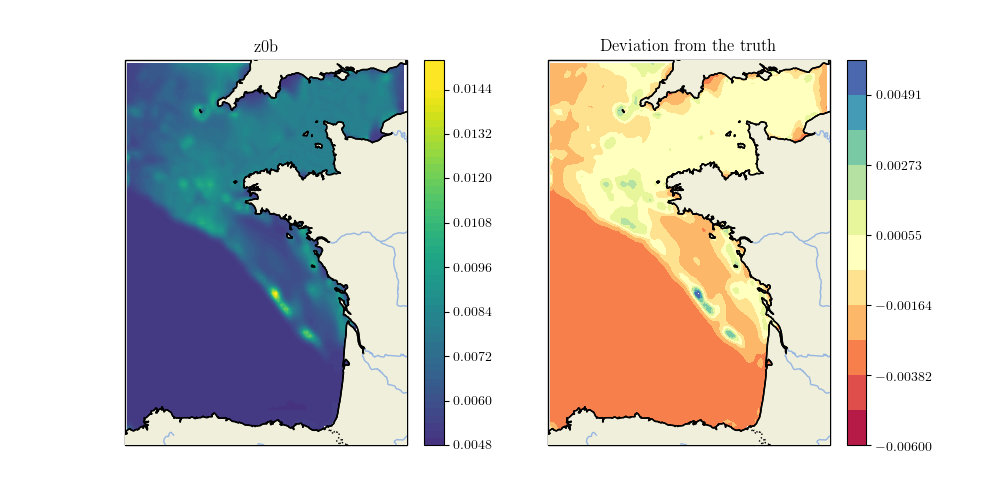
\includegraphics[width=\textwidth]{map_200}
  \caption{Optimization result on z0b. The bottom friction has been initialized at \num{5e-3}, and the true value (used to generate the observations) is \num{8e-3}.}
  \label{fig:croco_optimization}
\end{figure}
By comparing \cref{fig:ocean_floor_croco} and \cref{fig:croco_optimization}, we can see that the optimization focuses primarly on the region of low depth, as the region north of Spain remains untouched. In the English channel, the optimization finds the true value.

\bibliographystyle{abbrvnat}
\bibliography{/home/victor/acadwriting/bibzotero}
\end{document}

%%% Local Variables:
%%% mode: latex
%%% TeX-master: t
%%% End:
